\documentclass[11pt,a4paper]{article}

\usepackage[utf8]{inputenc}
\usepackage[T1]{fontenc}
\usepackage{lmodern}
\usepackage[spanish,es-tabla,es-nodecimaldot,es-noshorthands]{babel}
\usepackage[a4paper,margin=2.15cm,headheight=15pt]{geometry}
\usepackage{microtype}
\usepackage{amsmath,amssymb,amsfonts,mathtools,bm,amsthm}
\usepackage{booktabs,longtable,tabularx,array,multirow}
\usepackage{graphicx}
\usepackage{subcaption}
\usepackage{float}
\usepackage{placeins}
\usepackage{environ}
\usepackage[dvipsnames,table]{xcolor}
\usepackage{enumitem}
\usepackage{siunitx}
\usepackage{tikz}
\usetikzlibrary{arrows.meta,positioning,fit}
\usepackage{listings}
\usepackage{fancyhdr}
\usepackage{xurl}
\usepackage{lastpage}
\usepackage{url}
\usepackage{tocloft}
\usepackage{needspace}
\usepackage{hyperref}
\usepackage[nameinlink,noabbrev]{cleveref}
\makeatletter
\renewcommand*\l@subsection{\@dottedtocline{2}{1.5em}{3.4em}}
% Reserve a legible right gutter for three-digit page numbers in the long TOC.
\renewcommand{\@pnumwidth}{2.4em}
\renewcommand{\@tocrmarg}{4.2em}
\makeatother
\crefname{equation}{ecuación}{ecuaciones}
\Crefname{equation}{Ecuación}{Ecuaciones}
\crefname{figure}{figura}{figuras}
\Crefname{figure}{Figura}{Figuras}
\crefname{table}{tabla}{tablas}
\Crefname{table}{Tabla}{Tablas}
\crefname{section}{sección}{secciones}
\Crefname{section}{Sección}{Secciones}
\crefname{subsection}{sección}{secciones}
\Crefname{subsection}{Sección}{Secciones}
\providecommand{\crefrangeconjunction}{}
\providecommand{\crefpairconjunction}{}
\providecommand{\crefmiddleconjunction}{}
\providecommand{\creflastconjunction}{}
\renewcommand{\crefrangeconjunction}{ a }
\renewcommand{\crefpairconjunction}{ y }
\renewcommand{\crefmiddleconjunction}{, }
\renewcommand{\creflastconjunction}{ y }

\definecolor{Azul}{HTML}{164B73}
\definecolor{AzulClaro}{HTML}{EAF2F8}
\definecolor{Verde}{HTML}{277A58}
\definecolor{VerdeClaro}{HTML}{EAF6F0}
\definecolor{Naranja}{HTML}{B35A00}
\definecolor{NaranjaClaro}{HTML}{FFF2E3}
\definecolor{Rojo}{HTML}{9B2C2C}
\definecolor{Gris}{HTML}{F2F4F6}
\definecolor{GrisOscuro}{HTML}{48515A}
\definecolor{azulHA}{HTML}{153B5B}
\definecolor{verdeHA}{HTML}{2E6F5E}
\definecolor{ambarHA}{HTML}{9A6700}
\definecolor{rojoHA}{HTML}{9D2A2A}
\definecolor{grisHA}{HTML}{4A5560}
\definecolor{grisClaro}{HTML}{F4F6F7}

% Jerarquía visual del índice: partes como capítulos principales y secciones
% como entradas subordinadas.
\setlength{\cftbeforepartskip}{1.15em}
\setlength{\cftbeforesecskip}{0.12em}
\setlength{\cftpartindent}{0em}
\setlength{\cftsecindent}{1.8em}
\setlength{\cftpartnumwidth}{2.8em}
\setlength{\cftsecnumwidth}{3.6em}
\renewcommand{\cftsecaftersnum}{.\hspace{0.4em}}
\renewcommand{\cftsecleader}{\cftdotfill{\cftsecdotsep}}
\renewcommand{\cftpartfont}{\large\bfseries\color{azulHA}}
\renewcommand{\cftpartpagefont}{\large\bfseries\color{azulHA}}
\renewcommand{\cftsecfont}{\normalfont}
\renewcommand{\cftsecpagefont}{\normalfont}

\hypersetup{
  colorlinks=true,
  linkcolor=Azul,
  citecolor=Verde,
  urlcolor=Azul,
  pdfauthor={}
}
\ifdefined\HAFOPrintEdition
  \hypersetup{
    pdftitle={Guía de estudio de sistemas dinámicos enteros y fraccionarios},
    pdfsubject={Topología, geometría diferencial, sistemas dinámicos, caos y cálculo fraccionario}
  }
\else
  \hypersetup{
    pdftitle={Localización de atractores ocultos en sistemas enteros y fraccionarios},
    pdfsubject={Álgebra, verificación cruzada, geometría, topología, memoria y evidencia de cuencas}
  }
\fi

\newcommand{\HAFOStudyNeedspace}{%
  \ifHAFOPedagogy\Needspace{12\baselineskip}\fi
}

\graphicspath{
  {figures/paper07/}
  {figures/}
  {figures/pdf/}
  {integer_assets/}
  {figures/chua_master/}
  {figures/kalman_fitts/}
  {figures/mavpd_audit/}
  {figures/mavpd_chaos/}
  {figures/pll/}
  {figures/c590_basin/}
}

\setlength{\emergencystretch}{3em}
\setlength{\parindent}{1.1em}
\setlength{\parskip}{0.22em}
\renewcommand{\arraystretch}{1.15}
\setlist{itemsep=0.25em,topsep=0.4em,leftmargin=*}
\numberwithin{equation}{section}
\captionsetup{font=small,labelfont=bf}
\sisetup{
  output-decimal-marker={,},
  group-separator={\,},
  group-minimum-digits=4
}

\newcolumntype{L}[1]{>{\raggedright\arraybackslash}p{#1}}
\newcolumntype{C}[1]{>{\centering\arraybackslash}p{#1}}
\newcolumntype{Y}{>{\raggedright\arraybackslash}X}

\newtheorem{definition}{Definición}[section]
\newtheorem{proposition}[definition]{Proposición}
\newtheorem{remark}[definition]{Observación}

% Dos salidas desde una sola fuente. El núcleo científico es común; únicamente
% la guía impresa activa los recursos pedagógicos y únicamente la monografía
% digital activa el atlas y la trazabilidad extendida.
\newif\ifHAFOPedagogy
\newif\ifHAFOdigitalcontent
\newif\ifHAFOBasinMaterial
\ifdefined\HAFOPrintEdition
  \HAFOPedagogytrue
  \HAFOdigitalcontentfalse
  \HAFOBasinMaterialfalse
  % El índice muestra sólo partes y secciones; las subsecciones se leen en orden.
  \setcounter{tocdepth}{1}
\else
  \HAFOPedagogyfalse
  \HAFOdigitalcontenttrue
  \HAFOBasinMaterialtrue
  % El índice muestra sólo partes y secciones; las subsecciones se leen en orden.
  \setcounter{tocdepth}{1}
\fi

% Las figuras se clasifican por su función científica. Los atractores
% localizados, series, espectros, secciones de Poincaré y diagnósticos de
% Lyapunov pertenecen a hafocommonfigure y se conservan en ambas ediciones.
% hafobasinfigure se reserva para mapas y cortes de cuencas de atracción, que
% sólo forman parte de la monografía completa. hafodigitalfigure conserva la
% trazabilidad gráfica extendida reservada para la salida completa.
\newenvironment{hafocommonfigure}[1][H]
  {\begin{figure}[#1]}
  {\end{figure}}
\NewEnviron{hafobasinfigure}[1][H]{%
  \ifHAFOBasinMaterial
    \begin{figure}[#1]\BODY\end{figure}%
  \fi
}
\NewEnviron{hafodigitalfigure}[1][H]{%
  \ifHAFOdigitalcontent
    \begin{figure}[#1]\BODY\end{figure}%
  \fi
}

\newcommand{\R}{\mathbb{R}}
\newcommand{\C}{\mathbb{C}}
\newcommand{\RR}{\mathbb{R}}
\newcommand{\CC}{\mathbb{C}}
\newcommand{\ii}{\mathrm{i}}
\newcommand{\CaputoD}{{}^{\mathrm C}D_{t_0}^{q}}
\newcommand{\CD}{{}^{\mathrm C}\!D_{t_0}^{q}}
\newcommand{\LW}{{}^{\mathrm{LW}}D_t^q}
\newcommand{\T}{\mathsf T}
\newcommand{\trans}{^{\mathsf T}}
\newcommand{\dd}{\,\mathrm d}
\newcommand{\e}{\mathrm e}
\newcommand{\target}{\mathcal A_\star}
\newcommand{\basin}{\mathcal B_{t_0}^{\mathrm{reset}}}
\newcommand{\norm}[1]{\left\lVert #1\right\rVert}
\newcommand{\codepath}[1]{\path{#1}}
\newcommand{\ruta}[1]{\path{#1}}
\newcommand{\hafo}{\texttt{hidden-attractors-\allowbreak fo}}
\newcommand{\juliads}{\texttt{DynamicalSystems.\allowbreak jl}}
\newcommand{\attractorsjl}{\texttt{Attractors.\allowbreak jl}}
\newcommand{\statusref}{\textcolor{ambarHA}{\textbf{referencia solamente}}}
\newcommand{\ok}{\textcolor{verdeHA}{\textbf{verificado}}}
\newcommand{\corr}{\textcolor{rojoHA}{\textbf{corrección}}}

\newcommand{\evidencebox}[1]{%
  \begin{center}
  \colorbox{AzulClaro}{\parbox{0.93\linewidth}{#1}}
  \end{center}
}
\newcommand{\warningbox}[1]{%
  \begin{center}
  \colorbox{NaranjaClaro}{\parbox{0.93\linewidth}{#1}}
  \end{center}
}

\newenvironment{hallazgo}[1]{%
  \par\medskip\noindent
  \begin{minipage}{\linewidth}
  \color{azulHA}\hrule height 0.8pt
  \vspace{4pt}\textbf{#1}\par\smallskip
  \color{black}
}{%
  \par\smallskip\color{azulHA}\hrule height 0.8pt
  \end{minipage}\par\medskip
}

\newenvironment{proposalbox}{%
  \par\medskip\noindent
  \begin{minipage}{\linewidth}
  \color{Naranja}\hrule height 0.8pt
  \vspace{4pt}\color{black}
}{%
  \par\smallskip\color{Naranja}\hrule height 0.8pt
  \end{minipage}\par\medskip
}

% Recuadro pedagógico distribuido. Sus únicos títulos de uso son
% Lecturas, Ejercicios y Lecturas complementarias. No usa minipage para poder
% dividirse de forma limpia cuando una lista ocupa más de una página.
\newenvironment{bloqueestudio}[1]{%
  \par\medskip\pagebreak[2]\noindent
  {\color{azulHA}\hrule height 0.8pt}%
  \vspace{4pt}%
  \noindent\textbf{\textcolor{azulHA}{#1}}%
  \par\smallskip
}{%
  \par\smallskip
  {\color{azulHA}\hrule height 0.8pt}%
  \par\medskip
}

\lstdefinestyle{wl}{
  basicstyle=\ttfamily\footnotesize,
  keywordstyle=\color{azulHA}\bfseries,
  commentstyle=\color{verdeHA},
  stringstyle=\color{rojoHA},
  backgroundcolor=\color{grisClaro},
  frame=single,
  rulecolor=\color{gray!45},
  breaklines=true,
  columns=fullflexible,
  keepspaces=true,
  showstringspaces=false,
  tabsize=2
}

% Instantanea de evidencia para el informe comparativo.
% Actualizar estas macros solamente desde una corrida canonica validada.

\newcommand{\FechaCorteDatos}{3 de agosto de 2026}

% Chua no suave: protocolo completo compartido Python--Julia; no corresponde a
% la referencia histórica EFORK--3 de 369/69/66.
\newcommand{\ChuaPythonTotal}{910.341}
\newcommand{\ChuaJuliaTotal}{43.959}
\newcommand{\ChuaRatio}{20.709}
\newcommand{\ChuaProbeCount}{504}

% Kalman--Fitts, corridas completas.
\newcommand{\KFPythonTotal}{77.801}
\newcommand{\KFJuliaTotal}{30.479}
\newcommand{\KFRatio}{2.553}
\newcommand{\KFProbeCount}{48}

% MAVPD. Python empaqueta xi=3.1 y xi=3.5; el total Julia principal citado
% corresponde solo a xi=3.1 y xi=3.5 se reporta por separado.
\newcommand{\MAVPDPythonQuickBundle}{321.219}
\newcommand{\MAVPDPythonFullBundle}{683.840}
\newcommand{\MAVPDJuliaXiThreeOneQuick}{68.988}
\newcommand{\MAVPDJuliaXiThreeFiveQuick}{69.245}
\newcommand{\MAVPDJuliaXiThreeOneFull}{73.214}
\newcommand{\MAVPDJuliaXiThreeFiveFull}{77.377}
\newcommand{\MAVPDProbeCount}{108}
\newcommand{\MAVPDPythonStatus}{full, comparador cruzado aprobado}
\newcommand{\MAVPDNegativePythonStatus}{full, 108 sondeos comunes y 24 contactos por ciclo}
\newcommand{\MAVPDQuickAssignmentMatches}{108}
\newcommand{\MAVPDQuickOuterDecisionMatches}{108}
\newcommand{\MAVPDQuickCloudDistance}{0.000520488}
\newcommand{\MAVPDPythonPeriod}{0.493177986749}
\newcommand{\MAVPDJuliaQuickPeriod}{0.493177892159}
\newcommand{\MAVPDFullAssignmentMatches}{108}
\newcommand{\MAVPDFullOuterDecisionMatches}{108}
\newcommand{\MAVPDFullCloudDistance}{0.00061096936}
\newcommand{\MAVPDJuliaFullPeriod}{0.493178150753}
\newcommand{\MAVPDFullBundleRatio}{4.541060}
\newcommand{\MAVPDJuliaFullBundleSum}{150.590}

% PLL lead--lag: comparación full--full cerrada; el bloque siguiente conserva
% únicamente el control quick de Python. La evidencia full vive en
% integer_julia_comparison_generated.tex.
\newcommand{\PLLPythonQuickTotal}{129.986}
\newcommand{\PLLProbeCount}{96}
\newcommand{\PLLStablePeriod}{0.082676662497401}
\newcommand{\PLLStableMultiplier}{0.8172041431535}
\newcommand{\PLLSeparatrixPeriod}{0.108541779638193}
\newcommand{\PLLSeparatrixMultiplier}{1.4411073306965}

% Generado por refresh_mavpd_chaos_evidence.py; no editar a mano.
% run_id: mavpd\_integer\_hidden\_chaos-full-20260803T110818509512Z-f1d10f792a3a-1e2527c6895d
\renewcommand{\FechaCorteDatos}{3 de agosto de 2026}

\newcommand{\MAVPDChaosXi}{2.85}
\newcommand{\MAVPDChaosHopf}{0.14380379839949112}
\newcommand{\MAVPDChaosGamma}{0.15380379839949113}
\newcommand{\MAVPDChaosLEOne}{0.7133503984936994}
\newcommand{\MAVPDChaosLETwo}{-0.0009058832510818009}
\newcommand{\MAVPDChaosLEThree}{-20.923624956275255}
\newcommand{\MAVPDChaosLEControlOne}{0.6830338121422247}
\newcommand{\MAVPDChaosDivergenceResidual}{-0.006696983907623633}
\newcommand{\MAVPDChaosKY}{2.034049765121074}
\newcommand{\MAVPDChaosPoincareCount}{1174}
\newcommand{\MAVPDChaosReturnKOne}{0.9985162431217313}
\newcommand{\MAVPDChaosReturnKTwo}{0.9984323397081207}
\newcommand{\MAVPDChaosMainProbes}{108}
\newcommand{\MAVPDChaosTargetedProbes}{4}
\newcommand{\MAVPDChaosTotalProbes}{112}
\newcommand{\MAVPDChaosHits}{0}
\newcommand{\MAVPDChaosContractTime}{1.2472794000059366}
\newcommand{\MAVPDChaosSearchTime}{1321.0953230999876}
\newcommand{\MAVPDChaosDiagnosticsTime}{314.73090460000094}
\newcommand{\MAVPDChaosHiddennessTime}{709.0482047999976}
\newcommand{\MAVPDChaosGateTime}{1.464334600022994}
\newcommand{\MAVPDChaosTotalTime}{2347.895984300063}

% AUTO-GENERATED by refresh_julia_comparison_evidence.py; do not edit.
% Evidence is post-hoc and finite: it is not a global proof of chaos or hiddenness.
\newcommand{\MAVPDChaosPythonComparedTotal}{2347.896}
\newcommand{\MAVPDChaosJuliaTotal}{76.057}
\newcommand{\MAVPDChaosJuliaLocalizationTime}{15.837}
\newcommand{\MAVPDChaosPythonJuliaRatio}{30.870}
\newcommand{\MAVPDChaosJuliaLEOne}{0.693803575330111}
\newcommand{\MAVPDChaosJuliaLETwo}{0.0017936286702211}
\newcommand{\MAVPDChaosJuliaLEThree}{-20.9005938240238}
\newcommand{\MAVPDChaosJuliaLEControlOne}{0.704313426616307}
\newcommand{\MAVPDChaosJuliaKY}{2.03328121726383}
\newcommand{\MAVPDChaosJuliaPoincareCount}{1175}
\newcommand{\MAVPDChaosJuliaReturnK}{0.997159273042194}
\newcommand{\MAVPDChaosJuliaProbeMatches}{112}
\newcommand{\MAVPDChaosJuliaDestinationMatches}{112}
\newcommand{\MAVPDChaosJuliaAgreement}{aprobada}
\newcommand{\MAVPDChaosJuliaComparisonScope}{full--full}
\newcommand{\MAVPDChaosJuliaRunID}{\detokenize{mavpd_integer_hidden_chaos_20260803T143002_a8bca9ee6266}}
\newcommand{\PLLPythonFullTotal}{97.104}
\newcommand{\PLLJuliaFullTotal}{14.619}
\newcommand{\PLLPythonFullLocalizationTime}{29.102}
\newcommand{\PLLPythonFullVerificationTime}{64.475}
\newcommand{\PLLPythonFullFiguresTime}{3.519}
\newcommand{\PLLJuliaFullLocalizationTime}{2.751}
\newcommand{\PLLJuliaFullVerificationTime}{2.578}
\newcommand{\PLLJuliaFullFiguresTime}{8.364}
\newcommand{\PLLPythonJuliaFullRatio}{6.642}
\newcommand{\PLLPythonStablePeriod}{0.0826766624974002}
\newcommand{\PLLPythonStableMultiplier}{0.81720414315349}
\newcommand{\PLLPythonSeparatrixPeriod}{0.108541779638197}
\newcommand{\PLLPythonSeparatrixMultiplier}{1.4411073306967}
\newcommand{\PLLJuliaStablePeriod}{0.0826766624969991}
\newcommand{\PLLJuliaStableMultiplier}{0.817204143145181}
\newcommand{\PLLJuliaSeparatrixPeriod}{0.108541779641824}
\newcommand{\PLLJuliaSeparatrixMultiplier}{1.44110733084579}
\newcommand{\PLLStableOrbitMaxDistance}{3.28206999962173e-12}
\newcommand{\PLLSeparatorOrbitMaxDistance}{1.82163209394329e-11}
\newcommand{\PLLJuliaProbeMatches}{96}
\newcommand{\PLLJuliaDestinationMatches}{96}
\newcommand{\PLLJuliaAgreement}{aprobada}
\newcommand{\PLLJuliaComparisonScope}{full--full}
\newcommand{\PLLJuliaFullRunID}{\detokenize{pll_lead_lag_integer_q1_reference_full_20260803T144050_1a69f078a9398}}
\newcommand{\PLLJuliaFullPosthocRunID}{\detokenize{pll_lead_lag_integer_q1_reference_posthoc_full_20260803T144125_1a6a738dd480c}}
\newcommand{\PLLJuliaVerifiedArtifactCount}{18}
\newcommand{\PLLJuliaQuickTotal}{14.177}
\newcommand{\PLLPythonJuliaQuickRatio}{9.169}
\newcommand{\PLLQuickProbeMatches}{96}
\newcommand{\PLLQuickDestinationMatches}{96}
\newcommand{\PLLQuickAgreement}{aprobada}
\newcommand{\PLLQuickComparisonScope}{quick--quick}
\newcommand{\MAVPDChaosJuliaGammaScreenPNG}{\detokenize{assets/julia_mavpd_chaos_gamma_screen.png}}
\newcommand{\MAVPDChaosJuliaGammaScreenPDF}{\detokenize{assets/julia_mavpd_chaos_gamma_screen.pdf}}
\newcommand{\MAVPDChaosJuliaPhasePortraitsPNG}{\detokenize{assets/julia_mavpd_chaos_candidate_phase_portraits.png}}
\newcommand{\MAVPDChaosJuliaPhasePortraitsPDF}{\detokenize{assets/julia_mavpd_chaos_candidate_phase_portraits.pdf}}
\newcommand{\MAVPDChaosJuliaLyapunovPNG}{\detokenize{assets/julia_mavpd_chaos_lyapunov_spectrum.png}}
\newcommand{\MAVPDChaosJuliaLyapunovPDF}{\detokenize{assets/julia_mavpd_chaos_lyapunov_spectrum.pdf}}
\newcommand{\MAVPDChaosJuliaHiddennessPNG}{\detokenize{assets/julia_mavpd_chaos_hiddenness_outcomes.png}}
\newcommand{\MAVPDChaosJuliaHiddennessPDF}{\detokenize{assets/julia_mavpd_chaos_hiddenness_outcomes.pdf}}
\newcommand{\MAVPDChaosJuliaNyquistPNG}{\detokenize{assets/julia_mavpd_chaos_nyquist_diagnostic.png}}
\newcommand{\MAVPDChaosJuliaNyquistPDF}{\detokenize{assets/julia_mavpd_chaos_nyquist_diagnostic.pdf}}
\newcommand{\MAVPDChaosJuliaAmplitudeSpectrumPNG}{\detokenize{assets/julia_mavpd_chaos_amplitude_spectrum.png}}
\newcommand{\MAVPDChaosJuliaAmplitudeSpectrumPDF}{\detokenize{assets/julia_mavpd_chaos_amplitude_spectrum.pdf}}
\newcommand{\PLLJuliaDirectObstructionPNG}{\detokenize{assets/julia_pll_direct_transfer_obstruction.png}}
\newcommand{\PLLJuliaDirectObstructionPDF}{\detokenize{assets/julia_pll_direct_transfer_obstruction.pdf}}
\newcommand{\PLLJuliaContinuationPNG}{\detokenize{assets/julia_pll_loop_gain_continuation.png}}
\newcommand{\PLLJuliaContinuationPDF}{\detokenize{assets/julia_pll_loop_gain_continuation.pdf}}
\newcommand{\PLLJuliaCyclesPNG}{\detokenize{assets/julia_pll_phase_cylinder_cycles.png}}
\newcommand{\PLLJuliaCyclesPDF}{\detokenize{assets/julia_pll_phase_cylinder_cycles.pdf}}
\newcommand{\PLLJuliaHiddennessPNG}{\detokenize{assets/julia_pll_cylindrical_hiddenness_probes.png}}
\newcommand{\PLLJuliaHiddennessPDF}{\detokenize{assets/julia_pll_cylindrical_hiddenness_probes.pdf}}


\pagestyle{fancy}
\fancyhf{}
\fancyhead[L]{\small Atractores ocultos enteros y fraccionarios}
\fancyhead[R]{\small Álgebra, geometría, memoria y cuencas}
\fancyfoot[C]{\thepage}
\fancypagestyle{plain}{%
  \fancyhf{}
  \fancyhead[L]{\small Atractores ocultos enteros y fraccionarios}
  \fancyhead[R]{\small Álgebra, geometría, memoria y cuencas}
  \fancyfoot[C]{\thepage}
}

\ifdefined\HAFOPrintEdition
\fancyhead[L]{\small Guía de estudio de atractores ocultos}
\fancyhead[R]{\small Geometría, dinámica, caos y memoria}
\fancypagestyle{plain}{%
  \fancyhf{}
  \fancyhead[L]{\small Guía de estudio de atractores ocultos}
  \fancyhead[R]{\small Geometría, dinámica, caos y memoria}
  \fancyfoot[C]{\thepage}
}
\fi

\begin{document}
\hypersetup{pageanchor=false}
\begin{titlepage}
\centering
\vspace*{0.18\textheight}
{\LARGE\bfseries Localización de atractores ocultos\\[0.35em]
en sistemas enteros y fraccionarios\par}
\vspace{1.2em}
\ifdefined\HAFOPrintEdition
  {\Large Guía secuencial de teoría, lectura y ejercicios\par}
\else
  {\Large Teoría, derivaciones, casos y resultados\par}
\fi
\vfill
{\large Topología, geometría diferencial, sistemas dinámicos, caos y
cálculo fraccionario\par}
\end{titlepage}

\ifdefined\HAFOPrintEdition
\clearpage
\tableofcontents
\else
\tableofcontents
\fi
\clearpage
\hypersetup{pageanchor=true}

\ifHAFOPedagogy
  \part[Curso básico integrado]{Curso básico integrado: sistemas dinámicos,
  caos, cálculo fraccionario, topología y teoría geométrica de EDO}
\else
  \part{Fundamentos y alcance}
\fi
\label{part:guia-geometrica-entera}
% Tarjetas visibles sólo en la edición pedagógica. Se invocan en el punto
% matemático correspondiente; el archivo no produce contenido por sí solo.

\newcommand{\HAFOProblemStateMemory}{\ifHAFOPedagogy
\begin{bloqueestudio}{Ejercicios}
\textbf{Formalismo.} Para \(A\in\mathbb R^{n\times n}\), compare
\(\dot x=Ax\) con \({}^{\mathrm C}D^q x=Ax\): solución fundamental,
composición temporal, espacio de fases y dato inicial. Verifique el caso
escalar con \(e^{\lambda t}\) y \(E_q(\lambda t^q)\).

\textbf{Interpretación.} Identifique exactamente dónde falla el semigrupo
puntual para \(q<1\).

\textbf{Defensa oral.} Explique en dos minutos por qué el estado de Caputo no
queda determinado sólo por \(x(t)\).
\end{bloqueestudio}
\fi}

\newcommand{\HAFOProblemStabilityBasins}{\ifHAFOPedagogy
\begin{bloqueestudio}{Ejercicios}
\textbf{Formalismo.} Para un Chua entero y uno fraccionario, calcule
equilibrios y espectros, aplique el criterio de estabilidad correspondiente y
defina la cuenca en el espacio de estados o de historias.

\textbf{Interpretación.} Separe estabilidad local, atracción y contacto de
cuenca.

\textbf{Defensa oral.} Responda por qué tener todos los equilibrios inestables
no demuestra que un atractor sea oculto.
\end{bloqueestudio}
\fi}

\newcommand{\HAFOProblemReturn}{\ifHAFOPedagogy
\begin{bloqueestudio}{Ejercicios}
\textbf{Formalismo.} Construya una sección para PLL o MAVPD, formule
\(P-I\) y las hipótesis de grado. Después escriba el operador de retorno
Caputo sobre historias.

\textbf{Interpretación.} Distinga punto fijo de retorno, estabilidad del ciclo
y existencia por grado.

\textbf{Defensa oral.} Explique por qué la proyección puntual de un retorno
Caputo no conserva toda la información dinámica.
\end{bloqueestudio}
\fi}

\newcommand{\HAFOProblemChaos}{\ifHAFOPedagogy
\begin{bloqueestudio}{Ejercicios}
\textbf{Formalismo.} Compare una trayectoria entera y una Caputo con la
misma matriz de observables. Separe acotación, recurrencia, atracción, caos,
cuenca y ocultedad.

\textbf{Interpretación.} Identifique qué afirmaciones son topológicas y cuáles
son sólo numéricas y finitas.

\textbf{Defensa oral.} Explique por qué una FFT o un exponente positivo aislado
no certifican simultáneamente caos, atracción y ocultedad.
\end{bloqueestudio}
\fi}

\newcommand{\HAFOProblemLocalization}{\ifHAFOPedagogy
\begin{bloqueestudio}{Ejercicios}
\textbf{Formalismo.} En un mismo sistema produzca semillas mediante dos métodos
entre DF, Machado, continuación, PP/FPP y borde. Compare residuos algebraicos,
especificación de memoria, destino y prueba de cuenca bajo el mismo presupuesto.

\textbf{Interpretación.} Determine qué aporta cada método y qué afirmación no
puede sostener por sí sola.

\textbf{Defensa oral.} Distinga con precisión semilla, trayectoria, conjunto
límite, atractor y atractor oculto.
\end{bloqueestudio}
\fi}

\newcommand{\HAFOThesisDefense}{\ifHAFOPedagogy
\begin{bloqueestudio}{Ejercicios}
\textbf{Simulacro de defensa.} Responda sin consultar el texto y después
contraste cada respuesta con las derivaciones:
\begin{enumerate}[nosep]
  \item ¿Cómo se pasa del campo a equilibrios, jacobiano, espectro y
  clasificación local?
  \item ¿Cuál es la diferencia entre atractor autoexcitado y oculto y cómo se
  ensaya su cuenca?
  \item ¿Cómo se obtiene la realización de Lur'e, \(W_q\) y el cierre de
  balance armónico?
  \item ¿Qué predicen DF y Machado y qué no certifican?
  \item ¿Por qué Caputo exige Volterra, terminal inferior e historia completa?
  \item ¿Cómo se continúa un sistema fraccionario sin reiniciar la memoria?
  \item ¿Qué significan PP, FPP--A y FPP--H y cuándo pueden fallar?
  \item ¿Qué aportan grado, Poincaré, variedades, superficies críticas y borde
  de cuenca?
  \item ¿Qué evidencia separa acotación, recurrencia, atracción, caos y
  ocultedad?
  \item Para cada caso analizado: ¿qué es previo, qué es propuesta del
  proyecto, qué se verificó y qué permanece abierto?
\end{enumerate}
\end{bloqueestudio}
\fi}

\newcommand{\HAFOCardTopology}{\ifHAFOPedagogy
\begin{bloqueestudio}{Lecturas}
\begin{itemize}[nosep]
  \item \emph{Topología y geometría diferencial con aplicaciones a la física}
  \cite{NahmadAchar2022Topologia}: coordenadas adaptadas y curvas integrales,
  §§11.3--11.5, pp.~124--125; derivadas de Lie, §§11.6--11.14,
  pp.~125--130.
\end{itemize}
\end{bloqueestudio}
\begin{bloqueestudio}{Ejercicios}
\textbf{Básicos.} Resuelva §§11.15--11.18, pp.~131--133. Calcule
\(L_fV=\nabla V\cdot f\) para \(V(x)=\|x\|^2/2\).

\textbf{Investigación.} Demuestre que \(\mathbb R\times S^1\) es el espacio
de fases del PLL y defina una distancia con
\(\theta\sim\theta+2\pi\).
\end{bloqueestudio}
\begin{bloqueestudio}{Lecturas complementarias}
Mismo libro: conexiones lineales, pp.~135--142.
\end{bloqueestudio}
\fi}

\newcommand{\HAFOCardFlow}{\ifHAFOPedagogy
\begin{bloqueestudio}{Lecturas}
\begin{itemize}[nosep]
  \item \emph{Teoría geométrica de ecuaciones diferenciales I}
  \cite{JaurezEtAl2021TGEDI}: cap.~1, p.~1; cap.~3, pp.~53--80; cap.~4,
  pp.~93--155.
  \item \emph{Teoría geométrica de ecuaciones diferenciales II}
  \cite{JaurezEtAl2021TGEDII}: cap.~8, pp.~69--98; existencia y unicidad,
  p.~73; primera variación, p.~74; dependencia del dato inicial, p.~92.
  \item \texttt{Strogatz - Nonlinear Dynamics and Chaos.pdf}
  \cite{Strogatz2015Nonlinear}: PDF~30--50 y 140--212.
\end{itemize}
\end{bloqueestudio}
\begin{bloqueestudio}{Ejercicios}
\textbf{Básicos.} Resuelva Strogatz 2.4.1--2.4.8, 2.5.1--2.5.5 y 2.6.2,
PDF~57--59. Para \(\dot x=Ax\), demuestre
\(\varphi_t(x_0)=e^{tA}x_0\) y
\(\varphi_{t+s}=\varphi_t\circ\varphi_s\).

\textbf{Investigación.} Calcule el jacobiano y el espectro del origen en un
caso entero. Explique qué falla en
Hartman--Grobman si hay valores propios sobre el eje imaginario.
\end{bloqueestudio}
\begin{bloqueestudio}{Lecturas complementarias}
\emph{Métodos topológicos en el estudio de las ecuaciones diferenciales no
lineales} \cite{Amster2021MetodosTopologicos}: apéndice A, pp.~319--327.
\end{bloqueestudio}
\fi}

\newcommand{\HAFOCardBasins}{\ifHAFOPedagogy
\begin{bloqueestudio}{Lecturas}
\begin{itemize}[nosep]
  \item \emph{Exploring Chaos} \cite{Davies2004ExploringChaos}:
  sistemas bidimensionales y fronteras de cuenca, pp.~107--148; §4.7,
  p.~134.
  \item \texttt{Alligood, Sauer \& Yorke - Chaos.pdf}
  \cite{AlligoodSauerYorke1996Chaos}: cuencas, PDF~146--165; fronteras,
  PDF~181--209.
\end{itemize}
\end{bloqueestudio}
\begin{bloqueestudio}{Ejercicios}
\textbf{Básicos.} Resuelva Alligood--Sauer--Yorke, \emph{Challenge} 4,
PDF~199--201.

\textbf{Investigación.} Para dos atractores \(A_1,A_2\), escriba
\(\mathcal B(A_i)\), su frontera común y un par de puntos para una bisección
de borde. Indique qué resultado sería sólo local y finito.
\end{bloqueestudio}
\begin{bloqueestudio}{Lecturas complementarias}
Alligood--Sauer--Yorke: \emph{Challenge} 10, PDF~444--451.
\end{bloqueestudio}
\fi}

\newcommand{\HAFOCardDegree}{\ifHAFOPedagogy
\begin{bloqueestudio}{Lecturas}
\emph{Métodos topológicos} \cite{Amster2021MetodosTopologicos}: índice de
curvas, pp.~74--82; disparo, p.~84; Brouwer y Poincaré, p.~99; grado de
Brouwer, pp.~103--145.
\end{bloqueestudio}
\begin{bloqueestudio}{Ejercicios}
\textbf{Básicos.} Resuelva los problemas del cap.~3, pp.~153--155, y calcule
\(\deg(I,B,0)\), \(\deg(-I,B,0)\).

\textbf{Investigación.} Para un mapa de retorno \(P\),
formule \(F(z)=P(z)-z\) y enumere las hipótesis necesarias para usar el grado.
\end{bloqueestudio}
\fi}

\newcommand{\HAFOCardLinearGeometry}{\ifHAFOPedagogy
\begin{bloqueestudio}{Lecturas}
\emph{Teoría geométrica de ecuaciones diferenciales II}
\cite{JaurezEtAl2021TGEDII}: primera variación, p.~74; dependencia del dato
inicial, p.~92; Grobman--Hartman, p.~94.
\end{bloqueestudio}
\begin{bloqueestudio}{Ejercicios}
\textbf{Básicos.} Resuelva Strogatz 6.5.11, PDF~206, y 6.8.6--6.8.7,
PDF~213--214. Derive \(\dot\Phi=Df(x(t))\Phi\), \(\Phi(0)=I\).

\textbf{Investigación.} Para un equilibrio de Chua, MAVPD, Kalman--Fitts o
PLL, separe subespacios estable, inestable y central.
\end{bloqueestudio}
\fi}

\newcommand{\HAFOCardPoincare}{\ifHAFOPedagogy
\begin{bloqueestudio}{Lecturas}
\begin{itemize}[nosep]
  \item \emph{Teoría geométrica de ecuaciones diferenciales II}
  \cite{JaurezEtAl2021TGEDII}: rectificación y Poincaré, pp.~113--115;
  Floquet y monodromía, pp.~121--141; Poincaré--Bendixson, p.~150.
  \item Strogatz \cite{Strogatz2015Nonlinear}: PDF~215--260 y 261--325.
\end{itemize}
\end{bloqueestudio}
\begin{bloqueestudio}{Ejercicios}
\textbf{Básicos.} Resuelva Strogatz 7.3.1--7.3.3, PDF~250--251, y demuestre
que una órbita periódica da un punto fijo del retorno.

\textbf{Investigación.} Construya una sección transversal para PLL o MAVPD y
explique un multiplicador de módulo mayor que uno.
\end{bloqueestudio}
\begin{bloqueestudio}{Lecturas complementarias}
Strogatz 8.4.3--8.4.4, PDF~313--314.
\end{bloqueestudio}
\fi}

\newcommand{\HAFOCardChaos}{\ifHAFOPedagogy
\begin{bloqueestudio}{Lecturas}
\begin{itemize}[nosep]
  \item Strogatz \cite{Strogatz2015Nonlinear}: Lorenz, PDF~326--371;
  Lyapunov y mapas, PDF~372--421; atractores extraños, PDF~446--476.
  \item Alligood--Sauer--Yorke \cite{AlligoodSauerYorke1996Chaos}:
  Lyapunov y herradura, PDF~211--247; atractores, PDF~248--289; caos en
  flujos, PDF~376--415; variedades y crisis, PDF~416--463.
\end{itemize}
\end{bloqueestudio}
\begin{bloqueestudio}{Ejercicios}
\textbf{Básicos.} Resuelva Strogatz 9.2.2--9.2.3 y 9.3.8--9.3.9,
PDF~366--368; 10.3.7--10.3.8 y 10.5.1--10.5.4, PDF~413--417.

\textbf{Investigación.} Defina por separado acotación, recurrencia, atracción,
caos y ocultedad. Construya un contraejemplo para cada implicación inválida.

\textbf{Integrador.} Repita la tabla de implicaciones para una trayectoria de
Caputo: sustituya periodicidad exacta por recurrencia proyectada y declare qué
información depende de la historia.
\end{bloqueestudio}
\begin{bloqueestudio}{Lecturas complementarias}
\begin{itemize}[nosep]
  \item \emph{Exploring Chaos} \cite{Davies2004ExploringChaos}, pp.~44--60,
  65--106 y 184--193.
  \item \emph{Chaos and Time-Series Analysis}
  \cite{Sprott2003ChaosTimeSeries}, pp.~72--183, 213--272 y 302--328.
  \item Ott \cite{Ott2002Chaos}: conjuntos caóticos no atractores y
  fronteras, pp.~168--210; crisis y transitorios, pp.~304--344.
  \item T{\'e}l--Gruiz \cite{TelGruiz2006Chaotic}: sillas, escapes,
  fronteras y caos transitorio, pp.~191--225.
  \item Devaney \cite{Devaney1989Chaotic}: PDF aprox.~29--33, 70,
  110--129.
  \item Hilborn \cite{Hilborn2000Chaos}: PDF aprox.~38--80 y 162--220.
\end{itemize}
\end{bloqueestudio}
\fi}

\newcommand{\HAFOCardFractal}{\ifHAFOPedagogy
\begin{bloqueestudio}{Lecturas complementarias}
\begin{itemize}[nosep]
  \item Falconer \cite{Falconer2014Fractal}: dimensión de caja,
  PDF~59--75; Hausdorff, PDF~76--97; sistemas dinámicos, PDF~238--264.
  \item \texttt{Barnsley - Fractals Everywhere.pdf}: métricas y topología,
  PDF~12--48; contracciones, PDF~49--129; dimensión, PDF~186--219.
  \item Mandelbrot: consulta visual, PDF~33 y 277; para pruebas use Falconer.
\end{itemize}
\end{bloqueestudio}
\begin{bloqueestudio}{Ejercicios}
\textbf{Básicos.} Resuelva un ejercicio de dimensión de caja de Falconer,
cap.~2; contraste después con el solucionario, PDF~1--21.

\textbf{Investigación.} Calcule la dimensión de una frontera de cuenca en dos
refinamientos y explique por qué el resultado no demuestra Wada.
\end{bloqueestudio}
\fi}

\newcommand{\HAFOCardFractional}{\ifHAFOPedagogy
\begin{bloqueestudio}{Lecturas}
\begin{itemize}[nosep]
  \item Oliveira \cite{Oliveira2019SolvedFractional}: Gamma, PDF~30--41;
  Mittag--Leffler, PDF~81--124; Laplace, PDF~130--137; GL, RL y Caputo,
  PDF~179--189.
  \item Herrmann \cite{Herrmann2014Fractional}: PDF~28--53 y 64--89.
  \item Das \cite{Das2020Kindergarten}: construcción y relación RL--Caputo,
  PDF~156--163; evaluación discreta GL/RL, PDF~183--185.
  \item \emph{The Analysis of Fractional Differential Equations}
  \cite{Diethelm2010AnalysisFDE}: pp.~13--73.
\end{itemize}
\end{bloqueestudio}
\begin{bloqueestudio}{Ejercicios}
\textbf{Básicos.} Oliveira: ejercicios 13--16 y 30--32,
PDF~142--172; ejercicios RL--Caputo 12, 14, 15, 20, 25, 32, 33 y 40,
PDF~191--224. Obtenga
\(\mathcal L\{t^{\beta-1}E_{\alpha,\beta}(\lambda t^\alpha)\}
=s^{\alpha-\beta}/(s^\alpha-\lambda)\).

\textbf{Investigación.} Derive la transformada de Caputo con sus datos
iniciales y compare RL, GL y Caputo en \(t^\mu\).

\textbf{Integrador.} Resuelva \(\dot x=\lambda x\) y
\({}^{\mathrm C}D^q x=\lambda x\). Compare \(e^{\lambda t}\) con
\(E_q(\lambda t^q)\), la ley de semigrupo y los criterios espectrales entero y
de Matignon. Después aproxime \({}^{\mathrm C}D^qx=-ax\) con GL/RL y resuelva
el PVI con ABM--PECE; explique por qué discretizar un operador no equivale
automáticamente a resolver el mismo PVI Caputo.
\end{bloqueestudio}
\begin{bloqueestudio}{Lecturas complementarias}
Oldham--Spanier \cite{OldhamSpanier1974Fractional}: p.~16,
pp.~47--60, 69--94 y 136. Herrmann: ejercicios 3.3, 5.1--5.2 y 6.1;
soluciones PDF~423, 428--429 y 432.
\end{bloqueestudio}
\fi}

\newcommand{\HAFOCardMemory}{\ifHAFOPedagogy
\begin{bloqueestudio}{Lecturas}
\begin{itemize}[nosep]
  \item Herrmann \cite{Herrmann2014Fractional}: no localidad y memoria,
  PDF~108--126.
  \item Das \cite{Das2020Kindergarten}: contexto analítico, PDF~41--47;
  ramas y cortes, PDF~43--44 y apéndice detallado PDF~503--507;
  inicialización, kernels y memoria desvaneciente RL, PDF~109--110 y 119--135;
  historia e inicialización RL, PDF~247--255; GL y composición, PDF~256--259;
  relación RL--Caputo, PDF~259--264; inicialización Caputo, PDF~264--273;
  seno con terminal inferior, PDF~273--274;
  Laplace con inicialización, PDF~275--291; resolución de EFD, PDF~292--310;
  EFD lineales e integrales, PDF~333--357; ecuaciones secuenciales, matrices y
  funciones alfa-exponenciales, PDF~358--371; sistemas multivariables,
  PDF~372--375.
  \item Oliveira \cite{Oliveira2019SolvedFractional}: ejercicio 26 sobre
  efecto de memoria, PDF~272--273.
  \item Diethelm \cite{Diethelm2010AnalysisFDE}: PVI Caputo de término único,
  existencia, unicidad, perturbaciones, regularidad y estabilidad,
  pp.~85--126 y 157--162.
\end{itemize}
\end{bloqueestudio}
\begin{bloqueestudio}{Ejercicios}
\textbf{Básicos.} Herrmann: ejercicio 8.1, PDF~126; solución, PDF~436.
Derive la ecuación integral de Volterra.

\textbf{Investigación.} Construya dos historias con el mismo valor terminal y
pasados distintos; muestre por qué reiniciar cambia el PVI y por qué un retorno
puntual no es, en general, un mapa de estado. Continúe una trayectoria con
historia heredada y reinicie otra desde el mismo punto; identifique el término
libre de Volterra que cambia.
\end{bloqueestudio}
\begin{bloqueestudio}{Lecturas complementarias}
Matignon \cite{Matignon1996} para el criterio angular.
Li--Chen--Podlubny \cite{LiChenPodlubny2010} para estabilidad directa y
Mittag--Leffler; no es una prueba de caos ni ocultedad.
\end{bloqueestudio}
\fi}

\newcommand{\HAFOCardExistence}{\ifHAFOPedagogy
\begin{bloqueestudio}{Lecturas}
\emph{Métodos topológicos} \cite{Amster2021MetodosTopologicos}: función de
Green, p.~229; Schauder, pp.~245--267; Leray--Schauder, pp.~273--300.
\end{bloqueestudio}
\begin{bloqueestudio}{Ejercicios}
\textbf{Básicos.} Resuelva Amster 7.9.1--7.9.2, pp.~313--316.

\textbf{Investigación.} Escriba el PVI de Caputo como
\(x=x_0+I^qf(x)\). Identifique continuidad,
compacidad y cota a priori requeridas por Schauder o Leray--Schauder; distinga
existencia de atracción y ocultedad.
\end{bloqueestudio}
\fi}

\newcommand{\HAFOCardLure}{\ifHAFOPedagogy
\begin{bloqueestudio}{Lecturas}
Slotine--Li \cite{SlotineLi1991}: realimentación y estabilidad,
PDF~119--175; función descriptiva, PDF~176--209. Para atractores ocultos:
Leonov--Kuznetsov \cite{LeonovKuznetsovVagaitsev2011,LeonovKuznetsov2013}
y localización de Chua \cite{KuznetsovEtAl2017}.
\end{bloqueestudio}
\begin{bloqueestudio}{Ejercicios}
\textbf{Básicos.} Resuelva Slotine--Li, cap.~5, PDF~207--209, y obtenga una
función descriptiva desde su integral de Fourier.

\textbf{Investigación.} Derive
\(W_q(s)=c^{\mathsf T}(s^qI-A)^{-1}b\), fije la rama de \(s^q\) y verifique
la equivalencia de \(1-W_+N=0\) y \(1+W_-N=0\).
\end{bloqueestudio}
\fi}

\newcommand{\HAFOCardMachado}{\ifHAFOPedagogy
\begin{bloqueestudio}{Lecturas}
Machado \cite{Machado2015FDF} y Barbosa--Machado
\cite{BarbosaMachado2002BacklashImpact}.
\end{bloqueestudio}
\begin{bloqueestudio}{Ejercicios}
\textbf{Básicos.} Para \(N=re^{i\theta}\), escriba todas las ramas de
\(N^\mu\) y calcule la principal en \(\mu=1/2\).

\textbf{Investigación.} Para \(N_\mu=N^\mu\), calcule por separado el
residuo auxiliar y el balance físico; determine cuándo la potencia sólo
diversifica semillas.

\textbf{Integrador.} Obtenga dos semillas de ramas distintas, intégrelas bajo
una misma especificación numérica, entera o Caputo, y compare destino y contacto con las cuencas
conocidas.
\end{bloqueestudio}
\fi}

\newcommand{\HAFOCardContinuation}{\ifHAFOPedagogy
\begin{bloqueestudio}{Lecturas}
Diethelm \cite{Diethelm2010AnalysisFDE}: ABM, pp.~195--210; esquema numérico
multi-término, pp.~211--224, con ejercicio en p.~225. Comparación de
aproximación frecuencial, predictor--corrector y Adomian en
Sun--He--Wang \cite{SunHeWang2022FractionalChaos}, pp.~27--74.
Predictor--corrector original \cite{DiethelmFordFreed2002}.
\end{bloqueestudio}
\begin{bloqueestudio}{Ejercicios}
\textbf{Básicos.} Derive los pesos predictor y corrector desde Volterra y
aplíquelos a \({}^{\mathrm C}D^qx=-x\).

\textbf{Investigación.} Escriba una homotopía \(f_\lambda\), transporte una
semilla y demuestre por qué reiniciar la memoria en cada \(\lambda\) define
otro problema. Compare dos algoritmos únicamente después de igualar operador,
terminal inferior, historia, paso y tolerancia.
\end{bloqueestudio}
\fi}

\newcommand{\HAFOCardPerpetual}{\ifHAFOPedagogy
\begin{bloqueestudio}{Lecturas}
Prasad \cite{Prasad2015Perpetual}; Dudkowski--Prasad--Kapitaniak
\cite{DudkowskiPrasadKapitaniak2015,DudkowskiPrasadKapitaniak2017,
DudkowskiPrasadKapitaniak2018};
contraejemplos \cite{NazarimehrSaediJafari2017,NagChowdhuryGhosh2020};
revisión de métodos \cite{GuanXie2025}. Das, Oliveira y Herrmann sustentan
operadores, inicialización y memoria, pero no formulan puntos perpetuos
fraccionarios: FPP--A y FPP--H se presentan como formulaciones metodológicas,
no como resultados de esas fuentes.
\end{bloqueestudio}
\begin{bloqueestudio}{Ejercicios}
\textbf{Básicos.} Para \(\dot x=f(x)\), derive
\(\ddot x=Df(x)f(x)\) y resuelva los PP de dos campos polinomiales sencillos.

\textbf{Investigación.} Resuelva \(Df(p)f(p)=0\), \(f(p)\ne0\), en uno de los
sistemas analizados. Desde Volterra obtenga
\(h^{2q}Df(p)f(p)/\Gamma(2q+1)\) sin suponer una regla de cadena no válida para
Caputo y explique
por qué su cancelación no es aceleración fraccionaria global.

\textbf{Integrador.} Para \(f(x)=Ax+d\), compare FPP--A y FPP--H. Después,
en un campo no lineal, evalúe el evento FPP--H con toda la historia y contraste
continuación heredada contra reinicio. Repita L1 con \(h,h/2,h/4\) y terminal
inferior común; un mínimo observado gráficamente no constituye un evento
validado.
\end{bloqueestudio}
\fi}

\newcommand{\HAFOCardGeometric}{\ifHAFOPedagogy
\begin{bloqueestudio}{Lecturas}
Curvas conectantes \cite{GilmoreEtAl2010Connecting,GuanXie2021Connecting};
superficies críticas \cite{GodaraEtAl2018CriticalSurfaces}; cuencas y Wada
\cite{DazaEtAl2016BasinEntropy,DazaEtAl2015Wada}.
\end{bloqueestudio}
\begin{bloqueestudio}{Ejercicios}
\textbf{Básicos.} Para un campo plano, calcule \(Df\), \(Df\,f\),
\(\det Df\) y sus conjuntos de nivel cero.

\textbf{Investigación.} Repita el cálculo en PLL o MAVPD. Formule una
bisección entre dos destinos con métrica escalada; añada un tercer destino y
describa el fallo.
\end{bloqueestudio}
\fi}

\newcommand{\HAFOCardProtocols}{\ifHAFOPedagogy
\begin{bloqueestudio}{Lecturas}
Datseris--Wagemakers \cite{datseris2022} para estimación de cuencas; entropía de
cuenca \cite{DazaEtAl2016BasinEntropy}; clasificación de cuencas
\cite{SprottXiong2015Basins}; Wada \cite{DazaEtAl2015Wada}.
\end{bloqueestudio}
\begin{bloqueestudio}{Ejercicios}
\textbf{Básicos.} Para una órbita conocida, calcule retorno, período dominante
y variación al reducir el paso.

\textbf{Investigación.} Construya una matriz
semilla\(\times\)orden--memoria\(\times\)paso\(\times\)horizonte
\(\times\)solucionador. Separe
destino, atracción, caos, contacto con equilibrios y ocultedad.
\end{bloqueestudio}
\fi}

\newcommand{\HAFOCardReliability}{\ifHAFOPedagogy
\begin{bloqueestudio}{Lecturas}
\begin{itemize}[nosep]
  \item Vallejo--Sanju{\'a}n \cite{VallejoSanjuan2017Predictability}:
  error y \emph{shadowing}, pp.~13--22; FTLE y regímenes, pp.~25--87;
  predictibilidad, pp.~91--126; algoritmo, pp.~129--136.
  \item Datseris--Parlitz \cite{DatserisParlitz2022Nonlinear}: Lyapunov y
  horizonte de predictibilidad, pp.~37--48; bifurcaciones y dimensión,
  pp.~53--85; algoritmo de Lyapunov, pp.~211--216.
  \item Ott \cite{Ott2002Chaos}, pp.~168--210 y 304--344, y
  T{\'e}l--Gruiz \cite{TelGruiz2006Chaotic}, pp.~191--225, para sillas,
  escapes, fronteras y crisis.
  \item Caso primario de transitorio oculto
  \cite{Danca2016HiddenTransient}; exponentes fraccionarios y su algoritmo
  \cite{DancaKuznetsov2018Lyapunov}; memoria e inicialización
  \cite{Sabatier2021InfiniteMemory}.
\end{itemize}
\end{bloqueestudio}
\begin{bloqueestudio}{Ejercicios}
\textbf{Básicos.} Derive una cota de Gronwall para el defecto de una EDO y la
fórmula heurística del horizonte de predictibilidad. Calcule FTLE en tres
ventanas y muestre su distribución, no sólo la media.

\textbf{Investigación.} Fije una región de escape, estime la supervivencia
de un conjunto de semillas y compare una ley exponencial con una cola no
exponencial. Trate las trayectorias que no escaparon como datos censurados.

\textbf{Integrador.} Repita el diseño para Caputo en el espacio de historias:
defina las historias muestreadas, conserve el terminal inferior y separe
continuación de reinicio. Indique qué parte vive sólo en la proyección.
\end{bloqueestudio}
\fi}

\newcommand{\HAFOCardCases}{\ifHAFOPedagogy
\begin{bloqueestudio}{Lecturas}
Artículos primarios de los casos: Chua
\cite{LeonovKuznetsovVagaitsev2011,KuznetsovEtAl2017,
KuznetsovEtAl2023ChuaExperiments}; sistemas
fraccionarios \cite{Danca2017,Danca2017HiddenFO,Wu2023ArctanChua}; candidatos
no Chua \cite{munoz2018,wang2020}. Las revisiones
\cite{DudkowskiEtAl2016,GuanXie2025} se usan después para comparar métodos.
\end{bloqueestudio}
\begin{bloqueestudio}{Ejercicios}
\textbf{Básicos.} Recalcule equilibrios, jacobiano y clasificación local de un
caso entero y uno fraccionario.

\textbf{Investigación.} Para cada caso complete: campo; espacio de fases;
equilibrios; estabilidad; semilla; integración; destino; caos; cuenca;
conclusión autorizada. Compare en paralelo un caso entero y uno fraccionario:
qué objetos permanecen en el espacio de estados y cuáles pasan al espacio de
historias.
\end{bloqueestudio}
\fi}

\newcommand{\HAFOCardCandidates}{\ifHAFOPedagogy
\begin{bloqueestudio}{Lecturas}
\emph{Systems with Hidden Attractors}
\cite{PhamVolosKapitaniak2017Systems}: pp.~21--63 y 79--102; catálogo
\cite{PhamEtAl2018HiddenAttractors}; capítulo fraccionario, pp.~199--238,
en \cite{WangKuznetsovChen2021Multistability}.
\end{bloqueestudio}
\begin{bloqueestudio}{Ejercicios}
\textbf{Básicos.} Seleccione un candidato y recupere su artículo original.
Registre ecuaciones, parámetros, orden, inicialización y equilibrios.

\textbf{Integrador.} Calcule jacobiano y estabilidad local; use el criterio
entero o de Matignon según corresponda. Después diseñe una semilla y una prueba
de cuenca que separen atracción, caos y ocultedad.
\end{bloqueestudio}
\fi}

\newcommand{\HAFOCardFuture}{\ifHAFOPedagogy
\begin{bloqueestudio}{Lecturas complementarias}
\begin{itemize}[nosep]
  \item \emph{Topología y geometría diferencial}: conexiones, pp.~135--142;
  geodésicas, pp.~143--149; torsión y curvatura, pp.~151--165; métrica,
  pp.~165--186.
  \item \emph{Teoría geométrica de ecuaciones diferenciales II}:
  formas normales y bifurcaciones, pp.~185--244.
  \item Guckenheimer--Holmes \cite{GuckenheimerHolmes1983}: PDF aprox.~6--39,
  65--119 y 120--184.
  \item Jost \cite{Jost2005Dynamical}: conjuntos invariantes aislados,
  pares índice y Conley, pp.~70--97; entropía y dinámica simbólica,
  pp.~99--110. Esta lectura introduce herramientas avanzadas y no sustituye
  una prueba completa.
  \item \texttt{Barnsley - SuperFractals.pdf}: PDF~19--99, 201--395;
  Lorenz, PDF~9--30 y 116--207; Mandelbrot, PDF~33, 277 y desde 367.
  \item Diethelm \cite{Diethelm2010AnalysisFDE}: multi-término,
  pp.~167--186. Oldham--Spanier \cite{OldhamSpanier1974Fractional}:
  pp.~120--132, 148--164, 192 y 207--218.
\end{itemize}
\end{bloqueestudio}
\begin{bloqueestudio}{Ejercicios}
Elija un caso entero y uno Caputo. Formule para ambos un problema abierto sobre
variedades, retorno o frontera de cuenca; escriba el objeto geométrico, el
espacio de fases correspondiente, la prueba numérica y la hipótesis que aún
faltaría demostrar.
\end{bloqueestudio}
\fi}

\ifHAFOPedagogy
  \section{Empiece aquí: ruta autosuficiente de estudio}
\label{sec:programa-estudio-bibliografico}

Este volumen físico contiene el itinerario obligatorio: definiciones,
hipótesis, demostraciones y deducciones necesarias, metodologías, contratos
numéricos, resultados, tablas, discusión, ejercicios y comprobaciones. Puede
estudiarse de principio a fin sin abrir otro PDF. Siga las etapas en el orden
indicado y use las referencias bibliográficas únicamente para ampliar una
demostración, contrastar el texto original de un resultado o continuar una
línea de investigación.

En cada etapa, las acciones \emph{Estudie aquí}, \emph{Resuelva} y
\emph{Avance cuando pueda} forman la ruta interna. Toda instrucción
\emph{Lea}, \emph{Lea primero} o \emph{consulte} que mencione un libro o un
archivo externo es una lectura complementaria opcional: su ausencia no impide
seguir el desarrollo del volumen ni interpretar sus resultados.

\begin{center}
\fbox{\parbox{0.93\linewidth}{
\textbf{Convención para lecturas complementarias.} En los cuatro libros cuyo índice fue
fotografiado, ``p.'' significa la página \emph{impresa}. En los archivos de las
bibliotecas locales, ``PDF'' significa la página física que muestra el visor,
contada desde la primera hoja del archivo. No son numeraciones
intercambiables. Devaney, Hilborn y Guckenheimer--Holmes están escaneados en
pliegos dobles; sus rangos de visor se indican como aproximados.
}}
\end{center}

Si se desea ampliar el estudio, las fuentes locales originalmente inventariadas
se encuentran en:
\begin{sloppypar}
\begin{itemize}
  \item \texttt{C:\textbackslash Users\textbackslash moren\textbackslash
        Desktop\textbackslash Sistemas Dinamicos y Caos};
  \item \texttt{C:\textbackslash Users\textbackslash moren\textbackslash
        Desktop\textbackslash Calculo Fraccionario}.
\end{itemize}
\end{sloppypar}

\subsection{Regla de fuentes: el volumen para estudiar, las fuentes para contrastar}

Este volumen desarrolla las definiciones generales, las demostraciones
necesarias, los ejercicios y las técnicas numéricas. Los libros citados ofrecen
ampliaciones opcionales. Una afirmación sobre un atractor oculto
concreto se apoya primero en el artículo que publicó el modelo, los parámetros,
la condición inicial y la prueba de cuenca; después se contrasta con la
reproducción de este reporte. Los volúmenes recopilatorios sirven como mapa de
familias, no como sustituto del artículo original.

\begin{center}
\begin{tabularx}{0.96\linewidth}{@{}L{3.1cm}Y Y@{}}
\toprule
Pregunta & Fuente que se lee primero & Fuente que completa la lectura \\
\midrule
¿Qué significa oculto? &
Artículos fundacionales y de síntesis
\cite{LeonovKuznetsovVagaitsev2011,LeonovKuznetsov2013,DudkowskiEtAl2016} &
Libros recopilatorios
\cite{PhamEtAl2018HiddenAttractors,PhamVolosKapitaniak2017Systems,WangKuznetsovChen2021Multistability}. \\
¿Cómo se localizó un caso? &
Artículo original del método y del sistema
\cite{KuznetsovEtAl2017,Danca2017,Wu2023ArctanChua} &
Derivación algebraica y expediente numérico del caso en este reporte. \\
¿Qué prueba una gráfica? &
Artículos de diagnóstico, cuencas y fronteras
\cite{datseris2022,DazaEtAl2016BasinEntropy,DazaEtAl2015Wada} &
Textos de caos para aprender el observable y sus hipótesis. \\
¿Qué aporta un candidato bibliográfico? &
Artículo que fija ecuaciones, parámetros, orden e inicialización
\cite{Danca2017HiddenFO,munoz2018,wang2020} &
Libro compilado para comparar familias y realizaciones. \\
\bottomrule
\end{tabularx}
\end{center}

\subsection{Orden lógico: de la dinámica a la localización}

Los nombres de las materias no fijan por sí solos un orden de aprendizaje.
En particular, no conviene comenzar por exponentes de Lyapunov, atractores
extraños o dimensión fractal sin saber antes qué son un flujo, una órbita, un
conjunto invariante y una cuenca. La dependencia usada en este volumen es
\[
\begin{aligned}
&\boxed{\text{EDO y álgebra lineal}}
\longrightarrow
\boxed{\text{sistemas dinámicos}}
\longrightarrow
\boxed{\text{topología y geometría local}}
\\[0.55em]
&\hspace{2.2cm}\longrightarrow
\boxed{\text{caos y cuencas}}
\longrightarrow
\boxed{\text{Caputo y memoria}}
\longrightarrow
\boxed{\text{localización algebraico--numérica}}.
\end{aligned}
\]

La topología y la geometría aparecen dos veces. En una primera pasada dan el
lenguaje mínimo de proximidad, continuidad, invariancia, tangencia y
transversalidad. En una segunda pasada proporcionan grado, continuación,
variedades invariantes, homoclinicidad y espacios funcionales. Esa doble pasada
evita estudiar teoría abstracta sin saber todavía qué problema dinámico debe
resolver.

\begin{longtable}{@{}L{2.2cm}L{3.2cm}L{4.7cm}L{3.3cm}@{}}
\toprule
Bloque & Objeto central & Qué debe poder hacer al terminar & Para qué se usa después \\
\midrule
\endfirsthead
\toprule
Bloque & Objeto central & Qué debe poder hacer al terminar & Para qué se usa después \\
\midrule
\endhead
Sistemas dinámicos &
Flujo, órbita, equilibrio y ciclo &
Pasar de $\dot x=f(x)$ al campo, su flujo local, el jacobiano y la primera
variación &
Linealización, Poincaré, continuación y clasificación de destinos. \\
Geometría y topología mínimas &
Espacio de fases, conjuntos invariantes y cuencas &
Reconocer tangencia, transversalidad, separatrices y cambios de coordenadas &
Ocultedad, superficies críticas, PP y borde de cuenca. \\
Caos &
Recurrencia, expansión y complejidad &
Separar acotación, recurrencia, atracción, caos y ocultedad &
Evitar que una FFT o un exponente positivo se conviertan en una conclusión
excesiva. \\
Cálculo fraccionario &
Gamma, Mittag--Leffler, Caputo y Volterra &
Declarar orden, terminal inferior, rama compleja, datos iniciales e historia &
Transferencia $W_q$, Matignon, ABM--PECE y continuación causal. \\
Topología funcional &
Estado--historia y operadores integrales &
Distinguir cuenca funcional de cuenca de reinicio y retorno puntual de retorno
funcional &
FPP, continuidad con memoria y pruebas fraccionarias coherentes. \\
Métodos de localización &
Semillas DF, Machado, continuación, PP/FPP y borde &
Derivar cada semilla, declarar sus hipótesis y medir su residuo &
Banco unificado y campañas comparables. \\
Evidencia numérica &
Convergencia, clasificación y sondeos &
Comparar paso, horizonte, solucionador, memoria, destino y vecindades de
equilibrios &
Afirmaciones limitadas y reproducibles de atracción, caos y ocultedad. \\
\bottomrule
\end{longtable}

\subsection{Secuencia interna obligatoria y apoyo bibliográfico opcional}

\subsubsection*{Etapa 1. Campo vectorial, solución lineal y estabilidad local}

\textbf{Lea primero.}
\begin{enumerate}
  \item \emph{Teoría geométrica de ecuaciones diferenciales I}
        \cite{JaurezEtAl2021TGEDI}: cap.~1,
        p.~1; cap.~3, pp.~53--80; cap.~4, pp.~93--155; cap.~6,
        pp.~245--292.
  \item \emph{Teoría geométrica de ecuaciones diferenciales II}
        \cite{JaurezEtAl2021TGEDII}: cap.~8,
        pp.~69--98; en particular existencia y unicidad, p.~73; primera
        variación, p.~74; dependencia del dato inicial, p.~92; y
        Grobman--Hartman para dinámica discreta, p.~94.
  \item Si falta repaso de EDO: \emph{Métodos topológicos en el estudio de las
        ecuaciones diferenciales no lineales}
        \cite{Amster2021MetodosTopologicos}, apéndice A, pp.~319--327.
  \item Para fijar la intuición antes de las pruebas: archivo
        \texttt{Strogatz - Nonlinear Dynamics and Chaos.pdf}
        \cite{Strogatz2015Nonlinear}, PDF~30--50 para flujo y estabilidad y
        PDF~140--212 para sistemas lineales y plano de fases.
\end{enumerate}

\textbf{Estudie aquí.} Las definiciones de campo, flujo, órbita,
linealización, equilibrio e hiperbolicidad en
\cref{sec:geo-proposito}.

\textbf{Resuelva.} Para un sistema lineal $\dot x=Ax$, demuestre que
$\varphi_t(x_0)=e^{tA}x_0$ y que
$\varphi_{t+s}=\varphi_t\circ\varphi_s$. Después calcule el jacobiano y el
espectro del equilibrio nulo de uno de los casos enteros.

\textbf{Avance cuando pueda} explicar por qué la unicidad produce la ley de
flujo y por qué un valor propio con parte real nula impide aplicar directamente
Hartman--Grobman.

\subsubsection*{Etapa 2. Espacio de fases, topología y derivada de Lie}

\textbf{Lea.} En \emph{Topología y geometría diferencial con aplicaciones a
la física} \cite{NahmadAchar2022Topologia}: coordenadas adaptadas y curvas
integrales, §§11.3--11.5,
pp.~124--125; derivadas de Lie de funciones y campos, §§11.6--11.10,
pp.~125--127; derivada de Lie de formas, §§11.12--11.14, pp.~128--130;
ejercicios §§11.15--11.18, pp.~131--133. El índice fotografiado no muestra los
capítulos 1--10: no se asignan páginas que no fueron verificadas.

\textbf{Estudie aquí.} Espacio de fases, variedad, tangente, invariancia,
cuenca, frontera de cuenca y cilindro del PLL en
\cref{sec:geo-proposito}.

\textbf{Resuelva.} Pruebe que $\mathbb R\times S^1$ es el espacio natural del
PLL y escriba una distancia que identifique $\theta$ con $\theta+2\pi$.
Calcule también $L_fV=\nabla V\cdot f$ para $V(x)=\|x\|^2/2$.

\textbf{Avance cuando pueda} distinguir el dibujo de una trayectoria, la
órbita como conjunto y el flujo como familia de aplicaciones.

\subsubsection*{Etapa 3. Órbitas periódicas, Poincaré y Floquet}

\textbf{Lea en este orden.}
\begin{enumerate}
  \item \emph{Teoría geométrica de ecuaciones diferenciales II}
        \cite{JaurezEtAl2021TGEDII}, cap.~9:
        rectificación y Poincaré, pp.~113--115; Floquet y monodromía,
        pp.~121--141; Poincaré--Bendixson, p.~150; índice de Poincaré,
        p.~155; haz tangente y campos en variedades, p.~176.
  \item Archivo \texttt{Strogatz - Nonlinear Dynamics and Chaos.pdf}
        \cite{Strogatz2015Nonlinear}:
        PDF~215--260 para ciclos y Poincaré--Bendixson; PDF~261--325 para
        bifurcaciones, Hopf, retorno y Floquet.
\end{enumerate}

\textbf{Estudie aquí.} Sección transversal, mapa de retorno, monodromía,
multiplicadores y estabilidad orbital en \cref{sec:geo-proposito}.

\textbf{Resuelva.} Ejercicios 7.3.1--7.3.3 del archivo de Strogatz
(PDF~250--251) y 8.4.3--8.4.4 (PDF~313--314). Construya después una sección
transversal para el PLL o MAVPD y explique qué representa un multiplicador de
módulo mayor que uno.

\textbf{Avance cuando pueda} explicar por qué un punto fijo de Poincaré
representa una órbita periódica, no un equilibrio del campo original.

\subsubsection*{Etapa 4. Grado, disparo y continuación}

\textbf{Lea.} En \emph{Métodos topológicos en el estudio de las ecuaciones
diferenciales no lineales} \cite{Amster2021MetodosTopologicos}: condiciones
periódicas, p.~67; índice de curvas,
pp.~74--82; método de disparo, p.~84; Brouwer y Poincaré, p.~99; cap.~3,
grado de Brouwer, pp.~103--145; problemas, pp.~153--155.

\textbf{Estudie aquí.} \Cref{sec:metodos-topologicos-existencia}: residual de
disparo, punto fijo, grado de Brouwer, homotopía y continuación.

\textbf{Resuelva.} Calcule el grado de $F(x)=x$ y de $F(x)=-x$ en la bola
unidad. Después escriba el residual $P(z)-z$ de un mapa de retorno y enumere
las hipótesis que faltan antes de atribuirle un grado.

\textbf{Avance cuando pueda} distinguir «existe un cero» de «el cero atrae» y
de «el atractor es oculto».

\subsubsection*{Etapa 5. Caos: mecanismo, diagnóstico y cuencas}

\textbf{Paso 5A: mecanismo dinámico.} Lea primero el archivo de Strogatz
\cite{Strogatz2015Nonlinear}.
\begin{itemize}
  \item PDF~326--371: Lorenz y geometría del flujo;
  \item PDF~372--421: mapas, sensibilidad y exponentes de Lyapunov;
  \item PDF~422--445: dimensión fractal;
  \item PDF~446--476: atractores extraños.
\end{itemize}
Resuelva 9.2.2--9.2.3 y 9.3.8--9.3.9 (PDF~366--368),
10.3.7--10.3.8 y 10.5.1--10.5.4 (PDF~413--417), y 12.1.7 (PDF~472).

\textbf{Paso 5B: del dibujo al diagnóstico.} En el ejemplar físico
\emph{Exploring Chaos} \cite{Davies2004ExploringChaos}, lea puntos fijos y
estabilidad, p.~19; órbitas numéricas frente a exactas, p.~41; Fourier,
Lyapunov, caos y ergodicidad, pp.~44--60; bifurcaciones, pp.~65--106; y,
antes de usar \emph{edge tracking}, sistemas bidimensionales y fronteras de
cuenca, pp.~107--148, en especial §4.7, p.~134. Para flujos, complete con
plano de fase, Poincaré y ecuaciones variacionales, pp.~184--193.

Después use el ejemplar físico \emph{Chaos and Time-Series Analysis}
\cite{Sprott2003ChaosTimeSeries}: flujos no caóticos, pp.~46--71; teoría de
sistemas dinámicos, pp.~72--103; exponentes de Lyapunov, pp.~104--126;
atractores extraños, pp.~127--158; bifurcaciones, pp.~159--183; propiedades de
series, pp.~213--242; predicción y ruido, pp.~243--272; dimensión fractal,
pp.~302--328. El apéndice A, pp.~417--440, es un banco de comparación, no una
lista de atractores ocultos certificados.

\textbf{Paso 5C: cuencas y mecanismo topológico.} Lea
\textit{Alligood, Sauer \& Yorke - Chaos An Introduction to Dynamical
Systems.pdf} \cite{AlligoodSauerYorke1996Chaos}: cuencas, PDF~146--165;
fronteras y dimensión,
PDF~181--209; Lyapunov y herradura, PDF~211--247; atractores y medidas,
PDF~248--289; EDO y conjuntos límite, PDF~290--375; caos en flujos,
PDF~376--415; variedades, homoclinicidad y crisis, PDF~416--463. Resuelva los
\emph{Challenges} 4 (PDF~199--201), 7 (PDF~330--334), 8
(PDF~363--364) y 10 (PDF~444--451).

\textbf{Para demostraciones topológicas,} use
\texttt{Devaney - An Introduction to Chaotic Dynamical Systems.pdf}
\cite{Devaney1989Chaotic}:
dinámica simbólica, conjugación y caos, PDF aprox.~29--33; homoclinicidad,
PDF aprox.~70; atractores, hiperbolicidad y variedades invariantes,
PDF aprox.~110--125; Hopf, PDF aprox.~129. El archivo está escaneado a dos
páginas por hoja.
Si prefiere continuar en papel, \emph{A First Course in Chaotic Dynamical
Systems} es el acompañamiento físico anterior a este texto más formal. Como la
fotografía sólo muestra el lomo, no se le asignan páginas.

\textbf{Estudie aquí.} Homoclinicidad, herradura, dinámica simbólica, entropía,
fronteras fractales y límites de los diagnósticos en
\cref{sec:geo-proposito}.

\textbf{Avance cuando pueda} separar cinco afirmaciones: acotación,
recurrencia, atracción, caos y ocultedad. Ninguna implica automáticamente las
otras cuatro.

\subsubsection*{Etapa 6. Gamma, Mittag--Leffler, Laplace y Caputo}

\textbf{Paso 6A: definiciones y límites de validez.} En el ejemplar físico
\emph{The Fractional Calculus} \cite{OldhamSpanier1974Fractional}, lea Gamma,
p.~16; definiciones y equivalencias, pp.~47--60; propiedades generales,
pp.~69--94, en particular composición, p.~89, y dependencia del límite
inferior, p.~90. Lea Laplace, p.~136, después de fijar la definición del
operador. Esta obra da el lenguaje histórico; para el PVI causal de Caputo se
usará Diethelm como referencia principal.

\textbf{Paso 6B: cálculo guiado.} Lea en el archivo de ejercicios
fraccionarios \cite{Oliveira2019SolvedFractional}.
\begin{enumerate}
  \item \texttt{Oliveira - Solved Exercises in Fractional Calculus.pdf}:
        Gamma y funciones especiales, PDF~30--41; Mittag--Leffler,
        PDF~81--124; Laplace, PDF~130--137; definiciones GL, RL, Caputo y
        Hadamard, PDF~179--189.
  \item Ejercicios de Mittag--Leffler 13--16 y 30--32: enunciados
        PDF~142--145 y soluciones PDF~148--172.
  \item Ejercicios RL--Caputo 12, 14, 15, 20, 25, 32, 33 y 40: enunciados
        PDF~191--194 y soluciones PDF~197--224.
\end{enumerate}

\textbf{Paso 6C: interpretación y formulación causal.} Acompañe con
\texttt{Herrmann - Fractional Calculus An Introduction for Physicists.pdf}
\cite{Herrmann2014Fractional}: Gamma/Mittag--Leffler, PDF~28--35; GL y
Riemann--Caputo, PDF~36--53; integrales, derivadas y semigrupo,
PDF~64--89. Resuelva 3.3 (PDF~52; solución PDF~423), 5.1--5.2
(PDF~89; soluciones PDF~428--429) y 6.1 (PDF~97; solución PDF~432).

Termine con el ejemplar físico \emph{The Analysis of Fractional Differential
Equations} \cite{Diethelm2010AnalysisFDE}: operadores RL y GL, pp.~13--47;
definición y propiedades de Caputo, pp.~49--65; y Mittag--Leffler,
pp.~67--73. No continúe a los sistemas antes de poder explicar por qué RL,
GL y Caputo no son nombres intercambiables.

\textbf{Estudie aquí.} Funciones especiales, integral de
Riemann--Liouville, derivada de Caputo, transformada de Laplace y criterio de
Matignon en \cref{sec:fundamentos}.

\textbf{Avance cuando pueda} obtener
\[
\mathcal L\!\left\{t^{\beta-1}E_{\alpha,\beta}(\lambda t^\alpha)\right\}
=\frac{s^{\alpha-\beta}}{s^\alpha-\lambda}
\]
y explicar qué datos iniciales aparecen en la transformada de Caputo.

\subsubsection*{Etapa 7. Historia, Volterra y dinámica de Caputo}

\textbf{Paso 7A: memoria e inicialización.}
\begin{enumerate}
  \item En el archivo de Herrmann \cite{Herrmann2014Fractional}: no localidad
        y memoria, PDF~108--126;
        ejercicio 8.1, PDF~126; solución, PDF~436.
  \item En \texttt{Das - Kindergarten of Fractional Calculus.pdf}
        \cite{Das2020Kindergarten}:
        ramas complejas y cortes para $s^q$, PDF~41--47; integración RL,
        PDF~84--93; inicialización, kernel y convolución, PDF~109 y
        PDF~119--135; relación RL--Caputo, PDF~156--165; historia,
        inicialización y Laplace, PDF~247--286; FDE por Laplace,
        PDF~292--310; sistemas multivariables, PDF~333--375.
\end{enumerate}

\textbf{Paso 7B: PVI, regularidad y estabilidad.} En Diethelm
\cite{Diethelm2010AnalysisFDE}, lea existencia, pp.~85--92; unicidad,
pp.~93--108; perturbación de datos, pp.~109--115; regularidad,
pp.~116--126; ecuaciones lineales, pp.~133--156; y estabilidad,
pp.~157--166. El criterio angular de Matignon se estudia además en su artículo
original \cite{Matignon1996}; no debe atribuirse al libro.

\textbf{Paso 7C: operador integral y cálculo numérico.} En
\emph{Métodos topológicos} \cite{Amster2021MetodosTopologicos}, lea función de
Green, p.~229; Schauder, pp.~245--267; y Leray--Schauder, pp.~273--300.
Para ABM fraccionario consulte el algoritmo de una ecuación en Diethelm,
pp.~195--210, y el caso multi-término, pp.~211--228. Después contraste el
algoritmo con el artículo predictor--corrector original
\cite{DiethelmFordFreed2002}.

\textbf{Estudie aquí.} Ecuación integral de Volterra, perfil de memoria,
semidinámica funcional, cuenca funcional y retorno sobre historias en
\cref{sec:geometria-topologia-caputo}.

\textbf{Resuelva.} Construya dos historias $\phi_1$ y $\phi_2$ con el mismo
valor terminal y pasados distintos. Explique por qué el mismo punto actual no
determina necesariamente el mismo futuro. Derive además la forma de Volterra
del PVI de Caputo.

\textbf{Avance cuando pueda} explicar por qué reiniciar desde $x(t_*)$
cambia el problema y por qué una sección puntual de Poincaré deja de ser un
mapa de estado en general.

\subsubsection*{Etapa 8. Metodología de localización}

Estudie, en este orden, la forma de Lur'e y la transferencia fraccionaria
(\cref{sec:lure_transferencia}); la función descriptiva de Machado
(\cref{sec:machado-fdf}); integración y continuación causal
(\cref{sec:integracion_continuacion}); puntos perpetuos
(\cref{sec:perpetual-points}); y localización geométrico--topológica
(\cref{sec:localizacion-geometrico-topologica}).

Antes de la primera derivación de Lur'e, lea en Slotine--Li
\cite{SlotineLi1991} estabilidad avanzada y realimentación, PDF~119--175;
al comenzar la función descriptiva, lea PDF~176--209. Vuelva al libro sólo
después de derivar aquí la integral de Fourier, para que la fórmula tabulada no
reemplace el cálculo.

\textbf{Lea los artículos al llegar al método correspondiente, no todos al
principio.} Las tres carpetas de artículos proporcionadas se depuraron por
DOI, título y revista. Los resúmenes automáticos de SciSpace, presentaciones,
CSV y reportes internos no se emplean como literatura primaria.

\begin{longtable}{@{}L{3.0cm}L{6.0cm}L{4.4cm}@{}}
\toprule
Pregunta de tesis & Artículos principales & Qué se toma de ellos \\
\midrule
\endfirsthead
\toprule
Pregunta de tesis & Artículos principales & Qué se toma de ellos \\
\midrule
\endhead
Definición y origen &
\cite{LeonovKuznetsovVagaitsev2011,Leonov2013HiddenAttractors,LeonovKuznetsov2013} &
Definición operacional, distinción autoexcitado--oculto y primer mecanismo de
localización en Chua. \\
Función descriptiva y continuación &
\cite{KuznetsovEtAl2017,Machado2015FDF,BarbosaMachado2002BacklashImpact} &
Balance armónico, construcción de semilla y alcance auxiliar de la potencia
fraccionaria de Machado. \\
Casos fraccionarios &
\cite{Danca2017,Wu2023ArctanChua,Danca2017HiddenFO,munoz2018,wang2020} &
Ecuaciones, parámetros, orden, inicialización y evidencia publicada de cada
familia; no se transfieren conclusiones entre parámetros. \\
Puntos perpetuos &
\cite{Prasad2015Perpetual,DudkowskiPrasadKapitaniak2017,NazarimehrSaediJafari2017} &
Definición, uso como semilla y contraejemplos a su suficiencia. \\
Curvas y superficies de localización &
\cite{GilmoreEtAl2010Connecting,GuanXie2021Connecting,GodaraEtAl2018CriticalSurfaces} &
Objetos geométricos que generan semillas; no certifican por sí solos la
atracción ni la ocultedad. \\
Cuencas y fronteras &
\cite{datseris2022,DazaEtAl2016BasinEntropy,DazaEtAl2015Wada} &
Clasificación finita, incertidumbre y pruebas de frontera bajo dominio y
resolución declarados. \\
Síntesis del campo &
\cite{DudkowskiEtAl2016,GuanXie2025} &
Taxonomía y comparación de métodos; para un caso se vuelve siempre al artículo
original. \\
\bottomrule
\end{longtable}

\textbf{Uso de los libros compilados.} Para clasificar familias, consulte
primero \emph{Systems with Hidden Attractors}
\cite{PhamVolosKapitaniak2017Systems}: equilibrios estables, pp.~21--35;
infinitos equilibrios, pp.~37--50; sin equilibrios, pp.~51--63; y circuitos,
pp.~79--102. Use después \emph{Nonlinear Dynamical Systems with Self-Excited
and Hidden Attractors} \cite{PhamEtAl2018HiddenAttractors} como catálogo
amplio, y el capítulo fraccionario, pp.~199--238, de
\emph{Chaotic Systems with Multistability and Hidden Attractors}
\cite{WangKuznetsovChen2021Multistability}. De cada capítulo elegido extraiga
su referencia original y complete la ficha de ecuaciones, parámetros, orden,
condición inicial y prueba de cuenca antes de incorporarlo como candidato.

\textbf{Resuelva antes de pasar a los casos.}
\begin{enumerate}
  \item Derive $W_q(s)=c^{\mathsf T}(s^qI-A)^{-1}b$ y declare la rama de
        $s^q$.
  \item Obtenga una función descriptiva desde su integral de Fourier; no
        empiece por la fórmula final.
  \item Demuestre por qué $Df(p)f(p)=0$ define un punto perpetuo entero y por
        qué no puede interpretarse como una regla de cadena de Caputo.
  \item Dibuje, en un mismo esquema, semillas de función descriptiva,
        Machado, continuación, PP/FPP y borde de cuenca.
\end{enumerate}

\textbf{Puente entre la teoría estudiada y cada método.}
\begin{longtable}{@{}L{3.0cm}L{3.6cm}L{3.9cm}L{2.8cm}@{}}
\toprule
Método & Desarrollo algebraico indispensable & Desarrollo dinámico o geométrico & Prueba numérica mínima \\
\midrule
\endfirsthead
\toprule
Método & Desarrollo algebraico indispensable & Desarrollo dinámico o geométrico & Prueba numérica mínima \\
\midrule
\endhead
DF centrada, sesgada y Machado &
Realización de Lur'e, resolvente, integral de Fourier, rama de potencia y cierre
DC--fundamental &
Interpretar la solución como predictor de semilla, no como prueba de atractor &
Residuo del cierre, ramas, simetría e integración desde la semilla. \\
Continuación &
Familia $f_\lambda$, parametrización y condición inicial transportada &
Persistencia local y pérdida posible de una rama o de su estabilidad &
Malla en $\lambda$, paso refinado y misma historia causal. \\
PP y FPP &
$Df(p)f(p)=0$, $f(p)\ne0$, singularidad de $Df$ y expansión Picard--Caputo &
Covariancia afín, región suave y diferencia entre punto y evento con historia &
Residuo escalado, perturbaciones y destino con memoria completa. \\
Semillas geométricas y borde &
Superficies críticas, curvas conectantes y distancias escaladas &
Cuencas, separatrices, métrica cilíndrica y posible tercer destino &
Clasificador calibrado, tres brackets y dos solucionadores. \\
Caos y ocultedad &
Equilibrios, jacobianos, espectros y regiones de sondeo &
Atracción, recurrencia y exclusión de contacto con vecindades de todos los
equilibrios &
Convergencia de observables, controles negativos y radios predeclarados. \\
\bottomrule
\end{longtable}

\subsubsection*{Etapa 9. Casos, resultados y campaña dinámica}

No lea un caso como una sucesión de gráficas. Use tres pasadas, siempre en el
mismo orden:
\begin{enumerate}
  \item \textbf{Pasada algebraica:} escriba el campo, calcule equilibrios,
        jacobiano, polinomio característico, simetrías, realización, transferencia
        y ecuaciones de semilla que correspondan.
  \item \textbf{Pasada numérica:} declare solucionador, paso, horizonte,
        tolerancias, escala, transitorio y clasificador; para Caputo añada orden,
        terminal inferior, inicialización e historia completa.
  \item \textbf{Pasada de evidencia:} identifique destino, convergencia entre
        presupuestos, recurrencia, diagnóstico de caos, sondeos de cuenca y
        alcance exacto de la conclusión.
\end{enumerate}

Lea primero los enteros: Chua, Kalman--Fitts, MAVPD y PLL. Sólo después lea los
fraccionarios: Chua no suave, Chua arctangente, Lorenz generalizado y
Rabinovich--Fabrikant. Para cada sistema complete una ficha con siete renglones:
espacio de fases, equilibrios, estabilidad local, ruta de semilla, contrato de
integración, destino observado y alcance de la prueba de cuenca. Termine con los
protocolos y la campaña TG0--TG8.

\textbf{Compuerta antes de aceptar un resultado.} Debe poder reproducir los
residuos algebraicos; explicar por qué la semilla es sólo un punto de partida;
mostrar estabilidad del destino al refinar el cálculo; y distinguir una prueba
finita de vecindades de una afirmación global sobre la cuenca.

\textbf{Pregunta de control.} Si una trayectoria tiene exponente de Lyapunov
positivo, ¿qué falta para afirmar que su conjunto límite es un atractor oculto?
La respuesta debe mencionar atracción, robustez numérica y vecindades de todos
los equilibrios.

\subsubsection*{Etapa 10. Profundización; no es prerrequisito}

\begin{itemize}
  \item \emph{Topología y geometría diferencial con aplicaciones a la
        física}: conexiones, pp.~135--142; geodésicas, pp.~143--149;
        torsión y curvatura, pp.~151--165; métrica pseudo-riemanniana,
        pp.~165--186; variedades simplécticas, p.~194.
  \item \emph{Teoría geométrica de ecuaciones diferenciales II}: formas
        normales y bifurcaciones, pp.~185--244.
  \item \textit{Guckenheimer \& Holmes - Nonlinear Oscillations Dynamical
        Systems and Bifurcations.pdf} \cite{GuckenheimerHolmes1983}: flujo e
        invariancia, PDF aprox.~6--39;
        variedad central y formas normales, PDF aprox.~65--89; promediación y
        Melnikov, PDF aprox.~90--119; herradura y entropía,
        PDF aprox.~120--149; Lorenz, Shilnikov y conexiones globales,
        PDF aprox.~150--184.
  \item \texttt{Hilborn - Chaos and Nonlinear Dynamics.pdf}
        \cite{Hilborn2000Chaos}: Poincaré y
        bifurcaciones, PDF aprox.~38--60; homoclinicidad, herradura y
        Lyapunov, PDF aprox.~61--80; entropía, dimensiones y reconstrucción,
        PDF aprox.~162--220.
  \item En Diethelm \cite{Diethelm2010AnalysisFDE}: ecuaciones multi-término,
        pp.~167--186, sólo después de dominar el caso conmensurable.
  \item En Oldham--Spanier \cite{OldhamSpanier1974Fractional}:
        semiderivadas, pp.~120--132; técnicas numéricas y series,
        pp.~148--164; ecuación de Abel, p.~192; difusión, pp.~207--218.
\end{itemize}

\subsection{Qué función cumple cada archivo restante}

\begin{longtable}{@{}L{5.3cm}L{8.3cm}@{}}
\toprule
Archivo & Cuándo consultarlo \\
\midrule
\endfirsthead
\toprule
Archivo & Cuándo consultarlo \\
\midrule
\endhead
\texttt{Falconer - Fractal Geometry Mathematical Foundations.pdf}
\cite{Falconer2014Fractal} &
Después de estudiar fronteras de cuenca: dimensión de caja, PDF~59--75;
Hausdorff, PDF~76--97; cálculo de dimensiones, PDF~98--114; sistemas
dinámicos, PDF~238--264. \\
\texttt{Falconer - Fractal Geometry (Solution Manual).pdf} &
Sólo después de intentar el texto: soluciones 1--3, PDF~1--21; 4--8,
PDF~22--39; 9--13, PDF~40--71; 14--18, PDF~72--95. \\
\texttt{Barnsley - Fractals Everywhere.pdf} &
Después de Falconer si se requieren IFS: métricas y topología, PDF~12--48;
contracciones, PDF~49--129; dinámica, PDF~130--185; dimensión,
PDF~186--219. \\
\texttt{Barnsley - SuperFractals.pdf} &
Futuro: topología, PDF~19--99; transformaciones, PDF~100--200; semigrupos,
PDF~201--323; atractores IFS, PDF~324--395. \\
\texttt{Lorenz - The Essence of Chaos.pdf} &
Después de Strogatz: panorama, PDF~9--30; historia y atractor,
PDF~116--165; excursiones matemáticas, PDF~188--207. \\
\texttt{Mandelbrot - La Geometria Fractal de la Naturaleza (Espanol).pdf} &
Consulta visual: índice, PDF~7--9; dimensión, PDF~33; atractores fractales,
PDF~277; Browniano fraccionario desde PDF~367. Para pruebas use Falconer. \\
\bottomrule
\end{longtable}

\subsection{Ejemplares físicos y páginas verificadas}

Cuatro títulos de la fotografía no tienen copia en las dos carpetas locales.
Sus intervalos se verificaron en índices editoriales; por ello, en las etapas
5--7 se usa la página \emph{impresa}, no la página de un visor:

\begin{center}
\begin{tabularx}{0.97\linewidth}{@{}L{4.8cm}L{3.2cm}Y@{}}
\toprule
Ejemplar sin PDF local & Etapa & Lectura inicial \\
\midrule
\emph{Exploring Chaos} \cite{Davies2004ExploringChaos} &
5 & pp.~19, 41--60 y 107--148. \\
\emph{Chaos and Time-Series Analysis} \cite{Sprott2003ChaosTimeSeries} &
5 & pp.~46--183 y 213--272. \\
\emph{The Fractional Calculus} \cite{OldhamSpanier1974Fractional} &
6 & pp.~16, 47--60, 69--94 y 136. \\
\emph{The Analysis of Fractional Differential Equations}
\cite{Diethelm2010AnalysisFDE} &
6--7 & pp.~13--73, 85--126, 133--166 y 195--228. \\
\bottomrule
\end{tabularx}
\end{center}

Los ejemplares físicos de Strogatz y Devaney sí tienen copia PDF local y se
leen mediante los intervalos de visor indicados arriba. \emph{A First Course in
Chaotic Dynamical Systems} también está en papel y en Drive, pero se conserva
como acompañamiento; la secuencia principal ya queda cubierta por Strogatz,
Alligood y el texto avanzado de Devaney.

\subsection{Límites bibliográficos que no deben confundirse con resultados}

Los tres PDF locales de cálculo fraccionario no derivan el criterio de
Matignon ni el esquema ABM--PECE. Esos resultados se justifican con sus fuentes
específicas en el cuerpo matemático del reporte. El cap.~9 del archivo de Das,
dedicado a variantes modificadas de cálculo fraccionario, queda fuera de la
ruta Caputo. Del mismo modo, los textos de fractales no sustituyen la teoría de
flujos, cuencas, estabilidad o bifurcación.


  \clearpage
  \begingroup
  \def\HAFOModelsOnly{1}
  \ifdefined\HAFOFractionalOnly\else
\section{Sistemas estudiados}
\label{sec:modelos}

\subsection{Sistema de Chua entero de referencia}

El sistema entero utilizado para recuperar el método de
Leonov--Kuznetsov es
\begin{equation}
\begin{aligned}
 \dot x &=\alpha\bigl(y-x-f(x)\bigr),\\
 \dot y &=x-y+z,\\
 \dot z &=-\beta y-\gamma z,\\
 f(x)&=m_1x+(m_0-m_1)\operatorname{sat}(x),
\end{aligned}
\label{eq:chua_entero}
\end{equation}
donde
\begin{equation}
\operatorname{sat}(x)=
\begin{cases}
-1,&x<-1,\\
x,&|x|\leq1,\\
1,&x>1.
\end{cases}
\label{eq:saturacion}
\end{equation}
El caso de referencia usa
\begin{equation}
(\alpha,\beta,\gamma,m_0,m_1)
=(8.4562,12.0732,0.0052,-0.1768,-1.1468).
\label{eq:parametros_enteros}
\end{equation}

\subsection{Chua fraccionario no suave}

El primer sistema de estudio sustituye las tres derivadas ordinarias de
\cref{eq:chua_entero} por derivadas de Caputo de orden conmensurable:
\begin{equation}
\begin{aligned}
 {}^{\mathrm C}D_{t_0}^{q}x
 &=\alpha\bigl(y-x-f_{\mathrm{ns}}(x)\bigr),\\
 {}^{\mathrm C}D_{t_0}^{q}y
 &=x-y+z,\\
 {}^{\mathrm C}D_{t_0}^{q}z
 &=-\beta y-\gamma z,\\
 f_{\mathrm{ns}}(x)
 &=m_1x+(m_0-m_1)\operatorname{sat}(x),
\qquad 0<q\leq1.
\end{aligned}
\label{eq:chua_no_suave}
\end{equation}
Los parámetros nominales y el orden son
\begin{equation}
\begin{aligned}
q&=0.9998, &
(\alpha,\beta,\gamma)&=(8.4562,12.0732,0.0052),\\
(m_0,m_1)&=(-0.1768,-1.1468).
\end{aligned}
\label{eq:parametros_no_suave}
\end{equation}

\subsection{Chua fraccionario con arctangente}

El segundo sistema de estudio es
\begin{equation}
\begin{aligned}
 {}^{\mathrm C}D_{t_0}^{q}x
 &=\alpha\bigl(y-x-h_{\mathrm a}(x)\bigr),\\
 {}^{\mathrm C}D_{t_0}^{q}y
 &=x-y+z,\\
 {}^{\mathrm C}D_{t_0}^{q}z
 &=-\beta y-\gamma z,\\
 h_{\mathrm a}(x)&=a_1x+a_2\arctan(\rho x).
\end{aligned}
\label{eq:chua_arctan}
\end{equation}
La reconstrucción de Wu et al. usa
\begin{equation}
\begin{aligned}
q&=0.99,&
(\alpha,\beta,\gamma)&=(8.4562,12.0732,0.0052),\\
a_1&=0.4,&a_2&=-1.5585,&\rho&=1.
\end{aligned}
\label{eq:parametros_wu}
\end{equation}
El segundo caso de esta familia usa
\begin{equation}
\begin{aligned}
q&=0.9999,&
\alpha&=21.8493569066,&
\beta&=19.0818408409,\\
\gamma&=0.0073780120,&
a_1&=0.0422897934,&
a_2&=-3.3367815123,\\
\rho&=1.7984259333.
\end{aligned}
\label{eq:parametros_c590}
\end{equation}
Los dos conjuntos de parámetros pertenecen a la misma familia
\cref{eq:chua_arctan}, pero corresponden a experimentos independientes.

Los equilibrios, los jacobianos y los polinomios característicos determinan
los datos espectrales necesarios para aplicar el criterio de estabilidad
fraccionaria.

\begingroup
\def\HAFOderivationpart{3}
% Este archivo es una biblioteca de derivaciones. Cada bloque se inserta en el
% lugar del cuerpo donde se usa, mediante \HAFOderivationpart. No se imprime
% como apéndice independiente.
\ifnum\HAFOderivationpart=1\relax
\subsection{Derivación completa de la forma de Lur'e}
\label{app:verificacion_lure}

Sea \(h(x)=\ell x+\psi(x)\). La primera ecuación de los dos modelos es
\[
{}^{\mathrm C}D_{t_0}^{q}x
=\alpha(y-x-h(x)).
\]
Al distribuir \(\alpha\),
\begin{align}
\alpha(y-x-h(x))
&=\alpha y-\alpha x-\alpha\ell x-\alpha\psi(x)\nonumber\\
&=-\alpha(1+\ell)x+\alpha y-\alpha\psi(x).
\label{eq:expansion_primera_fila}
\end{align}
Por otra parte,
\[
PX=
\begin{pmatrix}
-\alpha(1+\ell)x+\alpha y\\
x-y+z\\
-\beta y-\gamma z
\end{pmatrix},
\qquad
b\psi(r^{\T}X)=
\begin{pmatrix}
-\alpha\psi(x)\\0\\0
\end{pmatrix}.
\]
La suma reproduce \cref{eq:expansion_primera_fila} y las otras dos
ecuaciones. Para la saturación se toma
\(\ell=m_1\) y
\(\psi=(m_0-m_1)\operatorname{sat}\); para la arctangente,
\(\ell=a_1\) y \(\psi=a_2\arctan(\rho\,\cdot)\).

\fi
\ifnum\HAFOderivationpart=2\relax
\subsection{Derivación completa del determinante y la transferencia}
\label{app:transferencia_explicita}

Con \(\lambda=s^q\),
\begin{equation}
\lambda I-P=
\begin{pmatrix}
\lambda+\alpha(1+\ell)&-\alpha&0\\
-1&\lambda+1&-1\\
0&\beta&\lambda+\gamma
\end{pmatrix}.
\label{eq:matriz_resolvente}
\end{equation}
El menor de la posición \((1,1)\) es
\begin{align}
Q(\lambda)
&=
\det
\begin{pmatrix}
\lambda+1&-1\\
\beta&\lambda+\gamma
\end{pmatrix}\nonumber\\
&=(\lambda+1)(\lambda+\gamma)+\beta.
\label{eq:menor_Q}
\end{align}
Al desarrollar \(\det(\lambda I-P)\) por la primera fila,
\begin{align}
\Delta_\ell(\lambda)
&=\bigl[\lambda+\alpha(1+\ell)\bigr]Q(\lambda)
-(-\alpha)
\det
\begin{pmatrix}
-1&-1\\
0&\lambda+\gamma
\end{pmatrix}\nonumber\\
&=\bigl[\lambda+\alpha(1+\ell)\bigr]Q(\lambda)
-\alpha(\lambda+\gamma).
\label{eq:determinante_transferencia}
\end{align}

Para calcular la primera componente de
\((\lambda I-P)^{-1}b\), la regla de Cramer sustituye la primera columna de
\cref{eq:matriz_resolvente} por
\(b=(-\alpha,0,0)^{\T}\). El determinante del numerador es
\[
\det
\begin{pmatrix}
-\alpha&-\alpha&0\\
0&\lambda+1&-1\\
0&\beta&\lambda+\gamma
\end{pmatrix}
=-\alpha Q(\lambda).
\]
Como \(r^{\T}\) selecciona esa primera componente,
\begin{equation}
W_q(s)
=r^{\T}(s^qI-P)^{-1}b
=-\alpha\frac{Q(s^q)}{\Delta_\ell(s^q)}.
\label{eq:transferencia_cramer}
\end{equation}

La identidad
\[
P-s^qI=-(s^qI-P)
\]
implica
\[
r^{\T}(P-s^qI)^{-1}b=-W_q(s).
\]
Por ello, cambiar el orden de los términos dentro de la resolvente cambia
simultáneamente el signo de la transferencia y el signo del cierre. No cambia
la solución física si ambas modificaciones se realizan de manera coherente.

\fi
\ifnum\HAFOderivationpart=3\relax
\subsection{Derivación completa de los equilibrios}
\label{app:equilibrios}

En un equilibrio \(e=(x_e,y_e,z_e)^{\T}\), las dos últimas ecuaciones de
ambos sistemas dan
\[
0=x_e-y_e+z_e,\qquad
0=-\beta y_e-\gamma z_e.
\]
De la primera,
\[
z_e=y_e-x_e.
\]
Al sustituirla en la segunda,
\begin{align*}
0
&=-\beta y_e-\gamma(y_e-x_e)\\
&=-(\beta+\gamma)y_e+\gamma x_e.
\end{align*}
Si \(\beta+\gamma\neq0\),
\begin{equation}
y_e=\frac{\gamma}{\beta+\gamma}x_e,\qquad
z_e=-\frac{\beta}{\beta+\gamma}x_e.
\label{eq:equilibrios_yz}
\end{equation}
La primera ecuación de equilibrio exige
\[
0=y_e-x_e-h(x_e).
\]
Mediante \cref{eq:equilibrios_yz},
\begin{equation}
h(x_e)+\frac{\beta}{\beta+\gamma}x_e=0.
\label{eq:equilibrio_escalar_comun}
\end{equation}
Esta única ecuación escalar determina todos los equilibrios; las otras dos
coordenadas se recuperan después con \cref{eq:equilibrios_yz}.

\subsubsection{Equilibrios del Chua no suave}

En la región \(|x_e|<1\), \(h(x_e)=m_0x_e\). Entonces
\begin{equation}
\left(m_0+\frac{\beta}{\beta+\gamma}\right)x_e=0.
\label{eq:equilibrio_interior_ns}
\end{equation}
Cuando el coeficiente no es cero, la única raíz interior es \(x_e=0\).

Para \(x_e>1\),
\[
h(x_e)=m_1x_e+(m_0-m_1),
\]
y \cref{eq:equilibrio_escalar_comun} queda
\[
\left(m_1+\frac{\beta}{\beta+\gamma}\right)x_e+(m_0-m_1)=0.
\]
Por tanto,
\begin{equation}
x_\star=
\frac{m_1-m_0}
{m_1+\dfrac{\beta}{\beta+\gamma}}.
\label{eq:raiz_exterior_ns}
\end{equation}
Si \(x_\star>1\), existe el equilibrio positivo. Como la no linealidad es
impar, existe también la raíz \(-x_\star<-1\). Los tres equilibrios son
\begin{equation}
E_0=(0,0,0),\qquad
E_\pm=
\left(
\pm x_\star,\,
\pm\frac{\gamma}{\beta+\gamma}x_\star,\,
\mp\frac{\beta}{\beta+\gamma}x_\star
\right).
\label{eq:equilibrios_ns_simbolicos}
\end{equation}
La condición regional \(x_\star>1\) debe comprobarse; no basta con resolver la
ecuación lineal exterior.

\subsubsection{Equilibrios del Chua con arctangente}

Al usar
\(h(x)=a_1x+a_2\arctan(\rho x)\) en
\cref{eq:equilibrio_escalar_comun}, se obtiene
\begin{equation}
\left(a_1+\frac{\beta}{\beta+\gamma}\right)x_e
+a_2\arctan(\rho x_e)=0.
\label{eq:equilibrio_escalar_arctan}
\end{equation}
La expresión es impar, de modo que \(x_e=0\) siempre es raíz y toda raíz
positiva no nula tiene una compañera negativa. Las raíces no nulas se
determinan numéricamente y se sustituyen en \cref{eq:equilibrios_yz}. Esta
ecuación se evalúa con \(\rho=1\) para el caso bibliográfico y con el valor de
\(\rho\) de \cref{eq:parametros_c590} para el caso \texttt{c590}; no deben
intercambiarse las dos parametrizaciones.

\fi
\ifnum\HAFOderivationpart=4\relax
\subsection{Derivación completa de los jacobianos regionales}
\label{app:jacobianos}

Para la forma de Lur'e,
\[
F(X)=PX+b\psi(r^{\T}X).
\]
La regla de la cadena produce
\begin{equation}
J_e=P+b\,\psi'(r^{\T}e)r^{\T}.
\label{eq:jacobiano_lure}
\end{equation}
Como \(r^{\T}e=x_e\), solamente cambia la entrada \((1,1)\).

En el sistema no suave,
\[
\psi'_{\mathrm{ns}}(x)=
\begin{cases}
m_0-m_1,&|x|<1,\\
0,&|x|>1.
\end{cases}
\]
Por ello,
\begin{equation}
J_{\mathrm{in}}=
\begin{pmatrix}
-\alpha(1+m_0)&\alpha&0\\
1&-1&1\\
0&-\beta&-\gamma
\end{pmatrix},
\qquad
J_{\mathrm{out}}=
\begin{pmatrix}
-\alpha(1+m_1)&\alpha&0\\
1&-1&1\\
0&-\beta&-\gamma
\end{pmatrix}.
\label{eq:jacobianos_ns}
\end{equation}
En \(x=\pm1\) la derivada clásica no existe. Los equilibrios usados en este
reporte no se encuentran sobre esas superficies, por lo que se emplea el
jacobiano de la región que contiene a cada uno.

Para la arctangente,
\[
\psi'_{\mathrm a}(x)
=\frac{a_2\rho}{1+\rho^2x^2},
\]
y
\begin{equation}
J_e=
\begin{pmatrix}
\displaystyle
-\alpha\left(1+a_1+
\frac{a_2\rho}{1+\rho^2x_e^2}\right)
&\alpha&0\\[3mm]
1&-1&1\\
0&-\beta&-\gamma
\end{pmatrix}.
\label{eq:jacobiano_arctan}
\end{equation}
Los valores propios de
\cref{eq:jacobianos_ns,eq:jacobiano_arctan} se clasifican con
\cref{eq:matignon}; la estabilidad local no sustituye el sondeo de cuenca.

\fi
\ifnum\HAFOderivationpart=5\relax
\subsection{Derivación completa del polinomio característico}
\label{app:polinomio_caracteristico}

Sea \(g=h'(x_e)\) la pendiente total de la no linealidad en un equilibrio.
El jacobiano de cualquiera de las dos familias puede escribirse como
\begin{equation}
J(g)=
\begin{pmatrix}
-\alpha(1+g)&\alpha&0\\
1&-1&1\\
0&-\beta&-\gamma
\end{pmatrix}.
\label{eq:jacobiano_pendiente_total}
\end{equation}
Por tanto,
\[
\lambda I-J(g)=
\begin{pmatrix}
\lambda+\alpha(1+g)&-\alpha&0\\
-1&\lambda+1&-1\\
0&\beta&\lambda+\gamma
\end{pmatrix}.
\]
El desarrollo por la primera fila, igual al de
\cref{eq:determinante_transferencia}, produce
\begin{equation}
\chi_g(\lambda)
=\bigl[\lambda+\alpha(1+g)\bigr]
\bigl[(\lambda+1)(\lambda+\gamma)+\beta\bigr]
-\alpha(\lambda+\gamma).
\label{eq:polinomio_caracteristico_agrupado}
\end{equation}
Como
\[
(\lambda+1)(\lambda+\gamma)+\beta
=\lambda^2+(1+\gamma)\lambda+(\beta+\gamma),
\]
la multiplicación y agrupación por potencias de \(\lambda\) da
\begin{equation}
\begin{aligned}
\chi_g(\lambda)
={}&\lambda^3+
\bigl[1+\gamma+\alpha(1+g)\bigr]\lambda^2\\
&+\bigl[
\beta+\gamma+\alpha(1+g)(1+\gamma)-\alpha
\bigr]\lambda\\
&+\alpha\bigl[(1+g)(\beta+\gamma)-\gamma\bigr].
\end{aligned}
\label{eq:polinomio_caracteristico_expandido}
\end{equation}
En el sistema no suave se sustituye \(g=m_0\) en \(E_0\) y \(g=m_1\)
en \(E_\pm\). En el sistema con arctangente,
\[
g=a_1+\frac{a_2\rho}{1+\rho^2x_e^2}.
\]
Las raíces de \cref{eq:polinomio_caracteristico_expandido} son los valores
propios utilizados en \cref{eq:matignon}; así, la clasificación local se
obtiene a partir del mismo campo que define la integración.

\fi
\ifnum\HAFOderivationpart=6\relax
\subsection{Derivación completa para la saturación centrada}
\label{app:df_saturacion_centrada}

Sea
\[
\psi_{\mathrm{ns}}(\sigma)=\Delta\operatorname{sat}(\sigma),
\qquad \Delta=m_0-m_1.
\]
Si \(0<A\leq1\), no hay saturación y
\[
\psi_{\mathrm{ns}}(A\sin\theta)=\Delta A\sin\theta.
\]
Como \(\int_0^\pi\sin^2\theta\dd\theta=\pi/2\),
\[
N_{\mathrm{ns}}(A)
=\frac{2}{\pi A}\Delta A\frac{\pi}{2}
=\Delta.
\]

Para \(A>1\), defínase
\[
\theta_0=\arcsin\left(\frac1A\right),
\qquad 0<\theta_0<\frac{\pi}{2}.
\]
En \(0\leq\theta\leq\theta_0\) y
\(\pi-\theta_0\leq\theta\leq\pi\), la entrada permanece en la parte lineal;
en el intervalo central la saturación vale \(1\). Entonces
\begin{align}
N_{\mathrm{ns}}(A)
&=\frac{2\Delta}{\pi A}
\left[
2A\int_0^{\theta_0}\sin^2\theta\dd\theta
+\int_{\theta_0}^{\pi-\theta_0}\sin\theta\dd\theta
\right]\nonumber\\
&=\frac{2\Delta}{\pi A}
\left[
A\theta_0-\frac{A}{2}\sin(2\theta_0)
+2\cos\theta_0
\right]\nonumber\\
&=\frac{2\Delta}{\pi A}
\left[A\theta_0+\cos\theta_0\right].
\label{eq:df_sat_pasos}
\end{align}
En el último paso se usó
\[
\frac{A}{2}\sin(2\theta_0)
=A\sin\theta_0\cos\theta_0
=\cos\theta_0.
\]
Finalmente,
\[
\cos\theta_0
=\sqrt{1-\frac1{A^2}}
=\frac{\sqrt{A^2-1}}{A},
\]
y \cref{eq:df_sat_pasos} se convierte en
\[
N_{\mathrm{ns}}(A)
=\Delta\frac{2}{\pi}
\left[
\arcsin\left(\frac1A\right)
+\frac{\sqrt{A^2-1}}{A^2}
\right],
\]
que coincide con \cref{eq:df_saturacion}.

\fi
\ifnum\HAFOderivationpart=7\relax
\subsection{Derivación completa de la saturación sesgada}
\label{app:df_saturacion_sesgada}

Considérese
\[
u(\theta)=c+A\cos\theta,\qquad A>0.
\]
Para escribir una fórmula que incluya los casos parcialmente y completamente
saturados, se define
\[
[v]_{-1}^{1}=\max(-1,\min(1,v))
\]
y los ángulos
\begin{equation}
\theta_+
=\arccos\left[\frac{1-c}{A}\right]_{-1}^{1},
\qquad
\theta_-
=\arccos\left[\frac{-1-c}{A}\right]_{-1}^{1}.
\label{eq:angulos_saturacion_sesgada}
\end{equation}
Como \((1-c)/A>(-1-c)/A\) y \(\arccos\) es decreciente,
\(0\leq\theta_+\leq\theta_-\leq\pi\). En el intervalo
\([0,\pi]\),
\[
\operatorname{sat}(u(\theta))=
\begin{cases}
1,&0\leq\theta\leq\theta_+,\\
c+A\cos\theta,&\theta_+\leq\theta\leq\theta_-,\\
-1,&\theta_-\leq\theta\leq\pi.
\end{cases}
\]
La simetría respecto de \(2\pi\) permite integrar solamente en
\([0,\pi]\). Para \(\psi=\Delta\operatorname{sat}\),
\begin{align}
\Psi_0(c,A)
=\frac{\Delta}{\pi}\Big[
&\theta_+
+c(\theta_--\theta_+)
+A(\sin\theta_--\sin\theta_+)\nonumber\\
&-(\pi-\theta_-)
\Big].
\label{eq:psi0_saturacion_cerrada}
\end{align}

Para la componente fundamental se usan
\[
\int\cos\theta\dd\theta=\sin\theta,\qquad
\int\cos^2\theta\dd\theta
=\frac{\theta}{2}+\frac{\sin2\theta}{4}.
\]
La sustitución por intervalos da
\begin{align}
\Psi_1(c,A)
=\frac{2\Delta}{\pi}\Bigg[
&\sin\theta_++\sin\theta_-
+c(\sin\theta_--\sin\theta_+)\nonumber\\
&+\frac{A}{2}(\theta_--\theta_+)
+\frac{A}{4}
\bigl(\sin2\theta_--\sin2\theta_+\bigr)
\Bigg].
\label{eq:psi1_saturacion_cerrada}
\end{align}
Las operaciones de recorte en
\cref{eq:angulos_saturacion_sesgada} hacen que
\cref{eq:psi0_saturacion_cerrada,eq:psi1_saturacion_cerrada} sigan siendo
válidas cuando alguna de las tres regiones tiene longitud cero.

La ecuación de media puede reducirse a una igualdad escalar. De
\cref{eq:transferencia_cramer},
\begin{align}
W_q(0)
&=-\alpha
\frac{\beta+\gamma}
{\alpha(1+\ell)(\beta+\gamma)-\alpha\gamma}\nonumber\\
&=-\frac{\beta+\gamma}
{(1+\ell)(\beta+\gamma)-\gamma}.
\label{eq:ganancia_dc}
\end{align}
Por tanto,
\begin{equation}
c=W_q(0)\Psi_0(c,A),
\label{eq:cierre_dc_escalar}
\end{equation}
y el cierre armónico es
\[
1-W_q(\ii\omega)\frac{\Psi_1(c,A)}{A}=0.
\]
Estas tres ecuaciones reales ---una para la media, y las partes real e
imaginaria del cierre--- determinan \((c,A,\omega)\).

\fi
\ifnum\HAFOderivationpart=8\relax
\subsection{Derivación completa para la arctangente}
\label{app:df_arctan}

Sea
\[
\psi_{\mathrm a}(\sigma)=a_2\arctan(\rho\sigma),
\qquad
\xi=\rho A.
\]
Se define
\[
I(\xi)=
\int_0^\pi\arctan(\xi\sin\theta)\sin\theta\dd\theta.
\]
Como \(I(0)=0\), puede calcularse \(I\) integrando su derivada:
\begin{align}
I'(\xi)
&=\int_0^\pi
\frac{\sin^2\theta}{1+\xi^2\sin^2\theta}\dd\theta\nonumber\\
&=\frac1{\xi^2}
\left[
\pi-\int_0^\pi
\frac{\dd\theta}{1+\xi^2\sin^2\theta}
\right]\nonumber\\
&=\frac{\pi}{\xi^2}
\left(1-\frac1{\sqrt{1+\xi^2}}\right).
\label{eq:derivada_integral_arctan}
\end{align}
En la última igualdad se usó la integral estándar
\[
\int_0^\pi\frac{\dd\theta}{1+\xi^2\sin^2\theta}
=\frac{\pi}{\sqrt{1+\xi^2}}.
\]
Una primitiva que se anula en \(\xi=0\) es
\begin{equation}
I(\xi)
=\pi\frac{\sqrt{1+\xi^2}-1}{\xi}.
\label{eq:integral_arctan}
\end{equation}
Al sustituir \(\xi=\rho A\) en
\cref{eq:df_centrada},
\begin{align}
N_{\mathrm a}(A)
&=\frac{2a_2}{\pi A}I(\rho A)\nonumber\\
&=\frac{2a_2}{\rho A^2}
\left(\sqrt{1+\rho^2A^2}-1\right)\nonumber\\
&=\frac{2a_2\rho}
{1+\sqrt{1+\rho^2A^2}}.
\label{eq:df_arctan_derivada}
\end{align}

Si el cierre exige \(N_{\mathrm a}(A)=k\), la amplitud puede despejarse.
De la forma racionalizada,
\[
1+\sqrt{1+\rho^2A^2}=\frac{2a_2\rho}{k}.
\]
Al aislar la raíz, elevar al cuadrado y simplificar,
\begin{equation}
A^2
=\frac{4a_2(a_2\rho-k)}{k^2\rho}.
\label{eq:amplitud_arctan}
\end{equation}
La solución se acepta solamente si el lado derecho es positivo y la igualdad
previa a elevar al cuadrado tiene lado derecho no menor que \(2\). De manera
equivalente, para \(A>0\), \(k\) tiene el mismo signo que \(a_2\) y se
encuentra estrictamente entre \(0\) y \(a_2\rho\), con el orden de los
extremos ajustado al signo de \(a_2\).

\fi
\ifnum\HAFOderivationpart=9\relax
\subsection{Derivación completa de la identidad modal y su normalización}
\label{app:identidad_modal}

Sea \(P_0=P+bkr^{\T}\). Entonces
\[
\zeta I-P_0=(\zeta I-P)-bkr^{\T}.
\]
Si \(\zeta I-P\) es invertible, el lema del determinante matricial
\(\det(M+uv^{\T})=\det(M)(1+v^{\T}M^{-1}u)\), con
\[
M=\zeta I-P,\qquad u=-bk,\qquad v=r,
\]
produce
\begin{align}
\det(\zeta I-P_0)
&=\det(\zeta I-P)
\left[1-kr^{\T}(\zeta I-P)^{-1}b\right]\nonumber\\
&=\det(\zeta I-P)\bigl[1-kG(\zeta)\bigr],
\label{eq:lema_determinante_aplicado}
\end{align}
donde
\[
G(\zeta)=r^{\T}(\zeta I-P)^{-1}b,
\qquad W_q(s)=G(s^q).
\]
Por continuidad, la identidad polinómica se extiende también a los valores en
los que la resolvente de \(P\) es singular. Si
\[
1-kG(\zeta_0)=0,
\]
entonces \(\det(\zeta_0I-P_0)=0\), de modo que existe
\(v\neq0\) con \(P_0v=\zeta_0v\). Siempre que \(r^{\T}v\neq0\), se reemplaza
\(v\) por \(v/(r^{\T}v)\) y se obtiene \(r^{\T}v=1\). Ésta es la
normalización usada en \cref{eq:modo_normalizado,eq:semilla_modal}.

En la rama sesgada,
\[
X_1=\bigl[(\ii\omega_0)^qI-P\bigr]^{-1}b\Psi_1.
\]
Al premultiplicar por \(r^{\T}\),
\[
r^{\T}X_1
=W_q(\ii\omega_0)\Psi_1
=W_q(\ii\omega_0)N_1A.
\]
El cierre \(1-W_qN_1=0\) prueba algebraicamente que
\(r^{\T}X_1=A\).

\fi
\ifnum\HAFOderivationpart=10\relax
\subsection{Derivación completa de la homotopía afín}
\label{app:homotopia_afin}

La aproximación sesgada separa
\[
\psi(\sigma)
=\Psi_0+N_1(\sigma-c)
+\bigl[\psi(\sigma)-\Psi_0-N_1(\sigma-c)\bigr].
\]
Se definen
\begin{equation}
P_{\mathrm a}=P+N_1br^{\T},\qquad
d_{\mathrm a}=b(\Psi_0-N_1c).
\label{eq:parametros_homotopia_afin}
\end{equation}
La familia de campos es
\begin{equation}
\begin{aligned}
F_\varepsilon(X)
&=P_{\mathrm a}X+d_{\mathrm a}\\
&\quad+\varepsilon b
\left[
\psi(r^{\T}X)-\Psi_0-N_1(r^{\T}X-c)
\right],
\qquad 0\leq\varepsilon\leq1.
\end{aligned}
\label{eq:homotopia_afin}
\end{equation}

En \(\varepsilon=0\), la media \(\bar X\) de
\cref{eq:cierre_dc_sesgado} es un equilibrio del auxiliar:
\begin{align*}
F_0(\bar X)
&=P\bar X+bN_1c+b\Psi_0-bN_1c\\
&=P\bar X+b\Psi_0=0.
\end{align*}
Para una perturbación \(\xi=X-\bar X\),
\[
F_0(\bar X+\xi)=P_{\mathrm a}\xi,
\]
de modo que el auxiliar conserva tanto la media como el modo armónico.

En \(\varepsilon=1\), al agrupar términos,
\begin{align*}
F_1(X)
&=PX+bN_1r^{\T}X+b\Psi_0-bN_1c\\
&\quad+b\psi(r^{\T}X)-b\Psi_0-bN_1r^{\T}X+bN_1c\\
&=PX+b\psi(r^{\T}X).
\end{align*}
Así, el extremo final de \cref{eq:homotopia_afin} es exactamente el sistema
físico de \cref{eq:lure_comun}. Una homotopía centrada de la forma
\(P_0X+\varepsilon b[\psi(\sigma)-k\sigma]\) no conserva, en general, la
media \(c\neq0\); por eso no se utiliza para la rama sesgada.
\fi

\endgroup
\begingroup
\def\HAFOderivationpart{4}
% Este archivo es una biblioteca de derivaciones. Cada bloque se inserta en el
% lugar del cuerpo donde se usa, mediante \HAFOderivationpart. No se imprime
% como apéndice independiente.
\ifnum\HAFOderivationpart=1\relax
\subsection{Derivación completa de la forma de Lur'e}
\label{app:verificacion_lure}

Sea \(h(x)=\ell x+\psi(x)\). La primera ecuación de los dos modelos es
\[
{}^{\mathrm C}D_{t_0}^{q}x
=\alpha(y-x-h(x)).
\]
Al distribuir \(\alpha\),
\begin{align}
\alpha(y-x-h(x))
&=\alpha y-\alpha x-\alpha\ell x-\alpha\psi(x)\nonumber\\
&=-\alpha(1+\ell)x+\alpha y-\alpha\psi(x).
\label{eq:expansion_primera_fila}
\end{align}
Por otra parte,
\[
PX=
\begin{pmatrix}
-\alpha(1+\ell)x+\alpha y\\
x-y+z\\
-\beta y-\gamma z
\end{pmatrix},
\qquad
b\psi(r^{\T}X)=
\begin{pmatrix}
-\alpha\psi(x)\\0\\0
\end{pmatrix}.
\]
La suma reproduce \cref{eq:expansion_primera_fila} y las otras dos
ecuaciones. Para la saturación se toma
\(\ell=m_1\) y
\(\psi=(m_0-m_1)\operatorname{sat}\); para la arctangente,
\(\ell=a_1\) y \(\psi=a_2\arctan(\rho\,\cdot)\).

\fi
\ifnum\HAFOderivationpart=2\relax
\subsection{Derivación completa del determinante y la transferencia}
\label{app:transferencia_explicita}

Con \(\lambda=s^q\),
\begin{equation}
\lambda I-P=
\begin{pmatrix}
\lambda+\alpha(1+\ell)&-\alpha&0\\
-1&\lambda+1&-1\\
0&\beta&\lambda+\gamma
\end{pmatrix}.
\label{eq:matriz_resolvente}
\end{equation}
El menor de la posición \((1,1)\) es
\begin{align}
Q(\lambda)
&=
\det
\begin{pmatrix}
\lambda+1&-1\\
\beta&\lambda+\gamma
\end{pmatrix}\nonumber\\
&=(\lambda+1)(\lambda+\gamma)+\beta.
\label{eq:menor_Q}
\end{align}
Al desarrollar \(\det(\lambda I-P)\) por la primera fila,
\begin{align}
\Delta_\ell(\lambda)
&=\bigl[\lambda+\alpha(1+\ell)\bigr]Q(\lambda)
-(-\alpha)
\det
\begin{pmatrix}
-1&-1\\
0&\lambda+\gamma
\end{pmatrix}\nonumber\\
&=\bigl[\lambda+\alpha(1+\ell)\bigr]Q(\lambda)
-\alpha(\lambda+\gamma).
\label{eq:determinante_transferencia}
\end{align}

Para calcular la primera componente de
\((\lambda I-P)^{-1}b\), la regla de Cramer sustituye la primera columna de
\cref{eq:matriz_resolvente} por
\(b=(-\alpha,0,0)^{\T}\). El determinante del numerador es
\[
\det
\begin{pmatrix}
-\alpha&-\alpha&0\\
0&\lambda+1&-1\\
0&\beta&\lambda+\gamma
\end{pmatrix}
=-\alpha Q(\lambda).
\]
Como \(r^{\T}\) selecciona esa primera componente,
\begin{equation}
W_q(s)
=r^{\T}(s^qI-P)^{-1}b
=-\alpha\frac{Q(s^q)}{\Delta_\ell(s^q)}.
\label{eq:transferencia_cramer}
\end{equation}

La identidad
\[
P-s^qI=-(s^qI-P)
\]
implica
\[
r^{\T}(P-s^qI)^{-1}b=-W_q(s).
\]
Por ello, cambiar el orden de los términos dentro de la resolvente cambia
simultáneamente el signo de la transferencia y el signo del cierre. No cambia
la solución física si ambas modificaciones se realizan de manera coherente.

\fi
\ifnum\HAFOderivationpart=3\relax
\subsection{Derivación completa de los equilibrios}
\label{app:equilibrios}

En un equilibrio \(e=(x_e,y_e,z_e)^{\T}\), las dos últimas ecuaciones de
ambos sistemas dan
\[
0=x_e-y_e+z_e,\qquad
0=-\beta y_e-\gamma z_e.
\]
De la primera,
\[
z_e=y_e-x_e.
\]
Al sustituirla en la segunda,
\begin{align*}
0
&=-\beta y_e-\gamma(y_e-x_e)\\
&=-(\beta+\gamma)y_e+\gamma x_e.
\end{align*}
Si \(\beta+\gamma\neq0\),
\begin{equation}
y_e=\frac{\gamma}{\beta+\gamma}x_e,\qquad
z_e=-\frac{\beta}{\beta+\gamma}x_e.
\label{eq:equilibrios_yz}
\end{equation}
La primera ecuación de equilibrio exige
\[
0=y_e-x_e-h(x_e).
\]
Mediante \cref{eq:equilibrios_yz},
\begin{equation}
h(x_e)+\frac{\beta}{\beta+\gamma}x_e=0.
\label{eq:equilibrio_escalar_comun}
\end{equation}
Esta única ecuación escalar determina todos los equilibrios; las otras dos
coordenadas se recuperan después con \cref{eq:equilibrios_yz}.

\subsubsection{Equilibrios del Chua no suave}

En la región \(|x_e|<1\), \(h(x_e)=m_0x_e\). Entonces
\begin{equation}
\left(m_0+\frac{\beta}{\beta+\gamma}\right)x_e=0.
\label{eq:equilibrio_interior_ns}
\end{equation}
Cuando el coeficiente no es cero, la única raíz interior es \(x_e=0\).

Para \(x_e>1\),
\[
h(x_e)=m_1x_e+(m_0-m_1),
\]
y \cref{eq:equilibrio_escalar_comun} queda
\[
\left(m_1+\frac{\beta}{\beta+\gamma}\right)x_e+(m_0-m_1)=0.
\]
Por tanto,
\begin{equation}
x_\star=
\frac{m_1-m_0}
{m_1+\dfrac{\beta}{\beta+\gamma}}.
\label{eq:raiz_exterior_ns}
\end{equation}
Si \(x_\star>1\), existe el equilibrio positivo. Como la no linealidad es
impar, existe también la raíz \(-x_\star<-1\). Los tres equilibrios son
\begin{equation}
E_0=(0,0,0),\qquad
E_\pm=
\left(
\pm x_\star,\,
\pm\frac{\gamma}{\beta+\gamma}x_\star,\,
\mp\frac{\beta}{\beta+\gamma}x_\star
\right).
\label{eq:equilibrios_ns_simbolicos}
\end{equation}
La condición regional \(x_\star>1\) debe comprobarse; no basta con resolver la
ecuación lineal exterior.

\subsubsection{Equilibrios del Chua con arctangente}

Al usar
\(h(x)=a_1x+a_2\arctan(\rho x)\) en
\cref{eq:equilibrio_escalar_comun}, se obtiene
\begin{equation}
\left(a_1+\frac{\beta}{\beta+\gamma}\right)x_e
+a_2\arctan(\rho x_e)=0.
\label{eq:equilibrio_escalar_arctan}
\end{equation}
La expresión es impar, de modo que \(x_e=0\) siempre es raíz y toda raíz
positiva no nula tiene una compañera negativa. Las raíces no nulas se
determinan numéricamente y se sustituyen en \cref{eq:equilibrios_yz}. Esta
ecuación se evalúa con \(\rho=1\) para el caso bibliográfico y con el valor de
\(\rho\) de \cref{eq:parametros_c590} para el caso \texttt{c590}; no deben
intercambiarse las dos parametrizaciones.

\fi
\ifnum\HAFOderivationpart=4\relax
\subsection{Derivación completa de los jacobianos regionales}
\label{app:jacobianos}

Para la forma de Lur'e,
\[
F(X)=PX+b\psi(r^{\T}X).
\]
La regla de la cadena produce
\begin{equation}
J_e=P+b\,\psi'(r^{\T}e)r^{\T}.
\label{eq:jacobiano_lure}
\end{equation}
Como \(r^{\T}e=x_e\), solamente cambia la entrada \((1,1)\).

En el sistema no suave,
\[
\psi'_{\mathrm{ns}}(x)=
\begin{cases}
m_0-m_1,&|x|<1,\\
0,&|x|>1.
\end{cases}
\]
Por ello,
\begin{equation}
J_{\mathrm{in}}=
\begin{pmatrix}
-\alpha(1+m_0)&\alpha&0\\
1&-1&1\\
0&-\beta&-\gamma
\end{pmatrix},
\qquad
J_{\mathrm{out}}=
\begin{pmatrix}
-\alpha(1+m_1)&\alpha&0\\
1&-1&1\\
0&-\beta&-\gamma
\end{pmatrix}.
\label{eq:jacobianos_ns}
\end{equation}
En \(x=\pm1\) la derivada clásica no existe. Los equilibrios usados en este
reporte no se encuentran sobre esas superficies, por lo que se emplea el
jacobiano de la región que contiene a cada uno.

Para la arctangente,
\[
\psi'_{\mathrm a}(x)
=\frac{a_2\rho}{1+\rho^2x^2},
\]
y
\begin{equation}
J_e=
\begin{pmatrix}
\displaystyle
-\alpha\left(1+a_1+
\frac{a_2\rho}{1+\rho^2x_e^2}\right)
&\alpha&0\\[3mm]
1&-1&1\\
0&-\beta&-\gamma
\end{pmatrix}.
\label{eq:jacobiano_arctan}
\end{equation}
Los valores propios de
\cref{eq:jacobianos_ns,eq:jacobiano_arctan} se clasifican con
\cref{eq:matignon}; la estabilidad local no sustituye el sondeo de cuenca.

\fi
\ifnum\HAFOderivationpart=5\relax
\subsection{Derivación completa del polinomio característico}
\label{app:polinomio_caracteristico}

Sea \(g=h'(x_e)\) la pendiente total de la no linealidad en un equilibrio.
El jacobiano de cualquiera de las dos familias puede escribirse como
\begin{equation}
J(g)=
\begin{pmatrix}
-\alpha(1+g)&\alpha&0\\
1&-1&1\\
0&-\beta&-\gamma
\end{pmatrix}.
\label{eq:jacobiano_pendiente_total}
\end{equation}
Por tanto,
\[
\lambda I-J(g)=
\begin{pmatrix}
\lambda+\alpha(1+g)&-\alpha&0\\
-1&\lambda+1&-1\\
0&\beta&\lambda+\gamma
\end{pmatrix}.
\]
El desarrollo por la primera fila, igual al de
\cref{eq:determinante_transferencia}, produce
\begin{equation}
\chi_g(\lambda)
=\bigl[\lambda+\alpha(1+g)\bigr]
\bigl[(\lambda+1)(\lambda+\gamma)+\beta\bigr]
-\alpha(\lambda+\gamma).
\label{eq:polinomio_caracteristico_agrupado}
\end{equation}
Como
\[
(\lambda+1)(\lambda+\gamma)+\beta
=\lambda^2+(1+\gamma)\lambda+(\beta+\gamma),
\]
la multiplicación y agrupación por potencias de \(\lambda\) da
\begin{equation}
\begin{aligned}
\chi_g(\lambda)
={}&\lambda^3+
\bigl[1+\gamma+\alpha(1+g)\bigr]\lambda^2\\
&+\bigl[
\beta+\gamma+\alpha(1+g)(1+\gamma)-\alpha
\bigr]\lambda\\
&+\alpha\bigl[(1+g)(\beta+\gamma)-\gamma\bigr].
\end{aligned}
\label{eq:polinomio_caracteristico_expandido}
\end{equation}
En el sistema no suave se sustituye \(g=m_0\) en \(E_0\) y \(g=m_1\)
en \(E_\pm\). En el sistema con arctangente,
\[
g=a_1+\frac{a_2\rho}{1+\rho^2x_e^2}.
\]
Las raíces de \cref{eq:polinomio_caracteristico_expandido} son los valores
propios utilizados en \cref{eq:matignon}; así, la clasificación local se
obtiene a partir del mismo campo que define la integración.

\fi
\ifnum\HAFOderivationpart=6\relax
\subsection{Derivación completa para la saturación centrada}
\label{app:df_saturacion_centrada}

Sea
\[
\psi_{\mathrm{ns}}(\sigma)=\Delta\operatorname{sat}(\sigma),
\qquad \Delta=m_0-m_1.
\]
Si \(0<A\leq1\), no hay saturación y
\[
\psi_{\mathrm{ns}}(A\sin\theta)=\Delta A\sin\theta.
\]
Como \(\int_0^\pi\sin^2\theta\dd\theta=\pi/2\),
\[
N_{\mathrm{ns}}(A)
=\frac{2}{\pi A}\Delta A\frac{\pi}{2}
=\Delta.
\]

Para \(A>1\), defínase
\[
\theta_0=\arcsin\left(\frac1A\right),
\qquad 0<\theta_0<\frac{\pi}{2}.
\]
En \(0\leq\theta\leq\theta_0\) y
\(\pi-\theta_0\leq\theta\leq\pi\), la entrada permanece en la parte lineal;
en el intervalo central la saturación vale \(1\). Entonces
\begin{align}
N_{\mathrm{ns}}(A)
&=\frac{2\Delta}{\pi A}
\left[
2A\int_0^{\theta_0}\sin^2\theta\dd\theta
+\int_{\theta_0}^{\pi-\theta_0}\sin\theta\dd\theta
\right]\nonumber\\
&=\frac{2\Delta}{\pi A}
\left[
A\theta_0-\frac{A}{2}\sin(2\theta_0)
+2\cos\theta_0
\right]\nonumber\\
&=\frac{2\Delta}{\pi A}
\left[A\theta_0+\cos\theta_0\right].
\label{eq:df_sat_pasos}
\end{align}
En el último paso se usó
\[
\frac{A}{2}\sin(2\theta_0)
=A\sin\theta_0\cos\theta_0
=\cos\theta_0.
\]
Finalmente,
\[
\cos\theta_0
=\sqrt{1-\frac1{A^2}}
=\frac{\sqrt{A^2-1}}{A},
\]
y \cref{eq:df_sat_pasos} se convierte en
\[
N_{\mathrm{ns}}(A)
=\Delta\frac{2}{\pi}
\left[
\arcsin\left(\frac1A\right)
+\frac{\sqrt{A^2-1}}{A^2}
\right],
\]
que coincide con \cref{eq:df_saturacion}.

\fi
\ifnum\HAFOderivationpart=7\relax
\subsection{Derivación completa de la saturación sesgada}
\label{app:df_saturacion_sesgada}

Considérese
\[
u(\theta)=c+A\cos\theta,\qquad A>0.
\]
Para escribir una fórmula que incluya los casos parcialmente y completamente
saturados, se define
\[
[v]_{-1}^{1}=\max(-1,\min(1,v))
\]
y los ángulos
\begin{equation}
\theta_+
=\arccos\left[\frac{1-c}{A}\right]_{-1}^{1},
\qquad
\theta_-
=\arccos\left[\frac{-1-c}{A}\right]_{-1}^{1}.
\label{eq:angulos_saturacion_sesgada}
\end{equation}
Como \((1-c)/A>(-1-c)/A\) y \(\arccos\) es decreciente,
\(0\leq\theta_+\leq\theta_-\leq\pi\). En el intervalo
\([0,\pi]\),
\[
\operatorname{sat}(u(\theta))=
\begin{cases}
1,&0\leq\theta\leq\theta_+,\\
c+A\cos\theta,&\theta_+\leq\theta\leq\theta_-,\\
-1,&\theta_-\leq\theta\leq\pi.
\end{cases}
\]
La simetría respecto de \(2\pi\) permite integrar solamente en
\([0,\pi]\). Para \(\psi=\Delta\operatorname{sat}\),
\begin{align}
\Psi_0(c,A)
=\frac{\Delta}{\pi}\Big[
&\theta_+
+c(\theta_--\theta_+)
+A(\sin\theta_--\sin\theta_+)\nonumber\\
&-(\pi-\theta_-)
\Big].
\label{eq:psi0_saturacion_cerrada}
\end{align}

Para la componente fundamental se usan
\[
\int\cos\theta\dd\theta=\sin\theta,\qquad
\int\cos^2\theta\dd\theta
=\frac{\theta}{2}+\frac{\sin2\theta}{4}.
\]
La sustitución por intervalos da
\begin{align}
\Psi_1(c,A)
=\frac{2\Delta}{\pi}\Bigg[
&\sin\theta_++\sin\theta_-
+c(\sin\theta_--\sin\theta_+)\nonumber\\
&+\frac{A}{2}(\theta_--\theta_+)
+\frac{A}{4}
\bigl(\sin2\theta_--\sin2\theta_+\bigr)
\Bigg].
\label{eq:psi1_saturacion_cerrada}
\end{align}
Las operaciones de recorte en
\cref{eq:angulos_saturacion_sesgada} hacen que
\cref{eq:psi0_saturacion_cerrada,eq:psi1_saturacion_cerrada} sigan siendo
válidas cuando alguna de las tres regiones tiene longitud cero.

La ecuación de media puede reducirse a una igualdad escalar. De
\cref{eq:transferencia_cramer},
\begin{align}
W_q(0)
&=-\alpha
\frac{\beta+\gamma}
{\alpha(1+\ell)(\beta+\gamma)-\alpha\gamma}\nonumber\\
&=-\frac{\beta+\gamma}
{(1+\ell)(\beta+\gamma)-\gamma}.
\label{eq:ganancia_dc}
\end{align}
Por tanto,
\begin{equation}
c=W_q(0)\Psi_0(c,A),
\label{eq:cierre_dc_escalar}
\end{equation}
y el cierre armónico es
\[
1-W_q(\ii\omega)\frac{\Psi_1(c,A)}{A}=0.
\]
Estas tres ecuaciones reales ---una para la media, y las partes real e
imaginaria del cierre--- determinan \((c,A,\omega)\).

\fi
\ifnum\HAFOderivationpart=8\relax
\subsection{Derivación completa para la arctangente}
\label{app:df_arctan}

Sea
\[
\psi_{\mathrm a}(\sigma)=a_2\arctan(\rho\sigma),
\qquad
\xi=\rho A.
\]
Se define
\[
I(\xi)=
\int_0^\pi\arctan(\xi\sin\theta)\sin\theta\dd\theta.
\]
Como \(I(0)=0\), puede calcularse \(I\) integrando su derivada:
\begin{align}
I'(\xi)
&=\int_0^\pi
\frac{\sin^2\theta}{1+\xi^2\sin^2\theta}\dd\theta\nonumber\\
&=\frac1{\xi^2}
\left[
\pi-\int_0^\pi
\frac{\dd\theta}{1+\xi^2\sin^2\theta}
\right]\nonumber\\
&=\frac{\pi}{\xi^2}
\left(1-\frac1{\sqrt{1+\xi^2}}\right).
\label{eq:derivada_integral_arctan}
\end{align}
En la última igualdad se usó la integral estándar
\[
\int_0^\pi\frac{\dd\theta}{1+\xi^2\sin^2\theta}
=\frac{\pi}{\sqrt{1+\xi^2}}.
\]
Una primitiva que se anula en \(\xi=0\) es
\begin{equation}
I(\xi)
=\pi\frac{\sqrt{1+\xi^2}-1}{\xi}.
\label{eq:integral_arctan}
\end{equation}
Al sustituir \(\xi=\rho A\) en
\cref{eq:df_centrada},
\begin{align}
N_{\mathrm a}(A)
&=\frac{2a_2}{\pi A}I(\rho A)\nonumber\\
&=\frac{2a_2}{\rho A^2}
\left(\sqrt{1+\rho^2A^2}-1\right)\nonumber\\
&=\frac{2a_2\rho}
{1+\sqrt{1+\rho^2A^2}}.
\label{eq:df_arctan_derivada}
\end{align}

Si el cierre exige \(N_{\mathrm a}(A)=k\), la amplitud puede despejarse.
De la forma racionalizada,
\[
1+\sqrt{1+\rho^2A^2}=\frac{2a_2\rho}{k}.
\]
Al aislar la raíz, elevar al cuadrado y simplificar,
\begin{equation}
A^2
=\frac{4a_2(a_2\rho-k)}{k^2\rho}.
\label{eq:amplitud_arctan}
\end{equation}
La solución se acepta solamente si el lado derecho es positivo y la igualdad
previa a elevar al cuadrado tiene lado derecho no menor que \(2\). De manera
equivalente, para \(A>0\), \(k\) tiene el mismo signo que \(a_2\) y se
encuentra estrictamente entre \(0\) y \(a_2\rho\), con el orden de los
extremos ajustado al signo de \(a_2\).

\fi
\ifnum\HAFOderivationpart=9\relax
\subsection{Derivación completa de la identidad modal y su normalización}
\label{app:identidad_modal}

Sea \(P_0=P+bkr^{\T}\). Entonces
\[
\zeta I-P_0=(\zeta I-P)-bkr^{\T}.
\]
Si \(\zeta I-P\) es invertible, el lema del determinante matricial
\(\det(M+uv^{\T})=\det(M)(1+v^{\T}M^{-1}u)\), con
\[
M=\zeta I-P,\qquad u=-bk,\qquad v=r,
\]
produce
\begin{align}
\det(\zeta I-P_0)
&=\det(\zeta I-P)
\left[1-kr^{\T}(\zeta I-P)^{-1}b\right]\nonumber\\
&=\det(\zeta I-P)\bigl[1-kG(\zeta)\bigr],
\label{eq:lema_determinante_aplicado}
\end{align}
donde
\[
G(\zeta)=r^{\T}(\zeta I-P)^{-1}b,
\qquad W_q(s)=G(s^q).
\]
Por continuidad, la identidad polinómica se extiende también a los valores en
los que la resolvente de \(P\) es singular. Si
\[
1-kG(\zeta_0)=0,
\]
entonces \(\det(\zeta_0I-P_0)=0\), de modo que existe
\(v\neq0\) con \(P_0v=\zeta_0v\). Siempre que \(r^{\T}v\neq0\), se reemplaza
\(v\) por \(v/(r^{\T}v)\) y se obtiene \(r^{\T}v=1\). Ésta es la
normalización usada en \cref{eq:modo_normalizado,eq:semilla_modal}.

En la rama sesgada,
\[
X_1=\bigl[(\ii\omega_0)^qI-P\bigr]^{-1}b\Psi_1.
\]
Al premultiplicar por \(r^{\T}\),
\[
r^{\T}X_1
=W_q(\ii\omega_0)\Psi_1
=W_q(\ii\omega_0)N_1A.
\]
El cierre \(1-W_qN_1=0\) prueba algebraicamente que
\(r^{\T}X_1=A\).

\fi
\ifnum\HAFOderivationpart=10\relax
\subsection{Derivación completa de la homotopía afín}
\label{app:homotopia_afin}

La aproximación sesgada separa
\[
\psi(\sigma)
=\Psi_0+N_1(\sigma-c)
+\bigl[\psi(\sigma)-\Psi_0-N_1(\sigma-c)\bigr].
\]
Se definen
\begin{equation}
P_{\mathrm a}=P+N_1br^{\T},\qquad
d_{\mathrm a}=b(\Psi_0-N_1c).
\label{eq:parametros_homotopia_afin}
\end{equation}
La familia de campos es
\begin{equation}
\begin{aligned}
F_\varepsilon(X)
&=P_{\mathrm a}X+d_{\mathrm a}\\
&\quad+\varepsilon b
\left[
\psi(r^{\T}X)-\Psi_0-N_1(r^{\T}X-c)
\right],
\qquad 0\leq\varepsilon\leq1.
\end{aligned}
\label{eq:homotopia_afin}
\end{equation}

En \(\varepsilon=0\), la media \(\bar X\) de
\cref{eq:cierre_dc_sesgado} es un equilibrio del auxiliar:
\begin{align*}
F_0(\bar X)
&=P\bar X+bN_1c+b\Psi_0-bN_1c\\
&=P\bar X+b\Psi_0=0.
\end{align*}
Para una perturbación \(\xi=X-\bar X\),
\[
F_0(\bar X+\xi)=P_{\mathrm a}\xi,
\]
de modo que el auxiliar conserva tanto la media como el modo armónico.

En \(\varepsilon=1\), al agrupar términos,
\begin{align*}
F_1(X)
&=PX+bN_1r^{\T}X+b\Psi_0-bN_1c\\
&\quad+b\psi(r^{\T}X)-b\Psi_0-bN_1r^{\T}X+bN_1c\\
&=PX+b\psi(r^{\T}X).
\end{align*}
Así, el extremo final de \cref{eq:homotopia_afin} es exactamente el sistema
físico de \cref{eq:lure_comun}. Una homotopía centrada de la forma
\(P_0X+\varepsilon b[\psi(\sigma)-k\sigma]\) no conserva, en general, la
media \(c\neq0\); por eso no se utiliza para la rama sesgada.
\fi

\endgroup
\begingroup
\def\HAFOderivationpart{5}
% Este archivo es una biblioteca de derivaciones. Cada bloque se inserta en el
% lugar del cuerpo donde se usa, mediante \HAFOderivationpart. No se imprime
% como apéndice independiente.
\ifnum\HAFOderivationpart=1\relax
\subsection{Derivación completa de la forma de Lur'e}
\label{app:verificacion_lure}

Sea \(h(x)=\ell x+\psi(x)\). La primera ecuación de los dos modelos es
\[
{}^{\mathrm C}D_{t_0}^{q}x
=\alpha(y-x-h(x)).
\]
Al distribuir \(\alpha\),
\begin{align}
\alpha(y-x-h(x))
&=\alpha y-\alpha x-\alpha\ell x-\alpha\psi(x)\nonumber\\
&=-\alpha(1+\ell)x+\alpha y-\alpha\psi(x).
\label{eq:expansion_primera_fila}
\end{align}
Por otra parte,
\[
PX=
\begin{pmatrix}
-\alpha(1+\ell)x+\alpha y\\
x-y+z\\
-\beta y-\gamma z
\end{pmatrix},
\qquad
b\psi(r^{\T}X)=
\begin{pmatrix}
-\alpha\psi(x)\\0\\0
\end{pmatrix}.
\]
La suma reproduce \cref{eq:expansion_primera_fila} y las otras dos
ecuaciones. Para la saturación se toma
\(\ell=m_1\) y
\(\psi=(m_0-m_1)\operatorname{sat}\); para la arctangente,
\(\ell=a_1\) y \(\psi=a_2\arctan(\rho\,\cdot)\).

\fi
\ifnum\HAFOderivationpart=2\relax
\subsection{Derivación completa del determinante y la transferencia}
\label{app:transferencia_explicita}

Con \(\lambda=s^q\),
\begin{equation}
\lambda I-P=
\begin{pmatrix}
\lambda+\alpha(1+\ell)&-\alpha&0\\
-1&\lambda+1&-1\\
0&\beta&\lambda+\gamma
\end{pmatrix}.
\label{eq:matriz_resolvente}
\end{equation}
El menor de la posición \((1,1)\) es
\begin{align}
Q(\lambda)
&=
\det
\begin{pmatrix}
\lambda+1&-1\\
\beta&\lambda+\gamma
\end{pmatrix}\nonumber\\
&=(\lambda+1)(\lambda+\gamma)+\beta.
\label{eq:menor_Q}
\end{align}
Al desarrollar \(\det(\lambda I-P)\) por la primera fila,
\begin{align}
\Delta_\ell(\lambda)
&=\bigl[\lambda+\alpha(1+\ell)\bigr]Q(\lambda)
-(-\alpha)
\det
\begin{pmatrix}
-1&-1\\
0&\lambda+\gamma
\end{pmatrix}\nonumber\\
&=\bigl[\lambda+\alpha(1+\ell)\bigr]Q(\lambda)
-\alpha(\lambda+\gamma).
\label{eq:determinante_transferencia}
\end{align}

Para calcular la primera componente de
\((\lambda I-P)^{-1}b\), la regla de Cramer sustituye la primera columna de
\cref{eq:matriz_resolvente} por
\(b=(-\alpha,0,0)^{\T}\). El determinante del numerador es
\[
\det
\begin{pmatrix}
-\alpha&-\alpha&0\\
0&\lambda+1&-1\\
0&\beta&\lambda+\gamma
\end{pmatrix}
=-\alpha Q(\lambda).
\]
Como \(r^{\T}\) selecciona esa primera componente,
\begin{equation}
W_q(s)
=r^{\T}(s^qI-P)^{-1}b
=-\alpha\frac{Q(s^q)}{\Delta_\ell(s^q)}.
\label{eq:transferencia_cramer}
\end{equation}

La identidad
\[
P-s^qI=-(s^qI-P)
\]
implica
\[
r^{\T}(P-s^qI)^{-1}b=-W_q(s).
\]
Por ello, cambiar el orden de los términos dentro de la resolvente cambia
simultáneamente el signo de la transferencia y el signo del cierre. No cambia
la solución física si ambas modificaciones se realizan de manera coherente.

\fi
\ifnum\HAFOderivationpart=3\relax
\subsection{Derivación completa de los equilibrios}
\label{app:equilibrios}

En un equilibrio \(e=(x_e,y_e,z_e)^{\T}\), las dos últimas ecuaciones de
ambos sistemas dan
\[
0=x_e-y_e+z_e,\qquad
0=-\beta y_e-\gamma z_e.
\]
De la primera,
\[
z_e=y_e-x_e.
\]
Al sustituirla en la segunda,
\begin{align*}
0
&=-\beta y_e-\gamma(y_e-x_e)\\
&=-(\beta+\gamma)y_e+\gamma x_e.
\end{align*}
Si \(\beta+\gamma\neq0\),
\begin{equation}
y_e=\frac{\gamma}{\beta+\gamma}x_e,\qquad
z_e=-\frac{\beta}{\beta+\gamma}x_e.
\label{eq:equilibrios_yz}
\end{equation}
La primera ecuación de equilibrio exige
\[
0=y_e-x_e-h(x_e).
\]
Mediante \cref{eq:equilibrios_yz},
\begin{equation}
h(x_e)+\frac{\beta}{\beta+\gamma}x_e=0.
\label{eq:equilibrio_escalar_comun}
\end{equation}
Esta única ecuación escalar determina todos los equilibrios; las otras dos
coordenadas se recuperan después con \cref{eq:equilibrios_yz}.

\subsubsection{Equilibrios del Chua no suave}

En la región \(|x_e|<1\), \(h(x_e)=m_0x_e\). Entonces
\begin{equation}
\left(m_0+\frac{\beta}{\beta+\gamma}\right)x_e=0.
\label{eq:equilibrio_interior_ns}
\end{equation}
Cuando el coeficiente no es cero, la única raíz interior es \(x_e=0\).

Para \(x_e>1\),
\[
h(x_e)=m_1x_e+(m_0-m_1),
\]
y \cref{eq:equilibrio_escalar_comun} queda
\[
\left(m_1+\frac{\beta}{\beta+\gamma}\right)x_e+(m_0-m_1)=0.
\]
Por tanto,
\begin{equation}
x_\star=
\frac{m_1-m_0}
{m_1+\dfrac{\beta}{\beta+\gamma}}.
\label{eq:raiz_exterior_ns}
\end{equation}
Si \(x_\star>1\), existe el equilibrio positivo. Como la no linealidad es
impar, existe también la raíz \(-x_\star<-1\). Los tres equilibrios son
\begin{equation}
E_0=(0,0,0),\qquad
E_\pm=
\left(
\pm x_\star,\,
\pm\frac{\gamma}{\beta+\gamma}x_\star,\,
\mp\frac{\beta}{\beta+\gamma}x_\star
\right).
\label{eq:equilibrios_ns_simbolicos}
\end{equation}
La condición regional \(x_\star>1\) debe comprobarse; no basta con resolver la
ecuación lineal exterior.

\subsubsection{Equilibrios del Chua con arctangente}

Al usar
\(h(x)=a_1x+a_2\arctan(\rho x)\) en
\cref{eq:equilibrio_escalar_comun}, se obtiene
\begin{equation}
\left(a_1+\frac{\beta}{\beta+\gamma}\right)x_e
+a_2\arctan(\rho x_e)=0.
\label{eq:equilibrio_escalar_arctan}
\end{equation}
La expresión es impar, de modo que \(x_e=0\) siempre es raíz y toda raíz
positiva no nula tiene una compañera negativa. Las raíces no nulas se
determinan numéricamente y se sustituyen en \cref{eq:equilibrios_yz}. Esta
ecuación se evalúa con \(\rho=1\) para el caso bibliográfico y con el valor de
\(\rho\) de \cref{eq:parametros_c590} para el caso \texttt{c590}; no deben
intercambiarse las dos parametrizaciones.

\fi
\ifnum\HAFOderivationpart=4\relax
\subsection{Derivación completa de los jacobianos regionales}
\label{app:jacobianos}

Para la forma de Lur'e,
\[
F(X)=PX+b\psi(r^{\T}X).
\]
La regla de la cadena produce
\begin{equation}
J_e=P+b\,\psi'(r^{\T}e)r^{\T}.
\label{eq:jacobiano_lure}
\end{equation}
Como \(r^{\T}e=x_e\), solamente cambia la entrada \((1,1)\).

En el sistema no suave,
\[
\psi'_{\mathrm{ns}}(x)=
\begin{cases}
m_0-m_1,&|x|<1,\\
0,&|x|>1.
\end{cases}
\]
Por ello,
\begin{equation}
J_{\mathrm{in}}=
\begin{pmatrix}
-\alpha(1+m_0)&\alpha&0\\
1&-1&1\\
0&-\beta&-\gamma
\end{pmatrix},
\qquad
J_{\mathrm{out}}=
\begin{pmatrix}
-\alpha(1+m_1)&\alpha&0\\
1&-1&1\\
0&-\beta&-\gamma
\end{pmatrix}.
\label{eq:jacobianos_ns}
\end{equation}
En \(x=\pm1\) la derivada clásica no existe. Los equilibrios usados en este
reporte no se encuentran sobre esas superficies, por lo que se emplea el
jacobiano de la región que contiene a cada uno.

Para la arctangente,
\[
\psi'_{\mathrm a}(x)
=\frac{a_2\rho}{1+\rho^2x^2},
\]
y
\begin{equation}
J_e=
\begin{pmatrix}
\displaystyle
-\alpha\left(1+a_1+
\frac{a_2\rho}{1+\rho^2x_e^2}\right)
&\alpha&0\\[3mm]
1&-1&1\\
0&-\beta&-\gamma
\end{pmatrix}.
\label{eq:jacobiano_arctan}
\end{equation}
Los valores propios de
\cref{eq:jacobianos_ns,eq:jacobiano_arctan} se clasifican con
\cref{eq:matignon}; la estabilidad local no sustituye el sondeo de cuenca.

\fi
\ifnum\HAFOderivationpart=5\relax
\subsection{Derivación completa del polinomio característico}
\label{app:polinomio_caracteristico}

Sea \(g=h'(x_e)\) la pendiente total de la no linealidad en un equilibrio.
El jacobiano de cualquiera de las dos familias puede escribirse como
\begin{equation}
J(g)=
\begin{pmatrix}
-\alpha(1+g)&\alpha&0\\
1&-1&1\\
0&-\beta&-\gamma
\end{pmatrix}.
\label{eq:jacobiano_pendiente_total}
\end{equation}
Por tanto,
\[
\lambda I-J(g)=
\begin{pmatrix}
\lambda+\alpha(1+g)&-\alpha&0\\
-1&\lambda+1&-1\\
0&\beta&\lambda+\gamma
\end{pmatrix}.
\]
El desarrollo por la primera fila, igual al de
\cref{eq:determinante_transferencia}, produce
\begin{equation}
\chi_g(\lambda)
=\bigl[\lambda+\alpha(1+g)\bigr]
\bigl[(\lambda+1)(\lambda+\gamma)+\beta\bigr]
-\alpha(\lambda+\gamma).
\label{eq:polinomio_caracteristico_agrupado}
\end{equation}
Como
\[
(\lambda+1)(\lambda+\gamma)+\beta
=\lambda^2+(1+\gamma)\lambda+(\beta+\gamma),
\]
la multiplicación y agrupación por potencias de \(\lambda\) da
\begin{equation}
\begin{aligned}
\chi_g(\lambda)
={}&\lambda^3+
\bigl[1+\gamma+\alpha(1+g)\bigr]\lambda^2\\
&+\bigl[
\beta+\gamma+\alpha(1+g)(1+\gamma)-\alpha
\bigr]\lambda\\
&+\alpha\bigl[(1+g)(\beta+\gamma)-\gamma\bigr].
\end{aligned}
\label{eq:polinomio_caracteristico_expandido}
\end{equation}
En el sistema no suave se sustituye \(g=m_0\) en \(E_0\) y \(g=m_1\)
en \(E_\pm\). En el sistema con arctangente,
\[
g=a_1+\frac{a_2\rho}{1+\rho^2x_e^2}.
\]
Las raíces de \cref{eq:polinomio_caracteristico_expandido} son los valores
propios utilizados en \cref{eq:matignon}; así, la clasificación local se
obtiene a partir del mismo campo que define la integración.

\fi
\ifnum\HAFOderivationpart=6\relax
\subsection{Derivación completa para la saturación centrada}
\label{app:df_saturacion_centrada}

Sea
\[
\psi_{\mathrm{ns}}(\sigma)=\Delta\operatorname{sat}(\sigma),
\qquad \Delta=m_0-m_1.
\]
Si \(0<A\leq1\), no hay saturación y
\[
\psi_{\mathrm{ns}}(A\sin\theta)=\Delta A\sin\theta.
\]
Como \(\int_0^\pi\sin^2\theta\dd\theta=\pi/2\),
\[
N_{\mathrm{ns}}(A)
=\frac{2}{\pi A}\Delta A\frac{\pi}{2}
=\Delta.
\]

Para \(A>1\), defínase
\[
\theta_0=\arcsin\left(\frac1A\right),
\qquad 0<\theta_0<\frac{\pi}{2}.
\]
En \(0\leq\theta\leq\theta_0\) y
\(\pi-\theta_0\leq\theta\leq\pi\), la entrada permanece en la parte lineal;
en el intervalo central la saturación vale \(1\). Entonces
\begin{align}
N_{\mathrm{ns}}(A)
&=\frac{2\Delta}{\pi A}
\left[
2A\int_0^{\theta_0}\sin^2\theta\dd\theta
+\int_{\theta_0}^{\pi-\theta_0}\sin\theta\dd\theta
\right]\nonumber\\
&=\frac{2\Delta}{\pi A}
\left[
A\theta_0-\frac{A}{2}\sin(2\theta_0)
+2\cos\theta_0
\right]\nonumber\\
&=\frac{2\Delta}{\pi A}
\left[A\theta_0+\cos\theta_0\right].
\label{eq:df_sat_pasos}
\end{align}
En el último paso se usó
\[
\frac{A}{2}\sin(2\theta_0)
=A\sin\theta_0\cos\theta_0
=\cos\theta_0.
\]
Finalmente,
\[
\cos\theta_0
=\sqrt{1-\frac1{A^2}}
=\frac{\sqrt{A^2-1}}{A},
\]
y \cref{eq:df_sat_pasos} se convierte en
\[
N_{\mathrm{ns}}(A)
=\Delta\frac{2}{\pi}
\left[
\arcsin\left(\frac1A\right)
+\frac{\sqrt{A^2-1}}{A^2}
\right],
\]
que coincide con \cref{eq:df_saturacion}.

\fi
\ifnum\HAFOderivationpart=7\relax
\subsection{Derivación completa de la saturación sesgada}
\label{app:df_saturacion_sesgada}

Considérese
\[
u(\theta)=c+A\cos\theta,\qquad A>0.
\]
Para escribir una fórmula que incluya los casos parcialmente y completamente
saturados, se define
\[
[v]_{-1}^{1}=\max(-1,\min(1,v))
\]
y los ángulos
\begin{equation}
\theta_+
=\arccos\left[\frac{1-c}{A}\right]_{-1}^{1},
\qquad
\theta_-
=\arccos\left[\frac{-1-c}{A}\right]_{-1}^{1}.
\label{eq:angulos_saturacion_sesgada}
\end{equation}
Como \((1-c)/A>(-1-c)/A\) y \(\arccos\) es decreciente,
\(0\leq\theta_+\leq\theta_-\leq\pi\). En el intervalo
\([0,\pi]\),
\[
\operatorname{sat}(u(\theta))=
\begin{cases}
1,&0\leq\theta\leq\theta_+,\\
c+A\cos\theta,&\theta_+\leq\theta\leq\theta_-,\\
-1,&\theta_-\leq\theta\leq\pi.
\end{cases}
\]
La simetría respecto de \(2\pi\) permite integrar solamente en
\([0,\pi]\). Para \(\psi=\Delta\operatorname{sat}\),
\begin{align}
\Psi_0(c,A)
=\frac{\Delta}{\pi}\Big[
&\theta_+
+c(\theta_--\theta_+)
+A(\sin\theta_--\sin\theta_+)\nonumber\\
&-(\pi-\theta_-)
\Big].
\label{eq:psi0_saturacion_cerrada}
\end{align}

Para la componente fundamental se usan
\[
\int\cos\theta\dd\theta=\sin\theta,\qquad
\int\cos^2\theta\dd\theta
=\frac{\theta}{2}+\frac{\sin2\theta}{4}.
\]
La sustitución por intervalos da
\begin{align}
\Psi_1(c,A)
=\frac{2\Delta}{\pi}\Bigg[
&\sin\theta_++\sin\theta_-
+c(\sin\theta_--\sin\theta_+)\nonumber\\
&+\frac{A}{2}(\theta_--\theta_+)
+\frac{A}{4}
\bigl(\sin2\theta_--\sin2\theta_+\bigr)
\Bigg].
\label{eq:psi1_saturacion_cerrada}
\end{align}
Las operaciones de recorte en
\cref{eq:angulos_saturacion_sesgada} hacen que
\cref{eq:psi0_saturacion_cerrada,eq:psi1_saturacion_cerrada} sigan siendo
válidas cuando alguna de las tres regiones tiene longitud cero.

La ecuación de media puede reducirse a una igualdad escalar. De
\cref{eq:transferencia_cramer},
\begin{align}
W_q(0)
&=-\alpha
\frac{\beta+\gamma}
{\alpha(1+\ell)(\beta+\gamma)-\alpha\gamma}\nonumber\\
&=-\frac{\beta+\gamma}
{(1+\ell)(\beta+\gamma)-\gamma}.
\label{eq:ganancia_dc}
\end{align}
Por tanto,
\begin{equation}
c=W_q(0)\Psi_0(c,A),
\label{eq:cierre_dc_escalar}
\end{equation}
y el cierre armónico es
\[
1-W_q(\ii\omega)\frac{\Psi_1(c,A)}{A}=0.
\]
Estas tres ecuaciones reales ---una para la media, y las partes real e
imaginaria del cierre--- determinan \((c,A,\omega)\).

\fi
\ifnum\HAFOderivationpart=8\relax
\subsection{Derivación completa para la arctangente}
\label{app:df_arctan}

Sea
\[
\psi_{\mathrm a}(\sigma)=a_2\arctan(\rho\sigma),
\qquad
\xi=\rho A.
\]
Se define
\[
I(\xi)=
\int_0^\pi\arctan(\xi\sin\theta)\sin\theta\dd\theta.
\]
Como \(I(0)=0\), puede calcularse \(I\) integrando su derivada:
\begin{align}
I'(\xi)
&=\int_0^\pi
\frac{\sin^2\theta}{1+\xi^2\sin^2\theta}\dd\theta\nonumber\\
&=\frac1{\xi^2}
\left[
\pi-\int_0^\pi
\frac{\dd\theta}{1+\xi^2\sin^2\theta}
\right]\nonumber\\
&=\frac{\pi}{\xi^2}
\left(1-\frac1{\sqrt{1+\xi^2}}\right).
\label{eq:derivada_integral_arctan}
\end{align}
En la última igualdad se usó la integral estándar
\[
\int_0^\pi\frac{\dd\theta}{1+\xi^2\sin^2\theta}
=\frac{\pi}{\sqrt{1+\xi^2}}.
\]
Una primitiva que se anula en \(\xi=0\) es
\begin{equation}
I(\xi)
=\pi\frac{\sqrt{1+\xi^2}-1}{\xi}.
\label{eq:integral_arctan}
\end{equation}
Al sustituir \(\xi=\rho A\) en
\cref{eq:df_centrada},
\begin{align}
N_{\mathrm a}(A)
&=\frac{2a_2}{\pi A}I(\rho A)\nonumber\\
&=\frac{2a_2}{\rho A^2}
\left(\sqrt{1+\rho^2A^2}-1\right)\nonumber\\
&=\frac{2a_2\rho}
{1+\sqrt{1+\rho^2A^2}}.
\label{eq:df_arctan_derivada}
\end{align}

Si el cierre exige \(N_{\mathrm a}(A)=k\), la amplitud puede despejarse.
De la forma racionalizada,
\[
1+\sqrt{1+\rho^2A^2}=\frac{2a_2\rho}{k}.
\]
Al aislar la raíz, elevar al cuadrado y simplificar,
\begin{equation}
A^2
=\frac{4a_2(a_2\rho-k)}{k^2\rho}.
\label{eq:amplitud_arctan}
\end{equation}
La solución se acepta solamente si el lado derecho es positivo y la igualdad
previa a elevar al cuadrado tiene lado derecho no menor que \(2\). De manera
equivalente, para \(A>0\), \(k\) tiene el mismo signo que \(a_2\) y se
encuentra estrictamente entre \(0\) y \(a_2\rho\), con el orden de los
extremos ajustado al signo de \(a_2\).

\fi
\ifnum\HAFOderivationpart=9\relax
\subsection{Derivación completa de la identidad modal y su normalización}
\label{app:identidad_modal}

Sea \(P_0=P+bkr^{\T}\). Entonces
\[
\zeta I-P_0=(\zeta I-P)-bkr^{\T}.
\]
Si \(\zeta I-P\) es invertible, el lema del determinante matricial
\(\det(M+uv^{\T})=\det(M)(1+v^{\T}M^{-1}u)\), con
\[
M=\zeta I-P,\qquad u=-bk,\qquad v=r,
\]
produce
\begin{align}
\det(\zeta I-P_0)
&=\det(\zeta I-P)
\left[1-kr^{\T}(\zeta I-P)^{-1}b\right]\nonumber\\
&=\det(\zeta I-P)\bigl[1-kG(\zeta)\bigr],
\label{eq:lema_determinante_aplicado}
\end{align}
donde
\[
G(\zeta)=r^{\T}(\zeta I-P)^{-1}b,
\qquad W_q(s)=G(s^q).
\]
Por continuidad, la identidad polinómica se extiende también a los valores en
los que la resolvente de \(P\) es singular. Si
\[
1-kG(\zeta_0)=0,
\]
entonces \(\det(\zeta_0I-P_0)=0\), de modo que existe
\(v\neq0\) con \(P_0v=\zeta_0v\). Siempre que \(r^{\T}v\neq0\), se reemplaza
\(v\) por \(v/(r^{\T}v)\) y se obtiene \(r^{\T}v=1\). Ésta es la
normalización usada en \cref{eq:modo_normalizado,eq:semilla_modal}.

En la rama sesgada,
\[
X_1=\bigl[(\ii\omega_0)^qI-P\bigr]^{-1}b\Psi_1.
\]
Al premultiplicar por \(r^{\T}\),
\[
r^{\T}X_1
=W_q(\ii\omega_0)\Psi_1
=W_q(\ii\omega_0)N_1A.
\]
El cierre \(1-W_qN_1=0\) prueba algebraicamente que
\(r^{\T}X_1=A\).

\fi
\ifnum\HAFOderivationpart=10\relax
\subsection{Derivación completa de la homotopía afín}
\label{app:homotopia_afin}

La aproximación sesgada separa
\[
\psi(\sigma)
=\Psi_0+N_1(\sigma-c)
+\bigl[\psi(\sigma)-\Psi_0-N_1(\sigma-c)\bigr].
\]
Se definen
\begin{equation}
P_{\mathrm a}=P+N_1br^{\T},\qquad
d_{\mathrm a}=b(\Psi_0-N_1c).
\label{eq:parametros_homotopia_afin}
\end{equation}
La familia de campos es
\begin{equation}
\begin{aligned}
F_\varepsilon(X)
&=P_{\mathrm a}X+d_{\mathrm a}\\
&\quad+\varepsilon b
\left[
\psi(r^{\T}X)-\Psi_0-N_1(r^{\T}X-c)
\right],
\qquad 0\leq\varepsilon\leq1.
\end{aligned}
\label{eq:homotopia_afin}
\end{equation}

En \(\varepsilon=0\), la media \(\bar X\) de
\cref{eq:cierre_dc_sesgado} es un equilibrio del auxiliar:
\begin{align*}
F_0(\bar X)
&=P\bar X+bN_1c+b\Psi_0-bN_1c\\
&=P\bar X+b\Psi_0=0.
\end{align*}
Para una perturbación \(\xi=X-\bar X\),
\[
F_0(\bar X+\xi)=P_{\mathrm a}\xi,
\]
de modo que el auxiliar conserva tanto la media como el modo armónico.

En \(\varepsilon=1\), al agrupar términos,
\begin{align*}
F_1(X)
&=PX+bN_1r^{\T}X+b\Psi_0-bN_1c\\
&\quad+b\psi(r^{\T}X)-b\Psi_0-bN_1r^{\T}X+bN_1c\\
&=PX+b\psi(r^{\T}X).
\end{align*}
Así, el extremo final de \cref{eq:homotopia_afin} es exactamente el sistema
físico de \cref{eq:lure_comun}. Una homotopía centrada de la forma
\(P_0X+\varepsilon b[\psi(\sigma)-k\sigma]\) no conserva, en general, la
media \(c\neq0\); por eso no se utiliza para la rama sesgada.
\fi

\endgroup
\fi

\ifdefined\HAFOModelsOnly\else
\begingroup
% Sin selector se conserva el bloque completo. En la edición de estudio,
% HAFOFractionalBlockSelect permite insertar por separado los operadores y la
% estabilidad sin duplicar el contenido.
\ifdefined\HAFOFractionalBlockSelect\else
  \def\HAFOFractionalBlockOperators{1}
  \def\HAFOFractionalBlockStability{1}
\fi

\ifdefined\HAFOFractionalBlockOperators
\section{Fundamentos fraccionarios}
\label{sec:fundamentos}

\HAFOCardFractional

\subsection{Funciones especiales e integral de Riemann--Liouville}

El cálculo fraccionario se apoya en tres objetos previos a la definición de una
derivada. Para \(z>0\) y \(a,b>0\),
\begin{align}
 \Gamma(z)&=\int_0^\infty t^{z-1}e^{-t}\,\dd t,
 &\Gamma(z+1)&=z\Gamma(z),\label{eq:gamma-fractional}\\
 B(a,b)&=\int_0^1 u^{a-1}(1-u)^{b-1}\,\dd u
 =\frac{\Gamma(a)\Gamma(b)}{\Gamma(a+b)}.\label{eq:beta-gamma}
\end{align}
La función de Mittag--Leffler de dos parámetros,
\begin{equation}
 E_{\alpha,\beta}(z)=\sum_{k=0}^{\infty}
 \frac{z^k}{\Gamma(\alpha k+\beta)},
 \qquad \alpha>0,
 \label{eq:mittag-leffler-definition}
\end{equation}
generaliza a la exponencial porque \(E_{1,1}(z)=e^z\). Estas funciones
aparecen de manera natural al resolver ecuaciones lineales fraccionarias
\cite{Podlubny1999,Monje2010,Oliveira2019SolvedFractional}.

Para \(\alpha>0\), la integral fraccionaria izquierda de
Riemann--Liouville es
\begin{equation}
 (I_{t_0}^{\alpha}g)(t)=\frac{1}{\Gamma(\alpha)}
 \int_{t_0}^{t}(t-\tau)^{\alpha-1}g(\tau)\,\dd\tau.
 \label{eq:rl-integral}
\end{equation}
Para \(g\) continua en un intervalo compacto, Fubini permite invertir el
orden de integración en \(I_{t_0}^{\alpha}I_{t_0}^{\beta}g\). La integral
interior resultante se evalúa con \(\tau=s+(t-s)u\):
\begin{align*}
 \int_s^t(t-\tau)^{\alpha-1}(\tau-s)^{\beta-1}\,\mathrm d\tau
 &=(t-s)^{\alpha+\beta-1}
   \int_0^1(1-u)^{\alpha-1}u^{\beta-1}\,\mathrm du\\
 &=(t-s)^{\alpha+\beta-1}
   \frac{\Gamma(\alpha)\Gamma(\beta)}{\Gamma(\alpha+\beta)}.
\end{align*}
Al cancelar los factores Gamma exteriores se obtiene
\(I_{t_0}^{\alpha}I_{t_0}^{\beta}g=I_{t_0}^{\alpha+\beta}g\).
La misma identidad se extiende a funciones integrables donde las expresiones
están definidas: para $H=T-t_0$, Tonelli da
\[
 \|I^\alpha g\|_{L^1}\leq
 \frac{H^\alpha}{\Gamma(\alpha+1)}\|g\|_{L^1}.
\]
Esta cota permite aplicar Fubini a la composición para $g\in L^1$ y obtener
la igualdad casi en todas partes. En particular, cubre $g=X'$ cuando $X$ es
absolutamente continua. Esta ley para integrales es distinta de
una ley de semigrupo temporal para el estado puntual de un PVI con memoria.

\subsection{Riemann--Liouville y Caputo: diferencia operativa}

Sea \(m-1<q<m\), \(m\in\mathbb N\). Las dos derivadas izquierdas se ordenan de
modo distinto:
\begin{equation}
 {}^{\mathrm{RL}}D_{t_0}^{q}X
 =\frac{\dd^m}{\dd t^m}I_{t_0}^{m-q}X,
 \qquad
 {}^{\mathrm C}D_{t_0}^{q}X
 =I_{t_0}^{m-q}X^{(m)}.
 \label{eq:rl-caputo-general}
\end{equation}
Para \(0<q<1\), la derivada de Caputo de una constante es cero, mientras que
\({}^{\mathrm{RL}}D_{t_0}^{q}c=
c(t-t_0)^{-q}/\Gamma(1-q)\). Caputo admite los datos clásicos
\(X^{(k)}(t_0)\), \(k=0,\ldots,m-1\); Riemann--Liouville conduce en general a
datos fraccionarios. Tampoco se pueden cancelar o componer derivadas
fraccionarias sin revisar los términos de borde. Por eso, en cada modelo se
deben declarar por separado la definición, el terminal inferior, los datos
iniciales y el convenio de memoria
\cite{Podlubny1999,Monje2010}.

Para $0<q<1$, la diferencia entre ambos operadores se expresa exactamente como
\begin{equation}
 {}^{\mathrm{RL}}D_{t_0}^qX
 ={}^{\mathrm C}D_{t_0}^qX+
 \frac{X_0(t-t_0)^{-q}}{\Gamma(1-q)},\qquad t>t_0.
 \label{eq:rl-caputo-initial-bridge}
\end{equation}
Se demuestra separando $X=(X-X_0)+X_0$ y derivando
$I^{1-q}X_0=X_0(t-t_0)^{1-q}/\Gamma(2-q)$.
El mismo PVI puede formularse con Riemann--Liouville si se incorpora ese
término de inicialización. Reemplazar sólo el operador y conservar el
segundo miembro produce, en general, un modelo diferente. Caputo se elige
aquí porque el experimento prescribe valores ordinarios del estado y un
terminal inferior finito. La elección responde a esos datos y al convenio
de memoria, sin establecer una superioridad universal sobre otros operadores.

El comportamiento en el extremo debe distinguirse del dato inicial.
Para $F(X)=v\ne0$, la solución es
\begin{equation}
 X(t)=X_0+\frac{(t-t_0)^q}{\Gamma(q+1)}v,
 \qquad X'(t)=\frac{(t-t_0)^{q-1}}{\Gamma(q)}v.
 \label{eq:caputo-initial-endpoint}
\end{equation}
La derivada ordinaria es integrable y no acotada en el arranque.
La integral beta da ${}^{\mathrm C}D_{t_0}^qX(t)=v$ para todo $t>t_0$;
su límite por la derecha no es cero. Asignar cero a una integral de
intervalo vacío en $t=t_0$ es una convención de extremo y no exige
$F(X_0)=0$. El PVI impone la ecuación para $t>t_0$ en el sentido declarado
y recupera el dato inicial por continuidad de $X$.

\subsection{Derivada de Caputo y forma integral}

Para \(0<q<1\) y \(X:[t_0,T]\to\R^3\) absolutamente continua, la derivada de
Caputo es
\begin{equation}
{}^{\mathrm C}D_{t_0}^{q}X(t)
=\frac{1}{\Gamma(1-q)}
\int_{t_0}^{t}(t-\tau)^{-q}\dot X(\tau)\dd\tau.
\label{eq:caputo}
\end{equation}
La derivada ordinaria se encuentra dentro de la integral y el núcleo
\((t-\tau)^{-q}\) pondera toda la historia entre \(t_0\) y \(t\). Por esta
razón, \(X(t)\) por sí solo no contiene toda la información necesaria para
continuar la misma solución.

Considérese el problema
\begin{equation}
{}^{\mathrm C}D_{t_0}^{q}X(t)=F(t,X(t)),
\qquad X(t_0)=X_0.
\label{eq:pvi_caputo}
\end{equation}
Al aplicar la integral fraccionaria de Riemann--Liouville
\cref{eq:rl-integral}
y usar
\(I_{t_0}^{q}{}^{\mathrm C}D_{t_0}^{q}X
=I_{t_0}^{q}I_{t_0}^{1-q}\dot X
=I_{t_0}^{1}\dot X=X-X_0\), se obtiene la
ecuación de Volterra equivalente
\begin{equation}
X(t)=X_0+\frac{1}{\Gamma(q)}
\int_{t_0}^{t}(t-\tau)^{q-1}F(\tau,X(\tau))\dd\tau.
\label{eq:volterra}
\end{equation}
Recíprocamente, si \(g(t)=F(t,X(t))\) es continua y
\(X-X_0=I_{t_0}^qg\), la ley de composición implica
\[
 \frac{\mathrm d}{\mathrm dt}I_{t_0}^{1-q}(X-X_0)
 =\frac{\mathrm d}{\mathrm dt}I_{t_0}^{1}g=g.
\]
Esta expresión define la derivada de Caputo en la clase integral de
soluciones continuas \(X-X_0\in I_{t_0}^q(C)\); coincide con
\eqref{eq:caputo} cuando \(X\) es absolutamente continua.
La formulación integral permite así tratar el PVI sin atribuir regularidad
clásica adicional a toda integral fraccionaria de una función continua.
Para campos medibles en el tiempo, como una continuación por etapas,
se usa la clase $X_0+I_{t_0}^q(L^\infty)$ sobre intervalos compactos y
${}^{\mathrm C}D^qX=(\mathrm d/\mathrm dt)I^{1-q}(X-X_0)$ casi en todas
partes. En esta clase $I^{1-q}(X-X_0)=I^1g$ es absolutamente continua.
Recíprocamente, integrar la derivada generalizada da esa identidad, con
constante nula en $t_0$. Si $h=X-X_0-I^qg$, entonces $I^{1-q}h=0$;
aplicar $I^q$ y derivar $I^1h=0$ da $h=0$ casi en todas partes y, por
continuidad, en todo el intervalo. Esta prueba establece ambas direcciones
de la equivalencia sin suponer la existencia de $X'$ en toda la clase integral
\cite{Gomoyunov2018Convex}.
La ecuación \eqref{eq:volterra} es la base del integrador ABM y de la continuación con memoria:
en ambos casos se discretiza una sola integral cuyo límite inferior permanece
fijo.

La existencia local se obtiene directamente por contracción. En una bola
cerrada $\overline B(X_0,R)$ contenida en el dominio, supóngase
$\|F(t,X)\|\le M$ y Lipschitz espacial uniforme con constante $L$.
El operador $\mathcal TX=X_0+I^q[F(\cdot,X)]$ satisface
\[
 \|\mathcal TX-X_0\|_\infty\le\frac{M\tau^q}{\Gamma(q+1)},
 \qquad
 \|\mathcal TX-\mathcal TY\|_\infty
 \le\frac{L\tau^q}{\Gamma(q+1)}\|X-Y\|_\infty.
\]
Elegir el primer coeficiente menor o igual que $R$ y el segundo estrictamente
menor que uno permite aplicar el teorema de Banach sobre las curvas continuas
que permanecen en la bola. Para tiempos posteriores se conserva la historia
acumulada. Si una solución permanece en un compacto del dominio hasta un
tiempo máximo finito, la acotación del campo y la continuidad de su integral
fraccionaria permiten extenderla con esa historia; por tanto, no puede
terminar allí su intervalo maximal. Este argumento fundamenta el uso de
cotas absorbentes para demostrar existencia global.

La verificación del esquema ABM de \cref{sec:abm} incluye resolver una ecuación
lineal cuya solución se exprese mediante
\cref{eq:mittag-leffler-definition}, derivar los pesos del predictor y del
corrector y comparar \(h\), \(h/2\) y \(h/4\). Una aproximación de memoria
corta requiere identificar la parte eliminada de la integral y acotar el error;
por tanto, modifica el modelo numérico además de su implementación.

\subsection{Transformada de Laplace de la derivada de Caputo}

Supóngase que \(X\) es absolutamente continua en intervalos compactos y
que \(X\) y \(\dot X\) tienen crecimiento a lo sumo exponencial, de modo
que sus transformadas y la convolución convergen en un semiplano derecho.
La relación en Laplace se obtiene de \cref{eq:caputo}. Para hacer
explícito el instante de inicio, se introduce
\[
u=t-t_0,\qquad \widetilde X(u)=X(t_0+u),\qquad u\geq0.
\]
Entonces
\[
{}^{\mathrm C}D_{0}^{q}\widetilde X
=I_0^{1-q}\widetilde X',
\]
y la propiedad de convolución da
\begin{align}
\mathcal L_u\!\left\{I_0^{1-q}\widetilde X'\right\}(s)
&=s^{-(1-q)}
\mathcal L_u\!\left\{\widetilde X'\right\}(s)\nonumber\\
&=s^{q-1}\left[s\widehat{\widetilde X}(s)-\widetilde X(0)\right].
\end{align}
Por tanto,
\begin{equation}
\boxed{
\mathcal L_u\!\left\{{}^{\mathrm C}D_0^q\widetilde X(u)\right\}(s)
=s^q\widehat{\widetilde X}(s)-s^{q-1}X(t_0).
}
\label{eq:laplace_caputo}
\end{equation}
El término \(s^{q-1}X(t_0)\) contiene la condición inicial. La función de
transferencia resulta de aplicar
\cref{eq:laplace_caputo} al bloque lineal y separar la respuesta debida a la
entrada.

La misma identidad de Laplace vale en la clase generalizada si
$g={}^{\mathrm C}D^qX$ tiene integrabilidad exponencial y
$X-X_0=I^qg$. Basta que $e^{-\sigma t}g\in L^1([0,\infty))$ para algún
$\sigma>0$: Fubini con ese peso justifica la convolución, y tanto
$X-X_0$ como $H=I^{1-q}(X-X_0)=I^1g$ y $H'=g$ tienen las
transformadas necesarias en un semiplano derecho. En efecto,
\[
 \mathcal L\!\left\{\frac{\mathrm d}{\mathrm dt}
 I^{1-q}(X-X_0)\right\}
 =s\,s^{q-1}\left(\widehat X-\frac{X_0}{s}\right),
\]
porque $I^{1-q}(X-X_0)$ se anula en el extremo.
La propiedad de convolución exige integrabilidad absoluta con el peso
exponencial; no se deduce de una existencia global que aún no esté probada.
La rama es $s^q=\exp(q\operatorname{Log}s)$, con
$\operatorname{Arg}s\in(-\pi,\pi)$.

\subsection{Liouville--Weyl como predictor armónico}

Un sistema autónomo de Caputo con límite inferior fijo no posee, en general,
soluciones periódicas exactas no constantes
\cite{TavazoeiHaeri2009,AreaLosadaNieto2014}. Sin embargo, la construcción de
una semilla requiere evaluar la respuesta a un armónico. Para ello se utiliza
un problema auxiliar estacionario definido sobre una historia extendida hacia
\(-\infty\). En el sentido de Fourier, el operador de Liouville--Weyl satisface
\cite{Vigue2019}
\begin{equation}
{}^{\mathrm{LW}}D_t^q\e^{\ii\omega t}
=(\ii\omega)^q\e^{\ii\omega t},
\qquad
(\ii\omega)^q
=\omega^q\e^{\ii q\pi/2},
\quad \omega>0.
\label{eq:lw_armonico}
\end{equation}
Se adopta la rama principal:
\begin{equation}
(\ii\omega)^q
=\omega^q\left[
\cos\left(\frac{q\pi}{2}\right)
+\ii\sin\left(\frac{q\pi}{2}\right)
\right].
\label{eq:rama_principal}
\end{equation}

La relación entre el problema auxiliar y la dinámica causal puede escribirse
de forma explícita. Sea \(\overline X(t)=X_-(t)\) para \(t\leq t_0\) y
\(\overline X(t)=X(t)\) para \(t\geq t_0\), con continuidad en \(t_0\).
Supóngase además que ambas ramas son localmente absolutamente continuas
y que converge la integral impropia que aparece a continuación.
Para una historia armónica se utiliza la convergencia oscilatoria o su
regularización de Abel, precisada en el desarrollo del balance.
En este dominio,
\begin{equation}
\begin{aligned}
{}_{-\infty}^{\mathrm{CW}}D_t^q\overline X(t)
&=
\frac{1}{\Gamma(1-q)}
\int_{-\infty}^{t}(t-\tau)^{-q}\dot{\overline X}(\tau)\dd\tau\\
&={}^{\mathrm C}D_{t_0}^{q}X(t)+\mathcal E_{X_-}(t),
\end{aligned}
\label{eq:puente_weyl_caputo}
\end{equation}
donde
\begin{equation}
\mathcal E_{X_-}(t)=
\frac{1}{\Gamma(1-q)}
\int_{-\infty}^{t_0}(t-\tau)^{-q}\dot X_-(\tau)\dd\tau.
\label{eq:memoria_previa}
\end{equation}
Si \(\dot X_-\in L^1(-\infty,t_0)\),
\begin{equation}
\|\mathcal E_{X_-}(t)\|
\leq
\frac{\|\dot X_-\|_{L^1(-\infty,t_0)}}{\Gamma(1-q)}
(t-t_0)^{-q}.
\label{eq:cota_memoria_previa}
\end{equation}
La ecuación armónica de Liouville--Weyl proporciona así el predictor
frecuencial. La trayectoria que se evalúa y sondea se calcula después con
Caputo y un límite inferior finito.

\subsection{Recuperación del orden entero a tiempo finito}
\label{sec:limite-entero-tiempo-finito}

Las identidades algebraicas del campo, como $F(e)=0$, no dependen del
orden. Para comparar las trayectorias sí se necesita una estimación.
Sean $X_q$ y $X_1$ soluciones con el mismo dato inicial en $[0,T]$,
contenidas en un compacto común donde $\|F\|\le M$ y $F$ sea Lipschitz
con constante $L$. Defina
\[
 k_q(t)=\frac{t^{q-1}}{\Gamma(q)},\qquad
 \varepsilon_q=\int_0^T|k_q(t)-1|\,\mathrm dt.
\]
Si $q\in[q_*,1]$, $q_*>0$, el integrando está dominado por una constante
por $t^{q_*-1}+1$, integrable en $[0,T]$. La convergencia puntual
$k_q(t)\to1$ para $t>0$ implica $\varepsilon_q\to0$ por convergencia
dominada. Restar las ecuaciones de Volterra y usar la cota Lipschitz da
\begin{align*}
 \|X_q(t)-X_1(t)\|
 &\le M\varepsilon_q+
 L\int_0^t k_q(t-s)\|X_q(s)-X_1(s)\|\,\mathrm ds,\\
 \sup_{0\le t\le T}\|X_q(t)-X_1(t)\|
 &\le M\varepsilon_q E_q(LT^q)\longrightarrow0.
\end{align*}
La segunda desigualdad se obtiene iterando la primera: la composición
de integrales produce el término $(Lt^q)^j/\Gamma(qj+1)$.
El factor $E_q(LT^q)$ permanece uniformemente acotado. Para comprobarlo,
ponga $B=L\max(T,T^{q_*})$; la cola de su serie está dominada por
$\sum_j B^j/\Gamma(q_*j+1)$, convergente, porque $\Gamma$ es creciente
para argumentos suficientemente grandes. Los términos restantes son
finitos y continuos en $q$.

La hipótesis de compacto común se comprueba mediante una cota uniforme o
se usa el argumento hasta un primer tiempo de salida. El resultado
justifica una comparación sobre una ventana fija; no permite intercambiar
los límites $q\to1$ y $T\to\infty$. La persistencia de atractores,
cuencas u ocultedad exige control asintótico adicional. Asimismo, la
continuación de una raíz del balance armónico requiere que su Jacobiano
respecto de las incógnitas sea invertible, y la continuación causal
conserva la historia. Son requisitos distintos de la continuidad a
tiempo finito demostrada aquí.
\fi

\ifdefined\HAFOFractionalBlockStability
\ifdefined\HAFOFractionalBlockOperators\else
\ifHAFOBasinMaterial
\section{Estabilidad fraccionaria y cuencas con memoria}
\else
\section{Estabilidad fraccionaria}
\fi
\label{sec:fundamentos-estabilidad}
\fi
\subsection{Linealización y criterio de Matignon}

Sea \(e\) un equilibrio de
\[
{}^{\mathrm C}D_{t_0}^{q}X=F(X),\qquad F(e)=0.
\]
Con \(X=e+\xi\) y \(F\) diferenciable en \(e\),
\[
F(e+\xi)=J_e\xi+o(\|\xi\|),
\qquad
J_e=\left.\frac{\partial F}{\partial X}\right|_{X=e}.
\]
El resto es cuadrático si se supone, por ejemplo, \(F\in C^{1,1}\) localmente
o \(F\in C^2\). La diferenciabilidad por sí sola no basta: para
\(F(x)=|x|^{3/2}\), \(F'(0)=0\), pero el resto no es
\(\mathcal O(|x|^2)\). En un modelo PWL, el Jacobiano clásico se usa cuando el
equilibrio pertenece al interior de una región afín; un equilibrio sobre una
superficie de conmutación requiere un análisis específico.
La aproximación lineal es
\begin{equation}
{}^{\mathrm C}D_{t_0}^{q}\xi=J_e\xi.
\label{eq:lineal_caputo}
\end{equation}
Para orden conmensurable \(0<q<1\), el sistema lineal es asintóticamente
estable si y sólo si todos los valores propios de \(J_e\) son no nulos y
cumplen el criterio de Matignon \cite{Matignon1996}
\begin{equation}
|\arg\lambda_j(J_e)|>\frac{q\pi}{2}.
\label{eq:matignon}
\end{equation}
La solución del problema lineal es
\[
 \xi(t)=E_q\!\left(J_e(t-t_0)^q\right)\xi(t_0),
 \qquad
 E_q(J_e\tau^q)=\sum_{k=0}^{\infty}
 \frac{J_e^k\tau^{qk}}{\Gamma(qk+1)}.
\]
Esta expresión se obtiene de
\(\widehat\xi(s)=(s^qI-J_e)^{-1}s^{q-1}\xi(t_0)\), al trasladar
\(t_0\) a cero. El criterio de Matignon caracteriza el decaimiento de
esta solución, incluidos los bloques de Jordan; por eso se aplica al
espectro completo, no sólo a la traza o al determinante de \(J_e\).
Para trasladar esta conclusión al equilibrio no lineal se aplica el teorema de
linealización correspondiente. Una hipótesis suficiente es \(F\in C^1\) en
una vecindad de \(e\). Para comprobar la condición sobre el resto, defina
\(R(\xi)=F(e+\xi)-J_e\xi\) y escoja una bola convexa de radio
\(\delta\) contenida en esa vecindad. El teorema fundamental del cálculo da
\begin{align*}
 R(\xi)-R(\eta)
 &=\int_0^1\bigl[DF(e+\eta+s(\xi-\eta))-J_e\bigr]
                (\xi-\eta)\,\mathrm ds,\\
 \|R(\xi)-R(\eta)\|
 &\leq\sup_{\|u\|\leq\delta}\|DF(e+u)-J_e\|\,
          \|\xi-\eta\|.
\end{align*}
La continuidad de \(DF\) hace que el supremo tienda a cero cuando
\(\delta\to0\). Ésta es la pequeñez Lipschitz requerida por el teorema
no lineal. Bajo el criterio angular
estricto, el equilibrio es localmente estable en el sentido de
Mittag--Leffler \cite{CongTuanTrinh2020Asymptotic}.
El mecanismo de la estabilidad asintótica puede explicitarse mediante
variación de constantes \cite{CongDoanSiegmundTuan2016}. Bajo el sector
estricto, las estimaciones de Mittag--Leffler proporcionan
\[
 M_J=\sup_{t\ge0}\|E_q(J_et^q)\|<\infty,\qquad
 C_J=\int_0^\infty\|t^{q-1}E_{q,q}(J_et^q)\|\,\mathrm dt<\infty.
\]
El núcleo es $O(t^{q-1})$ en cero y $O(t^{-q-1})$ en el infinito.
Sea $\ell_\delta$ la constante Lipschitz del resto en la bola anterior.
Se elige $\delta$ con $C_J\ell_\delta<1$ y un dato inicial tal que
$M_J\|\xi_0\|<(1-C_J\ell_\delta)\delta$. La representación
\[
 \xi(t)=E_q(J_et^q)\xi_0+
 \int_0^t(t-s)^{q-1}E_{q,q}(J_e(t-s)^q)R(\xi(s))\,\mathrm ds
\]
excluye un primer alcance de la frontera y da estabilidad local.
Para la atracción, se divide la convolución en un intervalo inicial fijo,
cuyo aporte tiende a cero, y la cola. Si
$a=\limsup_{t\to\infty}\|\xi(t)\|$, la integrabilidad del núcleo da
$a\le C_J\ell_\delta a$; por tanto, $a=0$.
La fórmula integral puede verificarse en horizontes finitos mediante la
serie de Volterra: los términos están dominados por
$\|J_e\|^jT^{qj}/\Gamma(qj+1)$ y, para la fuerza acotada, por
$\|J_e\|^jT^{q(j+1)}/\Gamma(q(j+1)+1)$. La convergencia uniforme
permite integrar término a término y la unicidad identifica la solución.
Se define el margen angular
\begin{equation}
m_M(e)=
\min_j\left(
|\arg\lambda_j(J_e)|-\frac{q\pi}{2}
\right).
\label{eq:margen_matignon}
\end{equation}
Cuando todos los autovalores son no nulos, un margen positivo satisface el
criterio estricto de estabilidad lineal y un margen negativo identifica al
menos un modo lineal estrictamente inestable. El caso \(m_M=0\) exige estudiar
la frontera angular y los términos no lineales. Si existe un autovalor cero,
su argumento no está definido y el criterio angular no decide su contribución
a la estabilidad.

\ifHAFOBasinMaterial
\subsection{Cuenca con convenio común de memoria}

Para comparar condiciones iniciales en Caputo se fija el mismo \(t_0\) y se
inicia cada problema con la historia definida por su propio valor \(X_0\).
Con este convenio de memoria, la cuenca se define por
\begin{equation}
\basin(\mathcal A)=
\left\{
X_0\in\R^3:
\operatorname{dist}\bigl(X(t;t_0,X_0),\mathcal A\bigr)\to0
\ \text{cuando}\ t\to\infty
\right\}.
\label{eq:cuenca_reset}
\end{equation}
La fijación del terminal inferior y del perfil inicial permite comparar los
destinos de los reinicios alrededor de los equilibrios. La convergencia
proyectada de \cref{eq:cuenca_reset} debe distinguirse de la convergencia
de perfiles en un espacio funcional.
\fi
\fi
\endgroup
\fi

  \endgroup

  \begingroup
  \def\HAFONoGeoPosterior{1}
  \def\HAFOGeoBlockSelect{1}
  \def\HAFOGeoBlockIntroFlow{1}
  \ifdefined\HAFOGeoPosteriorOnly\else
\section{Propósito y alcance geométrico--topológico}
\label{sec:geo-proposito}

Los capítulos anteriores responden principalmente preguntas algebraicas y
numéricas: cómo realizar un sistema en forma de Lur'e, cómo producir una
semilla, cómo continuarla y qué diagnósticos calcular. La teoría geométrica y
topológica cambia el centro de atención. En lugar de preguntar solamente
«¿cuál es la trayectoria?», pregunta:

\begin{itemize}
  \item ¿sobre qué espacio vive el sistema y qué estructura de ese espacio
        debe respetarse?;
  \item ¿qué conjuntos transporta el flujo en sí mismos?;
  \item ¿qué propiedades sobreviven a un cambio de coordenadas o a una
        reparametrización del tiempo?;
  \item ¿cómo están organizadas las cuencas, sus fronteras y las separatrices?;
  \item ¿qué mecanismo geométrico podría sostener la periodicidad o el caos?;
  \item ¿qué parte de una conclusión procede de un teorema y qué parte es sólo
        evidencia computacional finita?
\end{itemize}

\ifHAFOPedagogy
\subsection{Objetivos de aprendizaje}

Al terminar esta guía, el lector debería poder:

\begin{enumerate}
  \item identificar correctamente el espacio de fases de Chua, MAVPD,
        Kalman--Fitts y PLL;
  \item definir flujo, órbita, invariancia, conjunto \(\omega\)-límite,
        atractor, cuenca y frontera de cuenca;
  \item distinguir conjugación topológica de equivalencia orbital;
  \item usar la linealización y los teoremas de Hartman--Grobman y de la
        variedad estable sólo cuando se cumplen sus hipótesis;
  \item construir una sección de Poincaré y relacionar su derivada con los
        multiplicadores de Floquet;
  \item reconocer qué faltaría para convertir una nube de retornos en una
        prueba de homoclinicidad o de herradura;
  \item usar índice y grado topológico como herramientas de existencia, sin
        confundir existencia con atracción u ocultedad;
  \item redactar cada conclusión separando visualización, evidencia numérica y
        demostración.
\end{enumerate}

\subsection{Lectura previa exacta}

Antes de continuar, complete las etapas 1--5 de
\cref{sec:programa-estudio-bibliografico}. Allí se indican páginas impresas de
los cuatro libros físicos, páginas del visor de los PDF locales, ejercicios y
una comprobación para decidir si puede avanzar. El orden mínimo es
\[
\text{campo y flujo}
\longrightarrow \text{espacio de fases}
\longrightarrow \text{Poincaré--Floquet}
\longrightarrow \text{grado}
\longrightarrow \text{caos y cuencas}.
\]
No empiece por conexiones, curvatura o geometría fractal: esas lecturas son de
profundización y aparecen al final de la ruta.
\fi

\subsection{Escalera de afirmaciones}
\label{geo:subsec:escalera}

Para evitar que una gráfica cargue más significado del que posee, se usará la
siguiente escalera.

\begin{table}[H]
\centering
\caption{Niveles de una afirmación geométrica o topológica.}
\label{geo:tab:niveles-evidencia}
\small
\begin{tabularx}{\textwidth}{@{}L{0.12\textwidth}L{0.22\textwidth}YY@{}}
\toprule
Nivel & Producto & Qué permite decir & Qué no permite decir \\
\midrule
G0 & Visualización & Sugiere una órbita, una separación o una estructura que
merece formularse. & No prueba invariancia, convergencia, caos ni ocultedad. \\
G1 & Evidencia numérica reproducible & Apoya una propiedad dentro de un
horizonte, tolerancias, dominio y conjunto de semillas declarados. & No cubre
tiempo infinito ni un continuo de condiciones iniciales. \\
G2 & Teorema local con hipótesis verificadas & Demuestra una conclusión local:
hiperbolicidad, dimensión de variedades o estabilidad de un ciclo, por
ejemplo. & No clasifica automáticamente la cuenca global. \\
G3 & Argumento global o prueba asistida & Certifica una propiedad en un dominio
mediante grado, regiones atrapantes, cotas rigurosas o intersecciones
transversales encerradas. & No debe extenderse fuera del dominio certificado.
\\
\bottomrule
\end{tabularx}
\end{table}

Un sistema de álgebra computacional puede establecer exactamente una identidad
algebraica y ayudar a verificar una hipótesis de G2 o G3. Una integración
numérica sigue siendo G1 mientras no incluya cotas rigurosas que cubran el
continuo relevante.

\section{Lenguaje mínimo de topología y geometría diferencial}
\label{sec:geo-lenguaje}

Esta parte se restringe primero a ecuaciones autónomas de orden entero
\begin{equation}
  \dot x=f(x),\qquad x\in M,
  \label{geo:eq:edo-manifold}
\end{equation}
donde \(M\) es una variedad diferenciable, usualmente \(\R^n\) o el cilindro
\(\R\times S^1\). Esta restricción no es decorativa: el flujo y la propiedad de
grupo que se construirán aquí no se trasladan sin más a un PVI causal de
Caputo con memoria. La extensión fraccionaria debe formularse por separado.
El lenguaje topológico y diferencial de esta parte sigue
\cite{NahmadAchar2022Topologia}; la teoría de flujo y estabilidad se apoya en
\cite{JaurezEtAl2021TGEDI,JaurezEtAl2021TGEDII,HirschSmaleDevaney2013}.

\subsection{Topología: proximidad sin fijar una regla de medida}

\begin{definition}[Espacio topológico]
Un espacio topológico es un par \((M,\mathcal T)\), donde \(\mathcal T\) es una
familia de subconjuntos llamados \emph{abiertos} que contiene a
\(\varnothing\) y \(M\), es cerrada bajo uniones arbitrarias y bajo
intersecciones finitas. Una \emph{vecindad} de \(x\) es un conjunto que
contiene un abierto que contiene a \(x\).
\end{definition}

\begin{definition}[Base, separación, compacidad y conexidad]
Una familia \(\mathcal B\subset\mathcal T\) es una \emph{base} si todo abierto
es unión de elementos de \(\mathcal B\); una subbase genera una base mediante
intersecciones finitas. El espacio es \emph{Hausdorff} si dos puntos distintos
poseen vecindades disjuntas. Es \emph{compacto} si toda cubierta abierta admite
una subcubierta finita, y es \emph{conexo} si sus únicos subconjuntos que son a
la vez abiertos y cerrados son \(\varnothing\) y el espacio completo.
\end{definition}

En espacios métricos la compacidad equivale a que toda sucesión posea una
subsucesión convergente; esa equivalencia no debe trasladarse sin hipótesis a
un espacio topológico arbitrario. Compacidad controla argumentos de
extracción, mientras conexidad impide separar el objeto en dos abiertos
disjuntos no vacíos.

\begin{definition}[Producto y cociente]
La topología producto en \(M\times N\) tiene como base los conjuntos
\(U\times V\), con \(U\subset M\) y \(V\subset N\) abiertos. Dada una relación
de equivalencia \(\sim\), el cociente \(M/{\sim}\) lleva la topología para la
cual un conjunto \(W\) es abierto si \(\pi^{-1}(W)\) es abierto, donde
\(\pi:M\to M/{\sim}\) es la proyección canónica.
\end{definition}

Así, \(S^1\simeq\R/(2\pi\mathbb Z)\) identifica ángulos que difieren por una
vuelta completa, y el cilindro del PLL usa la topología producto
\(\R\times S^1\).
\ifHAFOPedagogy
Como ejercicio de dominio, pruebe que la proyección
\(\theta\mapsto(\cos\theta,\sin\theta)\) induce un homeomorfismo del cociente
sobre el círculo; señale dónde usa compacidad y la propiedad de Hausdorff.
\fi

Una métrica \(d\) produce una topología mediante sus bolas abiertas, pero la
topología conserva menos información que la métrica. Continuidad, compacidad,
conexidad y frontera son nociones topológicas; longitudes, ángulos y radios
numéricos requieren estructura adicional.

\begin{definition}[Continuidad y homeomorfismo]
Una función \(h:M\to N\) es continua si la preimagen de todo abierto de \(N\)
es abierta en \(M\). Es un \emph{homeomorfismo} si es biyectiva y tanto \(h\)
como \(h^{-1}\) son continuas.
\end{definition}

Un homeomorfismo puede estirar una bola hasta convertirla en un elipsoide, sin
romper conexidad ni vecindades. Ésta es la razón por la cual la ocultedad,
formulada mediante vecindades, puede transportarse topológicamente, mientras
que un contrato de «radio \(10^{-3}\)» no se transporta conservando el mismo
número.

\begin{definition}[Interior, clausura y frontera]
Para \(A\subset M\), su interior \(\operatorname{int}A\) es el mayor abierto
contenido en \(A\); su clausura \(\overline A\) es el menor cerrado que lo
contiene; y
\begin{equation}
  \partial A=\overline A\setminus\operatorname{int}A
  \label{geo:eq:boundary}
\end{equation}
es su frontera.
\end{definition}

La frontera de una cuenca no es la última curva coloreada por una malla. Es el
conjunto definido por~\eqref{geo:eq:boundary}; cualquier vecindad de uno de sus
puntos encuentra tanto puntos de la cuenca como puntos fuera de ella.

\subsection{Variedades, vectores tangentes y campos}

\begin{definition}[Variedad diferenciable y campo vectorial]
Una variedad diferenciable \(M\) de dimensión \(n\) es un espacio que
localmente posee coordenadas en abiertos de \(\R^n\), con cambios de carta
diferenciables. El espacio tangente en \(x\) se denota \(T_xM\). Un campo
vectorial es una asignación \(f(x)\in T_xM\) que varía con la regularidad
declarada.
\end{definition}

En \(\R^n\) se identifica \(T_x\R^n\simeq\R^n\), por lo que el vector
\(f(x)\) se dibuja con origen en \(x\). En el PLL, en cambio,
\begin{equation}
  M_{\mathrm{PLL}}=\R\times S^1,
  \label{geo:eq:pll-phase-space}
\end{equation}
y los pares \((x,\theta)\) y \((x,\theta+2\pi k)\) representan el mismo estado.
El rectángulo dibujado en el plano es sólo una carta cortada y pegada por sus
bordes angulares.

Una distancia compatible útil para visualización y comparación numérica es
\begin{equation}
 d_{\mathrm{cil}}((x,\theta),(\tilde x,\tilde\theta))
 =\sqrt{(x-\tilde x)^2+
 \operatorname{wrap}_{-\pi\le\,\cdot\,<\pi}(\theta-\tilde\theta)^2}.
 \label{geo:eq:cylindrical-distance}
\end{equation}
No es legítimo usar \(|\theta-\tilde\theta|\) sin envolver y después atribuir
significado topológico al salto artificial en \(\pm\pi\).

\paragraph{De cartas a formas.}
Una carta es un homeomorfismo \(\phi:U\to\phi(U)\subset\R^n\); un atlas de
clase \(C^r\) exige que los cambios \(\psi\circ\phi^{-1}\) sean \(C^r\). Una
subvariedad se reconoce localmente por coordenadas en las que queda descrita
por la anulación de algunas componentes. El cotangente \(T_x^*M\) es el dual
de \(T_xM\), y una \(k\)-forma es una sección de \(\Lambda^kT^*M\). El
producto exterior, la derivada exterior y el pull-back permiten formular
integración y Stokes sin depender de una carta; una orientación selecciona
atlas cuyas transiciones conservan orientación
\cite{NahmadAchar2022Topologia}. La subsección sobre formas retomará estos
objetos para convertir divergencia en balance de flujo.

\ifHAFOPedagogy
\paragraph{Ejercicio de enlace.}
Para \(h(r,\theta)=(r\cos\theta,r\sin\theta)\), calcule
\(h^*(\dd x\wedge\dd y)\), identifique dónde deja de ser una carta y explique
qué información de orientación contiene el signo del jacobiano.
\fi

\subsection{Cambio de coordenadas como transporte de un campo}

Sea \(h:M\to N\) un difeomorfismo y \(y=h(x)\). Por la regla de la cadena,
el campo transformado es
\begin{equation}
  g(y)=D h(h^{-1}(y))f(h^{-1}(y)).
  \label{geo:eq:pushforward}
\end{equation}
Esta ecuación es el \emph{empuje hacia delante} del campo, \(g=h_*f\). No
basta cambiar los nombres de las variables: el diferencial \(Dh\) es parte de
la transformación.

\begin{proposition}[Transporte de curvas integrales]
Supóngase que \(h\) es un difeomorfismo y que \(x(t)\) resuelve
\(\dot x=f(x)\). Entonces \(y(t)=h(x(t))\) resuelve
\(\dot y=g(y)\), con \(g\) dado por~\eqref{geo:eq:pushforward}.
\end{proposition}

\begin{proof}
La regla de la cadena da
\[
 \dot y(t)=Dh(x(t))\dot x(t)=Dh(x(t))f(x(t))=g(h(x(t))).
\]
Como \(y(t)=h(x(t))\), se obtiene la ecuación afirmada.
\end{proof}

Para una transformación afín \(x=Tz+c\), una bola física alrededor de
\(x_e\) se convierte en
\begin{equation}
 (z-z_e)^{\mathsf T}T^{\mathsf T}T(z-z_e)\le r^2.
 \label{geo:eq:ball-to-ellipsoid}
\end{equation}
Así se conecta la equivalencia afín ya usada por las realizaciones D0/T1 con
la geometría de los contratos de cuenca.

\subsection{Regularidad de los cuatro casos enteros}

\begin{table}[H]
\centering
\caption{Espacio de fases y regularidad relevante.}
\label{geo:tab:regularity-cases}
\small
\begin{tabularx}{\textwidth}{@{}L{0.18\textwidth}L{0.16\textwidth}L{0.25\textwidth}Y@{}}
\toprule
Caso & Espacio & Regularidad & Precaución geométrica \\
\midrule
Chua PWL & \(\R^3\) & Campo continuo y globalmente Lipschitz; suave por
regiones & \(Df\) salta en \(x=\pm1\); los teoremas \(C^1\) deben aplicarse por
regiones o con una versión no suave. \\
MAVPD & \(\R^3\) & Campo polinómico \(C^\infty\) & La existencia global no se
deduce de que el campo sea polinómico; se requieren cotas de no explosión o
una región atrapante para la órbita considerada. \\
Kalman--Fitts & \(\R^4\) & Campo \(C^\infty\), con no linealidad
\(\tanh\) globalmente Lipschitz & Una sección de Poincaré es tridimensional;
un retrato en dos coordenadas es sólo una proyección. \\
PLL lead--lag & \(\R\times S^1\) & Campo \(C^\infty\) en el cilindro & Deben
envolverse ángulos, retornos y vecindades; una órbita corredora es cerrada en
el cilindro aunque no lo parezca en el recubrimiento \(\R^2\). \\
\bottomrule
\end{tabularx}
\end{table}

\section{Del problema de valor inicial al flujo}
\label{sec:geo-flujo}

\subsection{Existencia, unicidad y dependencia de la condición inicial}

\begin{proposition}[Picard--Lindelöf local, forma usada aquí]
Sea \(f:U\subset\R^n\to\R^n\) localmente Lipschitz. Para cada
\(x_0\in U\) existe una única solución maximal
\(x(\,\cdot\,;x_0)\) de~\eqref{geo:eq:edo-manifold} definida en un intervalo
abierto que contiene a \(0\). La solución depende continuamente de \(x_0\) en
cualquier rectángulo compacto donde permanezcan las soluciones.
\end{proposition}

La hipótesis de unicidad es el fundamento de la geometría de órbitas: dos
trayectorias distintas no pueden cruzarse en el mismo instante y estado. La
existencia local no implica existencia para todo \(t\in\R\). Un campo con
crecimiento a lo sumo lineal sí proporciona una vía estándar hacia completitud
global; para campos polinómicos de grado mayor se necesitan cotas adicionales.

\begin{definition}[Flujo local y flujo completo]
El flujo local asociado con~\eqref{geo:eq:edo-manifold} es
\begin{equation}
 \varphi_t(x_0)=x(t;x_0),
 \label{geo:eq:flow}
\end{equation}
en el dominio donde existe la solución. Es un flujo completo si está definido
para todo \((t,x)\in\R\times M\) y satisface
\begin{equation}
 \varphi_0=\operatorname{id},\qquad
 \varphi_{t+s}=\varphi_t\circ\varphi_s,
 \qquad \varphi_{-t}=\varphi_t^{-1}.
 \label{geo:eq:flow-group}
\end{equation}
\end{definition}

\begin{proposition}[La unicidad produce la propiedad de flujo]
Si las dos composiciones están definidas, entonces
\(\varphi_{t+s}(x)=\varphi_t(\varphi_s(x))\).
\end{proposition}

\begin{proof}
Las curvas \(u(t)=\varphi_{t+s}(x)\) y
\(v(t)=\varphi_t(\varphi_s(x))\) resuelven la misma ecuación autónoma y
satisfacen \(u(0)=v(0)=\varphi_s(x)\). La unicidad implica \(u=v\).
\end{proof}

\begin{remark}[Por qué autonomía importa]
En una ecuación no autónoma \(\dot x=f(t,x)\) se usa un proceso de dos tiempos
\(\varphi(t,t_0,x_0)\). La identidad~\eqref{geo:eq:flow-group} no puede
escribirse eliminando \(t_0\) a menos que se amplíe el espacio con una variable
de fase temporal.
\end{remark}

\subsection{Órbitas y conjuntos invariantes}

\begin{definition}[Órbita, equilibrio y órbita periódica]
La órbita positiva, negativa y completa de \(x\) son
\begin{align}
 \mathcal O^+(x)&=\{\varphi_t(x):t\ge0\},\nonumber\\
 \mathcal O^-(x)&=\{\varphi_t(x):t\le0\},\nonumber\\
 \mathcal O(x)&=\{\varphi_t(x):t\in\R\}.
 \label{geo:eq:orbits}
\end{align}
Un punto \(e\) es un equilibrio si \(f(e)=0\), equivalentemente
\(\varphi_t(e)=e\). Una órbita es periódica si existe \(T>0\) tal que
\(\varphi_T(x)=x\); el menor \(T>0\) es su periodo mínimo.
\end{definition}

\begin{definition}[Invariancia]
Un conjunto \(A\subset M\) es positivamente invariante si
\(\varphi_t(A)\subset A\) para \(t\ge0\); negativamente invariante si ocurre
para \(t\le0\); e invariante si \(\varphi_t(A)=A\) para todo \(t\in\R\).
\end{definition}

Un retrato de fase dentro de una caja durante tiempo finito no demuestra que
la caja sea invariante. Para un dominio suave sí existe una prueba elemental.

\begin{proposition}[Criterio de entrada estricta]
Sea \(N=\{x:h(x)\le0\}\) compacto, con \(h\in C^1\) y
\(\nabla h\ne0\) sobre \(\partial N\). Si
\begin{equation}
 \nabla h(x)\cdot f(x)<0
 \quad\text{para todo }x\in\partial N,
 \label{geo:eq:strict-inward}
\end{equation}
y las soluciones son únicas, entonces \(N\) es positivamente invariante.
\end{proposition}

\begin{proof}
Si una solución que empieza en \(N\) saliera por primera vez en \(t_*\),
entonces \(h(x(t_*))=0\) y, para cruzar hacia \(h>0\), su derivada derecha
tendría que ser no negativa. Pero
\(\frac{d}{dt}h(x(t_*))=\nabla h(x(t_*))\cdot f(x(t_*))<0\), contradicción.
\end{proof}

\begin{center}
\resizebox{0.96\linewidth}{!}{%
\begin{tikzpicture}[
  >=Latex,
  every node/.style={font=\small},
  flow/.style={-{Latex[length=2.4mm]},thick,draw=Azul},
  vector/.style={-{Latex[length=2.4mm]},very thick},
  point/.style={circle,fill=GrisOscuro,inner sep=1.8pt},
  panel/.style={draw=GrisOscuro,rounded corners=5pt,thick}
]
  % Propiedad de composición del flujo.
  \draw[panel] (0,0) rectangle (6.25,5.05);
  \node[font=\bfseries] at (3.12,4.68) {Composición temporal};
  \node[point,label=left:$x$] (x) at (0.95,3.25) {};
  \node[point,label=above:$\varphi_s(x)$] (xs) at (4.95,3.25) {};
  \node[point,label=below:$\varphi_{t+s}(x)$] (xts) at (4.95,0.95) {};
  \draw[flow] (x) -- node[above] {$\varphi_s$} (xs);
  \draw[flow] (xs) -- node[right] {$\varphi_t$} (xts);
  \draw[flow,dashed] (x) -- node[below left] {$\varphi_{t+s}$} (xts);
  \node[align=center,text=GrisOscuro] at (3.0,0.38)
    {$\varphi_t\!\circ\!\varphi_s=\varphi_{t+s}$\\por unicidad};

  % Criterio geométrico de entrada estricta.
  \draw[panel] (6.65,0) rectangle (13.9,5.05);
  \node[font=\bfseries] at (10.27,4.68) {Invariancia positiva};
  \path[fill=AzulClaro,draw=Azul,very thick]
    plot[smooth cycle,tension=0.85] coordinates {
      (7.45,1.25) (8.05,3.65) (10.05,4.05)
      (12.35,3.60) (13.0,1.55) (10.35,0.65)
    };
  \node[font=\large] at (9.75,2.25) {$N=\{h\leq0\}$};
  \node[point,label=above left:$x_b\in\partial N$] (xb) at (12.32,3.60) {};
  \draw[vector,draw=GrisOscuro] (xb) -- ++(1.08,0.65)
    node[right,align=left] {$n=\nabla h/\|\nabla h\|$\\normal exterior};
  \draw[vector,draw=Rojo] (xb) -- ++(-1.30,-0.68)
    node[below left] {$f(x_b)$};
  \draw[flow] (8.25,1.55) .. controls (9.15,1.05) and (10.55,1.10) .. (11.35,1.72);
  \node[fill=white,inner sep=2pt] at (10.0,0.35)
    {$\nabla h(x_b)\!\cdot\!f(x_b)<0\ \Longrightarrow\ \varphi_t(N)\subset N$};
\end{tikzpicture}%
}

\smallskip
\begin{minipage}{0.92\linewidth}
\small\textbf{Lectura pedagógica.}
La identidad de composición convierte las soluciones únicas en un flujo. El
signo estrictamente negativo de la derivada de $h$ en la frontera impide la
salida hacia $h>0$; prueba invariancia positiva, no necesariamente la igualdad
\(\varphi_t(N)=N\) para todo tiempo.
\end{minipage}
\end{center}


La desigualdad no estricta requiere una formulación de tangencia o viabilidad
más cuidadosa; reemplazar \(<0\) por \(\le0\) sin revisar hipótesis puede
invalidar el argumento de primer cruce.

\subsection{Ejemplo resuelto: las superficies de conmutación de Chua}

En~\eqref{int:eq:chua}, las superficies de conmutación son
\(S_\pm=\{x=\pm1\}\). Con \(h_+(x,y,z)=x-1\) y
\(h_-(x,y,z)=x+1\), las derivadas a lo largo del campo son
\begin{align}
 \dot h_+\big|_{S_+}&=\alpha(y-1-m_0),\nonumber\\
 \dot h_-\big|_{S_-}&=\alpha(y+1+m_0).
 \label{geo:eq:chua-switch-lie}
\end{align}
Por tanto, el cruce es transversal salvo sobre las rectas de tangencia
\begin{equation}
 S_+\cap\{y=1+m_0\},\qquad
 S_-\cap\{y=-1-m_0\}.
 \label{geo:eq:chua-grazing-lines}
\end{equation}
Las tres regiones PWL no son, en general, invariantes: el signo de
\(\dot h_\pm\) depende de \(y\). Una figura que coloree cada región no debe
interpretarse como una partición en componentes dinámicamente cerradas.

\subsection{Simetría como propiedad del flujo}

\begin{proposition}[Simetría por una involución]
Sea \(R:M\to M\) un difeomorfismo con \(R^2=\operatorname{id}\). Si
\begin{equation}
 f(Rx)=DR(x)f(x),
 \label{geo:eq:equivariant-field}
\end{equation}
entonces \(R\varphi_t(x)=\varphi_t(Rx)\) siempre que ambas expresiones estén
definidas. En consecuencia, \(R\) transporta órbitas, conjuntos invariantes y
cuencas.
\end{proposition}

\begin{proof}
La curva \(R\varphi_t(x)\) tiene derivada
\(DR(\varphi_t(x))f(\varphi_t(x))=f(R\varphi_t(x))\) y empieza en \(Rx\).
Por unicidad coincide con \(\varphi_t(Rx)\).
\end{proof}

Para \(R(x)=-x\), la condición es simplemente \(f(-x)=-f(x)\). Chua PWL,
MAVPD y Kalman--Fitts poseen esta simetría impar. Por ejemplo, si
\(\mathcal A\) es un atractor MAVPD, entonces \(-\mathcal A\) también lo es y
\begin{equation}
 \mathcal B(-\mathcal A)=-\mathcal B(\mathcal A).
 \label{geo:eq:symmetric-basins}
\end{equation}
Los dos conjuntos pueden coincidir o formar un par distinto; la simetría por
sí sola no decide cuál alternativa ocurre. En el expediente MAVPD, los ciclos
internos aparecen como un par simétrico, mientras que la extensión externa
debe comprobarse por sus propias trayectorias.

\section{Conjuntos límite, atracción y cuencas}
\label{sec:geo-limit-basins}

\subsection{Qué queda después del transitorio}

\begin{definition}[Conjunto \texorpdfstring{\(\omega\)-límite}{omega-límite}]
Para una órbita positiva completa,
\begin{equation}
 \omega(x)=
 \bigcap_{s\ge0}\overline{\{\varphi_t(x):t\ge s\}}.
 \label{geo:eq:omega-limit}
\end{equation}
Equivalentemente, \(y\in\omega(x)\) si existe una sucesión
\(t_k\to+\infty\) tal que \(\varphi_{t_k}(x)\to y\). El conjunto
\(\alpha(x)\) se define análogamente con \(t_k\to-\infty\).
\end{definition}

\begin{proposition}[Estructura básica de \texorpdfstring{\(\omega(x)\)}{omega(x)}]
Sea \(\varphi\) un flujo continuo y completo. Si
\(\mathcal O^+(x)\) tiene clausura compacta, entonces \(\omega(x)\) es no
vacío, compacto, conexo e invariante.
\end{proposition}

\begin{proof}
Los conjuntos
\(K_s=\overline{\{\varphi_t(x):t\ge s\}}\) son compactos no vacíos, conexos y
anidados. Su intersección es no vacía, compacta y conexa. Si
\(y=\lim_k\varphi_{t_k}(x)\), la continuidad da
\(\varphi_\tau(y)=\lim_k\varphi_{t_k+\tau}(x)\in\omega(x)\). Usando
completitud y \(t_k-\tau\to\infty\) se obtiene también la inclusión inversa,
de modo que el conjunto es invariante.
\end{proof}

La precompacidad es una hipótesis, no una consecuencia de que la gráfica
quepa en una ventana. Una rutina que detiene la integración al llegar a un
umbral de divergencia tampoco construye un conjunto \(\omega\)-límite.

\subsection{Atrayente, atractor y cuenca}

Para un conjunto \(A\) en un espacio métrico, se escribe
\(\operatorname{dist}(x,A)=\inf_{a\in A}d(x,a)\).

\begin{definition}[Atracción y cuenca]
Un compacto invariante \(A\) atrae a \(x\) si
\begin{equation}
 \operatorname{dist}(\varphi_t(x),A)\longrightarrow0
 \quad(t\to\infty).
 \label{geo:eq:attraction}
\end{equation}
Su cuenca es
\begin{equation}
 \mathcal B(A)=\{x\in M:
 \operatorname{dist}(\varphi_t(x),A)\to0\}.
 \label{geo:eq:basin}
\end{equation}
En esta guía, un atractor asintóticamente estable es un compacto invariante
que atrae una vecindad y es estable en el sentido de Lyapunov.
\end{definition}

La estabilidad de Lyapunov significa: para cada vecindad \(U\) de \(A\)
existe una vecindad \(V\) de \(A\) tal que
\(\varphi_t(V)\subset U\) para todo \(t\ge0\). Atracción y estabilidad son
propiedades distintas; una definición de atractor debe declarar cuál de las
convenciones adopta.

\begin{proposition}[La cuenca de un atractor asintóticamente estable es abierta]
Bajo las hipótesis de la definición anterior y continuidad del flujo,
\(\mathcal B(A)\) es abierta.
\end{proposition}

\begin{proof}
Sea \(x\in\mathcal B(A)\). Elija una vecindad atractora \(V\) de \(A\) que,
por estabilidad, permanezca dentro de una vecindad donde la convergencia está
garantizada. Existe \(T\) con \(\varphi_T(x)\in V\). La continuidad de
\(\varphi_T\) produce una vecindad \(O\) de \(x\) tal que
\(\varphi_T(O)\subset V\). Todo punto de \(O\) converge a \(A\), por lo que
\(O\subset\mathcal B(A)\).
\end{proof}

\begin{definition}[Atractor oculto, formulación topológica]
Sea \(\mathcal E\) el conjunto de equilibrios. Un atractor \(A\) es oculto si,
para cada \(e\in\mathcal E\), existe una vecindad abierta \(U_e\) tal que
\begin{equation}
 U_e\cap\mathcal B(A)=\varnothing.
 \label{geo:eq:hidden-topological}
\end{equation}
Es autoexcitado si su cuenca intersecta toda vecindad suficientemente pequeña
de al menos un equilibrio en la convención adoptada.
\end{definition}

La condición~\eqref{geo:eq:hidden-topological} es cualitativa y global. Probar
cero contactos en 48, 108 o 504 lanzamientos es evidencia G1 de una versión
discretizada; no cuantifica el abierto completo \(U_e\).

\subsection{Fronteras de cuenca y separatrices}

\begin{proposition}[Invariancia de la frontera de cuenca]
Sea \(\varphi\) un flujo completo de homeomorfismos y sea \(A\) un atractor.
Entonces
\begin{equation}
 \varphi_t(\mathcal B(A))=\mathcal B(A),\qquad
 \varphi_t(\partial\mathcal B(A))=\partial\mathcal B(A)
 \quad(t\in\R).
 \label{geo:eq:basin-boundary-invariance}
\end{equation}
\end{proposition}

\begin{proof}
Desplazar una órbita una cantidad finita no cambia su límite cuando
\(t\to\infty\), de modo que la cuenca es invariante. Todo
\(\varphi_t\) es un homeomorfismo; los homeomorfismos transportan interior,
clausura y, por~\eqref{geo:eq:boundary}, frontera. Esto da la segunda igualdad.
\end{proof}

\begin{center}
\begin{minipage}{\linewidth}
\centering
\resizebox{0.96\linewidth}{!}{%
\begin{tikzpicture}[
  >=Latex,
  every node/.style={font=\small},
  flow/.style={-{Latex[length=2.3mm]},thick,draw=GrisOscuro},
  point/.style={circle,fill=GrisOscuro,inner sep=1.8pt}
]
  \begin{scope}
    \clip[rounded corners=7pt] (0.2,0.25) rectangle (13.8,6.0);
    \fill[VerdeClaro] (0.2,0.25) rectangle (13.8,6.0);
    \fill[AzulClaro]
      (0.2,0.25) -- (6.35,0.25)
      .. controls (5.55,1.15) and (6.85,1.75) .. (6.05,2.55)
      .. controls (5.30,3.25) and (6.65,4.25) .. (6.35,6.0)
      -- (0.2,6.0) -- cycle;
  \end{scope}
  \draw[rounded corners=7pt,very thick,GrisOscuro] (0.2,0.25) rectangle (13.8,6.0);
  \node[anchor=north west,font=\bfseries] at (0.45,5.82) {Espacio de fases \(M\)};
  \node[font=\bfseries,Azul] at (2.55,5.15) {$\mathcal B(A_1)$};
  \node[font=\bfseries,Verde] at (10.55,5.15) {$\mathcal B(A_h)$};

  % Frontera común, punto silla y transporte sobre la frontera.
  \draw[very thick,Naranja]
    (6.35,0.25)
    .. controls (5.55,1.15) and (6.85,1.75) .. (6.05,2.55)
    .. controls (5.30,3.25) and (6.65,4.25) .. (6.35,6.0);
  \draw[very thick,GrisOscuro,densely dashed]
    (6.00,2.30) .. controls (5.55,3.05) and (6.55,3.75) .. (6.24,4.45);
  \node[point,label=right:$S$] (s) at (6.00,3.05) {};
  \node[align=left,fill=white,inner sep=2pt] at (7.78,4.15)
    {componente candidata\\$W^s(S)$};
  \node[point,label=left:$x$] (xb0) at (6.20,1.15) {};
  \node[point,label=right:$\varphi_t(x)$] (xb1) at (6.08,2.35) {};
  \draw[flow] (xb0) .. controls (5.78,1.62) and (6.35,1.95) .. (xb1);
  \node[rotate=90,Naranja,font=\bfseries] at (5.45,4.90)
    {$\partial\mathcal B(A_h)$};

  % Atractores y vecindad de equilibrio que no toca la cuenca oculta.
  \draw[very thick,Azul] (2.55,2.55) circle (0.43);
  \fill[Azul] (2.55,2.55) circle (2pt);
  \node[below=2pt] at (2.55,2.05) {$A_1$};
  \draw[very thick,Verde] (10.65,2.70) ellipse (0.78 and 0.42);
  \node[below=5pt] at (10.65,2.15) {$A_h$ oculto};
  \draw[flow,draw=Azul] (4.40,1.10) .. controls (3.55,1.45) and (3.0,1.90) .. (2.75,2.30);
  \draw[flow,draw=Verde] (12.75,4.25) .. controls (11.95,3.75) and (11.35,3.30) .. (10.95,2.98);

  \fill[GrisOscuro] (1.50,4.00) circle (2pt);
  \node[left=2pt] at (1.50,4.00) {$e$};
  \draw[GrisOscuro,dashed,thick] (1.50,4.00) circle (0.72);
  \node[above] at (1.50,4.72) {$U_e$};
  \node[draw=GrisOscuro,rounded corners,fill=white,inner sep=3pt]
    at (3.28,3.95) {$U_e\cap\mathcal B(A_h)=\varnothing$};
\end{tikzpicture}%
}

\smallskip
\begin{minipage}{0.92\linewidth}
\small\textbf{Lectura pedagógica.}
La ocultedad se expresa por vecindades de los equilibrios que no intersectan la
cuenca del atractor oculto. La frontera de una cuenca es invariante bajo un
flujo completo, pero identificarla globalmente con $W^s(S)$ exige excluir
otros conjuntos invariantes; el trazo discontinuo representa sólo una
componente candidata.
\end{minipage}
\end{minipage}
\end{center}


En muchos ejemplos una parte de la frontera coincide con la variedad estable
de una silla o de un ciclo inestable. Ésta es una posibilidad estructural, no
una identidad automática. Para demostrar
\(\partial\mathcal B(A)=W^s(S)\) hay que excluir otros conjuntos invariantes en
la frontera y controlar su extensión global.

En el PLL, el ciclo corredor inestable localizado por el mapa de retorno es un
candidato natural a separatriz entre el foco bloqueado y el ciclo corredor
estable. El multiplicador y la figura establecen estabilidad transversal local
y evidencia geométrica; la igualdad global con toda la frontera de cuenca
requiere todavía un argumento en el cilindro.

\subsection{Regiones atrapantes}

\begin{proposition}[Un bloque de entrada produce un conjunto invariante]
Sea \(N\) compacto y supóngase que el campo apunta estrictamente hacia su
interior en \(\partial N\). Para un flujo completo, los conjuntos
\(\varphi_t(N)\), \(t\ge0\), son compactos y anidados, y
\begin{equation}
 A_N=\bigcap_{t\ge0}\varphi_t(N)
 \label{geo:eq:maximal-invariant-trapping}
\end{equation}
es compacto, no vacío, invariante y atrae \(N\).
\end{proposition}

\begin{proof}
El criterio de entrada hace \(N\) positivamente invariante. Por tanto,
\[
 \varphi_{t+s}(N)=\varphi_t(\varphi_s(N))\subset\varphi_t(N).
\]
La
intersección anidada de compactos no vacíos es compacta y no vacía. La
propiedad de flujo da invariancia. Si la distancia de
\(\varphi_t(N)\) a \(A_N\) no tendiera a cero, una sucesión de puntos a
distancia uniforme positiva tendría una subsucesión límite perteneciente a
todas las colas, contradicción.
\end{proof}

Construir un \(N\) así alrededor de un candidato fortalecería sustancialmente
el reporte: reemplazaría la mera permanencia observada por un argumento G3 de
acotación y existencia de un conjunto invariante. Aun así, habría que separar
periodicidad, caos y ocultedad mediante argumentos adicionales.

\section{Métodos topológicos: índice, grado y disparo}
\label{sec:geo-degree}

Esta sección forma el puente más directo con los métodos topológicos de
existencia. El principio central es que un número entero puede permanecer
constante durante una deformación aun cuando no se conozcan explícitamente
las soluciones \cite{Amster2021MetodosTopologicos}.

\subsection{Grado de Brouwer}

\begin{definition}[Grado de Brouwer, datos admisibles]
Sean \(\Omega\subset\R^n\) un abierto acotado,
\(F:\overline\Omega\to\R^n\) continua y
\(y\notin F(\partial\Omega)\). El grado
\(\deg(F,\Omega,y)\in\mathbb Z\) es el entero caracterizado por normalización,
aditividad y invariancia por homotopías que no llevan la frontera sobre \(y\).
\end{definition}

No se reconstruye aquí toda su teoría, pero se usan dos consecuencias.

\begin{proposition}[Existencia e invariancia homotópica]
Con los datos anteriores:
\begin{enumerate}
  \item si \(\deg(F,\Omega,y)\ne0\), existe \(x\in\Omega\) tal que
        \(F(x)=y\);
  \item si \(H:[0,1]\times\overline\Omega\to\R^n\) es continua y
        \(y\notin H(\lambda,\partial\Omega)\) para todo \(\lambda\), entonces
        \(\deg(H(0,\cdot),\Omega,y)=
        \deg(H(1,\cdot),\Omega,y)\).
\end{enumerate}
\end{proposition}

\begin{proof}[Idea]
La primera propiedad se demuestra por contraposición: si \(y\) no pertenece a
la imagen interior, el mapa puede deformarse dentro de
\(\R^n\setminus\{y\}\) hasta uno sin contribución local y el grado es cero. La
segunda es precisamente la invariancia que caracteriza al grado, y la
condición de frontera impide que una raíz entre o salga de \(\Omega\) durante
la deformación.
\end{proof}

Si \(F\in C^1\), todas las raíces \(x_j\) son no degeneradas y finitas,
entonces
\begin{equation}
 \deg(F,\Omega,0)=
 \sum_{F(x_j)=0}\operatorname{sgn}\det DF(x_j).
 \label{geo:eq:degree-sum}
\end{equation}
El sumando es el índice local de la raíz.

\begin{center}
\resizebox{0.96\linewidth}{!}{%
\begin{tikzpicture}[
  >=Latex,
  every node/.style={font=\small},
  map/.style={-{Latex[length=2.5mm]},very thick,draw=GrisOscuro},
  rootp/.style={circle,draw=Azul,fill=AzulClaro,very thick,minimum size=7mm},
  rootm/.style={rectangle,draw=Rojo,fill=NaranjaClaro,very thick,minimum size=7mm}
]
  \node[font=\bfseries] at (3.35,5.10) {Ceros dentro de \(\Omega\)};
  \path[fill=Gris,draw=GrisOscuro,very thick]
    plot[smooth cycle,tension=0.85] coordinates {
      (0.75,1.15) (0.70,3.75) (2.40,4.60)
      (5.30,4.20) (6.05,2.35) (4.95,0.65) (2.10,0.55)
    };
  \node[anchor=north west] at (1.00,4.25) {$\Omega$};
  \node[rootp] (xp) at (2.05,2.80) {$+1$};
  \node[rootm] (xm) at (3.55,1.55) {$-1$};
  \node[rootp] (xpp) at (4.55,3.25) {$+1$};
  \node[below=2pt] at (xp.south) {$x_1$};
  \node[below=2pt] at (xm.south) {$x_2$};
  \node[below=2pt] at (xpp.south) {$x_3$};
  \draw[-{Latex[length=1.8mm]},Azul,thick] (0.88,2.05) -- ++(-0.48,0.35);
  \draw[-{Latex[length=1.8mm]},Azul,thick] (2.95,4.45) -- ++(-0.24,0.42);
  \draw[-{Latex[length=1.8mm]},Azul,thick] (5.70,3.25) -- ++(0.52,0.22);
  \draw[map] (6.55,2.80) -- node[above,align=center]
    {$\widehat F=F/\|F\|$\\sobre \(\partial\Omega\)} (8.25,2.80);

  \node[font=\bfseries] at (10.85,5.10) {Número de vueltas en \(S^1\)};
  \draw[very thick,Azul] (10.85,2.75) circle (1.55);
  \draw[-{Latex[length=2.4mm]},very thick,Azul]
    (12.40,2.75) arc[start angle=0,end angle=310,radius=1.55];
  \draw[GrisOscuro,thin] (8.95,2.75) -- (12.75,2.75);
  \draw[GrisOscuro,thin] (10.85,0.85) -- (10.85,4.65);
  \fill[GrisOscuro] (12.40,2.75) circle (2pt);
  \node[right] at (12.40,2.75) {$1$};
  \node[align=center] at (10.85,2.75)
    {$\deg(F,\Omega,0)$\\$=+1$};

  \node[draw=GrisOscuro,rounded corners,fill=white,inner sep=4pt]
    at (7.10,-0.05)
    {$\displaystyle F(x_j)=0,\qquad
      \deg(F,\Omega,0)
      =\sum_{F(x_j)=0}\operatorname{sgn}\det DF(x_j)
      =(+1)+(-1)+(+1)=1$};
\end{tikzpicture}%
}

\smallskip
\begin{minipage}{0.92\linewidth}
\small\textbf{Lectura pedagógica.}
En dimensión dos, el grado puede verse como el número de vueltas del campo
normalizado sobre la frontera. Los signos locales se suman y certifican la
existencia de al menos un cero cuando el total no es nulo; no determinan por sí
solos estabilidad, cuenca ni caos. El patrón mostrado es esquemático, no un
retrato de fase.
\end{minipage}
\end{center}


\subsection{Ejemplo resuelto: índices de los equilibrios de Chua}

En una región de pendiente \(m\), el reporte verificó
\begin{equation}
 \det J_m=-\alpha[\beta+(\beta+\gamma)m].
 \label{geo:eq:chua-index-det}
\end{equation}
Con los parámetros de~\eqref{int:eq:chua}, la región central \(m=m_0\)
produce \(\det J_{m_0}=-84.035507517056\), mientras las regiones exteriores
\(m=m_1\) producen \(\det J_{m_1}=15.037737580544\). Como los equilibrios no
están sobre \(x=\pm1\), sus índices locales son
\begin{equation}
 \operatorname{ind}(E_0)=-1,\qquad
 \operatorname{ind}(E_+)=\operatorname{ind}(E_-)=+1.
 \label{geo:eq:chua-equilibrium-indices}
\end{equation}
Por tanto, cualquier dominio \(\Omega\) que contenga exactamente esos tres
ceros y satisfaga \(0\notin f(\partial\Omega)\) tiene
\begin{equation}
 \deg(f,\Omega,0)=1.
 \label{geo:eq:chua-degree}
\end{equation}
La conclusión certifica existencia algebraico--topológica de al menos un
equilibrio bajo deformaciones admisibles. No detecta el atractor caótico ni
su cuenca.

El uso del grado sigue siendo válido para el campo Chua continuo aunque no sea
diferenciable en las superficies de conmutación. La fórmula local con
determinantes se aplica porque cada cero está dentro de una región suave.

\subsection{Ejemplo resuelto: índices en MAVPD, Kalman--Fitts y PLL}

Para el Jacobiano MAVPD de~\eqref{int:eq:mavpd-jacobian}, expansión por la
tercera fila da
\begin{equation}
 \det J(y)=\delta\rho(\gamma-3y_1^2).
 \label{geo:eq:mavpd-jacobian-det}
\end{equation}
De aquí,
\begin{equation}
 \operatorname{ind}(E_0)=+1,\qquad
 \operatorname{ind}(E_\pm)=-1,\qquad
 \sum\operatorname{ind}=-1.
 \label{geo:eq:mavpd-indices}
\end{equation}
El signo sólo es índice; no indica por sí mismo estabilidad. Una matriz de
dimensión tres puede tener determinante negativo y, sin embargo, diferentes
combinaciones de dimensiones estable e inestable.

Para Kalman--Fitts, el cálculo simbólico del reporte obtuvo
\(\det Df(X)=0.98191881>0\). El origen, único equilibrio, tiene índice \(+1\)
y el Jacobiano nunca se hace singular. Esto explica a la vez por qué la criba
de puntos perpetuos no produce raíces y por qué el grado del equilibrio no
localiza el ciclo candidato ni establece su ocultedad.

En el PLL, el Jacobiano del campo~\eqref{int:eq:pll} satisface
\begin{equation}
 \det J(x,\theta)=\frac{L}{2T}\cos\theta.
 \label{geo:eq:pll-jacobian-det}
\end{equation}
El equilibrio de fase \(\theta_f\), con \(\cos\theta_f>0\), tiene índice
\(+1\); el equilibrio silla \(\theta_s=\pi-\theta_f\) tiene índice \(-1\).
La suma nula en una celda angular es compatible con la topología cilíndrica,
pero invocar un teorema global de Poincaré--Hopf exigiría además compactificar
o controlar las fronteras en \(x\).

\subsection{Disparo y puntos fijos de Poincaré}

Una órbita periódica puede buscarse como un cero. Si \(P:\Sigma\to\Sigma\) es
un mapa de retorno, se define
\begin{equation}
 F(u)=P(u)-u.
 \label{geo:eq:fixed-point-residual}
\end{equation}
Un grado no nulo de \(F\) en \(U\subset\Sigma\) prueba que \(P\) tiene un
punto fijo dentro de \(U\). Esto convierte el método de disparo en un problema
topológico de existencia.

Para la homotopía Kalman--Fitts
\(\psi_\lambda=(1-\lambda)\operatorname{sign}+\lambda\tanh\), sea
\(P_\lambda\) el mapa de retorno correspondiente. La continuación numérica en
51 niveles es G1. Se convertiría en un argumento de grado si se construyera un
dominio común \(U\) tal que
\begin{equation}
 P_\lambda(u)\ne u
 \quad\text{para todo }u\in\partial U,
 \quad 0\le\lambda\le1,
 \label{geo:eq:kalman-degree-boundary}
\end{equation}
y se verificara
\(\deg(P_0-I,U,0)\ne0\). La invariancia homotópica obligaría a conservar al
menos un punto fijo hasta \(\lambda=1\). El cálculo numérico actual rastrea una
rama; la condición~\eqref{geo:eq:kalman-degree-boundary} excluiría además la
pérdida de todas las soluciones por la frontera.

En un enfoque de dimensión infinita, una solución periódica se formula como
punto fijo de un operador integral sobre un espacio de funciones. El grado de
Leray--Schauder extiende esta estrategia cuando el operador es una
perturbación compacta de la identidad y se tienen cotas a priori. Es una ruta
natural para una fase posterior, pero no debe invocarse sin probar compacidad
y ausencia de soluciones sobre la frontera funcional.

\section{Conjugación, equivalencia orbital y propiedades invariantes}
\label{sec:geo-equivalence}

\begin{definition}[Conjugación topológica]
Dos flujos \(\varphi\) en \(M\) y \(\psi\) en \(N\) son topológicamente
conjugados si existe un homeomorfismo \(h:M\to N\) tal que
\begin{equation}
 h\circ\varphi_t=\psi_t\circ h
 \quad\text{para todo }t.
 \label{geo:eq:topological-conjugacy}
\end{equation}
La igualdad conserva la parametrización temporal.
\end{definition}

\begin{definition}[Equivalencia orbital orientada]
Los flujos son orbitalmente equivalentes si \(h\) lleva cada órbita sobre una
órbita preservando su orientación, pero permite un cambio de reloj
\(\tau(t,x)\), continuo y estrictamente creciente en \(t\):
\begin{equation}
 h(\varphi_t(x))=\psi_{\tau(t,x)}(h(x)).
 \label{geo:eq:orbital-equivalence}
\end{equation}
\end{definition}

\begin{proposition}[Qué transporta una conjugación]
Una conjugación topológica lleva equilibrios a equilibrios, órbitas periódicas
a órbitas periódicas con el mismo periodo, conjuntos invariantes a conjuntos
invariantes, conjuntos \(\omega\)-límite a conjuntos \(\omega\)-límite y
cuencas a cuencas. En particular, la ocultedad definida por
\eqref{geo:eq:hidden-topological} se conserva.
\end{proposition}

\begin{proof}
Cada afirmación se obtiene aplicando \(h\) a la identidad que la define. Por
ejemplo,
\(h(\varphi_T(x))=\psi_T(h(x))=h(x)\) conserva periodicidad; continuidad de
\(h\) y \(h^{-1}\) transporta límites y vecindades; y por tanto
\(h(\mathcal B(A))=\mathcal B(h(A))\).
\end{proof}

Una equivalencia orbital conserva la curva geométrica y sus sentidos, pero no
el periodo ni velocidades. Multiplicar un campo por una función positiva
\begin{equation}
 g(x)=a(x)f(x),\qquad a(x)>0,
 \label{geo:eq:positive-time-rescaling}
\end{equation}
mantiene las órbitas orientadas y cambia el reloj. Por ello, periodos,
velocidades, exponentes de Lyapunov por unidad de tiempo y puntos perpetuos no
son invariantes puramente orbitales.

\subsection{Dos contraejemplos instructivos}

\paragraph{Las tasas lineales no son invariantes topológicas.}
Los sistemas \(\dot x=-x\) y \(\dot y=-2y\) son conjugados mediante
\(h(x)=x|x|\), pues
\[
 h(e^{-t}x)=e^{-2t}h(x).
\]
Ambos tienen la misma organización topológica ---un sumidero y dos
semiórbitas no estacionarias---, aunque sus autovalores son distintos.

\paragraph{Una bola numérica no es un objeto topológico rígido.}
La transformación \(x=Tz+c\) preserva la ocultedad cualitativa, pero la bola
euclidiana se convierte en el elipsoide~\eqref{geo:eq:ball-to-ellipsoid}. Si se
usa otra bola con el mismo radio en \(z\), se ha cambiado el experimento. Esta
distinción explica por qué una equivalencia algebraica de realizaciones no
autoriza a copiar literalmente un sondeo de cuenca.

La sección de puntos perpetuos ofrece otro contraejemplo: su condición es
covariante bajo cambios afines, pero una transformación no lineal introduce
términos Hessianos. En consecuencia, un punto perpetuo es un localizador
dependiente de la representación, no una clase topológica del flujo.

\section{Geometría lineal local y variedades invariantes}
\label{sec:geo-stable-manifolds}

Los resultados de esta sección requieren declarar regularidad e
hiperbolicidad; una gráfica de trayectorias no reemplaza esas hipótesis
\cite{JaurezEtAl2021TGEDI,JaurezEtAl2021TGEDII,HirschSmaleDevaney2013}.

\subsection{Primera variación y flujo tangente}

Si \(f\in C^1\), la dependencia diferenciable respecto de \(x_0\) conduce a
la ecuación variacional
\begin{equation}
 \dot\xi=Df(\varphi_t(x_0))\xi,
 \qquad \Phi(0)=I,\qquad
 \Phi(t)=D\varphi_t(x_0).
 \label{geo:eq:variational}
\end{equation}
Así, \(D\varphi_t\) transporta vectores tangentes. Los exponentes de Lyapunov
y los multiplicadores de Floquet se construyen a partir de esta dinámica en
el fibrado tangente, no a partir de la apariencia de una proyección.

\begin{definition}[Exponente de Lyapunov direccional]
Para \(v\in T_{x_0}M\setminus\{0\}\), se define
\begin{equation}
 \lambda(x_0,v)=\limsup_{t\to\infty}
 \frac{1}{t}\log\frac{\|D\varphi_t(x_0)v\|}{\|v\|}.
 \label{geo:eq:lyapunov-definition}
\end{equation}
El exponente máximo toma el supremo sobre direcciones. En una corrida finita
se estima la cantidad a tiempo \(T\), con renormalizaciones y tolerancias
declaradas; ese estimador no es por sí solo el límite de
\cref{geo:eq:lyapunov-definition} ni una prueba topológica de caos
\cite{Skokos2010,DatserisParlitz2022Nonlinear}.
\end{definition}

\begin{definition}[Equilibrio hiperbólico]
Un equilibrio \(e\) es hiperbólico si ningún autovalor de \(Df(e)\) tiene
parte real cero. Los subespacios espectrales estable e inestable son
\begin{align}
 E^s&=\bigoplus_{\Re\lambda<0}E_\lambda,
 &E^u&=\bigoplus_{\Re\lambda>0}E_\lambda.
 \label{geo:eq:spectral-splitting}
\end{align}
\end{definition}

\begin{proposition}[Hartman--Grobman, alcance local]
Sea \(f\in C^1\) y \(e\) un equilibrio hiperbólico. En una vecindad de \(e\),
el flujo no lineal es topológicamente conjugado al flujo lineal
\(\dot\xi=Df(e)\xi\), restringiendo tiempo y vecindades cuando sea necesario.
\end{proposition}

La demostración completa requiere construir una corrección continua a la
dinámica lineal; la idea clave es que la dicotomía exponencial de la matriz
hiperbólica permite resolver una ecuación integral por punto fijo. El teorema
clasifica la geometría local de órbitas, pero no afirma conjugación
diferenciable, no conserva autovalores y no describe la cuenca global.

\begin{definition}[Conjuntos estable e inestable]
Para un conjunto compacto invariante \(A\),
\begin{align}
 W^s(A)&=\{x:\operatorname{dist}(\varphi_t(x),A)\to0
                    \text{ cuando }t\to+\infty\},\nonumber\\
 W^u(A)&=\{x:\operatorname{dist}(\varphi_t(x),A)\to0
                    \text{ cuando }t\to-\infty\}.
 \label{geo:eq:stable-unstable-sets}
\end{align}
\end{definition}

Para un atractor \(A\), \(W^s(A)\) coincide con su cuenca bajo la convención
de convergencia usada. Para una silla, \(W^s\) suele tener interior vacío y
actuar como separatriz.

\begin{proposition}[Teorema local de la variedad estable]
Sea \(f\in C^r\), \(r\ge1\), y sea \(e\) hiperbólico. Existen variedades
locales \(W^s_{\mathrm{loc}}(e)\) y \(W^u_{\mathrm{loc}}(e)\), de clase
\(C^r\), tangentes en \(e\) a \(E^s\) y \(E^u\), respectivamente. Sus
dimensiones son \(\dim E^s\) y \(\dim E^u\).
\end{proposition}

\begin{proof}[Idea]
En coordenadas espectrales se escribe la ecuación como su parte lineal más un
resto de orden superior. El método de la transformada de gráficas busca la
variedad como gráfica de una función sobre \(E^s\) o \(E^u\). La contracción
producida por la separación espectral da una gráfica invariante; su tangente
en el origen es el subespacio espectral correspondiente.
\end{proof}

\begin{center}
\resizebox{0.96\linewidth}{!}{%
\begin{tikzpicture}[
  >=Latex,
  every node/.style={font=\small},
  manifold/.style={very thick},
  tangent/.style={thick,densely dashed,draw=GrisOscuro},
  phasearrow/.style={-{Latex[length=2.2mm]},very thick}
]
  \draw[rounded corners=6pt,thick,GrisOscuro] (0.15,0.15) rectangle (8.25,5.65);
  \node[font=\bfseries] at (4.20,5.30) {Geometría local de una silla hiperbólica};

  \coordinate (e) at (4.05,2.78);
  \draw[tangent] (1.35,0.30) -- (6.75,5.05);
  \draw[tangent] (0.85,4.20) -- (7.40,1.05);

  \draw[manifold,Azul]
    (1.45,0.30) .. controls (2.25,1.10) and (3.35,2.15) .. (e)
    .. controls (4.75,3.48) and (5.70,4.35) .. (6.60,4.90);
  \draw[manifold,Rojo]
    (0.75,4.42) .. controls (2.10,3.78) and (3.18,3.18) .. (e)
    .. controls (4.95,2.38) and (6.05,1.62) .. (7.48,0.85);

  % Sentido del tiempo sobre las ramas estables.
  \draw[phasearrow,Azul] (2.15,0.95) -- (2.88,1.66);
  \draw[phasearrow,Azul] (5.88,4.55) -- (5.13,3.85);
  % Sentido del tiempo sobre las ramas inestables.
  \draw[phasearrow,Rojo] (3.15,3.18) -- (2.28,3.68);
  \draw[phasearrow,Rojo] (4.98,2.35) -- (5.90,1.78);

  \fill[GrisOscuro] (e) circle (2.6pt);
  \node[below right] at (e) {$e$};
  \node[Azul,fill=white,inner sep=2pt] at (2.15,1.90) {$W^s_{\mathrm{loc}}(e)$};
  \node[Rojo,fill=white,inner sep=2pt] at (6.35,2.35) {$W^u_{\mathrm{loc}}(e)$};
  \node[Azul,fill=white,inner sep=2pt] at (6.22,4.52) {$E^s$};
  \node[Rojo,fill=white,inner sep=2pt] at (6.75,1.30) {$E^u$};

  \draw[rounded corners=6pt,thick,GrisOscuro] (8.65,0.15) rectangle (13.95,5.65);
  \node[font=\bfseries] at (11.30,5.30) {Definición dinámica};
  \node[align=left,text width=4.55cm] at (11.30,4.08) {
    \(x\in W^s(e)\) si\\[-1mm]
    \(\varphi_t(x)\to e\) cuando \(t\to+\infty\).};
  \node[align=left,text width=4.55cm] at (11.30,2.78) {
    \(x\in W^u(e)\) si\\[-1mm]
    \(\varphi_t(x)\to e\) cuando \(t\to-\infty\).};
  \draw[GrisOscuro,dashed] (9.10,2.00) -- (13.50,2.00);
  \node[align=center] at (11.30,1.30)
    {$T_eW^s_{\mathrm{loc}}=E^s$,\qquad
     $T_eW^u_{\mathrm{loc}}=E^u$};
  \node[align=center,text=GrisOscuro,font=\scriptsize,text width=4.2cm]
    at (11.30,0.70)
    {tangencia local\\\(\neq\) descripción global};
\end{tikzpicture}%
}

\smallskip
\begin{minipage}{0.92\linewidth}
\small\textbf{Lectura pedagógica.}
Los subespacios espectrales describen las tangentes en el equilibrio; las
variedades invariantes son objetos no lineales. Las flechas azules llegan a la
silla en tiempo futuro y las rojas se alejan de ella. El dibujo es un corte
local bidimensional y no fija la forma global de las separatrices.
\end{minipage}
\end{center}


\subsection{Variedad central y el límite de la linealización}

Si \(Df(e)\) tiene autovalores sobre el eje imaginario, el equilibrio no es
hiperbólico y Hartman--Grobman no decide su dinámica. Se añade entonces el
subespacio
\begin{equation}
 E^c=\bigoplus_{\Re\lambda=0}E_\lambda,\qquad
 T_eM=E^s\oplus E^c\oplus E^u.
 \label{geo:eq:center-splitting}
\end{equation}

\begin{proposition}[Teorema local de la variedad central, alcance]
Sea \(f\in C^r\), \(r\ge1\), con \(f(e)=0\). Existe localmente una variedad
invariante \(W^c_{\mathrm{loc}}(e)\), tangente a \(E^c\) en \(e\), cuya
regularidad está limitada por la de \(f\). La dinámica local relevante que no
se contrae ni expande exponencialmente puede reducirse a ella. En general la
variedad central no es única fuera del orden local necesario.
\end{proposition}

La construcción se realiza, como en la variedad estable, escribiendo una
gráfica y resolviendo una ecuación de invariancia; la ausencia de contracción
en \(E^c\) explica por qué la unicidad y la regularidad son más delicadas.
Conocer sólo \(Df(e)\) no basta. Por ejemplo,
\begin{equation}
 \dot x=-x^3
 \qquad\text{y}\qquad
 \dot x=x^3
 \label{geo:eq:center-counterexample}
\end{equation}
tienen la misma linealización nula en el origen, pero el primero es estable y
el segundo inestable.

\subsection{Bifurcaciones locales elementales}

En una familia escalar \(\dot x=f(x,\mu)\), una silla--nodo genérica en
\((x_*,\mu_*)\) requiere
\begin{equation}
 f=0,\qquad f_x=0,\qquad f_{xx}\ne0,\qquad f_\mu\ne0.
 \label{geo:eq:saddle-node-conditions}
\end{equation}
La forma normal \(\dot x=\mu-x^2\) permite comprobar que dos equilibrios
colisionan y desaparecen. Una bifurcación de Hopf exige en cambio un par simple
de autovalores imaginarios, cruce transversal y no degeneración del primer
coeficiente de Lyapunov. La igualdad espectral localiza sólo un candidato al
evento; las condiciones restantes deciden si nace una órbita y su estabilidad
\cite{Kuznetsov2023Bifurcation,JaurezEtAl2021TGEDII}.

La igualdad de Routh--Hurwitz usada para la frontera candidata de Hopf MAVPD
coloca un par sobre el eje imaginario y sugiere una variedad central
bidimensional. Para afirmar una bifurcación de Hopf deben comprobarse además
la simplicidad del par, la transversalidad del cruce y una condición de no
degeneración, normalmente mediante el primer coeficiente de Lyapunov. El
reporte no presenta aún esas tres pruebas, por lo que conserva correctamente
la expresión «frontera candidata».

\subsection{Alcance caso por caso}

\begin{table}[H]
\centering
\caption{Uso correcto del teorema de la variedad estable en los expedientes.}
\label{geo:tab:stable-manifold-scope}
\small
\begin{tabularx}{\textwidth}{@{}L{0.17\textwidth}YY@{}}
\toprule
Caso & Aplicación disponible & Límite que debe declararse \\
\midrule
Chua PWL & En cada equilibrio interior a una región suave, si su espectro es
hiperbólico, existen variedades locales clásicas. & Al cruzar \(x=\pm1\), la
continuación global es por tramos; en un roce no puede suponerse suavidad del
mapa de paso. \\
MAVPD & El campo es suave; cada equilibrio hiperbólico admite variedades con
dimensiones dadas por su espectro. & El determinante o Routh--Hurwitz aislado
no determina toda la geometría global ni una conexión homoclínica. \\
Kalman--Fitts & Si el espectro archivado del origen queda estrictamente en el
semiplano izquierdo, su variedad estable local tiene dimensión cuatro. Un
ciclo hiperbólico posee variedades en torno de su órbita. & El
origen no tiene rama inestable que conduzca al ciclo candidato. Los 48 sondeos
disponibles no identifican la frontera global de su cuenca; ésta debe buscarse
en otros conjuntos invariantes. \\
PLL & El foco y la silla se estudian en cartas del cilindro. La silla posee
separatrices unidimensionales. & Una curva dibujada en el recubrimiento debe
pegarse módulo \(2\pi\); no toda separatriz local es toda la frontera global.
\\
\bottomrule
\end{tabularx}
\end{table}

\subsection{Divergencia y cambio de volumen}

La geometría diferencial permite seguir elementos de volumen mediante el
determinante de \(D\varphi_t\).

\begin{proposition}[Fórmula de Liouville]
Sea \(f\in C^1\) y supóngase definido el flujo. Entonces
\begin{equation}
 \det D\varphi_t(x)=
 \exp\!\left(
   \int_0^t\operatorname{div}f(\varphi_s(x))\,ds
 \right).
 \label{geo:eq:liouville-volume}
\end{equation}
\end{proposition}

\begin{proof}
La matriz \(\Phi=D\varphi_t(x)\) satisface~\eqref{geo:eq:variational}. La
fórmula de Jacobi da
\[
 \frac{d}{dt}\det\Phi=\operatorname{tr}(Df)\det\Phi.
\]
Como
\(\det\Phi(0)=1\) y \(\operatorname{tr}(Df)=\operatorname{div}f\), integrar
la ecuación escalar produce~\eqref{geo:eq:liouville-volume}.
\end{proof}

Para MAVPD,
\begin{equation}
 \operatorname{div}f(y)=\delta(\gamma-3y_1^2)-\xi.
 \label{geo:eq:mavpd-divergence}
\end{equation}
Su signo puede variar con \(y_1\), por lo que una afirmación de disipatividad
uniforme necesita acotar la región visitada. Incluso
\(\operatorname{div}f<0\) en todas partes sólo implica contracción de volumen;
el sistema \(\dot x=-x,\dot y=-y\) contrae área y no es caótico. Contracción,
acotación y caos son tres afirmaciones diferentes.

\subsection{Formas diferenciales, flujo y teorema de Stokes}

En una variedad orientada de dimensión \(n\), una forma diferencial de grado
\(k\) asigna alternadamente un número a \(k\) vectores tangentes. En
\(\R^n\), la forma de volumen estándar es
\begin{equation}
 \Omega=dx_1\wedge\cdots\wedge dx_n.
 \label{geo:eq:volume-form}
\end{equation}
La contracción interior \(\iota_f\Omega\) es una forma de grado \(n-1\) que
mide flujo a través de hipersuperficies. La derivada de Lie de \(\Omega\) a lo
largo de \(f\) satisface
\begin{equation}
 \mathcal L_f\Omega=(\operatorname{div}f)\Omega,\qquad
 d(\iota_f\Omega)=(\operatorname{div}f)\Omega.
 \label{geo:eq:cartan-divergence}
\end{equation}
La segunda igualdad usa \(d\Omega=0\) y la fórmula de Cartan.

\begin{proposition}[Stokes como balance de flujo]
Sea \(N\) una región compacta orientada con frontera suave y \(f\in C^1\).
Entonces
\begin{equation}
 \int_{\partial N}\iota_f\Omega
 =\int_N d(\iota_f\Omega)
 =\int_N(\operatorname{div}f)\Omega.
 \label{geo:eq:stokes-flux}
\end{equation}
\end{proposition}

\begin{proof}
La primera igualdad es el teorema de Stokes aplicado a la forma
\(\iota_f\Omega\); la segunda es~\eqref{geo:eq:cartan-divergence}.
\end{proof}

Este lenguaje enlaza el criterio puntual de entrada
\eqref{geo:eq:strict-inward} con un balance integral. Sin embargo, flujo total
negativo a través de \(\partial N\) no implica que el campo apunte hacia
dentro en cada punto: regiones de salida pueden compensarse con regiones de
entrada. Por ello, Stokes no sustituye la desigualdad puntual necesaria para
una región atrapante.

En el PLL se usa la forma global \(dx\wedge d\theta\) sobre el cilindro; en
Chua, el campo es continuo pero sólo suave por regiones, de modo que el balance
se aplica por piezas y las contribuciones internas deben emparejarse en
\(x=\pm1\). Esta formulación ofrece una conexión directa entre el libro de
topología y geometría diferencial y los cálculos de divergencia del reporte.

\section{Mapas de Poincaré, monodromía y teoría de Floquet}
\label{sec:geo-poincare-floquet}

El paso flujo--retorno reduce la estabilidad orbital a dinámica discreta, pero
sólo después de verificar transversalidad, existencia del primer retorno y
dependencia regular respecto del punto inicial
\cite{JaurezEtAl2021TGEDII,HirschSmaleDevaney2013,Kuznetsov2023Bifurcation}.

\subsection{Reducir una órbita periódica a un punto fijo}

Sea \(\gamma\) una órbita periódica de periodo mínimo \(T\) y
\(p\in\gamma\). Una sección local \(\Sigma\) de codimensión uno es transversal
si
\begin{equation}
 T_pM=T_p\Sigma\oplus\operatorname{span}\{f(p)\}.
 \label{geo:eq:transverse-section}
\end{equation}
Bajo \(f\in C^1\) y transversalidad, el teorema de la función implícita
produce un tiempo de primer retorno \(\tau(x)\) para \(x\) cerca de \(p\), y
el mapa
\begin{equation}
 P(x)=\varphi_{\tau(x)}(x),\qquad P:\Sigma\to\Sigma.
 \label{geo:eq:poincare-map}
\end{equation}
La órbita \(\gamma\) se convierte en el punto fijo \(P(p)=p\).

\begin{proposition}[Estabilidad mediante el mapa de retorno]
Si todos los autovalores de \(DP(p)\) tienen módulo menor que uno, \(p\) es un
punto fijo localmente asintóticamente estable de \(P\) y \(\gamma\) es una
órbita periódica orbitalmente asintóticamente estable. Si alguno tiene módulo
mayor que uno, la órbita es inestable.
\end{proposition}

\begin{proof}[Idea]
Si el radio espectral es menor que uno, existe una norma adaptada en la cual
\(P\) es contractivo en una vecindad, y sus iterados convergen a \(p\). El
flujo entre retornos transporta esa convergencia alrededor de toda la órbita.
Una dirección propia con módulo mayor que uno se expande en iteraciones del
retorno y produce inestabilidad transversal.
\end{proof}

La sección debe registrar orientación de cruce y eliminar el transitorio.
Contar puntos cercanos generados varias veces por interpolación no equivale a
iterar un mapa de primer retorno.

\subsection{Floquet y los multiplicadores}

Sobre \(\gamma(t)\), la ecuación variacional posee coeficientes periódicos
\begin{equation}
 \dot\xi=A(t)\xi,\qquad A(t)=Df(\gamma(t)),\qquad A(t+T)=A(t).
 \label{geo:eq:periodic-variational}
\end{equation}
La matriz \(M=\Phi(T)\) es la matriz de monodromía y sus autovalores son los
multiplicadores de Floquet. La teoría de Floquet factoriza
\begin{equation}
 \Phi(t)=Q(t)e^{tR},\qquad Q(t+T)=Q(t).
 \label{geo:eq:floquet-factorization}
\end{equation}

\begin{proposition}[Relación Poincaré--Floquet]
Para una órbita periódica regular de un sistema autónomo \(C^1\), \(M\) tiene
un multiplicador trivial \(1\), asociado con la dirección \(f(\gamma(t))\).
Los otros \(n-1\) multiplicadores coinciden, contando multiplicidad, con los
autovalores de \(DP(p)\).
\end{proposition}

\begin{proof}[Idea]
Derivar \(\gamma(t+s)\) respecto de \(s\) en \(s=0\) muestra que
\(f(\gamma(t))\) resuelve la ecuación variacional y vuelve a sí mismo después
de \(T\); de ahí el multiplicador \(1\). El cociente por la dirección tangente
se identifica con el espacio transversal \(T_p\Sigma\), donde actúa
\(DP(p)\).
\end{proof}

\begin{center}
\begin{minipage}{0.96\linewidth}
\centering
\begin{tikzpicture}[
  scale=0.90,
  transform shape,
  >=Latex,
  every node/.style={font=\small},
  flow/.style={-{Latex[length=2.3mm]},very thick,draw=Azul},
  point/.style={circle,fill=GrisOscuro,inner sep=1.9pt}
]
  \draw[rounded corners=6pt,thick,GrisOscuro] (0.10,0.15) rectangle (7.35,5.75);
  \node[font=\bfseries] at (3.72,5.40) {Órbita y sección transversal};
  \draw[very thick,Azul] (2.75,2.78) ellipse (2.15 and 1.45);
  \draw[flow] (2.12,4.16) -- (3.00,4.20);
  \node[Azul] at (1.05,1.18) {$\gamma$};

  \draw[very thick,Rojo] (3.45,2.78) -- (6.65,2.78);
  \node[Rojo,above] at (6.25,2.78) {$\Sigma$};
  \node[point] (p) at (4.90,2.78) {};
  \node[above=2pt] at (p.north) {$p=P(p)$};
  \node[point] (x) at (3.82,2.78) {};
  \node[below=2pt] at (x.south) {$x$};
  \node[point] (px) at (4.38,2.78) {};
  \node[below=2pt] at (px.south) {$P(x)$};
  \draw[flow,draw=GrisOscuro]
    (x) .. controls (6.40,5.25) and (0.25,5.30) .. (0.35,2.75)
        .. controls (0.30,0.20) and (6.20,0.15) .. (px);
  \node[fill=white,inner sep=2pt] at (3.55,0.52)
    {$P(x)=\varphi_{\tau(x)}(x)$};
  \node[align=center,text=GrisOscuro] at (3.72,4.82)
    {$T_pM=T_p\Sigma\oplus\operatorname{span}\{f(p)\}$};

  \draw[rounded corners=6pt,thick,GrisOscuro] (7.75,0.15) rectangle (13.95,5.75);
  \node[font=\bfseries] at (10.85,5.40) {Multiplicadores};
  \coordinate (c) at (10.65,2.82);
  \draw[GrisOscuro,thin] (8.55,2.82) -- (13.15,2.82);
  \draw[GrisOscuro,thin] (10.65,0.72) -- (10.65,4.92);
  \draw[very thick,Azul] (c) circle (1.60);
  \node[below right,text=Azul] at (11.80,1.60) {$|\mu|=1$};

  \fill[GrisOscuro] (12.25,2.82) circle (2.5pt);
  \node[above right] at (12.25,2.82) {$\mu_1=1$ tangencial};
  \fill[Verde] (10.00,3.48) circle (2.5pt);
  \fill[Verde] (11.15,1.92) circle (2.5pt);
  \node[align=right,Verde] at (9.25,4.10) {transversales\\contractivos};
  \draw[Rojo,very thick,fill=white] (12.78,3.78) circle (2.8pt);
  \node[align=left,Rojo] at (12.58,4.52) {alternativa\\expansiva};

  \node[draw=GrisOscuro,rounded corners,fill=white,inner sep=4pt]
    at (10.85,0.45)
    {$\operatorname{spec}\Phi(T)=\{1\}\cup\operatorname{spec}DP(p)$};
\end{tikzpicture}%
\end{minipage}

\smallskip
\begin{minipage}{0.92\linewidth}
\small\textbf{Lectura pedagógica.}
La órbita periódica se reduce al punto fijo $P(p)=p$ de un retorno sobre la
sección. La monodromía siempre conserva la dirección tangente con multiplicador
$1$; los $n-1$ multiplicadores restantes son los autovalores de $DP(p)$.
Los puntos interiores y el punto exterior representan criterios alternativos,
no un mismo espectro medido.
\end{minipage}
\end{center}


Una órbita periódica es hiperbólica si ninguno de sus multiplicadores no
triviales está sobre el círculo unitario. La proximidad numérica de un
multiplicador a \(1\) exige un análisis de error: puede indicar bifurcación,
convergencia lenta o simplemente integración insuficiente.

\subsection{Ejemplo resuelto: multiplicador transversal del PLL}

En dimensión dos hay un solo multiplicador no trivial. Por
\eqref{geo:eq:liouville-volume}, el producto de los dos multiplicadores es
\begin{equation}
 \det\Phi(T)=
 \exp\!\left(\int_0^T\operatorname{div}f(\gamma(t))\,dt\right).
\end{equation}
Como el multiplicador tangente es \(1\), el transversal es exactamente
\begin{equation}
 \mu_\perp=
 \exp\!\left[\int_0^T
 \left(-\frac1{T_{\!f}}
 -\frac{\tau_2L}{2T_{\!f}}\cos\theta(t)\right)dt\right],
 \qquad T_{\!f}=\tau_1+\tau_2.
 \label{geo:eq:pll-floquet-divergence}
\end{equation}
Aquí se usa \(T_f\) para el parámetro del filtro y \(T\) para el periodo de la
órbita. Si la integral es negativa, \(0<\mu_\perp<1\) y el ciclo es estable;
si es positiva, \(\mu_\perp>1\) y es inestable. Esta identidad explica
geométricamente los multiplicadores reportados para el ciclo corredor estable
y la órbita separadora inestable.

\subsection{Lectura correcta de los expedientes}

\begin{table}[H]
\centering
\caption{Qué aporta Poincaré en cada caso y qué queda pendiente.}
\label{geo:tab:poincare-cases}
\small
\begin{tabularx}{\textwidth}{@{}L{0.17\textwidth}YY@{}}
\toprule
Caso & Lectura disponible & Siguiente verificación geométrica \\
\midrule
Chua PWL & La recurrencia y las nubes apoyan un conjunto caótico; las órbitas
cruzan regiones PWL. & Declarar sección y orientación; propagar la primera
variación por tramos; estudiar si existe una órbita periódica silla y sus
variedades. \\
MAVPD \(\xi=3.1\) & Los últimos retornos colapsan numéricamente a un punto y el
periodo es estable: evidencia fuerte de ciclo de periodo uno. & Encerrar el
punto fijo de \(P\) y sus multiplicadores no triviales. \\
MAVPD caótico & La nube de Poincaré, los exponentes y la prueba \(0\)--\(1\)
son diagnósticos G1 compatibles con caos. & Buscar estructura hiperbólica,
órbitas periódicas silla y cruces de variedades; una nube no es una herradura.
\\
Kalman--Fitts & El mapa de conmutación de la aproximación signo tiene retorno
de periodo dos; la homotopía llega a un ciclo suave estable. & Construir una
sección tridimensional para el sistema final y calcular los tres
multiplicadores transversales. \\
PLL & El retorno escalar sobre \(\theta=0\pmod{2\pi}\) localiza ciclos
corredores estable e inestable con multiplicadores. & Encerrar los puntos
fijos y demostrar qué componente de la frontera de cuenca genera el ciclo
inestable. \\
\bottomrule
\end{tabularx}
\end{table}

Para Chua, la falta de diferenciabilidad de \(f\) en \(x=\pm1\) impide citar
sin comentario la versión global \(C^1\) de Floquet. Con cruces transversales
se integra la ecuación variacional en cada región y se tratan explícitamente
los tiempos de evento; en un roce, la diferenciabilidad del retorno puede
fallar.

\subsection{Poincaré--Bendixson y por qué la dimensión importa}

\begin{proposition}[Poincaré--Bendixson, versión planar]
Sea \(f\in C^1\) en un abierto del plano y sea una semiórbita positiva
contenida en un compacto. Si su conjunto \(\omega\)-límite no contiene
equilibrios, entonces ese conjunto \(\omega\)-límite es una órbita periódica.
\end{proposition}

\begin{proof}[Idea geométrica]
Se toma una sección transversal pequeña. Si la órbita regresara desordenada,
la unicidad y el orden lineal de los puntos sobre la sección obligarían a
cruces de trayectorias. Los retornos quedan ordenados y convergen a un punto
fijo del retorno, que genera una órbita periódica. La demostración completa
controla la recurrencia y los arcos de Jordan.
\end{proof}

El teorema explica por qué un flujo autónomo planar suave no alberga un
atractor extraño en una región compacta bajo esas hipótesis. No se aplica a
Chua ni MAVPD, que son tridimensionales, ni a Kalman--Fitts, que es
cuatridimensional. Tampoco se traslada literalmente a toda superficie: el
flujo lineal de pendiente irracional en el toro no tiene equilibrios ni
órbitas periódicas y puede ser denso.

El PLL vive en un cilindro no compacto, no en el plano entero. Si la dinámica
queda confinada a un anillo compacto y se verifican las hipótesis de una
versión anular de Poincaré--Bendixson, su organización por focos, sillas y
ciclos corredores es la esperada. El devanado angular debe conservarse: una
órbita que aumenta \(2\pi\) por vuelta es periódica en el cilindro, aunque no
sea cerrada en el recubrimiento. Esta limitación dimensional hace al PLL un
banco para cuencas y separatrices, no el primer banco para demostrar una
herradura de flujo.

\begin{remark}[Límites del teorema]
Compacidad, unicidad, autonomía, dimensión y topología del espacio son
hipótesis sustantivas. Un mapa discreto bidimensional puede ser caótico; una
ecuación planar forzada se convierte en un sistema autónomo de dimensión tres
al añadir la fase; y un campo no único puede tener cruces que destruyen el
argumento planar.
\end{remark}

\section{Homoclinicidad, herraduras y significados de caos}
\label{sec:geo-homoclinic-chaos}

Esta sección delimita una agenda. No se afirma que los expedientes actuales
ya contengan una prueba homoclínica. Las definiciones y el mecanismo de
herradura se estudian en
\cite{HirschSmaleDevaney2013,DatserisParlitz2022Nonlinear}; su uso en un caso
requiere además cerrar numérica o analíticamente las hipótesis geométricas.

\subsection{Conexiones entre variedades}

\begin{definition}[Órbita homoclínica y heteroclínica]
Sea \(S\) un equilibrio o una órbita periódica hiperbólica. Una órbita no
trivial es homoclínica a \(S\) si está contenida en
\(W^s(S)\cap W^u(S)\). Una conexión de \(S_-\) a \(S_+\) es heteroclínica si
está en \(W^u(S_-)\cap W^s(S_+)\). Una intersección es transversal en \(q\)
si
\begin{equation}
 T_qW^s+T_qW^u=T_qM
 \label{geo:eq:transverse-intersection}
\end{equation}
con la adaptación correspondiente en una sección de Poincaré.
\end{definition}

Una proximidad visual entre dos curvas no prueba que se intersecten; una
intersección numérica no prueba transversalidad; y una conexión no transversal
no activa automáticamente el teorema de herradura.

\begin{proposition}[Teorema de Smale--Birkhoff, versión de agenda]
Sea \(P\) un difeomorfismo \(C^1\) con un punto periódico hiperbólico. Si sus
variedades estable e inestable poseen un punto homoclínico transversal,
entonces algún iterado de \(P\) posee un conjunto compacto invariante sobre el
cual la dinámica contiene una herradura y es conjugada a un desplazamiento
simbólico sobre un número finito de símbolos.
\end{proposition}

La demostración completa construye tiras que se estiran, contraen y cruzan,
define rectángulos de Markov y codifica cada órbita por la sucesión de tiras
visitadas. No se reproduce como «demostración breve» porque precisamente esa
construcción global es lo que tendría que verificarse en un caso del reporte.
El teorema sí fija con claridad las hipótesis que faltan.

\begin{center}
\begin{minipage}{\linewidth}
\centering
\resizebox{0.96\linewidth}{!}{%
\begin{tikzpicture}[
  >=Latex,
  every node/.style={font=\small},
  ws/.style={very thick,draw=Azul},
  wu/.style={very thick,draw=Rojo},
  flow/.style={-{Latex[length=2.3mm]},very thick}
]
  \draw[rounded corners=6pt,thick,GrisOscuro] (0.10,0.10) rectangle (6.35,5.75);
  \node[font=\bfseries] at (3.22,5.42) {Retorno homoclínico en \(\Sigma\)};

  \coordinate (p) at (2.35,2.10);
  \draw[ws]
    (2.18,0.38) .. controls (1.85,1.35) and (2.55,3.25) .. (2.25,5.10);
  \draw[wu]
    (0.45,2.36) .. controls (1.18,2.05) and (1.70,2.02) .. (p)
    .. controls (4.15,1.95) and (5.55,2.55) .. (5.20,3.72)
    .. controls (4.90,4.78) and (3.35,4.65) .. (2.30,4.25)
    .. controls (1.30,3.88) and (0.80,3.32) .. (0.55,2.80);
  \fill[GrisOscuro] (p) circle (2.7pt);
  \node[below right] at (p) {$p$};
  \coordinate (q) at (2.30,4.25);
  \fill[GrisOscuro] (q) circle (2.7pt);
  \node[left=5pt] at (q) {$q$};
  \node[Azul,fill=white,inner sep=2pt] at (1.50,4.72) {$W^s(p)$};
  \node[Rojo,fill=white,inner sep=2pt] at (4.62,4.45) {$W^u(p)$};
  \draw[flow,Rojo] (3.10,2.08) -- (3.82,2.18);
  \draw[flow,Rojo] (4.80,3.28) -- (4.62,3.90);
  \draw[flow,Azul] (2.22,3.25) -- (2.27,2.62);
  \draw[flow,Azul] (2.25,4.82) -- (2.28,4.43);
  \node[align=center,text=GrisOscuro,font=\scriptsize] at (3.25,0.72)
    {$q\in W^s(p)\cap W^u(p)$\\
      $T_qW^s+T_qW^u=T_q\Sigma$};

  \draw[-{Latex[length=2.7mm]},very thick,GrisOscuro]
    (6.70,2.90) -- node[above,align=center] {Smale--\\Birkhoff} (8.05,2.90);

  \draw[rounded corners=6pt,thick,GrisOscuro] (8.35,0.10) rectangle (13.95,5.75);
  \node[font=\bfseries] at (11.15,5.42) {Estirar, contraer y plegar};
  \draw[line width=16pt,Azul!60,rounded corners=12pt]
    (9.25,0.42) -- (9.25,5.00) -- (12.45,5.00) -- (12.45,0.42);
  \draw[line width=7pt,white,rounded corners=9pt]
    (9.25,0.42) -- (9.25,5.00) -- (12.45,5.00) -- (12.45,0.42);
  \draw[very thick,GrisOscuro] (8.78,0.85) rectangle (12.92,4.38);
  \node[anchor=north west] at (8.88,4.28) {$R$};
  \node[font=\bfseries] at (9.25,2.35) {$R_0$};
  \node[font=\bfseries] at (12.45,2.35) {$R_1$};
  \draw[-{Latex[length=2.3mm]},thick,GrisOscuro]
    (10.05,1.35) -- (10.05,0.72);
  \draw[-{Latex[length=2.3mm]},thick,GrisOscuro]
    (11.65,1.35) -- (11.65,0.72);
  \node[draw=GrisOscuro,rounded corners,fill=white,inner sep=3pt]
    at (11.15,0.42)
    {$\cdots010011\cdots\in\{0,1\}^{\mathbb Z}$};
\end{tikzpicture}%
}

\smallskip
\begin{minipage}{0.92\linewidth}
\small\textbf{Lectura pedagógica.}
Para un mapa de retorno, una intersección homoclínica transversal de las
variedades de un punto hiperbólico permite construir tiras que se codifican por
símbolos. La flecha representa una implicación teórica bajo las hipótesis de
Smale--Birkhoff; no afirma que la intersección ya haya sido certificada en Chua
o MAVPD.
\end{minipage}
\end{minipage}
\end{center}


Para un flujo tridimensional como Chua o MAVPD, la búsqueda puede hacerse en
un mapa de Poincaré bidimensional: las curvas estable e inestable de un punto
silla periódico pueden cruzarse transversalmente. En Kalman--Fitts, la
sección es tridimensional y la geometría puede involucrar curvas y
superficies. En un flujo autónomo bidimensional como PLL sobre el cilindro, la
unicidad impide que separatrices distintas se crucen transversalmente como
trayectorias del flujo; su teoría natural es la organización por ciclos,
sillas y fronteras, junto con versiones de Poincaré--Bendixson en una región
compacta apropiada.

\subsection{Dinámica simbólica y entropía}

\begin{definition}[Desplazamiento completo en dos símbolos]
Sea
\begin{equation}
 \Sigma_2=\{0,1\}^{\mathbb Z},\qquad
 (\sigma s)_j=s_{j+1}.
 \label{geo:eq:full-shift}
\end{equation}
Con la topología producto, \(\Sigma_2\) es compacto. Una secuencia codifica qué
rectángulo de una herradura visita una órbita en cada iteración. Decir que
\(P^k|_\Lambda\) es conjugado a \(\sigma\) significa que existe un
homeomorfismo entre \(\Lambda\) y \(\Sigma_2\) que entrelaza exactamente ambos
mapas.
\end{definition}

Las sucesiones periódicas son densas en \(\Sigma_2\), y el desplazamiento es
topológicamente transitivo. Además, su entropía topológica es \(\log2\). Como
la entropía es invariante por conjugación y
\(h_{\mathrm{top}}(P^k)=k\,h_{\mathrm{top}}(P)\), una herradura conjugada en
un iterado proporciona la cota
\begin{equation}
 h_{\mathrm{top}}(P)\ge\frac{\log2}{k},
 \label{geo:eq:horseshoe-entropy-bound}
\end{equation}
porque \(h_{\mathrm{top}}(P^k|_\Lambda)=\log2\). Éste es un puente demostrable
entre geometría de variedades, codificación simbólica y complejidad
topológica; una estimación espectral o una FFT no proporciona esta cota.

\begin{definition}[Transitividad y caos de Devaney]
Un mapa continuo \(P:\Lambda\to\Lambda\) es topológicamente transitivo si para
cualesquiera abiertos relativos no vacíos \(U,V\subset\Lambda\) existe
\(n\ge0\) tal que \(P^n(U)\cap V\ne\varnothing\). Es caótico en el sentido de
Devaney si es transitivo y sus puntos periódicos son densos; usualmente se
incluye sensibilidad a condiciones iniciales, que se deduce de las dos
propiedades anteriores cuando \(\Lambda\) es un espacio métrico infinito sin
puntos aislados.
\end{definition}

La transitividad es una afirmación sobre todos los pares de abiertos, no sobre
una única trayectoria larga. La densidad de órbitas periódicas tampoco se
demuestra encontrando unas cuantas. Por eso la conjugación simbólica es mucho
más fuerte que una nube visual: entrega ambas propiedades sobre un conjunto
invariante bien definido.

\subsection{No hay una sola definición operativa de caos}

\begin{table}[H]
\centering
\caption{Nociones que no deben intercambiarse sin teorema.}
\label{geo:tab:chaos-notions}
\small
\begin{tabularx}{\textwidth}{@{}L{0.20\textwidth}Y Y@{}}
\toprule
Noción & Contenido & Evidencia o prueba necesaria \\
\midrule
Exponente máximo positivo & Expansión asintótica de vectores tangentes para
una órbita o medida, bajo hipótesis de existencia. & Convergencia y robustez
numérica son G1; una prueba requiere controlar el límite y la órbita o medida.
\\
Transitividad topológica & Para abiertos no vacíos \(U,V\) del conjunto
invariante existe \(t>0\) con \(\varphi_t(U)\cap V\ne\varnothing\). & No se
deduce de que una sola órbita parezca llenar una proyección. \\
Caos de Devaney & Transitividad y densidad de órbitas periódicas; en espacios
perfectos, la sensibilidad se sigue bajo hipótesis estándar. & Exige un
conjunto invariante y argumentos sobre todos sus abiertos. \\
Entropía topológica positiva & Crecimiento exponencial de órbitas
distinguibles. & Puede acotarse mediante una herradura o técnicas rigurosas;
una FFT de banda ancha no la calcula. \\
Herradura & Conjunto hiperbólico con codificación simbólica. & Intersección
homoclínica transversal o cobertura de conos/rectángulos verificada. \\
\bottomrule
\end{tabularx}
\end{table}

\subsection{Protocolo propuesto para Chua y MAVPD}

Para convertir los diagnósticos actuales en una investigación geométrica de
caos, el orden correcto es:

\begin{enumerate}
  \item fijar una sección transversal y un mapa de primer retorno bien
        definido en un dominio \(D\subset\Sigma\);
  \item localizar órbitas periódicas de tipo silla como ceros de
        \(P^k(u)-u\), con una condición que excluya periodos divisores;
  \item encerrar el punto periódico y los autovalores de \(DP^k\), evitando el
        círculo unitario;
  \item parametrizar segmentos locales de \(W^s\) y \(W^u\) mediante los
        autovectores y continuarlos con control de error;
  \item encerrar una intersección y verificar
        \eqref{geo:eq:transverse-intersection}, por ejemplo con aritmética de
        intervalos y conos;
  \item sólo entonces invocar Smale--Birkhoff y declarar el subconjunto y el
        iterado para los cuales se ha probado dinámica simbólica.
\end{enumerate}

En Chua deben añadirse eventos exactos en \(x=\pm1\) y excluir roces dentro
del dominio del retorno. En MAVPD, la suavidad evita esa dificultad, por lo
que el candidato caótico local es el primer banco conveniente para desarrollar
el protocolo.

\section{Lectura geométrica unificada de los cuatro casos}
\label{sec:geo-four-cases}

\begin{table}[H]
\centering
\caption{Objetos geométricos ya presentes y preguntas nuevas.}
\label{geo:tab:four-cases-map}
\small
\begin{tabularx}{\textwidth}{@{}L{0.16\textwidth}Y Y@{}}
\toprule
Caso & Objetos ya construidos & Pregunta geométrica prioritaria \\
\midrule
Chua PWL & Tres equilibrios, dos superficies de conmutación, simetría impar,
nubes recurrentes, candidato caótico y sondeos de cuenca. & ¿Qué conjuntos
invariantes forman la frontera de la cuenca oculta y existe una órbita silla
con entrelazamiento homoclínico? \\
MAVPD & Tres equilibrios, simetría impar, ciclos internos y externo, sección de
Poincaré, frontera candidata de Hopf y candidato caótico. & ¿Cómo cambian las
variedades invariantes al cruzar la frontera de Hopf y qué mecanismo crea el
conjunto caótico local? \\
Kalman--Fitts & Un sumidero, mapa de conmutación, homotopía y ciclo estable
compatible con ocultedad bajo 48 sondeos finitos en \(\R^4\). & ¿Qué conjunto
invariante separa las cuencas observadas y qué argumento permitiría certificar
esa separación durante la homotopía? \\
PLL & Cilindro, foco, silla, ciclo corredor estable, ciclo corredor inestable,
retorno escalar y multiplicadores. & ¿Coincide el ciclo inestable con una
componente completa de la frontera y cómo se conectan sus regiones con las
separatrices de la silla? \\
\bottomrule
\end{tabularx}
\end{table}

\subsection{Qué cambia al mirar la ocultedad geométricamente}

La metodología de función descriptiva, puntos perpetuos o mapa de conmutación
localiza una semilla. La geometría comienza después:
\begin{equation}
 \text{semilla}
 \longrightarrow
 \omega(x_0)
 \longrightarrow
 \text{conjunto invariante}
 \longrightarrow
 \mathcal B(A),\ \partial\mathcal B(A)
 \longrightarrow
 \text{mecanismo local/global}.
 \label{geo:eq:geometry-workflow}
\end{equation}
Ningún localizador sustituye esos pasos. A la inversa, conocer una separatriz
o un índice topológico puede producir semillas nuevas y complementar a los
métodos algebraicos del reporte.

\subsection{Fronteras suaves, fractales y Wada: agenda, no conclusión}

Si dos cuencas coexisten, una malla puede sugerir una frontera suave o
irregular. Para estudiar esa sugerencia se puede medir la fracción de pares
de condiciones a distancia \(\varepsilon\) que terminan en destinos distintos.
Una ley
\begin{equation}
 f_{\mathrm{inc}}(\varepsilon)\sim C\varepsilon^\eta
 \label{geo:eq:uncertainty-exponent}
\end{equation}
produce un exponente de incertidumbre numérico. Su estabilización en varias
resoluciones es evidencia G1 de rugosidad, no una prueba de dimensión fractal.

Una frontera tiene la propiedad de Wada si cada punto de frontera de una de
tres o más cuencas pertenece simultáneamente a las fronteras de todas. Una
imagen con tres colores entremezclados no basta: se requieren algoritmos de
refinamiento y, para una prueba, una caracterización del conjunto invariante
que genera la frontera. Chua y MAVPD son candidatos naturales si se confirman
tres destinos coexistentes; Kalman--Fitts sólo exhibe en el contrato actual el
origen, el ciclo y estados todavía no clasificados, por lo que no debe
declararse Wada.

\ifHAFOPedagogy
\section{Ejemplos cortos, contraejemplos y actividades guiadas}
\label{sec:geo-activities}

Las actividades están ordenadas para pasar de definiciones a investigación.
Cada una exige escribir hipótesis y conclusión, no sólo producir una gráfica.

\subsection{Actividad 1: flujo, órbitas y conjuntos límite}

\paragraph{Problema.}
Para
\(\dot x=-x,\ \dot y=-2y\), calcule el flujo, las órbitas de los puntos de los
ejes y \(\omega(x_0,y_0)\). Identifique conjuntos invariantes.

\paragraph{Pista.}
Resuelva cada ecuación y use~\eqref{geo:eq:flow}--\eqref{geo:eq:omega-limit}.

\paragraph{Autocontrol.}
Debe obtener
\begin{equation}
 \varphi_t(x_0,y_0)=(e^{-t}x_0,e^{-2t}y_0),\qquad
 \omega(x_0,y_0)=\{(0,0)\}.
\end{equation}
Cada eje, cada cuadrante cerrado y el origen son positivamente invariantes.
Una curva integral no es la misma cosa que su parametrización temporal.

\subsection{Actividad 2: transversalidad en Chua}

\paragraph{Problema.}
Derive~\eqref{geo:eq:chua-switch-lie}. Con \(m_0=-0.1768\), encuentre las
coordenadas \(y\) de tangencia y determine el sentido del cruce a ambos lados.

\paragraph{Pista.}
En \(x=1\), \(\phi(1)=m_0\); en \(x=-1\), \(\phi(-1)=-m_0\).

\paragraph{Autocontrol.}
Las tangencias ocurren en \(y=0.8232\) sobre \(S_+\) y en \(y=-0.8232\)
sobre \(S_-\). El signo de las expresiones en~\eqref{geo:eq:chua-switch-lie}
decide el sentido. Concluir «la superficie es invariante» sería incorrecto.

\subsection{Actividad 3: grado e índices}

\paragraph{Problema.}
Reproduzca~\eqref{geo:eq:chua-equilibrium-indices} y
\eqref{geo:eq:mavpd-indices}. Después explique por qué la suma de índices no
cuenta atractores.

\paragraph{Pista.}
Use~\eqref{geo:eq:degree-sum}; un atractor periódico o caótico no es un cero
del campo.

\paragraph{Autocontrol.}
El grado detecta ceros de \(f\), no conjuntos recurrentes no estacionarios.
Dos sistemas con el mismo grado en una caja pueden tener organizaciones de
cuenca completamente diferentes.

\subsection{Actividad 4: simetría MAVPD}

\paragraph{Problema.}
Verifique directamente en~\eqref{int:eq:mavpd} que \(f(-y)=-f(y)\). Si una
condición \(y_0\) converge a un ciclo \(C_+\), demuestre que \(-y_0\) converge
a \(C_-=-C_+\).

\paragraph{Pista.}
Use la proposición de simetría y transporte la distancia mediante la isometría
\(R(y)=-y\).

\paragraph{Autocontrol.}
La demostración debe producir
\(\varphi_t(-y_0)=-\varphi_t(y_0)\) y no depender de una comparación visual de
dos trayectorias.

\subsection{Actividad 5: topología y Floquet en el PLL}

\paragraph{Problema.}
Derive~\eqref{geo:eq:pll-jacobian-det} y
\eqref{geo:eq:pll-floquet-divergence}. Explique por qué el ciclo corredor se
ve abierto al graficar \(\theta\in\R\) y cerrado en \(\R\times S^1\).

\paragraph{Pista.}
Use la identificación \(\theta\sim\theta+2\pi\), la fórmula de Liouville y el
multiplicador trivial.

\paragraph{Autocontrol.}
La conclusión de estabilidad debe provenir de \(|\mu_\perp|<1\), no de que la
curva se vea delgada. La estabilidad local no demuestra que el ciclo
inestable sea toda la frontera de cuenca.

\subsection{Actividad 5A: centro y frontera candidata de Hopf}

\paragraph{Problema.}
En la frontera MAVPD dada por \(a_1a_2=a_3\), factorice formalmente el
polinomio cúbico cuando aparece el par \(\pm i\omega_H\). Identifique las
dimensiones de \(E^c\) y del complemento. Escriba las tres verificaciones
adicionales necesarias para afirmar una bifurcación de Hopf.

\paragraph{Autocontrol.}
La respuesta debe encontrar un centro real bidimensional y mencionar:
autovalores simples, cruce transversal respecto del parámetro y primer
coeficiente de Lyapunov no nulo. La mera igualdad de Routh--Hurwitz no decide
si nace un ciclo ni de qué estabilidad.

\subsection{Actividad 5B: Stokes no prueba entrada puntual}

\paragraph{Problema.}
Construya en el disco unidad un campo cuyo flujo total saliente sea negativo,
pero que apunte hacia fuera en un arco de la frontera. Verifique el balance
\eqref{geo:eq:stokes-flux}.

\paragraph{Pista.}
Prescriba primero una componente normal continua \(g(\theta)\) con integral
negativa y con \(g>0\) en un intervalo; después extiéndala suavemente al disco.

\paragraph{Autocontrol.}
El ejemplo debe mostrar simultáneamente
\(\int_{\partial N}f\cdot n\,ds<0\) y algún punto con \(f\cdot n>0\). Así se
refuta la inferencia «divergencia media negativa implica región invariante».

\subsection{Actividad 5C: alcance de Poincaré--Bendixson}

\paragraph{Problema.}
Explique por qué el teorema planar puede apoyar la clasificación de una órbita
PLL confinada en un anillo, pero no clasifica la nube caótica MAVPD. Use el
flujo irracional del toro como contraejemplo a una extensión indiscriminada.

\paragraph{Autocontrol.}
La respuesta debe nombrar compacidad, dimensión, ausencia de equilibrios en el
conjunto límite y topología del espacio. Decir solamente «PLL tiene dos
variables» es insuficiente.

\subsection{Actividad 6: mapa de Poincaré MAVPD}

\paragraph{Problema.}
Elija una función de sección \(H(y)=0\), declare la orientación
\(\nabla H\cdot f>0\), descarte transitorio y construya los primeros retornos
del caso \(\xi=3.1\). Compare tres pasos máximos y dos tolerancias.

\paragraph{Productos.}
Entregue: definición exacta de \(\Sigma\); prueba numérica de transversalidad
en cada cruce; sucesión de retornos; estimación del punto fijo; periodo; y
convergencia respecto del paso.

\paragraph{Autocontrol.}
El rango de retornos de cola debe reducirse al refinar el integrador. Si cambia
la clasificación, sólo hay evidencia inconclusa. Un punto visual único no es
todavía un punto fijo certificado.

\subsection{Actividad 7: continuación topológica de Kalman--Fitts}

\paragraph{Problema.}
Defina \(F_\lambda=P_\lambda-I\) para la homotopía signo--tanh. Proponga un
dominio \(U\) que contenga la órbita seguida y enumere qué cotas serían
necesarias para verificar~\eqref{geo:eq:kalman-degree-boundary}.

\paragraph{Pista.}
No basta evaluar 51 valores de \(\lambda\). Hay que cubrir el continuo
\([0,1]\times\partial U\), controlar tiempos de retorno y excluir tangencias
con la sección.

\paragraph{Autocontrol.}
Una respuesta completa distingue: existencia del mapa, continuidad en
\(\lambda\), ausencia de ceros en la frontera, grado inicial no nulo y
conclusión de existencia final. No debe afirmar estabilidad a partir del grado.

\subsection{Actividad 8: frontera de cuenca por bisección}

\paragraph{Problema.}
Elija dos condiciones con destinos distintos y bisecte el segmento que las
une. Repita con tolerancias y horizontes crecientes. Integre hacia delante los
puntos cercanos a la frontera y examine si permanecen cerca de una silla, un
ciclo inestable u otro conjunto.

\paragraph{Autocontrol.}
La bisección encuentra una aproximación condicionada a ese segmento y al
clasificador. No prueba que la frontera global sea suave ni que coincida con
la variedad estable sugerida. La conclusión correcta debe decir «candidato a
conjunto organizador de la frontera».

\subsection{Actividad 9: protocolo homoclínico}

\paragraph{Problema.}
En el candidato caótico MAVPD, busque un punto periódico silla de \(P^k\),
calcule sus direcciones estable e inestable y continúe pequeños segmentos.
Registre la distancia y el ángulo en cada aproximación de intersección.

\paragraph{Criterio de promoción.}
No usar la palabra «herradura» hasta encerrar una intersección transversal o
verificar una cobertura equivalente. Una distancia pequeña con ángulo mal
condicionado es una pista G1, no una prueba.

\subsection{Actividad 10: defensa oral de una afirmación}

Elija una de las frases siguientes y defiéndala durante cinco minutos:

\begin{enumerate}
  \item «El ciclo externo MAVPD con \(\xi=3.1\) es periódico estable».
  \item «El candidato Chua es caótico».
  \item «El ciclo PLL es oculto».
  \item «La homotopía de Kalman conserva una órbita periódica».
\end{enumerate}

La defensa debe separar: definición; hipótesis del teorema; evidencia del
reporte; conclusión realmente autorizada; y un contraejemplo que muestre por
qué una evidencia más débil no basta.

\fi
\fi

\ifdefined\HAFONoGeoPosterior\else
\section{Material posterior: profundización y agenda de investigación}
\label{sec:geo-study-plan}

\ifHAFOPedagogy
Esta sección se estudia \emph{después} de los capítulos metodológicos y de los
casos. No abre otra secuencia de lectura: prolonga las etapas avanzadas de la
ruta única de \cref{sec:programa-estudio-bibliografico}.

\subsection{Secuencia conceptual recomendada}

\begin{enumerate}
  \item \textbf{Topología básica y espacios de fases.} Abiertos, continuidad,
        compacidad, conexidad, cociente \(S^1=\R/(2\pi\mathbb Z)\) y frontera.
        Producto: reconstruir el cilindro PLL y su métrica.
  \item \textbf{Variedades y campos.} Cartas, tangentes, diferencial y empuje
        de campos. Producto: derivar~\eqref{geo:eq:pushforward} para una
        transformación T1 del reporte.
  \item \textbf{Existencia, unicidad y flujo.} Problema de Cauchy, dependencia
        continua, flujo local y completitud. Producto: declarar el dominio
        matemático de cada caso entero.
  \item \textbf{Dinámica cualitativa.} Órbitas, invariancia,
        \(\alpha/\omega\)-límites, atracción y cuencas. Producto: reinterpretar
        una figura archivada de cada expediente con una definición precisa.
  \item \textbf{Dinámica local.} Linealización, hiperbolicidad,
        Hartman--Grobman y variedades estables, inestables y centrales.
        Producto: tabla
        de espectros e índices con hipótesis verificadas.
  \item \textbf{Ciclos.} Sección, retorno, monodromía y Floquet. Producto:
        multiplicadores de PLL y MAVPD con refinamiento.
  \item \textbf{Métodos topológicos.} Disparo, grado de Brouwer y homotopía;
        después, Leray--Schauder. Producto: dominio de grado para el caso
        Kalman--Fitts.
  \item \textbf{Geometría global y caos.} Separatrices, homoclinicidad,
        herraduras, entropía y fronteras fractales. Producto: piloto riguroso
         MAVPD antes de trasladarlo a Chua PWL.
\end{enumerate}
\fi

\subsection{Matriz de proyectos posibles}

\begin{table}[H]
\centering
\caption{Proyectos geométricos que complementan la localización algebraica.}
\label{geo:tab:projects}
\small
\begin{tabularx}{\textwidth}{@{}L{0.21\textwidth}L{0.20\textwidth}YY@{}}
\toprule
Proyecto & Banco inicial & Resultado mínimo & Promoción rigurosa \\
\midrule
Frontera cilíndrica & PLL & Mapa de cuenca refinado y ciclo separador con
multiplicador & Encierro del retorno y caracterización de la componente de
frontera. \\
Persistencia por homotopía & Kalman--Fitts & Rama periódica y dominio común de
retorno & Grado de \(P_\lambda-I\) con frontera excluida para todo \(\lambda\).
\\
Mecanismo del ciclo externo & MAVPD \(\xi=3.1\) & Punto fijo y multiplicadores
de Poincaré & Encierro validado de órbita y estabilidad. \\
Mecanismo de caos & MAVPD caótico & Órbita silla y aproximación de sus
variedades & Intersección homoclínica transversal asistida por intervalos. \\
Geometría no suave & Chua PWL & Retorno con eventos y superficies de cruce &
Mapa por tramos con dominios de transversalidad y, después, entrelazamiento
encerrado. \\
Topología de cuencas & Chua/MAVPD & Exponente de incertidumbre multirresolución
& Caracterización de conjunto invariante de frontera; Wada sólo si se prueba.
\\
\bottomrule
\end{tabularx}
\end{table}

\subsection{Plantilla para futuras afirmaciones}

Toda subsección geométrica nueva debería contestar explícitamente:

\begin{enumerate}
  \item \textbf{Espacio:} ¿\(M=\R^n\), un cilindro, un cociente o una
        superficie de sección?
  \item \textbf{Regularidad:} ¿el campo es continuo, Lipschitz, \(C^1\), suave
        por tramos? ¿Dónde falla esa regularidad?
  \item \textbf{Objeto:} ¿equilibrio, órbita, conjunto límite, variedad,
        cuenca o frontera?
  \item \textbf{Hipótesis:} ¿qué exige exactamente el teorema invocado?
  \item \textbf{Verificación:} ¿las hipótesis se comprobaron simbólicamente,
        con intervalos o sólo en punto flotante?
  \item \textbf{Nivel:} ¿la conclusión es G0, G1, G2 o G3 según
        \cref{geo:tab:niveles-evidencia}?
  \item \textbf{Invariancia:} ¿la afirmación sobrevive al cambio de
        coordenadas usado por la realización Lur'e?
  \item \textbf{Límite:} ¿qué contraejemplo impide una conclusión más fuerte?
\end{enumerate}

\begin{hallazgo}{Conexión entre localización y teoría geométrica}
La teoría geométrica no reemplaza la función descriptiva, la continuación ni
los puntos perpetuos. Les asigna un lugar preciso: son mecanismos para entrar
en una región del espacio de fases. El flujo determina la órbita; el conjunto
\(\omega\)-límite identifica el destino; las variedades y los mapas de retorno
explican su organización local; las cuencas y sus fronteras formulan la
ocultedad; y una estructura como una intersección homoclínica transversal
puede, con hipótesis verificadas, convertir evidencia de caos en un mecanismo
topológico demostrado. Mantener separadas estas capas es la conexión central
entre los ejemplos del reporte y la teoría geométrica de ecuaciones
diferenciales.
\end{hallazgo}
\fi

  \endgroup
  \begingroup
  \def\HAFOFractionalOnly{1}
  \def\HAFOFractionalBlockSelect{1}
  \def\HAFOFractionalBlockOperators{1}
  \ifdefined\HAFOFractionalOnly\else
\section{Sistemas estudiados}
\label{sec:modelos}

\subsection{Sistema de Chua entero de referencia}

El sistema entero utilizado para recuperar el método de
Leonov--Kuznetsov es
\begin{equation}
\begin{aligned}
 \dot x &=\alpha\bigl(y-x-f(x)\bigr),\\
 \dot y &=x-y+z,\\
 \dot z &=-\beta y-\gamma z,\\
 f(x)&=m_1x+(m_0-m_1)\operatorname{sat}(x),
\end{aligned}
\label{eq:chua_entero}
\end{equation}
donde
\begin{equation}
\operatorname{sat}(x)=
\begin{cases}
-1,&x<-1,\\
x,&|x|\leq1,\\
1,&x>1.
\end{cases}
\label{eq:saturacion}
\end{equation}
El caso de referencia usa
\begin{equation}
(\alpha,\beta,\gamma,m_0,m_1)
=(8.4562,12.0732,0.0052,-0.1768,-1.1468).
\label{eq:parametros_enteros}
\end{equation}

\subsection{Chua fraccionario no suave}

El primer sistema de estudio sustituye las tres derivadas ordinarias de
\cref{eq:chua_entero} por derivadas de Caputo de orden conmensurable:
\begin{equation}
\begin{aligned}
 {}^{\mathrm C}D_{t_0}^{q}x
 &=\alpha\bigl(y-x-f_{\mathrm{ns}}(x)\bigr),\\
 {}^{\mathrm C}D_{t_0}^{q}y
 &=x-y+z,\\
 {}^{\mathrm C}D_{t_0}^{q}z
 &=-\beta y-\gamma z,\\
 f_{\mathrm{ns}}(x)
 &=m_1x+(m_0-m_1)\operatorname{sat}(x),
\qquad 0<q\leq1.
\end{aligned}
\label{eq:chua_no_suave}
\end{equation}
Los parámetros nominales y el orden son
\begin{equation}
\begin{aligned}
q&=0.9998, &
(\alpha,\beta,\gamma)&=(8.4562,12.0732,0.0052),\\
(m_0,m_1)&=(-0.1768,-1.1468).
\end{aligned}
\label{eq:parametros_no_suave}
\end{equation}

\subsection{Chua fraccionario con arctangente}

El segundo sistema de estudio es
\begin{equation}
\begin{aligned}
 {}^{\mathrm C}D_{t_0}^{q}x
 &=\alpha\bigl(y-x-h_{\mathrm a}(x)\bigr),\\
 {}^{\mathrm C}D_{t_0}^{q}y
 &=x-y+z,\\
 {}^{\mathrm C}D_{t_0}^{q}z
 &=-\beta y-\gamma z,\\
 h_{\mathrm a}(x)&=a_1x+a_2\arctan(\rho x).
\end{aligned}
\label{eq:chua_arctan}
\end{equation}
La reconstrucción de Wu et al. usa
\begin{equation}
\begin{aligned}
q&=0.99,&
(\alpha,\beta,\gamma)&=(8.4562,12.0732,0.0052),\\
a_1&=0.4,&a_2&=-1.5585,&\rho&=1.
\end{aligned}
\label{eq:parametros_wu}
\end{equation}
El segundo caso de esta familia usa
\begin{equation}
\begin{aligned}
q&=0.9999,&
\alpha&=21.8493569066,&
\beta&=19.0818408409,\\
\gamma&=0.0073780120,&
a_1&=0.0422897934,&
a_2&=-3.3367815123,\\
\rho&=1.7984259333.
\end{aligned}
\label{eq:parametros_c590}
\end{equation}
Los dos conjuntos de parámetros pertenecen a la misma familia
\cref{eq:chua_arctan}, pero corresponden a experimentos independientes.

Los equilibrios, los jacobianos y los polinomios característicos determinan
los datos espectrales necesarios para aplicar el criterio de estabilidad
fraccionaria.

\begingroup
\def\HAFOderivationpart{3}
% Este archivo es una biblioteca de derivaciones. Cada bloque se inserta en el
% lugar del cuerpo donde se usa, mediante \HAFOderivationpart. No se imprime
% como apéndice independiente.
\ifnum\HAFOderivationpart=1\relax
\subsection{Derivación completa de la forma de Lur'e}
\label{app:verificacion_lure}

Sea \(h(x)=\ell x+\psi(x)\). La primera ecuación de los dos modelos es
\[
{}^{\mathrm C}D_{t_0}^{q}x
=\alpha(y-x-h(x)).
\]
Al distribuir \(\alpha\),
\begin{align}
\alpha(y-x-h(x))
&=\alpha y-\alpha x-\alpha\ell x-\alpha\psi(x)\nonumber\\
&=-\alpha(1+\ell)x+\alpha y-\alpha\psi(x).
\label{eq:expansion_primera_fila}
\end{align}
Por otra parte,
\[
PX=
\begin{pmatrix}
-\alpha(1+\ell)x+\alpha y\\
x-y+z\\
-\beta y-\gamma z
\end{pmatrix},
\qquad
b\psi(r^{\T}X)=
\begin{pmatrix}
-\alpha\psi(x)\\0\\0
\end{pmatrix}.
\]
La suma reproduce \cref{eq:expansion_primera_fila} y las otras dos
ecuaciones. Para la saturación se toma
\(\ell=m_1\) y
\(\psi=(m_0-m_1)\operatorname{sat}\); para la arctangente,
\(\ell=a_1\) y \(\psi=a_2\arctan(\rho\,\cdot)\).

\fi
\ifnum\HAFOderivationpart=2\relax
\subsection{Derivación completa del determinante y la transferencia}
\label{app:transferencia_explicita}

Con \(\lambda=s^q\),
\begin{equation}
\lambda I-P=
\begin{pmatrix}
\lambda+\alpha(1+\ell)&-\alpha&0\\
-1&\lambda+1&-1\\
0&\beta&\lambda+\gamma
\end{pmatrix}.
\label{eq:matriz_resolvente}
\end{equation}
El menor de la posición \((1,1)\) es
\begin{align}
Q(\lambda)
&=
\det
\begin{pmatrix}
\lambda+1&-1\\
\beta&\lambda+\gamma
\end{pmatrix}\nonumber\\
&=(\lambda+1)(\lambda+\gamma)+\beta.
\label{eq:menor_Q}
\end{align}
Al desarrollar \(\det(\lambda I-P)\) por la primera fila,
\begin{align}
\Delta_\ell(\lambda)
&=\bigl[\lambda+\alpha(1+\ell)\bigr]Q(\lambda)
-(-\alpha)
\det
\begin{pmatrix}
-1&-1\\
0&\lambda+\gamma
\end{pmatrix}\nonumber\\
&=\bigl[\lambda+\alpha(1+\ell)\bigr]Q(\lambda)
-\alpha(\lambda+\gamma).
\label{eq:determinante_transferencia}
\end{align}

Para calcular la primera componente de
\((\lambda I-P)^{-1}b\), la regla de Cramer sustituye la primera columna de
\cref{eq:matriz_resolvente} por
\(b=(-\alpha,0,0)^{\T}\). El determinante del numerador es
\[
\det
\begin{pmatrix}
-\alpha&-\alpha&0\\
0&\lambda+1&-1\\
0&\beta&\lambda+\gamma
\end{pmatrix}
=-\alpha Q(\lambda).
\]
Como \(r^{\T}\) selecciona esa primera componente,
\begin{equation}
W_q(s)
=r^{\T}(s^qI-P)^{-1}b
=-\alpha\frac{Q(s^q)}{\Delta_\ell(s^q)}.
\label{eq:transferencia_cramer}
\end{equation}

La identidad
\[
P-s^qI=-(s^qI-P)
\]
implica
\[
r^{\T}(P-s^qI)^{-1}b=-W_q(s).
\]
Por ello, cambiar el orden de los términos dentro de la resolvente cambia
simultáneamente el signo de la transferencia y el signo del cierre. No cambia
la solución física si ambas modificaciones se realizan de manera coherente.

\fi
\ifnum\HAFOderivationpart=3\relax
\subsection{Derivación completa de los equilibrios}
\label{app:equilibrios}

En un equilibrio \(e=(x_e,y_e,z_e)^{\T}\), las dos últimas ecuaciones de
ambos sistemas dan
\[
0=x_e-y_e+z_e,\qquad
0=-\beta y_e-\gamma z_e.
\]
De la primera,
\[
z_e=y_e-x_e.
\]
Al sustituirla en la segunda,
\begin{align*}
0
&=-\beta y_e-\gamma(y_e-x_e)\\
&=-(\beta+\gamma)y_e+\gamma x_e.
\end{align*}
Si \(\beta+\gamma\neq0\),
\begin{equation}
y_e=\frac{\gamma}{\beta+\gamma}x_e,\qquad
z_e=-\frac{\beta}{\beta+\gamma}x_e.
\label{eq:equilibrios_yz}
\end{equation}
La primera ecuación de equilibrio exige
\[
0=y_e-x_e-h(x_e).
\]
Mediante \cref{eq:equilibrios_yz},
\begin{equation}
h(x_e)+\frac{\beta}{\beta+\gamma}x_e=0.
\label{eq:equilibrio_escalar_comun}
\end{equation}
Esta única ecuación escalar determina todos los equilibrios; las otras dos
coordenadas se recuperan después con \cref{eq:equilibrios_yz}.

\subsubsection{Equilibrios del Chua no suave}

En la región \(|x_e|<1\), \(h(x_e)=m_0x_e\). Entonces
\begin{equation}
\left(m_0+\frac{\beta}{\beta+\gamma}\right)x_e=0.
\label{eq:equilibrio_interior_ns}
\end{equation}
Cuando el coeficiente no es cero, la única raíz interior es \(x_e=0\).

Para \(x_e>1\),
\[
h(x_e)=m_1x_e+(m_0-m_1),
\]
y \cref{eq:equilibrio_escalar_comun} queda
\[
\left(m_1+\frac{\beta}{\beta+\gamma}\right)x_e+(m_0-m_1)=0.
\]
Por tanto,
\begin{equation}
x_\star=
\frac{m_1-m_0}
{m_1+\dfrac{\beta}{\beta+\gamma}}.
\label{eq:raiz_exterior_ns}
\end{equation}
Si \(x_\star>1\), existe el equilibrio positivo. Como la no linealidad es
impar, existe también la raíz \(-x_\star<-1\). Los tres equilibrios son
\begin{equation}
E_0=(0,0,0),\qquad
E_\pm=
\left(
\pm x_\star,\,
\pm\frac{\gamma}{\beta+\gamma}x_\star,\,
\mp\frac{\beta}{\beta+\gamma}x_\star
\right).
\label{eq:equilibrios_ns_simbolicos}
\end{equation}
La condición regional \(x_\star>1\) debe comprobarse; no basta con resolver la
ecuación lineal exterior.

\subsubsection{Equilibrios del Chua con arctangente}

Al usar
\(h(x)=a_1x+a_2\arctan(\rho x)\) en
\cref{eq:equilibrio_escalar_comun}, se obtiene
\begin{equation}
\left(a_1+\frac{\beta}{\beta+\gamma}\right)x_e
+a_2\arctan(\rho x_e)=0.
\label{eq:equilibrio_escalar_arctan}
\end{equation}
La expresión es impar, de modo que \(x_e=0\) siempre es raíz y toda raíz
positiva no nula tiene una compañera negativa. Las raíces no nulas se
determinan numéricamente y se sustituyen en \cref{eq:equilibrios_yz}. Esta
ecuación se evalúa con \(\rho=1\) para el caso bibliográfico y con el valor de
\(\rho\) de \cref{eq:parametros_c590} para el caso \texttt{c590}; no deben
intercambiarse las dos parametrizaciones.

\fi
\ifnum\HAFOderivationpart=4\relax
\subsection{Derivación completa de los jacobianos regionales}
\label{app:jacobianos}

Para la forma de Lur'e,
\[
F(X)=PX+b\psi(r^{\T}X).
\]
La regla de la cadena produce
\begin{equation}
J_e=P+b\,\psi'(r^{\T}e)r^{\T}.
\label{eq:jacobiano_lure}
\end{equation}
Como \(r^{\T}e=x_e\), solamente cambia la entrada \((1,1)\).

En el sistema no suave,
\[
\psi'_{\mathrm{ns}}(x)=
\begin{cases}
m_0-m_1,&|x|<1,\\
0,&|x|>1.
\end{cases}
\]
Por ello,
\begin{equation}
J_{\mathrm{in}}=
\begin{pmatrix}
-\alpha(1+m_0)&\alpha&0\\
1&-1&1\\
0&-\beta&-\gamma
\end{pmatrix},
\qquad
J_{\mathrm{out}}=
\begin{pmatrix}
-\alpha(1+m_1)&\alpha&0\\
1&-1&1\\
0&-\beta&-\gamma
\end{pmatrix}.
\label{eq:jacobianos_ns}
\end{equation}
En \(x=\pm1\) la derivada clásica no existe. Los equilibrios usados en este
reporte no se encuentran sobre esas superficies, por lo que se emplea el
jacobiano de la región que contiene a cada uno.

Para la arctangente,
\[
\psi'_{\mathrm a}(x)
=\frac{a_2\rho}{1+\rho^2x^2},
\]
y
\begin{equation}
J_e=
\begin{pmatrix}
\displaystyle
-\alpha\left(1+a_1+
\frac{a_2\rho}{1+\rho^2x_e^2}\right)
&\alpha&0\\[3mm]
1&-1&1\\
0&-\beta&-\gamma
\end{pmatrix}.
\label{eq:jacobiano_arctan}
\end{equation}
Los valores propios de
\cref{eq:jacobianos_ns,eq:jacobiano_arctan} se clasifican con
\cref{eq:matignon}; la estabilidad local no sustituye el sondeo de cuenca.

\fi
\ifnum\HAFOderivationpart=5\relax
\subsection{Derivación completa del polinomio característico}
\label{app:polinomio_caracteristico}

Sea \(g=h'(x_e)\) la pendiente total de la no linealidad en un equilibrio.
El jacobiano de cualquiera de las dos familias puede escribirse como
\begin{equation}
J(g)=
\begin{pmatrix}
-\alpha(1+g)&\alpha&0\\
1&-1&1\\
0&-\beta&-\gamma
\end{pmatrix}.
\label{eq:jacobiano_pendiente_total}
\end{equation}
Por tanto,
\[
\lambda I-J(g)=
\begin{pmatrix}
\lambda+\alpha(1+g)&-\alpha&0\\
-1&\lambda+1&-1\\
0&\beta&\lambda+\gamma
\end{pmatrix}.
\]
El desarrollo por la primera fila, igual al de
\cref{eq:determinante_transferencia}, produce
\begin{equation}
\chi_g(\lambda)
=\bigl[\lambda+\alpha(1+g)\bigr]
\bigl[(\lambda+1)(\lambda+\gamma)+\beta\bigr]
-\alpha(\lambda+\gamma).
\label{eq:polinomio_caracteristico_agrupado}
\end{equation}
Como
\[
(\lambda+1)(\lambda+\gamma)+\beta
=\lambda^2+(1+\gamma)\lambda+(\beta+\gamma),
\]
la multiplicación y agrupación por potencias de \(\lambda\) da
\begin{equation}
\begin{aligned}
\chi_g(\lambda)
={}&\lambda^3+
\bigl[1+\gamma+\alpha(1+g)\bigr]\lambda^2\\
&+\bigl[
\beta+\gamma+\alpha(1+g)(1+\gamma)-\alpha
\bigr]\lambda\\
&+\alpha\bigl[(1+g)(\beta+\gamma)-\gamma\bigr].
\end{aligned}
\label{eq:polinomio_caracteristico_expandido}
\end{equation}
En el sistema no suave se sustituye \(g=m_0\) en \(E_0\) y \(g=m_1\)
en \(E_\pm\). En el sistema con arctangente,
\[
g=a_1+\frac{a_2\rho}{1+\rho^2x_e^2}.
\]
Las raíces de \cref{eq:polinomio_caracteristico_expandido} son los valores
propios utilizados en \cref{eq:matignon}; así, la clasificación local se
obtiene a partir del mismo campo que define la integración.

\fi
\ifnum\HAFOderivationpart=6\relax
\subsection{Derivación completa para la saturación centrada}
\label{app:df_saturacion_centrada}

Sea
\[
\psi_{\mathrm{ns}}(\sigma)=\Delta\operatorname{sat}(\sigma),
\qquad \Delta=m_0-m_1.
\]
Si \(0<A\leq1\), no hay saturación y
\[
\psi_{\mathrm{ns}}(A\sin\theta)=\Delta A\sin\theta.
\]
Como \(\int_0^\pi\sin^2\theta\dd\theta=\pi/2\),
\[
N_{\mathrm{ns}}(A)
=\frac{2}{\pi A}\Delta A\frac{\pi}{2}
=\Delta.
\]

Para \(A>1\), defínase
\[
\theta_0=\arcsin\left(\frac1A\right),
\qquad 0<\theta_0<\frac{\pi}{2}.
\]
En \(0\leq\theta\leq\theta_0\) y
\(\pi-\theta_0\leq\theta\leq\pi\), la entrada permanece en la parte lineal;
en el intervalo central la saturación vale \(1\). Entonces
\begin{align}
N_{\mathrm{ns}}(A)
&=\frac{2\Delta}{\pi A}
\left[
2A\int_0^{\theta_0}\sin^2\theta\dd\theta
+\int_{\theta_0}^{\pi-\theta_0}\sin\theta\dd\theta
\right]\nonumber\\
&=\frac{2\Delta}{\pi A}
\left[
A\theta_0-\frac{A}{2}\sin(2\theta_0)
+2\cos\theta_0
\right]\nonumber\\
&=\frac{2\Delta}{\pi A}
\left[A\theta_0+\cos\theta_0\right].
\label{eq:df_sat_pasos}
\end{align}
En el último paso se usó
\[
\frac{A}{2}\sin(2\theta_0)
=A\sin\theta_0\cos\theta_0
=\cos\theta_0.
\]
Finalmente,
\[
\cos\theta_0
=\sqrt{1-\frac1{A^2}}
=\frac{\sqrt{A^2-1}}{A},
\]
y \cref{eq:df_sat_pasos} se convierte en
\[
N_{\mathrm{ns}}(A)
=\Delta\frac{2}{\pi}
\left[
\arcsin\left(\frac1A\right)
+\frac{\sqrt{A^2-1}}{A^2}
\right],
\]
que coincide con \cref{eq:df_saturacion}.

\fi
\ifnum\HAFOderivationpart=7\relax
\subsection{Derivación completa de la saturación sesgada}
\label{app:df_saturacion_sesgada}

Considérese
\[
u(\theta)=c+A\cos\theta,\qquad A>0.
\]
Para escribir una fórmula que incluya los casos parcialmente y completamente
saturados, se define
\[
[v]_{-1}^{1}=\max(-1,\min(1,v))
\]
y los ángulos
\begin{equation}
\theta_+
=\arccos\left[\frac{1-c}{A}\right]_{-1}^{1},
\qquad
\theta_-
=\arccos\left[\frac{-1-c}{A}\right]_{-1}^{1}.
\label{eq:angulos_saturacion_sesgada}
\end{equation}
Como \((1-c)/A>(-1-c)/A\) y \(\arccos\) es decreciente,
\(0\leq\theta_+\leq\theta_-\leq\pi\). En el intervalo
\([0,\pi]\),
\[
\operatorname{sat}(u(\theta))=
\begin{cases}
1,&0\leq\theta\leq\theta_+,\\
c+A\cos\theta,&\theta_+\leq\theta\leq\theta_-,\\
-1,&\theta_-\leq\theta\leq\pi.
\end{cases}
\]
La simetría respecto de \(2\pi\) permite integrar solamente en
\([0,\pi]\). Para \(\psi=\Delta\operatorname{sat}\),
\begin{align}
\Psi_0(c,A)
=\frac{\Delta}{\pi}\Big[
&\theta_+
+c(\theta_--\theta_+)
+A(\sin\theta_--\sin\theta_+)\nonumber\\
&-(\pi-\theta_-)
\Big].
\label{eq:psi0_saturacion_cerrada}
\end{align}

Para la componente fundamental se usan
\[
\int\cos\theta\dd\theta=\sin\theta,\qquad
\int\cos^2\theta\dd\theta
=\frac{\theta}{2}+\frac{\sin2\theta}{4}.
\]
La sustitución por intervalos da
\begin{align}
\Psi_1(c,A)
=\frac{2\Delta}{\pi}\Bigg[
&\sin\theta_++\sin\theta_-
+c(\sin\theta_--\sin\theta_+)\nonumber\\
&+\frac{A}{2}(\theta_--\theta_+)
+\frac{A}{4}
\bigl(\sin2\theta_--\sin2\theta_+\bigr)
\Bigg].
\label{eq:psi1_saturacion_cerrada}
\end{align}
Las operaciones de recorte en
\cref{eq:angulos_saturacion_sesgada} hacen que
\cref{eq:psi0_saturacion_cerrada,eq:psi1_saturacion_cerrada} sigan siendo
válidas cuando alguna de las tres regiones tiene longitud cero.

La ecuación de media puede reducirse a una igualdad escalar. De
\cref{eq:transferencia_cramer},
\begin{align}
W_q(0)
&=-\alpha
\frac{\beta+\gamma}
{\alpha(1+\ell)(\beta+\gamma)-\alpha\gamma}\nonumber\\
&=-\frac{\beta+\gamma}
{(1+\ell)(\beta+\gamma)-\gamma}.
\label{eq:ganancia_dc}
\end{align}
Por tanto,
\begin{equation}
c=W_q(0)\Psi_0(c,A),
\label{eq:cierre_dc_escalar}
\end{equation}
y el cierre armónico es
\[
1-W_q(\ii\omega)\frac{\Psi_1(c,A)}{A}=0.
\]
Estas tres ecuaciones reales ---una para la media, y las partes real e
imaginaria del cierre--- determinan \((c,A,\omega)\).

\fi
\ifnum\HAFOderivationpart=8\relax
\subsection{Derivación completa para la arctangente}
\label{app:df_arctan}

Sea
\[
\psi_{\mathrm a}(\sigma)=a_2\arctan(\rho\sigma),
\qquad
\xi=\rho A.
\]
Se define
\[
I(\xi)=
\int_0^\pi\arctan(\xi\sin\theta)\sin\theta\dd\theta.
\]
Como \(I(0)=0\), puede calcularse \(I\) integrando su derivada:
\begin{align}
I'(\xi)
&=\int_0^\pi
\frac{\sin^2\theta}{1+\xi^2\sin^2\theta}\dd\theta\nonumber\\
&=\frac1{\xi^2}
\left[
\pi-\int_0^\pi
\frac{\dd\theta}{1+\xi^2\sin^2\theta}
\right]\nonumber\\
&=\frac{\pi}{\xi^2}
\left(1-\frac1{\sqrt{1+\xi^2}}\right).
\label{eq:derivada_integral_arctan}
\end{align}
En la última igualdad se usó la integral estándar
\[
\int_0^\pi\frac{\dd\theta}{1+\xi^2\sin^2\theta}
=\frac{\pi}{\sqrt{1+\xi^2}}.
\]
Una primitiva que se anula en \(\xi=0\) es
\begin{equation}
I(\xi)
=\pi\frac{\sqrt{1+\xi^2}-1}{\xi}.
\label{eq:integral_arctan}
\end{equation}
Al sustituir \(\xi=\rho A\) en
\cref{eq:df_centrada},
\begin{align}
N_{\mathrm a}(A)
&=\frac{2a_2}{\pi A}I(\rho A)\nonumber\\
&=\frac{2a_2}{\rho A^2}
\left(\sqrt{1+\rho^2A^2}-1\right)\nonumber\\
&=\frac{2a_2\rho}
{1+\sqrt{1+\rho^2A^2}}.
\label{eq:df_arctan_derivada}
\end{align}

Si el cierre exige \(N_{\mathrm a}(A)=k\), la amplitud puede despejarse.
De la forma racionalizada,
\[
1+\sqrt{1+\rho^2A^2}=\frac{2a_2\rho}{k}.
\]
Al aislar la raíz, elevar al cuadrado y simplificar,
\begin{equation}
A^2
=\frac{4a_2(a_2\rho-k)}{k^2\rho}.
\label{eq:amplitud_arctan}
\end{equation}
La solución se acepta solamente si el lado derecho es positivo y la igualdad
previa a elevar al cuadrado tiene lado derecho no menor que \(2\). De manera
equivalente, para \(A>0\), \(k\) tiene el mismo signo que \(a_2\) y se
encuentra estrictamente entre \(0\) y \(a_2\rho\), con el orden de los
extremos ajustado al signo de \(a_2\).

\fi
\ifnum\HAFOderivationpart=9\relax
\subsection{Derivación completa de la identidad modal y su normalización}
\label{app:identidad_modal}

Sea \(P_0=P+bkr^{\T}\). Entonces
\[
\zeta I-P_0=(\zeta I-P)-bkr^{\T}.
\]
Si \(\zeta I-P\) es invertible, el lema del determinante matricial
\(\det(M+uv^{\T})=\det(M)(1+v^{\T}M^{-1}u)\), con
\[
M=\zeta I-P,\qquad u=-bk,\qquad v=r,
\]
produce
\begin{align}
\det(\zeta I-P_0)
&=\det(\zeta I-P)
\left[1-kr^{\T}(\zeta I-P)^{-1}b\right]\nonumber\\
&=\det(\zeta I-P)\bigl[1-kG(\zeta)\bigr],
\label{eq:lema_determinante_aplicado}
\end{align}
donde
\[
G(\zeta)=r^{\T}(\zeta I-P)^{-1}b,
\qquad W_q(s)=G(s^q).
\]
Por continuidad, la identidad polinómica se extiende también a los valores en
los que la resolvente de \(P\) es singular. Si
\[
1-kG(\zeta_0)=0,
\]
entonces \(\det(\zeta_0I-P_0)=0\), de modo que existe
\(v\neq0\) con \(P_0v=\zeta_0v\). Siempre que \(r^{\T}v\neq0\), se reemplaza
\(v\) por \(v/(r^{\T}v)\) y se obtiene \(r^{\T}v=1\). Ésta es la
normalización usada en \cref{eq:modo_normalizado,eq:semilla_modal}.

En la rama sesgada,
\[
X_1=\bigl[(\ii\omega_0)^qI-P\bigr]^{-1}b\Psi_1.
\]
Al premultiplicar por \(r^{\T}\),
\[
r^{\T}X_1
=W_q(\ii\omega_0)\Psi_1
=W_q(\ii\omega_0)N_1A.
\]
El cierre \(1-W_qN_1=0\) prueba algebraicamente que
\(r^{\T}X_1=A\).

\fi
\ifnum\HAFOderivationpart=10\relax
\subsection{Derivación completa de la homotopía afín}
\label{app:homotopia_afin}

La aproximación sesgada separa
\[
\psi(\sigma)
=\Psi_0+N_1(\sigma-c)
+\bigl[\psi(\sigma)-\Psi_0-N_1(\sigma-c)\bigr].
\]
Se definen
\begin{equation}
P_{\mathrm a}=P+N_1br^{\T},\qquad
d_{\mathrm a}=b(\Psi_0-N_1c).
\label{eq:parametros_homotopia_afin}
\end{equation}
La familia de campos es
\begin{equation}
\begin{aligned}
F_\varepsilon(X)
&=P_{\mathrm a}X+d_{\mathrm a}\\
&\quad+\varepsilon b
\left[
\psi(r^{\T}X)-\Psi_0-N_1(r^{\T}X-c)
\right],
\qquad 0\leq\varepsilon\leq1.
\end{aligned}
\label{eq:homotopia_afin}
\end{equation}

En \(\varepsilon=0\), la media \(\bar X\) de
\cref{eq:cierre_dc_sesgado} es un equilibrio del auxiliar:
\begin{align*}
F_0(\bar X)
&=P\bar X+bN_1c+b\Psi_0-bN_1c\\
&=P\bar X+b\Psi_0=0.
\end{align*}
Para una perturbación \(\xi=X-\bar X\),
\[
F_0(\bar X+\xi)=P_{\mathrm a}\xi,
\]
de modo que el auxiliar conserva tanto la media como el modo armónico.

En \(\varepsilon=1\), al agrupar términos,
\begin{align*}
F_1(X)
&=PX+bN_1r^{\T}X+b\Psi_0-bN_1c\\
&\quad+b\psi(r^{\T}X)-b\Psi_0-bN_1r^{\T}X+bN_1c\\
&=PX+b\psi(r^{\T}X).
\end{align*}
Así, el extremo final de \cref{eq:homotopia_afin} es exactamente el sistema
físico de \cref{eq:lure_comun}. Una homotopía centrada de la forma
\(P_0X+\varepsilon b[\psi(\sigma)-k\sigma]\) no conserva, en general, la
media \(c\neq0\); por eso no se utiliza para la rama sesgada.
\fi

\endgroup
\begingroup
\def\HAFOderivationpart{4}
% Este archivo es una biblioteca de derivaciones. Cada bloque se inserta en el
% lugar del cuerpo donde se usa, mediante \HAFOderivationpart. No se imprime
% como apéndice independiente.
\ifnum\HAFOderivationpart=1\relax
\subsection{Derivación completa de la forma de Lur'e}
\label{app:verificacion_lure}

Sea \(h(x)=\ell x+\psi(x)\). La primera ecuación de los dos modelos es
\[
{}^{\mathrm C}D_{t_0}^{q}x
=\alpha(y-x-h(x)).
\]
Al distribuir \(\alpha\),
\begin{align}
\alpha(y-x-h(x))
&=\alpha y-\alpha x-\alpha\ell x-\alpha\psi(x)\nonumber\\
&=-\alpha(1+\ell)x+\alpha y-\alpha\psi(x).
\label{eq:expansion_primera_fila}
\end{align}
Por otra parte,
\[
PX=
\begin{pmatrix}
-\alpha(1+\ell)x+\alpha y\\
x-y+z\\
-\beta y-\gamma z
\end{pmatrix},
\qquad
b\psi(r^{\T}X)=
\begin{pmatrix}
-\alpha\psi(x)\\0\\0
\end{pmatrix}.
\]
La suma reproduce \cref{eq:expansion_primera_fila} y las otras dos
ecuaciones. Para la saturación se toma
\(\ell=m_1\) y
\(\psi=(m_0-m_1)\operatorname{sat}\); para la arctangente,
\(\ell=a_1\) y \(\psi=a_2\arctan(\rho\,\cdot)\).

\fi
\ifnum\HAFOderivationpart=2\relax
\subsection{Derivación completa del determinante y la transferencia}
\label{app:transferencia_explicita}

Con \(\lambda=s^q\),
\begin{equation}
\lambda I-P=
\begin{pmatrix}
\lambda+\alpha(1+\ell)&-\alpha&0\\
-1&\lambda+1&-1\\
0&\beta&\lambda+\gamma
\end{pmatrix}.
\label{eq:matriz_resolvente}
\end{equation}
El menor de la posición \((1,1)\) es
\begin{align}
Q(\lambda)
&=
\det
\begin{pmatrix}
\lambda+1&-1\\
\beta&\lambda+\gamma
\end{pmatrix}\nonumber\\
&=(\lambda+1)(\lambda+\gamma)+\beta.
\label{eq:menor_Q}
\end{align}
Al desarrollar \(\det(\lambda I-P)\) por la primera fila,
\begin{align}
\Delta_\ell(\lambda)
&=\bigl[\lambda+\alpha(1+\ell)\bigr]Q(\lambda)
-(-\alpha)
\det
\begin{pmatrix}
-1&-1\\
0&\lambda+\gamma
\end{pmatrix}\nonumber\\
&=\bigl[\lambda+\alpha(1+\ell)\bigr]Q(\lambda)
-\alpha(\lambda+\gamma).
\label{eq:determinante_transferencia}
\end{align}

Para calcular la primera componente de
\((\lambda I-P)^{-1}b\), la regla de Cramer sustituye la primera columna de
\cref{eq:matriz_resolvente} por
\(b=(-\alpha,0,0)^{\T}\). El determinante del numerador es
\[
\det
\begin{pmatrix}
-\alpha&-\alpha&0\\
0&\lambda+1&-1\\
0&\beta&\lambda+\gamma
\end{pmatrix}
=-\alpha Q(\lambda).
\]
Como \(r^{\T}\) selecciona esa primera componente,
\begin{equation}
W_q(s)
=r^{\T}(s^qI-P)^{-1}b
=-\alpha\frac{Q(s^q)}{\Delta_\ell(s^q)}.
\label{eq:transferencia_cramer}
\end{equation}

La identidad
\[
P-s^qI=-(s^qI-P)
\]
implica
\[
r^{\T}(P-s^qI)^{-1}b=-W_q(s).
\]
Por ello, cambiar el orden de los términos dentro de la resolvente cambia
simultáneamente el signo de la transferencia y el signo del cierre. No cambia
la solución física si ambas modificaciones se realizan de manera coherente.

\fi
\ifnum\HAFOderivationpart=3\relax
\subsection{Derivación completa de los equilibrios}
\label{app:equilibrios}

En un equilibrio \(e=(x_e,y_e,z_e)^{\T}\), las dos últimas ecuaciones de
ambos sistemas dan
\[
0=x_e-y_e+z_e,\qquad
0=-\beta y_e-\gamma z_e.
\]
De la primera,
\[
z_e=y_e-x_e.
\]
Al sustituirla en la segunda,
\begin{align*}
0
&=-\beta y_e-\gamma(y_e-x_e)\\
&=-(\beta+\gamma)y_e+\gamma x_e.
\end{align*}
Si \(\beta+\gamma\neq0\),
\begin{equation}
y_e=\frac{\gamma}{\beta+\gamma}x_e,\qquad
z_e=-\frac{\beta}{\beta+\gamma}x_e.
\label{eq:equilibrios_yz}
\end{equation}
La primera ecuación de equilibrio exige
\[
0=y_e-x_e-h(x_e).
\]
Mediante \cref{eq:equilibrios_yz},
\begin{equation}
h(x_e)+\frac{\beta}{\beta+\gamma}x_e=0.
\label{eq:equilibrio_escalar_comun}
\end{equation}
Esta única ecuación escalar determina todos los equilibrios; las otras dos
coordenadas se recuperan después con \cref{eq:equilibrios_yz}.

\subsubsection{Equilibrios del Chua no suave}

En la región \(|x_e|<1\), \(h(x_e)=m_0x_e\). Entonces
\begin{equation}
\left(m_0+\frac{\beta}{\beta+\gamma}\right)x_e=0.
\label{eq:equilibrio_interior_ns}
\end{equation}
Cuando el coeficiente no es cero, la única raíz interior es \(x_e=0\).

Para \(x_e>1\),
\[
h(x_e)=m_1x_e+(m_0-m_1),
\]
y \cref{eq:equilibrio_escalar_comun} queda
\[
\left(m_1+\frac{\beta}{\beta+\gamma}\right)x_e+(m_0-m_1)=0.
\]
Por tanto,
\begin{equation}
x_\star=
\frac{m_1-m_0}
{m_1+\dfrac{\beta}{\beta+\gamma}}.
\label{eq:raiz_exterior_ns}
\end{equation}
Si \(x_\star>1\), existe el equilibrio positivo. Como la no linealidad es
impar, existe también la raíz \(-x_\star<-1\). Los tres equilibrios son
\begin{equation}
E_0=(0,0,0),\qquad
E_\pm=
\left(
\pm x_\star,\,
\pm\frac{\gamma}{\beta+\gamma}x_\star,\,
\mp\frac{\beta}{\beta+\gamma}x_\star
\right).
\label{eq:equilibrios_ns_simbolicos}
\end{equation}
La condición regional \(x_\star>1\) debe comprobarse; no basta con resolver la
ecuación lineal exterior.

\subsubsection{Equilibrios del Chua con arctangente}

Al usar
\(h(x)=a_1x+a_2\arctan(\rho x)\) en
\cref{eq:equilibrio_escalar_comun}, se obtiene
\begin{equation}
\left(a_1+\frac{\beta}{\beta+\gamma}\right)x_e
+a_2\arctan(\rho x_e)=0.
\label{eq:equilibrio_escalar_arctan}
\end{equation}
La expresión es impar, de modo que \(x_e=0\) siempre es raíz y toda raíz
positiva no nula tiene una compañera negativa. Las raíces no nulas se
determinan numéricamente y se sustituyen en \cref{eq:equilibrios_yz}. Esta
ecuación se evalúa con \(\rho=1\) para el caso bibliográfico y con el valor de
\(\rho\) de \cref{eq:parametros_c590} para el caso \texttt{c590}; no deben
intercambiarse las dos parametrizaciones.

\fi
\ifnum\HAFOderivationpart=4\relax
\subsection{Derivación completa de los jacobianos regionales}
\label{app:jacobianos}

Para la forma de Lur'e,
\[
F(X)=PX+b\psi(r^{\T}X).
\]
La regla de la cadena produce
\begin{equation}
J_e=P+b\,\psi'(r^{\T}e)r^{\T}.
\label{eq:jacobiano_lure}
\end{equation}
Como \(r^{\T}e=x_e\), solamente cambia la entrada \((1,1)\).

En el sistema no suave,
\[
\psi'_{\mathrm{ns}}(x)=
\begin{cases}
m_0-m_1,&|x|<1,\\
0,&|x|>1.
\end{cases}
\]
Por ello,
\begin{equation}
J_{\mathrm{in}}=
\begin{pmatrix}
-\alpha(1+m_0)&\alpha&0\\
1&-1&1\\
0&-\beta&-\gamma
\end{pmatrix},
\qquad
J_{\mathrm{out}}=
\begin{pmatrix}
-\alpha(1+m_1)&\alpha&0\\
1&-1&1\\
0&-\beta&-\gamma
\end{pmatrix}.
\label{eq:jacobianos_ns}
\end{equation}
En \(x=\pm1\) la derivada clásica no existe. Los equilibrios usados en este
reporte no se encuentran sobre esas superficies, por lo que se emplea el
jacobiano de la región que contiene a cada uno.

Para la arctangente,
\[
\psi'_{\mathrm a}(x)
=\frac{a_2\rho}{1+\rho^2x^2},
\]
y
\begin{equation}
J_e=
\begin{pmatrix}
\displaystyle
-\alpha\left(1+a_1+
\frac{a_2\rho}{1+\rho^2x_e^2}\right)
&\alpha&0\\[3mm]
1&-1&1\\
0&-\beta&-\gamma
\end{pmatrix}.
\label{eq:jacobiano_arctan}
\end{equation}
Los valores propios de
\cref{eq:jacobianos_ns,eq:jacobiano_arctan} se clasifican con
\cref{eq:matignon}; la estabilidad local no sustituye el sondeo de cuenca.

\fi
\ifnum\HAFOderivationpart=5\relax
\subsection{Derivación completa del polinomio característico}
\label{app:polinomio_caracteristico}

Sea \(g=h'(x_e)\) la pendiente total de la no linealidad en un equilibrio.
El jacobiano de cualquiera de las dos familias puede escribirse como
\begin{equation}
J(g)=
\begin{pmatrix}
-\alpha(1+g)&\alpha&0\\
1&-1&1\\
0&-\beta&-\gamma
\end{pmatrix}.
\label{eq:jacobiano_pendiente_total}
\end{equation}
Por tanto,
\[
\lambda I-J(g)=
\begin{pmatrix}
\lambda+\alpha(1+g)&-\alpha&0\\
-1&\lambda+1&-1\\
0&\beta&\lambda+\gamma
\end{pmatrix}.
\]
El desarrollo por la primera fila, igual al de
\cref{eq:determinante_transferencia}, produce
\begin{equation}
\chi_g(\lambda)
=\bigl[\lambda+\alpha(1+g)\bigr]
\bigl[(\lambda+1)(\lambda+\gamma)+\beta\bigr]
-\alpha(\lambda+\gamma).
\label{eq:polinomio_caracteristico_agrupado}
\end{equation}
Como
\[
(\lambda+1)(\lambda+\gamma)+\beta
=\lambda^2+(1+\gamma)\lambda+(\beta+\gamma),
\]
la multiplicación y agrupación por potencias de \(\lambda\) da
\begin{equation}
\begin{aligned}
\chi_g(\lambda)
={}&\lambda^3+
\bigl[1+\gamma+\alpha(1+g)\bigr]\lambda^2\\
&+\bigl[
\beta+\gamma+\alpha(1+g)(1+\gamma)-\alpha
\bigr]\lambda\\
&+\alpha\bigl[(1+g)(\beta+\gamma)-\gamma\bigr].
\end{aligned}
\label{eq:polinomio_caracteristico_expandido}
\end{equation}
En el sistema no suave se sustituye \(g=m_0\) en \(E_0\) y \(g=m_1\)
en \(E_\pm\). En el sistema con arctangente,
\[
g=a_1+\frac{a_2\rho}{1+\rho^2x_e^2}.
\]
Las raíces de \cref{eq:polinomio_caracteristico_expandido} son los valores
propios utilizados en \cref{eq:matignon}; así, la clasificación local se
obtiene a partir del mismo campo que define la integración.

\fi
\ifnum\HAFOderivationpart=6\relax
\subsection{Derivación completa para la saturación centrada}
\label{app:df_saturacion_centrada}

Sea
\[
\psi_{\mathrm{ns}}(\sigma)=\Delta\operatorname{sat}(\sigma),
\qquad \Delta=m_0-m_1.
\]
Si \(0<A\leq1\), no hay saturación y
\[
\psi_{\mathrm{ns}}(A\sin\theta)=\Delta A\sin\theta.
\]
Como \(\int_0^\pi\sin^2\theta\dd\theta=\pi/2\),
\[
N_{\mathrm{ns}}(A)
=\frac{2}{\pi A}\Delta A\frac{\pi}{2}
=\Delta.
\]

Para \(A>1\), defínase
\[
\theta_0=\arcsin\left(\frac1A\right),
\qquad 0<\theta_0<\frac{\pi}{2}.
\]
En \(0\leq\theta\leq\theta_0\) y
\(\pi-\theta_0\leq\theta\leq\pi\), la entrada permanece en la parte lineal;
en el intervalo central la saturación vale \(1\). Entonces
\begin{align}
N_{\mathrm{ns}}(A)
&=\frac{2\Delta}{\pi A}
\left[
2A\int_0^{\theta_0}\sin^2\theta\dd\theta
+\int_{\theta_0}^{\pi-\theta_0}\sin\theta\dd\theta
\right]\nonumber\\
&=\frac{2\Delta}{\pi A}
\left[
A\theta_0-\frac{A}{2}\sin(2\theta_0)
+2\cos\theta_0
\right]\nonumber\\
&=\frac{2\Delta}{\pi A}
\left[A\theta_0+\cos\theta_0\right].
\label{eq:df_sat_pasos}
\end{align}
En el último paso se usó
\[
\frac{A}{2}\sin(2\theta_0)
=A\sin\theta_0\cos\theta_0
=\cos\theta_0.
\]
Finalmente,
\[
\cos\theta_0
=\sqrt{1-\frac1{A^2}}
=\frac{\sqrt{A^2-1}}{A},
\]
y \cref{eq:df_sat_pasos} se convierte en
\[
N_{\mathrm{ns}}(A)
=\Delta\frac{2}{\pi}
\left[
\arcsin\left(\frac1A\right)
+\frac{\sqrt{A^2-1}}{A^2}
\right],
\]
que coincide con \cref{eq:df_saturacion}.

\fi
\ifnum\HAFOderivationpart=7\relax
\subsection{Derivación completa de la saturación sesgada}
\label{app:df_saturacion_sesgada}

Considérese
\[
u(\theta)=c+A\cos\theta,\qquad A>0.
\]
Para escribir una fórmula que incluya los casos parcialmente y completamente
saturados, se define
\[
[v]_{-1}^{1}=\max(-1,\min(1,v))
\]
y los ángulos
\begin{equation}
\theta_+
=\arccos\left[\frac{1-c}{A}\right]_{-1}^{1},
\qquad
\theta_-
=\arccos\left[\frac{-1-c}{A}\right]_{-1}^{1}.
\label{eq:angulos_saturacion_sesgada}
\end{equation}
Como \((1-c)/A>(-1-c)/A\) y \(\arccos\) es decreciente,
\(0\leq\theta_+\leq\theta_-\leq\pi\). En el intervalo
\([0,\pi]\),
\[
\operatorname{sat}(u(\theta))=
\begin{cases}
1,&0\leq\theta\leq\theta_+,\\
c+A\cos\theta,&\theta_+\leq\theta\leq\theta_-,\\
-1,&\theta_-\leq\theta\leq\pi.
\end{cases}
\]
La simetría respecto de \(2\pi\) permite integrar solamente en
\([0,\pi]\). Para \(\psi=\Delta\operatorname{sat}\),
\begin{align}
\Psi_0(c,A)
=\frac{\Delta}{\pi}\Big[
&\theta_+
+c(\theta_--\theta_+)
+A(\sin\theta_--\sin\theta_+)\nonumber\\
&-(\pi-\theta_-)
\Big].
\label{eq:psi0_saturacion_cerrada}
\end{align}

Para la componente fundamental se usan
\[
\int\cos\theta\dd\theta=\sin\theta,\qquad
\int\cos^2\theta\dd\theta
=\frac{\theta}{2}+\frac{\sin2\theta}{4}.
\]
La sustitución por intervalos da
\begin{align}
\Psi_1(c,A)
=\frac{2\Delta}{\pi}\Bigg[
&\sin\theta_++\sin\theta_-
+c(\sin\theta_--\sin\theta_+)\nonumber\\
&+\frac{A}{2}(\theta_--\theta_+)
+\frac{A}{4}
\bigl(\sin2\theta_--\sin2\theta_+\bigr)
\Bigg].
\label{eq:psi1_saturacion_cerrada}
\end{align}
Las operaciones de recorte en
\cref{eq:angulos_saturacion_sesgada} hacen que
\cref{eq:psi0_saturacion_cerrada,eq:psi1_saturacion_cerrada} sigan siendo
válidas cuando alguna de las tres regiones tiene longitud cero.

La ecuación de media puede reducirse a una igualdad escalar. De
\cref{eq:transferencia_cramer},
\begin{align}
W_q(0)
&=-\alpha
\frac{\beta+\gamma}
{\alpha(1+\ell)(\beta+\gamma)-\alpha\gamma}\nonumber\\
&=-\frac{\beta+\gamma}
{(1+\ell)(\beta+\gamma)-\gamma}.
\label{eq:ganancia_dc}
\end{align}
Por tanto,
\begin{equation}
c=W_q(0)\Psi_0(c,A),
\label{eq:cierre_dc_escalar}
\end{equation}
y el cierre armónico es
\[
1-W_q(\ii\omega)\frac{\Psi_1(c,A)}{A}=0.
\]
Estas tres ecuaciones reales ---una para la media, y las partes real e
imaginaria del cierre--- determinan \((c,A,\omega)\).

\fi
\ifnum\HAFOderivationpart=8\relax
\subsection{Derivación completa para la arctangente}
\label{app:df_arctan}

Sea
\[
\psi_{\mathrm a}(\sigma)=a_2\arctan(\rho\sigma),
\qquad
\xi=\rho A.
\]
Se define
\[
I(\xi)=
\int_0^\pi\arctan(\xi\sin\theta)\sin\theta\dd\theta.
\]
Como \(I(0)=0\), puede calcularse \(I\) integrando su derivada:
\begin{align}
I'(\xi)
&=\int_0^\pi
\frac{\sin^2\theta}{1+\xi^2\sin^2\theta}\dd\theta\nonumber\\
&=\frac1{\xi^2}
\left[
\pi-\int_0^\pi
\frac{\dd\theta}{1+\xi^2\sin^2\theta}
\right]\nonumber\\
&=\frac{\pi}{\xi^2}
\left(1-\frac1{\sqrt{1+\xi^2}}\right).
\label{eq:derivada_integral_arctan}
\end{align}
En la última igualdad se usó la integral estándar
\[
\int_0^\pi\frac{\dd\theta}{1+\xi^2\sin^2\theta}
=\frac{\pi}{\sqrt{1+\xi^2}}.
\]
Una primitiva que se anula en \(\xi=0\) es
\begin{equation}
I(\xi)
=\pi\frac{\sqrt{1+\xi^2}-1}{\xi}.
\label{eq:integral_arctan}
\end{equation}
Al sustituir \(\xi=\rho A\) en
\cref{eq:df_centrada},
\begin{align}
N_{\mathrm a}(A)
&=\frac{2a_2}{\pi A}I(\rho A)\nonumber\\
&=\frac{2a_2}{\rho A^2}
\left(\sqrt{1+\rho^2A^2}-1\right)\nonumber\\
&=\frac{2a_2\rho}
{1+\sqrt{1+\rho^2A^2}}.
\label{eq:df_arctan_derivada}
\end{align}

Si el cierre exige \(N_{\mathrm a}(A)=k\), la amplitud puede despejarse.
De la forma racionalizada,
\[
1+\sqrt{1+\rho^2A^2}=\frac{2a_2\rho}{k}.
\]
Al aislar la raíz, elevar al cuadrado y simplificar,
\begin{equation}
A^2
=\frac{4a_2(a_2\rho-k)}{k^2\rho}.
\label{eq:amplitud_arctan}
\end{equation}
La solución se acepta solamente si el lado derecho es positivo y la igualdad
previa a elevar al cuadrado tiene lado derecho no menor que \(2\). De manera
equivalente, para \(A>0\), \(k\) tiene el mismo signo que \(a_2\) y se
encuentra estrictamente entre \(0\) y \(a_2\rho\), con el orden de los
extremos ajustado al signo de \(a_2\).

\fi
\ifnum\HAFOderivationpart=9\relax
\subsection{Derivación completa de la identidad modal y su normalización}
\label{app:identidad_modal}

Sea \(P_0=P+bkr^{\T}\). Entonces
\[
\zeta I-P_0=(\zeta I-P)-bkr^{\T}.
\]
Si \(\zeta I-P\) es invertible, el lema del determinante matricial
\(\det(M+uv^{\T})=\det(M)(1+v^{\T}M^{-1}u)\), con
\[
M=\zeta I-P,\qquad u=-bk,\qquad v=r,
\]
produce
\begin{align}
\det(\zeta I-P_0)
&=\det(\zeta I-P)
\left[1-kr^{\T}(\zeta I-P)^{-1}b\right]\nonumber\\
&=\det(\zeta I-P)\bigl[1-kG(\zeta)\bigr],
\label{eq:lema_determinante_aplicado}
\end{align}
donde
\[
G(\zeta)=r^{\T}(\zeta I-P)^{-1}b,
\qquad W_q(s)=G(s^q).
\]
Por continuidad, la identidad polinómica se extiende también a los valores en
los que la resolvente de \(P\) es singular. Si
\[
1-kG(\zeta_0)=0,
\]
entonces \(\det(\zeta_0I-P_0)=0\), de modo que existe
\(v\neq0\) con \(P_0v=\zeta_0v\). Siempre que \(r^{\T}v\neq0\), se reemplaza
\(v\) por \(v/(r^{\T}v)\) y se obtiene \(r^{\T}v=1\). Ésta es la
normalización usada en \cref{eq:modo_normalizado,eq:semilla_modal}.

En la rama sesgada,
\[
X_1=\bigl[(\ii\omega_0)^qI-P\bigr]^{-1}b\Psi_1.
\]
Al premultiplicar por \(r^{\T}\),
\[
r^{\T}X_1
=W_q(\ii\omega_0)\Psi_1
=W_q(\ii\omega_0)N_1A.
\]
El cierre \(1-W_qN_1=0\) prueba algebraicamente que
\(r^{\T}X_1=A\).

\fi
\ifnum\HAFOderivationpart=10\relax
\subsection{Derivación completa de la homotopía afín}
\label{app:homotopia_afin}

La aproximación sesgada separa
\[
\psi(\sigma)
=\Psi_0+N_1(\sigma-c)
+\bigl[\psi(\sigma)-\Psi_0-N_1(\sigma-c)\bigr].
\]
Se definen
\begin{equation}
P_{\mathrm a}=P+N_1br^{\T},\qquad
d_{\mathrm a}=b(\Psi_0-N_1c).
\label{eq:parametros_homotopia_afin}
\end{equation}
La familia de campos es
\begin{equation}
\begin{aligned}
F_\varepsilon(X)
&=P_{\mathrm a}X+d_{\mathrm a}\\
&\quad+\varepsilon b
\left[
\psi(r^{\T}X)-\Psi_0-N_1(r^{\T}X-c)
\right],
\qquad 0\leq\varepsilon\leq1.
\end{aligned}
\label{eq:homotopia_afin}
\end{equation}

En \(\varepsilon=0\), la media \(\bar X\) de
\cref{eq:cierre_dc_sesgado} es un equilibrio del auxiliar:
\begin{align*}
F_0(\bar X)
&=P\bar X+bN_1c+b\Psi_0-bN_1c\\
&=P\bar X+b\Psi_0=0.
\end{align*}
Para una perturbación \(\xi=X-\bar X\),
\[
F_0(\bar X+\xi)=P_{\mathrm a}\xi,
\]
de modo que el auxiliar conserva tanto la media como el modo armónico.

En \(\varepsilon=1\), al agrupar términos,
\begin{align*}
F_1(X)
&=PX+bN_1r^{\T}X+b\Psi_0-bN_1c\\
&\quad+b\psi(r^{\T}X)-b\Psi_0-bN_1r^{\T}X+bN_1c\\
&=PX+b\psi(r^{\T}X).
\end{align*}
Así, el extremo final de \cref{eq:homotopia_afin} es exactamente el sistema
físico de \cref{eq:lure_comun}. Una homotopía centrada de la forma
\(P_0X+\varepsilon b[\psi(\sigma)-k\sigma]\) no conserva, en general, la
media \(c\neq0\); por eso no se utiliza para la rama sesgada.
\fi

\endgroup
\begingroup
\def\HAFOderivationpart{5}
% Este archivo es una biblioteca de derivaciones. Cada bloque se inserta en el
% lugar del cuerpo donde se usa, mediante \HAFOderivationpart. No se imprime
% como apéndice independiente.
\ifnum\HAFOderivationpart=1\relax
\subsection{Derivación completa de la forma de Lur'e}
\label{app:verificacion_lure}

Sea \(h(x)=\ell x+\psi(x)\). La primera ecuación de los dos modelos es
\[
{}^{\mathrm C}D_{t_0}^{q}x
=\alpha(y-x-h(x)).
\]
Al distribuir \(\alpha\),
\begin{align}
\alpha(y-x-h(x))
&=\alpha y-\alpha x-\alpha\ell x-\alpha\psi(x)\nonumber\\
&=-\alpha(1+\ell)x+\alpha y-\alpha\psi(x).
\label{eq:expansion_primera_fila}
\end{align}
Por otra parte,
\[
PX=
\begin{pmatrix}
-\alpha(1+\ell)x+\alpha y\\
x-y+z\\
-\beta y-\gamma z
\end{pmatrix},
\qquad
b\psi(r^{\T}X)=
\begin{pmatrix}
-\alpha\psi(x)\\0\\0
\end{pmatrix}.
\]
La suma reproduce \cref{eq:expansion_primera_fila} y las otras dos
ecuaciones. Para la saturación se toma
\(\ell=m_1\) y
\(\psi=(m_0-m_1)\operatorname{sat}\); para la arctangente,
\(\ell=a_1\) y \(\psi=a_2\arctan(\rho\,\cdot)\).

\fi
\ifnum\HAFOderivationpart=2\relax
\subsection{Derivación completa del determinante y la transferencia}
\label{app:transferencia_explicita}

Con \(\lambda=s^q\),
\begin{equation}
\lambda I-P=
\begin{pmatrix}
\lambda+\alpha(1+\ell)&-\alpha&0\\
-1&\lambda+1&-1\\
0&\beta&\lambda+\gamma
\end{pmatrix}.
\label{eq:matriz_resolvente}
\end{equation}
El menor de la posición \((1,1)\) es
\begin{align}
Q(\lambda)
&=
\det
\begin{pmatrix}
\lambda+1&-1\\
\beta&\lambda+\gamma
\end{pmatrix}\nonumber\\
&=(\lambda+1)(\lambda+\gamma)+\beta.
\label{eq:menor_Q}
\end{align}
Al desarrollar \(\det(\lambda I-P)\) por la primera fila,
\begin{align}
\Delta_\ell(\lambda)
&=\bigl[\lambda+\alpha(1+\ell)\bigr]Q(\lambda)
-(-\alpha)
\det
\begin{pmatrix}
-1&-1\\
0&\lambda+\gamma
\end{pmatrix}\nonumber\\
&=\bigl[\lambda+\alpha(1+\ell)\bigr]Q(\lambda)
-\alpha(\lambda+\gamma).
\label{eq:determinante_transferencia}
\end{align}

Para calcular la primera componente de
\((\lambda I-P)^{-1}b\), la regla de Cramer sustituye la primera columna de
\cref{eq:matriz_resolvente} por
\(b=(-\alpha,0,0)^{\T}\). El determinante del numerador es
\[
\det
\begin{pmatrix}
-\alpha&-\alpha&0\\
0&\lambda+1&-1\\
0&\beta&\lambda+\gamma
\end{pmatrix}
=-\alpha Q(\lambda).
\]
Como \(r^{\T}\) selecciona esa primera componente,
\begin{equation}
W_q(s)
=r^{\T}(s^qI-P)^{-1}b
=-\alpha\frac{Q(s^q)}{\Delta_\ell(s^q)}.
\label{eq:transferencia_cramer}
\end{equation}

La identidad
\[
P-s^qI=-(s^qI-P)
\]
implica
\[
r^{\T}(P-s^qI)^{-1}b=-W_q(s).
\]
Por ello, cambiar el orden de los términos dentro de la resolvente cambia
simultáneamente el signo de la transferencia y el signo del cierre. No cambia
la solución física si ambas modificaciones se realizan de manera coherente.

\fi
\ifnum\HAFOderivationpart=3\relax
\subsection{Derivación completa de los equilibrios}
\label{app:equilibrios}

En un equilibrio \(e=(x_e,y_e,z_e)^{\T}\), las dos últimas ecuaciones de
ambos sistemas dan
\[
0=x_e-y_e+z_e,\qquad
0=-\beta y_e-\gamma z_e.
\]
De la primera,
\[
z_e=y_e-x_e.
\]
Al sustituirla en la segunda,
\begin{align*}
0
&=-\beta y_e-\gamma(y_e-x_e)\\
&=-(\beta+\gamma)y_e+\gamma x_e.
\end{align*}
Si \(\beta+\gamma\neq0\),
\begin{equation}
y_e=\frac{\gamma}{\beta+\gamma}x_e,\qquad
z_e=-\frac{\beta}{\beta+\gamma}x_e.
\label{eq:equilibrios_yz}
\end{equation}
La primera ecuación de equilibrio exige
\[
0=y_e-x_e-h(x_e).
\]
Mediante \cref{eq:equilibrios_yz},
\begin{equation}
h(x_e)+\frac{\beta}{\beta+\gamma}x_e=0.
\label{eq:equilibrio_escalar_comun}
\end{equation}
Esta única ecuación escalar determina todos los equilibrios; las otras dos
coordenadas se recuperan después con \cref{eq:equilibrios_yz}.

\subsubsection{Equilibrios del Chua no suave}

En la región \(|x_e|<1\), \(h(x_e)=m_0x_e\). Entonces
\begin{equation}
\left(m_0+\frac{\beta}{\beta+\gamma}\right)x_e=0.
\label{eq:equilibrio_interior_ns}
\end{equation}
Cuando el coeficiente no es cero, la única raíz interior es \(x_e=0\).

Para \(x_e>1\),
\[
h(x_e)=m_1x_e+(m_0-m_1),
\]
y \cref{eq:equilibrio_escalar_comun} queda
\[
\left(m_1+\frac{\beta}{\beta+\gamma}\right)x_e+(m_0-m_1)=0.
\]
Por tanto,
\begin{equation}
x_\star=
\frac{m_1-m_0}
{m_1+\dfrac{\beta}{\beta+\gamma}}.
\label{eq:raiz_exterior_ns}
\end{equation}
Si \(x_\star>1\), existe el equilibrio positivo. Como la no linealidad es
impar, existe también la raíz \(-x_\star<-1\). Los tres equilibrios son
\begin{equation}
E_0=(0,0,0),\qquad
E_\pm=
\left(
\pm x_\star,\,
\pm\frac{\gamma}{\beta+\gamma}x_\star,\,
\mp\frac{\beta}{\beta+\gamma}x_\star
\right).
\label{eq:equilibrios_ns_simbolicos}
\end{equation}
La condición regional \(x_\star>1\) debe comprobarse; no basta con resolver la
ecuación lineal exterior.

\subsubsection{Equilibrios del Chua con arctangente}

Al usar
\(h(x)=a_1x+a_2\arctan(\rho x)\) en
\cref{eq:equilibrio_escalar_comun}, se obtiene
\begin{equation}
\left(a_1+\frac{\beta}{\beta+\gamma}\right)x_e
+a_2\arctan(\rho x_e)=0.
\label{eq:equilibrio_escalar_arctan}
\end{equation}
La expresión es impar, de modo que \(x_e=0\) siempre es raíz y toda raíz
positiva no nula tiene una compañera negativa. Las raíces no nulas se
determinan numéricamente y se sustituyen en \cref{eq:equilibrios_yz}. Esta
ecuación se evalúa con \(\rho=1\) para el caso bibliográfico y con el valor de
\(\rho\) de \cref{eq:parametros_c590} para el caso \texttt{c590}; no deben
intercambiarse las dos parametrizaciones.

\fi
\ifnum\HAFOderivationpart=4\relax
\subsection{Derivación completa de los jacobianos regionales}
\label{app:jacobianos}

Para la forma de Lur'e,
\[
F(X)=PX+b\psi(r^{\T}X).
\]
La regla de la cadena produce
\begin{equation}
J_e=P+b\,\psi'(r^{\T}e)r^{\T}.
\label{eq:jacobiano_lure}
\end{equation}
Como \(r^{\T}e=x_e\), solamente cambia la entrada \((1,1)\).

En el sistema no suave,
\[
\psi'_{\mathrm{ns}}(x)=
\begin{cases}
m_0-m_1,&|x|<1,\\
0,&|x|>1.
\end{cases}
\]
Por ello,
\begin{equation}
J_{\mathrm{in}}=
\begin{pmatrix}
-\alpha(1+m_0)&\alpha&0\\
1&-1&1\\
0&-\beta&-\gamma
\end{pmatrix},
\qquad
J_{\mathrm{out}}=
\begin{pmatrix}
-\alpha(1+m_1)&\alpha&0\\
1&-1&1\\
0&-\beta&-\gamma
\end{pmatrix}.
\label{eq:jacobianos_ns}
\end{equation}
En \(x=\pm1\) la derivada clásica no existe. Los equilibrios usados en este
reporte no se encuentran sobre esas superficies, por lo que se emplea el
jacobiano de la región que contiene a cada uno.

Para la arctangente,
\[
\psi'_{\mathrm a}(x)
=\frac{a_2\rho}{1+\rho^2x^2},
\]
y
\begin{equation}
J_e=
\begin{pmatrix}
\displaystyle
-\alpha\left(1+a_1+
\frac{a_2\rho}{1+\rho^2x_e^2}\right)
&\alpha&0\\[3mm]
1&-1&1\\
0&-\beta&-\gamma
\end{pmatrix}.
\label{eq:jacobiano_arctan}
\end{equation}
Los valores propios de
\cref{eq:jacobianos_ns,eq:jacobiano_arctan} se clasifican con
\cref{eq:matignon}; la estabilidad local no sustituye el sondeo de cuenca.

\fi
\ifnum\HAFOderivationpart=5\relax
\subsection{Derivación completa del polinomio característico}
\label{app:polinomio_caracteristico}

Sea \(g=h'(x_e)\) la pendiente total de la no linealidad en un equilibrio.
El jacobiano de cualquiera de las dos familias puede escribirse como
\begin{equation}
J(g)=
\begin{pmatrix}
-\alpha(1+g)&\alpha&0\\
1&-1&1\\
0&-\beta&-\gamma
\end{pmatrix}.
\label{eq:jacobiano_pendiente_total}
\end{equation}
Por tanto,
\[
\lambda I-J(g)=
\begin{pmatrix}
\lambda+\alpha(1+g)&-\alpha&0\\
-1&\lambda+1&-1\\
0&\beta&\lambda+\gamma
\end{pmatrix}.
\]
El desarrollo por la primera fila, igual al de
\cref{eq:determinante_transferencia}, produce
\begin{equation}
\chi_g(\lambda)
=\bigl[\lambda+\alpha(1+g)\bigr]
\bigl[(\lambda+1)(\lambda+\gamma)+\beta\bigr]
-\alpha(\lambda+\gamma).
\label{eq:polinomio_caracteristico_agrupado}
\end{equation}
Como
\[
(\lambda+1)(\lambda+\gamma)+\beta
=\lambda^2+(1+\gamma)\lambda+(\beta+\gamma),
\]
la multiplicación y agrupación por potencias de \(\lambda\) da
\begin{equation}
\begin{aligned}
\chi_g(\lambda)
={}&\lambda^3+
\bigl[1+\gamma+\alpha(1+g)\bigr]\lambda^2\\
&+\bigl[
\beta+\gamma+\alpha(1+g)(1+\gamma)-\alpha
\bigr]\lambda\\
&+\alpha\bigl[(1+g)(\beta+\gamma)-\gamma\bigr].
\end{aligned}
\label{eq:polinomio_caracteristico_expandido}
\end{equation}
En el sistema no suave se sustituye \(g=m_0\) en \(E_0\) y \(g=m_1\)
en \(E_\pm\). En el sistema con arctangente,
\[
g=a_1+\frac{a_2\rho}{1+\rho^2x_e^2}.
\]
Las raíces de \cref{eq:polinomio_caracteristico_expandido} son los valores
propios utilizados en \cref{eq:matignon}; así, la clasificación local se
obtiene a partir del mismo campo que define la integración.

\fi
\ifnum\HAFOderivationpart=6\relax
\subsection{Derivación completa para la saturación centrada}
\label{app:df_saturacion_centrada}

Sea
\[
\psi_{\mathrm{ns}}(\sigma)=\Delta\operatorname{sat}(\sigma),
\qquad \Delta=m_0-m_1.
\]
Si \(0<A\leq1\), no hay saturación y
\[
\psi_{\mathrm{ns}}(A\sin\theta)=\Delta A\sin\theta.
\]
Como \(\int_0^\pi\sin^2\theta\dd\theta=\pi/2\),
\[
N_{\mathrm{ns}}(A)
=\frac{2}{\pi A}\Delta A\frac{\pi}{2}
=\Delta.
\]

Para \(A>1\), defínase
\[
\theta_0=\arcsin\left(\frac1A\right),
\qquad 0<\theta_0<\frac{\pi}{2}.
\]
En \(0\leq\theta\leq\theta_0\) y
\(\pi-\theta_0\leq\theta\leq\pi\), la entrada permanece en la parte lineal;
en el intervalo central la saturación vale \(1\). Entonces
\begin{align}
N_{\mathrm{ns}}(A)
&=\frac{2\Delta}{\pi A}
\left[
2A\int_0^{\theta_0}\sin^2\theta\dd\theta
+\int_{\theta_0}^{\pi-\theta_0}\sin\theta\dd\theta
\right]\nonumber\\
&=\frac{2\Delta}{\pi A}
\left[
A\theta_0-\frac{A}{2}\sin(2\theta_0)
+2\cos\theta_0
\right]\nonumber\\
&=\frac{2\Delta}{\pi A}
\left[A\theta_0+\cos\theta_0\right].
\label{eq:df_sat_pasos}
\end{align}
En el último paso se usó
\[
\frac{A}{2}\sin(2\theta_0)
=A\sin\theta_0\cos\theta_0
=\cos\theta_0.
\]
Finalmente,
\[
\cos\theta_0
=\sqrt{1-\frac1{A^2}}
=\frac{\sqrt{A^2-1}}{A},
\]
y \cref{eq:df_sat_pasos} se convierte en
\[
N_{\mathrm{ns}}(A)
=\Delta\frac{2}{\pi}
\left[
\arcsin\left(\frac1A\right)
+\frac{\sqrt{A^2-1}}{A^2}
\right],
\]
que coincide con \cref{eq:df_saturacion}.

\fi
\ifnum\HAFOderivationpart=7\relax
\subsection{Derivación completa de la saturación sesgada}
\label{app:df_saturacion_sesgada}

Considérese
\[
u(\theta)=c+A\cos\theta,\qquad A>0.
\]
Para escribir una fórmula que incluya los casos parcialmente y completamente
saturados, se define
\[
[v]_{-1}^{1}=\max(-1,\min(1,v))
\]
y los ángulos
\begin{equation}
\theta_+
=\arccos\left[\frac{1-c}{A}\right]_{-1}^{1},
\qquad
\theta_-
=\arccos\left[\frac{-1-c}{A}\right]_{-1}^{1}.
\label{eq:angulos_saturacion_sesgada}
\end{equation}
Como \((1-c)/A>(-1-c)/A\) y \(\arccos\) es decreciente,
\(0\leq\theta_+\leq\theta_-\leq\pi\). En el intervalo
\([0,\pi]\),
\[
\operatorname{sat}(u(\theta))=
\begin{cases}
1,&0\leq\theta\leq\theta_+,\\
c+A\cos\theta,&\theta_+\leq\theta\leq\theta_-,\\
-1,&\theta_-\leq\theta\leq\pi.
\end{cases}
\]
La simetría respecto de \(2\pi\) permite integrar solamente en
\([0,\pi]\). Para \(\psi=\Delta\operatorname{sat}\),
\begin{align}
\Psi_0(c,A)
=\frac{\Delta}{\pi}\Big[
&\theta_+
+c(\theta_--\theta_+)
+A(\sin\theta_--\sin\theta_+)\nonumber\\
&-(\pi-\theta_-)
\Big].
\label{eq:psi0_saturacion_cerrada}
\end{align}

Para la componente fundamental se usan
\[
\int\cos\theta\dd\theta=\sin\theta,\qquad
\int\cos^2\theta\dd\theta
=\frac{\theta}{2}+\frac{\sin2\theta}{4}.
\]
La sustitución por intervalos da
\begin{align}
\Psi_1(c,A)
=\frac{2\Delta}{\pi}\Bigg[
&\sin\theta_++\sin\theta_-
+c(\sin\theta_--\sin\theta_+)\nonumber\\
&+\frac{A}{2}(\theta_--\theta_+)
+\frac{A}{4}
\bigl(\sin2\theta_--\sin2\theta_+\bigr)
\Bigg].
\label{eq:psi1_saturacion_cerrada}
\end{align}
Las operaciones de recorte en
\cref{eq:angulos_saturacion_sesgada} hacen que
\cref{eq:psi0_saturacion_cerrada,eq:psi1_saturacion_cerrada} sigan siendo
válidas cuando alguna de las tres regiones tiene longitud cero.

La ecuación de media puede reducirse a una igualdad escalar. De
\cref{eq:transferencia_cramer},
\begin{align}
W_q(0)
&=-\alpha
\frac{\beta+\gamma}
{\alpha(1+\ell)(\beta+\gamma)-\alpha\gamma}\nonumber\\
&=-\frac{\beta+\gamma}
{(1+\ell)(\beta+\gamma)-\gamma}.
\label{eq:ganancia_dc}
\end{align}
Por tanto,
\begin{equation}
c=W_q(0)\Psi_0(c,A),
\label{eq:cierre_dc_escalar}
\end{equation}
y el cierre armónico es
\[
1-W_q(\ii\omega)\frac{\Psi_1(c,A)}{A}=0.
\]
Estas tres ecuaciones reales ---una para la media, y las partes real e
imaginaria del cierre--- determinan \((c,A,\omega)\).

\fi
\ifnum\HAFOderivationpart=8\relax
\subsection{Derivación completa para la arctangente}
\label{app:df_arctan}

Sea
\[
\psi_{\mathrm a}(\sigma)=a_2\arctan(\rho\sigma),
\qquad
\xi=\rho A.
\]
Se define
\[
I(\xi)=
\int_0^\pi\arctan(\xi\sin\theta)\sin\theta\dd\theta.
\]
Como \(I(0)=0\), puede calcularse \(I\) integrando su derivada:
\begin{align}
I'(\xi)
&=\int_0^\pi
\frac{\sin^2\theta}{1+\xi^2\sin^2\theta}\dd\theta\nonumber\\
&=\frac1{\xi^2}
\left[
\pi-\int_0^\pi
\frac{\dd\theta}{1+\xi^2\sin^2\theta}
\right]\nonumber\\
&=\frac{\pi}{\xi^2}
\left(1-\frac1{\sqrt{1+\xi^2}}\right).
\label{eq:derivada_integral_arctan}
\end{align}
En la última igualdad se usó la integral estándar
\[
\int_0^\pi\frac{\dd\theta}{1+\xi^2\sin^2\theta}
=\frac{\pi}{\sqrt{1+\xi^2}}.
\]
Una primitiva que se anula en \(\xi=0\) es
\begin{equation}
I(\xi)
=\pi\frac{\sqrt{1+\xi^2}-1}{\xi}.
\label{eq:integral_arctan}
\end{equation}
Al sustituir \(\xi=\rho A\) en
\cref{eq:df_centrada},
\begin{align}
N_{\mathrm a}(A)
&=\frac{2a_2}{\pi A}I(\rho A)\nonumber\\
&=\frac{2a_2}{\rho A^2}
\left(\sqrt{1+\rho^2A^2}-1\right)\nonumber\\
&=\frac{2a_2\rho}
{1+\sqrt{1+\rho^2A^2}}.
\label{eq:df_arctan_derivada}
\end{align}

Si el cierre exige \(N_{\mathrm a}(A)=k\), la amplitud puede despejarse.
De la forma racionalizada,
\[
1+\sqrt{1+\rho^2A^2}=\frac{2a_2\rho}{k}.
\]
Al aislar la raíz, elevar al cuadrado y simplificar,
\begin{equation}
A^2
=\frac{4a_2(a_2\rho-k)}{k^2\rho}.
\label{eq:amplitud_arctan}
\end{equation}
La solución se acepta solamente si el lado derecho es positivo y la igualdad
previa a elevar al cuadrado tiene lado derecho no menor que \(2\). De manera
equivalente, para \(A>0\), \(k\) tiene el mismo signo que \(a_2\) y se
encuentra estrictamente entre \(0\) y \(a_2\rho\), con el orden de los
extremos ajustado al signo de \(a_2\).

\fi
\ifnum\HAFOderivationpart=9\relax
\subsection{Derivación completa de la identidad modal y su normalización}
\label{app:identidad_modal}

Sea \(P_0=P+bkr^{\T}\). Entonces
\[
\zeta I-P_0=(\zeta I-P)-bkr^{\T}.
\]
Si \(\zeta I-P\) es invertible, el lema del determinante matricial
\(\det(M+uv^{\T})=\det(M)(1+v^{\T}M^{-1}u)\), con
\[
M=\zeta I-P,\qquad u=-bk,\qquad v=r,
\]
produce
\begin{align}
\det(\zeta I-P_0)
&=\det(\zeta I-P)
\left[1-kr^{\T}(\zeta I-P)^{-1}b\right]\nonumber\\
&=\det(\zeta I-P)\bigl[1-kG(\zeta)\bigr],
\label{eq:lema_determinante_aplicado}
\end{align}
donde
\[
G(\zeta)=r^{\T}(\zeta I-P)^{-1}b,
\qquad W_q(s)=G(s^q).
\]
Por continuidad, la identidad polinómica se extiende también a los valores en
los que la resolvente de \(P\) es singular. Si
\[
1-kG(\zeta_0)=0,
\]
entonces \(\det(\zeta_0I-P_0)=0\), de modo que existe
\(v\neq0\) con \(P_0v=\zeta_0v\). Siempre que \(r^{\T}v\neq0\), se reemplaza
\(v\) por \(v/(r^{\T}v)\) y se obtiene \(r^{\T}v=1\). Ésta es la
normalización usada en \cref{eq:modo_normalizado,eq:semilla_modal}.

En la rama sesgada,
\[
X_1=\bigl[(\ii\omega_0)^qI-P\bigr]^{-1}b\Psi_1.
\]
Al premultiplicar por \(r^{\T}\),
\[
r^{\T}X_1
=W_q(\ii\omega_0)\Psi_1
=W_q(\ii\omega_0)N_1A.
\]
El cierre \(1-W_qN_1=0\) prueba algebraicamente que
\(r^{\T}X_1=A\).

\fi
\ifnum\HAFOderivationpart=10\relax
\subsection{Derivación completa de la homotopía afín}
\label{app:homotopia_afin}

La aproximación sesgada separa
\[
\psi(\sigma)
=\Psi_0+N_1(\sigma-c)
+\bigl[\psi(\sigma)-\Psi_0-N_1(\sigma-c)\bigr].
\]
Se definen
\begin{equation}
P_{\mathrm a}=P+N_1br^{\T},\qquad
d_{\mathrm a}=b(\Psi_0-N_1c).
\label{eq:parametros_homotopia_afin}
\end{equation}
La familia de campos es
\begin{equation}
\begin{aligned}
F_\varepsilon(X)
&=P_{\mathrm a}X+d_{\mathrm a}\\
&\quad+\varepsilon b
\left[
\psi(r^{\T}X)-\Psi_0-N_1(r^{\T}X-c)
\right],
\qquad 0\leq\varepsilon\leq1.
\end{aligned}
\label{eq:homotopia_afin}
\end{equation}

En \(\varepsilon=0\), la media \(\bar X\) de
\cref{eq:cierre_dc_sesgado} es un equilibrio del auxiliar:
\begin{align*}
F_0(\bar X)
&=P\bar X+bN_1c+b\Psi_0-bN_1c\\
&=P\bar X+b\Psi_0=0.
\end{align*}
Para una perturbación \(\xi=X-\bar X\),
\[
F_0(\bar X+\xi)=P_{\mathrm a}\xi,
\]
de modo que el auxiliar conserva tanto la media como el modo armónico.

En \(\varepsilon=1\), al agrupar términos,
\begin{align*}
F_1(X)
&=PX+bN_1r^{\T}X+b\Psi_0-bN_1c\\
&\quad+b\psi(r^{\T}X)-b\Psi_0-bN_1r^{\T}X+bN_1c\\
&=PX+b\psi(r^{\T}X).
\end{align*}
Así, el extremo final de \cref{eq:homotopia_afin} es exactamente el sistema
físico de \cref{eq:lure_comun}. Una homotopía centrada de la forma
\(P_0X+\varepsilon b[\psi(\sigma)-k\sigma]\) no conserva, en general, la
media \(c\neq0\); por eso no se utiliza para la rama sesgada.
\fi

\endgroup
\fi

\ifdefined\HAFOModelsOnly\else
\begingroup
% Sin selector se conserva el bloque completo. En la edición de estudio,
% HAFOFractionalBlockSelect permite insertar por separado los operadores y la
% estabilidad sin duplicar el contenido.
\ifdefined\HAFOFractionalBlockSelect\else
  \def\HAFOFractionalBlockOperators{1}
  \def\HAFOFractionalBlockStability{1}
\fi

\ifdefined\HAFOFractionalBlockOperators
\section{Fundamentos fraccionarios}
\label{sec:fundamentos}

\HAFOCardFractional

\subsection{Funciones especiales e integral de Riemann--Liouville}

El cálculo fraccionario se apoya en tres objetos previos a la definición de una
derivada. Para \(z>0\) y \(a,b>0\),
\begin{align}
 \Gamma(z)&=\int_0^\infty t^{z-1}e^{-t}\,\dd t,
 &\Gamma(z+1)&=z\Gamma(z),\label{eq:gamma-fractional}\\
 B(a,b)&=\int_0^1 u^{a-1}(1-u)^{b-1}\,\dd u
 =\frac{\Gamma(a)\Gamma(b)}{\Gamma(a+b)}.\label{eq:beta-gamma}
\end{align}
La función de Mittag--Leffler de dos parámetros,
\begin{equation}
 E_{\alpha,\beta}(z)=\sum_{k=0}^{\infty}
 \frac{z^k}{\Gamma(\alpha k+\beta)},
 \qquad \alpha>0,
 \label{eq:mittag-leffler-definition}
\end{equation}
generaliza a la exponencial porque \(E_{1,1}(z)=e^z\). Estas funciones
aparecen de manera natural al resolver ecuaciones lineales fraccionarias
\cite{Podlubny1999,Monje2010,Oliveira2019SolvedFractional}.

Para \(\alpha>0\), la integral fraccionaria izquierda de
Riemann--Liouville es
\begin{equation}
 (I_{t_0}^{\alpha}g)(t)=\frac{1}{\Gamma(\alpha)}
 \int_{t_0}^{t}(t-\tau)^{\alpha-1}g(\tau)\,\dd\tau.
 \label{eq:rl-integral}
\end{equation}
Para \(g\) continua en un intervalo compacto, Fubini permite invertir el
orden de integración en \(I_{t_0}^{\alpha}I_{t_0}^{\beta}g\). La integral
interior resultante se evalúa con \(\tau=s+(t-s)u\):
\begin{align*}
 \int_s^t(t-\tau)^{\alpha-1}(\tau-s)^{\beta-1}\,\mathrm d\tau
 &=(t-s)^{\alpha+\beta-1}
   \int_0^1(1-u)^{\alpha-1}u^{\beta-1}\,\mathrm du\\
 &=(t-s)^{\alpha+\beta-1}
   \frac{\Gamma(\alpha)\Gamma(\beta)}{\Gamma(\alpha+\beta)}.
\end{align*}
Al cancelar los factores Gamma exteriores se obtiene
\(I_{t_0}^{\alpha}I_{t_0}^{\beta}g=I_{t_0}^{\alpha+\beta}g\).
La misma identidad se extiende a funciones integrables donde las expresiones
están definidas: para $H=T-t_0$, Tonelli da
\[
 \|I^\alpha g\|_{L^1}\leq
 \frac{H^\alpha}{\Gamma(\alpha+1)}\|g\|_{L^1}.
\]
Esta cota permite aplicar Fubini a la composición para $g\in L^1$ y obtener
la igualdad casi en todas partes. En particular, cubre $g=X'$ cuando $X$ es
absolutamente continua. Esta ley para integrales es distinta de
una ley de semigrupo temporal para el estado puntual de un PVI con memoria.

\subsection{Riemann--Liouville y Caputo: diferencia operativa}

Sea \(m-1<q<m\), \(m\in\mathbb N\). Las dos derivadas izquierdas se ordenan de
modo distinto:
\begin{equation}
 {}^{\mathrm{RL}}D_{t_0}^{q}X
 =\frac{\dd^m}{\dd t^m}I_{t_0}^{m-q}X,
 \qquad
 {}^{\mathrm C}D_{t_0}^{q}X
 =I_{t_0}^{m-q}X^{(m)}.
 \label{eq:rl-caputo-general}
\end{equation}
Para \(0<q<1\), la derivada de Caputo de una constante es cero, mientras que
\({}^{\mathrm{RL}}D_{t_0}^{q}c=
c(t-t_0)^{-q}/\Gamma(1-q)\). Caputo admite los datos clásicos
\(X^{(k)}(t_0)\), \(k=0,\ldots,m-1\); Riemann--Liouville conduce en general a
datos fraccionarios. Tampoco se pueden cancelar o componer derivadas
fraccionarias sin revisar los términos de borde. Por eso, en cada modelo se
deben declarar por separado la definición, el terminal inferior, los datos
iniciales y el convenio de memoria
\cite{Podlubny1999,Monje2010}.

Para $0<q<1$, la diferencia entre ambos operadores se expresa exactamente como
\begin{equation}
 {}^{\mathrm{RL}}D_{t_0}^qX
 ={}^{\mathrm C}D_{t_0}^qX+
 \frac{X_0(t-t_0)^{-q}}{\Gamma(1-q)},\qquad t>t_0.
 \label{eq:rl-caputo-initial-bridge}
\end{equation}
Se demuestra separando $X=(X-X_0)+X_0$ y derivando
$I^{1-q}X_0=X_0(t-t_0)^{1-q}/\Gamma(2-q)$.
El mismo PVI puede formularse con Riemann--Liouville si se incorpora ese
término de inicialización. Reemplazar sólo el operador y conservar el
segundo miembro produce, en general, un modelo diferente. Caputo se elige
aquí porque el experimento prescribe valores ordinarios del estado y un
terminal inferior finito. La elección responde a esos datos y al convenio
de memoria, sin establecer una superioridad universal sobre otros operadores.

El comportamiento en el extremo debe distinguirse del dato inicial.
Para $F(X)=v\ne0$, la solución es
\begin{equation}
 X(t)=X_0+\frac{(t-t_0)^q}{\Gamma(q+1)}v,
 \qquad X'(t)=\frac{(t-t_0)^{q-1}}{\Gamma(q)}v.
 \label{eq:caputo-initial-endpoint}
\end{equation}
La derivada ordinaria es integrable y no acotada en el arranque.
La integral beta da ${}^{\mathrm C}D_{t_0}^qX(t)=v$ para todo $t>t_0$;
su límite por la derecha no es cero. Asignar cero a una integral de
intervalo vacío en $t=t_0$ es una convención de extremo y no exige
$F(X_0)=0$. El PVI impone la ecuación para $t>t_0$ en el sentido declarado
y recupera el dato inicial por continuidad de $X$.

\subsection{Derivada de Caputo y forma integral}

Para \(0<q<1\) y \(X:[t_0,T]\to\R^3\) absolutamente continua, la derivada de
Caputo es
\begin{equation}
{}^{\mathrm C}D_{t_0}^{q}X(t)
=\frac{1}{\Gamma(1-q)}
\int_{t_0}^{t}(t-\tau)^{-q}\dot X(\tau)\dd\tau.
\label{eq:caputo}
\end{equation}
La derivada ordinaria se encuentra dentro de la integral y el núcleo
\((t-\tau)^{-q}\) pondera toda la historia entre \(t_0\) y \(t\). Por esta
razón, \(X(t)\) por sí solo no contiene toda la información necesaria para
continuar la misma solución.

Considérese el problema
\begin{equation}
{}^{\mathrm C}D_{t_0}^{q}X(t)=F(t,X(t)),
\qquad X(t_0)=X_0.
\label{eq:pvi_caputo}
\end{equation}
Al aplicar la integral fraccionaria de Riemann--Liouville
\cref{eq:rl-integral}
y usar
\(I_{t_0}^{q}{}^{\mathrm C}D_{t_0}^{q}X
=I_{t_0}^{q}I_{t_0}^{1-q}\dot X
=I_{t_0}^{1}\dot X=X-X_0\), se obtiene la
ecuación de Volterra equivalente
\begin{equation}
X(t)=X_0+\frac{1}{\Gamma(q)}
\int_{t_0}^{t}(t-\tau)^{q-1}F(\tau,X(\tau))\dd\tau.
\label{eq:volterra}
\end{equation}
Recíprocamente, si \(g(t)=F(t,X(t))\) es continua y
\(X-X_0=I_{t_0}^qg\), la ley de composición implica
\[
 \frac{\mathrm d}{\mathrm dt}I_{t_0}^{1-q}(X-X_0)
 =\frac{\mathrm d}{\mathrm dt}I_{t_0}^{1}g=g.
\]
Esta expresión define la derivada de Caputo en la clase integral de
soluciones continuas \(X-X_0\in I_{t_0}^q(C)\); coincide con
\eqref{eq:caputo} cuando \(X\) es absolutamente continua.
La formulación integral permite así tratar el PVI sin atribuir regularidad
clásica adicional a toda integral fraccionaria de una función continua.
Para campos medibles en el tiempo, como una continuación por etapas,
se usa la clase $X_0+I_{t_0}^q(L^\infty)$ sobre intervalos compactos y
${}^{\mathrm C}D^qX=(\mathrm d/\mathrm dt)I^{1-q}(X-X_0)$ casi en todas
partes. En esta clase $I^{1-q}(X-X_0)=I^1g$ es absolutamente continua.
Recíprocamente, integrar la derivada generalizada da esa identidad, con
constante nula en $t_0$. Si $h=X-X_0-I^qg$, entonces $I^{1-q}h=0$;
aplicar $I^q$ y derivar $I^1h=0$ da $h=0$ casi en todas partes y, por
continuidad, en todo el intervalo. Esta prueba establece ambas direcciones
de la equivalencia sin suponer la existencia de $X'$ en toda la clase integral
\cite{Gomoyunov2018Convex}.
La ecuación \eqref{eq:volterra} es la base del integrador ABM y de la continuación con memoria:
en ambos casos se discretiza una sola integral cuyo límite inferior permanece
fijo.

La existencia local se obtiene directamente por contracción. En una bola
cerrada $\overline B(X_0,R)$ contenida en el dominio, supóngase
$\|F(t,X)\|\le M$ y Lipschitz espacial uniforme con constante $L$.
El operador $\mathcal TX=X_0+I^q[F(\cdot,X)]$ satisface
\[
 \|\mathcal TX-X_0\|_\infty\le\frac{M\tau^q}{\Gamma(q+1)},
 \qquad
 \|\mathcal TX-\mathcal TY\|_\infty
 \le\frac{L\tau^q}{\Gamma(q+1)}\|X-Y\|_\infty.
\]
Elegir el primer coeficiente menor o igual que $R$ y el segundo estrictamente
menor que uno permite aplicar el teorema de Banach sobre las curvas continuas
que permanecen en la bola. Para tiempos posteriores se conserva la historia
acumulada. Si una solución permanece en un compacto del dominio hasta un
tiempo máximo finito, la acotación del campo y la continuidad de su integral
fraccionaria permiten extenderla con esa historia; por tanto, no puede
terminar allí su intervalo maximal. Este argumento fundamenta el uso de
cotas absorbentes para demostrar existencia global.

La verificación del esquema ABM de \cref{sec:abm} incluye resolver una ecuación
lineal cuya solución se exprese mediante
\cref{eq:mittag-leffler-definition}, derivar los pesos del predictor y del
corrector y comparar \(h\), \(h/2\) y \(h/4\). Una aproximación de memoria
corta requiere identificar la parte eliminada de la integral y acotar el error;
por tanto, modifica el modelo numérico además de su implementación.

\subsection{Transformada de Laplace de la derivada de Caputo}

Supóngase que \(X\) es absolutamente continua en intervalos compactos y
que \(X\) y \(\dot X\) tienen crecimiento a lo sumo exponencial, de modo
que sus transformadas y la convolución convergen en un semiplano derecho.
La relación en Laplace se obtiene de \cref{eq:caputo}. Para hacer
explícito el instante de inicio, se introduce
\[
u=t-t_0,\qquad \widetilde X(u)=X(t_0+u),\qquad u\geq0.
\]
Entonces
\[
{}^{\mathrm C}D_{0}^{q}\widetilde X
=I_0^{1-q}\widetilde X',
\]
y la propiedad de convolución da
\begin{align}
\mathcal L_u\!\left\{I_0^{1-q}\widetilde X'\right\}(s)
&=s^{-(1-q)}
\mathcal L_u\!\left\{\widetilde X'\right\}(s)\nonumber\\
&=s^{q-1}\left[s\widehat{\widetilde X}(s)-\widetilde X(0)\right].
\end{align}
Por tanto,
\begin{equation}
\boxed{
\mathcal L_u\!\left\{{}^{\mathrm C}D_0^q\widetilde X(u)\right\}(s)
=s^q\widehat{\widetilde X}(s)-s^{q-1}X(t_0).
}
\label{eq:laplace_caputo}
\end{equation}
El término \(s^{q-1}X(t_0)\) contiene la condición inicial. La función de
transferencia resulta de aplicar
\cref{eq:laplace_caputo} al bloque lineal y separar la respuesta debida a la
entrada.

La misma identidad de Laplace vale en la clase generalizada si
$g={}^{\mathrm C}D^qX$ tiene integrabilidad exponencial y
$X-X_0=I^qg$. Basta que $e^{-\sigma t}g\in L^1([0,\infty))$ para algún
$\sigma>0$: Fubini con ese peso justifica la convolución, y tanto
$X-X_0$ como $H=I^{1-q}(X-X_0)=I^1g$ y $H'=g$ tienen las
transformadas necesarias en un semiplano derecho. En efecto,
\[
 \mathcal L\!\left\{\frac{\mathrm d}{\mathrm dt}
 I^{1-q}(X-X_0)\right\}
 =s\,s^{q-1}\left(\widehat X-\frac{X_0}{s}\right),
\]
porque $I^{1-q}(X-X_0)$ se anula en el extremo.
La propiedad de convolución exige integrabilidad absoluta con el peso
exponencial; no se deduce de una existencia global que aún no esté probada.
La rama es $s^q=\exp(q\operatorname{Log}s)$, con
$\operatorname{Arg}s\in(-\pi,\pi)$.

\subsection{Liouville--Weyl como predictor armónico}

Un sistema autónomo de Caputo con límite inferior fijo no posee, en general,
soluciones periódicas exactas no constantes
\cite{TavazoeiHaeri2009,AreaLosadaNieto2014}. Sin embargo, la construcción de
una semilla requiere evaluar la respuesta a un armónico. Para ello se utiliza
un problema auxiliar estacionario definido sobre una historia extendida hacia
\(-\infty\). En el sentido de Fourier, el operador de Liouville--Weyl satisface
\cite{Vigue2019}
\begin{equation}
{}^{\mathrm{LW}}D_t^q\e^{\ii\omega t}
=(\ii\omega)^q\e^{\ii\omega t},
\qquad
(\ii\omega)^q
=\omega^q\e^{\ii q\pi/2},
\quad \omega>0.
\label{eq:lw_armonico}
\end{equation}
Se adopta la rama principal:
\begin{equation}
(\ii\omega)^q
=\omega^q\left[
\cos\left(\frac{q\pi}{2}\right)
+\ii\sin\left(\frac{q\pi}{2}\right)
\right].
\label{eq:rama_principal}
\end{equation}

La relación entre el problema auxiliar y la dinámica causal puede escribirse
de forma explícita. Sea \(\overline X(t)=X_-(t)\) para \(t\leq t_0\) y
\(\overline X(t)=X(t)\) para \(t\geq t_0\), con continuidad en \(t_0\).
Supóngase además que ambas ramas son localmente absolutamente continuas
y que converge la integral impropia que aparece a continuación.
Para una historia armónica se utiliza la convergencia oscilatoria o su
regularización de Abel, precisada en el desarrollo del balance.
En este dominio,
\begin{equation}
\begin{aligned}
{}_{-\infty}^{\mathrm{CW}}D_t^q\overline X(t)
&=
\frac{1}{\Gamma(1-q)}
\int_{-\infty}^{t}(t-\tau)^{-q}\dot{\overline X}(\tau)\dd\tau\\
&={}^{\mathrm C}D_{t_0}^{q}X(t)+\mathcal E_{X_-}(t),
\end{aligned}
\label{eq:puente_weyl_caputo}
\end{equation}
donde
\begin{equation}
\mathcal E_{X_-}(t)=
\frac{1}{\Gamma(1-q)}
\int_{-\infty}^{t_0}(t-\tau)^{-q}\dot X_-(\tau)\dd\tau.
\label{eq:memoria_previa}
\end{equation}
Si \(\dot X_-\in L^1(-\infty,t_0)\),
\begin{equation}
\|\mathcal E_{X_-}(t)\|
\leq
\frac{\|\dot X_-\|_{L^1(-\infty,t_0)}}{\Gamma(1-q)}
(t-t_0)^{-q}.
\label{eq:cota_memoria_previa}
\end{equation}
La ecuación armónica de Liouville--Weyl proporciona así el predictor
frecuencial. La trayectoria que se evalúa y sondea se calcula después con
Caputo y un límite inferior finito.

\subsection{Recuperación del orden entero a tiempo finito}
\label{sec:limite-entero-tiempo-finito}

Las identidades algebraicas del campo, como $F(e)=0$, no dependen del
orden. Para comparar las trayectorias sí se necesita una estimación.
Sean $X_q$ y $X_1$ soluciones con el mismo dato inicial en $[0,T]$,
contenidas en un compacto común donde $\|F\|\le M$ y $F$ sea Lipschitz
con constante $L$. Defina
\[
 k_q(t)=\frac{t^{q-1}}{\Gamma(q)},\qquad
 \varepsilon_q=\int_0^T|k_q(t)-1|\,\mathrm dt.
\]
Si $q\in[q_*,1]$, $q_*>0$, el integrando está dominado por una constante
por $t^{q_*-1}+1$, integrable en $[0,T]$. La convergencia puntual
$k_q(t)\to1$ para $t>0$ implica $\varepsilon_q\to0$ por convergencia
dominada. Restar las ecuaciones de Volterra y usar la cota Lipschitz da
\begin{align*}
 \|X_q(t)-X_1(t)\|
 &\le M\varepsilon_q+
 L\int_0^t k_q(t-s)\|X_q(s)-X_1(s)\|\,\mathrm ds,\\
 \sup_{0\le t\le T}\|X_q(t)-X_1(t)\|
 &\le M\varepsilon_q E_q(LT^q)\longrightarrow0.
\end{align*}
La segunda desigualdad se obtiene iterando la primera: la composición
de integrales produce el término $(Lt^q)^j/\Gamma(qj+1)$.
El factor $E_q(LT^q)$ permanece uniformemente acotado. Para comprobarlo,
ponga $B=L\max(T,T^{q_*})$; la cola de su serie está dominada por
$\sum_j B^j/\Gamma(q_*j+1)$, convergente, porque $\Gamma$ es creciente
para argumentos suficientemente grandes. Los términos restantes son
finitos y continuos en $q$.

La hipótesis de compacto común se comprueba mediante una cota uniforme o
se usa el argumento hasta un primer tiempo de salida. El resultado
justifica una comparación sobre una ventana fija; no permite intercambiar
los límites $q\to1$ y $T\to\infty$. La persistencia de atractores,
cuencas u ocultedad exige control asintótico adicional. Asimismo, la
continuación de una raíz del balance armónico requiere que su Jacobiano
respecto de las incógnitas sea invertible, y la continuación causal
conserva la historia. Son requisitos distintos de la continuidad a
tiempo finito demostrada aquí.
\fi

\ifdefined\HAFOFractionalBlockStability
\ifdefined\HAFOFractionalBlockOperators\else
\ifHAFOBasinMaterial
\section{Estabilidad fraccionaria y cuencas con memoria}
\else
\section{Estabilidad fraccionaria}
\fi
\label{sec:fundamentos-estabilidad}
\fi
\subsection{Linealización y criterio de Matignon}

Sea \(e\) un equilibrio de
\[
{}^{\mathrm C}D_{t_0}^{q}X=F(X),\qquad F(e)=0.
\]
Con \(X=e+\xi\) y \(F\) diferenciable en \(e\),
\[
F(e+\xi)=J_e\xi+o(\|\xi\|),
\qquad
J_e=\left.\frac{\partial F}{\partial X}\right|_{X=e}.
\]
El resto es cuadrático si se supone, por ejemplo, \(F\in C^{1,1}\) localmente
o \(F\in C^2\). La diferenciabilidad por sí sola no basta: para
\(F(x)=|x|^{3/2}\), \(F'(0)=0\), pero el resto no es
\(\mathcal O(|x|^2)\). En un modelo PWL, el Jacobiano clásico se usa cuando el
equilibrio pertenece al interior de una región afín; un equilibrio sobre una
superficie de conmutación requiere un análisis específico.
La aproximación lineal es
\begin{equation}
{}^{\mathrm C}D_{t_0}^{q}\xi=J_e\xi.
\label{eq:lineal_caputo}
\end{equation}
Para orden conmensurable \(0<q<1\), el sistema lineal es asintóticamente
estable si y sólo si todos los valores propios de \(J_e\) son no nulos y
cumplen el criterio de Matignon \cite{Matignon1996}
\begin{equation}
|\arg\lambda_j(J_e)|>\frac{q\pi}{2}.
\label{eq:matignon}
\end{equation}
La solución del problema lineal es
\[
 \xi(t)=E_q\!\left(J_e(t-t_0)^q\right)\xi(t_0),
 \qquad
 E_q(J_e\tau^q)=\sum_{k=0}^{\infty}
 \frac{J_e^k\tau^{qk}}{\Gamma(qk+1)}.
\]
Esta expresión se obtiene de
\(\widehat\xi(s)=(s^qI-J_e)^{-1}s^{q-1}\xi(t_0)\), al trasladar
\(t_0\) a cero. El criterio de Matignon caracteriza el decaimiento de
esta solución, incluidos los bloques de Jordan; por eso se aplica al
espectro completo, no sólo a la traza o al determinante de \(J_e\).
Para trasladar esta conclusión al equilibrio no lineal se aplica el teorema de
linealización correspondiente. Una hipótesis suficiente es \(F\in C^1\) en
una vecindad de \(e\). Para comprobar la condición sobre el resto, defina
\(R(\xi)=F(e+\xi)-J_e\xi\) y escoja una bola convexa de radio
\(\delta\) contenida en esa vecindad. El teorema fundamental del cálculo da
\begin{align*}
 R(\xi)-R(\eta)
 &=\int_0^1\bigl[DF(e+\eta+s(\xi-\eta))-J_e\bigr]
                (\xi-\eta)\,\mathrm ds,\\
 \|R(\xi)-R(\eta)\|
 &\leq\sup_{\|u\|\leq\delta}\|DF(e+u)-J_e\|\,
          \|\xi-\eta\|.
\end{align*}
La continuidad de \(DF\) hace que el supremo tienda a cero cuando
\(\delta\to0\). Ésta es la pequeñez Lipschitz requerida por el teorema
no lineal. Bajo el criterio angular
estricto, el equilibrio es localmente estable en el sentido de
Mittag--Leffler \cite{CongTuanTrinh2020Asymptotic}.
El mecanismo de la estabilidad asintótica puede explicitarse mediante
variación de constantes \cite{CongDoanSiegmundTuan2016}. Bajo el sector
estricto, las estimaciones de Mittag--Leffler proporcionan
\[
 M_J=\sup_{t\ge0}\|E_q(J_et^q)\|<\infty,\qquad
 C_J=\int_0^\infty\|t^{q-1}E_{q,q}(J_et^q)\|\,\mathrm dt<\infty.
\]
El núcleo es $O(t^{q-1})$ en cero y $O(t^{-q-1})$ en el infinito.
Sea $\ell_\delta$ la constante Lipschitz del resto en la bola anterior.
Se elige $\delta$ con $C_J\ell_\delta<1$ y un dato inicial tal que
$M_J\|\xi_0\|<(1-C_J\ell_\delta)\delta$. La representación
\[
 \xi(t)=E_q(J_et^q)\xi_0+
 \int_0^t(t-s)^{q-1}E_{q,q}(J_e(t-s)^q)R(\xi(s))\,\mathrm ds
\]
excluye un primer alcance de la frontera y da estabilidad local.
Para la atracción, se divide la convolución en un intervalo inicial fijo,
cuyo aporte tiende a cero, y la cola. Si
$a=\limsup_{t\to\infty}\|\xi(t)\|$, la integrabilidad del núcleo da
$a\le C_J\ell_\delta a$; por tanto, $a=0$.
La fórmula integral puede verificarse en horizontes finitos mediante la
serie de Volterra: los términos están dominados por
$\|J_e\|^jT^{qj}/\Gamma(qj+1)$ y, para la fuerza acotada, por
$\|J_e\|^jT^{q(j+1)}/\Gamma(q(j+1)+1)$. La convergencia uniforme
permite integrar término a término y la unicidad identifica la solución.
Se define el margen angular
\begin{equation}
m_M(e)=
\min_j\left(
|\arg\lambda_j(J_e)|-\frac{q\pi}{2}
\right).
\label{eq:margen_matignon}
\end{equation}
Cuando todos los autovalores son no nulos, un margen positivo satisface el
criterio estricto de estabilidad lineal y un margen negativo identifica al
menos un modo lineal estrictamente inestable. El caso \(m_M=0\) exige estudiar
la frontera angular y los términos no lineales. Si existe un autovalor cero,
su argumento no está definido y el criterio angular no decide su contribución
a la estabilidad.

\ifHAFOBasinMaterial
\subsection{Cuenca con convenio común de memoria}

Para comparar condiciones iniciales en Caputo se fija el mismo \(t_0\) y se
inicia cada problema con la historia definida por su propio valor \(X_0\).
Con este convenio de memoria, la cuenca se define por
\begin{equation}
\basin(\mathcal A)=
\left\{
X_0\in\R^3:
\operatorname{dist}\bigl(X(t;t_0,X_0),\mathcal A\bigr)\to0
\ \text{cuando}\ t\to\infty
\right\}.
\label{eq:cuenca_reset}
\end{equation}
La fijación del terminal inferior y del perfil inicial permite comparar los
destinos de los reinicios alrededor de los equilibrios. La convergencia
proyectada de \cref{eq:cuenca_reset} debe distinguirse de la convergencia
de perfiles en un espacio funcional.
\fi
\fi
\endgroup
\fi

  \endgroup
  \begingroup
  \def\HAFOCaputoBlockSelect{1}
  \def\HAFOCaputoBlockMemory{1}
  % Selector de bloques para la edición secuencial. La interfaz de llamada es
% \def\HAFOCaputoBlockSelect{1} junto con exactamente una de las banderas
% \HAFOCaputoBlockMemory, \HAFOCaputoBlockBasins,
% \HAFOCaputoBlockReturn o \HAFOCaputoBlockProtocol. Sin selector se conserva
% la sección completa y el mismo nivel de encabezados que en la versión original.
\def\HAFOCaputoShowMemory{1}
\def\HAFOCaputoShowBasins{1}
\def\HAFOCaputoShowReturn{1}
\def\HAFOCaputoShowProtocol{1}
\ifdefined\HAFOCaputoBlockSelect
  \def\HAFOCaputoShowMemory{0}
  \def\HAFOCaputoShowBasins{0}
  \def\HAFOCaputoShowReturn{0}
  \def\HAFOCaputoShowProtocol{0}
  \ifdefined\HAFOCaputoBlockMemory
    \def\HAFOCaputoShowMemory{1}
  \fi
  \ifdefined\HAFOCaputoBlockBasins
    \def\HAFOCaputoShowBasins{1}
  \fi
  \ifdefined\HAFOCaputoBlockReturn
    \def\HAFOCaputoShowReturn{1}
  \fi
  \ifdefined\HAFOCaputoBlockProtocol
    \def\HAFOCaputoShowProtocol{1}
  \fi
\fi

\ifnum\HAFOCaputoShowMemory=1\relax
\section{Geometría y topología de sistemas de Caputo: del punto a la memoria}
\label{sec:geometria-topologia-caputo}

\HAFOCardMemory

En los sistemas de Caputo, la memoria obliga a formular la dinámica en un
espacio funcional. La diferencia con las ecuaciones diferenciales ordinarias
se resume así:

\begin{center}
\fbox{\parbox{0.91\linewidth}{
En una ODE autónoma, el punto actual \(x(t)\in\mathbb R^n\) determina el
futuro. En un PVI de Caputo con terminal inferior finito, el punto actual no
contiene por sí solo la contribución acumulada del pasado. El objeto que
evoluciona como una semidinámica es un perfil funcional de memoria.
}}
\end{center}

La distinción no es terminológica. Cambia qué significa órbita, sección de
Poincaré, cuenca, invariancia, atractor, conjugación y punto perpetuo. Los
gráficos tridimensionales de los casos estudiados representan una
\emph{proyección} de una evolución funcional, no necesariamente el retrato de
fase completo.

\begin{hallazgo}{Memoria, atracción y espacio de fases}
La formulación de Volterra permite construir una semidinámica funcional,
aunque el estado puntual no genere en general una dinámica autónoma. Los
PVI con reinicio tampoco admiten soluciones no constantes exactamente
periódicas bajo las hipótesis de no periodicidad
\cite{CongTuan2017Nonlocal,DoanKloeden2021Semidynamical,
TavazoeiHaeri2009,KaslikSivasundaram2012}. La separación entre cuenca
funcional y cuenca de reinicio exige especificar las familias que se atraen:
el espacio completo de términos libres no admite atracción compacta de un
abierto. Para el Lorenz generalizado se demuestra aquí existencia global,
absorción y precompacidad de las órbitas de reinicio. Identificar sus
destinos, demostrar su atracción o establecer caos requiere argumentos
adicionales.
\end{hallazgo}

\subsection{Flujo ordinario en el espacio de estados}

Considérese primero la ODE autónoma
\begin{equation}
 \dot x=f(x),\qquad x(0)=x_0,\qquad f:\Omega\subset\mathbb R^n\to\mathbb R^n.
 \label{eq:geofo-ode}
\end{equation}
Si \(f\) es localmente Lipschitz, existe una solución local única. Cuando todas
las soluciones relevantes son globales se define
\begin{equation}
 \varphi_t(x_0):=x(t;x_0).
 \label{eq:geofo-ode-flow}
\end{equation}
La unicidad y la invariancia por traslación temporal implican
\begin{equation}
 \varphi_0=\operatorname{id},\qquad
 \varphi_{t+s}=\varphi_t\circ\varphi_s.
 \label{eq:geofo-flow-law}
\end{equation}
Si además se dispone de existencia única hacia tiempos negativos,
\(\{\varphi_t\}_{t\in\mathbb R}\) es un flujo; cada \(\varphi_t\) tiene inversa
\(\varphi_{-t}\). En ese marco, una órbita es
\(\{\varphi_t(x_0):t\in\mathbb R\}\), una sección transversal se corta con esa
órbita y las variedades estable e inestable se construyen usando los límites
hacia \(+\infty\) y \(-\infty\), respectivamente.

La ley \cref{eq:geofo-flow-law} expresa que detener la solución en \(s\) y
volver a arrancar desde \(x(s)\) no cambia el experimento. Ésta es precisamente
la propiedad que se pierde al conservar sólo el punto actual en Caputo.

\subsection{El PVI de Caputo y su ecuación de Volterra}

Para \(0<q<1\), considérese el sistema conmensurable
\begin{equation}
 {}^{\mathrm C}D_{0+}^{q}x(t)=f(x(t)),
 \qquad x(0)=x_0.
 \label{eq:geofo-caputo-pvi}
\end{equation}
Se ha tomado \(t_0=0\) sólo para aligerar la notación; reemplazar \(t\) por
\(t-t_0\) recupera un terminal inferior arbitrario. Bajo las hipótesis usuales,
\cref{eq:geofo-caputo-pvi} equivale a
\begin{equation}
 x(t)=x_0+\frac1{\Gamma(q)}
 \int_0^t(t-s)^{q-1}f(x(s))\,\mathrm ds.
 \label{eq:geofo-volterra}
\end{equation}
La integral contiene todos los valores \(f(x(s))\) entre \(0\) y \(t\). El
kernel \( (t-s)^{q-1}\) vuelve a ponderar esos valores cada vez que cambia el
tiempo de observación. Por ello no basta guardar una suma constante del pasado.

\begin{center}
\resizebox{0.96\linewidth}{!}{%
\begin{tikzpicture}[
  font=\small,
  >=Latex,
  caja/.style={draw=GrisOscuro,rounded corners=2pt,fill=Gris,inner sep=5pt,align=center},
  flecha/.style={-{Latex[length=2mm]},GrisOscuro}
]
  % Panel temporal: todos los tiempos pasados alimentan la observacion actual.
  \node[caja,anchor=west] at (0.15,4.35)
    {Forma de Volterra\\[-0.1em]
     \(\displaystyle x(t)=x_0+\int_0^t K_q(t-s)f(x(s))\,\mathrm ds\)};
  \draw[very thick,GrisOscuro] (0.65,0.95)--(7.15,0.95);
  \foreach \x/\lab in {0.65/{0},2.05/{s_1},3.45/{s_2},4.85/{s_3},6.15/{s_4},7.15/{t}}
    {\draw[GrisOscuro] (\x,0.82)--(\x,1.08) node[below=3pt] {\(\lab\)};}
  \node[circle,draw=Azul,very thick,fill=AzulClaro,minimum size=8mm] (obs) at (7.15,3.15) {\(x(t)\)};
  \draw[flecha,line width=0.45pt] (0.85,1.10) to[bend left=18] (obs.west);
  \draw[flecha,line width=0.60pt] (2.15,1.10) to[bend left=22] (obs.west);
  \draw[flecha,line width=0.80pt] (3.50,1.10) to[bend left=26] (obs.west);
  \draw[flecha,line width=1.05pt] (4.90,1.10) to[bend left=31] (obs.west);
  \draw[flecha,line width=1.35pt] (6.15,1.10) to[bend left=39] (obs.south);
  \node[align=center,GrisOscuro] at (3.55,0.12)
    {todo el intervalo \([0,t]\) contribuye; el grosor sólo recuerda\\
     que, para el kernel mostrado, los retardos pequeños tienen mayor peso};

  % Panel del kernel en funcion del retardo r=t-s.
  \begin{scope}[shift={(9.05,0.55)}]
    \draw[-{Latex[length=2mm]},GrisOscuro] (0,0)--(5.35,0)
      node[below left=1pt] {retardo \(r=t-s\)};
    \draw[-{Latex[length=2mm]},GrisOscuro] (0,0)--(0,3.75)
      node[above,align=center] {\(K_q(r)\)};
    \draw[Azul,very thick,domain=0.12:4.85,samples=90,smooth,variable=\r]
      plot ({\r},{1.18*pow(\r,-0.30)});
    \node[Azul,anchor=west] at (2.15,2.25) {\(q=0.7\) (forma normalizada)};
    \draw[dashed,GrisOscuro] (0.28,0)--(0.28,2.02);
    \node[align=left,anchor=west] at (0.45,3.25)
      {singularidad integrable\\cuando \(r\downarrow0\)};
    \draw[-{Latex[length=1.7mm]},GrisOscuro] (1.50,3.12)--(0.38,2.23);
    \node[align=left,anchor=west] at (2.55,0.75)
      {cola algebraica\\cuando crece \(r\)};
    \draw[-{Latex[length=1.7mm]},GrisOscuro] (3.58,1.15)--(4.45,1.02);
    \node[caja,anchor=north west] at (0.35,4.48)
      {\(\displaystyle K_q(r)=\frac{r^{q-1}}{\Gamma(q)},\quad 0<q<1\)};
  \end{scope}
\end{tikzpicture}%
}
\par\smallskip
\begin{minipage}{0.92\linewidth}
\small\textbf{Lectura conceptual.}
El kernel de Caputo no selecciona únicamente el último estado: vuelve a
ponderar el intervalo completo desde el terminal inferior. La curva usa
\(q=0.7\); no representa datos de ninguno de los casos de estudio.
\end{minipage}
\end{center}


Para garantizar existencia global y continuidad de la semidinámica funcional
es suficiente suponer que \(f\) es globalmente Lipschitz. En los sistemas
polinomiales analizados, que sólo son localmente Lipschitz, debe
añadirse una cota a priori que descarte explosión en tiempo finito o restringir
la construcción al intervalo máximo de existencia. Una trayectoria numérica
acotada en una ventana finita no sustituye esa prueba.

\subsection{Derivación del estado funcional de memoria}
\label{subsec:geofo-memory-profile}

Fijemos un tiempo \(t>0\) y escribamos el futuro como \(t+\theta\),
\(\theta\geq0\). Al separar la integral de \cref{eq:geofo-volterra} en
\([0,t]\) y \([t,t+\theta]\), se obtiene
\begin{align}
 x(t+\theta)
 ={}&x_0+\frac1{\Gamma(q)}
 \int_0^t(t+\theta-s)^{q-1}f(x(s))\,\mathrm ds
 \nonumber\\
 &+\frac1{\Gamma(q)}
 \int_t^{t+\theta}(t+\theta-s)^{q-1}f(x(s))\,\mathrm ds.
 \label{eq:geofo-split-memory}
\end{align}
Definimos el \emph{perfil de memoria acumulada}
\begin{equation}
 m_t(\theta):=x_0+\frac1{\Gamma(q)}
 \int_0^t(t+\theta-s)^{q-1}f(x(s))\,\mathrm ds,
 \qquad \theta\geq0.
 \label{eq:geofo-memory-profile}
\end{equation}
Este perfil no adivina el futuro: para cada retraso futuro \(\theta\) registra
cuál será la contribución del pasado ya conocido si se continúa hasta
\(t+\theta\). Haciendo \(s=t+u\) en la segunda integral de
\cref{eq:geofo-split-memory}, la continuación \(y_t(\theta):=x(t+\theta)\)
satisface
\begin{equation}
 y_t(\theta)=m_t(\theta)+\frac1{\Gamma(q)}
 \int_0^\theta(\theta-u)^{q-1}f(y_t(u))\,\mathrm du.
 \label{eq:geofo-shifted-volterra}
\end{equation}
En particular,
\begin{equation}
 m_t(0)=x_0+\frac1{\Gamma(q)}
 \int_0^t(t-s)^{q-1}f(x(s))\,\mathrm ds=x(t).
 \label{eq:geofo-evaluation-state}
\end{equation}
El punto \(x(t)\) es, pues, solamente el valor en cero de una función
\(m_t:[0,\infty)\to\mathbb R^n\). Conocer \(m_t(0)\) no determina en general
los valores \(m_t(\theta)\) para \(\theta>0\).

\begin{proposition}[el punto actual es una proyección]
Sea \(\operatorname{ev}_0(m)=m(0)\). La continuación exacta desde \(t\) está
determinada por \(m_t\), mientras que reiniciar el PVI con dato
\(x(t)=\operatorname{ev}_0(m_t)\) sustituye \(m_t\) por el perfil constante
\(\theta\mapsto x(t)\). Salvo casos especiales, ambas continuaciones son
distintas.
\end{proposition}

\begin{proof}
La continuación heredada resuelve \cref{eq:geofo-shifted-volterra}. El PVI
reiniciado en \(t\) resuelve
\begin{equation}
 z(\theta)=x(t)+\frac1{\Gamma(q)}
 \int_0^\theta(\theta-u)^{q-1}f(z(u))\,\mathrm du.
 \label{eq:geofo-reset-volterra}
\end{equation}
Los términos libres son \(m_t(\theta)\) y \(x(t)\), respectivamente. Sólo
coinciden si \(m_t\) es constante en la región relevante o si una cancelación
especial produce la misma solución.
\end{proof}

La posibilidad de que dos soluciones de un sistema Caputo de dimensión mayor
que uno alcancen el mismo punto con memorias diferentes es coherente con los
resultados de Cong y Tuan; en general no se genera una dinámica autónoma sobre
\(\mathbb R^n\) \cite{CongTuan2017Nonlocal}.

\begin{center}
\resizebox{0.96\linewidth}{!}{%
\begin{tikzpicture}[
  font=\small,
  >=Latex,
  perfil/.style={draw=GrisOscuro,rounded corners=3pt,minimum width=3.6cm,minimum height=1.15cm,align=center},
  futuro/.style={draw=GrisOscuro,rounded corners=3pt,minimum width=3.7cm,minimum height=1.15cm,align=center},
  arr/.style={-{Latex[length=2mm]},thick,GrisOscuro}
]
  \path[draw=GrisOscuro,rounded corners=4pt]
    (0.15,0.25) rectangle (4.45,4.85);
  \node[anchor=north west,fill=white,inner sep=2pt] at (0.38,4.68)
    {\(\mathfrak C\): perfiles funcionales};
  \node[perfil,fill=AzulClaro] (mone) at (2.30,3.55)
    {\(m_1\)\\perfil completo, trazo continuo};
  \node[perfil,fill=NaranjaClaro,dashed] (mtwo) at (2.30,1.55)
    {\(m_2\)\\perfil completo, trazo discontinuo};

  \node[circle,draw=GrisOscuro,very thick,fill=Gris,minimum size=1.25cm,align=center]
    (xstar) at (7.25,2.55) {\(x_\ast\)};
  \node[align=center] at (7.25,4.52) {proyección puntual\\en \(\mathbb R^n\)};

  \node[futuro,fill=AzulClaro] (yone) at (12.35,3.55)
    {continuación \(y_{m_1}\)\\determinada por \(m_1\)};
  \node[futuro,fill=NaranjaClaro,dashed] (ytwo) at (12.35,1.55)
    {continuación \(y_{m_2}\)\\determinada por \(m_2\)};
  \node[draw=Rojo,rounded corners=2pt,align=center,text=Rojo] (unknown) at (12.35,2.55)
    {el punto solo\\no selecciona un futuro};

  \draw[arr,Azul] (mone)--node[above,pos=0.56]{Volterra con \(m_1\)}(yone);
  \draw[arr,Naranja,dashed] (mtwo)--node[below,pos=0.56]{Volterra con \(m_2\)}(ytwo);
  \draw[arr] (mone.east) to[bend right=15] node[above,sloped]{\(\operatorname{ev}_0\)} (xstar.north west);
  \draw[arr,dashed] (mtwo.east) to[bend left=15] node[below,sloped]{\(\operatorname{ev}_0\)} (xstar.south west);
  \draw[-{Latex[length=2mm]},dashed,Rojo] (xstar)--(unknown);

  \node[draw=GrisOscuro,rounded corners=2pt,fill=Gris,align=center] at (7.25,0.22)
    {\(m_1(0)=m_2(0)=x_\ast\), pero \(m_1\neq m_2\) en \(\mathfrak C\)};
\end{tikzpicture}%
}
\par\smallskip
\begin{minipage}{0.92\linewidth}
\small\textbf{Estado frente a historia.}
En la realización funcional de Volterra pueden existir perfiles distintos con
la misma evaluación en cero. El dibujo expresa una posibilidad estructural;
no afirma que dos trayectorias concretas del banco numérico ya hayan exhibido
esa coincidencia.
\end{minipage}
\end{center}


\subsection{Contraejemplo explícito: Mittag--Leffler no es exponencial}

\ifHAFOPedagogy
\begin{bloqueestudio}{Ejercicios}
Compare numéricamente
\(E_q[-a(t+s)^q]\) y \(E_q(-at^q)E_q(-as^q)\) para \(q=0.8\).
Repita con \(q=1\) e interprete la diferencia.
\end{bloqueestudio}
\fi

El fallo de la ley de semigrupo puntual ya aparece en la ecuación escalar
\begin{equation}
 {}^{\mathrm C}D_{0+}^{q}x=\lambda x,\qquad x(0)=x_0.
 \label{eq:geofo-scalar-linear}
\end{equation}
Su solución es
\begin{equation}
 \Phi_t(x_0)=x_0E_q(\lambda t^q),
 \qquad
 E_q(z)=\sum_{k=0}^{\infty}\frac{z^k}{\Gamma(qk+1)}.
 \label{eq:geofo-mittag-solution}
\end{equation}
Si las aplicaciones puntuales formaran un semigrupo, sería necesario que
\begin{equation}
 E_q(\lambda(t+s)^q)
 =E_q(\lambda t^q)E_q(\lambda s^q).
 \label{eq:geofo-false-ml-product}
\end{equation}
Sin embargo, al comparar el término lineal en \(\lambda\), el miembro izquierdo
contiene
\((t+s)^q/\Gamma(q+1)\), mientras el derecho contiene
\((t^q+s^q)/\Gamma(q+1)\). Para \(0<q<1\) y \(t,s>0\), esas cantidades no son
iguales. La identidad reaparece cuando \(q=1\), pues \(E_1(z)=e^z\).

Este ejemplo separa dos operaciones:
\begin{align}
 \text{continuar: }&x(t+s)=
 \operatorname{ev}_0\bigl(S_sS_t\iota(x_0)\bigr),
 \label{eq:geofo-continue-operation}\\
 \text{reiniciar: }&z(s)=
 \operatorname{ev}_0\bigl(S_s\iota(
 \operatorname{ev}_0(S_t\iota(x_0)))\bigr),
 \label{eq:geofo-reset-operation}
\end{align}
donde \(S_t\) será la semidinámica funcional e
\(\iota(x)(\theta)\equiv x\) la inmersión de perfiles constantes. La segunda
expresión inserta \(\iota\circ\operatorname{ev}_0\): borra la memoria.

\subsection{Espacio de fases funcional y semidinámica}

\ifHAFOPedagogy
\begin{bloqueestudio}{Ejercicios}
Elija dos perfiles que coincidan en \([0,1]\) y difieran después de
\(\theta=2\); estime \(d_{\mathfrak C}\). Repita moviendo la diferencia a
\(\theta=20\).
\end{bloqueestudio}
\fi

Sea
\begin{equation}
 \mathfrak C:=C([0,\infty),\mathbb R^n)
 \label{eq:geofo-history-space}
\end{equation}
con la topología de convergencia uniforme en compactos. Una métrica que induce
esa topología es
\begin{equation}
 d_{\mathfrak C}(m,n)=
 \sum_{k=1}^{\infty}2^{-k}
 \frac{\displaystyle\sup_{0\leq\theta\leq k}
 \|m(\theta)-n(\theta)\|_2}
 {1+\displaystyle\sup_{0\leq\theta\leq k}
 \|m(\theta)-n(\theta)\|_2}.
 \label{eq:geofo-compact-open-metric}
\end{equation}
El uso de compactos significa que dos memorias son próximas si lo son en toda
ventana futura acotada; no se exige una cota uniforme sobre
\([0,\infty)\).

Para un perfil general \(m\in\mathfrak C\), considérese la ecuación de Volterra
\begin{equation}
 x_m(t)=m(t)+\frac1{\Gamma(q)}
 \int_0^t(t-s)^{q-1}f(x_m(s))\,\mathrm ds.
 \label{eq:geofo-general-volterra}
\end{equation}
Se define, para \(t,\theta\geq0\),
\begin{equation}
 (S_tm)(\theta)=m(t+\theta)+\frac1{\Gamma(q)}
 \int_0^t(t+\theta-s)^{q-1}f(x_m(s))\,\mathrm ds.
 \label{eq:geofo-semiflow-operator}
\end{equation}
Para \(m=\iota(x_0)\), esta fórmula coincide con
\cref{eq:geofo-memory-profile}. Además,
\begin{equation}
 \operatorname{ev}_0(S_tm)=x_m(t).
 \label{eq:geofo-evaluation-semiflow}
\end{equation}

\begin{definition}[semidinámica o semiflujo]
Una familia continua \(S:\mathbb R_+\times X\to X\) es una semidinámica si
\begin{equation}
 S_0=\operatorname{id}_X,
 \qquad S_{t+s}=S_t\circ S_s,
 \qquad t,s\geq0.
 \label{eq:geofo-semiflow-law}
\end{equation}
No se exige que \(S_t\) sea invertible. Si los tiempos negativos existen y
cada \(S_t\) es un homeomorfismo, se habla de flujo.
\end{definition}

\begin{proposition}[semidinámica Caputo en \(\mathfrak C\)]
Si \(f\) es globalmente Lipschitz, los operadores de
\cref{eq:geofo-semiflow-operator} forman una semidinámica continua sobre
\(\mathfrak C\) \cite{DoanKloeden2021Semidynamical}.
\end{proposition}

\begin{proof}[Idea algebraica de la propiedad de semigrupo]
Separar la integral en el tiempo \(t\) muestra primero que la curva
\(v\mapsto x_m(t+v)\) resuelve la ecuación de Volterra con término libre
\(S_tm\). La unicidad implica
\(x_{S_tm}(v)=x_m(t+v)\); ésta es la identidad que permite componer los
operadores.
Al calcular \(S_s(S_tm)\), la contribución heredada se separa en una integral
sobre \([0,t]\) y otra sobre \([t,t+s]\). En la segunda se hace el cambio
\(u=t+v\). Ambas integrales se unen en
\begin{equation*}
 \frac1{\Gamma(q)}\int_0^{t+s}
 (t+s+\theta-u)^{q-1}f(x_m(u))\,\mathrm du,
\end{equation*}
mientras el término libre es \(m(t+s+\theta)\). El resultado es
\((S_{t+s}m)(\theta)\). Si \(L\) es una constante Lipschitz de \(f\),
la dependencia respecto del término libre satisface, en cada \([0,T]\),
\[
 \sup_{0\leq t\leq T}\|x_m(t)-x_n(t)\|
 \leq\|m-n\|_{C([0,T])}E_q(LT^q),
\]
por la desigualdad de Grönwall fraccionaria. Junto con la continuidad de las
integrales de núcleo débilmente singular, esta cota proporciona la
continuidad de \(S\) en la topología compacto-abierta. Para la existencia
global, \(\|f(u)\|\le\|f(0)\|+L\|u\|\) y la misma desigualdad dan,
en cada horizonte finito \(T\),
\[
 \sup_{0\le t\le T}\|x_m(t)\|
 \le\left(\|m\|_{C([0,T])}
       +\frac{\|f(0)\|T^q}{\Gamma(q+1)}\right)E_q(LT^q).
\]
No puede ocurrir explosión en tiempo finito; el teorema de continuación de
Volterra prolonga la solución para todo \(t\ge0\)
\cite{DoanKloeden2021Semidynamical}.
\end{proof}

Esta ampliación tiene el siguiente alcance. Los perfiles constantes
\(\iota(x_0)\) representan exactamente los PVI convencionales de
\cref{eq:geofo-caputo-pvi}; un perfil general \(m\in\mathfrak C\) es un dato
admisible de la extensión de Volterra
\cref{eq:geofo-general-volterra}, pero no tiene por qué provenir de una
prehistoria física única. En consecuencia, toda afirmación de cuenca funcional
es relativa a esta realización semidinámica declarada. Además, restaurar el
semigrupo en todo \(\mathfrak C\) no proporciona automáticamente un espacio
adecuado para la atracción: los términos libres arbitrarios producen las
obstrucciones demostradas en \cref{prop:geofo-full-space-obstruction}.
La restauración de la propiedad de semigrupo no convierte todos los términos
libres continuos en memorias realizables por el sistema físico.

La geometría y la diferencia entre evolución funcional y reinicio puntual se
resumen en el diagrama siguiente.

\begin{center}
\resizebox{0.96\linewidth}{!}{%
\begin{tikzpicture}[
  font=\small,
  >=Latex,
  nodo/.style={draw=GrisOscuro,rounded corners=3pt,minimum width=2.55cm,minimum height=0.95cm,align=center},
  arr/.style={-{Latex[length=2mm]},thick,GrisOscuro}
]
  \node[draw=Verde,rounded corners=5pt,fill=VerdeClaro,fit={(0.15,3.05) (14.65,5.75)},
        label={[Verde,anchor=north west]north west:representación funcional en \(\mathfrak C\)}] {};
  \node[nodo,fill=white] (mzero) at (1.65,4.25) {\(m_0=\iota(x_0)\)};
  \node[nodo,fill=white] (mt) at (5.80,4.25) {\(m_t=S_tm_0\)};
  \node[nodo,fill=white] (mts) at (12.20,4.25) {\(m_{t+s}=S_s m_t\)};
  \draw[arr] (mzero)--node[above]{\(S_t\)}(mt);
  \draw[arr] (mt)--node[above]{\(S_s\)}(mts);
  \draw[arr,Verde] (mzero.north) to[bend left=24]
    node[above]{\(S_{t+s}=S_s\circ S_t\)} (mts.north);
  \node[draw=Verde,circle,very thick,fill=white] at (13.75,4.25) {\(\checkmark\)};

  \node[draw=Rojo,rounded corners=5pt,fill=NaranjaClaro,fit={(0.15,0.15) (14.65,2.85)},
        label={[Rojo,anchor=north west]north west:representación puntual en \(\mathbb R^n\)}] {};
  \node[nodo,fill=white] (xzero) at (1.65,1.20) {\(x_0\)};
  \node[nodo,fill=white] (xt) at (5.80,1.20)
    {\(x(t)=\operatorname{ev}_0m_t\)};
  \node[nodo,fill=white] (reset) at (9.55,1.75)
    {reinicio\\\(z(s)=\operatorname{ev}_0S_s\iota(x(t))\)};
  \node[nodo,fill=white] (inherit) at (12.20,0.55)
    {continuación\\\(x(t+s)=\operatorname{ev}_0m_{t+s}\)};

  \draw[arr] (xzero)--node[above]{\(\Phi_t=\operatorname{ev}_0S_t\iota\)}(xt);
  \draw[arr,dashed,Rojo] (xt)--node[above,sloped]{borra memoria}(reset);
  \draw[arr,Azul] (xzero.south) to[bend right=17]
    node[below]{\(\Phi_{t+s}\)} (inherit.west);
  \node[text=Rojo,font=\large] at (12.80,1.72) {\(\neq\) en general};

  \draw[arr] (xzero.north)--node[left]{\(\iota\)}(mzero.south);
  \draw[arr] (mt.south)--node[left]{\(\operatorname{ev}_0\)}(xt.north);
  \draw[arr] (mts.south)--node[right]{\(\operatorname{ev}_0\)}(inherit.north);
  \node[align=center,GrisOscuro] at (7.35,2.55)
    {la retracción \(\iota\circ\operatorname{ev}_0\) no es la identidad en \(\mathfrak C\)};
\end{tikzpicture}%
}
\par\smallskip
\begin{minipage}{0.92\linewidth}
\small\textbf{Dónde se restaura la composición.}
Bajo las hipótesis de existencia y unicidad declaradas, \(S_t\) compone sobre
perfiles. La familia puntual \(\Phi_t=\operatorname{ev}_0S_t\iota\) no forma,
en general, un semigrupo porque cada composición puntual introduce un reinicio.
\end{minipage}
\end{center}


\begin{table}[ht]
\centering
\small
\caption{Diccionario geométrico mínimo entre ODE y Caputo.}
\label{tab:geofo-dictionary}
\begin{tabularx}{\linewidth}{@{}L{0.25\linewidth}L{0.31\linewidth}Y@{}}
\toprule
Concepto & ODE autónoma & Caputo con terminal finito \\
\midrule
Estado completo & \(x\in\mathbb R^n\) & Perfil
\(m\in\mathfrak C\); \(x=\operatorname{ev}_0m\) es observable.\\
Evolución & Flujo o semiflujo \(\varphi_t\) puntual & Semidinámica \(S_t\)
funcional; el reinicio puntual no es composición de \(S_t\).\\
Órbita & Curva en \(\mathbb R^n\) & Curva \(t\mapsto m_t\) en
\(\mathfrak C\), proyectada como \(t\mapsto x(t)\).\\
Equilibrio & Punto \(e\) con \(f(e)=0\) & Perfil fijo constante
\(E_e(\theta)\equiv e\); en todo \(\mathfrak C\) hay además puntos fijos
artificiales.\\
Cuenca & Subconjunto del espacio de estados & Cuenca de reinicio o cuenca
relativa a un espacio admisible; la atracción abierta en todo
\(\mathfrak C\) está obstruida.\\
Poincaré & Mapa sobre una sección finito-dimensional & Operador sobre
\(\widehat\Sigma\subset\mathfrak C\); su proyección puede ser multivaluada.\\
Periodicidad & Ciclos permitidos & El PVI con reinicio no tiene soluciones
no constantes exactamente periódicas bajo las hipótesis finitas usuales.\\
\bottomrule
\end{tabularx}
\end{table}

\fi

\ifnum\HAFOCaputoShowBasins=1\relax
\ifdefined\HAFOCaputoBlockSelect
\section{Órbitas, invariancia y cuencas de sistemas de Caputo}
\fi
\subsection{Órbita funcional, proyección y conjunto límite}

La órbita positiva completa de \(m\in\mathfrak C\) es
\begin{equation}
 \mathcal O^+(m)=\{S_tm:t\geq0\}\subset\mathfrak C.
 \label{eq:geofo-functional-orbit}
\end{equation}
El retrato de fase observable es su proyección
\begin{equation}
 \mathcal O_x^+(m)=
 \{\operatorname{ev}_0(S_tm):t\geq0\}\subset\mathbb R^n.
 \label{eq:geofo-projected-orbit}
\end{equation}
La proyección puede cruzarse a sí misma sin que la órbita funcional lo haga:
dos perfiles distintos pueden tener el mismo valor en cero. Por consiguiente,
un cruce en un retrato \(x_i\)--\(x_j\) no implica ni falta de unicidad ni una
intersección en el espacio de fase verdadero.

Cuando la órbita es precompacta, su conjunto \(\omega\)-límite se define por
\begin{equation}
 \omega(m)=\bigcap_{T\geq0}
 \overline{\bigcup_{t\geq T}S_tm}^{\,\mathfrak C}.
 \label{eq:geofo-omega-limit}
\end{equation}
El conjunto observado
\(\operatorname{ev}_0[\omega(m)]\subset\mathbb R^n\) es sólo su sombra
finito-dimensional. Una nube de puntos acotada puede sugerir esa sombra, pero
no demuestra precompacidad en \(\mathfrak C\).

\subsection{Invariancia, atractor y cuenca en el espacio funcional}

Sea \(X\) un espacio métrico y \(S_t\) una semidinámica.

\begin{definition}[invariancia]
Un conjunto \(A\subset X\) es positivamente invariante si
\(S_tA\subseteq A\) para todo \(t\geq0\), y estrictamente invariante si
\(S_tA=A\). En una semidinámica, la igualdad es una condición más fuerte: no
se deduce de la existencia de inversas, porque éstas pueden no existir.
\end{definition}

\begin{definition}[atractor local]
Un conjunto \(A\subset X\) es un atractor local si es compacto, estrictamente
invariante y existe una vecindad abierta \(U\supset A\) tal que
\begin{equation}
 \operatorname{dist}_X(S_tm,A):=
 \inf_{a\in A}d_X(S_tm,a)\longrightarrow0
 \quad(t\to\infty)
 \label{eq:geofo-attraction}
\end{equation}
para todo \(m\in U\). Su cuenca es
\begin{equation}
 \mathcal B_X(A)=\{m\in X:
 \operatorname{dist}_X(S_tm,A)\to0\}.
 \label{eq:geofo-functional-basin}
\end{equation}
\end{definition}

Esta definición abstracta no puede aplicarse a un abierto del espacio completo
\(\mathfrak C\) para la extensión de Volterra anterior. Antes de precisar
la obstrucción, observemos que, si \(e\) satisface
\(f(e)=0\), el perfil constante
\begin{equation}
 E_e:=\iota(e),\qquad E_e(\theta)=e,
 \label{eq:geofo-equilibrium-profile}
\end{equation}
es un punto fijo: \(S_tE_e=E_e\). Así, un equilibrio puntual se convierte en
un equilibrio de la semidinámica funcional.

\begin{proposition}[obstrucciones en el espacio de todos los términos libres]
\label{prop:geofo-full-space-obstruction}
Supóngase \(f\) globalmente Lipschitz y considérese \(S_t\) sobre
\(\mathfrak C\) con la topología compacto-abierta.
\begin{enumerate}
 \item Ningún compacto no vacío atrae todos los perfiles de un abierto no vacío.
 \item Para cada \(c\in\mathbb R^n\), el perfil
 \begin{equation}
  m_c(\theta)=c-\frac{\theta^q}{\Gamma(q+1)}f(c)
  \label{eq:geofo-artificial-fixed-profile}
 \end{equation}
 es fijo, incluso cuando \(f(c)\ne0\).
 \item Si \(A\ne\varnothing\) es positivamente invariante, su conjunto
 de atracción puntual \(\mathcal B_{\mathfrak C}(A)\) es denso en
 \(\mathfrak C\).
\end{enumerate}
\end{proposition}

\begin{proof}
Sea \(U\) un abierto que contiene a \(m\). Elíjase un entero \(N\) tal
que \(2^{-N}\) sea menor que el radio de una bola centrada en \(m\)
contenida en \(U\). Cualquier perfil que coincida con \(m\) en \([0,N]\)
pertenece a esa bola, pues la cola de la métrica
\cref{eq:geofo-compact-open-metric} es a lo sumo \(2^{-N}\).
Escojamos una curva continua \(y\) igual a \(x_m\) hasta \(N\) y con
\(\|y(t)\|\to\infty\). El término libre
\[
 \widetilde m(t)=y(t)-\frac1{\Gamma(q)}
 \int_0^t(t-s)^{q-1}f(y(s))\,\mathrm ds
\]
es continuo, coincide con \(m\) hasta \(N\) y su solución es \(y\), por
unicidad. Si \(A\) es compacto, \(\operatorname{ev}_0(A)\) es acotado.
Por tanto, la diferencia entre \(\operatorname{ev}_0(S_t\widetilde m)=y(t)\)
y cualquier punto de \(\operatorname{ev}_0(A)\) diverge. Si
\(r_t=\operatorname{dist}(y(t),\operatorname{ev}_0(A))\), el sumando
\(k=1\) de la métrica da
\[
 \operatorname{dist}_{\mathfrak C}(S_t\widetilde m,A)
 \geq\frac12\frac{r_t}{1+r_t}.
\]
Como \(r_t\to\infty\), el límite inferior de esa distancia es al menos
\(1/2\), lo que impide la atracción.

Para el segundo enunciado, sustituir \(x_{m_c}(t)\equiv c\) en la ecuación
de Volterra verifica la solución constante. La integral en
\cref{eq:geofo-semiflow-operator} vale
\(f(c)[(t+\theta)^q-\theta^q]/\Gamma(q+1)\), de donde
\(S_tm_c=m_c\). Estos perfiles no representan equilibrios del PVI con
reinicio salvo que \(f(c)=0\).

Finalmente, dados \(m,N\) y \(a\in A\), construyamos \(y=x_m\) hasta
\(N\), interpolémosla continuamente hasta \(a(0)\) en \(T=N+1\) y
continuemos con \(y(T+\theta)=x_a(\theta)\). Con el mismo término libre
\(\widetilde m=y-I^qf(y)\), la separación de la integral da
\[
 (S_T\widetilde m)(\theta)
 =x_a(\theta)-\frac1{\Gamma(q)}
   \int_0^\theta(\theta-u)^{q-1}f(x_a(u))\,\mathrm du
 =a(\theta).
\]
La invariancia positiva implica que la órbita queda en \(A\) desde \(T\).
Así, toda vecindad de \(m\) contiene un perfil de su cuenca.
\end{proof}

En particular, para \(f(x)=-x\), los perfiles
\(m_c(\theta)=c[1+\theta^q/\Gamma(q+1)]\) son fijos y se aproximan a
\(E_0\) cuando \(c\to0\). La estabilidad asintótica del reinicio escalar
no implica atracción de \(E_0\) en todo \(\mathfrak C\). Asimismo, si
hay equilibrios, la densidad de la cuenca de cualquier conjunto no vacío
positivamente invariante impide excluir una vecindad abierta de \(E_e\).

\begin{definition}[atracción relativa a familias de reinicio]
\label{def:geofo-reset-family-attraction}
El universo de familias de reinicio acotadas es
\begin{equation}
 \mathcal D=\{\iota(B):B\subset\mathbb R^n\text{ acotado y no vacío}\}.
 \label{eq:geofo-reset-universe}
\end{equation}
Para estudiar un candidato local se especifica una subfamilia
\(\mathcal D_A\subseteq\mathcal D\) de datos situados en su región
candidata de atracción. Un compacto estrictamente invariante \(A\)
atrae esa familia si todas las soluciones correspondientes son globales y
\begin{equation}
 \sup_{x_0\in B}
 \operatorname{dist}_{\mathfrak C}(S_t\iota(x_0),A)\longrightarrow0,
 \qquad \iota(B)\in\mathcal D_A.
 \label{eq:geofo-relative-reset-attraction}
\end{equation}
La elección \(\mathcal D_A=\mathcal D\) expresa atracción de todas las
familias acotadas de reinicios; no se exige esta propiedad global a un
candidato local.
\end{definition}

La condición uniforme \cref{eq:geofo-relative-reset-attraction} es una
propiedad por demostrar, distinta tanto de la atracción punto a punto como
de atraer un abierto de \(\mathfrak C\). Esta distinción se estudia también
en el preprint \cite{CuiKloedenXin2026CaputoDynamics}. Su aplicación a un
sistema concreto exige verificar las hipótesis de atracción. Otra posibilidad es
construir un espacio de perfiles admisibles
\(X_{\mathrm{adm}}\subset\mathfrak C\), positivamente invariante y con un
semiflujo continuo en la topología relativa. Deben definirse la admisibilidad,
el dominio de existencia y las propiedades del cierre que aseguran la
continuidad de la evolución.

La proyección \(A_x=\operatorname{ev}_0(A)\) de un compacto funcional es
compacta porque \(\operatorname{ev}_0\) es continua. No obstante, no debe
declararse automáticamente \emph{atractor invariante en \(\mathbb R^n\)}: no
existe, en general, una semidinámica puntual respecto de la cual comprobar esa
invariancia.

El conjunto estable sí tiene una definición directa,
\begin{equation}
 W^s(A)=\{m\in\mathfrak C:
 \operatorname{dist}_{\mathfrak C}(S_tm,A)\to0\}.
 \label{eq:geofo-stable-set}
\end{equation}
En cambio, una \emph{variedad inestable} no puede escribirse ingenuamente con
\(S_{-t}\). Debe definirse mediante órbitas completas que existan en el
espacio funcional o mediante una teoría específica de variedades invariantes
para ecuaciones de Volterra. Ésta es una diferencia estructural con los
diagramas de separatrices de una ODE.

\subsection{Estabilidad espectral no equivale a geometría global}

Alrededor del equilibrio \(e\), la perturbación \(\xi=x-e\) satisface, al
primer orden,
\begin{equation}
 {}^{\mathrm C}D_{0+}^{q}\xi=J_f(e)\xi.
 \label{eq:geofo-linearization}
\end{equation}
Para orden conmensurable, el criterio de Matignon exige
\begin{equation}
 |\arg\lambda_j|>\frac{q\pi}{2}
 \qquad\text{para todo }\lambda_j\in\sigma(J_f(e))
 \label{eq:geofo-matignon}
\end{equation}
como condición de estabilidad asintótica lineal
\cite{Matignon1996}. Bajo hipótesis adicionales, la estabilidad de
Mittag--Leffler se extiende al sistema no lineal
\cite{LiChenPodlubny2009,CongTuanTrinh2020Asymptotic}. Estas conclusiones
se refieren al PVI con reinicio; no implican estabilidad atractiva en el
espacio completo de términos libres, como demuestra
\cref{eq:geofo-artificial-fixed-profile}.

Geométricamente, \cref{eq:geofo-matignon} describe un sector angular del plano
espectral. No determina por sí sola:
\begin{itemize}
 \item la forma ni la conectividad de la cuenca;
 \item la existencia de una separatriz global;
 \item la coexistencia de atractores;
 \item la ocultedad de una cuenca;
 \item una herradura, entropía topológica o transitividad.
\end{itemize}
Además, el decaimiento típico es de Mittag--Leffler y puede ser algebraico, no
exponencial. Por eso la dicotomía hiperbólica y el lema de la variedad estable
de una ODE no se transfieren sustituyendo simplemente \(e^{At}\) por
\(E_q(At^q)\).

\subsection{Cuenca funcional frente a sección de reinicio}

\ifHAFOPedagogy
\begin{bloqueestudio}{Ejercicios}
Dibuje \(\iota(\mathbb R^3)\subset\mathfrak C\) para Chua. Compare una bola
euclídea alrededor de un equilibrio con una bola funcional y construya una
perturbación de historia que conserve el valor terminal. Explique por qué
esta perturbación no pertenece automáticamente a un espacio de perfiles
admisibles y por qué la densidad de la cuenca en todo \(\mathfrak C\) no
implica densidad de su sección de reinicio.
\end{bloqueestudio}
\fi
\label{subsec:geofo-two-basins}

La inmersión de reinicio
\begin{equation}
 \iota:\mathbb R^n\longrightarrow\mathfrak C,
 \qquad [\iota(x)](\theta)=x,
 \label{eq:geofo-reset-embedding}
\end{equation}
selecciona una subvariedad finito-dimensional de perfiles constantes. La
cuenca que realmente se muestrea al iniciar muchas simulaciones convencionales
es
\begin{equation}
 \mathcal B_{\mathrm{reset}}(A)
 :=\iota^{-1}\!\left[\mathcal B_{\mathfrak C}(A)\right]
 \subset\mathbb R^n.
 \label{eq:geofo-reset-basin}
\end{equation}
Aquí se supone que el semiflujo está definido en los perfiles considerados.
En un espacio restringido \(X_{\mathrm{adm}}\), se usa
\(\iota^{-1}[\mathcal B_{X_{\mathrm{adm}}}(A)]\) y se incluyen sólo los
reinicios cuya imagen pertenece a dicho espacio. La igualdad de conjuntos
expresa atracción puntual; no demuestra la atracción uniforme de familias
de \cref{eq:geofo-relative-reset-attraction}.

\begin{definition}[ocultedad funcional relativa a perfiles admisibles]
Supóngase construido un espacio \(X_{\mathrm{adm}}\subset\mathfrak C\)
positivamente invariante, con semiflujo continuo en la topología relativa y
que contenga los perfiles \(E_e\) de los equilibrios considerados.
Sea \(A\subset X_{\mathrm{adm}}\) un atractor local en ese espacio.
Diremos que \(A\) es funcionalmente oculto respecto de esos equilibrios si
para cada \(e\) existe una vecindad \(U_e\) de \(E_e\), abierta en
\(X_{\mathrm{adm}}\), tal que
\begin{equation}
 U_e\cap\mathcal B_{X_{\mathrm{adm}}}(A)=\varnothing.
 \label{eq:geofo-functional-hiddenness}
\end{equation}
\end{definition}

\begin{definition}[ocultedad sobre la sección de reinicio]
Sea \(A\) un compacto invariante cuya atracción respecto de una familia
\(\mathcal D_A\) esté establecida. Diremos que \(A\) es oculto bajo la
convención de reinicio si para cada
equilibrio \(e\) existe \(\rho_e>0\) tal que
\begin{equation}
 B_{\mathbb R^n}(e,\rho_e)
 \cap\mathcal B_{\mathrm{reset}}(A)=\varnothing.
 \label{eq:geofo-reset-hiddenness}
\end{equation}
\end{definition}

La primera condición implica la exclusión de cuenca de
\cref{eq:geofo-reset-hiddenness} si, para cada equilibrio, existe una
vecindad euclídea \(V_e\) tal que \(\iota(V_e)\subset X_{\mathrm{adm}}\)
y se usa la misma cuenca relativa. En efecto, la continuidad de
\(\iota:V_e\to X_{\mathrm{adm}}\) hace que la preimagen de \(U_e\)
contenga una bola alrededor de \(e\). La implicación inversa no se deduce:
los perfiles constantes no agotan las direcciones funcionales admisibles.
La atracción uniforme de \(\mathcal D_A\) sigue siendo una hipótesis
separada. Bajo esas condiciones,
\begin{equation}
 \text{ocultedad funcional}
 \Longrightarrow
 \text{ocultedad de reinicio},
 \qquad
 \text{pero no a la inversa.}
 \label{eq:geofo-hiddenness-hierarchy}
\end{equation}

\begin{center}
\resizebox{0.96\linewidth}{!}{%
\begin{tikzpicture}[font=\small,>=Latex]
  \path[draw=GrisOscuro,very thick,rounded corners=8pt,fill=Gris]
    (0.20,0.35) rectangle (14.70,5.45);
  \node[anchor=north west,font=\bfseries] at (0.45,5.25)
    {espacio funcional \(\mathfrak C\) (representación esquemática)};

  % Cuenca funcional: la lengua superior entra en U_e sin tocar el corte cercano.
  \path[draw=Verde,very thick,fill=VerdeClaro]
    (4.35,3.05)
    .. controls (5.05,3.85) and (6.15,3.90) .. (7.05,3.30)
    .. controls (8.15,4.70) and (11.85,4.80) .. (13.55,3.65)
    .. controls (14.15,3.20) and (14.05,1.70) .. (13.20,1.25)
    .. controls (11.90,0.65) and (9.10,0.90) .. (7.95,1.75)
    .. controls (7.25,2.25) and (7.00,2.65) .. (6.35,2.75)
    .. controls (5.55,2.88) and (4.85,2.55) .. (4.35,3.05) -- cycle;
  \node[Verde,align=center] at (10.70,3.55)
    {cuenca funcional\\\(\mathcal B_{\mathfrak C}(A)\)};
  \node[draw=Verde,very thick,circle,fill=white,minimum size=8mm] (A) at (12.35,2.55) {\(A\)};

  % Corte finito-dimensional de perfiles constantes.
  \draw[GrisOscuro,very thick]
    (0.85,1.55) .. controls (4.15,1.95) and (8.40,1.35) .. (13.95,1.75);
  \node[anchor=west,fill=white,inner sep=2pt] (slice) at (0.70,2.55)
    {sección de reinicio \(\iota(\mathbb R^n)\)};
  \draw[-{Latex[length=1.7mm]},GrisOscuro] (slice.south)--(1.65,1.66);
  \draw[Verde,line width=3pt]
    (8.30,1.50) .. controls (10.10,1.40) and (12.05,1.48) .. (13.55,1.69);
  \node[Verde,anchor=south,fill=white,inner sep=1pt] at (10.65,1.62)
    {\(\iota[\mathcal B_{\mathrm{reset}}(A)]\)};

  % Equilibrio y vecindad funcional.
  \node[draw=Azul,very thick,circle,fill=AzulClaro,minimum size=7mm] (Ee) at (3.70,1.82) {\(E_e\)};
  \draw[Azul,very thick,dashed] (3.70,1.82) ellipse (1.25cm and 1.42cm);
  \node[Azul,anchor=east,align=right] at (2.35,3.00)
    {vecindad funcional\\\(U_e\)};
  \draw[-{Latex[length=2mm]},Azul] (2.45,2.83)--(2.85,2.55);
  \node[Naranja,align=center] at (5.15,4.40)
    {perfil no constante cercano\\que pertenece a la cuenca};
  \draw[-{Latex[length=2mm]},Naranja,thick] (5.15,4.05)--(4.72,3.12);

  \node[draw=GrisOscuro,rounded corners=2pt,fill=white,align=center] at (7.45,0.60)
    {ocultedad funcional \(\Longrightarrow\) ocultedad de reinicio;
     el recíproco no vale en general};
\end{tikzpicture}%
}
\par\smallskip
\begin{minipage}{0.92\linewidth}
\small\textbf{Esquema, no cuenca calculada.}
La figura muestra una configuración compatible con la jerarquía lógica: una
bola del corte de reinicio puede evitar la cuenca mientras una perturbación
funcional cercana sí la alcanza. No atribuye esta geometría a PLL, MAVPD, Wu ni
a otro caso del banco actual.
\end{minipage}
\end{center}


\begin{proposalbox}
La ocultedad funcional en todo \(\mathfrak C\) está descartada por
\cref{prop:geofo-full-space-obstruction} cuando existen equilibrios; su
formulación relativa requiere construir y justificar
\(X_{\mathrm{adm}}\). Los sondeos finitos aproximan la condición
\cref{eq:geofo-reset-hiddenness} con radios, malla, integrador, terminal
inferior y política de memoria declarados. Esos sondeos no verifican toda una
bola de reinicios ni prueban por sí solos la atracción uniforme de
\(\mathcal D_A\). Los sondeos no constantes tampoco sustituyen la
construcción del espacio admisible.
\end{proposalbox}

\subsection{Estabilidad local y separación de cuencas de reinicio}

La estabilidad de los equilibrios puede aportar una exclusión de cuenca
demostrable. El paso necesario consiste en relacionar la convergencia de
estados con la de sus perfiles heredados.

\begin{proposition}[separación respecto de un equilibrio atractivo]
\label{prop:geofo-reset-equilibrium-separation}
Sea \(f\) continuo y supóngase bien planteado el PVI con reinicio. Si una
solución global satisface \(x(t)\to e\), con \(f(e)=0\), entonces
\(m_t\to E_e\) en \(\mathfrak C\). En consecuencia, si todos los
reinicios de una vecindad \(V_e\) convergen a \(e\) y un compacto
\(A\subset\mathfrak C\) no contiene a \(E_e\), se tiene
\[
 V_e\cap\mathcal B_{\mathrm{reset}}(A)=\varnothing.
\]
\end{proposition}

\begin{proof}
La ecuación de continuación permite escribir
\[
 m_t(\theta)-e=x(t+\theta)-e
 -\frac1{\Gamma(q)}\int_0^\theta
   (\theta-s)^{q-1}f(x(t+s))\,\mathrm ds.
\]
Por tanto, para cada \(\Theta>0\),
\begin{align*}
 \sup_{0\leq\theta\leq\Theta}\|m_t(\theta)-e\|
 &\leq\sup_{u\in[t,t+\Theta]}\|x(u)-e\|\\
 &\quad+\frac{\Theta^q}{\Gamma(q+1)}
       \sup_{u\in[t,t+\Theta]}\|f(x(u))\|
 \longrightarrow0.
\end{align*}
Esto es convergencia uniforme en compactos. Como \(A\) es compacto y
\(E_e\notin A\), la distancia
\(\operatorname{dist}_{\mathfrak C}(E_e,A)\) es positiva.
Una órbita de perfiles que converge a \(E_e\) no puede aproximarse también
a \(A\), lo que prueba la exclusión.
\end{proof}

Si todos los equilibrios satisfacen un teorema de estabilidad asintótica local
para reinicios, y un compacto invariante \(A\) no contiene ninguno de sus
perfiles, esta proposición establece la separación exigida por
\cref{eq:geofo-reset-hiddenness}. Para clasificar \(A\) como atractor
oculto queda por demostrar su atracción respecto de la familia
\(\mathcal D_A\). Así, Matignon y el teorema no lineal correspondiente
pueden excluir regiones próximas a los equilibrios, mientras la localización
del candidato debe buscarse fuera de ellas. La conclusión concierne a
reinicios; no establece ocultedad funcional en todo \(\mathfrak C\).

Si el sistema no tiene equilibrios, como el candidato de Muñoz--Pacheco, la
condición basada en vecindades de equilibrios se vuelve vacía. Es preferible
informar \emph{sistema sin equilibrios con conjunto atrayente observado} y
estudiar su cuenca funcional, en vez de interpretar la vacuidad lógica como
una prueba geométrica fuerte de ocultedad.

\fi

\ifnum\HAFOCaputoShowReturn=1\relax
\ifdefined\HAFOCaputoBlockSelect
\section{Retorno, recurrencia y puntos perpetuos con memoria}
\fi
\subsection{Cambios de coordenadas, conjugación y geometría diferencial}

En una ODE sobre una variedad diferenciable, la regla de la cadena hace que un
campo vectorial se transforme correctamente entre cartas. Para Caputo, en
general,
\begin{equation}
 {}^{\mathrm C}D^q[h(x(t))]
 \neq Dh(x(t))\,{}^{\mathrm C}D^qx(t).
 \label{eq:geofo-no-chain-rule}
\end{equation}
Por ello, una ecuación Caputo definida componente a componente en una carta no
produce automáticamente una ecuación del mismo tipo bajo un cambio no lineal
de coordenadas. El contraejemplo explícito de
\cref{eq:pp-chain-counterexample} muestra esta falla.

Los cambios afines sí son seguros. Si \(x=Tz+c\), con \(T\) constante e
invertible, entonces
\begin{equation}
 {}^{\mathrm C}D^qx=T\,{}^{\mathrm C}D^qz,
 \qquad
 {}^{\mathrm C}D^qz=T^{-1}f(Tz+c).
 \label{eq:geofo-affine-transform}
\end{equation}
El homeomorfismo funcional
\begin{equation}
 (H_{T,c}m)(\theta)=T^{-1}(m(\theta)-c)
 \label{eq:geofo-affine-history-map}
\end{equation}
conjuga las semidinámicas correspondientes:
\begin{equation}
 H_{T,c}\circ S_t=\widetilde S_t\circ H_{T,c}.
 \label{eq:geofo-affine-conjugacy}
\end{equation}
Esta igualdad fundamenta la transformación afín de atractores y cuencas
empleada en los análisis.

Abstractamente, dos semidinámicas \(S_t\) sobre \(X\) y \(\widetilde S_t\)
sobre \(Y\) son topológicamente conjugadas si existe un homeomorfismo
\(H:X\to Y\) que satisface
\begin{equation}
 H\circ S_t=\widetilde S_t\circ H,
 \qquad t\geq0.
 \label{eq:geofo-topological-conjugacy}
\end{equation}
La conjugación funcional transporta invariancia, recurrencia y propiedades
topológicas. Un homeomorfismo puntual
\(h:\mathbb R^n\to\mathbb R^n\) puede inducir una conjugación abstracta de
perfiles, pero la semidinámica transformada no tiene por qué escribirse como
una ecuación autónoma local \({}^{\mathrm C}D^qy=g(y)\).

\begin{remark}[problema geométrico abierto]
Una formulación intrínseca de derivadas fraccionarias sobre una variedad debe
especificar cómo comparar datos situados en espacios tangentes de tiempos
distintos, por ejemplo mediante una conexión, transporte paralelo o una
inmersión ambiente. El Caputo componente a componente es una formulación
extrínseca en \(\mathbb R^n\) y depende de la carta física elegida.
\end{remark}

\subsection{Secciones de Poincaré: de mapa puntual a operador funcional}

\ifHAFOPedagogy
\begin{bloqueestudio}{Ejercicios}
Guarde en cada cruce \(x(t_k)\) y un vector de memoria. Determine si dos cruces
cercanos en estado conservan sucesores cercanos al condicionar por la historia.
\end{bloqueestudio}
\fi

Para una ODE, una hipersuperficie
\begin{equation}
 \Sigma=\{x\in\mathbb R^n:h(x)=0\}
 \label{eq:geofo-point-section}
\end{equation}
es transversal cuando \(\nabla h(x)\cdot f(x)\neq0\). El primer retorno define
un mapa \(P:\Sigma\to\Sigma\). En Caputo, dos dificultades impiden copiar esta
construcción sin cambios:
\begin{enumerate}
 \item la continuación depende del perfil \(m\), no sólo de
 \(x=\operatorname{ev}_0m\);
 \item la velocidad ordinaria \(x'(t)\) no es \(f(x(t))\), y puede ser singular
 cerca del terminal inferior.
\end{enumerate}

La sección observable se levanta a
\begin{equation}
 \widehat\Sigma=
 \{m\in\mathfrak C:h(\operatorname{ev}_0m)=0\}.
 \label{eq:geofo-functional-section}
\end{equation}
Para un perfil \(m\) que tenga un siguiente cruce orientado, se define
\begin{equation}
 \tau(m)=\inf\{t>\tau_{\min}:
 h(\operatorname{ev}_0S_tm)=0
 \text{ con la orientación prescrita}\},
 \label{eq:geofo-return-time}
\end{equation}
y el operador de retorno funcional
\begin{equation}
 \mathcal P(m)=S_{\tau(m)}m,
 \qquad \mathcal P:\widehat\Sigma\dashrightarrow\widehat\Sigma.
 \label{eq:geofo-functional-poincare}
\end{equation}
La flecha discontinua recuerda que no todos los perfiles regresan y que
\(\tau\) puede perder continuidad cerca de tangencias.

En cómputo, la orientación debe detectarse por cambio de signo y refinamiento
del evento; no por la fórmula ODE \(\nabla h\cdot f\). Si \(m_1,m_2\) tienen
el mismo punto actual pero memorias distintas, es posible que
\begin{equation}
 \operatorname{ev}_0\mathcal P(m_1)\neq
 \operatorname{ev}_0\mathcal P(m_2).
 \label{eq:geofo-multivalued-projection}
\end{equation}
Así, los pares graficados en \(\Sigma\subset\mathbb R^n\) forman en general
una \emph{relación de retorno proyectada},
\begin{equation}
 \mathcal R_\Sigma=
 \{(\operatorname{ev}_0m,
 \operatorname{ev}_0\mathcal P(m)):m\in\widehat\Sigma\},
 \label{eq:geofo-projected-return-relation}
\end{equation}
no un mapa univaluado demostrado. Para recuperar un mapa finito-dimensional
sería necesario probar, por ejemplo, una reconstrucción única de memoria desde
las coordenadas observadas o la existencia de una variedad inercial adecuada.

\begin{center}
\resizebox{0.96\linewidth}{!}{%
\begin{tikzpicture}[
  font=\small,
  >=Latex,
  punto/.style={circle,draw=GrisOscuro,very thick,fill=white,minimum size=6mm},
  arr/.style={-{Latex[length=2mm]},thick,GrisOscuro}
]
  % Panel ODE: transversalidad diferencial clasica.
  \path[draw=GrisOscuro,rounded corners=5pt,fill=Gris]
    (0.15,0.25) rectangle (5.05,5.50);
  \node[anchor=north west,font=\bfseries] at (0.38,5.28) {ODE: sección transversal};
  \draw[Azul,very thick] (2.60,0.75)--(2.60,4.60) node[above] {\(\Sigma\)};
  \draw[GrisOscuro,very thick,-{Latex[length=2mm]}]
    (0.65,1.15) .. controls (1.45,2.00) and (1.70,3.05) .. (2.60,3.05)
    .. controls (3.45,3.02) and (4.00,3.65) .. (4.55,4.45);
  \node[punto] (cross) at (2.60,3.05) {};
  \draw[-{Latex[length=2mm]},very thick,Naranja] (cross)--(3.72,3.46)
    node[above right] {\(f(x)\)};
  \draw[-{Latex[length=2mm]},very thick,Verde] (cross)--(1.55,3.05)
    node[above] {\(\nabla h\)};
  \node[align=center] at (2.55,0.55)
    {\(\nabla h(x)\!\cdot\! f(x)\neq0\)};

  % Panel funcional: retornos distintos se colapsan al proyectar el punto inicial.
  \path[draw=GrisOscuro,rounded corners=5pt,fill=white]
    (5.35,0.25) rectangle (14.75,5.50);
  \node[anchor=north west,font=\bfseries] at (5.58,5.28)
    {Caputo: operador parcial sobre \(\widehat\Sigma\subset\mathfrak C\)};
  \path[draw=Azul,very thick,rounded corners=12pt,fill=AzulClaro]
    (5.85,2.30) rectangle (14.25,4.62);
  \node[Azul,anchor=north east] at (14.05,4.48) {\(\widehat\Sigma\)};
  \node[punto] (mone) at (7.15,4.05) {\(m_1\)};
  \node[punto,dashed] (mtwo) at (7.15,3.05) {\(m_2\)};
  \node[punto] (pone) at (12.65,4.12) {\(\mathcal Pm_1\)};
  \node[punto,dashed] (ptwo) at (12.65,2.98) {\(\mathcal Pm_2\)};
  \draw[arr] (mone)--node[above]{primer retorno, si existe}(pone);
  \draw[arr,dashed] (mtwo)--(ptwo);

  \draw[GrisOscuro,very thick] (6.05,0.90)--(14.05,0.90)
    node[right] {\(\Sigma\subset\mathbb R^n\)};
  \node[punto,fill=Gris] (xstar) at (7.15,0.90) {\(x_\ast\)};
  \node[punto] (xone) at (12.15,0.90) {\(x_1^+\)};
  \node[punto,dashed] (xtwo) at (13.30,0.90) {\(x_2^+\)};
  \draw[arr] (mone)--node[left]{\(\operatorname{ev}_0\)}(xstar);
  \draw[arr,dashed] (mtwo) to[bend left=14] (xstar);
  \draw[arr] (pone)--(xone);
  \draw[arr,dashed] (ptwo)--(xtwo);
  \node[align=center,fill=white,inner sep=2pt] at (9.55,1.72)
    {\(m_1(0)=m_2(0)=x_\ast\)\\pero \(x_1^+\) y \(x_2^+\) pueden diferir};
\end{tikzpicture}%
}
\par\smallskip
\begin{minipage}{0.92\linewidth}
\small\textbf{Transversalidad y retorno.}
En la ODE la orientación local se obtiene del campo tangente. En Caputo el
cruce observable se localiza causalmente por cambio de signo refinado y el
retorno conserva el perfil. El operador es parcial: algunos perfiles pueden no
regresar y la proyección sólo será univaluada si se demuestra una reducción
adicional de la memoria.
\end{minipage}
\end{center}


\subsection{Periodicidad exacta y recurrencia: distinciones terminológicas}

Para terminal inferior finito, orden no entero y las hipótesis regulares
consideradas en la literatura, una solución no constante del PVI con reinicio
de un sistema Caputo autónomo no puede ser exactamente periódica
\cite{TavazoeiHaeri2009,KaslikSivasundaram2012}. La razón estructural es que la
derivada fraccionaria de una función periódica no conserva, en general, el
mismo período; el kernel sigue recordando el arranque.
La afirmación no se extiende a soluciones con términos libres arbitrarios
\(m\in\mathfrak C\), que pueden construirse a partir de una curva
prescrita mediante \(m=y-I^qf(y)\).

Esto no impide observar curvas cerradas con precisión gráfica, oscilaciones
persistentes o recurrencia muy fuerte. Estas observaciones motivan dos medidas
distintas:
\begin{align}
 R_x(T;t)&=\|x(t+T)-x(t)\|_2,
 \label{eq:geofo-point-recurrence}\\
 R_{\mathfrak C}(T;t)&=
 d_{\mathfrak C}(m_{t+T},m_t).
 \label{eq:geofo-memory-recurrence}
\end{align}
Un \(R_x\) pequeño no obliga a que \(R_{\mathfrak C}\) sea pequeño. Según la
evidencia disponible, la terminología aplicable incluye \emph{oscilación acotada},
\emph{recurrencia proyectada}, \emph{lazo aparentemente periódico en una
ventana} o \emph{régimen asintóticamente periódico}, según la evidencia. La
expresión \emph{ciclo límite Caputo exacto} requiere cambiar el operador, llevar
el terminal inferior a un régimen bilateral apropiado o demostrar que se está
fuera de las hipótesis de no periodicidad.

Tampoco se deduce que el caos fraccionario no existe. Lo que cambia es el
objeto sobre el cual deben formularse sensibilidad, transitividad, entropía y
recurrencia. Una definición topológica rigurosa debe aplicarse a \(S_t\) o a un
operador funcional como \(\mathcal P\), no únicamente a la nube proyectada.

\subsection{Exponentes, entropía y límites de la evidencia numérica}

Para $f\in C^1$ en una región que contenga las trayectorias próximas
durante un horizonte finito, la derivación respecto del dato inicial de
la ecuación de Volterra da
\begin{equation}
 Y(t)=I+\frac1{\Gamma(q)}\int_0^t(t-s)^{q-1}J_f(x(s))Y(s)\,\mathrm ds.
 \label{eq:geofo-tangent-volterra}
\end{equation}
Para justificar el paso, se consideran cocientes incrementales del dato
inicial. El teorema fundamental del cálculo expresa la diferencia del
campo mediante la integral de $Df$ sobre el segmento entre ambas
soluciones. La continuidad uniforme de $Df$ en el compacto y Gronwall
fraccionario hacen converger esos cocientes a la única solución de
\cref{eq:geofo-tangent-volterra}. En campos no suaves esta diferenciabilidad
requiere un argumento adicional. La ecuación variacional a lo largo de
la trayectoria es
\begin{equation}
 {}^{\mathrm C}D_{0+}^{q}\xi(t)=J_f(x(t))\xi(t).
\label{eq:geofo-fractional-variational}
\end{equation}
El efecto de la reortogonalización se obtiene algebraicamente. Si
$Y(\tau)=QR$, con $R$ invertible, el cambio de base $Z(t)=Y(t)R^{-1}$
satisface
\[
 Z(t)=R^{-1}+\frac1{\Gamma(q)}\int_0^t(t-s)^{q-1}
 J_f(x(s))Y(s)R^{-1}\,\mathrm ds.
\]
Además del valor $Z(\tau)=Q$, deben transformarse el dato inicial tangente
y todos los valores históricos del integrando. Reiniciar en $\tau$ usando
sólo $Q$ elimina la contribución del pasado, que depende del tiempo futuro
cuando $0<q<1$. Para $q=1$ dicha contribución se reduce al estado tangente
en $\tau$. La invertibilidad de $R$ se comprueba: no se atribuyen sin
demostración a la matriz fundamental fraccionaria todas las propiedades
de la correspondiente matriz de una EDO.
También ella conserva memoria. Un exponente positivo calculado con una técnica
fraccionaria apropiada aporta evidencia de crecimiento de perturbaciones, pero
no demuestra por sí solo una herradura de Smale, conjugación a un corrimiento,
entropía topológica positiva ni ocultedad. Los algoritmos que reortogonalizan o
reinician vectores tangentes deben especificar cómo preservan la memoria de
\cref{eq:geofo-fractional-variational}; la metodología de dinámicas clonadas es
un ejemplo de tratamiento especializado \cite{fischer2020}.

De forma análoga:
\begin{itemize}
 \item una FFT de banda ancha no prueba caos topológico;
 \item una sección proyectada con muchos puntos no prueba un mapa de Poincaré
 finito-dimensional;
 \item una dimensión fractal estimada en \(\mathbb R^3\) caracteriza la
 proyección muestreada, no automáticamente el atractor en \(\mathfrak C\);
 \item un test \(0\)--\(1\) o un exponente de Lyapunov es diagnóstico dinámico,
 no certificado de cuenca.
\end{itemize}

\subsection{Puntos perpetuos vistos desde el espacio funcional}

Las dos construcciones de puntos perpetuos de \cref{sec:perpetual-points}
actúan sobre objetos geométricos diferentes.

\paragraph{FPP--A: semilla sobre la sección de reinicio.}
Una raíz
\begin{equation}
 J_f(p)f(p)=0,\qquad f(p)\neq0
 \label{eq:geofo-fppa}
\end{equation}
se inserta como perfil constante \(\iota(p)\). La condición cancela el
coeficiente \(h^{2q}\) de la expansión Picard--Caputo al arrancar desde ese
perfil. Por ello FPP--A describe geometría local de la salida desde la sección
de reinicio; no define una aceleración global ni un conjunto invariante de
\(S_t\).

\paragraph{FPP--H: evento sobre una trayectoria con memoria.}
El objeto
\begin{equation}
 \mathcal A_{q,q}[x](t)=
 {}^{\mathrm C}D_{0+}^{q}[f(x(\cdot))](t)
 \label{eq:geofo-fpph}
\end{equation}
depende del recorrido completo entre \(0\) y \(t\). Un cero con
\(f(x(t))\neq0\) es un evento de la pareja estado--historia, no una raíz en
\(\mathbb R^n\). Para evaluarlo numéricamente se conserva además de \(m_t\) la
serie histórica necesaria para la convolución L1. El perfil \(m_t\) es
suficiente para continuar el futuro, pero no se presupone que permita
reconstruir de manera única todos los valores pasados usados por el diagnóstico
secuencial.

\begin{center}
\resizebox{0.96\linewidth}{!}{%
\begin{tikzpicture}[
  font=\small,
  >=Latex,
  box/.style={draw=GrisOscuro,rounded corners=3pt,align=center,inner sep=5pt},
  arr/.style={-{Latex[length=2mm]},thick,GrisOscuro}
]
  % Carril algebraico FPP-A.
  \path[draw=Azul,very thick,rounded corners=6pt,fill=AzulClaro]
    (0.15,0.95) rectangle (7.15,7.00);
  \node[font=\bfseries,Azul] at (3.65,6.67)
    {FPP--A: semilla algebraica};
  \node[box,fill=white] (root) at (2.00,5.35)
    {\(J_f(p)f(p)=0\)\\\(f(p)\neq0\)};
  \node[box,fill=white] (embed) at (5.35,5.35)
    {perfil constante\\\(\iota(p)\in\mathfrak C\)};
  \draw[arr] (root)--node[above]{\(\iota\)}(embed);
  \node[box,fill=white,text width=5.85cm] (expansion) at (3.65,3.45)
    {\(\displaystyle x(h)=p+\frac{h^q}{\Gamma(q+1)}f(p)\)\\[-0.1em]
     \(\displaystyle\hphantom{x(h)={}}+
       \frac{h^{2q}}{\Gamma(2q+1)}J_f(p)f(p)+O(h^{3q})\)\\[0.25em]
     la condición anula el coeficiente de \(h^{2q}\)};
  \draw[arr] (embed.south) to[bend left=12] (expansion.east);
  \node[draw=Rojo,rounded corners=2pt,fill=white,text=Rojo,align=center] at (3.65,1.55)
    {propone una salida local; no define\\una aceleración global ni un invariante};

  % Carril historico FPP-H.
  \path[draw=Naranja,very thick,rounded corners=6pt,fill=NaranjaClaro]
    (7.45,0.95) rectangle (14.85,7.00);
  \node[font=\bfseries,Naranja] at (11.15,6.67)
    {FPP--H: evento sobre una historia};
  \draw[GrisOscuro,very thick] (8.05,5.45)--(14.10,5.45);
  \foreach \x in {8.05,8.80,9.55,10.30,11.05,11.80,12.55,13.30,14.10}
    {\fill[GrisOscuro] (\x,5.45) circle (1.15pt);}
  \node[below] at (8.05,5.37) {\(0\)};
  \node[below] at (14.10,5.37) {\(t\)};
  \node[above] at (11.05,5.55) {registro \(x|_{[0,t]}\)};

  \node[box,fill=white,text width=2.35cm] (profile) at (9.25,3.72)
    {perfil \(m_t\)\\dato para continuar};
  \node[box,fill=white,text width=3.10cm] (operator) at (12.92,3.72)
    {\(\mathcal A_{q,q}[x](t)\)\\usa el registro histórico};
  \draw[arr] (9.20,5.40)--(profile.north);
  \draw[arr] (12.65,5.40)--(operator.north);
  \node[text=Rojo,font=\large] at (11.05,3.72) {\(\not\equiv\)};
  \node[text=Rojo,fill=NaranjaClaro,inner sep=1pt] at (11.15,4.45)
    {objetos distintos};
  \node[box,fill=white,text width=3.10cm] (event) at (12.92,1.85)
    {evento: \(\mathcal A_{q,q}[x](t)=0\)\\con \(f(x(t))\neq0\)};
  \draw[arr] (operator)--(event);
  \node[box,fill=white,text width=2.35cm] at (9.25,1.85)
    {la trayectoria portadora y su memoria deben conservarse};

  \node[box,fill=Gris] at (7.50,0.30)
    {sólo para \(q=1\), y bajo regularidad, la regla de cadena recupera
     \(\frac{\mathrm d}{\mathrm dt}f(x(t))=J_f(x(t))f(x(t))\)};
\end{tikzpicture}%
}
\par\smallskip
\begin{minipage}{0.92\linewidth}
\small\textbf{Dos objetos diferentes para \(0<q<1\).}
FPP--A cancela el primer término de curvatura no trivial de la expansión local
Picard--Caputo y sirve como semilla. FPP--H es un evento dependiente del pasado
a lo largo de una trayectoria. Ninguno de los dos, por sí solo, certifica una
cuenca, recurrencia ni un atractor.
\end{minipage}
\end{center}


En campos afines globales, la linealidad de Caputo hace coincidir las
expresiones \(\mathcal A_{q,q}[x](t)\) y \(J_ff(x(t))\). En Chua PWL,
esa coincidencia es local mientras toda la memoria relevante permanezca
en una misma región; después de cruzar una frontera, FPP--H conserva
contribuciones de las regiones anteriores.

\begin{table}[ht]
\centering
\small
\caption{Interpretación geométrica de FPP--A y FPP--H.}
\label{tab:geofo-fpp-geometry}
\begin{tabularx}{\linewidth}{@{}L{0.16\linewidth}Y Y@{}}
\toprule
Objeto & Espacio natural & Qué puede afirmar \\
\midrule
FPP--A & \(p\in\mathbb R^n\), embebido como \(\iota(p)\in\mathfrak C\) &
Cancela la primera curvatura no trivial del arranque Picard--Caputo; propone
una semilla. No certifica un evento posterior ni una cuenca.\\
FPP--H & Trayectoria portadora más historia de convolución &
Detecta un mínimo o cero de aceleración secuencial dependiente de memoria. Su
proyección no es un punto perpetuo independiente del pasado.\\
PP clásico & \(p\in\mathbb R^n\) para \(q=1\) &
La regla de cadena reduce aceleración a \(J_ff\); FPP--A y FPP--H coinciden en
el límite entero bajo regularidad.\\
\bottomrule
\end{tabularx}
\end{table}

\fi

\ifnum\HAFOCaputoShowProtocol=1\relax
\ifdefined\HAFOCaputoBlockSelect
\section{Protocolo geométrico para sistemas fraccionarios}
\fi
\subsection{Protocolo numérico geométrico para Caputo}
\label{subsec:geofo-numerical-protocol}

El protocolo C1--C10 extiende los niveles L0--L6 mediante controles
funcionales de memoria.

\begin{enumerate}[label=\textbf{C\arabic*.}]
 \item \textbf{Fijar el operador.} Registrar definición de Caputo, órdenes
 \(q_j\), terminal inferior, datos iniciales, kernel, malla, integrador y
 política de memoria. Una ventana truncada o un reinicio define otra
 especificación numérica.

 \item \textbf{Probar existencia en el dominio usado.} Documentar Lipschitz
 global, crecimiento lineal, región absorbente o, como mínimo, el intervalo
 máximo y los controles de no explosión. Separar esta prueba de la mera
 finitud numérica.

 \item \textbf{Levantar equilibrios.} Resolver \(f(e)=0\), formar
 \(E_e=\iota(e)\), calcular \(J_f(e)\) y el margen de Matignon. Esto fija la
 geometría local desde la cual se diseñarán perturbaciones.

 \item \textbf{Comparar reinicio y continuación heredada.} Para cada estado candidato \(p\),
 ejecutar (a) un PVI reiniciado desde \(\iota(p)\) y (b), cuando \(p\) provenga
 de una trayectoria, la continuación desde su perfil heredado \(m_t\). No
 confundir una evolución con la otra.

 \item \textbf{Aproximar el perfil, no sólo el punto.} En tiempos seleccionados
 \(t_n\), reconstruir en una malla \(\theta_\ell\geq0\)
 \begin{equation}
  m_{t_n}(\theta_\ell)\approx x_0+
  \frac1{\Gamma(q)}\sum_{j=0}^{n-1}
  \int_{t_j}^{t_{j+1}}
  (t_n+\theta_\ell-s)^{q-1}\widehat f_j(s)\,\mathrm ds,
  \label{eq:geofo-discrete-profile}
 \end{equation}
 donde \(\widehat f_j\) es la misma interpolación usada por el integrador.
 Comparar estos perfiles al refinar \(h\), no combinar cuadraturas
 incompatibles.

 \item \textbf{Diagnosticar recurrencia en dos métricas.} Informar
 \(R_x\) y una aproximación truncada de \(R_{\mathfrak C}\) sobre varias
 ventanas \(\theta\in[0,\Theta]\). La convergencia sólo en \(\mathbb R^n\) se
 etiqueta como recurrencia proyectada.

 \item \textbf{Construir retornos funcionales.} Detectar cruces orientados por
 interpolación y cambio de signo. Conservar, junto a cada punto de sección, un
 descriptor de memoria. Probar si el retorno proyectado es univaluado:
 perfiles cercanos en estado pero separados en memoria no deben producir
 salidas incompatibles si se quiere ajustar un mapa finito-dimensional.

 \item \textbf{Sondear la cuenca de reinicio.} Muestrear bolas o superficies
 alrededor de cada equilibrio, iniciar siempre con el mismo perfil constante y
 usar el clasificador preregistrado. Reportar el primer radio de contacto y los
 casos no clasificados.

 \item \textbf{Sondear direcciones funcionales.} Elegir una familia finita y
 declarada
 \begin{equation}
  m_{e,\alpha}(\theta)=E_e(\theta)+
  \sum_{k=1}^{K}\alpha_k\psi_k(\theta),
  \qquad \|\alpha\|\leq\delta,
  \label{eq:geofo-history-probes}
 \end{equation}
 con funciones base continuas \(\psi_k\). Si se pretende estudiar ocultedad
 funcional, demostrar primero que los perfiles pertenecen al espacio
 \(X_{\mathrm{adm}}\) declarado e integrar su continuación sin abandonar
 ese espacio. Sin esa justificación, son sondeos de la extensión de Volterra,
 útiles para estudiar sensibilidad al término libre, pero no pruebas sobre
 memorias admisibles. La atracción abierta en todo \(\mathfrak C\) ya está
 descartada analíticamente por \cref{prop:geofo-full-space-obstruction}.

 \item \textbf{Separar niveles de conclusión.} Exigir, en orden: identidad
 algebraica; convergencia del integrador; conjunto acotado persistente;
 recurrencia funcional; atracción de una familia local \(\mathcal D_A\)
 de reinicios o de perfiles admisibles; separación de cuenca de reinicio; y,
 sólo en un \(X_{\mathrm{adm}}\) construido y con argumentos adicionales,
 ocultedad funcional o caos topológico.
\end{enumerate}

Para órdenes inconmensurables \(q_j\), el perfil se define componente a
componente,
\begin{equation}
 [m_t(\theta)]_j=x_{0,j}+\frac1{\Gamma(q_j)}
 \int_0^t(t+\theta-s)^{q_j-1}f_j(x(s))\,\mathrm ds.
 \label{eq:geofo-incommensurate-profile}
\end{equation}
Cada componente requiere su propio orden y su correspondiente conjunto de
pesos.

\subsection{Ejemplo: relajación escalar}

Considérese
\begin{equation}
 {}^{\mathrm C}D_{0+}^{q}x=-a x,
 \qquad a>0,\quad 0<q<1.
 \label{eq:geofo-relaxation}
\end{equation}
El único equilibrio es \(e=0\) y
\begin{equation}
 x(t)=x_0E_q(-at^q)\longrightarrow0.
 \label{eq:geofo-relaxation-solution}
\end{equation}
El criterio de Matignon se cumple porque
\(|\arg(-a)|=\pi>q\pi/2\). El perfil en el tiempo \(t\) es
\begin{equation}
 m_t(\theta)=x_0-
 \frac a{\Gamma(q)}\int_0^t
 (t+\theta-s)^{q-1}x_0E_q(-as^q)\,\mathrm ds.
 \label{eq:geofo-relaxation-profile}
\end{equation}
Al poner \(\theta=0\) se recupera \(m_t(0)=x(t)\), pero para
\(\theta>0\) el perfil no es constante. Por eso continuar y reiniciar desde
\(x(t)\) generan curvas distintas, aunque ambas converjan a cero.

Este ejemplo permite identificar todos los objetos:
\begin{itemize}
 \item el único perfil constante de equilibrio es \(E_0(\theta)\equiv0\);
 \item la órbita verdadera es \(\{m_t:t\geq0\}\subset\mathfrak C\);
 \item la curva \(x(t)\) es su proyección por \(\operatorname{ev}_0\);
 \item toda la recta pertenece a la cuenca de reinicio de \(E_0\);
 \item las aplicaciones puntuales no forman un semigrupo por
 \cref{eq:geofo-false-ml-product};
 \item ningún reinicio produce un ciclo periódico no constante ni un
 destino oculto diferente de \(E_0\).
\end{itemize}
La \cref{prop:geofo-reset-equilibrium-separation} asegura la convergencia
de cada perfil a \(E_0\). En este caso, la estimación de su demostración es
\[
 \sup_{0\leq\theta\leq\Theta}|m_t(\theta)|
 \leq\left(1+\frac{a\Theta^q}{\Gamma(q+1)}\right)
       \sup_{u\in[t,t+\Theta]}|x(u)|\longrightarrow0.
\]
La cota es uniforme para \(x_0\) en conjuntos acotados, de modo que
\(\{E_0\}\) atrae el universo \(\mathcal D\). Sin embargo, no atrae
ninguna vecindad abierta de \(E_0\) en todo \(\mathfrak C\): cada una
contiene puntos fijos artificiales
\cref{eq:geofo-artificial-fixed-profile} con \(c\ne0\).
La relajación escalar constituye un caso de verificación para comprobar que
una implementación distingue continuación y reinicio antes de estudiar Chua.

\subsection{Alcance de los resultados geométricos}

\begin{longtable}{@{}L{0.22\linewidth}L{0.34\linewidth}L{0.36\linewidth}@{}}
\caption{Resultados y condiciones del análisis geométrico de Caputo.}
\label{tab:geofo-theory-boundary}\\
\toprule
Tipo de resultado & Contenido & Fundamento o condición \\
\midrule
\endfirsthead
\toprule
Tipo de resultado & Contenido & Fundamento o condición \\
\midrule
\endhead
Teoría establecida & Equivalencia Caputo--Volterra; ausencia general de
semigrupo sobre \(\mathbb R^n\); semidinámica sobre \(\mathfrak C\); criterio
de Matignon para reinicios; no periodicidad exacta de soluciones no constantes
del PVI bajo hipótesis finitas. &
Respaldado por
\cite{Matignon1996,CongTuan2017Nonlocal,DoanKloeden2021Semidynamical,
TavazoeiHaeri2009,KaslikSivasundaram2012}.\\
Consecuencia directa & Perfil \(m_t\), separación algebraica de memoria,
identidades de continuar frente a reiniciar, proyección
\(\operatorname{ev}_0\), operador de retorno funcional y obstrucción de
atracción abierta en todo \(\mathfrak C\). &
Derivación algebraica de los perfiles y
\cref{prop:geofo-full-space-obstruction}.\\
Resultado para Lorenz & Existencia global y absorción de reinicios;
precompacidad de sus perfiles para cada familia acotada. &
Demostrado para los parámetros indicados en
\cref{prop:geofo-lorenz-boundedness,prop:geofo-profile-precompact}; no
certifica un destino caótico u oculto.\\
Atracción y cuencas & Jerarquía entre cuenca funcional y cuenca de
reinicio con hipótesis de admisibilidad; atracción relativa a
\(\mathcal D_A\); ocultedad en \(X_{\mathrm{adm}}\); protocolo C1--C10;
interpretación geométrica complementaria de función descriptiva, continuación y
FPP--A/FPP--H. &
Formulación relativa que requiere construir el espacio admisible y demostrar
la atracción de las familias declaradas.\\
Problemas de los modelos & Identificación y atracción de candidatos concretos;
regiones absorbentes para RF, perfiles admisibles cerca de
equilibrios y convergencia de retornos con memoria. &
No se deduce de la evidencia finita presentada.\\
Estructuras globales & Variedades estables/inestables intrínsecas,
homoclinicidad, índice de Conley, descomposición de Morse, entropía topológica,
herraduras y geometría fractal de cuencas en el espacio funcional. &
Requieren un espacio de fases apropiado y argumentos globales de invariancia,
aislamiento o intersección transversal.\\
\bottomrule
\end{longtable}

\subsection{Conexión con la función descriptiva y la continuación causal}

La función descriptiva entera o de Machado genera una amplitud, frecuencia y
semilla puntual. En términos geométricos, esa semilla entra por
\(\iota(x_{\mathrm{sem}})\), es decir, por la sección de reinicio. El predictor
armónico basado en \((\mathrm i\omega)^q\) describe una respuesta estacionaria
tipo Liouville--Weyl; no produce por sí mismo una órbita periódica exacta del
PVI Caputo con terminal inferior finito.

La continuación causal de \cref{sec:continuacion_causal} sí conserva una sola
historia. Durante la rampa \(\varepsilon(t)\), el campo es no autónomo, de modo
que el proceso de localización no es una órbita invariante del sistema objetivo.
Sólo después de fijar \(\varepsilon=1\) puede analizarse la cola respecto de la
semidinámica autónoma final. Reiniciar en cada valor de \(\varepsilon\) define
una familia de perfiles constantes distinta y no es topológicamente equivalente
a recorrer una sola curva en \(\mathfrak C\).

Los métodos se complementan así:
\begin{equation}
 \begin{array}{c}
 \text{función descriptiva o FPP--A}\\[-0.1em]
 \text{propone }x_{\mathrm{sem}}\in\mathbb R^n
 \end{array}
 \xrightarrow{\ \iota\ }
 \mathfrak C
 \xrightarrow{\ \text{continuación causal}\ }
 m_T
 \xrightarrow{\ S_t\ }
 \text{dinámica objetivo},
 \label{eq:geofo-method-chain}
\end{equation}
mientras FPP--H actúa como diagnóstico a lo largo de la historia y el sondeo de
cuenca clasifica el destino bajo una convención de memoria explícita.

\subsection{Aplicación a los sistemas fraccionarios analizados}

\subsubsection{Chua PWL y Chua arctangente}

La saturación continua PWL es globalmente Lipschitz y el campo de Chua tiene
crecimiento a lo sumo lineal; la arctangente también es globalmente Lipschitz.
Estos casos son, por ello, los más adecuados para construir una semidinámica
global sobre \(\mathfrak C\).

Los planos de conmutación \(x=\pm1\) siguen siendo hipersuperficies en la
proyección puntual, pero no dividen el espacio funcional en sólo tres regiones:
un perfil cuyo valor actual está en la región central puede conservar memoria
de visitas a las regiones externas. Esto explica por qué una identidad PWA
local no puede aplicarse retrospectivamente a toda la convolución.

Los equilibrios \(e_j\) se levantan a perfiles fijos \(E_{e_j}\). Los sondeos
esféricos realizados alrededor de \(e_j\) exploran únicamente
\(\iota[B(e_j,\rho)]\). Para fortalecer la afirmación topológica habría que
construir primero un espacio \(X_{\mathrm{adm}}\) adecuado y después
estudiar perfiles no constantes próximos a \(E_{e_j}\) dentro de él.
La suavidad y la existencia global sobre \(\mathfrak C\) no eliminan
la obstrucción de \cref{prop:geofo-full-space-obstruction}.

En Chua arctangente, la suavidad permite calcular sin ambigüedad \(J_f\), la
linealización de Matignon y FPP--A. Aun así, la semilla sesgada y el cierre de
Machado siguen siendo predictores en la sección de reinicio; sus residuos no
demuestran invariancia funcional.

\subsubsection{Lorenz generalizado y Rabinovich--Fabrikant}

Los campos de Lorenz y RF son suaves, pero polinomiales y no globalmente
Lipschitz. En el Lorenz generalizado de \cref{part:nonchua}, la estructura
cuadrática permite cerrar la existencia global y la absorción para reinicios.

\begin{proposition}[existencia global y absorción del Lorenz generalizado]
\label{prop:geofo-lorenz-boundedness}
Sean \(\sigma=3.4\), \(r=6.8\), \(a=-0.5\), un orden conmensurable
\(0<q\leq1\) y un terminal inferior fijo, tomado como cero. Para el campo
\begin{equation}
 F(x,y,z)=\begin{pmatrix}
 -3.4(x-y)+0.5yz\\
 6.8x-y-xz\\
 -z+xy
 \end{pmatrix},
 \qquad
 V(x,y,z)=x^2+y^2+\tfrac12(z-20.4)^2,
 \label{eq:geofo-lorenz-lyapunov}
\end{equation}
todo PVI de Caputo con reinicio \(X(0)=X_0\in\mathbb R^3\) tiene una
solución global única y satisface
\begin{equation}
 V(X(t))\leq V(X_0)E_q(-t^q)
       +208.08\,[1-E_q(-t^q)].
 \label{eq:geofo-lorenz-comparison}
\end{equation}
En particular,
\begin{equation}
 V(X(t))\leq\max\{V(X_0),208.08\},
 \qquad \limsup_{t\to\infty}V(X(t))\leq208.08.
 \label{eq:geofo-lorenz-ultimate-bound}
\end{equation}
Para cada \(\varepsilon>0\), el elipsoide
\(\{X:V(X)\leq208.08+\varepsilon\}\) absorbe las trayectorias de
cualquier familia acotada de reinicios, con tiempo de entrada uniforme
para esa familia.
\end{proposition}

\begin{proof}
Primero supóngase \(0<q<1\). La suavidad del campo da existencia y unicidad
local. En cualquier intervalo
compacto anterior al tiempo maximal, la solución pertenece a la clase
\(X-X_0=I^qF(X)\), con \(F(X)\) acotado. La desigualdad de composición
para funciones convexas en esta clase de soluciones
\cite[Lema~3.1]{Gomoyunov2018Convex} se aplica a
\(\xi=X-X_0\) y \(W(\xi)=V(X_0+\xi)-V(X_0)\): así,
\(\xi(0)=0\), \(W(0)=0\), y la Hessiana constante
\(D^2W=\operatorname{diag}(2,2,1)\) es positiva definida.
Por tanto, \(W\) es convexa y \(\nabla W\) es Lipschitz.
El lema garantiza asimismo
\(V(X(\cdot))-V(X_0)\in I^q(L^\infty)\) en cada intervalo compacto;
la derivada y la posterior comparación escalar están definidas en esa clase.
Se obtiene
\({}^{\mathrm C}D^qV(X(t))\leq\nabla V(X(t))\cdot F(X(t))\)
para casi todo \(t\) del intervalo considerado.
No se utiliza una regla de cadena fraccionaria con igualdad. Para precisar
el signo en el caso suave, fije $t$ y ponga
\[
 \Phi(s)=V(X(s))-V(X(t))-\nabla V(X(t))\cdot(X(s)-X(t))\ge0.
\]
La convexidad da la desigualdad y $\Phi(t)=0$. La diferencia entre
${}^{\mathrm C}D^q[V(X)](t)$ y
$\nabla V(X(t))\cdot{}^{\mathrm C}D^qX(t)$, multiplicada por
$\Gamma(1-q)$, es
\[
 \int_0^t(t-s)^{-q}\Phi'(s)\,\mathrm ds
 =-t^{-q}\Phi(0)-q\int_0^t(t-s)^{-q-1}\Phi(s)\,\mathrm ds\le0.
\]
La integración por partes se realiza primero hasta $t-\varepsilon$.
Si $X$ y $\nabla V$ son Lipschitz, $\Phi(s)=O((t-s)^2)$;
el término de extremo tiende a cero y la integral converge.
El lema citado extiende el argumento por aproximación a la clase
$I^q(L^\infty)$ usada aquí, sin exigir esa regularidad ordinaria de la
trayectoria. El cálculo algebraico es
\begin{align}
 \nabla V\cdot F
 &=2x[-3.4(x-y)+0.5yz]
   +2y[6.8x-y-xz]\nonumber\\
 &\quad +(z-20.4)(-z+xy)\nonumber\\
 &=-6.8x^2-2y^2-z^2+20.4z\nonumber\\
 &=-V+208.08-5.8x^2-y^2-\tfrac12z^2
 \leq -V+208.08.
 \label{eq:geofo-lorenz-dissipation}
\end{align}
Los términos cúbicos suman \((1-2+1)xyz=0\), y el coeficiente de
\(xy\) es \(6.8+13.6-20.4=0\). Además,
\(\tfrac12(20.4)^2=208.08\), lo que da la última igualdad.

Para detallar la comparación escalar, sea \(v(t)=V(X(t))\) y escriba
\(r(t)=208.08-v(t)-{}^{\mathrm C}D^qv(t)\geq0\) casi en todas partes.
El residuo \(r\) pertenece a \(L^\infty\) en cada horizonte finito.
La fórmula de variación de constantes de
\({}^{\mathrm C}D^qv=-v+208.08-r\), obtenida al resolver su ecuación
integral lineal, es
\begin{align*}
 v(t)&=v(0)E_q(-t^q)+208.08[1-E_q(-t^q)]\\
 &\quad-\int_0^t(t-s)^{q-1}E_{q,q}(-(t-s)^q)r(s)\,\mathrm ds.
\end{align*}
El término constante se integra usando
\(\int_0^t u^{q-1}E_{q,q}(-u^q)\,\mathrm du=1-E_q(-t^q)\).
Esta identidad y
\[
 t^{q-1}E_{q,q}(-t^q)
 =-\frac{\mathrm d}{\mathrm dt}E_q(-t^q)
\]
se deducen al integrar y derivar la serie de Mittag--Leffler, respectivamente.
Para \(0<q<1\), \(E_q(-t^q)\) es positiva y decreciente
\cite{Podlubny1999}; el núcleo de la integral sustraída es, por tanto,
no negativo. Se obtiene
\cref{eq:geofo-lorenz-comparison}. Puesto que
\(0<E_q(-t^q)\leq1\) y \(E_q(-t^q)\to0\), se obtiene
\cref{eq:geofo-lorenz-ultimate-bound} mientras exista la solución.

La función \(V\) es coerciva: sus subniveles son compactos. La cota anterior
mantiene la solución maximal en uno de ellos, \(K\). Para excluir un tiempo
maximal finito \(T_*\), elija un corte suave igual a uno en una vecindad de
\(K\) y de soporte compacto. El campo recortado es globalmente Lipschitz y
su PVI de Volterra tiene solución global. Por unicidad, ésta coincide con la
original en \([0,T_*)\). Por continuidad, su estado en \(T_*\) pertenece
a \(K\), y permanece en la vecindad donde ambos campos coinciden durante
un intervalo posterior. La misma solución integral, con toda su historia,
prolonga entonces el PVI original más allá de \(T_*\), contradicción.
La solución es global. Si \(B\) es un
conjunto acotado de reinicios, \(C_B=\sup_{X_0\in B}V(X_0)<\infty\), y
\[
 \sup_{X_0\in B}V(X(t;X_0))
 \leq208.08+(C_B-208.08)_+E_q(-t^q).
\]
El último término es menor que \(\varepsilon\) para todo tiempo
suficientemente grande, uniformemente en \(B\). Para \(q=1\) se usa
la desigualdad ordinaria y \(E_1(-t)=e^{-t}\).
\end{proof}

\begin{proposition}[precompacidad de perfiles de reinicios acotados]
\label{prop:geofo-profile-precompact}
Sea una familia de soluciones globales con reinicio de orden
\(0<q<1\), cuyos estados y campos satisfagan uniformemente
\(\|X(t)\|\leq R\) y \(\|F(X(t))\|\leq M\) para \(t\geq0\).
Entonces sus perfiles heredados verifican, para
\(0\leq\theta_1\leq\theta_2\),
\begin{align}
 \|m_t(\theta_2)-m_t(\theta_1)\|
 &\leq\frac{M}{\Gamma(q+1)}|\theta_2-\theta_1|^q,
 \label{eq:geofo-profile-holder}\\
 \|m_t(\theta)\|&\leq R+\frac{M\theta^q}{\Gamma(q+1)}.
 \label{eq:geofo-profile-bound}
\end{align}
La unión de estas órbitas de perfiles es precompacta en
\(\mathfrak C\). En particular, el resultado se aplica al Lorenz anterior
para cada conjunto acotado de reinicios, incluido \(q=0.995\).
\end{proposition}

\begin{proof}
La monotonía de \(s^{q-1}\) permite acotar la diferencia de las integrales
que definen \(m_t\) por
\[
 \frac{M}{\Gamma(q+1)}
 \bigl[(t+\theta_1)^q-\theta_1^q
       -(t+\theta_2)^q+\theta_2^q\bigr].
\]
Como \((t+\theta_1)^q\le(t+\theta_2)^q\), el corchete es a lo sumo
\(\theta_2^q-\theta_1^q\). La subaditividad de \(s^q\) da
\(\theta_2^q=(\theta_1+\theta_2-\theta_1)^q
\le\theta_1^q+(\theta_2-\theta_1)^q\), de donde resulta
\cref{eq:geofo-profile-holder}.
Como \(m_t(0)=X(t)\), se obtiene también
\cref{eq:geofo-profile-bound}. En cada intervalo \([0,\Theta]\), los
perfiles están uniformemente acotados y son equicontinuos. El teorema de
Arzelà--Ascoli proporciona una subsucesión convergente en \([0,1]\), de
ella otra en \([0,2]\), y así sucesivamente. La diagonal converge en cada
compacto a un perfil continuo; los límites coinciden en los intervalos
superpuestos. Para la métrica \cref{eq:geofo-compact-open-metric}, se fija
primero \(N\) con \(2^{-N}<\varepsilon/2\) y después se hace menor que
\(\varepsilon/2\) la suma de los primeros \(N\) términos mediante esa
convergencia uniforme. La cola es menor que \(2^{-N}\). Así, toda sucesión
tiene una subsucesión convergente en \(\mathfrak C\), lo que demuestra
precompacidad.
Para Lorenz, \cref{prop:geofo-lorenz-boundedness} proporciona un compacto
común para los estados de la familia, y la continuidad de \(F\) da \(M\).
\end{proof}

Para interpretar el cierre como espacio dinámico no se invoca la proposición
global de \(\mathfrak C\) directamente con el campo polinomial. Fijado
un conjunto acotado de reinicios \(B\), se toma una extensión globalmente
Lipschitz \(\widetilde F\) que coincide con \(F\) en un entorno del
compacto común visitado; un corte suave de soporte compacto la proporciona.
El semiflujo de \(\widetilde F\) coincide con el original en esas órbitas.
Su continuidad muestra que el cierre de la unión de órbitas es compacto y
positivamente invariante. En cualquier perfil de ese cierre, los estados de
su continuación permanecen en el mismo compacto, por continuidad de
\(\operatorname{ev}_0S_t\); por tanto, allí también coinciden ambos campos.
Se obtiene así un semiflujo continuo del Lorenz original sobre ese cierre.
Cada órbita tiene un conjunto \(\omega\)-límite no vacío y compacto.
Su invariancia positiva se sigue de la continuidad. Para la inclusión
inversa, si \(a=\lim_jS_{t_j}m\) y \(s>0\), la compacidad permite
extraer una subsucesión \(S_{t_j-s}m\to b\in\omega(m)\); entonces
\(S_sb=a\). Así, \(S_s\omega(m)=\omega(m)\) sin suponer inversas
del semiflujo. También atrae la órbita: una sucesión de tiempos con distancia
positiva uniforme a \(\omega(m)\) tendría, por compacidad, un límite
perteneciente al propio conjunto, contradicción.
Esta construcción depende de \(B\):
no demuestra atracción de un abierto de todo \(\mathfrak C\), no
identifica un mismo destino para diferentes reinicios y no establece
ocultedad funcional ni caos.

\ifHAFOPedagogy
\begin{bloqueestudio}{Ejercicios}
Compruebe las cancelaciones de \cref{eq:geofo-lorenz-dissipation} y deduzca
cotas explícitas para \(|x|\), \(|y|\) y \(|z-20.4|\) a partir de
\(V\leq C\). Para un conjunto de reinicios con \(V(X_0)\leq C_B\),
exprese la condición que debe satisfacer el tiempo de absorción en términos
de \(E_q(-t^q)\) y \(\varepsilon\). Justifique cada uso de
Arzelà--Ascoli en \cref{prop:geofo-profile-precompact} y explique por qué
estas cotas no prueban la existencia de un atractor oculto concreto.
\end{bloqueestudio}
\fi

En Rabinovich--Fabrikant permanecen pendientes una cota que excluya explosión
en el dominio pertinente y el control correspondiente de perfiles. La
estimación de Lorenz no se transfiere a RF sin una demostración propia.
Los cálculos de equilibrios, espectros y realizaciones de Lur'e de
\cref{part:nonchua}, así como las semillas FPP--A, deben complementarse
con reproducción Caputo y estudio de cuenca para identificar los destinos
dinámicos de ambos modelos.

La simetría puntual de Lorenz o RF puede levantar una simetría funcional
mediante aplicación punto a punto si conmuta con el campo y con el kernel. Esa
simetría relaciona perfiles y destinos, pero no demuestra por sí sola que dos
nubes simétricas sean atractores distintos; puede tratarse de proyecciones de
un mismo conjunto funcional simétrico.

\subsubsection{Muñoz--Pacheco}

El sistema de Muñoz--Pacheco es valioso porque no posee equilibrios para los
parámetros considerados \cite{munoz2018}. Sus cuatro raíces FPP--A verificadas
proporcionan estados de arranque algebraicamente motivados. El cálculo
presentado demuestra integración finita desde esas semillas, pero no certifica:
\begin{itemize}
 \item un compacto invariante con atracción de una familia local
 \(\mathcal D_A\) de reinicios;
 \item convergencia de las cuatro memorias hacia el mismo conjunto;
 \item un evento FPP--H estable bajo refinamiento;
 \item una propiedad topológica de caos.
\end{itemize}
En ausencia de equilibrios, el análisis geométrico pertinente consiste en
construir y comparar cuencas de diferentes perfiles de reinicio, en lugar de
aplicar de forma vacía el criterio clásico de vecindades de equilibrios.

\begin{table}[ht]
\centering
\small
\caption{Objeto geométrico y verificación requerida por familia.}
\label{tab:geofo-case-program}
\begin{tabularx}{\linewidth}{@{}L{0.20\linewidth}L{0.31\linewidth}Y@{}}
\toprule
Familia & Resultados disponibles & Problema geométrico \\
\midrule
Chua PWL fraccionario & Perfiles de reinicio, continuación causal, sondeos
puntuales y regiones PWA & Espacio de perfiles admisibles, atracción relativa
y retornos con memoria.\\
Chua arctangente & Campo suave, Matignon, semillas sesgadas, Machado y FPP--A &
Comparar continuación heredada con reinicio y estudiar cuencas en el espacio
admisible declarado.\\
Lorenz \(q=0.995\) & Álgebra, equilibrios, espectros, FPP--A; existencia
global, absorción y precompacidad de perfiles de reinicios acotados &
Reproducción dinámica, identificación del destino y atracción de
\(\mathcal D_A\), cuenca y ocultedad de reinicio.\\
RF \(q=0.998\) & Álgebra, cinco equilibrios, espectros y ocho FPP--A &
Existencia global y control de perfiles; reproducción y cuenca; deduplicación
por simetría en el espacio funcional.\\
Muñoz--Pacheco \(q=0.97\) & Cuatro FPP--A e integración PECE finita con historia completa &
Convergencia temporal/espacial, destino común y búsqueda FPP--H refinada.\\
\bottomrule
\end{tabularx}
\end{table}

\subsection{Reformulación del problema geométrico en sistemas de Caputo}

En orden entero se pregunta dónde está la órbita en \(\mathbb R^n\), qué
variedades la organizan y qué cuenca la conduce al atractor. En Caputo deben
formularse dos preguntas simultáneas:
\begin{equation}
 \text{¿qué se observa en }\mathbb R^n?
 \qquad\text{y}\qquad
 \text{¿qué perfil evoluciona en }\mathfrak C?
 \label{eq:geofo-two-geometric-questions}
\end{equation}
La primera produce los retratos de fase y es indispensable para interpretar el
circuito o modelo físico. La segunda exige declarar el espacio y la familia
de datos antes de estudiar invariancia, retorno, atracción y ocultedad en
sentido dinámico. La evaluación
\(\operatorname{ev}_0\) relaciona el estado funcional con su observación
puntual, mientras \(\iota\) incorpora las condiciones iniciales convencionales.

Una formulación funcional conserva las semillas de función descriptiva y
FPP--A; la continuación debe preservar
memoria; FPP--H se registra como evento de historia; y las cuencas puntuales se
etiquetan como secciones de reinicio. Sólo después de estas traducciones tiene
sentido buscar variedades, índices topológicos, entropía o mecanismos
homoclínicos para los sistemas fraccionarios concretos.
\fi

  \endgroup
  \HAFOProblemStateMemory

  \begingroup
  \def\HAFONoGeoPosterior{1}
  \def\HAFOGeoBlockSelect{1}
  \def\HAFOGeoBlockLinear{1}
  \ifdefined\HAFOGeoPosteriorOnly\else
\section{Propósito y alcance geométrico--topológico}
\label{sec:geo-proposito}

Los capítulos anteriores responden principalmente preguntas algebraicas y
numéricas: cómo realizar un sistema en forma de Lur'e, cómo producir una
semilla, cómo continuarla y qué diagnósticos calcular. La teoría geométrica y
topológica cambia el centro de atención. En lugar de preguntar solamente
«¿cuál es la trayectoria?», pregunta:

\begin{itemize}
  \item ¿sobre qué espacio vive el sistema y qué estructura de ese espacio
        debe respetarse?;
  \item ¿qué conjuntos transporta el flujo en sí mismos?;
  \item ¿qué propiedades sobreviven a un cambio de coordenadas o a una
        reparametrización del tiempo?;
  \item ¿cómo están organizadas las cuencas, sus fronteras y las separatrices?;
  \item ¿qué mecanismo geométrico podría sostener la periodicidad o el caos?;
  \item ¿qué parte de una conclusión procede de un teorema y qué parte es sólo
        evidencia computacional finita?
\end{itemize}

\ifHAFOPedagogy
\subsection{Objetivos de aprendizaje}

Al terminar esta guía, el lector debería poder:

\begin{enumerate}
  \item identificar correctamente el espacio de fases de Chua, MAVPD,
        Kalman--Fitts y PLL;
  \item definir flujo, órbita, invariancia, conjunto \(\omega\)-límite,
        atractor, cuenca y frontera de cuenca;
  \item distinguir conjugación topológica de equivalencia orbital;
  \item usar la linealización y los teoremas de Hartman--Grobman y de la
        variedad estable sólo cuando se cumplen sus hipótesis;
  \item construir una sección de Poincaré y relacionar su derivada con los
        multiplicadores de Floquet;
  \item reconocer qué faltaría para convertir una nube de retornos en una
        prueba de homoclinicidad o de herradura;
  \item usar índice y grado topológico como herramientas de existencia, sin
        confundir existencia con atracción u ocultedad;
  \item redactar cada conclusión separando visualización, evidencia numérica y
        demostración.
\end{enumerate}

\subsection{Lectura previa exacta}

Antes de continuar, complete las etapas 1--5 de
\cref{sec:programa-estudio-bibliografico}. Allí se indican páginas impresas de
los cuatro libros físicos, páginas del visor de los PDF locales, ejercicios y
una comprobación para decidir si puede avanzar. El orden mínimo es
\[
\text{campo y flujo}
\longrightarrow \text{espacio de fases}
\longrightarrow \text{Poincaré--Floquet}
\longrightarrow \text{grado}
\longrightarrow \text{caos y cuencas}.
\]
No empiece por conexiones, curvatura o geometría fractal: esas lecturas son de
profundización y aparecen al final de la ruta.
\fi

\subsection{Escalera de afirmaciones}
\label{geo:subsec:escalera}

Para evitar que una gráfica cargue más significado del que posee, se usará la
siguiente escalera.

\begin{table}[H]
\centering
\caption{Niveles de una afirmación geométrica o topológica.}
\label{geo:tab:niveles-evidencia}
\small
\begin{tabularx}{\textwidth}{@{}L{0.12\textwidth}L{0.22\textwidth}YY@{}}
\toprule
Nivel & Producto & Qué permite decir & Qué no permite decir \\
\midrule
G0 & Visualización & Sugiere una órbita, una separación o una estructura que
merece formularse. & No prueba invariancia, convergencia, caos ni ocultedad. \\
G1 & Evidencia numérica reproducible & Apoya una propiedad dentro de un
horizonte, tolerancias, dominio y conjunto de semillas declarados. & No cubre
tiempo infinito ni un continuo de condiciones iniciales. \\
G2 & Teorema local con hipótesis verificadas & Demuestra una conclusión local:
hiperbolicidad, dimensión de variedades o estabilidad de un ciclo, por
ejemplo. & No clasifica automáticamente la cuenca global. \\
G3 & Argumento global o prueba asistida & Certifica una propiedad en un dominio
mediante grado, regiones atrapantes, cotas rigurosas o intersecciones
transversales encerradas. & No debe extenderse fuera del dominio certificado.
\\
\bottomrule
\end{tabularx}
\end{table}

Un sistema de álgebra computacional puede establecer exactamente una identidad
algebraica y ayudar a verificar una hipótesis de G2 o G3. Una integración
numérica sigue siendo G1 mientras no incluya cotas rigurosas que cubran el
continuo relevante.

\section{Lenguaje mínimo de topología y geometría diferencial}
\label{sec:geo-lenguaje}

Esta parte se restringe primero a ecuaciones autónomas de orden entero
\begin{equation}
  \dot x=f(x),\qquad x\in M,
  \label{geo:eq:edo-manifold}
\end{equation}
donde \(M\) es una variedad diferenciable, usualmente \(\R^n\) o el cilindro
\(\R\times S^1\). Esta restricción no es decorativa: el flujo y la propiedad de
grupo que se construirán aquí no se trasladan sin más a un PVI causal de
Caputo con memoria. La extensión fraccionaria debe formularse por separado.
El lenguaje topológico y diferencial de esta parte sigue
\cite{NahmadAchar2022Topologia}; la teoría de flujo y estabilidad se apoya en
\cite{JaurezEtAl2021TGEDI,JaurezEtAl2021TGEDII,HirschSmaleDevaney2013}.

\subsection{Topología: proximidad sin fijar una regla de medida}

\begin{definition}[Espacio topológico]
Un espacio topológico es un par \((M,\mathcal T)\), donde \(\mathcal T\) es una
familia de subconjuntos llamados \emph{abiertos} que contiene a
\(\varnothing\) y \(M\), es cerrada bajo uniones arbitrarias y bajo
intersecciones finitas. Una \emph{vecindad} de \(x\) es un conjunto que
contiene un abierto que contiene a \(x\).
\end{definition}

\begin{definition}[Base, separación, compacidad y conexidad]
Una familia \(\mathcal B\subset\mathcal T\) es una \emph{base} si todo abierto
es unión de elementos de \(\mathcal B\); una subbase genera una base mediante
intersecciones finitas. El espacio es \emph{Hausdorff} si dos puntos distintos
poseen vecindades disjuntas. Es \emph{compacto} si toda cubierta abierta admite
una subcubierta finita, y es \emph{conexo} si sus únicos subconjuntos que son a
la vez abiertos y cerrados son \(\varnothing\) y el espacio completo.
\end{definition}

En espacios métricos la compacidad equivale a que toda sucesión posea una
subsucesión convergente; esa equivalencia no debe trasladarse sin hipótesis a
un espacio topológico arbitrario. Compacidad controla argumentos de
extracción, mientras conexidad impide separar el objeto en dos abiertos
disjuntos no vacíos.

\begin{definition}[Producto y cociente]
La topología producto en \(M\times N\) tiene como base los conjuntos
\(U\times V\), con \(U\subset M\) y \(V\subset N\) abiertos. Dada una relación
de equivalencia \(\sim\), el cociente \(M/{\sim}\) lleva la topología para la
cual un conjunto \(W\) es abierto si \(\pi^{-1}(W)\) es abierto, donde
\(\pi:M\to M/{\sim}\) es la proyección canónica.
\end{definition}

Así, \(S^1\simeq\R/(2\pi\mathbb Z)\) identifica ángulos que difieren por una
vuelta completa, y el cilindro del PLL usa la topología producto
\(\R\times S^1\).
\ifHAFOPedagogy
Como ejercicio de dominio, pruebe que la proyección
\(\theta\mapsto(\cos\theta,\sin\theta)\) induce un homeomorfismo del cociente
sobre el círculo; señale dónde usa compacidad y la propiedad de Hausdorff.
\fi

Una métrica \(d\) produce una topología mediante sus bolas abiertas, pero la
topología conserva menos información que la métrica. Continuidad, compacidad,
conexidad y frontera son nociones topológicas; longitudes, ángulos y radios
numéricos requieren estructura adicional.

\begin{definition}[Continuidad y homeomorfismo]
Una función \(h:M\to N\) es continua si la preimagen de todo abierto de \(N\)
es abierta en \(M\). Es un \emph{homeomorfismo} si es biyectiva y tanto \(h\)
como \(h^{-1}\) son continuas.
\end{definition}

Un homeomorfismo puede estirar una bola hasta convertirla en un elipsoide, sin
romper conexidad ni vecindades. Ésta es la razón por la cual la ocultedad,
formulada mediante vecindades, puede transportarse topológicamente, mientras
que un contrato de «radio \(10^{-3}\)» no se transporta conservando el mismo
número.

\begin{definition}[Interior, clausura y frontera]
Para \(A\subset M\), su interior \(\operatorname{int}A\) es el mayor abierto
contenido en \(A\); su clausura \(\overline A\) es el menor cerrado que lo
contiene; y
\begin{equation}
  \partial A=\overline A\setminus\operatorname{int}A
  \label{geo:eq:boundary}
\end{equation}
es su frontera.
\end{definition}

La frontera de una cuenca no es la última curva coloreada por una malla. Es el
conjunto definido por~\eqref{geo:eq:boundary}; cualquier vecindad de uno de sus
puntos encuentra tanto puntos de la cuenca como puntos fuera de ella.

\subsection{Variedades, vectores tangentes y campos}

\begin{definition}[Variedad diferenciable y campo vectorial]
Una variedad diferenciable \(M\) de dimensión \(n\) es un espacio que
localmente posee coordenadas en abiertos de \(\R^n\), con cambios de carta
diferenciables. El espacio tangente en \(x\) se denota \(T_xM\). Un campo
vectorial es una asignación \(f(x)\in T_xM\) que varía con la regularidad
declarada.
\end{definition}

En \(\R^n\) se identifica \(T_x\R^n\simeq\R^n\), por lo que el vector
\(f(x)\) se dibuja con origen en \(x\). En el PLL, en cambio,
\begin{equation}
  M_{\mathrm{PLL}}=\R\times S^1,
  \label{geo:eq:pll-phase-space}
\end{equation}
y los pares \((x,\theta)\) y \((x,\theta+2\pi k)\) representan el mismo estado.
El rectángulo dibujado en el plano es sólo una carta cortada y pegada por sus
bordes angulares.

Una distancia compatible útil para visualización y comparación numérica es
\begin{equation}
 d_{\mathrm{cil}}((x,\theta),(\tilde x,\tilde\theta))
 =\sqrt{(x-\tilde x)^2+
 \operatorname{wrap}_{-\pi\le\,\cdot\,<\pi}(\theta-\tilde\theta)^2}.
 \label{geo:eq:cylindrical-distance}
\end{equation}
No es legítimo usar \(|\theta-\tilde\theta|\) sin envolver y después atribuir
significado topológico al salto artificial en \(\pm\pi\).

\paragraph{De cartas a formas.}
Una carta es un homeomorfismo \(\phi:U\to\phi(U)\subset\R^n\); un atlas de
clase \(C^r\) exige que los cambios \(\psi\circ\phi^{-1}\) sean \(C^r\). Una
subvariedad se reconoce localmente por coordenadas en las que queda descrita
por la anulación de algunas componentes. El cotangente \(T_x^*M\) es el dual
de \(T_xM\), y una \(k\)-forma es una sección de \(\Lambda^kT^*M\). El
producto exterior, la derivada exterior y el pull-back permiten formular
integración y Stokes sin depender de una carta; una orientación selecciona
atlas cuyas transiciones conservan orientación
\cite{NahmadAchar2022Topologia}. La subsección sobre formas retomará estos
objetos para convertir divergencia en balance de flujo.

\ifHAFOPedagogy
\paragraph{Ejercicio de enlace.}
Para \(h(r,\theta)=(r\cos\theta,r\sin\theta)\), calcule
\(h^*(\dd x\wedge\dd y)\), identifique dónde deja de ser una carta y explique
qué información de orientación contiene el signo del jacobiano.
\fi

\subsection{Cambio de coordenadas como transporte de un campo}

Sea \(h:M\to N\) un difeomorfismo y \(y=h(x)\). Por la regla de la cadena,
el campo transformado es
\begin{equation}
  g(y)=D h(h^{-1}(y))f(h^{-1}(y)).
  \label{geo:eq:pushforward}
\end{equation}
Esta ecuación es el \emph{empuje hacia delante} del campo, \(g=h_*f\). No
basta cambiar los nombres de las variables: el diferencial \(Dh\) es parte de
la transformación.

\begin{proposition}[Transporte de curvas integrales]
Supóngase que \(h\) es un difeomorfismo y que \(x(t)\) resuelve
\(\dot x=f(x)\). Entonces \(y(t)=h(x(t))\) resuelve
\(\dot y=g(y)\), con \(g\) dado por~\eqref{geo:eq:pushforward}.
\end{proposition}

\begin{proof}
La regla de la cadena da
\[
 \dot y(t)=Dh(x(t))\dot x(t)=Dh(x(t))f(x(t))=g(h(x(t))).
\]
Como \(y(t)=h(x(t))\), se obtiene la ecuación afirmada.
\end{proof}

Para una transformación afín \(x=Tz+c\), una bola física alrededor de
\(x_e\) se convierte en
\begin{equation}
 (z-z_e)^{\mathsf T}T^{\mathsf T}T(z-z_e)\le r^2.
 \label{geo:eq:ball-to-ellipsoid}
\end{equation}
Así se conecta la equivalencia afín ya usada por las realizaciones D0/T1 con
la geometría de los contratos de cuenca.

\subsection{Regularidad de los cuatro casos enteros}

\begin{table}[H]
\centering
\caption{Espacio de fases y regularidad relevante.}
\label{geo:tab:regularity-cases}
\small
\begin{tabularx}{\textwidth}{@{}L{0.18\textwidth}L{0.16\textwidth}L{0.25\textwidth}Y@{}}
\toprule
Caso & Espacio & Regularidad & Precaución geométrica \\
\midrule
Chua PWL & \(\R^3\) & Campo continuo y globalmente Lipschitz; suave por
regiones & \(Df\) salta en \(x=\pm1\); los teoremas \(C^1\) deben aplicarse por
regiones o con una versión no suave. \\
MAVPD & \(\R^3\) & Campo polinómico \(C^\infty\) & La existencia global no se
deduce de que el campo sea polinómico; se requieren cotas de no explosión o
una región atrapante para la órbita considerada. \\
Kalman--Fitts & \(\R^4\) & Campo \(C^\infty\), con no linealidad
\(\tanh\) globalmente Lipschitz & Una sección de Poincaré es tridimensional;
un retrato en dos coordenadas es sólo una proyección. \\
PLL lead--lag & \(\R\times S^1\) & Campo \(C^\infty\) en el cilindro & Deben
envolverse ángulos, retornos y vecindades; una órbita corredora es cerrada en
el cilindro aunque no lo parezca en el recubrimiento \(\R^2\). \\
\bottomrule
\end{tabularx}
\end{table}

\section{Del problema de valor inicial al flujo}
\label{sec:geo-flujo}

\subsection{Existencia, unicidad y dependencia de la condición inicial}

\begin{proposition}[Picard--Lindelöf local, forma usada aquí]
Sea \(f:U\subset\R^n\to\R^n\) localmente Lipschitz. Para cada
\(x_0\in U\) existe una única solución maximal
\(x(\,\cdot\,;x_0)\) de~\eqref{geo:eq:edo-manifold} definida en un intervalo
abierto que contiene a \(0\). La solución depende continuamente de \(x_0\) en
cualquier rectángulo compacto donde permanezcan las soluciones.
\end{proposition}

La hipótesis de unicidad es el fundamento de la geometría de órbitas: dos
trayectorias distintas no pueden cruzarse en el mismo instante y estado. La
existencia local no implica existencia para todo \(t\in\R\). Un campo con
crecimiento a lo sumo lineal sí proporciona una vía estándar hacia completitud
global; para campos polinómicos de grado mayor se necesitan cotas adicionales.

\begin{definition}[Flujo local y flujo completo]
El flujo local asociado con~\eqref{geo:eq:edo-manifold} es
\begin{equation}
 \varphi_t(x_0)=x(t;x_0),
 \label{geo:eq:flow}
\end{equation}
en el dominio donde existe la solución. Es un flujo completo si está definido
para todo \((t,x)\in\R\times M\) y satisface
\begin{equation}
 \varphi_0=\operatorname{id},\qquad
 \varphi_{t+s}=\varphi_t\circ\varphi_s,
 \qquad \varphi_{-t}=\varphi_t^{-1}.
 \label{geo:eq:flow-group}
\end{equation}
\end{definition}

\begin{proposition}[La unicidad produce la propiedad de flujo]
Si las dos composiciones están definidas, entonces
\(\varphi_{t+s}(x)=\varphi_t(\varphi_s(x))\).
\end{proposition}

\begin{proof}
Las curvas \(u(t)=\varphi_{t+s}(x)\) y
\(v(t)=\varphi_t(\varphi_s(x))\) resuelven la misma ecuación autónoma y
satisfacen \(u(0)=v(0)=\varphi_s(x)\). La unicidad implica \(u=v\).
\end{proof}

\begin{remark}[Por qué autonomía importa]
En una ecuación no autónoma \(\dot x=f(t,x)\) se usa un proceso de dos tiempos
\(\varphi(t,t_0,x_0)\). La identidad~\eqref{geo:eq:flow-group} no puede
escribirse eliminando \(t_0\) a menos que se amplíe el espacio con una variable
de fase temporal.
\end{remark}

\subsection{Órbitas y conjuntos invariantes}

\begin{definition}[Órbita, equilibrio y órbita periódica]
La órbita positiva, negativa y completa de \(x\) son
\begin{align}
 \mathcal O^+(x)&=\{\varphi_t(x):t\ge0\},\nonumber\\
 \mathcal O^-(x)&=\{\varphi_t(x):t\le0\},\nonumber\\
 \mathcal O(x)&=\{\varphi_t(x):t\in\R\}.
 \label{geo:eq:orbits}
\end{align}
Un punto \(e\) es un equilibrio si \(f(e)=0\), equivalentemente
\(\varphi_t(e)=e\). Una órbita es periódica si existe \(T>0\) tal que
\(\varphi_T(x)=x\); el menor \(T>0\) es su periodo mínimo.
\end{definition}

\begin{definition}[Invariancia]
Un conjunto \(A\subset M\) es positivamente invariante si
\(\varphi_t(A)\subset A\) para \(t\ge0\); negativamente invariante si ocurre
para \(t\le0\); e invariante si \(\varphi_t(A)=A\) para todo \(t\in\R\).
\end{definition}

Un retrato de fase dentro de una caja durante tiempo finito no demuestra que
la caja sea invariante. Para un dominio suave sí existe una prueba elemental.

\begin{proposition}[Criterio de entrada estricta]
Sea \(N=\{x:h(x)\le0\}\) compacto, con \(h\in C^1\) y
\(\nabla h\ne0\) sobre \(\partial N\). Si
\begin{equation}
 \nabla h(x)\cdot f(x)<0
 \quad\text{para todo }x\in\partial N,
 \label{geo:eq:strict-inward}
\end{equation}
y las soluciones son únicas, entonces \(N\) es positivamente invariante.
\end{proposition}

\begin{proof}
Si una solución que empieza en \(N\) saliera por primera vez en \(t_*\),
entonces \(h(x(t_*))=0\) y, para cruzar hacia \(h>0\), su derivada derecha
tendría que ser no negativa. Pero
\(\frac{d}{dt}h(x(t_*))=\nabla h(x(t_*))\cdot f(x(t_*))<0\), contradicción.
\end{proof}

\begin{center}
\resizebox{0.96\linewidth}{!}{%
\begin{tikzpicture}[
  >=Latex,
  every node/.style={font=\small},
  flow/.style={-{Latex[length=2.4mm]},thick,draw=Azul},
  vector/.style={-{Latex[length=2.4mm]},very thick},
  point/.style={circle,fill=GrisOscuro,inner sep=1.8pt},
  panel/.style={draw=GrisOscuro,rounded corners=5pt,thick}
]
  % Propiedad de composición del flujo.
  \draw[panel] (0,0) rectangle (6.25,5.05);
  \node[font=\bfseries] at (3.12,4.68) {Composición temporal};
  \node[point,label=left:$x$] (x) at (0.95,3.25) {};
  \node[point,label=above:$\varphi_s(x)$] (xs) at (4.95,3.25) {};
  \node[point,label=below:$\varphi_{t+s}(x)$] (xts) at (4.95,0.95) {};
  \draw[flow] (x) -- node[above] {$\varphi_s$} (xs);
  \draw[flow] (xs) -- node[right] {$\varphi_t$} (xts);
  \draw[flow,dashed] (x) -- node[below left] {$\varphi_{t+s}$} (xts);
  \node[align=center,text=GrisOscuro] at (3.0,0.38)
    {$\varphi_t\!\circ\!\varphi_s=\varphi_{t+s}$\\por unicidad};

  % Criterio geométrico de entrada estricta.
  \draw[panel] (6.65,0) rectangle (13.9,5.05);
  \node[font=\bfseries] at (10.27,4.68) {Invariancia positiva};
  \path[fill=AzulClaro,draw=Azul,very thick]
    plot[smooth cycle,tension=0.85] coordinates {
      (7.45,1.25) (8.05,3.65) (10.05,4.05)
      (12.35,3.60) (13.0,1.55) (10.35,0.65)
    };
  \node[font=\large] at (9.75,2.25) {$N=\{h\leq0\}$};
  \node[point,label=above left:$x_b\in\partial N$] (xb) at (12.32,3.60) {};
  \draw[vector,draw=GrisOscuro] (xb) -- ++(1.08,0.65)
    node[right,align=left] {$n=\nabla h/\|\nabla h\|$\\normal exterior};
  \draw[vector,draw=Rojo] (xb) -- ++(-1.30,-0.68)
    node[below left] {$f(x_b)$};
  \draw[flow] (8.25,1.55) .. controls (9.15,1.05) and (10.55,1.10) .. (11.35,1.72);
  \node[fill=white,inner sep=2pt] at (10.0,0.35)
    {$\nabla h(x_b)\!\cdot\!f(x_b)<0\ \Longrightarrow\ \varphi_t(N)\subset N$};
\end{tikzpicture}%
}

\smallskip
\begin{minipage}{0.92\linewidth}
\small\textbf{Lectura pedagógica.}
La identidad de composición convierte las soluciones únicas en un flujo. El
signo estrictamente negativo de la derivada de $h$ en la frontera impide la
salida hacia $h>0$; prueba invariancia positiva, no necesariamente la igualdad
\(\varphi_t(N)=N\) para todo tiempo.
\end{minipage}
\end{center}


La desigualdad no estricta requiere una formulación de tangencia o viabilidad
más cuidadosa; reemplazar \(<0\) por \(\le0\) sin revisar hipótesis puede
invalidar el argumento de primer cruce.

\subsection{Ejemplo resuelto: las superficies de conmutación de Chua}

En~\eqref{int:eq:chua}, las superficies de conmutación son
\(S_\pm=\{x=\pm1\}\). Con \(h_+(x,y,z)=x-1\) y
\(h_-(x,y,z)=x+1\), las derivadas a lo largo del campo son
\begin{align}
 \dot h_+\big|_{S_+}&=\alpha(y-1-m_0),\nonumber\\
 \dot h_-\big|_{S_-}&=\alpha(y+1+m_0).
 \label{geo:eq:chua-switch-lie}
\end{align}
Por tanto, el cruce es transversal salvo sobre las rectas de tangencia
\begin{equation}
 S_+\cap\{y=1+m_0\},\qquad
 S_-\cap\{y=-1-m_0\}.
 \label{geo:eq:chua-grazing-lines}
\end{equation}
Las tres regiones PWL no son, en general, invariantes: el signo de
\(\dot h_\pm\) depende de \(y\). Una figura que coloree cada región no debe
interpretarse como una partición en componentes dinámicamente cerradas.

\subsection{Simetría como propiedad del flujo}

\begin{proposition}[Simetría por una involución]
Sea \(R:M\to M\) un difeomorfismo con \(R^2=\operatorname{id}\). Si
\begin{equation}
 f(Rx)=DR(x)f(x),
 \label{geo:eq:equivariant-field}
\end{equation}
entonces \(R\varphi_t(x)=\varphi_t(Rx)\) siempre que ambas expresiones estén
definidas. En consecuencia, \(R\) transporta órbitas, conjuntos invariantes y
cuencas.
\end{proposition}

\begin{proof}
La curva \(R\varphi_t(x)\) tiene derivada
\(DR(\varphi_t(x))f(\varphi_t(x))=f(R\varphi_t(x))\) y empieza en \(Rx\).
Por unicidad coincide con \(\varphi_t(Rx)\).
\end{proof}

Para \(R(x)=-x\), la condición es simplemente \(f(-x)=-f(x)\). Chua PWL,
MAVPD y Kalman--Fitts poseen esta simetría impar. Por ejemplo, si
\(\mathcal A\) es un atractor MAVPD, entonces \(-\mathcal A\) también lo es y
\begin{equation}
 \mathcal B(-\mathcal A)=-\mathcal B(\mathcal A).
 \label{geo:eq:symmetric-basins}
\end{equation}
Los dos conjuntos pueden coincidir o formar un par distinto; la simetría por
sí sola no decide cuál alternativa ocurre. En el expediente MAVPD, los ciclos
internos aparecen como un par simétrico, mientras que la extensión externa
debe comprobarse por sus propias trayectorias.

\section{Conjuntos límite, atracción y cuencas}
\label{sec:geo-limit-basins}

\subsection{Qué queda después del transitorio}

\begin{definition}[Conjunto \texorpdfstring{\(\omega\)-límite}{omega-límite}]
Para una órbita positiva completa,
\begin{equation}
 \omega(x)=
 \bigcap_{s\ge0}\overline{\{\varphi_t(x):t\ge s\}}.
 \label{geo:eq:omega-limit}
\end{equation}
Equivalentemente, \(y\in\omega(x)\) si existe una sucesión
\(t_k\to+\infty\) tal que \(\varphi_{t_k}(x)\to y\). El conjunto
\(\alpha(x)\) se define análogamente con \(t_k\to-\infty\).
\end{definition}

\begin{proposition}[Estructura básica de \texorpdfstring{\(\omega(x)\)}{omega(x)}]
Sea \(\varphi\) un flujo continuo y completo. Si
\(\mathcal O^+(x)\) tiene clausura compacta, entonces \(\omega(x)\) es no
vacío, compacto, conexo e invariante.
\end{proposition}

\begin{proof}
Los conjuntos
\(K_s=\overline{\{\varphi_t(x):t\ge s\}}\) son compactos no vacíos, conexos y
anidados. Su intersección es no vacía, compacta y conexa. Si
\(y=\lim_k\varphi_{t_k}(x)\), la continuidad da
\(\varphi_\tau(y)=\lim_k\varphi_{t_k+\tau}(x)\in\omega(x)\). Usando
completitud y \(t_k-\tau\to\infty\) se obtiene también la inclusión inversa,
de modo que el conjunto es invariante.
\end{proof}

La precompacidad es una hipótesis, no una consecuencia de que la gráfica
quepa en una ventana. Una rutina que detiene la integración al llegar a un
umbral de divergencia tampoco construye un conjunto \(\omega\)-límite.

\subsection{Atrayente, atractor y cuenca}

Para un conjunto \(A\) en un espacio métrico, se escribe
\(\operatorname{dist}(x,A)=\inf_{a\in A}d(x,a)\).

\begin{definition}[Atracción y cuenca]
Un compacto invariante \(A\) atrae a \(x\) si
\begin{equation}
 \operatorname{dist}(\varphi_t(x),A)\longrightarrow0
 \quad(t\to\infty).
 \label{geo:eq:attraction}
\end{equation}
Su cuenca es
\begin{equation}
 \mathcal B(A)=\{x\in M:
 \operatorname{dist}(\varphi_t(x),A)\to0\}.
 \label{geo:eq:basin}
\end{equation}
En esta guía, un atractor asintóticamente estable es un compacto invariante
que atrae una vecindad y es estable en el sentido de Lyapunov.
\end{definition}

La estabilidad de Lyapunov significa: para cada vecindad \(U\) de \(A\)
existe una vecindad \(V\) de \(A\) tal que
\(\varphi_t(V)\subset U\) para todo \(t\ge0\). Atracción y estabilidad son
propiedades distintas; una definición de atractor debe declarar cuál de las
convenciones adopta.

\begin{proposition}[La cuenca de un atractor asintóticamente estable es abierta]
Bajo las hipótesis de la definición anterior y continuidad del flujo,
\(\mathcal B(A)\) es abierta.
\end{proposition}

\begin{proof}
Sea \(x\in\mathcal B(A)\). Elija una vecindad atractora \(V\) de \(A\) que,
por estabilidad, permanezca dentro de una vecindad donde la convergencia está
garantizada. Existe \(T\) con \(\varphi_T(x)\in V\). La continuidad de
\(\varphi_T\) produce una vecindad \(O\) de \(x\) tal que
\(\varphi_T(O)\subset V\). Todo punto de \(O\) converge a \(A\), por lo que
\(O\subset\mathcal B(A)\).
\end{proof}

\begin{definition}[Atractor oculto, formulación topológica]
Sea \(\mathcal E\) el conjunto de equilibrios. Un atractor \(A\) es oculto si,
para cada \(e\in\mathcal E\), existe una vecindad abierta \(U_e\) tal que
\begin{equation}
 U_e\cap\mathcal B(A)=\varnothing.
 \label{geo:eq:hidden-topological}
\end{equation}
Es autoexcitado si su cuenca intersecta toda vecindad suficientemente pequeña
de al menos un equilibrio en la convención adoptada.
\end{definition}

La condición~\eqref{geo:eq:hidden-topological} es cualitativa y global. Probar
cero contactos en 48, 108 o 504 lanzamientos es evidencia G1 de una versión
discretizada; no cuantifica el abierto completo \(U_e\).

\subsection{Fronteras de cuenca y separatrices}

\begin{proposition}[Invariancia de la frontera de cuenca]
Sea \(\varphi\) un flujo completo de homeomorfismos y sea \(A\) un atractor.
Entonces
\begin{equation}
 \varphi_t(\mathcal B(A))=\mathcal B(A),\qquad
 \varphi_t(\partial\mathcal B(A))=\partial\mathcal B(A)
 \quad(t\in\R).
 \label{geo:eq:basin-boundary-invariance}
\end{equation}
\end{proposition}

\begin{proof}
Desplazar una órbita una cantidad finita no cambia su límite cuando
\(t\to\infty\), de modo que la cuenca es invariante. Todo
\(\varphi_t\) es un homeomorfismo; los homeomorfismos transportan interior,
clausura y, por~\eqref{geo:eq:boundary}, frontera. Esto da la segunda igualdad.
\end{proof}

\begin{center}
\begin{minipage}{\linewidth}
\centering
\resizebox{0.96\linewidth}{!}{%
\begin{tikzpicture}[
  >=Latex,
  every node/.style={font=\small},
  flow/.style={-{Latex[length=2.3mm]},thick,draw=GrisOscuro},
  point/.style={circle,fill=GrisOscuro,inner sep=1.8pt}
]
  \begin{scope}
    \clip[rounded corners=7pt] (0.2,0.25) rectangle (13.8,6.0);
    \fill[VerdeClaro] (0.2,0.25) rectangle (13.8,6.0);
    \fill[AzulClaro]
      (0.2,0.25) -- (6.35,0.25)
      .. controls (5.55,1.15) and (6.85,1.75) .. (6.05,2.55)
      .. controls (5.30,3.25) and (6.65,4.25) .. (6.35,6.0)
      -- (0.2,6.0) -- cycle;
  \end{scope}
  \draw[rounded corners=7pt,very thick,GrisOscuro] (0.2,0.25) rectangle (13.8,6.0);
  \node[anchor=north west,font=\bfseries] at (0.45,5.82) {Espacio de fases \(M\)};
  \node[font=\bfseries,Azul] at (2.55,5.15) {$\mathcal B(A_1)$};
  \node[font=\bfseries,Verde] at (10.55,5.15) {$\mathcal B(A_h)$};

  % Frontera común, punto silla y transporte sobre la frontera.
  \draw[very thick,Naranja]
    (6.35,0.25)
    .. controls (5.55,1.15) and (6.85,1.75) .. (6.05,2.55)
    .. controls (5.30,3.25) and (6.65,4.25) .. (6.35,6.0);
  \draw[very thick,GrisOscuro,densely dashed]
    (6.00,2.30) .. controls (5.55,3.05) and (6.55,3.75) .. (6.24,4.45);
  \node[point,label=right:$S$] (s) at (6.00,3.05) {};
  \node[align=left,fill=white,inner sep=2pt] at (7.78,4.15)
    {componente candidata\\$W^s(S)$};
  \node[point,label=left:$x$] (xb0) at (6.20,1.15) {};
  \node[point,label=right:$\varphi_t(x)$] (xb1) at (6.08,2.35) {};
  \draw[flow] (xb0) .. controls (5.78,1.62) and (6.35,1.95) .. (xb1);
  \node[rotate=90,Naranja,font=\bfseries] at (5.45,4.90)
    {$\partial\mathcal B(A_h)$};

  % Atractores y vecindad de equilibrio que no toca la cuenca oculta.
  \draw[very thick,Azul] (2.55,2.55) circle (0.43);
  \fill[Azul] (2.55,2.55) circle (2pt);
  \node[below=2pt] at (2.55,2.05) {$A_1$};
  \draw[very thick,Verde] (10.65,2.70) ellipse (0.78 and 0.42);
  \node[below=5pt] at (10.65,2.15) {$A_h$ oculto};
  \draw[flow,draw=Azul] (4.40,1.10) .. controls (3.55,1.45) and (3.0,1.90) .. (2.75,2.30);
  \draw[flow,draw=Verde] (12.75,4.25) .. controls (11.95,3.75) and (11.35,3.30) .. (10.95,2.98);

  \fill[GrisOscuro] (1.50,4.00) circle (2pt);
  \node[left=2pt] at (1.50,4.00) {$e$};
  \draw[GrisOscuro,dashed,thick] (1.50,4.00) circle (0.72);
  \node[above] at (1.50,4.72) {$U_e$};
  \node[draw=GrisOscuro,rounded corners,fill=white,inner sep=3pt]
    at (3.28,3.95) {$U_e\cap\mathcal B(A_h)=\varnothing$};
\end{tikzpicture}%
}

\smallskip
\begin{minipage}{0.92\linewidth}
\small\textbf{Lectura pedagógica.}
La ocultedad se expresa por vecindades de los equilibrios que no intersectan la
cuenca del atractor oculto. La frontera de una cuenca es invariante bajo un
flujo completo, pero identificarla globalmente con $W^s(S)$ exige excluir
otros conjuntos invariantes; el trazo discontinuo representa sólo una
componente candidata.
\end{minipage}
\end{minipage}
\end{center}


En muchos ejemplos una parte de la frontera coincide con la variedad estable
de una silla o de un ciclo inestable. Ésta es una posibilidad estructural, no
una identidad automática. Para demostrar
\(\partial\mathcal B(A)=W^s(S)\) hay que excluir otros conjuntos invariantes en
la frontera y controlar su extensión global.

En el PLL, el ciclo corredor inestable localizado por el mapa de retorno es un
candidato natural a separatriz entre el foco bloqueado y el ciclo corredor
estable. El multiplicador y la figura establecen estabilidad transversal local
y evidencia geométrica; la igualdad global con toda la frontera de cuenca
requiere todavía un argumento en el cilindro.

\subsection{Regiones atrapantes}

\begin{proposition}[Un bloque de entrada produce un conjunto invariante]
Sea \(N\) compacto y supóngase que el campo apunta estrictamente hacia su
interior en \(\partial N\). Para un flujo completo, los conjuntos
\(\varphi_t(N)\), \(t\ge0\), son compactos y anidados, y
\begin{equation}
 A_N=\bigcap_{t\ge0}\varphi_t(N)
 \label{geo:eq:maximal-invariant-trapping}
\end{equation}
es compacto, no vacío, invariante y atrae \(N\).
\end{proposition}

\begin{proof}
El criterio de entrada hace \(N\) positivamente invariante. Por tanto,
\[
 \varphi_{t+s}(N)=\varphi_t(\varphi_s(N))\subset\varphi_t(N).
\]
La
intersección anidada de compactos no vacíos es compacta y no vacía. La
propiedad de flujo da invariancia. Si la distancia de
\(\varphi_t(N)\) a \(A_N\) no tendiera a cero, una sucesión de puntos a
distancia uniforme positiva tendría una subsucesión límite perteneciente a
todas las colas, contradicción.
\end{proof}

Construir un \(N\) así alrededor de un candidato fortalecería sustancialmente
el reporte: reemplazaría la mera permanencia observada por un argumento G3 de
acotación y existencia de un conjunto invariante. Aun así, habría que separar
periodicidad, caos y ocultedad mediante argumentos adicionales.

\section{Métodos topológicos: índice, grado y disparo}
\label{sec:geo-degree}

Esta sección forma el puente más directo con los métodos topológicos de
existencia. El principio central es que un número entero puede permanecer
constante durante una deformación aun cuando no se conozcan explícitamente
las soluciones \cite{Amster2021MetodosTopologicos}.

\subsection{Grado de Brouwer}

\begin{definition}[Grado de Brouwer, datos admisibles]
Sean \(\Omega\subset\R^n\) un abierto acotado,
\(F:\overline\Omega\to\R^n\) continua y
\(y\notin F(\partial\Omega)\). El grado
\(\deg(F,\Omega,y)\in\mathbb Z\) es el entero caracterizado por normalización,
aditividad y invariancia por homotopías que no llevan la frontera sobre \(y\).
\end{definition}

No se reconstruye aquí toda su teoría, pero se usan dos consecuencias.

\begin{proposition}[Existencia e invariancia homotópica]
Con los datos anteriores:
\begin{enumerate}
  \item si \(\deg(F,\Omega,y)\ne0\), existe \(x\in\Omega\) tal que
        \(F(x)=y\);
  \item si \(H:[0,1]\times\overline\Omega\to\R^n\) es continua y
        \(y\notin H(\lambda,\partial\Omega)\) para todo \(\lambda\), entonces
        \(\deg(H(0,\cdot),\Omega,y)=
        \deg(H(1,\cdot),\Omega,y)\).
\end{enumerate}
\end{proposition}

\begin{proof}[Idea]
La primera propiedad se demuestra por contraposición: si \(y\) no pertenece a
la imagen interior, el mapa puede deformarse dentro de
\(\R^n\setminus\{y\}\) hasta uno sin contribución local y el grado es cero. La
segunda es precisamente la invariancia que caracteriza al grado, y la
condición de frontera impide que una raíz entre o salga de \(\Omega\) durante
la deformación.
\end{proof}

Si \(F\in C^1\), todas las raíces \(x_j\) son no degeneradas y finitas,
entonces
\begin{equation}
 \deg(F,\Omega,0)=
 \sum_{F(x_j)=0}\operatorname{sgn}\det DF(x_j).
 \label{geo:eq:degree-sum}
\end{equation}
El sumando es el índice local de la raíz.

\begin{center}
\resizebox{0.96\linewidth}{!}{%
\begin{tikzpicture}[
  >=Latex,
  every node/.style={font=\small},
  map/.style={-{Latex[length=2.5mm]},very thick,draw=GrisOscuro},
  rootp/.style={circle,draw=Azul,fill=AzulClaro,very thick,minimum size=7mm},
  rootm/.style={rectangle,draw=Rojo,fill=NaranjaClaro,very thick,minimum size=7mm}
]
  \node[font=\bfseries] at (3.35,5.10) {Ceros dentro de \(\Omega\)};
  \path[fill=Gris,draw=GrisOscuro,very thick]
    plot[smooth cycle,tension=0.85] coordinates {
      (0.75,1.15) (0.70,3.75) (2.40,4.60)
      (5.30,4.20) (6.05,2.35) (4.95,0.65) (2.10,0.55)
    };
  \node[anchor=north west] at (1.00,4.25) {$\Omega$};
  \node[rootp] (xp) at (2.05,2.80) {$+1$};
  \node[rootm] (xm) at (3.55,1.55) {$-1$};
  \node[rootp] (xpp) at (4.55,3.25) {$+1$};
  \node[below=2pt] at (xp.south) {$x_1$};
  \node[below=2pt] at (xm.south) {$x_2$};
  \node[below=2pt] at (xpp.south) {$x_3$};
  \draw[-{Latex[length=1.8mm]},Azul,thick] (0.88,2.05) -- ++(-0.48,0.35);
  \draw[-{Latex[length=1.8mm]},Azul,thick] (2.95,4.45) -- ++(-0.24,0.42);
  \draw[-{Latex[length=1.8mm]},Azul,thick] (5.70,3.25) -- ++(0.52,0.22);
  \draw[map] (6.55,2.80) -- node[above,align=center]
    {$\widehat F=F/\|F\|$\\sobre \(\partial\Omega\)} (8.25,2.80);

  \node[font=\bfseries] at (10.85,5.10) {Número de vueltas en \(S^1\)};
  \draw[very thick,Azul] (10.85,2.75) circle (1.55);
  \draw[-{Latex[length=2.4mm]},very thick,Azul]
    (12.40,2.75) arc[start angle=0,end angle=310,radius=1.55];
  \draw[GrisOscuro,thin] (8.95,2.75) -- (12.75,2.75);
  \draw[GrisOscuro,thin] (10.85,0.85) -- (10.85,4.65);
  \fill[GrisOscuro] (12.40,2.75) circle (2pt);
  \node[right] at (12.40,2.75) {$1$};
  \node[align=center] at (10.85,2.75)
    {$\deg(F,\Omega,0)$\\$=+1$};

  \node[draw=GrisOscuro,rounded corners,fill=white,inner sep=4pt]
    at (7.10,-0.05)
    {$\displaystyle F(x_j)=0,\qquad
      \deg(F,\Omega,0)
      =\sum_{F(x_j)=0}\operatorname{sgn}\det DF(x_j)
      =(+1)+(-1)+(+1)=1$};
\end{tikzpicture}%
}

\smallskip
\begin{minipage}{0.92\linewidth}
\small\textbf{Lectura pedagógica.}
En dimensión dos, el grado puede verse como el número de vueltas del campo
normalizado sobre la frontera. Los signos locales se suman y certifican la
existencia de al menos un cero cuando el total no es nulo; no determinan por sí
solos estabilidad, cuenca ni caos. El patrón mostrado es esquemático, no un
retrato de fase.
\end{minipage}
\end{center}


\subsection{Ejemplo resuelto: índices de los equilibrios de Chua}

En una región de pendiente \(m\), el reporte verificó
\begin{equation}
 \det J_m=-\alpha[\beta+(\beta+\gamma)m].
 \label{geo:eq:chua-index-det}
\end{equation}
Con los parámetros de~\eqref{int:eq:chua}, la región central \(m=m_0\)
produce \(\det J_{m_0}=-84.035507517056\), mientras las regiones exteriores
\(m=m_1\) producen \(\det J_{m_1}=15.037737580544\). Como los equilibrios no
están sobre \(x=\pm1\), sus índices locales son
\begin{equation}
 \operatorname{ind}(E_0)=-1,\qquad
 \operatorname{ind}(E_+)=\operatorname{ind}(E_-)=+1.
 \label{geo:eq:chua-equilibrium-indices}
\end{equation}
Por tanto, cualquier dominio \(\Omega\) que contenga exactamente esos tres
ceros y satisfaga \(0\notin f(\partial\Omega)\) tiene
\begin{equation}
 \deg(f,\Omega,0)=1.
 \label{geo:eq:chua-degree}
\end{equation}
La conclusión certifica existencia algebraico--topológica de al menos un
equilibrio bajo deformaciones admisibles. No detecta el atractor caótico ni
su cuenca.

El uso del grado sigue siendo válido para el campo Chua continuo aunque no sea
diferenciable en las superficies de conmutación. La fórmula local con
determinantes se aplica porque cada cero está dentro de una región suave.

\subsection{Ejemplo resuelto: índices en MAVPD, Kalman--Fitts y PLL}

Para el Jacobiano MAVPD de~\eqref{int:eq:mavpd-jacobian}, expansión por la
tercera fila da
\begin{equation}
 \det J(y)=\delta\rho(\gamma-3y_1^2).
 \label{geo:eq:mavpd-jacobian-det}
\end{equation}
De aquí,
\begin{equation}
 \operatorname{ind}(E_0)=+1,\qquad
 \operatorname{ind}(E_\pm)=-1,\qquad
 \sum\operatorname{ind}=-1.
 \label{geo:eq:mavpd-indices}
\end{equation}
El signo sólo es índice; no indica por sí mismo estabilidad. Una matriz de
dimensión tres puede tener determinante negativo y, sin embargo, diferentes
combinaciones de dimensiones estable e inestable.

Para Kalman--Fitts, el cálculo simbólico del reporte obtuvo
\(\det Df(X)=0.98191881>0\). El origen, único equilibrio, tiene índice \(+1\)
y el Jacobiano nunca se hace singular. Esto explica a la vez por qué la criba
de puntos perpetuos no produce raíces y por qué el grado del equilibrio no
localiza el ciclo candidato ni establece su ocultedad.

En el PLL, el Jacobiano del campo~\eqref{int:eq:pll} satisface
\begin{equation}
 \det J(x,\theta)=\frac{L}{2T}\cos\theta.
 \label{geo:eq:pll-jacobian-det}
\end{equation}
El equilibrio de fase \(\theta_f\), con \(\cos\theta_f>0\), tiene índice
\(+1\); el equilibrio silla \(\theta_s=\pi-\theta_f\) tiene índice \(-1\).
La suma nula en una celda angular es compatible con la topología cilíndrica,
pero invocar un teorema global de Poincaré--Hopf exigiría además compactificar
o controlar las fronteras en \(x\).

\subsection{Disparo y puntos fijos de Poincaré}

Una órbita periódica puede buscarse como un cero. Si \(P:\Sigma\to\Sigma\) es
un mapa de retorno, se define
\begin{equation}
 F(u)=P(u)-u.
 \label{geo:eq:fixed-point-residual}
\end{equation}
Un grado no nulo de \(F\) en \(U\subset\Sigma\) prueba que \(P\) tiene un
punto fijo dentro de \(U\). Esto convierte el método de disparo en un problema
topológico de existencia.

Para la homotopía Kalman--Fitts
\(\psi_\lambda=(1-\lambda)\operatorname{sign}+\lambda\tanh\), sea
\(P_\lambda\) el mapa de retorno correspondiente. La continuación numérica en
51 niveles es G1. Se convertiría en un argumento de grado si se construyera un
dominio común \(U\) tal que
\begin{equation}
 P_\lambda(u)\ne u
 \quad\text{para todo }u\in\partial U,
 \quad 0\le\lambda\le1,
 \label{geo:eq:kalman-degree-boundary}
\end{equation}
y se verificara
\(\deg(P_0-I,U,0)\ne0\). La invariancia homotópica obligaría a conservar al
menos un punto fijo hasta \(\lambda=1\). El cálculo numérico actual rastrea una
rama; la condición~\eqref{geo:eq:kalman-degree-boundary} excluiría además la
pérdida de todas las soluciones por la frontera.

En un enfoque de dimensión infinita, una solución periódica se formula como
punto fijo de un operador integral sobre un espacio de funciones. El grado de
Leray--Schauder extiende esta estrategia cuando el operador es una
perturbación compacta de la identidad y se tienen cotas a priori. Es una ruta
natural para una fase posterior, pero no debe invocarse sin probar compacidad
y ausencia de soluciones sobre la frontera funcional.

\section{Conjugación, equivalencia orbital y propiedades invariantes}
\label{sec:geo-equivalence}

\begin{definition}[Conjugación topológica]
Dos flujos \(\varphi\) en \(M\) y \(\psi\) en \(N\) son topológicamente
conjugados si existe un homeomorfismo \(h:M\to N\) tal que
\begin{equation}
 h\circ\varphi_t=\psi_t\circ h
 \quad\text{para todo }t.
 \label{geo:eq:topological-conjugacy}
\end{equation}
La igualdad conserva la parametrización temporal.
\end{definition}

\begin{definition}[Equivalencia orbital orientada]
Los flujos son orbitalmente equivalentes si \(h\) lleva cada órbita sobre una
órbita preservando su orientación, pero permite un cambio de reloj
\(\tau(t,x)\), continuo y estrictamente creciente en \(t\):
\begin{equation}
 h(\varphi_t(x))=\psi_{\tau(t,x)}(h(x)).
 \label{geo:eq:orbital-equivalence}
\end{equation}
\end{definition}

\begin{proposition}[Qué transporta una conjugación]
Una conjugación topológica lleva equilibrios a equilibrios, órbitas periódicas
a órbitas periódicas con el mismo periodo, conjuntos invariantes a conjuntos
invariantes, conjuntos \(\omega\)-límite a conjuntos \(\omega\)-límite y
cuencas a cuencas. En particular, la ocultedad definida por
\eqref{geo:eq:hidden-topological} se conserva.
\end{proposition}

\begin{proof}
Cada afirmación se obtiene aplicando \(h\) a la identidad que la define. Por
ejemplo,
\(h(\varphi_T(x))=\psi_T(h(x))=h(x)\) conserva periodicidad; continuidad de
\(h\) y \(h^{-1}\) transporta límites y vecindades; y por tanto
\(h(\mathcal B(A))=\mathcal B(h(A))\).
\end{proof}

Una equivalencia orbital conserva la curva geométrica y sus sentidos, pero no
el periodo ni velocidades. Multiplicar un campo por una función positiva
\begin{equation}
 g(x)=a(x)f(x),\qquad a(x)>0,
 \label{geo:eq:positive-time-rescaling}
\end{equation}
mantiene las órbitas orientadas y cambia el reloj. Por ello, periodos,
velocidades, exponentes de Lyapunov por unidad de tiempo y puntos perpetuos no
son invariantes puramente orbitales.

\subsection{Dos contraejemplos instructivos}

\paragraph{Las tasas lineales no son invariantes topológicas.}
Los sistemas \(\dot x=-x\) y \(\dot y=-2y\) son conjugados mediante
\(h(x)=x|x|\), pues
\[
 h(e^{-t}x)=e^{-2t}h(x).
\]
Ambos tienen la misma organización topológica ---un sumidero y dos
semiórbitas no estacionarias---, aunque sus autovalores son distintos.

\paragraph{Una bola numérica no es un objeto topológico rígido.}
La transformación \(x=Tz+c\) preserva la ocultedad cualitativa, pero la bola
euclidiana se convierte en el elipsoide~\eqref{geo:eq:ball-to-ellipsoid}. Si se
usa otra bola con el mismo radio en \(z\), se ha cambiado el experimento. Esta
distinción explica por qué una equivalencia algebraica de realizaciones no
autoriza a copiar literalmente un sondeo de cuenca.

La sección de puntos perpetuos ofrece otro contraejemplo: su condición es
covariante bajo cambios afines, pero una transformación no lineal introduce
términos Hessianos. En consecuencia, un punto perpetuo es un localizador
dependiente de la representación, no una clase topológica del flujo.

\section{Geometría lineal local y variedades invariantes}
\label{sec:geo-stable-manifolds}

Los resultados de esta sección requieren declarar regularidad e
hiperbolicidad; una gráfica de trayectorias no reemplaza esas hipótesis
\cite{JaurezEtAl2021TGEDI,JaurezEtAl2021TGEDII,HirschSmaleDevaney2013}.

\subsection{Primera variación y flujo tangente}

Si \(f\in C^1\), la dependencia diferenciable respecto de \(x_0\) conduce a
la ecuación variacional
\begin{equation}
 \dot\xi=Df(\varphi_t(x_0))\xi,
 \qquad \Phi(0)=I,\qquad
 \Phi(t)=D\varphi_t(x_0).
 \label{geo:eq:variational}
\end{equation}
Así, \(D\varphi_t\) transporta vectores tangentes. Los exponentes de Lyapunov
y los multiplicadores de Floquet se construyen a partir de esta dinámica en
el fibrado tangente, no a partir de la apariencia de una proyección.

\begin{definition}[Exponente de Lyapunov direccional]
Para \(v\in T_{x_0}M\setminus\{0\}\), se define
\begin{equation}
 \lambda(x_0,v)=\limsup_{t\to\infty}
 \frac{1}{t}\log\frac{\|D\varphi_t(x_0)v\|}{\|v\|}.
 \label{geo:eq:lyapunov-definition}
\end{equation}
El exponente máximo toma el supremo sobre direcciones. En una corrida finita
se estima la cantidad a tiempo \(T\), con renormalizaciones y tolerancias
declaradas; ese estimador no es por sí solo el límite de
\cref{geo:eq:lyapunov-definition} ni una prueba topológica de caos
\cite{Skokos2010,DatserisParlitz2022Nonlinear}.
\end{definition}

\begin{definition}[Equilibrio hiperbólico]
Un equilibrio \(e\) es hiperbólico si ningún autovalor de \(Df(e)\) tiene
parte real cero. Los subespacios espectrales estable e inestable son
\begin{align}
 E^s&=\bigoplus_{\Re\lambda<0}E_\lambda,
 &E^u&=\bigoplus_{\Re\lambda>0}E_\lambda.
 \label{geo:eq:spectral-splitting}
\end{align}
\end{definition}

\begin{proposition}[Hartman--Grobman, alcance local]
Sea \(f\in C^1\) y \(e\) un equilibrio hiperbólico. En una vecindad de \(e\),
el flujo no lineal es topológicamente conjugado al flujo lineal
\(\dot\xi=Df(e)\xi\), restringiendo tiempo y vecindades cuando sea necesario.
\end{proposition}

La demostración completa requiere construir una corrección continua a la
dinámica lineal; la idea clave es que la dicotomía exponencial de la matriz
hiperbólica permite resolver una ecuación integral por punto fijo. El teorema
clasifica la geometría local de órbitas, pero no afirma conjugación
diferenciable, no conserva autovalores y no describe la cuenca global.

\begin{definition}[Conjuntos estable e inestable]
Para un conjunto compacto invariante \(A\),
\begin{align}
 W^s(A)&=\{x:\operatorname{dist}(\varphi_t(x),A)\to0
                    \text{ cuando }t\to+\infty\},\nonumber\\
 W^u(A)&=\{x:\operatorname{dist}(\varphi_t(x),A)\to0
                    \text{ cuando }t\to-\infty\}.
 \label{geo:eq:stable-unstable-sets}
\end{align}
\end{definition}

Para un atractor \(A\), \(W^s(A)\) coincide con su cuenca bajo la convención
de convergencia usada. Para una silla, \(W^s\) suele tener interior vacío y
actuar como separatriz.

\begin{proposition}[Teorema local de la variedad estable]
Sea \(f\in C^r\), \(r\ge1\), y sea \(e\) hiperbólico. Existen variedades
locales \(W^s_{\mathrm{loc}}(e)\) y \(W^u_{\mathrm{loc}}(e)\), de clase
\(C^r\), tangentes en \(e\) a \(E^s\) y \(E^u\), respectivamente. Sus
dimensiones son \(\dim E^s\) y \(\dim E^u\).
\end{proposition}

\begin{proof}[Idea]
En coordenadas espectrales se escribe la ecuación como su parte lineal más un
resto de orden superior. El método de la transformada de gráficas busca la
variedad como gráfica de una función sobre \(E^s\) o \(E^u\). La contracción
producida por la separación espectral da una gráfica invariante; su tangente
en el origen es el subespacio espectral correspondiente.
\end{proof}

\begin{center}
\resizebox{0.96\linewidth}{!}{%
\begin{tikzpicture}[
  >=Latex,
  every node/.style={font=\small},
  manifold/.style={very thick},
  tangent/.style={thick,densely dashed,draw=GrisOscuro},
  phasearrow/.style={-{Latex[length=2.2mm]},very thick}
]
  \draw[rounded corners=6pt,thick,GrisOscuro] (0.15,0.15) rectangle (8.25,5.65);
  \node[font=\bfseries] at (4.20,5.30) {Geometría local de una silla hiperbólica};

  \coordinate (e) at (4.05,2.78);
  \draw[tangent] (1.35,0.30) -- (6.75,5.05);
  \draw[tangent] (0.85,4.20) -- (7.40,1.05);

  \draw[manifold,Azul]
    (1.45,0.30) .. controls (2.25,1.10) and (3.35,2.15) .. (e)
    .. controls (4.75,3.48) and (5.70,4.35) .. (6.60,4.90);
  \draw[manifold,Rojo]
    (0.75,4.42) .. controls (2.10,3.78) and (3.18,3.18) .. (e)
    .. controls (4.95,2.38) and (6.05,1.62) .. (7.48,0.85);

  % Sentido del tiempo sobre las ramas estables.
  \draw[phasearrow,Azul] (2.15,0.95) -- (2.88,1.66);
  \draw[phasearrow,Azul] (5.88,4.55) -- (5.13,3.85);
  % Sentido del tiempo sobre las ramas inestables.
  \draw[phasearrow,Rojo] (3.15,3.18) -- (2.28,3.68);
  \draw[phasearrow,Rojo] (4.98,2.35) -- (5.90,1.78);

  \fill[GrisOscuro] (e) circle (2.6pt);
  \node[below right] at (e) {$e$};
  \node[Azul,fill=white,inner sep=2pt] at (2.15,1.90) {$W^s_{\mathrm{loc}}(e)$};
  \node[Rojo,fill=white,inner sep=2pt] at (6.35,2.35) {$W^u_{\mathrm{loc}}(e)$};
  \node[Azul,fill=white,inner sep=2pt] at (6.22,4.52) {$E^s$};
  \node[Rojo,fill=white,inner sep=2pt] at (6.75,1.30) {$E^u$};

  \draw[rounded corners=6pt,thick,GrisOscuro] (8.65,0.15) rectangle (13.95,5.65);
  \node[font=\bfseries] at (11.30,5.30) {Definición dinámica};
  \node[align=left,text width=4.55cm] at (11.30,4.08) {
    \(x\in W^s(e)\) si\\[-1mm]
    \(\varphi_t(x)\to e\) cuando \(t\to+\infty\).};
  \node[align=left,text width=4.55cm] at (11.30,2.78) {
    \(x\in W^u(e)\) si\\[-1mm]
    \(\varphi_t(x)\to e\) cuando \(t\to-\infty\).};
  \draw[GrisOscuro,dashed] (9.10,2.00) -- (13.50,2.00);
  \node[align=center] at (11.30,1.30)
    {$T_eW^s_{\mathrm{loc}}=E^s$,\qquad
     $T_eW^u_{\mathrm{loc}}=E^u$};
  \node[align=center,text=GrisOscuro,font=\scriptsize,text width=4.2cm]
    at (11.30,0.70)
    {tangencia local\\\(\neq\) descripción global};
\end{tikzpicture}%
}

\smallskip
\begin{minipage}{0.92\linewidth}
\small\textbf{Lectura pedagógica.}
Los subespacios espectrales describen las tangentes en el equilibrio; las
variedades invariantes son objetos no lineales. Las flechas azules llegan a la
silla en tiempo futuro y las rojas se alejan de ella. El dibujo es un corte
local bidimensional y no fija la forma global de las separatrices.
\end{minipage}
\end{center}


\subsection{Variedad central y el límite de la linealización}

Si \(Df(e)\) tiene autovalores sobre el eje imaginario, el equilibrio no es
hiperbólico y Hartman--Grobman no decide su dinámica. Se añade entonces el
subespacio
\begin{equation}
 E^c=\bigoplus_{\Re\lambda=0}E_\lambda,\qquad
 T_eM=E^s\oplus E^c\oplus E^u.
 \label{geo:eq:center-splitting}
\end{equation}

\begin{proposition}[Teorema local de la variedad central, alcance]
Sea \(f\in C^r\), \(r\ge1\), con \(f(e)=0\). Existe localmente una variedad
invariante \(W^c_{\mathrm{loc}}(e)\), tangente a \(E^c\) en \(e\), cuya
regularidad está limitada por la de \(f\). La dinámica local relevante que no
se contrae ni expande exponencialmente puede reducirse a ella. En general la
variedad central no es única fuera del orden local necesario.
\end{proposition}

La construcción se realiza, como en la variedad estable, escribiendo una
gráfica y resolviendo una ecuación de invariancia; la ausencia de contracción
en \(E^c\) explica por qué la unicidad y la regularidad son más delicadas.
Conocer sólo \(Df(e)\) no basta. Por ejemplo,
\begin{equation}
 \dot x=-x^3
 \qquad\text{y}\qquad
 \dot x=x^3
 \label{geo:eq:center-counterexample}
\end{equation}
tienen la misma linealización nula en el origen, pero el primero es estable y
el segundo inestable.

\subsection{Bifurcaciones locales elementales}

En una familia escalar \(\dot x=f(x,\mu)\), una silla--nodo genérica en
\((x_*,\mu_*)\) requiere
\begin{equation}
 f=0,\qquad f_x=0,\qquad f_{xx}\ne0,\qquad f_\mu\ne0.
 \label{geo:eq:saddle-node-conditions}
\end{equation}
La forma normal \(\dot x=\mu-x^2\) permite comprobar que dos equilibrios
colisionan y desaparecen. Una bifurcación de Hopf exige en cambio un par simple
de autovalores imaginarios, cruce transversal y no degeneración del primer
coeficiente de Lyapunov. La igualdad espectral localiza sólo un candidato al
evento; las condiciones restantes deciden si nace una órbita y su estabilidad
\cite{Kuznetsov2023Bifurcation,JaurezEtAl2021TGEDII}.

La igualdad de Routh--Hurwitz usada para la frontera candidata de Hopf MAVPD
coloca un par sobre el eje imaginario y sugiere una variedad central
bidimensional. Para afirmar una bifurcación de Hopf deben comprobarse además
la simplicidad del par, la transversalidad del cruce y una condición de no
degeneración, normalmente mediante el primer coeficiente de Lyapunov. El
reporte no presenta aún esas tres pruebas, por lo que conserva correctamente
la expresión «frontera candidata».

\subsection{Alcance caso por caso}

\begin{table}[H]
\centering
\caption{Uso correcto del teorema de la variedad estable en los expedientes.}
\label{geo:tab:stable-manifold-scope}
\small
\begin{tabularx}{\textwidth}{@{}L{0.17\textwidth}YY@{}}
\toprule
Caso & Aplicación disponible & Límite que debe declararse \\
\midrule
Chua PWL & En cada equilibrio interior a una región suave, si su espectro es
hiperbólico, existen variedades locales clásicas. & Al cruzar \(x=\pm1\), la
continuación global es por tramos; en un roce no puede suponerse suavidad del
mapa de paso. \\
MAVPD & El campo es suave; cada equilibrio hiperbólico admite variedades con
dimensiones dadas por su espectro. & El determinante o Routh--Hurwitz aislado
no determina toda la geometría global ni una conexión homoclínica. \\
Kalman--Fitts & Si el espectro archivado del origen queda estrictamente en el
semiplano izquierdo, su variedad estable local tiene dimensión cuatro. Un
ciclo hiperbólico posee variedades en torno de su órbita. & El
origen no tiene rama inestable que conduzca al ciclo candidato. Los 48 sondeos
disponibles no identifican la frontera global de su cuenca; ésta debe buscarse
en otros conjuntos invariantes. \\
PLL & El foco y la silla se estudian en cartas del cilindro. La silla posee
separatrices unidimensionales. & Una curva dibujada en el recubrimiento debe
pegarse módulo \(2\pi\); no toda separatriz local es toda la frontera global.
\\
\bottomrule
\end{tabularx}
\end{table}

\subsection{Divergencia y cambio de volumen}

La geometría diferencial permite seguir elementos de volumen mediante el
determinante de \(D\varphi_t\).

\begin{proposition}[Fórmula de Liouville]
Sea \(f\in C^1\) y supóngase definido el flujo. Entonces
\begin{equation}
 \det D\varphi_t(x)=
 \exp\!\left(
   \int_0^t\operatorname{div}f(\varphi_s(x))\,ds
 \right).
 \label{geo:eq:liouville-volume}
\end{equation}
\end{proposition}

\begin{proof}
La matriz \(\Phi=D\varphi_t(x)\) satisface~\eqref{geo:eq:variational}. La
fórmula de Jacobi da
\[
 \frac{d}{dt}\det\Phi=\operatorname{tr}(Df)\det\Phi.
\]
Como
\(\det\Phi(0)=1\) y \(\operatorname{tr}(Df)=\operatorname{div}f\), integrar
la ecuación escalar produce~\eqref{geo:eq:liouville-volume}.
\end{proof}

Para MAVPD,
\begin{equation}
 \operatorname{div}f(y)=\delta(\gamma-3y_1^2)-\xi.
 \label{geo:eq:mavpd-divergence}
\end{equation}
Su signo puede variar con \(y_1\), por lo que una afirmación de disipatividad
uniforme necesita acotar la región visitada. Incluso
\(\operatorname{div}f<0\) en todas partes sólo implica contracción de volumen;
el sistema \(\dot x=-x,\dot y=-y\) contrae área y no es caótico. Contracción,
acotación y caos son tres afirmaciones diferentes.

\subsection{Formas diferenciales, flujo y teorema de Stokes}

En una variedad orientada de dimensión \(n\), una forma diferencial de grado
\(k\) asigna alternadamente un número a \(k\) vectores tangentes. En
\(\R^n\), la forma de volumen estándar es
\begin{equation}
 \Omega=dx_1\wedge\cdots\wedge dx_n.
 \label{geo:eq:volume-form}
\end{equation}
La contracción interior \(\iota_f\Omega\) es una forma de grado \(n-1\) que
mide flujo a través de hipersuperficies. La derivada de Lie de \(\Omega\) a lo
largo de \(f\) satisface
\begin{equation}
 \mathcal L_f\Omega=(\operatorname{div}f)\Omega,\qquad
 d(\iota_f\Omega)=(\operatorname{div}f)\Omega.
 \label{geo:eq:cartan-divergence}
\end{equation}
La segunda igualdad usa \(d\Omega=0\) y la fórmula de Cartan.

\begin{proposition}[Stokes como balance de flujo]
Sea \(N\) una región compacta orientada con frontera suave y \(f\in C^1\).
Entonces
\begin{equation}
 \int_{\partial N}\iota_f\Omega
 =\int_N d(\iota_f\Omega)
 =\int_N(\operatorname{div}f)\Omega.
 \label{geo:eq:stokes-flux}
\end{equation}
\end{proposition}

\begin{proof}
La primera igualdad es el teorema de Stokes aplicado a la forma
\(\iota_f\Omega\); la segunda es~\eqref{geo:eq:cartan-divergence}.
\end{proof}

Este lenguaje enlaza el criterio puntual de entrada
\eqref{geo:eq:strict-inward} con un balance integral. Sin embargo, flujo total
negativo a través de \(\partial N\) no implica que el campo apunte hacia
dentro en cada punto: regiones de salida pueden compensarse con regiones de
entrada. Por ello, Stokes no sustituye la desigualdad puntual necesaria para
una región atrapante.

En el PLL se usa la forma global \(dx\wedge d\theta\) sobre el cilindro; en
Chua, el campo es continuo pero sólo suave por regiones, de modo que el balance
se aplica por piezas y las contribuciones internas deben emparejarse en
\(x=\pm1\). Esta formulación ofrece una conexión directa entre el libro de
topología y geometría diferencial y los cálculos de divergencia del reporte.

\section{Mapas de Poincaré, monodromía y teoría de Floquet}
\label{sec:geo-poincare-floquet}

El paso flujo--retorno reduce la estabilidad orbital a dinámica discreta, pero
sólo después de verificar transversalidad, existencia del primer retorno y
dependencia regular respecto del punto inicial
\cite{JaurezEtAl2021TGEDII,HirschSmaleDevaney2013,Kuznetsov2023Bifurcation}.

\subsection{Reducir una órbita periódica a un punto fijo}

Sea \(\gamma\) una órbita periódica de periodo mínimo \(T\) y
\(p\in\gamma\). Una sección local \(\Sigma\) de codimensión uno es transversal
si
\begin{equation}
 T_pM=T_p\Sigma\oplus\operatorname{span}\{f(p)\}.
 \label{geo:eq:transverse-section}
\end{equation}
Bajo \(f\in C^1\) y transversalidad, el teorema de la función implícita
produce un tiempo de primer retorno \(\tau(x)\) para \(x\) cerca de \(p\), y
el mapa
\begin{equation}
 P(x)=\varphi_{\tau(x)}(x),\qquad P:\Sigma\to\Sigma.
 \label{geo:eq:poincare-map}
\end{equation}
La órbita \(\gamma\) se convierte en el punto fijo \(P(p)=p\).

\begin{proposition}[Estabilidad mediante el mapa de retorno]
Si todos los autovalores de \(DP(p)\) tienen módulo menor que uno, \(p\) es un
punto fijo localmente asintóticamente estable de \(P\) y \(\gamma\) es una
órbita periódica orbitalmente asintóticamente estable. Si alguno tiene módulo
mayor que uno, la órbita es inestable.
\end{proposition}

\begin{proof}[Idea]
Si el radio espectral es menor que uno, existe una norma adaptada en la cual
\(P\) es contractivo en una vecindad, y sus iterados convergen a \(p\). El
flujo entre retornos transporta esa convergencia alrededor de toda la órbita.
Una dirección propia con módulo mayor que uno se expande en iteraciones del
retorno y produce inestabilidad transversal.
\end{proof}

La sección debe registrar orientación de cruce y eliminar el transitorio.
Contar puntos cercanos generados varias veces por interpolación no equivale a
iterar un mapa de primer retorno.

\subsection{Floquet y los multiplicadores}

Sobre \(\gamma(t)\), la ecuación variacional posee coeficientes periódicos
\begin{equation}
 \dot\xi=A(t)\xi,\qquad A(t)=Df(\gamma(t)),\qquad A(t+T)=A(t).
 \label{geo:eq:periodic-variational}
\end{equation}
La matriz \(M=\Phi(T)\) es la matriz de monodromía y sus autovalores son los
multiplicadores de Floquet. La teoría de Floquet factoriza
\begin{equation}
 \Phi(t)=Q(t)e^{tR},\qquad Q(t+T)=Q(t).
 \label{geo:eq:floquet-factorization}
\end{equation}

\begin{proposition}[Relación Poincaré--Floquet]
Para una órbita periódica regular de un sistema autónomo \(C^1\), \(M\) tiene
un multiplicador trivial \(1\), asociado con la dirección \(f(\gamma(t))\).
Los otros \(n-1\) multiplicadores coinciden, contando multiplicidad, con los
autovalores de \(DP(p)\).
\end{proposition}

\begin{proof}[Idea]
Derivar \(\gamma(t+s)\) respecto de \(s\) en \(s=0\) muestra que
\(f(\gamma(t))\) resuelve la ecuación variacional y vuelve a sí mismo después
de \(T\); de ahí el multiplicador \(1\). El cociente por la dirección tangente
se identifica con el espacio transversal \(T_p\Sigma\), donde actúa
\(DP(p)\).
\end{proof}

\begin{center}
\begin{minipage}{0.96\linewidth}
\centering
\begin{tikzpicture}[
  scale=0.90,
  transform shape,
  >=Latex,
  every node/.style={font=\small},
  flow/.style={-{Latex[length=2.3mm]},very thick,draw=Azul},
  point/.style={circle,fill=GrisOscuro,inner sep=1.9pt}
]
  \draw[rounded corners=6pt,thick,GrisOscuro] (0.10,0.15) rectangle (7.35,5.75);
  \node[font=\bfseries] at (3.72,5.40) {Órbita y sección transversal};
  \draw[very thick,Azul] (2.75,2.78) ellipse (2.15 and 1.45);
  \draw[flow] (2.12,4.16) -- (3.00,4.20);
  \node[Azul] at (1.05,1.18) {$\gamma$};

  \draw[very thick,Rojo] (3.45,2.78) -- (6.65,2.78);
  \node[Rojo,above] at (6.25,2.78) {$\Sigma$};
  \node[point] (p) at (4.90,2.78) {};
  \node[above=2pt] at (p.north) {$p=P(p)$};
  \node[point] (x) at (3.82,2.78) {};
  \node[below=2pt] at (x.south) {$x$};
  \node[point] (px) at (4.38,2.78) {};
  \node[below=2pt] at (px.south) {$P(x)$};
  \draw[flow,draw=GrisOscuro]
    (x) .. controls (6.40,5.25) and (0.25,5.30) .. (0.35,2.75)
        .. controls (0.30,0.20) and (6.20,0.15) .. (px);
  \node[fill=white,inner sep=2pt] at (3.55,0.52)
    {$P(x)=\varphi_{\tau(x)}(x)$};
  \node[align=center,text=GrisOscuro] at (3.72,4.82)
    {$T_pM=T_p\Sigma\oplus\operatorname{span}\{f(p)\}$};

  \draw[rounded corners=6pt,thick,GrisOscuro] (7.75,0.15) rectangle (13.95,5.75);
  \node[font=\bfseries] at (10.85,5.40) {Multiplicadores};
  \coordinate (c) at (10.65,2.82);
  \draw[GrisOscuro,thin] (8.55,2.82) -- (13.15,2.82);
  \draw[GrisOscuro,thin] (10.65,0.72) -- (10.65,4.92);
  \draw[very thick,Azul] (c) circle (1.60);
  \node[below right,text=Azul] at (11.80,1.60) {$|\mu|=1$};

  \fill[GrisOscuro] (12.25,2.82) circle (2.5pt);
  \node[above right] at (12.25,2.82) {$\mu_1=1$ tangencial};
  \fill[Verde] (10.00,3.48) circle (2.5pt);
  \fill[Verde] (11.15,1.92) circle (2.5pt);
  \node[align=right,Verde] at (9.25,4.10) {transversales\\contractivos};
  \draw[Rojo,very thick,fill=white] (12.78,3.78) circle (2.8pt);
  \node[align=left,Rojo] at (12.58,4.52) {alternativa\\expansiva};

  \node[draw=GrisOscuro,rounded corners,fill=white,inner sep=4pt]
    at (10.85,0.45)
    {$\operatorname{spec}\Phi(T)=\{1\}\cup\operatorname{spec}DP(p)$};
\end{tikzpicture}%
\end{minipage}

\smallskip
\begin{minipage}{0.92\linewidth}
\small\textbf{Lectura pedagógica.}
La órbita periódica se reduce al punto fijo $P(p)=p$ de un retorno sobre la
sección. La monodromía siempre conserva la dirección tangente con multiplicador
$1$; los $n-1$ multiplicadores restantes son los autovalores de $DP(p)$.
Los puntos interiores y el punto exterior representan criterios alternativos,
no un mismo espectro medido.
\end{minipage}
\end{center}


Una órbita periódica es hiperbólica si ninguno de sus multiplicadores no
triviales está sobre el círculo unitario. La proximidad numérica de un
multiplicador a \(1\) exige un análisis de error: puede indicar bifurcación,
convergencia lenta o simplemente integración insuficiente.

\subsection{Ejemplo resuelto: multiplicador transversal del PLL}

En dimensión dos hay un solo multiplicador no trivial. Por
\eqref{geo:eq:liouville-volume}, el producto de los dos multiplicadores es
\begin{equation}
 \det\Phi(T)=
 \exp\!\left(\int_0^T\operatorname{div}f(\gamma(t))\,dt\right).
\end{equation}
Como el multiplicador tangente es \(1\), el transversal es exactamente
\begin{equation}
 \mu_\perp=
 \exp\!\left[\int_0^T
 \left(-\frac1{T_{\!f}}
 -\frac{\tau_2L}{2T_{\!f}}\cos\theta(t)\right)dt\right],
 \qquad T_{\!f}=\tau_1+\tau_2.
 \label{geo:eq:pll-floquet-divergence}
\end{equation}
Aquí se usa \(T_f\) para el parámetro del filtro y \(T\) para el periodo de la
órbita. Si la integral es negativa, \(0<\mu_\perp<1\) y el ciclo es estable;
si es positiva, \(\mu_\perp>1\) y es inestable. Esta identidad explica
geométricamente los multiplicadores reportados para el ciclo corredor estable
y la órbita separadora inestable.

\subsection{Lectura correcta de los expedientes}

\begin{table}[H]
\centering
\caption{Qué aporta Poincaré en cada caso y qué queda pendiente.}
\label{geo:tab:poincare-cases}
\small
\begin{tabularx}{\textwidth}{@{}L{0.17\textwidth}YY@{}}
\toprule
Caso & Lectura disponible & Siguiente verificación geométrica \\
\midrule
Chua PWL & La recurrencia y las nubes apoyan un conjunto caótico; las órbitas
cruzan regiones PWL. & Declarar sección y orientación; propagar la primera
variación por tramos; estudiar si existe una órbita periódica silla y sus
variedades. \\
MAVPD \(\xi=3.1\) & Los últimos retornos colapsan numéricamente a un punto y el
periodo es estable: evidencia fuerte de ciclo de periodo uno. & Encerrar el
punto fijo de \(P\) y sus multiplicadores no triviales. \\
MAVPD caótico & La nube de Poincaré, los exponentes y la prueba \(0\)--\(1\)
son diagnósticos G1 compatibles con caos. & Buscar estructura hiperbólica,
órbitas periódicas silla y cruces de variedades; una nube no es una herradura.
\\
Kalman--Fitts & El mapa de conmutación de la aproximación signo tiene retorno
de periodo dos; la homotopía llega a un ciclo suave estable. & Construir una
sección tridimensional para el sistema final y calcular los tres
multiplicadores transversales. \\
PLL & El retorno escalar sobre \(\theta=0\pmod{2\pi}\) localiza ciclos
corredores estable e inestable con multiplicadores. & Encerrar los puntos
fijos y demostrar qué componente de la frontera de cuenca genera el ciclo
inestable. \\
\bottomrule
\end{tabularx}
\end{table}

Para Chua, la falta de diferenciabilidad de \(f\) en \(x=\pm1\) impide citar
sin comentario la versión global \(C^1\) de Floquet. Con cruces transversales
se integra la ecuación variacional en cada región y se tratan explícitamente
los tiempos de evento; en un roce, la diferenciabilidad del retorno puede
fallar.

\subsection{Poincaré--Bendixson y por qué la dimensión importa}

\begin{proposition}[Poincaré--Bendixson, versión planar]
Sea \(f\in C^1\) en un abierto del plano y sea una semiórbita positiva
contenida en un compacto. Si su conjunto \(\omega\)-límite no contiene
equilibrios, entonces ese conjunto \(\omega\)-límite es una órbita periódica.
\end{proposition}

\begin{proof}[Idea geométrica]
Se toma una sección transversal pequeña. Si la órbita regresara desordenada,
la unicidad y el orden lineal de los puntos sobre la sección obligarían a
cruces de trayectorias. Los retornos quedan ordenados y convergen a un punto
fijo del retorno, que genera una órbita periódica. La demostración completa
controla la recurrencia y los arcos de Jordan.
\end{proof}

El teorema explica por qué un flujo autónomo planar suave no alberga un
atractor extraño en una región compacta bajo esas hipótesis. No se aplica a
Chua ni MAVPD, que son tridimensionales, ni a Kalman--Fitts, que es
cuatridimensional. Tampoco se traslada literalmente a toda superficie: el
flujo lineal de pendiente irracional en el toro no tiene equilibrios ni
órbitas periódicas y puede ser denso.

El PLL vive en un cilindro no compacto, no en el plano entero. Si la dinámica
queda confinada a un anillo compacto y se verifican las hipótesis de una
versión anular de Poincaré--Bendixson, su organización por focos, sillas y
ciclos corredores es la esperada. El devanado angular debe conservarse: una
órbita que aumenta \(2\pi\) por vuelta es periódica en el cilindro, aunque no
sea cerrada en el recubrimiento. Esta limitación dimensional hace al PLL un
banco para cuencas y separatrices, no el primer banco para demostrar una
herradura de flujo.

\begin{remark}[Límites del teorema]
Compacidad, unicidad, autonomía, dimensión y topología del espacio son
hipótesis sustantivas. Un mapa discreto bidimensional puede ser caótico; una
ecuación planar forzada se convierte en un sistema autónomo de dimensión tres
al añadir la fase; y un campo no único puede tener cruces que destruyen el
argumento planar.
\end{remark}

\section{Homoclinicidad, herraduras y significados de caos}
\label{sec:geo-homoclinic-chaos}

Esta sección delimita una agenda. No se afirma que los expedientes actuales
ya contengan una prueba homoclínica. Las definiciones y el mecanismo de
herradura se estudian en
\cite{HirschSmaleDevaney2013,DatserisParlitz2022Nonlinear}; su uso en un caso
requiere además cerrar numérica o analíticamente las hipótesis geométricas.

\subsection{Conexiones entre variedades}

\begin{definition}[Órbita homoclínica y heteroclínica]
Sea \(S\) un equilibrio o una órbita periódica hiperbólica. Una órbita no
trivial es homoclínica a \(S\) si está contenida en
\(W^s(S)\cap W^u(S)\). Una conexión de \(S_-\) a \(S_+\) es heteroclínica si
está en \(W^u(S_-)\cap W^s(S_+)\). Una intersección es transversal en \(q\)
si
\begin{equation}
 T_qW^s+T_qW^u=T_qM
 \label{geo:eq:transverse-intersection}
\end{equation}
con la adaptación correspondiente en una sección de Poincaré.
\end{definition}

Una proximidad visual entre dos curvas no prueba que se intersecten; una
intersección numérica no prueba transversalidad; y una conexión no transversal
no activa automáticamente el teorema de herradura.

\begin{proposition}[Teorema de Smale--Birkhoff, versión de agenda]
Sea \(P\) un difeomorfismo \(C^1\) con un punto periódico hiperbólico. Si sus
variedades estable e inestable poseen un punto homoclínico transversal,
entonces algún iterado de \(P\) posee un conjunto compacto invariante sobre el
cual la dinámica contiene una herradura y es conjugada a un desplazamiento
simbólico sobre un número finito de símbolos.
\end{proposition}

La demostración completa construye tiras que se estiran, contraen y cruzan,
define rectángulos de Markov y codifica cada órbita por la sucesión de tiras
visitadas. No se reproduce como «demostración breve» porque precisamente esa
construcción global es lo que tendría que verificarse en un caso del reporte.
El teorema sí fija con claridad las hipótesis que faltan.

\begin{center}
\begin{minipage}{\linewidth}
\centering
\resizebox{0.96\linewidth}{!}{%
\begin{tikzpicture}[
  >=Latex,
  every node/.style={font=\small},
  ws/.style={very thick,draw=Azul},
  wu/.style={very thick,draw=Rojo},
  flow/.style={-{Latex[length=2.3mm]},very thick}
]
  \draw[rounded corners=6pt,thick,GrisOscuro] (0.10,0.10) rectangle (6.35,5.75);
  \node[font=\bfseries] at (3.22,5.42) {Retorno homoclínico en \(\Sigma\)};

  \coordinate (p) at (2.35,2.10);
  \draw[ws]
    (2.18,0.38) .. controls (1.85,1.35) and (2.55,3.25) .. (2.25,5.10);
  \draw[wu]
    (0.45,2.36) .. controls (1.18,2.05) and (1.70,2.02) .. (p)
    .. controls (4.15,1.95) and (5.55,2.55) .. (5.20,3.72)
    .. controls (4.90,4.78) and (3.35,4.65) .. (2.30,4.25)
    .. controls (1.30,3.88) and (0.80,3.32) .. (0.55,2.80);
  \fill[GrisOscuro] (p) circle (2.7pt);
  \node[below right] at (p) {$p$};
  \coordinate (q) at (2.30,4.25);
  \fill[GrisOscuro] (q) circle (2.7pt);
  \node[left=5pt] at (q) {$q$};
  \node[Azul,fill=white,inner sep=2pt] at (1.50,4.72) {$W^s(p)$};
  \node[Rojo,fill=white,inner sep=2pt] at (4.62,4.45) {$W^u(p)$};
  \draw[flow,Rojo] (3.10,2.08) -- (3.82,2.18);
  \draw[flow,Rojo] (4.80,3.28) -- (4.62,3.90);
  \draw[flow,Azul] (2.22,3.25) -- (2.27,2.62);
  \draw[flow,Azul] (2.25,4.82) -- (2.28,4.43);
  \node[align=center,text=GrisOscuro,font=\scriptsize] at (3.25,0.72)
    {$q\in W^s(p)\cap W^u(p)$\\
      $T_qW^s+T_qW^u=T_q\Sigma$};

  \draw[-{Latex[length=2.7mm]},very thick,GrisOscuro]
    (6.70,2.90) -- node[above,align=center] {Smale--\\Birkhoff} (8.05,2.90);

  \draw[rounded corners=6pt,thick,GrisOscuro] (8.35,0.10) rectangle (13.95,5.75);
  \node[font=\bfseries] at (11.15,5.42) {Estirar, contraer y plegar};
  \draw[line width=16pt,Azul!60,rounded corners=12pt]
    (9.25,0.42) -- (9.25,5.00) -- (12.45,5.00) -- (12.45,0.42);
  \draw[line width=7pt,white,rounded corners=9pt]
    (9.25,0.42) -- (9.25,5.00) -- (12.45,5.00) -- (12.45,0.42);
  \draw[very thick,GrisOscuro] (8.78,0.85) rectangle (12.92,4.38);
  \node[anchor=north west] at (8.88,4.28) {$R$};
  \node[font=\bfseries] at (9.25,2.35) {$R_0$};
  \node[font=\bfseries] at (12.45,2.35) {$R_1$};
  \draw[-{Latex[length=2.3mm]},thick,GrisOscuro]
    (10.05,1.35) -- (10.05,0.72);
  \draw[-{Latex[length=2.3mm]},thick,GrisOscuro]
    (11.65,1.35) -- (11.65,0.72);
  \node[draw=GrisOscuro,rounded corners,fill=white,inner sep=3pt]
    at (11.15,0.42)
    {$\cdots010011\cdots\in\{0,1\}^{\mathbb Z}$};
\end{tikzpicture}%
}

\smallskip
\begin{minipage}{0.92\linewidth}
\small\textbf{Lectura pedagógica.}
Para un mapa de retorno, una intersección homoclínica transversal de las
variedades de un punto hiperbólico permite construir tiras que se codifican por
símbolos. La flecha representa una implicación teórica bajo las hipótesis de
Smale--Birkhoff; no afirma que la intersección ya haya sido certificada en Chua
o MAVPD.
\end{minipage}
\end{minipage}
\end{center}


Para un flujo tridimensional como Chua o MAVPD, la búsqueda puede hacerse en
un mapa de Poincaré bidimensional: las curvas estable e inestable de un punto
silla periódico pueden cruzarse transversalmente. En Kalman--Fitts, la
sección es tridimensional y la geometría puede involucrar curvas y
superficies. En un flujo autónomo bidimensional como PLL sobre el cilindro, la
unicidad impide que separatrices distintas se crucen transversalmente como
trayectorias del flujo; su teoría natural es la organización por ciclos,
sillas y fronteras, junto con versiones de Poincaré--Bendixson en una región
compacta apropiada.

\subsection{Dinámica simbólica y entropía}

\begin{definition}[Desplazamiento completo en dos símbolos]
Sea
\begin{equation}
 \Sigma_2=\{0,1\}^{\mathbb Z},\qquad
 (\sigma s)_j=s_{j+1}.
 \label{geo:eq:full-shift}
\end{equation}
Con la topología producto, \(\Sigma_2\) es compacto. Una secuencia codifica qué
rectángulo de una herradura visita una órbita en cada iteración. Decir que
\(P^k|_\Lambda\) es conjugado a \(\sigma\) significa que existe un
homeomorfismo entre \(\Lambda\) y \(\Sigma_2\) que entrelaza exactamente ambos
mapas.
\end{definition}

Las sucesiones periódicas son densas en \(\Sigma_2\), y el desplazamiento es
topológicamente transitivo. Además, su entropía topológica es \(\log2\). Como
la entropía es invariante por conjugación y
\(h_{\mathrm{top}}(P^k)=k\,h_{\mathrm{top}}(P)\), una herradura conjugada en
un iterado proporciona la cota
\begin{equation}
 h_{\mathrm{top}}(P)\ge\frac{\log2}{k},
 \label{geo:eq:horseshoe-entropy-bound}
\end{equation}
porque \(h_{\mathrm{top}}(P^k|_\Lambda)=\log2\). Éste es un puente demostrable
entre geometría de variedades, codificación simbólica y complejidad
topológica; una estimación espectral o una FFT no proporciona esta cota.

\begin{definition}[Transitividad y caos de Devaney]
Un mapa continuo \(P:\Lambda\to\Lambda\) es topológicamente transitivo si para
cualesquiera abiertos relativos no vacíos \(U,V\subset\Lambda\) existe
\(n\ge0\) tal que \(P^n(U)\cap V\ne\varnothing\). Es caótico en el sentido de
Devaney si es transitivo y sus puntos periódicos son densos; usualmente se
incluye sensibilidad a condiciones iniciales, que se deduce de las dos
propiedades anteriores cuando \(\Lambda\) es un espacio métrico infinito sin
puntos aislados.
\end{definition}

La transitividad es una afirmación sobre todos los pares de abiertos, no sobre
una única trayectoria larga. La densidad de órbitas periódicas tampoco se
demuestra encontrando unas cuantas. Por eso la conjugación simbólica es mucho
más fuerte que una nube visual: entrega ambas propiedades sobre un conjunto
invariante bien definido.

\subsection{No hay una sola definición operativa de caos}

\begin{table}[H]
\centering
\caption{Nociones que no deben intercambiarse sin teorema.}
\label{geo:tab:chaos-notions}
\small
\begin{tabularx}{\textwidth}{@{}L{0.20\textwidth}Y Y@{}}
\toprule
Noción & Contenido & Evidencia o prueba necesaria \\
\midrule
Exponente máximo positivo & Expansión asintótica de vectores tangentes para
una órbita o medida, bajo hipótesis de existencia. & Convergencia y robustez
numérica son G1; una prueba requiere controlar el límite y la órbita o medida.
\\
Transitividad topológica & Para abiertos no vacíos \(U,V\) del conjunto
invariante existe \(t>0\) con \(\varphi_t(U)\cap V\ne\varnothing\). & No se
deduce de que una sola órbita parezca llenar una proyección. \\
Caos de Devaney & Transitividad y densidad de órbitas periódicas; en espacios
perfectos, la sensibilidad se sigue bajo hipótesis estándar. & Exige un
conjunto invariante y argumentos sobre todos sus abiertos. \\
Entropía topológica positiva & Crecimiento exponencial de órbitas
distinguibles. & Puede acotarse mediante una herradura o técnicas rigurosas;
una FFT de banda ancha no la calcula. \\
Herradura & Conjunto hiperbólico con codificación simbólica. & Intersección
homoclínica transversal o cobertura de conos/rectángulos verificada. \\
\bottomrule
\end{tabularx}
\end{table}

\subsection{Protocolo propuesto para Chua y MAVPD}

Para convertir los diagnósticos actuales en una investigación geométrica de
caos, el orden correcto es:

\begin{enumerate}
  \item fijar una sección transversal y un mapa de primer retorno bien
        definido en un dominio \(D\subset\Sigma\);
  \item localizar órbitas periódicas de tipo silla como ceros de
        \(P^k(u)-u\), con una condición que excluya periodos divisores;
  \item encerrar el punto periódico y los autovalores de \(DP^k\), evitando el
        círculo unitario;
  \item parametrizar segmentos locales de \(W^s\) y \(W^u\) mediante los
        autovectores y continuarlos con control de error;
  \item encerrar una intersección y verificar
        \eqref{geo:eq:transverse-intersection}, por ejemplo con aritmética de
        intervalos y conos;
  \item sólo entonces invocar Smale--Birkhoff y declarar el subconjunto y el
        iterado para los cuales se ha probado dinámica simbólica.
\end{enumerate}

En Chua deben añadirse eventos exactos en \(x=\pm1\) y excluir roces dentro
del dominio del retorno. En MAVPD, la suavidad evita esa dificultad, por lo
que el candidato caótico local es el primer banco conveniente para desarrollar
el protocolo.

\section{Lectura geométrica unificada de los cuatro casos}
\label{sec:geo-four-cases}

\begin{table}[H]
\centering
\caption{Objetos geométricos ya presentes y preguntas nuevas.}
\label{geo:tab:four-cases-map}
\small
\begin{tabularx}{\textwidth}{@{}L{0.16\textwidth}Y Y@{}}
\toprule
Caso & Objetos ya construidos & Pregunta geométrica prioritaria \\
\midrule
Chua PWL & Tres equilibrios, dos superficies de conmutación, simetría impar,
nubes recurrentes, candidato caótico y sondeos de cuenca. & ¿Qué conjuntos
invariantes forman la frontera de la cuenca oculta y existe una órbita silla
con entrelazamiento homoclínico? \\
MAVPD & Tres equilibrios, simetría impar, ciclos internos y externo, sección de
Poincaré, frontera candidata de Hopf y candidato caótico. & ¿Cómo cambian las
variedades invariantes al cruzar la frontera de Hopf y qué mecanismo crea el
conjunto caótico local? \\
Kalman--Fitts & Un sumidero, mapa de conmutación, homotopía y ciclo estable
compatible con ocultedad bajo 48 sondeos finitos en \(\R^4\). & ¿Qué conjunto
invariante separa las cuencas observadas y qué argumento permitiría certificar
esa separación durante la homotopía? \\
PLL & Cilindro, foco, silla, ciclo corredor estable, ciclo corredor inestable,
retorno escalar y multiplicadores. & ¿Coincide el ciclo inestable con una
componente completa de la frontera y cómo se conectan sus regiones con las
separatrices de la silla? \\
\bottomrule
\end{tabularx}
\end{table}

\subsection{Qué cambia al mirar la ocultedad geométricamente}

La metodología de función descriptiva, puntos perpetuos o mapa de conmutación
localiza una semilla. La geometría comienza después:
\begin{equation}
 \text{semilla}
 \longrightarrow
 \omega(x_0)
 \longrightarrow
 \text{conjunto invariante}
 \longrightarrow
 \mathcal B(A),\ \partial\mathcal B(A)
 \longrightarrow
 \text{mecanismo local/global}.
 \label{geo:eq:geometry-workflow}
\end{equation}
Ningún localizador sustituye esos pasos. A la inversa, conocer una separatriz
o un índice topológico puede producir semillas nuevas y complementar a los
métodos algebraicos del reporte.

\subsection{Fronteras suaves, fractales y Wada: agenda, no conclusión}

Si dos cuencas coexisten, una malla puede sugerir una frontera suave o
irregular. Para estudiar esa sugerencia se puede medir la fracción de pares
de condiciones a distancia \(\varepsilon\) que terminan en destinos distintos.
Una ley
\begin{equation}
 f_{\mathrm{inc}}(\varepsilon)\sim C\varepsilon^\eta
 \label{geo:eq:uncertainty-exponent}
\end{equation}
produce un exponente de incertidumbre numérico. Su estabilización en varias
resoluciones es evidencia G1 de rugosidad, no una prueba de dimensión fractal.

Una frontera tiene la propiedad de Wada si cada punto de frontera de una de
tres o más cuencas pertenece simultáneamente a las fronteras de todas. Una
imagen con tres colores entremezclados no basta: se requieren algoritmos de
refinamiento y, para una prueba, una caracterización del conjunto invariante
que genera la frontera. Chua y MAVPD son candidatos naturales si se confirman
tres destinos coexistentes; Kalman--Fitts sólo exhibe en el contrato actual el
origen, el ciclo y estados todavía no clasificados, por lo que no debe
declararse Wada.

\ifHAFOPedagogy
\section{Ejemplos cortos, contraejemplos y actividades guiadas}
\label{sec:geo-activities}

Las actividades están ordenadas para pasar de definiciones a investigación.
Cada una exige escribir hipótesis y conclusión, no sólo producir una gráfica.

\subsection{Actividad 1: flujo, órbitas y conjuntos límite}

\paragraph{Problema.}
Para
\(\dot x=-x,\ \dot y=-2y\), calcule el flujo, las órbitas de los puntos de los
ejes y \(\omega(x_0,y_0)\). Identifique conjuntos invariantes.

\paragraph{Pista.}
Resuelva cada ecuación y use~\eqref{geo:eq:flow}--\eqref{geo:eq:omega-limit}.

\paragraph{Autocontrol.}
Debe obtener
\begin{equation}
 \varphi_t(x_0,y_0)=(e^{-t}x_0,e^{-2t}y_0),\qquad
 \omega(x_0,y_0)=\{(0,0)\}.
\end{equation}
Cada eje, cada cuadrante cerrado y el origen son positivamente invariantes.
Una curva integral no es la misma cosa que su parametrización temporal.

\subsection{Actividad 2: transversalidad en Chua}

\paragraph{Problema.}
Derive~\eqref{geo:eq:chua-switch-lie}. Con \(m_0=-0.1768\), encuentre las
coordenadas \(y\) de tangencia y determine el sentido del cruce a ambos lados.

\paragraph{Pista.}
En \(x=1\), \(\phi(1)=m_0\); en \(x=-1\), \(\phi(-1)=-m_0\).

\paragraph{Autocontrol.}
Las tangencias ocurren en \(y=0.8232\) sobre \(S_+\) y en \(y=-0.8232\)
sobre \(S_-\). El signo de las expresiones en~\eqref{geo:eq:chua-switch-lie}
decide el sentido. Concluir «la superficie es invariante» sería incorrecto.

\subsection{Actividad 3: grado e índices}

\paragraph{Problema.}
Reproduzca~\eqref{geo:eq:chua-equilibrium-indices} y
\eqref{geo:eq:mavpd-indices}. Después explique por qué la suma de índices no
cuenta atractores.

\paragraph{Pista.}
Use~\eqref{geo:eq:degree-sum}; un atractor periódico o caótico no es un cero
del campo.

\paragraph{Autocontrol.}
El grado detecta ceros de \(f\), no conjuntos recurrentes no estacionarios.
Dos sistemas con el mismo grado en una caja pueden tener organizaciones de
cuenca completamente diferentes.

\subsection{Actividad 4: simetría MAVPD}

\paragraph{Problema.}
Verifique directamente en~\eqref{int:eq:mavpd} que \(f(-y)=-f(y)\). Si una
condición \(y_0\) converge a un ciclo \(C_+\), demuestre que \(-y_0\) converge
a \(C_-=-C_+\).

\paragraph{Pista.}
Use la proposición de simetría y transporte la distancia mediante la isometría
\(R(y)=-y\).

\paragraph{Autocontrol.}
La demostración debe producir
\(\varphi_t(-y_0)=-\varphi_t(y_0)\) y no depender de una comparación visual de
dos trayectorias.

\subsection{Actividad 5: topología y Floquet en el PLL}

\paragraph{Problema.}
Derive~\eqref{geo:eq:pll-jacobian-det} y
\eqref{geo:eq:pll-floquet-divergence}. Explique por qué el ciclo corredor se
ve abierto al graficar \(\theta\in\R\) y cerrado en \(\R\times S^1\).

\paragraph{Pista.}
Use la identificación \(\theta\sim\theta+2\pi\), la fórmula de Liouville y el
multiplicador trivial.

\paragraph{Autocontrol.}
La conclusión de estabilidad debe provenir de \(|\mu_\perp|<1\), no de que la
curva se vea delgada. La estabilidad local no demuestra que el ciclo
inestable sea toda la frontera de cuenca.

\subsection{Actividad 5A: centro y frontera candidata de Hopf}

\paragraph{Problema.}
En la frontera MAVPD dada por \(a_1a_2=a_3\), factorice formalmente el
polinomio cúbico cuando aparece el par \(\pm i\omega_H\). Identifique las
dimensiones de \(E^c\) y del complemento. Escriba las tres verificaciones
adicionales necesarias para afirmar una bifurcación de Hopf.

\paragraph{Autocontrol.}
La respuesta debe encontrar un centro real bidimensional y mencionar:
autovalores simples, cruce transversal respecto del parámetro y primer
coeficiente de Lyapunov no nulo. La mera igualdad de Routh--Hurwitz no decide
si nace un ciclo ni de qué estabilidad.

\subsection{Actividad 5B: Stokes no prueba entrada puntual}

\paragraph{Problema.}
Construya en el disco unidad un campo cuyo flujo total saliente sea negativo,
pero que apunte hacia fuera en un arco de la frontera. Verifique el balance
\eqref{geo:eq:stokes-flux}.

\paragraph{Pista.}
Prescriba primero una componente normal continua \(g(\theta)\) con integral
negativa y con \(g>0\) en un intervalo; después extiéndala suavemente al disco.

\paragraph{Autocontrol.}
El ejemplo debe mostrar simultáneamente
\(\int_{\partial N}f\cdot n\,ds<0\) y algún punto con \(f\cdot n>0\). Así se
refuta la inferencia «divergencia media negativa implica región invariante».

\subsection{Actividad 5C: alcance de Poincaré--Bendixson}

\paragraph{Problema.}
Explique por qué el teorema planar puede apoyar la clasificación de una órbita
PLL confinada en un anillo, pero no clasifica la nube caótica MAVPD. Use el
flujo irracional del toro como contraejemplo a una extensión indiscriminada.

\paragraph{Autocontrol.}
La respuesta debe nombrar compacidad, dimensión, ausencia de equilibrios en el
conjunto límite y topología del espacio. Decir solamente «PLL tiene dos
variables» es insuficiente.

\subsection{Actividad 6: mapa de Poincaré MAVPD}

\paragraph{Problema.}
Elija una función de sección \(H(y)=0\), declare la orientación
\(\nabla H\cdot f>0\), descarte transitorio y construya los primeros retornos
del caso \(\xi=3.1\). Compare tres pasos máximos y dos tolerancias.

\paragraph{Productos.}
Entregue: definición exacta de \(\Sigma\); prueba numérica de transversalidad
en cada cruce; sucesión de retornos; estimación del punto fijo; periodo; y
convergencia respecto del paso.

\paragraph{Autocontrol.}
El rango de retornos de cola debe reducirse al refinar el integrador. Si cambia
la clasificación, sólo hay evidencia inconclusa. Un punto visual único no es
todavía un punto fijo certificado.

\subsection{Actividad 7: continuación topológica de Kalman--Fitts}

\paragraph{Problema.}
Defina \(F_\lambda=P_\lambda-I\) para la homotopía signo--tanh. Proponga un
dominio \(U\) que contenga la órbita seguida y enumere qué cotas serían
necesarias para verificar~\eqref{geo:eq:kalman-degree-boundary}.

\paragraph{Pista.}
No basta evaluar 51 valores de \(\lambda\). Hay que cubrir el continuo
\([0,1]\times\partial U\), controlar tiempos de retorno y excluir tangencias
con la sección.

\paragraph{Autocontrol.}
Una respuesta completa distingue: existencia del mapa, continuidad en
\(\lambda\), ausencia de ceros en la frontera, grado inicial no nulo y
conclusión de existencia final. No debe afirmar estabilidad a partir del grado.

\subsection{Actividad 8: frontera de cuenca por bisección}

\paragraph{Problema.}
Elija dos condiciones con destinos distintos y bisecte el segmento que las
une. Repita con tolerancias y horizontes crecientes. Integre hacia delante los
puntos cercanos a la frontera y examine si permanecen cerca de una silla, un
ciclo inestable u otro conjunto.

\paragraph{Autocontrol.}
La bisección encuentra una aproximación condicionada a ese segmento y al
clasificador. No prueba que la frontera global sea suave ni que coincida con
la variedad estable sugerida. La conclusión correcta debe decir «candidato a
conjunto organizador de la frontera».

\subsection{Actividad 9: protocolo homoclínico}

\paragraph{Problema.}
En el candidato caótico MAVPD, busque un punto periódico silla de \(P^k\),
calcule sus direcciones estable e inestable y continúe pequeños segmentos.
Registre la distancia y el ángulo en cada aproximación de intersección.

\paragraph{Criterio de promoción.}
No usar la palabra «herradura» hasta encerrar una intersección transversal o
verificar una cobertura equivalente. Una distancia pequeña con ángulo mal
condicionado es una pista G1, no una prueba.

\subsection{Actividad 10: defensa oral de una afirmación}

Elija una de las frases siguientes y defiéndala durante cinco minutos:

\begin{enumerate}
  \item «El ciclo externo MAVPD con \(\xi=3.1\) es periódico estable».
  \item «El candidato Chua es caótico».
  \item «El ciclo PLL es oculto».
  \item «La homotopía de Kalman conserva una órbita periódica».
\end{enumerate}

La defensa debe separar: definición; hipótesis del teorema; evidencia del
reporte; conclusión realmente autorizada; y un contraejemplo que muestre por
qué una evidencia más débil no basta.

\fi
\fi

\ifdefined\HAFONoGeoPosterior\else
\section{Material posterior: profundización y agenda de investigación}
\label{sec:geo-study-plan}

\ifHAFOPedagogy
Esta sección se estudia \emph{después} de los capítulos metodológicos y de los
casos. No abre otra secuencia de lectura: prolonga las etapas avanzadas de la
ruta única de \cref{sec:programa-estudio-bibliografico}.

\subsection{Secuencia conceptual recomendada}

\begin{enumerate}
  \item \textbf{Topología básica y espacios de fases.} Abiertos, continuidad,
        compacidad, conexidad, cociente \(S^1=\R/(2\pi\mathbb Z)\) y frontera.
        Producto: reconstruir el cilindro PLL y su métrica.
  \item \textbf{Variedades y campos.} Cartas, tangentes, diferencial y empuje
        de campos. Producto: derivar~\eqref{geo:eq:pushforward} para una
        transformación T1 del reporte.
  \item \textbf{Existencia, unicidad y flujo.} Problema de Cauchy, dependencia
        continua, flujo local y completitud. Producto: declarar el dominio
        matemático de cada caso entero.
  \item \textbf{Dinámica cualitativa.} Órbitas, invariancia,
        \(\alpha/\omega\)-límites, atracción y cuencas. Producto: reinterpretar
        una figura archivada de cada expediente con una definición precisa.
  \item \textbf{Dinámica local.} Linealización, hiperbolicidad,
        Hartman--Grobman y variedades estables, inestables y centrales.
        Producto: tabla
        de espectros e índices con hipótesis verificadas.
  \item \textbf{Ciclos.} Sección, retorno, monodromía y Floquet. Producto:
        multiplicadores de PLL y MAVPD con refinamiento.
  \item \textbf{Métodos topológicos.} Disparo, grado de Brouwer y homotopía;
        después, Leray--Schauder. Producto: dominio de grado para el caso
        Kalman--Fitts.
  \item \textbf{Geometría global y caos.} Separatrices, homoclinicidad,
        herraduras, entropía y fronteras fractales. Producto: piloto riguroso
         MAVPD antes de trasladarlo a Chua PWL.
\end{enumerate}
\fi

\subsection{Matriz de proyectos posibles}

\begin{table}[H]
\centering
\caption{Proyectos geométricos que complementan la localización algebraica.}
\label{geo:tab:projects}
\small
\begin{tabularx}{\textwidth}{@{}L{0.21\textwidth}L{0.20\textwidth}YY@{}}
\toprule
Proyecto & Banco inicial & Resultado mínimo & Promoción rigurosa \\
\midrule
Frontera cilíndrica & PLL & Mapa de cuenca refinado y ciclo separador con
multiplicador & Encierro del retorno y caracterización de la componente de
frontera. \\
Persistencia por homotopía & Kalman--Fitts & Rama periódica y dominio común de
retorno & Grado de \(P_\lambda-I\) con frontera excluida para todo \(\lambda\).
\\
Mecanismo del ciclo externo & MAVPD \(\xi=3.1\) & Punto fijo y multiplicadores
de Poincaré & Encierro validado de órbita y estabilidad. \\
Mecanismo de caos & MAVPD caótico & Órbita silla y aproximación de sus
variedades & Intersección homoclínica transversal asistida por intervalos. \\
Geometría no suave & Chua PWL & Retorno con eventos y superficies de cruce &
Mapa por tramos con dominios de transversalidad y, después, entrelazamiento
encerrado. \\
Topología de cuencas & Chua/MAVPD & Exponente de incertidumbre multirresolución
& Caracterización de conjunto invariante de frontera; Wada sólo si se prueba.
\\
\bottomrule
\end{tabularx}
\end{table}

\subsection{Plantilla para futuras afirmaciones}

Toda subsección geométrica nueva debería contestar explícitamente:

\begin{enumerate}
  \item \textbf{Espacio:} ¿\(M=\R^n\), un cilindro, un cociente o una
        superficie de sección?
  \item \textbf{Regularidad:} ¿el campo es continuo, Lipschitz, \(C^1\), suave
        por tramos? ¿Dónde falla esa regularidad?
  \item \textbf{Objeto:} ¿equilibrio, órbita, conjunto límite, variedad,
        cuenca o frontera?
  \item \textbf{Hipótesis:} ¿qué exige exactamente el teorema invocado?
  \item \textbf{Verificación:} ¿las hipótesis se comprobaron simbólicamente,
        con intervalos o sólo en punto flotante?
  \item \textbf{Nivel:} ¿la conclusión es G0, G1, G2 o G3 según
        \cref{geo:tab:niveles-evidencia}?
  \item \textbf{Invariancia:} ¿la afirmación sobrevive al cambio de
        coordenadas usado por la realización Lur'e?
  \item \textbf{Límite:} ¿qué contraejemplo impide una conclusión más fuerte?
\end{enumerate}

\begin{hallazgo}{Conexión entre localización y teoría geométrica}
La teoría geométrica no reemplaza la función descriptiva, la continuación ni
los puntos perpetuos. Les asigna un lugar preciso: son mecanismos para entrar
en una región del espacio de fases. El flujo determina la órbita; el conjunto
\(\omega\)-límite identifica el destino; las variedades y los mapas de retorno
explican su organización local; las cuencas y sus fronteras formulan la
ocultedad; y una estructura como una intersección homoclínica transversal
puede, con hipótesis verificadas, convertir evidencia de caos en un mecanismo
topológico demostrado. Mantener separadas estas capas es la conexión central
entre los ejemplos del reporte y la teoría geométrica de ecuaciones
diferenciales.
\end{hallazgo}
\fi

  \endgroup
  \ifHAFOBasinMaterial
    \begingroup
    \def\HAFONoGeoPosterior{1}
    \def\HAFOGeoBlockSelect{1}
    \def\HAFOGeoBlockBasins{1}
    \ifdefined\HAFOGeoPosteriorOnly\else
\section{Propósito y alcance geométrico--topológico}
\label{sec:geo-proposito}

Los capítulos anteriores responden principalmente preguntas algebraicas y
numéricas: cómo realizar un sistema en forma de Lur'e, cómo producir una
semilla, cómo continuarla y qué diagnósticos calcular. La teoría geométrica y
topológica cambia el centro de atención. En lugar de preguntar solamente
«¿cuál es la trayectoria?», pregunta:

\begin{itemize}
  \item ¿sobre qué espacio vive el sistema y qué estructura de ese espacio
        debe respetarse?;
  \item ¿qué conjuntos transporta el flujo en sí mismos?;
  \item ¿qué propiedades sobreviven a un cambio de coordenadas o a una
        reparametrización del tiempo?;
  \item ¿cómo están organizadas las cuencas, sus fronteras y las separatrices?;
  \item ¿qué mecanismo geométrico podría sostener la periodicidad o el caos?;
  \item ¿qué parte de una conclusión procede de un teorema y qué parte es sólo
        evidencia computacional finita?
\end{itemize}

\ifHAFOPedagogy
\subsection{Objetivos de aprendizaje}

Al terminar esta guía, el lector debería poder:

\begin{enumerate}
  \item identificar correctamente el espacio de fases de Chua, MAVPD,
        Kalman--Fitts y PLL;
  \item definir flujo, órbita, invariancia, conjunto \(\omega\)-límite,
        atractor, cuenca y frontera de cuenca;
  \item distinguir conjugación topológica de equivalencia orbital;
  \item usar la linealización y los teoremas de Hartman--Grobman y de la
        variedad estable sólo cuando se cumplen sus hipótesis;
  \item construir una sección de Poincaré y relacionar su derivada con los
        multiplicadores de Floquet;
  \item reconocer qué faltaría para convertir una nube de retornos en una
        prueba de homoclinicidad o de herradura;
  \item usar índice y grado topológico como herramientas de existencia, sin
        confundir existencia con atracción u ocultedad;
  \item redactar cada conclusión separando visualización, evidencia numérica y
        demostración.
\end{enumerate}

\subsection{Lectura previa exacta}

Antes de continuar, complete las etapas 1--5 de
\cref{sec:programa-estudio-bibliografico}. Allí se indican páginas impresas de
los cuatro libros físicos, páginas del visor de los PDF locales, ejercicios y
una comprobación para decidir si puede avanzar. El orden mínimo es
\[
\text{campo y flujo}
\longrightarrow \text{espacio de fases}
\longrightarrow \text{Poincaré--Floquet}
\longrightarrow \text{grado}
\longrightarrow \text{caos y cuencas}.
\]
No empiece por conexiones, curvatura o geometría fractal: esas lecturas son de
profundización y aparecen al final de la ruta.
\fi

\subsection{Escalera de afirmaciones}
\label{geo:subsec:escalera}

Para evitar que una gráfica cargue más significado del que posee, se usará la
siguiente escalera.

\begin{table}[H]
\centering
\caption{Niveles de una afirmación geométrica o topológica.}
\label{geo:tab:niveles-evidencia}
\small
\begin{tabularx}{\textwidth}{@{}L{0.12\textwidth}L{0.22\textwidth}YY@{}}
\toprule
Nivel & Producto & Qué permite decir & Qué no permite decir \\
\midrule
G0 & Visualización & Sugiere una órbita, una separación o una estructura que
merece formularse. & No prueba invariancia, convergencia, caos ni ocultedad. \\
G1 & Evidencia numérica reproducible & Apoya una propiedad dentro de un
horizonte, tolerancias, dominio y conjunto de semillas declarados. & No cubre
tiempo infinito ni un continuo de condiciones iniciales. \\
G2 & Teorema local con hipótesis verificadas & Demuestra una conclusión local:
hiperbolicidad, dimensión de variedades o estabilidad de un ciclo, por
ejemplo. & No clasifica automáticamente la cuenca global. \\
G3 & Argumento global o prueba asistida & Certifica una propiedad en un dominio
mediante grado, regiones atrapantes, cotas rigurosas o intersecciones
transversales encerradas. & No debe extenderse fuera del dominio certificado.
\\
\bottomrule
\end{tabularx}
\end{table}

Un sistema de álgebra computacional puede establecer exactamente una identidad
algebraica y ayudar a verificar una hipótesis de G2 o G3. Una integración
numérica sigue siendo G1 mientras no incluya cotas rigurosas que cubran el
continuo relevante.

\section{Lenguaje mínimo de topología y geometría diferencial}
\label{sec:geo-lenguaje}

Esta parte se restringe primero a ecuaciones autónomas de orden entero
\begin{equation}
  \dot x=f(x),\qquad x\in M,
  \label{geo:eq:edo-manifold}
\end{equation}
donde \(M\) es una variedad diferenciable, usualmente \(\R^n\) o el cilindro
\(\R\times S^1\). Esta restricción no es decorativa: el flujo y la propiedad de
grupo que se construirán aquí no se trasladan sin más a un PVI causal de
Caputo con memoria. La extensión fraccionaria debe formularse por separado.
El lenguaje topológico y diferencial de esta parte sigue
\cite{NahmadAchar2022Topologia}; la teoría de flujo y estabilidad se apoya en
\cite{JaurezEtAl2021TGEDI,JaurezEtAl2021TGEDII,HirschSmaleDevaney2013}.

\subsection{Topología: proximidad sin fijar una regla de medida}

\begin{definition}[Espacio topológico]
Un espacio topológico es un par \((M,\mathcal T)\), donde \(\mathcal T\) es una
familia de subconjuntos llamados \emph{abiertos} que contiene a
\(\varnothing\) y \(M\), es cerrada bajo uniones arbitrarias y bajo
intersecciones finitas. Una \emph{vecindad} de \(x\) es un conjunto que
contiene un abierto que contiene a \(x\).
\end{definition}

\begin{definition}[Base, separación, compacidad y conexidad]
Una familia \(\mathcal B\subset\mathcal T\) es una \emph{base} si todo abierto
es unión de elementos de \(\mathcal B\); una subbase genera una base mediante
intersecciones finitas. El espacio es \emph{Hausdorff} si dos puntos distintos
poseen vecindades disjuntas. Es \emph{compacto} si toda cubierta abierta admite
una subcubierta finita, y es \emph{conexo} si sus únicos subconjuntos que son a
la vez abiertos y cerrados son \(\varnothing\) y el espacio completo.
\end{definition}

En espacios métricos la compacidad equivale a que toda sucesión posea una
subsucesión convergente; esa equivalencia no debe trasladarse sin hipótesis a
un espacio topológico arbitrario. Compacidad controla argumentos de
extracción, mientras conexidad impide separar el objeto en dos abiertos
disjuntos no vacíos.

\begin{definition}[Producto y cociente]
La topología producto en \(M\times N\) tiene como base los conjuntos
\(U\times V\), con \(U\subset M\) y \(V\subset N\) abiertos. Dada una relación
de equivalencia \(\sim\), el cociente \(M/{\sim}\) lleva la topología para la
cual un conjunto \(W\) es abierto si \(\pi^{-1}(W)\) es abierto, donde
\(\pi:M\to M/{\sim}\) es la proyección canónica.
\end{definition}

Así, \(S^1\simeq\R/(2\pi\mathbb Z)\) identifica ángulos que difieren por una
vuelta completa, y el cilindro del PLL usa la topología producto
\(\R\times S^1\).
\ifHAFOPedagogy
Como ejercicio de dominio, pruebe que la proyección
\(\theta\mapsto(\cos\theta,\sin\theta)\) induce un homeomorfismo del cociente
sobre el círculo; señale dónde usa compacidad y la propiedad de Hausdorff.
\fi

Una métrica \(d\) produce una topología mediante sus bolas abiertas, pero la
topología conserva menos información que la métrica. Continuidad, compacidad,
conexidad y frontera son nociones topológicas; longitudes, ángulos y radios
numéricos requieren estructura adicional.

\begin{definition}[Continuidad y homeomorfismo]
Una función \(h:M\to N\) es continua si la preimagen de todo abierto de \(N\)
es abierta en \(M\). Es un \emph{homeomorfismo} si es biyectiva y tanto \(h\)
como \(h^{-1}\) son continuas.
\end{definition}

Un homeomorfismo puede estirar una bola hasta convertirla en un elipsoide, sin
romper conexidad ni vecindades. Ésta es la razón por la cual la ocultedad,
formulada mediante vecindades, puede transportarse topológicamente, mientras
que un contrato de «radio \(10^{-3}\)» no se transporta conservando el mismo
número.

\begin{definition}[Interior, clausura y frontera]
Para \(A\subset M\), su interior \(\operatorname{int}A\) es el mayor abierto
contenido en \(A\); su clausura \(\overline A\) es el menor cerrado que lo
contiene; y
\begin{equation}
  \partial A=\overline A\setminus\operatorname{int}A
  \label{geo:eq:boundary}
\end{equation}
es su frontera.
\end{definition}

La frontera de una cuenca no es la última curva coloreada por una malla. Es el
conjunto definido por~\eqref{geo:eq:boundary}; cualquier vecindad de uno de sus
puntos encuentra tanto puntos de la cuenca como puntos fuera de ella.

\subsection{Variedades, vectores tangentes y campos}

\begin{definition}[Variedad diferenciable y campo vectorial]
Una variedad diferenciable \(M\) de dimensión \(n\) es un espacio que
localmente posee coordenadas en abiertos de \(\R^n\), con cambios de carta
diferenciables. El espacio tangente en \(x\) se denota \(T_xM\). Un campo
vectorial es una asignación \(f(x)\in T_xM\) que varía con la regularidad
declarada.
\end{definition}

En \(\R^n\) se identifica \(T_x\R^n\simeq\R^n\), por lo que el vector
\(f(x)\) se dibuja con origen en \(x\). En el PLL, en cambio,
\begin{equation}
  M_{\mathrm{PLL}}=\R\times S^1,
  \label{geo:eq:pll-phase-space}
\end{equation}
y los pares \((x,\theta)\) y \((x,\theta+2\pi k)\) representan el mismo estado.
El rectángulo dibujado en el plano es sólo una carta cortada y pegada por sus
bordes angulares.

Una distancia compatible útil para visualización y comparación numérica es
\begin{equation}
 d_{\mathrm{cil}}((x,\theta),(\tilde x,\tilde\theta))
 =\sqrt{(x-\tilde x)^2+
 \operatorname{wrap}_{-\pi\le\,\cdot\,<\pi}(\theta-\tilde\theta)^2}.
 \label{geo:eq:cylindrical-distance}
\end{equation}
No es legítimo usar \(|\theta-\tilde\theta|\) sin envolver y después atribuir
significado topológico al salto artificial en \(\pm\pi\).

\paragraph{De cartas a formas.}
Una carta es un homeomorfismo \(\phi:U\to\phi(U)\subset\R^n\); un atlas de
clase \(C^r\) exige que los cambios \(\psi\circ\phi^{-1}\) sean \(C^r\). Una
subvariedad se reconoce localmente por coordenadas en las que queda descrita
por la anulación de algunas componentes. El cotangente \(T_x^*M\) es el dual
de \(T_xM\), y una \(k\)-forma es una sección de \(\Lambda^kT^*M\). El
producto exterior, la derivada exterior y el pull-back permiten formular
integración y Stokes sin depender de una carta; una orientación selecciona
atlas cuyas transiciones conservan orientación
\cite{NahmadAchar2022Topologia}. La subsección sobre formas retomará estos
objetos para convertir divergencia en balance de flujo.

\ifHAFOPedagogy
\paragraph{Ejercicio de enlace.}
Para \(h(r,\theta)=(r\cos\theta,r\sin\theta)\), calcule
\(h^*(\dd x\wedge\dd y)\), identifique dónde deja de ser una carta y explique
qué información de orientación contiene el signo del jacobiano.
\fi

\subsection{Cambio de coordenadas como transporte de un campo}

Sea \(h:M\to N\) un difeomorfismo y \(y=h(x)\). Por la regla de la cadena,
el campo transformado es
\begin{equation}
  g(y)=D h(h^{-1}(y))f(h^{-1}(y)).
  \label{geo:eq:pushforward}
\end{equation}
Esta ecuación es el \emph{empuje hacia delante} del campo, \(g=h_*f\). No
basta cambiar los nombres de las variables: el diferencial \(Dh\) es parte de
la transformación.

\begin{proposition}[Transporte de curvas integrales]
Supóngase que \(h\) es un difeomorfismo y que \(x(t)\) resuelve
\(\dot x=f(x)\). Entonces \(y(t)=h(x(t))\) resuelve
\(\dot y=g(y)\), con \(g\) dado por~\eqref{geo:eq:pushforward}.
\end{proposition}

\begin{proof}
La regla de la cadena da
\[
 \dot y(t)=Dh(x(t))\dot x(t)=Dh(x(t))f(x(t))=g(h(x(t))).
\]
Como \(y(t)=h(x(t))\), se obtiene la ecuación afirmada.
\end{proof}

Para una transformación afín \(x=Tz+c\), una bola física alrededor de
\(x_e\) se convierte en
\begin{equation}
 (z-z_e)^{\mathsf T}T^{\mathsf T}T(z-z_e)\le r^2.
 \label{geo:eq:ball-to-ellipsoid}
\end{equation}
Así se conecta la equivalencia afín ya usada por las realizaciones D0/T1 con
la geometría de los contratos de cuenca.

\subsection{Regularidad de los cuatro casos enteros}

\begin{table}[H]
\centering
\caption{Espacio de fases y regularidad relevante.}
\label{geo:tab:regularity-cases}
\small
\begin{tabularx}{\textwidth}{@{}L{0.18\textwidth}L{0.16\textwidth}L{0.25\textwidth}Y@{}}
\toprule
Caso & Espacio & Regularidad & Precaución geométrica \\
\midrule
Chua PWL & \(\R^3\) & Campo continuo y globalmente Lipschitz; suave por
regiones & \(Df\) salta en \(x=\pm1\); los teoremas \(C^1\) deben aplicarse por
regiones o con una versión no suave. \\
MAVPD & \(\R^3\) & Campo polinómico \(C^\infty\) & La existencia global no se
deduce de que el campo sea polinómico; se requieren cotas de no explosión o
una región atrapante para la órbita considerada. \\
Kalman--Fitts & \(\R^4\) & Campo \(C^\infty\), con no linealidad
\(\tanh\) globalmente Lipschitz & Una sección de Poincaré es tridimensional;
un retrato en dos coordenadas es sólo una proyección. \\
PLL lead--lag & \(\R\times S^1\) & Campo \(C^\infty\) en el cilindro & Deben
envolverse ángulos, retornos y vecindades; una órbita corredora es cerrada en
el cilindro aunque no lo parezca en el recubrimiento \(\R^2\). \\
\bottomrule
\end{tabularx}
\end{table}

\section{Del problema de valor inicial al flujo}
\label{sec:geo-flujo}

\subsection{Existencia, unicidad y dependencia de la condición inicial}

\begin{proposition}[Picard--Lindelöf local, forma usada aquí]
Sea \(f:U\subset\R^n\to\R^n\) localmente Lipschitz. Para cada
\(x_0\in U\) existe una única solución maximal
\(x(\,\cdot\,;x_0)\) de~\eqref{geo:eq:edo-manifold} definida en un intervalo
abierto que contiene a \(0\). La solución depende continuamente de \(x_0\) en
cualquier rectángulo compacto donde permanezcan las soluciones.
\end{proposition}

La hipótesis de unicidad es el fundamento de la geometría de órbitas: dos
trayectorias distintas no pueden cruzarse en el mismo instante y estado. La
existencia local no implica existencia para todo \(t\in\R\). Un campo con
crecimiento a lo sumo lineal sí proporciona una vía estándar hacia completitud
global; para campos polinómicos de grado mayor se necesitan cotas adicionales.

\begin{definition}[Flujo local y flujo completo]
El flujo local asociado con~\eqref{geo:eq:edo-manifold} es
\begin{equation}
 \varphi_t(x_0)=x(t;x_0),
 \label{geo:eq:flow}
\end{equation}
en el dominio donde existe la solución. Es un flujo completo si está definido
para todo \((t,x)\in\R\times M\) y satisface
\begin{equation}
 \varphi_0=\operatorname{id},\qquad
 \varphi_{t+s}=\varphi_t\circ\varphi_s,
 \qquad \varphi_{-t}=\varphi_t^{-1}.
 \label{geo:eq:flow-group}
\end{equation}
\end{definition}

\begin{proposition}[La unicidad produce la propiedad de flujo]
Si las dos composiciones están definidas, entonces
\(\varphi_{t+s}(x)=\varphi_t(\varphi_s(x))\).
\end{proposition}

\begin{proof}
Las curvas \(u(t)=\varphi_{t+s}(x)\) y
\(v(t)=\varphi_t(\varphi_s(x))\) resuelven la misma ecuación autónoma y
satisfacen \(u(0)=v(0)=\varphi_s(x)\). La unicidad implica \(u=v\).
\end{proof}

\begin{remark}[Por qué autonomía importa]
En una ecuación no autónoma \(\dot x=f(t,x)\) se usa un proceso de dos tiempos
\(\varphi(t,t_0,x_0)\). La identidad~\eqref{geo:eq:flow-group} no puede
escribirse eliminando \(t_0\) a menos que se amplíe el espacio con una variable
de fase temporal.
\end{remark}

\subsection{Órbitas y conjuntos invariantes}

\begin{definition}[Órbita, equilibrio y órbita periódica]
La órbita positiva, negativa y completa de \(x\) son
\begin{align}
 \mathcal O^+(x)&=\{\varphi_t(x):t\ge0\},\nonumber\\
 \mathcal O^-(x)&=\{\varphi_t(x):t\le0\},\nonumber\\
 \mathcal O(x)&=\{\varphi_t(x):t\in\R\}.
 \label{geo:eq:orbits}
\end{align}
Un punto \(e\) es un equilibrio si \(f(e)=0\), equivalentemente
\(\varphi_t(e)=e\). Una órbita es periódica si existe \(T>0\) tal que
\(\varphi_T(x)=x\); el menor \(T>0\) es su periodo mínimo.
\end{definition}

\begin{definition}[Invariancia]
Un conjunto \(A\subset M\) es positivamente invariante si
\(\varphi_t(A)\subset A\) para \(t\ge0\); negativamente invariante si ocurre
para \(t\le0\); e invariante si \(\varphi_t(A)=A\) para todo \(t\in\R\).
\end{definition}

Un retrato de fase dentro de una caja durante tiempo finito no demuestra que
la caja sea invariante. Para un dominio suave sí existe una prueba elemental.

\begin{proposition}[Criterio de entrada estricta]
Sea \(N=\{x:h(x)\le0\}\) compacto, con \(h\in C^1\) y
\(\nabla h\ne0\) sobre \(\partial N\). Si
\begin{equation}
 \nabla h(x)\cdot f(x)<0
 \quad\text{para todo }x\in\partial N,
 \label{geo:eq:strict-inward}
\end{equation}
y las soluciones son únicas, entonces \(N\) es positivamente invariante.
\end{proposition}

\begin{proof}
Si una solución que empieza en \(N\) saliera por primera vez en \(t_*\),
entonces \(h(x(t_*))=0\) y, para cruzar hacia \(h>0\), su derivada derecha
tendría que ser no negativa. Pero
\(\frac{d}{dt}h(x(t_*))=\nabla h(x(t_*))\cdot f(x(t_*))<0\), contradicción.
\end{proof}

\begin{center}
\resizebox{0.96\linewidth}{!}{%
\begin{tikzpicture}[
  >=Latex,
  every node/.style={font=\small},
  flow/.style={-{Latex[length=2.4mm]},thick,draw=Azul},
  vector/.style={-{Latex[length=2.4mm]},very thick},
  point/.style={circle,fill=GrisOscuro,inner sep=1.8pt},
  panel/.style={draw=GrisOscuro,rounded corners=5pt,thick}
]
  % Propiedad de composición del flujo.
  \draw[panel] (0,0) rectangle (6.25,5.05);
  \node[font=\bfseries] at (3.12,4.68) {Composición temporal};
  \node[point,label=left:$x$] (x) at (0.95,3.25) {};
  \node[point,label=above:$\varphi_s(x)$] (xs) at (4.95,3.25) {};
  \node[point,label=below:$\varphi_{t+s}(x)$] (xts) at (4.95,0.95) {};
  \draw[flow] (x) -- node[above] {$\varphi_s$} (xs);
  \draw[flow] (xs) -- node[right] {$\varphi_t$} (xts);
  \draw[flow,dashed] (x) -- node[below left] {$\varphi_{t+s}$} (xts);
  \node[align=center,text=GrisOscuro] at (3.0,0.38)
    {$\varphi_t\!\circ\!\varphi_s=\varphi_{t+s}$\\por unicidad};

  % Criterio geométrico de entrada estricta.
  \draw[panel] (6.65,0) rectangle (13.9,5.05);
  \node[font=\bfseries] at (10.27,4.68) {Invariancia positiva};
  \path[fill=AzulClaro,draw=Azul,very thick]
    plot[smooth cycle,tension=0.85] coordinates {
      (7.45,1.25) (8.05,3.65) (10.05,4.05)
      (12.35,3.60) (13.0,1.55) (10.35,0.65)
    };
  \node[font=\large] at (9.75,2.25) {$N=\{h\leq0\}$};
  \node[point,label=above left:$x_b\in\partial N$] (xb) at (12.32,3.60) {};
  \draw[vector,draw=GrisOscuro] (xb) -- ++(1.08,0.65)
    node[right,align=left] {$n=\nabla h/\|\nabla h\|$\\normal exterior};
  \draw[vector,draw=Rojo] (xb) -- ++(-1.30,-0.68)
    node[below left] {$f(x_b)$};
  \draw[flow] (8.25,1.55) .. controls (9.15,1.05) and (10.55,1.10) .. (11.35,1.72);
  \node[fill=white,inner sep=2pt] at (10.0,0.35)
    {$\nabla h(x_b)\!\cdot\!f(x_b)<0\ \Longrightarrow\ \varphi_t(N)\subset N$};
\end{tikzpicture}%
}

\smallskip
\begin{minipage}{0.92\linewidth}
\small\textbf{Lectura pedagógica.}
La identidad de composición convierte las soluciones únicas en un flujo. El
signo estrictamente negativo de la derivada de $h$ en la frontera impide la
salida hacia $h>0$; prueba invariancia positiva, no necesariamente la igualdad
\(\varphi_t(N)=N\) para todo tiempo.
\end{minipage}
\end{center}


La desigualdad no estricta requiere una formulación de tangencia o viabilidad
más cuidadosa; reemplazar \(<0\) por \(\le0\) sin revisar hipótesis puede
invalidar el argumento de primer cruce.

\subsection{Ejemplo resuelto: las superficies de conmutación de Chua}

En~\eqref{int:eq:chua}, las superficies de conmutación son
\(S_\pm=\{x=\pm1\}\). Con \(h_+(x,y,z)=x-1\) y
\(h_-(x,y,z)=x+1\), las derivadas a lo largo del campo son
\begin{align}
 \dot h_+\big|_{S_+}&=\alpha(y-1-m_0),\nonumber\\
 \dot h_-\big|_{S_-}&=\alpha(y+1+m_0).
 \label{geo:eq:chua-switch-lie}
\end{align}
Por tanto, el cruce es transversal salvo sobre las rectas de tangencia
\begin{equation}
 S_+\cap\{y=1+m_0\},\qquad
 S_-\cap\{y=-1-m_0\}.
 \label{geo:eq:chua-grazing-lines}
\end{equation}
Las tres regiones PWL no son, en general, invariantes: el signo de
\(\dot h_\pm\) depende de \(y\). Una figura que coloree cada región no debe
interpretarse como una partición en componentes dinámicamente cerradas.

\subsection{Simetría como propiedad del flujo}

\begin{proposition}[Simetría por una involución]
Sea \(R:M\to M\) un difeomorfismo con \(R^2=\operatorname{id}\). Si
\begin{equation}
 f(Rx)=DR(x)f(x),
 \label{geo:eq:equivariant-field}
\end{equation}
entonces \(R\varphi_t(x)=\varphi_t(Rx)\) siempre que ambas expresiones estén
definidas. En consecuencia, \(R\) transporta órbitas, conjuntos invariantes y
cuencas.
\end{proposition}

\begin{proof}
La curva \(R\varphi_t(x)\) tiene derivada
\(DR(\varphi_t(x))f(\varphi_t(x))=f(R\varphi_t(x))\) y empieza en \(Rx\).
Por unicidad coincide con \(\varphi_t(Rx)\).
\end{proof}

Para \(R(x)=-x\), la condición es simplemente \(f(-x)=-f(x)\). Chua PWL,
MAVPD y Kalman--Fitts poseen esta simetría impar. Por ejemplo, si
\(\mathcal A\) es un atractor MAVPD, entonces \(-\mathcal A\) también lo es y
\begin{equation}
 \mathcal B(-\mathcal A)=-\mathcal B(\mathcal A).
 \label{geo:eq:symmetric-basins}
\end{equation}
Los dos conjuntos pueden coincidir o formar un par distinto; la simetría por
sí sola no decide cuál alternativa ocurre. En el expediente MAVPD, los ciclos
internos aparecen como un par simétrico, mientras que la extensión externa
debe comprobarse por sus propias trayectorias.

\section{Conjuntos límite, atracción y cuencas}
\label{sec:geo-limit-basins}

\subsection{Qué queda después del transitorio}

\begin{definition}[Conjunto \texorpdfstring{\(\omega\)-límite}{omega-límite}]
Para una órbita positiva completa,
\begin{equation}
 \omega(x)=
 \bigcap_{s\ge0}\overline{\{\varphi_t(x):t\ge s\}}.
 \label{geo:eq:omega-limit}
\end{equation}
Equivalentemente, \(y\in\omega(x)\) si existe una sucesión
\(t_k\to+\infty\) tal que \(\varphi_{t_k}(x)\to y\). El conjunto
\(\alpha(x)\) se define análogamente con \(t_k\to-\infty\).
\end{definition}

\begin{proposition}[Estructura básica de \texorpdfstring{\(\omega(x)\)}{omega(x)}]
Sea \(\varphi\) un flujo continuo y completo. Si
\(\mathcal O^+(x)\) tiene clausura compacta, entonces \(\omega(x)\) es no
vacío, compacto, conexo e invariante.
\end{proposition}

\begin{proof}
Los conjuntos
\(K_s=\overline{\{\varphi_t(x):t\ge s\}}\) son compactos no vacíos, conexos y
anidados. Su intersección es no vacía, compacta y conexa. Si
\(y=\lim_k\varphi_{t_k}(x)\), la continuidad da
\(\varphi_\tau(y)=\lim_k\varphi_{t_k+\tau}(x)\in\omega(x)\). Usando
completitud y \(t_k-\tau\to\infty\) se obtiene también la inclusión inversa,
de modo que el conjunto es invariante.
\end{proof}

La precompacidad es una hipótesis, no una consecuencia de que la gráfica
quepa en una ventana. Una rutina que detiene la integración al llegar a un
umbral de divergencia tampoco construye un conjunto \(\omega\)-límite.

\subsection{Atrayente, atractor y cuenca}

Para un conjunto \(A\) en un espacio métrico, se escribe
\(\operatorname{dist}(x,A)=\inf_{a\in A}d(x,a)\).

\begin{definition}[Atracción y cuenca]
Un compacto invariante \(A\) atrae a \(x\) si
\begin{equation}
 \operatorname{dist}(\varphi_t(x),A)\longrightarrow0
 \quad(t\to\infty).
 \label{geo:eq:attraction}
\end{equation}
Su cuenca es
\begin{equation}
 \mathcal B(A)=\{x\in M:
 \operatorname{dist}(\varphi_t(x),A)\to0\}.
 \label{geo:eq:basin}
\end{equation}
En esta guía, un atractor asintóticamente estable es un compacto invariante
que atrae una vecindad y es estable en el sentido de Lyapunov.
\end{definition}

La estabilidad de Lyapunov significa: para cada vecindad \(U\) de \(A\)
existe una vecindad \(V\) de \(A\) tal que
\(\varphi_t(V)\subset U\) para todo \(t\ge0\). Atracción y estabilidad son
propiedades distintas; una definición de atractor debe declarar cuál de las
convenciones adopta.

\begin{proposition}[La cuenca de un atractor asintóticamente estable es abierta]
Bajo las hipótesis de la definición anterior y continuidad del flujo,
\(\mathcal B(A)\) es abierta.
\end{proposition}

\begin{proof}
Sea \(x\in\mathcal B(A)\). Elija una vecindad atractora \(V\) de \(A\) que,
por estabilidad, permanezca dentro de una vecindad donde la convergencia está
garantizada. Existe \(T\) con \(\varphi_T(x)\in V\). La continuidad de
\(\varphi_T\) produce una vecindad \(O\) de \(x\) tal que
\(\varphi_T(O)\subset V\). Todo punto de \(O\) converge a \(A\), por lo que
\(O\subset\mathcal B(A)\).
\end{proof}

\begin{definition}[Atractor oculto, formulación topológica]
Sea \(\mathcal E\) el conjunto de equilibrios. Un atractor \(A\) es oculto si,
para cada \(e\in\mathcal E\), existe una vecindad abierta \(U_e\) tal que
\begin{equation}
 U_e\cap\mathcal B(A)=\varnothing.
 \label{geo:eq:hidden-topological}
\end{equation}
Es autoexcitado si su cuenca intersecta toda vecindad suficientemente pequeña
de al menos un equilibrio en la convención adoptada.
\end{definition}

La condición~\eqref{geo:eq:hidden-topological} es cualitativa y global. Probar
cero contactos en 48, 108 o 504 lanzamientos es evidencia G1 de una versión
discretizada; no cuantifica el abierto completo \(U_e\).

\subsection{Fronteras de cuenca y separatrices}

\begin{proposition}[Invariancia de la frontera de cuenca]
Sea \(\varphi\) un flujo completo de homeomorfismos y sea \(A\) un atractor.
Entonces
\begin{equation}
 \varphi_t(\mathcal B(A))=\mathcal B(A),\qquad
 \varphi_t(\partial\mathcal B(A))=\partial\mathcal B(A)
 \quad(t\in\R).
 \label{geo:eq:basin-boundary-invariance}
\end{equation}
\end{proposition}

\begin{proof}
Desplazar una órbita una cantidad finita no cambia su límite cuando
\(t\to\infty\), de modo que la cuenca es invariante. Todo
\(\varphi_t\) es un homeomorfismo; los homeomorfismos transportan interior,
clausura y, por~\eqref{geo:eq:boundary}, frontera. Esto da la segunda igualdad.
\end{proof}

\begin{center}
\begin{minipage}{\linewidth}
\centering
\resizebox{0.96\linewidth}{!}{%
\begin{tikzpicture}[
  >=Latex,
  every node/.style={font=\small},
  flow/.style={-{Latex[length=2.3mm]},thick,draw=GrisOscuro},
  point/.style={circle,fill=GrisOscuro,inner sep=1.8pt}
]
  \begin{scope}
    \clip[rounded corners=7pt] (0.2,0.25) rectangle (13.8,6.0);
    \fill[VerdeClaro] (0.2,0.25) rectangle (13.8,6.0);
    \fill[AzulClaro]
      (0.2,0.25) -- (6.35,0.25)
      .. controls (5.55,1.15) and (6.85,1.75) .. (6.05,2.55)
      .. controls (5.30,3.25) and (6.65,4.25) .. (6.35,6.0)
      -- (0.2,6.0) -- cycle;
  \end{scope}
  \draw[rounded corners=7pt,very thick,GrisOscuro] (0.2,0.25) rectangle (13.8,6.0);
  \node[anchor=north west,font=\bfseries] at (0.45,5.82) {Espacio de fases \(M\)};
  \node[font=\bfseries,Azul] at (2.55,5.15) {$\mathcal B(A_1)$};
  \node[font=\bfseries,Verde] at (10.55,5.15) {$\mathcal B(A_h)$};

  % Frontera común, punto silla y transporte sobre la frontera.
  \draw[very thick,Naranja]
    (6.35,0.25)
    .. controls (5.55,1.15) and (6.85,1.75) .. (6.05,2.55)
    .. controls (5.30,3.25) and (6.65,4.25) .. (6.35,6.0);
  \draw[very thick,GrisOscuro,densely dashed]
    (6.00,2.30) .. controls (5.55,3.05) and (6.55,3.75) .. (6.24,4.45);
  \node[point,label=right:$S$] (s) at (6.00,3.05) {};
  \node[align=left,fill=white,inner sep=2pt] at (7.78,4.15)
    {componente candidata\\$W^s(S)$};
  \node[point,label=left:$x$] (xb0) at (6.20,1.15) {};
  \node[point,label=right:$\varphi_t(x)$] (xb1) at (6.08,2.35) {};
  \draw[flow] (xb0) .. controls (5.78,1.62) and (6.35,1.95) .. (xb1);
  \node[rotate=90,Naranja,font=\bfseries] at (5.45,4.90)
    {$\partial\mathcal B(A_h)$};

  % Atractores y vecindad de equilibrio que no toca la cuenca oculta.
  \draw[very thick,Azul] (2.55,2.55) circle (0.43);
  \fill[Azul] (2.55,2.55) circle (2pt);
  \node[below=2pt] at (2.55,2.05) {$A_1$};
  \draw[very thick,Verde] (10.65,2.70) ellipse (0.78 and 0.42);
  \node[below=5pt] at (10.65,2.15) {$A_h$ oculto};
  \draw[flow,draw=Azul] (4.40,1.10) .. controls (3.55,1.45) and (3.0,1.90) .. (2.75,2.30);
  \draw[flow,draw=Verde] (12.75,4.25) .. controls (11.95,3.75) and (11.35,3.30) .. (10.95,2.98);

  \fill[GrisOscuro] (1.50,4.00) circle (2pt);
  \node[left=2pt] at (1.50,4.00) {$e$};
  \draw[GrisOscuro,dashed,thick] (1.50,4.00) circle (0.72);
  \node[above] at (1.50,4.72) {$U_e$};
  \node[draw=GrisOscuro,rounded corners,fill=white,inner sep=3pt]
    at (3.28,3.95) {$U_e\cap\mathcal B(A_h)=\varnothing$};
\end{tikzpicture}%
}

\smallskip
\begin{minipage}{0.92\linewidth}
\small\textbf{Lectura pedagógica.}
La ocultedad se expresa por vecindades de los equilibrios que no intersectan la
cuenca del atractor oculto. La frontera de una cuenca es invariante bajo un
flujo completo, pero identificarla globalmente con $W^s(S)$ exige excluir
otros conjuntos invariantes; el trazo discontinuo representa sólo una
componente candidata.
\end{minipage}
\end{minipage}
\end{center}


En muchos ejemplos una parte de la frontera coincide con la variedad estable
de una silla o de un ciclo inestable. Ésta es una posibilidad estructural, no
una identidad automática. Para demostrar
\(\partial\mathcal B(A)=W^s(S)\) hay que excluir otros conjuntos invariantes en
la frontera y controlar su extensión global.

En el PLL, el ciclo corredor inestable localizado por el mapa de retorno es un
candidato natural a separatriz entre el foco bloqueado y el ciclo corredor
estable. El multiplicador y la figura establecen estabilidad transversal local
y evidencia geométrica; la igualdad global con toda la frontera de cuenca
requiere todavía un argumento en el cilindro.

\subsection{Regiones atrapantes}

\begin{proposition}[Un bloque de entrada produce un conjunto invariante]
Sea \(N\) compacto y supóngase que el campo apunta estrictamente hacia su
interior en \(\partial N\). Para un flujo completo, los conjuntos
\(\varphi_t(N)\), \(t\ge0\), son compactos y anidados, y
\begin{equation}
 A_N=\bigcap_{t\ge0}\varphi_t(N)
 \label{geo:eq:maximal-invariant-trapping}
\end{equation}
es compacto, no vacío, invariante y atrae \(N\).
\end{proposition}

\begin{proof}
El criterio de entrada hace \(N\) positivamente invariante. Por tanto,
\[
 \varphi_{t+s}(N)=\varphi_t(\varphi_s(N))\subset\varphi_t(N).
\]
La
intersección anidada de compactos no vacíos es compacta y no vacía. La
propiedad de flujo da invariancia. Si la distancia de
\(\varphi_t(N)\) a \(A_N\) no tendiera a cero, una sucesión de puntos a
distancia uniforme positiva tendría una subsucesión límite perteneciente a
todas las colas, contradicción.
\end{proof}

Construir un \(N\) así alrededor de un candidato fortalecería sustancialmente
el reporte: reemplazaría la mera permanencia observada por un argumento G3 de
acotación y existencia de un conjunto invariante. Aun así, habría que separar
periodicidad, caos y ocultedad mediante argumentos adicionales.

\section{Métodos topológicos: índice, grado y disparo}
\label{sec:geo-degree}

Esta sección forma el puente más directo con los métodos topológicos de
existencia. El principio central es que un número entero puede permanecer
constante durante una deformación aun cuando no se conozcan explícitamente
las soluciones \cite{Amster2021MetodosTopologicos}.

\subsection{Grado de Brouwer}

\begin{definition}[Grado de Brouwer, datos admisibles]
Sean \(\Omega\subset\R^n\) un abierto acotado,
\(F:\overline\Omega\to\R^n\) continua y
\(y\notin F(\partial\Omega)\). El grado
\(\deg(F,\Omega,y)\in\mathbb Z\) es el entero caracterizado por normalización,
aditividad y invariancia por homotopías que no llevan la frontera sobre \(y\).
\end{definition}

No se reconstruye aquí toda su teoría, pero se usan dos consecuencias.

\begin{proposition}[Existencia e invariancia homotópica]
Con los datos anteriores:
\begin{enumerate}
  \item si \(\deg(F,\Omega,y)\ne0\), existe \(x\in\Omega\) tal que
        \(F(x)=y\);
  \item si \(H:[0,1]\times\overline\Omega\to\R^n\) es continua y
        \(y\notin H(\lambda,\partial\Omega)\) para todo \(\lambda\), entonces
        \(\deg(H(0,\cdot),\Omega,y)=
        \deg(H(1,\cdot),\Omega,y)\).
\end{enumerate}
\end{proposition}

\begin{proof}[Idea]
La primera propiedad se demuestra por contraposición: si \(y\) no pertenece a
la imagen interior, el mapa puede deformarse dentro de
\(\R^n\setminus\{y\}\) hasta uno sin contribución local y el grado es cero. La
segunda es precisamente la invariancia que caracteriza al grado, y la
condición de frontera impide que una raíz entre o salga de \(\Omega\) durante
la deformación.
\end{proof}

Si \(F\in C^1\), todas las raíces \(x_j\) son no degeneradas y finitas,
entonces
\begin{equation}
 \deg(F,\Omega,0)=
 \sum_{F(x_j)=0}\operatorname{sgn}\det DF(x_j).
 \label{geo:eq:degree-sum}
\end{equation}
El sumando es el índice local de la raíz.

\begin{center}
\resizebox{0.96\linewidth}{!}{%
\begin{tikzpicture}[
  >=Latex,
  every node/.style={font=\small},
  map/.style={-{Latex[length=2.5mm]},very thick,draw=GrisOscuro},
  rootp/.style={circle,draw=Azul,fill=AzulClaro,very thick,minimum size=7mm},
  rootm/.style={rectangle,draw=Rojo,fill=NaranjaClaro,very thick,minimum size=7mm}
]
  \node[font=\bfseries] at (3.35,5.10) {Ceros dentro de \(\Omega\)};
  \path[fill=Gris,draw=GrisOscuro,very thick]
    plot[smooth cycle,tension=0.85] coordinates {
      (0.75,1.15) (0.70,3.75) (2.40,4.60)
      (5.30,4.20) (6.05,2.35) (4.95,0.65) (2.10,0.55)
    };
  \node[anchor=north west] at (1.00,4.25) {$\Omega$};
  \node[rootp] (xp) at (2.05,2.80) {$+1$};
  \node[rootm] (xm) at (3.55,1.55) {$-1$};
  \node[rootp] (xpp) at (4.55,3.25) {$+1$};
  \node[below=2pt] at (xp.south) {$x_1$};
  \node[below=2pt] at (xm.south) {$x_2$};
  \node[below=2pt] at (xpp.south) {$x_3$};
  \draw[-{Latex[length=1.8mm]},Azul,thick] (0.88,2.05) -- ++(-0.48,0.35);
  \draw[-{Latex[length=1.8mm]},Azul,thick] (2.95,4.45) -- ++(-0.24,0.42);
  \draw[-{Latex[length=1.8mm]},Azul,thick] (5.70,3.25) -- ++(0.52,0.22);
  \draw[map] (6.55,2.80) -- node[above,align=center]
    {$\widehat F=F/\|F\|$\\sobre \(\partial\Omega\)} (8.25,2.80);

  \node[font=\bfseries] at (10.85,5.10) {Número de vueltas en \(S^1\)};
  \draw[very thick,Azul] (10.85,2.75) circle (1.55);
  \draw[-{Latex[length=2.4mm]},very thick,Azul]
    (12.40,2.75) arc[start angle=0,end angle=310,radius=1.55];
  \draw[GrisOscuro,thin] (8.95,2.75) -- (12.75,2.75);
  \draw[GrisOscuro,thin] (10.85,0.85) -- (10.85,4.65);
  \fill[GrisOscuro] (12.40,2.75) circle (2pt);
  \node[right] at (12.40,2.75) {$1$};
  \node[align=center] at (10.85,2.75)
    {$\deg(F,\Omega,0)$\\$=+1$};

  \node[draw=GrisOscuro,rounded corners,fill=white,inner sep=4pt]
    at (7.10,-0.05)
    {$\displaystyle F(x_j)=0,\qquad
      \deg(F,\Omega,0)
      =\sum_{F(x_j)=0}\operatorname{sgn}\det DF(x_j)
      =(+1)+(-1)+(+1)=1$};
\end{tikzpicture}%
}

\smallskip
\begin{minipage}{0.92\linewidth}
\small\textbf{Lectura pedagógica.}
En dimensión dos, el grado puede verse como el número de vueltas del campo
normalizado sobre la frontera. Los signos locales se suman y certifican la
existencia de al menos un cero cuando el total no es nulo; no determinan por sí
solos estabilidad, cuenca ni caos. El patrón mostrado es esquemático, no un
retrato de fase.
\end{minipage}
\end{center}


\subsection{Ejemplo resuelto: índices de los equilibrios de Chua}

En una región de pendiente \(m\), el reporte verificó
\begin{equation}
 \det J_m=-\alpha[\beta+(\beta+\gamma)m].
 \label{geo:eq:chua-index-det}
\end{equation}
Con los parámetros de~\eqref{int:eq:chua}, la región central \(m=m_0\)
produce \(\det J_{m_0}=-84.035507517056\), mientras las regiones exteriores
\(m=m_1\) producen \(\det J_{m_1}=15.037737580544\). Como los equilibrios no
están sobre \(x=\pm1\), sus índices locales son
\begin{equation}
 \operatorname{ind}(E_0)=-1,\qquad
 \operatorname{ind}(E_+)=\operatorname{ind}(E_-)=+1.
 \label{geo:eq:chua-equilibrium-indices}
\end{equation}
Por tanto, cualquier dominio \(\Omega\) que contenga exactamente esos tres
ceros y satisfaga \(0\notin f(\partial\Omega)\) tiene
\begin{equation}
 \deg(f,\Omega,0)=1.
 \label{geo:eq:chua-degree}
\end{equation}
La conclusión certifica existencia algebraico--topológica de al menos un
equilibrio bajo deformaciones admisibles. No detecta el atractor caótico ni
su cuenca.

El uso del grado sigue siendo válido para el campo Chua continuo aunque no sea
diferenciable en las superficies de conmutación. La fórmula local con
determinantes se aplica porque cada cero está dentro de una región suave.

\subsection{Ejemplo resuelto: índices en MAVPD, Kalman--Fitts y PLL}

Para el Jacobiano MAVPD de~\eqref{int:eq:mavpd-jacobian}, expansión por la
tercera fila da
\begin{equation}
 \det J(y)=\delta\rho(\gamma-3y_1^2).
 \label{geo:eq:mavpd-jacobian-det}
\end{equation}
De aquí,
\begin{equation}
 \operatorname{ind}(E_0)=+1,\qquad
 \operatorname{ind}(E_\pm)=-1,\qquad
 \sum\operatorname{ind}=-1.
 \label{geo:eq:mavpd-indices}
\end{equation}
El signo sólo es índice; no indica por sí mismo estabilidad. Una matriz de
dimensión tres puede tener determinante negativo y, sin embargo, diferentes
combinaciones de dimensiones estable e inestable.

Para Kalman--Fitts, el cálculo simbólico del reporte obtuvo
\(\det Df(X)=0.98191881>0\). El origen, único equilibrio, tiene índice \(+1\)
y el Jacobiano nunca se hace singular. Esto explica a la vez por qué la criba
de puntos perpetuos no produce raíces y por qué el grado del equilibrio no
localiza el ciclo candidato ni establece su ocultedad.

En el PLL, el Jacobiano del campo~\eqref{int:eq:pll} satisface
\begin{equation}
 \det J(x,\theta)=\frac{L}{2T}\cos\theta.
 \label{geo:eq:pll-jacobian-det}
\end{equation}
El equilibrio de fase \(\theta_f\), con \(\cos\theta_f>0\), tiene índice
\(+1\); el equilibrio silla \(\theta_s=\pi-\theta_f\) tiene índice \(-1\).
La suma nula en una celda angular es compatible con la topología cilíndrica,
pero invocar un teorema global de Poincaré--Hopf exigiría además compactificar
o controlar las fronteras en \(x\).

\subsection{Disparo y puntos fijos de Poincaré}

Una órbita periódica puede buscarse como un cero. Si \(P:\Sigma\to\Sigma\) es
un mapa de retorno, se define
\begin{equation}
 F(u)=P(u)-u.
 \label{geo:eq:fixed-point-residual}
\end{equation}
Un grado no nulo de \(F\) en \(U\subset\Sigma\) prueba que \(P\) tiene un
punto fijo dentro de \(U\). Esto convierte el método de disparo en un problema
topológico de existencia.

Para la homotopía Kalman--Fitts
\(\psi_\lambda=(1-\lambda)\operatorname{sign}+\lambda\tanh\), sea
\(P_\lambda\) el mapa de retorno correspondiente. La continuación numérica en
51 niveles es G1. Se convertiría en un argumento de grado si se construyera un
dominio común \(U\) tal que
\begin{equation}
 P_\lambda(u)\ne u
 \quad\text{para todo }u\in\partial U,
 \quad 0\le\lambda\le1,
 \label{geo:eq:kalman-degree-boundary}
\end{equation}
y se verificara
\(\deg(P_0-I,U,0)\ne0\). La invariancia homotópica obligaría a conservar al
menos un punto fijo hasta \(\lambda=1\). El cálculo numérico actual rastrea una
rama; la condición~\eqref{geo:eq:kalman-degree-boundary} excluiría además la
pérdida de todas las soluciones por la frontera.

En un enfoque de dimensión infinita, una solución periódica se formula como
punto fijo de un operador integral sobre un espacio de funciones. El grado de
Leray--Schauder extiende esta estrategia cuando el operador es una
perturbación compacta de la identidad y se tienen cotas a priori. Es una ruta
natural para una fase posterior, pero no debe invocarse sin probar compacidad
y ausencia de soluciones sobre la frontera funcional.

\section{Conjugación, equivalencia orbital y propiedades invariantes}
\label{sec:geo-equivalence}

\begin{definition}[Conjugación topológica]
Dos flujos \(\varphi\) en \(M\) y \(\psi\) en \(N\) son topológicamente
conjugados si existe un homeomorfismo \(h:M\to N\) tal que
\begin{equation}
 h\circ\varphi_t=\psi_t\circ h
 \quad\text{para todo }t.
 \label{geo:eq:topological-conjugacy}
\end{equation}
La igualdad conserva la parametrización temporal.
\end{definition}

\begin{definition}[Equivalencia orbital orientada]
Los flujos son orbitalmente equivalentes si \(h\) lleva cada órbita sobre una
órbita preservando su orientación, pero permite un cambio de reloj
\(\tau(t,x)\), continuo y estrictamente creciente en \(t\):
\begin{equation}
 h(\varphi_t(x))=\psi_{\tau(t,x)}(h(x)).
 \label{geo:eq:orbital-equivalence}
\end{equation}
\end{definition}

\begin{proposition}[Qué transporta una conjugación]
Una conjugación topológica lleva equilibrios a equilibrios, órbitas periódicas
a órbitas periódicas con el mismo periodo, conjuntos invariantes a conjuntos
invariantes, conjuntos \(\omega\)-límite a conjuntos \(\omega\)-límite y
cuencas a cuencas. En particular, la ocultedad definida por
\eqref{geo:eq:hidden-topological} se conserva.
\end{proposition}

\begin{proof}
Cada afirmación se obtiene aplicando \(h\) a la identidad que la define. Por
ejemplo,
\(h(\varphi_T(x))=\psi_T(h(x))=h(x)\) conserva periodicidad; continuidad de
\(h\) y \(h^{-1}\) transporta límites y vecindades; y por tanto
\(h(\mathcal B(A))=\mathcal B(h(A))\).
\end{proof}

Una equivalencia orbital conserva la curva geométrica y sus sentidos, pero no
el periodo ni velocidades. Multiplicar un campo por una función positiva
\begin{equation}
 g(x)=a(x)f(x),\qquad a(x)>0,
 \label{geo:eq:positive-time-rescaling}
\end{equation}
mantiene las órbitas orientadas y cambia el reloj. Por ello, periodos,
velocidades, exponentes de Lyapunov por unidad de tiempo y puntos perpetuos no
son invariantes puramente orbitales.

\subsection{Dos contraejemplos instructivos}

\paragraph{Las tasas lineales no son invariantes topológicas.}
Los sistemas \(\dot x=-x\) y \(\dot y=-2y\) son conjugados mediante
\(h(x)=x|x|\), pues
\[
 h(e^{-t}x)=e^{-2t}h(x).
\]
Ambos tienen la misma organización topológica ---un sumidero y dos
semiórbitas no estacionarias---, aunque sus autovalores son distintos.

\paragraph{Una bola numérica no es un objeto topológico rígido.}
La transformación \(x=Tz+c\) preserva la ocultedad cualitativa, pero la bola
euclidiana se convierte en el elipsoide~\eqref{geo:eq:ball-to-ellipsoid}. Si se
usa otra bola con el mismo radio en \(z\), se ha cambiado el experimento. Esta
distinción explica por qué una equivalencia algebraica de realizaciones no
autoriza a copiar literalmente un sondeo de cuenca.

La sección de puntos perpetuos ofrece otro contraejemplo: su condición es
covariante bajo cambios afines, pero una transformación no lineal introduce
términos Hessianos. En consecuencia, un punto perpetuo es un localizador
dependiente de la representación, no una clase topológica del flujo.

\section{Geometría lineal local y variedades invariantes}
\label{sec:geo-stable-manifolds}

Los resultados de esta sección requieren declarar regularidad e
hiperbolicidad; una gráfica de trayectorias no reemplaza esas hipótesis
\cite{JaurezEtAl2021TGEDI,JaurezEtAl2021TGEDII,HirschSmaleDevaney2013}.

\subsection{Primera variación y flujo tangente}

Si \(f\in C^1\), la dependencia diferenciable respecto de \(x_0\) conduce a
la ecuación variacional
\begin{equation}
 \dot\xi=Df(\varphi_t(x_0))\xi,
 \qquad \Phi(0)=I,\qquad
 \Phi(t)=D\varphi_t(x_0).
 \label{geo:eq:variational}
\end{equation}
Así, \(D\varphi_t\) transporta vectores tangentes. Los exponentes de Lyapunov
y los multiplicadores de Floquet se construyen a partir de esta dinámica en
el fibrado tangente, no a partir de la apariencia de una proyección.

\begin{definition}[Exponente de Lyapunov direccional]
Para \(v\in T_{x_0}M\setminus\{0\}\), se define
\begin{equation}
 \lambda(x_0,v)=\limsup_{t\to\infty}
 \frac{1}{t}\log\frac{\|D\varphi_t(x_0)v\|}{\|v\|}.
 \label{geo:eq:lyapunov-definition}
\end{equation}
El exponente máximo toma el supremo sobre direcciones. En una corrida finita
se estima la cantidad a tiempo \(T\), con renormalizaciones y tolerancias
declaradas; ese estimador no es por sí solo el límite de
\cref{geo:eq:lyapunov-definition} ni una prueba topológica de caos
\cite{Skokos2010,DatserisParlitz2022Nonlinear}.
\end{definition}

\begin{definition}[Equilibrio hiperbólico]
Un equilibrio \(e\) es hiperbólico si ningún autovalor de \(Df(e)\) tiene
parte real cero. Los subespacios espectrales estable e inestable son
\begin{align}
 E^s&=\bigoplus_{\Re\lambda<0}E_\lambda,
 &E^u&=\bigoplus_{\Re\lambda>0}E_\lambda.
 \label{geo:eq:spectral-splitting}
\end{align}
\end{definition}

\begin{proposition}[Hartman--Grobman, alcance local]
Sea \(f\in C^1\) y \(e\) un equilibrio hiperbólico. En una vecindad de \(e\),
el flujo no lineal es topológicamente conjugado al flujo lineal
\(\dot\xi=Df(e)\xi\), restringiendo tiempo y vecindades cuando sea necesario.
\end{proposition}

La demostración completa requiere construir una corrección continua a la
dinámica lineal; la idea clave es que la dicotomía exponencial de la matriz
hiperbólica permite resolver una ecuación integral por punto fijo. El teorema
clasifica la geometría local de órbitas, pero no afirma conjugación
diferenciable, no conserva autovalores y no describe la cuenca global.

\begin{definition}[Conjuntos estable e inestable]
Para un conjunto compacto invariante \(A\),
\begin{align}
 W^s(A)&=\{x:\operatorname{dist}(\varphi_t(x),A)\to0
                    \text{ cuando }t\to+\infty\},\nonumber\\
 W^u(A)&=\{x:\operatorname{dist}(\varphi_t(x),A)\to0
                    \text{ cuando }t\to-\infty\}.
 \label{geo:eq:stable-unstable-sets}
\end{align}
\end{definition}

Para un atractor \(A\), \(W^s(A)\) coincide con su cuenca bajo la convención
de convergencia usada. Para una silla, \(W^s\) suele tener interior vacío y
actuar como separatriz.

\begin{proposition}[Teorema local de la variedad estable]
Sea \(f\in C^r\), \(r\ge1\), y sea \(e\) hiperbólico. Existen variedades
locales \(W^s_{\mathrm{loc}}(e)\) y \(W^u_{\mathrm{loc}}(e)\), de clase
\(C^r\), tangentes en \(e\) a \(E^s\) y \(E^u\), respectivamente. Sus
dimensiones son \(\dim E^s\) y \(\dim E^u\).
\end{proposition}

\begin{proof}[Idea]
En coordenadas espectrales se escribe la ecuación como su parte lineal más un
resto de orden superior. El método de la transformada de gráficas busca la
variedad como gráfica de una función sobre \(E^s\) o \(E^u\). La contracción
producida por la separación espectral da una gráfica invariante; su tangente
en el origen es el subespacio espectral correspondiente.
\end{proof}

\begin{center}
\resizebox{0.96\linewidth}{!}{%
\begin{tikzpicture}[
  >=Latex,
  every node/.style={font=\small},
  manifold/.style={very thick},
  tangent/.style={thick,densely dashed,draw=GrisOscuro},
  phasearrow/.style={-{Latex[length=2.2mm]},very thick}
]
  \draw[rounded corners=6pt,thick,GrisOscuro] (0.15,0.15) rectangle (8.25,5.65);
  \node[font=\bfseries] at (4.20,5.30) {Geometría local de una silla hiperbólica};

  \coordinate (e) at (4.05,2.78);
  \draw[tangent] (1.35,0.30) -- (6.75,5.05);
  \draw[tangent] (0.85,4.20) -- (7.40,1.05);

  \draw[manifold,Azul]
    (1.45,0.30) .. controls (2.25,1.10) and (3.35,2.15) .. (e)
    .. controls (4.75,3.48) and (5.70,4.35) .. (6.60,4.90);
  \draw[manifold,Rojo]
    (0.75,4.42) .. controls (2.10,3.78) and (3.18,3.18) .. (e)
    .. controls (4.95,2.38) and (6.05,1.62) .. (7.48,0.85);

  % Sentido del tiempo sobre las ramas estables.
  \draw[phasearrow,Azul] (2.15,0.95) -- (2.88,1.66);
  \draw[phasearrow,Azul] (5.88,4.55) -- (5.13,3.85);
  % Sentido del tiempo sobre las ramas inestables.
  \draw[phasearrow,Rojo] (3.15,3.18) -- (2.28,3.68);
  \draw[phasearrow,Rojo] (4.98,2.35) -- (5.90,1.78);

  \fill[GrisOscuro] (e) circle (2.6pt);
  \node[below right] at (e) {$e$};
  \node[Azul,fill=white,inner sep=2pt] at (2.15,1.90) {$W^s_{\mathrm{loc}}(e)$};
  \node[Rojo,fill=white,inner sep=2pt] at (6.35,2.35) {$W^u_{\mathrm{loc}}(e)$};
  \node[Azul,fill=white,inner sep=2pt] at (6.22,4.52) {$E^s$};
  \node[Rojo,fill=white,inner sep=2pt] at (6.75,1.30) {$E^u$};

  \draw[rounded corners=6pt,thick,GrisOscuro] (8.65,0.15) rectangle (13.95,5.65);
  \node[font=\bfseries] at (11.30,5.30) {Definición dinámica};
  \node[align=left,text width=4.55cm] at (11.30,4.08) {
    \(x\in W^s(e)\) si\\[-1mm]
    \(\varphi_t(x)\to e\) cuando \(t\to+\infty\).};
  \node[align=left,text width=4.55cm] at (11.30,2.78) {
    \(x\in W^u(e)\) si\\[-1mm]
    \(\varphi_t(x)\to e\) cuando \(t\to-\infty\).};
  \draw[GrisOscuro,dashed] (9.10,2.00) -- (13.50,2.00);
  \node[align=center] at (11.30,1.30)
    {$T_eW^s_{\mathrm{loc}}=E^s$,\qquad
     $T_eW^u_{\mathrm{loc}}=E^u$};
  \node[align=center,text=GrisOscuro,font=\scriptsize,text width=4.2cm]
    at (11.30,0.70)
    {tangencia local\\\(\neq\) descripción global};
\end{tikzpicture}%
}

\smallskip
\begin{minipage}{0.92\linewidth}
\small\textbf{Lectura pedagógica.}
Los subespacios espectrales describen las tangentes en el equilibrio; las
variedades invariantes son objetos no lineales. Las flechas azules llegan a la
silla en tiempo futuro y las rojas se alejan de ella. El dibujo es un corte
local bidimensional y no fija la forma global de las separatrices.
\end{minipage}
\end{center}


\subsection{Variedad central y el límite de la linealización}

Si \(Df(e)\) tiene autovalores sobre el eje imaginario, el equilibrio no es
hiperbólico y Hartman--Grobman no decide su dinámica. Se añade entonces el
subespacio
\begin{equation}
 E^c=\bigoplus_{\Re\lambda=0}E_\lambda,\qquad
 T_eM=E^s\oplus E^c\oplus E^u.
 \label{geo:eq:center-splitting}
\end{equation}

\begin{proposition}[Teorema local de la variedad central, alcance]
Sea \(f\in C^r\), \(r\ge1\), con \(f(e)=0\). Existe localmente una variedad
invariante \(W^c_{\mathrm{loc}}(e)\), tangente a \(E^c\) en \(e\), cuya
regularidad está limitada por la de \(f\). La dinámica local relevante que no
se contrae ni expande exponencialmente puede reducirse a ella. En general la
variedad central no es única fuera del orden local necesario.
\end{proposition}

La construcción se realiza, como en la variedad estable, escribiendo una
gráfica y resolviendo una ecuación de invariancia; la ausencia de contracción
en \(E^c\) explica por qué la unicidad y la regularidad son más delicadas.
Conocer sólo \(Df(e)\) no basta. Por ejemplo,
\begin{equation}
 \dot x=-x^3
 \qquad\text{y}\qquad
 \dot x=x^3
 \label{geo:eq:center-counterexample}
\end{equation}
tienen la misma linealización nula en el origen, pero el primero es estable y
el segundo inestable.

\subsection{Bifurcaciones locales elementales}

En una familia escalar \(\dot x=f(x,\mu)\), una silla--nodo genérica en
\((x_*,\mu_*)\) requiere
\begin{equation}
 f=0,\qquad f_x=0,\qquad f_{xx}\ne0,\qquad f_\mu\ne0.
 \label{geo:eq:saddle-node-conditions}
\end{equation}
La forma normal \(\dot x=\mu-x^2\) permite comprobar que dos equilibrios
colisionan y desaparecen. Una bifurcación de Hopf exige en cambio un par simple
de autovalores imaginarios, cruce transversal y no degeneración del primer
coeficiente de Lyapunov. La igualdad espectral localiza sólo un candidato al
evento; las condiciones restantes deciden si nace una órbita y su estabilidad
\cite{Kuznetsov2023Bifurcation,JaurezEtAl2021TGEDII}.

La igualdad de Routh--Hurwitz usada para la frontera candidata de Hopf MAVPD
coloca un par sobre el eje imaginario y sugiere una variedad central
bidimensional. Para afirmar una bifurcación de Hopf deben comprobarse además
la simplicidad del par, la transversalidad del cruce y una condición de no
degeneración, normalmente mediante el primer coeficiente de Lyapunov. El
reporte no presenta aún esas tres pruebas, por lo que conserva correctamente
la expresión «frontera candidata».

\subsection{Alcance caso por caso}

\begin{table}[H]
\centering
\caption{Uso correcto del teorema de la variedad estable en los expedientes.}
\label{geo:tab:stable-manifold-scope}
\small
\begin{tabularx}{\textwidth}{@{}L{0.17\textwidth}YY@{}}
\toprule
Caso & Aplicación disponible & Límite que debe declararse \\
\midrule
Chua PWL & En cada equilibrio interior a una región suave, si su espectro es
hiperbólico, existen variedades locales clásicas. & Al cruzar \(x=\pm1\), la
continuación global es por tramos; en un roce no puede suponerse suavidad del
mapa de paso. \\
MAVPD & El campo es suave; cada equilibrio hiperbólico admite variedades con
dimensiones dadas por su espectro. & El determinante o Routh--Hurwitz aislado
no determina toda la geometría global ni una conexión homoclínica. \\
Kalman--Fitts & Si el espectro archivado del origen queda estrictamente en el
semiplano izquierdo, su variedad estable local tiene dimensión cuatro. Un
ciclo hiperbólico posee variedades en torno de su órbita. & El
origen no tiene rama inestable que conduzca al ciclo candidato. Los 48 sondeos
disponibles no identifican la frontera global de su cuenca; ésta debe buscarse
en otros conjuntos invariantes. \\
PLL & El foco y la silla se estudian en cartas del cilindro. La silla posee
separatrices unidimensionales. & Una curva dibujada en el recubrimiento debe
pegarse módulo \(2\pi\); no toda separatriz local es toda la frontera global.
\\
\bottomrule
\end{tabularx}
\end{table}

\subsection{Divergencia y cambio de volumen}

La geometría diferencial permite seguir elementos de volumen mediante el
determinante de \(D\varphi_t\).

\begin{proposition}[Fórmula de Liouville]
Sea \(f\in C^1\) y supóngase definido el flujo. Entonces
\begin{equation}
 \det D\varphi_t(x)=
 \exp\!\left(
   \int_0^t\operatorname{div}f(\varphi_s(x))\,ds
 \right).
 \label{geo:eq:liouville-volume}
\end{equation}
\end{proposition}

\begin{proof}
La matriz \(\Phi=D\varphi_t(x)\) satisface~\eqref{geo:eq:variational}. La
fórmula de Jacobi da
\[
 \frac{d}{dt}\det\Phi=\operatorname{tr}(Df)\det\Phi.
\]
Como
\(\det\Phi(0)=1\) y \(\operatorname{tr}(Df)=\operatorname{div}f\), integrar
la ecuación escalar produce~\eqref{geo:eq:liouville-volume}.
\end{proof}

Para MAVPD,
\begin{equation}
 \operatorname{div}f(y)=\delta(\gamma-3y_1^2)-\xi.
 \label{geo:eq:mavpd-divergence}
\end{equation}
Su signo puede variar con \(y_1\), por lo que una afirmación de disipatividad
uniforme necesita acotar la región visitada. Incluso
\(\operatorname{div}f<0\) en todas partes sólo implica contracción de volumen;
el sistema \(\dot x=-x,\dot y=-y\) contrae área y no es caótico. Contracción,
acotación y caos son tres afirmaciones diferentes.

\subsection{Formas diferenciales, flujo y teorema de Stokes}

En una variedad orientada de dimensión \(n\), una forma diferencial de grado
\(k\) asigna alternadamente un número a \(k\) vectores tangentes. En
\(\R^n\), la forma de volumen estándar es
\begin{equation}
 \Omega=dx_1\wedge\cdots\wedge dx_n.
 \label{geo:eq:volume-form}
\end{equation}
La contracción interior \(\iota_f\Omega\) es una forma de grado \(n-1\) que
mide flujo a través de hipersuperficies. La derivada de Lie de \(\Omega\) a lo
largo de \(f\) satisface
\begin{equation}
 \mathcal L_f\Omega=(\operatorname{div}f)\Omega,\qquad
 d(\iota_f\Omega)=(\operatorname{div}f)\Omega.
 \label{geo:eq:cartan-divergence}
\end{equation}
La segunda igualdad usa \(d\Omega=0\) y la fórmula de Cartan.

\begin{proposition}[Stokes como balance de flujo]
Sea \(N\) una región compacta orientada con frontera suave y \(f\in C^1\).
Entonces
\begin{equation}
 \int_{\partial N}\iota_f\Omega
 =\int_N d(\iota_f\Omega)
 =\int_N(\operatorname{div}f)\Omega.
 \label{geo:eq:stokes-flux}
\end{equation}
\end{proposition}

\begin{proof}
La primera igualdad es el teorema de Stokes aplicado a la forma
\(\iota_f\Omega\); la segunda es~\eqref{geo:eq:cartan-divergence}.
\end{proof}

Este lenguaje enlaza el criterio puntual de entrada
\eqref{geo:eq:strict-inward} con un balance integral. Sin embargo, flujo total
negativo a través de \(\partial N\) no implica que el campo apunte hacia
dentro en cada punto: regiones de salida pueden compensarse con regiones de
entrada. Por ello, Stokes no sustituye la desigualdad puntual necesaria para
una región atrapante.

En el PLL se usa la forma global \(dx\wedge d\theta\) sobre el cilindro; en
Chua, el campo es continuo pero sólo suave por regiones, de modo que el balance
se aplica por piezas y las contribuciones internas deben emparejarse en
\(x=\pm1\). Esta formulación ofrece una conexión directa entre el libro de
topología y geometría diferencial y los cálculos de divergencia del reporte.

\section{Mapas de Poincaré, monodromía y teoría de Floquet}
\label{sec:geo-poincare-floquet}

El paso flujo--retorno reduce la estabilidad orbital a dinámica discreta, pero
sólo después de verificar transversalidad, existencia del primer retorno y
dependencia regular respecto del punto inicial
\cite{JaurezEtAl2021TGEDII,HirschSmaleDevaney2013,Kuznetsov2023Bifurcation}.

\subsection{Reducir una órbita periódica a un punto fijo}

Sea \(\gamma\) una órbita periódica de periodo mínimo \(T\) y
\(p\in\gamma\). Una sección local \(\Sigma\) de codimensión uno es transversal
si
\begin{equation}
 T_pM=T_p\Sigma\oplus\operatorname{span}\{f(p)\}.
 \label{geo:eq:transverse-section}
\end{equation}
Bajo \(f\in C^1\) y transversalidad, el teorema de la función implícita
produce un tiempo de primer retorno \(\tau(x)\) para \(x\) cerca de \(p\), y
el mapa
\begin{equation}
 P(x)=\varphi_{\tau(x)}(x),\qquad P:\Sigma\to\Sigma.
 \label{geo:eq:poincare-map}
\end{equation}
La órbita \(\gamma\) se convierte en el punto fijo \(P(p)=p\).

\begin{proposition}[Estabilidad mediante el mapa de retorno]
Si todos los autovalores de \(DP(p)\) tienen módulo menor que uno, \(p\) es un
punto fijo localmente asintóticamente estable de \(P\) y \(\gamma\) es una
órbita periódica orbitalmente asintóticamente estable. Si alguno tiene módulo
mayor que uno, la órbita es inestable.
\end{proposition}

\begin{proof}[Idea]
Si el radio espectral es menor que uno, existe una norma adaptada en la cual
\(P\) es contractivo en una vecindad, y sus iterados convergen a \(p\). El
flujo entre retornos transporta esa convergencia alrededor de toda la órbita.
Una dirección propia con módulo mayor que uno se expande en iteraciones del
retorno y produce inestabilidad transversal.
\end{proof}

La sección debe registrar orientación de cruce y eliminar el transitorio.
Contar puntos cercanos generados varias veces por interpolación no equivale a
iterar un mapa de primer retorno.

\subsection{Floquet y los multiplicadores}

Sobre \(\gamma(t)\), la ecuación variacional posee coeficientes periódicos
\begin{equation}
 \dot\xi=A(t)\xi,\qquad A(t)=Df(\gamma(t)),\qquad A(t+T)=A(t).
 \label{geo:eq:periodic-variational}
\end{equation}
La matriz \(M=\Phi(T)\) es la matriz de monodromía y sus autovalores son los
multiplicadores de Floquet. La teoría de Floquet factoriza
\begin{equation}
 \Phi(t)=Q(t)e^{tR},\qquad Q(t+T)=Q(t).
 \label{geo:eq:floquet-factorization}
\end{equation}

\begin{proposition}[Relación Poincaré--Floquet]
Para una órbita periódica regular de un sistema autónomo \(C^1\), \(M\) tiene
un multiplicador trivial \(1\), asociado con la dirección \(f(\gamma(t))\).
Los otros \(n-1\) multiplicadores coinciden, contando multiplicidad, con los
autovalores de \(DP(p)\).
\end{proposition}

\begin{proof}[Idea]
Derivar \(\gamma(t+s)\) respecto de \(s\) en \(s=0\) muestra que
\(f(\gamma(t))\) resuelve la ecuación variacional y vuelve a sí mismo después
de \(T\); de ahí el multiplicador \(1\). El cociente por la dirección tangente
se identifica con el espacio transversal \(T_p\Sigma\), donde actúa
\(DP(p)\).
\end{proof}

\begin{center}
\begin{minipage}{0.96\linewidth}
\centering
\begin{tikzpicture}[
  scale=0.90,
  transform shape,
  >=Latex,
  every node/.style={font=\small},
  flow/.style={-{Latex[length=2.3mm]},very thick,draw=Azul},
  point/.style={circle,fill=GrisOscuro,inner sep=1.9pt}
]
  \draw[rounded corners=6pt,thick,GrisOscuro] (0.10,0.15) rectangle (7.35,5.75);
  \node[font=\bfseries] at (3.72,5.40) {Órbita y sección transversal};
  \draw[very thick,Azul] (2.75,2.78) ellipse (2.15 and 1.45);
  \draw[flow] (2.12,4.16) -- (3.00,4.20);
  \node[Azul] at (1.05,1.18) {$\gamma$};

  \draw[very thick,Rojo] (3.45,2.78) -- (6.65,2.78);
  \node[Rojo,above] at (6.25,2.78) {$\Sigma$};
  \node[point] (p) at (4.90,2.78) {};
  \node[above=2pt] at (p.north) {$p=P(p)$};
  \node[point] (x) at (3.82,2.78) {};
  \node[below=2pt] at (x.south) {$x$};
  \node[point] (px) at (4.38,2.78) {};
  \node[below=2pt] at (px.south) {$P(x)$};
  \draw[flow,draw=GrisOscuro]
    (x) .. controls (6.40,5.25) and (0.25,5.30) .. (0.35,2.75)
        .. controls (0.30,0.20) and (6.20,0.15) .. (px);
  \node[fill=white,inner sep=2pt] at (3.55,0.52)
    {$P(x)=\varphi_{\tau(x)}(x)$};
  \node[align=center,text=GrisOscuro] at (3.72,4.82)
    {$T_pM=T_p\Sigma\oplus\operatorname{span}\{f(p)\}$};

  \draw[rounded corners=6pt,thick,GrisOscuro] (7.75,0.15) rectangle (13.95,5.75);
  \node[font=\bfseries] at (10.85,5.40) {Multiplicadores};
  \coordinate (c) at (10.65,2.82);
  \draw[GrisOscuro,thin] (8.55,2.82) -- (13.15,2.82);
  \draw[GrisOscuro,thin] (10.65,0.72) -- (10.65,4.92);
  \draw[very thick,Azul] (c) circle (1.60);
  \node[below right,text=Azul] at (11.80,1.60) {$|\mu|=1$};

  \fill[GrisOscuro] (12.25,2.82) circle (2.5pt);
  \node[above right] at (12.25,2.82) {$\mu_1=1$ tangencial};
  \fill[Verde] (10.00,3.48) circle (2.5pt);
  \fill[Verde] (11.15,1.92) circle (2.5pt);
  \node[align=right,Verde] at (9.25,4.10) {transversales\\contractivos};
  \draw[Rojo,very thick,fill=white] (12.78,3.78) circle (2.8pt);
  \node[align=left,Rojo] at (12.58,4.52) {alternativa\\expansiva};

  \node[draw=GrisOscuro,rounded corners,fill=white,inner sep=4pt]
    at (10.85,0.45)
    {$\operatorname{spec}\Phi(T)=\{1\}\cup\operatorname{spec}DP(p)$};
\end{tikzpicture}%
\end{minipage}

\smallskip
\begin{minipage}{0.92\linewidth}
\small\textbf{Lectura pedagógica.}
La órbita periódica se reduce al punto fijo $P(p)=p$ de un retorno sobre la
sección. La monodromía siempre conserva la dirección tangente con multiplicador
$1$; los $n-1$ multiplicadores restantes son los autovalores de $DP(p)$.
Los puntos interiores y el punto exterior representan criterios alternativos,
no un mismo espectro medido.
\end{minipage}
\end{center}


Una órbita periódica es hiperbólica si ninguno de sus multiplicadores no
triviales está sobre el círculo unitario. La proximidad numérica de un
multiplicador a \(1\) exige un análisis de error: puede indicar bifurcación,
convergencia lenta o simplemente integración insuficiente.

\subsection{Ejemplo resuelto: multiplicador transversal del PLL}

En dimensión dos hay un solo multiplicador no trivial. Por
\eqref{geo:eq:liouville-volume}, el producto de los dos multiplicadores es
\begin{equation}
 \det\Phi(T)=
 \exp\!\left(\int_0^T\operatorname{div}f(\gamma(t))\,dt\right).
\end{equation}
Como el multiplicador tangente es \(1\), el transversal es exactamente
\begin{equation}
 \mu_\perp=
 \exp\!\left[\int_0^T
 \left(-\frac1{T_{\!f}}
 -\frac{\tau_2L}{2T_{\!f}}\cos\theta(t)\right)dt\right],
 \qquad T_{\!f}=\tau_1+\tau_2.
 \label{geo:eq:pll-floquet-divergence}
\end{equation}
Aquí se usa \(T_f\) para el parámetro del filtro y \(T\) para el periodo de la
órbita. Si la integral es negativa, \(0<\mu_\perp<1\) y el ciclo es estable;
si es positiva, \(\mu_\perp>1\) y es inestable. Esta identidad explica
geométricamente los multiplicadores reportados para el ciclo corredor estable
y la órbita separadora inestable.

\subsection{Lectura correcta de los expedientes}

\begin{table}[H]
\centering
\caption{Qué aporta Poincaré en cada caso y qué queda pendiente.}
\label{geo:tab:poincare-cases}
\small
\begin{tabularx}{\textwidth}{@{}L{0.17\textwidth}YY@{}}
\toprule
Caso & Lectura disponible & Siguiente verificación geométrica \\
\midrule
Chua PWL & La recurrencia y las nubes apoyan un conjunto caótico; las órbitas
cruzan regiones PWL. & Declarar sección y orientación; propagar la primera
variación por tramos; estudiar si existe una órbita periódica silla y sus
variedades. \\
MAVPD \(\xi=3.1\) & Los últimos retornos colapsan numéricamente a un punto y el
periodo es estable: evidencia fuerte de ciclo de periodo uno. & Encerrar el
punto fijo de \(P\) y sus multiplicadores no triviales. \\
MAVPD caótico & La nube de Poincaré, los exponentes y la prueba \(0\)--\(1\)
son diagnósticos G1 compatibles con caos. & Buscar estructura hiperbólica,
órbitas periódicas silla y cruces de variedades; una nube no es una herradura.
\\
Kalman--Fitts & El mapa de conmutación de la aproximación signo tiene retorno
de periodo dos; la homotopía llega a un ciclo suave estable. & Construir una
sección tridimensional para el sistema final y calcular los tres
multiplicadores transversales. \\
PLL & El retorno escalar sobre \(\theta=0\pmod{2\pi}\) localiza ciclos
corredores estable e inestable con multiplicadores. & Encerrar los puntos
fijos y demostrar qué componente de la frontera de cuenca genera el ciclo
inestable. \\
\bottomrule
\end{tabularx}
\end{table}

Para Chua, la falta de diferenciabilidad de \(f\) en \(x=\pm1\) impide citar
sin comentario la versión global \(C^1\) de Floquet. Con cruces transversales
se integra la ecuación variacional en cada región y se tratan explícitamente
los tiempos de evento; en un roce, la diferenciabilidad del retorno puede
fallar.

\subsection{Poincaré--Bendixson y por qué la dimensión importa}

\begin{proposition}[Poincaré--Bendixson, versión planar]
Sea \(f\in C^1\) en un abierto del plano y sea una semiórbita positiva
contenida en un compacto. Si su conjunto \(\omega\)-límite no contiene
equilibrios, entonces ese conjunto \(\omega\)-límite es una órbita periódica.
\end{proposition}

\begin{proof}[Idea geométrica]
Se toma una sección transversal pequeña. Si la órbita regresara desordenada,
la unicidad y el orden lineal de los puntos sobre la sección obligarían a
cruces de trayectorias. Los retornos quedan ordenados y convergen a un punto
fijo del retorno, que genera una órbita periódica. La demostración completa
controla la recurrencia y los arcos de Jordan.
\end{proof}

El teorema explica por qué un flujo autónomo planar suave no alberga un
atractor extraño en una región compacta bajo esas hipótesis. No se aplica a
Chua ni MAVPD, que son tridimensionales, ni a Kalman--Fitts, que es
cuatridimensional. Tampoco se traslada literalmente a toda superficie: el
flujo lineal de pendiente irracional en el toro no tiene equilibrios ni
órbitas periódicas y puede ser denso.

El PLL vive en un cilindro no compacto, no en el plano entero. Si la dinámica
queda confinada a un anillo compacto y se verifican las hipótesis de una
versión anular de Poincaré--Bendixson, su organización por focos, sillas y
ciclos corredores es la esperada. El devanado angular debe conservarse: una
órbita que aumenta \(2\pi\) por vuelta es periódica en el cilindro, aunque no
sea cerrada en el recubrimiento. Esta limitación dimensional hace al PLL un
banco para cuencas y separatrices, no el primer banco para demostrar una
herradura de flujo.

\begin{remark}[Límites del teorema]
Compacidad, unicidad, autonomía, dimensión y topología del espacio son
hipótesis sustantivas. Un mapa discreto bidimensional puede ser caótico; una
ecuación planar forzada se convierte en un sistema autónomo de dimensión tres
al añadir la fase; y un campo no único puede tener cruces que destruyen el
argumento planar.
\end{remark}

\section{Homoclinicidad, herraduras y significados de caos}
\label{sec:geo-homoclinic-chaos}

Esta sección delimita una agenda. No se afirma que los expedientes actuales
ya contengan una prueba homoclínica. Las definiciones y el mecanismo de
herradura se estudian en
\cite{HirschSmaleDevaney2013,DatserisParlitz2022Nonlinear}; su uso en un caso
requiere además cerrar numérica o analíticamente las hipótesis geométricas.

\subsection{Conexiones entre variedades}

\begin{definition}[Órbita homoclínica y heteroclínica]
Sea \(S\) un equilibrio o una órbita periódica hiperbólica. Una órbita no
trivial es homoclínica a \(S\) si está contenida en
\(W^s(S)\cap W^u(S)\). Una conexión de \(S_-\) a \(S_+\) es heteroclínica si
está en \(W^u(S_-)\cap W^s(S_+)\). Una intersección es transversal en \(q\)
si
\begin{equation}
 T_qW^s+T_qW^u=T_qM
 \label{geo:eq:transverse-intersection}
\end{equation}
con la adaptación correspondiente en una sección de Poincaré.
\end{definition}

Una proximidad visual entre dos curvas no prueba que se intersecten; una
intersección numérica no prueba transversalidad; y una conexión no transversal
no activa automáticamente el teorema de herradura.

\begin{proposition}[Teorema de Smale--Birkhoff, versión de agenda]
Sea \(P\) un difeomorfismo \(C^1\) con un punto periódico hiperbólico. Si sus
variedades estable e inestable poseen un punto homoclínico transversal,
entonces algún iterado de \(P\) posee un conjunto compacto invariante sobre el
cual la dinámica contiene una herradura y es conjugada a un desplazamiento
simbólico sobre un número finito de símbolos.
\end{proposition}

La demostración completa construye tiras que se estiran, contraen y cruzan,
define rectángulos de Markov y codifica cada órbita por la sucesión de tiras
visitadas. No se reproduce como «demostración breve» porque precisamente esa
construcción global es lo que tendría que verificarse en un caso del reporte.
El teorema sí fija con claridad las hipótesis que faltan.

\begin{center}
\begin{minipage}{\linewidth}
\centering
\resizebox{0.96\linewidth}{!}{%
\begin{tikzpicture}[
  >=Latex,
  every node/.style={font=\small},
  ws/.style={very thick,draw=Azul},
  wu/.style={very thick,draw=Rojo},
  flow/.style={-{Latex[length=2.3mm]},very thick}
]
  \draw[rounded corners=6pt,thick,GrisOscuro] (0.10,0.10) rectangle (6.35,5.75);
  \node[font=\bfseries] at (3.22,5.42) {Retorno homoclínico en \(\Sigma\)};

  \coordinate (p) at (2.35,2.10);
  \draw[ws]
    (2.18,0.38) .. controls (1.85,1.35) and (2.55,3.25) .. (2.25,5.10);
  \draw[wu]
    (0.45,2.36) .. controls (1.18,2.05) and (1.70,2.02) .. (p)
    .. controls (4.15,1.95) and (5.55,2.55) .. (5.20,3.72)
    .. controls (4.90,4.78) and (3.35,4.65) .. (2.30,4.25)
    .. controls (1.30,3.88) and (0.80,3.32) .. (0.55,2.80);
  \fill[GrisOscuro] (p) circle (2.7pt);
  \node[below right] at (p) {$p$};
  \coordinate (q) at (2.30,4.25);
  \fill[GrisOscuro] (q) circle (2.7pt);
  \node[left=5pt] at (q) {$q$};
  \node[Azul,fill=white,inner sep=2pt] at (1.50,4.72) {$W^s(p)$};
  \node[Rojo,fill=white,inner sep=2pt] at (4.62,4.45) {$W^u(p)$};
  \draw[flow,Rojo] (3.10,2.08) -- (3.82,2.18);
  \draw[flow,Rojo] (4.80,3.28) -- (4.62,3.90);
  \draw[flow,Azul] (2.22,3.25) -- (2.27,2.62);
  \draw[flow,Azul] (2.25,4.82) -- (2.28,4.43);
  \node[align=center,text=GrisOscuro,font=\scriptsize] at (3.25,0.72)
    {$q\in W^s(p)\cap W^u(p)$\\
      $T_qW^s+T_qW^u=T_q\Sigma$};

  \draw[-{Latex[length=2.7mm]},very thick,GrisOscuro]
    (6.70,2.90) -- node[above,align=center] {Smale--\\Birkhoff} (8.05,2.90);

  \draw[rounded corners=6pt,thick,GrisOscuro] (8.35,0.10) rectangle (13.95,5.75);
  \node[font=\bfseries] at (11.15,5.42) {Estirar, contraer y plegar};
  \draw[line width=16pt,Azul!60,rounded corners=12pt]
    (9.25,0.42) -- (9.25,5.00) -- (12.45,5.00) -- (12.45,0.42);
  \draw[line width=7pt,white,rounded corners=9pt]
    (9.25,0.42) -- (9.25,5.00) -- (12.45,5.00) -- (12.45,0.42);
  \draw[very thick,GrisOscuro] (8.78,0.85) rectangle (12.92,4.38);
  \node[anchor=north west] at (8.88,4.28) {$R$};
  \node[font=\bfseries] at (9.25,2.35) {$R_0$};
  \node[font=\bfseries] at (12.45,2.35) {$R_1$};
  \draw[-{Latex[length=2.3mm]},thick,GrisOscuro]
    (10.05,1.35) -- (10.05,0.72);
  \draw[-{Latex[length=2.3mm]},thick,GrisOscuro]
    (11.65,1.35) -- (11.65,0.72);
  \node[draw=GrisOscuro,rounded corners,fill=white,inner sep=3pt]
    at (11.15,0.42)
    {$\cdots010011\cdots\in\{0,1\}^{\mathbb Z}$};
\end{tikzpicture}%
}

\smallskip
\begin{minipage}{0.92\linewidth}
\small\textbf{Lectura pedagógica.}
Para un mapa de retorno, una intersección homoclínica transversal de las
variedades de un punto hiperbólico permite construir tiras que se codifican por
símbolos. La flecha representa una implicación teórica bajo las hipótesis de
Smale--Birkhoff; no afirma que la intersección ya haya sido certificada en Chua
o MAVPD.
\end{minipage}
\end{minipage}
\end{center}


Para un flujo tridimensional como Chua o MAVPD, la búsqueda puede hacerse en
un mapa de Poincaré bidimensional: las curvas estable e inestable de un punto
silla periódico pueden cruzarse transversalmente. En Kalman--Fitts, la
sección es tridimensional y la geometría puede involucrar curvas y
superficies. En un flujo autónomo bidimensional como PLL sobre el cilindro, la
unicidad impide que separatrices distintas se crucen transversalmente como
trayectorias del flujo; su teoría natural es la organización por ciclos,
sillas y fronteras, junto con versiones de Poincaré--Bendixson en una región
compacta apropiada.

\subsection{Dinámica simbólica y entropía}

\begin{definition}[Desplazamiento completo en dos símbolos]
Sea
\begin{equation}
 \Sigma_2=\{0,1\}^{\mathbb Z},\qquad
 (\sigma s)_j=s_{j+1}.
 \label{geo:eq:full-shift}
\end{equation}
Con la topología producto, \(\Sigma_2\) es compacto. Una secuencia codifica qué
rectángulo de una herradura visita una órbita en cada iteración. Decir que
\(P^k|_\Lambda\) es conjugado a \(\sigma\) significa que existe un
homeomorfismo entre \(\Lambda\) y \(\Sigma_2\) que entrelaza exactamente ambos
mapas.
\end{definition}

Las sucesiones periódicas son densas en \(\Sigma_2\), y el desplazamiento es
topológicamente transitivo. Además, su entropía topológica es \(\log2\). Como
la entropía es invariante por conjugación y
\(h_{\mathrm{top}}(P^k)=k\,h_{\mathrm{top}}(P)\), una herradura conjugada en
un iterado proporciona la cota
\begin{equation}
 h_{\mathrm{top}}(P)\ge\frac{\log2}{k},
 \label{geo:eq:horseshoe-entropy-bound}
\end{equation}
porque \(h_{\mathrm{top}}(P^k|_\Lambda)=\log2\). Éste es un puente demostrable
entre geometría de variedades, codificación simbólica y complejidad
topológica; una estimación espectral o una FFT no proporciona esta cota.

\begin{definition}[Transitividad y caos de Devaney]
Un mapa continuo \(P:\Lambda\to\Lambda\) es topológicamente transitivo si para
cualesquiera abiertos relativos no vacíos \(U,V\subset\Lambda\) existe
\(n\ge0\) tal que \(P^n(U)\cap V\ne\varnothing\). Es caótico en el sentido de
Devaney si es transitivo y sus puntos periódicos son densos; usualmente se
incluye sensibilidad a condiciones iniciales, que se deduce de las dos
propiedades anteriores cuando \(\Lambda\) es un espacio métrico infinito sin
puntos aislados.
\end{definition}

La transitividad es una afirmación sobre todos los pares de abiertos, no sobre
una única trayectoria larga. La densidad de órbitas periódicas tampoco se
demuestra encontrando unas cuantas. Por eso la conjugación simbólica es mucho
más fuerte que una nube visual: entrega ambas propiedades sobre un conjunto
invariante bien definido.

\subsection{No hay una sola definición operativa de caos}

\begin{table}[H]
\centering
\caption{Nociones que no deben intercambiarse sin teorema.}
\label{geo:tab:chaos-notions}
\small
\begin{tabularx}{\textwidth}{@{}L{0.20\textwidth}Y Y@{}}
\toprule
Noción & Contenido & Evidencia o prueba necesaria \\
\midrule
Exponente máximo positivo & Expansión asintótica de vectores tangentes para
una órbita o medida, bajo hipótesis de existencia. & Convergencia y robustez
numérica son G1; una prueba requiere controlar el límite y la órbita o medida.
\\
Transitividad topológica & Para abiertos no vacíos \(U,V\) del conjunto
invariante existe \(t>0\) con \(\varphi_t(U)\cap V\ne\varnothing\). & No se
deduce de que una sola órbita parezca llenar una proyección. \\
Caos de Devaney & Transitividad y densidad de órbitas periódicas; en espacios
perfectos, la sensibilidad se sigue bajo hipótesis estándar. & Exige un
conjunto invariante y argumentos sobre todos sus abiertos. \\
Entropía topológica positiva & Crecimiento exponencial de órbitas
distinguibles. & Puede acotarse mediante una herradura o técnicas rigurosas;
una FFT de banda ancha no la calcula. \\
Herradura & Conjunto hiperbólico con codificación simbólica. & Intersección
homoclínica transversal o cobertura de conos/rectángulos verificada. \\
\bottomrule
\end{tabularx}
\end{table}

\subsection{Protocolo propuesto para Chua y MAVPD}

Para convertir los diagnósticos actuales en una investigación geométrica de
caos, el orden correcto es:

\begin{enumerate}
  \item fijar una sección transversal y un mapa de primer retorno bien
        definido en un dominio \(D\subset\Sigma\);
  \item localizar órbitas periódicas de tipo silla como ceros de
        \(P^k(u)-u\), con una condición que excluya periodos divisores;
  \item encerrar el punto periódico y los autovalores de \(DP^k\), evitando el
        círculo unitario;
  \item parametrizar segmentos locales de \(W^s\) y \(W^u\) mediante los
        autovectores y continuarlos con control de error;
  \item encerrar una intersección y verificar
        \eqref{geo:eq:transverse-intersection}, por ejemplo con aritmética de
        intervalos y conos;
  \item sólo entonces invocar Smale--Birkhoff y declarar el subconjunto y el
        iterado para los cuales se ha probado dinámica simbólica.
\end{enumerate}

En Chua deben añadirse eventos exactos en \(x=\pm1\) y excluir roces dentro
del dominio del retorno. En MAVPD, la suavidad evita esa dificultad, por lo
que el candidato caótico local es el primer banco conveniente para desarrollar
el protocolo.

\section{Lectura geométrica unificada de los cuatro casos}
\label{sec:geo-four-cases}

\begin{table}[H]
\centering
\caption{Objetos geométricos ya presentes y preguntas nuevas.}
\label{geo:tab:four-cases-map}
\small
\begin{tabularx}{\textwidth}{@{}L{0.16\textwidth}Y Y@{}}
\toprule
Caso & Objetos ya construidos & Pregunta geométrica prioritaria \\
\midrule
Chua PWL & Tres equilibrios, dos superficies de conmutación, simetría impar,
nubes recurrentes, candidato caótico y sondeos de cuenca. & ¿Qué conjuntos
invariantes forman la frontera de la cuenca oculta y existe una órbita silla
con entrelazamiento homoclínico? \\
MAVPD & Tres equilibrios, simetría impar, ciclos internos y externo, sección de
Poincaré, frontera candidata de Hopf y candidato caótico. & ¿Cómo cambian las
variedades invariantes al cruzar la frontera de Hopf y qué mecanismo crea el
conjunto caótico local? \\
Kalman--Fitts & Un sumidero, mapa de conmutación, homotopía y ciclo estable
compatible con ocultedad bajo 48 sondeos finitos en \(\R^4\). & ¿Qué conjunto
invariante separa las cuencas observadas y qué argumento permitiría certificar
esa separación durante la homotopía? \\
PLL & Cilindro, foco, silla, ciclo corredor estable, ciclo corredor inestable,
retorno escalar y multiplicadores. & ¿Coincide el ciclo inestable con una
componente completa de la frontera y cómo se conectan sus regiones con las
separatrices de la silla? \\
\bottomrule
\end{tabularx}
\end{table}

\subsection{Qué cambia al mirar la ocultedad geométricamente}

La metodología de función descriptiva, puntos perpetuos o mapa de conmutación
localiza una semilla. La geometría comienza después:
\begin{equation}
 \text{semilla}
 \longrightarrow
 \omega(x_0)
 \longrightarrow
 \text{conjunto invariante}
 \longrightarrow
 \mathcal B(A),\ \partial\mathcal B(A)
 \longrightarrow
 \text{mecanismo local/global}.
 \label{geo:eq:geometry-workflow}
\end{equation}
Ningún localizador sustituye esos pasos. A la inversa, conocer una separatriz
o un índice topológico puede producir semillas nuevas y complementar a los
métodos algebraicos del reporte.

\subsection{Fronteras suaves, fractales y Wada: agenda, no conclusión}

Si dos cuencas coexisten, una malla puede sugerir una frontera suave o
irregular. Para estudiar esa sugerencia se puede medir la fracción de pares
de condiciones a distancia \(\varepsilon\) que terminan en destinos distintos.
Una ley
\begin{equation}
 f_{\mathrm{inc}}(\varepsilon)\sim C\varepsilon^\eta
 \label{geo:eq:uncertainty-exponent}
\end{equation}
produce un exponente de incertidumbre numérico. Su estabilización en varias
resoluciones es evidencia G1 de rugosidad, no una prueba de dimensión fractal.

Una frontera tiene la propiedad de Wada si cada punto de frontera de una de
tres o más cuencas pertenece simultáneamente a las fronteras de todas. Una
imagen con tres colores entremezclados no basta: se requieren algoritmos de
refinamiento y, para una prueba, una caracterización del conjunto invariante
que genera la frontera. Chua y MAVPD son candidatos naturales si se confirman
tres destinos coexistentes; Kalman--Fitts sólo exhibe en el contrato actual el
origen, el ciclo y estados todavía no clasificados, por lo que no debe
declararse Wada.

\ifHAFOPedagogy
\section{Ejemplos cortos, contraejemplos y actividades guiadas}
\label{sec:geo-activities}

Las actividades están ordenadas para pasar de definiciones a investigación.
Cada una exige escribir hipótesis y conclusión, no sólo producir una gráfica.

\subsection{Actividad 1: flujo, órbitas y conjuntos límite}

\paragraph{Problema.}
Para
\(\dot x=-x,\ \dot y=-2y\), calcule el flujo, las órbitas de los puntos de los
ejes y \(\omega(x_0,y_0)\). Identifique conjuntos invariantes.

\paragraph{Pista.}
Resuelva cada ecuación y use~\eqref{geo:eq:flow}--\eqref{geo:eq:omega-limit}.

\paragraph{Autocontrol.}
Debe obtener
\begin{equation}
 \varphi_t(x_0,y_0)=(e^{-t}x_0,e^{-2t}y_0),\qquad
 \omega(x_0,y_0)=\{(0,0)\}.
\end{equation}
Cada eje, cada cuadrante cerrado y el origen son positivamente invariantes.
Una curva integral no es la misma cosa que su parametrización temporal.

\subsection{Actividad 2: transversalidad en Chua}

\paragraph{Problema.}
Derive~\eqref{geo:eq:chua-switch-lie}. Con \(m_0=-0.1768\), encuentre las
coordenadas \(y\) de tangencia y determine el sentido del cruce a ambos lados.

\paragraph{Pista.}
En \(x=1\), \(\phi(1)=m_0\); en \(x=-1\), \(\phi(-1)=-m_0\).

\paragraph{Autocontrol.}
Las tangencias ocurren en \(y=0.8232\) sobre \(S_+\) y en \(y=-0.8232\)
sobre \(S_-\). El signo de las expresiones en~\eqref{geo:eq:chua-switch-lie}
decide el sentido. Concluir «la superficie es invariante» sería incorrecto.

\subsection{Actividad 3: grado e índices}

\paragraph{Problema.}
Reproduzca~\eqref{geo:eq:chua-equilibrium-indices} y
\eqref{geo:eq:mavpd-indices}. Después explique por qué la suma de índices no
cuenta atractores.

\paragraph{Pista.}
Use~\eqref{geo:eq:degree-sum}; un atractor periódico o caótico no es un cero
del campo.

\paragraph{Autocontrol.}
El grado detecta ceros de \(f\), no conjuntos recurrentes no estacionarios.
Dos sistemas con el mismo grado en una caja pueden tener organizaciones de
cuenca completamente diferentes.

\subsection{Actividad 4: simetría MAVPD}

\paragraph{Problema.}
Verifique directamente en~\eqref{int:eq:mavpd} que \(f(-y)=-f(y)\). Si una
condición \(y_0\) converge a un ciclo \(C_+\), demuestre que \(-y_0\) converge
a \(C_-=-C_+\).

\paragraph{Pista.}
Use la proposición de simetría y transporte la distancia mediante la isometría
\(R(y)=-y\).

\paragraph{Autocontrol.}
La demostración debe producir
\(\varphi_t(-y_0)=-\varphi_t(y_0)\) y no depender de una comparación visual de
dos trayectorias.

\subsection{Actividad 5: topología y Floquet en el PLL}

\paragraph{Problema.}
Derive~\eqref{geo:eq:pll-jacobian-det} y
\eqref{geo:eq:pll-floquet-divergence}. Explique por qué el ciclo corredor se
ve abierto al graficar \(\theta\in\R\) y cerrado en \(\R\times S^1\).

\paragraph{Pista.}
Use la identificación \(\theta\sim\theta+2\pi\), la fórmula de Liouville y el
multiplicador trivial.

\paragraph{Autocontrol.}
La conclusión de estabilidad debe provenir de \(|\mu_\perp|<1\), no de que la
curva se vea delgada. La estabilidad local no demuestra que el ciclo
inestable sea toda la frontera de cuenca.

\subsection{Actividad 5A: centro y frontera candidata de Hopf}

\paragraph{Problema.}
En la frontera MAVPD dada por \(a_1a_2=a_3\), factorice formalmente el
polinomio cúbico cuando aparece el par \(\pm i\omega_H\). Identifique las
dimensiones de \(E^c\) y del complemento. Escriba las tres verificaciones
adicionales necesarias para afirmar una bifurcación de Hopf.

\paragraph{Autocontrol.}
La respuesta debe encontrar un centro real bidimensional y mencionar:
autovalores simples, cruce transversal respecto del parámetro y primer
coeficiente de Lyapunov no nulo. La mera igualdad de Routh--Hurwitz no decide
si nace un ciclo ni de qué estabilidad.

\subsection{Actividad 5B: Stokes no prueba entrada puntual}

\paragraph{Problema.}
Construya en el disco unidad un campo cuyo flujo total saliente sea negativo,
pero que apunte hacia fuera en un arco de la frontera. Verifique el balance
\eqref{geo:eq:stokes-flux}.

\paragraph{Pista.}
Prescriba primero una componente normal continua \(g(\theta)\) con integral
negativa y con \(g>0\) en un intervalo; después extiéndala suavemente al disco.

\paragraph{Autocontrol.}
El ejemplo debe mostrar simultáneamente
\(\int_{\partial N}f\cdot n\,ds<0\) y algún punto con \(f\cdot n>0\). Así se
refuta la inferencia «divergencia media negativa implica región invariante».

\subsection{Actividad 5C: alcance de Poincaré--Bendixson}

\paragraph{Problema.}
Explique por qué el teorema planar puede apoyar la clasificación de una órbita
PLL confinada en un anillo, pero no clasifica la nube caótica MAVPD. Use el
flujo irracional del toro como contraejemplo a una extensión indiscriminada.

\paragraph{Autocontrol.}
La respuesta debe nombrar compacidad, dimensión, ausencia de equilibrios en el
conjunto límite y topología del espacio. Decir solamente «PLL tiene dos
variables» es insuficiente.

\subsection{Actividad 6: mapa de Poincaré MAVPD}

\paragraph{Problema.}
Elija una función de sección \(H(y)=0\), declare la orientación
\(\nabla H\cdot f>0\), descarte transitorio y construya los primeros retornos
del caso \(\xi=3.1\). Compare tres pasos máximos y dos tolerancias.

\paragraph{Productos.}
Entregue: definición exacta de \(\Sigma\); prueba numérica de transversalidad
en cada cruce; sucesión de retornos; estimación del punto fijo; periodo; y
convergencia respecto del paso.

\paragraph{Autocontrol.}
El rango de retornos de cola debe reducirse al refinar el integrador. Si cambia
la clasificación, sólo hay evidencia inconclusa. Un punto visual único no es
todavía un punto fijo certificado.

\subsection{Actividad 7: continuación topológica de Kalman--Fitts}

\paragraph{Problema.}
Defina \(F_\lambda=P_\lambda-I\) para la homotopía signo--tanh. Proponga un
dominio \(U\) que contenga la órbita seguida y enumere qué cotas serían
necesarias para verificar~\eqref{geo:eq:kalman-degree-boundary}.

\paragraph{Pista.}
No basta evaluar 51 valores de \(\lambda\). Hay que cubrir el continuo
\([0,1]\times\partial U\), controlar tiempos de retorno y excluir tangencias
con la sección.

\paragraph{Autocontrol.}
Una respuesta completa distingue: existencia del mapa, continuidad en
\(\lambda\), ausencia de ceros en la frontera, grado inicial no nulo y
conclusión de existencia final. No debe afirmar estabilidad a partir del grado.

\subsection{Actividad 8: frontera de cuenca por bisección}

\paragraph{Problema.}
Elija dos condiciones con destinos distintos y bisecte el segmento que las
une. Repita con tolerancias y horizontes crecientes. Integre hacia delante los
puntos cercanos a la frontera y examine si permanecen cerca de una silla, un
ciclo inestable u otro conjunto.

\paragraph{Autocontrol.}
La bisección encuentra una aproximación condicionada a ese segmento y al
clasificador. No prueba que la frontera global sea suave ni que coincida con
la variedad estable sugerida. La conclusión correcta debe decir «candidato a
conjunto organizador de la frontera».

\subsection{Actividad 9: protocolo homoclínico}

\paragraph{Problema.}
En el candidato caótico MAVPD, busque un punto periódico silla de \(P^k\),
calcule sus direcciones estable e inestable y continúe pequeños segmentos.
Registre la distancia y el ángulo en cada aproximación de intersección.

\paragraph{Criterio de promoción.}
No usar la palabra «herradura» hasta encerrar una intersección transversal o
verificar una cobertura equivalente. Una distancia pequeña con ángulo mal
condicionado es una pista G1, no una prueba.

\subsection{Actividad 10: defensa oral de una afirmación}

Elija una de las frases siguientes y defiéndala durante cinco minutos:

\begin{enumerate}
  \item «El ciclo externo MAVPD con \(\xi=3.1\) es periódico estable».
  \item «El candidato Chua es caótico».
  \item «El ciclo PLL es oculto».
  \item «La homotopía de Kalman conserva una órbita periódica».
\end{enumerate}

La defensa debe separar: definición; hipótesis del teorema; evidencia del
reporte; conclusión realmente autorizada; y un contraejemplo que muestre por
qué una evidencia más débil no basta.

\fi
\fi

\ifdefined\HAFONoGeoPosterior\else
\section{Material posterior: profundización y agenda de investigación}
\label{sec:geo-study-plan}

\ifHAFOPedagogy
Esta sección se estudia \emph{después} de los capítulos metodológicos y de los
casos. No abre otra secuencia de lectura: prolonga las etapas avanzadas de la
ruta única de \cref{sec:programa-estudio-bibliografico}.

\subsection{Secuencia conceptual recomendada}

\begin{enumerate}
  \item \textbf{Topología básica y espacios de fases.} Abiertos, continuidad,
        compacidad, conexidad, cociente \(S^1=\R/(2\pi\mathbb Z)\) y frontera.
        Producto: reconstruir el cilindro PLL y su métrica.
  \item \textbf{Variedades y campos.} Cartas, tangentes, diferencial y empuje
        de campos. Producto: derivar~\eqref{geo:eq:pushforward} para una
        transformación T1 del reporte.
  \item \textbf{Existencia, unicidad y flujo.} Problema de Cauchy, dependencia
        continua, flujo local y completitud. Producto: declarar el dominio
        matemático de cada caso entero.
  \item \textbf{Dinámica cualitativa.} Órbitas, invariancia,
        \(\alpha/\omega\)-límites, atracción y cuencas. Producto: reinterpretar
        una figura archivada de cada expediente con una definición precisa.
  \item \textbf{Dinámica local.} Linealización, hiperbolicidad,
        Hartman--Grobman y variedades estables, inestables y centrales.
        Producto: tabla
        de espectros e índices con hipótesis verificadas.
  \item \textbf{Ciclos.} Sección, retorno, monodromía y Floquet. Producto:
        multiplicadores de PLL y MAVPD con refinamiento.
  \item \textbf{Métodos topológicos.} Disparo, grado de Brouwer y homotopía;
        después, Leray--Schauder. Producto: dominio de grado para el caso
        Kalman--Fitts.
  \item \textbf{Geometría global y caos.} Separatrices, homoclinicidad,
        herraduras, entropía y fronteras fractales. Producto: piloto riguroso
         MAVPD antes de trasladarlo a Chua PWL.
\end{enumerate}
\fi

\subsection{Matriz de proyectos posibles}

\begin{table}[H]
\centering
\caption{Proyectos geométricos que complementan la localización algebraica.}
\label{geo:tab:projects}
\small
\begin{tabularx}{\textwidth}{@{}L{0.21\textwidth}L{0.20\textwidth}YY@{}}
\toprule
Proyecto & Banco inicial & Resultado mínimo & Promoción rigurosa \\
\midrule
Frontera cilíndrica & PLL & Mapa de cuenca refinado y ciclo separador con
multiplicador & Encierro del retorno y caracterización de la componente de
frontera. \\
Persistencia por homotopía & Kalman--Fitts & Rama periódica y dominio común de
retorno & Grado de \(P_\lambda-I\) con frontera excluida para todo \(\lambda\).
\\
Mecanismo del ciclo externo & MAVPD \(\xi=3.1\) & Punto fijo y multiplicadores
de Poincaré & Encierro validado de órbita y estabilidad. \\
Mecanismo de caos & MAVPD caótico & Órbita silla y aproximación de sus
variedades & Intersección homoclínica transversal asistida por intervalos. \\
Geometría no suave & Chua PWL & Retorno con eventos y superficies de cruce &
Mapa por tramos con dominios de transversalidad y, después, entrelazamiento
encerrado. \\
Topología de cuencas & Chua/MAVPD & Exponente de incertidumbre multirresolución
& Caracterización de conjunto invariante de frontera; Wada sólo si se prueba.
\\
\bottomrule
\end{tabularx}
\end{table}

\subsection{Plantilla para futuras afirmaciones}

Toda subsección geométrica nueva debería contestar explícitamente:

\begin{enumerate}
  \item \textbf{Espacio:} ¿\(M=\R^n\), un cilindro, un cociente o una
        superficie de sección?
  \item \textbf{Regularidad:} ¿el campo es continuo, Lipschitz, \(C^1\), suave
        por tramos? ¿Dónde falla esa regularidad?
  \item \textbf{Objeto:} ¿equilibrio, órbita, conjunto límite, variedad,
        cuenca o frontera?
  \item \textbf{Hipótesis:} ¿qué exige exactamente el teorema invocado?
  \item \textbf{Verificación:} ¿las hipótesis se comprobaron simbólicamente,
        con intervalos o sólo en punto flotante?
  \item \textbf{Nivel:} ¿la conclusión es G0, G1, G2 o G3 según
        \cref{geo:tab:niveles-evidencia}?
  \item \textbf{Invariancia:} ¿la afirmación sobrevive al cambio de
        coordenadas usado por la realización Lur'e?
  \item \textbf{Límite:} ¿qué contraejemplo impide una conclusión más fuerte?
\end{enumerate}

\begin{hallazgo}{Conexión entre localización y teoría geométrica}
La teoría geométrica no reemplaza la función descriptiva, la continuación ni
los puntos perpetuos. Les asigna un lugar preciso: son mecanismos para entrar
en una región del espacio de fases. El flujo determina la órbita; el conjunto
\(\omega\)-límite identifica el destino; las variedades y los mapas de retorno
explican su organización local; las cuencas y sus fronteras formulan la
ocultedad; y una estructura como una intersección homoclínica transversal
puede, con hipótesis verificadas, convertir evidencia de caos en un mecanismo
topológico demostrado. Mantener separadas estas capas es la conexión central
entre los ejemplos del reporte y la teoría geométrica de ecuaciones
diferenciales.
\end{hallazgo}
\fi

    \endgroup
  \fi
  \begingroup
  \def\HAFOFractionalOnly{1}
  \def\HAFOFractionalBlockSelect{1}
  \def\HAFOFractionalBlockStability{1}
  \ifdefined\HAFOFractionalOnly\else
\section{Sistemas estudiados}
\label{sec:modelos}

\subsection{Sistema de Chua entero de referencia}

El sistema entero utilizado para recuperar el método de
Leonov--Kuznetsov es
\begin{equation}
\begin{aligned}
 \dot x &=\alpha\bigl(y-x-f(x)\bigr),\\
 \dot y &=x-y+z,\\
 \dot z &=-\beta y-\gamma z,\\
 f(x)&=m_1x+(m_0-m_1)\operatorname{sat}(x),
\end{aligned}
\label{eq:chua_entero}
\end{equation}
donde
\begin{equation}
\operatorname{sat}(x)=
\begin{cases}
-1,&x<-1,\\
x,&|x|\leq1,\\
1,&x>1.
\end{cases}
\label{eq:saturacion}
\end{equation}
El caso de referencia usa
\begin{equation}
(\alpha,\beta,\gamma,m_0,m_1)
=(8.4562,12.0732,0.0052,-0.1768,-1.1468).
\label{eq:parametros_enteros}
\end{equation}

\subsection{Chua fraccionario no suave}

El primer sistema de estudio sustituye las tres derivadas ordinarias de
\cref{eq:chua_entero} por derivadas de Caputo de orden conmensurable:
\begin{equation}
\begin{aligned}
 {}^{\mathrm C}D_{t_0}^{q}x
 &=\alpha\bigl(y-x-f_{\mathrm{ns}}(x)\bigr),\\
 {}^{\mathrm C}D_{t_0}^{q}y
 &=x-y+z,\\
 {}^{\mathrm C}D_{t_0}^{q}z
 &=-\beta y-\gamma z,\\
 f_{\mathrm{ns}}(x)
 &=m_1x+(m_0-m_1)\operatorname{sat}(x),
\qquad 0<q\leq1.
\end{aligned}
\label{eq:chua_no_suave}
\end{equation}
Los parámetros nominales y el orden son
\begin{equation}
\begin{aligned}
q&=0.9998, &
(\alpha,\beta,\gamma)&=(8.4562,12.0732,0.0052),\\
(m_0,m_1)&=(-0.1768,-1.1468).
\end{aligned}
\label{eq:parametros_no_suave}
\end{equation}

\subsection{Chua fraccionario con arctangente}

El segundo sistema de estudio es
\begin{equation}
\begin{aligned}
 {}^{\mathrm C}D_{t_0}^{q}x
 &=\alpha\bigl(y-x-h_{\mathrm a}(x)\bigr),\\
 {}^{\mathrm C}D_{t_0}^{q}y
 &=x-y+z,\\
 {}^{\mathrm C}D_{t_0}^{q}z
 &=-\beta y-\gamma z,\\
 h_{\mathrm a}(x)&=a_1x+a_2\arctan(\rho x).
\end{aligned}
\label{eq:chua_arctan}
\end{equation}
La reconstrucción de Wu et al. usa
\begin{equation}
\begin{aligned}
q&=0.99,&
(\alpha,\beta,\gamma)&=(8.4562,12.0732,0.0052),\\
a_1&=0.4,&a_2&=-1.5585,&\rho&=1.
\end{aligned}
\label{eq:parametros_wu}
\end{equation}
El segundo caso de esta familia usa
\begin{equation}
\begin{aligned}
q&=0.9999,&
\alpha&=21.8493569066,&
\beta&=19.0818408409,\\
\gamma&=0.0073780120,&
a_1&=0.0422897934,&
a_2&=-3.3367815123,\\
\rho&=1.7984259333.
\end{aligned}
\label{eq:parametros_c590}
\end{equation}
Los dos conjuntos de parámetros pertenecen a la misma familia
\cref{eq:chua_arctan}, pero corresponden a experimentos independientes.

Los equilibrios, los jacobianos y los polinomios característicos determinan
los datos espectrales necesarios para aplicar el criterio de estabilidad
fraccionaria.

\begingroup
\def\HAFOderivationpart{3}
% Este archivo es una biblioteca de derivaciones. Cada bloque se inserta en el
% lugar del cuerpo donde se usa, mediante \HAFOderivationpart. No se imprime
% como apéndice independiente.
\ifnum\HAFOderivationpart=1\relax
\subsection{Derivación completa de la forma de Lur'e}
\label{app:verificacion_lure}

Sea \(h(x)=\ell x+\psi(x)\). La primera ecuación de los dos modelos es
\[
{}^{\mathrm C}D_{t_0}^{q}x
=\alpha(y-x-h(x)).
\]
Al distribuir \(\alpha\),
\begin{align}
\alpha(y-x-h(x))
&=\alpha y-\alpha x-\alpha\ell x-\alpha\psi(x)\nonumber\\
&=-\alpha(1+\ell)x+\alpha y-\alpha\psi(x).
\label{eq:expansion_primera_fila}
\end{align}
Por otra parte,
\[
PX=
\begin{pmatrix}
-\alpha(1+\ell)x+\alpha y\\
x-y+z\\
-\beta y-\gamma z
\end{pmatrix},
\qquad
b\psi(r^{\T}X)=
\begin{pmatrix}
-\alpha\psi(x)\\0\\0
\end{pmatrix}.
\]
La suma reproduce \cref{eq:expansion_primera_fila} y las otras dos
ecuaciones. Para la saturación se toma
\(\ell=m_1\) y
\(\psi=(m_0-m_1)\operatorname{sat}\); para la arctangente,
\(\ell=a_1\) y \(\psi=a_2\arctan(\rho\,\cdot)\).

\fi
\ifnum\HAFOderivationpart=2\relax
\subsection{Derivación completa del determinante y la transferencia}
\label{app:transferencia_explicita}

Con \(\lambda=s^q\),
\begin{equation}
\lambda I-P=
\begin{pmatrix}
\lambda+\alpha(1+\ell)&-\alpha&0\\
-1&\lambda+1&-1\\
0&\beta&\lambda+\gamma
\end{pmatrix}.
\label{eq:matriz_resolvente}
\end{equation}
El menor de la posición \((1,1)\) es
\begin{align}
Q(\lambda)
&=
\det
\begin{pmatrix}
\lambda+1&-1\\
\beta&\lambda+\gamma
\end{pmatrix}\nonumber\\
&=(\lambda+1)(\lambda+\gamma)+\beta.
\label{eq:menor_Q}
\end{align}
Al desarrollar \(\det(\lambda I-P)\) por la primera fila,
\begin{align}
\Delta_\ell(\lambda)
&=\bigl[\lambda+\alpha(1+\ell)\bigr]Q(\lambda)
-(-\alpha)
\det
\begin{pmatrix}
-1&-1\\
0&\lambda+\gamma
\end{pmatrix}\nonumber\\
&=\bigl[\lambda+\alpha(1+\ell)\bigr]Q(\lambda)
-\alpha(\lambda+\gamma).
\label{eq:determinante_transferencia}
\end{align}

Para calcular la primera componente de
\((\lambda I-P)^{-1}b\), la regla de Cramer sustituye la primera columna de
\cref{eq:matriz_resolvente} por
\(b=(-\alpha,0,0)^{\T}\). El determinante del numerador es
\[
\det
\begin{pmatrix}
-\alpha&-\alpha&0\\
0&\lambda+1&-1\\
0&\beta&\lambda+\gamma
\end{pmatrix}
=-\alpha Q(\lambda).
\]
Como \(r^{\T}\) selecciona esa primera componente,
\begin{equation}
W_q(s)
=r^{\T}(s^qI-P)^{-1}b
=-\alpha\frac{Q(s^q)}{\Delta_\ell(s^q)}.
\label{eq:transferencia_cramer}
\end{equation}

La identidad
\[
P-s^qI=-(s^qI-P)
\]
implica
\[
r^{\T}(P-s^qI)^{-1}b=-W_q(s).
\]
Por ello, cambiar el orden de los términos dentro de la resolvente cambia
simultáneamente el signo de la transferencia y el signo del cierre. No cambia
la solución física si ambas modificaciones se realizan de manera coherente.

\fi
\ifnum\HAFOderivationpart=3\relax
\subsection{Derivación completa de los equilibrios}
\label{app:equilibrios}

En un equilibrio \(e=(x_e,y_e,z_e)^{\T}\), las dos últimas ecuaciones de
ambos sistemas dan
\[
0=x_e-y_e+z_e,\qquad
0=-\beta y_e-\gamma z_e.
\]
De la primera,
\[
z_e=y_e-x_e.
\]
Al sustituirla en la segunda,
\begin{align*}
0
&=-\beta y_e-\gamma(y_e-x_e)\\
&=-(\beta+\gamma)y_e+\gamma x_e.
\end{align*}
Si \(\beta+\gamma\neq0\),
\begin{equation}
y_e=\frac{\gamma}{\beta+\gamma}x_e,\qquad
z_e=-\frac{\beta}{\beta+\gamma}x_e.
\label{eq:equilibrios_yz}
\end{equation}
La primera ecuación de equilibrio exige
\[
0=y_e-x_e-h(x_e).
\]
Mediante \cref{eq:equilibrios_yz},
\begin{equation}
h(x_e)+\frac{\beta}{\beta+\gamma}x_e=0.
\label{eq:equilibrio_escalar_comun}
\end{equation}
Esta única ecuación escalar determina todos los equilibrios; las otras dos
coordenadas se recuperan después con \cref{eq:equilibrios_yz}.

\subsubsection{Equilibrios del Chua no suave}

En la región \(|x_e|<1\), \(h(x_e)=m_0x_e\). Entonces
\begin{equation}
\left(m_0+\frac{\beta}{\beta+\gamma}\right)x_e=0.
\label{eq:equilibrio_interior_ns}
\end{equation}
Cuando el coeficiente no es cero, la única raíz interior es \(x_e=0\).

Para \(x_e>1\),
\[
h(x_e)=m_1x_e+(m_0-m_1),
\]
y \cref{eq:equilibrio_escalar_comun} queda
\[
\left(m_1+\frac{\beta}{\beta+\gamma}\right)x_e+(m_0-m_1)=0.
\]
Por tanto,
\begin{equation}
x_\star=
\frac{m_1-m_0}
{m_1+\dfrac{\beta}{\beta+\gamma}}.
\label{eq:raiz_exterior_ns}
\end{equation}
Si \(x_\star>1\), existe el equilibrio positivo. Como la no linealidad es
impar, existe también la raíz \(-x_\star<-1\). Los tres equilibrios son
\begin{equation}
E_0=(0,0,0),\qquad
E_\pm=
\left(
\pm x_\star,\,
\pm\frac{\gamma}{\beta+\gamma}x_\star,\,
\mp\frac{\beta}{\beta+\gamma}x_\star
\right).
\label{eq:equilibrios_ns_simbolicos}
\end{equation}
La condición regional \(x_\star>1\) debe comprobarse; no basta con resolver la
ecuación lineal exterior.

\subsubsection{Equilibrios del Chua con arctangente}

Al usar
\(h(x)=a_1x+a_2\arctan(\rho x)\) en
\cref{eq:equilibrio_escalar_comun}, se obtiene
\begin{equation}
\left(a_1+\frac{\beta}{\beta+\gamma}\right)x_e
+a_2\arctan(\rho x_e)=0.
\label{eq:equilibrio_escalar_arctan}
\end{equation}
La expresión es impar, de modo que \(x_e=0\) siempre es raíz y toda raíz
positiva no nula tiene una compañera negativa. Las raíces no nulas se
determinan numéricamente y se sustituyen en \cref{eq:equilibrios_yz}. Esta
ecuación se evalúa con \(\rho=1\) para el caso bibliográfico y con el valor de
\(\rho\) de \cref{eq:parametros_c590} para el caso \texttt{c590}; no deben
intercambiarse las dos parametrizaciones.

\fi
\ifnum\HAFOderivationpart=4\relax
\subsection{Derivación completa de los jacobianos regionales}
\label{app:jacobianos}

Para la forma de Lur'e,
\[
F(X)=PX+b\psi(r^{\T}X).
\]
La regla de la cadena produce
\begin{equation}
J_e=P+b\,\psi'(r^{\T}e)r^{\T}.
\label{eq:jacobiano_lure}
\end{equation}
Como \(r^{\T}e=x_e\), solamente cambia la entrada \((1,1)\).

En el sistema no suave,
\[
\psi'_{\mathrm{ns}}(x)=
\begin{cases}
m_0-m_1,&|x|<1,\\
0,&|x|>1.
\end{cases}
\]
Por ello,
\begin{equation}
J_{\mathrm{in}}=
\begin{pmatrix}
-\alpha(1+m_0)&\alpha&0\\
1&-1&1\\
0&-\beta&-\gamma
\end{pmatrix},
\qquad
J_{\mathrm{out}}=
\begin{pmatrix}
-\alpha(1+m_1)&\alpha&0\\
1&-1&1\\
0&-\beta&-\gamma
\end{pmatrix}.
\label{eq:jacobianos_ns}
\end{equation}
En \(x=\pm1\) la derivada clásica no existe. Los equilibrios usados en este
reporte no se encuentran sobre esas superficies, por lo que se emplea el
jacobiano de la región que contiene a cada uno.

Para la arctangente,
\[
\psi'_{\mathrm a}(x)
=\frac{a_2\rho}{1+\rho^2x^2},
\]
y
\begin{equation}
J_e=
\begin{pmatrix}
\displaystyle
-\alpha\left(1+a_1+
\frac{a_2\rho}{1+\rho^2x_e^2}\right)
&\alpha&0\\[3mm]
1&-1&1\\
0&-\beta&-\gamma
\end{pmatrix}.
\label{eq:jacobiano_arctan}
\end{equation}
Los valores propios de
\cref{eq:jacobianos_ns,eq:jacobiano_arctan} se clasifican con
\cref{eq:matignon}; la estabilidad local no sustituye el sondeo de cuenca.

\fi
\ifnum\HAFOderivationpart=5\relax
\subsection{Derivación completa del polinomio característico}
\label{app:polinomio_caracteristico}

Sea \(g=h'(x_e)\) la pendiente total de la no linealidad en un equilibrio.
El jacobiano de cualquiera de las dos familias puede escribirse como
\begin{equation}
J(g)=
\begin{pmatrix}
-\alpha(1+g)&\alpha&0\\
1&-1&1\\
0&-\beta&-\gamma
\end{pmatrix}.
\label{eq:jacobiano_pendiente_total}
\end{equation}
Por tanto,
\[
\lambda I-J(g)=
\begin{pmatrix}
\lambda+\alpha(1+g)&-\alpha&0\\
-1&\lambda+1&-1\\
0&\beta&\lambda+\gamma
\end{pmatrix}.
\]
El desarrollo por la primera fila, igual al de
\cref{eq:determinante_transferencia}, produce
\begin{equation}
\chi_g(\lambda)
=\bigl[\lambda+\alpha(1+g)\bigr]
\bigl[(\lambda+1)(\lambda+\gamma)+\beta\bigr]
-\alpha(\lambda+\gamma).
\label{eq:polinomio_caracteristico_agrupado}
\end{equation}
Como
\[
(\lambda+1)(\lambda+\gamma)+\beta
=\lambda^2+(1+\gamma)\lambda+(\beta+\gamma),
\]
la multiplicación y agrupación por potencias de \(\lambda\) da
\begin{equation}
\begin{aligned}
\chi_g(\lambda)
={}&\lambda^3+
\bigl[1+\gamma+\alpha(1+g)\bigr]\lambda^2\\
&+\bigl[
\beta+\gamma+\alpha(1+g)(1+\gamma)-\alpha
\bigr]\lambda\\
&+\alpha\bigl[(1+g)(\beta+\gamma)-\gamma\bigr].
\end{aligned}
\label{eq:polinomio_caracteristico_expandido}
\end{equation}
En el sistema no suave se sustituye \(g=m_0\) en \(E_0\) y \(g=m_1\)
en \(E_\pm\). En el sistema con arctangente,
\[
g=a_1+\frac{a_2\rho}{1+\rho^2x_e^2}.
\]
Las raíces de \cref{eq:polinomio_caracteristico_expandido} son los valores
propios utilizados en \cref{eq:matignon}; así, la clasificación local se
obtiene a partir del mismo campo que define la integración.

\fi
\ifnum\HAFOderivationpart=6\relax
\subsection{Derivación completa para la saturación centrada}
\label{app:df_saturacion_centrada}

Sea
\[
\psi_{\mathrm{ns}}(\sigma)=\Delta\operatorname{sat}(\sigma),
\qquad \Delta=m_0-m_1.
\]
Si \(0<A\leq1\), no hay saturación y
\[
\psi_{\mathrm{ns}}(A\sin\theta)=\Delta A\sin\theta.
\]
Como \(\int_0^\pi\sin^2\theta\dd\theta=\pi/2\),
\[
N_{\mathrm{ns}}(A)
=\frac{2}{\pi A}\Delta A\frac{\pi}{2}
=\Delta.
\]

Para \(A>1\), defínase
\[
\theta_0=\arcsin\left(\frac1A\right),
\qquad 0<\theta_0<\frac{\pi}{2}.
\]
En \(0\leq\theta\leq\theta_0\) y
\(\pi-\theta_0\leq\theta\leq\pi\), la entrada permanece en la parte lineal;
en el intervalo central la saturación vale \(1\). Entonces
\begin{align}
N_{\mathrm{ns}}(A)
&=\frac{2\Delta}{\pi A}
\left[
2A\int_0^{\theta_0}\sin^2\theta\dd\theta
+\int_{\theta_0}^{\pi-\theta_0}\sin\theta\dd\theta
\right]\nonumber\\
&=\frac{2\Delta}{\pi A}
\left[
A\theta_0-\frac{A}{2}\sin(2\theta_0)
+2\cos\theta_0
\right]\nonumber\\
&=\frac{2\Delta}{\pi A}
\left[A\theta_0+\cos\theta_0\right].
\label{eq:df_sat_pasos}
\end{align}
En el último paso se usó
\[
\frac{A}{2}\sin(2\theta_0)
=A\sin\theta_0\cos\theta_0
=\cos\theta_0.
\]
Finalmente,
\[
\cos\theta_0
=\sqrt{1-\frac1{A^2}}
=\frac{\sqrt{A^2-1}}{A},
\]
y \cref{eq:df_sat_pasos} se convierte en
\[
N_{\mathrm{ns}}(A)
=\Delta\frac{2}{\pi}
\left[
\arcsin\left(\frac1A\right)
+\frac{\sqrt{A^2-1}}{A^2}
\right],
\]
que coincide con \cref{eq:df_saturacion}.

\fi
\ifnum\HAFOderivationpart=7\relax
\subsection{Derivación completa de la saturación sesgada}
\label{app:df_saturacion_sesgada}

Considérese
\[
u(\theta)=c+A\cos\theta,\qquad A>0.
\]
Para escribir una fórmula que incluya los casos parcialmente y completamente
saturados, se define
\[
[v]_{-1}^{1}=\max(-1,\min(1,v))
\]
y los ángulos
\begin{equation}
\theta_+
=\arccos\left[\frac{1-c}{A}\right]_{-1}^{1},
\qquad
\theta_-
=\arccos\left[\frac{-1-c}{A}\right]_{-1}^{1}.
\label{eq:angulos_saturacion_sesgada}
\end{equation}
Como \((1-c)/A>(-1-c)/A\) y \(\arccos\) es decreciente,
\(0\leq\theta_+\leq\theta_-\leq\pi\). En el intervalo
\([0,\pi]\),
\[
\operatorname{sat}(u(\theta))=
\begin{cases}
1,&0\leq\theta\leq\theta_+,\\
c+A\cos\theta,&\theta_+\leq\theta\leq\theta_-,\\
-1,&\theta_-\leq\theta\leq\pi.
\end{cases}
\]
La simetría respecto de \(2\pi\) permite integrar solamente en
\([0,\pi]\). Para \(\psi=\Delta\operatorname{sat}\),
\begin{align}
\Psi_0(c,A)
=\frac{\Delta}{\pi}\Big[
&\theta_+
+c(\theta_--\theta_+)
+A(\sin\theta_--\sin\theta_+)\nonumber\\
&-(\pi-\theta_-)
\Big].
\label{eq:psi0_saturacion_cerrada}
\end{align}

Para la componente fundamental se usan
\[
\int\cos\theta\dd\theta=\sin\theta,\qquad
\int\cos^2\theta\dd\theta
=\frac{\theta}{2}+\frac{\sin2\theta}{4}.
\]
La sustitución por intervalos da
\begin{align}
\Psi_1(c,A)
=\frac{2\Delta}{\pi}\Bigg[
&\sin\theta_++\sin\theta_-
+c(\sin\theta_--\sin\theta_+)\nonumber\\
&+\frac{A}{2}(\theta_--\theta_+)
+\frac{A}{4}
\bigl(\sin2\theta_--\sin2\theta_+\bigr)
\Bigg].
\label{eq:psi1_saturacion_cerrada}
\end{align}
Las operaciones de recorte en
\cref{eq:angulos_saturacion_sesgada} hacen que
\cref{eq:psi0_saturacion_cerrada,eq:psi1_saturacion_cerrada} sigan siendo
válidas cuando alguna de las tres regiones tiene longitud cero.

La ecuación de media puede reducirse a una igualdad escalar. De
\cref{eq:transferencia_cramer},
\begin{align}
W_q(0)
&=-\alpha
\frac{\beta+\gamma}
{\alpha(1+\ell)(\beta+\gamma)-\alpha\gamma}\nonumber\\
&=-\frac{\beta+\gamma}
{(1+\ell)(\beta+\gamma)-\gamma}.
\label{eq:ganancia_dc}
\end{align}
Por tanto,
\begin{equation}
c=W_q(0)\Psi_0(c,A),
\label{eq:cierre_dc_escalar}
\end{equation}
y el cierre armónico es
\[
1-W_q(\ii\omega)\frac{\Psi_1(c,A)}{A}=0.
\]
Estas tres ecuaciones reales ---una para la media, y las partes real e
imaginaria del cierre--- determinan \((c,A,\omega)\).

\fi
\ifnum\HAFOderivationpart=8\relax
\subsection{Derivación completa para la arctangente}
\label{app:df_arctan}

Sea
\[
\psi_{\mathrm a}(\sigma)=a_2\arctan(\rho\sigma),
\qquad
\xi=\rho A.
\]
Se define
\[
I(\xi)=
\int_0^\pi\arctan(\xi\sin\theta)\sin\theta\dd\theta.
\]
Como \(I(0)=0\), puede calcularse \(I\) integrando su derivada:
\begin{align}
I'(\xi)
&=\int_0^\pi
\frac{\sin^2\theta}{1+\xi^2\sin^2\theta}\dd\theta\nonumber\\
&=\frac1{\xi^2}
\left[
\pi-\int_0^\pi
\frac{\dd\theta}{1+\xi^2\sin^2\theta}
\right]\nonumber\\
&=\frac{\pi}{\xi^2}
\left(1-\frac1{\sqrt{1+\xi^2}}\right).
\label{eq:derivada_integral_arctan}
\end{align}
En la última igualdad se usó la integral estándar
\[
\int_0^\pi\frac{\dd\theta}{1+\xi^2\sin^2\theta}
=\frac{\pi}{\sqrt{1+\xi^2}}.
\]
Una primitiva que se anula en \(\xi=0\) es
\begin{equation}
I(\xi)
=\pi\frac{\sqrt{1+\xi^2}-1}{\xi}.
\label{eq:integral_arctan}
\end{equation}
Al sustituir \(\xi=\rho A\) en
\cref{eq:df_centrada},
\begin{align}
N_{\mathrm a}(A)
&=\frac{2a_2}{\pi A}I(\rho A)\nonumber\\
&=\frac{2a_2}{\rho A^2}
\left(\sqrt{1+\rho^2A^2}-1\right)\nonumber\\
&=\frac{2a_2\rho}
{1+\sqrt{1+\rho^2A^2}}.
\label{eq:df_arctan_derivada}
\end{align}

Si el cierre exige \(N_{\mathrm a}(A)=k\), la amplitud puede despejarse.
De la forma racionalizada,
\[
1+\sqrt{1+\rho^2A^2}=\frac{2a_2\rho}{k}.
\]
Al aislar la raíz, elevar al cuadrado y simplificar,
\begin{equation}
A^2
=\frac{4a_2(a_2\rho-k)}{k^2\rho}.
\label{eq:amplitud_arctan}
\end{equation}
La solución se acepta solamente si el lado derecho es positivo y la igualdad
previa a elevar al cuadrado tiene lado derecho no menor que \(2\). De manera
equivalente, para \(A>0\), \(k\) tiene el mismo signo que \(a_2\) y se
encuentra estrictamente entre \(0\) y \(a_2\rho\), con el orden de los
extremos ajustado al signo de \(a_2\).

\fi
\ifnum\HAFOderivationpart=9\relax
\subsection{Derivación completa de la identidad modal y su normalización}
\label{app:identidad_modal}

Sea \(P_0=P+bkr^{\T}\). Entonces
\[
\zeta I-P_0=(\zeta I-P)-bkr^{\T}.
\]
Si \(\zeta I-P\) es invertible, el lema del determinante matricial
\(\det(M+uv^{\T})=\det(M)(1+v^{\T}M^{-1}u)\), con
\[
M=\zeta I-P,\qquad u=-bk,\qquad v=r,
\]
produce
\begin{align}
\det(\zeta I-P_0)
&=\det(\zeta I-P)
\left[1-kr^{\T}(\zeta I-P)^{-1}b\right]\nonumber\\
&=\det(\zeta I-P)\bigl[1-kG(\zeta)\bigr],
\label{eq:lema_determinante_aplicado}
\end{align}
donde
\[
G(\zeta)=r^{\T}(\zeta I-P)^{-1}b,
\qquad W_q(s)=G(s^q).
\]
Por continuidad, la identidad polinómica se extiende también a los valores en
los que la resolvente de \(P\) es singular. Si
\[
1-kG(\zeta_0)=0,
\]
entonces \(\det(\zeta_0I-P_0)=0\), de modo que existe
\(v\neq0\) con \(P_0v=\zeta_0v\). Siempre que \(r^{\T}v\neq0\), se reemplaza
\(v\) por \(v/(r^{\T}v)\) y se obtiene \(r^{\T}v=1\). Ésta es la
normalización usada en \cref{eq:modo_normalizado,eq:semilla_modal}.

En la rama sesgada,
\[
X_1=\bigl[(\ii\omega_0)^qI-P\bigr]^{-1}b\Psi_1.
\]
Al premultiplicar por \(r^{\T}\),
\[
r^{\T}X_1
=W_q(\ii\omega_0)\Psi_1
=W_q(\ii\omega_0)N_1A.
\]
El cierre \(1-W_qN_1=0\) prueba algebraicamente que
\(r^{\T}X_1=A\).

\fi
\ifnum\HAFOderivationpart=10\relax
\subsection{Derivación completa de la homotopía afín}
\label{app:homotopia_afin}

La aproximación sesgada separa
\[
\psi(\sigma)
=\Psi_0+N_1(\sigma-c)
+\bigl[\psi(\sigma)-\Psi_0-N_1(\sigma-c)\bigr].
\]
Se definen
\begin{equation}
P_{\mathrm a}=P+N_1br^{\T},\qquad
d_{\mathrm a}=b(\Psi_0-N_1c).
\label{eq:parametros_homotopia_afin}
\end{equation}
La familia de campos es
\begin{equation}
\begin{aligned}
F_\varepsilon(X)
&=P_{\mathrm a}X+d_{\mathrm a}\\
&\quad+\varepsilon b
\left[
\psi(r^{\T}X)-\Psi_0-N_1(r^{\T}X-c)
\right],
\qquad 0\leq\varepsilon\leq1.
\end{aligned}
\label{eq:homotopia_afin}
\end{equation}

En \(\varepsilon=0\), la media \(\bar X\) de
\cref{eq:cierre_dc_sesgado} es un equilibrio del auxiliar:
\begin{align*}
F_0(\bar X)
&=P\bar X+bN_1c+b\Psi_0-bN_1c\\
&=P\bar X+b\Psi_0=0.
\end{align*}
Para una perturbación \(\xi=X-\bar X\),
\[
F_0(\bar X+\xi)=P_{\mathrm a}\xi,
\]
de modo que el auxiliar conserva tanto la media como el modo armónico.

En \(\varepsilon=1\), al agrupar términos,
\begin{align*}
F_1(X)
&=PX+bN_1r^{\T}X+b\Psi_0-bN_1c\\
&\quad+b\psi(r^{\T}X)-b\Psi_0-bN_1r^{\T}X+bN_1c\\
&=PX+b\psi(r^{\T}X).
\end{align*}
Así, el extremo final de \cref{eq:homotopia_afin} es exactamente el sistema
físico de \cref{eq:lure_comun}. Una homotopía centrada de la forma
\(P_0X+\varepsilon b[\psi(\sigma)-k\sigma]\) no conserva, en general, la
media \(c\neq0\); por eso no se utiliza para la rama sesgada.
\fi

\endgroup
\begingroup
\def\HAFOderivationpart{4}
% Este archivo es una biblioteca de derivaciones. Cada bloque se inserta en el
% lugar del cuerpo donde se usa, mediante \HAFOderivationpart. No se imprime
% como apéndice independiente.
\ifnum\HAFOderivationpart=1\relax
\subsection{Derivación completa de la forma de Lur'e}
\label{app:verificacion_lure}

Sea \(h(x)=\ell x+\psi(x)\). La primera ecuación de los dos modelos es
\[
{}^{\mathrm C}D_{t_0}^{q}x
=\alpha(y-x-h(x)).
\]
Al distribuir \(\alpha\),
\begin{align}
\alpha(y-x-h(x))
&=\alpha y-\alpha x-\alpha\ell x-\alpha\psi(x)\nonumber\\
&=-\alpha(1+\ell)x+\alpha y-\alpha\psi(x).
\label{eq:expansion_primera_fila}
\end{align}
Por otra parte,
\[
PX=
\begin{pmatrix}
-\alpha(1+\ell)x+\alpha y\\
x-y+z\\
-\beta y-\gamma z
\end{pmatrix},
\qquad
b\psi(r^{\T}X)=
\begin{pmatrix}
-\alpha\psi(x)\\0\\0
\end{pmatrix}.
\]
La suma reproduce \cref{eq:expansion_primera_fila} y las otras dos
ecuaciones. Para la saturación se toma
\(\ell=m_1\) y
\(\psi=(m_0-m_1)\operatorname{sat}\); para la arctangente,
\(\ell=a_1\) y \(\psi=a_2\arctan(\rho\,\cdot)\).

\fi
\ifnum\HAFOderivationpart=2\relax
\subsection{Derivación completa del determinante y la transferencia}
\label{app:transferencia_explicita}

Con \(\lambda=s^q\),
\begin{equation}
\lambda I-P=
\begin{pmatrix}
\lambda+\alpha(1+\ell)&-\alpha&0\\
-1&\lambda+1&-1\\
0&\beta&\lambda+\gamma
\end{pmatrix}.
\label{eq:matriz_resolvente}
\end{equation}
El menor de la posición \((1,1)\) es
\begin{align}
Q(\lambda)
&=
\det
\begin{pmatrix}
\lambda+1&-1\\
\beta&\lambda+\gamma
\end{pmatrix}\nonumber\\
&=(\lambda+1)(\lambda+\gamma)+\beta.
\label{eq:menor_Q}
\end{align}
Al desarrollar \(\det(\lambda I-P)\) por la primera fila,
\begin{align}
\Delta_\ell(\lambda)
&=\bigl[\lambda+\alpha(1+\ell)\bigr]Q(\lambda)
-(-\alpha)
\det
\begin{pmatrix}
-1&-1\\
0&\lambda+\gamma
\end{pmatrix}\nonumber\\
&=\bigl[\lambda+\alpha(1+\ell)\bigr]Q(\lambda)
-\alpha(\lambda+\gamma).
\label{eq:determinante_transferencia}
\end{align}

Para calcular la primera componente de
\((\lambda I-P)^{-1}b\), la regla de Cramer sustituye la primera columna de
\cref{eq:matriz_resolvente} por
\(b=(-\alpha,0,0)^{\T}\). El determinante del numerador es
\[
\det
\begin{pmatrix}
-\alpha&-\alpha&0\\
0&\lambda+1&-1\\
0&\beta&\lambda+\gamma
\end{pmatrix}
=-\alpha Q(\lambda).
\]
Como \(r^{\T}\) selecciona esa primera componente,
\begin{equation}
W_q(s)
=r^{\T}(s^qI-P)^{-1}b
=-\alpha\frac{Q(s^q)}{\Delta_\ell(s^q)}.
\label{eq:transferencia_cramer}
\end{equation}

La identidad
\[
P-s^qI=-(s^qI-P)
\]
implica
\[
r^{\T}(P-s^qI)^{-1}b=-W_q(s).
\]
Por ello, cambiar el orden de los términos dentro de la resolvente cambia
simultáneamente el signo de la transferencia y el signo del cierre. No cambia
la solución física si ambas modificaciones se realizan de manera coherente.

\fi
\ifnum\HAFOderivationpart=3\relax
\subsection{Derivación completa de los equilibrios}
\label{app:equilibrios}

En un equilibrio \(e=(x_e,y_e,z_e)^{\T}\), las dos últimas ecuaciones de
ambos sistemas dan
\[
0=x_e-y_e+z_e,\qquad
0=-\beta y_e-\gamma z_e.
\]
De la primera,
\[
z_e=y_e-x_e.
\]
Al sustituirla en la segunda,
\begin{align*}
0
&=-\beta y_e-\gamma(y_e-x_e)\\
&=-(\beta+\gamma)y_e+\gamma x_e.
\end{align*}
Si \(\beta+\gamma\neq0\),
\begin{equation}
y_e=\frac{\gamma}{\beta+\gamma}x_e,\qquad
z_e=-\frac{\beta}{\beta+\gamma}x_e.
\label{eq:equilibrios_yz}
\end{equation}
La primera ecuación de equilibrio exige
\[
0=y_e-x_e-h(x_e).
\]
Mediante \cref{eq:equilibrios_yz},
\begin{equation}
h(x_e)+\frac{\beta}{\beta+\gamma}x_e=0.
\label{eq:equilibrio_escalar_comun}
\end{equation}
Esta única ecuación escalar determina todos los equilibrios; las otras dos
coordenadas se recuperan después con \cref{eq:equilibrios_yz}.

\subsubsection{Equilibrios del Chua no suave}

En la región \(|x_e|<1\), \(h(x_e)=m_0x_e\). Entonces
\begin{equation}
\left(m_0+\frac{\beta}{\beta+\gamma}\right)x_e=0.
\label{eq:equilibrio_interior_ns}
\end{equation}
Cuando el coeficiente no es cero, la única raíz interior es \(x_e=0\).

Para \(x_e>1\),
\[
h(x_e)=m_1x_e+(m_0-m_1),
\]
y \cref{eq:equilibrio_escalar_comun} queda
\[
\left(m_1+\frac{\beta}{\beta+\gamma}\right)x_e+(m_0-m_1)=0.
\]
Por tanto,
\begin{equation}
x_\star=
\frac{m_1-m_0}
{m_1+\dfrac{\beta}{\beta+\gamma}}.
\label{eq:raiz_exterior_ns}
\end{equation}
Si \(x_\star>1\), existe el equilibrio positivo. Como la no linealidad es
impar, existe también la raíz \(-x_\star<-1\). Los tres equilibrios son
\begin{equation}
E_0=(0,0,0),\qquad
E_\pm=
\left(
\pm x_\star,\,
\pm\frac{\gamma}{\beta+\gamma}x_\star,\,
\mp\frac{\beta}{\beta+\gamma}x_\star
\right).
\label{eq:equilibrios_ns_simbolicos}
\end{equation}
La condición regional \(x_\star>1\) debe comprobarse; no basta con resolver la
ecuación lineal exterior.

\subsubsection{Equilibrios del Chua con arctangente}

Al usar
\(h(x)=a_1x+a_2\arctan(\rho x)\) en
\cref{eq:equilibrio_escalar_comun}, se obtiene
\begin{equation}
\left(a_1+\frac{\beta}{\beta+\gamma}\right)x_e
+a_2\arctan(\rho x_e)=0.
\label{eq:equilibrio_escalar_arctan}
\end{equation}
La expresión es impar, de modo que \(x_e=0\) siempre es raíz y toda raíz
positiva no nula tiene una compañera negativa. Las raíces no nulas se
determinan numéricamente y se sustituyen en \cref{eq:equilibrios_yz}. Esta
ecuación se evalúa con \(\rho=1\) para el caso bibliográfico y con el valor de
\(\rho\) de \cref{eq:parametros_c590} para el caso \texttt{c590}; no deben
intercambiarse las dos parametrizaciones.

\fi
\ifnum\HAFOderivationpart=4\relax
\subsection{Derivación completa de los jacobianos regionales}
\label{app:jacobianos}

Para la forma de Lur'e,
\[
F(X)=PX+b\psi(r^{\T}X).
\]
La regla de la cadena produce
\begin{equation}
J_e=P+b\,\psi'(r^{\T}e)r^{\T}.
\label{eq:jacobiano_lure}
\end{equation}
Como \(r^{\T}e=x_e\), solamente cambia la entrada \((1,1)\).

En el sistema no suave,
\[
\psi'_{\mathrm{ns}}(x)=
\begin{cases}
m_0-m_1,&|x|<1,\\
0,&|x|>1.
\end{cases}
\]
Por ello,
\begin{equation}
J_{\mathrm{in}}=
\begin{pmatrix}
-\alpha(1+m_0)&\alpha&0\\
1&-1&1\\
0&-\beta&-\gamma
\end{pmatrix},
\qquad
J_{\mathrm{out}}=
\begin{pmatrix}
-\alpha(1+m_1)&\alpha&0\\
1&-1&1\\
0&-\beta&-\gamma
\end{pmatrix}.
\label{eq:jacobianos_ns}
\end{equation}
En \(x=\pm1\) la derivada clásica no existe. Los equilibrios usados en este
reporte no se encuentran sobre esas superficies, por lo que se emplea el
jacobiano de la región que contiene a cada uno.

Para la arctangente,
\[
\psi'_{\mathrm a}(x)
=\frac{a_2\rho}{1+\rho^2x^2},
\]
y
\begin{equation}
J_e=
\begin{pmatrix}
\displaystyle
-\alpha\left(1+a_1+
\frac{a_2\rho}{1+\rho^2x_e^2}\right)
&\alpha&0\\[3mm]
1&-1&1\\
0&-\beta&-\gamma
\end{pmatrix}.
\label{eq:jacobiano_arctan}
\end{equation}
Los valores propios de
\cref{eq:jacobianos_ns,eq:jacobiano_arctan} se clasifican con
\cref{eq:matignon}; la estabilidad local no sustituye el sondeo de cuenca.

\fi
\ifnum\HAFOderivationpart=5\relax
\subsection{Derivación completa del polinomio característico}
\label{app:polinomio_caracteristico}

Sea \(g=h'(x_e)\) la pendiente total de la no linealidad en un equilibrio.
El jacobiano de cualquiera de las dos familias puede escribirse como
\begin{equation}
J(g)=
\begin{pmatrix}
-\alpha(1+g)&\alpha&0\\
1&-1&1\\
0&-\beta&-\gamma
\end{pmatrix}.
\label{eq:jacobiano_pendiente_total}
\end{equation}
Por tanto,
\[
\lambda I-J(g)=
\begin{pmatrix}
\lambda+\alpha(1+g)&-\alpha&0\\
-1&\lambda+1&-1\\
0&\beta&\lambda+\gamma
\end{pmatrix}.
\]
El desarrollo por la primera fila, igual al de
\cref{eq:determinante_transferencia}, produce
\begin{equation}
\chi_g(\lambda)
=\bigl[\lambda+\alpha(1+g)\bigr]
\bigl[(\lambda+1)(\lambda+\gamma)+\beta\bigr]
-\alpha(\lambda+\gamma).
\label{eq:polinomio_caracteristico_agrupado}
\end{equation}
Como
\[
(\lambda+1)(\lambda+\gamma)+\beta
=\lambda^2+(1+\gamma)\lambda+(\beta+\gamma),
\]
la multiplicación y agrupación por potencias de \(\lambda\) da
\begin{equation}
\begin{aligned}
\chi_g(\lambda)
={}&\lambda^3+
\bigl[1+\gamma+\alpha(1+g)\bigr]\lambda^2\\
&+\bigl[
\beta+\gamma+\alpha(1+g)(1+\gamma)-\alpha
\bigr]\lambda\\
&+\alpha\bigl[(1+g)(\beta+\gamma)-\gamma\bigr].
\end{aligned}
\label{eq:polinomio_caracteristico_expandido}
\end{equation}
En el sistema no suave se sustituye \(g=m_0\) en \(E_0\) y \(g=m_1\)
en \(E_\pm\). En el sistema con arctangente,
\[
g=a_1+\frac{a_2\rho}{1+\rho^2x_e^2}.
\]
Las raíces de \cref{eq:polinomio_caracteristico_expandido} son los valores
propios utilizados en \cref{eq:matignon}; así, la clasificación local se
obtiene a partir del mismo campo que define la integración.

\fi
\ifnum\HAFOderivationpart=6\relax
\subsection{Derivación completa para la saturación centrada}
\label{app:df_saturacion_centrada}

Sea
\[
\psi_{\mathrm{ns}}(\sigma)=\Delta\operatorname{sat}(\sigma),
\qquad \Delta=m_0-m_1.
\]
Si \(0<A\leq1\), no hay saturación y
\[
\psi_{\mathrm{ns}}(A\sin\theta)=\Delta A\sin\theta.
\]
Como \(\int_0^\pi\sin^2\theta\dd\theta=\pi/2\),
\[
N_{\mathrm{ns}}(A)
=\frac{2}{\pi A}\Delta A\frac{\pi}{2}
=\Delta.
\]

Para \(A>1\), defínase
\[
\theta_0=\arcsin\left(\frac1A\right),
\qquad 0<\theta_0<\frac{\pi}{2}.
\]
En \(0\leq\theta\leq\theta_0\) y
\(\pi-\theta_0\leq\theta\leq\pi\), la entrada permanece en la parte lineal;
en el intervalo central la saturación vale \(1\). Entonces
\begin{align}
N_{\mathrm{ns}}(A)
&=\frac{2\Delta}{\pi A}
\left[
2A\int_0^{\theta_0}\sin^2\theta\dd\theta
+\int_{\theta_0}^{\pi-\theta_0}\sin\theta\dd\theta
\right]\nonumber\\
&=\frac{2\Delta}{\pi A}
\left[
A\theta_0-\frac{A}{2}\sin(2\theta_0)
+2\cos\theta_0
\right]\nonumber\\
&=\frac{2\Delta}{\pi A}
\left[A\theta_0+\cos\theta_0\right].
\label{eq:df_sat_pasos}
\end{align}
En el último paso se usó
\[
\frac{A}{2}\sin(2\theta_0)
=A\sin\theta_0\cos\theta_0
=\cos\theta_0.
\]
Finalmente,
\[
\cos\theta_0
=\sqrt{1-\frac1{A^2}}
=\frac{\sqrt{A^2-1}}{A},
\]
y \cref{eq:df_sat_pasos} se convierte en
\[
N_{\mathrm{ns}}(A)
=\Delta\frac{2}{\pi}
\left[
\arcsin\left(\frac1A\right)
+\frac{\sqrt{A^2-1}}{A^2}
\right],
\]
que coincide con \cref{eq:df_saturacion}.

\fi
\ifnum\HAFOderivationpart=7\relax
\subsection{Derivación completa de la saturación sesgada}
\label{app:df_saturacion_sesgada}

Considérese
\[
u(\theta)=c+A\cos\theta,\qquad A>0.
\]
Para escribir una fórmula que incluya los casos parcialmente y completamente
saturados, se define
\[
[v]_{-1}^{1}=\max(-1,\min(1,v))
\]
y los ángulos
\begin{equation}
\theta_+
=\arccos\left[\frac{1-c}{A}\right]_{-1}^{1},
\qquad
\theta_-
=\arccos\left[\frac{-1-c}{A}\right]_{-1}^{1}.
\label{eq:angulos_saturacion_sesgada}
\end{equation}
Como \((1-c)/A>(-1-c)/A\) y \(\arccos\) es decreciente,
\(0\leq\theta_+\leq\theta_-\leq\pi\). En el intervalo
\([0,\pi]\),
\[
\operatorname{sat}(u(\theta))=
\begin{cases}
1,&0\leq\theta\leq\theta_+,\\
c+A\cos\theta,&\theta_+\leq\theta\leq\theta_-,\\
-1,&\theta_-\leq\theta\leq\pi.
\end{cases}
\]
La simetría respecto de \(2\pi\) permite integrar solamente en
\([0,\pi]\). Para \(\psi=\Delta\operatorname{sat}\),
\begin{align}
\Psi_0(c,A)
=\frac{\Delta}{\pi}\Big[
&\theta_+
+c(\theta_--\theta_+)
+A(\sin\theta_--\sin\theta_+)\nonumber\\
&-(\pi-\theta_-)
\Big].
\label{eq:psi0_saturacion_cerrada}
\end{align}

Para la componente fundamental se usan
\[
\int\cos\theta\dd\theta=\sin\theta,\qquad
\int\cos^2\theta\dd\theta
=\frac{\theta}{2}+\frac{\sin2\theta}{4}.
\]
La sustitución por intervalos da
\begin{align}
\Psi_1(c,A)
=\frac{2\Delta}{\pi}\Bigg[
&\sin\theta_++\sin\theta_-
+c(\sin\theta_--\sin\theta_+)\nonumber\\
&+\frac{A}{2}(\theta_--\theta_+)
+\frac{A}{4}
\bigl(\sin2\theta_--\sin2\theta_+\bigr)
\Bigg].
\label{eq:psi1_saturacion_cerrada}
\end{align}
Las operaciones de recorte en
\cref{eq:angulos_saturacion_sesgada} hacen que
\cref{eq:psi0_saturacion_cerrada,eq:psi1_saturacion_cerrada} sigan siendo
válidas cuando alguna de las tres regiones tiene longitud cero.

La ecuación de media puede reducirse a una igualdad escalar. De
\cref{eq:transferencia_cramer},
\begin{align}
W_q(0)
&=-\alpha
\frac{\beta+\gamma}
{\alpha(1+\ell)(\beta+\gamma)-\alpha\gamma}\nonumber\\
&=-\frac{\beta+\gamma}
{(1+\ell)(\beta+\gamma)-\gamma}.
\label{eq:ganancia_dc}
\end{align}
Por tanto,
\begin{equation}
c=W_q(0)\Psi_0(c,A),
\label{eq:cierre_dc_escalar}
\end{equation}
y el cierre armónico es
\[
1-W_q(\ii\omega)\frac{\Psi_1(c,A)}{A}=0.
\]
Estas tres ecuaciones reales ---una para la media, y las partes real e
imaginaria del cierre--- determinan \((c,A,\omega)\).

\fi
\ifnum\HAFOderivationpart=8\relax
\subsection{Derivación completa para la arctangente}
\label{app:df_arctan}

Sea
\[
\psi_{\mathrm a}(\sigma)=a_2\arctan(\rho\sigma),
\qquad
\xi=\rho A.
\]
Se define
\[
I(\xi)=
\int_0^\pi\arctan(\xi\sin\theta)\sin\theta\dd\theta.
\]
Como \(I(0)=0\), puede calcularse \(I\) integrando su derivada:
\begin{align}
I'(\xi)
&=\int_0^\pi
\frac{\sin^2\theta}{1+\xi^2\sin^2\theta}\dd\theta\nonumber\\
&=\frac1{\xi^2}
\left[
\pi-\int_0^\pi
\frac{\dd\theta}{1+\xi^2\sin^2\theta}
\right]\nonumber\\
&=\frac{\pi}{\xi^2}
\left(1-\frac1{\sqrt{1+\xi^2}}\right).
\label{eq:derivada_integral_arctan}
\end{align}
En la última igualdad se usó la integral estándar
\[
\int_0^\pi\frac{\dd\theta}{1+\xi^2\sin^2\theta}
=\frac{\pi}{\sqrt{1+\xi^2}}.
\]
Una primitiva que se anula en \(\xi=0\) es
\begin{equation}
I(\xi)
=\pi\frac{\sqrt{1+\xi^2}-1}{\xi}.
\label{eq:integral_arctan}
\end{equation}
Al sustituir \(\xi=\rho A\) en
\cref{eq:df_centrada},
\begin{align}
N_{\mathrm a}(A)
&=\frac{2a_2}{\pi A}I(\rho A)\nonumber\\
&=\frac{2a_2}{\rho A^2}
\left(\sqrt{1+\rho^2A^2}-1\right)\nonumber\\
&=\frac{2a_2\rho}
{1+\sqrt{1+\rho^2A^2}}.
\label{eq:df_arctan_derivada}
\end{align}

Si el cierre exige \(N_{\mathrm a}(A)=k\), la amplitud puede despejarse.
De la forma racionalizada,
\[
1+\sqrt{1+\rho^2A^2}=\frac{2a_2\rho}{k}.
\]
Al aislar la raíz, elevar al cuadrado y simplificar,
\begin{equation}
A^2
=\frac{4a_2(a_2\rho-k)}{k^2\rho}.
\label{eq:amplitud_arctan}
\end{equation}
La solución se acepta solamente si el lado derecho es positivo y la igualdad
previa a elevar al cuadrado tiene lado derecho no menor que \(2\). De manera
equivalente, para \(A>0\), \(k\) tiene el mismo signo que \(a_2\) y se
encuentra estrictamente entre \(0\) y \(a_2\rho\), con el orden de los
extremos ajustado al signo de \(a_2\).

\fi
\ifnum\HAFOderivationpart=9\relax
\subsection{Derivación completa de la identidad modal y su normalización}
\label{app:identidad_modal}

Sea \(P_0=P+bkr^{\T}\). Entonces
\[
\zeta I-P_0=(\zeta I-P)-bkr^{\T}.
\]
Si \(\zeta I-P\) es invertible, el lema del determinante matricial
\(\det(M+uv^{\T})=\det(M)(1+v^{\T}M^{-1}u)\), con
\[
M=\zeta I-P,\qquad u=-bk,\qquad v=r,
\]
produce
\begin{align}
\det(\zeta I-P_0)
&=\det(\zeta I-P)
\left[1-kr^{\T}(\zeta I-P)^{-1}b\right]\nonumber\\
&=\det(\zeta I-P)\bigl[1-kG(\zeta)\bigr],
\label{eq:lema_determinante_aplicado}
\end{align}
donde
\[
G(\zeta)=r^{\T}(\zeta I-P)^{-1}b,
\qquad W_q(s)=G(s^q).
\]
Por continuidad, la identidad polinómica se extiende también a los valores en
los que la resolvente de \(P\) es singular. Si
\[
1-kG(\zeta_0)=0,
\]
entonces \(\det(\zeta_0I-P_0)=0\), de modo que existe
\(v\neq0\) con \(P_0v=\zeta_0v\). Siempre que \(r^{\T}v\neq0\), se reemplaza
\(v\) por \(v/(r^{\T}v)\) y se obtiene \(r^{\T}v=1\). Ésta es la
normalización usada en \cref{eq:modo_normalizado,eq:semilla_modal}.

En la rama sesgada,
\[
X_1=\bigl[(\ii\omega_0)^qI-P\bigr]^{-1}b\Psi_1.
\]
Al premultiplicar por \(r^{\T}\),
\[
r^{\T}X_1
=W_q(\ii\omega_0)\Psi_1
=W_q(\ii\omega_0)N_1A.
\]
El cierre \(1-W_qN_1=0\) prueba algebraicamente que
\(r^{\T}X_1=A\).

\fi
\ifnum\HAFOderivationpart=10\relax
\subsection{Derivación completa de la homotopía afín}
\label{app:homotopia_afin}

La aproximación sesgada separa
\[
\psi(\sigma)
=\Psi_0+N_1(\sigma-c)
+\bigl[\psi(\sigma)-\Psi_0-N_1(\sigma-c)\bigr].
\]
Se definen
\begin{equation}
P_{\mathrm a}=P+N_1br^{\T},\qquad
d_{\mathrm a}=b(\Psi_0-N_1c).
\label{eq:parametros_homotopia_afin}
\end{equation}
La familia de campos es
\begin{equation}
\begin{aligned}
F_\varepsilon(X)
&=P_{\mathrm a}X+d_{\mathrm a}\\
&\quad+\varepsilon b
\left[
\psi(r^{\T}X)-\Psi_0-N_1(r^{\T}X-c)
\right],
\qquad 0\leq\varepsilon\leq1.
\end{aligned}
\label{eq:homotopia_afin}
\end{equation}

En \(\varepsilon=0\), la media \(\bar X\) de
\cref{eq:cierre_dc_sesgado} es un equilibrio del auxiliar:
\begin{align*}
F_0(\bar X)
&=P\bar X+bN_1c+b\Psi_0-bN_1c\\
&=P\bar X+b\Psi_0=0.
\end{align*}
Para una perturbación \(\xi=X-\bar X\),
\[
F_0(\bar X+\xi)=P_{\mathrm a}\xi,
\]
de modo que el auxiliar conserva tanto la media como el modo armónico.

En \(\varepsilon=1\), al agrupar términos,
\begin{align*}
F_1(X)
&=PX+bN_1r^{\T}X+b\Psi_0-bN_1c\\
&\quad+b\psi(r^{\T}X)-b\Psi_0-bN_1r^{\T}X+bN_1c\\
&=PX+b\psi(r^{\T}X).
\end{align*}
Así, el extremo final de \cref{eq:homotopia_afin} es exactamente el sistema
físico de \cref{eq:lure_comun}. Una homotopía centrada de la forma
\(P_0X+\varepsilon b[\psi(\sigma)-k\sigma]\) no conserva, en general, la
media \(c\neq0\); por eso no se utiliza para la rama sesgada.
\fi

\endgroup
\begingroup
\def\HAFOderivationpart{5}
% Este archivo es una biblioteca de derivaciones. Cada bloque se inserta en el
% lugar del cuerpo donde se usa, mediante \HAFOderivationpart. No se imprime
% como apéndice independiente.
\ifnum\HAFOderivationpart=1\relax
\subsection{Derivación completa de la forma de Lur'e}
\label{app:verificacion_lure}

Sea \(h(x)=\ell x+\psi(x)\). La primera ecuación de los dos modelos es
\[
{}^{\mathrm C}D_{t_0}^{q}x
=\alpha(y-x-h(x)).
\]
Al distribuir \(\alpha\),
\begin{align}
\alpha(y-x-h(x))
&=\alpha y-\alpha x-\alpha\ell x-\alpha\psi(x)\nonumber\\
&=-\alpha(1+\ell)x+\alpha y-\alpha\psi(x).
\label{eq:expansion_primera_fila}
\end{align}
Por otra parte,
\[
PX=
\begin{pmatrix}
-\alpha(1+\ell)x+\alpha y\\
x-y+z\\
-\beta y-\gamma z
\end{pmatrix},
\qquad
b\psi(r^{\T}X)=
\begin{pmatrix}
-\alpha\psi(x)\\0\\0
\end{pmatrix}.
\]
La suma reproduce \cref{eq:expansion_primera_fila} y las otras dos
ecuaciones. Para la saturación se toma
\(\ell=m_1\) y
\(\psi=(m_0-m_1)\operatorname{sat}\); para la arctangente,
\(\ell=a_1\) y \(\psi=a_2\arctan(\rho\,\cdot)\).

\fi
\ifnum\HAFOderivationpart=2\relax
\subsection{Derivación completa del determinante y la transferencia}
\label{app:transferencia_explicita}

Con \(\lambda=s^q\),
\begin{equation}
\lambda I-P=
\begin{pmatrix}
\lambda+\alpha(1+\ell)&-\alpha&0\\
-1&\lambda+1&-1\\
0&\beta&\lambda+\gamma
\end{pmatrix}.
\label{eq:matriz_resolvente}
\end{equation}
El menor de la posición \((1,1)\) es
\begin{align}
Q(\lambda)
&=
\det
\begin{pmatrix}
\lambda+1&-1\\
\beta&\lambda+\gamma
\end{pmatrix}\nonumber\\
&=(\lambda+1)(\lambda+\gamma)+\beta.
\label{eq:menor_Q}
\end{align}
Al desarrollar \(\det(\lambda I-P)\) por la primera fila,
\begin{align}
\Delta_\ell(\lambda)
&=\bigl[\lambda+\alpha(1+\ell)\bigr]Q(\lambda)
-(-\alpha)
\det
\begin{pmatrix}
-1&-1\\
0&\lambda+\gamma
\end{pmatrix}\nonumber\\
&=\bigl[\lambda+\alpha(1+\ell)\bigr]Q(\lambda)
-\alpha(\lambda+\gamma).
\label{eq:determinante_transferencia}
\end{align}

Para calcular la primera componente de
\((\lambda I-P)^{-1}b\), la regla de Cramer sustituye la primera columna de
\cref{eq:matriz_resolvente} por
\(b=(-\alpha,0,0)^{\T}\). El determinante del numerador es
\[
\det
\begin{pmatrix}
-\alpha&-\alpha&0\\
0&\lambda+1&-1\\
0&\beta&\lambda+\gamma
\end{pmatrix}
=-\alpha Q(\lambda).
\]
Como \(r^{\T}\) selecciona esa primera componente,
\begin{equation}
W_q(s)
=r^{\T}(s^qI-P)^{-1}b
=-\alpha\frac{Q(s^q)}{\Delta_\ell(s^q)}.
\label{eq:transferencia_cramer}
\end{equation}

La identidad
\[
P-s^qI=-(s^qI-P)
\]
implica
\[
r^{\T}(P-s^qI)^{-1}b=-W_q(s).
\]
Por ello, cambiar el orden de los términos dentro de la resolvente cambia
simultáneamente el signo de la transferencia y el signo del cierre. No cambia
la solución física si ambas modificaciones se realizan de manera coherente.

\fi
\ifnum\HAFOderivationpart=3\relax
\subsection{Derivación completa de los equilibrios}
\label{app:equilibrios}

En un equilibrio \(e=(x_e,y_e,z_e)^{\T}\), las dos últimas ecuaciones de
ambos sistemas dan
\[
0=x_e-y_e+z_e,\qquad
0=-\beta y_e-\gamma z_e.
\]
De la primera,
\[
z_e=y_e-x_e.
\]
Al sustituirla en la segunda,
\begin{align*}
0
&=-\beta y_e-\gamma(y_e-x_e)\\
&=-(\beta+\gamma)y_e+\gamma x_e.
\end{align*}
Si \(\beta+\gamma\neq0\),
\begin{equation}
y_e=\frac{\gamma}{\beta+\gamma}x_e,\qquad
z_e=-\frac{\beta}{\beta+\gamma}x_e.
\label{eq:equilibrios_yz}
\end{equation}
La primera ecuación de equilibrio exige
\[
0=y_e-x_e-h(x_e).
\]
Mediante \cref{eq:equilibrios_yz},
\begin{equation}
h(x_e)+\frac{\beta}{\beta+\gamma}x_e=0.
\label{eq:equilibrio_escalar_comun}
\end{equation}
Esta única ecuación escalar determina todos los equilibrios; las otras dos
coordenadas se recuperan después con \cref{eq:equilibrios_yz}.

\subsubsection{Equilibrios del Chua no suave}

En la región \(|x_e|<1\), \(h(x_e)=m_0x_e\). Entonces
\begin{equation}
\left(m_0+\frac{\beta}{\beta+\gamma}\right)x_e=0.
\label{eq:equilibrio_interior_ns}
\end{equation}
Cuando el coeficiente no es cero, la única raíz interior es \(x_e=0\).

Para \(x_e>1\),
\[
h(x_e)=m_1x_e+(m_0-m_1),
\]
y \cref{eq:equilibrio_escalar_comun} queda
\[
\left(m_1+\frac{\beta}{\beta+\gamma}\right)x_e+(m_0-m_1)=0.
\]
Por tanto,
\begin{equation}
x_\star=
\frac{m_1-m_0}
{m_1+\dfrac{\beta}{\beta+\gamma}}.
\label{eq:raiz_exterior_ns}
\end{equation}
Si \(x_\star>1\), existe el equilibrio positivo. Como la no linealidad es
impar, existe también la raíz \(-x_\star<-1\). Los tres equilibrios son
\begin{equation}
E_0=(0,0,0),\qquad
E_\pm=
\left(
\pm x_\star,\,
\pm\frac{\gamma}{\beta+\gamma}x_\star,\,
\mp\frac{\beta}{\beta+\gamma}x_\star
\right).
\label{eq:equilibrios_ns_simbolicos}
\end{equation}
La condición regional \(x_\star>1\) debe comprobarse; no basta con resolver la
ecuación lineal exterior.

\subsubsection{Equilibrios del Chua con arctangente}

Al usar
\(h(x)=a_1x+a_2\arctan(\rho x)\) en
\cref{eq:equilibrio_escalar_comun}, se obtiene
\begin{equation}
\left(a_1+\frac{\beta}{\beta+\gamma}\right)x_e
+a_2\arctan(\rho x_e)=0.
\label{eq:equilibrio_escalar_arctan}
\end{equation}
La expresión es impar, de modo que \(x_e=0\) siempre es raíz y toda raíz
positiva no nula tiene una compañera negativa. Las raíces no nulas se
determinan numéricamente y se sustituyen en \cref{eq:equilibrios_yz}. Esta
ecuación se evalúa con \(\rho=1\) para el caso bibliográfico y con el valor de
\(\rho\) de \cref{eq:parametros_c590} para el caso \texttt{c590}; no deben
intercambiarse las dos parametrizaciones.

\fi
\ifnum\HAFOderivationpart=4\relax
\subsection{Derivación completa de los jacobianos regionales}
\label{app:jacobianos}

Para la forma de Lur'e,
\[
F(X)=PX+b\psi(r^{\T}X).
\]
La regla de la cadena produce
\begin{equation}
J_e=P+b\,\psi'(r^{\T}e)r^{\T}.
\label{eq:jacobiano_lure}
\end{equation}
Como \(r^{\T}e=x_e\), solamente cambia la entrada \((1,1)\).

En el sistema no suave,
\[
\psi'_{\mathrm{ns}}(x)=
\begin{cases}
m_0-m_1,&|x|<1,\\
0,&|x|>1.
\end{cases}
\]
Por ello,
\begin{equation}
J_{\mathrm{in}}=
\begin{pmatrix}
-\alpha(1+m_0)&\alpha&0\\
1&-1&1\\
0&-\beta&-\gamma
\end{pmatrix},
\qquad
J_{\mathrm{out}}=
\begin{pmatrix}
-\alpha(1+m_1)&\alpha&0\\
1&-1&1\\
0&-\beta&-\gamma
\end{pmatrix}.
\label{eq:jacobianos_ns}
\end{equation}
En \(x=\pm1\) la derivada clásica no existe. Los equilibrios usados en este
reporte no se encuentran sobre esas superficies, por lo que se emplea el
jacobiano de la región que contiene a cada uno.

Para la arctangente,
\[
\psi'_{\mathrm a}(x)
=\frac{a_2\rho}{1+\rho^2x^2},
\]
y
\begin{equation}
J_e=
\begin{pmatrix}
\displaystyle
-\alpha\left(1+a_1+
\frac{a_2\rho}{1+\rho^2x_e^2}\right)
&\alpha&0\\[3mm]
1&-1&1\\
0&-\beta&-\gamma
\end{pmatrix}.
\label{eq:jacobiano_arctan}
\end{equation}
Los valores propios de
\cref{eq:jacobianos_ns,eq:jacobiano_arctan} se clasifican con
\cref{eq:matignon}; la estabilidad local no sustituye el sondeo de cuenca.

\fi
\ifnum\HAFOderivationpart=5\relax
\subsection{Derivación completa del polinomio característico}
\label{app:polinomio_caracteristico}

Sea \(g=h'(x_e)\) la pendiente total de la no linealidad en un equilibrio.
El jacobiano de cualquiera de las dos familias puede escribirse como
\begin{equation}
J(g)=
\begin{pmatrix}
-\alpha(1+g)&\alpha&0\\
1&-1&1\\
0&-\beta&-\gamma
\end{pmatrix}.
\label{eq:jacobiano_pendiente_total}
\end{equation}
Por tanto,
\[
\lambda I-J(g)=
\begin{pmatrix}
\lambda+\alpha(1+g)&-\alpha&0\\
-1&\lambda+1&-1\\
0&\beta&\lambda+\gamma
\end{pmatrix}.
\]
El desarrollo por la primera fila, igual al de
\cref{eq:determinante_transferencia}, produce
\begin{equation}
\chi_g(\lambda)
=\bigl[\lambda+\alpha(1+g)\bigr]
\bigl[(\lambda+1)(\lambda+\gamma)+\beta\bigr]
-\alpha(\lambda+\gamma).
\label{eq:polinomio_caracteristico_agrupado}
\end{equation}
Como
\[
(\lambda+1)(\lambda+\gamma)+\beta
=\lambda^2+(1+\gamma)\lambda+(\beta+\gamma),
\]
la multiplicación y agrupación por potencias de \(\lambda\) da
\begin{equation}
\begin{aligned}
\chi_g(\lambda)
={}&\lambda^3+
\bigl[1+\gamma+\alpha(1+g)\bigr]\lambda^2\\
&+\bigl[
\beta+\gamma+\alpha(1+g)(1+\gamma)-\alpha
\bigr]\lambda\\
&+\alpha\bigl[(1+g)(\beta+\gamma)-\gamma\bigr].
\end{aligned}
\label{eq:polinomio_caracteristico_expandido}
\end{equation}
En el sistema no suave se sustituye \(g=m_0\) en \(E_0\) y \(g=m_1\)
en \(E_\pm\). En el sistema con arctangente,
\[
g=a_1+\frac{a_2\rho}{1+\rho^2x_e^2}.
\]
Las raíces de \cref{eq:polinomio_caracteristico_expandido} son los valores
propios utilizados en \cref{eq:matignon}; así, la clasificación local se
obtiene a partir del mismo campo que define la integración.

\fi
\ifnum\HAFOderivationpart=6\relax
\subsection{Derivación completa para la saturación centrada}
\label{app:df_saturacion_centrada}

Sea
\[
\psi_{\mathrm{ns}}(\sigma)=\Delta\operatorname{sat}(\sigma),
\qquad \Delta=m_0-m_1.
\]
Si \(0<A\leq1\), no hay saturación y
\[
\psi_{\mathrm{ns}}(A\sin\theta)=\Delta A\sin\theta.
\]
Como \(\int_0^\pi\sin^2\theta\dd\theta=\pi/2\),
\[
N_{\mathrm{ns}}(A)
=\frac{2}{\pi A}\Delta A\frac{\pi}{2}
=\Delta.
\]

Para \(A>1\), defínase
\[
\theta_0=\arcsin\left(\frac1A\right),
\qquad 0<\theta_0<\frac{\pi}{2}.
\]
En \(0\leq\theta\leq\theta_0\) y
\(\pi-\theta_0\leq\theta\leq\pi\), la entrada permanece en la parte lineal;
en el intervalo central la saturación vale \(1\). Entonces
\begin{align}
N_{\mathrm{ns}}(A)
&=\frac{2\Delta}{\pi A}
\left[
2A\int_0^{\theta_0}\sin^2\theta\dd\theta
+\int_{\theta_0}^{\pi-\theta_0}\sin\theta\dd\theta
\right]\nonumber\\
&=\frac{2\Delta}{\pi A}
\left[
A\theta_0-\frac{A}{2}\sin(2\theta_0)
+2\cos\theta_0
\right]\nonumber\\
&=\frac{2\Delta}{\pi A}
\left[A\theta_0+\cos\theta_0\right].
\label{eq:df_sat_pasos}
\end{align}
En el último paso se usó
\[
\frac{A}{2}\sin(2\theta_0)
=A\sin\theta_0\cos\theta_0
=\cos\theta_0.
\]
Finalmente,
\[
\cos\theta_0
=\sqrt{1-\frac1{A^2}}
=\frac{\sqrt{A^2-1}}{A},
\]
y \cref{eq:df_sat_pasos} se convierte en
\[
N_{\mathrm{ns}}(A)
=\Delta\frac{2}{\pi}
\left[
\arcsin\left(\frac1A\right)
+\frac{\sqrt{A^2-1}}{A^2}
\right],
\]
que coincide con \cref{eq:df_saturacion}.

\fi
\ifnum\HAFOderivationpart=7\relax
\subsection{Derivación completa de la saturación sesgada}
\label{app:df_saturacion_sesgada}

Considérese
\[
u(\theta)=c+A\cos\theta,\qquad A>0.
\]
Para escribir una fórmula que incluya los casos parcialmente y completamente
saturados, se define
\[
[v]_{-1}^{1}=\max(-1,\min(1,v))
\]
y los ángulos
\begin{equation}
\theta_+
=\arccos\left[\frac{1-c}{A}\right]_{-1}^{1},
\qquad
\theta_-
=\arccos\left[\frac{-1-c}{A}\right]_{-1}^{1}.
\label{eq:angulos_saturacion_sesgada}
\end{equation}
Como \((1-c)/A>(-1-c)/A\) y \(\arccos\) es decreciente,
\(0\leq\theta_+\leq\theta_-\leq\pi\). En el intervalo
\([0,\pi]\),
\[
\operatorname{sat}(u(\theta))=
\begin{cases}
1,&0\leq\theta\leq\theta_+,\\
c+A\cos\theta,&\theta_+\leq\theta\leq\theta_-,\\
-1,&\theta_-\leq\theta\leq\pi.
\end{cases}
\]
La simetría respecto de \(2\pi\) permite integrar solamente en
\([0,\pi]\). Para \(\psi=\Delta\operatorname{sat}\),
\begin{align}
\Psi_0(c,A)
=\frac{\Delta}{\pi}\Big[
&\theta_+
+c(\theta_--\theta_+)
+A(\sin\theta_--\sin\theta_+)\nonumber\\
&-(\pi-\theta_-)
\Big].
\label{eq:psi0_saturacion_cerrada}
\end{align}

Para la componente fundamental se usan
\[
\int\cos\theta\dd\theta=\sin\theta,\qquad
\int\cos^2\theta\dd\theta
=\frac{\theta}{2}+\frac{\sin2\theta}{4}.
\]
La sustitución por intervalos da
\begin{align}
\Psi_1(c,A)
=\frac{2\Delta}{\pi}\Bigg[
&\sin\theta_++\sin\theta_-
+c(\sin\theta_--\sin\theta_+)\nonumber\\
&+\frac{A}{2}(\theta_--\theta_+)
+\frac{A}{4}
\bigl(\sin2\theta_--\sin2\theta_+\bigr)
\Bigg].
\label{eq:psi1_saturacion_cerrada}
\end{align}
Las operaciones de recorte en
\cref{eq:angulos_saturacion_sesgada} hacen que
\cref{eq:psi0_saturacion_cerrada,eq:psi1_saturacion_cerrada} sigan siendo
válidas cuando alguna de las tres regiones tiene longitud cero.

La ecuación de media puede reducirse a una igualdad escalar. De
\cref{eq:transferencia_cramer},
\begin{align}
W_q(0)
&=-\alpha
\frac{\beta+\gamma}
{\alpha(1+\ell)(\beta+\gamma)-\alpha\gamma}\nonumber\\
&=-\frac{\beta+\gamma}
{(1+\ell)(\beta+\gamma)-\gamma}.
\label{eq:ganancia_dc}
\end{align}
Por tanto,
\begin{equation}
c=W_q(0)\Psi_0(c,A),
\label{eq:cierre_dc_escalar}
\end{equation}
y el cierre armónico es
\[
1-W_q(\ii\omega)\frac{\Psi_1(c,A)}{A}=0.
\]
Estas tres ecuaciones reales ---una para la media, y las partes real e
imaginaria del cierre--- determinan \((c,A,\omega)\).

\fi
\ifnum\HAFOderivationpart=8\relax
\subsection{Derivación completa para la arctangente}
\label{app:df_arctan}

Sea
\[
\psi_{\mathrm a}(\sigma)=a_2\arctan(\rho\sigma),
\qquad
\xi=\rho A.
\]
Se define
\[
I(\xi)=
\int_0^\pi\arctan(\xi\sin\theta)\sin\theta\dd\theta.
\]
Como \(I(0)=0\), puede calcularse \(I\) integrando su derivada:
\begin{align}
I'(\xi)
&=\int_0^\pi
\frac{\sin^2\theta}{1+\xi^2\sin^2\theta}\dd\theta\nonumber\\
&=\frac1{\xi^2}
\left[
\pi-\int_0^\pi
\frac{\dd\theta}{1+\xi^2\sin^2\theta}
\right]\nonumber\\
&=\frac{\pi}{\xi^2}
\left(1-\frac1{\sqrt{1+\xi^2}}\right).
\label{eq:derivada_integral_arctan}
\end{align}
En la última igualdad se usó la integral estándar
\[
\int_0^\pi\frac{\dd\theta}{1+\xi^2\sin^2\theta}
=\frac{\pi}{\sqrt{1+\xi^2}}.
\]
Una primitiva que se anula en \(\xi=0\) es
\begin{equation}
I(\xi)
=\pi\frac{\sqrt{1+\xi^2}-1}{\xi}.
\label{eq:integral_arctan}
\end{equation}
Al sustituir \(\xi=\rho A\) en
\cref{eq:df_centrada},
\begin{align}
N_{\mathrm a}(A)
&=\frac{2a_2}{\pi A}I(\rho A)\nonumber\\
&=\frac{2a_2}{\rho A^2}
\left(\sqrt{1+\rho^2A^2}-1\right)\nonumber\\
&=\frac{2a_2\rho}
{1+\sqrt{1+\rho^2A^2}}.
\label{eq:df_arctan_derivada}
\end{align}

Si el cierre exige \(N_{\mathrm a}(A)=k\), la amplitud puede despejarse.
De la forma racionalizada,
\[
1+\sqrt{1+\rho^2A^2}=\frac{2a_2\rho}{k}.
\]
Al aislar la raíz, elevar al cuadrado y simplificar,
\begin{equation}
A^2
=\frac{4a_2(a_2\rho-k)}{k^2\rho}.
\label{eq:amplitud_arctan}
\end{equation}
La solución se acepta solamente si el lado derecho es positivo y la igualdad
previa a elevar al cuadrado tiene lado derecho no menor que \(2\). De manera
equivalente, para \(A>0\), \(k\) tiene el mismo signo que \(a_2\) y se
encuentra estrictamente entre \(0\) y \(a_2\rho\), con el orden de los
extremos ajustado al signo de \(a_2\).

\fi
\ifnum\HAFOderivationpart=9\relax
\subsection{Derivación completa de la identidad modal y su normalización}
\label{app:identidad_modal}

Sea \(P_0=P+bkr^{\T}\). Entonces
\[
\zeta I-P_0=(\zeta I-P)-bkr^{\T}.
\]
Si \(\zeta I-P\) es invertible, el lema del determinante matricial
\(\det(M+uv^{\T})=\det(M)(1+v^{\T}M^{-1}u)\), con
\[
M=\zeta I-P,\qquad u=-bk,\qquad v=r,
\]
produce
\begin{align}
\det(\zeta I-P_0)
&=\det(\zeta I-P)
\left[1-kr^{\T}(\zeta I-P)^{-1}b\right]\nonumber\\
&=\det(\zeta I-P)\bigl[1-kG(\zeta)\bigr],
\label{eq:lema_determinante_aplicado}
\end{align}
donde
\[
G(\zeta)=r^{\T}(\zeta I-P)^{-1}b,
\qquad W_q(s)=G(s^q).
\]
Por continuidad, la identidad polinómica se extiende también a los valores en
los que la resolvente de \(P\) es singular. Si
\[
1-kG(\zeta_0)=0,
\]
entonces \(\det(\zeta_0I-P_0)=0\), de modo que existe
\(v\neq0\) con \(P_0v=\zeta_0v\). Siempre que \(r^{\T}v\neq0\), se reemplaza
\(v\) por \(v/(r^{\T}v)\) y se obtiene \(r^{\T}v=1\). Ésta es la
normalización usada en \cref{eq:modo_normalizado,eq:semilla_modal}.

En la rama sesgada,
\[
X_1=\bigl[(\ii\omega_0)^qI-P\bigr]^{-1}b\Psi_1.
\]
Al premultiplicar por \(r^{\T}\),
\[
r^{\T}X_1
=W_q(\ii\omega_0)\Psi_1
=W_q(\ii\omega_0)N_1A.
\]
El cierre \(1-W_qN_1=0\) prueba algebraicamente que
\(r^{\T}X_1=A\).

\fi
\ifnum\HAFOderivationpart=10\relax
\subsection{Derivación completa de la homotopía afín}
\label{app:homotopia_afin}

La aproximación sesgada separa
\[
\psi(\sigma)
=\Psi_0+N_1(\sigma-c)
+\bigl[\psi(\sigma)-\Psi_0-N_1(\sigma-c)\bigr].
\]
Se definen
\begin{equation}
P_{\mathrm a}=P+N_1br^{\T},\qquad
d_{\mathrm a}=b(\Psi_0-N_1c).
\label{eq:parametros_homotopia_afin}
\end{equation}
La familia de campos es
\begin{equation}
\begin{aligned}
F_\varepsilon(X)
&=P_{\mathrm a}X+d_{\mathrm a}\\
&\quad+\varepsilon b
\left[
\psi(r^{\T}X)-\Psi_0-N_1(r^{\T}X-c)
\right],
\qquad 0\leq\varepsilon\leq1.
\end{aligned}
\label{eq:homotopia_afin}
\end{equation}

En \(\varepsilon=0\), la media \(\bar X\) de
\cref{eq:cierre_dc_sesgado} es un equilibrio del auxiliar:
\begin{align*}
F_0(\bar X)
&=P\bar X+bN_1c+b\Psi_0-bN_1c\\
&=P\bar X+b\Psi_0=0.
\end{align*}
Para una perturbación \(\xi=X-\bar X\),
\[
F_0(\bar X+\xi)=P_{\mathrm a}\xi,
\]
de modo que el auxiliar conserva tanto la media como el modo armónico.

En \(\varepsilon=1\), al agrupar términos,
\begin{align*}
F_1(X)
&=PX+bN_1r^{\T}X+b\Psi_0-bN_1c\\
&\quad+b\psi(r^{\T}X)-b\Psi_0-bN_1r^{\T}X+bN_1c\\
&=PX+b\psi(r^{\T}X).
\end{align*}
Así, el extremo final de \cref{eq:homotopia_afin} es exactamente el sistema
físico de \cref{eq:lure_comun}. Una homotopía centrada de la forma
\(P_0X+\varepsilon b[\psi(\sigma)-k\sigma]\) no conserva, en general, la
media \(c\neq0\); por eso no se utiliza para la rama sesgada.
\fi

\endgroup
\fi

\ifdefined\HAFOModelsOnly\else
\begingroup
% Sin selector se conserva el bloque completo. En la edición de estudio,
% HAFOFractionalBlockSelect permite insertar por separado los operadores y la
% estabilidad sin duplicar el contenido.
\ifdefined\HAFOFractionalBlockSelect\else
  \def\HAFOFractionalBlockOperators{1}
  \def\HAFOFractionalBlockStability{1}
\fi

\ifdefined\HAFOFractionalBlockOperators
\section{Fundamentos fraccionarios}
\label{sec:fundamentos}

\HAFOCardFractional

\subsection{Funciones especiales e integral de Riemann--Liouville}

El cálculo fraccionario se apoya en tres objetos previos a la definición de una
derivada. Para \(z>0\) y \(a,b>0\),
\begin{align}
 \Gamma(z)&=\int_0^\infty t^{z-1}e^{-t}\,\dd t,
 &\Gamma(z+1)&=z\Gamma(z),\label{eq:gamma-fractional}\\
 B(a,b)&=\int_0^1 u^{a-1}(1-u)^{b-1}\,\dd u
 =\frac{\Gamma(a)\Gamma(b)}{\Gamma(a+b)}.\label{eq:beta-gamma}
\end{align}
La función de Mittag--Leffler de dos parámetros,
\begin{equation}
 E_{\alpha,\beta}(z)=\sum_{k=0}^{\infty}
 \frac{z^k}{\Gamma(\alpha k+\beta)},
 \qquad \alpha>0,
 \label{eq:mittag-leffler-definition}
\end{equation}
generaliza a la exponencial porque \(E_{1,1}(z)=e^z\). Estas funciones
aparecen de manera natural al resolver ecuaciones lineales fraccionarias
\cite{Podlubny1999,Monje2010,Oliveira2019SolvedFractional}.

Para \(\alpha>0\), la integral fraccionaria izquierda de
Riemann--Liouville es
\begin{equation}
 (I_{t_0}^{\alpha}g)(t)=\frac{1}{\Gamma(\alpha)}
 \int_{t_0}^{t}(t-\tau)^{\alpha-1}g(\tau)\,\dd\tau.
 \label{eq:rl-integral}
\end{equation}
Para \(g\) continua en un intervalo compacto, Fubini permite invertir el
orden de integración en \(I_{t_0}^{\alpha}I_{t_0}^{\beta}g\). La integral
interior resultante se evalúa con \(\tau=s+(t-s)u\):
\begin{align*}
 \int_s^t(t-\tau)^{\alpha-1}(\tau-s)^{\beta-1}\,\mathrm d\tau
 &=(t-s)^{\alpha+\beta-1}
   \int_0^1(1-u)^{\alpha-1}u^{\beta-1}\,\mathrm du\\
 &=(t-s)^{\alpha+\beta-1}
   \frac{\Gamma(\alpha)\Gamma(\beta)}{\Gamma(\alpha+\beta)}.
\end{align*}
Al cancelar los factores Gamma exteriores se obtiene
\(I_{t_0}^{\alpha}I_{t_0}^{\beta}g=I_{t_0}^{\alpha+\beta}g\).
La misma identidad se extiende a funciones integrables donde las expresiones
están definidas: para $H=T-t_0$, Tonelli da
\[
 \|I^\alpha g\|_{L^1}\leq
 \frac{H^\alpha}{\Gamma(\alpha+1)}\|g\|_{L^1}.
\]
Esta cota permite aplicar Fubini a la composición para $g\in L^1$ y obtener
la igualdad casi en todas partes. En particular, cubre $g=X'$ cuando $X$ es
absolutamente continua. Esta ley para integrales es distinta de
una ley de semigrupo temporal para el estado puntual de un PVI con memoria.

\subsection{Riemann--Liouville y Caputo: diferencia operativa}

Sea \(m-1<q<m\), \(m\in\mathbb N\). Las dos derivadas izquierdas se ordenan de
modo distinto:
\begin{equation}
 {}^{\mathrm{RL}}D_{t_0}^{q}X
 =\frac{\dd^m}{\dd t^m}I_{t_0}^{m-q}X,
 \qquad
 {}^{\mathrm C}D_{t_0}^{q}X
 =I_{t_0}^{m-q}X^{(m)}.
 \label{eq:rl-caputo-general}
\end{equation}
Para \(0<q<1\), la derivada de Caputo de una constante es cero, mientras que
\({}^{\mathrm{RL}}D_{t_0}^{q}c=
c(t-t_0)^{-q}/\Gamma(1-q)\). Caputo admite los datos clásicos
\(X^{(k)}(t_0)\), \(k=0,\ldots,m-1\); Riemann--Liouville conduce en general a
datos fraccionarios. Tampoco se pueden cancelar o componer derivadas
fraccionarias sin revisar los términos de borde. Por eso, en cada modelo se
deben declarar por separado la definición, el terminal inferior, los datos
iniciales y el convenio de memoria
\cite{Podlubny1999,Monje2010}.

Para $0<q<1$, la diferencia entre ambos operadores se expresa exactamente como
\begin{equation}
 {}^{\mathrm{RL}}D_{t_0}^qX
 ={}^{\mathrm C}D_{t_0}^qX+
 \frac{X_0(t-t_0)^{-q}}{\Gamma(1-q)},\qquad t>t_0.
 \label{eq:rl-caputo-initial-bridge}
\end{equation}
Se demuestra separando $X=(X-X_0)+X_0$ y derivando
$I^{1-q}X_0=X_0(t-t_0)^{1-q}/\Gamma(2-q)$.
El mismo PVI puede formularse con Riemann--Liouville si se incorpora ese
término de inicialización. Reemplazar sólo el operador y conservar el
segundo miembro produce, en general, un modelo diferente. Caputo se elige
aquí porque el experimento prescribe valores ordinarios del estado y un
terminal inferior finito. La elección responde a esos datos y al convenio
de memoria, sin establecer una superioridad universal sobre otros operadores.

El comportamiento en el extremo debe distinguirse del dato inicial.
Para $F(X)=v\ne0$, la solución es
\begin{equation}
 X(t)=X_0+\frac{(t-t_0)^q}{\Gamma(q+1)}v,
 \qquad X'(t)=\frac{(t-t_0)^{q-1}}{\Gamma(q)}v.
 \label{eq:caputo-initial-endpoint}
\end{equation}
La derivada ordinaria es integrable y no acotada en el arranque.
La integral beta da ${}^{\mathrm C}D_{t_0}^qX(t)=v$ para todo $t>t_0$;
su límite por la derecha no es cero. Asignar cero a una integral de
intervalo vacío en $t=t_0$ es una convención de extremo y no exige
$F(X_0)=0$. El PVI impone la ecuación para $t>t_0$ en el sentido declarado
y recupera el dato inicial por continuidad de $X$.

\subsection{Derivada de Caputo y forma integral}

Para \(0<q<1\) y \(X:[t_0,T]\to\R^3\) absolutamente continua, la derivada de
Caputo es
\begin{equation}
{}^{\mathrm C}D_{t_0}^{q}X(t)
=\frac{1}{\Gamma(1-q)}
\int_{t_0}^{t}(t-\tau)^{-q}\dot X(\tau)\dd\tau.
\label{eq:caputo}
\end{equation}
La derivada ordinaria se encuentra dentro de la integral y el núcleo
\((t-\tau)^{-q}\) pondera toda la historia entre \(t_0\) y \(t\). Por esta
razón, \(X(t)\) por sí solo no contiene toda la información necesaria para
continuar la misma solución.

Considérese el problema
\begin{equation}
{}^{\mathrm C}D_{t_0}^{q}X(t)=F(t,X(t)),
\qquad X(t_0)=X_0.
\label{eq:pvi_caputo}
\end{equation}
Al aplicar la integral fraccionaria de Riemann--Liouville
\cref{eq:rl-integral}
y usar
\(I_{t_0}^{q}{}^{\mathrm C}D_{t_0}^{q}X
=I_{t_0}^{q}I_{t_0}^{1-q}\dot X
=I_{t_0}^{1}\dot X=X-X_0\), se obtiene la
ecuación de Volterra equivalente
\begin{equation}
X(t)=X_0+\frac{1}{\Gamma(q)}
\int_{t_0}^{t}(t-\tau)^{q-1}F(\tau,X(\tau))\dd\tau.
\label{eq:volterra}
\end{equation}
Recíprocamente, si \(g(t)=F(t,X(t))\) es continua y
\(X-X_0=I_{t_0}^qg\), la ley de composición implica
\[
 \frac{\mathrm d}{\mathrm dt}I_{t_0}^{1-q}(X-X_0)
 =\frac{\mathrm d}{\mathrm dt}I_{t_0}^{1}g=g.
\]
Esta expresión define la derivada de Caputo en la clase integral de
soluciones continuas \(X-X_0\in I_{t_0}^q(C)\); coincide con
\eqref{eq:caputo} cuando \(X\) es absolutamente continua.
La formulación integral permite así tratar el PVI sin atribuir regularidad
clásica adicional a toda integral fraccionaria de una función continua.
Para campos medibles en el tiempo, como una continuación por etapas,
se usa la clase $X_0+I_{t_0}^q(L^\infty)$ sobre intervalos compactos y
${}^{\mathrm C}D^qX=(\mathrm d/\mathrm dt)I^{1-q}(X-X_0)$ casi en todas
partes. En esta clase $I^{1-q}(X-X_0)=I^1g$ es absolutamente continua.
Recíprocamente, integrar la derivada generalizada da esa identidad, con
constante nula en $t_0$. Si $h=X-X_0-I^qg$, entonces $I^{1-q}h=0$;
aplicar $I^q$ y derivar $I^1h=0$ da $h=0$ casi en todas partes y, por
continuidad, en todo el intervalo. Esta prueba establece ambas direcciones
de la equivalencia sin suponer la existencia de $X'$ en toda la clase integral
\cite{Gomoyunov2018Convex}.
La ecuación \eqref{eq:volterra} es la base del integrador ABM y de la continuación con memoria:
en ambos casos se discretiza una sola integral cuyo límite inferior permanece
fijo.

La existencia local se obtiene directamente por contracción. En una bola
cerrada $\overline B(X_0,R)$ contenida en el dominio, supóngase
$\|F(t,X)\|\le M$ y Lipschitz espacial uniforme con constante $L$.
El operador $\mathcal TX=X_0+I^q[F(\cdot,X)]$ satisface
\[
 \|\mathcal TX-X_0\|_\infty\le\frac{M\tau^q}{\Gamma(q+1)},
 \qquad
 \|\mathcal TX-\mathcal TY\|_\infty
 \le\frac{L\tau^q}{\Gamma(q+1)}\|X-Y\|_\infty.
\]
Elegir el primer coeficiente menor o igual que $R$ y el segundo estrictamente
menor que uno permite aplicar el teorema de Banach sobre las curvas continuas
que permanecen en la bola. Para tiempos posteriores se conserva la historia
acumulada. Si una solución permanece en un compacto del dominio hasta un
tiempo máximo finito, la acotación del campo y la continuidad de su integral
fraccionaria permiten extenderla con esa historia; por tanto, no puede
terminar allí su intervalo maximal. Este argumento fundamenta el uso de
cotas absorbentes para demostrar existencia global.

La verificación del esquema ABM de \cref{sec:abm} incluye resolver una ecuación
lineal cuya solución se exprese mediante
\cref{eq:mittag-leffler-definition}, derivar los pesos del predictor y del
corrector y comparar \(h\), \(h/2\) y \(h/4\). Una aproximación de memoria
corta requiere identificar la parte eliminada de la integral y acotar el error;
por tanto, modifica el modelo numérico además de su implementación.

\subsection{Transformada de Laplace de la derivada de Caputo}

Supóngase que \(X\) es absolutamente continua en intervalos compactos y
que \(X\) y \(\dot X\) tienen crecimiento a lo sumo exponencial, de modo
que sus transformadas y la convolución convergen en un semiplano derecho.
La relación en Laplace se obtiene de \cref{eq:caputo}. Para hacer
explícito el instante de inicio, se introduce
\[
u=t-t_0,\qquad \widetilde X(u)=X(t_0+u),\qquad u\geq0.
\]
Entonces
\[
{}^{\mathrm C}D_{0}^{q}\widetilde X
=I_0^{1-q}\widetilde X',
\]
y la propiedad de convolución da
\begin{align}
\mathcal L_u\!\left\{I_0^{1-q}\widetilde X'\right\}(s)
&=s^{-(1-q)}
\mathcal L_u\!\left\{\widetilde X'\right\}(s)\nonumber\\
&=s^{q-1}\left[s\widehat{\widetilde X}(s)-\widetilde X(0)\right].
\end{align}
Por tanto,
\begin{equation}
\boxed{
\mathcal L_u\!\left\{{}^{\mathrm C}D_0^q\widetilde X(u)\right\}(s)
=s^q\widehat{\widetilde X}(s)-s^{q-1}X(t_0).
}
\label{eq:laplace_caputo}
\end{equation}
El término \(s^{q-1}X(t_0)\) contiene la condición inicial. La función de
transferencia resulta de aplicar
\cref{eq:laplace_caputo} al bloque lineal y separar la respuesta debida a la
entrada.

La misma identidad de Laplace vale en la clase generalizada si
$g={}^{\mathrm C}D^qX$ tiene integrabilidad exponencial y
$X-X_0=I^qg$. Basta que $e^{-\sigma t}g\in L^1([0,\infty))$ para algún
$\sigma>0$: Fubini con ese peso justifica la convolución, y tanto
$X-X_0$ como $H=I^{1-q}(X-X_0)=I^1g$ y $H'=g$ tienen las
transformadas necesarias en un semiplano derecho. En efecto,
\[
 \mathcal L\!\left\{\frac{\mathrm d}{\mathrm dt}
 I^{1-q}(X-X_0)\right\}
 =s\,s^{q-1}\left(\widehat X-\frac{X_0}{s}\right),
\]
porque $I^{1-q}(X-X_0)$ se anula en el extremo.
La propiedad de convolución exige integrabilidad absoluta con el peso
exponencial; no se deduce de una existencia global que aún no esté probada.
La rama es $s^q=\exp(q\operatorname{Log}s)$, con
$\operatorname{Arg}s\in(-\pi,\pi)$.

\subsection{Liouville--Weyl como predictor armónico}

Un sistema autónomo de Caputo con límite inferior fijo no posee, en general,
soluciones periódicas exactas no constantes
\cite{TavazoeiHaeri2009,AreaLosadaNieto2014}. Sin embargo, la construcción de
una semilla requiere evaluar la respuesta a un armónico. Para ello se utiliza
un problema auxiliar estacionario definido sobre una historia extendida hacia
\(-\infty\). En el sentido de Fourier, el operador de Liouville--Weyl satisface
\cite{Vigue2019}
\begin{equation}
{}^{\mathrm{LW}}D_t^q\e^{\ii\omega t}
=(\ii\omega)^q\e^{\ii\omega t},
\qquad
(\ii\omega)^q
=\omega^q\e^{\ii q\pi/2},
\quad \omega>0.
\label{eq:lw_armonico}
\end{equation}
Se adopta la rama principal:
\begin{equation}
(\ii\omega)^q
=\omega^q\left[
\cos\left(\frac{q\pi}{2}\right)
+\ii\sin\left(\frac{q\pi}{2}\right)
\right].
\label{eq:rama_principal}
\end{equation}

La relación entre el problema auxiliar y la dinámica causal puede escribirse
de forma explícita. Sea \(\overline X(t)=X_-(t)\) para \(t\leq t_0\) y
\(\overline X(t)=X(t)\) para \(t\geq t_0\), con continuidad en \(t_0\).
Supóngase además que ambas ramas son localmente absolutamente continuas
y que converge la integral impropia que aparece a continuación.
Para una historia armónica se utiliza la convergencia oscilatoria o su
regularización de Abel, precisada en el desarrollo del balance.
En este dominio,
\begin{equation}
\begin{aligned}
{}_{-\infty}^{\mathrm{CW}}D_t^q\overline X(t)
&=
\frac{1}{\Gamma(1-q)}
\int_{-\infty}^{t}(t-\tau)^{-q}\dot{\overline X}(\tau)\dd\tau\\
&={}^{\mathrm C}D_{t_0}^{q}X(t)+\mathcal E_{X_-}(t),
\end{aligned}
\label{eq:puente_weyl_caputo}
\end{equation}
donde
\begin{equation}
\mathcal E_{X_-}(t)=
\frac{1}{\Gamma(1-q)}
\int_{-\infty}^{t_0}(t-\tau)^{-q}\dot X_-(\tau)\dd\tau.
\label{eq:memoria_previa}
\end{equation}
Si \(\dot X_-\in L^1(-\infty,t_0)\),
\begin{equation}
\|\mathcal E_{X_-}(t)\|
\leq
\frac{\|\dot X_-\|_{L^1(-\infty,t_0)}}{\Gamma(1-q)}
(t-t_0)^{-q}.
\label{eq:cota_memoria_previa}
\end{equation}
La ecuación armónica de Liouville--Weyl proporciona así el predictor
frecuencial. La trayectoria que se evalúa y sondea se calcula después con
Caputo y un límite inferior finito.

\subsection{Recuperación del orden entero a tiempo finito}
\label{sec:limite-entero-tiempo-finito}

Las identidades algebraicas del campo, como $F(e)=0$, no dependen del
orden. Para comparar las trayectorias sí se necesita una estimación.
Sean $X_q$ y $X_1$ soluciones con el mismo dato inicial en $[0,T]$,
contenidas en un compacto común donde $\|F\|\le M$ y $F$ sea Lipschitz
con constante $L$. Defina
\[
 k_q(t)=\frac{t^{q-1}}{\Gamma(q)},\qquad
 \varepsilon_q=\int_0^T|k_q(t)-1|\,\mathrm dt.
\]
Si $q\in[q_*,1]$, $q_*>0$, el integrando está dominado por una constante
por $t^{q_*-1}+1$, integrable en $[0,T]$. La convergencia puntual
$k_q(t)\to1$ para $t>0$ implica $\varepsilon_q\to0$ por convergencia
dominada. Restar las ecuaciones de Volterra y usar la cota Lipschitz da
\begin{align*}
 \|X_q(t)-X_1(t)\|
 &\le M\varepsilon_q+
 L\int_0^t k_q(t-s)\|X_q(s)-X_1(s)\|\,\mathrm ds,\\
 \sup_{0\le t\le T}\|X_q(t)-X_1(t)\|
 &\le M\varepsilon_q E_q(LT^q)\longrightarrow0.
\end{align*}
La segunda desigualdad se obtiene iterando la primera: la composición
de integrales produce el término $(Lt^q)^j/\Gamma(qj+1)$.
El factor $E_q(LT^q)$ permanece uniformemente acotado. Para comprobarlo,
ponga $B=L\max(T,T^{q_*})$; la cola de su serie está dominada por
$\sum_j B^j/\Gamma(q_*j+1)$, convergente, porque $\Gamma$ es creciente
para argumentos suficientemente grandes. Los términos restantes son
finitos y continuos en $q$.

La hipótesis de compacto común se comprueba mediante una cota uniforme o
se usa el argumento hasta un primer tiempo de salida. El resultado
justifica una comparación sobre una ventana fija; no permite intercambiar
los límites $q\to1$ y $T\to\infty$. La persistencia de atractores,
cuencas u ocultedad exige control asintótico adicional. Asimismo, la
continuación de una raíz del balance armónico requiere que su Jacobiano
respecto de las incógnitas sea invertible, y la continuación causal
conserva la historia. Son requisitos distintos de la continuidad a
tiempo finito demostrada aquí.
\fi

\ifdefined\HAFOFractionalBlockStability
\ifdefined\HAFOFractionalBlockOperators\else
\ifHAFOBasinMaterial
\section{Estabilidad fraccionaria y cuencas con memoria}
\else
\section{Estabilidad fraccionaria}
\fi
\label{sec:fundamentos-estabilidad}
\fi
\subsection{Linealización y criterio de Matignon}

Sea \(e\) un equilibrio de
\[
{}^{\mathrm C}D_{t_0}^{q}X=F(X),\qquad F(e)=0.
\]
Con \(X=e+\xi\) y \(F\) diferenciable en \(e\),
\[
F(e+\xi)=J_e\xi+o(\|\xi\|),
\qquad
J_e=\left.\frac{\partial F}{\partial X}\right|_{X=e}.
\]
El resto es cuadrático si se supone, por ejemplo, \(F\in C^{1,1}\) localmente
o \(F\in C^2\). La diferenciabilidad por sí sola no basta: para
\(F(x)=|x|^{3/2}\), \(F'(0)=0\), pero el resto no es
\(\mathcal O(|x|^2)\). En un modelo PWL, el Jacobiano clásico se usa cuando el
equilibrio pertenece al interior de una región afín; un equilibrio sobre una
superficie de conmutación requiere un análisis específico.
La aproximación lineal es
\begin{equation}
{}^{\mathrm C}D_{t_0}^{q}\xi=J_e\xi.
\label{eq:lineal_caputo}
\end{equation}
Para orden conmensurable \(0<q<1\), el sistema lineal es asintóticamente
estable si y sólo si todos los valores propios de \(J_e\) son no nulos y
cumplen el criterio de Matignon \cite{Matignon1996}
\begin{equation}
|\arg\lambda_j(J_e)|>\frac{q\pi}{2}.
\label{eq:matignon}
\end{equation}
La solución del problema lineal es
\[
 \xi(t)=E_q\!\left(J_e(t-t_0)^q\right)\xi(t_0),
 \qquad
 E_q(J_e\tau^q)=\sum_{k=0}^{\infty}
 \frac{J_e^k\tau^{qk}}{\Gamma(qk+1)}.
\]
Esta expresión se obtiene de
\(\widehat\xi(s)=(s^qI-J_e)^{-1}s^{q-1}\xi(t_0)\), al trasladar
\(t_0\) a cero. El criterio de Matignon caracteriza el decaimiento de
esta solución, incluidos los bloques de Jordan; por eso se aplica al
espectro completo, no sólo a la traza o al determinante de \(J_e\).
Para trasladar esta conclusión al equilibrio no lineal se aplica el teorema de
linealización correspondiente. Una hipótesis suficiente es \(F\in C^1\) en
una vecindad de \(e\). Para comprobar la condición sobre el resto, defina
\(R(\xi)=F(e+\xi)-J_e\xi\) y escoja una bola convexa de radio
\(\delta\) contenida en esa vecindad. El teorema fundamental del cálculo da
\begin{align*}
 R(\xi)-R(\eta)
 &=\int_0^1\bigl[DF(e+\eta+s(\xi-\eta))-J_e\bigr]
                (\xi-\eta)\,\mathrm ds,\\
 \|R(\xi)-R(\eta)\|
 &\leq\sup_{\|u\|\leq\delta}\|DF(e+u)-J_e\|\,
          \|\xi-\eta\|.
\end{align*}
La continuidad de \(DF\) hace que el supremo tienda a cero cuando
\(\delta\to0\). Ésta es la pequeñez Lipschitz requerida por el teorema
no lineal. Bajo el criterio angular
estricto, el equilibrio es localmente estable en el sentido de
Mittag--Leffler \cite{CongTuanTrinh2020Asymptotic}.
El mecanismo de la estabilidad asintótica puede explicitarse mediante
variación de constantes \cite{CongDoanSiegmundTuan2016}. Bajo el sector
estricto, las estimaciones de Mittag--Leffler proporcionan
\[
 M_J=\sup_{t\ge0}\|E_q(J_et^q)\|<\infty,\qquad
 C_J=\int_0^\infty\|t^{q-1}E_{q,q}(J_et^q)\|\,\mathrm dt<\infty.
\]
El núcleo es $O(t^{q-1})$ en cero y $O(t^{-q-1})$ en el infinito.
Sea $\ell_\delta$ la constante Lipschitz del resto en la bola anterior.
Se elige $\delta$ con $C_J\ell_\delta<1$ y un dato inicial tal que
$M_J\|\xi_0\|<(1-C_J\ell_\delta)\delta$. La representación
\[
 \xi(t)=E_q(J_et^q)\xi_0+
 \int_0^t(t-s)^{q-1}E_{q,q}(J_e(t-s)^q)R(\xi(s))\,\mathrm ds
\]
excluye un primer alcance de la frontera y da estabilidad local.
Para la atracción, se divide la convolución en un intervalo inicial fijo,
cuyo aporte tiende a cero, y la cola. Si
$a=\limsup_{t\to\infty}\|\xi(t)\|$, la integrabilidad del núcleo da
$a\le C_J\ell_\delta a$; por tanto, $a=0$.
La fórmula integral puede verificarse en horizontes finitos mediante la
serie de Volterra: los términos están dominados por
$\|J_e\|^jT^{qj}/\Gamma(qj+1)$ y, para la fuerza acotada, por
$\|J_e\|^jT^{q(j+1)}/\Gamma(q(j+1)+1)$. La convergencia uniforme
permite integrar término a término y la unicidad identifica la solución.
Se define el margen angular
\begin{equation}
m_M(e)=
\min_j\left(
|\arg\lambda_j(J_e)|-\frac{q\pi}{2}
\right).
\label{eq:margen_matignon}
\end{equation}
Cuando todos los autovalores son no nulos, un margen positivo satisface el
criterio estricto de estabilidad lineal y un margen negativo identifica al
menos un modo lineal estrictamente inestable. El caso \(m_M=0\) exige estudiar
la frontera angular y los términos no lineales. Si existe un autovalor cero,
su argumento no está definido y el criterio angular no decide su contribución
a la estabilidad.

\ifHAFOBasinMaterial
\subsection{Cuenca con convenio común de memoria}

Para comparar condiciones iniciales en Caputo se fija el mismo \(t_0\) y se
inicia cada problema con la historia definida por su propio valor \(X_0\).
Con este convenio de memoria, la cuenca se define por
\begin{equation}
\basin(\mathcal A)=
\left\{
X_0\in\R^3:
\operatorname{dist}\bigl(X(t;t_0,X_0),\mathcal A\bigr)\to0
\ \text{cuando}\ t\to\infty
\right\}.
\label{eq:cuenca_reset}
\end{equation}
La fijación del terminal inferior y del perfil inicial permite comparar los
destinos de los reinicios alrededor de los equilibrios. La convergencia
proyectada de \cref{eq:cuenca_reset} debe distinguirse de la convergencia
de perfiles en un espacio funcional.
\fi
\fi
\endgroup
\fi

  \endgroup
  \ifHAFOBasinMaterial
    \begingroup
    \def\HAFOCaputoBlockSelect{1}
    \def\HAFOCaputoBlockBasins{1}
    % Selector de bloques para la edición secuencial. La interfaz de llamada es
% \def\HAFOCaputoBlockSelect{1} junto con exactamente una de las banderas
% \HAFOCaputoBlockMemory, \HAFOCaputoBlockBasins,
% \HAFOCaputoBlockReturn o \HAFOCaputoBlockProtocol. Sin selector se conserva
% la sección completa y el mismo nivel de encabezados que en la versión original.
\def\HAFOCaputoShowMemory{1}
\def\HAFOCaputoShowBasins{1}
\def\HAFOCaputoShowReturn{1}
\def\HAFOCaputoShowProtocol{1}
\ifdefined\HAFOCaputoBlockSelect
  \def\HAFOCaputoShowMemory{0}
  \def\HAFOCaputoShowBasins{0}
  \def\HAFOCaputoShowReturn{0}
  \def\HAFOCaputoShowProtocol{0}
  \ifdefined\HAFOCaputoBlockMemory
    \def\HAFOCaputoShowMemory{1}
  \fi
  \ifdefined\HAFOCaputoBlockBasins
    \def\HAFOCaputoShowBasins{1}
  \fi
  \ifdefined\HAFOCaputoBlockReturn
    \def\HAFOCaputoShowReturn{1}
  \fi
  \ifdefined\HAFOCaputoBlockProtocol
    \def\HAFOCaputoShowProtocol{1}
  \fi
\fi

\ifnum\HAFOCaputoShowMemory=1\relax
\section{Geometría y topología de sistemas de Caputo: del punto a la memoria}
\label{sec:geometria-topologia-caputo}

\HAFOCardMemory

En los sistemas de Caputo, la memoria obliga a formular la dinámica en un
espacio funcional. La diferencia con las ecuaciones diferenciales ordinarias
se resume así:

\begin{center}
\fbox{\parbox{0.91\linewidth}{
En una ODE autónoma, el punto actual \(x(t)\in\mathbb R^n\) determina el
futuro. En un PVI de Caputo con terminal inferior finito, el punto actual no
contiene por sí solo la contribución acumulada del pasado. El objeto que
evoluciona como una semidinámica es un perfil funcional de memoria.
}}
\end{center}

La distinción no es terminológica. Cambia qué significa órbita, sección de
Poincaré, cuenca, invariancia, atractor, conjugación y punto perpetuo. Los
gráficos tridimensionales de los casos estudiados representan una
\emph{proyección} de una evolución funcional, no necesariamente el retrato de
fase completo.

\begin{hallazgo}{Memoria, atracción y espacio de fases}
La formulación de Volterra permite construir una semidinámica funcional,
aunque el estado puntual no genere en general una dinámica autónoma. Los
PVI con reinicio tampoco admiten soluciones no constantes exactamente
periódicas bajo las hipótesis de no periodicidad
\cite{CongTuan2017Nonlocal,DoanKloeden2021Semidynamical,
TavazoeiHaeri2009,KaslikSivasundaram2012}. La separación entre cuenca
funcional y cuenca de reinicio exige especificar las familias que se atraen:
el espacio completo de términos libres no admite atracción compacta de un
abierto. Para el Lorenz generalizado se demuestra aquí existencia global,
absorción y precompacidad de las órbitas de reinicio. Identificar sus
destinos, demostrar su atracción o establecer caos requiere argumentos
adicionales.
\end{hallazgo}

\subsection{Flujo ordinario en el espacio de estados}

Considérese primero la ODE autónoma
\begin{equation}
 \dot x=f(x),\qquad x(0)=x_0,\qquad f:\Omega\subset\mathbb R^n\to\mathbb R^n.
 \label{eq:geofo-ode}
\end{equation}
Si \(f\) es localmente Lipschitz, existe una solución local única. Cuando todas
las soluciones relevantes son globales se define
\begin{equation}
 \varphi_t(x_0):=x(t;x_0).
 \label{eq:geofo-ode-flow}
\end{equation}
La unicidad y la invariancia por traslación temporal implican
\begin{equation}
 \varphi_0=\operatorname{id},\qquad
 \varphi_{t+s}=\varphi_t\circ\varphi_s.
 \label{eq:geofo-flow-law}
\end{equation}
Si además se dispone de existencia única hacia tiempos negativos,
\(\{\varphi_t\}_{t\in\mathbb R}\) es un flujo; cada \(\varphi_t\) tiene inversa
\(\varphi_{-t}\). En ese marco, una órbita es
\(\{\varphi_t(x_0):t\in\mathbb R\}\), una sección transversal se corta con esa
órbita y las variedades estable e inestable se construyen usando los límites
hacia \(+\infty\) y \(-\infty\), respectivamente.

La ley \cref{eq:geofo-flow-law} expresa que detener la solución en \(s\) y
volver a arrancar desde \(x(s)\) no cambia el experimento. Ésta es precisamente
la propiedad que se pierde al conservar sólo el punto actual en Caputo.

\subsection{El PVI de Caputo y su ecuación de Volterra}

Para \(0<q<1\), considérese el sistema conmensurable
\begin{equation}
 {}^{\mathrm C}D_{0+}^{q}x(t)=f(x(t)),
 \qquad x(0)=x_0.
 \label{eq:geofo-caputo-pvi}
\end{equation}
Se ha tomado \(t_0=0\) sólo para aligerar la notación; reemplazar \(t\) por
\(t-t_0\) recupera un terminal inferior arbitrario. Bajo las hipótesis usuales,
\cref{eq:geofo-caputo-pvi} equivale a
\begin{equation}
 x(t)=x_0+\frac1{\Gamma(q)}
 \int_0^t(t-s)^{q-1}f(x(s))\,\mathrm ds.
 \label{eq:geofo-volterra}
\end{equation}
La integral contiene todos los valores \(f(x(s))\) entre \(0\) y \(t\). El
kernel \( (t-s)^{q-1}\) vuelve a ponderar esos valores cada vez que cambia el
tiempo de observación. Por ello no basta guardar una suma constante del pasado.

\begin{center}
\resizebox{0.96\linewidth}{!}{%
\begin{tikzpicture}[
  font=\small,
  >=Latex,
  caja/.style={draw=GrisOscuro,rounded corners=2pt,fill=Gris,inner sep=5pt,align=center},
  flecha/.style={-{Latex[length=2mm]},GrisOscuro}
]
  % Panel temporal: todos los tiempos pasados alimentan la observacion actual.
  \node[caja,anchor=west] at (0.15,4.35)
    {Forma de Volterra\\[-0.1em]
     \(\displaystyle x(t)=x_0+\int_0^t K_q(t-s)f(x(s))\,\mathrm ds\)};
  \draw[very thick,GrisOscuro] (0.65,0.95)--(7.15,0.95);
  \foreach \x/\lab in {0.65/{0},2.05/{s_1},3.45/{s_2},4.85/{s_3},6.15/{s_4},7.15/{t}}
    {\draw[GrisOscuro] (\x,0.82)--(\x,1.08) node[below=3pt] {\(\lab\)};}
  \node[circle,draw=Azul,very thick,fill=AzulClaro,minimum size=8mm] (obs) at (7.15,3.15) {\(x(t)\)};
  \draw[flecha,line width=0.45pt] (0.85,1.10) to[bend left=18] (obs.west);
  \draw[flecha,line width=0.60pt] (2.15,1.10) to[bend left=22] (obs.west);
  \draw[flecha,line width=0.80pt] (3.50,1.10) to[bend left=26] (obs.west);
  \draw[flecha,line width=1.05pt] (4.90,1.10) to[bend left=31] (obs.west);
  \draw[flecha,line width=1.35pt] (6.15,1.10) to[bend left=39] (obs.south);
  \node[align=center,GrisOscuro] at (3.55,0.12)
    {todo el intervalo \([0,t]\) contribuye; el grosor sólo recuerda\\
     que, para el kernel mostrado, los retardos pequeños tienen mayor peso};

  % Panel del kernel en funcion del retardo r=t-s.
  \begin{scope}[shift={(9.05,0.55)}]
    \draw[-{Latex[length=2mm]},GrisOscuro] (0,0)--(5.35,0)
      node[below left=1pt] {retardo \(r=t-s\)};
    \draw[-{Latex[length=2mm]},GrisOscuro] (0,0)--(0,3.75)
      node[above,align=center] {\(K_q(r)\)};
    \draw[Azul,very thick,domain=0.12:4.85,samples=90,smooth,variable=\r]
      plot ({\r},{1.18*pow(\r,-0.30)});
    \node[Azul,anchor=west] at (2.15,2.25) {\(q=0.7\) (forma normalizada)};
    \draw[dashed,GrisOscuro] (0.28,0)--(0.28,2.02);
    \node[align=left,anchor=west] at (0.45,3.25)
      {singularidad integrable\\cuando \(r\downarrow0\)};
    \draw[-{Latex[length=1.7mm]},GrisOscuro] (1.50,3.12)--(0.38,2.23);
    \node[align=left,anchor=west] at (2.55,0.75)
      {cola algebraica\\cuando crece \(r\)};
    \draw[-{Latex[length=1.7mm]},GrisOscuro] (3.58,1.15)--(4.45,1.02);
    \node[caja,anchor=north west] at (0.35,4.48)
      {\(\displaystyle K_q(r)=\frac{r^{q-1}}{\Gamma(q)},\quad 0<q<1\)};
  \end{scope}
\end{tikzpicture}%
}
\par\smallskip
\begin{minipage}{0.92\linewidth}
\small\textbf{Lectura conceptual.}
El kernel de Caputo no selecciona únicamente el último estado: vuelve a
ponderar el intervalo completo desde el terminal inferior. La curva usa
\(q=0.7\); no representa datos de ninguno de los casos de estudio.
\end{minipage}
\end{center}


Para garantizar existencia global y continuidad de la semidinámica funcional
es suficiente suponer que \(f\) es globalmente Lipschitz. En los sistemas
polinomiales analizados, que sólo son localmente Lipschitz, debe
añadirse una cota a priori que descarte explosión en tiempo finito o restringir
la construcción al intervalo máximo de existencia. Una trayectoria numérica
acotada en una ventana finita no sustituye esa prueba.

\subsection{Derivación del estado funcional de memoria}
\label{subsec:geofo-memory-profile}

Fijemos un tiempo \(t>0\) y escribamos el futuro como \(t+\theta\),
\(\theta\geq0\). Al separar la integral de \cref{eq:geofo-volterra} en
\([0,t]\) y \([t,t+\theta]\), se obtiene
\begin{align}
 x(t+\theta)
 ={}&x_0+\frac1{\Gamma(q)}
 \int_0^t(t+\theta-s)^{q-1}f(x(s))\,\mathrm ds
 \nonumber\\
 &+\frac1{\Gamma(q)}
 \int_t^{t+\theta}(t+\theta-s)^{q-1}f(x(s))\,\mathrm ds.
 \label{eq:geofo-split-memory}
\end{align}
Definimos el \emph{perfil de memoria acumulada}
\begin{equation}
 m_t(\theta):=x_0+\frac1{\Gamma(q)}
 \int_0^t(t+\theta-s)^{q-1}f(x(s))\,\mathrm ds,
 \qquad \theta\geq0.
 \label{eq:geofo-memory-profile}
\end{equation}
Este perfil no adivina el futuro: para cada retraso futuro \(\theta\) registra
cuál será la contribución del pasado ya conocido si se continúa hasta
\(t+\theta\). Haciendo \(s=t+u\) en la segunda integral de
\cref{eq:geofo-split-memory}, la continuación \(y_t(\theta):=x(t+\theta)\)
satisface
\begin{equation}
 y_t(\theta)=m_t(\theta)+\frac1{\Gamma(q)}
 \int_0^\theta(\theta-u)^{q-1}f(y_t(u))\,\mathrm du.
 \label{eq:geofo-shifted-volterra}
\end{equation}
En particular,
\begin{equation}
 m_t(0)=x_0+\frac1{\Gamma(q)}
 \int_0^t(t-s)^{q-1}f(x(s))\,\mathrm ds=x(t).
 \label{eq:geofo-evaluation-state}
\end{equation}
El punto \(x(t)\) es, pues, solamente el valor en cero de una función
\(m_t:[0,\infty)\to\mathbb R^n\). Conocer \(m_t(0)\) no determina en general
los valores \(m_t(\theta)\) para \(\theta>0\).

\begin{proposition}[el punto actual es una proyección]
Sea \(\operatorname{ev}_0(m)=m(0)\). La continuación exacta desde \(t\) está
determinada por \(m_t\), mientras que reiniciar el PVI con dato
\(x(t)=\operatorname{ev}_0(m_t)\) sustituye \(m_t\) por el perfil constante
\(\theta\mapsto x(t)\). Salvo casos especiales, ambas continuaciones son
distintas.
\end{proposition}

\begin{proof}
La continuación heredada resuelve \cref{eq:geofo-shifted-volterra}. El PVI
reiniciado en \(t\) resuelve
\begin{equation}
 z(\theta)=x(t)+\frac1{\Gamma(q)}
 \int_0^\theta(\theta-u)^{q-1}f(z(u))\,\mathrm du.
 \label{eq:geofo-reset-volterra}
\end{equation}
Los términos libres son \(m_t(\theta)\) y \(x(t)\), respectivamente. Sólo
coinciden si \(m_t\) es constante en la región relevante o si una cancelación
especial produce la misma solución.
\end{proof}

La posibilidad de que dos soluciones de un sistema Caputo de dimensión mayor
que uno alcancen el mismo punto con memorias diferentes es coherente con los
resultados de Cong y Tuan; en general no se genera una dinámica autónoma sobre
\(\mathbb R^n\) \cite{CongTuan2017Nonlocal}.

\begin{center}
\resizebox{0.96\linewidth}{!}{%
\begin{tikzpicture}[
  font=\small,
  >=Latex,
  perfil/.style={draw=GrisOscuro,rounded corners=3pt,minimum width=3.6cm,minimum height=1.15cm,align=center},
  futuro/.style={draw=GrisOscuro,rounded corners=3pt,minimum width=3.7cm,minimum height=1.15cm,align=center},
  arr/.style={-{Latex[length=2mm]},thick,GrisOscuro}
]
  \path[draw=GrisOscuro,rounded corners=4pt]
    (0.15,0.25) rectangle (4.45,4.85);
  \node[anchor=north west,fill=white,inner sep=2pt] at (0.38,4.68)
    {\(\mathfrak C\): perfiles funcionales};
  \node[perfil,fill=AzulClaro] (mone) at (2.30,3.55)
    {\(m_1\)\\perfil completo, trazo continuo};
  \node[perfil,fill=NaranjaClaro,dashed] (mtwo) at (2.30,1.55)
    {\(m_2\)\\perfil completo, trazo discontinuo};

  \node[circle,draw=GrisOscuro,very thick,fill=Gris,minimum size=1.25cm,align=center]
    (xstar) at (7.25,2.55) {\(x_\ast\)};
  \node[align=center] at (7.25,4.52) {proyección puntual\\en \(\mathbb R^n\)};

  \node[futuro,fill=AzulClaro] (yone) at (12.35,3.55)
    {continuación \(y_{m_1}\)\\determinada por \(m_1\)};
  \node[futuro,fill=NaranjaClaro,dashed] (ytwo) at (12.35,1.55)
    {continuación \(y_{m_2}\)\\determinada por \(m_2\)};
  \node[draw=Rojo,rounded corners=2pt,align=center,text=Rojo] (unknown) at (12.35,2.55)
    {el punto solo\\no selecciona un futuro};

  \draw[arr,Azul] (mone)--node[above,pos=0.56]{Volterra con \(m_1\)}(yone);
  \draw[arr,Naranja,dashed] (mtwo)--node[below,pos=0.56]{Volterra con \(m_2\)}(ytwo);
  \draw[arr] (mone.east) to[bend right=15] node[above,sloped]{\(\operatorname{ev}_0\)} (xstar.north west);
  \draw[arr,dashed] (mtwo.east) to[bend left=15] node[below,sloped]{\(\operatorname{ev}_0\)} (xstar.south west);
  \draw[-{Latex[length=2mm]},dashed,Rojo] (xstar)--(unknown);

  \node[draw=GrisOscuro,rounded corners=2pt,fill=Gris,align=center] at (7.25,0.22)
    {\(m_1(0)=m_2(0)=x_\ast\), pero \(m_1\neq m_2\) en \(\mathfrak C\)};
\end{tikzpicture}%
}
\par\smallskip
\begin{minipage}{0.92\linewidth}
\small\textbf{Estado frente a historia.}
En la realización funcional de Volterra pueden existir perfiles distintos con
la misma evaluación en cero. El dibujo expresa una posibilidad estructural;
no afirma que dos trayectorias concretas del banco numérico ya hayan exhibido
esa coincidencia.
\end{minipage}
\end{center}


\subsection{Contraejemplo explícito: Mittag--Leffler no es exponencial}

\ifHAFOPedagogy
\begin{bloqueestudio}{Ejercicios}
Compare numéricamente
\(E_q[-a(t+s)^q]\) y \(E_q(-at^q)E_q(-as^q)\) para \(q=0.8\).
Repita con \(q=1\) e interprete la diferencia.
\end{bloqueestudio}
\fi

El fallo de la ley de semigrupo puntual ya aparece en la ecuación escalar
\begin{equation}
 {}^{\mathrm C}D_{0+}^{q}x=\lambda x,\qquad x(0)=x_0.
 \label{eq:geofo-scalar-linear}
\end{equation}
Su solución es
\begin{equation}
 \Phi_t(x_0)=x_0E_q(\lambda t^q),
 \qquad
 E_q(z)=\sum_{k=0}^{\infty}\frac{z^k}{\Gamma(qk+1)}.
 \label{eq:geofo-mittag-solution}
\end{equation}
Si las aplicaciones puntuales formaran un semigrupo, sería necesario que
\begin{equation}
 E_q(\lambda(t+s)^q)
 =E_q(\lambda t^q)E_q(\lambda s^q).
 \label{eq:geofo-false-ml-product}
\end{equation}
Sin embargo, al comparar el término lineal en \(\lambda\), el miembro izquierdo
contiene
\((t+s)^q/\Gamma(q+1)\), mientras el derecho contiene
\((t^q+s^q)/\Gamma(q+1)\). Para \(0<q<1\) y \(t,s>0\), esas cantidades no son
iguales. La identidad reaparece cuando \(q=1\), pues \(E_1(z)=e^z\).

Este ejemplo separa dos operaciones:
\begin{align}
 \text{continuar: }&x(t+s)=
 \operatorname{ev}_0\bigl(S_sS_t\iota(x_0)\bigr),
 \label{eq:geofo-continue-operation}\\
 \text{reiniciar: }&z(s)=
 \operatorname{ev}_0\bigl(S_s\iota(
 \operatorname{ev}_0(S_t\iota(x_0)))\bigr),
 \label{eq:geofo-reset-operation}
\end{align}
donde \(S_t\) será la semidinámica funcional e
\(\iota(x)(\theta)\equiv x\) la inmersión de perfiles constantes. La segunda
expresión inserta \(\iota\circ\operatorname{ev}_0\): borra la memoria.

\subsection{Espacio de fases funcional y semidinámica}

\ifHAFOPedagogy
\begin{bloqueestudio}{Ejercicios}
Elija dos perfiles que coincidan en \([0,1]\) y difieran después de
\(\theta=2\); estime \(d_{\mathfrak C}\). Repita moviendo la diferencia a
\(\theta=20\).
\end{bloqueestudio}
\fi

Sea
\begin{equation}
 \mathfrak C:=C([0,\infty),\mathbb R^n)
 \label{eq:geofo-history-space}
\end{equation}
con la topología de convergencia uniforme en compactos. Una métrica que induce
esa topología es
\begin{equation}
 d_{\mathfrak C}(m,n)=
 \sum_{k=1}^{\infty}2^{-k}
 \frac{\displaystyle\sup_{0\leq\theta\leq k}
 \|m(\theta)-n(\theta)\|_2}
 {1+\displaystyle\sup_{0\leq\theta\leq k}
 \|m(\theta)-n(\theta)\|_2}.
 \label{eq:geofo-compact-open-metric}
\end{equation}
El uso de compactos significa que dos memorias son próximas si lo son en toda
ventana futura acotada; no se exige una cota uniforme sobre
\([0,\infty)\).

Para un perfil general \(m\in\mathfrak C\), considérese la ecuación de Volterra
\begin{equation}
 x_m(t)=m(t)+\frac1{\Gamma(q)}
 \int_0^t(t-s)^{q-1}f(x_m(s))\,\mathrm ds.
 \label{eq:geofo-general-volterra}
\end{equation}
Se define, para \(t,\theta\geq0\),
\begin{equation}
 (S_tm)(\theta)=m(t+\theta)+\frac1{\Gamma(q)}
 \int_0^t(t+\theta-s)^{q-1}f(x_m(s))\,\mathrm ds.
 \label{eq:geofo-semiflow-operator}
\end{equation}
Para \(m=\iota(x_0)\), esta fórmula coincide con
\cref{eq:geofo-memory-profile}. Además,
\begin{equation}
 \operatorname{ev}_0(S_tm)=x_m(t).
 \label{eq:geofo-evaluation-semiflow}
\end{equation}

\begin{definition}[semidinámica o semiflujo]
Una familia continua \(S:\mathbb R_+\times X\to X\) es una semidinámica si
\begin{equation}
 S_0=\operatorname{id}_X,
 \qquad S_{t+s}=S_t\circ S_s,
 \qquad t,s\geq0.
 \label{eq:geofo-semiflow-law}
\end{equation}
No se exige que \(S_t\) sea invertible. Si los tiempos negativos existen y
cada \(S_t\) es un homeomorfismo, se habla de flujo.
\end{definition}

\begin{proposition}[semidinámica Caputo en \(\mathfrak C\)]
Si \(f\) es globalmente Lipschitz, los operadores de
\cref{eq:geofo-semiflow-operator} forman una semidinámica continua sobre
\(\mathfrak C\) \cite{DoanKloeden2021Semidynamical}.
\end{proposition}

\begin{proof}[Idea algebraica de la propiedad de semigrupo]
Separar la integral en el tiempo \(t\) muestra primero que la curva
\(v\mapsto x_m(t+v)\) resuelve la ecuación de Volterra con término libre
\(S_tm\). La unicidad implica
\(x_{S_tm}(v)=x_m(t+v)\); ésta es la identidad que permite componer los
operadores.
Al calcular \(S_s(S_tm)\), la contribución heredada se separa en una integral
sobre \([0,t]\) y otra sobre \([t,t+s]\). En la segunda se hace el cambio
\(u=t+v\). Ambas integrales se unen en
\begin{equation*}
 \frac1{\Gamma(q)}\int_0^{t+s}
 (t+s+\theta-u)^{q-1}f(x_m(u))\,\mathrm du,
\end{equation*}
mientras el término libre es \(m(t+s+\theta)\). El resultado es
\((S_{t+s}m)(\theta)\). Si \(L\) es una constante Lipschitz de \(f\),
la dependencia respecto del término libre satisface, en cada \([0,T]\),
\[
 \sup_{0\leq t\leq T}\|x_m(t)-x_n(t)\|
 \leq\|m-n\|_{C([0,T])}E_q(LT^q),
\]
por la desigualdad de Grönwall fraccionaria. Junto con la continuidad de las
integrales de núcleo débilmente singular, esta cota proporciona la
continuidad de \(S\) en la topología compacto-abierta. Para la existencia
global, \(\|f(u)\|\le\|f(0)\|+L\|u\|\) y la misma desigualdad dan,
en cada horizonte finito \(T\),
\[
 \sup_{0\le t\le T}\|x_m(t)\|
 \le\left(\|m\|_{C([0,T])}
       +\frac{\|f(0)\|T^q}{\Gamma(q+1)}\right)E_q(LT^q).
\]
No puede ocurrir explosión en tiempo finito; el teorema de continuación de
Volterra prolonga la solución para todo \(t\ge0\)
\cite{DoanKloeden2021Semidynamical}.
\end{proof}

Esta ampliación tiene el siguiente alcance. Los perfiles constantes
\(\iota(x_0)\) representan exactamente los PVI convencionales de
\cref{eq:geofo-caputo-pvi}; un perfil general \(m\in\mathfrak C\) es un dato
admisible de la extensión de Volterra
\cref{eq:geofo-general-volterra}, pero no tiene por qué provenir de una
prehistoria física única. En consecuencia, toda afirmación de cuenca funcional
es relativa a esta realización semidinámica declarada. Además, restaurar el
semigrupo en todo \(\mathfrak C\) no proporciona automáticamente un espacio
adecuado para la atracción: los términos libres arbitrarios producen las
obstrucciones demostradas en \cref{prop:geofo-full-space-obstruction}.
La restauración de la propiedad de semigrupo no convierte todos los términos
libres continuos en memorias realizables por el sistema físico.

La geometría y la diferencia entre evolución funcional y reinicio puntual se
resumen en el diagrama siguiente.

\begin{center}
\resizebox{0.96\linewidth}{!}{%
\begin{tikzpicture}[
  font=\small,
  >=Latex,
  nodo/.style={draw=GrisOscuro,rounded corners=3pt,minimum width=2.55cm,minimum height=0.95cm,align=center},
  arr/.style={-{Latex[length=2mm]},thick,GrisOscuro}
]
  \node[draw=Verde,rounded corners=5pt,fill=VerdeClaro,fit={(0.15,3.05) (14.65,5.75)},
        label={[Verde,anchor=north west]north west:representación funcional en \(\mathfrak C\)}] {};
  \node[nodo,fill=white] (mzero) at (1.65,4.25) {\(m_0=\iota(x_0)\)};
  \node[nodo,fill=white] (mt) at (5.80,4.25) {\(m_t=S_tm_0\)};
  \node[nodo,fill=white] (mts) at (12.20,4.25) {\(m_{t+s}=S_s m_t\)};
  \draw[arr] (mzero)--node[above]{\(S_t\)}(mt);
  \draw[arr] (mt)--node[above]{\(S_s\)}(mts);
  \draw[arr,Verde] (mzero.north) to[bend left=24]
    node[above]{\(S_{t+s}=S_s\circ S_t\)} (mts.north);
  \node[draw=Verde,circle,very thick,fill=white] at (13.75,4.25) {\(\checkmark\)};

  \node[draw=Rojo,rounded corners=5pt,fill=NaranjaClaro,fit={(0.15,0.15) (14.65,2.85)},
        label={[Rojo,anchor=north west]north west:representación puntual en \(\mathbb R^n\)}] {};
  \node[nodo,fill=white] (xzero) at (1.65,1.20) {\(x_0\)};
  \node[nodo,fill=white] (xt) at (5.80,1.20)
    {\(x(t)=\operatorname{ev}_0m_t\)};
  \node[nodo,fill=white] (reset) at (9.55,1.75)
    {reinicio\\\(z(s)=\operatorname{ev}_0S_s\iota(x(t))\)};
  \node[nodo,fill=white] (inherit) at (12.20,0.55)
    {continuación\\\(x(t+s)=\operatorname{ev}_0m_{t+s}\)};

  \draw[arr] (xzero)--node[above]{\(\Phi_t=\operatorname{ev}_0S_t\iota\)}(xt);
  \draw[arr,dashed,Rojo] (xt)--node[above,sloped]{borra memoria}(reset);
  \draw[arr,Azul] (xzero.south) to[bend right=17]
    node[below]{\(\Phi_{t+s}\)} (inherit.west);
  \node[text=Rojo,font=\large] at (12.80,1.72) {\(\neq\) en general};

  \draw[arr] (xzero.north)--node[left]{\(\iota\)}(mzero.south);
  \draw[arr] (mt.south)--node[left]{\(\operatorname{ev}_0\)}(xt.north);
  \draw[arr] (mts.south)--node[right]{\(\operatorname{ev}_0\)}(inherit.north);
  \node[align=center,GrisOscuro] at (7.35,2.55)
    {la retracción \(\iota\circ\operatorname{ev}_0\) no es la identidad en \(\mathfrak C\)};
\end{tikzpicture}%
}
\par\smallskip
\begin{minipage}{0.92\linewidth}
\small\textbf{Dónde se restaura la composición.}
Bajo las hipótesis de existencia y unicidad declaradas, \(S_t\) compone sobre
perfiles. La familia puntual \(\Phi_t=\operatorname{ev}_0S_t\iota\) no forma,
en general, un semigrupo porque cada composición puntual introduce un reinicio.
\end{minipage}
\end{center}


\begin{table}[ht]
\centering
\small
\caption{Diccionario geométrico mínimo entre ODE y Caputo.}
\label{tab:geofo-dictionary}
\begin{tabularx}{\linewidth}{@{}L{0.25\linewidth}L{0.31\linewidth}Y@{}}
\toprule
Concepto & ODE autónoma & Caputo con terminal finito \\
\midrule
Estado completo & \(x\in\mathbb R^n\) & Perfil
\(m\in\mathfrak C\); \(x=\operatorname{ev}_0m\) es observable.\\
Evolución & Flujo o semiflujo \(\varphi_t\) puntual & Semidinámica \(S_t\)
funcional; el reinicio puntual no es composición de \(S_t\).\\
Órbita & Curva en \(\mathbb R^n\) & Curva \(t\mapsto m_t\) en
\(\mathfrak C\), proyectada como \(t\mapsto x(t)\).\\
Equilibrio & Punto \(e\) con \(f(e)=0\) & Perfil fijo constante
\(E_e(\theta)\equiv e\); en todo \(\mathfrak C\) hay además puntos fijos
artificiales.\\
Cuenca & Subconjunto del espacio de estados & Cuenca de reinicio o cuenca
relativa a un espacio admisible; la atracción abierta en todo
\(\mathfrak C\) está obstruida.\\
Poincaré & Mapa sobre una sección finito-dimensional & Operador sobre
\(\widehat\Sigma\subset\mathfrak C\); su proyección puede ser multivaluada.\\
Periodicidad & Ciclos permitidos & El PVI con reinicio no tiene soluciones
no constantes exactamente periódicas bajo las hipótesis finitas usuales.\\
\bottomrule
\end{tabularx}
\end{table}

\fi

\ifnum\HAFOCaputoShowBasins=1\relax
\ifdefined\HAFOCaputoBlockSelect
\section{Órbitas, invariancia y cuencas de sistemas de Caputo}
\fi
\subsection{Órbita funcional, proyección y conjunto límite}

La órbita positiva completa de \(m\in\mathfrak C\) es
\begin{equation}
 \mathcal O^+(m)=\{S_tm:t\geq0\}\subset\mathfrak C.
 \label{eq:geofo-functional-orbit}
\end{equation}
El retrato de fase observable es su proyección
\begin{equation}
 \mathcal O_x^+(m)=
 \{\operatorname{ev}_0(S_tm):t\geq0\}\subset\mathbb R^n.
 \label{eq:geofo-projected-orbit}
\end{equation}
La proyección puede cruzarse a sí misma sin que la órbita funcional lo haga:
dos perfiles distintos pueden tener el mismo valor en cero. Por consiguiente,
un cruce en un retrato \(x_i\)--\(x_j\) no implica ni falta de unicidad ni una
intersección en el espacio de fase verdadero.

Cuando la órbita es precompacta, su conjunto \(\omega\)-límite se define por
\begin{equation}
 \omega(m)=\bigcap_{T\geq0}
 \overline{\bigcup_{t\geq T}S_tm}^{\,\mathfrak C}.
 \label{eq:geofo-omega-limit}
\end{equation}
El conjunto observado
\(\operatorname{ev}_0[\omega(m)]\subset\mathbb R^n\) es sólo su sombra
finito-dimensional. Una nube de puntos acotada puede sugerir esa sombra, pero
no demuestra precompacidad en \(\mathfrak C\).

\subsection{Invariancia, atractor y cuenca en el espacio funcional}

Sea \(X\) un espacio métrico y \(S_t\) una semidinámica.

\begin{definition}[invariancia]
Un conjunto \(A\subset X\) es positivamente invariante si
\(S_tA\subseteq A\) para todo \(t\geq0\), y estrictamente invariante si
\(S_tA=A\). En una semidinámica, la igualdad es una condición más fuerte: no
se deduce de la existencia de inversas, porque éstas pueden no existir.
\end{definition}

\begin{definition}[atractor local]
Un conjunto \(A\subset X\) es un atractor local si es compacto, estrictamente
invariante y existe una vecindad abierta \(U\supset A\) tal que
\begin{equation}
 \operatorname{dist}_X(S_tm,A):=
 \inf_{a\in A}d_X(S_tm,a)\longrightarrow0
 \quad(t\to\infty)
 \label{eq:geofo-attraction}
\end{equation}
para todo \(m\in U\). Su cuenca es
\begin{equation}
 \mathcal B_X(A)=\{m\in X:
 \operatorname{dist}_X(S_tm,A)\to0\}.
 \label{eq:geofo-functional-basin}
\end{equation}
\end{definition}

Esta definición abstracta no puede aplicarse a un abierto del espacio completo
\(\mathfrak C\) para la extensión de Volterra anterior. Antes de precisar
la obstrucción, observemos que, si \(e\) satisface
\(f(e)=0\), el perfil constante
\begin{equation}
 E_e:=\iota(e),\qquad E_e(\theta)=e,
 \label{eq:geofo-equilibrium-profile}
\end{equation}
es un punto fijo: \(S_tE_e=E_e\). Así, un equilibrio puntual se convierte en
un equilibrio de la semidinámica funcional.

\begin{proposition}[obstrucciones en el espacio de todos los términos libres]
\label{prop:geofo-full-space-obstruction}
Supóngase \(f\) globalmente Lipschitz y considérese \(S_t\) sobre
\(\mathfrak C\) con la topología compacto-abierta.
\begin{enumerate}
 \item Ningún compacto no vacío atrae todos los perfiles de un abierto no vacío.
 \item Para cada \(c\in\mathbb R^n\), el perfil
 \begin{equation}
  m_c(\theta)=c-\frac{\theta^q}{\Gamma(q+1)}f(c)
  \label{eq:geofo-artificial-fixed-profile}
 \end{equation}
 es fijo, incluso cuando \(f(c)\ne0\).
 \item Si \(A\ne\varnothing\) es positivamente invariante, su conjunto
 de atracción puntual \(\mathcal B_{\mathfrak C}(A)\) es denso en
 \(\mathfrak C\).
\end{enumerate}
\end{proposition}

\begin{proof}
Sea \(U\) un abierto que contiene a \(m\). Elíjase un entero \(N\) tal
que \(2^{-N}\) sea menor que el radio de una bola centrada en \(m\)
contenida en \(U\). Cualquier perfil que coincida con \(m\) en \([0,N]\)
pertenece a esa bola, pues la cola de la métrica
\cref{eq:geofo-compact-open-metric} es a lo sumo \(2^{-N}\).
Escojamos una curva continua \(y\) igual a \(x_m\) hasta \(N\) y con
\(\|y(t)\|\to\infty\). El término libre
\[
 \widetilde m(t)=y(t)-\frac1{\Gamma(q)}
 \int_0^t(t-s)^{q-1}f(y(s))\,\mathrm ds
\]
es continuo, coincide con \(m\) hasta \(N\) y su solución es \(y\), por
unicidad. Si \(A\) es compacto, \(\operatorname{ev}_0(A)\) es acotado.
Por tanto, la diferencia entre \(\operatorname{ev}_0(S_t\widetilde m)=y(t)\)
y cualquier punto de \(\operatorname{ev}_0(A)\) diverge. Si
\(r_t=\operatorname{dist}(y(t),\operatorname{ev}_0(A))\), el sumando
\(k=1\) de la métrica da
\[
 \operatorname{dist}_{\mathfrak C}(S_t\widetilde m,A)
 \geq\frac12\frac{r_t}{1+r_t}.
\]
Como \(r_t\to\infty\), el límite inferior de esa distancia es al menos
\(1/2\), lo que impide la atracción.

Para el segundo enunciado, sustituir \(x_{m_c}(t)\equiv c\) en la ecuación
de Volterra verifica la solución constante. La integral en
\cref{eq:geofo-semiflow-operator} vale
\(f(c)[(t+\theta)^q-\theta^q]/\Gamma(q+1)\), de donde
\(S_tm_c=m_c\). Estos perfiles no representan equilibrios del PVI con
reinicio salvo que \(f(c)=0\).

Finalmente, dados \(m,N\) y \(a\in A\), construyamos \(y=x_m\) hasta
\(N\), interpolémosla continuamente hasta \(a(0)\) en \(T=N+1\) y
continuemos con \(y(T+\theta)=x_a(\theta)\). Con el mismo término libre
\(\widetilde m=y-I^qf(y)\), la separación de la integral da
\[
 (S_T\widetilde m)(\theta)
 =x_a(\theta)-\frac1{\Gamma(q)}
   \int_0^\theta(\theta-u)^{q-1}f(x_a(u))\,\mathrm du
 =a(\theta).
\]
La invariancia positiva implica que la órbita queda en \(A\) desde \(T\).
Así, toda vecindad de \(m\) contiene un perfil de su cuenca.
\end{proof}

En particular, para \(f(x)=-x\), los perfiles
\(m_c(\theta)=c[1+\theta^q/\Gamma(q+1)]\) son fijos y se aproximan a
\(E_0\) cuando \(c\to0\). La estabilidad asintótica del reinicio escalar
no implica atracción de \(E_0\) en todo \(\mathfrak C\). Asimismo, si
hay equilibrios, la densidad de la cuenca de cualquier conjunto no vacío
positivamente invariante impide excluir una vecindad abierta de \(E_e\).

\begin{definition}[atracción relativa a familias de reinicio]
\label{def:geofo-reset-family-attraction}
El universo de familias de reinicio acotadas es
\begin{equation}
 \mathcal D=\{\iota(B):B\subset\mathbb R^n\text{ acotado y no vacío}\}.
 \label{eq:geofo-reset-universe}
\end{equation}
Para estudiar un candidato local se especifica una subfamilia
\(\mathcal D_A\subseteq\mathcal D\) de datos situados en su región
candidata de atracción. Un compacto estrictamente invariante \(A\)
atrae esa familia si todas las soluciones correspondientes son globales y
\begin{equation}
 \sup_{x_0\in B}
 \operatorname{dist}_{\mathfrak C}(S_t\iota(x_0),A)\longrightarrow0,
 \qquad \iota(B)\in\mathcal D_A.
 \label{eq:geofo-relative-reset-attraction}
\end{equation}
La elección \(\mathcal D_A=\mathcal D\) expresa atracción de todas las
familias acotadas de reinicios; no se exige esta propiedad global a un
candidato local.
\end{definition}

La condición uniforme \cref{eq:geofo-relative-reset-attraction} es una
propiedad por demostrar, distinta tanto de la atracción punto a punto como
de atraer un abierto de \(\mathfrak C\). Esta distinción se estudia también
en el preprint \cite{CuiKloedenXin2026CaputoDynamics}. Su aplicación a un
sistema concreto exige verificar las hipótesis de atracción. Otra posibilidad es
construir un espacio de perfiles admisibles
\(X_{\mathrm{adm}}\subset\mathfrak C\), positivamente invariante y con un
semiflujo continuo en la topología relativa. Deben definirse la admisibilidad,
el dominio de existencia y las propiedades del cierre que aseguran la
continuidad de la evolución.

La proyección \(A_x=\operatorname{ev}_0(A)\) de un compacto funcional es
compacta porque \(\operatorname{ev}_0\) es continua. No obstante, no debe
declararse automáticamente \emph{atractor invariante en \(\mathbb R^n\)}: no
existe, en general, una semidinámica puntual respecto de la cual comprobar esa
invariancia.

El conjunto estable sí tiene una definición directa,
\begin{equation}
 W^s(A)=\{m\in\mathfrak C:
 \operatorname{dist}_{\mathfrak C}(S_tm,A)\to0\}.
 \label{eq:geofo-stable-set}
\end{equation}
En cambio, una \emph{variedad inestable} no puede escribirse ingenuamente con
\(S_{-t}\). Debe definirse mediante órbitas completas que existan en el
espacio funcional o mediante una teoría específica de variedades invariantes
para ecuaciones de Volterra. Ésta es una diferencia estructural con los
diagramas de separatrices de una ODE.

\subsection{Estabilidad espectral no equivale a geometría global}

Alrededor del equilibrio \(e\), la perturbación \(\xi=x-e\) satisface, al
primer orden,
\begin{equation}
 {}^{\mathrm C}D_{0+}^{q}\xi=J_f(e)\xi.
 \label{eq:geofo-linearization}
\end{equation}
Para orden conmensurable, el criterio de Matignon exige
\begin{equation}
 |\arg\lambda_j|>\frac{q\pi}{2}
 \qquad\text{para todo }\lambda_j\in\sigma(J_f(e))
 \label{eq:geofo-matignon}
\end{equation}
como condición de estabilidad asintótica lineal
\cite{Matignon1996}. Bajo hipótesis adicionales, la estabilidad de
Mittag--Leffler se extiende al sistema no lineal
\cite{LiChenPodlubny2009,CongTuanTrinh2020Asymptotic}. Estas conclusiones
se refieren al PVI con reinicio; no implican estabilidad atractiva en el
espacio completo de términos libres, como demuestra
\cref{eq:geofo-artificial-fixed-profile}.

Geométricamente, \cref{eq:geofo-matignon} describe un sector angular del plano
espectral. No determina por sí sola:
\begin{itemize}
 \item la forma ni la conectividad de la cuenca;
 \item la existencia de una separatriz global;
 \item la coexistencia de atractores;
 \item la ocultedad de una cuenca;
 \item una herradura, entropía topológica o transitividad.
\end{itemize}
Además, el decaimiento típico es de Mittag--Leffler y puede ser algebraico, no
exponencial. Por eso la dicotomía hiperbólica y el lema de la variedad estable
de una ODE no se transfieren sustituyendo simplemente \(e^{At}\) por
\(E_q(At^q)\).

\subsection{Cuenca funcional frente a sección de reinicio}

\ifHAFOPedagogy
\begin{bloqueestudio}{Ejercicios}
Dibuje \(\iota(\mathbb R^3)\subset\mathfrak C\) para Chua. Compare una bola
euclídea alrededor de un equilibrio con una bola funcional y construya una
perturbación de historia que conserve el valor terminal. Explique por qué
esta perturbación no pertenece automáticamente a un espacio de perfiles
admisibles y por qué la densidad de la cuenca en todo \(\mathfrak C\) no
implica densidad de su sección de reinicio.
\end{bloqueestudio}
\fi
\label{subsec:geofo-two-basins}

La inmersión de reinicio
\begin{equation}
 \iota:\mathbb R^n\longrightarrow\mathfrak C,
 \qquad [\iota(x)](\theta)=x,
 \label{eq:geofo-reset-embedding}
\end{equation}
selecciona una subvariedad finito-dimensional de perfiles constantes. La
cuenca que realmente se muestrea al iniciar muchas simulaciones convencionales
es
\begin{equation}
 \mathcal B_{\mathrm{reset}}(A)
 :=\iota^{-1}\!\left[\mathcal B_{\mathfrak C}(A)\right]
 \subset\mathbb R^n.
 \label{eq:geofo-reset-basin}
\end{equation}
Aquí se supone que el semiflujo está definido en los perfiles considerados.
En un espacio restringido \(X_{\mathrm{adm}}\), se usa
\(\iota^{-1}[\mathcal B_{X_{\mathrm{adm}}}(A)]\) y se incluyen sólo los
reinicios cuya imagen pertenece a dicho espacio. La igualdad de conjuntos
expresa atracción puntual; no demuestra la atracción uniforme de familias
de \cref{eq:geofo-relative-reset-attraction}.

\begin{definition}[ocultedad funcional relativa a perfiles admisibles]
Supóngase construido un espacio \(X_{\mathrm{adm}}\subset\mathfrak C\)
positivamente invariante, con semiflujo continuo en la topología relativa y
que contenga los perfiles \(E_e\) de los equilibrios considerados.
Sea \(A\subset X_{\mathrm{adm}}\) un atractor local en ese espacio.
Diremos que \(A\) es funcionalmente oculto respecto de esos equilibrios si
para cada \(e\) existe una vecindad \(U_e\) de \(E_e\), abierta en
\(X_{\mathrm{adm}}\), tal que
\begin{equation}
 U_e\cap\mathcal B_{X_{\mathrm{adm}}}(A)=\varnothing.
 \label{eq:geofo-functional-hiddenness}
\end{equation}
\end{definition}

\begin{definition}[ocultedad sobre la sección de reinicio]
Sea \(A\) un compacto invariante cuya atracción respecto de una familia
\(\mathcal D_A\) esté establecida. Diremos que \(A\) es oculto bajo la
convención de reinicio si para cada
equilibrio \(e\) existe \(\rho_e>0\) tal que
\begin{equation}
 B_{\mathbb R^n}(e,\rho_e)
 \cap\mathcal B_{\mathrm{reset}}(A)=\varnothing.
 \label{eq:geofo-reset-hiddenness}
\end{equation}
\end{definition}

La primera condición implica la exclusión de cuenca de
\cref{eq:geofo-reset-hiddenness} si, para cada equilibrio, existe una
vecindad euclídea \(V_e\) tal que \(\iota(V_e)\subset X_{\mathrm{adm}}\)
y se usa la misma cuenca relativa. En efecto, la continuidad de
\(\iota:V_e\to X_{\mathrm{adm}}\) hace que la preimagen de \(U_e\)
contenga una bola alrededor de \(e\). La implicación inversa no se deduce:
los perfiles constantes no agotan las direcciones funcionales admisibles.
La atracción uniforme de \(\mathcal D_A\) sigue siendo una hipótesis
separada. Bajo esas condiciones,
\begin{equation}
 \text{ocultedad funcional}
 \Longrightarrow
 \text{ocultedad de reinicio},
 \qquad
 \text{pero no a la inversa.}
 \label{eq:geofo-hiddenness-hierarchy}
\end{equation}

\begin{center}
\resizebox{0.96\linewidth}{!}{%
\begin{tikzpicture}[font=\small,>=Latex]
  \path[draw=GrisOscuro,very thick,rounded corners=8pt,fill=Gris]
    (0.20,0.35) rectangle (14.70,5.45);
  \node[anchor=north west,font=\bfseries] at (0.45,5.25)
    {espacio funcional \(\mathfrak C\) (representación esquemática)};

  % Cuenca funcional: la lengua superior entra en U_e sin tocar el corte cercano.
  \path[draw=Verde,very thick,fill=VerdeClaro]
    (4.35,3.05)
    .. controls (5.05,3.85) and (6.15,3.90) .. (7.05,3.30)
    .. controls (8.15,4.70) and (11.85,4.80) .. (13.55,3.65)
    .. controls (14.15,3.20) and (14.05,1.70) .. (13.20,1.25)
    .. controls (11.90,0.65) and (9.10,0.90) .. (7.95,1.75)
    .. controls (7.25,2.25) and (7.00,2.65) .. (6.35,2.75)
    .. controls (5.55,2.88) and (4.85,2.55) .. (4.35,3.05) -- cycle;
  \node[Verde,align=center] at (10.70,3.55)
    {cuenca funcional\\\(\mathcal B_{\mathfrak C}(A)\)};
  \node[draw=Verde,very thick,circle,fill=white,minimum size=8mm] (A) at (12.35,2.55) {\(A\)};

  % Corte finito-dimensional de perfiles constantes.
  \draw[GrisOscuro,very thick]
    (0.85,1.55) .. controls (4.15,1.95) and (8.40,1.35) .. (13.95,1.75);
  \node[anchor=west,fill=white,inner sep=2pt] (slice) at (0.70,2.55)
    {sección de reinicio \(\iota(\mathbb R^n)\)};
  \draw[-{Latex[length=1.7mm]},GrisOscuro] (slice.south)--(1.65,1.66);
  \draw[Verde,line width=3pt]
    (8.30,1.50) .. controls (10.10,1.40) and (12.05,1.48) .. (13.55,1.69);
  \node[Verde,anchor=south,fill=white,inner sep=1pt] at (10.65,1.62)
    {\(\iota[\mathcal B_{\mathrm{reset}}(A)]\)};

  % Equilibrio y vecindad funcional.
  \node[draw=Azul,very thick,circle,fill=AzulClaro,minimum size=7mm] (Ee) at (3.70,1.82) {\(E_e\)};
  \draw[Azul,very thick,dashed] (3.70,1.82) ellipse (1.25cm and 1.42cm);
  \node[Azul,anchor=east,align=right] at (2.35,3.00)
    {vecindad funcional\\\(U_e\)};
  \draw[-{Latex[length=2mm]},Azul] (2.45,2.83)--(2.85,2.55);
  \node[Naranja,align=center] at (5.15,4.40)
    {perfil no constante cercano\\que pertenece a la cuenca};
  \draw[-{Latex[length=2mm]},Naranja,thick] (5.15,4.05)--(4.72,3.12);

  \node[draw=GrisOscuro,rounded corners=2pt,fill=white,align=center] at (7.45,0.60)
    {ocultedad funcional \(\Longrightarrow\) ocultedad de reinicio;
     el recíproco no vale en general};
\end{tikzpicture}%
}
\par\smallskip
\begin{minipage}{0.92\linewidth}
\small\textbf{Esquema, no cuenca calculada.}
La figura muestra una configuración compatible con la jerarquía lógica: una
bola del corte de reinicio puede evitar la cuenca mientras una perturbación
funcional cercana sí la alcanza. No atribuye esta geometría a PLL, MAVPD, Wu ni
a otro caso del banco actual.
\end{minipage}
\end{center}


\begin{proposalbox}
La ocultedad funcional en todo \(\mathfrak C\) está descartada por
\cref{prop:geofo-full-space-obstruction} cuando existen equilibrios; su
formulación relativa requiere construir y justificar
\(X_{\mathrm{adm}}\). Los sondeos finitos aproximan la condición
\cref{eq:geofo-reset-hiddenness} con radios, malla, integrador, terminal
inferior y política de memoria declarados. Esos sondeos no verifican toda una
bola de reinicios ni prueban por sí solos la atracción uniforme de
\(\mathcal D_A\). Los sondeos no constantes tampoco sustituyen la
construcción del espacio admisible.
\end{proposalbox}

\subsection{Estabilidad local y separación de cuencas de reinicio}

La estabilidad de los equilibrios puede aportar una exclusión de cuenca
demostrable. El paso necesario consiste en relacionar la convergencia de
estados con la de sus perfiles heredados.

\begin{proposition}[separación respecto de un equilibrio atractivo]
\label{prop:geofo-reset-equilibrium-separation}
Sea \(f\) continuo y supóngase bien planteado el PVI con reinicio. Si una
solución global satisface \(x(t)\to e\), con \(f(e)=0\), entonces
\(m_t\to E_e\) en \(\mathfrak C\). En consecuencia, si todos los
reinicios de una vecindad \(V_e\) convergen a \(e\) y un compacto
\(A\subset\mathfrak C\) no contiene a \(E_e\), se tiene
\[
 V_e\cap\mathcal B_{\mathrm{reset}}(A)=\varnothing.
\]
\end{proposition}

\begin{proof}
La ecuación de continuación permite escribir
\[
 m_t(\theta)-e=x(t+\theta)-e
 -\frac1{\Gamma(q)}\int_0^\theta
   (\theta-s)^{q-1}f(x(t+s))\,\mathrm ds.
\]
Por tanto, para cada \(\Theta>0\),
\begin{align*}
 \sup_{0\leq\theta\leq\Theta}\|m_t(\theta)-e\|
 &\leq\sup_{u\in[t,t+\Theta]}\|x(u)-e\|\\
 &\quad+\frac{\Theta^q}{\Gamma(q+1)}
       \sup_{u\in[t,t+\Theta]}\|f(x(u))\|
 \longrightarrow0.
\end{align*}
Esto es convergencia uniforme en compactos. Como \(A\) es compacto y
\(E_e\notin A\), la distancia
\(\operatorname{dist}_{\mathfrak C}(E_e,A)\) es positiva.
Una órbita de perfiles que converge a \(E_e\) no puede aproximarse también
a \(A\), lo que prueba la exclusión.
\end{proof}

Si todos los equilibrios satisfacen un teorema de estabilidad asintótica local
para reinicios, y un compacto invariante \(A\) no contiene ninguno de sus
perfiles, esta proposición establece la separación exigida por
\cref{eq:geofo-reset-hiddenness}. Para clasificar \(A\) como atractor
oculto queda por demostrar su atracción respecto de la familia
\(\mathcal D_A\). Así, Matignon y el teorema no lineal correspondiente
pueden excluir regiones próximas a los equilibrios, mientras la localización
del candidato debe buscarse fuera de ellas. La conclusión concierne a
reinicios; no establece ocultedad funcional en todo \(\mathfrak C\).

Si el sistema no tiene equilibrios, como el candidato de Muñoz--Pacheco, la
condición basada en vecindades de equilibrios se vuelve vacía. Es preferible
informar \emph{sistema sin equilibrios con conjunto atrayente observado} y
estudiar su cuenca funcional, en vez de interpretar la vacuidad lógica como
una prueba geométrica fuerte de ocultedad.

\fi

\ifnum\HAFOCaputoShowReturn=1\relax
\ifdefined\HAFOCaputoBlockSelect
\section{Retorno, recurrencia y puntos perpetuos con memoria}
\fi
\subsection{Cambios de coordenadas, conjugación y geometría diferencial}

En una ODE sobre una variedad diferenciable, la regla de la cadena hace que un
campo vectorial se transforme correctamente entre cartas. Para Caputo, en
general,
\begin{equation}
 {}^{\mathrm C}D^q[h(x(t))]
 \neq Dh(x(t))\,{}^{\mathrm C}D^qx(t).
 \label{eq:geofo-no-chain-rule}
\end{equation}
Por ello, una ecuación Caputo definida componente a componente en una carta no
produce automáticamente una ecuación del mismo tipo bajo un cambio no lineal
de coordenadas. El contraejemplo explícito de
\cref{eq:pp-chain-counterexample} muestra esta falla.

Los cambios afines sí son seguros. Si \(x=Tz+c\), con \(T\) constante e
invertible, entonces
\begin{equation}
 {}^{\mathrm C}D^qx=T\,{}^{\mathrm C}D^qz,
 \qquad
 {}^{\mathrm C}D^qz=T^{-1}f(Tz+c).
 \label{eq:geofo-affine-transform}
\end{equation}
El homeomorfismo funcional
\begin{equation}
 (H_{T,c}m)(\theta)=T^{-1}(m(\theta)-c)
 \label{eq:geofo-affine-history-map}
\end{equation}
conjuga las semidinámicas correspondientes:
\begin{equation}
 H_{T,c}\circ S_t=\widetilde S_t\circ H_{T,c}.
 \label{eq:geofo-affine-conjugacy}
\end{equation}
Esta igualdad fundamenta la transformación afín de atractores y cuencas
empleada en los análisis.

Abstractamente, dos semidinámicas \(S_t\) sobre \(X\) y \(\widetilde S_t\)
sobre \(Y\) son topológicamente conjugadas si existe un homeomorfismo
\(H:X\to Y\) que satisface
\begin{equation}
 H\circ S_t=\widetilde S_t\circ H,
 \qquad t\geq0.
 \label{eq:geofo-topological-conjugacy}
\end{equation}
La conjugación funcional transporta invariancia, recurrencia y propiedades
topológicas. Un homeomorfismo puntual
\(h:\mathbb R^n\to\mathbb R^n\) puede inducir una conjugación abstracta de
perfiles, pero la semidinámica transformada no tiene por qué escribirse como
una ecuación autónoma local \({}^{\mathrm C}D^qy=g(y)\).

\begin{remark}[problema geométrico abierto]
Una formulación intrínseca de derivadas fraccionarias sobre una variedad debe
especificar cómo comparar datos situados en espacios tangentes de tiempos
distintos, por ejemplo mediante una conexión, transporte paralelo o una
inmersión ambiente. El Caputo componente a componente es una formulación
extrínseca en \(\mathbb R^n\) y depende de la carta física elegida.
\end{remark}

\subsection{Secciones de Poincaré: de mapa puntual a operador funcional}

\ifHAFOPedagogy
\begin{bloqueestudio}{Ejercicios}
Guarde en cada cruce \(x(t_k)\) y un vector de memoria. Determine si dos cruces
cercanos en estado conservan sucesores cercanos al condicionar por la historia.
\end{bloqueestudio}
\fi

Para una ODE, una hipersuperficie
\begin{equation}
 \Sigma=\{x\in\mathbb R^n:h(x)=0\}
 \label{eq:geofo-point-section}
\end{equation}
es transversal cuando \(\nabla h(x)\cdot f(x)\neq0\). El primer retorno define
un mapa \(P:\Sigma\to\Sigma\). En Caputo, dos dificultades impiden copiar esta
construcción sin cambios:
\begin{enumerate}
 \item la continuación depende del perfil \(m\), no sólo de
 \(x=\operatorname{ev}_0m\);
 \item la velocidad ordinaria \(x'(t)\) no es \(f(x(t))\), y puede ser singular
 cerca del terminal inferior.
\end{enumerate}

La sección observable se levanta a
\begin{equation}
 \widehat\Sigma=
 \{m\in\mathfrak C:h(\operatorname{ev}_0m)=0\}.
 \label{eq:geofo-functional-section}
\end{equation}
Para un perfil \(m\) que tenga un siguiente cruce orientado, se define
\begin{equation}
 \tau(m)=\inf\{t>\tau_{\min}:
 h(\operatorname{ev}_0S_tm)=0
 \text{ con la orientación prescrita}\},
 \label{eq:geofo-return-time}
\end{equation}
y el operador de retorno funcional
\begin{equation}
 \mathcal P(m)=S_{\tau(m)}m,
 \qquad \mathcal P:\widehat\Sigma\dashrightarrow\widehat\Sigma.
 \label{eq:geofo-functional-poincare}
\end{equation}
La flecha discontinua recuerda que no todos los perfiles regresan y que
\(\tau\) puede perder continuidad cerca de tangencias.

En cómputo, la orientación debe detectarse por cambio de signo y refinamiento
del evento; no por la fórmula ODE \(\nabla h\cdot f\). Si \(m_1,m_2\) tienen
el mismo punto actual pero memorias distintas, es posible que
\begin{equation}
 \operatorname{ev}_0\mathcal P(m_1)\neq
 \operatorname{ev}_0\mathcal P(m_2).
 \label{eq:geofo-multivalued-projection}
\end{equation}
Así, los pares graficados en \(\Sigma\subset\mathbb R^n\) forman en general
una \emph{relación de retorno proyectada},
\begin{equation}
 \mathcal R_\Sigma=
 \{(\operatorname{ev}_0m,
 \operatorname{ev}_0\mathcal P(m)):m\in\widehat\Sigma\},
 \label{eq:geofo-projected-return-relation}
\end{equation}
no un mapa univaluado demostrado. Para recuperar un mapa finito-dimensional
sería necesario probar, por ejemplo, una reconstrucción única de memoria desde
las coordenadas observadas o la existencia de una variedad inercial adecuada.

\begin{center}
\resizebox{0.96\linewidth}{!}{%
\begin{tikzpicture}[
  font=\small,
  >=Latex,
  punto/.style={circle,draw=GrisOscuro,very thick,fill=white,minimum size=6mm},
  arr/.style={-{Latex[length=2mm]},thick,GrisOscuro}
]
  % Panel ODE: transversalidad diferencial clasica.
  \path[draw=GrisOscuro,rounded corners=5pt,fill=Gris]
    (0.15,0.25) rectangle (5.05,5.50);
  \node[anchor=north west,font=\bfseries] at (0.38,5.28) {ODE: sección transversal};
  \draw[Azul,very thick] (2.60,0.75)--(2.60,4.60) node[above] {\(\Sigma\)};
  \draw[GrisOscuro,very thick,-{Latex[length=2mm]}]
    (0.65,1.15) .. controls (1.45,2.00) and (1.70,3.05) .. (2.60,3.05)
    .. controls (3.45,3.02) and (4.00,3.65) .. (4.55,4.45);
  \node[punto] (cross) at (2.60,3.05) {};
  \draw[-{Latex[length=2mm]},very thick,Naranja] (cross)--(3.72,3.46)
    node[above right] {\(f(x)\)};
  \draw[-{Latex[length=2mm]},very thick,Verde] (cross)--(1.55,3.05)
    node[above] {\(\nabla h\)};
  \node[align=center] at (2.55,0.55)
    {\(\nabla h(x)\!\cdot\! f(x)\neq0\)};

  % Panel funcional: retornos distintos se colapsan al proyectar el punto inicial.
  \path[draw=GrisOscuro,rounded corners=5pt,fill=white]
    (5.35,0.25) rectangle (14.75,5.50);
  \node[anchor=north west,font=\bfseries] at (5.58,5.28)
    {Caputo: operador parcial sobre \(\widehat\Sigma\subset\mathfrak C\)};
  \path[draw=Azul,very thick,rounded corners=12pt,fill=AzulClaro]
    (5.85,2.30) rectangle (14.25,4.62);
  \node[Azul,anchor=north east] at (14.05,4.48) {\(\widehat\Sigma\)};
  \node[punto] (mone) at (7.15,4.05) {\(m_1\)};
  \node[punto,dashed] (mtwo) at (7.15,3.05) {\(m_2\)};
  \node[punto] (pone) at (12.65,4.12) {\(\mathcal Pm_1\)};
  \node[punto,dashed] (ptwo) at (12.65,2.98) {\(\mathcal Pm_2\)};
  \draw[arr] (mone)--node[above]{primer retorno, si existe}(pone);
  \draw[arr,dashed] (mtwo)--(ptwo);

  \draw[GrisOscuro,very thick] (6.05,0.90)--(14.05,0.90)
    node[right] {\(\Sigma\subset\mathbb R^n\)};
  \node[punto,fill=Gris] (xstar) at (7.15,0.90) {\(x_\ast\)};
  \node[punto] (xone) at (12.15,0.90) {\(x_1^+\)};
  \node[punto,dashed] (xtwo) at (13.30,0.90) {\(x_2^+\)};
  \draw[arr] (mone)--node[left]{\(\operatorname{ev}_0\)}(xstar);
  \draw[arr,dashed] (mtwo) to[bend left=14] (xstar);
  \draw[arr] (pone)--(xone);
  \draw[arr,dashed] (ptwo)--(xtwo);
  \node[align=center,fill=white,inner sep=2pt] at (9.55,1.72)
    {\(m_1(0)=m_2(0)=x_\ast\)\\pero \(x_1^+\) y \(x_2^+\) pueden diferir};
\end{tikzpicture}%
}
\par\smallskip
\begin{minipage}{0.92\linewidth}
\small\textbf{Transversalidad y retorno.}
En la ODE la orientación local se obtiene del campo tangente. En Caputo el
cruce observable se localiza causalmente por cambio de signo refinado y el
retorno conserva el perfil. El operador es parcial: algunos perfiles pueden no
regresar y la proyección sólo será univaluada si se demuestra una reducción
adicional de la memoria.
\end{minipage}
\end{center}


\subsection{Periodicidad exacta y recurrencia: distinciones terminológicas}

Para terminal inferior finito, orden no entero y las hipótesis regulares
consideradas en la literatura, una solución no constante del PVI con reinicio
de un sistema Caputo autónomo no puede ser exactamente periódica
\cite{TavazoeiHaeri2009,KaslikSivasundaram2012}. La razón estructural es que la
derivada fraccionaria de una función periódica no conserva, en general, el
mismo período; el kernel sigue recordando el arranque.
La afirmación no se extiende a soluciones con términos libres arbitrarios
\(m\in\mathfrak C\), que pueden construirse a partir de una curva
prescrita mediante \(m=y-I^qf(y)\).

Esto no impide observar curvas cerradas con precisión gráfica, oscilaciones
persistentes o recurrencia muy fuerte. Estas observaciones motivan dos medidas
distintas:
\begin{align}
 R_x(T;t)&=\|x(t+T)-x(t)\|_2,
 \label{eq:geofo-point-recurrence}\\
 R_{\mathfrak C}(T;t)&=
 d_{\mathfrak C}(m_{t+T},m_t).
 \label{eq:geofo-memory-recurrence}
\end{align}
Un \(R_x\) pequeño no obliga a que \(R_{\mathfrak C}\) sea pequeño. Según la
evidencia disponible, la terminología aplicable incluye \emph{oscilación acotada},
\emph{recurrencia proyectada}, \emph{lazo aparentemente periódico en una
ventana} o \emph{régimen asintóticamente periódico}, según la evidencia. La
expresión \emph{ciclo límite Caputo exacto} requiere cambiar el operador, llevar
el terminal inferior a un régimen bilateral apropiado o demostrar que se está
fuera de las hipótesis de no periodicidad.

Tampoco se deduce que el caos fraccionario no existe. Lo que cambia es el
objeto sobre el cual deben formularse sensibilidad, transitividad, entropía y
recurrencia. Una definición topológica rigurosa debe aplicarse a \(S_t\) o a un
operador funcional como \(\mathcal P\), no únicamente a la nube proyectada.

\subsection{Exponentes, entropía y límites de la evidencia numérica}

Para $f\in C^1$ en una región que contenga las trayectorias próximas
durante un horizonte finito, la derivación respecto del dato inicial de
la ecuación de Volterra da
\begin{equation}
 Y(t)=I+\frac1{\Gamma(q)}\int_0^t(t-s)^{q-1}J_f(x(s))Y(s)\,\mathrm ds.
 \label{eq:geofo-tangent-volterra}
\end{equation}
Para justificar el paso, se consideran cocientes incrementales del dato
inicial. El teorema fundamental del cálculo expresa la diferencia del
campo mediante la integral de $Df$ sobre el segmento entre ambas
soluciones. La continuidad uniforme de $Df$ en el compacto y Gronwall
fraccionario hacen converger esos cocientes a la única solución de
\cref{eq:geofo-tangent-volterra}. En campos no suaves esta diferenciabilidad
requiere un argumento adicional. La ecuación variacional a lo largo de
la trayectoria es
\begin{equation}
 {}^{\mathrm C}D_{0+}^{q}\xi(t)=J_f(x(t))\xi(t).
\label{eq:geofo-fractional-variational}
\end{equation}
El efecto de la reortogonalización se obtiene algebraicamente. Si
$Y(\tau)=QR$, con $R$ invertible, el cambio de base $Z(t)=Y(t)R^{-1}$
satisface
\[
 Z(t)=R^{-1}+\frac1{\Gamma(q)}\int_0^t(t-s)^{q-1}
 J_f(x(s))Y(s)R^{-1}\,\mathrm ds.
\]
Además del valor $Z(\tau)=Q$, deben transformarse el dato inicial tangente
y todos los valores históricos del integrando. Reiniciar en $\tau$ usando
sólo $Q$ elimina la contribución del pasado, que depende del tiempo futuro
cuando $0<q<1$. Para $q=1$ dicha contribución se reduce al estado tangente
en $\tau$. La invertibilidad de $R$ se comprueba: no se atribuyen sin
demostración a la matriz fundamental fraccionaria todas las propiedades
de la correspondiente matriz de una EDO.
También ella conserva memoria. Un exponente positivo calculado con una técnica
fraccionaria apropiada aporta evidencia de crecimiento de perturbaciones, pero
no demuestra por sí solo una herradura de Smale, conjugación a un corrimiento,
entropía topológica positiva ni ocultedad. Los algoritmos que reortogonalizan o
reinician vectores tangentes deben especificar cómo preservan la memoria de
\cref{eq:geofo-fractional-variational}; la metodología de dinámicas clonadas es
un ejemplo de tratamiento especializado \cite{fischer2020}.

De forma análoga:
\begin{itemize}
 \item una FFT de banda ancha no prueba caos topológico;
 \item una sección proyectada con muchos puntos no prueba un mapa de Poincaré
 finito-dimensional;
 \item una dimensión fractal estimada en \(\mathbb R^3\) caracteriza la
 proyección muestreada, no automáticamente el atractor en \(\mathfrak C\);
 \item un test \(0\)--\(1\) o un exponente de Lyapunov es diagnóstico dinámico,
 no certificado de cuenca.
\end{itemize}

\subsection{Puntos perpetuos vistos desde el espacio funcional}

Las dos construcciones de puntos perpetuos de \cref{sec:perpetual-points}
actúan sobre objetos geométricos diferentes.

\paragraph{FPP--A: semilla sobre la sección de reinicio.}
Una raíz
\begin{equation}
 J_f(p)f(p)=0,\qquad f(p)\neq0
 \label{eq:geofo-fppa}
\end{equation}
se inserta como perfil constante \(\iota(p)\). La condición cancela el
coeficiente \(h^{2q}\) de la expansión Picard--Caputo al arrancar desde ese
perfil. Por ello FPP--A describe geometría local de la salida desde la sección
de reinicio; no define una aceleración global ni un conjunto invariante de
\(S_t\).

\paragraph{FPP--H: evento sobre una trayectoria con memoria.}
El objeto
\begin{equation}
 \mathcal A_{q,q}[x](t)=
 {}^{\mathrm C}D_{0+}^{q}[f(x(\cdot))](t)
 \label{eq:geofo-fpph}
\end{equation}
depende del recorrido completo entre \(0\) y \(t\). Un cero con
\(f(x(t))\neq0\) es un evento de la pareja estado--historia, no una raíz en
\(\mathbb R^n\). Para evaluarlo numéricamente se conserva además de \(m_t\) la
serie histórica necesaria para la convolución L1. El perfil \(m_t\) es
suficiente para continuar el futuro, pero no se presupone que permita
reconstruir de manera única todos los valores pasados usados por el diagnóstico
secuencial.

\begin{center}
\resizebox{0.96\linewidth}{!}{%
\begin{tikzpicture}[
  font=\small,
  >=Latex,
  box/.style={draw=GrisOscuro,rounded corners=3pt,align=center,inner sep=5pt},
  arr/.style={-{Latex[length=2mm]},thick,GrisOscuro}
]
  % Carril algebraico FPP-A.
  \path[draw=Azul,very thick,rounded corners=6pt,fill=AzulClaro]
    (0.15,0.95) rectangle (7.15,7.00);
  \node[font=\bfseries,Azul] at (3.65,6.67)
    {FPP--A: semilla algebraica};
  \node[box,fill=white] (root) at (2.00,5.35)
    {\(J_f(p)f(p)=0\)\\\(f(p)\neq0\)};
  \node[box,fill=white] (embed) at (5.35,5.35)
    {perfil constante\\\(\iota(p)\in\mathfrak C\)};
  \draw[arr] (root)--node[above]{\(\iota\)}(embed);
  \node[box,fill=white,text width=5.85cm] (expansion) at (3.65,3.45)
    {\(\displaystyle x(h)=p+\frac{h^q}{\Gamma(q+1)}f(p)\)\\[-0.1em]
     \(\displaystyle\hphantom{x(h)={}}+
       \frac{h^{2q}}{\Gamma(2q+1)}J_f(p)f(p)+O(h^{3q})\)\\[0.25em]
     la condición anula el coeficiente de \(h^{2q}\)};
  \draw[arr] (embed.south) to[bend left=12] (expansion.east);
  \node[draw=Rojo,rounded corners=2pt,fill=white,text=Rojo,align=center] at (3.65,1.55)
    {propone una salida local; no define\\una aceleración global ni un invariante};

  % Carril historico FPP-H.
  \path[draw=Naranja,very thick,rounded corners=6pt,fill=NaranjaClaro]
    (7.45,0.95) rectangle (14.85,7.00);
  \node[font=\bfseries,Naranja] at (11.15,6.67)
    {FPP--H: evento sobre una historia};
  \draw[GrisOscuro,very thick] (8.05,5.45)--(14.10,5.45);
  \foreach \x in {8.05,8.80,9.55,10.30,11.05,11.80,12.55,13.30,14.10}
    {\fill[GrisOscuro] (\x,5.45) circle (1.15pt);}
  \node[below] at (8.05,5.37) {\(0\)};
  \node[below] at (14.10,5.37) {\(t\)};
  \node[above] at (11.05,5.55) {registro \(x|_{[0,t]}\)};

  \node[box,fill=white,text width=2.35cm] (profile) at (9.25,3.72)
    {perfil \(m_t\)\\dato para continuar};
  \node[box,fill=white,text width=3.10cm] (operator) at (12.92,3.72)
    {\(\mathcal A_{q,q}[x](t)\)\\usa el registro histórico};
  \draw[arr] (9.20,5.40)--(profile.north);
  \draw[arr] (12.65,5.40)--(operator.north);
  \node[text=Rojo,font=\large] at (11.05,3.72) {\(\not\equiv\)};
  \node[text=Rojo,fill=NaranjaClaro,inner sep=1pt] at (11.15,4.45)
    {objetos distintos};
  \node[box,fill=white,text width=3.10cm] (event) at (12.92,1.85)
    {evento: \(\mathcal A_{q,q}[x](t)=0\)\\con \(f(x(t))\neq0\)};
  \draw[arr] (operator)--(event);
  \node[box,fill=white,text width=2.35cm] at (9.25,1.85)
    {la trayectoria portadora y su memoria deben conservarse};

  \node[box,fill=Gris] at (7.50,0.30)
    {sólo para \(q=1\), y bajo regularidad, la regla de cadena recupera
     \(\frac{\mathrm d}{\mathrm dt}f(x(t))=J_f(x(t))f(x(t))\)};
\end{tikzpicture}%
}
\par\smallskip
\begin{minipage}{0.92\linewidth}
\small\textbf{Dos objetos diferentes para \(0<q<1\).}
FPP--A cancela el primer término de curvatura no trivial de la expansión local
Picard--Caputo y sirve como semilla. FPP--H es un evento dependiente del pasado
a lo largo de una trayectoria. Ninguno de los dos, por sí solo, certifica una
cuenca, recurrencia ni un atractor.
\end{minipage}
\end{center}


En campos afines globales, la linealidad de Caputo hace coincidir las
expresiones \(\mathcal A_{q,q}[x](t)\) y \(J_ff(x(t))\). En Chua PWL,
esa coincidencia es local mientras toda la memoria relevante permanezca
en una misma región; después de cruzar una frontera, FPP--H conserva
contribuciones de las regiones anteriores.

\begin{table}[ht]
\centering
\small
\caption{Interpretación geométrica de FPP--A y FPP--H.}
\label{tab:geofo-fpp-geometry}
\begin{tabularx}{\linewidth}{@{}L{0.16\linewidth}Y Y@{}}
\toprule
Objeto & Espacio natural & Qué puede afirmar \\
\midrule
FPP--A & \(p\in\mathbb R^n\), embebido como \(\iota(p)\in\mathfrak C\) &
Cancela la primera curvatura no trivial del arranque Picard--Caputo; propone
una semilla. No certifica un evento posterior ni una cuenca.\\
FPP--H & Trayectoria portadora más historia de convolución &
Detecta un mínimo o cero de aceleración secuencial dependiente de memoria. Su
proyección no es un punto perpetuo independiente del pasado.\\
PP clásico & \(p\in\mathbb R^n\) para \(q=1\) &
La regla de cadena reduce aceleración a \(J_ff\); FPP--A y FPP--H coinciden en
el límite entero bajo regularidad.\\
\bottomrule
\end{tabularx}
\end{table}

\fi

\ifnum\HAFOCaputoShowProtocol=1\relax
\ifdefined\HAFOCaputoBlockSelect
\section{Protocolo geométrico para sistemas fraccionarios}
\fi
\subsection{Protocolo numérico geométrico para Caputo}
\label{subsec:geofo-numerical-protocol}

El protocolo C1--C10 extiende los niveles L0--L6 mediante controles
funcionales de memoria.

\begin{enumerate}[label=\textbf{C\arabic*.}]
 \item \textbf{Fijar el operador.} Registrar definición de Caputo, órdenes
 \(q_j\), terminal inferior, datos iniciales, kernel, malla, integrador y
 política de memoria. Una ventana truncada o un reinicio define otra
 especificación numérica.

 \item \textbf{Probar existencia en el dominio usado.} Documentar Lipschitz
 global, crecimiento lineal, región absorbente o, como mínimo, el intervalo
 máximo y los controles de no explosión. Separar esta prueba de la mera
 finitud numérica.

 \item \textbf{Levantar equilibrios.} Resolver \(f(e)=0\), formar
 \(E_e=\iota(e)\), calcular \(J_f(e)\) y el margen de Matignon. Esto fija la
 geometría local desde la cual se diseñarán perturbaciones.

 \item \textbf{Comparar reinicio y continuación heredada.} Para cada estado candidato \(p\),
 ejecutar (a) un PVI reiniciado desde \(\iota(p)\) y (b), cuando \(p\) provenga
 de una trayectoria, la continuación desde su perfil heredado \(m_t\). No
 confundir una evolución con la otra.

 \item \textbf{Aproximar el perfil, no sólo el punto.} En tiempos seleccionados
 \(t_n\), reconstruir en una malla \(\theta_\ell\geq0\)
 \begin{equation}
  m_{t_n}(\theta_\ell)\approx x_0+
  \frac1{\Gamma(q)}\sum_{j=0}^{n-1}
  \int_{t_j}^{t_{j+1}}
  (t_n+\theta_\ell-s)^{q-1}\widehat f_j(s)\,\mathrm ds,
  \label{eq:geofo-discrete-profile}
 \end{equation}
 donde \(\widehat f_j\) es la misma interpolación usada por el integrador.
 Comparar estos perfiles al refinar \(h\), no combinar cuadraturas
 incompatibles.

 \item \textbf{Diagnosticar recurrencia en dos métricas.} Informar
 \(R_x\) y una aproximación truncada de \(R_{\mathfrak C}\) sobre varias
 ventanas \(\theta\in[0,\Theta]\). La convergencia sólo en \(\mathbb R^n\) se
 etiqueta como recurrencia proyectada.

 \item \textbf{Construir retornos funcionales.} Detectar cruces orientados por
 interpolación y cambio de signo. Conservar, junto a cada punto de sección, un
 descriptor de memoria. Probar si el retorno proyectado es univaluado:
 perfiles cercanos en estado pero separados en memoria no deben producir
 salidas incompatibles si se quiere ajustar un mapa finito-dimensional.

 \item \textbf{Sondear la cuenca de reinicio.} Muestrear bolas o superficies
 alrededor de cada equilibrio, iniciar siempre con el mismo perfil constante y
 usar el clasificador preregistrado. Reportar el primer radio de contacto y los
 casos no clasificados.

 \item \textbf{Sondear direcciones funcionales.} Elegir una familia finita y
 declarada
 \begin{equation}
  m_{e,\alpha}(\theta)=E_e(\theta)+
  \sum_{k=1}^{K}\alpha_k\psi_k(\theta),
  \qquad \|\alpha\|\leq\delta,
  \label{eq:geofo-history-probes}
 \end{equation}
 con funciones base continuas \(\psi_k\). Si se pretende estudiar ocultedad
 funcional, demostrar primero que los perfiles pertenecen al espacio
 \(X_{\mathrm{adm}}\) declarado e integrar su continuación sin abandonar
 ese espacio. Sin esa justificación, son sondeos de la extensión de Volterra,
 útiles para estudiar sensibilidad al término libre, pero no pruebas sobre
 memorias admisibles. La atracción abierta en todo \(\mathfrak C\) ya está
 descartada analíticamente por \cref{prop:geofo-full-space-obstruction}.

 \item \textbf{Separar niveles de conclusión.} Exigir, en orden: identidad
 algebraica; convergencia del integrador; conjunto acotado persistente;
 recurrencia funcional; atracción de una familia local \(\mathcal D_A\)
 de reinicios o de perfiles admisibles; separación de cuenca de reinicio; y,
 sólo en un \(X_{\mathrm{adm}}\) construido y con argumentos adicionales,
 ocultedad funcional o caos topológico.
\end{enumerate}

Para órdenes inconmensurables \(q_j\), el perfil se define componente a
componente,
\begin{equation}
 [m_t(\theta)]_j=x_{0,j}+\frac1{\Gamma(q_j)}
 \int_0^t(t+\theta-s)^{q_j-1}f_j(x(s))\,\mathrm ds.
 \label{eq:geofo-incommensurate-profile}
\end{equation}
Cada componente requiere su propio orden y su correspondiente conjunto de
pesos.

\subsection{Ejemplo: relajación escalar}

Considérese
\begin{equation}
 {}^{\mathrm C}D_{0+}^{q}x=-a x,
 \qquad a>0,\quad 0<q<1.
 \label{eq:geofo-relaxation}
\end{equation}
El único equilibrio es \(e=0\) y
\begin{equation}
 x(t)=x_0E_q(-at^q)\longrightarrow0.
 \label{eq:geofo-relaxation-solution}
\end{equation}
El criterio de Matignon se cumple porque
\(|\arg(-a)|=\pi>q\pi/2\). El perfil en el tiempo \(t\) es
\begin{equation}
 m_t(\theta)=x_0-
 \frac a{\Gamma(q)}\int_0^t
 (t+\theta-s)^{q-1}x_0E_q(-as^q)\,\mathrm ds.
 \label{eq:geofo-relaxation-profile}
\end{equation}
Al poner \(\theta=0\) se recupera \(m_t(0)=x(t)\), pero para
\(\theta>0\) el perfil no es constante. Por eso continuar y reiniciar desde
\(x(t)\) generan curvas distintas, aunque ambas converjan a cero.

Este ejemplo permite identificar todos los objetos:
\begin{itemize}
 \item el único perfil constante de equilibrio es \(E_0(\theta)\equiv0\);
 \item la órbita verdadera es \(\{m_t:t\geq0\}\subset\mathfrak C\);
 \item la curva \(x(t)\) es su proyección por \(\operatorname{ev}_0\);
 \item toda la recta pertenece a la cuenca de reinicio de \(E_0\);
 \item las aplicaciones puntuales no forman un semigrupo por
 \cref{eq:geofo-false-ml-product};
 \item ningún reinicio produce un ciclo periódico no constante ni un
 destino oculto diferente de \(E_0\).
\end{itemize}
La \cref{prop:geofo-reset-equilibrium-separation} asegura la convergencia
de cada perfil a \(E_0\). En este caso, la estimación de su demostración es
\[
 \sup_{0\leq\theta\leq\Theta}|m_t(\theta)|
 \leq\left(1+\frac{a\Theta^q}{\Gamma(q+1)}\right)
       \sup_{u\in[t,t+\Theta]}|x(u)|\longrightarrow0.
\]
La cota es uniforme para \(x_0\) en conjuntos acotados, de modo que
\(\{E_0\}\) atrae el universo \(\mathcal D\). Sin embargo, no atrae
ninguna vecindad abierta de \(E_0\) en todo \(\mathfrak C\): cada una
contiene puntos fijos artificiales
\cref{eq:geofo-artificial-fixed-profile} con \(c\ne0\).
La relajación escalar constituye un caso de verificación para comprobar que
una implementación distingue continuación y reinicio antes de estudiar Chua.

\subsection{Alcance de los resultados geométricos}

\begin{longtable}{@{}L{0.22\linewidth}L{0.34\linewidth}L{0.36\linewidth}@{}}
\caption{Resultados y condiciones del análisis geométrico de Caputo.}
\label{tab:geofo-theory-boundary}\\
\toprule
Tipo de resultado & Contenido & Fundamento o condición \\
\midrule
\endfirsthead
\toprule
Tipo de resultado & Contenido & Fundamento o condición \\
\midrule
\endhead
Teoría establecida & Equivalencia Caputo--Volterra; ausencia general de
semigrupo sobre \(\mathbb R^n\); semidinámica sobre \(\mathfrak C\); criterio
de Matignon para reinicios; no periodicidad exacta de soluciones no constantes
del PVI bajo hipótesis finitas. &
Respaldado por
\cite{Matignon1996,CongTuan2017Nonlocal,DoanKloeden2021Semidynamical,
TavazoeiHaeri2009,KaslikSivasundaram2012}.\\
Consecuencia directa & Perfil \(m_t\), separación algebraica de memoria,
identidades de continuar frente a reiniciar, proyección
\(\operatorname{ev}_0\), operador de retorno funcional y obstrucción de
atracción abierta en todo \(\mathfrak C\). &
Derivación algebraica de los perfiles y
\cref{prop:geofo-full-space-obstruction}.\\
Resultado para Lorenz & Existencia global y absorción de reinicios;
precompacidad de sus perfiles para cada familia acotada. &
Demostrado para los parámetros indicados en
\cref{prop:geofo-lorenz-boundedness,prop:geofo-profile-precompact}; no
certifica un destino caótico u oculto.\\
Atracción y cuencas & Jerarquía entre cuenca funcional y cuenca de
reinicio con hipótesis de admisibilidad; atracción relativa a
\(\mathcal D_A\); ocultedad en \(X_{\mathrm{adm}}\); protocolo C1--C10;
interpretación geométrica complementaria de función descriptiva, continuación y
FPP--A/FPP--H. &
Formulación relativa que requiere construir el espacio admisible y demostrar
la atracción de las familias declaradas.\\
Problemas de los modelos & Identificación y atracción de candidatos concretos;
regiones absorbentes para RF, perfiles admisibles cerca de
equilibrios y convergencia de retornos con memoria. &
No se deduce de la evidencia finita presentada.\\
Estructuras globales & Variedades estables/inestables intrínsecas,
homoclinicidad, índice de Conley, descomposición de Morse, entropía topológica,
herraduras y geometría fractal de cuencas en el espacio funcional. &
Requieren un espacio de fases apropiado y argumentos globales de invariancia,
aislamiento o intersección transversal.\\
\bottomrule
\end{longtable}

\subsection{Conexión con la función descriptiva y la continuación causal}

La función descriptiva entera o de Machado genera una amplitud, frecuencia y
semilla puntual. En términos geométricos, esa semilla entra por
\(\iota(x_{\mathrm{sem}})\), es decir, por la sección de reinicio. El predictor
armónico basado en \((\mathrm i\omega)^q\) describe una respuesta estacionaria
tipo Liouville--Weyl; no produce por sí mismo una órbita periódica exacta del
PVI Caputo con terminal inferior finito.

La continuación causal de \cref{sec:continuacion_causal} sí conserva una sola
historia. Durante la rampa \(\varepsilon(t)\), el campo es no autónomo, de modo
que el proceso de localización no es una órbita invariante del sistema objetivo.
Sólo después de fijar \(\varepsilon=1\) puede analizarse la cola respecto de la
semidinámica autónoma final. Reiniciar en cada valor de \(\varepsilon\) define
una familia de perfiles constantes distinta y no es topológicamente equivalente
a recorrer una sola curva en \(\mathfrak C\).

Los métodos se complementan así:
\begin{equation}
 \begin{array}{c}
 \text{función descriptiva o FPP--A}\\[-0.1em]
 \text{propone }x_{\mathrm{sem}}\in\mathbb R^n
 \end{array}
 \xrightarrow{\ \iota\ }
 \mathfrak C
 \xrightarrow{\ \text{continuación causal}\ }
 m_T
 \xrightarrow{\ S_t\ }
 \text{dinámica objetivo},
 \label{eq:geofo-method-chain}
\end{equation}
mientras FPP--H actúa como diagnóstico a lo largo de la historia y el sondeo de
cuenca clasifica el destino bajo una convención de memoria explícita.

\subsection{Aplicación a los sistemas fraccionarios analizados}

\subsubsection{Chua PWL y Chua arctangente}

La saturación continua PWL es globalmente Lipschitz y el campo de Chua tiene
crecimiento a lo sumo lineal; la arctangente también es globalmente Lipschitz.
Estos casos son, por ello, los más adecuados para construir una semidinámica
global sobre \(\mathfrak C\).

Los planos de conmutación \(x=\pm1\) siguen siendo hipersuperficies en la
proyección puntual, pero no dividen el espacio funcional en sólo tres regiones:
un perfil cuyo valor actual está en la región central puede conservar memoria
de visitas a las regiones externas. Esto explica por qué una identidad PWA
local no puede aplicarse retrospectivamente a toda la convolución.

Los equilibrios \(e_j\) se levantan a perfiles fijos \(E_{e_j}\). Los sondeos
esféricos realizados alrededor de \(e_j\) exploran únicamente
\(\iota[B(e_j,\rho)]\). Para fortalecer la afirmación topológica habría que
construir primero un espacio \(X_{\mathrm{adm}}\) adecuado y después
estudiar perfiles no constantes próximos a \(E_{e_j}\) dentro de él.
La suavidad y la existencia global sobre \(\mathfrak C\) no eliminan
la obstrucción de \cref{prop:geofo-full-space-obstruction}.

En Chua arctangente, la suavidad permite calcular sin ambigüedad \(J_f\), la
linealización de Matignon y FPP--A. Aun así, la semilla sesgada y el cierre de
Machado siguen siendo predictores en la sección de reinicio; sus residuos no
demuestran invariancia funcional.

\subsubsection{Lorenz generalizado y Rabinovich--Fabrikant}

Los campos de Lorenz y RF son suaves, pero polinomiales y no globalmente
Lipschitz. En el Lorenz generalizado de \cref{part:nonchua}, la estructura
cuadrática permite cerrar la existencia global y la absorción para reinicios.

\begin{proposition}[existencia global y absorción del Lorenz generalizado]
\label{prop:geofo-lorenz-boundedness}
Sean \(\sigma=3.4\), \(r=6.8\), \(a=-0.5\), un orden conmensurable
\(0<q\leq1\) y un terminal inferior fijo, tomado como cero. Para el campo
\begin{equation}
 F(x,y,z)=\begin{pmatrix}
 -3.4(x-y)+0.5yz\\
 6.8x-y-xz\\
 -z+xy
 \end{pmatrix},
 \qquad
 V(x,y,z)=x^2+y^2+\tfrac12(z-20.4)^2,
 \label{eq:geofo-lorenz-lyapunov}
\end{equation}
todo PVI de Caputo con reinicio \(X(0)=X_0\in\mathbb R^3\) tiene una
solución global única y satisface
\begin{equation}
 V(X(t))\leq V(X_0)E_q(-t^q)
       +208.08\,[1-E_q(-t^q)].
 \label{eq:geofo-lorenz-comparison}
\end{equation}
En particular,
\begin{equation}
 V(X(t))\leq\max\{V(X_0),208.08\},
 \qquad \limsup_{t\to\infty}V(X(t))\leq208.08.
 \label{eq:geofo-lorenz-ultimate-bound}
\end{equation}
Para cada \(\varepsilon>0\), el elipsoide
\(\{X:V(X)\leq208.08+\varepsilon\}\) absorbe las trayectorias de
cualquier familia acotada de reinicios, con tiempo de entrada uniforme
para esa familia.
\end{proposition}

\begin{proof}
Primero supóngase \(0<q<1\). La suavidad del campo da existencia y unicidad
local. En cualquier intervalo
compacto anterior al tiempo maximal, la solución pertenece a la clase
\(X-X_0=I^qF(X)\), con \(F(X)\) acotado. La desigualdad de composición
para funciones convexas en esta clase de soluciones
\cite[Lema~3.1]{Gomoyunov2018Convex} se aplica a
\(\xi=X-X_0\) y \(W(\xi)=V(X_0+\xi)-V(X_0)\): así,
\(\xi(0)=0\), \(W(0)=0\), y la Hessiana constante
\(D^2W=\operatorname{diag}(2,2,1)\) es positiva definida.
Por tanto, \(W\) es convexa y \(\nabla W\) es Lipschitz.
El lema garantiza asimismo
\(V(X(\cdot))-V(X_0)\in I^q(L^\infty)\) en cada intervalo compacto;
la derivada y la posterior comparación escalar están definidas en esa clase.
Se obtiene
\({}^{\mathrm C}D^qV(X(t))\leq\nabla V(X(t))\cdot F(X(t))\)
para casi todo \(t\) del intervalo considerado.
No se utiliza una regla de cadena fraccionaria con igualdad. Para precisar
el signo en el caso suave, fije $t$ y ponga
\[
 \Phi(s)=V(X(s))-V(X(t))-\nabla V(X(t))\cdot(X(s)-X(t))\ge0.
\]
La convexidad da la desigualdad y $\Phi(t)=0$. La diferencia entre
${}^{\mathrm C}D^q[V(X)](t)$ y
$\nabla V(X(t))\cdot{}^{\mathrm C}D^qX(t)$, multiplicada por
$\Gamma(1-q)$, es
\[
 \int_0^t(t-s)^{-q}\Phi'(s)\,\mathrm ds
 =-t^{-q}\Phi(0)-q\int_0^t(t-s)^{-q-1}\Phi(s)\,\mathrm ds\le0.
\]
La integración por partes se realiza primero hasta $t-\varepsilon$.
Si $X$ y $\nabla V$ son Lipschitz, $\Phi(s)=O((t-s)^2)$;
el término de extremo tiende a cero y la integral converge.
El lema citado extiende el argumento por aproximación a la clase
$I^q(L^\infty)$ usada aquí, sin exigir esa regularidad ordinaria de la
trayectoria. El cálculo algebraico es
\begin{align}
 \nabla V\cdot F
 &=2x[-3.4(x-y)+0.5yz]
   +2y[6.8x-y-xz]\nonumber\\
 &\quad +(z-20.4)(-z+xy)\nonumber\\
 &=-6.8x^2-2y^2-z^2+20.4z\nonumber\\
 &=-V+208.08-5.8x^2-y^2-\tfrac12z^2
 \leq -V+208.08.
 \label{eq:geofo-lorenz-dissipation}
\end{align}
Los términos cúbicos suman \((1-2+1)xyz=0\), y el coeficiente de
\(xy\) es \(6.8+13.6-20.4=0\). Además,
\(\tfrac12(20.4)^2=208.08\), lo que da la última igualdad.

Para detallar la comparación escalar, sea \(v(t)=V(X(t))\) y escriba
\(r(t)=208.08-v(t)-{}^{\mathrm C}D^qv(t)\geq0\) casi en todas partes.
El residuo \(r\) pertenece a \(L^\infty\) en cada horizonte finito.
La fórmula de variación de constantes de
\({}^{\mathrm C}D^qv=-v+208.08-r\), obtenida al resolver su ecuación
integral lineal, es
\begin{align*}
 v(t)&=v(0)E_q(-t^q)+208.08[1-E_q(-t^q)]\\
 &\quad-\int_0^t(t-s)^{q-1}E_{q,q}(-(t-s)^q)r(s)\,\mathrm ds.
\end{align*}
El término constante se integra usando
\(\int_0^t u^{q-1}E_{q,q}(-u^q)\,\mathrm du=1-E_q(-t^q)\).
Esta identidad y
\[
 t^{q-1}E_{q,q}(-t^q)
 =-\frac{\mathrm d}{\mathrm dt}E_q(-t^q)
\]
se deducen al integrar y derivar la serie de Mittag--Leffler, respectivamente.
Para \(0<q<1\), \(E_q(-t^q)\) es positiva y decreciente
\cite{Podlubny1999}; el núcleo de la integral sustraída es, por tanto,
no negativo. Se obtiene
\cref{eq:geofo-lorenz-comparison}. Puesto que
\(0<E_q(-t^q)\leq1\) y \(E_q(-t^q)\to0\), se obtiene
\cref{eq:geofo-lorenz-ultimate-bound} mientras exista la solución.

La función \(V\) es coerciva: sus subniveles son compactos. La cota anterior
mantiene la solución maximal en uno de ellos, \(K\). Para excluir un tiempo
maximal finito \(T_*\), elija un corte suave igual a uno en una vecindad de
\(K\) y de soporte compacto. El campo recortado es globalmente Lipschitz y
su PVI de Volterra tiene solución global. Por unicidad, ésta coincide con la
original en \([0,T_*)\). Por continuidad, su estado en \(T_*\) pertenece
a \(K\), y permanece en la vecindad donde ambos campos coinciden durante
un intervalo posterior. La misma solución integral, con toda su historia,
prolonga entonces el PVI original más allá de \(T_*\), contradicción.
La solución es global. Si \(B\) es un
conjunto acotado de reinicios, \(C_B=\sup_{X_0\in B}V(X_0)<\infty\), y
\[
 \sup_{X_0\in B}V(X(t;X_0))
 \leq208.08+(C_B-208.08)_+E_q(-t^q).
\]
El último término es menor que \(\varepsilon\) para todo tiempo
suficientemente grande, uniformemente en \(B\). Para \(q=1\) se usa
la desigualdad ordinaria y \(E_1(-t)=e^{-t}\).
\end{proof}

\begin{proposition}[precompacidad de perfiles de reinicios acotados]
\label{prop:geofo-profile-precompact}
Sea una familia de soluciones globales con reinicio de orden
\(0<q<1\), cuyos estados y campos satisfagan uniformemente
\(\|X(t)\|\leq R\) y \(\|F(X(t))\|\leq M\) para \(t\geq0\).
Entonces sus perfiles heredados verifican, para
\(0\leq\theta_1\leq\theta_2\),
\begin{align}
 \|m_t(\theta_2)-m_t(\theta_1)\|
 &\leq\frac{M}{\Gamma(q+1)}|\theta_2-\theta_1|^q,
 \label{eq:geofo-profile-holder}\\
 \|m_t(\theta)\|&\leq R+\frac{M\theta^q}{\Gamma(q+1)}.
 \label{eq:geofo-profile-bound}
\end{align}
La unión de estas órbitas de perfiles es precompacta en
\(\mathfrak C\). En particular, el resultado se aplica al Lorenz anterior
para cada conjunto acotado de reinicios, incluido \(q=0.995\).
\end{proposition}

\begin{proof}
La monotonía de \(s^{q-1}\) permite acotar la diferencia de las integrales
que definen \(m_t\) por
\[
 \frac{M}{\Gamma(q+1)}
 \bigl[(t+\theta_1)^q-\theta_1^q
       -(t+\theta_2)^q+\theta_2^q\bigr].
\]
Como \((t+\theta_1)^q\le(t+\theta_2)^q\), el corchete es a lo sumo
\(\theta_2^q-\theta_1^q\). La subaditividad de \(s^q\) da
\(\theta_2^q=(\theta_1+\theta_2-\theta_1)^q
\le\theta_1^q+(\theta_2-\theta_1)^q\), de donde resulta
\cref{eq:geofo-profile-holder}.
Como \(m_t(0)=X(t)\), se obtiene también
\cref{eq:geofo-profile-bound}. En cada intervalo \([0,\Theta]\), los
perfiles están uniformemente acotados y son equicontinuos. El teorema de
Arzelà--Ascoli proporciona una subsucesión convergente en \([0,1]\), de
ella otra en \([0,2]\), y así sucesivamente. La diagonal converge en cada
compacto a un perfil continuo; los límites coinciden en los intervalos
superpuestos. Para la métrica \cref{eq:geofo-compact-open-metric}, se fija
primero \(N\) con \(2^{-N}<\varepsilon/2\) y después se hace menor que
\(\varepsilon/2\) la suma de los primeros \(N\) términos mediante esa
convergencia uniforme. La cola es menor que \(2^{-N}\). Así, toda sucesión
tiene una subsucesión convergente en \(\mathfrak C\), lo que demuestra
precompacidad.
Para Lorenz, \cref{prop:geofo-lorenz-boundedness} proporciona un compacto
común para los estados de la familia, y la continuidad de \(F\) da \(M\).
\end{proof}

Para interpretar el cierre como espacio dinámico no se invoca la proposición
global de \(\mathfrak C\) directamente con el campo polinomial. Fijado
un conjunto acotado de reinicios \(B\), se toma una extensión globalmente
Lipschitz \(\widetilde F\) que coincide con \(F\) en un entorno del
compacto común visitado; un corte suave de soporte compacto la proporciona.
El semiflujo de \(\widetilde F\) coincide con el original en esas órbitas.
Su continuidad muestra que el cierre de la unión de órbitas es compacto y
positivamente invariante. En cualquier perfil de ese cierre, los estados de
su continuación permanecen en el mismo compacto, por continuidad de
\(\operatorname{ev}_0S_t\); por tanto, allí también coinciden ambos campos.
Se obtiene así un semiflujo continuo del Lorenz original sobre ese cierre.
Cada órbita tiene un conjunto \(\omega\)-límite no vacío y compacto.
Su invariancia positiva se sigue de la continuidad. Para la inclusión
inversa, si \(a=\lim_jS_{t_j}m\) y \(s>0\), la compacidad permite
extraer una subsucesión \(S_{t_j-s}m\to b\in\omega(m)\); entonces
\(S_sb=a\). Así, \(S_s\omega(m)=\omega(m)\) sin suponer inversas
del semiflujo. También atrae la órbita: una sucesión de tiempos con distancia
positiva uniforme a \(\omega(m)\) tendría, por compacidad, un límite
perteneciente al propio conjunto, contradicción.
Esta construcción depende de \(B\):
no demuestra atracción de un abierto de todo \(\mathfrak C\), no
identifica un mismo destino para diferentes reinicios y no establece
ocultedad funcional ni caos.

\ifHAFOPedagogy
\begin{bloqueestudio}{Ejercicios}
Compruebe las cancelaciones de \cref{eq:geofo-lorenz-dissipation} y deduzca
cotas explícitas para \(|x|\), \(|y|\) y \(|z-20.4|\) a partir de
\(V\leq C\). Para un conjunto de reinicios con \(V(X_0)\leq C_B\),
exprese la condición que debe satisfacer el tiempo de absorción en términos
de \(E_q(-t^q)\) y \(\varepsilon\). Justifique cada uso de
Arzelà--Ascoli en \cref{prop:geofo-profile-precompact} y explique por qué
estas cotas no prueban la existencia de un atractor oculto concreto.
\end{bloqueestudio}
\fi

En Rabinovich--Fabrikant permanecen pendientes una cota que excluya explosión
en el dominio pertinente y el control correspondiente de perfiles. La
estimación de Lorenz no se transfiere a RF sin una demostración propia.
Los cálculos de equilibrios, espectros y realizaciones de Lur'e de
\cref{part:nonchua}, así como las semillas FPP--A, deben complementarse
con reproducción Caputo y estudio de cuenca para identificar los destinos
dinámicos de ambos modelos.

La simetría puntual de Lorenz o RF puede levantar una simetría funcional
mediante aplicación punto a punto si conmuta con el campo y con el kernel. Esa
simetría relaciona perfiles y destinos, pero no demuestra por sí sola que dos
nubes simétricas sean atractores distintos; puede tratarse de proyecciones de
un mismo conjunto funcional simétrico.

\subsubsection{Muñoz--Pacheco}

El sistema de Muñoz--Pacheco es valioso porque no posee equilibrios para los
parámetros considerados \cite{munoz2018}. Sus cuatro raíces FPP--A verificadas
proporcionan estados de arranque algebraicamente motivados. El cálculo
presentado demuestra integración finita desde esas semillas, pero no certifica:
\begin{itemize}
 \item un compacto invariante con atracción de una familia local
 \(\mathcal D_A\) de reinicios;
 \item convergencia de las cuatro memorias hacia el mismo conjunto;
 \item un evento FPP--H estable bajo refinamiento;
 \item una propiedad topológica de caos.
\end{itemize}
En ausencia de equilibrios, el análisis geométrico pertinente consiste en
construir y comparar cuencas de diferentes perfiles de reinicio, en lugar de
aplicar de forma vacía el criterio clásico de vecindades de equilibrios.

\begin{table}[ht]
\centering
\small
\caption{Objeto geométrico y verificación requerida por familia.}
\label{tab:geofo-case-program}
\begin{tabularx}{\linewidth}{@{}L{0.20\linewidth}L{0.31\linewidth}Y@{}}
\toprule
Familia & Resultados disponibles & Problema geométrico \\
\midrule
Chua PWL fraccionario & Perfiles de reinicio, continuación causal, sondeos
puntuales y regiones PWA & Espacio de perfiles admisibles, atracción relativa
y retornos con memoria.\\
Chua arctangente & Campo suave, Matignon, semillas sesgadas, Machado y FPP--A &
Comparar continuación heredada con reinicio y estudiar cuencas en el espacio
admisible declarado.\\
Lorenz \(q=0.995\) & Álgebra, equilibrios, espectros, FPP--A; existencia
global, absorción y precompacidad de perfiles de reinicios acotados &
Reproducción dinámica, identificación del destino y atracción de
\(\mathcal D_A\), cuenca y ocultedad de reinicio.\\
RF \(q=0.998\) & Álgebra, cinco equilibrios, espectros y ocho FPP--A &
Existencia global y control de perfiles; reproducción y cuenca; deduplicación
por simetría en el espacio funcional.\\
Muñoz--Pacheco \(q=0.97\) & Cuatro FPP--A e integración PECE finita con historia completa &
Convergencia temporal/espacial, destino común y búsqueda FPP--H refinada.\\
\bottomrule
\end{tabularx}
\end{table}

\subsection{Reformulación del problema geométrico en sistemas de Caputo}

En orden entero se pregunta dónde está la órbita en \(\mathbb R^n\), qué
variedades la organizan y qué cuenca la conduce al atractor. En Caputo deben
formularse dos preguntas simultáneas:
\begin{equation}
 \text{¿qué se observa en }\mathbb R^n?
 \qquad\text{y}\qquad
 \text{¿qué perfil evoluciona en }\mathfrak C?
 \label{eq:geofo-two-geometric-questions}
\end{equation}
La primera produce los retratos de fase y es indispensable para interpretar el
circuito o modelo físico. La segunda exige declarar el espacio y la familia
de datos antes de estudiar invariancia, retorno, atracción y ocultedad en
sentido dinámico. La evaluación
\(\operatorname{ev}_0\) relaciona el estado funcional con su observación
puntual, mientras \(\iota\) incorpora las condiciones iniciales convencionales.

Una formulación funcional conserva las semillas de función descriptiva y
FPP--A; la continuación debe preservar
memoria; FPP--H se registra como evento de historia; y las cuencas puntuales se
etiquetan como secciones de reinicio. Sólo después de estas traducciones tiene
sentido buscar variedades, índices topológicos, entropía o mecanismos
homoclínicos para los sistemas fraccionarios concretos.
\fi

    \endgroup
    \HAFOProblemStabilityBasins
  \fi

  \begingroup
  \def\HAFONoGeoPosterior{1}
  \def\HAFOGeoBlockSelect{1}
  \def\HAFOGeoBlockDegree{1}
  \ifdefined\HAFOGeoPosteriorOnly\else
\section{Propósito y alcance geométrico--topológico}
\label{sec:geo-proposito}

Los capítulos anteriores responden principalmente preguntas algebraicas y
numéricas: cómo realizar un sistema en forma de Lur'e, cómo producir una
semilla, cómo continuarla y qué diagnósticos calcular. La teoría geométrica y
topológica cambia el centro de atención. En lugar de preguntar solamente
«¿cuál es la trayectoria?», pregunta:

\begin{itemize}
  \item ¿sobre qué espacio vive el sistema y qué estructura de ese espacio
        debe respetarse?;
  \item ¿qué conjuntos transporta el flujo en sí mismos?;
  \item ¿qué propiedades sobreviven a un cambio de coordenadas o a una
        reparametrización del tiempo?;
  \item ¿cómo están organizadas las cuencas, sus fronteras y las separatrices?;
  \item ¿qué mecanismo geométrico podría sostener la periodicidad o el caos?;
  \item ¿qué parte de una conclusión procede de un teorema y qué parte es sólo
        evidencia computacional finita?
\end{itemize}

\ifHAFOPedagogy
\subsection{Objetivos de aprendizaje}

Al terminar esta guía, el lector debería poder:

\begin{enumerate}
  \item identificar correctamente el espacio de fases de Chua, MAVPD,
        Kalman--Fitts y PLL;
  \item definir flujo, órbita, invariancia, conjunto \(\omega\)-límite,
        atractor, cuenca y frontera de cuenca;
  \item distinguir conjugación topológica de equivalencia orbital;
  \item usar la linealización y los teoremas de Hartman--Grobman y de la
        variedad estable sólo cuando se cumplen sus hipótesis;
  \item construir una sección de Poincaré y relacionar su derivada con los
        multiplicadores de Floquet;
  \item reconocer qué faltaría para convertir una nube de retornos en una
        prueba de homoclinicidad o de herradura;
  \item usar índice y grado topológico como herramientas de existencia, sin
        confundir existencia con atracción u ocultedad;
  \item redactar cada conclusión separando visualización, evidencia numérica y
        demostración.
\end{enumerate}

\subsection{Lectura previa exacta}

Antes de continuar, complete las etapas 1--5 de
\cref{sec:programa-estudio-bibliografico}. Allí se indican páginas impresas de
los cuatro libros físicos, páginas del visor de los PDF locales, ejercicios y
una comprobación para decidir si puede avanzar. El orden mínimo es
\[
\text{campo y flujo}
\longrightarrow \text{espacio de fases}
\longrightarrow \text{Poincaré--Floquet}
\longrightarrow \text{grado}
\longrightarrow \text{caos y cuencas}.
\]
No empiece por conexiones, curvatura o geometría fractal: esas lecturas son de
profundización y aparecen al final de la ruta.
\fi

\subsection{Escalera de afirmaciones}
\label{geo:subsec:escalera}

Para evitar que una gráfica cargue más significado del que posee, se usará la
siguiente escalera.

\begin{table}[H]
\centering
\caption{Niveles de una afirmación geométrica o topológica.}
\label{geo:tab:niveles-evidencia}
\small
\begin{tabularx}{\textwidth}{@{}L{0.12\textwidth}L{0.22\textwidth}YY@{}}
\toprule
Nivel & Producto & Qué permite decir & Qué no permite decir \\
\midrule
G0 & Visualización & Sugiere una órbita, una separación o una estructura que
merece formularse. & No prueba invariancia, convergencia, caos ni ocultedad. \\
G1 & Evidencia numérica reproducible & Apoya una propiedad dentro de un
horizonte, tolerancias, dominio y conjunto de semillas declarados. & No cubre
tiempo infinito ni un continuo de condiciones iniciales. \\
G2 & Teorema local con hipótesis verificadas & Demuestra una conclusión local:
hiperbolicidad, dimensión de variedades o estabilidad de un ciclo, por
ejemplo. & No clasifica automáticamente la cuenca global. \\
G3 & Argumento global o prueba asistida & Certifica una propiedad en un dominio
mediante grado, regiones atrapantes, cotas rigurosas o intersecciones
transversales encerradas. & No debe extenderse fuera del dominio certificado.
\\
\bottomrule
\end{tabularx}
\end{table}

Un sistema de álgebra computacional puede establecer exactamente una identidad
algebraica y ayudar a verificar una hipótesis de G2 o G3. Una integración
numérica sigue siendo G1 mientras no incluya cotas rigurosas que cubran el
continuo relevante.

\section{Lenguaje mínimo de topología y geometría diferencial}
\label{sec:geo-lenguaje}

Esta parte se restringe primero a ecuaciones autónomas de orden entero
\begin{equation}
  \dot x=f(x),\qquad x\in M,
  \label{geo:eq:edo-manifold}
\end{equation}
donde \(M\) es una variedad diferenciable, usualmente \(\R^n\) o el cilindro
\(\R\times S^1\). Esta restricción no es decorativa: el flujo y la propiedad de
grupo que se construirán aquí no se trasladan sin más a un PVI causal de
Caputo con memoria. La extensión fraccionaria debe formularse por separado.
El lenguaje topológico y diferencial de esta parte sigue
\cite{NahmadAchar2022Topologia}; la teoría de flujo y estabilidad se apoya en
\cite{JaurezEtAl2021TGEDI,JaurezEtAl2021TGEDII,HirschSmaleDevaney2013}.

\subsection{Topología: proximidad sin fijar una regla de medida}

\begin{definition}[Espacio topológico]
Un espacio topológico es un par \((M,\mathcal T)\), donde \(\mathcal T\) es una
familia de subconjuntos llamados \emph{abiertos} que contiene a
\(\varnothing\) y \(M\), es cerrada bajo uniones arbitrarias y bajo
intersecciones finitas. Una \emph{vecindad} de \(x\) es un conjunto que
contiene un abierto que contiene a \(x\).
\end{definition}

\begin{definition}[Base, separación, compacidad y conexidad]
Una familia \(\mathcal B\subset\mathcal T\) es una \emph{base} si todo abierto
es unión de elementos de \(\mathcal B\); una subbase genera una base mediante
intersecciones finitas. El espacio es \emph{Hausdorff} si dos puntos distintos
poseen vecindades disjuntas. Es \emph{compacto} si toda cubierta abierta admite
una subcubierta finita, y es \emph{conexo} si sus únicos subconjuntos que son a
la vez abiertos y cerrados son \(\varnothing\) y el espacio completo.
\end{definition}

En espacios métricos la compacidad equivale a que toda sucesión posea una
subsucesión convergente; esa equivalencia no debe trasladarse sin hipótesis a
un espacio topológico arbitrario. Compacidad controla argumentos de
extracción, mientras conexidad impide separar el objeto en dos abiertos
disjuntos no vacíos.

\begin{definition}[Producto y cociente]
La topología producto en \(M\times N\) tiene como base los conjuntos
\(U\times V\), con \(U\subset M\) y \(V\subset N\) abiertos. Dada una relación
de equivalencia \(\sim\), el cociente \(M/{\sim}\) lleva la topología para la
cual un conjunto \(W\) es abierto si \(\pi^{-1}(W)\) es abierto, donde
\(\pi:M\to M/{\sim}\) es la proyección canónica.
\end{definition}

Así, \(S^1\simeq\R/(2\pi\mathbb Z)\) identifica ángulos que difieren por una
vuelta completa, y el cilindro del PLL usa la topología producto
\(\R\times S^1\).
\ifHAFOPedagogy
Como ejercicio de dominio, pruebe que la proyección
\(\theta\mapsto(\cos\theta,\sin\theta)\) induce un homeomorfismo del cociente
sobre el círculo; señale dónde usa compacidad y la propiedad de Hausdorff.
\fi

Una métrica \(d\) produce una topología mediante sus bolas abiertas, pero la
topología conserva menos información que la métrica. Continuidad, compacidad,
conexidad y frontera son nociones topológicas; longitudes, ángulos y radios
numéricos requieren estructura adicional.

\begin{definition}[Continuidad y homeomorfismo]
Una función \(h:M\to N\) es continua si la preimagen de todo abierto de \(N\)
es abierta en \(M\). Es un \emph{homeomorfismo} si es biyectiva y tanto \(h\)
como \(h^{-1}\) son continuas.
\end{definition}

Un homeomorfismo puede estirar una bola hasta convertirla en un elipsoide, sin
romper conexidad ni vecindades. Ésta es la razón por la cual la ocultedad,
formulada mediante vecindades, puede transportarse topológicamente, mientras
que un contrato de «radio \(10^{-3}\)» no se transporta conservando el mismo
número.

\begin{definition}[Interior, clausura y frontera]
Para \(A\subset M\), su interior \(\operatorname{int}A\) es el mayor abierto
contenido en \(A\); su clausura \(\overline A\) es el menor cerrado que lo
contiene; y
\begin{equation}
  \partial A=\overline A\setminus\operatorname{int}A
  \label{geo:eq:boundary}
\end{equation}
es su frontera.
\end{definition}

La frontera de una cuenca no es la última curva coloreada por una malla. Es el
conjunto definido por~\eqref{geo:eq:boundary}; cualquier vecindad de uno de sus
puntos encuentra tanto puntos de la cuenca como puntos fuera de ella.

\subsection{Variedades, vectores tangentes y campos}

\begin{definition}[Variedad diferenciable y campo vectorial]
Una variedad diferenciable \(M\) de dimensión \(n\) es un espacio que
localmente posee coordenadas en abiertos de \(\R^n\), con cambios de carta
diferenciables. El espacio tangente en \(x\) se denota \(T_xM\). Un campo
vectorial es una asignación \(f(x)\in T_xM\) que varía con la regularidad
declarada.
\end{definition}

En \(\R^n\) se identifica \(T_x\R^n\simeq\R^n\), por lo que el vector
\(f(x)\) se dibuja con origen en \(x\). En el PLL, en cambio,
\begin{equation}
  M_{\mathrm{PLL}}=\R\times S^1,
  \label{geo:eq:pll-phase-space}
\end{equation}
y los pares \((x,\theta)\) y \((x,\theta+2\pi k)\) representan el mismo estado.
El rectángulo dibujado en el plano es sólo una carta cortada y pegada por sus
bordes angulares.

Una distancia compatible útil para visualización y comparación numérica es
\begin{equation}
 d_{\mathrm{cil}}((x,\theta),(\tilde x,\tilde\theta))
 =\sqrt{(x-\tilde x)^2+
 \operatorname{wrap}_{-\pi\le\,\cdot\,<\pi}(\theta-\tilde\theta)^2}.
 \label{geo:eq:cylindrical-distance}
\end{equation}
No es legítimo usar \(|\theta-\tilde\theta|\) sin envolver y después atribuir
significado topológico al salto artificial en \(\pm\pi\).

\paragraph{De cartas a formas.}
Una carta es un homeomorfismo \(\phi:U\to\phi(U)\subset\R^n\); un atlas de
clase \(C^r\) exige que los cambios \(\psi\circ\phi^{-1}\) sean \(C^r\). Una
subvariedad se reconoce localmente por coordenadas en las que queda descrita
por la anulación de algunas componentes. El cotangente \(T_x^*M\) es el dual
de \(T_xM\), y una \(k\)-forma es una sección de \(\Lambda^kT^*M\). El
producto exterior, la derivada exterior y el pull-back permiten formular
integración y Stokes sin depender de una carta; una orientación selecciona
atlas cuyas transiciones conservan orientación
\cite{NahmadAchar2022Topologia}. La subsección sobre formas retomará estos
objetos para convertir divergencia en balance de flujo.

\ifHAFOPedagogy
\paragraph{Ejercicio de enlace.}
Para \(h(r,\theta)=(r\cos\theta,r\sin\theta)\), calcule
\(h^*(\dd x\wedge\dd y)\), identifique dónde deja de ser una carta y explique
qué información de orientación contiene el signo del jacobiano.
\fi

\subsection{Cambio de coordenadas como transporte de un campo}

Sea \(h:M\to N\) un difeomorfismo y \(y=h(x)\). Por la regla de la cadena,
el campo transformado es
\begin{equation}
  g(y)=D h(h^{-1}(y))f(h^{-1}(y)).
  \label{geo:eq:pushforward}
\end{equation}
Esta ecuación es el \emph{empuje hacia delante} del campo, \(g=h_*f\). No
basta cambiar los nombres de las variables: el diferencial \(Dh\) es parte de
la transformación.

\begin{proposition}[Transporte de curvas integrales]
Supóngase que \(h\) es un difeomorfismo y que \(x(t)\) resuelve
\(\dot x=f(x)\). Entonces \(y(t)=h(x(t))\) resuelve
\(\dot y=g(y)\), con \(g\) dado por~\eqref{geo:eq:pushforward}.
\end{proposition}

\begin{proof}
La regla de la cadena da
\[
 \dot y(t)=Dh(x(t))\dot x(t)=Dh(x(t))f(x(t))=g(h(x(t))).
\]
Como \(y(t)=h(x(t))\), se obtiene la ecuación afirmada.
\end{proof}

Para una transformación afín \(x=Tz+c\), una bola física alrededor de
\(x_e\) se convierte en
\begin{equation}
 (z-z_e)^{\mathsf T}T^{\mathsf T}T(z-z_e)\le r^2.
 \label{geo:eq:ball-to-ellipsoid}
\end{equation}
Así se conecta la equivalencia afín ya usada por las realizaciones D0/T1 con
la geometría de los contratos de cuenca.

\subsection{Regularidad de los cuatro casos enteros}

\begin{table}[H]
\centering
\caption{Espacio de fases y regularidad relevante.}
\label{geo:tab:regularity-cases}
\small
\begin{tabularx}{\textwidth}{@{}L{0.18\textwidth}L{0.16\textwidth}L{0.25\textwidth}Y@{}}
\toprule
Caso & Espacio & Regularidad & Precaución geométrica \\
\midrule
Chua PWL & \(\R^3\) & Campo continuo y globalmente Lipschitz; suave por
regiones & \(Df\) salta en \(x=\pm1\); los teoremas \(C^1\) deben aplicarse por
regiones o con una versión no suave. \\
MAVPD & \(\R^3\) & Campo polinómico \(C^\infty\) & La existencia global no se
deduce de que el campo sea polinómico; se requieren cotas de no explosión o
una región atrapante para la órbita considerada. \\
Kalman--Fitts & \(\R^4\) & Campo \(C^\infty\), con no linealidad
\(\tanh\) globalmente Lipschitz & Una sección de Poincaré es tridimensional;
un retrato en dos coordenadas es sólo una proyección. \\
PLL lead--lag & \(\R\times S^1\) & Campo \(C^\infty\) en el cilindro & Deben
envolverse ángulos, retornos y vecindades; una órbita corredora es cerrada en
el cilindro aunque no lo parezca en el recubrimiento \(\R^2\). \\
\bottomrule
\end{tabularx}
\end{table}

\section{Del problema de valor inicial al flujo}
\label{sec:geo-flujo}

\subsection{Existencia, unicidad y dependencia de la condición inicial}

\begin{proposition}[Picard--Lindelöf local, forma usada aquí]
Sea \(f:U\subset\R^n\to\R^n\) localmente Lipschitz. Para cada
\(x_0\in U\) existe una única solución maximal
\(x(\,\cdot\,;x_0)\) de~\eqref{geo:eq:edo-manifold} definida en un intervalo
abierto que contiene a \(0\). La solución depende continuamente de \(x_0\) en
cualquier rectángulo compacto donde permanezcan las soluciones.
\end{proposition}

La hipótesis de unicidad es el fundamento de la geometría de órbitas: dos
trayectorias distintas no pueden cruzarse en el mismo instante y estado. La
existencia local no implica existencia para todo \(t\in\R\). Un campo con
crecimiento a lo sumo lineal sí proporciona una vía estándar hacia completitud
global; para campos polinómicos de grado mayor se necesitan cotas adicionales.

\begin{definition}[Flujo local y flujo completo]
El flujo local asociado con~\eqref{geo:eq:edo-manifold} es
\begin{equation}
 \varphi_t(x_0)=x(t;x_0),
 \label{geo:eq:flow}
\end{equation}
en el dominio donde existe la solución. Es un flujo completo si está definido
para todo \((t,x)\in\R\times M\) y satisface
\begin{equation}
 \varphi_0=\operatorname{id},\qquad
 \varphi_{t+s}=\varphi_t\circ\varphi_s,
 \qquad \varphi_{-t}=\varphi_t^{-1}.
 \label{geo:eq:flow-group}
\end{equation}
\end{definition}

\begin{proposition}[La unicidad produce la propiedad de flujo]
Si las dos composiciones están definidas, entonces
\(\varphi_{t+s}(x)=\varphi_t(\varphi_s(x))\).
\end{proposition}

\begin{proof}
Las curvas \(u(t)=\varphi_{t+s}(x)\) y
\(v(t)=\varphi_t(\varphi_s(x))\) resuelven la misma ecuación autónoma y
satisfacen \(u(0)=v(0)=\varphi_s(x)\). La unicidad implica \(u=v\).
\end{proof}

\begin{remark}[Por qué autonomía importa]
En una ecuación no autónoma \(\dot x=f(t,x)\) se usa un proceso de dos tiempos
\(\varphi(t,t_0,x_0)\). La identidad~\eqref{geo:eq:flow-group} no puede
escribirse eliminando \(t_0\) a menos que se amplíe el espacio con una variable
de fase temporal.
\end{remark}

\subsection{Órbitas y conjuntos invariantes}

\begin{definition}[Órbita, equilibrio y órbita periódica]
La órbita positiva, negativa y completa de \(x\) son
\begin{align}
 \mathcal O^+(x)&=\{\varphi_t(x):t\ge0\},\nonumber\\
 \mathcal O^-(x)&=\{\varphi_t(x):t\le0\},\nonumber\\
 \mathcal O(x)&=\{\varphi_t(x):t\in\R\}.
 \label{geo:eq:orbits}
\end{align}
Un punto \(e\) es un equilibrio si \(f(e)=0\), equivalentemente
\(\varphi_t(e)=e\). Una órbita es periódica si existe \(T>0\) tal que
\(\varphi_T(x)=x\); el menor \(T>0\) es su periodo mínimo.
\end{definition}

\begin{definition}[Invariancia]
Un conjunto \(A\subset M\) es positivamente invariante si
\(\varphi_t(A)\subset A\) para \(t\ge0\); negativamente invariante si ocurre
para \(t\le0\); e invariante si \(\varphi_t(A)=A\) para todo \(t\in\R\).
\end{definition}

Un retrato de fase dentro de una caja durante tiempo finito no demuestra que
la caja sea invariante. Para un dominio suave sí existe una prueba elemental.

\begin{proposition}[Criterio de entrada estricta]
Sea \(N=\{x:h(x)\le0\}\) compacto, con \(h\in C^1\) y
\(\nabla h\ne0\) sobre \(\partial N\). Si
\begin{equation}
 \nabla h(x)\cdot f(x)<0
 \quad\text{para todo }x\in\partial N,
 \label{geo:eq:strict-inward}
\end{equation}
y las soluciones son únicas, entonces \(N\) es positivamente invariante.
\end{proposition}

\begin{proof}
Si una solución que empieza en \(N\) saliera por primera vez en \(t_*\),
entonces \(h(x(t_*))=0\) y, para cruzar hacia \(h>0\), su derivada derecha
tendría que ser no negativa. Pero
\(\frac{d}{dt}h(x(t_*))=\nabla h(x(t_*))\cdot f(x(t_*))<0\), contradicción.
\end{proof}

\begin{center}
\resizebox{0.96\linewidth}{!}{%
\begin{tikzpicture}[
  >=Latex,
  every node/.style={font=\small},
  flow/.style={-{Latex[length=2.4mm]},thick,draw=Azul},
  vector/.style={-{Latex[length=2.4mm]},very thick},
  point/.style={circle,fill=GrisOscuro,inner sep=1.8pt},
  panel/.style={draw=GrisOscuro,rounded corners=5pt,thick}
]
  % Propiedad de composición del flujo.
  \draw[panel] (0,0) rectangle (6.25,5.05);
  \node[font=\bfseries] at (3.12,4.68) {Composición temporal};
  \node[point,label=left:$x$] (x) at (0.95,3.25) {};
  \node[point,label=above:$\varphi_s(x)$] (xs) at (4.95,3.25) {};
  \node[point,label=below:$\varphi_{t+s}(x)$] (xts) at (4.95,0.95) {};
  \draw[flow] (x) -- node[above] {$\varphi_s$} (xs);
  \draw[flow] (xs) -- node[right] {$\varphi_t$} (xts);
  \draw[flow,dashed] (x) -- node[below left] {$\varphi_{t+s}$} (xts);
  \node[align=center,text=GrisOscuro] at (3.0,0.38)
    {$\varphi_t\!\circ\!\varphi_s=\varphi_{t+s}$\\por unicidad};

  % Criterio geométrico de entrada estricta.
  \draw[panel] (6.65,0) rectangle (13.9,5.05);
  \node[font=\bfseries] at (10.27,4.68) {Invariancia positiva};
  \path[fill=AzulClaro,draw=Azul,very thick]
    plot[smooth cycle,tension=0.85] coordinates {
      (7.45,1.25) (8.05,3.65) (10.05,4.05)
      (12.35,3.60) (13.0,1.55) (10.35,0.65)
    };
  \node[font=\large] at (9.75,2.25) {$N=\{h\leq0\}$};
  \node[point,label=above left:$x_b\in\partial N$] (xb) at (12.32,3.60) {};
  \draw[vector,draw=GrisOscuro] (xb) -- ++(1.08,0.65)
    node[right,align=left] {$n=\nabla h/\|\nabla h\|$\\normal exterior};
  \draw[vector,draw=Rojo] (xb) -- ++(-1.30,-0.68)
    node[below left] {$f(x_b)$};
  \draw[flow] (8.25,1.55) .. controls (9.15,1.05) and (10.55,1.10) .. (11.35,1.72);
  \node[fill=white,inner sep=2pt] at (10.0,0.35)
    {$\nabla h(x_b)\!\cdot\!f(x_b)<0\ \Longrightarrow\ \varphi_t(N)\subset N$};
\end{tikzpicture}%
}

\smallskip
\begin{minipage}{0.92\linewidth}
\small\textbf{Lectura pedagógica.}
La identidad de composición convierte las soluciones únicas en un flujo. El
signo estrictamente negativo de la derivada de $h$ en la frontera impide la
salida hacia $h>0$; prueba invariancia positiva, no necesariamente la igualdad
\(\varphi_t(N)=N\) para todo tiempo.
\end{minipage}
\end{center}


La desigualdad no estricta requiere una formulación de tangencia o viabilidad
más cuidadosa; reemplazar \(<0\) por \(\le0\) sin revisar hipótesis puede
invalidar el argumento de primer cruce.

\subsection{Ejemplo resuelto: las superficies de conmutación de Chua}

En~\eqref{int:eq:chua}, las superficies de conmutación son
\(S_\pm=\{x=\pm1\}\). Con \(h_+(x,y,z)=x-1\) y
\(h_-(x,y,z)=x+1\), las derivadas a lo largo del campo son
\begin{align}
 \dot h_+\big|_{S_+}&=\alpha(y-1-m_0),\nonumber\\
 \dot h_-\big|_{S_-}&=\alpha(y+1+m_0).
 \label{geo:eq:chua-switch-lie}
\end{align}
Por tanto, el cruce es transversal salvo sobre las rectas de tangencia
\begin{equation}
 S_+\cap\{y=1+m_0\},\qquad
 S_-\cap\{y=-1-m_0\}.
 \label{geo:eq:chua-grazing-lines}
\end{equation}
Las tres regiones PWL no son, en general, invariantes: el signo de
\(\dot h_\pm\) depende de \(y\). Una figura que coloree cada región no debe
interpretarse como una partición en componentes dinámicamente cerradas.

\subsection{Simetría como propiedad del flujo}

\begin{proposition}[Simetría por una involución]
Sea \(R:M\to M\) un difeomorfismo con \(R^2=\operatorname{id}\). Si
\begin{equation}
 f(Rx)=DR(x)f(x),
 \label{geo:eq:equivariant-field}
\end{equation}
entonces \(R\varphi_t(x)=\varphi_t(Rx)\) siempre que ambas expresiones estén
definidas. En consecuencia, \(R\) transporta órbitas, conjuntos invariantes y
cuencas.
\end{proposition}

\begin{proof}
La curva \(R\varphi_t(x)\) tiene derivada
\(DR(\varphi_t(x))f(\varphi_t(x))=f(R\varphi_t(x))\) y empieza en \(Rx\).
Por unicidad coincide con \(\varphi_t(Rx)\).
\end{proof}

Para \(R(x)=-x\), la condición es simplemente \(f(-x)=-f(x)\). Chua PWL,
MAVPD y Kalman--Fitts poseen esta simetría impar. Por ejemplo, si
\(\mathcal A\) es un atractor MAVPD, entonces \(-\mathcal A\) también lo es y
\begin{equation}
 \mathcal B(-\mathcal A)=-\mathcal B(\mathcal A).
 \label{geo:eq:symmetric-basins}
\end{equation}
Los dos conjuntos pueden coincidir o formar un par distinto; la simetría por
sí sola no decide cuál alternativa ocurre. En el expediente MAVPD, los ciclos
internos aparecen como un par simétrico, mientras que la extensión externa
debe comprobarse por sus propias trayectorias.

\section{Conjuntos límite, atracción y cuencas}
\label{sec:geo-limit-basins}

\subsection{Qué queda después del transitorio}

\begin{definition}[Conjunto \texorpdfstring{\(\omega\)-límite}{omega-límite}]
Para una órbita positiva completa,
\begin{equation}
 \omega(x)=
 \bigcap_{s\ge0}\overline{\{\varphi_t(x):t\ge s\}}.
 \label{geo:eq:omega-limit}
\end{equation}
Equivalentemente, \(y\in\omega(x)\) si existe una sucesión
\(t_k\to+\infty\) tal que \(\varphi_{t_k}(x)\to y\). El conjunto
\(\alpha(x)\) se define análogamente con \(t_k\to-\infty\).
\end{definition}

\begin{proposition}[Estructura básica de \texorpdfstring{\(\omega(x)\)}{omega(x)}]
Sea \(\varphi\) un flujo continuo y completo. Si
\(\mathcal O^+(x)\) tiene clausura compacta, entonces \(\omega(x)\) es no
vacío, compacto, conexo e invariante.
\end{proposition}

\begin{proof}
Los conjuntos
\(K_s=\overline{\{\varphi_t(x):t\ge s\}}\) son compactos no vacíos, conexos y
anidados. Su intersección es no vacía, compacta y conexa. Si
\(y=\lim_k\varphi_{t_k}(x)\), la continuidad da
\(\varphi_\tau(y)=\lim_k\varphi_{t_k+\tau}(x)\in\omega(x)\). Usando
completitud y \(t_k-\tau\to\infty\) se obtiene también la inclusión inversa,
de modo que el conjunto es invariante.
\end{proof}

La precompacidad es una hipótesis, no una consecuencia de que la gráfica
quepa en una ventana. Una rutina que detiene la integración al llegar a un
umbral de divergencia tampoco construye un conjunto \(\omega\)-límite.

\subsection{Atrayente, atractor y cuenca}

Para un conjunto \(A\) en un espacio métrico, se escribe
\(\operatorname{dist}(x,A)=\inf_{a\in A}d(x,a)\).

\begin{definition}[Atracción y cuenca]
Un compacto invariante \(A\) atrae a \(x\) si
\begin{equation}
 \operatorname{dist}(\varphi_t(x),A)\longrightarrow0
 \quad(t\to\infty).
 \label{geo:eq:attraction}
\end{equation}
Su cuenca es
\begin{equation}
 \mathcal B(A)=\{x\in M:
 \operatorname{dist}(\varphi_t(x),A)\to0\}.
 \label{geo:eq:basin}
\end{equation}
En esta guía, un atractor asintóticamente estable es un compacto invariante
que atrae una vecindad y es estable en el sentido de Lyapunov.
\end{definition}

La estabilidad de Lyapunov significa: para cada vecindad \(U\) de \(A\)
existe una vecindad \(V\) de \(A\) tal que
\(\varphi_t(V)\subset U\) para todo \(t\ge0\). Atracción y estabilidad son
propiedades distintas; una definición de atractor debe declarar cuál de las
convenciones adopta.

\begin{proposition}[La cuenca de un atractor asintóticamente estable es abierta]
Bajo las hipótesis de la definición anterior y continuidad del flujo,
\(\mathcal B(A)\) es abierta.
\end{proposition}

\begin{proof}
Sea \(x\in\mathcal B(A)\). Elija una vecindad atractora \(V\) de \(A\) que,
por estabilidad, permanezca dentro de una vecindad donde la convergencia está
garantizada. Existe \(T\) con \(\varphi_T(x)\in V\). La continuidad de
\(\varphi_T\) produce una vecindad \(O\) de \(x\) tal que
\(\varphi_T(O)\subset V\). Todo punto de \(O\) converge a \(A\), por lo que
\(O\subset\mathcal B(A)\).
\end{proof}

\begin{definition}[Atractor oculto, formulación topológica]
Sea \(\mathcal E\) el conjunto de equilibrios. Un atractor \(A\) es oculto si,
para cada \(e\in\mathcal E\), existe una vecindad abierta \(U_e\) tal que
\begin{equation}
 U_e\cap\mathcal B(A)=\varnothing.
 \label{geo:eq:hidden-topological}
\end{equation}
Es autoexcitado si su cuenca intersecta toda vecindad suficientemente pequeña
de al menos un equilibrio en la convención adoptada.
\end{definition}

La condición~\eqref{geo:eq:hidden-topological} es cualitativa y global. Probar
cero contactos en 48, 108 o 504 lanzamientos es evidencia G1 de una versión
discretizada; no cuantifica el abierto completo \(U_e\).

\subsection{Fronteras de cuenca y separatrices}

\begin{proposition}[Invariancia de la frontera de cuenca]
Sea \(\varphi\) un flujo completo de homeomorfismos y sea \(A\) un atractor.
Entonces
\begin{equation}
 \varphi_t(\mathcal B(A))=\mathcal B(A),\qquad
 \varphi_t(\partial\mathcal B(A))=\partial\mathcal B(A)
 \quad(t\in\R).
 \label{geo:eq:basin-boundary-invariance}
\end{equation}
\end{proposition}

\begin{proof}
Desplazar una órbita una cantidad finita no cambia su límite cuando
\(t\to\infty\), de modo que la cuenca es invariante. Todo
\(\varphi_t\) es un homeomorfismo; los homeomorfismos transportan interior,
clausura y, por~\eqref{geo:eq:boundary}, frontera. Esto da la segunda igualdad.
\end{proof}

\begin{center}
\begin{minipage}{\linewidth}
\centering
\resizebox{0.96\linewidth}{!}{%
\begin{tikzpicture}[
  >=Latex,
  every node/.style={font=\small},
  flow/.style={-{Latex[length=2.3mm]},thick,draw=GrisOscuro},
  point/.style={circle,fill=GrisOscuro,inner sep=1.8pt}
]
  \begin{scope}
    \clip[rounded corners=7pt] (0.2,0.25) rectangle (13.8,6.0);
    \fill[VerdeClaro] (0.2,0.25) rectangle (13.8,6.0);
    \fill[AzulClaro]
      (0.2,0.25) -- (6.35,0.25)
      .. controls (5.55,1.15) and (6.85,1.75) .. (6.05,2.55)
      .. controls (5.30,3.25) and (6.65,4.25) .. (6.35,6.0)
      -- (0.2,6.0) -- cycle;
  \end{scope}
  \draw[rounded corners=7pt,very thick,GrisOscuro] (0.2,0.25) rectangle (13.8,6.0);
  \node[anchor=north west,font=\bfseries] at (0.45,5.82) {Espacio de fases \(M\)};
  \node[font=\bfseries,Azul] at (2.55,5.15) {$\mathcal B(A_1)$};
  \node[font=\bfseries,Verde] at (10.55,5.15) {$\mathcal B(A_h)$};

  % Frontera común, punto silla y transporte sobre la frontera.
  \draw[very thick,Naranja]
    (6.35,0.25)
    .. controls (5.55,1.15) and (6.85,1.75) .. (6.05,2.55)
    .. controls (5.30,3.25) and (6.65,4.25) .. (6.35,6.0);
  \draw[very thick,GrisOscuro,densely dashed]
    (6.00,2.30) .. controls (5.55,3.05) and (6.55,3.75) .. (6.24,4.45);
  \node[point,label=right:$S$] (s) at (6.00,3.05) {};
  \node[align=left,fill=white,inner sep=2pt] at (7.78,4.15)
    {componente candidata\\$W^s(S)$};
  \node[point,label=left:$x$] (xb0) at (6.20,1.15) {};
  \node[point,label=right:$\varphi_t(x)$] (xb1) at (6.08,2.35) {};
  \draw[flow] (xb0) .. controls (5.78,1.62) and (6.35,1.95) .. (xb1);
  \node[rotate=90,Naranja,font=\bfseries] at (5.45,4.90)
    {$\partial\mathcal B(A_h)$};

  % Atractores y vecindad de equilibrio que no toca la cuenca oculta.
  \draw[very thick,Azul] (2.55,2.55) circle (0.43);
  \fill[Azul] (2.55,2.55) circle (2pt);
  \node[below=2pt] at (2.55,2.05) {$A_1$};
  \draw[very thick,Verde] (10.65,2.70) ellipse (0.78 and 0.42);
  \node[below=5pt] at (10.65,2.15) {$A_h$ oculto};
  \draw[flow,draw=Azul] (4.40,1.10) .. controls (3.55,1.45) and (3.0,1.90) .. (2.75,2.30);
  \draw[flow,draw=Verde] (12.75,4.25) .. controls (11.95,3.75) and (11.35,3.30) .. (10.95,2.98);

  \fill[GrisOscuro] (1.50,4.00) circle (2pt);
  \node[left=2pt] at (1.50,4.00) {$e$};
  \draw[GrisOscuro,dashed,thick] (1.50,4.00) circle (0.72);
  \node[above] at (1.50,4.72) {$U_e$};
  \node[draw=GrisOscuro,rounded corners,fill=white,inner sep=3pt]
    at (3.28,3.95) {$U_e\cap\mathcal B(A_h)=\varnothing$};
\end{tikzpicture}%
}

\smallskip
\begin{minipage}{0.92\linewidth}
\small\textbf{Lectura pedagógica.}
La ocultedad se expresa por vecindades de los equilibrios que no intersectan la
cuenca del atractor oculto. La frontera de una cuenca es invariante bajo un
flujo completo, pero identificarla globalmente con $W^s(S)$ exige excluir
otros conjuntos invariantes; el trazo discontinuo representa sólo una
componente candidata.
\end{minipage}
\end{minipage}
\end{center}


En muchos ejemplos una parte de la frontera coincide con la variedad estable
de una silla o de un ciclo inestable. Ésta es una posibilidad estructural, no
una identidad automática. Para demostrar
\(\partial\mathcal B(A)=W^s(S)\) hay que excluir otros conjuntos invariantes en
la frontera y controlar su extensión global.

En el PLL, el ciclo corredor inestable localizado por el mapa de retorno es un
candidato natural a separatriz entre el foco bloqueado y el ciclo corredor
estable. El multiplicador y la figura establecen estabilidad transversal local
y evidencia geométrica; la igualdad global con toda la frontera de cuenca
requiere todavía un argumento en el cilindro.

\subsection{Regiones atrapantes}

\begin{proposition}[Un bloque de entrada produce un conjunto invariante]
Sea \(N\) compacto y supóngase que el campo apunta estrictamente hacia su
interior en \(\partial N\). Para un flujo completo, los conjuntos
\(\varphi_t(N)\), \(t\ge0\), son compactos y anidados, y
\begin{equation}
 A_N=\bigcap_{t\ge0}\varphi_t(N)
 \label{geo:eq:maximal-invariant-trapping}
\end{equation}
es compacto, no vacío, invariante y atrae \(N\).
\end{proposition}

\begin{proof}
El criterio de entrada hace \(N\) positivamente invariante. Por tanto,
\[
 \varphi_{t+s}(N)=\varphi_t(\varphi_s(N))\subset\varphi_t(N).
\]
La
intersección anidada de compactos no vacíos es compacta y no vacía. La
propiedad de flujo da invariancia. Si la distancia de
\(\varphi_t(N)\) a \(A_N\) no tendiera a cero, una sucesión de puntos a
distancia uniforme positiva tendría una subsucesión límite perteneciente a
todas las colas, contradicción.
\end{proof}

Construir un \(N\) así alrededor de un candidato fortalecería sustancialmente
el reporte: reemplazaría la mera permanencia observada por un argumento G3 de
acotación y existencia de un conjunto invariante. Aun así, habría que separar
periodicidad, caos y ocultedad mediante argumentos adicionales.

\section{Métodos topológicos: índice, grado y disparo}
\label{sec:geo-degree}

Esta sección forma el puente más directo con los métodos topológicos de
existencia. El principio central es que un número entero puede permanecer
constante durante una deformación aun cuando no se conozcan explícitamente
las soluciones \cite{Amster2021MetodosTopologicos}.

\subsection{Grado de Brouwer}

\begin{definition}[Grado de Brouwer, datos admisibles]
Sean \(\Omega\subset\R^n\) un abierto acotado,
\(F:\overline\Omega\to\R^n\) continua y
\(y\notin F(\partial\Omega)\). El grado
\(\deg(F,\Omega,y)\in\mathbb Z\) es el entero caracterizado por normalización,
aditividad y invariancia por homotopías que no llevan la frontera sobre \(y\).
\end{definition}

No se reconstruye aquí toda su teoría, pero se usan dos consecuencias.

\begin{proposition}[Existencia e invariancia homotópica]
Con los datos anteriores:
\begin{enumerate}
  \item si \(\deg(F,\Omega,y)\ne0\), existe \(x\in\Omega\) tal que
        \(F(x)=y\);
  \item si \(H:[0,1]\times\overline\Omega\to\R^n\) es continua y
        \(y\notin H(\lambda,\partial\Omega)\) para todo \(\lambda\), entonces
        \(\deg(H(0,\cdot),\Omega,y)=
        \deg(H(1,\cdot),\Omega,y)\).
\end{enumerate}
\end{proposition}

\begin{proof}[Idea]
La primera propiedad se demuestra por contraposición: si \(y\) no pertenece a
la imagen interior, el mapa puede deformarse dentro de
\(\R^n\setminus\{y\}\) hasta uno sin contribución local y el grado es cero. La
segunda es precisamente la invariancia que caracteriza al grado, y la
condición de frontera impide que una raíz entre o salga de \(\Omega\) durante
la deformación.
\end{proof}

Si \(F\in C^1\), todas las raíces \(x_j\) son no degeneradas y finitas,
entonces
\begin{equation}
 \deg(F,\Omega,0)=
 \sum_{F(x_j)=0}\operatorname{sgn}\det DF(x_j).
 \label{geo:eq:degree-sum}
\end{equation}
El sumando es el índice local de la raíz.

\begin{center}
\resizebox{0.96\linewidth}{!}{%
\begin{tikzpicture}[
  >=Latex,
  every node/.style={font=\small},
  map/.style={-{Latex[length=2.5mm]},very thick,draw=GrisOscuro},
  rootp/.style={circle,draw=Azul,fill=AzulClaro,very thick,minimum size=7mm},
  rootm/.style={rectangle,draw=Rojo,fill=NaranjaClaro,very thick,minimum size=7mm}
]
  \node[font=\bfseries] at (3.35,5.10) {Ceros dentro de \(\Omega\)};
  \path[fill=Gris,draw=GrisOscuro,very thick]
    plot[smooth cycle,tension=0.85] coordinates {
      (0.75,1.15) (0.70,3.75) (2.40,4.60)
      (5.30,4.20) (6.05,2.35) (4.95,0.65) (2.10,0.55)
    };
  \node[anchor=north west] at (1.00,4.25) {$\Omega$};
  \node[rootp] (xp) at (2.05,2.80) {$+1$};
  \node[rootm] (xm) at (3.55,1.55) {$-1$};
  \node[rootp] (xpp) at (4.55,3.25) {$+1$};
  \node[below=2pt] at (xp.south) {$x_1$};
  \node[below=2pt] at (xm.south) {$x_2$};
  \node[below=2pt] at (xpp.south) {$x_3$};
  \draw[-{Latex[length=1.8mm]},Azul,thick] (0.88,2.05) -- ++(-0.48,0.35);
  \draw[-{Latex[length=1.8mm]},Azul,thick] (2.95,4.45) -- ++(-0.24,0.42);
  \draw[-{Latex[length=1.8mm]},Azul,thick] (5.70,3.25) -- ++(0.52,0.22);
  \draw[map] (6.55,2.80) -- node[above,align=center]
    {$\widehat F=F/\|F\|$\\sobre \(\partial\Omega\)} (8.25,2.80);

  \node[font=\bfseries] at (10.85,5.10) {Número de vueltas en \(S^1\)};
  \draw[very thick,Azul] (10.85,2.75) circle (1.55);
  \draw[-{Latex[length=2.4mm]},very thick,Azul]
    (12.40,2.75) arc[start angle=0,end angle=310,radius=1.55];
  \draw[GrisOscuro,thin] (8.95,2.75) -- (12.75,2.75);
  \draw[GrisOscuro,thin] (10.85,0.85) -- (10.85,4.65);
  \fill[GrisOscuro] (12.40,2.75) circle (2pt);
  \node[right] at (12.40,2.75) {$1$};
  \node[align=center] at (10.85,2.75)
    {$\deg(F,\Omega,0)$\\$=+1$};

  \node[draw=GrisOscuro,rounded corners,fill=white,inner sep=4pt]
    at (7.10,-0.05)
    {$\displaystyle F(x_j)=0,\qquad
      \deg(F,\Omega,0)
      =\sum_{F(x_j)=0}\operatorname{sgn}\det DF(x_j)
      =(+1)+(-1)+(+1)=1$};
\end{tikzpicture}%
}

\smallskip
\begin{minipage}{0.92\linewidth}
\small\textbf{Lectura pedagógica.}
En dimensión dos, el grado puede verse como el número de vueltas del campo
normalizado sobre la frontera. Los signos locales se suman y certifican la
existencia de al menos un cero cuando el total no es nulo; no determinan por sí
solos estabilidad, cuenca ni caos. El patrón mostrado es esquemático, no un
retrato de fase.
\end{minipage}
\end{center}


\subsection{Ejemplo resuelto: índices de los equilibrios de Chua}

En una región de pendiente \(m\), el reporte verificó
\begin{equation}
 \det J_m=-\alpha[\beta+(\beta+\gamma)m].
 \label{geo:eq:chua-index-det}
\end{equation}
Con los parámetros de~\eqref{int:eq:chua}, la región central \(m=m_0\)
produce \(\det J_{m_0}=-84.035507517056\), mientras las regiones exteriores
\(m=m_1\) producen \(\det J_{m_1}=15.037737580544\). Como los equilibrios no
están sobre \(x=\pm1\), sus índices locales son
\begin{equation}
 \operatorname{ind}(E_0)=-1,\qquad
 \operatorname{ind}(E_+)=\operatorname{ind}(E_-)=+1.
 \label{geo:eq:chua-equilibrium-indices}
\end{equation}
Por tanto, cualquier dominio \(\Omega\) que contenga exactamente esos tres
ceros y satisfaga \(0\notin f(\partial\Omega)\) tiene
\begin{equation}
 \deg(f,\Omega,0)=1.
 \label{geo:eq:chua-degree}
\end{equation}
La conclusión certifica existencia algebraico--topológica de al menos un
equilibrio bajo deformaciones admisibles. No detecta el atractor caótico ni
su cuenca.

El uso del grado sigue siendo válido para el campo Chua continuo aunque no sea
diferenciable en las superficies de conmutación. La fórmula local con
determinantes se aplica porque cada cero está dentro de una región suave.

\subsection{Ejemplo resuelto: índices en MAVPD, Kalman--Fitts y PLL}

Para el Jacobiano MAVPD de~\eqref{int:eq:mavpd-jacobian}, expansión por la
tercera fila da
\begin{equation}
 \det J(y)=\delta\rho(\gamma-3y_1^2).
 \label{geo:eq:mavpd-jacobian-det}
\end{equation}
De aquí,
\begin{equation}
 \operatorname{ind}(E_0)=+1,\qquad
 \operatorname{ind}(E_\pm)=-1,\qquad
 \sum\operatorname{ind}=-1.
 \label{geo:eq:mavpd-indices}
\end{equation}
El signo sólo es índice; no indica por sí mismo estabilidad. Una matriz de
dimensión tres puede tener determinante negativo y, sin embargo, diferentes
combinaciones de dimensiones estable e inestable.

Para Kalman--Fitts, el cálculo simbólico del reporte obtuvo
\(\det Df(X)=0.98191881>0\). El origen, único equilibrio, tiene índice \(+1\)
y el Jacobiano nunca se hace singular. Esto explica a la vez por qué la criba
de puntos perpetuos no produce raíces y por qué el grado del equilibrio no
localiza el ciclo candidato ni establece su ocultedad.

En el PLL, el Jacobiano del campo~\eqref{int:eq:pll} satisface
\begin{equation}
 \det J(x,\theta)=\frac{L}{2T}\cos\theta.
 \label{geo:eq:pll-jacobian-det}
\end{equation}
El equilibrio de fase \(\theta_f\), con \(\cos\theta_f>0\), tiene índice
\(+1\); el equilibrio silla \(\theta_s=\pi-\theta_f\) tiene índice \(-1\).
La suma nula en una celda angular es compatible con la topología cilíndrica,
pero invocar un teorema global de Poincaré--Hopf exigiría además compactificar
o controlar las fronteras en \(x\).

\subsection{Disparo y puntos fijos de Poincaré}

Una órbita periódica puede buscarse como un cero. Si \(P:\Sigma\to\Sigma\) es
un mapa de retorno, se define
\begin{equation}
 F(u)=P(u)-u.
 \label{geo:eq:fixed-point-residual}
\end{equation}
Un grado no nulo de \(F\) en \(U\subset\Sigma\) prueba que \(P\) tiene un
punto fijo dentro de \(U\). Esto convierte el método de disparo en un problema
topológico de existencia.

Para la homotopía Kalman--Fitts
\(\psi_\lambda=(1-\lambda)\operatorname{sign}+\lambda\tanh\), sea
\(P_\lambda\) el mapa de retorno correspondiente. La continuación numérica en
51 niveles es G1. Se convertiría en un argumento de grado si se construyera un
dominio común \(U\) tal que
\begin{equation}
 P_\lambda(u)\ne u
 \quad\text{para todo }u\in\partial U,
 \quad 0\le\lambda\le1,
 \label{geo:eq:kalman-degree-boundary}
\end{equation}
y se verificara
\(\deg(P_0-I,U,0)\ne0\). La invariancia homotópica obligaría a conservar al
menos un punto fijo hasta \(\lambda=1\). El cálculo numérico actual rastrea una
rama; la condición~\eqref{geo:eq:kalman-degree-boundary} excluiría además la
pérdida de todas las soluciones por la frontera.

En un enfoque de dimensión infinita, una solución periódica se formula como
punto fijo de un operador integral sobre un espacio de funciones. El grado de
Leray--Schauder extiende esta estrategia cuando el operador es una
perturbación compacta de la identidad y se tienen cotas a priori. Es una ruta
natural para una fase posterior, pero no debe invocarse sin probar compacidad
y ausencia de soluciones sobre la frontera funcional.

\section{Conjugación, equivalencia orbital y propiedades invariantes}
\label{sec:geo-equivalence}

\begin{definition}[Conjugación topológica]
Dos flujos \(\varphi\) en \(M\) y \(\psi\) en \(N\) son topológicamente
conjugados si existe un homeomorfismo \(h:M\to N\) tal que
\begin{equation}
 h\circ\varphi_t=\psi_t\circ h
 \quad\text{para todo }t.
 \label{geo:eq:topological-conjugacy}
\end{equation}
La igualdad conserva la parametrización temporal.
\end{definition}

\begin{definition}[Equivalencia orbital orientada]
Los flujos son orbitalmente equivalentes si \(h\) lleva cada órbita sobre una
órbita preservando su orientación, pero permite un cambio de reloj
\(\tau(t,x)\), continuo y estrictamente creciente en \(t\):
\begin{equation}
 h(\varphi_t(x))=\psi_{\tau(t,x)}(h(x)).
 \label{geo:eq:orbital-equivalence}
\end{equation}
\end{definition}

\begin{proposition}[Qué transporta una conjugación]
Una conjugación topológica lleva equilibrios a equilibrios, órbitas periódicas
a órbitas periódicas con el mismo periodo, conjuntos invariantes a conjuntos
invariantes, conjuntos \(\omega\)-límite a conjuntos \(\omega\)-límite y
cuencas a cuencas. En particular, la ocultedad definida por
\eqref{geo:eq:hidden-topological} se conserva.
\end{proposition}

\begin{proof}
Cada afirmación se obtiene aplicando \(h\) a la identidad que la define. Por
ejemplo,
\(h(\varphi_T(x))=\psi_T(h(x))=h(x)\) conserva periodicidad; continuidad de
\(h\) y \(h^{-1}\) transporta límites y vecindades; y por tanto
\(h(\mathcal B(A))=\mathcal B(h(A))\).
\end{proof}

Una equivalencia orbital conserva la curva geométrica y sus sentidos, pero no
el periodo ni velocidades. Multiplicar un campo por una función positiva
\begin{equation}
 g(x)=a(x)f(x),\qquad a(x)>0,
 \label{geo:eq:positive-time-rescaling}
\end{equation}
mantiene las órbitas orientadas y cambia el reloj. Por ello, periodos,
velocidades, exponentes de Lyapunov por unidad de tiempo y puntos perpetuos no
son invariantes puramente orbitales.

\subsection{Dos contraejemplos instructivos}

\paragraph{Las tasas lineales no son invariantes topológicas.}
Los sistemas \(\dot x=-x\) y \(\dot y=-2y\) son conjugados mediante
\(h(x)=x|x|\), pues
\[
 h(e^{-t}x)=e^{-2t}h(x).
\]
Ambos tienen la misma organización topológica ---un sumidero y dos
semiórbitas no estacionarias---, aunque sus autovalores son distintos.

\paragraph{Una bola numérica no es un objeto topológico rígido.}
La transformación \(x=Tz+c\) preserva la ocultedad cualitativa, pero la bola
euclidiana se convierte en el elipsoide~\eqref{geo:eq:ball-to-ellipsoid}. Si se
usa otra bola con el mismo radio en \(z\), se ha cambiado el experimento. Esta
distinción explica por qué una equivalencia algebraica de realizaciones no
autoriza a copiar literalmente un sondeo de cuenca.

La sección de puntos perpetuos ofrece otro contraejemplo: su condición es
covariante bajo cambios afines, pero una transformación no lineal introduce
términos Hessianos. En consecuencia, un punto perpetuo es un localizador
dependiente de la representación, no una clase topológica del flujo.

\section{Geometría lineal local y variedades invariantes}
\label{sec:geo-stable-manifolds}

Los resultados de esta sección requieren declarar regularidad e
hiperbolicidad; una gráfica de trayectorias no reemplaza esas hipótesis
\cite{JaurezEtAl2021TGEDI,JaurezEtAl2021TGEDII,HirschSmaleDevaney2013}.

\subsection{Primera variación y flujo tangente}

Si \(f\in C^1\), la dependencia diferenciable respecto de \(x_0\) conduce a
la ecuación variacional
\begin{equation}
 \dot\xi=Df(\varphi_t(x_0))\xi,
 \qquad \Phi(0)=I,\qquad
 \Phi(t)=D\varphi_t(x_0).
 \label{geo:eq:variational}
\end{equation}
Así, \(D\varphi_t\) transporta vectores tangentes. Los exponentes de Lyapunov
y los multiplicadores de Floquet se construyen a partir de esta dinámica en
el fibrado tangente, no a partir de la apariencia de una proyección.

\begin{definition}[Exponente de Lyapunov direccional]
Para \(v\in T_{x_0}M\setminus\{0\}\), se define
\begin{equation}
 \lambda(x_0,v)=\limsup_{t\to\infty}
 \frac{1}{t}\log\frac{\|D\varphi_t(x_0)v\|}{\|v\|}.
 \label{geo:eq:lyapunov-definition}
\end{equation}
El exponente máximo toma el supremo sobre direcciones. En una corrida finita
se estima la cantidad a tiempo \(T\), con renormalizaciones y tolerancias
declaradas; ese estimador no es por sí solo el límite de
\cref{geo:eq:lyapunov-definition} ni una prueba topológica de caos
\cite{Skokos2010,DatserisParlitz2022Nonlinear}.
\end{definition}

\begin{definition}[Equilibrio hiperbólico]
Un equilibrio \(e\) es hiperbólico si ningún autovalor de \(Df(e)\) tiene
parte real cero. Los subespacios espectrales estable e inestable son
\begin{align}
 E^s&=\bigoplus_{\Re\lambda<0}E_\lambda,
 &E^u&=\bigoplus_{\Re\lambda>0}E_\lambda.
 \label{geo:eq:spectral-splitting}
\end{align}
\end{definition}

\begin{proposition}[Hartman--Grobman, alcance local]
Sea \(f\in C^1\) y \(e\) un equilibrio hiperbólico. En una vecindad de \(e\),
el flujo no lineal es topológicamente conjugado al flujo lineal
\(\dot\xi=Df(e)\xi\), restringiendo tiempo y vecindades cuando sea necesario.
\end{proposition}

La demostración completa requiere construir una corrección continua a la
dinámica lineal; la idea clave es que la dicotomía exponencial de la matriz
hiperbólica permite resolver una ecuación integral por punto fijo. El teorema
clasifica la geometría local de órbitas, pero no afirma conjugación
diferenciable, no conserva autovalores y no describe la cuenca global.

\begin{definition}[Conjuntos estable e inestable]
Para un conjunto compacto invariante \(A\),
\begin{align}
 W^s(A)&=\{x:\operatorname{dist}(\varphi_t(x),A)\to0
                    \text{ cuando }t\to+\infty\},\nonumber\\
 W^u(A)&=\{x:\operatorname{dist}(\varphi_t(x),A)\to0
                    \text{ cuando }t\to-\infty\}.
 \label{geo:eq:stable-unstable-sets}
\end{align}
\end{definition}

Para un atractor \(A\), \(W^s(A)\) coincide con su cuenca bajo la convención
de convergencia usada. Para una silla, \(W^s\) suele tener interior vacío y
actuar como separatriz.

\begin{proposition}[Teorema local de la variedad estable]
Sea \(f\in C^r\), \(r\ge1\), y sea \(e\) hiperbólico. Existen variedades
locales \(W^s_{\mathrm{loc}}(e)\) y \(W^u_{\mathrm{loc}}(e)\), de clase
\(C^r\), tangentes en \(e\) a \(E^s\) y \(E^u\), respectivamente. Sus
dimensiones son \(\dim E^s\) y \(\dim E^u\).
\end{proposition}

\begin{proof}[Idea]
En coordenadas espectrales se escribe la ecuación como su parte lineal más un
resto de orden superior. El método de la transformada de gráficas busca la
variedad como gráfica de una función sobre \(E^s\) o \(E^u\). La contracción
producida por la separación espectral da una gráfica invariante; su tangente
en el origen es el subespacio espectral correspondiente.
\end{proof}

\begin{center}
\resizebox{0.96\linewidth}{!}{%
\begin{tikzpicture}[
  >=Latex,
  every node/.style={font=\small},
  manifold/.style={very thick},
  tangent/.style={thick,densely dashed,draw=GrisOscuro},
  phasearrow/.style={-{Latex[length=2.2mm]},very thick}
]
  \draw[rounded corners=6pt,thick,GrisOscuro] (0.15,0.15) rectangle (8.25,5.65);
  \node[font=\bfseries] at (4.20,5.30) {Geometría local de una silla hiperbólica};

  \coordinate (e) at (4.05,2.78);
  \draw[tangent] (1.35,0.30) -- (6.75,5.05);
  \draw[tangent] (0.85,4.20) -- (7.40,1.05);

  \draw[manifold,Azul]
    (1.45,0.30) .. controls (2.25,1.10) and (3.35,2.15) .. (e)
    .. controls (4.75,3.48) and (5.70,4.35) .. (6.60,4.90);
  \draw[manifold,Rojo]
    (0.75,4.42) .. controls (2.10,3.78) and (3.18,3.18) .. (e)
    .. controls (4.95,2.38) and (6.05,1.62) .. (7.48,0.85);

  % Sentido del tiempo sobre las ramas estables.
  \draw[phasearrow,Azul] (2.15,0.95) -- (2.88,1.66);
  \draw[phasearrow,Azul] (5.88,4.55) -- (5.13,3.85);
  % Sentido del tiempo sobre las ramas inestables.
  \draw[phasearrow,Rojo] (3.15,3.18) -- (2.28,3.68);
  \draw[phasearrow,Rojo] (4.98,2.35) -- (5.90,1.78);

  \fill[GrisOscuro] (e) circle (2.6pt);
  \node[below right] at (e) {$e$};
  \node[Azul,fill=white,inner sep=2pt] at (2.15,1.90) {$W^s_{\mathrm{loc}}(e)$};
  \node[Rojo,fill=white,inner sep=2pt] at (6.35,2.35) {$W^u_{\mathrm{loc}}(e)$};
  \node[Azul,fill=white,inner sep=2pt] at (6.22,4.52) {$E^s$};
  \node[Rojo,fill=white,inner sep=2pt] at (6.75,1.30) {$E^u$};

  \draw[rounded corners=6pt,thick,GrisOscuro] (8.65,0.15) rectangle (13.95,5.65);
  \node[font=\bfseries] at (11.30,5.30) {Definición dinámica};
  \node[align=left,text width=4.55cm] at (11.30,4.08) {
    \(x\in W^s(e)\) si\\[-1mm]
    \(\varphi_t(x)\to e\) cuando \(t\to+\infty\).};
  \node[align=left,text width=4.55cm] at (11.30,2.78) {
    \(x\in W^u(e)\) si\\[-1mm]
    \(\varphi_t(x)\to e\) cuando \(t\to-\infty\).};
  \draw[GrisOscuro,dashed] (9.10,2.00) -- (13.50,2.00);
  \node[align=center] at (11.30,1.30)
    {$T_eW^s_{\mathrm{loc}}=E^s$,\qquad
     $T_eW^u_{\mathrm{loc}}=E^u$};
  \node[align=center,text=GrisOscuro,font=\scriptsize,text width=4.2cm]
    at (11.30,0.70)
    {tangencia local\\\(\neq\) descripción global};
\end{tikzpicture}%
}

\smallskip
\begin{minipage}{0.92\linewidth}
\small\textbf{Lectura pedagógica.}
Los subespacios espectrales describen las tangentes en el equilibrio; las
variedades invariantes son objetos no lineales. Las flechas azules llegan a la
silla en tiempo futuro y las rojas se alejan de ella. El dibujo es un corte
local bidimensional y no fija la forma global de las separatrices.
\end{minipage}
\end{center}


\subsection{Variedad central y el límite de la linealización}

Si \(Df(e)\) tiene autovalores sobre el eje imaginario, el equilibrio no es
hiperbólico y Hartman--Grobman no decide su dinámica. Se añade entonces el
subespacio
\begin{equation}
 E^c=\bigoplus_{\Re\lambda=0}E_\lambda,\qquad
 T_eM=E^s\oplus E^c\oplus E^u.
 \label{geo:eq:center-splitting}
\end{equation}

\begin{proposition}[Teorema local de la variedad central, alcance]
Sea \(f\in C^r\), \(r\ge1\), con \(f(e)=0\). Existe localmente una variedad
invariante \(W^c_{\mathrm{loc}}(e)\), tangente a \(E^c\) en \(e\), cuya
regularidad está limitada por la de \(f\). La dinámica local relevante que no
se contrae ni expande exponencialmente puede reducirse a ella. En general la
variedad central no es única fuera del orden local necesario.
\end{proposition}

La construcción se realiza, como en la variedad estable, escribiendo una
gráfica y resolviendo una ecuación de invariancia; la ausencia de contracción
en \(E^c\) explica por qué la unicidad y la regularidad son más delicadas.
Conocer sólo \(Df(e)\) no basta. Por ejemplo,
\begin{equation}
 \dot x=-x^3
 \qquad\text{y}\qquad
 \dot x=x^3
 \label{geo:eq:center-counterexample}
\end{equation}
tienen la misma linealización nula en el origen, pero el primero es estable y
el segundo inestable.

\subsection{Bifurcaciones locales elementales}

En una familia escalar \(\dot x=f(x,\mu)\), una silla--nodo genérica en
\((x_*,\mu_*)\) requiere
\begin{equation}
 f=0,\qquad f_x=0,\qquad f_{xx}\ne0,\qquad f_\mu\ne0.
 \label{geo:eq:saddle-node-conditions}
\end{equation}
La forma normal \(\dot x=\mu-x^2\) permite comprobar que dos equilibrios
colisionan y desaparecen. Una bifurcación de Hopf exige en cambio un par simple
de autovalores imaginarios, cruce transversal y no degeneración del primer
coeficiente de Lyapunov. La igualdad espectral localiza sólo un candidato al
evento; las condiciones restantes deciden si nace una órbita y su estabilidad
\cite{Kuznetsov2023Bifurcation,JaurezEtAl2021TGEDII}.

La igualdad de Routh--Hurwitz usada para la frontera candidata de Hopf MAVPD
coloca un par sobre el eje imaginario y sugiere una variedad central
bidimensional. Para afirmar una bifurcación de Hopf deben comprobarse además
la simplicidad del par, la transversalidad del cruce y una condición de no
degeneración, normalmente mediante el primer coeficiente de Lyapunov. El
reporte no presenta aún esas tres pruebas, por lo que conserva correctamente
la expresión «frontera candidata».

\subsection{Alcance caso por caso}

\begin{table}[H]
\centering
\caption{Uso correcto del teorema de la variedad estable en los expedientes.}
\label{geo:tab:stable-manifold-scope}
\small
\begin{tabularx}{\textwidth}{@{}L{0.17\textwidth}YY@{}}
\toprule
Caso & Aplicación disponible & Límite que debe declararse \\
\midrule
Chua PWL & En cada equilibrio interior a una región suave, si su espectro es
hiperbólico, existen variedades locales clásicas. & Al cruzar \(x=\pm1\), la
continuación global es por tramos; en un roce no puede suponerse suavidad del
mapa de paso. \\
MAVPD & El campo es suave; cada equilibrio hiperbólico admite variedades con
dimensiones dadas por su espectro. & El determinante o Routh--Hurwitz aislado
no determina toda la geometría global ni una conexión homoclínica. \\
Kalman--Fitts & Si el espectro archivado del origen queda estrictamente en el
semiplano izquierdo, su variedad estable local tiene dimensión cuatro. Un
ciclo hiperbólico posee variedades en torno de su órbita. & El
origen no tiene rama inestable que conduzca al ciclo candidato. Los 48 sondeos
disponibles no identifican la frontera global de su cuenca; ésta debe buscarse
en otros conjuntos invariantes. \\
PLL & El foco y la silla se estudian en cartas del cilindro. La silla posee
separatrices unidimensionales. & Una curva dibujada en el recubrimiento debe
pegarse módulo \(2\pi\); no toda separatriz local es toda la frontera global.
\\
\bottomrule
\end{tabularx}
\end{table}

\subsection{Divergencia y cambio de volumen}

La geometría diferencial permite seguir elementos de volumen mediante el
determinante de \(D\varphi_t\).

\begin{proposition}[Fórmula de Liouville]
Sea \(f\in C^1\) y supóngase definido el flujo. Entonces
\begin{equation}
 \det D\varphi_t(x)=
 \exp\!\left(
   \int_0^t\operatorname{div}f(\varphi_s(x))\,ds
 \right).
 \label{geo:eq:liouville-volume}
\end{equation}
\end{proposition}

\begin{proof}
La matriz \(\Phi=D\varphi_t(x)\) satisface~\eqref{geo:eq:variational}. La
fórmula de Jacobi da
\[
 \frac{d}{dt}\det\Phi=\operatorname{tr}(Df)\det\Phi.
\]
Como
\(\det\Phi(0)=1\) y \(\operatorname{tr}(Df)=\operatorname{div}f\), integrar
la ecuación escalar produce~\eqref{geo:eq:liouville-volume}.
\end{proof}

Para MAVPD,
\begin{equation}
 \operatorname{div}f(y)=\delta(\gamma-3y_1^2)-\xi.
 \label{geo:eq:mavpd-divergence}
\end{equation}
Su signo puede variar con \(y_1\), por lo que una afirmación de disipatividad
uniforme necesita acotar la región visitada. Incluso
\(\operatorname{div}f<0\) en todas partes sólo implica contracción de volumen;
el sistema \(\dot x=-x,\dot y=-y\) contrae área y no es caótico. Contracción,
acotación y caos son tres afirmaciones diferentes.

\subsection{Formas diferenciales, flujo y teorema de Stokes}

En una variedad orientada de dimensión \(n\), una forma diferencial de grado
\(k\) asigna alternadamente un número a \(k\) vectores tangentes. En
\(\R^n\), la forma de volumen estándar es
\begin{equation}
 \Omega=dx_1\wedge\cdots\wedge dx_n.
 \label{geo:eq:volume-form}
\end{equation}
La contracción interior \(\iota_f\Omega\) es una forma de grado \(n-1\) que
mide flujo a través de hipersuperficies. La derivada de Lie de \(\Omega\) a lo
largo de \(f\) satisface
\begin{equation}
 \mathcal L_f\Omega=(\operatorname{div}f)\Omega,\qquad
 d(\iota_f\Omega)=(\operatorname{div}f)\Omega.
 \label{geo:eq:cartan-divergence}
\end{equation}
La segunda igualdad usa \(d\Omega=0\) y la fórmula de Cartan.

\begin{proposition}[Stokes como balance de flujo]
Sea \(N\) una región compacta orientada con frontera suave y \(f\in C^1\).
Entonces
\begin{equation}
 \int_{\partial N}\iota_f\Omega
 =\int_N d(\iota_f\Omega)
 =\int_N(\operatorname{div}f)\Omega.
 \label{geo:eq:stokes-flux}
\end{equation}
\end{proposition}

\begin{proof}
La primera igualdad es el teorema de Stokes aplicado a la forma
\(\iota_f\Omega\); la segunda es~\eqref{geo:eq:cartan-divergence}.
\end{proof}

Este lenguaje enlaza el criterio puntual de entrada
\eqref{geo:eq:strict-inward} con un balance integral. Sin embargo, flujo total
negativo a través de \(\partial N\) no implica que el campo apunte hacia
dentro en cada punto: regiones de salida pueden compensarse con regiones de
entrada. Por ello, Stokes no sustituye la desigualdad puntual necesaria para
una región atrapante.

En el PLL se usa la forma global \(dx\wedge d\theta\) sobre el cilindro; en
Chua, el campo es continuo pero sólo suave por regiones, de modo que el balance
se aplica por piezas y las contribuciones internas deben emparejarse en
\(x=\pm1\). Esta formulación ofrece una conexión directa entre el libro de
topología y geometría diferencial y los cálculos de divergencia del reporte.

\section{Mapas de Poincaré, monodromía y teoría de Floquet}
\label{sec:geo-poincare-floquet}

El paso flujo--retorno reduce la estabilidad orbital a dinámica discreta, pero
sólo después de verificar transversalidad, existencia del primer retorno y
dependencia regular respecto del punto inicial
\cite{JaurezEtAl2021TGEDII,HirschSmaleDevaney2013,Kuznetsov2023Bifurcation}.

\subsection{Reducir una órbita periódica a un punto fijo}

Sea \(\gamma\) una órbita periódica de periodo mínimo \(T\) y
\(p\in\gamma\). Una sección local \(\Sigma\) de codimensión uno es transversal
si
\begin{equation}
 T_pM=T_p\Sigma\oplus\operatorname{span}\{f(p)\}.
 \label{geo:eq:transverse-section}
\end{equation}
Bajo \(f\in C^1\) y transversalidad, el teorema de la función implícita
produce un tiempo de primer retorno \(\tau(x)\) para \(x\) cerca de \(p\), y
el mapa
\begin{equation}
 P(x)=\varphi_{\tau(x)}(x),\qquad P:\Sigma\to\Sigma.
 \label{geo:eq:poincare-map}
\end{equation}
La órbita \(\gamma\) se convierte en el punto fijo \(P(p)=p\).

\begin{proposition}[Estabilidad mediante el mapa de retorno]
Si todos los autovalores de \(DP(p)\) tienen módulo menor que uno, \(p\) es un
punto fijo localmente asintóticamente estable de \(P\) y \(\gamma\) es una
órbita periódica orbitalmente asintóticamente estable. Si alguno tiene módulo
mayor que uno, la órbita es inestable.
\end{proposition}

\begin{proof}[Idea]
Si el radio espectral es menor que uno, existe una norma adaptada en la cual
\(P\) es contractivo en una vecindad, y sus iterados convergen a \(p\). El
flujo entre retornos transporta esa convergencia alrededor de toda la órbita.
Una dirección propia con módulo mayor que uno se expande en iteraciones del
retorno y produce inestabilidad transversal.
\end{proof}

La sección debe registrar orientación de cruce y eliminar el transitorio.
Contar puntos cercanos generados varias veces por interpolación no equivale a
iterar un mapa de primer retorno.

\subsection{Floquet y los multiplicadores}

Sobre \(\gamma(t)\), la ecuación variacional posee coeficientes periódicos
\begin{equation}
 \dot\xi=A(t)\xi,\qquad A(t)=Df(\gamma(t)),\qquad A(t+T)=A(t).
 \label{geo:eq:periodic-variational}
\end{equation}
La matriz \(M=\Phi(T)\) es la matriz de monodromía y sus autovalores son los
multiplicadores de Floquet. La teoría de Floquet factoriza
\begin{equation}
 \Phi(t)=Q(t)e^{tR},\qquad Q(t+T)=Q(t).
 \label{geo:eq:floquet-factorization}
\end{equation}

\begin{proposition}[Relación Poincaré--Floquet]
Para una órbita periódica regular de un sistema autónomo \(C^1\), \(M\) tiene
un multiplicador trivial \(1\), asociado con la dirección \(f(\gamma(t))\).
Los otros \(n-1\) multiplicadores coinciden, contando multiplicidad, con los
autovalores de \(DP(p)\).
\end{proposition}

\begin{proof}[Idea]
Derivar \(\gamma(t+s)\) respecto de \(s\) en \(s=0\) muestra que
\(f(\gamma(t))\) resuelve la ecuación variacional y vuelve a sí mismo después
de \(T\); de ahí el multiplicador \(1\). El cociente por la dirección tangente
se identifica con el espacio transversal \(T_p\Sigma\), donde actúa
\(DP(p)\).
\end{proof}

\begin{center}
\begin{minipage}{0.96\linewidth}
\centering
\begin{tikzpicture}[
  scale=0.90,
  transform shape,
  >=Latex,
  every node/.style={font=\small},
  flow/.style={-{Latex[length=2.3mm]},very thick,draw=Azul},
  point/.style={circle,fill=GrisOscuro,inner sep=1.9pt}
]
  \draw[rounded corners=6pt,thick,GrisOscuro] (0.10,0.15) rectangle (7.35,5.75);
  \node[font=\bfseries] at (3.72,5.40) {Órbita y sección transversal};
  \draw[very thick,Azul] (2.75,2.78) ellipse (2.15 and 1.45);
  \draw[flow] (2.12,4.16) -- (3.00,4.20);
  \node[Azul] at (1.05,1.18) {$\gamma$};

  \draw[very thick,Rojo] (3.45,2.78) -- (6.65,2.78);
  \node[Rojo,above] at (6.25,2.78) {$\Sigma$};
  \node[point] (p) at (4.90,2.78) {};
  \node[above=2pt] at (p.north) {$p=P(p)$};
  \node[point] (x) at (3.82,2.78) {};
  \node[below=2pt] at (x.south) {$x$};
  \node[point] (px) at (4.38,2.78) {};
  \node[below=2pt] at (px.south) {$P(x)$};
  \draw[flow,draw=GrisOscuro]
    (x) .. controls (6.40,5.25) and (0.25,5.30) .. (0.35,2.75)
        .. controls (0.30,0.20) and (6.20,0.15) .. (px);
  \node[fill=white,inner sep=2pt] at (3.55,0.52)
    {$P(x)=\varphi_{\tau(x)}(x)$};
  \node[align=center,text=GrisOscuro] at (3.72,4.82)
    {$T_pM=T_p\Sigma\oplus\operatorname{span}\{f(p)\}$};

  \draw[rounded corners=6pt,thick,GrisOscuro] (7.75,0.15) rectangle (13.95,5.75);
  \node[font=\bfseries] at (10.85,5.40) {Multiplicadores};
  \coordinate (c) at (10.65,2.82);
  \draw[GrisOscuro,thin] (8.55,2.82) -- (13.15,2.82);
  \draw[GrisOscuro,thin] (10.65,0.72) -- (10.65,4.92);
  \draw[very thick,Azul] (c) circle (1.60);
  \node[below right,text=Azul] at (11.80,1.60) {$|\mu|=1$};

  \fill[GrisOscuro] (12.25,2.82) circle (2.5pt);
  \node[above right] at (12.25,2.82) {$\mu_1=1$ tangencial};
  \fill[Verde] (10.00,3.48) circle (2.5pt);
  \fill[Verde] (11.15,1.92) circle (2.5pt);
  \node[align=right,Verde] at (9.25,4.10) {transversales\\contractivos};
  \draw[Rojo,very thick,fill=white] (12.78,3.78) circle (2.8pt);
  \node[align=left,Rojo] at (12.58,4.52) {alternativa\\expansiva};

  \node[draw=GrisOscuro,rounded corners,fill=white,inner sep=4pt]
    at (10.85,0.45)
    {$\operatorname{spec}\Phi(T)=\{1\}\cup\operatorname{spec}DP(p)$};
\end{tikzpicture}%
\end{minipage}

\smallskip
\begin{minipage}{0.92\linewidth}
\small\textbf{Lectura pedagógica.}
La órbita periódica se reduce al punto fijo $P(p)=p$ de un retorno sobre la
sección. La monodromía siempre conserva la dirección tangente con multiplicador
$1$; los $n-1$ multiplicadores restantes son los autovalores de $DP(p)$.
Los puntos interiores y el punto exterior representan criterios alternativos,
no un mismo espectro medido.
\end{minipage}
\end{center}


Una órbita periódica es hiperbólica si ninguno de sus multiplicadores no
triviales está sobre el círculo unitario. La proximidad numérica de un
multiplicador a \(1\) exige un análisis de error: puede indicar bifurcación,
convergencia lenta o simplemente integración insuficiente.

\subsection{Ejemplo resuelto: multiplicador transversal del PLL}

En dimensión dos hay un solo multiplicador no trivial. Por
\eqref{geo:eq:liouville-volume}, el producto de los dos multiplicadores es
\begin{equation}
 \det\Phi(T)=
 \exp\!\left(\int_0^T\operatorname{div}f(\gamma(t))\,dt\right).
\end{equation}
Como el multiplicador tangente es \(1\), el transversal es exactamente
\begin{equation}
 \mu_\perp=
 \exp\!\left[\int_0^T
 \left(-\frac1{T_{\!f}}
 -\frac{\tau_2L}{2T_{\!f}}\cos\theta(t)\right)dt\right],
 \qquad T_{\!f}=\tau_1+\tau_2.
 \label{geo:eq:pll-floquet-divergence}
\end{equation}
Aquí se usa \(T_f\) para el parámetro del filtro y \(T\) para el periodo de la
órbita. Si la integral es negativa, \(0<\mu_\perp<1\) y el ciclo es estable;
si es positiva, \(\mu_\perp>1\) y es inestable. Esta identidad explica
geométricamente los multiplicadores reportados para el ciclo corredor estable
y la órbita separadora inestable.

\subsection{Lectura correcta de los expedientes}

\begin{table}[H]
\centering
\caption{Qué aporta Poincaré en cada caso y qué queda pendiente.}
\label{geo:tab:poincare-cases}
\small
\begin{tabularx}{\textwidth}{@{}L{0.17\textwidth}YY@{}}
\toprule
Caso & Lectura disponible & Siguiente verificación geométrica \\
\midrule
Chua PWL & La recurrencia y las nubes apoyan un conjunto caótico; las órbitas
cruzan regiones PWL. & Declarar sección y orientación; propagar la primera
variación por tramos; estudiar si existe una órbita periódica silla y sus
variedades. \\
MAVPD \(\xi=3.1\) & Los últimos retornos colapsan numéricamente a un punto y el
periodo es estable: evidencia fuerte de ciclo de periodo uno. & Encerrar el
punto fijo de \(P\) y sus multiplicadores no triviales. \\
MAVPD caótico & La nube de Poincaré, los exponentes y la prueba \(0\)--\(1\)
son diagnósticos G1 compatibles con caos. & Buscar estructura hiperbólica,
órbitas periódicas silla y cruces de variedades; una nube no es una herradura.
\\
Kalman--Fitts & El mapa de conmutación de la aproximación signo tiene retorno
de periodo dos; la homotopía llega a un ciclo suave estable. & Construir una
sección tridimensional para el sistema final y calcular los tres
multiplicadores transversales. \\
PLL & El retorno escalar sobre \(\theta=0\pmod{2\pi}\) localiza ciclos
corredores estable e inestable con multiplicadores. & Encerrar los puntos
fijos y demostrar qué componente de la frontera de cuenca genera el ciclo
inestable. \\
\bottomrule
\end{tabularx}
\end{table}

Para Chua, la falta de diferenciabilidad de \(f\) en \(x=\pm1\) impide citar
sin comentario la versión global \(C^1\) de Floquet. Con cruces transversales
se integra la ecuación variacional en cada región y se tratan explícitamente
los tiempos de evento; en un roce, la diferenciabilidad del retorno puede
fallar.

\subsection{Poincaré--Bendixson y por qué la dimensión importa}

\begin{proposition}[Poincaré--Bendixson, versión planar]
Sea \(f\in C^1\) en un abierto del plano y sea una semiórbita positiva
contenida en un compacto. Si su conjunto \(\omega\)-límite no contiene
equilibrios, entonces ese conjunto \(\omega\)-límite es una órbita periódica.
\end{proposition}

\begin{proof}[Idea geométrica]
Se toma una sección transversal pequeña. Si la órbita regresara desordenada,
la unicidad y el orden lineal de los puntos sobre la sección obligarían a
cruces de trayectorias. Los retornos quedan ordenados y convergen a un punto
fijo del retorno, que genera una órbita periódica. La demostración completa
controla la recurrencia y los arcos de Jordan.
\end{proof}

El teorema explica por qué un flujo autónomo planar suave no alberga un
atractor extraño en una región compacta bajo esas hipótesis. No se aplica a
Chua ni MAVPD, que son tridimensionales, ni a Kalman--Fitts, que es
cuatridimensional. Tampoco se traslada literalmente a toda superficie: el
flujo lineal de pendiente irracional en el toro no tiene equilibrios ni
órbitas periódicas y puede ser denso.

El PLL vive en un cilindro no compacto, no en el plano entero. Si la dinámica
queda confinada a un anillo compacto y se verifican las hipótesis de una
versión anular de Poincaré--Bendixson, su organización por focos, sillas y
ciclos corredores es la esperada. El devanado angular debe conservarse: una
órbita que aumenta \(2\pi\) por vuelta es periódica en el cilindro, aunque no
sea cerrada en el recubrimiento. Esta limitación dimensional hace al PLL un
banco para cuencas y separatrices, no el primer banco para demostrar una
herradura de flujo.

\begin{remark}[Límites del teorema]
Compacidad, unicidad, autonomía, dimensión y topología del espacio son
hipótesis sustantivas. Un mapa discreto bidimensional puede ser caótico; una
ecuación planar forzada se convierte en un sistema autónomo de dimensión tres
al añadir la fase; y un campo no único puede tener cruces que destruyen el
argumento planar.
\end{remark}

\section{Homoclinicidad, herraduras y significados de caos}
\label{sec:geo-homoclinic-chaos}

Esta sección delimita una agenda. No se afirma que los expedientes actuales
ya contengan una prueba homoclínica. Las definiciones y el mecanismo de
herradura se estudian en
\cite{HirschSmaleDevaney2013,DatserisParlitz2022Nonlinear}; su uso en un caso
requiere además cerrar numérica o analíticamente las hipótesis geométricas.

\subsection{Conexiones entre variedades}

\begin{definition}[Órbita homoclínica y heteroclínica]
Sea \(S\) un equilibrio o una órbita periódica hiperbólica. Una órbita no
trivial es homoclínica a \(S\) si está contenida en
\(W^s(S)\cap W^u(S)\). Una conexión de \(S_-\) a \(S_+\) es heteroclínica si
está en \(W^u(S_-)\cap W^s(S_+)\). Una intersección es transversal en \(q\)
si
\begin{equation}
 T_qW^s+T_qW^u=T_qM
 \label{geo:eq:transverse-intersection}
\end{equation}
con la adaptación correspondiente en una sección de Poincaré.
\end{definition}

Una proximidad visual entre dos curvas no prueba que se intersecten; una
intersección numérica no prueba transversalidad; y una conexión no transversal
no activa automáticamente el teorema de herradura.

\begin{proposition}[Teorema de Smale--Birkhoff, versión de agenda]
Sea \(P\) un difeomorfismo \(C^1\) con un punto periódico hiperbólico. Si sus
variedades estable e inestable poseen un punto homoclínico transversal,
entonces algún iterado de \(P\) posee un conjunto compacto invariante sobre el
cual la dinámica contiene una herradura y es conjugada a un desplazamiento
simbólico sobre un número finito de símbolos.
\end{proposition}

La demostración completa construye tiras que se estiran, contraen y cruzan,
define rectángulos de Markov y codifica cada órbita por la sucesión de tiras
visitadas. No se reproduce como «demostración breve» porque precisamente esa
construcción global es lo que tendría que verificarse en un caso del reporte.
El teorema sí fija con claridad las hipótesis que faltan.

\begin{center}
\begin{minipage}{\linewidth}
\centering
\resizebox{0.96\linewidth}{!}{%
\begin{tikzpicture}[
  >=Latex,
  every node/.style={font=\small},
  ws/.style={very thick,draw=Azul},
  wu/.style={very thick,draw=Rojo},
  flow/.style={-{Latex[length=2.3mm]},very thick}
]
  \draw[rounded corners=6pt,thick,GrisOscuro] (0.10,0.10) rectangle (6.35,5.75);
  \node[font=\bfseries] at (3.22,5.42) {Retorno homoclínico en \(\Sigma\)};

  \coordinate (p) at (2.35,2.10);
  \draw[ws]
    (2.18,0.38) .. controls (1.85,1.35) and (2.55,3.25) .. (2.25,5.10);
  \draw[wu]
    (0.45,2.36) .. controls (1.18,2.05) and (1.70,2.02) .. (p)
    .. controls (4.15,1.95) and (5.55,2.55) .. (5.20,3.72)
    .. controls (4.90,4.78) and (3.35,4.65) .. (2.30,4.25)
    .. controls (1.30,3.88) and (0.80,3.32) .. (0.55,2.80);
  \fill[GrisOscuro] (p) circle (2.7pt);
  \node[below right] at (p) {$p$};
  \coordinate (q) at (2.30,4.25);
  \fill[GrisOscuro] (q) circle (2.7pt);
  \node[left=5pt] at (q) {$q$};
  \node[Azul,fill=white,inner sep=2pt] at (1.50,4.72) {$W^s(p)$};
  \node[Rojo,fill=white,inner sep=2pt] at (4.62,4.45) {$W^u(p)$};
  \draw[flow,Rojo] (3.10,2.08) -- (3.82,2.18);
  \draw[flow,Rojo] (4.80,3.28) -- (4.62,3.90);
  \draw[flow,Azul] (2.22,3.25) -- (2.27,2.62);
  \draw[flow,Azul] (2.25,4.82) -- (2.28,4.43);
  \node[align=center,text=GrisOscuro,font=\scriptsize] at (3.25,0.72)
    {$q\in W^s(p)\cap W^u(p)$\\
      $T_qW^s+T_qW^u=T_q\Sigma$};

  \draw[-{Latex[length=2.7mm]},very thick,GrisOscuro]
    (6.70,2.90) -- node[above,align=center] {Smale--\\Birkhoff} (8.05,2.90);

  \draw[rounded corners=6pt,thick,GrisOscuro] (8.35,0.10) rectangle (13.95,5.75);
  \node[font=\bfseries] at (11.15,5.42) {Estirar, contraer y plegar};
  \draw[line width=16pt,Azul!60,rounded corners=12pt]
    (9.25,0.42) -- (9.25,5.00) -- (12.45,5.00) -- (12.45,0.42);
  \draw[line width=7pt,white,rounded corners=9pt]
    (9.25,0.42) -- (9.25,5.00) -- (12.45,5.00) -- (12.45,0.42);
  \draw[very thick,GrisOscuro] (8.78,0.85) rectangle (12.92,4.38);
  \node[anchor=north west] at (8.88,4.28) {$R$};
  \node[font=\bfseries] at (9.25,2.35) {$R_0$};
  \node[font=\bfseries] at (12.45,2.35) {$R_1$};
  \draw[-{Latex[length=2.3mm]},thick,GrisOscuro]
    (10.05,1.35) -- (10.05,0.72);
  \draw[-{Latex[length=2.3mm]},thick,GrisOscuro]
    (11.65,1.35) -- (11.65,0.72);
  \node[draw=GrisOscuro,rounded corners,fill=white,inner sep=3pt]
    at (11.15,0.42)
    {$\cdots010011\cdots\in\{0,1\}^{\mathbb Z}$};
\end{tikzpicture}%
}

\smallskip
\begin{minipage}{0.92\linewidth}
\small\textbf{Lectura pedagógica.}
Para un mapa de retorno, una intersección homoclínica transversal de las
variedades de un punto hiperbólico permite construir tiras que se codifican por
símbolos. La flecha representa una implicación teórica bajo las hipótesis de
Smale--Birkhoff; no afirma que la intersección ya haya sido certificada en Chua
o MAVPD.
\end{minipage}
\end{minipage}
\end{center}


Para un flujo tridimensional como Chua o MAVPD, la búsqueda puede hacerse en
un mapa de Poincaré bidimensional: las curvas estable e inestable de un punto
silla periódico pueden cruzarse transversalmente. En Kalman--Fitts, la
sección es tridimensional y la geometría puede involucrar curvas y
superficies. En un flujo autónomo bidimensional como PLL sobre el cilindro, la
unicidad impide que separatrices distintas se crucen transversalmente como
trayectorias del flujo; su teoría natural es la organización por ciclos,
sillas y fronteras, junto con versiones de Poincaré--Bendixson en una región
compacta apropiada.

\subsection{Dinámica simbólica y entropía}

\begin{definition}[Desplazamiento completo en dos símbolos]
Sea
\begin{equation}
 \Sigma_2=\{0,1\}^{\mathbb Z},\qquad
 (\sigma s)_j=s_{j+1}.
 \label{geo:eq:full-shift}
\end{equation}
Con la topología producto, \(\Sigma_2\) es compacto. Una secuencia codifica qué
rectángulo de una herradura visita una órbita en cada iteración. Decir que
\(P^k|_\Lambda\) es conjugado a \(\sigma\) significa que existe un
homeomorfismo entre \(\Lambda\) y \(\Sigma_2\) que entrelaza exactamente ambos
mapas.
\end{definition}

Las sucesiones periódicas son densas en \(\Sigma_2\), y el desplazamiento es
topológicamente transitivo. Además, su entropía topológica es \(\log2\). Como
la entropía es invariante por conjugación y
\(h_{\mathrm{top}}(P^k)=k\,h_{\mathrm{top}}(P)\), una herradura conjugada en
un iterado proporciona la cota
\begin{equation}
 h_{\mathrm{top}}(P)\ge\frac{\log2}{k},
 \label{geo:eq:horseshoe-entropy-bound}
\end{equation}
porque \(h_{\mathrm{top}}(P^k|_\Lambda)=\log2\). Éste es un puente demostrable
entre geometría de variedades, codificación simbólica y complejidad
topológica; una estimación espectral o una FFT no proporciona esta cota.

\begin{definition}[Transitividad y caos de Devaney]
Un mapa continuo \(P:\Lambda\to\Lambda\) es topológicamente transitivo si para
cualesquiera abiertos relativos no vacíos \(U,V\subset\Lambda\) existe
\(n\ge0\) tal que \(P^n(U)\cap V\ne\varnothing\). Es caótico en el sentido de
Devaney si es transitivo y sus puntos periódicos son densos; usualmente se
incluye sensibilidad a condiciones iniciales, que se deduce de las dos
propiedades anteriores cuando \(\Lambda\) es un espacio métrico infinito sin
puntos aislados.
\end{definition}

La transitividad es una afirmación sobre todos los pares de abiertos, no sobre
una única trayectoria larga. La densidad de órbitas periódicas tampoco se
demuestra encontrando unas cuantas. Por eso la conjugación simbólica es mucho
más fuerte que una nube visual: entrega ambas propiedades sobre un conjunto
invariante bien definido.

\subsection{No hay una sola definición operativa de caos}

\begin{table}[H]
\centering
\caption{Nociones que no deben intercambiarse sin teorema.}
\label{geo:tab:chaos-notions}
\small
\begin{tabularx}{\textwidth}{@{}L{0.20\textwidth}Y Y@{}}
\toprule
Noción & Contenido & Evidencia o prueba necesaria \\
\midrule
Exponente máximo positivo & Expansión asintótica de vectores tangentes para
una órbita o medida, bajo hipótesis de existencia. & Convergencia y robustez
numérica son G1; una prueba requiere controlar el límite y la órbita o medida.
\\
Transitividad topológica & Para abiertos no vacíos \(U,V\) del conjunto
invariante existe \(t>0\) con \(\varphi_t(U)\cap V\ne\varnothing\). & No se
deduce de que una sola órbita parezca llenar una proyección. \\
Caos de Devaney & Transitividad y densidad de órbitas periódicas; en espacios
perfectos, la sensibilidad se sigue bajo hipótesis estándar. & Exige un
conjunto invariante y argumentos sobre todos sus abiertos. \\
Entropía topológica positiva & Crecimiento exponencial de órbitas
distinguibles. & Puede acotarse mediante una herradura o técnicas rigurosas;
una FFT de banda ancha no la calcula. \\
Herradura & Conjunto hiperbólico con codificación simbólica. & Intersección
homoclínica transversal o cobertura de conos/rectángulos verificada. \\
\bottomrule
\end{tabularx}
\end{table}

\subsection{Protocolo propuesto para Chua y MAVPD}

Para convertir los diagnósticos actuales en una investigación geométrica de
caos, el orden correcto es:

\begin{enumerate}
  \item fijar una sección transversal y un mapa de primer retorno bien
        definido en un dominio \(D\subset\Sigma\);
  \item localizar órbitas periódicas de tipo silla como ceros de
        \(P^k(u)-u\), con una condición que excluya periodos divisores;
  \item encerrar el punto periódico y los autovalores de \(DP^k\), evitando el
        círculo unitario;
  \item parametrizar segmentos locales de \(W^s\) y \(W^u\) mediante los
        autovectores y continuarlos con control de error;
  \item encerrar una intersección y verificar
        \eqref{geo:eq:transverse-intersection}, por ejemplo con aritmética de
        intervalos y conos;
  \item sólo entonces invocar Smale--Birkhoff y declarar el subconjunto y el
        iterado para los cuales se ha probado dinámica simbólica.
\end{enumerate}

En Chua deben añadirse eventos exactos en \(x=\pm1\) y excluir roces dentro
del dominio del retorno. En MAVPD, la suavidad evita esa dificultad, por lo
que el candidato caótico local es el primer banco conveniente para desarrollar
el protocolo.

\section{Lectura geométrica unificada de los cuatro casos}
\label{sec:geo-four-cases}

\begin{table}[H]
\centering
\caption{Objetos geométricos ya presentes y preguntas nuevas.}
\label{geo:tab:four-cases-map}
\small
\begin{tabularx}{\textwidth}{@{}L{0.16\textwidth}Y Y@{}}
\toprule
Caso & Objetos ya construidos & Pregunta geométrica prioritaria \\
\midrule
Chua PWL & Tres equilibrios, dos superficies de conmutación, simetría impar,
nubes recurrentes, candidato caótico y sondeos de cuenca. & ¿Qué conjuntos
invariantes forman la frontera de la cuenca oculta y existe una órbita silla
con entrelazamiento homoclínico? \\
MAVPD & Tres equilibrios, simetría impar, ciclos internos y externo, sección de
Poincaré, frontera candidata de Hopf y candidato caótico. & ¿Cómo cambian las
variedades invariantes al cruzar la frontera de Hopf y qué mecanismo crea el
conjunto caótico local? \\
Kalman--Fitts & Un sumidero, mapa de conmutación, homotopía y ciclo estable
compatible con ocultedad bajo 48 sondeos finitos en \(\R^4\). & ¿Qué conjunto
invariante separa las cuencas observadas y qué argumento permitiría certificar
esa separación durante la homotopía? \\
PLL & Cilindro, foco, silla, ciclo corredor estable, ciclo corredor inestable,
retorno escalar y multiplicadores. & ¿Coincide el ciclo inestable con una
componente completa de la frontera y cómo se conectan sus regiones con las
separatrices de la silla? \\
\bottomrule
\end{tabularx}
\end{table}

\subsection{Qué cambia al mirar la ocultedad geométricamente}

La metodología de función descriptiva, puntos perpetuos o mapa de conmutación
localiza una semilla. La geometría comienza después:
\begin{equation}
 \text{semilla}
 \longrightarrow
 \omega(x_0)
 \longrightarrow
 \text{conjunto invariante}
 \longrightarrow
 \mathcal B(A),\ \partial\mathcal B(A)
 \longrightarrow
 \text{mecanismo local/global}.
 \label{geo:eq:geometry-workflow}
\end{equation}
Ningún localizador sustituye esos pasos. A la inversa, conocer una separatriz
o un índice topológico puede producir semillas nuevas y complementar a los
métodos algebraicos del reporte.

\subsection{Fronteras suaves, fractales y Wada: agenda, no conclusión}

Si dos cuencas coexisten, una malla puede sugerir una frontera suave o
irregular. Para estudiar esa sugerencia se puede medir la fracción de pares
de condiciones a distancia \(\varepsilon\) que terminan en destinos distintos.
Una ley
\begin{equation}
 f_{\mathrm{inc}}(\varepsilon)\sim C\varepsilon^\eta
 \label{geo:eq:uncertainty-exponent}
\end{equation}
produce un exponente de incertidumbre numérico. Su estabilización en varias
resoluciones es evidencia G1 de rugosidad, no una prueba de dimensión fractal.

Una frontera tiene la propiedad de Wada si cada punto de frontera de una de
tres o más cuencas pertenece simultáneamente a las fronteras de todas. Una
imagen con tres colores entremezclados no basta: se requieren algoritmos de
refinamiento y, para una prueba, una caracterización del conjunto invariante
que genera la frontera. Chua y MAVPD son candidatos naturales si se confirman
tres destinos coexistentes; Kalman--Fitts sólo exhibe en el contrato actual el
origen, el ciclo y estados todavía no clasificados, por lo que no debe
declararse Wada.

\ifHAFOPedagogy
\section{Ejemplos cortos, contraejemplos y actividades guiadas}
\label{sec:geo-activities}

Las actividades están ordenadas para pasar de definiciones a investigación.
Cada una exige escribir hipótesis y conclusión, no sólo producir una gráfica.

\subsection{Actividad 1: flujo, órbitas y conjuntos límite}

\paragraph{Problema.}
Para
\(\dot x=-x,\ \dot y=-2y\), calcule el flujo, las órbitas de los puntos de los
ejes y \(\omega(x_0,y_0)\). Identifique conjuntos invariantes.

\paragraph{Pista.}
Resuelva cada ecuación y use~\eqref{geo:eq:flow}--\eqref{geo:eq:omega-limit}.

\paragraph{Autocontrol.}
Debe obtener
\begin{equation}
 \varphi_t(x_0,y_0)=(e^{-t}x_0,e^{-2t}y_0),\qquad
 \omega(x_0,y_0)=\{(0,0)\}.
\end{equation}
Cada eje, cada cuadrante cerrado y el origen son positivamente invariantes.
Una curva integral no es la misma cosa que su parametrización temporal.

\subsection{Actividad 2: transversalidad en Chua}

\paragraph{Problema.}
Derive~\eqref{geo:eq:chua-switch-lie}. Con \(m_0=-0.1768\), encuentre las
coordenadas \(y\) de tangencia y determine el sentido del cruce a ambos lados.

\paragraph{Pista.}
En \(x=1\), \(\phi(1)=m_0\); en \(x=-1\), \(\phi(-1)=-m_0\).

\paragraph{Autocontrol.}
Las tangencias ocurren en \(y=0.8232\) sobre \(S_+\) y en \(y=-0.8232\)
sobre \(S_-\). El signo de las expresiones en~\eqref{geo:eq:chua-switch-lie}
decide el sentido. Concluir «la superficie es invariante» sería incorrecto.

\subsection{Actividad 3: grado e índices}

\paragraph{Problema.}
Reproduzca~\eqref{geo:eq:chua-equilibrium-indices} y
\eqref{geo:eq:mavpd-indices}. Después explique por qué la suma de índices no
cuenta atractores.

\paragraph{Pista.}
Use~\eqref{geo:eq:degree-sum}; un atractor periódico o caótico no es un cero
del campo.

\paragraph{Autocontrol.}
El grado detecta ceros de \(f\), no conjuntos recurrentes no estacionarios.
Dos sistemas con el mismo grado en una caja pueden tener organizaciones de
cuenca completamente diferentes.

\subsection{Actividad 4: simetría MAVPD}

\paragraph{Problema.}
Verifique directamente en~\eqref{int:eq:mavpd} que \(f(-y)=-f(y)\). Si una
condición \(y_0\) converge a un ciclo \(C_+\), demuestre que \(-y_0\) converge
a \(C_-=-C_+\).

\paragraph{Pista.}
Use la proposición de simetría y transporte la distancia mediante la isometría
\(R(y)=-y\).

\paragraph{Autocontrol.}
La demostración debe producir
\(\varphi_t(-y_0)=-\varphi_t(y_0)\) y no depender de una comparación visual de
dos trayectorias.

\subsection{Actividad 5: topología y Floquet en el PLL}

\paragraph{Problema.}
Derive~\eqref{geo:eq:pll-jacobian-det} y
\eqref{geo:eq:pll-floquet-divergence}. Explique por qué el ciclo corredor se
ve abierto al graficar \(\theta\in\R\) y cerrado en \(\R\times S^1\).

\paragraph{Pista.}
Use la identificación \(\theta\sim\theta+2\pi\), la fórmula de Liouville y el
multiplicador trivial.

\paragraph{Autocontrol.}
La conclusión de estabilidad debe provenir de \(|\mu_\perp|<1\), no de que la
curva se vea delgada. La estabilidad local no demuestra que el ciclo
inestable sea toda la frontera de cuenca.

\subsection{Actividad 5A: centro y frontera candidata de Hopf}

\paragraph{Problema.}
En la frontera MAVPD dada por \(a_1a_2=a_3\), factorice formalmente el
polinomio cúbico cuando aparece el par \(\pm i\omega_H\). Identifique las
dimensiones de \(E^c\) y del complemento. Escriba las tres verificaciones
adicionales necesarias para afirmar una bifurcación de Hopf.

\paragraph{Autocontrol.}
La respuesta debe encontrar un centro real bidimensional y mencionar:
autovalores simples, cruce transversal respecto del parámetro y primer
coeficiente de Lyapunov no nulo. La mera igualdad de Routh--Hurwitz no decide
si nace un ciclo ni de qué estabilidad.

\subsection{Actividad 5B: Stokes no prueba entrada puntual}

\paragraph{Problema.}
Construya en el disco unidad un campo cuyo flujo total saliente sea negativo,
pero que apunte hacia fuera en un arco de la frontera. Verifique el balance
\eqref{geo:eq:stokes-flux}.

\paragraph{Pista.}
Prescriba primero una componente normal continua \(g(\theta)\) con integral
negativa y con \(g>0\) en un intervalo; después extiéndala suavemente al disco.

\paragraph{Autocontrol.}
El ejemplo debe mostrar simultáneamente
\(\int_{\partial N}f\cdot n\,ds<0\) y algún punto con \(f\cdot n>0\). Así se
refuta la inferencia «divergencia media negativa implica región invariante».

\subsection{Actividad 5C: alcance de Poincaré--Bendixson}

\paragraph{Problema.}
Explique por qué el teorema planar puede apoyar la clasificación de una órbita
PLL confinada en un anillo, pero no clasifica la nube caótica MAVPD. Use el
flujo irracional del toro como contraejemplo a una extensión indiscriminada.

\paragraph{Autocontrol.}
La respuesta debe nombrar compacidad, dimensión, ausencia de equilibrios en el
conjunto límite y topología del espacio. Decir solamente «PLL tiene dos
variables» es insuficiente.

\subsection{Actividad 6: mapa de Poincaré MAVPD}

\paragraph{Problema.}
Elija una función de sección \(H(y)=0\), declare la orientación
\(\nabla H\cdot f>0\), descarte transitorio y construya los primeros retornos
del caso \(\xi=3.1\). Compare tres pasos máximos y dos tolerancias.

\paragraph{Productos.}
Entregue: definición exacta de \(\Sigma\); prueba numérica de transversalidad
en cada cruce; sucesión de retornos; estimación del punto fijo; periodo; y
convergencia respecto del paso.

\paragraph{Autocontrol.}
El rango de retornos de cola debe reducirse al refinar el integrador. Si cambia
la clasificación, sólo hay evidencia inconclusa. Un punto visual único no es
todavía un punto fijo certificado.

\subsection{Actividad 7: continuación topológica de Kalman--Fitts}

\paragraph{Problema.}
Defina \(F_\lambda=P_\lambda-I\) para la homotopía signo--tanh. Proponga un
dominio \(U\) que contenga la órbita seguida y enumere qué cotas serían
necesarias para verificar~\eqref{geo:eq:kalman-degree-boundary}.

\paragraph{Pista.}
No basta evaluar 51 valores de \(\lambda\). Hay que cubrir el continuo
\([0,1]\times\partial U\), controlar tiempos de retorno y excluir tangencias
con la sección.

\paragraph{Autocontrol.}
Una respuesta completa distingue: existencia del mapa, continuidad en
\(\lambda\), ausencia de ceros en la frontera, grado inicial no nulo y
conclusión de existencia final. No debe afirmar estabilidad a partir del grado.

\subsection{Actividad 8: frontera de cuenca por bisección}

\paragraph{Problema.}
Elija dos condiciones con destinos distintos y bisecte el segmento que las
une. Repita con tolerancias y horizontes crecientes. Integre hacia delante los
puntos cercanos a la frontera y examine si permanecen cerca de una silla, un
ciclo inestable u otro conjunto.

\paragraph{Autocontrol.}
La bisección encuentra una aproximación condicionada a ese segmento y al
clasificador. No prueba que la frontera global sea suave ni que coincida con
la variedad estable sugerida. La conclusión correcta debe decir «candidato a
conjunto organizador de la frontera».

\subsection{Actividad 9: protocolo homoclínico}

\paragraph{Problema.}
En el candidato caótico MAVPD, busque un punto periódico silla de \(P^k\),
calcule sus direcciones estable e inestable y continúe pequeños segmentos.
Registre la distancia y el ángulo en cada aproximación de intersección.

\paragraph{Criterio de promoción.}
No usar la palabra «herradura» hasta encerrar una intersección transversal o
verificar una cobertura equivalente. Una distancia pequeña con ángulo mal
condicionado es una pista G1, no una prueba.

\subsection{Actividad 10: defensa oral de una afirmación}

Elija una de las frases siguientes y defiéndala durante cinco minutos:

\begin{enumerate}
  \item «El ciclo externo MAVPD con \(\xi=3.1\) es periódico estable».
  \item «El candidato Chua es caótico».
  \item «El ciclo PLL es oculto».
  \item «La homotopía de Kalman conserva una órbita periódica».
\end{enumerate}

La defensa debe separar: definición; hipótesis del teorema; evidencia del
reporte; conclusión realmente autorizada; y un contraejemplo que muestre por
qué una evidencia más débil no basta.

\fi
\fi

\ifdefined\HAFONoGeoPosterior\else
\section{Material posterior: profundización y agenda de investigación}
\label{sec:geo-study-plan}

\ifHAFOPedagogy
Esta sección se estudia \emph{después} de los capítulos metodológicos y de los
casos. No abre otra secuencia de lectura: prolonga las etapas avanzadas de la
ruta única de \cref{sec:programa-estudio-bibliografico}.

\subsection{Secuencia conceptual recomendada}

\begin{enumerate}
  \item \textbf{Topología básica y espacios de fases.} Abiertos, continuidad,
        compacidad, conexidad, cociente \(S^1=\R/(2\pi\mathbb Z)\) y frontera.
        Producto: reconstruir el cilindro PLL y su métrica.
  \item \textbf{Variedades y campos.} Cartas, tangentes, diferencial y empuje
        de campos. Producto: derivar~\eqref{geo:eq:pushforward} para una
        transformación T1 del reporte.
  \item \textbf{Existencia, unicidad y flujo.} Problema de Cauchy, dependencia
        continua, flujo local y completitud. Producto: declarar el dominio
        matemático de cada caso entero.
  \item \textbf{Dinámica cualitativa.} Órbitas, invariancia,
        \(\alpha/\omega\)-límites, atracción y cuencas. Producto: reinterpretar
        una figura archivada de cada expediente con una definición precisa.
  \item \textbf{Dinámica local.} Linealización, hiperbolicidad,
        Hartman--Grobman y variedades estables, inestables y centrales.
        Producto: tabla
        de espectros e índices con hipótesis verificadas.
  \item \textbf{Ciclos.} Sección, retorno, monodromía y Floquet. Producto:
        multiplicadores de PLL y MAVPD con refinamiento.
  \item \textbf{Métodos topológicos.} Disparo, grado de Brouwer y homotopía;
        después, Leray--Schauder. Producto: dominio de grado para el caso
        Kalman--Fitts.
  \item \textbf{Geometría global y caos.} Separatrices, homoclinicidad,
        herraduras, entropía y fronteras fractales. Producto: piloto riguroso
         MAVPD antes de trasladarlo a Chua PWL.
\end{enumerate}
\fi

\subsection{Matriz de proyectos posibles}

\begin{table}[H]
\centering
\caption{Proyectos geométricos que complementan la localización algebraica.}
\label{geo:tab:projects}
\small
\begin{tabularx}{\textwidth}{@{}L{0.21\textwidth}L{0.20\textwidth}YY@{}}
\toprule
Proyecto & Banco inicial & Resultado mínimo & Promoción rigurosa \\
\midrule
Frontera cilíndrica & PLL & Mapa de cuenca refinado y ciclo separador con
multiplicador & Encierro del retorno y caracterización de la componente de
frontera. \\
Persistencia por homotopía & Kalman--Fitts & Rama periódica y dominio común de
retorno & Grado de \(P_\lambda-I\) con frontera excluida para todo \(\lambda\).
\\
Mecanismo del ciclo externo & MAVPD \(\xi=3.1\) & Punto fijo y multiplicadores
de Poincaré & Encierro validado de órbita y estabilidad. \\
Mecanismo de caos & MAVPD caótico & Órbita silla y aproximación de sus
variedades & Intersección homoclínica transversal asistida por intervalos. \\
Geometría no suave & Chua PWL & Retorno con eventos y superficies de cruce &
Mapa por tramos con dominios de transversalidad y, después, entrelazamiento
encerrado. \\
Topología de cuencas & Chua/MAVPD & Exponente de incertidumbre multirresolución
& Caracterización de conjunto invariante de frontera; Wada sólo si se prueba.
\\
\bottomrule
\end{tabularx}
\end{table}

\subsection{Plantilla para futuras afirmaciones}

Toda subsección geométrica nueva debería contestar explícitamente:

\begin{enumerate}
  \item \textbf{Espacio:} ¿\(M=\R^n\), un cilindro, un cociente o una
        superficie de sección?
  \item \textbf{Regularidad:} ¿el campo es continuo, Lipschitz, \(C^1\), suave
        por tramos? ¿Dónde falla esa regularidad?
  \item \textbf{Objeto:} ¿equilibrio, órbita, conjunto límite, variedad,
        cuenca o frontera?
  \item \textbf{Hipótesis:} ¿qué exige exactamente el teorema invocado?
  \item \textbf{Verificación:} ¿las hipótesis se comprobaron simbólicamente,
        con intervalos o sólo en punto flotante?
  \item \textbf{Nivel:} ¿la conclusión es G0, G1, G2 o G3 según
        \cref{geo:tab:niveles-evidencia}?
  \item \textbf{Invariancia:} ¿la afirmación sobrevive al cambio de
        coordenadas usado por la realización Lur'e?
  \item \textbf{Límite:} ¿qué contraejemplo impide una conclusión más fuerte?
\end{enumerate}

\begin{hallazgo}{Conexión entre localización y teoría geométrica}
La teoría geométrica no reemplaza la función descriptiva, la continuación ni
los puntos perpetuos. Les asigna un lugar preciso: son mecanismos para entrar
en una región del espacio de fases. El flujo determina la órbita; el conjunto
\(\omega\)-límite identifica el destino; las variedades y los mapas de retorno
explican su organización local; las cuencas y sus fronteras formulan la
ocultedad; y una estructura como una intersección homoclínica transversal
puede, con hipótesis verificadas, convertir evidencia de caos en un mecanismo
topológico demostrado. Mantener separadas estas capas es la conexión central
entre los ejemplos del reporte y la teoría geométrica de ecuaciones
diferenciales.
\end{hallazgo}
\fi

  \endgroup
  \begingroup
  \def\HAFONoGeoPosterior{1}
  \def\HAFOGeoBlockSelect{1}
  \def\HAFOGeoBlockPoincare{1}
  \ifdefined\HAFOGeoPosteriorOnly\else
\section{Propósito y alcance geométrico--topológico}
\label{sec:geo-proposito}

Los capítulos anteriores responden principalmente preguntas algebraicas y
numéricas: cómo realizar un sistema en forma de Lur'e, cómo producir una
semilla, cómo continuarla y qué diagnósticos calcular. La teoría geométrica y
topológica cambia el centro de atención. En lugar de preguntar solamente
«¿cuál es la trayectoria?», pregunta:

\begin{itemize}
  \item ¿sobre qué espacio vive el sistema y qué estructura de ese espacio
        debe respetarse?;
  \item ¿qué conjuntos transporta el flujo en sí mismos?;
  \item ¿qué propiedades sobreviven a un cambio de coordenadas o a una
        reparametrización del tiempo?;
  \item ¿cómo están organizadas las cuencas, sus fronteras y las separatrices?;
  \item ¿qué mecanismo geométrico podría sostener la periodicidad o el caos?;
  \item ¿qué parte de una conclusión procede de un teorema y qué parte es sólo
        evidencia computacional finita?
\end{itemize}

\ifHAFOPedagogy
\subsection{Objetivos de aprendizaje}

Al terminar esta guía, el lector debería poder:

\begin{enumerate}
  \item identificar correctamente el espacio de fases de Chua, MAVPD,
        Kalman--Fitts y PLL;
  \item definir flujo, órbita, invariancia, conjunto \(\omega\)-límite,
        atractor, cuenca y frontera de cuenca;
  \item distinguir conjugación topológica de equivalencia orbital;
  \item usar la linealización y los teoremas de Hartman--Grobman y de la
        variedad estable sólo cuando se cumplen sus hipótesis;
  \item construir una sección de Poincaré y relacionar su derivada con los
        multiplicadores de Floquet;
  \item reconocer qué faltaría para convertir una nube de retornos en una
        prueba de homoclinicidad o de herradura;
  \item usar índice y grado topológico como herramientas de existencia, sin
        confundir existencia con atracción u ocultedad;
  \item redactar cada conclusión separando visualización, evidencia numérica y
        demostración.
\end{enumerate}

\subsection{Lectura previa exacta}

Antes de continuar, complete las etapas 1--5 de
\cref{sec:programa-estudio-bibliografico}. Allí se indican páginas impresas de
los cuatro libros físicos, páginas del visor de los PDF locales, ejercicios y
una comprobación para decidir si puede avanzar. El orden mínimo es
\[
\text{campo y flujo}
\longrightarrow \text{espacio de fases}
\longrightarrow \text{Poincaré--Floquet}
\longrightarrow \text{grado}
\longrightarrow \text{caos y cuencas}.
\]
No empiece por conexiones, curvatura o geometría fractal: esas lecturas son de
profundización y aparecen al final de la ruta.
\fi

\subsection{Escalera de afirmaciones}
\label{geo:subsec:escalera}

Para evitar que una gráfica cargue más significado del que posee, se usará la
siguiente escalera.

\begin{table}[H]
\centering
\caption{Niveles de una afirmación geométrica o topológica.}
\label{geo:tab:niveles-evidencia}
\small
\begin{tabularx}{\textwidth}{@{}L{0.12\textwidth}L{0.22\textwidth}YY@{}}
\toprule
Nivel & Producto & Qué permite decir & Qué no permite decir \\
\midrule
G0 & Visualización & Sugiere una órbita, una separación o una estructura que
merece formularse. & No prueba invariancia, convergencia, caos ni ocultedad. \\
G1 & Evidencia numérica reproducible & Apoya una propiedad dentro de un
horizonte, tolerancias, dominio y conjunto de semillas declarados. & No cubre
tiempo infinito ni un continuo de condiciones iniciales. \\
G2 & Teorema local con hipótesis verificadas & Demuestra una conclusión local:
hiperbolicidad, dimensión de variedades o estabilidad de un ciclo, por
ejemplo. & No clasifica automáticamente la cuenca global. \\
G3 & Argumento global o prueba asistida & Certifica una propiedad en un dominio
mediante grado, regiones atrapantes, cotas rigurosas o intersecciones
transversales encerradas. & No debe extenderse fuera del dominio certificado.
\\
\bottomrule
\end{tabularx}
\end{table}

Un sistema de álgebra computacional puede establecer exactamente una identidad
algebraica y ayudar a verificar una hipótesis de G2 o G3. Una integración
numérica sigue siendo G1 mientras no incluya cotas rigurosas que cubran el
continuo relevante.

\section{Lenguaje mínimo de topología y geometría diferencial}
\label{sec:geo-lenguaje}

Esta parte se restringe primero a ecuaciones autónomas de orden entero
\begin{equation}
  \dot x=f(x),\qquad x\in M,
  \label{geo:eq:edo-manifold}
\end{equation}
donde \(M\) es una variedad diferenciable, usualmente \(\R^n\) o el cilindro
\(\R\times S^1\). Esta restricción no es decorativa: el flujo y la propiedad de
grupo que se construirán aquí no se trasladan sin más a un PVI causal de
Caputo con memoria. La extensión fraccionaria debe formularse por separado.
El lenguaje topológico y diferencial de esta parte sigue
\cite{NahmadAchar2022Topologia}; la teoría de flujo y estabilidad se apoya en
\cite{JaurezEtAl2021TGEDI,JaurezEtAl2021TGEDII,HirschSmaleDevaney2013}.

\subsection{Topología: proximidad sin fijar una regla de medida}

\begin{definition}[Espacio topológico]
Un espacio topológico es un par \((M,\mathcal T)\), donde \(\mathcal T\) es una
familia de subconjuntos llamados \emph{abiertos} que contiene a
\(\varnothing\) y \(M\), es cerrada bajo uniones arbitrarias y bajo
intersecciones finitas. Una \emph{vecindad} de \(x\) es un conjunto que
contiene un abierto que contiene a \(x\).
\end{definition}

\begin{definition}[Base, separación, compacidad y conexidad]
Una familia \(\mathcal B\subset\mathcal T\) es una \emph{base} si todo abierto
es unión de elementos de \(\mathcal B\); una subbase genera una base mediante
intersecciones finitas. El espacio es \emph{Hausdorff} si dos puntos distintos
poseen vecindades disjuntas. Es \emph{compacto} si toda cubierta abierta admite
una subcubierta finita, y es \emph{conexo} si sus únicos subconjuntos que son a
la vez abiertos y cerrados son \(\varnothing\) y el espacio completo.
\end{definition}

En espacios métricos la compacidad equivale a que toda sucesión posea una
subsucesión convergente; esa equivalencia no debe trasladarse sin hipótesis a
un espacio topológico arbitrario. Compacidad controla argumentos de
extracción, mientras conexidad impide separar el objeto en dos abiertos
disjuntos no vacíos.

\begin{definition}[Producto y cociente]
La topología producto en \(M\times N\) tiene como base los conjuntos
\(U\times V\), con \(U\subset M\) y \(V\subset N\) abiertos. Dada una relación
de equivalencia \(\sim\), el cociente \(M/{\sim}\) lleva la topología para la
cual un conjunto \(W\) es abierto si \(\pi^{-1}(W)\) es abierto, donde
\(\pi:M\to M/{\sim}\) es la proyección canónica.
\end{definition}

Así, \(S^1\simeq\R/(2\pi\mathbb Z)\) identifica ángulos que difieren por una
vuelta completa, y el cilindro del PLL usa la topología producto
\(\R\times S^1\).
\ifHAFOPedagogy
Como ejercicio de dominio, pruebe que la proyección
\(\theta\mapsto(\cos\theta,\sin\theta)\) induce un homeomorfismo del cociente
sobre el círculo; señale dónde usa compacidad y la propiedad de Hausdorff.
\fi

Una métrica \(d\) produce una topología mediante sus bolas abiertas, pero la
topología conserva menos información que la métrica. Continuidad, compacidad,
conexidad y frontera son nociones topológicas; longitudes, ángulos y radios
numéricos requieren estructura adicional.

\begin{definition}[Continuidad y homeomorfismo]
Una función \(h:M\to N\) es continua si la preimagen de todo abierto de \(N\)
es abierta en \(M\). Es un \emph{homeomorfismo} si es biyectiva y tanto \(h\)
como \(h^{-1}\) son continuas.
\end{definition}

Un homeomorfismo puede estirar una bola hasta convertirla en un elipsoide, sin
romper conexidad ni vecindades. Ésta es la razón por la cual la ocultedad,
formulada mediante vecindades, puede transportarse topológicamente, mientras
que un contrato de «radio \(10^{-3}\)» no se transporta conservando el mismo
número.

\begin{definition}[Interior, clausura y frontera]
Para \(A\subset M\), su interior \(\operatorname{int}A\) es el mayor abierto
contenido en \(A\); su clausura \(\overline A\) es el menor cerrado que lo
contiene; y
\begin{equation}
  \partial A=\overline A\setminus\operatorname{int}A
  \label{geo:eq:boundary}
\end{equation}
es su frontera.
\end{definition}

La frontera de una cuenca no es la última curva coloreada por una malla. Es el
conjunto definido por~\eqref{geo:eq:boundary}; cualquier vecindad de uno de sus
puntos encuentra tanto puntos de la cuenca como puntos fuera de ella.

\subsection{Variedades, vectores tangentes y campos}

\begin{definition}[Variedad diferenciable y campo vectorial]
Una variedad diferenciable \(M\) de dimensión \(n\) es un espacio que
localmente posee coordenadas en abiertos de \(\R^n\), con cambios de carta
diferenciables. El espacio tangente en \(x\) se denota \(T_xM\). Un campo
vectorial es una asignación \(f(x)\in T_xM\) que varía con la regularidad
declarada.
\end{definition}

En \(\R^n\) se identifica \(T_x\R^n\simeq\R^n\), por lo que el vector
\(f(x)\) se dibuja con origen en \(x\). En el PLL, en cambio,
\begin{equation}
  M_{\mathrm{PLL}}=\R\times S^1,
  \label{geo:eq:pll-phase-space}
\end{equation}
y los pares \((x,\theta)\) y \((x,\theta+2\pi k)\) representan el mismo estado.
El rectángulo dibujado en el plano es sólo una carta cortada y pegada por sus
bordes angulares.

Una distancia compatible útil para visualización y comparación numérica es
\begin{equation}
 d_{\mathrm{cil}}((x,\theta),(\tilde x,\tilde\theta))
 =\sqrt{(x-\tilde x)^2+
 \operatorname{wrap}_{-\pi\le\,\cdot\,<\pi}(\theta-\tilde\theta)^2}.
 \label{geo:eq:cylindrical-distance}
\end{equation}
No es legítimo usar \(|\theta-\tilde\theta|\) sin envolver y después atribuir
significado topológico al salto artificial en \(\pm\pi\).

\paragraph{De cartas a formas.}
Una carta es un homeomorfismo \(\phi:U\to\phi(U)\subset\R^n\); un atlas de
clase \(C^r\) exige que los cambios \(\psi\circ\phi^{-1}\) sean \(C^r\). Una
subvariedad se reconoce localmente por coordenadas en las que queda descrita
por la anulación de algunas componentes. El cotangente \(T_x^*M\) es el dual
de \(T_xM\), y una \(k\)-forma es una sección de \(\Lambda^kT^*M\). El
producto exterior, la derivada exterior y el pull-back permiten formular
integración y Stokes sin depender de una carta; una orientación selecciona
atlas cuyas transiciones conservan orientación
\cite{NahmadAchar2022Topologia}. La subsección sobre formas retomará estos
objetos para convertir divergencia en balance de flujo.

\ifHAFOPedagogy
\paragraph{Ejercicio de enlace.}
Para \(h(r,\theta)=(r\cos\theta,r\sin\theta)\), calcule
\(h^*(\dd x\wedge\dd y)\), identifique dónde deja de ser una carta y explique
qué información de orientación contiene el signo del jacobiano.
\fi

\subsection{Cambio de coordenadas como transporte de un campo}

Sea \(h:M\to N\) un difeomorfismo y \(y=h(x)\). Por la regla de la cadena,
el campo transformado es
\begin{equation}
  g(y)=D h(h^{-1}(y))f(h^{-1}(y)).
  \label{geo:eq:pushforward}
\end{equation}
Esta ecuación es el \emph{empuje hacia delante} del campo, \(g=h_*f\). No
basta cambiar los nombres de las variables: el diferencial \(Dh\) es parte de
la transformación.

\begin{proposition}[Transporte de curvas integrales]
Supóngase que \(h\) es un difeomorfismo y que \(x(t)\) resuelve
\(\dot x=f(x)\). Entonces \(y(t)=h(x(t))\) resuelve
\(\dot y=g(y)\), con \(g\) dado por~\eqref{geo:eq:pushforward}.
\end{proposition}

\begin{proof}
La regla de la cadena da
\[
 \dot y(t)=Dh(x(t))\dot x(t)=Dh(x(t))f(x(t))=g(h(x(t))).
\]
Como \(y(t)=h(x(t))\), se obtiene la ecuación afirmada.
\end{proof}

Para una transformación afín \(x=Tz+c\), una bola física alrededor de
\(x_e\) se convierte en
\begin{equation}
 (z-z_e)^{\mathsf T}T^{\mathsf T}T(z-z_e)\le r^2.
 \label{geo:eq:ball-to-ellipsoid}
\end{equation}
Así se conecta la equivalencia afín ya usada por las realizaciones D0/T1 con
la geometría de los contratos de cuenca.

\subsection{Regularidad de los cuatro casos enteros}

\begin{table}[H]
\centering
\caption{Espacio de fases y regularidad relevante.}
\label{geo:tab:regularity-cases}
\small
\begin{tabularx}{\textwidth}{@{}L{0.18\textwidth}L{0.16\textwidth}L{0.25\textwidth}Y@{}}
\toprule
Caso & Espacio & Regularidad & Precaución geométrica \\
\midrule
Chua PWL & \(\R^3\) & Campo continuo y globalmente Lipschitz; suave por
regiones & \(Df\) salta en \(x=\pm1\); los teoremas \(C^1\) deben aplicarse por
regiones o con una versión no suave. \\
MAVPD & \(\R^3\) & Campo polinómico \(C^\infty\) & La existencia global no se
deduce de que el campo sea polinómico; se requieren cotas de no explosión o
una región atrapante para la órbita considerada. \\
Kalman--Fitts & \(\R^4\) & Campo \(C^\infty\), con no linealidad
\(\tanh\) globalmente Lipschitz & Una sección de Poincaré es tridimensional;
un retrato en dos coordenadas es sólo una proyección. \\
PLL lead--lag & \(\R\times S^1\) & Campo \(C^\infty\) en el cilindro & Deben
envolverse ángulos, retornos y vecindades; una órbita corredora es cerrada en
el cilindro aunque no lo parezca en el recubrimiento \(\R^2\). \\
\bottomrule
\end{tabularx}
\end{table}

\section{Del problema de valor inicial al flujo}
\label{sec:geo-flujo}

\subsection{Existencia, unicidad y dependencia de la condición inicial}

\begin{proposition}[Picard--Lindelöf local, forma usada aquí]
Sea \(f:U\subset\R^n\to\R^n\) localmente Lipschitz. Para cada
\(x_0\in U\) existe una única solución maximal
\(x(\,\cdot\,;x_0)\) de~\eqref{geo:eq:edo-manifold} definida en un intervalo
abierto que contiene a \(0\). La solución depende continuamente de \(x_0\) en
cualquier rectángulo compacto donde permanezcan las soluciones.
\end{proposition}

La hipótesis de unicidad es el fundamento de la geometría de órbitas: dos
trayectorias distintas no pueden cruzarse en el mismo instante y estado. La
existencia local no implica existencia para todo \(t\in\R\). Un campo con
crecimiento a lo sumo lineal sí proporciona una vía estándar hacia completitud
global; para campos polinómicos de grado mayor se necesitan cotas adicionales.

\begin{definition}[Flujo local y flujo completo]
El flujo local asociado con~\eqref{geo:eq:edo-manifold} es
\begin{equation}
 \varphi_t(x_0)=x(t;x_0),
 \label{geo:eq:flow}
\end{equation}
en el dominio donde existe la solución. Es un flujo completo si está definido
para todo \((t,x)\in\R\times M\) y satisface
\begin{equation}
 \varphi_0=\operatorname{id},\qquad
 \varphi_{t+s}=\varphi_t\circ\varphi_s,
 \qquad \varphi_{-t}=\varphi_t^{-1}.
 \label{geo:eq:flow-group}
\end{equation}
\end{definition}

\begin{proposition}[La unicidad produce la propiedad de flujo]
Si las dos composiciones están definidas, entonces
\(\varphi_{t+s}(x)=\varphi_t(\varphi_s(x))\).
\end{proposition}

\begin{proof}
Las curvas \(u(t)=\varphi_{t+s}(x)\) y
\(v(t)=\varphi_t(\varphi_s(x))\) resuelven la misma ecuación autónoma y
satisfacen \(u(0)=v(0)=\varphi_s(x)\). La unicidad implica \(u=v\).
\end{proof}

\begin{remark}[Por qué autonomía importa]
En una ecuación no autónoma \(\dot x=f(t,x)\) se usa un proceso de dos tiempos
\(\varphi(t,t_0,x_0)\). La identidad~\eqref{geo:eq:flow-group} no puede
escribirse eliminando \(t_0\) a menos que se amplíe el espacio con una variable
de fase temporal.
\end{remark}

\subsection{Órbitas y conjuntos invariantes}

\begin{definition}[Órbita, equilibrio y órbita periódica]
La órbita positiva, negativa y completa de \(x\) son
\begin{align}
 \mathcal O^+(x)&=\{\varphi_t(x):t\ge0\},\nonumber\\
 \mathcal O^-(x)&=\{\varphi_t(x):t\le0\},\nonumber\\
 \mathcal O(x)&=\{\varphi_t(x):t\in\R\}.
 \label{geo:eq:orbits}
\end{align}
Un punto \(e\) es un equilibrio si \(f(e)=0\), equivalentemente
\(\varphi_t(e)=e\). Una órbita es periódica si existe \(T>0\) tal que
\(\varphi_T(x)=x\); el menor \(T>0\) es su periodo mínimo.
\end{definition}

\begin{definition}[Invariancia]
Un conjunto \(A\subset M\) es positivamente invariante si
\(\varphi_t(A)\subset A\) para \(t\ge0\); negativamente invariante si ocurre
para \(t\le0\); e invariante si \(\varphi_t(A)=A\) para todo \(t\in\R\).
\end{definition}

Un retrato de fase dentro de una caja durante tiempo finito no demuestra que
la caja sea invariante. Para un dominio suave sí existe una prueba elemental.

\begin{proposition}[Criterio de entrada estricta]
Sea \(N=\{x:h(x)\le0\}\) compacto, con \(h\in C^1\) y
\(\nabla h\ne0\) sobre \(\partial N\). Si
\begin{equation}
 \nabla h(x)\cdot f(x)<0
 \quad\text{para todo }x\in\partial N,
 \label{geo:eq:strict-inward}
\end{equation}
y las soluciones son únicas, entonces \(N\) es positivamente invariante.
\end{proposition}

\begin{proof}
Si una solución que empieza en \(N\) saliera por primera vez en \(t_*\),
entonces \(h(x(t_*))=0\) y, para cruzar hacia \(h>0\), su derivada derecha
tendría que ser no negativa. Pero
\(\frac{d}{dt}h(x(t_*))=\nabla h(x(t_*))\cdot f(x(t_*))<0\), contradicción.
\end{proof}

\begin{center}
\resizebox{0.96\linewidth}{!}{%
\begin{tikzpicture}[
  >=Latex,
  every node/.style={font=\small},
  flow/.style={-{Latex[length=2.4mm]},thick,draw=Azul},
  vector/.style={-{Latex[length=2.4mm]},very thick},
  point/.style={circle,fill=GrisOscuro,inner sep=1.8pt},
  panel/.style={draw=GrisOscuro,rounded corners=5pt,thick}
]
  % Propiedad de composición del flujo.
  \draw[panel] (0,0) rectangle (6.25,5.05);
  \node[font=\bfseries] at (3.12,4.68) {Composición temporal};
  \node[point,label=left:$x$] (x) at (0.95,3.25) {};
  \node[point,label=above:$\varphi_s(x)$] (xs) at (4.95,3.25) {};
  \node[point,label=below:$\varphi_{t+s}(x)$] (xts) at (4.95,0.95) {};
  \draw[flow] (x) -- node[above] {$\varphi_s$} (xs);
  \draw[flow] (xs) -- node[right] {$\varphi_t$} (xts);
  \draw[flow,dashed] (x) -- node[below left] {$\varphi_{t+s}$} (xts);
  \node[align=center,text=GrisOscuro] at (3.0,0.38)
    {$\varphi_t\!\circ\!\varphi_s=\varphi_{t+s}$\\por unicidad};

  % Criterio geométrico de entrada estricta.
  \draw[panel] (6.65,0) rectangle (13.9,5.05);
  \node[font=\bfseries] at (10.27,4.68) {Invariancia positiva};
  \path[fill=AzulClaro,draw=Azul,very thick]
    plot[smooth cycle,tension=0.85] coordinates {
      (7.45,1.25) (8.05,3.65) (10.05,4.05)
      (12.35,3.60) (13.0,1.55) (10.35,0.65)
    };
  \node[font=\large] at (9.75,2.25) {$N=\{h\leq0\}$};
  \node[point,label=above left:$x_b\in\partial N$] (xb) at (12.32,3.60) {};
  \draw[vector,draw=GrisOscuro] (xb) -- ++(1.08,0.65)
    node[right,align=left] {$n=\nabla h/\|\nabla h\|$\\normal exterior};
  \draw[vector,draw=Rojo] (xb) -- ++(-1.30,-0.68)
    node[below left] {$f(x_b)$};
  \draw[flow] (8.25,1.55) .. controls (9.15,1.05) and (10.55,1.10) .. (11.35,1.72);
  \node[fill=white,inner sep=2pt] at (10.0,0.35)
    {$\nabla h(x_b)\!\cdot\!f(x_b)<0\ \Longrightarrow\ \varphi_t(N)\subset N$};
\end{tikzpicture}%
}

\smallskip
\begin{minipage}{0.92\linewidth}
\small\textbf{Lectura pedagógica.}
La identidad de composición convierte las soluciones únicas en un flujo. El
signo estrictamente negativo de la derivada de $h$ en la frontera impide la
salida hacia $h>0$; prueba invariancia positiva, no necesariamente la igualdad
\(\varphi_t(N)=N\) para todo tiempo.
\end{minipage}
\end{center}


La desigualdad no estricta requiere una formulación de tangencia o viabilidad
más cuidadosa; reemplazar \(<0\) por \(\le0\) sin revisar hipótesis puede
invalidar el argumento de primer cruce.

\subsection{Ejemplo resuelto: las superficies de conmutación de Chua}

En~\eqref{int:eq:chua}, las superficies de conmutación son
\(S_\pm=\{x=\pm1\}\). Con \(h_+(x,y,z)=x-1\) y
\(h_-(x,y,z)=x+1\), las derivadas a lo largo del campo son
\begin{align}
 \dot h_+\big|_{S_+}&=\alpha(y-1-m_0),\nonumber\\
 \dot h_-\big|_{S_-}&=\alpha(y+1+m_0).
 \label{geo:eq:chua-switch-lie}
\end{align}
Por tanto, el cruce es transversal salvo sobre las rectas de tangencia
\begin{equation}
 S_+\cap\{y=1+m_0\},\qquad
 S_-\cap\{y=-1-m_0\}.
 \label{geo:eq:chua-grazing-lines}
\end{equation}
Las tres regiones PWL no son, en general, invariantes: el signo de
\(\dot h_\pm\) depende de \(y\). Una figura que coloree cada región no debe
interpretarse como una partición en componentes dinámicamente cerradas.

\subsection{Simetría como propiedad del flujo}

\begin{proposition}[Simetría por una involución]
Sea \(R:M\to M\) un difeomorfismo con \(R^2=\operatorname{id}\). Si
\begin{equation}
 f(Rx)=DR(x)f(x),
 \label{geo:eq:equivariant-field}
\end{equation}
entonces \(R\varphi_t(x)=\varphi_t(Rx)\) siempre que ambas expresiones estén
definidas. En consecuencia, \(R\) transporta órbitas, conjuntos invariantes y
cuencas.
\end{proposition}

\begin{proof}
La curva \(R\varphi_t(x)\) tiene derivada
\(DR(\varphi_t(x))f(\varphi_t(x))=f(R\varphi_t(x))\) y empieza en \(Rx\).
Por unicidad coincide con \(\varphi_t(Rx)\).
\end{proof}

Para \(R(x)=-x\), la condición es simplemente \(f(-x)=-f(x)\). Chua PWL,
MAVPD y Kalman--Fitts poseen esta simetría impar. Por ejemplo, si
\(\mathcal A\) es un atractor MAVPD, entonces \(-\mathcal A\) también lo es y
\begin{equation}
 \mathcal B(-\mathcal A)=-\mathcal B(\mathcal A).
 \label{geo:eq:symmetric-basins}
\end{equation}
Los dos conjuntos pueden coincidir o formar un par distinto; la simetría por
sí sola no decide cuál alternativa ocurre. En el expediente MAVPD, los ciclos
internos aparecen como un par simétrico, mientras que la extensión externa
debe comprobarse por sus propias trayectorias.

\section{Conjuntos límite, atracción y cuencas}
\label{sec:geo-limit-basins}

\subsection{Qué queda después del transitorio}

\begin{definition}[Conjunto \texorpdfstring{\(\omega\)-límite}{omega-límite}]
Para una órbita positiva completa,
\begin{equation}
 \omega(x)=
 \bigcap_{s\ge0}\overline{\{\varphi_t(x):t\ge s\}}.
 \label{geo:eq:omega-limit}
\end{equation}
Equivalentemente, \(y\in\omega(x)\) si existe una sucesión
\(t_k\to+\infty\) tal que \(\varphi_{t_k}(x)\to y\). El conjunto
\(\alpha(x)\) se define análogamente con \(t_k\to-\infty\).
\end{definition}

\begin{proposition}[Estructura básica de \texorpdfstring{\(\omega(x)\)}{omega(x)}]
Sea \(\varphi\) un flujo continuo y completo. Si
\(\mathcal O^+(x)\) tiene clausura compacta, entonces \(\omega(x)\) es no
vacío, compacto, conexo e invariante.
\end{proposition}

\begin{proof}
Los conjuntos
\(K_s=\overline{\{\varphi_t(x):t\ge s\}}\) son compactos no vacíos, conexos y
anidados. Su intersección es no vacía, compacta y conexa. Si
\(y=\lim_k\varphi_{t_k}(x)\), la continuidad da
\(\varphi_\tau(y)=\lim_k\varphi_{t_k+\tau}(x)\in\omega(x)\). Usando
completitud y \(t_k-\tau\to\infty\) se obtiene también la inclusión inversa,
de modo que el conjunto es invariante.
\end{proof}

La precompacidad es una hipótesis, no una consecuencia de que la gráfica
quepa en una ventana. Una rutina que detiene la integración al llegar a un
umbral de divergencia tampoco construye un conjunto \(\omega\)-límite.

\subsection{Atrayente, atractor y cuenca}

Para un conjunto \(A\) en un espacio métrico, se escribe
\(\operatorname{dist}(x,A)=\inf_{a\in A}d(x,a)\).

\begin{definition}[Atracción y cuenca]
Un compacto invariante \(A\) atrae a \(x\) si
\begin{equation}
 \operatorname{dist}(\varphi_t(x),A)\longrightarrow0
 \quad(t\to\infty).
 \label{geo:eq:attraction}
\end{equation}
Su cuenca es
\begin{equation}
 \mathcal B(A)=\{x\in M:
 \operatorname{dist}(\varphi_t(x),A)\to0\}.
 \label{geo:eq:basin}
\end{equation}
En esta guía, un atractor asintóticamente estable es un compacto invariante
que atrae una vecindad y es estable en el sentido de Lyapunov.
\end{definition}

La estabilidad de Lyapunov significa: para cada vecindad \(U\) de \(A\)
existe una vecindad \(V\) de \(A\) tal que
\(\varphi_t(V)\subset U\) para todo \(t\ge0\). Atracción y estabilidad son
propiedades distintas; una definición de atractor debe declarar cuál de las
convenciones adopta.

\begin{proposition}[La cuenca de un atractor asintóticamente estable es abierta]
Bajo las hipótesis de la definición anterior y continuidad del flujo,
\(\mathcal B(A)\) es abierta.
\end{proposition}

\begin{proof}
Sea \(x\in\mathcal B(A)\). Elija una vecindad atractora \(V\) de \(A\) que,
por estabilidad, permanezca dentro de una vecindad donde la convergencia está
garantizada. Existe \(T\) con \(\varphi_T(x)\in V\). La continuidad de
\(\varphi_T\) produce una vecindad \(O\) de \(x\) tal que
\(\varphi_T(O)\subset V\). Todo punto de \(O\) converge a \(A\), por lo que
\(O\subset\mathcal B(A)\).
\end{proof}

\begin{definition}[Atractor oculto, formulación topológica]
Sea \(\mathcal E\) el conjunto de equilibrios. Un atractor \(A\) es oculto si,
para cada \(e\in\mathcal E\), existe una vecindad abierta \(U_e\) tal que
\begin{equation}
 U_e\cap\mathcal B(A)=\varnothing.
 \label{geo:eq:hidden-topological}
\end{equation}
Es autoexcitado si su cuenca intersecta toda vecindad suficientemente pequeña
de al menos un equilibrio en la convención adoptada.
\end{definition}

La condición~\eqref{geo:eq:hidden-topological} es cualitativa y global. Probar
cero contactos en 48, 108 o 504 lanzamientos es evidencia G1 de una versión
discretizada; no cuantifica el abierto completo \(U_e\).

\subsection{Fronteras de cuenca y separatrices}

\begin{proposition}[Invariancia de la frontera de cuenca]
Sea \(\varphi\) un flujo completo de homeomorfismos y sea \(A\) un atractor.
Entonces
\begin{equation}
 \varphi_t(\mathcal B(A))=\mathcal B(A),\qquad
 \varphi_t(\partial\mathcal B(A))=\partial\mathcal B(A)
 \quad(t\in\R).
 \label{geo:eq:basin-boundary-invariance}
\end{equation}
\end{proposition}

\begin{proof}
Desplazar una órbita una cantidad finita no cambia su límite cuando
\(t\to\infty\), de modo que la cuenca es invariante. Todo
\(\varphi_t\) es un homeomorfismo; los homeomorfismos transportan interior,
clausura y, por~\eqref{geo:eq:boundary}, frontera. Esto da la segunda igualdad.
\end{proof}

\begin{center}
\begin{minipage}{\linewidth}
\centering
\resizebox{0.96\linewidth}{!}{%
\begin{tikzpicture}[
  >=Latex,
  every node/.style={font=\small},
  flow/.style={-{Latex[length=2.3mm]},thick,draw=GrisOscuro},
  point/.style={circle,fill=GrisOscuro,inner sep=1.8pt}
]
  \begin{scope}
    \clip[rounded corners=7pt] (0.2,0.25) rectangle (13.8,6.0);
    \fill[VerdeClaro] (0.2,0.25) rectangle (13.8,6.0);
    \fill[AzulClaro]
      (0.2,0.25) -- (6.35,0.25)
      .. controls (5.55,1.15) and (6.85,1.75) .. (6.05,2.55)
      .. controls (5.30,3.25) and (6.65,4.25) .. (6.35,6.0)
      -- (0.2,6.0) -- cycle;
  \end{scope}
  \draw[rounded corners=7pt,very thick,GrisOscuro] (0.2,0.25) rectangle (13.8,6.0);
  \node[anchor=north west,font=\bfseries] at (0.45,5.82) {Espacio de fases \(M\)};
  \node[font=\bfseries,Azul] at (2.55,5.15) {$\mathcal B(A_1)$};
  \node[font=\bfseries,Verde] at (10.55,5.15) {$\mathcal B(A_h)$};

  % Frontera común, punto silla y transporte sobre la frontera.
  \draw[very thick,Naranja]
    (6.35,0.25)
    .. controls (5.55,1.15) and (6.85,1.75) .. (6.05,2.55)
    .. controls (5.30,3.25) and (6.65,4.25) .. (6.35,6.0);
  \draw[very thick,GrisOscuro,densely dashed]
    (6.00,2.30) .. controls (5.55,3.05) and (6.55,3.75) .. (6.24,4.45);
  \node[point,label=right:$S$] (s) at (6.00,3.05) {};
  \node[align=left,fill=white,inner sep=2pt] at (7.78,4.15)
    {componente candidata\\$W^s(S)$};
  \node[point,label=left:$x$] (xb0) at (6.20,1.15) {};
  \node[point,label=right:$\varphi_t(x)$] (xb1) at (6.08,2.35) {};
  \draw[flow] (xb0) .. controls (5.78,1.62) and (6.35,1.95) .. (xb1);
  \node[rotate=90,Naranja,font=\bfseries] at (5.45,4.90)
    {$\partial\mathcal B(A_h)$};

  % Atractores y vecindad de equilibrio que no toca la cuenca oculta.
  \draw[very thick,Azul] (2.55,2.55) circle (0.43);
  \fill[Azul] (2.55,2.55) circle (2pt);
  \node[below=2pt] at (2.55,2.05) {$A_1$};
  \draw[very thick,Verde] (10.65,2.70) ellipse (0.78 and 0.42);
  \node[below=5pt] at (10.65,2.15) {$A_h$ oculto};
  \draw[flow,draw=Azul] (4.40,1.10) .. controls (3.55,1.45) and (3.0,1.90) .. (2.75,2.30);
  \draw[flow,draw=Verde] (12.75,4.25) .. controls (11.95,3.75) and (11.35,3.30) .. (10.95,2.98);

  \fill[GrisOscuro] (1.50,4.00) circle (2pt);
  \node[left=2pt] at (1.50,4.00) {$e$};
  \draw[GrisOscuro,dashed,thick] (1.50,4.00) circle (0.72);
  \node[above] at (1.50,4.72) {$U_e$};
  \node[draw=GrisOscuro,rounded corners,fill=white,inner sep=3pt]
    at (3.28,3.95) {$U_e\cap\mathcal B(A_h)=\varnothing$};
\end{tikzpicture}%
}

\smallskip
\begin{minipage}{0.92\linewidth}
\small\textbf{Lectura pedagógica.}
La ocultedad se expresa por vecindades de los equilibrios que no intersectan la
cuenca del atractor oculto. La frontera de una cuenca es invariante bajo un
flujo completo, pero identificarla globalmente con $W^s(S)$ exige excluir
otros conjuntos invariantes; el trazo discontinuo representa sólo una
componente candidata.
\end{minipage}
\end{minipage}
\end{center}


En muchos ejemplos una parte de la frontera coincide con la variedad estable
de una silla o de un ciclo inestable. Ésta es una posibilidad estructural, no
una identidad automática. Para demostrar
\(\partial\mathcal B(A)=W^s(S)\) hay que excluir otros conjuntos invariantes en
la frontera y controlar su extensión global.

En el PLL, el ciclo corredor inestable localizado por el mapa de retorno es un
candidato natural a separatriz entre el foco bloqueado y el ciclo corredor
estable. El multiplicador y la figura establecen estabilidad transversal local
y evidencia geométrica; la igualdad global con toda la frontera de cuenca
requiere todavía un argumento en el cilindro.

\subsection{Regiones atrapantes}

\begin{proposition}[Un bloque de entrada produce un conjunto invariante]
Sea \(N\) compacto y supóngase que el campo apunta estrictamente hacia su
interior en \(\partial N\). Para un flujo completo, los conjuntos
\(\varphi_t(N)\), \(t\ge0\), son compactos y anidados, y
\begin{equation}
 A_N=\bigcap_{t\ge0}\varphi_t(N)
 \label{geo:eq:maximal-invariant-trapping}
\end{equation}
es compacto, no vacío, invariante y atrae \(N\).
\end{proposition}

\begin{proof}
El criterio de entrada hace \(N\) positivamente invariante. Por tanto,
\[
 \varphi_{t+s}(N)=\varphi_t(\varphi_s(N))\subset\varphi_t(N).
\]
La
intersección anidada de compactos no vacíos es compacta y no vacía. La
propiedad de flujo da invariancia. Si la distancia de
\(\varphi_t(N)\) a \(A_N\) no tendiera a cero, una sucesión de puntos a
distancia uniforme positiva tendría una subsucesión límite perteneciente a
todas las colas, contradicción.
\end{proof}

Construir un \(N\) así alrededor de un candidato fortalecería sustancialmente
el reporte: reemplazaría la mera permanencia observada por un argumento G3 de
acotación y existencia de un conjunto invariante. Aun así, habría que separar
periodicidad, caos y ocultedad mediante argumentos adicionales.

\section{Métodos topológicos: índice, grado y disparo}
\label{sec:geo-degree}

Esta sección forma el puente más directo con los métodos topológicos de
existencia. El principio central es que un número entero puede permanecer
constante durante una deformación aun cuando no se conozcan explícitamente
las soluciones \cite{Amster2021MetodosTopologicos}.

\subsection{Grado de Brouwer}

\begin{definition}[Grado de Brouwer, datos admisibles]
Sean \(\Omega\subset\R^n\) un abierto acotado,
\(F:\overline\Omega\to\R^n\) continua y
\(y\notin F(\partial\Omega)\). El grado
\(\deg(F,\Omega,y)\in\mathbb Z\) es el entero caracterizado por normalización,
aditividad y invariancia por homotopías que no llevan la frontera sobre \(y\).
\end{definition}

No se reconstruye aquí toda su teoría, pero se usan dos consecuencias.

\begin{proposition}[Existencia e invariancia homotópica]
Con los datos anteriores:
\begin{enumerate}
  \item si \(\deg(F,\Omega,y)\ne0\), existe \(x\in\Omega\) tal que
        \(F(x)=y\);
  \item si \(H:[0,1]\times\overline\Omega\to\R^n\) es continua y
        \(y\notin H(\lambda,\partial\Omega)\) para todo \(\lambda\), entonces
        \(\deg(H(0,\cdot),\Omega,y)=
        \deg(H(1,\cdot),\Omega,y)\).
\end{enumerate}
\end{proposition}

\begin{proof}[Idea]
La primera propiedad se demuestra por contraposición: si \(y\) no pertenece a
la imagen interior, el mapa puede deformarse dentro de
\(\R^n\setminus\{y\}\) hasta uno sin contribución local y el grado es cero. La
segunda es precisamente la invariancia que caracteriza al grado, y la
condición de frontera impide que una raíz entre o salga de \(\Omega\) durante
la deformación.
\end{proof}

Si \(F\in C^1\), todas las raíces \(x_j\) son no degeneradas y finitas,
entonces
\begin{equation}
 \deg(F,\Omega,0)=
 \sum_{F(x_j)=0}\operatorname{sgn}\det DF(x_j).
 \label{geo:eq:degree-sum}
\end{equation}
El sumando es el índice local de la raíz.

\begin{center}
\resizebox{0.96\linewidth}{!}{%
\begin{tikzpicture}[
  >=Latex,
  every node/.style={font=\small},
  map/.style={-{Latex[length=2.5mm]},very thick,draw=GrisOscuro},
  rootp/.style={circle,draw=Azul,fill=AzulClaro,very thick,minimum size=7mm},
  rootm/.style={rectangle,draw=Rojo,fill=NaranjaClaro,very thick,minimum size=7mm}
]
  \node[font=\bfseries] at (3.35,5.10) {Ceros dentro de \(\Omega\)};
  \path[fill=Gris,draw=GrisOscuro,very thick]
    plot[smooth cycle,tension=0.85] coordinates {
      (0.75,1.15) (0.70,3.75) (2.40,4.60)
      (5.30,4.20) (6.05,2.35) (4.95,0.65) (2.10,0.55)
    };
  \node[anchor=north west] at (1.00,4.25) {$\Omega$};
  \node[rootp] (xp) at (2.05,2.80) {$+1$};
  \node[rootm] (xm) at (3.55,1.55) {$-1$};
  \node[rootp] (xpp) at (4.55,3.25) {$+1$};
  \node[below=2pt] at (xp.south) {$x_1$};
  \node[below=2pt] at (xm.south) {$x_2$};
  \node[below=2pt] at (xpp.south) {$x_3$};
  \draw[-{Latex[length=1.8mm]},Azul,thick] (0.88,2.05) -- ++(-0.48,0.35);
  \draw[-{Latex[length=1.8mm]},Azul,thick] (2.95,4.45) -- ++(-0.24,0.42);
  \draw[-{Latex[length=1.8mm]},Azul,thick] (5.70,3.25) -- ++(0.52,0.22);
  \draw[map] (6.55,2.80) -- node[above,align=center]
    {$\widehat F=F/\|F\|$\\sobre \(\partial\Omega\)} (8.25,2.80);

  \node[font=\bfseries] at (10.85,5.10) {Número de vueltas en \(S^1\)};
  \draw[very thick,Azul] (10.85,2.75) circle (1.55);
  \draw[-{Latex[length=2.4mm]},very thick,Azul]
    (12.40,2.75) arc[start angle=0,end angle=310,radius=1.55];
  \draw[GrisOscuro,thin] (8.95,2.75) -- (12.75,2.75);
  \draw[GrisOscuro,thin] (10.85,0.85) -- (10.85,4.65);
  \fill[GrisOscuro] (12.40,2.75) circle (2pt);
  \node[right] at (12.40,2.75) {$1$};
  \node[align=center] at (10.85,2.75)
    {$\deg(F,\Omega,0)$\\$=+1$};

  \node[draw=GrisOscuro,rounded corners,fill=white,inner sep=4pt]
    at (7.10,-0.05)
    {$\displaystyle F(x_j)=0,\qquad
      \deg(F,\Omega,0)
      =\sum_{F(x_j)=0}\operatorname{sgn}\det DF(x_j)
      =(+1)+(-1)+(+1)=1$};
\end{tikzpicture}%
}

\smallskip
\begin{minipage}{0.92\linewidth}
\small\textbf{Lectura pedagógica.}
En dimensión dos, el grado puede verse como el número de vueltas del campo
normalizado sobre la frontera. Los signos locales se suman y certifican la
existencia de al menos un cero cuando el total no es nulo; no determinan por sí
solos estabilidad, cuenca ni caos. El patrón mostrado es esquemático, no un
retrato de fase.
\end{minipage}
\end{center}


\subsection{Ejemplo resuelto: índices de los equilibrios de Chua}

En una región de pendiente \(m\), el reporte verificó
\begin{equation}
 \det J_m=-\alpha[\beta+(\beta+\gamma)m].
 \label{geo:eq:chua-index-det}
\end{equation}
Con los parámetros de~\eqref{int:eq:chua}, la región central \(m=m_0\)
produce \(\det J_{m_0}=-84.035507517056\), mientras las regiones exteriores
\(m=m_1\) producen \(\det J_{m_1}=15.037737580544\). Como los equilibrios no
están sobre \(x=\pm1\), sus índices locales son
\begin{equation}
 \operatorname{ind}(E_0)=-1,\qquad
 \operatorname{ind}(E_+)=\operatorname{ind}(E_-)=+1.
 \label{geo:eq:chua-equilibrium-indices}
\end{equation}
Por tanto, cualquier dominio \(\Omega\) que contenga exactamente esos tres
ceros y satisfaga \(0\notin f(\partial\Omega)\) tiene
\begin{equation}
 \deg(f,\Omega,0)=1.
 \label{geo:eq:chua-degree}
\end{equation}
La conclusión certifica existencia algebraico--topológica de al menos un
equilibrio bajo deformaciones admisibles. No detecta el atractor caótico ni
su cuenca.

El uso del grado sigue siendo válido para el campo Chua continuo aunque no sea
diferenciable en las superficies de conmutación. La fórmula local con
determinantes se aplica porque cada cero está dentro de una región suave.

\subsection{Ejemplo resuelto: índices en MAVPD, Kalman--Fitts y PLL}

Para el Jacobiano MAVPD de~\eqref{int:eq:mavpd-jacobian}, expansión por la
tercera fila da
\begin{equation}
 \det J(y)=\delta\rho(\gamma-3y_1^2).
 \label{geo:eq:mavpd-jacobian-det}
\end{equation}
De aquí,
\begin{equation}
 \operatorname{ind}(E_0)=+1,\qquad
 \operatorname{ind}(E_\pm)=-1,\qquad
 \sum\operatorname{ind}=-1.
 \label{geo:eq:mavpd-indices}
\end{equation}
El signo sólo es índice; no indica por sí mismo estabilidad. Una matriz de
dimensión tres puede tener determinante negativo y, sin embargo, diferentes
combinaciones de dimensiones estable e inestable.

Para Kalman--Fitts, el cálculo simbólico del reporte obtuvo
\(\det Df(X)=0.98191881>0\). El origen, único equilibrio, tiene índice \(+1\)
y el Jacobiano nunca se hace singular. Esto explica a la vez por qué la criba
de puntos perpetuos no produce raíces y por qué el grado del equilibrio no
localiza el ciclo candidato ni establece su ocultedad.

En el PLL, el Jacobiano del campo~\eqref{int:eq:pll} satisface
\begin{equation}
 \det J(x,\theta)=\frac{L}{2T}\cos\theta.
 \label{geo:eq:pll-jacobian-det}
\end{equation}
El equilibrio de fase \(\theta_f\), con \(\cos\theta_f>0\), tiene índice
\(+1\); el equilibrio silla \(\theta_s=\pi-\theta_f\) tiene índice \(-1\).
La suma nula en una celda angular es compatible con la topología cilíndrica,
pero invocar un teorema global de Poincaré--Hopf exigiría además compactificar
o controlar las fronteras en \(x\).

\subsection{Disparo y puntos fijos de Poincaré}

Una órbita periódica puede buscarse como un cero. Si \(P:\Sigma\to\Sigma\) es
un mapa de retorno, se define
\begin{equation}
 F(u)=P(u)-u.
 \label{geo:eq:fixed-point-residual}
\end{equation}
Un grado no nulo de \(F\) en \(U\subset\Sigma\) prueba que \(P\) tiene un
punto fijo dentro de \(U\). Esto convierte el método de disparo en un problema
topológico de existencia.

Para la homotopía Kalman--Fitts
\(\psi_\lambda=(1-\lambda)\operatorname{sign}+\lambda\tanh\), sea
\(P_\lambda\) el mapa de retorno correspondiente. La continuación numérica en
51 niveles es G1. Se convertiría en un argumento de grado si se construyera un
dominio común \(U\) tal que
\begin{equation}
 P_\lambda(u)\ne u
 \quad\text{para todo }u\in\partial U,
 \quad 0\le\lambda\le1,
 \label{geo:eq:kalman-degree-boundary}
\end{equation}
y se verificara
\(\deg(P_0-I,U,0)\ne0\). La invariancia homotópica obligaría a conservar al
menos un punto fijo hasta \(\lambda=1\). El cálculo numérico actual rastrea una
rama; la condición~\eqref{geo:eq:kalman-degree-boundary} excluiría además la
pérdida de todas las soluciones por la frontera.

En un enfoque de dimensión infinita, una solución periódica se formula como
punto fijo de un operador integral sobre un espacio de funciones. El grado de
Leray--Schauder extiende esta estrategia cuando el operador es una
perturbación compacta de la identidad y se tienen cotas a priori. Es una ruta
natural para una fase posterior, pero no debe invocarse sin probar compacidad
y ausencia de soluciones sobre la frontera funcional.

\section{Conjugación, equivalencia orbital y propiedades invariantes}
\label{sec:geo-equivalence}

\begin{definition}[Conjugación topológica]
Dos flujos \(\varphi\) en \(M\) y \(\psi\) en \(N\) son topológicamente
conjugados si existe un homeomorfismo \(h:M\to N\) tal que
\begin{equation}
 h\circ\varphi_t=\psi_t\circ h
 \quad\text{para todo }t.
 \label{geo:eq:topological-conjugacy}
\end{equation}
La igualdad conserva la parametrización temporal.
\end{definition}

\begin{definition}[Equivalencia orbital orientada]
Los flujos son orbitalmente equivalentes si \(h\) lleva cada órbita sobre una
órbita preservando su orientación, pero permite un cambio de reloj
\(\tau(t,x)\), continuo y estrictamente creciente en \(t\):
\begin{equation}
 h(\varphi_t(x))=\psi_{\tau(t,x)}(h(x)).
 \label{geo:eq:orbital-equivalence}
\end{equation}
\end{definition}

\begin{proposition}[Qué transporta una conjugación]
Una conjugación topológica lleva equilibrios a equilibrios, órbitas periódicas
a órbitas periódicas con el mismo periodo, conjuntos invariantes a conjuntos
invariantes, conjuntos \(\omega\)-límite a conjuntos \(\omega\)-límite y
cuencas a cuencas. En particular, la ocultedad definida por
\eqref{geo:eq:hidden-topological} se conserva.
\end{proposition}

\begin{proof}
Cada afirmación se obtiene aplicando \(h\) a la identidad que la define. Por
ejemplo,
\(h(\varphi_T(x))=\psi_T(h(x))=h(x)\) conserva periodicidad; continuidad de
\(h\) y \(h^{-1}\) transporta límites y vecindades; y por tanto
\(h(\mathcal B(A))=\mathcal B(h(A))\).
\end{proof}

Una equivalencia orbital conserva la curva geométrica y sus sentidos, pero no
el periodo ni velocidades. Multiplicar un campo por una función positiva
\begin{equation}
 g(x)=a(x)f(x),\qquad a(x)>0,
 \label{geo:eq:positive-time-rescaling}
\end{equation}
mantiene las órbitas orientadas y cambia el reloj. Por ello, periodos,
velocidades, exponentes de Lyapunov por unidad de tiempo y puntos perpetuos no
son invariantes puramente orbitales.

\subsection{Dos contraejemplos instructivos}

\paragraph{Las tasas lineales no son invariantes topológicas.}
Los sistemas \(\dot x=-x\) y \(\dot y=-2y\) son conjugados mediante
\(h(x)=x|x|\), pues
\[
 h(e^{-t}x)=e^{-2t}h(x).
\]
Ambos tienen la misma organización topológica ---un sumidero y dos
semiórbitas no estacionarias---, aunque sus autovalores son distintos.

\paragraph{Una bola numérica no es un objeto topológico rígido.}
La transformación \(x=Tz+c\) preserva la ocultedad cualitativa, pero la bola
euclidiana se convierte en el elipsoide~\eqref{geo:eq:ball-to-ellipsoid}. Si se
usa otra bola con el mismo radio en \(z\), se ha cambiado el experimento. Esta
distinción explica por qué una equivalencia algebraica de realizaciones no
autoriza a copiar literalmente un sondeo de cuenca.

La sección de puntos perpetuos ofrece otro contraejemplo: su condición es
covariante bajo cambios afines, pero una transformación no lineal introduce
términos Hessianos. En consecuencia, un punto perpetuo es un localizador
dependiente de la representación, no una clase topológica del flujo.

\section{Geometría lineal local y variedades invariantes}
\label{sec:geo-stable-manifolds}

Los resultados de esta sección requieren declarar regularidad e
hiperbolicidad; una gráfica de trayectorias no reemplaza esas hipótesis
\cite{JaurezEtAl2021TGEDI,JaurezEtAl2021TGEDII,HirschSmaleDevaney2013}.

\subsection{Primera variación y flujo tangente}

Si \(f\in C^1\), la dependencia diferenciable respecto de \(x_0\) conduce a
la ecuación variacional
\begin{equation}
 \dot\xi=Df(\varphi_t(x_0))\xi,
 \qquad \Phi(0)=I,\qquad
 \Phi(t)=D\varphi_t(x_0).
 \label{geo:eq:variational}
\end{equation}
Así, \(D\varphi_t\) transporta vectores tangentes. Los exponentes de Lyapunov
y los multiplicadores de Floquet se construyen a partir de esta dinámica en
el fibrado tangente, no a partir de la apariencia de una proyección.

\begin{definition}[Exponente de Lyapunov direccional]
Para \(v\in T_{x_0}M\setminus\{0\}\), se define
\begin{equation}
 \lambda(x_0,v)=\limsup_{t\to\infty}
 \frac{1}{t}\log\frac{\|D\varphi_t(x_0)v\|}{\|v\|}.
 \label{geo:eq:lyapunov-definition}
\end{equation}
El exponente máximo toma el supremo sobre direcciones. En una corrida finita
se estima la cantidad a tiempo \(T\), con renormalizaciones y tolerancias
declaradas; ese estimador no es por sí solo el límite de
\cref{geo:eq:lyapunov-definition} ni una prueba topológica de caos
\cite{Skokos2010,DatserisParlitz2022Nonlinear}.
\end{definition}

\begin{definition}[Equilibrio hiperbólico]
Un equilibrio \(e\) es hiperbólico si ningún autovalor de \(Df(e)\) tiene
parte real cero. Los subespacios espectrales estable e inestable son
\begin{align}
 E^s&=\bigoplus_{\Re\lambda<0}E_\lambda,
 &E^u&=\bigoplus_{\Re\lambda>0}E_\lambda.
 \label{geo:eq:spectral-splitting}
\end{align}
\end{definition}

\begin{proposition}[Hartman--Grobman, alcance local]
Sea \(f\in C^1\) y \(e\) un equilibrio hiperbólico. En una vecindad de \(e\),
el flujo no lineal es topológicamente conjugado al flujo lineal
\(\dot\xi=Df(e)\xi\), restringiendo tiempo y vecindades cuando sea necesario.
\end{proposition}

La demostración completa requiere construir una corrección continua a la
dinámica lineal; la idea clave es que la dicotomía exponencial de la matriz
hiperbólica permite resolver una ecuación integral por punto fijo. El teorema
clasifica la geometría local de órbitas, pero no afirma conjugación
diferenciable, no conserva autovalores y no describe la cuenca global.

\begin{definition}[Conjuntos estable e inestable]
Para un conjunto compacto invariante \(A\),
\begin{align}
 W^s(A)&=\{x:\operatorname{dist}(\varphi_t(x),A)\to0
                    \text{ cuando }t\to+\infty\},\nonumber\\
 W^u(A)&=\{x:\operatorname{dist}(\varphi_t(x),A)\to0
                    \text{ cuando }t\to-\infty\}.
 \label{geo:eq:stable-unstable-sets}
\end{align}
\end{definition}

Para un atractor \(A\), \(W^s(A)\) coincide con su cuenca bajo la convención
de convergencia usada. Para una silla, \(W^s\) suele tener interior vacío y
actuar como separatriz.

\begin{proposition}[Teorema local de la variedad estable]
Sea \(f\in C^r\), \(r\ge1\), y sea \(e\) hiperbólico. Existen variedades
locales \(W^s_{\mathrm{loc}}(e)\) y \(W^u_{\mathrm{loc}}(e)\), de clase
\(C^r\), tangentes en \(e\) a \(E^s\) y \(E^u\), respectivamente. Sus
dimensiones son \(\dim E^s\) y \(\dim E^u\).
\end{proposition}

\begin{proof}[Idea]
En coordenadas espectrales se escribe la ecuación como su parte lineal más un
resto de orden superior. El método de la transformada de gráficas busca la
variedad como gráfica de una función sobre \(E^s\) o \(E^u\). La contracción
producida por la separación espectral da una gráfica invariante; su tangente
en el origen es el subespacio espectral correspondiente.
\end{proof}

\begin{center}
\resizebox{0.96\linewidth}{!}{%
\begin{tikzpicture}[
  >=Latex,
  every node/.style={font=\small},
  manifold/.style={very thick},
  tangent/.style={thick,densely dashed,draw=GrisOscuro},
  phasearrow/.style={-{Latex[length=2.2mm]},very thick}
]
  \draw[rounded corners=6pt,thick,GrisOscuro] (0.15,0.15) rectangle (8.25,5.65);
  \node[font=\bfseries] at (4.20,5.30) {Geometría local de una silla hiperbólica};

  \coordinate (e) at (4.05,2.78);
  \draw[tangent] (1.35,0.30) -- (6.75,5.05);
  \draw[tangent] (0.85,4.20) -- (7.40,1.05);

  \draw[manifold,Azul]
    (1.45,0.30) .. controls (2.25,1.10) and (3.35,2.15) .. (e)
    .. controls (4.75,3.48) and (5.70,4.35) .. (6.60,4.90);
  \draw[manifold,Rojo]
    (0.75,4.42) .. controls (2.10,3.78) and (3.18,3.18) .. (e)
    .. controls (4.95,2.38) and (6.05,1.62) .. (7.48,0.85);

  % Sentido del tiempo sobre las ramas estables.
  \draw[phasearrow,Azul] (2.15,0.95) -- (2.88,1.66);
  \draw[phasearrow,Azul] (5.88,4.55) -- (5.13,3.85);
  % Sentido del tiempo sobre las ramas inestables.
  \draw[phasearrow,Rojo] (3.15,3.18) -- (2.28,3.68);
  \draw[phasearrow,Rojo] (4.98,2.35) -- (5.90,1.78);

  \fill[GrisOscuro] (e) circle (2.6pt);
  \node[below right] at (e) {$e$};
  \node[Azul,fill=white,inner sep=2pt] at (2.15,1.90) {$W^s_{\mathrm{loc}}(e)$};
  \node[Rojo,fill=white,inner sep=2pt] at (6.35,2.35) {$W^u_{\mathrm{loc}}(e)$};
  \node[Azul,fill=white,inner sep=2pt] at (6.22,4.52) {$E^s$};
  \node[Rojo,fill=white,inner sep=2pt] at (6.75,1.30) {$E^u$};

  \draw[rounded corners=6pt,thick,GrisOscuro] (8.65,0.15) rectangle (13.95,5.65);
  \node[font=\bfseries] at (11.30,5.30) {Definición dinámica};
  \node[align=left,text width=4.55cm] at (11.30,4.08) {
    \(x\in W^s(e)\) si\\[-1mm]
    \(\varphi_t(x)\to e\) cuando \(t\to+\infty\).};
  \node[align=left,text width=4.55cm] at (11.30,2.78) {
    \(x\in W^u(e)\) si\\[-1mm]
    \(\varphi_t(x)\to e\) cuando \(t\to-\infty\).};
  \draw[GrisOscuro,dashed] (9.10,2.00) -- (13.50,2.00);
  \node[align=center] at (11.30,1.30)
    {$T_eW^s_{\mathrm{loc}}=E^s$,\qquad
     $T_eW^u_{\mathrm{loc}}=E^u$};
  \node[align=center,text=GrisOscuro,font=\scriptsize,text width=4.2cm]
    at (11.30,0.70)
    {tangencia local\\\(\neq\) descripción global};
\end{tikzpicture}%
}

\smallskip
\begin{minipage}{0.92\linewidth}
\small\textbf{Lectura pedagógica.}
Los subespacios espectrales describen las tangentes en el equilibrio; las
variedades invariantes son objetos no lineales. Las flechas azules llegan a la
silla en tiempo futuro y las rojas se alejan de ella. El dibujo es un corte
local bidimensional y no fija la forma global de las separatrices.
\end{minipage}
\end{center}


\subsection{Variedad central y el límite de la linealización}

Si \(Df(e)\) tiene autovalores sobre el eje imaginario, el equilibrio no es
hiperbólico y Hartman--Grobman no decide su dinámica. Se añade entonces el
subespacio
\begin{equation}
 E^c=\bigoplus_{\Re\lambda=0}E_\lambda,\qquad
 T_eM=E^s\oplus E^c\oplus E^u.
 \label{geo:eq:center-splitting}
\end{equation}

\begin{proposition}[Teorema local de la variedad central, alcance]
Sea \(f\in C^r\), \(r\ge1\), con \(f(e)=0\). Existe localmente una variedad
invariante \(W^c_{\mathrm{loc}}(e)\), tangente a \(E^c\) en \(e\), cuya
regularidad está limitada por la de \(f\). La dinámica local relevante que no
se contrae ni expande exponencialmente puede reducirse a ella. En general la
variedad central no es única fuera del orden local necesario.
\end{proposition}

La construcción se realiza, como en la variedad estable, escribiendo una
gráfica y resolviendo una ecuación de invariancia; la ausencia de contracción
en \(E^c\) explica por qué la unicidad y la regularidad son más delicadas.
Conocer sólo \(Df(e)\) no basta. Por ejemplo,
\begin{equation}
 \dot x=-x^3
 \qquad\text{y}\qquad
 \dot x=x^3
 \label{geo:eq:center-counterexample}
\end{equation}
tienen la misma linealización nula en el origen, pero el primero es estable y
el segundo inestable.

\subsection{Bifurcaciones locales elementales}

En una familia escalar \(\dot x=f(x,\mu)\), una silla--nodo genérica en
\((x_*,\mu_*)\) requiere
\begin{equation}
 f=0,\qquad f_x=0,\qquad f_{xx}\ne0,\qquad f_\mu\ne0.
 \label{geo:eq:saddle-node-conditions}
\end{equation}
La forma normal \(\dot x=\mu-x^2\) permite comprobar que dos equilibrios
colisionan y desaparecen. Una bifurcación de Hopf exige en cambio un par simple
de autovalores imaginarios, cruce transversal y no degeneración del primer
coeficiente de Lyapunov. La igualdad espectral localiza sólo un candidato al
evento; las condiciones restantes deciden si nace una órbita y su estabilidad
\cite{Kuznetsov2023Bifurcation,JaurezEtAl2021TGEDII}.

La igualdad de Routh--Hurwitz usada para la frontera candidata de Hopf MAVPD
coloca un par sobre el eje imaginario y sugiere una variedad central
bidimensional. Para afirmar una bifurcación de Hopf deben comprobarse además
la simplicidad del par, la transversalidad del cruce y una condición de no
degeneración, normalmente mediante el primer coeficiente de Lyapunov. El
reporte no presenta aún esas tres pruebas, por lo que conserva correctamente
la expresión «frontera candidata».

\subsection{Alcance caso por caso}

\begin{table}[H]
\centering
\caption{Uso correcto del teorema de la variedad estable en los expedientes.}
\label{geo:tab:stable-manifold-scope}
\small
\begin{tabularx}{\textwidth}{@{}L{0.17\textwidth}YY@{}}
\toprule
Caso & Aplicación disponible & Límite que debe declararse \\
\midrule
Chua PWL & En cada equilibrio interior a una región suave, si su espectro es
hiperbólico, existen variedades locales clásicas. & Al cruzar \(x=\pm1\), la
continuación global es por tramos; en un roce no puede suponerse suavidad del
mapa de paso. \\
MAVPD & El campo es suave; cada equilibrio hiperbólico admite variedades con
dimensiones dadas por su espectro. & El determinante o Routh--Hurwitz aislado
no determina toda la geometría global ni una conexión homoclínica. \\
Kalman--Fitts & Si el espectro archivado del origen queda estrictamente en el
semiplano izquierdo, su variedad estable local tiene dimensión cuatro. Un
ciclo hiperbólico posee variedades en torno de su órbita. & El
origen no tiene rama inestable que conduzca al ciclo candidato. Los 48 sondeos
disponibles no identifican la frontera global de su cuenca; ésta debe buscarse
en otros conjuntos invariantes. \\
PLL & El foco y la silla se estudian en cartas del cilindro. La silla posee
separatrices unidimensionales. & Una curva dibujada en el recubrimiento debe
pegarse módulo \(2\pi\); no toda separatriz local es toda la frontera global.
\\
\bottomrule
\end{tabularx}
\end{table}

\subsection{Divergencia y cambio de volumen}

La geometría diferencial permite seguir elementos de volumen mediante el
determinante de \(D\varphi_t\).

\begin{proposition}[Fórmula de Liouville]
Sea \(f\in C^1\) y supóngase definido el flujo. Entonces
\begin{equation}
 \det D\varphi_t(x)=
 \exp\!\left(
   \int_0^t\operatorname{div}f(\varphi_s(x))\,ds
 \right).
 \label{geo:eq:liouville-volume}
\end{equation}
\end{proposition}

\begin{proof}
La matriz \(\Phi=D\varphi_t(x)\) satisface~\eqref{geo:eq:variational}. La
fórmula de Jacobi da
\[
 \frac{d}{dt}\det\Phi=\operatorname{tr}(Df)\det\Phi.
\]
Como
\(\det\Phi(0)=1\) y \(\operatorname{tr}(Df)=\operatorname{div}f\), integrar
la ecuación escalar produce~\eqref{geo:eq:liouville-volume}.
\end{proof}

Para MAVPD,
\begin{equation}
 \operatorname{div}f(y)=\delta(\gamma-3y_1^2)-\xi.
 \label{geo:eq:mavpd-divergence}
\end{equation}
Su signo puede variar con \(y_1\), por lo que una afirmación de disipatividad
uniforme necesita acotar la región visitada. Incluso
\(\operatorname{div}f<0\) en todas partes sólo implica contracción de volumen;
el sistema \(\dot x=-x,\dot y=-y\) contrae área y no es caótico. Contracción,
acotación y caos son tres afirmaciones diferentes.

\subsection{Formas diferenciales, flujo y teorema de Stokes}

En una variedad orientada de dimensión \(n\), una forma diferencial de grado
\(k\) asigna alternadamente un número a \(k\) vectores tangentes. En
\(\R^n\), la forma de volumen estándar es
\begin{equation}
 \Omega=dx_1\wedge\cdots\wedge dx_n.
 \label{geo:eq:volume-form}
\end{equation}
La contracción interior \(\iota_f\Omega\) es una forma de grado \(n-1\) que
mide flujo a través de hipersuperficies. La derivada de Lie de \(\Omega\) a lo
largo de \(f\) satisface
\begin{equation}
 \mathcal L_f\Omega=(\operatorname{div}f)\Omega,\qquad
 d(\iota_f\Omega)=(\operatorname{div}f)\Omega.
 \label{geo:eq:cartan-divergence}
\end{equation}
La segunda igualdad usa \(d\Omega=0\) y la fórmula de Cartan.

\begin{proposition}[Stokes como balance de flujo]
Sea \(N\) una región compacta orientada con frontera suave y \(f\in C^1\).
Entonces
\begin{equation}
 \int_{\partial N}\iota_f\Omega
 =\int_N d(\iota_f\Omega)
 =\int_N(\operatorname{div}f)\Omega.
 \label{geo:eq:stokes-flux}
\end{equation}
\end{proposition}

\begin{proof}
La primera igualdad es el teorema de Stokes aplicado a la forma
\(\iota_f\Omega\); la segunda es~\eqref{geo:eq:cartan-divergence}.
\end{proof}

Este lenguaje enlaza el criterio puntual de entrada
\eqref{geo:eq:strict-inward} con un balance integral. Sin embargo, flujo total
negativo a través de \(\partial N\) no implica que el campo apunte hacia
dentro en cada punto: regiones de salida pueden compensarse con regiones de
entrada. Por ello, Stokes no sustituye la desigualdad puntual necesaria para
una región atrapante.

En el PLL se usa la forma global \(dx\wedge d\theta\) sobre el cilindro; en
Chua, el campo es continuo pero sólo suave por regiones, de modo que el balance
se aplica por piezas y las contribuciones internas deben emparejarse en
\(x=\pm1\). Esta formulación ofrece una conexión directa entre el libro de
topología y geometría diferencial y los cálculos de divergencia del reporte.

\section{Mapas de Poincaré, monodromía y teoría de Floquet}
\label{sec:geo-poincare-floquet}

El paso flujo--retorno reduce la estabilidad orbital a dinámica discreta, pero
sólo después de verificar transversalidad, existencia del primer retorno y
dependencia regular respecto del punto inicial
\cite{JaurezEtAl2021TGEDII,HirschSmaleDevaney2013,Kuznetsov2023Bifurcation}.

\subsection{Reducir una órbita periódica a un punto fijo}

Sea \(\gamma\) una órbita periódica de periodo mínimo \(T\) y
\(p\in\gamma\). Una sección local \(\Sigma\) de codimensión uno es transversal
si
\begin{equation}
 T_pM=T_p\Sigma\oplus\operatorname{span}\{f(p)\}.
 \label{geo:eq:transverse-section}
\end{equation}
Bajo \(f\in C^1\) y transversalidad, el teorema de la función implícita
produce un tiempo de primer retorno \(\tau(x)\) para \(x\) cerca de \(p\), y
el mapa
\begin{equation}
 P(x)=\varphi_{\tau(x)}(x),\qquad P:\Sigma\to\Sigma.
 \label{geo:eq:poincare-map}
\end{equation}
La órbita \(\gamma\) se convierte en el punto fijo \(P(p)=p\).

\begin{proposition}[Estabilidad mediante el mapa de retorno]
Si todos los autovalores de \(DP(p)\) tienen módulo menor que uno, \(p\) es un
punto fijo localmente asintóticamente estable de \(P\) y \(\gamma\) es una
órbita periódica orbitalmente asintóticamente estable. Si alguno tiene módulo
mayor que uno, la órbita es inestable.
\end{proposition}

\begin{proof}[Idea]
Si el radio espectral es menor que uno, existe una norma adaptada en la cual
\(P\) es contractivo en una vecindad, y sus iterados convergen a \(p\). El
flujo entre retornos transporta esa convergencia alrededor de toda la órbita.
Una dirección propia con módulo mayor que uno se expande en iteraciones del
retorno y produce inestabilidad transversal.
\end{proof}

La sección debe registrar orientación de cruce y eliminar el transitorio.
Contar puntos cercanos generados varias veces por interpolación no equivale a
iterar un mapa de primer retorno.

\subsection{Floquet y los multiplicadores}

Sobre \(\gamma(t)\), la ecuación variacional posee coeficientes periódicos
\begin{equation}
 \dot\xi=A(t)\xi,\qquad A(t)=Df(\gamma(t)),\qquad A(t+T)=A(t).
 \label{geo:eq:periodic-variational}
\end{equation}
La matriz \(M=\Phi(T)\) es la matriz de monodromía y sus autovalores son los
multiplicadores de Floquet. La teoría de Floquet factoriza
\begin{equation}
 \Phi(t)=Q(t)e^{tR},\qquad Q(t+T)=Q(t).
 \label{geo:eq:floquet-factorization}
\end{equation}

\begin{proposition}[Relación Poincaré--Floquet]
Para una órbita periódica regular de un sistema autónomo \(C^1\), \(M\) tiene
un multiplicador trivial \(1\), asociado con la dirección \(f(\gamma(t))\).
Los otros \(n-1\) multiplicadores coinciden, contando multiplicidad, con los
autovalores de \(DP(p)\).
\end{proposition}

\begin{proof}[Idea]
Derivar \(\gamma(t+s)\) respecto de \(s\) en \(s=0\) muestra que
\(f(\gamma(t))\) resuelve la ecuación variacional y vuelve a sí mismo después
de \(T\); de ahí el multiplicador \(1\). El cociente por la dirección tangente
se identifica con el espacio transversal \(T_p\Sigma\), donde actúa
\(DP(p)\).
\end{proof}

\begin{center}
\begin{minipage}{0.96\linewidth}
\centering
\begin{tikzpicture}[
  scale=0.90,
  transform shape,
  >=Latex,
  every node/.style={font=\small},
  flow/.style={-{Latex[length=2.3mm]},very thick,draw=Azul},
  point/.style={circle,fill=GrisOscuro,inner sep=1.9pt}
]
  \draw[rounded corners=6pt,thick,GrisOscuro] (0.10,0.15) rectangle (7.35,5.75);
  \node[font=\bfseries] at (3.72,5.40) {Órbita y sección transversal};
  \draw[very thick,Azul] (2.75,2.78) ellipse (2.15 and 1.45);
  \draw[flow] (2.12,4.16) -- (3.00,4.20);
  \node[Azul] at (1.05,1.18) {$\gamma$};

  \draw[very thick,Rojo] (3.45,2.78) -- (6.65,2.78);
  \node[Rojo,above] at (6.25,2.78) {$\Sigma$};
  \node[point] (p) at (4.90,2.78) {};
  \node[above=2pt] at (p.north) {$p=P(p)$};
  \node[point] (x) at (3.82,2.78) {};
  \node[below=2pt] at (x.south) {$x$};
  \node[point] (px) at (4.38,2.78) {};
  \node[below=2pt] at (px.south) {$P(x)$};
  \draw[flow,draw=GrisOscuro]
    (x) .. controls (6.40,5.25) and (0.25,5.30) .. (0.35,2.75)
        .. controls (0.30,0.20) and (6.20,0.15) .. (px);
  \node[fill=white,inner sep=2pt] at (3.55,0.52)
    {$P(x)=\varphi_{\tau(x)}(x)$};
  \node[align=center,text=GrisOscuro] at (3.72,4.82)
    {$T_pM=T_p\Sigma\oplus\operatorname{span}\{f(p)\}$};

  \draw[rounded corners=6pt,thick,GrisOscuro] (7.75,0.15) rectangle (13.95,5.75);
  \node[font=\bfseries] at (10.85,5.40) {Multiplicadores};
  \coordinate (c) at (10.65,2.82);
  \draw[GrisOscuro,thin] (8.55,2.82) -- (13.15,2.82);
  \draw[GrisOscuro,thin] (10.65,0.72) -- (10.65,4.92);
  \draw[very thick,Azul] (c) circle (1.60);
  \node[below right,text=Azul] at (11.80,1.60) {$|\mu|=1$};

  \fill[GrisOscuro] (12.25,2.82) circle (2.5pt);
  \node[above right] at (12.25,2.82) {$\mu_1=1$ tangencial};
  \fill[Verde] (10.00,3.48) circle (2.5pt);
  \fill[Verde] (11.15,1.92) circle (2.5pt);
  \node[align=right,Verde] at (9.25,4.10) {transversales\\contractivos};
  \draw[Rojo,very thick,fill=white] (12.78,3.78) circle (2.8pt);
  \node[align=left,Rojo] at (12.58,4.52) {alternativa\\expansiva};

  \node[draw=GrisOscuro,rounded corners,fill=white,inner sep=4pt]
    at (10.85,0.45)
    {$\operatorname{spec}\Phi(T)=\{1\}\cup\operatorname{spec}DP(p)$};
\end{tikzpicture}%
\end{minipage}

\smallskip
\begin{minipage}{0.92\linewidth}
\small\textbf{Lectura pedagógica.}
La órbita periódica se reduce al punto fijo $P(p)=p$ de un retorno sobre la
sección. La monodromía siempre conserva la dirección tangente con multiplicador
$1$; los $n-1$ multiplicadores restantes son los autovalores de $DP(p)$.
Los puntos interiores y el punto exterior representan criterios alternativos,
no un mismo espectro medido.
\end{minipage}
\end{center}


Una órbita periódica es hiperbólica si ninguno de sus multiplicadores no
triviales está sobre el círculo unitario. La proximidad numérica de un
multiplicador a \(1\) exige un análisis de error: puede indicar bifurcación,
convergencia lenta o simplemente integración insuficiente.

\subsection{Ejemplo resuelto: multiplicador transversal del PLL}

En dimensión dos hay un solo multiplicador no trivial. Por
\eqref{geo:eq:liouville-volume}, el producto de los dos multiplicadores es
\begin{equation}
 \det\Phi(T)=
 \exp\!\left(\int_0^T\operatorname{div}f(\gamma(t))\,dt\right).
\end{equation}
Como el multiplicador tangente es \(1\), el transversal es exactamente
\begin{equation}
 \mu_\perp=
 \exp\!\left[\int_0^T
 \left(-\frac1{T_{\!f}}
 -\frac{\tau_2L}{2T_{\!f}}\cos\theta(t)\right)dt\right],
 \qquad T_{\!f}=\tau_1+\tau_2.
 \label{geo:eq:pll-floquet-divergence}
\end{equation}
Aquí se usa \(T_f\) para el parámetro del filtro y \(T\) para el periodo de la
órbita. Si la integral es negativa, \(0<\mu_\perp<1\) y el ciclo es estable;
si es positiva, \(\mu_\perp>1\) y es inestable. Esta identidad explica
geométricamente los multiplicadores reportados para el ciclo corredor estable
y la órbita separadora inestable.

\subsection{Lectura correcta de los expedientes}

\begin{table}[H]
\centering
\caption{Qué aporta Poincaré en cada caso y qué queda pendiente.}
\label{geo:tab:poincare-cases}
\small
\begin{tabularx}{\textwidth}{@{}L{0.17\textwidth}YY@{}}
\toprule
Caso & Lectura disponible & Siguiente verificación geométrica \\
\midrule
Chua PWL & La recurrencia y las nubes apoyan un conjunto caótico; las órbitas
cruzan regiones PWL. & Declarar sección y orientación; propagar la primera
variación por tramos; estudiar si existe una órbita periódica silla y sus
variedades. \\
MAVPD \(\xi=3.1\) & Los últimos retornos colapsan numéricamente a un punto y el
periodo es estable: evidencia fuerte de ciclo de periodo uno. & Encerrar el
punto fijo de \(P\) y sus multiplicadores no triviales. \\
MAVPD caótico & La nube de Poincaré, los exponentes y la prueba \(0\)--\(1\)
son diagnósticos G1 compatibles con caos. & Buscar estructura hiperbólica,
órbitas periódicas silla y cruces de variedades; una nube no es una herradura.
\\
Kalman--Fitts & El mapa de conmutación de la aproximación signo tiene retorno
de periodo dos; la homotopía llega a un ciclo suave estable. & Construir una
sección tridimensional para el sistema final y calcular los tres
multiplicadores transversales. \\
PLL & El retorno escalar sobre \(\theta=0\pmod{2\pi}\) localiza ciclos
corredores estable e inestable con multiplicadores. & Encerrar los puntos
fijos y demostrar qué componente de la frontera de cuenca genera el ciclo
inestable. \\
\bottomrule
\end{tabularx}
\end{table}

Para Chua, la falta de diferenciabilidad de \(f\) en \(x=\pm1\) impide citar
sin comentario la versión global \(C^1\) de Floquet. Con cruces transversales
se integra la ecuación variacional en cada región y se tratan explícitamente
los tiempos de evento; en un roce, la diferenciabilidad del retorno puede
fallar.

\subsection{Poincaré--Bendixson y por qué la dimensión importa}

\begin{proposition}[Poincaré--Bendixson, versión planar]
Sea \(f\in C^1\) en un abierto del plano y sea una semiórbita positiva
contenida en un compacto. Si su conjunto \(\omega\)-límite no contiene
equilibrios, entonces ese conjunto \(\omega\)-límite es una órbita periódica.
\end{proposition}

\begin{proof}[Idea geométrica]
Se toma una sección transversal pequeña. Si la órbita regresara desordenada,
la unicidad y el orden lineal de los puntos sobre la sección obligarían a
cruces de trayectorias. Los retornos quedan ordenados y convergen a un punto
fijo del retorno, que genera una órbita periódica. La demostración completa
controla la recurrencia y los arcos de Jordan.
\end{proof}

El teorema explica por qué un flujo autónomo planar suave no alberga un
atractor extraño en una región compacta bajo esas hipótesis. No se aplica a
Chua ni MAVPD, que son tridimensionales, ni a Kalman--Fitts, que es
cuatridimensional. Tampoco se traslada literalmente a toda superficie: el
flujo lineal de pendiente irracional en el toro no tiene equilibrios ni
órbitas periódicas y puede ser denso.

El PLL vive en un cilindro no compacto, no en el plano entero. Si la dinámica
queda confinada a un anillo compacto y se verifican las hipótesis de una
versión anular de Poincaré--Bendixson, su organización por focos, sillas y
ciclos corredores es la esperada. El devanado angular debe conservarse: una
órbita que aumenta \(2\pi\) por vuelta es periódica en el cilindro, aunque no
sea cerrada en el recubrimiento. Esta limitación dimensional hace al PLL un
banco para cuencas y separatrices, no el primer banco para demostrar una
herradura de flujo.

\begin{remark}[Límites del teorema]
Compacidad, unicidad, autonomía, dimensión y topología del espacio son
hipótesis sustantivas. Un mapa discreto bidimensional puede ser caótico; una
ecuación planar forzada se convierte en un sistema autónomo de dimensión tres
al añadir la fase; y un campo no único puede tener cruces que destruyen el
argumento planar.
\end{remark}

\section{Homoclinicidad, herraduras y significados de caos}
\label{sec:geo-homoclinic-chaos}

Esta sección delimita una agenda. No se afirma que los expedientes actuales
ya contengan una prueba homoclínica. Las definiciones y el mecanismo de
herradura se estudian en
\cite{HirschSmaleDevaney2013,DatserisParlitz2022Nonlinear}; su uso en un caso
requiere además cerrar numérica o analíticamente las hipótesis geométricas.

\subsection{Conexiones entre variedades}

\begin{definition}[Órbita homoclínica y heteroclínica]
Sea \(S\) un equilibrio o una órbita periódica hiperbólica. Una órbita no
trivial es homoclínica a \(S\) si está contenida en
\(W^s(S)\cap W^u(S)\). Una conexión de \(S_-\) a \(S_+\) es heteroclínica si
está en \(W^u(S_-)\cap W^s(S_+)\). Una intersección es transversal en \(q\)
si
\begin{equation}
 T_qW^s+T_qW^u=T_qM
 \label{geo:eq:transverse-intersection}
\end{equation}
con la adaptación correspondiente en una sección de Poincaré.
\end{definition}

Una proximidad visual entre dos curvas no prueba que se intersecten; una
intersección numérica no prueba transversalidad; y una conexión no transversal
no activa automáticamente el teorema de herradura.

\begin{proposition}[Teorema de Smale--Birkhoff, versión de agenda]
Sea \(P\) un difeomorfismo \(C^1\) con un punto periódico hiperbólico. Si sus
variedades estable e inestable poseen un punto homoclínico transversal,
entonces algún iterado de \(P\) posee un conjunto compacto invariante sobre el
cual la dinámica contiene una herradura y es conjugada a un desplazamiento
simbólico sobre un número finito de símbolos.
\end{proposition}

La demostración completa construye tiras que se estiran, contraen y cruzan,
define rectángulos de Markov y codifica cada órbita por la sucesión de tiras
visitadas. No se reproduce como «demostración breve» porque precisamente esa
construcción global es lo que tendría que verificarse en un caso del reporte.
El teorema sí fija con claridad las hipótesis que faltan.

\begin{center}
\begin{minipage}{\linewidth}
\centering
\resizebox{0.96\linewidth}{!}{%
\begin{tikzpicture}[
  >=Latex,
  every node/.style={font=\small},
  ws/.style={very thick,draw=Azul},
  wu/.style={very thick,draw=Rojo},
  flow/.style={-{Latex[length=2.3mm]},very thick}
]
  \draw[rounded corners=6pt,thick,GrisOscuro] (0.10,0.10) rectangle (6.35,5.75);
  \node[font=\bfseries] at (3.22,5.42) {Retorno homoclínico en \(\Sigma\)};

  \coordinate (p) at (2.35,2.10);
  \draw[ws]
    (2.18,0.38) .. controls (1.85,1.35) and (2.55,3.25) .. (2.25,5.10);
  \draw[wu]
    (0.45,2.36) .. controls (1.18,2.05) and (1.70,2.02) .. (p)
    .. controls (4.15,1.95) and (5.55,2.55) .. (5.20,3.72)
    .. controls (4.90,4.78) and (3.35,4.65) .. (2.30,4.25)
    .. controls (1.30,3.88) and (0.80,3.32) .. (0.55,2.80);
  \fill[GrisOscuro] (p) circle (2.7pt);
  \node[below right] at (p) {$p$};
  \coordinate (q) at (2.30,4.25);
  \fill[GrisOscuro] (q) circle (2.7pt);
  \node[left=5pt] at (q) {$q$};
  \node[Azul,fill=white,inner sep=2pt] at (1.50,4.72) {$W^s(p)$};
  \node[Rojo,fill=white,inner sep=2pt] at (4.62,4.45) {$W^u(p)$};
  \draw[flow,Rojo] (3.10,2.08) -- (3.82,2.18);
  \draw[flow,Rojo] (4.80,3.28) -- (4.62,3.90);
  \draw[flow,Azul] (2.22,3.25) -- (2.27,2.62);
  \draw[flow,Azul] (2.25,4.82) -- (2.28,4.43);
  \node[align=center,text=GrisOscuro,font=\scriptsize] at (3.25,0.72)
    {$q\in W^s(p)\cap W^u(p)$\\
      $T_qW^s+T_qW^u=T_q\Sigma$};

  \draw[-{Latex[length=2.7mm]},very thick,GrisOscuro]
    (6.70,2.90) -- node[above,align=center] {Smale--\\Birkhoff} (8.05,2.90);

  \draw[rounded corners=6pt,thick,GrisOscuro] (8.35,0.10) rectangle (13.95,5.75);
  \node[font=\bfseries] at (11.15,5.42) {Estirar, contraer y plegar};
  \draw[line width=16pt,Azul!60,rounded corners=12pt]
    (9.25,0.42) -- (9.25,5.00) -- (12.45,5.00) -- (12.45,0.42);
  \draw[line width=7pt,white,rounded corners=9pt]
    (9.25,0.42) -- (9.25,5.00) -- (12.45,5.00) -- (12.45,0.42);
  \draw[very thick,GrisOscuro] (8.78,0.85) rectangle (12.92,4.38);
  \node[anchor=north west] at (8.88,4.28) {$R$};
  \node[font=\bfseries] at (9.25,2.35) {$R_0$};
  \node[font=\bfseries] at (12.45,2.35) {$R_1$};
  \draw[-{Latex[length=2.3mm]},thick,GrisOscuro]
    (10.05,1.35) -- (10.05,0.72);
  \draw[-{Latex[length=2.3mm]},thick,GrisOscuro]
    (11.65,1.35) -- (11.65,0.72);
  \node[draw=GrisOscuro,rounded corners,fill=white,inner sep=3pt]
    at (11.15,0.42)
    {$\cdots010011\cdots\in\{0,1\}^{\mathbb Z}$};
\end{tikzpicture}%
}

\smallskip
\begin{minipage}{0.92\linewidth}
\small\textbf{Lectura pedagógica.}
Para un mapa de retorno, una intersección homoclínica transversal de las
variedades de un punto hiperbólico permite construir tiras que se codifican por
símbolos. La flecha representa una implicación teórica bajo las hipótesis de
Smale--Birkhoff; no afirma que la intersección ya haya sido certificada en Chua
o MAVPD.
\end{minipage}
\end{minipage}
\end{center}


Para un flujo tridimensional como Chua o MAVPD, la búsqueda puede hacerse en
un mapa de Poincaré bidimensional: las curvas estable e inestable de un punto
silla periódico pueden cruzarse transversalmente. En Kalman--Fitts, la
sección es tridimensional y la geometría puede involucrar curvas y
superficies. En un flujo autónomo bidimensional como PLL sobre el cilindro, la
unicidad impide que separatrices distintas se crucen transversalmente como
trayectorias del flujo; su teoría natural es la organización por ciclos,
sillas y fronteras, junto con versiones de Poincaré--Bendixson en una región
compacta apropiada.

\subsection{Dinámica simbólica y entropía}

\begin{definition}[Desplazamiento completo en dos símbolos]
Sea
\begin{equation}
 \Sigma_2=\{0,1\}^{\mathbb Z},\qquad
 (\sigma s)_j=s_{j+1}.
 \label{geo:eq:full-shift}
\end{equation}
Con la topología producto, \(\Sigma_2\) es compacto. Una secuencia codifica qué
rectángulo de una herradura visita una órbita en cada iteración. Decir que
\(P^k|_\Lambda\) es conjugado a \(\sigma\) significa que existe un
homeomorfismo entre \(\Lambda\) y \(\Sigma_2\) que entrelaza exactamente ambos
mapas.
\end{definition}

Las sucesiones periódicas son densas en \(\Sigma_2\), y el desplazamiento es
topológicamente transitivo. Además, su entropía topológica es \(\log2\). Como
la entropía es invariante por conjugación y
\(h_{\mathrm{top}}(P^k)=k\,h_{\mathrm{top}}(P)\), una herradura conjugada en
un iterado proporciona la cota
\begin{equation}
 h_{\mathrm{top}}(P)\ge\frac{\log2}{k},
 \label{geo:eq:horseshoe-entropy-bound}
\end{equation}
porque \(h_{\mathrm{top}}(P^k|_\Lambda)=\log2\). Éste es un puente demostrable
entre geometría de variedades, codificación simbólica y complejidad
topológica; una estimación espectral o una FFT no proporciona esta cota.

\begin{definition}[Transitividad y caos de Devaney]
Un mapa continuo \(P:\Lambda\to\Lambda\) es topológicamente transitivo si para
cualesquiera abiertos relativos no vacíos \(U,V\subset\Lambda\) existe
\(n\ge0\) tal que \(P^n(U)\cap V\ne\varnothing\). Es caótico en el sentido de
Devaney si es transitivo y sus puntos periódicos son densos; usualmente se
incluye sensibilidad a condiciones iniciales, que se deduce de las dos
propiedades anteriores cuando \(\Lambda\) es un espacio métrico infinito sin
puntos aislados.
\end{definition}

La transitividad es una afirmación sobre todos los pares de abiertos, no sobre
una única trayectoria larga. La densidad de órbitas periódicas tampoco se
demuestra encontrando unas cuantas. Por eso la conjugación simbólica es mucho
más fuerte que una nube visual: entrega ambas propiedades sobre un conjunto
invariante bien definido.

\subsection{No hay una sola definición operativa de caos}

\begin{table}[H]
\centering
\caption{Nociones que no deben intercambiarse sin teorema.}
\label{geo:tab:chaos-notions}
\small
\begin{tabularx}{\textwidth}{@{}L{0.20\textwidth}Y Y@{}}
\toprule
Noción & Contenido & Evidencia o prueba necesaria \\
\midrule
Exponente máximo positivo & Expansión asintótica de vectores tangentes para
una órbita o medida, bajo hipótesis de existencia. & Convergencia y robustez
numérica son G1; una prueba requiere controlar el límite y la órbita o medida.
\\
Transitividad topológica & Para abiertos no vacíos \(U,V\) del conjunto
invariante existe \(t>0\) con \(\varphi_t(U)\cap V\ne\varnothing\). & No se
deduce de que una sola órbita parezca llenar una proyección. \\
Caos de Devaney & Transitividad y densidad de órbitas periódicas; en espacios
perfectos, la sensibilidad se sigue bajo hipótesis estándar. & Exige un
conjunto invariante y argumentos sobre todos sus abiertos. \\
Entropía topológica positiva & Crecimiento exponencial de órbitas
distinguibles. & Puede acotarse mediante una herradura o técnicas rigurosas;
una FFT de banda ancha no la calcula. \\
Herradura & Conjunto hiperbólico con codificación simbólica. & Intersección
homoclínica transversal o cobertura de conos/rectángulos verificada. \\
\bottomrule
\end{tabularx}
\end{table}

\subsection{Protocolo propuesto para Chua y MAVPD}

Para convertir los diagnósticos actuales en una investigación geométrica de
caos, el orden correcto es:

\begin{enumerate}
  \item fijar una sección transversal y un mapa de primer retorno bien
        definido en un dominio \(D\subset\Sigma\);
  \item localizar órbitas periódicas de tipo silla como ceros de
        \(P^k(u)-u\), con una condición que excluya periodos divisores;
  \item encerrar el punto periódico y los autovalores de \(DP^k\), evitando el
        círculo unitario;
  \item parametrizar segmentos locales de \(W^s\) y \(W^u\) mediante los
        autovectores y continuarlos con control de error;
  \item encerrar una intersección y verificar
        \eqref{geo:eq:transverse-intersection}, por ejemplo con aritmética de
        intervalos y conos;
  \item sólo entonces invocar Smale--Birkhoff y declarar el subconjunto y el
        iterado para los cuales se ha probado dinámica simbólica.
\end{enumerate}

En Chua deben añadirse eventos exactos en \(x=\pm1\) y excluir roces dentro
del dominio del retorno. En MAVPD, la suavidad evita esa dificultad, por lo
que el candidato caótico local es el primer banco conveniente para desarrollar
el protocolo.

\section{Lectura geométrica unificada de los cuatro casos}
\label{sec:geo-four-cases}

\begin{table}[H]
\centering
\caption{Objetos geométricos ya presentes y preguntas nuevas.}
\label{geo:tab:four-cases-map}
\small
\begin{tabularx}{\textwidth}{@{}L{0.16\textwidth}Y Y@{}}
\toprule
Caso & Objetos ya construidos & Pregunta geométrica prioritaria \\
\midrule
Chua PWL & Tres equilibrios, dos superficies de conmutación, simetría impar,
nubes recurrentes, candidato caótico y sondeos de cuenca. & ¿Qué conjuntos
invariantes forman la frontera de la cuenca oculta y existe una órbita silla
con entrelazamiento homoclínico? \\
MAVPD & Tres equilibrios, simetría impar, ciclos internos y externo, sección de
Poincaré, frontera candidata de Hopf y candidato caótico. & ¿Cómo cambian las
variedades invariantes al cruzar la frontera de Hopf y qué mecanismo crea el
conjunto caótico local? \\
Kalman--Fitts & Un sumidero, mapa de conmutación, homotopía y ciclo estable
compatible con ocultedad bajo 48 sondeos finitos en \(\R^4\). & ¿Qué conjunto
invariante separa las cuencas observadas y qué argumento permitiría certificar
esa separación durante la homotopía? \\
PLL & Cilindro, foco, silla, ciclo corredor estable, ciclo corredor inestable,
retorno escalar y multiplicadores. & ¿Coincide el ciclo inestable con una
componente completa de la frontera y cómo se conectan sus regiones con las
separatrices de la silla? \\
\bottomrule
\end{tabularx}
\end{table}

\subsection{Qué cambia al mirar la ocultedad geométricamente}

La metodología de función descriptiva, puntos perpetuos o mapa de conmutación
localiza una semilla. La geometría comienza después:
\begin{equation}
 \text{semilla}
 \longrightarrow
 \omega(x_0)
 \longrightarrow
 \text{conjunto invariante}
 \longrightarrow
 \mathcal B(A),\ \partial\mathcal B(A)
 \longrightarrow
 \text{mecanismo local/global}.
 \label{geo:eq:geometry-workflow}
\end{equation}
Ningún localizador sustituye esos pasos. A la inversa, conocer una separatriz
o un índice topológico puede producir semillas nuevas y complementar a los
métodos algebraicos del reporte.

\subsection{Fronteras suaves, fractales y Wada: agenda, no conclusión}

Si dos cuencas coexisten, una malla puede sugerir una frontera suave o
irregular. Para estudiar esa sugerencia se puede medir la fracción de pares
de condiciones a distancia \(\varepsilon\) que terminan en destinos distintos.
Una ley
\begin{equation}
 f_{\mathrm{inc}}(\varepsilon)\sim C\varepsilon^\eta
 \label{geo:eq:uncertainty-exponent}
\end{equation}
produce un exponente de incertidumbre numérico. Su estabilización en varias
resoluciones es evidencia G1 de rugosidad, no una prueba de dimensión fractal.

Una frontera tiene la propiedad de Wada si cada punto de frontera de una de
tres o más cuencas pertenece simultáneamente a las fronteras de todas. Una
imagen con tres colores entremezclados no basta: se requieren algoritmos de
refinamiento y, para una prueba, una caracterización del conjunto invariante
que genera la frontera. Chua y MAVPD son candidatos naturales si se confirman
tres destinos coexistentes; Kalman--Fitts sólo exhibe en el contrato actual el
origen, el ciclo y estados todavía no clasificados, por lo que no debe
declararse Wada.

\ifHAFOPedagogy
\section{Ejemplos cortos, contraejemplos y actividades guiadas}
\label{sec:geo-activities}

Las actividades están ordenadas para pasar de definiciones a investigación.
Cada una exige escribir hipótesis y conclusión, no sólo producir una gráfica.

\subsection{Actividad 1: flujo, órbitas y conjuntos límite}

\paragraph{Problema.}
Para
\(\dot x=-x,\ \dot y=-2y\), calcule el flujo, las órbitas de los puntos de los
ejes y \(\omega(x_0,y_0)\). Identifique conjuntos invariantes.

\paragraph{Pista.}
Resuelva cada ecuación y use~\eqref{geo:eq:flow}--\eqref{geo:eq:omega-limit}.

\paragraph{Autocontrol.}
Debe obtener
\begin{equation}
 \varphi_t(x_0,y_0)=(e^{-t}x_0,e^{-2t}y_0),\qquad
 \omega(x_0,y_0)=\{(0,0)\}.
\end{equation}
Cada eje, cada cuadrante cerrado y el origen son positivamente invariantes.
Una curva integral no es la misma cosa que su parametrización temporal.

\subsection{Actividad 2: transversalidad en Chua}

\paragraph{Problema.}
Derive~\eqref{geo:eq:chua-switch-lie}. Con \(m_0=-0.1768\), encuentre las
coordenadas \(y\) de tangencia y determine el sentido del cruce a ambos lados.

\paragraph{Pista.}
En \(x=1\), \(\phi(1)=m_0\); en \(x=-1\), \(\phi(-1)=-m_0\).

\paragraph{Autocontrol.}
Las tangencias ocurren en \(y=0.8232\) sobre \(S_+\) y en \(y=-0.8232\)
sobre \(S_-\). El signo de las expresiones en~\eqref{geo:eq:chua-switch-lie}
decide el sentido. Concluir «la superficie es invariante» sería incorrecto.

\subsection{Actividad 3: grado e índices}

\paragraph{Problema.}
Reproduzca~\eqref{geo:eq:chua-equilibrium-indices} y
\eqref{geo:eq:mavpd-indices}. Después explique por qué la suma de índices no
cuenta atractores.

\paragraph{Pista.}
Use~\eqref{geo:eq:degree-sum}; un atractor periódico o caótico no es un cero
del campo.

\paragraph{Autocontrol.}
El grado detecta ceros de \(f\), no conjuntos recurrentes no estacionarios.
Dos sistemas con el mismo grado en una caja pueden tener organizaciones de
cuenca completamente diferentes.

\subsection{Actividad 4: simetría MAVPD}

\paragraph{Problema.}
Verifique directamente en~\eqref{int:eq:mavpd} que \(f(-y)=-f(y)\). Si una
condición \(y_0\) converge a un ciclo \(C_+\), demuestre que \(-y_0\) converge
a \(C_-=-C_+\).

\paragraph{Pista.}
Use la proposición de simetría y transporte la distancia mediante la isometría
\(R(y)=-y\).

\paragraph{Autocontrol.}
La demostración debe producir
\(\varphi_t(-y_0)=-\varphi_t(y_0)\) y no depender de una comparación visual de
dos trayectorias.

\subsection{Actividad 5: topología y Floquet en el PLL}

\paragraph{Problema.}
Derive~\eqref{geo:eq:pll-jacobian-det} y
\eqref{geo:eq:pll-floquet-divergence}. Explique por qué el ciclo corredor se
ve abierto al graficar \(\theta\in\R\) y cerrado en \(\R\times S^1\).

\paragraph{Pista.}
Use la identificación \(\theta\sim\theta+2\pi\), la fórmula de Liouville y el
multiplicador trivial.

\paragraph{Autocontrol.}
La conclusión de estabilidad debe provenir de \(|\mu_\perp|<1\), no de que la
curva se vea delgada. La estabilidad local no demuestra que el ciclo
inestable sea toda la frontera de cuenca.

\subsection{Actividad 5A: centro y frontera candidata de Hopf}

\paragraph{Problema.}
En la frontera MAVPD dada por \(a_1a_2=a_3\), factorice formalmente el
polinomio cúbico cuando aparece el par \(\pm i\omega_H\). Identifique las
dimensiones de \(E^c\) y del complemento. Escriba las tres verificaciones
adicionales necesarias para afirmar una bifurcación de Hopf.

\paragraph{Autocontrol.}
La respuesta debe encontrar un centro real bidimensional y mencionar:
autovalores simples, cruce transversal respecto del parámetro y primer
coeficiente de Lyapunov no nulo. La mera igualdad de Routh--Hurwitz no decide
si nace un ciclo ni de qué estabilidad.

\subsection{Actividad 5B: Stokes no prueba entrada puntual}

\paragraph{Problema.}
Construya en el disco unidad un campo cuyo flujo total saliente sea negativo,
pero que apunte hacia fuera en un arco de la frontera. Verifique el balance
\eqref{geo:eq:stokes-flux}.

\paragraph{Pista.}
Prescriba primero una componente normal continua \(g(\theta)\) con integral
negativa y con \(g>0\) en un intervalo; después extiéndala suavemente al disco.

\paragraph{Autocontrol.}
El ejemplo debe mostrar simultáneamente
\(\int_{\partial N}f\cdot n\,ds<0\) y algún punto con \(f\cdot n>0\). Así se
refuta la inferencia «divergencia media negativa implica región invariante».

\subsection{Actividad 5C: alcance de Poincaré--Bendixson}

\paragraph{Problema.}
Explique por qué el teorema planar puede apoyar la clasificación de una órbita
PLL confinada en un anillo, pero no clasifica la nube caótica MAVPD. Use el
flujo irracional del toro como contraejemplo a una extensión indiscriminada.

\paragraph{Autocontrol.}
La respuesta debe nombrar compacidad, dimensión, ausencia de equilibrios en el
conjunto límite y topología del espacio. Decir solamente «PLL tiene dos
variables» es insuficiente.

\subsection{Actividad 6: mapa de Poincaré MAVPD}

\paragraph{Problema.}
Elija una función de sección \(H(y)=0\), declare la orientación
\(\nabla H\cdot f>0\), descarte transitorio y construya los primeros retornos
del caso \(\xi=3.1\). Compare tres pasos máximos y dos tolerancias.

\paragraph{Productos.}
Entregue: definición exacta de \(\Sigma\); prueba numérica de transversalidad
en cada cruce; sucesión de retornos; estimación del punto fijo; periodo; y
convergencia respecto del paso.

\paragraph{Autocontrol.}
El rango de retornos de cola debe reducirse al refinar el integrador. Si cambia
la clasificación, sólo hay evidencia inconclusa. Un punto visual único no es
todavía un punto fijo certificado.

\subsection{Actividad 7: continuación topológica de Kalman--Fitts}

\paragraph{Problema.}
Defina \(F_\lambda=P_\lambda-I\) para la homotopía signo--tanh. Proponga un
dominio \(U\) que contenga la órbita seguida y enumere qué cotas serían
necesarias para verificar~\eqref{geo:eq:kalman-degree-boundary}.

\paragraph{Pista.}
No basta evaluar 51 valores de \(\lambda\). Hay que cubrir el continuo
\([0,1]\times\partial U\), controlar tiempos de retorno y excluir tangencias
con la sección.

\paragraph{Autocontrol.}
Una respuesta completa distingue: existencia del mapa, continuidad en
\(\lambda\), ausencia de ceros en la frontera, grado inicial no nulo y
conclusión de existencia final. No debe afirmar estabilidad a partir del grado.

\subsection{Actividad 8: frontera de cuenca por bisección}

\paragraph{Problema.}
Elija dos condiciones con destinos distintos y bisecte el segmento que las
une. Repita con tolerancias y horizontes crecientes. Integre hacia delante los
puntos cercanos a la frontera y examine si permanecen cerca de una silla, un
ciclo inestable u otro conjunto.

\paragraph{Autocontrol.}
La bisección encuentra una aproximación condicionada a ese segmento y al
clasificador. No prueba que la frontera global sea suave ni que coincida con
la variedad estable sugerida. La conclusión correcta debe decir «candidato a
conjunto organizador de la frontera».

\subsection{Actividad 9: protocolo homoclínico}

\paragraph{Problema.}
En el candidato caótico MAVPD, busque un punto periódico silla de \(P^k\),
calcule sus direcciones estable e inestable y continúe pequeños segmentos.
Registre la distancia y el ángulo en cada aproximación de intersección.

\paragraph{Criterio de promoción.}
No usar la palabra «herradura» hasta encerrar una intersección transversal o
verificar una cobertura equivalente. Una distancia pequeña con ángulo mal
condicionado es una pista G1, no una prueba.

\subsection{Actividad 10: defensa oral de una afirmación}

Elija una de las frases siguientes y defiéndala durante cinco minutos:

\begin{enumerate}
  \item «El ciclo externo MAVPD con \(\xi=3.1\) es periódico estable».
  \item «El candidato Chua es caótico».
  \item «El ciclo PLL es oculto».
  \item «La homotopía de Kalman conserva una órbita periódica».
\end{enumerate}

La defensa debe separar: definición; hipótesis del teorema; evidencia del
reporte; conclusión realmente autorizada; y un contraejemplo que muestre por
qué una evidencia más débil no basta.

\fi
\fi

\ifdefined\HAFONoGeoPosterior\else
\section{Material posterior: profundización y agenda de investigación}
\label{sec:geo-study-plan}

\ifHAFOPedagogy
Esta sección se estudia \emph{después} de los capítulos metodológicos y de los
casos. No abre otra secuencia de lectura: prolonga las etapas avanzadas de la
ruta única de \cref{sec:programa-estudio-bibliografico}.

\subsection{Secuencia conceptual recomendada}

\begin{enumerate}
  \item \textbf{Topología básica y espacios de fases.} Abiertos, continuidad,
        compacidad, conexidad, cociente \(S^1=\R/(2\pi\mathbb Z)\) y frontera.
        Producto: reconstruir el cilindro PLL y su métrica.
  \item \textbf{Variedades y campos.} Cartas, tangentes, diferencial y empuje
        de campos. Producto: derivar~\eqref{geo:eq:pushforward} para una
        transformación T1 del reporte.
  \item \textbf{Existencia, unicidad y flujo.} Problema de Cauchy, dependencia
        continua, flujo local y completitud. Producto: declarar el dominio
        matemático de cada caso entero.
  \item \textbf{Dinámica cualitativa.} Órbitas, invariancia,
        \(\alpha/\omega\)-límites, atracción y cuencas. Producto: reinterpretar
        una figura archivada de cada expediente con una definición precisa.
  \item \textbf{Dinámica local.} Linealización, hiperbolicidad,
        Hartman--Grobman y variedades estables, inestables y centrales.
        Producto: tabla
        de espectros e índices con hipótesis verificadas.
  \item \textbf{Ciclos.} Sección, retorno, monodromía y Floquet. Producto:
        multiplicadores de PLL y MAVPD con refinamiento.
  \item \textbf{Métodos topológicos.} Disparo, grado de Brouwer y homotopía;
        después, Leray--Schauder. Producto: dominio de grado para el caso
        Kalman--Fitts.
  \item \textbf{Geometría global y caos.} Separatrices, homoclinicidad,
        herraduras, entropía y fronteras fractales. Producto: piloto riguroso
         MAVPD antes de trasladarlo a Chua PWL.
\end{enumerate}
\fi

\subsection{Matriz de proyectos posibles}

\begin{table}[H]
\centering
\caption{Proyectos geométricos que complementan la localización algebraica.}
\label{geo:tab:projects}
\small
\begin{tabularx}{\textwidth}{@{}L{0.21\textwidth}L{0.20\textwidth}YY@{}}
\toprule
Proyecto & Banco inicial & Resultado mínimo & Promoción rigurosa \\
\midrule
Frontera cilíndrica & PLL & Mapa de cuenca refinado y ciclo separador con
multiplicador & Encierro del retorno y caracterización de la componente de
frontera. \\
Persistencia por homotopía & Kalman--Fitts & Rama periódica y dominio común de
retorno & Grado de \(P_\lambda-I\) con frontera excluida para todo \(\lambda\).
\\
Mecanismo del ciclo externo & MAVPD \(\xi=3.1\) & Punto fijo y multiplicadores
de Poincaré & Encierro validado de órbita y estabilidad. \\
Mecanismo de caos & MAVPD caótico & Órbita silla y aproximación de sus
variedades & Intersección homoclínica transversal asistida por intervalos. \\
Geometría no suave & Chua PWL & Retorno con eventos y superficies de cruce &
Mapa por tramos con dominios de transversalidad y, después, entrelazamiento
encerrado. \\
Topología de cuencas & Chua/MAVPD & Exponente de incertidumbre multirresolución
& Caracterización de conjunto invariante de frontera; Wada sólo si se prueba.
\\
\bottomrule
\end{tabularx}
\end{table}

\subsection{Plantilla para futuras afirmaciones}

Toda subsección geométrica nueva debería contestar explícitamente:

\begin{enumerate}
  \item \textbf{Espacio:} ¿\(M=\R^n\), un cilindro, un cociente o una
        superficie de sección?
  \item \textbf{Regularidad:} ¿el campo es continuo, Lipschitz, \(C^1\), suave
        por tramos? ¿Dónde falla esa regularidad?
  \item \textbf{Objeto:} ¿equilibrio, órbita, conjunto límite, variedad,
        cuenca o frontera?
  \item \textbf{Hipótesis:} ¿qué exige exactamente el teorema invocado?
  \item \textbf{Verificación:} ¿las hipótesis se comprobaron simbólicamente,
        con intervalos o sólo en punto flotante?
  \item \textbf{Nivel:} ¿la conclusión es G0, G1, G2 o G3 según
        \cref{geo:tab:niveles-evidencia}?
  \item \textbf{Invariancia:} ¿la afirmación sobrevive al cambio de
        coordenadas usado por la realización Lur'e?
  \item \textbf{Límite:} ¿qué contraejemplo impide una conclusión más fuerte?
\end{enumerate}

\begin{hallazgo}{Conexión entre localización y teoría geométrica}
La teoría geométrica no reemplaza la función descriptiva, la continuación ni
los puntos perpetuos. Les asigna un lugar preciso: son mecanismos para entrar
en una región del espacio de fases. El flujo determina la órbita; el conjunto
\(\omega\)-límite identifica el destino; las variedades y los mapas de retorno
explican su organización local; las cuencas y sus fronteras formulan la
ocultedad; y una estructura como una intersección homoclínica transversal
puede, con hipótesis verificadas, convertir evidencia de caos en un mecanismo
topológico demostrado. Mantener separadas estas capas es la conexión central
entre los ejemplos del reporte y la teoría geométrica de ecuaciones
diferenciales.
\end{hallazgo}
\fi

  \endgroup
  \section{Métodos topológicos de existencia: disparo, puntos fijos y grado}
\label{sec:metodos-topologicos-existencia}

\HAFOCardExistence

Los métodos topológicos garantizan la existencia de ceros o puntos fijos a
partir de propiedades de continuidad, compacidad y comportamiento en la
frontera de un dominio \cite{Amster2021MetodosTopologicos}. Aplicados a un
campo o a un mapa de retorno, ayudan a localizar equilibrios y ciclos y a
demostrar su persistencia. La estabilidad y la ocultedad requieren, además,
un análisis dinámico y de cuencas.

\subsection{De una ecuación diferencial a un operador}

Hay tres traducciones fundamentales:

\begin{enumerate}
 \item un equilibrio es un cero de $f$:
 \[
 f(e)=0;
 \]
 \item al elegir una sección local transversal en un punto de una órbita
 periódica, el retorno local asociado tiene allí un punto fijo:
 \[
  P(z)=z;
 \]
 en una sección global con varias intersecciones, la misma órbita puede
 corresponder a un punto periódico de periodo \(k>1\);
 \item una solución del PVI autónomo de Caputo
 \[
  {}^{\mathrm C}D_{t_0+}^{q}x(t)=f(x(t)),\qquad
  x(t_0)=x_0,\qquad 0<q<1,
 \]
 es un punto fijo del operador de Volterra:
 \begin{equation}
  (\mathcal Kx)(t)=x_0+
  \frac{1}{\Gamma(q)}\int_{t_0}^{t}(t-\tau)^{q-1}
  f(x(\tau))\,d\tau.
  \label{eq:guide-caputo-fixed-operator}
 \end{equation}
\end{enumerate}

El primer problema es finito-dimensional; el tercero vive en un espacio de
funciones. El segundo puede ser finito-dimensional, pero exige que el primer
retorno esté definido y dependa continuamente de la condición inicial.

La interpretación de la tercera equivalencia requiere fijar el dominio
del operador fraccionario. Para una función continua $x$ con $x(t_0)=x_0$,
la derivada regularizada se define por
\begin{equation}
 {}^{\mathrm C}D_{t_0+}^{q}x
 :=\frac{d}{dt}I_{t_0+}^{1-q}(x-x_0),
 \label{eq:guide-regularized-caputo}
\end{equation}
cuando la integral del miembro derecho es absolutamente continua.
Si $x=x_0+I^qg$ con $g=f\circ x$ continua, la composición de integrales
da $I^{1-q}(x-x_0)=I^1g$ y, al derivar, se obtiene $g$.
La composición se justifica por Fubini: $g$ es acotada en el intervalo,
y la integral interior del producto de núcleos es
\[
 \int_s^t(t-u)^{-q}(u-s)^{q-1}\,du
 =B(1-q,q)=\Gamma(1-q)\Gamma(q).
\]
Sus singularidades son integrables porque $0<q<1$. Recíprocamente, si
\cref{eq:guide-regularized-caputo} vale $g$, se integra para obtener
$I^{1-q}(x-x_0)=I^1g$, ya que ambas expresiones se anulan en $t_0$.
Aplicar $I^q$ da $I^1(x-x_0)=I^{q+1}g$; derivar recupera
$x-x_0=I^qg$. Si además $x$ es absolutamente continua, escribir
$x-x_0=I^1x'$ muestra que
\cref{eq:guide-regularized-caputo} coincide con la definición clásica
$I^{1-q}x'$. La existencia obtenida abajo con $f$ meramente continua
es, por tanto, existencia de una solución de Volterra y de esta derivada
regularizada; usar la definición clásica exige verificar adicionalmente
la continuidad absoluta de $x$.

\subsection{Espacio funcional mínimo para los argumentos de existencia}

En el intervalo compacto \(J=[t_0,T]\), el espacio
\begin{equation}
 X=C(J,\R^n),\qquad
 \|x\|_\infty=\max_{t\in J}\|x(t)\|,
 \label{eq:guide-sup-norm}
\end{equation}
es completo: toda sucesión de Cauchy uniforme converge a una función continua.
Por tanto, \(X\) es un espacio de Banach. Esta propiedad es la que permite
aplicar el teorema de contracción al operador integral, no sólo el hecho de que
sus elementos sean funciones.

Un operador \(K:X\to X\) es \emph{compacto y continuo} cuando
es continuo y envía conjuntos acotados en conjuntos relativamente compactos.
Para operadores no lineales, la segunda propiedad no implica por sí sola la
primera. En \(C(J,\R^n)\), el criterio de
Arzelà--Ascoli reduce esta comprobación a dos tareas: acotación uniforme y
equicontinuidad de la familia imagen. El núcleo de Volterra proporciona un
módulo de continuidad de orden fraccionario, de modo que puede hacer compacto
al operador de Caputo aun cuando éste no sea contractivo. Compacidad y
contracción cumplen funciones distintas: la primera apoya existencia por grado;
la segunda añade unicidad e iteración convergente
\cite{Deimling1985,Amster2021MetodosTopologicos}.

\paragraph{Ejercicio sobre compacidad.}
Demuestre que una bola cerrada de \(C(J,\R^n)\) no es compacta en general;
después identifique qué hipótesis adicional de Arzelà--Ascoli falta. Éste es el
contraejemplo que impide sustituir ``acotado'' por ``compacto'' en dimensión
infinita.

\subsection{Disparo: transformar condiciones de frontera en un cero}

Considérese
\begin{equation}
 u''=F(t,u,u'),\qquad u(0)=a,\qquad u(T)=b.
 \label{eq:guide-shooting-bvp}
\end{equation}
Para cada pendiente inicial $s$, resuélvase el PVI
$u(0)=a$, $u'(0)=s$ y defínase
\begin{equation}
 S(s)=u(T;s)-b.
 \label{eq:guide-shooting-residual}
\end{equation}
Entonces $S(s_*)=0$ si y sólo si el disparo $s_*$ resuelve el problema de
frontera. La equivalencia es inmediata; su aplicación requiere demostrar que
$S$ está definido y es continuo en un intervalo adecuado.
Una condición suficiente es que $F$ sea continua en $t$, localmente
Lipschitz en $(u,u')$ y que las soluciones correspondientes a las
pendientes del intervalo permanezcan en un compacto común hasta $T$.
La teoría del PVI da entonces unicidad, existencia hasta $T$ y dependencia
continua respecto de $s$; evaluar en $T$ conserva esa continuidad.

El análogo para un ciclo es un residual de retorno. Si $z\in\Sigma$ y
$\tau(z)>0$ es el primer tiempo de retorno,
\begin{equation}
 P(z)=\varphi_{\tau(z)}(z),\qquad R(z)=P(z)-z.
 \label{eq:guide-return-residual}
\end{equation}
Un cero de $R$ proporciona un ciclo. En el PLL, el retorno se construye sobre
el cilindro; en MAVPD, una sección transversal reduce localmente el problema
de una órbita en $\R^3$ a la iteración de un mapa en dimensión dos.

Para justificar la continuidad local del retorno, escriba la sección como
$\Sigma=\{h=0\}$, con $h$ de clase $C^1$ y $Dh\ne0$.
Si $\varphi_{\tau_*}(z_*)\in\Sigma$ y
$Dh(\varphi_{\tau_*}(z_*))f(\varphi_{\tau_*}(z_*))\ne0$, el teorema
de la función implícita aplicado a
$h(\varphi_t(z))=0$ produce una rama $C^1$ de tiempos $\tau(z)$,
siempre que $f\in C^1$. Para identificarla como primer retorno debe
excluirse un cruce anterior, además de asegurar existencia hasta ese tiempo.
Sobre una región donde estas condiciones persisten, $P$ es $C^1$.
Al derivar la identidad de cruce, con $n^{\mathsf T}=Dh(P(z))$, se obtiene
\begin{align}
 D\tau(z)&=-\frac{n^{\mathsf T}D_z\varphi_{\tau(z)}(z)}
                   {n^{\mathsf T}f(P(z))},\nonumber\\
 DP(z)&=\left[I-\frac{f(P(z))n^{\mathsf T}}
                        {n^{\mathsf T}f(P(z))}\right]
                        D_z\varphi_{\tau(z)}(z).
 \label{eq:guide-return-derivative}
\end{align}
En estas fórmulas, $D_z\varphi_{\tau(z)}$ deriva el flujo manteniendo
fijo el tiempo de evaluación; la contribución de $D\tau$ aparece en
el factor de proyección. La restricción a $T_z\Sigma$ es la derivada
del retorno en la sección. Así se separa la estabilidad transversal
del movimiento a lo largo de la órbita.

\subsection{Teorema de contracción: existencia, unicidad y aproximación}

\begin{proposition}[punto fijo de Banach]
Sea $(X,d)$ un espacio completo no vacío y $T:X\to X$ una contracción: existe $0<L<1$ tal que
$d(Tx,Ty)\leq Ld(x,y)$. Entonces $T$ posee un único punto fijo $x_*$ y, para
cualquier $x_0$, la iteración $x_{n+1}=Tx_n$ converge a $x_*$.
\end{proposition}

\begin{proof}
La estimación
\[
 d(x_{n+1},x_n)\leq L^n d(x_1,x_0)
\]
y, para \(m>n\), la desigualdad triangular dan
\[
 d(x_m,x_n)\le\sum_{j=n}^{m-1}L^j d(x_1,x_0)
 \le\frac{L^n}{1-L}d(x_1,x_0).
\]
El último miembro tiende a cero, por lo que $(x_n)$ es de Cauchy. Por
completitud, $x_n\to x_*$. La continuidad de $T$ da $Tx_*=x_*$. Si $y_*$ fuera
otro punto fijo,
$d(x_*,y_*)\leq Ld(x_*,y_*)$, de donde $x_*=y_*$.
\end{proof}

Para aplicar el teorema, elija una bola de estados
\(B=\overline B(x_0,R)\) donde \(f\) sea \(L\)-Lipschitz, y sea
\(M=\max_{u\in B}\|f(u)\|\). En el espacio de funciones use la bola
cerrada completa
\[
 \mathcal D=\{x\in C([t_0,T],\R^n):\|x-x_0\|_\infty\le R\},
 \qquad \Delta=T-t_0,
\]
donde \(x_0\) también designa la función constante. Para \(x,y\in\mathcal D\),
integrar el núcleo da
\begin{align*}
 \|\mathcal Kx-x_0\|_\infty
 &\le\frac{M\Delta^q}{\Gamma(q+1)},\\
 \|\mathcal Kx-\mathcal Ky\|_\infty
 &\le\frac{L\Delta^q}{\Gamma(q+1)}\|x-y\|_\infty,
\end{align*}
pues \(\int_{t_0}^t(t-s)^{q-1}\,ds=(t-t_0)^q/q\) y
\(q\Gamma(q)=\Gamma(q+1)\). Si
\(M\Delta^q/\Gamma(q+1)\le R\) y
\(L\Delta^q/\Gamma(q+1)<1\), entonces
\(\mathcal K:\mathcal D\to\mathcal D\) es una contracción.
Ambas condiciones se cumplen al tomar \(\Delta\) suficientemente pequeño.
Esto prueba existencia y unicidad local del PVI de Caputo: cualquier solución
con el mismo dato permanece inicialmente en \(B\), por continuidad, y
coincide allí con el punto fijo. No prueba existencia de un atractor ni
periodicidad. Para
 \(m-1<q<m\) se requieren \(m\) datos iniciales y el término libre incluye el
 polinomio inicial correspondiente.

\subsection{Brouwer y el grado en dimensión finita}

\begin{proposition}[punto fijo de Brouwer]
Toda aplicación continua $T:\overline B\to\overline B$ de una bola cerrada de
$\R^n$ en sí misma tiene al menos un punto fijo.
\end{proposition}

La conclusión es existencial: no afirma unicidad, estabilidad ni proporciona
un algoritmo rápido. El grado de Brouwer refina esta idea cuando
$\Omega\subset\R^n$ es abierta y acotada, el mapa
$F:\overline\Omega\to\R^n$ es continuo y
$y\notin F(\partial\Omega)$. Se denota
\[
 \deg(F,\Omega,y)\in\mathbb Z.
\]
Sus propiedades operativas son:

\begin{enumerate}
 \item \textbf{Existencia:} si $\deg(F,\Omega,y)\neq0$, entonces
 $F(x)=y$ para algún $x\in\Omega$.
 \item \textbf{Normalización:}
 $\deg(I,\Omega,y)=1$ cuando $y\in\Omega$.
 \item \textbf{Aditividad:} el grado se suma al separar regiones que contienen
 todos los ceros.
 \item \textbf{Invariancia homotópica:} si
 $H:[0,1]\times\overline\Omega\to\R^n$ es continua y
 $y\notin H(\lambda,\partial\Omega)$ para todo $\lambda$, entonces
 \begin{equation}
  \deg(H(0,\cdot),\Omega,y)
  =\deg(H(1,\cdot),\Omega,y).
  \label{eq:guide-degree-homotopy}
 \end{equation}
\end{enumerate}

Si $F$ es $C^1$, $y$ es valor regular y hay un número finito de preimágenes,
\begin{equation}
 \deg(F,\Omega,y)=
 \sum_{x\in F^{-1}(y)\cap\Omega}
 \operatorname{sgn}\det DF(x).
 \label{eq:guide-degree-regular}
\end{equation}
Esta fórmula expresa el grado como la suma de las orientaciones locales de
los ceros regulares.

\paragraph{Ejemplo.}
Para $F(x)=x-x^3$ en $\Omega=(-2,2)$, los ceros son $-1,0,1$ y
$F'(x)=1-3x^2$. Por tanto,
\[
 \deg(F,(-2,2),0)=-1+1-1=-1.
\]
El grado no nulo garantiza que al menos un equilibrio persiste bajo toda
homotopía que no haga cruzar un cero por la frontera. El cálculo no determina
cuáles de los tres equilibrios son atractores; esa información requiere el
signo de la linealización o un argumento dinámico.

\subsection{Grado del residual de retorno y continuación}

Para ciclos se aplica el grado a
\begin{equation}
 F(z)=P(z)-z.
 \label{eq:guide-degree-return}
\end{equation}
Sea \(\Omega\) un abierto acotado en una carta de la sección, y supóngase
que \(P\) está definido y es continuo en \(\overline\Omega\), con
\(P(z)\ne z\) en \(\partial\Omega\). Si
$\deg(P-I,\Omega,0)\neq0$, existe un punto fijo de $P$ en $\Omega$ y, por
consiguiente, una órbita periódica.
En una familia $P_\lambda$, la invariancia homotópica conserva existencia
mientras ningún cero alcance $\partial\Omega$ y el retorno no pierda su
dominio. Esto proporciona una base topológica para la continuación, distinta
de simplemente reutilizar numéricamente el último estado.

La continuación armónica proporciona una semilla aproximada. La resolución
de $P_\lambda(z)-z=0$ corrige esa aproximación, y el cálculo validado del
grado o del índice local establece existencia en un dominio. Las tres etapas
son:

\[
 \text{predictor armónico}
 \longrightarrow
 \text{corrector de retorno}
 \longrightarrow
 \text{existencia demostrada en la región}.
\]

\subsection{Ejemplo resuelto: localización y clasificación de un ciclo oculto}
\label{subsec:guide-hidden-cycle-topology}

Considérese el sistema polinomial planar
\begin{equation}
 \begin{aligned}
 \dot x&=-Q(x,y)x-y,\qquad
 \dot y=x-Q(x,y)y,\\
 Q(x,y)&=(x^2+y^2-a^2)(x^2+y^2-b^2),
 \end{aligned}
 \label{eq:guide-hidden-cycle-field}
\end{equation}
con \(0<a<b\). Para \(r=\sqrt{x^2+y^2}>0\), se calcula
\[
 \dot r=\frac{x\dot x+y\dot y}{r}
 =\frac{-Q(x^2+y^2)}r=-Qr,\qquad
 \dot\theta=\frac{x\dot y-y\dot x}{r^2}
 =\frac{x^2+y^2}{r^2}=1.
\]
Por tanto,
\begin{equation}
 \dot r=g(r):=-r(r^2-a^2)(r^2-b^2),
 \qquad \dot\theta=1.
 \label{eq:guide-hidden-cycle-radial}
\end{equation}
El único equilibrio es el origen, pues la matriz
\(\left(\begin{smallmatrix}-Q&-1\\1&-Q\end{smallmatrix}\right)\)
que multiplica a \((x,y)\) tiene determinante \(Q^2+1>0\).
En el origen, \(Q=a^2b^2\), y los términos procedentes de derivar
\(Q\) están multiplicados por \(x\) o \(y\) y se anulan.
El polinomio característico del Jacobiano es
\((\lambda+a^2b^2)^2+1\). Sus autovalores son
\(-a^2b^2\pm\mathrm i\), de modo que es un foco asintóticamente estable.
Los círculos \(C_a=\{r=a\}\) y \(C_b=\{r=b\}\) son órbitas periódicas
de periodo \(2\pi\).

El signo de \(g\) determina todos los destinos radiales:
\[
 \begin{array}{c|ccc}
 r & (0,a)&(a,b)&(b,\infty)\\ \hline
 \dot r&<0&>0&<0
 \end{array}
\]
Las soluciones están acotadas hacia adelante y
\begin{equation}
 \mathcal B(\{0\})=\{r<a\},\qquad
 \mathcal B(C_b)=\{r>a\},\qquad
 \partial\mathcal B(C_b)=C_a.
 \label{eq:guide-hidden-cycle-basins}
\end{equation}
En efecto, la unicidad impide cruzar los radios invariantes \(a\) y \(b\),
y \(r(t)\le\max\{r(0),b\}\). Esta cota y la regularidad polinómica
excluyen explosión en tiempo finito. En cada intervalo de la tabla,
\(r(t)\) es monótona y acotada, por lo que tiene un límite \(\ell\).
Si \(g(\ell)\ne0\), por continuidad \(\dot r\) conservaría un signo y
un módulo separado de cero para tiempos grandes, lo cual impediría ese
límite. Así, \(g(\ell)=0\). La dirección de monotonía selecciona
\(r(t)\to0\) si \(r(0)<a\), y \(r(t)\to b\) si \(r(0)>a\).
Como la distancia de un punto al círculo \(C_b\) es \(|r-b|\), esto
prueba las cuencas indicadas. Su frontera común es \(C_a\), una
separatriz repulsiva, y \(C_b\)
es un ciclo atractivo. Toda bola centrada en el origen de radio menor que
\(a\) queda fuera de \(\mathcal B(C_b)\); el ciclo \(C_b\) es oculto.

La misma geometría permite localizar el ciclo por retorno. Elija
\(a<r_-<b<r_+\). En el anillo
\(N=\{r_-\leq r\leq r_+\}\), el campo apunta hacia dentro en ambas
componentes de la frontera. Sobre la semirrecta \(\theta=0\), el retorno
\(P\) tiene tiempo constante \(2\pi\) y satisface
\[
 P(r_-)-r_->0,\qquad P(r_+)-r_+<0.
\]
Para calcular el grado, defina
\(H_\lambda(r)=(1-\lambda)[P(r)-r]+\lambda(b-r)\).
Ambos sumandos son positivos en \(r_-\) y negativos en \(r_+\);
por tanto, \(H_\lambda\) nunca se anula en la frontera del intervalo.
La invariancia homotópica y la derivada \((b-r)'=-1\) dan
\[
 \deg(P-I,(r_-,r_+),0)
 =\deg(b-I,(r_-,r_+),0)=-1.
\]
Existe así un punto fijo. El análisis radial lo identifica como \(r=b\):
fuera de ese radio, \(r(t)\) es estrictamente monótona y no puede volver
a su valor inicial en tiempo \(2\pi\).
La derivada \(u(t)=\partial r(t;r_0)/\partial r_0\) satisface
\(\dot u=g'(r(t;r_0))u\), \(u(0)=1\). En el ciclo \(r=b\),
\(u(t)=e^{g'(b)t}\). Además,
\[
 g'(r)=-5r^4+3(a^2+b^2)r^2-a^2b^2,\qquad
 g'(b)=-2b^2(b^2-a^2).
\]
Su multiplicador transversal es, por ello,
\begin{equation}
 P'(b)=\exp\bigl(2\pi g'(b)\bigr)
 =\exp\bigl[-4\pi b^2(b^2-a^2)\bigr]\in(0,1).
 \label{eq:guide-hidden-cycle-multiplier}
\end{equation}
Análogamente, \(g'(a)=2a^2(b^2-a^2)>0\), de modo que
\(P'(a)=\exp[4\pi a^2(b^2-a^2)]>1\), lo que confirma la
repulsión transversal de \(C_a\).
El grado localiza un ciclo, el multiplicador establece su estabilidad y la
frontera \(C_a\) demuestra la separación de su cuenca respecto del
equilibrio. Son argumentos complementarios: el grado del campo en cualquier
disco centrado en el origen es \(+1\), porque el único cero es regular y
\(\det Df(0)=a^4b^4+1>0\). Sólo detecta ese equilibrio; no
detecta los dos ciclos. El atractor oculto del ejemplo es periódico, lo que
muestra que ocultedad y caos son propiedades distintas.

\begin{hafocommonfigure}[H]
\centering
\resizebox{0.94\linewidth}{!}{%
\begin{tikzpicture}[font=\small,>=Latex]
  \begin{scope}[shift={(2.7,2.75)}]
    \fill[VerdeClaro] (-2.5,-2.5) rectangle (2.5,2.5);
    \fill[AzulClaro] (0,0) circle (1);
    \draw[->,GrisOscuro] (-2.55,0)--(2.6,0) node[right] {$x$};
    \draw[->,GrisOscuro] (0,-2.55)--(0,2.6) node[above] {$y$};
    \draw[Rojo,very thick,dashed] (0,0) circle (1);
    \draw[Verde,very thick] (0,0) circle (2);
    \draw[->,Verde,very thick] (20:2) arc (20:65:2);
    \draw[->,Verde,very thick] (200:2) arc (200:245:2);
    \draw[->,Rojo,thick] (115:1) arc (115:155:1);
    \fill[Azul] (0,0) circle (0.055);
    \node[Azul,below left] at (0,0) {$0$};
    \node[fill=AzulClaro,text=Azul] at (-0.07,-0.58) {$r<1$};
    \node[Rojo,fill=white,inner sep=1.4pt] at (0.75,0.9) {$C_1$};
    \node[Verde,fill=VerdeClaro,inner sep=1.4pt] at (-1.66,1.35) {$C_2$};
    \node[Verde] at (1.65,-2.23) {$r>1$};
  \end{scope}
  \node[font=\bfseries,anchor=west] at (5.95,5.25)
    {Dinámica radial};
  \node[anchor=west] at (5.95,4.68)
    {$\dot r=-r(r^2-1)(r^2-4)$};
  \draw[->,GrisOscuro] (6.05,3.8)--(12.75,3.8) node[right] {$r$};
  \foreach \x/\lab in {6.2/0,8.35/1,10.5/2}{
    \draw (\x,3.68)--(\x,3.92);
    \node[below] at (\x,3.63) {$\lab$};
  }
  \draw[->,Azul,very thick] (7.85,4.12)--(6.65,4.12);
  \draw[->,Verde,very thick] (8.8,4.12)--(10.05,4.12);
  \draw[->,Verde,very thick] (12.25,4.12)--(11,4.12);
  \node[anchor=west,Azul] at (5.95,2.76)
    {$\mathcal B(\{0\})=\{r<1\}$};
  \node[anchor=west,Verde] at (5.95,2.08)
    {$\mathcal B(C_2)=\{r>1\}$};
  \node[anchor=west,Rojo] at (5.95,1.40)
    {$\partial\mathcal B(C_2)=C_1$};
  \node[anchor=west] at (5.95,0.62)
    {$B_{1/2}(0)\cap\mathcal B(C_2)=\varnothing$};
\end{tikzpicture}%
}
\caption{Cuencas exactas del sistema \eqref{eq:guide-hidden-cycle-field}
con \(a=1\) y \(b=2\). El disco azul converge al origen; la región verde
converge al ciclo \(C_2\). El ciclo repulsivo \(C_1\) separa ambas cuencas.
Las flechas radiales indican el signo de \(\dot r\), mientras las flechas
circunferenciales representan \(\dot\theta=1\).}
\label{fig:ciclo-oculto-exacto}
\end{hafocommonfigure}


\ifHAFOPedagogy
\paragraph{Ejercicio.}
Fije \(a=1\) y \(b=2\). Calcule los multiplicadores de ambos ciclos y
los destinos de reinicios con radios \(1/2\), \(3/2\) y \(3\).
Explique qué parte de la clasificación seguiría siendo desconocida si sólo
se dispusiera del índice del origen o del grado del retorno en el anillo.
\fi

\subsection{Leray--Schauder y el operador integral de Caputo}

En un espacio de Banach $X$, sea $\Omega\subset X$ abierta y acotada, y sea
$\mathcal K:\overline\Omega\to X$ continua y compacta. Si
$x\ne\mathcal Kx$ para todo $x\in\partial\Omega$, está definido el grado de
Leray--Schauder de $I-\mathcal K$. Conserva las propiedades esenciales del
grado finito-dimensional. Si
\[
 \deg_{LS}(I-\mathcal K,\Omega,0)\neq0,
\]
entonces $\mathcal K$ tiene un punto fijo en $\Omega$.

Para el operador \eqref{eq:guide-caputo-fixed-operator}, tómese
$X=C([t_0,T],\R^n)$. Si $f$ es continua y está acotada por $M$ sobre una región
que contiene las funciones consideradas, entonces
\begin{equation}
 \|\mathcal Kx-x_0\|_\infty
 \leq \frac{M(T-t_0)^q}{\Gamma(q+1)}.
 \label{eq:guide-caputo-operator-bound}
\end{equation}
Para verificar equicontinuidad, sean \(t_0\le s\le t\le T\).
Al separar la integral en \([t_0,s]\) y \([s,t]\), el núcleo decreciente
\(u^{q-1}\) produce
\begin{align*}
 \|\mathcal Kx(t)-\mathcal Kx(s)\|
 &\le\frac M{\Gamma(q)}\left[
 \int_{t_0}^{s}\bigl((s-\tau)^{q-1}-(t-\tau)^{q-1}\bigr)\,d\tau
 +\int_s^t(t-\tau)^{q-1}\,d\tau\right]\\
 &=\frac M{\Gamma(q+1)}
 \bigl[(s-t_0)^q-(t-t_0)^q+2(t-s)^q\bigr]\\
 &\le\frac{2M}{\Gamma(q+1)}|t-s|^q.
\end{align*}
Esta cota es uniforme respecto de \(x\). Junto con
\eqref{eq:guide-caputo-operator-bound}, permite aplicar Arzelà--Ascoli
y obtener compacidad relativa de la imagen. La continuidad de
\(\mathcal K\) también debe comprobarse: si \(x_j\to x\) uniformemente
y sus valores pertenecen a un compacto de estados, la continuidad uniforme
de \(f\) en ese compacto implica \(f\circ x_j\to f\circ x\)
uniformemente. Integrar el núcleo da entonces
\[
 \|\mathcal Kx_j-\mathcal Kx\|_\infty
 \le\frac{(T-t_0)^q}{\Gamma(q+1)}
 \|f\circ x_j-f\circ x\|_\infty\longrightarrow0.
\]

Un cálculo concreto del grado proporciona existencia local sin exigir
Lipschitz. Sea \(f\) continua en \(\overline B(x_0,R)\), con
\(\|f\|\le M\), y tome \(T>t_0\) tan próximo a \(t_0\) que
\(M(T-t_0)^q/\Gamma(q+1)<R\). En
\(\Omega=\{x\in X:\|x-x_0\|_\infty<R\}\), considere la homotopía
compacta
\[
 \mathcal H_\lambda x=x_0+\lambda(\mathcal Kx-x_0),
 \qquad 0\le\lambda\le1.
\]
Si \(x=\mathcal H_\lambda x\), la cota anterior fuerza
\(\|x-x_0\|_\infty<R\). Ningún punto fijo alcanza
\(\partial\Omega\), por lo que la normalización y la invariancia
homotópica dan
\[
 \deg_{LS}(I-\mathcal K,\Omega,0)
 =\deg_{LS}(I-x_0,\Omega,0)=1.
\]
Existe, por tanto, una solución del PVI en \([t_0,T]\). La continuidad
por sí sola no garantiza su unicidad.

Este razonamiento es compatible con la memoria porque trabaja directamente
con funciones completas. Sin embargo:

\begin{itemize}
 \item el punto fijo de $\mathcal K$ es una trayectoria en $[t_0,T]$, no un
 punto fijo del campo $f$;
 \item existencia en un horizonte finito no implica atracción asintótica;
 \item el grado no prueba caos, ocultedad ni coexistencia de cuencas;
 \item una continuación en $q$ requiere cotas a priori uniformes y una
 homotopía que no reinicie inadvertidamente la memoria.
\end{itemize}

\subsection{Relación con los métodos de localización y continuación}

\begin{table}[H]
\centering
\caption{Alcance de las formulaciones topológicas.}
\label{tab:topological-method-boundary}
\small
\begin{tabularx}{\textwidth}{@{}L{3.0cm}YY@{}}
\toprule
Objeto & Conclusión posible & Conclusión que requiere otra prueba \\
\midrule
$f(e)=0$ y grado de $f$ & existencia robusta de algún equilibrio & estabilidad, cuenca u ocultedad \\
$P(z)-z=0$ & existencia de un ciclo & que sea atractivo, oculto o caótico \\
Cierre DF/Machado & semilla armónica aproximada & punto fijo del retorno verdadero \\
Grado de $P-I$ & persistencia de algún retorno fijo & forma global y tamaño de su cuenca \\
$x=\mathcal Kx$ en Caputo & existencia de un PVI en horizonte finito & atractor funcional de largo tiempo \\
Sondeos de cuenca & acceso o no acceso en la muestra declarada & topología completa de la frontera \\
\bottomrule
\end{tabularx}
\end{table}

\ifHAFOPedagogy
\subsection{Problemas de aprendizaje}

\begin{enumerate}[label=\textbf{T\arabic*.}]
 \item Construya el residual de disparo para $u''+u=0$ con
 $u(0)=0$, $u(\pi/2)=1$. Demuestre continuidad y encuentre el cero.
 \item Para un retorno escalar continuo $P:[a,b]\to[a,b]$, pruebe mediante el
 teorema del valor intermedio que $P$ tiene un punto fijo. Relacione el
 argumento con Brouwer en dimensión uno.
 \item Calcule el grado de $F(x)=x^3-x$ en regiones que aíslen cada cero y
 compruebe la propiedad de aditividad.
 \item Formule el residual de retorno del PLL respetando la identificación
 angular. Explique por qué $P-I$ debe escribirse en una carta local o mediante
 una diferencia angular envuelta.
 \item Para el operador \cref{eq:guide-caputo-fixed-operator}, derive
 \cref{eq:guide-caputo-operator-bound}. Indique exactamente dónde se usa que
 $0<q<1$ y que $f$ está acotada.
 \item Diseñe una homotopía entre el sistema entero y uno fraccionario. Liste
 las cotas uniformes que faltaría probar antes de invocar grado o continuación.
\end{enumerate}

\paragraph{Pistas.}
En \textbf{T1}, $u(t;s)=s\sin t$ y el residual es afín. Para \textbf{T2},
aplique el teorema del valor intermedio a $P(x)-x$ y use que $P([a,b])$ queda
dentro del mismo intervalo. En \textbf{T3}, aísle primero los ceros y sume los
signos de la derivada. En \textbf{T4}, una resta ordinaria de ángulos no está
bien definida en $S^1$; trabaje en una carta o con una diferencia envuelta. En
\textbf{T5}, la cota sale de integrar exactamente
$(t-\tau)^{q-1}$. En \textbf{T6}, una respuesta completa debe fijar el espacio
de funciones, el terminal inferior, el horizonte, una región acotada y una
cota que sea uniforme en el parámetro de homotopía.
\fi

  \begingroup
  \def\HAFOCaputoBlockSelect{1}
  \def\HAFOCaputoBlockReturn{1}
  % Selector de bloques para la edición secuencial. La interfaz de llamada es
% \def\HAFOCaputoBlockSelect{1} junto con exactamente una de las banderas
% \HAFOCaputoBlockMemory, \HAFOCaputoBlockBasins,
% \HAFOCaputoBlockReturn o \HAFOCaputoBlockProtocol. Sin selector se conserva
% la sección completa y el mismo nivel de encabezados que en la versión original.
\def\HAFOCaputoShowMemory{1}
\def\HAFOCaputoShowBasins{1}
\def\HAFOCaputoShowReturn{1}
\def\HAFOCaputoShowProtocol{1}
\ifdefined\HAFOCaputoBlockSelect
  \def\HAFOCaputoShowMemory{0}
  \def\HAFOCaputoShowBasins{0}
  \def\HAFOCaputoShowReturn{0}
  \def\HAFOCaputoShowProtocol{0}
  \ifdefined\HAFOCaputoBlockMemory
    \def\HAFOCaputoShowMemory{1}
  \fi
  \ifdefined\HAFOCaputoBlockBasins
    \def\HAFOCaputoShowBasins{1}
  \fi
  \ifdefined\HAFOCaputoBlockReturn
    \def\HAFOCaputoShowReturn{1}
  \fi
  \ifdefined\HAFOCaputoBlockProtocol
    \def\HAFOCaputoShowProtocol{1}
  \fi
\fi

\ifnum\HAFOCaputoShowMemory=1\relax
\section{Geometría y topología de sistemas de Caputo: del punto a la memoria}
\label{sec:geometria-topologia-caputo}

\HAFOCardMemory

En los sistemas de Caputo, la memoria obliga a formular la dinámica en un
espacio funcional. La diferencia con las ecuaciones diferenciales ordinarias
se resume así:

\begin{center}
\fbox{\parbox{0.91\linewidth}{
En una ODE autónoma, el punto actual \(x(t)\in\mathbb R^n\) determina el
futuro. En un PVI de Caputo con terminal inferior finito, el punto actual no
contiene por sí solo la contribución acumulada del pasado. El objeto que
evoluciona como una semidinámica es un perfil funcional de memoria.
}}
\end{center}

La distinción no es terminológica. Cambia qué significa órbita, sección de
Poincaré, cuenca, invariancia, atractor, conjugación y punto perpetuo. Los
gráficos tridimensionales de los casos estudiados representan una
\emph{proyección} de una evolución funcional, no necesariamente el retrato de
fase completo.

\begin{hallazgo}{Memoria, atracción y espacio de fases}
La formulación de Volterra permite construir una semidinámica funcional,
aunque el estado puntual no genere en general una dinámica autónoma. Los
PVI con reinicio tampoco admiten soluciones no constantes exactamente
periódicas bajo las hipótesis de no periodicidad
\cite{CongTuan2017Nonlocal,DoanKloeden2021Semidynamical,
TavazoeiHaeri2009,KaslikSivasundaram2012}. La separación entre cuenca
funcional y cuenca de reinicio exige especificar las familias que se atraen:
el espacio completo de términos libres no admite atracción compacta de un
abierto. Para el Lorenz generalizado se demuestra aquí existencia global,
absorción y precompacidad de las órbitas de reinicio. Identificar sus
destinos, demostrar su atracción o establecer caos requiere argumentos
adicionales.
\end{hallazgo}

\subsection{Flujo ordinario en el espacio de estados}

Considérese primero la ODE autónoma
\begin{equation}
 \dot x=f(x),\qquad x(0)=x_0,\qquad f:\Omega\subset\mathbb R^n\to\mathbb R^n.
 \label{eq:geofo-ode}
\end{equation}
Si \(f\) es localmente Lipschitz, existe una solución local única. Cuando todas
las soluciones relevantes son globales se define
\begin{equation}
 \varphi_t(x_0):=x(t;x_0).
 \label{eq:geofo-ode-flow}
\end{equation}
La unicidad y la invariancia por traslación temporal implican
\begin{equation}
 \varphi_0=\operatorname{id},\qquad
 \varphi_{t+s}=\varphi_t\circ\varphi_s.
 \label{eq:geofo-flow-law}
\end{equation}
Si además se dispone de existencia única hacia tiempos negativos,
\(\{\varphi_t\}_{t\in\mathbb R}\) es un flujo; cada \(\varphi_t\) tiene inversa
\(\varphi_{-t}\). En ese marco, una órbita es
\(\{\varphi_t(x_0):t\in\mathbb R\}\), una sección transversal se corta con esa
órbita y las variedades estable e inestable se construyen usando los límites
hacia \(+\infty\) y \(-\infty\), respectivamente.

La ley \cref{eq:geofo-flow-law} expresa que detener la solución en \(s\) y
volver a arrancar desde \(x(s)\) no cambia el experimento. Ésta es precisamente
la propiedad que se pierde al conservar sólo el punto actual en Caputo.

\subsection{El PVI de Caputo y su ecuación de Volterra}

Para \(0<q<1\), considérese el sistema conmensurable
\begin{equation}
 {}^{\mathrm C}D_{0+}^{q}x(t)=f(x(t)),
 \qquad x(0)=x_0.
 \label{eq:geofo-caputo-pvi}
\end{equation}
Se ha tomado \(t_0=0\) sólo para aligerar la notación; reemplazar \(t\) por
\(t-t_0\) recupera un terminal inferior arbitrario. Bajo las hipótesis usuales,
\cref{eq:geofo-caputo-pvi} equivale a
\begin{equation}
 x(t)=x_0+\frac1{\Gamma(q)}
 \int_0^t(t-s)^{q-1}f(x(s))\,\mathrm ds.
 \label{eq:geofo-volterra}
\end{equation}
La integral contiene todos los valores \(f(x(s))\) entre \(0\) y \(t\). El
kernel \( (t-s)^{q-1}\) vuelve a ponderar esos valores cada vez que cambia el
tiempo de observación. Por ello no basta guardar una suma constante del pasado.

\begin{center}
\resizebox{0.96\linewidth}{!}{%
\begin{tikzpicture}[
  font=\small,
  >=Latex,
  caja/.style={draw=GrisOscuro,rounded corners=2pt,fill=Gris,inner sep=5pt,align=center},
  flecha/.style={-{Latex[length=2mm]},GrisOscuro}
]
  % Panel temporal: todos los tiempos pasados alimentan la observacion actual.
  \node[caja,anchor=west] at (0.15,4.35)
    {Forma de Volterra\\[-0.1em]
     \(\displaystyle x(t)=x_0+\int_0^t K_q(t-s)f(x(s))\,\mathrm ds\)};
  \draw[very thick,GrisOscuro] (0.65,0.95)--(7.15,0.95);
  \foreach \x/\lab in {0.65/{0},2.05/{s_1},3.45/{s_2},4.85/{s_3},6.15/{s_4},7.15/{t}}
    {\draw[GrisOscuro] (\x,0.82)--(\x,1.08) node[below=3pt] {\(\lab\)};}
  \node[circle,draw=Azul,very thick,fill=AzulClaro,minimum size=8mm] (obs) at (7.15,3.15) {\(x(t)\)};
  \draw[flecha,line width=0.45pt] (0.85,1.10) to[bend left=18] (obs.west);
  \draw[flecha,line width=0.60pt] (2.15,1.10) to[bend left=22] (obs.west);
  \draw[flecha,line width=0.80pt] (3.50,1.10) to[bend left=26] (obs.west);
  \draw[flecha,line width=1.05pt] (4.90,1.10) to[bend left=31] (obs.west);
  \draw[flecha,line width=1.35pt] (6.15,1.10) to[bend left=39] (obs.south);
  \node[align=center,GrisOscuro] at (3.55,0.12)
    {todo el intervalo \([0,t]\) contribuye; el grosor sólo recuerda\\
     que, para el kernel mostrado, los retardos pequeños tienen mayor peso};

  % Panel del kernel en funcion del retardo r=t-s.
  \begin{scope}[shift={(9.05,0.55)}]
    \draw[-{Latex[length=2mm]},GrisOscuro] (0,0)--(5.35,0)
      node[below left=1pt] {retardo \(r=t-s\)};
    \draw[-{Latex[length=2mm]},GrisOscuro] (0,0)--(0,3.75)
      node[above,align=center] {\(K_q(r)\)};
    \draw[Azul,very thick,domain=0.12:4.85,samples=90,smooth,variable=\r]
      plot ({\r},{1.18*pow(\r,-0.30)});
    \node[Azul,anchor=west] at (2.15,2.25) {\(q=0.7\) (forma normalizada)};
    \draw[dashed,GrisOscuro] (0.28,0)--(0.28,2.02);
    \node[align=left,anchor=west] at (0.45,3.25)
      {singularidad integrable\\cuando \(r\downarrow0\)};
    \draw[-{Latex[length=1.7mm]},GrisOscuro] (1.50,3.12)--(0.38,2.23);
    \node[align=left,anchor=west] at (2.55,0.75)
      {cola algebraica\\cuando crece \(r\)};
    \draw[-{Latex[length=1.7mm]},GrisOscuro] (3.58,1.15)--(4.45,1.02);
    \node[caja,anchor=north west] at (0.35,4.48)
      {\(\displaystyle K_q(r)=\frac{r^{q-1}}{\Gamma(q)},\quad 0<q<1\)};
  \end{scope}
\end{tikzpicture}%
}
\par\smallskip
\begin{minipage}{0.92\linewidth}
\small\textbf{Lectura conceptual.}
El kernel de Caputo no selecciona únicamente el último estado: vuelve a
ponderar el intervalo completo desde el terminal inferior. La curva usa
\(q=0.7\); no representa datos de ninguno de los casos de estudio.
\end{minipage}
\end{center}


Para garantizar existencia global y continuidad de la semidinámica funcional
es suficiente suponer que \(f\) es globalmente Lipschitz. En los sistemas
polinomiales analizados, que sólo son localmente Lipschitz, debe
añadirse una cota a priori que descarte explosión en tiempo finito o restringir
la construcción al intervalo máximo de existencia. Una trayectoria numérica
acotada en una ventana finita no sustituye esa prueba.

\subsection{Derivación del estado funcional de memoria}
\label{subsec:geofo-memory-profile}

Fijemos un tiempo \(t>0\) y escribamos el futuro como \(t+\theta\),
\(\theta\geq0\). Al separar la integral de \cref{eq:geofo-volterra} en
\([0,t]\) y \([t,t+\theta]\), se obtiene
\begin{align}
 x(t+\theta)
 ={}&x_0+\frac1{\Gamma(q)}
 \int_0^t(t+\theta-s)^{q-1}f(x(s))\,\mathrm ds
 \nonumber\\
 &+\frac1{\Gamma(q)}
 \int_t^{t+\theta}(t+\theta-s)^{q-1}f(x(s))\,\mathrm ds.
 \label{eq:geofo-split-memory}
\end{align}
Definimos el \emph{perfil de memoria acumulada}
\begin{equation}
 m_t(\theta):=x_0+\frac1{\Gamma(q)}
 \int_0^t(t+\theta-s)^{q-1}f(x(s))\,\mathrm ds,
 \qquad \theta\geq0.
 \label{eq:geofo-memory-profile}
\end{equation}
Este perfil no adivina el futuro: para cada retraso futuro \(\theta\) registra
cuál será la contribución del pasado ya conocido si se continúa hasta
\(t+\theta\). Haciendo \(s=t+u\) en la segunda integral de
\cref{eq:geofo-split-memory}, la continuación \(y_t(\theta):=x(t+\theta)\)
satisface
\begin{equation}
 y_t(\theta)=m_t(\theta)+\frac1{\Gamma(q)}
 \int_0^\theta(\theta-u)^{q-1}f(y_t(u))\,\mathrm du.
 \label{eq:geofo-shifted-volterra}
\end{equation}
En particular,
\begin{equation}
 m_t(0)=x_0+\frac1{\Gamma(q)}
 \int_0^t(t-s)^{q-1}f(x(s))\,\mathrm ds=x(t).
 \label{eq:geofo-evaluation-state}
\end{equation}
El punto \(x(t)\) es, pues, solamente el valor en cero de una función
\(m_t:[0,\infty)\to\mathbb R^n\). Conocer \(m_t(0)\) no determina en general
los valores \(m_t(\theta)\) para \(\theta>0\).

\begin{proposition}[el punto actual es una proyección]
Sea \(\operatorname{ev}_0(m)=m(0)\). La continuación exacta desde \(t\) está
determinada por \(m_t\), mientras que reiniciar el PVI con dato
\(x(t)=\operatorname{ev}_0(m_t)\) sustituye \(m_t\) por el perfil constante
\(\theta\mapsto x(t)\). Salvo casos especiales, ambas continuaciones son
distintas.
\end{proposition}

\begin{proof}
La continuación heredada resuelve \cref{eq:geofo-shifted-volterra}. El PVI
reiniciado en \(t\) resuelve
\begin{equation}
 z(\theta)=x(t)+\frac1{\Gamma(q)}
 \int_0^\theta(\theta-u)^{q-1}f(z(u))\,\mathrm du.
 \label{eq:geofo-reset-volterra}
\end{equation}
Los términos libres son \(m_t(\theta)\) y \(x(t)\), respectivamente. Sólo
coinciden si \(m_t\) es constante en la región relevante o si una cancelación
especial produce la misma solución.
\end{proof}

La posibilidad de que dos soluciones de un sistema Caputo de dimensión mayor
que uno alcancen el mismo punto con memorias diferentes es coherente con los
resultados de Cong y Tuan; en general no se genera una dinámica autónoma sobre
\(\mathbb R^n\) \cite{CongTuan2017Nonlocal}.

\begin{center}
\resizebox{0.96\linewidth}{!}{%
\begin{tikzpicture}[
  font=\small,
  >=Latex,
  perfil/.style={draw=GrisOscuro,rounded corners=3pt,minimum width=3.6cm,minimum height=1.15cm,align=center},
  futuro/.style={draw=GrisOscuro,rounded corners=3pt,minimum width=3.7cm,minimum height=1.15cm,align=center},
  arr/.style={-{Latex[length=2mm]},thick,GrisOscuro}
]
  \path[draw=GrisOscuro,rounded corners=4pt]
    (0.15,0.25) rectangle (4.45,4.85);
  \node[anchor=north west,fill=white,inner sep=2pt] at (0.38,4.68)
    {\(\mathfrak C\): perfiles funcionales};
  \node[perfil,fill=AzulClaro] (mone) at (2.30,3.55)
    {\(m_1\)\\perfil completo, trazo continuo};
  \node[perfil,fill=NaranjaClaro,dashed] (mtwo) at (2.30,1.55)
    {\(m_2\)\\perfil completo, trazo discontinuo};

  \node[circle,draw=GrisOscuro,very thick,fill=Gris,minimum size=1.25cm,align=center]
    (xstar) at (7.25,2.55) {\(x_\ast\)};
  \node[align=center] at (7.25,4.52) {proyección puntual\\en \(\mathbb R^n\)};

  \node[futuro,fill=AzulClaro] (yone) at (12.35,3.55)
    {continuación \(y_{m_1}\)\\determinada por \(m_1\)};
  \node[futuro,fill=NaranjaClaro,dashed] (ytwo) at (12.35,1.55)
    {continuación \(y_{m_2}\)\\determinada por \(m_2\)};
  \node[draw=Rojo,rounded corners=2pt,align=center,text=Rojo] (unknown) at (12.35,2.55)
    {el punto solo\\no selecciona un futuro};

  \draw[arr,Azul] (mone)--node[above,pos=0.56]{Volterra con \(m_1\)}(yone);
  \draw[arr,Naranja,dashed] (mtwo)--node[below,pos=0.56]{Volterra con \(m_2\)}(ytwo);
  \draw[arr] (mone.east) to[bend right=15] node[above,sloped]{\(\operatorname{ev}_0\)} (xstar.north west);
  \draw[arr,dashed] (mtwo.east) to[bend left=15] node[below,sloped]{\(\operatorname{ev}_0\)} (xstar.south west);
  \draw[-{Latex[length=2mm]},dashed,Rojo] (xstar)--(unknown);

  \node[draw=GrisOscuro,rounded corners=2pt,fill=Gris,align=center] at (7.25,0.22)
    {\(m_1(0)=m_2(0)=x_\ast\), pero \(m_1\neq m_2\) en \(\mathfrak C\)};
\end{tikzpicture}%
}
\par\smallskip
\begin{minipage}{0.92\linewidth}
\small\textbf{Estado frente a historia.}
En la realización funcional de Volterra pueden existir perfiles distintos con
la misma evaluación en cero. El dibujo expresa una posibilidad estructural;
no afirma que dos trayectorias concretas del banco numérico ya hayan exhibido
esa coincidencia.
\end{minipage}
\end{center}


\subsection{Contraejemplo explícito: Mittag--Leffler no es exponencial}

\ifHAFOPedagogy
\begin{bloqueestudio}{Ejercicios}
Compare numéricamente
\(E_q[-a(t+s)^q]\) y \(E_q(-at^q)E_q(-as^q)\) para \(q=0.8\).
Repita con \(q=1\) e interprete la diferencia.
\end{bloqueestudio}
\fi

El fallo de la ley de semigrupo puntual ya aparece en la ecuación escalar
\begin{equation}
 {}^{\mathrm C}D_{0+}^{q}x=\lambda x,\qquad x(0)=x_0.
 \label{eq:geofo-scalar-linear}
\end{equation}
Su solución es
\begin{equation}
 \Phi_t(x_0)=x_0E_q(\lambda t^q),
 \qquad
 E_q(z)=\sum_{k=0}^{\infty}\frac{z^k}{\Gamma(qk+1)}.
 \label{eq:geofo-mittag-solution}
\end{equation}
Si las aplicaciones puntuales formaran un semigrupo, sería necesario que
\begin{equation}
 E_q(\lambda(t+s)^q)
 =E_q(\lambda t^q)E_q(\lambda s^q).
 \label{eq:geofo-false-ml-product}
\end{equation}
Sin embargo, al comparar el término lineal en \(\lambda\), el miembro izquierdo
contiene
\((t+s)^q/\Gamma(q+1)\), mientras el derecho contiene
\((t^q+s^q)/\Gamma(q+1)\). Para \(0<q<1\) y \(t,s>0\), esas cantidades no son
iguales. La identidad reaparece cuando \(q=1\), pues \(E_1(z)=e^z\).

Este ejemplo separa dos operaciones:
\begin{align}
 \text{continuar: }&x(t+s)=
 \operatorname{ev}_0\bigl(S_sS_t\iota(x_0)\bigr),
 \label{eq:geofo-continue-operation}\\
 \text{reiniciar: }&z(s)=
 \operatorname{ev}_0\bigl(S_s\iota(
 \operatorname{ev}_0(S_t\iota(x_0)))\bigr),
 \label{eq:geofo-reset-operation}
\end{align}
donde \(S_t\) será la semidinámica funcional e
\(\iota(x)(\theta)\equiv x\) la inmersión de perfiles constantes. La segunda
expresión inserta \(\iota\circ\operatorname{ev}_0\): borra la memoria.

\subsection{Espacio de fases funcional y semidinámica}

\ifHAFOPedagogy
\begin{bloqueestudio}{Ejercicios}
Elija dos perfiles que coincidan en \([0,1]\) y difieran después de
\(\theta=2\); estime \(d_{\mathfrak C}\). Repita moviendo la diferencia a
\(\theta=20\).
\end{bloqueestudio}
\fi

Sea
\begin{equation}
 \mathfrak C:=C([0,\infty),\mathbb R^n)
 \label{eq:geofo-history-space}
\end{equation}
con la topología de convergencia uniforme en compactos. Una métrica que induce
esa topología es
\begin{equation}
 d_{\mathfrak C}(m,n)=
 \sum_{k=1}^{\infty}2^{-k}
 \frac{\displaystyle\sup_{0\leq\theta\leq k}
 \|m(\theta)-n(\theta)\|_2}
 {1+\displaystyle\sup_{0\leq\theta\leq k}
 \|m(\theta)-n(\theta)\|_2}.
 \label{eq:geofo-compact-open-metric}
\end{equation}
El uso de compactos significa que dos memorias son próximas si lo son en toda
ventana futura acotada; no se exige una cota uniforme sobre
\([0,\infty)\).

Para un perfil general \(m\in\mathfrak C\), considérese la ecuación de Volterra
\begin{equation}
 x_m(t)=m(t)+\frac1{\Gamma(q)}
 \int_0^t(t-s)^{q-1}f(x_m(s))\,\mathrm ds.
 \label{eq:geofo-general-volterra}
\end{equation}
Se define, para \(t,\theta\geq0\),
\begin{equation}
 (S_tm)(\theta)=m(t+\theta)+\frac1{\Gamma(q)}
 \int_0^t(t+\theta-s)^{q-1}f(x_m(s))\,\mathrm ds.
 \label{eq:geofo-semiflow-operator}
\end{equation}
Para \(m=\iota(x_0)\), esta fórmula coincide con
\cref{eq:geofo-memory-profile}. Además,
\begin{equation}
 \operatorname{ev}_0(S_tm)=x_m(t).
 \label{eq:geofo-evaluation-semiflow}
\end{equation}

\begin{definition}[semidinámica o semiflujo]
Una familia continua \(S:\mathbb R_+\times X\to X\) es una semidinámica si
\begin{equation}
 S_0=\operatorname{id}_X,
 \qquad S_{t+s}=S_t\circ S_s,
 \qquad t,s\geq0.
 \label{eq:geofo-semiflow-law}
\end{equation}
No se exige que \(S_t\) sea invertible. Si los tiempos negativos existen y
cada \(S_t\) es un homeomorfismo, se habla de flujo.
\end{definition}

\begin{proposition}[semidinámica Caputo en \(\mathfrak C\)]
Si \(f\) es globalmente Lipschitz, los operadores de
\cref{eq:geofo-semiflow-operator} forman una semidinámica continua sobre
\(\mathfrak C\) \cite{DoanKloeden2021Semidynamical}.
\end{proposition}

\begin{proof}[Idea algebraica de la propiedad de semigrupo]
Separar la integral en el tiempo \(t\) muestra primero que la curva
\(v\mapsto x_m(t+v)\) resuelve la ecuación de Volterra con término libre
\(S_tm\). La unicidad implica
\(x_{S_tm}(v)=x_m(t+v)\); ésta es la identidad que permite componer los
operadores.
Al calcular \(S_s(S_tm)\), la contribución heredada se separa en una integral
sobre \([0,t]\) y otra sobre \([t,t+s]\). En la segunda se hace el cambio
\(u=t+v\). Ambas integrales se unen en
\begin{equation*}
 \frac1{\Gamma(q)}\int_0^{t+s}
 (t+s+\theta-u)^{q-1}f(x_m(u))\,\mathrm du,
\end{equation*}
mientras el término libre es \(m(t+s+\theta)\). El resultado es
\((S_{t+s}m)(\theta)\). Si \(L\) es una constante Lipschitz de \(f\),
la dependencia respecto del término libre satisface, en cada \([0,T]\),
\[
 \sup_{0\leq t\leq T}\|x_m(t)-x_n(t)\|
 \leq\|m-n\|_{C([0,T])}E_q(LT^q),
\]
por la desigualdad de Grönwall fraccionaria. Junto con la continuidad de las
integrales de núcleo débilmente singular, esta cota proporciona la
continuidad de \(S\) en la topología compacto-abierta. Para la existencia
global, \(\|f(u)\|\le\|f(0)\|+L\|u\|\) y la misma desigualdad dan,
en cada horizonte finito \(T\),
\[
 \sup_{0\le t\le T}\|x_m(t)\|
 \le\left(\|m\|_{C([0,T])}
       +\frac{\|f(0)\|T^q}{\Gamma(q+1)}\right)E_q(LT^q).
\]
No puede ocurrir explosión en tiempo finito; el teorema de continuación de
Volterra prolonga la solución para todo \(t\ge0\)
\cite{DoanKloeden2021Semidynamical}.
\end{proof}

Esta ampliación tiene el siguiente alcance. Los perfiles constantes
\(\iota(x_0)\) representan exactamente los PVI convencionales de
\cref{eq:geofo-caputo-pvi}; un perfil general \(m\in\mathfrak C\) es un dato
admisible de la extensión de Volterra
\cref{eq:geofo-general-volterra}, pero no tiene por qué provenir de una
prehistoria física única. En consecuencia, toda afirmación de cuenca funcional
es relativa a esta realización semidinámica declarada. Además, restaurar el
semigrupo en todo \(\mathfrak C\) no proporciona automáticamente un espacio
adecuado para la atracción: los términos libres arbitrarios producen las
obstrucciones demostradas en \cref{prop:geofo-full-space-obstruction}.
La restauración de la propiedad de semigrupo no convierte todos los términos
libres continuos en memorias realizables por el sistema físico.

La geometría y la diferencia entre evolución funcional y reinicio puntual se
resumen en el diagrama siguiente.

\begin{center}
\resizebox{0.96\linewidth}{!}{%
\begin{tikzpicture}[
  font=\small,
  >=Latex,
  nodo/.style={draw=GrisOscuro,rounded corners=3pt,minimum width=2.55cm,minimum height=0.95cm,align=center},
  arr/.style={-{Latex[length=2mm]},thick,GrisOscuro}
]
  \node[draw=Verde,rounded corners=5pt,fill=VerdeClaro,fit={(0.15,3.05) (14.65,5.75)},
        label={[Verde,anchor=north west]north west:representación funcional en \(\mathfrak C\)}] {};
  \node[nodo,fill=white] (mzero) at (1.65,4.25) {\(m_0=\iota(x_0)\)};
  \node[nodo,fill=white] (mt) at (5.80,4.25) {\(m_t=S_tm_0\)};
  \node[nodo,fill=white] (mts) at (12.20,4.25) {\(m_{t+s}=S_s m_t\)};
  \draw[arr] (mzero)--node[above]{\(S_t\)}(mt);
  \draw[arr] (mt)--node[above]{\(S_s\)}(mts);
  \draw[arr,Verde] (mzero.north) to[bend left=24]
    node[above]{\(S_{t+s}=S_s\circ S_t\)} (mts.north);
  \node[draw=Verde,circle,very thick,fill=white] at (13.75,4.25) {\(\checkmark\)};

  \node[draw=Rojo,rounded corners=5pt,fill=NaranjaClaro,fit={(0.15,0.15) (14.65,2.85)},
        label={[Rojo,anchor=north west]north west:representación puntual en \(\mathbb R^n\)}] {};
  \node[nodo,fill=white] (xzero) at (1.65,1.20) {\(x_0\)};
  \node[nodo,fill=white] (xt) at (5.80,1.20)
    {\(x(t)=\operatorname{ev}_0m_t\)};
  \node[nodo,fill=white] (reset) at (9.55,1.75)
    {reinicio\\\(z(s)=\operatorname{ev}_0S_s\iota(x(t))\)};
  \node[nodo,fill=white] (inherit) at (12.20,0.55)
    {continuación\\\(x(t+s)=\operatorname{ev}_0m_{t+s}\)};

  \draw[arr] (xzero)--node[above]{\(\Phi_t=\operatorname{ev}_0S_t\iota\)}(xt);
  \draw[arr,dashed,Rojo] (xt)--node[above,sloped]{borra memoria}(reset);
  \draw[arr,Azul] (xzero.south) to[bend right=17]
    node[below]{\(\Phi_{t+s}\)} (inherit.west);
  \node[text=Rojo,font=\large] at (12.80,1.72) {\(\neq\) en general};

  \draw[arr] (xzero.north)--node[left]{\(\iota\)}(mzero.south);
  \draw[arr] (mt.south)--node[left]{\(\operatorname{ev}_0\)}(xt.north);
  \draw[arr] (mts.south)--node[right]{\(\operatorname{ev}_0\)}(inherit.north);
  \node[align=center,GrisOscuro] at (7.35,2.55)
    {la retracción \(\iota\circ\operatorname{ev}_0\) no es la identidad en \(\mathfrak C\)};
\end{tikzpicture}%
}
\par\smallskip
\begin{minipage}{0.92\linewidth}
\small\textbf{Dónde se restaura la composición.}
Bajo las hipótesis de existencia y unicidad declaradas, \(S_t\) compone sobre
perfiles. La familia puntual \(\Phi_t=\operatorname{ev}_0S_t\iota\) no forma,
en general, un semigrupo porque cada composición puntual introduce un reinicio.
\end{minipage}
\end{center}


\begin{table}[ht]
\centering
\small
\caption{Diccionario geométrico mínimo entre ODE y Caputo.}
\label{tab:geofo-dictionary}
\begin{tabularx}{\linewidth}{@{}L{0.25\linewidth}L{0.31\linewidth}Y@{}}
\toprule
Concepto & ODE autónoma & Caputo con terminal finito \\
\midrule
Estado completo & \(x\in\mathbb R^n\) & Perfil
\(m\in\mathfrak C\); \(x=\operatorname{ev}_0m\) es observable.\\
Evolución & Flujo o semiflujo \(\varphi_t\) puntual & Semidinámica \(S_t\)
funcional; el reinicio puntual no es composición de \(S_t\).\\
Órbita & Curva en \(\mathbb R^n\) & Curva \(t\mapsto m_t\) en
\(\mathfrak C\), proyectada como \(t\mapsto x(t)\).\\
Equilibrio & Punto \(e\) con \(f(e)=0\) & Perfil fijo constante
\(E_e(\theta)\equiv e\); en todo \(\mathfrak C\) hay además puntos fijos
artificiales.\\
Cuenca & Subconjunto del espacio de estados & Cuenca de reinicio o cuenca
relativa a un espacio admisible; la atracción abierta en todo
\(\mathfrak C\) está obstruida.\\
Poincaré & Mapa sobre una sección finito-dimensional & Operador sobre
\(\widehat\Sigma\subset\mathfrak C\); su proyección puede ser multivaluada.\\
Periodicidad & Ciclos permitidos & El PVI con reinicio no tiene soluciones
no constantes exactamente periódicas bajo las hipótesis finitas usuales.\\
\bottomrule
\end{tabularx}
\end{table}

\fi

\ifnum\HAFOCaputoShowBasins=1\relax
\ifdefined\HAFOCaputoBlockSelect
\section{Órbitas, invariancia y cuencas de sistemas de Caputo}
\fi
\subsection{Órbita funcional, proyección y conjunto límite}

La órbita positiva completa de \(m\in\mathfrak C\) es
\begin{equation}
 \mathcal O^+(m)=\{S_tm:t\geq0\}\subset\mathfrak C.
 \label{eq:geofo-functional-orbit}
\end{equation}
El retrato de fase observable es su proyección
\begin{equation}
 \mathcal O_x^+(m)=
 \{\operatorname{ev}_0(S_tm):t\geq0\}\subset\mathbb R^n.
 \label{eq:geofo-projected-orbit}
\end{equation}
La proyección puede cruzarse a sí misma sin que la órbita funcional lo haga:
dos perfiles distintos pueden tener el mismo valor en cero. Por consiguiente,
un cruce en un retrato \(x_i\)--\(x_j\) no implica ni falta de unicidad ni una
intersección en el espacio de fase verdadero.

Cuando la órbita es precompacta, su conjunto \(\omega\)-límite se define por
\begin{equation}
 \omega(m)=\bigcap_{T\geq0}
 \overline{\bigcup_{t\geq T}S_tm}^{\,\mathfrak C}.
 \label{eq:geofo-omega-limit}
\end{equation}
El conjunto observado
\(\operatorname{ev}_0[\omega(m)]\subset\mathbb R^n\) es sólo su sombra
finito-dimensional. Una nube de puntos acotada puede sugerir esa sombra, pero
no demuestra precompacidad en \(\mathfrak C\).

\subsection{Invariancia, atractor y cuenca en el espacio funcional}

Sea \(X\) un espacio métrico y \(S_t\) una semidinámica.

\begin{definition}[invariancia]
Un conjunto \(A\subset X\) es positivamente invariante si
\(S_tA\subseteq A\) para todo \(t\geq0\), y estrictamente invariante si
\(S_tA=A\). En una semidinámica, la igualdad es una condición más fuerte: no
se deduce de la existencia de inversas, porque éstas pueden no existir.
\end{definition}

\begin{definition}[atractor local]
Un conjunto \(A\subset X\) es un atractor local si es compacto, estrictamente
invariante y existe una vecindad abierta \(U\supset A\) tal que
\begin{equation}
 \operatorname{dist}_X(S_tm,A):=
 \inf_{a\in A}d_X(S_tm,a)\longrightarrow0
 \quad(t\to\infty)
 \label{eq:geofo-attraction}
\end{equation}
para todo \(m\in U\). Su cuenca es
\begin{equation}
 \mathcal B_X(A)=\{m\in X:
 \operatorname{dist}_X(S_tm,A)\to0\}.
 \label{eq:geofo-functional-basin}
\end{equation}
\end{definition}

Esta definición abstracta no puede aplicarse a un abierto del espacio completo
\(\mathfrak C\) para la extensión de Volterra anterior. Antes de precisar
la obstrucción, observemos que, si \(e\) satisface
\(f(e)=0\), el perfil constante
\begin{equation}
 E_e:=\iota(e),\qquad E_e(\theta)=e,
 \label{eq:geofo-equilibrium-profile}
\end{equation}
es un punto fijo: \(S_tE_e=E_e\). Así, un equilibrio puntual se convierte en
un equilibrio de la semidinámica funcional.

\begin{proposition}[obstrucciones en el espacio de todos los términos libres]
\label{prop:geofo-full-space-obstruction}
Supóngase \(f\) globalmente Lipschitz y considérese \(S_t\) sobre
\(\mathfrak C\) con la topología compacto-abierta.
\begin{enumerate}
 \item Ningún compacto no vacío atrae todos los perfiles de un abierto no vacío.
 \item Para cada \(c\in\mathbb R^n\), el perfil
 \begin{equation}
  m_c(\theta)=c-\frac{\theta^q}{\Gamma(q+1)}f(c)
  \label{eq:geofo-artificial-fixed-profile}
 \end{equation}
 es fijo, incluso cuando \(f(c)\ne0\).
 \item Si \(A\ne\varnothing\) es positivamente invariante, su conjunto
 de atracción puntual \(\mathcal B_{\mathfrak C}(A)\) es denso en
 \(\mathfrak C\).
\end{enumerate}
\end{proposition}

\begin{proof}
Sea \(U\) un abierto que contiene a \(m\). Elíjase un entero \(N\) tal
que \(2^{-N}\) sea menor que el radio de una bola centrada en \(m\)
contenida en \(U\). Cualquier perfil que coincida con \(m\) en \([0,N]\)
pertenece a esa bola, pues la cola de la métrica
\cref{eq:geofo-compact-open-metric} es a lo sumo \(2^{-N}\).
Escojamos una curva continua \(y\) igual a \(x_m\) hasta \(N\) y con
\(\|y(t)\|\to\infty\). El término libre
\[
 \widetilde m(t)=y(t)-\frac1{\Gamma(q)}
 \int_0^t(t-s)^{q-1}f(y(s))\,\mathrm ds
\]
es continuo, coincide con \(m\) hasta \(N\) y su solución es \(y\), por
unicidad. Si \(A\) es compacto, \(\operatorname{ev}_0(A)\) es acotado.
Por tanto, la diferencia entre \(\operatorname{ev}_0(S_t\widetilde m)=y(t)\)
y cualquier punto de \(\operatorname{ev}_0(A)\) diverge. Si
\(r_t=\operatorname{dist}(y(t),\operatorname{ev}_0(A))\), el sumando
\(k=1\) de la métrica da
\[
 \operatorname{dist}_{\mathfrak C}(S_t\widetilde m,A)
 \geq\frac12\frac{r_t}{1+r_t}.
\]
Como \(r_t\to\infty\), el límite inferior de esa distancia es al menos
\(1/2\), lo que impide la atracción.

Para el segundo enunciado, sustituir \(x_{m_c}(t)\equiv c\) en la ecuación
de Volterra verifica la solución constante. La integral en
\cref{eq:geofo-semiflow-operator} vale
\(f(c)[(t+\theta)^q-\theta^q]/\Gamma(q+1)\), de donde
\(S_tm_c=m_c\). Estos perfiles no representan equilibrios del PVI con
reinicio salvo que \(f(c)=0\).

Finalmente, dados \(m,N\) y \(a\in A\), construyamos \(y=x_m\) hasta
\(N\), interpolémosla continuamente hasta \(a(0)\) en \(T=N+1\) y
continuemos con \(y(T+\theta)=x_a(\theta)\). Con el mismo término libre
\(\widetilde m=y-I^qf(y)\), la separación de la integral da
\[
 (S_T\widetilde m)(\theta)
 =x_a(\theta)-\frac1{\Gamma(q)}
   \int_0^\theta(\theta-u)^{q-1}f(x_a(u))\,\mathrm du
 =a(\theta).
\]
La invariancia positiva implica que la órbita queda en \(A\) desde \(T\).
Así, toda vecindad de \(m\) contiene un perfil de su cuenca.
\end{proof}

En particular, para \(f(x)=-x\), los perfiles
\(m_c(\theta)=c[1+\theta^q/\Gamma(q+1)]\) son fijos y se aproximan a
\(E_0\) cuando \(c\to0\). La estabilidad asintótica del reinicio escalar
no implica atracción de \(E_0\) en todo \(\mathfrak C\). Asimismo, si
hay equilibrios, la densidad de la cuenca de cualquier conjunto no vacío
positivamente invariante impide excluir una vecindad abierta de \(E_e\).

\begin{definition}[atracción relativa a familias de reinicio]
\label{def:geofo-reset-family-attraction}
El universo de familias de reinicio acotadas es
\begin{equation}
 \mathcal D=\{\iota(B):B\subset\mathbb R^n\text{ acotado y no vacío}\}.
 \label{eq:geofo-reset-universe}
\end{equation}
Para estudiar un candidato local se especifica una subfamilia
\(\mathcal D_A\subseteq\mathcal D\) de datos situados en su región
candidata de atracción. Un compacto estrictamente invariante \(A\)
atrae esa familia si todas las soluciones correspondientes son globales y
\begin{equation}
 \sup_{x_0\in B}
 \operatorname{dist}_{\mathfrak C}(S_t\iota(x_0),A)\longrightarrow0,
 \qquad \iota(B)\in\mathcal D_A.
 \label{eq:geofo-relative-reset-attraction}
\end{equation}
La elección \(\mathcal D_A=\mathcal D\) expresa atracción de todas las
familias acotadas de reinicios; no se exige esta propiedad global a un
candidato local.
\end{definition}

La condición uniforme \cref{eq:geofo-relative-reset-attraction} es una
propiedad por demostrar, distinta tanto de la atracción punto a punto como
de atraer un abierto de \(\mathfrak C\). Esta distinción se estudia también
en el preprint \cite{CuiKloedenXin2026CaputoDynamics}. Su aplicación a un
sistema concreto exige verificar las hipótesis de atracción. Otra posibilidad es
construir un espacio de perfiles admisibles
\(X_{\mathrm{adm}}\subset\mathfrak C\), positivamente invariante y con un
semiflujo continuo en la topología relativa. Deben definirse la admisibilidad,
el dominio de existencia y las propiedades del cierre que aseguran la
continuidad de la evolución.

La proyección \(A_x=\operatorname{ev}_0(A)\) de un compacto funcional es
compacta porque \(\operatorname{ev}_0\) es continua. No obstante, no debe
declararse automáticamente \emph{atractor invariante en \(\mathbb R^n\)}: no
existe, en general, una semidinámica puntual respecto de la cual comprobar esa
invariancia.

El conjunto estable sí tiene una definición directa,
\begin{equation}
 W^s(A)=\{m\in\mathfrak C:
 \operatorname{dist}_{\mathfrak C}(S_tm,A)\to0\}.
 \label{eq:geofo-stable-set}
\end{equation}
En cambio, una \emph{variedad inestable} no puede escribirse ingenuamente con
\(S_{-t}\). Debe definirse mediante órbitas completas que existan en el
espacio funcional o mediante una teoría específica de variedades invariantes
para ecuaciones de Volterra. Ésta es una diferencia estructural con los
diagramas de separatrices de una ODE.

\subsection{Estabilidad espectral no equivale a geometría global}

Alrededor del equilibrio \(e\), la perturbación \(\xi=x-e\) satisface, al
primer orden,
\begin{equation}
 {}^{\mathrm C}D_{0+}^{q}\xi=J_f(e)\xi.
 \label{eq:geofo-linearization}
\end{equation}
Para orden conmensurable, el criterio de Matignon exige
\begin{equation}
 |\arg\lambda_j|>\frac{q\pi}{2}
 \qquad\text{para todo }\lambda_j\in\sigma(J_f(e))
 \label{eq:geofo-matignon}
\end{equation}
como condición de estabilidad asintótica lineal
\cite{Matignon1996}. Bajo hipótesis adicionales, la estabilidad de
Mittag--Leffler se extiende al sistema no lineal
\cite{LiChenPodlubny2009,CongTuanTrinh2020Asymptotic}. Estas conclusiones
se refieren al PVI con reinicio; no implican estabilidad atractiva en el
espacio completo de términos libres, como demuestra
\cref{eq:geofo-artificial-fixed-profile}.

Geométricamente, \cref{eq:geofo-matignon} describe un sector angular del plano
espectral. No determina por sí sola:
\begin{itemize}
 \item la forma ni la conectividad de la cuenca;
 \item la existencia de una separatriz global;
 \item la coexistencia de atractores;
 \item la ocultedad de una cuenca;
 \item una herradura, entropía topológica o transitividad.
\end{itemize}
Además, el decaimiento típico es de Mittag--Leffler y puede ser algebraico, no
exponencial. Por eso la dicotomía hiperbólica y el lema de la variedad estable
de una ODE no se transfieren sustituyendo simplemente \(e^{At}\) por
\(E_q(At^q)\).

\subsection{Cuenca funcional frente a sección de reinicio}

\ifHAFOPedagogy
\begin{bloqueestudio}{Ejercicios}
Dibuje \(\iota(\mathbb R^3)\subset\mathfrak C\) para Chua. Compare una bola
euclídea alrededor de un equilibrio con una bola funcional y construya una
perturbación de historia que conserve el valor terminal. Explique por qué
esta perturbación no pertenece automáticamente a un espacio de perfiles
admisibles y por qué la densidad de la cuenca en todo \(\mathfrak C\) no
implica densidad de su sección de reinicio.
\end{bloqueestudio}
\fi
\label{subsec:geofo-two-basins}

La inmersión de reinicio
\begin{equation}
 \iota:\mathbb R^n\longrightarrow\mathfrak C,
 \qquad [\iota(x)](\theta)=x,
 \label{eq:geofo-reset-embedding}
\end{equation}
selecciona una subvariedad finito-dimensional de perfiles constantes. La
cuenca que realmente se muestrea al iniciar muchas simulaciones convencionales
es
\begin{equation}
 \mathcal B_{\mathrm{reset}}(A)
 :=\iota^{-1}\!\left[\mathcal B_{\mathfrak C}(A)\right]
 \subset\mathbb R^n.
 \label{eq:geofo-reset-basin}
\end{equation}
Aquí se supone que el semiflujo está definido en los perfiles considerados.
En un espacio restringido \(X_{\mathrm{adm}}\), se usa
\(\iota^{-1}[\mathcal B_{X_{\mathrm{adm}}}(A)]\) y se incluyen sólo los
reinicios cuya imagen pertenece a dicho espacio. La igualdad de conjuntos
expresa atracción puntual; no demuestra la atracción uniforme de familias
de \cref{eq:geofo-relative-reset-attraction}.

\begin{definition}[ocultedad funcional relativa a perfiles admisibles]
Supóngase construido un espacio \(X_{\mathrm{adm}}\subset\mathfrak C\)
positivamente invariante, con semiflujo continuo en la topología relativa y
que contenga los perfiles \(E_e\) de los equilibrios considerados.
Sea \(A\subset X_{\mathrm{adm}}\) un atractor local en ese espacio.
Diremos que \(A\) es funcionalmente oculto respecto de esos equilibrios si
para cada \(e\) existe una vecindad \(U_e\) de \(E_e\), abierta en
\(X_{\mathrm{adm}}\), tal que
\begin{equation}
 U_e\cap\mathcal B_{X_{\mathrm{adm}}}(A)=\varnothing.
 \label{eq:geofo-functional-hiddenness}
\end{equation}
\end{definition}

\begin{definition}[ocultedad sobre la sección de reinicio]
Sea \(A\) un compacto invariante cuya atracción respecto de una familia
\(\mathcal D_A\) esté establecida. Diremos que \(A\) es oculto bajo la
convención de reinicio si para cada
equilibrio \(e\) existe \(\rho_e>0\) tal que
\begin{equation}
 B_{\mathbb R^n}(e,\rho_e)
 \cap\mathcal B_{\mathrm{reset}}(A)=\varnothing.
 \label{eq:geofo-reset-hiddenness}
\end{equation}
\end{definition}

La primera condición implica la exclusión de cuenca de
\cref{eq:geofo-reset-hiddenness} si, para cada equilibrio, existe una
vecindad euclídea \(V_e\) tal que \(\iota(V_e)\subset X_{\mathrm{adm}}\)
y se usa la misma cuenca relativa. En efecto, la continuidad de
\(\iota:V_e\to X_{\mathrm{adm}}\) hace que la preimagen de \(U_e\)
contenga una bola alrededor de \(e\). La implicación inversa no se deduce:
los perfiles constantes no agotan las direcciones funcionales admisibles.
La atracción uniforme de \(\mathcal D_A\) sigue siendo una hipótesis
separada. Bajo esas condiciones,
\begin{equation}
 \text{ocultedad funcional}
 \Longrightarrow
 \text{ocultedad de reinicio},
 \qquad
 \text{pero no a la inversa.}
 \label{eq:geofo-hiddenness-hierarchy}
\end{equation}

\begin{center}
\resizebox{0.96\linewidth}{!}{%
\begin{tikzpicture}[font=\small,>=Latex]
  \path[draw=GrisOscuro,very thick,rounded corners=8pt,fill=Gris]
    (0.20,0.35) rectangle (14.70,5.45);
  \node[anchor=north west,font=\bfseries] at (0.45,5.25)
    {espacio funcional \(\mathfrak C\) (representación esquemática)};

  % Cuenca funcional: la lengua superior entra en U_e sin tocar el corte cercano.
  \path[draw=Verde,very thick,fill=VerdeClaro]
    (4.35,3.05)
    .. controls (5.05,3.85) and (6.15,3.90) .. (7.05,3.30)
    .. controls (8.15,4.70) and (11.85,4.80) .. (13.55,3.65)
    .. controls (14.15,3.20) and (14.05,1.70) .. (13.20,1.25)
    .. controls (11.90,0.65) and (9.10,0.90) .. (7.95,1.75)
    .. controls (7.25,2.25) and (7.00,2.65) .. (6.35,2.75)
    .. controls (5.55,2.88) and (4.85,2.55) .. (4.35,3.05) -- cycle;
  \node[Verde,align=center] at (10.70,3.55)
    {cuenca funcional\\\(\mathcal B_{\mathfrak C}(A)\)};
  \node[draw=Verde,very thick,circle,fill=white,minimum size=8mm] (A) at (12.35,2.55) {\(A\)};

  % Corte finito-dimensional de perfiles constantes.
  \draw[GrisOscuro,very thick]
    (0.85,1.55) .. controls (4.15,1.95) and (8.40,1.35) .. (13.95,1.75);
  \node[anchor=west,fill=white,inner sep=2pt] (slice) at (0.70,2.55)
    {sección de reinicio \(\iota(\mathbb R^n)\)};
  \draw[-{Latex[length=1.7mm]},GrisOscuro] (slice.south)--(1.65,1.66);
  \draw[Verde,line width=3pt]
    (8.30,1.50) .. controls (10.10,1.40) and (12.05,1.48) .. (13.55,1.69);
  \node[Verde,anchor=south,fill=white,inner sep=1pt] at (10.65,1.62)
    {\(\iota[\mathcal B_{\mathrm{reset}}(A)]\)};

  % Equilibrio y vecindad funcional.
  \node[draw=Azul,very thick,circle,fill=AzulClaro,minimum size=7mm] (Ee) at (3.70,1.82) {\(E_e\)};
  \draw[Azul,very thick,dashed] (3.70,1.82) ellipse (1.25cm and 1.42cm);
  \node[Azul,anchor=east,align=right] at (2.35,3.00)
    {vecindad funcional\\\(U_e\)};
  \draw[-{Latex[length=2mm]},Azul] (2.45,2.83)--(2.85,2.55);
  \node[Naranja,align=center] at (5.15,4.40)
    {perfil no constante cercano\\que pertenece a la cuenca};
  \draw[-{Latex[length=2mm]},Naranja,thick] (5.15,4.05)--(4.72,3.12);

  \node[draw=GrisOscuro,rounded corners=2pt,fill=white,align=center] at (7.45,0.60)
    {ocultedad funcional \(\Longrightarrow\) ocultedad de reinicio;
     el recíproco no vale en general};
\end{tikzpicture}%
}
\par\smallskip
\begin{minipage}{0.92\linewidth}
\small\textbf{Esquema, no cuenca calculada.}
La figura muestra una configuración compatible con la jerarquía lógica: una
bola del corte de reinicio puede evitar la cuenca mientras una perturbación
funcional cercana sí la alcanza. No atribuye esta geometría a PLL, MAVPD, Wu ni
a otro caso del banco actual.
\end{minipage}
\end{center}


\begin{proposalbox}
La ocultedad funcional en todo \(\mathfrak C\) está descartada por
\cref{prop:geofo-full-space-obstruction} cuando existen equilibrios; su
formulación relativa requiere construir y justificar
\(X_{\mathrm{adm}}\). Los sondeos finitos aproximan la condición
\cref{eq:geofo-reset-hiddenness} con radios, malla, integrador, terminal
inferior y política de memoria declarados. Esos sondeos no verifican toda una
bola de reinicios ni prueban por sí solos la atracción uniforme de
\(\mathcal D_A\). Los sondeos no constantes tampoco sustituyen la
construcción del espacio admisible.
\end{proposalbox}

\subsection{Estabilidad local y separación de cuencas de reinicio}

La estabilidad de los equilibrios puede aportar una exclusión de cuenca
demostrable. El paso necesario consiste en relacionar la convergencia de
estados con la de sus perfiles heredados.

\begin{proposition}[separación respecto de un equilibrio atractivo]
\label{prop:geofo-reset-equilibrium-separation}
Sea \(f\) continuo y supóngase bien planteado el PVI con reinicio. Si una
solución global satisface \(x(t)\to e\), con \(f(e)=0\), entonces
\(m_t\to E_e\) en \(\mathfrak C\). En consecuencia, si todos los
reinicios de una vecindad \(V_e\) convergen a \(e\) y un compacto
\(A\subset\mathfrak C\) no contiene a \(E_e\), se tiene
\[
 V_e\cap\mathcal B_{\mathrm{reset}}(A)=\varnothing.
\]
\end{proposition}

\begin{proof}
La ecuación de continuación permite escribir
\[
 m_t(\theta)-e=x(t+\theta)-e
 -\frac1{\Gamma(q)}\int_0^\theta
   (\theta-s)^{q-1}f(x(t+s))\,\mathrm ds.
\]
Por tanto, para cada \(\Theta>0\),
\begin{align*}
 \sup_{0\leq\theta\leq\Theta}\|m_t(\theta)-e\|
 &\leq\sup_{u\in[t,t+\Theta]}\|x(u)-e\|\\
 &\quad+\frac{\Theta^q}{\Gamma(q+1)}
       \sup_{u\in[t,t+\Theta]}\|f(x(u))\|
 \longrightarrow0.
\end{align*}
Esto es convergencia uniforme en compactos. Como \(A\) es compacto y
\(E_e\notin A\), la distancia
\(\operatorname{dist}_{\mathfrak C}(E_e,A)\) es positiva.
Una órbita de perfiles que converge a \(E_e\) no puede aproximarse también
a \(A\), lo que prueba la exclusión.
\end{proof}

Si todos los equilibrios satisfacen un teorema de estabilidad asintótica local
para reinicios, y un compacto invariante \(A\) no contiene ninguno de sus
perfiles, esta proposición establece la separación exigida por
\cref{eq:geofo-reset-hiddenness}. Para clasificar \(A\) como atractor
oculto queda por demostrar su atracción respecto de la familia
\(\mathcal D_A\). Así, Matignon y el teorema no lineal correspondiente
pueden excluir regiones próximas a los equilibrios, mientras la localización
del candidato debe buscarse fuera de ellas. La conclusión concierne a
reinicios; no establece ocultedad funcional en todo \(\mathfrak C\).

Si el sistema no tiene equilibrios, como el candidato de Muñoz--Pacheco, la
condición basada en vecindades de equilibrios se vuelve vacía. Es preferible
informar \emph{sistema sin equilibrios con conjunto atrayente observado} y
estudiar su cuenca funcional, en vez de interpretar la vacuidad lógica como
una prueba geométrica fuerte de ocultedad.

\fi

\ifnum\HAFOCaputoShowReturn=1\relax
\ifdefined\HAFOCaputoBlockSelect
\section{Retorno, recurrencia y puntos perpetuos con memoria}
\fi
\subsection{Cambios de coordenadas, conjugación y geometría diferencial}

En una ODE sobre una variedad diferenciable, la regla de la cadena hace que un
campo vectorial se transforme correctamente entre cartas. Para Caputo, en
general,
\begin{equation}
 {}^{\mathrm C}D^q[h(x(t))]
 \neq Dh(x(t))\,{}^{\mathrm C}D^qx(t).
 \label{eq:geofo-no-chain-rule}
\end{equation}
Por ello, una ecuación Caputo definida componente a componente en una carta no
produce automáticamente una ecuación del mismo tipo bajo un cambio no lineal
de coordenadas. El contraejemplo explícito de
\cref{eq:pp-chain-counterexample} muestra esta falla.

Los cambios afines sí son seguros. Si \(x=Tz+c\), con \(T\) constante e
invertible, entonces
\begin{equation}
 {}^{\mathrm C}D^qx=T\,{}^{\mathrm C}D^qz,
 \qquad
 {}^{\mathrm C}D^qz=T^{-1}f(Tz+c).
 \label{eq:geofo-affine-transform}
\end{equation}
El homeomorfismo funcional
\begin{equation}
 (H_{T,c}m)(\theta)=T^{-1}(m(\theta)-c)
 \label{eq:geofo-affine-history-map}
\end{equation}
conjuga las semidinámicas correspondientes:
\begin{equation}
 H_{T,c}\circ S_t=\widetilde S_t\circ H_{T,c}.
 \label{eq:geofo-affine-conjugacy}
\end{equation}
Esta igualdad fundamenta la transformación afín de atractores y cuencas
empleada en los análisis.

Abstractamente, dos semidinámicas \(S_t\) sobre \(X\) y \(\widetilde S_t\)
sobre \(Y\) son topológicamente conjugadas si existe un homeomorfismo
\(H:X\to Y\) que satisface
\begin{equation}
 H\circ S_t=\widetilde S_t\circ H,
 \qquad t\geq0.
 \label{eq:geofo-topological-conjugacy}
\end{equation}
La conjugación funcional transporta invariancia, recurrencia y propiedades
topológicas. Un homeomorfismo puntual
\(h:\mathbb R^n\to\mathbb R^n\) puede inducir una conjugación abstracta de
perfiles, pero la semidinámica transformada no tiene por qué escribirse como
una ecuación autónoma local \({}^{\mathrm C}D^qy=g(y)\).

\begin{remark}[problema geométrico abierto]
Una formulación intrínseca de derivadas fraccionarias sobre una variedad debe
especificar cómo comparar datos situados en espacios tangentes de tiempos
distintos, por ejemplo mediante una conexión, transporte paralelo o una
inmersión ambiente. El Caputo componente a componente es una formulación
extrínseca en \(\mathbb R^n\) y depende de la carta física elegida.
\end{remark}

\subsection{Secciones de Poincaré: de mapa puntual a operador funcional}

\ifHAFOPedagogy
\begin{bloqueestudio}{Ejercicios}
Guarde en cada cruce \(x(t_k)\) y un vector de memoria. Determine si dos cruces
cercanos en estado conservan sucesores cercanos al condicionar por la historia.
\end{bloqueestudio}
\fi

Para una ODE, una hipersuperficie
\begin{equation}
 \Sigma=\{x\in\mathbb R^n:h(x)=0\}
 \label{eq:geofo-point-section}
\end{equation}
es transversal cuando \(\nabla h(x)\cdot f(x)\neq0\). El primer retorno define
un mapa \(P:\Sigma\to\Sigma\). En Caputo, dos dificultades impiden copiar esta
construcción sin cambios:
\begin{enumerate}
 \item la continuación depende del perfil \(m\), no sólo de
 \(x=\operatorname{ev}_0m\);
 \item la velocidad ordinaria \(x'(t)\) no es \(f(x(t))\), y puede ser singular
 cerca del terminal inferior.
\end{enumerate}

La sección observable se levanta a
\begin{equation}
 \widehat\Sigma=
 \{m\in\mathfrak C:h(\operatorname{ev}_0m)=0\}.
 \label{eq:geofo-functional-section}
\end{equation}
Para un perfil \(m\) que tenga un siguiente cruce orientado, se define
\begin{equation}
 \tau(m)=\inf\{t>\tau_{\min}:
 h(\operatorname{ev}_0S_tm)=0
 \text{ con la orientación prescrita}\},
 \label{eq:geofo-return-time}
\end{equation}
y el operador de retorno funcional
\begin{equation}
 \mathcal P(m)=S_{\tau(m)}m,
 \qquad \mathcal P:\widehat\Sigma\dashrightarrow\widehat\Sigma.
 \label{eq:geofo-functional-poincare}
\end{equation}
La flecha discontinua recuerda que no todos los perfiles regresan y que
\(\tau\) puede perder continuidad cerca de tangencias.

En cómputo, la orientación debe detectarse por cambio de signo y refinamiento
del evento; no por la fórmula ODE \(\nabla h\cdot f\). Si \(m_1,m_2\) tienen
el mismo punto actual pero memorias distintas, es posible que
\begin{equation}
 \operatorname{ev}_0\mathcal P(m_1)\neq
 \operatorname{ev}_0\mathcal P(m_2).
 \label{eq:geofo-multivalued-projection}
\end{equation}
Así, los pares graficados en \(\Sigma\subset\mathbb R^n\) forman en general
una \emph{relación de retorno proyectada},
\begin{equation}
 \mathcal R_\Sigma=
 \{(\operatorname{ev}_0m,
 \operatorname{ev}_0\mathcal P(m)):m\in\widehat\Sigma\},
 \label{eq:geofo-projected-return-relation}
\end{equation}
no un mapa univaluado demostrado. Para recuperar un mapa finito-dimensional
sería necesario probar, por ejemplo, una reconstrucción única de memoria desde
las coordenadas observadas o la existencia de una variedad inercial adecuada.

\begin{center}
\resizebox{0.96\linewidth}{!}{%
\begin{tikzpicture}[
  font=\small,
  >=Latex,
  punto/.style={circle,draw=GrisOscuro,very thick,fill=white,minimum size=6mm},
  arr/.style={-{Latex[length=2mm]},thick,GrisOscuro}
]
  % Panel ODE: transversalidad diferencial clasica.
  \path[draw=GrisOscuro,rounded corners=5pt,fill=Gris]
    (0.15,0.25) rectangle (5.05,5.50);
  \node[anchor=north west,font=\bfseries] at (0.38,5.28) {ODE: sección transversal};
  \draw[Azul,very thick] (2.60,0.75)--(2.60,4.60) node[above] {\(\Sigma\)};
  \draw[GrisOscuro,very thick,-{Latex[length=2mm]}]
    (0.65,1.15) .. controls (1.45,2.00) and (1.70,3.05) .. (2.60,3.05)
    .. controls (3.45,3.02) and (4.00,3.65) .. (4.55,4.45);
  \node[punto] (cross) at (2.60,3.05) {};
  \draw[-{Latex[length=2mm]},very thick,Naranja] (cross)--(3.72,3.46)
    node[above right] {\(f(x)\)};
  \draw[-{Latex[length=2mm]},very thick,Verde] (cross)--(1.55,3.05)
    node[above] {\(\nabla h\)};
  \node[align=center] at (2.55,0.55)
    {\(\nabla h(x)\!\cdot\! f(x)\neq0\)};

  % Panel funcional: retornos distintos se colapsan al proyectar el punto inicial.
  \path[draw=GrisOscuro,rounded corners=5pt,fill=white]
    (5.35,0.25) rectangle (14.75,5.50);
  \node[anchor=north west,font=\bfseries] at (5.58,5.28)
    {Caputo: operador parcial sobre \(\widehat\Sigma\subset\mathfrak C\)};
  \path[draw=Azul,very thick,rounded corners=12pt,fill=AzulClaro]
    (5.85,2.30) rectangle (14.25,4.62);
  \node[Azul,anchor=north east] at (14.05,4.48) {\(\widehat\Sigma\)};
  \node[punto] (mone) at (7.15,4.05) {\(m_1\)};
  \node[punto,dashed] (mtwo) at (7.15,3.05) {\(m_2\)};
  \node[punto] (pone) at (12.65,4.12) {\(\mathcal Pm_1\)};
  \node[punto,dashed] (ptwo) at (12.65,2.98) {\(\mathcal Pm_2\)};
  \draw[arr] (mone)--node[above]{primer retorno, si existe}(pone);
  \draw[arr,dashed] (mtwo)--(ptwo);

  \draw[GrisOscuro,very thick] (6.05,0.90)--(14.05,0.90)
    node[right] {\(\Sigma\subset\mathbb R^n\)};
  \node[punto,fill=Gris] (xstar) at (7.15,0.90) {\(x_\ast\)};
  \node[punto] (xone) at (12.15,0.90) {\(x_1^+\)};
  \node[punto,dashed] (xtwo) at (13.30,0.90) {\(x_2^+\)};
  \draw[arr] (mone)--node[left]{\(\operatorname{ev}_0\)}(xstar);
  \draw[arr,dashed] (mtwo) to[bend left=14] (xstar);
  \draw[arr] (pone)--(xone);
  \draw[arr,dashed] (ptwo)--(xtwo);
  \node[align=center,fill=white,inner sep=2pt] at (9.55,1.72)
    {\(m_1(0)=m_2(0)=x_\ast\)\\pero \(x_1^+\) y \(x_2^+\) pueden diferir};
\end{tikzpicture}%
}
\par\smallskip
\begin{minipage}{0.92\linewidth}
\small\textbf{Transversalidad y retorno.}
En la ODE la orientación local se obtiene del campo tangente. En Caputo el
cruce observable se localiza causalmente por cambio de signo refinado y el
retorno conserva el perfil. El operador es parcial: algunos perfiles pueden no
regresar y la proyección sólo será univaluada si se demuestra una reducción
adicional de la memoria.
\end{minipage}
\end{center}


\subsection{Periodicidad exacta y recurrencia: distinciones terminológicas}

Para terminal inferior finito, orden no entero y las hipótesis regulares
consideradas en la literatura, una solución no constante del PVI con reinicio
de un sistema Caputo autónomo no puede ser exactamente periódica
\cite{TavazoeiHaeri2009,KaslikSivasundaram2012}. La razón estructural es que la
derivada fraccionaria de una función periódica no conserva, en general, el
mismo período; el kernel sigue recordando el arranque.
La afirmación no se extiende a soluciones con términos libres arbitrarios
\(m\in\mathfrak C\), que pueden construirse a partir de una curva
prescrita mediante \(m=y-I^qf(y)\).

Esto no impide observar curvas cerradas con precisión gráfica, oscilaciones
persistentes o recurrencia muy fuerte. Estas observaciones motivan dos medidas
distintas:
\begin{align}
 R_x(T;t)&=\|x(t+T)-x(t)\|_2,
 \label{eq:geofo-point-recurrence}\\
 R_{\mathfrak C}(T;t)&=
 d_{\mathfrak C}(m_{t+T},m_t).
 \label{eq:geofo-memory-recurrence}
\end{align}
Un \(R_x\) pequeño no obliga a que \(R_{\mathfrak C}\) sea pequeño. Según la
evidencia disponible, la terminología aplicable incluye \emph{oscilación acotada},
\emph{recurrencia proyectada}, \emph{lazo aparentemente periódico en una
ventana} o \emph{régimen asintóticamente periódico}, según la evidencia. La
expresión \emph{ciclo límite Caputo exacto} requiere cambiar el operador, llevar
el terminal inferior a un régimen bilateral apropiado o demostrar que se está
fuera de las hipótesis de no periodicidad.

Tampoco se deduce que el caos fraccionario no existe. Lo que cambia es el
objeto sobre el cual deben formularse sensibilidad, transitividad, entropía y
recurrencia. Una definición topológica rigurosa debe aplicarse a \(S_t\) o a un
operador funcional como \(\mathcal P\), no únicamente a la nube proyectada.

\subsection{Exponentes, entropía y límites de la evidencia numérica}

Para $f\in C^1$ en una región que contenga las trayectorias próximas
durante un horizonte finito, la derivación respecto del dato inicial de
la ecuación de Volterra da
\begin{equation}
 Y(t)=I+\frac1{\Gamma(q)}\int_0^t(t-s)^{q-1}J_f(x(s))Y(s)\,\mathrm ds.
 \label{eq:geofo-tangent-volterra}
\end{equation}
Para justificar el paso, se consideran cocientes incrementales del dato
inicial. El teorema fundamental del cálculo expresa la diferencia del
campo mediante la integral de $Df$ sobre el segmento entre ambas
soluciones. La continuidad uniforme de $Df$ en el compacto y Gronwall
fraccionario hacen converger esos cocientes a la única solución de
\cref{eq:geofo-tangent-volterra}. En campos no suaves esta diferenciabilidad
requiere un argumento adicional. La ecuación variacional a lo largo de
la trayectoria es
\begin{equation}
 {}^{\mathrm C}D_{0+}^{q}\xi(t)=J_f(x(t))\xi(t).
\label{eq:geofo-fractional-variational}
\end{equation}
El efecto de la reortogonalización se obtiene algebraicamente. Si
$Y(\tau)=QR$, con $R$ invertible, el cambio de base $Z(t)=Y(t)R^{-1}$
satisface
\[
 Z(t)=R^{-1}+\frac1{\Gamma(q)}\int_0^t(t-s)^{q-1}
 J_f(x(s))Y(s)R^{-1}\,\mathrm ds.
\]
Además del valor $Z(\tau)=Q$, deben transformarse el dato inicial tangente
y todos los valores históricos del integrando. Reiniciar en $\tau$ usando
sólo $Q$ elimina la contribución del pasado, que depende del tiempo futuro
cuando $0<q<1$. Para $q=1$ dicha contribución se reduce al estado tangente
en $\tau$. La invertibilidad de $R$ se comprueba: no se atribuyen sin
demostración a la matriz fundamental fraccionaria todas las propiedades
de la correspondiente matriz de una EDO.
También ella conserva memoria. Un exponente positivo calculado con una técnica
fraccionaria apropiada aporta evidencia de crecimiento de perturbaciones, pero
no demuestra por sí solo una herradura de Smale, conjugación a un corrimiento,
entropía topológica positiva ni ocultedad. Los algoritmos que reortogonalizan o
reinician vectores tangentes deben especificar cómo preservan la memoria de
\cref{eq:geofo-fractional-variational}; la metodología de dinámicas clonadas es
un ejemplo de tratamiento especializado \cite{fischer2020}.

De forma análoga:
\begin{itemize}
 \item una FFT de banda ancha no prueba caos topológico;
 \item una sección proyectada con muchos puntos no prueba un mapa de Poincaré
 finito-dimensional;
 \item una dimensión fractal estimada en \(\mathbb R^3\) caracteriza la
 proyección muestreada, no automáticamente el atractor en \(\mathfrak C\);
 \item un test \(0\)--\(1\) o un exponente de Lyapunov es diagnóstico dinámico,
 no certificado de cuenca.
\end{itemize}

\subsection{Puntos perpetuos vistos desde el espacio funcional}

Las dos construcciones de puntos perpetuos de \cref{sec:perpetual-points}
actúan sobre objetos geométricos diferentes.

\paragraph{FPP--A: semilla sobre la sección de reinicio.}
Una raíz
\begin{equation}
 J_f(p)f(p)=0,\qquad f(p)\neq0
 \label{eq:geofo-fppa}
\end{equation}
se inserta como perfil constante \(\iota(p)\). La condición cancela el
coeficiente \(h^{2q}\) de la expansión Picard--Caputo al arrancar desde ese
perfil. Por ello FPP--A describe geometría local de la salida desde la sección
de reinicio; no define una aceleración global ni un conjunto invariante de
\(S_t\).

\paragraph{FPP--H: evento sobre una trayectoria con memoria.}
El objeto
\begin{equation}
 \mathcal A_{q,q}[x](t)=
 {}^{\mathrm C}D_{0+}^{q}[f(x(\cdot))](t)
 \label{eq:geofo-fpph}
\end{equation}
depende del recorrido completo entre \(0\) y \(t\). Un cero con
\(f(x(t))\neq0\) es un evento de la pareja estado--historia, no una raíz en
\(\mathbb R^n\). Para evaluarlo numéricamente se conserva además de \(m_t\) la
serie histórica necesaria para la convolución L1. El perfil \(m_t\) es
suficiente para continuar el futuro, pero no se presupone que permita
reconstruir de manera única todos los valores pasados usados por el diagnóstico
secuencial.

\begin{center}
\resizebox{0.96\linewidth}{!}{%
\begin{tikzpicture}[
  font=\small,
  >=Latex,
  box/.style={draw=GrisOscuro,rounded corners=3pt,align=center,inner sep=5pt},
  arr/.style={-{Latex[length=2mm]},thick,GrisOscuro}
]
  % Carril algebraico FPP-A.
  \path[draw=Azul,very thick,rounded corners=6pt,fill=AzulClaro]
    (0.15,0.95) rectangle (7.15,7.00);
  \node[font=\bfseries,Azul] at (3.65,6.67)
    {FPP--A: semilla algebraica};
  \node[box,fill=white] (root) at (2.00,5.35)
    {\(J_f(p)f(p)=0\)\\\(f(p)\neq0\)};
  \node[box,fill=white] (embed) at (5.35,5.35)
    {perfil constante\\\(\iota(p)\in\mathfrak C\)};
  \draw[arr] (root)--node[above]{\(\iota\)}(embed);
  \node[box,fill=white,text width=5.85cm] (expansion) at (3.65,3.45)
    {\(\displaystyle x(h)=p+\frac{h^q}{\Gamma(q+1)}f(p)\)\\[-0.1em]
     \(\displaystyle\hphantom{x(h)={}}+
       \frac{h^{2q}}{\Gamma(2q+1)}J_f(p)f(p)+O(h^{3q})\)\\[0.25em]
     la condición anula el coeficiente de \(h^{2q}\)};
  \draw[arr] (embed.south) to[bend left=12] (expansion.east);
  \node[draw=Rojo,rounded corners=2pt,fill=white,text=Rojo,align=center] at (3.65,1.55)
    {propone una salida local; no define\\una aceleración global ni un invariante};

  % Carril historico FPP-H.
  \path[draw=Naranja,very thick,rounded corners=6pt,fill=NaranjaClaro]
    (7.45,0.95) rectangle (14.85,7.00);
  \node[font=\bfseries,Naranja] at (11.15,6.67)
    {FPP--H: evento sobre una historia};
  \draw[GrisOscuro,very thick] (8.05,5.45)--(14.10,5.45);
  \foreach \x in {8.05,8.80,9.55,10.30,11.05,11.80,12.55,13.30,14.10}
    {\fill[GrisOscuro] (\x,5.45) circle (1.15pt);}
  \node[below] at (8.05,5.37) {\(0\)};
  \node[below] at (14.10,5.37) {\(t\)};
  \node[above] at (11.05,5.55) {registro \(x|_{[0,t]}\)};

  \node[box,fill=white,text width=2.35cm] (profile) at (9.25,3.72)
    {perfil \(m_t\)\\dato para continuar};
  \node[box,fill=white,text width=3.10cm] (operator) at (12.92,3.72)
    {\(\mathcal A_{q,q}[x](t)\)\\usa el registro histórico};
  \draw[arr] (9.20,5.40)--(profile.north);
  \draw[arr] (12.65,5.40)--(operator.north);
  \node[text=Rojo,font=\large] at (11.05,3.72) {\(\not\equiv\)};
  \node[text=Rojo,fill=NaranjaClaro,inner sep=1pt] at (11.15,4.45)
    {objetos distintos};
  \node[box,fill=white,text width=3.10cm] (event) at (12.92,1.85)
    {evento: \(\mathcal A_{q,q}[x](t)=0\)\\con \(f(x(t))\neq0\)};
  \draw[arr] (operator)--(event);
  \node[box,fill=white,text width=2.35cm] at (9.25,1.85)
    {la trayectoria portadora y su memoria deben conservarse};

  \node[box,fill=Gris] at (7.50,0.30)
    {sólo para \(q=1\), y bajo regularidad, la regla de cadena recupera
     \(\frac{\mathrm d}{\mathrm dt}f(x(t))=J_f(x(t))f(x(t))\)};
\end{tikzpicture}%
}
\par\smallskip
\begin{minipage}{0.92\linewidth}
\small\textbf{Dos objetos diferentes para \(0<q<1\).}
FPP--A cancela el primer término de curvatura no trivial de la expansión local
Picard--Caputo y sirve como semilla. FPP--H es un evento dependiente del pasado
a lo largo de una trayectoria. Ninguno de los dos, por sí solo, certifica una
cuenca, recurrencia ni un atractor.
\end{minipage}
\end{center}


En campos afines globales, la linealidad de Caputo hace coincidir las
expresiones \(\mathcal A_{q,q}[x](t)\) y \(J_ff(x(t))\). En Chua PWL,
esa coincidencia es local mientras toda la memoria relevante permanezca
en una misma región; después de cruzar una frontera, FPP--H conserva
contribuciones de las regiones anteriores.

\begin{table}[ht]
\centering
\small
\caption{Interpretación geométrica de FPP--A y FPP--H.}
\label{tab:geofo-fpp-geometry}
\begin{tabularx}{\linewidth}{@{}L{0.16\linewidth}Y Y@{}}
\toprule
Objeto & Espacio natural & Qué puede afirmar \\
\midrule
FPP--A & \(p\in\mathbb R^n\), embebido como \(\iota(p)\in\mathfrak C\) &
Cancela la primera curvatura no trivial del arranque Picard--Caputo; propone
una semilla. No certifica un evento posterior ni una cuenca.\\
FPP--H & Trayectoria portadora más historia de convolución &
Detecta un mínimo o cero de aceleración secuencial dependiente de memoria. Su
proyección no es un punto perpetuo independiente del pasado.\\
PP clásico & \(p\in\mathbb R^n\) para \(q=1\) &
La regla de cadena reduce aceleración a \(J_ff\); FPP--A y FPP--H coinciden en
el límite entero bajo regularidad.\\
\bottomrule
\end{tabularx}
\end{table}

\fi

\ifnum\HAFOCaputoShowProtocol=1\relax
\ifdefined\HAFOCaputoBlockSelect
\section{Protocolo geométrico para sistemas fraccionarios}
\fi
\subsection{Protocolo numérico geométrico para Caputo}
\label{subsec:geofo-numerical-protocol}

El protocolo C1--C10 extiende los niveles L0--L6 mediante controles
funcionales de memoria.

\begin{enumerate}[label=\textbf{C\arabic*.}]
 \item \textbf{Fijar el operador.} Registrar definición de Caputo, órdenes
 \(q_j\), terminal inferior, datos iniciales, kernel, malla, integrador y
 política de memoria. Una ventana truncada o un reinicio define otra
 especificación numérica.

 \item \textbf{Probar existencia en el dominio usado.} Documentar Lipschitz
 global, crecimiento lineal, región absorbente o, como mínimo, el intervalo
 máximo y los controles de no explosión. Separar esta prueba de la mera
 finitud numérica.

 \item \textbf{Levantar equilibrios.} Resolver \(f(e)=0\), formar
 \(E_e=\iota(e)\), calcular \(J_f(e)\) y el margen de Matignon. Esto fija la
 geometría local desde la cual se diseñarán perturbaciones.

 \item \textbf{Comparar reinicio y continuación heredada.} Para cada estado candidato \(p\),
 ejecutar (a) un PVI reiniciado desde \(\iota(p)\) y (b), cuando \(p\) provenga
 de una trayectoria, la continuación desde su perfil heredado \(m_t\). No
 confundir una evolución con la otra.

 \item \textbf{Aproximar el perfil, no sólo el punto.} En tiempos seleccionados
 \(t_n\), reconstruir en una malla \(\theta_\ell\geq0\)
 \begin{equation}
  m_{t_n}(\theta_\ell)\approx x_0+
  \frac1{\Gamma(q)}\sum_{j=0}^{n-1}
  \int_{t_j}^{t_{j+1}}
  (t_n+\theta_\ell-s)^{q-1}\widehat f_j(s)\,\mathrm ds,
  \label{eq:geofo-discrete-profile}
 \end{equation}
 donde \(\widehat f_j\) es la misma interpolación usada por el integrador.
 Comparar estos perfiles al refinar \(h\), no combinar cuadraturas
 incompatibles.

 \item \textbf{Diagnosticar recurrencia en dos métricas.} Informar
 \(R_x\) y una aproximación truncada de \(R_{\mathfrak C}\) sobre varias
 ventanas \(\theta\in[0,\Theta]\). La convergencia sólo en \(\mathbb R^n\) se
 etiqueta como recurrencia proyectada.

 \item \textbf{Construir retornos funcionales.} Detectar cruces orientados por
 interpolación y cambio de signo. Conservar, junto a cada punto de sección, un
 descriptor de memoria. Probar si el retorno proyectado es univaluado:
 perfiles cercanos en estado pero separados en memoria no deben producir
 salidas incompatibles si se quiere ajustar un mapa finito-dimensional.

 \item \textbf{Sondear la cuenca de reinicio.} Muestrear bolas o superficies
 alrededor de cada equilibrio, iniciar siempre con el mismo perfil constante y
 usar el clasificador preregistrado. Reportar el primer radio de contacto y los
 casos no clasificados.

 \item \textbf{Sondear direcciones funcionales.} Elegir una familia finita y
 declarada
 \begin{equation}
  m_{e,\alpha}(\theta)=E_e(\theta)+
  \sum_{k=1}^{K}\alpha_k\psi_k(\theta),
  \qquad \|\alpha\|\leq\delta,
  \label{eq:geofo-history-probes}
 \end{equation}
 con funciones base continuas \(\psi_k\). Si se pretende estudiar ocultedad
 funcional, demostrar primero que los perfiles pertenecen al espacio
 \(X_{\mathrm{adm}}\) declarado e integrar su continuación sin abandonar
 ese espacio. Sin esa justificación, son sondeos de la extensión de Volterra,
 útiles para estudiar sensibilidad al término libre, pero no pruebas sobre
 memorias admisibles. La atracción abierta en todo \(\mathfrak C\) ya está
 descartada analíticamente por \cref{prop:geofo-full-space-obstruction}.

 \item \textbf{Separar niveles de conclusión.} Exigir, en orden: identidad
 algebraica; convergencia del integrador; conjunto acotado persistente;
 recurrencia funcional; atracción de una familia local \(\mathcal D_A\)
 de reinicios o de perfiles admisibles; separación de cuenca de reinicio; y,
 sólo en un \(X_{\mathrm{adm}}\) construido y con argumentos adicionales,
 ocultedad funcional o caos topológico.
\end{enumerate}

Para órdenes inconmensurables \(q_j\), el perfil se define componente a
componente,
\begin{equation}
 [m_t(\theta)]_j=x_{0,j}+\frac1{\Gamma(q_j)}
 \int_0^t(t+\theta-s)^{q_j-1}f_j(x(s))\,\mathrm ds.
 \label{eq:geofo-incommensurate-profile}
\end{equation}
Cada componente requiere su propio orden y su correspondiente conjunto de
pesos.

\subsection{Ejemplo: relajación escalar}

Considérese
\begin{equation}
 {}^{\mathrm C}D_{0+}^{q}x=-a x,
 \qquad a>0,\quad 0<q<1.
 \label{eq:geofo-relaxation}
\end{equation}
El único equilibrio es \(e=0\) y
\begin{equation}
 x(t)=x_0E_q(-at^q)\longrightarrow0.
 \label{eq:geofo-relaxation-solution}
\end{equation}
El criterio de Matignon se cumple porque
\(|\arg(-a)|=\pi>q\pi/2\). El perfil en el tiempo \(t\) es
\begin{equation}
 m_t(\theta)=x_0-
 \frac a{\Gamma(q)}\int_0^t
 (t+\theta-s)^{q-1}x_0E_q(-as^q)\,\mathrm ds.
 \label{eq:geofo-relaxation-profile}
\end{equation}
Al poner \(\theta=0\) se recupera \(m_t(0)=x(t)\), pero para
\(\theta>0\) el perfil no es constante. Por eso continuar y reiniciar desde
\(x(t)\) generan curvas distintas, aunque ambas converjan a cero.

Este ejemplo permite identificar todos los objetos:
\begin{itemize}
 \item el único perfil constante de equilibrio es \(E_0(\theta)\equiv0\);
 \item la órbita verdadera es \(\{m_t:t\geq0\}\subset\mathfrak C\);
 \item la curva \(x(t)\) es su proyección por \(\operatorname{ev}_0\);
 \item toda la recta pertenece a la cuenca de reinicio de \(E_0\);
 \item las aplicaciones puntuales no forman un semigrupo por
 \cref{eq:geofo-false-ml-product};
 \item ningún reinicio produce un ciclo periódico no constante ni un
 destino oculto diferente de \(E_0\).
\end{itemize}
La \cref{prop:geofo-reset-equilibrium-separation} asegura la convergencia
de cada perfil a \(E_0\). En este caso, la estimación de su demostración es
\[
 \sup_{0\leq\theta\leq\Theta}|m_t(\theta)|
 \leq\left(1+\frac{a\Theta^q}{\Gamma(q+1)}\right)
       \sup_{u\in[t,t+\Theta]}|x(u)|\longrightarrow0.
\]
La cota es uniforme para \(x_0\) en conjuntos acotados, de modo que
\(\{E_0\}\) atrae el universo \(\mathcal D\). Sin embargo, no atrae
ninguna vecindad abierta de \(E_0\) en todo \(\mathfrak C\): cada una
contiene puntos fijos artificiales
\cref{eq:geofo-artificial-fixed-profile} con \(c\ne0\).
La relajación escalar constituye un caso de verificación para comprobar que
una implementación distingue continuación y reinicio antes de estudiar Chua.

\subsection{Alcance de los resultados geométricos}

\begin{longtable}{@{}L{0.22\linewidth}L{0.34\linewidth}L{0.36\linewidth}@{}}
\caption{Resultados y condiciones del análisis geométrico de Caputo.}
\label{tab:geofo-theory-boundary}\\
\toprule
Tipo de resultado & Contenido & Fundamento o condición \\
\midrule
\endfirsthead
\toprule
Tipo de resultado & Contenido & Fundamento o condición \\
\midrule
\endhead
Teoría establecida & Equivalencia Caputo--Volterra; ausencia general de
semigrupo sobre \(\mathbb R^n\); semidinámica sobre \(\mathfrak C\); criterio
de Matignon para reinicios; no periodicidad exacta de soluciones no constantes
del PVI bajo hipótesis finitas. &
Respaldado por
\cite{Matignon1996,CongTuan2017Nonlocal,DoanKloeden2021Semidynamical,
TavazoeiHaeri2009,KaslikSivasundaram2012}.\\
Consecuencia directa & Perfil \(m_t\), separación algebraica de memoria,
identidades de continuar frente a reiniciar, proyección
\(\operatorname{ev}_0\), operador de retorno funcional y obstrucción de
atracción abierta en todo \(\mathfrak C\). &
Derivación algebraica de los perfiles y
\cref{prop:geofo-full-space-obstruction}.\\
Resultado para Lorenz & Existencia global y absorción de reinicios;
precompacidad de sus perfiles para cada familia acotada. &
Demostrado para los parámetros indicados en
\cref{prop:geofo-lorenz-boundedness,prop:geofo-profile-precompact}; no
certifica un destino caótico u oculto.\\
Atracción y cuencas & Jerarquía entre cuenca funcional y cuenca de
reinicio con hipótesis de admisibilidad; atracción relativa a
\(\mathcal D_A\); ocultedad en \(X_{\mathrm{adm}}\); protocolo C1--C10;
interpretación geométrica complementaria de función descriptiva, continuación y
FPP--A/FPP--H. &
Formulación relativa que requiere construir el espacio admisible y demostrar
la atracción de las familias declaradas.\\
Problemas de los modelos & Identificación y atracción de candidatos concretos;
regiones absorbentes para RF, perfiles admisibles cerca de
equilibrios y convergencia de retornos con memoria. &
No se deduce de la evidencia finita presentada.\\
Estructuras globales & Variedades estables/inestables intrínsecas,
homoclinicidad, índice de Conley, descomposición de Morse, entropía topológica,
herraduras y geometría fractal de cuencas en el espacio funcional. &
Requieren un espacio de fases apropiado y argumentos globales de invariancia,
aislamiento o intersección transversal.\\
\bottomrule
\end{longtable}

\subsection{Conexión con la función descriptiva y la continuación causal}

La función descriptiva entera o de Machado genera una amplitud, frecuencia y
semilla puntual. En términos geométricos, esa semilla entra por
\(\iota(x_{\mathrm{sem}})\), es decir, por la sección de reinicio. El predictor
armónico basado en \((\mathrm i\omega)^q\) describe una respuesta estacionaria
tipo Liouville--Weyl; no produce por sí mismo una órbita periódica exacta del
PVI Caputo con terminal inferior finito.

La continuación causal de \cref{sec:continuacion_causal} sí conserva una sola
historia. Durante la rampa \(\varepsilon(t)\), el campo es no autónomo, de modo
que el proceso de localización no es una órbita invariante del sistema objetivo.
Sólo después de fijar \(\varepsilon=1\) puede analizarse la cola respecto de la
semidinámica autónoma final. Reiniciar en cada valor de \(\varepsilon\) define
una familia de perfiles constantes distinta y no es topológicamente equivalente
a recorrer una sola curva en \(\mathfrak C\).

Los métodos se complementan así:
\begin{equation}
 \begin{array}{c}
 \text{función descriptiva o FPP--A}\\[-0.1em]
 \text{propone }x_{\mathrm{sem}}\in\mathbb R^n
 \end{array}
 \xrightarrow{\ \iota\ }
 \mathfrak C
 \xrightarrow{\ \text{continuación causal}\ }
 m_T
 \xrightarrow{\ S_t\ }
 \text{dinámica objetivo},
 \label{eq:geofo-method-chain}
\end{equation}
mientras FPP--H actúa como diagnóstico a lo largo de la historia y el sondeo de
cuenca clasifica el destino bajo una convención de memoria explícita.

\subsection{Aplicación a los sistemas fraccionarios analizados}

\subsubsection{Chua PWL y Chua arctangente}

La saturación continua PWL es globalmente Lipschitz y el campo de Chua tiene
crecimiento a lo sumo lineal; la arctangente también es globalmente Lipschitz.
Estos casos son, por ello, los más adecuados para construir una semidinámica
global sobre \(\mathfrak C\).

Los planos de conmutación \(x=\pm1\) siguen siendo hipersuperficies en la
proyección puntual, pero no dividen el espacio funcional en sólo tres regiones:
un perfil cuyo valor actual está en la región central puede conservar memoria
de visitas a las regiones externas. Esto explica por qué una identidad PWA
local no puede aplicarse retrospectivamente a toda la convolución.

Los equilibrios \(e_j\) se levantan a perfiles fijos \(E_{e_j}\). Los sondeos
esféricos realizados alrededor de \(e_j\) exploran únicamente
\(\iota[B(e_j,\rho)]\). Para fortalecer la afirmación topológica habría que
construir primero un espacio \(X_{\mathrm{adm}}\) adecuado y después
estudiar perfiles no constantes próximos a \(E_{e_j}\) dentro de él.
La suavidad y la existencia global sobre \(\mathfrak C\) no eliminan
la obstrucción de \cref{prop:geofo-full-space-obstruction}.

En Chua arctangente, la suavidad permite calcular sin ambigüedad \(J_f\), la
linealización de Matignon y FPP--A. Aun así, la semilla sesgada y el cierre de
Machado siguen siendo predictores en la sección de reinicio; sus residuos no
demuestran invariancia funcional.

\subsubsection{Lorenz generalizado y Rabinovich--Fabrikant}

Los campos de Lorenz y RF son suaves, pero polinomiales y no globalmente
Lipschitz. En el Lorenz generalizado de \cref{part:nonchua}, la estructura
cuadrática permite cerrar la existencia global y la absorción para reinicios.

\begin{proposition}[existencia global y absorción del Lorenz generalizado]
\label{prop:geofo-lorenz-boundedness}
Sean \(\sigma=3.4\), \(r=6.8\), \(a=-0.5\), un orden conmensurable
\(0<q\leq1\) y un terminal inferior fijo, tomado como cero. Para el campo
\begin{equation}
 F(x,y,z)=\begin{pmatrix}
 -3.4(x-y)+0.5yz\\
 6.8x-y-xz\\
 -z+xy
 \end{pmatrix},
 \qquad
 V(x,y,z)=x^2+y^2+\tfrac12(z-20.4)^2,
 \label{eq:geofo-lorenz-lyapunov}
\end{equation}
todo PVI de Caputo con reinicio \(X(0)=X_0\in\mathbb R^3\) tiene una
solución global única y satisface
\begin{equation}
 V(X(t))\leq V(X_0)E_q(-t^q)
       +208.08\,[1-E_q(-t^q)].
 \label{eq:geofo-lorenz-comparison}
\end{equation}
En particular,
\begin{equation}
 V(X(t))\leq\max\{V(X_0),208.08\},
 \qquad \limsup_{t\to\infty}V(X(t))\leq208.08.
 \label{eq:geofo-lorenz-ultimate-bound}
\end{equation}
Para cada \(\varepsilon>0\), el elipsoide
\(\{X:V(X)\leq208.08+\varepsilon\}\) absorbe las trayectorias de
cualquier familia acotada de reinicios, con tiempo de entrada uniforme
para esa familia.
\end{proposition}

\begin{proof}
Primero supóngase \(0<q<1\). La suavidad del campo da existencia y unicidad
local. En cualquier intervalo
compacto anterior al tiempo maximal, la solución pertenece a la clase
\(X-X_0=I^qF(X)\), con \(F(X)\) acotado. La desigualdad de composición
para funciones convexas en esta clase de soluciones
\cite[Lema~3.1]{Gomoyunov2018Convex} se aplica a
\(\xi=X-X_0\) y \(W(\xi)=V(X_0+\xi)-V(X_0)\): así,
\(\xi(0)=0\), \(W(0)=0\), y la Hessiana constante
\(D^2W=\operatorname{diag}(2,2,1)\) es positiva definida.
Por tanto, \(W\) es convexa y \(\nabla W\) es Lipschitz.
El lema garantiza asimismo
\(V(X(\cdot))-V(X_0)\in I^q(L^\infty)\) en cada intervalo compacto;
la derivada y la posterior comparación escalar están definidas en esa clase.
Se obtiene
\({}^{\mathrm C}D^qV(X(t))\leq\nabla V(X(t))\cdot F(X(t))\)
para casi todo \(t\) del intervalo considerado.
No se utiliza una regla de cadena fraccionaria con igualdad. Para precisar
el signo en el caso suave, fije $t$ y ponga
\[
 \Phi(s)=V(X(s))-V(X(t))-\nabla V(X(t))\cdot(X(s)-X(t))\ge0.
\]
La convexidad da la desigualdad y $\Phi(t)=0$. La diferencia entre
${}^{\mathrm C}D^q[V(X)](t)$ y
$\nabla V(X(t))\cdot{}^{\mathrm C}D^qX(t)$, multiplicada por
$\Gamma(1-q)$, es
\[
 \int_0^t(t-s)^{-q}\Phi'(s)\,\mathrm ds
 =-t^{-q}\Phi(0)-q\int_0^t(t-s)^{-q-1}\Phi(s)\,\mathrm ds\le0.
\]
La integración por partes se realiza primero hasta $t-\varepsilon$.
Si $X$ y $\nabla V$ son Lipschitz, $\Phi(s)=O((t-s)^2)$;
el término de extremo tiende a cero y la integral converge.
El lema citado extiende el argumento por aproximación a la clase
$I^q(L^\infty)$ usada aquí, sin exigir esa regularidad ordinaria de la
trayectoria. El cálculo algebraico es
\begin{align}
 \nabla V\cdot F
 &=2x[-3.4(x-y)+0.5yz]
   +2y[6.8x-y-xz]\nonumber\\
 &\quad +(z-20.4)(-z+xy)\nonumber\\
 &=-6.8x^2-2y^2-z^2+20.4z\nonumber\\
 &=-V+208.08-5.8x^2-y^2-\tfrac12z^2
 \leq -V+208.08.
 \label{eq:geofo-lorenz-dissipation}
\end{align}
Los términos cúbicos suman \((1-2+1)xyz=0\), y el coeficiente de
\(xy\) es \(6.8+13.6-20.4=0\). Además,
\(\tfrac12(20.4)^2=208.08\), lo que da la última igualdad.

Para detallar la comparación escalar, sea \(v(t)=V(X(t))\) y escriba
\(r(t)=208.08-v(t)-{}^{\mathrm C}D^qv(t)\geq0\) casi en todas partes.
El residuo \(r\) pertenece a \(L^\infty\) en cada horizonte finito.
La fórmula de variación de constantes de
\({}^{\mathrm C}D^qv=-v+208.08-r\), obtenida al resolver su ecuación
integral lineal, es
\begin{align*}
 v(t)&=v(0)E_q(-t^q)+208.08[1-E_q(-t^q)]\\
 &\quad-\int_0^t(t-s)^{q-1}E_{q,q}(-(t-s)^q)r(s)\,\mathrm ds.
\end{align*}
El término constante se integra usando
\(\int_0^t u^{q-1}E_{q,q}(-u^q)\,\mathrm du=1-E_q(-t^q)\).
Esta identidad y
\[
 t^{q-1}E_{q,q}(-t^q)
 =-\frac{\mathrm d}{\mathrm dt}E_q(-t^q)
\]
se deducen al integrar y derivar la serie de Mittag--Leffler, respectivamente.
Para \(0<q<1\), \(E_q(-t^q)\) es positiva y decreciente
\cite{Podlubny1999}; el núcleo de la integral sustraída es, por tanto,
no negativo. Se obtiene
\cref{eq:geofo-lorenz-comparison}. Puesto que
\(0<E_q(-t^q)\leq1\) y \(E_q(-t^q)\to0\), se obtiene
\cref{eq:geofo-lorenz-ultimate-bound} mientras exista la solución.

La función \(V\) es coerciva: sus subniveles son compactos. La cota anterior
mantiene la solución maximal en uno de ellos, \(K\). Para excluir un tiempo
maximal finito \(T_*\), elija un corte suave igual a uno en una vecindad de
\(K\) y de soporte compacto. El campo recortado es globalmente Lipschitz y
su PVI de Volterra tiene solución global. Por unicidad, ésta coincide con la
original en \([0,T_*)\). Por continuidad, su estado en \(T_*\) pertenece
a \(K\), y permanece en la vecindad donde ambos campos coinciden durante
un intervalo posterior. La misma solución integral, con toda su historia,
prolonga entonces el PVI original más allá de \(T_*\), contradicción.
La solución es global. Si \(B\) es un
conjunto acotado de reinicios, \(C_B=\sup_{X_0\in B}V(X_0)<\infty\), y
\[
 \sup_{X_0\in B}V(X(t;X_0))
 \leq208.08+(C_B-208.08)_+E_q(-t^q).
\]
El último término es menor que \(\varepsilon\) para todo tiempo
suficientemente grande, uniformemente en \(B\). Para \(q=1\) se usa
la desigualdad ordinaria y \(E_1(-t)=e^{-t}\).
\end{proof}

\begin{proposition}[precompacidad de perfiles de reinicios acotados]
\label{prop:geofo-profile-precompact}
Sea una familia de soluciones globales con reinicio de orden
\(0<q<1\), cuyos estados y campos satisfagan uniformemente
\(\|X(t)\|\leq R\) y \(\|F(X(t))\|\leq M\) para \(t\geq0\).
Entonces sus perfiles heredados verifican, para
\(0\leq\theta_1\leq\theta_2\),
\begin{align}
 \|m_t(\theta_2)-m_t(\theta_1)\|
 &\leq\frac{M}{\Gamma(q+1)}|\theta_2-\theta_1|^q,
 \label{eq:geofo-profile-holder}\\
 \|m_t(\theta)\|&\leq R+\frac{M\theta^q}{\Gamma(q+1)}.
 \label{eq:geofo-profile-bound}
\end{align}
La unión de estas órbitas de perfiles es precompacta en
\(\mathfrak C\). En particular, el resultado se aplica al Lorenz anterior
para cada conjunto acotado de reinicios, incluido \(q=0.995\).
\end{proposition}

\begin{proof}
La monotonía de \(s^{q-1}\) permite acotar la diferencia de las integrales
que definen \(m_t\) por
\[
 \frac{M}{\Gamma(q+1)}
 \bigl[(t+\theta_1)^q-\theta_1^q
       -(t+\theta_2)^q+\theta_2^q\bigr].
\]
Como \((t+\theta_1)^q\le(t+\theta_2)^q\), el corchete es a lo sumo
\(\theta_2^q-\theta_1^q\). La subaditividad de \(s^q\) da
\(\theta_2^q=(\theta_1+\theta_2-\theta_1)^q
\le\theta_1^q+(\theta_2-\theta_1)^q\), de donde resulta
\cref{eq:geofo-profile-holder}.
Como \(m_t(0)=X(t)\), se obtiene también
\cref{eq:geofo-profile-bound}. En cada intervalo \([0,\Theta]\), los
perfiles están uniformemente acotados y son equicontinuos. El teorema de
Arzelà--Ascoli proporciona una subsucesión convergente en \([0,1]\), de
ella otra en \([0,2]\), y así sucesivamente. La diagonal converge en cada
compacto a un perfil continuo; los límites coinciden en los intervalos
superpuestos. Para la métrica \cref{eq:geofo-compact-open-metric}, se fija
primero \(N\) con \(2^{-N}<\varepsilon/2\) y después se hace menor que
\(\varepsilon/2\) la suma de los primeros \(N\) términos mediante esa
convergencia uniforme. La cola es menor que \(2^{-N}\). Así, toda sucesión
tiene una subsucesión convergente en \(\mathfrak C\), lo que demuestra
precompacidad.
Para Lorenz, \cref{prop:geofo-lorenz-boundedness} proporciona un compacto
común para los estados de la familia, y la continuidad de \(F\) da \(M\).
\end{proof}

Para interpretar el cierre como espacio dinámico no se invoca la proposición
global de \(\mathfrak C\) directamente con el campo polinomial. Fijado
un conjunto acotado de reinicios \(B\), se toma una extensión globalmente
Lipschitz \(\widetilde F\) que coincide con \(F\) en un entorno del
compacto común visitado; un corte suave de soporte compacto la proporciona.
El semiflujo de \(\widetilde F\) coincide con el original en esas órbitas.
Su continuidad muestra que el cierre de la unión de órbitas es compacto y
positivamente invariante. En cualquier perfil de ese cierre, los estados de
su continuación permanecen en el mismo compacto, por continuidad de
\(\operatorname{ev}_0S_t\); por tanto, allí también coinciden ambos campos.
Se obtiene así un semiflujo continuo del Lorenz original sobre ese cierre.
Cada órbita tiene un conjunto \(\omega\)-límite no vacío y compacto.
Su invariancia positiva se sigue de la continuidad. Para la inclusión
inversa, si \(a=\lim_jS_{t_j}m\) y \(s>0\), la compacidad permite
extraer una subsucesión \(S_{t_j-s}m\to b\in\omega(m)\); entonces
\(S_sb=a\). Así, \(S_s\omega(m)=\omega(m)\) sin suponer inversas
del semiflujo. También atrae la órbita: una sucesión de tiempos con distancia
positiva uniforme a \(\omega(m)\) tendría, por compacidad, un límite
perteneciente al propio conjunto, contradicción.
Esta construcción depende de \(B\):
no demuestra atracción de un abierto de todo \(\mathfrak C\), no
identifica un mismo destino para diferentes reinicios y no establece
ocultedad funcional ni caos.

\ifHAFOPedagogy
\begin{bloqueestudio}{Ejercicios}
Compruebe las cancelaciones de \cref{eq:geofo-lorenz-dissipation} y deduzca
cotas explícitas para \(|x|\), \(|y|\) y \(|z-20.4|\) a partir de
\(V\leq C\). Para un conjunto de reinicios con \(V(X_0)\leq C_B\),
exprese la condición que debe satisfacer el tiempo de absorción en términos
de \(E_q(-t^q)\) y \(\varepsilon\). Justifique cada uso de
Arzelà--Ascoli en \cref{prop:geofo-profile-precompact} y explique por qué
estas cotas no prueban la existencia de un atractor oculto concreto.
\end{bloqueestudio}
\fi

En Rabinovich--Fabrikant permanecen pendientes una cota que excluya explosión
en el dominio pertinente y el control correspondiente de perfiles. La
estimación de Lorenz no se transfiere a RF sin una demostración propia.
Los cálculos de equilibrios, espectros y realizaciones de Lur'e de
\cref{part:nonchua}, así como las semillas FPP--A, deben complementarse
con reproducción Caputo y estudio de cuenca para identificar los destinos
dinámicos de ambos modelos.

La simetría puntual de Lorenz o RF puede levantar una simetría funcional
mediante aplicación punto a punto si conmuta con el campo y con el kernel. Esa
simetría relaciona perfiles y destinos, pero no demuestra por sí sola que dos
nubes simétricas sean atractores distintos; puede tratarse de proyecciones de
un mismo conjunto funcional simétrico.

\subsubsection{Muñoz--Pacheco}

El sistema de Muñoz--Pacheco es valioso porque no posee equilibrios para los
parámetros considerados \cite{munoz2018}. Sus cuatro raíces FPP--A verificadas
proporcionan estados de arranque algebraicamente motivados. El cálculo
presentado demuestra integración finita desde esas semillas, pero no certifica:
\begin{itemize}
 \item un compacto invariante con atracción de una familia local
 \(\mathcal D_A\) de reinicios;
 \item convergencia de las cuatro memorias hacia el mismo conjunto;
 \item un evento FPP--H estable bajo refinamiento;
 \item una propiedad topológica de caos.
\end{itemize}
En ausencia de equilibrios, el análisis geométrico pertinente consiste en
construir y comparar cuencas de diferentes perfiles de reinicio, en lugar de
aplicar de forma vacía el criterio clásico de vecindades de equilibrios.

\begin{table}[ht]
\centering
\small
\caption{Objeto geométrico y verificación requerida por familia.}
\label{tab:geofo-case-program}
\begin{tabularx}{\linewidth}{@{}L{0.20\linewidth}L{0.31\linewidth}Y@{}}
\toprule
Familia & Resultados disponibles & Problema geométrico \\
\midrule
Chua PWL fraccionario & Perfiles de reinicio, continuación causal, sondeos
puntuales y regiones PWA & Espacio de perfiles admisibles, atracción relativa
y retornos con memoria.\\
Chua arctangente & Campo suave, Matignon, semillas sesgadas, Machado y FPP--A &
Comparar continuación heredada con reinicio y estudiar cuencas en el espacio
admisible declarado.\\
Lorenz \(q=0.995\) & Álgebra, equilibrios, espectros, FPP--A; existencia
global, absorción y precompacidad de perfiles de reinicios acotados &
Reproducción dinámica, identificación del destino y atracción de
\(\mathcal D_A\), cuenca y ocultedad de reinicio.\\
RF \(q=0.998\) & Álgebra, cinco equilibrios, espectros y ocho FPP--A &
Existencia global y control de perfiles; reproducción y cuenca; deduplicación
por simetría en el espacio funcional.\\
Muñoz--Pacheco \(q=0.97\) & Cuatro FPP--A e integración PECE finita con historia completa &
Convergencia temporal/espacial, destino común y búsqueda FPP--H refinada.\\
\bottomrule
\end{tabularx}
\end{table}

\subsection{Reformulación del problema geométrico en sistemas de Caputo}

En orden entero se pregunta dónde está la órbita en \(\mathbb R^n\), qué
variedades la organizan y qué cuenca la conduce al atractor. En Caputo deben
formularse dos preguntas simultáneas:
\begin{equation}
 \text{¿qué se observa en }\mathbb R^n?
 \qquad\text{y}\qquad
 \text{¿qué perfil evoluciona en }\mathfrak C?
 \label{eq:geofo-two-geometric-questions}
\end{equation}
La primera produce los retratos de fase y es indispensable para interpretar el
circuito o modelo físico. La segunda exige declarar el espacio y la familia
de datos antes de estudiar invariancia, retorno, atracción y ocultedad en
sentido dinámico. La evaluación
\(\operatorname{ev}_0\) relaciona el estado funcional con su observación
puntual, mientras \(\iota\) incorpora las condiciones iniciales convencionales.

Una formulación funcional conserva las semillas de función descriptiva y
FPP--A; la continuación debe preservar
memoria; FPP--H se registra como evento de historia; y las cuencas puntuales se
etiquetan como secciones de reinicio. Sólo después de estas traducciones tiene
sentido buscar variedades, índices topológicos, entropía o mecanismos
homoclínicos para los sistemas fraccionarios concretos.
\fi

  \endgroup
  \HAFOProblemReturn

  \begingroup
  \def\HAFONoGeoPosterior{1}
  \def\HAFOGeoBlockSelect{1}
  \def\HAFOGeoBlockChaos{1}
  \ifdefined\HAFOGeoPosteriorOnly\else
\section{Propósito y alcance geométrico--topológico}
\label{sec:geo-proposito}

Los capítulos anteriores responden principalmente preguntas algebraicas y
numéricas: cómo realizar un sistema en forma de Lur'e, cómo producir una
semilla, cómo continuarla y qué diagnósticos calcular. La teoría geométrica y
topológica cambia el centro de atención. En lugar de preguntar solamente
«¿cuál es la trayectoria?», pregunta:

\begin{itemize}
  \item ¿sobre qué espacio vive el sistema y qué estructura de ese espacio
        debe respetarse?;
  \item ¿qué conjuntos transporta el flujo en sí mismos?;
  \item ¿qué propiedades sobreviven a un cambio de coordenadas o a una
        reparametrización del tiempo?;
  \item ¿cómo están organizadas las cuencas, sus fronteras y las separatrices?;
  \item ¿qué mecanismo geométrico podría sostener la periodicidad o el caos?;
  \item ¿qué parte de una conclusión procede de un teorema y qué parte es sólo
        evidencia computacional finita?
\end{itemize}

\ifHAFOPedagogy
\subsection{Objetivos de aprendizaje}

Al terminar esta guía, el lector debería poder:

\begin{enumerate}
  \item identificar correctamente el espacio de fases de Chua, MAVPD,
        Kalman--Fitts y PLL;
  \item definir flujo, órbita, invariancia, conjunto \(\omega\)-límite,
        atractor, cuenca y frontera de cuenca;
  \item distinguir conjugación topológica de equivalencia orbital;
  \item usar la linealización y los teoremas de Hartman--Grobman y de la
        variedad estable sólo cuando se cumplen sus hipótesis;
  \item construir una sección de Poincaré y relacionar su derivada con los
        multiplicadores de Floquet;
  \item reconocer qué faltaría para convertir una nube de retornos en una
        prueba de homoclinicidad o de herradura;
  \item usar índice y grado topológico como herramientas de existencia, sin
        confundir existencia con atracción u ocultedad;
  \item redactar cada conclusión separando visualización, evidencia numérica y
        demostración.
\end{enumerate}

\subsection{Lectura previa exacta}

Antes de continuar, complete las etapas 1--5 de
\cref{sec:programa-estudio-bibliografico}. Allí se indican páginas impresas de
los cuatro libros físicos, páginas del visor de los PDF locales, ejercicios y
una comprobación para decidir si puede avanzar. El orden mínimo es
\[
\text{campo y flujo}
\longrightarrow \text{espacio de fases}
\longrightarrow \text{Poincaré--Floquet}
\longrightarrow \text{grado}
\longrightarrow \text{caos y cuencas}.
\]
No empiece por conexiones, curvatura o geometría fractal: esas lecturas son de
profundización y aparecen al final de la ruta.
\fi

\subsection{Escalera de afirmaciones}
\label{geo:subsec:escalera}

Para evitar que una gráfica cargue más significado del que posee, se usará la
siguiente escalera.

\begin{table}[H]
\centering
\caption{Niveles de una afirmación geométrica o topológica.}
\label{geo:tab:niveles-evidencia}
\small
\begin{tabularx}{\textwidth}{@{}L{0.12\textwidth}L{0.22\textwidth}YY@{}}
\toprule
Nivel & Producto & Qué permite decir & Qué no permite decir \\
\midrule
G0 & Visualización & Sugiere una órbita, una separación o una estructura que
merece formularse. & No prueba invariancia, convergencia, caos ni ocultedad. \\
G1 & Evidencia numérica reproducible & Apoya una propiedad dentro de un
horizonte, tolerancias, dominio y conjunto de semillas declarados. & No cubre
tiempo infinito ni un continuo de condiciones iniciales. \\
G2 & Teorema local con hipótesis verificadas & Demuestra una conclusión local:
hiperbolicidad, dimensión de variedades o estabilidad de un ciclo, por
ejemplo. & No clasifica automáticamente la cuenca global. \\
G3 & Argumento global o prueba asistida & Certifica una propiedad en un dominio
mediante grado, regiones atrapantes, cotas rigurosas o intersecciones
transversales encerradas. & No debe extenderse fuera del dominio certificado.
\\
\bottomrule
\end{tabularx}
\end{table}

Un sistema de álgebra computacional puede establecer exactamente una identidad
algebraica y ayudar a verificar una hipótesis de G2 o G3. Una integración
numérica sigue siendo G1 mientras no incluya cotas rigurosas que cubran el
continuo relevante.

\section{Lenguaje mínimo de topología y geometría diferencial}
\label{sec:geo-lenguaje}

Esta parte se restringe primero a ecuaciones autónomas de orden entero
\begin{equation}
  \dot x=f(x),\qquad x\in M,
  \label{geo:eq:edo-manifold}
\end{equation}
donde \(M\) es una variedad diferenciable, usualmente \(\R^n\) o el cilindro
\(\R\times S^1\). Esta restricción no es decorativa: el flujo y la propiedad de
grupo que se construirán aquí no se trasladan sin más a un PVI causal de
Caputo con memoria. La extensión fraccionaria debe formularse por separado.
El lenguaje topológico y diferencial de esta parte sigue
\cite{NahmadAchar2022Topologia}; la teoría de flujo y estabilidad se apoya en
\cite{JaurezEtAl2021TGEDI,JaurezEtAl2021TGEDII,HirschSmaleDevaney2013}.

\subsection{Topología: proximidad sin fijar una regla de medida}

\begin{definition}[Espacio topológico]
Un espacio topológico es un par \((M,\mathcal T)\), donde \(\mathcal T\) es una
familia de subconjuntos llamados \emph{abiertos} que contiene a
\(\varnothing\) y \(M\), es cerrada bajo uniones arbitrarias y bajo
intersecciones finitas. Una \emph{vecindad} de \(x\) es un conjunto que
contiene un abierto que contiene a \(x\).
\end{definition}

\begin{definition}[Base, separación, compacidad y conexidad]
Una familia \(\mathcal B\subset\mathcal T\) es una \emph{base} si todo abierto
es unión de elementos de \(\mathcal B\); una subbase genera una base mediante
intersecciones finitas. El espacio es \emph{Hausdorff} si dos puntos distintos
poseen vecindades disjuntas. Es \emph{compacto} si toda cubierta abierta admite
una subcubierta finita, y es \emph{conexo} si sus únicos subconjuntos que son a
la vez abiertos y cerrados son \(\varnothing\) y el espacio completo.
\end{definition}

En espacios métricos la compacidad equivale a que toda sucesión posea una
subsucesión convergente; esa equivalencia no debe trasladarse sin hipótesis a
un espacio topológico arbitrario. Compacidad controla argumentos de
extracción, mientras conexidad impide separar el objeto en dos abiertos
disjuntos no vacíos.

\begin{definition}[Producto y cociente]
La topología producto en \(M\times N\) tiene como base los conjuntos
\(U\times V\), con \(U\subset M\) y \(V\subset N\) abiertos. Dada una relación
de equivalencia \(\sim\), el cociente \(M/{\sim}\) lleva la topología para la
cual un conjunto \(W\) es abierto si \(\pi^{-1}(W)\) es abierto, donde
\(\pi:M\to M/{\sim}\) es la proyección canónica.
\end{definition}

Así, \(S^1\simeq\R/(2\pi\mathbb Z)\) identifica ángulos que difieren por una
vuelta completa, y el cilindro del PLL usa la topología producto
\(\R\times S^1\).
\ifHAFOPedagogy
Como ejercicio de dominio, pruebe que la proyección
\(\theta\mapsto(\cos\theta,\sin\theta)\) induce un homeomorfismo del cociente
sobre el círculo; señale dónde usa compacidad y la propiedad de Hausdorff.
\fi

Una métrica \(d\) produce una topología mediante sus bolas abiertas, pero la
topología conserva menos información que la métrica. Continuidad, compacidad,
conexidad y frontera son nociones topológicas; longitudes, ángulos y radios
numéricos requieren estructura adicional.

\begin{definition}[Continuidad y homeomorfismo]
Una función \(h:M\to N\) es continua si la preimagen de todo abierto de \(N\)
es abierta en \(M\). Es un \emph{homeomorfismo} si es biyectiva y tanto \(h\)
como \(h^{-1}\) son continuas.
\end{definition}

Un homeomorfismo puede estirar una bola hasta convertirla en un elipsoide, sin
romper conexidad ni vecindades. Ésta es la razón por la cual la ocultedad,
formulada mediante vecindades, puede transportarse topológicamente, mientras
que un contrato de «radio \(10^{-3}\)» no se transporta conservando el mismo
número.

\begin{definition}[Interior, clausura y frontera]
Para \(A\subset M\), su interior \(\operatorname{int}A\) es el mayor abierto
contenido en \(A\); su clausura \(\overline A\) es el menor cerrado que lo
contiene; y
\begin{equation}
  \partial A=\overline A\setminus\operatorname{int}A
  \label{geo:eq:boundary}
\end{equation}
es su frontera.
\end{definition}

La frontera de una cuenca no es la última curva coloreada por una malla. Es el
conjunto definido por~\eqref{geo:eq:boundary}; cualquier vecindad de uno de sus
puntos encuentra tanto puntos de la cuenca como puntos fuera de ella.

\subsection{Variedades, vectores tangentes y campos}

\begin{definition}[Variedad diferenciable y campo vectorial]
Una variedad diferenciable \(M\) de dimensión \(n\) es un espacio que
localmente posee coordenadas en abiertos de \(\R^n\), con cambios de carta
diferenciables. El espacio tangente en \(x\) se denota \(T_xM\). Un campo
vectorial es una asignación \(f(x)\in T_xM\) que varía con la regularidad
declarada.
\end{definition}

En \(\R^n\) se identifica \(T_x\R^n\simeq\R^n\), por lo que el vector
\(f(x)\) se dibuja con origen en \(x\). En el PLL, en cambio,
\begin{equation}
  M_{\mathrm{PLL}}=\R\times S^1,
  \label{geo:eq:pll-phase-space}
\end{equation}
y los pares \((x,\theta)\) y \((x,\theta+2\pi k)\) representan el mismo estado.
El rectángulo dibujado en el plano es sólo una carta cortada y pegada por sus
bordes angulares.

Una distancia compatible útil para visualización y comparación numérica es
\begin{equation}
 d_{\mathrm{cil}}((x,\theta),(\tilde x,\tilde\theta))
 =\sqrt{(x-\tilde x)^2+
 \operatorname{wrap}_{-\pi\le\,\cdot\,<\pi}(\theta-\tilde\theta)^2}.
 \label{geo:eq:cylindrical-distance}
\end{equation}
No es legítimo usar \(|\theta-\tilde\theta|\) sin envolver y después atribuir
significado topológico al salto artificial en \(\pm\pi\).

\paragraph{De cartas a formas.}
Una carta es un homeomorfismo \(\phi:U\to\phi(U)\subset\R^n\); un atlas de
clase \(C^r\) exige que los cambios \(\psi\circ\phi^{-1}\) sean \(C^r\). Una
subvariedad se reconoce localmente por coordenadas en las que queda descrita
por la anulación de algunas componentes. El cotangente \(T_x^*M\) es el dual
de \(T_xM\), y una \(k\)-forma es una sección de \(\Lambda^kT^*M\). El
producto exterior, la derivada exterior y el pull-back permiten formular
integración y Stokes sin depender de una carta; una orientación selecciona
atlas cuyas transiciones conservan orientación
\cite{NahmadAchar2022Topologia}. La subsección sobre formas retomará estos
objetos para convertir divergencia en balance de flujo.

\ifHAFOPedagogy
\paragraph{Ejercicio de enlace.}
Para \(h(r,\theta)=(r\cos\theta,r\sin\theta)\), calcule
\(h^*(\dd x\wedge\dd y)\), identifique dónde deja de ser una carta y explique
qué información de orientación contiene el signo del jacobiano.
\fi

\subsection{Cambio de coordenadas como transporte de un campo}

Sea \(h:M\to N\) un difeomorfismo y \(y=h(x)\). Por la regla de la cadena,
el campo transformado es
\begin{equation}
  g(y)=D h(h^{-1}(y))f(h^{-1}(y)).
  \label{geo:eq:pushforward}
\end{equation}
Esta ecuación es el \emph{empuje hacia delante} del campo, \(g=h_*f\). No
basta cambiar los nombres de las variables: el diferencial \(Dh\) es parte de
la transformación.

\begin{proposition}[Transporte de curvas integrales]
Supóngase que \(h\) es un difeomorfismo y que \(x(t)\) resuelve
\(\dot x=f(x)\). Entonces \(y(t)=h(x(t))\) resuelve
\(\dot y=g(y)\), con \(g\) dado por~\eqref{geo:eq:pushforward}.
\end{proposition}

\begin{proof}
La regla de la cadena da
\[
 \dot y(t)=Dh(x(t))\dot x(t)=Dh(x(t))f(x(t))=g(h(x(t))).
\]
Como \(y(t)=h(x(t))\), se obtiene la ecuación afirmada.
\end{proof}

Para una transformación afín \(x=Tz+c\), una bola física alrededor de
\(x_e\) se convierte en
\begin{equation}
 (z-z_e)^{\mathsf T}T^{\mathsf T}T(z-z_e)\le r^2.
 \label{geo:eq:ball-to-ellipsoid}
\end{equation}
Así se conecta la equivalencia afín ya usada por las realizaciones D0/T1 con
la geometría de los contratos de cuenca.

\subsection{Regularidad de los cuatro casos enteros}

\begin{table}[H]
\centering
\caption{Espacio de fases y regularidad relevante.}
\label{geo:tab:regularity-cases}
\small
\begin{tabularx}{\textwidth}{@{}L{0.18\textwidth}L{0.16\textwidth}L{0.25\textwidth}Y@{}}
\toprule
Caso & Espacio & Regularidad & Precaución geométrica \\
\midrule
Chua PWL & \(\R^3\) & Campo continuo y globalmente Lipschitz; suave por
regiones & \(Df\) salta en \(x=\pm1\); los teoremas \(C^1\) deben aplicarse por
regiones o con una versión no suave. \\
MAVPD & \(\R^3\) & Campo polinómico \(C^\infty\) & La existencia global no se
deduce de que el campo sea polinómico; se requieren cotas de no explosión o
una región atrapante para la órbita considerada. \\
Kalman--Fitts & \(\R^4\) & Campo \(C^\infty\), con no linealidad
\(\tanh\) globalmente Lipschitz & Una sección de Poincaré es tridimensional;
un retrato en dos coordenadas es sólo una proyección. \\
PLL lead--lag & \(\R\times S^1\) & Campo \(C^\infty\) en el cilindro & Deben
envolverse ángulos, retornos y vecindades; una órbita corredora es cerrada en
el cilindro aunque no lo parezca en el recubrimiento \(\R^2\). \\
\bottomrule
\end{tabularx}
\end{table}

\section{Del problema de valor inicial al flujo}
\label{sec:geo-flujo}

\subsection{Existencia, unicidad y dependencia de la condición inicial}

\begin{proposition}[Picard--Lindelöf local, forma usada aquí]
Sea \(f:U\subset\R^n\to\R^n\) localmente Lipschitz. Para cada
\(x_0\in U\) existe una única solución maximal
\(x(\,\cdot\,;x_0)\) de~\eqref{geo:eq:edo-manifold} definida en un intervalo
abierto que contiene a \(0\). La solución depende continuamente de \(x_0\) en
cualquier rectángulo compacto donde permanezcan las soluciones.
\end{proposition}

La hipótesis de unicidad es el fundamento de la geometría de órbitas: dos
trayectorias distintas no pueden cruzarse en el mismo instante y estado. La
existencia local no implica existencia para todo \(t\in\R\). Un campo con
crecimiento a lo sumo lineal sí proporciona una vía estándar hacia completitud
global; para campos polinómicos de grado mayor se necesitan cotas adicionales.

\begin{definition}[Flujo local y flujo completo]
El flujo local asociado con~\eqref{geo:eq:edo-manifold} es
\begin{equation}
 \varphi_t(x_0)=x(t;x_0),
 \label{geo:eq:flow}
\end{equation}
en el dominio donde existe la solución. Es un flujo completo si está definido
para todo \((t,x)\in\R\times M\) y satisface
\begin{equation}
 \varphi_0=\operatorname{id},\qquad
 \varphi_{t+s}=\varphi_t\circ\varphi_s,
 \qquad \varphi_{-t}=\varphi_t^{-1}.
 \label{geo:eq:flow-group}
\end{equation}
\end{definition}

\begin{proposition}[La unicidad produce la propiedad de flujo]
Si las dos composiciones están definidas, entonces
\(\varphi_{t+s}(x)=\varphi_t(\varphi_s(x))\).
\end{proposition}

\begin{proof}
Las curvas \(u(t)=\varphi_{t+s}(x)\) y
\(v(t)=\varphi_t(\varphi_s(x))\) resuelven la misma ecuación autónoma y
satisfacen \(u(0)=v(0)=\varphi_s(x)\). La unicidad implica \(u=v\).
\end{proof}

\begin{remark}[Por qué autonomía importa]
En una ecuación no autónoma \(\dot x=f(t,x)\) se usa un proceso de dos tiempos
\(\varphi(t,t_0,x_0)\). La identidad~\eqref{geo:eq:flow-group} no puede
escribirse eliminando \(t_0\) a menos que se amplíe el espacio con una variable
de fase temporal.
\end{remark}

\subsection{Órbitas y conjuntos invariantes}

\begin{definition}[Órbita, equilibrio y órbita periódica]
La órbita positiva, negativa y completa de \(x\) son
\begin{align}
 \mathcal O^+(x)&=\{\varphi_t(x):t\ge0\},\nonumber\\
 \mathcal O^-(x)&=\{\varphi_t(x):t\le0\},\nonumber\\
 \mathcal O(x)&=\{\varphi_t(x):t\in\R\}.
 \label{geo:eq:orbits}
\end{align}
Un punto \(e\) es un equilibrio si \(f(e)=0\), equivalentemente
\(\varphi_t(e)=e\). Una órbita es periódica si existe \(T>0\) tal que
\(\varphi_T(x)=x\); el menor \(T>0\) es su periodo mínimo.
\end{definition}

\begin{definition}[Invariancia]
Un conjunto \(A\subset M\) es positivamente invariante si
\(\varphi_t(A)\subset A\) para \(t\ge0\); negativamente invariante si ocurre
para \(t\le0\); e invariante si \(\varphi_t(A)=A\) para todo \(t\in\R\).
\end{definition}

Un retrato de fase dentro de una caja durante tiempo finito no demuestra que
la caja sea invariante. Para un dominio suave sí existe una prueba elemental.

\begin{proposition}[Criterio de entrada estricta]
Sea \(N=\{x:h(x)\le0\}\) compacto, con \(h\in C^1\) y
\(\nabla h\ne0\) sobre \(\partial N\). Si
\begin{equation}
 \nabla h(x)\cdot f(x)<0
 \quad\text{para todo }x\in\partial N,
 \label{geo:eq:strict-inward}
\end{equation}
y las soluciones son únicas, entonces \(N\) es positivamente invariante.
\end{proposition}

\begin{proof}
Si una solución que empieza en \(N\) saliera por primera vez en \(t_*\),
entonces \(h(x(t_*))=0\) y, para cruzar hacia \(h>0\), su derivada derecha
tendría que ser no negativa. Pero
\(\frac{d}{dt}h(x(t_*))=\nabla h(x(t_*))\cdot f(x(t_*))<0\), contradicción.
\end{proof}

\begin{center}
\resizebox{0.96\linewidth}{!}{%
\begin{tikzpicture}[
  >=Latex,
  every node/.style={font=\small},
  flow/.style={-{Latex[length=2.4mm]},thick,draw=Azul},
  vector/.style={-{Latex[length=2.4mm]},very thick},
  point/.style={circle,fill=GrisOscuro,inner sep=1.8pt},
  panel/.style={draw=GrisOscuro,rounded corners=5pt,thick}
]
  % Propiedad de composición del flujo.
  \draw[panel] (0,0) rectangle (6.25,5.05);
  \node[font=\bfseries] at (3.12,4.68) {Composición temporal};
  \node[point,label=left:$x$] (x) at (0.95,3.25) {};
  \node[point,label=above:$\varphi_s(x)$] (xs) at (4.95,3.25) {};
  \node[point,label=below:$\varphi_{t+s}(x)$] (xts) at (4.95,0.95) {};
  \draw[flow] (x) -- node[above] {$\varphi_s$} (xs);
  \draw[flow] (xs) -- node[right] {$\varphi_t$} (xts);
  \draw[flow,dashed] (x) -- node[below left] {$\varphi_{t+s}$} (xts);
  \node[align=center,text=GrisOscuro] at (3.0,0.38)
    {$\varphi_t\!\circ\!\varphi_s=\varphi_{t+s}$\\por unicidad};

  % Criterio geométrico de entrada estricta.
  \draw[panel] (6.65,0) rectangle (13.9,5.05);
  \node[font=\bfseries] at (10.27,4.68) {Invariancia positiva};
  \path[fill=AzulClaro,draw=Azul,very thick]
    plot[smooth cycle,tension=0.85] coordinates {
      (7.45,1.25) (8.05,3.65) (10.05,4.05)
      (12.35,3.60) (13.0,1.55) (10.35,0.65)
    };
  \node[font=\large] at (9.75,2.25) {$N=\{h\leq0\}$};
  \node[point,label=above left:$x_b\in\partial N$] (xb) at (12.32,3.60) {};
  \draw[vector,draw=GrisOscuro] (xb) -- ++(1.08,0.65)
    node[right,align=left] {$n=\nabla h/\|\nabla h\|$\\normal exterior};
  \draw[vector,draw=Rojo] (xb) -- ++(-1.30,-0.68)
    node[below left] {$f(x_b)$};
  \draw[flow] (8.25,1.55) .. controls (9.15,1.05) and (10.55,1.10) .. (11.35,1.72);
  \node[fill=white,inner sep=2pt] at (10.0,0.35)
    {$\nabla h(x_b)\!\cdot\!f(x_b)<0\ \Longrightarrow\ \varphi_t(N)\subset N$};
\end{tikzpicture}%
}

\smallskip
\begin{minipage}{0.92\linewidth}
\small\textbf{Lectura pedagógica.}
La identidad de composición convierte las soluciones únicas en un flujo. El
signo estrictamente negativo de la derivada de $h$ en la frontera impide la
salida hacia $h>0$; prueba invariancia positiva, no necesariamente la igualdad
\(\varphi_t(N)=N\) para todo tiempo.
\end{minipage}
\end{center}


La desigualdad no estricta requiere una formulación de tangencia o viabilidad
más cuidadosa; reemplazar \(<0\) por \(\le0\) sin revisar hipótesis puede
invalidar el argumento de primer cruce.

\subsection{Ejemplo resuelto: las superficies de conmutación de Chua}

En~\eqref{int:eq:chua}, las superficies de conmutación son
\(S_\pm=\{x=\pm1\}\). Con \(h_+(x,y,z)=x-1\) y
\(h_-(x,y,z)=x+1\), las derivadas a lo largo del campo son
\begin{align}
 \dot h_+\big|_{S_+}&=\alpha(y-1-m_0),\nonumber\\
 \dot h_-\big|_{S_-}&=\alpha(y+1+m_0).
 \label{geo:eq:chua-switch-lie}
\end{align}
Por tanto, el cruce es transversal salvo sobre las rectas de tangencia
\begin{equation}
 S_+\cap\{y=1+m_0\},\qquad
 S_-\cap\{y=-1-m_0\}.
 \label{geo:eq:chua-grazing-lines}
\end{equation}
Las tres regiones PWL no son, en general, invariantes: el signo de
\(\dot h_\pm\) depende de \(y\). Una figura que coloree cada región no debe
interpretarse como una partición en componentes dinámicamente cerradas.

\subsection{Simetría como propiedad del flujo}

\begin{proposition}[Simetría por una involución]
Sea \(R:M\to M\) un difeomorfismo con \(R^2=\operatorname{id}\). Si
\begin{equation}
 f(Rx)=DR(x)f(x),
 \label{geo:eq:equivariant-field}
\end{equation}
entonces \(R\varphi_t(x)=\varphi_t(Rx)\) siempre que ambas expresiones estén
definidas. En consecuencia, \(R\) transporta órbitas, conjuntos invariantes y
cuencas.
\end{proposition}

\begin{proof}
La curva \(R\varphi_t(x)\) tiene derivada
\(DR(\varphi_t(x))f(\varphi_t(x))=f(R\varphi_t(x))\) y empieza en \(Rx\).
Por unicidad coincide con \(\varphi_t(Rx)\).
\end{proof}

Para \(R(x)=-x\), la condición es simplemente \(f(-x)=-f(x)\). Chua PWL,
MAVPD y Kalman--Fitts poseen esta simetría impar. Por ejemplo, si
\(\mathcal A\) es un atractor MAVPD, entonces \(-\mathcal A\) también lo es y
\begin{equation}
 \mathcal B(-\mathcal A)=-\mathcal B(\mathcal A).
 \label{geo:eq:symmetric-basins}
\end{equation}
Los dos conjuntos pueden coincidir o formar un par distinto; la simetría por
sí sola no decide cuál alternativa ocurre. En el expediente MAVPD, los ciclos
internos aparecen como un par simétrico, mientras que la extensión externa
debe comprobarse por sus propias trayectorias.

\section{Conjuntos límite, atracción y cuencas}
\label{sec:geo-limit-basins}

\subsection{Qué queda después del transitorio}

\begin{definition}[Conjunto \texorpdfstring{\(\omega\)-límite}{omega-límite}]
Para una órbita positiva completa,
\begin{equation}
 \omega(x)=
 \bigcap_{s\ge0}\overline{\{\varphi_t(x):t\ge s\}}.
 \label{geo:eq:omega-limit}
\end{equation}
Equivalentemente, \(y\in\omega(x)\) si existe una sucesión
\(t_k\to+\infty\) tal que \(\varphi_{t_k}(x)\to y\). El conjunto
\(\alpha(x)\) se define análogamente con \(t_k\to-\infty\).
\end{definition}

\begin{proposition}[Estructura básica de \texorpdfstring{\(\omega(x)\)}{omega(x)}]
Sea \(\varphi\) un flujo continuo y completo. Si
\(\mathcal O^+(x)\) tiene clausura compacta, entonces \(\omega(x)\) es no
vacío, compacto, conexo e invariante.
\end{proposition}

\begin{proof}
Los conjuntos
\(K_s=\overline{\{\varphi_t(x):t\ge s\}}\) son compactos no vacíos, conexos y
anidados. Su intersección es no vacía, compacta y conexa. Si
\(y=\lim_k\varphi_{t_k}(x)\), la continuidad da
\(\varphi_\tau(y)=\lim_k\varphi_{t_k+\tau}(x)\in\omega(x)\). Usando
completitud y \(t_k-\tau\to\infty\) se obtiene también la inclusión inversa,
de modo que el conjunto es invariante.
\end{proof}

La precompacidad es una hipótesis, no una consecuencia de que la gráfica
quepa en una ventana. Una rutina que detiene la integración al llegar a un
umbral de divergencia tampoco construye un conjunto \(\omega\)-límite.

\subsection{Atrayente, atractor y cuenca}

Para un conjunto \(A\) en un espacio métrico, se escribe
\(\operatorname{dist}(x,A)=\inf_{a\in A}d(x,a)\).

\begin{definition}[Atracción y cuenca]
Un compacto invariante \(A\) atrae a \(x\) si
\begin{equation}
 \operatorname{dist}(\varphi_t(x),A)\longrightarrow0
 \quad(t\to\infty).
 \label{geo:eq:attraction}
\end{equation}
Su cuenca es
\begin{equation}
 \mathcal B(A)=\{x\in M:
 \operatorname{dist}(\varphi_t(x),A)\to0\}.
 \label{geo:eq:basin}
\end{equation}
En esta guía, un atractor asintóticamente estable es un compacto invariante
que atrae una vecindad y es estable en el sentido de Lyapunov.
\end{definition}

La estabilidad de Lyapunov significa: para cada vecindad \(U\) de \(A\)
existe una vecindad \(V\) de \(A\) tal que
\(\varphi_t(V)\subset U\) para todo \(t\ge0\). Atracción y estabilidad son
propiedades distintas; una definición de atractor debe declarar cuál de las
convenciones adopta.

\begin{proposition}[La cuenca de un atractor asintóticamente estable es abierta]
Bajo las hipótesis de la definición anterior y continuidad del flujo,
\(\mathcal B(A)\) es abierta.
\end{proposition}

\begin{proof}
Sea \(x\in\mathcal B(A)\). Elija una vecindad atractora \(V\) de \(A\) que,
por estabilidad, permanezca dentro de una vecindad donde la convergencia está
garantizada. Existe \(T\) con \(\varphi_T(x)\in V\). La continuidad de
\(\varphi_T\) produce una vecindad \(O\) de \(x\) tal que
\(\varphi_T(O)\subset V\). Todo punto de \(O\) converge a \(A\), por lo que
\(O\subset\mathcal B(A)\).
\end{proof}

\begin{definition}[Atractor oculto, formulación topológica]
Sea \(\mathcal E\) el conjunto de equilibrios. Un atractor \(A\) es oculto si,
para cada \(e\in\mathcal E\), existe una vecindad abierta \(U_e\) tal que
\begin{equation}
 U_e\cap\mathcal B(A)=\varnothing.
 \label{geo:eq:hidden-topological}
\end{equation}
Es autoexcitado si su cuenca intersecta toda vecindad suficientemente pequeña
de al menos un equilibrio en la convención adoptada.
\end{definition}

La condición~\eqref{geo:eq:hidden-topological} es cualitativa y global. Probar
cero contactos en 48, 108 o 504 lanzamientos es evidencia G1 de una versión
discretizada; no cuantifica el abierto completo \(U_e\).

\subsection{Fronteras de cuenca y separatrices}

\begin{proposition}[Invariancia de la frontera de cuenca]
Sea \(\varphi\) un flujo completo de homeomorfismos y sea \(A\) un atractor.
Entonces
\begin{equation}
 \varphi_t(\mathcal B(A))=\mathcal B(A),\qquad
 \varphi_t(\partial\mathcal B(A))=\partial\mathcal B(A)
 \quad(t\in\R).
 \label{geo:eq:basin-boundary-invariance}
\end{equation}
\end{proposition}

\begin{proof}
Desplazar una órbita una cantidad finita no cambia su límite cuando
\(t\to\infty\), de modo que la cuenca es invariante. Todo
\(\varphi_t\) es un homeomorfismo; los homeomorfismos transportan interior,
clausura y, por~\eqref{geo:eq:boundary}, frontera. Esto da la segunda igualdad.
\end{proof}

\begin{center}
\begin{minipage}{\linewidth}
\centering
\resizebox{0.96\linewidth}{!}{%
\begin{tikzpicture}[
  >=Latex,
  every node/.style={font=\small},
  flow/.style={-{Latex[length=2.3mm]},thick,draw=GrisOscuro},
  point/.style={circle,fill=GrisOscuro,inner sep=1.8pt}
]
  \begin{scope}
    \clip[rounded corners=7pt] (0.2,0.25) rectangle (13.8,6.0);
    \fill[VerdeClaro] (0.2,0.25) rectangle (13.8,6.0);
    \fill[AzulClaro]
      (0.2,0.25) -- (6.35,0.25)
      .. controls (5.55,1.15) and (6.85,1.75) .. (6.05,2.55)
      .. controls (5.30,3.25) and (6.65,4.25) .. (6.35,6.0)
      -- (0.2,6.0) -- cycle;
  \end{scope}
  \draw[rounded corners=7pt,very thick,GrisOscuro] (0.2,0.25) rectangle (13.8,6.0);
  \node[anchor=north west,font=\bfseries] at (0.45,5.82) {Espacio de fases \(M\)};
  \node[font=\bfseries,Azul] at (2.55,5.15) {$\mathcal B(A_1)$};
  \node[font=\bfseries,Verde] at (10.55,5.15) {$\mathcal B(A_h)$};

  % Frontera común, punto silla y transporte sobre la frontera.
  \draw[very thick,Naranja]
    (6.35,0.25)
    .. controls (5.55,1.15) and (6.85,1.75) .. (6.05,2.55)
    .. controls (5.30,3.25) and (6.65,4.25) .. (6.35,6.0);
  \draw[very thick,GrisOscuro,densely dashed]
    (6.00,2.30) .. controls (5.55,3.05) and (6.55,3.75) .. (6.24,4.45);
  \node[point,label=right:$S$] (s) at (6.00,3.05) {};
  \node[align=left,fill=white,inner sep=2pt] at (7.78,4.15)
    {componente candidata\\$W^s(S)$};
  \node[point,label=left:$x$] (xb0) at (6.20,1.15) {};
  \node[point,label=right:$\varphi_t(x)$] (xb1) at (6.08,2.35) {};
  \draw[flow] (xb0) .. controls (5.78,1.62) and (6.35,1.95) .. (xb1);
  \node[rotate=90,Naranja,font=\bfseries] at (5.45,4.90)
    {$\partial\mathcal B(A_h)$};

  % Atractores y vecindad de equilibrio que no toca la cuenca oculta.
  \draw[very thick,Azul] (2.55,2.55) circle (0.43);
  \fill[Azul] (2.55,2.55) circle (2pt);
  \node[below=2pt] at (2.55,2.05) {$A_1$};
  \draw[very thick,Verde] (10.65,2.70) ellipse (0.78 and 0.42);
  \node[below=5pt] at (10.65,2.15) {$A_h$ oculto};
  \draw[flow,draw=Azul] (4.40,1.10) .. controls (3.55,1.45) and (3.0,1.90) .. (2.75,2.30);
  \draw[flow,draw=Verde] (12.75,4.25) .. controls (11.95,3.75) and (11.35,3.30) .. (10.95,2.98);

  \fill[GrisOscuro] (1.50,4.00) circle (2pt);
  \node[left=2pt] at (1.50,4.00) {$e$};
  \draw[GrisOscuro,dashed,thick] (1.50,4.00) circle (0.72);
  \node[above] at (1.50,4.72) {$U_e$};
  \node[draw=GrisOscuro,rounded corners,fill=white,inner sep=3pt]
    at (3.28,3.95) {$U_e\cap\mathcal B(A_h)=\varnothing$};
\end{tikzpicture}%
}

\smallskip
\begin{minipage}{0.92\linewidth}
\small\textbf{Lectura pedagógica.}
La ocultedad se expresa por vecindades de los equilibrios que no intersectan la
cuenca del atractor oculto. La frontera de una cuenca es invariante bajo un
flujo completo, pero identificarla globalmente con $W^s(S)$ exige excluir
otros conjuntos invariantes; el trazo discontinuo representa sólo una
componente candidata.
\end{minipage}
\end{minipage}
\end{center}


En muchos ejemplos una parte de la frontera coincide con la variedad estable
de una silla o de un ciclo inestable. Ésta es una posibilidad estructural, no
una identidad automática. Para demostrar
\(\partial\mathcal B(A)=W^s(S)\) hay que excluir otros conjuntos invariantes en
la frontera y controlar su extensión global.

En el PLL, el ciclo corredor inestable localizado por el mapa de retorno es un
candidato natural a separatriz entre el foco bloqueado y el ciclo corredor
estable. El multiplicador y la figura establecen estabilidad transversal local
y evidencia geométrica; la igualdad global con toda la frontera de cuenca
requiere todavía un argumento en el cilindro.

\subsection{Regiones atrapantes}

\begin{proposition}[Un bloque de entrada produce un conjunto invariante]
Sea \(N\) compacto y supóngase que el campo apunta estrictamente hacia su
interior en \(\partial N\). Para un flujo completo, los conjuntos
\(\varphi_t(N)\), \(t\ge0\), son compactos y anidados, y
\begin{equation}
 A_N=\bigcap_{t\ge0}\varphi_t(N)
 \label{geo:eq:maximal-invariant-trapping}
\end{equation}
es compacto, no vacío, invariante y atrae \(N\).
\end{proposition}

\begin{proof}
El criterio de entrada hace \(N\) positivamente invariante. Por tanto,
\[
 \varphi_{t+s}(N)=\varphi_t(\varphi_s(N))\subset\varphi_t(N).
\]
La
intersección anidada de compactos no vacíos es compacta y no vacía. La
propiedad de flujo da invariancia. Si la distancia de
\(\varphi_t(N)\) a \(A_N\) no tendiera a cero, una sucesión de puntos a
distancia uniforme positiva tendría una subsucesión límite perteneciente a
todas las colas, contradicción.
\end{proof}

Construir un \(N\) así alrededor de un candidato fortalecería sustancialmente
el reporte: reemplazaría la mera permanencia observada por un argumento G3 de
acotación y existencia de un conjunto invariante. Aun así, habría que separar
periodicidad, caos y ocultedad mediante argumentos adicionales.

\section{Métodos topológicos: índice, grado y disparo}
\label{sec:geo-degree}

Esta sección forma el puente más directo con los métodos topológicos de
existencia. El principio central es que un número entero puede permanecer
constante durante una deformación aun cuando no se conozcan explícitamente
las soluciones \cite{Amster2021MetodosTopologicos}.

\subsection{Grado de Brouwer}

\begin{definition}[Grado de Brouwer, datos admisibles]
Sean \(\Omega\subset\R^n\) un abierto acotado,
\(F:\overline\Omega\to\R^n\) continua y
\(y\notin F(\partial\Omega)\). El grado
\(\deg(F,\Omega,y)\in\mathbb Z\) es el entero caracterizado por normalización,
aditividad y invariancia por homotopías que no llevan la frontera sobre \(y\).
\end{definition}

No se reconstruye aquí toda su teoría, pero se usan dos consecuencias.

\begin{proposition}[Existencia e invariancia homotópica]
Con los datos anteriores:
\begin{enumerate}
  \item si \(\deg(F,\Omega,y)\ne0\), existe \(x\in\Omega\) tal que
        \(F(x)=y\);
  \item si \(H:[0,1]\times\overline\Omega\to\R^n\) es continua y
        \(y\notin H(\lambda,\partial\Omega)\) para todo \(\lambda\), entonces
        \(\deg(H(0,\cdot),\Omega,y)=
        \deg(H(1,\cdot),\Omega,y)\).
\end{enumerate}
\end{proposition}

\begin{proof}[Idea]
La primera propiedad se demuestra por contraposición: si \(y\) no pertenece a
la imagen interior, el mapa puede deformarse dentro de
\(\R^n\setminus\{y\}\) hasta uno sin contribución local y el grado es cero. La
segunda es precisamente la invariancia que caracteriza al grado, y la
condición de frontera impide que una raíz entre o salga de \(\Omega\) durante
la deformación.
\end{proof}

Si \(F\in C^1\), todas las raíces \(x_j\) son no degeneradas y finitas,
entonces
\begin{equation}
 \deg(F,\Omega,0)=
 \sum_{F(x_j)=0}\operatorname{sgn}\det DF(x_j).
 \label{geo:eq:degree-sum}
\end{equation}
El sumando es el índice local de la raíz.

\begin{center}
\resizebox{0.96\linewidth}{!}{%
\begin{tikzpicture}[
  >=Latex,
  every node/.style={font=\small},
  map/.style={-{Latex[length=2.5mm]},very thick,draw=GrisOscuro},
  rootp/.style={circle,draw=Azul,fill=AzulClaro,very thick,minimum size=7mm},
  rootm/.style={rectangle,draw=Rojo,fill=NaranjaClaro,very thick,minimum size=7mm}
]
  \node[font=\bfseries] at (3.35,5.10) {Ceros dentro de \(\Omega\)};
  \path[fill=Gris,draw=GrisOscuro,very thick]
    plot[smooth cycle,tension=0.85] coordinates {
      (0.75,1.15) (0.70,3.75) (2.40,4.60)
      (5.30,4.20) (6.05,2.35) (4.95,0.65) (2.10,0.55)
    };
  \node[anchor=north west] at (1.00,4.25) {$\Omega$};
  \node[rootp] (xp) at (2.05,2.80) {$+1$};
  \node[rootm] (xm) at (3.55,1.55) {$-1$};
  \node[rootp] (xpp) at (4.55,3.25) {$+1$};
  \node[below=2pt] at (xp.south) {$x_1$};
  \node[below=2pt] at (xm.south) {$x_2$};
  \node[below=2pt] at (xpp.south) {$x_3$};
  \draw[-{Latex[length=1.8mm]},Azul,thick] (0.88,2.05) -- ++(-0.48,0.35);
  \draw[-{Latex[length=1.8mm]},Azul,thick] (2.95,4.45) -- ++(-0.24,0.42);
  \draw[-{Latex[length=1.8mm]},Azul,thick] (5.70,3.25) -- ++(0.52,0.22);
  \draw[map] (6.55,2.80) -- node[above,align=center]
    {$\widehat F=F/\|F\|$\\sobre \(\partial\Omega\)} (8.25,2.80);

  \node[font=\bfseries] at (10.85,5.10) {Número de vueltas en \(S^1\)};
  \draw[very thick,Azul] (10.85,2.75) circle (1.55);
  \draw[-{Latex[length=2.4mm]},very thick,Azul]
    (12.40,2.75) arc[start angle=0,end angle=310,radius=1.55];
  \draw[GrisOscuro,thin] (8.95,2.75) -- (12.75,2.75);
  \draw[GrisOscuro,thin] (10.85,0.85) -- (10.85,4.65);
  \fill[GrisOscuro] (12.40,2.75) circle (2pt);
  \node[right] at (12.40,2.75) {$1$};
  \node[align=center] at (10.85,2.75)
    {$\deg(F,\Omega,0)$\\$=+1$};

  \node[draw=GrisOscuro,rounded corners,fill=white,inner sep=4pt]
    at (7.10,-0.05)
    {$\displaystyle F(x_j)=0,\qquad
      \deg(F,\Omega,0)
      =\sum_{F(x_j)=0}\operatorname{sgn}\det DF(x_j)
      =(+1)+(-1)+(+1)=1$};
\end{tikzpicture}%
}

\smallskip
\begin{minipage}{0.92\linewidth}
\small\textbf{Lectura pedagógica.}
En dimensión dos, el grado puede verse como el número de vueltas del campo
normalizado sobre la frontera. Los signos locales se suman y certifican la
existencia de al menos un cero cuando el total no es nulo; no determinan por sí
solos estabilidad, cuenca ni caos. El patrón mostrado es esquemático, no un
retrato de fase.
\end{minipage}
\end{center}


\subsection{Ejemplo resuelto: índices de los equilibrios de Chua}

En una región de pendiente \(m\), el reporte verificó
\begin{equation}
 \det J_m=-\alpha[\beta+(\beta+\gamma)m].
 \label{geo:eq:chua-index-det}
\end{equation}
Con los parámetros de~\eqref{int:eq:chua}, la región central \(m=m_0\)
produce \(\det J_{m_0}=-84.035507517056\), mientras las regiones exteriores
\(m=m_1\) producen \(\det J_{m_1}=15.037737580544\). Como los equilibrios no
están sobre \(x=\pm1\), sus índices locales son
\begin{equation}
 \operatorname{ind}(E_0)=-1,\qquad
 \operatorname{ind}(E_+)=\operatorname{ind}(E_-)=+1.
 \label{geo:eq:chua-equilibrium-indices}
\end{equation}
Por tanto, cualquier dominio \(\Omega\) que contenga exactamente esos tres
ceros y satisfaga \(0\notin f(\partial\Omega)\) tiene
\begin{equation}
 \deg(f,\Omega,0)=1.
 \label{geo:eq:chua-degree}
\end{equation}
La conclusión certifica existencia algebraico--topológica de al menos un
equilibrio bajo deformaciones admisibles. No detecta el atractor caótico ni
su cuenca.

El uso del grado sigue siendo válido para el campo Chua continuo aunque no sea
diferenciable en las superficies de conmutación. La fórmula local con
determinantes se aplica porque cada cero está dentro de una región suave.

\subsection{Ejemplo resuelto: índices en MAVPD, Kalman--Fitts y PLL}

Para el Jacobiano MAVPD de~\eqref{int:eq:mavpd-jacobian}, expansión por la
tercera fila da
\begin{equation}
 \det J(y)=\delta\rho(\gamma-3y_1^2).
 \label{geo:eq:mavpd-jacobian-det}
\end{equation}
De aquí,
\begin{equation}
 \operatorname{ind}(E_0)=+1,\qquad
 \operatorname{ind}(E_\pm)=-1,\qquad
 \sum\operatorname{ind}=-1.
 \label{geo:eq:mavpd-indices}
\end{equation}
El signo sólo es índice; no indica por sí mismo estabilidad. Una matriz de
dimensión tres puede tener determinante negativo y, sin embargo, diferentes
combinaciones de dimensiones estable e inestable.

Para Kalman--Fitts, el cálculo simbólico del reporte obtuvo
\(\det Df(X)=0.98191881>0\). El origen, único equilibrio, tiene índice \(+1\)
y el Jacobiano nunca se hace singular. Esto explica a la vez por qué la criba
de puntos perpetuos no produce raíces y por qué el grado del equilibrio no
localiza el ciclo candidato ni establece su ocultedad.

En el PLL, el Jacobiano del campo~\eqref{int:eq:pll} satisface
\begin{equation}
 \det J(x,\theta)=\frac{L}{2T}\cos\theta.
 \label{geo:eq:pll-jacobian-det}
\end{equation}
El equilibrio de fase \(\theta_f\), con \(\cos\theta_f>0\), tiene índice
\(+1\); el equilibrio silla \(\theta_s=\pi-\theta_f\) tiene índice \(-1\).
La suma nula en una celda angular es compatible con la topología cilíndrica,
pero invocar un teorema global de Poincaré--Hopf exigiría además compactificar
o controlar las fronteras en \(x\).

\subsection{Disparo y puntos fijos de Poincaré}

Una órbita periódica puede buscarse como un cero. Si \(P:\Sigma\to\Sigma\) es
un mapa de retorno, se define
\begin{equation}
 F(u)=P(u)-u.
 \label{geo:eq:fixed-point-residual}
\end{equation}
Un grado no nulo de \(F\) en \(U\subset\Sigma\) prueba que \(P\) tiene un
punto fijo dentro de \(U\). Esto convierte el método de disparo en un problema
topológico de existencia.

Para la homotopía Kalman--Fitts
\(\psi_\lambda=(1-\lambda)\operatorname{sign}+\lambda\tanh\), sea
\(P_\lambda\) el mapa de retorno correspondiente. La continuación numérica en
51 niveles es G1. Se convertiría en un argumento de grado si se construyera un
dominio común \(U\) tal que
\begin{equation}
 P_\lambda(u)\ne u
 \quad\text{para todo }u\in\partial U,
 \quad 0\le\lambda\le1,
 \label{geo:eq:kalman-degree-boundary}
\end{equation}
y se verificara
\(\deg(P_0-I,U,0)\ne0\). La invariancia homotópica obligaría a conservar al
menos un punto fijo hasta \(\lambda=1\). El cálculo numérico actual rastrea una
rama; la condición~\eqref{geo:eq:kalman-degree-boundary} excluiría además la
pérdida de todas las soluciones por la frontera.

En un enfoque de dimensión infinita, una solución periódica se formula como
punto fijo de un operador integral sobre un espacio de funciones. El grado de
Leray--Schauder extiende esta estrategia cuando el operador es una
perturbación compacta de la identidad y se tienen cotas a priori. Es una ruta
natural para una fase posterior, pero no debe invocarse sin probar compacidad
y ausencia de soluciones sobre la frontera funcional.

\section{Conjugación, equivalencia orbital y propiedades invariantes}
\label{sec:geo-equivalence}

\begin{definition}[Conjugación topológica]
Dos flujos \(\varphi\) en \(M\) y \(\psi\) en \(N\) son topológicamente
conjugados si existe un homeomorfismo \(h:M\to N\) tal que
\begin{equation}
 h\circ\varphi_t=\psi_t\circ h
 \quad\text{para todo }t.
 \label{geo:eq:topological-conjugacy}
\end{equation}
La igualdad conserva la parametrización temporal.
\end{definition}

\begin{definition}[Equivalencia orbital orientada]
Los flujos son orbitalmente equivalentes si \(h\) lleva cada órbita sobre una
órbita preservando su orientación, pero permite un cambio de reloj
\(\tau(t,x)\), continuo y estrictamente creciente en \(t\):
\begin{equation}
 h(\varphi_t(x))=\psi_{\tau(t,x)}(h(x)).
 \label{geo:eq:orbital-equivalence}
\end{equation}
\end{definition}

\begin{proposition}[Qué transporta una conjugación]
Una conjugación topológica lleva equilibrios a equilibrios, órbitas periódicas
a órbitas periódicas con el mismo periodo, conjuntos invariantes a conjuntos
invariantes, conjuntos \(\omega\)-límite a conjuntos \(\omega\)-límite y
cuencas a cuencas. En particular, la ocultedad definida por
\eqref{geo:eq:hidden-topological} se conserva.
\end{proposition}

\begin{proof}
Cada afirmación se obtiene aplicando \(h\) a la identidad que la define. Por
ejemplo,
\(h(\varphi_T(x))=\psi_T(h(x))=h(x)\) conserva periodicidad; continuidad de
\(h\) y \(h^{-1}\) transporta límites y vecindades; y por tanto
\(h(\mathcal B(A))=\mathcal B(h(A))\).
\end{proof}

Una equivalencia orbital conserva la curva geométrica y sus sentidos, pero no
el periodo ni velocidades. Multiplicar un campo por una función positiva
\begin{equation}
 g(x)=a(x)f(x),\qquad a(x)>0,
 \label{geo:eq:positive-time-rescaling}
\end{equation}
mantiene las órbitas orientadas y cambia el reloj. Por ello, periodos,
velocidades, exponentes de Lyapunov por unidad de tiempo y puntos perpetuos no
son invariantes puramente orbitales.

\subsection{Dos contraejemplos instructivos}

\paragraph{Las tasas lineales no son invariantes topológicas.}
Los sistemas \(\dot x=-x\) y \(\dot y=-2y\) son conjugados mediante
\(h(x)=x|x|\), pues
\[
 h(e^{-t}x)=e^{-2t}h(x).
\]
Ambos tienen la misma organización topológica ---un sumidero y dos
semiórbitas no estacionarias---, aunque sus autovalores son distintos.

\paragraph{Una bola numérica no es un objeto topológico rígido.}
La transformación \(x=Tz+c\) preserva la ocultedad cualitativa, pero la bola
euclidiana se convierte en el elipsoide~\eqref{geo:eq:ball-to-ellipsoid}. Si se
usa otra bola con el mismo radio en \(z\), se ha cambiado el experimento. Esta
distinción explica por qué una equivalencia algebraica de realizaciones no
autoriza a copiar literalmente un sondeo de cuenca.

La sección de puntos perpetuos ofrece otro contraejemplo: su condición es
covariante bajo cambios afines, pero una transformación no lineal introduce
términos Hessianos. En consecuencia, un punto perpetuo es un localizador
dependiente de la representación, no una clase topológica del flujo.

\section{Geometría lineal local y variedades invariantes}
\label{sec:geo-stable-manifolds}

Los resultados de esta sección requieren declarar regularidad e
hiperbolicidad; una gráfica de trayectorias no reemplaza esas hipótesis
\cite{JaurezEtAl2021TGEDI,JaurezEtAl2021TGEDII,HirschSmaleDevaney2013}.

\subsection{Primera variación y flujo tangente}

Si \(f\in C^1\), la dependencia diferenciable respecto de \(x_0\) conduce a
la ecuación variacional
\begin{equation}
 \dot\xi=Df(\varphi_t(x_0))\xi,
 \qquad \Phi(0)=I,\qquad
 \Phi(t)=D\varphi_t(x_0).
 \label{geo:eq:variational}
\end{equation}
Así, \(D\varphi_t\) transporta vectores tangentes. Los exponentes de Lyapunov
y los multiplicadores de Floquet se construyen a partir de esta dinámica en
el fibrado tangente, no a partir de la apariencia de una proyección.

\begin{definition}[Exponente de Lyapunov direccional]
Para \(v\in T_{x_0}M\setminus\{0\}\), se define
\begin{equation}
 \lambda(x_0,v)=\limsup_{t\to\infty}
 \frac{1}{t}\log\frac{\|D\varphi_t(x_0)v\|}{\|v\|}.
 \label{geo:eq:lyapunov-definition}
\end{equation}
El exponente máximo toma el supremo sobre direcciones. En una corrida finita
se estima la cantidad a tiempo \(T\), con renormalizaciones y tolerancias
declaradas; ese estimador no es por sí solo el límite de
\cref{geo:eq:lyapunov-definition} ni una prueba topológica de caos
\cite{Skokos2010,DatserisParlitz2022Nonlinear}.
\end{definition}

\begin{definition}[Equilibrio hiperbólico]
Un equilibrio \(e\) es hiperbólico si ningún autovalor de \(Df(e)\) tiene
parte real cero. Los subespacios espectrales estable e inestable son
\begin{align}
 E^s&=\bigoplus_{\Re\lambda<0}E_\lambda,
 &E^u&=\bigoplus_{\Re\lambda>0}E_\lambda.
 \label{geo:eq:spectral-splitting}
\end{align}
\end{definition}

\begin{proposition}[Hartman--Grobman, alcance local]
Sea \(f\in C^1\) y \(e\) un equilibrio hiperbólico. En una vecindad de \(e\),
el flujo no lineal es topológicamente conjugado al flujo lineal
\(\dot\xi=Df(e)\xi\), restringiendo tiempo y vecindades cuando sea necesario.
\end{proposition}

La demostración completa requiere construir una corrección continua a la
dinámica lineal; la idea clave es que la dicotomía exponencial de la matriz
hiperbólica permite resolver una ecuación integral por punto fijo. El teorema
clasifica la geometría local de órbitas, pero no afirma conjugación
diferenciable, no conserva autovalores y no describe la cuenca global.

\begin{definition}[Conjuntos estable e inestable]
Para un conjunto compacto invariante \(A\),
\begin{align}
 W^s(A)&=\{x:\operatorname{dist}(\varphi_t(x),A)\to0
                    \text{ cuando }t\to+\infty\},\nonumber\\
 W^u(A)&=\{x:\operatorname{dist}(\varphi_t(x),A)\to0
                    \text{ cuando }t\to-\infty\}.
 \label{geo:eq:stable-unstable-sets}
\end{align}
\end{definition}

Para un atractor \(A\), \(W^s(A)\) coincide con su cuenca bajo la convención
de convergencia usada. Para una silla, \(W^s\) suele tener interior vacío y
actuar como separatriz.

\begin{proposition}[Teorema local de la variedad estable]
Sea \(f\in C^r\), \(r\ge1\), y sea \(e\) hiperbólico. Existen variedades
locales \(W^s_{\mathrm{loc}}(e)\) y \(W^u_{\mathrm{loc}}(e)\), de clase
\(C^r\), tangentes en \(e\) a \(E^s\) y \(E^u\), respectivamente. Sus
dimensiones son \(\dim E^s\) y \(\dim E^u\).
\end{proposition}

\begin{proof}[Idea]
En coordenadas espectrales se escribe la ecuación como su parte lineal más un
resto de orden superior. El método de la transformada de gráficas busca la
variedad como gráfica de una función sobre \(E^s\) o \(E^u\). La contracción
producida por la separación espectral da una gráfica invariante; su tangente
en el origen es el subespacio espectral correspondiente.
\end{proof}

\begin{center}
\resizebox{0.96\linewidth}{!}{%
\begin{tikzpicture}[
  >=Latex,
  every node/.style={font=\small},
  manifold/.style={very thick},
  tangent/.style={thick,densely dashed,draw=GrisOscuro},
  phasearrow/.style={-{Latex[length=2.2mm]},very thick}
]
  \draw[rounded corners=6pt,thick,GrisOscuro] (0.15,0.15) rectangle (8.25,5.65);
  \node[font=\bfseries] at (4.20,5.30) {Geometría local de una silla hiperbólica};

  \coordinate (e) at (4.05,2.78);
  \draw[tangent] (1.35,0.30) -- (6.75,5.05);
  \draw[tangent] (0.85,4.20) -- (7.40,1.05);

  \draw[manifold,Azul]
    (1.45,0.30) .. controls (2.25,1.10) and (3.35,2.15) .. (e)
    .. controls (4.75,3.48) and (5.70,4.35) .. (6.60,4.90);
  \draw[manifold,Rojo]
    (0.75,4.42) .. controls (2.10,3.78) and (3.18,3.18) .. (e)
    .. controls (4.95,2.38) and (6.05,1.62) .. (7.48,0.85);

  % Sentido del tiempo sobre las ramas estables.
  \draw[phasearrow,Azul] (2.15,0.95) -- (2.88,1.66);
  \draw[phasearrow,Azul] (5.88,4.55) -- (5.13,3.85);
  % Sentido del tiempo sobre las ramas inestables.
  \draw[phasearrow,Rojo] (3.15,3.18) -- (2.28,3.68);
  \draw[phasearrow,Rojo] (4.98,2.35) -- (5.90,1.78);

  \fill[GrisOscuro] (e) circle (2.6pt);
  \node[below right] at (e) {$e$};
  \node[Azul,fill=white,inner sep=2pt] at (2.15,1.90) {$W^s_{\mathrm{loc}}(e)$};
  \node[Rojo,fill=white,inner sep=2pt] at (6.35,2.35) {$W^u_{\mathrm{loc}}(e)$};
  \node[Azul,fill=white,inner sep=2pt] at (6.22,4.52) {$E^s$};
  \node[Rojo,fill=white,inner sep=2pt] at (6.75,1.30) {$E^u$};

  \draw[rounded corners=6pt,thick,GrisOscuro] (8.65,0.15) rectangle (13.95,5.65);
  \node[font=\bfseries] at (11.30,5.30) {Definición dinámica};
  \node[align=left,text width=4.55cm] at (11.30,4.08) {
    \(x\in W^s(e)\) si\\[-1mm]
    \(\varphi_t(x)\to e\) cuando \(t\to+\infty\).};
  \node[align=left,text width=4.55cm] at (11.30,2.78) {
    \(x\in W^u(e)\) si\\[-1mm]
    \(\varphi_t(x)\to e\) cuando \(t\to-\infty\).};
  \draw[GrisOscuro,dashed] (9.10,2.00) -- (13.50,2.00);
  \node[align=center] at (11.30,1.30)
    {$T_eW^s_{\mathrm{loc}}=E^s$,\qquad
     $T_eW^u_{\mathrm{loc}}=E^u$};
  \node[align=center,text=GrisOscuro,font=\scriptsize,text width=4.2cm]
    at (11.30,0.70)
    {tangencia local\\\(\neq\) descripción global};
\end{tikzpicture}%
}

\smallskip
\begin{minipage}{0.92\linewidth}
\small\textbf{Lectura pedagógica.}
Los subespacios espectrales describen las tangentes en el equilibrio; las
variedades invariantes son objetos no lineales. Las flechas azules llegan a la
silla en tiempo futuro y las rojas se alejan de ella. El dibujo es un corte
local bidimensional y no fija la forma global de las separatrices.
\end{minipage}
\end{center}


\subsection{Variedad central y el límite de la linealización}

Si \(Df(e)\) tiene autovalores sobre el eje imaginario, el equilibrio no es
hiperbólico y Hartman--Grobman no decide su dinámica. Se añade entonces el
subespacio
\begin{equation}
 E^c=\bigoplus_{\Re\lambda=0}E_\lambda,\qquad
 T_eM=E^s\oplus E^c\oplus E^u.
 \label{geo:eq:center-splitting}
\end{equation}

\begin{proposition}[Teorema local de la variedad central, alcance]
Sea \(f\in C^r\), \(r\ge1\), con \(f(e)=0\). Existe localmente una variedad
invariante \(W^c_{\mathrm{loc}}(e)\), tangente a \(E^c\) en \(e\), cuya
regularidad está limitada por la de \(f\). La dinámica local relevante que no
se contrae ni expande exponencialmente puede reducirse a ella. En general la
variedad central no es única fuera del orden local necesario.
\end{proposition}

La construcción se realiza, como en la variedad estable, escribiendo una
gráfica y resolviendo una ecuación de invariancia; la ausencia de contracción
en \(E^c\) explica por qué la unicidad y la regularidad son más delicadas.
Conocer sólo \(Df(e)\) no basta. Por ejemplo,
\begin{equation}
 \dot x=-x^3
 \qquad\text{y}\qquad
 \dot x=x^3
 \label{geo:eq:center-counterexample}
\end{equation}
tienen la misma linealización nula en el origen, pero el primero es estable y
el segundo inestable.

\subsection{Bifurcaciones locales elementales}

En una familia escalar \(\dot x=f(x,\mu)\), una silla--nodo genérica en
\((x_*,\mu_*)\) requiere
\begin{equation}
 f=0,\qquad f_x=0,\qquad f_{xx}\ne0,\qquad f_\mu\ne0.
 \label{geo:eq:saddle-node-conditions}
\end{equation}
La forma normal \(\dot x=\mu-x^2\) permite comprobar que dos equilibrios
colisionan y desaparecen. Una bifurcación de Hopf exige en cambio un par simple
de autovalores imaginarios, cruce transversal y no degeneración del primer
coeficiente de Lyapunov. La igualdad espectral localiza sólo un candidato al
evento; las condiciones restantes deciden si nace una órbita y su estabilidad
\cite{Kuznetsov2023Bifurcation,JaurezEtAl2021TGEDII}.

La igualdad de Routh--Hurwitz usada para la frontera candidata de Hopf MAVPD
coloca un par sobre el eje imaginario y sugiere una variedad central
bidimensional. Para afirmar una bifurcación de Hopf deben comprobarse además
la simplicidad del par, la transversalidad del cruce y una condición de no
degeneración, normalmente mediante el primer coeficiente de Lyapunov. El
reporte no presenta aún esas tres pruebas, por lo que conserva correctamente
la expresión «frontera candidata».

\subsection{Alcance caso por caso}

\begin{table}[H]
\centering
\caption{Uso correcto del teorema de la variedad estable en los expedientes.}
\label{geo:tab:stable-manifold-scope}
\small
\begin{tabularx}{\textwidth}{@{}L{0.17\textwidth}YY@{}}
\toprule
Caso & Aplicación disponible & Límite que debe declararse \\
\midrule
Chua PWL & En cada equilibrio interior a una región suave, si su espectro es
hiperbólico, existen variedades locales clásicas. & Al cruzar \(x=\pm1\), la
continuación global es por tramos; en un roce no puede suponerse suavidad del
mapa de paso. \\
MAVPD & El campo es suave; cada equilibrio hiperbólico admite variedades con
dimensiones dadas por su espectro. & El determinante o Routh--Hurwitz aislado
no determina toda la geometría global ni una conexión homoclínica. \\
Kalman--Fitts & Si el espectro archivado del origen queda estrictamente en el
semiplano izquierdo, su variedad estable local tiene dimensión cuatro. Un
ciclo hiperbólico posee variedades en torno de su órbita. & El
origen no tiene rama inestable que conduzca al ciclo candidato. Los 48 sondeos
disponibles no identifican la frontera global de su cuenca; ésta debe buscarse
en otros conjuntos invariantes. \\
PLL & El foco y la silla se estudian en cartas del cilindro. La silla posee
separatrices unidimensionales. & Una curva dibujada en el recubrimiento debe
pegarse módulo \(2\pi\); no toda separatriz local es toda la frontera global.
\\
\bottomrule
\end{tabularx}
\end{table}

\subsection{Divergencia y cambio de volumen}

La geometría diferencial permite seguir elementos de volumen mediante el
determinante de \(D\varphi_t\).

\begin{proposition}[Fórmula de Liouville]
Sea \(f\in C^1\) y supóngase definido el flujo. Entonces
\begin{equation}
 \det D\varphi_t(x)=
 \exp\!\left(
   \int_0^t\operatorname{div}f(\varphi_s(x))\,ds
 \right).
 \label{geo:eq:liouville-volume}
\end{equation}
\end{proposition}

\begin{proof}
La matriz \(\Phi=D\varphi_t(x)\) satisface~\eqref{geo:eq:variational}. La
fórmula de Jacobi da
\[
 \frac{d}{dt}\det\Phi=\operatorname{tr}(Df)\det\Phi.
\]
Como
\(\det\Phi(0)=1\) y \(\operatorname{tr}(Df)=\operatorname{div}f\), integrar
la ecuación escalar produce~\eqref{geo:eq:liouville-volume}.
\end{proof}

Para MAVPD,
\begin{equation}
 \operatorname{div}f(y)=\delta(\gamma-3y_1^2)-\xi.
 \label{geo:eq:mavpd-divergence}
\end{equation}
Su signo puede variar con \(y_1\), por lo que una afirmación de disipatividad
uniforme necesita acotar la región visitada. Incluso
\(\operatorname{div}f<0\) en todas partes sólo implica contracción de volumen;
el sistema \(\dot x=-x,\dot y=-y\) contrae área y no es caótico. Contracción,
acotación y caos son tres afirmaciones diferentes.

\subsection{Formas diferenciales, flujo y teorema de Stokes}

En una variedad orientada de dimensión \(n\), una forma diferencial de grado
\(k\) asigna alternadamente un número a \(k\) vectores tangentes. En
\(\R^n\), la forma de volumen estándar es
\begin{equation}
 \Omega=dx_1\wedge\cdots\wedge dx_n.
 \label{geo:eq:volume-form}
\end{equation}
La contracción interior \(\iota_f\Omega\) es una forma de grado \(n-1\) que
mide flujo a través de hipersuperficies. La derivada de Lie de \(\Omega\) a lo
largo de \(f\) satisface
\begin{equation}
 \mathcal L_f\Omega=(\operatorname{div}f)\Omega,\qquad
 d(\iota_f\Omega)=(\operatorname{div}f)\Omega.
 \label{geo:eq:cartan-divergence}
\end{equation}
La segunda igualdad usa \(d\Omega=0\) y la fórmula de Cartan.

\begin{proposition}[Stokes como balance de flujo]
Sea \(N\) una región compacta orientada con frontera suave y \(f\in C^1\).
Entonces
\begin{equation}
 \int_{\partial N}\iota_f\Omega
 =\int_N d(\iota_f\Omega)
 =\int_N(\operatorname{div}f)\Omega.
 \label{geo:eq:stokes-flux}
\end{equation}
\end{proposition}

\begin{proof}
La primera igualdad es el teorema de Stokes aplicado a la forma
\(\iota_f\Omega\); la segunda es~\eqref{geo:eq:cartan-divergence}.
\end{proof}

Este lenguaje enlaza el criterio puntual de entrada
\eqref{geo:eq:strict-inward} con un balance integral. Sin embargo, flujo total
negativo a través de \(\partial N\) no implica que el campo apunte hacia
dentro en cada punto: regiones de salida pueden compensarse con regiones de
entrada. Por ello, Stokes no sustituye la desigualdad puntual necesaria para
una región atrapante.

En el PLL se usa la forma global \(dx\wedge d\theta\) sobre el cilindro; en
Chua, el campo es continuo pero sólo suave por regiones, de modo que el balance
se aplica por piezas y las contribuciones internas deben emparejarse en
\(x=\pm1\). Esta formulación ofrece una conexión directa entre el libro de
topología y geometría diferencial y los cálculos de divergencia del reporte.

\section{Mapas de Poincaré, monodromía y teoría de Floquet}
\label{sec:geo-poincare-floquet}

El paso flujo--retorno reduce la estabilidad orbital a dinámica discreta, pero
sólo después de verificar transversalidad, existencia del primer retorno y
dependencia regular respecto del punto inicial
\cite{JaurezEtAl2021TGEDII,HirschSmaleDevaney2013,Kuznetsov2023Bifurcation}.

\subsection{Reducir una órbita periódica a un punto fijo}

Sea \(\gamma\) una órbita periódica de periodo mínimo \(T\) y
\(p\in\gamma\). Una sección local \(\Sigma\) de codimensión uno es transversal
si
\begin{equation}
 T_pM=T_p\Sigma\oplus\operatorname{span}\{f(p)\}.
 \label{geo:eq:transverse-section}
\end{equation}
Bajo \(f\in C^1\) y transversalidad, el teorema de la función implícita
produce un tiempo de primer retorno \(\tau(x)\) para \(x\) cerca de \(p\), y
el mapa
\begin{equation}
 P(x)=\varphi_{\tau(x)}(x),\qquad P:\Sigma\to\Sigma.
 \label{geo:eq:poincare-map}
\end{equation}
La órbita \(\gamma\) se convierte en el punto fijo \(P(p)=p\).

\begin{proposition}[Estabilidad mediante el mapa de retorno]
Si todos los autovalores de \(DP(p)\) tienen módulo menor que uno, \(p\) es un
punto fijo localmente asintóticamente estable de \(P\) y \(\gamma\) es una
órbita periódica orbitalmente asintóticamente estable. Si alguno tiene módulo
mayor que uno, la órbita es inestable.
\end{proposition}

\begin{proof}[Idea]
Si el radio espectral es menor que uno, existe una norma adaptada en la cual
\(P\) es contractivo en una vecindad, y sus iterados convergen a \(p\). El
flujo entre retornos transporta esa convergencia alrededor de toda la órbita.
Una dirección propia con módulo mayor que uno se expande en iteraciones del
retorno y produce inestabilidad transversal.
\end{proof}

La sección debe registrar orientación de cruce y eliminar el transitorio.
Contar puntos cercanos generados varias veces por interpolación no equivale a
iterar un mapa de primer retorno.

\subsection{Floquet y los multiplicadores}

Sobre \(\gamma(t)\), la ecuación variacional posee coeficientes periódicos
\begin{equation}
 \dot\xi=A(t)\xi,\qquad A(t)=Df(\gamma(t)),\qquad A(t+T)=A(t).
 \label{geo:eq:periodic-variational}
\end{equation}
La matriz \(M=\Phi(T)\) es la matriz de monodromía y sus autovalores son los
multiplicadores de Floquet. La teoría de Floquet factoriza
\begin{equation}
 \Phi(t)=Q(t)e^{tR},\qquad Q(t+T)=Q(t).
 \label{geo:eq:floquet-factorization}
\end{equation}

\begin{proposition}[Relación Poincaré--Floquet]
Para una órbita periódica regular de un sistema autónomo \(C^1\), \(M\) tiene
un multiplicador trivial \(1\), asociado con la dirección \(f(\gamma(t))\).
Los otros \(n-1\) multiplicadores coinciden, contando multiplicidad, con los
autovalores de \(DP(p)\).
\end{proposition}

\begin{proof}[Idea]
Derivar \(\gamma(t+s)\) respecto de \(s\) en \(s=0\) muestra que
\(f(\gamma(t))\) resuelve la ecuación variacional y vuelve a sí mismo después
de \(T\); de ahí el multiplicador \(1\). El cociente por la dirección tangente
se identifica con el espacio transversal \(T_p\Sigma\), donde actúa
\(DP(p)\).
\end{proof}

\begin{center}
\begin{minipage}{0.96\linewidth}
\centering
\begin{tikzpicture}[
  scale=0.90,
  transform shape,
  >=Latex,
  every node/.style={font=\small},
  flow/.style={-{Latex[length=2.3mm]},very thick,draw=Azul},
  point/.style={circle,fill=GrisOscuro,inner sep=1.9pt}
]
  \draw[rounded corners=6pt,thick,GrisOscuro] (0.10,0.15) rectangle (7.35,5.75);
  \node[font=\bfseries] at (3.72,5.40) {Órbita y sección transversal};
  \draw[very thick,Azul] (2.75,2.78) ellipse (2.15 and 1.45);
  \draw[flow] (2.12,4.16) -- (3.00,4.20);
  \node[Azul] at (1.05,1.18) {$\gamma$};

  \draw[very thick,Rojo] (3.45,2.78) -- (6.65,2.78);
  \node[Rojo,above] at (6.25,2.78) {$\Sigma$};
  \node[point] (p) at (4.90,2.78) {};
  \node[above=2pt] at (p.north) {$p=P(p)$};
  \node[point] (x) at (3.82,2.78) {};
  \node[below=2pt] at (x.south) {$x$};
  \node[point] (px) at (4.38,2.78) {};
  \node[below=2pt] at (px.south) {$P(x)$};
  \draw[flow,draw=GrisOscuro]
    (x) .. controls (6.40,5.25) and (0.25,5.30) .. (0.35,2.75)
        .. controls (0.30,0.20) and (6.20,0.15) .. (px);
  \node[fill=white,inner sep=2pt] at (3.55,0.52)
    {$P(x)=\varphi_{\tau(x)}(x)$};
  \node[align=center,text=GrisOscuro] at (3.72,4.82)
    {$T_pM=T_p\Sigma\oplus\operatorname{span}\{f(p)\}$};

  \draw[rounded corners=6pt,thick,GrisOscuro] (7.75,0.15) rectangle (13.95,5.75);
  \node[font=\bfseries] at (10.85,5.40) {Multiplicadores};
  \coordinate (c) at (10.65,2.82);
  \draw[GrisOscuro,thin] (8.55,2.82) -- (13.15,2.82);
  \draw[GrisOscuro,thin] (10.65,0.72) -- (10.65,4.92);
  \draw[very thick,Azul] (c) circle (1.60);
  \node[below right,text=Azul] at (11.80,1.60) {$|\mu|=1$};

  \fill[GrisOscuro] (12.25,2.82) circle (2.5pt);
  \node[above right] at (12.25,2.82) {$\mu_1=1$ tangencial};
  \fill[Verde] (10.00,3.48) circle (2.5pt);
  \fill[Verde] (11.15,1.92) circle (2.5pt);
  \node[align=right,Verde] at (9.25,4.10) {transversales\\contractivos};
  \draw[Rojo,very thick,fill=white] (12.78,3.78) circle (2.8pt);
  \node[align=left,Rojo] at (12.58,4.52) {alternativa\\expansiva};

  \node[draw=GrisOscuro,rounded corners,fill=white,inner sep=4pt]
    at (10.85,0.45)
    {$\operatorname{spec}\Phi(T)=\{1\}\cup\operatorname{spec}DP(p)$};
\end{tikzpicture}%
\end{minipage}

\smallskip
\begin{minipage}{0.92\linewidth}
\small\textbf{Lectura pedagógica.}
La órbita periódica se reduce al punto fijo $P(p)=p$ de un retorno sobre la
sección. La monodromía siempre conserva la dirección tangente con multiplicador
$1$; los $n-1$ multiplicadores restantes son los autovalores de $DP(p)$.
Los puntos interiores y el punto exterior representan criterios alternativos,
no un mismo espectro medido.
\end{minipage}
\end{center}


Una órbita periódica es hiperbólica si ninguno de sus multiplicadores no
triviales está sobre el círculo unitario. La proximidad numérica de un
multiplicador a \(1\) exige un análisis de error: puede indicar bifurcación,
convergencia lenta o simplemente integración insuficiente.

\subsection{Ejemplo resuelto: multiplicador transversal del PLL}

En dimensión dos hay un solo multiplicador no trivial. Por
\eqref{geo:eq:liouville-volume}, el producto de los dos multiplicadores es
\begin{equation}
 \det\Phi(T)=
 \exp\!\left(\int_0^T\operatorname{div}f(\gamma(t))\,dt\right).
\end{equation}
Como el multiplicador tangente es \(1\), el transversal es exactamente
\begin{equation}
 \mu_\perp=
 \exp\!\left[\int_0^T
 \left(-\frac1{T_{\!f}}
 -\frac{\tau_2L}{2T_{\!f}}\cos\theta(t)\right)dt\right],
 \qquad T_{\!f}=\tau_1+\tau_2.
 \label{geo:eq:pll-floquet-divergence}
\end{equation}
Aquí se usa \(T_f\) para el parámetro del filtro y \(T\) para el periodo de la
órbita. Si la integral es negativa, \(0<\mu_\perp<1\) y el ciclo es estable;
si es positiva, \(\mu_\perp>1\) y es inestable. Esta identidad explica
geométricamente los multiplicadores reportados para el ciclo corredor estable
y la órbita separadora inestable.

\subsection{Lectura correcta de los expedientes}

\begin{table}[H]
\centering
\caption{Qué aporta Poincaré en cada caso y qué queda pendiente.}
\label{geo:tab:poincare-cases}
\small
\begin{tabularx}{\textwidth}{@{}L{0.17\textwidth}YY@{}}
\toprule
Caso & Lectura disponible & Siguiente verificación geométrica \\
\midrule
Chua PWL & La recurrencia y las nubes apoyan un conjunto caótico; las órbitas
cruzan regiones PWL. & Declarar sección y orientación; propagar la primera
variación por tramos; estudiar si existe una órbita periódica silla y sus
variedades. \\
MAVPD \(\xi=3.1\) & Los últimos retornos colapsan numéricamente a un punto y el
periodo es estable: evidencia fuerte de ciclo de periodo uno. & Encerrar el
punto fijo de \(P\) y sus multiplicadores no triviales. \\
MAVPD caótico & La nube de Poincaré, los exponentes y la prueba \(0\)--\(1\)
son diagnósticos G1 compatibles con caos. & Buscar estructura hiperbólica,
órbitas periódicas silla y cruces de variedades; una nube no es una herradura.
\\
Kalman--Fitts & El mapa de conmutación de la aproximación signo tiene retorno
de periodo dos; la homotopía llega a un ciclo suave estable. & Construir una
sección tridimensional para el sistema final y calcular los tres
multiplicadores transversales. \\
PLL & El retorno escalar sobre \(\theta=0\pmod{2\pi}\) localiza ciclos
corredores estable e inestable con multiplicadores. & Encerrar los puntos
fijos y demostrar qué componente de la frontera de cuenca genera el ciclo
inestable. \\
\bottomrule
\end{tabularx}
\end{table}

Para Chua, la falta de diferenciabilidad de \(f\) en \(x=\pm1\) impide citar
sin comentario la versión global \(C^1\) de Floquet. Con cruces transversales
se integra la ecuación variacional en cada región y se tratan explícitamente
los tiempos de evento; en un roce, la diferenciabilidad del retorno puede
fallar.

\subsection{Poincaré--Bendixson y por qué la dimensión importa}

\begin{proposition}[Poincaré--Bendixson, versión planar]
Sea \(f\in C^1\) en un abierto del plano y sea una semiórbita positiva
contenida en un compacto. Si su conjunto \(\omega\)-límite no contiene
equilibrios, entonces ese conjunto \(\omega\)-límite es una órbita periódica.
\end{proposition}

\begin{proof}[Idea geométrica]
Se toma una sección transversal pequeña. Si la órbita regresara desordenada,
la unicidad y el orden lineal de los puntos sobre la sección obligarían a
cruces de trayectorias. Los retornos quedan ordenados y convergen a un punto
fijo del retorno, que genera una órbita periódica. La demostración completa
controla la recurrencia y los arcos de Jordan.
\end{proof}

El teorema explica por qué un flujo autónomo planar suave no alberga un
atractor extraño en una región compacta bajo esas hipótesis. No se aplica a
Chua ni MAVPD, que son tridimensionales, ni a Kalman--Fitts, que es
cuatridimensional. Tampoco se traslada literalmente a toda superficie: el
flujo lineal de pendiente irracional en el toro no tiene equilibrios ni
órbitas periódicas y puede ser denso.

El PLL vive en un cilindro no compacto, no en el plano entero. Si la dinámica
queda confinada a un anillo compacto y se verifican las hipótesis de una
versión anular de Poincaré--Bendixson, su organización por focos, sillas y
ciclos corredores es la esperada. El devanado angular debe conservarse: una
órbita que aumenta \(2\pi\) por vuelta es periódica en el cilindro, aunque no
sea cerrada en el recubrimiento. Esta limitación dimensional hace al PLL un
banco para cuencas y separatrices, no el primer banco para demostrar una
herradura de flujo.

\begin{remark}[Límites del teorema]
Compacidad, unicidad, autonomía, dimensión y topología del espacio son
hipótesis sustantivas. Un mapa discreto bidimensional puede ser caótico; una
ecuación planar forzada se convierte en un sistema autónomo de dimensión tres
al añadir la fase; y un campo no único puede tener cruces que destruyen el
argumento planar.
\end{remark}

\section{Homoclinicidad, herraduras y significados de caos}
\label{sec:geo-homoclinic-chaos}

Esta sección delimita una agenda. No se afirma que los expedientes actuales
ya contengan una prueba homoclínica. Las definiciones y el mecanismo de
herradura se estudian en
\cite{HirschSmaleDevaney2013,DatserisParlitz2022Nonlinear}; su uso en un caso
requiere además cerrar numérica o analíticamente las hipótesis geométricas.

\subsection{Conexiones entre variedades}

\begin{definition}[Órbita homoclínica y heteroclínica]
Sea \(S\) un equilibrio o una órbita periódica hiperbólica. Una órbita no
trivial es homoclínica a \(S\) si está contenida en
\(W^s(S)\cap W^u(S)\). Una conexión de \(S_-\) a \(S_+\) es heteroclínica si
está en \(W^u(S_-)\cap W^s(S_+)\). Una intersección es transversal en \(q\)
si
\begin{equation}
 T_qW^s+T_qW^u=T_qM
 \label{geo:eq:transverse-intersection}
\end{equation}
con la adaptación correspondiente en una sección de Poincaré.
\end{definition}

Una proximidad visual entre dos curvas no prueba que se intersecten; una
intersección numérica no prueba transversalidad; y una conexión no transversal
no activa automáticamente el teorema de herradura.

\begin{proposition}[Teorema de Smale--Birkhoff, versión de agenda]
Sea \(P\) un difeomorfismo \(C^1\) con un punto periódico hiperbólico. Si sus
variedades estable e inestable poseen un punto homoclínico transversal,
entonces algún iterado de \(P\) posee un conjunto compacto invariante sobre el
cual la dinámica contiene una herradura y es conjugada a un desplazamiento
simbólico sobre un número finito de símbolos.
\end{proposition}

La demostración completa construye tiras que se estiran, contraen y cruzan,
define rectángulos de Markov y codifica cada órbita por la sucesión de tiras
visitadas. No se reproduce como «demostración breve» porque precisamente esa
construcción global es lo que tendría que verificarse en un caso del reporte.
El teorema sí fija con claridad las hipótesis que faltan.

\begin{center}
\begin{minipage}{\linewidth}
\centering
\resizebox{0.96\linewidth}{!}{%
\begin{tikzpicture}[
  >=Latex,
  every node/.style={font=\small},
  ws/.style={very thick,draw=Azul},
  wu/.style={very thick,draw=Rojo},
  flow/.style={-{Latex[length=2.3mm]},very thick}
]
  \draw[rounded corners=6pt,thick,GrisOscuro] (0.10,0.10) rectangle (6.35,5.75);
  \node[font=\bfseries] at (3.22,5.42) {Retorno homoclínico en \(\Sigma\)};

  \coordinate (p) at (2.35,2.10);
  \draw[ws]
    (2.18,0.38) .. controls (1.85,1.35) and (2.55,3.25) .. (2.25,5.10);
  \draw[wu]
    (0.45,2.36) .. controls (1.18,2.05) and (1.70,2.02) .. (p)
    .. controls (4.15,1.95) and (5.55,2.55) .. (5.20,3.72)
    .. controls (4.90,4.78) and (3.35,4.65) .. (2.30,4.25)
    .. controls (1.30,3.88) and (0.80,3.32) .. (0.55,2.80);
  \fill[GrisOscuro] (p) circle (2.7pt);
  \node[below right] at (p) {$p$};
  \coordinate (q) at (2.30,4.25);
  \fill[GrisOscuro] (q) circle (2.7pt);
  \node[left=5pt] at (q) {$q$};
  \node[Azul,fill=white,inner sep=2pt] at (1.50,4.72) {$W^s(p)$};
  \node[Rojo,fill=white,inner sep=2pt] at (4.62,4.45) {$W^u(p)$};
  \draw[flow,Rojo] (3.10,2.08) -- (3.82,2.18);
  \draw[flow,Rojo] (4.80,3.28) -- (4.62,3.90);
  \draw[flow,Azul] (2.22,3.25) -- (2.27,2.62);
  \draw[flow,Azul] (2.25,4.82) -- (2.28,4.43);
  \node[align=center,text=GrisOscuro,font=\scriptsize] at (3.25,0.72)
    {$q\in W^s(p)\cap W^u(p)$\\
      $T_qW^s+T_qW^u=T_q\Sigma$};

  \draw[-{Latex[length=2.7mm]},very thick,GrisOscuro]
    (6.70,2.90) -- node[above,align=center] {Smale--\\Birkhoff} (8.05,2.90);

  \draw[rounded corners=6pt,thick,GrisOscuro] (8.35,0.10) rectangle (13.95,5.75);
  \node[font=\bfseries] at (11.15,5.42) {Estirar, contraer y plegar};
  \draw[line width=16pt,Azul!60,rounded corners=12pt]
    (9.25,0.42) -- (9.25,5.00) -- (12.45,5.00) -- (12.45,0.42);
  \draw[line width=7pt,white,rounded corners=9pt]
    (9.25,0.42) -- (9.25,5.00) -- (12.45,5.00) -- (12.45,0.42);
  \draw[very thick,GrisOscuro] (8.78,0.85) rectangle (12.92,4.38);
  \node[anchor=north west] at (8.88,4.28) {$R$};
  \node[font=\bfseries] at (9.25,2.35) {$R_0$};
  \node[font=\bfseries] at (12.45,2.35) {$R_1$};
  \draw[-{Latex[length=2.3mm]},thick,GrisOscuro]
    (10.05,1.35) -- (10.05,0.72);
  \draw[-{Latex[length=2.3mm]},thick,GrisOscuro]
    (11.65,1.35) -- (11.65,0.72);
  \node[draw=GrisOscuro,rounded corners,fill=white,inner sep=3pt]
    at (11.15,0.42)
    {$\cdots010011\cdots\in\{0,1\}^{\mathbb Z}$};
\end{tikzpicture}%
}

\smallskip
\begin{minipage}{0.92\linewidth}
\small\textbf{Lectura pedagógica.}
Para un mapa de retorno, una intersección homoclínica transversal de las
variedades de un punto hiperbólico permite construir tiras que se codifican por
símbolos. La flecha representa una implicación teórica bajo las hipótesis de
Smale--Birkhoff; no afirma que la intersección ya haya sido certificada en Chua
o MAVPD.
\end{minipage}
\end{minipage}
\end{center}


Para un flujo tridimensional como Chua o MAVPD, la búsqueda puede hacerse en
un mapa de Poincaré bidimensional: las curvas estable e inestable de un punto
silla periódico pueden cruzarse transversalmente. En Kalman--Fitts, la
sección es tridimensional y la geometría puede involucrar curvas y
superficies. En un flujo autónomo bidimensional como PLL sobre el cilindro, la
unicidad impide que separatrices distintas se crucen transversalmente como
trayectorias del flujo; su teoría natural es la organización por ciclos,
sillas y fronteras, junto con versiones de Poincaré--Bendixson en una región
compacta apropiada.

\subsection{Dinámica simbólica y entropía}

\begin{definition}[Desplazamiento completo en dos símbolos]
Sea
\begin{equation}
 \Sigma_2=\{0,1\}^{\mathbb Z},\qquad
 (\sigma s)_j=s_{j+1}.
 \label{geo:eq:full-shift}
\end{equation}
Con la topología producto, \(\Sigma_2\) es compacto. Una secuencia codifica qué
rectángulo de una herradura visita una órbita en cada iteración. Decir que
\(P^k|_\Lambda\) es conjugado a \(\sigma\) significa que existe un
homeomorfismo entre \(\Lambda\) y \(\Sigma_2\) que entrelaza exactamente ambos
mapas.
\end{definition}

Las sucesiones periódicas son densas en \(\Sigma_2\), y el desplazamiento es
topológicamente transitivo. Además, su entropía topológica es \(\log2\). Como
la entropía es invariante por conjugación y
\(h_{\mathrm{top}}(P^k)=k\,h_{\mathrm{top}}(P)\), una herradura conjugada en
un iterado proporciona la cota
\begin{equation}
 h_{\mathrm{top}}(P)\ge\frac{\log2}{k},
 \label{geo:eq:horseshoe-entropy-bound}
\end{equation}
porque \(h_{\mathrm{top}}(P^k|_\Lambda)=\log2\). Éste es un puente demostrable
entre geometría de variedades, codificación simbólica y complejidad
topológica; una estimación espectral o una FFT no proporciona esta cota.

\begin{definition}[Transitividad y caos de Devaney]
Un mapa continuo \(P:\Lambda\to\Lambda\) es topológicamente transitivo si para
cualesquiera abiertos relativos no vacíos \(U,V\subset\Lambda\) existe
\(n\ge0\) tal que \(P^n(U)\cap V\ne\varnothing\). Es caótico en el sentido de
Devaney si es transitivo y sus puntos periódicos son densos; usualmente se
incluye sensibilidad a condiciones iniciales, que se deduce de las dos
propiedades anteriores cuando \(\Lambda\) es un espacio métrico infinito sin
puntos aislados.
\end{definition}

La transitividad es una afirmación sobre todos los pares de abiertos, no sobre
una única trayectoria larga. La densidad de órbitas periódicas tampoco se
demuestra encontrando unas cuantas. Por eso la conjugación simbólica es mucho
más fuerte que una nube visual: entrega ambas propiedades sobre un conjunto
invariante bien definido.

\subsection{No hay una sola definición operativa de caos}

\begin{table}[H]
\centering
\caption{Nociones que no deben intercambiarse sin teorema.}
\label{geo:tab:chaos-notions}
\small
\begin{tabularx}{\textwidth}{@{}L{0.20\textwidth}Y Y@{}}
\toprule
Noción & Contenido & Evidencia o prueba necesaria \\
\midrule
Exponente máximo positivo & Expansión asintótica de vectores tangentes para
una órbita o medida, bajo hipótesis de existencia. & Convergencia y robustez
numérica son G1; una prueba requiere controlar el límite y la órbita o medida.
\\
Transitividad topológica & Para abiertos no vacíos \(U,V\) del conjunto
invariante existe \(t>0\) con \(\varphi_t(U)\cap V\ne\varnothing\). & No se
deduce de que una sola órbita parezca llenar una proyección. \\
Caos de Devaney & Transitividad y densidad de órbitas periódicas; en espacios
perfectos, la sensibilidad se sigue bajo hipótesis estándar. & Exige un
conjunto invariante y argumentos sobre todos sus abiertos. \\
Entropía topológica positiva & Crecimiento exponencial de órbitas
distinguibles. & Puede acotarse mediante una herradura o técnicas rigurosas;
una FFT de banda ancha no la calcula. \\
Herradura & Conjunto hiperbólico con codificación simbólica. & Intersección
homoclínica transversal o cobertura de conos/rectángulos verificada. \\
\bottomrule
\end{tabularx}
\end{table}

\subsection{Protocolo propuesto para Chua y MAVPD}

Para convertir los diagnósticos actuales en una investigación geométrica de
caos, el orden correcto es:

\begin{enumerate}
  \item fijar una sección transversal y un mapa de primer retorno bien
        definido en un dominio \(D\subset\Sigma\);
  \item localizar órbitas periódicas de tipo silla como ceros de
        \(P^k(u)-u\), con una condición que excluya periodos divisores;
  \item encerrar el punto periódico y los autovalores de \(DP^k\), evitando el
        círculo unitario;
  \item parametrizar segmentos locales de \(W^s\) y \(W^u\) mediante los
        autovectores y continuarlos con control de error;
  \item encerrar una intersección y verificar
        \eqref{geo:eq:transverse-intersection}, por ejemplo con aritmética de
        intervalos y conos;
  \item sólo entonces invocar Smale--Birkhoff y declarar el subconjunto y el
        iterado para los cuales se ha probado dinámica simbólica.
\end{enumerate}

En Chua deben añadirse eventos exactos en \(x=\pm1\) y excluir roces dentro
del dominio del retorno. En MAVPD, la suavidad evita esa dificultad, por lo
que el candidato caótico local es el primer banco conveniente para desarrollar
el protocolo.

\section{Lectura geométrica unificada de los cuatro casos}
\label{sec:geo-four-cases}

\begin{table}[H]
\centering
\caption{Objetos geométricos ya presentes y preguntas nuevas.}
\label{geo:tab:four-cases-map}
\small
\begin{tabularx}{\textwidth}{@{}L{0.16\textwidth}Y Y@{}}
\toprule
Caso & Objetos ya construidos & Pregunta geométrica prioritaria \\
\midrule
Chua PWL & Tres equilibrios, dos superficies de conmutación, simetría impar,
nubes recurrentes, candidato caótico y sondeos de cuenca. & ¿Qué conjuntos
invariantes forman la frontera de la cuenca oculta y existe una órbita silla
con entrelazamiento homoclínico? \\
MAVPD & Tres equilibrios, simetría impar, ciclos internos y externo, sección de
Poincaré, frontera candidata de Hopf y candidato caótico. & ¿Cómo cambian las
variedades invariantes al cruzar la frontera de Hopf y qué mecanismo crea el
conjunto caótico local? \\
Kalman--Fitts & Un sumidero, mapa de conmutación, homotopía y ciclo estable
compatible con ocultedad bajo 48 sondeos finitos en \(\R^4\). & ¿Qué conjunto
invariante separa las cuencas observadas y qué argumento permitiría certificar
esa separación durante la homotopía? \\
PLL & Cilindro, foco, silla, ciclo corredor estable, ciclo corredor inestable,
retorno escalar y multiplicadores. & ¿Coincide el ciclo inestable con una
componente completa de la frontera y cómo se conectan sus regiones con las
separatrices de la silla? \\
\bottomrule
\end{tabularx}
\end{table}

\subsection{Qué cambia al mirar la ocultedad geométricamente}

La metodología de función descriptiva, puntos perpetuos o mapa de conmutación
localiza una semilla. La geometría comienza después:
\begin{equation}
 \text{semilla}
 \longrightarrow
 \omega(x_0)
 \longrightarrow
 \text{conjunto invariante}
 \longrightarrow
 \mathcal B(A),\ \partial\mathcal B(A)
 \longrightarrow
 \text{mecanismo local/global}.
 \label{geo:eq:geometry-workflow}
\end{equation}
Ningún localizador sustituye esos pasos. A la inversa, conocer una separatriz
o un índice topológico puede producir semillas nuevas y complementar a los
métodos algebraicos del reporte.

\subsection{Fronteras suaves, fractales y Wada: agenda, no conclusión}

Si dos cuencas coexisten, una malla puede sugerir una frontera suave o
irregular. Para estudiar esa sugerencia se puede medir la fracción de pares
de condiciones a distancia \(\varepsilon\) que terminan en destinos distintos.
Una ley
\begin{equation}
 f_{\mathrm{inc}}(\varepsilon)\sim C\varepsilon^\eta
 \label{geo:eq:uncertainty-exponent}
\end{equation}
produce un exponente de incertidumbre numérico. Su estabilización en varias
resoluciones es evidencia G1 de rugosidad, no una prueba de dimensión fractal.

Una frontera tiene la propiedad de Wada si cada punto de frontera de una de
tres o más cuencas pertenece simultáneamente a las fronteras de todas. Una
imagen con tres colores entremezclados no basta: se requieren algoritmos de
refinamiento y, para una prueba, una caracterización del conjunto invariante
que genera la frontera. Chua y MAVPD son candidatos naturales si se confirman
tres destinos coexistentes; Kalman--Fitts sólo exhibe en el contrato actual el
origen, el ciclo y estados todavía no clasificados, por lo que no debe
declararse Wada.

\ifHAFOPedagogy
\section{Ejemplos cortos, contraejemplos y actividades guiadas}
\label{sec:geo-activities}

Las actividades están ordenadas para pasar de definiciones a investigación.
Cada una exige escribir hipótesis y conclusión, no sólo producir una gráfica.

\subsection{Actividad 1: flujo, órbitas y conjuntos límite}

\paragraph{Problema.}
Para
\(\dot x=-x,\ \dot y=-2y\), calcule el flujo, las órbitas de los puntos de los
ejes y \(\omega(x_0,y_0)\). Identifique conjuntos invariantes.

\paragraph{Pista.}
Resuelva cada ecuación y use~\eqref{geo:eq:flow}--\eqref{geo:eq:omega-limit}.

\paragraph{Autocontrol.}
Debe obtener
\begin{equation}
 \varphi_t(x_0,y_0)=(e^{-t}x_0,e^{-2t}y_0),\qquad
 \omega(x_0,y_0)=\{(0,0)\}.
\end{equation}
Cada eje, cada cuadrante cerrado y el origen son positivamente invariantes.
Una curva integral no es la misma cosa que su parametrización temporal.

\subsection{Actividad 2: transversalidad en Chua}

\paragraph{Problema.}
Derive~\eqref{geo:eq:chua-switch-lie}. Con \(m_0=-0.1768\), encuentre las
coordenadas \(y\) de tangencia y determine el sentido del cruce a ambos lados.

\paragraph{Pista.}
En \(x=1\), \(\phi(1)=m_0\); en \(x=-1\), \(\phi(-1)=-m_0\).

\paragraph{Autocontrol.}
Las tangencias ocurren en \(y=0.8232\) sobre \(S_+\) y en \(y=-0.8232\)
sobre \(S_-\). El signo de las expresiones en~\eqref{geo:eq:chua-switch-lie}
decide el sentido. Concluir «la superficie es invariante» sería incorrecto.

\subsection{Actividad 3: grado e índices}

\paragraph{Problema.}
Reproduzca~\eqref{geo:eq:chua-equilibrium-indices} y
\eqref{geo:eq:mavpd-indices}. Después explique por qué la suma de índices no
cuenta atractores.

\paragraph{Pista.}
Use~\eqref{geo:eq:degree-sum}; un atractor periódico o caótico no es un cero
del campo.

\paragraph{Autocontrol.}
El grado detecta ceros de \(f\), no conjuntos recurrentes no estacionarios.
Dos sistemas con el mismo grado en una caja pueden tener organizaciones de
cuenca completamente diferentes.

\subsection{Actividad 4: simetría MAVPD}

\paragraph{Problema.}
Verifique directamente en~\eqref{int:eq:mavpd} que \(f(-y)=-f(y)\). Si una
condición \(y_0\) converge a un ciclo \(C_+\), demuestre que \(-y_0\) converge
a \(C_-=-C_+\).

\paragraph{Pista.}
Use la proposición de simetría y transporte la distancia mediante la isometría
\(R(y)=-y\).

\paragraph{Autocontrol.}
La demostración debe producir
\(\varphi_t(-y_0)=-\varphi_t(y_0)\) y no depender de una comparación visual de
dos trayectorias.

\subsection{Actividad 5: topología y Floquet en el PLL}

\paragraph{Problema.}
Derive~\eqref{geo:eq:pll-jacobian-det} y
\eqref{geo:eq:pll-floquet-divergence}. Explique por qué el ciclo corredor se
ve abierto al graficar \(\theta\in\R\) y cerrado en \(\R\times S^1\).

\paragraph{Pista.}
Use la identificación \(\theta\sim\theta+2\pi\), la fórmula de Liouville y el
multiplicador trivial.

\paragraph{Autocontrol.}
La conclusión de estabilidad debe provenir de \(|\mu_\perp|<1\), no de que la
curva se vea delgada. La estabilidad local no demuestra que el ciclo
inestable sea toda la frontera de cuenca.

\subsection{Actividad 5A: centro y frontera candidata de Hopf}

\paragraph{Problema.}
En la frontera MAVPD dada por \(a_1a_2=a_3\), factorice formalmente el
polinomio cúbico cuando aparece el par \(\pm i\omega_H\). Identifique las
dimensiones de \(E^c\) y del complemento. Escriba las tres verificaciones
adicionales necesarias para afirmar una bifurcación de Hopf.

\paragraph{Autocontrol.}
La respuesta debe encontrar un centro real bidimensional y mencionar:
autovalores simples, cruce transversal respecto del parámetro y primer
coeficiente de Lyapunov no nulo. La mera igualdad de Routh--Hurwitz no decide
si nace un ciclo ni de qué estabilidad.

\subsection{Actividad 5B: Stokes no prueba entrada puntual}

\paragraph{Problema.}
Construya en el disco unidad un campo cuyo flujo total saliente sea negativo,
pero que apunte hacia fuera en un arco de la frontera. Verifique el balance
\eqref{geo:eq:stokes-flux}.

\paragraph{Pista.}
Prescriba primero una componente normal continua \(g(\theta)\) con integral
negativa y con \(g>0\) en un intervalo; después extiéndala suavemente al disco.

\paragraph{Autocontrol.}
El ejemplo debe mostrar simultáneamente
\(\int_{\partial N}f\cdot n\,ds<0\) y algún punto con \(f\cdot n>0\). Así se
refuta la inferencia «divergencia media negativa implica región invariante».

\subsection{Actividad 5C: alcance de Poincaré--Bendixson}

\paragraph{Problema.}
Explique por qué el teorema planar puede apoyar la clasificación de una órbita
PLL confinada en un anillo, pero no clasifica la nube caótica MAVPD. Use el
flujo irracional del toro como contraejemplo a una extensión indiscriminada.

\paragraph{Autocontrol.}
La respuesta debe nombrar compacidad, dimensión, ausencia de equilibrios en el
conjunto límite y topología del espacio. Decir solamente «PLL tiene dos
variables» es insuficiente.

\subsection{Actividad 6: mapa de Poincaré MAVPD}

\paragraph{Problema.}
Elija una función de sección \(H(y)=0\), declare la orientación
\(\nabla H\cdot f>0\), descarte transitorio y construya los primeros retornos
del caso \(\xi=3.1\). Compare tres pasos máximos y dos tolerancias.

\paragraph{Productos.}
Entregue: definición exacta de \(\Sigma\); prueba numérica de transversalidad
en cada cruce; sucesión de retornos; estimación del punto fijo; periodo; y
convergencia respecto del paso.

\paragraph{Autocontrol.}
El rango de retornos de cola debe reducirse al refinar el integrador. Si cambia
la clasificación, sólo hay evidencia inconclusa. Un punto visual único no es
todavía un punto fijo certificado.

\subsection{Actividad 7: continuación topológica de Kalman--Fitts}

\paragraph{Problema.}
Defina \(F_\lambda=P_\lambda-I\) para la homotopía signo--tanh. Proponga un
dominio \(U\) que contenga la órbita seguida y enumere qué cotas serían
necesarias para verificar~\eqref{geo:eq:kalman-degree-boundary}.

\paragraph{Pista.}
No basta evaluar 51 valores de \(\lambda\). Hay que cubrir el continuo
\([0,1]\times\partial U\), controlar tiempos de retorno y excluir tangencias
con la sección.

\paragraph{Autocontrol.}
Una respuesta completa distingue: existencia del mapa, continuidad en
\(\lambda\), ausencia de ceros en la frontera, grado inicial no nulo y
conclusión de existencia final. No debe afirmar estabilidad a partir del grado.

\subsection{Actividad 8: frontera de cuenca por bisección}

\paragraph{Problema.}
Elija dos condiciones con destinos distintos y bisecte el segmento que las
une. Repita con tolerancias y horizontes crecientes. Integre hacia delante los
puntos cercanos a la frontera y examine si permanecen cerca de una silla, un
ciclo inestable u otro conjunto.

\paragraph{Autocontrol.}
La bisección encuentra una aproximación condicionada a ese segmento y al
clasificador. No prueba que la frontera global sea suave ni que coincida con
la variedad estable sugerida. La conclusión correcta debe decir «candidato a
conjunto organizador de la frontera».

\subsection{Actividad 9: protocolo homoclínico}

\paragraph{Problema.}
En el candidato caótico MAVPD, busque un punto periódico silla de \(P^k\),
calcule sus direcciones estable e inestable y continúe pequeños segmentos.
Registre la distancia y el ángulo en cada aproximación de intersección.

\paragraph{Criterio de promoción.}
No usar la palabra «herradura» hasta encerrar una intersección transversal o
verificar una cobertura equivalente. Una distancia pequeña con ángulo mal
condicionado es una pista G1, no una prueba.

\subsection{Actividad 10: defensa oral de una afirmación}

Elija una de las frases siguientes y defiéndala durante cinco minutos:

\begin{enumerate}
  \item «El ciclo externo MAVPD con \(\xi=3.1\) es periódico estable».
  \item «El candidato Chua es caótico».
  \item «El ciclo PLL es oculto».
  \item «La homotopía de Kalman conserva una órbita periódica».
\end{enumerate}

La defensa debe separar: definición; hipótesis del teorema; evidencia del
reporte; conclusión realmente autorizada; y un contraejemplo que muestre por
qué una evidencia más débil no basta.

\fi
\fi

\ifdefined\HAFONoGeoPosterior\else
\section{Material posterior: profundización y agenda de investigación}
\label{sec:geo-study-plan}

\ifHAFOPedagogy
Esta sección se estudia \emph{después} de los capítulos metodológicos y de los
casos. No abre otra secuencia de lectura: prolonga las etapas avanzadas de la
ruta única de \cref{sec:programa-estudio-bibliografico}.

\subsection{Secuencia conceptual recomendada}

\begin{enumerate}
  \item \textbf{Topología básica y espacios de fases.} Abiertos, continuidad,
        compacidad, conexidad, cociente \(S^1=\R/(2\pi\mathbb Z)\) y frontera.
        Producto: reconstruir el cilindro PLL y su métrica.
  \item \textbf{Variedades y campos.} Cartas, tangentes, diferencial y empuje
        de campos. Producto: derivar~\eqref{geo:eq:pushforward} para una
        transformación T1 del reporte.
  \item \textbf{Existencia, unicidad y flujo.} Problema de Cauchy, dependencia
        continua, flujo local y completitud. Producto: declarar el dominio
        matemático de cada caso entero.
  \item \textbf{Dinámica cualitativa.} Órbitas, invariancia,
        \(\alpha/\omega\)-límites, atracción y cuencas. Producto: reinterpretar
        una figura archivada de cada expediente con una definición precisa.
  \item \textbf{Dinámica local.} Linealización, hiperbolicidad,
        Hartman--Grobman y variedades estables, inestables y centrales.
        Producto: tabla
        de espectros e índices con hipótesis verificadas.
  \item \textbf{Ciclos.} Sección, retorno, monodromía y Floquet. Producto:
        multiplicadores de PLL y MAVPD con refinamiento.
  \item \textbf{Métodos topológicos.} Disparo, grado de Brouwer y homotopía;
        después, Leray--Schauder. Producto: dominio de grado para el caso
        Kalman--Fitts.
  \item \textbf{Geometría global y caos.} Separatrices, homoclinicidad,
        herraduras, entropía y fronteras fractales. Producto: piloto riguroso
         MAVPD antes de trasladarlo a Chua PWL.
\end{enumerate}
\fi

\subsection{Matriz de proyectos posibles}

\begin{table}[H]
\centering
\caption{Proyectos geométricos que complementan la localización algebraica.}
\label{geo:tab:projects}
\small
\begin{tabularx}{\textwidth}{@{}L{0.21\textwidth}L{0.20\textwidth}YY@{}}
\toprule
Proyecto & Banco inicial & Resultado mínimo & Promoción rigurosa \\
\midrule
Frontera cilíndrica & PLL & Mapa de cuenca refinado y ciclo separador con
multiplicador & Encierro del retorno y caracterización de la componente de
frontera. \\
Persistencia por homotopía & Kalman--Fitts & Rama periódica y dominio común de
retorno & Grado de \(P_\lambda-I\) con frontera excluida para todo \(\lambda\).
\\
Mecanismo del ciclo externo & MAVPD \(\xi=3.1\) & Punto fijo y multiplicadores
de Poincaré & Encierro validado de órbita y estabilidad. \\
Mecanismo de caos & MAVPD caótico & Órbita silla y aproximación de sus
variedades & Intersección homoclínica transversal asistida por intervalos. \\
Geometría no suave & Chua PWL & Retorno con eventos y superficies de cruce &
Mapa por tramos con dominios de transversalidad y, después, entrelazamiento
encerrado. \\
Topología de cuencas & Chua/MAVPD & Exponente de incertidumbre multirresolución
& Caracterización de conjunto invariante de frontera; Wada sólo si se prueba.
\\
\bottomrule
\end{tabularx}
\end{table}

\subsection{Plantilla para futuras afirmaciones}

Toda subsección geométrica nueva debería contestar explícitamente:

\begin{enumerate}
  \item \textbf{Espacio:} ¿\(M=\R^n\), un cilindro, un cociente o una
        superficie de sección?
  \item \textbf{Regularidad:} ¿el campo es continuo, Lipschitz, \(C^1\), suave
        por tramos? ¿Dónde falla esa regularidad?
  \item \textbf{Objeto:} ¿equilibrio, órbita, conjunto límite, variedad,
        cuenca o frontera?
  \item \textbf{Hipótesis:} ¿qué exige exactamente el teorema invocado?
  \item \textbf{Verificación:} ¿las hipótesis se comprobaron simbólicamente,
        con intervalos o sólo en punto flotante?
  \item \textbf{Nivel:} ¿la conclusión es G0, G1, G2 o G3 según
        \cref{geo:tab:niveles-evidencia}?
  \item \textbf{Invariancia:} ¿la afirmación sobrevive al cambio de
        coordenadas usado por la realización Lur'e?
  \item \textbf{Límite:} ¿qué contraejemplo impide una conclusión más fuerte?
\end{enumerate}

\begin{hallazgo}{Conexión entre localización y teoría geométrica}
La teoría geométrica no reemplaza la función descriptiva, la continuación ni
los puntos perpetuos. Les asigna un lugar preciso: son mecanismos para entrar
en una región del espacio de fases. El flujo determina la órbita; el conjunto
\(\omega\)-límite identifica el destino; las variedades y los mapas de retorno
explican su organización local; las cuencas y sus fronteras formulan la
ocultedad; y una estructura como una intersección homoclínica transversal
puede, con hipótesis verificadas, convertir evidencia de caos en un mecanismo
topológico demostrado. Mantener separadas estas capas es la conexión central
entre los ejemplos del reporte y la teoría geométrica de ecuaciones
diferenciales.
\end{hallazgo}
\fi

  \endgroup
  \begingroup
  \def\HAFOCaputoBlockSelect{1}
  \def\HAFOCaputoBlockProtocol{1}
  % Selector de bloques para la edición secuencial. La interfaz de llamada es
% \def\HAFOCaputoBlockSelect{1} junto con exactamente una de las banderas
% \HAFOCaputoBlockMemory, \HAFOCaputoBlockBasins,
% \HAFOCaputoBlockReturn o \HAFOCaputoBlockProtocol. Sin selector se conserva
% la sección completa y el mismo nivel de encabezados que en la versión original.
\def\HAFOCaputoShowMemory{1}
\def\HAFOCaputoShowBasins{1}
\def\HAFOCaputoShowReturn{1}
\def\HAFOCaputoShowProtocol{1}
\ifdefined\HAFOCaputoBlockSelect
  \def\HAFOCaputoShowMemory{0}
  \def\HAFOCaputoShowBasins{0}
  \def\HAFOCaputoShowReturn{0}
  \def\HAFOCaputoShowProtocol{0}
  \ifdefined\HAFOCaputoBlockMemory
    \def\HAFOCaputoShowMemory{1}
  \fi
  \ifdefined\HAFOCaputoBlockBasins
    \def\HAFOCaputoShowBasins{1}
  \fi
  \ifdefined\HAFOCaputoBlockReturn
    \def\HAFOCaputoShowReturn{1}
  \fi
  \ifdefined\HAFOCaputoBlockProtocol
    \def\HAFOCaputoShowProtocol{1}
  \fi
\fi

\ifnum\HAFOCaputoShowMemory=1\relax
\section{Geometría y topología de sistemas de Caputo: del punto a la memoria}
\label{sec:geometria-topologia-caputo}

\HAFOCardMemory

En los sistemas de Caputo, la memoria obliga a formular la dinámica en un
espacio funcional. La diferencia con las ecuaciones diferenciales ordinarias
se resume así:

\begin{center}
\fbox{\parbox{0.91\linewidth}{
En una ODE autónoma, el punto actual \(x(t)\in\mathbb R^n\) determina el
futuro. En un PVI de Caputo con terminal inferior finito, el punto actual no
contiene por sí solo la contribución acumulada del pasado. El objeto que
evoluciona como una semidinámica es un perfil funcional de memoria.
}}
\end{center}

La distinción no es terminológica. Cambia qué significa órbita, sección de
Poincaré, cuenca, invariancia, atractor, conjugación y punto perpetuo. Los
gráficos tridimensionales de los casos estudiados representan una
\emph{proyección} de una evolución funcional, no necesariamente el retrato de
fase completo.

\begin{hallazgo}{Memoria, atracción y espacio de fases}
La formulación de Volterra permite construir una semidinámica funcional,
aunque el estado puntual no genere en general una dinámica autónoma. Los
PVI con reinicio tampoco admiten soluciones no constantes exactamente
periódicas bajo las hipótesis de no periodicidad
\cite{CongTuan2017Nonlocal,DoanKloeden2021Semidynamical,
TavazoeiHaeri2009,KaslikSivasundaram2012}. La separación entre cuenca
funcional y cuenca de reinicio exige especificar las familias que se atraen:
el espacio completo de términos libres no admite atracción compacta de un
abierto. Para el Lorenz generalizado se demuestra aquí existencia global,
absorción y precompacidad de las órbitas de reinicio. Identificar sus
destinos, demostrar su atracción o establecer caos requiere argumentos
adicionales.
\end{hallazgo}

\subsection{Flujo ordinario en el espacio de estados}

Considérese primero la ODE autónoma
\begin{equation}
 \dot x=f(x),\qquad x(0)=x_0,\qquad f:\Omega\subset\mathbb R^n\to\mathbb R^n.
 \label{eq:geofo-ode}
\end{equation}
Si \(f\) es localmente Lipschitz, existe una solución local única. Cuando todas
las soluciones relevantes son globales se define
\begin{equation}
 \varphi_t(x_0):=x(t;x_0).
 \label{eq:geofo-ode-flow}
\end{equation}
La unicidad y la invariancia por traslación temporal implican
\begin{equation}
 \varphi_0=\operatorname{id},\qquad
 \varphi_{t+s}=\varphi_t\circ\varphi_s.
 \label{eq:geofo-flow-law}
\end{equation}
Si además se dispone de existencia única hacia tiempos negativos,
\(\{\varphi_t\}_{t\in\mathbb R}\) es un flujo; cada \(\varphi_t\) tiene inversa
\(\varphi_{-t}\). En ese marco, una órbita es
\(\{\varphi_t(x_0):t\in\mathbb R\}\), una sección transversal se corta con esa
órbita y las variedades estable e inestable se construyen usando los límites
hacia \(+\infty\) y \(-\infty\), respectivamente.

La ley \cref{eq:geofo-flow-law} expresa que detener la solución en \(s\) y
volver a arrancar desde \(x(s)\) no cambia el experimento. Ésta es precisamente
la propiedad que se pierde al conservar sólo el punto actual en Caputo.

\subsection{El PVI de Caputo y su ecuación de Volterra}

Para \(0<q<1\), considérese el sistema conmensurable
\begin{equation}
 {}^{\mathrm C}D_{0+}^{q}x(t)=f(x(t)),
 \qquad x(0)=x_0.
 \label{eq:geofo-caputo-pvi}
\end{equation}
Se ha tomado \(t_0=0\) sólo para aligerar la notación; reemplazar \(t\) por
\(t-t_0\) recupera un terminal inferior arbitrario. Bajo las hipótesis usuales,
\cref{eq:geofo-caputo-pvi} equivale a
\begin{equation}
 x(t)=x_0+\frac1{\Gamma(q)}
 \int_0^t(t-s)^{q-1}f(x(s))\,\mathrm ds.
 \label{eq:geofo-volterra}
\end{equation}
La integral contiene todos los valores \(f(x(s))\) entre \(0\) y \(t\). El
kernel \( (t-s)^{q-1}\) vuelve a ponderar esos valores cada vez que cambia el
tiempo de observación. Por ello no basta guardar una suma constante del pasado.

\begin{center}
\resizebox{0.96\linewidth}{!}{%
\begin{tikzpicture}[
  font=\small,
  >=Latex,
  caja/.style={draw=GrisOscuro,rounded corners=2pt,fill=Gris,inner sep=5pt,align=center},
  flecha/.style={-{Latex[length=2mm]},GrisOscuro}
]
  % Panel temporal: todos los tiempos pasados alimentan la observacion actual.
  \node[caja,anchor=west] at (0.15,4.35)
    {Forma de Volterra\\[-0.1em]
     \(\displaystyle x(t)=x_0+\int_0^t K_q(t-s)f(x(s))\,\mathrm ds\)};
  \draw[very thick,GrisOscuro] (0.65,0.95)--(7.15,0.95);
  \foreach \x/\lab in {0.65/{0},2.05/{s_1},3.45/{s_2},4.85/{s_3},6.15/{s_4},7.15/{t}}
    {\draw[GrisOscuro] (\x,0.82)--(\x,1.08) node[below=3pt] {\(\lab\)};}
  \node[circle,draw=Azul,very thick,fill=AzulClaro,minimum size=8mm] (obs) at (7.15,3.15) {\(x(t)\)};
  \draw[flecha,line width=0.45pt] (0.85,1.10) to[bend left=18] (obs.west);
  \draw[flecha,line width=0.60pt] (2.15,1.10) to[bend left=22] (obs.west);
  \draw[flecha,line width=0.80pt] (3.50,1.10) to[bend left=26] (obs.west);
  \draw[flecha,line width=1.05pt] (4.90,1.10) to[bend left=31] (obs.west);
  \draw[flecha,line width=1.35pt] (6.15,1.10) to[bend left=39] (obs.south);
  \node[align=center,GrisOscuro] at (3.55,0.12)
    {todo el intervalo \([0,t]\) contribuye; el grosor sólo recuerda\\
     que, para el kernel mostrado, los retardos pequeños tienen mayor peso};

  % Panel del kernel en funcion del retardo r=t-s.
  \begin{scope}[shift={(9.05,0.55)}]
    \draw[-{Latex[length=2mm]},GrisOscuro] (0,0)--(5.35,0)
      node[below left=1pt] {retardo \(r=t-s\)};
    \draw[-{Latex[length=2mm]},GrisOscuro] (0,0)--(0,3.75)
      node[above,align=center] {\(K_q(r)\)};
    \draw[Azul,very thick,domain=0.12:4.85,samples=90,smooth,variable=\r]
      plot ({\r},{1.18*pow(\r,-0.30)});
    \node[Azul,anchor=west] at (2.15,2.25) {\(q=0.7\) (forma normalizada)};
    \draw[dashed,GrisOscuro] (0.28,0)--(0.28,2.02);
    \node[align=left,anchor=west] at (0.45,3.25)
      {singularidad integrable\\cuando \(r\downarrow0\)};
    \draw[-{Latex[length=1.7mm]},GrisOscuro] (1.50,3.12)--(0.38,2.23);
    \node[align=left,anchor=west] at (2.55,0.75)
      {cola algebraica\\cuando crece \(r\)};
    \draw[-{Latex[length=1.7mm]},GrisOscuro] (3.58,1.15)--(4.45,1.02);
    \node[caja,anchor=north west] at (0.35,4.48)
      {\(\displaystyle K_q(r)=\frac{r^{q-1}}{\Gamma(q)},\quad 0<q<1\)};
  \end{scope}
\end{tikzpicture}%
}
\par\smallskip
\begin{minipage}{0.92\linewidth}
\small\textbf{Lectura conceptual.}
El kernel de Caputo no selecciona únicamente el último estado: vuelve a
ponderar el intervalo completo desde el terminal inferior. La curva usa
\(q=0.7\); no representa datos de ninguno de los casos de estudio.
\end{minipage}
\end{center}


Para garantizar existencia global y continuidad de la semidinámica funcional
es suficiente suponer que \(f\) es globalmente Lipschitz. En los sistemas
polinomiales analizados, que sólo son localmente Lipschitz, debe
añadirse una cota a priori que descarte explosión en tiempo finito o restringir
la construcción al intervalo máximo de existencia. Una trayectoria numérica
acotada en una ventana finita no sustituye esa prueba.

\subsection{Derivación del estado funcional de memoria}
\label{subsec:geofo-memory-profile}

Fijemos un tiempo \(t>0\) y escribamos el futuro como \(t+\theta\),
\(\theta\geq0\). Al separar la integral de \cref{eq:geofo-volterra} en
\([0,t]\) y \([t,t+\theta]\), se obtiene
\begin{align}
 x(t+\theta)
 ={}&x_0+\frac1{\Gamma(q)}
 \int_0^t(t+\theta-s)^{q-1}f(x(s))\,\mathrm ds
 \nonumber\\
 &+\frac1{\Gamma(q)}
 \int_t^{t+\theta}(t+\theta-s)^{q-1}f(x(s))\,\mathrm ds.
 \label{eq:geofo-split-memory}
\end{align}
Definimos el \emph{perfil de memoria acumulada}
\begin{equation}
 m_t(\theta):=x_0+\frac1{\Gamma(q)}
 \int_0^t(t+\theta-s)^{q-1}f(x(s))\,\mathrm ds,
 \qquad \theta\geq0.
 \label{eq:geofo-memory-profile}
\end{equation}
Este perfil no adivina el futuro: para cada retraso futuro \(\theta\) registra
cuál será la contribución del pasado ya conocido si se continúa hasta
\(t+\theta\). Haciendo \(s=t+u\) en la segunda integral de
\cref{eq:geofo-split-memory}, la continuación \(y_t(\theta):=x(t+\theta)\)
satisface
\begin{equation}
 y_t(\theta)=m_t(\theta)+\frac1{\Gamma(q)}
 \int_0^\theta(\theta-u)^{q-1}f(y_t(u))\,\mathrm du.
 \label{eq:geofo-shifted-volterra}
\end{equation}
En particular,
\begin{equation}
 m_t(0)=x_0+\frac1{\Gamma(q)}
 \int_0^t(t-s)^{q-1}f(x(s))\,\mathrm ds=x(t).
 \label{eq:geofo-evaluation-state}
\end{equation}
El punto \(x(t)\) es, pues, solamente el valor en cero de una función
\(m_t:[0,\infty)\to\mathbb R^n\). Conocer \(m_t(0)\) no determina en general
los valores \(m_t(\theta)\) para \(\theta>0\).

\begin{proposition}[el punto actual es una proyección]
Sea \(\operatorname{ev}_0(m)=m(0)\). La continuación exacta desde \(t\) está
determinada por \(m_t\), mientras que reiniciar el PVI con dato
\(x(t)=\operatorname{ev}_0(m_t)\) sustituye \(m_t\) por el perfil constante
\(\theta\mapsto x(t)\). Salvo casos especiales, ambas continuaciones son
distintas.
\end{proposition}

\begin{proof}
La continuación heredada resuelve \cref{eq:geofo-shifted-volterra}. El PVI
reiniciado en \(t\) resuelve
\begin{equation}
 z(\theta)=x(t)+\frac1{\Gamma(q)}
 \int_0^\theta(\theta-u)^{q-1}f(z(u))\,\mathrm du.
 \label{eq:geofo-reset-volterra}
\end{equation}
Los términos libres son \(m_t(\theta)\) y \(x(t)\), respectivamente. Sólo
coinciden si \(m_t\) es constante en la región relevante o si una cancelación
especial produce la misma solución.
\end{proof}

La posibilidad de que dos soluciones de un sistema Caputo de dimensión mayor
que uno alcancen el mismo punto con memorias diferentes es coherente con los
resultados de Cong y Tuan; en general no se genera una dinámica autónoma sobre
\(\mathbb R^n\) \cite{CongTuan2017Nonlocal}.

\begin{center}
\resizebox{0.96\linewidth}{!}{%
\begin{tikzpicture}[
  font=\small,
  >=Latex,
  perfil/.style={draw=GrisOscuro,rounded corners=3pt,minimum width=3.6cm,minimum height=1.15cm,align=center},
  futuro/.style={draw=GrisOscuro,rounded corners=3pt,minimum width=3.7cm,minimum height=1.15cm,align=center},
  arr/.style={-{Latex[length=2mm]},thick,GrisOscuro}
]
  \path[draw=GrisOscuro,rounded corners=4pt]
    (0.15,0.25) rectangle (4.45,4.85);
  \node[anchor=north west,fill=white,inner sep=2pt] at (0.38,4.68)
    {\(\mathfrak C\): perfiles funcionales};
  \node[perfil,fill=AzulClaro] (mone) at (2.30,3.55)
    {\(m_1\)\\perfil completo, trazo continuo};
  \node[perfil,fill=NaranjaClaro,dashed] (mtwo) at (2.30,1.55)
    {\(m_2\)\\perfil completo, trazo discontinuo};

  \node[circle,draw=GrisOscuro,very thick,fill=Gris,minimum size=1.25cm,align=center]
    (xstar) at (7.25,2.55) {\(x_\ast\)};
  \node[align=center] at (7.25,4.52) {proyección puntual\\en \(\mathbb R^n\)};

  \node[futuro,fill=AzulClaro] (yone) at (12.35,3.55)
    {continuación \(y_{m_1}\)\\determinada por \(m_1\)};
  \node[futuro,fill=NaranjaClaro,dashed] (ytwo) at (12.35,1.55)
    {continuación \(y_{m_2}\)\\determinada por \(m_2\)};
  \node[draw=Rojo,rounded corners=2pt,align=center,text=Rojo] (unknown) at (12.35,2.55)
    {el punto solo\\no selecciona un futuro};

  \draw[arr,Azul] (mone)--node[above,pos=0.56]{Volterra con \(m_1\)}(yone);
  \draw[arr,Naranja,dashed] (mtwo)--node[below,pos=0.56]{Volterra con \(m_2\)}(ytwo);
  \draw[arr] (mone.east) to[bend right=15] node[above,sloped]{\(\operatorname{ev}_0\)} (xstar.north west);
  \draw[arr,dashed] (mtwo.east) to[bend left=15] node[below,sloped]{\(\operatorname{ev}_0\)} (xstar.south west);
  \draw[-{Latex[length=2mm]},dashed,Rojo] (xstar)--(unknown);

  \node[draw=GrisOscuro,rounded corners=2pt,fill=Gris,align=center] at (7.25,0.22)
    {\(m_1(0)=m_2(0)=x_\ast\), pero \(m_1\neq m_2\) en \(\mathfrak C\)};
\end{tikzpicture}%
}
\par\smallskip
\begin{minipage}{0.92\linewidth}
\small\textbf{Estado frente a historia.}
En la realización funcional de Volterra pueden existir perfiles distintos con
la misma evaluación en cero. El dibujo expresa una posibilidad estructural;
no afirma que dos trayectorias concretas del banco numérico ya hayan exhibido
esa coincidencia.
\end{minipage}
\end{center}


\subsection{Contraejemplo explícito: Mittag--Leffler no es exponencial}

\ifHAFOPedagogy
\begin{bloqueestudio}{Ejercicios}
Compare numéricamente
\(E_q[-a(t+s)^q]\) y \(E_q(-at^q)E_q(-as^q)\) para \(q=0.8\).
Repita con \(q=1\) e interprete la diferencia.
\end{bloqueestudio}
\fi

El fallo de la ley de semigrupo puntual ya aparece en la ecuación escalar
\begin{equation}
 {}^{\mathrm C}D_{0+}^{q}x=\lambda x,\qquad x(0)=x_0.
 \label{eq:geofo-scalar-linear}
\end{equation}
Su solución es
\begin{equation}
 \Phi_t(x_0)=x_0E_q(\lambda t^q),
 \qquad
 E_q(z)=\sum_{k=0}^{\infty}\frac{z^k}{\Gamma(qk+1)}.
 \label{eq:geofo-mittag-solution}
\end{equation}
Si las aplicaciones puntuales formaran un semigrupo, sería necesario que
\begin{equation}
 E_q(\lambda(t+s)^q)
 =E_q(\lambda t^q)E_q(\lambda s^q).
 \label{eq:geofo-false-ml-product}
\end{equation}
Sin embargo, al comparar el término lineal en \(\lambda\), el miembro izquierdo
contiene
\((t+s)^q/\Gamma(q+1)\), mientras el derecho contiene
\((t^q+s^q)/\Gamma(q+1)\). Para \(0<q<1\) y \(t,s>0\), esas cantidades no son
iguales. La identidad reaparece cuando \(q=1\), pues \(E_1(z)=e^z\).

Este ejemplo separa dos operaciones:
\begin{align}
 \text{continuar: }&x(t+s)=
 \operatorname{ev}_0\bigl(S_sS_t\iota(x_0)\bigr),
 \label{eq:geofo-continue-operation}\\
 \text{reiniciar: }&z(s)=
 \operatorname{ev}_0\bigl(S_s\iota(
 \operatorname{ev}_0(S_t\iota(x_0)))\bigr),
 \label{eq:geofo-reset-operation}
\end{align}
donde \(S_t\) será la semidinámica funcional e
\(\iota(x)(\theta)\equiv x\) la inmersión de perfiles constantes. La segunda
expresión inserta \(\iota\circ\operatorname{ev}_0\): borra la memoria.

\subsection{Espacio de fases funcional y semidinámica}

\ifHAFOPedagogy
\begin{bloqueestudio}{Ejercicios}
Elija dos perfiles que coincidan en \([0,1]\) y difieran después de
\(\theta=2\); estime \(d_{\mathfrak C}\). Repita moviendo la diferencia a
\(\theta=20\).
\end{bloqueestudio}
\fi

Sea
\begin{equation}
 \mathfrak C:=C([0,\infty),\mathbb R^n)
 \label{eq:geofo-history-space}
\end{equation}
con la topología de convergencia uniforme en compactos. Una métrica que induce
esa topología es
\begin{equation}
 d_{\mathfrak C}(m,n)=
 \sum_{k=1}^{\infty}2^{-k}
 \frac{\displaystyle\sup_{0\leq\theta\leq k}
 \|m(\theta)-n(\theta)\|_2}
 {1+\displaystyle\sup_{0\leq\theta\leq k}
 \|m(\theta)-n(\theta)\|_2}.
 \label{eq:geofo-compact-open-metric}
\end{equation}
El uso de compactos significa que dos memorias son próximas si lo son en toda
ventana futura acotada; no se exige una cota uniforme sobre
\([0,\infty)\).

Para un perfil general \(m\in\mathfrak C\), considérese la ecuación de Volterra
\begin{equation}
 x_m(t)=m(t)+\frac1{\Gamma(q)}
 \int_0^t(t-s)^{q-1}f(x_m(s))\,\mathrm ds.
 \label{eq:geofo-general-volterra}
\end{equation}
Se define, para \(t,\theta\geq0\),
\begin{equation}
 (S_tm)(\theta)=m(t+\theta)+\frac1{\Gamma(q)}
 \int_0^t(t+\theta-s)^{q-1}f(x_m(s))\,\mathrm ds.
 \label{eq:geofo-semiflow-operator}
\end{equation}
Para \(m=\iota(x_0)\), esta fórmula coincide con
\cref{eq:geofo-memory-profile}. Además,
\begin{equation}
 \operatorname{ev}_0(S_tm)=x_m(t).
 \label{eq:geofo-evaluation-semiflow}
\end{equation}

\begin{definition}[semidinámica o semiflujo]
Una familia continua \(S:\mathbb R_+\times X\to X\) es una semidinámica si
\begin{equation}
 S_0=\operatorname{id}_X,
 \qquad S_{t+s}=S_t\circ S_s,
 \qquad t,s\geq0.
 \label{eq:geofo-semiflow-law}
\end{equation}
No se exige que \(S_t\) sea invertible. Si los tiempos negativos existen y
cada \(S_t\) es un homeomorfismo, se habla de flujo.
\end{definition}

\begin{proposition}[semidinámica Caputo en \(\mathfrak C\)]
Si \(f\) es globalmente Lipschitz, los operadores de
\cref{eq:geofo-semiflow-operator} forman una semidinámica continua sobre
\(\mathfrak C\) \cite{DoanKloeden2021Semidynamical}.
\end{proposition}

\begin{proof}[Idea algebraica de la propiedad de semigrupo]
Separar la integral en el tiempo \(t\) muestra primero que la curva
\(v\mapsto x_m(t+v)\) resuelve la ecuación de Volterra con término libre
\(S_tm\). La unicidad implica
\(x_{S_tm}(v)=x_m(t+v)\); ésta es la identidad que permite componer los
operadores.
Al calcular \(S_s(S_tm)\), la contribución heredada se separa en una integral
sobre \([0,t]\) y otra sobre \([t,t+s]\). En la segunda se hace el cambio
\(u=t+v\). Ambas integrales se unen en
\begin{equation*}
 \frac1{\Gamma(q)}\int_0^{t+s}
 (t+s+\theta-u)^{q-1}f(x_m(u))\,\mathrm du,
\end{equation*}
mientras el término libre es \(m(t+s+\theta)\). El resultado es
\((S_{t+s}m)(\theta)\). Si \(L\) es una constante Lipschitz de \(f\),
la dependencia respecto del término libre satisface, en cada \([0,T]\),
\[
 \sup_{0\leq t\leq T}\|x_m(t)-x_n(t)\|
 \leq\|m-n\|_{C([0,T])}E_q(LT^q),
\]
por la desigualdad de Grönwall fraccionaria. Junto con la continuidad de las
integrales de núcleo débilmente singular, esta cota proporciona la
continuidad de \(S\) en la topología compacto-abierta. Para la existencia
global, \(\|f(u)\|\le\|f(0)\|+L\|u\|\) y la misma desigualdad dan,
en cada horizonte finito \(T\),
\[
 \sup_{0\le t\le T}\|x_m(t)\|
 \le\left(\|m\|_{C([0,T])}
       +\frac{\|f(0)\|T^q}{\Gamma(q+1)}\right)E_q(LT^q).
\]
No puede ocurrir explosión en tiempo finito; el teorema de continuación de
Volterra prolonga la solución para todo \(t\ge0\)
\cite{DoanKloeden2021Semidynamical}.
\end{proof}

Esta ampliación tiene el siguiente alcance. Los perfiles constantes
\(\iota(x_0)\) representan exactamente los PVI convencionales de
\cref{eq:geofo-caputo-pvi}; un perfil general \(m\in\mathfrak C\) es un dato
admisible de la extensión de Volterra
\cref{eq:geofo-general-volterra}, pero no tiene por qué provenir de una
prehistoria física única. En consecuencia, toda afirmación de cuenca funcional
es relativa a esta realización semidinámica declarada. Además, restaurar el
semigrupo en todo \(\mathfrak C\) no proporciona automáticamente un espacio
adecuado para la atracción: los términos libres arbitrarios producen las
obstrucciones demostradas en \cref{prop:geofo-full-space-obstruction}.
La restauración de la propiedad de semigrupo no convierte todos los términos
libres continuos en memorias realizables por el sistema físico.

La geometría y la diferencia entre evolución funcional y reinicio puntual se
resumen en el diagrama siguiente.

\begin{center}
\resizebox{0.96\linewidth}{!}{%
\begin{tikzpicture}[
  font=\small,
  >=Latex,
  nodo/.style={draw=GrisOscuro,rounded corners=3pt,minimum width=2.55cm,minimum height=0.95cm,align=center},
  arr/.style={-{Latex[length=2mm]},thick,GrisOscuro}
]
  \node[draw=Verde,rounded corners=5pt,fill=VerdeClaro,fit={(0.15,3.05) (14.65,5.75)},
        label={[Verde,anchor=north west]north west:representación funcional en \(\mathfrak C\)}] {};
  \node[nodo,fill=white] (mzero) at (1.65,4.25) {\(m_0=\iota(x_0)\)};
  \node[nodo,fill=white] (mt) at (5.80,4.25) {\(m_t=S_tm_0\)};
  \node[nodo,fill=white] (mts) at (12.20,4.25) {\(m_{t+s}=S_s m_t\)};
  \draw[arr] (mzero)--node[above]{\(S_t\)}(mt);
  \draw[arr] (mt)--node[above]{\(S_s\)}(mts);
  \draw[arr,Verde] (mzero.north) to[bend left=24]
    node[above]{\(S_{t+s}=S_s\circ S_t\)} (mts.north);
  \node[draw=Verde,circle,very thick,fill=white] at (13.75,4.25) {\(\checkmark\)};

  \node[draw=Rojo,rounded corners=5pt,fill=NaranjaClaro,fit={(0.15,0.15) (14.65,2.85)},
        label={[Rojo,anchor=north west]north west:representación puntual en \(\mathbb R^n\)}] {};
  \node[nodo,fill=white] (xzero) at (1.65,1.20) {\(x_0\)};
  \node[nodo,fill=white] (xt) at (5.80,1.20)
    {\(x(t)=\operatorname{ev}_0m_t\)};
  \node[nodo,fill=white] (reset) at (9.55,1.75)
    {reinicio\\\(z(s)=\operatorname{ev}_0S_s\iota(x(t))\)};
  \node[nodo,fill=white] (inherit) at (12.20,0.55)
    {continuación\\\(x(t+s)=\operatorname{ev}_0m_{t+s}\)};

  \draw[arr] (xzero)--node[above]{\(\Phi_t=\operatorname{ev}_0S_t\iota\)}(xt);
  \draw[arr,dashed,Rojo] (xt)--node[above,sloped]{borra memoria}(reset);
  \draw[arr,Azul] (xzero.south) to[bend right=17]
    node[below]{\(\Phi_{t+s}\)} (inherit.west);
  \node[text=Rojo,font=\large] at (12.80,1.72) {\(\neq\) en general};

  \draw[arr] (xzero.north)--node[left]{\(\iota\)}(mzero.south);
  \draw[arr] (mt.south)--node[left]{\(\operatorname{ev}_0\)}(xt.north);
  \draw[arr] (mts.south)--node[right]{\(\operatorname{ev}_0\)}(inherit.north);
  \node[align=center,GrisOscuro] at (7.35,2.55)
    {la retracción \(\iota\circ\operatorname{ev}_0\) no es la identidad en \(\mathfrak C\)};
\end{tikzpicture}%
}
\par\smallskip
\begin{minipage}{0.92\linewidth}
\small\textbf{Dónde se restaura la composición.}
Bajo las hipótesis de existencia y unicidad declaradas, \(S_t\) compone sobre
perfiles. La familia puntual \(\Phi_t=\operatorname{ev}_0S_t\iota\) no forma,
en general, un semigrupo porque cada composición puntual introduce un reinicio.
\end{minipage}
\end{center}


\begin{table}[ht]
\centering
\small
\caption{Diccionario geométrico mínimo entre ODE y Caputo.}
\label{tab:geofo-dictionary}
\begin{tabularx}{\linewidth}{@{}L{0.25\linewidth}L{0.31\linewidth}Y@{}}
\toprule
Concepto & ODE autónoma & Caputo con terminal finito \\
\midrule
Estado completo & \(x\in\mathbb R^n\) & Perfil
\(m\in\mathfrak C\); \(x=\operatorname{ev}_0m\) es observable.\\
Evolución & Flujo o semiflujo \(\varphi_t\) puntual & Semidinámica \(S_t\)
funcional; el reinicio puntual no es composición de \(S_t\).\\
Órbita & Curva en \(\mathbb R^n\) & Curva \(t\mapsto m_t\) en
\(\mathfrak C\), proyectada como \(t\mapsto x(t)\).\\
Equilibrio & Punto \(e\) con \(f(e)=0\) & Perfil fijo constante
\(E_e(\theta)\equiv e\); en todo \(\mathfrak C\) hay además puntos fijos
artificiales.\\
Cuenca & Subconjunto del espacio de estados & Cuenca de reinicio o cuenca
relativa a un espacio admisible; la atracción abierta en todo
\(\mathfrak C\) está obstruida.\\
Poincaré & Mapa sobre una sección finito-dimensional & Operador sobre
\(\widehat\Sigma\subset\mathfrak C\); su proyección puede ser multivaluada.\\
Periodicidad & Ciclos permitidos & El PVI con reinicio no tiene soluciones
no constantes exactamente periódicas bajo las hipótesis finitas usuales.\\
\bottomrule
\end{tabularx}
\end{table}

\fi

\ifnum\HAFOCaputoShowBasins=1\relax
\ifdefined\HAFOCaputoBlockSelect
\section{Órbitas, invariancia y cuencas de sistemas de Caputo}
\fi
\subsection{Órbita funcional, proyección y conjunto límite}

La órbita positiva completa de \(m\in\mathfrak C\) es
\begin{equation}
 \mathcal O^+(m)=\{S_tm:t\geq0\}\subset\mathfrak C.
 \label{eq:geofo-functional-orbit}
\end{equation}
El retrato de fase observable es su proyección
\begin{equation}
 \mathcal O_x^+(m)=
 \{\operatorname{ev}_0(S_tm):t\geq0\}\subset\mathbb R^n.
 \label{eq:geofo-projected-orbit}
\end{equation}
La proyección puede cruzarse a sí misma sin que la órbita funcional lo haga:
dos perfiles distintos pueden tener el mismo valor en cero. Por consiguiente,
un cruce en un retrato \(x_i\)--\(x_j\) no implica ni falta de unicidad ni una
intersección en el espacio de fase verdadero.

Cuando la órbita es precompacta, su conjunto \(\omega\)-límite se define por
\begin{equation}
 \omega(m)=\bigcap_{T\geq0}
 \overline{\bigcup_{t\geq T}S_tm}^{\,\mathfrak C}.
 \label{eq:geofo-omega-limit}
\end{equation}
El conjunto observado
\(\operatorname{ev}_0[\omega(m)]\subset\mathbb R^n\) es sólo su sombra
finito-dimensional. Una nube de puntos acotada puede sugerir esa sombra, pero
no demuestra precompacidad en \(\mathfrak C\).

\subsection{Invariancia, atractor y cuenca en el espacio funcional}

Sea \(X\) un espacio métrico y \(S_t\) una semidinámica.

\begin{definition}[invariancia]
Un conjunto \(A\subset X\) es positivamente invariante si
\(S_tA\subseteq A\) para todo \(t\geq0\), y estrictamente invariante si
\(S_tA=A\). En una semidinámica, la igualdad es una condición más fuerte: no
se deduce de la existencia de inversas, porque éstas pueden no existir.
\end{definition}

\begin{definition}[atractor local]
Un conjunto \(A\subset X\) es un atractor local si es compacto, estrictamente
invariante y existe una vecindad abierta \(U\supset A\) tal que
\begin{equation}
 \operatorname{dist}_X(S_tm,A):=
 \inf_{a\in A}d_X(S_tm,a)\longrightarrow0
 \quad(t\to\infty)
 \label{eq:geofo-attraction}
\end{equation}
para todo \(m\in U\). Su cuenca es
\begin{equation}
 \mathcal B_X(A)=\{m\in X:
 \operatorname{dist}_X(S_tm,A)\to0\}.
 \label{eq:geofo-functional-basin}
\end{equation}
\end{definition}

Esta definición abstracta no puede aplicarse a un abierto del espacio completo
\(\mathfrak C\) para la extensión de Volterra anterior. Antes de precisar
la obstrucción, observemos que, si \(e\) satisface
\(f(e)=0\), el perfil constante
\begin{equation}
 E_e:=\iota(e),\qquad E_e(\theta)=e,
 \label{eq:geofo-equilibrium-profile}
\end{equation}
es un punto fijo: \(S_tE_e=E_e\). Así, un equilibrio puntual se convierte en
un equilibrio de la semidinámica funcional.

\begin{proposition}[obstrucciones en el espacio de todos los términos libres]
\label{prop:geofo-full-space-obstruction}
Supóngase \(f\) globalmente Lipschitz y considérese \(S_t\) sobre
\(\mathfrak C\) con la topología compacto-abierta.
\begin{enumerate}
 \item Ningún compacto no vacío atrae todos los perfiles de un abierto no vacío.
 \item Para cada \(c\in\mathbb R^n\), el perfil
 \begin{equation}
  m_c(\theta)=c-\frac{\theta^q}{\Gamma(q+1)}f(c)
  \label{eq:geofo-artificial-fixed-profile}
 \end{equation}
 es fijo, incluso cuando \(f(c)\ne0\).
 \item Si \(A\ne\varnothing\) es positivamente invariante, su conjunto
 de atracción puntual \(\mathcal B_{\mathfrak C}(A)\) es denso en
 \(\mathfrak C\).
\end{enumerate}
\end{proposition}

\begin{proof}
Sea \(U\) un abierto que contiene a \(m\). Elíjase un entero \(N\) tal
que \(2^{-N}\) sea menor que el radio de una bola centrada en \(m\)
contenida en \(U\). Cualquier perfil que coincida con \(m\) en \([0,N]\)
pertenece a esa bola, pues la cola de la métrica
\cref{eq:geofo-compact-open-metric} es a lo sumo \(2^{-N}\).
Escojamos una curva continua \(y\) igual a \(x_m\) hasta \(N\) y con
\(\|y(t)\|\to\infty\). El término libre
\[
 \widetilde m(t)=y(t)-\frac1{\Gamma(q)}
 \int_0^t(t-s)^{q-1}f(y(s))\,\mathrm ds
\]
es continuo, coincide con \(m\) hasta \(N\) y su solución es \(y\), por
unicidad. Si \(A\) es compacto, \(\operatorname{ev}_0(A)\) es acotado.
Por tanto, la diferencia entre \(\operatorname{ev}_0(S_t\widetilde m)=y(t)\)
y cualquier punto de \(\operatorname{ev}_0(A)\) diverge. Si
\(r_t=\operatorname{dist}(y(t),\operatorname{ev}_0(A))\), el sumando
\(k=1\) de la métrica da
\[
 \operatorname{dist}_{\mathfrak C}(S_t\widetilde m,A)
 \geq\frac12\frac{r_t}{1+r_t}.
\]
Como \(r_t\to\infty\), el límite inferior de esa distancia es al menos
\(1/2\), lo que impide la atracción.

Para el segundo enunciado, sustituir \(x_{m_c}(t)\equiv c\) en la ecuación
de Volterra verifica la solución constante. La integral en
\cref{eq:geofo-semiflow-operator} vale
\(f(c)[(t+\theta)^q-\theta^q]/\Gamma(q+1)\), de donde
\(S_tm_c=m_c\). Estos perfiles no representan equilibrios del PVI con
reinicio salvo que \(f(c)=0\).

Finalmente, dados \(m,N\) y \(a\in A\), construyamos \(y=x_m\) hasta
\(N\), interpolémosla continuamente hasta \(a(0)\) en \(T=N+1\) y
continuemos con \(y(T+\theta)=x_a(\theta)\). Con el mismo término libre
\(\widetilde m=y-I^qf(y)\), la separación de la integral da
\[
 (S_T\widetilde m)(\theta)
 =x_a(\theta)-\frac1{\Gamma(q)}
   \int_0^\theta(\theta-u)^{q-1}f(x_a(u))\,\mathrm du
 =a(\theta).
\]
La invariancia positiva implica que la órbita queda en \(A\) desde \(T\).
Así, toda vecindad de \(m\) contiene un perfil de su cuenca.
\end{proof}

En particular, para \(f(x)=-x\), los perfiles
\(m_c(\theta)=c[1+\theta^q/\Gamma(q+1)]\) son fijos y se aproximan a
\(E_0\) cuando \(c\to0\). La estabilidad asintótica del reinicio escalar
no implica atracción de \(E_0\) en todo \(\mathfrak C\). Asimismo, si
hay equilibrios, la densidad de la cuenca de cualquier conjunto no vacío
positivamente invariante impide excluir una vecindad abierta de \(E_e\).

\begin{definition}[atracción relativa a familias de reinicio]
\label{def:geofo-reset-family-attraction}
El universo de familias de reinicio acotadas es
\begin{equation}
 \mathcal D=\{\iota(B):B\subset\mathbb R^n\text{ acotado y no vacío}\}.
 \label{eq:geofo-reset-universe}
\end{equation}
Para estudiar un candidato local se especifica una subfamilia
\(\mathcal D_A\subseteq\mathcal D\) de datos situados en su región
candidata de atracción. Un compacto estrictamente invariante \(A\)
atrae esa familia si todas las soluciones correspondientes son globales y
\begin{equation}
 \sup_{x_0\in B}
 \operatorname{dist}_{\mathfrak C}(S_t\iota(x_0),A)\longrightarrow0,
 \qquad \iota(B)\in\mathcal D_A.
 \label{eq:geofo-relative-reset-attraction}
\end{equation}
La elección \(\mathcal D_A=\mathcal D\) expresa atracción de todas las
familias acotadas de reinicios; no se exige esta propiedad global a un
candidato local.
\end{definition}

La condición uniforme \cref{eq:geofo-relative-reset-attraction} es una
propiedad por demostrar, distinta tanto de la atracción punto a punto como
de atraer un abierto de \(\mathfrak C\). Esta distinción se estudia también
en el preprint \cite{CuiKloedenXin2026CaputoDynamics}. Su aplicación a un
sistema concreto exige verificar las hipótesis de atracción. Otra posibilidad es
construir un espacio de perfiles admisibles
\(X_{\mathrm{adm}}\subset\mathfrak C\), positivamente invariante y con un
semiflujo continuo en la topología relativa. Deben definirse la admisibilidad,
el dominio de existencia y las propiedades del cierre que aseguran la
continuidad de la evolución.

La proyección \(A_x=\operatorname{ev}_0(A)\) de un compacto funcional es
compacta porque \(\operatorname{ev}_0\) es continua. No obstante, no debe
declararse automáticamente \emph{atractor invariante en \(\mathbb R^n\)}: no
existe, en general, una semidinámica puntual respecto de la cual comprobar esa
invariancia.

El conjunto estable sí tiene una definición directa,
\begin{equation}
 W^s(A)=\{m\in\mathfrak C:
 \operatorname{dist}_{\mathfrak C}(S_tm,A)\to0\}.
 \label{eq:geofo-stable-set}
\end{equation}
En cambio, una \emph{variedad inestable} no puede escribirse ingenuamente con
\(S_{-t}\). Debe definirse mediante órbitas completas que existan en el
espacio funcional o mediante una teoría específica de variedades invariantes
para ecuaciones de Volterra. Ésta es una diferencia estructural con los
diagramas de separatrices de una ODE.

\subsection{Estabilidad espectral no equivale a geometría global}

Alrededor del equilibrio \(e\), la perturbación \(\xi=x-e\) satisface, al
primer orden,
\begin{equation}
 {}^{\mathrm C}D_{0+}^{q}\xi=J_f(e)\xi.
 \label{eq:geofo-linearization}
\end{equation}
Para orden conmensurable, el criterio de Matignon exige
\begin{equation}
 |\arg\lambda_j|>\frac{q\pi}{2}
 \qquad\text{para todo }\lambda_j\in\sigma(J_f(e))
 \label{eq:geofo-matignon}
\end{equation}
como condición de estabilidad asintótica lineal
\cite{Matignon1996}. Bajo hipótesis adicionales, la estabilidad de
Mittag--Leffler se extiende al sistema no lineal
\cite{LiChenPodlubny2009,CongTuanTrinh2020Asymptotic}. Estas conclusiones
se refieren al PVI con reinicio; no implican estabilidad atractiva en el
espacio completo de términos libres, como demuestra
\cref{eq:geofo-artificial-fixed-profile}.

Geométricamente, \cref{eq:geofo-matignon} describe un sector angular del plano
espectral. No determina por sí sola:
\begin{itemize}
 \item la forma ni la conectividad de la cuenca;
 \item la existencia de una separatriz global;
 \item la coexistencia de atractores;
 \item la ocultedad de una cuenca;
 \item una herradura, entropía topológica o transitividad.
\end{itemize}
Además, el decaimiento típico es de Mittag--Leffler y puede ser algebraico, no
exponencial. Por eso la dicotomía hiperbólica y el lema de la variedad estable
de una ODE no se transfieren sustituyendo simplemente \(e^{At}\) por
\(E_q(At^q)\).

\subsection{Cuenca funcional frente a sección de reinicio}

\ifHAFOPedagogy
\begin{bloqueestudio}{Ejercicios}
Dibuje \(\iota(\mathbb R^3)\subset\mathfrak C\) para Chua. Compare una bola
euclídea alrededor de un equilibrio con una bola funcional y construya una
perturbación de historia que conserve el valor terminal. Explique por qué
esta perturbación no pertenece automáticamente a un espacio de perfiles
admisibles y por qué la densidad de la cuenca en todo \(\mathfrak C\) no
implica densidad de su sección de reinicio.
\end{bloqueestudio}
\fi
\label{subsec:geofo-two-basins}

La inmersión de reinicio
\begin{equation}
 \iota:\mathbb R^n\longrightarrow\mathfrak C,
 \qquad [\iota(x)](\theta)=x,
 \label{eq:geofo-reset-embedding}
\end{equation}
selecciona una subvariedad finito-dimensional de perfiles constantes. La
cuenca que realmente se muestrea al iniciar muchas simulaciones convencionales
es
\begin{equation}
 \mathcal B_{\mathrm{reset}}(A)
 :=\iota^{-1}\!\left[\mathcal B_{\mathfrak C}(A)\right]
 \subset\mathbb R^n.
 \label{eq:geofo-reset-basin}
\end{equation}
Aquí se supone que el semiflujo está definido en los perfiles considerados.
En un espacio restringido \(X_{\mathrm{adm}}\), se usa
\(\iota^{-1}[\mathcal B_{X_{\mathrm{adm}}}(A)]\) y se incluyen sólo los
reinicios cuya imagen pertenece a dicho espacio. La igualdad de conjuntos
expresa atracción puntual; no demuestra la atracción uniforme de familias
de \cref{eq:geofo-relative-reset-attraction}.

\begin{definition}[ocultedad funcional relativa a perfiles admisibles]
Supóngase construido un espacio \(X_{\mathrm{adm}}\subset\mathfrak C\)
positivamente invariante, con semiflujo continuo en la topología relativa y
que contenga los perfiles \(E_e\) de los equilibrios considerados.
Sea \(A\subset X_{\mathrm{adm}}\) un atractor local en ese espacio.
Diremos que \(A\) es funcionalmente oculto respecto de esos equilibrios si
para cada \(e\) existe una vecindad \(U_e\) de \(E_e\), abierta en
\(X_{\mathrm{adm}}\), tal que
\begin{equation}
 U_e\cap\mathcal B_{X_{\mathrm{adm}}}(A)=\varnothing.
 \label{eq:geofo-functional-hiddenness}
\end{equation}
\end{definition}

\begin{definition}[ocultedad sobre la sección de reinicio]
Sea \(A\) un compacto invariante cuya atracción respecto de una familia
\(\mathcal D_A\) esté establecida. Diremos que \(A\) es oculto bajo la
convención de reinicio si para cada
equilibrio \(e\) existe \(\rho_e>0\) tal que
\begin{equation}
 B_{\mathbb R^n}(e,\rho_e)
 \cap\mathcal B_{\mathrm{reset}}(A)=\varnothing.
 \label{eq:geofo-reset-hiddenness}
\end{equation}
\end{definition}

La primera condición implica la exclusión de cuenca de
\cref{eq:geofo-reset-hiddenness} si, para cada equilibrio, existe una
vecindad euclídea \(V_e\) tal que \(\iota(V_e)\subset X_{\mathrm{adm}}\)
y se usa la misma cuenca relativa. En efecto, la continuidad de
\(\iota:V_e\to X_{\mathrm{adm}}\) hace que la preimagen de \(U_e\)
contenga una bola alrededor de \(e\). La implicación inversa no se deduce:
los perfiles constantes no agotan las direcciones funcionales admisibles.
La atracción uniforme de \(\mathcal D_A\) sigue siendo una hipótesis
separada. Bajo esas condiciones,
\begin{equation}
 \text{ocultedad funcional}
 \Longrightarrow
 \text{ocultedad de reinicio},
 \qquad
 \text{pero no a la inversa.}
 \label{eq:geofo-hiddenness-hierarchy}
\end{equation}

\begin{center}
\resizebox{0.96\linewidth}{!}{%
\begin{tikzpicture}[font=\small,>=Latex]
  \path[draw=GrisOscuro,very thick,rounded corners=8pt,fill=Gris]
    (0.20,0.35) rectangle (14.70,5.45);
  \node[anchor=north west,font=\bfseries] at (0.45,5.25)
    {espacio funcional \(\mathfrak C\) (representación esquemática)};

  % Cuenca funcional: la lengua superior entra en U_e sin tocar el corte cercano.
  \path[draw=Verde,very thick,fill=VerdeClaro]
    (4.35,3.05)
    .. controls (5.05,3.85) and (6.15,3.90) .. (7.05,3.30)
    .. controls (8.15,4.70) and (11.85,4.80) .. (13.55,3.65)
    .. controls (14.15,3.20) and (14.05,1.70) .. (13.20,1.25)
    .. controls (11.90,0.65) and (9.10,0.90) .. (7.95,1.75)
    .. controls (7.25,2.25) and (7.00,2.65) .. (6.35,2.75)
    .. controls (5.55,2.88) and (4.85,2.55) .. (4.35,3.05) -- cycle;
  \node[Verde,align=center] at (10.70,3.55)
    {cuenca funcional\\\(\mathcal B_{\mathfrak C}(A)\)};
  \node[draw=Verde,very thick,circle,fill=white,minimum size=8mm] (A) at (12.35,2.55) {\(A\)};

  % Corte finito-dimensional de perfiles constantes.
  \draw[GrisOscuro,very thick]
    (0.85,1.55) .. controls (4.15,1.95) and (8.40,1.35) .. (13.95,1.75);
  \node[anchor=west,fill=white,inner sep=2pt] (slice) at (0.70,2.55)
    {sección de reinicio \(\iota(\mathbb R^n)\)};
  \draw[-{Latex[length=1.7mm]},GrisOscuro] (slice.south)--(1.65,1.66);
  \draw[Verde,line width=3pt]
    (8.30,1.50) .. controls (10.10,1.40) and (12.05,1.48) .. (13.55,1.69);
  \node[Verde,anchor=south,fill=white,inner sep=1pt] at (10.65,1.62)
    {\(\iota[\mathcal B_{\mathrm{reset}}(A)]\)};

  % Equilibrio y vecindad funcional.
  \node[draw=Azul,very thick,circle,fill=AzulClaro,minimum size=7mm] (Ee) at (3.70,1.82) {\(E_e\)};
  \draw[Azul,very thick,dashed] (3.70,1.82) ellipse (1.25cm and 1.42cm);
  \node[Azul,anchor=east,align=right] at (2.35,3.00)
    {vecindad funcional\\\(U_e\)};
  \draw[-{Latex[length=2mm]},Azul] (2.45,2.83)--(2.85,2.55);
  \node[Naranja,align=center] at (5.15,4.40)
    {perfil no constante cercano\\que pertenece a la cuenca};
  \draw[-{Latex[length=2mm]},Naranja,thick] (5.15,4.05)--(4.72,3.12);

  \node[draw=GrisOscuro,rounded corners=2pt,fill=white,align=center] at (7.45,0.60)
    {ocultedad funcional \(\Longrightarrow\) ocultedad de reinicio;
     el recíproco no vale en general};
\end{tikzpicture}%
}
\par\smallskip
\begin{minipage}{0.92\linewidth}
\small\textbf{Esquema, no cuenca calculada.}
La figura muestra una configuración compatible con la jerarquía lógica: una
bola del corte de reinicio puede evitar la cuenca mientras una perturbación
funcional cercana sí la alcanza. No atribuye esta geometría a PLL, MAVPD, Wu ni
a otro caso del banco actual.
\end{minipage}
\end{center}


\begin{proposalbox}
La ocultedad funcional en todo \(\mathfrak C\) está descartada por
\cref{prop:geofo-full-space-obstruction} cuando existen equilibrios; su
formulación relativa requiere construir y justificar
\(X_{\mathrm{adm}}\). Los sondeos finitos aproximan la condición
\cref{eq:geofo-reset-hiddenness} con radios, malla, integrador, terminal
inferior y política de memoria declarados. Esos sondeos no verifican toda una
bola de reinicios ni prueban por sí solos la atracción uniforme de
\(\mathcal D_A\). Los sondeos no constantes tampoco sustituyen la
construcción del espacio admisible.
\end{proposalbox}

\subsection{Estabilidad local y separación de cuencas de reinicio}

La estabilidad de los equilibrios puede aportar una exclusión de cuenca
demostrable. El paso necesario consiste en relacionar la convergencia de
estados con la de sus perfiles heredados.

\begin{proposition}[separación respecto de un equilibrio atractivo]
\label{prop:geofo-reset-equilibrium-separation}
Sea \(f\) continuo y supóngase bien planteado el PVI con reinicio. Si una
solución global satisface \(x(t)\to e\), con \(f(e)=0\), entonces
\(m_t\to E_e\) en \(\mathfrak C\). En consecuencia, si todos los
reinicios de una vecindad \(V_e\) convergen a \(e\) y un compacto
\(A\subset\mathfrak C\) no contiene a \(E_e\), se tiene
\[
 V_e\cap\mathcal B_{\mathrm{reset}}(A)=\varnothing.
\]
\end{proposition}

\begin{proof}
La ecuación de continuación permite escribir
\[
 m_t(\theta)-e=x(t+\theta)-e
 -\frac1{\Gamma(q)}\int_0^\theta
   (\theta-s)^{q-1}f(x(t+s))\,\mathrm ds.
\]
Por tanto, para cada \(\Theta>0\),
\begin{align*}
 \sup_{0\leq\theta\leq\Theta}\|m_t(\theta)-e\|
 &\leq\sup_{u\in[t,t+\Theta]}\|x(u)-e\|\\
 &\quad+\frac{\Theta^q}{\Gamma(q+1)}
       \sup_{u\in[t,t+\Theta]}\|f(x(u))\|
 \longrightarrow0.
\end{align*}
Esto es convergencia uniforme en compactos. Como \(A\) es compacto y
\(E_e\notin A\), la distancia
\(\operatorname{dist}_{\mathfrak C}(E_e,A)\) es positiva.
Una órbita de perfiles que converge a \(E_e\) no puede aproximarse también
a \(A\), lo que prueba la exclusión.
\end{proof}

Si todos los equilibrios satisfacen un teorema de estabilidad asintótica local
para reinicios, y un compacto invariante \(A\) no contiene ninguno de sus
perfiles, esta proposición establece la separación exigida por
\cref{eq:geofo-reset-hiddenness}. Para clasificar \(A\) como atractor
oculto queda por demostrar su atracción respecto de la familia
\(\mathcal D_A\). Así, Matignon y el teorema no lineal correspondiente
pueden excluir regiones próximas a los equilibrios, mientras la localización
del candidato debe buscarse fuera de ellas. La conclusión concierne a
reinicios; no establece ocultedad funcional en todo \(\mathfrak C\).

Si el sistema no tiene equilibrios, como el candidato de Muñoz--Pacheco, la
condición basada en vecindades de equilibrios se vuelve vacía. Es preferible
informar \emph{sistema sin equilibrios con conjunto atrayente observado} y
estudiar su cuenca funcional, en vez de interpretar la vacuidad lógica como
una prueba geométrica fuerte de ocultedad.

\fi

\ifnum\HAFOCaputoShowReturn=1\relax
\ifdefined\HAFOCaputoBlockSelect
\section{Retorno, recurrencia y puntos perpetuos con memoria}
\fi
\subsection{Cambios de coordenadas, conjugación y geometría diferencial}

En una ODE sobre una variedad diferenciable, la regla de la cadena hace que un
campo vectorial se transforme correctamente entre cartas. Para Caputo, en
general,
\begin{equation}
 {}^{\mathrm C}D^q[h(x(t))]
 \neq Dh(x(t))\,{}^{\mathrm C}D^qx(t).
 \label{eq:geofo-no-chain-rule}
\end{equation}
Por ello, una ecuación Caputo definida componente a componente en una carta no
produce automáticamente una ecuación del mismo tipo bajo un cambio no lineal
de coordenadas. El contraejemplo explícito de
\cref{eq:pp-chain-counterexample} muestra esta falla.

Los cambios afines sí son seguros. Si \(x=Tz+c\), con \(T\) constante e
invertible, entonces
\begin{equation}
 {}^{\mathrm C}D^qx=T\,{}^{\mathrm C}D^qz,
 \qquad
 {}^{\mathrm C}D^qz=T^{-1}f(Tz+c).
 \label{eq:geofo-affine-transform}
\end{equation}
El homeomorfismo funcional
\begin{equation}
 (H_{T,c}m)(\theta)=T^{-1}(m(\theta)-c)
 \label{eq:geofo-affine-history-map}
\end{equation}
conjuga las semidinámicas correspondientes:
\begin{equation}
 H_{T,c}\circ S_t=\widetilde S_t\circ H_{T,c}.
 \label{eq:geofo-affine-conjugacy}
\end{equation}
Esta igualdad fundamenta la transformación afín de atractores y cuencas
empleada en los análisis.

Abstractamente, dos semidinámicas \(S_t\) sobre \(X\) y \(\widetilde S_t\)
sobre \(Y\) son topológicamente conjugadas si existe un homeomorfismo
\(H:X\to Y\) que satisface
\begin{equation}
 H\circ S_t=\widetilde S_t\circ H,
 \qquad t\geq0.
 \label{eq:geofo-topological-conjugacy}
\end{equation}
La conjugación funcional transporta invariancia, recurrencia y propiedades
topológicas. Un homeomorfismo puntual
\(h:\mathbb R^n\to\mathbb R^n\) puede inducir una conjugación abstracta de
perfiles, pero la semidinámica transformada no tiene por qué escribirse como
una ecuación autónoma local \({}^{\mathrm C}D^qy=g(y)\).

\begin{remark}[problema geométrico abierto]
Una formulación intrínseca de derivadas fraccionarias sobre una variedad debe
especificar cómo comparar datos situados en espacios tangentes de tiempos
distintos, por ejemplo mediante una conexión, transporte paralelo o una
inmersión ambiente. El Caputo componente a componente es una formulación
extrínseca en \(\mathbb R^n\) y depende de la carta física elegida.
\end{remark}

\subsection{Secciones de Poincaré: de mapa puntual a operador funcional}

\ifHAFOPedagogy
\begin{bloqueestudio}{Ejercicios}
Guarde en cada cruce \(x(t_k)\) y un vector de memoria. Determine si dos cruces
cercanos en estado conservan sucesores cercanos al condicionar por la historia.
\end{bloqueestudio}
\fi

Para una ODE, una hipersuperficie
\begin{equation}
 \Sigma=\{x\in\mathbb R^n:h(x)=0\}
 \label{eq:geofo-point-section}
\end{equation}
es transversal cuando \(\nabla h(x)\cdot f(x)\neq0\). El primer retorno define
un mapa \(P:\Sigma\to\Sigma\). En Caputo, dos dificultades impiden copiar esta
construcción sin cambios:
\begin{enumerate}
 \item la continuación depende del perfil \(m\), no sólo de
 \(x=\operatorname{ev}_0m\);
 \item la velocidad ordinaria \(x'(t)\) no es \(f(x(t))\), y puede ser singular
 cerca del terminal inferior.
\end{enumerate}

La sección observable se levanta a
\begin{equation}
 \widehat\Sigma=
 \{m\in\mathfrak C:h(\operatorname{ev}_0m)=0\}.
 \label{eq:geofo-functional-section}
\end{equation}
Para un perfil \(m\) que tenga un siguiente cruce orientado, se define
\begin{equation}
 \tau(m)=\inf\{t>\tau_{\min}:
 h(\operatorname{ev}_0S_tm)=0
 \text{ con la orientación prescrita}\},
 \label{eq:geofo-return-time}
\end{equation}
y el operador de retorno funcional
\begin{equation}
 \mathcal P(m)=S_{\tau(m)}m,
 \qquad \mathcal P:\widehat\Sigma\dashrightarrow\widehat\Sigma.
 \label{eq:geofo-functional-poincare}
\end{equation}
La flecha discontinua recuerda que no todos los perfiles regresan y que
\(\tau\) puede perder continuidad cerca de tangencias.

En cómputo, la orientación debe detectarse por cambio de signo y refinamiento
del evento; no por la fórmula ODE \(\nabla h\cdot f\). Si \(m_1,m_2\) tienen
el mismo punto actual pero memorias distintas, es posible que
\begin{equation}
 \operatorname{ev}_0\mathcal P(m_1)\neq
 \operatorname{ev}_0\mathcal P(m_2).
 \label{eq:geofo-multivalued-projection}
\end{equation}
Así, los pares graficados en \(\Sigma\subset\mathbb R^n\) forman en general
una \emph{relación de retorno proyectada},
\begin{equation}
 \mathcal R_\Sigma=
 \{(\operatorname{ev}_0m,
 \operatorname{ev}_0\mathcal P(m)):m\in\widehat\Sigma\},
 \label{eq:geofo-projected-return-relation}
\end{equation}
no un mapa univaluado demostrado. Para recuperar un mapa finito-dimensional
sería necesario probar, por ejemplo, una reconstrucción única de memoria desde
las coordenadas observadas o la existencia de una variedad inercial adecuada.

\begin{center}
\resizebox{0.96\linewidth}{!}{%
\begin{tikzpicture}[
  font=\small,
  >=Latex,
  punto/.style={circle,draw=GrisOscuro,very thick,fill=white,minimum size=6mm},
  arr/.style={-{Latex[length=2mm]},thick,GrisOscuro}
]
  % Panel ODE: transversalidad diferencial clasica.
  \path[draw=GrisOscuro,rounded corners=5pt,fill=Gris]
    (0.15,0.25) rectangle (5.05,5.50);
  \node[anchor=north west,font=\bfseries] at (0.38,5.28) {ODE: sección transversal};
  \draw[Azul,very thick] (2.60,0.75)--(2.60,4.60) node[above] {\(\Sigma\)};
  \draw[GrisOscuro,very thick,-{Latex[length=2mm]}]
    (0.65,1.15) .. controls (1.45,2.00) and (1.70,3.05) .. (2.60,3.05)
    .. controls (3.45,3.02) and (4.00,3.65) .. (4.55,4.45);
  \node[punto] (cross) at (2.60,3.05) {};
  \draw[-{Latex[length=2mm]},very thick,Naranja] (cross)--(3.72,3.46)
    node[above right] {\(f(x)\)};
  \draw[-{Latex[length=2mm]},very thick,Verde] (cross)--(1.55,3.05)
    node[above] {\(\nabla h\)};
  \node[align=center] at (2.55,0.55)
    {\(\nabla h(x)\!\cdot\! f(x)\neq0\)};

  % Panel funcional: retornos distintos se colapsan al proyectar el punto inicial.
  \path[draw=GrisOscuro,rounded corners=5pt,fill=white]
    (5.35,0.25) rectangle (14.75,5.50);
  \node[anchor=north west,font=\bfseries] at (5.58,5.28)
    {Caputo: operador parcial sobre \(\widehat\Sigma\subset\mathfrak C\)};
  \path[draw=Azul,very thick,rounded corners=12pt,fill=AzulClaro]
    (5.85,2.30) rectangle (14.25,4.62);
  \node[Azul,anchor=north east] at (14.05,4.48) {\(\widehat\Sigma\)};
  \node[punto] (mone) at (7.15,4.05) {\(m_1\)};
  \node[punto,dashed] (mtwo) at (7.15,3.05) {\(m_2\)};
  \node[punto] (pone) at (12.65,4.12) {\(\mathcal Pm_1\)};
  \node[punto,dashed] (ptwo) at (12.65,2.98) {\(\mathcal Pm_2\)};
  \draw[arr] (mone)--node[above]{primer retorno, si existe}(pone);
  \draw[arr,dashed] (mtwo)--(ptwo);

  \draw[GrisOscuro,very thick] (6.05,0.90)--(14.05,0.90)
    node[right] {\(\Sigma\subset\mathbb R^n\)};
  \node[punto,fill=Gris] (xstar) at (7.15,0.90) {\(x_\ast\)};
  \node[punto] (xone) at (12.15,0.90) {\(x_1^+\)};
  \node[punto,dashed] (xtwo) at (13.30,0.90) {\(x_2^+\)};
  \draw[arr] (mone)--node[left]{\(\operatorname{ev}_0\)}(xstar);
  \draw[arr,dashed] (mtwo) to[bend left=14] (xstar);
  \draw[arr] (pone)--(xone);
  \draw[arr,dashed] (ptwo)--(xtwo);
  \node[align=center,fill=white,inner sep=2pt] at (9.55,1.72)
    {\(m_1(0)=m_2(0)=x_\ast\)\\pero \(x_1^+\) y \(x_2^+\) pueden diferir};
\end{tikzpicture}%
}
\par\smallskip
\begin{minipage}{0.92\linewidth}
\small\textbf{Transversalidad y retorno.}
En la ODE la orientación local se obtiene del campo tangente. En Caputo el
cruce observable se localiza causalmente por cambio de signo refinado y el
retorno conserva el perfil. El operador es parcial: algunos perfiles pueden no
regresar y la proyección sólo será univaluada si se demuestra una reducción
adicional de la memoria.
\end{minipage}
\end{center}


\subsection{Periodicidad exacta y recurrencia: distinciones terminológicas}

Para terminal inferior finito, orden no entero y las hipótesis regulares
consideradas en la literatura, una solución no constante del PVI con reinicio
de un sistema Caputo autónomo no puede ser exactamente periódica
\cite{TavazoeiHaeri2009,KaslikSivasundaram2012}. La razón estructural es que la
derivada fraccionaria de una función periódica no conserva, en general, el
mismo período; el kernel sigue recordando el arranque.
La afirmación no se extiende a soluciones con términos libres arbitrarios
\(m\in\mathfrak C\), que pueden construirse a partir de una curva
prescrita mediante \(m=y-I^qf(y)\).

Esto no impide observar curvas cerradas con precisión gráfica, oscilaciones
persistentes o recurrencia muy fuerte. Estas observaciones motivan dos medidas
distintas:
\begin{align}
 R_x(T;t)&=\|x(t+T)-x(t)\|_2,
 \label{eq:geofo-point-recurrence}\\
 R_{\mathfrak C}(T;t)&=
 d_{\mathfrak C}(m_{t+T},m_t).
 \label{eq:geofo-memory-recurrence}
\end{align}
Un \(R_x\) pequeño no obliga a que \(R_{\mathfrak C}\) sea pequeño. Según la
evidencia disponible, la terminología aplicable incluye \emph{oscilación acotada},
\emph{recurrencia proyectada}, \emph{lazo aparentemente periódico en una
ventana} o \emph{régimen asintóticamente periódico}, según la evidencia. La
expresión \emph{ciclo límite Caputo exacto} requiere cambiar el operador, llevar
el terminal inferior a un régimen bilateral apropiado o demostrar que se está
fuera de las hipótesis de no periodicidad.

Tampoco se deduce que el caos fraccionario no existe. Lo que cambia es el
objeto sobre el cual deben formularse sensibilidad, transitividad, entropía y
recurrencia. Una definición topológica rigurosa debe aplicarse a \(S_t\) o a un
operador funcional como \(\mathcal P\), no únicamente a la nube proyectada.

\subsection{Exponentes, entropía y límites de la evidencia numérica}

Para $f\in C^1$ en una región que contenga las trayectorias próximas
durante un horizonte finito, la derivación respecto del dato inicial de
la ecuación de Volterra da
\begin{equation}
 Y(t)=I+\frac1{\Gamma(q)}\int_0^t(t-s)^{q-1}J_f(x(s))Y(s)\,\mathrm ds.
 \label{eq:geofo-tangent-volterra}
\end{equation}
Para justificar el paso, se consideran cocientes incrementales del dato
inicial. El teorema fundamental del cálculo expresa la diferencia del
campo mediante la integral de $Df$ sobre el segmento entre ambas
soluciones. La continuidad uniforme de $Df$ en el compacto y Gronwall
fraccionario hacen converger esos cocientes a la única solución de
\cref{eq:geofo-tangent-volterra}. En campos no suaves esta diferenciabilidad
requiere un argumento adicional. La ecuación variacional a lo largo de
la trayectoria es
\begin{equation}
 {}^{\mathrm C}D_{0+}^{q}\xi(t)=J_f(x(t))\xi(t).
\label{eq:geofo-fractional-variational}
\end{equation}
El efecto de la reortogonalización se obtiene algebraicamente. Si
$Y(\tau)=QR$, con $R$ invertible, el cambio de base $Z(t)=Y(t)R^{-1}$
satisface
\[
 Z(t)=R^{-1}+\frac1{\Gamma(q)}\int_0^t(t-s)^{q-1}
 J_f(x(s))Y(s)R^{-1}\,\mathrm ds.
\]
Además del valor $Z(\tau)=Q$, deben transformarse el dato inicial tangente
y todos los valores históricos del integrando. Reiniciar en $\tau$ usando
sólo $Q$ elimina la contribución del pasado, que depende del tiempo futuro
cuando $0<q<1$. Para $q=1$ dicha contribución se reduce al estado tangente
en $\tau$. La invertibilidad de $R$ se comprueba: no se atribuyen sin
demostración a la matriz fundamental fraccionaria todas las propiedades
de la correspondiente matriz de una EDO.
También ella conserva memoria. Un exponente positivo calculado con una técnica
fraccionaria apropiada aporta evidencia de crecimiento de perturbaciones, pero
no demuestra por sí solo una herradura de Smale, conjugación a un corrimiento,
entropía topológica positiva ni ocultedad. Los algoritmos que reortogonalizan o
reinician vectores tangentes deben especificar cómo preservan la memoria de
\cref{eq:geofo-fractional-variational}; la metodología de dinámicas clonadas es
un ejemplo de tratamiento especializado \cite{fischer2020}.

De forma análoga:
\begin{itemize}
 \item una FFT de banda ancha no prueba caos topológico;
 \item una sección proyectada con muchos puntos no prueba un mapa de Poincaré
 finito-dimensional;
 \item una dimensión fractal estimada en \(\mathbb R^3\) caracteriza la
 proyección muestreada, no automáticamente el atractor en \(\mathfrak C\);
 \item un test \(0\)--\(1\) o un exponente de Lyapunov es diagnóstico dinámico,
 no certificado de cuenca.
\end{itemize}

\subsection{Puntos perpetuos vistos desde el espacio funcional}

Las dos construcciones de puntos perpetuos de \cref{sec:perpetual-points}
actúan sobre objetos geométricos diferentes.

\paragraph{FPP--A: semilla sobre la sección de reinicio.}
Una raíz
\begin{equation}
 J_f(p)f(p)=0,\qquad f(p)\neq0
 \label{eq:geofo-fppa}
\end{equation}
se inserta como perfil constante \(\iota(p)\). La condición cancela el
coeficiente \(h^{2q}\) de la expansión Picard--Caputo al arrancar desde ese
perfil. Por ello FPP--A describe geometría local de la salida desde la sección
de reinicio; no define una aceleración global ni un conjunto invariante de
\(S_t\).

\paragraph{FPP--H: evento sobre una trayectoria con memoria.}
El objeto
\begin{equation}
 \mathcal A_{q,q}[x](t)=
 {}^{\mathrm C}D_{0+}^{q}[f(x(\cdot))](t)
 \label{eq:geofo-fpph}
\end{equation}
depende del recorrido completo entre \(0\) y \(t\). Un cero con
\(f(x(t))\neq0\) es un evento de la pareja estado--historia, no una raíz en
\(\mathbb R^n\). Para evaluarlo numéricamente se conserva además de \(m_t\) la
serie histórica necesaria para la convolución L1. El perfil \(m_t\) es
suficiente para continuar el futuro, pero no se presupone que permita
reconstruir de manera única todos los valores pasados usados por el diagnóstico
secuencial.

\begin{center}
\resizebox{0.96\linewidth}{!}{%
\begin{tikzpicture}[
  font=\small,
  >=Latex,
  box/.style={draw=GrisOscuro,rounded corners=3pt,align=center,inner sep=5pt},
  arr/.style={-{Latex[length=2mm]},thick,GrisOscuro}
]
  % Carril algebraico FPP-A.
  \path[draw=Azul,very thick,rounded corners=6pt,fill=AzulClaro]
    (0.15,0.95) rectangle (7.15,7.00);
  \node[font=\bfseries,Azul] at (3.65,6.67)
    {FPP--A: semilla algebraica};
  \node[box,fill=white] (root) at (2.00,5.35)
    {\(J_f(p)f(p)=0\)\\\(f(p)\neq0\)};
  \node[box,fill=white] (embed) at (5.35,5.35)
    {perfil constante\\\(\iota(p)\in\mathfrak C\)};
  \draw[arr] (root)--node[above]{\(\iota\)}(embed);
  \node[box,fill=white,text width=5.85cm] (expansion) at (3.65,3.45)
    {\(\displaystyle x(h)=p+\frac{h^q}{\Gamma(q+1)}f(p)\)\\[-0.1em]
     \(\displaystyle\hphantom{x(h)={}}+
       \frac{h^{2q}}{\Gamma(2q+1)}J_f(p)f(p)+O(h^{3q})\)\\[0.25em]
     la condición anula el coeficiente de \(h^{2q}\)};
  \draw[arr] (embed.south) to[bend left=12] (expansion.east);
  \node[draw=Rojo,rounded corners=2pt,fill=white,text=Rojo,align=center] at (3.65,1.55)
    {propone una salida local; no define\\una aceleración global ni un invariante};

  % Carril historico FPP-H.
  \path[draw=Naranja,very thick,rounded corners=6pt,fill=NaranjaClaro]
    (7.45,0.95) rectangle (14.85,7.00);
  \node[font=\bfseries,Naranja] at (11.15,6.67)
    {FPP--H: evento sobre una historia};
  \draw[GrisOscuro,very thick] (8.05,5.45)--(14.10,5.45);
  \foreach \x in {8.05,8.80,9.55,10.30,11.05,11.80,12.55,13.30,14.10}
    {\fill[GrisOscuro] (\x,5.45) circle (1.15pt);}
  \node[below] at (8.05,5.37) {\(0\)};
  \node[below] at (14.10,5.37) {\(t\)};
  \node[above] at (11.05,5.55) {registro \(x|_{[0,t]}\)};

  \node[box,fill=white,text width=2.35cm] (profile) at (9.25,3.72)
    {perfil \(m_t\)\\dato para continuar};
  \node[box,fill=white,text width=3.10cm] (operator) at (12.92,3.72)
    {\(\mathcal A_{q,q}[x](t)\)\\usa el registro histórico};
  \draw[arr] (9.20,5.40)--(profile.north);
  \draw[arr] (12.65,5.40)--(operator.north);
  \node[text=Rojo,font=\large] at (11.05,3.72) {\(\not\equiv\)};
  \node[text=Rojo,fill=NaranjaClaro,inner sep=1pt] at (11.15,4.45)
    {objetos distintos};
  \node[box,fill=white,text width=3.10cm] (event) at (12.92,1.85)
    {evento: \(\mathcal A_{q,q}[x](t)=0\)\\con \(f(x(t))\neq0\)};
  \draw[arr] (operator)--(event);
  \node[box,fill=white,text width=2.35cm] at (9.25,1.85)
    {la trayectoria portadora y su memoria deben conservarse};

  \node[box,fill=Gris] at (7.50,0.30)
    {sólo para \(q=1\), y bajo regularidad, la regla de cadena recupera
     \(\frac{\mathrm d}{\mathrm dt}f(x(t))=J_f(x(t))f(x(t))\)};
\end{tikzpicture}%
}
\par\smallskip
\begin{minipage}{0.92\linewidth}
\small\textbf{Dos objetos diferentes para \(0<q<1\).}
FPP--A cancela el primer término de curvatura no trivial de la expansión local
Picard--Caputo y sirve como semilla. FPP--H es un evento dependiente del pasado
a lo largo de una trayectoria. Ninguno de los dos, por sí solo, certifica una
cuenca, recurrencia ni un atractor.
\end{minipage}
\end{center}


En campos afines globales, la linealidad de Caputo hace coincidir las
expresiones \(\mathcal A_{q,q}[x](t)\) y \(J_ff(x(t))\). En Chua PWL,
esa coincidencia es local mientras toda la memoria relevante permanezca
en una misma región; después de cruzar una frontera, FPP--H conserva
contribuciones de las regiones anteriores.

\begin{table}[ht]
\centering
\small
\caption{Interpretación geométrica de FPP--A y FPP--H.}
\label{tab:geofo-fpp-geometry}
\begin{tabularx}{\linewidth}{@{}L{0.16\linewidth}Y Y@{}}
\toprule
Objeto & Espacio natural & Qué puede afirmar \\
\midrule
FPP--A & \(p\in\mathbb R^n\), embebido como \(\iota(p)\in\mathfrak C\) &
Cancela la primera curvatura no trivial del arranque Picard--Caputo; propone
una semilla. No certifica un evento posterior ni una cuenca.\\
FPP--H & Trayectoria portadora más historia de convolución &
Detecta un mínimo o cero de aceleración secuencial dependiente de memoria. Su
proyección no es un punto perpetuo independiente del pasado.\\
PP clásico & \(p\in\mathbb R^n\) para \(q=1\) &
La regla de cadena reduce aceleración a \(J_ff\); FPP--A y FPP--H coinciden en
el límite entero bajo regularidad.\\
\bottomrule
\end{tabularx}
\end{table}

\fi

\ifnum\HAFOCaputoShowProtocol=1\relax
\ifdefined\HAFOCaputoBlockSelect
\section{Protocolo geométrico para sistemas fraccionarios}
\fi
\subsection{Protocolo numérico geométrico para Caputo}
\label{subsec:geofo-numerical-protocol}

El protocolo C1--C10 extiende los niveles L0--L6 mediante controles
funcionales de memoria.

\begin{enumerate}[label=\textbf{C\arabic*.}]
 \item \textbf{Fijar el operador.} Registrar definición de Caputo, órdenes
 \(q_j\), terminal inferior, datos iniciales, kernel, malla, integrador y
 política de memoria. Una ventana truncada o un reinicio define otra
 especificación numérica.

 \item \textbf{Probar existencia en el dominio usado.} Documentar Lipschitz
 global, crecimiento lineal, región absorbente o, como mínimo, el intervalo
 máximo y los controles de no explosión. Separar esta prueba de la mera
 finitud numérica.

 \item \textbf{Levantar equilibrios.} Resolver \(f(e)=0\), formar
 \(E_e=\iota(e)\), calcular \(J_f(e)\) y el margen de Matignon. Esto fija la
 geometría local desde la cual se diseñarán perturbaciones.

 \item \textbf{Comparar reinicio y continuación heredada.} Para cada estado candidato \(p\),
 ejecutar (a) un PVI reiniciado desde \(\iota(p)\) y (b), cuando \(p\) provenga
 de una trayectoria, la continuación desde su perfil heredado \(m_t\). No
 confundir una evolución con la otra.

 \item \textbf{Aproximar el perfil, no sólo el punto.} En tiempos seleccionados
 \(t_n\), reconstruir en una malla \(\theta_\ell\geq0\)
 \begin{equation}
  m_{t_n}(\theta_\ell)\approx x_0+
  \frac1{\Gamma(q)}\sum_{j=0}^{n-1}
  \int_{t_j}^{t_{j+1}}
  (t_n+\theta_\ell-s)^{q-1}\widehat f_j(s)\,\mathrm ds,
  \label{eq:geofo-discrete-profile}
 \end{equation}
 donde \(\widehat f_j\) es la misma interpolación usada por el integrador.
 Comparar estos perfiles al refinar \(h\), no combinar cuadraturas
 incompatibles.

 \item \textbf{Diagnosticar recurrencia en dos métricas.} Informar
 \(R_x\) y una aproximación truncada de \(R_{\mathfrak C}\) sobre varias
 ventanas \(\theta\in[0,\Theta]\). La convergencia sólo en \(\mathbb R^n\) se
 etiqueta como recurrencia proyectada.

 \item \textbf{Construir retornos funcionales.} Detectar cruces orientados por
 interpolación y cambio de signo. Conservar, junto a cada punto de sección, un
 descriptor de memoria. Probar si el retorno proyectado es univaluado:
 perfiles cercanos en estado pero separados en memoria no deben producir
 salidas incompatibles si se quiere ajustar un mapa finito-dimensional.

 \item \textbf{Sondear la cuenca de reinicio.} Muestrear bolas o superficies
 alrededor de cada equilibrio, iniciar siempre con el mismo perfil constante y
 usar el clasificador preregistrado. Reportar el primer radio de contacto y los
 casos no clasificados.

 \item \textbf{Sondear direcciones funcionales.} Elegir una familia finita y
 declarada
 \begin{equation}
  m_{e,\alpha}(\theta)=E_e(\theta)+
  \sum_{k=1}^{K}\alpha_k\psi_k(\theta),
  \qquad \|\alpha\|\leq\delta,
  \label{eq:geofo-history-probes}
 \end{equation}
 con funciones base continuas \(\psi_k\). Si se pretende estudiar ocultedad
 funcional, demostrar primero que los perfiles pertenecen al espacio
 \(X_{\mathrm{adm}}\) declarado e integrar su continuación sin abandonar
 ese espacio. Sin esa justificación, son sondeos de la extensión de Volterra,
 útiles para estudiar sensibilidad al término libre, pero no pruebas sobre
 memorias admisibles. La atracción abierta en todo \(\mathfrak C\) ya está
 descartada analíticamente por \cref{prop:geofo-full-space-obstruction}.

 \item \textbf{Separar niveles de conclusión.} Exigir, en orden: identidad
 algebraica; convergencia del integrador; conjunto acotado persistente;
 recurrencia funcional; atracción de una familia local \(\mathcal D_A\)
 de reinicios o de perfiles admisibles; separación de cuenca de reinicio; y,
 sólo en un \(X_{\mathrm{adm}}\) construido y con argumentos adicionales,
 ocultedad funcional o caos topológico.
\end{enumerate}

Para órdenes inconmensurables \(q_j\), el perfil se define componente a
componente,
\begin{equation}
 [m_t(\theta)]_j=x_{0,j}+\frac1{\Gamma(q_j)}
 \int_0^t(t+\theta-s)^{q_j-1}f_j(x(s))\,\mathrm ds.
 \label{eq:geofo-incommensurate-profile}
\end{equation}
Cada componente requiere su propio orden y su correspondiente conjunto de
pesos.

\subsection{Ejemplo: relajación escalar}

Considérese
\begin{equation}
 {}^{\mathrm C}D_{0+}^{q}x=-a x,
 \qquad a>0,\quad 0<q<1.
 \label{eq:geofo-relaxation}
\end{equation}
El único equilibrio es \(e=0\) y
\begin{equation}
 x(t)=x_0E_q(-at^q)\longrightarrow0.
 \label{eq:geofo-relaxation-solution}
\end{equation}
El criterio de Matignon se cumple porque
\(|\arg(-a)|=\pi>q\pi/2\). El perfil en el tiempo \(t\) es
\begin{equation}
 m_t(\theta)=x_0-
 \frac a{\Gamma(q)}\int_0^t
 (t+\theta-s)^{q-1}x_0E_q(-as^q)\,\mathrm ds.
 \label{eq:geofo-relaxation-profile}
\end{equation}
Al poner \(\theta=0\) se recupera \(m_t(0)=x(t)\), pero para
\(\theta>0\) el perfil no es constante. Por eso continuar y reiniciar desde
\(x(t)\) generan curvas distintas, aunque ambas converjan a cero.

Este ejemplo permite identificar todos los objetos:
\begin{itemize}
 \item el único perfil constante de equilibrio es \(E_0(\theta)\equiv0\);
 \item la órbita verdadera es \(\{m_t:t\geq0\}\subset\mathfrak C\);
 \item la curva \(x(t)\) es su proyección por \(\operatorname{ev}_0\);
 \item toda la recta pertenece a la cuenca de reinicio de \(E_0\);
 \item las aplicaciones puntuales no forman un semigrupo por
 \cref{eq:geofo-false-ml-product};
 \item ningún reinicio produce un ciclo periódico no constante ni un
 destino oculto diferente de \(E_0\).
\end{itemize}
La \cref{prop:geofo-reset-equilibrium-separation} asegura la convergencia
de cada perfil a \(E_0\). En este caso, la estimación de su demostración es
\[
 \sup_{0\leq\theta\leq\Theta}|m_t(\theta)|
 \leq\left(1+\frac{a\Theta^q}{\Gamma(q+1)}\right)
       \sup_{u\in[t,t+\Theta]}|x(u)|\longrightarrow0.
\]
La cota es uniforme para \(x_0\) en conjuntos acotados, de modo que
\(\{E_0\}\) atrae el universo \(\mathcal D\). Sin embargo, no atrae
ninguna vecindad abierta de \(E_0\) en todo \(\mathfrak C\): cada una
contiene puntos fijos artificiales
\cref{eq:geofo-artificial-fixed-profile} con \(c\ne0\).
La relajación escalar constituye un caso de verificación para comprobar que
una implementación distingue continuación y reinicio antes de estudiar Chua.

\subsection{Alcance de los resultados geométricos}

\begin{longtable}{@{}L{0.22\linewidth}L{0.34\linewidth}L{0.36\linewidth}@{}}
\caption{Resultados y condiciones del análisis geométrico de Caputo.}
\label{tab:geofo-theory-boundary}\\
\toprule
Tipo de resultado & Contenido & Fundamento o condición \\
\midrule
\endfirsthead
\toprule
Tipo de resultado & Contenido & Fundamento o condición \\
\midrule
\endhead
Teoría establecida & Equivalencia Caputo--Volterra; ausencia general de
semigrupo sobre \(\mathbb R^n\); semidinámica sobre \(\mathfrak C\); criterio
de Matignon para reinicios; no periodicidad exacta de soluciones no constantes
del PVI bajo hipótesis finitas. &
Respaldado por
\cite{Matignon1996,CongTuan2017Nonlocal,DoanKloeden2021Semidynamical,
TavazoeiHaeri2009,KaslikSivasundaram2012}.\\
Consecuencia directa & Perfil \(m_t\), separación algebraica de memoria,
identidades de continuar frente a reiniciar, proyección
\(\operatorname{ev}_0\), operador de retorno funcional y obstrucción de
atracción abierta en todo \(\mathfrak C\). &
Derivación algebraica de los perfiles y
\cref{prop:geofo-full-space-obstruction}.\\
Resultado para Lorenz & Existencia global y absorción de reinicios;
precompacidad de sus perfiles para cada familia acotada. &
Demostrado para los parámetros indicados en
\cref{prop:geofo-lorenz-boundedness,prop:geofo-profile-precompact}; no
certifica un destino caótico u oculto.\\
Atracción y cuencas & Jerarquía entre cuenca funcional y cuenca de
reinicio con hipótesis de admisibilidad; atracción relativa a
\(\mathcal D_A\); ocultedad en \(X_{\mathrm{adm}}\); protocolo C1--C10;
interpretación geométrica complementaria de función descriptiva, continuación y
FPP--A/FPP--H. &
Formulación relativa que requiere construir el espacio admisible y demostrar
la atracción de las familias declaradas.\\
Problemas de los modelos & Identificación y atracción de candidatos concretos;
regiones absorbentes para RF, perfiles admisibles cerca de
equilibrios y convergencia de retornos con memoria. &
No se deduce de la evidencia finita presentada.\\
Estructuras globales & Variedades estables/inestables intrínsecas,
homoclinicidad, índice de Conley, descomposición de Morse, entropía topológica,
herraduras y geometría fractal de cuencas en el espacio funcional. &
Requieren un espacio de fases apropiado y argumentos globales de invariancia,
aislamiento o intersección transversal.\\
\bottomrule
\end{longtable}

\subsection{Conexión con la función descriptiva y la continuación causal}

La función descriptiva entera o de Machado genera una amplitud, frecuencia y
semilla puntual. En términos geométricos, esa semilla entra por
\(\iota(x_{\mathrm{sem}})\), es decir, por la sección de reinicio. El predictor
armónico basado en \((\mathrm i\omega)^q\) describe una respuesta estacionaria
tipo Liouville--Weyl; no produce por sí mismo una órbita periódica exacta del
PVI Caputo con terminal inferior finito.

La continuación causal de \cref{sec:continuacion_causal} sí conserva una sola
historia. Durante la rampa \(\varepsilon(t)\), el campo es no autónomo, de modo
que el proceso de localización no es una órbita invariante del sistema objetivo.
Sólo después de fijar \(\varepsilon=1\) puede analizarse la cola respecto de la
semidinámica autónoma final. Reiniciar en cada valor de \(\varepsilon\) define
una familia de perfiles constantes distinta y no es topológicamente equivalente
a recorrer una sola curva en \(\mathfrak C\).

Los métodos se complementan así:
\begin{equation}
 \begin{array}{c}
 \text{función descriptiva o FPP--A}\\[-0.1em]
 \text{propone }x_{\mathrm{sem}}\in\mathbb R^n
 \end{array}
 \xrightarrow{\ \iota\ }
 \mathfrak C
 \xrightarrow{\ \text{continuación causal}\ }
 m_T
 \xrightarrow{\ S_t\ }
 \text{dinámica objetivo},
 \label{eq:geofo-method-chain}
\end{equation}
mientras FPP--H actúa como diagnóstico a lo largo de la historia y el sondeo de
cuenca clasifica el destino bajo una convención de memoria explícita.

\subsection{Aplicación a los sistemas fraccionarios analizados}

\subsubsection{Chua PWL y Chua arctangente}

La saturación continua PWL es globalmente Lipschitz y el campo de Chua tiene
crecimiento a lo sumo lineal; la arctangente también es globalmente Lipschitz.
Estos casos son, por ello, los más adecuados para construir una semidinámica
global sobre \(\mathfrak C\).

Los planos de conmutación \(x=\pm1\) siguen siendo hipersuperficies en la
proyección puntual, pero no dividen el espacio funcional en sólo tres regiones:
un perfil cuyo valor actual está en la región central puede conservar memoria
de visitas a las regiones externas. Esto explica por qué una identidad PWA
local no puede aplicarse retrospectivamente a toda la convolución.

Los equilibrios \(e_j\) se levantan a perfiles fijos \(E_{e_j}\). Los sondeos
esféricos realizados alrededor de \(e_j\) exploran únicamente
\(\iota[B(e_j,\rho)]\). Para fortalecer la afirmación topológica habría que
construir primero un espacio \(X_{\mathrm{adm}}\) adecuado y después
estudiar perfiles no constantes próximos a \(E_{e_j}\) dentro de él.
La suavidad y la existencia global sobre \(\mathfrak C\) no eliminan
la obstrucción de \cref{prop:geofo-full-space-obstruction}.

En Chua arctangente, la suavidad permite calcular sin ambigüedad \(J_f\), la
linealización de Matignon y FPP--A. Aun así, la semilla sesgada y el cierre de
Machado siguen siendo predictores en la sección de reinicio; sus residuos no
demuestran invariancia funcional.

\subsubsection{Lorenz generalizado y Rabinovich--Fabrikant}

Los campos de Lorenz y RF son suaves, pero polinomiales y no globalmente
Lipschitz. En el Lorenz generalizado de \cref{part:nonchua}, la estructura
cuadrática permite cerrar la existencia global y la absorción para reinicios.

\begin{proposition}[existencia global y absorción del Lorenz generalizado]
\label{prop:geofo-lorenz-boundedness}
Sean \(\sigma=3.4\), \(r=6.8\), \(a=-0.5\), un orden conmensurable
\(0<q\leq1\) y un terminal inferior fijo, tomado como cero. Para el campo
\begin{equation}
 F(x,y,z)=\begin{pmatrix}
 -3.4(x-y)+0.5yz\\
 6.8x-y-xz\\
 -z+xy
 \end{pmatrix},
 \qquad
 V(x,y,z)=x^2+y^2+\tfrac12(z-20.4)^2,
 \label{eq:geofo-lorenz-lyapunov}
\end{equation}
todo PVI de Caputo con reinicio \(X(0)=X_0\in\mathbb R^3\) tiene una
solución global única y satisface
\begin{equation}
 V(X(t))\leq V(X_0)E_q(-t^q)
       +208.08\,[1-E_q(-t^q)].
 \label{eq:geofo-lorenz-comparison}
\end{equation}
En particular,
\begin{equation}
 V(X(t))\leq\max\{V(X_0),208.08\},
 \qquad \limsup_{t\to\infty}V(X(t))\leq208.08.
 \label{eq:geofo-lorenz-ultimate-bound}
\end{equation}
Para cada \(\varepsilon>0\), el elipsoide
\(\{X:V(X)\leq208.08+\varepsilon\}\) absorbe las trayectorias de
cualquier familia acotada de reinicios, con tiempo de entrada uniforme
para esa familia.
\end{proposition}

\begin{proof}
Primero supóngase \(0<q<1\). La suavidad del campo da existencia y unicidad
local. En cualquier intervalo
compacto anterior al tiempo maximal, la solución pertenece a la clase
\(X-X_0=I^qF(X)\), con \(F(X)\) acotado. La desigualdad de composición
para funciones convexas en esta clase de soluciones
\cite[Lema~3.1]{Gomoyunov2018Convex} se aplica a
\(\xi=X-X_0\) y \(W(\xi)=V(X_0+\xi)-V(X_0)\): así,
\(\xi(0)=0\), \(W(0)=0\), y la Hessiana constante
\(D^2W=\operatorname{diag}(2,2,1)\) es positiva definida.
Por tanto, \(W\) es convexa y \(\nabla W\) es Lipschitz.
El lema garantiza asimismo
\(V(X(\cdot))-V(X_0)\in I^q(L^\infty)\) en cada intervalo compacto;
la derivada y la posterior comparación escalar están definidas en esa clase.
Se obtiene
\({}^{\mathrm C}D^qV(X(t))\leq\nabla V(X(t))\cdot F(X(t))\)
para casi todo \(t\) del intervalo considerado.
No se utiliza una regla de cadena fraccionaria con igualdad. Para precisar
el signo en el caso suave, fije $t$ y ponga
\[
 \Phi(s)=V(X(s))-V(X(t))-\nabla V(X(t))\cdot(X(s)-X(t))\ge0.
\]
La convexidad da la desigualdad y $\Phi(t)=0$. La diferencia entre
${}^{\mathrm C}D^q[V(X)](t)$ y
$\nabla V(X(t))\cdot{}^{\mathrm C}D^qX(t)$, multiplicada por
$\Gamma(1-q)$, es
\[
 \int_0^t(t-s)^{-q}\Phi'(s)\,\mathrm ds
 =-t^{-q}\Phi(0)-q\int_0^t(t-s)^{-q-1}\Phi(s)\,\mathrm ds\le0.
\]
La integración por partes se realiza primero hasta $t-\varepsilon$.
Si $X$ y $\nabla V$ son Lipschitz, $\Phi(s)=O((t-s)^2)$;
el término de extremo tiende a cero y la integral converge.
El lema citado extiende el argumento por aproximación a la clase
$I^q(L^\infty)$ usada aquí, sin exigir esa regularidad ordinaria de la
trayectoria. El cálculo algebraico es
\begin{align}
 \nabla V\cdot F
 &=2x[-3.4(x-y)+0.5yz]
   +2y[6.8x-y-xz]\nonumber\\
 &\quad +(z-20.4)(-z+xy)\nonumber\\
 &=-6.8x^2-2y^2-z^2+20.4z\nonumber\\
 &=-V+208.08-5.8x^2-y^2-\tfrac12z^2
 \leq -V+208.08.
 \label{eq:geofo-lorenz-dissipation}
\end{align}
Los términos cúbicos suman \((1-2+1)xyz=0\), y el coeficiente de
\(xy\) es \(6.8+13.6-20.4=0\). Además,
\(\tfrac12(20.4)^2=208.08\), lo que da la última igualdad.

Para detallar la comparación escalar, sea \(v(t)=V(X(t))\) y escriba
\(r(t)=208.08-v(t)-{}^{\mathrm C}D^qv(t)\geq0\) casi en todas partes.
El residuo \(r\) pertenece a \(L^\infty\) en cada horizonte finito.
La fórmula de variación de constantes de
\({}^{\mathrm C}D^qv=-v+208.08-r\), obtenida al resolver su ecuación
integral lineal, es
\begin{align*}
 v(t)&=v(0)E_q(-t^q)+208.08[1-E_q(-t^q)]\\
 &\quad-\int_0^t(t-s)^{q-1}E_{q,q}(-(t-s)^q)r(s)\,\mathrm ds.
\end{align*}
El término constante se integra usando
\(\int_0^t u^{q-1}E_{q,q}(-u^q)\,\mathrm du=1-E_q(-t^q)\).
Esta identidad y
\[
 t^{q-1}E_{q,q}(-t^q)
 =-\frac{\mathrm d}{\mathrm dt}E_q(-t^q)
\]
se deducen al integrar y derivar la serie de Mittag--Leffler, respectivamente.
Para \(0<q<1\), \(E_q(-t^q)\) es positiva y decreciente
\cite{Podlubny1999}; el núcleo de la integral sustraída es, por tanto,
no negativo. Se obtiene
\cref{eq:geofo-lorenz-comparison}. Puesto que
\(0<E_q(-t^q)\leq1\) y \(E_q(-t^q)\to0\), se obtiene
\cref{eq:geofo-lorenz-ultimate-bound} mientras exista la solución.

La función \(V\) es coerciva: sus subniveles son compactos. La cota anterior
mantiene la solución maximal en uno de ellos, \(K\). Para excluir un tiempo
maximal finito \(T_*\), elija un corte suave igual a uno en una vecindad de
\(K\) y de soporte compacto. El campo recortado es globalmente Lipschitz y
su PVI de Volterra tiene solución global. Por unicidad, ésta coincide con la
original en \([0,T_*)\). Por continuidad, su estado en \(T_*\) pertenece
a \(K\), y permanece en la vecindad donde ambos campos coinciden durante
un intervalo posterior. La misma solución integral, con toda su historia,
prolonga entonces el PVI original más allá de \(T_*\), contradicción.
La solución es global. Si \(B\) es un
conjunto acotado de reinicios, \(C_B=\sup_{X_0\in B}V(X_0)<\infty\), y
\[
 \sup_{X_0\in B}V(X(t;X_0))
 \leq208.08+(C_B-208.08)_+E_q(-t^q).
\]
El último término es menor que \(\varepsilon\) para todo tiempo
suficientemente grande, uniformemente en \(B\). Para \(q=1\) se usa
la desigualdad ordinaria y \(E_1(-t)=e^{-t}\).
\end{proof}

\begin{proposition}[precompacidad de perfiles de reinicios acotados]
\label{prop:geofo-profile-precompact}
Sea una familia de soluciones globales con reinicio de orden
\(0<q<1\), cuyos estados y campos satisfagan uniformemente
\(\|X(t)\|\leq R\) y \(\|F(X(t))\|\leq M\) para \(t\geq0\).
Entonces sus perfiles heredados verifican, para
\(0\leq\theta_1\leq\theta_2\),
\begin{align}
 \|m_t(\theta_2)-m_t(\theta_1)\|
 &\leq\frac{M}{\Gamma(q+1)}|\theta_2-\theta_1|^q,
 \label{eq:geofo-profile-holder}\\
 \|m_t(\theta)\|&\leq R+\frac{M\theta^q}{\Gamma(q+1)}.
 \label{eq:geofo-profile-bound}
\end{align}
La unión de estas órbitas de perfiles es precompacta en
\(\mathfrak C\). En particular, el resultado se aplica al Lorenz anterior
para cada conjunto acotado de reinicios, incluido \(q=0.995\).
\end{proposition}

\begin{proof}
La monotonía de \(s^{q-1}\) permite acotar la diferencia de las integrales
que definen \(m_t\) por
\[
 \frac{M}{\Gamma(q+1)}
 \bigl[(t+\theta_1)^q-\theta_1^q
       -(t+\theta_2)^q+\theta_2^q\bigr].
\]
Como \((t+\theta_1)^q\le(t+\theta_2)^q\), el corchete es a lo sumo
\(\theta_2^q-\theta_1^q\). La subaditividad de \(s^q\) da
\(\theta_2^q=(\theta_1+\theta_2-\theta_1)^q
\le\theta_1^q+(\theta_2-\theta_1)^q\), de donde resulta
\cref{eq:geofo-profile-holder}.
Como \(m_t(0)=X(t)\), se obtiene también
\cref{eq:geofo-profile-bound}. En cada intervalo \([0,\Theta]\), los
perfiles están uniformemente acotados y son equicontinuos. El teorema de
Arzelà--Ascoli proporciona una subsucesión convergente en \([0,1]\), de
ella otra en \([0,2]\), y así sucesivamente. La diagonal converge en cada
compacto a un perfil continuo; los límites coinciden en los intervalos
superpuestos. Para la métrica \cref{eq:geofo-compact-open-metric}, se fija
primero \(N\) con \(2^{-N}<\varepsilon/2\) y después se hace menor que
\(\varepsilon/2\) la suma de los primeros \(N\) términos mediante esa
convergencia uniforme. La cola es menor que \(2^{-N}\). Así, toda sucesión
tiene una subsucesión convergente en \(\mathfrak C\), lo que demuestra
precompacidad.
Para Lorenz, \cref{prop:geofo-lorenz-boundedness} proporciona un compacto
común para los estados de la familia, y la continuidad de \(F\) da \(M\).
\end{proof}

Para interpretar el cierre como espacio dinámico no se invoca la proposición
global de \(\mathfrak C\) directamente con el campo polinomial. Fijado
un conjunto acotado de reinicios \(B\), se toma una extensión globalmente
Lipschitz \(\widetilde F\) que coincide con \(F\) en un entorno del
compacto común visitado; un corte suave de soporte compacto la proporciona.
El semiflujo de \(\widetilde F\) coincide con el original en esas órbitas.
Su continuidad muestra que el cierre de la unión de órbitas es compacto y
positivamente invariante. En cualquier perfil de ese cierre, los estados de
su continuación permanecen en el mismo compacto, por continuidad de
\(\operatorname{ev}_0S_t\); por tanto, allí también coinciden ambos campos.
Se obtiene así un semiflujo continuo del Lorenz original sobre ese cierre.
Cada órbita tiene un conjunto \(\omega\)-límite no vacío y compacto.
Su invariancia positiva se sigue de la continuidad. Para la inclusión
inversa, si \(a=\lim_jS_{t_j}m\) y \(s>0\), la compacidad permite
extraer una subsucesión \(S_{t_j-s}m\to b\in\omega(m)\); entonces
\(S_sb=a\). Así, \(S_s\omega(m)=\omega(m)\) sin suponer inversas
del semiflujo. También atrae la órbita: una sucesión de tiempos con distancia
positiva uniforme a \(\omega(m)\) tendría, por compacidad, un límite
perteneciente al propio conjunto, contradicción.
Esta construcción depende de \(B\):
no demuestra atracción de un abierto de todo \(\mathfrak C\), no
identifica un mismo destino para diferentes reinicios y no establece
ocultedad funcional ni caos.

\ifHAFOPedagogy
\begin{bloqueestudio}{Ejercicios}
Compruebe las cancelaciones de \cref{eq:geofo-lorenz-dissipation} y deduzca
cotas explícitas para \(|x|\), \(|y|\) y \(|z-20.4|\) a partir de
\(V\leq C\). Para un conjunto de reinicios con \(V(X_0)\leq C_B\),
exprese la condición que debe satisfacer el tiempo de absorción en términos
de \(E_q(-t^q)\) y \(\varepsilon\). Justifique cada uso de
Arzelà--Ascoli en \cref{prop:geofo-profile-precompact} y explique por qué
estas cotas no prueban la existencia de un atractor oculto concreto.
\end{bloqueestudio}
\fi

En Rabinovich--Fabrikant permanecen pendientes una cota que excluya explosión
en el dominio pertinente y el control correspondiente de perfiles. La
estimación de Lorenz no se transfiere a RF sin una demostración propia.
Los cálculos de equilibrios, espectros y realizaciones de Lur'e de
\cref{part:nonchua}, así como las semillas FPP--A, deben complementarse
con reproducción Caputo y estudio de cuenca para identificar los destinos
dinámicos de ambos modelos.

La simetría puntual de Lorenz o RF puede levantar una simetría funcional
mediante aplicación punto a punto si conmuta con el campo y con el kernel. Esa
simetría relaciona perfiles y destinos, pero no demuestra por sí sola que dos
nubes simétricas sean atractores distintos; puede tratarse de proyecciones de
un mismo conjunto funcional simétrico.

\subsubsection{Muñoz--Pacheco}

El sistema de Muñoz--Pacheco es valioso porque no posee equilibrios para los
parámetros considerados \cite{munoz2018}. Sus cuatro raíces FPP--A verificadas
proporcionan estados de arranque algebraicamente motivados. El cálculo
presentado demuestra integración finita desde esas semillas, pero no certifica:
\begin{itemize}
 \item un compacto invariante con atracción de una familia local
 \(\mathcal D_A\) de reinicios;
 \item convergencia de las cuatro memorias hacia el mismo conjunto;
 \item un evento FPP--H estable bajo refinamiento;
 \item una propiedad topológica de caos.
\end{itemize}
En ausencia de equilibrios, el análisis geométrico pertinente consiste en
construir y comparar cuencas de diferentes perfiles de reinicio, en lugar de
aplicar de forma vacía el criterio clásico de vecindades de equilibrios.

\begin{table}[ht]
\centering
\small
\caption{Objeto geométrico y verificación requerida por familia.}
\label{tab:geofo-case-program}
\begin{tabularx}{\linewidth}{@{}L{0.20\linewidth}L{0.31\linewidth}Y@{}}
\toprule
Familia & Resultados disponibles & Problema geométrico \\
\midrule
Chua PWL fraccionario & Perfiles de reinicio, continuación causal, sondeos
puntuales y regiones PWA & Espacio de perfiles admisibles, atracción relativa
y retornos con memoria.\\
Chua arctangente & Campo suave, Matignon, semillas sesgadas, Machado y FPP--A &
Comparar continuación heredada con reinicio y estudiar cuencas en el espacio
admisible declarado.\\
Lorenz \(q=0.995\) & Álgebra, equilibrios, espectros, FPP--A; existencia
global, absorción y precompacidad de perfiles de reinicios acotados &
Reproducción dinámica, identificación del destino y atracción de
\(\mathcal D_A\), cuenca y ocultedad de reinicio.\\
RF \(q=0.998\) & Álgebra, cinco equilibrios, espectros y ocho FPP--A &
Existencia global y control de perfiles; reproducción y cuenca; deduplicación
por simetría en el espacio funcional.\\
Muñoz--Pacheco \(q=0.97\) & Cuatro FPP--A e integración PECE finita con historia completa &
Convergencia temporal/espacial, destino común y búsqueda FPP--H refinada.\\
\bottomrule
\end{tabularx}
\end{table}

\subsection{Reformulación del problema geométrico en sistemas de Caputo}

En orden entero se pregunta dónde está la órbita en \(\mathbb R^n\), qué
variedades la organizan y qué cuenca la conduce al atractor. En Caputo deben
formularse dos preguntas simultáneas:
\begin{equation}
 \text{¿qué se observa en }\mathbb R^n?
 \qquad\text{y}\qquad
 \text{¿qué perfil evoluciona en }\mathfrak C?
 \label{eq:geofo-two-geometric-questions}
\end{equation}
La primera produce los retratos de fase y es indispensable para interpretar el
circuito o modelo físico. La segunda exige declarar el espacio y la familia
de datos antes de estudiar invariancia, retorno, atracción y ocultedad en
sentido dinámico. La evaluación
\(\operatorname{ev}_0\) relaciona el estado funcional con su observación
puntual, mientras \(\iota\) incorpora las condiciones iniciales convencionales.

Una formulación funcional conserva las semillas de función descriptiva y
FPP--A; la continuación debe preservar
memoria; FPP--H se registra como evento de historia; y las cuencas puntuales se
etiquetan como secciones de reinicio. Sólo después de estas traducciones tiene
sentido buscar variedades, índices topológicos, entropía o mecanismos
homoclínicos para los sistemas fraccionarios concretos.
\fi

  \endgroup
  \HAFOProblemChaos
\else
  \ifHAFOPedagogy
  \section{Escalas y convenciones}
  \label{sec:master-scope}
\else
  \section{Fundamentos de la comparación y sistemas estudiados}
  \label{sec:master-scope}

  La localización combina realizaciones de Lur'e, balance armónico,
  continuación e integración causal. La clasificación exige estudiar la
  atracción y las cuencas en el espacio de fases correspondiente. La geometría
  proporciona semillas y regiones de búsqueda; la topología caracteriza
  conjuntos invariantes, fronteras y condiciones de existencia.

  Las afirmaciones se distinguen por su fundamento algebraico, dinámico o
  topológico:
\fi

\begin{longtable}{@{}L{0.16\linewidth}L{0.28\linewidth}L{0.48\linewidth}@{}}
\caption{Alcance de los resultados algebraicos y numéricos.}\label{tab:master-levels}\\
\toprule
Nivel & Nombre & Interpretación\\
\midrule
\endfirsthead
\toprule
Nivel & Nombre & Interpretación\\
\midrule
\endhead
E0 & referencia bibliográfica & Se dispone de ecuaciones, parámetros o
resultados publicados.\\
E1 & desarrollo algebraico & Se han calculado identidades, determinantes,
transferencias, equilibrios, jacobianos, raíces o residuos.\\
E2 & semilla & Existe una condición inicial producida por función descriptiva,
familia auxiliar de Machado, punto perpetuo, mapa de conmutación, órbita de
ganancia cero o búsqueda acotada declarada.\\
E3 & continuación & La semilla fue transportada hasta el campo objetivo mediante
un protocolo de continuación reproducible.\\
E4 & dinámica & El conjunto final fue integrado y clasificado mediante
retornos, Lyapunov, prueba \(0\)--\(1\), Poincaré u otros diagnósticos finitos.\\
E5 & separación local & Condiciones iniciales predeclaradas alrededor de todos
los equilibrios no alcanzaron el candidato, o se registró el primer contacto.\\
E6 & reproducción independiente & Otro código, lenguaje o integrador repitió
la localización o la clasificación sin leer la trayectoria objetivo.\\
\bottomrule
\end{longtable}

\ifHAFOdigitalcontent
E5 expresa evidencia finita y no una prueba global. Si se ensayan \(N\)
condiciones sin observar contacto, el resultado exacto es «cero contactos bajo
ese muestreo, radios, horizonte y tolerancia». Las divergencias se registran
por separado y no cuentan como confirmación de separación.

La escala E0--E6 describe el máximo alcanzado por la evaluación integral de un
caso. La escala EV--TG0--EV--TG7 usada en la campaña
geométrico--topológica describe, en cambio, una ruta o una semilla concreta:
EV--TG2 corresponde a destino dinámico finito, EV--TG3 añade una obstrucción
local de equilibrio y los niveles superiores exigen evidencia de borde,
estructura exterior o certificación topológica. Las dos escalas no se
identifican término a término y no deben combinarse tomando el máximo de una
ruta como estado de todo el caso.
\fi

\subsection{Sistemas estudiados}

\begin{longtable}{@{}L{0.22\linewidth}C{0.08\linewidth}L{0.19\linewidth}L{0.43\linewidth}@{}}
\caption{Casos algebraicos, dinámicos y candidatos.}\label{tab:master-cases}\\
\toprule
Sistema o ruta & Orden & Máximo nivel & Estado según la evidencia\\
\midrule
\endfirsthead
\toprule
Sistema o ruta & Orden & Máximo nivel & Estado según la evidencia\\
\midrule
\endhead
Chua PWL canónico & \(q=1\) & E6 & Candidato caótico compatible con ocultedad
bajo dos campañas independientes de 504 sondas, ambas con 0 contactos. Sus
particiones de destinos no son comparables porque usan coordenadas, horizontes
y clasificadores distintos. Semilla DF verificada.\\
Chua PWL «nearby» & \(q=0.9998\) & E5 & Control rechazado: 1305
contactos de 4050 y 1395 divergencias; autoexcitado bajo el protocolo ensayado.\\
Chua PWL exacto de Danca, centrado & \(q=0.9998\) & E2 & Dos semillas
armónicas; no confundir con el extremo sesgado.\\
Chua PWL exacto de Danca, sesgado & \(q=0.9998\) & E5 & Extremo
regular/periódico, no caótico; 0/7200 contactos para \(r\leq 0.01\) y primer
contacto macroscópico a \(r=0.3\).\\
Chua arctangente de Wu & \(q=0.99\) & E4 & Reproducción bibliográfica ADM;
señal regular y sin equivalencia demostrada con un PVI Caputo causal de memoria
completa.\\
Chua arctangente c590 & \(q=0.9999\) & E5 & Candidato aperiódico bajo
diagnósticos finitos; \(0/8\,400\) contactos hasta \(r=0.3\),
\(22/2\,400\) en \(r=1\) y \(588/2\,700\) en \(r=2\), con 131
divergencias en este último bloque y 610 contactos totales. Su semilla procede
de búsqueda entera acotada y
refinamiento Caputo, no de función descriptiva.\\
Kalman--Fitts & \(q=1\) & E6 & La ruta DF directa está algebraicamente
obstruida; mapa de conmutación y homotopía signo--tanh producen un ciclo
estable compatible con ocultedad bajo \(0/48\) contactos finitos.\\
MAVPD, \(\xi=3.1\) & \(q=1\) & E6 & Ciclo periódico externo, 0/108
contactos. La etiqueta publicada de cuasiperiodicidad no se reproduce. Dos PP
exactos llegan a las órbitas simétricas en el experimento de puntos perpetuos.\\
MAVPD, \(\xi=3.5\) & \(q=1\) & E6 & Control negativo: aparecen 24
contactos; no es oculto bajo el protocolo común.\\
MAVPD local, \(\xi=2.85\) & \(q=1\) & E6 & Candidato compatible con caos bajo
diagnósticos finitos en \(\gamma=0.15380379839949113\); 0/112 contactos y
verificación Python--Julia.\\
PLL lead--lag & \(q=1\) & E6 & Ruta directa obstruida; órbita corredora en
ganancia cero y continuación a \(L=500\); 0/96 contactos cilíndricos.\\
Lorenz generalizado de Danca & \(q=0.995\) & E2 & Realización MIMO,
equilibrios, espectros y dos semillas FPP--A; existencia global,
absorción y precompacidad de perfiles demostradas. La dinámica desde las
semillas permanece sin caracterizar.\\
Rabinovich--Fabrikant de Danca & \(q=0.998\) & E2 & Realización MIMO,
cinco equilibrios, estabilidad de Matignon y ocho semillas FPP--A;
la localización numérica del atractor permanece pendiente.\\
Muñoz--Pacheco, piloto PP & \(q=0.97\) & E2 & Cuatro semillas FPP--A exactas y
trayectorias PECE de historia completa finitas hasta \(t=35\); sin
clasificación de atractor ni evento FPP--H convergente.\\
Candidatos adicionales & mixto & E0--E1 & Diseños o candidatos compatibles
con pruebas de estructura y un plan de validación L0--L6; su estado no corresponde a
atractores reproducidos.\\
\bottomrule
\end{longtable}

\ifHAFOdigitalcontent
Las 18 semillas y las tres ramas supervivientes del Chua fraccionario
pertenecen al mismo modelo; su número no determina la cantidad de atractores.
Las pruebas de DK2018, Fischer y EFORK3 evalúan exponentes o integradores; su alcance
no incluye evidencia de localización u ocultedad.
El nivel de la tabla es el máximo alcanzado por la evaluación integral. Cada
semilla, rama o trayectoria conserva su nivel propio y no hereda
automáticamente el máximo del caso.
\fi

\subsection{Convención de realimentación unificada}

Se adopta la convención
\begin{equation}
 {}^{\mathrm C}D_{t_0}^{q}x=Px+b\,\psi(r^{\mathsf T}x),
 \qquad
 W_+(z)=r^{\mathsf T}(zI-P)^{-1}b,
 \qquad z=s^q,
 \label{eq:master-wplus}
\end{equation}
y el cierre
\begin{equation}
 1-W_+(z)N=0.
 \label{eq:master-closure}
\end{equation}
La convención alternativa es
\begin{equation}
 W_-(z)=r^{\mathsf T}(P-zI)^{-1}b=-W_+(z),
 \qquad 1+W_-(z)N=0.
 \label{eq:master-wminus}
\end{equation}
Por tanto, \(N=1/\Re W_+\) y \(N=-1/\Re W_-\) son la misma condición. Esta
igualdad establece la equivalencia entre las dos convenciones de signo. Se
reserva \(q\) para el orden fraccionario y \(b\) para el vector de entrada.

\subsection{Interpretación de las magnitudes}

La amplitud de la semilla canónica de Chua entero es
\(A_0=5.856145086257\). Las transferencias del sistema original y de su
linealización alrededor de un sesgo se distinguen mediante el punto de
referencia; la pendiente local interviene una sola vez en la transferencia
incremental. En la construcción de Machado, los residuos del cierre auxiliar
con \(N^\mu\) y del balance físico con \(N\) se evalúan por separado.

El espectro de amplitud expresa la magnitud de la transformada de Fourier.
La densidad espectral de potencia expresa potencia por unidad de frecuencia
y exige la normalización correspondiente. La clasificación regular del
extremo PWL sesgado y el carácter aperiódico del candidato c590 se interpretan
junto con sus retornos, espectros y controles de integración.

La continuación Caputo conserva una historia de Volterra. La ecuación
\(J_f(p)f(p)=0\) define una semilla de arranque Picard--Caputo; el evento
secuencial FPP--H se evalúa sobre la trayectoria con su historia. La
compatibilidad numérica con ocultedad depende de los radios, el muestreo,
el horizonte y las tolerancias. Una demostración de ocultedad requiere
establecer el atractor y la separación de su cuenca respecto de vecindades
de los equilibrios. Si no existen equilibrios, esta última condición es
vacía, aunque la existencia y atracción siguen siendo necesarias.

\subsection{Fundamentos bibliográficos}

La forma de Lur'e, el balance armónico, la función descriptiva de Machado
y los puntos perpetuos enteros proporcionan métodos complementarios de
generación de semillas. Las formulaciones FPP--A y FPP--H de la
\cref{sec:perpetual-points} distinguen el arranque de Picard--Caputo de un
evento dependiente de la historia. Su utilidad se evalúa mediante integración
causal, comparación entre métodos y estudio de cuencas.

  \clearpage
  \section{Introducción}
\label{sec:introduccion}

Un atractor \(\mathcal A\) se denomina \emph{autoexcitado} cuando su cuenca de
atracción intersecta una vecindad de, al menos, un punto de equilibrio. En ese
caso es posible iniciar una trayectoria cerca del equilibrio, descartar el
transitorio y observar cómo la trayectoria se aproxima al atractor. Un
atractor se denomina \emph{oculto} cuando su cuenca permanece separada de
vecindades suficientemente pequeñas de todos los equilibrios
\cite{LeonovKuznetsov2013,KuznetsovEtAl2017}. La palabra ``oculto'' describe,
por tanto, una propiedad de la cuenca: el procedimiento habitual de comenzar
cerca de un equilibrio no proporciona directamente una condición inicial que
alcance el atractor.

La dificultad de localización tiene dos partes. Primero debe encontrarse una
semilla dentro de una región de la cuenca cuya posición se desconoce. Después
debe estudiarse el destino de condiciones iniciales próximas a todos los
equilibrios. La primera parte es un problema de búsqueda; la segunda es un
problema de clasificación de cuencas. Cuando coexisten varios destinos, la
cuenca buscada puede ser estrecha, estar alejada de los equilibrios o presentar
fronteras complejas. Una estrategia de prueba y error depende fuertemente de
las condiciones iniciales elegidas y no indica cómo repetir la búsqueda en
otro conjunto de parámetros.

En un sistema de orden fraccionario aparece una dificultad adicional. Para una
derivada de Caputo, el valor de \(X(t)\) depende de la historia calculada desde
el instante inicial \(t_0\). La condición inicial, el orden \(q\), el paso de
integración, el horizonte temporal y la política de memoria forman parte del
problema dinámico. Reiniciar una continuación utilizando solamente el último
vector de estado cambia la historia y, por ello, cambia el problema de valor
inicial. El orden \(q\) también modifica la estabilidad local: la condición
usual \(\Re\lambda<0\) se sustituye por el criterio angular de Matignon
\cite{Matignon1996}.

Este reporte desarrolla dos rutas complementarias:

\begin{enumerate}
  \item para el Chua no suave, la semilla se obtiene mediante una función
  descriptiva sesgada y se transporta con una continuación causal que conserva
  una sola historia de Caputo;
  \item para el Chua con arctangente, los parámetros se exploran primero en
  orden entero y la condición inicial se refina después mediante problemas de
  valor inicial de Caputo independientes.
\end{enumerate}

En ambos casos, los sondeos de cuenca comienzan en el mismo instante de memoria.
El caso no suave conserva la regla de completar el primer radio con contactos.
En \texttt{c590} se añadió una auditoría macroscópica en \(r=2\) después del
primer contacto observado en \(r=1\). El mayor radio local sin contactos y los
bloques macroscópicos se reportan por separado. El alcance \emph{local} se fija
por el contrato predeclarado. Los cálculos cubren radios, geometrías,
cantidades de muestras y horizontes declarados. Una caracterización global
exigiría describir la cuenca completa en un dominio no acotado y con resolución
arbitrariamente fina, tarea que es especialmente costosa cuando cada
trayectoria de Caputo acumula toda su historia.

\section{Antecedentes y métodos de referencia}
\label{sec:antecedentes}

\subsection{Leonov y Kuznetsov: método en orden entero}

Leonov, Kuznetsov y colaboradores formularon un procedimiento
analítico--numérico para localizar atractores ocultos en sistemas tipo Lur'e
\cite{LeonovKuznetsov2013,KuznetsovEtAl2017}. El procedimiento entero puede
resumirse en cuatro operaciones:

\begin{enumerate}
  \item separar el sistema en un bloque lineal y una no linealidad escalar;
  \item aproximar la respuesta de la no linealidad por su componente
  fundamental y resolver una condición de balance armónico;
  \item construir una condición inicial a partir del modo oscilatorio del
  sistema lineal auxiliar;
  \item transportar esa condición inicial, mediante continuación, hasta el
  sistema no lineal original.
\end{enumerate}

La función descriptiva determina una frecuencia, una ganancia equivalente y
una amplitud. Esos valores se utilizan para construir la semilla. La
clasificación del atractor se obtiene posteriormente al estudiar la cuenca
alrededor de los equilibrios. Esta separación entre \emph{localización} y
\emph{clasificación de cuenca} se conserva en toda la metodología propuesta.

\subsection{Danca: Chua fraccionario no suave}

Danca estudió atractores ocultos en varios sistemas fraccionarios, incluido un
sistema de Chua con saturación \cite{Danca2017}. El artículo usa derivadas
de Caputo de orden conmensurable, clasifica los equilibrios mediante Matignon e integra
el problema con un predictor--corrector Adams--Bashforth--Moulton. Para el
ejemplo de Chua se reportan
\[
q=0.9998,\qquad
(\alpha,\beta,\gamma)=(8.4562,12.0732,0.0052),\qquad
(m_0,m_1)=(-0.1768,-1.1468).
\]
La verificación descrita en la referencia usa 200 trayectorias alrededor de un
equilibrio externo con radio \(\delta=0.01\) y emplea la simetría para el
equilibrio opuesto.

La reconstrucción realizada en este trabajo conserva la ecuación, los
parámetros, el orden y el integrador de la referencia. El artículo no
proporciona la condición inicial exacta de la figura del atractor ni los
valores intermedios de la construcción armónica
\((\omega_0,k,A_0)\). Por ello, la reconstrucción utiliza la semilla obtenida
al aplicar el cierre armónico entero a los parámetros publicados y declara
esta elección de manera explícita. La ruta propuesta usa los mismos parámetros
nominales, pero calcula una nueva semilla sesgada y aplica una continuación
compatible con la memoria de Caputo.

\subsection{Wu et al.: Chua fraccionario con arctangente}

Wu et al. propusieron un sistema de Chua fraccionario con no linealidad
arctangente \cite{Wu2023ArctanChua}. La referencia emplea una función
descriptiva, una recurrencia local de descomposición de Adomian y las
condiciones iniciales opuestas
\[
X_{0,+}=(13.8,\;0.7093,\;-19.8768)^{\T},
\qquad X_{0,-}=-X_{0,+}.
\]
Los parámetros publicados se expresan mediante
\[
h(x)=mx+(n-m)\arctan(x),\qquad
m=0.4,\qquad n=-1.1585,
\]
de modo que, en la notación empleada aquí,
\[
a_1=0.4,\qquad a_2=n-m=-1.5585,\qquad \rho=1,\qquad q=0.99.
\]

La reconstrucción bibliográfica reproduce la recurrencia ADM local y las dos
condiciones iniciales publicadas. La ruta propuesta para el sistema con
arctangente es independiente: explora un dominio acotado de parámetros en
\(q=1\), selecciona un caso mediante reglas reproducibles y refina la semilla
con problemas de Caputo de memoria completa.

\subsection{Relación entre las tres referencias}

Las referencias cumplen funciones diferentes dentro del estudio:

\begin{table}[H]
\centering
\caption{Papel de los trabajos de referencia en la metodología.}
\label{tab:papel_referencias}
\begin{tabularx}{\linewidth}{L{0.22\linewidth}Y Y}
\toprule
Referencia & Elemento recuperado & Uso en este reporte\\
\midrule
Leonov--Kuznetsov
& Función descriptiva, construcción modal y continuación en \(q=1\)
& Caso límite y fundamento de la ruta de localización\\
Danca
& Chua no suave, Caputo, Matignon y ABM
& Reconstrucción bibliográfica y sistema base de la ruta sesgada\\
Wu et al.
& Chua con arctangente, condiciones iniciales y ADM local
& Reconstrucción bibliográfica y comparación con la ruta independiente
\texttt{c590}\\
\bottomrule
\end{tabularx}
\end{table}

La jerarquía bibliográfica del resto del reporte es deliberada. La definición,
la localización y los parámetros de cada atractor se atribuyen a artículos de
investigación
\cite{LeonovKuznetsovVagaitsev2011,Leonov2013HiddenAttractors,Danca2017,KuznetsovEtAl2017,Wu2023ArctanChua};
los métodos geométricos se remiten también a sus trabajos originales
\cite{DudkowskiPrasadKapitaniak2017,GuanXie2021Connecting,GodaraEtAl2018CriticalSurfaces}.
Los libros compilados
\cite{PhamEtAl2018HiddenAttractors,PhamVolosKapitaniak2017Systems,WangKuznetsovChen2021Multistability}
se usan para ordenar familias y encontrar antecedentes. Ningún parámetro,
condición inicial o reclamo de ocultedad se sostiene únicamente en un capítulo
recopilatorio o en un resumen automático.

El orden lógico del reporte sigue esa separación: primero se definen los
sistemas y los fundamentos; después se derivan las ecuaciones comunes; luego
se describen los protocolos bibliográficos y las dos rutas propuestas; por
último se comparan los resultados obtenidos.

  \begingroup
  \def\HAFOModelsOnly{1}
  \ifdefined\HAFOFractionalOnly\else
\section{Sistemas estudiados}
\label{sec:modelos}

\subsection{Sistema de Chua entero de referencia}

El sistema entero utilizado para recuperar el método de
Leonov--Kuznetsov es
\begin{equation}
\begin{aligned}
 \dot x &=\alpha\bigl(y-x-f(x)\bigr),\\
 \dot y &=x-y+z,\\
 \dot z &=-\beta y-\gamma z,\\
 f(x)&=m_1x+(m_0-m_1)\operatorname{sat}(x),
\end{aligned}
\label{eq:chua_entero}
\end{equation}
donde
\begin{equation}
\operatorname{sat}(x)=
\begin{cases}
-1,&x<-1,\\
x,&|x|\leq1,\\
1,&x>1.
\end{cases}
\label{eq:saturacion}
\end{equation}
El caso de referencia usa
\begin{equation}
(\alpha,\beta,\gamma,m_0,m_1)
=(8.4562,12.0732,0.0052,-0.1768,-1.1468).
\label{eq:parametros_enteros}
\end{equation}

\subsection{Chua fraccionario no suave}

El primer sistema de estudio sustituye las tres derivadas ordinarias de
\cref{eq:chua_entero} por derivadas de Caputo de orden conmensurable:
\begin{equation}
\begin{aligned}
 {}^{\mathrm C}D_{t_0}^{q}x
 &=\alpha\bigl(y-x-f_{\mathrm{ns}}(x)\bigr),\\
 {}^{\mathrm C}D_{t_0}^{q}y
 &=x-y+z,\\
 {}^{\mathrm C}D_{t_0}^{q}z
 &=-\beta y-\gamma z,\\
 f_{\mathrm{ns}}(x)
 &=m_1x+(m_0-m_1)\operatorname{sat}(x),
\qquad 0<q\leq1.
\end{aligned}
\label{eq:chua_no_suave}
\end{equation}
Los parámetros nominales y el orden son
\begin{equation}
\begin{aligned}
q&=0.9998, &
(\alpha,\beta,\gamma)&=(8.4562,12.0732,0.0052),\\
(m_0,m_1)&=(-0.1768,-1.1468).
\end{aligned}
\label{eq:parametros_no_suave}
\end{equation}

\subsection{Chua fraccionario con arctangente}

El segundo sistema de estudio es
\begin{equation}
\begin{aligned}
 {}^{\mathrm C}D_{t_0}^{q}x
 &=\alpha\bigl(y-x-h_{\mathrm a}(x)\bigr),\\
 {}^{\mathrm C}D_{t_0}^{q}y
 &=x-y+z,\\
 {}^{\mathrm C}D_{t_0}^{q}z
 &=-\beta y-\gamma z,\\
 h_{\mathrm a}(x)&=a_1x+a_2\arctan(\rho x).
\end{aligned}
\label{eq:chua_arctan}
\end{equation}
La reconstrucción de Wu et al. usa
\begin{equation}
\begin{aligned}
q&=0.99,&
(\alpha,\beta,\gamma)&=(8.4562,12.0732,0.0052),\\
a_1&=0.4,&a_2&=-1.5585,&\rho&=1.
\end{aligned}
\label{eq:parametros_wu}
\end{equation}
El segundo caso de esta familia usa
\begin{equation}
\begin{aligned}
q&=0.9999,&
\alpha&=21.8493569066,&
\beta&=19.0818408409,\\
\gamma&=0.0073780120,&
a_1&=0.0422897934,&
a_2&=-3.3367815123,\\
\rho&=1.7984259333.
\end{aligned}
\label{eq:parametros_c590}
\end{equation}
Los dos conjuntos de parámetros pertenecen a la misma familia
\cref{eq:chua_arctan}, pero corresponden a experimentos independientes.

Los equilibrios, los jacobianos y los polinomios característicos determinan
los datos espectrales necesarios para aplicar el criterio de estabilidad
fraccionaria.

\begingroup
\def\HAFOderivationpart{3}
% Este archivo es una biblioteca de derivaciones. Cada bloque se inserta en el
% lugar del cuerpo donde se usa, mediante \HAFOderivationpart. No se imprime
% como apéndice independiente.
\ifnum\HAFOderivationpart=1\relax
\subsection{Derivación completa de la forma de Lur'e}
\label{app:verificacion_lure}

Sea \(h(x)=\ell x+\psi(x)\). La primera ecuación de los dos modelos es
\[
{}^{\mathrm C}D_{t_0}^{q}x
=\alpha(y-x-h(x)).
\]
Al distribuir \(\alpha\),
\begin{align}
\alpha(y-x-h(x))
&=\alpha y-\alpha x-\alpha\ell x-\alpha\psi(x)\nonumber\\
&=-\alpha(1+\ell)x+\alpha y-\alpha\psi(x).
\label{eq:expansion_primera_fila}
\end{align}
Por otra parte,
\[
PX=
\begin{pmatrix}
-\alpha(1+\ell)x+\alpha y\\
x-y+z\\
-\beta y-\gamma z
\end{pmatrix},
\qquad
b\psi(r^{\T}X)=
\begin{pmatrix}
-\alpha\psi(x)\\0\\0
\end{pmatrix}.
\]
La suma reproduce \cref{eq:expansion_primera_fila} y las otras dos
ecuaciones. Para la saturación se toma
\(\ell=m_1\) y
\(\psi=(m_0-m_1)\operatorname{sat}\); para la arctangente,
\(\ell=a_1\) y \(\psi=a_2\arctan(\rho\,\cdot)\).

\fi
\ifnum\HAFOderivationpart=2\relax
\subsection{Derivación completa del determinante y la transferencia}
\label{app:transferencia_explicita}

Con \(\lambda=s^q\),
\begin{equation}
\lambda I-P=
\begin{pmatrix}
\lambda+\alpha(1+\ell)&-\alpha&0\\
-1&\lambda+1&-1\\
0&\beta&\lambda+\gamma
\end{pmatrix}.
\label{eq:matriz_resolvente}
\end{equation}
El menor de la posición \((1,1)\) es
\begin{align}
Q(\lambda)
&=
\det
\begin{pmatrix}
\lambda+1&-1\\
\beta&\lambda+\gamma
\end{pmatrix}\nonumber\\
&=(\lambda+1)(\lambda+\gamma)+\beta.
\label{eq:menor_Q}
\end{align}
Al desarrollar \(\det(\lambda I-P)\) por la primera fila,
\begin{align}
\Delta_\ell(\lambda)
&=\bigl[\lambda+\alpha(1+\ell)\bigr]Q(\lambda)
-(-\alpha)
\det
\begin{pmatrix}
-1&-1\\
0&\lambda+\gamma
\end{pmatrix}\nonumber\\
&=\bigl[\lambda+\alpha(1+\ell)\bigr]Q(\lambda)
-\alpha(\lambda+\gamma).
\label{eq:determinante_transferencia}
\end{align}

Para calcular la primera componente de
\((\lambda I-P)^{-1}b\), la regla de Cramer sustituye la primera columna de
\cref{eq:matriz_resolvente} por
\(b=(-\alpha,0,0)^{\T}\). El determinante del numerador es
\[
\det
\begin{pmatrix}
-\alpha&-\alpha&0\\
0&\lambda+1&-1\\
0&\beta&\lambda+\gamma
\end{pmatrix}
=-\alpha Q(\lambda).
\]
Como \(r^{\T}\) selecciona esa primera componente,
\begin{equation}
W_q(s)
=r^{\T}(s^qI-P)^{-1}b
=-\alpha\frac{Q(s^q)}{\Delta_\ell(s^q)}.
\label{eq:transferencia_cramer}
\end{equation}

La identidad
\[
P-s^qI=-(s^qI-P)
\]
implica
\[
r^{\T}(P-s^qI)^{-1}b=-W_q(s).
\]
Por ello, cambiar el orden de los términos dentro de la resolvente cambia
simultáneamente el signo de la transferencia y el signo del cierre. No cambia
la solución física si ambas modificaciones se realizan de manera coherente.

\fi
\ifnum\HAFOderivationpart=3\relax
\subsection{Derivación completa de los equilibrios}
\label{app:equilibrios}

En un equilibrio \(e=(x_e,y_e,z_e)^{\T}\), las dos últimas ecuaciones de
ambos sistemas dan
\[
0=x_e-y_e+z_e,\qquad
0=-\beta y_e-\gamma z_e.
\]
De la primera,
\[
z_e=y_e-x_e.
\]
Al sustituirla en la segunda,
\begin{align*}
0
&=-\beta y_e-\gamma(y_e-x_e)\\
&=-(\beta+\gamma)y_e+\gamma x_e.
\end{align*}
Si \(\beta+\gamma\neq0\),
\begin{equation}
y_e=\frac{\gamma}{\beta+\gamma}x_e,\qquad
z_e=-\frac{\beta}{\beta+\gamma}x_e.
\label{eq:equilibrios_yz}
\end{equation}
La primera ecuación de equilibrio exige
\[
0=y_e-x_e-h(x_e).
\]
Mediante \cref{eq:equilibrios_yz},
\begin{equation}
h(x_e)+\frac{\beta}{\beta+\gamma}x_e=0.
\label{eq:equilibrio_escalar_comun}
\end{equation}
Esta única ecuación escalar determina todos los equilibrios; las otras dos
coordenadas se recuperan después con \cref{eq:equilibrios_yz}.

\subsubsection{Equilibrios del Chua no suave}

En la región \(|x_e|<1\), \(h(x_e)=m_0x_e\). Entonces
\begin{equation}
\left(m_0+\frac{\beta}{\beta+\gamma}\right)x_e=0.
\label{eq:equilibrio_interior_ns}
\end{equation}
Cuando el coeficiente no es cero, la única raíz interior es \(x_e=0\).

Para \(x_e>1\),
\[
h(x_e)=m_1x_e+(m_0-m_1),
\]
y \cref{eq:equilibrio_escalar_comun} queda
\[
\left(m_1+\frac{\beta}{\beta+\gamma}\right)x_e+(m_0-m_1)=0.
\]
Por tanto,
\begin{equation}
x_\star=
\frac{m_1-m_0}
{m_1+\dfrac{\beta}{\beta+\gamma}}.
\label{eq:raiz_exterior_ns}
\end{equation}
Si \(x_\star>1\), existe el equilibrio positivo. Como la no linealidad es
impar, existe también la raíz \(-x_\star<-1\). Los tres equilibrios son
\begin{equation}
E_0=(0,0,0),\qquad
E_\pm=
\left(
\pm x_\star,\,
\pm\frac{\gamma}{\beta+\gamma}x_\star,\,
\mp\frac{\beta}{\beta+\gamma}x_\star
\right).
\label{eq:equilibrios_ns_simbolicos}
\end{equation}
La condición regional \(x_\star>1\) debe comprobarse; no basta con resolver la
ecuación lineal exterior.

\subsubsection{Equilibrios del Chua con arctangente}

Al usar
\(h(x)=a_1x+a_2\arctan(\rho x)\) en
\cref{eq:equilibrio_escalar_comun}, se obtiene
\begin{equation}
\left(a_1+\frac{\beta}{\beta+\gamma}\right)x_e
+a_2\arctan(\rho x_e)=0.
\label{eq:equilibrio_escalar_arctan}
\end{equation}
La expresión es impar, de modo que \(x_e=0\) siempre es raíz y toda raíz
positiva no nula tiene una compañera negativa. Las raíces no nulas se
determinan numéricamente y se sustituyen en \cref{eq:equilibrios_yz}. Esta
ecuación se evalúa con \(\rho=1\) para el caso bibliográfico y con el valor de
\(\rho\) de \cref{eq:parametros_c590} para el caso \texttt{c590}; no deben
intercambiarse las dos parametrizaciones.

\fi
\ifnum\HAFOderivationpart=4\relax
\subsection{Derivación completa de los jacobianos regionales}
\label{app:jacobianos}

Para la forma de Lur'e,
\[
F(X)=PX+b\psi(r^{\T}X).
\]
La regla de la cadena produce
\begin{equation}
J_e=P+b\,\psi'(r^{\T}e)r^{\T}.
\label{eq:jacobiano_lure}
\end{equation}
Como \(r^{\T}e=x_e\), solamente cambia la entrada \((1,1)\).

En el sistema no suave,
\[
\psi'_{\mathrm{ns}}(x)=
\begin{cases}
m_0-m_1,&|x|<1,\\
0,&|x|>1.
\end{cases}
\]
Por ello,
\begin{equation}
J_{\mathrm{in}}=
\begin{pmatrix}
-\alpha(1+m_0)&\alpha&0\\
1&-1&1\\
0&-\beta&-\gamma
\end{pmatrix},
\qquad
J_{\mathrm{out}}=
\begin{pmatrix}
-\alpha(1+m_1)&\alpha&0\\
1&-1&1\\
0&-\beta&-\gamma
\end{pmatrix}.
\label{eq:jacobianos_ns}
\end{equation}
En \(x=\pm1\) la derivada clásica no existe. Los equilibrios usados en este
reporte no se encuentran sobre esas superficies, por lo que se emplea el
jacobiano de la región que contiene a cada uno.

Para la arctangente,
\[
\psi'_{\mathrm a}(x)
=\frac{a_2\rho}{1+\rho^2x^2},
\]
y
\begin{equation}
J_e=
\begin{pmatrix}
\displaystyle
-\alpha\left(1+a_1+
\frac{a_2\rho}{1+\rho^2x_e^2}\right)
&\alpha&0\\[3mm]
1&-1&1\\
0&-\beta&-\gamma
\end{pmatrix}.
\label{eq:jacobiano_arctan}
\end{equation}
Los valores propios de
\cref{eq:jacobianos_ns,eq:jacobiano_arctan} se clasifican con
\cref{eq:matignon}; la estabilidad local no sustituye el sondeo de cuenca.

\fi
\ifnum\HAFOderivationpart=5\relax
\subsection{Derivación completa del polinomio característico}
\label{app:polinomio_caracteristico}

Sea \(g=h'(x_e)\) la pendiente total de la no linealidad en un equilibrio.
El jacobiano de cualquiera de las dos familias puede escribirse como
\begin{equation}
J(g)=
\begin{pmatrix}
-\alpha(1+g)&\alpha&0\\
1&-1&1\\
0&-\beta&-\gamma
\end{pmatrix}.
\label{eq:jacobiano_pendiente_total}
\end{equation}
Por tanto,
\[
\lambda I-J(g)=
\begin{pmatrix}
\lambda+\alpha(1+g)&-\alpha&0\\
-1&\lambda+1&-1\\
0&\beta&\lambda+\gamma
\end{pmatrix}.
\]
El desarrollo por la primera fila, igual al de
\cref{eq:determinante_transferencia}, produce
\begin{equation}
\chi_g(\lambda)
=\bigl[\lambda+\alpha(1+g)\bigr]
\bigl[(\lambda+1)(\lambda+\gamma)+\beta\bigr]
-\alpha(\lambda+\gamma).
\label{eq:polinomio_caracteristico_agrupado}
\end{equation}
Como
\[
(\lambda+1)(\lambda+\gamma)+\beta
=\lambda^2+(1+\gamma)\lambda+(\beta+\gamma),
\]
la multiplicación y agrupación por potencias de \(\lambda\) da
\begin{equation}
\begin{aligned}
\chi_g(\lambda)
={}&\lambda^3+
\bigl[1+\gamma+\alpha(1+g)\bigr]\lambda^2\\
&+\bigl[
\beta+\gamma+\alpha(1+g)(1+\gamma)-\alpha
\bigr]\lambda\\
&+\alpha\bigl[(1+g)(\beta+\gamma)-\gamma\bigr].
\end{aligned}
\label{eq:polinomio_caracteristico_expandido}
\end{equation}
En el sistema no suave se sustituye \(g=m_0\) en \(E_0\) y \(g=m_1\)
en \(E_\pm\). En el sistema con arctangente,
\[
g=a_1+\frac{a_2\rho}{1+\rho^2x_e^2}.
\]
Las raíces de \cref{eq:polinomio_caracteristico_expandido} son los valores
propios utilizados en \cref{eq:matignon}; así, la clasificación local se
obtiene a partir del mismo campo que define la integración.

\fi
\ifnum\HAFOderivationpart=6\relax
\subsection{Derivación completa para la saturación centrada}
\label{app:df_saturacion_centrada}

Sea
\[
\psi_{\mathrm{ns}}(\sigma)=\Delta\operatorname{sat}(\sigma),
\qquad \Delta=m_0-m_1.
\]
Si \(0<A\leq1\), no hay saturación y
\[
\psi_{\mathrm{ns}}(A\sin\theta)=\Delta A\sin\theta.
\]
Como \(\int_0^\pi\sin^2\theta\dd\theta=\pi/2\),
\[
N_{\mathrm{ns}}(A)
=\frac{2}{\pi A}\Delta A\frac{\pi}{2}
=\Delta.
\]

Para \(A>1\), defínase
\[
\theta_0=\arcsin\left(\frac1A\right),
\qquad 0<\theta_0<\frac{\pi}{2}.
\]
En \(0\leq\theta\leq\theta_0\) y
\(\pi-\theta_0\leq\theta\leq\pi\), la entrada permanece en la parte lineal;
en el intervalo central la saturación vale \(1\). Entonces
\begin{align}
N_{\mathrm{ns}}(A)
&=\frac{2\Delta}{\pi A}
\left[
2A\int_0^{\theta_0}\sin^2\theta\dd\theta
+\int_{\theta_0}^{\pi-\theta_0}\sin\theta\dd\theta
\right]\nonumber\\
&=\frac{2\Delta}{\pi A}
\left[
A\theta_0-\frac{A}{2}\sin(2\theta_0)
+2\cos\theta_0
\right]\nonumber\\
&=\frac{2\Delta}{\pi A}
\left[A\theta_0+\cos\theta_0\right].
\label{eq:df_sat_pasos}
\end{align}
En el último paso se usó
\[
\frac{A}{2}\sin(2\theta_0)
=A\sin\theta_0\cos\theta_0
=\cos\theta_0.
\]
Finalmente,
\[
\cos\theta_0
=\sqrt{1-\frac1{A^2}}
=\frac{\sqrt{A^2-1}}{A},
\]
y \cref{eq:df_sat_pasos} se convierte en
\[
N_{\mathrm{ns}}(A)
=\Delta\frac{2}{\pi}
\left[
\arcsin\left(\frac1A\right)
+\frac{\sqrt{A^2-1}}{A^2}
\right],
\]
que coincide con \cref{eq:df_saturacion}.

\fi
\ifnum\HAFOderivationpart=7\relax
\subsection{Derivación completa de la saturación sesgada}
\label{app:df_saturacion_sesgada}

Considérese
\[
u(\theta)=c+A\cos\theta,\qquad A>0.
\]
Para escribir una fórmula que incluya los casos parcialmente y completamente
saturados, se define
\[
[v]_{-1}^{1}=\max(-1,\min(1,v))
\]
y los ángulos
\begin{equation}
\theta_+
=\arccos\left[\frac{1-c}{A}\right]_{-1}^{1},
\qquad
\theta_-
=\arccos\left[\frac{-1-c}{A}\right]_{-1}^{1}.
\label{eq:angulos_saturacion_sesgada}
\end{equation}
Como \((1-c)/A>(-1-c)/A\) y \(\arccos\) es decreciente,
\(0\leq\theta_+\leq\theta_-\leq\pi\). En el intervalo
\([0,\pi]\),
\[
\operatorname{sat}(u(\theta))=
\begin{cases}
1,&0\leq\theta\leq\theta_+,\\
c+A\cos\theta,&\theta_+\leq\theta\leq\theta_-,\\
-1,&\theta_-\leq\theta\leq\pi.
\end{cases}
\]
La simetría respecto de \(2\pi\) permite integrar solamente en
\([0,\pi]\). Para \(\psi=\Delta\operatorname{sat}\),
\begin{align}
\Psi_0(c,A)
=\frac{\Delta}{\pi}\Big[
&\theta_+
+c(\theta_--\theta_+)
+A(\sin\theta_--\sin\theta_+)\nonumber\\
&-(\pi-\theta_-)
\Big].
\label{eq:psi0_saturacion_cerrada}
\end{align}

Para la componente fundamental se usan
\[
\int\cos\theta\dd\theta=\sin\theta,\qquad
\int\cos^2\theta\dd\theta
=\frac{\theta}{2}+\frac{\sin2\theta}{4}.
\]
La sustitución por intervalos da
\begin{align}
\Psi_1(c,A)
=\frac{2\Delta}{\pi}\Bigg[
&\sin\theta_++\sin\theta_-
+c(\sin\theta_--\sin\theta_+)\nonumber\\
&+\frac{A}{2}(\theta_--\theta_+)
+\frac{A}{4}
\bigl(\sin2\theta_--\sin2\theta_+\bigr)
\Bigg].
\label{eq:psi1_saturacion_cerrada}
\end{align}
Las operaciones de recorte en
\cref{eq:angulos_saturacion_sesgada} hacen que
\cref{eq:psi0_saturacion_cerrada,eq:psi1_saturacion_cerrada} sigan siendo
válidas cuando alguna de las tres regiones tiene longitud cero.

La ecuación de media puede reducirse a una igualdad escalar. De
\cref{eq:transferencia_cramer},
\begin{align}
W_q(0)
&=-\alpha
\frac{\beta+\gamma}
{\alpha(1+\ell)(\beta+\gamma)-\alpha\gamma}\nonumber\\
&=-\frac{\beta+\gamma}
{(1+\ell)(\beta+\gamma)-\gamma}.
\label{eq:ganancia_dc}
\end{align}
Por tanto,
\begin{equation}
c=W_q(0)\Psi_0(c,A),
\label{eq:cierre_dc_escalar}
\end{equation}
y el cierre armónico es
\[
1-W_q(\ii\omega)\frac{\Psi_1(c,A)}{A}=0.
\]
Estas tres ecuaciones reales ---una para la media, y las partes real e
imaginaria del cierre--- determinan \((c,A,\omega)\).

\fi
\ifnum\HAFOderivationpart=8\relax
\subsection{Derivación completa para la arctangente}
\label{app:df_arctan}

Sea
\[
\psi_{\mathrm a}(\sigma)=a_2\arctan(\rho\sigma),
\qquad
\xi=\rho A.
\]
Se define
\[
I(\xi)=
\int_0^\pi\arctan(\xi\sin\theta)\sin\theta\dd\theta.
\]
Como \(I(0)=0\), puede calcularse \(I\) integrando su derivada:
\begin{align}
I'(\xi)
&=\int_0^\pi
\frac{\sin^2\theta}{1+\xi^2\sin^2\theta}\dd\theta\nonumber\\
&=\frac1{\xi^2}
\left[
\pi-\int_0^\pi
\frac{\dd\theta}{1+\xi^2\sin^2\theta}
\right]\nonumber\\
&=\frac{\pi}{\xi^2}
\left(1-\frac1{\sqrt{1+\xi^2}}\right).
\label{eq:derivada_integral_arctan}
\end{align}
En la última igualdad se usó la integral estándar
\[
\int_0^\pi\frac{\dd\theta}{1+\xi^2\sin^2\theta}
=\frac{\pi}{\sqrt{1+\xi^2}}.
\]
Una primitiva que se anula en \(\xi=0\) es
\begin{equation}
I(\xi)
=\pi\frac{\sqrt{1+\xi^2}-1}{\xi}.
\label{eq:integral_arctan}
\end{equation}
Al sustituir \(\xi=\rho A\) en
\cref{eq:df_centrada},
\begin{align}
N_{\mathrm a}(A)
&=\frac{2a_2}{\pi A}I(\rho A)\nonumber\\
&=\frac{2a_2}{\rho A^2}
\left(\sqrt{1+\rho^2A^2}-1\right)\nonumber\\
&=\frac{2a_2\rho}
{1+\sqrt{1+\rho^2A^2}}.
\label{eq:df_arctan_derivada}
\end{align}

Si el cierre exige \(N_{\mathrm a}(A)=k\), la amplitud puede despejarse.
De la forma racionalizada,
\[
1+\sqrt{1+\rho^2A^2}=\frac{2a_2\rho}{k}.
\]
Al aislar la raíz, elevar al cuadrado y simplificar,
\begin{equation}
A^2
=\frac{4a_2(a_2\rho-k)}{k^2\rho}.
\label{eq:amplitud_arctan}
\end{equation}
La solución se acepta solamente si el lado derecho es positivo y la igualdad
previa a elevar al cuadrado tiene lado derecho no menor que \(2\). De manera
equivalente, para \(A>0\), \(k\) tiene el mismo signo que \(a_2\) y se
encuentra estrictamente entre \(0\) y \(a_2\rho\), con el orden de los
extremos ajustado al signo de \(a_2\).

\fi
\ifnum\HAFOderivationpart=9\relax
\subsection{Derivación completa de la identidad modal y su normalización}
\label{app:identidad_modal}

Sea \(P_0=P+bkr^{\T}\). Entonces
\[
\zeta I-P_0=(\zeta I-P)-bkr^{\T}.
\]
Si \(\zeta I-P\) es invertible, el lema del determinante matricial
\(\det(M+uv^{\T})=\det(M)(1+v^{\T}M^{-1}u)\), con
\[
M=\zeta I-P,\qquad u=-bk,\qquad v=r,
\]
produce
\begin{align}
\det(\zeta I-P_0)
&=\det(\zeta I-P)
\left[1-kr^{\T}(\zeta I-P)^{-1}b\right]\nonumber\\
&=\det(\zeta I-P)\bigl[1-kG(\zeta)\bigr],
\label{eq:lema_determinante_aplicado}
\end{align}
donde
\[
G(\zeta)=r^{\T}(\zeta I-P)^{-1}b,
\qquad W_q(s)=G(s^q).
\]
Por continuidad, la identidad polinómica se extiende también a los valores en
los que la resolvente de \(P\) es singular. Si
\[
1-kG(\zeta_0)=0,
\]
entonces \(\det(\zeta_0I-P_0)=0\), de modo que existe
\(v\neq0\) con \(P_0v=\zeta_0v\). Siempre que \(r^{\T}v\neq0\), se reemplaza
\(v\) por \(v/(r^{\T}v)\) y se obtiene \(r^{\T}v=1\). Ésta es la
normalización usada en \cref{eq:modo_normalizado,eq:semilla_modal}.

En la rama sesgada,
\[
X_1=\bigl[(\ii\omega_0)^qI-P\bigr]^{-1}b\Psi_1.
\]
Al premultiplicar por \(r^{\T}\),
\[
r^{\T}X_1
=W_q(\ii\omega_0)\Psi_1
=W_q(\ii\omega_0)N_1A.
\]
El cierre \(1-W_qN_1=0\) prueba algebraicamente que
\(r^{\T}X_1=A\).

\fi
\ifnum\HAFOderivationpart=10\relax
\subsection{Derivación completa de la homotopía afín}
\label{app:homotopia_afin}

La aproximación sesgada separa
\[
\psi(\sigma)
=\Psi_0+N_1(\sigma-c)
+\bigl[\psi(\sigma)-\Psi_0-N_1(\sigma-c)\bigr].
\]
Se definen
\begin{equation}
P_{\mathrm a}=P+N_1br^{\T},\qquad
d_{\mathrm a}=b(\Psi_0-N_1c).
\label{eq:parametros_homotopia_afin}
\end{equation}
La familia de campos es
\begin{equation}
\begin{aligned}
F_\varepsilon(X)
&=P_{\mathrm a}X+d_{\mathrm a}\\
&\quad+\varepsilon b
\left[
\psi(r^{\T}X)-\Psi_0-N_1(r^{\T}X-c)
\right],
\qquad 0\leq\varepsilon\leq1.
\end{aligned}
\label{eq:homotopia_afin}
\end{equation}

En \(\varepsilon=0\), la media \(\bar X\) de
\cref{eq:cierre_dc_sesgado} es un equilibrio del auxiliar:
\begin{align*}
F_0(\bar X)
&=P\bar X+bN_1c+b\Psi_0-bN_1c\\
&=P\bar X+b\Psi_0=0.
\end{align*}
Para una perturbación \(\xi=X-\bar X\),
\[
F_0(\bar X+\xi)=P_{\mathrm a}\xi,
\]
de modo que el auxiliar conserva tanto la media como el modo armónico.

En \(\varepsilon=1\), al agrupar términos,
\begin{align*}
F_1(X)
&=PX+bN_1r^{\T}X+b\Psi_0-bN_1c\\
&\quad+b\psi(r^{\T}X)-b\Psi_0-bN_1r^{\T}X+bN_1c\\
&=PX+b\psi(r^{\T}X).
\end{align*}
Así, el extremo final de \cref{eq:homotopia_afin} es exactamente el sistema
físico de \cref{eq:lure_comun}. Una homotopía centrada de la forma
\(P_0X+\varepsilon b[\psi(\sigma)-k\sigma]\) no conserva, en general, la
media \(c\neq0\); por eso no se utiliza para la rama sesgada.
\fi

\endgroup
\begingroup
\def\HAFOderivationpart{4}
% Este archivo es una biblioteca de derivaciones. Cada bloque se inserta en el
% lugar del cuerpo donde se usa, mediante \HAFOderivationpart. No se imprime
% como apéndice independiente.
\ifnum\HAFOderivationpart=1\relax
\subsection{Derivación completa de la forma de Lur'e}
\label{app:verificacion_lure}

Sea \(h(x)=\ell x+\psi(x)\). La primera ecuación de los dos modelos es
\[
{}^{\mathrm C}D_{t_0}^{q}x
=\alpha(y-x-h(x)).
\]
Al distribuir \(\alpha\),
\begin{align}
\alpha(y-x-h(x))
&=\alpha y-\alpha x-\alpha\ell x-\alpha\psi(x)\nonumber\\
&=-\alpha(1+\ell)x+\alpha y-\alpha\psi(x).
\label{eq:expansion_primera_fila}
\end{align}
Por otra parte,
\[
PX=
\begin{pmatrix}
-\alpha(1+\ell)x+\alpha y\\
x-y+z\\
-\beta y-\gamma z
\end{pmatrix},
\qquad
b\psi(r^{\T}X)=
\begin{pmatrix}
-\alpha\psi(x)\\0\\0
\end{pmatrix}.
\]
La suma reproduce \cref{eq:expansion_primera_fila} y las otras dos
ecuaciones. Para la saturación se toma
\(\ell=m_1\) y
\(\psi=(m_0-m_1)\operatorname{sat}\); para la arctangente,
\(\ell=a_1\) y \(\psi=a_2\arctan(\rho\,\cdot)\).

\fi
\ifnum\HAFOderivationpart=2\relax
\subsection{Derivación completa del determinante y la transferencia}
\label{app:transferencia_explicita}

Con \(\lambda=s^q\),
\begin{equation}
\lambda I-P=
\begin{pmatrix}
\lambda+\alpha(1+\ell)&-\alpha&0\\
-1&\lambda+1&-1\\
0&\beta&\lambda+\gamma
\end{pmatrix}.
\label{eq:matriz_resolvente}
\end{equation}
El menor de la posición \((1,1)\) es
\begin{align}
Q(\lambda)
&=
\det
\begin{pmatrix}
\lambda+1&-1\\
\beta&\lambda+\gamma
\end{pmatrix}\nonumber\\
&=(\lambda+1)(\lambda+\gamma)+\beta.
\label{eq:menor_Q}
\end{align}
Al desarrollar \(\det(\lambda I-P)\) por la primera fila,
\begin{align}
\Delta_\ell(\lambda)
&=\bigl[\lambda+\alpha(1+\ell)\bigr]Q(\lambda)
-(-\alpha)
\det
\begin{pmatrix}
-1&-1\\
0&\lambda+\gamma
\end{pmatrix}\nonumber\\
&=\bigl[\lambda+\alpha(1+\ell)\bigr]Q(\lambda)
-\alpha(\lambda+\gamma).
\label{eq:determinante_transferencia}
\end{align}

Para calcular la primera componente de
\((\lambda I-P)^{-1}b\), la regla de Cramer sustituye la primera columna de
\cref{eq:matriz_resolvente} por
\(b=(-\alpha,0,0)^{\T}\). El determinante del numerador es
\[
\det
\begin{pmatrix}
-\alpha&-\alpha&0\\
0&\lambda+1&-1\\
0&\beta&\lambda+\gamma
\end{pmatrix}
=-\alpha Q(\lambda).
\]
Como \(r^{\T}\) selecciona esa primera componente,
\begin{equation}
W_q(s)
=r^{\T}(s^qI-P)^{-1}b
=-\alpha\frac{Q(s^q)}{\Delta_\ell(s^q)}.
\label{eq:transferencia_cramer}
\end{equation}

La identidad
\[
P-s^qI=-(s^qI-P)
\]
implica
\[
r^{\T}(P-s^qI)^{-1}b=-W_q(s).
\]
Por ello, cambiar el orden de los términos dentro de la resolvente cambia
simultáneamente el signo de la transferencia y el signo del cierre. No cambia
la solución física si ambas modificaciones se realizan de manera coherente.

\fi
\ifnum\HAFOderivationpart=3\relax
\subsection{Derivación completa de los equilibrios}
\label{app:equilibrios}

En un equilibrio \(e=(x_e,y_e,z_e)^{\T}\), las dos últimas ecuaciones de
ambos sistemas dan
\[
0=x_e-y_e+z_e,\qquad
0=-\beta y_e-\gamma z_e.
\]
De la primera,
\[
z_e=y_e-x_e.
\]
Al sustituirla en la segunda,
\begin{align*}
0
&=-\beta y_e-\gamma(y_e-x_e)\\
&=-(\beta+\gamma)y_e+\gamma x_e.
\end{align*}
Si \(\beta+\gamma\neq0\),
\begin{equation}
y_e=\frac{\gamma}{\beta+\gamma}x_e,\qquad
z_e=-\frac{\beta}{\beta+\gamma}x_e.
\label{eq:equilibrios_yz}
\end{equation}
La primera ecuación de equilibrio exige
\[
0=y_e-x_e-h(x_e).
\]
Mediante \cref{eq:equilibrios_yz},
\begin{equation}
h(x_e)+\frac{\beta}{\beta+\gamma}x_e=0.
\label{eq:equilibrio_escalar_comun}
\end{equation}
Esta única ecuación escalar determina todos los equilibrios; las otras dos
coordenadas se recuperan después con \cref{eq:equilibrios_yz}.

\subsubsection{Equilibrios del Chua no suave}

En la región \(|x_e|<1\), \(h(x_e)=m_0x_e\). Entonces
\begin{equation}
\left(m_0+\frac{\beta}{\beta+\gamma}\right)x_e=0.
\label{eq:equilibrio_interior_ns}
\end{equation}
Cuando el coeficiente no es cero, la única raíz interior es \(x_e=0\).

Para \(x_e>1\),
\[
h(x_e)=m_1x_e+(m_0-m_1),
\]
y \cref{eq:equilibrio_escalar_comun} queda
\[
\left(m_1+\frac{\beta}{\beta+\gamma}\right)x_e+(m_0-m_1)=0.
\]
Por tanto,
\begin{equation}
x_\star=
\frac{m_1-m_0}
{m_1+\dfrac{\beta}{\beta+\gamma}}.
\label{eq:raiz_exterior_ns}
\end{equation}
Si \(x_\star>1\), existe el equilibrio positivo. Como la no linealidad es
impar, existe también la raíz \(-x_\star<-1\). Los tres equilibrios son
\begin{equation}
E_0=(0,0,0),\qquad
E_\pm=
\left(
\pm x_\star,\,
\pm\frac{\gamma}{\beta+\gamma}x_\star,\,
\mp\frac{\beta}{\beta+\gamma}x_\star
\right).
\label{eq:equilibrios_ns_simbolicos}
\end{equation}
La condición regional \(x_\star>1\) debe comprobarse; no basta con resolver la
ecuación lineal exterior.

\subsubsection{Equilibrios del Chua con arctangente}

Al usar
\(h(x)=a_1x+a_2\arctan(\rho x)\) en
\cref{eq:equilibrio_escalar_comun}, se obtiene
\begin{equation}
\left(a_1+\frac{\beta}{\beta+\gamma}\right)x_e
+a_2\arctan(\rho x_e)=0.
\label{eq:equilibrio_escalar_arctan}
\end{equation}
La expresión es impar, de modo que \(x_e=0\) siempre es raíz y toda raíz
positiva no nula tiene una compañera negativa. Las raíces no nulas se
determinan numéricamente y se sustituyen en \cref{eq:equilibrios_yz}. Esta
ecuación se evalúa con \(\rho=1\) para el caso bibliográfico y con el valor de
\(\rho\) de \cref{eq:parametros_c590} para el caso \texttt{c590}; no deben
intercambiarse las dos parametrizaciones.

\fi
\ifnum\HAFOderivationpart=4\relax
\subsection{Derivación completa de los jacobianos regionales}
\label{app:jacobianos}

Para la forma de Lur'e,
\[
F(X)=PX+b\psi(r^{\T}X).
\]
La regla de la cadena produce
\begin{equation}
J_e=P+b\,\psi'(r^{\T}e)r^{\T}.
\label{eq:jacobiano_lure}
\end{equation}
Como \(r^{\T}e=x_e\), solamente cambia la entrada \((1,1)\).

En el sistema no suave,
\[
\psi'_{\mathrm{ns}}(x)=
\begin{cases}
m_0-m_1,&|x|<1,\\
0,&|x|>1.
\end{cases}
\]
Por ello,
\begin{equation}
J_{\mathrm{in}}=
\begin{pmatrix}
-\alpha(1+m_0)&\alpha&0\\
1&-1&1\\
0&-\beta&-\gamma
\end{pmatrix},
\qquad
J_{\mathrm{out}}=
\begin{pmatrix}
-\alpha(1+m_1)&\alpha&0\\
1&-1&1\\
0&-\beta&-\gamma
\end{pmatrix}.
\label{eq:jacobianos_ns}
\end{equation}
En \(x=\pm1\) la derivada clásica no existe. Los equilibrios usados en este
reporte no se encuentran sobre esas superficies, por lo que se emplea el
jacobiano de la región que contiene a cada uno.

Para la arctangente,
\[
\psi'_{\mathrm a}(x)
=\frac{a_2\rho}{1+\rho^2x^2},
\]
y
\begin{equation}
J_e=
\begin{pmatrix}
\displaystyle
-\alpha\left(1+a_1+
\frac{a_2\rho}{1+\rho^2x_e^2}\right)
&\alpha&0\\[3mm]
1&-1&1\\
0&-\beta&-\gamma
\end{pmatrix}.
\label{eq:jacobiano_arctan}
\end{equation}
Los valores propios de
\cref{eq:jacobianos_ns,eq:jacobiano_arctan} se clasifican con
\cref{eq:matignon}; la estabilidad local no sustituye el sondeo de cuenca.

\fi
\ifnum\HAFOderivationpart=5\relax
\subsection{Derivación completa del polinomio característico}
\label{app:polinomio_caracteristico}

Sea \(g=h'(x_e)\) la pendiente total de la no linealidad en un equilibrio.
El jacobiano de cualquiera de las dos familias puede escribirse como
\begin{equation}
J(g)=
\begin{pmatrix}
-\alpha(1+g)&\alpha&0\\
1&-1&1\\
0&-\beta&-\gamma
\end{pmatrix}.
\label{eq:jacobiano_pendiente_total}
\end{equation}
Por tanto,
\[
\lambda I-J(g)=
\begin{pmatrix}
\lambda+\alpha(1+g)&-\alpha&0\\
-1&\lambda+1&-1\\
0&\beta&\lambda+\gamma
\end{pmatrix}.
\]
El desarrollo por la primera fila, igual al de
\cref{eq:determinante_transferencia}, produce
\begin{equation}
\chi_g(\lambda)
=\bigl[\lambda+\alpha(1+g)\bigr]
\bigl[(\lambda+1)(\lambda+\gamma)+\beta\bigr]
-\alpha(\lambda+\gamma).
\label{eq:polinomio_caracteristico_agrupado}
\end{equation}
Como
\[
(\lambda+1)(\lambda+\gamma)+\beta
=\lambda^2+(1+\gamma)\lambda+(\beta+\gamma),
\]
la multiplicación y agrupación por potencias de \(\lambda\) da
\begin{equation}
\begin{aligned}
\chi_g(\lambda)
={}&\lambda^3+
\bigl[1+\gamma+\alpha(1+g)\bigr]\lambda^2\\
&+\bigl[
\beta+\gamma+\alpha(1+g)(1+\gamma)-\alpha
\bigr]\lambda\\
&+\alpha\bigl[(1+g)(\beta+\gamma)-\gamma\bigr].
\end{aligned}
\label{eq:polinomio_caracteristico_expandido}
\end{equation}
En el sistema no suave se sustituye \(g=m_0\) en \(E_0\) y \(g=m_1\)
en \(E_\pm\). En el sistema con arctangente,
\[
g=a_1+\frac{a_2\rho}{1+\rho^2x_e^2}.
\]
Las raíces de \cref{eq:polinomio_caracteristico_expandido} son los valores
propios utilizados en \cref{eq:matignon}; así, la clasificación local se
obtiene a partir del mismo campo que define la integración.

\fi
\ifnum\HAFOderivationpart=6\relax
\subsection{Derivación completa para la saturación centrada}
\label{app:df_saturacion_centrada}

Sea
\[
\psi_{\mathrm{ns}}(\sigma)=\Delta\operatorname{sat}(\sigma),
\qquad \Delta=m_0-m_1.
\]
Si \(0<A\leq1\), no hay saturación y
\[
\psi_{\mathrm{ns}}(A\sin\theta)=\Delta A\sin\theta.
\]
Como \(\int_0^\pi\sin^2\theta\dd\theta=\pi/2\),
\[
N_{\mathrm{ns}}(A)
=\frac{2}{\pi A}\Delta A\frac{\pi}{2}
=\Delta.
\]

Para \(A>1\), defínase
\[
\theta_0=\arcsin\left(\frac1A\right),
\qquad 0<\theta_0<\frac{\pi}{2}.
\]
En \(0\leq\theta\leq\theta_0\) y
\(\pi-\theta_0\leq\theta\leq\pi\), la entrada permanece en la parte lineal;
en el intervalo central la saturación vale \(1\). Entonces
\begin{align}
N_{\mathrm{ns}}(A)
&=\frac{2\Delta}{\pi A}
\left[
2A\int_0^{\theta_0}\sin^2\theta\dd\theta
+\int_{\theta_0}^{\pi-\theta_0}\sin\theta\dd\theta
\right]\nonumber\\
&=\frac{2\Delta}{\pi A}
\left[
A\theta_0-\frac{A}{2}\sin(2\theta_0)
+2\cos\theta_0
\right]\nonumber\\
&=\frac{2\Delta}{\pi A}
\left[A\theta_0+\cos\theta_0\right].
\label{eq:df_sat_pasos}
\end{align}
En el último paso se usó
\[
\frac{A}{2}\sin(2\theta_0)
=A\sin\theta_0\cos\theta_0
=\cos\theta_0.
\]
Finalmente,
\[
\cos\theta_0
=\sqrt{1-\frac1{A^2}}
=\frac{\sqrt{A^2-1}}{A},
\]
y \cref{eq:df_sat_pasos} se convierte en
\[
N_{\mathrm{ns}}(A)
=\Delta\frac{2}{\pi}
\left[
\arcsin\left(\frac1A\right)
+\frac{\sqrt{A^2-1}}{A^2}
\right],
\]
que coincide con \cref{eq:df_saturacion}.

\fi
\ifnum\HAFOderivationpart=7\relax
\subsection{Derivación completa de la saturación sesgada}
\label{app:df_saturacion_sesgada}

Considérese
\[
u(\theta)=c+A\cos\theta,\qquad A>0.
\]
Para escribir una fórmula que incluya los casos parcialmente y completamente
saturados, se define
\[
[v]_{-1}^{1}=\max(-1,\min(1,v))
\]
y los ángulos
\begin{equation}
\theta_+
=\arccos\left[\frac{1-c}{A}\right]_{-1}^{1},
\qquad
\theta_-
=\arccos\left[\frac{-1-c}{A}\right]_{-1}^{1}.
\label{eq:angulos_saturacion_sesgada}
\end{equation}
Como \((1-c)/A>(-1-c)/A\) y \(\arccos\) es decreciente,
\(0\leq\theta_+\leq\theta_-\leq\pi\). En el intervalo
\([0,\pi]\),
\[
\operatorname{sat}(u(\theta))=
\begin{cases}
1,&0\leq\theta\leq\theta_+,\\
c+A\cos\theta,&\theta_+\leq\theta\leq\theta_-,\\
-1,&\theta_-\leq\theta\leq\pi.
\end{cases}
\]
La simetría respecto de \(2\pi\) permite integrar solamente en
\([0,\pi]\). Para \(\psi=\Delta\operatorname{sat}\),
\begin{align}
\Psi_0(c,A)
=\frac{\Delta}{\pi}\Big[
&\theta_+
+c(\theta_--\theta_+)
+A(\sin\theta_--\sin\theta_+)\nonumber\\
&-(\pi-\theta_-)
\Big].
\label{eq:psi0_saturacion_cerrada}
\end{align}

Para la componente fundamental se usan
\[
\int\cos\theta\dd\theta=\sin\theta,\qquad
\int\cos^2\theta\dd\theta
=\frac{\theta}{2}+\frac{\sin2\theta}{4}.
\]
La sustitución por intervalos da
\begin{align}
\Psi_1(c,A)
=\frac{2\Delta}{\pi}\Bigg[
&\sin\theta_++\sin\theta_-
+c(\sin\theta_--\sin\theta_+)\nonumber\\
&+\frac{A}{2}(\theta_--\theta_+)
+\frac{A}{4}
\bigl(\sin2\theta_--\sin2\theta_+\bigr)
\Bigg].
\label{eq:psi1_saturacion_cerrada}
\end{align}
Las operaciones de recorte en
\cref{eq:angulos_saturacion_sesgada} hacen que
\cref{eq:psi0_saturacion_cerrada,eq:psi1_saturacion_cerrada} sigan siendo
válidas cuando alguna de las tres regiones tiene longitud cero.

La ecuación de media puede reducirse a una igualdad escalar. De
\cref{eq:transferencia_cramer},
\begin{align}
W_q(0)
&=-\alpha
\frac{\beta+\gamma}
{\alpha(1+\ell)(\beta+\gamma)-\alpha\gamma}\nonumber\\
&=-\frac{\beta+\gamma}
{(1+\ell)(\beta+\gamma)-\gamma}.
\label{eq:ganancia_dc}
\end{align}
Por tanto,
\begin{equation}
c=W_q(0)\Psi_0(c,A),
\label{eq:cierre_dc_escalar}
\end{equation}
y el cierre armónico es
\[
1-W_q(\ii\omega)\frac{\Psi_1(c,A)}{A}=0.
\]
Estas tres ecuaciones reales ---una para la media, y las partes real e
imaginaria del cierre--- determinan \((c,A,\omega)\).

\fi
\ifnum\HAFOderivationpart=8\relax
\subsection{Derivación completa para la arctangente}
\label{app:df_arctan}

Sea
\[
\psi_{\mathrm a}(\sigma)=a_2\arctan(\rho\sigma),
\qquad
\xi=\rho A.
\]
Se define
\[
I(\xi)=
\int_0^\pi\arctan(\xi\sin\theta)\sin\theta\dd\theta.
\]
Como \(I(0)=0\), puede calcularse \(I\) integrando su derivada:
\begin{align}
I'(\xi)
&=\int_0^\pi
\frac{\sin^2\theta}{1+\xi^2\sin^2\theta}\dd\theta\nonumber\\
&=\frac1{\xi^2}
\left[
\pi-\int_0^\pi
\frac{\dd\theta}{1+\xi^2\sin^2\theta}
\right]\nonumber\\
&=\frac{\pi}{\xi^2}
\left(1-\frac1{\sqrt{1+\xi^2}}\right).
\label{eq:derivada_integral_arctan}
\end{align}
En la última igualdad se usó la integral estándar
\[
\int_0^\pi\frac{\dd\theta}{1+\xi^2\sin^2\theta}
=\frac{\pi}{\sqrt{1+\xi^2}}.
\]
Una primitiva que se anula en \(\xi=0\) es
\begin{equation}
I(\xi)
=\pi\frac{\sqrt{1+\xi^2}-1}{\xi}.
\label{eq:integral_arctan}
\end{equation}
Al sustituir \(\xi=\rho A\) en
\cref{eq:df_centrada},
\begin{align}
N_{\mathrm a}(A)
&=\frac{2a_2}{\pi A}I(\rho A)\nonumber\\
&=\frac{2a_2}{\rho A^2}
\left(\sqrt{1+\rho^2A^2}-1\right)\nonumber\\
&=\frac{2a_2\rho}
{1+\sqrt{1+\rho^2A^2}}.
\label{eq:df_arctan_derivada}
\end{align}

Si el cierre exige \(N_{\mathrm a}(A)=k\), la amplitud puede despejarse.
De la forma racionalizada,
\[
1+\sqrt{1+\rho^2A^2}=\frac{2a_2\rho}{k}.
\]
Al aislar la raíz, elevar al cuadrado y simplificar,
\begin{equation}
A^2
=\frac{4a_2(a_2\rho-k)}{k^2\rho}.
\label{eq:amplitud_arctan}
\end{equation}
La solución se acepta solamente si el lado derecho es positivo y la igualdad
previa a elevar al cuadrado tiene lado derecho no menor que \(2\). De manera
equivalente, para \(A>0\), \(k\) tiene el mismo signo que \(a_2\) y se
encuentra estrictamente entre \(0\) y \(a_2\rho\), con el orden de los
extremos ajustado al signo de \(a_2\).

\fi
\ifnum\HAFOderivationpart=9\relax
\subsection{Derivación completa de la identidad modal y su normalización}
\label{app:identidad_modal}

Sea \(P_0=P+bkr^{\T}\). Entonces
\[
\zeta I-P_0=(\zeta I-P)-bkr^{\T}.
\]
Si \(\zeta I-P\) es invertible, el lema del determinante matricial
\(\det(M+uv^{\T})=\det(M)(1+v^{\T}M^{-1}u)\), con
\[
M=\zeta I-P,\qquad u=-bk,\qquad v=r,
\]
produce
\begin{align}
\det(\zeta I-P_0)
&=\det(\zeta I-P)
\left[1-kr^{\T}(\zeta I-P)^{-1}b\right]\nonumber\\
&=\det(\zeta I-P)\bigl[1-kG(\zeta)\bigr],
\label{eq:lema_determinante_aplicado}
\end{align}
donde
\[
G(\zeta)=r^{\T}(\zeta I-P)^{-1}b,
\qquad W_q(s)=G(s^q).
\]
Por continuidad, la identidad polinómica se extiende también a los valores en
los que la resolvente de \(P\) es singular. Si
\[
1-kG(\zeta_0)=0,
\]
entonces \(\det(\zeta_0I-P_0)=0\), de modo que existe
\(v\neq0\) con \(P_0v=\zeta_0v\). Siempre que \(r^{\T}v\neq0\), se reemplaza
\(v\) por \(v/(r^{\T}v)\) y se obtiene \(r^{\T}v=1\). Ésta es la
normalización usada en \cref{eq:modo_normalizado,eq:semilla_modal}.

En la rama sesgada,
\[
X_1=\bigl[(\ii\omega_0)^qI-P\bigr]^{-1}b\Psi_1.
\]
Al premultiplicar por \(r^{\T}\),
\[
r^{\T}X_1
=W_q(\ii\omega_0)\Psi_1
=W_q(\ii\omega_0)N_1A.
\]
El cierre \(1-W_qN_1=0\) prueba algebraicamente que
\(r^{\T}X_1=A\).

\fi
\ifnum\HAFOderivationpart=10\relax
\subsection{Derivación completa de la homotopía afín}
\label{app:homotopia_afin}

La aproximación sesgada separa
\[
\psi(\sigma)
=\Psi_0+N_1(\sigma-c)
+\bigl[\psi(\sigma)-\Psi_0-N_1(\sigma-c)\bigr].
\]
Se definen
\begin{equation}
P_{\mathrm a}=P+N_1br^{\T},\qquad
d_{\mathrm a}=b(\Psi_0-N_1c).
\label{eq:parametros_homotopia_afin}
\end{equation}
La familia de campos es
\begin{equation}
\begin{aligned}
F_\varepsilon(X)
&=P_{\mathrm a}X+d_{\mathrm a}\\
&\quad+\varepsilon b
\left[
\psi(r^{\T}X)-\Psi_0-N_1(r^{\T}X-c)
\right],
\qquad 0\leq\varepsilon\leq1.
\end{aligned}
\label{eq:homotopia_afin}
\end{equation}

En \(\varepsilon=0\), la media \(\bar X\) de
\cref{eq:cierre_dc_sesgado} es un equilibrio del auxiliar:
\begin{align*}
F_0(\bar X)
&=P\bar X+bN_1c+b\Psi_0-bN_1c\\
&=P\bar X+b\Psi_0=0.
\end{align*}
Para una perturbación \(\xi=X-\bar X\),
\[
F_0(\bar X+\xi)=P_{\mathrm a}\xi,
\]
de modo que el auxiliar conserva tanto la media como el modo armónico.

En \(\varepsilon=1\), al agrupar términos,
\begin{align*}
F_1(X)
&=PX+bN_1r^{\T}X+b\Psi_0-bN_1c\\
&\quad+b\psi(r^{\T}X)-b\Psi_0-bN_1r^{\T}X+bN_1c\\
&=PX+b\psi(r^{\T}X).
\end{align*}
Así, el extremo final de \cref{eq:homotopia_afin} es exactamente el sistema
físico de \cref{eq:lure_comun}. Una homotopía centrada de la forma
\(P_0X+\varepsilon b[\psi(\sigma)-k\sigma]\) no conserva, en general, la
media \(c\neq0\); por eso no se utiliza para la rama sesgada.
\fi

\endgroup
\begingroup
\def\HAFOderivationpart{5}
% Este archivo es una biblioteca de derivaciones. Cada bloque se inserta en el
% lugar del cuerpo donde se usa, mediante \HAFOderivationpart. No se imprime
% como apéndice independiente.
\ifnum\HAFOderivationpart=1\relax
\subsection{Derivación completa de la forma de Lur'e}
\label{app:verificacion_lure}

Sea \(h(x)=\ell x+\psi(x)\). La primera ecuación de los dos modelos es
\[
{}^{\mathrm C}D_{t_0}^{q}x
=\alpha(y-x-h(x)).
\]
Al distribuir \(\alpha\),
\begin{align}
\alpha(y-x-h(x))
&=\alpha y-\alpha x-\alpha\ell x-\alpha\psi(x)\nonumber\\
&=-\alpha(1+\ell)x+\alpha y-\alpha\psi(x).
\label{eq:expansion_primera_fila}
\end{align}
Por otra parte,
\[
PX=
\begin{pmatrix}
-\alpha(1+\ell)x+\alpha y\\
x-y+z\\
-\beta y-\gamma z
\end{pmatrix},
\qquad
b\psi(r^{\T}X)=
\begin{pmatrix}
-\alpha\psi(x)\\0\\0
\end{pmatrix}.
\]
La suma reproduce \cref{eq:expansion_primera_fila} y las otras dos
ecuaciones. Para la saturación se toma
\(\ell=m_1\) y
\(\psi=(m_0-m_1)\operatorname{sat}\); para la arctangente,
\(\ell=a_1\) y \(\psi=a_2\arctan(\rho\,\cdot)\).

\fi
\ifnum\HAFOderivationpart=2\relax
\subsection{Derivación completa del determinante y la transferencia}
\label{app:transferencia_explicita}

Con \(\lambda=s^q\),
\begin{equation}
\lambda I-P=
\begin{pmatrix}
\lambda+\alpha(1+\ell)&-\alpha&0\\
-1&\lambda+1&-1\\
0&\beta&\lambda+\gamma
\end{pmatrix}.
\label{eq:matriz_resolvente}
\end{equation}
El menor de la posición \((1,1)\) es
\begin{align}
Q(\lambda)
&=
\det
\begin{pmatrix}
\lambda+1&-1\\
\beta&\lambda+\gamma
\end{pmatrix}\nonumber\\
&=(\lambda+1)(\lambda+\gamma)+\beta.
\label{eq:menor_Q}
\end{align}
Al desarrollar \(\det(\lambda I-P)\) por la primera fila,
\begin{align}
\Delta_\ell(\lambda)
&=\bigl[\lambda+\alpha(1+\ell)\bigr]Q(\lambda)
-(-\alpha)
\det
\begin{pmatrix}
-1&-1\\
0&\lambda+\gamma
\end{pmatrix}\nonumber\\
&=\bigl[\lambda+\alpha(1+\ell)\bigr]Q(\lambda)
-\alpha(\lambda+\gamma).
\label{eq:determinante_transferencia}
\end{align}

Para calcular la primera componente de
\((\lambda I-P)^{-1}b\), la regla de Cramer sustituye la primera columna de
\cref{eq:matriz_resolvente} por
\(b=(-\alpha,0,0)^{\T}\). El determinante del numerador es
\[
\det
\begin{pmatrix}
-\alpha&-\alpha&0\\
0&\lambda+1&-1\\
0&\beta&\lambda+\gamma
\end{pmatrix}
=-\alpha Q(\lambda).
\]
Como \(r^{\T}\) selecciona esa primera componente,
\begin{equation}
W_q(s)
=r^{\T}(s^qI-P)^{-1}b
=-\alpha\frac{Q(s^q)}{\Delta_\ell(s^q)}.
\label{eq:transferencia_cramer}
\end{equation}

La identidad
\[
P-s^qI=-(s^qI-P)
\]
implica
\[
r^{\T}(P-s^qI)^{-1}b=-W_q(s).
\]
Por ello, cambiar el orden de los términos dentro de la resolvente cambia
simultáneamente el signo de la transferencia y el signo del cierre. No cambia
la solución física si ambas modificaciones se realizan de manera coherente.

\fi
\ifnum\HAFOderivationpart=3\relax
\subsection{Derivación completa de los equilibrios}
\label{app:equilibrios}

En un equilibrio \(e=(x_e,y_e,z_e)^{\T}\), las dos últimas ecuaciones de
ambos sistemas dan
\[
0=x_e-y_e+z_e,\qquad
0=-\beta y_e-\gamma z_e.
\]
De la primera,
\[
z_e=y_e-x_e.
\]
Al sustituirla en la segunda,
\begin{align*}
0
&=-\beta y_e-\gamma(y_e-x_e)\\
&=-(\beta+\gamma)y_e+\gamma x_e.
\end{align*}
Si \(\beta+\gamma\neq0\),
\begin{equation}
y_e=\frac{\gamma}{\beta+\gamma}x_e,\qquad
z_e=-\frac{\beta}{\beta+\gamma}x_e.
\label{eq:equilibrios_yz}
\end{equation}
La primera ecuación de equilibrio exige
\[
0=y_e-x_e-h(x_e).
\]
Mediante \cref{eq:equilibrios_yz},
\begin{equation}
h(x_e)+\frac{\beta}{\beta+\gamma}x_e=0.
\label{eq:equilibrio_escalar_comun}
\end{equation}
Esta única ecuación escalar determina todos los equilibrios; las otras dos
coordenadas se recuperan después con \cref{eq:equilibrios_yz}.

\subsubsection{Equilibrios del Chua no suave}

En la región \(|x_e|<1\), \(h(x_e)=m_0x_e\). Entonces
\begin{equation}
\left(m_0+\frac{\beta}{\beta+\gamma}\right)x_e=0.
\label{eq:equilibrio_interior_ns}
\end{equation}
Cuando el coeficiente no es cero, la única raíz interior es \(x_e=0\).

Para \(x_e>1\),
\[
h(x_e)=m_1x_e+(m_0-m_1),
\]
y \cref{eq:equilibrio_escalar_comun} queda
\[
\left(m_1+\frac{\beta}{\beta+\gamma}\right)x_e+(m_0-m_1)=0.
\]
Por tanto,
\begin{equation}
x_\star=
\frac{m_1-m_0}
{m_1+\dfrac{\beta}{\beta+\gamma}}.
\label{eq:raiz_exterior_ns}
\end{equation}
Si \(x_\star>1\), existe el equilibrio positivo. Como la no linealidad es
impar, existe también la raíz \(-x_\star<-1\). Los tres equilibrios son
\begin{equation}
E_0=(0,0,0),\qquad
E_\pm=
\left(
\pm x_\star,\,
\pm\frac{\gamma}{\beta+\gamma}x_\star,\,
\mp\frac{\beta}{\beta+\gamma}x_\star
\right).
\label{eq:equilibrios_ns_simbolicos}
\end{equation}
La condición regional \(x_\star>1\) debe comprobarse; no basta con resolver la
ecuación lineal exterior.

\subsubsection{Equilibrios del Chua con arctangente}

Al usar
\(h(x)=a_1x+a_2\arctan(\rho x)\) en
\cref{eq:equilibrio_escalar_comun}, se obtiene
\begin{equation}
\left(a_1+\frac{\beta}{\beta+\gamma}\right)x_e
+a_2\arctan(\rho x_e)=0.
\label{eq:equilibrio_escalar_arctan}
\end{equation}
La expresión es impar, de modo que \(x_e=0\) siempre es raíz y toda raíz
positiva no nula tiene una compañera negativa. Las raíces no nulas se
determinan numéricamente y se sustituyen en \cref{eq:equilibrios_yz}. Esta
ecuación se evalúa con \(\rho=1\) para el caso bibliográfico y con el valor de
\(\rho\) de \cref{eq:parametros_c590} para el caso \texttt{c590}; no deben
intercambiarse las dos parametrizaciones.

\fi
\ifnum\HAFOderivationpart=4\relax
\subsection{Derivación completa de los jacobianos regionales}
\label{app:jacobianos}

Para la forma de Lur'e,
\[
F(X)=PX+b\psi(r^{\T}X).
\]
La regla de la cadena produce
\begin{equation}
J_e=P+b\,\psi'(r^{\T}e)r^{\T}.
\label{eq:jacobiano_lure}
\end{equation}
Como \(r^{\T}e=x_e\), solamente cambia la entrada \((1,1)\).

En el sistema no suave,
\[
\psi'_{\mathrm{ns}}(x)=
\begin{cases}
m_0-m_1,&|x|<1,\\
0,&|x|>1.
\end{cases}
\]
Por ello,
\begin{equation}
J_{\mathrm{in}}=
\begin{pmatrix}
-\alpha(1+m_0)&\alpha&0\\
1&-1&1\\
0&-\beta&-\gamma
\end{pmatrix},
\qquad
J_{\mathrm{out}}=
\begin{pmatrix}
-\alpha(1+m_1)&\alpha&0\\
1&-1&1\\
0&-\beta&-\gamma
\end{pmatrix}.
\label{eq:jacobianos_ns}
\end{equation}
En \(x=\pm1\) la derivada clásica no existe. Los equilibrios usados en este
reporte no se encuentran sobre esas superficies, por lo que se emplea el
jacobiano de la región que contiene a cada uno.

Para la arctangente,
\[
\psi'_{\mathrm a}(x)
=\frac{a_2\rho}{1+\rho^2x^2},
\]
y
\begin{equation}
J_e=
\begin{pmatrix}
\displaystyle
-\alpha\left(1+a_1+
\frac{a_2\rho}{1+\rho^2x_e^2}\right)
&\alpha&0\\[3mm]
1&-1&1\\
0&-\beta&-\gamma
\end{pmatrix}.
\label{eq:jacobiano_arctan}
\end{equation}
Los valores propios de
\cref{eq:jacobianos_ns,eq:jacobiano_arctan} se clasifican con
\cref{eq:matignon}; la estabilidad local no sustituye el sondeo de cuenca.

\fi
\ifnum\HAFOderivationpart=5\relax
\subsection{Derivación completa del polinomio característico}
\label{app:polinomio_caracteristico}

Sea \(g=h'(x_e)\) la pendiente total de la no linealidad en un equilibrio.
El jacobiano de cualquiera de las dos familias puede escribirse como
\begin{equation}
J(g)=
\begin{pmatrix}
-\alpha(1+g)&\alpha&0\\
1&-1&1\\
0&-\beta&-\gamma
\end{pmatrix}.
\label{eq:jacobiano_pendiente_total}
\end{equation}
Por tanto,
\[
\lambda I-J(g)=
\begin{pmatrix}
\lambda+\alpha(1+g)&-\alpha&0\\
-1&\lambda+1&-1\\
0&\beta&\lambda+\gamma
\end{pmatrix}.
\]
El desarrollo por la primera fila, igual al de
\cref{eq:determinante_transferencia}, produce
\begin{equation}
\chi_g(\lambda)
=\bigl[\lambda+\alpha(1+g)\bigr]
\bigl[(\lambda+1)(\lambda+\gamma)+\beta\bigr]
-\alpha(\lambda+\gamma).
\label{eq:polinomio_caracteristico_agrupado}
\end{equation}
Como
\[
(\lambda+1)(\lambda+\gamma)+\beta
=\lambda^2+(1+\gamma)\lambda+(\beta+\gamma),
\]
la multiplicación y agrupación por potencias de \(\lambda\) da
\begin{equation}
\begin{aligned}
\chi_g(\lambda)
={}&\lambda^3+
\bigl[1+\gamma+\alpha(1+g)\bigr]\lambda^2\\
&+\bigl[
\beta+\gamma+\alpha(1+g)(1+\gamma)-\alpha
\bigr]\lambda\\
&+\alpha\bigl[(1+g)(\beta+\gamma)-\gamma\bigr].
\end{aligned}
\label{eq:polinomio_caracteristico_expandido}
\end{equation}
En el sistema no suave se sustituye \(g=m_0\) en \(E_0\) y \(g=m_1\)
en \(E_\pm\). En el sistema con arctangente,
\[
g=a_1+\frac{a_2\rho}{1+\rho^2x_e^2}.
\]
Las raíces de \cref{eq:polinomio_caracteristico_expandido} son los valores
propios utilizados en \cref{eq:matignon}; así, la clasificación local se
obtiene a partir del mismo campo que define la integración.

\fi
\ifnum\HAFOderivationpart=6\relax
\subsection{Derivación completa para la saturación centrada}
\label{app:df_saturacion_centrada}

Sea
\[
\psi_{\mathrm{ns}}(\sigma)=\Delta\operatorname{sat}(\sigma),
\qquad \Delta=m_0-m_1.
\]
Si \(0<A\leq1\), no hay saturación y
\[
\psi_{\mathrm{ns}}(A\sin\theta)=\Delta A\sin\theta.
\]
Como \(\int_0^\pi\sin^2\theta\dd\theta=\pi/2\),
\[
N_{\mathrm{ns}}(A)
=\frac{2}{\pi A}\Delta A\frac{\pi}{2}
=\Delta.
\]

Para \(A>1\), defínase
\[
\theta_0=\arcsin\left(\frac1A\right),
\qquad 0<\theta_0<\frac{\pi}{2}.
\]
En \(0\leq\theta\leq\theta_0\) y
\(\pi-\theta_0\leq\theta\leq\pi\), la entrada permanece en la parte lineal;
en el intervalo central la saturación vale \(1\). Entonces
\begin{align}
N_{\mathrm{ns}}(A)
&=\frac{2\Delta}{\pi A}
\left[
2A\int_0^{\theta_0}\sin^2\theta\dd\theta
+\int_{\theta_0}^{\pi-\theta_0}\sin\theta\dd\theta
\right]\nonumber\\
&=\frac{2\Delta}{\pi A}
\left[
A\theta_0-\frac{A}{2}\sin(2\theta_0)
+2\cos\theta_0
\right]\nonumber\\
&=\frac{2\Delta}{\pi A}
\left[A\theta_0+\cos\theta_0\right].
\label{eq:df_sat_pasos}
\end{align}
En el último paso se usó
\[
\frac{A}{2}\sin(2\theta_0)
=A\sin\theta_0\cos\theta_0
=\cos\theta_0.
\]
Finalmente,
\[
\cos\theta_0
=\sqrt{1-\frac1{A^2}}
=\frac{\sqrt{A^2-1}}{A},
\]
y \cref{eq:df_sat_pasos} se convierte en
\[
N_{\mathrm{ns}}(A)
=\Delta\frac{2}{\pi}
\left[
\arcsin\left(\frac1A\right)
+\frac{\sqrt{A^2-1}}{A^2}
\right],
\]
que coincide con \cref{eq:df_saturacion}.

\fi
\ifnum\HAFOderivationpart=7\relax
\subsection{Derivación completa de la saturación sesgada}
\label{app:df_saturacion_sesgada}

Considérese
\[
u(\theta)=c+A\cos\theta,\qquad A>0.
\]
Para escribir una fórmula que incluya los casos parcialmente y completamente
saturados, se define
\[
[v]_{-1}^{1}=\max(-1,\min(1,v))
\]
y los ángulos
\begin{equation}
\theta_+
=\arccos\left[\frac{1-c}{A}\right]_{-1}^{1},
\qquad
\theta_-
=\arccos\left[\frac{-1-c}{A}\right]_{-1}^{1}.
\label{eq:angulos_saturacion_sesgada}
\end{equation}
Como \((1-c)/A>(-1-c)/A\) y \(\arccos\) es decreciente,
\(0\leq\theta_+\leq\theta_-\leq\pi\). En el intervalo
\([0,\pi]\),
\[
\operatorname{sat}(u(\theta))=
\begin{cases}
1,&0\leq\theta\leq\theta_+,\\
c+A\cos\theta,&\theta_+\leq\theta\leq\theta_-,\\
-1,&\theta_-\leq\theta\leq\pi.
\end{cases}
\]
La simetría respecto de \(2\pi\) permite integrar solamente en
\([0,\pi]\). Para \(\psi=\Delta\operatorname{sat}\),
\begin{align}
\Psi_0(c,A)
=\frac{\Delta}{\pi}\Big[
&\theta_+
+c(\theta_--\theta_+)
+A(\sin\theta_--\sin\theta_+)\nonumber\\
&-(\pi-\theta_-)
\Big].
\label{eq:psi0_saturacion_cerrada}
\end{align}

Para la componente fundamental se usan
\[
\int\cos\theta\dd\theta=\sin\theta,\qquad
\int\cos^2\theta\dd\theta
=\frac{\theta}{2}+\frac{\sin2\theta}{4}.
\]
La sustitución por intervalos da
\begin{align}
\Psi_1(c,A)
=\frac{2\Delta}{\pi}\Bigg[
&\sin\theta_++\sin\theta_-
+c(\sin\theta_--\sin\theta_+)\nonumber\\
&+\frac{A}{2}(\theta_--\theta_+)
+\frac{A}{4}
\bigl(\sin2\theta_--\sin2\theta_+\bigr)
\Bigg].
\label{eq:psi1_saturacion_cerrada}
\end{align}
Las operaciones de recorte en
\cref{eq:angulos_saturacion_sesgada} hacen que
\cref{eq:psi0_saturacion_cerrada,eq:psi1_saturacion_cerrada} sigan siendo
válidas cuando alguna de las tres regiones tiene longitud cero.

La ecuación de media puede reducirse a una igualdad escalar. De
\cref{eq:transferencia_cramer},
\begin{align}
W_q(0)
&=-\alpha
\frac{\beta+\gamma}
{\alpha(1+\ell)(\beta+\gamma)-\alpha\gamma}\nonumber\\
&=-\frac{\beta+\gamma}
{(1+\ell)(\beta+\gamma)-\gamma}.
\label{eq:ganancia_dc}
\end{align}
Por tanto,
\begin{equation}
c=W_q(0)\Psi_0(c,A),
\label{eq:cierre_dc_escalar}
\end{equation}
y el cierre armónico es
\[
1-W_q(\ii\omega)\frac{\Psi_1(c,A)}{A}=0.
\]
Estas tres ecuaciones reales ---una para la media, y las partes real e
imaginaria del cierre--- determinan \((c,A,\omega)\).

\fi
\ifnum\HAFOderivationpart=8\relax
\subsection{Derivación completa para la arctangente}
\label{app:df_arctan}

Sea
\[
\psi_{\mathrm a}(\sigma)=a_2\arctan(\rho\sigma),
\qquad
\xi=\rho A.
\]
Se define
\[
I(\xi)=
\int_0^\pi\arctan(\xi\sin\theta)\sin\theta\dd\theta.
\]
Como \(I(0)=0\), puede calcularse \(I\) integrando su derivada:
\begin{align}
I'(\xi)
&=\int_0^\pi
\frac{\sin^2\theta}{1+\xi^2\sin^2\theta}\dd\theta\nonumber\\
&=\frac1{\xi^2}
\left[
\pi-\int_0^\pi
\frac{\dd\theta}{1+\xi^2\sin^2\theta}
\right]\nonumber\\
&=\frac{\pi}{\xi^2}
\left(1-\frac1{\sqrt{1+\xi^2}}\right).
\label{eq:derivada_integral_arctan}
\end{align}
En la última igualdad se usó la integral estándar
\[
\int_0^\pi\frac{\dd\theta}{1+\xi^2\sin^2\theta}
=\frac{\pi}{\sqrt{1+\xi^2}}.
\]
Una primitiva que se anula en \(\xi=0\) es
\begin{equation}
I(\xi)
=\pi\frac{\sqrt{1+\xi^2}-1}{\xi}.
\label{eq:integral_arctan}
\end{equation}
Al sustituir \(\xi=\rho A\) en
\cref{eq:df_centrada},
\begin{align}
N_{\mathrm a}(A)
&=\frac{2a_2}{\pi A}I(\rho A)\nonumber\\
&=\frac{2a_2}{\rho A^2}
\left(\sqrt{1+\rho^2A^2}-1\right)\nonumber\\
&=\frac{2a_2\rho}
{1+\sqrt{1+\rho^2A^2}}.
\label{eq:df_arctan_derivada}
\end{align}

Si el cierre exige \(N_{\mathrm a}(A)=k\), la amplitud puede despejarse.
De la forma racionalizada,
\[
1+\sqrt{1+\rho^2A^2}=\frac{2a_2\rho}{k}.
\]
Al aislar la raíz, elevar al cuadrado y simplificar,
\begin{equation}
A^2
=\frac{4a_2(a_2\rho-k)}{k^2\rho}.
\label{eq:amplitud_arctan}
\end{equation}
La solución se acepta solamente si el lado derecho es positivo y la igualdad
previa a elevar al cuadrado tiene lado derecho no menor que \(2\). De manera
equivalente, para \(A>0\), \(k\) tiene el mismo signo que \(a_2\) y se
encuentra estrictamente entre \(0\) y \(a_2\rho\), con el orden de los
extremos ajustado al signo de \(a_2\).

\fi
\ifnum\HAFOderivationpart=9\relax
\subsection{Derivación completa de la identidad modal y su normalización}
\label{app:identidad_modal}

Sea \(P_0=P+bkr^{\T}\). Entonces
\[
\zeta I-P_0=(\zeta I-P)-bkr^{\T}.
\]
Si \(\zeta I-P\) es invertible, el lema del determinante matricial
\(\det(M+uv^{\T})=\det(M)(1+v^{\T}M^{-1}u)\), con
\[
M=\zeta I-P,\qquad u=-bk,\qquad v=r,
\]
produce
\begin{align}
\det(\zeta I-P_0)
&=\det(\zeta I-P)
\left[1-kr^{\T}(\zeta I-P)^{-1}b\right]\nonumber\\
&=\det(\zeta I-P)\bigl[1-kG(\zeta)\bigr],
\label{eq:lema_determinante_aplicado}
\end{align}
donde
\[
G(\zeta)=r^{\T}(\zeta I-P)^{-1}b,
\qquad W_q(s)=G(s^q).
\]
Por continuidad, la identidad polinómica se extiende también a los valores en
los que la resolvente de \(P\) es singular. Si
\[
1-kG(\zeta_0)=0,
\]
entonces \(\det(\zeta_0I-P_0)=0\), de modo que existe
\(v\neq0\) con \(P_0v=\zeta_0v\). Siempre que \(r^{\T}v\neq0\), se reemplaza
\(v\) por \(v/(r^{\T}v)\) y se obtiene \(r^{\T}v=1\). Ésta es la
normalización usada en \cref{eq:modo_normalizado,eq:semilla_modal}.

En la rama sesgada,
\[
X_1=\bigl[(\ii\omega_0)^qI-P\bigr]^{-1}b\Psi_1.
\]
Al premultiplicar por \(r^{\T}\),
\[
r^{\T}X_1
=W_q(\ii\omega_0)\Psi_1
=W_q(\ii\omega_0)N_1A.
\]
El cierre \(1-W_qN_1=0\) prueba algebraicamente que
\(r^{\T}X_1=A\).

\fi
\ifnum\HAFOderivationpart=10\relax
\subsection{Derivación completa de la homotopía afín}
\label{app:homotopia_afin}

La aproximación sesgada separa
\[
\psi(\sigma)
=\Psi_0+N_1(\sigma-c)
+\bigl[\psi(\sigma)-\Psi_0-N_1(\sigma-c)\bigr].
\]
Se definen
\begin{equation}
P_{\mathrm a}=P+N_1br^{\T},\qquad
d_{\mathrm a}=b(\Psi_0-N_1c).
\label{eq:parametros_homotopia_afin}
\end{equation}
La familia de campos es
\begin{equation}
\begin{aligned}
F_\varepsilon(X)
&=P_{\mathrm a}X+d_{\mathrm a}\\
&\quad+\varepsilon b
\left[
\psi(r^{\T}X)-\Psi_0-N_1(r^{\T}X-c)
\right],
\qquad 0\leq\varepsilon\leq1.
\end{aligned}
\label{eq:homotopia_afin}
\end{equation}

En \(\varepsilon=0\), la media \(\bar X\) de
\cref{eq:cierre_dc_sesgado} es un equilibrio del auxiliar:
\begin{align*}
F_0(\bar X)
&=P\bar X+bN_1c+b\Psi_0-bN_1c\\
&=P\bar X+b\Psi_0=0.
\end{align*}
Para una perturbación \(\xi=X-\bar X\),
\[
F_0(\bar X+\xi)=P_{\mathrm a}\xi,
\]
de modo que el auxiliar conserva tanto la media como el modo armónico.

En \(\varepsilon=1\), al agrupar términos,
\begin{align*}
F_1(X)
&=PX+bN_1r^{\T}X+b\Psi_0-bN_1c\\
&\quad+b\psi(r^{\T}X)-b\Psi_0-bN_1r^{\T}X+bN_1c\\
&=PX+b\psi(r^{\T}X).
\end{align*}
Así, el extremo final de \cref{eq:homotopia_afin} es exactamente el sistema
físico de \cref{eq:lure_comun}. Una homotopía centrada de la forma
\(P_0X+\varepsilon b[\psi(\sigma)-k\sigma]\) no conserva, en general, la
media \(c\neq0\); por eso no se utiliza para la rama sesgada.
\fi

\endgroup
\fi

\ifdefined\HAFOModelsOnly\else
\begingroup
% Sin selector se conserva el bloque completo. En la edición de estudio,
% HAFOFractionalBlockSelect permite insertar por separado los operadores y la
% estabilidad sin duplicar el contenido.
\ifdefined\HAFOFractionalBlockSelect\else
  \def\HAFOFractionalBlockOperators{1}
  \def\HAFOFractionalBlockStability{1}
\fi

\ifdefined\HAFOFractionalBlockOperators
\section{Fundamentos fraccionarios}
\label{sec:fundamentos}

\HAFOCardFractional

\subsection{Funciones especiales e integral de Riemann--Liouville}

El cálculo fraccionario se apoya en tres objetos previos a la definición de una
derivada. Para \(z>0\) y \(a,b>0\),
\begin{align}
 \Gamma(z)&=\int_0^\infty t^{z-1}e^{-t}\,\dd t,
 &\Gamma(z+1)&=z\Gamma(z),\label{eq:gamma-fractional}\\
 B(a,b)&=\int_0^1 u^{a-1}(1-u)^{b-1}\,\dd u
 =\frac{\Gamma(a)\Gamma(b)}{\Gamma(a+b)}.\label{eq:beta-gamma}
\end{align}
La función de Mittag--Leffler de dos parámetros,
\begin{equation}
 E_{\alpha,\beta}(z)=\sum_{k=0}^{\infty}
 \frac{z^k}{\Gamma(\alpha k+\beta)},
 \qquad \alpha>0,
 \label{eq:mittag-leffler-definition}
\end{equation}
generaliza a la exponencial porque \(E_{1,1}(z)=e^z\). Estas funciones
aparecen de manera natural al resolver ecuaciones lineales fraccionarias
\cite{Podlubny1999,Monje2010,Oliveira2019SolvedFractional}.

Para \(\alpha>0\), la integral fraccionaria izquierda de
Riemann--Liouville es
\begin{equation}
 (I_{t_0}^{\alpha}g)(t)=\frac{1}{\Gamma(\alpha)}
 \int_{t_0}^{t}(t-\tau)^{\alpha-1}g(\tau)\,\dd\tau.
 \label{eq:rl-integral}
\end{equation}
Para \(g\) continua en un intervalo compacto, Fubini permite invertir el
orden de integración en \(I_{t_0}^{\alpha}I_{t_0}^{\beta}g\). La integral
interior resultante se evalúa con \(\tau=s+(t-s)u\):
\begin{align*}
 \int_s^t(t-\tau)^{\alpha-1}(\tau-s)^{\beta-1}\,\mathrm d\tau
 &=(t-s)^{\alpha+\beta-1}
   \int_0^1(1-u)^{\alpha-1}u^{\beta-1}\,\mathrm du\\
 &=(t-s)^{\alpha+\beta-1}
   \frac{\Gamma(\alpha)\Gamma(\beta)}{\Gamma(\alpha+\beta)}.
\end{align*}
Al cancelar los factores Gamma exteriores se obtiene
\(I_{t_0}^{\alpha}I_{t_0}^{\beta}g=I_{t_0}^{\alpha+\beta}g\).
La misma identidad se extiende a funciones integrables donde las expresiones
están definidas: para $H=T-t_0$, Tonelli da
\[
 \|I^\alpha g\|_{L^1}\leq
 \frac{H^\alpha}{\Gamma(\alpha+1)}\|g\|_{L^1}.
\]
Esta cota permite aplicar Fubini a la composición para $g\in L^1$ y obtener
la igualdad casi en todas partes. En particular, cubre $g=X'$ cuando $X$ es
absolutamente continua. Esta ley para integrales es distinta de
una ley de semigrupo temporal para el estado puntual de un PVI con memoria.

\subsection{Riemann--Liouville y Caputo: diferencia operativa}

Sea \(m-1<q<m\), \(m\in\mathbb N\). Las dos derivadas izquierdas se ordenan de
modo distinto:
\begin{equation}
 {}^{\mathrm{RL}}D_{t_0}^{q}X
 =\frac{\dd^m}{\dd t^m}I_{t_0}^{m-q}X,
 \qquad
 {}^{\mathrm C}D_{t_0}^{q}X
 =I_{t_0}^{m-q}X^{(m)}.
 \label{eq:rl-caputo-general}
\end{equation}
Para \(0<q<1\), la derivada de Caputo de una constante es cero, mientras que
\({}^{\mathrm{RL}}D_{t_0}^{q}c=
c(t-t_0)^{-q}/\Gamma(1-q)\). Caputo admite los datos clásicos
\(X^{(k)}(t_0)\), \(k=0,\ldots,m-1\); Riemann--Liouville conduce en general a
datos fraccionarios. Tampoco se pueden cancelar o componer derivadas
fraccionarias sin revisar los términos de borde. Por eso, en cada modelo se
deben declarar por separado la definición, el terminal inferior, los datos
iniciales y el convenio de memoria
\cite{Podlubny1999,Monje2010}.

Para $0<q<1$, la diferencia entre ambos operadores se expresa exactamente como
\begin{equation}
 {}^{\mathrm{RL}}D_{t_0}^qX
 ={}^{\mathrm C}D_{t_0}^qX+
 \frac{X_0(t-t_0)^{-q}}{\Gamma(1-q)},\qquad t>t_0.
 \label{eq:rl-caputo-initial-bridge}
\end{equation}
Se demuestra separando $X=(X-X_0)+X_0$ y derivando
$I^{1-q}X_0=X_0(t-t_0)^{1-q}/\Gamma(2-q)$.
El mismo PVI puede formularse con Riemann--Liouville si se incorpora ese
término de inicialización. Reemplazar sólo el operador y conservar el
segundo miembro produce, en general, un modelo diferente. Caputo se elige
aquí porque el experimento prescribe valores ordinarios del estado y un
terminal inferior finito. La elección responde a esos datos y al convenio
de memoria, sin establecer una superioridad universal sobre otros operadores.

El comportamiento en el extremo debe distinguirse del dato inicial.
Para $F(X)=v\ne0$, la solución es
\begin{equation}
 X(t)=X_0+\frac{(t-t_0)^q}{\Gamma(q+1)}v,
 \qquad X'(t)=\frac{(t-t_0)^{q-1}}{\Gamma(q)}v.
 \label{eq:caputo-initial-endpoint}
\end{equation}
La derivada ordinaria es integrable y no acotada en el arranque.
La integral beta da ${}^{\mathrm C}D_{t_0}^qX(t)=v$ para todo $t>t_0$;
su límite por la derecha no es cero. Asignar cero a una integral de
intervalo vacío en $t=t_0$ es una convención de extremo y no exige
$F(X_0)=0$. El PVI impone la ecuación para $t>t_0$ en el sentido declarado
y recupera el dato inicial por continuidad de $X$.

\subsection{Derivada de Caputo y forma integral}

Para \(0<q<1\) y \(X:[t_0,T]\to\R^3\) absolutamente continua, la derivada de
Caputo es
\begin{equation}
{}^{\mathrm C}D_{t_0}^{q}X(t)
=\frac{1}{\Gamma(1-q)}
\int_{t_0}^{t}(t-\tau)^{-q}\dot X(\tau)\dd\tau.
\label{eq:caputo}
\end{equation}
La derivada ordinaria se encuentra dentro de la integral y el núcleo
\((t-\tau)^{-q}\) pondera toda la historia entre \(t_0\) y \(t\). Por esta
razón, \(X(t)\) por sí solo no contiene toda la información necesaria para
continuar la misma solución.

Considérese el problema
\begin{equation}
{}^{\mathrm C}D_{t_0}^{q}X(t)=F(t,X(t)),
\qquad X(t_0)=X_0.
\label{eq:pvi_caputo}
\end{equation}
Al aplicar la integral fraccionaria de Riemann--Liouville
\cref{eq:rl-integral}
y usar
\(I_{t_0}^{q}{}^{\mathrm C}D_{t_0}^{q}X
=I_{t_0}^{q}I_{t_0}^{1-q}\dot X
=I_{t_0}^{1}\dot X=X-X_0\), se obtiene la
ecuación de Volterra equivalente
\begin{equation}
X(t)=X_0+\frac{1}{\Gamma(q)}
\int_{t_0}^{t}(t-\tau)^{q-1}F(\tau,X(\tau))\dd\tau.
\label{eq:volterra}
\end{equation}
Recíprocamente, si \(g(t)=F(t,X(t))\) es continua y
\(X-X_0=I_{t_0}^qg\), la ley de composición implica
\[
 \frac{\mathrm d}{\mathrm dt}I_{t_0}^{1-q}(X-X_0)
 =\frac{\mathrm d}{\mathrm dt}I_{t_0}^{1}g=g.
\]
Esta expresión define la derivada de Caputo en la clase integral de
soluciones continuas \(X-X_0\in I_{t_0}^q(C)\); coincide con
\eqref{eq:caputo} cuando \(X\) es absolutamente continua.
La formulación integral permite así tratar el PVI sin atribuir regularidad
clásica adicional a toda integral fraccionaria de una función continua.
Para campos medibles en el tiempo, como una continuación por etapas,
se usa la clase $X_0+I_{t_0}^q(L^\infty)$ sobre intervalos compactos y
${}^{\mathrm C}D^qX=(\mathrm d/\mathrm dt)I^{1-q}(X-X_0)$ casi en todas
partes. En esta clase $I^{1-q}(X-X_0)=I^1g$ es absolutamente continua.
Recíprocamente, integrar la derivada generalizada da esa identidad, con
constante nula en $t_0$. Si $h=X-X_0-I^qg$, entonces $I^{1-q}h=0$;
aplicar $I^q$ y derivar $I^1h=0$ da $h=0$ casi en todas partes y, por
continuidad, en todo el intervalo. Esta prueba establece ambas direcciones
de la equivalencia sin suponer la existencia de $X'$ en toda la clase integral
\cite{Gomoyunov2018Convex}.
La ecuación \eqref{eq:volterra} es la base del integrador ABM y de la continuación con memoria:
en ambos casos se discretiza una sola integral cuyo límite inferior permanece
fijo.

La existencia local se obtiene directamente por contracción. En una bola
cerrada $\overline B(X_0,R)$ contenida en el dominio, supóngase
$\|F(t,X)\|\le M$ y Lipschitz espacial uniforme con constante $L$.
El operador $\mathcal TX=X_0+I^q[F(\cdot,X)]$ satisface
\[
 \|\mathcal TX-X_0\|_\infty\le\frac{M\tau^q}{\Gamma(q+1)},
 \qquad
 \|\mathcal TX-\mathcal TY\|_\infty
 \le\frac{L\tau^q}{\Gamma(q+1)}\|X-Y\|_\infty.
\]
Elegir el primer coeficiente menor o igual que $R$ y el segundo estrictamente
menor que uno permite aplicar el teorema de Banach sobre las curvas continuas
que permanecen en la bola. Para tiempos posteriores se conserva la historia
acumulada. Si una solución permanece en un compacto del dominio hasta un
tiempo máximo finito, la acotación del campo y la continuidad de su integral
fraccionaria permiten extenderla con esa historia; por tanto, no puede
terminar allí su intervalo maximal. Este argumento fundamenta el uso de
cotas absorbentes para demostrar existencia global.

La verificación del esquema ABM de \cref{sec:abm} incluye resolver una ecuación
lineal cuya solución se exprese mediante
\cref{eq:mittag-leffler-definition}, derivar los pesos del predictor y del
corrector y comparar \(h\), \(h/2\) y \(h/4\). Una aproximación de memoria
corta requiere identificar la parte eliminada de la integral y acotar el error;
por tanto, modifica el modelo numérico además de su implementación.

\subsection{Transformada de Laplace de la derivada de Caputo}

Supóngase que \(X\) es absolutamente continua en intervalos compactos y
que \(X\) y \(\dot X\) tienen crecimiento a lo sumo exponencial, de modo
que sus transformadas y la convolución convergen en un semiplano derecho.
La relación en Laplace se obtiene de \cref{eq:caputo}. Para hacer
explícito el instante de inicio, se introduce
\[
u=t-t_0,\qquad \widetilde X(u)=X(t_0+u),\qquad u\geq0.
\]
Entonces
\[
{}^{\mathrm C}D_{0}^{q}\widetilde X
=I_0^{1-q}\widetilde X',
\]
y la propiedad de convolución da
\begin{align}
\mathcal L_u\!\left\{I_0^{1-q}\widetilde X'\right\}(s)
&=s^{-(1-q)}
\mathcal L_u\!\left\{\widetilde X'\right\}(s)\nonumber\\
&=s^{q-1}\left[s\widehat{\widetilde X}(s)-\widetilde X(0)\right].
\end{align}
Por tanto,
\begin{equation}
\boxed{
\mathcal L_u\!\left\{{}^{\mathrm C}D_0^q\widetilde X(u)\right\}(s)
=s^q\widehat{\widetilde X}(s)-s^{q-1}X(t_0).
}
\label{eq:laplace_caputo}
\end{equation}
El término \(s^{q-1}X(t_0)\) contiene la condición inicial. La función de
transferencia resulta de aplicar
\cref{eq:laplace_caputo} al bloque lineal y separar la respuesta debida a la
entrada.

La misma identidad de Laplace vale en la clase generalizada si
$g={}^{\mathrm C}D^qX$ tiene integrabilidad exponencial y
$X-X_0=I^qg$. Basta que $e^{-\sigma t}g\in L^1([0,\infty))$ para algún
$\sigma>0$: Fubini con ese peso justifica la convolución, y tanto
$X-X_0$ como $H=I^{1-q}(X-X_0)=I^1g$ y $H'=g$ tienen las
transformadas necesarias en un semiplano derecho. En efecto,
\[
 \mathcal L\!\left\{\frac{\mathrm d}{\mathrm dt}
 I^{1-q}(X-X_0)\right\}
 =s\,s^{q-1}\left(\widehat X-\frac{X_0}{s}\right),
\]
porque $I^{1-q}(X-X_0)$ se anula en el extremo.
La propiedad de convolución exige integrabilidad absoluta con el peso
exponencial; no se deduce de una existencia global que aún no esté probada.
La rama es $s^q=\exp(q\operatorname{Log}s)$, con
$\operatorname{Arg}s\in(-\pi,\pi)$.

\subsection{Liouville--Weyl como predictor armónico}

Un sistema autónomo de Caputo con límite inferior fijo no posee, en general,
soluciones periódicas exactas no constantes
\cite{TavazoeiHaeri2009,AreaLosadaNieto2014}. Sin embargo, la construcción de
una semilla requiere evaluar la respuesta a un armónico. Para ello se utiliza
un problema auxiliar estacionario definido sobre una historia extendida hacia
\(-\infty\). En el sentido de Fourier, el operador de Liouville--Weyl satisface
\cite{Vigue2019}
\begin{equation}
{}^{\mathrm{LW}}D_t^q\e^{\ii\omega t}
=(\ii\omega)^q\e^{\ii\omega t},
\qquad
(\ii\omega)^q
=\omega^q\e^{\ii q\pi/2},
\quad \omega>0.
\label{eq:lw_armonico}
\end{equation}
Se adopta la rama principal:
\begin{equation}
(\ii\omega)^q
=\omega^q\left[
\cos\left(\frac{q\pi}{2}\right)
+\ii\sin\left(\frac{q\pi}{2}\right)
\right].
\label{eq:rama_principal}
\end{equation}

La relación entre el problema auxiliar y la dinámica causal puede escribirse
de forma explícita. Sea \(\overline X(t)=X_-(t)\) para \(t\leq t_0\) y
\(\overline X(t)=X(t)\) para \(t\geq t_0\), con continuidad en \(t_0\).
Supóngase además que ambas ramas son localmente absolutamente continuas
y que converge la integral impropia que aparece a continuación.
Para una historia armónica se utiliza la convergencia oscilatoria o su
regularización de Abel, precisada en el desarrollo del balance.
En este dominio,
\begin{equation}
\begin{aligned}
{}_{-\infty}^{\mathrm{CW}}D_t^q\overline X(t)
&=
\frac{1}{\Gamma(1-q)}
\int_{-\infty}^{t}(t-\tau)^{-q}\dot{\overline X}(\tau)\dd\tau\\
&={}^{\mathrm C}D_{t_0}^{q}X(t)+\mathcal E_{X_-}(t),
\end{aligned}
\label{eq:puente_weyl_caputo}
\end{equation}
donde
\begin{equation}
\mathcal E_{X_-}(t)=
\frac{1}{\Gamma(1-q)}
\int_{-\infty}^{t_0}(t-\tau)^{-q}\dot X_-(\tau)\dd\tau.
\label{eq:memoria_previa}
\end{equation}
Si \(\dot X_-\in L^1(-\infty,t_0)\),
\begin{equation}
\|\mathcal E_{X_-}(t)\|
\leq
\frac{\|\dot X_-\|_{L^1(-\infty,t_0)}}{\Gamma(1-q)}
(t-t_0)^{-q}.
\label{eq:cota_memoria_previa}
\end{equation}
La ecuación armónica de Liouville--Weyl proporciona así el predictor
frecuencial. La trayectoria que se evalúa y sondea se calcula después con
Caputo y un límite inferior finito.

\subsection{Recuperación del orden entero a tiempo finito}
\label{sec:limite-entero-tiempo-finito}

Las identidades algebraicas del campo, como $F(e)=0$, no dependen del
orden. Para comparar las trayectorias sí se necesita una estimación.
Sean $X_q$ y $X_1$ soluciones con el mismo dato inicial en $[0,T]$,
contenidas en un compacto común donde $\|F\|\le M$ y $F$ sea Lipschitz
con constante $L$. Defina
\[
 k_q(t)=\frac{t^{q-1}}{\Gamma(q)},\qquad
 \varepsilon_q=\int_0^T|k_q(t)-1|\,\mathrm dt.
\]
Si $q\in[q_*,1]$, $q_*>0$, el integrando está dominado por una constante
por $t^{q_*-1}+1$, integrable en $[0,T]$. La convergencia puntual
$k_q(t)\to1$ para $t>0$ implica $\varepsilon_q\to0$ por convergencia
dominada. Restar las ecuaciones de Volterra y usar la cota Lipschitz da
\begin{align*}
 \|X_q(t)-X_1(t)\|
 &\le M\varepsilon_q+
 L\int_0^t k_q(t-s)\|X_q(s)-X_1(s)\|\,\mathrm ds,\\
 \sup_{0\le t\le T}\|X_q(t)-X_1(t)\|
 &\le M\varepsilon_q E_q(LT^q)\longrightarrow0.
\end{align*}
La segunda desigualdad se obtiene iterando la primera: la composición
de integrales produce el término $(Lt^q)^j/\Gamma(qj+1)$.
El factor $E_q(LT^q)$ permanece uniformemente acotado. Para comprobarlo,
ponga $B=L\max(T,T^{q_*})$; la cola de su serie está dominada por
$\sum_j B^j/\Gamma(q_*j+1)$, convergente, porque $\Gamma$ es creciente
para argumentos suficientemente grandes. Los términos restantes son
finitos y continuos en $q$.

La hipótesis de compacto común se comprueba mediante una cota uniforme o
se usa el argumento hasta un primer tiempo de salida. El resultado
justifica una comparación sobre una ventana fija; no permite intercambiar
los límites $q\to1$ y $T\to\infty$. La persistencia de atractores,
cuencas u ocultedad exige control asintótico adicional. Asimismo, la
continuación de una raíz del balance armónico requiere que su Jacobiano
respecto de las incógnitas sea invertible, y la continuación causal
conserva la historia. Son requisitos distintos de la continuidad a
tiempo finito demostrada aquí.
\fi

\ifdefined\HAFOFractionalBlockStability
\ifdefined\HAFOFractionalBlockOperators\else
\ifHAFOBasinMaterial
\section{Estabilidad fraccionaria y cuencas con memoria}
\else
\section{Estabilidad fraccionaria}
\fi
\label{sec:fundamentos-estabilidad}
\fi
\subsection{Linealización y criterio de Matignon}

Sea \(e\) un equilibrio de
\[
{}^{\mathrm C}D_{t_0}^{q}X=F(X),\qquad F(e)=0.
\]
Con \(X=e+\xi\) y \(F\) diferenciable en \(e\),
\[
F(e+\xi)=J_e\xi+o(\|\xi\|),
\qquad
J_e=\left.\frac{\partial F}{\partial X}\right|_{X=e}.
\]
El resto es cuadrático si se supone, por ejemplo, \(F\in C^{1,1}\) localmente
o \(F\in C^2\). La diferenciabilidad por sí sola no basta: para
\(F(x)=|x|^{3/2}\), \(F'(0)=0\), pero el resto no es
\(\mathcal O(|x|^2)\). En un modelo PWL, el Jacobiano clásico se usa cuando el
equilibrio pertenece al interior de una región afín; un equilibrio sobre una
superficie de conmutación requiere un análisis específico.
La aproximación lineal es
\begin{equation}
{}^{\mathrm C}D_{t_0}^{q}\xi=J_e\xi.
\label{eq:lineal_caputo}
\end{equation}
Para orden conmensurable \(0<q<1\), el sistema lineal es asintóticamente
estable si y sólo si todos los valores propios de \(J_e\) son no nulos y
cumplen el criterio de Matignon \cite{Matignon1996}
\begin{equation}
|\arg\lambda_j(J_e)|>\frac{q\pi}{2}.
\label{eq:matignon}
\end{equation}
La solución del problema lineal es
\[
 \xi(t)=E_q\!\left(J_e(t-t_0)^q\right)\xi(t_0),
 \qquad
 E_q(J_e\tau^q)=\sum_{k=0}^{\infty}
 \frac{J_e^k\tau^{qk}}{\Gamma(qk+1)}.
\]
Esta expresión se obtiene de
\(\widehat\xi(s)=(s^qI-J_e)^{-1}s^{q-1}\xi(t_0)\), al trasladar
\(t_0\) a cero. El criterio de Matignon caracteriza el decaimiento de
esta solución, incluidos los bloques de Jordan; por eso se aplica al
espectro completo, no sólo a la traza o al determinante de \(J_e\).
Para trasladar esta conclusión al equilibrio no lineal se aplica el teorema de
linealización correspondiente. Una hipótesis suficiente es \(F\in C^1\) en
una vecindad de \(e\). Para comprobar la condición sobre el resto, defina
\(R(\xi)=F(e+\xi)-J_e\xi\) y escoja una bola convexa de radio
\(\delta\) contenida en esa vecindad. El teorema fundamental del cálculo da
\begin{align*}
 R(\xi)-R(\eta)
 &=\int_0^1\bigl[DF(e+\eta+s(\xi-\eta))-J_e\bigr]
                (\xi-\eta)\,\mathrm ds,\\
 \|R(\xi)-R(\eta)\|
 &\leq\sup_{\|u\|\leq\delta}\|DF(e+u)-J_e\|\,
          \|\xi-\eta\|.
\end{align*}
La continuidad de \(DF\) hace que el supremo tienda a cero cuando
\(\delta\to0\). Ésta es la pequeñez Lipschitz requerida por el teorema
no lineal. Bajo el criterio angular
estricto, el equilibrio es localmente estable en el sentido de
Mittag--Leffler \cite{CongTuanTrinh2020Asymptotic}.
El mecanismo de la estabilidad asintótica puede explicitarse mediante
variación de constantes \cite{CongDoanSiegmundTuan2016}. Bajo el sector
estricto, las estimaciones de Mittag--Leffler proporcionan
\[
 M_J=\sup_{t\ge0}\|E_q(J_et^q)\|<\infty,\qquad
 C_J=\int_0^\infty\|t^{q-1}E_{q,q}(J_et^q)\|\,\mathrm dt<\infty.
\]
El núcleo es $O(t^{q-1})$ en cero y $O(t^{-q-1})$ en el infinito.
Sea $\ell_\delta$ la constante Lipschitz del resto en la bola anterior.
Se elige $\delta$ con $C_J\ell_\delta<1$ y un dato inicial tal que
$M_J\|\xi_0\|<(1-C_J\ell_\delta)\delta$. La representación
\[
 \xi(t)=E_q(J_et^q)\xi_0+
 \int_0^t(t-s)^{q-1}E_{q,q}(J_e(t-s)^q)R(\xi(s))\,\mathrm ds
\]
excluye un primer alcance de la frontera y da estabilidad local.
Para la atracción, se divide la convolución en un intervalo inicial fijo,
cuyo aporte tiende a cero, y la cola. Si
$a=\limsup_{t\to\infty}\|\xi(t)\|$, la integrabilidad del núcleo da
$a\le C_J\ell_\delta a$; por tanto, $a=0$.
La fórmula integral puede verificarse en horizontes finitos mediante la
serie de Volterra: los términos están dominados por
$\|J_e\|^jT^{qj}/\Gamma(qj+1)$ y, para la fuerza acotada, por
$\|J_e\|^jT^{q(j+1)}/\Gamma(q(j+1)+1)$. La convergencia uniforme
permite integrar término a término y la unicidad identifica la solución.
Se define el margen angular
\begin{equation}
m_M(e)=
\min_j\left(
|\arg\lambda_j(J_e)|-\frac{q\pi}{2}
\right).
\label{eq:margen_matignon}
\end{equation}
Cuando todos los autovalores son no nulos, un margen positivo satisface el
criterio estricto de estabilidad lineal y un margen negativo identifica al
menos un modo lineal estrictamente inestable. El caso \(m_M=0\) exige estudiar
la frontera angular y los términos no lineales. Si existe un autovalor cero,
su argumento no está definido y el criterio angular no decide su contribución
a la estabilidad.

\ifHAFOBasinMaterial
\subsection{Cuenca con convenio común de memoria}

Para comparar condiciones iniciales en Caputo se fija el mismo \(t_0\) y se
inicia cada problema con la historia definida por su propio valor \(X_0\).
Con este convenio de memoria, la cuenca se define por
\begin{equation}
\basin(\mathcal A)=
\left\{
X_0\in\R^3:
\operatorname{dist}\bigl(X(t;t_0,X_0),\mathcal A\bigr)\to0
\ \text{cuando}\ t\to\infty
\right\}.
\label{eq:cuenca_reset}
\end{equation}
La fijación del terminal inferior y del perfil inicial permite comparar los
destinos de los reinicios alrededor de los equilibrios. La convergencia
proyectada de \cref{eq:cuenca_reset} debe distinguirse de la convergencia
de perfiles en un espacio funcional.
\fi
\fi
\endgroup
\fi

  \endgroup
  \begingroup
  \def\HAFONoGeoPosterior{1}
  \ifdefined\HAFOGeoPosteriorOnly\else
\section{Propósito y alcance geométrico--topológico}
\label{sec:geo-proposito}

Los capítulos anteriores responden principalmente preguntas algebraicas y
numéricas: cómo realizar un sistema en forma de Lur'e, cómo producir una
semilla, cómo continuarla y qué diagnósticos calcular. La teoría geométrica y
topológica cambia el centro de atención. En lugar de preguntar solamente
«¿cuál es la trayectoria?», pregunta:

\begin{itemize}
  \item ¿sobre qué espacio vive el sistema y qué estructura de ese espacio
        debe respetarse?;
  \item ¿qué conjuntos transporta el flujo en sí mismos?;
  \item ¿qué propiedades sobreviven a un cambio de coordenadas o a una
        reparametrización del tiempo?;
  \item ¿cómo están organizadas las cuencas, sus fronteras y las separatrices?;
  \item ¿qué mecanismo geométrico podría sostener la periodicidad o el caos?;
  \item ¿qué parte de una conclusión procede de un teorema y qué parte es sólo
        evidencia computacional finita?
\end{itemize}

\ifHAFOPedagogy
\subsection{Objetivos de aprendizaje}

Al terminar esta guía, el lector debería poder:

\begin{enumerate}
  \item identificar correctamente el espacio de fases de Chua, MAVPD,
        Kalman--Fitts y PLL;
  \item definir flujo, órbita, invariancia, conjunto \(\omega\)-límite,
        atractor, cuenca y frontera de cuenca;
  \item distinguir conjugación topológica de equivalencia orbital;
  \item usar la linealización y los teoremas de Hartman--Grobman y de la
        variedad estable sólo cuando se cumplen sus hipótesis;
  \item construir una sección de Poincaré y relacionar su derivada con los
        multiplicadores de Floquet;
  \item reconocer qué faltaría para convertir una nube de retornos en una
        prueba de homoclinicidad o de herradura;
  \item usar índice y grado topológico como herramientas de existencia, sin
        confundir existencia con atracción u ocultedad;
  \item redactar cada conclusión separando visualización, evidencia numérica y
        demostración.
\end{enumerate}

\subsection{Lectura previa exacta}

Antes de continuar, complete las etapas 1--5 de
\cref{sec:programa-estudio-bibliografico}. Allí se indican páginas impresas de
los cuatro libros físicos, páginas del visor de los PDF locales, ejercicios y
una comprobación para decidir si puede avanzar. El orden mínimo es
\[
\text{campo y flujo}
\longrightarrow \text{espacio de fases}
\longrightarrow \text{Poincaré--Floquet}
\longrightarrow \text{grado}
\longrightarrow \text{caos y cuencas}.
\]
No empiece por conexiones, curvatura o geometría fractal: esas lecturas son de
profundización y aparecen al final de la ruta.
\fi

\subsection{Escalera de afirmaciones}
\label{geo:subsec:escalera}

Para evitar que una gráfica cargue más significado del que posee, se usará la
siguiente escalera.

\begin{table}[H]
\centering
\caption{Niveles de una afirmación geométrica o topológica.}
\label{geo:tab:niveles-evidencia}
\small
\begin{tabularx}{\textwidth}{@{}L{0.12\textwidth}L{0.22\textwidth}YY@{}}
\toprule
Nivel & Producto & Qué permite decir & Qué no permite decir \\
\midrule
G0 & Visualización & Sugiere una órbita, una separación o una estructura que
merece formularse. & No prueba invariancia, convergencia, caos ni ocultedad. \\
G1 & Evidencia numérica reproducible & Apoya una propiedad dentro de un
horizonte, tolerancias, dominio y conjunto de semillas declarados. & No cubre
tiempo infinito ni un continuo de condiciones iniciales. \\
G2 & Teorema local con hipótesis verificadas & Demuestra una conclusión local:
hiperbolicidad, dimensión de variedades o estabilidad de un ciclo, por
ejemplo. & No clasifica automáticamente la cuenca global. \\
G3 & Argumento global o prueba asistida & Certifica una propiedad en un dominio
mediante grado, regiones atrapantes, cotas rigurosas o intersecciones
transversales encerradas. & No debe extenderse fuera del dominio certificado.
\\
\bottomrule
\end{tabularx}
\end{table}

Un sistema de álgebra computacional puede establecer exactamente una identidad
algebraica y ayudar a verificar una hipótesis de G2 o G3. Una integración
numérica sigue siendo G1 mientras no incluya cotas rigurosas que cubran el
continuo relevante.

\section{Lenguaje mínimo de topología y geometría diferencial}
\label{sec:geo-lenguaje}

Esta parte se restringe primero a ecuaciones autónomas de orden entero
\begin{equation}
  \dot x=f(x),\qquad x\in M,
  \label{geo:eq:edo-manifold}
\end{equation}
donde \(M\) es una variedad diferenciable, usualmente \(\R^n\) o el cilindro
\(\R\times S^1\). Esta restricción no es decorativa: el flujo y la propiedad de
grupo que se construirán aquí no se trasladan sin más a un PVI causal de
Caputo con memoria. La extensión fraccionaria debe formularse por separado.
El lenguaje topológico y diferencial de esta parte sigue
\cite{NahmadAchar2022Topologia}; la teoría de flujo y estabilidad se apoya en
\cite{JaurezEtAl2021TGEDI,JaurezEtAl2021TGEDII,HirschSmaleDevaney2013}.

\subsection{Topología: proximidad sin fijar una regla de medida}

\begin{definition}[Espacio topológico]
Un espacio topológico es un par \((M,\mathcal T)\), donde \(\mathcal T\) es una
familia de subconjuntos llamados \emph{abiertos} que contiene a
\(\varnothing\) y \(M\), es cerrada bajo uniones arbitrarias y bajo
intersecciones finitas. Una \emph{vecindad} de \(x\) es un conjunto que
contiene un abierto que contiene a \(x\).
\end{definition}

\begin{definition}[Base, separación, compacidad y conexidad]
Una familia \(\mathcal B\subset\mathcal T\) es una \emph{base} si todo abierto
es unión de elementos de \(\mathcal B\); una subbase genera una base mediante
intersecciones finitas. El espacio es \emph{Hausdorff} si dos puntos distintos
poseen vecindades disjuntas. Es \emph{compacto} si toda cubierta abierta admite
una subcubierta finita, y es \emph{conexo} si sus únicos subconjuntos que son a
la vez abiertos y cerrados son \(\varnothing\) y el espacio completo.
\end{definition}

En espacios métricos la compacidad equivale a que toda sucesión posea una
subsucesión convergente; esa equivalencia no debe trasladarse sin hipótesis a
un espacio topológico arbitrario. Compacidad controla argumentos de
extracción, mientras conexidad impide separar el objeto en dos abiertos
disjuntos no vacíos.

\begin{definition}[Producto y cociente]
La topología producto en \(M\times N\) tiene como base los conjuntos
\(U\times V\), con \(U\subset M\) y \(V\subset N\) abiertos. Dada una relación
de equivalencia \(\sim\), el cociente \(M/{\sim}\) lleva la topología para la
cual un conjunto \(W\) es abierto si \(\pi^{-1}(W)\) es abierto, donde
\(\pi:M\to M/{\sim}\) es la proyección canónica.
\end{definition}

Así, \(S^1\simeq\R/(2\pi\mathbb Z)\) identifica ángulos que difieren por una
vuelta completa, y el cilindro del PLL usa la topología producto
\(\R\times S^1\).
\ifHAFOPedagogy
Como ejercicio de dominio, pruebe que la proyección
\(\theta\mapsto(\cos\theta,\sin\theta)\) induce un homeomorfismo del cociente
sobre el círculo; señale dónde usa compacidad y la propiedad de Hausdorff.
\fi

Una métrica \(d\) produce una topología mediante sus bolas abiertas, pero la
topología conserva menos información que la métrica. Continuidad, compacidad,
conexidad y frontera son nociones topológicas; longitudes, ángulos y radios
numéricos requieren estructura adicional.

\begin{definition}[Continuidad y homeomorfismo]
Una función \(h:M\to N\) es continua si la preimagen de todo abierto de \(N\)
es abierta en \(M\). Es un \emph{homeomorfismo} si es biyectiva y tanto \(h\)
como \(h^{-1}\) son continuas.
\end{definition}

Un homeomorfismo puede estirar una bola hasta convertirla en un elipsoide, sin
romper conexidad ni vecindades. Ésta es la razón por la cual la ocultedad,
formulada mediante vecindades, puede transportarse topológicamente, mientras
que un contrato de «radio \(10^{-3}\)» no se transporta conservando el mismo
número.

\begin{definition}[Interior, clausura y frontera]
Para \(A\subset M\), su interior \(\operatorname{int}A\) es el mayor abierto
contenido en \(A\); su clausura \(\overline A\) es el menor cerrado que lo
contiene; y
\begin{equation}
  \partial A=\overline A\setminus\operatorname{int}A
  \label{geo:eq:boundary}
\end{equation}
es su frontera.
\end{definition}

La frontera de una cuenca no es la última curva coloreada por una malla. Es el
conjunto definido por~\eqref{geo:eq:boundary}; cualquier vecindad de uno de sus
puntos encuentra tanto puntos de la cuenca como puntos fuera de ella.

\subsection{Variedades, vectores tangentes y campos}

\begin{definition}[Variedad diferenciable y campo vectorial]
Una variedad diferenciable \(M\) de dimensión \(n\) es un espacio que
localmente posee coordenadas en abiertos de \(\R^n\), con cambios de carta
diferenciables. El espacio tangente en \(x\) se denota \(T_xM\). Un campo
vectorial es una asignación \(f(x)\in T_xM\) que varía con la regularidad
declarada.
\end{definition}

En \(\R^n\) se identifica \(T_x\R^n\simeq\R^n\), por lo que el vector
\(f(x)\) se dibuja con origen en \(x\). En el PLL, en cambio,
\begin{equation}
  M_{\mathrm{PLL}}=\R\times S^1,
  \label{geo:eq:pll-phase-space}
\end{equation}
y los pares \((x,\theta)\) y \((x,\theta+2\pi k)\) representan el mismo estado.
El rectángulo dibujado en el plano es sólo una carta cortada y pegada por sus
bordes angulares.

Una distancia compatible útil para visualización y comparación numérica es
\begin{equation}
 d_{\mathrm{cil}}((x,\theta),(\tilde x,\tilde\theta))
 =\sqrt{(x-\tilde x)^2+
 \operatorname{wrap}_{-\pi\le\,\cdot\,<\pi}(\theta-\tilde\theta)^2}.
 \label{geo:eq:cylindrical-distance}
\end{equation}
No es legítimo usar \(|\theta-\tilde\theta|\) sin envolver y después atribuir
significado topológico al salto artificial en \(\pm\pi\).

\paragraph{De cartas a formas.}
Una carta es un homeomorfismo \(\phi:U\to\phi(U)\subset\R^n\); un atlas de
clase \(C^r\) exige que los cambios \(\psi\circ\phi^{-1}\) sean \(C^r\). Una
subvariedad se reconoce localmente por coordenadas en las que queda descrita
por la anulación de algunas componentes. El cotangente \(T_x^*M\) es el dual
de \(T_xM\), y una \(k\)-forma es una sección de \(\Lambda^kT^*M\). El
producto exterior, la derivada exterior y el pull-back permiten formular
integración y Stokes sin depender de una carta; una orientación selecciona
atlas cuyas transiciones conservan orientación
\cite{NahmadAchar2022Topologia}. La subsección sobre formas retomará estos
objetos para convertir divergencia en balance de flujo.

\ifHAFOPedagogy
\paragraph{Ejercicio de enlace.}
Para \(h(r,\theta)=(r\cos\theta,r\sin\theta)\), calcule
\(h^*(\dd x\wedge\dd y)\), identifique dónde deja de ser una carta y explique
qué información de orientación contiene el signo del jacobiano.
\fi

\subsection{Cambio de coordenadas como transporte de un campo}

Sea \(h:M\to N\) un difeomorfismo y \(y=h(x)\). Por la regla de la cadena,
el campo transformado es
\begin{equation}
  g(y)=D h(h^{-1}(y))f(h^{-1}(y)).
  \label{geo:eq:pushforward}
\end{equation}
Esta ecuación es el \emph{empuje hacia delante} del campo, \(g=h_*f\). No
basta cambiar los nombres de las variables: el diferencial \(Dh\) es parte de
la transformación.

\begin{proposition}[Transporte de curvas integrales]
Supóngase que \(h\) es un difeomorfismo y que \(x(t)\) resuelve
\(\dot x=f(x)\). Entonces \(y(t)=h(x(t))\) resuelve
\(\dot y=g(y)\), con \(g\) dado por~\eqref{geo:eq:pushforward}.
\end{proposition}

\begin{proof}
La regla de la cadena da
\[
 \dot y(t)=Dh(x(t))\dot x(t)=Dh(x(t))f(x(t))=g(h(x(t))).
\]
Como \(y(t)=h(x(t))\), se obtiene la ecuación afirmada.
\end{proof}

Para una transformación afín \(x=Tz+c\), una bola física alrededor de
\(x_e\) se convierte en
\begin{equation}
 (z-z_e)^{\mathsf T}T^{\mathsf T}T(z-z_e)\le r^2.
 \label{geo:eq:ball-to-ellipsoid}
\end{equation}
Así se conecta la equivalencia afín ya usada por las realizaciones D0/T1 con
la geometría de los contratos de cuenca.

\subsection{Regularidad de los cuatro casos enteros}

\begin{table}[H]
\centering
\caption{Espacio de fases y regularidad relevante.}
\label{geo:tab:regularity-cases}
\small
\begin{tabularx}{\textwidth}{@{}L{0.18\textwidth}L{0.16\textwidth}L{0.25\textwidth}Y@{}}
\toprule
Caso & Espacio & Regularidad & Precaución geométrica \\
\midrule
Chua PWL & \(\R^3\) & Campo continuo y globalmente Lipschitz; suave por
regiones & \(Df\) salta en \(x=\pm1\); los teoremas \(C^1\) deben aplicarse por
regiones o con una versión no suave. \\
MAVPD & \(\R^3\) & Campo polinómico \(C^\infty\) & La existencia global no se
deduce de que el campo sea polinómico; se requieren cotas de no explosión o
una región atrapante para la órbita considerada. \\
Kalman--Fitts & \(\R^4\) & Campo \(C^\infty\), con no linealidad
\(\tanh\) globalmente Lipschitz & Una sección de Poincaré es tridimensional;
un retrato en dos coordenadas es sólo una proyección. \\
PLL lead--lag & \(\R\times S^1\) & Campo \(C^\infty\) en el cilindro & Deben
envolverse ángulos, retornos y vecindades; una órbita corredora es cerrada en
el cilindro aunque no lo parezca en el recubrimiento \(\R^2\). \\
\bottomrule
\end{tabularx}
\end{table}

\section{Del problema de valor inicial al flujo}
\label{sec:geo-flujo}

\subsection{Existencia, unicidad y dependencia de la condición inicial}

\begin{proposition}[Picard--Lindelöf local, forma usada aquí]
Sea \(f:U\subset\R^n\to\R^n\) localmente Lipschitz. Para cada
\(x_0\in U\) existe una única solución maximal
\(x(\,\cdot\,;x_0)\) de~\eqref{geo:eq:edo-manifold} definida en un intervalo
abierto que contiene a \(0\). La solución depende continuamente de \(x_0\) en
cualquier rectángulo compacto donde permanezcan las soluciones.
\end{proposition}

La hipótesis de unicidad es el fundamento de la geometría de órbitas: dos
trayectorias distintas no pueden cruzarse en el mismo instante y estado. La
existencia local no implica existencia para todo \(t\in\R\). Un campo con
crecimiento a lo sumo lineal sí proporciona una vía estándar hacia completitud
global; para campos polinómicos de grado mayor se necesitan cotas adicionales.

\begin{definition}[Flujo local y flujo completo]
El flujo local asociado con~\eqref{geo:eq:edo-manifold} es
\begin{equation}
 \varphi_t(x_0)=x(t;x_0),
 \label{geo:eq:flow}
\end{equation}
en el dominio donde existe la solución. Es un flujo completo si está definido
para todo \((t,x)\in\R\times M\) y satisface
\begin{equation}
 \varphi_0=\operatorname{id},\qquad
 \varphi_{t+s}=\varphi_t\circ\varphi_s,
 \qquad \varphi_{-t}=\varphi_t^{-1}.
 \label{geo:eq:flow-group}
\end{equation}
\end{definition}

\begin{proposition}[La unicidad produce la propiedad de flujo]
Si las dos composiciones están definidas, entonces
\(\varphi_{t+s}(x)=\varphi_t(\varphi_s(x))\).
\end{proposition}

\begin{proof}
Las curvas \(u(t)=\varphi_{t+s}(x)\) y
\(v(t)=\varphi_t(\varphi_s(x))\) resuelven la misma ecuación autónoma y
satisfacen \(u(0)=v(0)=\varphi_s(x)\). La unicidad implica \(u=v\).
\end{proof}

\begin{remark}[Por qué autonomía importa]
En una ecuación no autónoma \(\dot x=f(t,x)\) se usa un proceso de dos tiempos
\(\varphi(t,t_0,x_0)\). La identidad~\eqref{geo:eq:flow-group} no puede
escribirse eliminando \(t_0\) a menos que se amplíe el espacio con una variable
de fase temporal.
\end{remark}

\subsection{Órbitas y conjuntos invariantes}

\begin{definition}[Órbita, equilibrio y órbita periódica]
La órbita positiva, negativa y completa de \(x\) son
\begin{align}
 \mathcal O^+(x)&=\{\varphi_t(x):t\ge0\},\nonumber\\
 \mathcal O^-(x)&=\{\varphi_t(x):t\le0\},\nonumber\\
 \mathcal O(x)&=\{\varphi_t(x):t\in\R\}.
 \label{geo:eq:orbits}
\end{align}
Un punto \(e\) es un equilibrio si \(f(e)=0\), equivalentemente
\(\varphi_t(e)=e\). Una órbita es periódica si existe \(T>0\) tal que
\(\varphi_T(x)=x\); el menor \(T>0\) es su periodo mínimo.
\end{definition}

\begin{definition}[Invariancia]
Un conjunto \(A\subset M\) es positivamente invariante si
\(\varphi_t(A)\subset A\) para \(t\ge0\); negativamente invariante si ocurre
para \(t\le0\); e invariante si \(\varphi_t(A)=A\) para todo \(t\in\R\).
\end{definition}

Un retrato de fase dentro de una caja durante tiempo finito no demuestra que
la caja sea invariante. Para un dominio suave sí existe una prueba elemental.

\begin{proposition}[Criterio de entrada estricta]
Sea \(N=\{x:h(x)\le0\}\) compacto, con \(h\in C^1\) y
\(\nabla h\ne0\) sobre \(\partial N\). Si
\begin{equation}
 \nabla h(x)\cdot f(x)<0
 \quad\text{para todo }x\in\partial N,
 \label{geo:eq:strict-inward}
\end{equation}
y las soluciones son únicas, entonces \(N\) es positivamente invariante.
\end{proposition}

\begin{proof}
Si una solución que empieza en \(N\) saliera por primera vez en \(t_*\),
entonces \(h(x(t_*))=0\) y, para cruzar hacia \(h>0\), su derivada derecha
tendría que ser no negativa. Pero
\(\frac{d}{dt}h(x(t_*))=\nabla h(x(t_*))\cdot f(x(t_*))<0\), contradicción.
\end{proof}

\begin{center}
\resizebox{0.96\linewidth}{!}{%
\begin{tikzpicture}[
  >=Latex,
  every node/.style={font=\small},
  flow/.style={-{Latex[length=2.4mm]},thick,draw=Azul},
  vector/.style={-{Latex[length=2.4mm]},very thick},
  point/.style={circle,fill=GrisOscuro,inner sep=1.8pt},
  panel/.style={draw=GrisOscuro,rounded corners=5pt,thick}
]
  % Propiedad de composición del flujo.
  \draw[panel] (0,0) rectangle (6.25,5.05);
  \node[font=\bfseries] at (3.12,4.68) {Composición temporal};
  \node[point,label=left:$x$] (x) at (0.95,3.25) {};
  \node[point,label=above:$\varphi_s(x)$] (xs) at (4.95,3.25) {};
  \node[point,label=below:$\varphi_{t+s}(x)$] (xts) at (4.95,0.95) {};
  \draw[flow] (x) -- node[above] {$\varphi_s$} (xs);
  \draw[flow] (xs) -- node[right] {$\varphi_t$} (xts);
  \draw[flow,dashed] (x) -- node[below left] {$\varphi_{t+s}$} (xts);
  \node[align=center,text=GrisOscuro] at (3.0,0.38)
    {$\varphi_t\!\circ\!\varphi_s=\varphi_{t+s}$\\por unicidad};

  % Criterio geométrico de entrada estricta.
  \draw[panel] (6.65,0) rectangle (13.9,5.05);
  \node[font=\bfseries] at (10.27,4.68) {Invariancia positiva};
  \path[fill=AzulClaro,draw=Azul,very thick]
    plot[smooth cycle,tension=0.85] coordinates {
      (7.45,1.25) (8.05,3.65) (10.05,4.05)
      (12.35,3.60) (13.0,1.55) (10.35,0.65)
    };
  \node[font=\large] at (9.75,2.25) {$N=\{h\leq0\}$};
  \node[point,label=above left:$x_b\in\partial N$] (xb) at (12.32,3.60) {};
  \draw[vector,draw=GrisOscuro] (xb) -- ++(1.08,0.65)
    node[right,align=left] {$n=\nabla h/\|\nabla h\|$\\normal exterior};
  \draw[vector,draw=Rojo] (xb) -- ++(-1.30,-0.68)
    node[below left] {$f(x_b)$};
  \draw[flow] (8.25,1.55) .. controls (9.15,1.05) and (10.55,1.10) .. (11.35,1.72);
  \node[fill=white,inner sep=2pt] at (10.0,0.35)
    {$\nabla h(x_b)\!\cdot\!f(x_b)<0\ \Longrightarrow\ \varphi_t(N)\subset N$};
\end{tikzpicture}%
}

\smallskip
\begin{minipage}{0.92\linewidth}
\small\textbf{Lectura pedagógica.}
La identidad de composición convierte las soluciones únicas en un flujo. El
signo estrictamente negativo de la derivada de $h$ en la frontera impide la
salida hacia $h>0$; prueba invariancia positiva, no necesariamente la igualdad
\(\varphi_t(N)=N\) para todo tiempo.
\end{minipage}
\end{center}


La desigualdad no estricta requiere una formulación de tangencia o viabilidad
más cuidadosa; reemplazar \(<0\) por \(\le0\) sin revisar hipótesis puede
invalidar el argumento de primer cruce.

\subsection{Ejemplo resuelto: las superficies de conmutación de Chua}

En~\eqref{int:eq:chua}, las superficies de conmutación son
\(S_\pm=\{x=\pm1\}\). Con \(h_+(x,y,z)=x-1\) y
\(h_-(x,y,z)=x+1\), las derivadas a lo largo del campo son
\begin{align}
 \dot h_+\big|_{S_+}&=\alpha(y-1-m_0),\nonumber\\
 \dot h_-\big|_{S_-}&=\alpha(y+1+m_0).
 \label{geo:eq:chua-switch-lie}
\end{align}
Por tanto, el cruce es transversal salvo sobre las rectas de tangencia
\begin{equation}
 S_+\cap\{y=1+m_0\},\qquad
 S_-\cap\{y=-1-m_0\}.
 \label{geo:eq:chua-grazing-lines}
\end{equation}
Las tres regiones PWL no son, en general, invariantes: el signo de
\(\dot h_\pm\) depende de \(y\). Una figura que coloree cada región no debe
interpretarse como una partición en componentes dinámicamente cerradas.

\subsection{Simetría como propiedad del flujo}

\begin{proposition}[Simetría por una involución]
Sea \(R:M\to M\) un difeomorfismo con \(R^2=\operatorname{id}\). Si
\begin{equation}
 f(Rx)=DR(x)f(x),
 \label{geo:eq:equivariant-field}
\end{equation}
entonces \(R\varphi_t(x)=\varphi_t(Rx)\) siempre que ambas expresiones estén
definidas. En consecuencia, \(R\) transporta órbitas, conjuntos invariantes y
cuencas.
\end{proposition}

\begin{proof}
La curva \(R\varphi_t(x)\) tiene derivada
\(DR(\varphi_t(x))f(\varphi_t(x))=f(R\varphi_t(x))\) y empieza en \(Rx\).
Por unicidad coincide con \(\varphi_t(Rx)\).
\end{proof}

Para \(R(x)=-x\), la condición es simplemente \(f(-x)=-f(x)\). Chua PWL,
MAVPD y Kalman--Fitts poseen esta simetría impar. Por ejemplo, si
\(\mathcal A\) es un atractor MAVPD, entonces \(-\mathcal A\) también lo es y
\begin{equation}
 \mathcal B(-\mathcal A)=-\mathcal B(\mathcal A).
 \label{geo:eq:symmetric-basins}
\end{equation}
Los dos conjuntos pueden coincidir o formar un par distinto; la simetría por
sí sola no decide cuál alternativa ocurre. En el expediente MAVPD, los ciclos
internos aparecen como un par simétrico, mientras que la extensión externa
debe comprobarse por sus propias trayectorias.

\section{Conjuntos límite, atracción y cuencas}
\label{sec:geo-limit-basins}

\subsection{Qué queda después del transitorio}

\begin{definition}[Conjunto \texorpdfstring{\(\omega\)-límite}{omega-límite}]
Para una órbita positiva completa,
\begin{equation}
 \omega(x)=
 \bigcap_{s\ge0}\overline{\{\varphi_t(x):t\ge s\}}.
 \label{geo:eq:omega-limit}
\end{equation}
Equivalentemente, \(y\in\omega(x)\) si existe una sucesión
\(t_k\to+\infty\) tal que \(\varphi_{t_k}(x)\to y\). El conjunto
\(\alpha(x)\) se define análogamente con \(t_k\to-\infty\).
\end{definition}

\begin{proposition}[Estructura básica de \texorpdfstring{\(\omega(x)\)}{omega(x)}]
Sea \(\varphi\) un flujo continuo y completo. Si
\(\mathcal O^+(x)\) tiene clausura compacta, entonces \(\omega(x)\) es no
vacío, compacto, conexo e invariante.
\end{proposition}

\begin{proof}
Los conjuntos
\(K_s=\overline{\{\varphi_t(x):t\ge s\}}\) son compactos no vacíos, conexos y
anidados. Su intersección es no vacía, compacta y conexa. Si
\(y=\lim_k\varphi_{t_k}(x)\), la continuidad da
\(\varphi_\tau(y)=\lim_k\varphi_{t_k+\tau}(x)\in\omega(x)\). Usando
completitud y \(t_k-\tau\to\infty\) se obtiene también la inclusión inversa,
de modo que el conjunto es invariante.
\end{proof}

La precompacidad es una hipótesis, no una consecuencia de que la gráfica
quepa en una ventana. Una rutina que detiene la integración al llegar a un
umbral de divergencia tampoco construye un conjunto \(\omega\)-límite.

\subsection{Atrayente, atractor y cuenca}

Para un conjunto \(A\) en un espacio métrico, se escribe
\(\operatorname{dist}(x,A)=\inf_{a\in A}d(x,a)\).

\begin{definition}[Atracción y cuenca]
Un compacto invariante \(A\) atrae a \(x\) si
\begin{equation}
 \operatorname{dist}(\varphi_t(x),A)\longrightarrow0
 \quad(t\to\infty).
 \label{geo:eq:attraction}
\end{equation}
Su cuenca es
\begin{equation}
 \mathcal B(A)=\{x\in M:
 \operatorname{dist}(\varphi_t(x),A)\to0\}.
 \label{geo:eq:basin}
\end{equation}
En esta guía, un atractor asintóticamente estable es un compacto invariante
que atrae una vecindad y es estable en el sentido de Lyapunov.
\end{definition}

La estabilidad de Lyapunov significa: para cada vecindad \(U\) de \(A\)
existe una vecindad \(V\) de \(A\) tal que
\(\varphi_t(V)\subset U\) para todo \(t\ge0\). Atracción y estabilidad son
propiedades distintas; una definición de atractor debe declarar cuál de las
convenciones adopta.

\begin{proposition}[La cuenca de un atractor asintóticamente estable es abierta]
Bajo las hipótesis de la definición anterior y continuidad del flujo,
\(\mathcal B(A)\) es abierta.
\end{proposition}

\begin{proof}
Sea \(x\in\mathcal B(A)\). Elija una vecindad atractora \(V\) de \(A\) que,
por estabilidad, permanezca dentro de una vecindad donde la convergencia está
garantizada. Existe \(T\) con \(\varphi_T(x)\in V\). La continuidad de
\(\varphi_T\) produce una vecindad \(O\) de \(x\) tal que
\(\varphi_T(O)\subset V\). Todo punto de \(O\) converge a \(A\), por lo que
\(O\subset\mathcal B(A)\).
\end{proof}

\begin{definition}[Atractor oculto, formulación topológica]
Sea \(\mathcal E\) el conjunto de equilibrios. Un atractor \(A\) es oculto si,
para cada \(e\in\mathcal E\), existe una vecindad abierta \(U_e\) tal que
\begin{equation}
 U_e\cap\mathcal B(A)=\varnothing.
 \label{geo:eq:hidden-topological}
\end{equation}
Es autoexcitado si su cuenca intersecta toda vecindad suficientemente pequeña
de al menos un equilibrio en la convención adoptada.
\end{definition}

La condición~\eqref{geo:eq:hidden-topological} es cualitativa y global. Probar
cero contactos en 48, 108 o 504 lanzamientos es evidencia G1 de una versión
discretizada; no cuantifica el abierto completo \(U_e\).

\subsection{Fronteras de cuenca y separatrices}

\begin{proposition}[Invariancia de la frontera de cuenca]
Sea \(\varphi\) un flujo completo de homeomorfismos y sea \(A\) un atractor.
Entonces
\begin{equation}
 \varphi_t(\mathcal B(A))=\mathcal B(A),\qquad
 \varphi_t(\partial\mathcal B(A))=\partial\mathcal B(A)
 \quad(t\in\R).
 \label{geo:eq:basin-boundary-invariance}
\end{equation}
\end{proposition}

\begin{proof}
Desplazar una órbita una cantidad finita no cambia su límite cuando
\(t\to\infty\), de modo que la cuenca es invariante. Todo
\(\varphi_t\) es un homeomorfismo; los homeomorfismos transportan interior,
clausura y, por~\eqref{geo:eq:boundary}, frontera. Esto da la segunda igualdad.
\end{proof}

\begin{center}
\begin{minipage}{\linewidth}
\centering
\resizebox{0.96\linewidth}{!}{%
\begin{tikzpicture}[
  >=Latex,
  every node/.style={font=\small},
  flow/.style={-{Latex[length=2.3mm]},thick,draw=GrisOscuro},
  point/.style={circle,fill=GrisOscuro,inner sep=1.8pt}
]
  \begin{scope}
    \clip[rounded corners=7pt] (0.2,0.25) rectangle (13.8,6.0);
    \fill[VerdeClaro] (0.2,0.25) rectangle (13.8,6.0);
    \fill[AzulClaro]
      (0.2,0.25) -- (6.35,0.25)
      .. controls (5.55,1.15) and (6.85,1.75) .. (6.05,2.55)
      .. controls (5.30,3.25) and (6.65,4.25) .. (6.35,6.0)
      -- (0.2,6.0) -- cycle;
  \end{scope}
  \draw[rounded corners=7pt,very thick,GrisOscuro] (0.2,0.25) rectangle (13.8,6.0);
  \node[anchor=north west,font=\bfseries] at (0.45,5.82) {Espacio de fases \(M\)};
  \node[font=\bfseries,Azul] at (2.55,5.15) {$\mathcal B(A_1)$};
  \node[font=\bfseries,Verde] at (10.55,5.15) {$\mathcal B(A_h)$};

  % Frontera común, punto silla y transporte sobre la frontera.
  \draw[very thick,Naranja]
    (6.35,0.25)
    .. controls (5.55,1.15) and (6.85,1.75) .. (6.05,2.55)
    .. controls (5.30,3.25) and (6.65,4.25) .. (6.35,6.0);
  \draw[very thick,GrisOscuro,densely dashed]
    (6.00,2.30) .. controls (5.55,3.05) and (6.55,3.75) .. (6.24,4.45);
  \node[point,label=right:$S$] (s) at (6.00,3.05) {};
  \node[align=left,fill=white,inner sep=2pt] at (7.78,4.15)
    {componente candidata\\$W^s(S)$};
  \node[point,label=left:$x$] (xb0) at (6.20,1.15) {};
  \node[point,label=right:$\varphi_t(x)$] (xb1) at (6.08,2.35) {};
  \draw[flow] (xb0) .. controls (5.78,1.62) and (6.35,1.95) .. (xb1);
  \node[rotate=90,Naranja,font=\bfseries] at (5.45,4.90)
    {$\partial\mathcal B(A_h)$};

  % Atractores y vecindad de equilibrio que no toca la cuenca oculta.
  \draw[very thick,Azul] (2.55,2.55) circle (0.43);
  \fill[Azul] (2.55,2.55) circle (2pt);
  \node[below=2pt] at (2.55,2.05) {$A_1$};
  \draw[very thick,Verde] (10.65,2.70) ellipse (0.78 and 0.42);
  \node[below=5pt] at (10.65,2.15) {$A_h$ oculto};
  \draw[flow,draw=Azul] (4.40,1.10) .. controls (3.55,1.45) and (3.0,1.90) .. (2.75,2.30);
  \draw[flow,draw=Verde] (12.75,4.25) .. controls (11.95,3.75) and (11.35,3.30) .. (10.95,2.98);

  \fill[GrisOscuro] (1.50,4.00) circle (2pt);
  \node[left=2pt] at (1.50,4.00) {$e$};
  \draw[GrisOscuro,dashed,thick] (1.50,4.00) circle (0.72);
  \node[above] at (1.50,4.72) {$U_e$};
  \node[draw=GrisOscuro,rounded corners,fill=white,inner sep=3pt]
    at (3.28,3.95) {$U_e\cap\mathcal B(A_h)=\varnothing$};
\end{tikzpicture}%
}

\smallskip
\begin{minipage}{0.92\linewidth}
\small\textbf{Lectura pedagógica.}
La ocultedad se expresa por vecindades de los equilibrios que no intersectan la
cuenca del atractor oculto. La frontera de una cuenca es invariante bajo un
flujo completo, pero identificarla globalmente con $W^s(S)$ exige excluir
otros conjuntos invariantes; el trazo discontinuo representa sólo una
componente candidata.
\end{minipage}
\end{minipage}
\end{center}


En muchos ejemplos una parte de la frontera coincide con la variedad estable
de una silla o de un ciclo inestable. Ésta es una posibilidad estructural, no
una identidad automática. Para demostrar
\(\partial\mathcal B(A)=W^s(S)\) hay que excluir otros conjuntos invariantes en
la frontera y controlar su extensión global.

En el PLL, el ciclo corredor inestable localizado por el mapa de retorno es un
candidato natural a separatriz entre el foco bloqueado y el ciclo corredor
estable. El multiplicador y la figura establecen estabilidad transversal local
y evidencia geométrica; la igualdad global con toda la frontera de cuenca
requiere todavía un argumento en el cilindro.

\subsection{Regiones atrapantes}

\begin{proposition}[Un bloque de entrada produce un conjunto invariante]
Sea \(N\) compacto y supóngase que el campo apunta estrictamente hacia su
interior en \(\partial N\). Para un flujo completo, los conjuntos
\(\varphi_t(N)\), \(t\ge0\), son compactos y anidados, y
\begin{equation}
 A_N=\bigcap_{t\ge0}\varphi_t(N)
 \label{geo:eq:maximal-invariant-trapping}
\end{equation}
es compacto, no vacío, invariante y atrae \(N\).
\end{proposition}

\begin{proof}
El criterio de entrada hace \(N\) positivamente invariante. Por tanto,
\[
 \varphi_{t+s}(N)=\varphi_t(\varphi_s(N))\subset\varphi_t(N).
\]
La
intersección anidada de compactos no vacíos es compacta y no vacía. La
propiedad de flujo da invariancia. Si la distancia de
\(\varphi_t(N)\) a \(A_N\) no tendiera a cero, una sucesión de puntos a
distancia uniforme positiva tendría una subsucesión límite perteneciente a
todas las colas, contradicción.
\end{proof}

Construir un \(N\) así alrededor de un candidato fortalecería sustancialmente
el reporte: reemplazaría la mera permanencia observada por un argumento G3 de
acotación y existencia de un conjunto invariante. Aun así, habría que separar
periodicidad, caos y ocultedad mediante argumentos adicionales.

\section{Métodos topológicos: índice, grado y disparo}
\label{sec:geo-degree}

Esta sección forma el puente más directo con los métodos topológicos de
existencia. El principio central es que un número entero puede permanecer
constante durante una deformación aun cuando no se conozcan explícitamente
las soluciones \cite{Amster2021MetodosTopologicos}.

\subsection{Grado de Brouwer}

\begin{definition}[Grado de Brouwer, datos admisibles]
Sean \(\Omega\subset\R^n\) un abierto acotado,
\(F:\overline\Omega\to\R^n\) continua y
\(y\notin F(\partial\Omega)\). El grado
\(\deg(F,\Omega,y)\in\mathbb Z\) es el entero caracterizado por normalización,
aditividad y invariancia por homotopías que no llevan la frontera sobre \(y\).
\end{definition}

No se reconstruye aquí toda su teoría, pero se usan dos consecuencias.

\begin{proposition}[Existencia e invariancia homotópica]
Con los datos anteriores:
\begin{enumerate}
  \item si \(\deg(F,\Omega,y)\ne0\), existe \(x\in\Omega\) tal que
        \(F(x)=y\);
  \item si \(H:[0,1]\times\overline\Omega\to\R^n\) es continua y
        \(y\notin H(\lambda,\partial\Omega)\) para todo \(\lambda\), entonces
        \(\deg(H(0,\cdot),\Omega,y)=
        \deg(H(1,\cdot),\Omega,y)\).
\end{enumerate}
\end{proposition}

\begin{proof}[Idea]
La primera propiedad se demuestra por contraposición: si \(y\) no pertenece a
la imagen interior, el mapa puede deformarse dentro de
\(\R^n\setminus\{y\}\) hasta uno sin contribución local y el grado es cero. La
segunda es precisamente la invariancia que caracteriza al grado, y la
condición de frontera impide que una raíz entre o salga de \(\Omega\) durante
la deformación.
\end{proof}

Si \(F\in C^1\), todas las raíces \(x_j\) son no degeneradas y finitas,
entonces
\begin{equation}
 \deg(F,\Omega,0)=
 \sum_{F(x_j)=0}\operatorname{sgn}\det DF(x_j).
 \label{geo:eq:degree-sum}
\end{equation}
El sumando es el índice local de la raíz.

\begin{center}
\resizebox{0.96\linewidth}{!}{%
\begin{tikzpicture}[
  >=Latex,
  every node/.style={font=\small},
  map/.style={-{Latex[length=2.5mm]},very thick,draw=GrisOscuro},
  rootp/.style={circle,draw=Azul,fill=AzulClaro,very thick,minimum size=7mm},
  rootm/.style={rectangle,draw=Rojo,fill=NaranjaClaro,very thick,minimum size=7mm}
]
  \node[font=\bfseries] at (3.35,5.10) {Ceros dentro de \(\Omega\)};
  \path[fill=Gris,draw=GrisOscuro,very thick]
    plot[smooth cycle,tension=0.85] coordinates {
      (0.75,1.15) (0.70,3.75) (2.40,4.60)
      (5.30,4.20) (6.05,2.35) (4.95,0.65) (2.10,0.55)
    };
  \node[anchor=north west] at (1.00,4.25) {$\Omega$};
  \node[rootp] (xp) at (2.05,2.80) {$+1$};
  \node[rootm] (xm) at (3.55,1.55) {$-1$};
  \node[rootp] (xpp) at (4.55,3.25) {$+1$};
  \node[below=2pt] at (xp.south) {$x_1$};
  \node[below=2pt] at (xm.south) {$x_2$};
  \node[below=2pt] at (xpp.south) {$x_3$};
  \draw[-{Latex[length=1.8mm]},Azul,thick] (0.88,2.05) -- ++(-0.48,0.35);
  \draw[-{Latex[length=1.8mm]},Azul,thick] (2.95,4.45) -- ++(-0.24,0.42);
  \draw[-{Latex[length=1.8mm]},Azul,thick] (5.70,3.25) -- ++(0.52,0.22);
  \draw[map] (6.55,2.80) -- node[above,align=center]
    {$\widehat F=F/\|F\|$\\sobre \(\partial\Omega\)} (8.25,2.80);

  \node[font=\bfseries] at (10.85,5.10) {Número de vueltas en \(S^1\)};
  \draw[very thick,Azul] (10.85,2.75) circle (1.55);
  \draw[-{Latex[length=2.4mm]},very thick,Azul]
    (12.40,2.75) arc[start angle=0,end angle=310,radius=1.55];
  \draw[GrisOscuro,thin] (8.95,2.75) -- (12.75,2.75);
  \draw[GrisOscuro,thin] (10.85,0.85) -- (10.85,4.65);
  \fill[GrisOscuro] (12.40,2.75) circle (2pt);
  \node[right] at (12.40,2.75) {$1$};
  \node[align=center] at (10.85,2.75)
    {$\deg(F,\Omega,0)$\\$=+1$};

  \node[draw=GrisOscuro,rounded corners,fill=white,inner sep=4pt]
    at (7.10,-0.05)
    {$\displaystyle F(x_j)=0,\qquad
      \deg(F,\Omega,0)
      =\sum_{F(x_j)=0}\operatorname{sgn}\det DF(x_j)
      =(+1)+(-1)+(+1)=1$};
\end{tikzpicture}%
}

\smallskip
\begin{minipage}{0.92\linewidth}
\small\textbf{Lectura pedagógica.}
En dimensión dos, el grado puede verse como el número de vueltas del campo
normalizado sobre la frontera. Los signos locales se suman y certifican la
existencia de al menos un cero cuando el total no es nulo; no determinan por sí
solos estabilidad, cuenca ni caos. El patrón mostrado es esquemático, no un
retrato de fase.
\end{minipage}
\end{center}


\subsection{Ejemplo resuelto: índices de los equilibrios de Chua}

En una región de pendiente \(m\), el reporte verificó
\begin{equation}
 \det J_m=-\alpha[\beta+(\beta+\gamma)m].
 \label{geo:eq:chua-index-det}
\end{equation}
Con los parámetros de~\eqref{int:eq:chua}, la región central \(m=m_0\)
produce \(\det J_{m_0}=-84.035507517056\), mientras las regiones exteriores
\(m=m_1\) producen \(\det J_{m_1}=15.037737580544\). Como los equilibrios no
están sobre \(x=\pm1\), sus índices locales son
\begin{equation}
 \operatorname{ind}(E_0)=-1,\qquad
 \operatorname{ind}(E_+)=\operatorname{ind}(E_-)=+1.
 \label{geo:eq:chua-equilibrium-indices}
\end{equation}
Por tanto, cualquier dominio \(\Omega\) que contenga exactamente esos tres
ceros y satisfaga \(0\notin f(\partial\Omega)\) tiene
\begin{equation}
 \deg(f,\Omega,0)=1.
 \label{geo:eq:chua-degree}
\end{equation}
La conclusión certifica existencia algebraico--topológica de al menos un
equilibrio bajo deformaciones admisibles. No detecta el atractor caótico ni
su cuenca.

El uso del grado sigue siendo válido para el campo Chua continuo aunque no sea
diferenciable en las superficies de conmutación. La fórmula local con
determinantes se aplica porque cada cero está dentro de una región suave.

\subsection{Ejemplo resuelto: índices en MAVPD, Kalman--Fitts y PLL}

Para el Jacobiano MAVPD de~\eqref{int:eq:mavpd-jacobian}, expansión por la
tercera fila da
\begin{equation}
 \det J(y)=\delta\rho(\gamma-3y_1^2).
 \label{geo:eq:mavpd-jacobian-det}
\end{equation}
De aquí,
\begin{equation}
 \operatorname{ind}(E_0)=+1,\qquad
 \operatorname{ind}(E_\pm)=-1,\qquad
 \sum\operatorname{ind}=-1.
 \label{geo:eq:mavpd-indices}
\end{equation}
El signo sólo es índice; no indica por sí mismo estabilidad. Una matriz de
dimensión tres puede tener determinante negativo y, sin embargo, diferentes
combinaciones de dimensiones estable e inestable.

Para Kalman--Fitts, el cálculo simbólico del reporte obtuvo
\(\det Df(X)=0.98191881>0\). El origen, único equilibrio, tiene índice \(+1\)
y el Jacobiano nunca se hace singular. Esto explica a la vez por qué la criba
de puntos perpetuos no produce raíces y por qué el grado del equilibrio no
localiza el ciclo candidato ni establece su ocultedad.

En el PLL, el Jacobiano del campo~\eqref{int:eq:pll} satisface
\begin{equation}
 \det J(x,\theta)=\frac{L}{2T}\cos\theta.
 \label{geo:eq:pll-jacobian-det}
\end{equation}
El equilibrio de fase \(\theta_f\), con \(\cos\theta_f>0\), tiene índice
\(+1\); el equilibrio silla \(\theta_s=\pi-\theta_f\) tiene índice \(-1\).
La suma nula en una celda angular es compatible con la topología cilíndrica,
pero invocar un teorema global de Poincaré--Hopf exigiría además compactificar
o controlar las fronteras en \(x\).

\subsection{Disparo y puntos fijos de Poincaré}

Una órbita periódica puede buscarse como un cero. Si \(P:\Sigma\to\Sigma\) es
un mapa de retorno, se define
\begin{equation}
 F(u)=P(u)-u.
 \label{geo:eq:fixed-point-residual}
\end{equation}
Un grado no nulo de \(F\) en \(U\subset\Sigma\) prueba que \(P\) tiene un
punto fijo dentro de \(U\). Esto convierte el método de disparo en un problema
topológico de existencia.

Para la homotopía Kalman--Fitts
\(\psi_\lambda=(1-\lambda)\operatorname{sign}+\lambda\tanh\), sea
\(P_\lambda\) el mapa de retorno correspondiente. La continuación numérica en
51 niveles es G1. Se convertiría en un argumento de grado si se construyera un
dominio común \(U\) tal que
\begin{equation}
 P_\lambda(u)\ne u
 \quad\text{para todo }u\in\partial U,
 \quad 0\le\lambda\le1,
 \label{geo:eq:kalman-degree-boundary}
\end{equation}
y se verificara
\(\deg(P_0-I,U,0)\ne0\). La invariancia homotópica obligaría a conservar al
menos un punto fijo hasta \(\lambda=1\). El cálculo numérico actual rastrea una
rama; la condición~\eqref{geo:eq:kalman-degree-boundary} excluiría además la
pérdida de todas las soluciones por la frontera.

En un enfoque de dimensión infinita, una solución periódica se formula como
punto fijo de un operador integral sobre un espacio de funciones. El grado de
Leray--Schauder extiende esta estrategia cuando el operador es una
perturbación compacta de la identidad y se tienen cotas a priori. Es una ruta
natural para una fase posterior, pero no debe invocarse sin probar compacidad
y ausencia de soluciones sobre la frontera funcional.

\section{Conjugación, equivalencia orbital y propiedades invariantes}
\label{sec:geo-equivalence}

\begin{definition}[Conjugación topológica]
Dos flujos \(\varphi\) en \(M\) y \(\psi\) en \(N\) son topológicamente
conjugados si existe un homeomorfismo \(h:M\to N\) tal que
\begin{equation}
 h\circ\varphi_t=\psi_t\circ h
 \quad\text{para todo }t.
 \label{geo:eq:topological-conjugacy}
\end{equation}
La igualdad conserva la parametrización temporal.
\end{definition}

\begin{definition}[Equivalencia orbital orientada]
Los flujos son orbitalmente equivalentes si \(h\) lleva cada órbita sobre una
órbita preservando su orientación, pero permite un cambio de reloj
\(\tau(t,x)\), continuo y estrictamente creciente en \(t\):
\begin{equation}
 h(\varphi_t(x))=\psi_{\tau(t,x)}(h(x)).
 \label{geo:eq:orbital-equivalence}
\end{equation}
\end{definition}

\begin{proposition}[Qué transporta una conjugación]
Una conjugación topológica lleva equilibrios a equilibrios, órbitas periódicas
a órbitas periódicas con el mismo periodo, conjuntos invariantes a conjuntos
invariantes, conjuntos \(\omega\)-límite a conjuntos \(\omega\)-límite y
cuencas a cuencas. En particular, la ocultedad definida por
\eqref{geo:eq:hidden-topological} se conserva.
\end{proposition}

\begin{proof}
Cada afirmación se obtiene aplicando \(h\) a la identidad que la define. Por
ejemplo,
\(h(\varphi_T(x))=\psi_T(h(x))=h(x)\) conserva periodicidad; continuidad de
\(h\) y \(h^{-1}\) transporta límites y vecindades; y por tanto
\(h(\mathcal B(A))=\mathcal B(h(A))\).
\end{proof}

Una equivalencia orbital conserva la curva geométrica y sus sentidos, pero no
el periodo ni velocidades. Multiplicar un campo por una función positiva
\begin{equation}
 g(x)=a(x)f(x),\qquad a(x)>0,
 \label{geo:eq:positive-time-rescaling}
\end{equation}
mantiene las órbitas orientadas y cambia el reloj. Por ello, periodos,
velocidades, exponentes de Lyapunov por unidad de tiempo y puntos perpetuos no
son invariantes puramente orbitales.

\subsection{Dos contraejemplos instructivos}

\paragraph{Las tasas lineales no son invariantes topológicas.}
Los sistemas \(\dot x=-x\) y \(\dot y=-2y\) son conjugados mediante
\(h(x)=x|x|\), pues
\[
 h(e^{-t}x)=e^{-2t}h(x).
\]
Ambos tienen la misma organización topológica ---un sumidero y dos
semiórbitas no estacionarias---, aunque sus autovalores son distintos.

\paragraph{Una bola numérica no es un objeto topológico rígido.}
La transformación \(x=Tz+c\) preserva la ocultedad cualitativa, pero la bola
euclidiana se convierte en el elipsoide~\eqref{geo:eq:ball-to-ellipsoid}. Si se
usa otra bola con el mismo radio en \(z\), se ha cambiado el experimento. Esta
distinción explica por qué una equivalencia algebraica de realizaciones no
autoriza a copiar literalmente un sondeo de cuenca.

La sección de puntos perpetuos ofrece otro contraejemplo: su condición es
covariante bajo cambios afines, pero una transformación no lineal introduce
términos Hessianos. En consecuencia, un punto perpetuo es un localizador
dependiente de la representación, no una clase topológica del flujo.

\section{Geometría lineal local y variedades invariantes}
\label{sec:geo-stable-manifolds}

Los resultados de esta sección requieren declarar regularidad e
hiperbolicidad; una gráfica de trayectorias no reemplaza esas hipótesis
\cite{JaurezEtAl2021TGEDI,JaurezEtAl2021TGEDII,HirschSmaleDevaney2013}.

\subsection{Primera variación y flujo tangente}

Si \(f\in C^1\), la dependencia diferenciable respecto de \(x_0\) conduce a
la ecuación variacional
\begin{equation}
 \dot\xi=Df(\varphi_t(x_0))\xi,
 \qquad \Phi(0)=I,\qquad
 \Phi(t)=D\varphi_t(x_0).
 \label{geo:eq:variational}
\end{equation}
Así, \(D\varphi_t\) transporta vectores tangentes. Los exponentes de Lyapunov
y los multiplicadores de Floquet se construyen a partir de esta dinámica en
el fibrado tangente, no a partir de la apariencia de una proyección.

\begin{definition}[Exponente de Lyapunov direccional]
Para \(v\in T_{x_0}M\setminus\{0\}\), se define
\begin{equation}
 \lambda(x_0,v)=\limsup_{t\to\infty}
 \frac{1}{t}\log\frac{\|D\varphi_t(x_0)v\|}{\|v\|}.
 \label{geo:eq:lyapunov-definition}
\end{equation}
El exponente máximo toma el supremo sobre direcciones. En una corrida finita
se estima la cantidad a tiempo \(T\), con renormalizaciones y tolerancias
declaradas; ese estimador no es por sí solo el límite de
\cref{geo:eq:lyapunov-definition} ni una prueba topológica de caos
\cite{Skokos2010,DatserisParlitz2022Nonlinear}.
\end{definition}

\begin{definition}[Equilibrio hiperbólico]
Un equilibrio \(e\) es hiperbólico si ningún autovalor de \(Df(e)\) tiene
parte real cero. Los subespacios espectrales estable e inestable son
\begin{align}
 E^s&=\bigoplus_{\Re\lambda<0}E_\lambda,
 &E^u&=\bigoplus_{\Re\lambda>0}E_\lambda.
 \label{geo:eq:spectral-splitting}
\end{align}
\end{definition}

\begin{proposition}[Hartman--Grobman, alcance local]
Sea \(f\in C^1\) y \(e\) un equilibrio hiperbólico. En una vecindad de \(e\),
el flujo no lineal es topológicamente conjugado al flujo lineal
\(\dot\xi=Df(e)\xi\), restringiendo tiempo y vecindades cuando sea necesario.
\end{proposition}

La demostración completa requiere construir una corrección continua a la
dinámica lineal; la idea clave es que la dicotomía exponencial de la matriz
hiperbólica permite resolver una ecuación integral por punto fijo. El teorema
clasifica la geometría local de órbitas, pero no afirma conjugación
diferenciable, no conserva autovalores y no describe la cuenca global.

\begin{definition}[Conjuntos estable e inestable]
Para un conjunto compacto invariante \(A\),
\begin{align}
 W^s(A)&=\{x:\operatorname{dist}(\varphi_t(x),A)\to0
                    \text{ cuando }t\to+\infty\},\nonumber\\
 W^u(A)&=\{x:\operatorname{dist}(\varphi_t(x),A)\to0
                    \text{ cuando }t\to-\infty\}.
 \label{geo:eq:stable-unstable-sets}
\end{align}
\end{definition}

Para un atractor \(A\), \(W^s(A)\) coincide con su cuenca bajo la convención
de convergencia usada. Para una silla, \(W^s\) suele tener interior vacío y
actuar como separatriz.

\begin{proposition}[Teorema local de la variedad estable]
Sea \(f\in C^r\), \(r\ge1\), y sea \(e\) hiperbólico. Existen variedades
locales \(W^s_{\mathrm{loc}}(e)\) y \(W^u_{\mathrm{loc}}(e)\), de clase
\(C^r\), tangentes en \(e\) a \(E^s\) y \(E^u\), respectivamente. Sus
dimensiones son \(\dim E^s\) y \(\dim E^u\).
\end{proposition}

\begin{proof}[Idea]
En coordenadas espectrales se escribe la ecuación como su parte lineal más un
resto de orden superior. El método de la transformada de gráficas busca la
variedad como gráfica de una función sobre \(E^s\) o \(E^u\). La contracción
producida por la separación espectral da una gráfica invariante; su tangente
en el origen es el subespacio espectral correspondiente.
\end{proof}

\begin{center}
\resizebox{0.96\linewidth}{!}{%
\begin{tikzpicture}[
  >=Latex,
  every node/.style={font=\small},
  manifold/.style={very thick},
  tangent/.style={thick,densely dashed,draw=GrisOscuro},
  phasearrow/.style={-{Latex[length=2.2mm]},very thick}
]
  \draw[rounded corners=6pt,thick,GrisOscuro] (0.15,0.15) rectangle (8.25,5.65);
  \node[font=\bfseries] at (4.20,5.30) {Geometría local de una silla hiperbólica};

  \coordinate (e) at (4.05,2.78);
  \draw[tangent] (1.35,0.30) -- (6.75,5.05);
  \draw[tangent] (0.85,4.20) -- (7.40,1.05);

  \draw[manifold,Azul]
    (1.45,0.30) .. controls (2.25,1.10) and (3.35,2.15) .. (e)
    .. controls (4.75,3.48) and (5.70,4.35) .. (6.60,4.90);
  \draw[manifold,Rojo]
    (0.75,4.42) .. controls (2.10,3.78) and (3.18,3.18) .. (e)
    .. controls (4.95,2.38) and (6.05,1.62) .. (7.48,0.85);

  % Sentido del tiempo sobre las ramas estables.
  \draw[phasearrow,Azul] (2.15,0.95) -- (2.88,1.66);
  \draw[phasearrow,Azul] (5.88,4.55) -- (5.13,3.85);
  % Sentido del tiempo sobre las ramas inestables.
  \draw[phasearrow,Rojo] (3.15,3.18) -- (2.28,3.68);
  \draw[phasearrow,Rojo] (4.98,2.35) -- (5.90,1.78);

  \fill[GrisOscuro] (e) circle (2.6pt);
  \node[below right] at (e) {$e$};
  \node[Azul,fill=white,inner sep=2pt] at (2.15,1.90) {$W^s_{\mathrm{loc}}(e)$};
  \node[Rojo,fill=white,inner sep=2pt] at (6.35,2.35) {$W^u_{\mathrm{loc}}(e)$};
  \node[Azul,fill=white,inner sep=2pt] at (6.22,4.52) {$E^s$};
  \node[Rojo,fill=white,inner sep=2pt] at (6.75,1.30) {$E^u$};

  \draw[rounded corners=6pt,thick,GrisOscuro] (8.65,0.15) rectangle (13.95,5.65);
  \node[font=\bfseries] at (11.30,5.30) {Definición dinámica};
  \node[align=left,text width=4.55cm] at (11.30,4.08) {
    \(x\in W^s(e)\) si\\[-1mm]
    \(\varphi_t(x)\to e\) cuando \(t\to+\infty\).};
  \node[align=left,text width=4.55cm] at (11.30,2.78) {
    \(x\in W^u(e)\) si\\[-1mm]
    \(\varphi_t(x)\to e\) cuando \(t\to-\infty\).};
  \draw[GrisOscuro,dashed] (9.10,2.00) -- (13.50,2.00);
  \node[align=center] at (11.30,1.30)
    {$T_eW^s_{\mathrm{loc}}=E^s$,\qquad
     $T_eW^u_{\mathrm{loc}}=E^u$};
  \node[align=center,text=GrisOscuro,font=\scriptsize,text width=4.2cm]
    at (11.30,0.70)
    {tangencia local\\\(\neq\) descripción global};
\end{tikzpicture}%
}

\smallskip
\begin{minipage}{0.92\linewidth}
\small\textbf{Lectura pedagógica.}
Los subespacios espectrales describen las tangentes en el equilibrio; las
variedades invariantes son objetos no lineales. Las flechas azules llegan a la
silla en tiempo futuro y las rojas se alejan de ella. El dibujo es un corte
local bidimensional y no fija la forma global de las separatrices.
\end{minipage}
\end{center}


\subsection{Variedad central y el límite de la linealización}

Si \(Df(e)\) tiene autovalores sobre el eje imaginario, el equilibrio no es
hiperbólico y Hartman--Grobman no decide su dinámica. Se añade entonces el
subespacio
\begin{equation}
 E^c=\bigoplus_{\Re\lambda=0}E_\lambda,\qquad
 T_eM=E^s\oplus E^c\oplus E^u.
 \label{geo:eq:center-splitting}
\end{equation}

\begin{proposition}[Teorema local de la variedad central, alcance]
Sea \(f\in C^r\), \(r\ge1\), con \(f(e)=0\). Existe localmente una variedad
invariante \(W^c_{\mathrm{loc}}(e)\), tangente a \(E^c\) en \(e\), cuya
regularidad está limitada por la de \(f\). La dinámica local relevante que no
se contrae ni expande exponencialmente puede reducirse a ella. En general la
variedad central no es única fuera del orden local necesario.
\end{proposition}

La construcción se realiza, como en la variedad estable, escribiendo una
gráfica y resolviendo una ecuación de invariancia; la ausencia de contracción
en \(E^c\) explica por qué la unicidad y la regularidad son más delicadas.
Conocer sólo \(Df(e)\) no basta. Por ejemplo,
\begin{equation}
 \dot x=-x^3
 \qquad\text{y}\qquad
 \dot x=x^3
 \label{geo:eq:center-counterexample}
\end{equation}
tienen la misma linealización nula en el origen, pero el primero es estable y
el segundo inestable.

\subsection{Bifurcaciones locales elementales}

En una familia escalar \(\dot x=f(x,\mu)\), una silla--nodo genérica en
\((x_*,\mu_*)\) requiere
\begin{equation}
 f=0,\qquad f_x=0,\qquad f_{xx}\ne0,\qquad f_\mu\ne0.
 \label{geo:eq:saddle-node-conditions}
\end{equation}
La forma normal \(\dot x=\mu-x^2\) permite comprobar que dos equilibrios
colisionan y desaparecen. Una bifurcación de Hopf exige en cambio un par simple
de autovalores imaginarios, cruce transversal y no degeneración del primer
coeficiente de Lyapunov. La igualdad espectral localiza sólo un candidato al
evento; las condiciones restantes deciden si nace una órbita y su estabilidad
\cite{Kuznetsov2023Bifurcation,JaurezEtAl2021TGEDII}.

La igualdad de Routh--Hurwitz usada para la frontera candidata de Hopf MAVPD
coloca un par sobre el eje imaginario y sugiere una variedad central
bidimensional. Para afirmar una bifurcación de Hopf deben comprobarse además
la simplicidad del par, la transversalidad del cruce y una condición de no
degeneración, normalmente mediante el primer coeficiente de Lyapunov. El
reporte no presenta aún esas tres pruebas, por lo que conserva correctamente
la expresión «frontera candidata».

\subsection{Alcance caso por caso}

\begin{table}[H]
\centering
\caption{Uso correcto del teorema de la variedad estable en los expedientes.}
\label{geo:tab:stable-manifold-scope}
\small
\begin{tabularx}{\textwidth}{@{}L{0.17\textwidth}YY@{}}
\toprule
Caso & Aplicación disponible & Límite que debe declararse \\
\midrule
Chua PWL & En cada equilibrio interior a una región suave, si su espectro es
hiperbólico, existen variedades locales clásicas. & Al cruzar \(x=\pm1\), la
continuación global es por tramos; en un roce no puede suponerse suavidad del
mapa de paso. \\
MAVPD & El campo es suave; cada equilibrio hiperbólico admite variedades con
dimensiones dadas por su espectro. & El determinante o Routh--Hurwitz aislado
no determina toda la geometría global ni una conexión homoclínica. \\
Kalman--Fitts & Si el espectro archivado del origen queda estrictamente en el
semiplano izquierdo, su variedad estable local tiene dimensión cuatro. Un
ciclo hiperbólico posee variedades en torno de su órbita. & El
origen no tiene rama inestable que conduzca al ciclo candidato. Los 48 sondeos
disponibles no identifican la frontera global de su cuenca; ésta debe buscarse
en otros conjuntos invariantes. \\
PLL & El foco y la silla se estudian en cartas del cilindro. La silla posee
separatrices unidimensionales. & Una curva dibujada en el recubrimiento debe
pegarse módulo \(2\pi\); no toda separatriz local es toda la frontera global.
\\
\bottomrule
\end{tabularx}
\end{table}

\subsection{Divergencia y cambio de volumen}

La geometría diferencial permite seguir elementos de volumen mediante el
determinante de \(D\varphi_t\).

\begin{proposition}[Fórmula de Liouville]
Sea \(f\in C^1\) y supóngase definido el flujo. Entonces
\begin{equation}
 \det D\varphi_t(x)=
 \exp\!\left(
   \int_0^t\operatorname{div}f(\varphi_s(x))\,ds
 \right).
 \label{geo:eq:liouville-volume}
\end{equation}
\end{proposition}

\begin{proof}
La matriz \(\Phi=D\varphi_t(x)\) satisface~\eqref{geo:eq:variational}. La
fórmula de Jacobi da
\[
 \frac{d}{dt}\det\Phi=\operatorname{tr}(Df)\det\Phi.
\]
Como
\(\det\Phi(0)=1\) y \(\operatorname{tr}(Df)=\operatorname{div}f\), integrar
la ecuación escalar produce~\eqref{geo:eq:liouville-volume}.
\end{proof}

Para MAVPD,
\begin{equation}
 \operatorname{div}f(y)=\delta(\gamma-3y_1^2)-\xi.
 \label{geo:eq:mavpd-divergence}
\end{equation}
Su signo puede variar con \(y_1\), por lo que una afirmación de disipatividad
uniforme necesita acotar la región visitada. Incluso
\(\operatorname{div}f<0\) en todas partes sólo implica contracción de volumen;
el sistema \(\dot x=-x,\dot y=-y\) contrae área y no es caótico. Contracción,
acotación y caos son tres afirmaciones diferentes.

\subsection{Formas diferenciales, flujo y teorema de Stokes}

En una variedad orientada de dimensión \(n\), una forma diferencial de grado
\(k\) asigna alternadamente un número a \(k\) vectores tangentes. En
\(\R^n\), la forma de volumen estándar es
\begin{equation}
 \Omega=dx_1\wedge\cdots\wedge dx_n.
 \label{geo:eq:volume-form}
\end{equation}
La contracción interior \(\iota_f\Omega\) es una forma de grado \(n-1\) que
mide flujo a través de hipersuperficies. La derivada de Lie de \(\Omega\) a lo
largo de \(f\) satisface
\begin{equation}
 \mathcal L_f\Omega=(\operatorname{div}f)\Omega,\qquad
 d(\iota_f\Omega)=(\operatorname{div}f)\Omega.
 \label{geo:eq:cartan-divergence}
\end{equation}
La segunda igualdad usa \(d\Omega=0\) y la fórmula de Cartan.

\begin{proposition}[Stokes como balance de flujo]
Sea \(N\) una región compacta orientada con frontera suave y \(f\in C^1\).
Entonces
\begin{equation}
 \int_{\partial N}\iota_f\Omega
 =\int_N d(\iota_f\Omega)
 =\int_N(\operatorname{div}f)\Omega.
 \label{geo:eq:stokes-flux}
\end{equation}
\end{proposition}

\begin{proof}
La primera igualdad es el teorema de Stokes aplicado a la forma
\(\iota_f\Omega\); la segunda es~\eqref{geo:eq:cartan-divergence}.
\end{proof}

Este lenguaje enlaza el criterio puntual de entrada
\eqref{geo:eq:strict-inward} con un balance integral. Sin embargo, flujo total
negativo a través de \(\partial N\) no implica que el campo apunte hacia
dentro en cada punto: regiones de salida pueden compensarse con regiones de
entrada. Por ello, Stokes no sustituye la desigualdad puntual necesaria para
una región atrapante.

En el PLL se usa la forma global \(dx\wedge d\theta\) sobre el cilindro; en
Chua, el campo es continuo pero sólo suave por regiones, de modo que el balance
se aplica por piezas y las contribuciones internas deben emparejarse en
\(x=\pm1\). Esta formulación ofrece una conexión directa entre el libro de
topología y geometría diferencial y los cálculos de divergencia del reporte.

\section{Mapas de Poincaré, monodromía y teoría de Floquet}
\label{sec:geo-poincare-floquet}

El paso flujo--retorno reduce la estabilidad orbital a dinámica discreta, pero
sólo después de verificar transversalidad, existencia del primer retorno y
dependencia regular respecto del punto inicial
\cite{JaurezEtAl2021TGEDII,HirschSmaleDevaney2013,Kuznetsov2023Bifurcation}.

\subsection{Reducir una órbita periódica a un punto fijo}

Sea \(\gamma\) una órbita periódica de periodo mínimo \(T\) y
\(p\in\gamma\). Una sección local \(\Sigma\) de codimensión uno es transversal
si
\begin{equation}
 T_pM=T_p\Sigma\oplus\operatorname{span}\{f(p)\}.
 \label{geo:eq:transverse-section}
\end{equation}
Bajo \(f\in C^1\) y transversalidad, el teorema de la función implícita
produce un tiempo de primer retorno \(\tau(x)\) para \(x\) cerca de \(p\), y
el mapa
\begin{equation}
 P(x)=\varphi_{\tau(x)}(x),\qquad P:\Sigma\to\Sigma.
 \label{geo:eq:poincare-map}
\end{equation}
La órbita \(\gamma\) se convierte en el punto fijo \(P(p)=p\).

\begin{proposition}[Estabilidad mediante el mapa de retorno]
Si todos los autovalores de \(DP(p)\) tienen módulo menor que uno, \(p\) es un
punto fijo localmente asintóticamente estable de \(P\) y \(\gamma\) es una
órbita periódica orbitalmente asintóticamente estable. Si alguno tiene módulo
mayor que uno, la órbita es inestable.
\end{proposition}

\begin{proof}[Idea]
Si el radio espectral es menor que uno, existe una norma adaptada en la cual
\(P\) es contractivo en una vecindad, y sus iterados convergen a \(p\). El
flujo entre retornos transporta esa convergencia alrededor de toda la órbita.
Una dirección propia con módulo mayor que uno se expande en iteraciones del
retorno y produce inestabilidad transversal.
\end{proof}

La sección debe registrar orientación de cruce y eliminar el transitorio.
Contar puntos cercanos generados varias veces por interpolación no equivale a
iterar un mapa de primer retorno.

\subsection{Floquet y los multiplicadores}

Sobre \(\gamma(t)\), la ecuación variacional posee coeficientes periódicos
\begin{equation}
 \dot\xi=A(t)\xi,\qquad A(t)=Df(\gamma(t)),\qquad A(t+T)=A(t).
 \label{geo:eq:periodic-variational}
\end{equation}
La matriz \(M=\Phi(T)\) es la matriz de monodromía y sus autovalores son los
multiplicadores de Floquet. La teoría de Floquet factoriza
\begin{equation}
 \Phi(t)=Q(t)e^{tR},\qquad Q(t+T)=Q(t).
 \label{geo:eq:floquet-factorization}
\end{equation}

\begin{proposition}[Relación Poincaré--Floquet]
Para una órbita periódica regular de un sistema autónomo \(C^1\), \(M\) tiene
un multiplicador trivial \(1\), asociado con la dirección \(f(\gamma(t))\).
Los otros \(n-1\) multiplicadores coinciden, contando multiplicidad, con los
autovalores de \(DP(p)\).
\end{proposition}

\begin{proof}[Idea]
Derivar \(\gamma(t+s)\) respecto de \(s\) en \(s=0\) muestra que
\(f(\gamma(t))\) resuelve la ecuación variacional y vuelve a sí mismo después
de \(T\); de ahí el multiplicador \(1\). El cociente por la dirección tangente
se identifica con el espacio transversal \(T_p\Sigma\), donde actúa
\(DP(p)\).
\end{proof}

\begin{center}
\begin{minipage}{0.96\linewidth}
\centering
\begin{tikzpicture}[
  scale=0.90,
  transform shape,
  >=Latex,
  every node/.style={font=\small},
  flow/.style={-{Latex[length=2.3mm]},very thick,draw=Azul},
  point/.style={circle,fill=GrisOscuro,inner sep=1.9pt}
]
  \draw[rounded corners=6pt,thick,GrisOscuro] (0.10,0.15) rectangle (7.35,5.75);
  \node[font=\bfseries] at (3.72,5.40) {Órbita y sección transversal};
  \draw[very thick,Azul] (2.75,2.78) ellipse (2.15 and 1.45);
  \draw[flow] (2.12,4.16) -- (3.00,4.20);
  \node[Azul] at (1.05,1.18) {$\gamma$};

  \draw[very thick,Rojo] (3.45,2.78) -- (6.65,2.78);
  \node[Rojo,above] at (6.25,2.78) {$\Sigma$};
  \node[point] (p) at (4.90,2.78) {};
  \node[above=2pt] at (p.north) {$p=P(p)$};
  \node[point] (x) at (3.82,2.78) {};
  \node[below=2pt] at (x.south) {$x$};
  \node[point] (px) at (4.38,2.78) {};
  \node[below=2pt] at (px.south) {$P(x)$};
  \draw[flow,draw=GrisOscuro]
    (x) .. controls (6.40,5.25) and (0.25,5.30) .. (0.35,2.75)
        .. controls (0.30,0.20) and (6.20,0.15) .. (px);
  \node[fill=white,inner sep=2pt] at (3.55,0.52)
    {$P(x)=\varphi_{\tau(x)}(x)$};
  \node[align=center,text=GrisOscuro] at (3.72,4.82)
    {$T_pM=T_p\Sigma\oplus\operatorname{span}\{f(p)\}$};

  \draw[rounded corners=6pt,thick,GrisOscuro] (7.75,0.15) rectangle (13.95,5.75);
  \node[font=\bfseries] at (10.85,5.40) {Multiplicadores};
  \coordinate (c) at (10.65,2.82);
  \draw[GrisOscuro,thin] (8.55,2.82) -- (13.15,2.82);
  \draw[GrisOscuro,thin] (10.65,0.72) -- (10.65,4.92);
  \draw[very thick,Azul] (c) circle (1.60);
  \node[below right,text=Azul] at (11.80,1.60) {$|\mu|=1$};

  \fill[GrisOscuro] (12.25,2.82) circle (2.5pt);
  \node[above right] at (12.25,2.82) {$\mu_1=1$ tangencial};
  \fill[Verde] (10.00,3.48) circle (2.5pt);
  \fill[Verde] (11.15,1.92) circle (2.5pt);
  \node[align=right,Verde] at (9.25,4.10) {transversales\\contractivos};
  \draw[Rojo,very thick,fill=white] (12.78,3.78) circle (2.8pt);
  \node[align=left,Rojo] at (12.58,4.52) {alternativa\\expansiva};

  \node[draw=GrisOscuro,rounded corners,fill=white,inner sep=4pt]
    at (10.85,0.45)
    {$\operatorname{spec}\Phi(T)=\{1\}\cup\operatorname{spec}DP(p)$};
\end{tikzpicture}%
\end{minipage}

\smallskip
\begin{minipage}{0.92\linewidth}
\small\textbf{Lectura pedagógica.}
La órbita periódica se reduce al punto fijo $P(p)=p$ de un retorno sobre la
sección. La monodromía siempre conserva la dirección tangente con multiplicador
$1$; los $n-1$ multiplicadores restantes son los autovalores de $DP(p)$.
Los puntos interiores y el punto exterior representan criterios alternativos,
no un mismo espectro medido.
\end{minipage}
\end{center}


Una órbita periódica es hiperbólica si ninguno de sus multiplicadores no
triviales está sobre el círculo unitario. La proximidad numérica de un
multiplicador a \(1\) exige un análisis de error: puede indicar bifurcación,
convergencia lenta o simplemente integración insuficiente.

\subsection{Ejemplo resuelto: multiplicador transversal del PLL}

En dimensión dos hay un solo multiplicador no trivial. Por
\eqref{geo:eq:liouville-volume}, el producto de los dos multiplicadores es
\begin{equation}
 \det\Phi(T)=
 \exp\!\left(\int_0^T\operatorname{div}f(\gamma(t))\,dt\right).
\end{equation}
Como el multiplicador tangente es \(1\), el transversal es exactamente
\begin{equation}
 \mu_\perp=
 \exp\!\left[\int_0^T
 \left(-\frac1{T_{\!f}}
 -\frac{\tau_2L}{2T_{\!f}}\cos\theta(t)\right)dt\right],
 \qquad T_{\!f}=\tau_1+\tau_2.
 \label{geo:eq:pll-floquet-divergence}
\end{equation}
Aquí se usa \(T_f\) para el parámetro del filtro y \(T\) para el periodo de la
órbita. Si la integral es negativa, \(0<\mu_\perp<1\) y el ciclo es estable;
si es positiva, \(\mu_\perp>1\) y es inestable. Esta identidad explica
geométricamente los multiplicadores reportados para el ciclo corredor estable
y la órbita separadora inestable.

\subsection{Lectura correcta de los expedientes}

\begin{table}[H]
\centering
\caption{Qué aporta Poincaré en cada caso y qué queda pendiente.}
\label{geo:tab:poincare-cases}
\small
\begin{tabularx}{\textwidth}{@{}L{0.17\textwidth}YY@{}}
\toprule
Caso & Lectura disponible & Siguiente verificación geométrica \\
\midrule
Chua PWL & La recurrencia y las nubes apoyan un conjunto caótico; las órbitas
cruzan regiones PWL. & Declarar sección y orientación; propagar la primera
variación por tramos; estudiar si existe una órbita periódica silla y sus
variedades. \\
MAVPD \(\xi=3.1\) & Los últimos retornos colapsan numéricamente a un punto y el
periodo es estable: evidencia fuerte de ciclo de periodo uno. & Encerrar el
punto fijo de \(P\) y sus multiplicadores no triviales. \\
MAVPD caótico & La nube de Poincaré, los exponentes y la prueba \(0\)--\(1\)
son diagnósticos G1 compatibles con caos. & Buscar estructura hiperbólica,
órbitas periódicas silla y cruces de variedades; una nube no es una herradura.
\\
Kalman--Fitts & El mapa de conmutación de la aproximación signo tiene retorno
de periodo dos; la homotopía llega a un ciclo suave estable. & Construir una
sección tridimensional para el sistema final y calcular los tres
multiplicadores transversales. \\
PLL & El retorno escalar sobre \(\theta=0\pmod{2\pi}\) localiza ciclos
corredores estable e inestable con multiplicadores. & Encerrar los puntos
fijos y demostrar qué componente de la frontera de cuenca genera el ciclo
inestable. \\
\bottomrule
\end{tabularx}
\end{table}

Para Chua, la falta de diferenciabilidad de \(f\) en \(x=\pm1\) impide citar
sin comentario la versión global \(C^1\) de Floquet. Con cruces transversales
se integra la ecuación variacional en cada región y se tratan explícitamente
los tiempos de evento; en un roce, la diferenciabilidad del retorno puede
fallar.

\subsection{Poincaré--Bendixson y por qué la dimensión importa}

\begin{proposition}[Poincaré--Bendixson, versión planar]
Sea \(f\in C^1\) en un abierto del plano y sea una semiórbita positiva
contenida en un compacto. Si su conjunto \(\omega\)-límite no contiene
equilibrios, entonces ese conjunto \(\omega\)-límite es una órbita periódica.
\end{proposition}

\begin{proof}[Idea geométrica]
Se toma una sección transversal pequeña. Si la órbita regresara desordenada,
la unicidad y el orden lineal de los puntos sobre la sección obligarían a
cruces de trayectorias. Los retornos quedan ordenados y convergen a un punto
fijo del retorno, que genera una órbita periódica. La demostración completa
controla la recurrencia y los arcos de Jordan.
\end{proof}

El teorema explica por qué un flujo autónomo planar suave no alberga un
atractor extraño en una región compacta bajo esas hipótesis. No se aplica a
Chua ni MAVPD, que son tridimensionales, ni a Kalman--Fitts, que es
cuatridimensional. Tampoco se traslada literalmente a toda superficie: el
flujo lineal de pendiente irracional en el toro no tiene equilibrios ni
órbitas periódicas y puede ser denso.

El PLL vive en un cilindro no compacto, no en el plano entero. Si la dinámica
queda confinada a un anillo compacto y se verifican las hipótesis de una
versión anular de Poincaré--Bendixson, su organización por focos, sillas y
ciclos corredores es la esperada. El devanado angular debe conservarse: una
órbita que aumenta \(2\pi\) por vuelta es periódica en el cilindro, aunque no
sea cerrada en el recubrimiento. Esta limitación dimensional hace al PLL un
banco para cuencas y separatrices, no el primer banco para demostrar una
herradura de flujo.

\begin{remark}[Límites del teorema]
Compacidad, unicidad, autonomía, dimensión y topología del espacio son
hipótesis sustantivas. Un mapa discreto bidimensional puede ser caótico; una
ecuación planar forzada se convierte en un sistema autónomo de dimensión tres
al añadir la fase; y un campo no único puede tener cruces que destruyen el
argumento planar.
\end{remark}

\section{Homoclinicidad, herraduras y significados de caos}
\label{sec:geo-homoclinic-chaos}

Esta sección delimita una agenda. No se afirma que los expedientes actuales
ya contengan una prueba homoclínica. Las definiciones y el mecanismo de
herradura se estudian en
\cite{HirschSmaleDevaney2013,DatserisParlitz2022Nonlinear}; su uso en un caso
requiere además cerrar numérica o analíticamente las hipótesis geométricas.

\subsection{Conexiones entre variedades}

\begin{definition}[Órbita homoclínica y heteroclínica]
Sea \(S\) un equilibrio o una órbita periódica hiperbólica. Una órbita no
trivial es homoclínica a \(S\) si está contenida en
\(W^s(S)\cap W^u(S)\). Una conexión de \(S_-\) a \(S_+\) es heteroclínica si
está en \(W^u(S_-)\cap W^s(S_+)\). Una intersección es transversal en \(q\)
si
\begin{equation}
 T_qW^s+T_qW^u=T_qM
 \label{geo:eq:transverse-intersection}
\end{equation}
con la adaptación correspondiente en una sección de Poincaré.
\end{definition}

Una proximidad visual entre dos curvas no prueba que se intersecten; una
intersección numérica no prueba transversalidad; y una conexión no transversal
no activa automáticamente el teorema de herradura.

\begin{proposition}[Teorema de Smale--Birkhoff, versión de agenda]
Sea \(P\) un difeomorfismo \(C^1\) con un punto periódico hiperbólico. Si sus
variedades estable e inestable poseen un punto homoclínico transversal,
entonces algún iterado de \(P\) posee un conjunto compacto invariante sobre el
cual la dinámica contiene una herradura y es conjugada a un desplazamiento
simbólico sobre un número finito de símbolos.
\end{proposition}

La demostración completa construye tiras que se estiran, contraen y cruzan,
define rectángulos de Markov y codifica cada órbita por la sucesión de tiras
visitadas. No se reproduce como «demostración breve» porque precisamente esa
construcción global es lo que tendría que verificarse en un caso del reporte.
El teorema sí fija con claridad las hipótesis que faltan.

\begin{center}
\begin{minipage}{\linewidth}
\centering
\resizebox{0.96\linewidth}{!}{%
\begin{tikzpicture}[
  >=Latex,
  every node/.style={font=\small},
  ws/.style={very thick,draw=Azul},
  wu/.style={very thick,draw=Rojo},
  flow/.style={-{Latex[length=2.3mm]},very thick}
]
  \draw[rounded corners=6pt,thick,GrisOscuro] (0.10,0.10) rectangle (6.35,5.75);
  \node[font=\bfseries] at (3.22,5.42) {Retorno homoclínico en \(\Sigma\)};

  \coordinate (p) at (2.35,2.10);
  \draw[ws]
    (2.18,0.38) .. controls (1.85,1.35) and (2.55,3.25) .. (2.25,5.10);
  \draw[wu]
    (0.45,2.36) .. controls (1.18,2.05) and (1.70,2.02) .. (p)
    .. controls (4.15,1.95) and (5.55,2.55) .. (5.20,3.72)
    .. controls (4.90,4.78) and (3.35,4.65) .. (2.30,4.25)
    .. controls (1.30,3.88) and (0.80,3.32) .. (0.55,2.80);
  \fill[GrisOscuro] (p) circle (2.7pt);
  \node[below right] at (p) {$p$};
  \coordinate (q) at (2.30,4.25);
  \fill[GrisOscuro] (q) circle (2.7pt);
  \node[left=5pt] at (q) {$q$};
  \node[Azul,fill=white,inner sep=2pt] at (1.50,4.72) {$W^s(p)$};
  \node[Rojo,fill=white,inner sep=2pt] at (4.62,4.45) {$W^u(p)$};
  \draw[flow,Rojo] (3.10,2.08) -- (3.82,2.18);
  \draw[flow,Rojo] (4.80,3.28) -- (4.62,3.90);
  \draw[flow,Azul] (2.22,3.25) -- (2.27,2.62);
  \draw[flow,Azul] (2.25,4.82) -- (2.28,4.43);
  \node[align=center,text=GrisOscuro,font=\scriptsize] at (3.25,0.72)
    {$q\in W^s(p)\cap W^u(p)$\\
      $T_qW^s+T_qW^u=T_q\Sigma$};

  \draw[-{Latex[length=2.7mm]},very thick,GrisOscuro]
    (6.70,2.90) -- node[above,align=center] {Smale--\\Birkhoff} (8.05,2.90);

  \draw[rounded corners=6pt,thick,GrisOscuro] (8.35,0.10) rectangle (13.95,5.75);
  \node[font=\bfseries] at (11.15,5.42) {Estirar, contraer y plegar};
  \draw[line width=16pt,Azul!60,rounded corners=12pt]
    (9.25,0.42) -- (9.25,5.00) -- (12.45,5.00) -- (12.45,0.42);
  \draw[line width=7pt,white,rounded corners=9pt]
    (9.25,0.42) -- (9.25,5.00) -- (12.45,5.00) -- (12.45,0.42);
  \draw[very thick,GrisOscuro] (8.78,0.85) rectangle (12.92,4.38);
  \node[anchor=north west] at (8.88,4.28) {$R$};
  \node[font=\bfseries] at (9.25,2.35) {$R_0$};
  \node[font=\bfseries] at (12.45,2.35) {$R_1$};
  \draw[-{Latex[length=2.3mm]},thick,GrisOscuro]
    (10.05,1.35) -- (10.05,0.72);
  \draw[-{Latex[length=2.3mm]},thick,GrisOscuro]
    (11.65,1.35) -- (11.65,0.72);
  \node[draw=GrisOscuro,rounded corners,fill=white,inner sep=3pt]
    at (11.15,0.42)
    {$\cdots010011\cdots\in\{0,1\}^{\mathbb Z}$};
\end{tikzpicture}%
}

\smallskip
\begin{minipage}{0.92\linewidth}
\small\textbf{Lectura pedagógica.}
Para un mapa de retorno, una intersección homoclínica transversal de las
variedades de un punto hiperbólico permite construir tiras que se codifican por
símbolos. La flecha representa una implicación teórica bajo las hipótesis de
Smale--Birkhoff; no afirma que la intersección ya haya sido certificada en Chua
o MAVPD.
\end{minipage}
\end{minipage}
\end{center}


Para un flujo tridimensional como Chua o MAVPD, la búsqueda puede hacerse en
un mapa de Poincaré bidimensional: las curvas estable e inestable de un punto
silla periódico pueden cruzarse transversalmente. En Kalman--Fitts, la
sección es tridimensional y la geometría puede involucrar curvas y
superficies. En un flujo autónomo bidimensional como PLL sobre el cilindro, la
unicidad impide que separatrices distintas se crucen transversalmente como
trayectorias del flujo; su teoría natural es la organización por ciclos,
sillas y fronteras, junto con versiones de Poincaré--Bendixson en una región
compacta apropiada.

\subsection{Dinámica simbólica y entropía}

\begin{definition}[Desplazamiento completo en dos símbolos]
Sea
\begin{equation}
 \Sigma_2=\{0,1\}^{\mathbb Z},\qquad
 (\sigma s)_j=s_{j+1}.
 \label{geo:eq:full-shift}
\end{equation}
Con la topología producto, \(\Sigma_2\) es compacto. Una secuencia codifica qué
rectángulo de una herradura visita una órbita en cada iteración. Decir que
\(P^k|_\Lambda\) es conjugado a \(\sigma\) significa que existe un
homeomorfismo entre \(\Lambda\) y \(\Sigma_2\) que entrelaza exactamente ambos
mapas.
\end{definition}

Las sucesiones periódicas son densas en \(\Sigma_2\), y el desplazamiento es
topológicamente transitivo. Además, su entropía topológica es \(\log2\). Como
la entropía es invariante por conjugación y
\(h_{\mathrm{top}}(P^k)=k\,h_{\mathrm{top}}(P)\), una herradura conjugada en
un iterado proporciona la cota
\begin{equation}
 h_{\mathrm{top}}(P)\ge\frac{\log2}{k},
 \label{geo:eq:horseshoe-entropy-bound}
\end{equation}
porque \(h_{\mathrm{top}}(P^k|_\Lambda)=\log2\). Éste es un puente demostrable
entre geometría de variedades, codificación simbólica y complejidad
topológica; una estimación espectral o una FFT no proporciona esta cota.

\begin{definition}[Transitividad y caos de Devaney]
Un mapa continuo \(P:\Lambda\to\Lambda\) es topológicamente transitivo si para
cualesquiera abiertos relativos no vacíos \(U,V\subset\Lambda\) existe
\(n\ge0\) tal que \(P^n(U)\cap V\ne\varnothing\). Es caótico en el sentido de
Devaney si es transitivo y sus puntos periódicos son densos; usualmente se
incluye sensibilidad a condiciones iniciales, que se deduce de las dos
propiedades anteriores cuando \(\Lambda\) es un espacio métrico infinito sin
puntos aislados.
\end{definition}

La transitividad es una afirmación sobre todos los pares de abiertos, no sobre
una única trayectoria larga. La densidad de órbitas periódicas tampoco se
demuestra encontrando unas cuantas. Por eso la conjugación simbólica es mucho
más fuerte que una nube visual: entrega ambas propiedades sobre un conjunto
invariante bien definido.

\subsection{No hay una sola definición operativa de caos}

\begin{table}[H]
\centering
\caption{Nociones que no deben intercambiarse sin teorema.}
\label{geo:tab:chaos-notions}
\small
\begin{tabularx}{\textwidth}{@{}L{0.20\textwidth}Y Y@{}}
\toprule
Noción & Contenido & Evidencia o prueba necesaria \\
\midrule
Exponente máximo positivo & Expansión asintótica de vectores tangentes para
una órbita o medida, bajo hipótesis de existencia. & Convergencia y robustez
numérica son G1; una prueba requiere controlar el límite y la órbita o medida.
\\
Transitividad topológica & Para abiertos no vacíos \(U,V\) del conjunto
invariante existe \(t>0\) con \(\varphi_t(U)\cap V\ne\varnothing\). & No se
deduce de que una sola órbita parezca llenar una proyección. \\
Caos de Devaney & Transitividad y densidad de órbitas periódicas; en espacios
perfectos, la sensibilidad se sigue bajo hipótesis estándar. & Exige un
conjunto invariante y argumentos sobre todos sus abiertos. \\
Entropía topológica positiva & Crecimiento exponencial de órbitas
distinguibles. & Puede acotarse mediante una herradura o técnicas rigurosas;
una FFT de banda ancha no la calcula. \\
Herradura & Conjunto hiperbólico con codificación simbólica. & Intersección
homoclínica transversal o cobertura de conos/rectángulos verificada. \\
\bottomrule
\end{tabularx}
\end{table}

\subsection{Protocolo propuesto para Chua y MAVPD}

Para convertir los diagnósticos actuales en una investigación geométrica de
caos, el orden correcto es:

\begin{enumerate}
  \item fijar una sección transversal y un mapa de primer retorno bien
        definido en un dominio \(D\subset\Sigma\);
  \item localizar órbitas periódicas de tipo silla como ceros de
        \(P^k(u)-u\), con una condición que excluya periodos divisores;
  \item encerrar el punto periódico y los autovalores de \(DP^k\), evitando el
        círculo unitario;
  \item parametrizar segmentos locales de \(W^s\) y \(W^u\) mediante los
        autovectores y continuarlos con control de error;
  \item encerrar una intersección y verificar
        \eqref{geo:eq:transverse-intersection}, por ejemplo con aritmética de
        intervalos y conos;
  \item sólo entonces invocar Smale--Birkhoff y declarar el subconjunto y el
        iterado para los cuales se ha probado dinámica simbólica.
\end{enumerate}

En Chua deben añadirse eventos exactos en \(x=\pm1\) y excluir roces dentro
del dominio del retorno. En MAVPD, la suavidad evita esa dificultad, por lo
que el candidato caótico local es el primer banco conveniente para desarrollar
el protocolo.

\section{Lectura geométrica unificada de los cuatro casos}
\label{sec:geo-four-cases}

\begin{table}[H]
\centering
\caption{Objetos geométricos ya presentes y preguntas nuevas.}
\label{geo:tab:four-cases-map}
\small
\begin{tabularx}{\textwidth}{@{}L{0.16\textwidth}Y Y@{}}
\toprule
Caso & Objetos ya construidos & Pregunta geométrica prioritaria \\
\midrule
Chua PWL & Tres equilibrios, dos superficies de conmutación, simetría impar,
nubes recurrentes, candidato caótico y sondeos de cuenca. & ¿Qué conjuntos
invariantes forman la frontera de la cuenca oculta y existe una órbita silla
con entrelazamiento homoclínico? \\
MAVPD & Tres equilibrios, simetría impar, ciclos internos y externo, sección de
Poincaré, frontera candidata de Hopf y candidato caótico. & ¿Cómo cambian las
variedades invariantes al cruzar la frontera de Hopf y qué mecanismo crea el
conjunto caótico local? \\
Kalman--Fitts & Un sumidero, mapa de conmutación, homotopía y ciclo estable
compatible con ocultedad bajo 48 sondeos finitos en \(\R^4\). & ¿Qué conjunto
invariante separa las cuencas observadas y qué argumento permitiría certificar
esa separación durante la homotopía? \\
PLL & Cilindro, foco, silla, ciclo corredor estable, ciclo corredor inestable,
retorno escalar y multiplicadores. & ¿Coincide el ciclo inestable con una
componente completa de la frontera y cómo se conectan sus regiones con las
separatrices de la silla? \\
\bottomrule
\end{tabularx}
\end{table}

\subsection{Qué cambia al mirar la ocultedad geométricamente}

La metodología de función descriptiva, puntos perpetuos o mapa de conmutación
localiza una semilla. La geometría comienza después:
\begin{equation}
 \text{semilla}
 \longrightarrow
 \omega(x_0)
 \longrightarrow
 \text{conjunto invariante}
 \longrightarrow
 \mathcal B(A),\ \partial\mathcal B(A)
 \longrightarrow
 \text{mecanismo local/global}.
 \label{geo:eq:geometry-workflow}
\end{equation}
Ningún localizador sustituye esos pasos. A la inversa, conocer una separatriz
o un índice topológico puede producir semillas nuevas y complementar a los
métodos algebraicos del reporte.

\subsection{Fronteras suaves, fractales y Wada: agenda, no conclusión}

Si dos cuencas coexisten, una malla puede sugerir una frontera suave o
irregular. Para estudiar esa sugerencia se puede medir la fracción de pares
de condiciones a distancia \(\varepsilon\) que terminan en destinos distintos.
Una ley
\begin{equation}
 f_{\mathrm{inc}}(\varepsilon)\sim C\varepsilon^\eta
 \label{geo:eq:uncertainty-exponent}
\end{equation}
produce un exponente de incertidumbre numérico. Su estabilización en varias
resoluciones es evidencia G1 de rugosidad, no una prueba de dimensión fractal.

Una frontera tiene la propiedad de Wada si cada punto de frontera de una de
tres o más cuencas pertenece simultáneamente a las fronteras de todas. Una
imagen con tres colores entremezclados no basta: se requieren algoritmos de
refinamiento y, para una prueba, una caracterización del conjunto invariante
que genera la frontera. Chua y MAVPD son candidatos naturales si se confirman
tres destinos coexistentes; Kalman--Fitts sólo exhibe en el contrato actual el
origen, el ciclo y estados todavía no clasificados, por lo que no debe
declararse Wada.

\ifHAFOPedagogy
\section{Ejemplos cortos, contraejemplos y actividades guiadas}
\label{sec:geo-activities}

Las actividades están ordenadas para pasar de definiciones a investigación.
Cada una exige escribir hipótesis y conclusión, no sólo producir una gráfica.

\subsection{Actividad 1: flujo, órbitas y conjuntos límite}

\paragraph{Problema.}
Para
\(\dot x=-x,\ \dot y=-2y\), calcule el flujo, las órbitas de los puntos de los
ejes y \(\omega(x_0,y_0)\). Identifique conjuntos invariantes.

\paragraph{Pista.}
Resuelva cada ecuación y use~\eqref{geo:eq:flow}--\eqref{geo:eq:omega-limit}.

\paragraph{Autocontrol.}
Debe obtener
\begin{equation}
 \varphi_t(x_0,y_0)=(e^{-t}x_0,e^{-2t}y_0),\qquad
 \omega(x_0,y_0)=\{(0,0)\}.
\end{equation}
Cada eje, cada cuadrante cerrado y el origen son positivamente invariantes.
Una curva integral no es la misma cosa que su parametrización temporal.

\subsection{Actividad 2: transversalidad en Chua}

\paragraph{Problema.}
Derive~\eqref{geo:eq:chua-switch-lie}. Con \(m_0=-0.1768\), encuentre las
coordenadas \(y\) de tangencia y determine el sentido del cruce a ambos lados.

\paragraph{Pista.}
En \(x=1\), \(\phi(1)=m_0\); en \(x=-1\), \(\phi(-1)=-m_0\).

\paragraph{Autocontrol.}
Las tangencias ocurren en \(y=0.8232\) sobre \(S_+\) y en \(y=-0.8232\)
sobre \(S_-\). El signo de las expresiones en~\eqref{geo:eq:chua-switch-lie}
decide el sentido. Concluir «la superficie es invariante» sería incorrecto.

\subsection{Actividad 3: grado e índices}

\paragraph{Problema.}
Reproduzca~\eqref{geo:eq:chua-equilibrium-indices} y
\eqref{geo:eq:mavpd-indices}. Después explique por qué la suma de índices no
cuenta atractores.

\paragraph{Pista.}
Use~\eqref{geo:eq:degree-sum}; un atractor periódico o caótico no es un cero
del campo.

\paragraph{Autocontrol.}
El grado detecta ceros de \(f\), no conjuntos recurrentes no estacionarios.
Dos sistemas con el mismo grado en una caja pueden tener organizaciones de
cuenca completamente diferentes.

\subsection{Actividad 4: simetría MAVPD}

\paragraph{Problema.}
Verifique directamente en~\eqref{int:eq:mavpd} que \(f(-y)=-f(y)\). Si una
condición \(y_0\) converge a un ciclo \(C_+\), demuestre que \(-y_0\) converge
a \(C_-=-C_+\).

\paragraph{Pista.}
Use la proposición de simetría y transporte la distancia mediante la isometría
\(R(y)=-y\).

\paragraph{Autocontrol.}
La demostración debe producir
\(\varphi_t(-y_0)=-\varphi_t(y_0)\) y no depender de una comparación visual de
dos trayectorias.

\subsection{Actividad 5: topología y Floquet en el PLL}

\paragraph{Problema.}
Derive~\eqref{geo:eq:pll-jacobian-det} y
\eqref{geo:eq:pll-floquet-divergence}. Explique por qué el ciclo corredor se
ve abierto al graficar \(\theta\in\R\) y cerrado en \(\R\times S^1\).

\paragraph{Pista.}
Use la identificación \(\theta\sim\theta+2\pi\), la fórmula de Liouville y el
multiplicador trivial.

\paragraph{Autocontrol.}
La conclusión de estabilidad debe provenir de \(|\mu_\perp|<1\), no de que la
curva se vea delgada. La estabilidad local no demuestra que el ciclo
inestable sea toda la frontera de cuenca.

\subsection{Actividad 5A: centro y frontera candidata de Hopf}

\paragraph{Problema.}
En la frontera MAVPD dada por \(a_1a_2=a_3\), factorice formalmente el
polinomio cúbico cuando aparece el par \(\pm i\omega_H\). Identifique las
dimensiones de \(E^c\) y del complemento. Escriba las tres verificaciones
adicionales necesarias para afirmar una bifurcación de Hopf.

\paragraph{Autocontrol.}
La respuesta debe encontrar un centro real bidimensional y mencionar:
autovalores simples, cruce transversal respecto del parámetro y primer
coeficiente de Lyapunov no nulo. La mera igualdad de Routh--Hurwitz no decide
si nace un ciclo ni de qué estabilidad.

\subsection{Actividad 5B: Stokes no prueba entrada puntual}

\paragraph{Problema.}
Construya en el disco unidad un campo cuyo flujo total saliente sea negativo,
pero que apunte hacia fuera en un arco de la frontera. Verifique el balance
\eqref{geo:eq:stokes-flux}.

\paragraph{Pista.}
Prescriba primero una componente normal continua \(g(\theta)\) con integral
negativa y con \(g>0\) en un intervalo; después extiéndala suavemente al disco.

\paragraph{Autocontrol.}
El ejemplo debe mostrar simultáneamente
\(\int_{\partial N}f\cdot n\,ds<0\) y algún punto con \(f\cdot n>0\). Así se
refuta la inferencia «divergencia media negativa implica región invariante».

\subsection{Actividad 5C: alcance de Poincaré--Bendixson}

\paragraph{Problema.}
Explique por qué el teorema planar puede apoyar la clasificación de una órbita
PLL confinada en un anillo, pero no clasifica la nube caótica MAVPD. Use el
flujo irracional del toro como contraejemplo a una extensión indiscriminada.

\paragraph{Autocontrol.}
La respuesta debe nombrar compacidad, dimensión, ausencia de equilibrios en el
conjunto límite y topología del espacio. Decir solamente «PLL tiene dos
variables» es insuficiente.

\subsection{Actividad 6: mapa de Poincaré MAVPD}

\paragraph{Problema.}
Elija una función de sección \(H(y)=0\), declare la orientación
\(\nabla H\cdot f>0\), descarte transitorio y construya los primeros retornos
del caso \(\xi=3.1\). Compare tres pasos máximos y dos tolerancias.

\paragraph{Productos.}
Entregue: definición exacta de \(\Sigma\); prueba numérica de transversalidad
en cada cruce; sucesión de retornos; estimación del punto fijo; periodo; y
convergencia respecto del paso.

\paragraph{Autocontrol.}
El rango de retornos de cola debe reducirse al refinar el integrador. Si cambia
la clasificación, sólo hay evidencia inconclusa. Un punto visual único no es
todavía un punto fijo certificado.

\subsection{Actividad 7: continuación topológica de Kalman--Fitts}

\paragraph{Problema.}
Defina \(F_\lambda=P_\lambda-I\) para la homotopía signo--tanh. Proponga un
dominio \(U\) que contenga la órbita seguida y enumere qué cotas serían
necesarias para verificar~\eqref{geo:eq:kalman-degree-boundary}.

\paragraph{Pista.}
No basta evaluar 51 valores de \(\lambda\). Hay que cubrir el continuo
\([0,1]\times\partial U\), controlar tiempos de retorno y excluir tangencias
con la sección.

\paragraph{Autocontrol.}
Una respuesta completa distingue: existencia del mapa, continuidad en
\(\lambda\), ausencia de ceros en la frontera, grado inicial no nulo y
conclusión de existencia final. No debe afirmar estabilidad a partir del grado.

\subsection{Actividad 8: frontera de cuenca por bisección}

\paragraph{Problema.}
Elija dos condiciones con destinos distintos y bisecte el segmento que las
une. Repita con tolerancias y horizontes crecientes. Integre hacia delante los
puntos cercanos a la frontera y examine si permanecen cerca de una silla, un
ciclo inestable u otro conjunto.

\paragraph{Autocontrol.}
La bisección encuentra una aproximación condicionada a ese segmento y al
clasificador. No prueba que la frontera global sea suave ni que coincida con
la variedad estable sugerida. La conclusión correcta debe decir «candidato a
conjunto organizador de la frontera».

\subsection{Actividad 9: protocolo homoclínico}

\paragraph{Problema.}
En el candidato caótico MAVPD, busque un punto periódico silla de \(P^k\),
calcule sus direcciones estable e inestable y continúe pequeños segmentos.
Registre la distancia y el ángulo en cada aproximación de intersección.

\paragraph{Criterio de promoción.}
No usar la palabra «herradura» hasta encerrar una intersección transversal o
verificar una cobertura equivalente. Una distancia pequeña con ángulo mal
condicionado es una pista G1, no una prueba.

\subsection{Actividad 10: defensa oral de una afirmación}

Elija una de las frases siguientes y defiéndala durante cinco minutos:

\begin{enumerate}
  \item «El ciclo externo MAVPD con \(\xi=3.1\) es periódico estable».
  \item «El candidato Chua es caótico».
  \item «El ciclo PLL es oculto».
  \item «La homotopía de Kalman conserva una órbita periódica».
\end{enumerate}

La defensa debe separar: definición; hipótesis del teorema; evidencia del
reporte; conclusión realmente autorizada; y un contraejemplo que muestre por
qué una evidencia más débil no basta.

\fi
\fi

\ifdefined\HAFONoGeoPosterior\else
\section{Material posterior: profundización y agenda de investigación}
\label{sec:geo-study-plan}

\ifHAFOPedagogy
Esta sección se estudia \emph{después} de los capítulos metodológicos y de los
casos. No abre otra secuencia de lectura: prolonga las etapas avanzadas de la
ruta única de \cref{sec:programa-estudio-bibliografico}.

\subsection{Secuencia conceptual recomendada}

\begin{enumerate}
  \item \textbf{Topología básica y espacios de fases.} Abiertos, continuidad,
        compacidad, conexidad, cociente \(S^1=\R/(2\pi\mathbb Z)\) y frontera.
        Producto: reconstruir el cilindro PLL y su métrica.
  \item \textbf{Variedades y campos.} Cartas, tangentes, diferencial y empuje
        de campos. Producto: derivar~\eqref{geo:eq:pushforward} para una
        transformación T1 del reporte.
  \item \textbf{Existencia, unicidad y flujo.} Problema de Cauchy, dependencia
        continua, flujo local y completitud. Producto: declarar el dominio
        matemático de cada caso entero.
  \item \textbf{Dinámica cualitativa.} Órbitas, invariancia,
        \(\alpha/\omega\)-límites, atracción y cuencas. Producto: reinterpretar
        una figura archivada de cada expediente con una definición precisa.
  \item \textbf{Dinámica local.} Linealización, hiperbolicidad,
        Hartman--Grobman y variedades estables, inestables y centrales.
        Producto: tabla
        de espectros e índices con hipótesis verificadas.
  \item \textbf{Ciclos.} Sección, retorno, monodromía y Floquet. Producto:
        multiplicadores de PLL y MAVPD con refinamiento.
  \item \textbf{Métodos topológicos.} Disparo, grado de Brouwer y homotopía;
        después, Leray--Schauder. Producto: dominio de grado para el caso
        Kalman--Fitts.
  \item \textbf{Geometría global y caos.} Separatrices, homoclinicidad,
        herraduras, entropía y fronteras fractales. Producto: piloto riguroso
         MAVPD antes de trasladarlo a Chua PWL.
\end{enumerate}
\fi

\subsection{Matriz de proyectos posibles}

\begin{table}[H]
\centering
\caption{Proyectos geométricos que complementan la localización algebraica.}
\label{geo:tab:projects}
\small
\begin{tabularx}{\textwidth}{@{}L{0.21\textwidth}L{0.20\textwidth}YY@{}}
\toprule
Proyecto & Banco inicial & Resultado mínimo & Promoción rigurosa \\
\midrule
Frontera cilíndrica & PLL & Mapa de cuenca refinado y ciclo separador con
multiplicador & Encierro del retorno y caracterización de la componente de
frontera. \\
Persistencia por homotopía & Kalman--Fitts & Rama periódica y dominio común de
retorno & Grado de \(P_\lambda-I\) con frontera excluida para todo \(\lambda\).
\\
Mecanismo del ciclo externo & MAVPD \(\xi=3.1\) & Punto fijo y multiplicadores
de Poincaré & Encierro validado de órbita y estabilidad. \\
Mecanismo de caos & MAVPD caótico & Órbita silla y aproximación de sus
variedades & Intersección homoclínica transversal asistida por intervalos. \\
Geometría no suave & Chua PWL & Retorno con eventos y superficies de cruce &
Mapa por tramos con dominios de transversalidad y, después, entrelazamiento
encerrado. \\
Topología de cuencas & Chua/MAVPD & Exponente de incertidumbre multirresolución
& Caracterización de conjunto invariante de frontera; Wada sólo si se prueba.
\\
\bottomrule
\end{tabularx}
\end{table}

\subsection{Plantilla para futuras afirmaciones}

Toda subsección geométrica nueva debería contestar explícitamente:

\begin{enumerate}
  \item \textbf{Espacio:} ¿\(M=\R^n\), un cilindro, un cociente o una
        superficie de sección?
  \item \textbf{Regularidad:} ¿el campo es continuo, Lipschitz, \(C^1\), suave
        por tramos? ¿Dónde falla esa regularidad?
  \item \textbf{Objeto:} ¿equilibrio, órbita, conjunto límite, variedad,
        cuenca o frontera?
  \item \textbf{Hipótesis:} ¿qué exige exactamente el teorema invocado?
  \item \textbf{Verificación:} ¿las hipótesis se comprobaron simbólicamente,
        con intervalos o sólo en punto flotante?
  \item \textbf{Nivel:} ¿la conclusión es G0, G1, G2 o G3 según
        \cref{geo:tab:niveles-evidencia}?
  \item \textbf{Invariancia:} ¿la afirmación sobrevive al cambio de
        coordenadas usado por la realización Lur'e?
  \item \textbf{Límite:} ¿qué contraejemplo impide una conclusión más fuerte?
\end{enumerate}

\begin{hallazgo}{Conexión entre localización y teoría geométrica}
La teoría geométrica no reemplaza la función descriptiva, la continuación ni
los puntos perpetuos. Les asigna un lugar preciso: son mecanismos para entrar
en una región del espacio de fases. El flujo determina la órbita; el conjunto
\(\omega\)-límite identifica el destino; las variedades y los mapas de retorno
explican su organización local; las cuencas y sus fronteras formulan la
ocultedad; y una estructura como una intersección homoclínica transversal
puede, con hipótesis verificadas, convertir evidencia de caos en un mecanismo
topológico demostrado. Mantener separadas estas capas es la conexión central
entre los ejemplos del reporte y la teoría geométrica de ecuaciones
diferenciales.
\end{hallazgo}
\fi

  \endgroup
  \begingroup
  \def\HAFOFractionalOnly{1}
  \ifdefined\HAFOFractionalOnly\else
\section{Sistemas estudiados}
\label{sec:modelos}

\subsection{Sistema de Chua entero de referencia}

El sistema entero utilizado para recuperar el método de
Leonov--Kuznetsov es
\begin{equation}
\begin{aligned}
 \dot x &=\alpha\bigl(y-x-f(x)\bigr),\\
 \dot y &=x-y+z,\\
 \dot z &=-\beta y-\gamma z,\\
 f(x)&=m_1x+(m_0-m_1)\operatorname{sat}(x),
\end{aligned}
\label{eq:chua_entero}
\end{equation}
donde
\begin{equation}
\operatorname{sat}(x)=
\begin{cases}
-1,&x<-1,\\
x,&|x|\leq1,\\
1,&x>1.
\end{cases}
\label{eq:saturacion}
\end{equation}
El caso de referencia usa
\begin{equation}
(\alpha,\beta,\gamma,m_0,m_1)
=(8.4562,12.0732,0.0052,-0.1768,-1.1468).
\label{eq:parametros_enteros}
\end{equation}

\subsection{Chua fraccionario no suave}

El primer sistema de estudio sustituye las tres derivadas ordinarias de
\cref{eq:chua_entero} por derivadas de Caputo de orden conmensurable:
\begin{equation}
\begin{aligned}
 {}^{\mathrm C}D_{t_0}^{q}x
 &=\alpha\bigl(y-x-f_{\mathrm{ns}}(x)\bigr),\\
 {}^{\mathrm C}D_{t_0}^{q}y
 &=x-y+z,\\
 {}^{\mathrm C}D_{t_0}^{q}z
 &=-\beta y-\gamma z,\\
 f_{\mathrm{ns}}(x)
 &=m_1x+(m_0-m_1)\operatorname{sat}(x),
\qquad 0<q\leq1.
\end{aligned}
\label{eq:chua_no_suave}
\end{equation}
Los parámetros nominales y el orden son
\begin{equation}
\begin{aligned}
q&=0.9998, &
(\alpha,\beta,\gamma)&=(8.4562,12.0732,0.0052),\\
(m_0,m_1)&=(-0.1768,-1.1468).
\end{aligned}
\label{eq:parametros_no_suave}
\end{equation}

\subsection{Chua fraccionario con arctangente}

El segundo sistema de estudio es
\begin{equation}
\begin{aligned}
 {}^{\mathrm C}D_{t_0}^{q}x
 &=\alpha\bigl(y-x-h_{\mathrm a}(x)\bigr),\\
 {}^{\mathrm C}D_{t_0}^{q}y
 &=x-y+z,\\
 {}^{\mathrm C}D_{t_0}^{q}z
 &=-\beta y-\gamma z,\\
 h_{\mathrm a}(x)&=a_1x+a_2\arctan(\rho x).
\end{aligned}
\label{eq:chua_arctan}
\end{equation}
La reconstrucción de Wu et al. usa
\begin{equation}
\begin{aligned}
q&=0.99,&
(\alpha,\beta,\gamma)&=(8.4562,12.0732,0.0052),\\
a_1&=0.4,&a_2&=-1.5585,&\rho&=1.
\end{aligned}
\label{eq:parametros_wu}
\end{equation}
El segundo caso de esta familia usa
\begin{equation}
\begin{aligned}
q&=0.9999,&
\alpha&=21.8493569066,&
\beta&=19.0818408409,\\
\gamma&=0.0073780120,&
a_1&=0.0422897934,&
a_2&=-3.3367815123,\\
\rho&=1.7984259333.
\end{aligned}
\label{eq:parametros_c590}
\end{equation}
Los dos conjuntos de parámetros pertenecen a la misma familia
\cref{eq:chua_arctan}, pero corresponden a experimentos independientes.

Los equilibrios, los jacobianos y los polinomios característicos determinan
los datos espectrales necesarios para aplicar el criterio de estabilidad
fraccionaria.

\begingroup
\def\HAFOderivationpart{3}
% Este archivo es una biblioteca de derivaciones. Cada bloque se inserta en el
% lugar del cuerpo donde se usa, mediante \HAFOderivationpart. No se imprime
% como apéndice independiente.
\ifnum\HAFOderivationpart=1\relax
\subsection{Derivación completa de la forma de Lur'e}
\label{app:verificacion_lure}

Sea \(h(x)=\ell x+\psi(x)\). La primera ecuación de los dos modelos es
\[
{}^{\mathrm C}D_{t_0}^{q}x
=\alpha(y-x-h(x)).
\]
Al distribuir \(\alpha\),
\begin{align}
\alpha(y-x-h(x))
&=\alpha y-\alpha x-\alpha\ell x-\alpha\psi(x)\nonumber\\
&=-\alpha(1+\ell)x+\alpha y-\alpha\psi(x).
\label{eq:expansion_primera_fila}
\end{align}
Por otra parte,
\[
PX=
\begin{pmatrix}
-\alpha(1+\ell)x+\alpha y\\
x-y+z\\
-\beta y-\gamma z
\end{pmatrix},
\qquad
b\psi(r^{\T}X)=
\begin{pmatrix}
-\alpha\psi(x)\\0\\0
\end{pmatrix}.
\]
La suma reproduce \cref{eq:expansion_primera_fila} y las otras dos
ecuaciones. Para la saturación se toma
\(\ell=m_1\) y
\(\psi=(m_0-m_1)\operatorname{sat}\); para la arctangente,
\(\ell=a_1\) y \(\psi=a_2\arctan(\rho\,\cdot)\).

\fi
\ifnum\HAFOderivationpart=2\relax
\subsection{Derivación completa del determinante y la transferencia}
\label{app:transferencia_explicita}

Con \(\lambda=s^q\),
\begin{equation}
\lambda I-P=
\begin{pmatrix}
\lambda+\alpha(1+\ell)&-\alpha&0\\
-1&\lambda+1&-1\\
0&\beta&\lambda+\gamma
\end{pmatrix}.
\label{eq:matriz_resolvente}
\end{equation}
El menor de la posición \((1,1)\) es
\begin{align}
Q(\lambda)
&=
\det
\begin{pmatrix}
\lambda+1&-1\\
\beta&\lambda+\gamma
\end{pmatrix}\nonumber\\
&=(\lambda+1)(\lambda+\gamma)+\beta.
\label{eq:menor_Q}
\end{align}
Al desarrollar \(\det(\lambda I-P)\) por la primera fila,
\begin{align}
\Delta_\ell(\lambda)
&=\bigl[\lambda+\alpha(1+\ell)\bigr]Q(\lambda)
-(-\alpha)
\det
\begin{pmatrix}
-1&-1\\
0&\lambda+\gamma
\end{pmatrix}\nonumber\\
&=\bigl[\lambda+\alpha(1+\ell)\bigr]Q(\lambda)
-\alpha(\lambda+\gamma).
\label{eq:determinante_transferencia}
\end{align}

Para calcular la primera componente de
\((\lambda I-P)^{-1}b\), la regla de Cramer sustituye la primera columna de
\cref{eq:matriz_resolvente} por
\(b=(-\alpha,0,0)^{\T}\). El determinante del numerador es
\[
\det
\begin{pmatrix}
-\alpha&-\alpha&0\\
0&\lambda+1&-1\\
0&\beta&\lambda+\gamma
\end{pmatrix}
=-\alpha Q(\lambda).
\]
Como \(r^{\T}\) selecciona esa primera componente,
\begin{equation}
W_q(s)
=r^{\T}(s^qI-P)^{-1}b
=-\alpha\frac{Q(s^q)}{\Delta_\ell(s^q)}.
\label{eq:transferencia_cramer}
\end{equation}

La identidad
\[
P-s^qI=-(s^qI-P)
\]
implica
\[
r^{\T}(P-s^qI)^{-1}b=-W_q(s).
\]
Por ello, cambiar el orden de los términos dentro de la resolvente cambia
simultáneamente el signo de la transferencia y el signo del cierre. No cambia
la solución física si ambas modificaciones se realizan de manera coherente.

\fi
\ifnum\HAFOderivationpart=3\relax
\subsection{Derivación completa de los equilibrios}
\label{app:equilibrios}

En un equilibrio \(e=(x_e,y_e,z_e)^{\T}\), las dos últimas ecuaciones de
ambos sistemas dan
\[
0=x_e-y_e+z_e,\qquad
0=-\beta y_e-\gamma z_e.
\]
De la primera,
\[
z_e=y_e-x_e.
\]
Al sustituirla en la segunda,
\begin{align*}
0
&=-\beta y_e-\gamma(y_e-x_e)\\
&=-(\beta+\gamma)y_e+\gamma x_e.
\end{align*}
Si \(\beta+\gamma\neq0\),
\begin{equation}
y_e=\frac{\gamma}{\beta+\gamma}x_e,\qquad
z_e=-\frac{\beta}{\beta+\gamma}x_e.
\label{eq:equilibrios_yz}
\end{equation}
La primera ecuación de equilibrio exige
\[
0=y_e-x_e-h(x_e).
\]
Mediante \cref{eq:equilibrios_yz},
\begin{equation}
h(x_e)+\frac{\beta}{\beta+\gamma}x_e=0.
\label{eq:equilibrio_escalar_comun}
\end{equation}
Esta única ecuación escalar determina todos los equilibrios; las otras dos
coordenadas se recuperan después con \cref{eq:equilibrios_yz}.

\subsubsection{Equilibrios del Chua no suave}

En la región \(|x_e|<1\), \(h(x_e)=m_0x_e\). Entonces
\begin{equation}
\left(m_0+\frac{\beta}{\beta+\gamma}\right)x_e=0.
\label{eq:equilibrio_interior_ns}
\end{equation}
Cuando el coeficiente no es cero, la única raíz interior es \(x_e=0\).

Para \(x_e>1\),
\[
h(x_e)=m_1x_e+(m_0-m_1),
\]
y \cref{eq:equilibrio_escalar_comun} queda
\[
\left(m_1+\frac{\beta}{\beta+\gamma}\right)x_e+(m_0-m_1)=0.
\]
Por tanto,
\begin{equation}
x_\star=
\frac{m_1-m_0}
{m_1+\dfrac{\beta}{\beta+\gamma}}.
\label{eq:raiz_exterior_ns}
\end{equation}
Si \(x_\star>1\), existe el equilibrio positivo. Como la no linealidad es
impar, existe también la raíz \(-x_\star<-1\). Los tres equilibrios son
\begin{equation}
E_0=(0,0,0),\qquad
E_\pm=
\left(
\pm x_\star,\,
\pm\frac{\gamma}{\beta+\gamma}x_\star,\,
\mp\frac{\beta}{\beta+\gamma}x_\star
\right).
\label{eq:equilibrios_ns_simbolicos}
\end{equation}
La condición regional \(x_\star>1\) debe comprobarse; no basta con resolver la
ecuación lineal exterior.

\subsubsection{Equilibrios del Chua con arctangente}

Al usar
\(h(x)=a_1x+a_2\arctan(\rho x)\) en
\cref{eq:equilibrio_escalar_comun}, se obtiene
\begin{equation}
\left(a_1+\frac{\beta}{\beta+\gamma}\right)x_e
+a_2\arctan(\rho x_e)=0.
\label{eq:equilibrio_escalar_arctan}
\end{equation}
La expresión es impar, de modo que \(x_e=0\) siempre es raíz y toda raíz
positiva no nula tiene una compañera negativa. Las raíces no nulas se
determinan numéricamente y se sustituyen en \cref{eq:equilibrios_yz}. Esta
ecuación se evalúa con \(\rho=1\) para el caso bibliográfico y con el valor de
\(\rho\) de \cref{eq:parametros_c590} para el caso \texttt{c590}; no deben
intercambiarse las dos parametrizaciones.

\fi
\ifnum\HAFOderivationpart=4\relax
\subsection{Derivación completa de los jacobianos regionales}
\label{app:jacobianos}

Para la forma de Lur'e,
\[
F(X)=PX+b\psi(r^{\T}X).
\]
La regla de la cadena produce
\begin{equation}
J_e=P+b\,\psi'(r^{\T}e)r^{\T}.
\label{eq:jacobiano_lure}
\end{equation}
Como \(r^{\T}e=x_e\), solamente cambia la entrada \((1,1)\).

En el sistema no suave,
\[
\psi'_{\mathrm{ns}}(x)=
\begin{cases}
m_0-m_1,&|x|<1,\\
0,&|x|>1.
\end{cases}
\]
Por ello,
\begin{equation}
J_{\mathrm{in}}=
\begin{pmatrix}
-\alpha(1+m_0)&\alpha&0\\
1&-1&1\\
0&-\beta&-\gamma
\end{pmatrix},
\qquad
J_{\mathrm{out}}=
\begin{pmatrix}
-\alpha(1+m_1)&\alpha&0\\
1&-1&1\\
0&-\beta&-\gamma
\end{pmatrix}.
\label{eq:jacobianos_ns}
\end{equation}
En \(x=\pm1\) la derivada clásica no existe. Los equilibrios usados en este
reporte no se encuentran sobre esas superficies, por lo que se emplea el
jacobiano de la región que contiene a cada uno.

Para la arctangente,
\[
\psi'_{\mathrm a}(x)
=\frac{a_2\rho}{1+\rho^2x^2},
\]
y
\begin{equation}
J_e=
\begin{pmatrix}
\displaystyle
-\alpha\left(1+a_1+
\frac{a_2\rho}{1+\rho^2x_e^2}\right)
&\alpha&0\\[3mm]
1&-1&1\\
0&-\beta&-\gamma
\end{pmatrix}.
\label{eq:jacobiano_arctan}
\end{equation}
Los valores propios de
\cref{eq:jacobianos_ns,eq:jacobiano_arctan} se clasifican con
\cref{eq:matignon}; la estabilidad local no sustituye el sondeo de cuenca.

\fi
\ifnum\HAFOderivationpart=5\relax
\subsection{Derivación completa del polinomio característico}
\label{app:polinomio_caracteristico}

Sea \(g=h'(x_e)\) la pendiente total de la no linealidad en un equilibrio.
El jacobiano de cualquiera de las dos familias puede escribirse como
\begin{equation}
J(g)=
\begin{pmatrix}
-\alpha(1+g)&\alpha&0\\
1&-1&1\\
0&-\beta&-\gamma
\end{pmatrix}.
\label{eq:jacobiano_pendiente_total}
\end{equation}
Por tanto,
\[
\lambda I-J(g)=
\begin{pmatrix}
\lambda+\alpha(1+g)&-\alpha&0\\
-1&\lambda+1&-1\\
0&\beta&\lambda+\gamma
\end{pmatrix}.
\]
El desarrollo por la primera fila, igual al de
\cref{eq:determinante_transferencia}, produce
\begin{equation}
\chi_g(\lambda)
=\bigl[\lambda+\alpha(1+g)\bigr]
\bigl[(\lambda+1)(\lambda+\gamma)+\beta\bigr]
-\alpha(\lambda+\gamma).
\label{eq:polinomio_caracteristico_agrupado}
\end{equation}
Como
\[
(\lambda+1)(\lambda+\gamma)+\beta
=\lambda^2+(1+\gamma)\lambda+(\beta+\gamma),
\]
la multiplicación y agrupación por potencias de \(\lambda\) da
\begin{equation}
\begin{aligned}
\chi_g(\lambda)
={}&\lambda^3+
\bigl[1+\gamma+\alpha(1+g)\bigr]\lambda^2\\
&+\bigl[
\beta+\gamma+\alpha(1+g)(1+\gamma)-\alpha
\bigr]\lambda\\
&+\alpha\bigl[(1+g)(\beta+\gamma)-\gamma\bigr].
\end{aligned}
\label{eq:polinomio_caracteristico_expandido}
\end{equation}
En el sistema no suave se sustituye \(g=m_0\) en \(E_0\) y \(g=m_1\)
en \(E_\pm\). En el sistema con arctangente,
\[
g=a_1+\frac{a_2\rho}{1+\rho^2x_e^2}.
\]
Las raíces de \cref{eq:polinomio_caracteristico_expandido} son los valores
propios utilizados en \cref{eq:matignon}; así, la clasificación local se
obtiene a partir del mismo campo que define la integración.

\fi
\ifnum\HAFOderivationpart=6\relax
\subsection{Derivación completa para la saturación centrada}
\label{app:df_saturacion_centrada}

Sea
\[
\psi_{\mathrm{ns}}(\sigma)=\Delta\operatorname{sat}(\sigma),
\qquad \Delta=m_0-m_1.
\]
Si \(0<A\leq1\), no hay saturación y
\[
\psi_{\mathrm{ns}}(A\sin\theta)=\Delta A\sin\theta.
\]
Como \(\int_0^\pi\sin^2\theta\dd\theta=\pi/2\),
\[
N_{\mathrm{ns}}(A)
=\frac{2}{\pi A}\Delta A\frac{\pi}{2}
=\Delta.
\]

Para \(A>1\), defínase
\[
\theta_0=\arcsin\left(\frac1A\right),
\qquad 0<\theta_0<\frac{\pi}{2}.
\]
En \(0\leq\theta\leq\theta_0\) y
\(\pi-\theta_0\leq\theta\leq\pi\), la entrada permanece en la parte lineal;
en el intervalo central la saturación vale \(1\). Entonces
\begin{align}
N_{\mathrm{ns}}(A)
&=\frac{2\Delta}{\pi A}
\left[
2A\int_0^{\theta_0}\sin^2\theta\dd\theta
+\int_{\theta_0}^{\pi-\theta_0}\sin\theta\dd\theta
\right]\nonumber\\
&=\frac{2\Delta}{\pi A}
\left[
A\theta_0-\frac{A}{2}\sin(2\theta_0)
+2\cos\theta_0
\right]\nonumber\\
&=\frac{2\Delta}{\pi A}
\left[A\theta_0+\cos\theta_0\right].
\label{eq:df_sat_pasos}
\end{align}
En el último paso se usó
\[
\frac{A}{2}\sin(2\theta_0)
=A\sin\theta_0\cos\theta_0
=\cos\theta_0.
\]
Finalmente,
\[
\cos\theta_0
=\sqrt{1-\frac1{A^2}}
=\frac{\sqrt{A^2-1}}{A},
\]
y \cref{eq:df_sat_pasos} se convierte en
\[
N_{\mathrm{ns}}(A)
=\Delta\frac{2}{\pi}
\left[
\arcsin\left(\frac1A\right)
+\frac{\sqrt{A^2-1}}{A^2}
\right],
\]
que coincide con \cref{eq:df_saturacion}.

\fi
\ifnum\HAFOderivationpart=7\relax
\subsection{Derivación completa de la saturación sesgada}
\label{app:df_saturacion_sesgada}

Considérese
\[
u(\theta)=c+A\cos\theta,\qquad A>0.
\]
Para escribir una fórmula que incluya los casos parcialmente y completamente
saturados, se define
\[
[v]_{-1}^{1}=\max(-1,\min(1,v))
\]
y los ángulos
\begin{equation}
\theta_+
=\arccos\left[\frac{1-c}{A}\right]_{-1}^{1},
\qquad
\theta_-
=\arccos\left[\frac{-1-c}{A}\right]_{-1}^{1}.
\label{eq:angulos_saturacion_sesgada}
\end{equation}
Como \((1-c)/A>(-1-c)/A\) y \(\arccos\) es decreciente,
\(0\leq\theta_+\leq\theta_-\leq\pi\). En el intervalo
\([0,\pi]\),
\[
\operatorname{sat}(u(\theta))=
\begin{cases}
1,&0\leq\theta\leq\theta_+,\\
c+A\cos\theta,&\theta_+\leq\theta\leq\theta_-,\\
-1,&\theta_-\leq\theta\leq\pi.
\end{cases}
\]
La simetría respecto de \(2\pi\) permite integrar solamente en
\([0,\pi]\). Para \(\psi=\Delta\operatorname{sat}\),
\begin{align}
\Psi_0(c,A)
=\frac{\Delta}{\pi}\Big[
&\theta_+
+c(\theta_--\theta_+)
+A(\sin\theta_--\sin\theta_+)\nonumber\\
&-(\pi-\theta_-)
\Big].
\label{eq:psi0_saturacion_cerrada}
\end{align}

Para la componente fundamental se usan
\[
\int\cos\theta\dd\theta=\sin\theta,\qquad
\int\cos^2\theta\dd\theta
=\frac{\theta}{2}+\frac{\sin2\theta}{4}.
\]
La sustitución por intervalos da
\begin{align}
\Psi_1(c,A)
=\frac{2\Delta}{\pi}\Bigg[
&\sin\theta_++\sin\theta_-
+c(\sin\theta_--\sin\theta_+)\nonumber\\
&+\frac{A}{2}(\theta_--\theta_+)
+\frac{A}{4}
\bigl(\sin2\theta_--\sin2\theta_+\bigr)
\Bigg].
\label{eq:psi1_saturacion_cerrada}
\end{align}
Las operaciones de recorte en
\cref{eq:angulos_saturacion_sesgada} hacen que
\cref{eq:psi0_saturacion_cerrada,eq:psi1_saturacion_cerrada} sigan siendo
válidas cuando alguna de las tres regiones tiene longitud cero.

La ecuación de media puede reducirse a una igualdad escalar. De
\cref{eq:transferencia_cramer},
\begin{align}
W_q(0)
&=-\alpha
\frac{\beta+\gamma}
{\alpha(1+\ell)(\beta+\gamma)-\alpha\gamma}\nonumber\\
&=-\frac{\beta+\gamma}
{(1+\ell)(\beta+\gamma)-\gamma}.
\label{eq:ganancia_dc}
\end{align}
Por tanto,
\begin{equation}
c=W_q(0)\Psi_0(c,A),
\label{eq:cierre_dc_escalar}
\end{equation}
y el cierre armónico es
\[
1-W_q(\ii\omega)\frac{\Psi_1(c,A)}{A}=0.
\]
Estas tres ecuaciones reales ---una para la media, y las partes real e
imaginaria del cierre--- determinan \((c,A,\omega)\).

\fi
\ifnum\HAFOderivationpart=8\relax
\subsection{Derivación completa para la arctangente}
\label{app:df_arctan}

Sea
\[
\psi_{\mathrm a}(\sigma)=a_2\arctan(\rho\sigma),
\qquad
\xi=\rho A.
\]
Se define
\[
I(\xi)=
\int_0^\pi\arctan(\xi\sin\theta)\sin\theta\dd\theta.
\]
Como \(I(0)=0\), puede calcularse \(I\) integrando su derivada:
\begin{align}
I'(\xi)
&=\int_0^\pi
\frac{\sin^2\theta}{1+\xi^2\sin^2\theta}\dd\theta\nonumber\\
&=\frac1{\xi^2}
\left[
\pi-\int_0^\pi
\frac{\dd\theta}{1+\xi^2\sin^2\theta}
\right]\nonumber\\
&=\frac{\pi}{\xi^2}
\left(1-\frac1{\sqrt{1+\xi^2}}\right).
\label{eq:derivada_integral_arctan}
\end{align}
En la última igualdad se usó la integral estándar
\[
\int_0^\pi\frac{\dd\theta}{1+\xi^2\sin^2\theta}
=\frac{\pi}{\sqrt{1+\xi^2}}.
\]
Una primitiva que se anula en \(\xi=0\) es
\begin{equation}
I(\xi)
=\pi\frac{\sqrt{1+\xi^2}-1}{\xi}.
\label{eq:integral_arctan}
\end{equation}
Al sustituir \(\xi=\rho A\) en
\cref{eq:df_centrada},
\begin{align}
N_{\mathrm a}(A)
&=\frac{2a_2}{\pi A}I(\rho A)\nonumber\\
&=\frac{2a_2}{\rho A^2}
\left(\sqrt{1+\rho^2A^2}-1\right)\nonumber\\
&=\frac{2a_2\rho}
{1+\sqrt{1+\rho^2A^2}}.
\label{eq:df_arctan_derivada}
\end{align}

Si el cierre exige \(N_{\mathrm a}(A)=k\), la amplitud puede despejarse.
De la forma racionalizada,
\[
1+\sqrt{1+\rho^2A^2}=\frac{2a_2\rho}{k}.
\]
Al aislar la raíz, elevar al cuadrado y simplificar,
\begin{equation}
A^2
=\frac{4a_2(a_2\rho-k)}{k^2\rho}.
\label{eq:amplitud_arctan}
\end{equation}
La solución se acepta solamente si el lado derecho es positivo y la igualdad
previa a elevar al cuadrado tiene lado derecho no menor que \(2\). De manera
equivalente, para \(A>0\), \(k\) tiene el mismo signo que \(a_2\) y se
encuentra estrictamente entre \(0\) y \(a_2\rho\), con el orden de los
extremos ajustado al signo de \(a_2\).

\fi
\ifnum\HAFOderivationpart=9\relax
\subsection{Derivación completa de la identidad modal y su normalización}
\label{app:identidad_modal}

Sea \(P_0=P+bkr^{\T}\). Entonces
\[
\zeta I-P_0=(\zeta I-P)-bkr^{\T}.
\]
Si \(\zeta I-P\) es invertible, el lema del determinante matricial
\(\det(M+uv^{\T})=\det(M)(1+v^{\T}M^{-1}u)\), con
\[
M=\zeta I-P,\qquad u=-bk,\qquad v=r,
\]
produce
\begin{align}
\det(\zeta I-P_0)
&=\det(\zeta I-P)
\left[1-kr^{\T}(\zeta I-P)^{-1}b\right]\nonumber\\
&=\det(\zeta I-P)\bigl[1-kG(\zeta)\bigr],
\label{eq:lema_determinante_aplicado}
\end{align}
donde
\[
G(\zeta)=r^{\T}(\zeta I-P)^{-1}b,
\qquad W_q(s)=G(s^q).
\]
Por continuidad, la identidad polinómica se extiende también a los valores en
los que la resolvente de \(P\) es singular. Si
\[
1-kG(\zeta_0)=0,
\]
entonces \(\det(\zeta_0I-P_0)=0\), de modo que existe
\(v\neq0\) con \(P_0v=\zeta_0v\). Siempre que \(r^{\T}v\neq0\), se reemplaza
\(v\) por \(v/(r^{\T}v)\) y se obtiene \(r^{\T}v=1\). Ésta es la
normalización usada en \cref{eq:modo_normalizado,eq:semilla_modal}.

En la rama sesgada,
\[
X_1=\bigl[(\ii\omega_0)^qI-P\bigr]^{-1}b\Psi_1.
\]
Al premultiplicar por \(r^{\T}\),
\[
r^{\T}X_1
=W_q(\ii\omega_0)\Psi_1
=W_q(\ii\omega_0)N_1A.
\]
El cierre \(1-W_qN_1=0\) prueba algebraicamente que
\(r^{\T}X_1=A\).

\fi
\ifnum\HAFOderivationpart=10\relax
\subsection{Derivación completa de la homotopía afín}
\label{app:homotopia_afin}

La aproximación sesgada separa
\[
\psi(\sigma)
=\Psi_0+N_1(\sigma-c)
+\bigl[\psi(\sigma)-\Psi_0-N_1(\sigma-c)\bigr].
\]
Se definen
\begin{equation}
P_{\mathrm a}=P+N_1br^{\T},\qquad
d_{\mathrm a}=b(\Psi_0-N_1c).
\label{eq:parametros_homotopia_afin}
\end{equation}
La familia de campos es
\begin{equation}
\begin{aligned}
F_\varepsilon(X)
&=P_{\mathrm a}X+d_{\mathrm a}\\
&\quad+\varepsilon b
\left[
\psi(r^{\T}X)-\Psi_0-N_1(r^{\T}X-c)
\right],
\qquad 0\leq\varepsilon\leq1.
\end{aligned}
\label{eq:homotopia_afin}
\end{equation}

En \(\varepsilon=0\), la media \(\bar X\) de
\cref{eq:cierre_dc_sesgado} es un equilibrio del auxiliar:
\begin{align*}
F_0(\bar X)
&=P\bar X+bN_1c+b\Psi_0-bN_1c\\
&=P\bar X+b\Psi_0=0.
\end{align*}
Para una perturbación \(\xi=X-\bar X\),
\[
F_0(\bar X+\xi)=P_{\mathrm a}\xi,
\]
de modo que el auxiliar conserva tanto la media como el modo armónico.

En \(\varepsilon=1\), al agrupar términos,
\begin{align*}
F_1(X)
&=PX+bN_1r^{\T}X+b\Psi_0-bN_1c\\
&\quad+b\psi(r^{\T}X)-b\Psi_0-bN_1r^{\T}X+bN_1c\\
&=PX+b\psi(r^{\T}X).
\end{align*}
Así, el extremo final de \cref{eq:homotopia_afin} es exactamente el sistema
físico de \cref{eq:lure_comun}. Una homotopía centrada de la forma
\(P_0X+\varepsilon b[\psi(\sigma)-k\sigma]\) no conserva, en general, la
media \(c\neq0\); por eso no se utiliza para la rama sesgada.
\fi

\endgroup
\begingroup
\def\HAFOderivationpart{4}
% Este archivo es una biblioteca de derivaciones. Cada bloque se inserta en el
% lugar del cuerpo donde se usa, mediante \HAFOderivationpart. No se imprime
% como apéndice independiente.
\ifnum\HAFOderivationpart=1\relax
\subsection{Derivación completa de la forma de Lur'e}
\label{app:verificacion_lure}

Sea \(h(x)=\ell x+\psi(x)\). La primera ecuación de los dos modelos es
\[
{}^{\mathrm C}D_{t_0}^{q}x
=\alpha(y-x-h(x)).
\]
Al distribuir \(\alpha\),
\begin{align}
\alpha(y-x-h(x))
&=\alpha y-\alpha x-\alpha\ell x-\alpha\psi(x)\nonumber\\
&=-\alpha(1+\ell)x+\alpha y-\alpha\psi(x).
\label{eq:expansion_primera_fila}
\end{align}
Por otra parte,
\[
PX=
\begin{pmatrix}
-\alpha(1+\ell)x+\alpha y\\
x-y+z\\
-\beta y-\gamma z
\end{pmatrix},
\qquad
b\psi(r^{\T}X)=
\begin{pmatrix}
-\alpha\psi(x)\\0\\0
\end{pmatrix}.
\]
La suma reproduce \cref{eq:expansion_primera_fila} y las otras dos
ecuaciones. Para la saturación se toma
\(\ell=m_1\) y
\(\psi=(m_0-m_1)\operatorname{sat}\); para la arctangente,
\(\ell=a_1\) y \(\psi=a_2\arctan(\rho\,\cdot)\).

\fi
\ifnum\HAFOderivationpart=2\relax
\subsection{Derivación completa del determinante y la transferencia}
\label{app:transferencia_explicita}

Con \(\lambda=s^q\),
\begin{equation}
\lambda I-P=
\begin{pmatrix}
\lambda+\alpha(1+\ell)&-\alpha&0\\
-1&\lambda+1&-1\\
0&\beta&\lambda+\gamma
\end{pmatrix}.
\label{eq:matriz_resolvente}
\end{equation}
El menor de la posición \((1,1)\) es
\begin{align}
Q(\lambda)
&=
\det
\begin{pmatrix}
\lambda+1&-1\\
\beta&\lambda+\gamma
\end{pmatrix}\nonumber\\
&=(\lambda+1)(\lambda+\gamma)+\beta.
\label{eq:menor_Q}
\end{align}
Al desarrollar \(\det(\lambda I-P)\) por la primera fila,
\begin{align}
\Delta_\ell(\lambda)
&=\bigl[\lambda+\alpha(1+\ell)\bigr]Q(\lambda)
-(-\alpha)
\det
\begin{pmatrix}
-1&-1\\
0&\lambda+\gamma
\end{pmatrix}\nonumber\\
&=\bigl[\lambda+\alpha(1+\ell)\bigr]Q(\lambda)
-\alpha(\lambda+\gamma).
\label{eq:determinante_transferencia}
\end{align}

Para calcular la primera componente de
\((\lambda I-P)^{-1}b\), la regla de Cramer sustituye la primera columna de
\cref{eq:matriz_resolvente} por
\(b=(-\alpha,0,0)^{\T}\). El determinante del numerador es
\[
\det
\begin{pmatrix}
-\alpha&-\alpha&0\\
0&\lambda+1&-1\\
0&\beta&\lambda+\gamma
\end{pmatrix}
=-\alpha Q(\lambda).
\]
Como \(r^{\T}\) selecciona esa primera componente,
\begin{equation}
W_q(s)
=r^{\T}(s^qI-P)^{-1}b
=-\alpha\frac{Q(s^q)}{\Delta_\ell(s^q)}.
\label{eq:transferencia_cramer}
\end{equation}

La identidad
\[
P-s^qI=-(s^qI-P)
\]
implica
\[
r^{\T}(P-s^qI)^{-1}b=-W_q(s).
\]
Por ello, cambiar el orden de los términos dentro de la resolvente cambia
simultáneamente el signo de la transferencia y el signo del cierre. No cambia
la solución física si ambas modificaciones se realizan de manera coherente.

\fi
\ifnum\HAFOderivationpart=3\relax
\subsection{Derivación completa de los equilibrios}
\label{app:equilibrios}

En un equilibrio \(e=(x_e,y_e,z_e)^{\T}\), las dos últimas ecuaciones de
ambos sistemas dan
\[
0=x_e-y_e+z_e,\qquad
0=-\beta y_e-\gamma z_e.
\]
De la primera,
\[
z_e=y_e-x_e.
\]
Al sustituirla en la segunda,
\begin{align*}
0
&=-\beta y_e-\gamma(y_e-x_e)\\
&=-(\beta+\gamma)y_e+\gamma x_e.
\end{align*}
Si \(\beta+\gamma\neq0\),
\begin{equation}
y_e=\frac{\gamma}{\beta+\gamma}x_e,\qquad
z_e=-\frac{\beta}{\beta+\gamma}x_e.
\label{eq:equilibrios_yz}
\end{equation}
La primera ecuación de equilibrio exige
\[
0=y_e-x_e-h(x_e).
\]
Mediante \cref{eq:equilibrios_yz},
\begin{equation}
h(x_e)+\frac{\beta}{\beta+\gamma}x_e=0.
\label{eq:equilibrio_escalar_comun}
\end{equation}
Esta única ecuación escalar determina todos los equilibrios; las otras dos
coordenadas se recuperan después con \cref{eq:equilibrios_yz}.

\subsubsection{Equilibrios del Chua no suave}

En la región \(|x_e|<1\), \(h(x_e)=m_0x_e\). Entonces
\begin{equation}
\left(m_0+\frac{\beta}{\beta+\gamma}\right)x_e=0.
\label{eq:equilibrio_interior_ns}
\end{equation}
Cuando el coeficiente no es cero, la única raíz interior es \(x_e=0\).

Para \(x_e>1\),
\[
h(x_e)=m_1x_e+(m_0-m_1),
\]
y \cref{eq:equilibrio_escalar_comun} queda
\[
\left(m_1+\frac{\beta}{\beta+\gamma}\right)x_e+(m_0-m_1)=0.
\]
Por tanto,
\begin{equation}
x_\star=
\frac{m_1-m_0}
{m_1+\dfrac{\beta}{\beta+\gamma}}.
\label{eq:raiz_exterior_ns}
\end{equation}
Si \(x_\star>1\), existe el equilibrio positivo. Como la no linealidad es
impar, existe también la raíz \(-x_\star<-1\). Los tres equilibrios son
\begin{equation}
E_0=(0,0,0),\qquad
E_\pm=
\left(
\pm x_\star,\,
\pm\frac{\gamma}{\beta+\gamma}x_\star,\,
\mp\frac{\beta}{\beta+\gamma}x_\star
\right).
\label{eq:equilibrios_ns_simbolicos}
\end{equation}
La condición regional \(x_\star>1\) debe comprobarse; no basta con resolver la
ecuación lineal exterior.

\subsubsection{Equilibrios del Chua con arctangente}

Al usar
\(h(x)=a_1x+a_2\arctan(\rho x)\) en
\cref{eq:equilibrio_escalar_comun}, se obtiene
\begin{equation}
\left(a_1+\frac{\beta}{\beta+\gamma}\right)x_e
+a_2\arctan(\rho x_e)=0.
\label{eq:equilibrio_escalar_arctan}
\end{equation}
La expresión es impar, de modo que \(x_e=0\) siempre es raíz y toda raíz
positiva no nula tiene una compañera negativa. Las raíces no nulas se
determinan numéricamente y se sustituyen en \cref{eq:equilibrios_yz}. Esta
ecuación se evalúa con \(\rho=1\) para el caso bibliográfico y con el valor de
\(\rho\) de \cref{eq:parametros_c590} para el caso \texttt{c590}; no deben
intercambiarse las dos parametrizaciones.

\fi
\ifnum\HAFOderivationpart=4\relax
\subsection{Derivación completa de los jacobianos regionales}
\label{app:jacobianos}

Para la forma de Lur'e,
\[
F(X)=PX+b\psi(r^{\T}X).
\]
La regla de la cadena produce
\begin{equation}
J_e=P+b\,\psi'(r^{\T}e)r^{\T}.
\label{eq:jacobiano_lure}
\end{equation}
Como \(r^{\T}e=x_e\), solamente cambia la entrada \((1,1)\).

En el sistema no suave,
\[
\psi'_{\mathrm{ns}}(x)=
\begin{cases}
m_0-m_1,&|x|<1,\\
0,&|x|>1.
\end{cases}
\]
Por ello,
\begin{equation}
J_{\mathrm{in}}=
\begin{pmatrix}
-\alpha(1+m_0)&\alpha&0\\
1&-1&1\\
0&-\beta&-\gamma
\end{pmatrix},
\qquad
J_{\mathrm{out}}=
\begin{pmatrix}
-\alpha(1+m_1)&\alpha&0\\
1&-1&1\\
0&-\beta&-\gamma
\end{pmatrix}.
\label{eq:jacobianos_ns}
\end{equation}
En \(x=\pm1\) la derivada clásica no existe. Los equilibrios usados en este
reporte no se encuentran sobre esas superficies, por lo que se emplea el
jacobiano de la región que contiene a cada uno.

Para la arctangente,
\[
\psi'_{\mathrm a}(x)
=\frac{a_2\rho}{1+\rho^2x^2},
\]
y
\begin{equation}
J_e=
\begin{pmatrix}
\displaystyle
-\alpha\left(1+a_1+
\frac{a_2\rho}{1+\rho^2x_e^2}\right)
&\alpha&0\\[3mm]
1&-1&1\\
0&-\beta&-\gamma
\end{pmatrix}.
\label{eq:jacobiano_arctan}
\end{equation}
Los valores propios de
\cref{eq:jacobianos_ns,eq:jacobiano_arctan} se clasifican con
\cref{eq:matignon}; la estabilidad local no sustituye el sondeo de cuenca.

\fi
\ifnum\HAFOderivationpart=5\relax
\subsection{Derivación completa del polinomio característico}
\label{app:polinomio_caracteristico}

Sea \(g=h'(x_e)\) la pendiente total de la no linealidad en un equilibrio.
El jacobiano de cualquiera de las dos familias puede escribirse como
\begin{equation}
J(g)=
\begin{pmatrix}
-\alpha(1+g)&\alpha&0\\
1&-1&1\\
0&-\beta&-\gamma
\end{pmatrix}.
\label{eq:jacobiano_pendiente_total}
\end{equation}
Por tanto,
\[
\lambda I-J(g)=
\begin{pmatrix}
\lambda+\alpha(1+g)&-\alpha&0\\
-1&\lambda+1&-1\\
0&\beta&\lambda+\gamma
\end{pmatrix}.
\]
El desarrollo por la primera fila, igual al de
\cref{eq:determinante_transferencia}, produce
\begin{equation}
\chi_g(\lambda)
=\bigl[\lambda+\alpha(1+g)\bigr]
\bigl[(\lambda+1)(\lambda+\gamma)+\beta\bigr]
-\alpha(\lambda+\gamma).
\label{eq:polinomio_caracteristico_agrupado}
\end{equation}
Como
\[
(\lambda+1)(\lambda+\gamma)+\beta
=\lambda^2+(1+\gamma)\lambda+(\beta+\gamma),
\]
la multiplicación y agrupación por potencias de \(\lambda\) da
\begin{equation}
\begin{aligned}
\chi_g(\lambda)
={}&\lambda^3+
\bigl[1+\gamma+\alpha(1+g)\bigr]\lambda^2\\
&+\bigl[
\beta+\gamma+\alpha(1+g)(1+\gamma)-\alpha
\bigr]\lambda\\
&+\alpha\bigl[(1+g)(\beta+\gamma)-\gamma\bigr].
\end{aligned}
\label{eq:polinomio_caracteristico_expandido}
\end{equation}
En el sistema no suave se sustituye \(g=m_0\) en \(E_0\) y \(g=m_1\)
en \(E_\pm\). En el sistema con arctangente,
\[
g=a_1+\frac{a_2\rho}{1+\rho^2x_e^2}.
\]
Las raíces de \cref{eq:polinomio_caracteristico_expandido} son los valores
propios utilizados en \cref{eq:matignon}; así, la clasificación local se
obtiene a partir del mismo campo que define la integración.

\fi
\ifnum\HAFOderivationpart=6\relax
\subsection{Derivación completa para la saturación centrada}
\label{app:df_saturacion_centrada}

Sea
\[
\psi_{\mathrm{ns}}(\sigma)=\Delta\operatorname{sat}(\sigma),
\qquad \Delta=m_0-m_1.
\]
Si \(0<A\leq1\), no hay saturación y
\[
\psi_{\mathrm{ns}}(A\sin\theta)=\Delta A\sin\theta.
\]
Como \(\int_0^\pi\sin^2\theta\dd\theta=\pi/2\),
\[
N_{\mathrm{ns}}(A)
=\frac{2}{\pi A}\Delta A\frac{\pi}{2}
=\Delta.
\]

Para \(A>1\), defínase
\[
\theta_0=\arcsin\left(\frac1A\right),
\qquad 0<\theta_0<\frac{\pi}{2}.
\]
En \(0\leq\theta\leq\theta_0\) y
\(\pi-\theta_0\leq\theta\leq\pi\), la entrada permanece en la parte lineal;
en el intervalo central la saturación vale \(1\). Entonces
\begin{align}
N_{\mathrm{ns}}(A)
&=\frac{2\Delta}{\pi A}
\left[
2A\int_0^{\theta_0}\sin^2\theta\dd\theta
+\int_{\theta_0}^{\pi-\theta_0}\sin\theta\dd\theta
\right]\nonumber\\
&=\frac{2\Delta}{\pi A}
\left[
A\theta_0-\frac{A}{2}\sin(2\theta_0)
+2\cos\theta_0
\right]\nonumber\\
&=\frac{2\Delta}{\pi A}
\left[A\theta_0+\cos\theta_0\right].
\label{eq:df_sat_pasos}
\end{align}
En el último paso se usó
\[
\frac{A}{2}\sin(2\theta_0)
=A\sin\theta_0\cos\theta_0
=\cos\theta_0.
\]
Finalmente,
\[
\cos\theta_0
=\sqrt{1-\frac1{A^2}}
=\frac{\sqrt{A^2-1}}{A},
\]
y \cref{eq:df_sat_pasos} se convierte en
\[
N_{\mathrm{ns}}(A)
=\Delta\frac{2}{\pi}
\left[
\arcsin\left(\frac1A\right)
+\frac{\sqrt{A^2-1}}{A^2}
\right],
\]
que coincide con \cref{eq:df_saturacion}.

\fi
\ifnum\HAFOderivationpart=7\relax
\subsection{Derivación completa de la saturación sesgada}
\label{app:df_saturacion_sesgada}

Considérese
\[
u(\theta)=c+A\cos\theta,\qquad A>0.
\]
Para escribir una fórmula que incluya los casos parcialmente y completamente
saturados, se define
\[
[v]_{-1}^{1}=\max(-1,\min(1,v))
\]
y los ángulos
\begin{equation}
\theta_+
=\arccos\left[\frac{1-c}{A}\right]_{-1}^{1},
\qquad
\theta_-
=\arccos\left[\frac{-1-c}{A}\right]_{-1}^{1}.
\label{eq:angulos_saturacion_sesgada}
\end{equation}
Como \((1-c)/A>(-1-c)/A\) y \(\arccos\) es decreciente,
\(0\leq\theta_+\leq\theta_-\leq\pi\). En el intervalo
\([0,\pi]\),
\[
\operatorname{sat}(u(\theta))=
\begin{cases}
1,&0\leq\theta\leq\theta_+,\\
c+A\cos\theta,&\theta_+\leq\theta\leq\theta_-,\\
-1,&\theta_-\leq\theta\leq\pi.
\end{cases}
\]
La simetría respecto de \(2\pi\) permite integrar solamente en
\([0,\pi]\). Para \(\psi=\Delta\operatorname{sat}\),
\begin{align}
\Psi_0(c,A)
=\frac{\Delta}{\pi}\Big[
&\theta_+
+c(\theta_--\theta_+)
+A(\sin\theta_--\sin\theta_+)\nonumber\\
&-(\pi-\theta_-)
\Big].
\label{eq:psi0_saturacion_cerrada}
\end{align}

Para la componente fundamental se usan
\[
\int\cos\theta\dd\theta=\sin\theta,\qquad
\int\cos^2\theta\dd\theta
=\frac{\theta}{2}+\frac{\sin2\theta}{4}.
\]
La sustitución por intervalos da
\begin{align}
\Psi_1(c,A)
=\frac{2\Delta}{\pi}\Bigg[
&\sin\theta_++\sin\theta_-
+c(\sin\theta_--\sin\theta_+)\nonumber\\
&+\frac{A}{2}(\theta_--\theta_+)
+\frac{A}{4}
\bigl(\sin2\theta_--\sin2\theta_+\bigr)
\Bigg].
\label{eq:psi1_saturacion_cerrada}
\end{align}
Las operaciones de recorte en
\cref{eq:angulos_saturacion_sesgada} hacen que
\cref{eq:psi0_saturacion_cerrada,eq:psi1_saturacion_cerrada} sigan siendo
válidas cuando alguna de las tres regiones tiene longitud cero.

La ecuación de media puede reducirse a una igualdad escalar. De
\cref{eq:transferencia_cramer},
\begin{align}
W_q(0)
&=-\alpha
\frac{\beta+\gamma}
{\alpha(1+\ell)(\beta+\gamma)-\alpha\gamma}\nonumber\\
&=-\frac{\beta+\gamma}
{(1+\ell)(\beta+\gamma)-\gamma}.
\label{eq:ganancia_dc}
\end{align}
Por tanto,
\begin{equation}
c=W_q(0)\Psi_0(c,A),
\label{eq:cierre_dc_escalar}
\end{equation}
y el cierre armónico es
\[
1-W_q(\ii\omega)\frac{\Psi_1(c,A)}{A}=0.
\]
Estas tres ecuaciones reales ---una para la media, y las partes real e
imaginaria del cierre--- determinan \((c,A,\omega)\).

\fi
\ifnum\HAFOderivationpart=8\relax
\subsection{Derivación completa para la arctangente}
\label{app:df_arctan}

Sea
\[
\psi_{\mathrm a}(\sigma)=a_2\arctan(\rho\sigma),
\qquad
\xi=\rho A.
\]
Se define
\[
I(\xi)=
\int_0^\pi\arctan(\xi\sin\theta)\sin\theta\dd\theta.
\]
Como \(I(0)=0\), puede calcularse \(I\) integrando su derivada:
\begin{align}
I'(\xi)
&=\int_0^\pi
\frac{\sin^2\theta}{1+\xi^2\sin^2\theta}\dd\theta\nonumber\\
&=\frac1{\xi^2}
\left[
\pi-\int_0^\pi
\frac{\dd\theta}{1+\xi^2\sin^2\theta}
\right]\nonumber\\
&=\frac{\pi}{\xi^2}
\left(1-\frac1{\sqrt{1+\xi^2}}\right).
\label{eq:derivada_integral_arctan}
\end{align}
En la última igualdad se usó la integral estándar
\[
\int_0^\pi\frac{\dd\theta}{1+\xi^2\sin^2\theta}
=\frac{\pi}{\sqrt{1+\xi^2}}.
\]
Una primitiva que se anula en \(\xi=0\) es
\begin{equation}
I(\xi)
=\pi\frac{\sqrt{1+\xi^2}-1}{\xi}.
\label{eq:integral_arctan}
\end{equation}
Al sustituir \(\xi=\rho A\) en
\cref{eq:df_centrada},
\begin{align}
N_{\mathrm a}(A)
&=\frac{2a_2}{\pi A}I(\rho A)\nonumber\\
&=\frac{2a_2}{\rho A^2}
\left(\sqrt{1+\rho^2A^2}-1\right)\nonumber\\
&=\frac{2a_2\rho}
{1+\sqrt{1+\rho^2A^2}}.
\label{eq:df_arctan_derivada}
\end{align}

Si el cierre exige \(N_{\mathrm a}(A)=k\), la amplitud puede despejarse.
De la forma racionalizada,
\[
1+\sqrt{1+\rho^2A^2}=\frac{2a_2\rho}{k}.
\]
Al aislar la raíz, elevar al cuadrado y simplificar,
\begin{equation}
A^2
=\frac{4a_2(a_2\rho-k)}{k^2\rho}.
\label{eq:amplitud_arctan}
\end{equation}
La solución se acepta solamente si el lado derecho es positivo y la igualdad
previa a elevar al cuadrado tiene lado derecho no menor que \(2\). De manera
equivalente, para \(A>0\), \(k\) tiene el mismo signo que \(a_2\) y se
encuentra estrictamente entre \(0\) y \(a_2\rho\), con el orden de los
extremos ajustado al signo de \(a_2\).

\fi
\ifnum\HAFOderivationpart=9\relax
\subsection{Derivación completa de la identidad modal y su normalización}
\label{app:identidad_modal}

Sea \(P_0=P+bkr^{\T}\). Entonces
\[
\zeta I-P_0=(\zeta I-P)-bkr^{\T}.
\]
Si \(\zeta I-P\) es invertible, el lema del determinante matricial
\(\det(M+uv^{\T})=\det(M)(1+v^{\T}M^{-1}u)\), con
\[
M=\zeta I-P,\qquad u=-bk,\qquad v=r,
\]
produce
\begin{align}
\det(\zeta I-P_0)
&=\det(\zeta I-P)
\left[1-kr^{\T}(\zeta I-P)^{-1}b\right]\nonumber\\
&=\det(\zeta I-P)\bigl[1-kG(\zeta)\bigr],
\label{eq:lema_determinante_aplicado}
\end{align}
donde
\[
G(\zeta)=r^{\T}(\zeta I-P)^{-1}b,
\qquad W_q(s)=G(s^q).
\]
Por continuidad, la identidad polinómica se extiende también a los valores en
los que la resolvente de \(P\) es singular. Si
\[
1-kG(\zeta_0)=0,
\]
entonces \(\det(\zeta_0I-P_0)=0\), de modo que existe
\(v\neq0\) con \(P_0v=\zeta_0v\). Siempre que \(r^{\T}v\neq0\), se reemplaza
\(v\) por \(v/(r^{\T}v)\) y se obtiene \(r^{\T}v=1\). Ésta es la
normalización usada en \cref{eq:modo_normalizado,eq:semilla_modal}.

En la rama sesgada,
\[
X_1=\bigl[(\ii\omega_0)^qI-P\bigr]^{-1}b\Psi_1.
\]
Al premultiplicar por \(r^{\T}\),
\[
r^{\T}X_1
=W_q(\ii\omega_0)\Psi_1
=W_q(\ii\omega_0)N_1A.
\]
El cierre \(1-W_qN_1=0\) prueba algebraicamente que
\(r^{\T}X_1=A\).

\fi
\ifnum\HAFOderivationpart=10\relax
\subsection{Derivación completa de la homotopía afín}
\label{app:homotopia_afin}

La aproximación sesgada separa
\[
\psi(\sigma)
=\Psi_0+N_1(\sigma-c)
+\bigl[\psi(\sigma)-\Psi_0-N_1(\sigma-c)\bigr].
\]
Se definen
\begin{equation}
P_{\mathrm a}=P+N_1br^{\T},\qquad
d_{\mathrm a}=b(\Psi_0-N_1c).
\label{eq:parametros_homotopia_afin}
\end{equation}
La familia de campos es
\begin{equation}
\begin{aligned}
F_\varepsilon(X)
&=P_{\mathrm a}X+d_{\mathrm a}\\
&\quad+\varepsilon b
\left[
\psi(r^{\T}X)-\Psi_0-N_1(r^{\T}X-c)
\right],
\qquad 0\leq\varepsilon\leq1.
\end{aligned}
\label{eq:homotopia_afin}
\end{equation}

En \(\varepsilon=0\), la media \(\bar X\) de
\cref{eq:cierre_dc_sesgado} es un equilibrio del auxiliar:
\begin{align*}
F_0(\bar X)
&=P\bar X+bN_1c+b\Psi_0-bN_1c\\
&=P\bar X+b\Psi_0=0.
\end{align*}
Para una perturbación \(\xi=X-\bar X\),
\[
F_0(\bar X+\xi)=P_{\mathrm a}\xi,
\]
de modo que el auxiliar conserva tanto la media como el modo armónico.

En \(\varepsilon=1\), al agrupar términos,
\begin{align*}
F_1(X)
&=PX+bN_1r^{\T}X+b\Psi_0-bN_1c\\
&\quad+b\psi(r^{\T}X)-b\Psi_0-bN_1r^{\T}X+bN_1c\\
&=PX+b\psi(r^{\T}X).
\end{align*}
Así, el extremo final de \cref{eq:homotopia_afin} es exactamente el sistema
físico de \cref{eq:lure_comun}. Una homotopía centrada de la forma
\(P_0X+\varepsilon b[\psi(\sigma)-k\sigma]\) no conserva, en general, la
media \(c\neq0\); por eso no se utiliza para la rama sesgada.
\fi

\endgroup
\begingroup
\def\HAFOderivationpart{5}
% Este archivo es una biblioteca de derivaciones. Cada bloque se inserta en el
% lugar del cuerpo donde se usa, mediante \HAFOderivationpart. No se imprime
% como apéndice independiente.
\ifnum\HAFOderivationpart=1\relax
\subsection{Derivación completa de la forma de Lur'e}
\label{app:verificacion_lure}

Sea \(h(x)=\ell x+\psi(x)\). La primera ecuación de los dos modelos es
\[
{}^{\mathrm C}D_{t_0}^{q}x
=\alpha(y-x-h(x)).
\]
Al distribuir \(\alpha\),
\begin{align}
\alpha(y-x-h(x))
&=\alpha y-\alpha x-\alpha\ell x-\alpha\psi(x)\nonumber\\
&=-\alpha(1+\ell)x+\alpha y-\alpha\psi(x).
\label{eq:expansion_primera_fila}
\end{align}
Por otra parte,
\[
PX=
\begin{pmatrix}
-\alpha(1+\ell)x+\alpha y\\
x-y+z\\
-\beta y-\gamma z
\end{pmatrix},
\qquad
b\psi(r^{\T}X)=
\begin{pmatrix}
-\alpha\psi(x)\\0\\0
\end{pmatrix}.
\]
La suma reproduce \cref{eq:expansion_primera_fila} y las otras dos
ecuaciones. Para la saturación se toma
\(\ell=m_1\) y
\(\psi=(m_0-m_1)\operatorname{sat}\); para la arctangente,
\(\ell=a_1\) y \(\psi=a_2\arctan(\rho\,\cdot)\).

\fi
\ifnum\HAFOderivationpart=2\relax
\subsection{Derivación completa del determinante y la transferencia}
\label{app:transferencia_explicita}

Con \(\lambda=s^q\),
\begin{equation}
\lambda I-P=
\begin{pmatrix}
\lambda+\alpha(1+\ell)&-\alpha&0\\
-1&\lambda+1&-1\\
0&\beta&\lambda+\gamma
\end{pmatrix}.
\label{eq:matriz_resolvente}
\end{equation}
El menor de la posición \((1,1)\) es
\begin{align}
Q(\lambda)
&=
\det
\begin{pmatrix}
\lambda+1&-1\\
\beta&\lambda+\gamma
\end{pmatrix}\nonumber\\
&=(\lambda+1)(\lambda+\gamma)+\beta.
\label{eq:menor_Q}
\end{align}
Al desarrollar \(\det(\lambda I-P)\) por la primera fila,
\begin{align}
\Delta_\ell(\lambda)
&=\bigl[\lambda+\alpha(1+\ell)\bigr]Q(\lambda)
-(-\alpha)
\det
\begin{pmatrix}
-1&-1\\
0&\lambda+\gamma
\end{pmatrix}\nonumber\\
&=\bigl[\lambda+\alpha(1+\ell)\bigr]Q(\lambda)
-\alpha(\lambda+\gamma).
\label{eq:determinante_transferencia}
\end{align}

Para calcular la primera componente de
\((\lambda I-P)^{-1}b\), la regla de Cramer sustituye la primera columna de
\cref{eq:matriz_resolvente} por
\(b=(-\alpha,0,0)^{\T}\). El determinante del numerador es
\[
\det
\begin{pmatrix}
-\alpha&-\alpha&0\\
0&\lambda+1&-1\\
0&\beta&\lambda+\gamma
\end{pmatrix}
=-\alpha Q(\lambda).
\]
Como \(r^{\T}\) selecciona esa primera componente,
\begin{equation}
W_q(s)
=r^{\T}(s^qI-P)^{-1}b
=-\alpha\frac{Q(s^q)}{\Delta_\ell(s^q)}.
\label{eq:transferencia_cramer}
\end{equation}

La identidad
\[
P-s^qI=-(s^qI-P)
\]
implica
\[
r^{\T}(P-s^qI)^{-1}b=-W_q(s).
\]
Por ello, cambiar el orden de los términos dentro de la resolvente cambia
simultáneamente el signo de la transferencia y el signo del cierre. No cambia
la solución física si ambas modificaciones se realizan de manera coherente.

\fi
\ifnum\HAFOderivationpart=3\relax
\subsection{Derivación completa de los equilibrios}
\label{app:equilibrios}

En un equilibrio \(e=(x_e,y_e,z_e)^{\T}\), las dos últimas ecuaciones de
ambos sistemas dan
\[
0=x_e-y_e+z_e,\qquad
0=-\beta y_e-\gamma z_e.
\]
De la primera,
\[
z_e=y_e-x_e.
\]
Al sustituirla en la segunda,
\begin{align*}
0
&=-\beta y_e-\gamma(y_e-x_e)\\
&=-(\beta+\gamma)y_e+\gamma x_e.
\end{align*}
Si \(\beta+\gamma\neq0\),
\begin{equation}
y_e=\frac{\gamma}{\beta+\gamma}x_e,\qquad
z_e=-\frac{\beta}{\beta+\gamma}x_e.
\label{eq:equilibrios_yz}
\end{equation}
La primera ecuación de equilibrio exige
\[
0=y_e-x_e-h(x_e).
\]
Mediante \cref{eq:equilibrios_yz},
\begin{equation}
h(x_e)+\frac{\beta}{\beta+\gamma}x_e=0.
\label{eq:equilibrio_escalar_comun}
\end{equation}
Esta única ecuación escalar determina todos los equilibrios; las otras dos
coordenadas se recuperan después con \cref{eq:equilibrios_yz}.

\subsubsection{Equilibrios del Chua no suave}

En la región \(|x_e|<1\), \(h(x_e)=m_0x_e\). Entonces
\begin{equation}
\left(m_0+\frac{\beta}{\beta+\gamma}\right)x_e=0.
\label{eq:equilibrio_interior_ns}
\end{equation}
Cuando el coeficiente no es cero, la única raíz interior es \(x_e=0\).

Para \(x_e>1\),
\[
h(x_e)=m_1x_e+(m_0-m_1),
\]
y \cref{eq:equilibrio_escalar_comun} queda
\[
\left(m_1+\frac{\beta}{\beta+\gamma}\right)x_e+(m_0-m_1)=0.
\]
Por tanto,
\begin{equation}
x_\star=
\frac{m_1-m_0}
{m_1+\dfrac{\beta}{\beta+\gamma}}.
\label{eq:raiz_exterior_ns}
\end{equation}
Si \(x_\star>1\), existe el equilibrio positivo. Como la no linealidad es
impar, existe también la raíz \(-x_\star<-1\). Los tres equilibrios son
\begin{equation}
E_0=(0,0,0),\qquad
E_\pm=
\left(
\pm x_\star,\,
\pm\frac{\gamma}{\beta+\gamma}x_\star,\,
\mp\frac{\beta}{\beta+\gamma}x_\star
\right).
\label{eq:equilibrios_ns_simbolicos}
\end{equation}
La condición regional \(x_\star>1\) debe comprobarse; no basta con resolver la
ecuación lineal exterior.

\subsubsection{Equilibrios del Chua con arctangente}

Al usar
\(h(x)=a_1x+a_2\arctan(\rho x)\) en
\cref{eq:equilibrio_escalar_comun}, se obtiene
\begin{equation}
\left(a_1+\frac{\beta}{\beta+\gamma}\right)x_e
+a_2\arctan(\rho x_e)=0.
\label{eq:equilibrio_escalar_arctan}
\end{equation}
La expresión es impar, de modo que \(x_e=0\) siempre es raíz y toda raíz
positiva no nula tiene una compañera negativa. Las raíces no nulas se
determinan numéricamente y se sustituyen en \cref{eq:equilibrios_yz}. Esta
ecuación se evalúa con \(\rho=1\) para el caso bibliográfico y con el valor de
\(\rho\) de \cref{eq:parametros_c590} para el caso \texttt{c590}; no deben
intercambiarse las dos parametrizaciones.

\fi
\ifnum\HAFOderivationpart=4\relax
\subsection{Derivación completa de los jacobianos regionales}
\label{app:jacobianos}

Para la forma de Lur'e,
\[
F(X)=PX+b\psi(r^{\T}X).
\]
La regla de la cadena produce
\begin{equation}
J_e=P+b\,\psi'(r^{\T}e)r^{\T}.
\label{eq:jacobiano_lure}
\end{equation}
Como \(r^{\T}e=x_e\), solamente cambia la entrada \((1,1)\).

En el sistema no suave,
\[
\psi'_{\mathrm{ns}}(x)=
\begin{cases}
m_0-m_1,&|x|<1,\\
0,&|x|>1.
\end{cases}
\]
Por ello,
\begin{equation}
J_{\mathrm{in}}=
\begin{pmatrix}
-\alpha(1+m_0)&\alpha&0\\
1&-1&1\\
0&-\beta&-\gamma
\end{pmatrix},
\qquad
J_{\mathrm{out}}=
\begin{pmatrix}
-\alpha(1+m_1)&\alpha&0\\
1&-1&1\\
0&-\beta&-\gamma
\end{pmatrix}.
\label{eq:jacobianos_ns}
\end{equation}
En \(x=\pm1\) la derivada clásica no existe. Los equilibrios usados en este
reporte no se encuentran sobre esas superficies, por lo que se emplea el
jacobiano de la región que contiene a cada uno.

Para la arctangente,
\[
\psi'_{\mathrm a}(x)
=\frac{a_2\rho}{1+\rho^2x^2},
\]
y
\begin{equation}
J_e=
\begin{pmatrix}
\displaystyle
-\alpha\left(1+a_1+
\frac{a_2\rho}{1+\rho^2x_e^2}\right)
&\alpha&0\\[3mm]
1&-1&1\\
0&-\beta&-\gamma
\end{pmatrix}.
\label{eq:jacobiano_arctan}
\end{equation}
Los valores propios de
\cref{eq:jacobianos_ns,eq:jacobiano_arctan} se clasifican con
\cref{eq:matignon}; la estabilidad local no sustituye el sondeo de cuenca.

\fi
\ifnum\HAFOderivationpart=5\relax
\subsection{Derivación completa del polinomio característico}
\label{app:polinomio_caracteristico}

Sea \(g=h'(x_e)\) la pendiente total de la no linealidad en un equilibrio.
El jacobiano de cualquiera de las dos familias puede escribirse como
\begin{equation}
J(g)=
\begin{pmatrix}
-\alpha(1+g)&\alpha&0\\
1&-1&1\\
0&-\beta&-\gamma
\end{pmatrix}.
\label{eq:jacobiano_pendiente_total}
\end{equation}
Por tanto,
\[
\lambda I-J(g)=
\begin{pmatrix}
\lambda+\alpha(1+g)&-\alpha&0\\
-1&\lambda+1&-1\\
0&\beta&\lambda+\gamma
\end{pmatrix}.
\]
El desarrollo por la primera fila, igual al de
\cref{eq:determinante_transferencia}, produce
\begin{equation}
\chi_g(\lambda)
=\bigl[\lambda+\alpha(1+g)\bigr]
\bigl[(\lambda+1)(\lambda+\gamma)+\beta\bigr]
-\alpha(\lambda+\gamma).
\label{eq:polinomio_caracteristico_agrupado}
\end{equation}
Como
\[
(\lambda+1)(\lambda+\gamma)+\beta
=\lambda^2+(1+\gamma)\lambda+(\beta+\gamma),
\]
la multiplicación y agrupación por potencias de \(\lambda\) da
\begin{equation}
\begin{aligned}
\chi_g(\lambda)
={}&\lambda^3+
\bigl[1+\gamma+\alpha(1+g)\bigr]\lambda^2\\
&+\bigl[
\beta+\gamma+\alpha(1+g)(1+\gamma)-\alpha
\bigr]\lambda\\
&+\alpha\bigl[(1+g)(\beta+\gamma)-\gamma\bigr].
\end{aligned}
\label{eq:polinomio_caracteristico_expandido}
\end{equation}
En el sistema no suave se sustituye \(g=m_0\) en \(E_0\) y \(g=m_1\)
en \(E_\pm\). En el sistema con arctangente,
\[
g=a_1+\frac{a_2\rho}{1+\rho^2x_e^2}.
\]
Las raíces de \cref{eq:polinomio_caracteristico_expandido} son los valores
propios utilizados en \cref{eq:matignon}; así, la clasificación local se
obtiene a partir del mismo campo que define la integración.

\fi
\ifnum\HAFOderivationpart=6\relax
\subsection{Derivación completa para la saturación centrada}
\label{app:df_saturacion_centrada}

Sea
\[
\psi_{\mathrm{ns}}(\sigma)=\Delta\operatorname{sat}(\sigma),
\qquad \Delta=m_0-m_1.
\]
Si \(0<A\leq1\), no hay saturación y
\[
\psi_{\mathrm{ns}}(A\sin\theta)=\Delta A\sin\theta.
\]
Como \(\int_0^\pi\sin^2\theta\dd\theta=\pi/2\),
\[
N_{\mathrm{ns}}(A)
=\frac{2}{\pi A}\Delta A\frac{\pi}{2}
=\Delta.
\]

Para \(A>1\), defínase
\[
\theta_0=\arcsin\left(\frac1A\right),
\qquad 0<\theta_0<\frac{\pi}{2}.
\]
En \(0\leq\theta\leq\theta_0\) y
\(\pi-\theta_0\leq\theta\leq\pi\), la entrada permanece en la parte lineal;
en el intervalo central la saturación vale \(1\). Entonces
\begin{align}
N_{\mathrm{ns}}(A)
&=\frac{2\Delta}{\pi A}
\left[
2A\int_0^{\theta_0}\sin^2\theta\dd\theta
+\int_{\theta_0}^{\pi-\theta_0}\sin\theta\dd\theta
\right]\nonumber\\
&=\frac{2\Delta}{\pi A}
\left[
A\theta_0-\frac{A}{2}\sin(2\theta_0)
+2\cos\theta_0
\right]\nonumber\\
&=\frac{2\Delta}{\pi A}
\left[A\theta_0+\cos\theta_0\right].
\label{eq:df_sat_pasos}
\end{align}
En el último paso se usó
\[
\frac{A}{2}\sin(2\theta_0)
=A\sin\theta_0\cos\theta_0
=\cos\theta_0.
\]
Finalmente,
\[
\cos\theta_0
=\sqrt{1-\frac1{A^2}}
=\frac{\sqrt{A^2-1}}{A},
\]
y \cref{eq:df_sat_pasos} se convierte en
\[
N_{\mathrm{ns}}(A)
=\Delta\frac{2}{\pi}
\left[
\arcsin\left(\frac1A\right)
+\frac{\sqrt{A^2-1}}{A^2}
\right],
\]
que coincide con \cref{eq:df_saturacion}.

\fi
\ifnum\HAFOderivationpart=7\relax
\subsection{Derivación completa de la saturación sesgada}
\label{app:df_saturacion_sesgada}

Considérese
\[
u(\theta)=c+A\cos\theta,\qquad A>0.
\]
Para escribir una fórmula que incluya los casos parcialmente y completamente
saturados, se define
\[
[v]_{-1}^{1}=\max(-1,\min(1,v))
\]
y los ángulos
\begin{equation}
\theta_+
=\arccos\left[\frac{1-c}{A}\right]_{-1}^{1},
\qquad
\theta_-
=\arccos\left[\frac{-1-c}{A}\right]_{-1}^{1}.
\label{eq:angulos_saturacion_sesgada}
\end{equation}
Como \((1-c)/A>(-1-c)/A\) y \(\arccos\) es decreciente,
\(0\leq\theta_+\leq\theta_-\leq\pi\). En el intervalo
\([0,\pi]\),
\[
\operatorname{sat}(u(\theta))=
\begin{cases}
1,&0\leq\theta\leq\theta_+,\\
c+A\cos\theta,&\theta_+\leq\theta\leq\theta_-,\\
-1,&\theta_-\leq\theta\leq\pi.
\end{cases}
\]
La simetría respecto de \(2\pi\) permite integrar solamente en
\([0,\pi]\). Para \(\psi=\Delta\operatorname{sat}\),
\begin{align}
\Psi_0(c,A)
=\frac{\Delta}{\pi}\Big[
&\theta_+
+c(\theta_--\theta_+)
+A(\sin\theta_--\sin\theta_+)\nonumber\\
&-(\pi-\theta_-)
\Big].
\label{eq:psi0_saturacion_cerrada}
\end{align}

Para la componente fundamental se usan
\[
\int\cos\theta\dd\theta=\sin\theta,\qquad
\int\cos^2\theta\dd\theta
=\frac{\theta}{2}+\frac{\sin2\theta}{4}.
\]
La sustitución por intervalos da
\begin{align}
\Psi_1(c,A)
=\frac{2\Delta}{\pi}\Bigg[
&\sin\theta_++\sin\theta_-
+c(\sin\theta_--\sin\theta_+)\nonumber\\
&+\frac{A}{2}(\theta_--\theta_+)
+\frac{A}{4}
\bigl(\sin2\theta_--\sin2\theta_+\bigr)
\Bigg].
\label{eq:psi1_saturacion_cerrada}
\end{align}
Las operaciones de recorte en
\cref{eq:angulos_saturacion_sesgada} hacen que
\cref{eq:psi0_saturacion_cerrada,eq:psi1_saturacion_cerrada} sigan siendo
válidas cuando alguna de las tres regiones tiene longitud cero.

La ecuación de media puede reducirse a una igualdad escalar. De
\cref{eq:transferencia_cramer},
\begin{align}
W_q(0)
&=-\alpha
\frac{\beta+\gamma}
{\alpha(1+\ell)(\beta+\gamma)-\alpha\gamma}\nonumber\\
&=-\frac{\beta+\gamma}
{(1+\ell)(\beta+\gamma)-\gamma}.
\label{eq:ganancia_dc}
\end{align}
Por tanto,
\begin{equation}
c=W_q(0)\Psi_0(c,A),
\label{eq:cierre_dc_escalar}
\end{equation}
y el cierre armónico es
\[
1-W_q(\ii\omega)\frac{\Psi_1(c,A)}{A}=0.
\]
Estas tres ecuaciones reales ---una para la media, y las partes real e
imaginaria del cierre--- determinan \((c,A,\omega)\).

\fi
\ifnum\HAFOderivationpart=8\relax
\subsection{Derivación completa para la arctangente}
\label{app:df_arctan}

Sea
\[
\psi_{\mathrm a}(\sigma)=a_2\arctan(\rho\sigma),
\qquad
\xi=\rho A.
\]
Se define
\[
I(\xi)=
\int_0^\pi\arctan(\xi\sin\theta)\sin\theta\dd\theta.
\]
Como \(I(0)=0\), puede calcularse \(I\) integrando su derivada:
\begin{align}
I'(\xi)
&=\int_0^\pi
\frac{\sin^2\theta}{1+\xi^2\sin^2\theta}\dd\theta\nonumber\\
&=\frac1{\xi^2}
\left[
\pi-\int_0^\pi
\frac{\dd\theta}{1+\xi^2\sin^2\theta}
\right]\nonumber\\
&=\frac{\pi}{\xi^2}
\left(1-\frac1{\sqrt{1+\xi^2}}\right).
\label{eq:derivada_integral_arctan}
\end{align}
En la última igualdad se usó la integral estándar
\[
\int_0^\pi\frac{\dd\theta}{1+\xi^2\sin^2\theta}
=\frac{\pi}{\sqrt{1+\xi^2}}.
\]
Una primitiva que se anula en \(\xi=0\) es
\begin{equation}
I(\xi)
=\pi\frac{\sqrt{1+\xi^2}-1}{\xi}.
\label{eq:integral_arctan}
\end{equation}
Al sustituir \(\xi=\rho A\) en
\cref{eq:df_centrada},
\begin{align}
N_{\mathrm a}(A)
&=\frac{2a_2}{\pi A}I(\rho A)\nonumber\\
&=\frac{2a_2}{\rho A^2}
\left(\sqrt{1+\rho^2A^2}-1\right)\nonumber\\
&=\frac{2a_2\rho}
{1+\sqrt{1+\rho^2A^2}}.
\label{eq:df_arctan_derivada}
\end{align}

Si el cierre exige \(N_{\mathrm a}(A)=k\), la amplitud puede despejarse.
De la forma racionalizada,
\[
1+\sqrt{1+\rho^2A^2}=\frac{2a_2\rho}{k}.
\]
Al aislar la raíz, elevar al cuadrado y simplificar,
\begin{equation}
A^2
=\frac{4a_2(a_2\rho-k)}{k^2\rho}.
\label{eq:amplitud_arctan}
\end{equation}
La solución se acepta solamente si el lado derecho es positivo y la igualdad
previa a elevar al cuadrado tiene lado derecho no menor que \(2\). De manera
equivalente, para \(A>0\), \(k\) tiene el mismo signo que \(a_2\) y se
encuentra estrictamente entre \(0\) y \(a_2\rho\), con el orden de los
extremos ajustado al signo de \(a_2\).

\fi
\ifnum\HAFOderivationpart=9\relax
\subsection{Derivación completa de la identidad modal y su normalización}
\label{app:identidad_modal}

Sea \(P_0=P+bkr^{\T}\). Entonces
\[
\zeta I-P_0=(\zeta I-P)-bkr^{\T}.
\]
Si \(\zeta I-P\) es invertible, el lema del determinante matricial
\(\det(M+uv^{\T})=\det(M)(1+v^{\T}M^{-1}u)\), con
\[
M=\zeta I-P,\qquad u=-bk,\qquad v=r,
\]
produce
\begin{align}
\det(\zeta I-P_0)
&=\det(\zeta I-P)
\left[1-kr^{\T}(\zeta I-P)^{-1}b\right]\nonumber\\
&=\det(\zeta I-P)\bigl[1-kG(\zeta)\bigr],
\label{eq:lema_determinante_aplicado}
\end{align}
donde
\[
G(\zeta)=r^{\T}(\zeta I-P)^{-1}b,
\qquad W_q(s)=G(s^q).
\]
Por continuidad, la identidad polinómica se extiende también a los valores en
los que la resolvente de \(P\) es singular. Si
\[
1-kG(\zeta_0)=0,
\]
entonces \(\det(\zeta_0I-P_0)=0\), de modo que existe
\(v\neq0\) con \(P_0v=\zeta_0v\). Siempre que \(r^{\T}v\neq0\), se reemplaza
\(v\) por \(v/(r^{\T}v)\) y se obtiene \(r^{\T}v=1\). Ésta es la
normalización usada en \cref{eq:modo_normalizado,eq:semilla_modal}.

En la rama sesgada,
\[
X_1=\bigl[(\ii\omega_0)^qI-P\bigr]^{-1}b\Psi_1.
\]
Al premultiplicar por \(r^{\T}\),
\[
r^{\T}X_1
=W_q(\ii\omega_0)\Psi_1
=W_q(\ii\omega_0)N_1A.
\]
El cierre \(1-W_qN_1=0\) prueba algebraicamente que
\(r^{\T}X_1=A\).

\fi
\ifnum\HAFOderivationpart=10\relax
\subsection{Derivación completa de la homotopía afín}
\label{app:homotopia_afin}

La aproximación sesgada separa
\[
\psi(\sigma)
=\Psi_0+N_1(\sigma-c)
+\bigl[\psi(\sigma)-\Psi_0-N_1(\sigma-c)\bigr].
\]
Se definen
\begin{equation}
P_{\mathrm a}=P+N_1br^{\T},\qquad
d_{\mathrm a}=b(\Psi_0-N_1c).
\label{eq:parametros_homotopia_afin}
\end{equation}
La familia de campos es
\begin{equation}
\begin{aligned}
F_\varepsilon(X)
&=P_{\mathrm a}X+d_{\mathrm a}\\
&\quad+\varepsilon b
\left[
\psi(r^{\T}X)-\Psi_0-N_1(r^{\T}X-c)
\right],
\qquad 0\leq\varepsilon\leq1.
\end{aligned}
\label{eq:homotopia_afin}
\end{equation}

En \(\varepsilon=0\), la media \(\bar X\) de
\cref{eq:cierre_dc_sesgado} es un equilibrio del auxiliar:
\begin{align*}
F_0(\bar X)
&=P\bar X+bN_1c+b\Psi_0-bN_1c\\
&=P\bar X+b\Psi_0=0.
\end{align*}
Para una perturbación \(\xi=X-\bar X\),
\[
F_0(\bar X+\xi)=P_{\mathrm a}\xi,
\]
de modo que el auxiliar conserva tanto la media como el modo armónico.

En \(\varepsilon=1\), al agrupar términos,
\begin{align*}
F_1(X)
&=PX+bN_1r^{\T}X+b\Psi_0-bN_1c\\
&\quad+b\psi(r^{\T}X)-b\Psi_0-bN_1r^{\T}X+bN_1c\\
&=PX+b\psi(r^{\T}X).
\end{align*}
Así, el extremo final de \cref{eq:homotopia_afin} es exactamente el sistema
físico de \cref{eq:lure_comun}. Una homotopía centrada de la forma
\(P_0X+\varepsilon b[\psi(\sigma)-k\sigma]\) no conserva, en general, la
media \(c\neq0\); por eso no se utiliza para la rama sesgada.
\fi

\endgroup
\fi

\ifdefined\HAFOModelsOnly\else
\begingroup
% Sin selector se conserva el bloque completo. En la edición de estudio,
% HAFOFractionalBlockSelect permite insertar por separado los operadores y la
% estabilidad sin duplicar el contenido.
\ifdefined\HAFOFractionalBlockSelect\else
  \def\HAFOFractionalBlockOperators{1}
  \def\HAFOFractionalBlockStability{1}
\fi

\ifdefined\HAFOFractionalBlockOperators
\section{Fundamentos fraccionarios}
\label{sec:fundamentos}

\HAFOCardFractional

\subsection{Funciones especiales e integral de Riemann--Liouville}

El cálculo fraccionario se apoya en tres objetos previos a la definición de una
derivada. Para \(z>0\) y \(a,b>0\),
\begin{align}
 \Gamma(z)&=\int_0^\infty t^{z-1}e^{-t}\,\dd t,
 &\Gamma(z+1)&=z\Gamma(z),\label{eq:gamma-fractional}\\
 B(a,b)&=\int_0^1 u^{a-1}(1-u)^{b-1}\,\dd u
 =\frac{\Gamma(a)\Gamma(b)}{\Gamma(a+b)}.\label{eq:beta-gamma}
\end{align}
La función de Mittag--Leffler de dos parámetros,
\begin{equation}
 E_{\alpha,\beta}(z)=\sum_{k=0}^{\infty}
 \frac{z^k}{\Gamma(\alpha k+\beta)},
 \qquad \alpha>0,
 \label{eq:mittag-leffler-definition}
\end{equation}
generaliza a la exponencial porque \(E_{1,1}(z)=e^z\). Estas funciones
aparecen de manera natural al resolver ecuaciones lineales fraccionarias
\cite{Podlubny1999,Monje2010,Oliveira2019SolvedFractional}.

Para \(\alpha>0\), la integral fraccionaria izquierda de
Riemann--Liouville es
\begin{equation}
 (I_{t_0}^{\alpha}g)(t)=\frac{1}{\Gamma(\alpha)}
 \int_{t_0}^{t}(t-\tau)^{\alpha-1}g(\tau)\,\dd\tau.
 \label{eq:rl-integral}
\end{equation}
Para \(g\) continua en un intervalo compacto, Fubini permite invertir el
orden de integración en \(I_{t_0}^{\alpha}I_{t_0}^{\beta}g\). La integral
interior resultante se evalúa con \(\tau=s+(t-s)u\):
\begin{align*}
 \int_s^t(t-\tau)^{\alpha-1}(\tau-s)^{\beta-1}\,\mathrm d\tau
 &=(t-s)^{\alpha+\beta-1}
   \int_0^1(1-u)^{\alpha-1}u^{\beta-1}\,\mathrm du\\
 &=(t-s)^{\alpha+\beta-1}
   \frac{\Gamma(\alpha)\Gamma(\beta)}{\Gamma(\alpha+\beta)}.
\end{align*}
Al cancelar los factores Gamma exteriores se obtiene
\(I_{t_0}^{\alpha}I_{t_0}^{\beta}g=I_{t_0}^{\alpha+\beta}g\).
La misma identidad se extiende a funciones integrables donde las expresiones
están definidas: para $H=T-t_0$, Tonelli da
\[
 \|I^\alpha g\|_{L^1}\leq
 \frac{H^\alpha}{\Gamma(\alpha+1)}\|g\|_{L^1}.
\]
Esta cota permite aplicar Fubini a la composición para $g\in L^1$ y obtener
la igualdad casi en todas partes. En particular, cubre $g=X'$ cuando $X$ es
absolutamente continua. Esta ley para integrales es distinta de
una ley de semigrupo temporal para el estado puntual de un PVI con memoria.

\subsection{Riemann--Liouville y Caputo: diferencia operativa}

Sea \(m-1<q<m\), \(m\in\mathbb N\). Las dos derivadas izquierdas se ordenan de
modo distinto:
\begin{equation}
 {}^{\mathrm{RL}}D_{t_0}^{q}X
 =\frac{\dd^m}{\dd t^m}I_{t_0}^{m-q}X,
 \qquad
 {}^{\mathrm C}D_{t_0}^{q}X
 =I_{t_0}^{m-q}X^{(m)}.
 \label{eq:rl-caputo-general}
\end{equation}
Para \(0<q<1\), la derivada de Caputo de una constante es cero, mientras que
\({}^{\mathrm{RL}}D_{t_0}^{q}c=
c(t-t_0)^{-q}/\Gamma(1-q)\). Caputo admite los datos clásicos
\(X^{(k)}(t_0)\), \(k=0,\ldots,m-1\); Riemann--Liouville conduce en general a
datos fraccionarios. Tampoco se pueden cancelar o componer derivadas
fraccionarias sin revisar los términos de borde. Por eso, en cada modelo se
deben declarar por separado la definición, el terminal inferior, los datos
iniciales y el convenio de memoria
\cite{Podlubny1999,Monje2010}.

Para $0<q<1$, la diferencia entre ambos operadores se expresa exactamente como
\begin{equation}
 {}^{\mathrm{RL}}D_{t_0}^qX
 ={}^{\mathrm C}D_{t_0}^qX+
 \frac{X_0(t-t_0)^{-q}}{\Gamma(1-q)},\qquad t>t_0.
 \label{eq:rl-caputo-initial-bridge}
\end{equation}
Se demuestra separando $X=(X-X_0)+X_0$ y derivando
$I^{1-q}X_0=X_0(t-t_0)^{1-q}/\Gamma(2-q)$.
El mismo PVI puede formularse con Riemann--Liouville si se incorpora ese
término de inicialización. Reemplazar sólo el operador y conservar el
segundo miembro produce, en general, un modelo diferente. Caputo se elige
aquí porque el experimento prescribe valores ordinarios del estado y un
terminal inferior finito. La elección responde a esos datos y al convenio
de memoria, sin establecer una superioridad universal sobre otros operadores.

El comportamiento en el extremo debe distinguirse del dato inicial.
Para $F(X)=v\ne0$, la solución es
\begin{equation}
 X(t)=X_0+\frac{(t-t_0)^q}{\Gamma(q+1)}v,
 \qquad X'(t)=\frac{(t-t_0)^{q-1}}{\Gamma(q)}v.
 \label{eq:caputo-initial-endpoint}
\end{equation}
La derivada ordinaria es integrable y no acotada en el arranque.
La integral beta da ${}^{\mathrm C}D_{t_0}^qX(t)=v$ para todo $t>t_0$;
su límite por la derecha no es cero. Asignar cero a una integral de
intervalo vacío en $t=t_0$ es una convención de extremo y no exige
$F(X_0)=0$. El PVI impone la ecuación para $t>t_0$ en el sentido declarado
y recupera el dato inicial por continuidad de $X$.

\subsection{Derivada de Caputo y forma integral}

Para \(0<q<1\) y \(X:[t_0,T]\to\R^3\) absolutamente continua, la derivada de
Caputo es
\begin{equation}
{}^{\mathrm C}D_{t_0}^{q}X(t)
=\frac{1}{\Gamma(1-q)}
\int_{t_0}^{t}(t-\tau)^{-q}\dot X(\tau)\dd\tau.
\label{eq:caputo}
\end{equation}
La derivada ordinaria se encuentra dentro de la integral y el núcleo
\((t-\tau)^{-q}\) pondera toda la historia entre \(t_0\) y \(t\). Por esta
razón, \(X(t)\) por sí solo no contiene toda la información necesaria para
continuar la misma solución.

Considérese el problema
\begin{equation}
{}^{\mathrm C}D_{t_0}^{q}X(t)=F(t,X(t)),
\qquad X(t_0)=X_0.
\label{eq:pvi_caputo}
\end{equation}
Al aplicar la integral fraccionaria de Riemann--Liouville
\cref{eq:rl-integral}
y usar
\(I_{t_0}^{q}{}^{\mathrm C}D_{t_0}^{q}X
=I_{t_0}^{q}I_{t_0}^{1-q}\dot X
=I_{t_0}^{1}\dot X=X-X_0\), se obtiene la
ecuación de Volterra equivalente
\begin{equation}
X(t)=X_0+\frac{1}{\Gamma(q)}
\int_{t_0}^{t}(t-\tau)^{q-1}F(\tau,X(\tau))\dd\tau.
\label{eq:volterra}
\end{equation}
Recíprocamente, si \(g(t)=F(t,X(t))\) es continua y
\(X-X_0=I_{t_0}^qg\), la ley de composición implica
\[
 \frac{\mathrm d}{\mathrm dt}I_{t_0}^{1-q}(X-X_0)
 =\frac{\mathrm d}{\mathrm dt}I_{t_0}^{1}g=g.
\]
Esta expresión define la derivada de Caputo en la clase integral de
soluciones continuas \(X-X_0\in I_{t_0}^q(C)\); coincide con
\eqref{eq:caputo} cuando \(X\) es absolutamente continua.
La formulación integral permite así tratar el PVI sin atribuir regularidad
clásica adicional a toda integral fraccionaria de una función continua.
Para campos medibles en el tiempo, como una continuación por etapas,
se usa la clase $X_0+I_{t_0}^q(L^\infty)$ sobre intervalos compactos y
${}^{\mathrm C}D^qX=(\mathrm d/\mathrm dt)I^{1-q}(X-X_0)$ casi en todas
partes. En esta clase $I^{1-q}(X-X_0)=I^1g$ es absolutamente continua.
Recíprocamente, integrar la derivada generalizada da esa identidad, con
constante nula en $t_0$. Si $h=X-X_0-I^qg$, entonces $I^{1-q}h=0$;
aplicar $I^q$ y derivar $I^1h=0$ da $h=0$ casi en todas partes y, por
continuidad, en todo el intervalo. Esta prueba establece ambas direcciones
de la equivalencia sin suponer la existencia de $X'$ en toda la clase integral
\cite{Gomoyunov2018Convex}.
La ecuación \eqref{eq:volterra} es la base del integrador ABM y de la continuación con memoria:
en ambos casos se discretiza una sola integral cuyo límite inferior permanece
fijo.

La existencia local se obtiene directamente por contracción. En una bola
cerrada $\overline B(X_0,R)$ contenida en el dominio, supóngase
$\|F(t,X)\|\le M$ y Lipschitz espacial uniforme con constante $L$.
El operador $\mathcal TX=X_0+I^q[F(\cdot,X)]$ satisface
\[
 \|\mathcal TX-X_0\|_\infty\le\frac{M\tau^q}{\Gamma(q+1)},
 \qquad
 \|\mathcal TX-\mathcal TY\|_\infty
 \le\frac{L\tau^q}{\Gamma(q+1)}\|X-Y\|_\infty.
\]
Elegir el primer coeficiente menor o igual que $R$ y el segundo estrictamente
menor que uno permite aplicar el teorema de Banach sobre las curvas continuas
que permanecen en la bola. Para tiempos posteriores se conserva la historia
acumulada. Si una solución permanece en un compacto del dominio hasta un
tiempo máximo finito, la acotación del campo y la continuidad de su integral
fraccionaria permiten extenderla con esa historia; por tanto, no puede
terminar allí su intervalo maximal. Este argumento fundamenta el uso de
cotas absorbentes para demostrar existencia global.

La verificación del esquema ABM de \cref{sec:abm} incluye resolver una ecuación
lineal cuya solución se exprese mediante
\cref{eq:mittag-leffler-definition}, derivar los pesos del predictor y del
corrector y comparar \(h\), \(h/2\) y \(h/4\). Una aproximación de memoria
corta requiere identificar la parte eliminada de la integral y acotar el error;
por tanto, modifica el modelo numérico además de su implementación.

\subsection{Transformada de Laplace de la derivada de Caputo}

Supóngase que \(X\) es absolutamente continua en intervalos compactos y
que \(X\) y \(\dot X\) tienen crecimiento a lo sumo exponencial, de modo
que sus transformadas y la convolución convergen en un semiplano derecho.
La relación en Laplace se obtiene de \cref{eq:caputo}. Para hacer
explícito el instante de inicio, se introduce
\[
u=t-t_0,\qquad \widetilde X(u)=X(t_0+u),\qquad u\geq0.
\]
Entonces
\[
{}^{\mathrm C}D_{0}^{q}\widetilde X
=I_0^{1-q}\widetilde X',
\]
y la propiedad de convolución da
\begin{align}
\mathcal L_u\!\left\{I_0^{1-q}\widetilde X'\right\}(s)
&=s^{-(1-q)}
\mathcal L_u\!\left\{\widetilde X'\right\}(s)\nonumber\\
&=s^{q-1}\left[s\widehat{\widetilde X}(s)-\widetilde X(0)\right].
\end{align}
Por tanto,
\begin{equation}
\boxed{
\mathcal L_u\!\left\{{}^{\mathrm C}D_0^q\widetilde X(u)\right\}(s)
=s^q\widehat{\widetilde X}(s)-s^{q-1}X(t_0).
}
\label{eq:laplace_caputo}
\end{equation}
El término \(s^{q-1}X(t_0)\) contiene la condición inicial. La función de
transferencia resulta de aplicar
\cref{eq:laplace_caputo} al bloque lineal y separar la respuesta debida a la
entrada.

La misma identidad de Laplace vale en la clase generalizada si
$g={}^{\mathrm C}D^qX$ tiene integrabilidad exponencial y
$X-X_0=I^qg$. Basta que $e^{-\sigma t}g\in L^1([0,\infty))$ para algún
$\sigma>0$: Fubini con ese peso justifica la convolución, y tanto
$X-X_0$ como $H=I^{1-q}(X-X_0)=I^1g$ y $H'=g$ tienen las
transformadas necesarias en un semiplano derecho. En efecto,
\[
 \mathcal L\!\left\{\frac{\mathrm d}{\mathrm dt}
 I^{1-q}(X-X_0)\right\}
 =s\,s^{q-1}\left(\widehat X-\frac{X_0}{s}\right),
\]
porque $I^{1-q}(X-X_0)$ se anula en el extremo.
La propiedad de convolución exige integrabilidad absoluta con el peso
exponencial; no se deduce de una existencia global que aún no esté probada.
La rama es $s^q=\exp(q\operatorname{Log}s)$, con
$\operatorname{Arg}s\in(-\pi,\pi)$.

\subsection{Liouville--Weyl como predictor armónico}

Un sistema autónomo de Caputo con límite inferior fijo no posee, en general,
soluciones periódicas exactas no constantes
\cite{TavazoeiHaeri2009,AreaLosadaNieto2014}. Sin embargo, la construcción de
una semilla requiere evaluar la respuesta a un armónico. Para ello se utiliza
un problema auxiliar estacionario definido sobre una historia extendida hacia
\(-\infty\). En el sentido de Fourier, el operador de Liouville--Weyl satisface
\cite{Vigue2019}
\begin{equation}
{}^{\mathrm{LW}}D_t^q\e^{\ii\omega t}
=(\ii\omega)^q\e^{\ii\omega t},
\qquad
(\ii\omega)^q
=\omega^q\e^{\ii q\pi/2},
\quad \omega>0.
\label{eq:lw_armonico}
\end{equation}
Se adopta la rama principal:
\begin{equation}
(\ii\omega)^q
=\omega^q\left[
\cos\left(\frac{q\pi}{2}\right)
+\ii\sin\left(\frac{q\pi}{2}\right)
\right].
\label{eq:rama_principal}
\end{equation}

La relación entre el problema auxiliar y la dinámica causal puede escribirse
de forma explícita. Sea \(\overline X(t)=X_-(t)\) para \(t\leq t_0\) y
\(\overline X(t)=X(t)\) para \(t\geq t_0\), con continuidad en \(t_0\).
Supóngase además que ambas ramas son localmente absolutamente continuas
y que converge la integral impropia que aparece a continuación.
Para una historia armónica se utiliza la convergencia oscilatoria o su
regularización de Abel, precisada en el desarrollo del balance.
En este dominio,
\begin{equation}
\begin{aligned}
{}_{-\infty}^{\mathrm{CW}}D_t^q\overline X(t)
&=
\frac{1}{\Gamma(1-q)}
\int_{-\infty}^{t}(t-\tau)^{-q}\dot{\overline X}(\tau)\dd\tau\\
&={}^{\mathrm C}D_{t_0}^{q}X(t)+\mathcal E_{X_-}(t),
\end{aligned}
\label{eq:puente_weyl_caputo}
\end{equation}
donde
\begin{equation}
\mathcal E_{X_-}(t)=
\frac{1}{\Gamma(1-q)}
\int_{-\infty}^{t_0}(t-\tau)^{-q}\dot X_-(\tau)\dd\tau.
\label{eq:memoria_previa}
\end{equation}
Si \(\dot X_-\in L^1(-\infty,t_0)\),
\begin{equation}
\|\mathcal E_{X_-}(t)\|
\leq
\frac{\|\dot X_-\|_{L^1(-\infty,t_0)}}{\Gamma(1-q)}
(t-t_0)^{-q}.
\label{eq:cota_memoria_previa}
\end{equation}
La ecuación armónica de Liouville--Weyl proporciona así el predictor
frecuencial. La trayectoria que se evalúa y sondea se calcula después con
Caputo y un límite inferior finito.

\subsection{Recuperación del orden entero a tiempo finito}
\label{sec:limite-entero-tiempo-finito}

Las identidades algebraicas del campo, como $F(e)=0$, no dependen del
orden. Para comparar las trayectorias sí se necesita una estimación.
Sean $X_q$ y $X_1$ soluciones con el mismo dato inicial en $[0,T]$,
contenidas en un compacto común donde $\|F\|\le M$ y $F$ sea Lipschitz
con constante $L$. Defina
\[
 k_q(t)=\frac{t^{q-1}}{\Gamma(q)},\qquad
 \varepsilon_q=\int_0^T|k_q(t)-1|\,\mathrm dt.
\]
Si $q\in[q_*,1]$, $q_*>0$, el integrando está dominado por una constante
por $t^{q_*-1}+1$, integrable en $[0,T]$. La convergencia puntual
$k_q(t)\to1$ para $t>0$ implica $\varepsilon_q\to0$ por convergencia
dominada. Restar las ecuaciones de Volterra y usar la cota Lipschitz da
\begin{align*}
 \|X_q(t)-X_1(t)\|
 &\le M\varepsilon_q+
 L\int_0^t k_q(t-s)\|X_q(s)-X_1(s)\|\,\mathrm ds,\\
 \sup_{0\le t\le T}\|X_q(t)-X_1(t)\|
 &\le M\varepsilon_q E_q(LT^q)\longrightarrow0.
\end{align*}
La segunda desigualdad se obtiene iterando la primera: la composición
de integrales produce el término $(Lt^q)^j/\Gamma(qj+1)$.
El factor $E_q(LT^q)$ permanece uniformemente acotado. Para comprobarlo,
ponga $B=L\max(T,T^{q_*})$; la cola de su serie está dominada por
$\sum_j B^j/\Gamma(q_*j+1)$, convergente, porque $\Gamma$ es creciente
para argumentos suficientemente grandes. Los términos restantes son
finitos y continuos en $q$.

La hipótesis de compacto común se comprueba mediante una cota uniforme o
se usa el argumento hasta un primer tiempo de salida. El resultado
justifica una comparación sobre una ventana fija; no permite intercambiar
los límites $q\to1$ y $T\to\infty$. La persistencia de atractores,
cuencas u ocultedad exige control asintótico adicional. Asimismo, la
continuación de una raíz del balance armónico requiere que su Jacobiano
respecto de las incógnitas sea invertible, y la continuación causal
conserva la historia. Son requisitos distintos de la continuidad a
tiempo finito demostrada aquí.
\fi

\ifdefined\HAFOFractionalBlockStability
\ifdefined\HAFOFractionalBlockOperators\else
\ifHAFOBasinMaterial
\section{Estabilidad fraccionaria y cuencas con memoria}
\else
\section{Estabilidad fraccionaria}
\fi
\label{sec:fundamentos-estabilidad}
\fi
\subsection{Linealización y criterio de Matignon}

Sea \(e\) un equilibrio de
\[
{}^{\mathrm C}D_{t_0}^{q}X=F(X),\qquad F(e)=0.
\]
Con \(X=e+\xi\) y \(F\) diferenciable en \(e\),
\[
F(e+\xi)=J_e\xi+o(\|\xi\|),
\qquad
J_e=\left.\frac{\partial F}{\partial X}\right|_{X=e}.
\]
El resto es cuadrático si se supone, por ejemplo, \(F\in C^{1,1}\) localmente
o \(F\in C^2\). La diferenciabilidad por sí sola no basta: para
\(F(x)=|x|^{3/2}\), \(F'(0)=0\), pero el resto no es
\(\mathcal O(|x|^2)\). En un modelo PWL, el Jacobiano clásico se usa cuando el
equilibrio pertenece al interior de una región afín; un equilibrio sobre una
superficie de conmutación requiere un análisis específico.
La aproximación lineal es
\begin{equation}
{}^{\mathrm C}D_{t_0}^{q}\xi=J_e\xi.
\label{eq:lineal_caputo}
\end{equation}
Para orden conmensurable \(0<q<1\), el sistema lineal es asintóticamente
estable si y sólo si todos los valores propios de \(J_e\) son no nulos y
cumplen el criterio de Matignon \cite{Matignon1996}
\begin{equation}
|\arg\lambda_j(J_e)|>\frac{q\pi}{2}.
\label{eq:matignon}
\end{equation}
La solución del problema lineal es
\[
 \xi(t)=E_q\!\left(J_e(t-t_0)^q\right)\xi(t_0),
 \qquad
 E_q(J_e\tau^q)=\sum_{k=0}^{\infty}
 \frac{J_e^k\tau^{qk}}{\Gamma(qk+1)}.
\]
Esta expresión se obtiene de
\(\widehat\xi(s)=(s^qI-J_e)^{-1}s^{q-1}\xi(t_0)\), al trasladar
\(t_0\) a cero. El criterio de Matignon caracteriza el decaimiento de
esta solución, incluidos los bloques de Jordan; por eso se aplica al
espectro completo, no sólo a la traza o al determinante de \(J_e\).
Para trasladar esta conclusión al equilibrio no lineal se aplica el teorema de
linealización correspondiente. Una hipótesis suficiente es \(F\in C^1\) en
una vecindad de \(e\). Para comprobar la condición sobre el resto, defina
\(R(\xi)=F(e+\xi)-J_e\xi\) y escoja una bola convexa de radio
\(\delta\) contenida en esa vecindad. El teorema fundamental del cálculo da
\begin{align*}
 R(\xi)-R(\eta)
 &=\int_0^1\bigl[DF(e+\eta+s(\xi-\eta))-J_e\bigr]
                (\xi-\eta)\,\mathrm ds,\\
 \|R(\xi)-R(\eta)\|
 &\leq\sup_{\|u\|\leq\delta}\|DF(e+u)-J_e\|\,
          \|\xi-\eta\|.
\end{align*}
La continuidad de \(DF\) hace que el supremo tienda a cero cuando
\(\delta\to0\). Ésta es la pequeñez Lipschitz requerida por el teorema
no lineal. Bajo el criterio angular
estricto, el equilibrio es localmente estable en el sentido de
Mittag--Leffler \cite{CongTuanTrinh2020Asymptotic}.
El mecanismo de la estabilidad asintótica puede explicitarse mediante
variación de constantes \cite{CongDoanSiegmundTuan2016}. Bajo el sector
estricto, las estimaciones de Mittag--Leffler proporcionan
\[
 M_J=\sup_{t\ge0}\|E_q(J_et^q)\|<\infty,\qquad
 C_J=\int_0^\infty\|t^{q-1}E_{q,q}(J_et^q)\|\,\mathrm dt<\infty.
\]
El núcleo es $O(t^{q-1})$ en cero y $O(t^{-q-1})$ en el infinito.
Sea $\ell_\delta$ la constante Lipschitz del resto en la bola anterior.
Se elige $\delta$ con $C_J\ell_\delta<1$ y un dato inicial tal que
$M_J\|\xi_0\|<(1-C_J\ell_\delta)\delta$. La representación
\[
 \xi(t)=E_q(J_et^q)\xi_0+
 \int_0^t(t-s)^{q-1}E_{q,q}(J_e(t-s)^q)R(\xi(s))\,\mathrm ds
\]
excluye un primer alcance de la frontera y da estabilidad local.
Para la atracción, se divide la convolución en un intervalo inicial fijo,
cuyo aporte tiende a cero, y la cola. Si
$a=\limsup_{t\to\infty}\|\xi(t)\|$, la integrabilidad del núcleo da
$a\le C_J\ell_\delta a$; por tanto, $a=0$.
La fórmula integral puede verificarse en horizontes finitos mediante la
serie de Volterra: los términos están dominados por
$\|J_e\|^jT^{qj}/\Gamma(qj+1)$ y, para la fuerza acotada, por
$\|J_e\|^jT^{q(j+1)}/\Gamma(q(j+1)+1)$. La convergencia uniforme
permite integrar término a término y la unicidad identifica la solución.
Se define el margen angular
\begin{equation}
m_M(e)=
\min_j\left(
|\arg\lambda_j(J_e)|-\frac{q\pi}{2}
\right).
\label{eq:margen_matignon}
\end{equation}
Cuando todos los autovalores son no nulos, un margen positivo satisface el
criterio estricto de estabilidad lineal y un margen negativo identifica al
menos un modo lineal estrictamente inestable. El caso \(m_M=0\) exige estudiar
la frontera angular y los términos no lineales. Si existe un autovalor cero,
su argumento no está definido y el criterio angular no decide su contribución
a la estabilidad.

\ifHAFOBasinMaterial
\subsection{Cuenca con convenio común de memoria}

Para comparar condiciones iniciales en Caputo se fija el mismo \(t_0\) y se
inicia cada problema con la historia definida por su propio valor \(X_0\).
Con este convenio de memoria, la cuenca se define por
\begin{equation}
\basin(\mathcal A)=
\left\{
X_0\in\R^3:
\operatorname{dist}\bigl(X(t;t_0,X_0),\mathcal A\bigr)\to0
\ \text{cuando}\ t\to\infty
\right\}.
\label{eq:cuenca_reset}
\end{equation}
La fijación del terminal inferior y del perfil inicial permite comparar los
destinos de los reinicios alrededor de los equilibrios. La convergencia
proyectada de \cref{eq:cuenca_reset} debe distinguirse de la convergencia
de perfiles en un espacio funcional.
\fi
\fi
\endgroup
\fi

  \endgroup
  % Selector de bloques para la edición secuencial. La interfaz de llamada es
% \def\HAFOCaputoBlockSelect{1} junto con exactamente una de las banderas
% \HAFOCaputoBlockMemory, \HAFOCaputoBlockBasins,
% \HAFOCaputoBlockReturn o \HAFOCaputoBlockProtocol. Sin selector se conserva
% la sección completa y el mismo nivel de encabezados que en la versión original.
\def\HAFOCaputoShowMemory{1}
\def\HAFOCaputoShowBasins{1}
\def\HAFOCaputoShowReturn{1}
\def\HAFOCaputoShowProtocol{1}
\ifdefined\HAFOCaputoBlockSelect
  \def\HAFOCaputoShowMemory{0}
  \def\HAFOCaputoShowBasins{0}
  \def\HAFOCaputoShowReturn{0}
  \def\HAFOCaputoShowProtocol{0}
  \ifdefined\HAFOCaputoBlockMemory
    \def\HAFOCaputoShowMemory{1}
  \fi
  \ifdefined\HAFOCaputoBlockBasins
    \def\HAFOCaputoShowBasins{1}
  \fi
  \ifdefined\HAFOCaputoBlockReturn
    \def\HAFOCaputoShowReturn{1}
  \fi
  \ifdefined\HAFOCaputoBlockProtocol
    \def\HAFOCaputoShowProtocol{1}
  \fi
\fi

\ifnum\HAFOCaputoShowMemory=1\relax
\section{Geometría y topología de sistemas de Caputo: del punto a la memoria}
\label{sec:geometria-topologia-caputo}

\HAFOCardMemory

En los sistemas de Caputo, la memoria obliga a formular la dinámica en un
espacio funcional. La diferencia con las ecuaciones diferenciales ordinarias
se resume así:

\begin{center}
\fbox{\parbox{0.91\linewidth}{
En una ODE autónoma, el punto actual \(x(t)\in\mathbb R^n\) determina el
futuro. En un PVI de Caputo con terminal inferior finito, el punto actual no
contiene por sí solo la contribución acumulada del pasado. El objeto que
evoluciona como una semidinámica es un perfil funcional de memoria.
}}
\end{center}

La distinción no es terminológica. Cambia qué significa órbita, sección de
Poincaré, cuenca, invariancia, atractor, conjugación y punto perpetuo. Los
gráficos tridimensionales de los casos estudiados representan una
\emph{proyección} de una evolución funcional, no necesariamente el retrato de
fase completo.

\begin{hallazgo}{Memoria, atracción y espacio de fases}
La formulación de Volterra permite construir una semidinámica funcional,
aunque el estado puntual no genere en general una dinámica autónoma. Los
PVI con reinicio tampoco admiten soluciones no constantes exactamente
periódicas bajo las hipótesis de no periodicidad
\cite{CongTuan2017Nonlocal,DoanKloeden2021Semidynamical,
TavazoeiHaeri2009,KaslikSivasundaram2012}. La separación entre cuenca
funcional y cuenca de reinicio exige especificar las familias que se atraen:
el espacio completo de términos libres no admite atracción compacta de un
abierto. Para el Lorenz generalizado se demuestra aquí existencia global,
absorción y precompacidad de las órbitas de reinicio. Identificar sus
destinos, demostrar su atracción o establecer caos requiere argumentos
adicionales.
\end{hallazgo}

\subsection{Flujo ordinario en el espacio de estados}

Considérese primero la ODE autónoma
\begin{equation}
 \dot x=f(x),\qquad x(0)=x_0,\qquad f:\Omega\subset\mathbb R^n\to\mathbb R^n.
 \label{eq:geofo-ode}
\end{equation}
Si \(f\) es localmente Lipschitz, existe una solución local única. Cuando todas
las soluciones relevantes son globales se define
\begin{equation}
 \varphi_t(x_0):=x(t;x_0).
 \label{eq:geofo-ode-flow}
\end{equation}
La unicidad y la invariancia por traslación temporal implican
\begin{equation}
 \varphi_0=\operatorname{id},\qquad
 \varphi_{t+s}=\varphi_t\circ\varphi_s.
 \label{eq:geofo-flow-law}
\end{equation}
Si además se dispone de existencia única hacia tiempos negativos,
\(\{\varphi_t\}_{t\in\mathbb R}\) es un flujo; cada \(\varphi_t\) tiene inversa
\(\varphi_{-t}\). En ese marco, una órbita es
\(\{\varphi_t(x_0):t\in\mathbb R\}\), una sección transversal se corta con esa
órbita y las variedades estable e inestable se construyen usando los límites
hacia \(+\infty\) y \(-\infty\), respectivamente.

La ley \cref{eq:geofo-flow-law} expresa que detener la solución en \(s\) y
volver a arrancar desde \(x(s)\) no cambia el experimento. Ésta es precisamente
la propiedad que se pierde al conservar sólo el punto actual en Caputo.

\subsection{El PVI de Caputo y su ecuación de Volterra}

Para \(0<q<1\), considérese el sistema conmensurable
\begin{equation}
 {}^{\mathrm C}D_{0+}^{q}x(t)=f(x(t)),
 \qquad x(0)=x_0.
 \label{eq:geofo-caputo-pvi}
\end{equation}
Se ha tomado \(t_0=0\) sólo para aligerar la notación; reemplazar \(t\) por
\(t-t_0\) recupera un terminal inferior arbitrario. Bajo las hipótesis usuales,
\cref{eq:geofo-caputo-pvi} equivale a
\begin{equation}
 x(t)=x_0+\frac1{\Gamma(q)}
 \int_0^t(t-s)^{q-1}f(x(s))\,\mathrm ds.
 \label{eq:geofo-volterra}
\end{equation}
La integral contiene todos los valores \(f(x(s))\) entre \(0\) y \(t\). El
kernel \( (t-s)^{q-1}\) vuelve a ponderar esos valores cada vez que cambia el
tiempo de observación. Por ello no basta guardar una suma constante del pasado.

\begin{center}
\resizebox{0.96\linewidth}{!}{%
\begin{tikzpicture}[
  font=\small,
  >=Latex,
  caja/.style={draw=GrisOscuro,rounded corners=2pt,fill=Gris,inner sep=5pt,align=center},
  flecha/.style={-{Latex[length=2mm]},GrisOscuro}
]
  % Panel temporal: todos los tiempos pasados alimentan la observacion actual.
  \node[caja,anchor=west] at (0.15,4.35)
    {Forma de Volterra\\[-0.1em]
     \(\displaystyle x(t)=x_0+\int_0^t K_q(t-s)f(x(s))\,\mathrm ds\)};
  \draw[very thick,GrisOscuro] (0.65,0.95)--(7.15,0.95);
  \foreach \x/\lab in {0.65/{0},2.05/{s_1},3.45/{s_2},4.85/{s_3},6.15/{s_4},7.15/{t}}
    {\draw[GrisOscuro] (\x,0.82)--(\x,1.08) node[below=3pt] {\(\lab\)};}
  \node[circle,draw=Azul,very thick,fill=AzulClaro,minimum size=8mm] (obs) at (7.15,3.15) {\(x(t)\)};
  \draw[flecha,line width=0.45pt] (0.85,1.10) to[bend left=18] (obs.west);
  \draw[flecha,line width=0.60pt] (2.15,1.10) to[bend left=22] (obs.west);
  \draw[flecha,line width=0.80pt] (3.50,1.10) to[bend left=26] (obs.west);
  \draw[flecha,line width=1.05pt] (4.90,1.10) to[bend left=31] (obs.west);
  \draw[flecha,line width=1.35pt] (6.15,1.10) to[bend left=39] (obs.south);
  \node[align=center,GrisOscuro] at (3.55,0.12)
    {todo el intervalo \([0,t]\) contribuye; el grosor sólo recuerda\\
     que, para el kernel mostrado, los retardos pequeños tienen mayor peso};

  % Panel del kernel en funcion del retardo r=t-s.
  \begin{scope}[shift={(9.05,0.55)}]
    \draw[-{Latex[length=2mm]},GrisOscuro] (0,0)--(5.35,0)
      node[below left=1pt] {retardo \(r=t-s\)};
    \draw[-{Latex[length=2mm]},GrisOscuro] (0,0)--(0,3.75)
      node[above,align=center] {\(K_q(r)\)};
    \draw[Azul,very thick,domain=0.12:4.85,samples=90,smooth,variable=\r]
      plot ({\r},{1.18*pow(\r,-0.30)});
    \node[Azul,anchor=west] at (2.15,2.25) {\(q=0.7\) (forma normalizada)};
    \draw[dashed,GrisOscuro] (0.28,0)--(0.28,2.02);
    \node[align=left,anchor=west] at (0.45,3.25)
      {singularidad integrable\\cuando \(r\downarrow0\)};
    \draw[-{Latex[length=1.7mm]},GrisOscuro] (1.50,3.12)--(0.38,2.23);
    \node[align=left,anchor=west] at (2.55,0.75)
      {cola algebraica\\cuando crece \(r\)};
    \draw[-{Latex[length=1.7mm]},GrisOscuro] (3.58,1.15)--(4.45,1.02);
    \node[caja,anchor=north west] at (0.35,4.48)
      {\(\displaystyle K_q(r)=\frac{r^{q-1}}{\Gamma(q)},\quad 0<q<1\)};
  \end{scope}
\end{tikzpicture}%
}
\par\smallskip
\begin{minipage}{0.92\linewidth}
\small\textbf{Lectura conceptual.}
El kernel de Caputo no selecciona únicamente el último estado: vuelve a
ponderar el intervalo completo desde el terminal inferior. La curva usa
\(q=0.7\); no representa datos de ninguno de los casos de estudio.
\end{minipage}
\end{center}


Para garantizar existencia global y continuidad de la semidinámica funcional
es suficiente suponer que \(f\) es globalmente Lipschitz. En los sistemas
polinomiales analizados, que sólo son localmente Lipschitz, debe
añadirse una cota a priori que descarte explosión en tiempo finito o restringir
la construcción al intervalo máximo de existencia. Una trayectoria numérica
acotada en una ventana finita no sustituye esa prueba.

\subsection{Derivación del estado funcional de memoria}
\label{subsec:geofo-memory-profile}

Fijemos un tiempo \(t>0\) y escribamos el futuro como \(t+\theta\),
\(\theta\geq0\). Al separar la integral de \cref{eq:geofo-volterra} en
\([0,t]\) y \([t,t+\theta]\), se obtiene
\begin{align}
 x(t+\theta)
 ={}&x_0+\frac1{\Gamma(q)}
 \int_0^t(t+\theta-s)^{q-1}f(x(s))\,\mathrm ds
 \nonumber\\
 &+\frac1{\Gamma(q)}
 \int_t^{t+\theta}(t+\theta-s)^{q-1}f(x(s))\,\mathrm ds.
 \label{eq:geofo-split-memory}
\end{align}
Definimos el \emph{perfil de memoria acumulada}
\begin{equation}
 m_t(\theta):=x_0+\frac1{\Gamma(q)}
 \int_0^t(t+\theta-s)^{q-1}f(x(s))\,\mathrm ds,
 \qquad \theta\geq0.
 \label{eq:geofo-memory-profile}
\end{equation}
Este perfil no adivina el futuro: para cada retraso futuro \(\theta\) registra
cuál será la contribución del pasado ya conocido si se continúa hasta
\(t+\theta\). Haciendo \(s=t+u\) en la segunda integral de
\cref{eq:geofo-split-memory}, la continuación \(y_t(\theta):=x(t+\theta)\)
satisface
\begin{equation}
 y_t(\theta)=m_t(\theta)+\frac1{\Gamma(q)}
 \int_0^\theta(\theta-u)^{q-1}f(y_t(u))\,\mathrm du.
 \label{eq:geofo-shifted-volterra}
\end{equation}
En particular,
\begin{equation}
 m_t(0)=x_0+\frac1{\Gamma(q)}
 \int_0^t(t-s)^{q-1}f(x(s))\,\mathrm ds=x(t).
 \label{eq:geofo-evaluation-state}
\end{equation}
El punto \(x(t)\) es, pues, solamente el valor en cero de una función
\(m_t:[0,\infty)\to\mathbb R^n\). Conocer \(m_t(0)\) no determina en general
los valores \(m_t(\theta)\) para \(\theta>0\).

\begin{proposition}[el punto actual es una proyección]
Sea \(\operatorname{ev}_0(m)=m(0)\). La continuación exacta desde \(t\) está
determinada por \(m_t\), mientras que reiniciar el PVI con dato
\(x(t)=\operatorname{ev}_0(m_t)\) sustituye \(m_t\) por el perfil constante
\(\theta\mapsto x(t)\). Salvo casos especiales, ambas continuaciones son
distintas.
\end{proposition}

\begin{proof}
La continuación heredada resuelve \cref{eq:geofo-shifted-volterra}. El PVI
reiniciado en \(t\) resuelve
\begin{equation}
 z(\theta)=x(t)+\frac1{\Gamma(q)}
 \int_0^\theta(\theta-u)^{q-1}f(z(u))\,\mathrm du.
 \label{eq:geofo-reset-volterra}
\end{equation}
Los términos libres son \(m_t(\theta)\) y \(x(t)\), respectivamente. Sólo
coinciden si \(m_t\) es constante en la región relevante o si una cancelación
especial produce la misma solución.
\end{proof}

La posibilidad de que dos soluciones de un sistema Caputo de dimensión mayor
que uno alcancen el mismo punto con memorias diferentes es coherente con los
resultados de Cong y Tuan; en general no se genera una dinámica autónoma sobre
\(\mathbb R^n\) \cite{CongTuan2017Nonlocal}.

\begin{center}
\resizebox{0.96\linewidth}{!}{%
\begin{tikzpicture}[
  font=\small,
  >=Latex,
  perfil/.style={draw=GrisOscuro,rounded corners=3pt,minimum width=3.6cm,minimum height=1.15cm,align=center},
  futuro/.style={draw=GrisOscuro,rounded corners=3pt,minimum width=3.7cm,minimum height=1.15cm,align=center},
  arr/.style={-{Latex[length=2mm]},thick,GrisOscuro}
]
  \path[draw=GrisOscuro,rounded corners=4pt]
    (0.15,0.25) rectangle (4.45,4.85);
  \node[anchor=north west,fill=white,inner sep=2pt] at (0.38,4.68)
    {\(\mathfrak C\): perfiles funcionales};
  \node[perfil,fill=AzulClaro] (mone) at (2.30,3.55)
    {\(m_1\)\\perfil completo, trazo continuo};
  \node[perfil,fill=NaranjaClaro,dashed] (mtwo) at (2.30,1.55)
    {\(m_2\)\\perfil completo, trazo discontinuo};

  \node[circle,draw=GrisOscuro,very thick,fill=Gris,minimum size=1.25cm,align=center]
    (xstar) at (7.25,2.55) {\(x_\ast\)};
  \node[align=center] at (7.25,4.52) {proyección puntual\\en \(\mathbb R^n\)};

  \node[futuro,fill=AzulClaro] (yone) at (12.35,3.55)
    {continuación \(y_{m_1}\)\\determinada por \(m_1\)};
  \node[futuro,fill=NaranjaClaro,dashed] (ytwo) at (12.35,1.55)
    {continuación \(y_{m_2}\)\\determinada por \(m_2\)};
  \node[draw=Rojo,rounded corners=2pt,align=center,text=Rojo] (unknown) at (12.35,2.55)
    {el punto solo\\no selecciona un futuro};

  \draw[arr,Azul] (mone)--node[above,pos=0.56]{Volterra con \(m_1\)}(yone);
  \draw[arr,Naranja,dashed] (mtwo)--node[below,pos=0.56]{Volterra con \(m_2\)}(ytwo);
  \draw[arr] (mone.east) to[bend right=15] node[above,sloped]{\(\operatorname{ev}_0\)} (xstar.north west);
  \draw[arr,dashed] (mtwo.east) to[bend left=15] node[below,sloped]{\(\operatorname{ev}_0\)} (xstar.south west);
  \draw[-{Latex[length=2mm]},dashed,Rojo] (xstar)--(unknown);

  \node[draw=GrisOscuro,rounded corners=2pt,fill=Gris,align=center] at (7.25,0.22)
    {\(m_1(0)=m_2(0)=x_\ast\), pero \(m_1\neq m_2\) en \(\mathfrak C\)};
\end{tikzpicture}%
}
\par\smallskip
\begin{minipage}{0.92\linewidth}
\small\textbf{Estado frente a historia.}
En la realización funcional de Volterra pueden existir perfiles distintos con
la misma evaluación en cero. El dibujo expresa una posibilidad estructural;
no afirma que dos trayectorias concretas del banco numérico ya hayan exhibido
esa coincidencia.
\end{minipage}
\end{center}


\subsection{Contraejemplo explícito: Mittag--Leffler no es exponencial}

\ifHAFOPedagogy
\begin{bloqueestudio}{Ejercicios}
Compare numéricamente
\(E_q[-a(t+s)^q]\) y \(E_q(-at^q)E_q(-as^q)\) para \(q=0.8\).
Repita con \(q=1\) e interprete la diferencia.
\end{bloqueestudio}
\fi

El fallo de la ley de semigrupo puntual ya aparece en la ecuación escalar
\begin{equation}
 {}^{\mathrm C}D_{0+}^{q}x=\lambda x,\qquad x(0)=x_0.
 \label{eq:geofo-scalar-linear}
\end{equation}
Su solución es
\begin{equation}
 \Phi_t(x_0)=x_0E_q(\lambda t^q),
 \qquad
 E_q(z)=\sum_{k=0}^{\infty}\frac{z^k}{\Gamma(qk+1)}.
 \label{eq:geofo-mittag-solution}
\end{equation}
Si las aplicaciones puntuales formaran un semigrupo, sería necesario que
\begin{equation}
 E_q(\lambda(t+s)^q)
 =E_q(\lambda t^q)E_q(\lambda s^q).
 \label{eq:geofo-false-ml-product}
\end{equation}
Sin embargo, al comparar el término lineal en \(\lambda\), el miembro izquierdo
contiene
\((t+s)^q/\Gamma(q+1)\), mientras el derecho contiene
\((t^q+s^q)/\Gamma(q+1)\). Para \(0<q<1\) y \(t,s>0\), esas cantidades no son
iguales. La identidad reaparece cuando \(q=1\), pues \(E_1(z)=e^z\).

Este ejemplo separa dos operaciones:
\begin{align}
 \text{continuar: }&x(t+s)=
 \operatorname{ev}_0\bigl(S_sS_t\iota(x_0)\bigr),
 \label{eq:geofo-continue-operation}\\
 \text{reiniciar: }&z(s)=
 \operatorname{ev}_0\bigl(S_s\iota(
 \operatorname{ev}_0(S_t\iota(x_0)))\bigr),
 \label{eq:geofo-reset-operation}
\end{align}
donde \(S_t\) será la semidinámica funcional e
\(\iota(x)(\theta)\equiv x\) la inmersión de perfiles constantes. La segunda
expresión inserta \(\iota\circ\operatorname{ev}_0\): borra la memoria.

\subsection{Espacio de fases funcional y semidinámica}

\ifHAFOPedagogy
\begin{bloqueestudio}{Ejercicios}
Elija dos perfiles que coincidan en \([0,1]\) y difieran después de
\(\theta=2\); estime \(d_{\mathfrak C}\). Repita moviendo la diferencia a
\(\theta=20\).
\end{bloqueestudio}
\fi

Sea
\begin{equation}
 \mathfrak C:=C([0,\infty),\mathbb R^n)
 \label{eq:geofo-history-space}
\end{equation}
con la topología de convergencia uniforme en compactos. Una métrica que induce
esa topología es
\begin{equation}
 d_{\mathfrak C}(m,n)=
 \sum_{k=1}^{\infty}2^{-k}
 \frac{\displaystyle\sup_{0\leq\theta\leq k}
 \|m(\theta)-n(\theta)\|_2}
 {1+\displaystyle\sup_{0\leq\theta\leq k}
 \|m(\theta)-n(\theta)\|_2}.
 \label{eq:geofo-compact-open-metric}
\end{equation}
El uso de compactos significa que dos memorias son próximas si lo son en toda
ventana futura acotada; no se exige una cota uniforme sobre
\([0,\infty)\).

Para un perfil general \(m\in\mathfrak C\), considérese la ecuación de Volterra
\begin{equation}
 x_m(t)=m(t)+\frac1{\Gamma(q)}
 \int_0^t(t-s)^{q-1}f(x_m(s))\,\mathrm ds.
 \label{eq:geofo-general-volterra}
\end{equation}
Se define, para \(t,\theta\geq0\),
\begin{equation}
 (S_tm)(\theta)=m(t+\theta)+\frac1{\Gamma(q)}
 \int_0^t(t+\theta-s)^{q-1}f(x_m(s))\,\mathrm ds.
 \label{eq:geofo-semiflow-operator}
\end{equation}
Para \(m=\iota(x_0)\), esta fórmula coincide con
\cref{eq:geofo-memory-profile}. Además,
\begin{equation}
 \operatorname{ev}_0(S_tm)=x_m(t).
 \label{eq:geofo-evaluation-semiflow}
\end{equation}

\begin{definition}[semidinámica o semiflujo]
Una familia continua \(S:\mathbb R_+\times X\to X\) es una semidinámica si
\begin{equation}
 S_0=\operatorname{id}_X,
 \qquad S_{t+s}=S_t\circ S_s,
 \qquad t,s\geq0.
 \label{eq:geofo-semiflow-law}
\end{equation}
No se exige que \(S_t\) sea invertible. Si los tiempos negativos existen y
cada \(S_t\) es un homeomorfismo, se habla de flujo.
\end{definition}

\begin{proposition}[semidinámica Caputo en \(\mathfrak C\)]
Si \(f\) es globalmente Lipschitz, los operadores de
\cref{eq:geofo-semiflow-operator} forman una semidinámica continua sobre
\(\mathfrak C\) \cite{DoanKloeden2021Semidynamical}.
\end{proposition}

\begin{proof}[Idea algebraica de la propiedad de semigrupo]
Separar la integral en el tiempo \(t\) muestra primero que la curva
\(v\mapsto x_m(t+v)\) resuelve la ecuación de Volterra con término libre
\(S_tm\). La unicidad implica
\(x_{S_tm}(v)=x_m(t+v)\); ésta es la identidad que permite componer los
operadores.
Al calcular \(S_s(S_tm)\), la contribución heredada se separa en una integral
sobre \([0,t]\) y otra sobre \([t,t+s]\). En la segunda se hace el cambio
\(u=t+v\). Ambas integrales se unen en
\begin{equation*}
 \frac1{\Gamma(q)}\int_0^{t+s}
 (t+s+\theta-u)^{q-1}f(x_m(u))\,\mathrm du,
\end{equation*}
mientras el término libre es \(m(t+s+\theta)\). El resultado es
\((S_{t+s}m)(\theta)\). Si \(L\) es una constante Lipschitz de \(f\),
la dependencia respecto del término libre satisface, en cada \([0,T]\),
\[
 \sup_{0\leq t\leq T}\|x_m(t)-x_n(t)\|
 \leq\|m-n\|_{C([0,T])}E_q(LT^q),
\]
por la desigualdad de Grönwall fraccionaria. Junto con la continuidad de las
integrales de núcleo débilmente singular, esta cota proporciona la
continuidad de \(S\) en la topología compacto-abierta. Para la existencia
global, \(\|f(u)\|\le\|f(0)\|+L\|u\|\) y la misma desigualdad dan,
en cada horizonte finito \(T\),
\[
 \sup_{0\le t\le T}\|x_m(t)\|
 \le\left(\|m\|_{C([0,T])}
       +\frac{\|f(0)\|T^q}{\Gamma(q+1)}\right)E_q(LT^q).
\]
No puede ocurrir explosión en tiempo finito; el teorema de continuación de
Volterra prolonga la solución para todo \(t\ge0\)
\cite{DoanKloeden2021Semidynamical}.
\end{proof}

Esta ampliación tiene el siguiente alcance. Los perfiles constantes
\(\iota(x_0)\) representan exactamente los PVI convencionales de
\cref{eq:geofo-caputo-pvi}; un perfil general \(m\in\mathfrak C\) es un dato
admisible de la extensión de Volterra
\cref{eq:geofo-general-volterra}, pero no tiene por qué provenir de una
prehistoria física única. En consecuencia, toda afirmación de cuenca funcional
es relativa a esta realización semidinámica declarada. Además, restaurar el
semigrupo en todo \(\mathfrak C\) no proporciona automáticamente un espacio
adecuado para la atracción: los términos libres arbitrarios producen las
obstrucciones demostradas en \cref{prop:geofo-full-space-obstruction}.
La restauración de la propiedad de semigrupo no convierte todos los términos
libres continuos en memorias realizables por el sistema físico.

La geometría y la diferencia entre evolución funcional y reinicio puntual se
resumen en el diagrama siguiente.

\begin{center}
\resizebox{0.96\linewidth}{!}{%
\begin{tikzpicture}[
  font=\small,
  >=Latex,
  nodo/.style={draw=GrisOscuro,rounded corners=3pt,minimum width=2.55cm,minimum height=0.95cm,align=center},
  arr/.style={-{Latex[length=2mm]},thick,GrisOscuro}
]
  \node[draw=Verde,rounded corners=5pt,fill=VerdeClaro,fit={(0.15,3.05) (14.65,5.75)},
        label={[Verde,anchor=north west]north west:representación funcional en \(\mathfrak C\)}] {};
  \node[nodo,fill=white] (mzero) at (1.65,4.25) {\(m_0=\iota(x_0)\)};
  \node[nodo,fill=white] (mt) at (5.80,4.25) {\(m_t=S_tm_0\)};
  \node[nodo,fill=white] (mts) at (12.20,4.25) {\(m_{t+s}=S_s m_t\)};
  \draw[arr] (mzero)--node[above]{\(S_t\)}(mt);
  \draw[arr] (mt)--node[above]{\(S_s\)}(mts);
  \draw[arr,Verde] (mzero.north) to[bend left=24]
    node[above]{\(S_{t+s}=S_s\circ S_t\)} (mts.north);
  \node[draw=Verde,circle,very thick,fill=white] at (13.75,4.25) {\(\checkmark\)};

  \node[draw=Rojo,rounded corners=5pt,fill=NaranjaClaro,fit={(0.15,0.15) (14.65,2.85)},
        label={[Rojo,anchor=north west]north west:representación puntual en \(\mathbb R^n\)}] {};
  \node[nodo,fill=white] (xzero) at (1.65,1.20) {\(x_0\)};
  \node[nodo,fill=white] (xt) at (5.80,1.20)
    {\(x(t)=\operatorname{ev}_0m_t\)};
  \node[nodo,fill=white] (reset) at (9.55,1.75)
    {reinicio\\\(z(s)=\operatorname{ev}_0S_s\iota(x(t))\)};
  \node[nodo,fill=white] (inherit) at (12.20,0.55)
    {continuación\\\(x(t+s)=\operatorname{ev}_0m_{t+s}\)};

  \draw[arr] (xzero)--node[above]{\(\Phi_t=\operatorname{ev}_0S_t\iota\)}(xt);
  \draw[arr,dashed,Rojo] (xt)--node[above,sloped]{borra memoria}(reset);
  \draw[arr,Azul] (xzero.south) to[bend right=17]
    node[below]{\(\Phi_{t+s}\)} (inherit.west);
  \node[text=Rojo,font=\large] at (12.80,1.72) {\(\neq\) en general};

  \draw[arr] (xzero.north)--node[left]{\(\iota\)}(mzero.south);
  \draw[arr] (mt.south)--node[left]{\(\operatorname{ev}_0\)}(xt.north);
  \draw[arr] (mts.south)--node[right]{\(\operatorname{ev}_0\)}(inherit.north);
  \node[align=center,GrisOscuro] at (7.35,2.55)
    {la retracción \(\iota\circ\operatorname{ev}_0\) no es la identidad en \(\mathfrak C\)};
\end{tikzpicture}%
}
\par\smallskip
\begin{minipage}{0.92\linewidth}
\small\textbf{Dónde se restaura la composición.}
Bajo las hipótesis de existencia y unicidad declaradas, \(S_t\) compone sobre
perfiles. La familia puntual \(\Phi_t=\operatorname{ev}_0S_t\iota\) no forma,
en general, un semigrupo porque cada composición puntual introduce un reinicio.
\end{minipage}
\end{center}


\begin{table}[ht]
\centering
\small
\caption{Diccionario geométrico mínimo entre ODE y Caputo.}
\label{tab:geofo-dictionary}
\begin{tabularx}{\linewidth}{@{}L{0.25\linewidth}L{0.31\linewidth}Y@{}}
\toprule
Concepto & ODE autónoma & Caputo con terminal finito \\
\midrule
Estado completo & \(x\in\mathbb R^n\) & Perfil
\(m\in\mathfrak C\); \(x=\operatorname{ev}_0m\) es observable.\\
Evolución & Flujo o semiflujo \(\varphi_t\) puntual & Semidinámica \(S_t\)
funcional; el reinicio puntual no es composición de \(S_t\).\\
Órbita & Curva en \(\mathbb R^n\) & Curva \(t\mapsto m_t\) en
\(\mathfrak C\), proyectada como \(t\mapsto x(t)\).\\
Equilibrio & Punto \(e\) con \(f(e)=0\) & Perfil fijo constante
\(E_e(\theta)\equiv e\); en todo \(\mathfrak C\) hay además puntos fijos
artificiales.\\
Cuenca & Subconjunto del espacio de estados & Cuenca de reinicio o cuenca
relativa a un espacio admisible; la atracción abierta en todo
\(\mathfrak C\) está obstruida.\\
Poincaré & Mapa sobre una sección finito-dimensional & Operador sobre
\(\widehat\Sigma\subset\mathfrak C\); su proyección puede ser multivaluada.\\
Periodicidad & Ciclos permitidos & El PVI con reinicio no tiene soluciones
no constantes exactamente periódicas bajo las hipótesis finitas usuales.\\
\bottomrule
\end{tabularx}
\end{table}

\fi

\ifnum\HAFOCaputoShowBasins=1\relax
\ifdefined\HAFOCaputoBlockSelect
\section{Órbitas, invariancia y cuencas de sistemas de Caputo}
\fi
\subsection{Órbita funcional, proyección y conjunto límite}

La órbita positiva completa de \(m\in\mathfrak C\) es
\begin{equation}
 \mathcal O^+(m)=\{S_tm:t\geq0\}\subset\mathfrak C.
 \label{eq:geofo-functional-orbit}
\end{equation}
El retrato de fase observable es su proyección
\begin{equation}
 \mathcal O_x^+(m)=
 \{\operatorname{ev}_0(S_tm):t\geq0\}\subset\mathbb R^n.
 \label{eq:geofo-projected-orbit}
\end{equation}
La proyección puede cruzarse a sí misma sin que la órbita funcional lo haga:
dos perfiles distintos pueden tener el mismo valor en cero. Por consiguiente,
un cruce en un retrato \(x_i\)--\(x_j\) no implica ni falta de unicidad ni una
intersección en el espacio de fase verdadero.

Cuando la órbita es precompacta, su conjunto \(\omega\)-límite se define por
\begin{equation}
 \omega(m)=\bigcap_{T\geq0}
 \overline{\bigcup_{t\geq T}S_tm}^{\,\mathfrak C}.
 \label{eq:geofo-omega-limit}
\end{equation}
El conjunto observado
\(\operatorname{ev}_0[\omega(m)]\subset\mathbb R^n\) es sólo su sombra
finito-dimensional. Una nube de puntos acotada puede sugerir esa sombra, pero
no demuestra precompacidad en \(\mathfrak C\).

\subsection{Invariancia, atractor y cuenca en el espacio funcional}

Sea \(X\) un espacio métrico y \(S_t\) una semidinámica.

\begin{definition}[invariancia]
Un conjunto \(A\subset X\) es positivamente invariante si
\(S_tA\subseteq A\) para todo \(t\geq0\), y estrictamente invariante si
\(S_tA=A\). En una semidinámica, la igualdad es una condición más fuerte: no
se deduce de la existencia de inversas, porque éstas pueden no existir.
\end{definition}

\begin{definition}[atractor local]
Un conjunto \(A\subset X\) es un atractor local si es compacto, estrictamente
invariante y existe una vecindad abierta \(U\supset A\) tal que
\begin{equation}
 \operatorname{dist}_X(S_tm,A):=
 \inf_{a\in A}d_X(S_tm,a)\longrightarrow0
 \quad(t\to\infty)
 \label{eq:geofo-attraction}
\end{equation}
para todo \(m\in U\). Su cuenca es
\begin{equation}
 \mathcal B_X(A)=\{m\in X:
 \operatorname{dist}_X(S_tm,A)\to0\}.
 \label{eq:geofo-functional-basin}
\end{equation}
\end{definition}

Esta definición abstracta no puede aplicarse a un abierto del espacio completo
\(\mathfrak C\) para la extensión de Volterra anterior. Antes de precisar
la obstrucción, observemos que, si \(e\) satisface
\(f(e)=0\), el perfil constante
\begin{equation}
 E_e:=\iota(e),\qquad E_e(\theta)=e,
 \label{eq:geofo-equilibrium-profile}
\end{equation}
es un punto fijo: \(S_tE_e=E_e\). Así, un equilibrio puntual se convierte en
un equilibrio de la semidinámica funcional.

\begin{proposition}[obstrucciones en el espacio de todos los términos libres]
\label{prop:geofo-full-space-obstruction}
Supóngase \(f\) globalmente Lipschitz y considérese \(S_t\) sobre
\(\mathfrak C\) con la topología compacto-abierta.
\begin{enumerate}
 \item Ningún compacto no vacío atrae todos los perfiles de un abierto no vacío.
 \item Para cada \(c\in\mathbb R^n\), el perfil
 \begin{equation}
  m_c(\theta)=c-\frac{\theta^q}{\Gamma(q+1)}f(c)
  \label{eq:geofo-artificial-fixed-profile}
 \end{equation}
 es fijo, incluso cuando \(f(c)\ne0\).
 \item Si \(A\ne\varnothing\) es positivamente invariante, su conjunto
 de atracción puntual \(\mathcal B_{\mathfrak C}(A)\) es denso en
 \(\mathfrak C\).
\end{enumerate}
\end{proposition}

\begin{proof}
Sea \(U\) un abierto que contiene a \(m\). Elíjase un entero \(N\) tal
que \(2^{-N}\) sea menor que el radio de una bola centrada en \(m\)
contenida en \(U\). Cualquier perfil que coincida con \(m\) en \([0,N]\)
pertenece a esa bola, pues la cola de la métrica
\cref{eq:geofo-compact-open-metric} es a lo sumo \(2^{-N}\).
Escojamos una curva continua \(y\) igual a \(x_m\) hasta \(N\) y con
\(\|y(t)\|\to\infty\). El término libre
\[
 \widetilde m(t)=y(t)-\frac1{\Gamma(q)}
 \int_0^t(t-s)^{q-1}f(y(s))\,\mathrm ds
\]
es continuo, coincide con \(m\) hasta \(N\) y su solución es \(y\), por
unicidad. Si \(A\) es compacto, \(\operatorname{ev}_0(A)\) es acotado.
Por tanto, la diferencia entre \(\operatorname{ev}_0(S_t\widetilde m)=y(t)\)
y cualquier punto de \(\operatorname{ev}_0(A)\) diverge. Si
\(r_t=\operatorname{dist}(y(t),\operatorname{ev}_0(A))\), el sumando
\(k=1\) de la métrica da
\[
 \operatorname{dist}_{\mathfrak C}(S_t\widetilde m,A)
 \geq\frac12\frac{r_t}{1+r_t}.
\]
Como \(r_t\to\infty\), el límite inferior de esa distancia es al menos
\(1/2\), lo que impide la atracción.

Para el segundo enunciado, sustituir \(x_{m_c}(t)\equiv c\) en la ecuación
de Volterra verifica la solución constante. La integral en
\cref{eq:geofo-semiflow-operator} vale
\(f(c)[(t+\theta)^q-\theta^q]/\Gamma(q+1)\), de donde
\(S_tm_c=m_c\). Estos perfiles no representan equilibrios del PVI con
reinicio salvo que \(f(c)=0\).

Finalmente, dados \(m,N\) y \(a\in A\), construyamos \(y=x_m\) hasta
\(N\), interpolémosla continuamente hasta \(a(0)\) en \(T=N+1\) y
continuemos con \(y(T+\theta)=x_a(\theta)\). Con el mismo término libre
\(\widetilde m=y-I^qf(y)\), la separación de la integral da
\[
 (S_T\widetilde m)(\theta)
 =x_a(\theta)-\frac1{\Gamma(q)}
   \int_0^\theta(\theta-u)^{q-1}f(x_a(u))\,\mathrm du
 =a(\theta).
\]
La invariancia positiva implica que la órbita queda en \(A\) desde \(T\).
Así, toda vecindad de \(m\) contiene un perfil de su cuenca.
\end{proof}

En particular, para \(f(x)=-x\), los perfiles
\(m_c(\theta)=c[1+\theta^q/\Gamma(q+1)]\) son fijos y se aproximan a
\(E_0\) cuando \(c\to0\). La estabilidad asintótica del reinicio escalar
no implica atracción de \(E_0\) en todo \(\mathfrak C\). Asimismo, si
hay equilibrios, la densidad de la cuenca de cualquier conjunto no vacío
positivamente invariante impide excluir una vecindad abierta de \(E_e\).

\begin{definition}[atracción relativa a familias de reinicio]
\label{def:geofo-reset-family-attraction}
El universo de familias de reinicio acotadas es
\begin{equation}
 \mathcal D=\{\iota(B):B\subset\mathbb R^n\text{ acotado y no vacío}\}.
 \label{eq:geofo-reset-universe}
\end{equation}
Para estudiar un candidato local se especifica una subfamilia
\(\mathcal D_A\subseteq\mathcal D\) de datos situados en su región
candidata de atracción. Un compacto estrictamente invariante \(A\)
atrae esa familia si todas las soluciones correspondientes son globales y
\begin{equation}
 \sup_{x_0\in B}
 \operatorname{dist}_{\mathfrak C}(S_t\iota(x_0),A)\longrightarrow0,
 \qquad \iota(B)\in\mathcal D_A.
 \label{eq:geofo-relative-reset-attraction}
\end{equation}
La elección \(\mathcal D_A=\mathcal D\) expresa atracción de todas las
familias acotadas de reinicios; no se exige esta propiedad global a un
candidato local.
\end{definition}

La condición uniforme \cref{eq:geofo-relative-reset-attraction} es una
propiedad por demostrar, distinta tanto de la atracción punto a punto como
de atraer un abierto de \(\mathfrak C\). Esta distinción se estudia también
en el preprint \cite{CuiKloedenXin2026CaputoDynamics}. Su aplicación a un
sistema concreto exige verificar las hipótesis de atracción. Otra posibilidad es
construir un espacio de perfiles admisibles
\(X_{\mathrm{adm}}\subset\mathfrak C\), positivamente invariante y con un
semiflujo continuo en la topología relativa. Deben definirse la admisibilidad,
el dominio de existencia y las propiedades del cierre que aseguran la
continuidad de la evolución.

La proyección \(A_x=\operatorname{ev}_0(A)\) de un compacto funcional es
compacta porque \(\operatorname{ev}_0\) es continua. No obstante, no debe
declararse automáticamente \emph{atractor invariante en \(\mathbb R^n\)}: no
existe, en general, una semidinámica puntual respecto de la cual comprobar esa
invariancia.

El conjunto estable sí tiene una definición directa,
\begin{equation}
 W^s(A)=\{m\in\mathfrak C:
 \operatorname{dist}_{\mathfrak C}(S_tm,A)\to0\}.
 \label{eq:geofo-stable-set}
\end{equation}
En cambio, una \emph{variedad inestable} no puede escribirse ingenuamente con
\(S_{-t}\). Debe definirse mediante órbitas completas que existan en el
espacio funcional o mediante una teoría específica de variedades invariantes
para ecuaciones de Volterra. Ésta es una diferencia estructural con los
diagramas de separatrices de una ODE.

\subsection{Estabilidad espectral no equivale a geometría global}

Alrededor del equilibrio \(e\), la perturbación \(\xi=x-e\) satisface, al
primer orden,
\begin{equation}
 {}^{\mathrm C}D_{0+}^{q}\xi=J_f(e)\xi.
 \label{eq:geofo-linearization}
\end{equation}
Para orden conmensurable, el criterio de Matignon exige
\begin{equation}
 |\arg\lambda_j|>\frac{q\pi}{2}
 \qquad\text{para todo }\lambda_j\in\sigma(J_f(e))
 \label{eq:geofo-matignon}
\end{equation}
como condición de estabilidad asintótica lineal
\cite{Matignon1996}. Bajo hipótesis adicionales, la estabilidad de
Mittag--Leffler se extiende al sistema no lineal
\cite{LiChenPodlubny2009,CongTuanTrinh2020Asymptotic}. Estas conclusiones
se refieren al PVI con reinicio; no implican estabilidad atractiva en el
espacio completo de términos libres, como demuestra
\cref{eq:geofo-artificial-fixed-profile}.

Geométricamente, \cref{eq:geofo-matignon} describe un sector angular del plano
espectral. No determina por sí sola:
\begin{itemize}
 \item la forma ni la conectividad de la cuenca;
 \item la existencia de una separatriz global;
 \item la coexistencia de atractores;
 \item la ocultedad de una cuenca;
 \item una herradura, entropía topológica o transitividad.
\end{itemize}
Además, el decaimiento típico es de Mittag--Leffler y puede ser algebraico, no
exponencial. Por eso la dicotomía hiperbólica y el lema de la variedad estable
de una ODE no se transfieren sustituyendo simplemente \(e^{At}\) por
\(E_q(At^q)\).

\subsection{Cuenca funcional frente a sección de reinicio}

\ifHAFOPedagogy
\begin{bloqueestudio}{Ejercicios}
Dibuje \(\iota(\mathbb R^3)\subset\mathfrak C\) para Chua. Compare una bola
euclídea alrededor de un equilibrio con una bola funcional y construya una
perturbación de historia que conserve el valor terminal. Explique por qué
esta perturbación no pertenece automáticamente a un espacio de perfiles
admisibles y por qué la densidad de la cuenca en todo \(\mathfrak C\) no
implica densidad de su sección de reinicio.
\end{bloqueestudio}
\fi
\label{subsec:geofo-two-basins}

La inmersión de reinicio
\begin{equation}
 \iota:\mathbb R^n\longrightarrow\mathfrak C,
 \qquad [\iota(x)](\theta)=x,
 \label{eq:geofo-reset-embedding}
\end{equation}
selecciona una subvariedad finito-dimensional de perfiles constantes. La
cuenca que realmente se muestrea al iniciar muchas simulaciones convencionales
es
\begin{equation}
 \mathcal B_{\mathrm{reset}}(A)
 :=\iota^{-1}\!\left[\mathcal B_{\mathfrak C}(A)\right]
 \subset\mathbb R^n.
 \label{eq:geofo-reset-basin}
\end{equation}
Aquí se supone que el semiflujo está definido en los perfiles considerados.
En un espacio restringido \(X_{\mathrm{adm}}\), se usa
\(\iota^{-1}[\mathcal B_{X_{\mathrm{adm}}}(A)]\) y se incluyen sólo los
reinicios cuya imagen pertenece a dicho espacio. La igualdad de conjuntos
expresa atracción puntual; no demuestra la atracción uniforme de familias
de \cref{eq:geofo-relative-reset-attraction}.

\begin{definition}[ocultedad funcional relativa a perfiles admisibles]
Supóngase construido un espacio \(X_{\mathrm{adm}}\subset\mathfrak C\)
positivamente invariante, con semiflujo continuo en la topología relativa y
que contenga los perfiles \(E_e\) de los equilibrios considerados.
Sea \(A\subset X_{\mathrm{adm}}\) un atractor local en ese espacio.
Diremos que \(A\) es funcionalmente oculto respecto de esos equilibrios si
para cada \(e\) existe una vecindad \(U_e\) de \(E_e\), abierta en
\(X_{\mathrm{adm}}\), tal que
\begin{equation}
 U_e\cap\mathcal B_{X_{\mathrm{adm}}}(A)=\varnothing.
 \label{eq:geofo-functional-hiddenness}
\end{equation}
\end{definition}

\begin{definition}[ocultedad sobre la sección de reinicio]
Sea \(A\) un compacto invariante cuya atracción respecto de una familia
\(\mathcal D_A\) esté establecida. Diremos que \(A\) es oculto bajo la
convención de reinicio si para cada
equilibrio \(e\) existe \(\rho_e>0\) tal que
\begin{equation}
 B_{\mathbb R^n}(e,\rho_e)
 \cap\mathcal B_{\mathrm{reset}}(A)=\varnothing.
 \label{eq:geofo-reset-hiddenness}
\end{equation}
\end{definition}

La primera condición implica la exclusión de cuenca de
\cref{eq:geofo-reset-hiddenness} si, para cada equilibrio, existe una
vecindad euclídea \(V_e\) tal que \(\iota(V_e)\subset X_{\mathrm{adm}}\)
y se usa la misma cuenca relativa. En efecto, la continuidad de
\(\iota:V_e\to X_{\mathrm{adm}}\) hace que la preimagen de \(U_e\)
contenga una bola alrededor de \(e\). La implicación inversa no se deduce:
los perfiles constantes no agotan las direcciones funcionales admisibles.
La atracción uniforme de \(\mathcal D_A\) sigue siendo una hipótesis
separada. Bajo esas condiciones,
\begin{equation}
 \text{ocultedad funcional}
 \Longrightarrow
 \text{ocultedad de reinicio},
 \qquad
 \text{pero no a la inversa.}
 \label{eq:geofo-hiddenness-hierarchy}
\end{equation}

\begin{center}
\resizebox{0.96\linewidth}{!}{%
\begin{tikzpicture}[font=\small,>=Latex]
  \path[draw=GrisOscuro,very thick,rounded corners=8pt,fill=Gris]
    (0.20,0.35) rectangle (14.70,5.45);
  \node[anchor=north west,font=\bfseries] at (0.45,5.25)
    {espacio funcional \(\mathfrak C\) (representación esquemática)};

  % Cuenca funcional: la lengua superior entra en U_e sin tocar el corte cercano.
  \path[draw=Verde,very thick,fill=VerdeClaro]
    (4.35,3.05)
    .. controls (5.05,3.85) and (6.15,3.90) .. (7.05,3.30)
    .. controls (8.15,4.70) and (11.85,4.80) .. (13.55,3.65)
    .. controls (14.15,3.20) and (14.05,1.70) .. (13.20,1.25)
    .. controls (11.90,0.65) and (9.10,0.90) .. (7.95,1.75)
    .. controls (7.25,2.25) and (7.00,2.65) .. (6.35,2.75)
    .. controls (5.55,2.88) and (4.85,2.55) .. (4.35,3.05) -- cycle;
  \node[Verde,align=center] at (10.70,3.55)
    {cuenca funcional\\\(\mathcal B_{\mathfrak C}(A)\)};
  \node[draw=Verde,very thick,circle,fill=white,minimum size=8mm] (A) at (12.35,2.55) {\(A\)};

  % Corte finito-dimensional de perfiles constantes.
  \draw[GrisOscuro,very thick]
    (0.85,1.55) .. controls (4.15,1.95) and (8.40,1.35) .. (13.95,1.75);
  \node[anchor=west,fill=white,inner sep=2pt] (slice) at (0.70,2.55)
    {sección de reinicio \(\iota(\mathbb R^n)\)};
  \draw[-{Latex[length=1.7mm]},GrisOscuro] (slice.south)--(1.65,1.66);
  \draw[Verde,line width=3pt]
    (8.30,1.50) .. controls (10.10,1.40) and (12.05,1.48) .. (13.55,1.69);
  \node[Verde,anchor=south,fill=white,inner sep=1pt] at (10.65,1.62)
    {\(\iota[\mathcal B_{\mathrm{reset}}(A)]\)};

  % Equilibrio y vecindad funcional.
  \node[draw=Azul,very thick,circle,fill=AzulClaro,minimum size=7mm] (Ee) at (3.70,1.82) {\(E_e\)};
  \draw[Azul,very thick,dashed] (3.70,1.82) ellipse (1.25cm and 1.42cm);
  \node[Azul,anchor=east,align=right] at (2.35,3.00)
    {vecindad funcional\\\(U_e\)};
  \draw[-{Latex[length=2mm]},Azul] (2.45,2.83)--(2.85,2.55);
  \node[Naranja,align=center] at (5.15,4.40)
    {perfil no constante cercano\\que pertenece a la cuenca};
  \draw[-{Latex[length=2mm]},Naranja,thick] (5.15,4.05)--(4.72,3.12);

  \node[draw=GrisOscuro,rounded corners=2pt,fill=white,align=center] at (7.45,0.60)
    {ocultedad funcional \(\Longrightarrow\) ocultedad de reinicio;
     el recíproco no vale en general};
\end{tikzpicture}%
}
\par\smallskip
\begin{minipage}{0.92\linewidth}
\small\textbf{Esquema, no cuenca calculada.}
La figura muestra una configuración compatible con la jerarquía lógica: una
bola del corte de reinicio puede evitar la cuenca mientras una perturbación
funcional cercana sí la alcanza. No atribuye esta geometría a PLL, MAVPD, Wu ni
a otro caso del banco actual.
\end{minipage}
\end{center}


\begin{proposalbox}
La ocultedad funcional en todo \(\mathfrak C\) está descartada por
\cref{prop:geofo-full-space-obstruction} cuando existen equilibrios; su
formulación relativa requiere construir y justificar
\(X_{\mathrm{adm}}\). Los sondeos finitos aproximan la condición
\cref{eq:geofo-reset-hiddenness} con radios, malla, integrador, terminal
inferior y política de memoria declarados. Esos sondeos no verifican toda una
bola de reinicios ni prueban por sí solos la atracción uniforme de
\(\mathcal D_A\). Los sondeos no constantes tampoco sustituyen la
construcción del espacio admisible.
\end{proposalbox}

\subsection{Estabilidad local y separación de cuencas de reinicio}

La estabilidad de los equilibrios puede aportar una exclusión de cuenca
demostrable. El paso necesario consiste en relacionar la convergencia de
estados con la de sus perfiles heredados.

\begin{proposition}[separación respecto de un equilibrio atractivo]
\label{prop:geofo-reset-equilibrium-separation}
Sea \(f\) continuo y supóngase bien planteado el PVI con reinicio. Si una
solución global satisface \(x(t)\to e\), con \(f(e)=0\), entonces
\(m_t\to E_e\) en \(\mathfrak C\). En consecuencia, si todos los
reinicios de una vecindad \(V_e\) convergen a \(e\) y un compacto
\(A\subset\mathfrak C\) no contiene a \(E_e\), se tiene
\[
 V_e\cap\mathcal B_{\mathrm{reset}}(A)=\varnothing.
\]
\end{proposition}

\begin{proof}
La ecuación de continuación permite escribir
\[
 m_t(\theta)-e=x(t+\theta)-e
 -\frac1{\Gamma(q)}\int_0^\theta
   (\theta-s)^{q-1}f(x(t+s))\,\mathrm ds.
\]
Por tanto, para cada \(\Theta>0\),
\begin{align*}
 \sup_{0\leq\theta\leq\Theta}\|m_t(\theta)-e\|
 &\leq\sup_{u\in[t,t+\Theta]}\|x(u)-e\|\\
 &\quad+\frac{\Theta^q}{\Gamma(q+1)}
       \sup_{u\in[t,t+\Theta]}\|f(x(u))\|
 \longrightarrow0.
\end{align*}
Esto es convergencia uniforme en compactos. Como \(A\) es compacto y
\(E_e\notin A\), la distancia
\(\operatorname{dist}_{\mathfrak C}(E_e,A)\) es positiva.
Una órbita de perfiles que converge a \(E_e\) no puede aproximarse también
a \(A\), lo que prueba la exclusión.
\end{proof}

Si todos los equilibrios satisfacen un teorema de estabilidad asintótica local
para reinicios, y un compacto invariante \(A\) no contiene ninguno de sus
perfiles, esta proposición establece la separación exigida por
\cref{eq:geofo-reset-hiddenness}. Para clasificar \(A\) como atractor
oculto queda por demostrar su atracción respecto de la familia
\(\mathcal D_A\). Así, Matignon y el teorema no lineal correspondiente
pueden excluir regiones próximas a los equilibrios, mientras la localización
del candidato debe buscarse fuera de ellas. La conclusión concierne a
reinicios; no establece ocultedad funcional en todo \(\mathfrak C\).

Si el sistema no tiene equilibrios, como el candidato de Muñoz--Pacheco, la
condición basada en vecindades de equilibrios se vuelve vacía. Es preferible
informar \emph{sistema sin equilibrios con conjunto atrayente observado} y
estudiar su cuenca funcional, en vez de interpretar la vacuidad lógica como
una prueba geométrica fuerte de ocultedad.

\fi

\ifnum\HAFOCaputoShowReturn=1\relax
\ifdefined\HAFOCaputoBlockSelect
\section{Retorno, recurrencia y puntos perpetuos con memoria}
\fi
\subsection{Cambios de coordenadas, conjugación y geometría diferencial}

En una ODE sobre una variedad diferenciable, la regla de la cadena hace que un
campo vectorial se transforme correctamente entre cartas. Para Caputo, en
general,
\begin{equation}
 {}^{\mathrm C}D^q[h(x(t))]
 \neq Dh(x(t))\,{}^{\mathrm C}D^qx(t).
 \label{eq:geofo-no-chain-rule}
\end{equation}
Por ello, una ecuación Caputo definida componente a componente en una carta no
produce automáticamente una ecuación del mismo tipo bajo un cambio no lineal
de coordenadas. El contraejemplo explícito de
\cref{eq:pp-chain-counterexample} muestra esta falla.

Los cambios afines sí son seguros. Si \(x=Tz+c\), con \(T\) constante e
invertible, entonces
\begin{equation}
 {}^{\mathrm C}D^qx=T\,{}^{\mathrm C}D^qz,
 \qquad
 {}^{\mathrm C}D^qz=T^{-1}f(Tz+c).
 \label{eq:geofo-affine-transform}
\end{equation}
El homeomorfismo funcional
\begin{equation}
 (H_{T,c}m)(\theta)=T^{-1}(m(\theta)-c)
 \label{eq:geofo-affine-history-map}
\end{equation}
conjuga las semidinámicas correspondientes:
\begin{equation}
 H_{T,c}\circ S_t=\widetilde S_t\circ H_{T,c}.
 \label{eq:geofo-affine-conjugacy}
\end{equation}
Esta igualdad fundamenta la transformación afín de atractores y cuencas
empleada en los análisis.

Abstractamente, dos semidinámicas \(S_t\) sobre \(X\) y \(\widetilde S_t\)
sobre \(Y\) son topológicamente conjugadas si existe un homeomorfismo
\(H:X\to Y\) que satisface
\begin{equation}
 H\circ S_t=\widetilde S_t\circ H,
 \qquad t\geq0.
 \label{eq:geofo-topological-conjugacy}
\end{equation}
La conjugación funcional transporta invariancia, recurrencia y propiedades
topológicas. Un homeomorfismo puntual
\(h:\mathbb R^n\to\mathbb R^n\) puede inducir una conjugación abstracta de
perfiles, pero la semidinámica transformada no tiene por qué escribirse como
una ecuación autónoma local \({}^{\mathrm C}D^qy=g(y)\).

\begin{remark}[problema geométrico abierto]
Una formulación intrínseca de derivadas fraccionarias sobre una variedad debe
especificar cómo comparar datos situados en espacios tangentes de tiempos
distintos, por ejemplo mediante una conexión, transporte paralelo o una
inmersión ambiente. El Caputo componente a componente es una formulación
extrínseca en \(\mathbb R^n\) y depende de la carta física elegida.
\end{remark}

\subsection{Secciones de Poincaré: de mapa puntual a operador funcional}

\ifHAFOPedagogy
\begin{bloqueestudio}{Ejercicios}
Guarde en cada cruce \(x(t_k)\) y un vector de memoria. Determine si dos cruces
cercanos en estado conservan sucesores cercanos al condicionar por la historia.
\end{bloqueestudio}
\fi

Para una ODE, una hipersuperficie
\begin{equation}
 \Sigma=\{x\in\mathbb R^n:h(x)=0\}
 \label{eq:geofo-point-section}
\end{equation}
es transversal cuando \(\nabla h(x)\cdot f(x)\neq0\). El primer retorno define
un mapa \(P:\Sigma\to\Sigma\). En Caputo, dos dificultades impiden copiar esta
construcción sin cambios:
\begin{enumerate}
 \item la continuación depende del perfil \(m\), no sólo de
 \(x=\operatorname{ev}_0m\);
 \item la velocidad ordinaria \(x'(t)\) no es \(f(x(t))\), y puede ser singular
 cerca del terminal inferior.
\end{enumerate}

La sección observable se levanta a
\begin{equation}
 \widehat\Sigma=
 \{m\in\mathfrak C:h(\operatorname{ev}_0m)=0\}.
 \label{eq:geofo-functional-section}
\end{equation}
Para un perfil \(m\) que tenga un siguiente cruce orientado, se define
\begin{equation}
 \tau(m)=\inf\{t>\tau_{\min}:
 h(\operatorname{ev}_0S_tm)=0
 \text{ con la orientación prescrita}\},
 \label{eq:geofo-return-time}
\end{equation}
y el operador de retorno funcional
\begin{equation}
 \mathcal P(m)=S_{\tau(m)}m,
 \qquad \mathcal P:\widehat\Sigma\dashrightarrow\widehat\Sigma.
 \label{eq:geofo-functional-poincare}
\end{equation}
La flecha discontinua recuerda que no todos los perfiles regresan y que
\(\tau\) puede perder continuidad cerca de tangencias.

En cómputo, la orientación debe detectarse por cambio de signo y refinamiento
del evento; no por la fórmula ODE \(\nabla h\cdot f\). Si \(m_1,m_2\) tienen
el mismo punto actual pero memorias distintas, es posible que
\begin{equation}
 \operatorname{ev}_0\mathcal P(m_1)\neq
 \operatorname{ev}_0\mathcal P(m_2).
 \label{eq:geofo-multivalued-projection}
\end{equation}
Así, los pares graficados en \(\Sigma\subset\mathbb R^n\) forman en general
una \emph{relación de retorno proyectada},
\begin{equation}
 \mathcal R_\Sigma=
 \{(\operatorname{ev}_0m,
 \operatorname{ev}_0\mathcal P(m)):m\in\widehat\Sigma\},
 \label{eq:geofo-projected-return-relation}
\end{equation}
no un mapa univaluado demostrado. Para recuperar un mapa finito-dimensional
sería necesario probar, por ejemplo, una reconstrucción única de memoria desde
las coordenadas observadas o la existencia de una variedad inercial adecuada.

\begin{center}
\resizebox{0.96\linewidth}{!}{%
\begin{tikzpicture}[
  font=\small,
  >=Latex,
  punto/.style={circle,draw=GrisOscuro,very thick,fill=white,minimum size=6mm},
  arr/.style={-{Latex[length=2mm]},thick,GrisOscuro}
]
  % Panel ODE: transversalidad diferencial clasica.
  \path[draw=GrisOscuro,rounded corners=5pt,fill=Gris]
    (0.15,0.25) rectangle (5.05,5.50);
  \node[anchor=north west,font=\bfseries] at (0.38,5.28) {ODE: sección transversal};
  \draw[Azul,very thick] (2.60,0.75)--(2.60,4.60) node[above] {\(\Sigma\)};
  \draw[GrisOscuro,very thick,-{Latex[length=2mm]}]
    (0.65,1.15) .. controls (1.45,2.00) and (1.70,3.05) .. (2.60,3.05)
    .. controls (3.45,3.02) and (4.00,3.65) .. (4.55,4.45);
  \node[punto] (cross) at (2.60,3.05) {};
  \draw[-{Latex[length=2mm]},very thick,Naranja] (cross)--(3.72,3.46)
    node[above right] {\(f(x)\)};
  \draw[-{Latex[length=2mm]},very thick,Verde] (cross)--(1.55,3.05)
    node[above] {\(\nabla h\)};
  \node[align=center] at (2.55,0.55)
    {\(\nabla h(x)\!\cdot\! f(x)\neq0\)};

  % Panel funcional: retornos distintos se colapsan al proyectar el punto inicial.
  \path[draw=GrisOscuro,rounded corners=5pt,fill=white]
    (5.35,0.25) rectangle (14.75,5.50);
  \node[anchor=north west,font=\bfseries] at (5.58,5.28)
    {Caputo: operador parcial sobre \(\widehat\Sigma\subset\mathfrak C\)};
  \path[draw=Azul,very thick,rounded corners=12pt,fill=AzulClaro]
    (5.85,2.30) rectangle (14.25,4.62);
  \node[Azul,anchor=north east] at (14.05,4.48) {\(\widehat\Sigma\)};
  \node[punto] (mone) at (7.15,4.05) {\(m_1\)};
  \node[punto,dashed] (mtwo) at (7.15,3.05) {\(m_2\)};
  \node[punto] (pone) at (12.65,4.12) {\(\mathcal Pm_1\)};
  \node[punto,dashed] (ptwo) at (12.65,2.98) {\(\mathcal Pm_2\)};
  \draw[arr] (mone)--node[above]{primer retorno, si existe}(pone);
  \draw[arr,dashed] (mtwo)--(ptwo);

  \draw[GrisOscuro,very thick] (6.05,0.90)--(14.05,0.90)
    node[right] {\(\Sigma\subset\mathbb R^n\)};
  \node[punto,fill=Gris] (xstar) at (7.15,0.90) {\(x_\ast\)};
  \node[punto] (xone) at (12.15,0.90) {\(x_1^+\)};
  \node[punto,dashed] (xtwo) at (13.30,0.90) {\(x_2^+\)};
  \draw[arr] (mone)--node[left]{\(\operatorname{ev}_0\)}(xstar);
  \draw[arr,dashed] (mtwo) to[bend left=14] (xstar);
  \draw[arr] (pone)--(xone);
  \draw[arr,dashed] (ptwo)--(xtwo);
  \node[align=center,fill=white,inner sep=2pt] at (9.55,1.72)
    {\(m_1(0)=m_2(0)=x_\ast\)\\pero \(x_1^+\) y \(x_2^+\) pueden diferir};
\end{tikzpicture}%
}
\par\smallskip
\begin{minipage}{0.92\linewidth}
\small\textbf{Transversalidad y retorno.}
En la ODE la orientación local se obtiene del campo tangente. En Caputo el
cruce observable se localiza causalmente por cambio de signo refinado y el
retorno conserva el perfil. El operador es parcial: algunos perfiles pueden no
regresar y la proyección sólo será univaluada si se demuestra una reducción
adicional de la memoria.
\end{minipage}
\end{center}


\subsection{Periodicidad exacta y recurrencia: distinciones terminológicas}

Para terminal inferior finito, orden no entero y las hipótesis regulares
consideradas en la literatura, una solución no constante del PVI con reinicio
de un sistema Caputo autónomo no puede ser exactamente periódica
\cite{TavazoeiHaeri2009,KaslikSivasundaram2012}. La razón estructural es que la
derivada fraccionaria de una función periódica no conserva, en general, el
mismo período; el kernel sigue recordando el arranque.
La afirmación no se extiende a soluciones con términos libres arbitrarios
\(m\in\mathfrak C\), que pueden construirse a partir de una curva
prescrita mediante \(m=y-I^qf(y)\).

Esto no impide observar curvas cerradas con precisión gráfica, oscilaciones
persistentes o recurrencia muy fuerte. Estas observaciones motivan dos medidas
distintas:
\begin{align}
 R_x(T;t)&=\|x(t+T)-x(t)\|_2,
 \label{eq:geofo-point-recurrence}\\
 R_{\mathfrak C}(T;t)&=
 d_{\mathfrak C}(m_{t+T},m_t).
 \label{eq:geofo-memory-recurrence}
\end{align}
Un \(R_x\) pequeño no obliga a que \(R_{\mathfrak C}\) sea pequeño. Según la
evidencia disponible, la terminología aplicable incluye \emph{oscilación acotada},
\emph{recurrencia proyectada}, \emph{lazo aparentemente periódico en una
ventana} o \emph{régimen asintóticamente periódico}, según la evidencia. La
expresión \emph{ciclo límite Caputo exacto} requiere cambiar el operador, llevar
el terminal inferior a un régimen bilateral apropiado o demostrar que se está
fuera de las hipótesis de no periodicidad.

Tampoco se deduce que el caos fraccionario no existe. Lo que cambia es el
objeto sobre el cual deben formularse sensibilidad, transitividad, entropía y
recurrencia. Una definición topológica rigurosa debe aplicarse a \(S_t\) o a un
operador funcional como \(\mathcal P\), no únicamente a la nube proyectada.

\subsection{Exponentes, entropía y límites de la evidencia numérica}

Para $f\in C^1$ en una región que contenga las trayectorias próximas
durante un horizonte finito, la derivación respecto del dato inicial de
la ecuación de Volterra da
\begin{equation}
 Y(t)=I+\frac1{\Gamma(q)}\int_0^t(t-s)^{q-1}J_f(x(s))Y(s)\,\mathrm ds.
 \label{eq:geofo-tangent-volterra}
\end{equation}
Para justificar el paso, se consideran cocientes incrementales del dato
inicial. El teorema fundamental del cálculo expresa la diferencia del
campo mediante la integral de $Df$ sobre el segmento entre ambas
soluciones. La continuidad uniforme de $Df$ en el compacto y Gronwall
fraccionario hacen converger esos cocientes a la única solución de
\cref{eq:geofo-tangent-volterra}. En campos no suaves esta diferenciabilidad
requiere un argumento adicional. La ecuación variacional a lo largo de
la trayectoria es
\begin{equation}
 {}^{\mathrm C}D_{0+}^{q}\xi(t)=J_f(x(t))\xi(t).
\label{eq:geofo-fractional-variational}
\end{equation}
El efecto de la reortogonalización se obtiene algebraicamente. Si
$Y(\tau)=QR$, con $R$ invertible, el cambio de base $Z(t)=Y(t)R^{-1}$
satisface
\[
 Z(t)=R^{-1}+\frac1{\Gamma(q)}\int_0^t(t-s)^{q-1}
 J_f(x(s))Y(s)R^{-1}\,\mathrm ds.
\]
Además del valor $Z(\tau)=Q$, deben transformarse el dato inicial tangente
y todos los valores históricos del integrando. Reiniciar en $\tau$ usando
sólo $Q$ elimina la contribución del pasado, que depende del tiempo futuro
cuando $0<q<1$. Para $q=1$ dicha contribución se reduce al estado tangente
en $\tau$. La invertibilidad de $R$ se comprueba: no se atribuyen sin
demostración a la matriz fundamental fraccionaria todas las propiedades
de la correspondiente matriz de una EDO.
También ella conserva memoria. Un exponente positivo calculado con una técnica
fraccionaria apropiada aporta evidencia de crecimiento de perturbaciones, pero
no demuestra por sí solo una herradura de Smale, conjugación a un corrimiento,
entropía topológica positiva ni ocultedad. Los algoritmos que reortogonalizan o
reinician vectores tangentes deben especificar cómo preservan la memoria de
\cref{eq:geofo-fractional-variational}; la metodología de dinámicas clonadas es
un ejemplo de tratamiento especializado \cite{fischer2020}.

De forma análoga:
\begin{itemize}
 \item una FFT de banda ancha no prueba caos topológico;
 \item una sección proyectada con muchos puntos no prueba un mapa de Poincaré
 finito-dimensional;
 \item una dimensión fractal estimada en \(\mathbb R^3\) caracteriza la
 proyección muestreada, no automáticamente el atractor en \(\mathfrak C\);
 \item un test \(0\)--\(1\) o un exponente de Lyapunov es diagnóstico dinámico,
 no certificado de cuenca.
\end{itemize}

\subsection{Puntos perpetuos vistos desde el espacio funcional}

Las dos construcciones de puntos perpetuos de \cref{sec:perpetual-points}
actúan sobre objetos geométricos diferentes.

\paragraph{FPP--A: semilla sobre la sección de reinicio.}
Una raíz
\begin{equation}
 J_f(p)f(p)=0,\qquad f(p)\neq0
 \label{eq:geofo-fppa}
\end{equation}
se inserta como perfil constante \(\iota(p)\). La condición cancela el
coeficiente \(h^{2q}\) de la expansión Picard--Caputo al arrancar desde ese
perfil. Por ello FPP--A describe geometría local de la salida desde la sección
de reinicio; no define una aceleración global ni un conjunto invariante de
\(S_t\).

\paragraph{FPP--H: evento sobre una trayectoria con memoria.}
El objeto
\begin{equation}
 \mathcal A_{q,q}[x](t)=
 {}^{\mathrm C}D_{0+}^{q}[f(x(\cdot))](t)
 \label{eq:geofo-fpph}
\end{equation}
depende del recorrido completo entre \(0\) y \(t\). Un cero con
\(f(x(t))\neq0\) es un evento de la pareja estado--historia, no una raíz en
\(\mathbb R^n\). Para evaluarlo numéricamente se conserva además de \(m_t\) la
serie histórica necesaria para la convolución L1. El perfil \(m_t\) es
suficiente para continuar el futuro, pero no se presupone que permita
reconstruir de manera única todos los valores pasados usados por el diagnóstico
secuencial.

\begin{center}
\resizebox{0.96\linewidth}{!}{%
\begin{tikzpicture}[
  font=\small,
  >=Latex,
  box/.style={draw=GrisOscuro,rounded corners=3pt,align=center,inner sep=5pt},
  arr/.style={-{Latex[length=2mm]},thick,GrisOscuro}
]
  % Carril algebraico FPP-A.
  \path[draw=Azul,very thick,rounded corners=6pt,fill=AzulClaro]
    (0.15,0.95) rectangle (7.15,7.00);
  \node[font=\bfseries,Azul] at (3.65,6.67)
    {FPP--A: semilla algebraica};
  \node[box,fill=white] (root) at (2.00,5.35)
    {\(J_f(p)f(p)=0\)\\\(f(p)\neq0\)};
  \node[box,fill=white] (embed) at (5.35,5.35)
    {perfil constante\\\(\iota(p)\in\mathfrak C\)};
  \draw[arr] (root)--node[above]{\(\iota\)}(embed);
  \node[box,fill=white,text width=5.85cm] (expansion) at (3.65,3.45)
    {\(\displaystyle x(h)=p+\frac{h^q}{\Gamma(q+1)}f(p)\)\\[-0.1em]
     \(\displaystyle\hphantom{x(h)={}}+
       \frac{h^{2q}}{\Gamma(2q+1)}J_f(p)f(p)+O(h^{3q})\)\\[0.25em]
     la condición anula el coeficiente de \(h^{2q}\)};
  \draw[arr] (embed.south) to[bend left=12] (expansion.east);
  \node[draw=Rojo,rounded corners=2pt,fill=white,text=Rojo,align=center] at (3.65,1.55)
    {propone una salida local; no define\\una aceleración global ni un invariante};

  % Carril historico FPP-H.
  \path[draw=Naranja,very thick,rounded corners=6pt,fill=NaranjaClaro]
    (7.45,0.95) rectangle (14.85,7.00);
  \node[font=\bfseries,Naranja] at (11.15,6.67)
    {FPP--H: evento sobre una historia};
  \draw[GrisOscuro,very thick] (8.05,5.45)--(14.10,5.45);
  \foreach \x in {8.05,8.80,9.55,10.30,11.05,11.80,12.55,13.30,14.10}
    {\fill[GrisOscuro] (\x,5.45) circle (1.15pt);}
  \node[below] at (8.05,5.37) {\(0\)};
  \node[below] at (14.10,5.37) {\(t\)};
  \node[above] at (11.05,5.55) {registro \(x|_{[0,t]}\)};

  \node[box,fill=white,text width=2.35cm] (profile) at (9.25,3.72)
    {perfil \(m_t\)\\dato para continuar};
  \node[box,fill=white,text width=3.10cm] (operator) at (12.92,3.72)
    {\(\mathcal A_{q,q}[x](t)\)\\usa el registro histórico};
  \draw[arr] (9.20,5.40)--(profile.north);
  \draw[arr] (12.65,5.40)--(operator.north);
  \node[text=Rojo,font=\large] at (11.05,3.72) {\(\not\equiv\)};
  \node[text=Rojo,fill=NaranjaClaro,inner sep=1pt] at (11.15,4.45)
    {objetos distintos};
  \node[box,fill=white,text width=3.10cm] (event) at (12.92,1.85)
    {evento: \(\mathcal A_{q,q}[x](t)=0\)\\con \(f(x(t))\neq0\)};
  \draw[arr] (operator)--(event);
  \node[box,fill=white,text width=2.35cm] at (9.25,1.85)
    {la trayectoria portadora y su memoria deben conservarse};

  \node[box,fill=Gris] at (7.50,0.30)
    {sólo para \(q=1\), y bajo regularidad, la regla de cadena recupera
     \(\frac{\mathrm d}{\mathrm dt}f(x(t))=J_f(x(t))f(x(t))\)};
\end{tikzpicture}%
}
\par\smallskip
\begin{minipage}{0.92\linewidth}
\small\textbf{Dos objetos diferentes para \(0<q<1\).}
FPP--A cancela el primer término de curvatura no trivial de la expansión local
Picard--Caputo y sirve como semilla. FPP--H es un evento dependiente del pasado
a lo largo de una trayectoria. Ninguno de los dos, por sí solo, certifica una
cuenca, recurrencia ni un atractor.
\end{minipage}
\end{center}


En campos afines globales, la linealidad de Caputo hace coincidir las
expresiones \(\mathcal A_{q,q}[x](t)\) y \(J_ff(x(t))\). En Chua PWL,
esa coincidencia es local mientras toda la memoria relevante permanezca
en una misma región; después de cruzar una frontera, FPP--H conserva
contribuciones de las regiones anteriores.

\begin{table}[ht]
\centering
\small
\caption{Interpretación geométrica de FPP--A y FPP--H.}
\label{tab:geofo-fpp-geometry}
\begin{tabularx}{\linewidth}{@{}L{0.16\linewidth}Y Y@{}}
\toprule
Objeto & Espacio natural & Qué puede afirmar \\
\midrule
FPP--A & \(p\in\mathbb R^n\), embebido como \(\iota(p)\in\mathfrak C\) &
Cancela la primera curvatura no trivial del arranque Picard--Caputo; propone
una semilla. No certifica un evento posterior ni una cuenca.\\
FPP--H & Trayectoria portadora más historia de convolución &
Detecta un mínimo o cero de aceleración secuencial dependiente de memoria. Su
proyección no es un punto perpetuo independiente del pasado.\\
PP clásico & \(p\in\mathbb R^n\) para \(q=1\) &
La regla de cadena reduce aceleración a \(J_ff\); FPP--A y FPP--H coinciden en
el límite entero bajo regularidad.\\
\bottomrule
\end{tabularx}
\end{table}

\fi

\ifnum\HAFOCaputoShowProtocol=1\relax
\ifdefined\HAFOCaputoBlockSelect
\section{Protocolo geométrico para sistemas fraccionarios}
\fi
\subsection{Protocolo numérico geométrico para Caputo}
\label{subsec:geofo-numerical-protocol}

El protocolo C1--C10 extiende los niveles L0--L6 mediante controles
funcionales de memoria.

\begin{enumerate}[label=\textbf{C\arabic*.}]
 \item \textbf{Fijar el operador.} Registrar definición de Caputo, órdenes
 \(q_j\), terminal inferior, datos iniciales, kernel, malla, integrador y
 política de memoria. Una ventana truncada o un reinicio define otra
 especificación numérica.

 \item \textbf{Probar existencia en el dominio usado.} Documentar Lipschitz
 global, crecimiento lineal, región absorbente o, como mínimo, el intervalo
 máximo y los controles de no explosión. Separar esta prueba de la mera
 finitud numérica.

 \item \textbf{Levantar equilibrios.} Resolver \(f(e)=0\), formar
 \(E_e=\iota(e)\), calcular \(J_f(e)\) y el margen de Matignon. Esto fija la
 geometría local desde la cual se diseñarán perturbaciones.

 \item \textbf{Comparar reinicio y continuación heredada.} Para cada estado candidato \(p\),
 ejecutar (a) un PVI reiniciado desde \(\iota(p)\) y (b), cuando \(p\) provenga
 de una trayectoria, la continuación desde su perfil heredado \(m_t\). No
 confundir una evolución con la otra.

 \item \textbf{Aproximar el perfil, no sólo el punto.} En tiempos seleccionados
 \(t_n\), reconstruir en una malla \(\theta_\ell\geq0\)
 \begin{equation}
  m_{t_n}(\theta_\ell)\approx x_0+
  \frac1{\Gamma(q)}\sum_{j=0}^{n-1}
  \int_{t_j}^{t_{j+1}}
  (t_n+\theta_\ell-s)^{q-1}\widehat f_j(s)\,\mathrm ds,
  \label{eq:geofo-discrete-profile}
 \end{equation}
 donde \(\widehat f_j\) es la misma interpolación usada por el integrador.
 Comparar estos perfiles al refinar \(h\), no combinar cuadraturas
 incompatibles.

 \item \textbf{Diagnosticar recurrencia en dos métricas.} Informar
 \(R_x\) y una aproximación truncada de \(R_{\mathfrak C}\) sobre varias
 ventanas \(\theta\in[0,\Theta]\). La convergencia sólo en \(\mathbb R^n\) se
 etiqueta como recurrencia proyectada.

 \item \textbf{Construir retornos funcionales.} Detectar cruces orientados por
 interpolación y cambio de signo. Conservar, junto a cada punto de sección, un
 descriptor de memoria. Probar si el retorno proyectado es univaluado:
 perfiles cercanos en estado pero separados en memoria no deben producir
 salidas incompatibles si se quiere ajustar un mapa finito-dimensional.

 \item \textbf{Sondear la cuenca de reinicio.} Muestrear bolas o superficies
 alrededor de cada equilibrio, iniciar siempre con el mismo perfil constante y
 usar el clasificador preregistrado. Reportar el primer radio de contacto y los
 casos no clasificados.

 \item \textbf{Sondear direcciones funcionales.} Elegir una familia finita y
 declarada
 \begin{equation}
  m_{e,\alpha}(\theta)=E_e(\theta)+
  \sum_{k=1}^{K}\alpha_k\psi_k(\theta),
  \qquad \|\alpha\|\leq\delta,
  \label{eq:geofo-history-probes}
 \end{equation}
 con funciones base continuas \(\psi_k\). Si se pretende estudiar ocultedad
 funcional, demostrar primero que los perfiles pertenecen al espacio
 \(X_{\mathrm{adm}}\) declarado e integrar su continuación sin abandonar
 ese espacio. Sin esa justificación, son sondeos de la extensión de Volterra,
 útiles para estudiar sensibilidad al término libre, pero no pruebas sobre
 memorias admisibles. La atracción abierta en todo \(\mathfrak C\) ya está
 descartada analíticamente por \cref{prop:geofo-full-space-obstruction}.

 \item \textbf{Separar niveles de conclusión.} Exigir, en orden: identidad
 algebraica; convergencia del integrador; conjunto acotado persistente;
 recurrencia funcional; atracción de una familia local \(\mathcal D_A\)
 de reinicios o de perfiles admisibles; separación de cuenca de reinicio; y,
 sólo en un \(X_{\mathrm{adm}}\) construido y con argumentos adicionales,
 ocultedad funcional o caos topológico.
\end{enumerate}

Para órdenes inconmensurables \(q_j\), el perfil se define componente a
componente,
\begin{equation}
 [m_t(\theta)]_j=x_{0,j}+\frac1{\Gamma(q_j)}
 \int_0^t(t+\theta-s)^{q_j-1}f_j(x(s))\,\mathrm ds.
 \label{eq:geofo-incommensurate-profile}
\end{equation}
Cada componente requiere su propio orden y su correspondiente conjunto de
pesos.

\subsection{Ejemplo: relajación escalar}

Considérese
\begin{equation}
 {}^{\mathrm C}D_{0+}^{q}x=-a x,
 \qquad a>0,\quad 0<q<1.
 \label{eq:geofo-relaxation}
\end{equation}
El único equilibrio es \(e=0\) y
\begin{equation}
 x(t)=x_0E_q(-at^q)\longrightarrow0.
 \label{eq:geofo-relaxation-solution}
\end{equation}
El criterio de Matignon se cumple porque
\(|\arg(-a)|=\pi>q\pi/2\). El perfil en el tiempo \(t\) es
\begin{equation}
 m_t(\theta)=x_0-
 \frac a{\Gamma(q)}\int_0^t
 (t+\theta-s)^{q-1}x_0E_q(-as^q)\,\mathrm ds.
 \label{eq:geofo-relaxation-profile}
\end{equation}
Al poner \(\theta=0\) se recupera \(m_t(0)=x(t)\), pero para
\(\theta>0\) el perfil no es constante. Por eso continuar y reiniciar desde
\(x(t)\) generan curvas distintas, aunque ambas converjan a cero.

Este ejemplo permite identificar todos los objetos:
\begin{itemize}
 \item el único perfil constante de equilibrio es \(E_0(\theta)\equiv0\);
 \item la órbita verdadera es \(\{m_t:t\geq0\}\subset\mathfrak C\);
 \item la curva \(x(t)\) es su proyección por \(\operatorname{ev}_0\);
 \item toda la recta pertenece a la cuenca de reinicio de \(E_0\);
 \item las aplicaciones puntuales no forman un semigrupo por
 \cref{eq:geofo-false-ml-product};
 \item ningún reinicio produce un ciclo periódico no constante ni un
 destino oculto diferente de \(E_0\).
\end{itemize}
La \cref{prop:geofo-reset-equilibrium-separation} asegura la convergencia
de cada perfil a \(E_0\). En este caso, la estimación de su demostración es
\[
 \sup_{0\leq\theta\leq\Theta}|m_t(\theta)|
 \leq\left(1+\frac{a\Theta^q}{\Gamma(q+1)}\right)
       \sup_{u\in[t,t+\Theta]}|x(u)|\longrightarrow0.
\]
La cota es uniforme para \(x_0\) en conjuntos acotados, de modo que
\(\{E_0\}\) atrae el universo \(\mathcal D\). Sin embargo, no atrae
ninguna vecindad abierta de \(E_0\) en todo \(\mathfrak C\): cada una
contiene puntos fijos artificiales
\cref{eq:geofo-artificial-fixed-profile} con \(c\ne0\).
La relajación escalar constituye un caso de verificación para comprobar que
una implementación distingue continuación y reinicio antes de estudiar Chua.

\subsection{Alcance de los resultados geométricos}

\begin{longtable}{@{}L{0.22\linewidth}L{0.34\linewidth}L{0.36\linewidth}@{}}
\caption{Resultados y condiciones del análisis geométrico de Caputo.}
\label{tab:geofo-theory-boundary}\\
\toprule
Tipo de resultado & Contenido & Fundamento o condición \\
\midrule
\endfirsthead
\toprule
Tipo de resultado & Contenido & Fundamento o condición \\
\midrule
\endhead
Teoría establecida & Equivalencia Caputo--Volterra; ausencia general de
semigrupo sobre \(\mathbb R^n\); semidinámica sobre \(\mathfrak C\); criterio
de Matignon para reinicios; no periodicidad exacta de soluciones no constantes
del PVI bajo hipótesis finitas. &
Respaldado por
\cite{Matignon1996,CongTuan2017Nonlocal,DoanKloeden2021Semidynamical,
TavazoeiHaeri2009,KaslikSivasundaram2012}.\\
Consecuencia directa & Perfil \(m_t\), separación algebraica de memoria,
identidades de continuar frente a reiniciar, proyección
\(\operatorname{ev}_0\), operador de retorno funcional y obstrucción de
atracción abierta en todo \(\mathfrak C\). &
Derivación algebraica de los perfiles y
\cref{prop:geofo-full-space-obstruction}.\\
Resultado para Lorenz & Existencia global y absorción de reinicios;
precompacidad de sus perfiles para cada familia acotada. &
Demostrado para los parámetros indicados en
\cref{prop:geofo-lorenz-boundedness,prop:geofo-profile-precompact}; no
certifica un destino caótico u oculto.\\
Atracción y cuencas & Jerarquía entre cuenca funcional y cuenca de
reinicio con hipótesis de admisibilidad; atracción relativa a
\(\mathcal D_A\); ocultedad en \(X_{\mathrm{adm}}\); protocolo C1--C10;
interpretación geométrica complementaria de función descriptiva, continuación y
FPP--A/FPP--H. &
Formulación relativa que requiere construir el espacio admisible y demostrar
la atracción de las familias declaradas.\\
Problemas de los modelos & Identificación y atracción de candidatos concretos;
regiones absorbentes para RF, perfiles admisibles cerca de
equilibrios y convergencia de retornos con memoria. &
No se deduce de la evidencia finita presentada.\\
Estructuras globales & Variedades estables/inestables intrínsecas,
homoclinicidad, índice de Conley, descomposición de Morse, entropía topológica,
herraduras y geometría fractal de cuencas en el espacio funcional. &
Requieren un espacio de fases apropiado y argumentos globales de invariancia,
aislamiento o intersección transversal.\\
\bottomrule
\end{longtable}

\subsection{Conexión con la función descriptiva y la continuación causal}

La función descriptiva entera o de Machado genera una amplitud, frecuencia y
semilla puntual. En términos geométricos, esa semilla entra por
\(\iota(x_{\mathrm{sem}})\), es decir, por la sección de reinicio. El predictor
armónico basado en \((\mathrm i\omega)^q\) describe una respuesta estacionaria
tipo Liouville--Weyl; no produce por sí mismo una órbita periódica exacta del
PVI Caputo con terminal inferior finito.

La continuación causal de \cref{sec:continuacion_causal} sí conserva una sola
historia. Durante la rampa \(\varepsilon(t)\), el campo es no autónomo, de modo
que el proceso de localización no es una órbita invariante del sistema objetivo.
Sólo después de fijar \(\varepsilon=1\) puede analizarse la cola respecto de la
semidinámica autónoma final. Reiniciar en cada valor de \(\varepsilon\) define
una familia de perfiles constantes distinta y no es topológicamente equivalente
a recorrer una sola curva en \(\mathfrak C\).

Los métodos se complementan así:
\begin{equation}
 \begin{array}{c}
 \text{función descriptiva o FPP--A}\\[-0.1em]
 \text{propone }x_{\mathrm{sem}}\in\mathbb R^n
 \end{array}
 \xrightarrow{\ \iota\ }
 \mathfrak C
 \xrightarrow{\ \text{continuación causal}\ }
 m_T
 \xrightarrow{\ S_t\ }
 \text{dinámica objetivo},
 \label{eq:geofo-method-chain}
\end{equation}
mientras FPP--H actúa como diagnóstico a lo largo de la historia y el sondeo de
cuenca clasifica el destino bajo una convención de memoria explícita.

\subsection{Aplicación a los sistemas fraccionarios analizados}

\subsubsection{Chua PWL y Chua arctangente}

La saturación continua PWL es globalmente Lipschitz y el campo de Chua tiene
crecimiento a lo sumo lineal; la arctangente también es globalmente Lipschitz.
Estos casos son, por ello, los más adecuados para construir una semidinámica
global sobre \(\mathfrak C\).

Los planos de conmutación \(x=\pm1\) siguen siendo hipersuperficies en la
proyección puntual, pero no dividen el espacio funcional en sólo tres regiones:
un perfil cuyo valor actual está en la región central puede conservar memoria
de visitas a las regiones externas. Esto explica por qué una identidad PWA
local no puede aplicarse retrospectivamente a toda la convolución.

Los equilibrios \(e_j\) se levantan a perfiles fijos \(E_{e_j}\). Los sondeos
esféricos realizados alrededor de \(e_j\) exploran únicamente
\(\iota[B(e_j,\rho)]\). Para fortalecer la afirmación topológica habría que
construir primero un espacio \(X_{\mathrm{adm}}\) adecuado y después
estudiar perfiles no constantes próximos a \(E_{e_j}\) dentro de él.
La suavidad y la existencia global sobre \(\mathfrak C\) no eliminan
la obstrucción de \cref{prop:geofo-full-space-obstruction}.

En Chua arctangente, la suavidad permite calcular sin ambigüedad \(J_f\), la
linealización de Matignon y FPP--A. Aun así, la semilla sesgada y el cierre de
Machado siguen siendo predictores en la sección de reinicio; sus residuos no
demuestran invariancia funcional.

\subsubsection{Lorenz generalizado y Rabinovich--Fabrikant}

Los campos de Lorenz y RF son suaves, pero polinomiales y no globalmente
Lipschitz. En el Lorenz generalizado de \cref{part:nonchua}, la estructura
cuadrática permite cerrar la existencia global y la absorción para reinicios.

\begin{proposition}[existencia global y absorción del Lorenz generalizado]
\label{prop:geofo-lorenz-boundedness}
Sean \(\sigma=3.4\), \(r=6.8\), \(a=-0.5\), un orden conmensurable
\(0<q\leq1\) y un terminal inferior fijo, tomado como cero. Para el campo
\begin{equation}
 F(x,y,z)=\begin{pmatrix}
 -3.4(x-y)+0.5yz\\
 6.8x-y-xz\\
 -z+xy
 \end{pmatrix},
 \qquad
 V(x,y,z)=x^2+y^2+\tfrac12(z-20.4)^2,
 \label{eq:geofo-lorenz-lyapunov}
\end{equation}
todo PVI de Caputo con reinicio \(X(0)=X_0\in\mathbb R^3\) tiene una
solución global única y satisface
\begin{equation}
 V(X(t))\leq V(X_0)E_q(-t^q)
       +208.08\,[1-E_q(-t^q)].
 \label{eq:geofo-lorenz-comparison}
\end{equation}
En particular,
\begin{equation}
 V(X(t))\leq\max\{V(X_0),208.08\},
 \qquad \limsup_{t\to\infty}V(X(t))\leq208.08.
 \label{eq:geofo-lorenz-ultimate-bound}
\end{equation}
Para cada \(\varepsilon>0\), el elipsoide
\(\{X:V(X)\leq208.08+\varepsilon\}\) absorbe las trayectorias de
cualquier familia acotada de reinicios, con tiempo de entrada uniforme
para esa familia.
\end{proposition}

\begin{proof}
Primero supóngase \(0<q<1\). La suavidad del campo da existencia y unicidad
local. En cualquier intervalo
compacto anterior al tiempo maximal, la solución pertenece a la clase
\(X-X_0=I^qF(X)\), con \(F(X)\) acotado. La desigualdad de composición
para funciones convexas en esta clase de soluciones
\cite[Lema~3.1]{Gomoyunov2018Convex} se aplica a
\(\xi=X-X_0\) y \(W(\xi)=V(X_0+\xi)-V(X_0)\): así,
\(\xi(0)=0\), \(W(0)=0\), y la Hessiana constante
\(D^2W=\operatorname{diag}(2,2,1)\) es positiva definida.
Por tanto, \(W\) es convexa y \(\nabla W\) es Lipschitz.
El lema garantiza asimismo
\(V(X(\cdot))-V(X_0)\in I^q(L^\infty)\) en cada intervalo compacto;
la derivada y la posterior comparación escalar están definidas en esa clase.
Se obtiene
\({}^{\mathrm C}D^qV(X(t))\leq\nabla V(X(t))\cdot F(X(t))\)
para casi todo \(t\) del intervalo considerado.
No se utiliza una regla de cadena fraccionaria con igualdad. Para precisar
el signo en el caso suave, fije $t$ y ponga
\[
 \Phi(s)=V(X(s))-V(X(t))-\nabla V(X(t))\cdot(X(s)-X(t))\ge0.
\]
La convexidad da la desigualdad y $\Phi(t)=0$. La diferencia entre
${}^{\mathrm C}D^q[V(X)](t)$ y
$\nabla V(X(t))\cdot{}^{\mathrm C}D^qX(t)$, multiplicada por
$\Gamma(1-q)$, es
\[
 \int_0^t(t-s)^{-q}\Phi'(s)\,\mathrm ds
 =-t^{-q}\Phi(0)-q\int_0^t(t-s)^{-q-1}\Phi(s)\,\mathrm ds\le0.
\]
La integración por partes se realiza primero hasta $t-\varepsilon$.
Si $X$ y $\nabla V$ son Lipschitz, $\Phi(s)=O((t-s)^2)$;
el término de extremo tiende a cero y la integral converge.
El lema citado extiende el argumento por aproximación a la clase
$I^q(L^\infty)$ usada aquí, sin exigir esa regularidad ordinaria de la
trayectoria. El cálculo algebraico es
\begin{align}
 \nabla V\cdot F
 &=2x[-3.4(x-y)+0.5yz]
   +2y[6.8x-y-xz]\nonumber\\
 &\quad +(z-20.4)(-z+xy)\nonumber\\
 &=-6.8x^2-2y^2-z^2+20.4z\nonumber\\
 &=-V+208.08-5.8x^2-y^2-\tfrac12z^2
 \leq -V+208.08.
 \label{eq:geofo-lorenz-dissipation}
\end{align}
Los términos cúbicos suman \((1-2+1)xyz=0\), y el coeficiente de
\(xy\) es \(6.8+13.6-20.4=0\). Además,
\(\tfrac12(20.4)^2=208.08\), lo que da la última igualdad.

Para detallar la comparación escalar, sea \(v(t)=V(X(t))\) y escriba
\(r(t)=208.08-v(t)-{}^{\mathrm C}D^qv(t)\geq0\) casi en todas partes.
El residuo \(r\) pertenece a \(L^\infty\) en cada horizonte finito.
La fórmula de variación de constantes de
\({}^{\mathrm C}D^qv=-v+208.08-r\), obtenida al resolver su ecuación
integral lineal, es
\begin{align*}
 v(t)&=v(0)E_q(-t^q)+208.08[1-E_q(-t^q)]\\
 &\quad-\int_0^t(t-s)^{q-1}E_{q,q}(-(t-s)^q)r(s)\,\mathrm ds.
\end{align*}
El término constante se integra usando
\(\int_0^t u^{q-1}E_{q,q}(-u^q)\,\mathrm du=1-E_q(-t^q)\).
Esta identidad y
\[
 t^{q-1}E_{q,q}(-t^q)
 =-\frac{\mathrm d}{\mathrm dt}E_q(-t^q)
\]
se deducen al integrar y derivar la serie de Mittag--Leffler, respectivamente.
Para \(0<q<1\), \(E_q(-t^q)\) es positiva y decreciente
\cite{Podlubny1999}; el núcleo de la integral sustraída es, por tanto,
no negativo. Se obtiene
\cref{eq:geofo-lorenz-comparison}. Puesto que
\(0<E_q(-t^q)\leq1\) y \(E_q(-t^q)\to0\), se obtiene
\cref{eq:geofo-lorenz-ultimate-bound} mientras exista la solución.

La función \(V\) es coerciva: sus subniveles son compactos. La cota anterior
mantiene la solución maximal en uno de ellos, \(K\). Para excluir un tiempo
maximal finito \(T_*\), elija un corte suave igual a uno en una vecindad de
\(K\) y de soporte compacto. El campo recortado es globalmente Lipschitz y
su PVI de Volterra tiene solución global. Por unicidad, ésta coincide con la
original en \([0,T_*)\). Por continuidad, su estado en \(T_*\) pertenece
a \(K\), y permanece en la vecindad donde ambos campos coinciden durante
un intervalo posterior. La misma solución integral, con toda su historia,
prolonga entonces el PVI original más allá de \(T_*\), contradicción.
La solución es global. Si \(B\) es un
conjunto acotado de reinicios, \(C_B=\sup_{X_0\in B}V(X_0)<\infty\), y
\[
 \sup_{X_0\in B}V(X(t;X_0))
 \leq208.08+(C_B-208.08)_+E_q(-t^q).
\]
El último término es menor que \(\varepsilon\) para todo tiempo
suficientemente grande, uniformemente en \(B\). Para \(q=1\) se usa
la desigualdad ordinaria y \(E_1(-t)=e^{-t}\).
\end{proof}

\begin{proposition}[precompacidad de perfiles de reinicios acotados]
\label{prop:geofo-profile-precompact}
Sea una familia de soluciones globales con reinicio de orden
\(0<q<1\), cuyos estados y campos satisfagan uniformemente
\(\|X(t)\|\leq R\) y \(\|F(X(t))\|\leq M\) para \(t\geq0\).
Entonces sus perfiles heredados verifican, para
\(0\leq\theta_1\leq\theta_2\),
\begin{align}
 \|m_t(\theta_2)-m_t(\theta_1)\|
 &\leq\frac{M}{\Gamma(q+1)}|\theta_2-\theta_1|^q,
 \label{eq:geofo-profile-holder}\\
 \|m_t(\theta)\|&\leq R+\frac{M\theta^q}{\Gamma(q+1)}.
 \label{eq:geofo-profile-bound}
\end{align}
La unión de estas órbitas de perfiles es precompacta en
\(\mathfrak C\). En particular, el resultado se aplica al Lorenz anterior
para cada conjunto acotado de reinicios, incluido \(q=0.995\).
\end{proposition}

\begin{proof}
La monotonía de \(s^{q-1}\) permite acotar la diferencia de las integrales
que definen \(m_t\) por
\[
 \frac{M}{\Gamma(q+1)}
 \bigl[(t+\theta_1)^q-\theta_1^q
       -(t+\theta_2)^q+\theta_2^q\bigr].
\]
Como \((t+\theta_1)^q\le(t+\theta_2)^q\), el corchete es a lo sumo
\(\theta_2^q-\theta_1^q\). La subaditividad de \(s^q\) da
\(\theta_2^q=(\theta_1+\theta_2-\theta_1)^q
\le\theta_1^q+(\theta_2-\theta_1)^q\), de donde resulta
\cref{eq:geofo-profile-holder}.
Como \(m_t(0)=X(t)\), se obtiene también
\cref{eq:geofo-profile-bound}. En cada intervalo \([0,\Theta]\), los
perfiles están uniformemente acotados y son equicontinuos. El teorema de
Arzelà--Ascoli proporciona una subsucesión convergente en \([0,1]\), de
ella otra en \([0,2]\), y así sucesivamente. La diagonal converge en cada
compacto a un perfil continuo; los límites coinciden en los intervalos
superpuestos. Para la métrica \cref{eq:geofo-compact-open-metric}, se fija
primero \(N\) con \(2^{-N}<\varepsilon/2\) y después se hace menor que
\(\varepsilon/2\) la suma de los primeros \(N\) términos mediante esa
convergencia uniforme. La cola es menor que \(2^{-N}\). Así, toda sucesión
tiene una subsucesión convergente en \(\mathfrak C\), lo que demuestra
precompacidad.
Para Lorenz, \cref{prop:geofo-lorenz-boundedness} proporciona un compacto
común para los estados de la familia, y la continuidad de \(F\) da \(M\).
\end{proof}

Para interpretar el cierre como espacio dinámico no se invoca la proposición
global de \(\mathfrak C\) directamente con el campo polinomial. Fijado
un conjunto acotado de reinicios \(B\), se toma una extensión globalmente
Lipschitz \(\widetilde F\) que coincide con \(F\) en un entorno del
compacto común visitado; un corte suave de soporte compacto la proporciona.
El semiflujo de \(\widetilde F\) coincide con el original en esas órbitas.
Su continuidad muestra que el cierre de la unión de órbitas es compacto y
positivamente invariante. En cualquier perfil de ese cierre, los estados de
su continuación permanecen en el mismo compacto, por continuidad de
\(\operatorname{ev}_0S_t\); por tanto, allí también coinciden ambos campos.
Se obtiene así un semiflujo continuo del Lorenz original sobre ese cierre.
Cada órbita tiene un conjunto \(\omega\)-límite no vacío y compacto.
Su invariancia positiva se sigue de la continuidad. Para la inclusión
inversa, si \(a=\lim_jS_{t_j}m\) y \(s>0\), la compacidad permite
extraer una subsucesión \(S_{t_j-s}m\to b\in\omega(m)\); entonces
\(S_sb=a\). Así, \(S_s\omega(m)=\omega(m)\) sin suponer inversas
del semiflujo. También atrae la órbita: una sucesión de tiempos con distancia
positiva uniforme a \(\omega(m)\) tendría, por compacidad, un límite
perteneciente al propio conjunto, contradicción.
Esta construcción depende de \(B\):
no demuestra atracción de un abierto de todo \(\mathfrak C\), no
identifica un mismo destino para diferentes reinicios y no establece
ocultedad funcional ni caos.

\ifHAFOPedagogy
\begin{bloqueestudio}{Ejercicios}
Compruebe las cancelaciones de \cref{eq:geofo-lorenz-dissipation} y deduzca
cotas explícitas para \(|x|\), \(|y|\) y \(|z-20.4|\) a partir de
\(V\leq C\). Para un conjunto de reinicios con \(V(X_0)\leq C_B\),
exprese la condición que debe satisfacer el tiempo de absorción en términos
de \(E_q(-t^q)\) y \(\varepsilon\). Justifique cada uso de
Arzelà--Ascoli en \cref{prop:geofo-profile-precompact} y explique por qué
estas cotas no prueban la existencia de un atractor oculto concreto.
\end{bloqueestudio}
\fi

En Rabinovich--Fabrikant permanecen pendientes una cota que excluya explosión
en el dominio pertinente y el control correspondiente de perfiles. La
estimación de Lorenz no se transfiere a RF sin una demostración propia.
Los cálculos de equilibrios, espectros y realizaciones de Lur'e de
\cref{part:nonchua}, así como las semillas FPP--A, deben complementarse
con reproducción Caputo y estudio de cuenca para identificar los destinos
dinámicos de ambos modelos.

La simetría puntual de Lorenz o RF puede levantar una simetría funcional
mediante aplicación punto a punto si conmuta con el campo y con el kernel. Esa
simetría relaciona perfiles y destinos, pero no demuestra por sí sola que dos
nubes simétricas sean atractores distintos; puede tratarse de proyecciones de
un mismo conjunto funcional simétrico.

\subsubsection{Muñoz--Pacheco}

El sistema de Muñoz--Pacheco es valioso porque no posee equilibrios para los
parámetros considerados \cite{munoz2018}. Sus cuatro raíces FPP--A verificadas
proporcionan estados de arranque algebraicamente motivados. El cálculo
presentado demuestra integración finita desde esas semillas, pero no certifica:
\begin{itemize}
 \item un compacto invariante con atracción de una familia local
 \(\mathcal D_A\) de reinicios;
 \item convergencia de las cuatro memorias hacia el mismo conjunto;
 \item un evento FPP--H estable bajo refinamiento;
 \item una propiedad topológica de caos.
\end{itemize}
En ausencia de equilibrios, el análisis geométrico pertinente consiste en
construir y comparar cuencas de diferentes perfiles de reinicio, en lugar de
aplicar de forma vacía el criterio clásico de vecindades de equilibrios.

\begin{table}[ht]
\centering
\small
\caption{Objeto geométrico y verificación requerida por familia.}
\label{tab:geofo-case-program}
\begin{tabularx}{\linewidth}{@{}L{0.20\linewidth}L{0.31\linewidth}Y@{}}
\toprule
Familia & Resultados disponibles & Problema geométrico \\
\midrule
Chua PWL fraccionario & Perfiles de reinicio, continuación causal, sondeos
puntuales y regiones PWA & Espacio de perfiles admisibles, atracción relativa
y retornos con memoria.\\
Chua arctangente & Campo suave, Matignon, semillas sesgadas, Machado y FPP--A &
Comparar continuación heredada con reinicio y estudiar cuencas en el espacio
admisible declarado.\\
Lorenz \(q=0.995\) & Álgebra, equilibrios, espectros, FPP--A; existencia
global, absorción y precompacidad de perfiles de reinicios acotados &
Reproducción dinámica, identificación del destino y atracción de
\(\mathcal D_A\), cuenca y ocultedad de reinicio.\\
RF \(q=0.998\) & Álgebra, cinco equilibrios, espectros y ocho FPP--A &
Existencia global y control de perfiles; reproducción y cuenca; deduplicación
por simetría en el espacio funcional.\\
Muñoz--Pacheco \(q=0.97\) & Cuatro FPP--A e integración PECE finita con historia completa &
Convergencia temporal/espacial, destino común y búsqueda FPP--H refinada.\\
\bottomrule
\end{tabularx}
\end{table}

\subsection{Reformulación del problema geométrico en sistemas de Caputo}

En orden entero se pregunta dónde está la órbita en \(\mathbb R^n\), qué
variedades la organizan y qué cuenca la conduce al atractor. En Caputo deben
formularse dos preguntas simultáneas:
\begin{equation}
 \text{¿qué se observa en }\mathbb R^n?
 \qquad\text{y}\qquad
 \text{¿qué perfil evoluciona en }\mathfrak C?
 \label{eq:geofo-two-geometric-questions}
\end{equation}
La primera produce los retratos de fase y es indispensable para interpretar el
circuito o modelo físico. La segunda exige declarar el espacio y la familia
de datos antes de estudiar invariancia, retorno, atracción y ocultedad en
sentido dinámico. La evaluación
\(\operatorname{ev}_0\) relaciona el estado funcional con su observación
puntual, mientras \(\iota\) incorpora las condiciones iniciales convencionales.

Una formulación funcional conserva las semillas de función descriptiva y
FPP--A; la continuación debe preservar
memoria; FPP--H se registra como evento de historia; y las cuencas puntuales se
etiquetan como secciones de reinicio. Sólo después de estas traducciones tiene
sentido buscar variedades, índices topológicos, entropía o mecanismos
homoclínicos para los sistemas fraccionarios concretos.
\fi

  \section{Métodos topológicos de existencia: disparo, puntos fijos y grado}
\label{sec:metodos-topologicos-existencia}

\HAFOCardExistence

Los métodos topológicos garantizan la existencia de ceros o puntos fijos a
partir de propiedades de continuidad, compacidad y comportamiento en la
frontera de un dominio \cite{Amster2021MetodosTopologicos}. Aplicados a un
campo o a un mapa de retorno, ayudan a localizar equilibrios y ciclos y a
demostrar su persistencia. La estabilidad y la ocultedad requieren, además,
un análisis dinámico y de cuencas.

\subsection{De una ecuación diferencial a un operador}

Hay tres traducciones fundamentales:

\begin{enumerate}
 \item un equilibrio es un cero de $f$:
 \[
 f(e)=0;
 \]
 \item al elegir una sección local transversal en un punto de una órbita
 periódica, el retorno local asociado tiene allí un punto fijo:
 \[
  P(z)=z;
 \]
 en una sección global con varias intersecciones, la misma órbita puede
 corresponder a un punto periódico de periodo \(k>1\);
 \item una solución del PVI autónomo de Caputo
 \[
  {}^{\mathrm C}D_{t_0+}^{q}x(t)=f(x(t)),\qquad
  x(t_0)=x_0,\qquad 0<q<1,
 \]
 es un punto fijo del operador de Volterra:
 \begin{equation}
  (\mathcal Kx)(t)=x_0+
  \frac{1}{\Gamma(q)}\int_{t_0}^{t}(t-\tau)^{q-1}
  f(x(\tau))\,d\tau.
  \label{eq:guide-caputo-fixed-operator}
 \end{equation}
\end{enumerate}

El primer problema es finito-dimensional; el tercero vive en un espacio de
funciones. El segundo puede ser finito-dimensional, pero exige que el primer
retorno esté definido y dependa continuamente de la condición inicial.

La interpretación de la tercera equivalencia requiere fijar el dominio
del operador fraccionario. Para una función continua $x$ con $x(t_0)=x_0$,
la derivada regularizada se define por
\begin{equation}
 {}^{\mathrm C}D_{t_0+}^{q}x
 :=\frac{d}{dt}I_{t_0+}^{1-q}(x-x_0),
 \label{eq:guide-regularized-caputo}
\end{equation}
cuando la integral del miembro derecho es absolutamente continua.
Si $x=x_0+I^qg$ con $g=f\circ x$ continua, la composición de integrales
da $I^{1-q}(x-x_0)=I^1g$ y, al derivar, se obtiene $g$.
La composición se justifica por Fubini: $g$ es acotada en el intervalo,
y la integral interior del producto de núcleos es
\[
 \int_s^t(t-u)^{-q}(u-s)^{q-1}\,du
 =B(1-q,q)=\Gamma(1-q)\Gamma(q).
\]
Sus singularidades son integrables porque $0<q<1$. Recíprocamente, si
\cref{eq:guide-regularized-caputo} vale $g$, se integra para obtener
$I^{1-q}(x-x_0)=I^1g$, ya que ambas expresiones se anulan en $t_0$.
Aplicar $I^q$ da $I^1(x-x_0)=I^{q+1}g$; derivar recupera
$x-x_0=I^qg$. Si además $x$ es absolutamente continua, escribir
$x-x_0=I^1x'$ muestra que
\cref{eq:guide-regularized-caputo} coincide con la definición clásica
$I^{1-q}x'$. La existencia obtenida abajo con $f$ meramente continua
es, por tanto, existencia de una solución de Volterra y de esta derivada
regularizada; usar la definición clásica exige verificar adicionalmente
la continuidad absoluta de $x$.

\subsection{Espacio funcional mínimo para los argumentos de existencia}

En el intervalo compacto \(J=[t_0,T]\), el espacio
\begin{equation}
 X=C(J,\R^n),\qquad
 \|x\|_\infty=\max_{t\in J}\|x(t)\|,
 \label{eq:guide-sup-norm}
\end{equation}
es completo: toda sucesión de Cauchy uniforme converge a una función continua.
Por tanto, \(X\) es un espacio de Banach. Esta propiedad es la que permite
aplicar el teorema de contracción al operador integral, no sólo el hecho de que
sus elementos sean funciones.

Un operador \(K:X\to X\) es \emph{compacto y continuo} cuando
es continuo y envía conjuntos acotados en conjuntos relativamente compactos.
Para operadores no lineales, la segunda propiedad no implica por sí sola la
primera. En \(C(J,\R^n)\), el criterio de
Arzelà--Ascoli reduce esta comprobación a dos tareas: acotación uniforme y
equicontinuidad de la familia imagen. El núcleo de Volterra proporciona un
módulo de continuidad de orden fraccionario, de modo que puede hacer compacto
al operador de Caputo aun cuando éste no sea contractivo. Compacidad y
contracción cumplen funciones distintas: la primera apoya existencia por grado;
la segunda añade unicidad e iteración convergente
\cite{Deimling1985,Amster2021MetodosTopologicos}.

\paragraph{Ejercicio sobre compacidad.}
Demuestre que una bola cerrada de \(C(J,\R^n)\) no es compacta en general;
después identifique qué hipótesis adicional de Arzelà--Ascoli falta. Éste es el
contraejemplo que impide sustituir ``acotado'' por ``compacto'' en dimensión
infinita.

\subsection{Disparo: transformar condiciones de frontera en un cero}

Considérese
\begin{equation}
 u''=F(t,u,u'),\qquad u(0)=a,\qquad u(T)=b.
 \label{eq:guide-shooting-bvp}
\end{equation}
Para cada pendiente inicial $s$, resuélvase el PVI
$u(0)=a$, $u'(0)=s$ y defínase
\begin{equation}
 S(s)=u(T;s)-b.
 \label{eq:guide-shooting-residual}
\end{equation}
Entonces $S(s_*)=0$ si y sólo si el disparo $s_*$ resuelve el problema de
frontera. La equivalencia es inmediata; su aplicación requiere demostrar que
$S$ está definido y es continuo en un intervalo adecuado.
Una condición suficiente es que $F$ sea continua en $t$, localmente
Lipschitz en $(u,u')$ y que las soluciones correspondientes a las
pendientes del intervalo permanezcan en un compacto común hasta $T$.
La teoría del PVI da entonces unicidad, existencia hasta $T$ y dependencia
continua respecto de $s$; evaluar en $T$ conserva esa continuidad.

El análogo para un ciclo es un residual de retorno. Si $z\in\Sigma$ y
$\tau(z)>0$ es el primer tiempo de retorno,
\begin{equation}
 P(z)=\varphi_{\tau(z)}(z),\qquad R(z)=P(z)-z.
 \label{eq:guide-return-residual}
\end{equation}
Un cero de $R$ proporciona un ciclo. En el PLL, el retorno se construye sobre
el cilindro; en MAVPD, una sección transversal reduce localmente el problema
de una órbita en $\R^3$ a la iteración de un mapa en dimensión dos.

Para justificar la continuidad local del retorno, escriba la sección como
$\Sigma=\{h=0\}$, con $h$ de clase $C^1$ y $Dh\ne0$.
Si $\varphi_{\tau_*}(z_*)\in\Sigma$ y
$Dh(\varphi_{\tau_*}(z_*))f(\varphi_{\tau_*}(z_*))\ne0$, el teorema
de la función implícita aplicado a
$h(\varphi_t(z))=0$ produce una rama $C^1$ de tiempos $\tau(z)$,
siempre que $f\in C^1$. Para identificarla como primer retorno debe
excluirse un cruce anterior, además de asegurar existencia hasta ese tiempo.
Sobre una región donde estas condiciones persisten, $P$ es $C^1$.
Al derivar la identidad de cruce, con $n^{\mathsf T}=Dh(P(z))$, se obtiene
\begin{align}
 D\tau(z)&=-\frac{n^{\mathsf T}D_z\varphi_{\tau(z)}(z)}
                   {n^{\mathsf T}f(P(z))},\nonumber\\
 DP(z)&=\left[I-\frac{f(P(z))n^{\mathsf T}}
                        {n^{\mathsf T}f(P(z))}\right]
                        D_z\varphi_{\tau(z)}(z).
 \label{eq:guide-return-derivative}
\end{align}
En estas fórmulas, $D_z\varphi_{\tau(z)}$ deriva el flujo manteniendo
fijo el tiempo de evaluación; la contribución de $D\tau$ aparece en
el factor de proyección. La restricción a $T_z\Sigma$ es la derivada
del retorno en la sección. Así se separa la estabilidad transversal
del movimiento a lo largo de la órbita.

\subsection{Teorema de contracción: existencia, unicidad y aproximación}

\begin{proposition}[punto fijo de Banach]
Sea $(X,d)$ un espacio completo no vacío y $T:X\to X$ una contracción: existe $0<L<1$ tal que
$d(Tx,Ty)\leq Ld(x,y)$. Entonces $T$ posee un único punto fijo $x_*$ y, para
cualquier $x_0$, la iteración $x_{n+1}=Tx_n$ converge a $x_*$.
\end{proposition}

\begin{proof}
La estimación
\[
 d(x_{n+1},x_n)\leq L^n d(x_1,x_0)
\]
y, para \(m>n\), la desigualdad triangular dan
\[
 d(x_m,x_n)\le\sum_{j=n}^{m-1}L^j d(x_1,x_0)
 \le\frac{L^n}{1-L}d(x_1,x_0).
\]
El último miembro tiende a cero, por lo que $(x_n)$ es de Cauchy. Por
completitud, $x_n\to x_*$. La continuidad de $T$ da $Tx_*=x_*$. Si $y_*$ fuera
otro punto fijo,
$d(x_*,y_*)\leq Ld(x_*,y_*)$, de donde $x_*=y_*$.
\end{proof}

Para aplicar el teorema, elija una bola de estados
\(B=\overline B(x_0,R)\) donde \(f\) sea \(L\)-Lipschitz, y sea
\(M=\max_{u\in B}\|f(u)\|\). En el espacio de funciones use la bola
cerrada completa
\[
 \mathcal D=\{x\in C([t_0,T],\R^n):\|x-x_0\|_\infty\le R\},
 \qquad \Delta=T-t_0,
\]
donde \(x_0\) también designa la función constante. Para \(x,y\in\mathcal D\),
integrar el núcleo da
\begin{align*}
 \|\mathcal Kx-x_0\|_\infty
 &\le\frac{M\Delta^q}{\Gamma(q+1)},\\
 \|\mathcal Kx-\mathcal Ky\|_\infty
 &\le\frac{L\Delta^q}{\Gamma(q+1)}\|x-y\|_\infty,
\end{align*}
pues \(\int_{t_0}^t(t-s)^{q-1}\,ds=(t-t_0)^q/q\) y
\(q\Gamma(q)=\Gamma(q+1)\). Si
\(M\Delta^q/\Gamma(q+1)\le R\) y
\(L\Delta^q/\Gamma(q+1)<1\), entonces
\(\mathcal K:\mathcal D\to\mathcal D\) es una contracción.
Ambas condiciones se cumplen al tomar \(\Delta\) suficientemente pequeño.
Esto prueba existencia y unicidad local del PVI de Caputo: cualquier solución
con el mismo dato permanece inicialmente en \(B\), por continuidad, y
coincide allí con el punto fijo. No prueba existencia de un atractor ni
periodicidad. Para
 \(m-1<q<m\) se requieren \(m\) datos iniciales y el término libre incluye el
 polinomio inicial correspondiente.

\subsection{Brouwer y el grado en dimensión finita}

\begin{proposition}[punto fijo de Brouwer]
Toda aplicación continua $T:\overline B\to\overline B$ de una bola cerrada de
$\R^n$ en sí misma tiene al menos un punto fijo.
\end{proposition}

La conclusión es existencial: no afirma unicidad, estabilidad ni proporciona
un algoritmo rápido. El grado de Brouwer refina esta idea cuando
$\Omega\subset\R^n$ es abierta y acotada, el mapa
$F:\overline\Omega\to\R^n$ es continuo y
$y\notin F(\partial\Omega)$. Se denota
\[
 \deg(F,\Omega,y)\in\mathbb Z.
\]
Sus propiedades operativas son:

\begin{enumerate}
 \item \textbf{Existencia:} si $\deg(F,\Omega,y)\neq0$, entonces
 $F(x)=y$ para algún $x\in\Omega$.
 \item \textbf{Normalización:}
 $\deg(I,\Omega,y)=1$ cuando $y\in\Omega$.
 \item \textbf{Aditividad:} el grado se suma al separar regiones que contienen
 todos los ceros.
 \item \textbf{Invariancia homotópica:} si
 $H:[0,1]\times\overline\Omega\to\R^n$ es continua y
 $y\notin H(\lambda,\partial\Omega)$ para todo $\lambda$, entonces
 \begin{equation}
  \deg(H(0,\cdot),\Omega,y)
  =\deg(H(1,\cdot),\Omega,y).
  \label{eq:guide-degree-homotopy}
 \end{equation}
\end{enumerate}

Si $F$ es $C^1$, $y$ es valor regular y hay un número finito de preimágenes,
\begin{equation}
 \deg(F,\Omega,y)=
 \sum_{x\in F^{-1}(y)\cap\Omega}
 \operatorname{sgn}\det DF(x).
 \label{eq:guide-degree-regular}
\end{equation}
Esta fórmula expresa el grado como la suma de las orientaciones locales de
los ceros regulares.

\paragraph{Ejemplo.}
Para $F(x)=x-x^3$ en $\Omega=(-2,2)$, los ceros son $-1,0,1$ y
$F'(x)=1-3x^2$. Por tanto,
\[
 \deg(F,(-2,2),0)=-1+1-1=-1.
\]
El grado no nulo garantiza que al menos un equilibrio persiste bajo toda
homotopía que no haga cruzar un cero por la frontera. El cálculo no determina
cuáles de los tres equilibrios son atractores; esa información requiere el
signo de la linealización o un argumento dinámico.

\subsection{Grado del residual de retorno y continuación}

Para ciclos se aplica el grado a
\begin{equation}
 F(z)=P(z)-z.
 \label{eq:guide-degree-return}
\end{equation}
Sea \(\Omega\) un abierto acotado en una carta de la sección, y supóngase
que \(P\) está definido y es continuo en \(\overline\Omega\), con
\(P(z)\ne z\) en \(\partial\Omega\). Si
$\deg(P-I,\Omega,0)\neq0$, existe un punto fijo de $P$ en $\Omega$ y, por
consiguiente, una órbita periódica.
En una familia $P_\lambda$, la invariancia homotópica conserva existencia
mientras ningún cero alcance $\partial\Omega$ y el retorno no pierda su
dominio. Esto proporciona una base topológica para la continuación, distinta
de simplemente reutilizar numéricamente el último estado.

La continuación armónica proporciona una semilla aproximada. La resolución
de $P_\lambda(z)-z=0$ corrige esa aproximación, y el cálculo validado del
grado o del índice local establece existencia en un dominio. Las tres etapas
son:

\[
 \text{predictor armónico}
 \longrightarrow
 \text{corrector de retorno}
 \longrightarrow
 \text{existencia demostrada en la región}.
\]

\subsection{Ejemplo resuelto: localización y clasificación de un ciclo oculto}
\label{subsec:guide-hidden-cycle-topology}

Considérese el sistema polinomial planar
\begin{equation}
 \begin{aligned}
 \dot x&=-Q(x,y)x-y,\qquad
 \dot y=x-Q(x,y)y,\\
 Q(x,y)&=(x^2+y^2-a^2)(x^2+y^2-b^2),
 \end{aligned}
 \label{eq:guide-hidden-cycle-field}
\end{equation}
con \(0<a<b\). Para \(r=\sqrt{x^2+y^2}>0\), se calcula
\[
 \dot r=\frac{x\dot x+y\dot y}{r}
 =\frac{-Q(x^2+y^2)}r=-Qr,\qquad
 \dot\theta=\frac{x\dot y-y\dot x}{r^2}
 =\frac{x^2+y^2}{r^2}=1.
\]
Por tanto,
\begin{equation}
 \dot r=g(r):=-r(r^2-a^2)(r^2-b^2),
 \qquad \dot\theta=1.
 \label{eq:guide-hidden-cycle-radial}
\end{equation}
El único equilibrio es el origen, pues la matriz
\(\left(\begin{smallmatrix}-Q&-1\\1&-Q\end{smallmatrix}\right)\)
que multiplica a \((x,y)\) tiene determinante \(Q^2+1>0\).
En el origen, \(Q=a^2b^2\), y los términos procedentes de derivar
\(Q\) están multiplicados por \(x\) o \(y\) y se anulan.
El polinomio característico del Jacobiano es
\((\lambda+a^2b^2)^2+1\). Sus autovalores son
\(-a^2b^2\pm\mathrm i\), de modo que es un foco asintóticamente estable.
Los círculos \(C_a=\{r=a\}\) y \(C_b=\{r=b\}\) son órbitas periódicas
de periodo \(2\pi\).

El signo de \(g\) determina todos los destinos radiales:
\[
 \begin{array}{c|ccc}
 r & (0,a)&(a,b)&(b,\infty)\\ \hline
 \dot r&<0&>0&<0
 \end{array}
\]
Las soluciones están acotadas hacia adelante y
\begin{equation}
 \mathcal B(\{0\})=\{r<a\},\qquad
 \mathcal B(C_b)=\{r>a\},\qquad
 \partial\mathcal B(C_b)=C_a.
 \label{eq:guide-hidden-cycle-basins}
\end{equation}
En efecto, la unicidad impide cruzar los radios invariantes \(a\) y \(b\),
y \(r(t)\le\max\{r(0),b\}\). Esta cota y la regularidad polinómica
excluyen explosión en tiempo finito. En cada intervalo de la tabla,
\(r(t)\) es monótona y acotada, por lo que tiene un límite \(\ell\).
Si \(g(\ell)\ne0\), por continuidad \(\dot r\) conservaría un signo y
un módulo separado de cero para tiempos grandes, lo cual impediría ese
límite. Así, \(g(\ell)=0\). La dirección de monotonía selecciona
\(r(t)\to0\) si \(r(0)<a\), y \(r(t)\to b\) si \(r(0)>a\).
Como la distancia de un punto al círculo \(C_b\) es \(|r-b|\), esto
prueba las cuencas indicadas. Su frontera común es \(C_a\), una
separatriz repulsiva, y \(C_b\)
es un ciclo atractivo. Toda bola centrada en el origen de radio menor que
\(a\) queda fuera de \(\mathcal B(C_b)\); el ciclo \(C_b\) es oculto.

La misma geometría permite localizar el ciclo por retorno. Elija
\(a<r_-<b<r_+\). En el anillo
\(N=\{r_-\leq r\leq r_+\}\), el campo apunta hacia dentro en ambas
componentes de la frontera. Sobre la semirrecta \(\theta=0\), el retorno
\(P\) tiene tiempo constante \(2\pi\) y satisface
\[
 P(r_-)-r_->0,\qquad P(r_+)-r_+<0.
\]
Para calcular el grado, defina
\(H_\lambda(r)=(1-\lambda)[P(r)-r]+\lambda(b-r)\).
Ambos sumandos son positivos en \(r_-\) y negativos en \(r_+\);
por tanto, \(H_\lambda\) nunca se anula en la frontera del intervalo.
La invariancia homotópica y la derivada \((b-r)'=-1\) dan
\[
 \deg(P-I,(r_-,r_+),0)
 =\deg(b-I,(r_-,r_+),0)=-1.
\]
Existe así un punto fijo. El análisis radial lo identifica como \(r=b\):
fuera de ese radio, \(r(t)\) es estrictamente monótona y no puede volver
a su valor inicial en tiempo \(2\pi\).
La derivada \(u(t)=\partial r(t;r_0)/\partial r_0\) satisface
\(\dot u=g'(r(t;r_0))u\), \(u(0)=1\). En el ciclo \(r=b\),
\(u(t)=e^{g'(b)t}\). Además,
\[
 g'(r)=-5r^4+3(a^2+b^2)r^2-a^2b^2,\qquad
 g'(b)=-2b^2(b^2-a^2).
\]
Su multiplicador transversal es, por ello,
\begin{equation}
 P'(b)=\exp\bigl(2\pi g'(b)\bigr)
 =\exp\bigl[-4\pi b^2(b^2-a^2)\bigr]\in(0,1).
 \label{eq:guide-hidden-cycle-multiplier}
\end{equation}
Análogamente, \(g'(a)=2a^2(b^2-a^2)>0\), de modo que
\(P'(a)=\exp[4\pi a^2(b^2-a^2)]>1\), lo que confirma la
repulsión transversal de \(C_a\).
El grado localiza un ciclo, el multiplicador establece su estabilidad y la
frontera \(C_a\) demuestra la separación de su cuenca respecto del
equilibrio. Son argumentos complementarios: el grado del campo en cualquier
disco centrado en el origen es \(+1\), porque el único cero es regular y
\(\det Df(0)=a^4b^4+1>0\). Sólo detecta ese equilibrio; no
detecta los dos ciclos. El atractor oculto del ejemplo es periódico, lo que
muestra que ocultedad y caos son propiedades distintas.

\begin{hafocommonfigure}[H]
\centering
\resizebox{0.94\linewidth}{!}{%
\begin{tikzpicture}[font=\small,>=Latex]
  \begin{scope}[shift={(2.7,2.75)}]
    \fill[VerdeClaro] (-2.5,-2.5) rectangle (2.5,2.5);
    \fill[AzulClaro] (0,0) circle (1);
    \draw[->,GrisOscuro] (-2.55,0)--(2.6,0) node[right] {$x$};
    \draw[->,GrisOscuro] (0,-2.55)--(0,2.6) node[above] {$y$};
    \draw[Rojo,very thick,dashed] (0,0) circle (1);
    \draw[Verde,very thick] (0,0) circle (2);
    \draw[->,Verde,very thick] (20:2) arc (20:65:2);
    \draw[->,Verde,very thick] (200:2) arc (200:245:2);
    \draw[->,Rojo,thick] (115:1) arc (115:155:1);
    \fill[Azul] (0,0) circle (0.055);
    \node[Azul,below left] at (0,0) {$0$};
    \node[fill=AzulClaro,text=Azul] at (-0.07,-0.58) {$r<1$};
    \node[Rojo,fill=white,inner sep=1.4pt] at (0.75,0.9) {$C_1$};
    \node[Verde,fill=VerdeClaro,inner sep=1.4pt] at (-1.66,1.35) {$C_2$};
    \node[Verde] at (1.65,-2.23) {$r>1$};
  \end{scope}
  \node[font=\bfseries,anchor=west] at (5.95,5.25)
    {Dinámica radial};
  \node[anchor=west] at (5.95,4.68)
    {$\dot r=-r(r^2-1)(r^2-4)$};
  \draw[->,GrisOscuro] (6.05,3.8)--(12.75,3.8) node[right] {$r$};
  \foreach \x/\lab in {6.2/0,8.35/1,10.5/2}{
    \draw (\x,3.68)--(\x,3.92);
    \node[below] at (\x,3.63) {$\lab$};
  }
  \draw[->,Azul,very thick] (7.85,4.12)--(6.65,4.12);
  \draw[->,Verde,very thick] (8.8,4.12)--(10.05,4.12);
  \draw[->,Verde,very thick] (12.25,4.12)--(11,4.12);
  \node[anchor=west,Azul] at (5.95,2.76)
    {$\mathcal B(\{0\})=\{r<1\}$};
  \node[anchor=west,Verde] at (5.95,2.08)
    {$\mathcal B(C_2)=\{r>1\}$};
  \node[anchor=west,Rojo] at (5.95,1.40)
    {$\partial\mathcal B(C_2)=C_1$};
  \node[anchor=west] at (5.95,0.62)
    {$B_{1/2}(0)\cap\mathcal B(C_2)=\varnothing$};
\end{tikzpicture}%
}
\caption{Cuencas exactas del sistema \eqref{eq:guide-hidden-cycle-field}
con \(a=1\) y \(b=2\). El disco azul converge al origen; la región verde
converge al ciclo \(C_2\). El ciclo repulsivo \(C_1\) separa ambas cuencas.
Las flechas radiales indican el signo de \(\dot r\), mientras las flechas
circunferenciales representan \(\dot\theta=1\).}
\label{fig:ciclo-oculto-exacto}
\end{hafocommonfigure}


\ifHAFOPedagogy
\paragraph{Ejercicio.}
Fije \(a=1\) y \(b=2\). Calcule los multiplicadores de ambos ciclos y
los destinos de reinicios con radios \(1/2\), \(3/2\) y \(3\).
Explique qué parte de la clasificación seguiría siendo desconocida si sólo
se dispusiera del índice del origen o del grado del retorno en el anillo.
\fi

\subsection{Leray--Schauder y el operador integral de Caputo}

En un espacio de Banach $X$, sea $\Omega\subset X$ abierta y acotada, y sea
$\mathcal K:\overline\Omega\to X$ continua y compacta. Si
$x\ne\mathcal Kx$ para todo $x\in\partial\Omega$, está definido el grado de
Leray--Schauder de $I-\mathcal K$. Conserva las propiedades esenciales del
grado finito-dimensional. Si
\[
 \deg_{LS}(I-\mathcal K,\Omega,0)\neq0,
\]
entonces $\mathcal K$ tiene un punto fijo en $\Omega$.

Para el operador \eqref{eq:guide-caputo-fixed-operator}, tómese
$X=C([t_0,T],\R^n)$. Si $f$ es continua y está acotada por $M$ sobre una región
que contiene las funciones consideradas, entonces
\begin{equation}
 \|\mathcal Kx-x_0\|_\infty
 \leq \frac{M(T-t_0)^q}{\Gamma(q+1)}.
 \label{eq:guide-caputo-operator-bound}
\end{equation}
Para verificar equicontinuidad, sean \(t_0\le s\le t\le T\).
Al separar la integral en \([t_0,s]\) y \([s,t]\), el núcleo decreciente
\(u^{q-1}\) produce
\begin{align*}
 \|\mathcal Kx(t)-\mathcal Kx(s)\|
 &\le\frac M{\Gamma(q)}\left[
 \int_{t_0}^{s}\bigl((s-\tau)^{q-1}-(t-\tau)^{q-1}\bigr)\,d\tau
 +\int_s^t(t-\tau)^{q-1}\,d\tau\right]\\
 &=\frac M{\Gamma(q+1)}
 \bigl[(s-t_0)^q-(t-t_0)^q+2(t-s)^q\bigr]\\
 &\le\frac{2M}{\Gamma(q+1)}|t-s|^q.
\end{align*}
Esta cota es uniforme respecto de \(x\). Junto con
\eqref{eq:guide-caputo-operator-bound}, permite aplicar Arzelà--Ascoli
y obtener compacidad relativa de la imagen. La continuidad de
\(\mathcal K\) también debe comprobarse: si \(x_j\to x\) uniformemente
y sus valores pertenecen a un compacto de estados, la continuidad uniforme
de \(f\) en ese compacto implica \(f\circ x_j\to f\circ x\)
uniformemente. Integrar el núcleo da entonces
\[
 \|\mathcal Kx_j-\mathcal Kx\|_\infty
 \le\frac{(T-t_0)^q}{\Gamma(q+1)}
 \|f\circ x_j-f\circ x\|_\infty\longrightarrow0.
\]

Un cálculo concreto del grado proporciona existencia local sin exigir
Lipschitz. Sea \(f\) continua en \(\overline B(x_0,R)\), con
\(\|f\|\le M\), y tome \(T>t_0\) tan próximo a \(t_0\) que
\(M(T-t_0)^q/\Gamma(q+1)<R\). En
\(\Omega=\{x\in X:\|x-x_0\|_\infty<R\}\), considere la homotopía
compacta
\[
 \mathcal H_\lambda x=x_0+\lambda(\mathcal Kx-x_0),
 \qquad 0\le\lambda\le1.
\]
Si \(x=\mathcal H_\lambda x\), la cota anterior fuerza
\(\|x-x_0\|_\infty<R\). Ningún punto fijo alcanza
\(\partial\Omega\), por lo que la normalización y la invariancia
homotópica dan
\[
 \deg_{LS}(I-\mathcal K,\Omega,0)
 =\deg_{LS}(I-x_0,\Omega,0)=1.
\]
Existe, por tanto, una solución del PVI en \([t_0,T]\). La continuidad
por sí sola no garantiza su unicidad.

Este razonamiento es compatible con la memoria porque trabaja directamente
con funciones completas. Sin embargo:

\begin{itemize}
 \item el punto fijo de $\mathcal K$ es una trayectoria en $[t_0,T]$, no un
 punto fijo del campo $f$;
 \item existencia en un horizonte finito no implica atracción asintótica;
 \item el grado no prueba caos, ocultedad ni coexistencia de cuencas;
 \item una continuación en $q$ requiere cotas a priori uniformes y una
 homotopía que no reinicie inadvertidamente la memoria.
\end{itemize}

\subsection{Relación con los métodos de localización y continuación}

\begin{table}[H]
\centering
\caption{Alcance de las formulaciones topológicas.}
\label{tab:topological-method-boundary}
\small
\begin{tabularx}{\textwidth}{@{}L{3.0cm}YY@{}}
\toprule
Objeto & Conclusión posible & Conclusión que requiere otra prueba \\
\midrule
$f(e)=0$ y grado de $f$ & existencia robusta de algún equilibrio & estabilidad, cuenca u ocultedad \\
$P(z)-z=0$ & existencia de un ciclo & que sea atractivo, oculto o caótico \\
Cierre DF/Machado & semilla armónica aproximada & punto fijo del retorno verdadero \\
Grado de $P-I$ & persistencia de algún retorno fijo & forma global y tamaño de su cuenca \\
$x=\mathcal Kx$ en Caputo & existencia de un PVI en horizonte finito & atractor funcional de largo tiempo \\
Sondeos de cuenca & acceso o no acceso en la muestra declarada & topología completa de la frontera \\
\bottomrule
\end{tabularx}
\end{table}

\ifHAFOPedagogy
\subsection{Problemas de aprendizaje}

\begin{enumerate}[label=\textbf{T\arabic*.}]
 \item Construya el residual de disparo para $u''+u=0$ con
 $u(0)=0$, $u(\pi/2)=1$. Demuestre continuidad y encuentre el cero.
 \item Para un retorno escalar continuo $P:[a,b]\to[a,b]$, pruebe mediante el
 teorema del valor intermedio que $P$ tiene un punto fijo. Relacione el
 argumento con Brouwer en dimensión uno.
 \item Calcule el grado de $F(x)=x^3-x$ en regiones que aíslen cada cero y
 compruebe la propiedad de aditividad.
 \item Formule el residual de retorno del PLL respetando la identificación
 angular. Explique por qué $P-I$ debe escribirse en una carta local o mediante
 una diferencia angular envuelta.
 \item Para el operador \cref{eq:guide-caputo-fixed-operator}, derive
 \cref{eq:guide-caputo-operator-bound}. Indique exactamente dónde se usa que
 $0<q<1$ y que $f$ está acotada.
 \item Diseñe una homotopía entre el sistema entero y uno fraccionario. Liste
 las cotas uniformes que faltaría probar antes de invocar grado o continuación.
\end{enumerate}

\paragraph{Pistas.}
En \textbf{T1}, $u(t;s)=s\sin t$ y el residual es afín. Para \textbf{T2},
aplique el teorema del valor intermedio a $P(x)-x$ y use que $P([a,b])$ queda
dentro del mismo intervalo. En \textbf{T3}, aísle primero los ceros y sume los
signos de la derivada. En \textbf{T4}, una resta ordinaria de ángulos no está
bien definida en $S^1$; trabaje en una carta o con una diferencia envuelta. En
\textbf{T5}, la cota sale de integrar exactamente
$(t-\tau)^{q-1}$. En \textbf{T6}, una respuesta completa debe fijar el espacio
de funciones, el terminal inferior, el horizonte, una región acotada y una
cota que sea uniforme en el parámetro de homotopía.
\fi

\fi

\clearpage
\ifHAFOPedagogy
  \part[Construcción teórica]{Construcción teórica de la investigación}
\else
  \part{Métodos de localización}
\fi
\label{part:metodologia}
\ifHAFOPedagogy
  \section{Introducción}
\label{sec:introduccion}

Un atractor \(\mathcal A\) se denomina \emph{autoexcitado} cuando su cuenca de
atracción intersecta una vecindad de, al menos, un punto de equilibrio. En ese
caso es posible iniciar una trayectoria cerca del equilibrio, descartar el
transitorio y observar cómo la trayectoria se aproxima al atractor. Un
atractor se denomina \emph{oculto} cuando su cuenca permanece separada de
vecindades suficientemente pequeñas de todos los equilibrios
\cite{LeonovKuznetsov2013,KuznetsovEtAl2017}. La palabra ``oculto'' describe,
por tanto, una propiedad de la cuenca: el procedimiento habitual de comenzar
cerca de un equilibrio no proporciona directamente una condición inicial que
alcance el atractor.

La dificultad de localización tiene dos partes. Primero debe encontrarse una
semilla dentro de una región de la cuenca cuya posición se desconoce. Después
debe estudiarse el destino de condiciones iniciales próximas a todos los
equilibrios. La primera parte es un problema de búsqueda; la segunda es un
problema de clasificación de cuencas. Cuando coexisten varios destinos, la
cuenca buscada puede ser estrecha, estar alejada de los equilibrios o presentar
fronteras complejas. Una estrategia de prueba y error depende fuertemente de
las condiciones iniciales elegidas y no indica cómo repetir la búsqueda en
otro conjunto de parámetros.

En un sistema de orden fraccionario aparece una dificultad adicional. Para una
derivada de Caputo, el valor de \(X(t)\) depende de la historia calculada desde
el instante inicial \(t_0\). La condición inicial, el orden \(q\), el paso de
integración, el horizonte temporal y la política de memoria forman parte del
problema dinámico. Reiniciar una continuación utilizando solamente el último
vector de estado cambia la historia y, por ello, cambia el problema de valor
inicial. El orden \(q\) también modifica la estabilidad local: la condición
usual \(\Re\lambda<0\) se sustituye por el criterio angular de Matignon
\cite{Matignon1996}.

Este reporte desarrolla dos rutas complementarias:

\begin{enumerate}
  \item para el Chua no suave, la semilla se obtiene mediante una función
  descriptiva sesgada y se transporta con una continuación causal que conserva
  una sola historia de Caputo;
  \item para el Chua con arctangente, los parámetros se exploran primero en
  orden entero y la condición inicial se refina después mediante problemas de
  valor inicial de Caputo independientes.
\end{enumerate}

En ambos casos, los sondeos de cuenca comienzan en el mismo instante de memoria.
El caso no suave conserva la regla de completar el primer radio con contactos.
En \texttt{c590} se añadió una auditoría macroscópica en \(r=2\) después del
primer contacto observado en \(r=1\). El mayor radio local sin contactos y los
bloques macroscópicos se reportan por separado. El alcance \emph{local} se fija
por el contrato predeclarado. Los cálculos cubren radios, geometrías,
cantidades de muestras y horizontes declarados. Una caracterización global
exigiría describir la cuenca completa en un dominio no acotado y con resolución
arbitrariamente fina, tarea que es especialmente costosa cuando cada
trayectoria de Caputo acumula toda su historia.

\section{Antecedentes y métodos de referencia}
\label{sec:antecedentes}

\subsection{Leonov y Kuznetsov: método en orden entero}

Leonov, Kuznetsov y colaboradores formularon un procedimiento
analítico--numérico para localizar atractores ocultos en sistemas tipo Lur'e
\cite{LeonovKuznetsov2013,KuznetsovEtAl2017}. El procedimiento entero puede
resumirse en cuatro operaciones:

\begin{enumerate}
  \item separar el sistema en un bloque lineal y una no linealidad escalar;
  \item aproximar la respuesta de la no linealidad por su componente
  fundamental y resolver una condición de balance armónico;
  \item construir una condición inicial a partir del modo oscilatorio del
  sistema lineal auxiliar;
  \item transportar esa condición inicial, mediante continuación, hasta el
  sistema no lineal original.
\end{enumerate}

La función descriptiva determina una frecuencia, una ganancia equivalente y
una amplitud. Esos valores se utilizan para construir la semilla. La
clasificación del atractor se obtiene posteriormente al estudiar la cuenca
alrededor de los equilibrios. Esta separación entre \emph{localización} y
\emph{clasificación de cuenca} se conserva en toda la metodología propuesta.

\subsection{Danca: Chua fraccionario no suave}

Danca estudió atractores ocultos en varios sistemas fraccionarios, incluido un
sistema de Chua con saturación \cite{Danca2017}. El artículo usa derivadas
de Caputo de orden conmensurable, clasifica los equilibrios mediante Matignon e integra
el problema con un predictor--corrector Adams--Bashforth--Moulton. Para el
ejemplo de Chua se reportan
\[
q=0.9998,\qquad
(\alpha,\beta,\gamma)=(8.4562,12.0732,0.0052),\qquad
(m_0,m_1)=(-0.1768,-1.1468).
\]
La verificación descrita en la referencia usa 200 trayectorias alrededor de un
equilibrio externo con radio \(\delta=0.01\) y emplea la simetría para el
equilibrio opuesto.

La reconstrucción realizada en este trabajo conserva la ecuación, los
parámetros, el orden y el integrador de la referencia. El artículo no
proporciona la condición inicial exacta de la figura del atractor ni los
valores intermedios de la construcción armónica
\((\omega_0,k,A_0)\). Por ello, la reconstrucción utiliza la semilla obtenida
al aplicar el cierre armónico entero a los parámetros publicados y declara
esta elección de manera explícita. La ruta propuesta usa los mismos parámetros
nominales, pero calcula una nueva semilla sesgada y aplica una continuación
compatible con la memoria de Caputo.

\subsection{Wu et al.: Chua fraccionario con arctangente}

Wu et al. propusieron un sistema de Chua fraccionario con no linealidad
arctangente \cite{Wu2023ArctanChua}. La referencia emplea una función
descriptiva, una recurrencia local de descomposición de Adomian y las
condiciones iniciales opuestas
\[
X_{0,+}=(13.8,\;0.7093,\;-19.8768)^{\T},
\qquad X_{0,-}=-X_{0,+}.
\]
Los parámetros publicados se expresan mediante
\[
h(x)=mx+(n-m)\arctan(x),\qquad
m=0.4,\qquad n=-1.1585,
\]
de modo que, en la notación empleada aquí,
\[
a_1=0.4,\qquad a_2=n-m=-1.5585,\qquad \rho=1,\qquad q=0.99.
\]

La reconstrucción bibliográfica reproduce la recurrencia ADM local y las dos
condiciones iniciales publicadas. La ruta propuesta para el sistema con
arctangente es independiente: explora un dominio acotado de parámetros en
\(q=1\), selecciona un caso mediante reglas reproducibles y refina la semilla
con problemas de Caputo de memoria completa.

\subsection{Relación entre las tres referencias}

Las referencias cumplen funciones diferentes dentro del estudio:

\begin{table}[H]
\centering
\caption{Papel de los trabajos de referencia en la metodología.}
\label{tab:papel_referencias}
\begin{tabularx}{\linewidth}{L{0.22\linewidth}Y Y}
\toprule
Referencia & Elemento recuperado & Uso en este reporte\\
\midrule
Leonov--Kuznetsov
& Función descriptiva, construcción modal y continuación en \(q=1\)
& Caso límite y fundamento de la ruta de localización\\
Danca
& Chua no suave, Caputo, Matignon y ABM
& Reconstrucción bibliográfica y sistema base de la ruta sesgada\\
Wu et al.
& Chua con arctangente, condiciones iniciales y ADM local
& Reconstrucción bibliográfica y comparación con la ruta independiente
\texttt{c590}\\
\bottomrule
\end{tabularx}
\end{table}

La jerarquía bibliográfica del resto del reporte es deliberada. La definición,
la localización y los parámetros de cada atractor se atribuyen a artículos de
investigación
\cite{LeonovKuznetsovVagaitsev2011,Leonov2013HiddenAttractors,Danca2017,KuznetsovEtAl2017,Wu2023ArctanChua};
los métodos geométricos se remiten también a sus trabajos originales
\cite{DudkowskiPrasadKapitaniak2017,GuanXie2021Connecting,GodaraEtAl2018CriticalSurfaces}.
Los libros compilados
\cite{PhamEtAl2018HiddenAttractors,PhamVolosKapitaniak2017Systems,WangKuznetsovChen2021Multistability}
se usan para ordenar familias y encontrar antecedentes. Ningún parámetro,
condición inicial o reclamo de ocultedad se sostiene únicamente en un capítulo
recopilatorio o en un resumen automático.

El orden lógico del reporte sigue esa separación: primero se definen los
sistemas y los fundamentos; después se derivan las ecuaciones comunes; luego
se describen los protocolos bibliográficos y las dos rutas propuestas; por
último se comparan los resultados obtenidos.

\fi
\section{Forma de Lur'e, transferencia y función descriptiva}
\label{sec:lure_transferencia}

\HAFOCardLure

\subsection{Separación común de los dos sistemas}

Los sistemas de \cref{eq:chua_no_suave,eq:chua_arctan} tienen la misma
estructura. Se escribe
\[
X=(x,y,z)^{\T},\qquad
\sigma=r^{\T}X=x,\qquad
h(x)=\ell x+\psi(x),
\]
y se separa la parte lineal de la no linealidad escalar:
\begin{equation}
\begin{aligned}
{}^{\mathrm C}D_{t_0}^{q}X
&=PX+b\,\psi(\sigma),&
\sigma&=r^{\T}X,\\
P&=
\begin{pmatrix}
-\alpha(1+\ell)&\alpha&0\\
1&-1&1\\
0&-\beta&-\gamma
\end{pmatrix},&
b&=
\begin{pmatrix}
-\alpha\\0\\0
\end{pmatrix},&
r&=
\begin{pmatrix}
1\\0\\0
\end{pmatrix}.
\end{aligned}
\label{eq:lure_comun}
\end{equation}
La correspondencia con cada modelo es
\begin{equation}
\begin{array}{c|c|c}
\text{modelo}&\ell&\psi(\sigma)\\ \hline
\text{Chua no suave}
&m_1&(m_0-m_1)\operatorname{sat}(\sigma)\\[1mm]
\text{Chua con arctangente}
&a_1&a_2\arctan(\rho\sigma).
\end{array}
\label{eq:correspondencia_lure}
\end{equation}
La equivalencia se obtiene por comparación componente a componente:
\begingroup
\def\HAFOderivationpart{1}
% Este archivo es una biblioteca de derivaciones. Cada bloque se inserta en el
% lugar del cuerpo donde se usa, mediante \HAFOderivationpart. No se imprime
% como apéndice independiente.
\ifnum\HAFOderivationpart=1\relax
\subsection{Derivación completa de la forma de Lur'e}
\label{app:verificacion_lure}

Sea \(h(x)=\ell x+\psi(x)\). La primera ecuación de los dos modelos es
\[
{}^{\mathrm C}D_{t_0}^{q}x
=\alpha(y-x-h(x)).
\]
Al distribuir \(\alpha\),
\begin{align}
\alpha(y-x-h(x))
&=\alpha y-\alpha x-\alpha\ell x-\alpha\psi(x)\nonumber\\
&=-\alpha(1+\ell)x+\alpha y-\alpha\psi(x).
\label{eq:expansion_primera_fila}
\end{align}
Por otra parte,
\[
PX=
\begin{pmatrix}
-\alpha(1+\ell)x+\alpha y\\
x-y+z\\
-\beta y-\gamma z
\end{pmatrix},
\qquad
b\psi(r^{\T}X)=
\begin{pmatrix}
-\alpha\psi(x)\\0\\0
\end{pmatrix}.
\]
La suma reproduce \cref{eq:expansion_primera_fila} y las otras dos
ecuaciones. Para la saturación se toma
\(\ell=m_1\) y
\(\psi=(m_0-m_1)\operatorname{sat}\); para la arctangente,
\(\ell=a_1\) y \(\psi=a_2\arctan(\rho\,\cdot)\).

\fi
\ifnum\HAFOderivationpart=2\relax
\subsection{Derivación completa del determinante y la transferencia}
\label{app:transferencia_explicita}

Con \(\lambda=s^q\),
\begin{equation}
\lambda I-P=
\begin{pmatrix}
\lambda+\alpha(1+\ell)&-\alpha&0\\
-1&\lambda+1&-1\\
0&\beta&\lambda+\gamma
\end{pmatrix}.
\label{eq:matriz_resolvente}
\end{equation}
El menor de la posición \((1,1)\) es
\begin{align}
Q(\lambda)
&=
\det
\begin{pmatrix}
\lambda+1&-1\\
\beta&\lambda+\gamma
\end{pmatrix}\nonumber\\
&=(\lambda+1)(\lambda+\gamma)+\beta.
\label{eq:menor_Q}
\end{align}
Al desarrollar \(\det(\lambda I-P)\) por la primera fila,
\begin{align}
\Delta_\ell(\lambda)
&=\bigl[\lambda+\alpha(1+\ell)\bigr]Q(\lambda)
-(-\alpha)
\det
\begin{pmatrix}
-1&-1\\
0&\lambda+\gamma
\end{pmatrix}\nonumber\\
&=\bigl[\lambda+\alpha(1+\ell)\bigr]Q(\lambda)
-\alpha(\lambda+\gamma).
\label{eq:determinante_transferencia}
\end{align}

Para calcular la primera componente de
\((\lambda I-P)^{-1}b\), la regla de Cramer sustituye la primera columna de
\cref{eq:matriz_resolvente} por
\(b=(-\alpha,0,0)^{\T}\). El determinante del numerador es
\[
\det
\begin{pmatrix}
-\alpha&-\alpha&0\\
0&\lambda+1&-1\\
0&\beta&\lambda+\gamma
\end{pmatrix}
=-\alpha Q(\lambda).
\]
Como \(r^{\T}\) selecciona esa primera componente,
\begin{equation}
W_q(s)
=r^{\T}(s^qI-P)^{-1}b
=-\alpha\frac{Q(s^q)}{\Delta_\ell(s^q)}.
\label{eq:transferencia_cramer}
\end{equation}

La identidad
\[
P-s^qI=-(s^qI-P)
\]
implica
\[
r^{\T}(P-s^qI)^{-1}b=-W_q(s).
\]
Por ello, cambiar el orden de los términos dentro de la resolvente cambia
simultáneamente el signo de la transferencia y el signo del cierre. No cambia
la solución física si ambas modificaciones se realizan de manera coherente.

\fi
\ifnum\HAFOderivationpart=3\relax
\subsection{Derivación completa de los equilibrios}
\label{app:equilibrios}

En un equilibrio \(e=(x_e,y_e,z_e)^{\T}\), las dos últimas ecuaciones de
ambos sistemas dan
\[
0=x_e-y_e+z_e,\qquad
0=-\beta y_e-\gamma z_e.
\]
De la primera,
\[
z_e=y_e-x_e.
\]
Al sustituirla en la segunda,
\begin{align*}
0
&=-\beta y_e-\gamma(y_e-x_e)\\
&=-(\beta+\gamma)y_e+\gamma x_e.
\end{align*}
Si \(\beta+\gamma\neq0\),
\begin{equation}
y_e=\frac{\gamma}{\beta+\gamma}x_e,\qquad
z_e=-\frac{\beta}{\beta+\gamma}x_e.
\label{eq:equilibrios_yz}
\end{equation}
La primera ecuación de equilibrio exige
\[
0=y_e-x_e-h(x_e).
\]
Mediante \cref{eq:equilibrios_yz},
\begin{equation}
h(x_e)+\frac{\beta}{\beta+\gamma}x_e=0.
\label{eq:equilibrio_escalar_comun}
\end{equation}
Esta única ecuación escalar determina todos los equilibrios; las otras dos
coordenadas se recuperan después con \cref{eq:equilibrios_yz}.

\subsubsection{Equilibrios del Chua no suave}

En la región \(|x_e|<1\), \(h(x_e)=m_0x_e\). Entonces
\begin{equation}
\left(m_0+\frac{\beta}{\beta+\gamma}\right)x_e=0.
\label{eq:equilibrio_interior_ns}
\end{equation}
Cuando el coeficiente no es cero, la única raíz interior es \(x_e=0\).

Para \(x_e>1\),
\[
h(x_e)=m_1x_e+(m_0-m_1),
\]
y \cref{eq:equilibrio_escalar_comun} queda
\[
\left(m_1+\frac{\beta}{\beta+\gamma}\right)x_e+(m_0-m_1)=0.
\]
Por tanto,
\begin{equation}
x_\star=
\frac{m_1-m_0}
{m_1+\dfrac{\beta}{\beta+\gamma}}.
\label{eq:raiz_exterior_ns}
\end{equation}
Si \(x_\star>1\), existe el equilibrio positivo. Como la no linealidad es
impar, existe también la raíz \(-x_\star<-1\). Los tres equilibrios son
\begin{equation}
E_0=(0,0,0),\qquad
E_\pm=
\left(
\pm x_\star,\,
\pm\frac{\gamma}{\beta+\gamma}x_\star,\,
\mp\frac{\beta}{\beta+\gamma}x_\star
\right).
\label{eq:equilibrios_ns_simbolicos}
\end{equation}
La condición regional \(x_\star>1\) debe comprobarse; no basta con resolver la
ecuación lineal exterior.

\subsubsection{Equilibrios del Chua con arctangente}

Al usar
\(h(x)=a_1x+a_2\arctan(\rho x)\) en
\cref{eq:equilibrio_escalar_comun}, se obtiene
\begin{equation}
\left(a_1+\frac{\beta}{\beta+\gamma}\right)x_e
+a_2\arctan(\rho x_e)=0.
\label{eq:equilibrio_escalar_arctan}
\end{equation}
La expresión es impar, de modo que \(x_e=0\) siempre es raíz y toda raíz
positiva no nula tiene una compañera negativa. Las raíces no nulas se
determinan numéricamente y se sustituyen en \cref{eq:equilibrios_yz}. Esta
ecuación se evalúa con \(\rho=1\) para el caso bibliográfico y con el valor de
\(\rho\) de \cref{eq:parametros_c590} para el caso \texttt{c590}; no deben
intercambiarse las dos parametrizaciones.

\fi
\ifnum\HAFOderivationpart=4\relax
\subsection{Derivación completa de los jacobianos regionales}
\label{app:jacobianos}

Para la forma de Lur'e,
\[
F(X)=PX+b\psi(r^{\T}X).
\]
La regla de la cadena produce
\begin{equation}
J_e=P+b\,\psi'(r^{\T}e)r^{\T}.
\label{eq:jacobiano_lure}
\end{equation}
Como \(r^{\T}e=x_e\), solamente cambia la entrada \((1,1)\).

En el sistema no suave,
\[
\psi'_{\mathrm{ns}}(x)=
\begin{cases}
m_0-m_1,&|x|<1,\\
0,&|x|>1.
\end{cases}
\]
Por ello,
\begin{equation}
J_{\mathrm{in}}=
\begin{pmatrix}
-\alpha(1+m_0)&\alpha&0\\
1&-1&1\\
0&-\beta&-\gamma
\end{pmatrix},
\qquad
J_{\mathrm{out}}=
\begin{pmatrix}
-\alpha(1+m_1)&\alpha&0\\
1&-1&1\\
0&-\beta&-\gamma
\end{pmatrix}.
\label{eq:jacobianos_ns}
\end{equation}
En \(x=\pm1\) la derivada clásica no existe. Los equilibrios usados en este
reporte no se encuentran sobre esas superficies, por lo que se emplea el
jacobiano de la región que contiene a cada uno.

Para la arctangente,
\[
\psi'_{\mathrm a}(x)
=\frac{a_2\rho}{1+\rho^2x^2},
\]
y
\begin{equation}
J_e=
\begin{pmatrix}
\displaystyle
-\alpha\left(1+a_1+
\frac{a_2\rho}{1+\rho^2x_e^2}\right)
&\alpha&0\\[3mm]
1&-1&1\\
0&-\beta&-\gamma
\end{pmatrix}.
\label{eq:jacobiano_arctan}
\end{equation}
Los valores propios de
\cref{eq:jacobianos_ns,eq:jacobiano_arctan} se clasifican con
\cref{eq:matignon}; la estabilidad local no sustituye el sondeo de cuenca.

\fi
\ifnum\HAFOderivationpart=5\relax
\subsection{Derivación completa del polinomio característico}
\label{app:polinomio_caracteristico}

Sea \(g=h'(x_e)\) la pendiente total de la no linealidad en un equilibrio.
El jacobiano de cualquiera de las dos familias puede escribirse como
\begin{equation}
J(g)=
\begin{pmatrix}
-\alpha(1+g)&\alpha&0\\
1&-1&1\\
0&-\beta&-\gamma
\end{pmatrix}.
\label{eq:jacobiano_pendiente_total}
\end{equation}
Por tanto,
\[
\lambda I-J(g)=
\begin{pmatrix}
\lambda+\alpha(1+g)&-\alpha&0\\
-1&\lambda+1&-1\\
0&\beta&\lambda+\gamma
\end{pmatrix}.
\]
El desarrollo por la primera fila, igual al de
\cref{eq:determinante_transferencia}, produce
\begin{equation}
\chi_g(\lambda)
=\bigl[\lambda+\alpha(1+g)\bigr]
\bigl[(\lambda+1)(\lambda+\gamma)+\beta\bigr]
-\alpha(\lambda+\gamma).
\label{eq:polinomio_caracteristico_agrupado}
\end{equation}
Como
\[
(\lambda+1)(\lambda+\gamma)+\beta
=\lambda^2+(1+\gamma)\lambda+(\beta+\gamma),
\]
la multiplicación y agrupación por potencias de \(\lambda\) da
\begin{equation}
\begin{aligned}
\chi_g(\lambda)
={}&\lambda^3+
\bigl[1+\gamma+\alpha(1+g)\bigr]\lambda^2\\
&+\bigl[
\beta+\gamma+\alpha(1+g)(1+\gamma)-\alpha
\bigr]\lambda\\
&+\alpha\bigl[(1+g)(\beta+\gamma)-\gamma\bigr].
\end{aligned}
\label{eq:polinomio_caracteristico_expandido}
\end{equation}
En el sistema no suave se sustituye \(g=m_0\) en \(E_0\) y \(g=m_1\)
en \(E_\pm\). En el sistema con arctangente,
\[
g=a_1+\frac{a_2\rho}{1+\rho^2x_e^2}.
\]
Las raíces de \cref{eq:polinomio_caracteristico_expandido} son los valores
propios utilizados en \cref{eq:matignon}; así, la clasificación local se
obtiene a partir del mismo campo que define la integración.

\fi
\ifnum\HAFOderivationpart=6\relax
\subsection{Derivación completa para la saturación centrada}
\label{app:df_saturacion_centrada}

Sea
\[
\psi_{\mathrm{ns}}(\sigma)=\Delta\operatorname{sat}(\sigma),
\qquad \Delta=m_0-m_1.
\]
Si \(0<A\leq1\), no hay saturación y
\[
\psi_{\mathrm{ns}}(A\sin\theta)=\Delta A\sin\theta.
\]
Como \(\int_0^\pi\sin^2\theta\dd\theta=\pi/2\),
\[
N_{\mathrm{ns}}(A)
=\frac{2}{\pi A}\Delta A\frac{\pi}{2}
=\Delta.
\]

Para \(A>1\), defínase
\[
\theta_0=\arcsin\left(\frac1A\right),
\qquad 0<\theta_0<\frac{\pi}{2}.
\]
En \(0\leq\theta\leq\theta_0\) y
\(\pi-\theta_0\leq\theta\leq\pi\), la entrada permanece en la parte lineal;
en el intervalo central la saturación vale \(1\). Entonces
\begin{align}
N_{\mathrm{ns}}(A)
&=\frac{2\Delta}{\pi A}
\left[
2A\int_0^{\theta_0}\sin^2\theta\dd\theta
+\int_{\theta_0}^{\pi-\theta_0}\sin\theta\dd\theta
\right]\nonumber\\
&=\frac{2\Delta}{\pi A}
\left[
A\theta_0-\frac{A}{2}\sin(2\theta_0)
+2\cos\theta_0
\right]\nonumber\\
&=\frac{2\Delta}{\pi A}
\left[A\theta_0+\cos\theta_0\right].
\label{eq:df_sat_pasos}
\end{align}
En el último paso se usó
\[
\frac{A}{2}\sin(2\theta_0)
=A\sin\theta_0\cos\theta_0
=\cos\theta_0.
\]
Finalmente,
\[
\cos\theta_0
=\sqrt{1-\frac1{A^2}}
=\frac{\sqrt{A^2-1}}{A},
\]
y \cref{eq:df_sat_pasos} se convierte en
\[
N_{\mathrm{ns}}(A)
=\Delta\frac{2}{\pi}
\left[
\arcsin\left(\frac1A\right)
+\frac{\sqrt{A^2-1}}{A^2}
\right],
\]
que coincide con \cref{eq:df_saturacion}.

\fi
\ifnum\HAFOderivationpart=7\relax
\subsection{Derivación completa de la saturación sesgada}
\label{app:df_saturacion_sesgada}

Considérese
\[
u(\theta)=c+A\cos\theta,\qquad A>0.
\]
Para escribir una fórmula que incluya los casos parcialmente y completamente
saturados, se define
\[
[v]_{-1}^{1}=\max(-1,\min(1,v))
\]
y los ángulos
\begin{equation}
\theta_+
=\arccos\left[\frac{1-c}{A}\right]_{-1}^{1},
\qquad
\theta_-
=\arccos\left[\frac{-1-c}{A}\right]_{-1}^{1}.
\label{eq:angulos_saturacion_sesgada}
\end{equation}
Como \((1-c)/A>(-1-c)/A\) y \(\arccos\) es decreciente,
\(0\leq\theta_+\leq\theta_-\leq\pi\). En el intervalo
\([0,\pi]\),
\[
\operatorname{sat}(u(\theta))=
\begin{cases}
1,&0\leq\theta\leq\theta_+,\\
c+A\cos\theta,&\theta_+\leq\theta\leq\theta_-,\\
-1,&\theta_-\leq\theta\leq\pi.
\end{cases}
\]
La simetría respecto de \(2\pi\) permite integrar solamente en
\([0,\pi]\). Para \(\psi=\Delta\operatorname{sat}\),
\begin{align}
\Psi_0(c,A)
=\frac{\Delta}{\pi}\Big[
&\theta_+
+c(\theta_--\theta_+)
+A(\sin\theta_--\sin\theta_+)\nonumber\\
&-(\pi-\theta_-)
\Big].
\label{eq:psi0_saturacion_cerrada}
\end{align}

Para la componente fundamental se usan
\[
\int\cos\theta\dd\theta=\sin\theta,\qquad
\int\cos^2\theta\dd\theta
=\frac{\theta}{2}+\frac{\sin2\theta}{4}.
\]
La sustitución por intervalos da
\begin{align}
\Psi_1(c,A)
=\frac{2\Delta}{\pi}\Bigg[
&\sin\theta_++\sin\theta_-
+c(\sin\theta_--\sin\theta_+)\nonumber\\
&+\frac{A}{2}(\theta_--\theta_+)
+\frac{A}{4}
\bigl(\sin2\theta_--\sin2\theta_+\bigr)
\Bigg].
\label{eq:psi1_saturacion_cerrada}
\end{align}
Las operaciones de recorte en
\cref{eq:angulos_saturacion_sesgada} hacen que
\cref{eq:psi0_saturacion_cerrada,eq:psi1_saturacion_cerrada} sigan siendo
válidas cuando alguna de las tres regiones tiene longitud cero.

La ecuación de media puede reducirse a una igualdad escalar. De
\cref{eq:transferencia_cramer},
\begin{align}
W_q(0)
&=-\alpha
\frac{\beta+\gamma}
{\alpha(1+\ell)(\beta+\gamma)-\alpha\gamma}\nonumber\\
&=-\frac{\beta+\gamma}
{(1+\ell)(\beta+\gamma)-\gamma}.
\label{eq:ganancia_dc}
\end{align}
Por tanto,
\begin{equation}
c=W_q(0)\Psi_0(c,A),
\label{eq:cierre_dc_escalar}
\end{equation}
y el cierre armónico es
\[
1-W_q(\ii\omega)\frac{\Psi_1(c,A)}{A}=0.
\]
Estas tres ecuaciones reales ---una para la media, y las partes real e
imaginaria del cierre--- determinan \((c,A,\omega)\).

\fi
\ifnum\HAFOderivationpart=8\relax
\subsection{Derivación completa para la arctangente}
\label{app:df_arctan}

Sea
\[
\psi_{\mathrm a}(\sigma)=a_2\arctan(\rho\sigma),
\qquad
\xi=\rho A.
\]
Se define
\[
I(\xi)=
\int_0^\pi\arctan(\xi\sin\theta)\sin\theta\dd\theta.
\]
Como \(I(0)=0\), puede calcularse \(I\) integrando su derivada:
\begin{align}
I'(\xi)
&=\int_0^\pi
\frac{\sin^2\theta}{1+\xi^2\sin^2\theta}\dd\theta\nonumber\\
&=\frac1{\xi^2}
\left[
\pi-\int_0^\pi
\frac{\dd\theta}{1+\xi^2\sin^2\theta}
\right]\nonumber\\
&=\frac{\pi}{\xi^2}
\left(1-\frac1{\sqrt{1+\xi^2}}\right).
\label{eq:derivada_integral_arctan}
\end{align}
En la última igualdad se usó la integral estándar
\[
\int_0^\pi\frac{\dd\theta}{1+\xi^2\sin^2\theta}
=\frac{\pi}{\sqrt{1+\xi^2}}.
\]
Una primitiva que se anula en \(\xi=0\) es
\begin{equation}
I(\xi)
=\pi\frac{\sqrt{1+\xi^2}-1}{\xi}.
\label{eq:integral_arctan}
\end{equation}
Al sustituir \(\xi=\rho A\) en
\cref{eq:df_centrada},
\begin{align}
N_{\mathrm a}(A)
&=\frac{2a_2}{\pi A}I(\rho A)\nonumber\\
&=\frac{2a_2}{\rho A^2}
\left(\sqrt{1+\rho^2A^2}-1\right)\nonumber\\
&=\frac{2a_2\rho}
{1+\sqrt{1+\rho^2A^2}}.
\label{eq:df_arctan_derivada}
\end{align}

Si el cierre exige \(N_{\mathrm a}(A)=k\), la amplitud puede despejarse.
De la forma racionalizada,
\[
1+\sqrt{1+\rho^2A^2}=\frac{2a_2\rho}{k}.
\]
Al aislar la raíz, elevar al cuadrado y simplificar,
\begin{equation}
A^2
=\frac{4a_2(a_2\rho-k)}{k^2\rho}.
\label{eq:amplitud_arctan}
\end{equation}
La solución se acepta solamente si el lado derecho es positivo y la igualdad
previa a elevar al cuadrado tiene lado derecho no menor que \(2\). De manera
equivalente, para \(A>0\), \(k\) tiene el mismo signo que \(a_2\) y se
encuentra estrictamente entre \(0\) y \(a_2\rho\), con el orden de los
extremos ajustado al signo de \(a_2\).

\fi
\ifnum\HAFOderivationpart=9\relax
\subsection{Derivación completa de la identidad modal y su normalización}
\label{app:identidad_modal}

Sea \(P_0=P+bkr^{\T}\). Entonces
\[
\zeta I-P_0=(\zeta I-P)-bkr^{\T}.
\]
Si \(\zeta I-P\) es invertible, el lema del determinante matricial
\(\det(M+uv^{\T})=\det(M)(1+v^{\T}M^{-1}u)\), con
\[
M=\zeta I-P,\qquad u=-bk,\qquad v=r,
\]
produce
\begin{align}
\det(\zeta I-P_0)
&=\det(\zeta I-P)
\left[1-kr^{\T}(\zeta I-P)^{-1}b\right]\nonumber\\
&=\det(\zeta I-P)\bigl[1-kG(\zeta)\bigr],
\label{eq:lema_determinante_aplicado}
\end{align}
donde
\[
G(\zeta)=r^{\T}(\zeta I-P)^{-1}b,
\qquad W_q(s)=G(s^q).
\]
Por continuidad, la identidad polinómica se extiende también a los valores en
los que la resolvente de \(P\) es singular. Si
\[
1-kG(\zeta_0)=0,
\]
entonces \(\det(\zeta_0I-P_0)=0\), de modo que existe
\(v\neq0\) con \(P_0v=\zeta_0v\). Siempre que \(r^{\T}v\neq0\), se reemplaza
\(v\) por \(v/(r^{\T}v)\) y se obtiene \(r^{\T}v=1\). Ésta es la
normalización usada en \cref{eq:modo_normalizado,eq:semilla_modal}.

En la rama sesgada,
\[
X_1=\bigl[(\ii\omega_0)^qI-P\bigr]^{-1}b\Psi_1.
\]
Al premultiplicar por \(r^{\T}\),
\[
r^{\T}X_1
=W_q(\ii\omega_0)\Psi_1
=W_q(\ii\omega_0)N_1A.
\]
El cierre \(1-W_qN_1=0\) prueba algebraicamente que
\(r^{\T}X_1=A\).

\fi
\ifnum\HAFOderivationpart=10\relax
\subsection{Derivación completa de la homotopía afín}
\label{app:homotopia_afin}

La aproximación sesgada separa
\[
\psi(\sigma)
=\Psi_0+N_1(\sigma-c)
+\bigl[\psi(\sigma)-\Psi_0-N_1(\sigma-c)\bigr].
\]
Se definen
\begin{equation}
P_{\mathrm a}=P+N_1br^{\T},\qquad
d_{\mathrm a}=b(\Psi_0-N_1c).
\label{eq:parametros_homotopia_afin}
\end{equation}
La familia de campos es
\begin{equation}
\begin{aligned}
F_\varepsilon(X)
&=P_{\mathrm a}X+d_{\mathrm a}\\
&\quad+\varepsilon b
\left[
\psi(r^{\T}X)-\Psi_0-N_1(r^{\T}X-c)
\right],
\qquad 0\leq\varepsilon\leq1.
\end{aligned}
\label{eq:homotopia_afin}
\end{equation}

En \(\varepsilon=0\), la media \(\bar X\) de
\cref{eq:cierre_dc_sesgado} es un equilibrio del auxiliar:
\begin{align*}
F_0(\bar X)
&=P\bar X+bN_1c+b\Psi_0-bN_1c\\
&=P\bar X+b\Psi_0=0.
\end{align*}
Para una perturbación \(\xi=X-\bar X\),
\[
F_0(\bar X+\xi)=P_{\mathrm a}\xi,
\]
de modo que el auxiliar conserva tanto la media como el modo armónico.

En \(\varepsilon=1\), al agrupar términos,
\begin{align*}
F_1(X)
&=PX+bN_1r^{\T}X+b\Psi_0-bN_1c\\
&\quad+b\psi(r^{\T}X)-b\Psi_0-bN_1r^{\T}X+bN_1c\\
&=PX+b\psi(r^{\T}X).
\end{align*}
Así, el extremo final de \cref{eq:homotopia_afin} es exactamente el sistema
físico de \cref{eq:lure_comun}. Una homotopía centrada de la forma
\(P_0X+\varepsilon b[\psi(\sigma)-k\sigma]\) no conserva, en general, la
media \(c\neq0\); por eso no se utiliza para la rama sesgada.
\fi

\endgroup
La comprobación fija también el signo: el vector \(b\) contiene \(-\alpha\), mientras que
\(\psi\) conserva el signo de sus parámetros. Esta convención determina el
signo empleado en el balance armónico.

En \cref{eq:lure_comun}, \(q\) designa únicamente el orden fraccionario. El
vector de entrada se denota por \(b\); así, ambos símbolos designan objetos
matemáticos distintos. Para \(q=1\), el miembro izquierdo se reemplaza por
\(\dot X\) y se recupera la representación de Lur'e de orden entero utilizada
por Leonov y Kuznetsov
\cite{LeonovKuznetsov2013,KuznetsovEtAl2017}.

\subsection{Transferencia obtenida de la transformada de Laplace}

Sea
\[
U(s)=\mathcal L_u\{\psi(\sigma(t_0+u))\}(s),\qquad
\widehat X(s)=\mathcal L_u\{X(t_0+u)\}(s).
\]
Al aplicar \cref{eq:laplace_caputo} a \cref{eq:lure_comun} resulta
\begin{equation}
(s^qI-P)\widehat X(s)
=s^{q-1}X(t_0)+b\,U(s).
\label{eq:lure_laplace}
\end{equation}
Por tanto, la salida \(\Sigma(s)=r^{\T}\widehat X(s)\) es
\begin{equation}
\begin{aligned}
\Sigma(s)
&=r^{\T}(s^qI-P)^{-1}s^{q-1}X(t_0)
  +W_q(s)U(s),\\
W_q(s)&=r^{\T}(s^qI-P)^{-1}b.
\end{aligned}
\label{eq:transferencia_fraccionaria}
\end{equation}
El primer término de \cref{eq:transferencia_fraccionaria} es la respuesta
debida a la condición inicial. La transferencia \(W_q\) es, por definición, la
relación entre la entrada y la salida cuando se separa ese término. Se obtiene
directamente al aplicar la transformada de Laplace a la derivada de Caputo y
resolver el bloque lineal.

El numerador y el denominador se derivan mediante menores, expansión del
determinante y regla de Cramer.
\begingroup
\def\HAFOderivationpart{2}
% Este archivo es una biblioteca de derivaciones. Cada bloque se inserta en el
% lugar del cuerpo donde se usa, mediante \HAFOderivationpart. No se imprime
% como apéndice independiente.
\ifnum\HAFOderivationpart=1\relax
\subsection{Derivación completa de la forma de Lur'e}
\label{app:verificacion_lure}

Sea \(h(x)=\ell x+\psi(x)\). La primera ecuación de los dos modelos es
\[
{}^{\mathrm C}D_{t_0}^{q}x
=\alpha(y-x-h(x)).
\]
Al distribuir \(\alpha\),
\begin{align}
\alpha(y-x-h(x))
&=\alpha y-\alpha x-\alpha\ell x-\alpha\psi(x)\nonumber\\
&=-\alpha(1+\ell)x+\alpha y-\alpha\psi(x).
\label{eq:expansion_primera_fila}
\end{align}
Por otra parte,
\[
PX=
\begin{pmatrix}
-\alpha(1+\ell)x+\alpha y\\
x-y+z\\
-\beta y-\gamma z
\end{pmatrix},
\qquad
b\psi(r^{\T}X)=
\begin{pmatrix}
-\alpha\psi(x)\\0\\0
\end{pmatrix}.
\]
La suma reproduce \cref{eq:expansion_primera_fila} y las otras dos
ecuaciones. Para la saturación se toma
\(\ell=m_1\) y
\(\psi=(m_0-m_1)\operatorname{sat}\); para la arctangente,
\(\ell=a_1\) y \(\psi=a_2\arctan(\rho\,\cdot)\).

\fi
\ifnum\HAFOderivationpart=2\relax
\subsection{Derivación completa del determinante y la transferencia}
\label{app:transferencia_explicita}

Con \(\lambda=s^q\),
\begin{equation}
\lambda I-P=
\begin{pmatrix}
\lambda+\alpha(1+\ell)&-\alpha&0\\
-1&\lambda+1&-1\\
0&\beta&\lambda+\gamma
\end{pmatrix}.
\label{eq:matriz_resolvente}
\end{equation}
El menor de la posición \((1,1)\) es
\begin{align}
Q(\lambda)
&=
\det
\begin{pmatrix}
\lambda+1&-1\\
\beta&\lambda+\gamma
\end{pmatrix}\nonumber\\
&=(\lambda+1)(\lambda+\gamma)+\beta.
\label{eq:menor_Q}
\end{align}
Al desarrollar \(\det(\lambda I-P)\) por la primera fila,
\begin{align}
\Delta_\ell(\lambda)
&=\bigl[\lambda+\alpha(1+\ell)\bigr]Q(\lambda)
-(-\alpha)
\det
\begin{pmatrix}
-1&-1\\
0&\lambda+\gamma
\end{pmatrix}\nonumber\\
&=\bigl[\lambda+\alpha(1+\ell)\bigr]Q(\lambda)
-\alpha(\lambda+\gamma).
\label{eq:determinante_transferencia}
\end{align}

Para calcular la primera componente de
\((\lambda I-P)^{-1}b\), la regla de Cramer sustituye la primera columna de
\cref{eq:matriz_resolvente} por
\(b=(-\alpha,0,0)^{\T}\). El determinante del numerador es
\[
\det
\begin{pmatrix}
-\alpha&-\alpha&0\\
0&\lambda+1&-1\\
0&\beta&\lambda+\gamma
\end{pmatrix}
=-\alpha Q(\lambda).
\]
Como \(r^{\T}\) selecciona esa primera componente,
\begin{equation}
W_q(s)
=r^{\T}(s^qI-P)^{-1}b
=-\alpha\frac{Q(s^q)}{\Delta_\ell(s^q)}.
\label{eq:transferencia_cramer}
\end{equation}

La identidad
\[
P-s^qI=-(s^qI-P)
\]
implica
\[
r^{\T}(P-s^qI)^{-1}b=-W_q(s).
\]
Por ello, cambiar el orden de los términos dentro de la resolvente cambia
simultáneamente el signo de la transferencia y el signo del cierre. No cambia
la solución física si ambas modificaciones se realizan de manera coherente.

\fi
\ifnum\HAFOderivationpart=3\relax
\subsection{Derivación completa de los equilibrios}
\label{app:equilibrios}

En un equilibrio \(e=(x_e,y_e,z_e)^{\T}\), las dos últimas ecuaciones de
ambos sistemas dan
\[
0=x_e-y_e+z_e,\qquad
0=-\beta y_e-\gamma z_e.
\]
De la primera,
\[
z_e=y_e-x_e.
\]
Al sustituirla en la segunda,
\begin{align*}
0
&=-\beta y_e-\gamma(y_e-x_e)\\
&=-(\beta+\gamma)y_e+\gamma x_e.
\end{align*}
Si \(\beta+\gamma\neq0\),
\begin{equation}
y_e=\frac{\gamma}{\beta+\gamma}x_e,\qquad
z_e=-\frac{\beta}{\beta+\gamma}x_e.
\label{eq:equilibrios_yz}
\end{equation}
La primera ecuación de equilibrio exige
\[
0=y_e-x_e-h(x_e).
\]
Mediante \cref{eq:equilibrios_yz},
\begin{equation}
h(x_e)+\frac{\beta}{\beta+\gamma}x_e=0.
\label{eq:equilibrio_escalar_comun}
\end{equation}
Esta única ecuación escalar determina todos los equilibrios; las otras dos
coordenadas se recuperan después con \cref{eq:equilibrios_yz}.

\subsubsection{Equilibrios del Chua no suave}

En la región \(|x_e|<1\), \(h(x_e)=m_0x_e\). Entonces
\begin{equation}
\left(m_0+\frac{\beta}{\beta+\gamma}\right)x_e=0.
\label{eq:equilibrio_interior_ns}
\end{equation}
Cuando el coeficiente no es cero, la única raíz interior es \(x_e=0\).

Para \(x_e>1\),
\[
h(x_e)=m_1x_e+(m_0-m_1),
\]
y \cref{eq:equilibrio_escalar_comun} queda
\[
\left(m_1+\frac{\beta}{\beta+\gamma}\right)x_e+(m_0-m_1)=0.
\]
Por tanto,
\begin{equation}
x_\star=
\frac{m_1-m_0}
{m_1+\dfrac{\beta}{\beta+\gamma}}.
\label{eq:raiz_exterior_ns}
\end{equation}
Si \(x_\star>1\), existe el equilibrio positivo. Como la no linealidad es
impar, existe también la raíz \(-x_\star<-1\). Los tres equilibrios son
\begin{equation}
E_0=(0,0,0),\qquad
E_\pm=
\left(
\pm x_\star,\,
\pm\frac{\gamma}{\beta+\gamma}x_\star,\,
\mp\frac{\beta}{\beta+\gamma}x_\star
\right).
\label{eq:equilibrios_ns_simbolicos}
\end{equation}
La condición regional \(x_\star>1\) debe comprobarse; no basta con resolver la
ecuación lineal exterior.

\subsubsection{Equilibrios del Chua con arctangente}

Al usar
\(h(x)=a_1x+a_2\arctan(\rho x)\) en
\cref{eq:equilibrio_escalar_comun}, se obtiene
\begin{equation}
\left(a_1+\frac{\beta}{\beta+\gamma}\right)x_e
+a_2\arctan(\rho x_e)=0.
\label{eq:equilibrio_escalar_arctan}
\end{equation}
La expresión es impar, de modo que \(x_e=0\) siempre es raíz y toda raíz
positiva no nula tiene una compañera negativa. Las raíces no nulas se
determinan numéricamente y se sustituyen en \cref{eq:equilibrios_yz}. Esta
ecuación se evalúa con \(\rho=1\) para el caso bibliográfico y con el valor de
\(\rho\) de \cref{eq:parametros_c590} para el caso \texttt{c590}; no deben
intercambiarse las dos parametrizaciones.

\fi
\ifnum\HAFOderivationpart=4\relax
\subsection{Derivación completa de los jacobianos regionales}
\label{app:jacobianos}

Para la forma de Lur'e,
\[
F(X)=PX+b\psi(r^{\T}X).
\]
La regla de la cadena produce
\begin{equation}
J_e=P+b\,\psi'(r^{\T}e)r^{\T}.
\label{eq:jacobiano_lure}
\end{equation}
Como \(r^{\T}e=x_e\), solamente cambia la entrada \((1,1)\).

En el sistema no suave,
\[
\psi'_{\mathrm{ns}}(x)=
\begin{cases}
m_0-m_1,&|x|<1,\\
0,&|x|>1.
\end{cases}
\]
Por ello,
\begin{equation}
J_{\mathrm{in}}=
\begin{pmatrix}
-\alpha(1+m_0)&\alpha&0\\
1&-1&1\\
0&-\beta&-\gamma
\end{pmatrix},
\qquad
J_{\mathrm{out}}=
\begin{pmatrix}
-\alpha(1+m_1)&\alpha&0\\
1&-1&1\\
0&-\beta&-\gamma
\end{pmatrix}.
\label{eq:jacobianos_ns}
\end{equation}
En \(x=\pm1\) la derivada clásica no existe. Los equilibrios usados en este
reporte no se encuentran sobre esas superficies, por lo que se emplea el
jacobiano de la región que contiene a cada uno.

Para la arctangente,
\[
\psi'_{\mathrm a}(x)
=\frac{a_2\rho}{1+\rho^2x^2},
\]
y
\begin{equation}
J_e=
\begin{pmatrix}
\displaystyle
-\alpha\left(1+a_1+
\frac{a_2\rho}{1+\rho^2x_e^2}\right)
&\alpha&0\\[3mm]
1&-1&1\\
0&-\beta&-\gamma
\end{pmatrix}.
\label{eq:jacobiano_arctan}
\end{equation}
Los valores propios de
\cref{eq:jacobianos_ns,eq:jacobiano_arctan} se clasifican con
\cref{eq:matignon}; la estabilidad local no sustituye el sondeo de cuenca.

\fi
\ifnum\HAFOderivationpart=5\relax
\subsection{Derivación completa del polinomio característico}
\label{app:polinomio_caracteristico}

Sea \(g=h'(x_e)\) la pendiente total de la no linealidad en un equilibrio.
El jacobiano de cualquiera de las dos familias puede escribirse como
\begin{equation}
J(g)=
\begin{pmatrix}
-\alpha(1+g)&\alpha&0\\
1&-1&1\\
0&-\beta&-\gamma
\end{pmatrix}.
\label{eq:jacobiano_pendiente_total}
\end{equation}
Por tanto,
\[
\lambda I-J(g)=
\begin{pmatrix}
\lambda+\alpha(1+g)&-\alpha&0\\
-1&\lambda+1&-1\\
0&\beta&\lambda+\gamma
\end{pmatrix}.
\]
El desarrollo por la primera fila, igual al de
\cref{eq:determinante_transferencia}, produce
\begin{equation}
\chi_g(\lambda)
=\bigl[\lambda+\alpha(1+g)\bigr]
\bigl[(\lambda+1)(\lambda+\gamma)+\beta\bigr]
-\alpha(\lambda+\gamma).
\label{eq:polinomio_caracteristico_agrupado}
\end{equation}
Como
\[
(\lambda+1)(\lambda+\gamma)+\beta
=\lambda^2+(1+\gamma)\lambda+(\beta+\gamma),
\]
la multiplicación y agrupación por potencias de \(\lambda\) da
\begin{equation}
\begin{aligned}
\chi_g(\lambda)
={}&\lambda^3+
\bigl[1+\gamma+\alpha(1+g)\bigr]\lambda^2\\
&+\bigl[
\beta+\gamma+\alpha(1+g)(1+\gamma)-\alpha
\bigr]\lambda\\
&+\alpha\bigl[(1+g)(\beta+\gamma)-\gamma\bigr].
\end{aligned}
\label{eq:polinomio_caracteristico_expandido}
\end{equation}
En el sistema no suave se sustituye \(g=m_0\) en \(E_0\) y \(g=m_1\)
en \(E_\pm\). En el sistema con arctangente,
\[
g=a_1+\frac{a_2\rho}{1+\rho^2x_e^2}.
\]
Las raíces de \cref{eq:polinomio_caracteristico_expandido} son los valores
propios utilizados en \cref{eq:matignon}; así, la clasificación local se
obtiene a partir del mismo campo que define la integración.

\fi
\ifnum\HAFOderivationpart=6\relax
\subsection{Derivación completa para la saturación centrada}
\label{app:df_saturacion_centrada}

Sea
\[
\psi_{\mathrm{ns}}(\sigma)=\Delta\operatorname{sat}(\sigma),
\qquad \Delta=m_0-m_1.
\]
Si \(0<A\leq1\), no hay saturación y
\[
\psi_{\mathrm{ns}}(A\sin\theta)=\Delta A\sin\theta.
\]
Como \(\int_0^\pi\sin^2\theta\dd\theta=\pi/2\),
\[
N_{\mathrm{ns}}(A)
=\frac{2}{\pi A}\Delta A\frac{\pi}{2}
=\Delta.
\]

Para \(A>1\), defínase
\[
\theta_0=\arcsin\left(\frac1A\right),
\qquad 0<\theta_0<\frac{\pi}{2}.
\]
En \(0\leq\theta\leq\theta_0\) y
\(\pi-\theta_0\leq\theta\leq\pi\), la entrada permanece en la parte lineal;
en el intervalo central la saturación vale \(1\). Entonces
\begin{align}
N_{\mathrm{ns}}(A)
&=\frac{2\Delta}{\pi A}
\left[
2A\int_0^{\theta_0}\sin^2\theta\dd\theta
+\int_{\theta_0}^{\pi-\theta_0}\sin\theta\dd\theta
\right]\nonumber\\
&=\frac{2\Delta}{\pi A}
\left[
A\theta_0-\frac{A}{2}\sin(2\theta_0)
+2\cos\theta_0
\right]\nonumber\\
&=\frac{2\Delta}{\pi A}
\left[A\theta_0+\cos\theta_0\right].
\label{eq:df_sat_pasos}
\end{align}
En el último paso se usó
\[
\frac{A}{2}\sin(2\theta_0)
=A\sin\theta_0\cos\theta_0
=\cos\theta_0.
\]
Finalmente,
\[
\cos\theta_0
=\sqrt{1-\frac1{A^2}}
=\frac{\sqrt{A^2-1}}{A},
\]
y \cref{eq:df_sat_pasos} se convierte en
\[
N_{\mathrm{ns}}(A)
=\Delta\frac{2}{\pi}
\left[
\arcsin\left(\frac1A\right)
+\frac{\sqrt{A^2-1}}{A^2}
\right],
\]
que coincide con \cref{eq:df_saturacion}.

\fi
\ifnum\HAFOderivationpart=7\relax
\subsection{Derivación completa de la saturación sesgada}
\label{app:df_saturacion_sesgada}

Considérese
\[
u(\theta)=c+A\cos\theta,\qquad A>0.
\]
Para escribir una fórmula que incluya los casos parcialmente y completamente
saturados, se define
\[
[v]_{-1}^{1}=\max(-1,\min(1,v))
\]
y los ángulos
\begin{equation}
\theta_+
=\arccos\left[\frac{1-c}{A}\right]_{-1}^{1},
\qquad
\theta_-
=\arccos\left[\frac{-1-c}{A}\right]_{-1}^{1}.
\label{eq:angulos_saturacion_sesgada}
\end{equation}
Como \((1-c)/A>(-1-c)/A\) y \(\arccos\) es decreciente,
\(0\leq\theta_+\leq\theta_-\leq\pi\). En el intervalo
\([0,\pi]\),
\[
\operatorname{sat}(u(\theta))=
\begin{cases}
1,&0\leq\theta\leq\theta_+,\\
c+A\cos\theta,&\theta_+\leq\theta\leq\theta_-,\\
-1,&\theta_-\leq\theta\leq\pi.
\end{cases}
\]
La simetría respecto de \(2\pi\) permite integrar solamente en
\([0,\pi]\). Para \(\psi=\Delta\operatorname{sat}\),
\begin{align}
\Psi_0(c,A)
=\frac{\Delta}{\pi}\Big[
&\theta_+
+c(\theta_--\theta_+)
+A(\sin\theta_--\sin\theta_+)\nonumber\\
&-(\pi-\theta_-)
\Big].
\label{eq:psi0_saturacion_cerrada}
\end{align}

Para la componente fundamental se usan
\[
\int\cos\theta\dd\theta=\sin\theta,\qquad
\int\cos^2\theta\dd\theta
=\frac{\theta}{2}+\frac{\sin2\theta}{4}.
\]
La sustitución por intervalos da
\begin{align}
\Psi_1(c,A)
=\frac{2\Delta}{\pi}\Bigg[
&\sin\theta_++\sin\theta_-
+c(\sin\theta_--\sin\theta_+)\nonumber\\
&+\frac{A}{2}(\theta_--\theta_+)
+\frac{A}{4}
\bigl(\sin2\theta_--\sin2\theta_+\bigr)
\Bigg].
\label{eq:psi1_saturacion_cerrada}
\end{align}
Las operaciones de recorte en
\cref{eq:angulos_saturacion_sesgada} hacen que
\cref{eq:psi0_saturacion_cerrada,eq:psi1_saturacion_cerrada} sigan siendo
válidas cuando alguna de las tres regiones tiene longitud cero.

La ecuación de media puede reducirse a una igualdad escalar. De
\cref{eq:transferencia_cramer},
\begin{align}
W_q(0)
&=-\alpha
\frac{\beta+\gamma}
{\alpha(1+\ell)(\beta+\gamma)-\alpha\gamma}\nonumber\\
&=-\frac{\beta+\gamma}
{(1+\ell)(\beta+\gamma)-\gamma}.
\label{eq:ganancia_dc}
\end{align}
Por tanto,
\begin{equation}
c=W_q(0)\Psi_0(c,A),
\label{eq:cierre_dc_escalar}
\end{equation}
y el cierre armónico es
\[
1-W_q(\ii\omega)\frac{\Psi_1(c,A)}{A}=0.
\]
Estas tres ecuaciones reales ---una para la media, y las partes real e
imaginaria del cierre--- determinan \((c,A,\omega)\).

\fi
\ifnum\HAFOderivationpart=8\relax
\subsection{Derivación completa para la arctangente}
\label{app:df_arctan}

Sea
\[
\psi_{\mathrm a}(\sigma)=a_2\arctan(\rho\sigma),
\qquad
\xi=\rho A.
\]
Se define
\[
I(\xi)=
\int_0^\pi\arctan(\xi\sin\theta)\sin\theta\dd\theta.
\]
Como \(I(0)=0\), puede calcularse \(I\) integrando su derivada:
\begin{align}
I'(\xi)
&=\int_0^\pi
\frac{\sin^2\theta}{1+\xi^2\sin^2\theta}\dd\theta\nonumber\\
&=\frac1{\xi^2}
\left[
\pi-\int_0^\pi
\frac{\dd\theta}{1+\xi^2\sin^2\theta}
\right]\nonumber\\
&=\frac{\pi}{\xi^2}
\left(1-\frac1{\sqrt{1+\xi^2}}\right).
\label{eq:derivada_integral_arctan}
\end{align}
En la última igualdad se usó la integral estándar
\[
\int_0^\pi\frac{\dd\theta}{1+\xi^2\sin^2\theta}
=\frac{\pi}{\sqrt{1+\xi^2}}.
\]
Una primitiva que se anula en \(\xi=0\) es
\begin{equation}
I(\xi)
=\pi\frac{\sqrt{1+\xi^2}-1}{\xi}.
\label{eq:integral_arctan}
\end{equation}
Al sustituir \(\xi=\rho A\) en
\cref{eq:df_centrada},
\begin{align}
N_{\mathrm a}(A)
&=\frac{2a_2}{\pi A}I(\rho A)\nonumber\\
&=\frac{2a_2}{\rho A^2}
\left(\sqrt{1+\rho^2A^2}-1\right)\nonumber\\
&=\frac{2a_2\rho}
{1+\sqrt{1+\rho^2A^2}}.
\label{eq:df_arctan_derivada}
\end{align}

Si el cierre exige \(N_{\mathrm a}(A)=k\), la amplitud puede despejarse.
De la forma racionalizada,
\[
1+\sqrt{1+\rho^2A^2}=\frac{2a_2\rho}{k}.
\]
Al aislar la raíz, elevar al cuadrado y simplificar,
\begin{equation}
A^2
=\frac{4a_2(a_2\rho-k)}{k^2\rho}.
\label{eq:amplitud_arctan}
\end{equation}
La solución se acepta solamente si el lado derecho es positivo y la igualdad
previa a elevar al cuadrado tiene lado derecho no menor que \(2\). De manera
equivalente, para \(A>0\), \(k\) tiene el mismo signo que \(a_2\) y se
encuentra estrictamente entre \(0\) y \(a_2\rho\), con el orden de los
extremos ajustado al signo de \(a_2\).

\fi
\ifnum\HAFOderivationpart=9\relax
\subsection{Derivación completa de la identidad modal y su normalización}
\label{app:identidad_modal}

Sea \(P_0=P+bkr^{\T}\). Entonces
\[
\zeta I-P_0=(\zeta I-P)-bkr^{\T}.
\]
Si \(\zeta I-P\) es invertible, el lema del determinante matricial
\(\det(M+uv^{\T})=\det(M)(1+v^{\T}M^{-1}u)\), con
\[
M=\zeta I-P,\qquad u=-bk,\qquad v=r,
\]
produce
\begin{align}
\det(\zeta I-P_0)
&=\det(\zeta I-P)
\left[1-kr^{\T}(\zeta I-P)^{-1}b\right]\nonumber\\
&=\det(\zeta I-P)\bigl[1-kG(\zeta)\bigr],
\label{eq:lema_determinante_aplicado}
\end{align}
donde
\[
G(\zeta)=r^{\T}(\zeta I-P)^{-1}b,
\qquad W_q(s)=G(s^q).
\]
Por continuidad, la identidad polinómica se extiende también a los valores en
los que la resolvente de \(P\) es singular. Si
\[
1-kG(\zeta_0)=0,
\]
entonces \(\det(\zeta_0I-P_0)=0\), de modo que existe
\(v\neq0\) con \(P_0v=\zeta_0v\). Siempre que \(r^{\T}v\neq0\), se reemplaza
\(v\) por \(v/(r^{\T}v)\) y se obtiene \(r^{\T}v=1\). Ésta es la
normalización usada en \cref{eq:modo_normalizado,eq:semilla_modal}.

En la rama sesgada,
\[
X_1=\bigl[(\ii\omega_0)^qI-P\bigr]^{-1}b\Psi_1.
\]
Al premultiplicar por \(r^{\T}\),
\[
r^{\T}X_1
=W_q(\ii\omega_0)\Psi_1
=W_q(\ii\omega_0)N_1A.
\]
El cierre \(1-W_qN_1=0\) prueba algebraicamente que
\(r^{\T}X_1=A\).

\fi
\ifnum\HAFOderivationpart=10\relax
\subsection{Derivación completa de la homotopía afín}
\label{app:homotopia_afin}

La aproximación sesgada separa
\[
\psi(\sigma)
=\Psi_0+N_1(\sigma-c)
+\bigl[\psi(\sigma)-\Psi_0-N_1(\sigma-c)\bigr].
\]
Se definen
\begin{equation}
P_{\mathrm a}=P+N_1br^{\T},\qquad
d_{\mathrm a}=b(\Psi_0-N_1c).
\label{eq:parametros_homotopia_afin}
\end{equation}
La familia de campos es
\begin{equation}
\begin{aligned}
F_\varepsilon(X)
&=P_{\mathrm a}X+d_{\mathrm a}\\
&\quad+\varepsilon b
\left[
\psi(r^{\T}X)-\Psi_0-N_1(r^{\T}X-c)
\right],
\qquad 0\leq\varepsilon\leq1.
\end{aligned}
\label{eq:homotopia_afin}
\end{equation}

En \(\varepsilon=0\), la media \(\bar X\) de
\cref{eq:cierre_dc_sesgado} es un equilibrio del auxiliar:
\begin{align*}
F_0(\bar X)
&=P\bar X+bN_1c+b\Psi_0-bN_1c\\
&=P\bar X+b\Psi_0=0.
\end{align*}
Para una perturbación \(\xi=X-\bar X\),
\[
F_0(\bar X+\xi)=P_{\mathrm a}\xi,
\]
de modo que el auxiliar conserva tanto la media como el modo armónico.

En \(\varepsilon=1\), al agrupar términos,
\begin{align*}
F_1(X)
&=PX+bN_1r^{\T}X+b\Psi_0-bN_1c\\
&\quad+b\psi(r^{\T}X)-b\Psi_0-bN_1r^{\T}X+bN_1c\\
&=PX+b\psi(r^{\T}X).
\end{align*}
Así, el extremo final de \cref{eq:homotopia_afin} es exactamente el sistema
físico de \cref{eq:lure_comun}. Una homotopía centrada de la forma
\(P_0X+\varepsilon b[\psi(\sigma)-k\sigma]\) no conserva, en general, la
media \(c\neq0\); por eso no se utiliza para la rama sesgada.
\fi

\endgroup
Para reutilizar el resultado, se denota
\[
G(\lambda)=r^{\T}(\lambda I-P)^{-1}b.
\]
El cálculo anterior se resume como
\begin{equation}
\begin{aligned}
\Delta_\ell(\lambda)
&=\det(\lambda I-P)\\
&=\bigl[\lambda+\alpha(1+\ell)\bigr]Q(\lambda)
  -\alpha(\lambda+\gamma),\\
G(\lambda)&=-\alpha\frac{Q(\lambda)}{\Delta_\ell(\lambda)},\\
W_q(s)&=G(s^q).
\end{aligned}
\label{eq:transferencia_explicita}
\end{equation}
Sobre el eje imaginario se usa
\(\lambda=(\ii\omega)^q\) con la rama principal de
\cref{eq:rama_principal}.

\subsection{Convención de signo y condición de cierre}

Supóngase que la componente fundamental de la no linealidad se aproxima por
\[
\psi(\sigma(t))\simeq N\,\sigma(t).
\]
En el predictor estacionario de Liouville--Weyl, sea \(S_1\) el fasor de
la salida \(\sigma\). La transferencia del bloque lineal da
\[
S_1=W_q(\ii\omega)N S_1.
\]
Esta igualdad relaciona fasores estacionarios; la respuesta al dato inicial
de \cref{eq:transferencia_fraccionaria} se trata por separado en el PVI
causal. Una respuesta armónica no nula del predictor requiere
\begin{equation}
R(\omega,N)
=1-W_q(\ii\omega)N=0.
\label{eq:cierre_armonico}
\end{equation}
Cuando \(N\) es real, \cref{eq:cierre_armonico} equivale a
\begin{equation}
\Im W_q(\ii\omega_0)=0,\qquad
N=\frac{1}{\Re W_q(\ii\omega_0)}.
\label{eq:condiciones_fase_ganancia}
\end{equation}
Se exige además que la transferencia sea finita, que su parte real no sea
cero y que la ganancia resultante pertenezca al rango de la función
descriptiva. La condición de fase por sí sola no garantiza una amplitud
admisible.

Algunas referencias y rutinas escriben la transferencia como
\[
W_q^{-}(s)=r^{\T}(P-s^qI)^{-1}b=-W_q(s).
\]
Con esa definición, el mismo cierre se escribe
\[
1+W_q^{-}(\ii\omega)N=0,\qquad
N=-\frac{1}{\Re W_q^{-}(\ii\omega)}.
\]
Las dos escrituras son algebraicamente equivalentes. Se adopta la convención de
\cref{eq:transferencia_fraccionaria,eq:cierre_armonico}, que fija de manera
unívoca el signo del cierre.

Una similitud real \(X=SY\), con \(S\) invertible, transforma los datos
en \(\widetilde P=S^{-1}PS\), \(\widetilde b=S^{-1}b\) y
\(\widetilde r^{\T}=r^{\T}S\). La identidad
\[
 (s^qI-\widetilde P)^{-1}=S^{-1}(s^qI-P)^{-1}S
\]
da \(\widetilde W_q=W_q\). El modo y la semilla se transforman con
\(S^{-1}\), sin cambiar el cierre. Si se usa además un desplazamiento
\(X=SY+d\), debe conservarse el término afín \(S^{-1}Pd\) y el
sesgo \(r^{\T}d\) dentro de la no linealidad. Cuando \(d\) es un
equilibrio, \(Pd+b\psi(r^{\T}d)=0\) permite escribir exactamente
la característica desplazada
\(\psi(r^{\T}SY+r^{\T}d)-\psi(r^{\T}d)\).

\subsection{Función descriptiva centrada}

La convención de primer armónico sigue el
tratamiento clásico de la función descriptiva y sus extensiones para
no linealidades estáticas\cite{GelbVanderVelde1968,Atherton1975,AthertonTanYerogluKavuranYuce2014}.
Para una entrada \(\sigma=A\sin\theta\), \(A>0\), y una no linealidad
estática e impar, la proyección sobre el primer armónico es
\begin{equation}
N_\psi(A)
=\frac{2}{\pi A}\int_0^\pi
\psi(A\sin\theta)\sin\theta\dd\theta.
\label{eq:df_centrada}
\end{equation}
La integral de \cref{eq:df_centrada} no contiene un operador temporal. Por
ello, \(N_\psi\) depende de la no linealidad y de la amplitud, mientras que el
orden \(q\) entra en la transferencia mediante
\((\ii\omega)^q\). El carácter fraccionario entra mediante el bloque dinámico;
la integral de la función descriptiva conserva su definición estática.
La imparidad anula la media; la simetría de
\(\psi(A\sin\theta)\) entre los semiperiodos y su proyección ortogonal
producen el factor \(2/(\pi A)\). No se aplica una derivada temporal a
esta integral, de modo que sustituir \(N_\psi\) por \(N_\psi^q\) sería
una modificación adicional del cierre, no una consecuencia de Caputo.

Para el Chua no suave, sea
\[
\Delta=m_0-m_1,\qquad
\psi_{\mathrm{ns}}(\sigma)=\Delta\operatorname{sat}(\sigma).
\]
La evaluación exacta de \cref{eq:df_centrada} se obtiene por integración por
tramos:
\begingroup
\def\HAFOderivationpart{6}
% Este archivo es una biblioteca de derivaciones. Cada bloque se inserta en el
% lugar del cuerpo donde se usa, mediante \HAFOderivationpart. No se imprime
% como apéndice independiente.
\ifnum\HAFOderivationpart=1\relax
\subsection{Derivación completa de la forma de Lur'e}
\label{app:verificacion_lure}

Sea \(h(x)=\ell x+\psi(x)\). La primera ecuación de los dos modelos es
\[
{}^{\mathrm C}D_{t_0}^{q}x
=\alpha(y-x-h(x)).
\]
Al distribuir \(\alpha\),
\begin{align}
\alpha(y-x-h(x))
&=\alpha y-\alpha x-\alpha\ell x-\alpha\psi(x)\nonumber\\
&=-\alpha(1+\ell)x+\alpha y-\alpha\psi(x).
\label{eq:expansion_primera_fila}
\end{align}
Por otra parte,
\[
PX=
\begin{pmatrix}
-\alpha(1+\ell)x+\alpha y\\
x-y+z\\
-\beta y-\gamma z
\end{pmatrix},
\qquad
b\psi(r^{\T}X)=
\begin{pmatrix}
-\alpha\psi(x)\\0\\0
\end{pmatrix}.
\]
La suma reproduce \cref{eq:expansion_primera_fila} y las otras dos
ecuaciones. Para la saturación se toma
\(\ell=m_1\) y
\(\psi=(m_0-m_1)\operatorname{sat}\); para la arctangente,
\(\ell=a_1\) y \(\psi=a_2\arctan(\rho\,\cdot)\).

\fi
\ifnum\HAFOderivationpart=2\relax
\subsection{Derivación completa del determinante y la transferencia}
\label{app:transferencia_explicita}

Con \(\lambda=s^q\),
\begin{equation}
\lambda I-P=
\begin{pmatrix}
\lambda+\alpha(1+\ell)&-\alpha&0\\
-1&\lambda+1&-1\\
0&\beta&\lambda+\gamma
\end{pmatrix}.
\label{eq:matriz_resolvente}
\end{equation}
El menor de la posición \((1,1)\) es
\begin{align}
Q(\lambda)
&=
\det
\begin{pmatrix}
\lambda+1&-1\\
\beta&\lambda+\gamma
\end{pmatrix}\nonumber\\
&=(\lambda+1)(\lambda+\gamma)+\beta.
\label{eq:menor_Q}
\end{align}
Al desarrollar \(\det(\lambda I-P)\) por la primera fila,
\begin{align}
\Delta_\ell(\lambda)
&=\bigl[\lambda+\alpha(1+\ell)\bigr]Q(\lambda)
-(-\alpha)
\det
\begin{pmatrix}
-1&-1\\
0&\lambda+\gamma
\end{pmatrix}\nonumber\\
&=\bigl[\lambda+\alpha(1+\ell)\bigr]Q(\lambda)
-\alpha(\lambda+\gamma).
\label{eq:determinante_transferencia}
\end{align}

Para calcular la primera componente de
\((\lambda I-P)^{-1}b\), la regla de Cramer sustituye la primera columna de
\cref{eq:matriz_resolvente} por
\(b=(-\alpha,0,0)^{\T}\). El determinante del numerador es
\[
\det
\begin{pmatrix}
-\alpha&-\alpha&0\\
0&\lambda+1&-1\\
0&\beta&\lambda+\gamma
\end{pmatrix}
=-\alpha Q(\lambda).
\]
Como \(r^{\T}\) selecciona esa primera componente,
\begin{equation}
W_q(s)
=r^{\T}(s^qI-P)^{-1}b
=-\alpha\frac{Q(s^q)}{\Delta_\ell(s^q)}.
\label{eq:transferencia_cramer}
\end{equation}

La identidad
\[
P-s^qI=-(s^qI-P)
\]
implica
\[
r^{\T}(P-s^qI)^{-1}b=-W_q(s).
\]
Por ello, cambiar el orden de los términos dentro de la resolvente cambia
simultáneamente el signo de la transferencia y el signo del cierre. No cambia
la solución física si ambas modificaciones se realizan de manera coherente.

\fi
\ifnum\HAFOderivationpart=3\relax
\subsection{Derivación completa de los equilibrios}
\label{app:equilibrios}

En un equilibrio \(e=(x_e,y_e,z_e)^{\T}\), las dos últimas ecuaciones de
ambos sistemas dan
\[
0=x_e-y_e+z_e,\qquad
0=-\beta y_e-\gamma z_e.
\]
De la primera,
\[
z_e=y_e-x_e.
\]
Al sustituirla en la segunda,
\begin{align*}
0
&=-\beta y_e-\gamma(y_e-x_e)\\
&=-(\beta+\gamma)y_e+\gamma x_e.
\end{align*}
Si \(\beta+\gamma\neq0\),
\begin{equation}
y_e=\frac{\gamma}{\beta+\gamma}x_e,\qquad
z_e=-\frac{\beta}{\beta+\gamma}x_e.
\label{eq:equilibrios_yz}
\end{equation}
La primera ecuación de equilibrio exige
\[
0=y_e-x_e-h(x_e).
\]
Mediante \cref{eq:equilibrios_yz},
\begin{equation}
h(x_e)+\frac{\beta}{\beta+\gamma}x_e=0.
\label{eq:equilibrio_escalar_comun}
\end{equation}
Esta única ecuación escalar determina todos los equilibrios; las otras dos
coordenadas se recuperan después con \cref{eq:equilibrios_yz}.

\subsubsection{Equilibrios del Chua no suave}

En la región \(|x_e|<1\), \(h(x_e)=m_0x_e\). Entonces
\begin{equation}
\left(m_0+\frac{\beta}{\beta+\gamma}\right)x_e=0.
\label{eq:equilibrio_interior_ns}
\end{equation}
Cuando el coeficiente no es cero, la única raíz interior es \(x_e=0\).

Para \(x_e>1\),
\[
h(x_e)=m_1x_e+(m_0-m_1),
\]
y \cref{eq:equilibrio_escalar_comun} queda
\[
\left(m_1+\frac{\beta}{\beta+\gamma}\right)x_e+(m_0-m_1)=0.
\]
Por tanto,
\begin{equation}
x_\star=
\frac{m_1-m_0}
{m_1+\dfrac{\beta}{\beta+\gamma}}.
\label{eq:raiz_exterior_ns}
\end{equation}
Si \(x_\star>1\), existe el equilibrio positivo. Como la no linealidad es
impar, existe también la raíz \(-x_\star<-1\). Los tres equilibrios son
\begin{equation}
E_0=(0,0,0),\qquad
E_\pm=
\left(
\pm x_\star,\,
\pm\frac{\gamma}{\beta+\gamma}x_\star,\,
\mp\frac{\beta}{\beta+\gamma}x_\star
\right).
\label{eq:equilibrios_ns_simbolicos}
\end{equation}
La condición regional \(x_\star>1\) debe comprobarse; no basta con resolver la
ecuación lineal exterior.

\subsubsection{Equilibrios del Chua con arctangente}

Al usar
\(h(x)=a_1x+a_2\arctan(\rho x)\) en
\cref{eq:equilibrio_escalar_comun}, se obtiene
\begin{equation}
\left(a_1+\frac{\beta}{\beta+\gamma}\right)x_e
+a_2\arctan(\rho x_e)=0.
\label{eq:equilibrio_escalar_arctan}
\end{equation}
La expresión es impar, de modo que \(x_e=0\) siempre es raíz y toda raíz
positiva no nula tiene una compañera negativa. Las raíces no nulas se
determinan numéricamente y se sustituyen en \cref{eq:equilibrios_yz}. Esta
ecuación se evalúa con \(\rho=1\) para el caso bibliográfico y con el valor de
\(\rho\) de \cref{eq:parametros_c590} para el caso \texttt{c590}; no deben
intercambiarse las dos parametrizaciones.

\fi
\ifnum\HAFOderivationpart=4\relax
\subsection{Derivación completa de los jacobianos regionales}
\label{app:jacobianos}

Para la forma de Lur'e,
\[
F(X)=PX+b\psi(r^{\T}X).
\]
La regla de la cadena produce
\begin{equation}
J_e=P+b\,\psi'(r^{\T}e)r^{\T}.
\label{eq:jacobiano_lure}
\end{equation}
Como \(r^{\T}e=x_e\), solamente cambia la entrada \((1,1)\).

En el sistema no suave,
\[
\psi'_{\mathrm{ns}}(x)=
\begin{cases}
m_0-m_1,&|x|<1,\\
0,&|x|>1.
\end{cases}
\]
Por ello,
\begin{equation}
J_{\mathrm{in}}=
\begin{pmatrix}
-\alpha(1+m_0)&\alpha&0\\
1&-1&1\\
0&-\beta&-\gamma
\end{pmatrix},
\qquad
J_{\mathrm{out}}=
\begin{pmatrix}
-\alpha(1+m_1)&\alpha&0\\
1&-1&1\\
0&-\beta&-\gamma
\end{pmatrix}.
\label{eq:jacobianos_ns}
\end{equation}
En \(x=\pm1\) la derivada clásica no existe. Los equilibrios usados en este
reporte no se encuentran sobre esas superficies, por lo que se emplea el
jacobiano de la región que contiene a cada uno.

Para la arctangente,
\[
\psi'_{\mathrm a}(x)
=\frac{a_2\rho}{1+\rho^2x^2},
\]
y
\begin{equation}
J_e=
\begin{pmatrix}
\displaystyle
-\alpha\left(1+a_1+
\frac{a_2\rho}{1+\rho^2x_e^2}\right)
&\alpha&0\\[3mm]
1&-1&1\\
0&-\beta&-\gamma
\end{pmatrix}.
\label{eq:jacobiano_arctan}
\end{equation}
Los valores propios de
\cref{eq:jacobianos_ns,eq:jacobiano_arctan} se clasifican con
\cref{eq:matignon}; la estabilidad local no sustituye el sondeo de cuenca.

\fi
\ifnum\HAFOderivationpart=5\relax
\subsection{Derivación completa del polinomio característico}
\label{app:polinomio_caracteristico}

Sea \(g=h'(x_e)\) la pendiente total de la no linealidad en un equilibrio.
El jacobiano de cualquiera de las dos familias puede escribirse como
\begin{equation}
J(g)=
\begin{pmatrix}
-\alpha(1+g)&\alpha&0\\
1&-1&1\\
0&-\beta&-\gamma
\end{pmatrix}.
\label{eq:jacobiano_pendiente_total}
\end{equation}
Por tanto,
\[
\lambda I-J(g)=
\begin{pmatrix}
\lambda+\alpha(1+g)&-\alpha&0\\
-1&\lambda+1&-1\\
0&\beta&\lambda+\gamma
\end{pmatrix}.
\]
El desarrollo por la primera fila, igual al de
\cref{eq:determinante_transferencia}, produce
\begin{equation}
\chi_g(\lambda)
=\bigl[\lambda+\alpha(1+g)\bigr]
\bigl[(\lambda+1)(\lambda+\gamma)+\beta\bigr]
-\alpha(\lambda+\gamma).
\label{eq:polinomio_caracteristico_agrupado}
\end{equation}
Como
\[
(\lambda+1)(\lambda+\gamma)+\beta
=\lambda^2+(1+\gamma)\lambda+(\beta+\gamma),
\]
la multiplicación y agrupación por potencias de \(\lambda\) da
\begin{equation}
\begin{aligned}
\chi_g(\lambda)
={}&\lambda^3+
\bigl[1+\gamma+\alpha(1+g)\bigr]\lambda^2\\
&+\bigl[
\beta+\gamma+\alpha(1+g)(1+\gamma)-\alpha
\bigr]\lambda\\
&+\alpha\bigl[(1+g)(\beta+\gamma)-\gamma\bigr].
\end{aligned}
\label{eq:polinomio_caracteristico_expandido}
\end{equation}
En el sistema no suave se sustituye \(g=m_0\) en \(E_0\) y \(g=m_1\)
en \(E_\pm\). En el sistema con arctangente,
\[
g=a_1+\frac{a_2\rho}{1+\rho^2x_e^2}.
\]
Las raíces de \cref{eq:polinomio_caracteristico_expandido} son los valores
propios utilizados en \cref{eq:matignon}; así, la clasificación local se
obtiene a partir del mismo campo que define la integración.

\fi
\ifnum\HAFOderivationpart=6\relax
\subsection{Derivación completa para la saturación centrada}
\label{app:df_saturacion_centrada}

Sea
\[
\psi_{\mathrm{ns}}(\sigma)=\Delta\operatorname{sat}(\sigma),
\qquad \Delta=m_0-m_1.
\]
Si \(0<A\leq1\), no hay saturación y
\[
\psi_{\mathrm{ns}}(A\sin\theta)=\Delta A\sin\theta.
\]
Como \(\int_0^\pi\sin^2\theta\dd\theta=\pi/2\),
\[
N_{\mathrm{ns}}(A)
=\frac{2}{\pi A}\Delta A\frac{\pi}{2}
=\Delta.
\]

Para \(A>1\), defínase
\[
\theta_0=\arcsin\left(\frac1A\right),
\qquad 0<\theta_0<\frac{\pi}{2}.
\]
En \(0\leq\theta\leq\theta_0\) y
\(\pi-\theta_0\leq\theta\leq\pi\), la entrada permanece en la parte lineal;
en el intervalo central la saturación vale \(1\). Entonces
\begin{align}
N_{\mathrm{ns}}(A)
&=\frac{2\Delta}{\pi A}
\left[
2A\int_0^{\theta_0}\sin^2\theta\dd\theta
+\int_{\theta_0}^{\pi-\theta_0}\sin\theta\dd\theta
\right]\nonumber\\
&=\frac{2\Delta}{\pi A}
\left[
A\theta_0-\frac{A}{2}\sin(2\theta_0)
+2\cos\theta_0
\right]\nonumber\\
&=\frac{2\Delta}{\pi A}
\left[A\theta_0+\cos\theta_0\right].
\label{eq:df_sat_pasos}
\end{align}
En el último paso se usó
\[
\frac{A}{2}\sin(2\theta_0)
=A\sin\theta_0\cos\theta_0
=\cos\theta_0.
\]
Finalmente,
\[
\cos\theta_0
=\sqrt{1-\frac1{A^2}}
=\frac{\sqrt{A^2-1}}{A},
\]
y \cref{eq:df_sat_pasos} se convierte en
\[
N_{\mathrm{ns}}(A)
=\Delta\frac{2}{\pi}
\left[
\arcsin\left(\frac1A\right)
+\frac{\sqrt{A^2-1}}{A^2}
\right],
\]
que coincide con \cref{eq:df_saturacion}.

\fi
\ifnum\HAFOderivationpart=7\relax
\subsection{Derivación completa de la saturación sesgada}
\label{app:df_saturacion_sesgada}

Considérese
\[
u(\theta)=c+A\cos\theta,\qquad A>0.
\]
Para escribir una fórmula que incluya los casos parcialmente y completamente
saturados, se define
\[
[v]_{-1}^{1}=\max(-1,\min(1,v))
\]
y los ángulos
\begin{equation}
\theta_+
=\arccos\left[\frac{1-c}{A}\right]_{-1}^{1},
\qquad
\theta_-
=\arccos\left[\frac{-1-c}{A}\right]_{-1}^{1}.
\label{eq:angulos_saturacion_sesgada}
\end{equation}
Como \((1-c)/A>(-1-c)/A\) y \(\arccos\) es decreciente,
\(0\leq\theta_+\leq\theta_-\leq\pi\). En el intervalo
\([0,\pi]\),
\[
\operatorname{sat}(u(\theta))=
\begin{cases}
1,&0\leq\theta\leq\theta_+,\\
c+A\cos\theta,&\theta_+\leq\theta\leq\theta_-,\\
-1,&\theta_-\leq\theta\leq\pi.
\end{cases}
\]
La simetría respecto de \(2\pi\) permite integrar solamente en
\([0,\pi]\). Para \(\psi=\Delta\operatorname{sat}\),
\begin{align}
\Psi_0(c,A)
=\frac{\Delta}{\pi}\Big[
&\theta_+
+c(\theta_--\theta_+)
+A(\sin\theta_--\sin\theta_+)\nonumber\\
&-(\pi-\theta_-)
\Big].
\label{eq:psi0_saturacion_cerrada}
\end{align}

Para la componente fundamental se usan
\[
\int\cos\theta\dd\theta=\sin\theta,\qquad
\int\cos^2\theta\dd\theta
=\frac{\theta}{2}+\frac{\sin2\theta}{4}.
\]
La sustitución por intervalos da
\begin{align}
\Psi_1(c,A)
=\frac{2\Delta}{\pi}\Bigg[
&\sin\theta_++\sin\theta_-
+c(\sin\theta_--\sin\theta_+)\nonumber\\
&+\frac{A}{2}(\theta_--\theta_+)
+\frac{A}{4}
\bigl(\sin2\theta_--\sin2\theta_+\bigr)
\Bigg].
\label{eq:psi1_saturacion_cerrada}
\end{align}
Las operaciones de recorte en
\cref{eq:angulos_saturacion_sesgada} hacen que
\cref{eq:psi0_saturacion_cerrada,eq:psi1_saturacion_cerrada} sigan siendo
válidas cuando alguna de las tres regiones tiene longitud cero.

La ecuación de media puede reducirse a una igualdad escalar. De
\cref{eq:transferencia_cramer},
\begin{align}
W_q(0)
&=-\alpha
\frac{\beta+\gamma}
{\alpha(1+\ell)(\beta+\gamma)-\alpha\gamma}\nonumber\\
&=-\frac{\beta+\gamma}
{(1+\ell)(\beta+\gamma)-\gamma}.
\label{eq:ganancia_dc}
\end{align}
Por tanto,
\begin{equation}
c=W_q(0)\Psi_0(c,A),
\label{eq:cierre_dc_escalar}
\end{equation}
y el cierre armónico es
\[
1-W_q(\ii\omega)\frac{\Psi_1(c,A)}{A}=0.
\]
Estas tres ecuaciones reales ---una para la media, y las partes real e
imaginaria del cierre--- determinan \((c,A,\omega)\).

\fi
\ifnum\HAFOderivationpart=8\relax
\subsection{Derivación completa para la arctangente}
\label{app:df_arctan}

Sea
\[
\psi_{\mathrm a}(\sigma)=a_2\arctan(\rho\sigma),
\qquad
\xi=\rho A.
\]
Se define
\[
I(\xi)=
\int_0^\pi\arctan(\xi\sin\theta)\sin\theta\dd\theta.
\]
Como \(I(0)=0\), puede calcularse \(I\) integrando su derivada:
\begin{align}
I'(\xi)
&=\int_0^\pi
\frac{\sin^2\theta}{1+\xi^2\sin^2\theta}\dd\theta\nonumber\\
&=\frac1{\xi^2}
\left[
\pi-\int_0^\pi
\frac{\dd\theta}{1+\xi^2\sin^2\theta}
\right]\nonumber\\
&=\frac{\pi}{\xi^2}
\left(1-\frac1{\sqrt{1+\xi^2}}\right).
\label{eq:derivada_integral_arctan}
\end{align}
En la última igualdad se usó la integral estándar
\[
\int_0^\pi\frac{\dd\theta}{1+\xi^2\sin^2\theta}
=\frac{\pi}{\sqrt{1+\xi^2}}.
\]
Una primitiva que se anula en \(\xi=0\) es
\begin{equation}
I(\xi)
=\pi\frac{\sqrt{1+\xi^2}-1}{\xi}.
\label{eq:integral_arctan}
\end{equation}
Al sustituir \(\xi=\rho A\) en
\cref{eq:df_centrada},
\begin{align}
N_{\mathrm a}(A)
&=\frac{2a_2}{\pi A}I(\rho A)\nonumber\\
&=\frac{2a_2}{\rho A^2}
\left(\sqrt{1+\rho^2A^2}-1\right)\nonumber\\
&=\frac{2a_2\rho}
{1+\sqrt{1+\rho^2A^2}}.
\label{eq:df_arctan_derivada}
\end{align}

Si el cierre exige \(N_{\mathrm a}(A)=k\), la amplitud puede despejarse.
De la forma racionalizada,
\[
1+\sqrt{1+\rho^2A^2}=\frac{2a_2\rho}{k}.
\]
Al aislar la raíz, elevar al cuadrado y simplificar,
\begin{equation}
A^2
=\frac{4a_2(a_2\rho-k)}{k^2\rho}.
\label{eq:amplitud_arctan}
\end{equation}
La solución se acepta solamente si el lado derecho es positivo y la igualdad
previa a elevar al cuadrado tiene lado derecho no menor que \(2\). De manera
equivalente, para \(A>0\), \(k\) tiene el mismo signo que \(a_2\) y se
encuentra estrictamente entre \(0\) y \(a_2\rho\), con el orden de los
extremos ajustado al signo de \(a_2\).

\fi
\ifnum\HAFOderivationpart=9\relax
\subsection{Derivación completa de la identidad modal y su normalización}
\label{app:identidad_modal}

Sea \(P_0=P+bkr^{\T}\). Entonces
\[
\zeta I-P_0=(\zeta I-P)-bkr^{\T}.
\]
Si \(\zeta I-P\) es invertible, el lema del determinante matricial
\(\det(M+uv^{\T})=\det(M)(1+v^{\T}M^{-1}u)\), con
\[
M=\zeta I-P,\qquad u=-bk,\qquad v=r,
\]
produce
\begin{align}
\det(\zeta I-P_0)
&=\det(\zeta I-P)
\left[1-kr^{\T}(\zeta I-P)^{-1}b\right]\nonumber\\
&=\det(\zeta I-P)\bigl[1-kG(\zeta)\bigr],
\label{eq:lema_determinante_aplicado}
\end{align}
donde
\[
G(\zeta)=r^{\T}(\zeta I-P)^{-1}b,
\qquad W_q(s)=G(s^q).
\]
Por continuidad, la identidad polinómica se extiende también a los valores en
los que la resolvente de \(P\) es singular. Si
\[
1-kG(\zeta_0)=0,
\]
entonces \(\det(\zeta_0I-P_0)=0\), de modo que existe
\(v\neq0\) con \(P_0v=\zeta_0v\). Siempre que \(r^{\T}v\neq0\), se reemplaza
\(v\) por \(v/(r^{\T}v)\) y se obtiene \(r^{\T}v=1\). Ésta es la
normalización usada en \cref{eq:modo_normalizado,eq:semilla_modal}.

En la rama sesgada,
\[
X_1=\bigl[(\ii\omega_0)^qI-P\bigr]^{-1}b\Psi_1.
\]
Al premultiplicar por \(r^{\T}\),
\[
r^{\T}X_1
=W_q(\ii\omega_0)\Psi_1
=W_q(\ii\omega_0)N_1A.
\]
El cierre \(1-W_qN_1=0\) prueba algebraicamente que
\(r^{\T}X_1=A\).

\fi
\ifnum\HAFOderivationpart=10\relax
\subsection{Derivación completa de la homotopía afín}
\label{app:homotopia_afin}

La aproximación sesgada separa
\[
\psi(\sigma)
=\Psi_0+N_1(\sigma-c)
+\bigl[\psi(\sigma)-\Psi_0-N_1(\sigma-c)\bigr].
\]
Se definen
\begin{equation}
P_{\mathrm a}=P+N_1br^{\T},\qquad
d_{\mathrm a}=b(\Psi_0-N_1c).
\label{eq:parametros_homotopia_afin}
\end{equation}
La familia de campos es
\begin{equation}
\begin{aligned}
F_\varepsilon(X)
&=P_{\mathrm a}X+d_{\mathrm a}\\
&\quad+\varepsilon b
\left[
\psi(r^{\T}X)-\Psi_0-N_1(r^{\T}X-c)
\right],
\qquad 0\leq\varepsilon\leq1.
\end{aligned}
\label{eq:homotopia_afin}
\end{equation}

En \(\varepsilon=0\), la media \(\bar X\) de
\cref{eq:cierre_dc_sesgado} es un equilibrio del auxiliar:
\begin{align*}
F_0(\bar X)
&=P\bar X+bN_1c+b\Psi_0-bN_1c\\
&=P\bar X+b\Psi_0=0.
\end{align*}
Para una perturbación \(\xi=X-\bar X\),
\[
F_0(\bar X+\xi)=P_{\mathrm a}\xi,
\]
de modo que el auxiliar conserva tanto la media como el modo armónico.

En \(\varepsilon=1\), al agrupar términos,
\begin{align*}
F_1(X)
&=PX+bN_1r^{\T}X+b\Psi_0-bN_1c\\
&\quad+b\psi(r^{\T}X)-b\Psi_0-bN_1r^{\T}X+bN_1c\\
&=PX+b\psi(r^{\T}X).
\end{align*}
Así, el extremo final de \cref{eq:homotopia_afin} es exactamente el sistema
físico de \cref{eq:lure_comun}. Una homotopía centrada de la forma
\(P_0X+\varepsilon b[\psi(\sigma)-k\sigma]\) no conserva, en general, la
media \(c\neq0\); por eso no se utiliza para la rama sesgada.
\fi

\endgroup
Por tanto,
\begin{equation}
N_{\mathrm{ns}}(A)=
\begin{cases}
\Delta,&0<A\leq1,\\[1mm]
\displaystyle
\Delta\frac{2}{\pi}
\left[
\arcsin\!\left(\frac1A\right)
+\frac{\sqrt{A^2-1}}{A^2}
\right],&A>1.
\end{cases}
\label{eq:df_saturacion}
\end{equation}

Para la arctangente, se calcula primero la integral y se justifican la
racionalización y las condiciones del despeje de amplitud:
\begingroup
\def\HAFOderivationpart{8}
% Este archivo es una biblioteca de derivaciones. Cada bloque se inserta en el
% lugar del cuerpo donde se usa, mediante \HAFOderivationpart. No se imprime
% como apéndice independiente.
\ifnum\HAFOderivationpart=1\relax
\subsection{Derivación completa de la forma de Lur'e}
\label{app:verificacion_lure}

Sea \(h(x)=\ell x+\psi(x)\). La primera ecuación de los dos modelos es
\[
{}^{\mathrm C}D_{t_0}^{q}x
=\alpha(y-x-h(x)).
\]
Al distribuir \(\alpha\),
\begin{align}
\alpha(y-x-h(x))
&=\alpha y-\alpha x-\alpha\ell x-\alpha\psi(x)\nonumber\\
&=-\alpha(1+\ell)x+\alpha y-\alpha\psi(x).
\label{eq:expansion_primera_fila}
\end{align}
Por otra parte,
\[
PX=
\begin{pmatrix}
-\alpha(1+\ell)x+\alpha y\\
x-y+z\\
-\beta y-\gamma z
\end{pmatrix},
\qquad
b\psi(r^{\T}X)=
\begin{pmatrix}
-\alpha\psi(x)\\0\\0
\end{pmatrix}.
\]
La suma reproduce \cref{eq:expansion_primera_fila} y las otras dos
ecuaciones. Para la saturación se toma
\(\ell=m_1\) y
\(\psi=(m_0-m_1)\operatorname{sat}\); para la arctangente,
\(\ell=a_1\) y \(\psi=a_2\arctan(\rho\,\cdot)\).

\fi
\ifnum\HAFOderivationpart=2\relax
\subsection{Derivación completa del determinante y la transferencia}
\label{app:transferencia_explicita}

Con \(\lambda=s^q\),
\begin{equation}
\lambda I-P=
\begin{pmatrix}
\lambda+\alpha(1+\ell)&-\alpha&0\\
-1&\lambda+1&-1\\
0&\beta&\lambda+\gamma
\end{pmatrix}.
\label{eq:matriz_resolvente}
\end{equation}
El menor de la posición \((1,1)\) es
\begin{align}
Q(\lambda)
&=
\det
\begin{pmatrix}
\lambda+1&-1\\
\beta&\lambda+\gamma
\end{pmatrix}\nonumber\\
&=(\lambda+1)(\lambda+\gamma)+\beta.
\label{eq:menor_Q}
\end{align}
Al desarrollar \(\det(\lambda I-P)\) por la primera fila,
\begin{align}
\Delta_\ell(\lambda)
&=\bigl[\lambda+\alpha(1+\ell)\bigr]Q(\lambda)
-(-\alpha)
\det
\begin{pmatrix}
-1&-1\\
0&\lambda+\gamma
\end{pmatrix}\nonumber\\
&=\bigl[\lambda+\alpha(1+\ell)\bigr]Q(\lambda)
-\alpha(\lambda+\gamma).
\label{eq:determinante_transferencia}
\end{align}

Para calcular la primera componente de
\((\lambda I-P)^{-1}b\), la regla de Cramer sustituye la primera columna de
\cref{eq:matriz_resolvente} por
\(b=(-\alpha,0,0)^{\T}\). El determinante del numerador es
\[
\det
\begin{pmatrix}
-\alpha&-\alpha&0\\
0&\lambda+1&-1\\
0&\beta&\lambda+\gamma
\end{pmatrix}
=-\alpha Q(\lambda).
\]
Como \(r^{\T}\) selecciona esa primera componente,
\begin{equation}
W_q(s)
=r^{\T}(s^qI-P)^{-1}b
=-\alpha\frac{Q(s^q)}{\Delta_\ell(s^q)}.
\label{eq:transferencia_cramer}
\end{equation}

La identidad
\[
P-s^qI=-(s^qI-P)
\]
implica
\[
r^{\T}(P-s^qI)^{-1}b=-W_q(s).
\]
Por ello, cambiar el orden de los términos dentro de la resolvente cambia
simultáneamente el signo de la transferencia y el signo del cierre. No cambia
la solución física si ambas modificaciones se realizan de manera coherente.

\fi
\ifnum\HAFOderivationpart=3\relax
\subsection{Derivación completa de los equilibrios}
\label{app:equilibrios}

En un equilibrio \(e=(x_e,y_e,z_e)^{\T}\), las dos últimas ecuaciones de
ambos sistemas dan
\[
0=x_e-y_e+z_e,\qquad
0=-\beta y_e-\gamma z_e.
\]
De la primera,
\[
z_e=y_e-x_e.
\]
Al sustituirla en la segunda,
\begin{align*}
0
&=-\beta y_e-\gamma(y_e-x_e)\\
&=-(\beta+\gamma)y_e+\gamma x_e.
\end{align*}
Si \(\beta+\gamma\neq0\),
\begin{equation}
y_e=\frac{\gamma}{\beta+\gamma}x_e,\qquad
z_e=-\frac{\beta}{\beta+\gamma}x_e.
\label{eq:equilibrios_yz}
\end{equation}
La primera ecuación de equilibrio exige
\[
0=y_e-x_e-h(x_e).
\]
Mediante \cref{eq:equilibrios_yz},
\begin{equation}
h(x_e)+\frac{\beta}{\beta+\gamma}x_e=0.
\label{eq:equilibrio_escalar_comun}
\end{equation}
Esta única ecuación escalar determina todos los equilibrios; las otras dos
coordenadas se recuperan después con \cref{eq:equilibrios_yz}.

\subsubsection{Equilibrios del Chua no suave}

En la región \(|x_e|<1\), \(h(x_e)=m_0x_e\). Entonces
\begin{equation}
\left(m_0+\frac{\beta}{\beta+\gamma}\right)x_e=0.
\label{eq:equilibrio_interior_ns}
\end{equation}
Cuando el coeficiente no es cero, la única raíz interior es \(x_e=0\).

Para \(x_e>1\),
\[
h(x_e)=m_1x_e+(m_0-m_1),
\]
y \cref{eq:equilibrio_escalar_comun} queda
\[
\left(m_1+\frac{\beta}{\beta+\gamma}\right)x_e+(m_0-m_1)=0.
\]
Por tanto,
\begin{equation}
x_\star=
\frac{m_1-m_0}
{m_1+\dfrac{\beta}{\beta+\gamma}}.
\label{eq:raiz_exterior_ns}
\end{equation}
Si \(x_\star>1\), existe el equilibrio positivo. Como la no linealidad es
impar, existe también la raíz \(-x_\star<-1\). Los tres equilibrios son
\begin{equation}
E_0=(0,0,0),\qquad
E_\pm=
\left(
\pm x_\star,\,
\pm\frac{\gamma}{\beta+\gamma}x_\star,\,
\mp\frac{\beta}{\beta+\gamma}x_\star
\right).
\label{eq:equilibrios_ns_simbolicos}
\end{equation}
La condición regional \(x_\star>1\) debe comprobarse; no basta con resolver la
ecuación lineal exterior.

\subsubsection{Equilibrios del Chua con arctangente}

Al usar
\(h(x)=a_1x+a_2\arctan(\rho x)\) en
\cref{eq:equilibrio_escalar_comun}, se obtiene
\begin{equation}
\left(a_1+\frac{\beta}{\beta+\gamma}\right)x_e
+a_2\arctan(\rho x_e)=0.
\label{eq:equilibrio_escalar_arctan}
\end{equation}
La expresión es impar, de modo que \(x_e=0\) siempre es raíz y toda raíz
positiva no nula tiene una compañera negativa. Las raíces no nulas se
determinan numéricamente y se sustituyen en \cref{eq:equilibrios_yz}. Esta
ecuación se evalúa con \(\rho=1\) para el caso bibliográfico y con el valor de
\(\rho\) de \cref{eq:parametros_c590} para el caso \texttt{c590}; no deben
intercambiarse las dos parametrizaciones.

\fi
\ifnum\HAFOderivationpart=4\relax
\subsection{Derivación completa de los jacobianos regionales}
\label{app:jacobianos}

Para la forma de Lur'e,
\[
F(X)=PX+b\psi(r^{\T}X).
\]
La regla de la cadena produce
\begin{equation}
J_e=P+b\,\psi'(r^{\T}e)r^{\T}.
\label{eq:jacobiano_lure}
\end{equation}
Como \(r^{\T}e=x_e\), solamente cambia la entrada \((1,1)\).

En el sistema no suave,
\[
\psi'_{\mathrm{ns}}(x)=
\begin{cases}
m_0-m_1,&|x|<1,\\
0,&|x|>1.
\end{cases}
\]
Por ello,
\begin{equation}
J_{\mathrm{in}}=
\begin{pmatrix}
-\alpha(1+m_0)&\alpha&0\\
1&-1&1\\
0&-\beta&-\gamma
\end{pmatrix},
\qquad
J_{\mathrm{out}}=
\begin{pmatrix}
-\alpha(1+m_1)&\alpha&0\\
1&-1&1\\
0&-\beta&-\gamma
\end{pmatrix}.
\label{eq:jacobianos_ns}
\end{equation}
En \(x=\pm1\) la derivada clásica no existe. Los equilibrios usados en este
reporte no se encuentran sobre esas superficies, por lo que se emplea el
jacobiano de la región que contiene a cada uno.

Para la arctangente,
\[
\psi'_{\mathrm a}(x)
=\frac{a_2\rho}{1+\rho^2x^2},
\]
y
\begin{equation}
J_e=
\begin{pmatrix}
\displaystyle
-\alpha\left(1+a_1+
\frac{a_2\rho}{1+\rho^2x_e^2}\right)
&\alpha&0\\[3mm]
1&-1&1\\
0&-\beta&-\gamma
\end{pmatrix}.
\label{eq:jacobiano_arctan}
\end{equation}
Los valores propios de
\cref{eq:jacobianos_ns,eq:jacobiano_arctan} se clasifican con
\cref{eq:matignon}; la estabilidad local no sustituye el sondeo de cuenca.

\fi
\ifnum\HAFOderivationpart=5\relax
\subsection{Derivación completa del polinomio característico}
\label{app:polinomio_caracteristico}

Sea \(g=h'(x_e)\) la pendiente total de la no linealidad en un equilibrio.
El jacobiano de cualquiera de las dos familias puede escribirse como
\begin{equation}
J(g)=
\begin{pmatrix}
-\alpha(1+g)&\alpha&0\\
1&-1&1\\
0&-\beta&-\gamma
\end{pmatrix}.
\label{eq:jacobiano_pendiente_total}
\end{equation}
Por tanto,
\[
\lambda I-J(g)=
\begin{pmatrix}
\lambda+\alpha(1+g)&-\alpha&0\\
-1&\lambda+1&-1\\
0&\beta&\lambda+\gamma
\end{pmatrix}.
\]
El desarrollo por la primera fila, igual al de
\cref{eq:determinante_transferencia}, produce
\begin{equation}
\chi_g(\lambda)
=\bigl[\lambda+\alpha(1+g)\bigr]
\bigl[(\lambda+1)(\lambda+\gamma)+\beta\bigr]
-\alpha(\lambda+\gamma).
\label{eq:polinomio_caracteristico_agrupado}
\end{equation}
Como
\[
(\lambda+1)(\lambda+\gamma)+\beta
=\lambda^2+(1+\gamma)\lambda+(\beta+\gamma),
\]
la multiplicación y agrupación por potencias de \(\lambda\) da
\begin{equation}
\begin{aligned}
\chi_g(\lambda)
={}&\lambda^3+
\bigl[1+\gamma+\alpha(1+g)\bigr]\lambda^2\\
&+\bigl[
\beta+\gamma+\alpha(1+g)(1+\gamma)-\alpha
\bigr]\lambda\\
&+\alpha\bigl[(1+g)(\beta+\gamma)-\gamma\bigr].
\end{aligned}
\label{eq:polinomio_caracteristico_expandido}
\end{equation}
En el sistema no suave se sustituye \(g=m_0\) en \(E_0\) y \(g=m_1\)
en \(E_\pm\). En el sistema con arctangente,
\[
g=a_1+\frac{a_2\rho}{1+\rho^2x_e^2}.
\]
Las raíces de \cref{eq:polinomio_caracteristico_expandido} son los valores
propios utilizados en \cref{eq:matignon}; así, la clasificación local se
obtiene a partir del mismo campo que define la integración.

\fi
\ifnum\HAFOderivationpart=6\relax
\subsection{Derivación completa para la saturación centrada}
\label{app:df_saturacion_centrada}

Sea
\[
\psi_{\mathrm{ns}}(\sigma)=\Delta\operatorname{sat}(\sigma),
\qquad \Delta=m_0-m_1.
\]
Si \(0<A\leq1\), no hay saturación y
\[
\psi_{\mathrm{ns}}(A\sin\theta)=\Delta A\sin\theta.
\]
Como \(\int_0^\pi\sin^2\theta\dd\theta=\pi/2\),
\[
N_{\mathrm{ns}}(A)
=\frac{2}{\pi A}\Delta A\frac{\pi}{2}
=\Delta.
\]

Para \(A>1\), defínase
\[
\theta_0=\arcsin\left(\frac1A\right),
\qquad 0<\theta_0<\frac{\pi}{2}.
\]
En \(0\leq\theta\leq\theta_0\) y
\(\pi-\theta_0\leq\theta\leq\pi\), la entrada permanece en la parte lineal;
en el intervalo central la saturación vale \(1\). Entonces
\begin{align}
N_{\mathrm{ns}}(A)
&=\frac{2\Delta}{\pi A}
\left[
2A\int_0^{\theta_0}\sin^2\theta\dd\theta
+\int_{\theta_0}^{\pi-\theta_0}\sin\theta\dd\theta
\right]\nonumber\\
&=\frac{2\Delta}{\pi A}
\left[
A\theta_0-\frac{A}{2}\sin(2\theta_0)
+2\cos\theta_0
\right]\nonumber\\
&=\frac{2\Delta}{\pi A}
\left[A\theta_0+\cos\theta_0\right].
\label{eq:df_sat_pasos}
\end{align}
En el último paso se usó
\[
\frac{A}{2}\sin(2\theta_0)
=A\sin\theta_0\cos\theta_0
=\cos\theta_0.
\]
Finalmente,
\[
\cos\theta_0
=\sqrt{1-\frac1{A^2}}
=\frac{\sqrt{A^2-1}}{A},
\]
y \cref{eq:df_sat_pasos} se convierte en
\[
N_{\mathrm{ns}}(A)
=\Delta\frac{2}{\pi}
\left[
\arcsin\left(\frac1A\right)
+\frac{\sqrt{A^2-1}}{A^2}
\right],
\]
que coincide con \cref{eq:df_saturacion}.

\fi
\ifnum\HAFOderivationpart=7\relax
\subsection{Derivación completa de la saturación sesgada}
\label{app:df_saturacion_sesgada}

Considérese
\[
u(\theta)=c+A\cos\theta,\qquad A>0.
\]
Para escribir una fórmula que incluya los casos parcialmente y completamente
saturados, se define
\[
[v]_{-1}^{1}=\max(-1,\min(1,v))
\]
y los ángulos
\begin{equation}
\theta_+
=\arccos\left[\frac{1-c}{A}\right]_{-1}^{1},
\qquad
\theta_-
=\arccos\left[\frac{-1-c}{A}\right]_{-1}^{1}.
\label{eq:angulos_saturacion_sesgada}
\end{equation}
Como \((1-c)/A>(-1-c)/A\) y \(\arccos\) es decreciente,
\(0\leq\theta_+\leq\theta_-\leq\pi\). En el intervalo
\([0,\pi]\),
\[
\operatorname{sat}(u(\theta))=
\begin{cases}
1,&0\leq\theta\leq\theta_+,\\
c+A\cos\theta,&\theta_+\leq\theta\leq\theta_-,\\
-1,&\theta_-\leq\theta\leq\pi.
\end{cases}
\]
La simetría respecto de \(2\pi\) permite integrar solamente en
\([0,\pi]\). Para \(\psi=\Delta\operatorname{sat}\),
\begin{align}
\Psi_0(c,A)
=\frac{\Delta}{\pi}\Big[
&\theta_+
+c(\theta_--\theta_+)
+A(\sin\theta_--\sin\theta_+)\nonumber\\
&-(\pi-\theta_-)
\Big].
\label{eq:psi0_saturacion_cerrada}
\end{align}

Para la componente fundamental se usan
\[
\int\cos\theta\dd\theta=\sin\theta,\qquad
\int\cos^2\theta\dd\theta
=\frac{\theta}{2}+\frac{\sin2\theta}{4}.
\]
La sustitución por intervalos da
\begin{align}
\Psi_1(c,A)
=\frac{2\Delta}{\pi}\Bigg[
&\sin\theta_++\sin\theta_-
+c(\sin\theta_--\sin\theta_+)\nonumber\\
&+\frac{A}{2}(\theta_--\theta_+)
+\frac{A}{4}
\bigl(\sin2\theta_--\sin2\theta_+\bigr)
\Bigg].
\label{eq:psi1_saturacion_cerrada}
\end{align}
Las operaciones de recorte en
\cref{eq:angulos_saturacion_sesgada} hacen que
\cref{eq:psi0_saturacion_cerrada,eq:psi1_saturacion_cerrada} sigan siendo
válidas cuando alguna de las tres regiones tiene longitud cero.

La ecuación de media puede reducirse a una igualdad escalar. De
\cref{eq:transferencia_cramer},
\begin{align}
W_q(0)
&=-\alpha
\frac{\beta+\gamma}
{\alpha(1+\ell)(\beta+\gamma)-\alpha\gamma}\nonumber\\
&=-\frac{\beta+\gamma}
{(1+\ell)(\beta+\gamma)-\gamma}.
\label{eq:ganancia_dc}
\end{align}
Por tanto,
\begin{equation}
c=W_q(0)\Psi_0(c,A),
\label{eq:cierre_dc_escalar}
\end{equation}
y el cierre armónico es
\[
1-W_q(\ii\omega)\frac{\Psi_1(c,A)}{A}=0.
\]
Estas tres ecuaciones reales ---una para la media, y las partes real e
imaginaria del cierre--- determinan \((c,A,\omega)\).

\fi
\ifnum\HAFOderivationpart=8\relax
\subsection{Derivación completa para la arctangente}
\label{app:df_arctan}

Sea
\[
\psi_{\mathrm a}(\sigma)=a_2\arctan(\rho\sigma),
\qquad
\xi=\rho A.
\]
Se define
\[
I(\xi)=
\int_0^\pi\arctan(\xi\sin\theta)\sin\theta\dd\theta.
\]
Como \(I(0)=0\), puede calcularse \(I\) integrando su derivada:
\begin{align}
I'(\xi)
&=\int_0^\pi
\frac{\sin^2\theta}{1+\xi^2\sin^2\theta}\dd\theta\nonumber\\
&=\frac1{\xi^2}
\left[
\pi-\int_0^\pi
\frac{\dd\theta}{1+\xi^2\sin^2\theta}
\right]\nonumber\\
&=\frac{\pi}{\xi^2}
\left(1-\frac1{\sqrt{1+\xi^2}}\right).
\label{eq:derivada_integral_arctan}
\end{align}
En la última igualdad se usó la integral estándar
\[
\int_0^\pi\frac{\dd\theta}{1+\xi^2\sin^2\theta}
=\frac{\pi}{\sqrt{1+\xi^2}}.
\]
Una primitiva que se anula en \(\xi=0\) es
\begin{equation}
I(\xi)
=\pi\frac{\sqrt{1+\xi^2}-1}{\xi}.
\label{eq:integral_arctan}
\end{equation}
Al sustituir \(\xi=\rho A\) en
\cref{eq:df_centrada},
\begin{align}
N_{\mathrm a}(A)
&=\frac{2a_2}{\pi A}I(\rho A)\nonumber\\
&=\frac{2a_2}{\rho A^2}
\left(\sqrt{1+\rho^2A^2}-1\right)\nonumber\\
&=\frac{2a_2\rho}
{1+\sqrt{1+\rho^2A^2}}.
\label{eq:df_arctan_derivada}
\end{align}

Si el cierre exige \(N_{\mathrm a}(A)=k\), la amplitud puede despejarse.
De la forma racionalizada,
\[
1+\sqrt{1+\rho^2A^2}=\frac{2a_2\rho}{k}.
\]
Al aislar la raíz, elevar al cuadrado y simplificar,
\begin{equation}
A^2
=\frac{4a_2(a_2\rho-k)}{k^2\rho}.
\label{eq:amplitud_arctan}
\end{equation}
La solución se acepta solamente si el lado derecho es positivo y la igualdad
previa a elevar al cuadrado tiene lado derecho no menor que \(2\). De manera
equivalente, para \(A>0\), \(k\) tiene el mismo signo que \(a_2\) y se
encuentra estrictamente entre \(0\) y \(a_2\rho\), con el orden de los
extremos ajustado al signo de \(a_2\).

\fi
\ifnum\HAFOderivationpart=9\relax
\subsection{Derivación completa de la identidad modal y su normalización}
\label{app:identidad_modal}

Sea \(P_0=P+bkr^{\T}\). Entonces
\[
\zeta I-P_0=(\zeta I-P)-bkr^{\T}.
\]
Si \(\zeta I-P\) es invertible, el lema del determinante matricial
\(\det(M+uv^{\T})=\det(M)(1+v^{\T}M^{-1}u)\), con
\[
M=\zeta I-P,\qquad u=-bk,\qquad v=r,
\]
produce
\begin{align}
\det(\zeta I-P_0)
&=\det(\zeta I-P)
\left[1-kr^{\T}(\zeta I-P)^{-1}b\right]\nonumber\\
&=\det(\zeta I-P)\bigl[1-kG(\zeta)\bigr],
\label{eq:lema_determinante_aplicado}
\end{align}
donde
\[
G(\zeta)=r^{\T}(\zeta I-P)^{-1}b,
\qquad W_q(s)=G(s^q).
\]
Por continuidad, la identidad polinómica se extiende también a los valores en
los que la resolvente de \(P\) es singular. Si
\[
1-kG(\zeta_0)=0,
\]
entonces \(\det(\zeta_0I-P_0)=0\), de modo que existe
\(v\neq0\) con \(P_0v=\zeta_0v\). Siempre que \(r^{\T}v\neq0\), se reemplaza
\(v\) por \(v/(r^{\T}v)\) y se obtiene \(r^{\T}v=1\). Ésta es la
normalización usada en \cref{eq:modo_normalizado,eq:semilla_modal}.

En la rama sesgada,
\[
X_1=\bigl[(\ii\omega_0)^qI-P\bigr]^{-1}b\Psi_1.
\]
Al premultiplicar por \(r^{\T}\),
\[
r^{\T}X_1
=W_q(\ii\omega_0)\Psi_1
=W_q(\ii\omega_0)N_1A.
\]
El cierre \(1-W_qN_1=0\) prueba algebraicamente que
\(r^{\T}X_1=A\).

\fi
\ifnum\HAFOderivationpart=10\relax
\subsection{Derivación completa de la homotopía afín}
\label{app:homotopia_afin}

La aproximación sesgada separa
\[
\psi(\sigma)
=\Psi_0+N_1(\sigma-c)
+\bigl[\psi(\sigma)-\Psi_0-N_1(\sigma-c)\bigr].
\]
Se definen
\begin{equation}
P_{\mathrm a}=P+N_1br^{\T},\qquad
d_{\mathrm a}=b(\Psi_0-N_1c).
\label{eq:parametros_homotopia_afin}
\end{equation}
La familia de campos es
\begin{equation}
\begin{aligned}
F_\varepsilon(X)
&=P_{\mathrm a}X+d_{\mathrm a}\\
&\quad+\varepsilon b
\left[
\psi(r^{\T}X)-\Psi_0-N_1(r^{\T}X-c)
\right],
\qquad 0\leq\varepsilon\leq1.
\end{aligned}
\label{eq:homotopia_afin}
\end{equation}

En \(\varepsilon=0\), la media \(\bar X\) de
\cref{eq:cierre_dc_sesgado} es un equilibrio del auxiliar:
\begin{align*}
F_0(\bar X)
&=P\bar X+bN_1c+b\Psi_0-bN_1c\\
&=P\bar X+b\Psi_0=0.
\end{align*}
Para una perturbación \(\xi=X-\bar X\),
\[
F_0(\bar X+\xi)=P_{\mathrm a}\xi,
\]
de modo que el auxiliar conserva tanto la media como el modo armónico.

En \(\varepsilon=1\), al agrupar términos,
\begin{align*}
F_1(X)
&=PX+bN_1r^{\T}X+b\Psi_0-bN_1c\\
&\quad+b\psi(r^{\T}X)-b\Psi_0-bN_1r^{\T}X+bN_1c\\
&=PX+b\psi(r^{\T}X).
\end{align*}
Así, el extremo final de \cref{eq:homotopia_afin} es exactamente el sistema
físico de \cref{eq:lure_comun}. Una homotopía centrada de la forma
\(P_0X+\varepsilon b[\psi(\sigma)-k\sigma]\) no conserva, en general, la
media \(c\neq0\); por eso no se utiliza para la rama sesgada.
\fi

\endgroup
En consecuencia, para
\(\psi_{\mathrm a}(\sigma)=a_2\arctan(\rho\sigma)\), la forma que se usará es
\begin{equation}
\begin{aligned}
N_{\mathrm a}(A)
&=\frac{2a_2}{\rho A^2}
\left(\sqrt{1+\rho^2A^2}-1\right)\\
&=\frac{2a_2\rho}
{1+\sqrt{1+\rho^2A^2}}.
\end{aligned}
\label{eq:df_arctan}
\end{equation}
La segunda forma evita cancelación por resta cuando \(\rho A\) es pequeño.

\subsection{Función descriptiva sesgada y cierre de la componente continua}

Una oscilación localizada lejos del origen requiere, en general, una componente
media no nula. Para una entrada
\[
\sigma(\theta)=c+A\cos\theta
\]
se conservan la componente continua y el primer armónico:
\begin{equation}
\begin{aligned}
\Psi_0(c,A)
&=\frac{1}{2\pi}\int_0^{2\pi}
\psi(c+A\cos\theta)\dd\theta,\\
\Psi_1(c,A)
&=\frac{1}{\pi}\int_0^{2\pi}
\psi(c+A\cos\theta)\cos\theta\dd\theta,\\
N_1(c,A)&=\frac{\Psi_1(c,A)}{A}.
\end{aligned}
\label{eq:df_sesgada}
\end{equation}
La aproximación correspondiente es
\[
\psi(c+A\cos\theta)
\simeq\Psi_0(c,A)+\Psi_1(c,A)\cos\theta.
\]
La primera igualdad que debe satisfacerse es la de la media. Si
\(\det P\neq0\),
\begin{equation}
\bar X=-P^{-1}b\,\Psi_0(c,A),\qquad
c=r^{\T}\bar X=W_q(0)\Psi_0(c,A).
\label{eq:cierre_dc_sesgado}
\end{equation}
Después se impone el cierre del primer armónico:
\begin{equation}
1-W_q(\ii\omega)N_1(c,A)=0.
\label{eq:cierre_sesgado}
\end{equation}
Por consiguiente, la búsqueda sesgada resuelve simultáneamente una ecuación de
media y una ecuación compleja de balance. Usar solamente
\cref{eq:cierre_sesgado} deja indeterminado el nivel alrededor del cual
oscila la semilla.

Para la saturación, \(\Psi_0\) y \(\Psi_1\) se obtienen separando los
intervalos en los que \(c+A\cos\theta\) está por encima de \(1\), entre
\(-1\) y \(1\), o por debajo de \(-1\):
\begingroup
\def\HAFOderivationpart{7}
% Este archivo es una biblioteca de derivaciones. Cada bloque se inserta en el
% lugar del cuerpo donde se usa, mediante \HAFOderivationpart. No se imprime
% como apéndice independiente.
\ifnum\HAFOderivationpart=1\relax
\subsection{Derivación completa de la forma de Lur'e}
\label{app:verificacion_lure}

Sea \(h(x)=\ell x+\psi(x)\). La primera ecuación de los dos modelos es
\[
{}^{\mathrm C}D_{t_0}^{q}x
=\alpha(y-x-h(x)).
\]
Al distribuir \(\alpha\),
\begin{align}
\alpha(y-x-h(x))
&=\alpha y-\alpha x-\alpha\ell x-\alpha\psi(x)\nonumber\\
&=-\alpha(1+\ell)x+\alpha y-\alpha\psi(x).
\label{eq:expansion_primera_fila}
\end{align}
Por otra parte,
\[
PX=
\begin{pmatrix}
-\alpha(1+\ell)x+\alpha y\\
x-y+z\\
-\beta y-\gamma z
\end{pmatrix},
\qquad
b\psi(r^{\T}X)=
\begin{pmatrix}
-\alpha\psi(x)\\0\\0
\end{pmatrix}.
\]
La suma reproduce \cref{eq:expansion_primera_fila} y las otras dos
ecuaciones. Para la saturación se toma
\(\ell=m_1\) y
\(\psi=(m_0-m_1)\operatorname{sat}\); para la arctangente,
\(\ell=a_1\) y \(\psi=a_2\arctan(\rho\,\cdot)\).

\fi
\ifnum\HAFOderivationpart=2\relax
\subsection{Derivación completa del determinante y la transferencia}
\label{app:transferencia_explicita}

Con \(\lambda=s^q\),
\begin{equation}
\lambda I-P=
\begin{pmatrix}
\lambda+\alpha(1+\ell)&-\alpha&0\\
-1&\lambda+1&-1\\
0&\beta&\lambda+\gamma
\end{pmatrix}.
\label{eq:matriz_resolvente}
\end{equation}
El menor de la posición \((1,1)\) es
\begin{align}
Q(\lambda)
&=
\det
\begin{pmatrix}
\lambda+1&-1\\
\beta&\lambda+\gamma
\end{pmatrix}\nonumber\\
&=(\lambda+1)(\lambda+\gamma)+\beta.
\label{eq:menor_Q}
\end{align}
Al desarrollar \(\det(\lambda I-P)\) por la primera fila,
\begin{align}
\Delta_\ell(\lambda)
&=\bigl[\lambda+\alpha(1+\ell)\bigr]Q(\lambda)
-(-\alpha)
\det
\begin{pmatrix}
-1&-1\\
0&\lambda+\gamma
\end{pmatrix}\nonumber\\
&=\bigl[\lambda+\alpha(1+\ell)\bigr]Q(\lambda)
-\alpha(\lambda+\gamma).
\label{eq:determinante_transferencia}
\end{align}

Para calcular la primera componente de
\((\lambda I-P)^{-1}b\), la regla de Cramer sustituye la primera columna de
\cref{eq:matriz_resolvente} por
\(b=(-\alpha,0,0)^{\T}\). El determinante del numerador es
\[
\det
\begin{pmatrix}
-\alpha&-\alpha&0\\
0&\lambda+1&-1\\
0&\beta&\lambda+\gamma
\end{pmatrix}
=-\alpha Q(\lambda).
\]
Como \(r^{\T}\) selecciona esa primera componente,
\begin{equation}
W_q(s)
=r^{\T}(s^qI-P)^{-1}b
=-\alpha\frac{Q(s^q)}{\Delta_\ell(s^q)}.
\label{eq:transferencia_cramer}
\end{equation}

La identidad
\[
P-s^qI=-(s^qI-P)
\]
implica
\[
r^{\T}(P-s^qI)^{-1}b=-W_q(s).
\]
Por ello, cambiar el orden de los términos dentro de la resolvente cambia
simultáneamente el signo de la transferencia y el signo del cierre. No cambia
la solución física si ambas modificaciones se realizan de manera coherente.

\fi
\ifnum\HAFOderivationpart=3\relax
\subsection{Derivación completa de los equilibrios}
\label{app:equilibrios}

En un equilibrio \(e=(x_e,y_e,z_e)^{\T}\), las dos últimas ecuaciones de
ambos sistemas dan
\[
0=x_e-y_e+z_e,\qquad
0=-\beta y_e-\gamma z_e.
\]
De la primera,
\[
z_e=y_e-x_e.
\]
Al sustituirla en la segunda,
\begin{align*}
0
&=-\beta y_e-\gamma(y_e-x_e)\\
&=-(\beta+\gamma)y_e+\gamma x_e.
\end{align*}
Si \(\beta+\gamma\neq0\),
\begin{equation}
y_e=\frac{\gamma}{\beta+\gamma}x_e,\qquad
z_e=-\frac{\beta}{\beta+\gamma}x_e.
\label{eq:equilibrios_yz}
\end{equation}
La primera ecuación de equilibrio exige
\[
0=y_e-x_e-h(x_e).
\]
Mediante \cref{eq:equilibrios_yz},
\begin{equation}
h(x_e)+\frac{\beta}{\beta+\gamma}x_e=0.
\label{eq:equilibrio_escalar_comun}
\end{equation}
Esta única ecuación escalar determina todos los equilibrios; las otras dos
coordenadas se recuperan después con \cref{eq:equilibrios_yz}.

\subsubsection{Equilibrios del Chua no suave}

En la región \(|x_e|<1\), \(h(x_e)=m_0x_e\). Entonces
\begin{equation}
\left(m_0+\frac{\beta}{\beta+\gamma}\right)x_e=0.
\label{eq:equilibrio_interior_ns}
\end{equation}
Cuando el coeficiente no es cero, la única raíz interior es \(x_e=0\).

Para \(x_e>1\),
\[
h(x_e)=m_1x_e+(m_0-m_1),
\]
y \cref{eq:equilibrio_escalar_comun} queda
\[
\left(m_1+\frac{\beta}{\beta+\gamma}\right)x_e+(m_0-m_1)=0.
\]
Por tanto,
\begin{equation}
x_\star=
\frac{m_1-m_0}
{m_1+\dfrac{\beta}{\beta+\gamma}}.
\label{eq:raiz_exterior_ns}
\end{equation}
Si \(x_\star>1\), existe el equilibrio positivo. Como la no linealidad es
impar, existe también la raíz \(-x_\star<-1\). Los tres equilibrios son
\begin{equation}
E_0=(0,0,0),\qquad
E_\pm=
\left(
\pm x_\star,\,
\pm\frac{\gamma}{\beta+\gamma}x_\star,\,
\mp\frac{\beta}{\beta+\gamma}x_\star
\right).
\label{eq:equilibrios_ns_simbolicos}
\end{equation}
La condición regional \(x_\star>1\) debe comprobarse; no basta con resolver la
ecuación lineal exterior.

\subsubsection{Equilibrios del Chua con arctangente}

Al usar
\(h(x)=a_1x+a_2\arctan(\rho x)\) en
\cref{eq:equilibrio_escalar_comun}, se obtiene
\begin{equation}
\left(a_1+\frac{\beta}{\beta+\gamma}\right)x_e
+a_2\arctan(\rho x_e)=0.
\label{eq:equilibrio_escalar_arctan}
\end{equation}
La expresión es impar, de modo que \(x_e=0\) siempre es raíz y toda raíz
positiva no nula tiene una compañera negativa. Las raíces no nulas se
determinan numéricamente y se sustituyen en \cref{eq:equilibrios_yz}. Esta
ecuación se evalúa con \(\rho=1\) para el caso bibliográfico y con el valor de
\(\rho\) de \cref{eq:parametros_c590} para el caso \texttt{c590}; no deben
intercambiarse las dos parametrizaciones.

\fi
\ifnum\HAFOderivationpart=4\relax
\subsection{Derivación completa de los jacobianos regionales}
\label{app:jacobianos}

Para la forma de Lur'e,
\[
F(X)=PX+b\psi(r^{\T}X).
\]
La regla de la cadena produce
\begin{equation}
J_e=P+b\,\psi'(r^{\T}e)r^{\T}.
\label{eq:jacobiano_lure}
\end{equation}
Como \(r^{\T}e=x_e\), solamente cambia la entrada \((1,1)\).

En el sistema no suave,
\[
\psi'_{\mathrm{ns}}(x)=
\begin{cases}
m_0-m_1,&|x|<1,\\
0,&|x|>1.
\end{cases}
\]
Por ello,
\begin{equation}
J_{\mathrm{in}}=
\begin{pmatrix}
-\alpha(1+m_0)&\alpha&0\\
1&-1&1\\
0&-\beta&-\gamma
\end{pmatrix},
\qquad
J_{\mathrm{out}}=
\begin{pmatrix}
-\alpha(1+m_1)&\alpha&0\\
1&-1&1\\
0&-\beta&-\gamma
\end{pmatrix}.
\label{eq:jacobianos_ns}
\end{equation}
En \(x=\pm1\) la derivada clásica no existe. Los equilibrios usados en este
reporte no se encuentran sobre esas superficies, por lo que se emplea el
jacobiano de la región que contiene a cada uno.

Para la arctangente,
\[
\psi'_{\mathrm a}(x)
=\frac{a_2\rho}{1+\rho^2x^2},
\]
y
\begin{equation}
J_e=
\begin{pmatrix}
\displaystyle
-\alpha\left(1+a_1+
\frac{a_2\rho}{1+\rho^2x_e^2}\right)
&\alpha&0\\[3mm]
1&-1&1\\
0&-\beta&-\gamma
\end{pmatrix}.
\label{eq:jacobiano_arctan}
\end{equation}
Los valores propios de
\cref{eq:jacobianos_ns,eq:jacobiano_arctan} se clasifican con
\cref{eq:matignon}; la estabilidad local no sustituye el sondeo de cuenca.

\fi
\ifnum\HAFOderivationpart=5\relax
\subsection{Derivación completa del polinomio característico}
\label{app:polinomio_caracteristico}

Sea \(g=h'(x_e)\) la pendiente total de la no linealidad en un equilibrio.
El jacobiano de cualquiera de las dos familias puede escribirse como
\begin{equation}
J(g)=
\begin{pmatrix}
-\alpha(1+g)&\alpha&0\\
1&-1&1\\
0&-\beta&-\gamma
\end{pmatrix}.
\label{eq:jacobiano_pendiente_total}
\end{equation}
Por tanto,
\[
\lambda I-J(g)=
\begin{pmatrix}
\lambda+\alpha(1+g)&-\alpha&0\\
-1&\lambda+1&-1\\
0&\beta&\lambda+\gamma
\end{pmatrix}.
\]
El desarrollo por la primera fila, igual al de
\cref{eq:determinante_transferencia}, produce
\begin{equation}
\chi_g(\lambda)
=\bigl[\lambda+\alpha(1+g)\bigr]
\bigl[(\lambda+1)(\lambda+\gamma)+\beta\bigr]
-\alpha(\lambda+\gamma).
\label{eq:polinomio_caracteristico_agrupado}
\end{equation}
Como
\[
(\lambda+1)(\lambda+\gamma)+\beta
=\lambda^2+(1+\gamma)\lambda+(\beta+\gamma),
\]
la multiplicación y agrupación por potencias de \(\lambda\) da
\begin{equation}
\begin{aligned}
\chi_g(\lambda)
={}&\lambda^3+
\bigl[1+\gamma+\alpha(1+g)\bigr]\lambda^2\\
&+\bigl[
\beta+\gamma+\alpha(1+g)(1+\gamma)-\alpha
\bigr]\lambda\\
&+\alpha\bigl[(1+g)(\beta+\gamma)-\gamma\bigr].
\end{aligned}
\label{eq:polinomio_caracteristico_expandido}
\end{equation}
En el sistema no suave se sustituye \(g=m_0\) en \(E_0\) y \(g=m_1\)
en \(E_\pm\). En el sistema con arctangente,
\[
g=a_1+\frac{a_2\rho}{1+\rho^2x_e^2}.
\]
Las raíces de \cref{eq:polinomio_caracteristico_expandido} son los valores
propios utilizados en \cref{eq:matignon}; así, la clasificación local se
obtiene a partir del mismo campo que define la integración.

\fi
\ifnum\HAFOderivationpart=6\relax
\subsection{Derivación completa para la saturación centrada}
\label{app:df_saturacion_centrada}

Sea
\[
\psi_{\mathrm{ns}}(\sigma)=\Delta\operatorname{sat}(\sigma),
\qquad \Delta=m_0-m_1.
\]
Si \(0<A\leq1\), no hay saturación y
\[
\psi_{\mathrm{ns}}(A\sin\theta)=\Delta A\sin\theta.
\]
Como \(\int_0^\pi\sin^2\theta\dd\theta=\pi/2\),
\[
N_{\mathrm{ns}}(A)
=\frac{2}{\pi A}\Delta A\frac{\pi}{2}
=\Delta.
\]

Para \(A>1\), defínase
\[
\theta_0=\arcsin\left(\frac1A\right),
\qquad 0<\theta_0<\frac{\pi}{2}.
\]
En \(0\leq\theta\leq\theta_0\) y
\(\pi-\theta_0\leq\theta\leq\pi\), la entrada permanece en la parte lineal;
en el intervalo central la saturación vale \(1\). Entonces
\begin{align}
N_{\mathrm{ns}}(A)
&=\frac{2\Delta}{\pi A}
\left[
2A\int_0^{\theta_0}\sin^2\theta\dd\theta
+\int_{\theta_0}^{\pi-\theta_0}\sin\theta\dd\theta
\right]\nonumber\\
&=\frac{2\Delta}{\pi A}
\left[
A\theta_0-\frac{A}{2}\sin(2\theta_0)
+2\cos\theta_0
\right]\nonumber\\
&=\frac{2\Delta}{\pi A}
\left[A\theta_0+\cos\theta_0\right].
\label{eq:df_sat_pasos}
\end{align}
En el último paso se usó
\[
\frac{A}{2}\sin(2\theta_0)
=A\sin\theta_0\cos\theta_0
=\cos\theta_0.
\]
Finalmente,
\[
\cos\theta_0
=\sqrt{1-\frac1{A^2}}
=\frac{\sqrt{A^2-1}}{A},
\]
y \cref{eq:df_sat_pasos} se convierte en
\[
N_{\mathrm{ns}}(A)
=\Delta\frac{2}{\pi}
\left[
\arcsin\left(\frac1A\right)
+\frac{\sqrt{A^2-1}}{A^2}
\right],
\]
que coincide con \cref{eq:df_saturacion}.

\fi
\ifnum\HAFOderivationpart=7\relax
\subsection{Derivación completa de la saturación sesgada}
\label{app:df_saturacion_sesgada}

Considérese
\[
u(\theta)=c+A\cos\theta,\qquad A>0.
\]
Para escribir una fórmula que incluya los casos parcialmente y completamente
saturados, se define
\[
[v]_{-1}^{1}=\max(-1,\min(1,v))
\]
y los ángulos
\begin{equation}
\theta_+
=\arccos\left[\frac{1-c}{A}\right]_{-1}^{1},
\qquad
\theta_-
=\arccos\left[\frac{-1-c}{A}\right]_{-1}^{1}.
\label{eq:angulos_saturacion_sesgada}
\end{equation}
Como \((1-c)/A>(-1-c)/A\) y \(\arccos\) es decreciente,
\(0\leq\theta_+\leq\theta_-\leq\pi\). En el intervalo
\([0,\pi]\),
\[
\operatorname{sat}(u(\theta))=
\begin{cases}
1,&0\leq\theta\leq\theta_+,\\
c+A\cos\theta,&\theta_+\leq\theta\leq\theta_-,\\
-1,&\theta_-\leq\theta\leq\pi.
\end{cases}
\]
La simetría respecto de \(2\pi\) permite integrar solamente en
\([0,\pi]\). Para \(\psi=\Delta\operatorname{sat}\),
\begin{align}
\Psi_0(c,A)
=\frac{\Delta}{\pi}\Big[
&\theta_+
+c(\theta_--\theta_+)
+A(\sin\theta_--\sin\theta_+)\nonumber\\
&-(\pi-\theta_-)
\Big].
\label{eq:psi0_saturacion_cerrada}
\end{align}

Para la componente fundamental se usan
\[
\int\cos\theta\dd\theta=\sin\theta,\qquad
\int\cos^2\theta\dd\theta
=\frac{\theta}{2}+\frac{\sin2\theta}{4}.
\]
La sustitución por intervalos da
\begin{align}
\Psi_1(c,A)
=\frac{2\Delta}{\pi}\Bigg[
&\sin\theta_++\sin\theta_-
+c(\sin\theta_--\sin\theta_+)\nonumber\\
&+\frac{A}{2}(\theta_--\theta_+)
+\frac{A}{4}
\bigl(\sin2\theta_--\sin2\theta_+\bigr)
\Bigg].
\label{eq:psi1_saturacion_cerrada}
\end{align}
Las operaciones de recorte en
\cref{eq:angulos_saturacion_sesgada} hacen que
\cref{eq:psi0_saturacion_cerrada,eq:psi1_saturacion_cerrada} sigan siendo
válidas cuando alguna de las tres regiones tiene longitud cero.

La ecuación de media puede reducirse a una igualdad escalar. De
\cref{eq:transferencia_cramer},
\begin{align}
W_q(0)
&=-\alpha
\frac{\beta+\gamma}
{\alpha(1+\ell)(\beta+\gamma)-\alpha\gamma}\nonumber\\
&=-\frac{\beta+\gamma}
{(1+\ell)(\beta+\gamma)-\gamma}.
\label{eq:ganancia_dc}
\end{align}
Por tanto,
\begin{equation}
c=W_q(0)\Psi_0(c,A),
\label{eq:cierre_dc_escalar}
\end{equation}
y el cierre armónico es
\[
1-W_q(\ii\omega)\frac{\Psi_1(c,A)}{A}=0.
\]
Estas tres ecuaciones reales ---una para la media, y las partes real e
imaginaria del cierre--- determinan \((c,A,\omega)\).

\fi
\ifnum\HAFOderivationpart=8\relax
\subsection{Derivación completa para la arctangente}
\label{app:df_arctan}

Sea
\[
\psi_{\mathrm a}(\sigma)=a_2\arctan(\rho\sigma),
\qquad
\xi=\rho A.
\]
Se define
\[
I(\xi)=
\int_0^\pi\arctan(\xi\sin\theta)\sin\theta\dd\theta.
\]
Como \(I(0)=0\), puede calcularse \(I\) integrando su derivada:
\begin{align}
I'(\xi)
&=\int_0^\pi
\frac{\sin^2\theta}{1+\xi^2\sin^2\theta}\dd\theta\nonumber\\
&=\frac1{\xi^2}
\left[
\pi-\int_0^\pi
\frac{\dd\theta}{1+\xi^2\sin^2\theta}
\right]\nonumber\\
&=\frac{\pi}{\xi^2}
\left(1-\frac1{\sqrt{1+\xi^2}}\right).
\label{eq:derivada_integral_arctan}
\end{align}
En la última igualdad se usó la integral estándar
\[
\int_0^\pi\frac{\dd\theta}{1+\xi^2\sin^2\theta}
=\frac{\pi}{\sqrt{1+\xi^2}}.
\]
Una primitiva que se anula en \(\xi=0\) es
\begin{equation}
I(\xi)
=\pi\frac{\sqrt{1+\xi^2}-1}{\xi}.
\label{eq:integral_arctan}
\end{equation}
Al sustituir \(\xi=\rho A\) en
\cref{eq:df_centrada},
\begin{align}
N_{\mathrm a}(A)
&=\frac{2a_2}{\pi A}I(\rho A)\nonumber\\
&=\frac{2a_2}{\rho A^2}
\left(\sqrt{1+\rho^2A^2}-1\right)\nonumber\\
&=\frac{2a_2\rho}
{1+\sqrt{1+\rho^2A^2}}.
\label{eq:df_arctan_derivada}
\end{align}

Si el cierre exige \(N_{\mathrm a}(A)=k\), la amplitud puede despejarse.
De la forma racionalizada,
\[
1+\sqrt{1+\rho^2A^2}=\frac{2a_2\rho}{k}.
\]
Al aislar la raíz, elevar al cuadrado y simplificar,
\begin{equation}
A^2
=\frac{4a_2(a_2\rho-k)}{k^2\rho}.
\label{eq:amplitud_arctan}
\end{equation}
La solución se acepta solamente si el lado derecho es positivo y la igualdad
previa a elevar al cuadrado tiene lado derecho no menor que \(2\). De manera
equivalente, para \(A>0\), \(k\) tiene el mismo signo que \(a_2\) y se
encuentra estrictamente entre \(0\) y \(a_2\rho\), con el orden de los
extremos ajustado al signo de \(a_2\).

\fi
\ifnum\HAFOderivationpart=9\relax
\subsection{Derivación completa de la identidad modal y su normalización}
\label{app:identidad_modal}

Sea \(P_0=P+bkr^{\T}\). Entonces
\[
\zeta I-P_0=(\zeta I-P)-bkr^{\T}.
\]
Si \(\zeta I-P\) es invertible, el lema del determinante matricial
\(\det(M+uv^{\T})=\det(M)(1+v^{\T}M^{-1}u)\), con
\[
M=\zeta I-P,\qquad u=-bk,\qquad v=r,
\]
produce
\begin{align}
\det(\zeta I-P_0)
&=\det(\zeta I-P)
\left[1-kr^{\T}(\zeta I-P)^{-1}b\right]\nonumber\\
&=\det(\zeta I-P)\bigl[1-kG(\zeta)\bigr],
\label{eq:lema_determinante_aplicado}
\end{align}
donde
\[
G(\zeta)=r^{\T}(\zeta I-P)^{-1}b,
\qquad W_q(s)=G(s^q).
\]
Por continuidad, la identidad polinómica se extiende también a los valores en
los que la resolvente de \(P\) es singular. Si
\[
1-kG(\zeta_0)=0,
\]
entonces \(\det(\zeta_0I-P_0)=0\), de modo que existe
\(v\neq0\) con \(P_0v=\zeta_0v\). Siempre que \(r^{\T}v\neq0\), se reemplaza
\(v\) por \(v/(r^{\T}v)\) y se obtiene \(r^{\T}v=1\). Ésta es la
normalización usada en \cref{eq:modo_normalizado,eq:semilla_modal}.

En la rama sesgada,
\[
X_1=\bigl[(\ii\omega_0)^qI-P\bigr]^{-1}b\Psi_1.
\]
Al premultiplicar por \(r^{\T}\),
\[
r^{\T}X_1
=W_q(\ii\omega_0)\Psi_1
=W_q(\ii\omega_0)N_1A.
\]
El cierre \(1-W_qN_1=0\) prueba algebraicamente que
\(r^{\T}X_1=A\).

\fi
\ifnum\HAFOderivationpart=10\relax
\subsection{Derivación completa de la homotopía afín}
\label{app:homotopia_afin}

La aproximación sesgada separa
\[
\psi(\sigma)
=\Psi_0+N_1(\sigma-c)
+\bigl[\psi(\sigma)-\Psi_0-N_1(\sigma-c)\bigr].
\]
Se definen
\begin{equation}
P_{\mathrm a}=P+N_1br^{\T},\qquad
d_{\mathrm a}=b(\Psi_0-N_1c).
\label{eq:parametros_homotopia_afin}
\end{equation}
La familia de campos es
\begin{equation}
\begin{aligned}
F_\varepsilon(X)
&=P_{\mathrm a}X+d_{\mathrm a}\\
&\quad+\varepsilon b
\left[
\psi(r^{\T}X)-\Psi_0-N_1(r^{\T}X-c)
\right],
\qquad 0\leq\varepsilon\leq1.
\end{aligned}
\label{eq:homotopia_afin}
\end{equation}

En \(\varepsilon=0\), la media \(\bar X\) de
\cref{eq:cierre_dc_sesgado} es un equilibrio del auxiliar:
\begin{align*}
F_0(\bar X)
&=P\bar X+bN_1c+b\Psi_0-bN_1c\\
&=P\bar X+b\Psi_0=0.
\end{align*}
Para una perturbación \(\xi=X-\bar X\),
\[
F_0(\bar X+\xi)=P_{\mathrm a}\xi,
\]
de modo que el auxiliar conserva tanto la media como el modo armónico.

En \(\varepsilon=1\), al agrupar términos,
\begin{align*}
F_1(X)
&=PX+bN_1r^{\T}X+b\Psi_0-bN_1c\\
&\quad+b\psi(r^{\T}X)-b\Psi_0-bN_1r^{\T}X+bN_1c\\
&=PX+b\psi(r^{\T}X).
\end{align*}
Así, el extremo final de \cref{eq:homotopia_afin} es exactamente el sistema
físico de \cref{eq:lure_comun}. Una homotopía centrada de la forma
\(P_0X+\varepsilon b[\psi(\sigma)-k\sigma]\) no conserva, en general, la
media \(c\neq0\); por eso no se utiliza para la rama sesgada.
\fi

\endgroup
Esta separación también permite verificar una cuadratura numérica sin evaluar
la saturación en una malla excesivamente fina.

\subsection{Construcción modal de las semillas}

Sea \(k=N_\psi(A_0)\) para una rama centrada, o
\(k=N_1(c,A)\) para una rama sesgada, y defínase
\begin{equation}
P_0=P+bkr^{\T},\qquad
\zeta_0=(\ii\omega_0)^q,\qquad
G(\zeta)=r^{\T}(\zeta I-P)^{-1}b.
\label{eq:matriz_auxiliar}
\end{equation}
La transferencia de \cref{eq:transferencia_fraccionaria} satisface
\(W_q(s)=G(s^q)\); \(s\) es la variable de Laplace y
\(\zeta=s^q\) es la variable espectral.
El lema del determinante da
\begin{equation}
\det(\zeta I-P_0)
=\det(\zeta I-P)\bigl(1-kG(\zeta)\bigr).
\label{eq:identidad_modal}
\end{equation}
La identidad y la normalización se justifican mediante el lema del
determinante matricial:
\begingroup
\def\HAFOderivationpart{9}
% Este archivo es una biblioteca de derivaciones. Cada bloque se inserta en el
% lugar del cuerpo donde se usa, mediante \HAFOderivationpart. No se imprime
% como apéndice independiente.
\ifnum\HAFOderivationpart=1\relax
\subsection{Derivación completa de la forma de Lur'e}
\label{app:verificacion_lure}

Sea \(h(x)=\ell x+\psi(x)\). La primera ecuación de los dos modelos es
\[
{}^{\mathrm C}D_{t_0}^{q}x
=\alpha(y-x-h(x)).
\]
Al distribuir \(\alpha\),
\begin{align}
\alpha(y-x-h(x))
&=\alpha y-\alpha x-\alpha\ell x-\alpha\psi(x)\nonumber\\
&=-\alpha(1+\ell)x+\alpha y-\alpha\psi(x).
\label{eq:expansion_primera_fila}
\end{align}
Por otra parte,
\[
PX=
\begin{pmatrix}
-\alpha(1+\ell)x+\alpha y\\
x-y+z\\
-\beta y-\gamma z
\end{pmatrix},
\qquad
b\psi(r^{\T}X)=
\begin{pmatrix}
-\alpha\psi(x)\\0\\0
\end{pmatrix}.
\]
La suma reproduce \cref{eq:expansion_primera_fila} y las otras dos
ecuaciones. Para la saturación se toma
\(\ell=m_1\) y
\(\psi=(m_0-m_1)\operatorname{sat}\); para la arctangente,
\(\ell=a_1\) y \(\psi=a_2\arctan(\rho\,\cdot)\).

\fi
\ifnum\HAFOderivationpart=2\relax
\subsection{Derivación completa del determinante y la transferencia}
\label{app:transferencia_explicita}

Con \(\lambda=s^q\),
\begin{equation}
\lambda I-P=
\begin{pmatrix}
\lambda+\alpha(1+\ell)&-\alpha&0\\
-1&\lambda+1&-1\\
0&\beta&\lambda+\gamma
\end{pmatrix}.
\label{eq:matriz_resolvente}
\end{equation}
El menor de la posición \((1,1)\) es
\begin{align}
Q(\lambda)
&=
\det
\begin{pmatrix}
\lambda+1&-1\\
\beta&\lambda+\gamma
\end{pmatrix}\nonumber\\
&=(\lambda+1)(\lambda+\gamma)+\beta.
\label{eq:menor_Q}
\end{align}
Al desarrollar \(\det(\lambda I-P)\) por la primera fila,
\begin{align}
\Delta_\ell(\lambda)
&=\bigl[\lambda+\alpha(1+\ell)\bigr]Q(\lambda)
-(-\alpha)
\det
\begin{pmatrix}
-1&-1\\
0&\lambda+\gamma
\end{pmatrix}\nonumber\\
&=\bigl[\lambda+\alpha(1+\ell)\bigr]Q(\lambda)
-\alpha(\lambda+\gamma).
\label{eq:determinante_transferencia}
\end{align}

Para calcular la primera componente de
\((\lambda I-P)^{-1}b\), la regla de Cramer sustituye la primera columna de
\cref{eq:matriz_resolvente} por
\(b=(-\alpha,0,0)^{\T}\). El determinante del numerador es
\[
\det
\begin{pmatrix}
-\alpha&-\alpha&0\\
0&\lambda+1&-1\\
0&\beta&\lambda+\gamma
\end{pmatrix}
=-\alpha Q(\lambda).
\]
Como \(r^{\T}\) selecciona esa primera componente,
\begin{equation}
W_q(s)
=r^{\T}(s^qI-P)^{-1}b
=-\alpha\frac{Q(s^q)}{\Delta_\ell(s^q)}.
\label{eq:transferencia_cramer}
\end{equation}

La identidad
\[
P-s^qI=-(s^qI-P)
\]
implica
\[
r^{\T}(P-s^qI)^{-1}b=-W_q(s).
\]
Por ello, cambiar el orden de los términos dentro de la resolvente cambia
simultáneamente el signo de la transferencia y el signo del cierre. No cambia
la solución física si ambas modificaciones se realizan de manera coherente.

\fi
\ifnum\HAFOderivationpart=3\relax
\subsection{Derivación completa de los equilibrios}
\label{app:equilibrios}

En un equilibrio \(e=(x_e,y_e,z_e)^{\T}\), las dos últimas ecuaciones de
ambos sistemas dan
\[
0=x_e-y_e+z_e,\qquad
0=-\beta y_e-\gamma z_e.
\]
De la primera,
\[
z_e=y_e-x_e.
\]
Al sustituirla en la segunda,
\begin{align*}
0
&=-\beta y_e-\gamma(y_e-x_e)\\
&=-(\beta+\gamma)y_e+\gamma x_e.
\end{align*}
Si \(\beta+\gamma\neq0\),
\begin{equation}
y_e=\frac{\gamma}{\beta+\gamma}x_e,\qquad
z_e=-\frac{\beta}{\beta+\gamma}x_e.
\label{eq:equilibrios_yz}
\end{equation}
La primera ecuación de equilibrio exige
\[
0=y_e-x_e-h(x_e).
\]
Mediante \cref{eq:equilibrios_yz},
\begin{equation}
h(x_e)+\frac{\beta}{\beta+\gamma}x_e=0.
\label{eq:equilibrio_escalar_comun}
\end{equation}
Esta única ecuación escalar determina todos los equilibrios; las otras dos
coordenadas se recuperan después con \cref{eq:equilibrios_yz}.

\subsubsection{Equilibrios del Chua no suave}

En la región \(|x_e|<1\), \(h(x_e)=m_0x_e\). Entonces
\begin{equation}
\left(m_0+\frac{\beta}{\beta+\gamma}\right)x_e=0.
\label{eq:equilibrio_interior_ns}
\end{equation}
Cuando el coeficiente no es cero, la única raíz interior es \(x_e=0\).

Para \(x_e>1\),
\[
h(x_e)=m_1x_e+(m_0-m_1),
\]
y \cref{eq:equilibrio_escalar_comun} queda
\[
\left(m_1+\frac{\beta}{\beta+\gamma}\right)x_e+(m_0-m_1)=0.
\]
Por tanto,
\begin{equation}
x_\star=
\frac{m_1-m_0}
{m_1+\dfrac{\beta}{\beta+\gamma}}.
\label{eq:raiz_exterior_ns}
\end{equation}
Si \(x_\star>1\), existe el equilibrio positivo. Como la no linealidad es
impar, existe también la raíz \(-x_\star<-1\). Los tres equilibrios son
\begin{equation}
E_0=(0,0,0),\qquad
E_\pm=
\left(
\pm x_\star,\,
\pm\frac{\gamma}{\beta+\gamma}x_\star,\,
\mp\frac{\beta}{\beta+\gamma}x_\star
\right).
\label{eq:equilibrios_ns_simbolicos}
\end{equation}
La condición regional \(x_\star>1\) debe comprobarse; no basta con resolver la
ecuación lineal exterior.

\subsubsection{Equilibrios del Chua con arctangente}

Al usar
\(h(x)=a_1x+a_2\arctan(\rho x)\) en
\cref{eq:equilibrio_escalar_comun}, se obtiene
\begin{equation}
\left(a_1+\frac{\beta}{\beta+\gamma}\right)x_e
+a_2\arctan(\rho x_e)=0.
\label{eq:equilibrio_escalar_arctan}
\end{equation}
La expresión es impar, de modo que \(x_e=0\) siempre es raíz y toda raíz
positiva no nula tiene una compañera negativa. Las raíces no nulas se
determinan numéricamente y se sustituyen en \cref{eq:equilibrios_yz}. Esta
ecuación se evalúa con \(\rho=1\) para el caso bibliográfico y con el valor de
\(\rho\) de \cref{eq:parametros_c590} para el caso \texttt{c590}; no deben
intercambiarse las dos parametrizaciones.

\fi
\ifnum\HAFOderivationpart=4\relax
\subsection{Derivación completa de los jacobianos regionales}
\label{app:jacobianos}

Para la forma de Lur'e,
\[
F(X)=PX+b\psi(r^{\T}X).
\]
La regla de la cadena produce
\begin{equation}
J_e=P+b\,\psi'(r^{\T}e)r^{\T}.
\label{eq:jacobiano_lure}
\end{equation}
Como \(r^{\T}e=x_e\), solamente cambia la entrada \((1,1)\).

En el sistema no suave,
\[
\psi'_{\mathrm{ns}}(x)=
\begin{cases}
m_0-m_1,&|x|<1,\\
0,&|x|>1.
\end{cases}
\]
Por ello,
\begin{equation}
J_{\mathrm{in}}=
\begin{pmatrix}
-\alpha(1+m_0)&\alpha&0\\
1&-1&1\\
0&-\beta&-\gamma
\end{pmatrix},
\qquad
J_{\mathrm{out}}=
\begin{pmatrix}
-\alpha(1+m_1)&\alpha&0\\
1&-1&1\\
0&-\beta&-\gamma
\end{pmatrix}.
\label{eq:jacobianos_ns}
\end{equation}
En \(x=\pm1\) la derivada clásica no existe. Los equilibrios usados en este
reporte no se encuentran sobre esas superficies, por lo que se emplea el
jacobiano de la región que contiene a cada uno.

Para la arctangente,
\[
\psi'_{\mathrm a}(x)
=\frac{a_2\rho}{1+\rho^2x^2},
\]
y
\begin{equation}
J_e=
\begin{pmatrix}
\displaystyle
-\alpha\left(1+a_1+
\frac{a_2\rho}{1+\rho^2x_e^2}\right)
&\alpha&0\\[3mm]
1&-1&1\\
0&-\beta&-\gamma
\end{pmatrix}.
\label{eq:jacobiano_arctan}
\end{equation}
Los valores propios de
\cref{eq:jacobianos_ns,eq:jacobiano_arctan} se clasifican con
\cref{eq:matignon}; la estabilidad local no sustituye el sondeo de cuenca.

\fi
\ifnum\HAFOderivationpart=5\relax
\subsection{Derivación completa del polinomio característico}
\label{app:polinomio_caracteristico}

Sea \(g=h'(x_e)\) la pendiente total de la no linealidad en un equilibrio.
El jacobiano de cualquiera de las dos familias puede escribirse como
\begin{equation}
J(g)=
\begin{pmatrix}
-\alpha(1+g)&\alpha&0\\
1&-1&1\\
0&-\beta&-\gamma
\end{pmatrix}.
\label{eq:jacobiano_pendiente_total}
\end{equation}
Por tanto,
\[
\lambda I-J(g)=
\begin{pmatrix}
\lambda+\alpha(1+g)&-\alpha&0\\
-1&\lambda+1&-1\\
0&\beta&\lambda+\gamma
\end{pmatrix}.
\]
El desarrollo por la primera fila, igual al de
\cref{eq:determinante_transferencia}, produce
\begin{equation}
\chi_g(\lambda)
=\bigl[\lambda+\alpha(1+g)\bigr]
\bigl[(\lambda+1)(\lambda+\gamma)+\beta\bigr]
-\alpha(\lambda+\gamma).
\label{eq:polinomio_caracteristico_agrupado}
\end{equation}
Como
\[
(\lambda+1)(\lambda+\gamma)+\beta
=\lambda^2+(1+\gamma)\lambda+(\beta+\gamma),
\]
la multiplicación y agrupación por potencias de \(\lambda\) da
\begin{equation}
\begin{aligned}
\chi_g(\lambda)
={}&\lambda^3+
\bigl[1+\gamma+\alpha(1+g)\bigr]\lambda^2\\
&+\bigl[
\beta+\gamma+\alpha(1+g)(1+\gamma)-\alpha
\bigr]\lambda\\
&+\alpha\bigl[(1+g)(\beta+\gamma)-\gamma\bigr].
\end{aligned}
\label{eq:polinomio_caracteristico_expandido}
\end{equation}
En el sistema no suave se sustituye \(g=m_0\) en \(E_0\) y \(g=m_1\)
en \(E_\pm\). En el sistema con arctangente,
\[
g=a_1+\frac{a_2\rho}{1+\rho^2x_e^2}.
\]
Las raíces de \cref{eq:polinomio_caracteristico_expandido} son los valores
propios utilizados en \cref{eq:matignon}; así, la clasificación local se
obtiene a partir del mismo campo que define la integración.

\fi
\ifnum\HAFOderivationpart=6\relax
\subsection{Derivación completa para la saturación centrada}
\label{app:df_saturacion_centrada}

Sea
\[
\psi_{\mathrm{ns}}(\sigma)=\Delta\operatorname{sat}(\sigma),
\qquad \Delta=m_0-m_1.
\]
Si \(0<A\leq1\), no hay saturación y
\[
\psi_{\mathrm{ns}}(A\sin\theta)=\Delta A\sin\theta.
\]
Como \(\int_0^\pi\sin^2\theta\dd\theta=\pi/2\),
\[
N_{\mathrm{ns}}(A)
=\frac{2}{\pi A}\Delta A\frac{\pi}{2}
=\Delta.
\]

Para \(A>1\), defínase
\[
\theta_0=\arcsin\left(\frac1A\right),
\qquad 0<\theta_0<\frac{\pi}{2}.
\]
En \(0\leq\theta\leq\theta_0\) y
\(\pi-\theta_0\leq\theta\leq\pi\), la entrada permanece en la parte lineal;
en el intervalo central la saturación vale \(1\). Entonces
\begin{align}
N_{\mathrm{ns}}(A)
&=\frac{2\Delta}{\pi A}
\left[
2A\int_0^{\theta_0}\sin^2\theta\dd\theta
+\int_{\theta_0}^{\pi-\theta_0}\sin\theta\dd\theta
\right]\nonumber\\
&=\frac{2\Delta}{\pi A}
\left[
A\theta_0-\frac{A}{2}\sin(2\theta_0)
+2\cos\theta_0
\right]\nonumber\\
&=\frac{2\Delta}{\pi A}
\left[A\theta_0+\cos\theta_0\right].
\label{eq:df_sat_pasos}
\end{align}
En el último paso se usó
\[
\frac{A}{2}\sin(2\theta_0)
=A\sin\theta_0\cos\theta_0
=\cos\theta_0.
\]
Finalmente,
\[
\cos\theta_0
=\sqrt{1-\frac1{A^2}}
=\frac{\sqrt{A^2-1}}{A},
\]
y \cref{eq:df_sat_pasos} se convierte en
\[
N_{\mathrm{ns}}(A)
=\Delta\frac{2}{\pi}
\left[
\arcsin\left(\frac1A\right)
+\frac{\sqrt{A^2-1}}{A^2}
\right],
\]
que coincide con \cref{eq:df_saturacion}.

\fi
\ifnum\HAFOderivationpart=7\relax
\subsection{Derivación completa de la saturación sesgada}
\label{app:df_saturacion_sesgada}

Considérese
\[
u(\theta)=c+A\cos\theta,\qquad A>0.
\]
Para escribir una fórmula que incluya los casos parcialmente y completamente
saturados, se define
\[
[v]_{-1}^{1}=\max(-1,\min(1,v))
\]
y los ángulos
\begin{equation}
\theta_+
=\arccos\left[\frac{1-c}{A}\right]_{-1}^{1},
\qquad
\theta_-
=\arccos\left[\frac{-1-c}{A}\right]_{-1}^{1}.
\label{eq:angulos_saturacion_sesgada}
\end{equation}
Como \((1-c)/A>(-1-c)/A\) y \(\arccos\) es decreciente,
\(0\leq\theta_+\leq\theta_-\leq\pi\). En el intervalo
\([0,\pi]\),
\[
\operatorname{sat}(u(\theta))=
\begin{cases}
1,&0\leq\theta\leq\theta_+,\\
c+A\cos\theta,&\theta_+\leq\theta\leq\theta_-,\\
-1,&\theta_-\leq\theta\leq\pi.
\end{cases}
\]
La simetría respecto de \(2\pi\) permite integrar solamente en
\([0,\pi]\). Para \(\psi=\Delta\operatorname{sat}\),
\begin{align}
\Psi_0(c,A)
=\frac{\Delta}{\pi}\Big[
&\theta_+
+c(\theta_--\theta_+)
+A(\sin\theta_--\sin\theta_+)\nonumber\\
&-(\pi-\theta_-)
\Big].
\label{eq:psi0_saturacion_cerrada}
\end{align}

Para la componente fundamental se usan
\[
\int\cos\theta\dd\theta=\sin\theta,\qquad
\int\cos^2\theta\dd\theta
=\frac{\theta}{2}+\frac{\sin2\theta}{4}.
\]
La sustitución por intervalos da
\begin{align}
\Psi_1(c,A)
=\frac{2\Delta}{\pi}\Bigg[
&\sin\theta_++\sin\theta_-
+c(\sin\theta_--\sin\theta_+)\nonumber\\
&+\frac{A}{2}(\theta_--\theta_+)
+\frac{A}{4}
\bigl(\sin2\theta_--\sin2\theta_+\bigr)
\Bigg].
\label{eq:psi1_saturacion_cerrada}
\end{align}
Las operaciones de recorte en
\cref{eq:angulos_saturacion_sesgada} hacen que
\cref{eq:psi0_saturacion_cerrada,eq:psi1_saturacion_cerrada} sigan siendo
válidas cuando alguna de las tres regiones tiene longitud cero.

La ecuación de media puede reducirse a una igualdad escalar. De
\cref{eq:transferencia_cramer},
\begin{align}
W_q(0)
&=-\alpha
\frac{\beta+\gamma}
{\alpha(1+\ell)(\beta+\gamma)-\alpha\gamma}\nonumber\\
&=-\frac{\beta+\gamma}
{(1+\ell)(\beta+\gamma)-\gamma}.
\label{eq:ganancia_dc}
\end{align}
Por tanto,
\begin{equation}
c=W_q(0)\Psi_0(c,A),
\label{eq:cierre_dc_escalar}
\end{equation}
y el cierre armónico es
\[
1-W_q(\ii\omega)\frac{\Psi_1(c,A)}{A}=0.
\]
Estas tres ecuaciones reales ---una para la media, y las partes real e
imaginaria del cierre--- determinan \((c,A,\omega)\).

\fi
\ifnum\HAFOderivationpart=8\relax
\subsection{Derivación completa para la arctangente}
\label{app:df_arctan}

Sea
\[
\psi_{\mathrm a}(\sigma)=a_2\arctan(\rho\sigma),
\qquad
\xi=\rho A.
\]
Se define
\[
I(\xi)=
\int_0^\pi\arctan(\xi\sin\theta)\sin\theta\dd\theta.
\]
Como \(I(0)=0\), puede calcularse \(I\) integrando su derivada:
\begin{align}
I'(\xi)
&=\int_0^\pi
\frac{\sin^2\theta}{1+\xi^2\sin^2\theta}\dd\theta\nonumber\\
&=\frac1{\xi^2}
\left[
\pi-\int_0^\pi
\frac{\dd\theta}{1+\xi^2\sin^2\theta}
\right]\nonumber\\
&=\frac{\pi}{\xi^2}
\left(1-\frac1{\sqrt{1+\xi^2}}\right).
\label{eq:derivada_integral_arctan}
\end{align}
En la última igualdad se usó la integral estándar
\[
\int_0^\pi\frac{\dd\theta}{1+\xi^2\sin^2\theta}
=\frac{\pi}{\sqrt{1+\xi^2}}.
\]
Una primitiva que se anula en \(\xi=0\) es
\begin{equation}
I(\xi)
=\pi\frac{\sqrt{1+\xi^2}-1}{\xi}.
\label{eq:integral_arctan}
\end{equation}
Al sustituir \(\xi=\rho A\) en
\cref{eq:df_centrada},
\begin{align}
N_{\mathrm a}(A)
&=\frac{2a_2}{\pi A}I(\rho A)\nonumber\\
&=\frac{2a_2}{\rho A^2}
\left(\sqrt{1+\rho^2A^2}-1\right)\nonumber\\
&=\frac{2a_2\rho}
{1+\sqrt{1+\rho^2A^2}}.
\label{eq:df_arctan_derivada}
\end{align}

Si el cierre exige \(N_{\mathrm a}(A)=k\), la amplitud puede despejarse.
De la forma racionalizada,
\[
1+\sqrt{1+\rho^2A^2}=\frac{2a_2\rho}{k}.
\]
Al aislar la raíz, elevar al cuadrado y simplificar,
\begin{equation}
A^2
=\frac{4a_2(a_2\rho-k)}{k^2\rho}.
\label{eq:amplitud_arctan}
\end{equation}
La solución se acepta solamente si el lado derecho es positivo y la igualdad
previa a elevar al cuadrado tiene lado derecho no menor que \(2\). De manera
equivalente, para \(A>0\), \(k\) tiene el mismo signo que \(a_2\) y se
encuentra estrictamente entre \(0\) y \(a_2\rho\), con el orden de los
extremos ajustado al signo de \(a_2\).

\fi
\ifnum\HAFOderivationpart=9\relax
\subsection{Derivación completa de la identidad modal y su normalización}
\label{app:identidad_modal}

Sea \(P_0=P+bkr^{\T}\). Entonces
\[
\zeta I-P_0=(\zeta I-P)-bkr^{\T}.
\]
Si \(\zeta I-P\) es invertible, el lema del determinante matricial
\(\det(M+uv^{\T})=\det(M)(1+v^{\T}M^{-1}u)\), con
\[
M=\zeta I-P,\qquad u=-bk,\qquad v=r,
\]
produce
\begin{align}
\det(\zeta I-P_0)
&=\det(\zeta I-P)
\left[1-kr^{\T}(\zeta I-P)^{-1}b\right]\nonumber\\
&=\det(\zeta I-P)\bigl[1-kG(\zeta)\bigr],
\label{eq:lema_determinante_aplicado}
\end{align}
donde
\[
G(\zeta)=r^{\T}(\zeta I-P)^{-1}b,
\qquad W_q(s)=G(s^q).
\]
Por continuidad, la identidad polinómica se extiende también a los valores en
los que la resolvente de \(P\) es singular. Si
\[
1-kG(\zeta_0)=0,
\]
entonces \(\det(\zeta_0I-P_0)=0\), de modo que existe
\(v\neq0\) con \(P_0v=\zeta_0v\). Siempre que \(r^{\T}v\neq0\), se reemplaza
\(v\) por \(v/(r^{\T}v)\) y se obtiene \(r^{\T}v=1\). Ésta es la
normalización usada en \cref{eq:modo_normalizado,eq:semilla_modal}.

En la rama sesgada,
\[
X_1=\bigl[(\ii\omega_0)^qI-P\bigr]^{-1}b\Psi_1.
\]
Al premultiplicar por \(r^{\T}\),
\[
r^{\T}X_1
=W_q(\ii\omega_0)\Psi_1
=W_q(\ii\omega_0)N_1A.
\]
El cierre \(1-W_qN_1=0\) prueba algebraicamente que
\(r^{\T}X_1=A\).

\fi
\ifnum\HAFOderivationpart=10\relax
\subsection{Derivación completa de la homotopía afín}
\label{app:homotopia_afin}

La aproximación sesgada separa
\[
\psi(\sigma)
=\Psi_0+N_1(\sigma-c)
+\bigl[\psi(\sigma)-\Psi_0-N_1(\sigma-c)\bigr].
\]
Se definen
\begin{equation}
P_{\mathrm a}=P+N_1br^{\T},\qquad
d_{\mathrm a}=b(\Psi_0-N_1c).
\label{eq:parametros_homotopia_afin}
\end{equation}
La familia de campos es
\begin{equation}
\begin{aligned}
F_\varepsilon(X)
&=P_{\mathrm a}X+d_{\mathrm a}\\
&\quad+\varepsilon b
\left[
\psi(r^{\T}X)-\Psi_0-N_1(r^{\T}X-c)
\right],
\qquad 0\leq\varepsilon\leq1.
\end{aligned}
\label{eq:homotopia_afin}
\end{equation}

En \(\varepsilon=0\), la media \(\bar X\) de
\cref{eq:cierre_dc_sesgado} es un equilibrio del auxiliar:
\begin{align*}
F_0(\bar X)
&=P\bar X+bN_1c+b\Psi_0-bN_1c\\
&=P\bar X+b\Psi_0=0.
\end{align*}
Para una perturbación \(\xi=X-\bar X\),
\[
F_0(\bar X+\xi)=P_{\mathrm a}\xi,
\]
de modo que el auxiliar conserva tanto la media como el modo armónico.

En \(\varepsilon=1\), al agrupar términos,
\begin{align*}
F_1(X)
&=PX+bN_1r^{\T}X+b\Psi_0-bN_1c\\
&\quad+b\psi(r^{\T}X)-b\Psi_0-bN_1r^{\T}X+bN_1c\\
&=PX+b\psi(r^{\T}X).
\end{align*}
Así, el extremo final de \cref{eq:homotopia_afin} es exactamente el sistema
físico de \cref{eq:lure_comun}. Una homotopía centrada de la forma
\(P_0X+\varepsilon b[\psi(\sigma)-k\sigma]\) no conserva, en general, la
media \(c\neq0\); por eso no se utiliza para la rama sesgada.
\fi

\endgroup
Como
\(W_q(\ii\omega_0)=G((\ii\omega_0)^q)=G(\zeta_0)\), al cumplirse el cierre
\(\zeta_0\) es un valor propio del sistema lineal auxiliar. Se calcula un
vector \(v\) mediante
\begin{equation}
(P_0-\zeta_0I)v=0,\qquad r^{\T}v=1,
\label{eq:modo_normalizado}
\end{equation}
y la familia de fases centradas es
\begin{equation}
X_{\mathrm{seed}}(\theta_s)
=A_0\Re\!\left(\e^{\ii\theta_s}v\right),
\qquad 0\leq\theta_s<2\pi.
\label{eq:semilla_modal}
\end{equation}
Además del residuo de \cref{eq:modo_normalizado}, se verifica que el tercer
modo de \(P_0\) queda en el sector estable de Matignon. El par
\(\zeta_0,\overline{\zeta_0}\) se encuentra sobre la frontera angular
\(|\arg\zeta|=q\pi/2\) del problema auxiliar; ésa es la contraparte
fraccionaria del par \(\pm\ii\omega_0\) del caso entero.

Para la rama sesgada se reconstruyen por separado la media y el armónico. Con
\(\bar X\) dada por \cref{eq:cierre_dc_sesgado},
\begin{equation}
\begin{aligned}
\bigl[(\ii\omega_0)^qI-P\bigr]X_1
&=b\,\Psi_1(c,A),\\
X_{\mathrm{seed}}(\theta_s)
&=\bar X+\Re\!\left(\e^{\ii\theta_s}X_1\right).
\end{aligned}
\label{eq:semilla_sesgada}
\end{equation}
El cierre implica
\[
r^{\T}X_1=W_q(\ii\omega_0)\Psi_1
=W_q(\ii\omega_0)N_1A=A,
\]
de modo que la primera componente de
\cref{eq:semilla_sesgada} tiene exactamente la media \(c\) y la amplitud
\(A\) usadas en \cref{eq:df_sesgada}.

La semilla armónica pertenece al problema auxiliar de Liouville--Weyl. La
trayectoria física se obtiene después al integrarla y continuarla con el
operador causal de Caputo. Por tanto, el cierre armónico es un procedimiento
de localización, no una sustitución de la integración causal.

\subsection{Defecto de arranque entre el armónico de Weyl y el PVI de Caputo}
\label{subsec:armonic-weyl-caputo-defect}

La identidad estacionaria
\(D_{\mathrm W}^{q}e^{\ii\omega t}=(\ii\omega)^qe^{\ii\omega t}\)
utiliza una historia extendida hacia \(-\infty\). Para \(0<q<1\) y
\(\omega>0\), puede justificarse por regularización de Abel:
\begin{equation}
 \int_0^\infty u^{-q}e^{-(\varepsilon+\ii\omega)u}\,\dd u
 =\Gamma(1-q)(\varepsilon+\ii\omega)^{q-1},
 \qquad\varepsilon>0.
 \label{eq:weyl-abel-harmonic}
\end{equation}
Al multiplicar por \(\ii\omega/\Gamma(1-q)\) y tomar
\(\varepsilon\downarrow0\), se obtiene el multiplicador
\((\ii\omega)^q\) en la rama principal. La formulación por Fourier
produce el mismo resultado.

En cambio, para el armónico suave iniciado en \(t_0=0\), la definición
de Caputo y el cambio \(u=t-s\) dan
\begin{equation}
 {}^{\mathrm C}D_0^q e^{\ii\omega t}
 =\frac{\ii\omega e^{\ii\omega t}}{\Gamma(1-q)}
    \int_0^t u^{-q}e^{-\ii\omega u}\,\dd u.
 \label{eq:caputo-harmonic-finite-history}
\end{equation}
Restar la integral estacionaria muestra explícitamente el defecto:
\begin{equation}
 \begin{aligned}
 {}^{\mathrm C}D_0^q e^{\ii\omega t}
       -(\ii\omega)^qe^{\ii\omega t}
 &=-\frac{\ii\omega e^{\ii\omega t}}{\Gamma(1-q)}\\
 &\quad\times\int_t^\infty u^{-q}e^{-\ii\omega u}\,\dd u.
 \end{aligned}
 \label{eq:caputo-weyl-startup-defect}
\end{equation}
La integral impropia converge por el criterio de Dirichlet. El lado de
Caputo satisface, cerca de cero,
\[
 {}^{\mathrm C}D_0^q e^{\ii\omega t}
 =\frac{\ii\omega}{\Gamma(2-q)}t^{1-q}
      +O(t^{2-q}),
\]
y tiende a cero, mientras que
\((\ii\omega)^qe^{\ii\omega t}\to(\ii\omega)^q\ne0\).
Esta comparación corresponde a un armónico suave prescrito, no a la
regularidad de toda solución de un PVI fraccionario. Una solución causal
del auxiliar requiere la respuesta de arranque impuesta por su dato inicial.

El truncamiento armónico introduce un defecto diferente: las componentes
de Fourier de \(\psi\) que no se retienen en el cierre. Ni la igualdad
de la media ni la del fundamental anulan esas componentes. Por eso, la
semilla se obtiene del problema estacionario y se evalúa después en el
PVI causal, sin identificar ambos problemas. Los resultados de
no periodicidad con terminal inferior finito respaldan esta separación
\cite{TavazoeiHaeri2009,AreaLosadaNieto2014}.

Danca describe la linealización armónica y la continuación como métodos
de localización, y resuelve los PVI fraccionarios mediante ABM
\cite{Danca2017}. Wu et al. trasladan el algoritmo de Leonov a Chua
con arctangente y construyen un auxiliar con transferencias racionales
en una variable compleja \(p\), incluido un bloque
\(p^2+\omega_0^2\) \cite{Wu2023ArctanChua}. Una similitud matricial
sigue siendo válida para Caputo, pero interpretar los polos como una
frecuencia temporal requiere la relación espectral
\(p=(\ii\omega)^q\). Para \(q<1\), un par conservado en
\(\pm\ii\omega_0\) queda en el sector estable, mientras que
\cref{eq:matriz_auxiliar} sitúa el par en la frontera angular.

Wu et al. reconocen expresamente la no periodicidad exacta y la pérdida
de parte de la memoria histórica en su aproximación por descomposición
de Adomian en subintervalos; también distinguen los contornos
numéricamente periódicos de la periodicidad matemática
\cite{Wu2023ArctanChua}. Reutilizar una semilla entera es un ensayo
causal legítimo, pero no demuestra la persistencia del objeto que la
motivó. La función descriptiva estática puede conservarse sin introducir
\(q\) en su integral de Fourier; la modificación del bloque dinámico
y el tratamiento de la historia deben justificarse por separado.

\subsection{Recuperación del caso entero y separación del caso \texttt{c590}}

Para \(X\in C^1\), con \(t>t_0\), y valores donde existe la resolvente
en la rama fijada, se tienen los límites siguientes; el del núcleo se
entiende para \(\tau<t\):
\begin{equation}
\begin{aligned}
\lim_{q\to1^-}{}^{\mathrm C}D_{t_0}^{q}X(t)&=\dot X(t),&
\lim_{q\to1^-}(\ii\omega)^q&=\ii\omega,\\
\lim_{q\to1^-}W_q(s)
&=r^{\T}(sI-P)^{-1}b,&
\lim_{q\to1^-}\frac{(t-\tau)^{q-1}}{\Gamma(q)}&=1.
\end{aligned}
\label{eq:limite_q_uno}
\end{equation}
Las matrices de la realización y las integrales estáticas de Fourier no
dependen del orden. La continuidad del inverso matricial, que se deduce
de su expresión mediante adjunta y determinante no nulo, hace que
\cref{eq:cierre_armonico,eq:modo_normalizado,eq:semilla_modal} recuperen
las fórmulas enteras cuando \(q=1\). La continuidad de las raíces del
balance requiere, además, una condición de no degeneración.

Para la rama sesgada, defina el residual real
\begin{equation}
 \mathcal F(c,A,\omega;q)=
 \begin{pmatrix}
 c-W_q(0)\Psi_0(c,A)\\
 \Re[1-W_q(\ii\omega)N_1(c,A)]\\
 \Im[1-W_q(\ii\omega)N_1(c,A)]
 \end{pmatrix}.
 \label{eq:balance-branch-implicit-residual}
\end{equation}
Si \(\mathcal F\) es \(C^1\) cerca de una raíz con \(q=1\),
\(A>0\), \(\omega>0\), y
\(D_{(c,A,\omega)}\mathcal F\) es invertible, el teorema de la función
implícita proporciona una rama local
\((c(q),A(q),\omega(q))\) que converge a esa raíz. Para la rama
centrada se usa el residual de dos componentes reales en \((A,\omega)\).
Se mantienen fuera de los polos la frecuencia y la ganancia continua
cuando ésta interviene.

En dicha rama, la ganancia, la media y el modo normalizado son funciones
continuas de \(q\); por tanto, también lo son la semilla y los
coeficientes de la homotopía afín. En \(q=1\),
\(\bar X+\Re(Ave^{\ii\omega t})\) es una solución exacta del
auxiliar, pues \(P_0v=\ii\omega v\) y la media es un equilibrio
del campo afín. El campo no lineal final conserva los errores de
truncamiento hasta que se estudia su trayectoria. Si el Jacobiano del
balance se hace singular, la rama puede bifurcarse o terminar; los
límites de las fórmulas no prueban continuación global ni persistencia
de un atractor \cite{LeonovKuznetsov2013,KuznetsovEtAl2017}.

La fórmula \cref{eq:df_arctan} corresponde a la no linealidad bibliográfica con
\(\rho=1\) y también la forma algebraica general con \(\rho>0\). Sin embargo,
la condición inicial del caso \texttt{c590} de
\cref{eq:parametros_c590} procede de una búsqueda acotada en orden entero y
de su refinamiento mediante problemas de Caputo independientes. Esta
construcción no utiliza el cierre armónico de arctangente.

\section{Función descriptiva fraccionaria de Machado y transferencia sesgada}
\label{sec:machado-fdf}

\HAFOCardMachado

Esta sección responde dos preguntas que deben mantenerse separadas. La primera
es cómo entra un desplazamiento continuo en una realización de Lur'e; la
segunda es qué significa elevar una función descriptiva a un orden real en el
sentido propuesto por Machado \cite{Machado2015FDF}. Ninguna de las dos
operaciones cambia por sí sola el orden de Caputo del bloque dinámico.

\subsection{Transferencia, sesgo y transferencia incremental}
\label{sec:biased-transfer-distinction}

Considérese la realización conmensurable
\begin{equation}
 {}^{\mathrm C}D_{0+}^{q}x(t)
 =Px(t)+b\,\psi(\sigma(t)),
 \qquad
 \sigma(t)=r^{\mathsf T}x(t),
 \qquad 0<q\leq1.
 \label{eq:machado-lure}
\end{equation}
La transferencia entrada--salida del bloque lineal es
\begin{equation}
 W_q(s)=r^{\mathsf T}(s^qI-P)^{-1}b=G(s^q).
 \label{eq:machado-Wq}
\end{equation}
Para el predictor armónico se fija la rama principal
\begin{equation}
 (\mathrm i\omega)^q
 =\omega^q
 \left[
 \cos\!\left(\frac{\pi q}{2}\right)
 +\mathrm i\sin\!\left(\frac{\pi q}{2}\right)
 \right],
 \qquad \omega>0.
 \label{eq:machado-iomegaq}
\end{equation}

Un sesgo en la entrada no crea automáticamente otra transferencia. Si
\begin{equation}
 \sigma(t)=\sigma_0+A\cos(\omega t),
 \label{eq:biased-input}
\end{equation}
el bloque lineal continúa siendo \(W_q\); lo que cambia son el valor medio y
el fundamental de \(\psi(\sigma_0+A\cos\vartheta)\). Por eso, en el resto del
informe, la expresión ``transferencia sesgada'' debe leerse como abreviatura
de \emph{cierre con función descriptiva sesgada}, no como un nuevo operador
lineal.

Existe, sin embargo, un tercer objeto legítimo. Si \(\psi\) es diferenciable
en un punto de operación \(\bar\sigma\), la linealización incremental es
\begin{equation}
 P_{\bar\sigma}=P+b\psi'(\bar\sigma)r^{\mathsf T},
 \qquad
 W_{q,\bar\sigma}^{\mathrm{inc}}(s)
 =r^{\mathsf T}(s^qI-P_{\bar\sigma})^{-1}b.
 \label{eq:incremental-biased-transfer}
\end{equation}
Esta transferencia describe perturbaciones pequeñas alrededor del punto de
operación. No debe usarse simultáneamente con una función descriptiva que ya
contenga la misma pendiente, pues se contaría dos veces. En una característica
PWA sobre una frontera se necesita especificar pendiente lateral, derivada de
Clarke o convención de Filippov; sin esa declaración
\cref{eq:incremental-biased-transfer} no es un objeto único.

\subsection{Dos fraccionalidades distintas}

La fraccionalidad de \cref{eq:machado-Wq} pertenece al bloque dinámico: se
sustituye \(s\) por \(s^q\). Es distinta de la
\emph{función descriptiva fraccionaria} propuesta por Machado. En nuestra
notación, la operación central de esa propuesta es
\begin{equation}
 {}^{\mu}\!N(A,\omega)
 =\bigl[N(A,\omega)\bigr]^\mu.
 \label{eq:machado-published}
\end{equation}
El artículo original estudia la potencia de funciones descriptivas complejas,
principalmente para backlash, propone una interpretación análoga a elementos
fraccionarios y discute una realización aproximada mediante asociaciones de
elementos con backlash \cite{Machado2015FDF}. La realizabilidad general no se
establece como teorema. Por tanto, \cref{eq:machado-published} no transforma
automáticamente una no linealidad estática cualquiera en una no linealidad
fraccionaria físicamente equivalente.

En particular,
\begin{equation}
 q\neq\mu\quad\text{en general}.
 \label{eq:q-not-mu}
\end{equation}
El parámetro \(q\) es el orden de la derivada del sistema; \(\mu\) recorre una
familia de ganancias armónicas. No hay fundamento para imponer \(\mu=q\), ni
aparece en el cierre un producto de órdenes \(q\mu\).

\subsection{Función descriptiva física y convención fasorial}

Para una entrada centrada
\[
 \sigma(t)=A\cos(\omega t),\qquad A>0,
\]
sea \(Y_1(A,\omega)\) el fasor fundamental de la salida. Adoptamos
\begin{equation}
 Y_1(A,\omega)
 =\frac{1}{\pi}\int_{0}^{2\pi}
 y(\vartheta;A,\omega)e^{-\mathrm i\vartheta}\,d\vartheta,
 \qquad
 N(A,\omega)=\frac{Y_1(A,\omega)}{A}.
 \label{eq:machado-classical-df}
\end{equation}
Si \(\psi\) es estática, impar y sin memoria,
\(y(\vartheta;A)=\psi(A\cos\vartheta)\), la parte seno se anula y
\begin{equation}
 N(A)=\frac{1}{\pi A}\int_{0}^{2\pi}
 \psi(A\cos\vartheta)\cos\vartheta\,d\vartheta\in\mathbb R.
 \label{eq:machado-real-df}
\end{equation}
Si hay histéresis, impacto o un estado interno, \(Y_1\) puede depender de
\(\omega\), de la órbita periódica interna y de su prehistoria. Sustituirlo por
\cref{eq:machado-real-df} sería entonces una pérdida de modelo.

\subsection{Potencias complejas, hojas y unidades}

Sea
\[
 N(A,\omega)=\rho(A,\omega)e^{\mathrm i\phi(A,\omega)},
 \qquad \rho>0.
\]
La potencia compleja es multivaluada:
\begin{equation}
 \bigl[N(A,\omega)\bigr]_{\ell}^{\mu}
 =\rho^\mu
 \exp\!\left\{\mathrm i\mu[\phi+2\pi\ell]\right\},
 \qquad \ell\in\mathbb Z.
 \label{eq:machado-multivalued}
\end{equation}
La rama principal es
\begin{equation}
 \bigl[N(A,\omega)\bigr]_{\mathrm{pr}}^{\mu}
 =\exp\!\left[\mu\operatorname{Log}N(A,\omega)\right],
 \qquad \operatorname{Arg}N\in(-\pi,\pi].
 \label{eq:machado-principal}
\end{equation}
Una continuación no debe aplicar la rama principal punto a punto cuando la
curva cruza \(( -\infty,0]\). Deben desenvolverse la fase, fijarse una hoja y
registrarse los cruces del corte.

Para un DF real hay tres casos:
\begin{enumerate}
 \item Si \(N>0\), existe una rama real positiva única.
 \item Si \(N=0\) y \(\mu>0\), puede extenderse por continuidad con
       \(0^\mu=0\), pero \(\operatorname{Log}N\) no existe y la sensibilidad
       es singular para \(0<\mu<1\).
 \item Si \(N<0\) y \(\mu\notin\mathbb Z\), la rama principal es compleja.
       Algunos exponentes racionales con denominador impar admiten una raíz
       real, que no tiene por qué coincidir con la rama principal.
\end{enumerate}

También existe una restricción dimensional. Si \(N\) tiene unidades,
\(N^\mu\) cambia las unidades. Con una escala \(N_\star\) de las mismas
unidades se define
\begin{equation}
 N_{\mu,N_\star}(A,\omega)
 =N_\star\left[\frac{N(A,\omega)}{N_\star}\right]^\mu.
 \label{eq:machado-normalized}
\end{equation}
La normalización adoptada en los ejemplos equivale a \(N_\star=1\); presupone,
por tanto, que la función descriptiva fue adimensionalizada.

\subsection{Familia auxiliar normalizada sobre la rama positiva}

Sobre la rama real positiva se define
\begin{equation}
 N_\mu^{(+)}(A)=N(A)^\mu,
 \qquad N(A)>0,\quad \mu>0,
 \label{eq:hafo-machado}
\end{equation}
para \(N(A)>0\) y \(\mu>0\). Esta familia es aplicable al Chua no suave bajo
esa restricción; quedan fuera \(N(A)\leq0\), \(\mu\leq0\), una función
descriptiva compleja y la rama arctangente aquí considerada. Para
\(\mu\neq1\),
\begin{equation}
 N_\mu^{(+)}(A)
 \neq\frac{1}{\pi A}\int_0^{2\pi}
 \psi(A\cos\vartheta)\cos\vartheta\,d\vartheta
 \label{eq:machado-not-physical-fourier}
\end{equation}
en general. En consecuencia, el nombre preciso es
\emph{familia auxiliar inspirada en Machado}: modifica la ecuación de
amplitud y diversifica semillas, pero no es el coeficiente de Fourier físico
de la no linealidad original.

\subsection{Cierre centrado y dos residuos obligatorios}

El cierre físico de primer armónico es
\begin{equation}
 R_{\mathrm{fis}}(A,\omega;q)
 =1-W_q(\mathrm i\omega)N(A,\omega)=0.
 \label{eq:machado-physical-closure}
\end{equation}
La familia auxiliar usa
\begin{equation}
 R_{\mu}(A,\omega;q)
 =1-W_q(\mathrm i\omega)N_{\mu,N_\star}(A,\omega)=0.
 \label{eq:machado-aux-closure}
\end{equation}
Ambos coinciden para \(\mu=1\), no para \(\mu\neq1\). Si \(N(A)>0\) es
real, el cierre auxiliar se separa en
\begin{align}
 \operatorname{Im}W_q(\mathrm i\omega)&=0,
 \label{eq:machado-frequency}\\
 k(\omega)=\frac{1}{\operatorname{Re}W_q(\mathrm i\omega)}&>0,
 \label{eq:machado-gain}\\
 N(A)&=N_\star\left(\frac{k}{N_\star}\right)^{1/\mu}.
 \label{eq:machado-amplitude}
\end{align}
Para \(N_\star=1\), se resuelve \(N(A)=k^{1/\mu}\). Además de verificar que
el objetivo pertenece al rango de \(N\), se debe controlar
\begin{equation}
 \frac{dA}{d\mu}
 =-\frac{N(A)\log[N(A)/N_\star]}{\mu N'(A)},
 \label{eq:machado-sensitivity}
\end{equation}
pues la raíz está mal condicionada cerca de \(N'(A)=0\), \(N=0\) o un
extremo de la curva de ganancia.

Cada candidato debe conservar, sin mezclarlos,
\begin{align}
 \rho_{\mathrm{aux}}
 &=\left|1-W_q(\mathrm i\omega)N_{\mu,N_\star}(A,\omega)\right|,
 \label{eq:machado-rho-aux}\\
 \rho_{\mathrm{fis}}
 &=\left|1-W_q(\mathrm i\omega)N(A,\omega)\right|.
 \label{eq:machado-rho-phys}
\end{align}
Un \(\rho_{\mathrm{aux}}\) pequeño no implica un \(\rho_{\mathrm{fis}}\)
pequeño.

Para reconstruir una semilla sustituta se forma
\begin{equation}
 P_k=P+bkr^{\mathsf T},\qquad
 \lambda=(\mathrm i\omega)^q,\qquad
 P_kv=\lambda v,\qquad r^{\mathsf T}v=1,
 \label{eq:machado-modal}
\end{equation}
y
\begin{equation}
 x_{\mathrm{seed}}=A\operatorname{Re}(ve^{\mathrm i\theta_0}).
 \label{eq:machado-seed}
\end{equation}
Es una semilla del sustituto linealizado por \(k\), no una solución armónica
exacta del PVI causal de Caputo.

\subsection{Cierre sesgado de Machado}

Para \cref{eq:biased-input}, los coeficientes físicos son
\begin{align}
 \Psi_0(\sigma_0,A)
 &=\frac{1}{2\pi}\int_0^{2\pi}
 \psi(\sigma_0+A\cos\vartheta)\,d\vartheta,
 \label{eq:machado-biased-dc}\\
 Y_1(\sigma_0,A)
 &=\frac{1}{\pi}\int_0^{2\pi}
 \psi(\sigma_0+A\cos\vartheta)e^{-\mathrm i\vartheta}\,d\vartheta,
 \label{eq:machado-biased-y1}\\
 N_b(\sigma_0,A)&=\frac{Y_1(\sigma_0,A)}{A}.
 \label{eq:machado-biased-df}
\end{align}
El cierre continuo permanece físico:
\begin{equation}
 \sigma_0-W_q(0)\Psi_0(\sigma_0,A)=0.
 \label{eq:machado-biased-dc-closure}
\end{equation}
Una familia auxiliar sesgada posible es
\begin{equation}
 N_{\mu,b,N_\star}(\sigma_0,A)
 =N_\star\left[\frac{N_b(\sigma_0,A)}{N_\star}\right]^\mu,
 \label{eq:machado-biased-family}
\end{equation}
con hoja registrada, y el cierre sustituto
\begin{equation}
 1-W_q(\mathrm i\omega)N_{\mu,b,N_\star}(\sigma_0,A)=0.
 \label{eq:machado-biased-closure}
\end{equation}
No se eleva \(\Psi_0\) a \(\mu\): es el valor medio físico que entra en el
equilibrio afín. También se evalúa
\begin{equation}
 \rho_{\mathrm{fis},b}
 =\left|1-W_q(\mathrm i\omega)N_b(\sigma_0,A)\right|.
 \label{eq:machado-biased-physical-residual}
\end{equation}
Las evaluaciones sesgadas validadas en este volumen usan \(\mu=1\); coinciden
con la familia sesgada clásica y no validan todavía
\cref{eq:machado-biased-family} para \(\mu\neq1\).

\subsection[Ejemplo Wolfram: Chua PWL, q=0.9998]
{Ejemplo Wolfram: Chua PWL, \(q=0.9998\)}

Para
\[
 \alpha=8.4562,\quad \beta=12.0732,\quad \gamma=0.0052,
 \quad m_1=-1.1468,
 \quad \Delta=m_0-m_1=0.97,
\]
se usa
\begin{equation}
 P=\begin{pmatrix}
 -\alpha(1+m_1)&\alpha&0\\
 1&-1&1\\
 0&-\beta&-\gamma
 \end{pmatrix},\qquad
 b=\begin{pmatrix}-\alpha\\0\\0\end{pmatrix},\qquad
 r=\begin{pmatrix}1\\0\\0\end{pmatrix}.
 \label{eq:machado-chua-realization}
\end{equation}
La no linealidad residual es
\(\psi(\sigma)=\Delta\operatorname{sat}(\sigma)\), con
\begin{equation}
 N(A)=\begin{cases}
 \Delta,&0<A\leq1,\\[1mm]
 \displaystyle\frac{2\Delta}{\pi}
 \left[\arcsin\!\left(\frac1A\right)
 +\frac{\sqrt{A^2-1}}{A^2}\right],&A>1.
 \end{cases}
 \label{eq:machado-chua-df}
\end{equation}
Wolfram confirma
\begin{equation}
 N'(A)=-\frac{4\Delta\sqrt{A^2-1}}{\pi A^3}<0,
 \qquad A>1.
 \label{eq:machado-chua-monotone}
\end{equation}

En la rama \(\omega_0=2.0402860510795615\), la evaluación independiente
produjo
\begin{align}
 W_q(\mathrm i\omega_0)
 &=4.761387970782572-1.52\times10^{-13}\mathrm i,\\
 k&=0.21002279296212067.
\end{align}
El carril clásico \(\mu=1\) da
\(A_{\mathrm{cl}}=5.851767785486093\). Para \(\mu=2\), HAFO registra
\begin{equation}
 A_2=2.628433514775448,
 \quad N(A_2)=0.458282437981291,
 \quad N(A_2)^2=0.21002279296207582.
\end{equation}
Por tanto,
\begin{align}
 \rho_{\mathrm{aux}}&=2.16\times10^{-13},\\
 \rho_{\mathrm{fis}}&=1.182060487425029.
 \label{eq:machado-two-residuals-example}
\end{align}
El cierre sustituto es preciso, pero el balance físico del Chua original no
se satisface. La rama \(\mu=2\) sólo justifica una condición inicial diferente
para la integración causal posterior.

\begin{warningbox}
Un único ``residuo armónico'' que incluya también errores de reconstrucción
modal no sustituye los dos residuos algebraicos de
\cref{eq:machado-rho-aux,eq:machado-rho-phys}. Los tres valores deben
reportarse por separado y con nombres inequívocos.
\end{warningbox}

\subsection{Casos convenientes, casos riesgosos y protocolo}

La familia de Machado es especialmente pertinente cuando:
\begin{enumerate}
 \item existe backlash, fricción o histéresis con DF complejo modelado y fase
       continua \cite{DuarteMachado2009Coulomb,Machado2015FDF};
 \item la ganancia SISO es adimensional o está normalizada;
 \item \(N\) es real, positiva y monótona en el intervalo explorado;
 \item se desea diversificar amplitudes antes de la continuación causal;
 \item la malla en \(\mu\) está anclada en \(\mu=1\) y recibe el mismo
       presupuesto que las semillas de control.
\end{enumerate}
Debe evitarse o requiere teoría adicional si \(N\) cambia de signo, cruza el
corte de rama, tiene unidades sin \(N_\star\), la realización es MIMO, hay
resonancia armónica intensa, impactos o una respuesta de banda ancha. En una
matriz de funciones descriptivas, una potencia funcional matricial no es una
potencia elemento a elemento; exige espectro, ramas y posible tratamiento de
bloques de Jordan.

Para Chua PWL centrado, \cref{eq:hafo-machado} es admisible como diversificador
de semillas. Aplicarla al Chua arctangente, Kalman--Fitts o MAVPD sería una
extensión que requeriría validación adicional, no una consecuencia del artículo
de Machado. En PLL, \(2J_1(A)/A\) cambia de signo y tiene ceros: sólo pueden
usarse intervalos positivos separados o una rama compleja explícita.

El protocolo completo es:
\begin{enumerate}
 \item derivar \(N\), \(\Psi_0\) y \(N_b\) desde integrales de Fourier;
 \item declarar \(q,\mu,N_\star\), hoja logarítmica y desenvolvimiento de fase;
 \item resolver \(\mu=1\) como control;
 \item guardar \(\rho_{\mathrm{aux}}\) y \(\rho_{\mathrm{fis}}\);
 \item medir distorsión armónica física, por ejemplo
 \[
 H_{\mathrm{NL}}=
 \frac{(\sum_{n\ge2}|Y_n|^2)^{1/2}}{|Y_1|},
 \]
 y su versión ponderada por \(|W_q(\mathrm in\omega)|\);
 \item descartar raíces mal condicionadas y cruces de rama no controlados;
 \item integrar el sistema original, no el sustituto, con igual terminal
       inferior, prehistoria, paso, horizonte y política de memoria;
 \item refinar paso y horizonte y comparar con semillas clásica, sesgada,
       multiharmónica, perpetua y aleatoria;
 \item ejecutar después clasificación dinámica y sondeos de cuenca.
\end{enumerate}

El balance con \(s^q\) sigue siendo un predictor estacionario de tipo
Liouville--Weyl. En un PVI causal de Caputo,
\[
 \mathcal L\{{}^{\mathrm C}D^qx\}
 =s^qX(s)-s^{q-1}x(0),
\]
de modo que una semilla sinusoidal no es por sí misma una solución periódica
exacta desde \(t=0\). Machado complementa la función descriptiva clásica, el
cierre sesgado y la continuación; no reemplaza la memoria causal ni las
pruebas de cuenca.

\section{Integración y continuación numérica}
\label{sec:integracion_continuacion}

\HAFOCardContinuation

El procedimiento numérico distingue tres operaciones:
integrar un problema de valor inicial de Caputo, continuar el sistema no suave
sin borrar su historia y reiniciar después el sistema autónomo para evaluar una
condición inicial bajo un convenio común de memoria.

\subsection{Esquema ABM--PECE de memoria completa}
\label{sec:abm}

Sea
\begin{equation}
 {}^{\mathrm C}D_{t_0}^{q}X(t)=F(t,X(t)),\qquad X(t_0)=X_0,
 \qquad 0<q\leq 1,
\label{eq:pvi_abm}
\end{equation}
y sea \(t_n=t_0+nh\) una malla uniforme. La forma de Volterra
\cref{eq:volterra} se evalúa en \(t_{n+1}\):
\begin{equation}
 X(t_{n+1})=X_0+
 \frac{1}{\Gamma(q)}
 \sum_{j=0}^{n}
 \int_{t_j}^{t_{j+1}}
 (t_{n+1}-\tau)^{q-1}F(\tau,X(\tau))\dd\tau.
\label{eq:volterra_por_intervalos}
\end{equation}
El esquema predictor--corrector de Adams--Bashforth--Moulton (ABM--PECE)
se obtiene al aproximar \(F\) por una constante en el predictor y por una
interpolación lineal en el corrector \cite{DiethelmFordFreed2002}.

En el predictor se sustituye
\(F(\tau,X(\tau))\) por \(F_j=F(t_j,X_j)\) en cada subintervalo. Como
\begin{align}
\int_{t_j}^{t_{j+1}}(t_{n+1}-\tau)^{q-1}\dd\tau
&=\frac{h^q}{q}
\left[(n+1-j)^q-(n-j)^q\right],
\end{align}
y \(q\Gamma(q)=\Gamma(q+1)\), resulta
\begin{equation}
 X_{n+1}^{\mathrm P}=X_0+
 \frac{h^q}{\Gamma(q+1)}
 \sum_{j=0}^{n}b_{j,n+1}F_j,
\qquad
 b_{j,n+1}=(n+1-j)^q-(n-j)^q.
\label{eq:abm_predictor}
\end{equation}

Para el corrector se interpola en cada intervalo mediante
\[
 F(t_j+hu,X(t_j+hu))\approx(1-u)F_j+uF_{j+1},\qquad 0\leq u\leq1.
\]
Al poner \(r=n+1-j\), su contribución a la integral, antes de dividir por
\(\Gamma(q)\), es
\(h^q[L_q(r)F_j+R_q(r)F_{j+1}]\), donde
\begin{align}
 I_q(r)&=\int_0^1(r-u)^{q-1}\,\dd u
       =\frac{r^q-(r-1)^q}{q},\\
 R_q(r)&=\int_0^1u(r-u)^{q-1}\,\dd u
       =rI_q(r)-\frac{r^{q+1}-(r-1)^{q+1}}{q+1},\\
 L_q(r)&=I_q(r)-R_q(r).
 \label{eq:abm_integrales_pesos}
\end{align}
La segunda igualdad se obtiene con \(v=r-u\), de modo que
\(u=r-v\). Al llevar las expresiones al denominador \(q(q+1)\),
\begin{align}
 q(q+1)L_q(r)&=(q+1-r)r^q+(r-1)^{q+1},\\
 q(q+1)R_q(r)&=r^{q+1}-(r+q)(r-1)^q.
\end{align}
El nodo inicial recibe sólo \(L_q(n+1)\); cada nodo interior \(j\) recibe
\(R_q(n+2-j)+L_q(n+1-j)\); el extremo nuevo recibe \(R_q(1)\).
Por tanto,
\begin{align}
 q(q+1)L_q(n+1)&=n^{q+1}-(n-q)(n+1)^q,\\
 q(q+1)[R_q(r+1)+L_q(r)]
  &=(r+1)^{q+1}-2r^{q+1}+(r-1)^{q+1},\\
 q(q+1)R_q(1)&=1.
\end{align}
Finalmente, \(q(q+1)\Gamma(q)=\Gamma(q+2)\). El valor desconocido
\(F_{n+1}\) del extremo se evalúa en el predictor y se obtiene
\begin{equation}
\begin{aligned}
 X_{n+1}
 =X_0+\frac{h^q}{\Gamma(q+2)}
 \left[
 F\!\left(t_{n+1},X_{n+1}^{\mathrm P}\right)
 +\sum_{j=0}^{n}a_{j,n+1}F_j
 \right],
\end{aligned}
\label{eq:abm_corrector}
\end{equation}
con
\begin{equation}
a_{j,n+1}=
\begin{cases}
n^{q+1}-(n-q)(n+1)^q, & j=0,\\[0.25em]
(n-j+2)^{q+1}+(n-j)^{q+1}
-2(n-j+1)^{q+1}, & 1\leq j\leq n.
\end{cases}
\label{eq:pesos_abm}
\end{equation}
La secuencia \emph{PECE} significa: predecir \(X_{n+1}^{\mathrm P}\), evaluar
el campo en ese predictor, corregir para obtener \(X_{n+1}\) y evaluar
finalmente \(F_{n+1}\), que se conserva para el siguiente paso.

Las sumas de \cref{eq:abm_predictor,eq:abm_corrector} comienzan siempre en
\(j=0\). Por ello, una integración de \(N\) pasos utiliza toda la historia
\(\{F_0,\ldots,F_N\}\). El término \emph{memoria completa} indica que ningún
término anterior se elimina ni se sustituye por una
ventana móvil.

\begin{remark}[Recuperación del caso entero]
Para \(q=1\), \(b_{j,n+1}=1\). Además, los pesos del corrector son \(1\) en
los extremos y \(2\) en los nodos interiores; el factor
\(\Gamma(3)^{-1}=1/2\) produce la regla trapezoidal compuesta. Así,
\cref{eq:abm_predictor,eq:abm_corrector} recuperan las cuadraturas compuestas
rectangular izquierda y trapezoidal de la ecuación integral; el extremo
derecho del corrector se evalúa en el predictor. En particular,
\[
 X_{n+1}^{\mathrm P}=X_0+h\sum_{j=0}^{n}F_j
\]
satisface \(X_{n+1}^{\mathrm P}=X_n^{\mathrm P}+hF_n\) para \(n\geq1\).
El corrector, en cambio, satisface
\[
 X_n=X_0+\frac h2\left[F_0+2\sum_{j=1}^{n-1}F_j
                    +F(t_n,X_n^{\mathrm P})\right],
 \qquad
 X_n^{\mathrm P}-X_n=\frac h2[F_0-F(t_n,X_n^{\mathrm P})].
\]
En consecuencia, el predictor no coincide, en general, con el paso local de
Adams--Bashforth de orden uno
\(X_n+hF_n\) iniciado en el estado corregido. Por ejemplo, para
\(\dot x=x\), \(x_0=1\), se obtiene \(x_1=1+h+h^2/2\) y
\(x_2^{\mathrm P}-(x_1+hx_1)=-h^2/2\). La identificación con cuadraturas
integrales conserva los pesos del esquema y precisa su límite entero.
\end{remark}

\subsection{Regularidad del arranque y consistencia de la cuadratura}
\label{subsec:numerical-startup-consistency}

La integración exacta del núcleo singular no elimina la singularidad temporal
de la solución. Supóngase que \(F\) es \(C^1\) cerca de \((t_0,X_0)\) y que
la solución permanece inicialmente en ese entorno. La acotación del campo en
\cref{eq:volterra} implica
\[
 \norm{X(t_0+s)-X_0}\leq \frac{M s^q}{\Gamma(q+1)}.
\]
Como \(0<q\leq1\), el incremento temporal \(s\) es también \(O(s^q)\) cuando
\(s\to0^+\). La regularidad de \(F\) da entonces
\(F(t_0+s,X(t_0+s))=F_0+R(s)\), con \(F_0=F(t_0,X_0)\) y
\(\norm{R(s)}\leq C s^q\). Al sustituir en Volterra, el término constante
se integra exactamente. Para el resto, el cambio \(u=s v\) produce
\[
 \begin{aligned}
 \frac1{\Gamma(q)}\int_0^s(s-u)^{q-1}\norm{R(u)}\,\dd u
 &\leq\frac{C s^{2q}}{\Gamma(q)}
        \int_0^1(1-v)^{q-1}v^q\,\dd v\\
 &=\frac{C\Gamma(q+1)}{\Gamma(2q+1)}s^{2q}.
 \end{aligned}
\]
Por tanto,
\begin{equation}
 X(t_0+s)=X_0+\frac{s^q}{\Gamma(q+1)}F_0+O(s^{2q}).
 \label{eq:numerical-startup-expansion}
\end{equation}
Si \(0<q<1\) y \(F_0\ne0\), dividir esta identidad por \(s\) muestra que
\(\norm{X(t_0+s)-X_0}/s\) no es acotado al aproximarse al terminal inferior:
el término principal es de orden \(s^{q-1}\) y el resto es menor por un
factor \(s^q\). La suavidad del campo no basta, pues, para suponer derivadas
temporales acotadas de la solución.

Para aislar el error de cuadratura, supóngase provisionalmente que
\(g(t)=F(t,X(t))\) pertenece a \(C^2([t_0,t_0+T])\), con
\(\norm{g'}\leq M_1\) y \(\norm{g''}\leq M_2\). En
\([a,b]=[t_j,t_{j+1}]\), \(b-a=h\), la interpolación constante satisface
\(\norm{g(t)-g(a)}\leq M_1h\). Para la interpolación lineal \(\ell_j\), el
resto \(r=g-\ell_j\) cumple \(r(a)=r(b)=0\) y \(r''=g''\). Integrar dos
veces e imponer ambas condiciones de borde da
\[
 \begin{aligned}
 r(t)={}&-\frac{b-t}{h}\int_a^t(u-a)g''(u)\,\dd u\\
        &-\frac{t-a}{h}\int_t^b(b-u)g''(u)\,\dd u.
 \end{aligned}
\]
La desigualdad triangular, válida también para campos vectoriales, implica
\[
 \begin{aligned}
 \norm{r(t)}
 &\leq\frac{M_2}{2h}\bigl[(b-t)(t-a)^2+(t-a)(b-t)^2\bigr]\\
 &=\frac{M_2}{2}(t-a)(b-t)\leq\frac{M_2h^2}{8}.
 \end{aligned}
\]
Al integrar los errores contra el núcleo positivo y usar
\(\int_0^T u^{q-1}\,\dd u/\Gamma(q)=T^q/\Gamma(q+1)\), se obtienen los
defectos sobre datos nodales exactos
\begin{equation}
 \varepsilon_{\mathrm P}\leq\frac{M_1T^q}{\Gamma(q+1)}h,
 \qquad
 \varepsilon_{\mathrm L}\leq\frac{M_2T^q}{8\Gamma(q+1)}h^2.
 \label{eq:numerical-quadrature-defects}
\end{equation}
El primero corresponde al predictor y el segundo a la interpolación lineal
con el valor exacto del campo en el extremo nuevo. Si \(F\) es
\(L\)-Lipschitz respecto del estado en un entorno que contiene la solución y
el predictor, evaluar ese extremo en \(X_{n+1}^{\mathrm P}\) añade a lo sumo
\(L\varepsilon_{\mathrm P}\) al error del campo. Su peso en el corrector es
\(h^q/\Gamma(q+2)\); por ello el defecto PECE satisface
\begin{equation}
 \varepsilon_{\mathrm{PECE}}
 \leq \varepsilon_{\mathrm L}
       +\frac{Lh^q}{\Gamma(q+2)}\varepsilon_{\mathrm P}
 =O(h^2+h^{1+q}).
 \label{eq:numerical-pece-consistency}
\end{equation}
Esta es una estimación de consistencia al insertar valores exactos en la
cuadratura. Un orden global requiere además controlar la propagación de los
errores nodales \cite{DiethelmFordFreed2002}. Cuando \(g'\) o \(g''\) no son
acotadas cerca de \(t_0\), no existen las constantes uniformes usadas en
\cref{eq:numerical-quadrature-defects}. En ese caso se debe estimar por
separado el tramo inicial, introducir correcciones de arranque o analizar
una malla graduada. Los refinamientos de \cref{sec:control_numerico} se
interpretan según la regularidad efectiva de cada problema, sin atribuirles
automáticamente el orden del régimen suave.

\subsection{Continuación causal del Chua no suave}
\label{sec:continuacion_causal}

La semilla sesgada obtenida mediante
\cref{eq:cierre_dc_sesgado,eq:semilla_sesgada} pertenece a un sistema
auxiliar linealizado. Antes de discretizar el parámetro de continuación se
deriva la familia afín y se comprueba que conserva la componente continua, el
modo armónico y los dos extremos:
\begingroup
\def\HAFOderivationpart{10}
% Este archivo es una biblioteca de derivaciones. Cada bloque se inserta en el
% lugar del cuerpo donde se usa, mediante \HAFOderivationpart. No se imprime
% como apéndice independiente.
\ifnum\HAFOderivationpart=1\relax
\subsection{Derivación completa de la forma de Lur'e}
\label{app:verificacion_lure}

Sea \(h(x)=\ell x+\psi(x)\). La primera ecuación de los dos modelos es
\[
{}^{\mathrm C}D_{t_0}^{q}x
=\alpha(y-x-h(x)).
\]
Al distribuir \(\alpha\),
\begin{align}
\alpha(y-x-h(x))
&=\alpha y-\alpha x-\alpha\ell x-\alpha\psi(x)\nonumber\\
&=-\alpha(1+\ell)x+\alpha y-\alpha\psi(x).
\label{eq:expansion_primera_fila}
\end{align}
Por otra parte,
\[
PX=
\begin{pmatrix}
-\alpha(1+\ell)x+\alpha y\\
x-y+z\\
-\beta y-\gamma z
\end{pmatrix},
\qquad
b\psi(r^{\T}X)=
\begin{pmatrix}
-\alpha\psi(x)\\0\\0
\end{pmatrix}.
\]
La suma reproduce \cref{eq:expansion_primera_fila} y las otras dos
ecuaciones. Para la saturación se toma
\(\ell=m_1\) y
\(\psi=(m_0-m_1)\operatorname{sat}\); para la arctangente,
\(\ell=a_1\) y \(\psi=a_2\arctan(\rho\,\cdot)\).

\fi
\ifnum\HAFOderivationpart=2\relax
\subsection{Derivación completa del determinante y la transferencia}
\label{app:transferencia_explicita}

Con \(\lambda=s^q\),
\begin{equation}
\lambda I-P=
\begin{pmatrix}
\lambda+\alpha(1+\ell)&-\alpha&0\\
-1&\lambda+1&-1\\
0&\beta&\lambda+\gamma
\end{pmatrix}.
\label{eq:matriz_resolvente}
\end{equation}
El menor de la posición \((1,1)\) es
\begin{align}
Q(\lambda)
&=
\det
\begin{pmatrix}
\lambda+1&-1\\
\beta&\lambda+\gamma
\end{pmatrix}\nonumber\\
&=(\lambda+1)(\lambda+\gamma)+\beta.
\label{eq:menor_Q}
\end{align}
Al desarrollar \(\det(\lambda I-P)\) por la primera fila,
\begin{align}
\Delta_\ell(\lambda)
&=\bigl[\lambda+\alpha(1+\ell)\bigr]Q(\lambda)
-(-\alpha)
\det
\begin{pmatrix}
-1&-1\\
0&\lambda+\gamma
\end{pmatrix}\nonumber\\
&=\bigl[\lambda+\alpha(1+\ell)\bigr]Q(\lambda)
-\alpha(\lambda+\gamma).
\label{eq:determinante_transferencia}
\end{align}

Para calcular la primera componente de
\((\lambda I-P)^{-1}b\), la regla de Cramer sustituye la primera columna de
\cref{eq:matriz_resolvente} por
\(b=(-\alpha,0,0)^{\T}\). El determinante del numerador es
\[
\det
\begin{pmatrix}
-\alpha&-\alpha&0\\
0&\lambda+1&-1\\
0&\beta&\lambda+\gamma
\end{pmatrix}
=-\alpha Q(\lambda).
\]
Como \(r^{\T}\) selecciona esa primera componente,
\begin{equation}
W_q(s)
=r^{\T}(s^qI-P)^{-1}b
=-\alpha\frac{Q(s^q)}{\Delta_\ell(s^q)}.
\label{eq:transferencia_cramer}
\end{equation}

La identidad
\[
P-s^qI=-(s^qI-P)
\]
implica
\[
r^{\T}(P-s^qI)^{-1}b=-W_q(s).
\]
Por ello, cambiar el orden de los términos dentro de la resolvente cambia
simultáneamente el signo de la transferencia y el signo del cierre. No cambia
la solución física si ambas modificaciones se realizan de manera coherente.

\fi
\ifnum\HAFOderivationpart=3\relax
\subsection{Derivación completa de los equilibrios}
\label{app:equilibrios}

En un equilibrio \(e=(x_e,y_e,z_e)^{\T}\), las dos últimas ecuaciones de
ambos sistemas dan
\[
0=x_e-y_e+z_e,\qquad
0=-\beta y_e-\gamma z_e.
\]
De la primera,
\[
z_e=y_e-x_e.
\]
Al sustituirla en la segunda,
\begin{align*}
0
&=-\beta y_e-\gamma(y_e-x_e)\\
&=-(\beta+\gamma)y_e+\gamma x_e.
\end{align*}
Si \(\beta+\gamma\neq0\),
\begin{equation}
y_e=\frac{\gamma}{\beta+\gamma}x_e,\qquad
z_e=-\frac{\beta}{\beta+\gamma}x_e.
\label{eq:equilibrios_yz}
\end{equation}
La primera ecuación de equilibrio exige
\[
0=y_e-x_e-h(x_e).
\]
Mediante \cref{eq:equilibrios_yz},
\begin{equation}
h(x_e)+\frac{\beta}{\beta+\gamma}x_e=0.
\label{eq:equilibrio_escalar_comun}
\end{equation}
Esta única ecuación escalar determina todos los equilibrios; las otras dos
coordenadas se recuperan después con \cref{eq:equilibrios_yz}.

\subsubsection{Equilibrios del Chua no suave}

En la región \(|x_e|<1\), \(h(x_e)=m_0x_e\). Entonces
\begin{equation}
\left(m_0+\frac{\beta}{\beta+\gamma}\right)x_e=0.
\label{eq:equilibrio_interior_ns}
\end{equation}
Cuando el coeficiente no es cero, la única raíz interior es \(x_e=0\).

Para \(x_e>1\),
\[
h(x_e)=m_1x_e+(m_0-m_1),
\]
y \cref{eq:equilibrio_escalar_comun} queda
\[
\left(m_1+\frac{\beta}{\beta+\gamma}\right)x_e+(m_0-m_1)=0.
\]
Por tanto,
\begin{equation}
x_\star=
\frac{m_1-m_0}
{m_1+\dfrac{\beta}{\beta+\gamma}}.
\label{eq:raiz_exterior_ns}
\end{equation}
Si \(x_\star>1\), existe el equilibrio positivo. Como la no linealidad es
impar, existe también la raíz \(-x_\star<-1\). Los tres equilibrios son
\begin{equation}
E_0=(0,0,0),\qquad
E_\pm=
\left(
\pm x_\star,\,
\pm\frac{\gamma}{\beta+\gamma}x_\star,\,
\mp\frac{\beta}{\beta+\gamma}x_\star
\right).
\label{eq:equilibrios_ns_simbolicos}
\end{equation}
La condición regional \(x_\star>1\) debe comprobarse; no basta con resolver la
ecuación lineal exterior.

\subsubsection{Equilibrios del Chua con arctangente}

Al usar
\(h(x)=a_1x+a_2\arctan(\rho x)\) en
\cref{eq:equilibrio_escalar_comun}, se obtiene
\begin{equation}
\left(a_1+\frac{\beta}{\beta+\gamma}\right)x_e
+a_2\arctan(\rho x_e)=0.
\label{eq:equilibrio_escalar_arctan}
\end{equation}
La expresión es impar, de modo que \(x_e=0\) siempre es raíz y toda raíz
positiva no nula tiene una compañera negativa. Las raíces no nulas se
determinan numéricamente y se sustituyen en \cref{eq:equilibrios_yz}. Esta
ecuación se evalúa con \(\rho=1\) para el caso bibliográfico y con el valor de
\(\rho\) de \cref{eq:parametros_c590} para el caso \texttt{c590}; no deben
intercambiarse las dos parametrizaciones.

\fi
\ifnum\HAFOderivationpart=4\relax
\subsection{Derivación completa de los jacobianos regionales}
\label{app:jacobianos}

Para la forma de Lur'e,
\[
F(X)=PX+b\psi(r^{\T}X).
\]
La regla de la cadena produce
\begin{equation}
J_e=P+b\,\psi'(r^{\T}e)r^{\T}.
\label{eq:jacobiano_lure}
\end{equation}
Como \(r^{\T}e=x_e\), solamente cambia la entrada \((1,1)\).

En el sistema no suave,
\[
\psi'_{\mathrm{ns}}(x)=
\begin{cases}
m_0-m_1,&|x|<1,\\
0,&|x|>1.
\end{cases}
\]
Por ello,
\begin{equation}
J_{\mathrm{in}}=
\begin{pmatrix}
-\alpha(1+m_0)&\alpha&0\\
1&-1&1\\
0&-\beta&-\gamma
\end{pmatrix},
\qquad
J_{\mathrm{out}}=
\begin{pmatrix}
-\alpha(1+m_1)&\alpha&0\\
1&-1&1\\
0&-\beta&-\gamma
\end{pmatrix}.
\label{eq:jacobianos_ns}
\end{equation}
En \(x=\pm1\) la derivada clásica no existe. Los equilibrios usados en este
reporte no se encuentran sobre esas superficies, por lo que se emplea el
jacobiano de la región que contiene a cada uno.

Para la arctangente,
\[
\psi'_{\mathrm a}(x)
=\frac{a_2\rho}{1+\rho^2x^2},
\]
y
\begin{equation}
J_e=
\begin{pmatrix}
\displaystyle
-\alpha\left(1+a_1+
\frac{a_2\rho}{1+\rho^2x_e^2}\right)
&\alpha&0\\[3mm]
1&-1&1\\
0&-\beta&-\gamma
\end{pmatrix}.
\label{eq:jacobiano_arctan}
\end{equation}
Los valores propios de
\cref{eq:jacobianos_ns,eq:jacobiano_arctan} se clasifican con
\cref{eq:matignon}; la estabilidad local no sustituye el sondeo de cuenca.

\fi
\ifnum\HAFOderivationpart=5\relax
\subsection{Derivación completa del polinomio característico}
\label{app:polinomio_caracteristico}

Sea \(g=h'(x_e)\) la pendiente total de la no linealidad en un equilibrio.
El jacobiano de cualquiera de las dos familias puede escribirse como
\begin{equation}
J(g)=
\begin{pmatrix}
-\alpha(1+g)&\alpha&0\\
1&-1&1\\
0&-\beta&-\gamma
\end{pmatrix}.
\label{eq:jacobiano_pendiente_total}
\end{equation}
Por tanto,
\[
\lambda I-J(g)=
\begin{pmatrix}
\lambda+\alpha(1+g)&-\alpha&0\\
-1&\lambda+1&-1\\
0&\beta&\lambda+\gamma
\end{pmatrix}.
\]
El desarrollo por la primera fila, igual al de
\cref{eq:determinante_transferencia}, produce
\begin{equation}
\chi_g(\lambda)
=\bigl[\lambda+\alpha(1+g)\bigr]
\bigl[(\lambda+1)(\lambda+\gamma)+\beta\bigr]
-\alpha(\lambda+\gamma).
\label{eq:polinomio_caracteristico_agrupado}
\end{equation}
Como
\[
(\lambda+1)(\lambda+\gamma)+\beta
=\lambda^2+(1+\gamma)\lambda+(\beta+\gamma),
\]
la multiplicación y agrupación por potencias de \(\lambda\) da
\begin{equation}
\begin{aligned}
\chi_g(\lambda)
={}&\lambda^3+
\bigl[1+\gamma+\alpha(1+g)\bigr]\lambda^2\\
&+\bigl[
\beta+\gamma+\alpha(1+g)(1+\gamma)-\alpha
\bigr]\lambda\\
&+\alpha\bigl[(1+g)(\beta+\gamma)-\gamma\bigr].
\end{aligned}
\label{eq:polinomio_caracteristico_expandido}
\end{equation}
En el sistema no suave se sustituye \(g=m_0\) en \(E_0\) y \(g=m_1\)
en \(E_\pm\). En el sistema con arctangente,
\[
g=a_1+\frac{a_2\rho}{1+\rho^2x_e^2}.
\]
Las raíces de \cref{eq:polinomio_caracteristico_expandido} son los valores
propios utilizados en \cref{eq:matignon}; así, la clasificación local se
obtiene a partir del mismo campo que define la integración.

\fi
\ifnum\HAFOderivationpart=6\relax
\subsection{Derivación completa para la saturación centrada}
\label{app:df_saturacion_centrada}

Sea
\[
\psi_{\mathrm{ns}}(\sigma)=\Delta\operatorname{sat}(\sigma),
\qquad \Delta=m_0-m_1.
\]
Si \(0<A\leq1\), no hay saturación y
\[
\psi_{\mathrm{ns}}(A\sin\theta)=\Delta A\sin\theta.
\]
Como \(\int_0^\pi\sin^2\theta\dd\theta=\pi/2\),
\[
N_{\mathrm{ns}}(A)
=\frac{2}{\pi A}\Delta A\frac{\pi}{2}
=\Delta.
\]

Para \(A>1\), defínase
\[
\theta_0=\arcsin\left(\frac1A\right),
\qquad 0<\theta_0<\frac{\pi}{2}.
\]
En \(0\leq\theta\leq\theta_0\) y
\(\pi-\theta_0\leq\theta\leq\pi\), la entrada permanece en la parte lineal;
en el intervalo central la saturación vale \(1\). Entonces
\begin{align}
N_{\mathrm{ns}}(A)
&=\frac{2\Delta}{\pi A}
\left[
2A\int_0^{\theta_0}\sin^2\theta\dd\theta
+\int_{\theta_0}^{\pi-\theta_0}\sin\theta\dd\theta
\right]\nonumber\\
&=\frac{2\Delta}{\pi A}
\left[
A\theta_0-\frac{A}{2}\sin(2\theta_0)
+2\cos\theta_0
\right]\nonumber\\
&=\frac{2\Delta}{\pi A}
\left[A\theta_0+\cos\theta_0\right].
\label{eq:df_sat_pasos}
\end{align}
En el último paso se usó
\[
\frac{A}{2}\sin(2\theta_0)
=A\sin\theta_0\cos\theta_0
=\cos\theta_0.
\]
Finalmente,
\[
\cos\theta_0
=\sqrt{1-\frac1{A^2}}
=\frac{\sqrt{A^2-1}}{A},
\]
y \cref{eq:df_sat_pasos} se convierte en
\[
N_{\mathrm{ns}}(A)
=\Delta\frac{2}{\pi}
\left[
\arcsin\left(\frac1A\right)
+\frac{\sqrt{A^2-1}}{A^2}
\right],
\]
que coincide con \cref{eq:df_saturacion}.

\fi
\ifnum\HAFOderivationpart=7\relax
\subsection{Derivación completa de la saturación sesgada}
\label{app:df_saturacion_sesgada}

Considérese
\[
u(\theta)=c+A\cos\theta,\qquad A>0.
\]
Para escribir una fórmula que incluya los casos parcialmente y completamente
saturados, se define
\[
[v]_{-1}^{1}=\max(-1,\min(1,v))
\]
y los ángulos
\begin{equation}
\theta_+
=\arccos\left[\frac{1-c}{A}\right]_{-1}^{1},
\qquad
\theta_-
=\arccos\left[\frac{-1-c}{A}\right]_{-1}^{1}.
\label{eq:angulos_saturacion_sesgada}
\end{equation}
Como \((1-c)/A>(-1-c)/A\) y \(\arccos\) es decreciente,
\(0\leq\theta_+\leq\theta_-\leq\pi\). En el intervalo
\([0,\pi]\),
\[
\operatorname{sat}(u(\theta))=
\begin{cases}
1,&0\leq\theta\leq\theta_+,\\
c+A\cos\theta,&\theta_+\leq\theta\leq\theta_-,\\
-1,&\theta_-\leq\theta\leq\pi.
\end{cases}
\]
La simetría respecto de \(2\pi\) permite integrar solamente en
\([0,\pi]\). Para \(\psi=\Delta\operatorname{sat}\),
\begin{align}
\Psi_0(c,A)
=\frac{\Delta}{\pi}\Big[
&\theta_+
+c(\theta_--\theta_+)
+A(\sin\theta_--\sin\theta_+)\nonumber\\
&-(\pi-\theta_-)
\Big].
\label{eq:psi0_saturacion_cerrada}
\end{align}

Para la componente fundamental se usan
\[
\int\cos\theta\dd\theta=\sin\theta,\qquad
\int\cos^2\theta\dd\theta
=\frac{\theta}{2}+\frac{\sin2\theta}{4}.
\]
La sustitución por intervalos da
\begin{align}
\Psi_1(c,A)
=\frac{2\Delta}{\pi}\Bigg[
&\sin\theta_++\sin\theta_-
+c(\sin\theta_--\sin\theta_+)\nonumber\\
&+\frac{A}{2}(\theta_--\theta_+)
+\frac{A}{4}
\bigl(\sin2\theta_--\sin2\theta_+\bigr)
\Bigg].
\label{eq:psi1_saturacion_cerrada}
\end{align}
Las operaciones de recorte en
\cref{eq:angulos_saturacion_sesgada} hacen que
\cref{eq:psi0_saturacion_cerrada,eq:psi1_saturacion_cerrada} sigan siendo
válidas cuando alguna de las tres regiones tiene longitud cero.

La ecuación de media puede reducirse a una igualdad escalar. De
\cref{eq:transferencia_cramer},
\begin{align}
W_q(0)
&=-\alpha
\frac{\beta+\gamma}
{\alpha(1+\ell)(\beta+\gamma)-\alpha\gamma}\nonumber\\
&=-\frac{\beta+\gamma}
{(1+\ell)(\beta+\gamma)-\gamma}.
\label{eq:ganancia_dc}
\end{align}
Por tanto,
\begin{equation}
c=W_q(0)\Psi_0(c,A),
\label{eq:cierre_dc_escalar}
\end{equation}
y el cierre armónico es
\[
1-W_q(\ii\omega)\frac{\Psi_1(c,A)}{A}=0.
\]
Estas tres ecuaciones reales ---una para la media, y las partes real e
imaginaria del cierre--- determinan \((c,A,\omega)\).

\fi
\ifnum\HAFOderivationpart=8\relax
\subsection{Derivación completa para la arctangente}
\label{app:df_arctan}

Sea
\[
\psi_{\mathrm a}(\sigma)=a_2\arctan(\rho\sigma),
\qquad
\xi=\rho A.
\]
Se define
\[
I(\xi)=
\int_0^\pi\arctan(\xi\sin\theta)\sin\theta\dd\theta.
\]
Como \(I(0)=0\), puede calcularse \(I\) integrando su derivada:
\begin{align}
I'(\xi)
&=\int_0^\pi
\frac{\sin^2\theta}{1+\xi^2\sin^2\theta}\dd\theta\nonumber\\
&=\frac1{\xi^2}
\left[
\pi-\int_0^\pi
\frac{\dd\theta}{1+\xi^2\sin^2\theta}
\right]\nonumber\\
&=\frac{\pi}{\xi^2}
\left(1-\frac1{\sqrt{1+\xi^2}}\right).
\label{eq:derivada_integral_arctan}
\end{align}
En la última igualdad se usó la integral estándar
\[
\int_0^\pi\frac{\dd\theta}{1+\xi^2\sin^2\theta}
=\frac{\pi}{\sqrt{1+\xi^2}}.
\]
Una primitiva que se anula en \(\xi=0\) es
\begin{equation}
I(\xi)
=\pi\frac{\sqrt{1+\xi^2}-1}{\xi}.
\label{eq:integral_arctan}
\end{equation}
Al sustituir \(\xi=\rho A\) en
\cref{eq:df_centrada},
\begin{align}
N_{\mathrm a}(A)
&=\frac{2a_2}{\pi A}I(\rho A)\nonumber\\
&=\frac{2a_2}{\rho A^2}
\left(\sqrt{1+\rho^2A^2}-1\right)\nonumber\\
&=\frac{2a_2\rho}
{1+\sqrt{1+\rho^2A^2}}.
\label{eq:df_arctan_derivada}
\end{align}

Si el cierre exige \(N_{\mathrm a}(A)=k\), la amplitud puede despejarse.
De la forma racionalizada,
\[
1+\sqrt{1+\rho^2A^2}=\frac{2a_2\rho}{k}.
\]
Al aislar la raíz, elevar al cuadrado y simplificar,
\begin{equation}
A^2
=\frac{4a_2(a_2\rho-k)}{k^2\rho}.
\label{eq:amplitud_arctan}
\end{equation}
La solución se acepta solamente si el lado derecho es positivo y la igualdad
previa a elevar al cuadrado tiene lado derecho no menor que \(2\). De manera
equivalente, para \(A>0\), \(k\) tiene el mismo signo que \(a_2\) y se
encuentra estrictamente entre \(0\) y \(a_2\rho\), con el orden de los
extremos ajustado al signo de \(a_2\).

\fi
\ifnum\HAFOderivationpart=9\relax
\subsection{Derivación completa de la identidad modal y su normalización}
\label{app:identidad_modal}

Sea \(P_0=P+bkr^{\T}\). Entonces
\[
\zeta I-P_0=(\zeta I-P)-bkr^{\T}.
\]
Si \(\zeta I-P\) es invertible, el lema del determinante matricial
\(\det(M+uv^{\T})=\det(M)(1+v^{\T}M^{-1}u)\), con
\[
M=\zeta I-P,\qquad u=-bk,\qquad v=r,
\]
produce
\begin{align}
\det(\zeta I-P_0)
&=\det(\zeta I-P)
\left[1-kr^{\T}(\zeta I-P)^{-1}b\right]\nonumber\\
&=\det(\zeta I-P)\bigl[1-kG(\zeta)\bigr],
\label{eq:lema_determinante_aplicado}
\end{align}
donde
\[
G(\zeta)=r^{\T}(\zeta I-P)^{-1}b,
\qquad W_q(s)=G(s^q).
\]
Por continuidad, la identidad polinómica se extiende también a los valores en
los que la resolvente de \(P\) es singular. Si
\[
1-kG(\zeta_0)=0,
\]
entonces \(\det(\zeta_0I-P_0)=0\), de modo que existe
\(v\neq0\) con \(P_0v=\zeta_0v\). Siempre que \(r^{\T}v\neq0\), se reemplaza
\(v\) por \(v/(r^{\T}v)\) y se obtiene \(r^{\T}v=1\). Ésta es la
normalización usada en \cref{eq:modo_normalizado,eq:semilla_modal}.

En la rama sesgada,
\[
X_1=\bigl[(\ii\omega_0)^qI-P\bigr]^{-1}b\Psi_1.
\]
Al premultiplicar por \(r^{\T}\),
\[
r^{\T}X_1
=W_q(\ii\omega_0)\Psi_1
=W_q(\ii\omega_0)N_1A.
\]
El cierre \(1-W_qN_1=0\) prueba algebraicamente que
\(r^{\T}X_1=A\).

\fi
\ifnum\HAFOderivationpart=10\relax
\subsection{Derivación completa de la homotopía afín}
\label{app:homotopia_afin}

La aproximación sesgada separa
\[
\psi(\sigma)
=\Psi_0+N_1(\sigma-c)
+\bigl[\psi(\sigma)-\Psi_0-N_1(\sigma-c)\bigr].
\]
Se definen
\begin{equation}
P_{\mathrm a}=P+N_1br^{\T},\qquad
d_{\mathrm a}=b(\Psi_0-N_1c).
\label{eq:parametros_homotopia_afin}
\end{equation}
La familia de campos es
\begin{equation}
\begin{aligned}
F_\varepsilon(X)
&=P_{\mathrm a}X+d_{\mathrm a}\\
&\quad+\varepsilon b
\left[
\psi(r^{\T}X)-\Psi_0-N_1(r^{\T}X-c)
\right],
\qquad 0\leq\varepsilon\leq1.
\end{aligned}
\label{eq:homotopia_afin}
\end{equation}

En \(\varepsilon=0\), la media \(\bar X\) de
\cref{eq:cierre_dc_sesgado} es un equilibrio del auxiliar:
\begin{align*}
F_0(\bar X)
&=P\bar X+bN_1c+b\Psi_0-bN_1c\\
&=P\bar X+b\Psi_0=0.
\end{align*}
Para una perturbación \(\xi=X-\bar X\),
\[
F_0(\bar X+\xi)=P_{\mathrm a}\xi,
\]
de modo que el auxiliar conserva tanto la media como el modo armónico.

En \(\varepsilon=1\), al agrupar términos,
\begin{align*}
F_1(X)
&=PX+bN_1r^{\T}X+b\Psi_0-bN_1c\\
&\quad+b\psi(r^{\T}X)-b\Psi_0-bN_1r^{\T}X+bN_1c\\
&=PX+b\psi(r^{\T}X).
\end{align*}
Así, el extremo final de \cref{eq:homotopia_afin} es exactamente el sistema
físico de \cref{eq:lure_comun}. Una homotopía centrada de la forma
\(P_0X+\varepsilon b[\psi(\sigma)-k\sigma]\) no conserva, en general, la
media \(c\neq0\); por eso no se utiliza para la rama sesgada.
\fi

\endgroup

Con la notación \(\eta=\varepsilon\),
\(\eta=0\) es el auxiliar usado para construir la semilla y \(\eta=1\) es
exactamente el Chua no suave de \cref{eq:chua_no_suave}; no queda un término
residual de la aproximación armónica.

Se usan los niveles
\begin{equation}
\eta_k=0.05k,\qquad k=0,\ldots,20.
\label{eq:niveles_eta}
\end{equation}
Cada nivel ocupa \(60\) unidades de tiempo: las primeras \(30\) permiten el
ajuste al nuevo campo y las siguientes \(30\) registran la respuesta. Si
\(t_k=t_0+60k\), el parámetro se define como
\begin{equation}
\eta(t)=\eta_k,
\qquad t\in[t_k,t_{k+1}),\qquad k=0,\ldots,20.
\label{eq:eta_tiempo}
\end{equation}
Todo el intervalo \([t_0,t_{21}]\) se integra como un solo problema
\begin{equation}
{}^{\mathrm C}D_{t_0}^{q}X(t)=F_{\eta(t)}(X(t)).
\label{eq:continuacion_unica_historia}
\end{equation}
Cuando \(k\) aumenta, únicamente cambia el campo \(F_{\eta_k}\); el índice
inicial de las sumas ABM continúa siendo \(j=0\). Esta es la adaptación
fundamental de la continuación de Leonov--Kuznetsov al operador de Caputo.
Usar el último estado como nueva condición inicial en cada nivel produciría
veintiún problemas diferentes y perdería la memoria acumulada.

La diferencia puede verse directamente en la ecuación integral. Para
\(t\in[t_k,t_{k+1})\), defínase la contribución heredada
\[
 H_k(t)=\frac1{\Gamma(q)}\int_{t_0}^{t_k}
 (t-s)^{q-1}F_{\eta(s)}(X(s))\,\dd s.
\]
Como \(X(t_k)=X_0+H_k(t_k)\), resulta
\begin{equation}
 X(t)=X(t_k)+H_k(t)-H_k(t_k)
 +\frac1{\Gamma(q)}\int_{t_k}^{t}(t-s)^{q-1}
                 F_{\eta_k}(X(s))\,\dd s.
 \label{eq:continuacion_memoria_heredada}
\end{equation}
Un reinicio en \(t_k\) elimina \(H_k(t)-H_k(t_k)\). Para \(q=1\), el
núcleo es constante y esa diferencia es cero. Para \(0<q<1\), el núcleo
pondera de nuevo toda la historia al avanzar \(t\); en general la diferencia
permanece y no puede determinarse sólo a partir de \(X(t_k)\).

\paragraph{Interfaces entre niveles de continuación.}
\label{subsec:numerical-continuation-interfaces}
Si \(\eta(t)\) cambia por saltos, el campo dependiente del tiempo es continuo
por tramos. La formulación integral conserva sentido, pero las cotas de
interpolación de \cref{subsec:numerical-startup-consistency} no pueden
atravesar esos saltos con una derivada temporal acotada. Los tiempos \(t_k\)
deben ser fronteras de los subintervalos de cuadratura. La trayectoria es
continua y posee un único valor \(X(t_k)\), mientras que los valores límite
del campo son, en general, distintos:
\[
 g(t_k^-)=F_{\eta_{k-1}}(X(t_k)),\qquad
 g(t_k^+)=F_{\eta_k}(X(t_k)).
\]
La interpolación lineal en el intervalo que termina en \(t_k\) utiliza el
primer valor; la del intervalo que comienza allí utiliza el segundo. El
valor del integrando en un punto aislado no cambia la integral exacta, pero
su elección como dato nodal sí cambia el interpolante en un intervalo de
longitud positiva. Si una discretización emplea un único valor en esa
interfaz, el defecto correspondiente forma parte del control numérico de la
transición. Esta condición de cuadratura se distingue de conservar la
historia: ambas son necesarias para aplicar el análisis de consistencia
por tramos. El efecto de omitir por completo la historia se calcula en
\cref{subsec:numerical-adm-history}.

La búsqueda sesgada entrega
\begin{equation}
\begin{aligned}
A&=4.5778827210,&
c&=2.7763970033,&
\omega&=2.0402860511,\\
X_{\mathrm{sem}}&=
(7.3542797243,\;0.2909687788,\;-9.3160548187)^{\T}.
\end{aligned}
\label{eq:datos_semilla_no_suave}
\end{equation}
Al completar \(\eta=1\), el último vector de la historia es
\begin{equation}
X_{\mathrm{fin}}=
(0.8223107098,\;1.4652727040,\;1.2923082502)^{\T}.
\label{eq:endpoint_no_suave}
\end{equation}

\subsection{Reinicio controlado para la trayectoria objetivo}
\label{sec:reinicio_objetivo}

La continuación de \cref{eq:continuacion_unica_historia} proporciona un camino
causal desde la semilla auxiliar hasta el sistema original. Para
comparar esa condición final con las condiciones iniciales de los sondeos se
realiza después una operación distinta:
\begin{equation}
{}^{\mathrm C}D_{0}^{q}X(t)=PX(t)+b\psi(r^{\T}X(t)),
\qquad X(0)=X_{\mathrm{fin}}.
\label{eq:reset_objetivo_no_suave}
\end{equation}
El reinicio define una trayectoria autónoma con el mismo instante inicial y
el mismo convenio de memoria de los sondeos. Su segmento postransitorio
constituye la nube de referencia \(\target\) del clasificador.

Así, las dos operaciones tienen propósitos diferentes:
\begin{enumerate}
 \item la continuación conserva la historia para trasladar la semilla sin
 cambiar el problema fraccionario durante el recorrido;
 \item el reinicio estandariza el límite inferior y permite comparar cuencas
 bajo un único convenio de Caputo.
\end{enumerate}

\subsection{Refinamiento fraccionario del caso con arctangente}
\label{sec:refinamiento_c590}

El caso \texttt{c590} de \cref{eq:parametros_c590} sigue una ruta distinta.
Primero se explora el sistema entero \(q=1\), donde una trayectoria queda
determinada por el estado instantáneo y puede integrarse eficientemente con
RK4. La exploración acotada produce un sistema y una trayectoria fuente. De
esa trayectoria se extraen estados postransitorios, que se usan como banco de
semillas para problemas fraccionarios.

Para cada orden \(q\) y cada semilla \(X_0^{(j)}\) se resuelve un problema
independiente:
\begin{equation}
{}^{\mathrm C}D_{0}^{q}X^{(j,q)}(t)
=F_{\mathrm a}\!\left(X^{(j,q)}(t)\right),
\qquad X^{(j,q)}(0)=X_0^{(j)}.
\label{eq:pvi_refinamiento_c590}
\end{equation}
Los órdenes ensayados son
\begin{equation}
q\in\{0.9995,\;0.9998,\;0.9999,\;0.99995\}.
\label{eq:ordenes_refinamiento}
\end{equation}
Cambiar \(q\) modifica el operador y el núcleo de memoria; por esa razón no se
transporta una historia entre órdenes. Cada fila de la exploración es un PVI
completo con su propio \(t_0=0\).

Los candidatos que permanecen acotados se comparan en
\(h\in\{0.0025,0.005,0.01\}\). La regla de selección exige acotamiento en los
tres pasos y un estadístico \(0\)-\(1\) mediano mayor que \(0.8\) en
\(h=0.0025\) y \(h=0.005\). La semilla seleccionada, identificada como
\texttt{seed9}, corresponde al tiempo nominal \(t=240\) de la trayectoria
fuente:
\begin{equation}
X_{0,\mathrm{c590}}=
(5.8642449791,\;1.5847111486,\;3.2155806478)^{\T}.
\label{eq:semilla_c590}
\end{equation}
La trayectoria final se calcula con \(q=0.9999\), \(h=0.005\) y memoria
completa. La exploración entera localiza una región prometedora; la integración
de \cref{eq:pvi_refinamiento_c590} verifica la respuesta bajo el operador de
Caputo que define el sistema estudiado.

\subsection{Control de convergencia numérica}
\label{sec:control_numerico}

La aceptación de convergencia respecto del paso requiere conservar el resultado
al cambiar \(h\) dentro del conjunto declarado y completar las integraciones
sin valores no finitos ni desbordamiento. Este requisito se distingue de la
robustez frente a perturbaciones de la condición inicial. Para las trayectorias
objetivo se registran, como mínimo:
\begin{equation}
\left(
q,\ h,\ T,\ T_{\mathrm{burn}},\ X_0,\
\text{integrador},\ \text{política de memoria}
\right).
\label{eq:contrato_numerico_minimo}
\end{equation}
El estado postransitorio se analiza con la misma especificación utilizada para crear
la nube objetivo. En el caso no suave se integraron \(36\) perturbaciones de
la condición inicial a \(h=0.01\), con ABM y memoria completa: \(12\) para
cada radio \(10^{-6},10^{-4},10^{-2}\). Las \(36\) hicieron contacto con la
nube objetivo. Este resultado documenta robustez respecto de \(X_0\) a ese
paso. La convergencia respecto de \(h\) requiere todavía una comparación
\(h,h/2,h/4\) del mismo problema de valor inicial.

La comparación conservará el campo, los
parámetros, \(X_0\), terminal inferior, horizonte, política de memoria y
observables. Se evaluará el error de trayectoria en una ventana corta y, en el
régimen postransitorio, nube, amplitudes, frecuencia y decisión de contacto con
tolerancias predeclaradas. La coincidencia de etiquetas controla la
clasificación, pero no estima por sí sola el orden de convergencia. Las variaciones de \(X_0\), \(h\), horizonte y memoria se evaluarán por separado.
En el caso con arctangente, la selección cruzada entre pasos descrita en
\cref{sec:refinamiento_c590} precede al sondeo de cuenca y constituye un
control distinto.

\section[Puntos perpetuos enteros y extensiones Caputo]
{Puntos perpetuos: teoría entera, extensión Caputo y uso complementario}
\label{sec:perpetual-points}

\HAFOCardPerpetual

\subsection{Antecedentes, alcance y contraejemplos}

Prasad introdujo los puntos perpetuos para campos autónomos ordinarios como
puntos de velocidad no nula y aceleración nula
\cite{Prasad2015Perpetual}. Dudkowski, Prasad y Kapitaniak desarrollaron su uso
como condiciones iniciales para rastrear atractores coexistentes, incluidos
atractores raros u ocultos
\cite{DudkowskiPrasadKapitaniak2015,DudkowskiPrasadKapitaniak2017}, y estudios
posteriores compararon puntos regulares y perpetuos en varios tipos de
sistemas \cite{DudkowskiPrasadKapitaniak2018}.

La literatura también fija un límite decisivo. Nazarimehr, Saedi y Jafari
exhibieron sistemas en los cuales los puntos perpetuos no localizan el
atractor oculto \cite{NazarimehrSaediJafari2017}; Jafari, Nazarimehr y Sprott
mostraron que su sola existencia tampoco certifica disipatividad
\cite{JafariNazarimehrSprott2015}; y Nag Chowdhury y Ghosh presentaron un
sistema sin equilibrios cuyo atractor no se encuentra por esta vía
\cite{NagChowdhuryGhosh2020}. Por tanto, un PP es una semilla geométrica, no
una condición necesaria ni suficiente para un atractor oculto.

Las revisiones de atractores ocultos sitúan los PP entre los métodos de
localización \cite{DudkowskiEtAl2016,GuanXie2025}. Para Caputo se necesitan
dos construcciones distintas: una condición algebraica de arranque y un evento
dependiente de la historia. Su derivación debe conservar la memoria y evitar
una regla de cadena local inexistente.

\begin{table}[H]
\centering
\caption{Significado matemático de las construcciones.}
\label{tab:pp-status-map}
\small
\begin{tabularx}{\linewidth}{@{}L{0.30\linewidth}Y@{}}
\toprule
Construcción & Significado y alcance \\
\midrule
PP entero, \(Df(p)f(p)=0\), \(f(p)\ne0\) & Definición publicada y semilla
heurística con contraejemplos conocidos. \\
Caputo, Volterra, Picard, inicialización y L1 & Herramientas publicadas sobre
las que se construye la extensión. \\
FPP--A & Cancela el término local de orden
\(h^{2q}\); no es aceleración fraccionaria global. \\
FPP--H & Evento dependiente de la historia, no punto
intrínseco de \(\mathbb R^n\). \\
Caso inconmensurable y derivada de Bouligand/PWA & Condiciones que requieren
separar órdenes y regiones de suavidad. \\
\bottomrule
\end{tabularx}
\end{table}

\subsection{Derivación completa para una ODE autónoma}

Sea
\begin{equation}
 \dot x=f(x),\qquad x\in\Omega\subset\mathbb R^n,\qquad f\in C^1(\Omega).
 \label{eq:pp-ode}
\end{equation}
A lo largo de una solución clásica, la regla de la cadena da
\begin{equation}
 \ddot x(t)=\frac{d}{dt}f(x(t))
 =J_f(x(t))\dot x(t)=J_f(x(t))f(x(t)).
 \label{eq:pp-acceleration}
\end{equation}

\begin{definition}[punto perpetuo clásico]
Un punto \(p\in\Omega\) es perpetuo para \cref{eq:pp-ode} si
\begin{equation}
 J_f(p)f(p)=0,
 \qquad f(p)\neq0.
 \label{eq:pp-definition}
\end{equation}
La segunda condición excluye todos los equilibrios.
\end{definition}

El algoritmo algebraico consiste en resolver primero las \(n\) ecuaciones
\begin{equation}
 a(x):=J_f(x)f(x)=0,
 \label{eq:pp-algebraic-system}
\end{equation}
y después eliminar las raíces de \(f(x)=0\). No es suficiente resolver
\(\det J_f=0\), aunque esa ecuación es una criba necesaria.

\begin{proposition}[variedad singular necesaria]
Si \(p\) satisface \cref{eq:pp-definition}, entonces
\begin{equation}
 \det J_f(p)=0,
 \qquad f(p)\in\ker J_f(p)\setminus\{0\}.
 \label{eq:pp-singular-screen}
\end{equation}
\end{proposition}

\begin{proof}
Si \(J_f(p)\) fuera invertible, \(J_f(p)f(p)=0\) implicaría \(f(p)=0\), en
contradicción con la definición. Por ello \(J_f(p)\) es singular y el vector
no nulo \(f(p)\) pertenece a su núcleo.
\end{proof}

Así, una búsqueda eficiente puede intersectar la variedad
\(\det J_f=0\) con \(J_f f=0\), pero debe verificar las ecuaciones vectoriales
completas. En sistemas polinomiales se puede usar una base de Gröbner,
una descomposición triangular o eliminación real. Una resolución numérica
requiere precisión suficiente, aislamiento real y sustitución posterior;
un residuo pequeño por sí solo no demuestra exhaustividad.

La energía cinética de la velocidad de fase,
\begin{equation}
 K_f(x)=\frac12\|f(x)\|_2^2,
\end{equation}
satisface
\begin{equation}
 \frac{d}{dt}K_f(x(t))=f(x)^{\mathsf T}J_f(x)f(x).
 \label{eq:pp-speed-derivative}
\end{equation}
Todo PP hace estacionaria la rapidez, pero el recíproco es falso: la ecuación
escalar \(f^{\mathsf T}J_f f=0\) sólo exige ortogonalidad entre velocidad y
aceleración, no aceleración vectorial nula.

\subsection{Covariancia, coordenadas y campos no suaves}

Para un cambio afín invertible \(x=Ty+c\), el campo transformado es
\begin{equation}
 g(y)=T^{-1}f(Ty+c),\qquad J_g(y)=T^{-1}J_f(Ty+c)T,
\end{equation}
y, por tanto,
\begin{equation}
 J_g(y)g(y)=T^{-1}J_f(x)f(x).
 \label{eq:pp-affine-covariance}
\end{equation}
Los PP se transportan uno a uno bajo transformaciones afines. Bajo un
difeomorfismo no lineal \(x=h(y)\), en cambio,
\begin{equation}
 \ddot x=Dh(y)\ddot y+D^2h(y)[\dot y,\dot y],
 \label{eq:pp-nonlinear-coordinate}
\end{equation}
y el término Hessiano destruye la invariancia. Por eso los PP de PLL se
calculan en las coordenadas físicas publicadas, y una reformulación no lineal
de fase--velocidad debe considerarse otro experimento. Una versión
intrínsecamente geométrica requiere una conexión y aceleración covariante;
esa construcción y el transporte del desarrollo fraccionario se explican en
\cref{subsec:gt-connecting,subsec:gt-caputo-transfer}.

Los PP tampoco son invariantes bajo una reparametrización temporal dependiente
del estado. Si \(\widetilde f(x)=\alpha(x)f(x)\), \(\alpha(x)>0\), entonces
\begin{equation}
 J_{\widetilde f}\widetilde f
 =\alpha^2J_f f+\alpha f(\nabla\alpha\cdot f).
 \label{eq:pp-time-rescaling}
\end{equation}
Aunque las órbitas geométricas sean las mismas, el segundo término puede crear
o destruir PP. El conjunto pertenece a un campo y una escala temporal
concretos, no sólo a su retrato topológico.

Una generalización entera relacionada son las curvas de conexión
\begin{equation}
 J_f(x)f(x)=\lambda(x)f(x),
 \label{eq:pp-connecting-curves}
\end{equation}
que seleccionan velocidad y aceleración paralelas
\cite{GilmoreEtAl2010Connecting}. Los PP son el subconjunto
\(\lambda=0\), \(f\neq0\). Como la curva tiene normalmente dimensión mayor,
puede suministrar semillas donde no hay PP; trabajos posteriores la han usado
para localizar atractores ocultos \cite{GuanXie2021Connecting}. Su papel como
familia de semillas se desarrolla en \cref{subsec:gt-connecting}; no implica
que toda cuenca deba cortar una curva conectante.

En un campo PWA \(f_j(x)=A_jx+d_j\), los PP interiores de la región
\(\Omega_j\) satisfacen
\begin{equation}
 A_j(A_jx+d_j)=0,
 \quad A_jx+d_j\neq0,
 \quad x\in\operatorname{int}\Omega_j.
 \label{eq:pp-pwa-region}
\end{equation}
Una raíz algebraica fuera de su región se descarta. Sobre una superficie de
conmutación se necesitan aceleraciones laterales, una selección de Clarke o
una convención de Filippov; una igualdad obtenida con una derivada inexistente
no se clasifica como PP.

Para un sistema forzado \(\dot x=f(t,x)\), la aceleración es
\begin{equation}
 \ddot x=\partial_t f(t,x)+J_xf(t,x)f(t,x).
\end{equation}
Omitir \(\partial_t f\) cambia la definición. El análisis se restringe a
campos autónomos o a una extensión autónoma declarada con la fase del
forzamiento como estado adicional.

\subsection{Limitaciones de la extensión directa a Caputo}

Considérese ahora el PVI conmensurable
\begin{equation}
 {}^{\mathrm C}D_{t_0}^{q}x(t)=f(x(t)),
 \qquad x(t_0)=x_0,\qquad 0<q<1.
 \label{eq:pp-caputo-ivp}
\end{equation}
La siguiente regla de cadena local no es válida en general:
\begin{equation}
 {}^{\mathrm C}D^q[f(x(t))]
 \stackrel{\text{en general}}{\neq}
 J_f(x(t)){}^{\mathrm C}D^q x(t),
 \label{eq:pp-false-chain-rule}
\end{equation}
porque Caputo no posee esa regla de cadena local. Tampoco se puede identificar
sin condiciones
\begin{equation}
 {}^{\mathrm C}D^q({}^{\mathrm C}D^q x)
 \stackrel{\text{en general}}{\neq}
 {}^{\mathrm C}D^{2q}x.
 \label{eq:pp-no-semigroup}
\end{equation}
La transformada de Laplace del miembro izquierdo incluye los datos iniciales
del primer operador y de \({}^{\mathrm C}D^qx\); el operador de orden \(2q\)
usa otro conjunto de términos iniciales, que además cambia cuando
\(2q\) cruza uno.

Dos cálculos elementales hacen visible la falla. Para \(x(t)=t^q\) y
\(\phi(u)=u^2\),
\begin{align}
 {}^{\mathrm C}D_0^q[x(t)^2]
 &=\frac{\Gamma(2q+1)}{\Gamma(q+1)}t^q,\\
 2x(t){}^{\mathrm C}D_0^qx(t)
 &=2\Gamma(q+1)t^q.
 \label{eq:pp-chain-counterexample}
\end{align}
Para \(q=1/2\) resultan, respectivamente,
\(2t^{1/2}/\sqrt\pi\) y \(\sqrt\pi t^{1/2}\). Las reglas de composición
fraccionarias contienen memoria o series adicionales
\cite{ShchedrinEtAl2018Composite}.

Para la composición, sea \(q=1/3\), \(x(t)=t^{1/3}\). Entonces
\begin{equation}
 {}^{\mathrm C}D_0^{1/3}x=\Gamma(4/3),\qquad
 {}^{\mathrm C}D_0^{1/3}({}^{\mathrm C}D_0^{1/3}x)=0,
\end{equation}
mientras
\begin{equation}
 {}^{\mathrm C}D_0^{2/3}x
 =\frac{\Gamma(4/3)}{\Gamma(2/3)}t^{-1/3}\neq0.
 \label{eq:pp-semigroup-counterexample}
\end{equation}
Las propiedades parciales de semigrupo requieren dominios e hipótesis
específicas \cite{Cong2023Semigroup}.

La solución genérica tampoco es \(C^2\) en el terminal inferior. Si
\(f(x_0)\neq0\), el primer término es proporcional a
\((t-t_0)^q\), cuya derivada ordinaria es singular para \(q<1\). Por ello,
\(\ddot x(t_0)\) no es un sustituto consistente.

Un contraejemplo mínimo es el campo constante \(f(x)=c\neq0\). La solución es
\begin{equation}
 x(t)=x_0+\frac{c(t-t_0)^q}{\Gamma(q+1)}.
 \label{eq:pp-constant-field-solution}
\end{equation}
La derivada secuencial del campo y la derivada ordinaria de la solución dan
\begin{equation}
 {}^{\mathrm C}D^q[c]=0,
 \qquad
 \frac{d^2x}{dt^2}
 =\frac{c(t-t_0)^{q-2}}{\Gamma(q-1)}\neq0.
 \label{eq:pp-constant-field-counterexample}
\end{equation}
Así, ``aceleración secuencial fraccionaria'', aceleración ordinaria y
\(J_f f\) son objetos diferentes.

Además, un PVI de Caputo no genera en general un flujo ordinario sobre
\(\mathbb R^n\): el futuro necesita información heredada y soluciones
distintas pueden compartir un estado puntual. Una semidinámica rigurosa se
construye en un espacio funcional de historias
\cite{CongTuan2017Nonlocal,DoanKloeden2021Semidynamical}. Por último, para un
terminal inferior finito y las hipótesis autónomas usuales, no existen
soluciones no constantes exactamente periódicas
\cite{TavazoeiHaeri2009,KaslikSivasundaram2012}. En las figuras fraccionarias
debe decirse oscilación acotada, recurrencia o periodicidad aparente en ventana
finita, salvo que se cambie el operador o su terminal inferior.

\subsection{FPP--A: semilla algebraica de arranque Picard--Caputo}

La ecuación integral equivalente a \cref{eq:pp-caputo-ivp} es
\begin{equation}
 x(t_0+h)=x_0+\frac1{\Gamma(q)}
 \int_0^h(h-\tau)^{q-1}f(x(t_0+\tau))\,d\tau.
 \label{eq:pp-caputo-volterra-local}
\end{equation}
Para \(f\in C^2\) en una vecindad de \(x_0\), tome un intervalo local
donde la solución permanezca en ella y \(\|f\|\le M\). La ecuación
integral da primero
\(\|x(t_0+h)-x_0\|\le Mh^q/\Gamma(q+1)\). Como \(f\) es localmente
Lipschitz, \(f(x(t_0+h))=f_0+O(h^q)\), y una segunda sustitución produce
\(x-x_0=f_0h^q/\Gamma(q+1)+O(h^{2q})\). Al insertar esta expresión en
el desarrollo de Taylor de \(f\), con \(f_0=f(x_0)\), \(J_0=J_f(x_0)\),
se obtiene
\begin{equation}
 x(t_0+h)=x_0+
 \frac{h^q}{\Gamma(q+1)}f_0+
 \frac{h^{2q}}{\Gamma(2q+1)}J_0 f_0+
 O(h^{3q}).
 \label{eq:pp-picard-expansion}
\end{equation}
El segundo coeficiente se obtiene de
\begin{align}
 f(x(t_0+\tau))
 &=f_0+J_0\frac{\tau^q}{\Gamma(q+1)}f_0+O(\tau^{2q}),\\
 I^q[\tau^q]
 &=\frac{\Gamma(q+1)}{\Gamma(2q+1)}h^{2q}.
\end{align}
En efecto, el cambio \(\tau=h\xi\) en la integral transforma el
coeficiente en \(B(q,q+1)/\Gamma(q)\). Análogamente, integrar un resto
acotado por \(C\tau^{2q}\) lo acota por
\(C\Gamma(2q+1)h^{3q}/\Gamma(3q+1)\). Así se justifica el orden del
resto sin diferenciarlo ni componer derivadas de Caputo.
Por tanto, \(J_0 f_0=0\) cancela la primera curvatura no trivial de la serie
Picard fraccionaria.

Con sólo \(f\in C^1\), la consecuencia robusta es
\begin{equation}
 \lim_{h\downarrow0}
 \Gamma(q+1)
 \frac{f(x(t_0+h))-f(x_0)}{h^q}
 =J_f(x_0)f(x_0).
 \label{eq:pp-startup-limit}
\end{equation}
En efecto,
\(x(t_0+h)-x_0=h^qf_0/\Gamma(q+1)+o(h^q)\), y la
diferenciabilidad de \(f\) completa el límite.

\begin{definition}[semilla perpetua Picard--Caputo, FPP--A]
Un estado \(p\) es una semilla FPP--A si
\begin{equation}
 J_f(p)f(p)=0,\qquad f(p)\neq0.
 \label{eq:fppa-definition}
\end{equation}
En \(q<1\), la condición significa que el término \(h^{2q}\) de
\cref{eq:pp-picard-expansion} se anula, o equivalentemente que el límite de
\cref{eq:pp-startup-limit} es cero. No significa aceleración fraccionaria
global nula.
\end{definition}

El conjunto FPP--A es independiente de \(q\): el orden cambia la salida
temporal desde la semilla, no las raíces de \(J_f f\). Esto es una ventaja
computacional y también una limitación; por sí solo no selecciona qué orden
fraccionario sostendrá un atractor.

Para desempatar raíces, \(f\in C^2\) permite desarrollar también la velocidad
fraccionaria:
\begin{align}
 f(x(t_0+h))
 ={}&f_0+\frac{J_0 f_0}{\Gamma(q+1)}h^q\\
 &+\left[
 \frac{J_0^2f_0}{\Gamma(2q+1)}
 +\frac{D^2f(x_0)[f_0,f_0]}{2\Gamma(q+1)^2}
 \right]h^{2q}+o(h^{2q}).
 \label{eq:pp-fractional-velocity-second}
\end{align}
En una FPP--A, \(J_0 f_0=0\), y queda
\begin{equation}
 f(x(t_0+h))-f_0
 =\frac{D^2f(x_0)[f_0,f_0]}{2\Gamma(q+1)^2}h^{2q}
 +o(h^{2q}).
 \label{eq:pp-hessian-tiebreaker}
\end{equation}
La norma del coeficiente Hessiano permite ordenar semillas. Si ese vector
es no nulo, \cref{eq:pp-hessian-tiebreaker} predice una pendiente log--log
\(2q\); si también se anula, hay que calcular un término de orden superior
y no se puede asignar esa pendiente. Ninguna de estas pruebas constituye
estabilidad de Lyapunov, pues una FPP no es un equilibrio.

\subsection{FPP--H: evento perpetuo dependiente de historia}

Definimos la velocidad fraccionaria a lo largo de una trayectoria por
\begin{equation}
 v_q(t):={}^{\mathrm C}D_{t_0}^qx(t)=f(x(t)).
\end{equation}
Si \(v_q\) es absolutamente continua en el intervalo considerado, su
aceleración secuencial es
\begin{align}
 \mathcal A_{q,q}[x](t)
 &:={}^{\mathrm C}D_{t_0}^qv_q(t)
 ={}^{\mathrm C}D_{t_0}^q[f(x(\cdot))](t)
 \label{eq:fpph-sequential-definition}\\
 &=\frac1{\Gamma(1-q)}
 \int_{t_0}^{t}(t-\tau)^{-q}
 \frac{d}{d\tau}f(x(\tau))\,d\tau.
 \label{eq:fpph-history-integral}
\end{align}

\begin{definition}[evento perpetuo Caputo, FPP--H]
Una pareja estado--historia \((x(t_\star),\mathcal H_{t_\star})\), con
\(t_\star>t_0\) y derivada secuencial finita y definida, es un evento
FPP--H si
\begin{equation}
 \mathcal A_{q,q}[x](t_\star)=0,
 \qquad f(x(t_\star))\neq0.
 \label{eq:fpph-event}
\end{equation}
\end{definition}

No es, en general, un punto del espacio de estados. Dos historias que llegan
al mismo \(x(t_\star)\) pueden producir valores diferentes de
\(\mathcal A_{q,q}\). Para \(q=1\), el operador se define como la
derivada ordinaria de \(f(x(t))\), igual a \(J_f(x)f(x)\), y recupera
la definición clásica. No se sustituye \(q=1\) directamente en la
integral con prefactor \(1/\Gamma(1-q)\), válida para \(0<q<1\).

Hay una clase exacta adicional. Si \(f(x)=Ax+d\) globalmente, la linealidad de
Caputo implica
\begin{equation}
 {}^{\mathrm C}D^q[f(x(t))]
 =A{}^{\mathrm C}D^qx(t)=A(Ax(t)+d).
 \label{eq:pp-affine-exact-caputo}
\end{equation}
Por ello FPP--A y FPP--H coinciden para campos afines globales. En PWA, esta
identidad sólo vale si toda la historia relevante permanece en la misma
región; cruzar una frontera conserva contribuciones de ambos campos.

\subsection{Órdenes inconmensurables y extensión direccional}

Para
\begin{equation}
 {}^{\mathrm C}D_{t_0}^{q_j}x_j=f_j(x),\qquad 0<q_j<1,
 \label{eq:pp-incommensurate}
\end{equation}
con \(f\in C^1\) cerca del dato inicial, sea \(q_\star=\min_jq_j\) y
sea \(P_\star\) la matriz diagonal que selecciona
las componentes con \(q_j=q_\star\). La ecuación integral componente a
componente da
\(x_j(t_0+h)-x_{0j}=f_j(x_0)h^{q_j}/\Gamma(q_j+1)+o(h^{q_j})\).
Al dividir el incremento vectorial entre \(h^{q_\star}\), las componentes
con \(q_j>q_\star\) tienden a cero. Aplicar Taylor de primer orden a
\(f\) produce
\begin{equation}
 f(x(t_0+h))-f(x_0)
 =\frac{h^{q_\star}}{\Gamma(q_\star+1)}
 J_f(x_0)P_\star f(x_0)+o(h^{q_\star}).
 \label{eq:pp-incommensurate-leading}
\end{equation}
La condición de cancelación del término dominante es
\begin{equation}
 J_f(x_0)P_\star f(x_0)=0,
 \label{eq:pp-incommensurate-condition}
\end{equation}
no \(J_f f=0\). Si se anula, el siguiente exponente depende de los demás
\(q_j\), de \(2q_\star\) y de resonancias entre órdenes. Por esa razón, el
protocolo ejecutable inicial se restringe a órdenes conmensurables; el caso
inconmensurable es una extensión teórica propuesta.

Si \(f\) es localmente Lipschitz y direccionalmente diferenciable en el
sentido de Bouligand, el incremento inicial es
\(h^q f(x_0)/\Gamma(q+1)+o(h^q)\). La propiedad Lipschitz hace que
el término \(o(h^q)\) cambie \(f\) sólo en \(o(h^q)\); la homogeneidad
positiva de la derivada direccional identifica el límite de arranque con
\(f'(x_0;f(x_0))\). La condición de cancelación es, por tanto,
\begin{equation}
 f'(x_0;f(x_0))=0,\qquad f(x_0)\neq0.
 \label{eq:pp-bouligand}
\end{equation}
En un campo continuo PWA se usa la región hacia la que apunta \(f(x_0)\).
Si el vector es tangente a una única frontera plana, los campos afines
coinciden sobre ella y sus derivadas en esa dirección también coinciden;
el producto lateral común define entonces la derivada. En otros puntos
tangentes o intersecciones se comprueba directamente que el límite exista,
como se hace para Muñoz--Pacheco. Campos discontinuos y deslizamiento de
Filippov requieren otra convención y quedan fuera de esta construcción.

\subsection{Aproximación L1 y criterio numérico de evento}

Sea \(g_n=f(x_n)\) sobre una malla uniforme \(t_n=t_0+nh\). La aproximación L1
de \cref{eq:fpph-sequential-definition} es
\begin{equation}
 \mathcal A_{q,n}^{L1}
 =\frac1{\Gamma(2-q)h^q}
 \sum_{j=0}^{n-1}
 \left[(j+1)^{1-q}-j^{1-q}\right]
 (g_{n-j}-g_{n-j-1}).
 \label{eq:fpph-l1}
\end{equation}
El diagnóstico normalizado usado en el experimento numérico es
\begin{equation}
 \eta_{q,n}
 =\frac{\|\mathcal A_{q,n}^{L1}\|_2}{1+\|f(x_n)\|_2}.
 \label{eq:fpph-normalized}
\end{equation}
Se excluye un intervalo de arranque, se buscan mínimos locales y se exige
\(\|f(x_n)\|>\nu\). Un cero vectorial a lo largo de una curva unidimensional
no es genérico; por eso su clasificación como evento requiere que el mínimo y
la trayectoria converjan al usar \(h,h/2\) y, en una ventana corta, \(h/4\), siempre con el
mismo terminal inferior y la misma política de memoria. Un umbral visual no
es suficiente.

Al localizar un mínimo se ejecutan dos experimentos distintos:
\begin{enumerate}
 \item continuar la trayectoria portadora con toda su historia;
 \item iniciar un PVI nuevo desde \(x(t_\star)\) con historia reiniciada.
\end{enumerate}
El segundo no comprueba el mismo evento FPP--H; evalúa si el estado aislado es
una semilla útil. Ambos resultados deben conservarse.

\subsection{Cuenca de reinicio y cuenca en el espacio de memoria}

Sea \(X_{\mathrm{adm}}\) un espacio invariante de historias admisibles,
con existencia global y continuidad de la semidinámica justificadas y con
la topología relativa declarada. Sea \(\phi_e\) la historia constante de un
equilibrio \(e\). Un concepto fuerte de ocultedad requeriría que para cada
equilibrio exista una vecindad abierta \(\mathcal U_e\) tal que
\begin{equation}
 \mathcal U_e\cap\mathcal B_{X_{\mathrm{adm}}}(\mathcal A)=\varnothing.
 \label{eq:pp-functional-hiddenness}
\end{equation}
En cómputo se explora normalmente sólo una inmersión de reinicio
\(\iota:\mathbb R^n\to X_{\mathrm{adm}}\), que asigna al estado puntual la
prehistoria prescrita. La cuenca observada es entonces
\begin{equation}
 \mathcal B_{\mathrm{reset}}(\mathcal A)
 =\iota^{-1}[\mathcal B_{X_{\mathrm{adm}}}(\mathcal A)].
 \label{eq:pp-reset-section-basin}
\end{equation}
Si no se admiten todos los estados, se restringe el dominio de \(\iota\).
La continuidad de esta aplicación hace que la exclusión de una vecindad
relativa funcional implique la exclusión de su corte de reinicio; la
recíproca no se deduce. No se toma automáticamente
\(X_{\mathrm{adm}}=C([0,\infty),\mathbb R^n)\): la
\cref{prop:geofo-full-space-obstruction} demuestra la obstrucción a la
atracción abierta y a la exclusión de vecindades en ese espacio completo.
Los sondeos finitos aportan evidencia sobre las condiciones de reinicio
muestreadas, sin certificar toda la cuenca de reinicio ni
\cref{eq:pp-functional-hiddenness}.

\subsection{Ejemplo entero publicado para verificación}

Un ejemplo algebraicamente cerrado de la literatura es
\begin{align}
 \dot x&=y,\\
 \dot y&=z,\\
 \dot z&=-y+3y^2-x^2-xz+\alpha.
 \label{eq:pp-prasad-system}
\end{align}
Si \(F=-y+3y^2-x^2-xz+\alpha\), entonces
\begin{equation}
 f=\begin{pmatrix}y\\z\\F\end{pmatrix},\qquad
 J_f=\begin{pmatrix}
 0&1&0\\0&0&1\\-2x-z&-1+6y&-x
 \end{pmatrix},
\end{equation}
y la multiplicación completa es
\begin{equation}
 J_f f=\begin{pmatrix}
 z\\F\\(-2x-z)y+(-1+6y)z-xF
 \end{pmatrix}.
 \label{eq:pp-prasad-acceleration}
\end{equation}
Para \(\alpha<0\), \(J_f f=0\) implica sucesivamente
\(z=0\), \(F=0\) y \(-2xy=0\). La rama \(y=0\) exigiría
\(x^2=\alpha<0\); por ello \(x=0\) y
\begin{equation}
 p_\pm=
 \left(0,\frac{1\pm\sqrt{1-12\alpha}}6,0\right).
 \label{eq:pp-prasad-roots}
\end{equation}
Con \(\alpha=-0.05\), las coordenadas \(y\) son
\(-0.044151844013\ldots\) y \(0.377485177347\ldots\). En ambas,
\(f=(y,0,0)^\mathsf T\neq0\). La literatura reporta destinos diferentes:
la raíz positiva localiza el atractor oculto y la negativa produce una órbita
no acotada \cite{Prasad2015Perpetual,DudkowskiPrasadKapitaniak2018}. Es una
comparación entre una semilla que localiza el atractor y otra que diverge.

En estas raíces,
\begin{equation}
 D^2f(p_\pm)[f(p_\pm),f(p_\pm)]
 =(0,0,-2y_\pm^2)^\mathsf T,
\end{equation}
por lo que \cref{eq:pp-hessian-tiebreaker} predice
\begin{equation}
 f(x(t_0+h))-f(p_\pm)
 =\left(0,0,-\frac{y_\pm^2}{\Gamma(q+1)^2}h^{2q}\right)^\mathsf T
 +o(h^{2q}).
 \label{eq:pp-prasad-caputo-prediction}
\end{equation}
La pendiente \(2q\) es una prueba numérica directa de la traducción Caputo.

\subsection{Resolución algebraica en los sistemas analizados}
\label{sec:pp-case-audit}

Se resolvió \(J_f f=0\) con álgebra simbólica, se eliminaron los
equilibrios, se sustituyó cada raíz a precisión alta y se comprobaron las
regiones PWA y las simetrías. La
\cref{tab:pp-case-map} resume el resultado; después se muestran las
derivaciones representativas.

\begin{longtable}{@{}L{0.20\linewidth}L{0.25\linewidth}L{0.25\linewidth}L{0.22\linewidth}@{}}
\caption{Aplicabilidad de puntos perpetuos en los sistemas analizados.}
\label{tab:pp-case-map}\\
\toprule
Caso & Raíces no estacionarias & Función & Resultado dinámico\\
\midrule
\endfirsthead
\toprule
Caso & Raíces no estacionarias & Función & Resultado dinámico\\
\midrule
\endhead
Chua PWL & Ninguna regional; tampoco en \(x=\pm1\) lateralmente & Control
negativo; localizar por DF u otra familia de semillas & Ausencia de PP
demostrada.\\
Chua arctan Wu & Un par simétrico & Semillas FPP--A fraccionarias &
Trayectorias acotadas; destino asintótico sin resolver.\\
Chua arctan c590 & Un par muy lejano, con \(\|f\|\approx545\) & Control de
divergencia y de semillas inadecuadas & Dinámica de estas semillas sin resolver.\\
Kalman--Fitts & Ninguna, porque \(\det J_f=0.98191881\) & Control negativo de
la condición singular necesaria & Sin PP; ciclo localizado por conmutación.\\
Jerk cuadrático & Ninguna & Control de realizaciones M1 & Ausencia de PP
demostrada.\\
Jerk exponencial & Ninguna & Control de realizaciones escalares & Ausencia
de PP y FPP--A conmensurables demostrada.\\
MAVPD & Dos raíces cerradas por parámetro & Localización de ciclos interiores &
Trayectorias recurrentes; control de horizonte incompleto.\\
PLL lead--lag & Dos raíces por vuelta del cilindro & Comparar con órbita
corredora en coordenadas físicas & Una semilla llega al foco; la otra
permanece transitoria.\\
Lorenz generalizado \(q=0.995\) & Dos raíces no estacionarias & Segundo experimento
fraccionario multicanal & Raíces algebraicas; destino dinámico sin resolver.\\
Rabinovich--Fabrikant \(q=0.998\) & Ocho raíces en cuatro pares & Caso de referencia MIMO
con reducción por simetría & Raíces algebraicas; destino dinámico sin resolver.\\
Muñoz--Pacheco \(q=0.97\) & Cuatro raíces suaves; recta direccional & Experimento preliminar Caputo
FPP--A/FPP--H & Trayectorias finitas con ABM de memoria completa.\\
\bottomrule
\end{longtable}

\subsubsection{MAVPD: solución cerrada y experimento preliminar entero}

Para
\begin{equation}
 f(u,v,w)=
 \begin{pmatrix}
 \delta(\gamma u+v-u^3)\\u-\xi v-w\\\rho v
 \end{pmatrix},
 \label{eq:pp-mavpd-field}
\end{equation}
la tercera fila de \(J_f f=0\) da \(\rho f_2=0\), luego \(f_2=0\). La segunda
fila reduce a \(f_1-f_3=0\), esto es \(f_1=\rho v\). La primera fila es
\begin{equation}
 \delta(\gamma-3u^2)f_1+\delta f_2=0.
\end{equation}
Para una raíz no estacionaria \(f_1\neq0\), se obtiene
\(u^2=\gamma/3\). Sustituyendo en \(f_1=\rho v\),
\begin{equation}
 u_\star=\pm\sqrt{\frac\gamma3},\qquad
 v_\star=\frac{2\delta\gamma u_\star}{3(\rho-\delta)},
 \qquad w_\star=u_\star-\xi v_\star,
 \label{eq:pp-mavpd-closed}
\end{equation}
con \(\delta\rho\ne0\), \(\gamma>0\) y \(\rho\neq\delta\). Para
\(\delta=100,\rho=200,\gamma=0.1,\xi=3.1\),
\begin{equation}
 p_\pm=\pm(0.1825741858350554,
 0.01217161238900369,0.1448421874291439).
\end{equation}
La sustitución da \(J_f(p_\pm)f(p_\pm)=0\) exactamente y
\(\|f(p_\pm)\|=3.44265186329548\).

El experimento DOP853, \(t\in[0,120]\), con tolerancias
\(10^{-10}/10^{-12}\), llegó desde ambos PP a las órbitas periódicas
simétricas ya conocidas del análisis. En \(t\ge80\) los rangos fueron
\((0.37943,0.05722,0.97545)\). El detector registró 74 y 75 máximos, periodos
medios \(0.53760\) y \(0.53730\), y coeficientes de variación \(0.0361\) y
\(0.0223\), respectivamente. Así, la clasificación periódica queda
respaldada por estos diagnósticos a tiempo finito. La persistencia al aumentar
el horizonte y la relación con otras cuencas se examinan en
\cref{sec:resultados-piloto-gt}.

\begin{hafocommonfigure}[H]
 \centering
 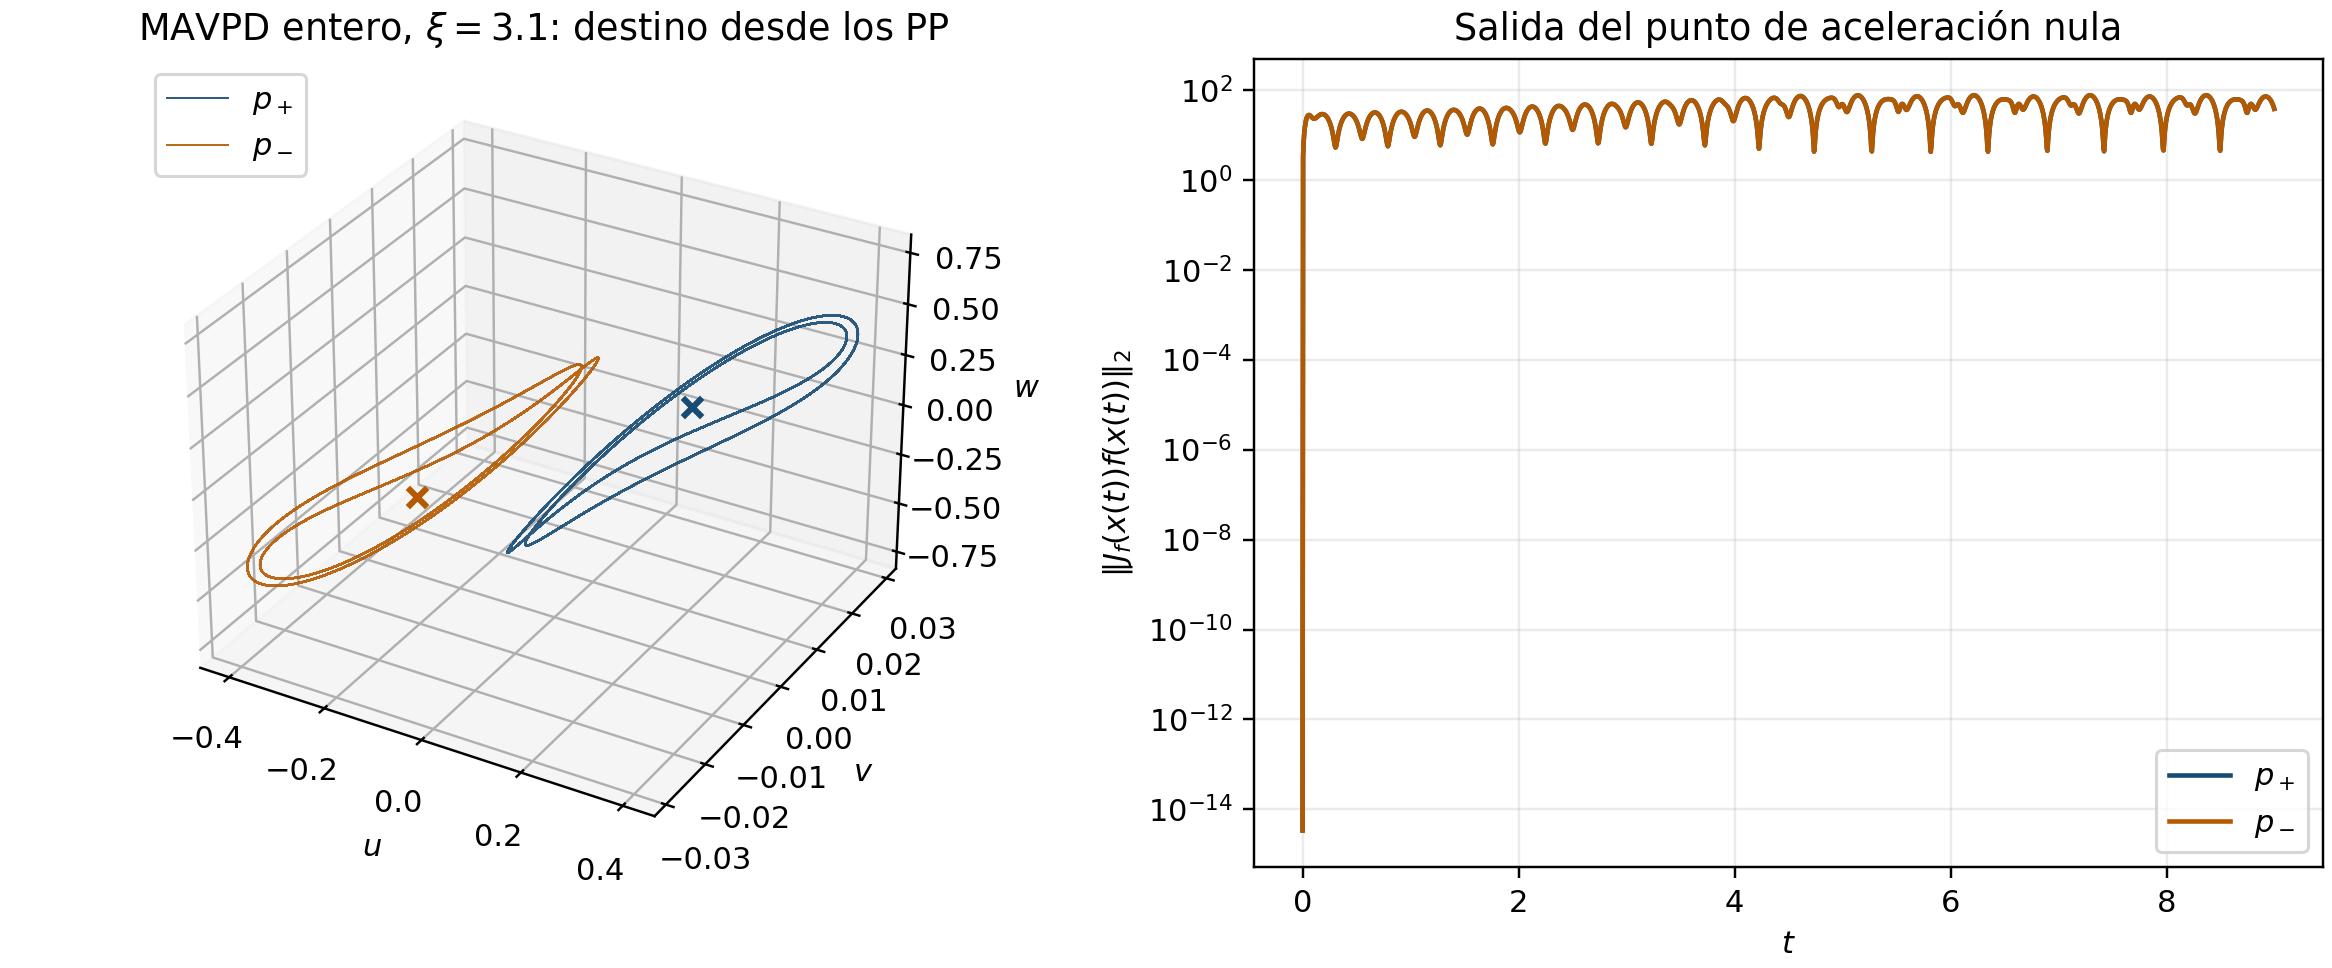
\includegraphics[width=0.98\linewidth]{figures/perpetual/perpetual_mavpd_integer.png}
 \caption{Experimento PP entero en MAVPD, \(\xi=3.1\). Las cruces son los PP
 exactos; las curvas son los destinos después del transitorio. El panel
 derecho muestra que \(J_f f=0\) sólo en el instante inicial y no a lo largo de
 toda la órbita.}
 \label{fig:pp-mavpd-pilot}
\end{hafocommonfigure}

\subsubsection{Muñoz--Pacheco: raíces suaves y frontera no diferenciable}

Para
\begin{equation}
 f(x,y,z)=
 \begin{pmatrix}
 yz+x(y-a)\\1-|x|\\-xy-z
 \end{pmatrix},\qquad a=0.35,
 \label{eq:pp-munoz-field}
\end{equation}
se trabaja por regiones \(s=\operatorname{sign}x\):
\begin{equation}
 J_f=
 \begin{pmatrix}
 y-a&z+x&y\\-s&0&0\\-y&-x&-1
 \end{pmatrix}.
 \label{eq:pp-munoz-jacobian}
\end{equation}
La segunda ecuación de \(J_f f=0\) impone \(f_1=0\). La tercera da
\(f_3=-xf_2\), y la primera se convierte en
\begin{equation}
 f_2(z+x-xy)=0.
\end{equation}
Como \(f_2=0\) llevaría a un equilibrio, se excluye esa rama. En efecto,
\(f_2=0\) exige \(|x|=1\), \(f_3=0\) da \(z=-xy\), y entonces
\[
 f_1=-x(y^2-y+a)
 =-x\bigl[(y-\tfrac12)^2+a-\tfrac14\bigr]\ne0
\]
para $a=0.35>1/4$ y $x=\pm1$; no hay equilibrios. Se obtiene
\(z=x(y-1)\). Usando
\(f_3=-xy-z=-xf_2\), resulta
\begin{equation}
 y=1-\frac{|x|}{2}.
\end{equation}
Finalmente, \(f_1=0\) reduce a \(x(y^2-a)=0\), de modo que
\begin{equation}
 y=\varepsilon\sqrt a,\qquad
 u_\varepsilon=2(1-\varepsilon\sqrt a),\qquad
 (x,y,z)=
 \left(su_\varepsilon,\varepsilon\sqrt a,
 -\frac{s u_\varepsilon^2}{2}\right),
 \label{eq:pp-munoz-closed}
\end{equation}
para \(\varepsilon,s\in\{\pm1\}\). Numéricamente:
\begin{align}
 &(\pm0.816784043380077, 0.591607978309962,
 \mp0.333568086760154),\\
 &(\pm3.183215956619923, -0.591607978309962,
 \mp5.066431913239846).
\end{align}
El residuo vectorial se anula exactamente; las normas del campo son
\(0.2365640964\) y \(7.2845066702\). Todas las raíces están separadas de
\(x=0\), por lo que la derivada regional de \(|x|\) es válida.

En la frontera \(x=0\) no existe un Jacobiano clásico único. El criterio
direccional de \cref{eq:pp-bouligand} debe evaluarse por separado.
Allí \(f=(yz,1,-z)^{\mathsf T}\), y la segunda componente de la
derivada en la dirección \(f\) es \(-|yz|\). Su anulación exige
\(yz=0\); si \(z\ne0\), se tendría \(y=0\) y la tercera componente
sería \(z\ne0\). Por tanto, las únicas raíces direccionales de frontera
son \((0,y,0)\). Ambos Jacobianos laterales también anulan \(f\) sobre
esa recta. Sin embargo, sus soluciones exactas son
\begin{equation}
 x(t)=z(t)=0,\qquad
 y(t)=y_0+\frac{(t-t_0)^q}{\Gamma(q+1)},\qquad 0<q\le1.
 \label{eq:pp-munoz-boundary-orbit}
\end{equation}
La sustitución en la ecuación de Volterra comprueba la solución. Son
trayectorias no acotadas; las cuatro raíces anteriores agotan los PP de las
regiones suaves, pero no las raíces del criterio direccional de frontera.

El experimento Caputo usó \(q=0.97\), PECE de Diethelm con historia completa,
\(h=0.01\) y \(t_f=35\). Las cuatro trayectorias permanecieron finitas; las
normas máximas fueron \(6.421\) para el par interior y \(10.178\) para el
exterior. Los rangos no triviales no certifican un atractor ni caos: son
diagnósticos finitos que deben contrastarse al refinar paso y horizonte.

\begin{hafodigitalfigure}[H]
 \centering
 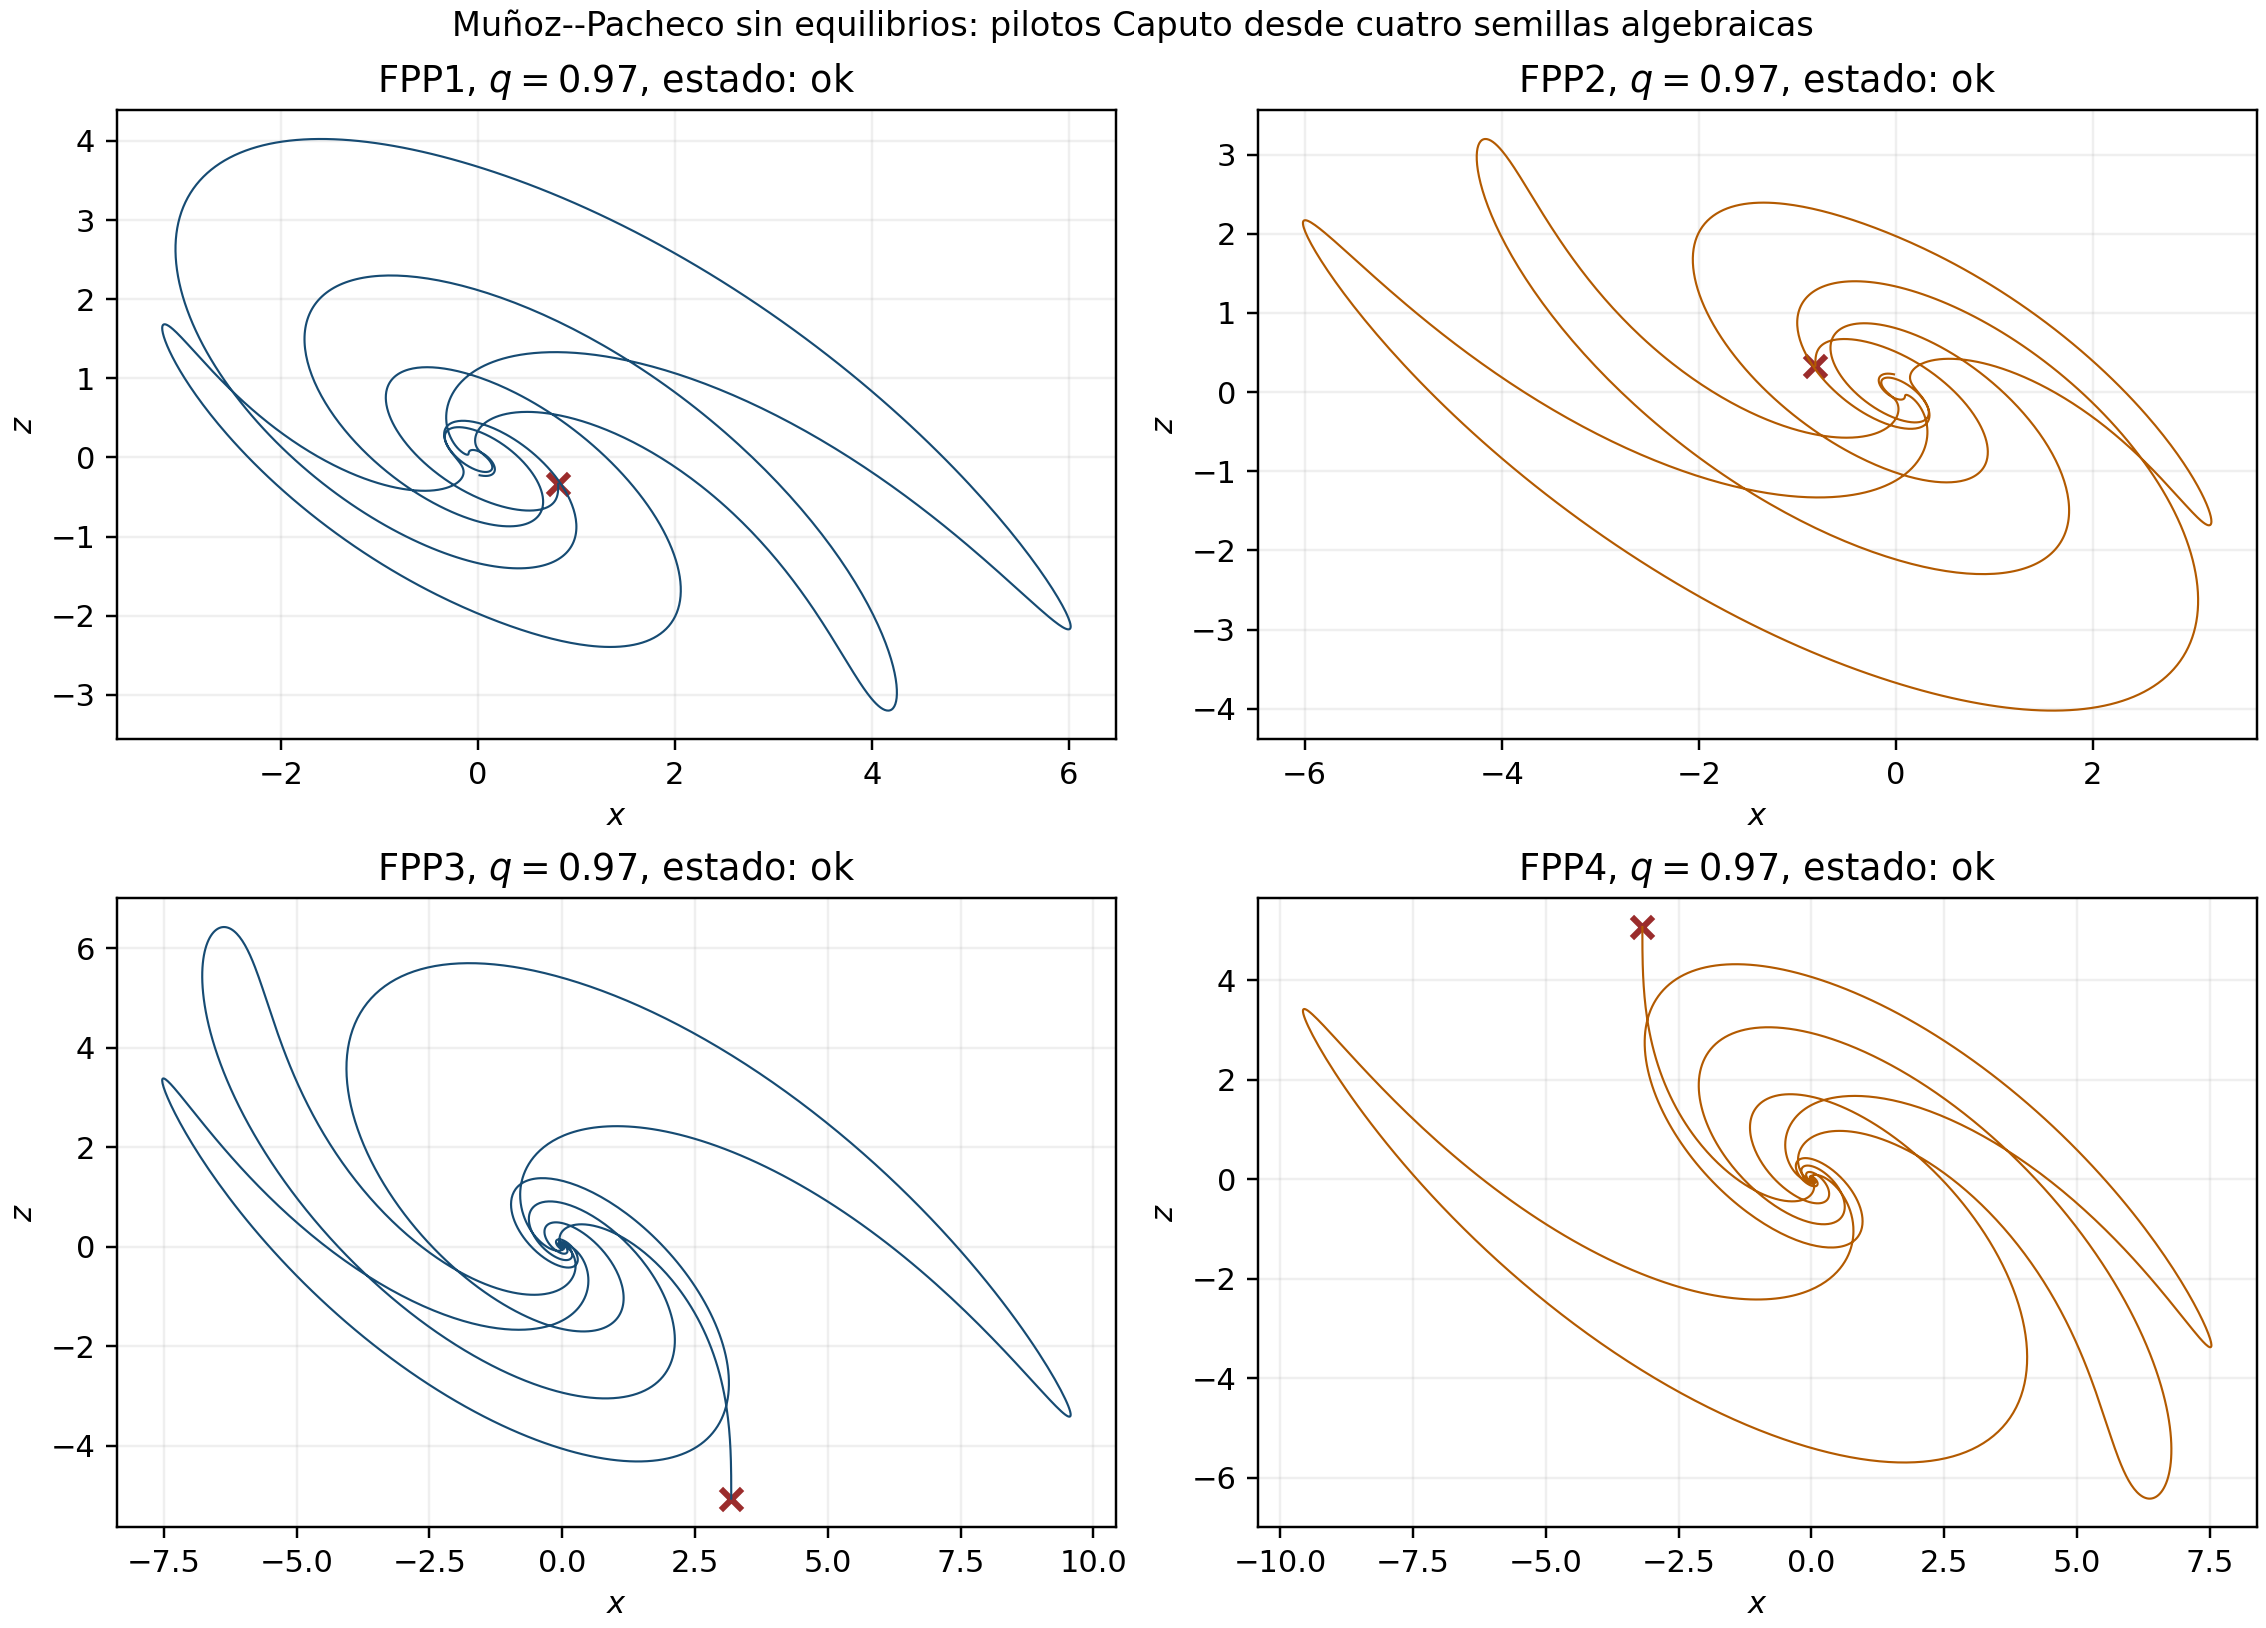
\includegraphics[width=0.96\linewidth]{figures/perpetual/perpetual_munoz_caputo.png}
 \caption{Experimento Caputo desde las cuatro semillas FPP--A exactas de
 Muñoz--Pacheco. Las cruces indican el estado inicial. Las curvas muestran
 trayectorias finitas, no una afirmación de atracción ni ocultedad.}
 \label{fig:pp-munoz-pilot}
\end{hafodigitalfigure}

Para FPP1 se calculó además \cref{eq:fpph-l1}. En el horizonte común
\([2,17.5]\), las curvas \(h=0.01\) y \(h=0.005\) concuerdan cualitativamente,
pero ningún mínimo converge a cero: el refinamiento dio un mínimo normalizado
aproximado \(0.0871\) cerca de \(t=11.965\). La corrida gruesa alcanzó
\(0.0254\) en \(t=32.33\), fuera del horizonte fino, y por eso no se clasifica
como evento FPP--H. El panel de arranque sí muestra que el cociente de
\cref{eq:pp-startup-limit} decrece hacia el residuo algebraico cero al refinar
\(h\).

\begin{hafodigitalfigure}[H]
 \centering
 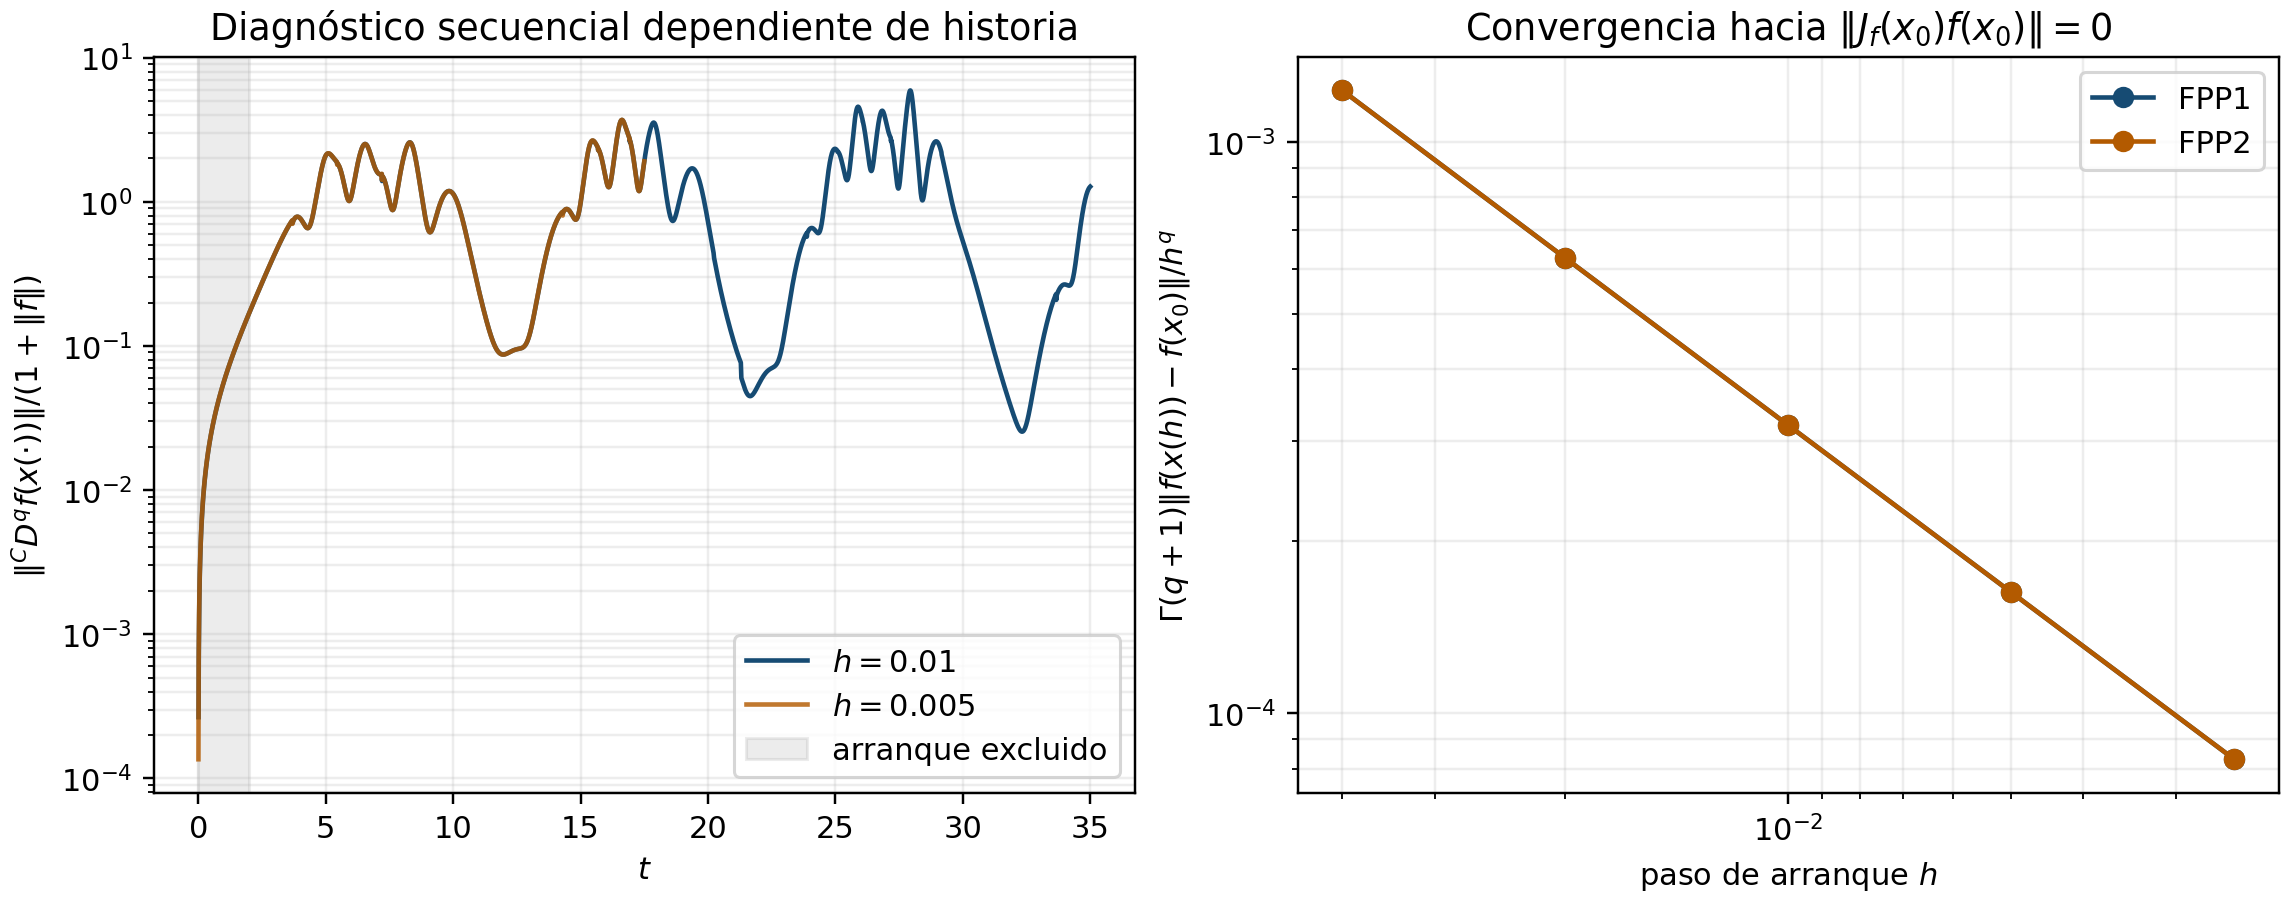
\includegraphics[width=0.98\linewidth]{figures/perpetual/perpetual_caputo_history_diagnostics.png}
 \caption{Izquierda: aceleración secuencial L1 dependiente de historia; el
 intervalo gris se excluye por arranque. Derecha: verificación numérica del
 límite de arranque en dos raíces simétricas. La ausencia de un cero
 convergente impide reclamar un evento FPP--H.}
 \label{fig:pp-caputo-history}
\end{hafodigitalfigure}

\subsubsection{Chua arctangente}

Escribiendo \(h(x)=a_1x+a_2\arctan(\rho x)\), la condición singular produce
la primera restricción sobre la coordenada \(x\). En efecto, el campo y su
Jacobiano son
\[
 f=\begin{pmatrix}\alpha(y-x-h(x))\\x-y+z\\-\beta y-\gamma z\end{pmatrix},
 \qquad
 J_f=\begin{pmatrix}
 -\alpha(1+h'(x))&\alpha&0\\1&-1&1\\0&-\beta&-\gamma
 \end{pmatrix}.
\]
Si \(U=f_1\), las dos primeras filas de \(J_ff=0\) imponen
\(f_2=(1+h')U\) y \(f_3=h'U\). Un PP requiere \(U\ne0\), porque
\(U=0\) anularía también \(f_2,f_3\). La tercera fila se reduce a
\([\beta+(\beta+\gamma)h']U=0\). Para
\(\alpha\rho(\beta+\gamma)\ne0\), se obtiene
\begin{equation}
 h'(x_\star)=-\frac{\beta}{\beta+\gamma},
 \quad
 x_\star^2=\frac1{\rho^2}
 \left[
 \frac{a_2\rho}{-\beta/(\beta+\gamma)-a_1}-1
 \right],
 \label{eq:pp-chua-arctan-x}
\end{equation}
si el miembro derecho es positivo. El denominador
\(-\beta/(\beta+\gamma)-a_1\) debe ser no nulo. Si se anula, se vuelve a
\(h'(x)=a_1+a_2\rho/(1+\rho^2x^2)\): para \(a_2\rho\ne0\) no hay
solución finita; para \(a_2\rho=0\) la restricción singular se satisface
en toda la recta y se debe resolver el sistema lineal restante sin
dividir. Este caso degenerado no aparece en Wu ni en c590. Un valor negativo del
miembro derecho excluye raíces reales. Para un valor cero se comprueba
\(x_\star=0\) en el sistema original. Dado uno de los signos admisibles,
escriba \(p=h'(x_\star)\). Las identidades
\(f_1=U\), \(f_2=(1+p)U\) dan sucesivamente
\[
 y_\star=x_\star+h(x_\star)+U/\alpha,
 \qquad
 z_\star=h(x_\star)+(1+p)U+U/\alpha.
\]
Al sustituirlas en \(-\beta y_\star-\gamma z_\star=pU\), resulta la
ecuación lineal
\[
 \left[\gamma+(1+\gamma)p+\frac{\beta+\gamma}{\alpha}\right]U
 =-\beta x_\star-(\beta+\gamma)h(x_\star).
\]
Por tanto,
\begin{equation}
 U=-\frac{\beta x_\star+(\beta+\gamma)h(x_\star)}
 {\gamma+(1+\gamma)p+(\beta+\gamma)/\alpha},
\end{equation}
si el coeficiente de \(U\) es no nulo. Si se anula, se resuelve la
ecuación lineal anterior sin dividir: un término derecho no nulo descarta
la raíz; si ambos se anulan, queda una familia que debe comprobarse en
\(J_ff=0\). Finalmente se exige \(U\ne0\). En los casos Wu y c590 los
denominadores son no nulos y ambos signos producen PP; la imparidad de
\(h\) relaciona las dos raíces por simetría central.
Para Wu con \(q=0.99\), las raíces son
\begin{equation}
 \pm(0.3369817810952544, 0.0815749282686440,
 -0.2549832342782550),\qquad \|f\|=1.39124162716.
\end{equation}
Para c590, \(q=0.9999\), el par es
\begin{equation}
 \pm(1.213090022614086, -20.18726992409549,
 -21.54936334065727),\qquad \|f\|=545.09983035.
\end{equation}
La gran norma y la distancia al conjunto observado en c590 obligan a
controlar el transitorio y el escape antes de usar el segundo par como
semilla. En Wu, las integraciones de ambos signos permanecen acotadas, pero
no resuelven un destino asintótico común; véase
\cref{sec:resultados-piloto-gt}.

\subsubsection{Chua PWL y Kalman--Fitts como controles negativos}

En una región de pendiente \(m\), el Jacobiano de Chua PWL satisface
\begin{equation}
 \det J_m=-\alpha[\beta+(\beta+\gamma)m].
 \label{eq:pp-chua-pwl-det}
\end{equation}
Con \(m_0=-0.1768\) y \(m_1=-1.1468\), los valores son
\(-84.035507517056\) y \(15.037737580544\). Al ser invertibles, cada región
sólo admite equilibrios en \(J_mf=0\). En \(x=\pm1\), la derivada
direccional usa uno de esos Jacobianos si \(f\) apunta a una región;
si es tangente, ambos productos coinciden por continuidad del campo PWA.
En cualquiera de los casos, la invertibilidad excluye un producto cero
con \(f\ne0\). La función descriptiva y la
continuación localizan órbitas donde PP no genera semilla.

En Kalman--Fitts, \(f(X)=AX+e_4\tanh(-X_3/\varepsilon)\), la
derivada de \(\tanh\) sólo modifica la tercera entrada de la última
fila de la matriz compañera \(A\). Su determinante, igual al coeficiente
constante del polinomio característico, permanece inalterado:
\begin{equation}
 \det J_f=0.98191881\neq0.
\end{equation}
Por \cref{eq:pp-singular-screen}, no existe PP. El mapa de conmutación
proporciona una vía alternativa de localización.

\subsubsection{Ausencia de puntos perpetuos en los dos sistemas jerk}
\label{subsec:pp-jerk-exclusion}

\begin{proposition}[jerk cuadrático y jerk exponencial]
\label{prop:pp-jerk-exclusion}
Los campos de \cref{eq:cand-jerk,ncbench:eq:jerk} no tienen puntos perpetuos
no estacionarios. El jerk exponencial tampoco tiene semillas FPP--A para
ningún orden conmensurable \(0<q<1\).
\end{proposition}

\begin{proof}
En un campo jerk \(f=(y,z,G(x,y,z))^{\mathsf T}\),
\begin{equation}
 J_ff=\bigl(z,G,G_xy+G_yz+G_zG\bigr)^{\mathsf T}.
 \label{eq:pp-jerk-general-acceleration}
\end{equation}
Por tanto, toda raíz satisface \(z=G=0\) y \(G_xy=0\).
Para el jerk cuadrático,
\[
 G=-x-y-1.1z-2.59z^2+xy,\qquad G_x=y-1.
\]
La última condición se reduce a \(y(y-1)=0\). Si \(y=0\), las otras
dos ecuaciones dan \(z=x=0\), el equilibrio. Si \(y=1\), entonces
\(G(x,1,0)=-1\), incompatible con \(G=0\). Estas dos ramas agotan las
posibilidades reales.

Para el jerk exponencial,
\[
 G=-az-I_c\left(e^{y/(nV_T)}-1\right)-x,\qquad G_x=-1.
\]
Así, \(G_xy=0\) obliga a \(y=0\), y \(z=G=0\) obliga a \(x=0\).
Equivalentemente, \(\det J_f=G_x=-1\) en todo \(\mathbb R^3\).
Ambos campos son suaves y no hay regiones ni fronteras adicionales que
examinar. La condición FPP--A conmensurable es la misma ecuación
\(J_ff=0\), con los equilibrios excluidos.
\end{proof}

Esta ausencia limita la generación de semillas por PP. No excluye
atractores ni eventos FPP--H a lo largo de una historia.

\subsubsection{PLL lead--lag}

En las coordenadas publicadas \((x,\theta)\), con
\(T=\tau_1+\tau_2>0\), el campo es
\[
 f_x=-\frac{x}{T}+\frac{\tau_1}{2T}\sin\theta,\qquad
 f_\theta=\omega_\Delta-\frac{Lx}{T}
                         -\frac{\tau_2L}{2T}\sin\theta.
\]
Derivar sus dos componentes y tomar el determinante da
\begin{equation}
 \det J_f=\frac{L\cos\theta}{2(\tau_1+\tau_2)}.
\end{equation}
Como un PP tiene \(f\ne0\), la singularidad del Jacobiano exige
\(\cos\theta=0\). En esos ángulos,
\[
 J_f=\begin{pmatrix}-1/T&0\\-L/T&0\end{pmatrix},\qquad
 T=\tau_1+\tau_2>0.
\]
Así, \(J_ff=0\) equivale a \(f_x=0\), es decir,
\(x=\tau_1\sin\theta/2\). La otra componente se reduce a
\(f_\theta=\omega_\Delta-L\sin\theta/2\).
Los PP por vuelta del cilindro son
\begin{equation}
 \left(\frac{\tau_1}{2},\frac\pi2\right),
 \qquad
 \left(-\frac{\tau_1}{2},\frac{3\pi}{2}\right),
 \label{eq:pp-pll}
\end{equation}
si las velocidades angulares correspondientes
\(\omega_\Delta\mp L/2\) no se anulan. Numéricamente son
\((0.0224,1.5707963268)\), con \(f=(0,-71.1)\), y
\((-0.0224,4.7123889804)\), con \(f=(0,428.9)\). La comparación debe usar
distancia cilíndrica y las mismas coordenadas, por
\cref{eq:pp-nonlinear-coordinate}. En las integraciones de
\cref{sec:resultados-piloto-gt}, la semilla positiva llega al foco y la
negativa permanece como un transitorio acotado sin destino resuelto.

\subsubsection{Lorenz generalizado y Rabinovich--Fabrikant}

Para el Lorenz generalizado,
\begin{equation}
 f=\begin{pmatrix}
 -\sigma(x-y)-ayz\\rx-y-xz\\-z+xy
 \end{pmatrix},\qquad
 J_f=\begin{pmatrix}
 -\sigma&\sigma-az&-ay\\r-z&-1&-x\\y&x&-1
 \end{pmatrix}.
\end{equation}
Con \((r,a,\sigma)=(6.8,-0.5,3.4)\), el sistema \(J_ff=0\) tiene cinco raíces
reales. Para obtenerlas sin confundir equilibrios y PP, se parte de las
componentes explícitas de \cref{casegt:eq:lorenz-A}. Si \(x=0\) y
\(y\ne0\), las dos primeras exigirían simultáneamente
\(z=-748/135\) y \(z^2=1206/25\), lo cual es imposible. Si
\(y=0\) y \(x\ne0\), exigirían \(z=748/135\) y
\(z^2=1734/25\), también incompatibles. Cuando \(x=y=0\), la tercera
componente da \(z=0\). Toda raíz restante tiene \(xy\ne0\).

Introduzca \(u=x^2>0\) y \(v=y/x\ne0\). Al dividir las dos primeras
ecuaciones entre \(x\), el sistema equivale a
\begin{equation}
 \frac{v^2}{2}u+c_1(v,z)=0,\qquad
 -vu+c_2(v,z)=0,\qquad u c_3(v,z)+z=0,
 \label{eq:pp-lorenz-reduced-three}
\end{equation}
donde
\begin{align}
 c_1&=\frac{867}{25}-\frac{374}{25}v-\frac{27}{10}vz-\frac12z^2,\nonumber\\
 c_2&=-\frac{748}{25}+\frac{603}{25}v+\frac{27}{5}z-\frac12vz^2,\\
 c_3&=\frac{34}{5}-\frac{27}{5}v+\frac{17}{5}v^2
       +\left(\frac{v^2}{2}-1\right)z.
 \label{eq:pp-lorenz-c-polynomials}
\end{align}
La segunda ecuación da \(u=c_2/v\). Sustituirla en las otras dos produce
\begin{align}
 L(v,z)&=\frac{3468-2992v+1206v^2}{25}-(2+v^2)z^2=0,\nonumber\\
 Q(v,z)&=vz+c_2(v,z)c_3(v,z)=0.
 \label{eq:pp-lorenz-two-polynomials}
\end{align}
El resultante respecto de \(v\), definido como el determinante de la
matriz de Sylvester de estos dos polinomios, factoriza como
\begin{equation}
 \operatorname{Res}_v(L,Q)
 =-5^{-12}(25z^2-1206)(25z^2-986)P_L(z),
 \label{eq:pp-lorenz-resultant}
\end{equation}
con
\begin{align}
 P_L(z)={}&781250z^8-94421875z^6-112200000z^5\nonumber\\
 &+3621441250z^4+6045336000z^3-60977294900z^2\nonumber\\
 &-150632718720z-231894425384.
 \label{eq:pp-lorenz-eliminant}
\end{align}
Para reconstruir \(v\), la división de \(Q\) entre \(L\) respecto de
\(v\) deja el resto
\[
 \frac{R_1(z)v+R_0(z)}{125(25z^2-1206)},
\]
donde
\begin{align}
 R_0(z)&=18307572+4398240z+2697400z^2-50625z^4,\nonumber\\
 R_1(z)&=-2864840+647540z-1739100z^2-422500z^3+3125z^5.
 \label{eq:pp-lorenz-reconstruction-polynomials}
\end{align}
Las raíces de \((25z^2-986)P_L\) no anulan \(R_1\), pues el máximo
común divisor de ambos polinomios es uno. En ellas,
\begin{equation}
 v=-R_0/R_1,\qquad u=c_2/v,\qquad
 x=\pm\sqrt u,\quad y=vx.
 \label{eq:pp-lorenz-reconstruction}
\end{equation}
El factor \(25z^2-1206\) corresponde a una caída de grado en \(L,Q\);
al sustituir \(z^2=1206/25\), la ecuación \(L=0\) exige
\(v=66/187\), pero
\[
 \gcd\bigl(25z^2-1206,Q(66/187,z)\bigr)=1
\]
tras eliminar denominadores. Sus dos raíces se descartan antes de usar
la fórmula racional. Fuera de esa rama, el coeficiente principal de
\(L\), respecto de \(v\), no se anula. La anulación del resultante
equivale entonces a una raíz común de \(L\) y su resto lineal; esto
justifica el levantamiento \(v=-R_0/R_1\), además de su unicidad.

Para contar raíces reales, la sucesión de Sturm se construye con
\(S_0=P\), \(S_1=P'\) y
\(S_{j+1}=-\operatorname{rem}(S_{j-1},S_j)\), hasta el último resto no
nulo. Sea \(V_P(t)\) el número de cambios de signo de la sucesión evaluada
en \(t\), omitiendo ceros. La diferencia \(V_P(a)-V_P(b)\) cuenta las
raíces distintas en \((a,b)\), si sus extremos no son raíces. Para \(P_L\),
\[
 \begin{array}{c|rrrrrr}
 t&-\infty&-7.443&-7.442&9.321&9.322&+\infty\\\hline
 V_{P_L}(t)&5&5&4&4&3&3
 \end{array}
\]
Los extremos decimales son racionales exactos. Hay una raíz en cada
intervalo indicado y ninguna otra raíz real. Las condiciones de
reconstrucción separan las ramas:
\begin{center}
\begin{tabular}{@{}rrrr@{}}
\toprule
\(z\) & \(v\) & \(u=x^2\) & Admisibilidad\\\midrule
\(-6.2801273872\) & \(13.0801273872\) & \(-0.4801273872\) & no real\\
\(6.2801273872\) & \(0.5198726128\) & \(12.0801273872\) & equilibrio\\
\(-7.4423053062\) & \(-16.9736823118\) & \(0.5564665577\) & PP\\
\(9.3218987982\) & \(-0.3277828328\) & \(-81.6209147361\) & no real\\
\bottomrule
\end{tabular}
\end{center}
La admisibilidad no depende del redondeo de la tabla. La forma equivalente
\begin{equation}
 u=\frac{603}{25}-\frac{z^2}{2}
   +\frac{-748/25+27z/5}{v}
 \label{eq:pp-lorenz-sign-certificate}
\end{equation}
permite evaluar con aritmética racional de intervalos: para la raíz de
\(P_L\) en \((-7.443,-7.442)\), se obtiene \(0.29<u<0.83\); para la
raíz en \((9.321,9.322)\), se obtiene \(-82<u<-81\).
Los denominadores quedan separados de cero en ambos intervalos.
Para \(25z^2-986=0\), la reconstrucción da exactamente \(u=29/5+z\);
la raíz positiva admite \(u>0\), mientras la negativa cumple
\(z<-29/5\) y obliga a \(u<0\).
La fila de equilibrio reconstruye el par de \cref{nc:eq:lorenz-eq1}; la
fila PP reconstruye
\begin{equation}
 (-0.745966861002653, 12.66180451381419, -7.442305306160726)
\end{equation}
y su imagen por \((x,y,z)\mapsto(-x,-y,z)\), con
\(\|f\|=23.42210895339\). Son candidatos FPP--A para \(q=0.995\), pero aún no
cuentan con validación dinámica.

Para Rabinovich--Fabrikant,
\begin{align}
 f_1&=y(z-1+x^2)+ax,\\
 f_2&=x(3z+1-x^2)+ay,\\
 f_3&=-2z(b+xy),
\end{align}
y
\begin{equation}
 J_f=\begin{pmatrix}
 2xy+a&z-1+x^2&y\\
 3z+1-3x^2&a&3x\\
 -2yz&-2xz&-2(b+xy)
 \end{pmatrix}.
 \label{eq:pp-rf-jacobian}
\end{equation}
Para \((a,b)=(1/10,719/2500)\), se separan primero los casos \(x=0\)
y \(z=0\). Si \(x=0\), las aceleraciones primera y tercera son
\[
 A_1=2y[(a-b)z-a],\qquad
 A_3=2z[2b^2-y^2(z-1)].
\]
Si \(y=0\), \(A_3=0\) obliga a \(z=0\). Si \(y\ne0\), la primera
ecuación obliga a \(z=a/(a-b)<0\); entonces la segunda exigiría
\(y^2(z-1)=2b^2>0\), imposible. Por tanto, la única raíz con \(x=0\)
es el origen.

Para \(x\ne0\), introduzca \(u=x^2>0\), \(v=xy\) y
\(H=u+z-1\), \(K=3z+1-u\). La multiplicación explícita de
\cref{casegt:eq:rf-A} da
\begin{align}
 E_1:=xA_1&=u(a^2+HK)+2v[a(u+H)-bz]+2(u-1)v^2,\nonumber\\
 E_2:=xA_2&=D(u,z)v+C(u,z),\label{eq:pp-rf-reduced-three}\\
 -\frac{uA_3}{2z}&=E_3:=(z-1-u)v^2+2u(a-2b)v+u(uK-2b^2),\nonumber
\end{align}
donde la última igualdad se usa sólo para \(z\ne0\), y
\begin{align}
 D&=3z^2-6uz-2z-3u^2+4u+a^2-1,\nonumber\\
 C&=2u[a(3z+1-2u)-3bz].
 \label{eq:pp-rf-D-C}
\end{align}

En el plano \(z=0\), \(A_3\) se anula idénticamente y basta resolver
\(E_1=E_2=0\). La eliminación de \(v\) da
\begin{align}
 \operatorname{Res}_v(E_1|_{z=0},E_2|_{z=0})
 ={}&-10^{-6}u(10u-11)(10u-9)\nonumber\\
 &\times[100(u-1)^2+1][100(3u-1)^2+1].
 \label{eq:pp-rf-z0-resultant}
\end{align}
Los factores cuadráticos son estrictamente positivos. Como \(u>0\), las
únicas posibilidades son
\[
 (u,v)=(9/10,4/5),\qquad (u,v)=(11/10,-6/5).
\]
Sustituir estos pares en \(E_1,E_2\) da cero y reconstruye cuatro PP
mediante \(x=\pm\sqrt u\), \(y=v/x\). Ninguno es un equilibrio:
en \(z=0\), el sistema \(f_1=f_2=0\) tiene determinante
\(a^2+(u-1)^2>0\) y sólo admite \(x=y=0\).

Para \(z\ne0\), se resuelven las tres ecuaciones \(E_j=0\).
Antes de dividir entre \(D\), se comprueba su rama excepcional. Si
\(D=0\), \(E_2=0\) exige \(C=0\); por \(u>0\),
\[
 u=u_D(z):=\frac{1250-7035z}{2500},\qquad
 d_D(z):=65000-1953500z-967947z^2=0.
\]
Al sustituir \(u_D\) en \(E_1,E_3\), se obtiene
\[
 \gcd\!\left(d_D,
 \operatorname{Res}_v(E_1(u_D,v,z),E_3(u_D,v,z))\right)=1,
\]
tras eliminar denominadores constantes. No hay una raíz común y la rama
\(D=0\) queda excluida. Para \(D\ne0\), \(v=-C/D\). Al multiplicar
por \(D^2\), las otras dos ecuaciones equivalen a
\begin{align}
 P(u,z)={}&u(a^2+HK)D^2-2CD[a(u+H)-bz]+2(u-1)C^2=0,\nonumber\\
 Q(u,z)={}&(z-1-u)C^2-2u(a-2b)CD+u(uK-2b^2)D^2=0.
 \label{eq:pp-rf-P-Q}
\end{align}
Defina los polinomios
\[
 S(u)=32264900u^2-215503200u+82528417,\qquad
 E(u)=53150000u^2-71900000u+516961.
\]
El resultante de \(P,Q\) respecto de \(z\) es un múltiplo constante
no nulo de \(u^{13}S(u)^4E(u)P_R(u)\). Una definición exacta y compacta
del factor de grado catorce es
\begin{equation}
 P_R(u)=\operatorname{pp}\!\left(
 \frac{\operatorname{Res}_z(P,Q)}{u^{13}S(u)^4E(u)}\right),
 \label{eq:pp-rf-eliminant}
\end{equation}
donde \(\operatorname{pp}\) elimina denominadores y el máximo común divisor
de los coeficientes, y fija positivo el coeficiente principal. Todas las
entradas del determinante de Sylvester están dadas en
\cref{eq:pp-rf-D-C,eq:pp-rf-P-Q}; no se requiere una aproximación numérica
para definir \(P_R\).

Para la evaluación directa, escriba
\(P_R(u)=\sum_{k=0}^{14}m_k10^{e_k}u^k\), con coeficientes enteros:
\begin{center}
\small
\begin{tabular}{@{}rrr@{}}
\toprule
\(k\)&\(m_k\)&\(e_k\)\\\midrule
0&172890165175624363345259174569803&0\\
1&14469699682074574386521765557812&2\\
2&\(-18396580138862579542741337855542518\)&2\\
3&15478807059059016799618863592551164&4\\
4&\(-483305962260027081263570393541627373\)&4\\
5&56915116746512318338898887806915&9\\
6&\(-1629237154908128789498842947039615\)&8\\
7&95325977171002410189945625&14\\
8&125564435311034818006205569375&13\\
9&\(-433337883019314447578125\)&19\\
10&81563269511051918346484375&17\\
11&\(-99102930618837890625\)&23\\
12&77980731527669677734375&20\\
13&\(-358729705810546875\)&25\\
14&722605133056640625&24\\\bottomrule
\end{tabular}
\end{center}

La raíz \(u=0\) pertenece al caso ya separado. Las raíces de \(S\)
provienen de la eliminación de denominadores: al reducir \(P,Q\) con
\(S=0\), sus raíces comunes con \(u>0\) cumplen \(D=C=0\), rama
excluida antes de la división. Las dos raíces positivas de
\(E\) reconstruyen los cuatro equilibrios no nulos de
\cref{nc:eq:rf-e12,nc:eq:rf-e34}, con \(v=-b\). Para comprobar esta
identificación, \(f_3=0\), \(z\ne0\), exige \(v=-b\);
de \(xf_1=au+vH=0\) se obtiene \(z=1-u+au/b\).
La ecuación \(xf_2=uK+av=0\) queda
\[
 (4b-3a)u^2-4bu+ab^2=0.
\]
Multiplicarla por \(62500000\) produce exactamente \(E(u)=0\).
Su discriminante es positivo y tanto la suma como el producto de las
raíces son positivos; ambas son reales positivas. Cada una reconstruye
dos signos de \(x\), y la sustitución verifica las tres componentes del
campo. Queda \(P_R\), cuya
sucesión de Sturm da
\[
 \begin{array}{c|rrrrrr}
 t&0&0.0391&0.0392&0.0474&0.0475&+\infty\\\hline
 V_{P_R}(t)&7&7&6&6&5&5
 \end{array}
\]
Hay exactamente dos raíces positivas. El levantamiento desde \(u\) se
justifica mediante una forma triangular exacta. Sea \(Z(u)\) el
polinomio racional de grado trece definido por la base de Gröbner reducida
y mónica del ideal \(\langle P,Q,P_R\rangle\), con orden lexicográfico
\(z>u\). Esa base es
\begin{equation}
 \left\{\frac{P_R(u)}{\operatorname{lc}(P_R)},\ z-Z(u)\right\},
 \qquad \deg Z=13,
 \label{eq:pp-rf-triangular}
\end{equation}
donde \(\operatorname{lc}\) denota el coeficiente principal. Esta
definición usa exclusivamente los coeficientes racionales de
\cref{eq:pp-rf-P-Q,eq:pp-rf-eliminant} y fija \(Z\) de manera única.
La división polinómica proporciona los certificados
\begin{align}
 P(u,Z(u))&\equiv Q(u,Z(u))\equiv0\pmod{P_R(u)},\nonumber\\
 \gcd(P_R,Z)&=\gcd\bigl(P_R,D(u,Z)\bigr)=1,\nonumber\\
 \gcd\bigl(P_R,bD(u,Z)-C(u,Z)\bigr)&=1,
 \label{eq:pp-rf-lifting-certificates}
\end{align}
normalizando cada máximo común divisor a mónico. Por la igualdad de
ideales de \cref{eq:pp-rf-triangular}, cada raíz de \(P_R\) tiene
exactamente un levantamiento \(z=Z(u)\). Para las dos raíces reales
positivas, \(Z(u)\) es real; los dos primeros máximos comunes divisores
excluyen \(z=0\) y \(D=0\). Se reconstruye entonces
\begin{equation}
 v=-C/D,\qquad x=\pm\sqrt u,\qquad y=v/x.
 \label{eq:pp-rf-reconstruction}
\end{equation}
Los dos triples reducidos son
\[
 \begin{array}{c|rr}
 u&v&z\\\hline
 0.0391007463043&-0.0447439313091&0.822145202941\\
 0.0474835273591& 0.0710968429474&1.202380810759
 \end{array}
\]
y ambos tienen \(v\ne-b\): si \(v=-C/D=-b\), se anularía
\(bD-C\), contradiciendo el último certificado de
\cref{eq:pp-rf-lifting-certificates}. Así,
\(f_3=-2z(b+v)\ne0\) y ninguno es un equilibrio.
Las cuatro raíces del plano \(z=0\), estas cuatro raíces y los cinco
equilibrios agotan las trece soluciones reales de \(J_ff=0\). Cuatro
representantes de los ocho PP son
\begin{align}
 &( -1.04880884817015, 1.14415510709471, 0),\\
 &( 0.948683298050514, 0.843274042711568, 0),\\
 &( 0.217907153070161, 0.326271267123146, 1.202380810758825),\\
 &( -0.197739086435437, 0.226277627330655, 0.822145202940591),
\end{align}
más sus imágenes por \((x,y,z)\mapsto(-x,-y,z)\). Las normas del campo son,
respectivamente, \(0.21950,0.17951,1.34455,0.76891\). Antes de una corrida
Caputo \(q=0.998\) se deduplican los cuatro pares y se asigna el mismo
presupuesto a cada uno.

\subsection{Protocolo de validación PP0--PP5}

\begin{description}[style=nextline,leftmargin=3.2em,labelwidth=2.7em]
 \item[PP0] Fijar fuente, campo, coordenadas, parámetros, dominio y
 convención no suave.
 \item[PP1] Calcular \(J_f\), \(J_f f\), \(\det J_f\); resolver raíces reales,
 excluir \(\|f\|\leq\nu\), verificar región y evaluar el residuo con
 50 dígitos de precisión.
 \item[PP2] En entero, integrar desde cada PP, perturbaciones radiales
 \(10^{-6},10^{-4},10^{-2}\) y controles aleatorios de igual norma, con la
 configuración analizada.
 \item[PP3] En Caputo, distinguir FPP--A de FPP--H; usar historia completa como
 oráculo, terminal inferior común, \(h,h/2\) y una réplica corta \(h/4\).
 \item[PP4] Clasificar destino, recurrencia, robustez y, para FPP--H, mínimos de
 \(\eta_{q,n}\); separar continuación con historia y reset desde el estado.
 \item[PP5] Reutilizar los sondeos de todos los equilibrios y el primer
 contacto. Llegar al conjunto desde un PP no demuestra ocultedad.
\end{description}

Para Muñoz--Pacheco no hay equilibrios; la condición usual de cuenca separada
de vecindades de equilibrios es vacua. El experimento evalúa capacidad de
localización y coexistencia, no distingue por sí solo entre autoexcitación y
ocultedad. El control de Nag Chowdhury--Ghosh debe acompañar cualquier
afirmación de generalidad.

\subsection{Complementariedad de los métodos}

\begin{longtable}{@{}L{0.20\linewidth}L{0.31\linewidth}L{0.39\linewidth}@{}}
\caption{Funciones complementarias en la localización.}
\label{tab:method-complementarity}\\
\toprule
Método & Qué aporta & Qué no demuestra\\
\midrule
\endfirsthead
\toprule
Método & Qué aporta & Qué no demuestra\\
\midrule
\endhead
DF clásica/sesgada & Semillas armónicas estructuradas en Lur'e; cierre DC y
fundamental & Existencia exacta del ciclo Caputo, caos u ocultedad.\\
Machado & Barrido de amplitudes/órdenes auxiliares y DF complejos con rama
declarada & Que \(N^\mu\) sea el Fourier físico de la no linealidad original.\\
Balance MIMO & Semillas para campos no reducibles a un canal & Convergencia de
armónicos omitidos sin una prueba de truncación.\\
FPP--A & Raíces algebraicas para campos generales y cancelación del segundo
término Picard & Aceleración fraccionaria global o pertenencia a una cuenca.\\
FPP--H & Eventos dependientes de historia sobre trayectorias ya calculadas &
Un punto de estado independiente de la prehistoria.\\
Continuación & Transporte de una rama o trayectoria entre parámetros y
órdenes & Ocultedad si no se congela el campo final y se sondean cuencas.\\
Sondeo de cuenca & Evidencia finita de separación respecto de equilibrios &
Prueba topológica global con un número finito de condiciones.\\
\bottomrule
\end{longtable}

La búsqueda usa la \emph{unión} de semillas. Para cada caso se
compara, con igual presupuesto, DF clásica, DF sesgada, Machado, balance MIMO,
FPP--A y controles aleatorios; la continuación transporta las supervivientes;
FPP--H diagnostica la historia; y los sondeos de cuenca conservan el nivel
probatorio final. La comparación no establece superioridad universal de un
método.

\subsection{Condiciones de aplicación de las extensiones fraccionarias}

\begin{proposalbox}
FPP--A cancela el coeficiente \(h^{2q}\) de la expansión Picard--Caputo y
se comprueba mediante \cref{eq:pp-startup-limit}. FPP--H requiere existencia
y regularidad de \cref{eq:fpph-history-integral}, un terminal inferior común
y convergencia al refinar la discretización de la historia. La comparación
con el PVI reiniciado determina el efecto de la memoria. Ninguna de estas
condiciones sustituye el estudio de la cuenca del destino localizado.
\end{proposalbox}

MAVPD \(q=1\) proporciona un control de localización;
Chua PWL, Kalman--Fitts y los dos jerk son controles algebraicos sin PP. Muñoz--Pacheco
\(q=0.97\) permite contrastar FPP--A y FPP--H; Lorenz
\(q=0.995\) y RF \(q=0.998\) proporcionan semillas multicanal cuyo destino
debe determinarse. Wu \(q=0.99\) permite comparar integradores con memoria
completa, y c590 exige controlar el efecto de semillas lejanas.

\section{Localización geométrico--topológica de atractores ocultos}
\label{sec:localizacion-geometrico-topologica}

\HAFOCardGeometric

Los métodos de localización se organizan en un marco geométrico común que
complementa la función descriptiva, la continuación y los puntos perpetuos:
superficies que todo conjunto compacto invariante debe cortar, curvas que
organizan la curvatura del campo, separatrices que aproximan fronteras de
cuenca y objetos topológicos que, bajo hipótesis adicionales, pueden
certificar la existencia de un conjunto invariante.

\begin{center}
\begin{tikzpicture}[
  node distance=7mm and 7mm,
  every node/.style={draw,rounded corners,align=center,font=\small,
    inner sep=5pt},
  arr/.style={-{Latex[length=2mm]},thick}
]
\node (alg) {álgebra del campo\\$f,Df,Df\,f$};
\node (atlas) [right=of alg] {atlas geométrico\\superficies y curvas};
\node (seed) [right=of atlas] {banco de semillas\\DF, Machado, PP, CC};
\node (dyn) [below=of seed] {transporte causal\\y clasificación};
\node (basin) [left=of dyn] {frontera de cuenca\\borde y grafos};
\node (cert) [left=of basin] {certificación relativa\\bloque e índice};
\draw[arr] (alg)--(atlas);
\draw[arr] (atlas)--(seed);
\draw[arr] (seed)--(dyn);
\draw[arr] (dyn)--(basin);
\draw[arr] (basin)--(cert);
\draw[arr,dashed] (cert)--node[left,draw=none,font=\scriptsize]
  {refinar} (alg);
\end{tikzpicture}
\end{center}

\subsection{Alcance y limitaciones del enfoque}
\label{subsec:gt-ventajas}

El procedimiento sustituye la búsqueda volumétrica indiferenciada por una
búsqueda sobre objetos matemáticos de dimensión menor, seguida de pruebas con
niveles crecientes de evidencia.

\begin{enumerate}
 \item \textbf{Reducción dimensional.} En $\R^3$, una superficie crítica
 reemplaza un barrido volumétrico por un barrido bidimensional; una curva
 conectante lo reduce a una familia unidimensional. Esto no garantiza éxito,
 pero aumenta la densidad de semillas informativas con el mismo presupuesto.
 \item \textbf{Complementariedad estructural.} La función descriptiva explota
 la estructura de Lur'e y busca oscilaciones casi armónicas. Las superficies y
 curvas dependen directamente de $f$ y $Df$; siguen existiendo cuando no hay
 cierre escalar, cuando la ganancia armónica es inadmisible o cuando no hay PP.
 \item \textbf{Exclusión de candidatos.} Un determinante jacobiano no nulo puede
 excluir PP; una falta de bloque absorbente puede detener un caso antes de
 calcular Lyapunov; una frontera que cambia al refinar revela que la
 clasificación dinámica depende de la discretización.
 \item \textbf{Geometría de la cuenca.} El seguimiento de borde, las variedades
 estables, la entropía de cuenca y las pruebas de Wada describen cómo se
 separan los destinos, no sólo qué trayectoria se dibujó
 \cite{DazaEtAl2016BasinEntropy,DazaEtAl2015Wada}.
 \item \textbf{Puente hacia certificación.} Una aproximación exterior por
 cajas puede producir un grafo de recurrencia; con aritmética validada puede
 sostener un bloque aislante y un índice de Conley. Ésta es una afirmación más
 fuerte que una nube; debe enlazarse con la cuenca para hablar
 de ocultedad.
 \item \textbf{Control de coordenadas y memoria.} La formulación covariante
 muestra qué cantidades sobreviven a cambios de carta. En Caputo obliga a
 declarar si se estudia una historia heredada o un PVI reiniciado, evitando
 trasladar sin prueba la geometría puntual de una ODE.
\end{enumerate}

Las limitaciones son igualmente importantes. Ninguna superficie crítica,
curva conectante, región KCC, exponente de Lyapunov, entropía de cuenca o índice
de Conley aislado prueba simultáneamente atracción, caos y ocultedad. El método
produce semillas, restricciones y certificados parciales. La afirmación final
debe conservar separados: existencia del conjunto, atracción, tipo dinámico,
geometría de la frontera y exclusión de vecindades de equilibrios.

\subsection{Superficies críticas y teorema de cobertura por observables}
\label{subsec:gt-superficies}

Sea
\begin{equation}
 \dot x=f(x),\qquad f\in C^1(U,\R^n),
 \label{gt:eq:ode}
\end{equation}
y sea $h\in C^2(U,\R)$ un observable. Sus dos primeras derivadas a lo largo
del flujo son
\begin{equation}
 L_fh(x)=Dh(x)f(x),
 \qquad
 L_f^2h(x)=D(L_fh)(x)f(x).
 \label{gt:eq:lie-observable}
\end{equation}
Para $h_i(x)=x_i$,
\begin{equation}
 L_fh_i=f_i,\qquad L_f^2h_i=(Df\,f)_i.
 \label{gt:eq:velocity-acceleration}
\end{equation}
Se definen, siguiendo el método de superficies críticas de Godara et al.
\cite{GodaraEtAl2018CriticalSurfaces},
\begin{equation}
 S_i^v=\{x:f_i(x)=0\},
 \qquad
 S_i^a=\{x:(Df(x)f(x))_i=0\}.
 \label{gt:eq:critical-surfaces}
\end{equation}
El conjunto distinto
\begin{equation}
 S_J=\{x:\det Df(x)=0\}
 \label{gt:eq:singular-jacobian-surface}
\end{equation}
se denomina \emph{superficie de Jacobiano singular} y es distinto de las
superficies de velocidad o aceleración de \eqref{gt:eq:critical-surfaces}.

\begin{proposition}[Cobertura por extremos]
\label{prop:gt-critical-coverage}
Sea $A\subset U$ compacto e invariante para el flujo completo de
\eqref{gt:eq:ode}. Entonces, para todo $h\in C^2(U)$,
\[
 A\cap\{L_fh=0\}\ne\varnothing,
 \qquad
 A\cap\{L_f^2h=0\}\ne\varnothing.
\]
En particular, $A$ corta $S_i^v$ y $S_i^a$ para cada coordenada $i$.
\end{proposition}

\begin{proof}
La restricción $h|_A$ alcanza máximo en algún $p\in A$. Como la órbita
$t\mapsto\varphi_t(p)$ permanece en $A$ para tiempos positivos y negativos,
$t=0$ es un máximo de $h(\varphi_t(p))$ y su derivada es
$L_fh(p)=0$. El mismo argumento aplicado a $L_fh|_A$ da un punto
$r\in A$ con $L_f^2h(r)=0$, incluso cuando $L_fh|_A$ es constante.
\end{proof}

Si $A$ es un atractor, su cuenca $\mathcal B(A)$ es abierta. Si además
$p\in A\cap S_i^v$ es un punto regular de $f_i$, entonces el teorema de la
función implícita convierte $S_i^v$ en una hipersuperficie cerca de $p$ y
\begin{equation}
 \mathcal B(A)\cap S_i^v
 \label{gt:eq:relative-open-basin}
\end{equation}
contiene un abierto relativo no vacío. Éste es el fundamento de muestrear una
superficie en vez de todo el volumen. La proposición no dice dónde está la
intersección, no da su medida global y no garantiza que una malla finita la
alcance.

\subsection{Curvas conectantes, puntos perpetuos y geometría intrínseca}
\label{subsec:gt-connecting}

Escriba velocidad y aceleración euclidianas como
\begin{equation}
 v=f(x),\qquad a=Df(x)f(x).
 \label{gt:eq:va}
\end{equation}
En un punto con $v\ne0$, la curvatura de la órbita satisface
\begin{equation}
 \kappa(x)=\frac{\lVert v\wedge a\rVert}{\lVert v\rVert^3}.
 \label{gt:eq:curvature}
\end{equation}
La curva conectante algebraica se obtiene imponiendo curvatura nula
\cite{GilmoreEtAl2010Connecting,GuanXie2021Connecting}:
\begin{align}
 \mathcal C
 &=\{x:f(x)\ne0,\ \operatorname{rank}[f(x)\ \ Df(x)f(x)]\le1\}
 \label{gt:eq:connecting-rank}\\
 &=\{x:f_i a_j-f_j a_i=0,\ i<j,\ f(x)\ne0\}.
 \label{gt:eq:connecting-minors}
\end{align}
Equivalentemente, existe $\lambda\in\R$ tal que
\begin{equation}
 Df(x)f(x)=\lambda f(x).
 \label{gt:eq:connecting-eigen}
\end{equation}
Los puntos perpetuos de la \cref{sec:perpetual-points} son el subconjunto
$\lambda=0$. Por tanto,
\begin{equation}
 \operatorname{PP}\subset\mathcal C,
 \qquad
 \operatorname{PP}\subset S_J,
 \label{gt:eq:pp-inclusions}
\end{equation}
pero un punto de $\mathcal C$ con $\lambda\ne0$ no tiene por qué pertenecer a
$S_J$. El uso de $\mathcal C$ como familia de condiciones iniciales no
presupone intersección con todas las cuencas. La condición de curvatura nula
organiza la búsqueda, pero no constituye un teorema de cobertura como
\cref{prop:gt-critical-coverage}.

La aceleración $Df\,f$ no es intrínseca bajo una carta no lineal. Si
$y=g(x)$ y $\widetilde f(y)=Dg(x)f(x)$, entonces
\begin{equation}
 D\widetilde f(y)\widetilde f(y)
 =Dg(x)Df(x)f(x)+D^2g(x)[f(x),f(x)].
 \label{gt:eq:nonlinear-coordinate-acceleration}
\end{equation}
El término hessiano desaparece sólo para cambios afines. En una variedad
riemanniana $(M,\mathsf g)$ con conexión de Levi--Civita $\nabla$, la cantidad
geométrica apropiada es
\begin{equation}
 a_\nabla=\nabla_f f,
 \qquad
 a_\nabla^\perp
 =a_\nabla-\frac{\mathsf g(a_\nabla,f)}{\mathsf g(f,f)}f.
 \label{gt:eq:covariant-normal-acceleration}
\end{equation}
La condición $a_\nabla^\perp=0$ es independiente de la carta y también es
invariante bajo reparametrizaciones positivas del tiempo: si
$\widehat f=\rho f$, entonces
\begin{equation}
 \nabla_{\widehat f}\widehat f
 =\rho^2\nabla_f f+\rho f(\rho)f,
 \label{gt:eq:time-rescaling-covariant}
\end{equation}
de modo que la parte normal sólo se multiplica por $\rho^2$. En cambio, la
condición fuerte $\nabla_f f=0$ no es orbitalmente invariante. Ésta es la razón
para conservar las coordenadas físicas del PLL y declarar la métrica usada.

\subsection{KCC/Jacobi y regiones geométricas de enfoque}
\label{subsec:gt-kcc}

La teoría de Kosambi--Cartan--Chern (KCC) parte de un semispray
\begin{equation}
 \ddot x^i+2G^i(x,y)=0,
 \qquad y^i=\dot x^i.
 \label{gt:eq:kcc-semispray}
\end{equation}
Define la conexión no lineal
$N^i{}_j=\partial G^i/\partial y^j$ y una ecuación de desviación
\begin{equation}
 \frac{D^2\xi^i}{dt^2}=P^i{}_j\xi^j.
 \label{gt:eq:kcc-deviation}
\end{equation}
Con la convención usada aquí,
\begin{equation}
 P^i{}_j=-2\frac{\partial G^i}{\partial x^j}
 -2G^\ell\frac{\partial N^i{}_j}{\partial y^\ell}
 +y^\ell\frac{\partial N^i{}_j}{\partial x^\ell}
 +N^i{}_\ell N^\ell{}_j.
 \label{gt:eq:kcc-P}
\end{equation}
Partes reales negativas de los valores propios de $P$ corresponden a enfoque
de desviaciones en esta convención; positivas, a dispersión. Roy, Ray y Roy
Chowdhury aplicaron KCC directamente a la predicción de regiones asociadas con
atractores ocultos \cite{RoyRayChowdhury2024KCC}. Por tanto, KCC ya es un
antecedente de localización.

Hay dos cautelas. Primero, una EDO de primer orden no determina una única
reducción de segundo orden fuera de la restricción $y=f(x)$; eliminaciones
distintas pueden inducir semisprays distintos. Segundo, estabilidad de Jacobi
no equivale a estabilidad de Lyapunov, atracción o caos. En esta metodología,
los invariantes KCC sólo ordenan puntos de las superficies y curvas antes de
integrarlos.

El PLL ofrece una reducción natural. De
\cref{int:eq:pll-andronov}, con $y=\dot\theta$,
\begin{equation}
 G(\theta,y)=
 -\frac{\omega_\Delta}{2T}+\frac{L}{4T}\sin\theta
 +\frac{1}{2T}\left(1+\frac{\tau_2L}{2}\cos\theta\right)y,
 \label{gt:eq:pll-kcc-G}
\end{equation}
y
\begin{align}
 N(\theta)&=\frac{1}{2T}
 \left(1+\frac{\tau_2L}{2}\cos\theta\right),\\
 P(\theta,y)&=N(\theta)^2-\frac{L}{2T}\cos\theta
 +\frac{\tau_2L}{4T}y\sin\theta.
 \label{gt:eq:pll-kcc-P}
\end{align}
En los equilibrios bloqueados del PLL se obtiene
\begin{equation}
 P(\theta_f,0)=-1642.02410524\ldots,
 \qquad
 P(\theta_s,0)=3069.17107927\ldots.
 \label{gt:eq:pll-kcc-values}
\end{equation}
El signo concuerda con enfoque de Jacobi en el foco y dispersión en la silla;
no prueba la existencia del ciclo corredor ni su ocultedad.

\ifHAFOBasinMaterial
\subsection{Cuencas, seguimiento de borde y topología computacional}
\label{subsec:gt-set-oriented}

Suponga que $A_1$ y $A_2$ son destinos atrayentes con cuencas abiertas. El
\emph{edge tracking} toma $x_0\in\mathcal B(A_1)$ y
$x_1\in\mathcal B(A_2)$ y biseca el segmento mientras los extremos conserven
destinos distintos. En sistemas con una frontera organizada por una silla o
un ciclo silla, la trayectoria intermedia aproxima su variedad estable. Es un
método de frontera, no una prueba de que ésta sea suave ni única. La entropía
de cuenca cuantifica incertidumbre de destino; su criterio $S_{bb}>\log2$ es
suficiente para fractalidad bajo las hipótesis de su construcción, pero una
entropía grande no demuestra Wada \cite{DazaEtAl2016BasinEntropy}. Para Wada
se requiere una prueba específica y al menos tres cuencas
\cite{DazaEtAl2015Wada}.

Para superar la dependencia de trayectorias largas, particione un dominio
compacto $D$ en cajas $B_1,\ldots,B_N$ y fije un tiempo $\tau>0$. El grafo de
la aplicación $\varphi_\tau$ tiene una arista
\begin{equation}
 B_i\longrightarrow B_j
 \quad\Longleftrightarrow\quad
 \varphi_\tau(B_i)\cap B_j\ne\varnothing.
 \label{gt:eq:box-graph}
\end{equation}
Una evaluación puntual genera sólo un grafo heurístico. Una
\emph{aproximación exterior} encierra rigurosamente
$\varphi_\tau(B_i)$; sus componentes fuertemente conexas contienen la
recurrencia posible. Los algoritmos orientados a conjuntos y las
descomposiciones de Morse son antecedentes establecidos
\cite{DellnitzHohmann1997Subdivision,KaliesEtAl2005ChainRecurrence,
MischaikowEtAl2016Conley}.

Sea $N_A$ una unión de cajas. Si
\begin{equation}
 \varphi_\tau(N_A)\subset\operatorname{int}N_A,
 \label{gt:eq:attracting-block}
\end{equation}
$N_A$ es un bloque atrayente para el mapa muestreado. Si además su índice de
Conley es no trivial, existe un conjunto invariante aislado en él. Para usar
este resultado para clasificar ocultedad se requiere excluir la cuenca desde
vecindades de todos los equilibrios.

\begin{proposition}[Certificado relativo de no alcance]
\label{prop:gt-relative-hiddenness}
Sea el grafo de cajas una aproximación exterior validada de
$\varphi_\tau$ sobre $D$, con existencia del flujo en los intervalos
considerados. Sea $N_A\subset D$ un bloque atrayente con
$A\subset\operatorname{int}N_A$, donde $A$ es un atractor compacto,
y sea $U_E$ una unión de cajas que contiene vecindades de todos
los equilibrios. Suponga que toda órbita iniciada en $U_E$ permanece en $D$ y
que el grafo no contiene un camino de $U_E$ a $N_A$. Entonces ninguna órbita
iniciada en $U_E$ pertenece a $\mathcal B(A)$.
\end{proposition}

\begin{proof}
Como $A$ es compacto y está en $\operatorname{int}N_A$, su distancia al
complemento de ese interior es positiva. Si una órbita de $U_E$ fuera
atraída por $A$, sus estados a tiempos $k\tau$ terminarían dentro de
$N_A$. Sus imágenes sucesivas a esos tiempos inducirían
un camino de cajas desde $U_E$ hasta $N_A$, contradiciendo la hipótesis de no
alcance. La aproximación exterior es esencial: un grafo construido con un solo
punto por caja podría omitir el camino real.
\end{proof}

El resultado certifica ocultedad sólo respecto del dominio, las vecindades y
el modelo declarados. Si se cambia el radio o existe una salida no controlada
de $D$, la conclusión debe recalcularse.

La utilidad topológica depende de la decisión buscada. Un índice no trivial
certifica la existencia de un conjunto invariante aislado; la inclusión
\eqref{gt:eq:attracting-block} aporta una región atrapante; y el no alcance de
\cref{prop:gt-relative-hiddenness} excluye una parte de la cuenca. Ninguno de
esos resultados clasifica por sí solo el conjunto como periódico o caótico.
Los grafos obtenidos por muestreo, la entropía de cuenca y las regiones KCC
sirven para priorizar dónde refinar el análisis. Se convierten en certificados
sólo cuando se cumplen las hipótesis del teorema correspondiente y se controlan
los errores de aproximación.
\fi

\subsection{Formulación para sistemas de Caputo}
\label{subsec:gt-caputo-transfer}

Para
\begin{equation}
 {}^{\mathrm C}D_{t_0}^{q}x(t)=F(x(t)),
 \qquad 0<q<1,
 \label{gt:eq:caputo}
\end{equation}
la ecuación de Volterra es
\begin{equation}
 x(t)=x_0+\frac1{\Gamma(q)}
 \int_{t_0}^{t}(t-s)^{q-1}F(x(s))\,ds.
 \label{gt:eq:caputo-volterra}
\end{equation}
El valor $x(t)$ no determina por sí solo el futuro. La semidinámica rigurosa se
construye en un espacio funcional de perfiles
\cite{CongTuan2017Nonlocal,DoanKloeden2021Semidynamical,
DoanKloeden2024Attractors}. Por ello hay dos geometrías distintas:

\begin{enumerate}
 \item el \emph{corte de reinicio}, formado por historias constantes y usado
 por los PVI bibliográficos;
 \item la \emph{geometría funcional}, donde una condición inicial es un perfil
 y la distancia incluye memoria.
\end{enumerate}

El semiflujo algebraico sobre todos los términos libres
$\mathfrak C=C([0,\infty),\R^n)$ no proporciona por sí solo una teoría de
atractores locales: con la topología compacto-abierta, ningún compacto puede
atraer una vecindad abierta de ese espacio bajo las hipótesis de existencia
global de la \cref{prop:geofo-full-space-obstruction}. Allí se demuestra también
que la cuenca de cualquier conjunto no vacío positivamente invariante es
densa en $\mathfrak C$, lo cual impide excluir vecindades funcionales de
equilibrios. Por ello se debe fijar un espacio invariante de perfiles
admisibles $X_{\mathrm{adm}}$ con topología relativa y existencia/continuidad
justificadas, o una familia declarada de reinicios que se pretende atraer.

En la primera opción, si $\iota:\R^n\to X_{\mathrm{adm}}$ inserta los estados de
reinicio admitidos como perfiles constantes y
$\mathcal B_{X_{\mathrm{adm}}}(\mathcal A)$ es la cuenca relativa, se define
\begin{equation}
 B_0(\mathcal A)=\iota^{-1}
 \bigl(\mathcal B_{X_{\mathrm{adm}}}(\mathcal A)\bigr).
 \label{gt:eq:reset-basin}
\end{equation}
Si no se admiten todos los estados, el dominio de $\iota$ se restringe
explícitamente. Por continuidad de $\iota$, excluir una vecindad relativa de
cada perfil de equilibrio implica excluir su corte constante; la recíproca
no se deduce de esa inclusión. Esta implicación es condicional a la elección
y justificación de $X_{\mathrm{adm}}$, y no elimina la obstrucción en todo
$\mathfrak C$. En la segunda opción se estudia atracción relativa a familias
de reinicios, sin exigir una vecindad abierta de perfiles. Los sondeos finitos
siguen describiendo el corte de reinicio; no certifican la ocultedad funcional.

Las superficies $F_i(x)=0$ siguen siendo conjuntos algebraicos útiles en el
corte de reinicio, pero ya no son superficies de velocidad ordinaria: en
general $\dot x(t)\ne F(x(t))$. Por tanto, la
\cref{prop:gt-critical-coverage} no se traslada sustituyendo simplemente
$f$ por $F$. Si $x_i$ es diferenciable para $t>t_0$, la superficie funcional
que detecta extremos es
\begin{equation}
 \widehat S_i^v
 =\{\Phi_t:\mathcal V_i[\Phi_t]=\dot x_i(t)=0\},
 \label{gt:eq:functional-critical-surface}
\end{equation}
y depende de la historia $\Phi_t$. En puntos no suaves o cerca del arranque se
trabaja directamente con \eqref{gt:eq:caputo-volterra}, sin introducir una
segunda derivada clásica.

\subsubsection{Curva conectante Picard--Caputo}

Para $F\in C^2$ y $h=t-t_0\downarrow0$, la iteración de Picard produce
\begin{equation}
 x(t_0+h)=p+
 \frac{F(p)}{\Gamma(q+1)}h^q+
 \frac{DF(p)F(p)}{\Gamma(2q+1)}h^{2q}
 +O(h^{3q}).
 \label{gt:eq:picard-caputo-two-terms}
\end{equation}
Con el parámetro natural $s=h^q$, se escribe
$x(t_0+s^{1/q})=p+Us+Vs^2/2+O(s^3)$. Sus coeficientes quedan
definidos por los límites
\begin{equation}
 \begin{aligned}
 U&=\lim_{s\downarrow0}\frac{x(t_0+s^{1/q})-p}{s}
   =\frac{F(p)}{\Gamma(q+1)},\\
 V&=\lim_{s\downarrow0}
 \frac{2[x(t_0+s^{1/q})-p-sU]}{s^2}
   =\frac{2DF(p)F(p)}{\Gamma(2q+1)}.
 \end{aligned}
 \label{gt:eq:picard-s-derivatives}
\end{equation}
Este desarrollo de segundo orden basta para transportar el arranque bajo
una carta $C^2$. Si la curva reparametrizada es $C^2$ hasta $s=0$,
$U,V$ coinciden además con sus dos derivadas clásicas. No se deduce esa
regularidad diferenciando el resto $O(s^3)$; las construcciones siguientes
usan los coeficientes definidos por los límites.
Esto motiva el conjunto algebraico de arranque
\begin{equation}
 \mathcal C_{\mathrm{PC}}
 =\{p:F(p)\ne0,\
 \operatorname{rank}[F(p)\ \ DF(p)F(p)]\le1\}.
 \label{gt:eq:picard-caputo-connecting}
\end{equation}
El conjunto es independiente de $q$, pero el peso relativo de los términos en
\eqref{gt:eq:picard-caputo-two-terms} sí depende de $q$. No es una curva
global de la semidinámica: sólo genera semillas en el corte de reinicio.

La carta física en la que se formuló el PVI debe permanecer identificada.
En ella, defina los coeficientes del desarrollo de orden dos por
\[
 U_x=\frac{F(p)}{\Gamma(q+1)},\qquad
 V_x=\frac{2DF(p)F(p)}{\Gamma(2q+1)}.
\]
Si se dota al espacio de una conexión $\nabla$, el coeficiente cuadrático
covariante del arranque, denominado aquí aceleración de arranque, es
\begin{equation}
 \mathcal A_{q,\nabla,x}=V_x+\Gamma_x(U_x,U_x)=
 \frac{2DF(p)F(p)}{\Gamma(2q+1)}
 +\frac{\Gamma_p(F(p),F(p))}{\Gamma(q+1)^2}.
 \label{gt:eq:covariant-picard-acceleration}
\end{equation}
Para una carta $y=g(x)$ de clase $C^2$, se transporta \emph{la misma curva}
y su desarrollo:
\begin{equation}
 \begin{aligned}
 U_y&=Dg\,U_x,\qquad
 V_y=Dg\,V_x+D^2g[U_x,U_x],\\
 \mathcal A_{q,\nabla,y}&=V_y+\Gamma_y(U_y,U_y).
 \end{aligned}
 \label{gt:eq:transported-picard-jet}
\end{equation}
La ley de transformación de la conexión da
\[
 \Gamma_y(Dg\,U_x,Dg\,U_x)
 =Dg\,\Gamma_x(U_x,U_x)-D^2g[U_x,U_x].
\]
Al sumarla a la expresión de $V_y$, los términos hessianos se cancelan y
$\mathcal A_{q,\nabla,y}=Dg\,\mathcal A_{q,\nabla,x}$. Ésta es la
covariancia del desarrollo transportado. Para $q=1$ se recupera $\nabla_FF$.

Es una operación distinta sustituir $F_y=Dg\,F$ en la fórmula de la carta
física y volver a calcular sus coeficientes como si se hubiera formulado el
mismo PVI de Caputo en $y$. Si $\mathcal A^{\rm rec}_y$ denota ese nuevo
cálculo y
\[
 a_q=\frac{2}{\Gamma(2q+1)},\qquad
 b_q=\frac{1}{\Gamma(q+1)^2},
\]
entonces \eqref{gt:eq:nonlinear-coordinate-acceleration} y la ley de la
conexión dan
\begin{equation}
 \mathcal A^{\rm rec}_y-Dg\,\mathcal A_{q,\nabla,x}
 =(a_q-b_q)D^2g[F,F].
 \label{gt:eq:picard-recomputed-defect}
\end{equation}
Este defecto no se anula en general para $0<q<1$. Por ejemplo, para
$q=1/2$, $F=(1,0)$, conexión plana en $x$ y
$g(x_1,x_2)=(x_1,x_2+x_1^2)$, se tiene $\mathcal A_{q,\nabla,x}=0$,
$F_y=(1,2y_1)$ y $\Gamma^2_{11}=-2$. El nuevo cálculo produce
\[
 \mathcal A^{\rm rec}_y=(0,4-8/\pi)\ne(0,0),
\]
mientras que el desarrollo transportado tiene aceleración covariante nula.
La fórmula conserva su forma para cambios afines, cuyo Hessiano es cero;
para cambios no lineales se usa \eqref{gt:eq:transported-picard-jet}.
Así, la condición algebraica \eqref{gt:eq:picard-caputo-connecting} es un
filtro en la carta física, y su versión geométrica requiere transportar
tanto la curva como la conexión y, para proyecciones normales, la métrica.
No se afirma una regla de cadena fraccionaria para $F(x(t))$.

\subsubsection{Evento conectante dependiente de historia}

Si $F(x(\cdot))$ es absolutamente continua en el intervalo desde el terminal
inferior y la integral definitoria es finita en el tiempo evaluado, la
aceleración secuencial conserva la historia:
\begin{equation}
 \mathcal A_q[x](t)
 ={}^{\mathrm C}D_{t_0}^{q}[F(x(\cdot))](t).
 \label{gt:eq:history-acceleration}
\end{equation}
Un evento conectante de historia, evaluado en $t>t_0$, satisface
\begin{equation}
 F(x(t))\ne0,
 \qquad
 \Pi_{F(x(t))}^{\perp}\mathcal A_q[x](t)=0,
 \label{gt:eq:history-connecting-event}
\end{equation}
donde
\begin{equation}
 \Pi_F^\perp A=A-\frac{\langle A,F\rangle}{\lVert F\rVert^2}F.
 \label{gt:eq:history-normal-projection}
\end{equation}
El caso $\mathcal A_q=0$ es el evento FPP--H. Dos historias que llegan al mismo
$x(t)$ pueden producir valores diferentes en
\eqref{gt:eq:history-acceleration}; por ello el evento no es un punto de
$\R^n$. Numéricamente se buscan mínimos convergentes de
\begin{equation}
 r_{\mathrm{CC},q}(t)=
 \frac{\lVert\Pi_F^\perp\mathcal A_q[x](t)\rVert}
 {1+\lVert\mathcal A_q[x](t)\rVert},
 \label{gt:eq:history-connecting-residual}
\end{equation}
al refinar paso y horizonte; el criterio requiere convergencia y no sólo un
mínimo visual aislado.

\subsubsection{Elevación exponencial y topología aproximada}

La representación del núcleo
\begin{equation}
 K_q(t)=\frac{t^{q-1}}{\Gamma(q)}
 \approx\sum_{\ell=1}^{m}w_\ell e^{-\eta_\ell t}
 \label{gt:eq:soe-kernel}
\end{equation}
induce variables de memoria
\begin{align}
 z_\ell(t)&=\int_{t_0}^{t}e^{-\eta_\ell(t-s)}F(x(s))\,ds,\\
 \dot z_\ell&=-\eta_\ell z_\ell+F(x),
 \qquad
 x=x_0+\sum_{\ell=1}^{m}w_\ell z_\ell,
 \quad z_\ell(t_0)=0.
 \label{gt:eq:soe-lift}
\end{align}
Las aproximaciones racionales por sumas de exponenciales y sus análisis de
estabilidad y convergencia son antecedentes numéricos
\cite{KhristenkoWohlmuth2023Rational}. La elevación permite construir
grafos de cajas e índices de Conley para la aproximación de memoria.
Para $0<q<1$, $K_q$ es singular en cero y una suma finita de exponenciales
es acotada allí; su error uniforme en $(0,T]$ es infinito. El control
apropiado sobre un horizonte finito es
\begin{equation}
 \varepsilon_K(T)=\int_0^T|K_q(u)-\widetilde K(u)|\,du.
 \label{gt:eq:soe-L1-kernel-error}
\end{equation}
Alternativamente, una cota uniforme $\varepsilon_\infty$ en $[\delta,T]$
se combina con el error local integrado $\varepsilon_{\rm local}$ en
$[0,\delta]$, dando
$\varepsilon_K(T)\le\varepsilon_{\rm local}+(T-\delta)\varepsilon_\infty$.
Si se incorpora una corrección local de la singularidad, debe añadirse su
contribución a la reconstrucción de $x$ en \eqref{gt:eq:soe-lift}; ese esquema
ya no coincide con la suma finita pura escrita arriba.

Si ambas soluciones de Volterra comparten el reinicio y permanecen en una
región donde $F$ es $L$-Lipschitz y $\|F\|\le M$, restar sus ecuaciones y
usar el núcleo exacto en el término Lipschitz da, con el origen temporal
trasladado a $t_0$,
\[
 e(t)\le M\varepsilon_K(T)+L I^qe(t),\qquad
 e(t)=\|x(t_0+t)-x_m(t_0+t)\|,\quad 0\le t\le T.
\]
La desigualdad de Grönwall fraccionaria implica
\begin{equation}
 \sup_{0\le t-t_0\le T}\|x(t)-x_m(t)\|
 \le M\varepsilon_K(T)E_q(LT^q).
 \label{gt:eq:soe-finite-solution-error}
\end{equation}
Un defecto adicional de cuadratura uniformemente acotado por
$\varepsilon_{\rm quad}$ sustituye el prefactor por
$M\varepsilon_K(T)+\varepsilon_{\rm quad}$. Es una estimación a tiempo
finito; el factor de Mittag--Leffler no proporciona control uniforme cuando
$T\to\infty$.

La diferencia asintótica ya aparece para $F(x)=-ax$, $a>0$. Con pesos y tasas
positivos, el equilibrio proyectado del sistema elevado satisface
\[
 x_m^*=\frac{x_0}{1+a\sum_\ell w_\ell/\eta_\ell},
\]
que no es el límite cero de $x_0E_q(-a(t-t_0)^q)$ cuando $x_0\ne0$.
Para $a=w_1=\eta_1=x_0=1$, $t_0=0$ y $z_1(0)=0$, la solución elevada es
exactamente $x_m(t)=(1+e^{-2t})/2$. Por tanto, una buena aproximación finita
no preserva automáticamente los atractores ni el límite asintótico.

Para transferir un índice al Caputo original se requieren, además de los
errores de núcleo y solución, una homotopía admisible con un bloque aislante
común y el teorema de continuación correspondiente. Se debe declarar el
espacio común de la homotopía, o las identificaciones que comparan espacios
de distinta dimensión, y justificar el aislamiento uniforme. La persistencia
observada al aumentar $m$ y el horizonte es un control adicional, no reemplaza
esas hipótesis. Mientras no se cierre ese puente, el índice pertenece sólo
a la aproximación finita.

\subsection{Alcance de las construcciones geométricas y topológicas}
\label{subsec:gt-novelty-map}

\begin{longtable}{@{}L{4.0cm}L{3.0cm}L{6.2cm}@{}}
\caption{Resultados, indicadores y condiciones de aplicación.}
\label{tab:gt-novelty-map}\\
\toprule
Objeto & Tipo de resultado & Fundamento y límite\\
\midrule
\endfirsthead
\toprule
Objeto & Tipo de resultado & Fundamento y límite\\
\midrule
\endhead
Superficies $f_i=0$ y $(Df\,f)_i=0$ para localizar oscilaciones & Cobertura demostrada
& Godara et al.\ \cite{GodaraEtAl2018CriticalSurfaces}. La prueba por extremos
explicita las hipótesis y formaliza el fundamento del método.\\
Curvas $Df\,f=\lambda f$ & Semillas geométricas & Gilmore et al.\ y Guan--Xie
\cite{GilmoreEtAl2010Connecting,GuanXie2021Connecting}. Su intersección con
todas las cuencas continúa siendo hipótesis numérica, no teorema general.\\
Puntos perpetuos & Semillas algebraicas & Prasad et al.\ y Dudkowski et al.; la
\cref{sec:perpetual-points} contiene alcance y contraejemplos.\\
KCC para atractores ocultos & Indicador de enfoque & Roy, Ray y Roy Chowdhury
\cite{RoyRayChowdhury2024KCC}. Se emplea para ordenar candidatos y se explicitan
dependencia de la reducción y límites probatorios.\\
Métodos de cajas, Morse e índice de Conley & Herramientas topológicas &
\cite{DellnitzHohmann1997Subdivision,KaliesEtAl2005ChainRecurrence,
MischaikowEtAl2016Conley}. Requieren aproximaciones exteriores o bloques
aislantes para certificar existencia; la ocultedad exige además exclusión de
cuenca.\\
Semidinámica de Caputo en perfiles & Realización funcional & Cong--Tuan,
Doan--Kloeden \cite{CongTuan2017Nonlocal,DoanKloeden2021Semidynamical,
DoanKloeden2024Attractors}.\\
Ocultedad funcional frente a ocultedad de reinicio & Definición relativa &
La implicación funcional$\Rightarrow$reinicio es condicional a un espacio
admisible. La atracción abierta y la exclusión funcional están obstruidas en
todo $\mathfrak C$; se requieren perfiles restringidos o atracción relativa
a reinicios.\\
Curva conectante Picard--Caputo y aceleración covariante
$\mathcal A_{q,\nabla}$ & Desarrollo local & Derivada de la expansión de
Volterra con $s=h^q$ y del transporte del desarrollo de orden dos. Recalcular
con $F_y=DgF$ introduce el defecto de
\eqref{gt:eq:picard-recomputed-defect}; es un filtro de arranque.\\
Evento conectante FPP--H sobre historias & Evento de historia & Usa la
derivada secuencial conservando el terminal inferior. Requiere convergencia
respecto de paso, historia y horizonte.\\
Bloque atrayente + índice no trivial + no alcance desde equilibrios & Certificado
condicional &
\ifHAFOBasinMaterial
La \cref{prop:gt-relative-hiddenness}
\else
El criterio de no alcance mediante una aproximación exterior
\fi
excluye la cuenca dentro del dominio controlado; requiere aproximaciones
exteriores validadas.\\
Elevación de memoria + continuación del bloque aislante & Aproximación numérica &
La preservación del índice durante la homotopía al núcleo Caputo exacto
requiere aislamiento uniforme.\\
DF, Machado, continuación, PP, superficies, CC y KCC & Comparación de métodos &
La evolución causal y un presupuesto común permiten comparar las semillas
sin confundir localización, recurrencia y ocultedad.\\
\bottomrule
\end{longtable}

\section{Protocolos experimentales}
\label{sec:protocolos}

Esta sección fija los experimentos antes de presentar sus resultados. La
separación es importante porque compartir una familia de ecuaciones o un mismo
conjunto de parámetros no convierte dos trayectorias en la misma
reproducción. En particular, la reconstrucción de Danca y la ruta no suave
propuesta usan los parámetros de \cref{eq:parametros_no_suave}, pero emplean
semillas y procedimientos de continuación diferentes. De manera análoga, la
reconstrucción de Wu y el caso \texttt{c590} pertenecen a
\cref{eq:chua_arctan}, aunque usan parámetros, condiciones iniciales e
integradores distintos.

\begin{table}[H]
\centering
\caption{Carriles experimentales y función de cada uno en el reporte.}
\label{tab:carriles_experimentales}
\begin{tabularx}{\linewidth}{L{0.23\linewidth}L{0.25\linewidth}Y}
\toprule
Carril & Contrato dinámico & Propósito\\
\midrule
Leonov--Kuznetsov, \(q=1\)
& Sistema entero y control EFORK--3 en \(q=1\)
& Recuperar la construcción armónica y el procedimiento entero\\
Danca, \(q=0.9998\)
& Caputo ABM con memoria completa
& Reconstruir los datos publicados y evaluar una semilla diagnóstica
declarada\\
Wu, \(q=0.99\)
& Recurrencia ADM local de orden cuatro
& Reintegrar las dos condiciones iniciales publicadas\\
No suave propuesto
& Función descriptiva sesgada, continuación Caputo y ABM
& Localizar y sondear el conjunto atrayente obtenido con la nueva semilla\\
\texttt{c590}
& Búsqueda RK4 en \(q=1\), refinamiento Caputo ABM
& Seleccionar parámetros, refinar la semilla y sondear el conjunto final\\
\bottomrule
\end{tabularx}
\end{table}

\subsection{Integración causal mediante ABM--PECE}
\label{subsec:protocolo_abm}

Los problemas de Caputo de las rutas propuestas y de la reconstrucción de
Danca se integran con el predictor--corrector
Adams--Bashforth--Moulton. Para
\[
{}^{\mathrm C}D_{t_0}^{q}X(t)=F(t,X(t)),\qquad X(t_0)=X_0,
\]
se discretiza la ecuación de Volterra de \cref{eq:volterra} en
\(t_n=t_0+nh\). Si \(F_j=F(t_j,X_j)\), el predictor es
\begin{equation}
X_{n+1}^{\mathrm P}
=X_0+\frac{h^q}{\Gamma(q+1)}
\sum_{j=0}^{n}b_{j,n+1}F_j,
\qquad
b_{j,n+1}=(n+1-j)^q-(n-j)^q .
\label{eq:abm_predictor_protocolo}
\end{equation}
El campo se evalúa una vez en el estado predicho y se aplica el corrector
\begin{equation}
X_{n+1}
=X_0+\frac{h^q}{\Gamma(q+2)}
\left[
F(t_{n+1},X_{n+1}^{\mathrm P})
+\sum_{j=0}^{n}a_{j,n+1}F_j
\right],
\label{eq:abm_corrector_protocolo}
\end{equation}
con
\begin{equation}
a_{j,n+1}=
\begin{cases}
n^{q+1}-(n-q)(n+1)^q, & j=0,\\
(n-j+2)^{q+1}-2(n-j+1)^{q+1}+(n-j)^{q+1},
&1\leq j\leq n.
\end{cases}
\label{eq:abm_pesos_protocolo}
\end{equation}

En cada paso se realizan, en este orden, las siguientes operaciones:

\begin{enumerate}
  \item se conservan todos los pares \((X_j,F_j)\) calculados desde \(t_0\);
  \item se forma la suma histórica del predictor
  \cref{eq:abm_predictor_protocolo};
  \item se evalúa el campo en \(X_{n+1}^{\mathrm P}\);
  \item se forma la suma histórica del corrector
  \cref{eq:abm_corrector_protocolo};
  \item se agregan \(X_{n+1}\) y \(F_{n+1}\) a la historia.
\end{enumerate}

Ninguno de los términos \(j=0,\ldots,n\) se elimina. Por tanto, el costo
directo es \(O(N^2)\) y el almacenamiento es \(O(N)\) para \(N\) pasos
\cite{DiethelmFordFreed2002}. Cada sonda de cuenca constituye un problema de
valor inicial independiente con el mismo instante \(t_0\) y su propia memoria.
En la continuación no suave, en cambio, los 21 niveles comparten una sola
historia; sólo al terminar la continuación se inicia el problema autónomo que
define la nube objetivo.

\subsection{Métrica de contacto y clasificación de destinos}
\label{subsec:clasificador}

Sea \(\mathcal C_h=\{A_k\}\) la nube postransitoria del conjunto objetivo y sea
\(Y=\{Y_j\}\) el segmento postransitorio de una sonda. Después del submuestreo
declarado, la distancia usada para decidir un contacto es
\begin{equation}
D_{90}(Y,\mathcal C_h)
=Q_{0.90}\left(
\left\{\min_k\|Y_j-A_k\|_2\right\}_j
\right).
\label{eq:d90_protocolo}
\end{equation}
Se registra un contacto cuando
\begin{equation}
D_{90}(Y,\mathcal C_h)\leq\delta .
\label{eq:contacto_protocolo}
\end{equation}
El percentil 90 evita que unos pocos puntos cercanos determinen por sí solos
la clasificación. Antes de ejecutar los sondeos se fijan la nube, el
submuestreo y \(\delta\); el umbral no se ajusta después de observar los
resultados.

Cada trayectoria se asigna a una de cuatro clases:

\begin{enumerate}
  \item \emph{objetivo}, si satisface \cref{eq:contacto_protocolo};
  \item \emph{equilibrio}, si satisface el criterio estacionario declarado;
  \item \emph{divergencia}, si alcanza el umbral de crecimiento;
  \item \emph{otro destino}, para las trayectorias finitas restantes.
\end{enumerate}

\subsection{Protocolos de reconstrucción bibliográfica}
\label{subsec:protocolos_bibliograficos}

\subsubsection{Control entero de Leonov--Kuznetsov: carril histórico EFORK--3}

Se usa \cref{eq:chua_entero,eq:parametros_enteros}. El cierre armónico
selecciona la primera rama positiva y construye la condición modal. El control
dinámico almacenado utiliza EFORK--3 evaluado en \(q=1\), con paso \(h=0.01\).
La prueba de vecindades emplea
\[
r\in\{10^{-5},3{\times}10^{-5},10^{-4},3{\times}10^{-4},
10^{-3},3{\times}10^{-3},10^{-2}\}
\]
y 24 condiciones por radio alrededor de cada uno de los tres equilibrios. El
conteo total es
\[
3\ \text{equilibrios}\times7\ \text{radios}\times24\ \text{muestras}
=504.
\]
Este expediente usa \(T=320\), \(T_{\mathrm{burn}}=80\) y el clasificador
histórico de huellas de sección contra 89 puntos de referencia. Sus
coordenadas de sondeo no son el banco compartido de la comparación
Python--Julia.
Este carril comprueba la recuperación numérica del caso \(q=1\); no suministra
la semilla de ninguno de los dos casos fraccionarios propuestos.

\subsubsection{Reconstrucción de Danca}

Se conservan la ecuación \cref{eq:chua_no_suave}, los parámetros
\cref{eq:parametros_no_suave} y el orden \(q=0.9998\). La condición inicial
diagnóstica se obtiene al aplicar el cierre armónico entero a esos parámetros:
\begin{equation}
X_0^{\mathrm D}
=(5.8561450863,\ 0.3693315782,\ -8.3665361683)^{\T}.
\label{eq:semilla_danca_diagnostica}
\end{equation}
Esta condición se declara como una reconstrucción y no como una condición
inicial publicada por Danca. La trayectoria se calcula mediante Caputo
ABM--PECE con memoria completa,
\[
h=0.01,\qquad T=500,\qquad T_{\mathrm{burn}}=250.
\]
La clasificación postransitoria utiliza espectro de potencia y prueba 0--1.
El protocolo de vecindad descrito en la referencia se conserva como control:
200 condiciones con \(\delta=0.01\) alrededor de un equilibrio externo y la
simetría para el equilibrio opuesto \cite{Danca2017}.

\subsubsection{Reconstrucción de Wu}

Se emplean \cref{eq:chua_arctan,eq:parametros_wu} y las condiciones iniciales
publicadas
\begin{equation}
X_{0,+}^{\mathrm W}
=(13.8,\ 0.7093,\ -19.8768)^{\T},
\qquad X_{0,-}^{\mathrm W}=-X_{0,+}^{\mathrm W}.
\label{eq:semillas_wu_protocolo}
\end{equation}
La recurrencia se ejecuta con el ADM local de orden cuatro usado en la
reproducción bibliográfica:
\[
q=0.99,\qquad h=0.01,\qquad N=10\,000,\qquad
T=100,\qquad T_{\mathrm{burn}}=50.
\]
Este actualizador local no acumula una historia ABM de Caputo. Por ello, sus
resultados se presentan únicamente dentro del carril de Wu y no se combinan
con \texttt{c590}.

\subsection{Ruta propuesta para el sistema no suave}
\label{subsec:protocolo_no_suave}

\subsubsection{Exploración y selección de la semilla}

La exploración considera nueve pares de pendientes:
\begin{equation}
m_1\in\{-1.1468,-1.20,-1.25\},\qquad
m_0\in\{-0.1768,-0.20,-0.24\}.
\label{eq:malla_pendientes_no_suave}
\end{equation}
Para cada par se inicializa el solucionador con cinco valores de
\(A\in[0.5,10]\), nueve de \(c\in[-8,8]\) y seis de
\(\omega\in[0.5,6]\). Por tanto,
\begin{equation}
5\times9\times6=270\ \text{inicios por par},\qquad
9\times270=2\,430\ \text{inicios totales}.
\label{eq:conteo_busqueda_no_suave}
\end{equation}

La ecuación de cierre sesgada se resuelve mediante mínimos cuadrados de región
de confianza reflectiva con
\[
A\in[10^{-6},25],\qquad c\in[-12,12],\qquad
\omega\in[0.1,8],
\]
\[
f_{\mathrm{tol}}=x_{\mathrm{tol}}=10^{-10},\qquad
g_{\mathrm{tol}}=10^{-8},\qquad N_{\mathrm{eval}}\leq300.
\]
Las integrales de la función descriptiva usan una regla trapezoidal periódica
con 8\,192 nodos. Una raíz pasa a la etapa siguiente si el solucionador
converge, \(A\geq0.5\), \(0.5\leq\omega\leq6\) y la norma del residuo es menor
que \(10^{-4}\). Las raíces se deduplican con tolerancia \(10^{-3}\) en
\((A,c,\omega)\), se conservan como máximo dos por par y, dentro del par
nominal de \cref{eq:parametros_no_suave}, se selecciona la raíz con
\(c>0.05\) y menor residuo.

\subsubsection{Continuación con una sola memoria}

La semilla seleccionada se transporta mediante
\[
\varepsilon_k=0.05k,\qquad k=0,\ldots,20.
\]
Cada uno de los 21 niveles usa \(h=0.01\), 30 unidades de transitorio y 30
unidades retenidas. El integrador no se reinicia al cambiar
\(\varepsilon_k\): las sumas de
\cref{eq:abm_predictor_protocolo,eq:abm_corrector_protocolo} mantienen todos
los estados calculados desde el inicio del nivel \(\varepsilon=0\). El estado
final en \(\varepsilon=1\) inicia después un nuevo problema autónomo con
\[
q=0.9998,\qquad h=0.01,\qquad T=300,\qquad
T_{\mathrm{burn}}=100.
\]
La atracción local del objetivo se comprueba con 12 perturbaciones en cada uno
de los radios \(10^{-6}\), \(10^{-4}\) y \(10^{-2}\).

\subsubsection{Sondeo volumétrico}

Alrededor del equilibrio \(e_i\), una condición se genera mediante
\begin{equation}
X_{0,i\ell m}
=e_i+r_\ell U_{i\ell m}^{1/3}d_{i\ell m},
\qquad
U_{i\ell m}\sim\mathcal U(0,1),\quad
d_{i\ell m}\sim\mathcal U(\mathbb S^2).
\label{eq:muestreo_bola}
\end{equation}
El factor \(U^{1/3}\) produce una distribución uniforme respecto del volumen
de la bola. El plan nominal por equilibrio es
\begin{equation}
\begin{aligned}
r_\ell\in\{&
10^{-5},3{\times}10^{-5},10^{-4},3{\times}10^{-4},
10^{-3},3{\times}10^{-3},10^{-2},\\
&0.03,0.1,0.3,1,2\},\\
N_\ell\in\{&
80,120,160,240,400,600,800,1000,1200,1200,1500,1500\}.
\end{aligned}
\label{eq:plan_bolas_no_suave}
\end{equation}
Se usa PCG64 con semilla
\[
s_{i\ell}=42+100i+10\ell .
\]
Cada sonda utiliza ABM--PECE de memoria completa con
\[
q=0.9998,\quad h=0.01,\quad T=200,\quad
T_{\mathrm{burn}}=50,\quad\delta=0.5.
\]
La convergencia temprana requiere \(t\geq25\), distancia menor que
\(10^{-3}\) a un equilibrio, norma del campo menor que \(10^{-4}\) y 50 pasos
consecutivos. La divergencia temprana requiere cinco normas consecutivas
mayores que 80 o cinco razones de crecimiento mayores que 1.25; el corte duro
es 120. Una trayectoria que completa el horizonte también se clasifica como
equilibrio si su distancia final a alguno de ellos no excede 0.5.

\subsection{Ruta propuesta para el caso \texttt{c590}}
\label{subsec:protocolo_c590}

\subsubsection{Exploración global y local en
\texorpdfstring{\(q=1\)}{q=1}}

La exploración global genera 2\,400 casos con PCG64 y semilla
\(2026062304\):
\begin{equation}
\begin{aligned}
\alpha&\sim\mathcal U(5,22),&
\beta&\sim\mathcal U(6,35),&
\gamma&=10^{\mathcal U(-3,-0.5)},\\
a_1&\sim\mathcal U(-0.1,1),&
a_2&\sim\mathcal U(-3.5,-0.4),&
\rho&\sim\mathcal U(0.4,2.8).
\end{aligned}
\label{eq:distribucion_global_c590}
\end{equation}
Cada parámetro se integra simultáneamente desde una semilla candidata y desde
el control \((10^{-3},0,0)^{\T}\), con RK4 fijo,
\[
q=1,\qquad h=0.01,\qquad T=200,\qquad T_{\mathrm{burn}}=100.
\]
La respuesta candidata debe permanecer acotada y separada de la respuesta del
control según la distancia \(D_{90}\). Entre las respuestas no triviales se
selecciona el caso de mayor puntuación exploratoria.

Alrededor de ese caso se generan 1\,000 perturbaciones con PCG64 y semilla
\(2026062305\):
\begin{equation}
\begin{aligned}
\alpha&=\alpha_b\exp\mathcal N(0,0.18),&
\beta&=\beta_b\exp\mathcal N(0,0.18),\\
\gamma&=\gamma_b\exp\mathcal N(0,0.35),&
a_1&=a_{1,b}+\mathcal N(0,0.12),\\
a_2&=a_{2,b}\exp\mathcal N(0,0.15),&
\rho&=\rho_b\exp\mathcal N(0,0.15).
\end{aligned}
\label{eq:perturbacion_local_c590}
\end{equation}
La integración local usa \(h=0.01\), \(T=240\) y
\(T_{\mathrm{burn}}=120\). Los 30 casos no periódicos con mayor puntuación se
auditan mediante RK4 variacional y ortonormalización QR, con
\[
h=0.005,\qquad T_{\mathrm{burn}}=200,\qquad
T_{\mathrm{med}}=300,
\]
y una reortogonalización cada diez pasos. Se selecciona el mayor exponente
principal entre los casos acotados, separados del control, con \(E_0\)
inestable y \(E_\pm\) estables.

\subsubsection{Refinamiento fraccionario y selección de la condición inicial}

Los órdenes
\[
q\in\{0.9995,0.9998,0.9999,0.99995\}
\]
se evalúan como problemas de Caputo independientes. Cada problema empieza en
\(t_0=0\) con la semilla entera seleccionada y usa ABM de memoria completa,
\[
h=0.005,\qquad T=300,\qquad T_{\mathrm{burn}}=150.
\]
De la trayectoria con \(q=0.9999\) se extraen 16 estados, en los índices
\[
30\,001,32\,000,\ldots,60\,000,
\]
que corresponden aproximadamente a \(t=150.005,\ldots,300\). Cada estado
inicia un nuevo problema de Caputo. La criba corta usa \(h=0.0025\),
\(T=180\) y \(T_{\mathrm{burn}}=90\); los supervivientes se verifican además
con \(h=0.005\) y \(h=0.01\). La auditoría larga usa
\[
h\in\{0.0025,0.005,0.01\},\qquad
T=300,\qquad T_{\mathrm{burn}}=150.
\]
La selección exige acotación en los tres pasos y mediana remuestreada de la
prueba 0--1 mayor que 0.8 en los dos pasos refinados
\(h=0.0025\) y \(h=0.005\).

\subsubsection{Sondeo sobre superficies esféricas}

Las condiciones iniciales son
\begin{equation}
X_{0,i\ell m}=e_i+r_\ell d_{i\ell m},
\qquad d_{i\ell m}\in\mathbb S^2,
\label{eq:muestreo_superficie_c590}
\end{equation}
donde las direcciones combinan los seis semiejes cartesianos y una
distribución determinista de Fibonacci esférica. El plan por equilibrio es
\begin{equation}
\begin{aligned}
r_\ell&\in\{10^{-5},10^{-4},10^{-3},10^{-2},0.03,0.1,0.3,1,2\},\\
N_\ell&\in\{100,200,300,400,500,600,700,800,900\}.
\end{aligned}
\label{eq:plan_superficies_c590}
\end{equation}
Cada sonda usa
\[
q=0.9999,\qquad h=0.005,\qquad
T=180,\qquad T_{\mathrm{burn}}=90.
\]
La nube objetivo se simetriza como
\(\mathcal C_h^\pm=\mathcal C_h\cup(-\mathcal C_h)\). Su calibración fija
\begin{equation}
d_{90}^{\mathrm{cal}}=0.2950508245,\qquad
\delta=2d_{90}^{\mathrm{cal}}=0.5901016489.
\label{eq:umbral_c590}
\end{equation}
La detección temprana de equilibrio se activa en \(t=45\) y requiere distancia
menor que \(10^{-6}\), norma del campo menor que \(10^{-4}\) y 50 pasos
consecutivos. El umbral de divergencia es \(\|X\|_2=120\).

\subsection{Partición local y auditoría macroscópica}
\label{subsec:detencion_primer_contacto}

Los radios se procesan en orden ascendente y se completa cada bloque alrededor
de \(E_0\), \(E_+\) y \(E_-\). La partición local comprende \(r\leq0.3\).
La auditoría macroscópica conserva además \(r=1\) y \(r=2\). Se define
\[
H_\ell=\sum_{i,m}
\mathbf 1\!\left[
D_{90}(Y_{i\ell m},\mathcal C_h)\leq\delta
\right],
\]
y se registra
\begin{equation}
\ell_\star=\min\{\ell:H_\ell>0\}.
\label{eq:primer_radio_contacto}
\end{equation}
Este índice es un estadístico del primer radio de contacto, no una regla de
truncamiento del registro canónico. Para \texttt{c590}, \(\ell_\star\)
corresponde a \(r=1\); el bloque \(r=2\) se retiene para cuantificar la
sensibilidad macroscópica y las divergencias.

\section[Confiabilidad dinámica y niveles de evidencia]
{Confiabilidad dinámica: predictibilidad, caos transitorio y
\mbox{niveles} de evidencia}
\label{sec:confiabilidad-dinamica}

\HAFOCardReliability

La confiabilidad dinámica se descompone en cuatro problemas: si la trayectoria
calculada aproxima el PVI declarado; si el comportamiento irregular persiste al ampliar
la ventana; si existe un conjunto invariante que atrae los datos declarados; y
si su cuenca queda separada de una vecindad de cada equilibrio. Para ODE la
atracción local puede formularse sobre un abierto del espacio de estados; en
Caputo se especifica la familia de reinicios o un espacio admisible invariante
\(X_{\mathrm{adm}}\) con su topología relativa. Cada propiedad requiere criterios propios, desde el control del error hasta
la separación de cuencas.

La teoría de Lyapunov permite estudiar la predictibilidad y la expansión de
perturbaciones \cite{VallejoSanjuan2017Predictability,DatserisParlitz2022Nonlinear}.
Los tiempos de escape y las crisis distinguen la recurrencia transitoria de
la atracción \cite{Ott2002Chaos,TelGruiz2006Chaotic}. En sistemas
fraccionarios, ambos análisis deben incorporar el operador y la memoria del
problema de Caputo \cite{SunHeWang2022FractionalChaos,Sabatier2021InfiniteMemory}.

\subsection{Error de trayectoria y horizonte de predictibilidad}

Considérese primero la EDO autónoma
\begin{equation}
 \dot x=f(x),\qquad x(t_0)=x_0,
 \label{eq:reliability-ode}
\end{equation}
con \(f\) Lipschitz de constante \(L\) en la región recorrida. Una curva
numérica continua y diferenciable por tramos \(\widetilde x\) posee el defecto
\begin{equation}
 r_h(t)=\dot{\widetilde x}(t)-f(\widetilde x(t)).
 \label{eq:reliability-defect}
\end{equation}
Si \(e=x-\widetilde x\), integrar la diferencia de las ecuaciones da
\[
 e(t)=e(t_0)+\int_{t_0}^t[f(x(s))-f(\widetilde x(s))]\,\dd s
                  -\int_{t_0}^tr_h(s)\,\dd s.
\]
Por Lipschitz y la desigualdad triangular,
\[
 u(t):=\|e(t)\|\leq\|e(t_0)\|
            +\int_{t_0}^t[Lu(s)+\|r_h(s)\|]\,\dd s=:v(t).
\]
La función \(v\) es absolutamente continua y cumple
\(v'\leq Lv+\|r_h\|\) casi en todas partes. Multiplicar por
\(\e^{-L(t-t_0)}\) e integrar conduce a
\begin{equation}
 \|e(t)\|
 \leq \e^{L(t-t_0)}\|e(t_0)\|
 +\int_{t_0}^{t}\e^{L(t-s)}\|r_h(s)\|\,\dd s .
 \label{eq:reliability-gronwall}
\end{equation}
La convergencia local del integrador no impide que el error de una trayectoria
individual crezca rápidamente. En un régimen con exponente principal
\(\lambda_1>0\), la estimación heurística
\begin{equation}
 T_{\mathrm{pred}}
 \approx\frac{1}{\lambda_1}
 \log\!\left(\frac{\varepsilon_{\mathrm{adm}}}
                   {\varepsilon_0}\right)
 \label{eq:reliability-predictability-horizon}
\end{equation}
se obtiene de \(\varepsilon_{\mathrm{adm}}\approx
\varepsilon_0\e^{\lambda_1T_{\mathrm{pred}}}\), al tomar logaritmos, con
\(0<\varepsilon_0<\varepsilon_{\mathrm{adm}}\). Relaciona incertidumbre
inicial, tolerancia admisible y horizonte de predictibilidad. No es un teorema universal: depende de la órbita,
la dirección de perturbación, la norma, la ventana y el régimen dinámico
\cite{VallejoSanjuan2017Predictability}.

Después de \(T_{\mathrm{pred}}\), la comparación puede centrarse en
estadísticas convergentes: tiempos de escape, clases terminales,
distribuciones de retorno, espectros y exponentes en varias ventanas. La
semejanza visual de las nubes requiere el contraste de esos observables.

\subsection{Alcance y limitaciones del sombreado}

Sea \(P:X\to X\) un mapa sobre un espacio métrico. Una sucesión
\((z_k)\) es una \(\delta\)-pseudoórbita si
\begin{equation}
 d(P(z_k),z_{k+1})\leq\delta .
 \label{eq:reliability-pseudo-orbit}
\end{equation}
Está \(\varepsilon\)-sombreada si existe \(y\in X\) tal que
\begin{equation}
 d(P^k(y),z_k)\leq\varepsilon
 \quad\text{para todos los índices de la ventana considerada}.
 \label{eq:reliability-shadowing}
\end{equation}
Los teoremas de \emph{shadowing} requieren hipótesis, típicamente
hiperbolicidad o variantes controladas. Cuando aplican, aseguran proximidad a
\emph{alguna} órbita exacta; no obligan a que esa órbita empiece en el dato
nominal ni a que pertenezca a la misma cuenca cerca de una frontera
\cite{Ott2002Chaos,VallejoSanjuan2017Predictability}.

La precisión nominal del integrador no sustituye un argumento de sombreado. La
evaluación registra paso, tolerancias, segundo método,
residuo cuando es accesible y estabilidad de los observables. Cerca de una
frontera de cuenca, una perturbación numérica pequeña puede seleccionar un
destino distinto. Su sensibilidad debe cuantificarse.

\subsection{Exponentes de Lyapunov de tiempo finito}

Para \cref{eq:reliability-ode}, sea \(Y\) la matriz fundamental
\begin{equation}
 \dot Y(t)=Df(x(t))Y(t),\qquad Y(t_0)=I.
 \label{eq:reliability-variational}
\end{equation}
Una perturbación infinitesimal inicial \(v\) evoluciona como \(Yv\).
El cociente de amplificación satisface
\[
 \frac{\|Yv\|_2^2}{\|v\|_2^2}
 =\frac{v^{\mathsf T}Y^{\mathsf T}Yv}{v^{\mathsf T}v}.
\]
Los extremos principales son los autovalores de la matriz simétrica positiva
\(Y^{\mathsf T}Y\); sus raíces cuadradas son los valores singulares
\(\sigma_i(Y)\). Tomar el logaritmo de cada factor de amplificación y
dividir por la duración define los exponentes de tiempo finito (FTLE):
\begin{equation}
 \Lambda_i(t_0,T;x_0)
 =\frac1T\log\sigma_i\!\left(Y(t_0+T;t_0,x_0)\right).
 \label{eq:reliability-ftle}
\end{equation}
A diferencia del límite asintótico de
\cref{geo:eq:lyapunov-definition}, \(\Lambda_i\) depende de \(x_0\), \(t_0\),
\(T\), la norma y el tratamiento numérico. Esta dependencia es informativa:
su distribución a lo largo de ventanas revela intermitencia, regiones
pegajosas y pérdida temporal de hiperbolicidad
\cite{VallejoSanjuan2017Predictability}.

Un FTLE principal positivo indica expansión durante la ventana considerada.
Se necesitan argumentos adicionales para establecer:
\begin{itemize}
 \item que el exponente asintótico exista o sea positivo;
 \item que la trayectoria pertenezca a un atractor;
 \item que haya herradura, entropía topológica positiva o transitividad;
 \item que la cuenca sea oculta.
\end{itemize}
La verificación mínima conserva la longitud y el solapamiento de las ventanas,
el intervalo de reortogonalización, la base tangente inicial, el transitorio
descartado y la convergencia al variar paso y horizonte. Una media sin su
distribución puede ocultar ventanas de escape.

\subsection{El defecto de Volterra en Caputo}

Para
\begin{equation}
 {}^{\mathrm C}D_{t_0}^{q}x(t)=f(x(t)),\qquad 0<q<1,
 \label{eq:reliability-caputo}
\end{equation}
el defecto apropiado a la forma de Volterra es
\begin{equation}
 \rho_h(t)=\widetilde x(t)-x_0
 -\frac1{\Gamma(q)}
 \int_{t_0}^{t}(t-s)^{q-1}f(\widetilde x(s))\,\dd s .
 \label{eq:reliability-volterra-defect}
\end{equation}
Restar esta identidad de la ecuación exacta de Volterra produce
\[
 x(t)-\widetilde x(t)=-\rho_h(t)+\frac1{\Gamma(q)}
 \int_{t_0}^t(t-s)^{q-1}[f(x(s))-f(\widetilde x(s))]\,\dd s.
\]
Si el PVI tiene solución en el intervalo considerado y \(f\) es Lipschitz
de constante \(L\) en una región que contiene ambas curvas, su norma satisface
\(u\leq\|\rho_h\|_\infty+LI^qu\). La iteración de integrales fraccionarias
empleada en \cref{camp:prop-soe-error-finite}, trasladando el origen a \(t_0\),
suma la serie de Mittag--Leffler y da
\cite{Lin2013GeneralizedGronwall}
\begin{equation}
 \|x(t)-\widetilde x(t)\|
 \leq
 \|\rho_h\|_{\infty,[t_0,t]}
 E_q\!\left(L(t-t_0)^q\right).
 \label{eq:reliability-fractional-gronwall}
\end{equation}
La cota contiene la función de Mittag--Leffler y el defecto acumulado desde
\(t_0\), incluidas las contribuciones anteriores a una ventana tardía.

Los modelos fraccionarios admiten realizaciones con un continuo de escalas y
una memoria efectivamente infinita \cite{Sabatier2021InfiniteMemory}. Por eso,
comparar ABM--PECE, aproximación frecuencial o Adomian es útil para estudiar
sesgo algorítmico \cite{SunHeWang2022FractionalChaos}, pero sólo son
comparables si resuelven el mismo operador, el mismo terminal inferior y la
misma inicialización. Un truncamiento de memoria define otro experimento salvo
que su error esté controlado.

La ecuación variacional fraccionaria es la de
\cref{eq:geofo-fractional-variational}; también conserva historia. Reiniciar
vectores tangentes como en una ODE ordinaria sin especificar cómo se transporta
su memoria no reproduce automáticamente esa ecuación. El cálculo de exponentes fraccionarios puede contrastarse con
Danca--Kuznetsov \cite{DancaKuznetsov2018Lyapunov}. Las secciones proyectadas
proporcionan detectores numéricos de retorno
\cite{ClementeLopezEtAl2022Poincare}; su formulación dinámica rigurosa
pertenece al espacio de historias.

\subsection{Silla caótica, escape y supervivencia}

Sea \(D\) una región compacta de un flujo entero \(\varphi_t\). El conjunto
invariante maximal en \(D\) es
\begin{equation}
 \operatorname{Inv}(D)
 =\{x\in D:\varphi_t(x)\in D\ \text{para todo }t\in\mathbb R\}.
 \label{eq:reliability-maximal-invariant}
\end{equation}
Una \emph{silla caótica} es, en términos operativos, un conjunto caótico
invariante no atractor con direcciones estables e inestables. Las condiciones
iniciales próximas a su conjunto estable pueden permanecer mucho tiempo en
la región, mostrar expansión y recurrencia, y después escapar a un equilibrio,
un ciclo, otro atractor o infinito \cite{Ott2002Chaos,TelGruiz2006Chaotic}.

Para una condición inicial \(x_0\in D\), se define el tiempo de primera salida
\begin{equation}
 \tau_D(x_0)=
 \inf\{t\geq0:\varphi_t(x_0)\notin D\},
 \label{eq:reliability-exit-time}
\end{equation}
con la convención \(\inf\varnothing=\infty\): este valor corresponde a una
órbita exacta que nunca sale, no a una integración finita sin salida detectada.
Si se observa hasta \(T\), el registro ideal de tiempo y censura es
\begin{equation}
 \widetilde\tau_D=\min\{\tau_D,T\},\qquad
 \Delta_D=\mathbf 1_{\{\tau_D\leq T\}}.
 \label{eq:reliability-censored-exit}
\end{equation}
En el cálculo, estos campos se estiman con un detector de eventos cuya
función de cruce, dirección, tolerancia e interpolación deben declararse. La
ausencia de salida detectada se registra como censura derecha. La afirmación
\(\tau_D>T\) sobre la órbita exacta requiere controlar todos los posibles
cruces entre muestras; sin ese control sólo se afirma que el detector no
encontró salida a su resolución. Un fallo del integrador se distingue de una
trayectoria observada sin escape.

Para precisar la detección, supóngase localmente
\(D=\{x:g(x)\leq0\}\), con \(g\in C^1\). Una salida transversal satisface
\[
 g(x(\tau_D))=0,\qquad
 \frac{\dd}{\dd t}g(x(t))\bigg|_{t=\tau_D}
 =\nabla g(x(\tau_D))\cdot f(x(\tau_D))>0.
\]
Si dos muestras consecutivas cumplen \(g_j\leq0<g_{j+1}\), la interpolación
lineal \(g_j+(t-t_j)(g_{j+1}-g_j)/(t_{j+1}-t_j)\) tiene el cero
\[
 \widehat\tau_D=t_j-
 \frac{g_j}{g_{j+1}-g_j}(t_{j+1}-t_j).
\]
Esta fórmula aproxima el evento de la curva interpolada. Si el cero exacto
es único en ese intervalo, la derivada de \(g(x(t))\) está acotada
inferiormente por \(\nu>0\), y el error uniforme de la función de evento es
\(\varepsilon_g\), el teorema del valor medio da un error de raíz a lo sumo
\(\varepsilon_g/\nu\), más la tolerancia temporal del buscador de ceros.
Aquí \(\varepsilon_g\) debe incluir el error de trayectoria y el de
interpolación. Sin transversalidad o sin control entre muestras pueden
omitirse salidas y reentradas, incluso si los signos en los nodos coinciden.

Para un conjunto medible de datos \(U\subset D\) y una medida declarada
\(\mu\) con \(0<\mu(U)<\infty\), la función de supervivencia es
\begin{equation}
 S_D(t)=
 \frac{\mu\{x_0\in U:\tau_D(x_0)>t\}}{\mu(U)}.
 \label{eq:reliability-survival}
\end{equation}
Como \(\{\tau_D>t_2\}\subseteq\{\tau_D>t_1\}\) si \(t_2>t_1\),
\(S_D\) es no creciente y pertenece a \([0,1]\). La finitud de \(\mu(U)\)
y la continuidad de la medida sobre conjuntos decrecientes dan
\[
 \lim_{t\to\infty}S_D(t)
 =\frac{\mu\{x_0\in U:\tau_D(x_0)=\infty\}}{\mu(U)}.
\]
Este límite asintótico no se determina a partir de un único horizonte finito.

Para un banco de \(N\) semillas con pesos iguales, la medida empírica es
\(\mu_N=N^{-1}\sum_{j=1}^N\delta_{x_0^{(j)}}\). Con un horizonte común
\(T\), su supervivencia observada se calcula, para \(0\leq t<T\), mediante
\begin{equation}
 \widehat S_D(t)=\frac1N\sum_{j=1}^N
                      \mathbf1_{\{\widetilde\tau_D^{(j)}>t\}}.
 \label{eq:reliability-empirical-survival}
\end{equation}
En efecto, \(\min(\tau_D^{(j)},T)>t\) equivale a
\(\tau_D^{(j)}>t\) cuando \(t<T\). El indicador de censura permite
separar salidas detectadas de observaciones detenidas en \(T\); en este
último tiempo ya no se usa la identidad anterior para inferir supervivencia
posterior. Con horizontes distintos se necesita un tratamiento estadístico de
la censura y sus hipótesis. Los intervalos de confianza requieren un modelo
de muestreo; una malla determinista proporciona conteos descriptivos a una
resolución fija.
En regímenes hiperbólicos puede aparecer
\(S_D(t)\sim C\e^{-\kappa t}\), donde \(\kappa\) es una tasa de escape; en
regímenes no hiperbólicos son posibles colas no exponenciales. Ajustar una
recta en una sola escala no demuestra ninguna de las dos leyes. Deben variarse
la región \(D\), la distribución de semillas, el paso y la ventana de ajuste.

En Rabinovich--Fabrikant se han descrito trayectorias ocultas con
comportamiento caótico transitorio \cite{Danca2016HiddenTransient}.
La denominación \emph{transitorio oculto} distingue estos conjuntos de los
atractores cuya atracción asintótica ha sido establecida
\cite{GuanXie2025}.

\subsection{Crisis y cambio del destino asintótico}

Una crisis es una bifurcación global en la que un conjunto caótico entra en
contacto con una silla u órbita periódica inestable y, en particular para una
crisis de frontera, con la variedad estable que forma parte de la frontera de
su cuenca. Las tres configuraciones que deben distinguirse son:
\begin{description}[style=nextline,leftmargin=3.5em]
 \item[Crisis interior] el atractor cambia bruscamente de tamaño al acceder a
 nuevas regiones; antes y después sigue existiendo un atractor.
 \item[Crisis de frontera] el atractor colisiona con la frontera de su cuenca
 y deja de atraer; la dinámica caótica previa puede sobrevivir como silla y
 producir transitorios largos.
 \item[Crisis de fusión] dos o más componentes atractoras se unen al variar un
 parámetro.
\end{description}
Una nube más grande o una caída abrupta del tiempo de residencia sólo sugiere
una crisis. Para sostener el mecanismo se necesita localizar el objeto
inestable implicado y seguir su intersección con el conjunto o con la frontera
\cite{Ott2002Chaos,TelGruiz2006Chaotic}.

En un problema Caputo, \(D\), la silla y sus conjuntos estable e inestable
deben formularse para una semidinámica bien definida en un espacio admisible
invariante \(X_{\mathrm{adm}}\subset\mathfrak C\), con la topología relativa
declarada en \cref{sec:geometria-topologia-caputo}. La realización en todo
\(\mathfrak C\) de \cref{eq:geofo-history-space} no basta para atribuirle
atracción local. Un escape de la proyección en
\(\mathbb R^n\) puede ser un observable útil, pero dos perfiles con igual
estado terminal pueden tener tiempos de salida distintos. Toda curva de
supervivencia fraccionaria debe fijar la familia de historias muestreadas y
separar continuación con historia de reinicio.

\subsection{Protocolo CT0--CT6 para distinguir atracción y transitorios prolongados}
\label{subsec:protocolo-transitorios}

\begin{description}[style=nextline,leftmargin=3.4em,labelwidth=2.9em]
 \item[CT0] Fijar campo, parámetros, operador, terminal inferior,
  inicialización, región de observación, detector de escape, tolerancias y
  tratamiento de la censura.
 \item[CT1] Verificar convergencia de la trayectoria o de los observables con
 \(h,h/2\) y, en una réplica corta, \(h/4\); usar un segundo integrador que
 represente el mismo PVI.
 \item[CT2] Calcular FTLE en varias longitudes y posiciones de ventana;
 conservar la distribución y no sólo la media.
 \item[CT3] Extender el horizonte de cada destino irregular y medir
  los tiempos e indicadores de \cref{eq:reliability-censored-exit}. Una
  trayectoria sin salida detectada se registra como censurada, no como prueba
  de \(\tau_D=\infty\); se controla la resolución de los cruces.
 \item[CT4] Muestrear un conjunto de semillas y estimar \(S_D(t)\) con
  el esquema de censura y, si el muestreo lo justifica, intervalos de confianza;
  repetir al cambiar \(D\) y el refinamiento. Para medidas empíricas de mallas
  se reportan los conteos y su resolución.
 \item[CT5] Para clasificar el conjunto como atractor, comprobar invariancia
 numérica de la cola
  y convergencia desde perturbaciones muestreadas en la familia de datos
  declarada, separando regímenes coexistentes. La atracción de un abierto de
  estados o de una vecindad relativa de \(X_{\mathrm{adm}}\) requiere una
  justificación adicional a la muestra finita.
 \item[CT6] Sólo después aplicar el sondeo de vecindades de equilibrios. La
 ocultedad es una afirmación de cuenca, no una consecuencia del tiempo de
 residencia, del FTLE o de una crisis.
\end{description}

\begin{longtable}{@{}L{0.22\linewidth}L{0.31\linewidth}L{0.37\linewidth}@{}}
\caption{Niveles de evidencia dinámica y controles mínimos.}
\label{tab:reliability-promotion}\\
\toprule
Afirmación & Evidencia mínima & Lo que todavía no demuestra\\
\midrule
\endfirsthead
\toprule
Afirmación & Evidencia mínima & Lo que todavía no demuestra\\
\midrule
\endhead
Trayectoria del PVI & Refinamiento, misma especificación e integrador independiente
o defecto controlado & Seguimiento punto a punto para tiempo arbitrario.\\
Expansión finita & Distribución FTLE robusta en ventanas declaradas &
Exponente asintótico, entropía o atracción.\\
Caos transitorio & Irregularidad robusta seguida de escapes y supervivencia
cuantificada & Existencia o hiperbolicidad de una silla sin análisis
geométrico.\\
Atractor numérico & Cola aparentemente invariante y atracción robusta desde
un abierto muestreado & Prueba matemática global de invariancia o
atracción.\\
Atractor caótico & Atracción más diagnósticos caóticos convergentes &
Herradura o entropía topológica sin argumento adicional.\\
Atractor oculto & Atractor identificado y ausencia de contacto en sondeos
anidados de todos los equilibrios & Separación global de cuencas a partir de
un conjunto finito de sondas.\\
\bottomrule
\end{longtable}

Las clases «otro destino» y «transitorio no resuelto» son resultados
científicamente válidos y se conservan cuando la evidencia no permite asignar
un comportamiento regular o caótico. En particular, las semillas FPP--A de
\cref{sec:perpetual-points} pueden entrar cerca de una silla caótica o salir
de ella; la cancelación local del término \(h^{2q}\) no decide el destino
asintótico.

\subsection{Índice de Conley y certificación mediante discretizaciones}

El índice de Conley permite estudiar conjuntos invariantes aislados sin
conocer todas sus órbitas. Sea \(N\) una vecindad compacta. Es aislante si
\begin{equation}
 \operatorname{Inv}(N)\subset\operatorname{int}N.
 \label{eq:reliability-isolating-neighborhood}
\end{equation}
Un par índice \((N_1,N_0)\) separa una región que retiene la dinámica de su
conjunto de salida. El índice de Conley es, esquemáticamente, el tipo de
homotopía apuntado del cociente \(N_1/N_0\). Un índice no trivial implica que
el bloque contiene un conjunto invariante; la invariancia por continuación
permite transportarlo mientras se conserve el aislamiento
\cite{Jost2005Dynamical,MischaikowEtAl2016Conley}.

La aplicación del índice requiere un bloque compacto con condición de
salida verificada; un flujo, semiflujo o mapa de retorno bien definido; un par
índice válido; y la relación entre el conjunto aislado y la cuenca objetivo.
En Caputo, el bloque pertenece a un espacio funcional admisible de memoria.
Si se obtiene de una elevación finita, su transporte al problema original
requiere una homotopía en un espacio común, admisibilidad y aislamiento
uniforme, según \cref{camp:caputo-lift}. La certificación computacional
combina este argumento con los métodos de cajas de
\cref{sec:localizacion-geometrico-topologica} y las propiedades del sistema
estudiado. Los controles finitos de paso, modos y horizonte aportan evidencia
numérica, mientras la atracción, el caos y la ocultedad requieren sus
respectivas demostraciones.

\subsection{Cuestiones de síntesis sobre confiabilidad dinámica}

\begin{enumerate}
 \item ¿Por qué un exponente positivo en tiempo finito no prueba caos
 asintótico?
 \item ¿Qué diferencia hay entre error pequeño, sombreado y conservación del
 destino de cuenca?
 \item ¿Cómo puede una silla caótica producir una nube que parece atractora
 durante miles de iteraciones?
 \item ¿Qué cambia al definir escape y supervivencia para Caputo?
 \item ¿Qué observación distingue una crisis de frontera de una expansión
 interior del atractor?
 \item ¿Qué hipótesis faltan entre un grafo de cajas y un índice de Conley
 válido?
\end{enumerate}

La resolución de estas cuestiones requiere citar la definición, indicar el
espacio de fases correspondiente, identificar el observable finito y delimitar
la afirmación que ese observable todavía no autoriza.

\HAFOProblemLocalization
\section[Campaña geométrico--topológica]
{Campaña dinámica geométrico--topológica: protocolo y niveles de evidencia}
\label{sec:campana-gt}

La campaña combina localizadores armónicos y geométricos con integración
causal, análisis de cuencas y validación topológica. Sus criterios se fijan
antes de clasificar las trayectorias y responden a cuatro preguntas:

\begin{enumerate}
  \item ¿la semilla produce una evolución causal acotada durante la ventana
        observada?;
  \item ¿esa evolución converge hacia un destino ya clasificado o revela un
        conjunto recurrente distinto?;
  \item ¿el destino y la frontera de su cuenca sobreviven a refinamientos del
        integrador, del horizonte, de la memoria y del banco de semillas?;
  \item ¿existe una certificación topológica que permita pasar de evidencia
        finita a una afirmación matemática dentro de un dominio declarado?
\end{enumerate}

\begin{hallazgo}{Estado de la campaña B0--B2}
La campaña B0--B2 se ejecutó para PLL, MAVPD y Wu, con 24 semillas,
90 trayectorias causales y 12 evaluaciones de borde. El máximo alcanzado es
EV--TG3 para una ruta del PLL y EV--TG2 para MAVPD y Wu; los detalles aparecen
en la \cref{sec:resultados-piloto-gt}. Fronteras de cuenca certificadas,
trayectorias prolongadas de borde, bloques aislantes, índices de Conley y
decisiones de ocultedad permanecen \textbf{pendientes}.
\end{hallazgo}


\subsection{Definición común del sistema y del espacio evaluado}
\label{camp:contrato-comun}

Cada experimento fijará el campo \(f\), el
vector de parámetros, el dominio físico, las unidades o la
adimensionalización, la regularidad por regiones y el grupo de simetrías. En
el caso ordinario se estudiará
\begin{equation}
 \dot x=f(x;\mu),\qquad x(0)=x_0,
 \label{camp:eq-ode-contract}
\end{equation}
mientras que la ruta fraccionaria conmensurable fijará explícitamente
\begin{equation}
 {}^{\mathrm C}D_{t_0+}^{q}x(t)=f(x(t);\mu),
 \qquad 0<q<1,\qquad x(t_0)=x_0.
 \label{camp:eq-caputo-contract}
\end{equation}
Si un caso usa órdenes no conmensurables, se especificará cada \(q_i\) y
conservará el vector de órdenes durante la evaluación.

Para comparar distancias entre variables con escalas diferentes se fijará una
matriz diagonal \(S=\operatorname{diag}(s_1,\ldots,s_n)\), \(s_i>0\), antes de
clasificar trayectorias. La distancia puntual será
\begin{equation}
 d_S(x,y)=\lVert S^{-1}(x-y)\rVert_2.
 \label{camp:eq-scaled-distance}
\end{equation}
En presencia de un grupo finito de simetrías \(G\) que actúe por isometrías
de \(d_S\), la distancia entre órbitas de simetría será
\begin{equation}
 d_{S,G}(x,y)=\min_{g\in G}d_S(x,g y).
 \label{camp:eq-quotient-distance}
\end{equation}
La condición isométrica asegura que esta expresión define una métrica en el
cociente por \(G\). Si se cambian representantes a \(g_0x\) y \(h_0y\),
\[
 \min_{g\in G}d_S(g_0x,gh_0y)
 =\min_{g\in G}d_S(x,g_0^{-1}gh_0y)=d_{S,G}(x,y),
\]
pues \(g\mapsto g_0^{-1}gh_0\) permuta el grupo. La simetría se obtiene de
\(d_S(x,gy)=d_S(y,g^{-1}x)\). Si \(g,h\) realizan los mínimos para
\((x,y)\) y \((y,z)\), la desigualdad triangular es
\[
 d_{S,G}(x,z)\leq d_S(x,ghz)
 \leq d_S(x,gy)+d_S(gy,ghz)
 =d_{S,G}(x,y)+d_{S,G}(y,z).
\]
Finalmente, el mínimo es cero exactamente cuando \(x=gy\) para algún
\(g\), es decir, cuando ambos puntos representan la misma órbita de simetría.
La finitud de \(G\) garantiza que los mínimos se alcanzan.

Para una simetría afín \(g(x)=A_gx+b_g\), la hipótesis equivale a
\begin{equation}
 A_g^{\mathsf T}S^{-2}A_g=S^{-2},\qquad g\in G.
 \label{camp:eq-symmetry-isometry}
\end{equation}
Sin ella, \cref{camp:eq-quotient-distance} puede fallar incluso en la
simetría entre sus argumentos. Por ejemplo, si \(S=\operatorname{diag}(1,2)\)
y \(G\) intercambia las coordenadas, para \(x=(1,0)\), \(y=(0,2)\) se obtiene
\(d_{S,G}(x,y)=1\) y \(d_{S,G}(y,x)=1/2\). Una alternativa para un grupo
finito afín es promediar el tensor métrico:
\begin{equation}
 M_G=\frac1{|G|}\sum_{g\in G}A_g^{\mathsf T}S^{-2}A_g,
 \qquad d_{M_G}(x,y)=\sqrt{(x-y)^{\mathsf T}M_G(x-y)}.
 \label{camp:eq-symmetry-averaged-metric}
\end{equation}
El tensor es definido positivo y satisface
\(A_h^{\mathsf T}M_GA_h=M_G\) para todo \(h\in G\), por reindexación de la
suma. Con esta métrica, o con \cref{camp:eq-symmetry-isometry}, el mínimo
define una distancia entre clases y evita contar como candidatos independientes
dos semillas relacionadas por una simetría exacta. Las inversiones centrales y
los cambios de signo preservan cualquier \(S\) diagonal positivo.

En Caputo se distinguirán dos experimentos:

\begin{description}[leftmargin=3.7cm,style=nextline]
  \item[reinicio o corte reset]
  se prescribe \(x(t_0)=x_0\) y se inicia una memoria nueva en el mismo terminal
  inferior \(t_0\); dos semillas cercanas se comparan en esta sección puntual;

  \item[historia heredada]
  se conserva el perfil de memoria producido por la continuación o por la
  trayectoria anterior; el estado de la prueba es el perfil completo, no sólo
  su evaluación actual.
\end{description}

Las dos respuestas se registrarán por separado. Reiniciar desde el último
punto de una continuación no reproduce la continuación heredada. De igual
modo, una coincidencia en la proyección \(\mathbb R^n\) no implica proximidad
en el espacio funcional. Una afirmación sobre historias se formulará en un
espacio admisible \(X_{\mathrm{adm}}\subset\mathfrak C\), positivamente
invariante, con topología relativa y semiflujo bien definido y continuo, como
se precisa en \cref{sec:geometria-topologia-caputo}. La familia admisible y
su invariancia deben justificarse; no se presupone atracción ni ocultedad en
todo el espacio de términos libres \(\mathfrak C\). Cuando sea necesario
comparar perfiles se podrá usar una norma ponderada previamente fijada, por ejemplo
\begin{equation}
 d_{\eta,S}(m_1,m_2)=
 \sup_{\theta\geq0}e^{-\eta\theta}
 \lVert S^{-1}(m_1(\theta)-m_2(\theta))\rVert_2,
 \qquad \eta>0.
 \label{camp:eq-history-distance}
\end{equation}
Esta norma sólo es finita en la clase de perfiles con el crecimiento
ponderado requerido; no define automáticamente la topología compacto-abierta
usada para el semiflujo. Si se adopta como topología de trabajo, deben
verificarse en ella continuidad e invariancia de \(X_{\mathrm{adm}}\).
El valor de \(\eta\), la ventana en que se discretiza el perfil y el error de
truncamiento formarán parte del protocolo y se fijarán antes de evaluar el
resultado.

Para campos por partes se conservará, además, la convención sobre los planos
de conmutación, la dirección de cruce y el tratamiento de un posible contacto
tangencial. Una corrida que cambia de región sin localizar el evento no puede
servir para inferir la topología de una cuenca.

\subsection{Hipótesis falsables por familia de casos}
\label{camp:hipotesis-casos}

Las hipótesis siguientes no anticipan una respuesta afirmativa. Su función es
decidir qué observación refutaría la utilidad de cada localizador y qué método
complementario debe entrar después.

\begin{longtable}{@{}p{0.17\linewidth}p{0.35\linewidth}p{0.39\linewidth}@{}}
\caption{Hipótesis geométrico--topológicas que guían la campaña.}
\label{camp:tab-hypotheses}\\
\toprule
Caso & Hipótesis de localización & Resultado que la debilita o refuta\\
\midrule
\endfirsthead
\toprule
Caso & Hipótesis de localización & Resultado que la debilita o refuta\\
\midrule
\endhead
Chua PWL, \(q=1\)
& La continuación armónica y las intersecciones con \(x=\pm1\) aportan semillas
  a lados distintos de separatrices; la ausencia de PP regionales hace de este
  caso un control de complementariedad.
& Todas las semillas válidas llegan al mismo destino, escapan o la clasificación
  cambia al resolver exactamente los eventos de conmutación.\\

Chua PWL, Caputo
& Las mismas superficies de conmutación organizan la proyección, pero la
  separación de destinos depende de la historia. La continuación heredada y
  el reinicio desde su punto final pueden pertenecer a clases distintas.
& La diferencia desaparece bajo refinamiento de paso y memoria, o sólo aparece
  cuando se trunca la historia.\\

Chua arctangente, Wu
& Las semillas armónicas, el par FPP--A y la curva conectante son muestras
  geométricamente diferentes; su combinación puede revelar el mismo destino o
  dos dominios de atracción distintos.
& El supuesto destino recurrente no sobrevive a \(h/2\), al segundo integrador
  o a la ampliación del horizonte.\\

Chua arctangente, \texttt{c590}
& La gran norma del campo convierte el par FPP--A en un control de viabilidad
  dinámica, que se compara con las rutas armónica y de continuación.
& La acotación del FPP--A aparece sólo en horizontes cortos, o alguna ruta
  rebasa de manera reproducible la región acotada declarada.\\

Kalman--Fitts
& La inexistencia de PP por invertibilidad del Jacobiano no impide localizar
  fronteras mediante superficies críticas, retorno y grafo exterior. El caso
  mide cuánto se perdería al usar PP como localizador único.
& Las componentes recurrentes del grafo desaparecen al refinar cajas o son
  artefactos de una conmutación mal resuelta.\\

MAVPD, \(\xi=3.1\)
& Los PP conocidos funcionan como control de acceso a los ciclos interiores;
  las semillas de continuación y de borde son necesarias para estudiar el
  ciclo exterior y su separatriz.
& Los clasificadores no recuperan los destinos de referencia o el borde cambia
  de forma no convergente con tolerancia y horizonte.\\

MAVPD, \(\xi=3.5\)
& Al cambiar \(\xi\), la rama algebraica de PP persiste pero puede cambiar su
  destino. La campaña debe reproducir el papel de este parámetro como control
  de accesibilidad antes de discutir ocultedad.
& La asignación de cuenca contradice entre integradores o sólo se obtiene con
  una selección posterior de semillas.\\

MAVPD, \(\xi=2.85\)
& La continuación que llega al candidato caótico de referencia y el banco PP
  deben delimitar destinos distintos; el seguimiento de borde puede producir
  una órbita de borde susceptible de análisis de retorno.
& Los indicadores de caos, la recurrencia o la asignación de destino dejan de
  coincidir al refinar; entonces el objeto queda como transitorio pendiente.\\

PLL lead--lag
& La geometría correcta es cilíndrica. Los PP por vuelta, el retorno escalar y
  el borde entre régimen síncrono y corredor de fase se complementan.
& La separación sólo existe en la coordenada angular desenrollada o cambia al
  aplicar la métrica del cilindro.\\

Lorenz generalizado, \(q=0.995\)
& El par FPP--A y las semillas armónicas reducidas por la simetría
  \((x,y,z)\mapsto(-x,-y,z)\) pueden explorar cuencas distintas de las de los
  equilibrios.
& La nube de referencia resulta transitoria o cambia con la memoria o el
  horizonte; la cota de permanencia de \cref{prop:geofo-lorenz-boundedness}
  no decide ese destino.\\

Rabinovich--Fabrikant, \(q=0.998\)
& Los ocho FPP--A, reducidos a cuatro representantes por simetría, cubren
  regiones que una sola semilla armónica no visita; la prueba primaria es
  separar atracción, equilibrio y escape.
& Las semillas abandonan la región de prueba o las supuestas componentes se
  fusionan cuando aumenta la resolución.\\

Muñoz--Pacheco, \(q=0.97\) y \(q=0.996\)
& Las cuatro semillas FPP--A y la conmutación \(x=0\) permiten estudiar
  coexistencia y accesibilidad en ambos órdenes.
& El evento \(x=0\) no converge, la recurrencia desaparece o los dos órdenes
  sólo parecen distintos por la ventana temporal. En ausencia de equilibrios,
  el análisis se formula en términos de coexistencia, aislamiento y dependencia
  de la historia.\\
\bottomrule
\end{longtable}

\subsection{Banco unido de semillas y reducción por simetría}
\label{camp:banco-semillas}

La comparación asignará cuotas homogéneas a cada método y construirá la unión
etiquetada
\begin{equation}
 \mathcal S_0=
 \mathcal S_{\mathrm{DF}}
 \cup\mathcal S_{\mathrm{Mach}}
 \cup\mathcal S_{\mathrm{cont}}
 \cup\mathcal S_{\mathrm{PP/FPP}}
 \cup\mathcal S_{\mathrm{crit}}
 \cup\mathcal S_{\mathrm{conn}}
 \cup\mathcal S_{\mathrm{eig}}
 \cup\mathcal S_{\mathrm{edge}}.
 \label{camp:eq-seed-union}
\end{equation}
Cada semilla conservará su procedencia, parámetros, fase, amplitud, región del
campo, historia inicial y transformación de coordenadas. La deduplicación se
aplicará después de \cref{camp:eq-quotient-distance} y conservará la procedencia
de todos los métodos que produzcan representantes coincidentes.

\paragraph{Semillas armónicas.}
\(\mathcal S_{\mathrm{DF}}\) contendrá las soluciones de balance fundamental y,
cuando el residuo lo exija, las fases del balance multiharmónico. La ruta de
Machado \(\mathcal S_{\mathrm{Mach}}\) se usará cuando la aproximación racional
fraccionaria y su banda de frecuencia estén declaradas. Una raíz de la
ecuación de frecuencia que queda fuera de esa banda se conservará como control
rechazado y quedará excluida del banco activo. Las fases \(0,\pi/2,\pi,3\pi/2\) se
probarán cuando el balance no fija una fase única.

\paragraph{Continuación causal.}
\(\mathcal S_{\mathrm{cont}}\) incluirá estados finales de ramas de parámetro y,
para Caputo, el perfil heredado completo. Se guardarán dos hijos diferentes:
uno que conserva la historia y otro que reinicia en el mismo punto final. Esta
pareja cuantifica el efecto de memoria sin confundirlo con el efecto de la
semilla puntual.

\paragraph{Puntos perpetuos y FPP--A.}
\(\mathcal S_{\mathrm{PP/FPP}}\) contendrá todas las raíces reales no
estacionarias de \(J_f f=0\) admitidas por el dominio. En la ruta Caputo se
interpretarán únicamente como cancelación del segundo coeficiente de
Picard--Caputo, según \cref{sec:perpetual-points}. Se describirán como semillas
FPP--A, distintas de puntos de aceleración fraccionaria nula. Chua PWL y
Kalman--Fitts son controles sin PP; su banco contendrá sólo raíces que satisfagan
las ecuaciones.

\paragraph{Superficies críticas y curvas conectantes.}
Para cada componente se muestrearán
\begin{equation}
 \mathcal V_i=\{x:f_i(x)=0\},
 \qquad
 \mathcal A_i=\{x:(J_f(x)f(x))_i=0\},
 \label{camp:eq-critical-surfaces}
\end{equation}
y la variedad de alineación
\begin{equation}
 \mathcal C=
 \left\{x:f(x)\neq0,\
 \operatorname{rank}[f(x),J_f(x)f(x)]\leq1\right\}.
 \label{camp:eq-connecting-set}
\end{equation}
En tres dimensiones se verificará la ecuación equivalente
\(f\times(J_f f)=0\); en dimensión general se anularán todos los menores
\(2\times2\). Los PP son el subconjunto de \(\mathcal C\) con \(J_f f=0\), de
modo que las curvas conectantes amplían el banco sin invalidar el control
negativo de PP.

Para evitar aceptar una raíz espuria se registrarán dos residuos escalados:
\begin{align}
 r_{\mathrm{PP}}(x)
 &=\frac{\lVert J_f(x)f(x)\rVert_2}
        {1+\lVert J_f(x)\rVert_2\lVert f(x)\rVert_2},
 \label{camp:eq-pp-residual}\\
 r_{\mathrm{conn}}(x)
 &=\frac{\lVert \Pi_{f(x)}^{\perp}J_f(x)f(x)\rVert_2}
        {1+\lVert J_f(x)f(x)\rVert_2},
 \qquad
 \Pi_f^{\perp}=I-\frac{ff^{\mathsf T}}{f^{\mathsf T}f}.
 \label{camp:eq-connecting-residual}
\end{align}
En los campos por partes estas ecuaciones se resolverán región por región y se
comprobarán aparte los límites laterales de cada superficie de conmutación.
Para \(q<1\), \(\mathcal A_i\) y \(\mathcal C\) se interpretan como conjuntos
del desarrollo local de Picard--Caputo en la variable \(s=(t-t_0)^q\); no se
les atribuye el significado de aceleración física puntual.

\paragraph{Indicador KCC de priorización.}
Cuando se adopte una elevación de segundo orden explícita, se evaluará el
tensor de desviación \(P(x)\) de esa convención y el indicador
\begin{equation}
 \kappa_{\mathrm{KCC}}(x)=
 \max\{\Re\lambda:\lambda\in\operatorname{spec}P(x)\}.
 \label{camp:eq-kcc-score}
\end{equation}
Valores grandes y positivos priorizan regiones de separación transversal;
valores negativos se retienen como controles de regiones contractivas. Este
indicador sólo ordena semillas. Depende de la elevación, la métrica y las
coordenadas elegidas, y no demuestra caos, atracción ni ocultedad. Para evitar
sesgo, cada estrato conservará candidatos de ambos extremos y de la mediana de
\(\kappa_{\mathrm{KCC}}\).

\paragraph{Semillas espectrales y de borde.}
\(\mathcal S_{\mathrm{eig}}\) contendrá perturbaciones de cada equilibrio en
direcciones propias reales y en los planos reales de pares complejos. Si dos
semillas ya clasificadas tienen destinos diferentes, sus combinaciones
admisibles generan \(\mathcal S_{\mathrm{edge}}\). Estas últimas no se
construyen hasta que ambos extremos hayan pasado el control de convergencia.

\subsection{Las nueve etapas TG0--TG8}
\label{camp:etapas}

\subsubsection*{TG0: fijar el objeto y el protocolo}

Se registran \cref{camp:eq-ode-contract} o
\cref{camp:eq-caputo-contract}, terminal inferior, órdenes, parámetros,
escalas, simetrías, regiones no suaves, dominio de prueba y definición del
destino. También se fija si la afirmación buscada concierne al espacio de
estados, a la sección de reinicio o a un espacio funcional admisible
\(X_{\mathrm{adm}}\) con topología relativa. En el último caso se registran
también la familia de perfiles, su invariancia y la noción de atracción
empleada. Estos datos definen la entrada mínima de la campaña.

\subsubsection*{TG1: verificación algebraica antes de integrar}

Se calculan equilibrios, Jacobianos, espectros, criterio de estabilidad
correspondiente, simetrías, divergencia, planos de conmutación, funciones de
transferencia y residuos armónicos. Después se resuelven
\cref{camp:eq-critical-surfaces,camp:eq-connecting-set}. Las raíces se
verifican por sustitución a precisión mayor que la usada en la integración.
Esta etapa produce candidatos algebraicos; no produce atractores.

\subsubsection*{TG2: permanencia, escape y dominio computacional}

Antes de clasificar una nube como recurrente se busca una región absorbente o
una desigualdad de Lyapunov. Si no se dispone de ella, se declara una caja
computacional \(D\), un radio de escape \(R_{\mathrm{esc}}\), una cota sobre el
campo y una regla de ampliación. Una trayectoria se etiqueta
\emph{escape observado} sólo si cruza \(R_{\mathrm{esc}}\) con crecimiento
persistente y el evento se reproduce al refinar; de otro modo se etiqueta
\emph{indeterminada}. Para Lorenz generalizado, la cota de
\cref{prop:geofo-lorenz-boundedness} cierra existencia global y permanencia
para los parámetros declarados y los PVI de reinicio. La clasificación del
destino sigue pendiente. RF requiere todavía este criterio de permanencia
antes de TG5.

\subsubsection*{TG3: construir, estratificar y deduplicar semillas}

Se forma \(\mathcal S_0\) con cuotas por método, componente conexa, simetría y
escala. En el nivel inicial se tomarán todas las soluciones aisladas exactas,
al menos \(32\) puntos cuasiuniformes por componente accesible de superficie
crítica y \(64\) puntos por rama conectante. Los niveles siguientes elevan
esas cuotas a \(128/256\) y refinan sólo las celdas donde cambie el destino.
Ningún método recibe más presupuesto por haber generado primero una figura
atractiva.

\subsubsection*{TG4: transportar causalmente cada semilla}

En ODE se integra cada condición inicial y se conserva el tiempo de cada cruce
o retorno. En continuación paramétrica se registra el programa
\(\mu(t)\) y el tiempo de permanencia en cada escalón. En Caputo se realizan,
cuando tengan sentido, las dos ramas siguientes:
\begin{equation}
 \text{misma proyección final}\quad\Longrightarrow\quad
 \begin{cases}
   \text{continuación con historia heredada},\\
   \text{PVI nuevo con memoria reiniciada}.
 \end{cases}
 \label{camp:eq-history-pair}
\end{equation}
La memoria heredada se reconstruye desde el terminal inferior; un PVI Caputo
nuevo desde el último punto se registra como reinicio. En campos PWL cada lado del
evento se evalúa con su fórmula declarada y se rechaza una corrida si la
secuencia de regiones cambia sin converger con \(h\).

\subsubsection*{TG5: convergencia dinámica y clasificación de destinos}

Se aplican los presupuestos de \cref{camp:tab-budgets} y los observables de
\cref{camp:observables}. La concordancia punto a punto sólo se exige durante
una ventana corta, pues dos trayectorias caóticas pueden separarse aun cuando
representen el mismo invariante. A tiempos largos se comparan clasificador,
medidas empíricas, retornos y exponentes. Una etiqueta dinámica se acepta
cuando es estable frente al paso, el integrador y el horizonte declarados.

\ifHAFOBasinMaterial
\subsubsection*{TG6: geometría de cuenca y seguimiento de borde}

Se sondean vecindades de equilibrios, tubos alrededor de curvas conectantes y
celdas donde dos destinos vecinos difieren. Se refina la frontera por
bisección y continuación de borde, como se detalla en
\cref{camp:edge-tracking}. Esta etapa entrega una frontera numérica dependiente
de resolución; no entrega aún una variedad estable exacta.
\fi

\subsubsection*{TG7: grafo exterior, bloque aislante e índice}

Sólo las regiones persistentes pasan al método orientado a conjuntos. Se
construye una aplicación multivaluada exterior y se buscan componentes
fuertemente conexas, pares índice y bloques aislantes. Una integración de
centros de caja aporta una exploración preliminar; las imágenes se encierran con aritmética
intervalar o con cotas validadas. En Caputo la certificación se formula en un
espacio admisible de memoria o en una elevación finita identificada como
aproximación. Las cotas finitas de error de núcleo y solución no transportan
por sí solas el índice al sistema Caputo; se requiere el argumento de
continuación descrito en \cref{camp:caputo-lift}.

\subsubsection*{TG8: evaluar el alcance del resultado}

Cada caso termina en una de cuatro decisiones: \emph{concluir la rama},
\emph{reformular}, \emph{conservar como candidato} o \emph{ampliar el nivel de evidencia}. La decisión depende de los criterios de \cref{camp:evidence-levels} y se aplica
a cada rama del banco de semillas por separado.

\subsection{Presupuestos escalonados de integración, horizonte y memoria}
\label{camp:budgets}

Sea \(\tau_*>0\) una escala temporal fijada antes de integrar. Entre las
escalas disponibles pueden utilizarse el tiempo de cruce de la no linealidad,
el periodo asociado a una frecuencia de oscilación identificada y una escala
espectral. Para un modo \({}^{\mathrm C}D^q x=\lambda x\), el argumento de la
solución \(E_q(\lambda t^q)\) es adimensional; por tanto, \(\lambda\) tiene
unidades de tiempo a la potencia \(-q\) y, si \(\lambda\ne0\), su escala es
\(|\lambda|^{-1/q}\). La elección del menor tiempo espectral da
\[
 \tau_{\mathrm{esp}}=
 \left(\max_{\lambda\ne0}|\lambda|\right)^{-1/q}.
\]
Para \(q=1\) se recupera el inverso de la magnitud espectral. Un autovalor
complejo fraccionario no implica por sí solo una respuesta periódica. Se
adoptará la menor de las escalas justificadas para el caso; si ya existe una
escala validada más estricta, prevalecerá esta última.

La transformación del tiempo también modifica el campo. Para mostrar el
factor preciso, sean \(t=t_0+\tau_*\theta\) y
\(Y(\theta)=S^{-1}X(t_0+\tau_*\theta)\), con la matriz de escalas de
\cref{camp:eq-scaled-distance}. En la ecuación de Volterra de
\({}^{\mathrm C}D_{t_0}^qX=F(t,X)\), el cambio
\(s=t_0+\tau_*u\) produce
\[
 (t-s)^{q-1}\,\dd s
 =\tau_*^{q-1}(\theta-u)^{q-1}\tau_*\,\dd u
 =\tau_*^q(\theta-u)^{q-1}\,\dd u.
\]
Multiplicar la ecuación por \(S^{-1}\) da entonces
\begin{equation}
 \begin{aligned}
 Y(\theta)={}&S^{-1}X_0\\
 &+\frac{\tau_*^q}{\Gamma(q)}\int_0^\theta(\theta-u)^{q-1}
       S^{-1}F(t_0+\tau_*u,SY(u))\,\dd u.
 \end{aligned}
 \label{camp:eq-time-scaled-volterra}
\end{equation}
Por la equivalencia integral, el problema adimensional es
\begin{equation}
 {}^{\mathrm C}D_0^qY(\theta)
 =\tau_*^q S^{-1}F(t_0+\tau_*\theta,SY(\theta)),
 \qquad Y(0)=S^{-1}X_0.
 \label{camp:eq-time-scaled-caputo}
\end{equation}
El factor es \(\tau_*^q\), y sólo se reduce a \(\tau_*\) en el caso entero.
Un paso físico \(h\) y una duración física \(T\), medida desde \(t_0\),
corresponden a \(\widehat h=h/\tau_*\) y
\(\widehat T=T/\tau_*\). Así, los presupuestos siguientes comparan resolución
temporal relativa a cada sistema, conservando \(N=T/h=\widehat T/\widehat h\).

\begin{table}[H]
\centering
\caption{Presupuesto creciente. \(N=\widehat T/\widehat h\) es el número
nominal de pasos; B3 sólo se aplica a candidatos que superaron B2.}
\label{camp:tab-budgets}
\begin{tabularx}{\linewidth}{@{}lccccY@{}}
\toprule
Nivel & \(\widehat h\) & \(\widehat T\) & Fracción transitoria & Semillas & Función\\
\midrule
B0 & \(2\times10^{-2}\) & \(50\)  & \(1/2\) & banco mínimo &
criba de errores, eventos y escapes evidentes\\
B1 & \(10^{-2}\) & \(100\) & \(1/2\) & banco completo inicial &
primera asignación de destino\\
B2 & \(5\times10^{-3}\) & \(200\) & \(3/5\) & semillas ambiguas y frontera &
convergencia de clasificación y observables\\
B3 & \(2.5\times10^{-3}\) & \(400\) & \(2/3\) & candidatos con evidencia B2 &
retornos largos, borde y preparación topológica\\
\bottomrule
\end{tabularx}
\end{table}

En ODE el integrador principal será adaptativo de orden alto, con tolerancias
\((\mathrm{rtol},\mathrm{atol})=(10^{-10},10^{-12})\), paso máximo adimensional
no mayor que el \(\widehat h\) del nivel y localización explícita de eventos. El control
independiente será un método implícito apropiado para rigidez o un RK de paso
fijo con \(\widehat h/2\); no compartirá interpolador ni detector de eventos.

En Caputo el integrador de referencia de memoria completa será ABM--PECE con suma desde \(t_0\).
Se compararán \(h,h/2,h/4\) en ventanas comunes. El segundo solucionador será
una cuadratura de convolución BDF2 o EFORK--3 sólo después de comprobar que
implementa el mismo operador, terminal inferior, orden y condición inicial.
Una coincidencia con un método que resuelve otra derivada fraccionaria no es
validación cruzada.
El refinamiento conservará el tratamiento del arranque y de las interfaces
temporales. Las condiciones que permiten estimar los defectos de cuadratura,
y su distinción respecto de un error global, se desarrollan en
\cref{subsec:numerical-startup-consistency}. Si se usa continuación por
saltos, se aplica \cref{subsec:numerical-continuation-interfaces}; si se
compara con un actualizador local reiniciado, se conserva la distinción
analítica de \cref{subsec:numerical-adm-history}.

El costo cuadrático del integrador de referencia limita su uso en B3.
Ese nivel empleará un algoritmo acelerado sólo después de validarlo en B0--B2,
y conservará ventanas y semillas testigo calculadas con la suma histórica
directa. Cualquier reducción de la longitud de memoria se declara y valida por
separado.

La comparación larga de dos trayectorias caóticas usará ventanas estadísticas.
En la ventana corta \(0\leq t-t_0\leq10\tau_*\) se exigirá
\begin{equation}
 \max_t d_S(x_h(t),x_{h/2}(t))\leq10^{-3}.
 \label{camp:eq-short-error}
\end{equation}
Después se exigirá igualdad del destino y diferencias relativas no mayores de
\(5\%\) en observables robustos. Si un observable cruza cero, se usará una
tolerancia absoluta predeclarada en vez de un cociente inestable.

\subsection{Elevación de memoria para Caputo y su control de error}
\label{camp:caputo-lift}

Para hacer viable el grafo exterior se podrá aproximar el kernel por una suma
de exponenciales,
\begin{equation}
 K_q(t)=\frac{t^{q-1}}{\Gamma(q)}
 \approx K_q^{(m)}(t)=\sum_{\ell=1}^{m}w_\ell e^{-\eta_\ell t},
 \qquad w_\ell,\eta_\ell>0,
 \label{camp:eq-soe-kernel}
\end{equation}
La positividad admite una representación integral exacta. En efecto,
\[
 \int_0^\infty\eta^{-q}\e^{-\eta t}\,\dd\eta
 =t^{q-1}\int_0^\infty u^{-q}\e^{-u}\,\dd u
 =t^{q-1}\Gamma(1-q).
\]
La identidad \(\Gamma(q)\Gamma(1-q)=\pi/\sin(\pi q)\) da
\[
 K_q(t)=\frac{\sin(\pi q)}{\pi}
        \int_0^\infty\eta^{-q}\e^{-\eta t}\,\dd\eta,
 \qquad t>0.
\]
Una cuadratura positiva en la variable \(\eta\) motiva las tasas y pesos
positivos de \cref{camp:eq-soe-kernel}. Para la suma finita se definen
\[
 z_\ell(t)=\int_0^t\e^{-\eta_\ell(t-s)}f(x(s))\,\dd s.
\]
La regla de Leibniz produce
\(\dot z_\ell=f(x(t))-\eta_\ell z_\ell\), con \(z_\ell(0)=0\). Sustituir
la suma en la ecuación de Volterra permite elevar el problema de núcleo
aproximado mediante variables de memoria,
escribiendo \(t_0=0\) sin pérdida de generalidad:
\begin{equation}
 \dot z_\ell=-\eta_\ell z_\ell+f(x),
 \qquad
 x=x_0+\sum_{\ell=1}^{m}w_\ell z_\ell,
 \qquad z_\ell(0)=0.
 \label{camp:eq-soe-lift}
\end{equation}
La elevación es exacta para el núcleo aproximado, no para
\cref{camp:eq-caputo-contract}; \(x_0\) sigue siendo un parámetro de esta
familia de sistemas. Para \(0<q<1\), el núcleo exacto es singular en cero y
una suma finita de exponenciales es acotada allí. Por ello no existe una cota
uniforme finita del error en \((0,T]\). Si se aproxima uniformemente sólo en
\([\delta,T]\), con \(\delta=h_{\min}>0\), el tramo local debe tratarse aparte.
Con corrección local exacta, la ecuación de reconstrucción pasa a ser
\begin{align}
 x_m(t)&=x_0+\sum_{\ell=1}^{m}w_\ell z_\ell(t)+R_{\mathrm{loc}}(t),\\
 R_{\mathrm{loc}}(t)
 &=\int_{\max(0,t-\delta)}^t
   [K_q(t-s)-K_q^{(m)}(t-s)]f(x_m(s))\,\mathrm ds.
 \label{camp:eq-soe-local-correction}
\end{align}
Se conserva \(\dot z_\ell=-\eta_\ell z_\ell+f(x_m)\). Esta corrección
requiere la historia local; el algoritmo resultante ya no es solamente la ODE
finita de \cref{camp:eq-soe-lift}. Equivalentemente, su núcleo
\(\widetilde K_m\) coincide con \(K_q\) en \((0,\delta)\) y con
\(K_q^{(m)}\) en \([\delta,T]\). Si se usa otra corrección, se declara el
núcleo efectivo o el defecto integral correspondiente.

El control relevante para la ecuación integral es
\begin{equation}
 \varepsilon_K^{(m)}(T)=
 \int_0^{T}\left|K_q(t)-\widetilde K_m(t)\right|\,\mathrm dt
 \leq\varepsilon_{\mathrm{loc}}+(T-\delta)\varepsilon_\infty,
 \label{camp:eq-kernel-error}
\end{equation}
para \(T\geq\delta\), donde \(\varepsilon_{\mathrm{loc}}\) es el error
\(L^1(0,\delta)\) del núcleo efectivo y \(\varepsilon_\infty\) acota el error
en \([\delta,T]\). La corrección local exacta da
\(\varepsilon_{\mathrm{loc}}=0\). Sin corrección local, una cota explícita del tramo singular se obtiene por
la desigualdad triangular:
\[
 \int_0^\delta|K_q(t)-K_q^{(m)}(t)|\,\dd t
 \leq\frac{\delta^q}{\Gamma(q+1)}
       +\sum_{\ell=1}^m\frac{w_\ell}{\eta_\ell}
                         (1-\e^{-\eta_\ell\delta}).
\]
El primer término integra exactamente la singularidad y cada sumando integra
una exponencial. La cota \cref{camp:eq-kernel-error} se obtiene al sumar este
error local, o el de la corrección elegida, y
\(\int_\delta^T|K_q-\widetilde K_m|\leq(T-\delta)\varepsilon_\infty\).
El error de una cuadratura local o histórica
se registra, con unidades de estado, como defecto integral adicional
\(\varepsilon_{\mathrm{quad}}\), y no se confunde con el error del núcleo.

\begin{proposition}[Control del error en horizonte finito]
\label{camp:prop-soe-error-finite}
Sean \(x\) la solución Caputo y \(x_m\) una aproximación continua que comparte
\(x_0\) y satisface
\[
 x_m(t)=x_0+\int_0^t\widetilde K_m(t-s)f(x_m(s))\,\mathrm ds+r_m(t),
 \qquad \|r_m\|_{\infty,[0,T]}\leq\varepsilon_{\mathrm{quad}}.
\]
Supóngase que ambas curvas permanecen en una región donde \(f\) es
\(L\)-Lipschitz y \(\|f\|\leq M\). Entonces
\begin{equation}
 \sup_{0\leq t\leq T}\|x(t)-x_m(t)\|
 \leq\bigl[M\varepsilon_K^{(m)}(T)+\varepsilon_{\mathrm{quad}}\bigr]
       E_q(LT^q).
 \label{camp:eq-soe-solution-error}
\end{equation}
\end{proposition}

\begin{proof}
Al restar las ecuaciones y sumar y restar la convolución
\(K_q*f(x_m)\), se obtiene la identidad
\begin{align*}
 x(t)-x_m(t)
 &=\int_0^tK_q(t-s)[f(x(s))-f(x_m(s))]\,\dd s\\
 &\quad+\int_0^t[K_q(t-s)-\widetilde K_m(t-s)]f(x_m(s))\,\dd s-r_m(t).
\end{align*}
La primera integral se acota mediante la constante de Lipschitz, la segunda
mediante \(M\varepsilon_K^{(m)}(T)\), y el último término mediante
\(\varepsilon_{\mathrm{quad}}\). Con
\(u(t)=\|x(t)-x_m(t)\|\) y
\(A=M\varepsilon_K^{(m)}(T)+\varepsilon_{\mathrm{quad}}\),
\[
 u(t)\leq A+L(I^qu)(t),\qquad
 (I^qv)(t)=\frac1{\Gamma(q)}\int_0^t(t-s)^{q-1}v(s)\,\dd s.
\]
Para iterar esta desigualdad se usa la identidad de convolución
\begin{equation}
 \frac1{\Gamma(a)\Gamma(b)}
 \int_0^t(t-s)^{a-1}s^{b-1}\,\dd s
 =\frac{t^{a+b-1}}{\Gamma(a+b)},\qquad a,b>0.
 \label{camp:eq-fractional-convolution}
\end{equation}
Se demuestra con \(s=tv\): la integral restante es
\(B(a,b)=\Gamma(a)\Gamma(b)/\Gamma(a+b)\). Aplicada a integrales iteradas,
con Fubini, implica \(I^aI^b=I^{a+b}\) e
\(I^{jq}1=t^{jq}/\Gamma(jq+1)\). Tras \(N\) sustituciones,
\[
 u(t)\leq A\sum_{j=0}^{N-1}\frac{L^jt^{jq}}{\Gamma(jq+1)}
             +L^N(I^{Nq}u)(t).
\]
La continuidad de ambas curvas en \([0,T]\) da \(\|u\|_\infty<\infty\) y
\[
 0\leq L^N(I^{Nq}u)(t)
 \leq\|u\|_\infty\frac{(LT^q)^N}{\Gamma(Nq+1)}\longrightarrow0.
\]
La última convergencia sigue del crecimiento de la función gamma. Al pasar
al límite, la serie es \(E_q(Lt^q)\); como sus coeficientes son no negativos,
\(E_q(Lt^q)\leq E_q(LT^q)\). Esto prueba
\cref{camp:eq-soe-solution-error}, en la forma de Gronwall fraccionaria de
\cite{Gomoyunov2018Convex}. La permanencia en la región debe justificarse
mediante una envolvente validada o un argumento de continuación para usar la
cota como certificado.
\end{proof}

También se medirá el error frente al integrador de referencia de memoria
completa en B0--B2; esa comparación numérica no sustituye las cotas del lema. Los
presupuestos serán \(m=8,16,32,64\). Se detendrá el refinamiento sólo cuando
dos valores consecutivos conserven destinos y métricas dentro de las
tolerancias de TG5, como criterio de estabilidad numérica en la ventana.

El límite asintótico requiere un análisis separado. Para \(f(x)=-ax\),
\(a>0\), la elevación sin corrección local de \cref{camp:eq-soe-lift} tiene
equilibrio proyectado
\begin{equation}
 x_m^*=\frac{x_0}{1+a\sum_{\ell=1}^{m}w_\ell/\eta_\ell},
 \label{camp:eq-soe-biased-equilibrium}
\end{equation}
En efecto, \(\dot z_\ell=0\) impone
\(z_\ell^*=-ax_m^*/\eta_\ell\); la reconstrucción da
\(x_m^*=x_0-ax_m^*\sum_\ell w_\ell/\eta_\ell\). Reunir los términos que
contienen \(x_m^*\) produce \cref{camp:eq-soe-biased-equilibrium}.
Para \(a=w_1=\eta_1=x_0=1\), se tiene \(x_m=1+z\) y
\(\dot z=-z-(1+z)=-1-2z\), con \(z(0)=0\). La solución es
\(z(t)=(\e^{-2t}-1)/2\) y, por tanto,
\(x_m(t)=(1+\e^{-2t})/2\), mientras la solución
Caputo \(x(t)=E_q(-t^q)\) tiende a cero. Una SOE finita con tasas positivas
puede alterar el equilibrio límite. Deben controlarse las bajas frecuencias,
la cola de memoria y el papel de \(x_0\) antes de comparar conjuntos
asintóticos o cuencas de diferentes reinicios; en particular, el orden de los
límites \(m\to\infty\) y \(T\to\infty\) necesita justificación.

Transportar un índice de Conley de la elevación al problema Caputo exige un
teorema de continuación aplicable. Su demostración deberá incluir:

\begin{enumerate}
  \item un espacio de fases común admisible, o inmersiones e identificaciones
        justificadas de los estados de memoria, en el que estén definidos el
        problema exacto, las aproximaciones y una homotopía continua;
  \item las hipótesis de existencia, continuidad y admisibilidad del
        semiflujo y de la homotopía que requiere el índice empleado;
  \item una vecindad aislante común durante toda la homotopía, con aislamiento
        uniforme y control de las contribuciones de memoria y de los errores
        intervalares; las cotas finitas de
        \cref{camp:eq-soe-solution-error} son una herramienta, no esta prueba;
  \item la correspondencia entre los conjuntos invariantes de los extremos y
        el teorema que conserva su índice. La persistencia observada al
        aumentar \(m\) y \(T\) será un control adicional de la construcción.
\end{enumerate}

Coincidencias en un número finito de valores de \(m\) y \(T\), o una cota
de error en una ventana, no prueban por sí solas esas hipótesis. Hasta cerrar
este argumento, el índice calculado pertenece al modelo elevado y el lift
sirve como acelerador e instrumento de exploración del problema Caputo.

\subsection{Observables y clasificador de destino}
\label{camp:observables}

Cada trayectoria producirá observables con unidades y ventanas explícitas:

\begin{enumerate}
  \item radio máximo, velocidad de crecimiento y distancia a la frontera de la
        región de prueba;
  \item distancia a cada equilibrio y norma de \(f(x)\);
  \item medias, covarianzas y cuantiles de cada coordenada después del
        transitorio;
  \item histograma o medida empírica sobre una sección transversal;
  \item tiempos de retorno, dispersión del retorno y número de cruces válidos;
  \item espectro de Lyapunov cuando la formulación variacional sea válida;
  \item prueba \(0--1\), entropía o complejidad como diagnósticos
        complementarios a las pruebas de convergencia;
  \item para Caputo, sensibilidad al reinicio, a la historia heredada y al
        número de modos de memoria.
\end{enumerate}

La clasificación no forzará a toda trayectoria a una categoría conocida. Se
usará el conjunto
\begin{equation}
 \mathfrak D=\{\text{equilibrio},\text{destino periódico ODE},
 \text{recurrente proyectado},\text{escape},\text{transitorio},
 \text{ambiguo}\}.
 \label{camp:eq-destination-set}
\end{equation}
En Caputo se evita llamar \emph{ciclo límite} a una nube casi periódica; se
informa como recurrencia proyectada salvo que exista un resultado teórico
compatible con la memoria. Un exponente máximo se clasificará como positivo
cuando converja con el paso, la ventana, el algoritmo QR y el modelo de memoria.

La recurrencia se cuantifica mediante dos conteos. Sea \(N_{\rm pares}\) el
número de pares temporales admisibles que satisfacen el criterio de retorno,
y \(N_{\rm origen}\) el número de muestras distintas desde las cuales se
observa al menos un retorno. Si \(N\) es el número de muestras evaluadas,
\[
 \nu_{\rm retorno}=\frac{N_{\rm origen}}{N}\in[0,1],
 \qquad
 m_{\rm retorno}=\frac{N_{\rm pares}}{N}.
\]
La primera magnitud mide la fracción de muestras con retorno; la segunda mide
su multiplicidad y puede superar uno. Ambas describen recurrencia dentro de
la ventana observada.

Para comparar dos nubes \(A\) y \(B\) se emplearán simultáneamente distancia
de centroides, diferencia de covarianzas y una distancia entre medidas
empíricas. Dos nubes se considerarán concordantes únicamente cuando los tres
indicadores cumplan las tolerancias declaradas; en otro caso el destino se
clasificará como \emph{ambiguo}.

\ifHAFOBasinMaterial
\subsection{Sondeo de cuencas y seguimiento de borde}
\label{camp:edge-tracking}

Alrededor de cada equilibrio \(e\) se fijará la escala
\(s_e=\max(1,\lVert S^{-1}e\rVert_2)\) y los radios
\begin{equation}
 r_j=s_e10^{-j},\qquad j=1,2,\ldots,6.
 \label{camp:eq-equilibrium-radii}
\end{equation}
En cada radio se usarán las direcciones propias admisibles y, como mínimo,
\(32\) direcciones cuasiuniformes adicionales. El resultado siempre se
reportará con su radio: cero contactos en una muestra finita no demuestra que
toda una vecindad esté fuera de la cuenca.

Dados dos datos \(a_0,b_0\) con destinos distintos, el borde se aproxima así:

\begin{enumerate}
  \item confirmar ambos destinos en B1 y B2;
  \item formar el punto medio en coordenadas escaladas y resolver desde el
        terminal inferior, sin empalmar trayectorias;
  \item sustituir el extremo que comparte el destino del punto medio;
  \item repetir hasta que \(d_S(a_k,b_k)<10^{-8}\) o hasta que el clasificador
        sea ambiguo en tres refinamientos consecutivos;
  \item integrar el par estrecho, detectar el intervalo en que permanece cerca
        del borde y volver a encuadrar antes de que caiga a un destino;
  \item registrar retornos de la trayectoria de borde y repetir con al menos
        tres pares iniciales no colineales.
\end{enumerate}

En el PLL la interpolación se hará en la carta cilíndrica que minimiza la
distancia angular, no a través del corte \(0=2\pi\). En Caputo reset se
interpolan datos iniciales en \(t_0\). Para historia heredada no se interpolan
arbitrariamente dos perfiles: se perturba una historia admisible mediante una
familia de inicialización declarada, o se reconstruyen ambos extremos desde
el mismo pasado. Cada punto medio se integra de nuevo con su memoria completa.

La geometría del borde se cuantificará mediante el exponente de incertidumbre
y la entropía de cuenca en resoluciones sucesivas. Una afirmación Wada sólo se
considerará si existen al menos tres destinos y un test de frontera común
estable al refinar; una imagen coloreada no es evidencia suficiente.
\fi

\subsection{Grafo exterior, aislamiento e índice de Conley}
\label{camp:set-oriented}

Sea \(D=\bigcup_i B_i\) una unión de cajas y \(\Phi_\tau\) la aplicación de
tiempo o el retorno a una sección. La campaña construirá una aplicación
multivaluada exterior
\begin{equation}
 \mathcal F(B_i)=
 \{B_j:B_j\cap\widehat\Phi_\tau(B_i)\neq\varnothing\},
 \qquad
 \Phi_\tau(B_i)\subseteq\widehat\Phi_\tau(B_i),
 \label{camp:eq-outer-map}
\end{equation}
donde la segunda inclusión debe estar validada. Las componentes fuertemente
conexas del grafo son candidatas recurrentes. Si \(N\) es una unión de cajas,
se exigirá
\begin{equation}
 \operatorname{Inv}(N)\subset\operatorname{int}N
 \label{camp:eq-isolating-block}
\end{equation}
antes de llamarlo bloque aislante. El conjunto de salida y el par índice se
construirán con la misma aplicación exterior; su homología dará el índice de
Conley computado.

El mallado inicial será \(16^3\) para los casos tridimensionales, pero sólo se
refinarán cajas visitadas, fronteras de cuenca y componentes recurrentes. En
Kalman--Fitts se preferirá una sección tridimensional a una malla uniforme en
cuatro dimensiones. En el PLL se mallará una carta del cilindro con
identificación periódica. Para la elevación Caputo se usarán representaciones
dispersas y sólo después del control de núcleo y solución de
\cref{camp:eq-kernel-error,camp:eq-soe-solution-error}. El transporte del índice
exige además la homotopía y el aislamiento común de \cref{camp:caputo-lift};
una malla de centros en dimensión \(n(m+1)\) no es una certificación.

La ausencia de camino en el grafo desde cajas que cubren vecindades completas
de los equilibrios hasta el bloque candidato será una afirmación relativa a
\(D\), \(\tau\) y la resolución. Para convertirla en exclusión rigurosa se
necesitan imágenes exteriores intervalares de todas esas cajas y una cobertura
de la vecindad, no sólo sondas puntuales. Aun entonces, el índice prueba
invariancia aislada, no por sí solo atracción, caos u ocultedad; estas
propiedades requieren evidencia adicional.

\subsection{Controles positivos, negativos y de consistencia}
\label{camp:controls}

Los controles se ejecutan con la misma infraestructura que los candidatos:

\begin{enumerate}
  \item una ODE lineal estable con solución exacta verifica integración,
        clasificación de equilibrio y grafo sin recurrencia espuria;
  \item la ecuación escalar de Caputo con solución de Mittag--Leffler verifica
        terminal inferior, memoria completa y convergencia \(h,h/2,h/4\);
  \item el límite \(q\uparrow1\) se compara con la ODE sin exigir igualdad a
        un \(q<1\) fijo;
  \item Chua PWL y Kalman--Fitts verifican que el módulo PP devuelva un conjunto
        vacío, no minimizadores falsos;
  \item MAVPD \(\xi=3.1\) usa sus destinos reproducidos como control del
        clasificador PP y MAVPD \(\xi=3.5\) como control de sensibilidad de
        accesibilidad;
  \item las semillas de referencia de Chua, PLL, Lorenz, RF y Muñoz calibran
        la asignación de destino, sin convertir la reproducción anterior en
        resultado de la nueva campaña;
  \item cada simetría se prueba con pares \(x_0,gx_0\): las trayectorias deben
        conservar la relación prevista dentro del error;
  \item en Caputo se compara deliberadamente una historia heredada con su
        reinicio puntual. Que difieran es una respuesta física posible; que el
        programa las trate como idénticas es un fallo;
  \item se ejecutan semillas alejadas de toda raíz armónica o conectante para
        estimar la tasa de falsos hallazgos debidos a una clasificación laxa.
\end{enumerate}

\subsection{Criterios de cierre, reformulación y conservación}
\label{camp:decision-rules}

\paragraph{Concluir una rama.}
La rama concluye si el sistema no satisface las hipótesis del protocolo, si el residuo algebraico no baja
con precisión, si el escape se reproduce en B1--B2, si un evento PWL no
converge o si el segundo integrador resuelve un operador fraccionario distinto.
Las demás ramas de \cref{camp:eq-seed-union} se evalúan de manera independiente.

\paragraph{Reformular.}
Se reformula si el destino cambia con \(h\), si el horizonte sólo muestra un
transitorio, si el clasificador depende de una escala mal condicionada, si el
lift cambia de topología al aumentar \(m\), o si el borde desaparece al usar
la métrica correcta. La reformulación puede cambiar escala, sección o dominio; su evaluación debe
distinguir el efecto de cada cambio.

\paragraph{Conservar como candidato.}
Se conserva cuando existe acotación finita, recurrencia y concordancia de
clasificador entre B1--B2 y dos solucionadores, pero todavía no hay bloque
aislante ni exclusión rigurosa de cuencas de equilibrio. En este nivel la
clasificación es \emph{candidato}; las categorías \emph{atractor oculto
demostrado} y \emph{caos certificado} requieren la evidencia adicional de los
niveles posteriores.

\paragraph{Ampliar el nivel de evidencia.}
El nivel dinámico siguiente requiere B3, observables convergentes,
perturbaciones que regresan y una frontera reproducible; el nivel topológico
requiere además TG7. En Caputo el resultado especificará si concierne a la
sección de reinicio, al espacio admisible \(X_{\mathrm{adm}}\) con su topología
relativa o a la elevación aproximada. La transferencia de una propiedad
asintótica de la elevación al problema Caputo requiere el argumento específico
de \cref{camp:caputo-lift}; una cota de error finito no basta.

\subsection{Escala de evidencia EV--TG0--EV--TG7}
\label{camp:evidence-levels}

La notación \(\mathrm{EV}\text{-}\mathrm{TG}k\) indica el alcance de la
evidencia. Las etapas TG0--TG8 designan las operaciones del protocolo.

\begin{table}[H]
\centering
\caption{Niveles de evidencia exigibles a cada afirmación.}
\label{camp:tab-evidence-levels}
\begin{tabularx}{\linewidth}{@{}lY@{}}
\toprule
Nivel & Contenido mínimo\\
\midrule
EV--TG0 & Modelo, espacio, derivada, parámetros, métrica y afirmación objetivo
fijados; no hay resultado dinámico.\\
EV--TG1 & Equilibrios, estabilidad, simetría, residuos armónicos, superficies,
curvas y semillas verificados algebraicamente.\\
EV--TG2 & Trayectoria causal finita acotada en una ventana y dominio declarados;
no prueba atracción ni recurrencia asintótica.\\
EV--TG3 & Destino e indicadores robustos a paso, horizonte, tolerancia y segundo
solucionador; en Caputo, también a memoria.\\
EV--TG4 & Familia de semillas, sondeo de vecindades y borde adaptativo
reproducibles; la cuenca sigue siendo una aproximación finita.\\
EV--TG5 & Retorno o aplicación exterior validados, bloque aislante e índice
persistentes bajo refinamiento.\\
EV--TG6 & Atracción y exclusión certificada de vecindades completas de todos los
equilibrios dentro del dominio declarado: ocultedad en ODE o en la sección
reset especificada.\\
EV--TG7 & Formulación y exclusión de vecindades abiertas en la topología relativa
de un espacio admisible invariante \(X_{\mathrm{adm}}\), más certificación
independiente del carácter caótico si se afirma; nivel funcional condicionado
a la elección y validación de ese espacio.\\
\bottomrule
\end{tabularx}
\end{table}

Una muestra finita alrededor de equilibrios puede alcanzar como máximo
EV--TG4. Para EV--TG6 hace falta cubrir una vecindad completa mediante
enclosures validados o un argumento analítico. En Muñoz--Pacheco, donde no hay
equilibrios, EV--TG6 se formula mediante coexistencia, accesibilidad y frontera;
la definición basada en cuencas de equilibrio no discrimina ese caso.

\subsection{Evaluación por familia de sistemas}
\label{camp:case-execution}

\begin{longtable}{@{}p{0.16\linewidth}p{0.22\linewidth}p{0.25\linewidth}p{0.28\linewidth}@{}}
\caption{Orden de ejecución y criterio mínimo. La última columna distingue la
ejecución completada de los pasos que siguen pendientes.}
\label{camp:tab-case-execution}\\
\toprule
Caso & Semillas prioritarias & Geometría y controles & Salida ejecutada o pendiente\\
\midrule
\endfirsthead
\toprule
Caso & Semillas prioritarias & Geometría y controles & Salida ejecutada o pendiente\\
\midrule
\endhead
Chua PWL, \(q=1\)
& DF sesgada, continuación, \(x=\pm1\), conectantes; PP vacío.
& Simetría central y eventos laterales exactos.
& B0--B2: mapa de destinos y borde; B3: grafo exterior por regiones.\\

Chua PWL, fraccionario
& Machado/DF, continuación heredada y reset, superficies críticas.
& Misma conmutación; memoria completa y \(m=8,16,32,64\).
& B0--B2: diferencia heredada--reset; B3: persistencia del borde.\\

Wu, \(q=0.99\)
& Semillas publicadas, DF/Machado, par FPP--A y conectante.
& Simetría central; la periodicidad exacta no se presupone.
& Ejecutado B0--B2: FPP--A acotados sin destino común, EV--TG2; convergencia y
borde siguen pendientes.\\

\texttt{c590}, \(q=0.9999\)
& Continuación y armónicas primero; FPP--A como control de alta velocidad.
& Radio de escape y norma del campo predeclarados.
& B0--B2: destino o escape reproducible sin selección posterior.\\

Kalman--Fitts
& Retorno, superficies críticas, conectantes y semillas espectrales; PP vacío.
& Sección tridimensional del sistema de cuarto orden.
& B0--B2: destinos; B3: componentes recurrentes persistentes.\\

MAVPD, \(\xi=3.1\)
& PP para ciclos interiores; DF y continuación para rama exterior; edge seeds.
& Simetría central y destinos de referencia como controles.
& \ifHAFOBasinMaterial
Ejecutado B0--B2: destinos interiores/exterior y tercer destino en bracket,
EV--TG2; separatriz reproducible pendiente.
\else
Nivel máximo conservador EV--TG2.
\fi\\

MAVPD, \(\xi=3.5\)
& Mismo banco transportado con las cuotas predeclaradas.
& Control de accesibilidad y comparación con \(\xi=3.1\).
& B1--B2: diagrama que confirme o refute la separación.\\

MAVPD, \(\xi=2.85\)
& Continuación desde la rama, PP, sección y puntos de borde.
& Control caótico de referencia; dos cálculos variacionales.
& B1--B3: retornos, exponentes y bloque candidato convergentes.\\

PLL lead--lag
& PP por vuelta, semilla T1+A1, retorno escalar y borde.
& Cilindro, ángulo módulo \(2\pi\) y carta sin corte artificial.
& \ifHAFOBasinMaterial
Ejecutado B0--B2: $p_+\to E_{\rm focus}$, EV--TG3; $p_-$ y bracket sin
resolver, EV--TG4 pendiente.
\else
Nivel máximo conservador EV--TG3.
\fi\\

Lorenz generalizado, \(q=0.995\)
& Par FPP--A, armónicas multiharmónicas y semillas de equilibrio.
& Simetría \((-x,-y,z)\); cota analítica de TG2 para reinicios.
& Permanencia demostrada; B0--B2: destino; después, borde en el espacio
admisible declarado.\\

RF, \(q=0.998\)
& Cuatro representantes FPP--A, armónicas y semillas espectrales.
& Simetría \((-x,-y,z)\), cinco equilibrios y control de escape.
& TG2 y B0--B3: separación de destinos y bloque persistente.\\

Muñoz, \(q=0.97\)
& Cuatro FPP--A, \(x=0\), conectantes y banco armónico.
& Simetría \((-x,y,-z)\); no hay equilibrios.
& B0--B2: convergencia y mapa de coexistencia, sin rótulo oculto.\\

Muñoz, \(q=0.996\)
& Mismo banco y semillas de referencia, sin cambiar clasificador.
& Comparación de memoria y horizonte con \(q=0.97\).
& B1--B3: persistencia o desaparición de la coexistencia proyectada.\\
\bottomrule
\end{longtable}

\subsection{Orden práctico de la campaña}
\label{camp:execution-order}

B0--B2 cubre MAVPD $\xi=3.1$, PLL y Wu. La ampliación comienza con
controles analíticos y enteros, antes de abordar las integraciones
fraccionarias de mayor costo:

\begin{enumerate}
  \item controles analíticos lineales y verificación de simetrías;
  \item Chua PWL entero y Kalman--Fitts como controles sin PP;
  \item ampliar horizontes y brackets de MAVPD $\xi=3.1$ y PLL;
  \item MAVPD \(\xi=3.5\) y \(\xi=2.85\) para sensibilidad, retorno y borde;
  \item refinar Wu con $h/4$ y tercer solucionador, y ejecutar Muñoz \(q=0.97\);
  \item Chua PWL fraccionario y Muñoz \(q=0.996\) para comparar historia y
        conmutación;
  \item Lorenz \(q=0.995\), RF \(q=0.998\) y \texttt{c590} sólo después de pasar
        TG2 y validar el lift de memoria.
\end{enumerate}

El orden asigna primero los presupuestos bajos a controles conocidos y reserva
B3 para casos cuyos detectores, clasificadores y representaciones de memoria
ya fueron verificados.


\begin{proposalbox}
La función descriptiva, Machado, PP/FPP, las superficies críticas, las curvas
conectantes y KCC proponen semillas o regiones de interés. La integración
causal evalúa sus destinos; el seguimiento de borde estudia la separación
entre cuencas; y los métodos de conjuntos buscan certificar invariancia y
aislamiento. La campaña ha alcanzado niveles dinámicos EV--TG2/3. La
certificación de fronteras, índices y ocultedad requiere completar las
etapas posteriores.
\end{proposalbox}

\section{Realización, balance armónico y continuación causal}
\label{part:theory}

\subsection{Fundamentos de la localización}
\label{sec:theory-attribution}

La forma de Lur'e, la función descriptiva, el balance armónico, el criterio de
Matignon, la equivalencia Caputo--Volterra, el algoritmo ABM, la continuación
de bifurcaciones y las realizaciones multivariables poseen literatura previa
\cite{Leonov2013HiddenAttractors,LeonovKuznetsov2013,Matignon1996,
DiethelmFordFreed2002,bonani1999,rogov2019}. La autorreproducción afín de
atractores fraccionarios se estudia en \cite{sayed2020}.

La localización combina las siguientes operaciones:
decidir antes de la búsqueda si una realización escalar es
exacta; cambiar de ruta cuando existe una obstrucción demostrable; extender el
cierre a diccionarios multicanal; preservar una historia causal de Caputo; y
mantener separados álgebra, localización, dinámica y evidencia finita de
cuenca.

\begin{longtable}{L{0.28\linewidth}L{0.27\linewidth}L{0.37\linewidth}}
\caption{Fundamentos y función de cada construcción.}
\label{tab:novelty-map}\\
\toprule
Elemento & Fundamento & Función matemática\\
\midrule
\endfirsthead
\toprule
Elemento & Fundamento & Función matemática\\
\midrule
\endhead
Certificado de rango uno & Geometría de realizaciones Lur'e & Distinguir una
realización escalar exacta de una aproximación.\\
Saltos PWA compartidos & Realimentación escalar PWA & Identificar direcciones
comunes de entrada y salida en las regiones afines.\\
Equivalencia afín & Regla lineal de Caputo y antecedente
\cite{sayed2020} & Transportar el campo y las vecindades de cuenca.\\
Diccionario MIMO & Lur'e y balance multivariable
\cite{bonani1999,rogov2019} & Construir semillas multiharmónicas.\\
Historia única de Caputo & Ecuación de Volterra & Conservar las contribuciones
anteriores durante la continuación.\\
Machado \(N^\mu\) & Función descriptiva fraccionaria publicada
\cite{Machado2015FDF} & Separar residuo auxiliar y físico en cada semilla.\\
Puntos perpetuos enteros & Condición \(J_f f=0\) y localización heurística
\cite{Prasad2015Perpetual,DudkowskiPrasadKapitaniak2017} & Se integran como
una ruta de semillas, con verificación dinámica posterior.\\
FPP--A/FPP--H & Volterra, expansión Picard y operador Caputo secuencial &
Separar estado de arranque y evento con historia.\\
Separación continuación/congelación/reset & No localidad de Caputo &
Separación metodológica entre continuación, congelación del campo y reinicio.\\
Protocolo L0--L6 y niveles EV--TG0--EV--TG7 & Definición de atractor oculto y
validación numérica & Distinguir semilla, recurrencia, cuenca y certificación.\\
\bottomrule
\end{longtable}

\subsection{Certificado de realizabilidad escalar por rango uno}
\label{sec:rank-one-certificate}

Sea \(\Omega\subset\mathbb R^n\) abierto y conexo, y
\(f\in C^1(\Omega,\mathbb R^n)\). Fijados \(A\in\mathbb R^{n\times n}\),
\(b,r\in\mathbb R^n\setminus\{0\}\), escribimos
\begin{equation}
 g(x)=f(x)-Ax,\qquad
 P_b^\perp=I-\frac{bb^{\mathsf T}}{b^{\mathsf T}b},\qquad
 P_r^\perp=I-\frac{rr^{\mathsf T}}{r^{\mathsf T}r}.
 \label{eq:th-projectors}
\end{equation}

\begin{proposition}[necesidad]
\label{prop:rank-one-necessary}
Si existe \(\psi\in C^1(r^{\mathsf T}\Omega,\mathbb R)\) tal que
\[
 f(x)=Ax+b\,\psi(r^{\mathsf T}x)
\]
en \(\Omega\), entonces
\begin{equation}
 P_b^\perp g(x)=0,\qquad
 Dg(x)P_r^\perp=0,\qquad
 \operatorname{rank}Dg(x)\leq1
 \label{eq:th-rank-necessary}
\end{equation}
para todo \(x\in\Omega\).
\end{proposition}

\begin{proof}
La primera igualdad sigue de
\(g(x)=b\psi(r^{\mathsf T}x)\in\operatorname{span}\{b\}\). Por la regla de la
cadena,
\[
 Dg(x)=b\,\psi'(r^{\mathsf T}x)\,r^{\mathsf T}.
\]
Como \(r^{\mathsf T}P_r^\perp=0\), se obtiene
\(Dg(x)P_r^\perp=0\). La matriz exterior \(br^{\mathsf T}\) tiene rango uno,
y multiplicarla por un escalar no puede aumentar el rango.
\end{proof}

La condición de rango por sí sola no basta: una dirección de salida o de
entrada que varíe con \(x\) también puede producir Jacobianos de rango uno. La
prueba debe conservar \(b\) y \(r\) fijos.

\begin{proposition}[suficiencia sobre fibras conexas]
\label{prop:rank-one-sufficient}
Supóngase que cada fibra
\(\Omega_s=\{x\in\Omega:r^{\mathsf T}x=s\}\) es conexa o vacía. Si
\[
 P_b^\perp g(x)=0,\qquad Dg(x)P_r^\perp=0
\]
en \(\Omega\), entonces existe una función
\(\psi:r^{\mathsf T}\Omega\to\mathbb R\) tal que
\[
 f(x)=Ax+b\,\psi(r^{\mathsf T}x).
\]
\end{proposition}

\begin{proof}
La primera igualdad permite definir
\[
 \lambda(x)=\frac{b^{\mathsf T}g(x)}{b^{\mathsf T}b},
 \qquad g(x)=b\lambda(x).
\]
Derivando, \(Dg=b\,D\lambda\). Como \(b\neq0\), la segunda hipótesis implica
\(D\lambda(x)P_r^\perp=0\). Sea \(x(\tau)\) una curva \(C^1\) contenida en una
fibra. Entonces \(r^{\mathsf T}\dot x(\tau)=0\), es decir,
\(\dot x=P_r^\perp\dot x\), y
\[
 \frac{d}{d\tau}\lambda(x(\tau))
 =D\lambda(x(\tau))P_r^\perp\dot x(\tau)=0.
\]
Así, \(\lambda\) es constante en cada fibra conexa. Definir
\(\psi(s)=\lambda(x)\) para cualquier \(x\in\Omega_s\) es, por tanto, no
ambiguo, y \(g(x)=b\psi(r^{\mathsf T}x)\).
\end{proof}

\begin{proposalbox}
\textbf{Criterio de admisión.} Usar
\(P_b^\perp g\) y \(DgP_r^\perp\) para comprobar las identidades de
\cref{prop:rank-one-sufficient} antes de resolver balance armónico. La ruta D0
exacta requiere justificar ambas identidades en todo el dominio y la conexión
de sus fibras. Residuos numéricos pequeños definen una aproximación cuya norma,
dominio y error deben declararse; una tolerancia no convierte esa aproximación
en D0 exacta. Si las identidades fallan, se intenta una transformación T1 o una
realización M1, o se registra explícitamente el modelo escalar aproximado.

\textbf{Prueba de falsación.} Aplicar el certificado a una familia con
Hessiano no lineal de rango mayor que uno. El jerk cuadrático de
\cref{sec:cand-jerk} debe ser rechazado por D0 y aceptado por M1.
\end{proposalbox}

\begin{proposition}[defecto uniforme de una aproximación escalar]
\label{prop:rank-one-approximation-bound}
Sea \(D\subset\Omega\) un dominio de evaluación. Supóngase que
\[
 \sup_{x\in D}\|P_b^\perp g(x)\|_2\le\varepsilon_b,
 \qquad
 \sup_{x\in D}\|Dg(x)P_r^\perp\|_{2\to2}\le\varepsilon_r.
\]
Para cada fibra no vacía \(D_s=\{x\in D:r^{\mathsf T}x=s\}\), elíjase
\(x_s\in D_s\). Supóngase que cada \(x\in D_s\) puede unirse a \(x_s\)
por una curva a trozos \(C^1\) contenida en \(D_s\), de longitud a lo sumo
\(L_{\rm fib}<\infty\), uniforme en \(s\) y \(x\). Entonces
\[
 \psi_D(s)=\frac{b^{\mathsf T}g(x_s)}{b^{\mathsf T}b}
\]
satisface
\[
 \sup_{x\in D}\|f(x)-Ax-b\psi_D(r^{\mathsf T}x)\|_2
 \le\varepsilon_b+L_{\rm fib}\varepsilon_r.
\]
\end{proposition}

\begin{proof}
Escriba \(Q_b=I-P_b^\perp\). Para \(x\in D_s\), el defecto es
\(P_b^\perp g(x)+Q_b[g(x)-g(x_s)]\). A lo largo de una curva \(\gamma\)
contenida en la fibra, \(\gamma'=P_r^\perp\gamma'\); por tanto,
\[
 \|g(x)-g(x_s)\|_2
 \le\int\|Dg(\gamma)P_r^\perp\|_{2\to2}\|\gamma'\|_2
 \le L_{\rm fib}\varepsilon_r.
\]
La cota sigue de \(\|Q_b\|_{2\to2}=1\) y la desigualdad triangular.
\end{proof}

El enunciado controla el defecto del campo en \(D\); no demuestra por sí solo
regularidad de la sección elegida \(s\mapsto x_s\), equivalencia dinámica ni
proximidad de atractores. Si se usa \(\psi_D\) como un nuevo campo, deben
justificarse además su regularidad y el control de sus soluciones. Un muestreo
finito no establece las dos cotas uniformes de la proposición sin un control
adicional entre muestras.

La necesidad del dominio y de \(L_{\rm fib}\) se ve con
\(g(x,y)=(\varepsilon y,0)\), \(A=0\) y \(b=r=e_1\) en
\(\mathbb R^2\). El residual de salida es cero y el transversal vale
\(\varepsilon\), por pequeño que sea; sin embargo, \(g\) no depende sólo de
\(x\), y para toda \(\psi\) el error uniforme respecto de
\(b\psi(x)\) es infinito cuando \(\varepsilon>0\).

\subsection{Criterio de saltos compartidos en campos PWA}
\label{sec:pwa-shared-jumps}

Considérese una partición en regiones \(\Omega_j\) y un campo afín por partes
\[
 f_j(x)=A_jx+d_j.
\]
Elegimos una región base \(j=0\).

\begin{proposition}[realización PWA escalar exacta]
\label{prop:pwa-shared}
Si existen \(b,r\neq0\) y escalares \(\gamma_j,\delta_j\) tales que
\begin{equation}
 A_j-A_0=b\gamma_jr^{\mathsf T},\qquad
 d_j-d_0=b\delta_j
 \label{eq:th-pwa-jumps}
\end{equation}
para toda región, entonces
\begin{equation}
 f_j(x)=A_0x+d_0+b\bigl(\gamma_jr^{\mathsf T}x+\delta_j\bigr).
 \label{eq:th-pwa-realization}
\end{equation}
Si, además, la etiqueta regional \(j\) depende sólo de
\(\sigma=r^{\mathsf T}x\), existe una característica escalar PWA
\(\psi(\sigma)\) que reproduce todo el campo.
\end{proposition}

\begin{proof}
Sustituir \cref{eq:th-pwa-jumps} en
\(A_jx+d_j\) da \cref{eq:th-pwa-realization}. Si cada región es la preimagen
de un intervalo \(I_j\) por \(r^{\mathsf T}x\), se define
\(\psi(\sigma)=\gamma_j\sigma+\delta_j\) para \(\sigma\in I_j\).
\end{proof}

Las condiciones son también necesarias para una realización escalar que use
el mismo \(A_0,d_0,b,r\) y una \(\psi\) afín en cada intervalo. La continuidad
en una frontera \(\sigma=s_j\) añade
\[
 \gamma_{j^-}s_j+\delta_{j^-}
 =\gamma_{j^+}s_j+\delta_{j^+}.
\]
Una discontinuidad controlada puede admitirse, pero entonces debe declararse
la solución diferencial utilizada.

\begin{proposalbox}
\textbf{Aplicación.} Las diferencias entre matrices regionales deben tener
rango uno y compartir direcciones de entrada y salida. La geometría de las
regiones debe depender del mismo observable \(r^{\mathsf T}x\). El diodo
PWL de Chua satisface esta estructura; superficies de conmutación incompatibles
con ese observable impiden la realización escalar.
\end{proposalbox}

\subsection{Equivalencia afín y transporte correcto de cuencas}
\label{sec:affine-caputo}

Sea \(x=Tz+c\), con \(T\) invertible y \(c\) constante. Para Caputo
\({}^{\mathrm C}D^q c=0\) y
\[
 {}^{\mathrm C}D^q x=T\,{}^{\mathrm C}D^q z.
\]
Si
\[
 {}^{\mathrm C}D^q x=Ax+b\psi(r^{\mathsf T}x),
\]
entonces
\begin{equation}
 {}^{\mathrm C}D^q z
 =T^{-1}ATz+T^{-1}(Ac)
 +T^{-1}b\,
 \psi\!\left(r^{\mathsf T}Tz+r^{\mathsf T}c\right).
 \label{eq:th-affine-caputo}
\end{equation}
Para una transformación puramente lineal \(c=0\),
\[
 A_z=T^{-1}AT,\quad b_z=T^{-1}b,\quad r_z=T^{\mathsf T}r.
\]

La transformación no autoriza a conservar esferas numéricamente iguales. Una
bola en coordenadas físicas,
\[
 \|x-x_e\|_2\leq\rho,
\]
se convierte en el elipsoide
\begin{equation}
 (z-z_e)^{\mathsf T}T^{\mathsf T}T(z-z_e)\leq\rho^2.
 \label{eq:th-ellipsoid}
\end{equation}
Usar una bola de radio \(\rho\) en \(z\) cambia el experimento salvo cuando
\(T\) es ortogonal. Esta observación es esencial para comparar cuencas antes y
después de una transformación T1.

\begin{remark}
La literatura incluye transformaciones afines para autorreproducción de
atractores ocultos \cite{sayed2020}. La formulación evaluada transporta además
el protocolo de ocultedad y las tolerancias.
\end{remark}

\subsection{Realización polinómica multicanal y minimalidad}
\label{sec:mimo-dictionary}

Cuando el certificado escalar falla, se usa
\begin{equation}
 {}^{\mathrm C}D^q x=Ax+d+B\Phi(Cx),
 \qquad
 W(z)=C(zI-A)^{-1}B.
 \label{eq:th-mimo}
\end{equation}
\(\Phi=(\phi_1,\ldots,\phi_m)^{\mathsf T}\) es un diccionario declarado de
monomios, funciones PWA o funciones suaves. La verificación exacta es
\[
 R(x)=f(x)-Ax-d-B\Phi(Cx)\equiv0.
\]

Para polinomios, un diccionario completo de monomios reproduce siempre el
campo; el problema científico es encontrar uno pequeño y estructuralmente
útil. Dos identidades permiten reorganizar términos cruzados:
\begin{align}
 uv&=\frac14\bigl[(u+v)^2-(u-v)^2\bigr],
 \label{eq:th-square-polarization}\\
 uvw&=\frac1{24}\bigl[(u+v+w)^3+(u-v-w)^3
 +(v-u-w)^3+(w-u-v)^3\bigr].
 \label{eq:th-cubic-polarization}
\end{align}
Estas identidades algebraicas permiten exhibir canales escalares de cuadrados
o cubos cuando ello simplifica
\(W(z)\) y los coeficientes de Fourier.

La minimalidad no se decide contando monomios solamente. Si un término
cuadrático escalar tiene la forma \(\psi(r^{\mathsf T}x)\) con
\(\psi(s)=\kappa s^2\), su Hessiano es
\[
 \nabla^2[\kappa(r^{\mathsf T}x)^2]=2\kappa rr^{\mathsf T},
\]
de rango a lo sumo uno. Un Hessiano de rango mayor que uno prueba que ese
término no puede reducirse a un solo canal cuadrático.

\subsection{Balance armónico sesgado y multiharmónico}
\label{sec:multiharmonic}

Se aproxima el estado estacionario por
\begin{equation}
 x_H(t)=X_0+
 \sum_{h=1}^{H}\left(X_he^{\mathrm i h\omega t}
 +\overline{X_h}e^{-\mathrm i h\omega t}\right).
 \label{eq:th-fourier-state}
\end{equation}
Sea \(y_H=Cx_H\). Los coeficientes exactos del diccionario son
\begin{equation}
 \widehat\Phi_h(X_0,\ldots,X_H)
 =\frac1{2\pi}\int_0^{2\pi}
 \Phi\!\bigl(y_H(\theta)\bigr)e^{-\mathrm i h\theta}\,d\theta.
 \label{eq:th-phi-fourier}
\end{equation}
La reconstrucción de estos coeficientes es explícita para diccionarios
polinómicos. Si \(Y_k=CX_k\), con \(X_{-k}=\overline{X_k}\) y
\(X_k=0\) para \(|k|>H\), el producto de dos componentes satisface
\begin{equation}
 \widehat{(y_i y_j)}_h
 =\sum_{k=-H}^{H}(Y_k)_i(Y_{h-k})_j.
 \label{eq:th-quadratic-convolution}
\end{equation}
La identidad se obtiene al multiplicar las dos sumas de Fourier y agrupar
los términos con exponente \(e^{\mathrm ih\theta}\). Para un producto
cúbico, el mismo argumento da
\begin{equation}
 \widehat{(y_i y_j y_\ell)}_h
 =\sum_{k=-H}^{H}\sum_{m=-H}^{H}
 (Y_k)_i(Y_m)_j(Y_{h-k-m})_\ell.
 \label{eq:th-cubic-convolution}
\end{equation}
En particular, el coeficiente medio de un producto cuadrático contiene
\((Y_0)_i(Y_0)_j+2\operatorname{Re}\sum_{k=1}^{H}
(Y_k)_i\overline{(Y_k)_j}\). Los productos generan así DC y armónicos
hasta \(2H\) o \(3H\), respectivamente; truncar de nuevo a \(H\) deja
los residuos de \cref{eq:th-physical-harmonic-tail}.

Al igualar coeficientes en \cref{eq:th-mimo}, se obtiene
\begin{align}
 0&=AX_0+d+B\widehat\Phi_0,
 \label{eq:th-dc-balance}\\
 \bigl[(\mathrm ih\omega)^qI-A\bigr]X_h
 &=B\widehat\Phi_h,\qquad h=1,\ldots,H.
 \label{eq:th-harmonic-balance}
\end{align}
El término constante \(d\) sólo contribuye a \(h=0\); la derivada
estacionaria de esa componente es cero. Para \(h\ne0\), el operador de
Liouville--Weyl multiplica el coeficiente por \((\mathrm ih\omega)^q\),
mientras \(A\) actúa componente a componente. Estas tres contribuciones
producen las ecuaciones anteriores. La rama principal es
\[
 (\mathrm ih\omega)^q=(h\omega)^q
 \left[\cos\frac{q\pi}{2}+\mathrm i\sin\frac{q\pi}{2}\right].
\]
El sistema real se obtiene separando partes reales e imaginarias y fijando una
fase, por ejemplo \(\Im(e_j^{\mathsf T}X_1)=0\). Sin esa condición, la
invariancia temporal deja una familia continua de soluciones equivalentes.

Una no linealidad cuadrática excitada por un fundamental genera DC y segundo
armónico; una cúbica genera fundamental y tercero. Por eso \(H=1\) no cierra
exactamente Lorenz, RF, Genesio--Tesi o el jerk cuadrático. Los mínimos
estructurales \(H\ge2\) y \(H\ge3\) son puntos de partida, no garantías de
convergencia. Para \(|h|>H\), el coeficiente omitido del residual de la
ecuación es \(R_h=-B\widehat\Phi_h\). Su medida física es
\begin{equation}
 \epsilon_H^2=\sum_{|h|>H}\|B\widehat\Phi_h\|_2^2,
 \qquad
 \eta_H^2=\sum_{|h|>H}\|\widehat\Phi_h\|_2^2.
 \label{eq:th-physical-harmonic-tail}
\end{equation}
La cantidad \(\eta_H\) sólo mide la cola del diccionario. Si la composición
\(\Phi(Cx_H)\) es cuadrado integrable, Parseval identifica
\(\epsilon_H\) con la norma cuadrática media de la parte omitida del
residual físico. Se tiene
\(\epsilon_H\le\|B\|_{2\to2}\eta_H\), pero la recíproca puede fallar por
cancelación entre canales.

Por ejemplo, para \(q=1\),
\[
 A=\begin{pmatrix}0&-1\\1&0\end{pmatrix},\qquad
 B=\begin{pmatrix}1&-1\\0&0\end{pmatrix},\qquad
 \Phi(x)=(x_1^2,x_1^2)^{\mathsf T},
\]
la contribución \(B\Phi\) se anula idénticamente y
\(x(t)=(\cos t,\sin t)^{\mathsf T}\) es una solución exacta con \(H=1\).
No obstante, \(\eta_1^2=1/4\), mientras \(\epsilon_1=0\). Por ello una
cota impuesta sólo a \(\eta_H\) puede rechazar una solución exacta y depende
del escalamiento o redundancia del diccionario.

Para aceptar el cierre se controlan, en escalas físicas declaradas, el
residual DC \(R_0=-AX_0-d-B\widehat\Phi_0\), los residuos retenidos
\(R_h=[(\mathrm ih\omega)^qI-A]X_h-B\widehat\Phi_h\), la fase y
\(\epsilon_H\), además del error de cuadratura. Al aumentar \(H\) se
comprueba la estabilización con tolerancias predeclaradas. Si la no linealidad
genera infinitos armónicos, una FFT finita necesita además una cota de cola y
control de aliasing. Para \(0<q<1\), estos residuos pertenecen al cierre
estacionario de Liouville--Weyl; su pequeñez no demuestra una solución
periódica exacta del PVI causal de Caputo.

\begin{proposalbox}
\textbf{Admisión de semillas.} Acoplar el certificado D0/T1/M1 con
\cref{eq:th-dc-balance,eq:th-harmonic-balance}; una semilla M1 se admite como
candidata cuando satisface fase, cierre DC, residual físico \(\epsilon_H\) de
armónicos omitidos y
residual del campo original.
\end{proposalbox}

\subsection{Homotopía causal de Caputo con una sola historia}
\label{sec:single-history}

Para \(0<q<1\), una continuación parametrizada por
\(\varepsilon(t)\) debe interpretarse como el único problema no autónomo
\begin{equation}
 x(t)=x_0+\frac1{\Gamma(q)}
 \int_{t_0}^{t}(t-\tau)^{q-1}
 F_{\varepsilon(\tau)}(x(\tau))\,d\tau.
 \label{eq:th-single-history}
\end{equation}
Si \(\varepsilon\) cambia en tiempos \(t_j\), las contribuciones de
\([t_0,t_j]\) permanecen en el integral para todo \(t>t_j\). Reiniciar en cada
etapa con
\[
 x(t_j)=x_j,\qquad
 {}^{\mathrm C}D_{t_j}^q x=F_{\varepsilon_j}(x)
\]
elimina esa historia y define otro PVI.

\begin{proposition}[distinción de tres objetos]
\label{prop:history-three-objects}
En una continuación Caputo deben distinguirse:
\begin{enumerate}
 \item la trayectoria no autónoma completa de
 \cref{eq:th-single-history};
 \item el segmento posterior a \(t_J\) con
 \(\varepsilon(t)=\varepsilon_\star\), pero con la historia heredada desde
 \(t_0\);
 \item la solución autónoma reinicializada en \(t_J\), con terminal inferior
 \(t_J\) y estado inicial \(x(t_J)\).
\end{enumerate}
Los objetos 2 y 3 tienen el mismo campo instantáneo y el mismo estado en
\(t_J\), pero en general no satisfacen la misma ecuación integral.
\end{proposition}

\begin{proof}
Para el objeto 2, separar el integral en \(t_J\) produce
\[
 \int_{t_0}^{t_J}(t-\tau)^{q-1}
 F_{\varepsilon(\tau)}(x(\tau))\,d\tau
 +\int_{t_J}^{t}(t-\tau)^{q-1}
 F_{\varepsilon_\star}(x(\tau))\,d\tau.
\]
El primer término depende de \(t\) y no es una constante absorbible en la
condición inicial. El objeto 3 contiene únicamente el segundo integral con
otra trayectoria. Salvo \(q=1\), una historia nula o una coincidencia
especial, las soluciones difieren.
\end{proof}

Durante el transporte se conserva el objeto 2 y se
evalúa además el objeto 3 como prueba independiente del campo final. Sólo el
objeto 3 responde directamente a «¿qué hace el PVI autónomo final desde ese
estado sin memoria heredada?». La comparación debe conservar ambos resultados.

\begin{proposalbox}
\textbf{Hipótesis de continuación.} El transporte causal conserva la historia
y mantiene fijo el campo en la etapa final. La comparación de reinicios usa
el mismo terminal inferior. La dependencia continua respecto de
\(\varepsilon\) requiere hipótesis de existencia, unicidad y Lipschitz
uniformes para la ecuación de Volterra.
\end{proposalbox}

\ifHAFOBasinMaterial
\subsection{Cero contactos, primer contacto y alcance estadístico}
\label{sec:zero-contact}

Si las condiciones se extraen de manera i.i.d. de una distribución declarada
y cada ensayo tiene probabilidad de contacto \(p\), observar cero contactos en
\(N\) ensayos da el límite superior unilateral exacto
\begin{equation}
 p\leq1-\alpha^{1/N}
 \label{eq:th-binomial-upper}
\end{equation}
con confianza \(1-\alpha\). Para \(\alpha=0.05\), el límite es aproximadamente
\(3/N\) cuando \(N\) es grande. Esta interpretación no se aplica
automáticamente a mallas deterministas ni a trayectorias dependientes. En esos
casos el conteo es descriptivo y la afirmación correcta conserva la geometría
de muestreo.

El protocolo recomendado informa para cada equilibrio y radio:
\[
 (N_{\rm contacto},N_{\rm otro},N_{\rm divergente},
 N_{\rm ambiguo},N_{\rm fallo})
\]
y busca el primer radio con contacto. El primer contacto refuta la separación
para ese punto; cero contactos no prueba que ninguna vecindad intercepte la
cuenca.
\fi

\subsection{Taxonomía de rutas y protocolo L0--L6}
\label{sec:l0-l6}

La selección estructural precede a la integración:

\begin{description}[style=nextline,leftmargin=2.7em,labelwidth=2.2em]
 \item[D0] realización Lur'e escalar exacta y cierre directo;
 \item[T1] transformación afín u observable que produce D0;
 \item[A1] ruta alternativa activada por una obstrucción demostrada
 (mapa de conmutación, ganancia cero, frontera de Hopf);
 \item[M1] realización multicanal y balance sesgado/multiharmónico.
\end{description}

Los niveles de evaluación dinámica son:
\begin{description}[style=nextline,leftmargin=2.7em,labelwidth=2.2em]
 \item[L0] fuente, ecuaciones y parámetros fijados;
 \item[L1] álgebra y equilibrios verificados;
 \item[L2] semilla con residual y origen registrado;
 \item[L3] continuación con trazas y memoria declarada;
 \item[L4] recurrencia y clasificación dinámica;
 \item[L5] sondeos de todos los equilibrios y primer contacto;
 \item[L6] reproducción independiente y robustez de paso/horizonte.
\end{description}

La taxonomía no demuestra existencia de un atractor. Su función es impedir que
una semilla, un espectro o una figura aislada se presente como validación
completa.


\clearpage
\ifHAFOPedagogy
  \part[Resultados e interpretación]{Resultados e interpretación}
\else
  \part{Casos estudiados}
\fi
\label{part:casos}
\ifHAFOPedagogy
  \ifHAFOPedagogy
  \section{Escalas y convenciones}
  \label{sec:master-scope}
\else
  \section{Fundamentos de la comparación y sistemas estudiados}
  \label{sec:master-scope}

  La localización combina realizaciones de Lur'e, balance armónico,
  continuación e integración causal. La clasificación exige estudiar la
  atracción y las cuencas en el espacio de fases correspondiente. La geometría
  proporciona semillas y regiones de búsqueda; la topología caracteriza
  conjuntos invariantes, fronteras y condiciones de existencia.

  Las afirmaciones se distinguen por su fundamento algebraico, dinámico o
  topológico:
\fi

\begin{longtable}{@{}L{0.16\linewidth}L{0.28\linewidth}L{0.48\linewidth}@{}}
\caption{Alcance de los resultados algebraicos y numéricos.}\label{tab:master-levels}\\
\toprule
Nivel & Nombre & Interpretación\\
\midrule
\endfirsthead
\toprule
Nivel & Nombre & Interpretación\\
\midrule
\endhead
E0 & referencia bibliográfica & Se dispone de ecuaciones, parámetros o
resultados publicados.\\
E1 & desarrollo algebraico & Se han calculado identidades, determinantes,
transferencias, equilibrios, jacobianos, raíces o residuos.\\
E2 & semilla & Existe una condición inicial producida por función descriptiva,
familia auxiliar de Machado, punto perpetuo, mapa de conmutación, órbita de
ganancia cero o búsqueda acotada declarada.\\
E3 & continuación & La semilla fue transportada hasta el campo objetivo mediante
un protocolo de continuación reproducible.\\
E4 & dinámica & El conjunto final fue integrado y clasificado mediante
retornos, Lyapunov, prueba \(0\)--\(1\), Poincaré u otros diagnósticos finitos.\\
E5 & separación local & Condiciones iniciales predeclaradas alrededor de todos
los equilibrios no alcanzaron el candidato, o se registró el primer contacto.\\
E6 & reproducción independiente & Otro código, lenguaje o integrador repitió
la localización o la clasificación sin leer la trayectoria objetivo.\\
\bottomrule
\end{longtable}

\ifHAFOdigitalcontent
E5 expresa evidencia finita y no una prueba global. Si se ensayan \(N\)
condiciones sin observar contacto, el resultado exacto es «cero contactos bajo
ese muestreo, radios, horizonte y tolerancia». Las divergencias se registran
por separado y no cuentan como confirmación de separación.

La escala E0--E6 describe el máximo alcanzado por la evaluación integral de un
caso. La escala EV--TG0--EV--TG7 usada en la campaña
geométrico--topológica describe, en cambio, una ruta o una semilla concreta:
EV--TG2 corresponde a destino dinámico finito, EV--TG3 añade una obstrucción
local de equilibrio y los niveles superiores exigen evidencia de borde,
estructura exterior o certificación topológica. Las dos escalas no se
identifican término a término y no deben combinarse tomando el máximo de una
ruta como estado de todo el caso.
\fi

\subsection{Sistemas estudiados}

\begin{longtable}{@{}L{0.22\linewidth}C{0.08\linewidth}L{0.19\linewidth}L{0.43\linewidth}@{}}
\caption{Casos algebraicos, dinámicos y candidatos.}\label{tab:master-cases}\\
\toprule
Sistema o ruta & Orden & Máximo nivel & Estado según la evidencia\\
\midrule
\endfirsthead
\toprule
Sistema o ruta & Orden & Máximo nivel & Estado según la evidencia\\
\midrule
\endhead
Chua PWL canónico & \(q=1\) & E6 & Candidato caótico compatible con ocultedad
bajo dos campañas independientes de 504 sondas, ambas con 0 contactos. Sus
particiones de destinos no son comparables porque usan coordenadas, horizontes
y clasificadores distintos. Semilla DF verificada.\\
Chua PWL «nearby» & \(q=0.9998\) & E5 & Control rechazado: 1305
contactos de 4050 y 1395 divergencias; autoexcitado bajo el protocolo ensayado.\\
Chua PWL exacto de Danca, centrado & \(q=0.9998\) & E2 & Dos semillas
armónicas; no confundir con el extremo sesgado.\\
Chua PWL exacto de Danca, sesgado & \(q=0.9998\) & E5 & Extremo
regular/periódico, no caótico; 0/7200 contactos para \(r\leq 0.01\) y primer
contacto macroscópico a \(r=0.3\).\\
Chua arctangente de Wu & \(q=0.99\) & E4 & Reproducción bibliográfica ADM;
señal regular y sin equivalencia demostrada con un PVI Caputo causal de memoria
completa.\\
Chua arctangente c590 & \(q=0.9999\) & E5 & Candidato aperiódico bajo
diagnósticos finitos; \(0/8\,400\) contactos hasta \(r=0.3\),
\(22/2\,400\) en \(r=1\) y \(588/2\,700\) en \(r=2\), con 131
divergencias en este último bloque y 610 contactos totales. Su semilla procede
de búsqueda entera acotada y
refinamiento Caputo, no de función descriptiva.\\
Kalman--Fitts & \(q=1\) & E6 & La ruta DF directa está algebraicamente
obstruida; mapa de conmutación y homotopía signo--tanh producen un ciclo
estable compatible con ocultedad bajo \(0/48\) contactos finitos.\\
MAVPD, \(\xi=3.1\) & \(q=1\) & E6 & Ciclo periódico externo, 0/108
contactos. La etiqueta publicada de cuasiperiodicidad no se reproduce. Dos PP
exactos llegan a las órbitas simétricas en el experimento de puntos perpetuos.\\
MAVPD, \(\xi=3.5\) & \(q=1\) & E6 & Control negativo: aparecen 24
contactos; no es oculto bajo el protocolo común.\\
MAVPD local, \(\xi=2.85\) & \(q=1\) & E6 & Candidato compatible con caos bajo
diagnósticos finitos en \(\gamma=0.15380379839949113\); 0/112 contactos y
verificación Python--Julia.\\
PLL lead--lag & \(q=1\) & E6 & Ruta directa obstruida; órbita corredora en
ganancia cero y continuación a \(L=500\); 0/96 contactos cilíndricos.\\
Lorenz generalizado de Danca & \(q=0.995\) & E2 & Realización MIMO,
equilibrios, espectros y dos semillas FPP--A; existencia global,
absorción y precompacidad de perfiles demostradas. La dinámica desde las
semillas permanece sin caracterizar.\\
Rabinovich--Fabrikant de Danca & \(q=0.998\) & E2 & Realización MIMO,
cinco equilibrios, estabilidad de Matignon y ocho semillas FPP--A;
la localización numérica del atractor permanece pendiente.\\
Muñoz--Pacheco, piloto PP & \(q=0.97\) & E2 & Cuatro semillas FPP--A exactas y
trayectorias PECE de historia completa finitas hasta \(t=35\); sin
clasificación de atractor ni evento FPP--H convergente.\\
Candidatos adicionales & mixto & E0--E1 & Diseños o candidatos compatibles
con pruebas de estructura y un plan de validación L0--L6; su estado no corresponde a
atractores reproducidos.\\
\bottomrule
\end{longtable}

\ifHAFOdigitalcontent
Las 18 semillas y las tres ramas supervivientes del Chua fraccionario
pertenecen al mismo modelo; su número no determina la cantidad de atractores.
Las pruebas de DK2018, Fischer y EFORK3 evalúan exponentes o integradores; su alcance
no incluye evidencia de localización u ocultedad.
El nivel de la tabla es el máximo alcanzado por la evaluación integral. Cada
semilla, rama o trayectoria conserva su nivel propio y no hereda
automáticamente el máximo del caso.
\fi

\subsection{Convención de realimentación unificada}

Se adopta la convención
\begin{equation}
 {}^{\mathrm C}D_{t_0}^{q}x=Px+b\,\psi(r^{\mathsf T}x),
 \qquad
 W_+(z)=r^{\mathsf T}(zI-P)^{-1}b,
 \qquad z=s^q,
 \label{eq:master-wplus}
\end{equation}
y el cierre
\begin{equation}
 1-W_+(z)N=0.
 \label{eq:master-closure}
\end{equation}
La convención alternativa es
\begin{equation}
 W_-(z)=r^{\mathsf T}(P-zI)^{-1}b=-W_+(z),
 \qquad 1+W_-(z)N=0.
 \label{eq:master-wminus}
\end{equation}
Por tanto, \(N=1/\Re W_+\) y \(N=-1/\Re W_-\) son la misma condición. Esta
igualdad establece la equivalencia entre las dos convenciones de signo. Se
reserva \(q\) para el orden fraccionario y \(b\) para el vector de entrada.

\subsection{Interpretación de las magnitudes}

La amplitud de la semilla canónica de Chua entero es
\(A_0=5.856145086257\). Las transferencias del sistema original y de su
linealización alrededor de un sesgo se distinguen mediante el punto de
referencia; la pendiente local interviene una sola vez en la transferencia
incremental. En la construcción de Machado, los residuos del cierre auxiliar
con \(N^\mu\) y del balance físico con \(N\) se evalúan por separado.

El espectro de amplitud expresa la magnitud de la transformada de Fourier.
La densidad espectral de potencia expresa potencia por unidad de frecuencia
y exige la normalización correspondiente. La clasificación regular del
extremo PWL sesgado y el carácter aperiódico del candidato c590 se interpretan
junto con sus retornos, espectros y controles de integración.

La continuación Caputo conserva una historia de Volterra. La ecuación
\(J_f(p)f(p)=0\) define una semilla de arranque Picard--Caputo; el evento
secuencial FPP--H se evalúa sobre la trayectoria con su historia. La
compatibilidad numérica con ocultedad depende de los radios, el muestreo,
el horizonte y las tolerancias. Una demostración de ocultedad requiere
establecer el atractor y la separación de su cuenca respecto de vecindades
de los equilibrios. Si no existen equilibrios, esta última condición es
vacía, aunque la existencia y atracción siguen siendo necesarias.

\subsection{Fundamentos bibliográficos}

La forma de Lur'e, el balance armónico, la función descriptiva de Machado
y los puntos perpetuos enteros proporcionan métodos complementarios de
generación de semillas. Las formulaciones FPP--A y FPP--H de la
\cref{sec:perpetual-points} distinguen el arranque de Picard--Caputo de un
evento dependiente de la historia. Su utilidad se evalúa mediante integración
causal, comparación entre métodos y estudio de cuencas.

  \HAFOCardCases
  \section{Alcance y criterio de evidencia}

El análisis distingue cuatro niveles de evidencia:

\begin{enumerate}
  \item \textbf{derivación}: existencia de una rama armónica compatible y de
        una semilla obtenida desde el modelo;
  \item \textbf{localización}: integración y continuación hasta un conjunto
        recurrente del sistema original;
  \item \textbf{clasificación dinámica}: periodicidad, regularidad o
        comportamiento compatible con caos bajo un diagnóstico finito;
  \item \textbf{ocultedad}: ausencia de contacto desde un conjunto explícito
        de vecindades de todos los equilibrios.
\end{enumerate}

La continuación establece la localización de un candidato. La clasificación
dinámica requiere diagnósticos convergentes y la compatibilidad con ocultedad
queda limitada al banco de vecindades y al horizonte declarados.

\evidencebox{\textbf{Interpretación.} \emph{Compatible con ocultedad bajo
el protocolo finito} significa exactamente que ninguna condición inicial del
banco ensayado alcanzó la nube candidata. \emph{Oculto según la fuente}
atribuye el rótulo a la bibliografía. \emph{Ocultedad certificada en un
dominio} se reserva para un argumento que cubra el continuo declarado. Ninguna
de las dos primeras expresiones significa una prueba topológica global de la
cuenca.}

\section{Ruta matemática y numérica común}

\subsection{Declaración Lur'e y ruta directa D0}

La formulación escalar base es
\begin{equation}
  \dot X=PX+b\,\psi(\sigma),\qquad
  \sigma=c^{\mathsf T}X,
  \label{int:eq:lure}
\end{equation}
con una comprobación numérica de que el campo de \eqref{int:eq:lure} coincide con
las ecuaciones originales. Se verifican también los equilibrios, el Jacobiano
analítico contra diferencias finitas y el espectro local.

La transferencia se define por
\begin{equation}
  G(s)=c^{\mathsf T}(P-sI)^{-1}b.
  \label{int:eq:transfer}
\end{equation}
Para justificar el signo del cierre, considérese primero la ganancia lineal
\(\psi(\sigma)=k\sigma\) y un modo \(X(t)=v\e^{st}\). Entonces
\[
 (sI-P)v=bk\,c^{\mathsf T}v.
\]
Si \(sI-P\) es invertible y \(c^{\mathsf T}v\ne0\), multiplicar por
\(c^{\mathsf T}(sI-P)^{-1}\) y cancelar \(c^{\mathsf T}v\) da
\[
 1=k\,c^{\mathsf T}(sI-P)^{-1}b=-kG(s).
\]
Equivalentemente, el lema del determinante para una perturbación de rango uno
da
\[
 \det(sI-P-kbc^{\mathsf T})=\det(sI-P)[1+kG(s)].
\]
Estas identidades se aplican fuera de los polos de la transferencia. Para
\(s=i\omega_0\) y \(k\) real, separarlas en partes real e imaginaria
produce el cierre siguiente. La ganancia de primer armónico de una entrada
\(a\cos\theta\) es
\[
 \mathcal N(a)=\frac1{\pi a}\int_0^{2\pi}
                   \psi(a\cos\theta)\cos\theta\,\dd\theta.
\]
Se obtiene por proyección sobre \(\cos\theta\), cuya norma cuadrática en
un periodo es \(\pi\). El cierre retiene esa componente; los armónicos
superiores se evalúan posteriormente mediante la integración del campo.

La ruta directa resuelve
\begin{equation}
  \operatorname{Im}G(i\omega_0)=0,\qquad
  k=-\frac{1}{\operatorname{Re}G(i\omega_0)},\qquad
  \mathcal N(a_0)=k.
  \label{int:eq:balance}
\end{equation}
La frecuencia \(\omega_0\) se obtiene de las raíces polinómicas o de la
ecuación escalar derivada de la transferencia. El diagrama de Nyquist
representa las ramas resultantes.

Para cada rama compatible se forma \(P_0=P+kbc^{\mathsf T}\). Un vector
normalizado se obtiene directamente como
\[
 v=k(i\omega_0I-P)^{-1}b,\qquad
 c^{\mathsf T}v=-kG(i\omega_0)=1.
\]
La ecuación resolvente implica \(P_0v=i\omega_0v\). Por ser \(P_0\) real,
\[
 X_{\rm aux}(t)=a_0\operatorname{Re}
       \bigl(v\e^{i(\omega_0t+\theta)}\bigr),\qquad
 c^{\mathsf T}X_{\rm aux}(t)=a_0\cos(\omega_0t+\theta)
\]
es una solución exacta del sistema auxiliar. Su estado inicial es la semilla
\(X_0=a_0\operatorname{Re}(v\e^{i\theta})\). La continuación entera es
\begin{equation}
  \dot X=P_0X+\lambda b
  \left[\psi(c^{\mathsf T}X)-k\,c^{\mathsf T}X\right],
  \qquad 0\leq\lambda\leq1.
  \label{int:eq:homotopy}
\end{equation}
En $\lambda=0$ queda el oscilador armónico auxiliar y en $\lambda=1$ se
recupera exactamente el sistema original.

\subsection{Ruta alternativa A1}

Si \eqref{int:eq:balance} no produce una ganancia compatible, una amplitud real,
una continuación persistente o candidatos que superen el objetivo dinámico
declarado, se recurre a una alternativa adecuada a esa obstrucción. En Kalman--Fitts, la única rama directa tiene
ganancia negativa, incompatible con la función descriptiva positiva de
\(\tanh\). Entonces se usa un mapa de conmutación de Andronov para
\(\operatorname{sign}(\sigma)\) y una homotopía
\begin{equation}
  \psi_\lambda(\sigma)=
  (1-\lambda)\operatorname{sign}(\sigma)
  +\lambda\tanh(\sigma/\varepsilon).
  \label{int:eq:sign-tanh}
\end{equation}

Los barridos de frecuencia, las transferencias sesgadas y la continuación
multiparámetro son alternativas reservadas para fallos explícitos. No forman
parte de la ruta principal de orden entero. En la extensión caótica MAVPD, la
ruta D0 sí produce semillas y continuación, pero ninguna de sus dos ramas base
supera el cribado finito de caos; sólo entonces se habilita una continuación
paramétrica estructurada alrededor de una frontera de Hopf derivada.

\subsection{Localización y contraste independiente}

Las semillas se calculan a partir de las ecuaciones del modelo. Los valores
publicados y los obtenidos previamente mediante cálculo simbólico se emplean
para contrastar el cierre algebraico y el destino de las trayectorias una
vez completada la localización. La comparación entre Python y Julia utiliza
cálculos independientes con un protocolo común de evaluación.

\subsection{Protocolo de ocultedad}

Después de localizar una nube candidata \(\mathcal A_h\), se construyen
condiciones iniciales alrededor de \emph{todos} los equilibrios. Para una
condición \(X_0\), la cola de su trayectoria se compara con:

\begin{enumerate}
  \item las tolerancias de convergencia a cada equilibrio;
  \item la nube candidata mediante una distancia normalizada;
  \item umbrales de divergencia y de conjunto acotado no trivial.
\end{enumerate}

La conclusión \emph{sin contacto} queda ligada al conjunto explícito de
condiciones iniciales, junto con sus radios, direcciones, paso, transitorio,
horizonte y tolerancia geométrica. En cada comparación cruzada los dos entornos
reciben las mismas coordenadas.

\begin{center}
\begin{tikzpicture}[
  node distance=0.55cm and 0.9cm,
  box/.style={draw=Azul,rounded corners,fill=AzulClaro,align=center,
              text width=3.45cm,minimum height=0.88cm},
  alt/.style={draw=Naranja,rounded corners,fill=NaranjaClaro,align=center,
              text width=3.45cm,minimum height=0.88cm},
  arrow/.style={-{Latex[length=2.3mm]},thick}
]
\node[box] (model) {Ecuaciones, Jacobiano,\\equilibrios y forma Lur'e};
\node[box,below=of model] (direct) {Transferencia directa\\$\omega_0\to k\to a_0\to X_0$};
\node[box,below=of direct] (cont) {Continuación al\\sistema original};
\node[box,below=of cont] (dyn) {Candidato y\\diagnóstico dinámico};
\node[box,below=of dyn] (hidden) {Sondeos comunes\\de ocultedad};
\node[alt,right=of direct] (fallback) {Ruta alternativa sólo\\tras fallo documentado};
\draw[arrow] (model)--(direct);
\draw[arrow] (direct)--(cont);
\draw[arrow] (cont)--(dyn);
\draw[arrow] (dyn)--(hidden);
\draw[arrow,dashed,draw=Naranja] (direct)--(fallback);
\draw[arrow,dashed,draw=Naranja] (fallback.south)--(dyn.east);
\end{tikzpicture}

\smallskip
\small\textbf{Diagrama metodológico.} Jerarquía de búsqueda usada para los
sistemas enteros.
\end{center}

\section[Caso 1: Chua no suave entero]{Caso 1: Chua no suave de orden entero}

\subsection{Modelo y derivación}

El sistema es
\begin{align}
 \dot x&=\alpha\,[y-x-\phi(x)],\nonumber\\
 \dot y&=x-y+z,\nonumber\\
 \dot z&=-\beta y-\gamma z, \label{int:eq:chua}\\
 \phi(x)&=m_1x+(m_0-m_1)\operatorname{sat}(x),\qquad
 \operatorname{sat}(x)=\min(1,\max(-1,x)).\nonumber
\end{align}
Se usaron
\[
 \alpha=8.4562,\quad \beta=12.0732,\quad \gamma=0.0052,\quad
 m_0=-0.1768,\quad m_1=-1.1468.
\]
La forma D0 exacta toma \(c=e_1\), \(b=-\alpha e_1\), una parte lineal
con pendiente base \(m_1\) y
\(\psi(\sigma)=(m_0-m_1)\operatorname{sat}(\sigma)\).

Escribiendo \(a_P=\alpha(1+m_1)\), la matriz lineal y el polinomio
intermedio son
\[
 P=\begin{pmatrix}-a_P&\alpha&0\\1&-1&1\\0&-\beta&-\gamma\end{pmatrix},
 \qquad D(s)=s^2+(1+\gamma)s+\beta+\gamma.
\]
Las dos últimas filas de \((sI-P)v=b\) dan
\(v_3=-\beta v_2/(s+\gamma)\) y
\(v_1=D(s)v_2/(s+\gamma)\). La primera fila produce
\[
 [(s+a_P)D(s)-\alpha(s+\gamma)]v_1=-\alpha D(s).
\]
Por tanto,
\begin{equation}
 G(s)=\frac{\alpha D(s)}{(s+a_P)D(s)-\alpha(s+\gamma)}.
 \label{int:eq:chua-transfer-derived}
\end{equation}
Con \(d_0=\beta+\gamma\), \(d_1=1+\gamma\), \(z=\omega^2\), el numerador
complejo de \(G(i\omega)\) es \(\alpha(d_0-z+id_1\omega)\), y el
denominador tiene partes
\[
 A=a_Pd_0-\alpha\gamma-(d_1+a_P)z,\qquad
 B=\omega(d_0+a_Pd_1-\alpha-z).
\]
Como \(\operatorname{Im}G=\alpha[d_1\omega A-(d_0-z)B]/(A^2+B^2)\),
la condición imaginaria, para \(\omega>0\) y \(A^2+B^2>0\), equivale a
\[
 z^2+(\alpha+d_1^2-2d_0)z+d_0^2-\alpha d_0+\alpha\gamma d_1=0.
\]
Cada raíz positiva se comprueba en el resolvente antes de calcular \(k\).
Normalizando el primer componente del modo a uno, sus otras componentes son
\[
 v_2=\frac{i\omega+\gamma}{D(i\omega)},\qquad
 v_3=-\frac{\beta}{D(i\omega)}.
\]
Así se obtienen los tres componentes de la semilla a partir de la amplitud y
la fase, sin ajustar coordenadas independientemente.

Sea \(\Delta=m_0-m_1\). Para \(0<a\leq1\), la saturación permanece en su
tramo lineal y \(\mathcal N(a)=\Delta\). Para \(a>1\), el ángulo de cruce
es \(\theta_c=\arccos(1/a)\). La simetría impar y la simetría entre
cuadrantes reducen la integral a
\begin{align*}
 \mathcal N(a)
 &=\frac{4\Delta}{\pi a}
   \left[\int_0^{\theta_c}\cos\theta\,\dd\theta
       +a\int_{\theta_c}^{\pi/2}\cos^2\theta\,\dd\theta\right]\\
 &=\frac{4\Delta}{\pi a}
   \left[\sin\theta_c+a\left(\frac\pi4-\frac{\theta_c}{2}
                              -\frac{\sin2\theta_c}{4}\right)\right].
\end{align*}
Usando \(\pi/2-\theta_c=\arcsin(1/a)\),
\(\sin\theta_c=\sqrt{a^2-1}/a\) y
\(\sin2\theta_c=2\sqrt{a^2-1}/a^2\), se obtiene
\begin{equation}
 \mathcal N(a)=\frac{2(m_0-m_1)}{\pi}
 \left[
 \arcsin\!\left(\frac1a\right)
 +\frac{\sqrt{a^2-1}}{a^2}
 \right].
\end{equation}
El balance armónico produjo
\[
 \omega_0=2.039186939959,\qquad
 k=0.209867354515,\qquad
 a_0=5.856145086252,
\]
y la semilla
\[
 X_0=(5.856145086252,\ 0.369331578246,\ -8.366536168324)^{\mathsf T}.
\]
El residuo de cierre de Nyquist fue \(3.26\times10^{-15}\) y el de la
función descriptiva \(1.98\times10^{-13}\). El contraste posterior con los cálculos de
Mathematica y MATLAB dio diferencias máximas del orden de \(10^{-12}\).

\subsection{Localización por recurrencias}

La búsqueda por recurrencias en Julia evaluó 512 condiciones iniciales en
un dominio y una partición prefijados. Encontró dos conjuntos recurrentes,
identificados mediante las etiquetas 2 y 3, con 22 contactos entre los 512
lanzamientos: una fracción muestral de \(0.04296875\). Las semillas de la
función descriptiva confirmaron posteriormente la correspondencia con las
ramas positiva y negativa.

\begin{hafocommonfigure}[H]
\centering
\begin{subfigure}[t]{0.49\textwidth}
  \centering
  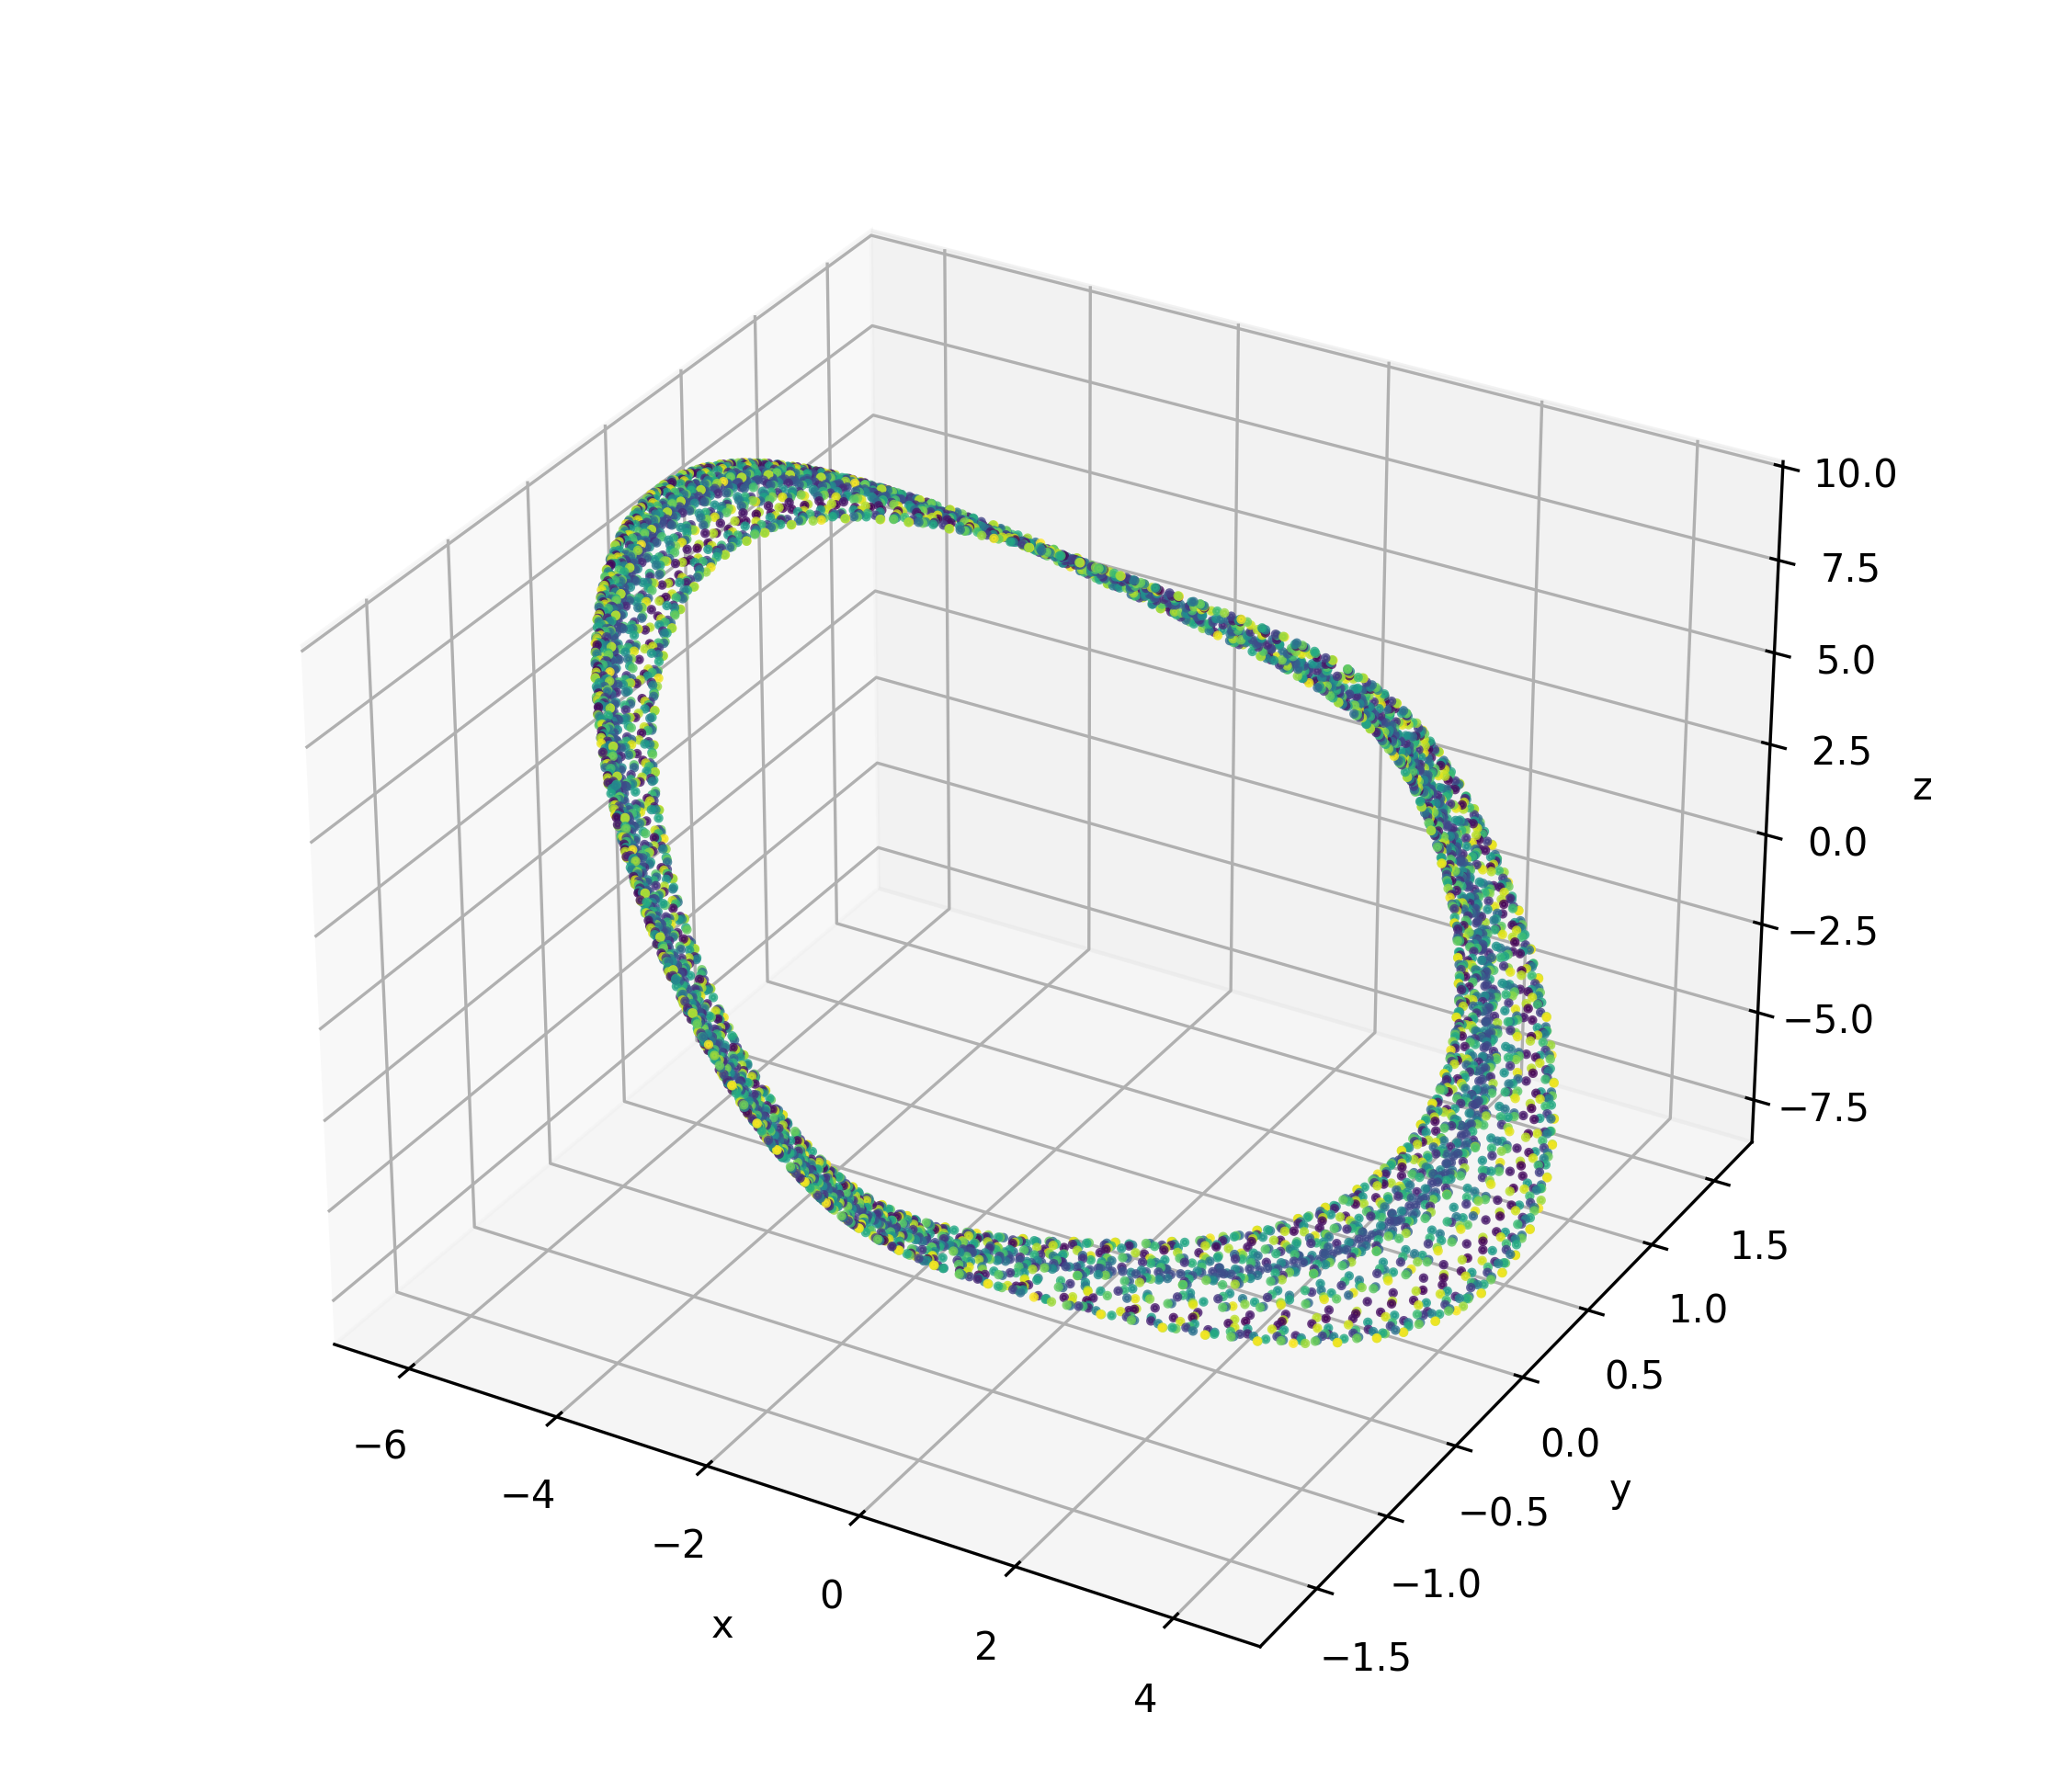
\includegraphics[width=\linewidth]{chua_python_attractor.png}
  \caption{\hafo{}: candidato obtenido por semilla y continuación.}
\end{subfigure}\hfill
\begin{subfigure}[t]{0.49\textwidth}
  \centering
  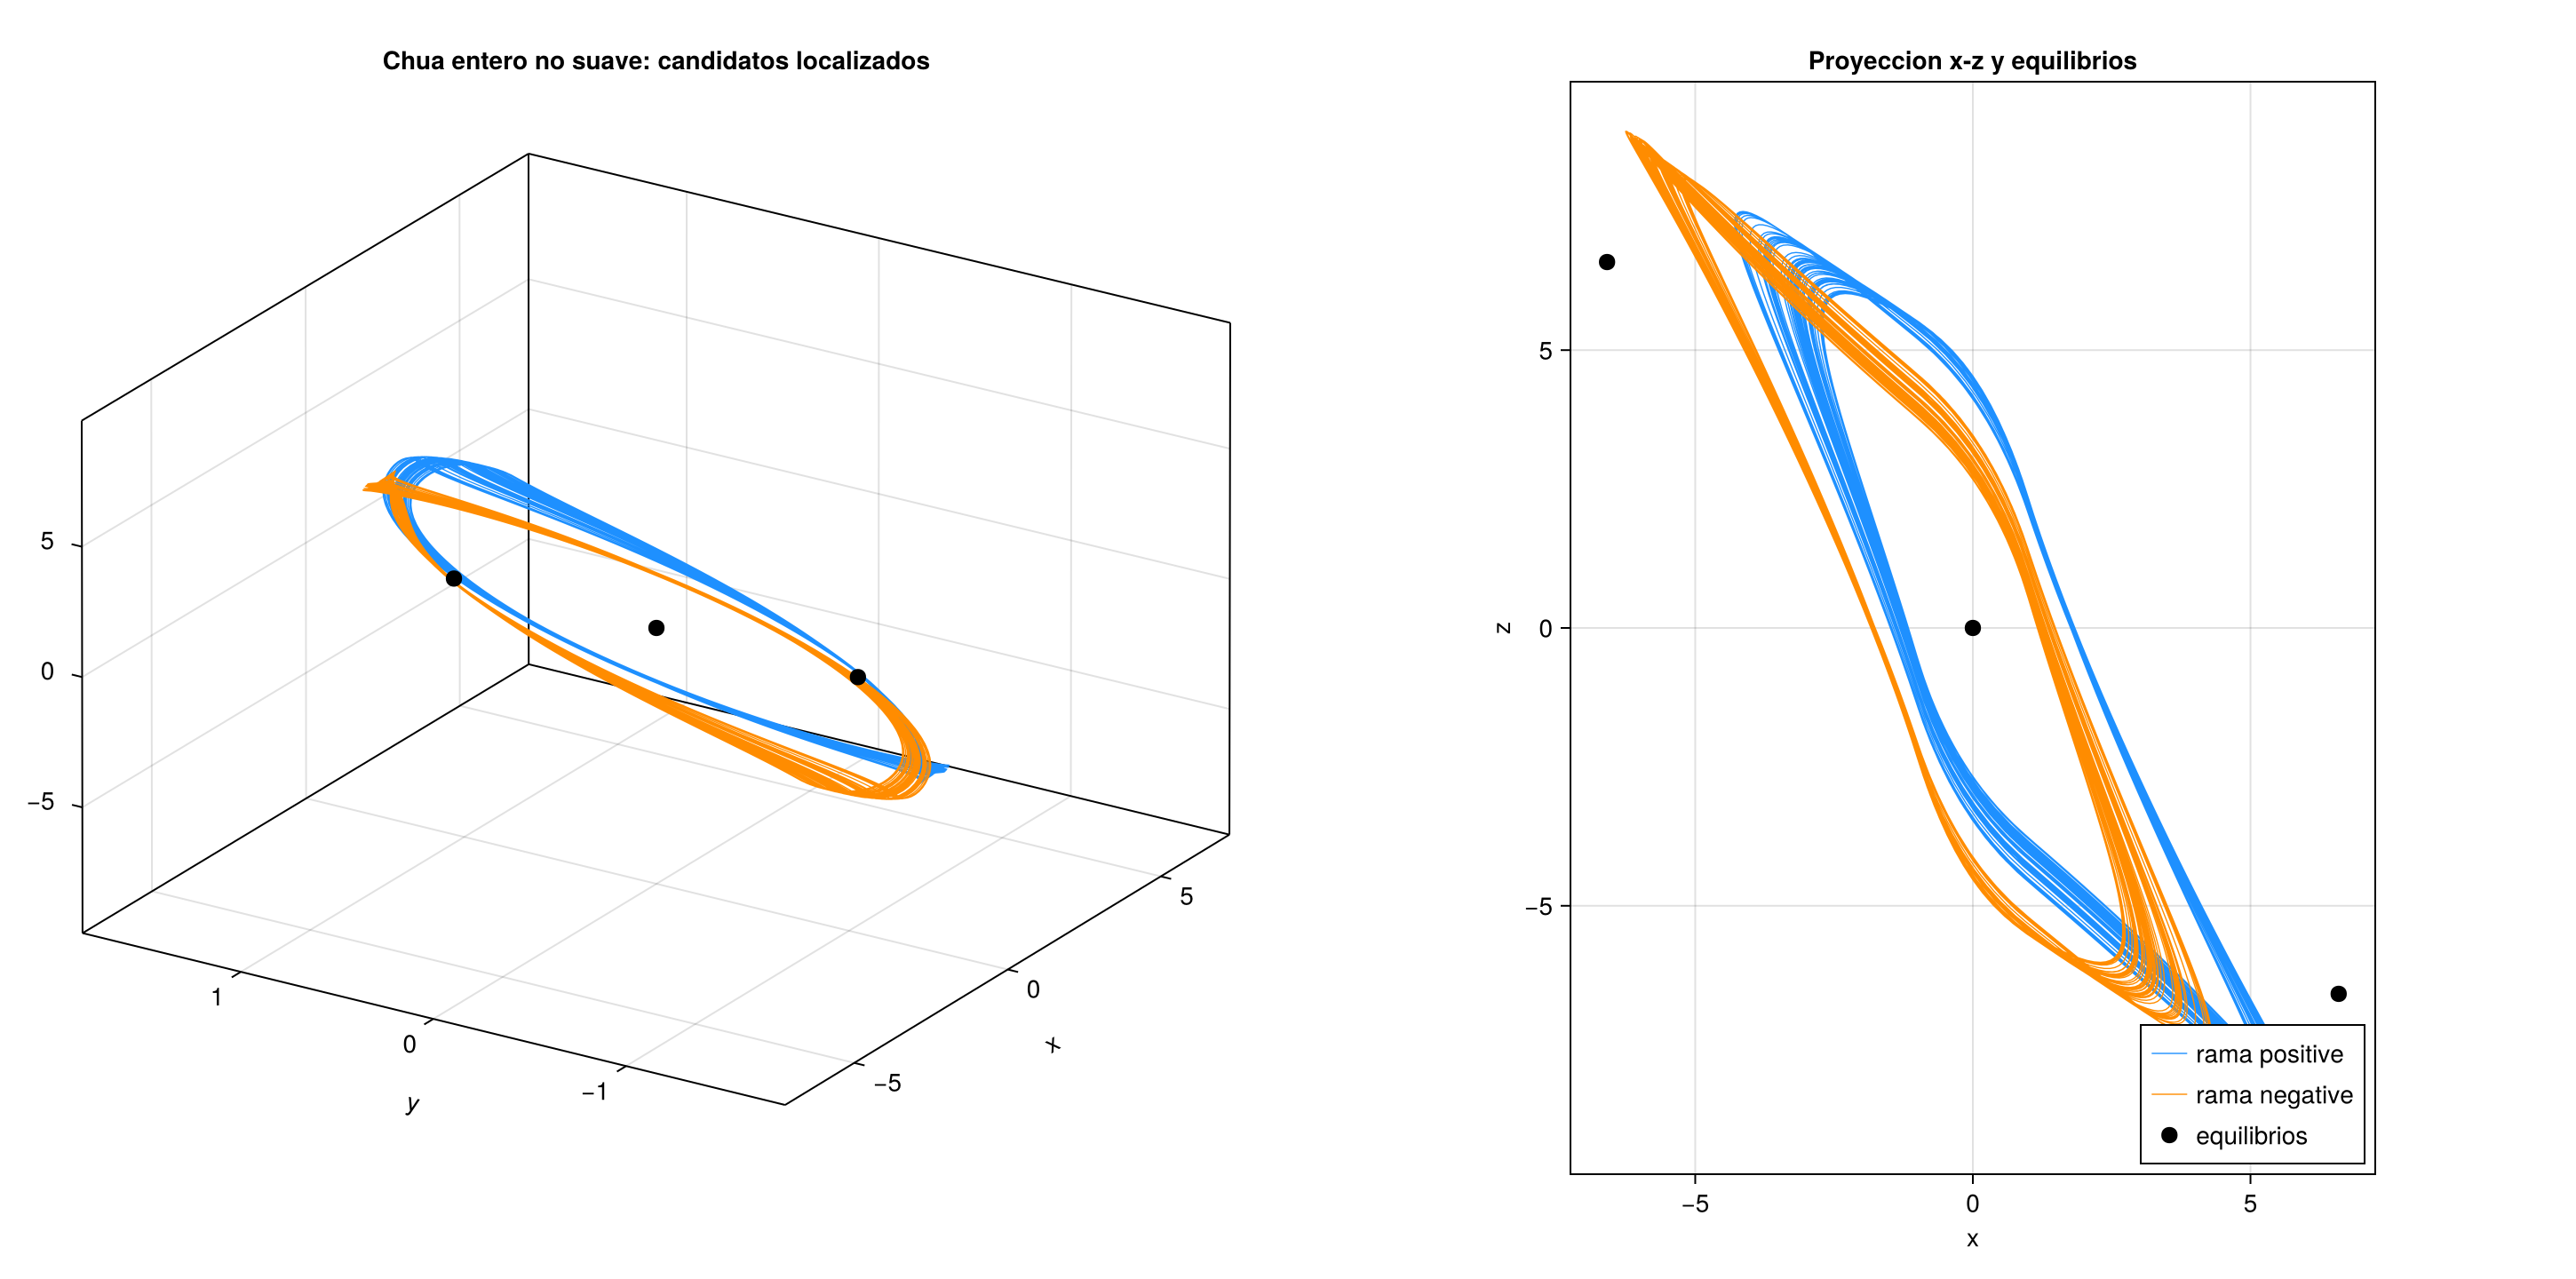
\includegraphics[width=\linewidth]{chua_julia_candidates.png}
  \caption{Julia: dos conjuntos descubiertos por recurrencias globales.}
\end{subfigure}
\caption{Localización independiente en el Chua no suave.}
\label{int:fig:chua-localization}
\end{hafocommonfigure}

\subsection{Comparación dinámica Python--Julia}

\ifHAFOBasinMaterial
\paragraph{Protocolo de comparación cruzada.}
Ambos cálculos evaluaron \ChuaProbeCount{} condiciones:
3 equilibrios, 7 radios entre \(10^{-5}\) y \(10^{-2}\), y 24 puntos por
equilibrio y radio. Se usaron \(t_f=500\), \(t_{\mathrm{burn}}=120\),
tolerancia de equilibrio \(10^{-3}\) y tolerancia normalizada de nube \(0.08\).
Las 504 coordenadas se generaron uniformemente en bolas, con semilla
pseudoaleatoria 123456789. El control EFORK--3 de referencia emplea
\(T=320\), \(T_{\mathrm{burn}}=80\), otras coordenadas y un clasificador
por huellas de sección.
\fi

\begin{table}[H]
\centering
\caption{Comparación Python--Julia del caso de Chua.}
\small
\begin{tabularx}{\textwidth}{@{}lYY@{}}
\toprule
Magnitud & Python/\hafo{} & Julia \\
\midrule
\ifHAFOBasinMaterial
Clases finales coincidentes & \multicolumn{2}{c}{504 de 504} \\
Conteos comunes & \multicolumn{2}{c}{152 en \(E_0\), 198 acotadas no triviales, 154 divergentes} \\
Contactos con candidato & 0 & 0 \\
\fi
Exponentes de Lyapunov finitos &
\((0.14018,\ 0.01319,\ -1.20304)\) &
\((0.14591,\ -0.00052,\ -1.17115)\) \\
\bottomrule
\end{tabularx}
\end{table}

\ifHAFOBasinMaterial
Los conteos \(152/198/154\) pertenecen exclusivamente a este protocolo
de comparación cruzada. Los conteos \(369/69/66\) de la configuración de referencia usan
otro horizonte, otras coordenadas y otro clasificador. Ambos protocolos dieron cero contactos con la nube objetivo.
\fi

Los dos espectros son compatibles con un exponente máximo positivo. Esa
observación apoya la clasificación caótica local, pero no sustituye la prueba
de ocultedad.

\begin{hafobasinfigure}[H]
\centering
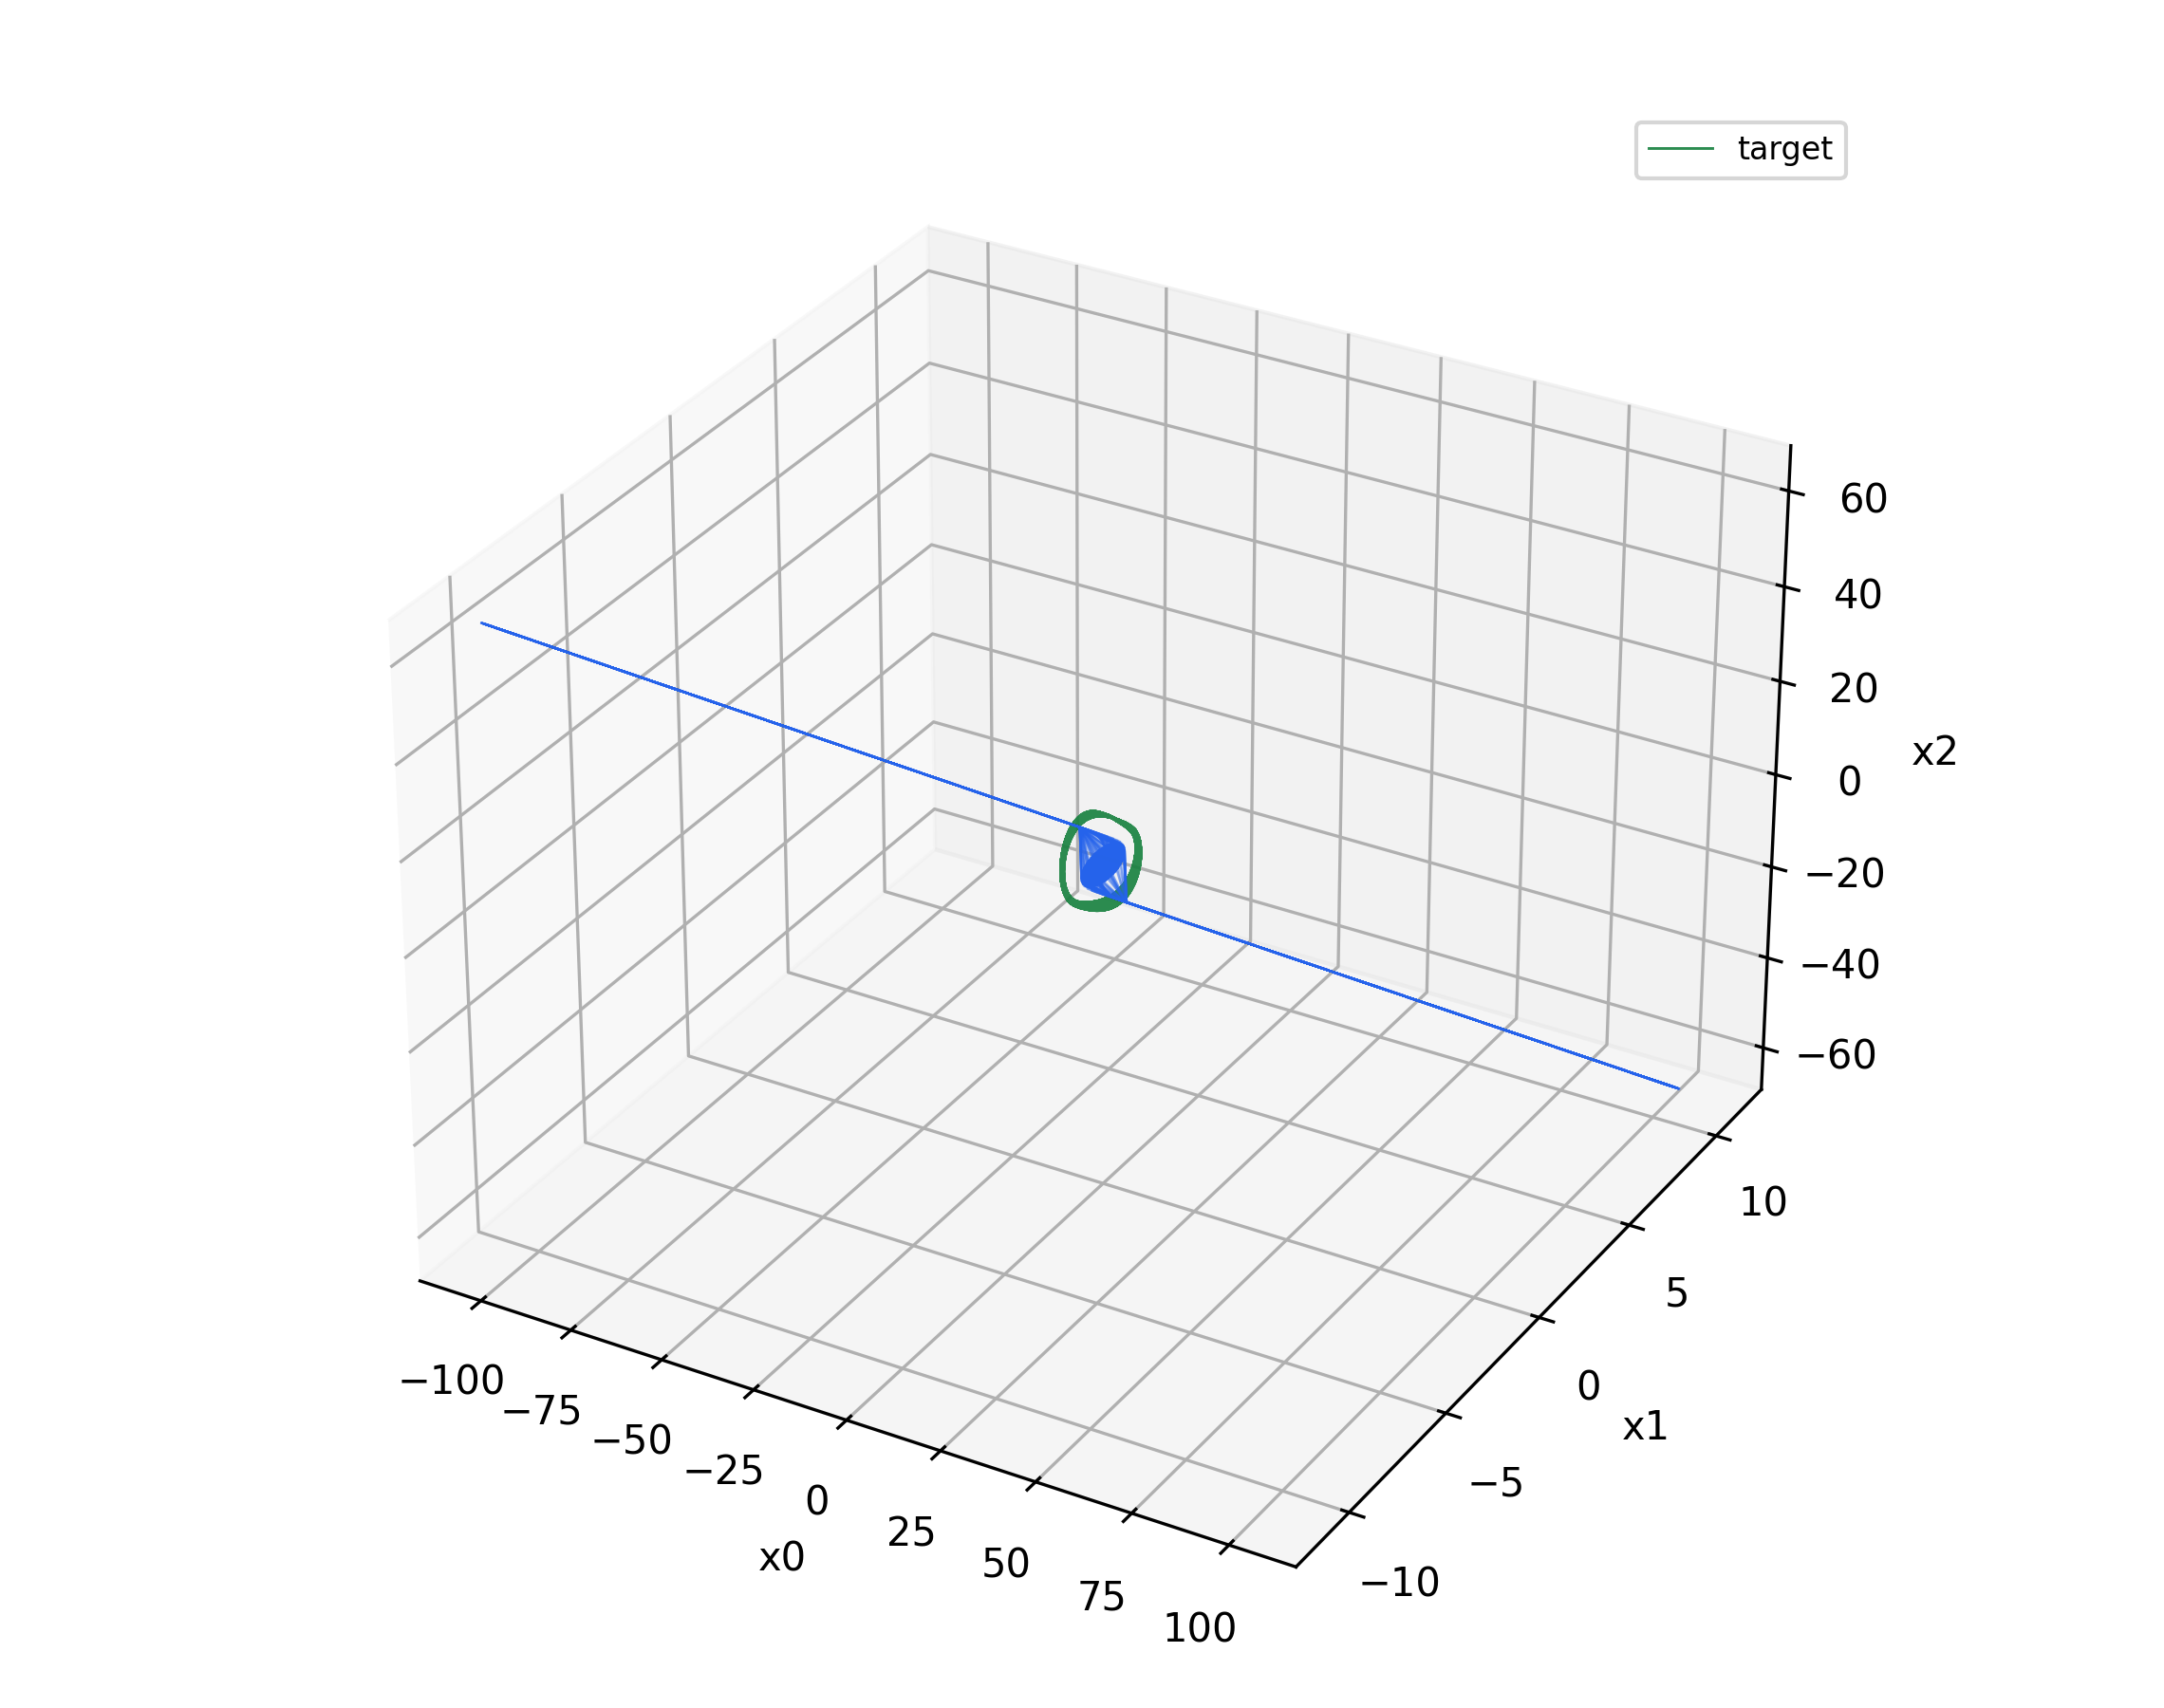
\includegraphics[width=0.82\textwidth]{chua_python_hiddenness.png}
\caption{Control de vecindades de los tres equilibrios en Python. El
comparador usó las mismas 504 coordenadas en Julia.}
\label{int:fig:chua-hiddenness}
\end{hafobasinfigure}

\section[Caso 2: Kalman--Fitts no Chua]
{Caso 2: Kalman--Fitts, sistema no Chua de cuarto orden}

\subsection{Formulación y rechazo de la ruta directa}

El sistema exacto es
\begin{equation}
 \dot X=AX+b\tanh\!\left(\frac{c^{\mathsf T}X}{\varepsilon}\right),
 \quad b=e_4,\quad c=-e_3,\quad \varepsilon=0.01,
 \label{int:eq:kf}
\end{equation}
La matriz compañera se define por
\[
 A=\begin{pmatrix}
 0&1&0&0\\0&0&1&0\\0&0&0&1\\-a_0&-a_1&-a_2&-a_3
 \end{pmatrix},
 \qquad
 p_A(s)=\bigl[(s+\beta)^2+m_1^2\bigr]
         \bigl[(s+\beta)^2+m_2^2\bigr].
\]
Al expandir el producto,
\begin{align*}
 a_0&=(m_1^2+\beta^2)(m_2^2+\beta^2),&
 a_1&=2\beta(m_1^2+m_2^2+2\beta^2),\\
 a_2&=m_1^2+m_2^2+6\beta^2,&a_3&=4\beta.
\end{align*}
Los parámetros publicados \(m_1=0.9\), \(m_2=1.1\), \(\beta=0.03\)
\cite{kalman2019} dan
\((a_0,a_1,a_2,a_3)=(0.98191881,0.121308,2.0254,0.12)\).
Las tres primeras ecuaciones de equilibrio imponen
\(x_2=x_3=x_4=0\); la cuarta queda \(-a_0x_1=0\), de modo que el único
equilibrio es el origen. Su Jacobiano es \(A+bc^{\mathsf T}/\varepsilon\)
y tiene polinomio
\[
 s^4+a_3s^3+(a_2+1/\varepsilon)s^2+a_1s+a_0.
\]
Todos los coeficientes son positivos. Las dos desigualdades adicionales de
Routh--Hurwitz para este polinomio mónico son
\[
 a_3(a_2+1/\varepsilon)-a_1=12.12174>0,
\]
\[
 a_3(a_2+1/\varepsilon)a_1-a_1^2-a_3^2a_0
 =1.456324405056>0.
\]
Por tanto, el equilibrio es localmente asintóticamente estable.

Para calcular la transferencia se resuelve \((sI-A)v=b\): las tres primeras
filas dan \(v_2=sv_1\), \(v_3=s^2v_1\), \(v_4=s^3v_1\), y la última da
\(p_A(s)v_1=1\). Como \(c=-e_3\),
\[
 c^{\mathsf T}(sI-A)^{-1}b=-\frac{s^2}{p_A(s)},\qquad
 G(s)=\frac{s^2}{p_A(s)}.
\]
En \(s=i\omega\), las partes real e imaginaria del denominador son
\(R=\omega^4-a_2\omega^2+a_0\) e
\(I=\omega(a_1-a_3\omega^2)\). De aquí
\[
 \operatorname{Im}G(i\omega)=\frac{\omega^2I}{R^2+I^2},\qquad
 \omega_0^2=\frac{a_1}{a_3},\qquad
 k=\frac{\omega_0^4-a_2\omega_0^2+a_0}{\omega_0^2}.
\]
La ruta directa, sin malla de frecuencias, encontró
\[
 \omega_0=1.005435229142,\qquad k=-0.043168701157.
\]
Para la no linealidad hiperbólica,
\[
 \mathcal N(a)=\frac1{\pi\varepsilon}\int_0^{2\pi}
  \frac{\tanh u}{u}\cos^2\theta\,\dd\theta,
 \qquad u=\frac{a\cos\theta}{\varepsilon},
\]
con valor continuo \(\tanh u/u=1\) en \(u=0\). Para \(u\ne0\),
\(0<\tanh u/u<1\), de modo que \(0<\mathcal N(a)<1/\varepsilon\).
Además, \(\mathcal N(a)\to1/\varepsilon\) cuando \(a\to0^+\), mientras
\(\mathcal N(a)\leq4/(\pi a)\to0\) cuando \(a\to\infty\). La continuidad
y estas cotas dan el rango \((0,100)\).
Por tanto, la ganancia negativa se rechaza matemáticamente y no
existe amplitud directa compatible. Python y Julia coincidieron en
\(\omega_0\) a \(1.02\times10^{-14}\) y en \(k\) a
\(1.09\times10^{-15}\).

\subsection{Mapa de conmutación y continuación A1}

En cada semiespacio \(\operatorname{sign}(c^{\mathsf T}X)=\sigma\),
\(\sigma\in\{-1,1\}\), el precursor satisface \(\dot X=AX+b\sigma\).
La variación de constantes y la invertibilidad de \(A\) dan
\begin{equation}
 \Phi_\sigma(t,X)=\e^{At}X+
                   A^{-1}(\e^{At}-I)b\sigma.
 \label{int:eq:kf-switching-flow}
\end{equation}
En efecto, \(\int_0^t\e^{A(t-s)}\,\dd s=A^{-1}(\e^{At}-I)\). En la
sección \(\Sigma=\{X:c^{\mathsf T}X=0\}\), el lado de salida se elige
según el signo de \(c^{\mathsf T}(AX+b\sigma)\). El tiempo \(t_+(X)>0\)
es el primer cero transversal de
\(c^{\mathsf T}\Phi_\sigma(t,X)\) después de abandonar la sección. Así se
define el mapa de conmutación
\(\Pi(X)=\Phi_\sigma(t_+(X),X)\). Una órbita de periodo dos cumple
\(\Pi^2(X)=X\), con \(\Pi(X)\ne X\); el periodo continuo suma los dos
tiempos de vuelo. La transversalidad excluye los contactos tangenciales en
los que el siguiente cruce no queda definido de este modo.

El mapa de sección de la no linealidad \(\operatorname{sign}(\sigma)\)
convergió en 135 iteraciones a una órbita de retorno de periodo 2 y generó
\[
 X_{\mathrm{sw}}=
 (0.212347571803,\ -1.671123727247,\ 0,\ 1.478087383043)^{\mathsf T}.
\]
Después se aplicaron 51 valores de \(\lambda\) en
\eqref{int:eq:sign-tanh}. Ninguna implementación leyó el punto publicado como
semilla. El punto de la Tabla 2 se comparó sólo después y quedó a distancia
\(4.34\times10^{-4}\) de la trayectoria Python y
\(4.30\times10^{-4}\) de la Julia.

\begin{hafocommonfigure}[H]
\centering
\begin{subfigure}[t]{0.49\textwidth}
  \centering
  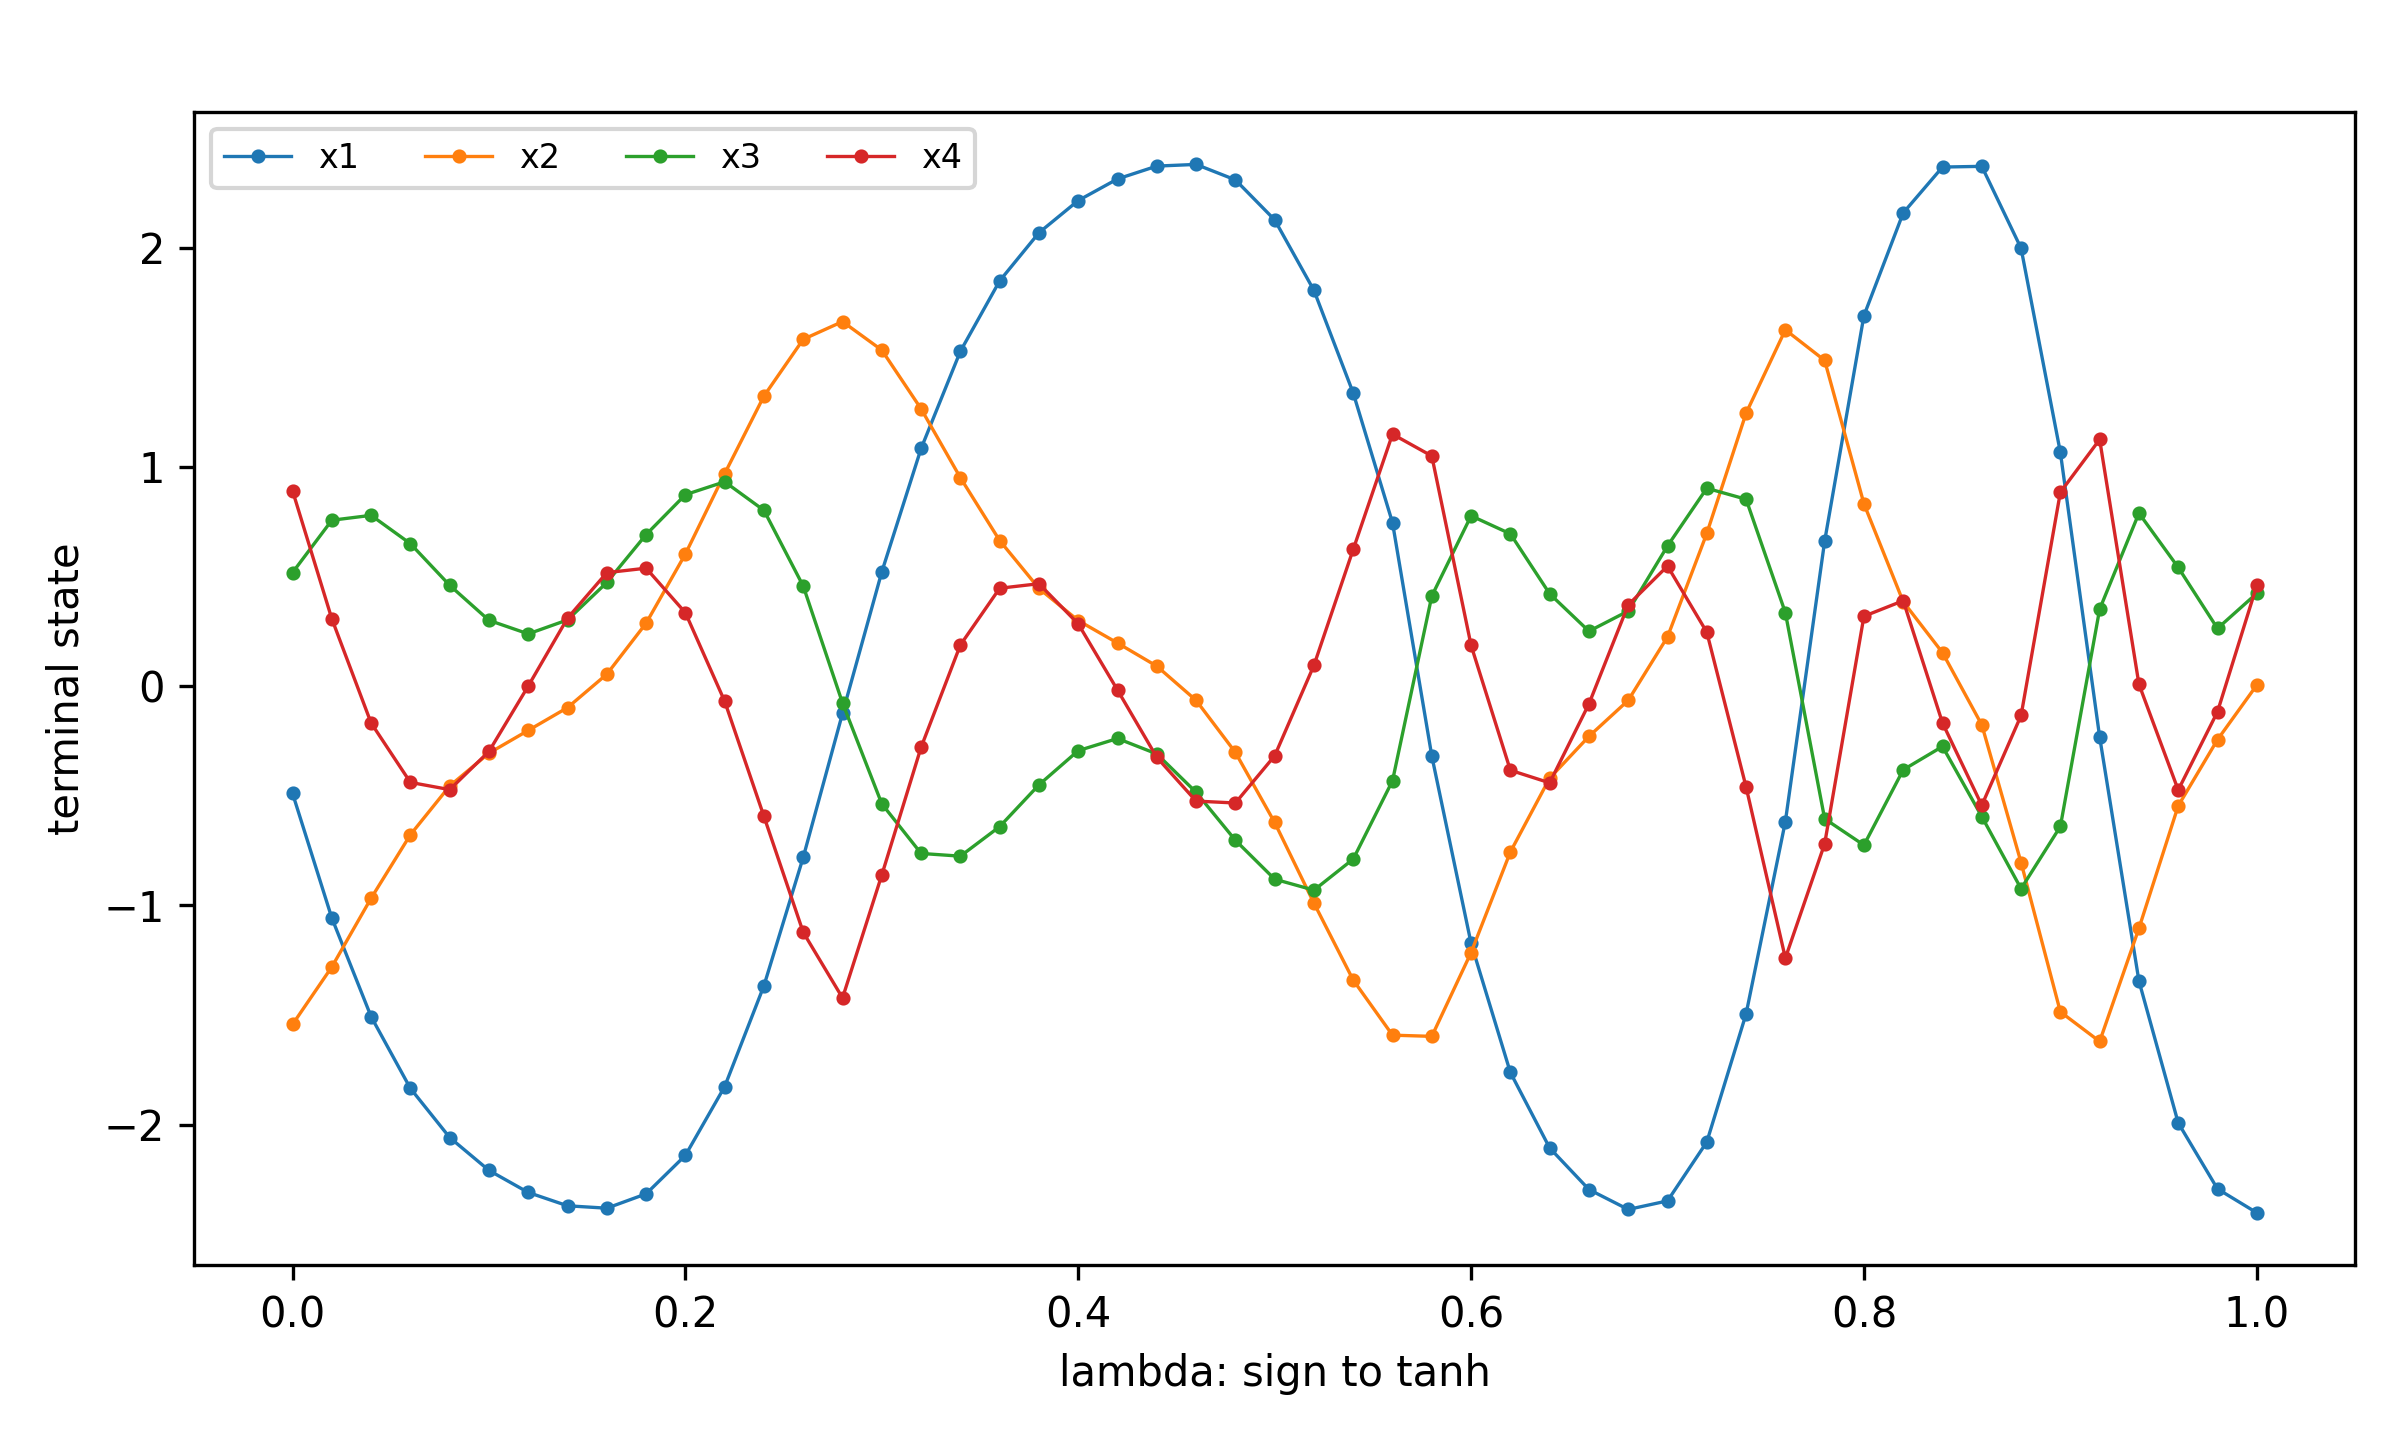
\includegraphics[width=\linewidth]{kalman_continuation.png}
  \caption{Homotopía \(\operatorname{sign}\to\tanh\) en Python.}
\end{subfigure}\hfill
\begin{subfigure}[t]{0.49\textwidth}
  \centering
  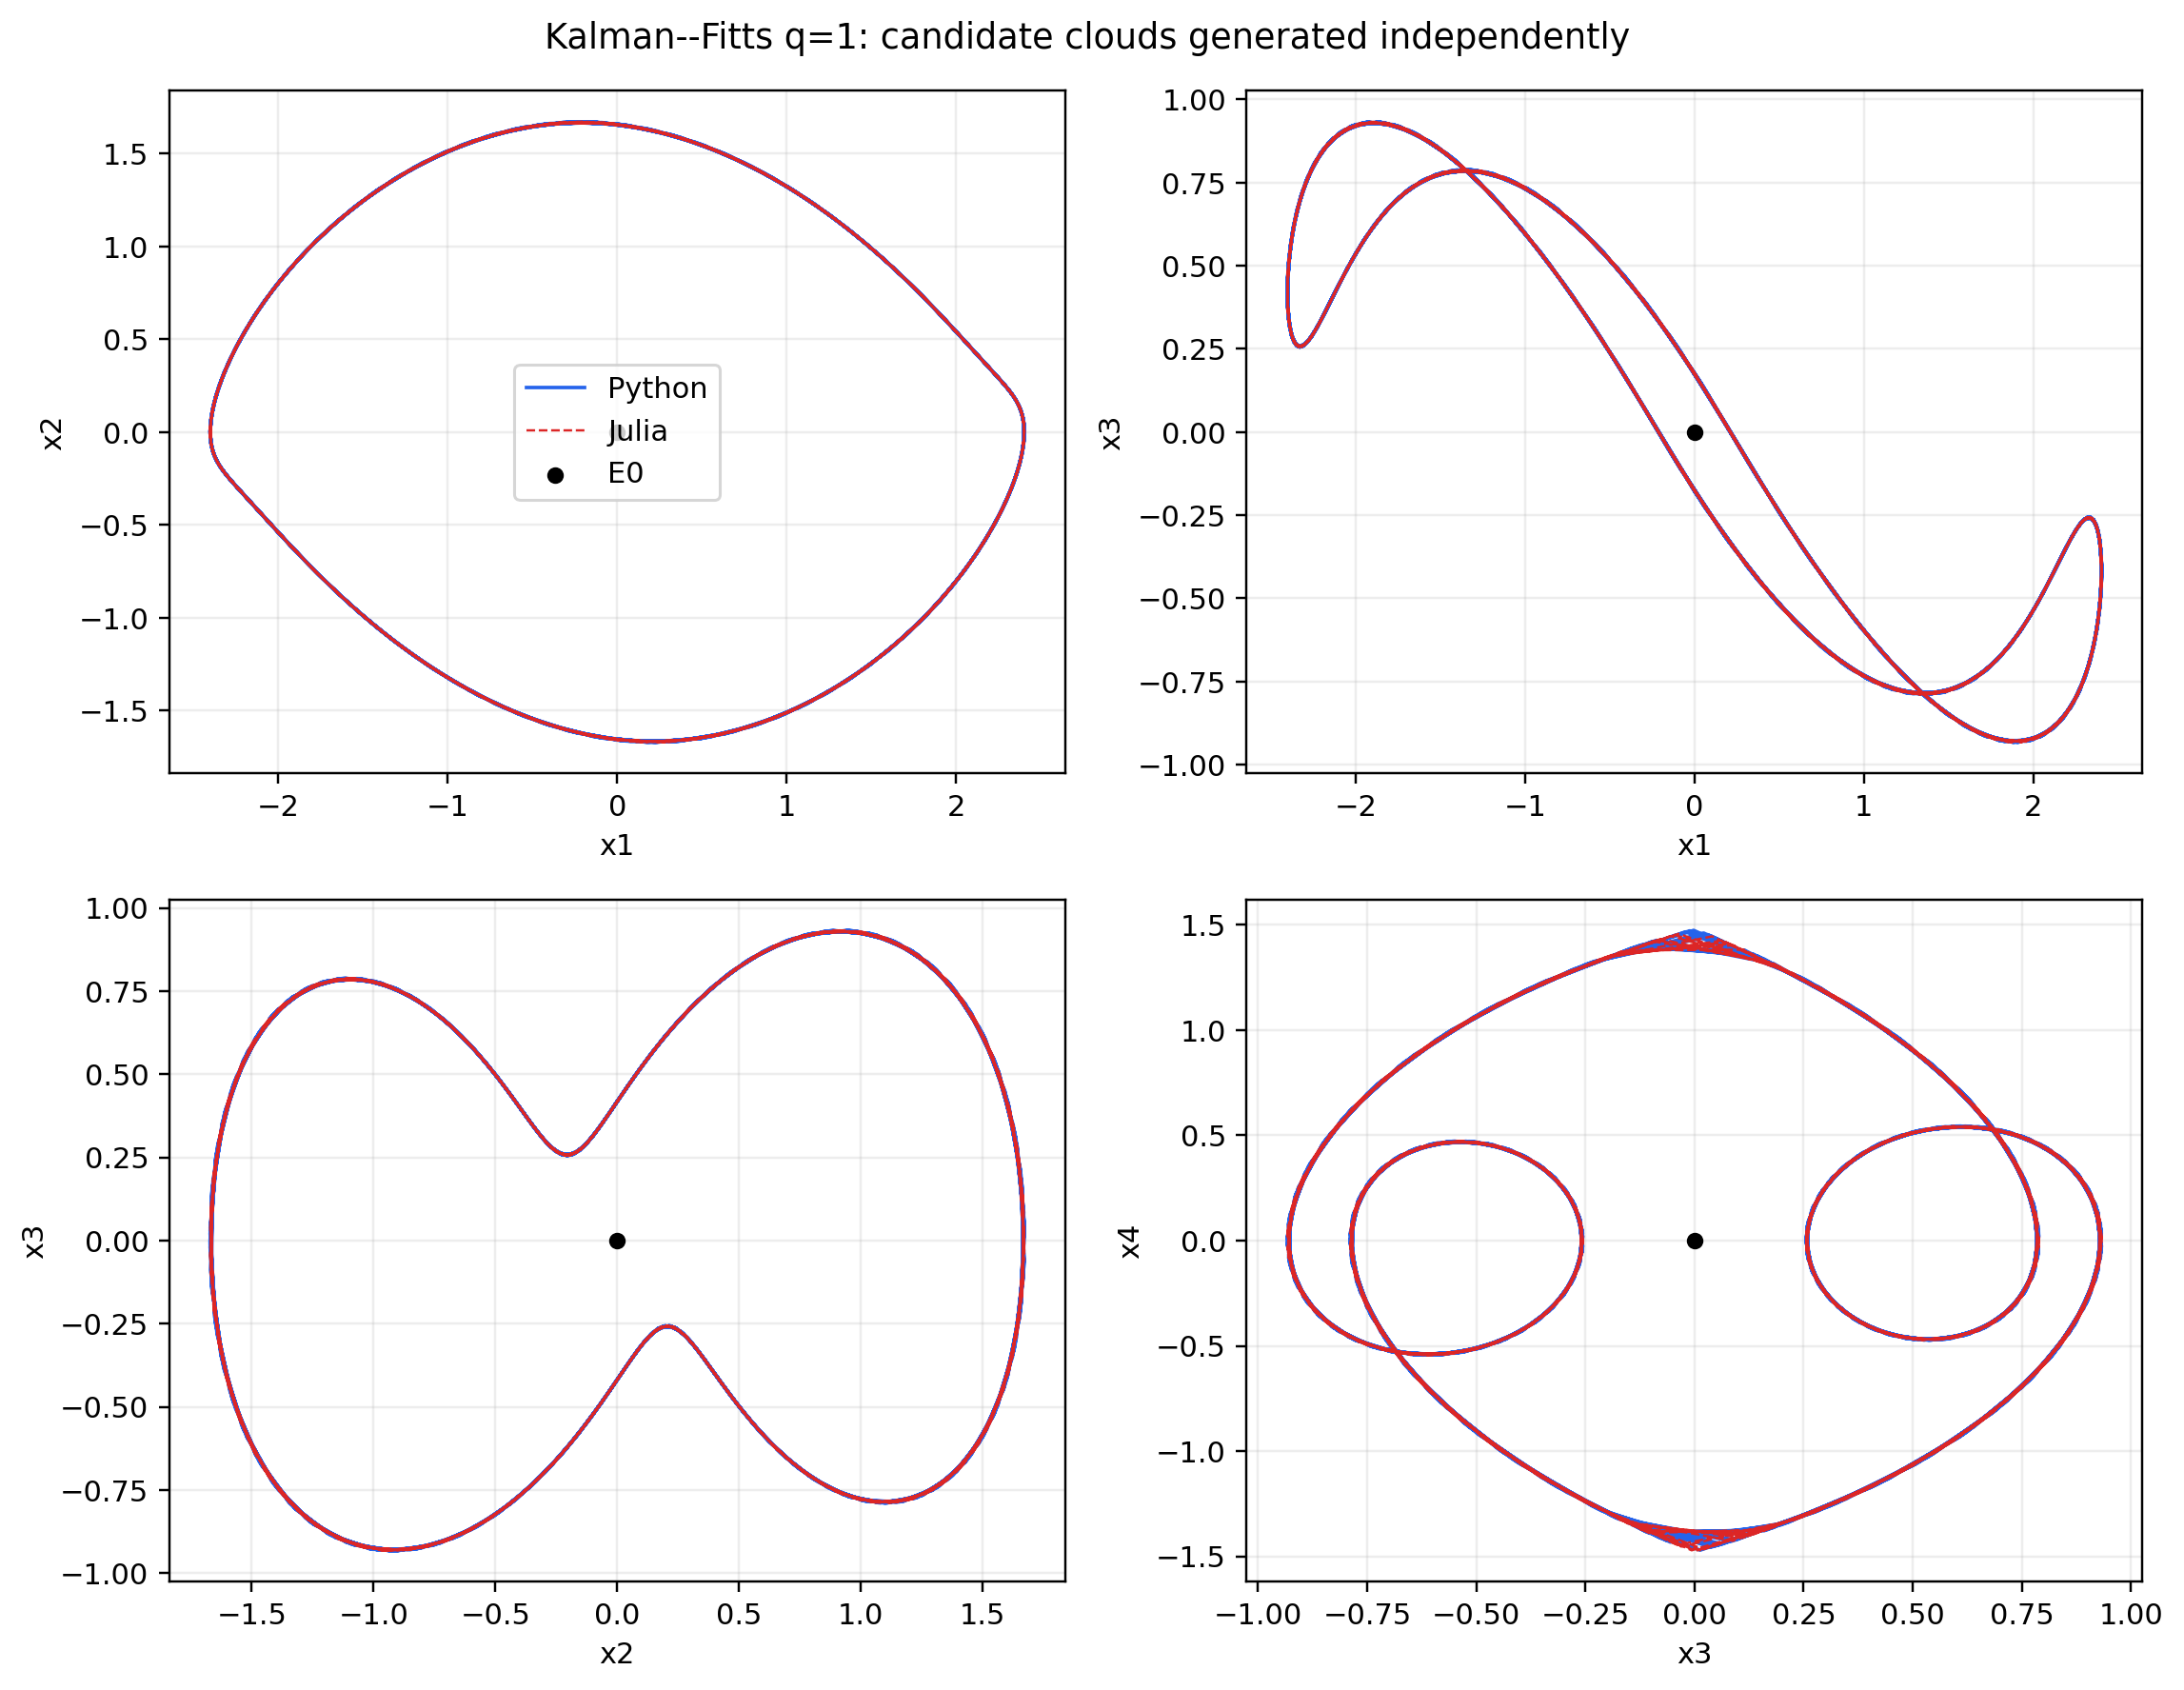
\includegraphics[width=\linewidth]{kalman_python_julia_overlay.png}
  \caption{Nubes finales generadas independientemente.}
\end{subfigure}
\caption{Ruta alternativa reproducida para Kalman--Fitts.}
\label{int:fig:kf}
\end{hafocommonfigure}

\subsection{Ciclo límite y comparación dinámica}

El candidato es un ciclo límite estable. El periodo medio fue
\(11.9169960\) en Python y \(11.9169380\) en Julia, con diferencia
\(5.81\times10^{-5}\). La distancia normalizada entre nubes fue
\(2.10\times10^{-3}\).

\ifHAFOBasinMaterial
El protocolo compartido contiene \KFProbeCount{} condiciones alrededor del
único equilibrio: 4 radios de \(10^{-5}\) a \(10^{-2}\) y 12 condiciones por
radio. Los dos códigos produjeron 40 convergencias al equilibrio, 8 estados
acotados no triviales y cero contactos con el ciclo. Las
\KFProbeCount{} clases finales y las \KFProbeCount{} decisiones de contacto
coincidieron punto por punto.
Por tanto, el ciclo es compatible con ocultedad bajo estas 48 condiciones
iniciales. El muestreo no prueba que la cuenca esté separada de toda vecindad
abierta del equilibrio.
\fi

\begin{table}[H]
\centering
\caption{Comparación cerrada de Kalman--Fitts.}
\small
\begin{tabularx}{\textwidth}{@{}lYY@{}}
\toprule
Magnitud & Python/\hafo{} & Julia \\
\midrule
Ruta directa & Rechazo por \(k<0\) & Rechazo por \(k<0\) \\
Mapa de conmutación & 135 iteraciones, retorno 2 & 135 iteraciones, retorno 2 \\
Periodo del ciclo & 11.9169960 & 11.9169380 \\
\ifHAFOBasinMaterial
Contactos en 48 sondeos & 0 & 0 \\
\fi
\bottomrule
\end{tabularx}
\end{table}


\section[Caso 3: Van der Pol--Duffing modificado]
{Caso 3: Van der Pol--Duffing autónomo modificado}

\subsection{Modelo y forma D0 exacta}

El sistema MAVPD de orden entero es
\begin{align}
 \dot y_1&=\delta\gamma y_1+\delta y_2-\delta y_1^3,\nonumber\\
 \dot y_2&=y_1-\xi y_2-y_3,\label{int:eq:mavpd}\\
 \dot y_3&=\rho y_2,\nonumber
\end{align}
con \(\gamma=0.1\), \(\delta=100\) y \(\rho=200\)
\cite{matouk2023}. Su declaración escalar es
\[
 P=\begin{pmatrix}
 \delta\gamma&\delta&0\\
 1&-\xi&-1\\
 0&\rho&0
 \end{pmatrix},\quad
 b=\begin{pmatrix}-\delta\\0\\0\end{pmatrix},\quad
 c=\begin{pmatrix}1\\0\\0\end{pmatrix},\quad
 \psi(\sigma)=\sigma^3,
\]
de modo que el Jacobiano y todos los equilibrios reales para \(\gamma>0\) son
\begin{equation}
 J(y)=\begin{pmatrix}
 \delta(\gamma-3y_1^2)&\delta&0\\
 1&-\xi&-1\\
 0&\rho&0
 \end{pmatrix},\qquad
 E_0=(0,0,0),\quad
 E_\pm=(\pm\sqrt{\gamma},0,\pm\sqrt{\gamma}).
 \label{int:eq:mavpd-jacobian}
\end{equation}
Para obtener los equilibrios, \(\dot y_3=0\) exige \(y_2=0\) porque
\(\rho>0\); \(\dot y_2=0\) da \(y_3=y_1\); la primera ecuación se reduce
a \(\delta y_1(\gamma-y_1^2)=0\). Esto produce exactamente los tres puntos
anteriores cuando \(\gamma>0\).

Sea \(u=(P-sI)^{-1}b\). Las últimas filas de este sistema lineal son
\[
 u_1-(\xi+s)u_2-u_3=0,\qquad \rho u_2-su_3=0.
\]
Al eliminar \(u_3\), resulta
\(u_2=su_1/(s^2+\xi s+\rho)\). La primera fila queda
\[
 \left[\delta\gamma-s+\frac{\delta s}{s^2+\xi s+\rho}\right]u_1=-\delta.
\]
Despejando \(u_1=G(s)\) y expandiendo
\((s-\delta\gamma)(s^2+\xi s+\rho)-\delta s\), se obtiene
\begin{equation}
 G(s)=\frac{\delta(s^2+\xi s+\rho)}
 {s^3+(\xi-\delta\gamma)s^2+
 (\rho-\delta-\delta\gamma\xi)s-\delta\gamma\rho}.
 \label{int:eq:mavpd-transfer}
\end{equation}
El caso Wolfram conserva además la convención resolvente
\[
 W(s)=c^{\mathsf T}(sI-P)^{-1}b=-G(s).
\]
Por tanto, su cálculo \(k=1/\operatorname{Re}W(i\omega)\) es exactamente el
mismo que \(k=-1/\operatorname{Re}G(i\omega)\) en
\eqref{int:eq:mavpd-direct-scalars}; el signo queda fijado por la derivación
algebraica.
La identidad \(\cos^3\theta=(3\cos\theta+\cos3\theta)/4\) separa las
componentes de \(\psi(a\cos\theta)=a^3\cos^3\theta\). El primer armónico
tiene amplitud \(3a^3/4\); dividir entre la amplitud de entrada \(a\) da
\begin{equation}
  \mathcal N(a)=\frac{3a^2}{4}.
\end{equation}

Al escribir \(z=\omega^2\), el numerador sin el factor \(\delta\) tiene
partes \(\rho-z\) y \(\xi\omega\), mientras el denominador tiene partes
\[
 C=-\delta\gamma\rho-(\xi-\delta\gamma)z,\qquad
 D=\omega(\rho-\delta-\delta\gamma\xi-z).
\]
Racionalizar el cociente produce
\[
 \operatorname{Im}G(i\omega)=
 \frac{\delta[\xi\omega C-(\rho-z)D]}{C^2+D^2}.
\]
Al expandir el numerador, los términos con \(\gamma\) se cancelan y queda
\[
 \xi\omega C-(\rho-z)D
 =-\omega[z^2+(\delta-2\rho+\xi^2)z+\rho(\rho-\delta)].
\]
Para \(\omega>0\) y \(C^2+D^2>0\), la condición imaginaria equivale a
\begin{equation}
 z^2+(\delta-2\rho+\xi^2)z+\rho(\rho-\delta)=0.
 \label{int:eq:mavpd-poly}
\end{equation}
Así se obtienen todas las ramas sin barrido de frecuencias. Para cada raíz
positiva \(z_j\), el procedimiento calcula
\begin{equation}
 \omega_j=\sqrt{z_j},\qquad
 k_j=-\frac{1}{\operatorname{Re}G(i\omega_j)},\qquad
 a_j=\sqrt{\frac{4k_j}{3}},
 \label{int:eq:mavpd-direct-scalars}
\end{equation}
siempre que \(k_j>0\), condición necesaria para una amplitud real positiva.
Para el modo normalizado \(v_{j,1}=1\), la primera fila de
\((P+k_jbc^{\mathsf T})v_j=i\omega_jv_j\) es
\[
 \delta(\gamma-k_j)+\delta v_{j,2}=i\omega_j,
\]
y la tercera es \(\rho v_{j,2}=i\omega_jv_{j,3}\). Despejar ambas da
\begin{equation}
 v_j=\begin{pmatrix}
 1\\
 k_j-\gamma+i\omega_j/\delta\\
 \rho/\delta-i\rho(k_j-\gamma)/\omega_j
 \end{pmatrix},\qquad
 y_{0,j}(\theta)=a_j\operatorname{Re}\!\left(v_je^{i\theta}\right).
 \label{int:eq:mavpd-direct-seed}
\end{equation}
Las igualdades de cierre de \eqref{int:eq:mavpd-direct-scalars}, la ecuación modal
\((P+k_jbc^{\mathsf T})v_j=i\omega_jv_j\) y el residuo del campo se guardan
como verificaciones, no como datos impuestos.

\subsection{\texorpdfstring{\(\xi=3.1\): ramas, semillas y continuación}{xi=3.1: ramas, semillas y continuación}}

Para \(\xi=3.1\), \eqref{int:eq:mavpd-poly} tiene coeficientes
\((1,-290.39,20000)\) y produce dos ramas compatibles:

\begin{table}[H]
\centering
\caption{Ramas directas MAVPD para \(\xi=3.1\).}
\small
\begin{tabular}{@{}ccccc@{}}
\toprule
Rama & \(\omega_0\) & \(k\) & \(a_0\) & Semilla con fase \(0\) \\
\midrule
0 & 10.5975230311 & 0.1397015948 & 0.4315886851 &
\((0.4315887,0.0171348,0.8631774)\) \\
1 & 13.3447557342 & 0.3518790503 & 0.6849613618 &
\((0.6849614,0.1725274,1.3699227)\) \\
\bottomrule
\end{tabular}
\end{table}

Se ejecutaron ambas ramas con fases \(0\) y \(\pi\), y 21 valores
\(\lambda=0,0.05,\ldots,1\). La rama 0 conduce a dos ciclos internos
simétricos; la rama 1 conduce al conjunto externo. La selección se hizo por
mayor extensión de estado, sin leer la Tabla 1 de la fuente.

\begin{hafocommonfigure}[H]
\centering
\begin{subfigure}[t]{0.49\textwidth}
  \centering
  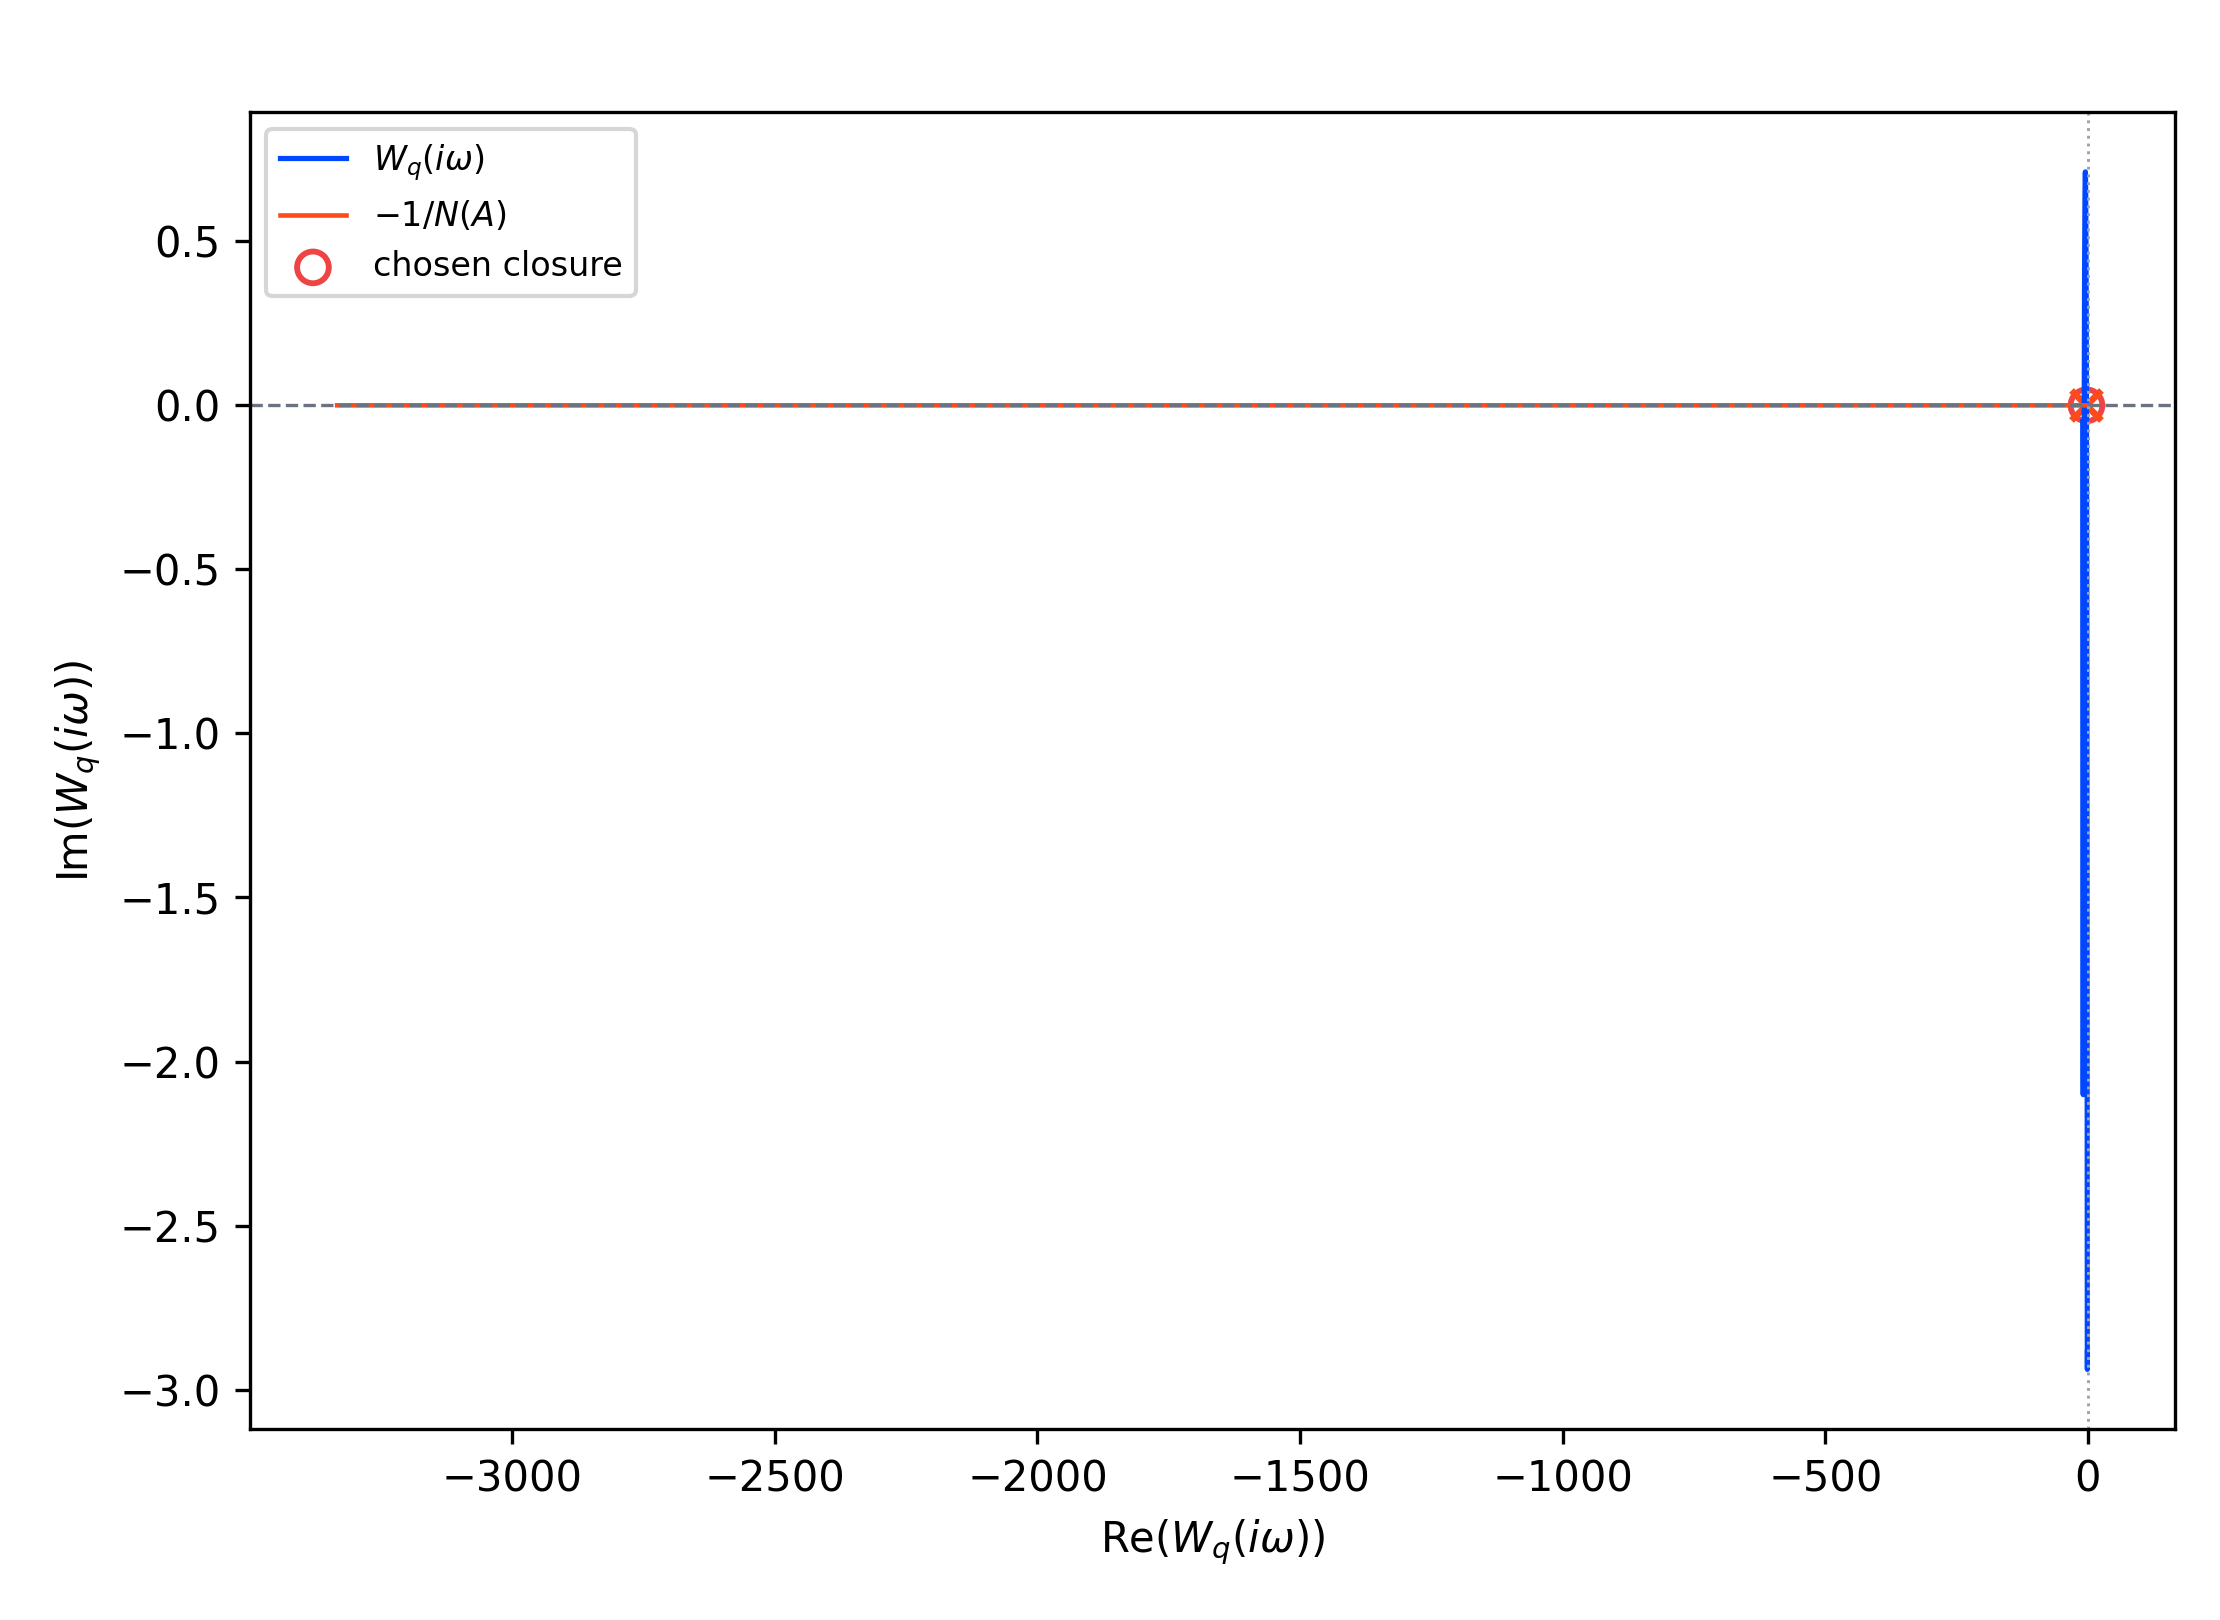
\includegraphics[width=\linewidth]{mavpd_nyquist_df.png}
  \caption{Ramas de Nyquist y función descriptiva derivadas.}
\end{subfigure}\hfill
\begin{subfigure}[t]{0.49\textwidth}
  \centering
  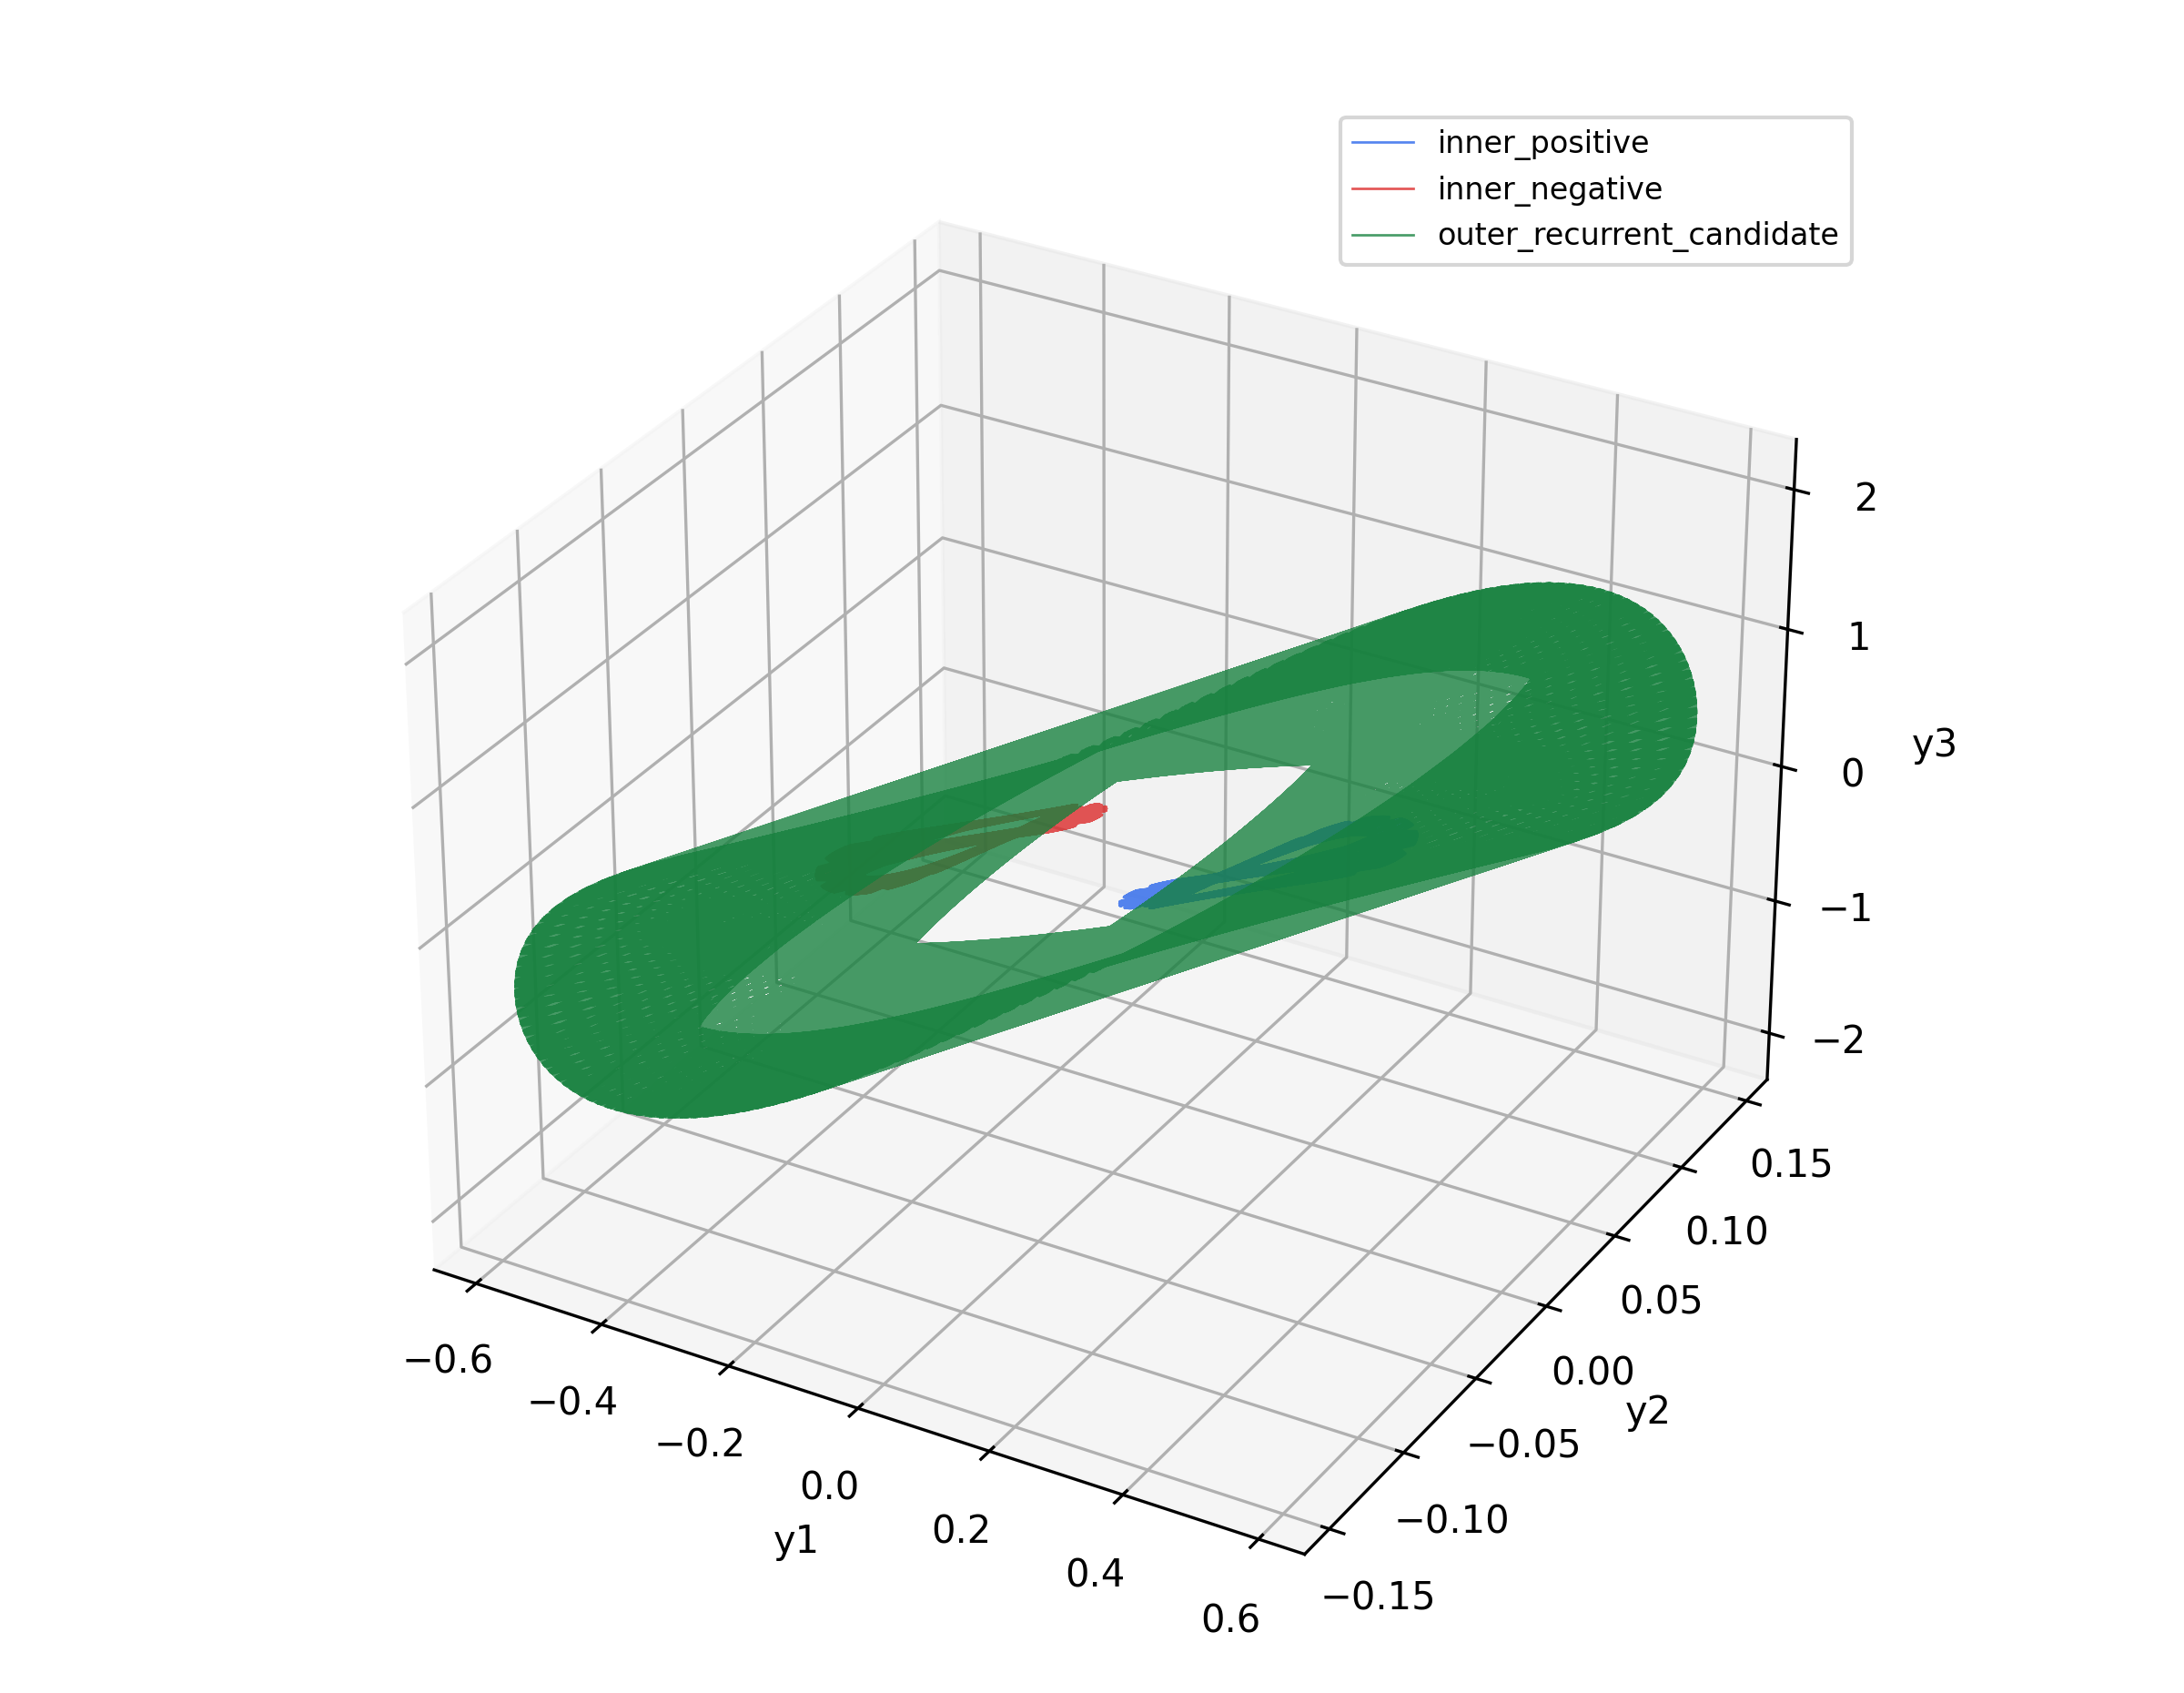
\includegraphics[width=\linewidth]{mavpd_python_clusters.png}
  \caption{Dos ciclos internos y candidato externo en Python.}
\end{subfigure}
\caption{Ruta directa MAVPD con \(\xi=3.1\).}
\label{int:fig:mavpd-route}
\end{hafocommonfigure}

\subsection{Comparación cruzada del caso periódico}

\ifHAFOBasinMaterial
El conjunto común contiene \MAVPDProbeCount{} condiciones: 3 equilibrios, 3 radios
\((10^{-5},10^{-3},10^{-2})\) y 12 direcciones explícitas por equilibrio y
radio. Se usaron \(h=0.005\), transitorio 180 y cola 80.
\fi

El comparador posterior confirmó:

\begin{itemize}
  \item diferencia máxima de frecuencias \(2.31\times10^{-14}\), de
        ganancias \(3.50\times10^{-15}\), de amplitudes
        \(3.44\times10^{-15}\) y de semillas \(7.45\times10^{-15}\);
\ifHAFOBasinMaterial
  \item \MAVPDFullAssignmentMatches{} de \MAVPDProbeCount{} asignaciones de
        clúster, clases finales y decisiones sobre el candidato externo
        coincidentes;
  \item 54 trayectorias hacia el ciclo interno positivo, 54 hacia el negativo
        y cero hacia el externo en cada implementación;
\fi
  \item distancia normalizada entre nubes externas
        \(\MAVPDFullCloudDistance\);
  \item periodos \(\MAVPDPythonPeriod\) en Python y
        \(\MAVPDJuliaFullPeriod\) en Julia;
  \item ninguna ruta alternativa para \(\xi=3.1\).
\end{itemize}

\begin{hafocommonfigure}[H]
\centering
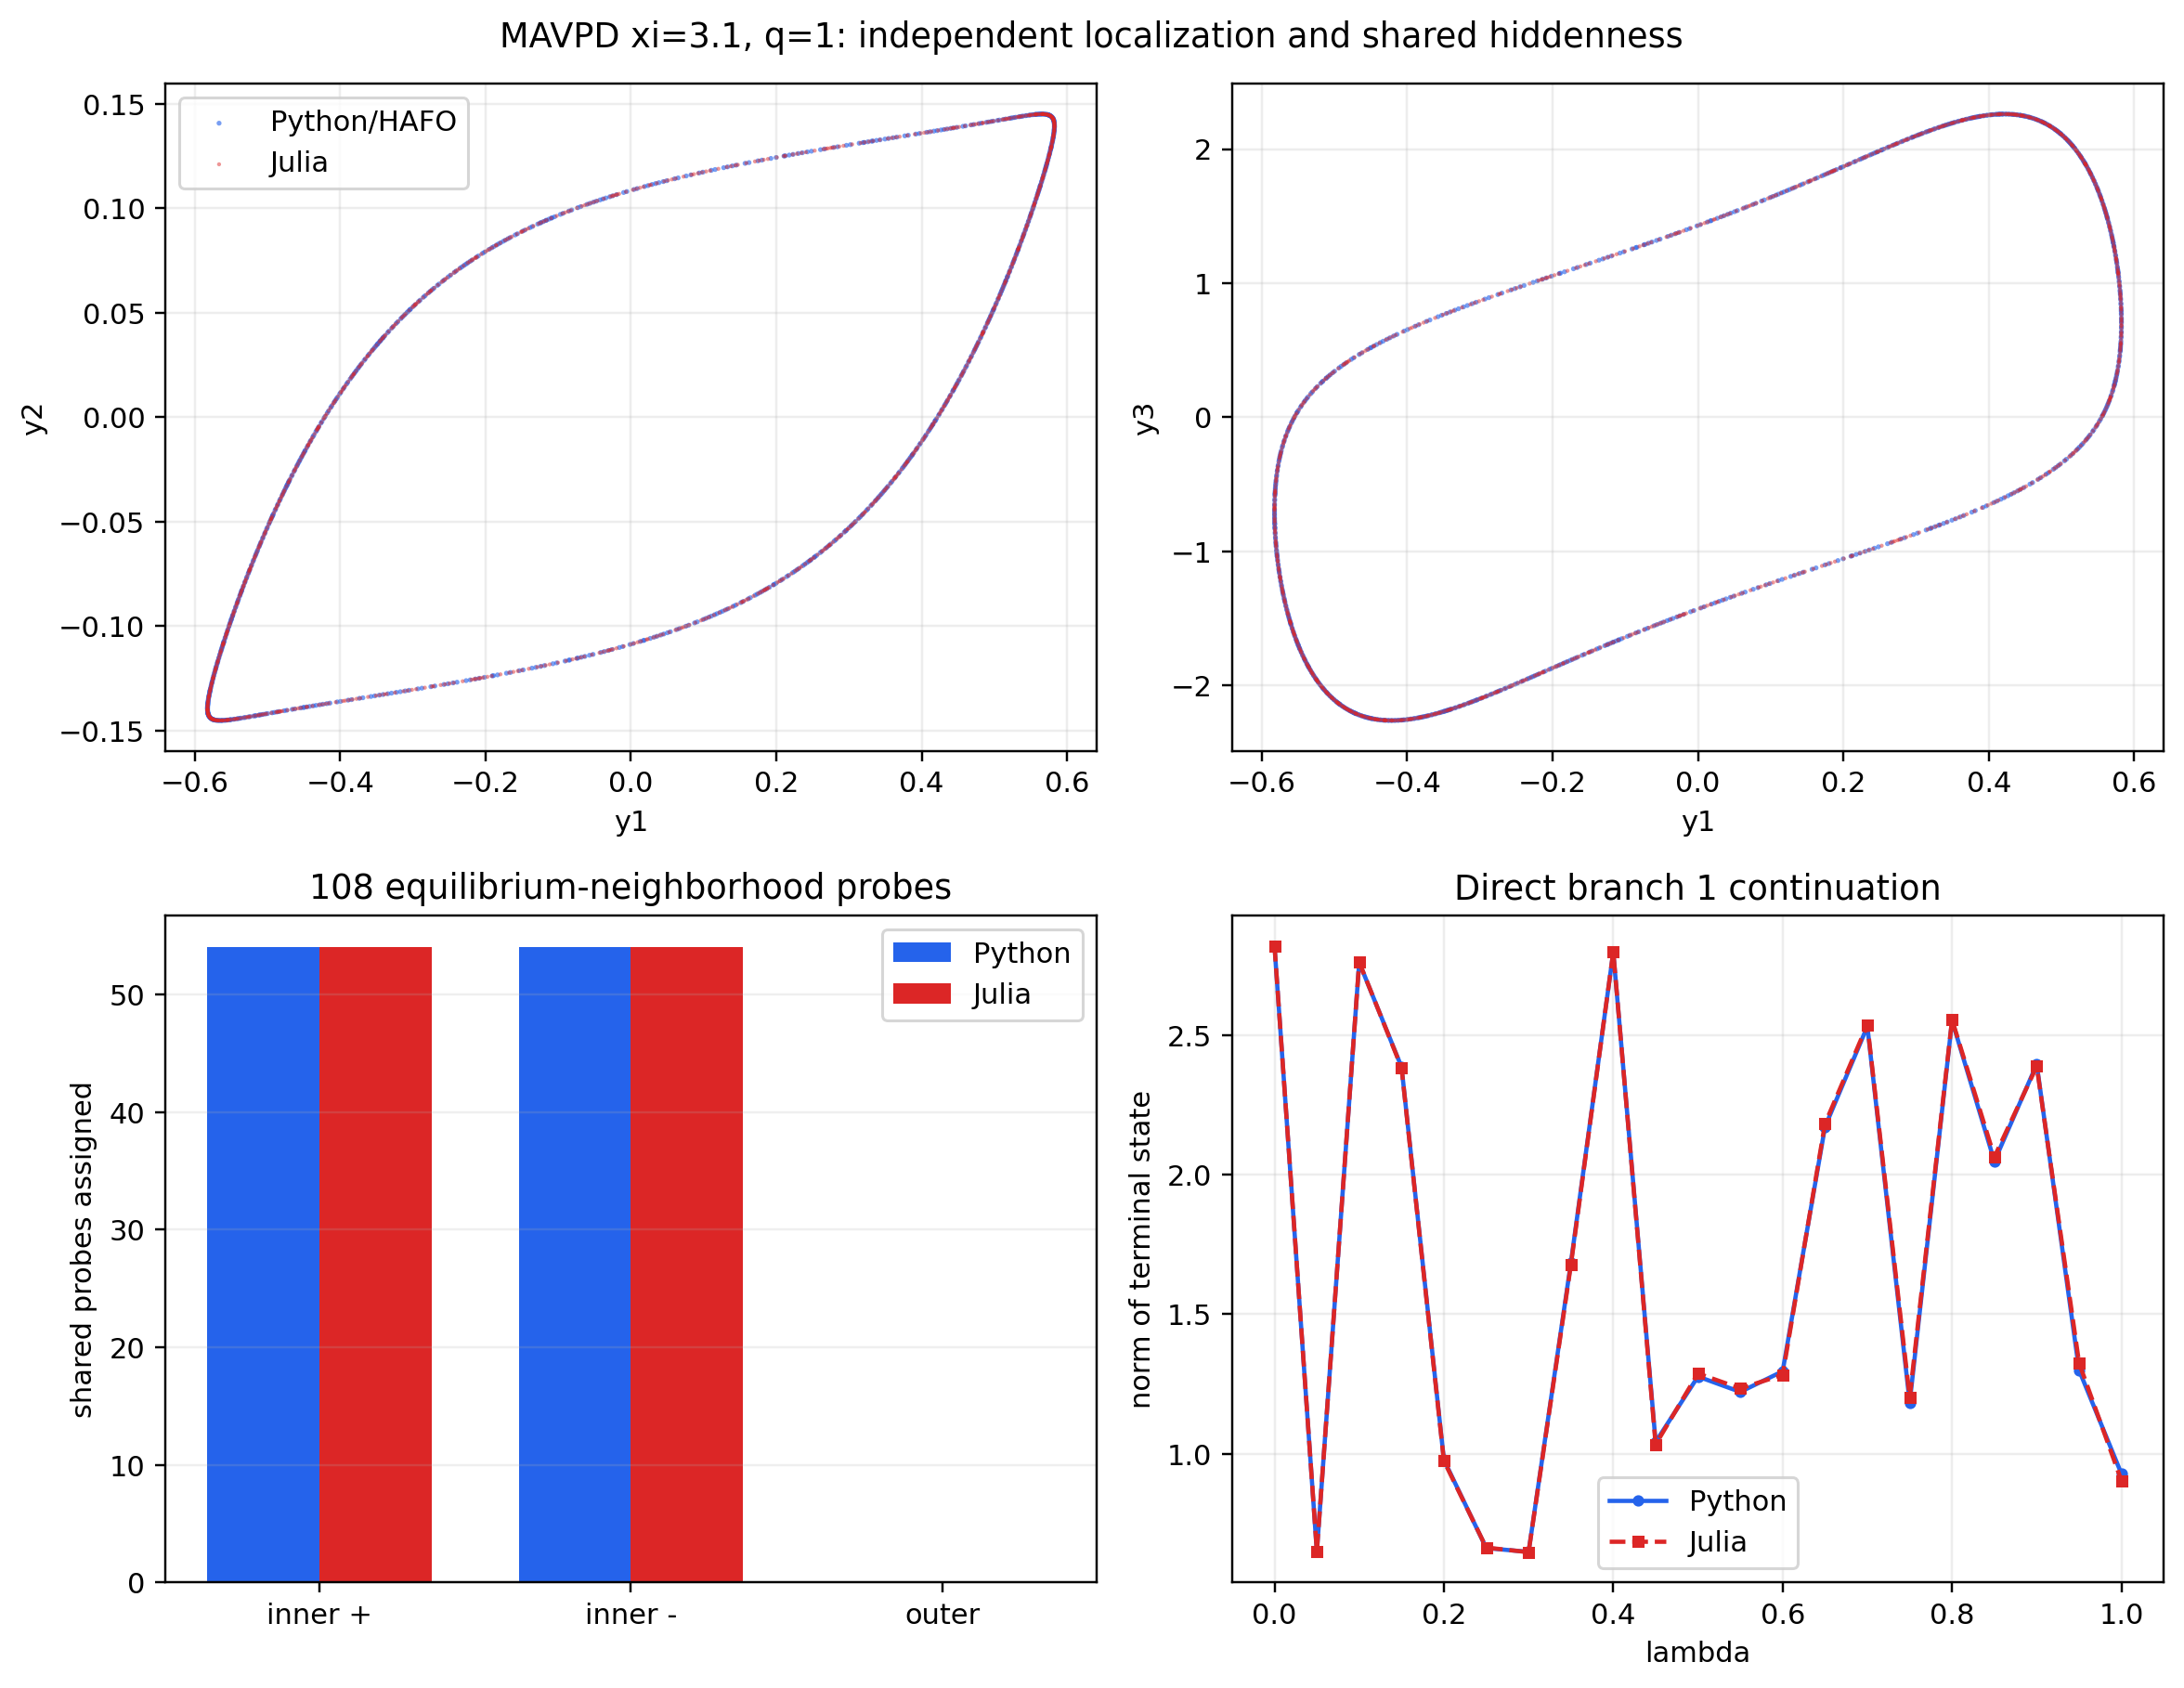
\includegraphics[width=0.94\textwidth]{mavpd_python_julia_overlay_full.png}
\caption{Comparación posterior MAVPD \emph{full}. Las localizaciones se
ejecutaron independientemente.
\ifHAFOBasinMaterial
Las 108 coordenadas se compartieron sólo para el control de ocultedad.
\fi}
\label{int:fig:mavpd-overlay}
\end{hafocommonfigure}

\subsection{Clasificación dinámica y discrepancia con la fuente}

La sección de Poincaré Python se refinó con DOP853 y eventos densos:
405 cruces, rango de los últimos puntos del orden de \(10^{-13}\), periodo
\(0.493177986749\) y desviación estándar \(1.25\times10^{-14}\).
El espectro variacional independiente en el cálculo declarado fue
\[
 (-0.0017614,\ -0.3887396,\ -51.1886634),
\]
y la prueba 0--1 dio mediana \(K=0.000440085726\) sobre 64 valores de \(c\).
En conjunto con la sección de Poincaré, estos diagnósticos apoyan un ciclo
estable de periodo uno bajo el protocolo numérico; la prueba 0--1 aislada no
constituye una demostración analítica de periodicidad. El cálculo independiente
en Julia obtuvo \((-0.0042733,-0.3910810,-51.1961919)\), consistente con la
misma clase.

La fuente denomina al conjunto \emph{atractor oculto cuasiperiódico}. Esa
etiqueta no se reproduce para las ecuaciones declaradas: la conclusión local
obtenida es \emph{candidato periódico estable}. La diferencia documenta una
discrepancia reproducible entre la etiqueta de la fuente
y la dinámica obtenida con integración y sección de mayor precisión.

\begin{hafobasinfigure}[H]
\centering
\begin{subfigure}[t]{0.49\textwidth}
  \centering
  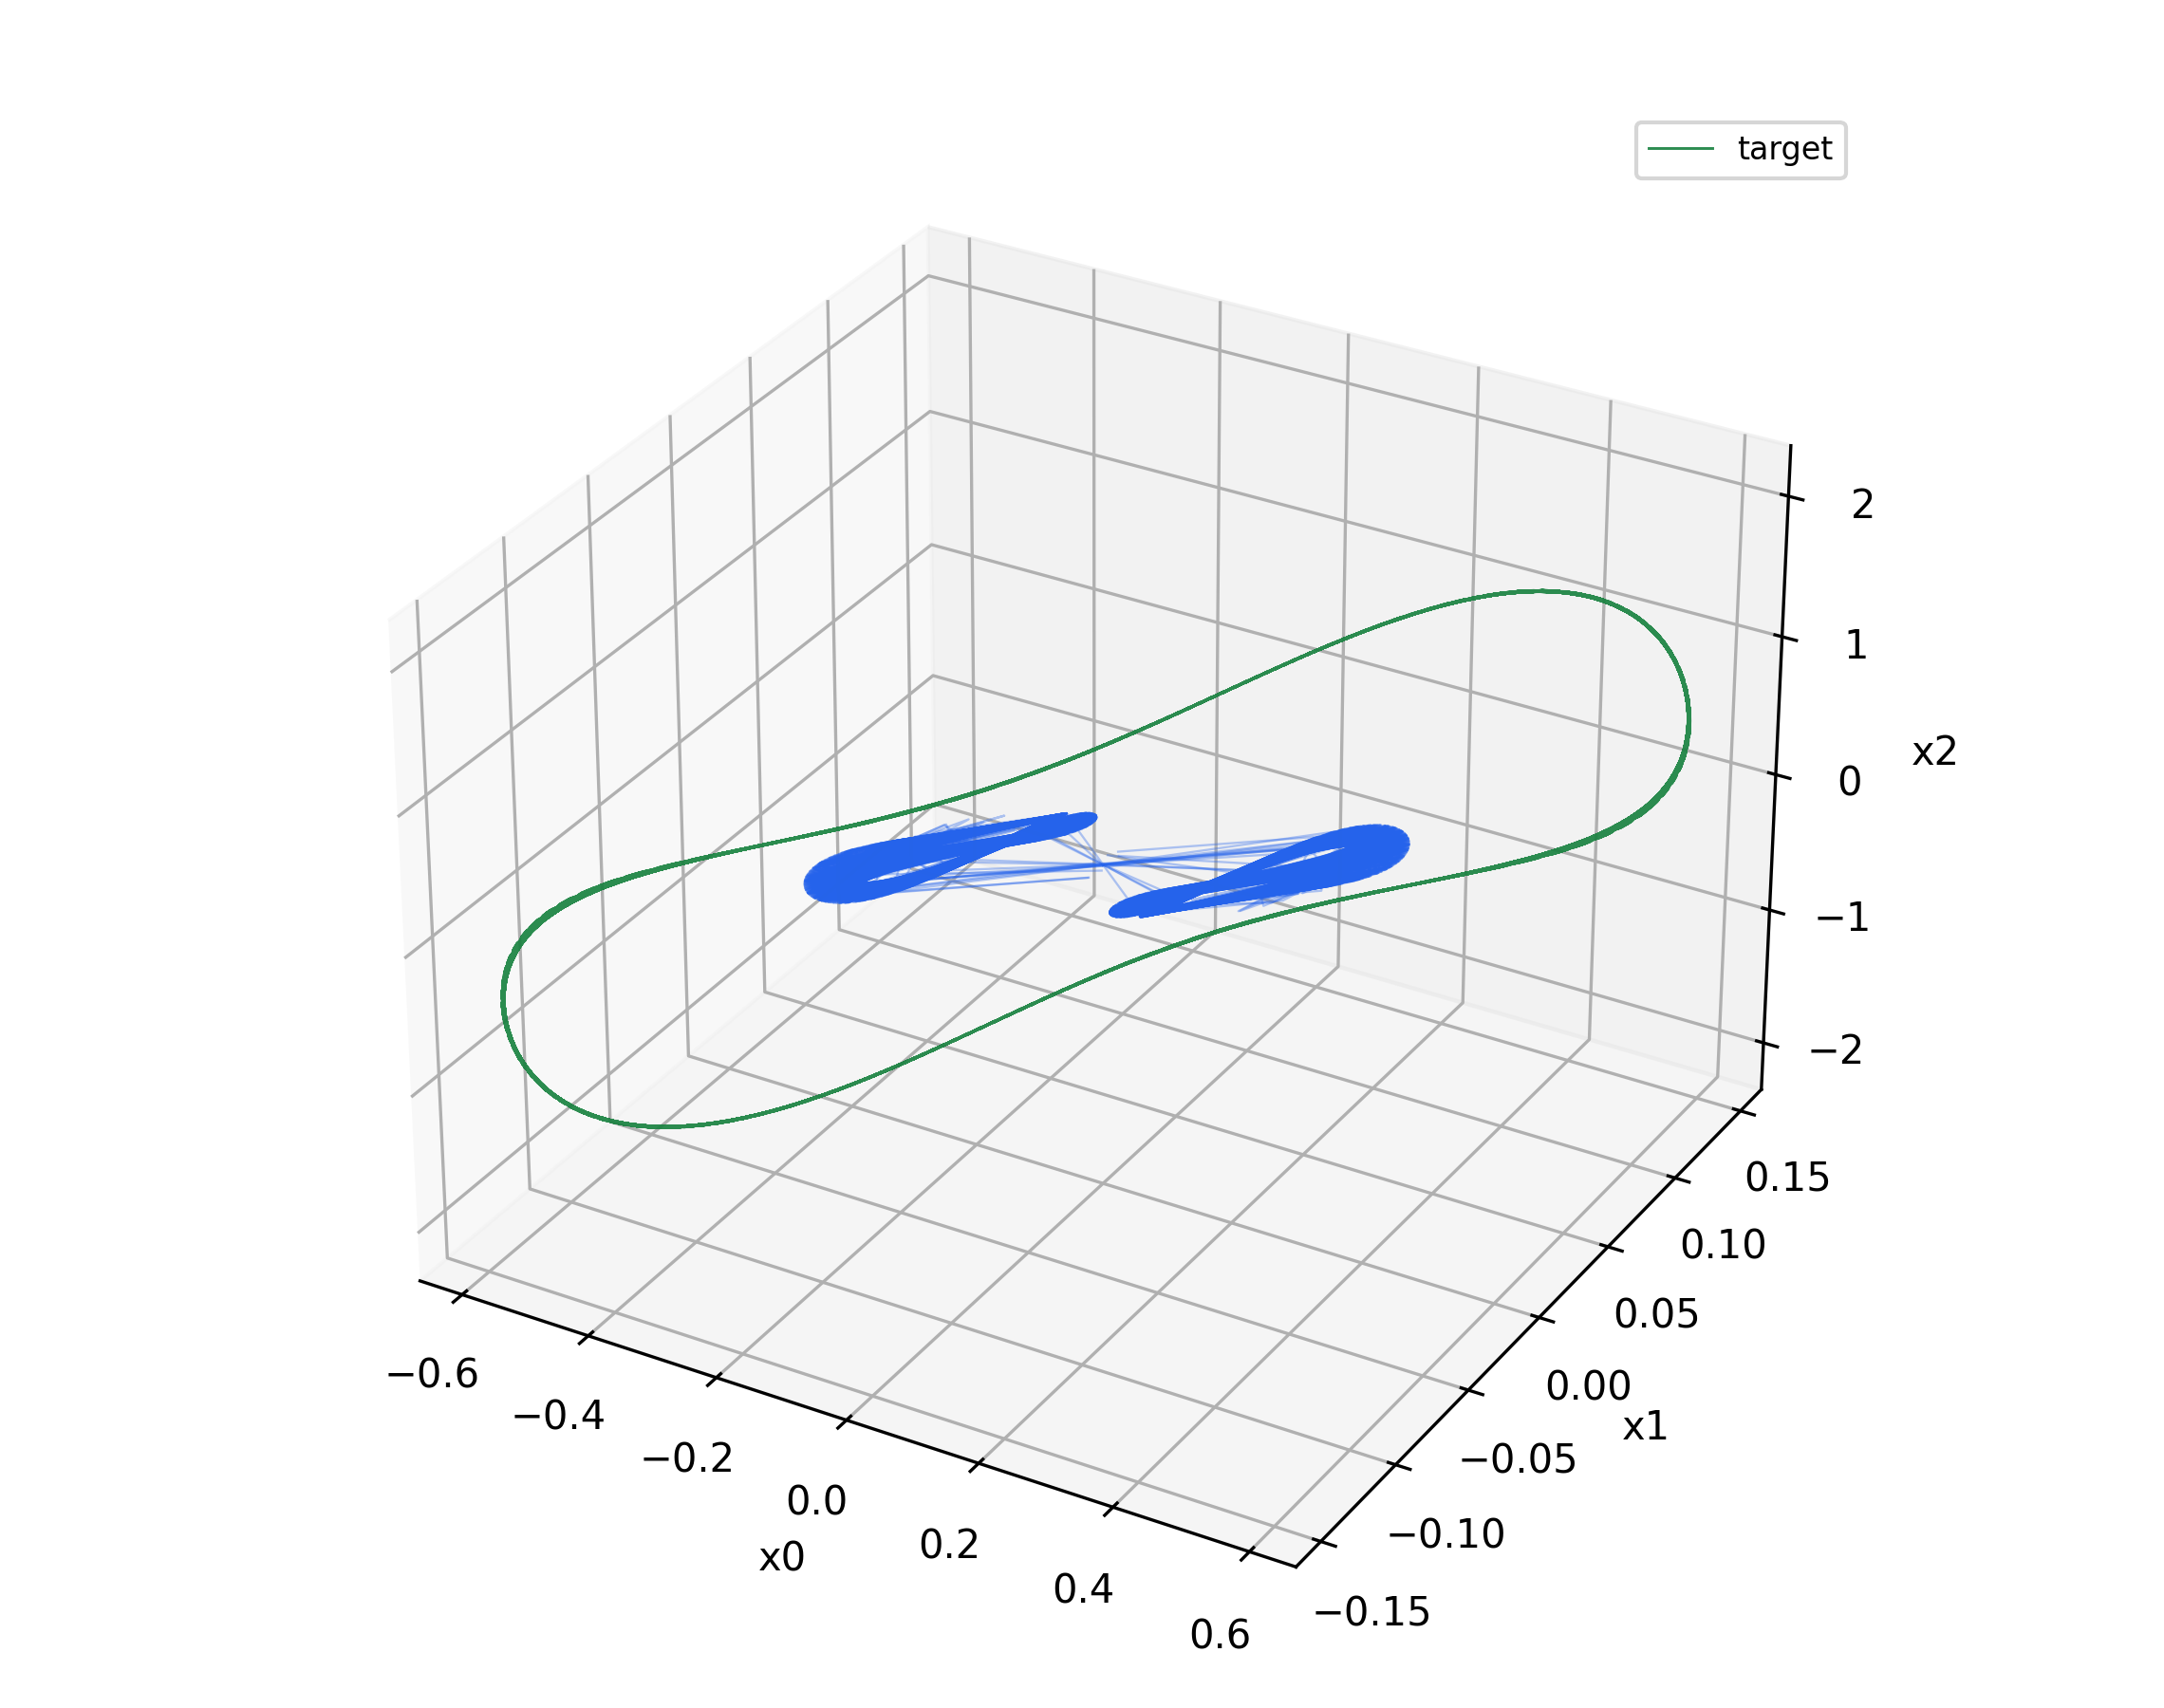
\includegraphics[width=\linewidth]{mavpd_python_hiddenness.png}
  \caption{Python: las vecindades alcanzan sólo los ciclos internos.}
\end{subfigure}\hfill
\begin{subfigure}[t]{0.49\textwidth}
  \centering
  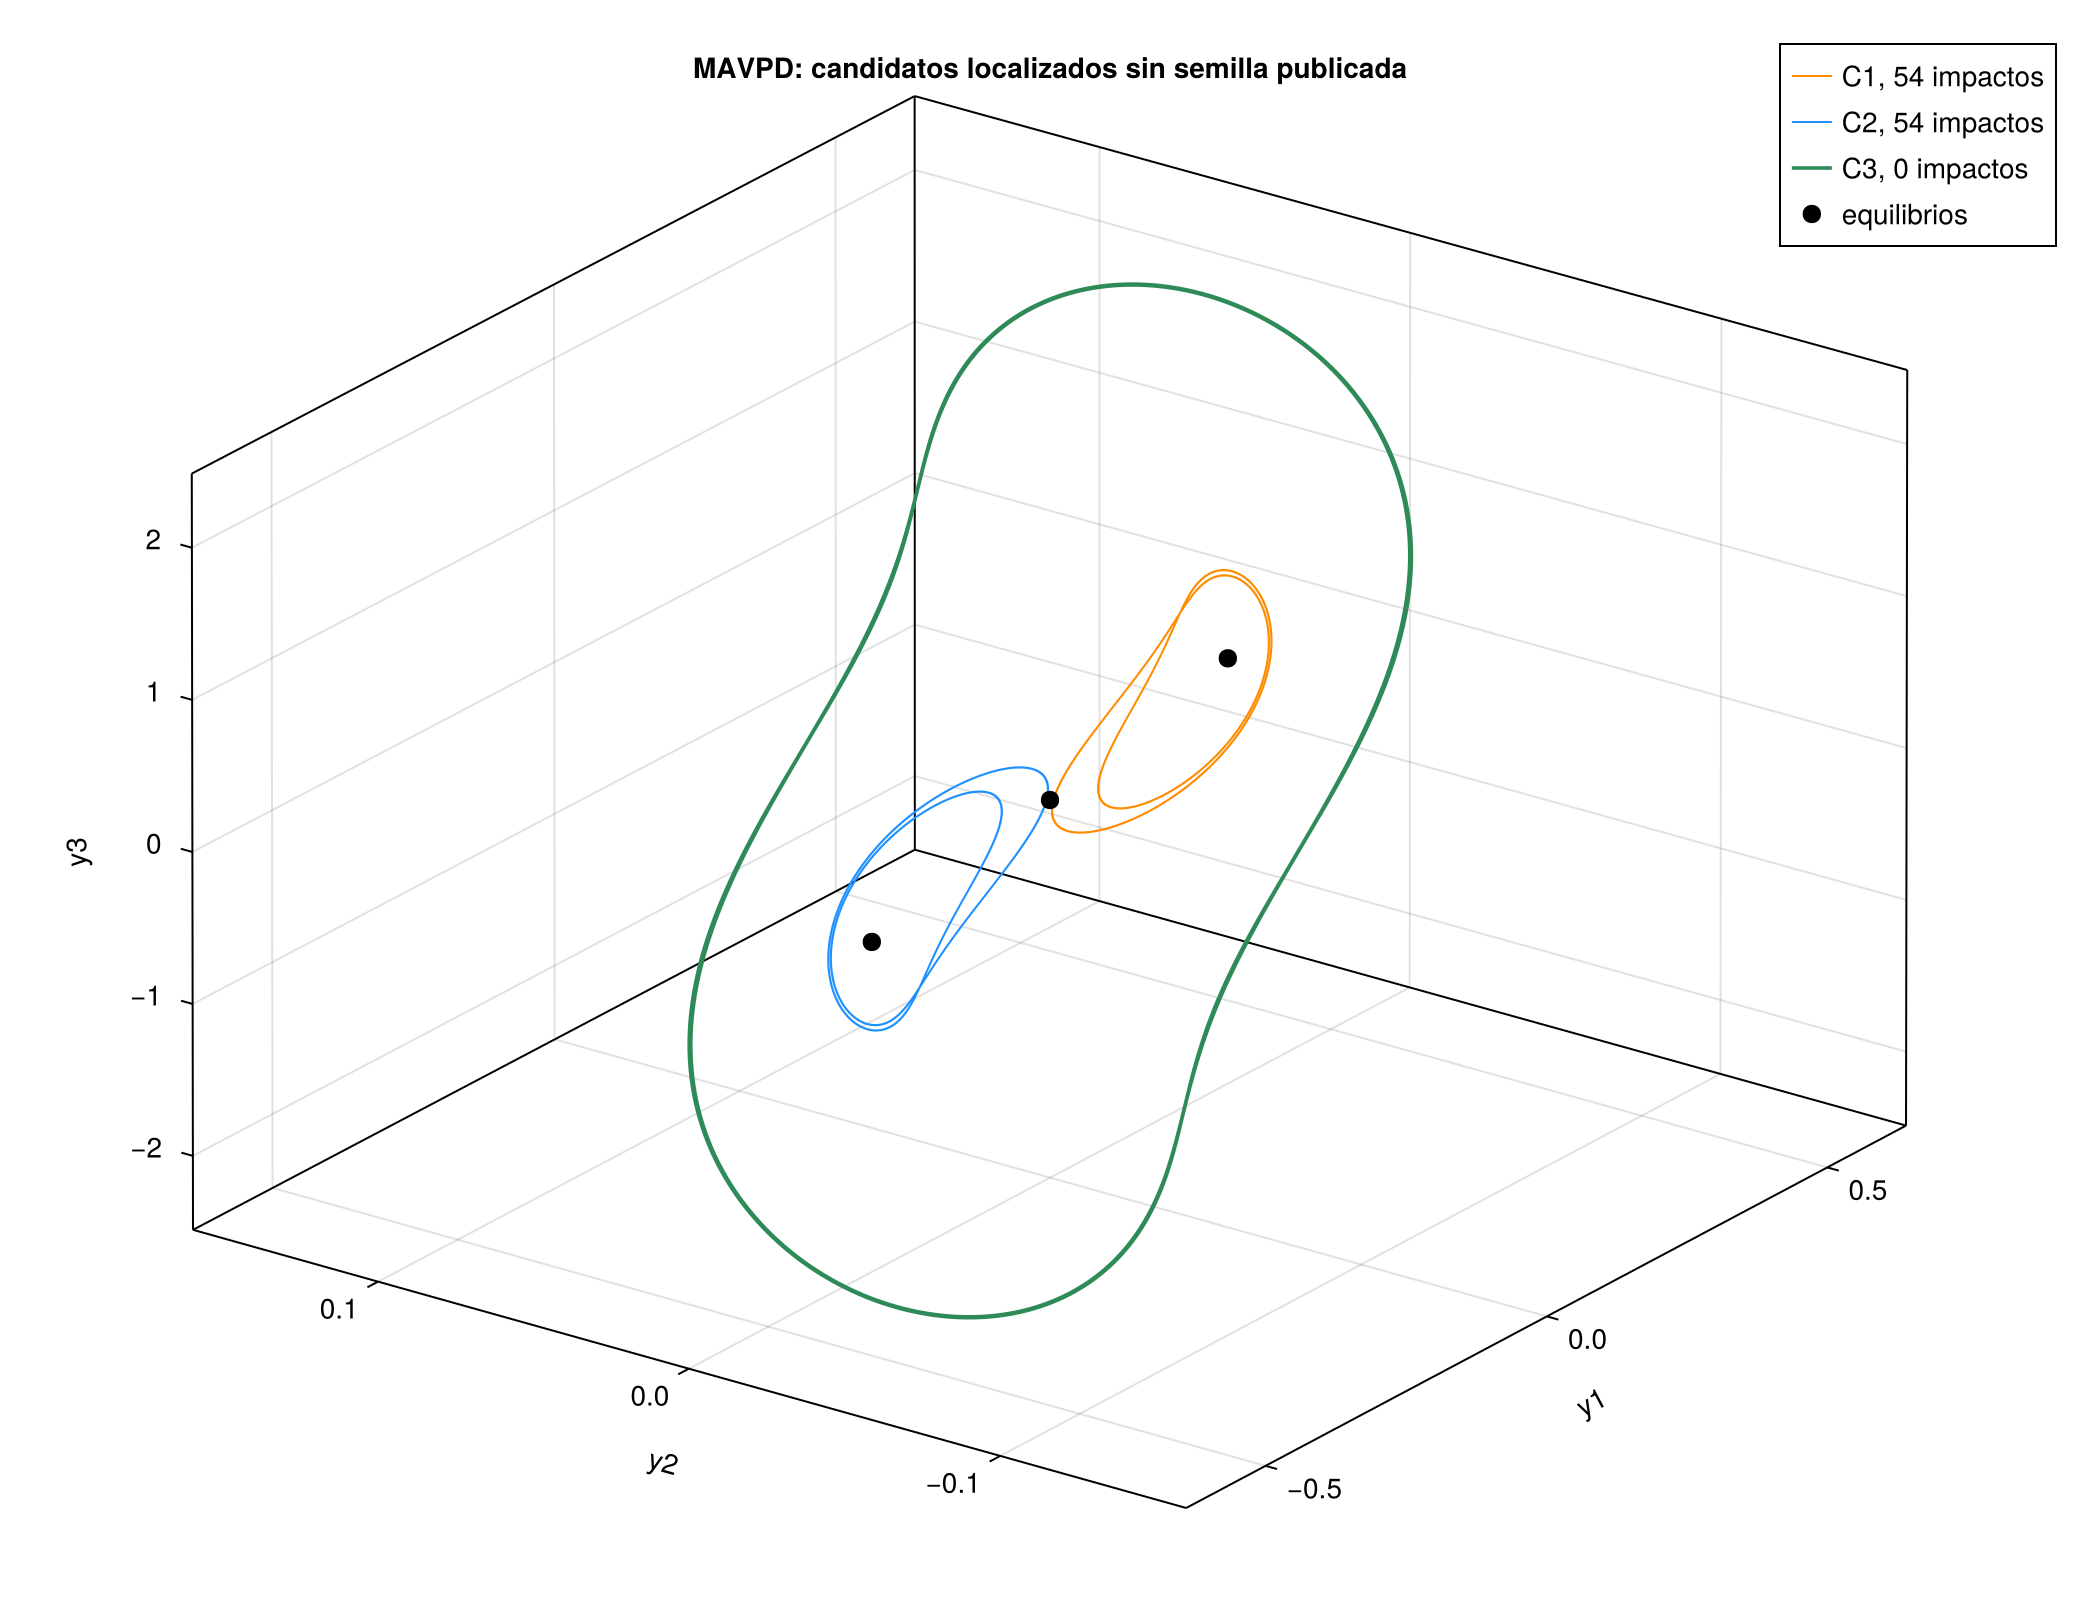
\includegraphics[width=\linewidth]{mavpd_julia_candidates.png}
  \caption{Julia \emph{full}: clúster externo con cero impactos.}
\end{subfigure}
\caption{Ciclo externo compatible con ocultedad bajo las 108 sondas del
protocolo finito para \(\xi=3.1\).}
\label{int:fig:mavpd-hiddenness}
\end{hafobasinfigure}

\subsection{Comprobación algebraica de la fuente}

Se preservan tres discrepancias:

\begin{enumerate}
  \item La fuente imprime \(\Theta=-\delta e_1\),
        \(s=-e_1\) y \(\zeta(\sigma)=\sigma^3\). Juntas producen
        \(+\delta y_1^3\), mientras que la ecuación del sistema contiene
        \(-\delta y_1^3\). La formulación evaluada usa la ecuación original y la
        forma exacta \(b=-\delta e_1\), \(c=e_1\).
  \item Para \(\xi=3.1\), los valores impresos
        \(\omega=18.6143\), \(|k|=0.8951\) dejan residuo de cierre
        \(2.45589\) en la transferencia exacta.
  \item Para \(\xi=3.5\), los valores impresos
        \(\omega=10.2344\), \(|k|=0.1136\) dejan residuo \(0.171719\).
\end{enumerate}

Las semillas impresas sí terminan, en una prueba posterior, en los mismos
clústeres dinámicos que la búsqueda independiente. Esa coincidencia dinámica
no elimina la discrepancia algebraica de frecuencia y ganancia.

\ifHAFOBasinMaterial
\subsection{\texorpdfstring{\(\xi=3.5\): control negativo de ocultedad}{xi=3.5: control negativo de ocultedad}}

La ruta directa recalculó dos ramas:
\[
(\omega_0,k,a_0)=
(10.8359213547,\ 0.1497634046,\ 0.4468607607)
\]
y
\[
(\omega_0,k,a_0)=
(13.0511611895,\ 0.3009508811,\ 0.6334570558).
\]
Las cuatro fases convergen a dos ciclos internos simétricos. Bajo el mismo
protocolo de 108 sondeos, Python y Julia observaron 24 contactos
con cada ciclo; el comparador confirmó la misma decisión negativa. Después
del primer contacto se habilitó la ruta alternativa, que no encontró clústeres
nuevos. Por tanto, la etiqueta oculta no se reproduce para \(\xi=3.5\) bajo
las ecuaciones y controles ensayados.

\fi

\subsection{Extensión caótica: continuación relativa a una frontera candidata de Hopf}
\label{int:subsec:mavpd-chaos}

\ifHAFOBasinMaterial
Los dos regímenes anteriores evalúan conjuntos periódicos bajo un protocolo
común.
\else
El régimen periódico anterior establece el punto de comparación dinámico.
\fi
La coexistencia de caos y ocultedad se estudió mediante dos cálculos
independientes, en Python y Julia. Ambos parten de \eqref{int:eq:mavpd},
obtienen las dos semillas directas y recorren 21 niveles de continuación.
Los parámetros y las semillas publicados se reservan para el contraste
posterior.

En el punto base $(\xi,\gamma)=(3.1,0.1)$, los espectros variacionales cortos
de las ramas 0 y 1 fueron, respectivamente,
\[
 (-0.0012506,-1.0123389,-13.1096006),\qquad
 (-0.0029948,-0.3930260,-51.1769818).
\]
Por tanto, ninguna rama superó el cribado finito declarado
$\widehat\lambda_1>0.02$. Este resultado habilita la ruta alternativa; el cribado de tiempo finito
no establece regularidad asintótica.

La ruta alternativa selecciona, entre las ramas integradas, la de
menor frecuencia armónica directa. La regla eligió aquí la rama 0,
$\omega_0=10.5975230$; su estado final de continuación $\lambda$ alimentó el
transporte en parámetros. La rama 1 se evalúa en el punto base y queda pendiente su transporte por A1.

En $E_\pm=(\pm\sqrt{\gamma},0,\pm\sqrt{\gamma})$, el Jacobiano de las
ecuaciones activas produce
\begin{equation}
 p(\lambda)=\lambda^3+a_1\lambda^2+a_2\lambda+a_3,
 \label{int:eq:mavpd-characteristic}
\end{equation}
con
\begin{equation}
 a_1=\xi+2\delta\gamma,\qquad
 a_2=\rho-\delta+2\delta\gamma\xi,\qquad
 a_3=2\delta\gamma\rho.
 \label{int:eq:mavpd-routh-coefficients}
\end{equation}
Al imponer la igualdad de cruce imaginario de Routh--Hurwitz
$a_1a_2=a_3$ y escribir \(g=2\delta\gamma\), la diferencia se desarrolla como
\[
 a_1a_2-a_3=(\xi+g)(\rho-\delta+\xi g)-\rho g
 =\xi g^2+(\xi^2-\delta)g+\xi(\rho-\delta).
\]
Por tanto, la frontera satisface
\begin{equation}
 \xi g^2+(\xi^2-\delta)g+\xi(\rho-\delta)=0.
 \label{int:eq:mavpd-hopf}
\end{equation}
Esta igualdad determina una frontera candidata de Hopf; aquí no se afirma
haber verificado transversalidad ni no degeneración. Para
$\xi=\MAVPDChaosXi$, la raíz alta de \eqref{int:eq:mavpd-hopf} es
$\gamma_H=\MAVPDChaosHopf$. El valor $\xi=\MAVPDChaosXi$ es el extremo local
declarado de la ruta, no una coordenada elegida por el cribado. El procedimiento
transporta primero el estado desde $\xi=3.10$ hasta ese extremo en pasos de
$-0.01$ y después continúa
$\gamma$, reconstruyendo las ecuaciones, el Jacobiano y la forma Lur'e en cada
nodo. La inspección se restringe a desplazamientos declarados respecto de
$\gamma_H$; no es un barrido de frecuencias ni una exploración arbitraria de
condiciones iniciales.

\ifHAFOBasinMaterial
\begin{table}[H]
\centering
\caption{Cribado local MAVPD alrededor de la frontera alta candidata de Hopf. Los
contactos se cuentan sobre 12 sondeos preliminares alrededor de $E_0$; la tabla
redondea $\widehat\lambda_1$ a un máximo de seis decimales, pero los cálculos
conservan la precisión completa.}
\label{int:tab:mavpd-chaos-screen}
\small
\begin{tabular}{@{}C{1.8cm}C{2.0cm}C{2.3cm}L{8.7cm}@{}}
\toprule
$\gamma-\gamma_H$ & $\widehat\lambda_1$ & Contactos desde $E_0$ & Lectura del cribado \\
\midrule
% Generado desde todas las filas de 03_candidate_screening.csv.
% Columnas: hopf_offset; lambda_1; E0_target_hits/E0_probe_count; lectura finita.
0.002 & 0.929112 & 6/12 & No elegible: hubo contactos en los sondeos preliminares. \\
0.003 & 0.893403 & 6/12 & No elegible: hubo contactos en los sondeos preliminares. \\
0.005 & 0.188317 & 6/12 & No elegible: hubo contactos en los sondeos preliminares. \\
0.008 & 0.812209 & 0/12 & Elegible bajo el cribado finito; no seleccionada por la regla. \\
0.010 & 0.72394 & 0/12 & Elegible y seleccionada por la regla declarada. \\
0.012 & 0.315116 & 0/12 & No elegible bajo el cribado finito declarado. \\
0.015 & -0.00887 & 0/12 & No elegible bajo el cribado finito declarado. \\
\bottomrule

\end{tabular}
\end{table}
\fi

La regla selecciona el mayor desplazamiento declarado con cálculo de Lyapunov
válido y $\widehat\lambda_1>0.5$
\ifHAFOBasinMaterial
, cero contactos preliminares, cero casos ambiguos y cero fallos numéricos
\else
y con los demás filtros de admisibilidad satisfechos
\fi
: así se obtiene
\[
 (\xi,\gamma,\delta,\rho)=
 (\MAVPDChaosXi,\MAVPDChaosGamma,100,200),\qquad
 \gamma=\gamma_H+0.010.
\]
El desplazamiento $0.010$ es el resultado de la regla de selección aplicada en
esta continuación numérica local; no se lee como valor esperado ni es un
parámetro publicado en \cite{matouk2023}. Por tanto, sólo $\gamma$ se selecciona
en este cribado: la tupla completa no se presenta como una optimización conjunta
de $\xi$ y $\gamma$.

\begin{hafobasinfigure}[H]
\centering
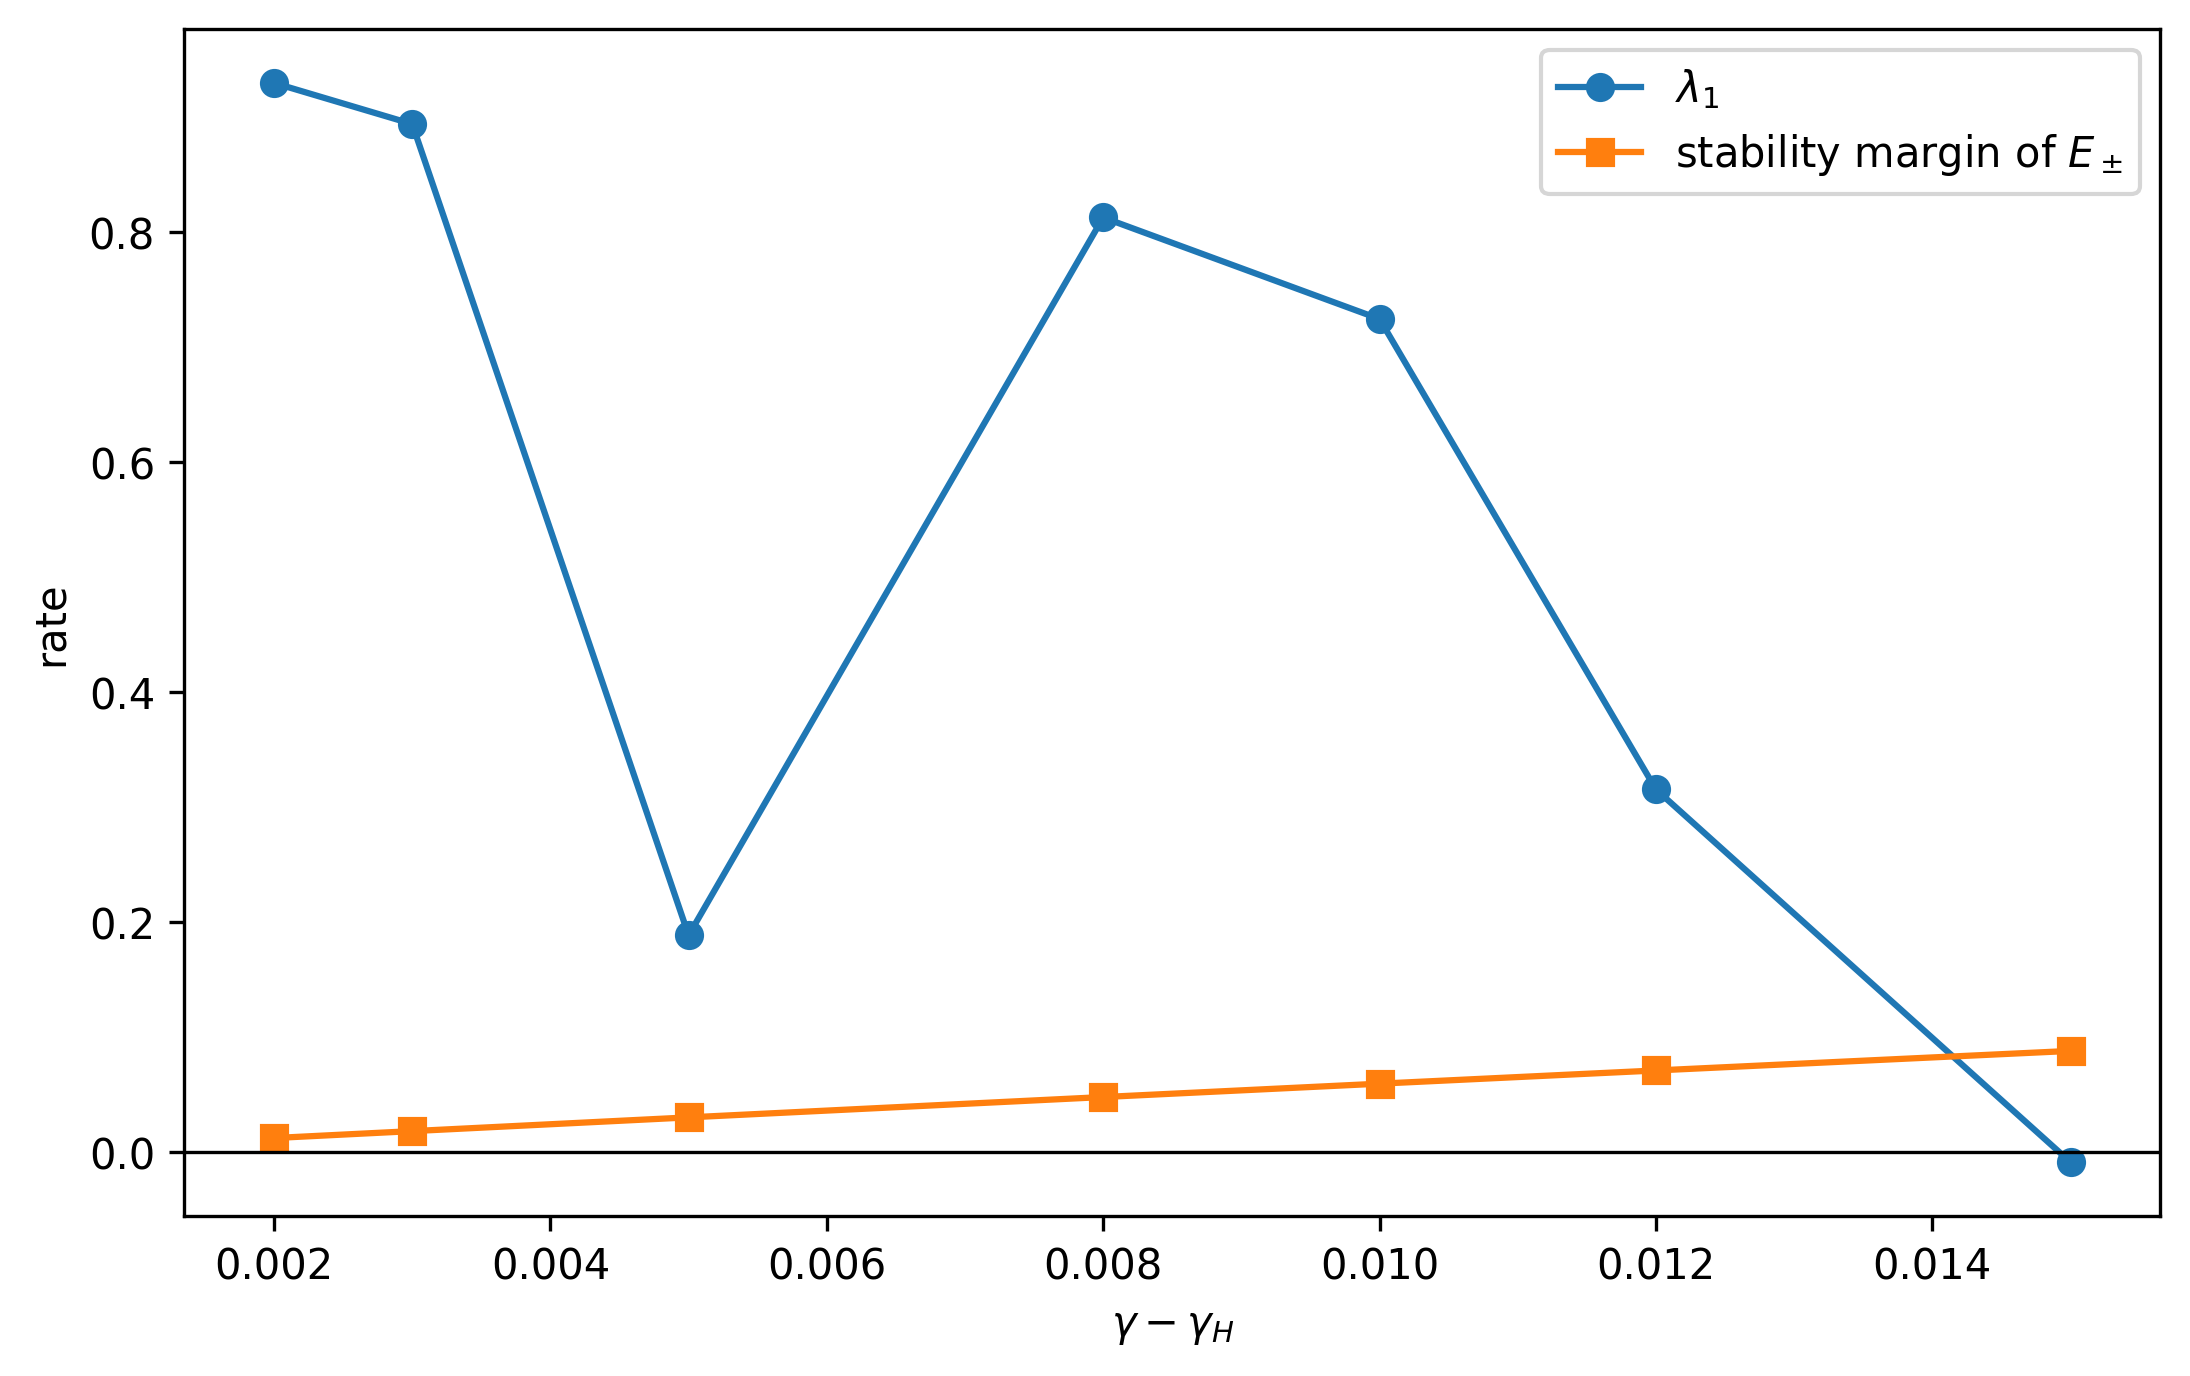
\includegraphics[width=0.90\textwidth]{mavpd_chaos_screen.png}
\caption{Continuación en parámetros y cribado conjunto de exponente máximo y
contactos desde $E_0$. La selección ocurre después del fallo dinámico de las
ramas directas, no mediante una malla de frecuencias.}
\label{int:fig:mavpd-chaos-screen}
\end{hafobasinfigure}

\begin{table}[H]
\centering
\caption{Protocolo numérico de la extensión MAVPD caótica.}
\label{int:tab:mavpd-chaos-contract}
\footnotesize
\begin{tabularx}{\textwidth}{@{}L{0.19\textwidth}L{0.34\textwidth}Y@{}}
\toprule
Fase & Horizonte y muestreo & Integrador y tolerancias \\
\midrule
Cribado D0 por rama & $t_b=100$, $t_{LE}=250$, QR $0.5$ &
DOP853, $(\mathrm{rtol},\mathrm{atol})=(2\,10^{-10},2\,10^{-12})$,
$\Delta t_{\max}=0.02$ \\
Transporte A1 por nodo & $t_b=60$, $t_k=10$, muestra $0.02$ &
DOP853, $(2\,10^{-10},2\,10^{-12})$, $\Delta t_{\max}=0.02$ \\
Referencia del cribado & duración 360, descarte 160, muestra $0.05$,
600 puntos máximos & DOP853, $\Delta t_{\max}=0.03$; factor de seguridad 3 \\
\ifHAFOBasinMaterial
Sondeos preliminares $E_0$ & $t_b=500$, $t_k=100$, muestra $0.05$;
2 radios, 6 direcciones & DOP853, $(2\,10^{-10},2\,10^{-12})$,
$\Delta t_{\max}=0.03$ \\
\fi
Trayectoria estricta & $t_f=900$, $t_b=300$, muestra $0.02$ &
DOP853, $(2\,10^{-11},2\,10^{-13})$, $\Delta t_{\max}=0.01$ \\
Lyapunov estricto & $t_b=300$, $t_{LE}=1200$, QR $0.5$ &
DOP853 variacional, $(2\,10^{-12},2\,10^{-14})$,
$\Delta t_{\max}=0.01$ \\
Control Lyapunov combinado & estado candidato perturbado; $t_b=200$,
$t_{LE}=600$, QR $0.5$ & DOP853 variacional,
$(2\,10^{-10},2\,10^{-12})$, $\Delta t_{\max}=0.02$ \\
\ifHAFOBasinMaterial
Ocultedad final & $t_b=400$, $t_k=100$, muestra $0.05$;
108 sondeos principales + 4 dirigidos & DOP853, $(2\,10^{-10},2\,10^{-12})$,
$\Delta t_{\max}=0.03$; referencia máxima 1000 puntos \\
\fi
\bottomrule
\end{tabularx}
\end{table}

\subsubsection*{Refinamiento dinámico y controles de caos}

La trayectoria candidata se integró con DOP853, $t_f=900$, transitorio 300,
muestreo $0.02$, tolerancias $(\mathrm{rtol},\mathrm{atol})=(2\times10^{-11},
2\times10^{-13})$ y paso máximo $0.01$ \cite{scipy2020}. Sobre un problema
variacional separado, DOP853 con QR, transitorio 300 y acumulación 1200 produjo
el espectro finito. Con $Q_0=I$, en cada segmento se integra
\begin{equation}
 \dot Y_m=J(y(t))Y_m,\qquad Y_m(t_{m-1})=Q_{m-1},
 \qquad Y_m(t_m)=Q_mR_m,
 \quad
 \widehat\lambda_i(T)=\frac{1}{T}\sum_{m=1}^{M}
 \log\left|R_{m,ii}\right|,
 \label{int:eq:mavpd-variational-qr}
\end{equation}
donde cada $R_m$ contiene sólo el crecimiento del segmento correspondiente;
la base se reinicia con $Q_m$ antes del segmento siguiente
\cite{Benettin1980a}. El resultado fue
\begin{equation}
 \begin{aligned}
  \widehat\lambda_1&=\MAVPDChaosLEOne,
  &\widehat\lambda_2&=\MAVPDChaosLETwo,\\
  \widehat\lambda_3&=\MAVPDChaosLEThree,
  &D_{KY}&=\MAVPDChaosKY.
 \end{aligned}
 \label{int:eq:mavpd-chaos-lyapunov}
\end{equation}
Aquí \(D_{KY}=2+(\widehat\lambda_1+\widehat\lambda_2)/
|\widehat\lambda_3|\), pues las dos primeras suman positivamente y la suma de
las tres es negativa.
El control de Lyapunov perturbó el extremo de la continuación y cambió simultáneamente las
tolerancias, el paso máximo y los horizontes de transitorio y acumulación. El cálculo conservó $\widehat\lambda_1=\MAVPDChaosLEControlOne$. El residuo de
consistencia
$r_{\mathrm{div}}=\sum_i\widehat\lambda_i(T_{LE})-
\overline{\nabla\!\cdot f}_{[t_a,t_b]}$ fue
$\MAVPDChaosDivergenceResidual$, con
\begin{equation}
 \nabla\!\cdot f(y)=\delta\gamma-\xi-3\delta y_1^2,
 \qquad
 \overline{\nabla\!\cdot f}_{[t_a,t_b]}=\frac{1}{t_b-t_a}
 \int_{t_a}^{t_b}\!\left(\delta\gamma-\xi-3\delta y_1(t)^2\right)\,dt.
 \label{int:eq:mavpd-divergence-control}
\end{equation}
La relación con el espectro se obtiene de la fórmula de Jacobi. Para una
matriz fundamental invertible \(\Phi\),
\[
 \frac{\dd}{\dd t}\log|\det\Phi(t)|
 =\operatorname{tr}(\Phi^{-1}J\Phi)=\operatorname{tr}J
 =\nabla\!\cdot f.
\]
En la descomposición por segmentos, los determinantes de las matrices
ortogonales \(Q_m\) tienen módulo uno y cada matriz triangular satisface
\(\det R_m=\prod_iR_{m,ii}\). Por tanto, sobre una misma trayectoria y
ventana de longitud \(T\),
\[
 \sum_i\widehat\lambda_i(T)
 =\frac1T\log|\det\Phi(T)|
 =\frac1T\int_0^T\nabla\!\cdot f(y(t))\,\dd t,
\]
con \(\Phi(0)=I\). Esta identidad justifica la comparación de la suma de
exponentes con el promedio de la divergencia.
Aquí $T_{LE}=1200$ pertenece a la integración variacional, mientras que la
divergencia se promedia sobre la trayectoria muestreada independiente
$[t_a,t_b]=[300,900]$. El residuo compara, por tanto, promedios de trayectorias y ventanas
distintas. Como control de integrador, una
trayectoria EFORK de paso fijo $h=0.002$ alcanzó la misma nube de referencia
calibrada.

\begin{hafocommonfigure}[H]
\centering
\begin{subfigure}[t]{0.98\textwidth}
  \centering
  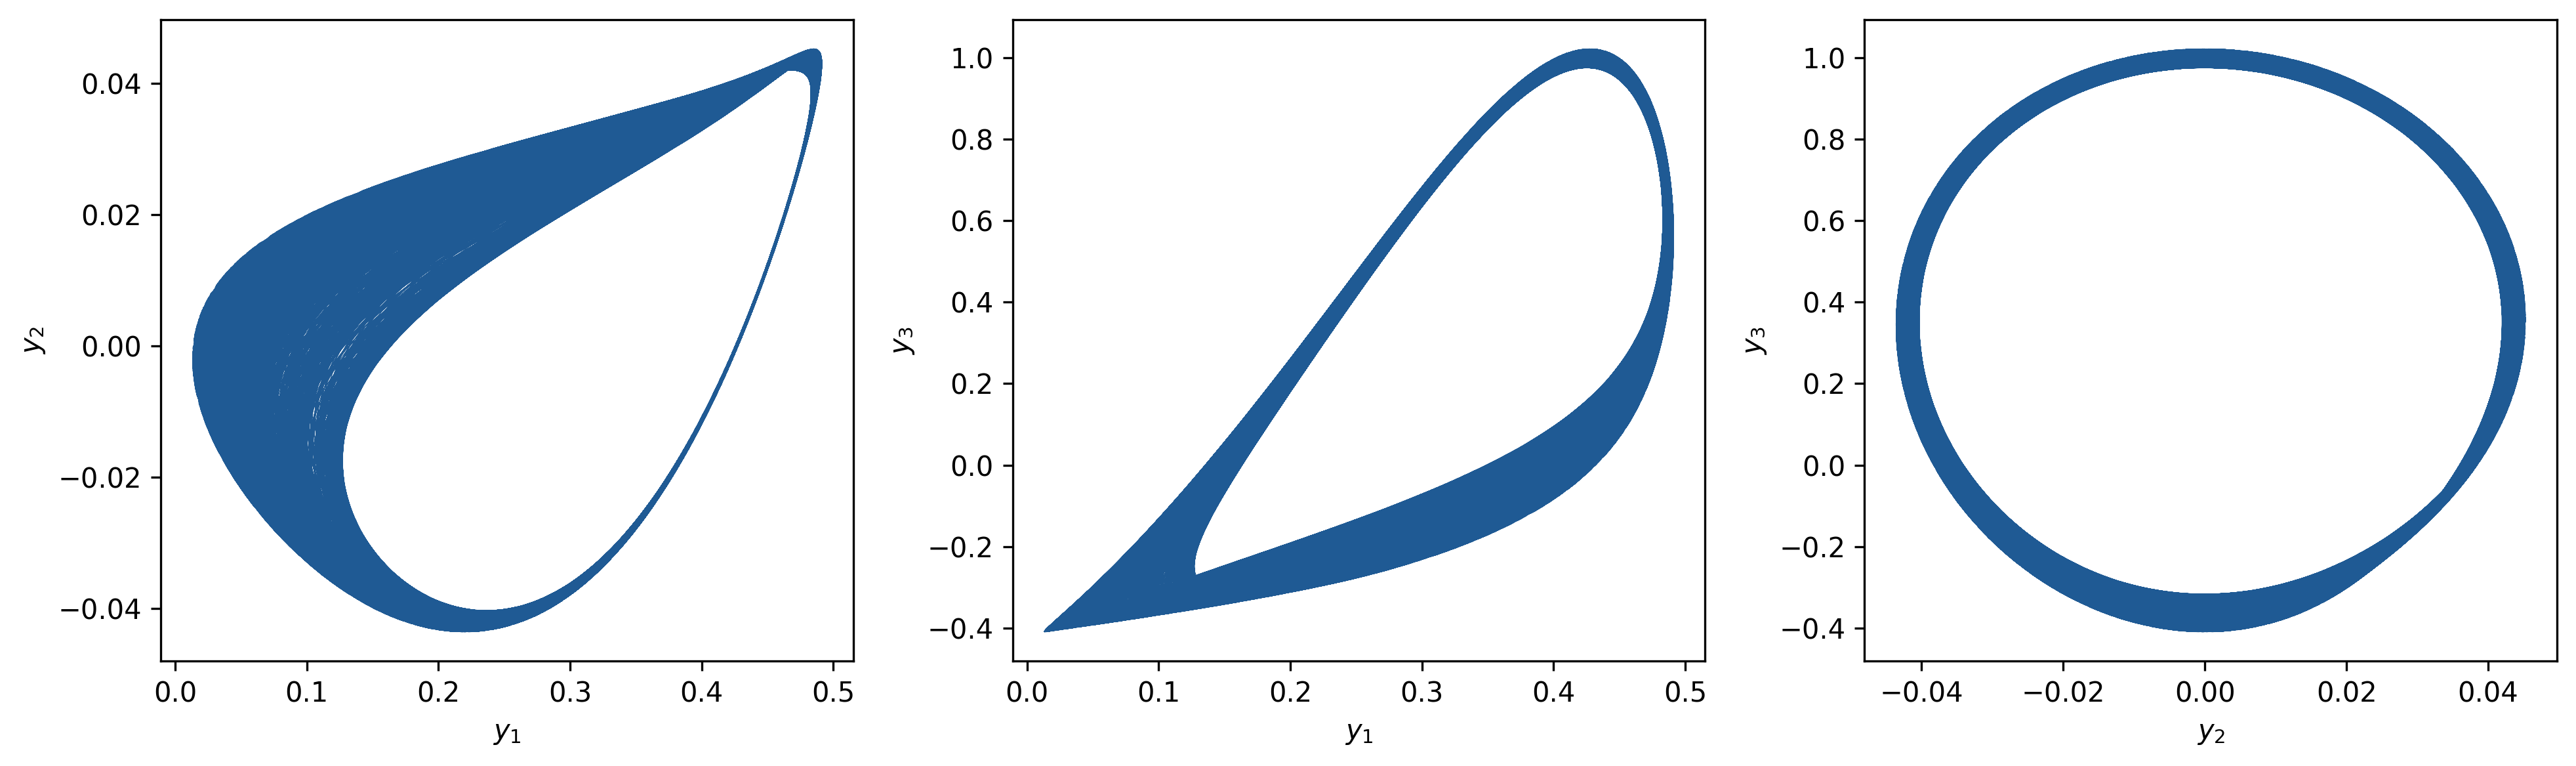
\includegraphics[width=\linewidth]{mavpd_chaos_phase_portraits.png}
  \caption{Proyecciones postransitorias del candidato seleccionado.}
\end{subfigure}

\vspace{0.35em}
\begin{subfigure}[t]{0.86\textwidth}
  \centering
  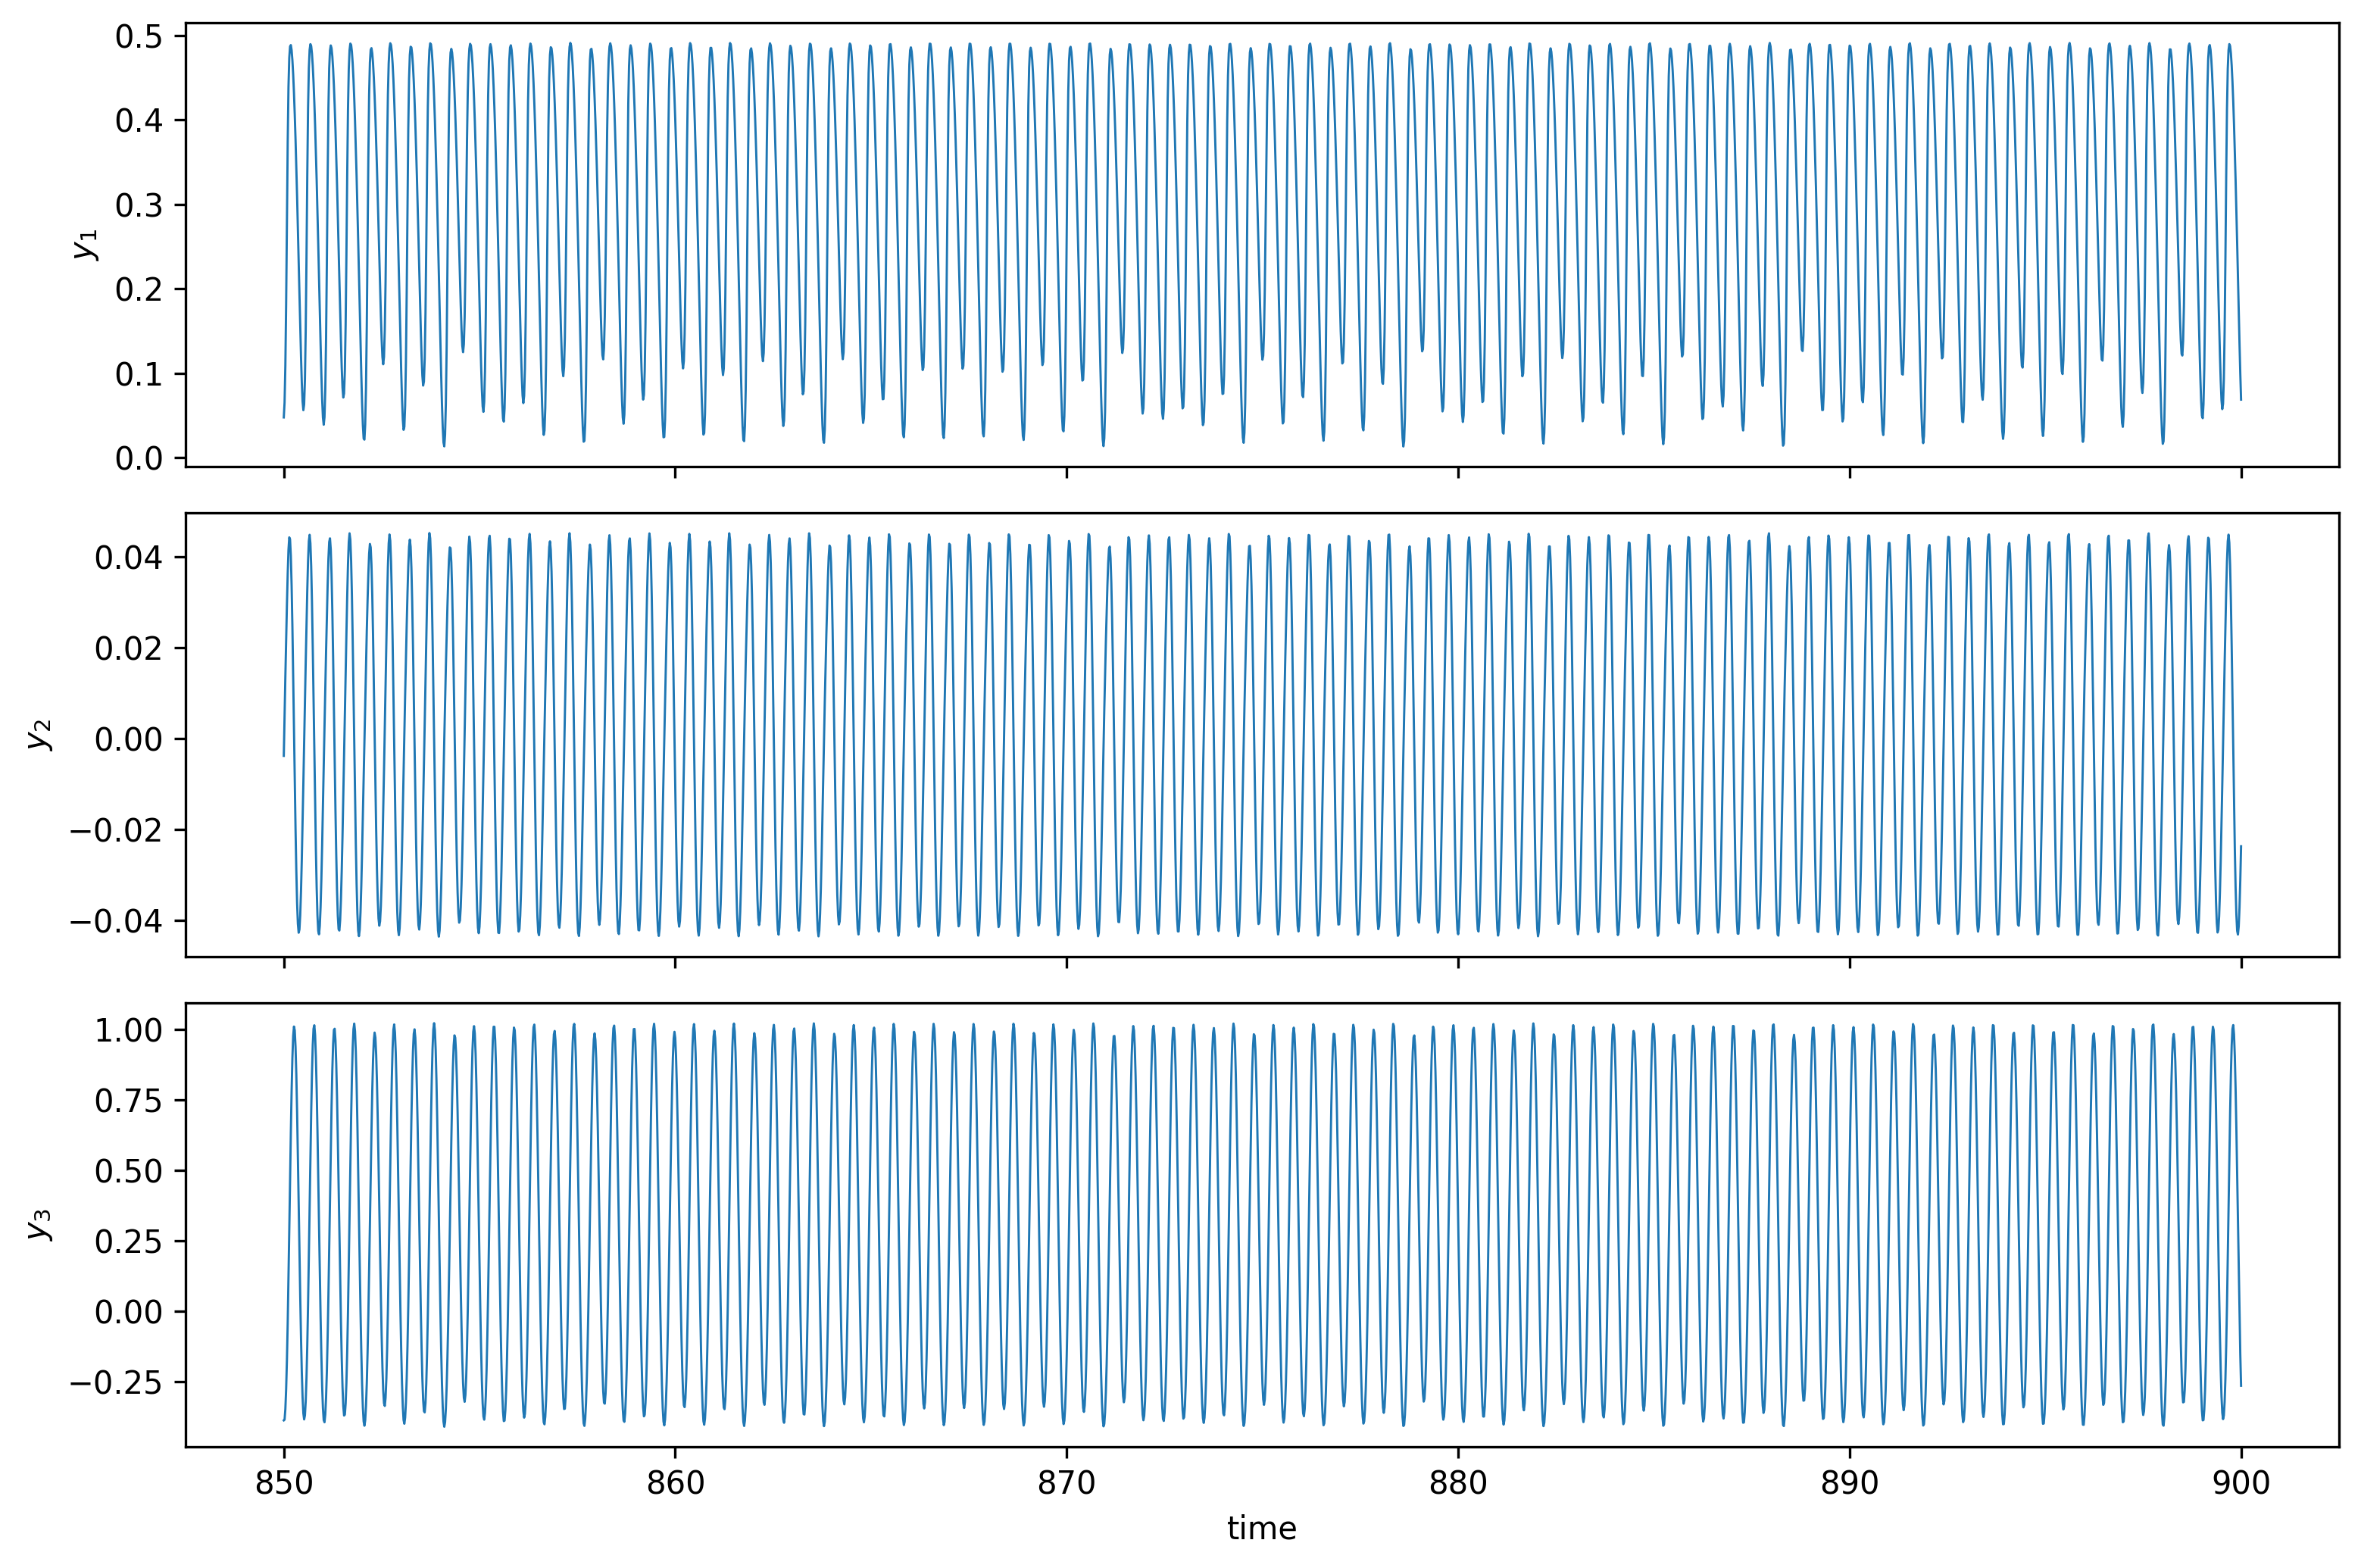
\includegraphics[width=\linewidth]{mavpd_chaos_time_series.png}
  \caption{Series temporales en la ventana conservada.}
\end{subfigure}
\caption{Geometría y evolución temporal del candidato MAVPD caótico. Ventana postransitoria acotada.}
\label{int:fig:mavpd-chaos-trajectory}
\end{hafocommonfigure}

La sección $y_2=0$ con orientación positiva retuvo
\MAVPDChaosPoincareCount{} cruces no duplicados. Los cruces se obtuvieron por
interpolación lineal entre muestras de la trayectoria, con el error temporal
asociado a esa aproximación
\cite{henon1982}. La prueba 0--1 sobre dos coordenadas de la secuencia de
retorno dio medianas $K=\MAVPDChaosReturnKOne$ y
$K=\MAVPDChaosReturnKTwo$ \cite{gottwald2009}. En cambio, la prueba 0--1 sobre
el flujo fue sensible al submuestreo: 3 de 10 pasos dieron etiqueta de
candidato caótico, 1 dio etiqueta regular y 6 quedaron inconclusos. El criterio conjunto usa la secuencia de retorno con
el paso fijado antes de la clasificación.

\begin{hafocommonfigure}[H]
\centering
\begin{subfigure}[t]{0.49\textwidth}
  \centering
  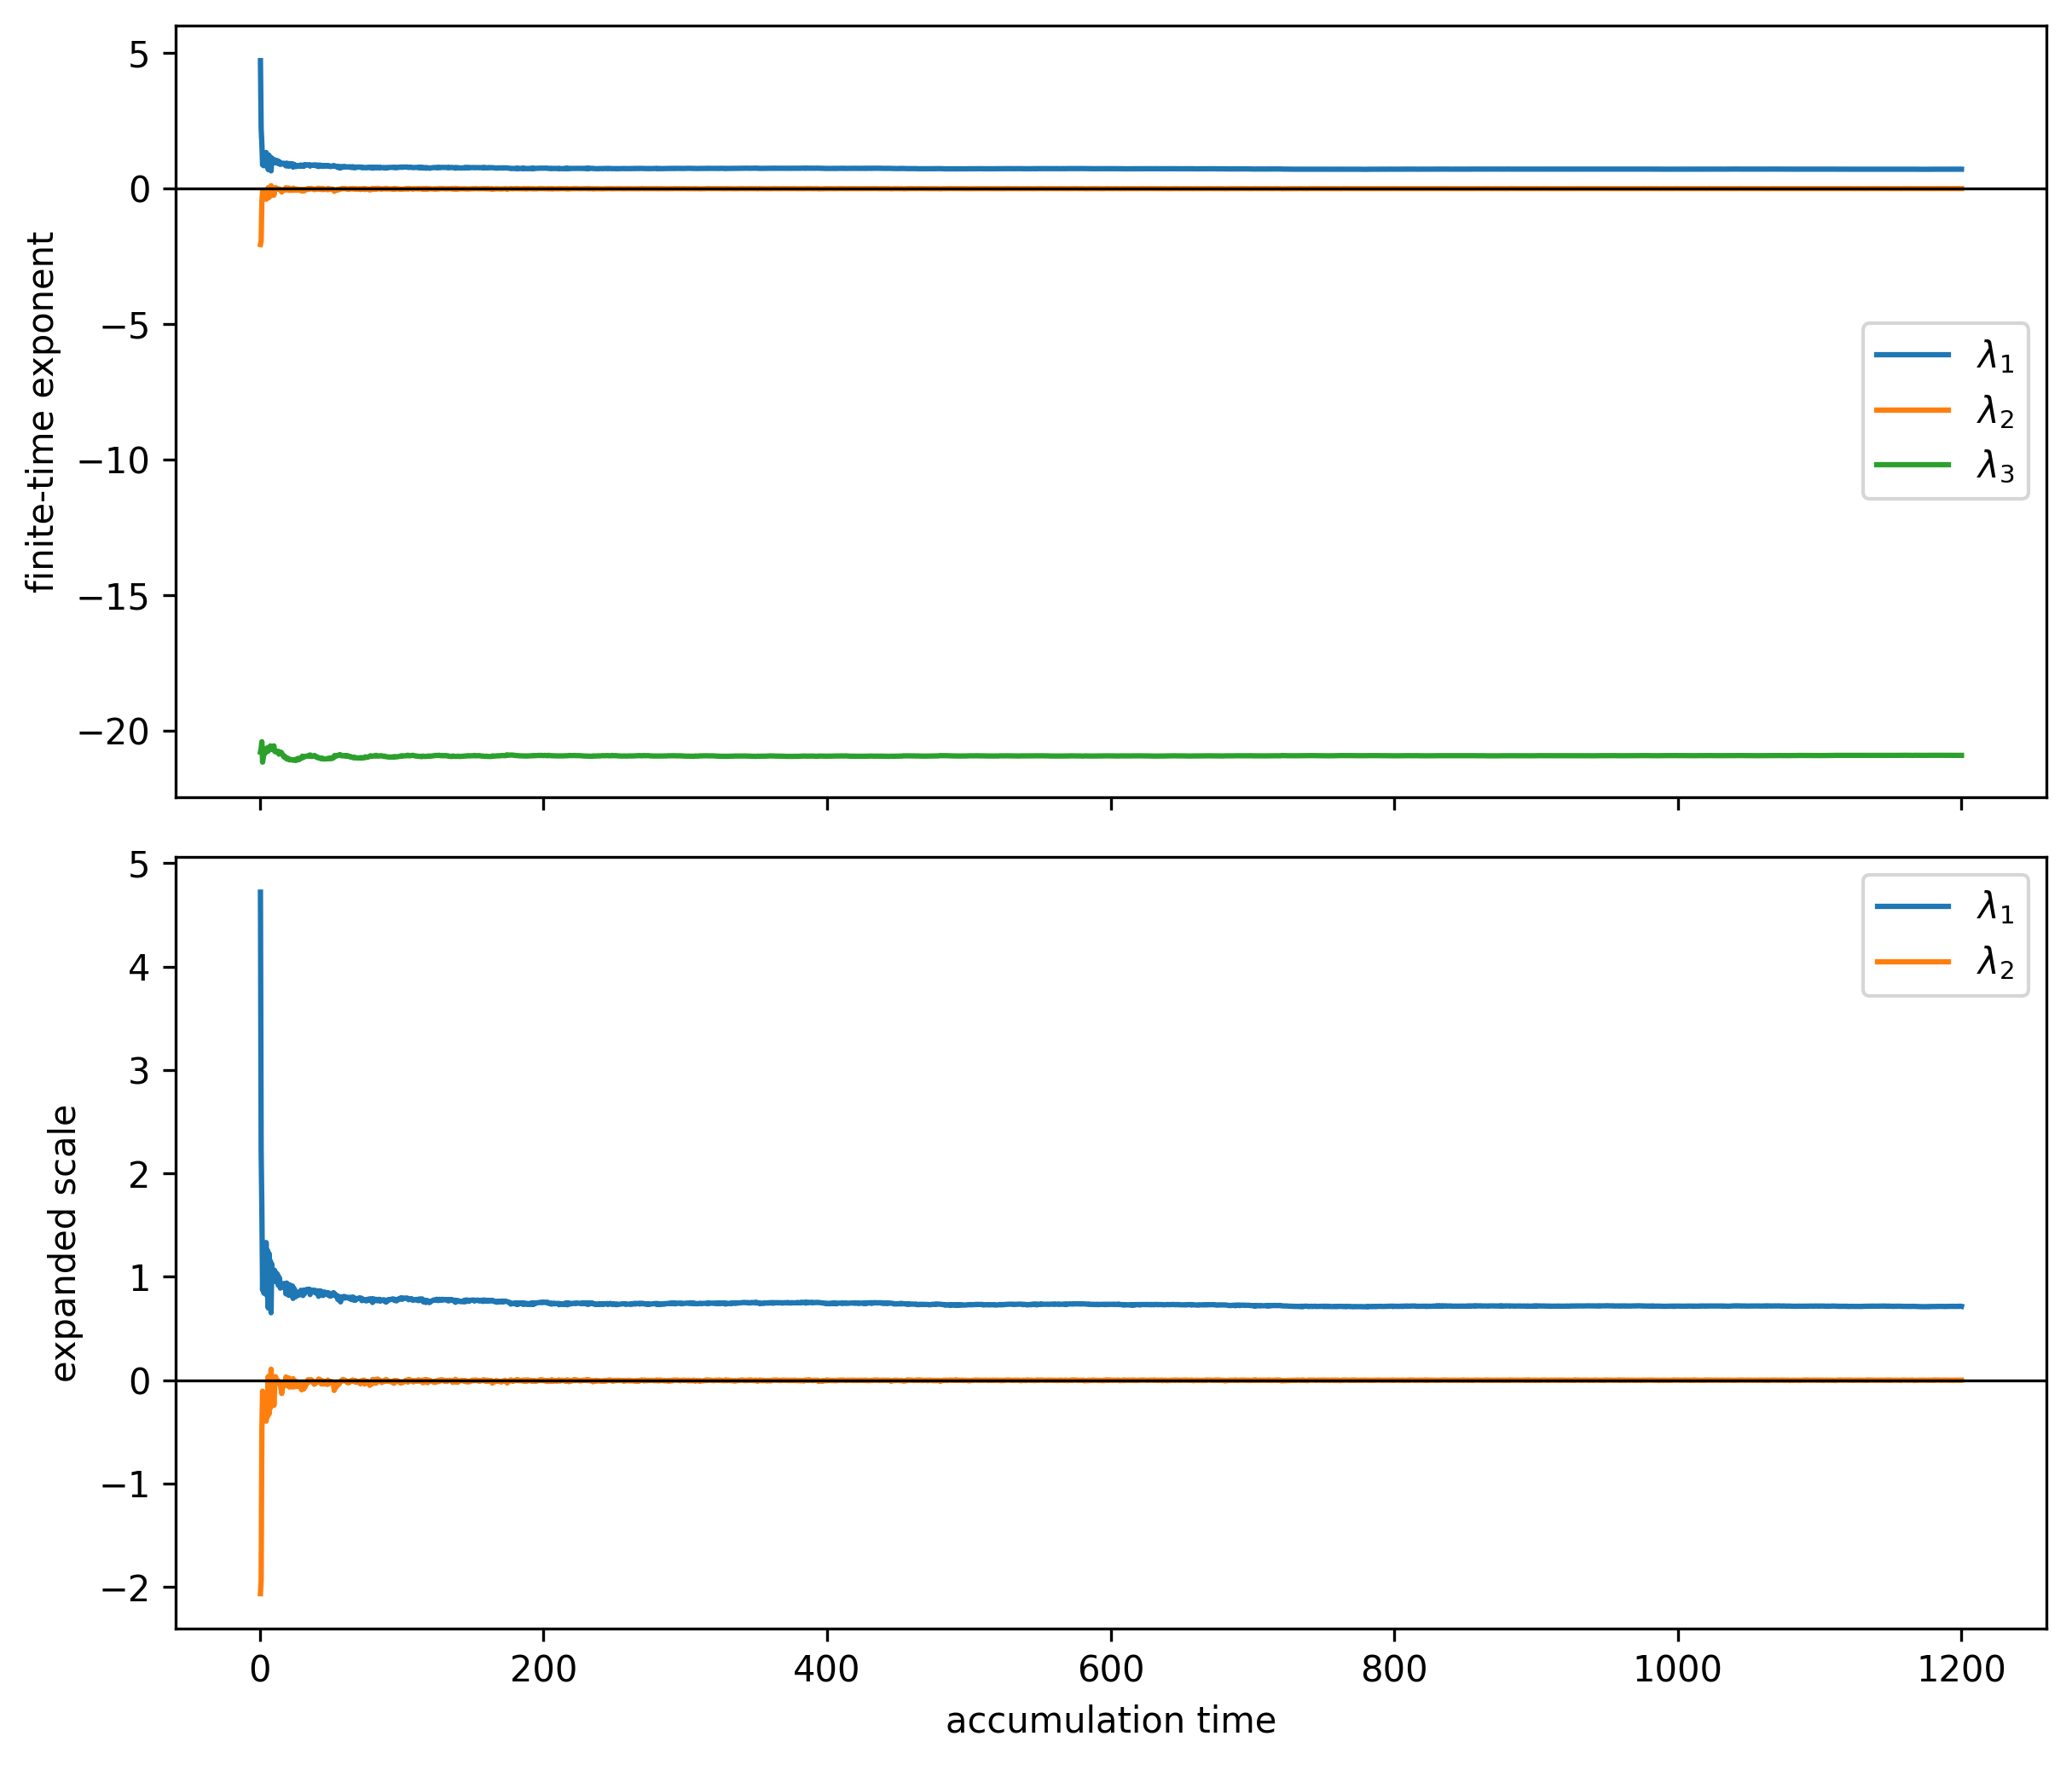
\includegraphics[width=\linewidth]{mavpd_chaos_lyapunov.png}
  \caption{Convergencia del espectro variacional finito.}
\end{subfigure}\hfill
\begin{subfigure}[t]{0.49\textwidth}
  \centering
  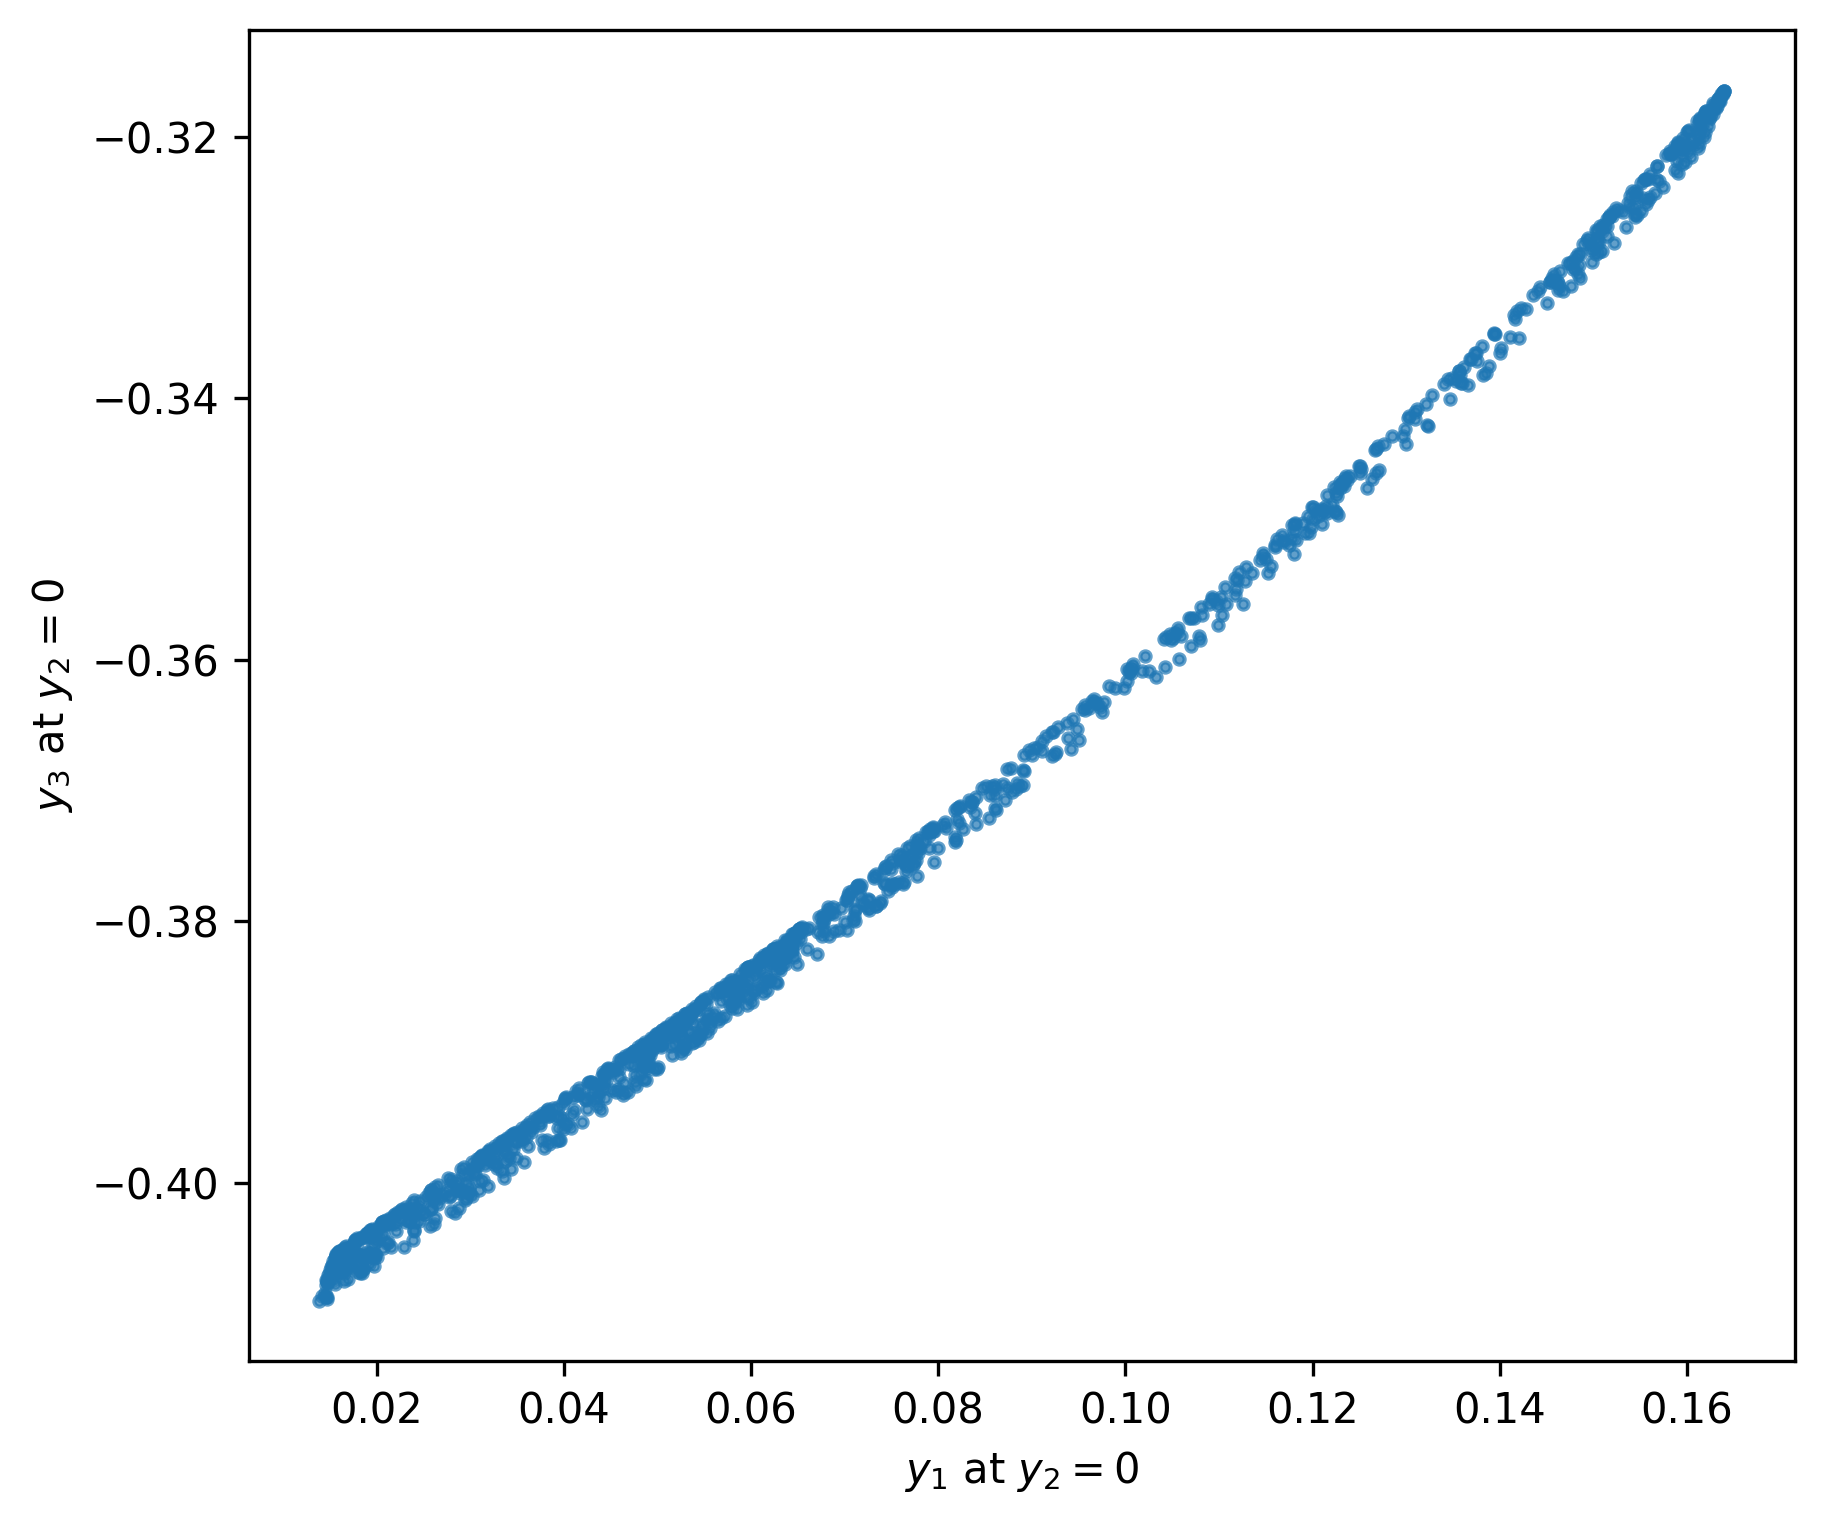
\includegraphics[width=\linewidth]{mavpd_chaos_poincare.png}
  \caption{Sección muestreada e interpolada linealmente.}
\end{subfigure}
\caption{Diagnósticos dinámicos principales del candidato caótico.}
\label{int:fig:mavpd-chaos-diagnostics}
\end{hafocommonfigure}

El espectro de potencia FFT normalizado tiene líneas dominantes y resulta
inconcluso para clasificar el régimen. Se interpreta junto con los
exponentes variacionales y los retornos de Poincaré.

\begin{hafocommonfigure}[H]
\centering
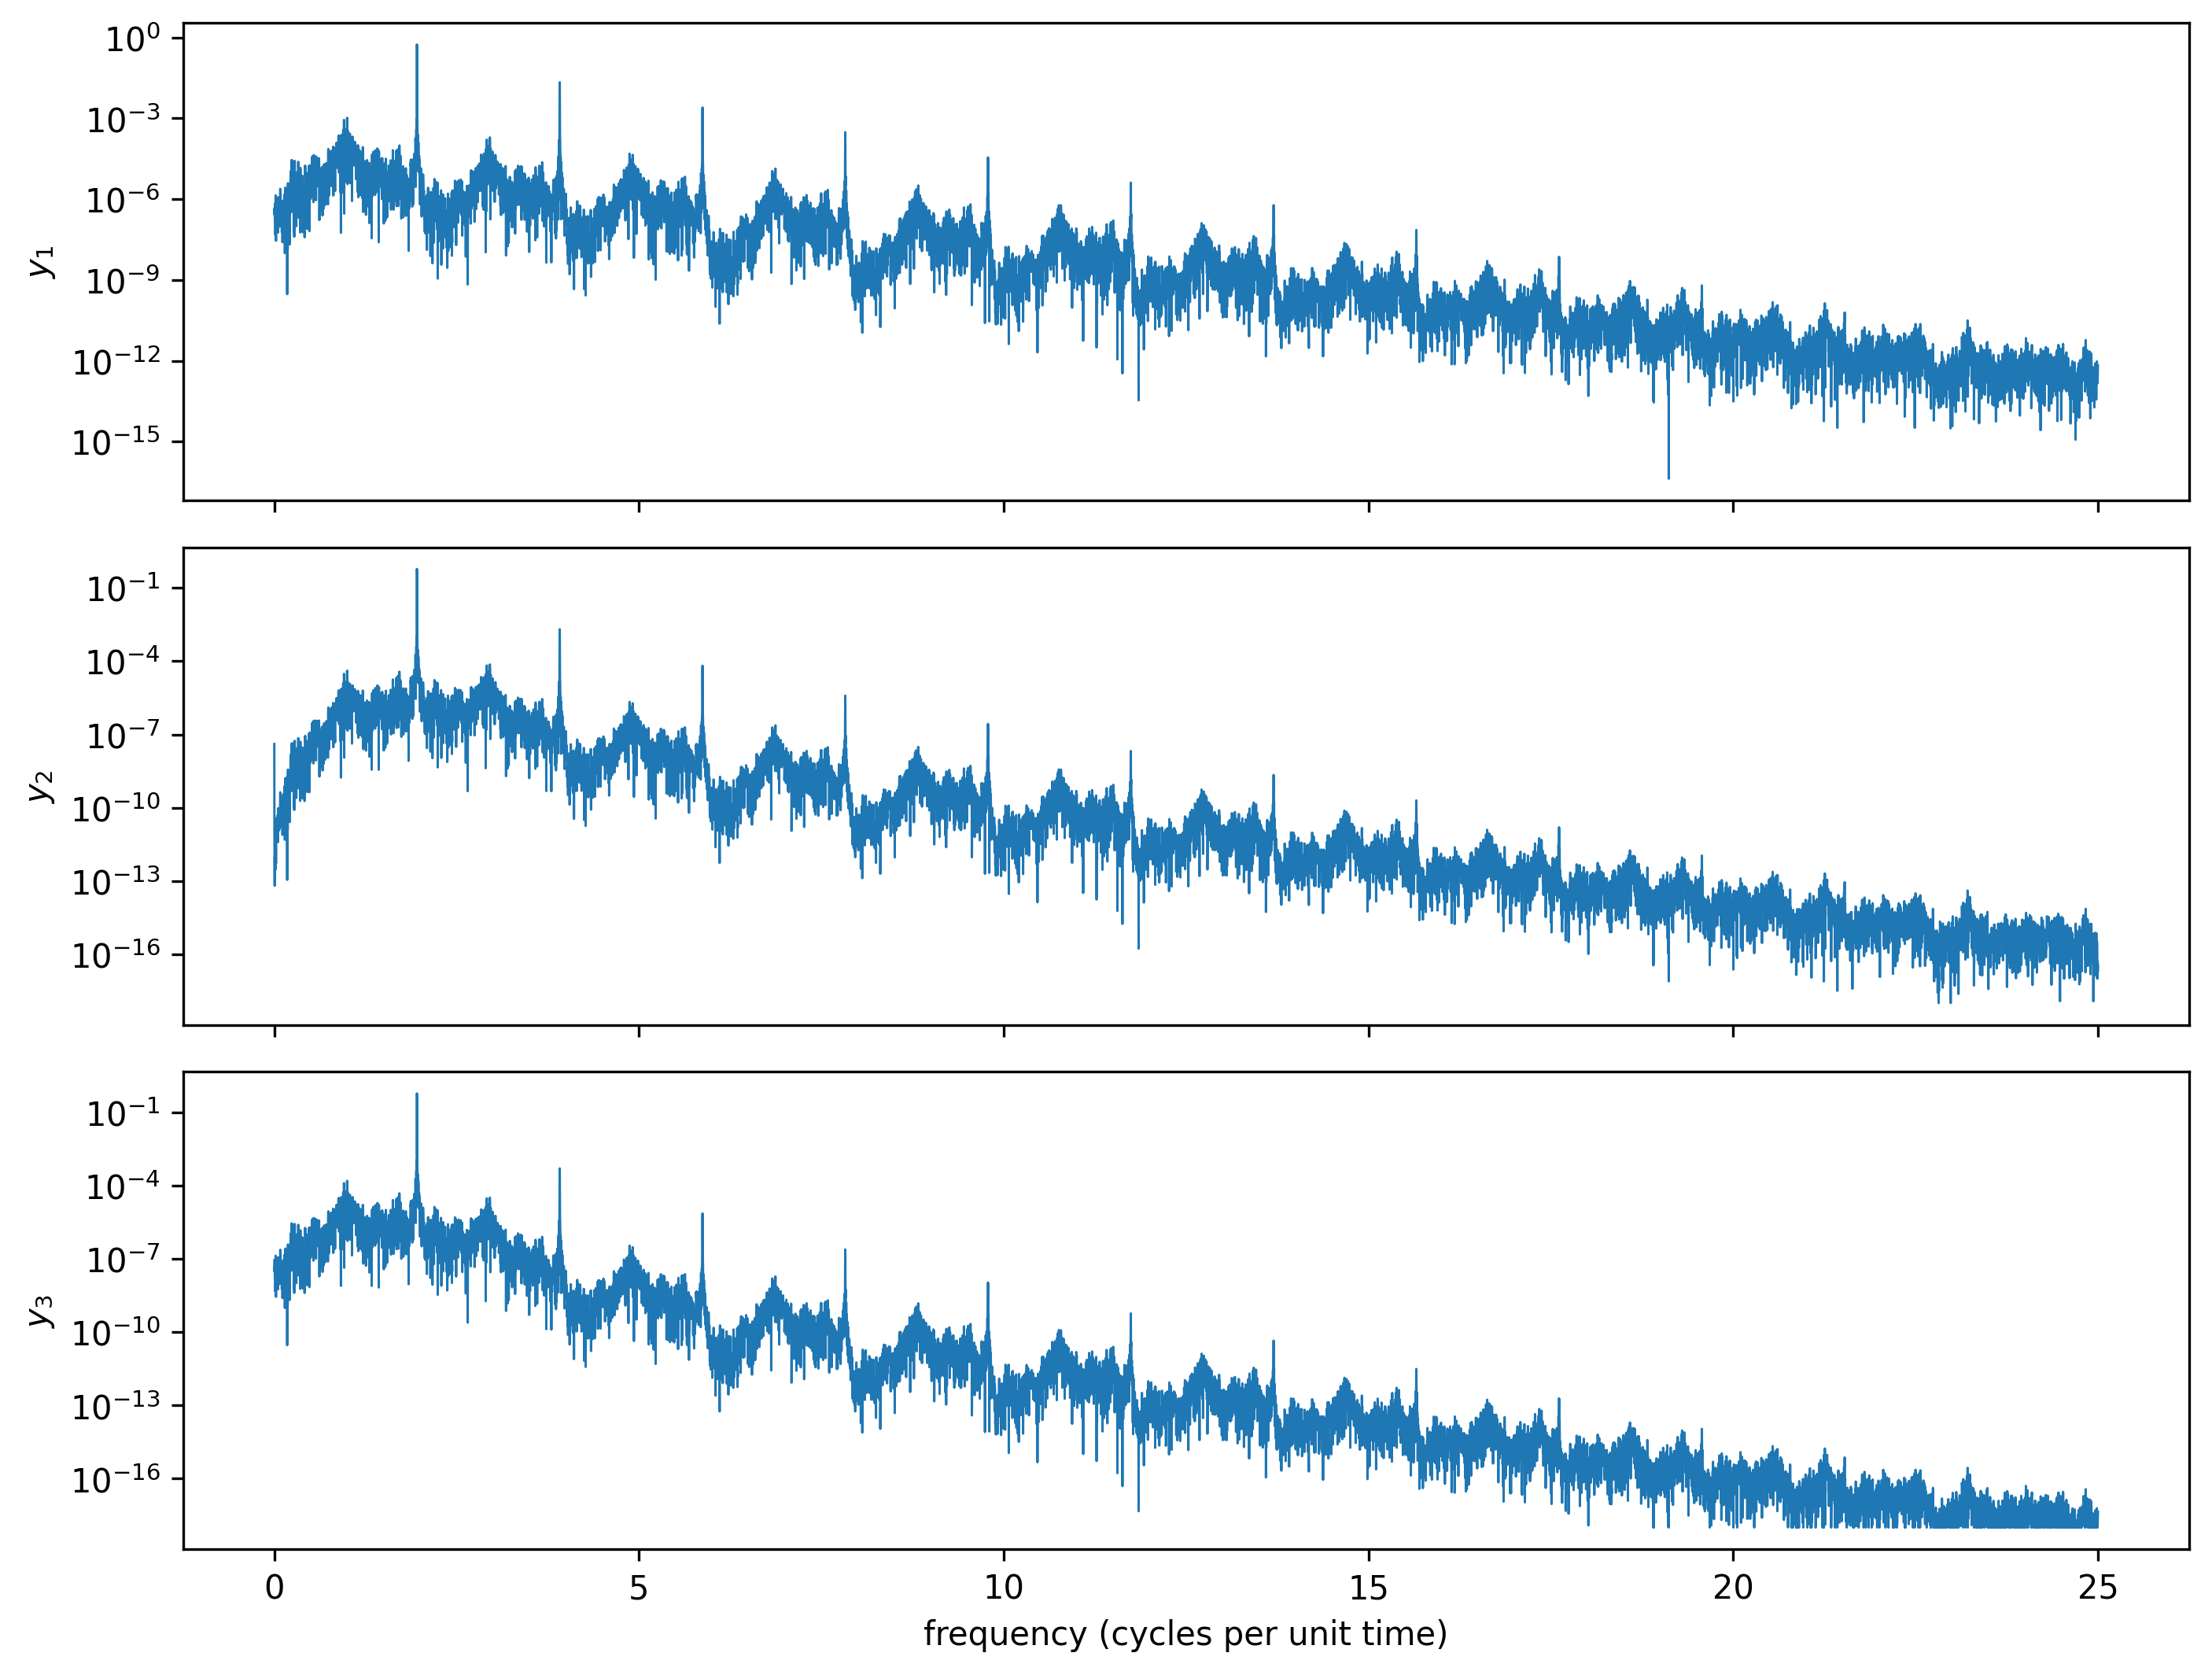
\includegraphics[width=0.82\textwidth]{mavpd_chaos_fft.png}
\caption{Potencia FFT normalizada del candidato.}
\label{int:fig:mavpd-chaos-fft}
\end{hafocommonfigure}

\ifHAFOBasinMaterial
\subsubsection*{Ocultedad bajo vecindades ensayadas}

El clasificador de la nube candidata se calibró con tres ventanas temporales
disjuntas de la misma trayectoria y verificó su separación usando los tres
equilibrios como controles negativos. Para dos nubes finitas \(A,B\), usa la
mediana simétrica de vecinos más cercanos, normalizada por la extensión \(S\)
de la referencia:
\begin{equation}
 d_N(A,B)=\frac{1}{S}\operatorname{mediana}\!\left(
 \{\min_{b\in B}\|a-b\|:a\in A\}\cup
 \{\min_{a\in A}\|b-a\|:b\in B\}\right).
 \label{int:eq:mavpd-cloud-distance}
\end{equation}
Si $R_1,R_2,R_3$ son las ventanas y \(R=R_1\cup R_2\cup R_3\), la escala es
\begin{equation}
 S=\left[\sum_{k=1}^{3}
 \left(\max_{x\in R}x_k-\min_{x\in R}x_k\right)^2\right]^{1/2},
 \qquad
 D(A)=\operatorname{mediana}_{j=1,2,3}d_N(A,R_j).
 \label{int:eq:mavpd-cloud-classifier}
\end{equation}
Si $b$ es el cuantil 0.95 de las distancias entre ventanas, el umbral es
$\tau=3b$ y el margen ambiguo es $m=\max(0.25\tau,b)$. En esta configuración,
$m=b=\tau/3$. Los controles negativos no fijan $\tau$: exigen
$\min_j d_N(N_\ell,R_j)>\tau+m$; de lo contrario se concluye que los controles
se solapan y la calibración se rechaza.

El protocolo principal contiene \MAVPDChaosMainProbes{} trayectorias:
3 equilibrios, radios $(10^{-5},10^{-3},10^{-2})$ y 12 direcciones esféricas
deterministas por radio. Se añadieron \MAVPDChaosTargetedProbes{} controles
dirigidos sobre ambos signos del autovector inestable de $E_0$, en radios
$10^{-7}$ y $10^{-4}$. En total hubo \MAVPDChaosTotalProbes{} trayectorias,
\MAVPDChaosHits{} contactos con la nube candidata, cero ambigüedades y cero
fallos numéricos; todas terminaron en un equilibrio.

\begin{hafobasinfigure}[H]
\centering
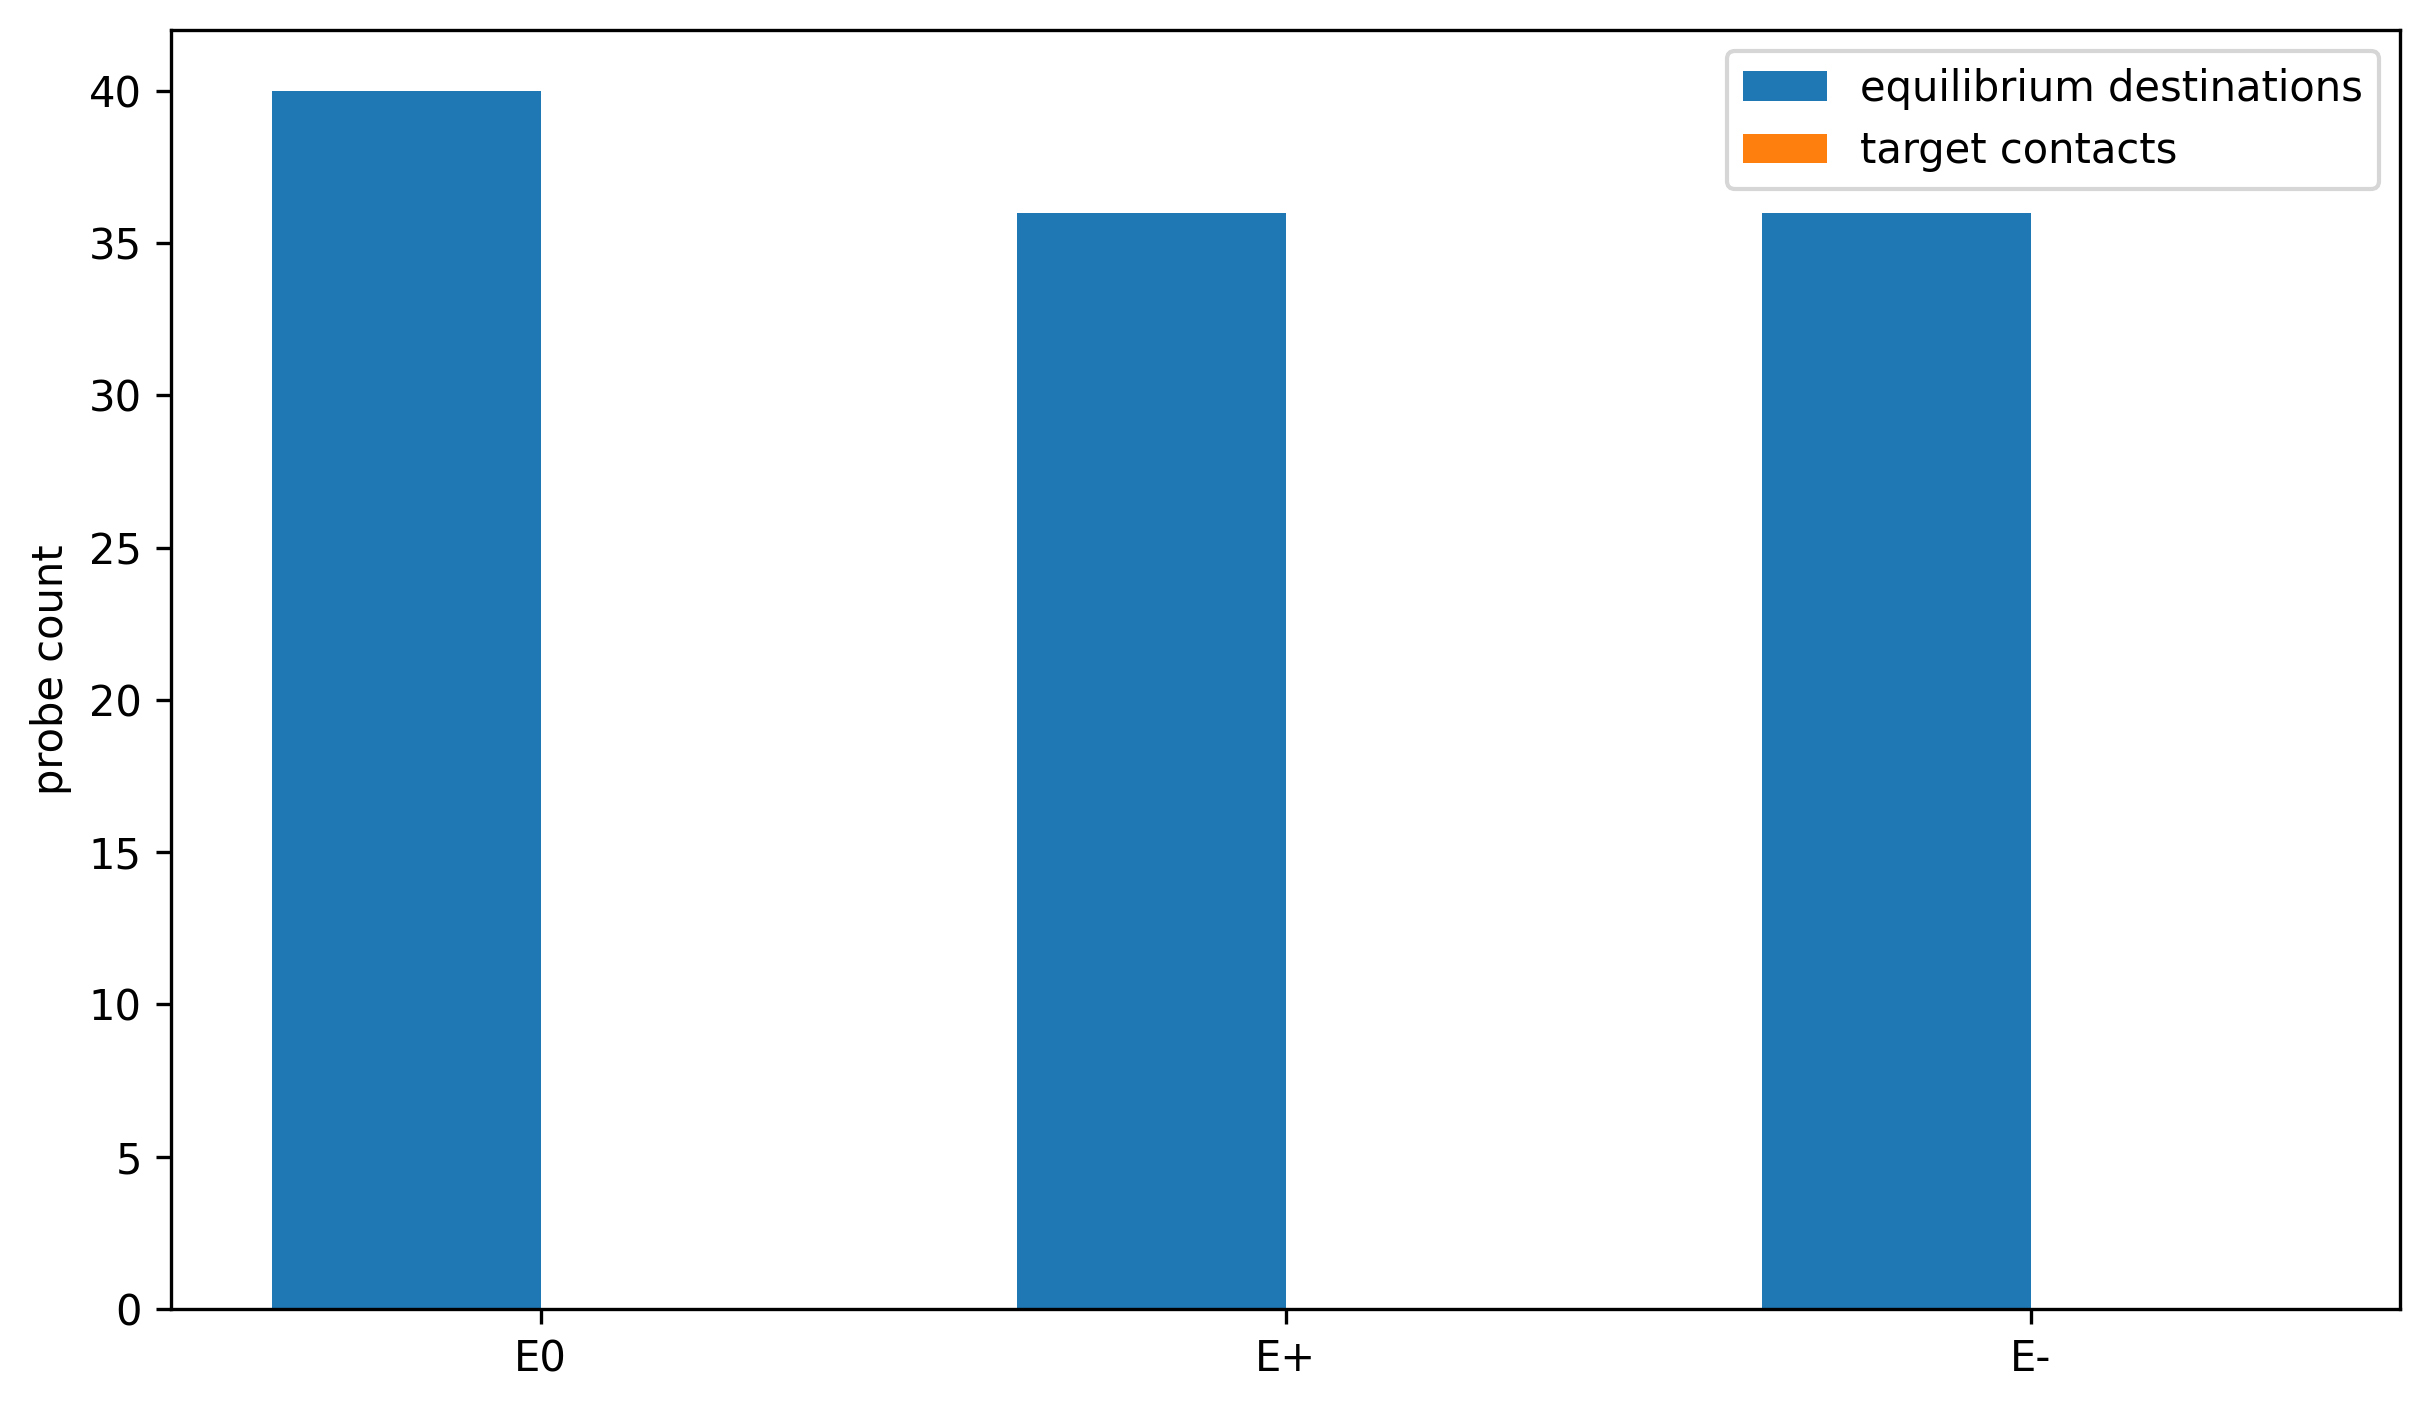
\includegraphics[width=0.88\textwidth]{mavpd_chaos_hiddenness.png}
\caption{Resultados de los sondeos alrededor de $E_0$, $E_+$ y $E_-$, junto
con los controles dirigidos del autovector inestable. Cero contactos es una
conclusión finita restringida a este protocolo.}
\label{int:fig:mavpd-chaos-hiddenness}
\end{hafobasinfigure}

La evaluación conjunta clasificó el resultado como compatible con caos y
ocultedad únicamente bajo las vecindades ensayadas. Los diagnósticos numéricos
y la ausencia de contactos se restringen a las ventanas y vecindades
declaradas; la desconexión global de la cuenca permanece sin demostrar.
\fi

\subsubsection*{Comparación numérica independiente}

El cálculo independiente en Julia partió de las ecuaciones y el Jacobiano, recalculó las
dos ramas D0 sin malla de frecuencias y sólo activó A1 después de que ambas
fallaron el umbral dinámico. La regla de menor $\omega_0$ volvió a seleccionar
la rama 0; después transportó el estado de $\xi=3.10$ a $2.85$, derivó la misma
frontera de Routh--Hurwitz y seleccionó de nuevo el desplazamiento $0.010$.
Durante esa localización no leyó la semilla, el estado terminal ni $\gamma$ de
Python.
\ifHAFOBasinMaterial
El intercambio de las condiciones de ocultedad ocurrió únicamente en la fase
posterior de comparación.
\fi

Python empleó DOP853 adaptativo para la trayectoria y la ecuación
variacional. Julia empleó RK4 de paso fijo para las trayectorias y los sondeos,
y reortogonalización QR para el cálculo variacional.

\begin{table}[H]
\centering
\caption{Comparación del candidato MAVPD caótico con tolerancias comunes.}
\label{int:tab:mavpd-chaos-cross-runtime}
\small
\begin{tabularx}{\textwidth}{@{}L{0.31\textwidth}YY@{}}
\toprule
Magnitud & Python/\hafo{} & Julia \\
\midrule
$\xi$ & \MAVPDChaosXi & \MAVPDChaosXi \\
$\gamma$ & \MAVPDChaosGamma & \MAVPDChaosGamma \\
$\widehat\lambda_1$ & \MAVPDChaosLEOne & \MAVPDChaosJuliaLEOne \\
$\widehat\lambda_2$ & \MAVPDChaosLETwo & \MAVPDChaosJuliaLETwo \\
$\widehat\lambda_3$ & \MAVPDChaosLEThree & \MAVPDChaosJuliaLEThree \\
$D_{KY}$ & \MAVPDChaosKY & \MAVPDChaosJuliaKY \\
Cruces de Poincaré & \MAVPDChaosPoincareCount & \MAVPDChaosJuliaPoincareCount \\
Mediana $K$ sobre retornos & \MAVPDChaosReturnKOne & \MAVPDChaosJuliaReturnK \\
\ifHAFOBasinMaterial
Decisiones de sondeo coincidentes &
\MAVPDChaosTotalProbes/\MAVPDChaosTotalProbes &
\MAVPDChaosJuliaProbeMatches/\MAVPDChaosTotalProbes \\
\fi
\bottomrule
\end{tabularx}
\end{table}

La comparación cruzada coincidió exactamente en $\xi$, $\gamma$ y el
desplazamiento de Hopf. Las estadísticas de la nube postransitoria y los
diagnósticos de caos quedaron dentro de sus bandas predeclaradas.
\ifHAFOBasinMaterial
Además, coincidieron las
\MAVPDChaosTotalProbes{} condiciones iniciales, estados, destinos y decisiones
de contacto.
\fi

\begin{hafobasinfigure}[H]
\centering
\begin{subfigure}[t]{0.49\textwidth}
  \centering
  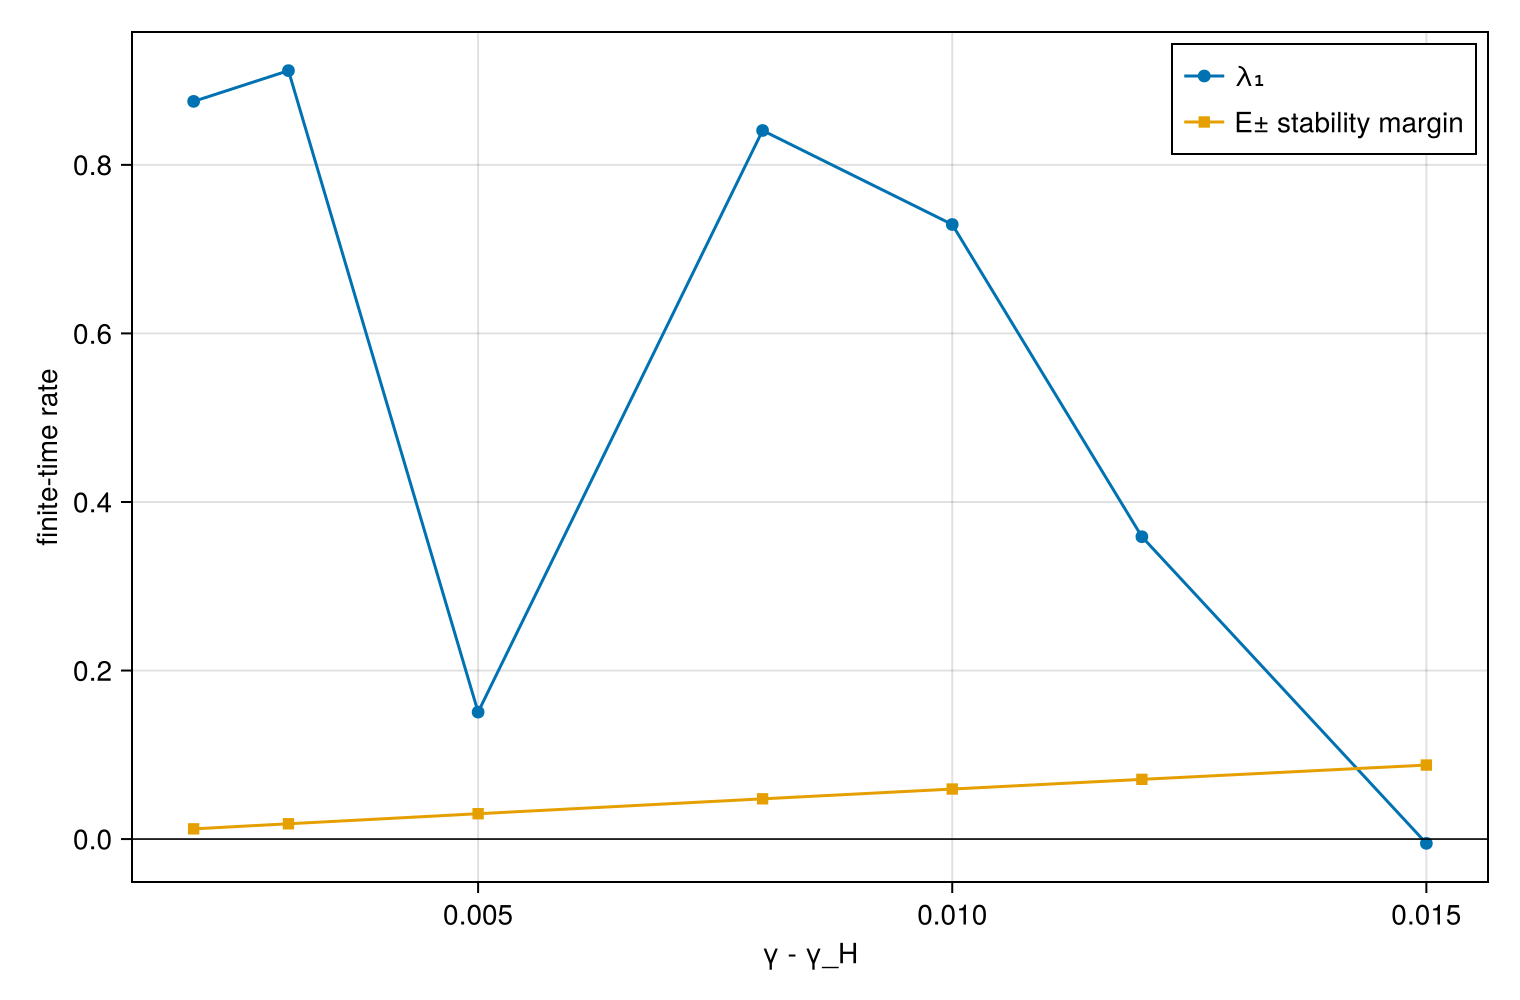
\includegraphics[width=\linewidth]{julia_mavpd_chaos_gamma_screen.png}
  \caption{Cribado y selección de $\gamma$ recalculados en Julia.}
\end{subfigure}\hfill
\begin{subfigure}[t]{0.49\textwidth}
  \centering
  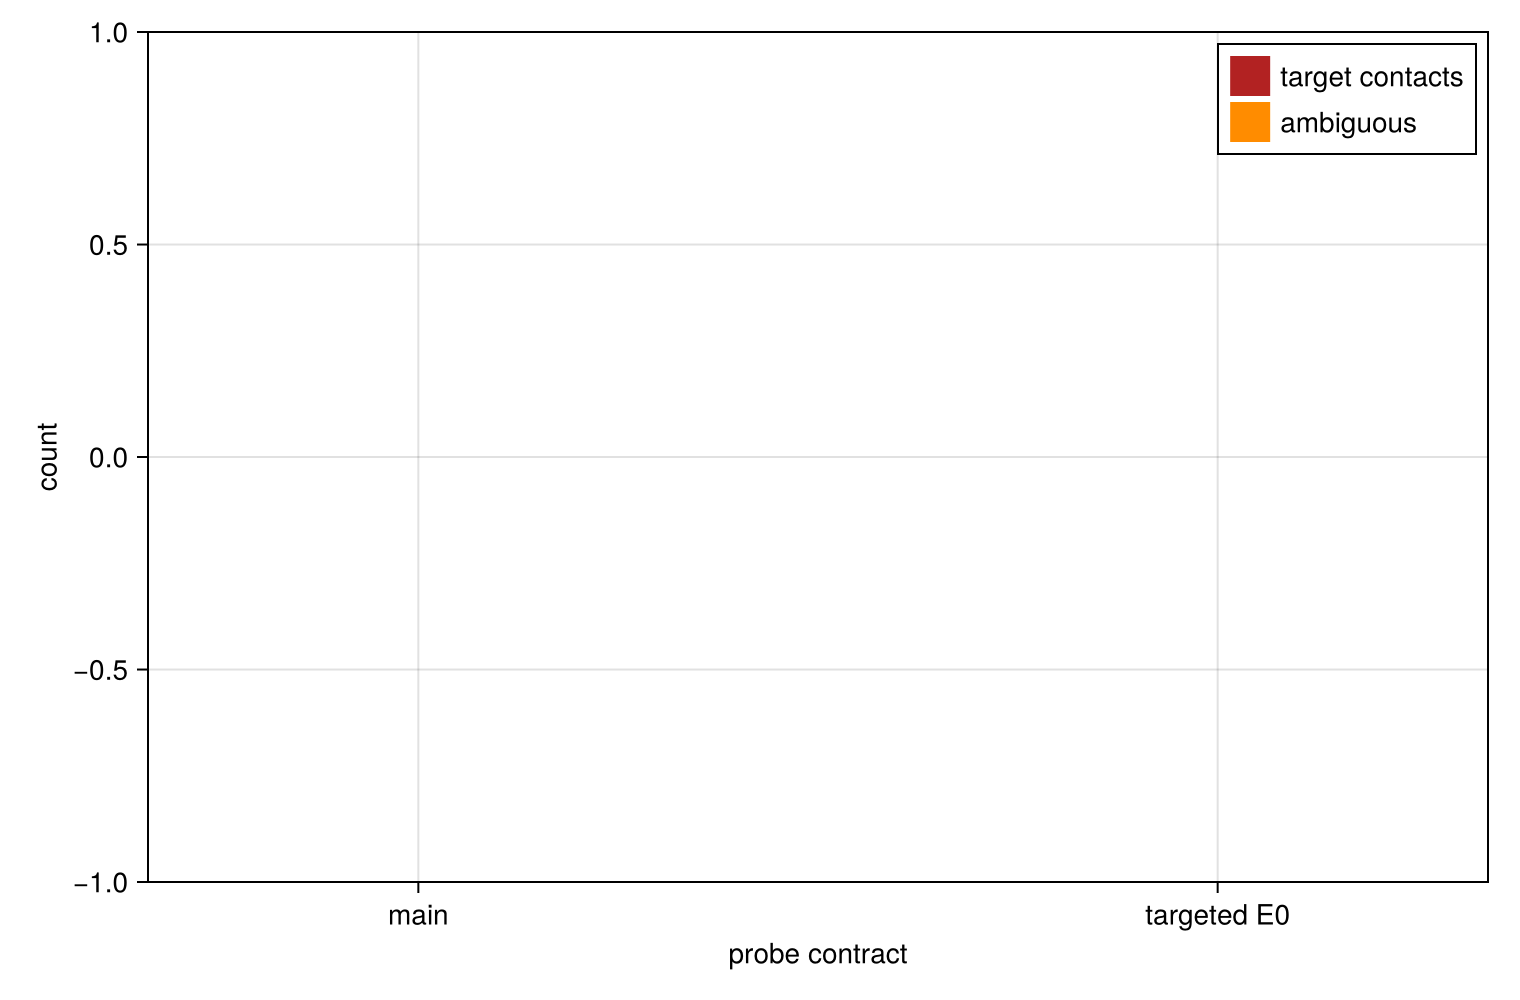
\includegraphics[width=\linewidth]{julia_mavpd_chaos_hiddenness_outcomes.png}
  \caption{Decisión de los 112 sondeos finitos en Julia.}
\end{subfigure}
\caption{Artefactos de la reproducción Julia MAVPD. El primer panel es un
diagnóstico de continuación; el segundo resume un protocolo finito de cuenca.}
\label{int:fig:mavpd-chaos-julia}
\end{hafobasinfigure}

\begin{hafocommonfigure}[H]
\centering
\begin{subfigure}[t]{0.49\textwidth}
  \centering
  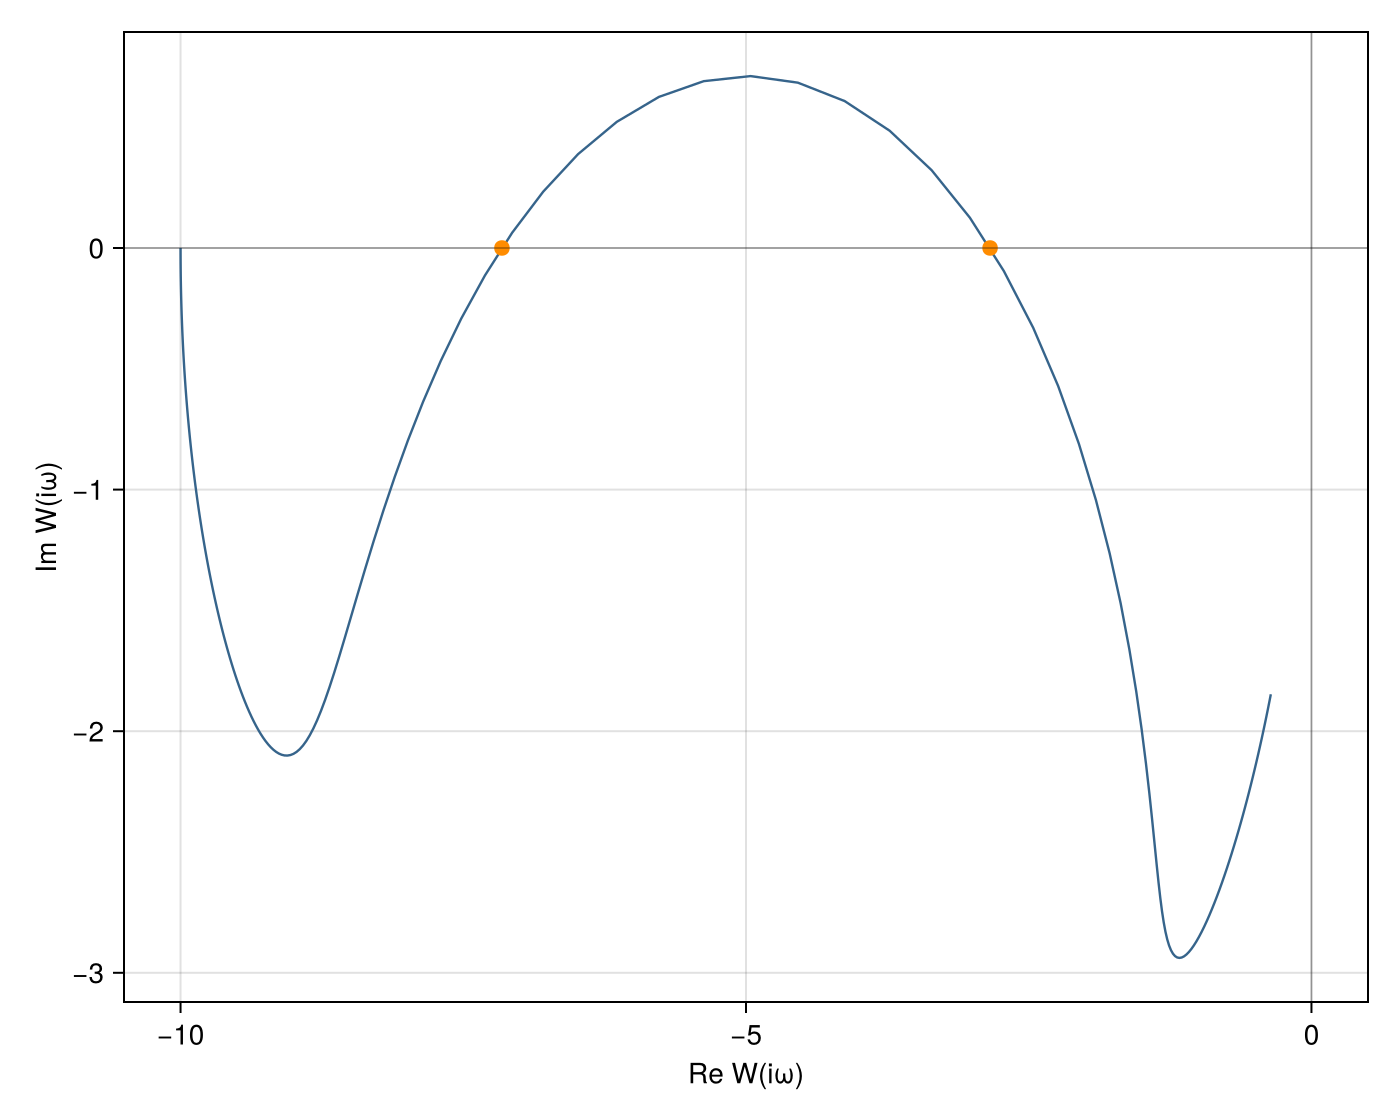
\includegraphics[width=\linewidth]{julia_mavpd_chaos_nyquist_diagnostic.png}
  \caption{Nyquist de la transferencia ya derivada.}
\end{subfigure}\hfill
\begin{subfigure}[t]{0.49\textwidth}
  \centering
  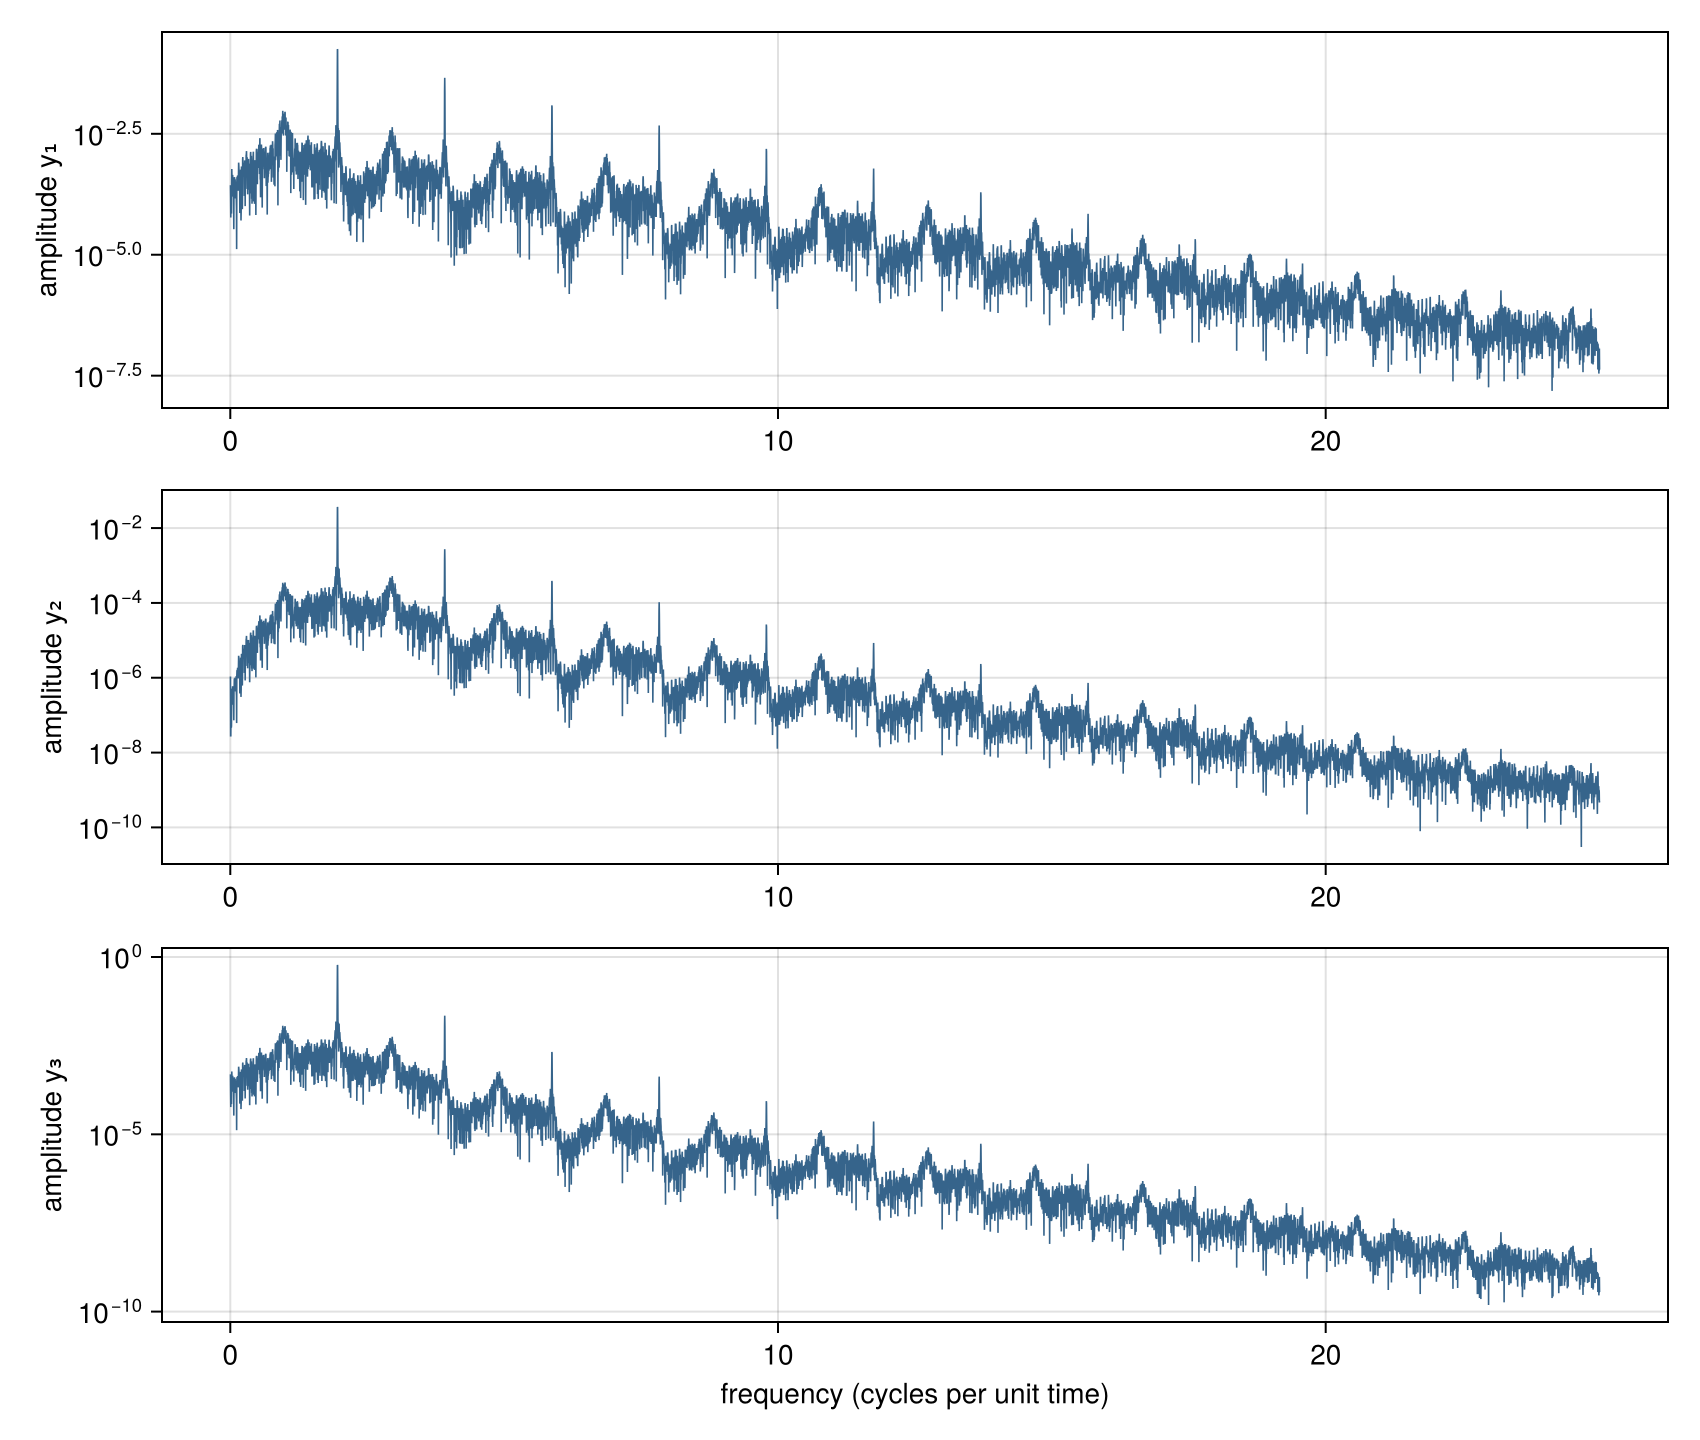
\includegraphics[width=\linewidth]{julia_mavpd_chaos_amplitude_spectrum.png}
  \caption{Espectro de amplitud FFT postransitorio.}
\end{subfigure}
\caption{Diagnósticos intermedios Julia MAVPD. Nyquist no suministra una malla
de búsqueda ni selecciona $\omega_0$; la FFT no se denomina PSD.}
\label{int:fig:mavpd-chaos-julia-spectral}
\end{hafocommonfigure}


\section{Caso 4: PLL bifásico con filtro lead--lag}

\subsection{Transformación T1 y obstrucción directa}

El modelo publicado es
\begin{align}
 \dot x&=-\frac{x}{T}+\frac{\tau_1}{2T}\sin\theta,\nonumber\\
 \dot\theta&=\omega_\Delta-\frac{Lx}{T}
 -\frac{\tau_2L}{2T}\sin\theta,\qquad T=\tau_1+\tau_2,
 \label{int:eq:pll}
\end{align}
con \(\tau_1=0.0448\), \(\tau_2=0.0185\), \(L=500\) y
\(\omega_\Delta=178.9\) \cite{pll2015}. El desplazamiento de un equilibrio
bloqueado elimina el término afín, de modo que el sistema es T1. Como
\(\theta\) es angular, la recurrencia y las distancias se calculan módulo
\(2\pi\), no con una norma euclidiana sin envolver.

En un equilibrio, la primera ecuación da
\(x_e=(\tau_1/2)\sin\theta_e\). Sustituir en la segunda y usar
\(T=\tau_1+\tau_2\) conduce a
\[
 0=\omega_\Delta-\frac{L(\tau_1+\tau_2)}{2T}\sin\theta_e,
 \qquad \sin\theta_e=\frac{2\omega_\Delta}{L}=0.7156.
\]
En una vuelta del cilindro hay dos soluciones:
\[
 x_e=0.01602944,\qquad
 \theta_f=0.797482699882,\qquad
 \theta_s=2.344109953708.
\]
El Jacobiano en cualquiera de ellas es
\[
 J_e=\begin{pmatrix}
 -1/T&\tau_1\cos\theta_e/(2T)\\
 -L/T&-\tau_2L\cos\theta_e/(2T)
 \end{pmatrix},
\]
con
\[
 \operatorname{tr}J_e=-\frac{1+\tau_2L\cos\theta_e/2}{T},\qquad
 \det J_e=\frac{L\cos\theta_e}{2T}.
\]
En \(\theta_f\), la traza es negativa, el determinante positivo y el
discriminante \((\operatorname{tr}J_e)^2-4\det J_e\) es negativo para estos
parámetros: se obtiene un foco estable. En \(\theta_s\), el determinante es
negativo y el equilibrio es una silla.

El cambio \(u=x-x_e\), \(v=\theta-\theta_e\) transforma el campo en
\[
 \begin{pmatrix}\dot u\\\dot v\end{pmatrix}
 =P\begin{pmatrix}u\\v\end{pmatrix}+b\psi(v),
\]
\[
 P=\begin{pmatrix}-1/T&0\\-L/T&0\end{pmatrix},\quad
 b=\begin{pmatrix}\tau_1/(2T)\\-\tau_2L/(2T)\end{pmatrix},
 \quad c=\begin{pmatrix}0\\1\end{pmatrix},
\]
con \(\psi(v)=\sin(v+\theta_e)-\sin\theta_e\). Las identidades del
equilibrio cancelan los términos constantes. Para una entrada \(\psi\),
la primera fila del resolvente \((sI-P)^{-1}b\) da
\[
 u=\frac{\tau_1}{2(1+Ts)}\psi,
\]
y la segunda da
\[
 sv=-\frac L{2T}\left[\frac{\tau_1}{1+Ts}+\tau_2\right]\psi
    =-\frac L2\frac{1+\tau_2s}{1+Ts}\psi.
\]
Por tanto, las dos convenciones de transferencia se relacionan mediante
\begin{equation}
 W(s)=c^{\mathsf T}(sI-P)^{-1}b
     =-\frac L2\frac{1+\tau_2s}{s(1+Ts)}=-G(s).
 \label{int:eq:pll-transfer}
\end{equation}
Al multiplicar el cociente en \(s=i\omega\) por el conjugado de su
denominador,
\[
 W(i\omega)=\frac{L\tau_1}{2(1+T^2\omega^2)}
 +i\,\frac{L(1+\tau_2T\omega^2)}{2\omega(1+T^2\omega^2)}.
\]
Así, \(\operatorname{Im}W(i\omega)>0\) y
\(\operatorname{Im}G(i\omega)<0\) para todo \(\omega>0\). Ninguna
convención admite el cruce real requerido por una ganancia descriptiva real;
la ruta directa no produce candidatos.

\subsection{Ruta A1 de Andronov}

Para \(L>0\), definir \(y=\dot\theta\) permite recuperar la variable
original mediante
\begin{equation}
 x=\frac T L(\omega_\Delta-y)-\frac{\tau_2}{2}\sin\theta.
 \label{int:eq:pll-inverse-andronov}
\end{equation}
Derivando la segunda ecuación de \eqref{int:eq:pll},
\[
 \dot y=-\frac L T\dot x-\frac{\tau_2L}{2T}\cos\theta\,y
        =\frac L{T^2}x-\frac{L\tau_1}{2T^2}\sin\theta
         -\frac{\tau_2L}{2T}\cos\theta\,y.
\]
Sustituir \eqref{int:eq:pll-inverse-andronov} y agrupar
\(\tau_1+\tau_2=T\) produce
\begin{equation}
 T\dot y=\omega_\Delta-\frac{L}{2}\sin\theta
 -\left(1+\frac{\tau_2L}{2}\cos\theta\right)y.
 \label{int:eq:pll-andronov}
\end{equation}
Para una rotación positiva se exige \(y(\theta)>0\) durante toda la
vuelta. Entonces \(\theta\) puede usarse como variable independiente:
\begin{equation}
 \frac{\dd y}{\dd\theta}=H_L(\theta,y)
 =\frac{\omega_\Delta-(L/2)\sin\theta}{Ty}
  -\frac{1+(\tau_2L/2)\cos\theta}{T}.
 \label{int:eq:pll-angle-flow}
\end{equation}
Con \(y(0)=y_0>0\), el mapa de retorno es
\(P_L(y_0)=y(2\pi;y_0)\). Una órbita rotatoria cumple
\(P_L(y_0)-y_0=0\), y su periodo físico es
\[
 \mathcal T(y_0)=\int_0^{2\pi}\frac{\dd\theta}{y(\theta;y_0)}.
\]
La derivada del retorno se calcula diferenciando la ecuación respecto de
\(y_0\). Si \(z=\partial y/\partial y_0\),
\[
 \frac{\dd z}{\dd\theta}
 =-\frac{\omega_\Delta-(L/2)\sin\theta}{Ty^2}z,
 \qquad z(0)=1,\qquad P_L'(y_0)=z(2\pi).
\]
El multiplicador transversal es \(P_L'(y_0)\): módulo menor que uno indica
estabilidad local, y módulo mayor que uno inestabilidad. El mapa queda
indefinido para esta construcción si la solución pierde la rotación positiva
antes de completar \(2\pi\).

En \(L=0\), la ecuación reducida admite \(y(\theta)\equiv\omega_\Delta\),
con
\[
 \mathcal T_0=\frac{2\pi}{\omega_\Delta},\qquad
 P_0'(\omega_\Delta)=\exp\!\left(-\frac{2\pi}{T\omega_\Delta}\right).
\]
En las coordenadas originales, \(\theta(t)=\omega_\Delta t\) y el filtro
satisface una ecuación lineal forzada. Una solución particular periódica
\(x_p=A\sin\theta+B\cos\theta\) cumple
\(A-\omega_\Delta TB=\tau_1/2\) y
\(\omega_\Delta TA+B=0\). Por tanto,
\[
 x_p(\theta)=\frac{\tau_1}{2[1+(\omega_\Delta T)^2]}
             [\sin\theta-\omega_\Delta T\cos\theta].
\]
Las restantes soluciones difieren de ella en \(C\e^{-t/T}\), lo cual
concuerda con el multiplicador transversal calculado.
Esta solución inicia la continuación de la ecuación reducida en 101 valores
hasta \(L=500\). La reconstrucción de \(x\) mediante
\eqref{int:eq:pll-inverse-andronov} se aplica sólo en los niveles \(L>0\),
pues el cambio de variables es singular en \(L=0\). Las condiciones iniciales
publicadas se reservan para la comparación posterior.

El análisis localizó:

\begin{table}[H]
\centering
\caption{Órbitas de retorno PLL en \(L=500\).}
\small
\begin{tabular}{@{}lrrrr@{}}
\toprule
Órbita & \(y_0\) & \(x_0\) & Periodo & Multiplicador \\
\midrule
Ciclo estable &
140.125084913 & 0.004908904250 &
\PLLPythonStablePeriod & \PLLPythonStableMultiplier \\
Separatriz inestable &
135.172047420 & 0.005535958797 &
\PLLPythonSeparatrixPeriod & \PLLPythonSeparatrixMultiplier \\
\bottomrule
\end{tabular}
\end{table}

Los errores de retorno Python sobre el cilindro fueron
\(2.68\times10^{-15}\) para el ciclo estable y
\(6.18\times10^{-14}\) para la separatriz. Julia reprodujo los periodos
\(\PLLJuliaStablePeriod\) y \(\PLLJuliaSeparatrixPeriod\), con multiplicadores
\(\PLLJuliaStableMultiplier\) y \(\PLLJuliaSeparatrixMultiplier\). Las tres
condiciones iniciales publicadas quedaron fuera del flujo de localización: el
control posterior confirmó que dos alcanzan el ciclo y una el foco.

\begin{hafocommonfigure}[H]
\centering
\begin{subfigure}[t]{0.49\textwidth}
  \centering
  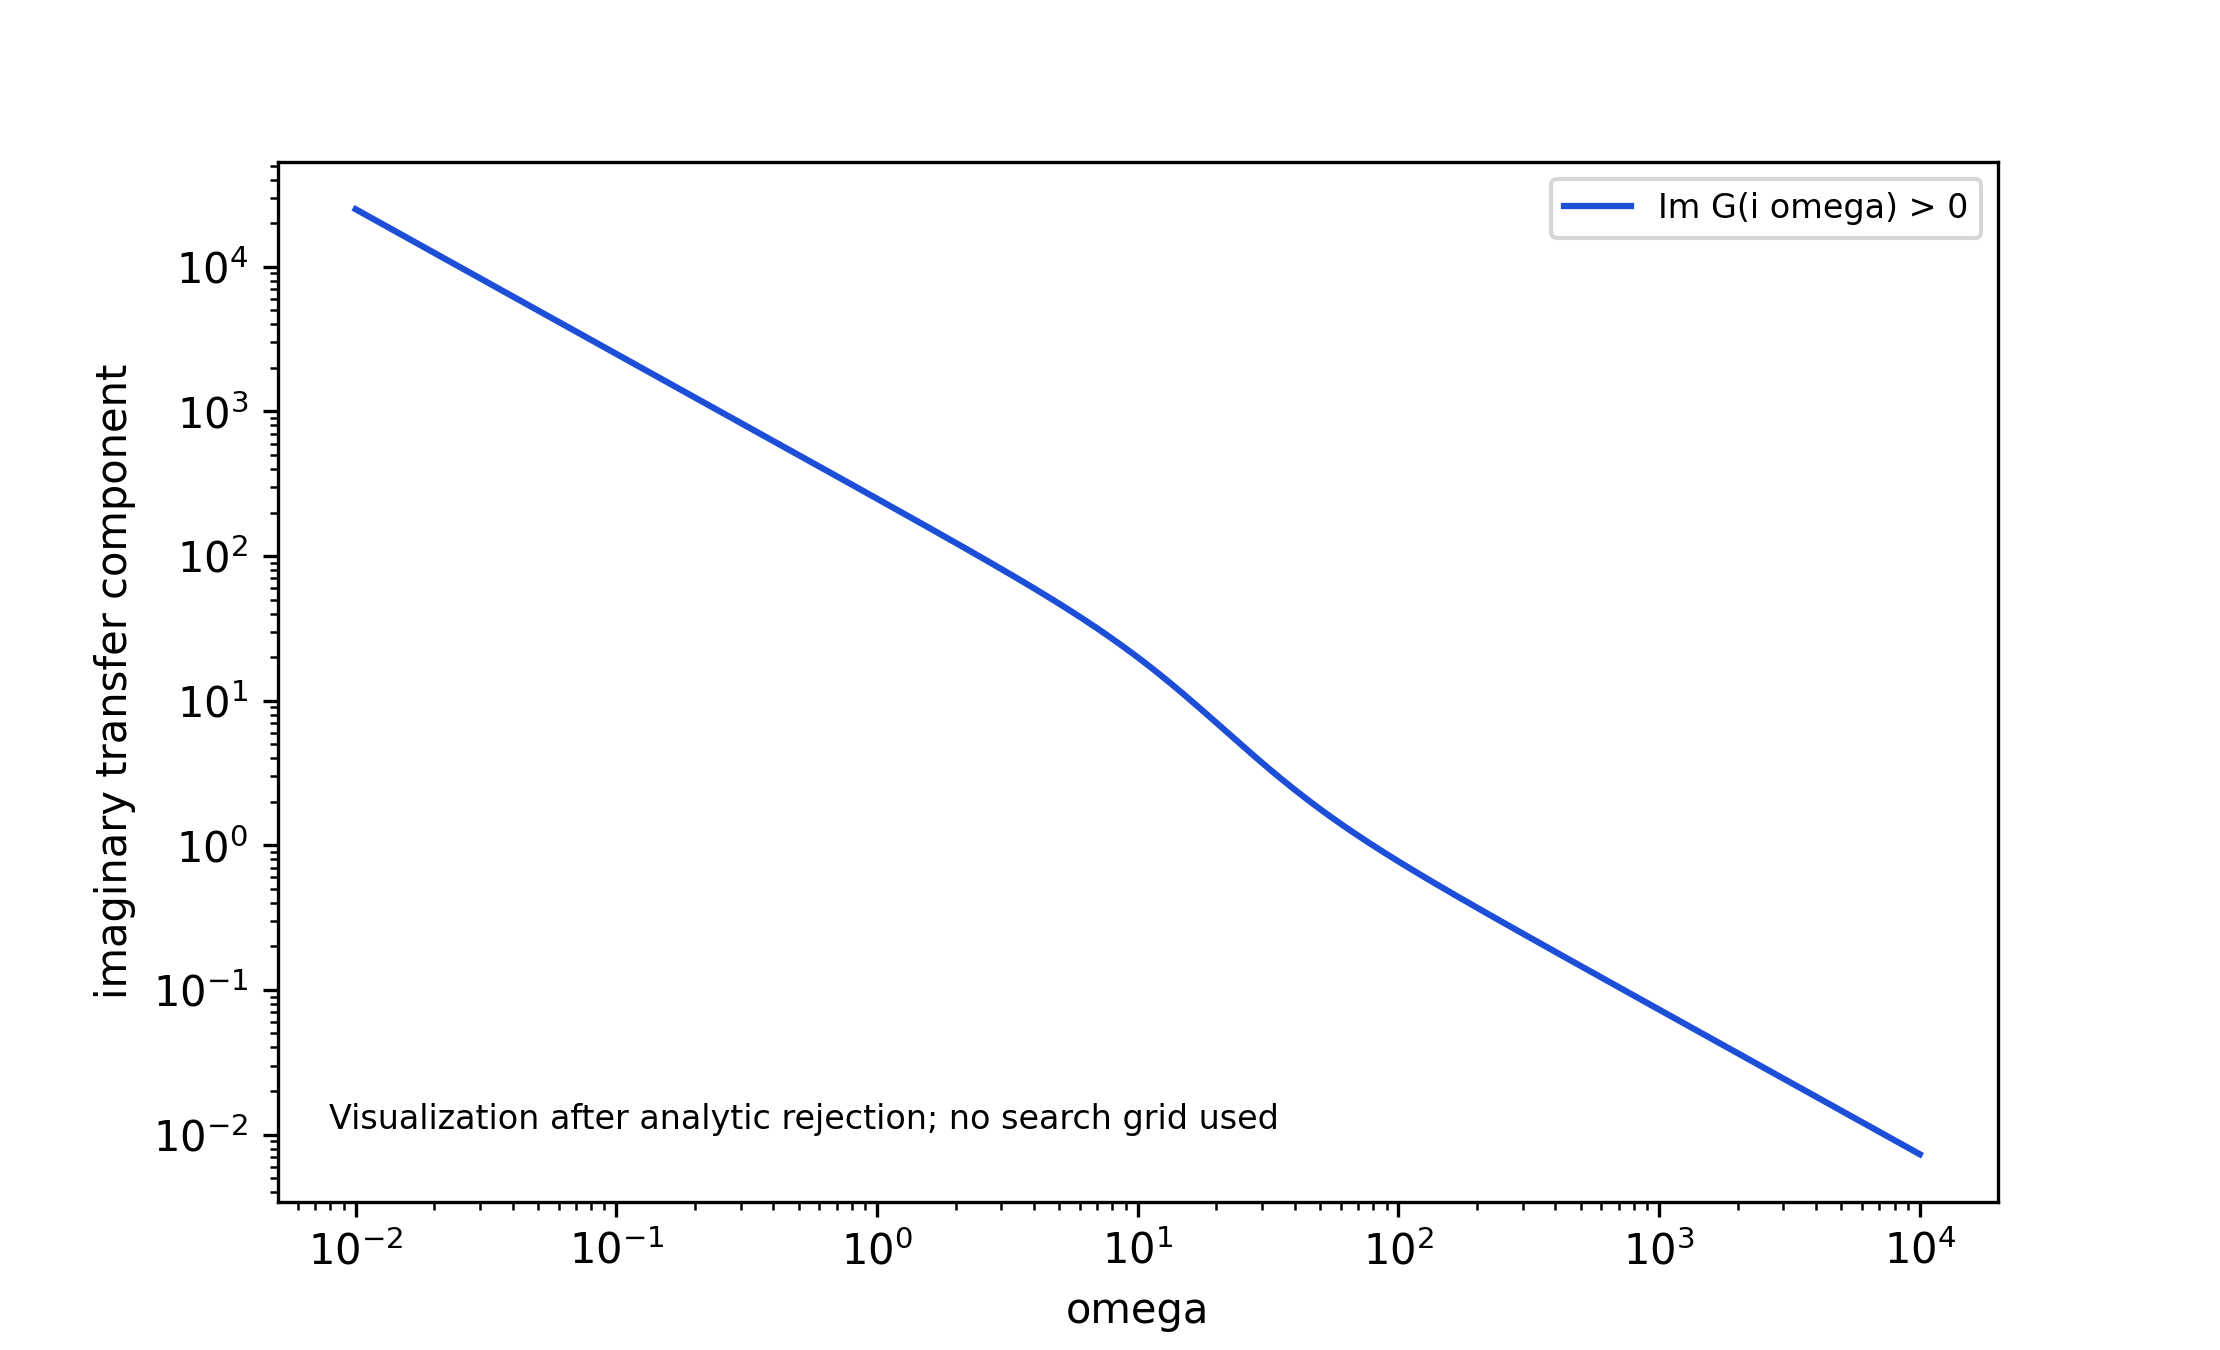
\includegraphics[width=\linewidth]{pll_transfer_obstruction.png}
  \caption{Obstrucción analítica de la ruta directa.}
\end{subfigure}\hfill
\begin{subfigure}[t]{0.49\textwidth}
  \centering
  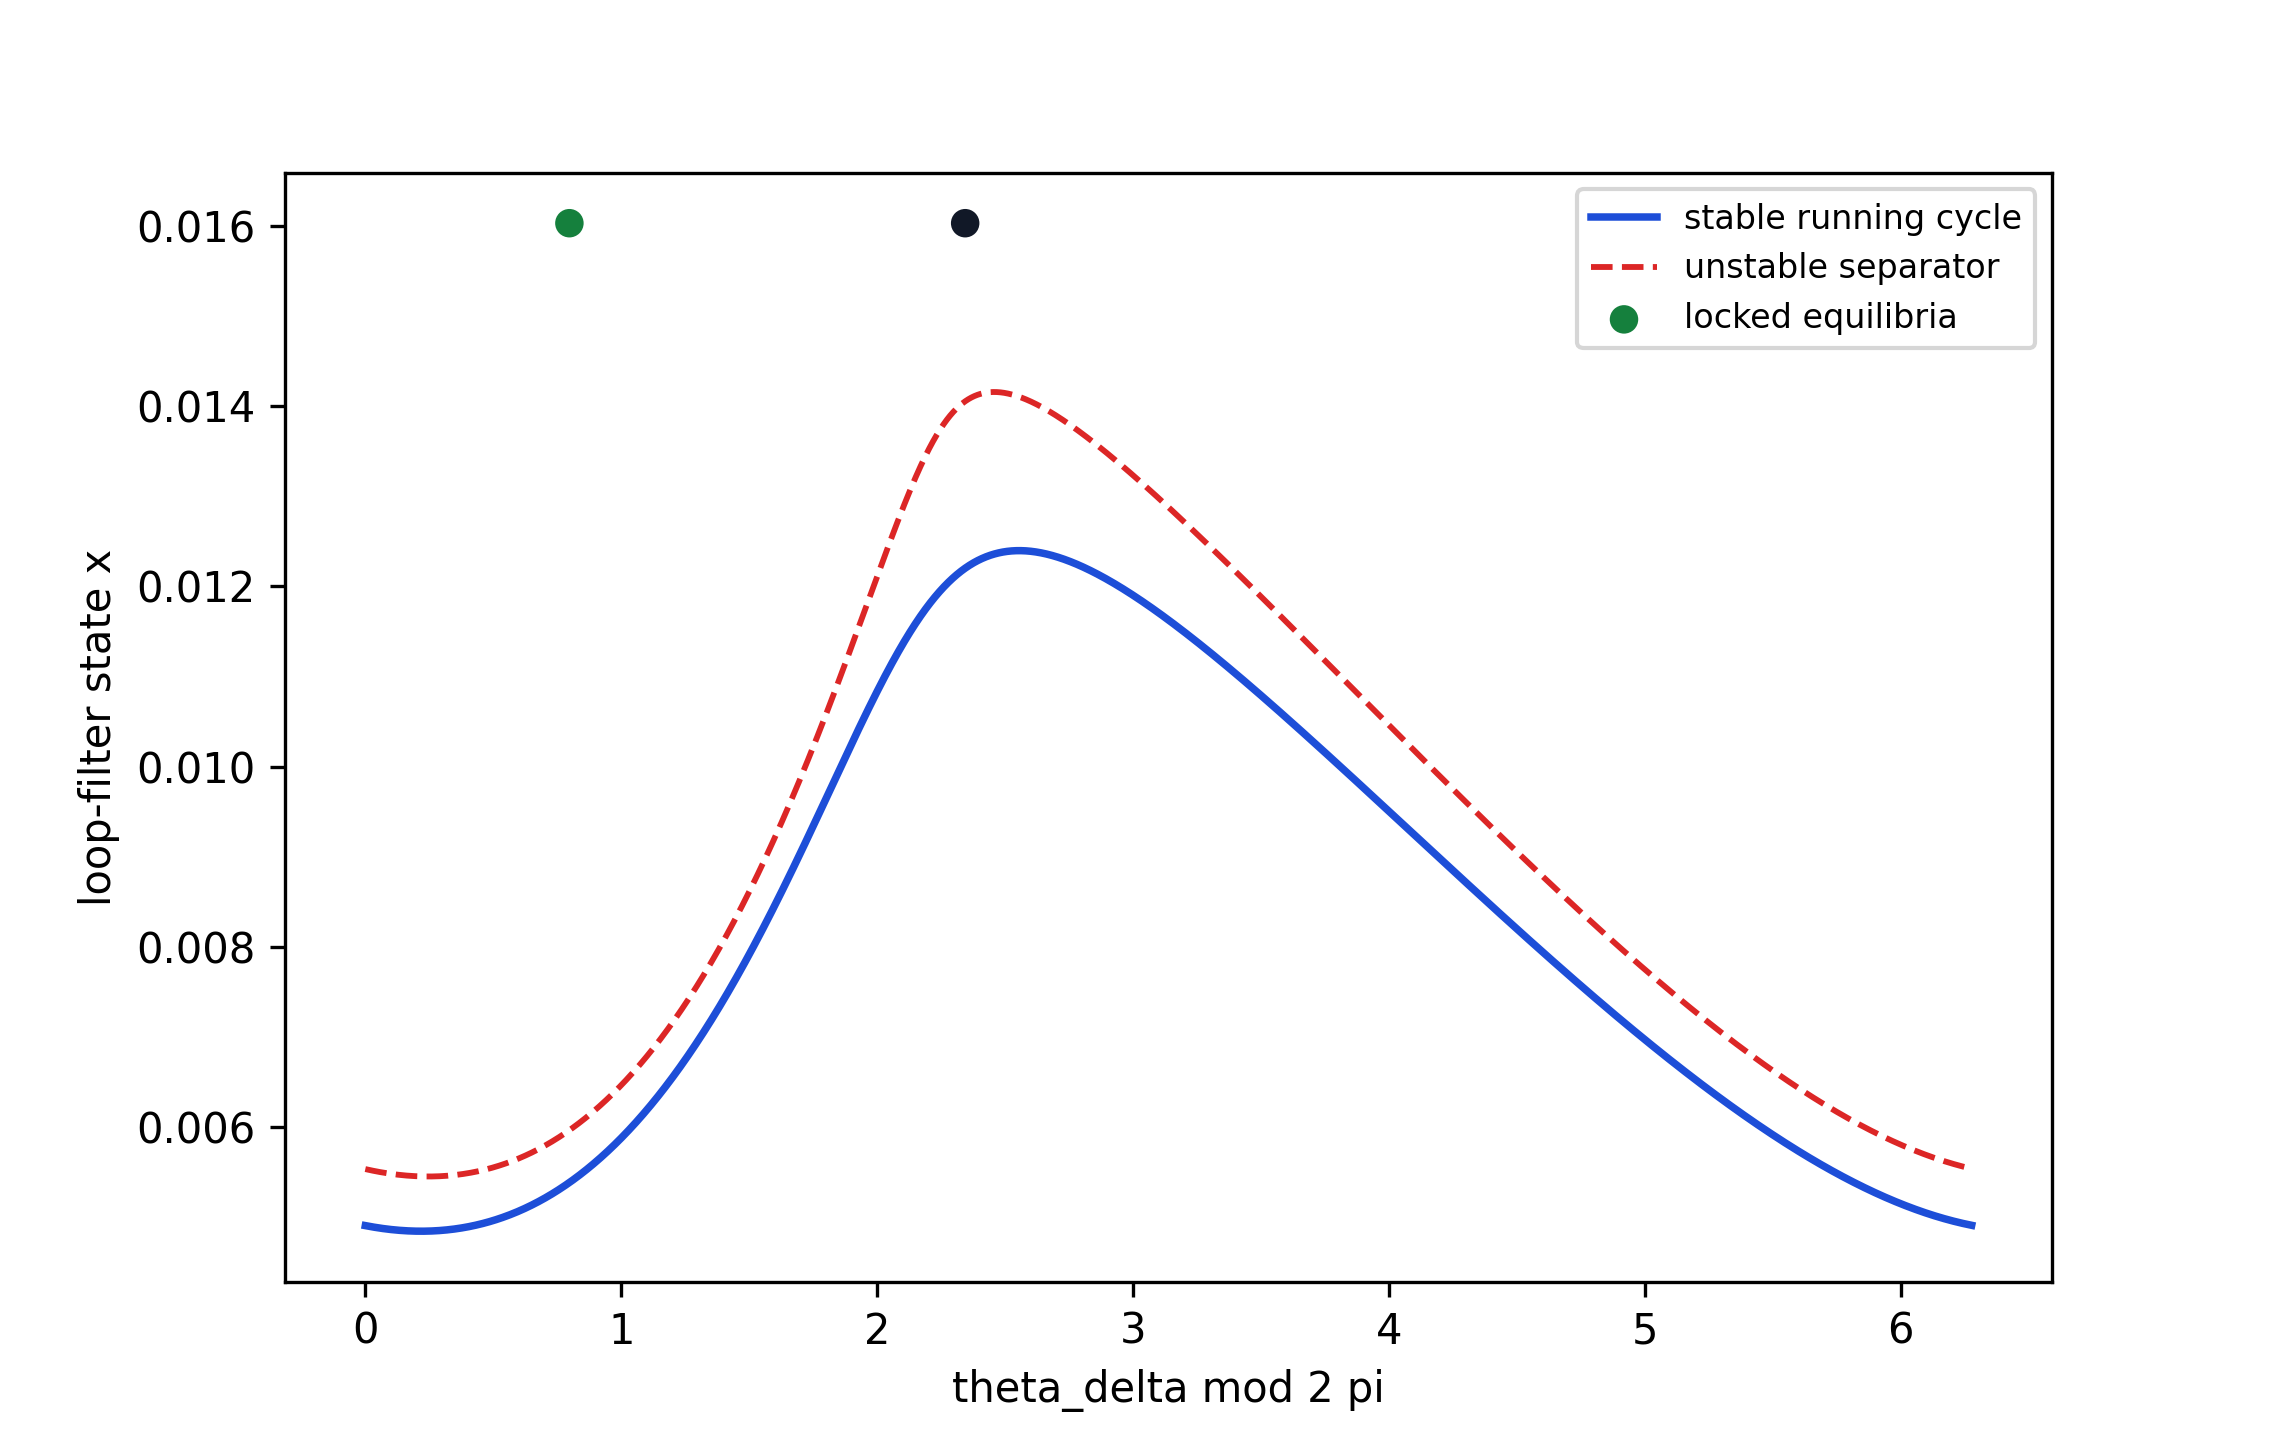
\includegraphics[width=\linewidth]{pll_phase_cylinder_cycles.png}
  \caption{Ciclo estable y separatriz en \(\mathbb R\times S^1\).}
\end{subfigure}
\caption{Localización T1 + A1 del PLL lead--lag.}
\label{int:fig:pll-route}
\end{hafocommonfigure}

\ifHAFOBasinMaterial
\subsection{Sondeos cilíndricos y estado comparativo}

El sondeo común usó \PLLProbeCount{} condiciones:
2 equilibrios, 4 radios \((10^{-5},10^{-4},10^{-3},10^{-2})\) y 12
direcciones por radio. Ninguna alcanzó el ciclo. Las 48 condiciones alrededor
del foco y las 48 alrededor del punto silla terminaron en el foco. Por tanto,
el resultado es compatible con ocultedad bajo el sondeo cilíndrico declarado.

\begin{hafobasinfigure}[H]
\centering
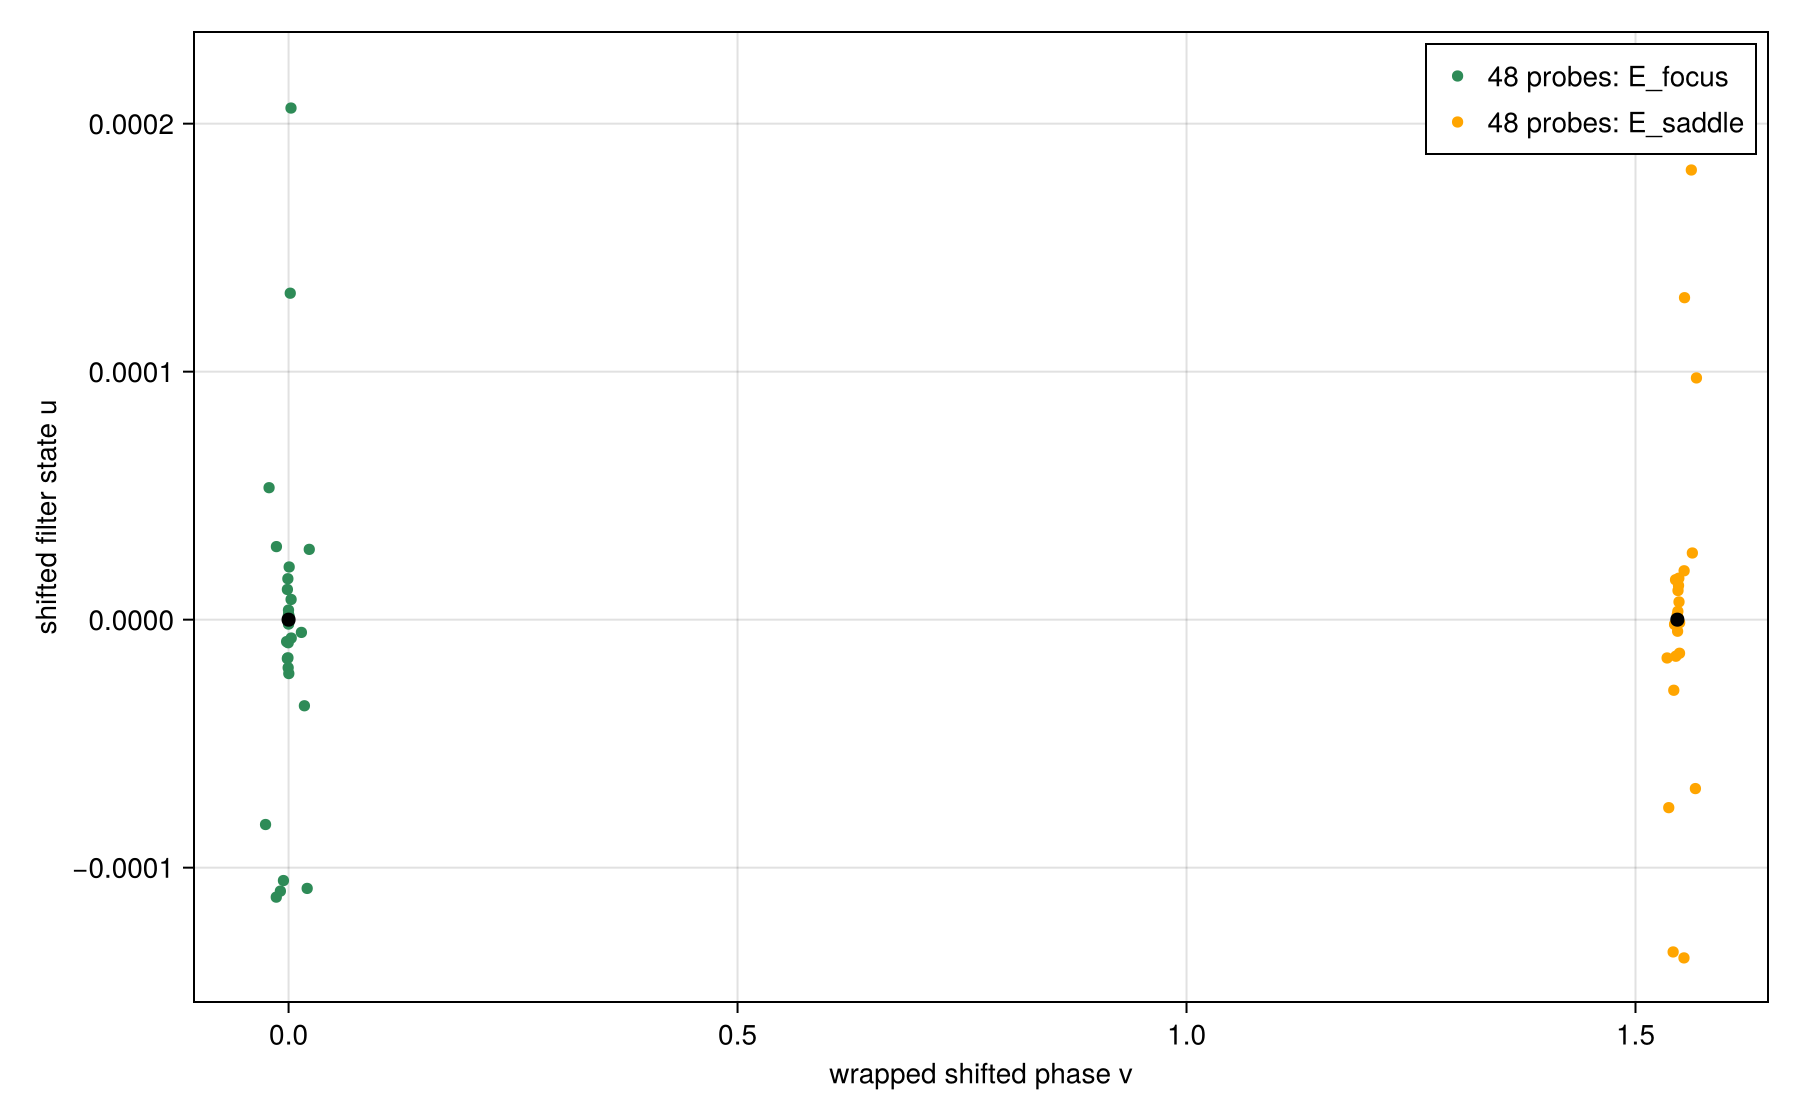
\includegraphics[width=0.82\textwidth]{julia_pll_cylindrical_hiddenness_probes.png}
\caption{Visualización Julia de las condiciones iniciales comunes del control
PLL, expresadas en las coordenadas envueltas del cilindro.}
\label{int:fig:pll-hiddenness}
\end{hafobasinfigure}
\fi

Julia implementó independientemente la misma distancia angular, el mapa de
retorno y la continuación desde la solución exacta en $L=0$; no leyó estados
Python ni las condiciones publicadas para localizar las órbitas.
\ifHAFOBasinMaterial
Coincidieron
\PLLJuliaProbeMatches{} de \PLLProbeCount{} estados y decisiones de contacto,
así como los destinos de las \PLLJuliaDestinationMatches{} trayectorias.
\fi
Las órbitas interpoladas sobre una fase normalizada difirieron como máximo
\PLLStableOrbitMaxDistance{} (estable) y
\PLLSeparatorOrbitMaxDistance{} (separatriz) en la métrica cilíndrica escalada.


\begin{hafocommonfigure}[H]
\centering
\begin{subfigure}[t]{0.49\textwidth}
  \centering
  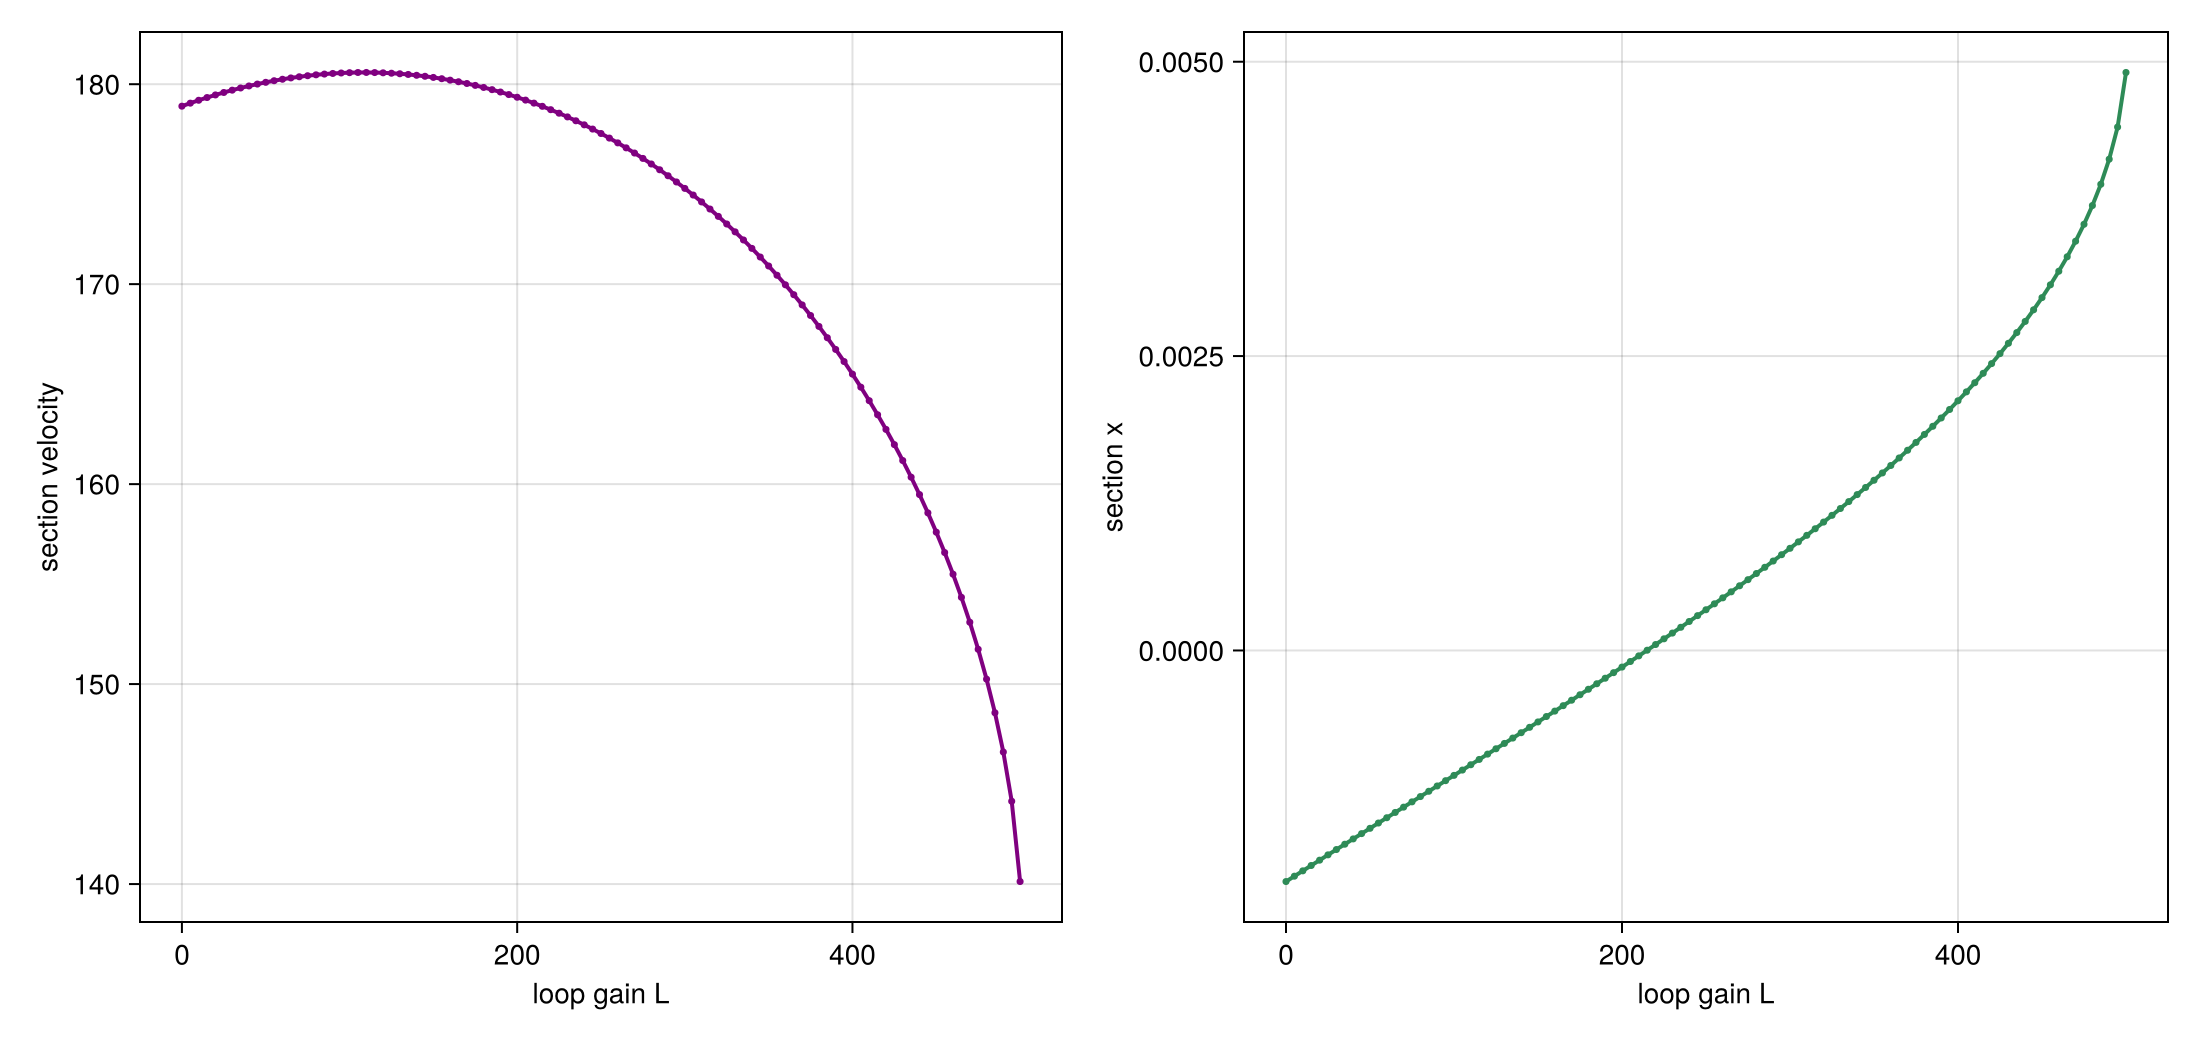
\includegraphics[width=\linewidth]{julia_pll_loop_gain_continuation.png}
  \caption{Continuación Julia desde $L=0$ hasta $L=500$.}
\end{subfigure}\hfill
\begin{subfigure}[t]{0.49\textwidth}
  \centering
  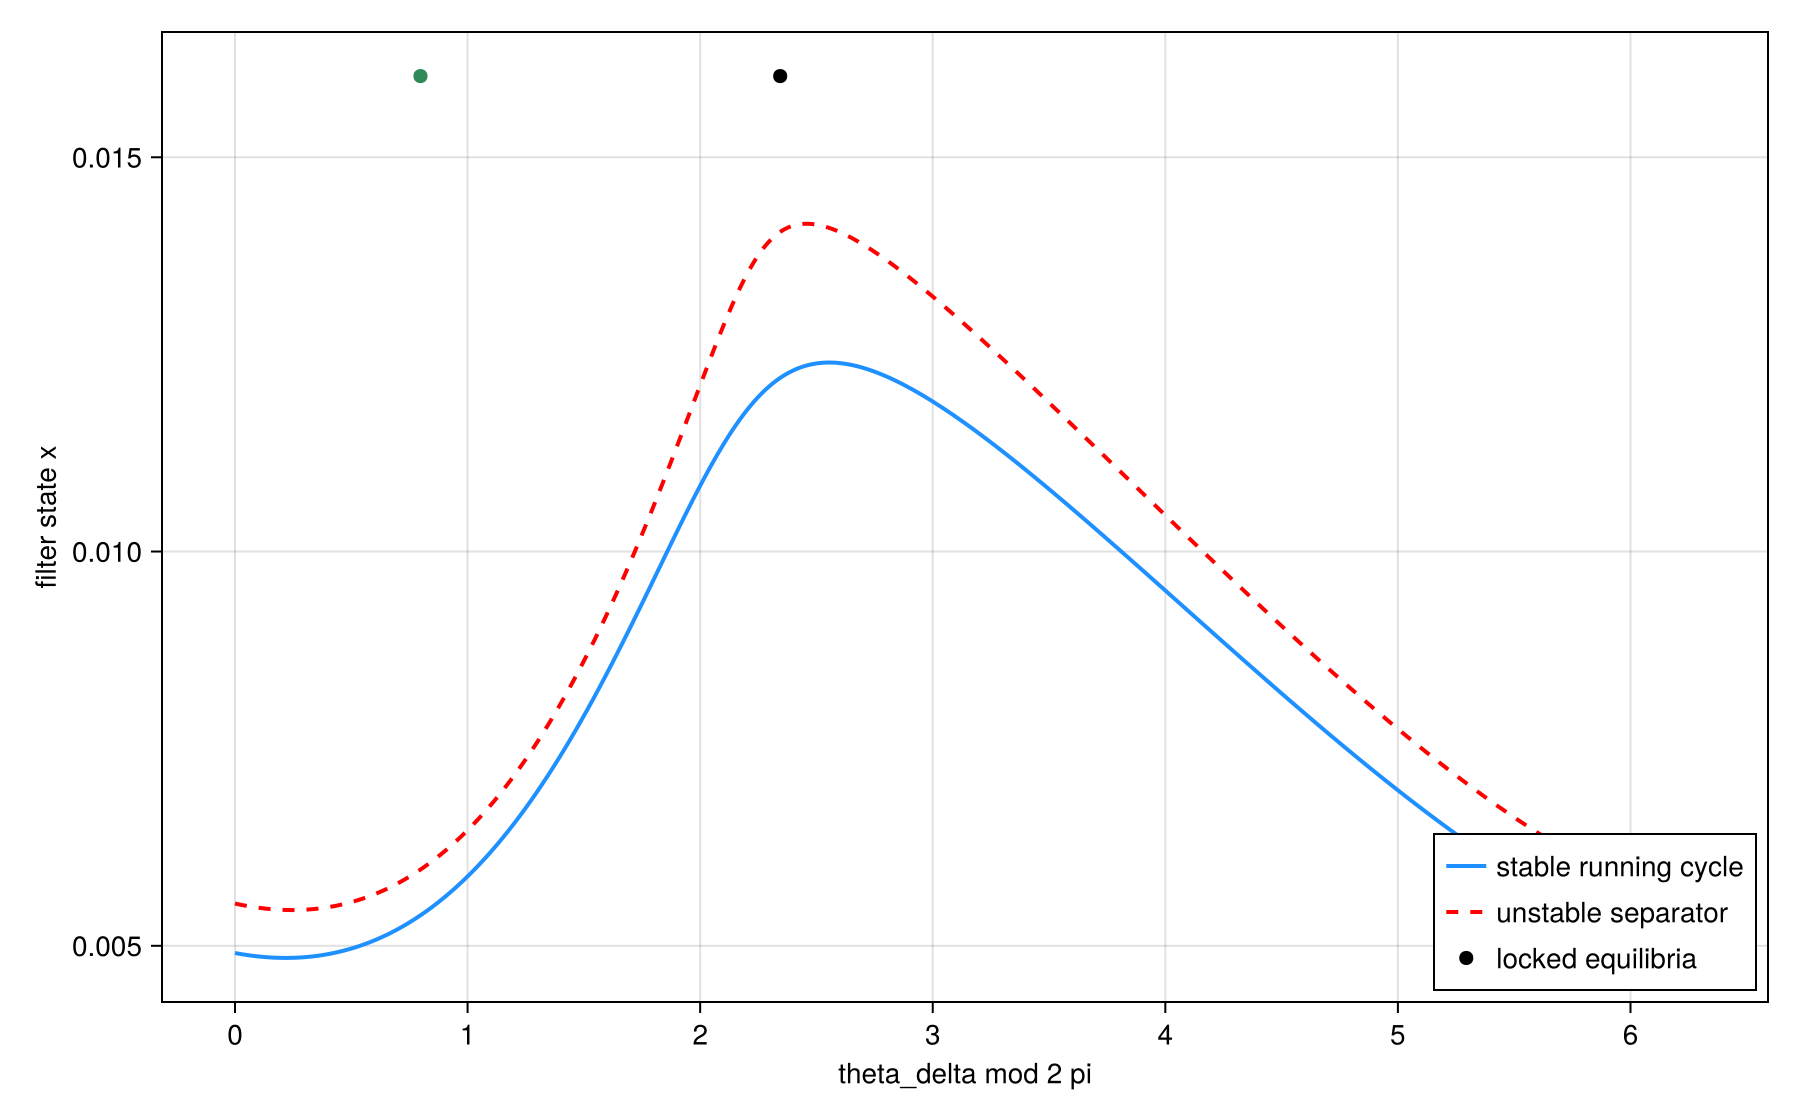
\includegraphics[width=\linewidth]{julia_pll_phase_cylinder_cycles.png}
  \caption{Ciclo estable y separatriz Julia en el cilindro.}
\end{subfigure}
\caption{Continuación y órbitas de la ruta PLL T1 + A1 calculadas en Julia.}
\label{int:fig:pll-julia}
\end{hafocommonfigure}

\section{Sistemas enteros estudiados y pendientes}

\subsection{Taxonomía D0/T1/A1/M1}

\begin{table}[H]
\centering
\caption{Clases estructurales usadas para aceptar o posponer sistemas.}
\small
\begin{tabularx}{\textwidth}{@{}C{1.1cm}p{0.24\textwidth}Yp{0.25\textwidth}@{}}
\toprule
Clase & Definición & Qué permite & Restricción \\
\midrule
D0 & Forma escalar directa \(\dot X=PX+b\psi(c^{\mathsf T}X)\) &
Ruta de transferencia y función descriptiva sin cambio de variables. &
Un solo canal no lineal escalar. \\
T1 & Transformación compatible e invertible, desplazamiento de equilibrio,
variedad invariante documentada o PWA de rango uno &
Lleva el sistema a D0 conservando la interpretación dinámica necesaria. &
La transformación registra la inversa y la métrica correspondiente, por ejemplo angular. \\
A1 & La forma escalar existe, pero la ruta directa se rechaza con una razón
matemática &
Habilita mapa de conmutación, homotopía publicada u otra alternativa. &
Conserva el diagnóstico de incompatibilidad directa y excluye semillas
publicadas de la inicialización. \\
M1 & Varios canales no lineales independientes &
Reserva para una futura extensión multicanal. &
Requiere una formulación multicanal adicional. \\
\bottomrule
\end{tabularx}
\end{table}

\subsection{Cobertura de los casos de estudio}

La \cref{int:tab:catalog} distingue los sistemas integrados de los candidatos
cuya formulación o evaluación numérica está pendiente.

\begin{longtable}{@{}C{1.2cm}L{0.29\textwidth}C{1.65cm}L{0.42\textwidth}@{}}
\caption{Sistemas de prueba de orden entero.}
\label{int:tab:catalog}\\
\toprule
Prior. & Sistema & Clase & Estado y papel científico \\
\midrule
\endfirsthead
\toprule
Prior. & Sistema & Clase & Estado y papel científico \\
\midrule
\endhead
Base & Chua no suave entero & D0 &
Compatible con ocultedad bajo el protocolo finito; reproducido en Python y Julia. \\
Base & Kalman--Fitts de cuarto orden & D0 + A1 &
No Chua; ciclo límite localizado por mapa de conmutación y continuación,
compatible con ocultedad bajo el sondeo; reproducido en Python y Julia. \\
1 & Van der Pol--Duffing autónomo modificado & D0 &
\(\xi=3.1\): 108/108 coincidencias entre cálculos y cero
contactos externos.
\ifHAFOBasinMaterial
\(\xi=3.5\): control negativo, 24/24 contactos con el ciclo seleccionado.
\fi
\(\xi=\MAVPDChaosXi\): candidato caótico compatible con
ocultedad bajo \MAVPDChaosTotalProbes{} sondeos en las vecindades declaradas;
coincidencia Python--Julia en todos los destinos evaluados. \\
2 & PLL bifásico con filtro lead--lag & T1 + A1 &
Comparación Python--Julia con 96 sondeos; las órbitas, su estabilidad
y las decisiones coinciden. \\
3 & Leonov--Kuznetsov, sistema (162) & D0 + A1 &
Ecuaciones y ruta de saturación disponibles; falta verificar la fórmula
completa por tramos y fijar los parámetros de integración. \\
4 & Jerk exponencial de Fischer, \(q=1\) & D0 con balance DC &
Control bibliográfico y de Lyapunov: equilibrio inestable; se conserva la
discrepancia del tercer exponente. Sin una campaña de cuenca local, la evidencia
disponible no permite clasificarlo como autoexcitado ni oculto. \\
\bottomrule
\end{longtable}

\subsection{Siguientes casos y reservas}

Leonov--Kuznetsov, sistema (162), es el siguiente candidato D0 + A1. La
fuente usa una familia de saturaciones, transporta el estado terminal entre
etapas y luego continúa la no linealidad hasta \(\tanh\)
\cite{LeonovKuznetsov2013}. Su evaluación requiere verificar la fórmula
completa por tramos y fijar los parámetros de integración.

El jerk exponencial de Fischer se conserva como control D0 con balance DC y
como banco de exponentes con discrepancias documentadas \cite{fischer2020}.
Falta un sondeo de vecindades para evaluar
la clasificación de cuenca. La inestabilidad del equilibrio, por sí sola, no
implica autoexcitación. La evaluación entera requiere los parámetros del caso bibliográfico correspondiente.

Quedan en reserva Genesio--Tesi, un oscilador memristivo cúbico, el jerk
hiperbólico de Joshi--Ranjan, un jerk PWA y los jerks de Rech y
Rasul--Salih. Faltan parámetros, condiciones iniciales o la verificación de
la ecuación exacta en su fuente primaria.

Lorenz, Rabinovich--Fabrikant, el sistema financiero, el sistema \emph{four
wing} y los modelos con productos no lineales independientes son M1. Su estudio
con Julia queda fuera de las hipótesis de la ruta Lur'e escalar D0/T1.

\section{Comparación metodológica}

\begin{table}[H]
\centering
\caption{Características de los métodos de localización y comparación.}
\small
\begin{tabularx}{\textwidth}{@{}p{0.20\textwidth}YY@{}}
\toprule
Aspecto & Python/\hafo{} & Julia/\juliads--\attractorsjl{} \\
\midrule
Entrada científica & Ecuaciones, Jacobiano, equilibrios, forma Lur'e,
transferencia y función descriptiva & Ecuaciones y dominio para búsqueda
global; las mismas declaraciones Lur'e cuando se replica la ruta teórica \\
Localización & Dirigida por balance armónico y continuación & Global por
recurrencias en Chua; ruta teórica equivalente en Kalman--Fitts y en el MAVPD
periódico y caótico; ruta A1 cilíndrica equivalente en PLL \\
Frecuencia y semilla & Produce \(\omega_0,k,a_0,X_0\) con residuos & Puede
obtener esos valores mediante la ruta teórica; la búsqueda por recurrencias
no utiliza ese balance \\
Generalidad & Restringida a D0/T1 y a las alternativas A1 registradas &
Más amplia para mapas, flujos, cuencas y recurrencias \\
Ocultedad & Flujo explícito de equilibrios y nube candidata & Protocolo
añadido al ejemplo; no es una etiqueta automática de la biblioteca \\
Valores publicados & Regresión posterior & Regresión posterior \\
Fallo típico & No hay ganancia/amplitud compatible o se pierde la rama &
La cuenca no es muestreada, la partición no resuelve el conjunto o el
clasificador agrupa mal \\
\bottomrule
\end{tabularx}
\end{table}

La forma Lur'e relaciona explícitamente el campo, la transferencia y la semilla. La búsqueda por recurrencias aporta generalidad y no necesita una
transformación Lur'e, pero
su éxito depende del dominio, partición, número de muestras y tamaño de la
cuenca. La comparación de los candidatos requiere un protocolo común de integración
y sondeo de cuenca.


\section{Conclusiones}

El balance armónico y la continuación localizaron candidatos en Chua,
Kalman--Fitts y MAVPD; el PLL requirió un mapa de retorno sobre el cilindro.
Las obstrucciones de ganancia en Kalman--Fitts y de fase en el PLL determinaron
las rutas alternativas. La búsqueda por recurrencias localizó además el
candidato de Chua a partir de un muestreo global independiente.

Los diagnósticos distinguen el ciclo estable de MAVPD en \(\xi=3.1\) del
candidato caótico obtenido por continuación hacia
\(\xi=\MAVPDChaosXi\). Este último combina un exponente máximo positivo,
retornos irregulares y controles entre integradores, con las limitaciones
de tiempo finito descritas en \cref{int:subsec:mavpd-chaos}.
\ifHAFOBasinMaterial
Los sondeos comunes coincidieron entre cálculos y no alcanzaron las nubes
candidatas en los casos positivos. MAVPD en \(\xi=3.5\) proporcionó el
control negativo, con contactos desde vecindades de los equilibrios.
\fi

La cobertura incluye sistemas escalares D0, transformaciones T1 y
alternativas A1. Los modelos multicanal requieren otra formulación; para los
candidatos enteros pendientes faltan especificaciones del modelo o sondeos
de cuenca, según la \cref{int:tab:catalog}.

  \section{Resultados}
\label{sec:resultados}

Los resultados se presentan en el mismo orden que los protocolos. Primero se
resumen las reconstrucciones bibliográficas; después se muestran los dos casos
obtenidos por la metodología propuesta. En el caso no suave se completa el
primer radio con contactos. Para \texttt{c590} se distingue la partición local
\(r\leq0.3\) de la auditoría macroscópica en \(r=1\) y \(r=2\).

\subsection{Reconstrucciones bibliográficas}
\label{subsec:resultados_bibliograficos}

\subsubsection{Recuperación del caso entero}

Para \cref{eq:parametros_enteros}, la primera rama del cierre de
Leonov--Kuznetsov produjo
\begin{equation}
\omega_0=2.039186939959,\qquad
k=0.209867354515,\qquad
A_0=5.856145086257,
\label{eq:resultados_armonicos_enteros}
\end{equation}
y la condición modal
\begin{equation}
X_0=(5.856145086257,\ 0.369331578247,\ -8.366536168332)^{\T}.
\label{eq:resultado_semilla_entera}
\end{equation}
Los valores propios de la matriz auxiliar fueron
\[
\lambda_1=-1.538510163250,\qquad
\lambda_{2,3}\simeq\pm2.039186939959\,\mathrm i,
\]
con residuo complejo de cierre \(9.93\times10^{-16}\). Bajo el carril
histórico EFORK--3 \((T=320,\ T_{\mathrm{burn}}=80)\) y su clasificador por
huellas de sección, las 504 sondas produjeron 369 convergencias a equilibrio,
69 divergencias y 66 trayectorias clasificadas como otro destino; ninguna hizo
contacto con la nube objetivo.

\subsubsection{Danca y Wu bajo sus contratos reconstruidos}

La reconstrucción nominal de Danca con
\cref{eq:semilla_danca_diagnostica} permaneció acotada. Después del transitorio
presentó una frecuencia dominante de \(0.3679852806\) ciclos por unidad de
tiempo y medianas de la prueba 0--1
\begin{equation}
(K_x,K_y,K_z)
=(0.0736852160,\ 0.0214448125,\ -0.0012988924).
\label{eq:resultado_danca_k}
\end{equation}
Estos valores corresponden a una trayectoria de apariencia periódica bajo el
contrato ABM de \cref{subsec:protocolos_bibliograficos}.

La recurrencia ADM de Wu permaneció acotada para las dos condiciones de
\cref{eq:semillas_wu_protocolo}. Las trayectorias fueron simétricas y de
apariencia periódica después del transitorio. Las tres componentes tuvieron
frecuencia dominante \(0.5398920216\) ciclos por unidad de tiempo, deriva
relativa nula y entropías espectrales
\[
(H_x,H_y,H_z)
=(0.11607348,\ 0.11106582,\ 0.11095067).
\]

\begin{table}[H]
\centering
\caption{Resultados numéricos de los tres controles bibliográficos.}
\label{tab:resultados_referencias}
\begin{tabularx}{\linewidth}{L{0.20\linewidth}L{0.27\linewidth}Y}
\toprule
Control & Configuración evaluada & Resultado reproducido\\
\midrule
Leonov--Kuznetsov, carril histórico EFORK--3
& \(q=1\), parámetros de \cref{eq:parametros_enteros}
& \(\omega_0=2.03918694\), \(A_0=5.85614509\);
0 contactos en 504 sondas\\
Danca
& \(q=0.9998\), ABM completo, \(h=0.01\), \(T=500\)
& Trayectoria acotada de apariencia periódica,
\(f_d=0.36798528\)\\
Wu et al.
& \(q=0.99\), ADM local de orden cuatro, dos semillas publicadas
& Dos trayectorias simétricas de apariencia periódica,
\(f_d=0.53989202\)\\
\bottomrule
\end{tabularx}
\end{table}

\begin{hafodigitalfigure}[H]
\centering
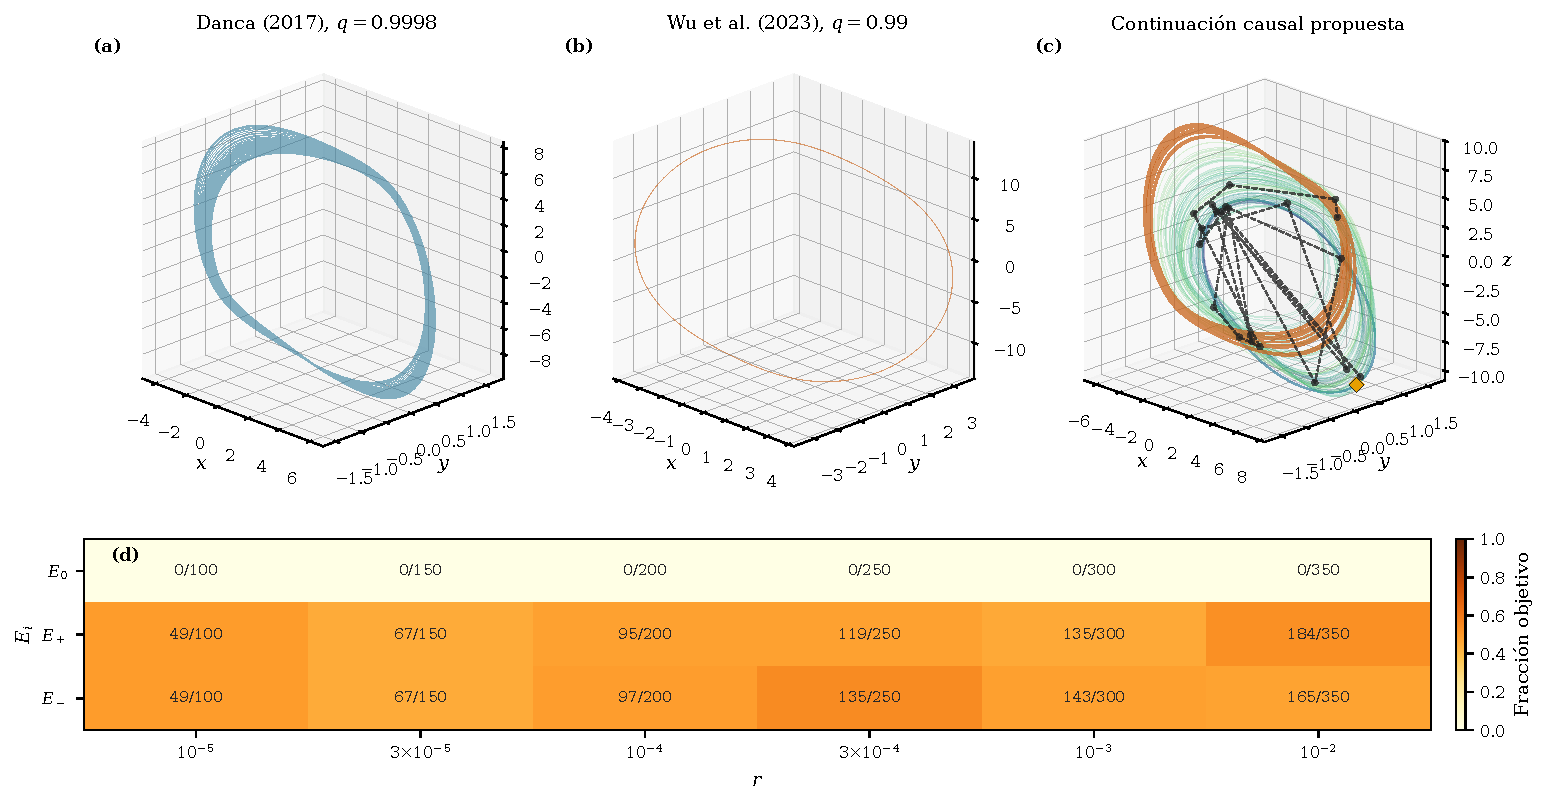
\includegraphics[width=0.96\linewidth]{bibliographic_reproducibility_controls_es}
\caption{Controles de reproducibilidad. Los paneles de Danca y Wu muestran las
trayectorias obtenidas con sus contratos reconstruidos. La continuación no
suave propuesta y el control con pendientes distintas se presentan como
experimentos independientes y no como resultados de las referencias.}
\label{fig:controles_bibliograficos}
\end{hafodigitalfigure}

\FloatBarrier
\subsection{Caso no suave localizado con semilla sesgada}
\label{subsec:resultados_no_suave}

\subsubsection{Raíz, semilla y continuación}

La exploración de 2\,430 inicios seleccionó, dentro del par nominal,
\begin{equation}
\begin{aligned}
A&=4.577882721023,&
c&=2.776397003274,\\
\omega&=2.040286051079,&
N_1&=0.210022792962,&
\Psi_0&=0.408770376181.
\end{aligned}
\label{eq:resultado_raiz_no_suave}
\end{equation}
La norma del residuo de la cuadratura trapezoidal usada por el solucionador fue
\(4.55\times10^{-16}\). Una reevaluación independiente de las integrales
continuas mediante cuadratura adaptativa, separando los puntos de quiebre de
la saturación, produjo \(1.9\times10^{-7}\), menor que el umbral de aceptación
\(10^{-4}\). Ambas cifras corresponden a evaluaciones numéricas diferentes del
mismo cierre.

La condición inicial construida fue
\begin{equation}
X_{\mathrm{sem}}
=(7.354279724297,\ 0.290968778784,\ -9.316054818666)^{\T}.
\label{eq:resultado_semilla_no_suave}
\end{equation}
Después de transportar una sola memoria a través de los 21 niveles, el estado
final fue
\begin{equation}
X_{\mathrm{end}}
=(0.822310709850,\ 1.465272703995,\ 1.292308250248)^{\T}.
\label{eq:resultado_endpoint_no_suave}
\end{equation}

\begin{hafodigitalfigure}[H]
\centering
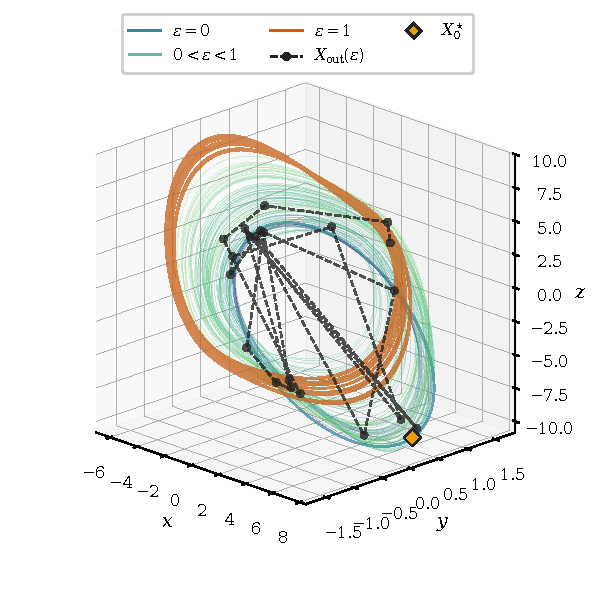
\includegraphics[width=0.90\linewidth]{nonsmooth_numerical_continuation}
\caption{Continuación numérica del sistema auxiliar al sistema no suave
original. Los niveles \(\varepsilon=0,0.05,\ldots,1\) comparten una sola
historia de Caputo.}
\label{fig:continuacion_no_suave_paper07}
\end{hafodigitalfigure}

El problema autónomo iniciado en \cref{eq:resultado_endpoint_no_suave}
produjo el conjunto postransitorio archivado para el caso no suave. Su parte
postransitoria tuvo apariencia periódica, frecuencia dominante
\(0.3699815009\) y entropías
\begin{equation}
(H_x,H_y,H_z)
=(0.11526785,\ 0.10497088,\ 0.10339964).
\label{eq:entropias_no_suave}
\end{equation}
En conjunto, estos diagnósticos lo clasifican como un régimen regular de
apariencia periódica, no como un atractor caótico.
Las 36 perturbaciones alrededor de \(X_{\mathrm{end}}\) hicieron contacto con
la nube objetivo: 12 de 12 para cada radio \(10^{-6}\), \(10^{-4}\) y
\(10^{-2}\).

\begin{hafodigitalfigure}[H]
\centering
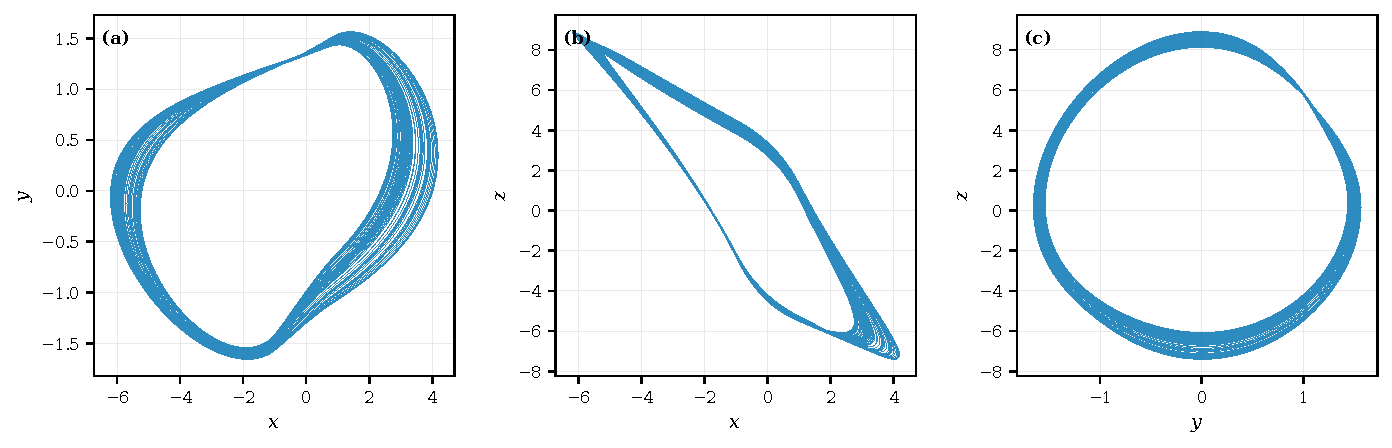
\includegraphics[width=0.86\linewidth]{nonsmooth_final_attractor}
\caption{Conjunto atrayente postransitorio obtenido para
\cref{eq:chua_no_suave,eq:parametros_no_suave} desde el extremo de la
continuación causal.}
\label{fig:atractor_no_suave_paper07}
\end{hafodigitalfigure}

\subsubsection{Sondeo volumétrico}

El protocolo completo reunió 17\,400 problemas de valor inicial, 5\,800
alrededor de cada equilibrio, sin fallos numéricos. De ellos, 7\,200
corresponden al contrato local predeclarado \(r\leq0.01\), y 10\,200 a la
extensión macroscópica diagnóstica en \(r=0.03,0.1,0.3\). La
\cref{tab:sondeo_no_suave_completo} contiene todos los radios ejecutados y
todas las clases del clasificador.

\begingroup
\setlength{\tabcolsep}{10pt}
\setlength{\LTleft}{\fill}
\setlength{\LTright}{\fill}
\begin{longtable}{@{}ccrrrrr@{}}
\caption{Conteos completos del sondeo volumétrico del sistema no suave.}
\label{tab:sondeo_no_suave_completo}\\
\toprule
Equilibrio & \(r\) & \(N\) & Objetivo & Equilibrio & Divergencia & Otro\\
\midrule
\endfirsthead
\multicolumn{7}{c}{\tablename\ \thetable\ (continuación)}\\
\toprule
Equilibrio & \(r\) & \(N\) & Objetivo & Equilibrio & Divergencia & Otro\\
\midrule
\endhead
\midrule
\multicolumn{7}{r}{Continúa en la página siguiente}\\
\endfoot
\bottomrule
\endlastfoot
\multirow{10}{*}{\(E_0\)}
& \(10^{-5}\) & 80 & 0 & 80 & 0 & 0\\
& \(3{\times}10^{-5}\) & 120 & 0 & 120 & 0 & 0\\
& \(10^{-4}\) & 160 & 0 & 160 & 0 & 0\\
& \(3{\times}10^{-4}\) & 240 & 0 & 240 & 0 & 0\\
& \(10^{-3}\) & 400 & 0 & 400 & 0 & 0\\
& \(3{\times}10^{-3}\) & 600 & 0 & 600 & 0 & 0\\
& \(10^{-2}\) & 800 & 0 & 800 & 0 & 0\\
& \(0.03\) & 1000 & 0 & 1000 & 0 & 0\\
& \(0.1\) & 1200 & 0 & 1200 & 0 & 0\\
& \(0.3\) & 1200 & 0 & 1200 & 0 & 0\\
\midrule
\multirow{10}{*}{\(E_+\)}
& \(10^{-5}\) & 80 & 0 & 0 & 39 & 41\\
& \(3{\times}10^{-5}\) & 120 & 0 & 0 & 63 & 57\\
& \(10^{-4}\) & 160 & 0 & 0 & 80 & 80\\
& \(3{\times}10^{-4}\) & 240 & 0 & 0 & 116 & 124\\
& \(10^{-3}\) & 400 & 0 & 0 & 189 & 211\\
& \(3{\times}10^{-3}\) & 600 & 0 & 0 & 277 & 323\\
& \(10^{-2}\) & 800 & 0 & 0 & 393 & 407\\
& \(0.03\) & 1000 & 0 & 0 & 490 & 510\\
& \(0.1\) & 1200 & 0 & 4 & 588 & 608\\
& \(0.3\) & 1200 & 19 & 7 & 591 & 583\\
\midrule
\pagebreak[4]
\multirow{10}{*}{\(E_-\)}
& \(10^{-5}\) & 80 & 0 & 0 & 41 & 39\\
& \(3{\times}10^{-5}\) & 120 & 0 & 0 & 56 & 64\\
& \(10^{-4}\) & 160 & 0 & 0 & 81 & 79\\
& \(3{\times}10^{-4}\) & 240 & 0 & 0 & 122 & 118\\
& \(10^{-3}\) & 400 & 0 & 0 & 204 & 196\\
& \(3{\times}10^{-3}\) & 600 & 0 & 0 & 309 & 291\\
& \(10^{-2}\) & 800 & 0 & 0 & 394 & 406\\
& \(0.03\) & 1000 & 0 & 0 & 488 & 512\\
& \(0.1\) & 1200 & 0 & 4 & 593 & 603\\
& \(0.3\) & 1200 & 18 & 12 & 596 & 574\\
\end{longtable}
\endgroup

En el contrato local se registraron cero contactos y cero fallos numéricos en
las 7\,200 sondas con \(r\leq0.01\). Este es el alcance usado para evaluar la
compatibilidad local con ocultedad del conjunto atrayente regular.

La extensión macroscópica, que no amplía ese contrato local, añadió 10\,200
sondas. Las 6\,600 correspondientes a \(r=0.03\) y \(r=0.1\) produjeron cero
contactos; al combinarlas con el contrato local se obtiene el acumulado
\(0/13\,800\) hasta \(r=0.1\). El primer radio con contactos de la extensión
fue \(r=0.3\); después de completar sus 3\,600 sondas se registraron 37
contactos: cero desde \(E_0\), 19 desde \(E_+\) y 18 desde \(E_-\). Las
distancias iniciales de esos contactos a su equilibrio estuvieron entre
\(0.1941805298\) y \(0.2997254735\). Por tanto, la extensión macroscópica
delimita el intervalo de acceso muestreado
\[
0.1<r_{\mathrm{contacto}}\leq0.3
\]
sin convertirlo en el alcance del contrato local.

\begin{hafodigitalfigure}[H]
\centering
\begin{subfigure}[t]{0.49\linewidth}
  \centering
  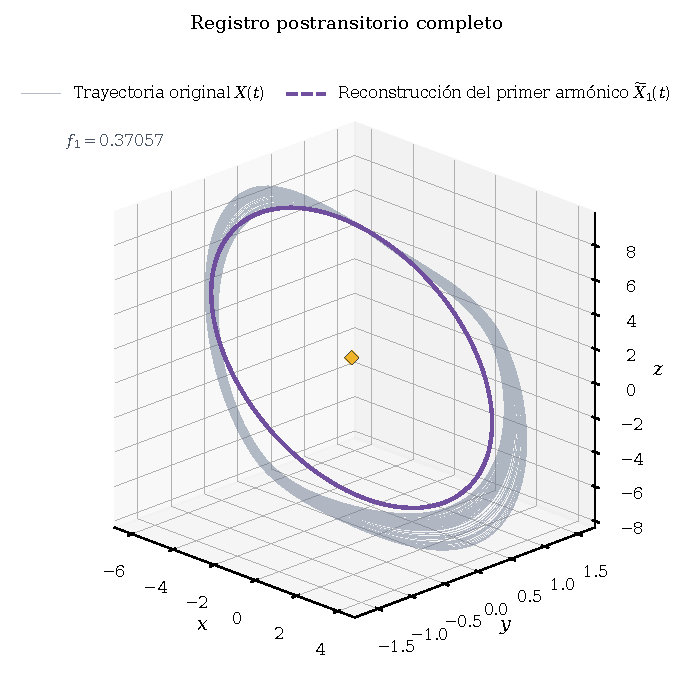
\includegraphics[width=\linewidth]{nonsmooth_first_harmonic_comparison_es}
  \caption{Trayectoria y primer armónico.}
\end{subfigure}\hfill
\begin{subfigure}[t]{0.49\linewidth}
  \centering
  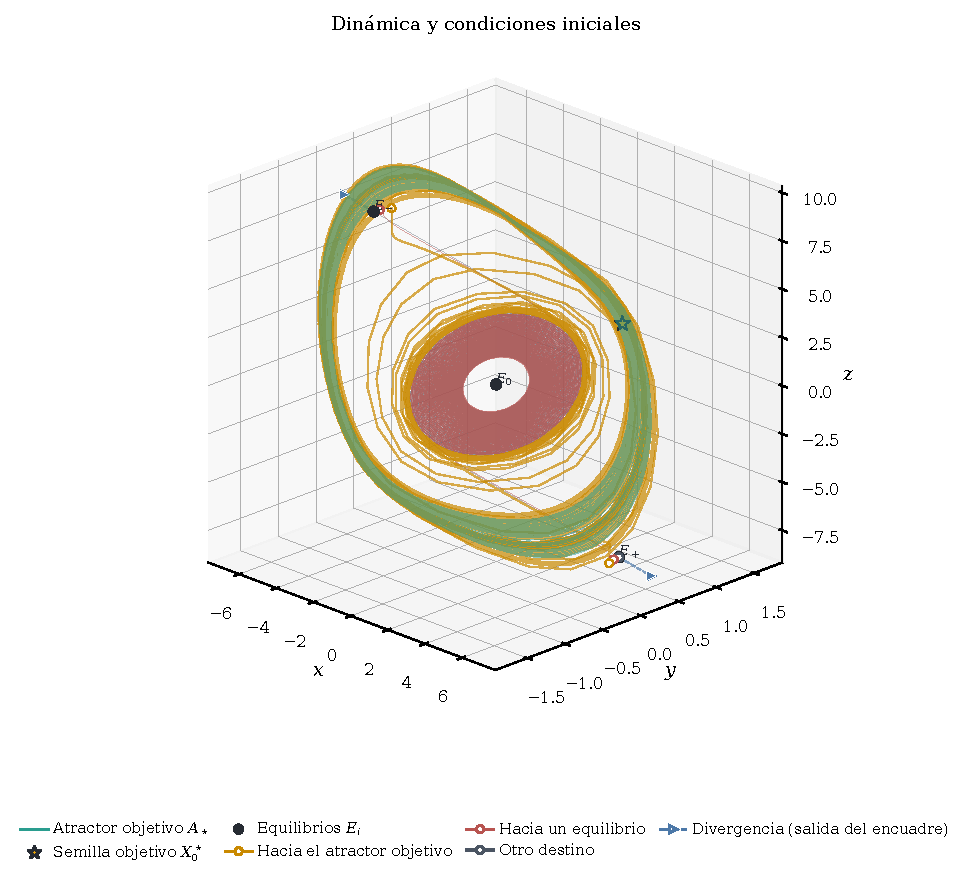
\includegraphics[width=\linewidth]{nonsmooth_volumetric_probe_overview_es}
  \caption{Sondas volumétricas representativas.}
\end{subfigure}
\caption{Diagnósticos del caso no suave. La comparación armónica describe el
carácter regular de la respuesta; las sondas muestran ejemplos de las clases
usadas en \cref{tab:sondeo_no_suave_completo}.}
\label{fig:diagnosticos_no_suave_paper07}
\end{hafodigitalfigure}

\FloatBarrier
\subsection{Caso con arctangente \texttt{c590}}
\label{subsec:resultados_c590}

\subsubsection{Selección en orden entero y refinamiento de Caputo}

En la exploración global, 894 de los 2\,400 casos quedaron separados del
control y 884 fueron además no triviales. De éstos, 823 se clasificaron como
regulares de apariencia periódica y 61 permanecieron en la categoría
exploratoria no periódica. El índice global de base cero 1731 obtuvo la mayor
puntuación, \(S=0.3021129950\), y definió el centro
\begin{equation}
\begin{aligned}
p_b={}&(18.4857295104,\ 21.9669521100,\ 0.0052746106,\\
&0.0262974930,\ -3.2087779245,\ 1.9492612035),\\
X_b={}&(7.0796053271,\ 0.5079327671,\ -14.4903935267)^{\T}.
\end{aligned}
\label{eq:resultado_centro_c590}
\end{equation}

La exploración local generó 1\,000 casos: 170 quedaron separados del control
y 148 fueron también no triviales. Entre estos últimos hubo 87 respuestas
exploratorias no periódicas y 61 regulares de apariencia periódica.
\texttt{c590}, índice local de base cero 590, ocupó el rango 10 por puntuación.
La auditoría variacional de los 30 mejores casos seleccionó \texttt{c590} con
\begin{equation}
(\lambda_1,\lambda_2,\lambda_3)
=(0.4699043683,\ 0.0010414594,\ -19.0491693716)
\label{eq:resultado_lyapunov_entero_c590}
\end{equation}
y semilla entera
\begin{equation}
X_0^{\mathrm{int}}
=(7.6733768929,\ 0.5079327671,\ -14.4903935267)^{\T}.
\label{eq:resultado_semilla_entera_c590}
\end{equation}

Los parámetros finales son los de \cref{eq:parametros_c590}. Sus equilibrios
son
\begin{equation}
E_0=(0,0,0),\qquad
E_\pm=(\pm4.6494055135,\ \pm0.0017970023,\ \mp4.6476085112).
\label{eq:equilibrios_c590_resultados}
\end{equation}
El criterio de Matignon clasificó \(E_0\) como inestable y \(E_\pm\) como
estables; el margen de los equilibrios externos fue
\(7.42265\times10^{-4}\).

El refinamiento seleccionó \(q=0.9999\) y el estado de índice 9, extraído en
\(t\simeq240\):
\begin{equation}
X_0^{\mathrm{frac}}
=(5.8642449791,\ 1.5847111486,\ 3.2155806478)^{\T}.
\label{eq:resultado_semilla_fraccionaria_c590}
\end{equation}
En la auditoría larga, las medianas remuestreadas fueron
\begin{equation}
(K_{0.0025},K_{0.005},K_{0.01})
=(0.865843,\ 0.885089,\ 0.740058).
\label{eq:resultado_k_pasos_c590}
\end{equation}
Los dos pasos refinados superaron el umbral de selección 0.8; el tercer valor
documenta la sensibilidad al paso más grande.

\begin{hafodigitalfigure}[H]
\centering
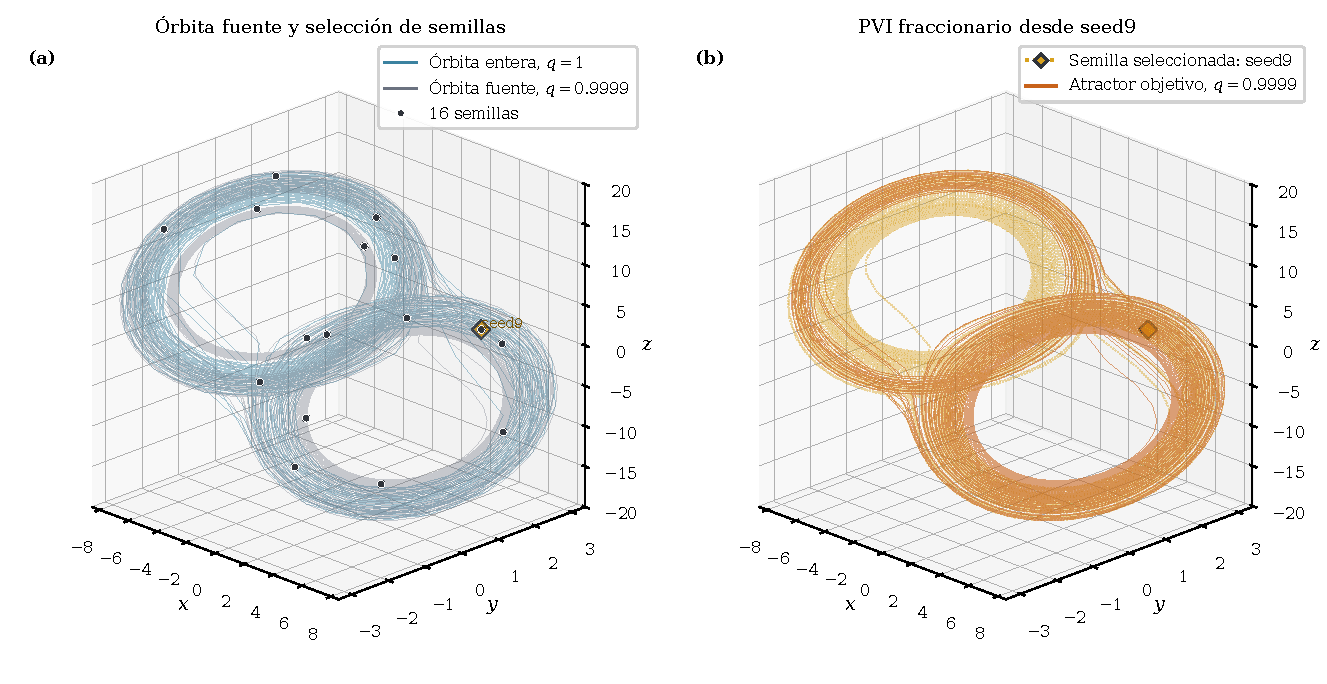
\includegraphics[width=0.92\linewidth]{arctan_fractional_refinement_es}
\caption{Búsqueda en orden entero y refinamiento fraccionario del caso
\texttt{c590}. Cada valor de \(q\) corresponde a un problema de Caputo
independiente; el estado seleccionado se extrae de la trayectoria
\(q=0.9999\).}
\label{fig:refinamiento_c590_paper07}
\end{hafodigitalfigure}

La trayectoria final permaneció acotada en los tres pasos. Sobre 30\,000
estados postransitorios, ninguna componente cumplió el filtro de apariencia
periódica. Las entropías espectrales, fracciones de potencia dominante y
derivas relativas fueron
\begin{equation}
\begin{aligned}
(H_x,H_y,H_z)
&=(0.394751,\ 0.261922,\ 0.315229),\\
(R_x,R_y,R_z)
&=(0.122163,\ 0.290492,\ 0.241937),\\
(\Delta_{f,x},\Delta_{f,y},\Delta_{f,z})
&=(0.941176,\ 0.029412,\ 0.029412).
\end{aligned}
\label{eq:metricas_finales_c590}
\end{equation}
La respuesta se clasifica, por tanto, como aperiódica bajo el filtro
postransitorio declarado.

\begin{hafodigitalfigure}[H]
\centering
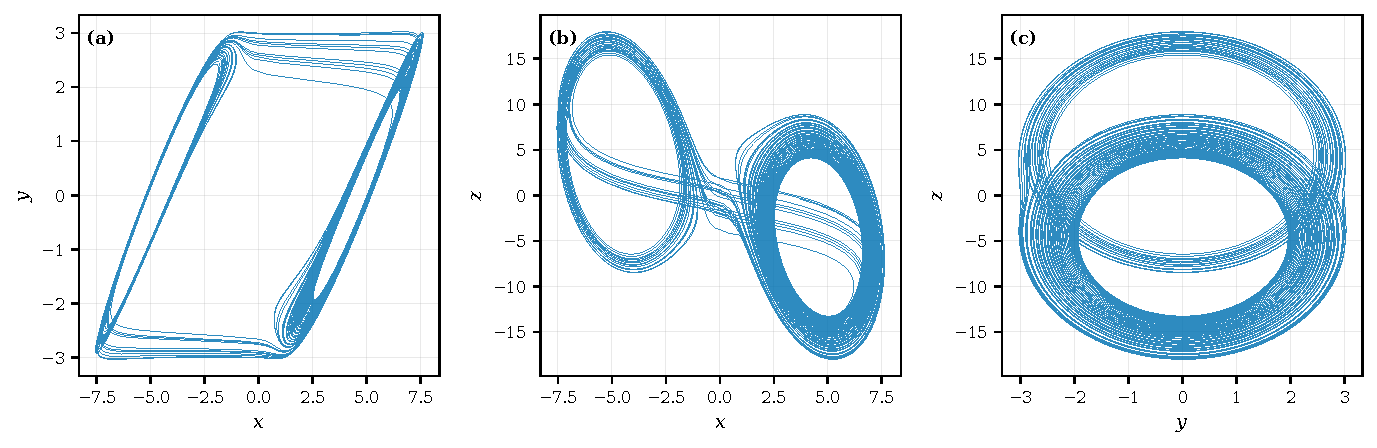
\includegraphics[width=0.86\linewidth]{arctan_final_attractor}
\caption{Conjunto postransitorio del sistema
\cref{eq:chua_arctan,eq:parametros_c590} para \(q=0.9999\),
\(h=0.005\) y la condición \cref{eq:resultado_semilla_fraccionaria_c590}.}
\label{fig:atractor_c590_paper07}
\end{hafodigitalfigure}

\subsubsection{Sondeo superficial}

El registro canónico reúne 13\,500 trayectorias: 8\,400 en la partición local
\(r\leq0.3\) y 5\,100 en la auditoría macroscópica \(r\in\{1,2\}\). El primer
contacto se observó en \(r=1\), pero se retuvo \(r=2\) como bloque adicional.
La \cref{tab:sondeo_c590_completo} contiene todos los conteos del experimento
declarado.

\begingroup
\setlength{\tabcolsep}{10pt}
\setlength{\LTleft}{\fill}
\setlength{\LTright}{\fill}
\begin{longtable}{@{}ccrrrrr@{}}
\caption{Conteos completos del sondeo sobre superficies esféricas de
\texttt{c590}.}
\label{tab:sondeo_c590_completo}\\
\toprule
Equilibrio & \(r\) & \(N\) & Objetivo & Equilibrio & Divergencia & Otro\\
\midrule
\endfirsthead
\multicolumn{7}{c}{\tablename\ \thetable\ (continuación)}\\
\toprule
Equilibrio & \(r\) & \(N\) & Objetivo & Equilibrio & Divergencia & Otro\\
\midrule
\endhead
\midrule
\multicolumn{7}{r}{Continúa en la página siguiente}\\
\endfoot
\bottomrule
\endlastfoot
\multirow{9}{*}{\(E_0\)}
& \(10^{-5}\) & 100 & 0 & 0 & 0 & 100\\
& \(10^{-4}\) & 200 & 0 & 0 & 0 & 200\\
& \(10^{-3}\) & 300 & 0 & 0 & 0 & 300\\
& \(10^{-2}\) & 400 & 0 & 0 & 0 & 400\\
& \(0.03\) & 500 & 0 & 0 & 0 & 500\\
& \(0.1\) & 600 & 0 & 0 & 0 & 600\\
& \(0.3\) & 700 & 0 & 0 & 0 & 700\\
& \(1\) & 800 & 22 & 0 & 0 & 778\\
& \(2\) & 900 & 289 & 0 & 67 & 544\\
\midrule
\pagebreak[4]
\multirow{9}{*}{\(E_+\)}
& \(10^{-5}\) & 100 & 0 & 2 & 0 & 98\\
& \(10^{-4}\) & 200 & 0 & 0 & 0 & 200\\
& \(10^{-3}\) & 300 & 0 & 0 & 0 & 300\\
& \(10^{-2}\) & 400 & 0 & 0 & 0 & 400\\
& \(0.03\) & 500 & 0 & 0 & 0 & 500\\
& \(0.1\) & 600 & 0 & 0 & 0 & 600\\
& \(0.3\) & 700 & 0 & 0 & 0 & 700\\
& \(1\) & 800 & 0 & 0 & 0 & 800\\
& \(2\) & 900 & 150 & 0 & 37 & 713\\
\midrule
\multirow{9}{*}{\(E_-\)}
& \(10^{-5}\) & 100 & 0 & 2 & 0 & 98\\
& \(10^{-4}\) & 200 & 0 & 0 & 0 & 200\\
& \(10^{-3}\) & 300 & 0 & 0 & 0 & 300\\
& \(10^{-2}\) & 400 & 0 & 0 & 0 & 400\\
& \(0.03\) & 500 & 0 & 0 & 0 & 500\\
& \(0.1\) & 600 & 0 & 0 & 0 & 600\\
& \(0.3\) & 700 & 0 & 0 & 0 & 700\\
& \(1\) & 800 & 0 & 0 & 0 & 800\\
& \(2\) & 900 & 149 & 0 & 27 & 724\\
\end{longtable}
\endgroup

Las 8\,400 trayectorias con \(r\leq0.3\) produjeron cero contactos; 8\,396
completaron el horizonte y cuatro convergieron anticipadamente a \(E_\pm\) en
\(r=10^{-5}\). En \(r=1\) hubo 22 contactos entre 2\,400 trayectorias, todos
desde \(E_0\). En \(r=2\) hubo 588 contactos entre 2\,700 trayectorias: 289
desde \(E_0\), 150 desde \(E_+\) y 149 desde \(E_-\); en este bloque se
registraron 131 divergencias. En total se ejecutaron 13\,500 pruebas y se
observaron 610 contactos. El primer radio observado satisface
\[
0.3<r_{\mathrm{primer\ contacto}}\leq1.
\]

\begin{hafodigitalfigure}[H]
\centering
\begin{subfigure}[t]{0.49\linewidth}
  \centering
  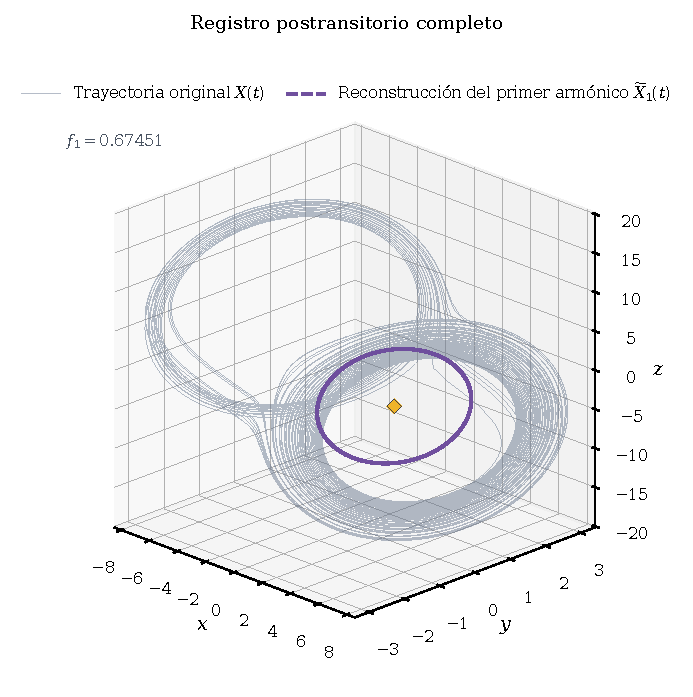
\includegraphics[width=\linewidth]{arctan_first_harmonic_comparison_es}
  \caption{Trayectoria y primer armónico.}
\end{subfigure}\hfill
\begin{subfigure}[t]{0.49\linewidth}
  \centering
  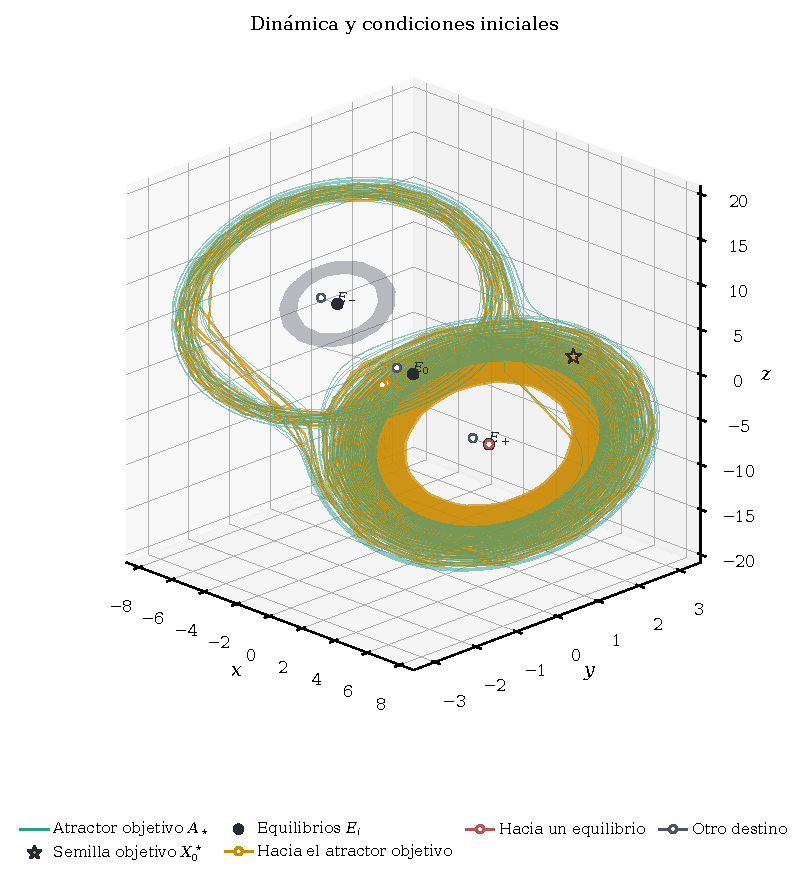
\includegraphics[width=\linewidth]{arctan_spherical_probe_overview_es}
  \caption{Sondas superficiales representativas.}
\end{subfigure}
\caption{Diagnósticos de \texttt{c590}. La comparación con el primer armónico
acompaña el filtro de aperiodicidad. El panel de sondas muestra nueve historias
representativas seleccionadas en el subconjunto hasta \(r=1\); no es una
gráfica de conteos. La \cref{tab:sondeo_c590_completo} incorpora además la
auditoría canónica en \(r=2\).}
\label{fig:diagnosticos_c590_paper07}
\end{hafodigitalfigure}

\FloatBarrier
\subsection{Delimitación local obtenida}
\label{subsec:delimitacion_local}

\begin{table}[H]
\centering
\caption{Alcance local predeclarado y acceso observado en los sondeos
extendidos.}
\label{tab:intervalos_locales}
\begin{tabularx}{\linewidth}{L{0.26\linewidth}C{0.18\linewidth}C{0.18\linewidth}Y}
\toprule
Sistema & Geometría & Alcance o intervalo & Conteos correspondientes\\
\midrule
No suave, \(q=0.9998\)
& Bola volumétrica
& Local: \(r\leq0.01\)
& Local: \(0/7\,200\), cero fallos;
macro: \(0/6\,600\) en \(0.03,0.1\) y
\(37/3\,600\) en \(0.3\)\\
\texttt{c590}, \(q=0.9999\)
& Superficie esférica
& Separación observada hasta \(r=0.3\); revisión macroscópica en \(r=1,2\)
& \(0/8\,400\) hasta \(0.3\);
\(22/2\,400\) en \(1\);
\(588/2\,700\) en \(2\), con 131 divergencias\\
\bottomrule
\end{tabularx}
\end{table}

Dentro de las bolas, horizontes y reglas de contacto del contrato local
\(r\leq0.01\), el conjunto regular no suave es compatible con la definición
local de atractor oculto. Los radios \(0.03\), \(0.1\) y \(0.3\) describen una
extensión macroscópica de la geometría de cuenca y no amplían la afirmación de
ocultedad más allá del contrato local. Para \texttt{c590}, la compatibilidad
local se limita a las superficies, radios, horizontes y reglas de contacto con
\(r\leq0.3\). Los contactos observados en \(r=1\) y \(r=2\) describen acceso
macroscópico a la cuenca. Todos estos resultados proceden de muestras finitas
y no constituyen una prueba global de separación de cuencas.

\else
  \section{Resultados}
\label{sec:resultados}

Los resultados se presentan en el mismo orden que los protocolos. Primero se
resumen las reconstrucciones bibliográficas; después se muestran los dos casos
obtenidos por la metodología propuesta. En el caso no suave se completa el
primer radio con contactos. Para \texttt{c590} se distingue la partición local
\(r\leq0.3\) de la auditoría macroscópica en \(r=1\) y \(r=2\).

\subsection{Reconstrucciones bibliográficas}
\label{subsec:resultados_bibliograficos}

\subsubsection{Recuperación del caso entero}

Para \cref{eq:parametros_enteros}, la primera rama del cierre de
Leonov--Kuznetsov produjo
\begin{equation}
\omega_0=2.039186939959,\qquad
k=0.209867354515,\qquad
A_0=5.856145086257,
\label{eq:resultados_armonicos_enteros}
\end{equation}
y la condición modal
\begin{equation}
X_0=(5.856145086257,\ 0.369331578247,\ -8.366536168332)^{\T}.
\label{eq:resultado_semilla_entera}
\end{equation}
Los valores propios de la matriz auxiliar fueron
\[
\lambda_1=-1.538510163250,\qquad
\lambda_{2,3}\simeq\pm2.039186939959\,\mathrm i,
\]
con residuo complejo de cierre \(9.93\times10^{-16}\). Bajo el carril
histórico EFORK--3 \((T=320,\ T_{\mathrm{burn}}=80)\) y su clasificador por
huellas de sección, las 504 sondas produjeron 369 convergencias a equilibrio,
69 divergencias y 66 trayectorias clasificadas como otro destino; ninguna hizo
contacto con la nube objetivo.

\subsubsection{Danca y Wu bajo sus contratos reconstruidos}

La reconstrucción nominal de Danca con
\cref{eq:semilla_danca_diagnostica} permaneció acotada. Después del transitorio
presentó una frecuencia dominante de \(0.3679852806\) ciclos por unidad de
tiempo y medianas de la prueba 0--1
\begin{equation}
(K_x,K_y,K_z)
=(0.0736852160,\ 0.0214448125,\ -0.0012988924).
\label{eq:resultado_danca_k}
\end{equation}
Estos valores corresponden a una trayectoria de apariencia periódica bajo el
contrato ABM de \cref{subsec:protocolos_bibliograficos}.

La recurrencia ADM de Wu permaneció acotada para las dos condiciones de
\cref{eq:semillas_wu_protocolo}. Las trayectorias fueron simétricas y de
apariencia periódica después del transitorio. Las tres componentes tuvieron
frecuencia dominante \(0.5398920216\) ciclos por unidad de tiempo, deriva
relativa nula y entropías espectrales
\[
(H_x,H_y,H_z)
=(0.11607348,\ 0.11106582,\ 0.11095067).
\]

\begin{table}[H]
\centering
\caption{Resultados numéricos de los tres controles bibliográficos.}
\label{tab:resultados_referencias}
\begin{tabularx}{\linewidth}{L{0.20\linewidth}L{0.27\linewidth}Y}
\toprule
Control & Configuración evaluada & Resultado reproducido\\
\midrule
Leonov--Kuznetsov, carril histórico EFORK--3
& \(q=1\), parámetros de \cref{eq:parametros_enteros}
& \(\omega_0=2.03918694\), \(A_0=5.85614509\);
0 contactos en 504 sondas\\
Danca
& \(q=0.9998\), ABM completo, \(h=0.01\), \(T=500\)
& Trayectoria acotada de apariencia periódica,
\(f_d=0.36798528\)\\
Wu et al.
& \(q=0.99\), ADM local de orden cuatro, dos semillas publicadas
& Dos trayectorias simétricas de apariencia periódica,
\(f_d=0.53989202\)\\
\bottomrule
\end{tabularx}
\end{table}

\begin{hafodigitalfigure}[H]
\centering
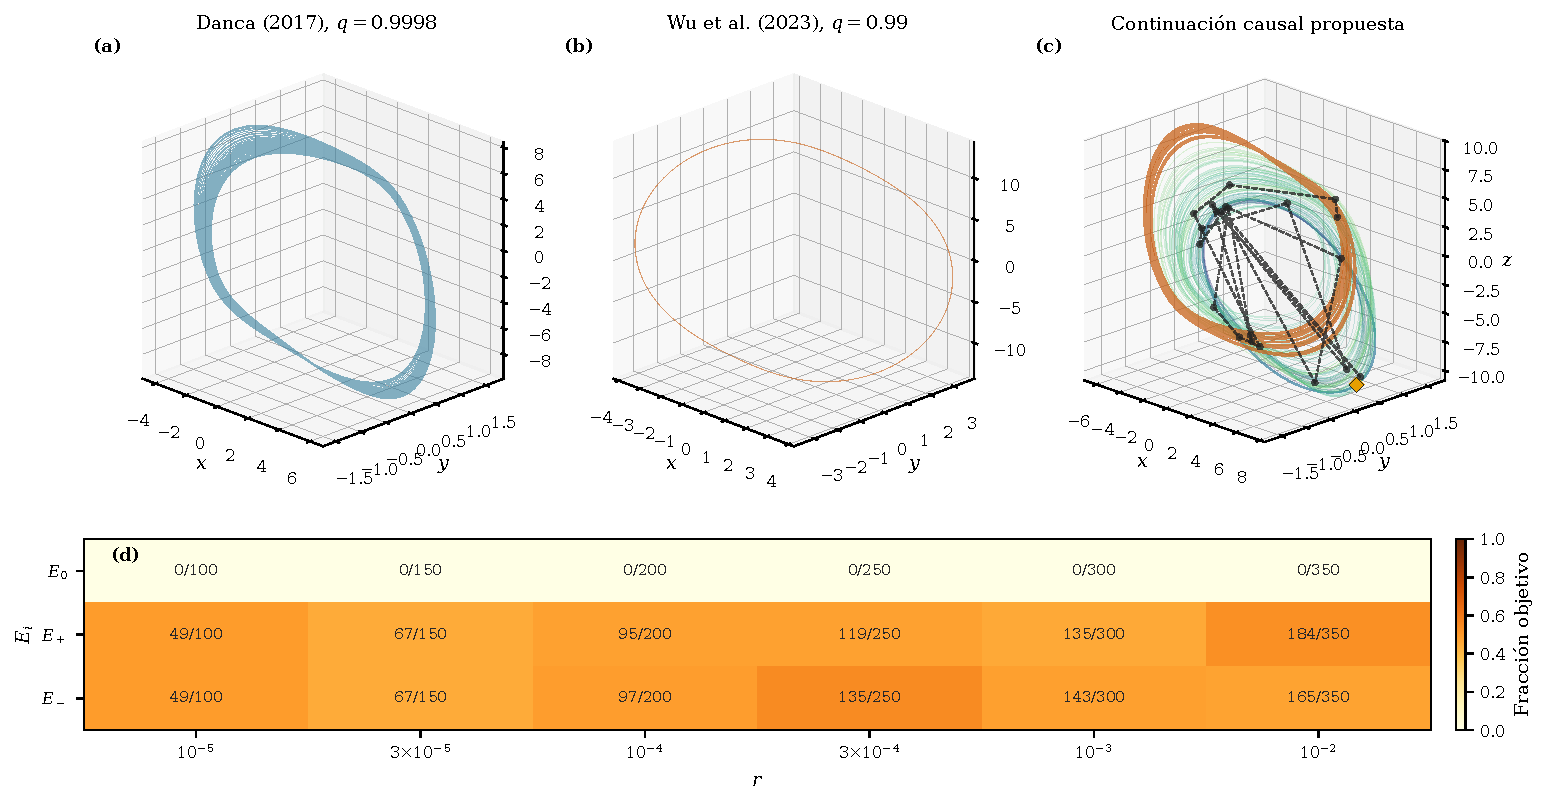
\includegraphics[width=0.96\linewidth]{bibliographic_reproducibility_controls_es}
\caption{Controles de reproducibilidad. Los paneles de Danca y Wu muestran las
trayectorias obtenidas con sus contratos reconstruidos. La continuación no
suave propuesta y el control con pendientes distintas se presentan como
experimentos independientes y no como resultados de las referencias.}
\label{fig:controles_bibliograficos}
\end{hafodigitalfigure}

\FloatBarrier
\subsection{Caso no suave localizado con semilla sesgada}
\label{subsec:resultados_no_suave}

\subsubsection{Raíz, semilla y continuación}

La exploración de 2\,430 inicios seleccionó, dentro del par nominal,
\begin{equation}
\begin{aligned}
A&=4.577882721023,&
c&=2.776397003274,\\
\omega&=2.040286051079,&
N_1&=0.210022792962,&
\Psi_0&=0.408770376181.
\end{aligned}
\label{eq:resultado_raiz_no_suave}
\end{equation}
La norma del residuo de la cuadratura trapezoidal usada por el solucionador fue
\(4.55\times10^{-16}\). Una reevaluación independiente de las integrales
continuas mediante cuadratura adaptativa, separando los puntos de quiebre de
la saturación, produjo \(1.9\times10^{-7}\), menor que el umbral de aceptación
\(10^{-4}\). Ambas cifras corresponden a evaluaciones numéricas diferentes del
mismo cierre.

La condición inicial construida fue
\begin{equation}
X_{\mathrm{sem}}
=(7.354279724297,\ 0.290968778784,\ -9.316054818666)^{\T}.
\label{eq:resultado_semilla_no_suave}
\end{equation}
Después de transportar una sola memoria a través de los 21 niveles, el estado
final fue
\begin{equation}
X_{\mathrm{end}}
=(0.822310709850,\ 1.465272703995,\ 1.292308250248)^{\T}.
\label{eq:resultado_endpoint_no_suave}
\end{equation}

\begin{hafodigitalfigure}[H]
\centering
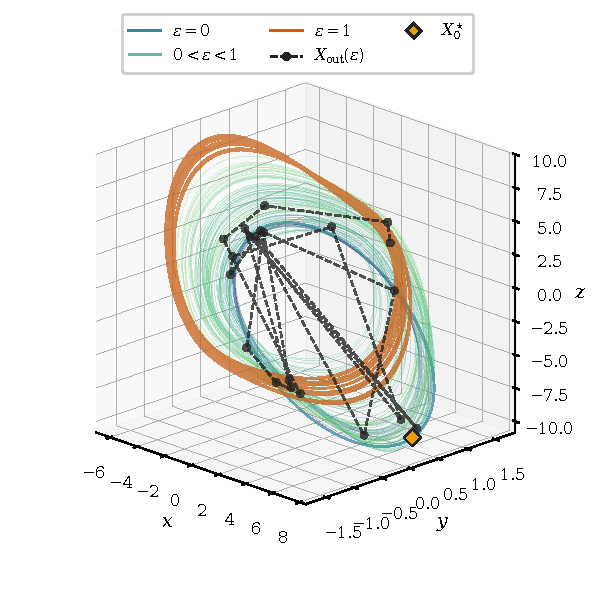
\includegraphics[width=0.90\linewidth]{nonsmooth_numerical_continuation}
\caption{Continuación numérica del sistema auxiliar al sistema no suave
original. Los niveles \(\varepsilon=0,0.05,\ldots,1\) comparten una sola
historia de Caputo.}
\label{fig:continuacion_no_suave_paper07}
\end{hafodigitalfigure}

El problema autónomo iniciado en \cref{eq:resultado_endpoint_no_suave}
produjo el conjunto postransitorio archivado para el caso no suave. Su parte
postransitoria tuvo apariencia periódica, frecuencia dominante
\(0.3699815009\) y entropías
\begin{equation}
(H_x,H_y,H_z)
=(0.11526785,\ 0.10497088,\ 0.10339964).
\label{eq:entropias_no_suave}
\end{equation}
En conjunto, estos diagnósticos lo clasifican como un régimen regular de
apariencia periódica, no como un atractor caótico.
Las 36 perturbaciones alrededor de \(X_{\mathrm{end}}\) hicieron contacto con
la nube objetivo: 12 de 12 para cada radio \(10^{-6}\), \(10^{-4}\) y
\(10^{-2}\).

\begin{hafodigitalfigure}[H]
\centering
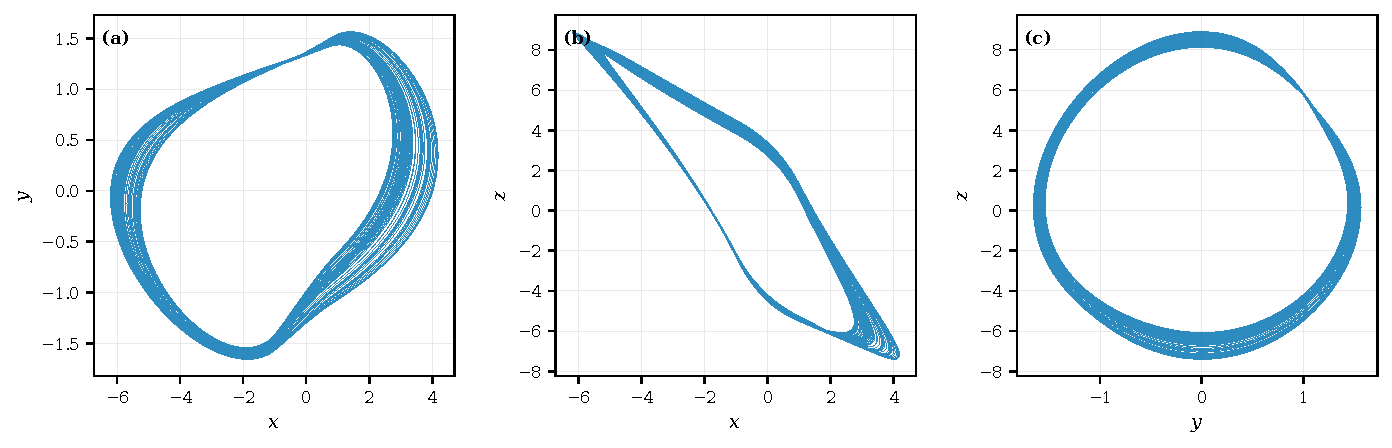
\includegraphics[width=0.86\linewidth]{nonsmooth_final_attractor}
\caption{Conjunto atrayente postransitorio obtenido para
\cref{eq:chua_no_suave,eq:parametros_no_suave} desde el extremo de la
continuación causal.}
\label{fig:atractor_no_suave_paper07}
\end{hafodigitalfigure}

\subsubsection{Sondeo volumétrico}

El protocolo completo reunió 17\,400 problemas de valor inicial, 5\,800
alrededor de cada equilibrio, sin fallos numéricos. De ellos, 7\,200
corresponden al contrato local predeclarado \(r\leq0.01\), y 10\,200 a la
extensión macroscópica diagnóstica en \(r=0.03,0.1,0.3\). La
\cref{tab:sondeo_no_suave_completo} contiene todos los radios ejecutados y
todas las clases del clasificador.

\begingroup
\setlength{\tabcolsep}{10pt}
\setlength{\LTleft}{\fill}
\setlength{\LTright}{\fill}
\begin{longtable}{@{}ccrrrrr@{}}
\caption{Conteos completos del sondeo volumétrico del sistema no suave.}
\label{tab:sondeo_no_suave_completo}\\
\toprule
Equilibrio & \(r\) & \(N\) & Objetivo & Equilibrio & Divergencia & Otro\\
\midrule
\endfirsthead
\multicolumn{7}{c}{\tablename\ \thetable\ (continuación)}\\
\toprule
Equilibrio & \(r\) & \(N\) & Objetivo & Equilibrio & Divergencia & Otro\\
\midrule
\endhead
\midrule
\multicolumn{7}{r}{Continúa en la página siguiente}\\
\endfoot
\bottomrule
\endlastfoot
\multirow{10}{*}{\(E_0\)}
& \(10^{-5}\) & 80 & 0 & 80 & 0 & 0\\
& \(3{\times}10^{-5}\) & 120 & 0 & 120 & 0 & 0\\
& \(10^{-4}\) & 160 & 0 & 160 & 0 & 0\\
& \(3{\times}10^{-4}\) & 240 & 0 & 240 & 0 & 0\\
& \(10^{-3}\) & 400 & 0 & 400 & 0 & 0\\
& \(3{\times}10^{-3}\) & 600 & 0 & 600 & 0 & 0\\
& \(10^{-2}\) & 800 & 0 & 800 & 0 & 0\\
& \(0.03\) & 1000 & 0 & 1000 & 0 & 0\\
& \(0.1\) & 1200 & 0 & 1200 & 0 & 0\\
& \(0.3\) & 1200 & 0 & 1200 & 0 & 0\\
\midrule
\multirow{10}{*}{\(E_+\)}
& \(10^{-5}\) & 80 & 0 & 0 & 39 & 41\\
& \(3{\times}10^{-5}\) & 120 & 0 & 0 & 63 & 57\\
& \(10^{-4}\) & 160 & 0 & 0 & 80 & 80\\
& \(3{\times}10^{-4}\) & 240 & 0 & 0 & 116 & 124\\
& \(10^{-3}\) & 400 & 0 & 0 & 189 & 211\\
& \(3{\times}10^{-3}\) & 600 & 0 & 0 & 277 & 323\\
& \(10^{-2}\) & 800 & 0 & 0 & 393 & 407\\
& \(0.03\) & 1000 & 0 & 0 & 490 & 510\\
& \(0.1\) & 1200 & 0 & 4 & 588 & 608\\
& \(0.3\) & 1200 & 19 & 7 & 591 & 583\\
\midrule
\pagebreak[4]
\multirow{10}{*}{\(E_-\)}
& \(10^{-5}\) & 80 & 0 & 0 & 41 & 39\\
& \(3{\times}10^{-5}\) & 120 & 0 & 0 & 56 & 64\\
& \(10^{-4}\) & 160 & 0 & 0 & 81 & 79\\
& \(3{\times}10^{-4}\) & 240 & 0 & 0 & 122 & 118\\
& \(10^{-3}\) & 400 & 0 & 0 & 204 & 196\\
& \(3{\times}10^{-3}\) & 600 & 0 & 0 & 309 & 291\\
& \(10^{-2}\) & 800 & 0 & 0 & 394 & 406\\
& \(0.03\) & 1000 & 0 & 0 & 488 & 512\\
& \(0.1\) & 1200 & 0 & 4 & 593 & 603\\
& \(0.3\) & 1200 & 18 & 12 & 596 & 574\\
\end{longtable}
\endgroup

En el contrato local se registraron cero contactos y cero fallos numéricos en
las 7\,200 sondas con \(r\leq0.01\). Este es el alcance usado para evaluar la
compatibilidad local con ocultedad del conjunto atrayente regular.

La extensión macroscópica, que no amplía ese contrato local, añadió 10\,200
sondas. Las 6\,600 correspondientes a \(r=0.03\) y \(r=0.1\) produjeron cero
contactos; al combinarlas con el contrato local se obtiene el acumulado
\(0/13\,800\) hasta \(r=0.1\). El primer radio con contactos de la extensión
fue \(r=0.3\); después de completar sus 3\,600 sondas se registraron 37
contactos: cero desde \(E_0\), 19 desde \(E_+\) y 18 desde \(E_-\). Las
distancias iniciales de esos contactos a su equilibrio estuvieron entre
\(0.1941805298\) y \(0.2997254735\). Por tanto, la extensión macroscópica
delimita el intervalo de acceso muestreado
\[
0.1<r_{\mathrm{contacto}}\leq0.3
\]
sin convertirlo en el alcance del contrato local.

\begin{hafodigitalfigure}[H]
\centering
\begin{subfigure}[t]{0.49\linewidth}
  \centering
  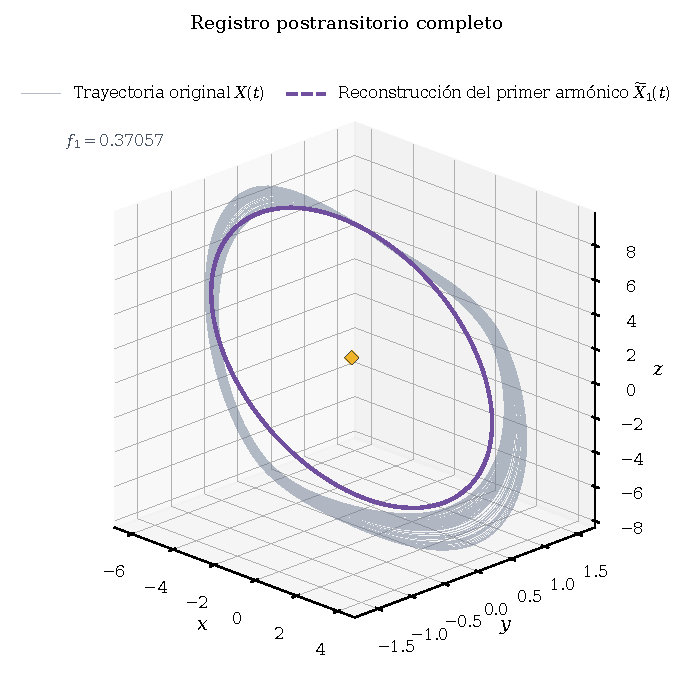
\includegraphics[width=\linewidth]{nonsmooth_first_harmonic_comparison_es}
  \caption{Trayectoria y primer armónico.}
\end{subfigure}\hfill
\begin{subfigure}[t]{0.49\linewidth}
  \centering
  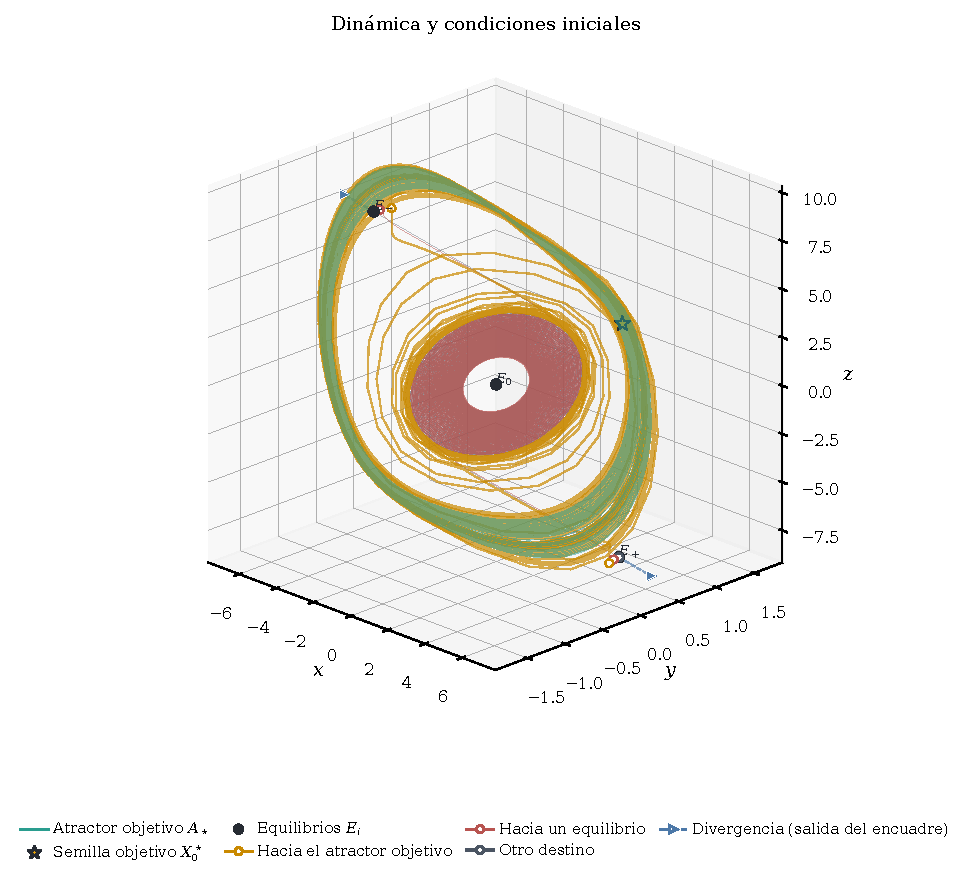
\includegraphics[width=\linewidth]{nonsmooth_volumetric_probe_overview_es}
  \caption{Sondas volumétricas representativas.}
\end{subfigure}
\caption{Diagnósticos del caso no suave. La comparación armónica describe el
carácter regular de la respuesta; las sondas muestran ejemplos de las clases
usadas en \cref{tab:sondeo_no_suave_completo}.}
\label{fig:diagnosticos_no_suave_paper07}
\end{hafodigitalfigure}

\FloatBarrier
\subsection{Caso con arctangente \texttt{c590}}
\label{subsec:resultados_c590}

\subsubsection{Selección en orden entero y refinamiento de Caputo}

En la exploración global, 894 de los 2\,400 casos quedaron separados del
control y 884 fueron además no triviales. De éstos, 823 se clasificaron como
regulares de apariencia periódica y 61 permanecieron en la categoría
exploratoria no periódica. El índice global de base cero 1731 obtuvo la mayor
puntuación, \(S=0.3021129950\), y definió el centro
\begin{equation}
\begin{aligned}
p_b={}&(18.4857295104,\ 21.9669521100,\ 0.0052746106,\\
&0.0262974930,\ -3.2087779245,\ 1.9492612035),\\
X_b={}&(7.0796053271,\ 0.5079327671,\ -14.4903935267)^{\T}.
\end{aligned}
\label{eq:resultado_centro_c590}
\end{equation}

La exploración local generó 1\,000 casos: 170 quedaron separados del control
y 148 fueron también no triviales. Entre estos últimos hubo 87 respuestas
exploratorias no periódicas y 61 regulares de apariencia periódica.
\texttt{c590}, índice local de base cero 590, ocupó el rango 10 por puntuación.
La auditoría variacional de los 30 mejores casos seleccionó \texttt{c590} con
\begin{equation}
(\lambda_1,\lambda_2,\lambda_3)
=(0.4699043683,\ 0.0010414594,\ -19.0491693716)
\label{eq:resultado_lyapunov_entero_c590}
\end{equation}
y semilla entera
\begin{equation}
X_0^{\mathrm{int}}
=(7.6733768929,\ 0.5079327671,\ -14.4903935267)^{\T}.
\label{eq:resultado_semilla_entera_c590}
\end{equation}

Los parámetros finales son los de \cref{eq:parametros_c590}. Sus equilibrios
son
\begin{equation}
E_0=(0,0,0),\qquad
E_\pm=(\pm4.6494055135,\ \pm0.0017970023,\ \mp4.6476085112).
\label{eq:equilibrios_c590_resultados}
\end{equation}
El criterio de Matignon clasificó \(E_0\) como inestable y \(E_\pm\) como
estables; el margen de los equilibrios externos fue
\(7.42265\times10^{-4}\).

El refinamiento seleccionó \(q=0.9999\) y el estado de índice 9, extraído en
\(t\simeq240\):
\begin{equation}
X_0^{\mathrm{frac}}
=(5.8642449791,\ 1.5847111486,\ 3.2155806478)^{\T}.
\label{eq:resultado_semilla_fraccionaria_c590}
\end{equation}
En la auditoría larga, las medianas remuestreadas fueron
\begin{equation}
(K_{0.0025},K_{0.005},K_{0.01})
=(0.865843,\ 0.885089,\ 0.740058).
\label{eq:resultado_k_pasos_c590}
\end{equation}
Los dos pasos refinados superaron el umbral de selección 0.8; el tercer valor
documenta la sensibilidad al paso más grande.

\begin{hafodigitalfigure}[H]
\centering
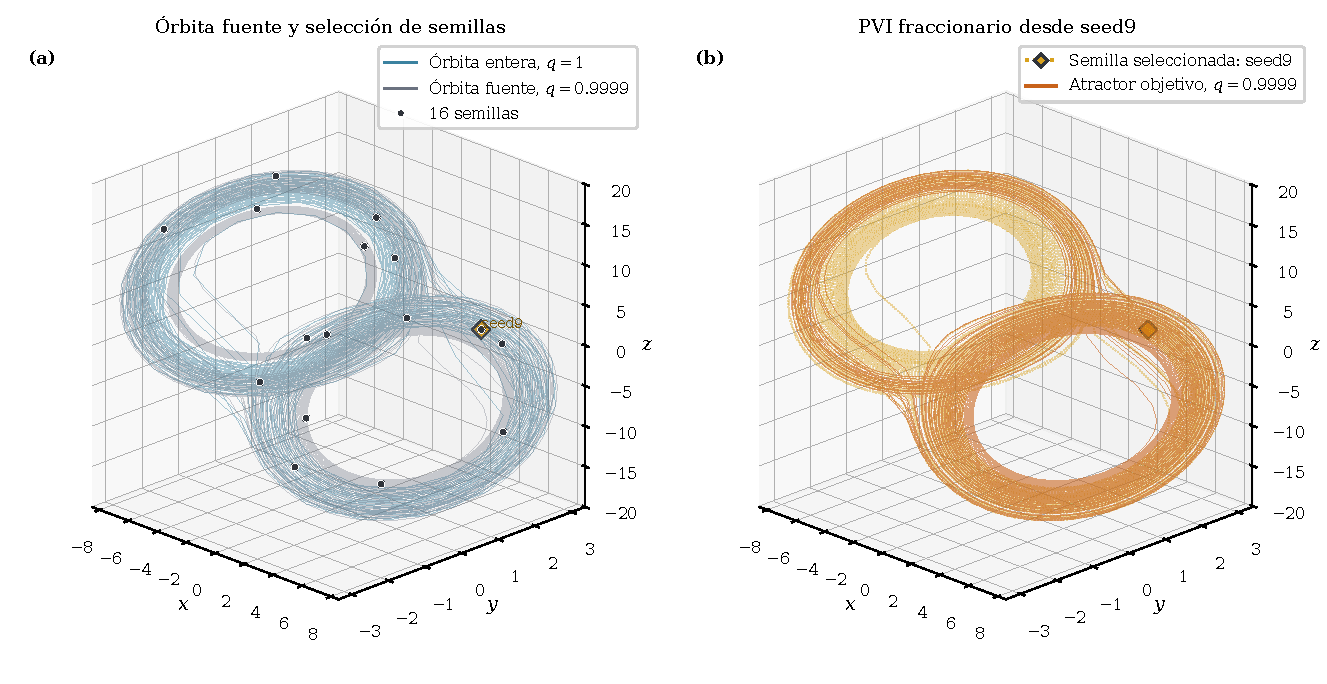
\includegraphics[width=0.92\linewidth]{arctan_fractional_refinement_es}
\caption{Búsqueda en orden entero y refinamiento fraccionario del caso
\texttt{c590}. Cada valor de \(q\) corresponde a un problema de Caputo
independiente; el estado seleccionado se extrae de la trayectoria
\(q=0.9999\).}
\label{fig:refinamiento_c590_paper07}
\end{hafodigitalfigure}

La trayectoria final permaneció acotada en los tres pasos. Sobre 30\,000
estados postransitorios, ninguna componente cumplió el filtro de apariencia
periódica. Las entropías espectrales, fracciones de potencia dominante y
derivas relativas fueron
\begin{equation}
\begin{aligned}
(H_x,H_y,H_z)
&=(0.394751,\ 0.261922,\ 0.315229),\\
(R_x,R_y,R_z)
&=(0.122163,\ 0.290492,\ 0.241937),\\
(\Delta_{f,x},\Delta_{f,y},\Delta_{f,z})
&=(0.941176,\ 0.029412,\ 0.029412).
\end{aligned}
\label{eq:metricas_finales_c590}
\end{equation}
La respuesta se clasifica, por tanto, como aperiódica bajo el filtro
postransitorio declarado.

\begin{hafodigitalfigure}[H]
\centering
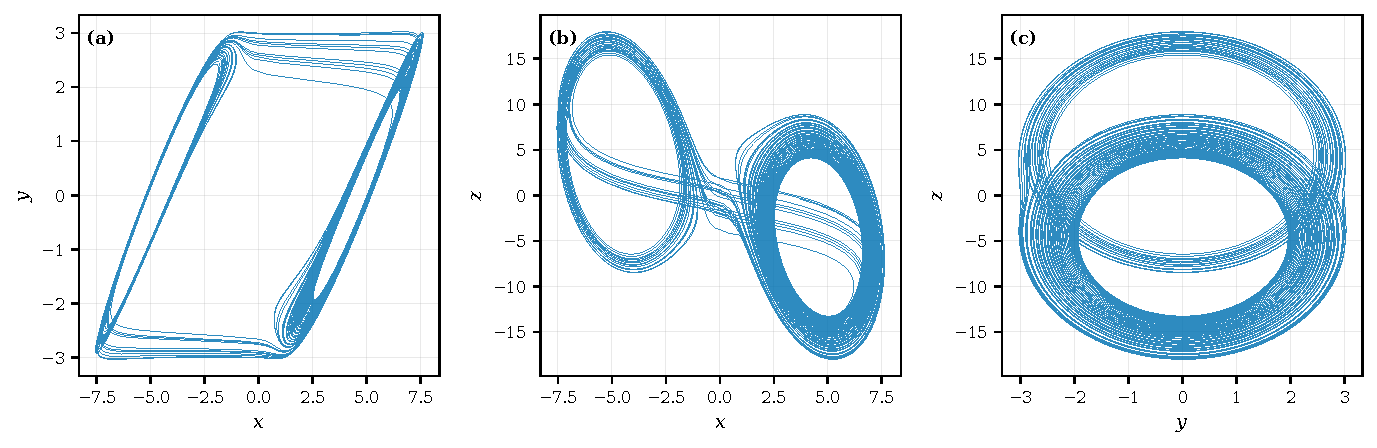
\includegraphics[width=0.86\linewidth]{arctan_final_attractor}
\caption{Conjunto postransitorio del sistema
\cref{eq:chua_arctan,eq:parametros_c590} para \(q=0.9999\),
\(h=0.005\) y la condición \cref{eq:resultado_semilla_fraccionaria_c590}.}
\label{fig:atractor_c590_paper07}
\end{hafodigitalfigure}

\subsubsection{Sondeo superficial}

El registro canónico reúne 13\,500 trayectorias: 8\,400 en la partición local
\(r\leq0.3\) y 5\,100 en la auditoría macroscópica \(r\in\{1,2\}\). El primer
contacto se observó en \(r=1\), pero se retuvo \(r=2\) como bloque adicional.
La \cref{tab:sondeo_c590_completo} contiene todos los conteos del experimento
declarado.

\begingroup
\setlength{\tabcolsep}{10pt}
\setlength{\LTleft}{\fill}
\setlength{\LTright}{\fill}
\begin{longtable}{@{}ccrrrrr@{}}
\caption{Conteos completos del sondeo sobre superficies esféricas de
\texttt{c590}.}
\label{tab:sondeo_c590_completo}\\
\toprule
Equilibrio & \(r\) & \(N\) & Objetivo & Equilibrio & Divergencia & Otro\\
\midrule
\endfirsthead
\multicolumn{7}{c}{\tablename\ \thetable\ (continuación)}\\
\toprule
Equilibrio & \(r\) & \(N\) & Objetivo & Equilibrio & Divergencia & Otro\\
\midrule
\endhead
\midrule
\multicolumn{7}{r}{Continúa en la página siguiente}\\
\endfoot
\bottomrule
\endlastfoot
\multirow{9}{*}{\(E_0\)}
& \(10^{-5}\) & 100 & 0 & 0 & 0 & 100\\
& \(10^{-4}\) & 200 & 0 & 0 & 0 & 200\\
& \(10^{-3}\) & 300 & 0 & 0 & 0 & 300\\
& \(10^{-2}\) & 400 & 0 & 0 & 0 & 400\\
& \(0.03\) & 500 & 0 & 0 & 0 & 500\\
& \(0.1\) & 600 & 0 & 0 & 0 & 600\\
& \(0.3\) & 700 & 0 & 0 & 0 & 700\\
& \(1\) & 800 & 22 & 0 & 0 & 778\\
& \(2\) & 900 & 289 & 0 & 67 & 544\\
\midrule
\pagebreak[4]
\multirow{9}{*}{\(E_+\)}
& \(10^{-5}\) & 100 & 0 & 2 & 0 & 98\\
& \(10^{-4}\) & 200 & 0 & 0 & 0 & 200\\
& \(10^{-3}\) & 300 & 0 & 0 & 0 & 300\\
& \(10^{-2}\) & 400 & 0 & 0 & 0 & 400\\
& \(0.03\) & 500 & 0 & 0 & 0 & 500\\
& \(0.1\) & 600 & 0 & 0 & 0 & 600\\
& \(0.3\) & 700 & 0 & 0 & 0 & 700\\
& \(1\) & 800 & 0 & 0 & 0 & 800\\
& \(2\) & 900 & 150 & 0 & 37 & 713\\
\midrule
\multirow{9}{*}{\(E_-\)}
& \(10^{-5}\) & 100 & 0 & 2 & 0 & 98\\
& \(10^{-4}\) & 200 & 0 & 0 & 0 & 200\\
& \(10^{-3}\) & 300 & 0 & 0 & 0 & 300\\
& \(10^{-2}\) & 400 & 0 & 0 & 0 & 400\\
& \(0.03\) & 500 & 0 & 0 & 0 & 500\\
& \(0.1\) & 600 & 0 & 0 & 0 & 600\\
& \(0.3\) & 700 & 0 & 0 & 0 & 700\\
& \(1\) & 800 & 0 & 0 & 0 & 800\\
& \(2\) & 900 & 149 & 0 & 27 & 724\\
\end{longtable}
\endgroup

Las 8\,400 trayectorias con \(r\leq0.3\) produjeron cero contactos; 8\,396
completaron el horizonte y cuatro convergieron anticipadamente a \(E_\pm\) en
\(r=10^{-5}\). En \(r=1\) hubo 22 contactos entre 2\,400 trayectorias, todos
desde \(E_0\). En \(r=2\) hubo 588 contactos entre 2\,700 trayectorias: 289
desde \(E_0\), 150 desde \(E_+\) y 149 desde \(E_-\); en este bloque se
registraron 131 divergencias. En total se ejecutaron 13\,500 pruebas y se
observaron 610 contactos. El primer radio observado satisface
\[
0.3<r_{\mathrm{primer\ contacto}}\leq1.
\]

\begin{hafodigitalfigure}[H]
\centering
\begin{subfigure}[t]{0.49\linewidth}
  \centering
  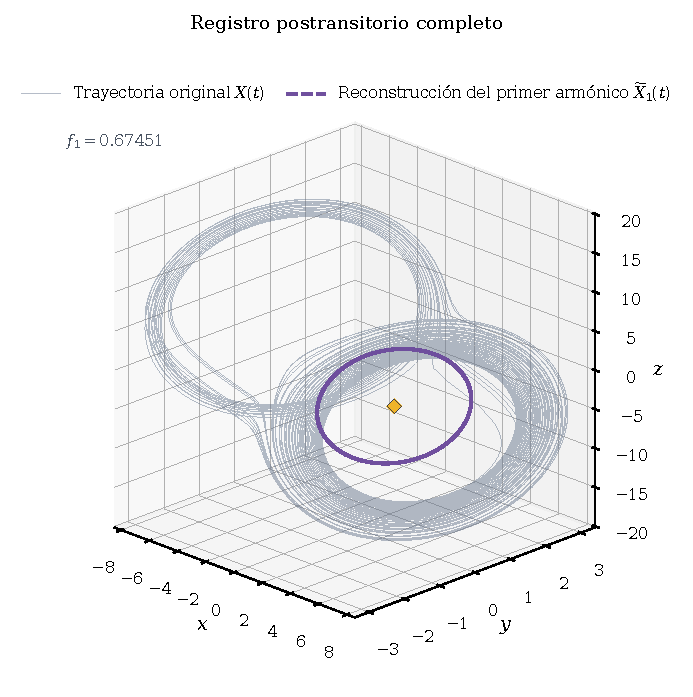
\includegraphics[width=\linewidth]{arctan_first_harmonic_comparison_es}
  \caption{Trayectoria y primer armónico.}
\end{subfigure}\hfill
\begin{subfigure}[t]{0.49\linewidth}
  \centering
  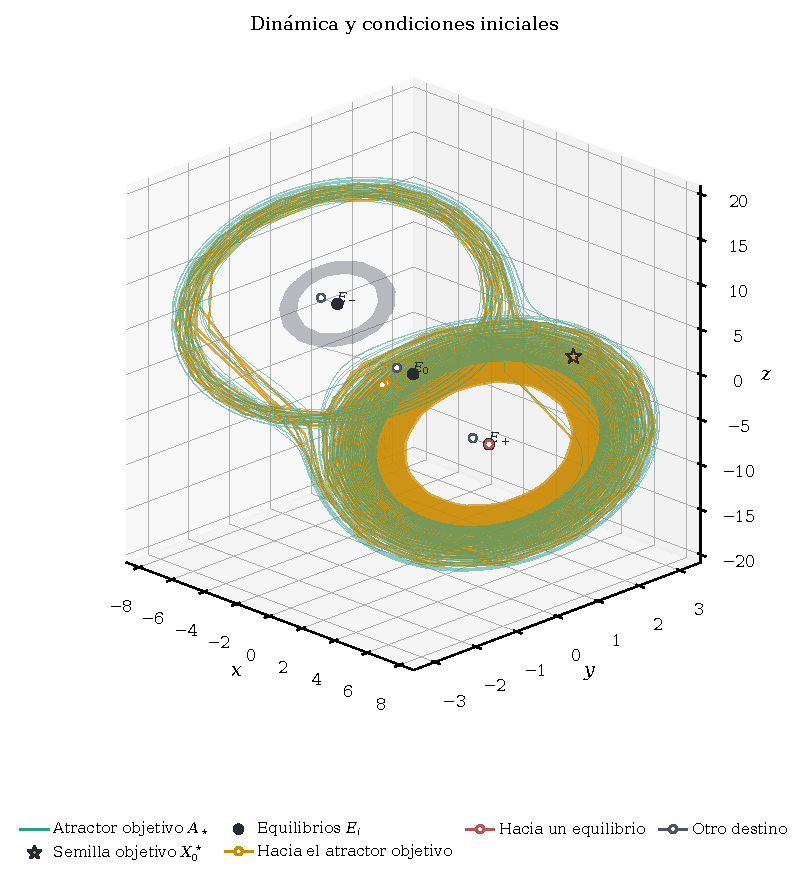
\includegraphics[width=\linewidth]{arctan_spherical_probe_overview_es}
  \caption{Sondas superficiales representativas.}
\end{subfigure}
\caption{Diagnósticos de \texttt{c590}. La comparación con el primer armónico
acompaña el filtro de aperiodicidad. El panel de sondas muestra nueve historias
representativas seleccionadas en el subconjunto hasta \(r=1\); no es una
gráfica de conteos. La \cref{tab:sondeo_c590_completo} incorpora además la
auditoría canónica en \(r=2\).}
\label{fig:diagnosticos_c590_paper07}
\end{hafodigitalfigure}

\FloatBarrier
\subsection{Delimitación local obtenida}
\label{subsec:delimitacion_local}

\begin{table}[H]
\centering
\caption{Alcance local predeclarado y acceso observado en los sondeos
extendidos.}
\label{tab:intervalos_locales}
\begin{tabularx}{\linewidth}{L{0.26\linewidth}C{0.18\linewidth}C{0.18\linewidth}Y}
\toprule
Sistema & Geometría & Alcance o intervalo & Conteos correspondientes\\
\midrule
No suave, \(q=0.9998\)
& Bola volumétrica
& Local: \(r\leq0.01\)
& Local: \(0/7\,200\), cero fallos;
macro: \(0/6\,600\) en \(0.03,0.1\) y
\(37/3\,600\) en \(0.3\)\\
\texttt{c590}, \(q=0.9999\)
& Superficie esférica
& Separación observada hasta \(r=0.3\); revisión macroscópica en \(r=1,2\)
& \(0/8\,400\) hasta \(0.3\);
\(22/2\,400\) en \(1\);
\(588/2\,700\) en \(2\), con 131 divergencias\\
\bottomrule
\end{tabularx}
\end{table}

Dentro de las bolas, horizontes y reglas de contacto del contrato local
\(r\leq0.01\), el conjunto regular no suave es compatible con la definición
local de atractor oculto. Los radios \(0.03\), \(0.1\) y \(0.3\) describen una
extensión macroscópica de la geometría de cuenca y no amplían la afirmación de
ocultedad más allá del contrato local. Para \texttt{c590}, la compatibilidad
local se limita a las superficies, radios, horizontes y reglas de contacto con
\(r\leq0.3\). Los contactos observados en \(r=1\) y \(r=2\) describen acceso
macroscópico a la cuenca. Todos estos resultados proceden de muestras finitas
y no constituyen una prueba global de separación de cuencas.

  \section{Alcance y criterio de evidencia}

El análisis distingue cuatro niveles de evidencia:

\begin{enumerate}
  \item \textbf{derivación}: existencia de una rama armónica compatible y de
        una semilla obtenida desde el modelo;
  \item \textbf{localización}: integración y continuación hasta un conjunto
        recurrente del sistema original;
  \item \textbf{clasificación dinámica}: periodicidad, regularidad o
        comportamiento compatible con caos bajo un diagnóstico finito;
  \item \textbf{ocultedad}: ausencia de contacto desde un conjunto explícito
        de vecindades de todos los equilibrios.
\end{enumerate}

La continuación establece la localización de un candidato. La clasificación
dinámica requiere diagnósticos convergentes y la compatibilidad con ocultedad
queda limitada al banco de vecindades y al horizonte declarados.

\evidencebox{\textbf{Interpretación.} \emph{Compatible con ocultedad bajo
el protocolo finito} significa exactamente que ninguna condición inicial del
banco ensayado alcanzó la nube candidata. \emph{Oculto según la fuente}
atribuye el rótulo a la bibliografía. \emph{Ocultedad certificada en un
dominio} se reserva para un argumento que cubra el continuo declarado. Ninguna
de las dos primeras expresiones significa una prueba topológica global de la
cuenca.}

\section{Ruta matemática y numérica común}

\subsection{Declaración Lur'e y ruta directa D0}

La formulación escalar base es
\begin{equation}
  \dot X=PX+b\,\psi(\sigma),\qquad
  \sigma=c^{\mathsf T}X,
  \label{int:eq:lure}
\end{equation}
con una comprobación numérica de que el campo de \eqref{int:eq:lure} coincide con
las ecuaciones originales. Se verifican también los equilibrios, el Jacobiano
analítico contra diferencias finitas y el espectro local.

La transferencia se define por
\begin{equation}
  G(s)=c^{\mathsf T}(P-sI)^{-1}b.
  \label{int:eq:transfer}
\end{equation}
Para justificar el signo del cierre, considérese primero la ganancia lineal
\(\psi(\sigma)=k\sigma\) y un modo \(X(t)=v\e^{st}\). Entonces
\[
 (sI-P)v=bk\,c^{\mathsf T}v.
\]
Si \(sI-P\) es invertible y \(c^{\mathsf T}v\ne0\), multiplicar por
\(c^{\mathsf T}(sI-P)^{-1}\) y cancelar \(c^{\mathsf T}v\) da
\[
 1=k\,c^{\mathsf T}(sI-P)^{-1}b=-kG(s).
\]
Equivalentemente, el lema del determinante para una perturbación de rango uno
da
\[
 \det(sI-P-kbc^{\mathsf T})=\det(sI-P)[1+kG(s)].
\]
Estas identidades se aplican fuera de los polos de la transferencia. Para
\(s=i\omega_0\) y \(k\) real, separarlas en partes real e imaginaria
produce el cierre siguiente. La ganancia de primer armónico de una entrada
\(a\cos\theta\) es
\[
 \mathcal N(a)=\frac1{\pi a}\int_0^{2\pi}
                   \psi(a\cos\theta)\cos\theta\,\dd\theta.
\]
Se obtiene por proyección sobre \(\cos\theta\), cuya norma cuadrática en
un periodo es \(\pi\). El cierre retiene esa componente; los armónicos
superiores se evalúan posteriormente mediante la integración del campo.

La ruta directa resuelve
\begin{equation}
  \operatorname{Im}G(i\omega_0)=0,\qquad
  k=-\frac{1}{\operatorname{Re}G(i\omega_0)},\qquad
  \mathcal N(a_0)=k.
  \label{int:eq:balance}
\end{equation}
La frecuencia \(\omega_0\) se obtiene de las raíces polinómicas o de la
ecuación escalar derivada de la transferencia. El diagrama de Nyquist
representa las ramas resultantes.

Para cada rama compatible se forma \(P_0=P+kbc^{\mathsf T}\). Un vector
normalizado se obtiene directamente como
\[
 v=k(i\omega_0I-P)^{-1}b,\qquad
 c^{\mathsf T}v=-kG(i\omega_0)=1.
\]
La ecuación resolvente implica \(P_0v=i\omega_0v\). Por ser \(P_0\) real,
\[
 X_{\rm aux}(t)=a_0\operatorname{Re}
       \bigl(v\e^{i(\omega_0t+\theta)}\bigr),\qquad
 c^{\mathsf T}X_{\rm aux}(t)=a_0\cos(\omega_0t+\theta)
\]
es una solución exacta del sistema auxiliar. Su estado inicial es la semilla
\(X_0=a_0\operatorname{Re}(v\e^{i\theta})\). La continuación entera es
\begin{equation}
  \dot X=P_0X+\lambda b
  \left[\psi(c^{\mathsf T}X)-k\,c^{\mathsf T}X\right],
  \qquad 0\leq\lambda\leq1.
  \label{int:eq:homotopy}
\end{equation}
En $\lambda=0$ queda el oscilador armónico auxiliar y en $\lambda=1$ se
recupera exactamente el sistema original.

\subsection{Ruta alternativa A1}

Si \eqref{int:eq:balance} no produce una ganancia compatible, una amplitud real,
una continuación persistente o candidatos que superen el objetivo dinámico
declarado, se recurre a una alternativa adecuada a esa obstrucción. En Kalman--Fitts, la única rama directa tiene
ganancia negativa, incompatible con la función descriptiva positiva de
\(\tanh\). Entonces se usa un mapa de conmutación de Andronov para
\(\operatorname{sign}(\sigma)\) y una homotopía
\begin{equation}
  \psi_\lambda(\sigma)=
  (1-\lambda)\operatorname{sign}(\sigma)
  +\lambda\tanh(\sigma/\varepsilon).
  \label{int:eq:sign-tanh}
\end{equation}

Los barridos de frecuencia, las transferencias sesgadas y la continuación
multiparámetro son alternativas reservadas para fallos explícitos. No forman
parte de la ruta principal de orden entero. En la extensión caótica MAVPD, la
ruta D0 sí produce semillas y continuación, pero ninguna de sus dos ramas base
supera el cribado finito de caos; sólo entonces se habilita una continuación
paramétrica estructurada alrededor de una frontera de Hopf derivada.

\subsection{Localización y contraste independiente}

Las semillas se calculan a partir de las ecuaciones del modelo. Los valores
publicados y los obtenidos previamente mediante cálculo simbólico se emplean
para contrastar el cierre algebraico y el destino de las trayectorias una
vez completada la localización. La comparación entre Python y Julia utiliza
cálculos independientes con un protocolo común de evaluación.

\subsection{Protocolo de ocultedad}

Después de localizar una nube candidata \(\mathcal A_h\), se construyen
condiciones iniciales alrededor de \emph{todos} los equilibrios. Para una
condición \(X_0\), la cola de su trayectoria se compara con:

\begin{enumerate}
  \item las tolerancias de convergencia a cada equilibrio;
  \item la nube candidata mediante una distancia normalizada;
  \item umbrales de divergencia y de conjunto acotado no trivial.
\end{enumerate}

La conclusión \emph{sin contacto} queda ligada al conjunto explícito de
condiciones iniciales, junto con sus radios, direcciones, paso, transitorio,
horizonte y tolerancia geométrica. En cada comparación cruzada los dos entornos
reciben las mismas coordenadas.

\begin{center}
\begin{tikzpicture}[
  node distance=0.55cm and 0.9cm,
  box/.style={draw=Azul,rounded corners,fill=AzulClaro,align=center,
              text width=3.45cm,minimum height=0.88cm},
  alt/.style={draw=Naranja,rounded corners,fill=NaranjaClaro,align=center,
              text width=3.45cm,minimum height=0.88cm},
  arrow/.style={-{Latex[length=2.3mm]},thick}
]
\node[box] (model) {Ecuaciones, Jacobiano,\\equilibrios y forma Lur'e};
\node[box,below=of model] (direct) {Transferencia directa\\$\omega_0\to k\to a_0\to X_0$};
\node[box,below=of direct] (cont) {Continuación al\\sistema original};
\node[box,below=of cont] (dyn) {Candidato y\\diagnóstico dinámico};
\node[box,below=of dyn] (hidden) {Sondeos comunes\\de ocultedad};
\node[alt,right=of direct] (fallback) {Ruta alternativa sólo\\tras fallo documentado};
\draw[arrow] (model)--(direct);
\draw[arrow] (direct)--(cont);
\draw[arrow] (cont)--(dyn);
\draw[arrow] (dyn)--(hidden);
\draw[arrow,dashed,draw=Naranja] (direct)--(fallback);
\draw[arrow,dashed,draw=Naranja] (fallback.south)--(dyn.east);
\end{tikzpicture}

\smallskip
\small\textbf{Diagrama metodológico.} Jerarquía de búsqueda usada para los
sistemas enteros.
\end{center}

\section[Caso 1: Chua no suave entero]{Caso 1: Chua no suave de orden entero}

\subsection{Modelo y derivación}

El sistema es
\begin{align}
 \dot x&=\alpha\,[y-x-\phi(x)],\nonumber\\
 \dot y&=x-y+z,\nonumber\\
 \dot z&=-\beta y-\gamma z, \label{int:eq:chua}\\
 \phi(x)&=m_1x+(m_0-m_1)\operatorname{sat}(x),\qquad
 \operatorname{sat}(x)=\min(1,\max(-1,x)).\nonumber
\end{align}
Se usaron
\[
 \alpha=8.4562,\quad \beta=12.0732,\quad \gamma=0.0052,\quad
 m_0=-0.1768,\quad m_1=-1.1468.
\]
La forma D0 exacta toma \(c=e_1\), \(b=-\alpha e_1\), una parte lineal
con pendiente base \(m_1\) y
\(\psi(\sigma)=(m_0-m_1)\operatorname{sat}(\sigma)\).

Escribiendo \(a_P=\alpha(1+m_1)\), la matriz lineal y el polinomio
intermedio son
\[
 P=\begin{pmatrix}-a_P&\alpha&0\\1&-1&1\\0&-\beta&-\gamma\end{pmatrix},
 \qquad D(s)=s^2+(1+\gamma)s+\beta+\gamma.
\]
Las dos últimas filas de \((sI-P)v=b\) dan
\(v_3=-\beta v_2/(s+\gamma)\) y
\(v_1=D(s)v_2/(s+\gamma)\). La primera fila produce
\[
 [(s+a_P)D(s)-\alpha(s+\gamma)]v_1=-\alpha D(s).
\]
Por tanto,
\begin{equation}
 G(s)=\frac{\alpha D(s)}{(s+a_P)D(s)-\alpha(s+\gamma)}.
 \label{int:eq:chua-transfer-derived}
\end{equation}
Con \(d_0=\beta+\gamma\), \(d_1=1+\gamma\), \(z=\omega^2\), el numerador
complejo de \(G(i\omega)\) es \(\alpha(d_0-z+id_1\omega)\), y el
denominador tiene partes
\[
 A=a_Pd_0-\alpha\gamma-(d_1+a_P)z,\qquad
 B=\omega(d_0+a_Pd_1-\alpha-z).
\]
Como \(\operatorname{Im}G=\alpha[d_1\omega A-(d_0-z)B]/(A^2+B^2)\),
la condición imaginaria, para \(\omega>0\) y \(A^2+B^2>0\), equivale a
\[
 z^2+(\alpha+d_1^2-2d_0)z+d_0^2-\alpha d_0+\alpha\gamma d_1=0.
\]
Cada raíz positiva se comprueba en el resolvente antes de calcular \(k\).
Normalizando el primer componente del modo a uno, sus otras componentes son
\[
 v_2=\frac{i\omega+\gamma}{D(i\omega)},\qquad
 v_3=-\frac{\beta}{D(i\omega)}.
\]
Así se obtienen los tres componentes de la semilla a partir de la amplitud y
la fase, sin ajustar coordenadas independientemente.

Sea \(\Delta=m_0-m_1\). Para \(0<a\leq1\), la saturación permanece en su
tramo lineal y \(\mathcal N(a)=\Delta\). Para \(a>1\), el ángulo de cruce
es \(\theta_c=\arccos(1/a)\). La simetría impar y la simetría entre
cuadrantes reducen la integral a
\begin{align*}
 \mathcal N(a)
 &=\frac{4\Delta}{\pi a}
   \left[\int_0^{\theta_c}\cos\theta\,\dd\theta
       +a\int_{\theta_c}^{\pi/2}\cos^2\theta\,\dd\theta\right]\\
 &=\frac{4\Delta}{\pi a}
   \left[\sin\theta_c+a\left(\frac\pi4-\frac{\theta_c}{2}
                              -\frac{\sin2\theta_c}{4}\right)\right].
\end{align*}
Usando \(\pi/2-\theta_c=\arcsin(1/a)\),
\(\sin\theta_c=\sqrt{a^2-1}/a\) y
\(\sin2\theta_c=2\sqrt{a^2-1}/a^2\), se obtiene
\begin{equation}
 \mathcal N(a)=\frac{2(m_0-m_1)}{\pi}
 \left[
 \arcsin\!\left(\frac1a\right)
 +\frac{\sqrt{a^2-1}}{a^2}
 \right].
\end{equation}
El balance armónico produjo
\[
 \omega_0=2.039186939959,\qquad
 k=0.209867354515,\qquad
 a_0=5.856145086252,
\]
y la semilla
\[
 X_0=(5.856145086252,\ 0.369331578246,\ -8.366536168324)^{\mathsf T}.
\]
El residuo de cierre de Nyquist fue \(3.26\times10^{-15}\) y el de la
función descriptiva \(1.98\times10^{-13}\). El contraste posterior con los cálculos de
Mathematica y MATLAB dio diferencias máximas del orden de \(10^{-12}\).

\subsection{Localización por recurrencias}

La búsqueda por recurrencias en Julia evaluó 512 condiciones iniciales en
un dominio y una partición prefijados. Encontró dos conjuntos recurrentes,
identificados mediante las etiquetas 2 y 3, con 22 contactos entre los 512
lanzamientos: una fracción muestral de \(0.04296875\). Las semillas de la
función descriptiva confirmaron posteriormente la correspondencia con las
ramas positiva y negativa.

\begin{hafocommonfigure}[H]
\centering
\begin{subfigure}[t]{0.49\textwidth}
  \centering
  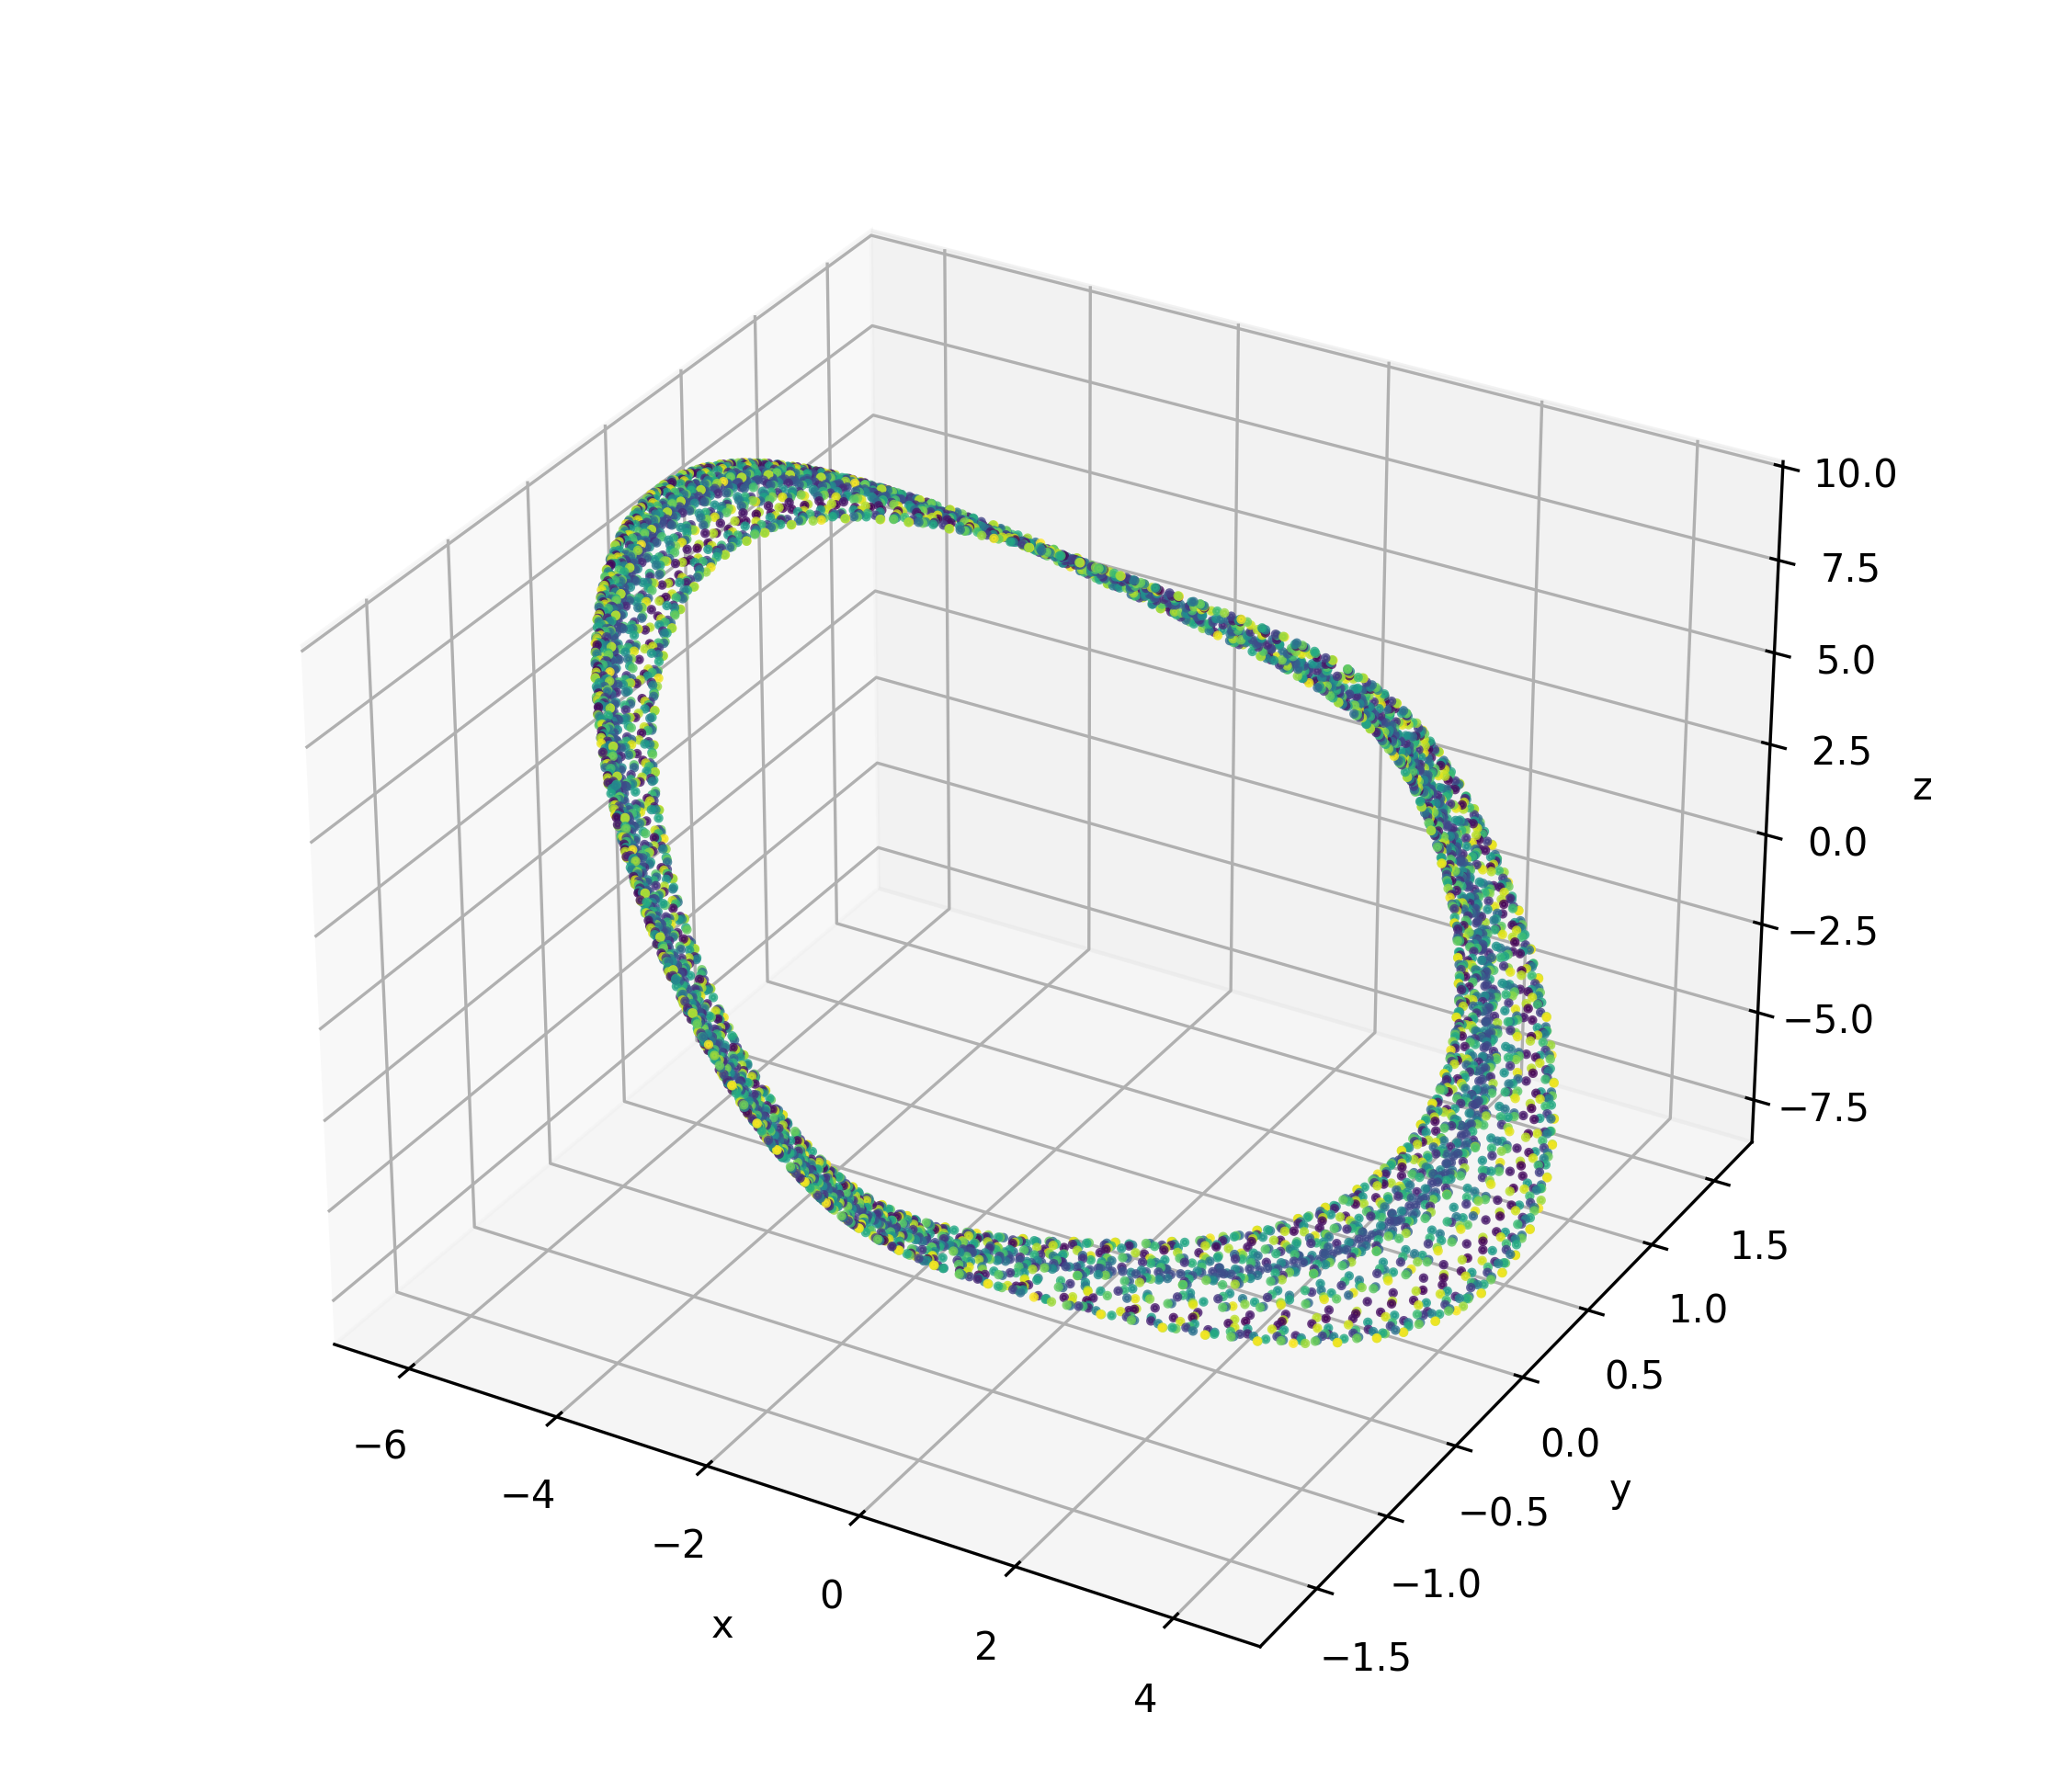
\includegraphics[width=\linewidth]{chua_python_attractor.png}
  \caption{\hafo{}: candidato obtenido por semilla y continuación.}
\end{subfigure}\hfill
\begin{subfigure}[t]{0.49\textwidth}
  \centering
  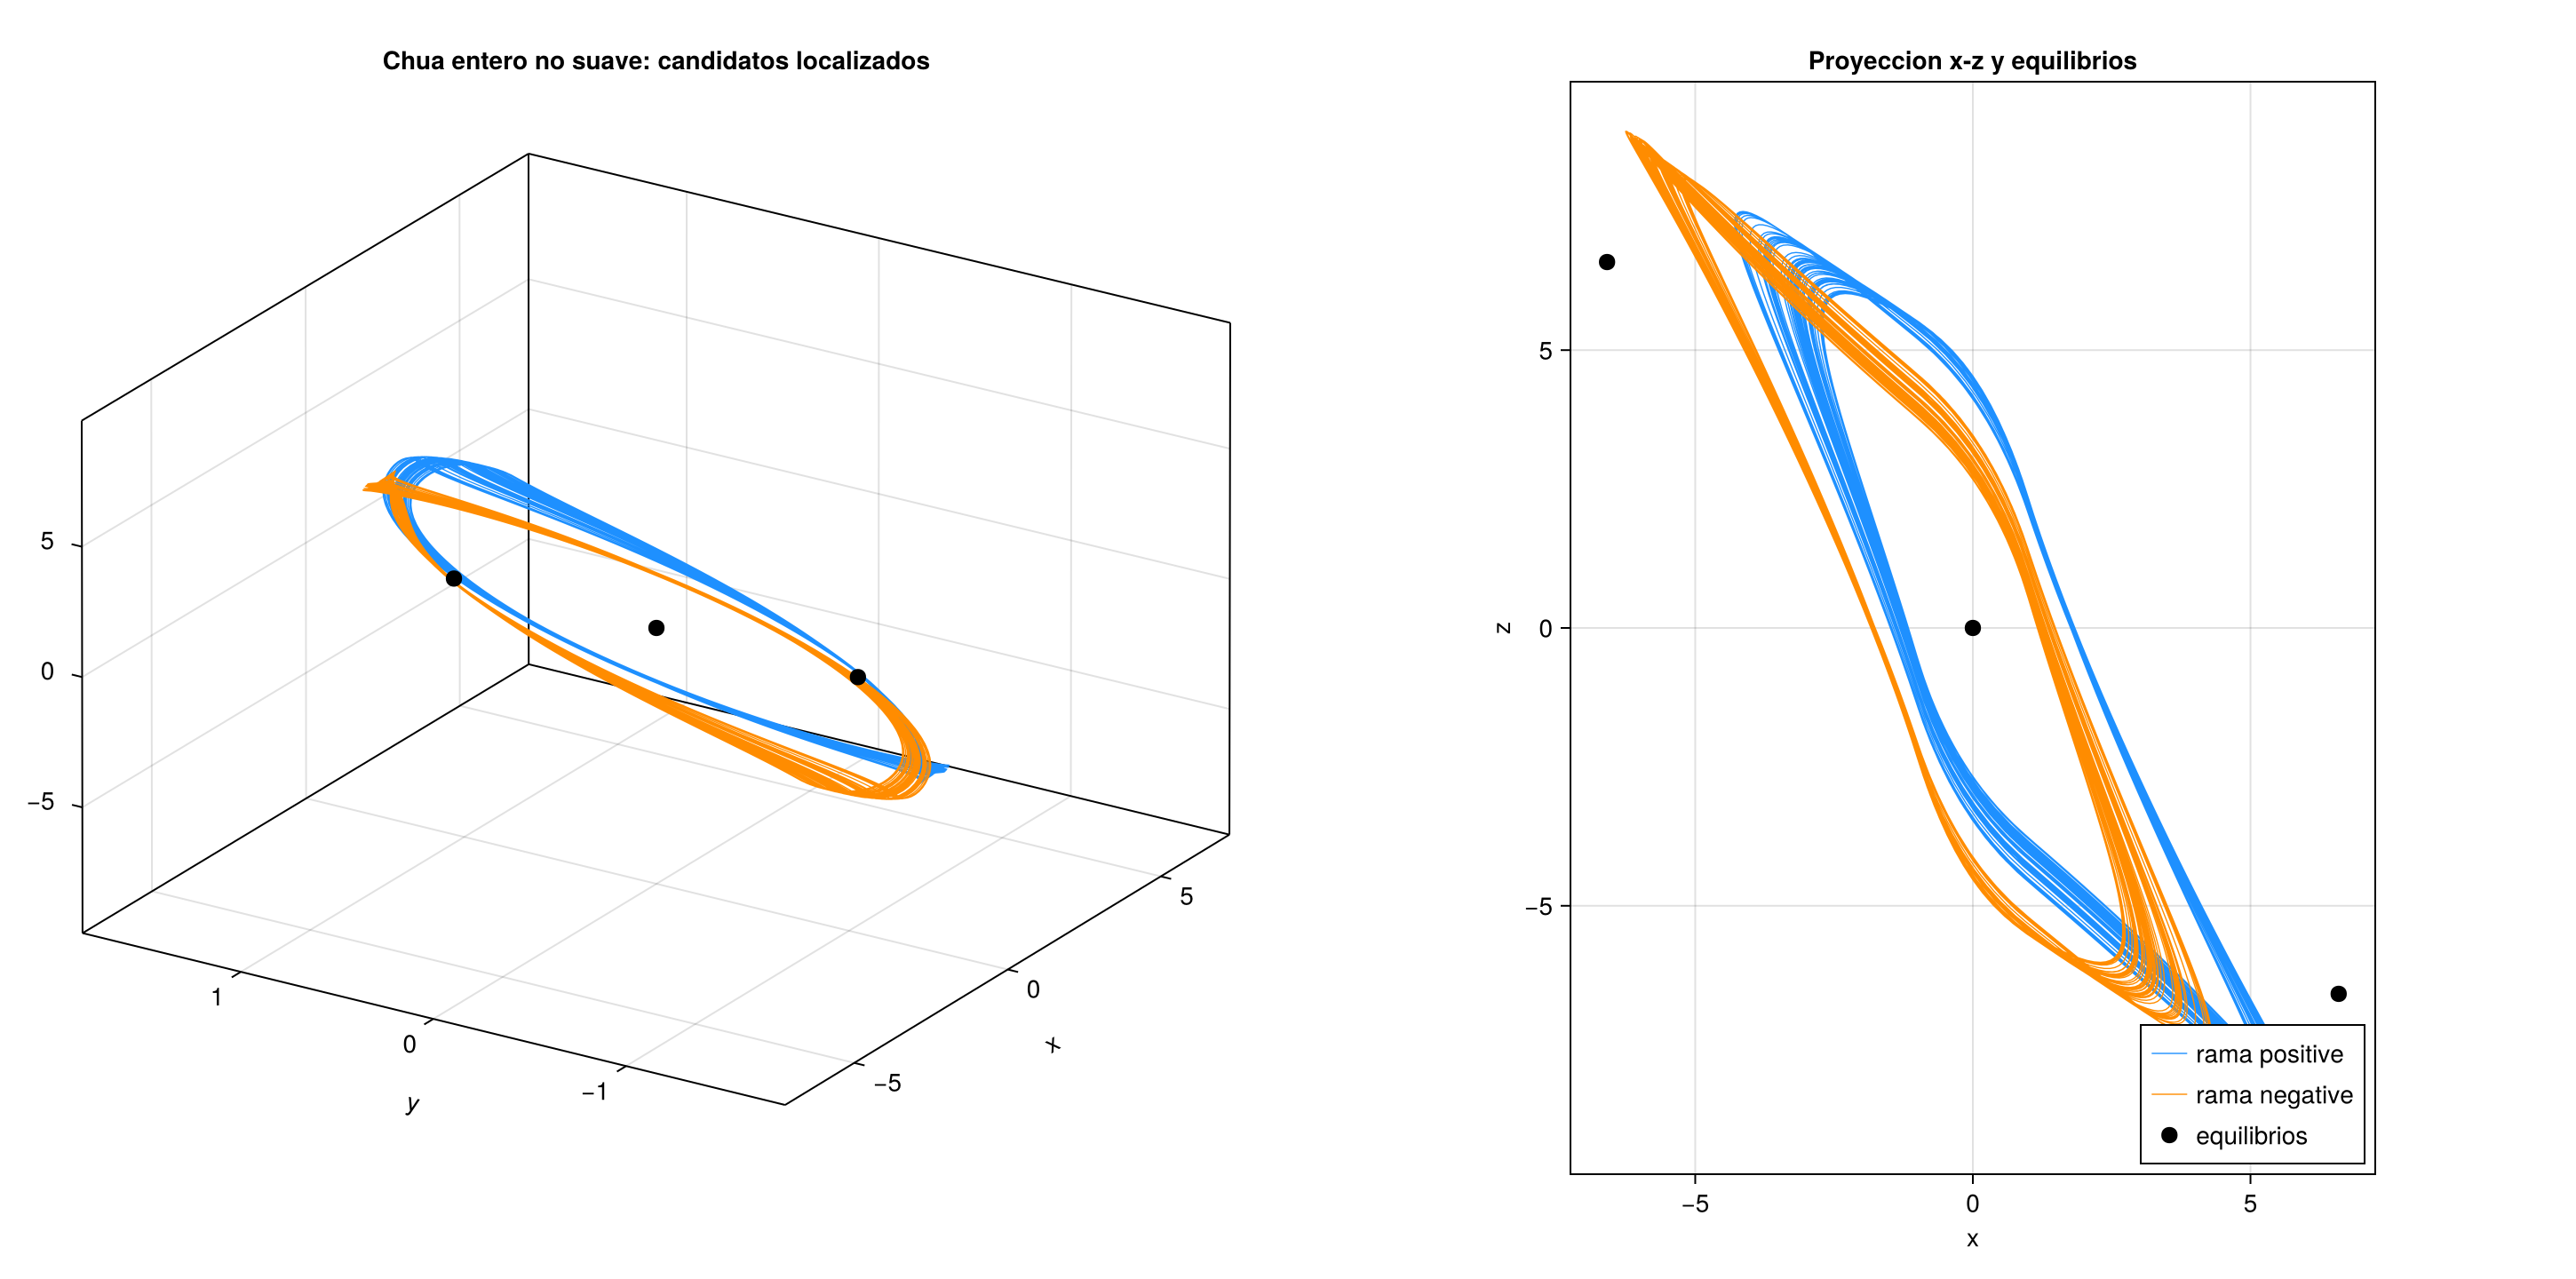
\includegraphics[width=\linewidth]{chua_julia_candidates.png}
  \caption{Julia: dos conjuntos descubiertos por recurrencias globales.}
\end{subfigure}
\caption{Localización independiente en el Chua no suave.}
\label{int:fig:chua-localization}
\end{hafocommonfigure}

\subsection{Comparación dinámica Python--Julia}

\ifHAFOBasinMaterial
\paragraph{Protocolo de comparación cruzada.}
Ambos cálculos evaluaron \ChuaProbeCount{} condiciones:
3 equilibrios, 7 radios entre \(10^{-5}\) y \(10^{-2}\), y 24 puntos por
equilibrio y radio. Se usaron \(t_f=500\), \(t_{\mathrm{burn}}=120\),
tolerancia de equilibrio \(10^{-3}\) y tolerancia normalizada de nube \(0.08\).
Las 504 coordenadas se generaron uniformemente en bolas, con semilla
pseudoaleatoria 123456789. El control EFORK--3 de referencia emplea
\(T=320\), \(T_{\mathrm{burn}}=80\), otras coordenadas y un clasificador
por huellas de sección.
\fi

\begin{table}[H]
\centering
\caption{Comparación Python--Julia del caso de Chua.}
\small
\begin{tabularx}{\textwidth}{@{}lYY@{}}
\toprule
Magnitud & Python/\hafo{} & Julia \\
\midrule
\ifHAFOBasinMaterial
Clases finales coincidentes & \multicolumn{2}{c}{504 de 504} \\
Conteos comunes & \multicolumn{2}{c}{152 en \(E_0\), 198 acotadas no triviales, 154 divergentes} \\
Contactos con candidato & 0 & 0 \\
\fi
Exponentes de Lyapunov finitos &
\((0.14018,\ 0.01319,\ -1.20304)\) &
\((0.14591,\ -0.00052,\ -1.17115)\) \\
\bottomrule
\end{tabularx}
\end{table}

\ifHAFOBasinMaterial
Los conteos \(152/198/154\) pertenecen exclusivamente a este protocolo
de comparación cruzada. Los conteos \(369/69/66\) de la configuración de referencia usan
otro horizonte, otras coordenadas y otro clasificador. Ambos protocolos dieron cero contactos con la nube objetivo.
\fi

Los dos espectros son compatibles con un exponente máximo positivo. Esa
observación apoya la clasificación caótica local, pero no sustituye la prueba
de ocultedad.

\begin{hafobasinfigure}[H]
\centering
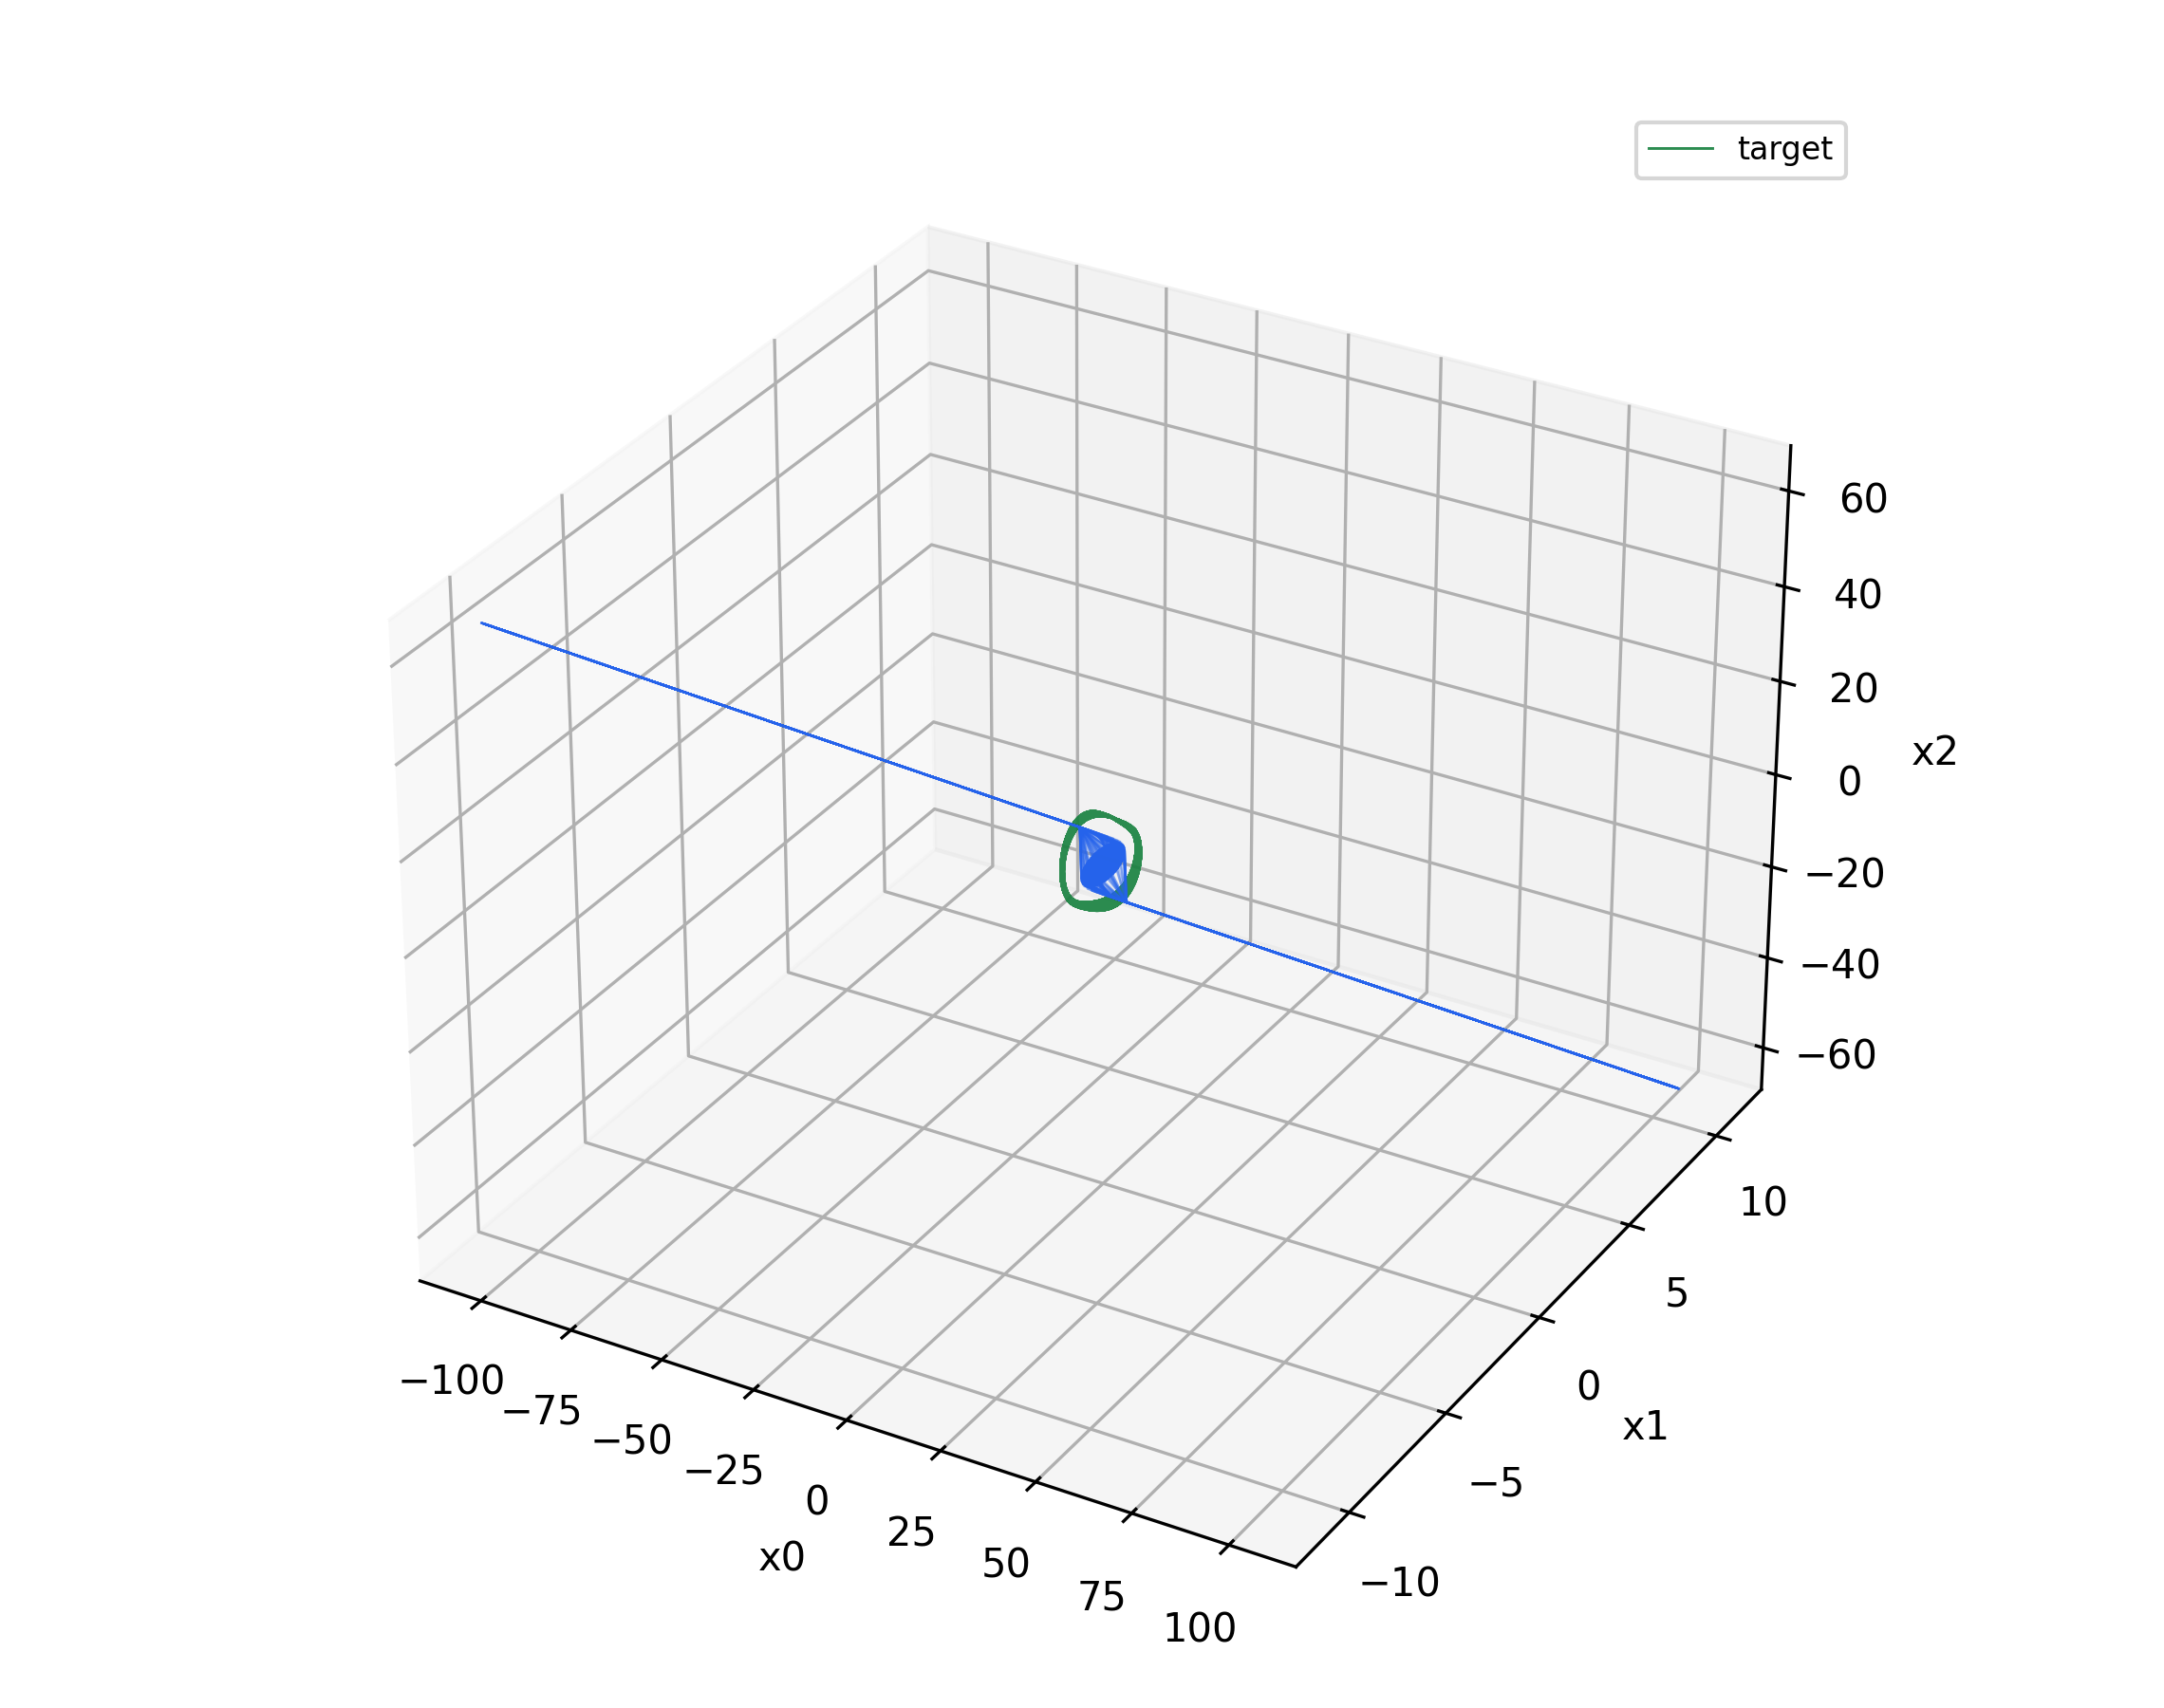
\includegraphics[width=0.82\textwidth]{chua_python_hiddenness.png}
\caption{Control de vecindades de los tres equilibrios en Python. El
comparador usó las mismas 504 coordenadas en Julia.}
\label{int:fig:chua-hiddenness}
\end{hafobasinfigure}

\section[Caso 2: Kalman--Fitts no Chua]
{Caso 2: Kalman--Fitts, sistema no Chua de cuarto orden}

\subsection{Formulación y rechazo de la ruta directa}

El sistema exacto es
\begin{equation}
 \dot X=AX+b\tanh\!\left(\frac{c^{\mathsf T}X}{\varepsilon}\right),
 \quad b=e_4,\quad c=-e_3,\quad \varepsilon=0.01,
 \label{int:eq:kf}
\end{equation}
La matriz compañera se define por
\[
 A=\begin{pmatrix}
 0&1&0&0\\0&0&1&0\\0&0&0&1\\-a_0&-a_1&-a_2&-a_3
 \end{pmatrix},
 \qquad
 p_A(s)=\bigl[(s+\beta)^2+m_1^2\bigr]
         \bigl[(s+\beta)^2+m_2^2\bigr].
\]
Al expandir el producto,
\begin{align*}
 a_0&=(m_1^2+\beta^2)(m_2^2+\beta^2),&
 a_1&=2\beta(m_1^2+m_2^2+2\beta^2),\\
 a_2&=m_1^2+m_2^2+6\beta^2,&a_3&=4\beta.
\end{align*}
Los parámetros publicados \(m_1=0.9\), \(m_2=1.1\), \(\beta=0.03\)
\cite{kalman2019} dan
\((a_0,a_1,a_2,a_3)=(0.98191881,0.121308,2.0254,0.12)\).
Las tres primeras ecuaciones de equilibrio imponen
\(x_2=x_3=x_4=0\); la cuarta queda \(-a_0x_1=0\), de modo que el único
equilibrio es el origen. Su Jacobiano es \(A+bc^{\mathsf T}/\varepsilon\)
y tiene polinomio
\[
 s^4+a_3s^3+(a_2+1/\varepsilon)s^2+a_1s+a_0.
\]
Todos los coeficientes son positivos. Las dos desigualdades adicionales de
Routh--Hurwitz para este polinomio mónico son
\[
 a_3(a_2+1/\varepsilon)-a_1=12.12174>0,
\]
\[
 a_3(a_2+1/\varepsilon)a_1-a_1^2-a_3^2a_0
 =1.456324405056>0.
\]
Por tanto, el equilibrio es localmente asintóticamente estable.

Para calcular la transferencia se resuelve \((sI-A)v=b\): las tres primeras
filas dan \(v_2=sv_1\), \(v_3=s^2v_1\), \(v_4=s^3v_1\), y la última da
\(p_A(s)v_1=1\). Como \(c=-e_3\),
\[
 c^{\mathsf T}(sI-A)^{-1}b=-\frac{s^2}{p_A(s)},\qquad
 G(s)=\frac{s^2}{p_A(s)}.
\]
En \(s=i\omega\), las partes real e imaginaria del denominador son
\(R=\omega^4-a_2\omega^2+a_0\) e
\(I=\omega(a_1-a_3\omega^2)\). De aquí
\[
 \operatorname{Im}G(i\omega)=\frac{\omega^2I}{R^2+I^2},\qquad
 \omega_0^2=\frac{a_1}{a_3},\qquad
 k=\frac{\omega_0^4-a_2\omega_0^2+a_0}{\omega_0^2}.
\]
La ruta directa, sin malla de frecuencias, encontró
\[
 \omega_0=1.005435229142,\qquad k=-0.043168701157.
\]
Para la no linealidad hiperbólica,
\[
 \mathcal N(a)=\frac1{\pi\varepsilon}\int_0^{2\pi}
  \frac{\tanh u}{u}\cos^2\theta\,\dd\theta,
 \qquad u=\frac{a\cos\theta}{\varepsilon},
\]
con valor continuo \(\tanh u/u=1\) en \(u=0\). Para \(u\ne0\),
\(0<\tanh u/u<1\), de modo que \(0<\mathcal N(a)<1/\varepsilon\).
Además, \(\mathcal N(a)\to1/\varepsilon\) cuando \(a\to0^+\), mientras
\(\mathcal N(a)\leq4/(\pi a)\to0\) cuando \(a\to\infty\). La continuidad
y estas cotas dan el rango \((0,100)\).
Por tanto, la ganancia negativa se rechaza matemáticamente y no
existe amplitud directa compatible. Python y Julia coincidieron en
\(\omega_0\) a \(1.02\times10^{-14}\) y en \(k\) a
\(1.09\times10^{-15}\).

\subsection{Mapa de conmutación y continuación A1}

En cada semiespacio \(\operatorname{sign}(c^{\mathsf T}X)=\sigma\),
\(\sigma\in\{-1,1\}\), el precursor satisface \(\dot X=AX+b\sigma\).
La variación de constantes y la invertibilidad de \(A\) dan
\begin{equation}
 \Phi_\sigma(t,X)=\e^{At}X+
                   A^{-1}(\e^{At}-I)b\sigma.
 \label{int:eq:kf-switching-flow}
\end{equation}
En efecto, \(\int_0^t\e^{A(t-s)}\,\dd s=A^{-1}(\e^{At}-I)\). En la
sección \(\Sigma=\{X:c^{\mathsf T}X=0\}\), el lado de salida se elige
según el signo de \(c^{\mathsf T}(AX+b\sigma)\). El tiempo \(t_+(X)>0\)
es el primer cero transversal de
\(c^{\mathsf T}\Phi_\sigma(t,X)\) después de abandonar la sección. Así se
define el mapa de conmutación
\(\Pi(X)=\Phi_\sigma(t_+(X),X)\). Una órbita de periodo dos cumple
\(\Pi^2(X)=X\), con \(\Pi(X)\ne X\); el periodo continuo suma los dos
tiempos de vuelo. La transversalidad excluye los contactos tangenciales en
los que el siguiente cruce no queda definido de este modo.

El mapa de sección de la no linealidad \(\operatorname{sign}(\sigma)\)
convergió en 135 iteraciones a una órbita de retorno de periodo 2 y generó
\[
 X_{\mathrm{sw}}=
 (0.212347571803,\ -1.671123727247,\ 0,\ 1.478087383043)^{\mathsf T}.
\]
Después se aplicaron 51 valores de \(\lambda\) en
\eqref{int:eq:sign-tanh}. Ninguna implementación leyó el punto publicado como
semilla. El punto de la Tabla 2 se comparó sólo después y quedó a distancia
\(4.34\times10^{-4}\) de la trayectoria Python y
\(4.30\times10^{-4}\) de la Julia.

\begin{hafocommonfigure}[H]
\centering
\begin{subfigure}[t]{0.49\textwidth}
  \centering
  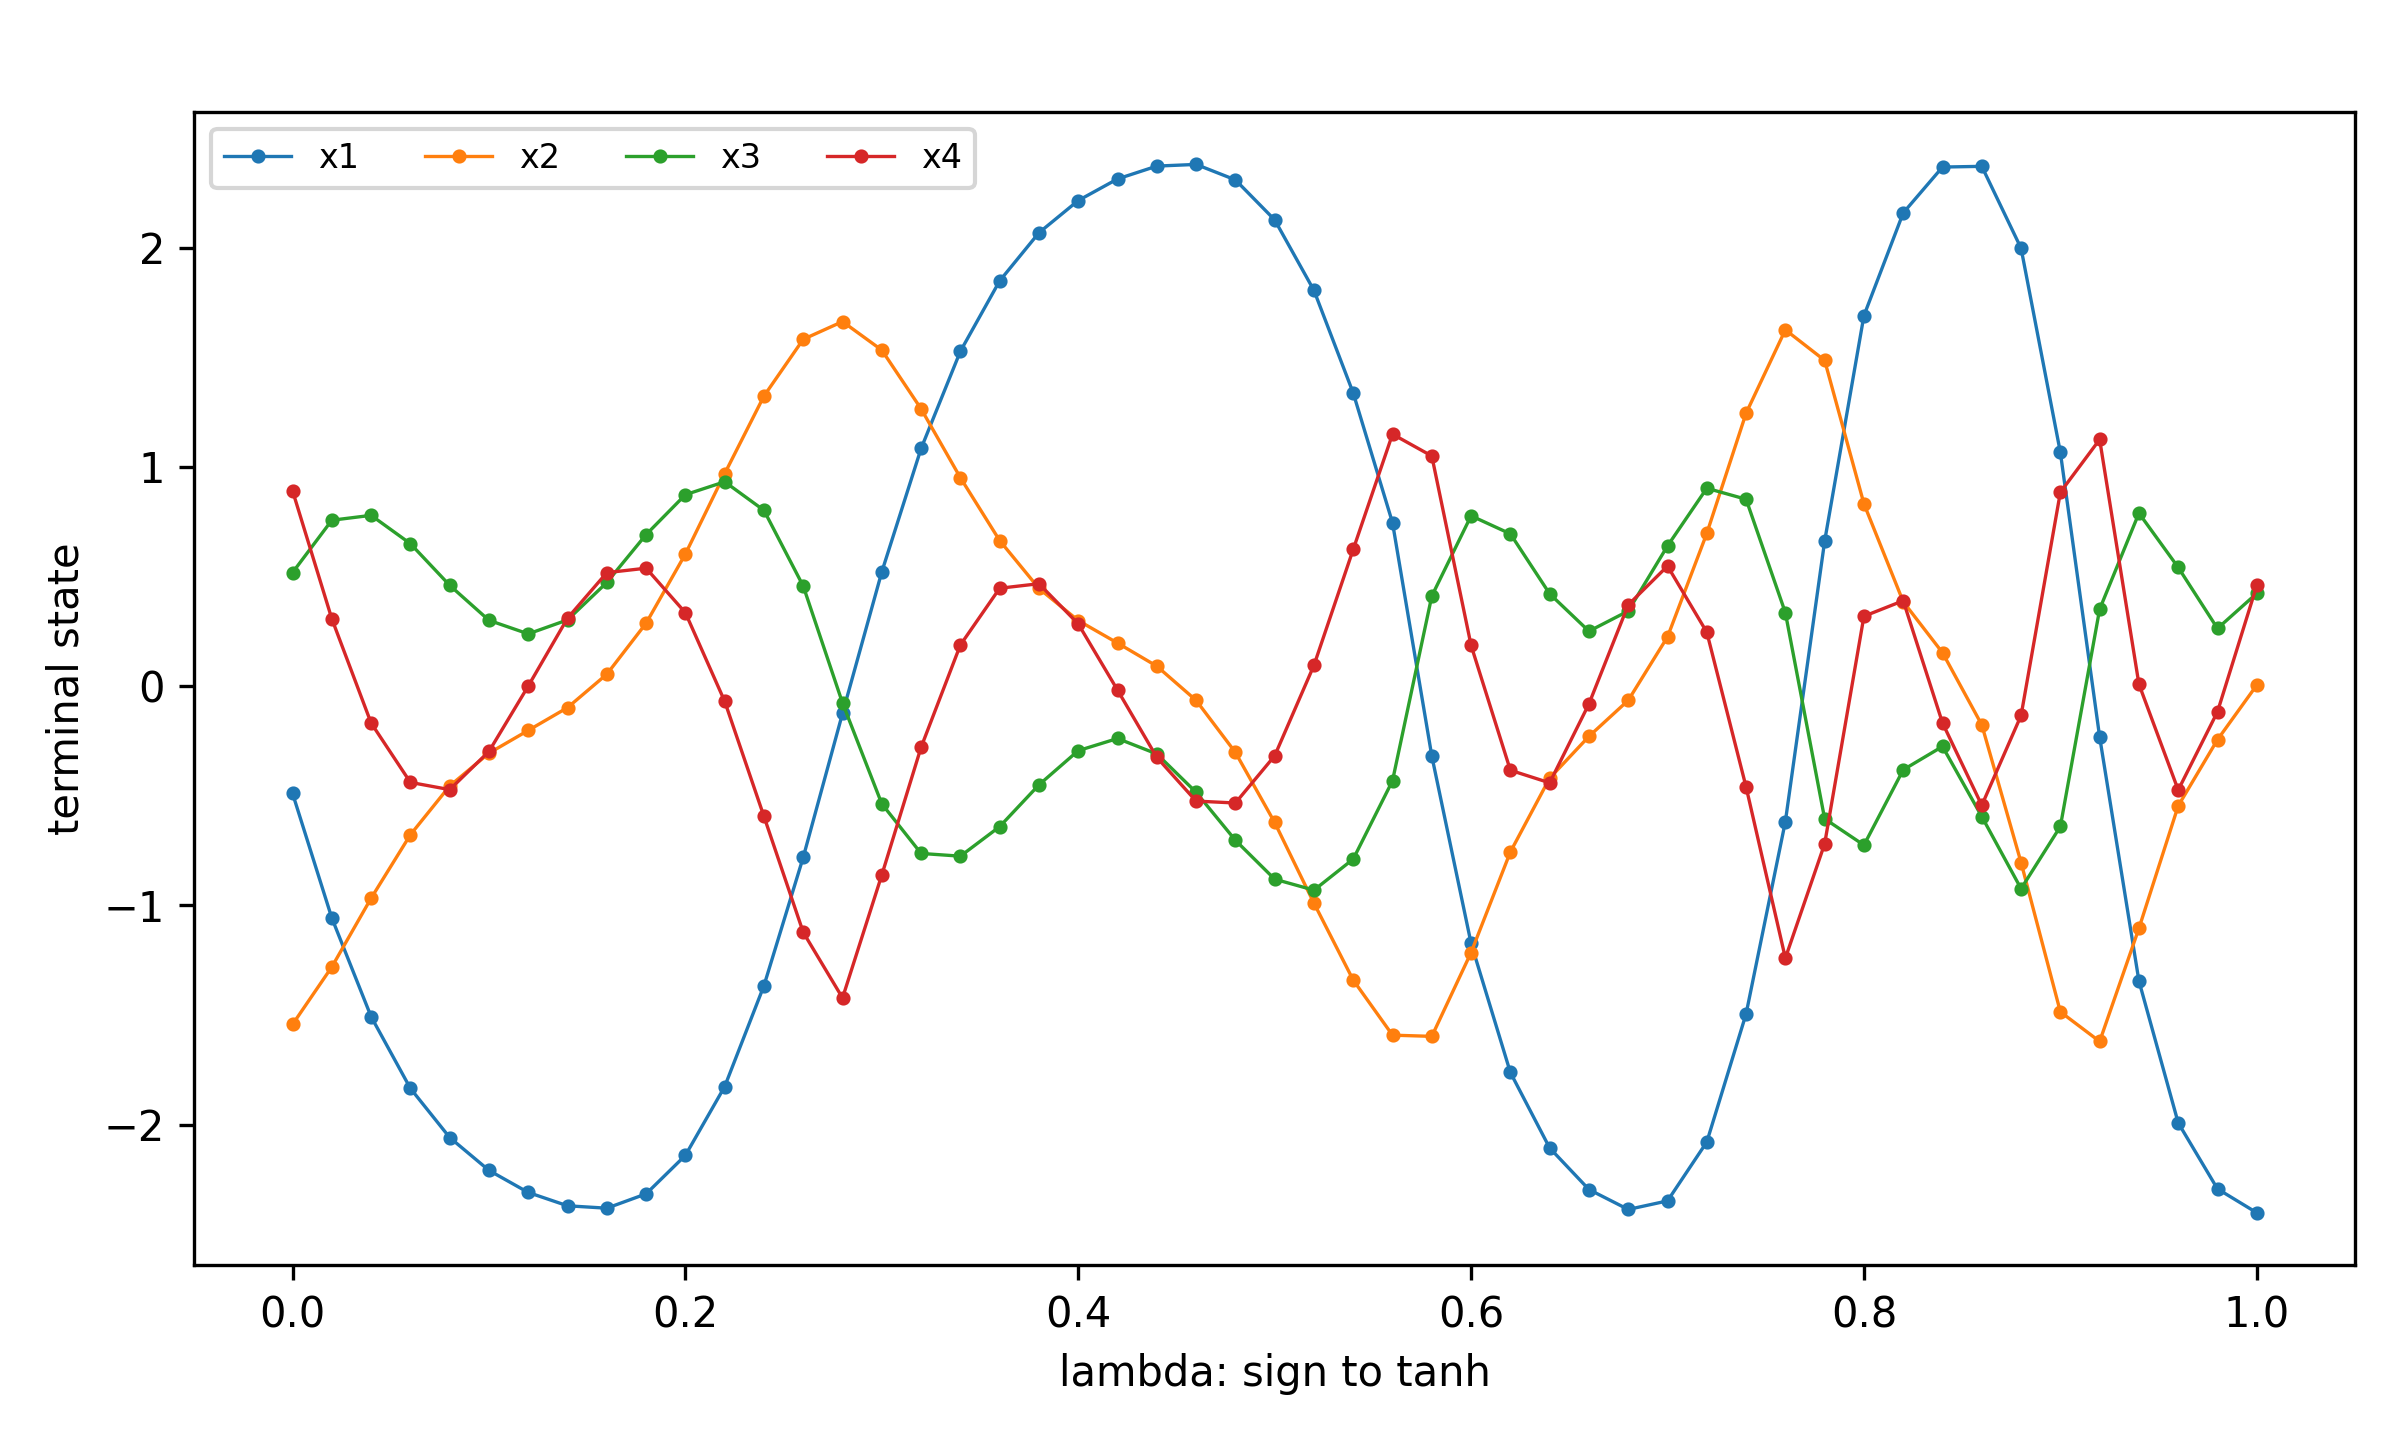
\includegraphics[width=\linewidth]{kalman_continuation.png}
  \caption{Homotopía \(\operatorname{sign}\to\tanh\) en Python.}
\end{subfigure}\hfill
\begin{subfigure}[t]{0.49\textwidth}
  \centering
  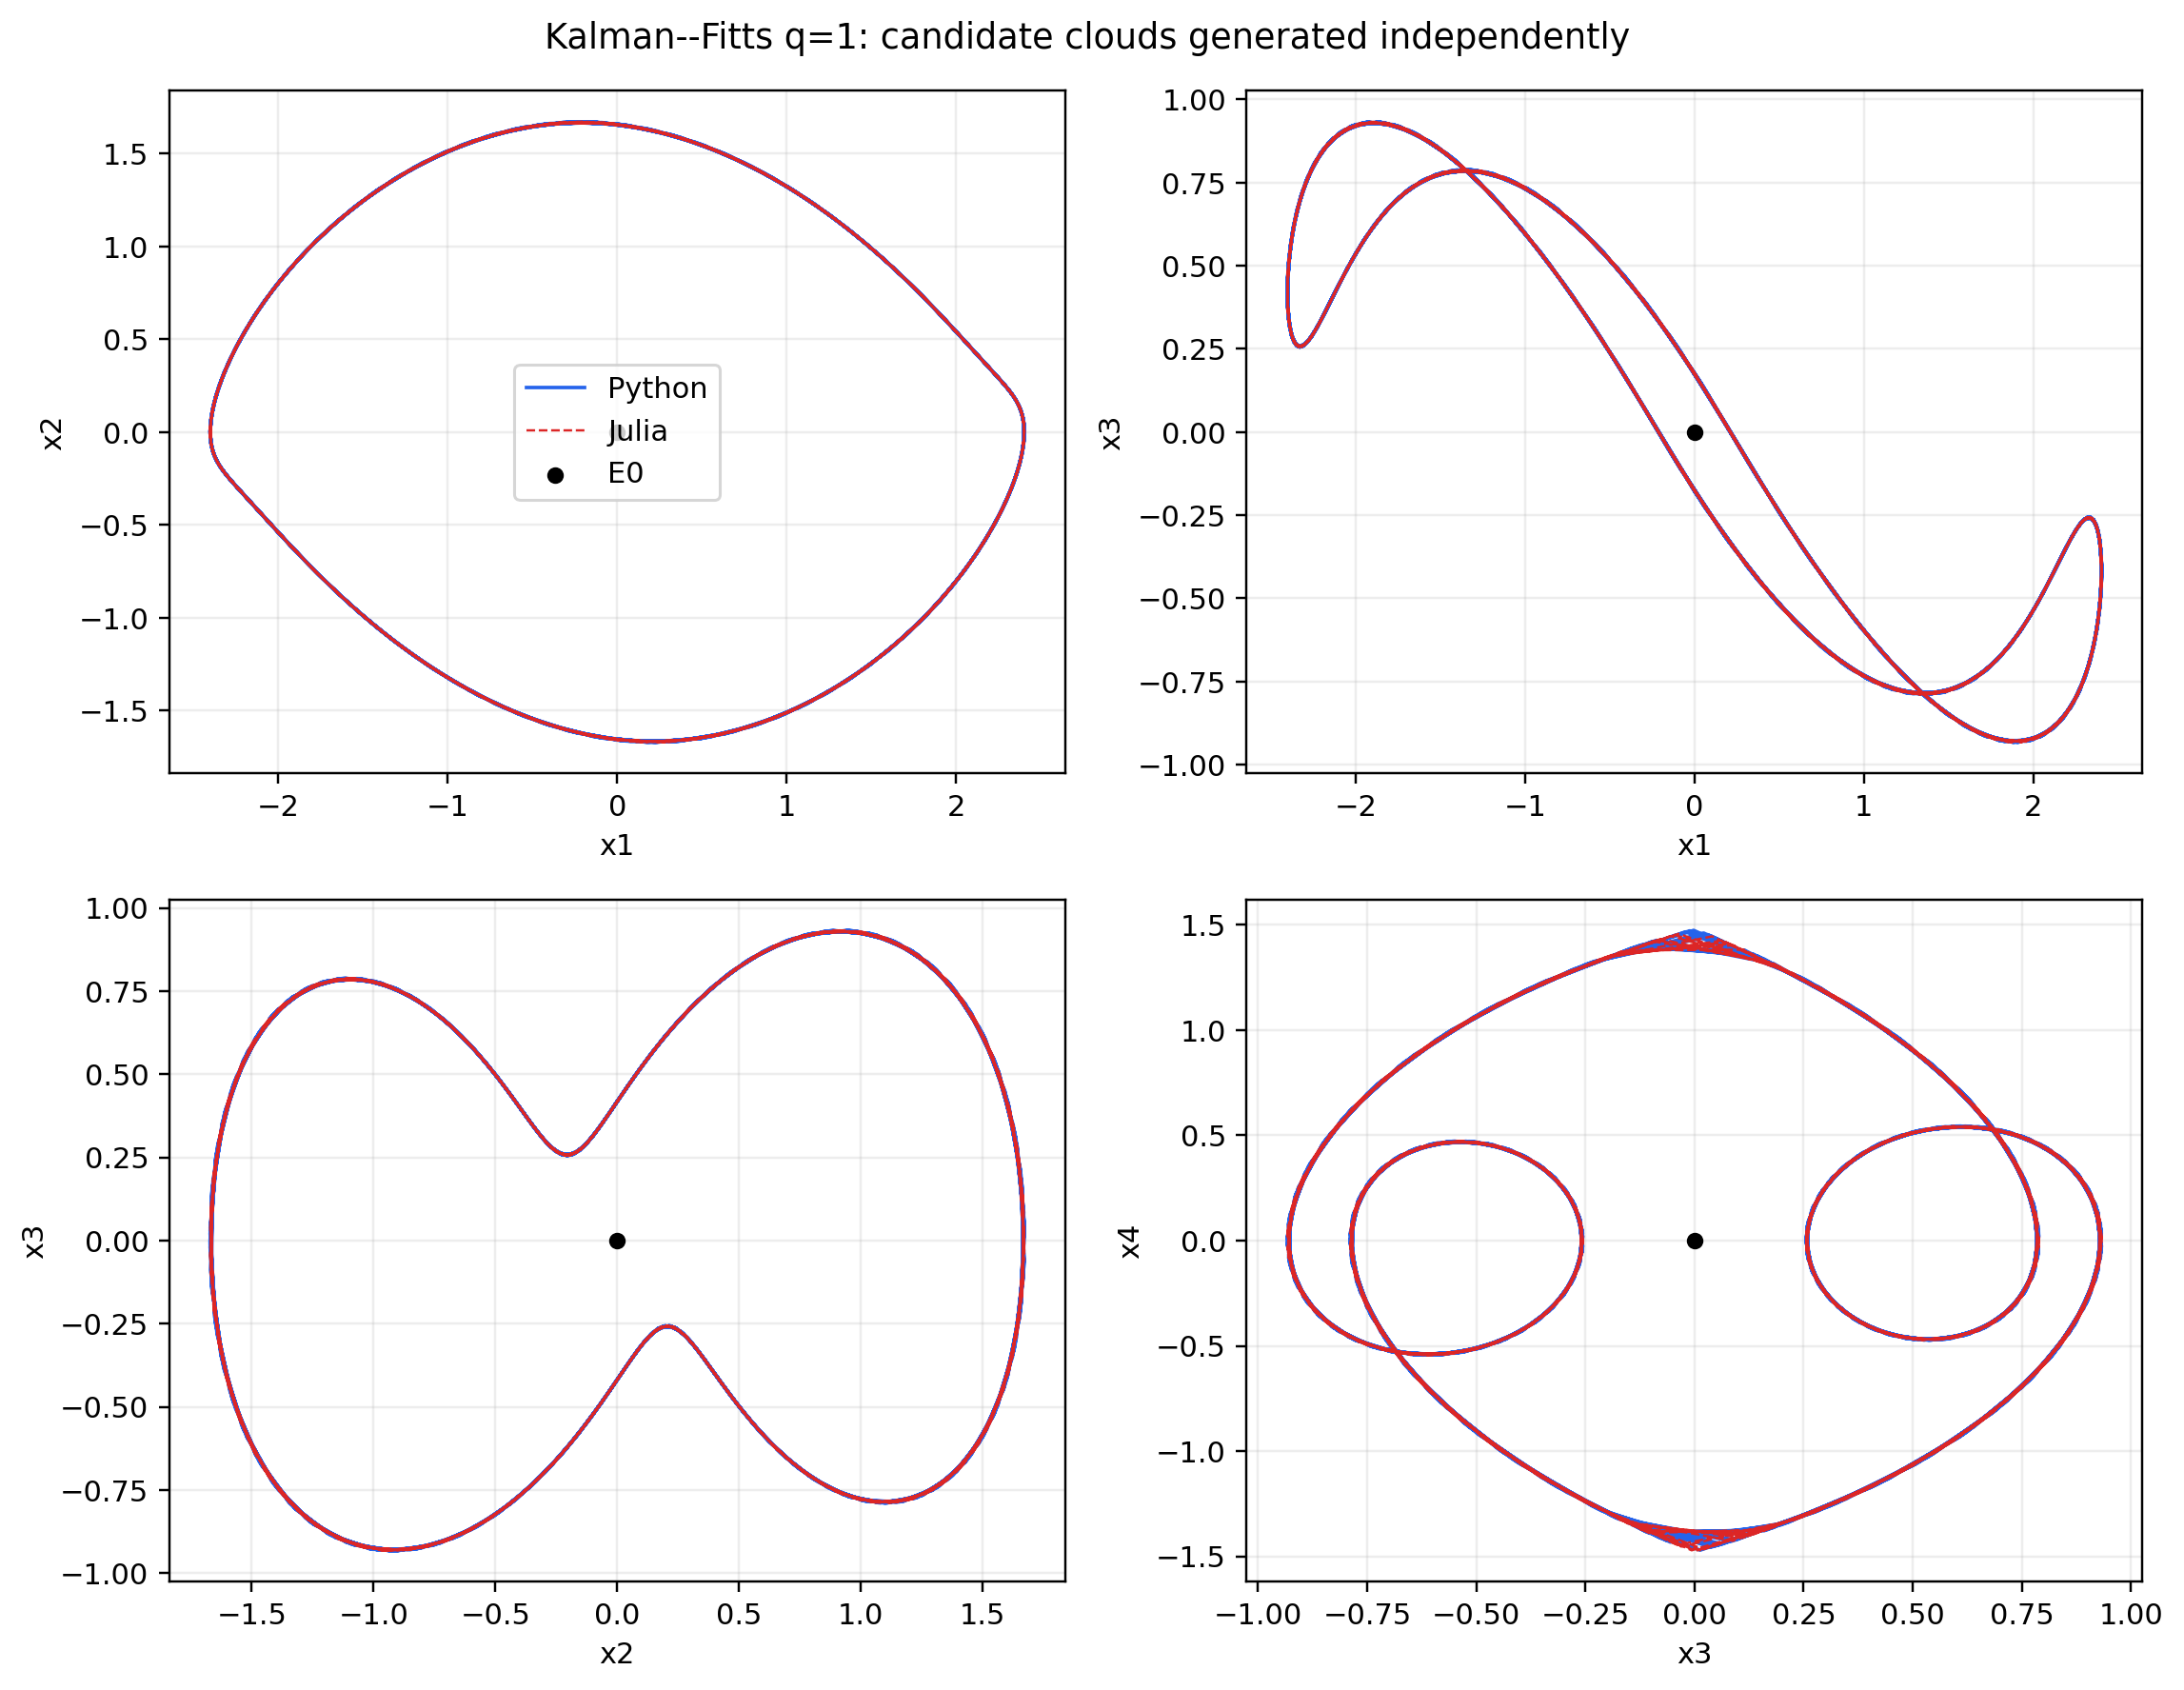
\includegraphics[width=\linewidth]{kalman_python_julia_overlay.png}
  \caption{Nubes finales generadas independientemente.}
\end{subfigure}
\caption{Ruta alternativa reproducida para Kalman--Fitts.}
\label{int:fig:kf}
\end{hafocommonfigure}

\subsection{Ciclo límite y comparación dinámica}

El candidato es un ciclo límite estable. El periodo medio fue
\(11.9169960\) en Python y \(11.9169380\) en Julia, con diferencia
\(5.81\times10^{-5}\). La distancia normalizada entre nubes fue
\(2.10\times10^{-3}\).

\ifHAFOBasinMaterial
El protocolo compartido contiene \KFProbeCount{} condiciones alrededor del
único equilibrio: 4 radios de \(10^{-5}\) a \(10^{-2}\) y 12 condiciones por
radio. Los dos códigos produjeron 40 convergencias al equilibrio, 8 estados
acotados no triviales y cero contactos con el ciclo. Las
\KFProbeCount{} clases finales y las \KFProbeCount{} decisiones de contacto
coincidieron punto por punto.
Por tanto, el ciclo es compatible con ocultedad bajo estas 48 condiciones
iniciales. El muestreo no prueba que la cuenca esté separada de toda vecindad
abierta del equilibrio.
\fi

\begin{table}[H]
\centering
\caption{Comparación cerrada de Kalman--Fitts.}
\small
\begin{tabularx}{\textwidth}{@{}lYY@{}}
\toprule
Magnitud & Python/\hafo{} & Julia \\
\midrule
Ruta directa & Rechazo por \(k<0\) & Rechazo por \(k<0\) \\
Mapa de conmutación & 135 iteraciones, retorno 2 & 135 iteraciones, retorno 2 \\
Periodo del ciclo & 11.9169960 & 11.9169380 \\
\ifHAFOBasinMaterial
Contactos en 48 sondeos & 0 & 0 \\
\fi
\bottomrule
\end{tabularx}
\end{table}


\section[Caso 3: Van der Pol--Duffing modificado]
{Caso 3: Van der Pol--Duffing autónomo modificado}

\subsection{Modelo y forma D0 exacta}

El sistema MAVPD de orden entero es
\begin{align}
 \dot y_1&=\delta\gamma y_1+\delta y_2-\delta y_1^3,\nonumber\\
 \dot y_2&=y_1-\xi y_2-y_3,\label{int:eq:mavpd}\\
 \dot y_3&=\rho y_2,\nonumber
\end{align}
con \(\gamma=0.1\), \(\delta=100\) y \(\rho=200\)
\cite{matouk2023}. Su declaración escalar es
\[
 P=\begin{pmatrix}
 \delta\gamma&\delta&0\\
 1&-\xi&-1\\
 0&\rho&0
 \end{pmatrix},\quad
 b=\begin{pmatrix}-\delta\\0\\0\end{pmatrix},\quad
 c=\begin{pmatrix}1\\0\\0\end{pmatrix},\quad
 \psi(\sigma)=\sigma^3,
\]
de modo que el Jacobiano y todos los equilibrios reales para \(\gamma>0\) son
\begin{equation}
 J(y)=\begin{pmatrix}
 \delta(\gamma-3y_1^2)&\delta&0\\
 1&-\xi&-1\\
 0&\rho&0
 \end{pmatrix},\qquad
 E_0=(0,0,0),\quad
 E_\pm=(\pm\sqrt{\gamma},0,\pm\sqrt{\gamma}).
 \label{int:eq:mavpd-jacobian}
\end{equation}
Para obtener los equilibrios, \(\dot y_3=0\) exige \(y_2=0\) porque
\(\rho>0\); \(\dot y_2=0\) da \(y_3=y_1\); la primera ecuación se reduce
a \(\delta y_1(\gamma-y_1^2)=0\). Esto produce exactamente los tres puntos
anteriores cuando \(\gamma>0\).

Sea \(u=(P-sI)^{-1}b\). Las últimas filas de este sistema lineal son
\[
 u_1-(\xi+s)u_2-u_3=0,\qquad \rho u_2-su_3=0.
\]
Al eliminar \(u_3\), resulta
\(u_2=su_1/(s^2+\xi s+\rho)\). La primera fila queda
\[
 \left[\delta\gamma-s+\frac{\delta s}{s^2+\xi s+\rho}\right]u_1=-\delta.
\]
Despejando \(u_1=G(s)\) y expandiendo
\((s-\delta\gamma)(s^2+\xi s+\rho)-\delta s\), se obtiene
\begin{equation}
 G(s)=\frac{\delta(s^2+\xi s+\rho)}
 {s^3+(\xi-\delta\gamma)s^2+
 (\rho-\delta-\delta\gamma\xi)s-\delta\gamma\rho}.
 \label{int:eq:mavpd-transfer}
\end{equation}
El caso Wolfram conserva además la convención resolvente
\[
 W(s)=c^{\mathsf T}(sI-P)^{-1}b=-G(s).
\]
Por tanto, su cálculo \(k=1/\operatorname{Re}W(i\omega)\) es exactamente el
mismo que \(k=-1/\operatorname{Re}G(i\omega)\) en
\eqref{int:eq:mavpd-direct-scalars}; el signo queda fijado por la derivación
algebraica.
La identidad \(\cos^3\theta=(3\cos\theta+\cos3\theta)/4\) separa las
componentes de \(\psi(a\cos\theta)=a^3\cos^3\theta\). El primer armónico
tiene amplitud \(3a^3/4\); dividir entre la amplitud de entrada \(a\) da
\begin{equation}
  \mathcal N(a)=\frac{3a^2}{4}.
\end{equation}

Al escribir \(z=\omega^2\), el numerador sin el factor \(\delta\) tiene
partes \(\rho-z\) y \(\xi\omega\), mientras el denominador tiene partes
\[
 C=-\delta\gamma\rho-(\xi-\delta\gamma)z,\qquad
 D=\omega(\rho-\delta-\delta\gamma\xi-z).
\]
Racionalizar el cociente produce
\[
 \operatorname{Im}G(i\omega)=
 \frac{\delta[\xi\omega C-(\rho-z)D]}{C^2+D^2}.
\]
Al expandir el numerador, los términos con \(\gamma\) se cancelan y queda
\[
 \xi\omega C-(\rho-z)D
 =-\omega[z^2+(\delta-2\rho+\xi^2)z+\rho(\rho-\delta)].
\]
Para \(\omega>0\) y \(C^2+D^2>0\), la condición imaginaria equivale a
\begin{equation}
 z^2+(\delta-2\rho+\xi^2)z+\rho(\rho-\delta)=0.
 \label{int:eq:mavpd-poly}
\end{equation}
Así se obtienen todas las ramas sin barrido de frecuencias. Para cada raíz
positiva \(z_j\), el procedimiento calcula
\begin{equation}
 \omega_j=\sqrt{z_j},\qquad
 k_j=-\frac{1}{\operatorname{Re}G(i\omega_j)},\qquad
 a_j=\sqrt{\frac{4k_j}{3}},
 \label{int:eq:mavpd-direct-scalars}
\end{equation}
siempre que \(k_j>0\), condición necesaria para una amplitud real positiva.
Para el modo normalizado \(v_{j,1}=1\), la primera fila de
\((P+k_jbc^{\mathsf T})v_j=i\omega_jv_j\) es
\[
 \delta(\gamma-k_j)+\delta v_{j,2}=i\omega_j,
\]
y la tercera es \(\rho v_{j,2}=i\omega_jv_{j,3}\). Despejar ambas da
\begin{equation}
 v_j=\begin{pmatrix}
 1\\
 k_j-\gamma+i\omega_j/\delta\\
 \rho/\delta-i\rho(k_j-\gamma)/\omega_j
 \end{pmatrix},\qquad
 y_{0,j}(\theta)=a_j\operatorname{Re}\!\left(v_je^{i\theta}\right).
 \label{int:eq:mavpd-direct-seed}
\end{equation}
Las igualdades de cierre de \eqref{int:eq:mavpd-direct-scalars}, la ecuación modal
\((P+k_jbc^{\mathsf T})v_j=i\omega_jv_j\) y el residuo del campo se guardan
como verificaciones, no como datos impuestos.

\subsection{\texorpdfstring{\(\xi=3.1\): ramas, semillas y continuación}{xi=3.1: ramas, semillas y continuación}}

Para \(\xi=3.1\), \eqref{int:eq:mavpd-poly} tiene coeficientes
\((1,-290.39,20000)\) y produce dos ramas compatibles:

\begin{table}[H]
\centering
\caption{Ramas directas MAVPD para \(\xi=3.1\).}
\small
\begin{tabular}{@{}ccccc@{}}
\toprule
Rama & \(\omega_0\) & \(k\) & \(a_0\) & Semilla con fase \(0\) \\
\midrule
0 & 10.5975230311 & 0.1397015948 & 0.4315886851 &
\((0.4315887,0.0171348,0.8631774)\) \\
1 & 13.3447557342 & 0.3518790503 & 0.6849613618 &
\((0.6849614,0.1725274,1.3699227)\) \\
\bottomrule
\end{tabular}
\end{table}

Se ejecutaron ambas ramas con fases \(0\) y \(\pi\), y 21 valores
\(\lambda=0,0.05,\ldots,1\). La rama 0 conduce a dos ciclos internos
simétricos; la rama 1 conduce al conjunto externo. La selección se hizo por
mayor extensión de estado, sin leer la Tabla 1 de la fuente.

\begin{hafocommonfigure}[H]
\centering
\begin{subfigure}[t]{0.49\textwidth}
  \centering
  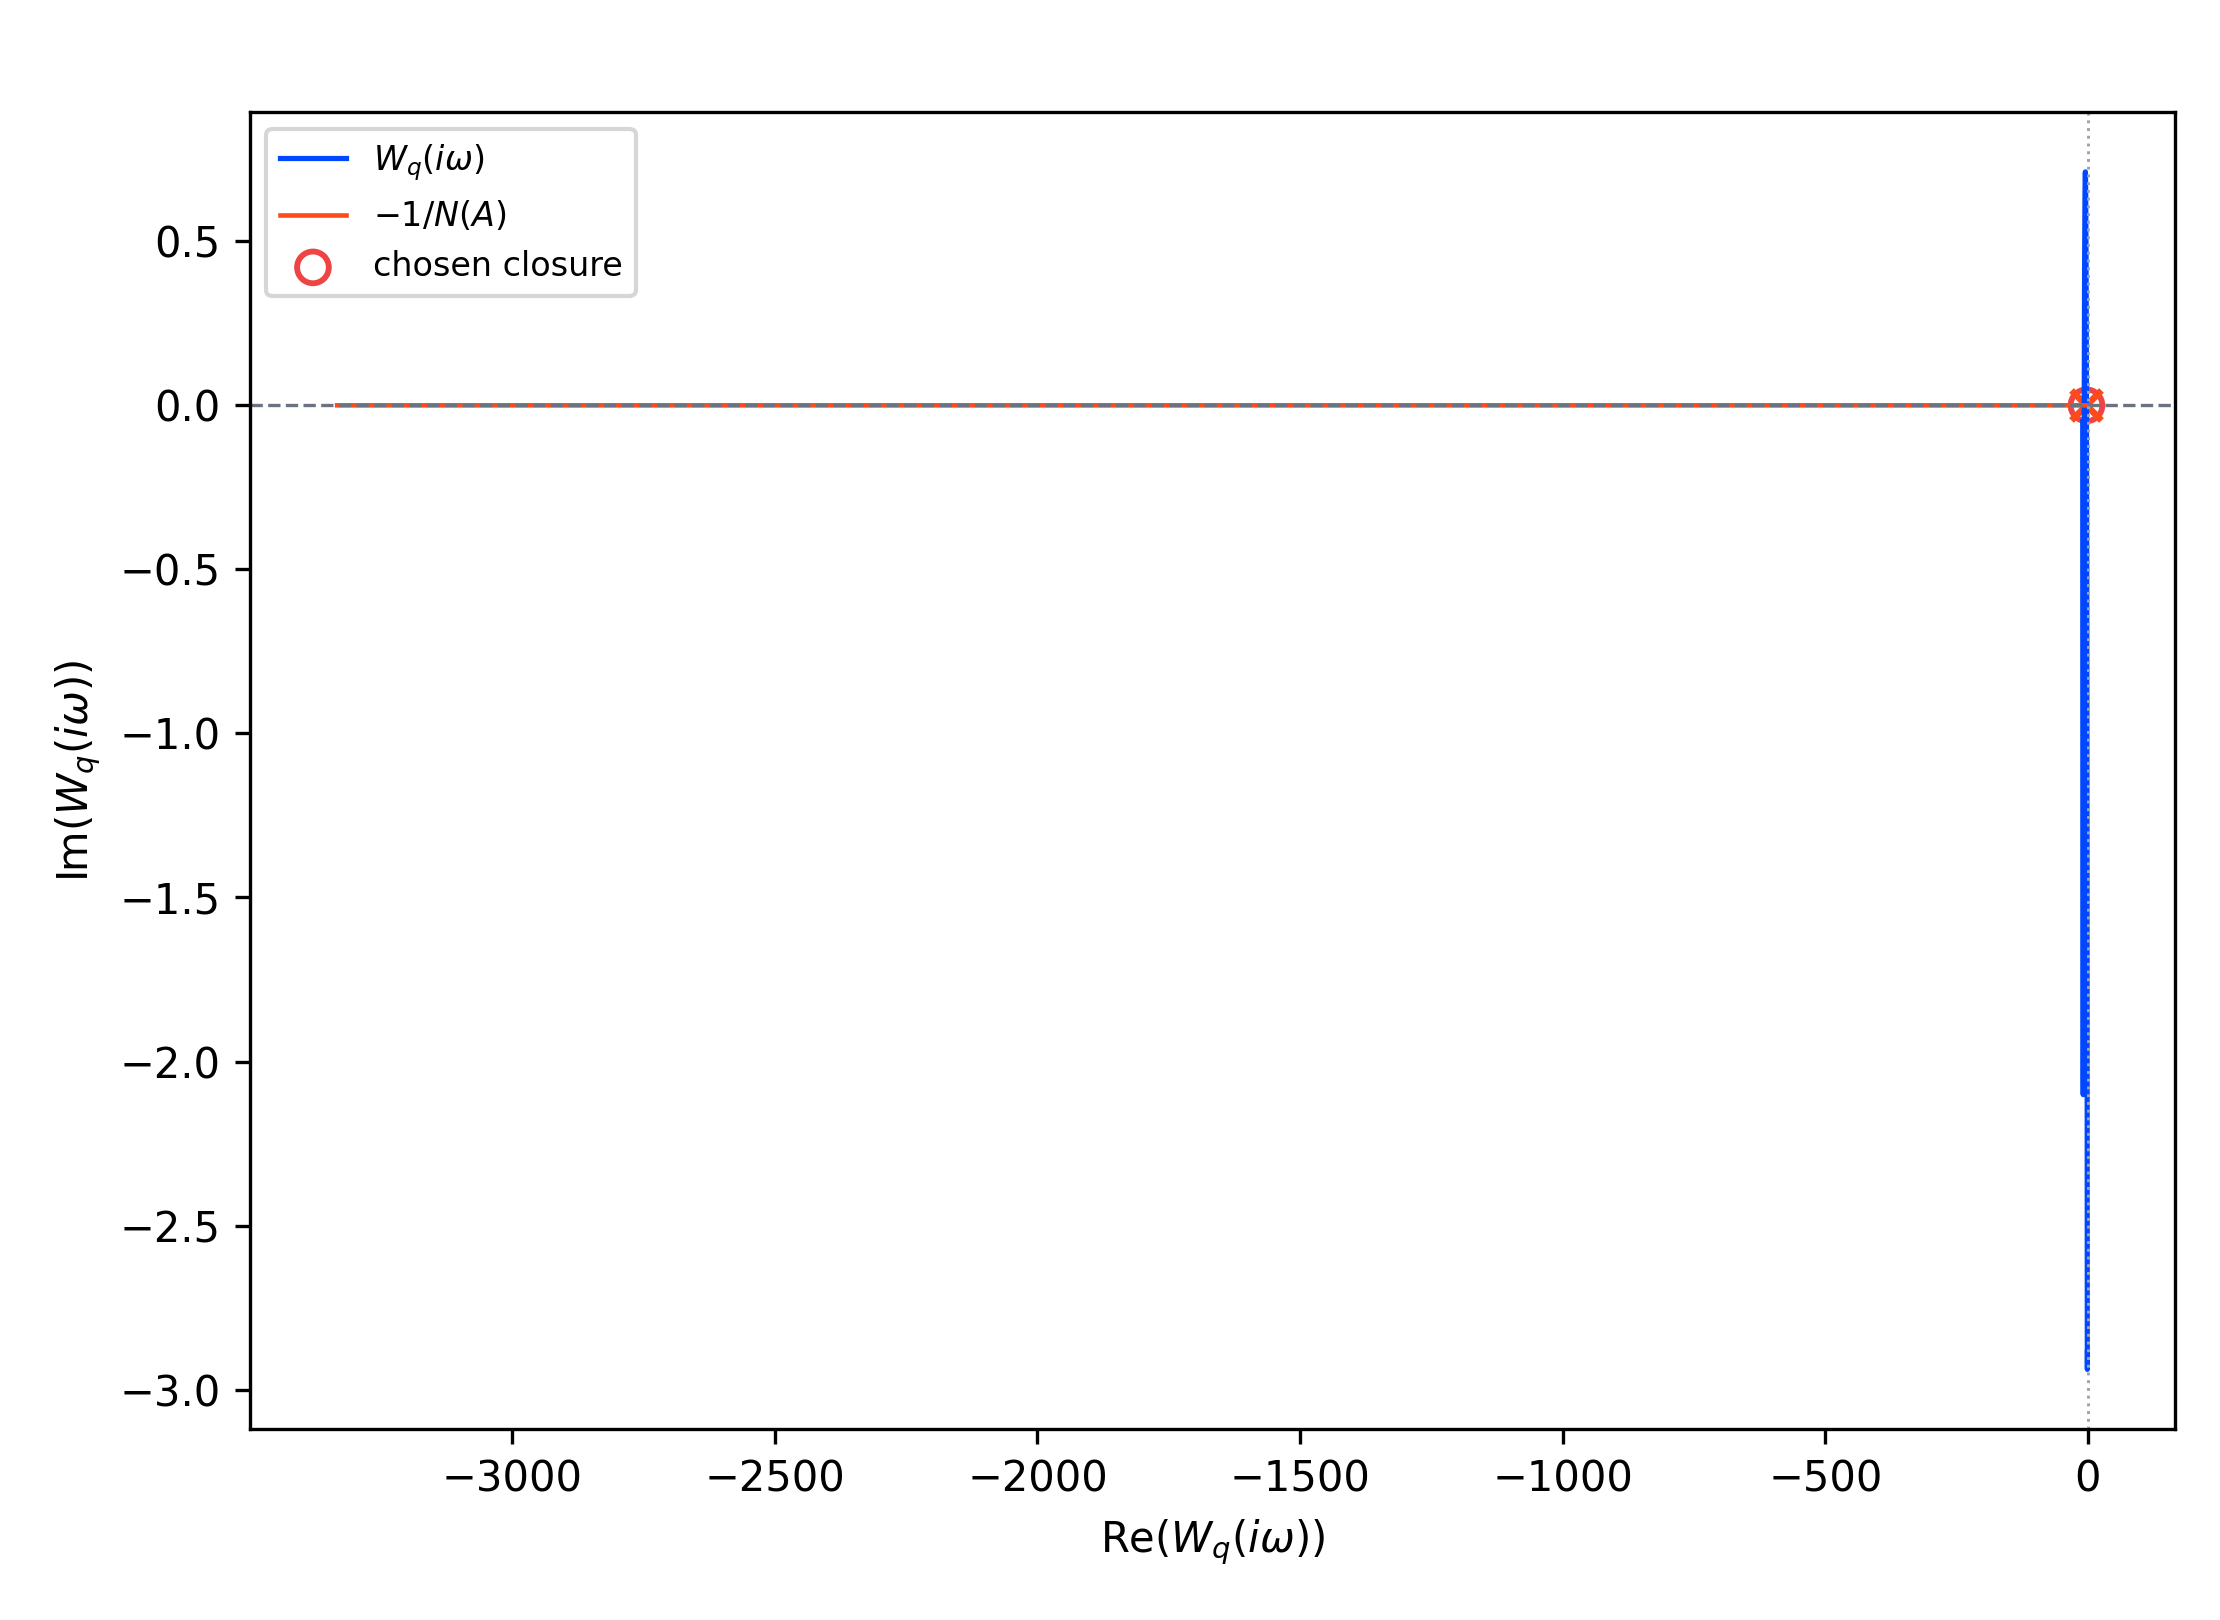
\includegraphics[width=\linewidth]{mavpd_nyquist_df.png}
  \caption{Ramas de Nyquist y función descriptiva derivadas.}
\end{subfigure}\hfill
\begin{subfigure}[t]{0.49\textwidth}
  \centering
  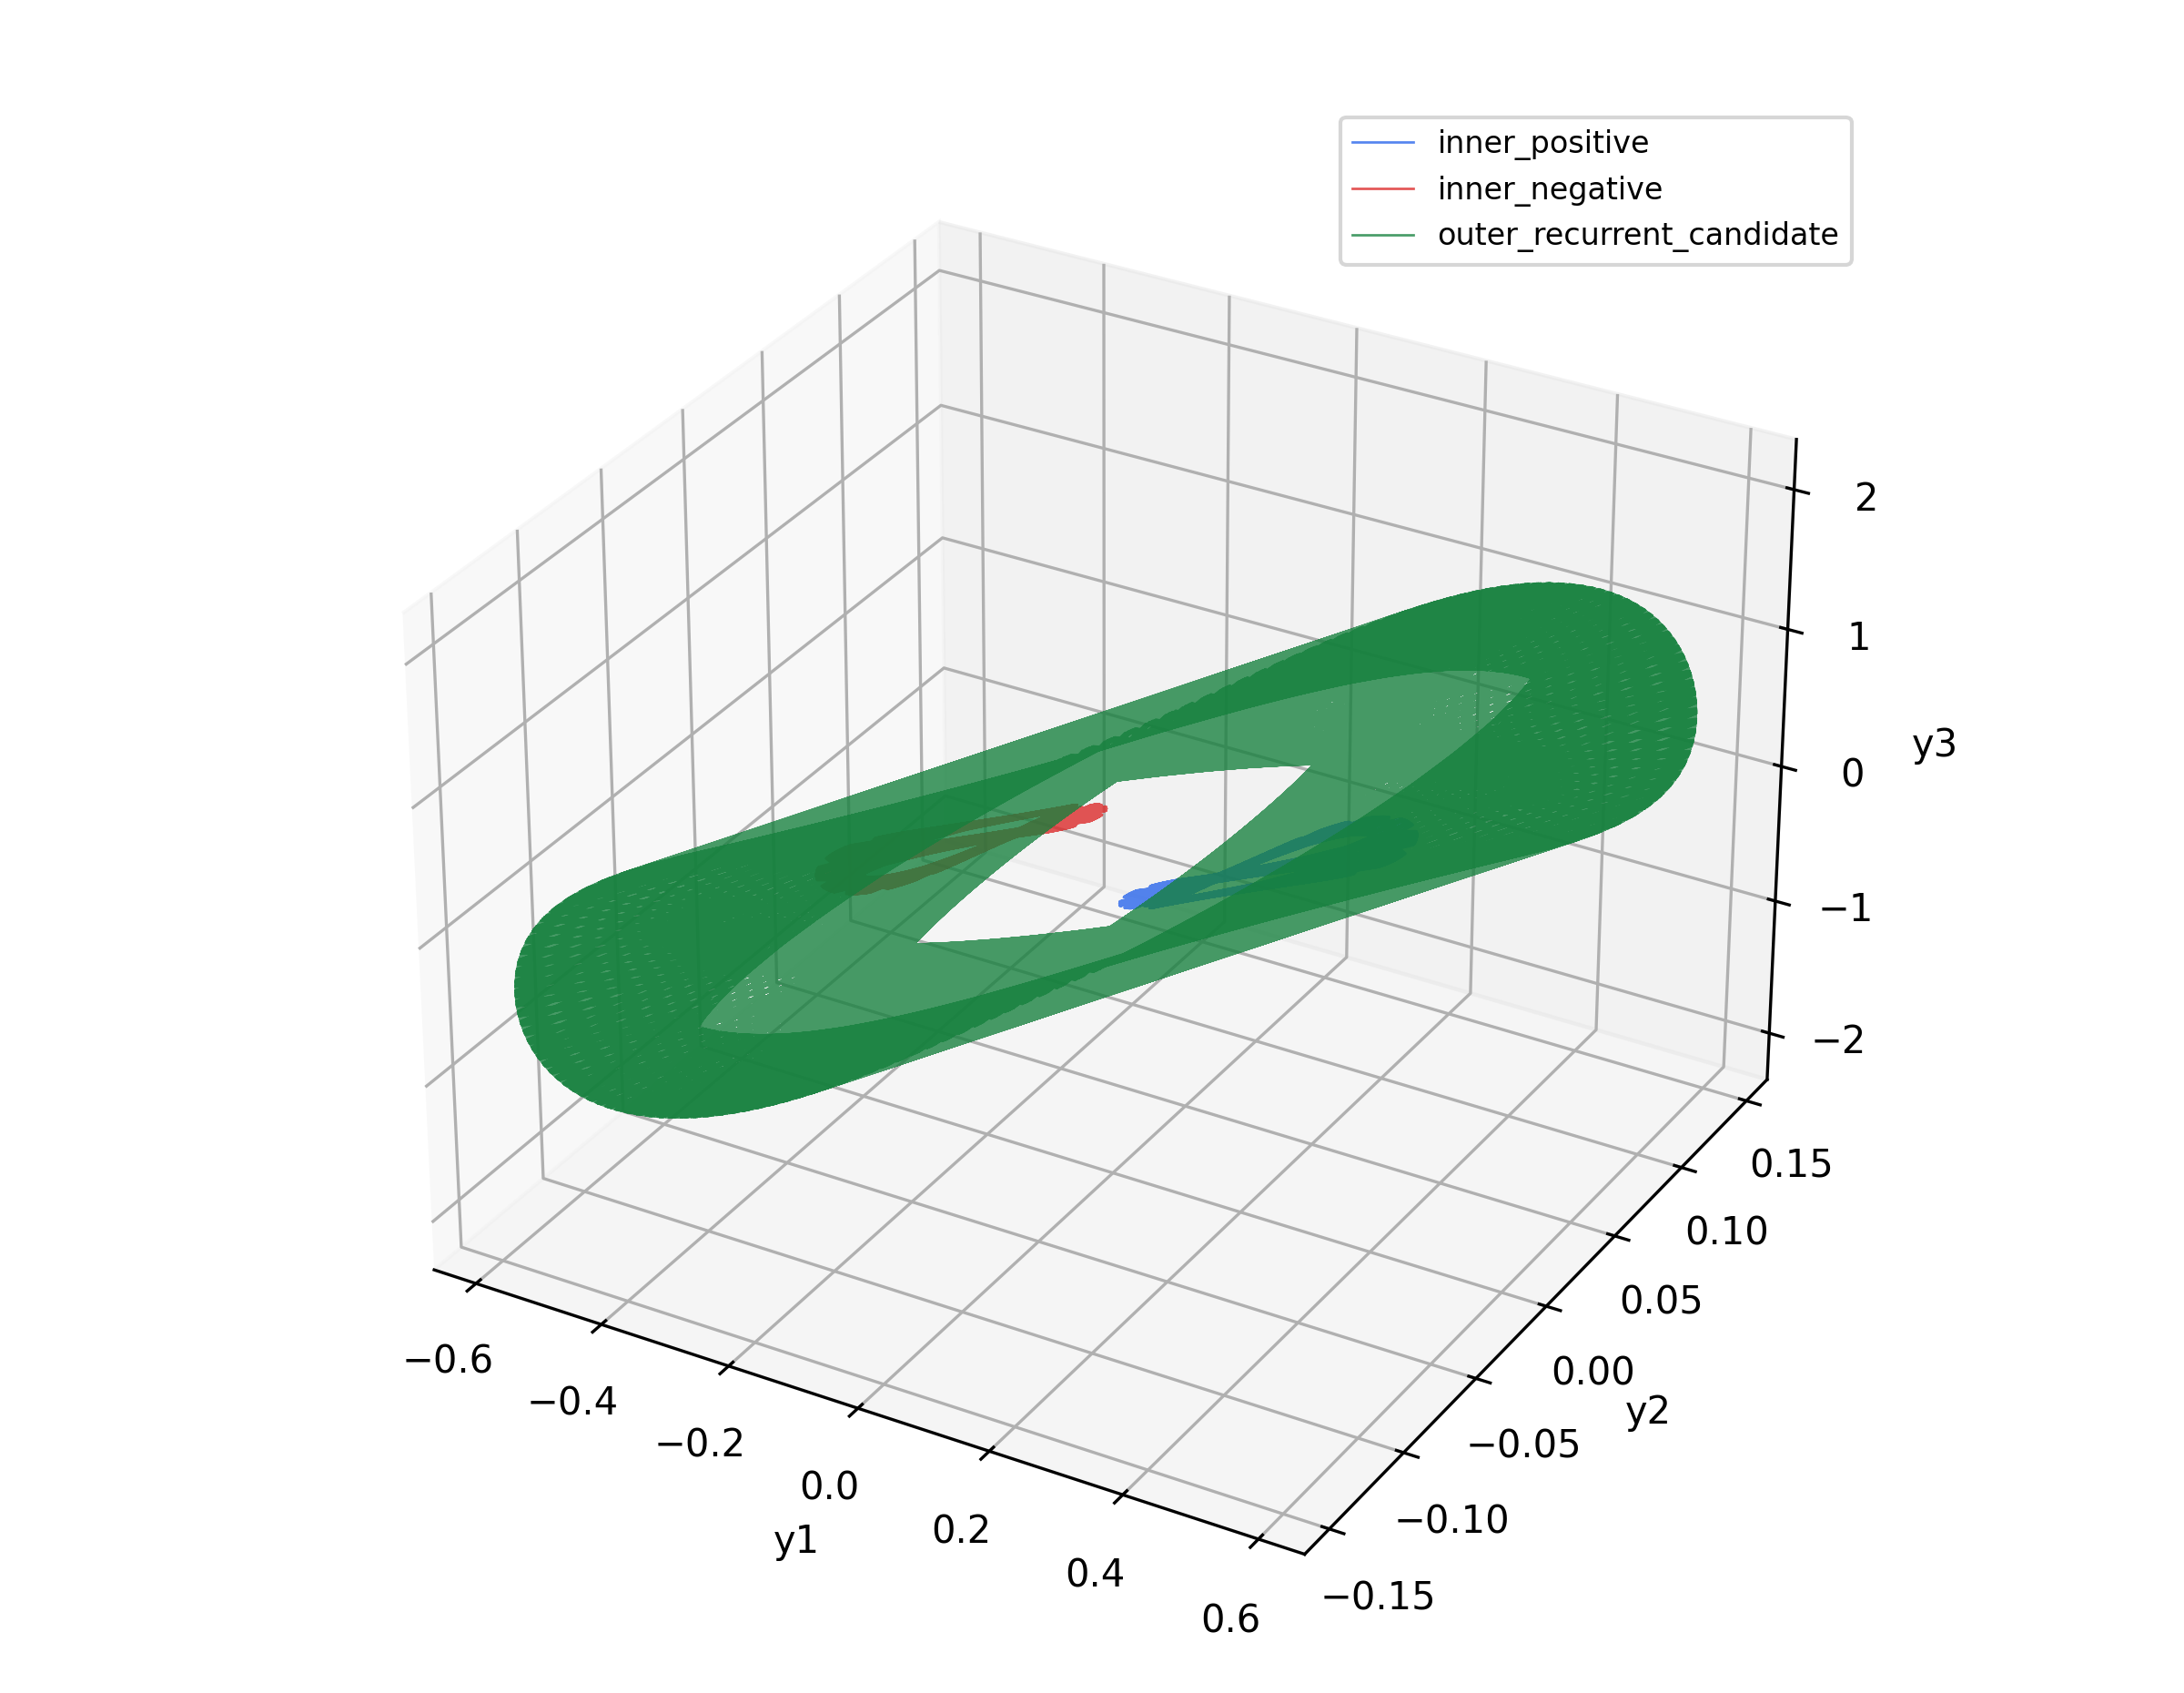
\includegraphics[width=\linewidth]{mavpd_python_clusters.png}
  \caption{Dos ciclos internos y candidato externo en Python.}
\end{subfigure}
\caption{Ruta directa MAVPD con \(\xi=3.1\).}
\label{int:fig:mavpd-route}
\end{hafocommonfigure}

\subsection{Comparación cruzada del caso periódico}

\ifHAFOBasinMaterial
El conjunto común contiene \MAVPDProbeCount{} condiciones: 3 equilibrios, 3 radios
\((10^{-5},10^{-3},10^{-2})\) y 12 direcciones explícitas por equilibrio y
radio. Se usaron \(h=0.005\), transitorio 180 y cola 80.
\fi

El comparador posterior confirmó:

\begin{itemize}
  \item diferencia máxima de frecuencias \(2.31\times10^{-14}\), de
        ganancias \(3.50\times10^{-15}\), de amplitudes
        \(3.44\times10^{-15}\) y de semillas \(7.45\times10^{-15}\);
\ifHAFOBasinMaterial
  \item \MAVPDFullAssignmentMatches{} de \MAVPDProbeCount{} asignaciones de
        clúster, clases finales y decisiones sobre el candidato externo
        coincidentes;
  \item 54 trayectorias hacia el ciclo interno positivo, 54 hacia el negativo
        y cero hacia el externo en cada implementación;
\fi
  \item distancia normalizada entre nubes externas
        \(\MAVPDFullCloudDistance\);
  \item periodos \(\MAVPDPythonPeriod\) en Python y
        \(\MAVPDJuliaFullPeriod\) en Julia;
  \item ninguna ruta alternativa para \(\xi=3.1\).
\end{itemize}

\begin{hafocommonfigure}[H]
\centering
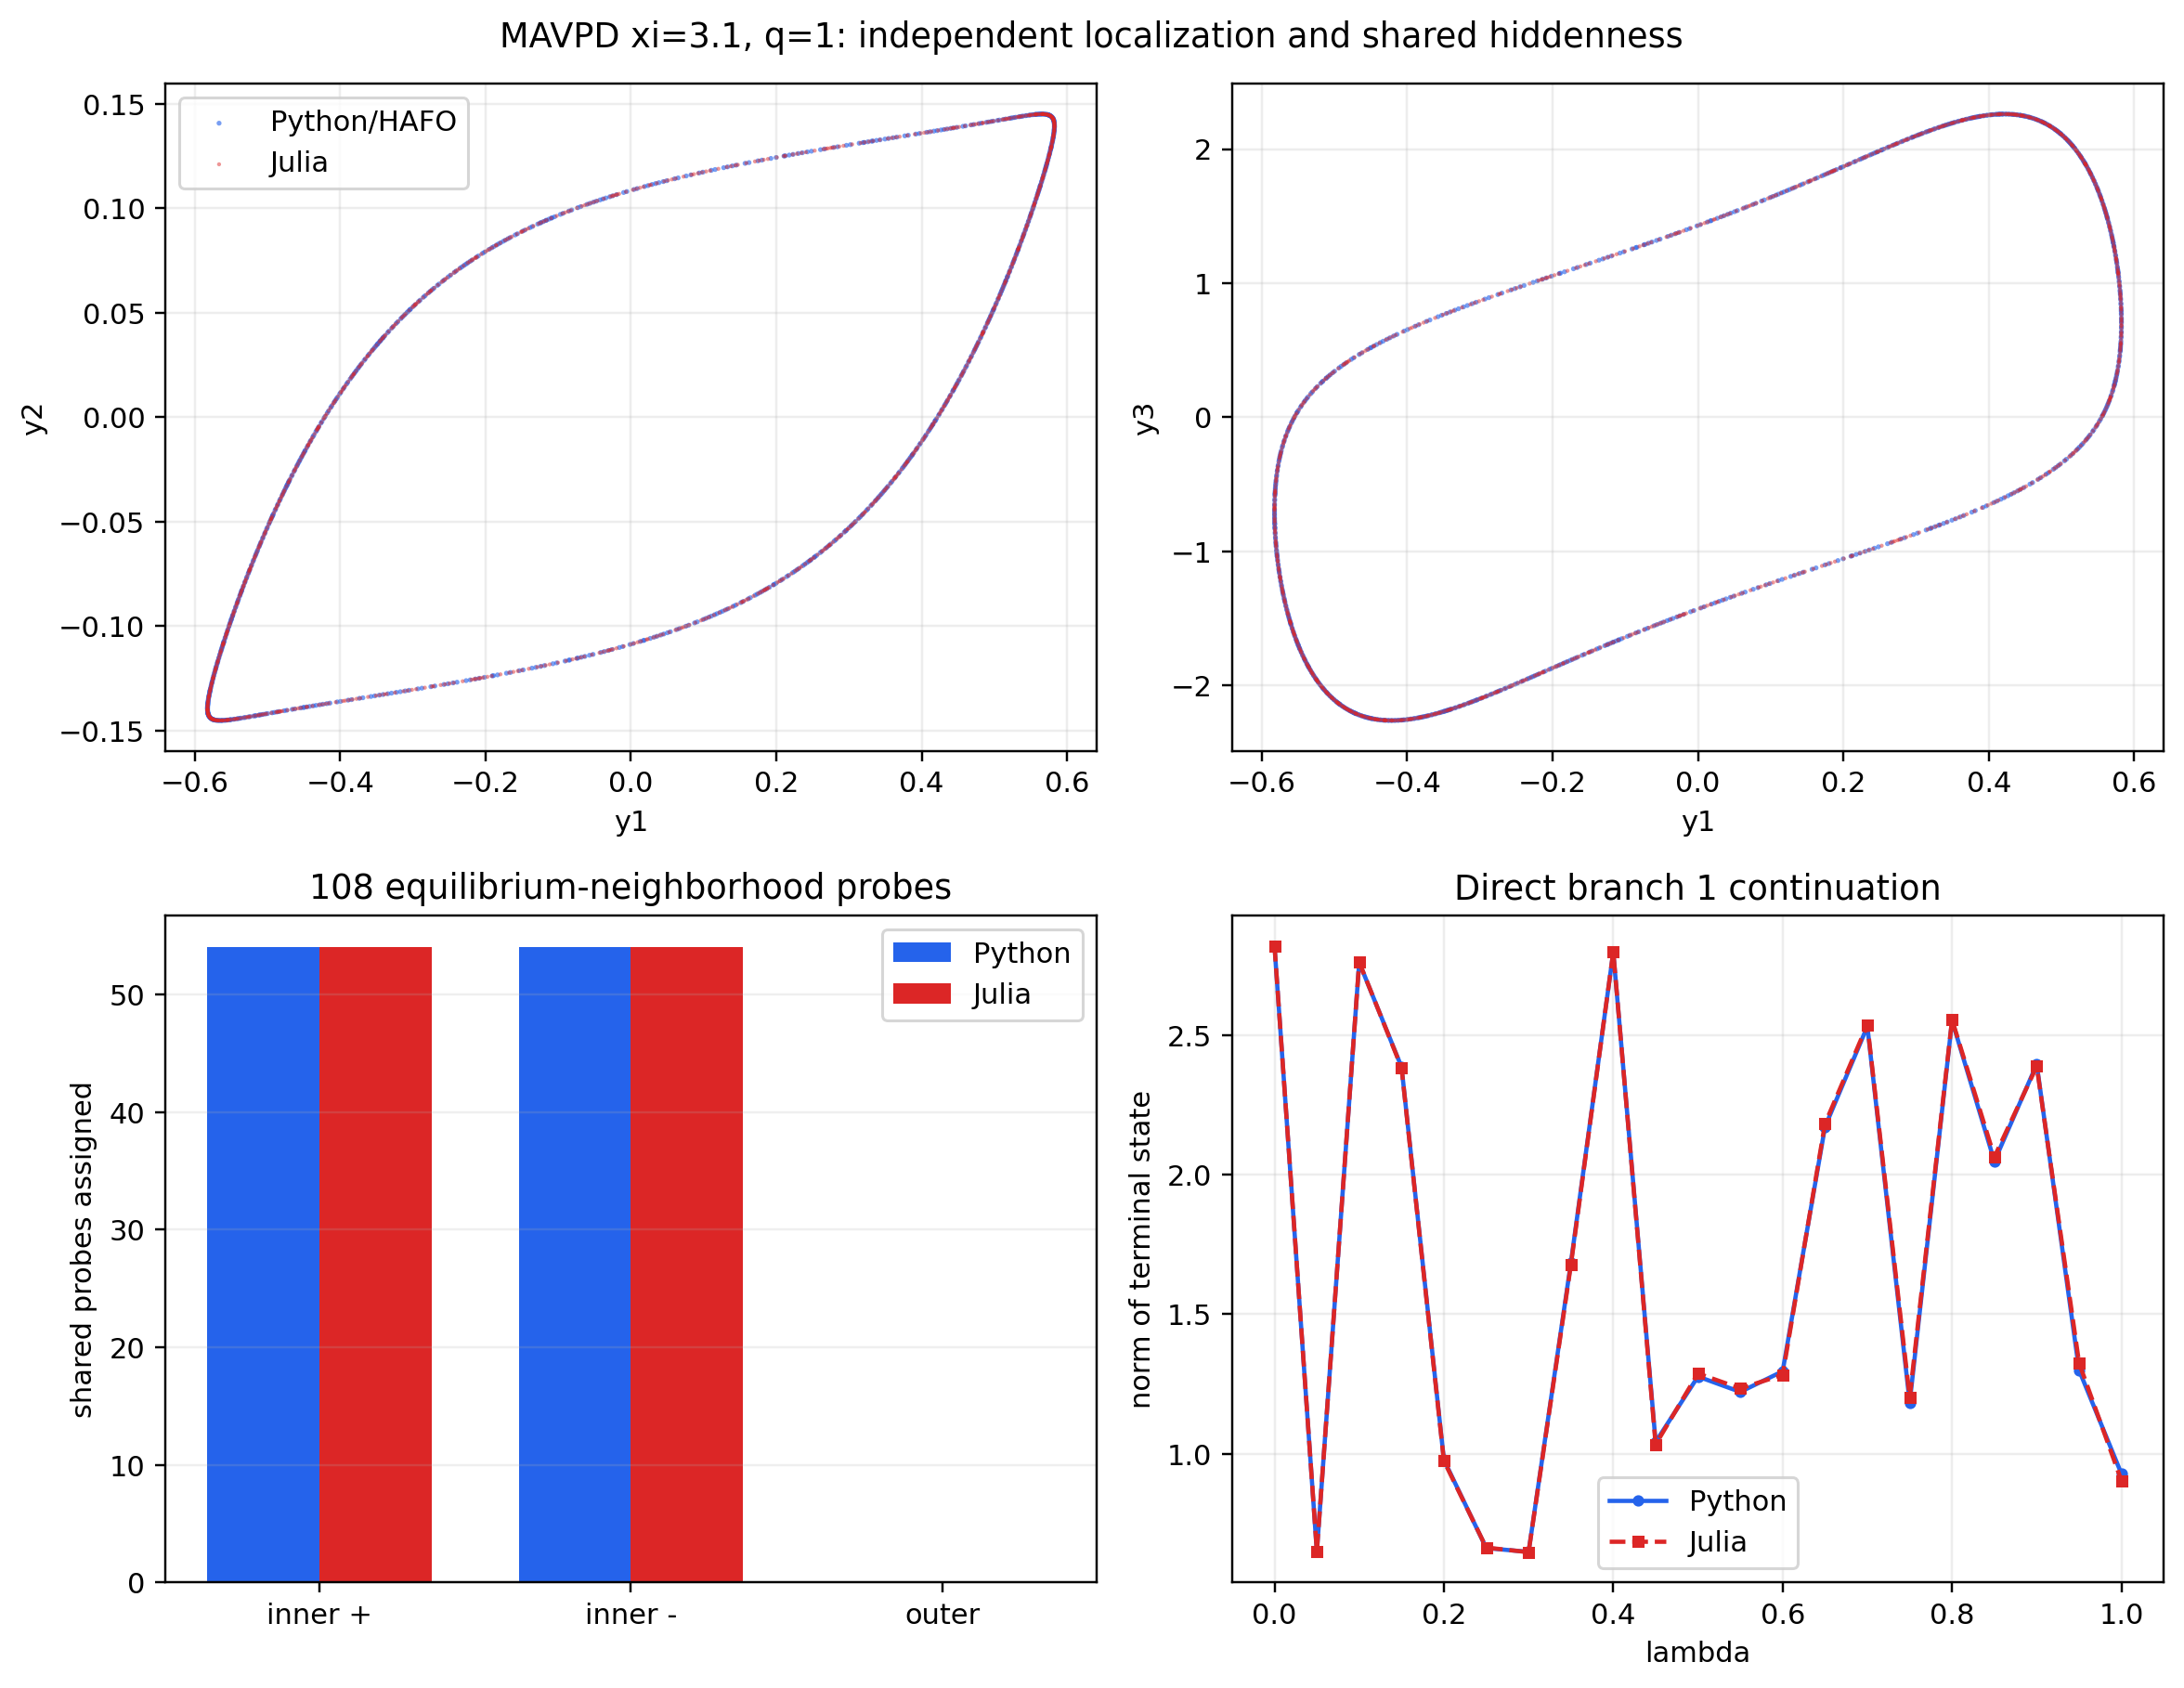
\includegraphics[width=0.94\textwidth]{mavpd_python_julia_overlay_full.png}
\caption{Comparación posterior MAVPD \emph{full}. Las localizaciones se
ejecutaron independientemente.
\ifHAFOBasinMaterial
Las 108 coordenadas se compartieron sólo para el control de ocultedad.
\fi}
\label{int:fig:mavpd-overlay}
\end{hafocommonfigure}

\subsection{Clasificación dinámica y discrepancia con la fuente}

La sección de Poincaré Python se refinó con DOP853 y eventos densos:
405 cruces, rango de los últimos puntos del orden de \(10^{-13}\), periodo
\(0.493177986749\) y desviación estándar \(1.25\times10^{-14}\).
El espectro variacional independiente en el cálculo declarado fue
\[
 (-0.0017614,\ -0.3887396,\ -51.1886634),
\]
y la prueba 0--1 dio mediana \(K=0.000440085726\) sobre 64 valores de \(c\).
En conjunto con la sección de Poincaré, estos diagnósticos apoyan un ciclo
estable de periodo uno bajo el protocolo numérico; la prueba 0--1 aislada no
constituye una demostración analítica de periodicidad. El cálculo independiente
en Julia obtuvo \((-0.0042733,-0.3910810,-51.1961919)\), consistente con la
misma clase.

La fuente denomina al conjunto \emph{atractor oculto cuasiperiódico}. Esa
etiqueta no se reproduce para las ecuaciones declaradas: la conclusión local
obtenida es \emph{candidato periódico estable}. La diferencia documenta una
discrepancia reproducible entre la etiqueta de la fuente
y la dinámica obtenida con integración y sección de mayor precisión.

\begin{hafobasinfigure}[H]
\centering
\begin{subfigure}[t]{0.49\textwidth}
  \centering
  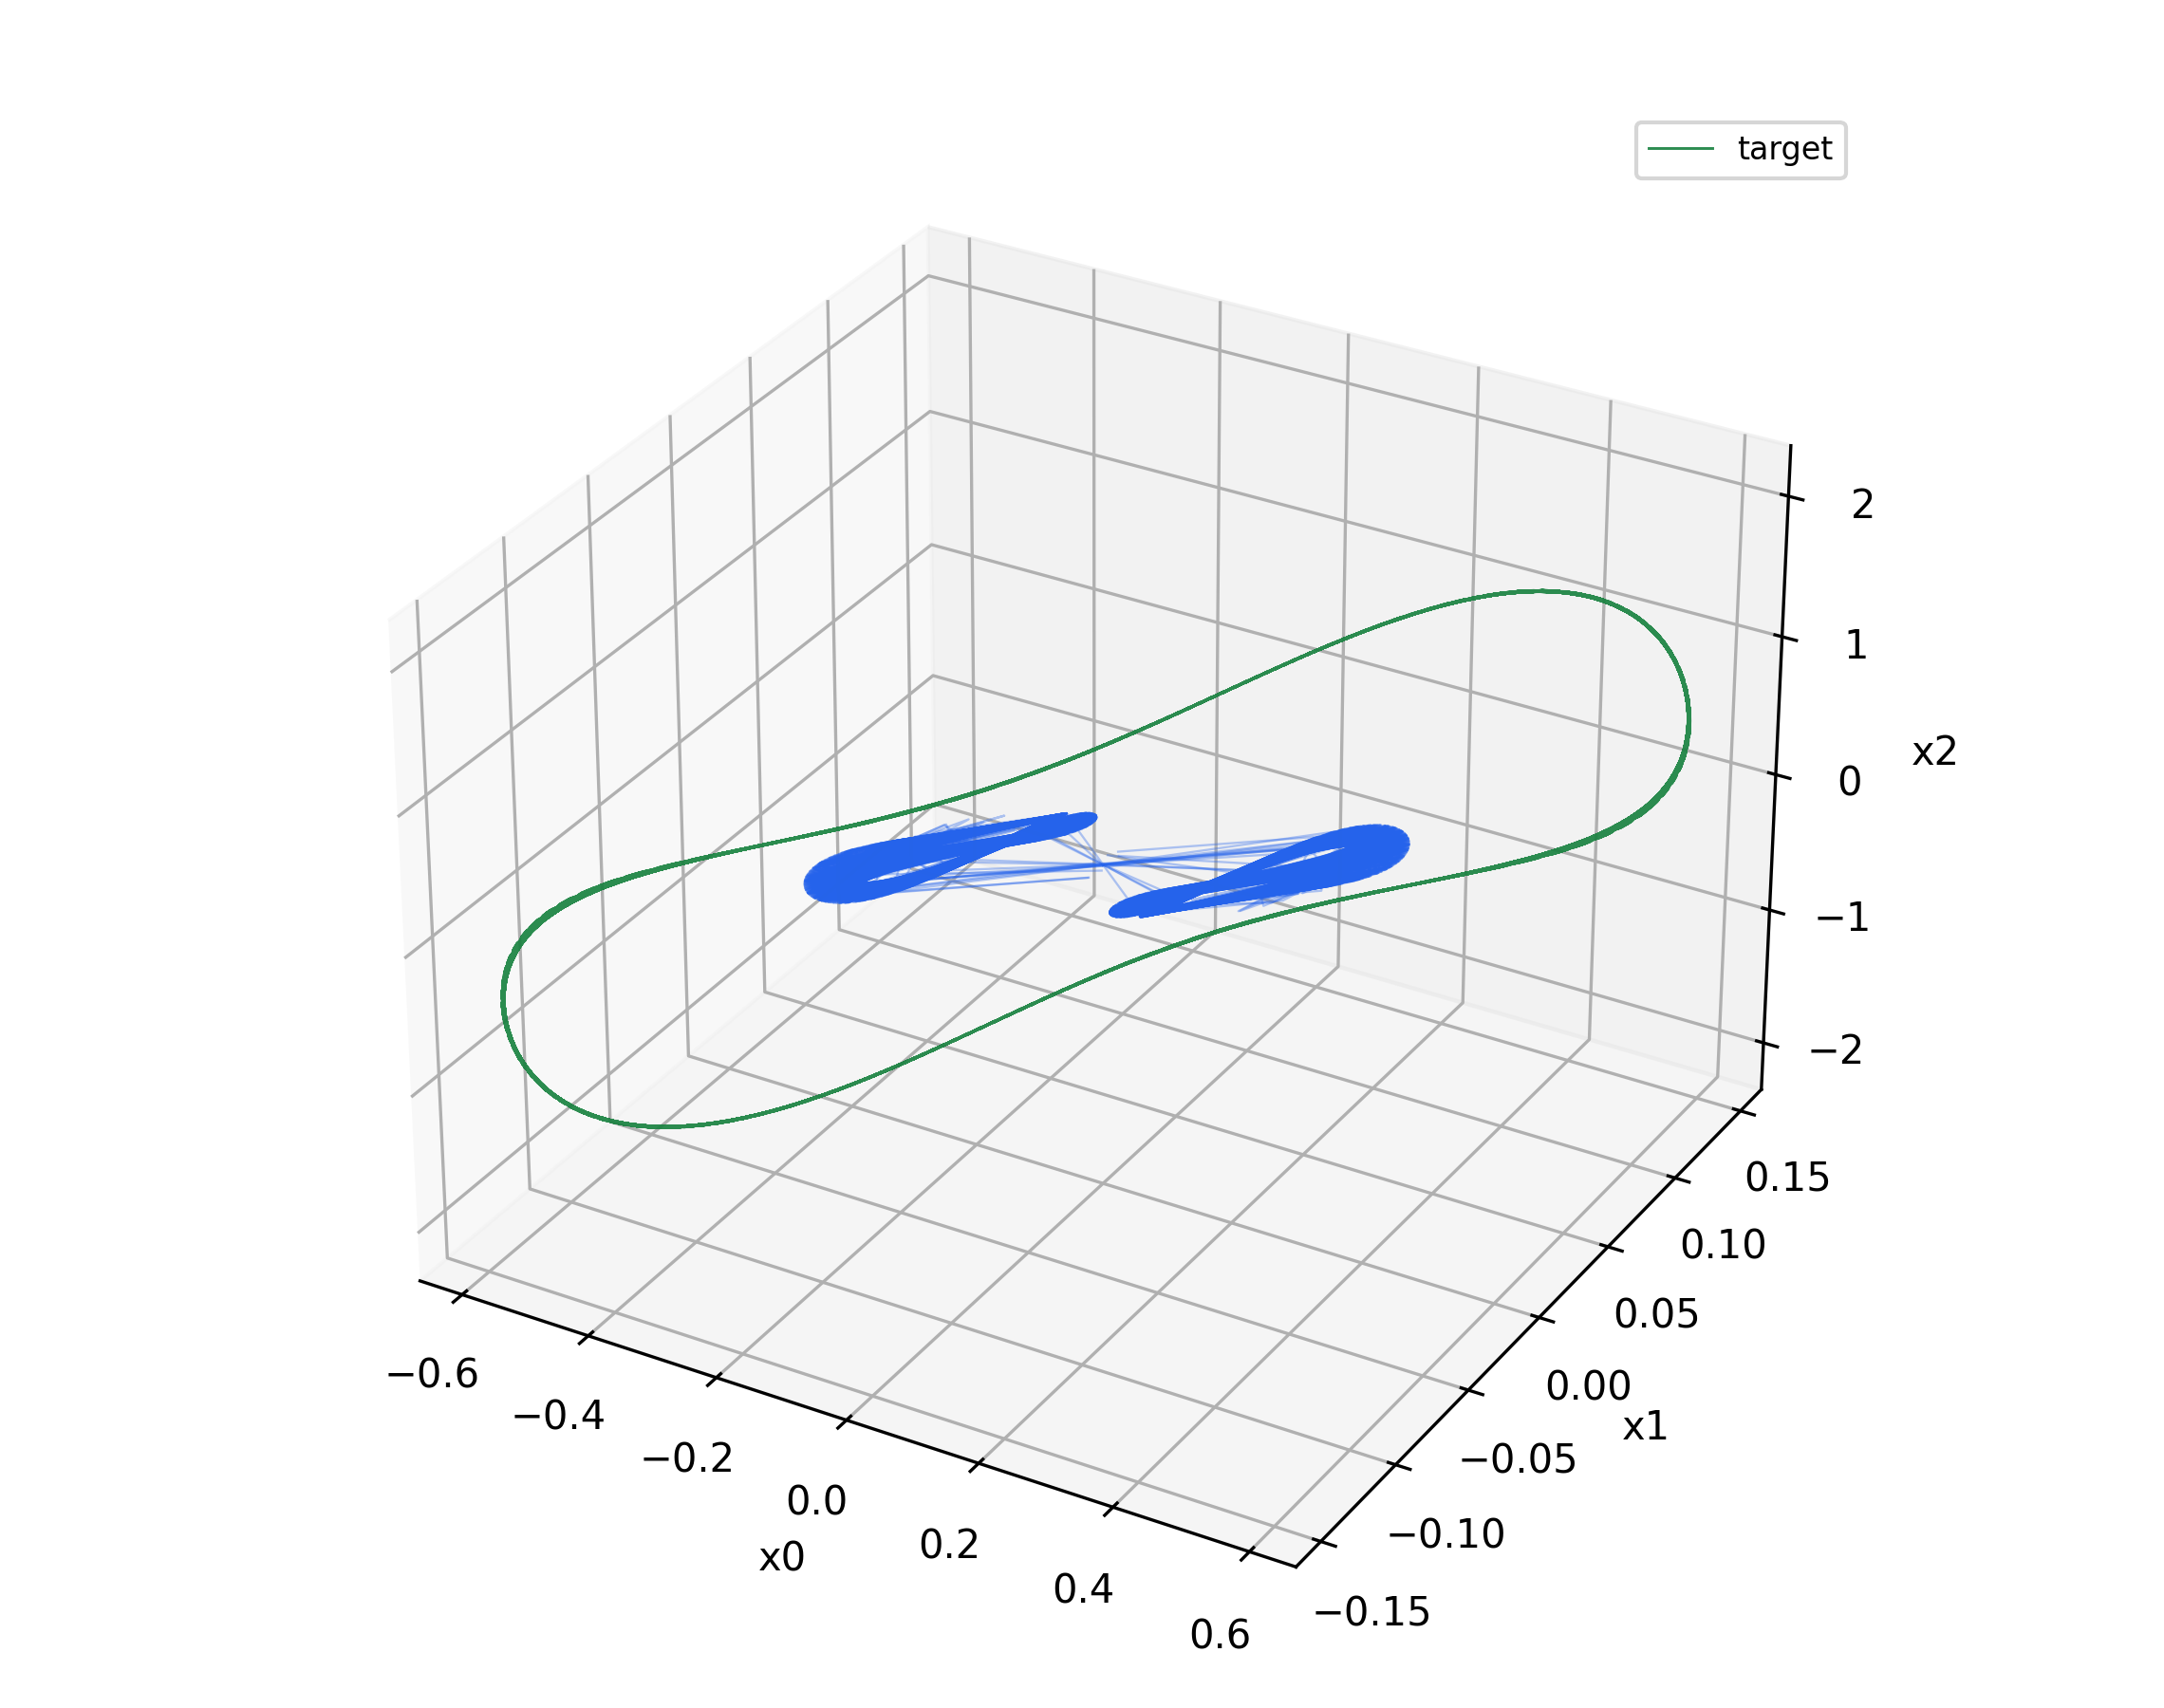
\includegraphics[width=\linewidth]{mavpd_python_hiddenness.png}
  \caption{Python: las vecindades alcanzan sólo los ciclos internos.}
\end{subfigure}\hfill
\begin{subfigure}[t]{0.49\textwidth}
  \centering
  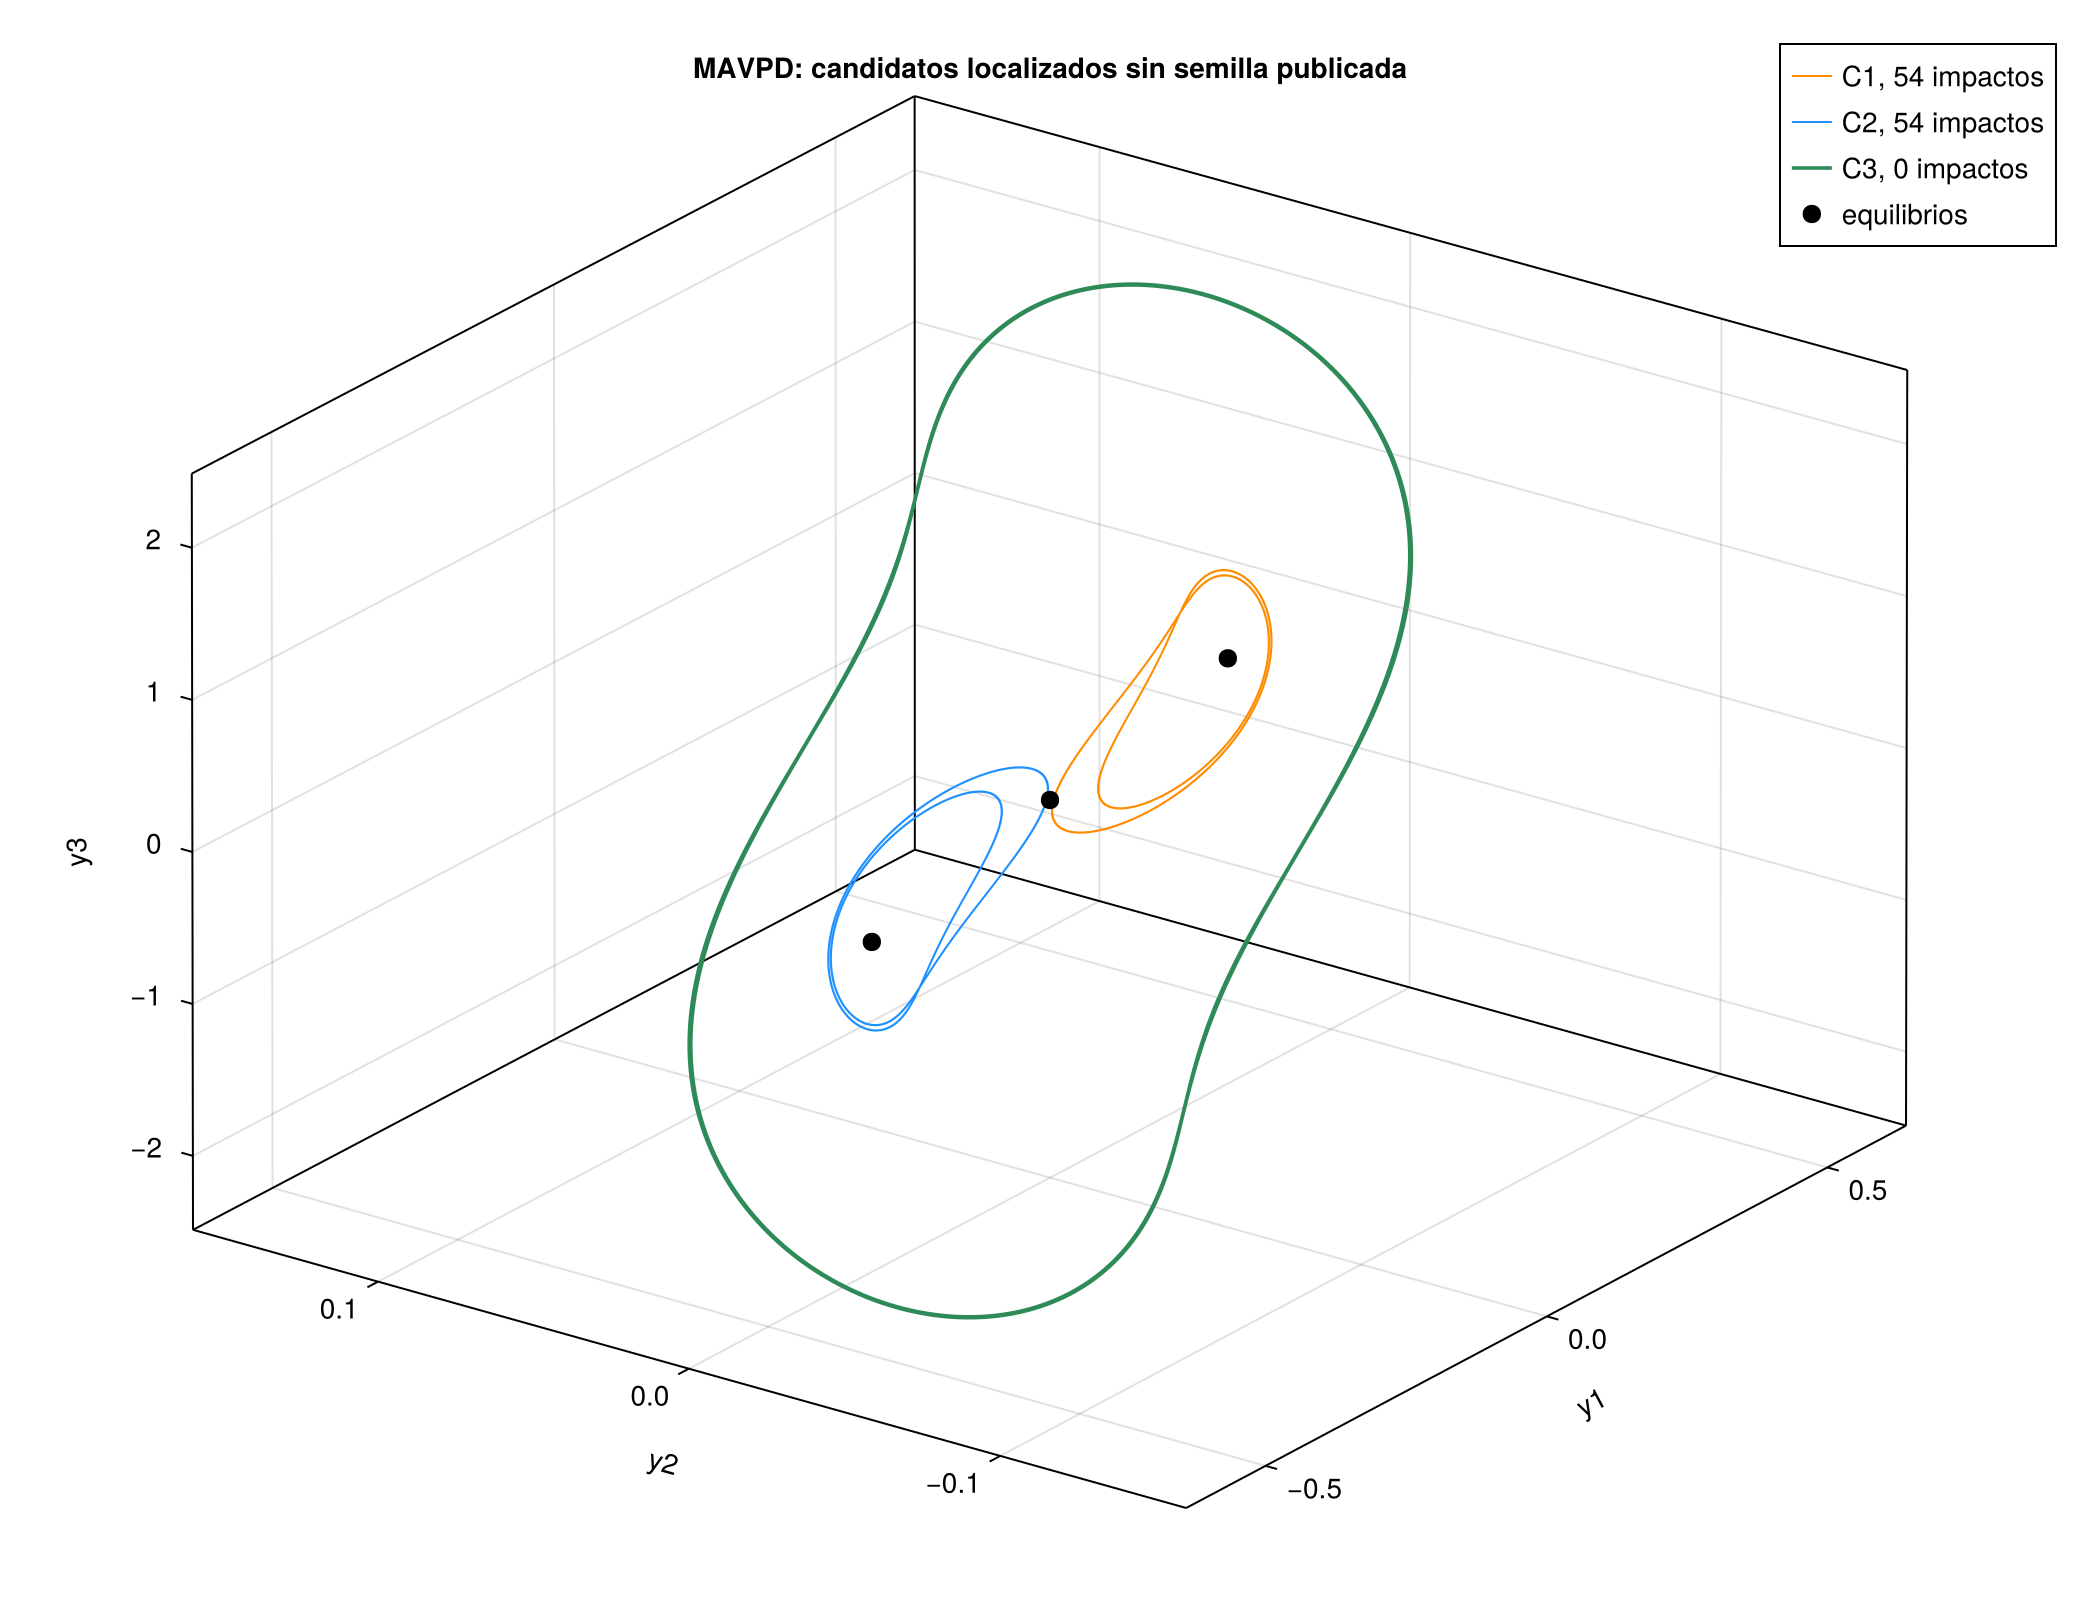
\includegraphics[width=\linewidth]{mavpd_julia_candidates.png}
  \caption{Julia \emph{full}: clúster externo con cero impactos.}
\end{subfigure}
\caption{Ciclo externo compatible con ocultedad bajo las 108 sondas del
protocolo finito para \(\xi=3.1\).}
\label{int:fig:mavpd-hiddenness}
\end{hafobasinfigure}

\subsection{Comprobación algebraica de la fuente}

Se preservan tres discrepancias:

\begin{enumerate}
  \item La fuente imprime \(\Theta=-\delta e_1\),
        \(s=-e_1\) y \(\zeta(\sigma)=\sigma^3\). Juntas producen
        \(+\delta y_1^3\), mientras que la ecuación del sistema contiene
        \(-\delta y_1^3\). La formulación evaluada usa la ecuación original y la
        forma exacta \(b=-\delta e_1\), \(c=e_1\).
  \item Para \(\xi=3.1\), los valores impresos
        \(\omega=18.6143\), \(|k|=0.8951\) dejan residuo de cierre
        \(2.45589\) en la transferencia exacta.
  \item Para \(\xi=3.5\), los valores impresos
        \(\omega=10.2344\), \(|k|=0.1136\) dejan residuo \(0.171719\).
\end{enumerate}

Las semillas impresas sí terminan, en una prueba posterior, en los mismos
clústeres dinámicos que la búsqueda independiente. Esa coincidencia dinámica
no elimina la discrepancia algebraica de frecuencia y ganancia.

\ifHAFOBasinMaterial
\subsection{\texorpdfstring{\(\xi=3.5\): control negativo de ocultedad}{xi=3.5: control negativo de ocultedad}}

La ruta directa recalculó dos ramas:
\[
(\omega_0,k,a_0)=
(10.8359213547,\ 0.1497634046,\ 0.4468607607)
\]
y
\[
(\omega_0,k,a_0)=
(13.0511611895,\ 0.3009508811,\ 0.6334570558).
\]
Las cuatro fases convergen a dos ciclos internos simétricos. Bajo el mismo
protocolo de 108 sondeos, Python y Julia observaron 24 contactos
con cada ciclo; el comparador confirmó la misma decisión negativa. Después
del primer contacto se habilitó la ruta alternativa, que no encontró clústeres
nuevos. Por tanto, la etiqueta oculta no se reproduce para \(\xi=3.5\) bajo
las ecuaciones y controles ensayados.

\fi

\subsection{Extensión caótica: continuación relativa a una frontera candidata de Hopf}
\label{int:subsec:mavpd-chaos}

\ifHAFOBasinMaterial
Los dos regímenes anteriores evalúan conjuntos periódicos bajo un protocolo
común.
\else
El régimen periódico anterior establece el punto de comparación dinámico.
\fi
La coexistencia de caos y ocultedad se estudió mediante dos cálculos
independientes, en Python y Julia. Ambos parten de \eqref{int:eq:mavpd},
obtienen las dos semillas directas y recorren 21 niveles de continuación.
Los parámetros y las semillas publicados se reservan para el contraste
posterior.

En el punto base $(\xi,\gamma)=(3.1,0.1)$, los espectros variacionales cortos
de las ramas 0 y 1 fueron, respectivamente,
\[
 (-0.0012506,-1.0123389,-13.1096006),\qquad
 (-0.0029948,-0.3930260,-51.1769818).
\]
Por tanto, ninguna rama superó el cribado finito declarado
$\widehat\lambda_1>0.02$. Este resultado habilita la ruta alternativa; el cribado de tiempo finito
no establece regularidad asintótica.

La ruta alternativa selecciona, entre las ramas integradas, la de
menor frecuencia armónica directa. La regla eligió aquí la rama 0,
$\omega_0=10.5975230$; su estado final de continuación $\lambda$ alimentó el
transporte en parámetros. La rama 1 se evalúa en el punto base y queda pendiente su transporte por A1.

En $E_\pm=(\pm\sqrt{\gamma},0,\pm\sqrt{\gamma})$, el Jacobiano de las
ecuaciones activas produce
\begin{equation}
 p(\lambda)=\lambda^3+a_1\lambda^2+a_2\lambda+a_3,
 \label{int:eq:mavpd-characteristic}
\end{equation}
con
\begin{equation}
 a_1=\xi+2\delta\gamma,\qquad
 a_2=\rho-\delta+2\delta\gamma\xi,\qquad
 a_3=2\delta\gamma\rho.
 \label{int:eq:mavpd-routh-coefficients}
\end{equation}
Al imponer la igualdad de cruce imaginario de Routh--Hurwitz
$a_1a_2=a_3$ y escribir \(g=2\delta\gamma\), la diferencia se desarrolla como
\[
 a_1a_2-a_3=(\xi+g)(\rho-\delta+\xi g)-\rho g
 =\xi g^2+(\xi^2-\delta)g+\xi(\rho-\delta).
\]
Por tanto, la frontera satisface
\begin{equation}
 \xi g^2+(\xi^2-\delta)g+\xi(\rho-\delta)=0.
 \label{int:eq:mavpd-hopf}
\end{equation}
Esta igualdad determina una frontera candidata de Hopf; aquí no se afirma
haber verificado transversalidad ni no degeneración. Para
$\xi=\MAVPDChaosXi$, la raíz alta de \eqref{int:eq:mavpd-hopf} es
$\gamma_H=\MAVPDChaosHopf$. El valor $\xi=\MAVPDChaosXi$ es el extremo local
declarado de la ruta, no una coordenada elegida por el cribado. El procedimiento
transporta primero el estado desde $\xi=3.10$ hasta ese extremo en pasos de
$-0.01$ y después continúa
$\gamma$, reconstruyendo las ecuaciones, el Jacobiano y la forma Lur'e en cada
nodo. La inspección se restringe a desplazamientos declarados respecto de
$\gamma_H$; no es un barrido de frecuencias ni una exploración arbitraria de
condiciones iniciales.

\ifHAFOBasinMaterial
\begin{table}[H]
\centering
\caption{Cribado local MAVPD alrededor de la frontera alta candidata de Hopf. Los
contactos se cuentan sobre 12 sondeos preliminares alrededor de $E_0$; la tabla
redondea $\widehat\lambda_1$ a un máximo de seis decimales, pero los cálculos
conservan la precisión completa.}
\label{int:tab:mavpd-chaos-screen}
\small
\begin{tabular}{@{}C{1.8cm}C{2.0cm}C{2.3cm}L{8.7cm}@{}}
\toprule
$\gamma-\gamma_H$ & $\widehat\lambda_1$ & Contactos desde $E_0$ & Lectura del cribado \\
\midrule
% Generado desde todas las filas de 03_candidate_screening.csv.
% Columnas: hopf_offset; lambda_1; E0_target_hits/E0_probe_count; lectura finita.
0.002 & 0.929112 & 6/12 & No elegible: hubo contactos en los sondeos preliminares. \\
0.003 & 0.893403 & 6/12 & No elegible: hubo contactos en los sondeos preliminares. \\
0.005 & 0.188317 & 6/12 & No elegible: hubo contactos en los sondeos preliminares. \\
0.008 & 0.812209 & 0/12 & Elegible bajo el cribado finito; no seleccionada por la regla. \\
0.010 & 0.72394 & 0/12 & Elegible y seleccionada por la regla declarada. \\
0.012 & 0.315116 & 0/12 & No elegible bajo el cribado finito declarado. \\
0.015 & -0.00887 & 0/12 & No elegible bajo el cribado finito declarado. \\
\bottomrule

\end{tabular}
\end{table}
\fi

La regla selecciona el mayor desplazamiento declarado con cálculo de Lyapunov
válido y $\widehat\lambda_1>0.5$
\ifHAFOBasinMaterial
, cero contactos preliminares, cero casos ambiguos y cero fallos numéricos
\else
y con los demás filtros de admisibilidad satisfechos
\fi
: así se obtiene
\[
 (\xi,\gamma,\delta,\rho)=
 (\MAVPDChaosXi,\MAVPDChaosGamma,100,200),\qquad
 \gamma=\gamma_H+0.010.
\]
El desplazamiento $0.010$ es el resultado de la regla de selección aplicada en
esta continuación numérica local; no se lee como valor esperado ni es un
parámetro publicado en \cite{matouk2023}. Por tanto, sólo $\gamma$ se selecciona
en este cribado: la tupla completa no se presenta como una optimización conjunta
de $\xi$ y $\gamma$.

\begin{hafobasinfigure}[H]
\centering
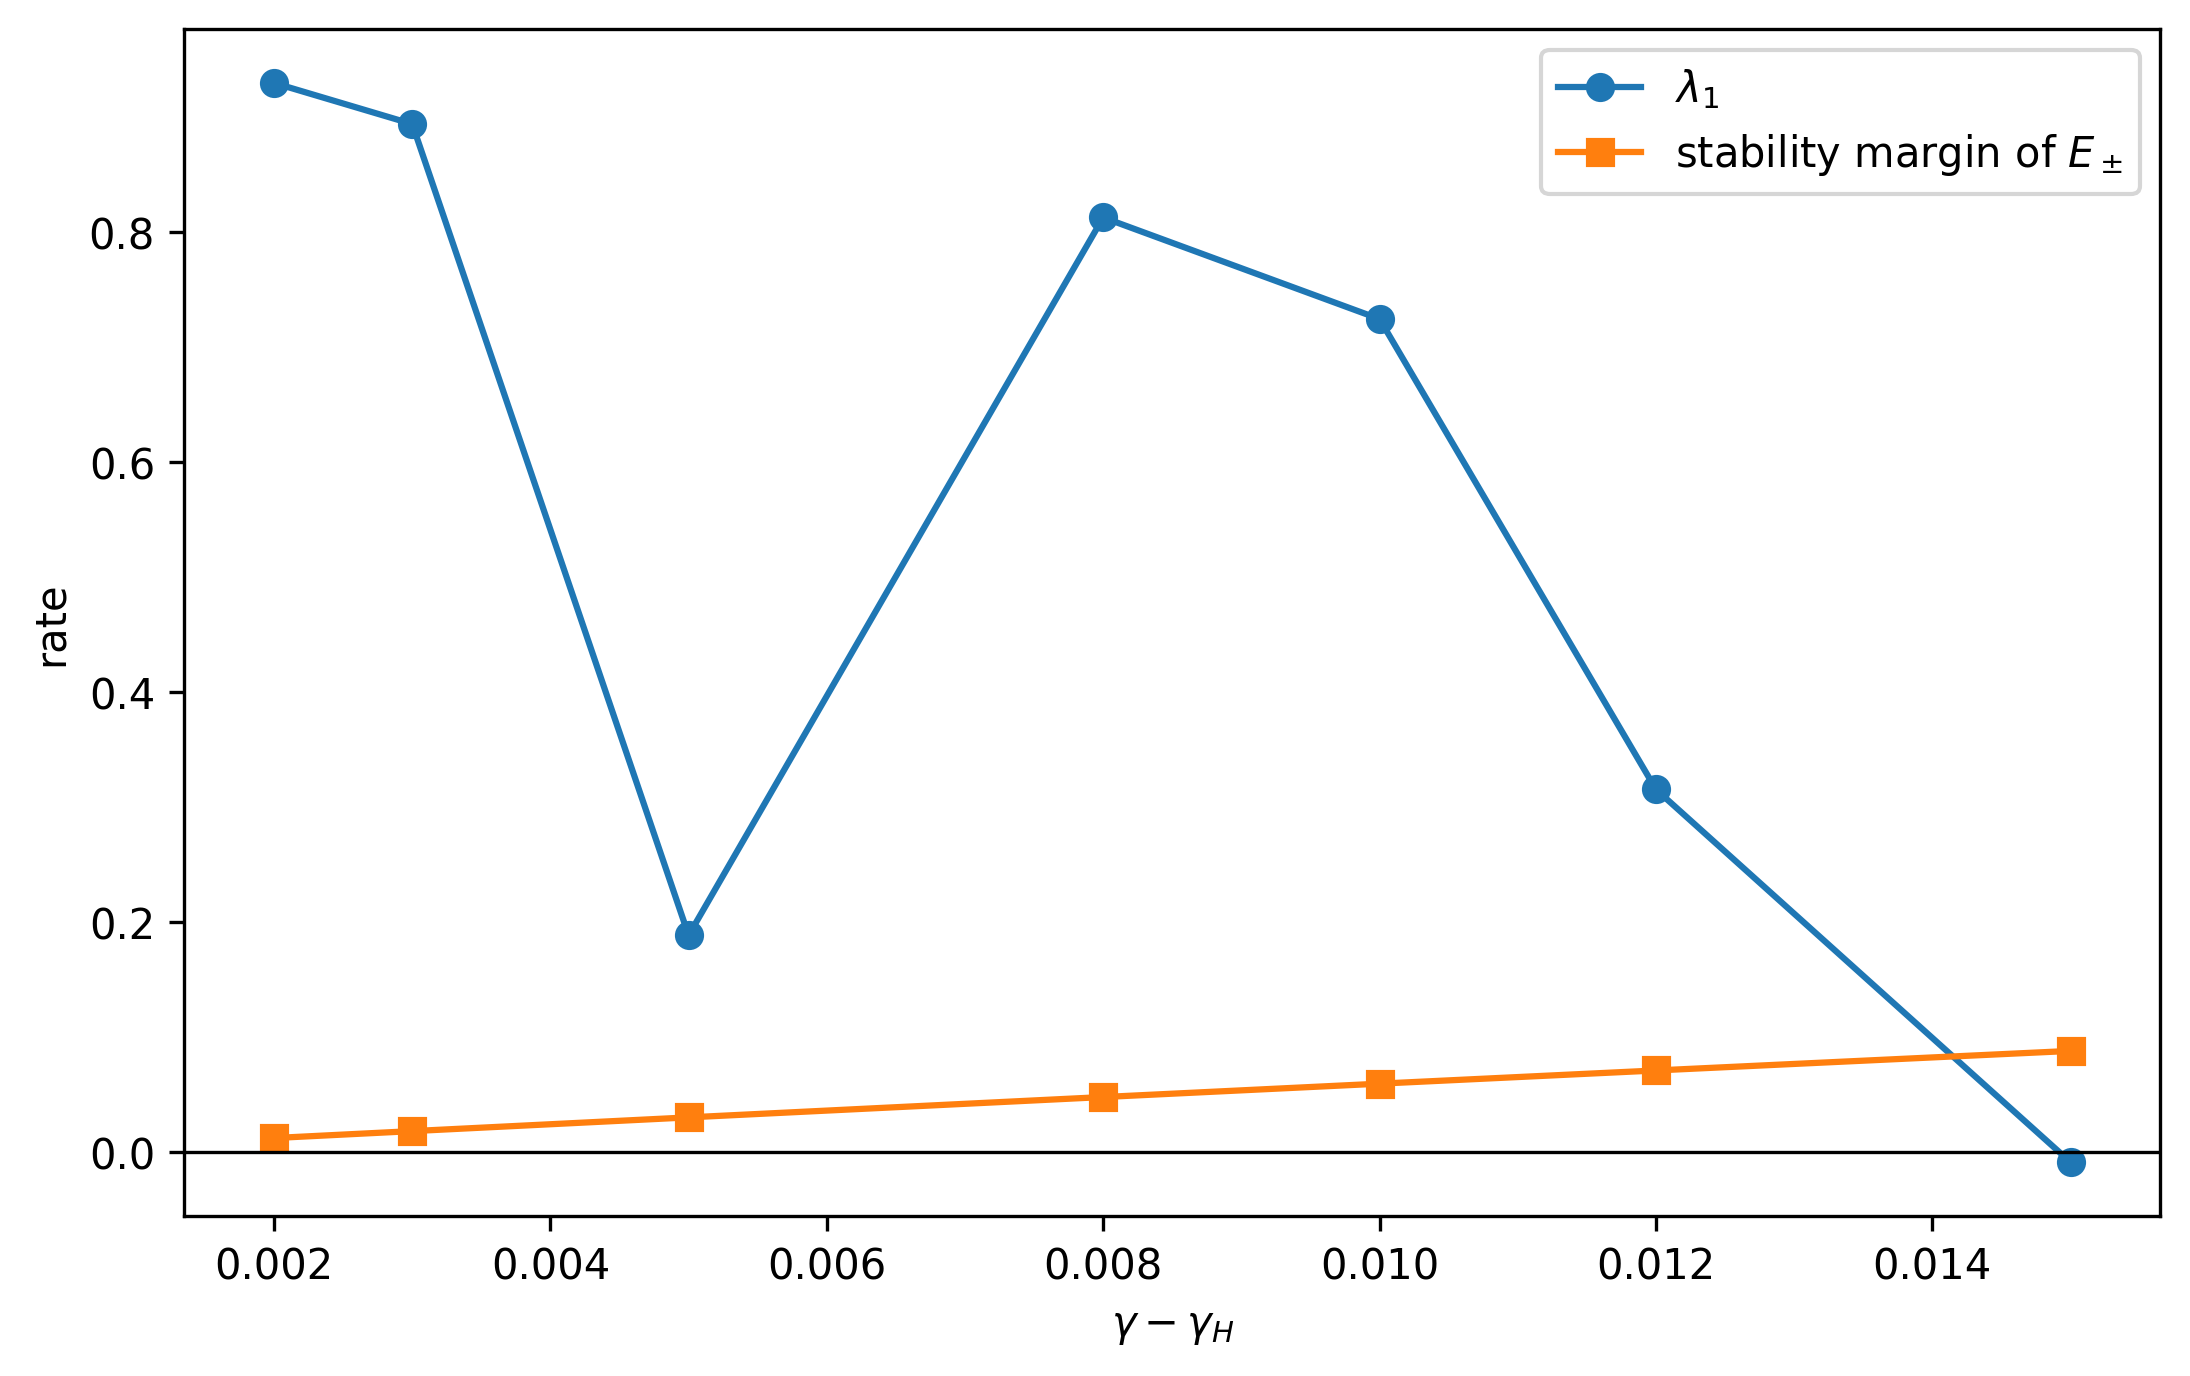
\includegraphics[width=0.90\textwidth]{mavpd_chaos_screen.png}
\caption{Continuación en parámetros y cribado conjunto de exponente máximo y
contactos desde $E_0$. La selección ocurre después del fallo dinámico de las
ramas directas, no mediante una malla de frecuencias.}
\label{int:fig:mavpd-chaos-screen}
\end{hafobasinfigure}

\begin{table}[H]
\centering
\caption{Protocolo numérico de la extensión MAVPD caótica.}
\label{int:tab:mavpd-chaos-contract}
\footnotesize
\begin{tabularx}{\textwidth}{@{}L{0.19\textwidth}L{0.34\textwidth}Y@{}}
\toprule
Fase & Horizonte y muestreo & Integrador y tolerancias \\
\midrule
Cribado D0 por rama & $t_b=100$, $t_{LE}=250$, QR $0.5$ &
DOP853, $(\mathrm{rtol},\mathrm{atol})=(2\,10^{-10},2\,10^{-12})$,
$\Delta t_{\max}=0.02$ \\
Transporte A1 por nodo & $t_b=60$, $t_k=10$, muestra $0.02$ &
DOP853, $(2\,10^{-10},2\,10^{-12})$, $\Delta t_{\max}=0.02$ \\
Referencia del cribado & duración 360, descarte 160, muestra $0.05$,
600 puntos máximos & DOP853, $\Delta t_{\max}=0.03$; factor de seguridad 3 \\
\ifHAFOBasinMaterial
Sondeos preliminares $E_0$ & $t_b=500$, $t_k=100$, muestra $0.05$;
2 radios, 6 direcciones & DOP853, $(2\,10^{-10},2\,10^{-12})$,
$\Delta t_{\max}=0.03$ \\
\fi
Trayectoria estricta & $t_f=900$, $t_b=300$, muestra $0.02$ &
DOP853, $(2\,10^{-11},2\,10^{-13})$, $\Delta t_{\max}=0.01$ \\
Lyapunov estricto & $t_b=300$, $t_{LE}=1200$, QR $0.5$ &
DOP853 variacional, $(2\,10^{-12},2\,10^{-14})$,
$\Delta t_{\max}=0.01$ \\
Control Lyapunov combinado & estado candidato perturbado; $t_b=200$,
$t_{LE}=600$, QR $0.5$ & DOP853 variacional,
$(2\,10^{-10},2\,10^{-12})$, $\Delta t_{\max}=0.02$ \\
\ifHAFOBasinMaterial
Ocultedad final & $t_b=400$, $t_k=100$, muestra $0.05$;
108 sondeos principales + 4 dirigidos & DOP853, $(2\,10^{-10},2\,10^{-12})$,
$\Delta t_{\max}=0.03$; referencia máxima 1000 puntos \\
\fi
\bottomrule
\end{tabularx}
\end{table}

\subsubsection*{Refinamiento dinámico y controles de caos}

La trayectoria candidata se integró con DOP853, $t_f=900$, transitorio 300,
muestreo $0.02$, tolerancias $(\mathrm{rtol},\mathrm{atol})=(2\times10^{-11},
2\times10^{-13})$ y paso máximo $0.01$ \cite{scipy2020}. Sobre un problema
variacional separado, DOP853 con QR, transitorio 300 y acumulación 1200 produjo
el espectro finito. Con $Q_0=I$, en cada segmento se integra
\begin{equation}
 \dot Y_m=J(y(t))Y_m,\qquad Y_m(t_{m-1})=Q_{m-1},
 \qquad Y_m(t_m)=Q_mR_m,
 \quad
 \widehat\lambda_i(T)=\frac{1}{T}\sum_{m=1}^{M}
 \log\left|R_{m,ii}\right|,
 \label{int:eq:mavpd-variational-qr}
\end{equation}
donde cada $R_m$ contiene sólo el crecimiento del segmento correspondiente;
la base se reinicia con $Q_m$ antes del segmento siguiente
\cite{Benettin1980a}. El resultado fue
\begin{equation}
 \begin{aligned}
  \widehat\lambda_1&=\MAVPDChaosLEOne,
  &\widehat\lambda_2&=\MAVPDChaosLETwo,\\
  \widehat\lambda_3&=\MAVPDChaosLEThree,
  &D_{KY}&=\MAVPDChaosKY.
 \end{aligned}
 \label{int:eq:mavpd-chaos-lyapunov}
\end{equation}
Aquí \(D_{KY}=2+(\widehat\lambda_1+\widehat\lambda_2)/
|\widehat\lambda_3|\), pues las dos primeras suman positivamente y la suma de
las tres es negativa.
El control de Lyapunov perturbó el extremo de la continuación y cambió simultáneamente las
tolerancias, el paso máximo y los horizontes de transitorio y acumulación. El cálculo conservó $\widehat\lambda_1=\MAVPDChaosLEControlOne$. El residuo de
consistencia
$r_{\mathrm{div}}=\sum_i\widehat\lambda_i(T_{LE})-
\overline{\nabla\!\cdot f}_{[t_a,t_b]}$ fue
$\MAVPDChaosDivergenceResidual$, con
\begin{equation}
 \nabla\!\cdot f(y)=\delta\gamma-\xi-3\delta y_1^2,
 \qquad
 \overline{\nabla\!\cdot f}_{[t_a,t_b]}=\frac{1}{t_b-t_a}
 \int_{t_a}^{t_b}\!\left(\delta\gamma-\xi-3\delta y_1(t)^2\right)\,dt.
 \label{int:eq:mavpd-divergence-control}
\end{equation}
La relación con el espectro se obtiene de la fórmula de Jacobi. Para una
matriz fundamental invertible \(\Phi\),
\[
 \frac{\dd}{\dd t}\log|\det\Phi(t)|
 =\operatorname{tr}(\Phi^{-1}J\Phi)=\operatorname{tr}J
 =\nabla\!\cdot f.
\]
En la descomposición por segmentos, los determinantes de las matrices
ortogonales \(Q_m\) tienen módulo uno y cada matriz triangular satisface
\(\det R_m=\prod_iR_{m,ii}\). Por tanto, sobre una misma trayectoria y
ventana de longitud \(T\),
\[
 \sum_i\widehat\lambda_i(T)
 =\frac1T\log|\det\Phi(T)|
 =\frac1T\int_0^T\nabla\!\cdot f(y(t))\,\dd t,
\]
con \(\Phi(0)=I\). Esta identidad justifica la comparación de la suma de
exponentes con el promedio de la divergencia.
Aquí $T_{LE}=1200$ pertenece a la integración variacional, mientras que la
divergencia se promedia sobre la trayectoria muestreada independiente
$[t_a,t_b]=[300,900]$. El residuo compara, por tanto, promedios de trayectorias y ventanas
distintas. Como control de integrador, una
trayectoria EFORK de paso fijo $h=0.002$ alcanzó la misma nube de referencia
calibrada.

\begin{hafocommonfigure}[H]
\centering
\begin{subfigure}[t]{0.98\textwidth}
  \centering
  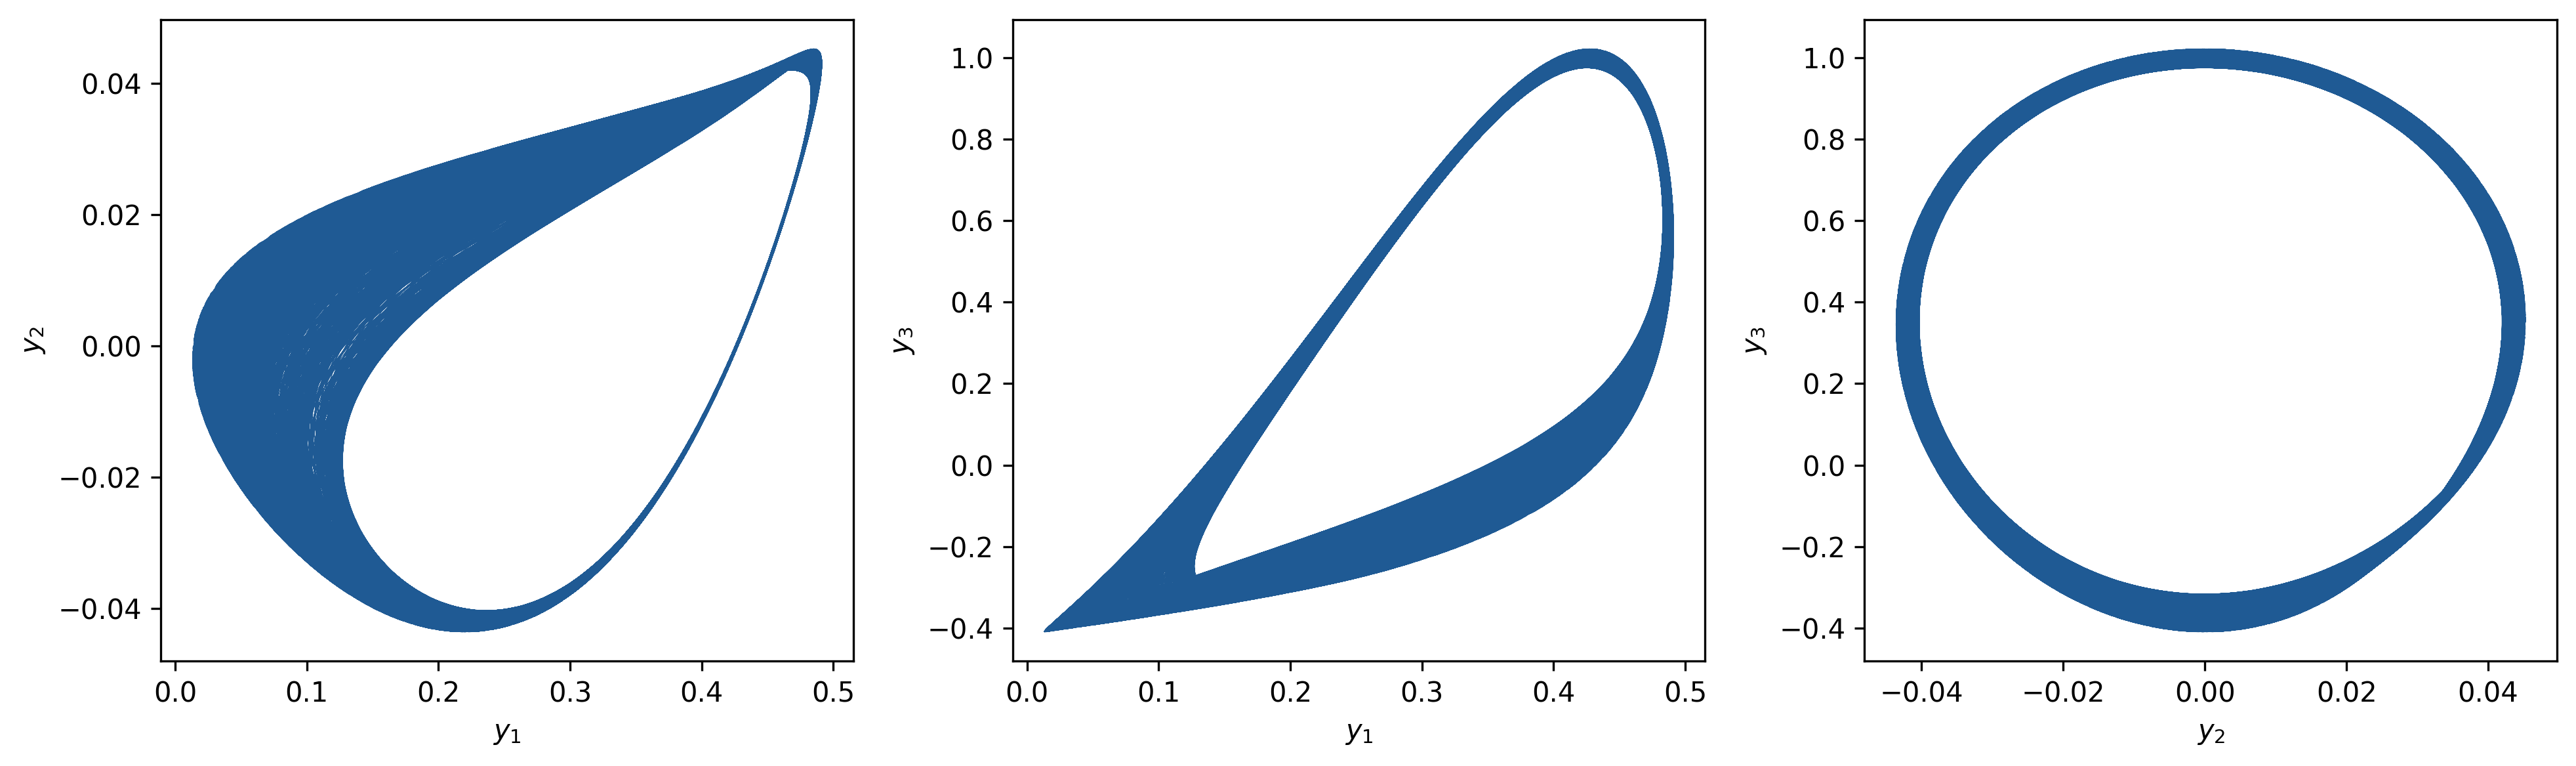
\includegraphics[width=\linewidth]{mavpd_chaos_phase_portraits.png}
  \caption{Proyecciones postransitorias del candidato seleccionado.}
\end{subfigure}

\vspace{0.35em}
\begin{subfigure}[t]{0.86\textwidth}
  \centering
  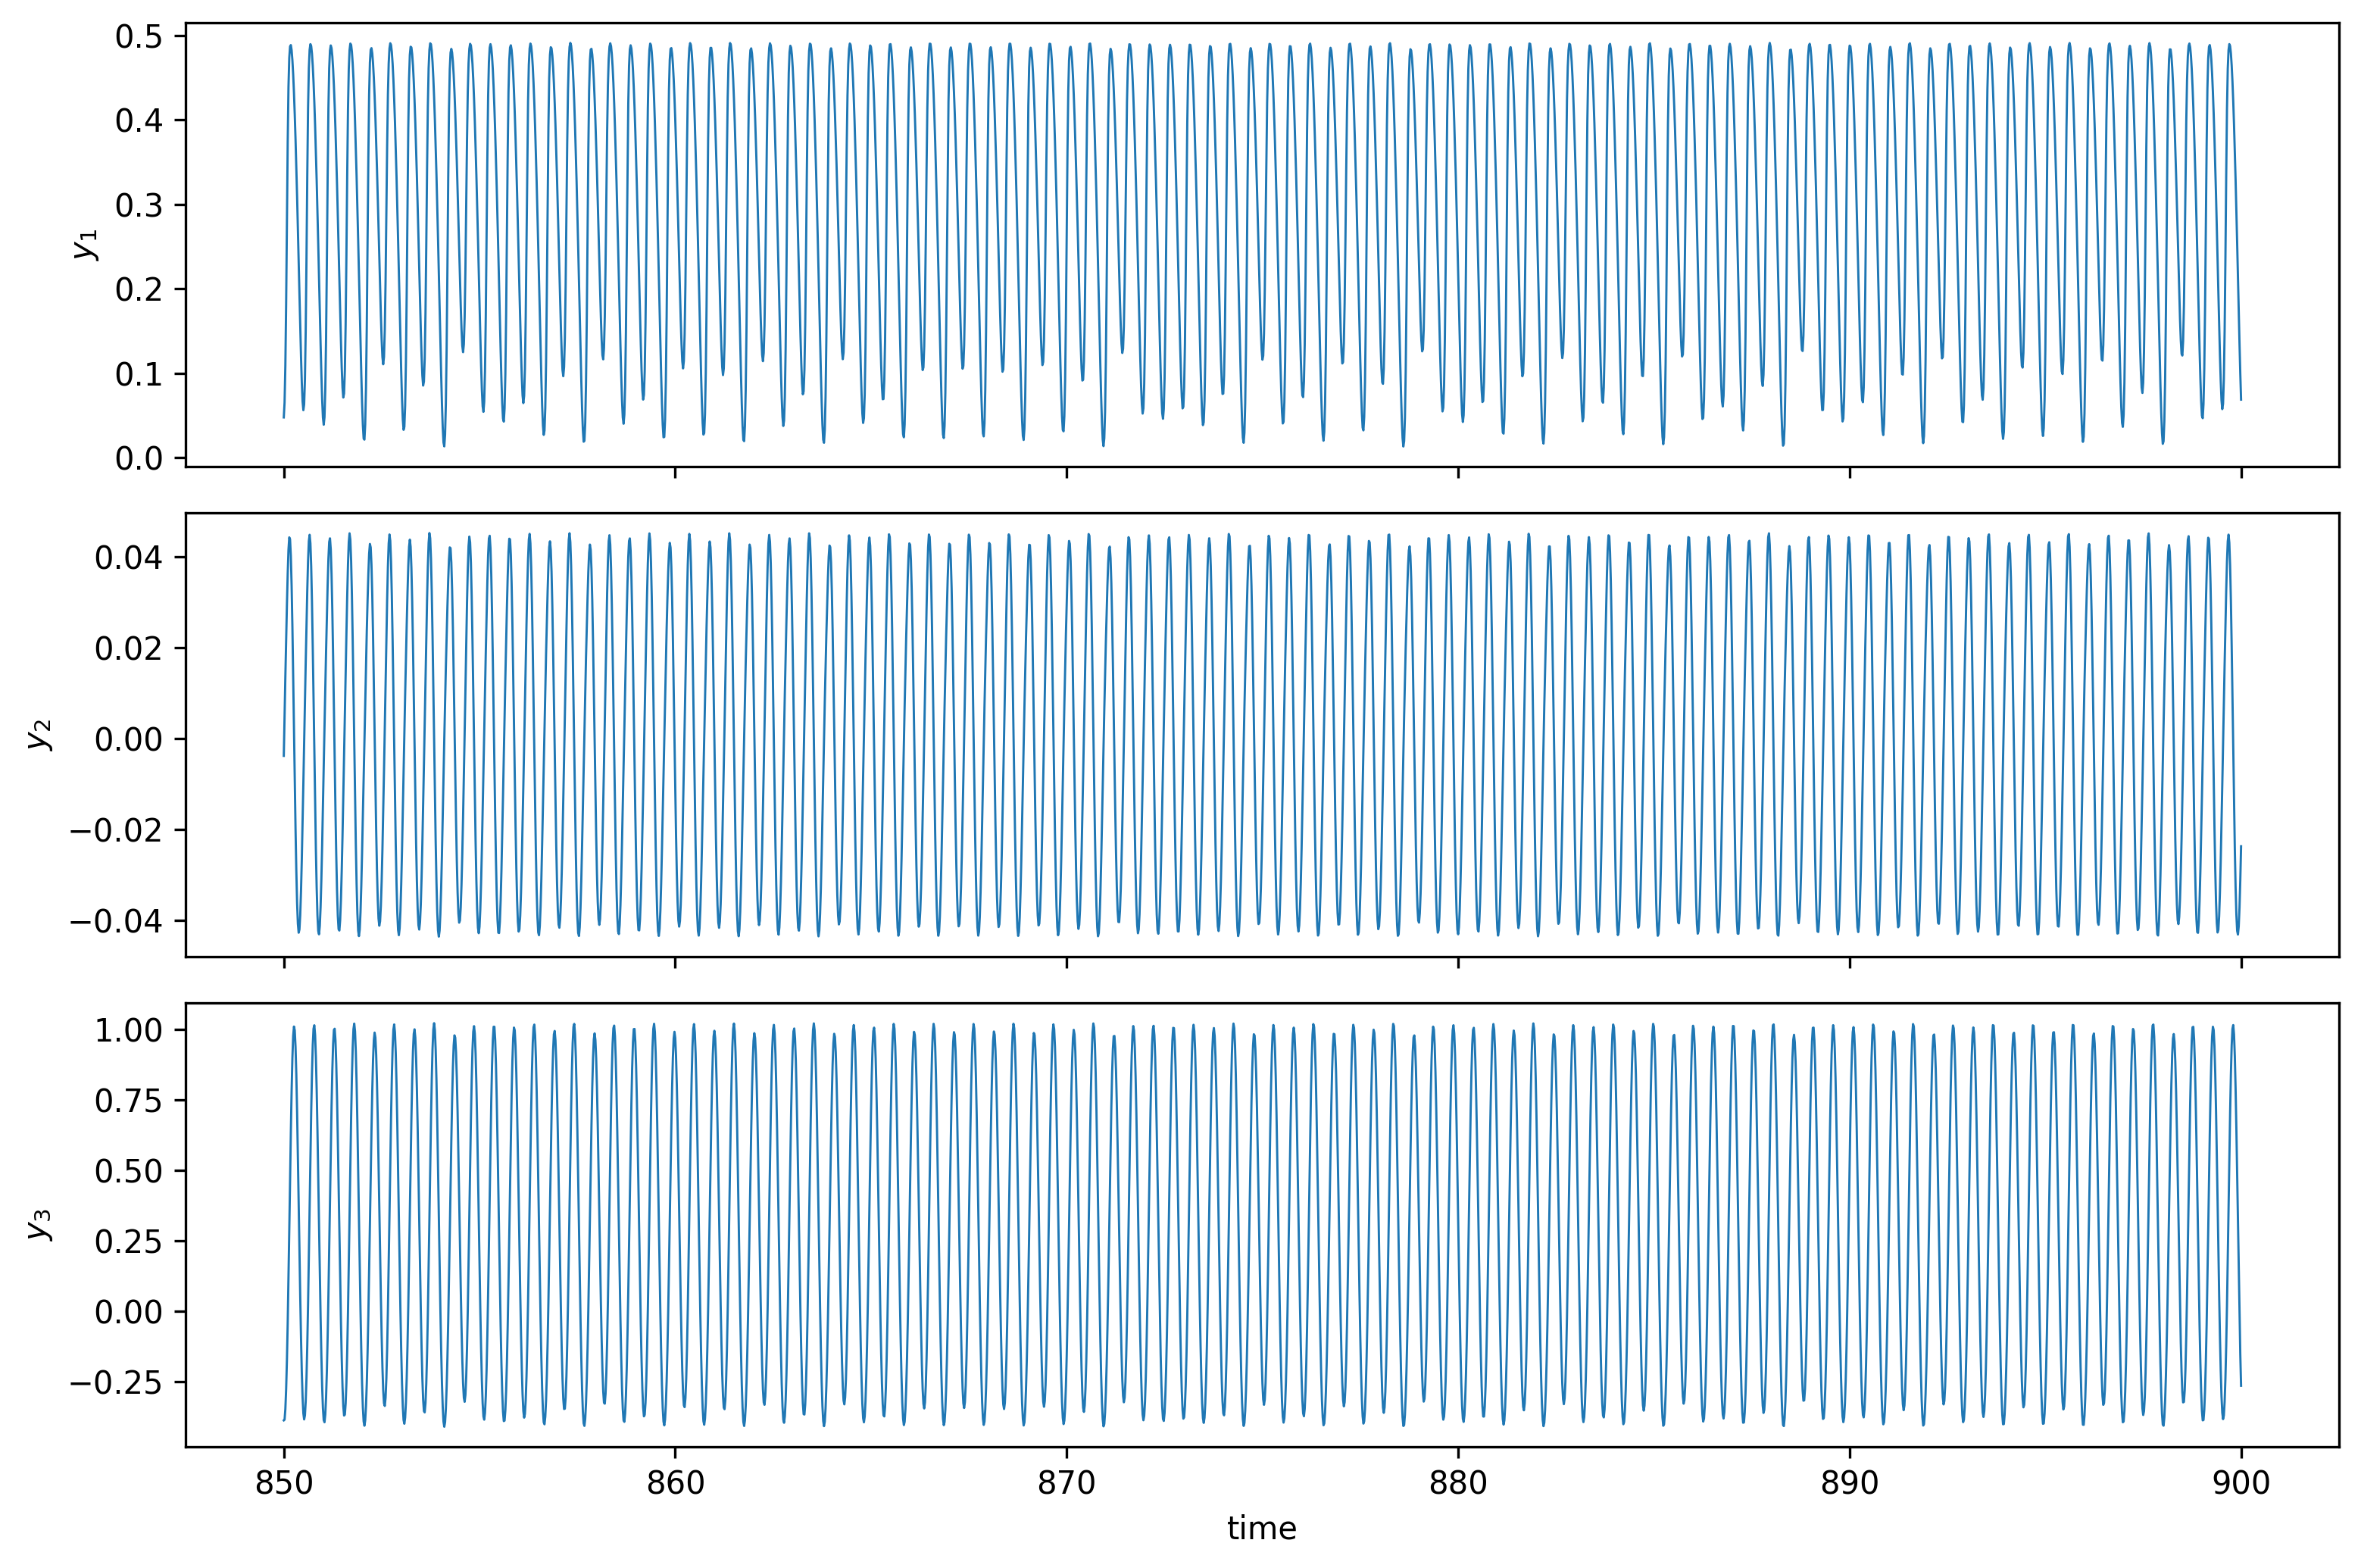
\includegraphics[width=\linewidth]{mavpd_chaos_time_series.png}
  \caption{Series temporales en la ventana conservada.}
\end{subfigure}
\caption{Geometría y evolución temporal del candidato MAVPD caótico. Ventana postransitoria acotada.}
\label{int:fig:mavpd-chaos-trajectory}
\end{hafocommonfigure}

La sección $y_2=0$ con orientación positiva retuvo
\MAVPDChaosPoincareCount{} cruces no duplicados. Los cruces se obtuvieron por
interpolación lineal entre muestras de la trayectoria, con el error temporal
asociado a esa aproximación
\cite{henon1982}. La prueba 0--1 sobre dos coordenadas de la secuencia de
retorno dio medianas $K=\MAVPDChaosReturnKOne$ y
$K=\MAVPDChaosReturnKTwo$ \cite{gottwald2009}. En cambio, la prueba 0--1 sobre
el flujo fue sensible al submuestreo: 3 de 10 pasos dieron etiqueta de
candidato caótico, 1 dio etiqueta regular y 6 quedaron inconclusos. El criterio conjunto usa la secuencia de retorno con
el paso fijado antes de la clasificación.

\begin{hafocommonfigure}[H]
\centering
\begin{subfigure}[t]{0.49\textwidth}
  \centering
  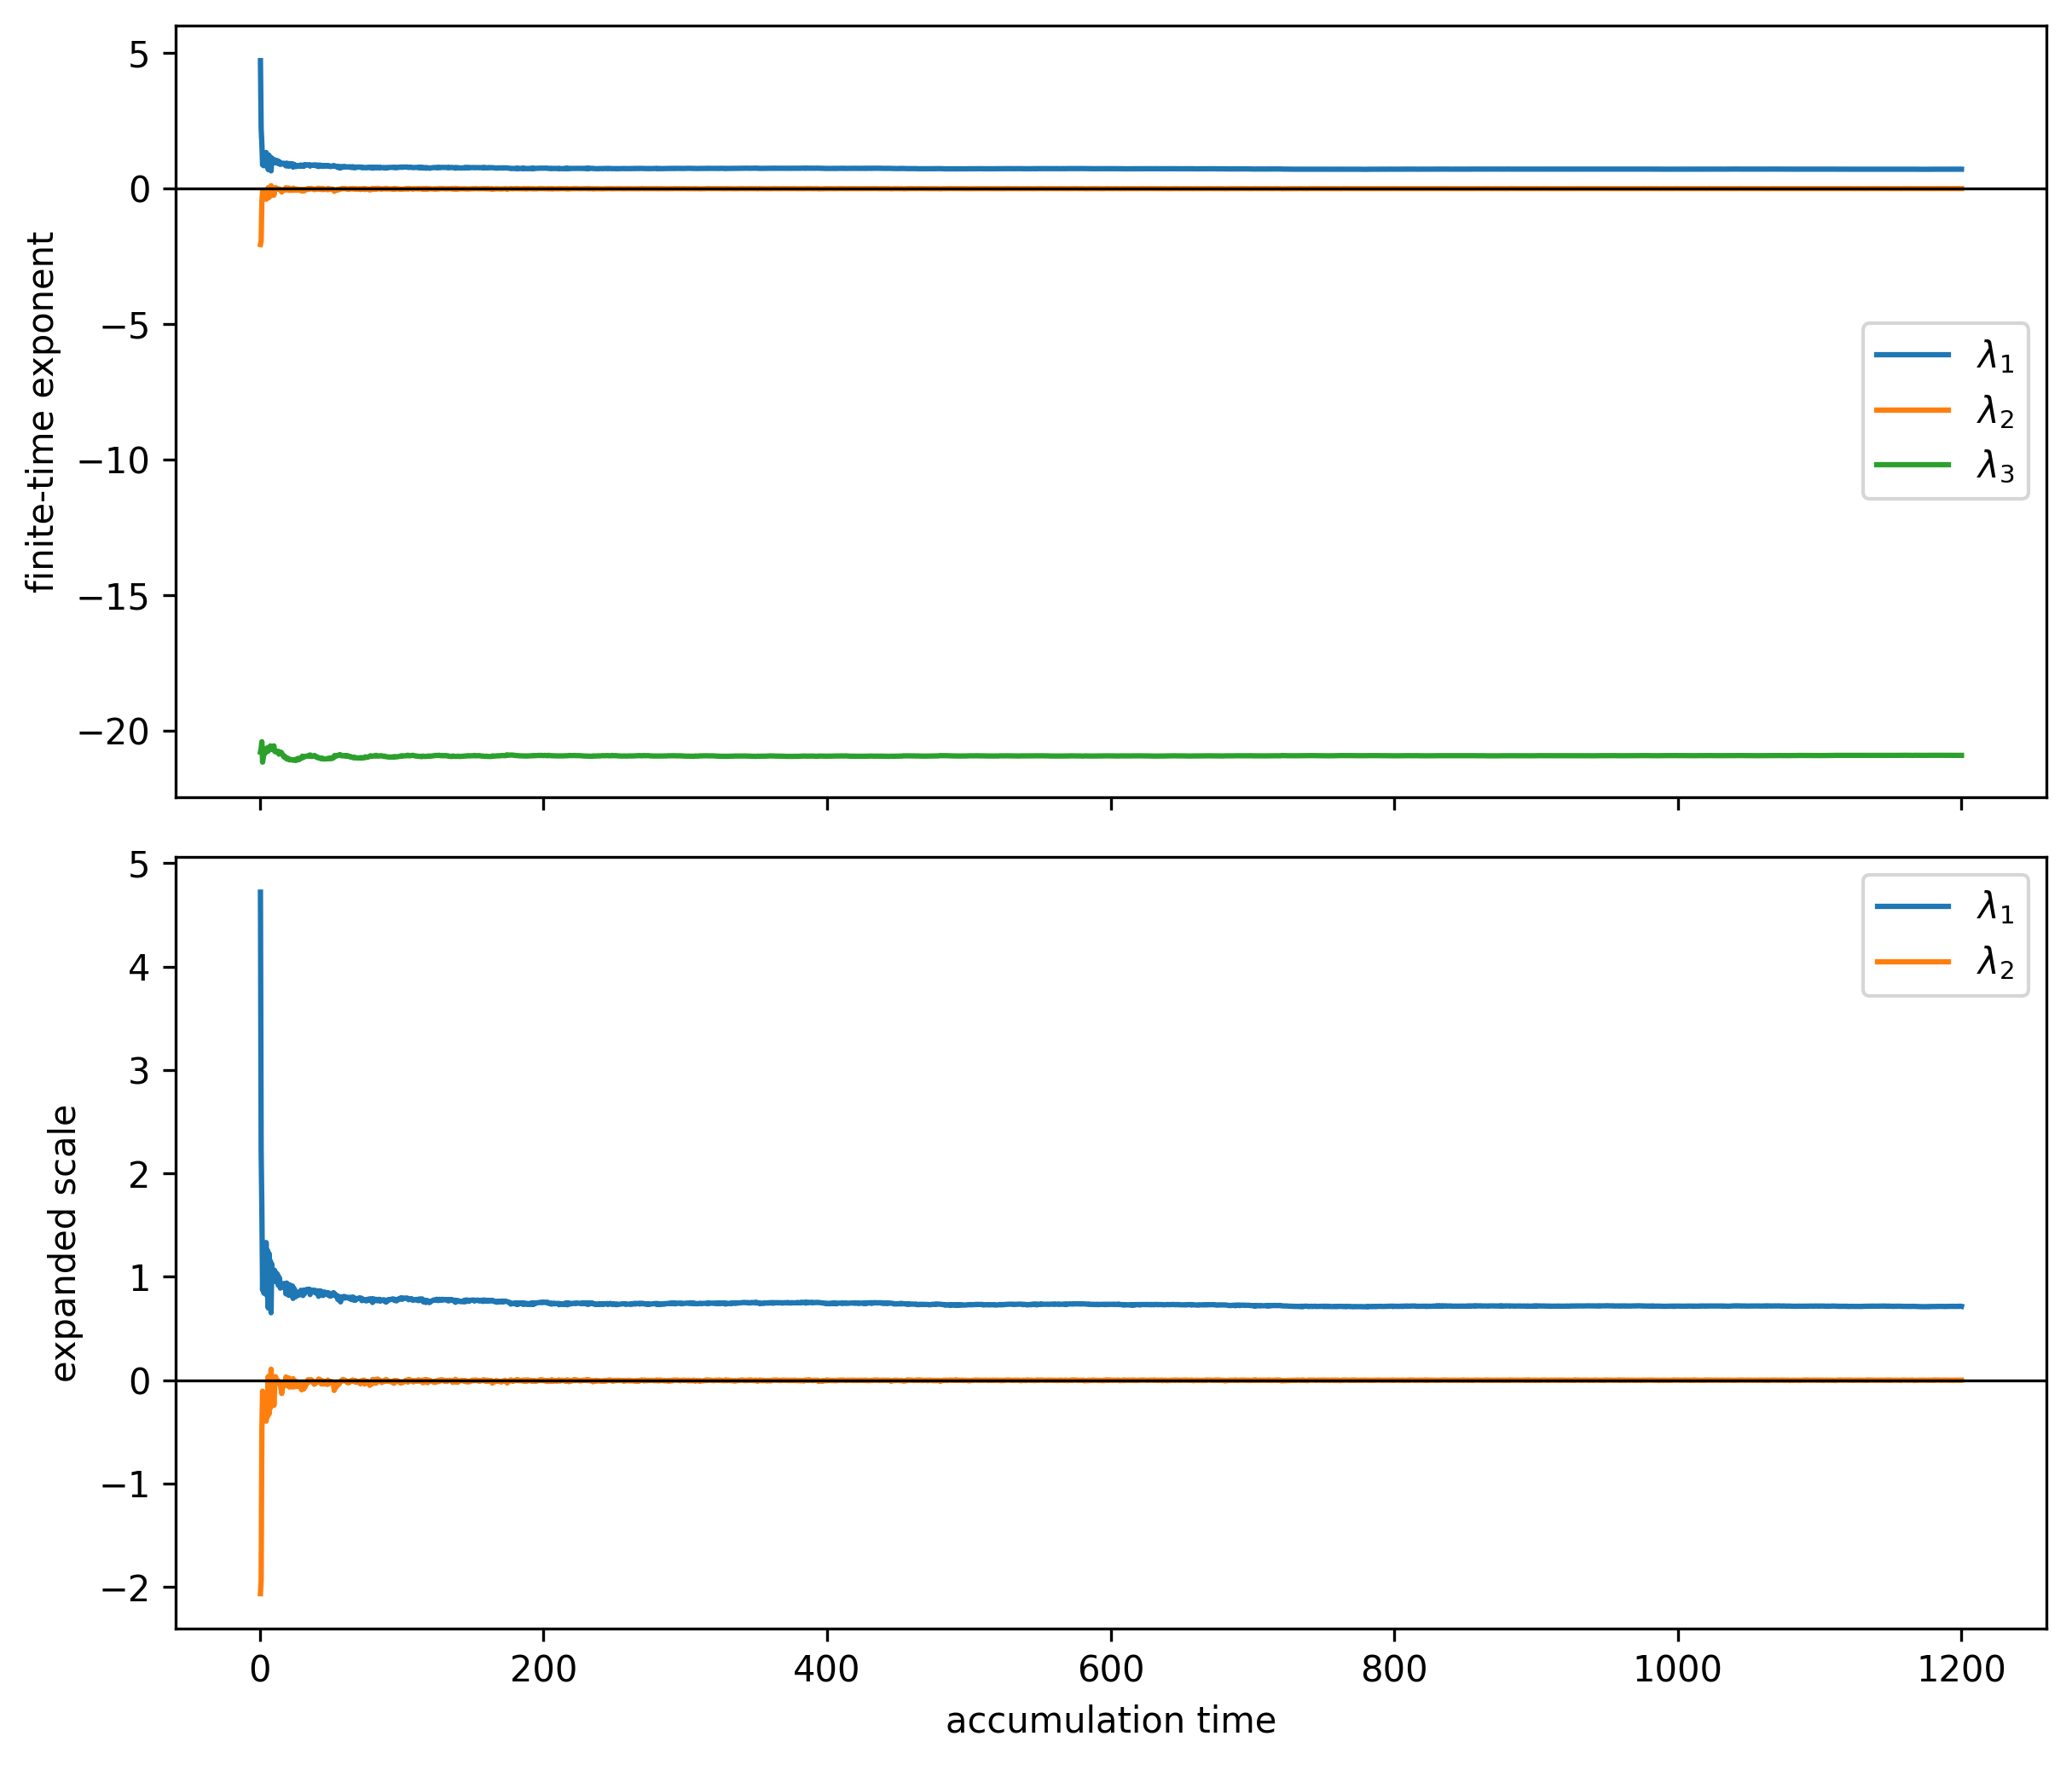
\includegraphics[width=\linewidth]{mavpd_chaos_lyapunov.png}
  \caption{Convergencia del espectro variacional finito.}
\end{subfigure}\hfill
\begin{subfigure}[t]{0.49\textwidth}
  \centering
  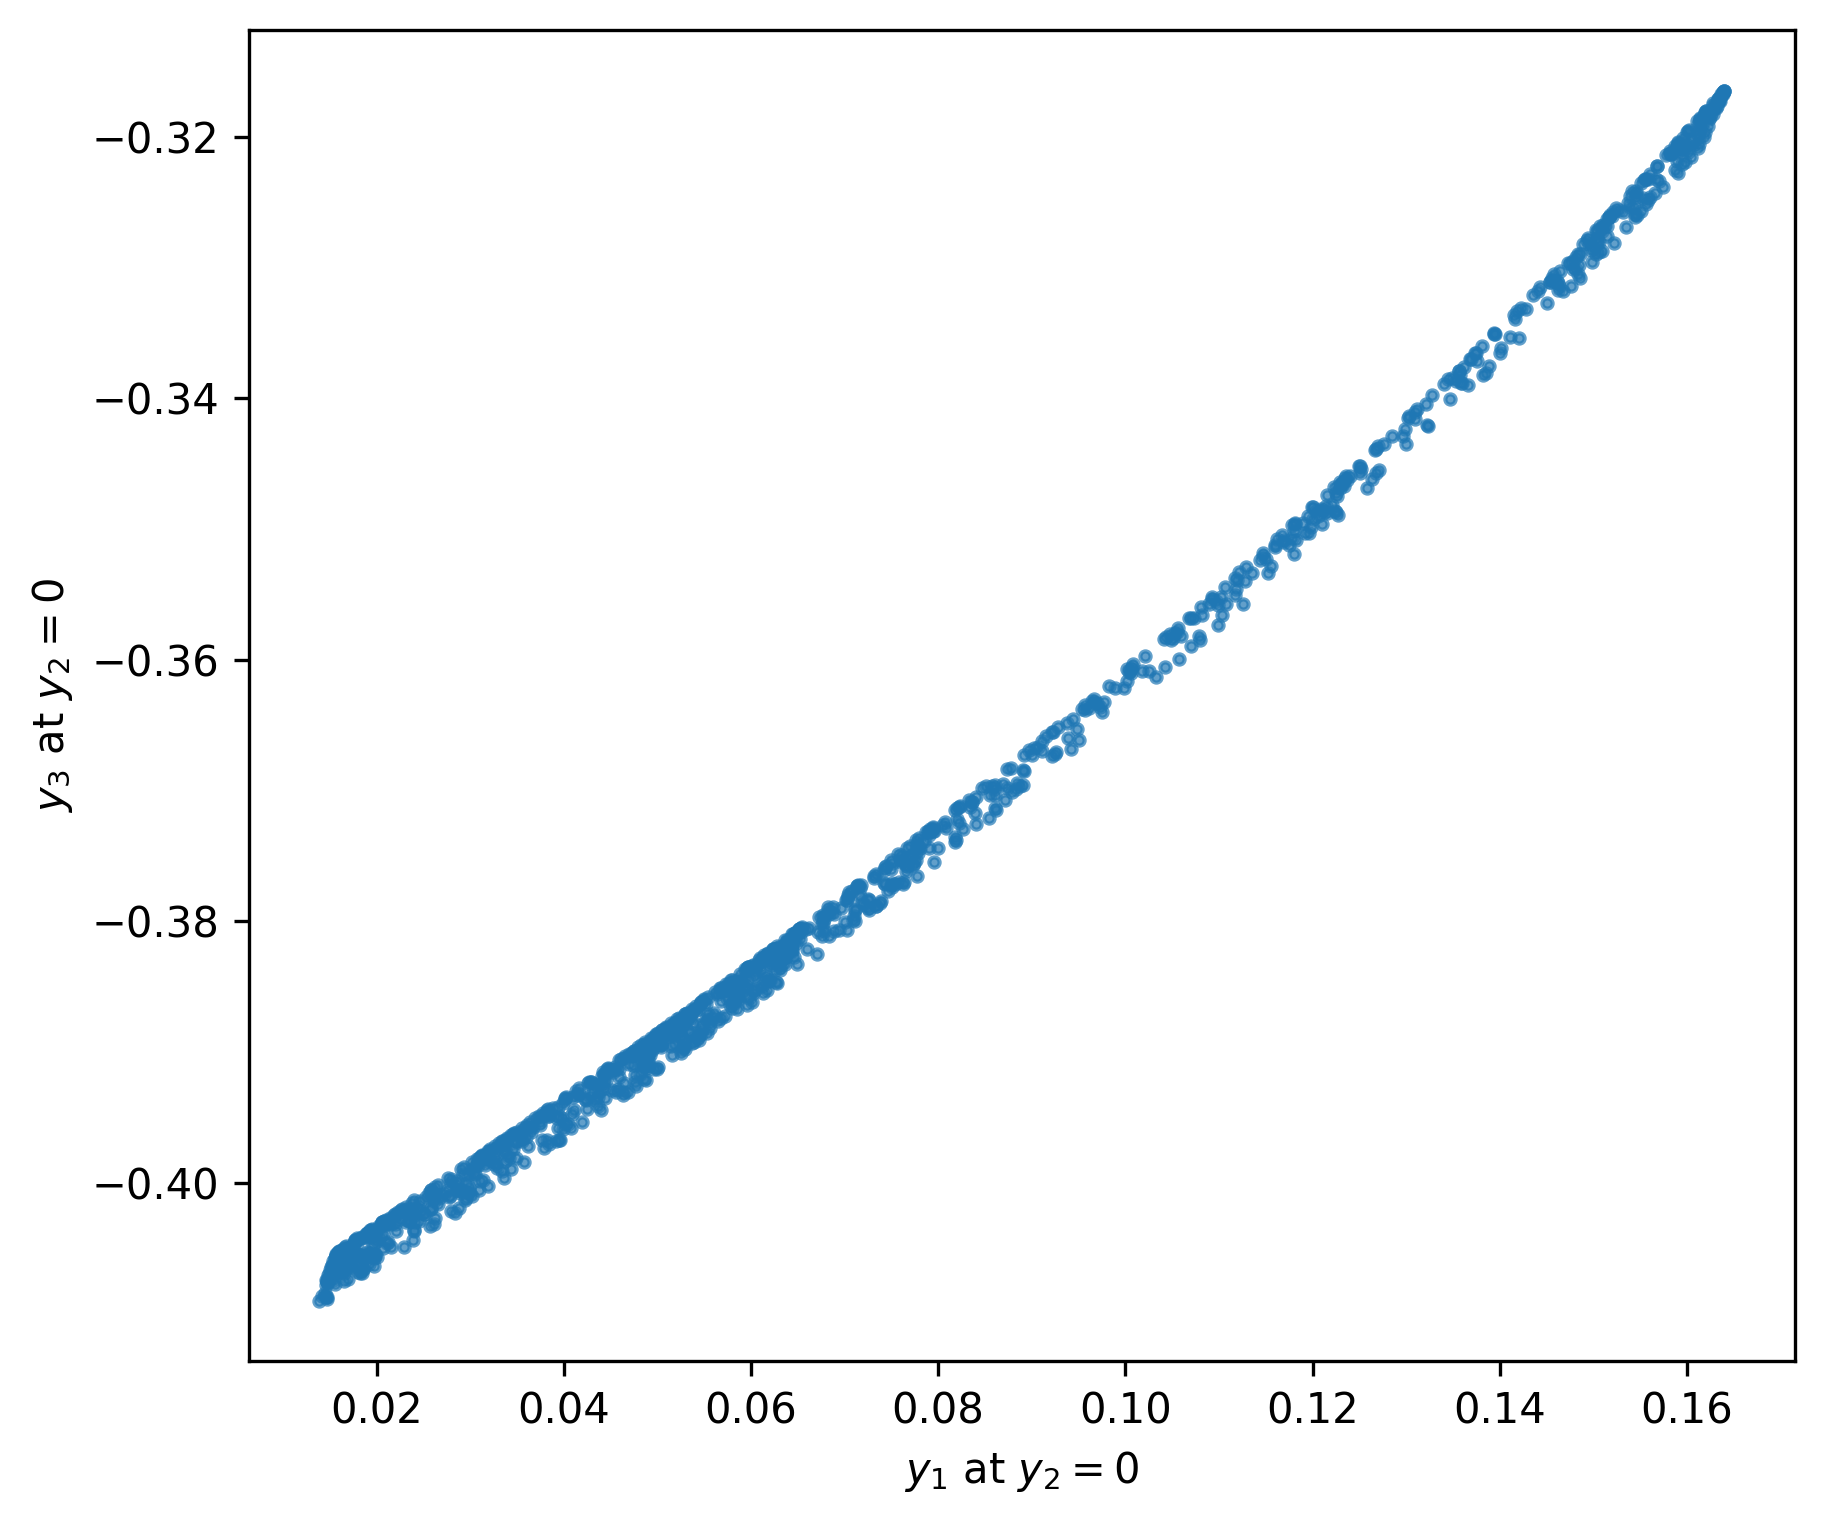
\includegraphics[width=\linewidth]{mavpd_chaos_poincare.png}
  \caption{Sección muestreada e interpolada linealmente.}
\end{subfigure}
\caption{Diagnósticos dinámicos principales del candidato caótico.}
\label{int:fig:mavpd-chaos-diagnostics}
\end{hafocommonfigure}

El espectro de potencia FFT normalizado tiene líneas dominantes y resulta
inconcluso para clasificar el régimen. Se interpreta junto con los
exponentes variacionales y los retornos de Poincaré.

\begin{hafocommonfigure}[H]
\centering
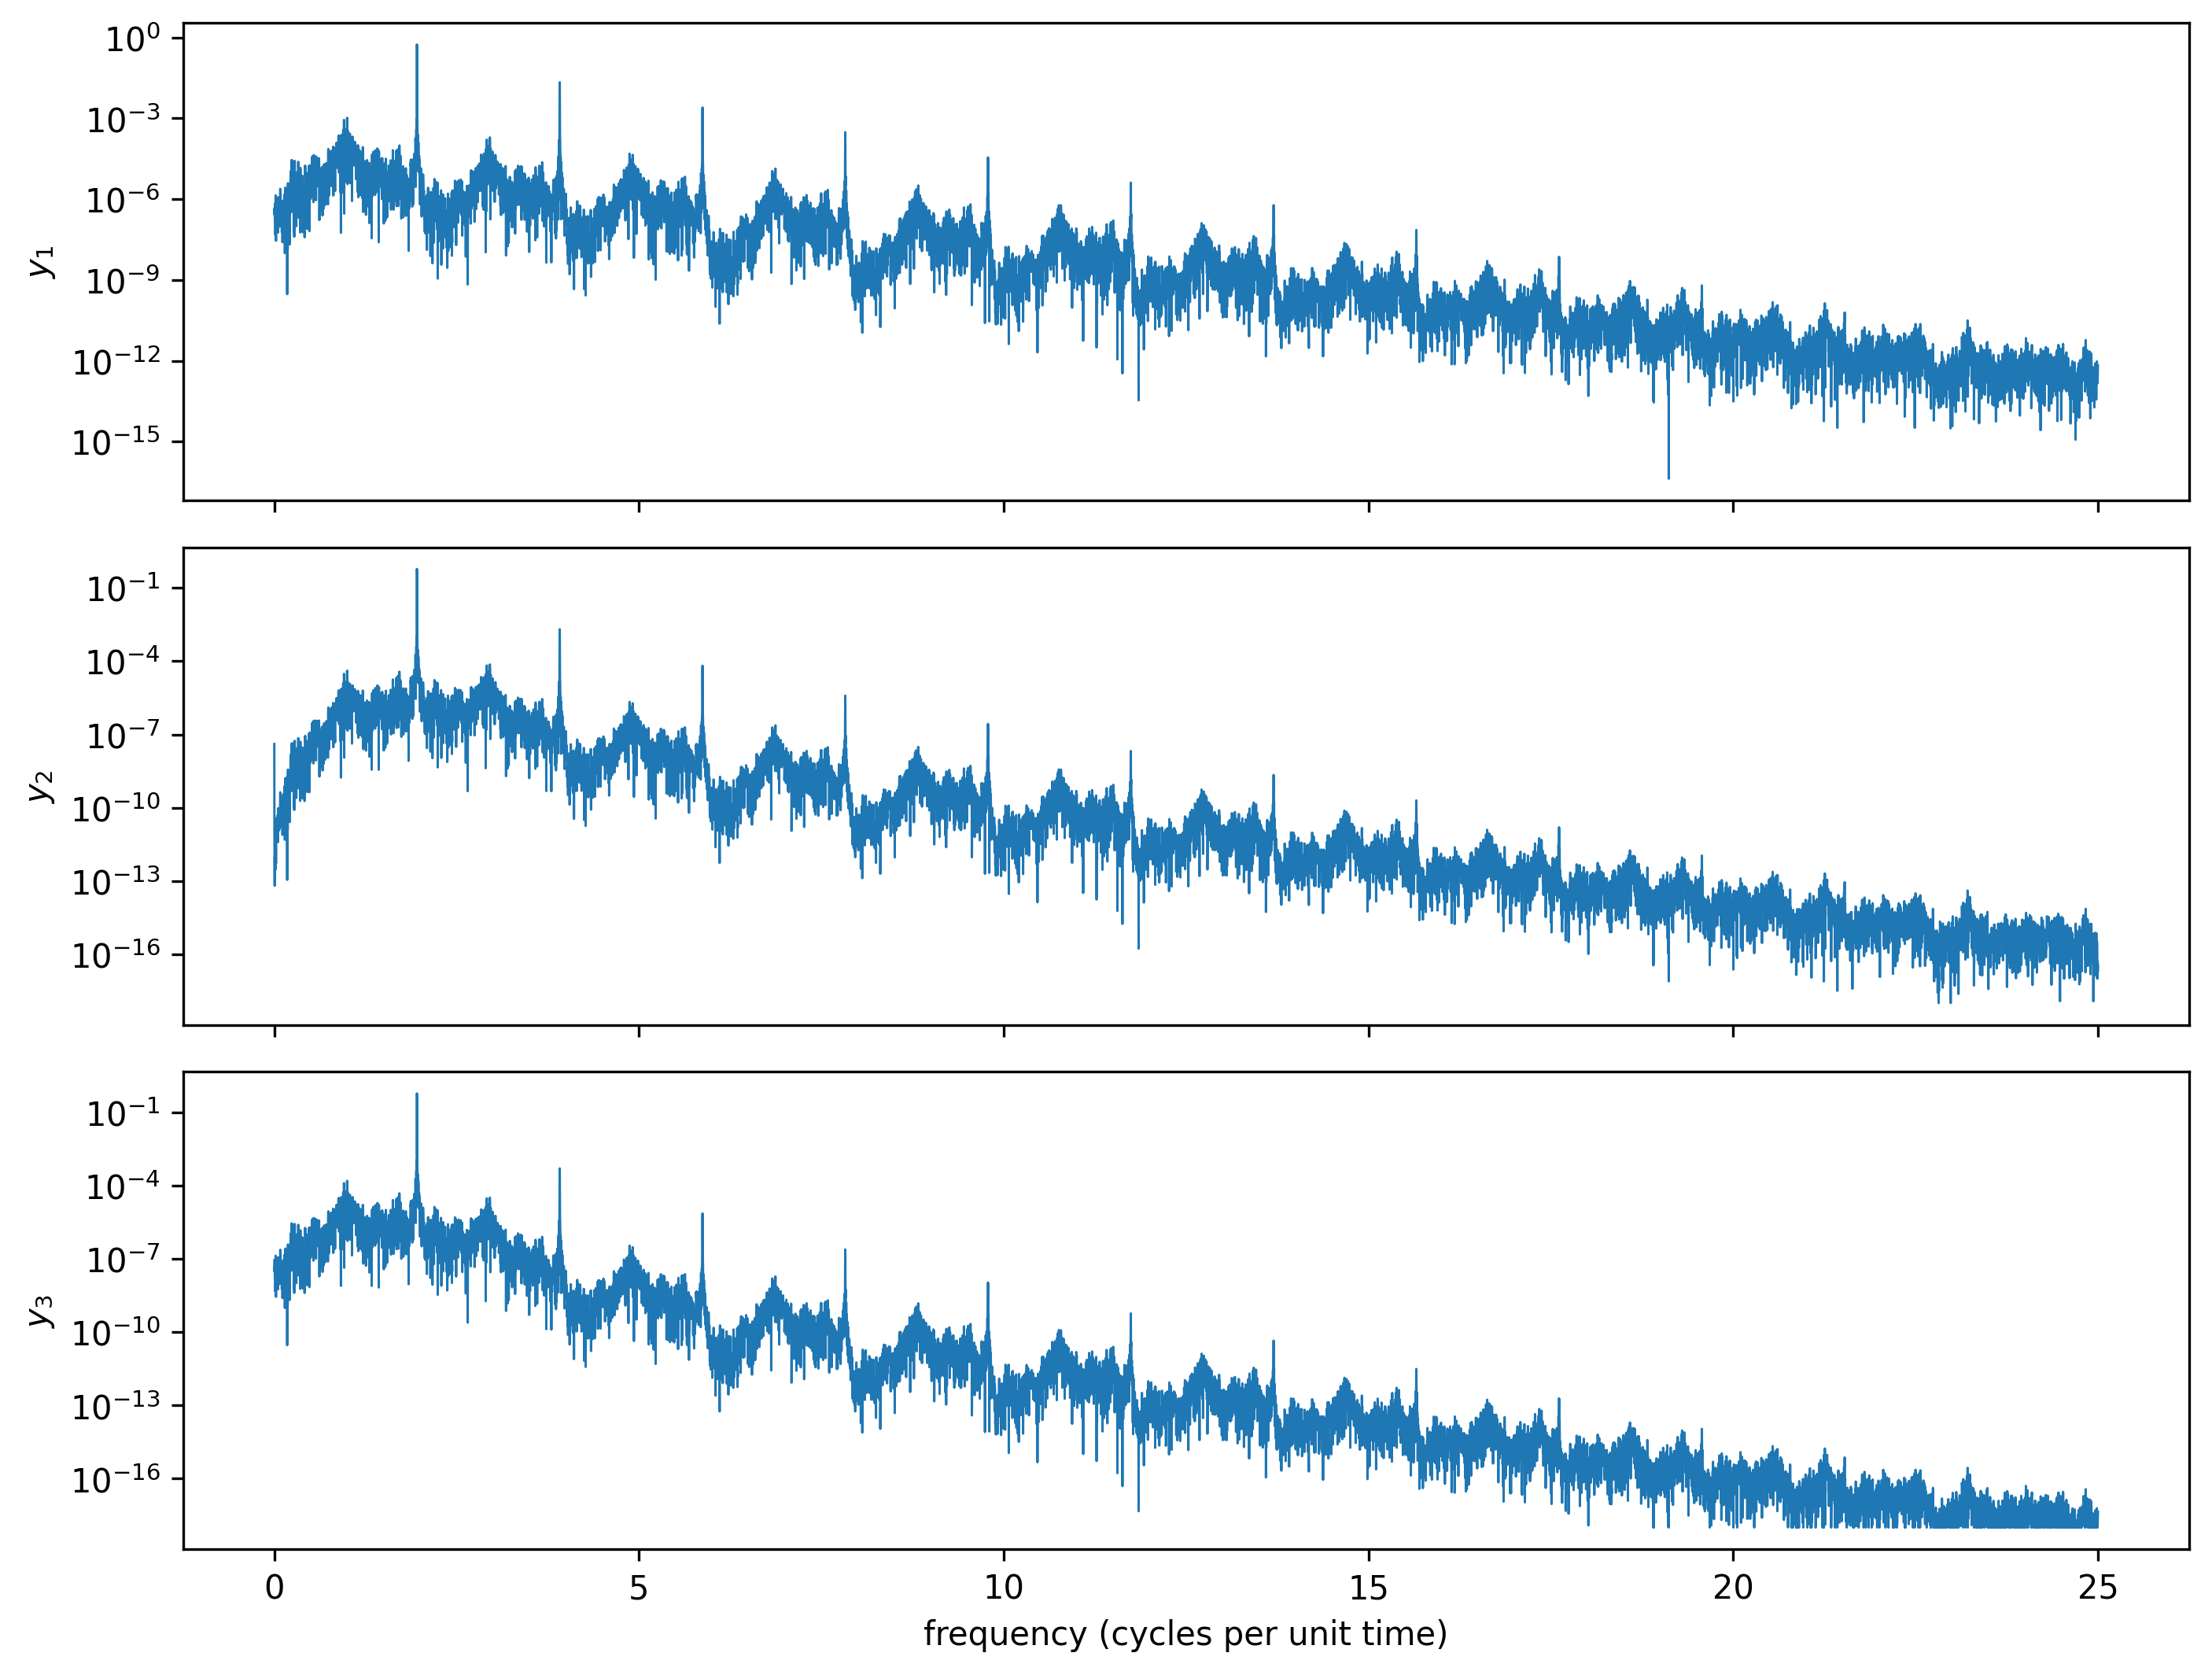
\includegraphics[width=0.82\textwidth]{mavpd_chaos_fft.png}
\caption{Potencia FFT normalizada del candidato.}
\label{int:fig:mavpd-chaos-fft}
\end{hafocommonfigure}

\ifHAFOBasinMaterial
\subsubsection*{Ocultedad bajo vecindades ensayadas}

El clasificador de la nube candidata se calibró con tres ventanas temporales
disjuntas de la misma trayectoria y verificó su separación usando los tres
equilibrios como controles negativos. Para dos nubes finitas \(A,B\), usa la
mediana simétrica de vecinos más cercanos, normalizada por la extensión \(S\)
de la referencia:
\begin{equation}
 d_N(A,B)=\frac{1}{S}\operatorname{mediana}\!\left(
 \{\min_{b\in B}\|a-b\|:a\in A\}\cup
 \{\min_{a\in A}\|b-a\|:b\in B\}\right).
 \label{int:eq:mavpd-cloud-distance}
\end{equation}
Si $R_1,R_2,R_3$ son las ventanas y \(R=R_1\cup R_2\cup R_3\), la escala es
\begin{equation}
 S=\left[\sum_{k=1}^{3}
 \left(\max_{x\in R}x_k-\min_{x\in R}x_k\right)^2\right]^{1/2},
 \qquad
 D(A)=\operatorname{mediana}_{j=1,2,3}d_N(A,R_j).
 \label{int:eq:mavpd-cloud-classifier}
\end{equation}
Si $b$ es el cuantil 0.95 de las distancias entre ventanas, el umbral es
$\tau=3b$ y el margen ambiguo es $m=\max(0.25\tau,b)$. En esta configuración,
$m=b=\tau/3$. Los controles negativos no fijan $\tau$: exigen
$\min_j d_N(N_\ell,R_j)>\tau+m$; de lo contrario se concluye que los controles
se solapan y la calibración se rechaza.

El protocolo principal contiene \MAVPDChaosMainProbes{} trayectorias:
3 equilibrios, radios $(10^{-5},10^{-3},10^{-2})$ y 12 direcciones esféricas
deterministas por radio. Se añadieron \MAVPDChaosTargetedProbes{} controles
dirigidos sobre ambos signos del autovector inestable de $E_0$, en radios
$10^{-7}$ y $10^{-4}$. En total hubo \MAVPDChaosTotalProbes{} trayectorias,
\MAVPDChaosHits{} contactos con la nube candidata, cero ambigüedades y cero
fallos numéricos; todas terminaron en un equilibrio.

\begin{hafobasinfigure}[H]
\centering
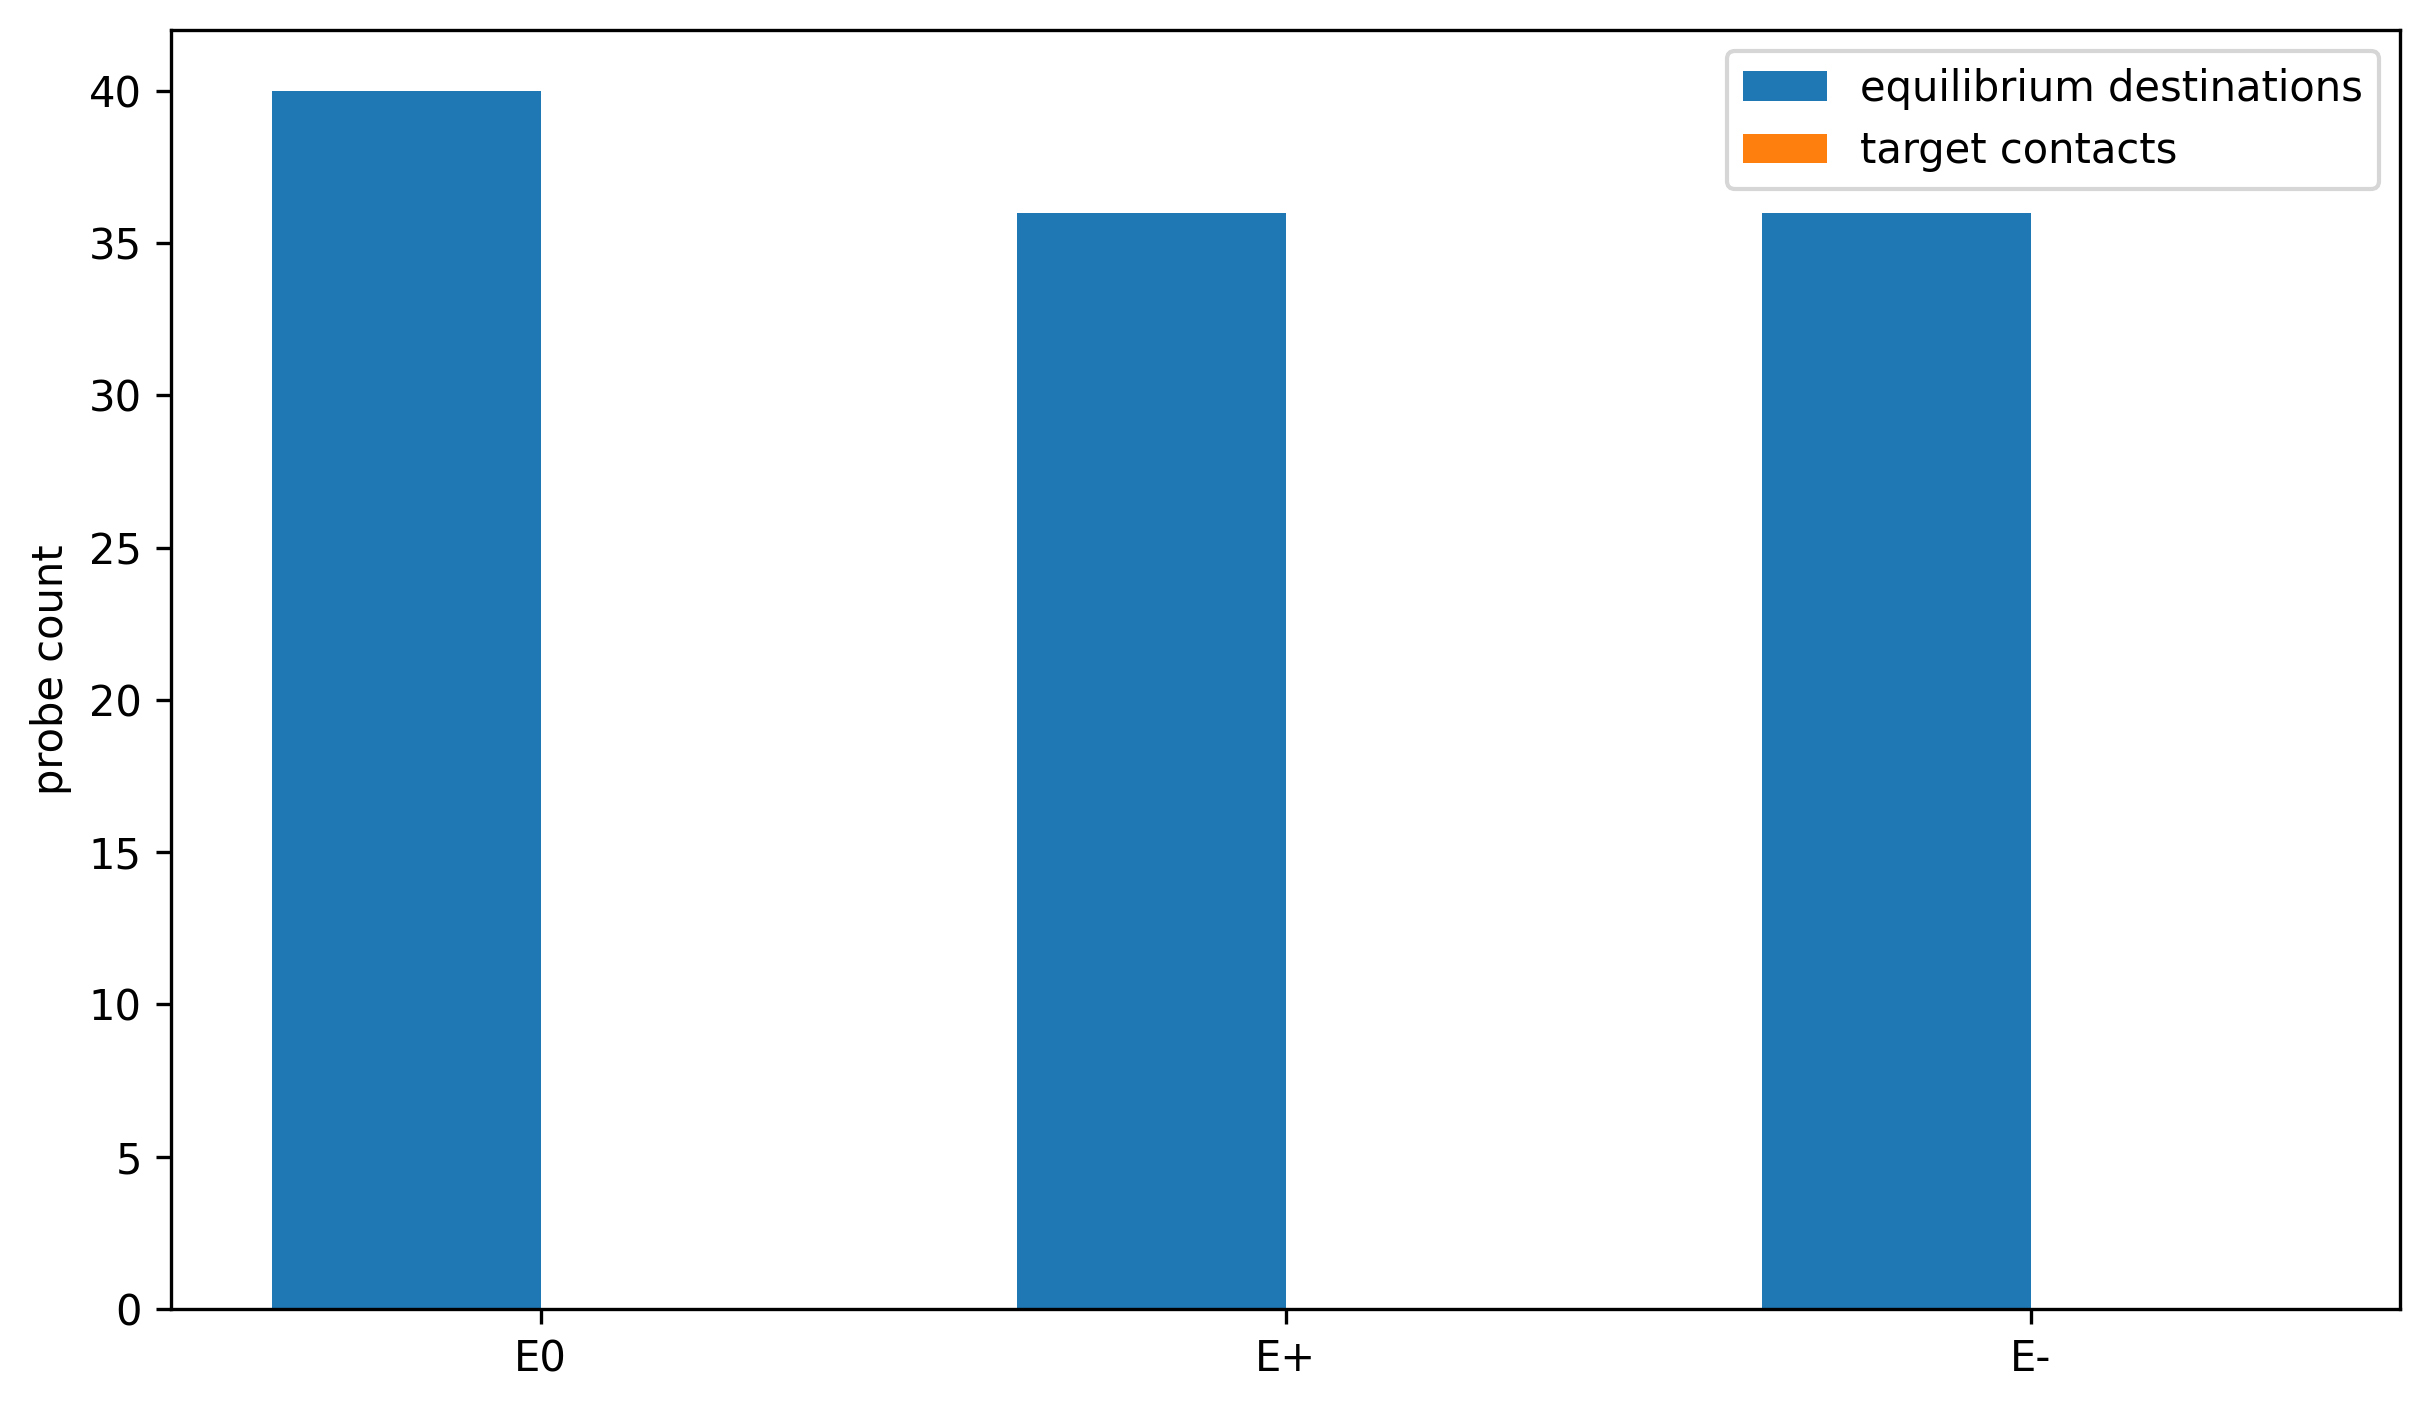
\includegraphics[width=0.88\textwidth]{mavpd_chaos_hiddenness.png}
\caption{Resultados de los sondeos alrededor de $E_0$, $E_+$ y $E_-$, junto
con los controles dirigidos del autovector inestable. Cero contactos es una
conclusión finita restringida a este protocolo.}
\label{int:fig:mavpd-chaos-hiddenness}
\end{hafobasinfigure}

La evaluación conjunta clasificó el resultado como compatible con caos y
ocultedad únicamente bajo las vecindades ensayadas. Los diagnósticos numéricos
y la ausencia de contactos se restringen a las ventanas y vecindades
declaradas; la desconexión global de la cuenca permanece sin demostrar.
\fi

\subsubsection*{Comparación numérica independiente}

El cálculo independiente en Julia partió de las ecuaciones y el Jacobiano, recalculó las
dos ramas D0 sin malla de frecuencias y sólo activó A1 después de que ambas
fallaron el umbral dinámico. La regla de menor $\omega_0$ volvió a seleccionar
la rama 0; después transportó el estado de $\xi=3.10$ a $2.85$, derivó la misma
frontera de Routh--Hurwitz y seleccionó de nuevo el desplazamiento $0.010$.
Durante esa localización no leyó la semilla, el estado terminal ni $\gamma$ de
Python.
\ifHAFOBasinMaterial
El intercambio de las condiciones de ocultedad ocurrió únicamente en la fase
posterior de comparación.
\fi

Python empleó DOP853 adaptativo para la trayectoria y la ecuación
variacional. Julia empleó RK4 de paso fijo para las trayectorias y los sondeos,
y reortogonalización QR para el cálculo variacional.

\begin{table}[H]
\centering
\caption{Comparación del candidato MAVPD caótico con tolerancias comunes.}
\label{int:tab:mavpd-chaos-cross-runtime}
\small
\begin{tabularx}{\textwidth}{@{}L{0.31\textwidth}YY@{}}
\toprule
Magnitud & Python/\hafo{} & Julia \\
\midrule
$\xi$ & \MAVPDChaosXi & \MAVPDChaosXi \\
$\gamma$ & \MAVPDChaosGamma & \MAVPDChaosGamma \\
$\widehat\lambda_1$ & \MAVPDChaosLEOne & \MAVPDChaosJuliaLEOne \\
$\widehat\lambda_2$ & \MAVPDChaosLETwo & \MAVPDChaosJuliaLETwo \\
$\widehat\lambda_3$ & \MAVPDChaosLEThree & \MAVPDChaosJuliaLEThree \\
$D_{KY}$ & \MAVPDChaosKY & \MAVPDChaosJuliaKY \\
Cruces de Poincaré & \MAVPDChaosPoincareCount & \MAVPDChaosJuliaPoincareCount \\
Mediana $K$ sobre retornos & \MAVPDChaosReturnKOne & \MAVPDChaosJuliaReturnK \\
\ifHAFOBasinMaterial
Decisiones de sondeo coincidentes &
\MAVPDChaosTotalProbes/\MAVPDChaosTotalProbes &
\MAVPDChaosJuliaProbeMatches/\MAVPDChaosTotalProbes \\
\fi
\bottomrule
\end{tabularx}
\end{table}

La comparación cruzada coincidió exactamente en $\xi$, $\gamma$ y el
desplazamiento de Hopf. Las estadísticas de la nube postransitoria y los
diagnósticos de caos quedaron dentro de sus bandas predeclaradas.
\ifHAFOBasinMaterial
Además, coincidieron las
\MAVPDChaosTotalProbes{} condiciones iniciales, estados, destinos y decisiones
de contacto.
\fi

\begin{hafobasinfigure}[H]
\centering
\begin{subfigure}[t]{0.49\textwidth}
  \centering
  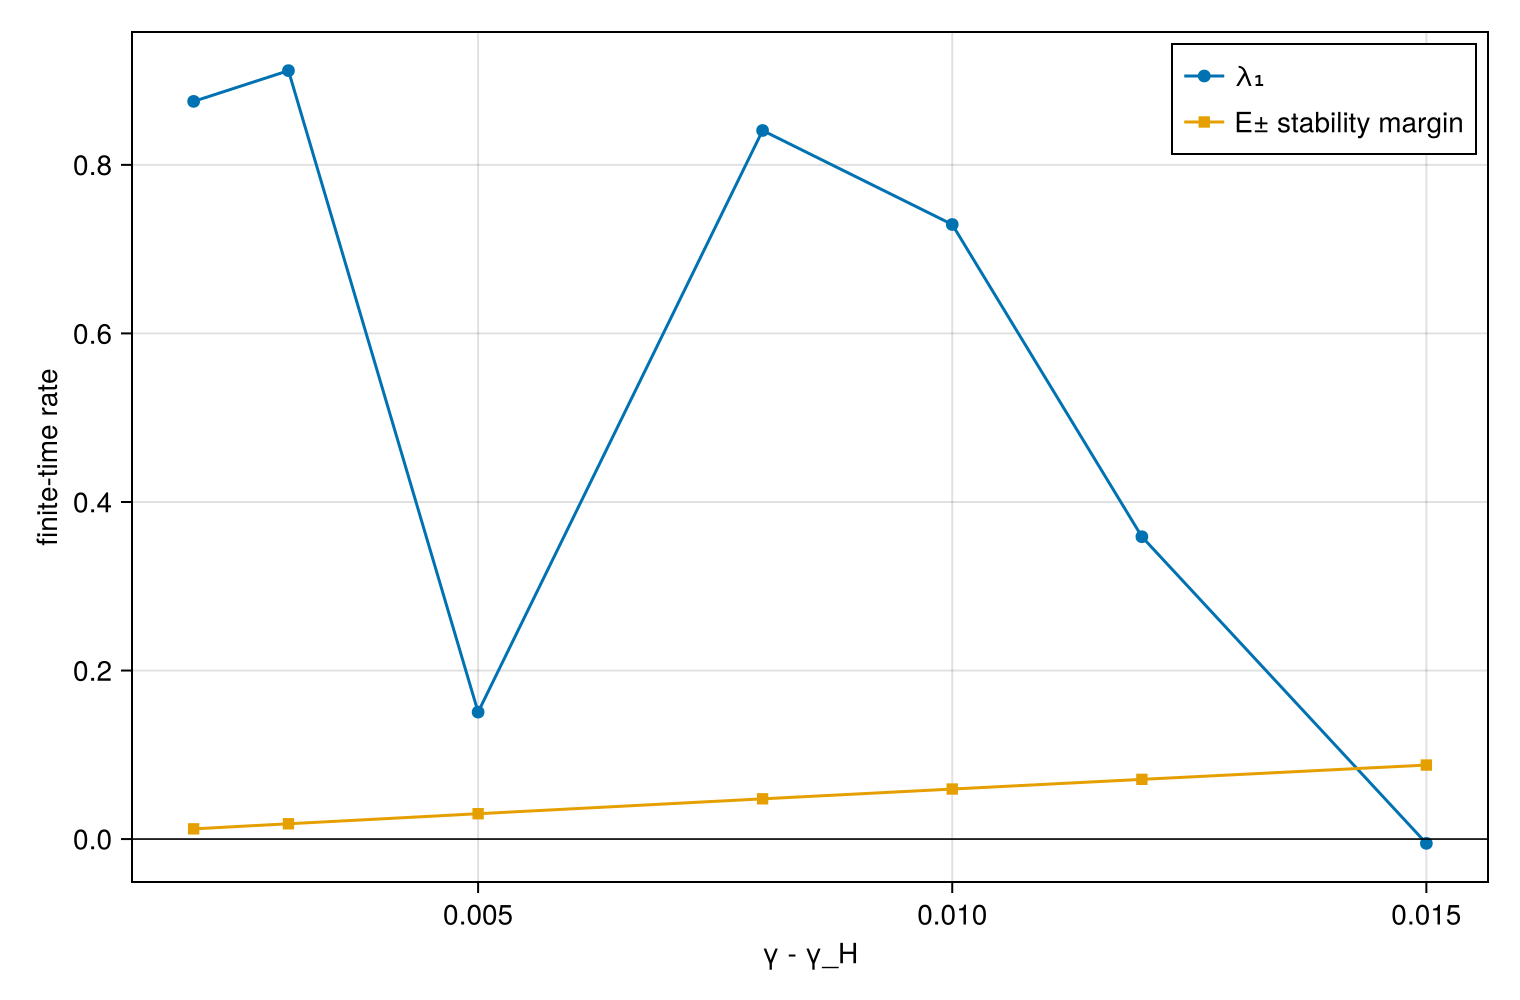
\includegraphics[width=\linewidth]{julia_mavpd_chaos_gamma_screen.png}
  \caption{Cribado y selección de $\gamma$ recalculados en Julia.}
\end{subfigure}\hfill
\begin{subfigure}[t]{0.49\textwidth}
  \centering
  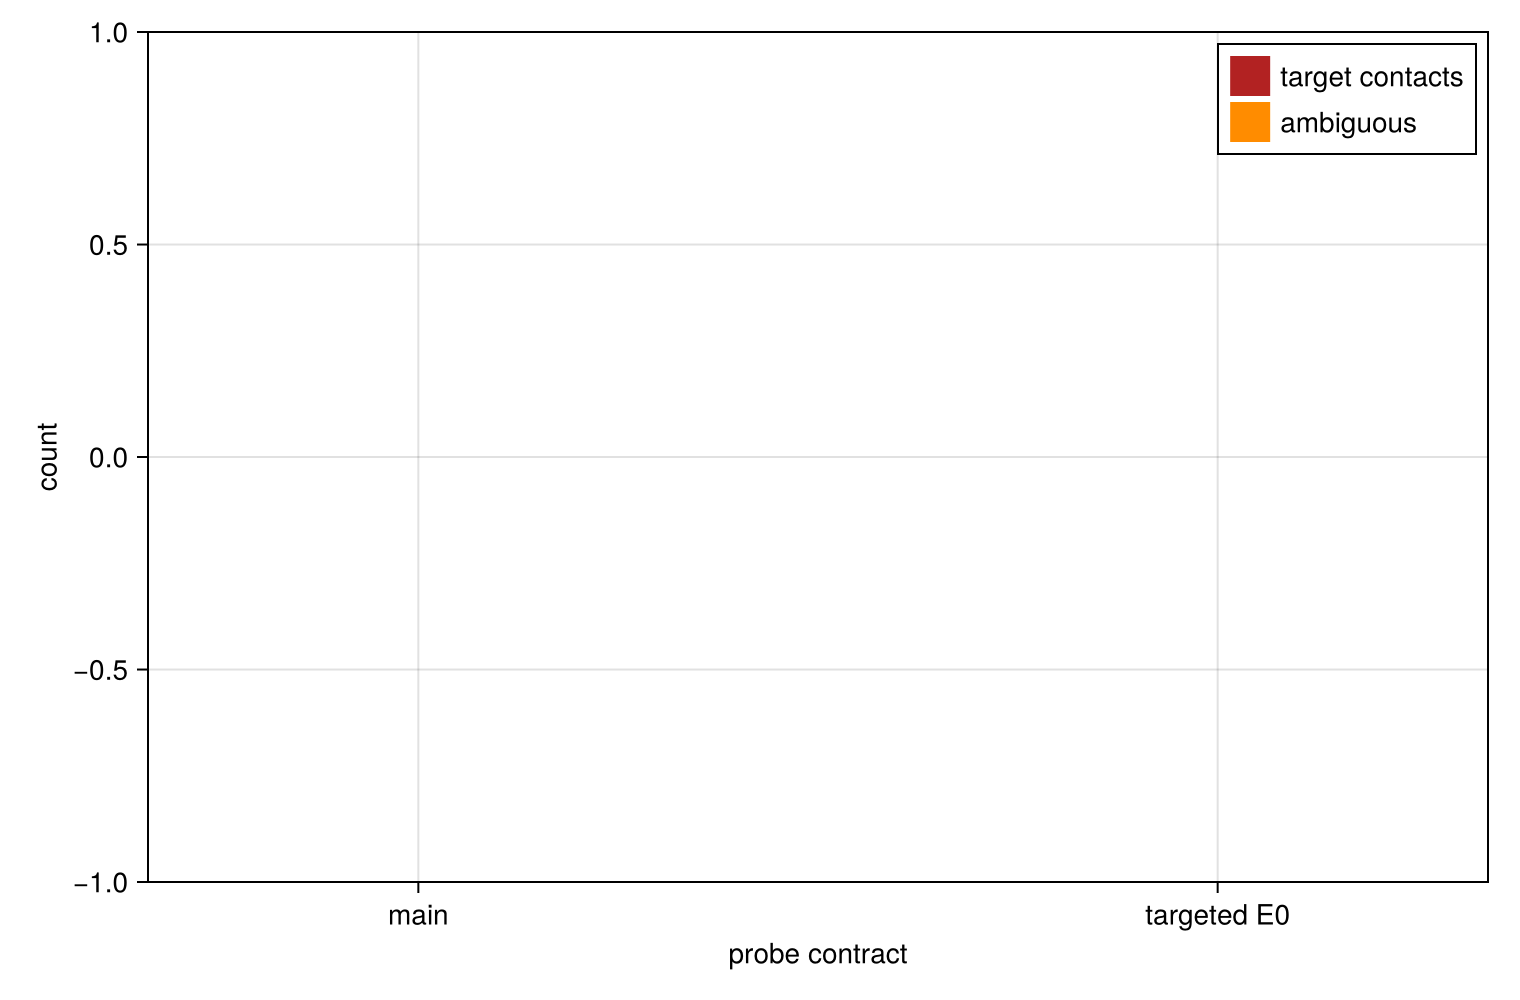
\includegraphics[width=\linewidth]{julia_mavpd_chaos_hiddenness_outcomes.png}
  \caption{Decisión de los 112 sondeos finitos en Julia.}
\end{subfigure}
\caption{Artefactos de la reproducción Julia MAVPD. El primer panel es un
diagnóstico de continuación; el segundo resume un protocolo finito de cuenca.}
\label{int:fig:mavpd-chaos-julia}
\end{hafobasinfigure}

\begin{hafocommonfigure}[H]
\centering
\begin{subfigure}[t]{0.49\textwidth}
  \centering
  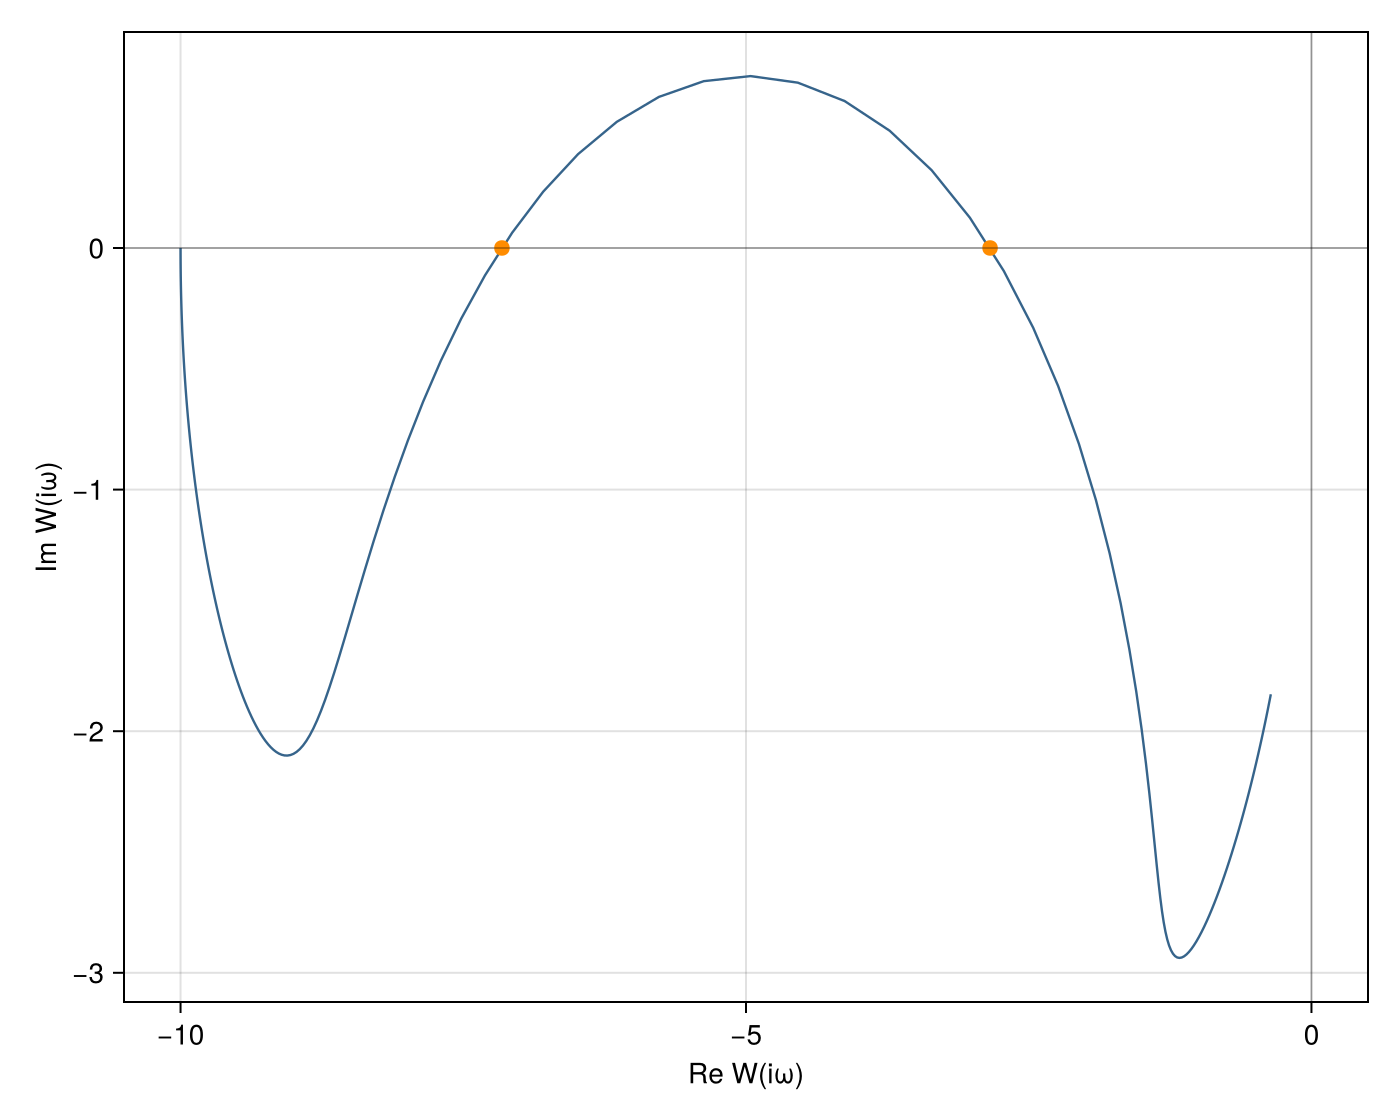
\includegraphics[width=\linewidth]{julia_mavpd_chaos_nyquist_diagnostic.png}
  \caption{Nyquist de la transferencia ya derivada.}
\end{subfigure}\hfill
\begin{subfigure}[t]{0.49\textwidth}
  \centering
  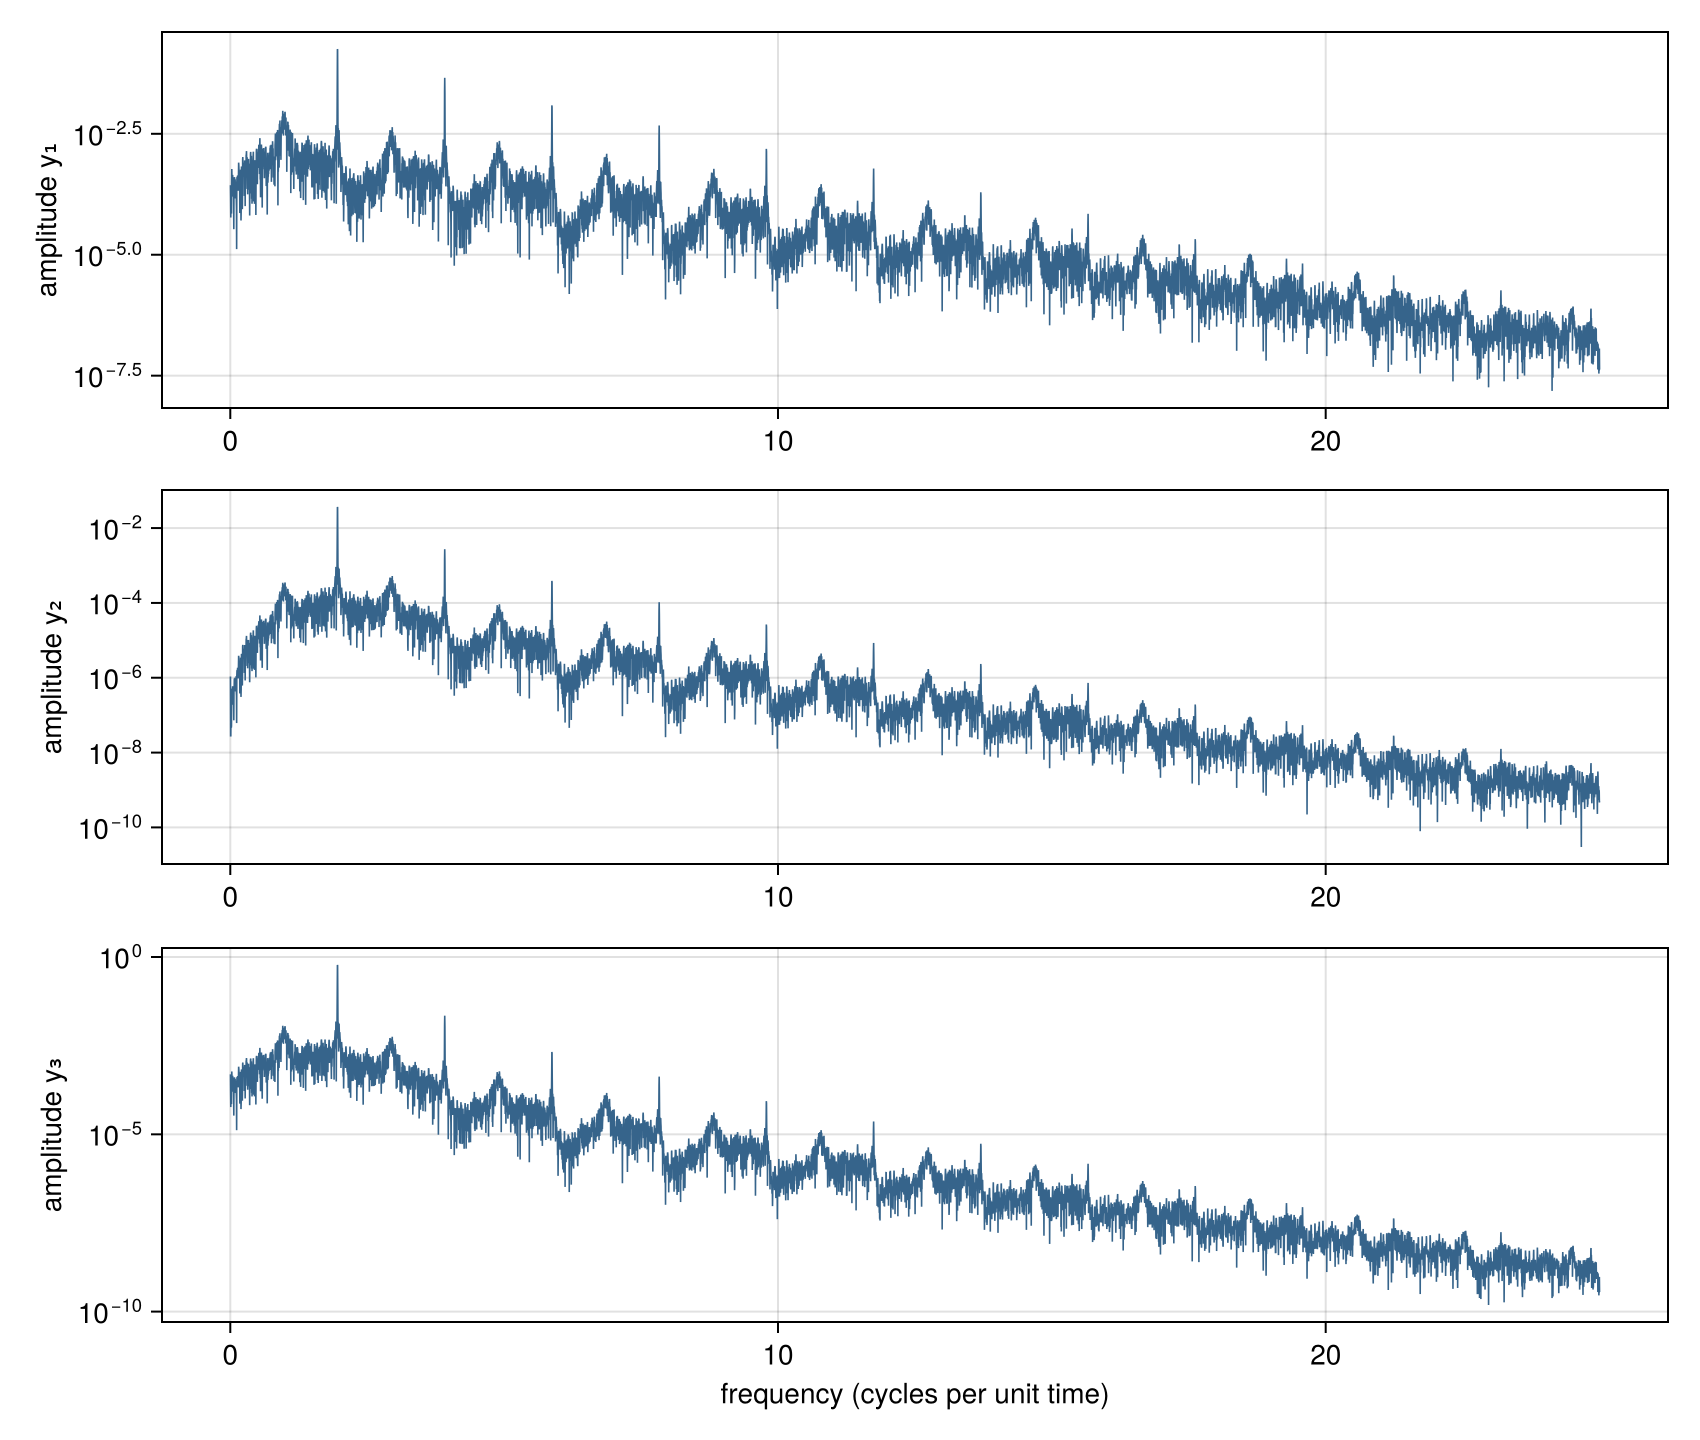
\includegraphics[width=\linewidth]{julia_mavpd_chaos_amplitude_spectrum.png}
  \caption{Espectro de amplitud FFT postransitorio.}
\end{subfigure}
\caption{Diagnósticos intermedios Julia MAVPD. Nyquist no suministra una malla
de búsqueda ni selecciona $\omega_0$; la FFT no se denomina PSD.}
\label{int:fig:mavpd-chaos-julia-spectral}
\end{hafocommonfigure}


\section{Caso 4: PLL bifásico con filtro lead--lag}

\subsection{Transformación T1 y obstrucción directa}

El modelo publicado es
\begin{align}
 \dot x&=-\frac{x}{T}+\frac{\tau_1}{2T}\sin\theta,\nonumber\\
 \dot\theta&=\omega_\Delta-\frac{Lx}{T}
 -\frac{\tau_2L}{2T}\sin\theta,\qquad T=\tau_1+\tau_2,
 \label{int:eq:pll}
\end{align}
con \(\tau_1=0.0448\), \(\tau_2=0.0185\), \(L=500\) y
\(\omega_\Delta=178.9\) \cite{pll2015}. El desplazamiento de un equilibrio
bloqueado elimina el término afín, de modo que el sistema es T1. Como
\(\theta\) es angular, la recurrencia y las distancias se calculan módulo
\(2\pi\), no con una norma euclidiana sin envolver.

En un equilibrio, la primera ecuación da
\(x_e=(\tau_1/2)\sin\theta_e\). Sustituir en la segunda y usar
\(T=\tau_1+\tau_2\) conduce a
\[
 0=\omega_\Delta-\frac{L(\tau_1+\tau_2)}{2T}\sin\theta_e,
 \qquad \sin\theta_e=\frac{2\omega_\Delta}{L}=0.7156.
\]
En una vuelta del cilindro hay dos soluciones:
\[
 x_e=0.01602944,\qquad
 \theta_f=0.797482699882,\qquad
 \theta_s=2.344109953708.
\]
El Jacobiano en cualquiera de ellas es
\[
 J_e=\begin{pmatrix}
 -1/T&\tau_1\cos\theta_e/(2T)\\
 -L/T&-\tau_2L\cos\theta_e/(2T)
 \end{pmatrix},
\]
con
\[
 \operatorname{tr}J_e=-\frac{1+\tau_2L\cos\theta_e/2}{T},\qquad
 \det J_e=\frac{L\cos\theta_e}{2T}.
\]
En \(\theta_f\), la traza es negativa, el determinante positivo y el
discriminante \((\operatorname{tr}J_e)^2-4\det J_e\) es negativo para estos
parámetros: se obtiene un foco estable. En \(\theta_s\), el determinante es
negativo y el equilibrio es una silla.

El cambio \(u=x-x_e\), \(v=\theta-\theta_e\) transforma el campo en
\[
 \begin{pmatrix}\dot u\\\dot v\end{pmatrix}
 =P\begin{pmatrix}u\\v\end{pmatrix}+b\psi(v),
\]
\[
 P=\begin{pmatrix}-1/T&0\\-L/T&0\end{pmatrix},\quad
 b=\begin{pmatrix}\tau_1/(2T)\\-\tau_2L/(2T)\end{pmatrix},
 \quad c=\begin{pmatrix}0\\1\end{pmatrix},
\]
con \(\psi(v)=\sin(v+\theta_e)-\sin\theta_e\). Las identidades del
equilibrio cancelan los términos constantes. Para una entrada \(\psi\),
la primera fila del resolvente \((sI-P)^{-1}b\) da
\[
 u=\frac{\tau_1}{2(1+Ts)}\psi,
\]
y la segunda da
\[
 sv=-\frac L{2T}\left[\frac{\tau_1}{1+Ts}+\tau_2\right]\psi
    =-\frac L2\frac{1+\tau_2s}{1+Ts}\psi.
\]
Por tanto, las dos convenciones de transferencia se relacionan mediante
\begin{equation}
 W(s)=c^{\mathsf T}(sI-P)^{-1}b
     =-\frac L2\frac{1+\tau_2s}{s(1+Ts)}=-G(s).
 \label{int:eq:pll-transfer}
\end{equation}
Al multiplicar el cociente en \(s=i\omega\) por el conjugado de su
denominador,
\[
 W(i\omega)=\frac{L\tau_1}{2(1+T^2\omega^2)}
 +i\,\frac{L(1+\tau_2T\omega^2)}{2\omega(1+T^2\omega^2)}.
\]
Así, \(\operatorname{Im}W(i\omega)>0\) y
\(\operatorname{Im}G(i\omega)<0\) para todo \(\omega>0\). Ninguna
convención admite el cruce real requerido por una ganancia descriptiva real;
la ruta directa no produce candidatos.

\subsection{Ruta A1 de Andronov}

Para \(L>0\), definir \(y=\dot\theta\) permite recuperar la variable
original mediante
\begin{equation}
 x=\frac T L(\omega_\Delta-y)-\frac{\tau_2}{2}\sin\theta.
 \label{int:eq:pll-inverse-andronov}
\end{equation}
Derivando la segunda ecuación de \eqref{int:eq:pll},
\[
 \dot y=-\frac L T\dot x-\frac{\tau_2L}{2T}\cos\theta\,y
        =\frac L{T^2}x-\frac{L\tau_1}{2T^2}\sin\theta
         -\frac{\tau_2L}{2T}\cos\theta\,y.
\]
Sustituir \eqref{int:eq:pll-inverse-andronov} y agrupar
\(\tau_1+\tau_2=T\) produce
\begin{equation}
 T\dot y=\omega_\Delta-\frac{L}{2}\sin\theta
 -\left(1+\frac{\tau_2L}{2}\cos\theta\right)y.
 \label{int:eq:pll-andronov}
\end{equation}
Para una rotación positiva se exige \(y(\theta)>0\) durante toda la
vuelta. Entonces \(\theta\) puede usarse como variable independiente:
\begin{equation}
 \frac{\dd y}{\dd\theta}=H_L(\theta,y)
 =\frac{\omega_\Delta-(L/2)\sin\theta}{Ty}
  -\frac{1+(\tau_2L/2)\cos\theta}{T}.
 \label{int:eq:pll-angle-flow}
\end{equation}
Con \(y(0)=y_0>0\), el mapa de retorno es
\(P_L(y_0)=y(2\pi;y_0)\). Una órbita rotatoria cumple
\(P_L(y_0)-y_0=0\), y su periodo físico es
\[
 \mathcal T(y_0)=\int_0^{2\pi}\frac{\dd\theta}{y(\theta;y_0)}.
\]
La derivada del retorno se calcula diferenciando la ecuación respecto de
\(y_0\). Si \(z=\partial y/\partial y_0\),
\[
 \frac{\dd z}{\dd\theta}
 =-\frac{\omega_\Delta-(L/2)\sin\theta}{Ty^2}z,
 \qquad z(0)=1,\qquad P_L'(y_0)=z(2\pi).
\]
El multiplicador transversal es \(P_L'(y_0)\): módulo menor que uno indica
estabilidad local, y módulo mayor que uno inestabilidad. El mapa queda
indefinido para esta construcción si la solución pierde la rotación positiva
antes de completar \(2\pi\).

En \(L=0\), la ecuación reducida admite \(y(\theta)\equiv\omega_\Delta\),
con
\[
 \mathcal T_0=\frac{2\pi}{\omega_\Delta},\qquad
 P_0'(\omega_\Delta)=\exp\!\left(-\frac{2\pi}{T\omega_\Delta}\right).
\]
En las coordenadas originales, \(\theta(t)=\omega_\Delta t\) y el filtro
satisface una ecuación lineal forzada. Una solución particular periódica
\(x_p=A\sin\theta+B\cos\theta\) cumple
\(A-\omega_\Delta TB=\tau_1/2\) y
\(\omega_\Delta TA+B=0\). Por tanto,
\[
 x_p(\theta)=\frac{\tau_1}{2[1+(\omega_\Delta T)^2]}
             [\sin\theta-\omega_\Delta T\cos\theta].
\]
Las restantes soluciones difieren de ella en \(C\e^{-t/T}\), lo cual
concuerda con el multiplicador transversal calculado.
Esta solución inicia la continuación de la ecuación reducida en 101 valores
hasta \(L=500\). La reconstrucción de \(x\) mediante
\eqref{int:eq:pll-inverse-andronov} se aplica sólo en los niveles \(L>0\),
pues el cambio de variables es singular en \(L=0\). Las condiciones iniciales
publicadas se reservan para la comparación posterior.

El análisis localizó:

\begin{table}[H]
\centering
\caption{Órbitas de retorno PLL en \(L=500\).}
\small
\begin{tabular}{@{}lrrrr@{}}
\toprule
Órbita & \(y_0\) & \(x_0\) & Periodo & Multiplicador \\
\midrule
Ciclo estable &
140.125084913 & 0.004908904250 &
\PLLPythonStablePeriod & \PLLPythonStableMultiplier \\
Separatriz inestable &
135.172047420 & 0.005535958797 &
\PLLPythonSeparatrixPeriod & \PLLPythonSeparatrixMultiplier \\
\bottomrule
\end{tabular}
\end{table}

Los errores de retorno Python sobre el cilindro fueron
\(2.68\times10^{-15}\) para el ciclo estable y
\(6.18\times10^{-14}\) para la separatriz. Julia reprodujo los periodos
\(\PLLJuliaStablePeriod\) y \(\PLLJuliaSeparatrixPeriod\), con multiplicadores
\(\PLLJuliaStableMultiplier\) y \(\PLLJuliaSeparatrixMultiplier\). Las tres
condiciones iniciales publicadas quedaron fuera del flujo de localización: el
control posterior confirmó que dos alcanzan el ciclo y una el foco.

\begin{hafocommonfigure}[H]
\centering
\begin{subfigure}[t]{0.49\textwidth}
  \centering
  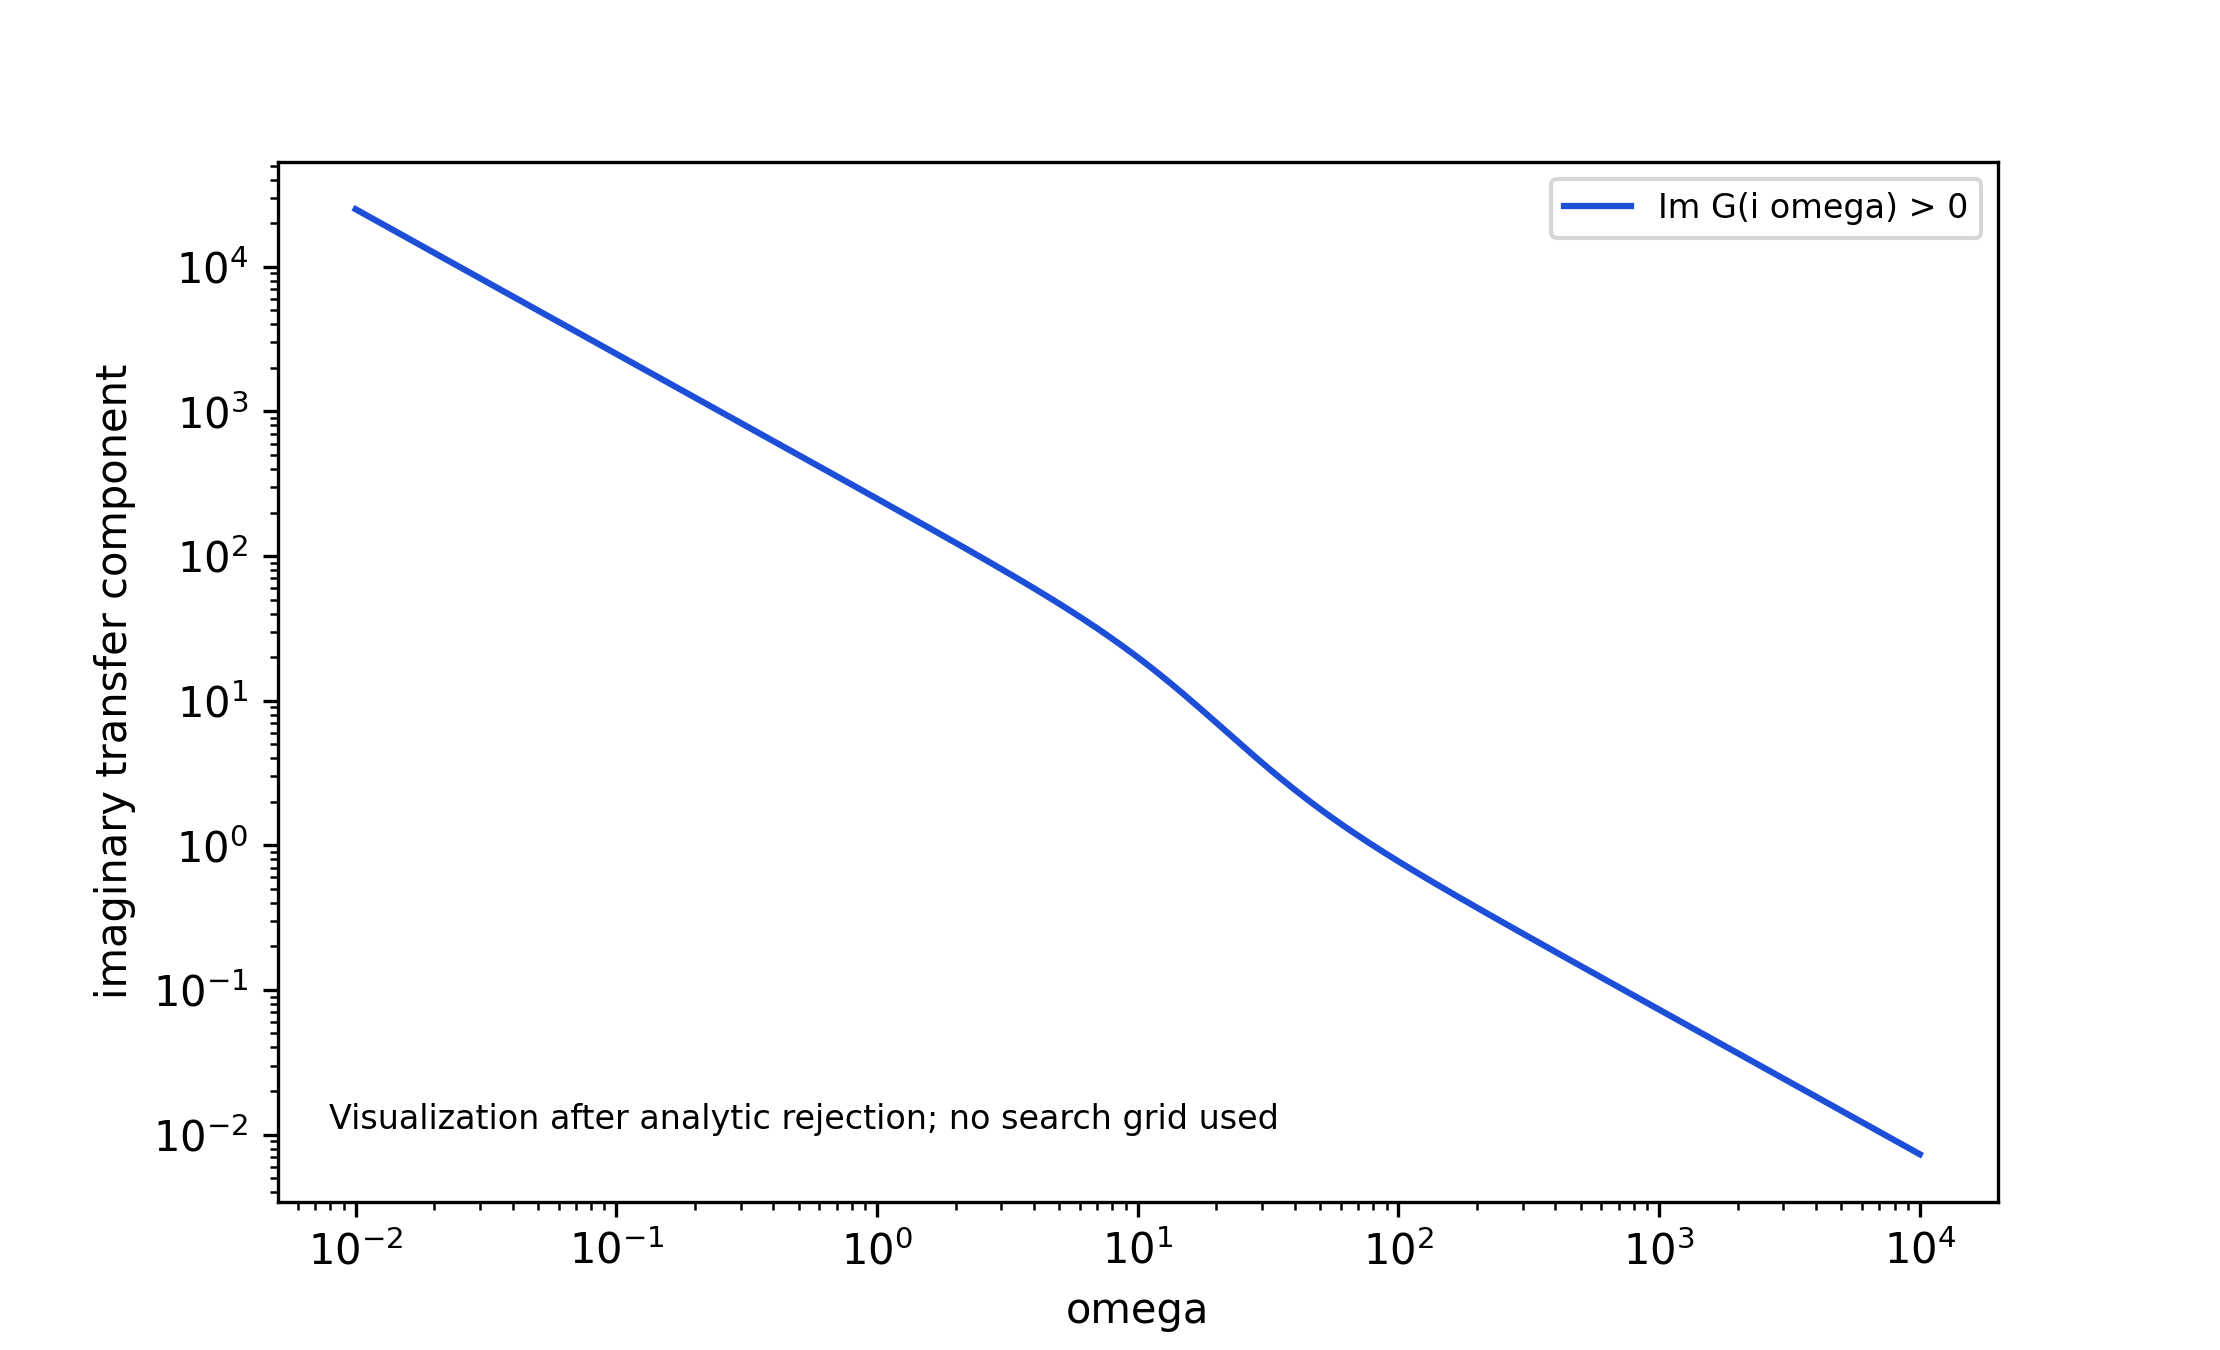
\includegraphics[width=\linewidth]{pll_transfer_obstruction.png}
  \caption{Obstrucción analítica de la ruta directa.}
\end{subfigure}\hfill
\begin{subfigure}[t]{0.49\textwidth}
  \centering
  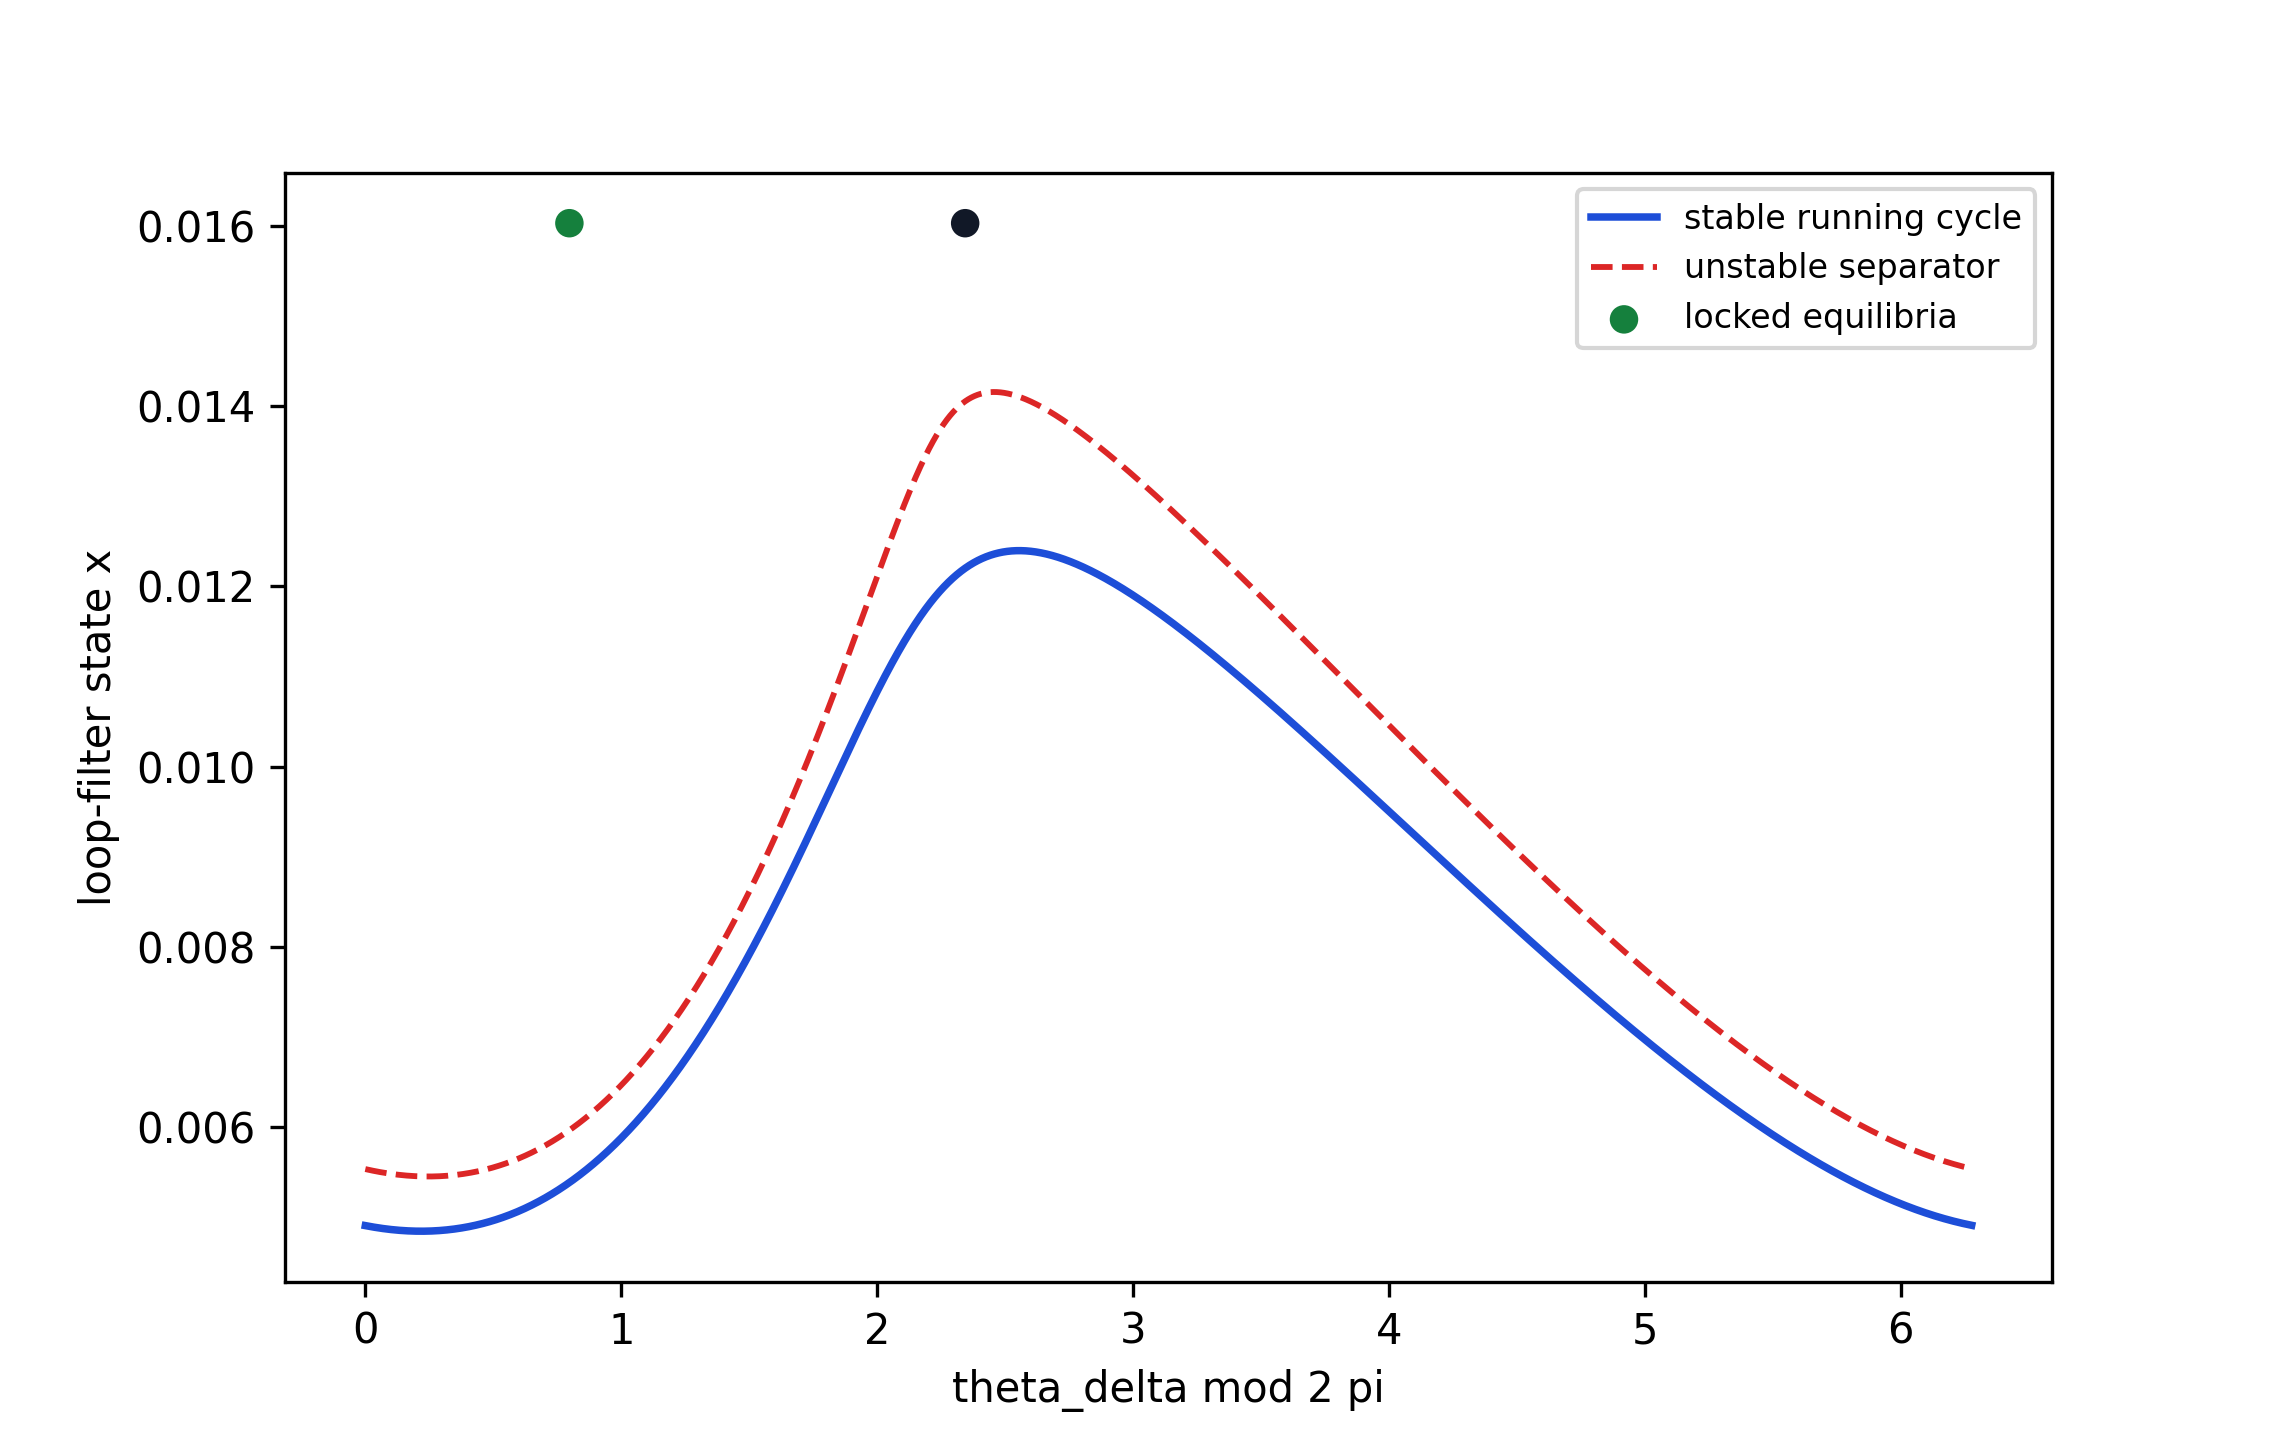
\includegraphics[width=\linewidth]{pll_phase_cylinder_cycles.png}
  \caption{Ciclo estable y separatriz en \(\mathbb R\times S^1\).}
\end{subfigure}
\caption{Localización T1 + A1 del PLL lead--lag.}
\label{int:fig:pll-route}
\end{hafocommonfigure}

\ifHAFOBasinMaterial
\subsection{Sondeos cilíndricos y estado comparativo}

El sondeo común usó \PLLProbeCount{} condiciones:
2 equilibrios, 4 radios \((10^{-5},10^{-4},10^{-3},10^{-2})\) y 12
direcciones por radio. Ninguna alcanzó el ciclo. Las 48 condiciones alrededor
del foco y las 48 alrededor del punto silla terminaron en el foco. Por tanto,
el resultado es compatible con ocultedad bajo el sondeo cilíndrico declarado.

\begin{hafobasinfigure}[H]
\centering
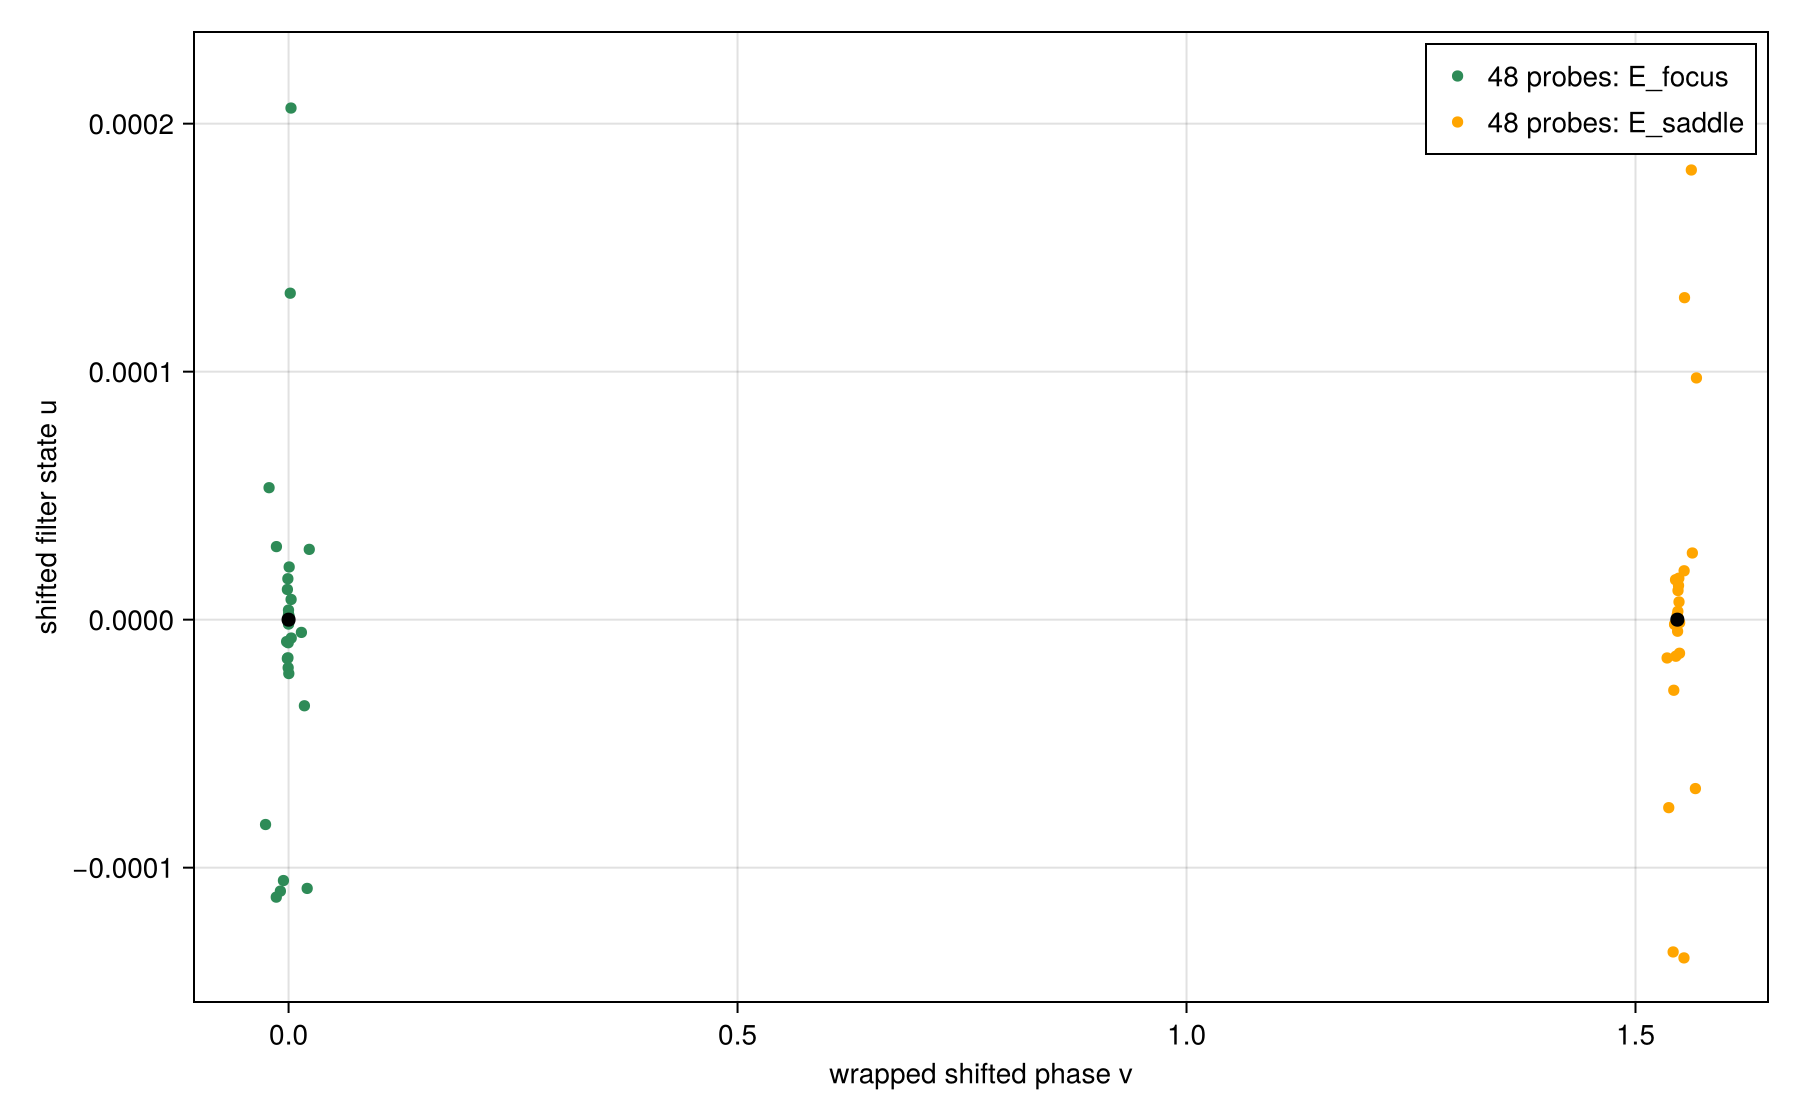
\includegraphics[width=0.82\textwidth]{julia_pll_cylindrical_hiddenness_probes.png}
\caption{Visualización Julia de las condiciones iniciales comunes del control
PLL, expresadas en las coordenadas envueltas del cilindro.}
\label{int:fig:pll-hiddenness}
\end{hafobasinfigure}
\fi

Julia implementó independientemente la misma distancia angular, el mapa de
retorno y la continuación desde la solución exacta en $L=0$; no leyó estados
Python ni las condiciones publicadas para localizar las órbitas.
\ifHAFOBasinMaterial
Coincidieron
\PLLJuliaProbeMatches{} de \PLLProbeCount{} estados y decisiones de contacto,
así como los destinos de las \PLLJuliaDestinationMatches{} trayectorias.
\fi
Las órbitas interpoladas sobre una fase normalizada difirieron como máximo
\PLLStableOrbitMaxDistance{} (estable) y
\PLLSeparatorOrbitMaxDistance{} (separatriz) en la métrica cilíndrica escalada.


\begin{hafocommonfigure}[H]
\centering
\begin{subfigure}[t]{0.49\textwidth}
  \centering
  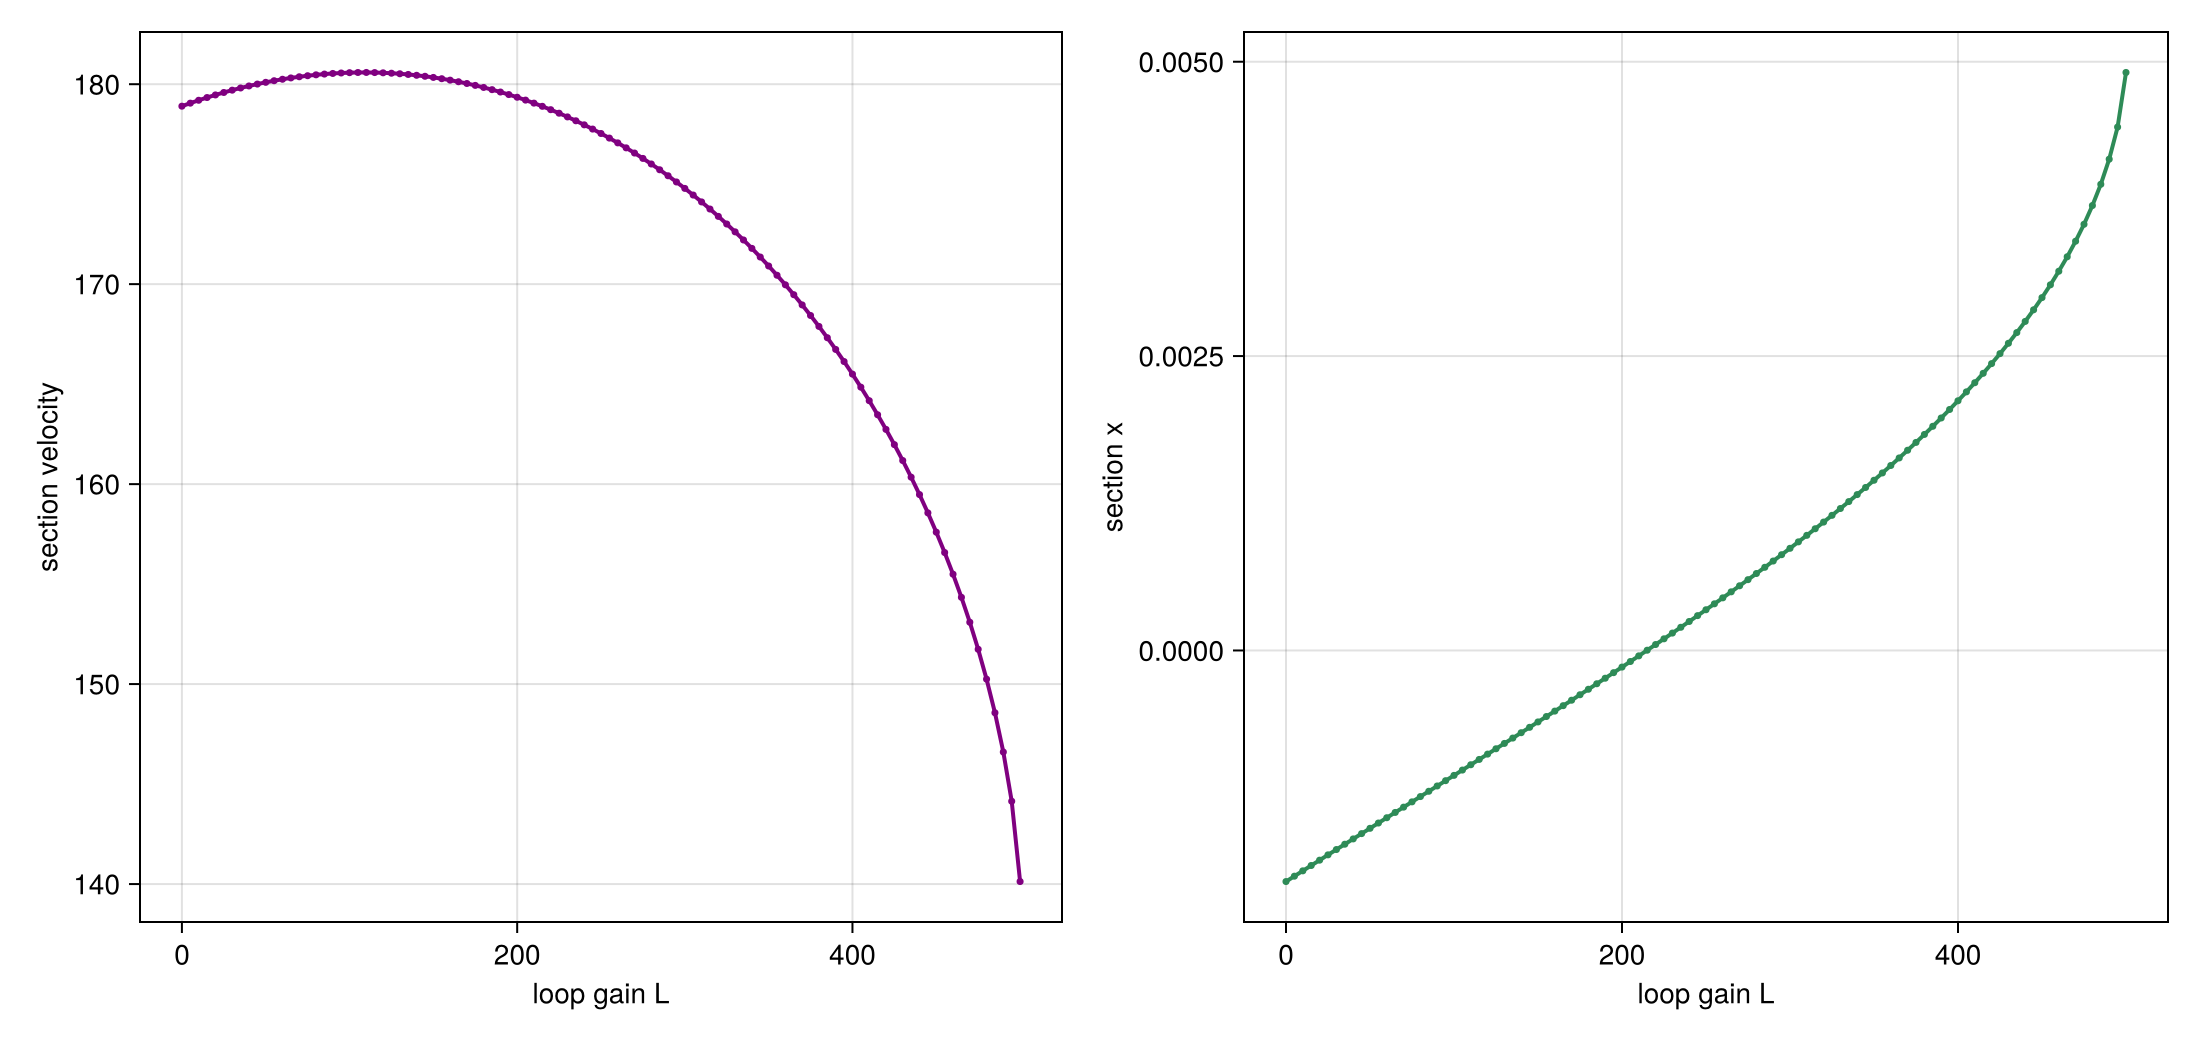
\includegraphics[width=\linewidth]{julia_pll_loop_gain_continuation.png}
  \caption{Continuación Julia desde $L=0$ hasta $L=500$.}
\end{subfigure}\hfill
\begin{subfigure}[t]{0.49\textwidth}
  \centering
  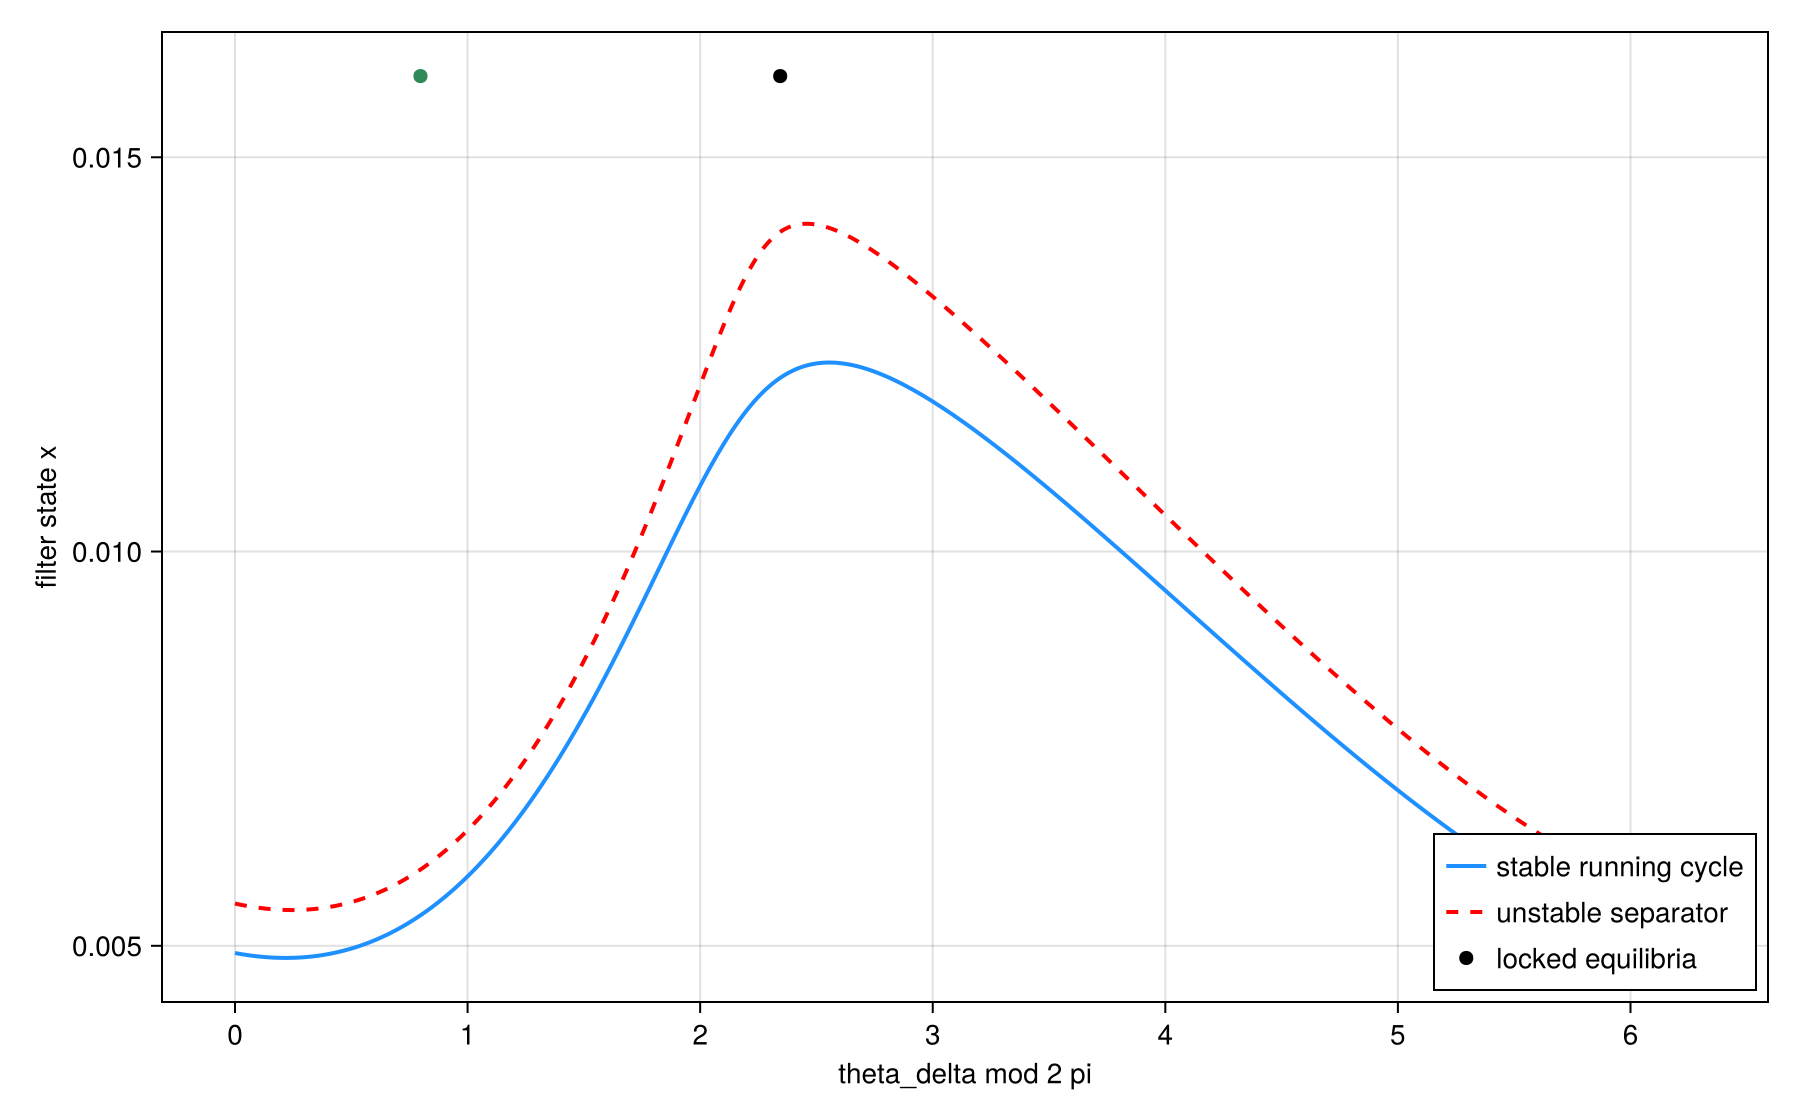
\includegraphics[width=\linewidth]{julia_pll_phase_cylinder_cycles.png}
  \caption{Ciclo estable y separatriz Julia en el cilindro.}
\end{subfigure}
\caption{Continuación y órbitas de la ruta PLL T1 + A1 calculadas en Julia.}
\label{int:fig:pll-julia}
\end{hafocommonfigure}

\section{Sistemas enteros estudiados y pendientes}

\subsection{Taxonomía D0/T1/A1/M1}

\begin{table}[H]
\centering
\caption{Clases estructurales usadas para aceptar o posponer sistemas.}
\small
\begin{tabularx}{\textwidth}{@{}C{1.1cm}p{0.24\textwidth}Yp{0.25\textwidth}@{}}
\toprule
Clase & Definición & Qué permite & Restricción \\
\midrule
D0 & Forma escalar directa \(\dot X=PX+b\psi(c^{\mathsf T}X)\) &
Ruta de transferencia y función descriptiva sin cambio de variables. &
Un solo canal no lineal escalar. \\
T1 & Transformación compatible e invertible, desplazamiento de equilibrio,
variedad invariante documentada o PWA de rango uno &
Lleva el sistema a D0 conservando la interpretación dinámica necesaria. &
La transformación registra la inversa y la métrica correspondiente, por ejemplo angular. \\
A1 & La forma escalar existe, pero la ruta directa se rechaza con una razón
matemática &
Habilita mapa de conmutación, homotopía publicada u otra alternativa. &
Conserva el diagnóstico de incompatibilidad directa y excluye semillas
publicadas de la inicialización. \\
M1 & Varios canales no lineales independientes &
Reserva para una futura extensión multicanal. &
Requiere una formulación multicanal adicional. \\
\bottomrule
\end{tabularx}
\end{table}

\subsection{Cobertura de los casos de estudio}

La \cref{int:tab:catalog} distingue los sistemas integrados de los candidatos
cuya formulación o evaluación numérica está pendiente.

\begin{longtable}{@{}C{1.2cm}L{0.29\textwidth}C{1.65cm}L{0.42\textwidth}@{}}
\caption{Sistemas de prueba de orden entero.}
\label{int:tab:catalog}\\
\toprule
Prior. & Sistema & Clase & Estado y papel científico \\
\midrule
\endfirsthead
\toprule
Prior. & Sistema & Clase & Estado y papel científico \\
\midrule
\endhead
Base & Chua no suave entero & D0 &
Compatible con ocultedad bajo el protocolo finito; reproducido en Python y Julia. \\
Base & Kalman--Fitts de cuarto orden & D0 + A1 &
No Chua; ciclo límite localizado por mapa de conmutación y continuación,
compatible con ocultedad bajo el sondeo; reproducido en Python y Julia. \\
1 & Van der Pol--Duffing autónomo modificado & D0 &
\(\xi=3.1\): 108/108 coincidencias entre cálculos y cero
contactos externos.
\ifHAFOBasinMaterial
\(\xi=3.5\): control negativo, 24/24 contactos con el ciclo seleccionado.
\fi
\(\xi=\MAVPDChaosXi\): candidato caótico compatible con
ocultedad bajo \MAVPDChaosTotalProbes{} sondeos en las vecindades declaradas;
coincidencia Python--Julia en todos los destinos evaluados. \\
2 & PLL bifásico con filtro lead--lag & T1 + A1 &
Comparación Python--Julia con 96 sondeos; las órbitas, su estabilidad
y las decisiones coinciden. \\
3 & Leonov--Kuznetsov, sistema (162) & D0 + A1 &
Ecuaciones y ruta de saturación disponibles; falta verificar la fórmula
completa por tramos y fijar los parámetros de integración. \\
4 & Jerk exponencial de Fischer, \(q=1\) & D0 con balance DC &
Control bibliográfico y de Lyapunov: equilibrio inestable; se conserva la
discrepancia del tercer exponente. Sin una campaña de cuenca local, la evidencia
disponible no permite clasificarlo como autoexcitado ni oculto. \\
\bottomrule
\end{longtable}

\subsection{Siguientes casos y reservas}

Leonov--Kuznetsov, sistema (162), es el siguiente candidato D0 + A1. La
fuente usa una familia de saturaciones, transporta el estado terminal entre
etapas y luego continúa la no linealidad hasta \(\tanh\)
\cite{LeonovKuznetsov2013}. Su evaluación requiere verificar la fórmula
completa por tramos y fijar los parámetros de integración.

El jerk exponencial de Fischer se conserva como control D0 con balance DC y
como banco de exponentes con discrepancias documentadas \cite{fischer2020}.
Falta un sondeo de vecindades para evaluar
la clasificación de cuenca. La inestabilidad del equilibrio, por sí sola, no
implica autoexcitación. La evaluación entera requiere los parámetros del caso bibliográfico correspondiente.

Quedan en reserva Genesio--Tesi, un oscilador memristivo cúbico, el jerk
hiperbólico de Joshi--Ranjan, un jerk PWA y los jerks de Rech y
Rasul--Salih. Faltan parámetros, condiciones iniciales o la verificación de
la ecuación exacta en su fuente primaria.

Lorenz, Rabinovich--Fabrikant, el sistema financiero, el sistema \emph{four
wing} y los modelos con productos no lineales independientes son M1. Su estudio
con Julia queda fuera de las hipótesis de la ruta Lur'e escalar D0/T1.

\section{Comparación metodológica}

\begin{table}[H]
\centering
\caption{Características de los métodos de localización y comparación.}
\small
\begin{tabularx}{\textwidth}{@{}p{0.20\textwidth}YY@{}}
\toprule
Aspecto & Python/\hafo{} & Julia/\juliads--\attractorsjl{} \\
\midrule
Entrada científica & Ecuaciones, Jacobiano, equilibrios, forma Lur'e,
transferencia y función descriptiva & Ecuaciones y dominio para búsqueda
global; las mismas declaraciones Lur'e cuando se replica la ruta teórica \\
Localización & Dirigida por balance armónico y continuación & Global por
recurrencias en Chua; ruta teórica equivalente en Kalman--Fitts y en el MAVPD
periódico y caótico; ruta A1 cilíndrica equivalente en PLL \\
Frecuencia y semilla & Produce \(\omega_0,k,a_0,X_0\) con residuos & Puede
obtener esos valores mediante la ruta teórica; la búsqueda por recurrencias
no utiliza ese balance \\
Generalidad & Restringida a D0/T1 y a las alternativas A1 registradas &
Más amplia para mapas, flujos, cuencas y recurrencias \\
Ocultedad & Flujo explícito de equilibrios y nube candidata & Protocolo
añadido al ejemplo; no es una etiqueta automática de la biblioteca \\
Valores publicados & Regresión posterior & Regresión posterior \\
Fallo típico & No hay ganancia/amplitud compatible o se pierde la rama &
La cuenca no es muestreada, la partición no resuelve el conjunto o el
clasificador agrupa mal \\
\bottomrule
\end{tabularx}
\end{table}

La forma Lur'e relaciona explícitamente el campo, la transferencia y la semilla. La búsqueda por recurrencias aporta generalidad y no necesita una
transformación Lur'e, pero
su éxito depende del dominio, partición, número de muestras y tamaño de la
cuenca. La comparación de los candidatos requiere un protocolo común de integración
y sondeo de cuenca.


\section{Conclusiones}

El balance armónico y la continuación localizaron candidatos en Chua,
Kalman--Fitts y MAVPD; el PLL requirió un mapa de retorno sobre el cilindro.
Las obstrucciones de ganancia en Kalman--Fitts y de fase en el PLL determinaron
las rutas alternativas. La búsqueda por recurrencias localizó además el
candidato de Chua a partir de un muestreo global independiente.

Los diagnósticos distinguen el ciclo estable de MAVPD en \(\xi=3.1\) del
candidato caótico obtenido por continuación hacia
\(\xi=\MAVPDChaosXi\). Este último combina un exponente máximo positivo,
retornos irregulares y controles entre integradores, con las limitaciones
de tiempo finito descritas en \cref{int:subsec:mavpd-chaos}.
\ifHAFOBasinMaterial
Los sondeos comunes coincidieron entre cálculos y no alcanzaron las nubes
candidatas en los casos positivos. MAVPD en \(\xi=3.5\) proporcionó el
control negativo, con contactos desde vecindades de los equilibrios.
\fi

La cobertura incluye sistemas escalares D0, transformaciones T1 y
alternativas A1. Los modelos multicanal requieren otra formulación; para los
candidatos enteros pendientes faltan especificaciones del modelo o sondeos
de cuenca, según la \cref{int:tab:catalog}.

\fi
\section[Candidatos fraccionarios no Chua]{Candidatos fraccionarios no Chua: álgebra verificada y alcance dinámico}
\label{part:nonchua}

\section{Resultado de la búsqueda y alcance real}

La revisión cruzada de las fuentes primarias, la extracción de datos publicados
y la matriz de cobertura del repositorio no produce una lista amplia de
candidatos ejecutados. Solamente aparecen dos sistemas fraccionarios no Chua
ligados de forma explícita a un reclamo publicado de atractor oculto:
el Lorenz generalizado y el sistema de Rabinovich--Fabrikant (RF), ambos tomados
de Danca~\cite{Danca2017}.

\begin{table}[ht]
\centering
\small
\caption{Clasificación de la evidencia localizada.}
\begin{tabularx}{\linewidth}{>{\raggedright\arraybackslash}p{0.23\linewidth}
>{\raggedright\arraybackslash}p{0.19\linewidth}X}
\toprule
Caso & Estado local & Evidencia disponible y límite\\
\midrule
Lorenz generalizado, \(q=0.995\) & \statusref &
Ecuaciones, parámetros, equilibrios redondeados, espectros publicados y un
ensayo bibliográfico de vecindad. No existe sistema integrado, semilla, corrida
de continuación ni artefacto de cuenca local.\\
Rabinovich--Fabrikant, \(q=0.998\) & \statusref &
Ecuaciones, parámetros, cinco equilibrios, espectros publicados y radios de
vecindad. No existe reproducción local del atractor ni de su cuenca.\\
Lorenz estándar, RF \(b=0.98\), jerk, financiero y four-wing & diagnóstico &
Son bancos de Lyapunov o comparaciones parciales. No certifican búsqueda de
atractores ocultos y no deben mezclarse con los dos casos de Danca.\\
Genesio--Tesi, jerk hiperbólico y otras familias del Artículo 03 & diseño &
Poseen realizaciones algebraicas propuestas, pero el prerregistro no Chua sigue
sin ejecuciones L0--L6 completas.\\
\bottomrule
\end{tabularx}
\end{table}

Los diseños locales para jerk, Genesio--Tesi, sistemas memristivos, Lorenz, RF
y el sistema financiero, así como los bancos DK2018 de Lyapunov para Lorenz
estándar y RF, no reúnen simultáneamente ecuaciones, parámetros, orden,
condición inicial o semilla, continuación y evidencia de cuenca para un
candidato no Chua. Por ello permanecen fuera de los dos casos principales.

El propio reporte unificado declara que Lorenz es un ejemplo pedagógico y que no
pertenece a su metodología activa. La fuente local decisiva es
\path{version_2/validation/references/published_validation_data_extraction_v1.json};
la clasificación conservadora procede de
\path{version_2/validation/published_reference_coverage.json}. En esta última,
los dos casos están marcados como \texttt{reference\_data\_only}, sin sistema
implementado, pruebas ni artefactos de validación. Por ello, en lo que sigue la
palabra \emph{candidato} significa \emph{caso prioritario para implementar y
buscar}, no \emph{atractor localmente reproducido}.

\begin{hallazgo}{Conclusión de la auditoría de fuentes}
El recuerdo del usuario era parcialmente correcto: había sistemas no Chua
registrados alrededor del reporte y de los manuscritos, pero el reporte
unificado no ejecutó su búsqueda. Los únicos dos con procedencia bibliográfica
directa de atractor oculto son Lorenz generalizado y RF; su cobertura local es
todavía sólo documental.
\end{hallazgo}

\section{Marco común de realización y localización}

\subsection{Dinámica de Caputo y transferencia fraccionaria}

Para \(0<q<1\), la derivada de Caputo con terminal inferior \(t_0\) se escribe
\begin{equation}
 {}^{\mathrm C}D_{t_0}^{q}x(t)
 =\frac{1}{\Gamma(1-q)}
 \int_{t_0}^{t}(t-\tau)^{-q}x'(\tau)\,d\tau .
 \label{nc:eq:caputo}
\end{equation}
La ecuación autónoma
\begin{equation}
 {}^{\mathrm C}D_{t_0}^{q}x(t)=F(x(t)),\qquad x(t_0)=x_0,
 \label{nc:eq:ivp}
\end{equation}
es equivalente a la ecuación integral de Volterra
\begin{equation}
 x(t)=x_0+\frac{1}{\Gamma(q)}
 \int_{t_0}^{t}(t-\tau)^{q-1}F(x(\tau))\,d\tau .
 \label{nc:eq:volterra}
\end{equation}
La historia desde \(t_0\) es parte del problema; no puede reiniciarse durante
una continuación sin declarar que se ha definido un problema diferente.

Para el bloque lineal
\begin{equation}
 {}^{\mathrm C}D_{t_0}^{q}x=Ax+Bu,
 \qquad y=Cx,
 \label{nc:eq:linear-block}
\end{equation}
la transformada de Laplace cumple
\begin{equation}
 \mathcal L\{{}^{\mathrm C}D_{t_0}^{q}x\}(s)
 =s^qX(s)-s^{q-1}x(t_0).
\end{equation}
Con estado inicial nulo, la transferencia entrada--salida es
\begin{equation}
 W_q(s)=C(s^qI-A)^{-1}B.
 \label{nc:eq:transfer-general}
\end{equation}
Se usa la rama principal. En el predictor armónico,
\begin{equation}
 (\ii k\omega)^q=(k\omega)^q
 \exp\!\left(\ii\frac{q\pi}{2}\right),\qquad k>0.
 \label{nc:eq:principal-branch}
\end{equation}
Esta sustitución produce un problema algebraico estacionario; no afirma la
existencia de una órbita periódica exacta del PVI causal de Caputo.

\subsection{Realización de Lur'e multicanal}

Los dos candidatos no son escalares en su no linealidad. Se usa la forma exacta
\begin{equation}
 {}^{\mathrm C}D_{t_0}^{q}x=Ax+B\Phi(Cx),
 \qquad x\in\RR^n,
 \label{nc:eq:mimo-lure}
\end{equation}
con \(\Phi:\RR^p\to\RR^m\) estática. La identidad que debe comprobarse es
\begin{equation}
 Ax+B\Phi(Cx)-F(x)\equiv0.
 \label{nc:eq:lure-residual}
\end{equation}
No basta que las expresiones coincidan en una trayectoria o en un equilibrio.

Sea \(\bar y=C\bar x\) un sesgo y
\begin{equation}
 K=D\Phi(\bar y)\in\RR^{m\times p}.
\end{equation}
La ecuación de cierre linealizada del primer armónico es
\begin{equation}
 \det\!\left[I_p-W_q(\ii\omega)K\right]=0.
 \label{nc:eq:det-closure}
\end{equation}
Para amplitud finita, \(K\) se sustituye por los coeficientes de Fourier
exactos de la no linealidad.

\subsection{Coeficientes exactos y balance multiharmónico}

Se adopta la convención compleja
\begin{equation}
 x(\theta)=\sum_{k=-H}^{H}X_k e^{\ii k\theta},
 \qquad X_{-k}=\overline{X_k},\qquad X_0\in\RR^n,
 \label{nc:eq:fourier-state}
\end{equation}
con \(\theta=\omega t\). Si \(u\) y \(v\) tienen coeficientes \(U_k,V_k\),
la multiplicación no se aproxima: sus coeficientes son la convolución
\begin{equation}
 \widehat{(uv)}_k=\sum_{m\in\mathbb Z}U_mV_{k-m}.
 \label{nc:eq:conv2}
\end{equation}
Para un producto triple,
\begin{equation}
 \widehat{(uvw)}_k
 =\sum_{m\in\mathbb Z}\sum_{n\in\mathbb Z}
 U_mV_nW_{k-m-n}.
 \label{nc:eq:conv3}
\end{equation}
En una truncación se toma \(U_k=0\) para \(|k|>H\). Esto calcula exactamente
los coeficientes retenidos de la señal truncada; la omisión de armónicos altos
se controla aumentando \(H\).

Si \(\widehat\Phi_k\) denota el coeficiente \(k\) de \(\Phi(Cx(\theta))\), el
sistema completo de balance es
\begin{align}
 AX_0+B\widehat\Phi_0&=0,
 \label{nc:eq:hb0}\\
 \left[(\ii k\omega)^qI-A\right]X_k-B\widehat\Phi_k&=0,
 \qquad k=1,\ldots,H.
 \label{nc:eq:hbk}
\end{align}
Las incógnitas son \(X_0,X_1,\ldots,X_H,\omega\), junto con una condición de
fase, por ejemplo
\begin{equation}
 \operatorname{Im}(e_j\trans X_1)=0,\qquad
 \operatorname{Re}(e_j\trans X_1)>0.
 \label{nc:eq:phase-condition}
\end{equation}
Una familia de estados iniciales se reconstruye mediante
\begin{equation}
 x_{\mathrm{sem}}(\varphi)=X_0+
 2\operatorname{Re}\sum_{k=1}^{H}X_ke^{\ii k\varphi}.
 \label{nc:eq:seed-reconstruction}
\end{equation}

\subsection{Continuación causal}

Defina \(\bar u=\Phi(\bar y)\) y el auxiliar afín
\begin{equation}
 A_{\mathrm a}=A+BKC,\qquad
 d_{\mathrm a}=B(\bar u-K\bar y).
 \label{nc:eq:auxiliary}
\end{equation}
La homotopía exacta es
\begin{equation}
 F_\varepsilon(x)=A_{\mathrm a}x+d_{\mathrm a}
 +\varepsilon B\left[
 \Phi(Cx)-\bar u-K(Cx-\bar y)
 \right],\qquad 0\leq\varepsilon\leq1.
 \label{nc:eq:homotopy}
\end{equation}
Por sustitución directa,
\begin{equation}
 F_0(x)=A_{\mathrm a}x+d_{\mathrm a},
 \qquad F_1(x)=Ax+B\Phi(Cx).
\end{equation}
En Caputo, la continuación debe evaluarse sobre una sola historia:
\begin{equation}
 x(t)=x_{\mathrm{sem}}+
 \frac{1}{\Gamma(q)}\int_{t_0}^{t}
 (t-\tau)^{q-1}F_{\varepsilon(\tau)}(x(\tau))\,d\tau.
 \label{nc:eq:causal-homotopy}
\end{equation}

\subsection{Matignon y frontera de la afirmación de ocultedad}

Para un equilibrio (e) con Jacobiano (J(e)) y espectro
\(\{\lambda_j\}\), el sistema lineal con orden conmensurable \(q\) es
asintóticamente estable si
\begin{equation}
 |\arg\lambda_j|>\frac{q\pi}{2}
 \quad\text{para todo }j.
 \label{nc:eq:matignon}
\end{equation}
Se reportará el margen
\begin{equation}
 m_M(e;q)=\min_j|\arg\lambda_j|-\frac{q\pi}{2}.
 \label{nc:eq:margin}
\end{equation}
Un margen positivo certifica estabilidad lineal local; no certifica caos,
atracción global ni ocultedad.

La ocultedad exige que la cuenca del conjunto atractivo no intersecte
vecindades abiertas de los equilibrios. Un número finito de trayectorias sobre
radios o direcciones discretos sólo sustenta una afirmación bajo el contrato de
muestreo declarado. Esta distinción se conserva en todo el documento.

\clearpage
\section{Caso I: sistema de Lorenz generalizado fraccionario}

\subsection{Modelo, parámetros y simetría}

El sistema registrado es
\begin{equation}
\begin{aligned}
 {}^{\mathrm C}D^qx_1&=-\sigma(x_1-x_2)-a x_2x_3,\\
 {}^{\mathrm C}D^qx_2&=r x_1-x_2-x_1x_3,\\
 {}^{\mathrm C}D^qx_3&=-x_3+x_1x_2,
\end{aligned}
 \qquad \sigma=-ar,\quad a<0.
\label{nc:eq:lorenz-model}
\end{equation}
El caso bibliográfico usa
\begin{equation}
 r=6.8,\qquad a=-0.5,\qquad \sigma=3.4,
 \qquad q=0.995.
 \label{nc:eq:lorenz-parameters}
\end{equation}
El campo es equivariante bajo
\begin{equation}
 \mathcal S(x_1,x_2,x_3)=(-x_1,-x_2,x_3).
 \label{nc:eq:lorenz-symmetry}
\end{equation}
Por tanto, los equilibrios no nulos, semillas y trayectorias aparecen en pares
simétricos.

\subsection{Realización exacta de Lur'e multicanal}

Agrupando términos lineales y monomios se obtiene
\begin{equation}
 A_L=
 \begin{pmatrix}
 -\sigma&\sigma&0\\ r&-1&0\\0&0&-1
 \end{pmatrix},\qquad
 B_L=
 \begin{pmatrix}
 -a&0&0\\0&-1&0\\0&0&1
 \end{pmatrix},
 \qquad C_L=I_3,
 \label{nc:eq:lorenz-abc}
\end{equation}
y
\begin{equation}
 \Phi_L(x)=
 \begin{pmatrix}
 x_2x_3\\x_1x_3\\x_1x_2
 \end{pmatrix}.
 \label{nc:eq:lorenz-phi}
\end{equation}
La comprobación se hace componente a componente:
\begin{align*}
 [A_Lx+B_L\Phi_L(x)]_1
 &=-\sigma x_1+\sigma x_2-a x_2x_3,\\
 [A_Lx+B_L\Phi_L(x)]_2
 &=r x_1-x_2-x_1x_3,\\
 [A_Lx+B_L\Phi_L(x)]_3
 &=-x_3+x_1x_2.
\end{align*}
Luego el residuo de la ecuación~\eqref{nc:eq:lure-residual} es idénticamente
\((0,0,0)\trans\).

\subsection{Derivación completa de la matriz de transferencia}

Escriba \(z=s^q\). Entonces
\begin{equation}
 zI-A_L=
 \begin{pmatrix}
 z+\sigma&-\sigma&0\\
 -r&z+1&0\\
 0&0&z+1
 \end{pmatrix}.
\end{equation}
El determinante del bloque superior es
\begin{equation}
 \Delta_L(z)=(z+\sigma)(z+1)-\sigma r.
 \label{nc:eq:lorenz-delta}
\end{equation}
Por inversión de un bloque \(2\times2\),
\begin{equation}
 (zI-A_L)^{-1}=
 \begin{pmatrix}
 \dfrac{z+1}{\Delta_L}&\dfrac{\sigma}{\Delta_L}&0\\[7pt]
 \dfrac{r}{\Delta_L}&\dfrac{z+\sigma}{\Delta_L}&0\\[7pt]
 0&0&\dfrac{1}{z+1}
 \end{pmatrix}.
\end{equation}
Como \(C_L=I_3\), la multiplicación por \(B_L\) da
\begin{equation}
 W_{L,q}(s)=
 \begin{pmatrix}
 \dfrac{-a(z+1)}{\Delta_L}&
 \dfrac{-\sigma}{\Delta_L}&0\\[8pt]
 \dfrac{-ar}{\Delta_L}&
 \dfrac{-(z+\sigma)}{\Delta_L}&0\\[8pt]
 0&0&\dfrac{1}{z+1}
 \end{pmatrix}_{z=s^q}.
 \label{nc:eq:lorenz-transfer}
\end{equation}
Wolfram redujo a cero las nueve entradas de la diferencia entre
\(C_L(s^qI-A_L)^{-1}B_L\) y~\eqref{nc:eq:lorenz-transfer}.

\subsection{Equilibrios: derivación sin saltos}

En un equilibrio la derivada de Caputo de un estado constante es cero. La
tercera ecuación de~\eqref{nc:eq:lorenz-model} impone
\begin{equation}
 x_3=x_1x_2.
 \label{nc:eq:lorenz-eq1}
\end{equation}
La segunda da
\begin{equation}
 x_2(1+x_1^2)=r x_1,
 \qquad
 x_2=\frac{r x_1}{1+x_1^2}.
 \label{nc:eq:lorenz-eq2}
\end{equation}
Si \(x_1=0\), las ecuaciones restantes producen
\begin{equation}
 E_0=(0,0,0).
\end{equation}
Para \(x_1\neq0\), use \(\sigma=-ar\) en la primera ecuación:
\begin{align}
 0&=ar(x_1-x_2)-a x_2x_3,\\
 r(x_1-x_2)&=x_1x_2^2.
 \label{nc:eq:lorenz-eq3}
\end{align}
Sea \(u=x_1^2\). Al sustituir~\eqref{nc:eq:lorenz-eq2} en
\eqref{nc:eq:lorenz-eq3} se obtiene
\begin{equation}
 (1+u)^2-r(1+2u)=0,
\end{equation}
o, equivalentemente,
\begin{equation}
 u^2+2(1-r)u+(1-r)=0.
\end{equation}
Por la fórmula cuadrática,
\begin{equation}
 u_{\pm}=r-1\pm\sqrt{r(r-1)}.
 \label{nc:eq:lorenz-u}
\end{equation}
Para \(r=6.8\), \(u_-=r-1-\sqrt{r(r-1)}<0\) y no produce equilibrios
reales. Con
\begin{equation}
 u=u_+=r-1+\sqrt{r(r-1)},
\end{equation}
los otros dos equilibrios son
\begin{equation}
 E_{\pm}=\left(
 \pm\sqrt u,
 \pm\frac{r\sqrt u}{1+u},
 \frac{ru}{1+u}
 \right).
 \label{nc:eq:lorenz-equilibria}
\end{equation}
Numéricamente,
\begin{equation}
 E_{\pm}=(\pm3.47564776512854,
 \ \pm1.80689408468029,
 \ 6.28012738724303).
 \label{nc:eq:lorenz-equilibria-num}
\end{equation}
La sustitución simbólica de~\eqref{nc:eq:lorenz-equilibria} en el campo produjo
residuo exactamente nulo; el mayor residuo numérico de los tres equilibrios fue
\(1.07\times10^{-14}\).

\subsection{Jacobiano, polinomios y corrección espectral}

El Jacobiano correcto es
\begin{equation}
 J_L(x)=
 \begin{pmatrix}
 -\sigma&\sigma-a x_3&-a x_2\\
 r-x_3&-1&-x_1\\
 x_2&x_1&-1
 \end{pmatrix}.
 \label{nc:eq:lorenz-jacobian}
\end{equation}
En el origen,
\begin{equation}
 p_0(\lambda)
 =(\lambda+1)\left[(\lambda+\sigma)(\lambda+1)-\sigma r\right].
\end{equation}
Con~\eqref{nc:eq:lorenz-parameters},
\begin{equation}
 p_0(\lambda)=
 \lambda^3+5.4\lambda^2-15.32\lambda-19.72,
\end{equation}
y
\begin{equation}
 \operatorname{spec}J_L(E_0)=
 \{-7.15580467734555,\ 2.75580467734555,\ -1\}.
 \label{nc:eq:lorenz-origin-spectrum}
\end{equation}
El valor propio real positivo hace inestable a \(E_0\) para todo \(q>0\).

En cualquiera de los equilibrios \(E_{\pm}\), el polinomio mónico es
\begin{equation}
 p_{\pm}(\lambda)=
 \lambda^3+5.4\lambda^2
 +14.8476942706167\lambda+78.88,
\end{equation}
con espectro
\begin{equation}
 \operatorname{spec}J_L(E_{\pm})=
 \left\{
 -5.37029951773135,
 -0.0148502411343235\pm3.83248917224189\ii
 \right\}.
 \label{nc:eq:lorenz-outer-spectrum}
\end{equation}
Para el par complejo,
\begin{equation}
 q_{\mathrm{crit}}=
 \frac{2|\arg\lambda|}{\pi}=1.00246678056773,
\end{equation}
de modo que \(E_{\pm}\) es localmente estable para \(q=0.995\). El margen es
\begin{equation}
 m_M(E_{\pm};0.995)=0.0117287914887680>0.
\end{equation}

\begin{hallazgo}{Corrección algebraica al dato bibliográfico heredado}
La fuente primaria y la extracción JSON local registran en \(E_0\) el espectro
\(\{2.5576,-1,-7.5576\}\) y en \(E_{\pm}\) el espectro
\(\{-5.9570,-0.0215\pm3.6026\ii\}\). Esos números no corresponden a las
ecuaciones y parámetros declarados: ambos conjuntos suman \(-6\), mientras que
\(\operatorname{tr}J_L=-5.4\). Wolfram dio residuos máximos \(27.17\) y
\(29.33\) al sustituirlos en los polinomios característicos. Los valores
corregidos son~\eqref{nc:eq:lorenz-origin-spectrum} y
\eqref{nc:eq:lorenz-outer-spectrum}. La clasificación cualitativa no cambia:
origen inestable y par externo estable. También debe evitarse llamar
``silla'' a un equilibrio declarado asintóticamente estable.
\end{hallazgo}

\subsection{Sistema algebraico de la semilla armónica}

Para \(H\geq2\), escriba \(X_{j,k}\) para el coeficiente \(k\) de \(x_j\).
Los coeficientes no lineales son
\begin{equation}
 \widehat\Phi_{L,k}=
 \begin{pmatrix}
 \displaystyle\sum_m X_{2,m}X_{3,k-m}\\[5pt]
 \displaystyle\sum_m X_{1,m}X_{3,k-m}\\[5pt]
 \displaystyle\sum_m X_{1,m}X_{2,k-m}
 \end{pmatrix}.
 \label{nc:eq:lorenz-fourier-phi}
\end{equation}
Por tanto, una semilla no se obtiene escogiendo una condición inicial al azar,
sino resolviendo
\begin{align}
 A_LX_0+B_L\widehat\Phi_{L,0}&=0,\\
 \left[(\ii k\omega)^qI-A_L\right]X_k
 -B_L\widehat\Phi_{L,k}&=0,
 \quad k=1,\ldots,H,\\
 \operatorname{Im}(e_j\trans X_1)&=0.
 \label{nc:eq:lorenz-hb-system}
\end{align}
La linealización alrededor de un sesgo \(\bar x\) usa
\begin{equation}
 K_L(\bar x)=D\Phi_L(\bar x)=
 \begin{pmatrix}
 0&\bar x_3&\bar x_2\\
 \bar x_3&0&\bar x_1\\
 \bar x_2&\bar x_1&0
 \end{pmatrix}
 \label{nc:eq:lorenz-k}
\end{equation}
y el predictor local
\begin{equation}
 \det\left[I_3-W_{L,q}(\ii\omega)K_L(\bar x)\right]=0.
 \label{nc:eq:lorenz-local-closure}
\end{equation}
La solución de~\eqref{nc:eq:lorenz-hb-system} debe verificarse con \(H\) y
\(H+1\), reconstruirse mediante~\eqref{nc:eq:seed-reconstruction} y transportarse
con~\eqref{nc:eq:causal-homotopy}.

\subsection{Datos y comprobaciones necesarios para una búsqueda local}

La referencia declara \(q=0.995\), un atractor representado gráficamente y 50
trayectorias desde una vecindad de radio \(0.3\) del origen que llegan a los dos
equilibrios estables. Sin embargo, la evidencia disponible no especifica la
condición inicial del atractor, el paso, el horizonte, el transitorio, la
historia ni una semilla de balance armónico. Para cerrar esa laguna se requiere:
\begin{enumerate}
 \item resolver~\eqref{nc:eq:lorenz-hb-system} para \(H=2,3,\ldots\) y retener
 sólo raíces con residuos y distorsión convergentes;
 \item reconstruir todas las fases no equivalentes por
 \eqref{nc:eq:seed-reconstruction};
 \item continuar en una sola historia de Caputo;
 \item reiniciar una evaluación autónoma separada desde el estado terminal;
 \item demostrar atracción local y robustez frente a (h), memoria, horizonte
 y solver;
 \item sondear todos los equilibrios con bolas y superficies declaradas, no
 únicamente 50 direcciones alrededor de \(E_0\).
\end{enumerate}

\clearpage
\section{Caso II: sistema de Rabinovich--Fabrikant fraccionario}

\subsection{Modelo, parámetros y simetría}

El sistema RF registrado es
\begin{equation}
\begin{aligned}
 {}^{\mathrm C}D^qx_1&=x_2(x_3-1+x_1^2)+a x_1,\\
 {}^{\mathrm C}D^qx_2&=x_1(3x_3+1-x_1^2)+a x_2,\\
 {}^{\mathrm C}D^qx_3&=-2x_3(b+x_1x_2),
\end{aligned}
\label{nc:eq:rf-model}
\end{equation}
con
\begin{equation}
 a=0.1,\qquad b=0.2876,\qquad q=0.998.
 \label{nc:eq:rf-parameters}
\end{equation}
También es equivariante bajo
\begin{equation}
 \mathcal S(x_1,x_2,x_3)=(-x_1,-x_2,x_3).
\end{equation}

\subsection{Realización polinómica multicanal exacta}

Expanda el campo:
\begin{align*}
 F_1&=a x_1-x_2+x_2x_3+x_1^2x_2,\\
 F_2&=x_1+a x_2+3x_1x_3-x_1^3,\\
 F_3&=-2b x_3-2x_1x_2x_3.
\end{align*}
Una realización directa, sin variables auxiliares dinámicas, es
\begin{equation}
 A_R=
 \begin{pmatrix}
 a&-1&0\\1&a&0\\0&0&-2b
 \end{pmatrix},\qquad C_R=I_3,
 \label{nc:eq:rf-a}
\end{equation}
\begin{equation}
 B_R=
 \begin{pmatrix}
 1&1&0&0&0\\
 0&0&3&-1&0\\
 0&0&0&0&-2
 \end{pmatrix},
 \label{nc:eq:rf-b}
\end{equation}
y
\begin{equation}
 \Phi_R(x)=
 \begin{pmatrix}
 x_2x_3\\x_1^2x_2\\x_1x_3\\x_1^3\\x_1x_2x_3
 \end{pmatrix}.
 \label{nc:eq:rf-phi}
\end{equation}
En efecto,
\begin{equation}
 A_Rx+B_R\Phi_R(x)=F_R(x)
\end{equation}
componente a componente. Wolfram simplificó el residuo simbólico a
\((0,0,0)\trans\).

Si una implementación exige potencias de mediciones lineales, los productos
pueden factorizarse sin aproximación mediante
\begin{equation}
 uv=\frac{(u+v)^2-(u-v)^2}{4}
 \label{nc:eq:square-identity}
\end{equation}
y
\begin{equation}
 uvw=\frac{(u+v+w)^3+(u-v-w)^3+(-u+v-w)^3+(-u-v+w)^3}{24}.
 \label{nc:eq:cubic-identity}
\end{equation}
Estas identidades cambian el número de canales, no el campo vectorial.

\subsection{Derivación completa de la transferencia RF}

De nuevo, sea \(z=s^q\). Entonces
\begin{equation}
 zI-A_R=
 \begin{pmatrix}
 z-a&1&0\\-1&z-a&0\\0&0&z+2b
 \end{pmatrix}.
\end{equation}
Defina
\begin{equation}
 \Delta_R(z)=(z-a)^2+1.
 \label{nc:eq:rf-delta}
\end{equation}
La inversa es
\begin{equation}
 (zI-A_R)^{-1}=
 \begin{pmatrix}
 \dfrac{z-a}{\Delta_R}&\dfrac{-1}{\Delta_R}&0\\[7pt]
 \dfrac{1}{\Delta_R}&\dfrac{z-a}{\Delta_R}&0\\[7pt]
 0&0&\dfrac{1}{z+2b}
 \end{pmatrix}.
\end{equation}
Al multiplicar por las cinco columnas de \(B_R\),
\begin{equation}
 W_{R,q}(s)=
 \begin{pmatrix}
 \dfrac{z-a}{\Delta_R}&
 \dfrac{z-a}{\Delta_R}&
 \dfrac{-3}{\Delta_R}&
 \dfrac{1}{\Delta_R}&0\\[8pt]
 \dfrac{1}{\Delta_R}&
 \dfrac{1}{\Delta_R}&
 \dfrac{3(z-a)}{\Delta_R}&
 \dfrac{-(z-a)}{\Delta_R}&0\\[8pt]
 0&0&0&0&\dfrac{-2}{z+2b}
 \end{pmatrix}_{z=s^q}.
 \label{nc:eq:rf-transfer}
\end{equation}
La diferencia simbólica entre~\eqref{nc:eq:rf-transfer} y
\((s^qI-A_R)^{-1}B_R\) fue la matriz nula \(3\times5\).

\subsection{Equilibrios: reducción a una ecuación cuadrática}

El origen
\begin{equation}
 E_0=(0,0,0)
\end{equation}
es inmediato. Para un equilibrio con \(x_3\neq0\), la tercera ecuación exige
\begin{equation}
 x_1x_2=-b,\qquad x_2=-\frac{b}{x_1}.
 \label{nc:eq:rf-product}
\end{equation}
La primera ecuación, multiplicada por \(x_1\), da
\begin{equation}
 -b(x_3-1+x_1^2)+a x_1^2=0,
\end{equation}
de donde
\begin{equation}
 x_3=1+\frac{a-b}{b}x_1^2.
 \label{nc:eq:rf-z}
\end{equation}
Sea \(u=x_1^2\). La segunda ecuación, multiplicada por \(x_1\), es
\begin{equation}
 u(3x_3+1-u)-ab=0.
\end{equation}
Sustituyendo~\eqref{nc:eq:rf-z}, se llega a
\begin{equation}
 (3a-4b)u^2+4bu-ab^2=0.
 \label{nc:eq:rf-u-polynomial}
\end{equation}
Con
\begin{equation}
 R=\sqrt{4+a(3a-4b)},
\end{equation}
las dos raíces son
\begin{equation}
 u_{\pm}=\frac{b(-2\pm R)}{3a-4b}.
 \label{nc:eq:rf-u}
\end{equation}
Para~\eqref{nc:eq:rf-parameters}, ambas son positivas. Cada una genera un par
simétrico:
\begin{equation}
 E_{\pm}^{(u)}=\left(
 \pm\sqrt u,\ \mp\frac{b}{\sqrt u},
 1+\frac{a-b}{b}u
 \right).
 \label{nc:eq:rf-equilibria-general}
\end{equation}
Ordenando por \(|x_1|\), se obtienen
\begin{align}
 E_{1,2}&=(\mp1.15997695583801,
 \ \pm0.247935959893466,
 \ 0.122306917444673),
 \label{nc:eq:rf-e12}\\
 E_{3,4}&=(\mp0.085021329989515,
 \ \pm3.38268055834300,
 \ 0.995284804098130).
 \label{nc:eq:rf-e34}
\end{align}
Wolfram redujo exactamente a cero el campo evaluado en las dos ramas
algebraicas de~\eqref{nc:eq:rf-u}; el máximo residuo numérico fue
\(1.06\times10^{-14}\).

\subsection{Jacobiano, polinomios y Matignon}

La diferenciación de~\eqref{nc:eq:rf-model} da
\begin{equation}
 J_R(x)=
 \begin{pmatrix}
 2x_1x_2+a&x_3-1+x_1^2&x_2\\
 3x_3+1-3x_1^2&a&3x_1\\
 -2x_2x_3&-2x_1x_3&-2(b+x_1x_2)
 \end{pmatrix}.
 \label{nc:eq:rf-jacobian}
\end{equation}
En el origen,
\begin{equation}
 p_0(\lambda)=(\lambda+2b)\left[(\lambda-a)^2+1\right],
\end{equation}
y
\begin{equation}
 \operatorname{spec}J_R(E_0)=
 \{-0.5752,\ 0.1\pm1.0\ii\}.
\end{equation}
El par complejo tiene
\begin{equation}
 q_{\mathrm{crit}}=0.936548965138893.
\end{equation}
Como \(q=0.998>q_{\mathrm{crit}}\), \(E_0\) es inestable y
\begin{equation}
 m_M(E_0;0.998)=-0.0965270598375723.
\end{equation}

En \(E_{1,2}\),
\begin{equation}
 p_{1,2}(\lambda)=
 \lambda^3+0.3752\lambda^2
 +2.20397205132125\lambda+0.556792727146772,
\end{equation}
\begin{equation}
 \operatorname{spec}J_R(E_{1,2})=
 \{-0.256175578455019,
 -0.059512210772491\pm1.47307134859472\ii\}.
\end{equation}
El mínimo crítico es
\begin{equation}
 q_{\mathrm{crit}}=1.02570551509697>1,
\end{equation}
por lo que el par \(E_{1,2}\) es estable para todo \(0<q\leq1\); en particular,
\begin{equation}
 m_M(E_{1,2};0.998)=0.0435197213462810>0.
\end{equation}

En \(E_{3,4}\),
\begin{equation}
 p_{3,4}(\lambda)=
 \lambda^3+0.3752\lambda^2
 +22.7628315898639\lambda-4.53095664529540,
\end{equation}
\begin{equation}
 \operatorname{spec}J_R(E_{3,4})=
 \{0.198062714510438,
 -0.286631357255219\pm4.77432885589854\ii\}.
\end{equation}
El valor propio positivo implica inestabilidad para todo \(q>0\). Estos
resultados coinciden, dentro del redondeo impreso, con la fuente primaria.

\subsection{Sistema algebraico de la semilla RF}

El Jacobiano estático de~\eqref{nc:eq:rf-phi}, evaluado en un sesgo \(\bar x\), es
\begin{equation}
 K_R(\bar x)=
 \begin{pmatrix}
 0&\bar x_3&\bar x_2\\
 2\bar x_1\bar x_2&\bar x_1^2&0\\
 \bar x_3&0&\bar x_1\\
 3\bar x_1^2&0&0\\
 \bar x_2\bar x_3&\bar x_1\bar x_3&\bar x_1\bar x_2
 \end{pmatrix}.
 \label{nc:eq:rf-k}
\end{equation}
El predictor local satisface
\begin{equation}
 \det\left[I_3-W_{R,q}(\ii\omega)K_R(\bar x)\right]=0.
 \label{nc:eq:rf-local-closure}
\end{equation}

Para el balance de amplitud finita se recomienda iniciar con \(H=3\). Las cinco
componentes no lineales se calculan sin ambigüedad por
\begin{equation}
 \widehat\Phi_{R,k}=
 \begin{pmatrix}
 \displaystyle\sum_m X_{2,m}X_{3,k-m}\\[5pt]
 \displaystyle\sum_{m,n}X_{1,m}X_{1,n}X_{2,k-m-n}\\[5pt]
 \displaystyle\sum_m X_{1,m}X_{3,k-m}\\[5pt]
 \displaystyle\sum_{m,n}X_{1,m}X_{1,n}X_{1,k-m-n}\\[5pt]
 \displaystyle\sum_{m,n}X_{1,m}X_{2,n}X_{3,k-m-n}
 \end{pmatrix}.
 \label{nc:eq:rf-fourier-phi}
\end{equation}
El sistema de semillas es
\begin{align}
 A_RX_0+B_R\widehat\Phi_{R,0}&=0,\\
 \left[(\ii k\omega)^qI-A_R\right]X_k
 -B_R\widehat\Phi_{R,k}&=0,
 \quad k=1,\ldots,H,\\
 \operatorname{Im}(e_j\trans X_1)&=0.
 \label{nc:eq:rf-hb-system}
\end{align}
La contribución cúbica genera armónicos por encima de \(H\). Por ello, cada raíz
debe continuar a \(H+1\), y la cola omitida debe registrarse como índice de
distorsión. Sólo después se reconstruye~\eqref{nc:eq:seed-reconstruction} y se
aplica la homotopía~\eqref{nc:eq:homotopy}.

\subsection{Qué falta para una búsqueda local reproducible}

La fuente usa \(q=0.998\) y vecindades de radio \(0.1\) alrededor de los
equilibrios inestables \(E_0,E_3,E_4\). La evidencia disponible no incluye la
condición inicial publicada del conjunto verde, una semilla algebraica, el
contrato ABM completo ni las trayectorias de vecindad. Para cerrar la búsqueda
se requiere:
\begin{enumerate}
 \item resolver~\eqref{nc:eq:rf-hb-system} desde varias ramas y fases;
 \item separar soluciones acotadas, divergentes y transitoriamente caóticas;
 \item continuar cada semilla con una única historia causal;
 \item comprobar la dinámica con un segundo integrador de memoria completa;
 \item sondear los cinco equilibrios y registrar explícitamente los destinos
 \(E_{1,2}\), divergencia, conjunto objetivo u otros conjuntos;
 \item distinguir una ausencia finita de contactos de una prueba de vecindad
 abierta.
\end{enumerate}

\section{Comparación y prioridad de implementación}

\begin{table}[ht]
\centering
\small
\caption{Comparación algebraica de los dos candidatos prioritarios.}
\begin{tabularx}{\linewidth}{>{\raggedright\arraybackslash}p{0.24\linewidth}XX}
\toprule
Propiedad & Lorenz generalizado & Rabinovich--Fabrikant\\
\midrule
Orden no lineal & cuadrático & cuadrático y cúbico\\
Canales elegidos & 3 & 5\\
Truncación inicial & \(H=2\) & \(H=3\)\\
Equilibrios & 3 & 5\\
Estables a \(q\) objetivo & \(E_+,E_-\) & \(E_1,E_2\)\\
Inestables a \(q\) objetivo & \(E_0\) & \(E_0,E_3,E_4\)\\
Simetría & \((x_1,x_2,x_3)\mapsto(-x_1,-x_2,x_3)\) & la misma\\
Riesgo algebraico & bajo--medio & medio--alto\\
Riesgo numérico & historia y cuenca & historia, cubics, divergencia y transitorios\\
Estado local & referencia solamente & referencia solamente\\
\bottomrule
\end{tabularx}
\end{table}

La prioridad recomendada es implementar primero Lorenz generalizado. Su campo
es cuadrático, requiere menos canales y \(H=2\), y la cuenca publicada alrededor
del único equilibrio inestable ofrece un control inicial simple. RF debe ser el
segundo caso: es científicamente valioso, pero los términos cúbicos, los tres
equilibrios inestables y las trayectorias divergentes elevan el costo de una
decisión fiable.

Esta prioridad no es una afirmación sobre cuál atractor es ``más oculto''. Es
una decisión de verificabilidad: conviene cerrar primero el caso con menor
número de grados armónicos y de destinos de cuenca.

\section{Verificación algebraica cruzada con Wolfram Language}

Las comprobaciones se ejecutaron el 10 de agosto de 2026 en un kernel
Wolfram Language sin estado persistente. Se usaron parámetros racionales
\(r=34/5\), \(a_L=-1/2\), \(a_R=1/10\) y \(b_R=719/2500\) para evitar que el
redondeo antecediera al álgebra.

\begin{longtable}{>{\raggedright\arraybackslash}p{0.34\linewidth}
>{\raggedright\arraybackslash}p{0.17\linewidth}
>{\raggedright\arraybackslash}p{0.40\linewidth}}
\caption{Matriz de verificación Wolfram.}\\
\toprule
Comprobación & Resultado & Evidencia\\
\midrule
\endfirsthead
\toprule
Comprobación & Resultado & Evidencia\\
\midrule
\endhead
Identidad Lur'e de Lorenz & \ok &
\(A_Lx+B_L\Phi_L(x)-F_L(x)=0\) en las tres componentes.\\
Transferencia de Lorenz & \ok &
Las nueve entradas del residuo simbólico son cero.\\
Equilibrios de Lorenz & \ok &
Residuo simbólico cero; máximo numérico \(1.07\times10^{-14}\).\\
Espectros impresos de Lorenz & \corr &
No satisfacen los polinomios declarados; la traza y los residuos revelan la
inconsistencia. Se proporcionan espectros corregidos.\\
Clasificación de Matignon de Lorenz & \ok &
\(E_0\) inestable; \(E_{\pm}\) estables a \(q=0.995\), margen \(0.0117288\).\\
Identidad Lur'e de RF & \ok &
\(A_Rx+B_R\Phi_R(x)-F_R(x)=0\) en las tres componentes.\\
Transferencia de RF & \ok &
Las quince entradas del residuo simbólico son cero.\\
Equilibrios RF & \ok &
Las dos ramas de~\eqref{nc:eq:rf-u} dan residuo simbólico cero; máximo numérico
\(1.06\times10^{-14}\).\\
Espectros y Matignon de RF & \ok &
Coinciden con la fuente al redondeo: \(E_{1,2}\) estables;
\(E_0,E_{3,4}\) inestables a \(q=0.998\).\\
\bottomrule
\end{longtable}

La verificación Wolfram cubre la realización algebraica. No se ejecutó una
integración de Caputo ni una campaña de cuencas en Wolfram; por tanto, este
resultado no debe etiquetarse como reproducción dinámica.

\section{Conclusiones}

\begin{enumerate}
 \item Los dos candidatos fraccionarios no Chua con procedencia directa de
 atractor oculto son Lorenz generalizado y Rabinovich--Fabrikant.
 \item Ambos admiten una realización de Lur'e multicanal exacta. Para Lorenz se
 obtuvo una transferencia \(3\times3\); para RF, una transferencia \(3\times5\).
 \item Se derivaron todos los equilibrios desde las ecuaciones, sus Jacobianos,
 polinomios característicos y márgenes de Matignon.
 \item Se detectó y corrigió una inconsistencia numérica en los espectros de
 Lorenz heredados de la fuente primaria. La clasificación cualitativa no cambia.
 \item Las ecuaciones~\eqref{nc:eq:lorenz-hb-system} y
 \eqref{nc:eq:rf-hb-system} son la realización algebraica completa necesaria para
 generar semillas; todavía no hay raíces numéricas promovibles.
 \item La próxima evidencia científica debe ser dinámica: solución armónica
 convergente, continuación causal, evaluación autónoma, robustez y sondeos de
 todos los equilibrios. Hasta entonces, ambos casos se conservan como evidencia
 bibliográfica y algebraica, sin validación dinámica.
\end{enumerate}

\section{Resultados algebraicos geométrico--topológicos por caso}
\label{sec:resultados-gt-casos}

Esta sección aplica el atlas de la
\cref{sec:localizacion-geometrico-topologica} a los campos ya fijados en el
reporte. Los resultados presentes son ecuaciones exactas, raíces algebraicas,
simetrías y obstrucciones. La campaña de la \cref{sec:campana-gt} fija cómo
decidir qué partes de las superficies y curvas pertenecen a cada cuenca; la
\cref{sec:resultados-piloto-gt} ejecuta ya su primera ronda B0--B2 para PLL,
MAVPD y Wu. En los casos de Caputo, $F$, $DF\,F$ y
$\mathcal C_{\mathrm{PC}}$ son objetos de arranque en el corte de historias
constantes; no se reinterpretan como velocidad y aceleración globales.

\subsection{Plantilla común de cálculo}

Para cada campo $F=(F_1,\ldots,F_n)^{\mathsf T}$ se ejecutan, en este orden,
las operaciones
\begin{align}
 J(X)&=DF(X), & A(X)&=J(X)F(X),
 \label{casegt:eq:JA}\\
 S_i^v&=\{F_i=0\}, & S_i^a&=\{A_i=0\},
 \label{casegt:eq:surfaces}\\
 S_J&=\{\det J=0\}, &
 \mathcal C&=\{F_iA_j-F_jA_i=0,\ i<j\}.
 \label{casegt:eq:singular-connecting}
\end{align}
Después se resuelve $A=0$, se eliminan las raíces con $F=0$, se comprueba la
región de suavidad y se deduplica por las simetrías. Un PP debe satisfacer
necesariamente $\det J=0$; esta criba evita resolver sistemas polinómicos
innecesarios cuando el Jacobiano es globalmente invertible.

\subsection{Chua PWL entero y fraccionario: superficies por regiones}
\label{subsec:casegt-chua-pwl}

En una región donde la característica es $\phi(x)=mx+d$,
\begin{equation}
 F_1=\alpha[y-(1+m)x-d],\quad
 F_2=x-y+z,\quad F_3=-\beta y-\gamma z.
 \label{casegt:eq:chua-pwl-field}
\end{equation}
El jacobiano regional y su determinante son
\begin{equation}
 J_m=
 \begin{bmatrix}
 -\alpha(1+m)&\alpha&0\\
 1&-1&1\\
 0&-\beta&-\gamma
 \end{bmatrix},
 \qquad
 \det J_m=-\alpha[\beta+(\beta+\gamma)m].
 \label{casegt:eq:chua-pwl-J}
\end{equation}
Multiplicando $J_mF$ se obtiene, sin términos omitidos,
\begin{equation}
 A_1=\alpha[-(1+m)F_1+F_2],\quad
 A_2=F_1-F_2+F_3,\quad
 A_3=-\beta F_2-\gamma F_3.
 \label{casegt:eq:chua-pwl-A}
\end{equation}
Por tanto, las seis superficies regionales son los planos afines
\begin{align}
 S_1^v&:\ y-(1+m)x-d=0,&
 S_1^a&:\ -(1+m)F_1+F_2=0,\nonumber\\
 S_2^v&:\ x-y+z=0,&
 S_2^a&:\ F_1-F_2+F_3=0,\\
 S_3^v&:\ \beta y+\gamma z=0,&
 S_3^a&:\ \beta F_2+\gamma F_3=0.
 \label{casegt:eq:chua-pwl-surfaces}
\end{align}
La curva conectante regional es el conjunto de ceros de
\begin{equation}
 F_1A_2-F_2A_1=0,
 \quad F_1A_3-F_3A_1=0,
 \quad F_2A_3-F_3A_2=0.
 \label{casegt:eq:chua-pwl-CC}
\end{equation}

Con $m_0=-0.1768$, $m_1=-1.1468$ y los parámetros activos,
\begin{equation}
 \det J_{m_0}=-84.035507517056,
 \qquad
 \det J_{m_1}=15.037737580544.
 \label{casegt:eq:chua-pwl-dets}
\end{equation}
Así, $S_J$ es vacío dentro de las tres regiones y no existen PP regionales no
estacionarios. En $x=\pm1$ se evaluaron ambos jacobianos laterales y tampoco se
anula la aceleración lateral. Esto es un control negativo del método PP, pero
no elimina las superficies, las curvas conectantes ni las semillas de función
descriptiva. La simetría central relaciona $X$ con $-X$ y reduce a la mitad las
condiciones iniciales; los cruces $x=\pm1$ se integrarán como eventos exactos.

Para $q=0.9998$, las mismas ecuaciones definen
$\mathcal C_{\mathrm{PC}}$ sólo como atlas de arranque. Las superficies
$F_i=0$ no tienen el teorema de cobertura de una velocidad ordinaria; los
eventos globales se calculan con historia completa.

\subsection{Chua arctangente: superficie singular cerrada y dos escalas}
\label{subsec:casegt-chua-arctan}

Sea
\begin{equation}
 h(x)=a_1x+a_2\arctan(\rho x),
 \qquad
 h'(x)=a_1+\frac{a_2\rho}{1+\rho^2x^2}.
 \label{casegt:eq:arctan-h}
\end{equation}
El campo conserva la forma de \eqref{casegt:eq:chua-pwl-field} sustituyendo
$mx+d$ por $h(x)$. Entonces
\begin{align}
 A_1&=\alpha[F_2-(1+h'(x))F_1],\nonumber\\
 A_2&=F_1-F_2+F_3,\\
 A_3&=-\beta F_2-\gamma F_3,
 \label{casegt:eq:arctan-A}
\end{align}
y
\begin{equation}
 \det J(x)=-\alpha\{\beta+(\beta+\gamma)h'(x)\}.
 \label{casegt:eq:arctan-det}
\end{equation}
La superficie singular se reduce a dos planos $x=\pm x_\star$ cuando
\begin{equation}
 x_\star^2=\frac{1}{\rho^2}
 \left[
 \frac{a_2\rho}{-\beta/(\beta+\gamma)-a_1}-1
 \right]>0.
 \label{casegt:eq:arctan-xstar}
\end{equation}
En $x=x_\star$, defina $p=h'(x_\star)$ y
\begin{equation}
 U=-\frac{\beta x_\star+(\beta+\gamma)h(x_\star)}
 {\gamma+(1+\gamma)p+(\beta+\gamma)/\alpha}.
 \label{casegt:eq:arctan-U}
\end{equation}
Resolver $A=0$ da
\begin{equation}
 y_\star=x_\star+h(x_\star)+\frac{U}{\alpha},
 \qquad
 z_\star=h(x_\star)+(1+p)U+\frac{U}{\alpha}.
 \label{casegt:eq:arctan-yz}
\end{equation}
El segundo punto es el simétrico central. Para Wu, $q=0.99$,
\begin{equation}
 p_\pm=\pm
 \begin{pmatrix}
 0.3369817810952545\\
 0.0815749282686440\\
 -0.2549832342782551
 \end{pmatrix},
 \qquad \lVert F(p_\pm)\rVert=1.39124162716\ldots.
 \label{casegt:eq:wu-pp}
\end{equation}
Para c590, $q=0.9999$,
\begin{equation}
 p_\pm=\pm
 \begin{pmatrix}
 1.213090022614086\\
 -20.18726992409549\\
 -21.54936334065728
 \end{pmatrix},
 \qquad \lVert F(p_\pm)\rVert=545.099830348\ldots.
 \label{casegt:eq:c590-pp}
\end{equation}
Wolfram anula $JF$ en ambos pares a la precisión de trabajo. El primer par fue
integrado causalmente con memoria completa mediante ABM--PECE y EFORK3: ambas
rutas permanecieron acotadas, pero sin destino terminal común ni convergencia
corta al umbral preregistrado, por lo que el resultado llega sólo a EV--TG2
(\cref{sec:resultados-piloto-gt}). El segundo es un control
de escala: una raíz algebraicamente exacta y muy lejana puede ser una semilla
dinámicamente inútil o divergente. La norma de $F$ entra por ello en el filtro
antes de integrar.

\subsection{Kalman--Fitts: sin PP, pero con sección crítica natural}
\label{subsec:casegt-kalman}

Expanda
\begin{equation}
 p(s)=(s^2+2\beta s+m_1^2+\beta^2)
       (s^2+2\beta s+m_2^2+\beta^2)
 =s^4+a_3s^3+a_2s^2+a_1s+a_0.
 \label{casegt:eq:kalman-poly}
\end{equation}
Con $(m_1,m_2,\beta)=(0.9,1.1,0.03)$,
\begin{equation}
 (a_0,a_1,a_2,a_3)
 =(0.98191881,0.121308,2.0254,0.12).
 \label{casegt:eq:kalman-coefficients}
\end{equation}
En coordenadas compañeras,
\begin{equation}
 F=(x_2,x_3,x_4,g)^{\mathsf T},
 \quad
 g=-a_0x_1-a_1x_2-a_2x_3-a_3x_4
 -\tanh(x_3/\varepsilon).
 \label{casegt:eq:kalman-field}
\end{equation}
Si
\begin{equation}
 \kappa(x_3)=a_2+\varepsilon^{-1}
 \operatorname{sech}^2(x_3/\varepsilon),
 \label{casegt:eq:kalman-kappa}
\end{equation}
la multiplicación por el jacobiano produce
\begin{equation}
 A=(x_3,x_4,g,H)^{\mathsf T},
 \quad
 H=-a_0x_2-a_1x_3-\kappa(x_3)x_4-a_3g.
 \label{casegt:eq:kalman-A}
\end{equation}
Así,
\begin{align}
 S_1^v&:\ x_2=0,& S_1^a&:\ x_3=0,\nonumber\\
 S_2^v&:\ x_3=0,& S_2^a&:\ x_4=0,\nonumber\\
 S_3^v&:\ x_4=0,& S_3^a&:\ g=0,\\
 S_4^v&:\ g=0,& S_4^a&:\ H=0.
 \label{casegt:eq:kalman-surfaces}
\end{align}
La sección $x_3=0$ usada en el mapa de conmutación del expediente es a la vez
$S_2^v$ y $S_1^a$: el método existente ya estaba utilizando una superficie
geométrica privilegiada.

Además,
\begin{equation}
 \det J=a_0=(\beta^2+m_1^2)(\beta^2+m_2^2)
 =0.98191881>0.
 \label{casegt:eq:kalman-det}
\end{equation}
No existe $S_J$ ni PP no estacionario. La curva conectante sí puede existir;
sus seis ecuaciones son
\begin{gather}
 x_2x_4-x_3^2=0,
 \quad x_2g-x_3x_4=0,
 \quad x_2H-x_3g=0,\nonumber\\
 x_3g-x_4^2=0,
 \quad x_3H-x_4g=0,
 \quad x_4H-g^2=0.
 \label{casegt:eq:kalman-CC}
\end{gather}
Se parametrizarán sus componentes reales dentro del dominio acotado y se
compararán contra la semilla del mapa de conmutación. El campo es impar, así
que sólo se conserva un representante de cada par.

\subsection{MAVPD: superficie singular, PP exactos y fallo informativo}
\label{subsec:casegt-mavpd}

Para
\begin{equation}
 F_1=\delta(\gamma u+v-u^3),\quad
 F_2=u-\xi v-w,\quad F_3=\rho v,
 \label{casegt:eq:mavpd-field}
\end{equation}
se obtiene
\begin{align}
 A_1&=\delta[(\gamma-3u^2)F_1+F_2],\nonumber\\
 A_2&=F_1-\xi F_2-F_3,\\
 A_3&=\rho F_2,
 \label{casegt:eq:mavpd-A}
\end{align}
y las superficies
\begin{align}
 S_1^v&:\ \gamma u+v-u^3=0,&
 S_1^a&:\ (\gamma-3u^2)F_1+F_2=0,\nonumber\\
 S_2^v&:\ u-\xi v-w=0,&
 S_2^a&:\ F_1-\xi F_2-F_3=0,\nonumber\\
 S_3^v&:\ v=0,& S_3^a&:\ F_2=0.
 \label{casegt:eq:mavpd-surfaces}
\end{align}
Como
\begin{equation}
 \det J=\delta\rho(\gamma-3u^2),
 \qquad
 S_J=\left\{u=\pm\sqrt{\gamma/3}\right\},
 \label{casegt:eq:mavpd-det}
\end{equation}
resolver $A=0$ fuera de los equilibrios da exactamente
\begin{equation}
 u_\star=\pm\sqrt{\frac\gamma3},
 \quad
 v_\star=\frac{2\delta\gamma u_\star}{3(\rho-\delta)},
 \quad
 w_\star=u_\star-\xi v_\star.
 \label{casegt:eq:mavpd-PP}
\end{equation}
Los tres menores $F_iA_j-F_jA_i$ definen la curva conectante y contienen estos
dos puntos. Para $\delta=100$, $\rho=200$, $\gamma=0.1$, $\xi=3.1$,
\begin{equation}
 p_\pm=\pm(0.1825741858351,0.0121716123890,0.1448421874291).
 \label{casegt:eq:mavpd-PP-numeric}
\end{equation}
El piloto B0--B2 lleva estos PP a los ciclos internos y las semillas DF1 a la
rama exterior. La persistencia de horizonte no alcanza el umbral: la deriva
B1--B2 es $26.24\%$ para los PP y $10.69\%$ para DF1. Además, el bracket entre
ambas rutas encuentra un tercer destino, de modo que no define todavía una
separatriz binaria. El máximo conservador es EV--TG2 y no EV--TG4
(\cref{sec:resultados-piloto-gt}). Es un resultado negativo útil: confirma que
$\operatorname{PP}\subset\mathcal C$ no cubre todas las cuencas. La campaña
ampliada deberá muestrear las superficies completas, las ramas de $\mathcal C$
y el borde entre ciclos. La simetría $X\mapsto-X$ reduce el banco a un hemisferio;
los parámetros $\xi=3.5$ y el candidato caótico en $\xi=2.85$ funcionarán como
control negativo y extensión, respectivamente.

\subsection{PLL: curvas en el cilindro y banco KCC natural}
\label{subsec:casegt-pll}

Con $T=\tau_1+\tau_2$ y el campo de \cref{int:eq:pll}, escriba
$F=(F_x,F_\theta)^{\mathsf T}$. Entonces
\begin{align}
 A_x&=\frac1T\left[-F_x+\frac{\tau_1}{2}
 \cos\theta\,F_\theta\right],\nonumber\\
 A_\theta&=-\frac LT\left[F_x+\frac{\tau_2}{2}
 \cos\theta\,F_\theta\right].
 \label{casegt:eq:pll-A}
\end{align}
Las superficies críticas, que ahora son curvas sobre
$\R\times S^1$, quedan
\begin{align}
 S_x^v&:\ x=\frac{\tau_1}{2}\sin\theta,&
 S_x^a&:\ -F_x+\frac{\tau_1}{2}\cos\theta F_\theta=0,\nonumber\\
 S_\theta^v&:\ x=\frac{T\omega_\Delta}{L}
 -\frac{\tau_2}{2}\sin\theta,&
 S_\theta^a&:\ F_x+\frac{\tau_2}{2}\cos\theta F_\theta=0.
 \label{casegt:eq:pll-surfaces}
\end{align}
El determinante
\begin{equation}
 \det J=\frac{L\cos\theta}{2T}
 \label{casegt:eq:pll-det}
\end{equation}
anula en los dos círculos
$\theta=\pi/2,3\pi/2\pmod{2\pi}$. Las intersecciones no estacionarias de
$A_x=A_\theta=0$ son
\begin{equation}
 p_1=(\tau_1/2,\pi/2),
 \qquad p_2=(-\tau_1/2,3\pi/2),
 \label{casegt:eq:pll-PP}
\end{equation}
si $\omega_\Delta\mp L/2\ne0$. La curva conectante es
\begin{equation}
 -LF_x^2+
 \left(1-\frac{L\tau_2}{2}\cos\theta\right)F_xF_\theta
 -\frac{\tau_1}{2}\cos\theta\,F_\theta^2=0.
 \label{casegt:eq:pll-CC}
\end{equation}
No hay simetría central para $\omega_\Delta\ne0$; sólo la transformación de
cubierta $\theta\mapsto\theta+2\pi k$. En B0--B2, $p_+$ converge de manera
robusta al foco y alcanza EV--TG3, mientras $p_-$ queda como transitorio acotado
sin destino y en EV--TG2. El bracket propuesto se rechaza porque sus extremos
siguen sin resolver; no existe trayectoria de borde ni EV--TG4. El ciclo silla
y el ciclo estable ya localizados continúan siendo controles para una ventana
posterior más larga, el retorno intervalar y el invariante KCC de
\eqref{gt:eq:pll-kcc-P}; véase la \cref{sec:resultados-piloto-gt}.

\subsection{Lorenz generalizado fraccionario: dos semillas FPP--A}
\label{subsec:casegt-lorenz}

Con $(\sigma,r,a)=(17/5,34/5,-1/2)$,
\begin{equation}
 F=\left(
 -\frac{17}{5}x+\frac{17}{5}y+\frac12yz,
 \frac{34}{5}x-y-xz,
 -z+xy
 \right)^{\mathsf T}.
 \label{casegt:eq:lorenz-field}
\end{equation}
Las tres superficies $S_i^v$ son los ceros de los tres componentes anteriores.
La multiplicación exacta $A=DF\,F$ da
\begin{align}
 A_1={}&\frac{867}{25}x-\frac{374}{25}y+\frac{1}{2}xy^2
 -\frac{27}{10}yz-\frac12xz^2,\nonumber\\
 A_2={}&-\frac{748}{25}x+\frac{603}{25}y-x^2y
 +\frac{27}{5}xz-\frac12yz^2,\\
 A_3={}&\frac{34}{5}x^2-\frac{27}{5}xy+\frac{17}{5}y^2
 +z-x^2z+\frac12y^2z.
 \label{casegt:eq:lorenz-A}
\end{align}
Por tanto $S_i^a$ son las tres superficies algebraicas
$A_i=0$, y $\mathcal C_{\mathrm{PC}}$ se obtiene de los tres menores
$F_iA_j-F_jA_i$. El determinante general es
\begin{align}
 \det J={}&-ay^2+2axyz+az^2-axyr-azr-\sigma
 -\sigma x^2-\sigma xy-\sigma z+\sigma r.
 \label{casegt:eq:lorenz-det}
\end{align}

Wolfram resolvió $A=0$: tres raíces son los equilibrios y las dos restantes
son
\begin{equation}
 p_1=(-0.745966861002653,12.66180451381419,-7.442305306160726),
 \quad
 p_2=(-p_{1x},-p_{1y},p_{1z}).
 \label{casegt:eq:lorenz-PP}
\end{equation}
El residuo máximo de $A$ es menor que $10^{-45}$ y
$\lVert F(p_i)\rVert=23.42210895339\ldots$. La simetría
$(x,y,z)\mapsto(-x,-y,z)$ permite integrar un representante por perfil de
memoria. En $q=0.995$ estas raíces son semillas FPP--A; todavía no son una
reproducción dinámica local. Antes de buscar una frontera entre $E_+$, $E_-$ y
el candidato se exige un conjunto absorbente y control de no explosión.

\subsection{Rabinovich--Fabrikant: ocho semillas en cuatro clases}
\label{subsec:casegt-rf}

Con
\begin{align}
 F_1&=y(z-1+x^2)+ax,\nonumber\\
 F_2&=x(3z+1-x^2)+ay,\\
 F_3&=-2z(b+xy),
 \label{casegt:eq:rf-field}
\end{align}
el jacobiano es
\begin{equation}
 J=\begin{bmatrix}
 2xy+a&z-1+x^2&y\\
 3z+1-3x^2&a&3x\\
 -2yz&-2xz&-2(b+xy)
 \end{bmatrix}.
 \label{casegt:eq:rf-J}
\end{equation}
En forma factorizada, las aceleraciones son
\begin{align}
 A_1&=(2xy+a)F_1+(z-1+x^2)F_2+yF_3,\nonumber\\
 A_2&=(3z+1-3x^2)F_1+aF_2+3xF_3,\\
 A_3&=-2yzF_1-2xzF_2-2(b+xy)F_3.
 \label{casegt:eq:rf-A}
\end{align}
Estas expresiones definen $S_i^a$ sin expandir innecesariamente el polinomio.
Con $(a,b)=(0.1,0.2876)$, $A=0$ tiene 13 raíces reales: cinco equilibrios y ocho
PP. Cuatro representantes son
\begin{align}
 p_1&=(-1.04880884817015,1.14415510709471,0),\nonumber\\
 p_2&=(0.948683298050514,0.843274042711568,0),\nonumber\\
 p_3&=(0.217907153070161,0.326271267123146,1.202380810758825),\\
 p_4&=(-0.197739086435437,0.226277627330655,0.822145202940591).
 \label{casegt:eq:rf-PP}
\end{align}
Los otros cuatro se obtienen mediante
$(x,y,z)\mapsto(-x,-y,z)$. Sus normas de campo son, respectivamente,
\begin{equation}
 0.21950\ldots,
 \quad0.17951\ldots,
 \quad1.34455\ldots,
 \quad0.76891\ldots.
 \label{casegt:eq:rf-PP-speeds}
\end{equation}
Wolfram verifica residuos menores que $10^{-40}$ y pertenencia a $S_J$. Para
$q=0.998$, la campaña usa cuatro representantes, sus perfiles perturbados y un
destino explícito de escape. Por los términos cúbicos, un bloque acotado debe
preceder cualquier afirmación de recurrencia o índice.

\subsection{Muñoz--Pacheco: cuatro raíces exactas sin equilibrios}
\label{subsec:casegt-munoz}

El campo publicado es
\begin{equation}
 F=(yz+x(y-a),\ 1-|x|,\ -xy-z)^{\mathsf T}.
 \label{casegt:eq:munoz-field}
\end{equation}
Fije una región $x\ne0$ y $s=\operatorname{sign}x$. Entonces
\begin{equation}
 J_s=\begin{bmatrix}
 y-a&z+x&y\\
 -s&0&0\\
 -y&-x&-1
 \end{bmatrix},
 \label{casegt:eq:munoz-J}
\end{equation}
y
\begin{align}
 A_1&=(y-a)F_1+(z+x)F_2+yF_3,\nonumber\\
 A_2&=-sF_1,\\
 A_3&=-yF_1-xF_2-F_3.
 \label{casegt:eq:munoz-A}
\end{align}
Además,
\begin{equation}
 \det J_s=s(-x+xy-z).
 \label{casegt:eq:munoz-det}
\end{equation}
De $A_2=0$ se obtiene $F_1=0$. Como no hay equilibrios, $F_2\ne0$ en una
raíz PP; $A_3=0$ implica $F_3=-xF_2$. Al sustituir en $A_1=0$ resulta
$z=x(y-1)$, y de $F_1=0$ se deduce $y^2=a$. Si
\begin{equation}
 u_\varepsilon=2(1-\varepsilon\sqrt a),
 \qquad \varepsilon\in\{-1,1\},
 \label{casegt:eq:munoz-u}
\end{equation}
las cuatro raíces exactas son
\begin{equation}
 (x,y,z)=
 (s u_\varepsilon,\ \varepsilon\sqrt a,\
 -s u_\varepsilon^2/2),
 \qquad s\in\{-1,1\}.
 \label{casegt:eq:munoz-PP}
\end{equation}
Para $a=0.35$ se obtienen
\begin{align}
 &(\pm0.816784043380077,\ 0.591607978309962,
 \ \mp0.333568086760154),\nonumber\\
 &(\pm3.183215956619923,\ -0.591607978309962,
 \ \mp5.066431913239846).
 \label{casegt:eq:munoz-PP-numeric}
\end{align}
Sus normas de campo son $0.2365640964\ldots$ y $7.2845066702\ldots$. Todas
están separadas de $x=0$, por lo que el cálculo regional es válido. La simetría
es $(x,y,z)\mapsto(-x,y,-z)$. Para $q=0.97$ y $0.996$ estas raíces son semillas
Picard--Caputo. Como no existen equilibrios, la definición usual de ocultedad
por vecindades de equilibrios es vacía; aquí se estudiarán localización,
coexistencia, aislamiento y dependencia de la historia, no se presentará la
ausencia de equilibrios como prueba de caos.

\subsection{Resumen de lo obtenido antes de integrar}

\begin{longtable}{@{}L{3.1cm}L{3.0cm}L{3.0cm}L{4.2cm}@{}}
\caption{Resultado algebraico actual y pregunta dinámica siguiente.}
\label{tab:casegt-summary}\\
\toprule
Caso & Superficie singular/PP & Simetría útil & Pregunta que queda abierta\\
\midrule
\endfirsthead
\toprule
Caso & Superficie singular/PP & Simetría útil & Pregunta que queda abierta\\
\midrule
\endhead
Chua PWL & $S_J=\varnothing$ regional; sin PP & Central, con intercambio de
regiones & ¿Qué componentes de $S_i^v,S_i^a,\mathcal C$ caen en la cuenca
oculta?\\
Chua arctan Wu & Dos PP moderados & Central & FPP--A acotados, sin destino común;
EV--TG2 y prueba de convergencia pendiente.\\
Chua c590 & Dos PP con $\lVert F\rVert\approx545$ & Central & ¿Escapan bajo
todo refinamiento o existe una ruta de borde?\\
Kalman--Fitts & $\det J>0$; sin PP & Central & ¿La curva conectante recupera el
ciclo hallado por conmutación?\\
MAVPD & Dos PP exactos & Central & PP interiores y DF exterior; tercer destino
en el bracket, máximo EV--TG2.\\
PLL & Dos PP sobre círculos singulares & Cubierta angular & $p_+$ alcanza
EV--TG3; $p_-$ y el borde quedan sin resolver.\\
Lorenz $q=0.995$ & Dos FPP--A & $(-x,-y,z)$ & ¿Existe región absorbente y borde
funcional entre $E_\pm$ y el candidato?\\
RF $q=0.998$ & Ocho FPP--A, cuatro clases & $(-x,-y,z)$ & ¿Qué semillas son
acotadas, recurrentes y distintas de los cinco equilibrios?\\
Muñoz $q=0.97/0.996$ & Cuatro FPP--A exactos & $(-x,y,-z)$ & ¿Cómo se separan
las cuencas funcionales de los estados caótico y periódico publicados?\\
\bottomrule
\end{longtable}

\ifHAFOdigitalcontent
\subsection{Trazado de la validación algebraica}

La reconstrucción independiente se conserva en
\codepath{wolfram/topologia_geometria_hidden_validation.wl} y su salida legible
en \codepath{wolfram/topologia_geometria_hidden_validation.txt}. Su contraparte
integrada al repositorio es
\codepath{version_2/validation/wolfram/cases/geometric_topological_engine.wl}.
La corrida contiene 50 comprobaciones aprobadas y ninguna fallida. Los
resultados por caso no se obtuvieron leyendo las nubes dinámicas: los campos,
jacobianos, determinantes, simetrías y raíces se reconstruyeron desde las
ecuaciones. El alcance de esta evidencia es algebraico. Los artefactos de la
primera campaña dinámica están trazados por separado en la
\cref{sec:resultados-piloto-gt}.
\fi

\section{Primer piloto dinámico geométrico--topológico: PLL, MAVPD y Wu}
\label{sec:resultados-piloto-gt}

Esta sección cierra la primera ejecución de la campaña preregistrada en la
\cref{sec:campana-gt}. Se integraron el PLL lead--lag y el MAVPD con $q=1$, y
el Chua arctangente de Wu con $q=0.99$, bajo los presupuestos B0--B2. El banco
contiene 24 registros de semilla; se conservaron 90 trayectorias y 12 registros
de evaluación de borde. Las 90 integraciones terminaron con estado numérico
\texttt{ok}. Este conteo no equivale a 90 atractores: una misma semilla se
repite por presupuesto y solucionador, y cada clasificación sigue siendo una
observación a tiempo y resolución finitos.

El máximo alcanzado por caso fue EV--TG3 para el PLL y EV--TG2 para MAVPD y
Wu. En el PLL sólo la ruta $p_+$ alcanzó EV--TG3; las demás semillas conservan
su propio nivel inferior. No se obtuvo EV--TG4, no se ejecutó TG7 y no se
establece atracción global, ocultedad global, propiedad de Wada, bloque
aislante ni índice de Conley.

\begin{hafocommonfigure}
\begin{center}
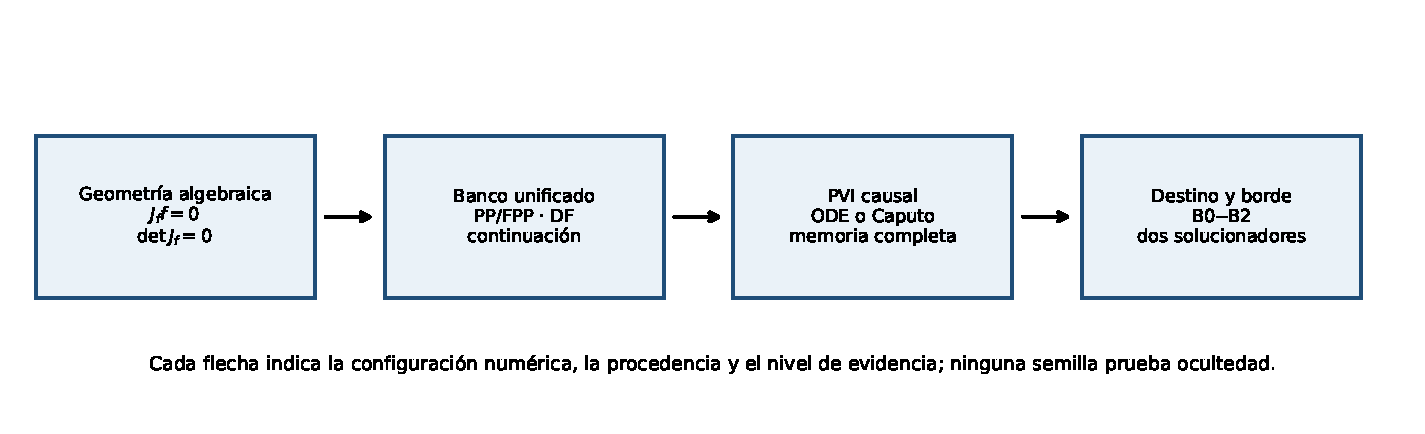
\includegraphics[width=0.96\linewidth]{figures/geometric_topological_pilot/00_ruta_geometrico_topologica.pdf}

\smallskip
\small\textbf{Ruta conceptual del piloto.} La figura se conserva en las dos
ediciones porque explica la relación entre álgebra, semillas, transporte
causal, clasificación, borde y nivel de evidencia; no es una gráfica de
resultado.
\end{center}
\end{hafocommonfigure}

\subsection{De los presupuestos normalizados a tiempos físicos}
\label{subsec:pilot-tau-star}

La tabla B0--B2 de la \cref{camp:tab-budgets} está expresada en las variables
adimensionales
\begin{equation}
 \widehat h=\frac{h}{\tau_*},\qquad
 \widehat T=\frac{T}{\tau_*},
 \qquad
 h=\widehat h\,\tau_*,\quad T=\widehat T\,\tau_*.
 \label{pilot:eq-budget-dimensionalization}
\end{equation}
Aquí se documenta cómo se fijó $\tau_*$ antes de clasificar destinos. Sea
$S=\operatorname{diag}(s_1,\ldots,s_n)$ la escala declarada del estado y
\begin{equation}
 \lVert v\rVert_S=\lVert S^{-1}v\rVert_2.
 \label{pilot:eq-scaled-norm}
\end{equation}
Para cada equilibrio $E$ se calculó el espectro de $J_E=DF(E)$. Como los
autovalores de una ecuación de Caputo de orden $q$ tienen dimensión
$\mathrm{tiempo}^{-q}$, la escala espectral coherente es
\begin{equation}
 \tau_{\mathrm{esp}}
 =\left(
   \max_{E}\max_{\lambda\in\sigma(J_E),\ \lambda\ne0}|\lambda|
  \right)^{-1/q}.
 \label{pilot:eq-tau-spectral}
\end{equation}
Para $q=1$ ésta es el inverso de la tasa espectral máxima. Como control de una
escala oscilatoria se usó, sobre la rama principal de $\lambda^{1/q}$,
\begin{equation}
 \tau_{\mathrm{osc}}
 =\min_{\Im(\lambda^{1/q})\ne0}
   \frac{2\pi}{|\Im(\lambda^{1/q})|}.
 \label{pilot:eq-tau-oscillatory}
\end{equation}
En Caputo esta cantidad es una escala lineal de comparación, no la afirmación
de que exista una órbita periódica exacta.

La tercera escala procede directamente de la expansión Picard--Caputo. Para
una condición de reinicio $X_0$,
\begin{equation}
 S^{-1}[X(t_0+h)-X_0]
 =\frac{h^q}{\Gamma(q+1)}S^{-1}F(X_0)+O(h^{2q}).
 \label{pilot:eq-scaled-picard-crossing}
\end{equation}
Igualando a uno la norma del término principal se obtiene el tiempo de cruce
escalado
\begin{equation}
 \tau_{\mathrm{cr}}^{(q)}(X_0)
 =\left[
   \frac{\Gamma(q+1)}{\lVert F(X_0)\rVert_S}
  \right]^{1/q},
 \qquad
 \tau_{\mathrm{cr}}
 =\min_{X_0\in\mathcal S_{\mathrm{core}}}
   \tau_{\mathrm{cr}}^{(q)}(X_0).
 \label{pilot:eq-tau-crossing}
\end{equation}
Finalmente se fijó, sin mirar las clasificaciones posteriores,
\begin{equation}
 \tau_*=\min\{\tau_{\mathrm{esp}},\tau_{\mathrm{osc}},
                    \tau_{\mathrm{cr}}\}.
 \label{pilot:eq-tau-star}
\end{equation}

Los cálculos que activaron cada mínimo fueron los siguientes:
\begingroup
\footnotesize
\begin{longtable}{@{}L{2.0cm}C{2.25cm}C{2.25cm}C{2.25cm}L{4.4cm}@{}}
\caption{Derivación de $\tau_*$ para los tres casos.}
\label{pilot:tab-tau-star}\\
\toprule
Caso & $\tau_{\mathrm{esp}}$ & $\tau_{\mathrm{osc}}$ &
$\tau_{\mathrm{cr}}$ & Mínimo activo\\
\midrule
\endfirsthead
\toprule
Caso & $\tau_{\mathrm{esp}}$ & $\tau_{\mathrm{osc}}$ &
$\tau_{\mathrm{cr}}$ & Mínimo activo\\
\midrule
\endhead
PLL & $0.01369498063$ & $0.1550565455$ & $0.007324767204$ &
Cruce de $p_-$; $\lVert F(p_-)\rVert_S=136.5231102$.\\
MAVPD & $0.04262239251$ & $0.4812521201$ & $0.04702913869$ &
Espectral; $\max|\lambda|=23.46184579$.\\
Wu, $q=0.99$ & $0.2704709949$ & $2.295153098$ & $0.5755679794$ &
Espectral; $\max|\lambda|=3.649223883$ y el cruce se calculó sobre el banco
central FPP--A/FDF.\\
\bottomrule
\end{longtable}
\endgroup

En Wu, las semillas IDF transferidas y las condiciones ADM publicadas se
mantuvieron como controles externos al banco central que fijó la escala. No se
les permitió cambiar el contrato después de añadirlas. Si se incluye la
condición ADM de gran amplitud en el mínimo de
\eqref{pilot:eq-tau-crossing}, se obtiene $0.09700513591$; esta sensibilidad
queda como prueba de estrés pendiente. No invalida EV--TG2, pero impide usar el
piloto como argumento de convergencia uniforme sobre bancos arbitrariamente
ampliados.

Los presupuestos físicos efectivamente integrados fueron:
\begingroup
\tiny
\begin{longtable}{@{}L{1.8cm}C{0.7cm}C{2.05cm}C{2.15cm}C{2.15cm}C{1.8cm}C{1.1cm}@{}}
\caption{Paso, horizonte y descarte físico derivados de
\eqref{pilot:eq-budget-dimensionalization}.}
\label{pilot:tab-physical-budgets}\\
\toprule
Caso & Nivel & $\tau_*$ & $h$ & $T$ & $T_{\rm burn}$ & $N$\\
\midrule
\endfirsthead
\toprule
Caso & Nivel & $\tau_*$ & $h$ & $T$ & $T_{\rm burn}$ & $N$\\
\midrule
\endhead
PLL & B0 & $7.3247672\,10^{-3}$ & $1.46495344\,10^{-4}$ & $0.36623836$ & $0.18311918$ & 2500\\
PLL & B1 & $7.3247672\,10^{-3}$ & $7.3247672\,10^{-5}$ & $0.73247672$ & $0.36623836$ & 10000\\
PLL & B2 & $7.3247672\,10^{-3}$ & $3.6623836\,10^{-5}$ & $1.46495344$ & $0.878972064$ & 40000\\
MAVPD & B0 & $4.262239251\,10^{-2}$ & $8.524478502\,10^{-4}$ & $2.131119626$ & $1.065559813$ & 2500\\
MAVPD & B1 & $4.262239251\,10^{-2}$ & $4.262239251\,10^{-4}$ & $4.262239251$ & $2.131119626$ & 10000\\
MAVPD & B2 & $4.262239251\,10^{-2}$ & $2.131119626\,10^{-4}$ & $8.524478502$ & $5.114687101$ & 40000\\
Wu & B0 & $0.2704709949$ & $5.409419898\,10^{-3}$ & $13.52354975$ & $6.761774872$ & 2500\\
Wu & B1 & $0.2704709949$ & $2.704709949\,10^{-3}$ & $27.04709949$ & $13.52354975$ & 10000\\
Wu & B2 & $0.2704709949$ & $1.352354974\,10^{-3}$ & $54.09419898$ & $32.45651939$ & 40000\\
\bottomrule
\end{longtable}
\endgroup

En los dos casos enteros, DOP853 con
$(\mathrm{rtol},\mathrm{atol})=(10^{-10},10^{-12})$ fue el solucionador
principal y RK4 de paso fijo $h/2$ fue el control independiente. En Wu se
compararon ABM--PECE y EFORK--3 nativos, ambos desde $t_0=0$, con la misma
condición de reinicio y memoria completa; no hubo truncamiento de memoria ni
retroceso de terminal inferior.

\subsection{Álgebra de los PP enteros y de la semilla FPP--A}
\label{subsec:pilot-pp-algebra}

Para una ODE autónoma $\dot X=F(X)$,
\begin{equation}
 \ddot X=DF(X)\dot X=J(X)F(X)=A(X).
 \label{pilot:eq-integer-acceleration}
\end{equation}
Un punto perpetuo entero satisface $A(p)=0$ y $F(p)\ne0$. La segunda condición
es esencial: un equilibrio también anula $JF$, pero no es un PP.

\subsubsection{PLL en el cilindro}

Con $T=\tau_1+\tau_2$, el campo del PLL de \eqref{int:eq:pll} puede escribirse
en sus coordenadas físicas como
\begin{equation}
 F_x=\frac{-x+(\tau_1/2)\sin\theta}{T},\qquad
 F_\theta=\omega_\Delta-\frac{L}{T}x
 -\frac{L\tau_2}{2T}\sin\theta.
 \label{pilot:eq-pll-field}
\end{equation}
Al multiplicar por el Jacobiano,
\begin{equation}
 A_x=\frac{-F_x+(\tau_1/2)\cos\theta F_\theta}{T},
 \qquad
 A_\theta=-\frac{L}{T}
 \left[F_x+\frac{\tau_2}{2}\cos\theta F_\theta\right].
 \label{pilot:eq-pll-acceleration}
\end{equation}
Sumar las dos ecuaciones lineales en $F_x$ muestra que, si $F\ne0$, debe
cumplirse $\cos\theta=0$; equivalentemente,
$\det J=L\cos\theta/(2T)=0$. Sustituyendo
$\theta=\pi/2,3\pi/2$ en $A=0$ se obtienen
\begin{equation}
 p_1=(\tau_1/2,\pi/2),\qquad
 p_2=(-\tau_1/2,3\pi/2),
 \label{pilot:eq-pll-pp-original}
\end{equation}
si $\omega_\Delta\mp L/2\ne0$. Wolfram anuló exactamente ambos vectores
$A(p_i)$. En la carta usada para integrar,
$u=x-x_e$, $v=\theta-\theta_e$, con
$(x_e,\theta_e)=(0.01602944,0.7974826998815102)$, las semillas fueron
\begin{equation}
 p_+=(0.00637056,0.7733136269133863),\qquad
 p_-=(-0.03842944,3.914906280503180).
 \label{pilot:eq-pll-pp-shifted}
\end{equation}
No son un par por inversión central: para $\omega_\Delta\ne0$ la simetría
correcta es la cubierta $v\mapsto v+2\pi k$.

\subsubsection{MAVPD}

Para el campo
\begin{equation}
 F_1=\delta(\gamma u+v-u^3),\quad
 F_2=u-\xi v-w,\quad F_3=\rho v,
 \label{pilot:eq-mavpd-field}
\end{equation}
la multiplicación completa da
\begin{equation}
 A_1=\delta[(\gamma-3u^2)F_1+F_2],\quad
 A_2=F_1-\xi F_2-F_3,
 \quad A_3=\rho F_2.
 \label{pilot:eq-mavpd-acceleration}
\end{equation}
De $A_3=0$ sigue $F_2=0$. Entonces $A_2=0$ implica $F_1=F_3=\rho v$ y
$A_1=0$ se reduce a
$(\gamma-3u^2)F_1=0$. La rama $F_1=0$ es estacionaria; en la rama PP,
\begin{equation}
 u_*^2=\frac\gamma3,\qquad
 \delta\left(\frac{2\gamma u_*}{3}+v_*\right)=\rho v_*.
\end{equation}
Por tanto,
\begin{equation}
 u_*=\pm\sqrt{\frac\gamma3},\qquad
 v_*=\frac{2\delta\gamma u_*}{3(\rho-\delta)},
 \qquad w_*=u_*-\xi v_*.
 \label{pilot:eq-mavpd-pp-derived}
\end{equation}
Con $(\gamma,\delta,\rho,\xi)=(0.1,100,200,3.1)$ resulta
\begin{equation}
 p_\pm=\pm(0.1825741858350554,
 0.01217161238900369,0.1448421874291439).
 \label{pilot:eq-mavpd-pp-numeric}
\end{equation}
El campo es impar, de modo que la inversión central relaciona exactamente las
dos trayectorias. El diagnóstico numérico del piloto produjo residuo impar
escalado cero, a la precisión almacenada, para DOP853 y RK4 en B2.

\subsubsection{Wu y el significado correcto de FPP--A}

Para el sistema de Wu de \cref{eq:chua_arctan,eq:parametros_wu}, sea
$h(x)=a_1x+a_2\arctan(\rho x)$. Con
\begin{equation}
 F_1=\alpha[y-x-h(x)],\quad F_2=x-y+z,\quad
 F_3=-\beta y-\gamma z,
\end{equation}
se obtiene, sin invocar una regla de cadena fraccionaria,
\begin{equation}
 A_1=\alpha[F_2-(1+h')F_1],\quad
 A_2=F_1-F_2+F_3,\quad A_3=-\beta F_2-\gamma F_3.
 \label{pilot:eq-wu-JF}
\end{equation}
Además,
\begin{equation}
 \det J(x)=-\alpha\{\beta+(\beta+\gamma)h'(x)\}.
 \label{pilot:eq-wu-detJ}
\end{equation}
En una raíz no estacionaria de $JF=0$ el Jacobiano debe ser singular. Por ello
$p=h'(x_*)=-\beta/(\beta+\gamma)$ y
\begin{equation}
 x_*^2=\frac1{\rho^2}
 \left[
  \frac{a_2\rho}{-\beta/(\beta+\gamma)-a_1}-1
 \right].
 \label{pilot:eq-wu-xstar}
\end{equation}
Definiendo $U=F_1$, las ecuaciones $A_1=A_2=0$ dan
$F_2=(1+p)U$ y $F_3=pU$. Al sustituir las definiciones de $F_i$,
\begin{equation}
 U=-\frac{\beta x_*+(\beta+\gamma)h(x_*)}
 {\gamma+(1+\gamma)p+(\beta+\gamma)/\alpha},
 \quad
 y_*=x_*+h(x_*)+\frac U\alpha,
 \quad
 z_*=h(x_*)+(1+p)U+\frac U\alpha.
 \label{pilot:eq-wu-pp-solution}
\end{equation}
Así se recupera el par validado por Wolfram
\begin{equation}
 \begin{aligned}
 p_\pm={}&\pm(0.3369817810952545,
 0.08157492826864399,\\
 &\hspace{3.3cm}-0.2549832342782551),\\
 \lVert F(p_\pm)\rVert={}&1.391241627161408,
 \end{aligned}
 \label{pilot:eq-wu-fppa-numeric}
\end{equation}
con residuo $\lVert J(p_\pm)F(p_\pm)\rVert=0$ a 68 dígitos de precisión
registrada y determinante nulo a 68 dígitos.

La razón para llamarlas FPP--A en Caputo no es que
${}^{\mathrm C}D^q({}^{\mathrm C}D^qX)=0$. Desde Volterra y una iteración de
Picard,
\begin{equation}
 X(t_0+h)=X_0+
 \frac{h^q}{\Gamma(q+1)}F_0+
 \frac{h^{2q}}{\Gamma(2q+1)}J_0F_0+O(h^{3q}).
 \label{pilot:eq-wu-picard-expansion}
\end{equation}
Por tanto $J_0F_0=0$ cancela el primer término de curvatura del arranque. El
conjunto espacial de raíces coincide con el conjunto PP de la ODE asociada y
es independiente de $q$; los pesos temporales y la evolución causal sí dependen
de $q$. No se afirma que una FPP--A sea una aceleración global nula ni un evento
FPP--H dependiente de historia.

\subsection{Compuertas de promoción empleadas}
\label{subsec:pilot-gates}

Cada corrida debía permanecer finita y dentro del radio declarado para obtener
EV--TG2. Para una semilla individual, la promoción a EV--TG3 exigió
simultáneamente:
\begin{enumerate}
 \item coincidencia del destino resuelto entre los dos solucionadores;
 \item error escalado en $0\le t\le10\tau_*$ no mayor que $10^{-3}$;
 \item diferencia relativa de observables no mayor que $5\%$;
 \item persistencia del destino y de los observables entre B1 y B2.
\end{enumerate}
El nivel informado para un caso es el máximo alcanzado por una ruta
preregistrada; no eleva automáticamente las demás semillas. EV--TG4 requería,
además, sondeo completo de vecindades, tres brackets dinámicos no colineales y
una trayectoria de borde coevolucionada y reencuadrada. Ninguno de esos tres
requisitos se completó.

\subsection{Resultados del PLL: una ruta EV--TG3 y borde rechazado}
\label{subsec:pilot-pll-results}

La semilla $p_+$ convergió al equilibrio conocido $E_{\rm focus}$ en B0, B1 y
B2 con ambos solucionadores. En B2, el error corto DOP853--RK4 fue
$2.16\,10^{-15}$, la diferencia de observables entre solucionadores fue
$1.12\,10^{-18}$ y la variación B1--B2 fue $2.48\,10^{-6}$. Esta ruta satisface
EV--TG3.

La semilla $p_-$ permaneció acotada y ambos solucionadores concordaron
numéricamente hasta B2: el error corto bajó de $2.73\,10^{-10}$ en B0 a
$1.09\,10^{-12}$ en B2. Sin embargo, el destino permaneció transitorio y sin
resolución terminal; la coincidencia numérica no sustituye una
asignación terminal. Por ello esta ruta permanece en EV--TG2. Las semillas del
ciclo y del separador también quedaron transitorias bajo los horizontes físicos
de esta normalización.

El bracket preregistrado alrededor de
$(-0.0104934812033,-0.7974826998815)$ tenía extremos separados por
$2\,10^{-5}$ en $u$, es decir anchura cilíndrica escalada
$8.928571\,10^{-4}$. Como ambos extremos siguieron sin destino terminal en B1,
la bisección se rechazó porque sus extremos no tenían destino resuelto; no se
redujo la anchura y no se
construyó una órbita de borde.

\subsection{Resultados del MAVPD: los PP localizan ciclos interiores}
\label{subsec:pilot-mavpd-results}

Los dos PP tuvieron un resultado geométricamente informativo: $p_+$ alcanzó
la nube interna positiva y $p_-$ la nube interna negativa en B1 y B2, con
DOP853 y RK4.
Para $p_+$ en B2, el error corto fue $2.68\,10^{-14}$ y la diferencia entre
solucionadores en el mismo presupuesto fue $2.66\,10^{-6}$. No obstante, la
diferencia de observables B1--B2 fue $0.262445>0.05$; por la compuerta
predeclarada, la ruta no puede subir a EV--TG3. Las semillas DF de la segunda
rama sí alcanzaron el ciclo exterior de referencia en B1--B2, pero su deriva de
horizonte fue $0.106908>0.05$. El nivel máximo del caso permanece EV--TG2.

El segmento de borde entre $p_+$ y la semilla DF exterior comenzó con anchura
escalada $1.450687592$. El primer punto medio fue clasificado como ciclo
exterior y redujo la anchura a $0.7253437961$. El segundo punto medio,
$(0.3081709798,0.05226056362,0.4511123215)$, cayó en el tercer destino, el ciclo
interior negativo de referencia. La bisección binaria se detuvo por la aparición
de ese tercer destino. Esto revela que el segmento no separa sólo dos
cuencas; no demuestra Wada y obliga a estratificar la región antes de reanudar
edge tracking.

\subsection{Resultados de Wu: primera prueba causal desde FPP--A}
\label{subsec:pilot-wu-results}

El banco Caputo comparó el par FPP--A con dos ramas de función descriptiva
fraccionaria, dos semillas obtenidas de la transferencia entera y las
condiciones iniciales ADM publicadas en \cite{Wu2023ArctanChua}. Todas las
corridas usaron $q=0.99$, $t_0=0$ y memoria completa. Las parejas por inversión
central FPP--A tuvieron residuo impar escalado exactamente cero, a la precisión
almacenada, con ABM y EFORK--3 en B0 y B2.

El resultado específico proveniente de puntos perpetuos fraccionarios es:
\begin{equation}
 p_\pm\xrightarrow[\text{ABM y EFORK--3}]{\mathrm{B0,B2}}
 \text{destino transitorio no resuelto},\qquad \text{trayectorias acotadas}.
 \label{pilot:eq-wu-fppa-destination}
\end{equation}
Para $p_+$, el error corto entre solucionadores fue $0.05360$, $0.05397$ y
$0.05420$ en B0, B1 y B2, respectivamente; todos exceden $10^{-3}$. Aunque la
variación de observables B1--B2 fue $0.01977$ para ABM y $0.04438$ para
EFORK--3, el destino no se resolvió. La ruta FPP--A obtiene EV--TG2 y no
EV--TG3. Este resultado negativo es útil: la anulación algebraica del término
$h^{2q}$ no selecciona por sí sola una cuenca recurrente en el horizonte
probado.

Las semillas FDF2, IDF2 y ADM publicadas produjeron colas acotadas recurrentes,
pero en B2 ABM las clasificó en varios casos como periódicas sin identificar el
destino, mientras EFORK--3 las mantuvo como recurrentes sin identificarlo. La
discrepancia impide promoción. Además, en Caputo toda clasificación periódica
significa únicamente
\emph{casi periodicidad proyectada a tiempo finito}; no afirma la existencia de
una órbita periódica exacta. El nivel máximo de Wu queda en EV--TG2.

\begingroup
\footnotesize
\begin{longtable}{@{}L{2.0cm}L{2.6cm}L{3.4cm}L{3.8cm}L{2.0cm}@{}}
\caption{Síntesis de destinos y compuertas del primer piloto.}
\label{pilot:tab-results-summary}\\
\toprule
Caso & Ruta & Destino observado & Compuerta decisiva & Nivel\\
\midrule
\endfirsthead
\toprule
Caso & Ruta & Destino observado & Compuerta decisiva & Nivel\\
\midrule
\endhead
PLL & PP $p_+$ & Equilibrio $E_{\rm focus}$ & Destino y observables robustos B0--B2 & EV--TG3\\
PLL & PP $p_-$ & Transitorio acotado sin resolver & Falta destino terminal & EV--TG2\\
PLL & bracket & Dos extremos sin resolver & Bisección rechazada antes de iterar & No EV--TG4\\
MAVPD & PP $p_\pm$ & Ciclos interiores simétricos & Deriva B1--B2 de $26.24\%$ & EV--TG2\\
MAVPD & DF exterior & Ciclo exterior de referencia & Deriva B1--B2 de $10.69\%$ & EV--TG2\\
MAVPD & bracket & Aparece un tercer destino & Segmento no binario & No EV--TG4\\
Wu & FPP--A $p_\pm$ & Transitorio acotado & Error corto ABM--EFORK $>10^{-3}$ & EV--TG2\\
Wu & FDF2, IDF2 y ADM & Recurrente o casi periódico proyectado & Desacuerdo de etiqueta en B2 & EV--TG2\\
\bottomrule
\end{longtable}
\endgroup

\subsection{Gráficas de la evidencia finita}
\label{subsec:pilot-digital-figures}

\begin{hafocommonfigure}
\begin{center}
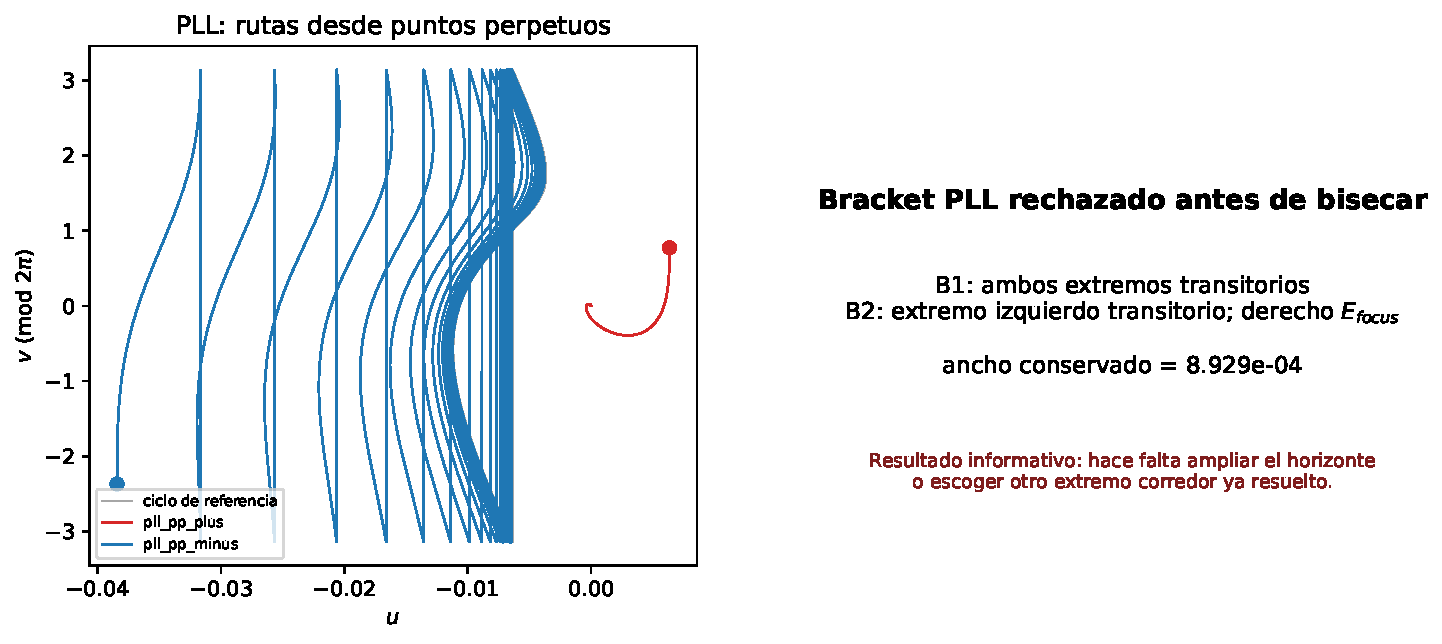
\includegraphics[width=0.96\linewidth]{figures/geometric_topological_pilot/01_pll_pp_y_borde.pdf}

\small\textbf{PLL.} Transporte de los PP y bracket inicial. Los destinos y la
anchura corresponden al contrato finito B0--B2.
\end{center}
\end{hafocommonfigure}

\begin{hafocommonfigure}
\begin{center}
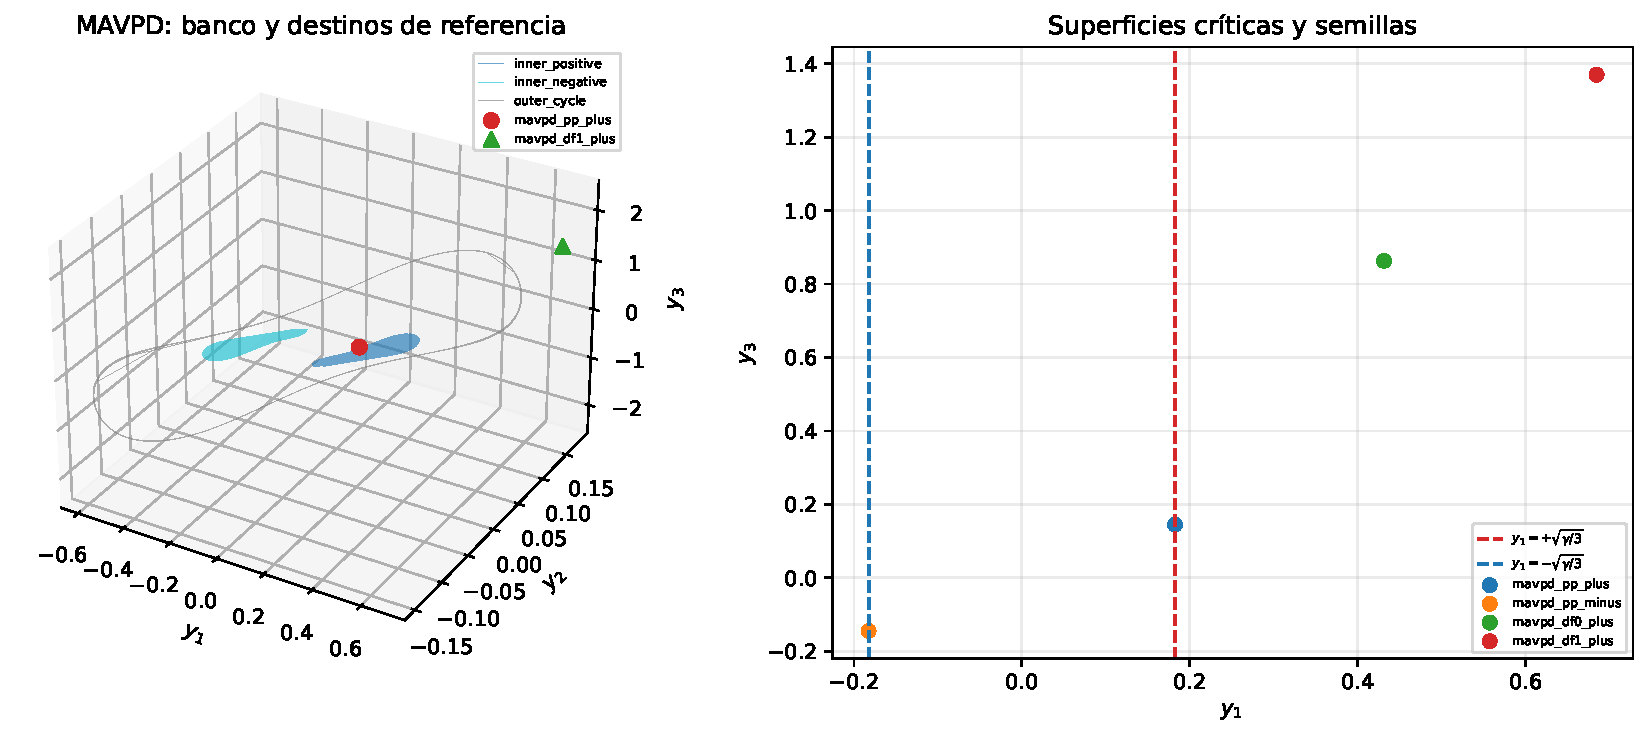
\includegraphics[width=0.96\linewidth]{figures/geometric_topological_pilot/02_mavpd_pp_superficie_destinos.pdf}

\small\textbf{MAVPD.} Superficie singular, PP, nubes de referencia y aparición
de un tercer destino sobre el segmento de borde.
\end{center}
\end{hafocommonfigure}

\begin{hafocommonfigure}
\begin{center}
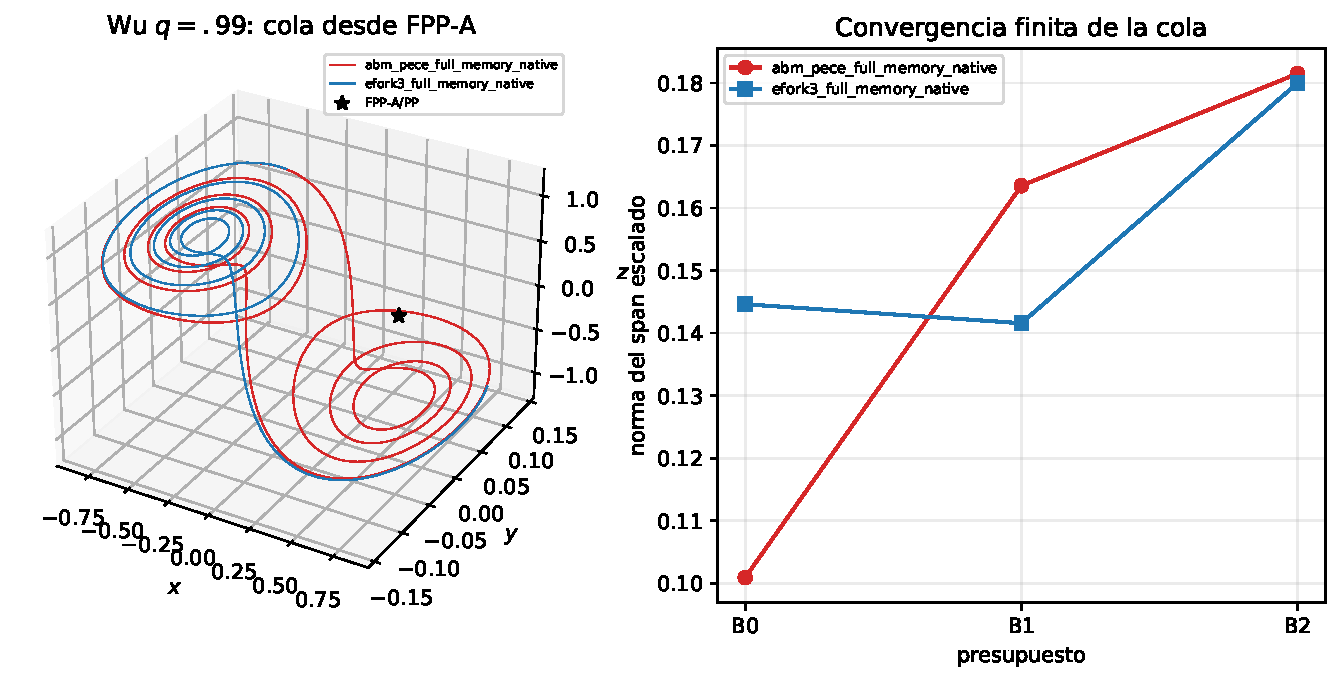
\includegraphics[width=0.96\linewidth]{figures/geometric_topological_pilot/03_wu_fpp_caputo_b0_b2.pdf}

\small\textbf{Wu, $q=0.99$.} Evolución causal con memoria completa desde el par
FPP--A. La comparación ABM--EFORK es finita y no certifica periodicidad.
\end{center}
\end{hafocommonfigure}

\begin{hafocommonfigure}
\begin{center}
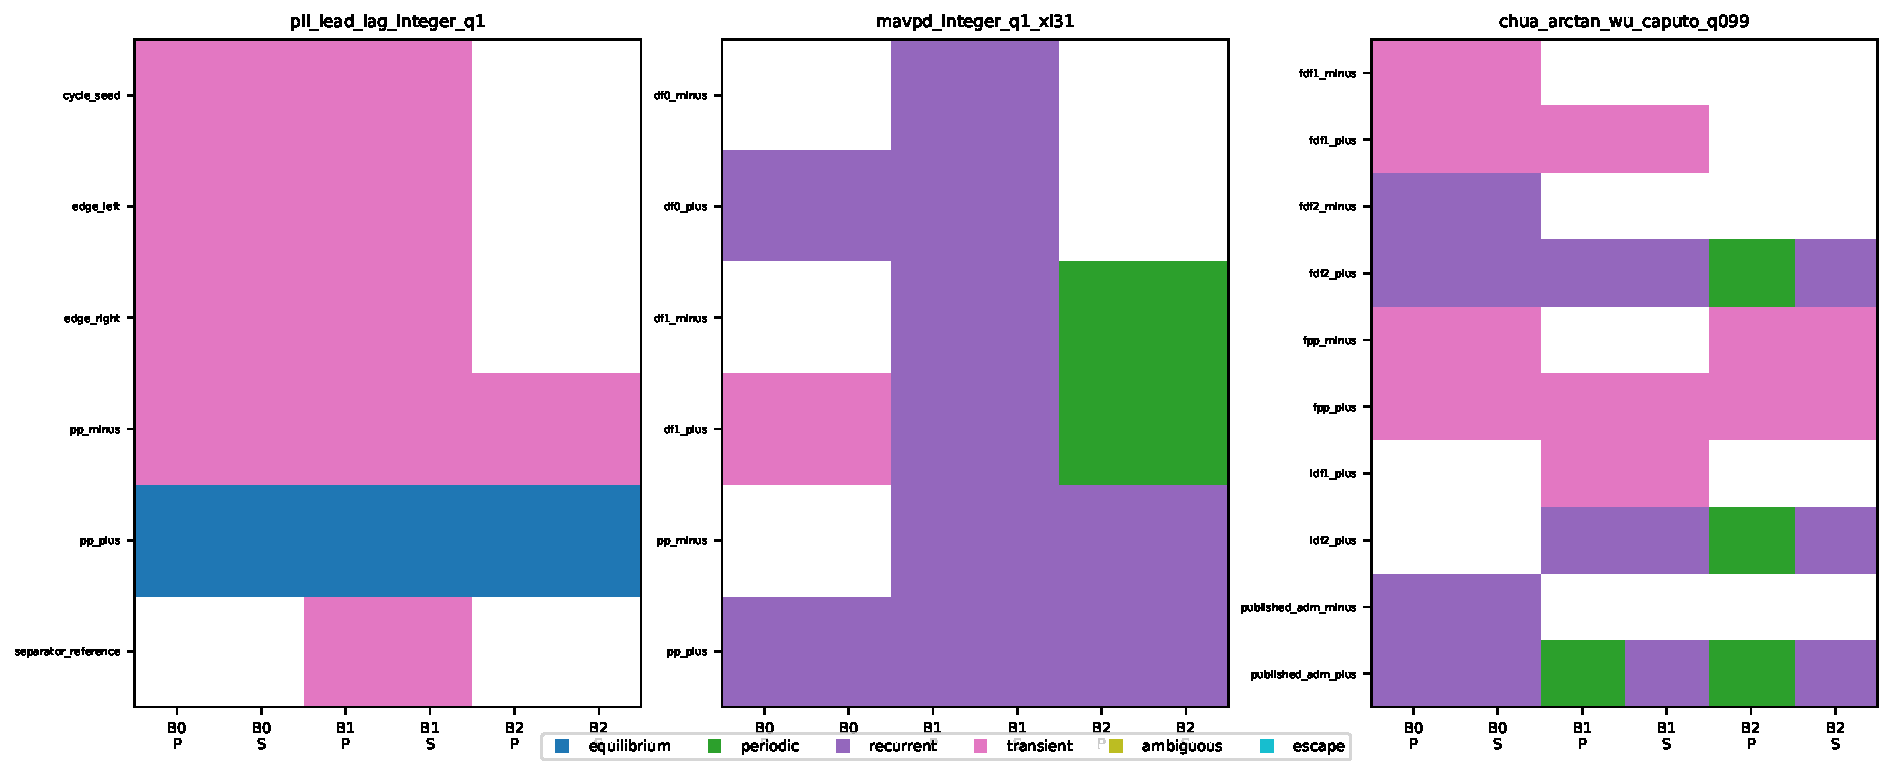
\includegraphics[width=0.96\linewidth]{figures/geometric_topological_pilot/04_matriz_destinos_b0_b2.pdf}

\small\textbf{Matriz de campaña.} Etiquetas por semilla, presupuesto y
solucionador; una celda periódica de Caputo es sólo una etiqueta proyectada.
\end{center}
\end{hafocommonfigure}

\subsection{Antecedentes, deducciones del reporte y novedad limitada}
\label{subsec:pilot-novelty}

\begin{longtable}{@{}L{3.2cm}L{4.1cm}L{5.8cm}@{}}
\caption{Separación entre antecedentes y aportes de esta campaña.}
\label{pilot:tab-novelty}\\
\toprule
Componente & Fundamento previo & Qué se aporta aquí\\
\midrule
\endfirsthead
\toprule
Componente & Fundamento previo & Qué se aporta aquí\\
\midrule
\endhead
PP entero & Definición $JF=0$, $F\ne0$, y uso como localizador
\cite{Prasad2015Perpetual,DudkowskiPrasadKapitaniak2017,
DudkowskiPrasadKapitaniak2018}. & Derivación y comparación homogénea con DF,
destinos de referencia y presupuestos B0--B2 en PLL y MAVPD; no es una nueva
definición de PP.\\
Curvas y superficies & Superficies críticas y curvas conectantes
\cite{GilmoreEtAl2010Connecting,GuanXie2021Connecting}. & Integración de esas
semillas con un banco trazable y compuertas de evidencia; no se propone un
nuevo teorema de cobertura.\\
FPP--A & Volterra y expansión Picard de Caputo; ABM causal
\cite{DiethelmFordFreed2002}. & Propuesta del reporte: interpretar $JF=0$ como
cancelación del coeficiente $h^{2q}$ y probarla como semilla de reinicio, sin
llamarla aceleración fraccionaria global.\\
Memoria & La dinámica Caputo requiere declarar terminal e historia
\cite{CongTuan2017Nonlocal,DoanKloeden2021Semidynamical}. & Comparación ABM y
EFORK--3 con el mismo $t_0$, reset y memoria completa, separada de las semillas
ADM históricas.\\
Escala $\tau_*$ & Análisis dimensional y escalas espectrales estándar. & Regla
operativa \eqref{pilot:eq-tau-star}, congelada antes de clasificar, que hace
comparables B0--B2 entre tres familias muy distintas. Es protocolo, no
invariante dinámico.\\
Niveles EV--TG & Diagnósticos numéricos y bisección de borde son técnicas
existentes. & Regla conservadora que impide convertir trayectoria, etiqueta o
bisección inicial en prueba de ocultedad o certificado topológico.\\
\bottomrule
\end{longtable}

Los números de esta sección son resultados nuevos de la campaña local, no una
reivindicación de descubrimiento bibliográfico de los modelos o de los métodos
componentes. La deducción teórica específica es el carril FPP--A basado en
\eqref{pilot:eq-wu-picard-expansion}; su utilidad observada en Wu alcanza sólo
EV--TG2.

\subsection{Qué falta para la siguiente promoción}

El siguiente paso no es etiquetar estas colas como atractores ocultos. Debe:
\begin{enumerate}
 \item ampliar el PLL hasta resolver los dos extremos antes de reiniciar el
 edge tracking;
 \item estratificar las tres cuencas encontradas en MAVPD y construir al menos
 tres brackets no colineales;
 \item repetir Wu con $h,h/2,h/4$, una ventana común más larga y un tercer
 oráculo compatible antes de interpretar las discrepancias ABM--EFORK;
 \item ejecutar B3 sólo sobre las rutas que superen esas compuertas;
 \item dejar TG7, bloques aislantes e índice de Conley para una campaña
 posterior con imágenes exteriores validadas.
\end{enumerate}


\clearpage
\ifHAFOPedagogy
  \part[Profundización y futuro]{Profundización y pruebas futuras}
\else
  \part{Síntesis y problemas abiertos}
\fi
\label{part:futuro}
\section{Criterio de selección}
\label{sec:candidate-selection}

\HAFOCardCandidates

La selección cruzó el catálogo de sistemas, los manifiestos de validación, el
manuscrito metodológico y las fuentes bibliográficas primarias. Se priorizaron
sistemas que cumplen simultáneamente:

\begin{enumerate}
 \item derivada ordinaria o Caputo conmensurable \(q\in(0,1]\);
 \item ecuaciones, parámetros, orden e iniciales publicados;
 \item no linealidades representables por D0, T1, A1 o M1;
 \item un reclamo publicado de atractor oculto, cuenca o coexistencia;
 \item tamaño compatible con ABM de memoria completa y una reproducción
 independiente;
 \item valor científico como prueba de una parte aún no cerrada del método.
\end{enumerate}

Se excluyen del carril actual sistemas incommensurables, Caputo--Fabrizio,
Atangana--Baleanu, retardados, discretos o complejos. No son imposibles, pero
su símbolo de transferencia, su condición de estabilidad y su contrato de
memoria no son intercambiables con Caputo conmensurable.

\section{Prioridad 1: sistema fraccionario sin equilibrio de Muñoz--Pacheco}
\label{sec:cand-munoz}

La fuente primaria \cite{munoz2018} propone
\begin{equation}
\begin{aligned}
 {}^{\mathrm C}D^q x&=yz+x(y-a),\\
 {}^{\mathrm C}D^q y&=1-|x|,\\
 {}^{\mathrm C}D^q z&=-xy-z.
\end{aligned}
\label{eq:cand-munoz}
\end{equation}
Para \(a=0.35,q=0.97\), publica un atractor caótico desde
\((1,1,1)\). Para \(a=0.35,q=0.996\), publica coexistencia de un candidato
caótico desde \((1,1,1)\) y uno periódico desde \((0,75,-50)\), junto con un
corte de cuenca. Esto lo convierte en el candidato fraccionario no Chua más
completo encontrado.

\subsection{Realización M1 exacta}

Con \(X=(x,y,z)^{\mathsf T}\),
\[
 \Phi(X)=(yz,xy,|x|)^{\mathsf T},
\]
se tiene
\begin{equation}
 {}^{\mathrm C}D^qX=A X+d+B\Phi(X),
 \label{eq:cand-munoz-mimo}
\end{equation}
donde
\begin{equation}
 A=\begin{pmatrix}
 -a&0&0\\0&0&0\\0&0&-1
 \end{pmatrix},\quad
 d=\begin{pmatrix}0\\1\\0\end{pmatrix},\quad
 B=\begin{pmatrix}
 1&1&0\\
 0&0&-1\\
 0&-1&0
 \end{pmatrix}.
 \label{eq:cand-munoz-matrices}
\end{equation}
La multiplicación da
\[
 AX+d+B\Phi=
 \begin{pmatrix}
 -ax+yz+xy\\1-|x|\\-z-xy
 \end{pmatrix},
\]
idéntica a \cref{eq:cand-munoz}. Wolfram devolvió el residual
\(\{0,0,0\}\).

Con \(C=I\) y \(z_f=s^q\), la matriz de transferencia es especialmente simple:
\begin{equation}
 W(z_f)=(z_fI-A)^{-1}B
 =\begin{pmatrix}
 \dfrac1{z_f+a}&\dfrac1{z_f+a}&0\\[0.8em]
 0&0&-\dfrac1{z_f}\\[0.8em]
 0&-\dfrac1{z_f+1}&0
 \end{pmatrix}.
 \label{eq:cand-munoz-transfer}
\end{equation}
El término constante \(d\) obliga a resolver el balance DC; los productos
cuadráticos generan segundo armónico y \(|x|\) exige cuadratura PWA exacta o
una homotopía suavizada. El cierre mínimo es M1 con \(H\ge2\).

\subsection{Demostración completa de ausencia de equilibrios}

En equilibrio, la segunda ecuación exige \(|x|=1\), de modo que
\(x=\pm1\neq0\). La tercera da
\[
 z=-xy.
\]
Al sustituir en la primera,
\[
 0=y(-xy)+x(y-a)
 =x(-y^2+y-a).
\]
Como \(x\neq0\), debe cumplirse
\begin{equation}
 y^2-y+a=0.
 \label{eq:cand-munoz-equilibrium}
\end{equation}
Su discriminante es
\[
 \Delta_y=1-4a.
\]
Para \(a=0.35\), \(\Delta_y=-0.4<0\); por tanto, no existe equilibrio real.
Wolfram confirmó \texttt{Reduce[...,Reals]=False}. Bajo la definición usual,
cualquier atractor del sistema es oculto por ausencia de equilibrios. Aun así,
deben reproducirse recurrencia y caos: la ausencia de equilibrios no transforma
una trayectoria transitoria o divergente en atractor.

Para \(x\neq0\), el Jacobiano regional es
\begin{equation}
 J(X)=
 \begin{pmatrix}
 y-a&z+x&y\\
 -\operatorname{sign}(x)&0&0\\
 -y&-x&-1
 \end{pmatrix}.
 \label{eq:cand-munoz-jacobian}
\end{equation}
No se aplica Matignon en equilibrios porque éstos no existen. La validación
debe concentrarse en el integrador nonsuave, la coexistencia y la robustez de
los diagnósticos.

\begin{proposalbox}
\textbf{Plan L0--L6.} Congelar \(a=0.35\), \(q=0.97\) y \(q=0.996\), las dos
iniciales y el convenio de \(|x|\); derivar coeficientes M1; resolver \(H=2,3,4\)
y controlar \(\eta_H\); continuar una semilla; integrar Caputo con memoria
completa; reproducir la cuenca \(x=0\); comparar ABM con otro integrador. Como
no hay equilibrios, L5 se sustituye por exploración de cuenca, coexistencia y
frontera de divergencia.
\end{proposalbox}

\section{Prioridad 2: jerk cuadrático entero con equilibrio estable}
\label{sec:cand-jerk}

Liu, Sang, Wang y Ahmad \cite{liu2021} estudian
\begin{equation}
 \dot x=y,\qquad
 \dot y=z,\qquad
 \dot z=-x-y-1.1z-2.59z^2+xy.
 \label{eq:cand-jerk}
\end{equation}
La fuente reporta un atractor caótico oculto desde
\((0,-1.5,0)\), además de cortes de cuenca y una realización de circuito.

\subsection{Parte lineal, equilibrio y estabilidad}

Con \(X=(x,y,z)^{\mathsf T}\),
\begin{equation}
 A=\begin{pmatrix}
 0&1&0\\0&0&1\\-1&-1&-1.1
 \end{pmatrix}.
 \label{eq:cand-jerk-A}
\end{equation}
Las dos primeras ecuaciones de equilibrio dan \(y=z=0\); la tercera da
\(x=0\). El origen es el único equilibrio. Su polinomio característico es
\begin{equation}
 p(s)=s^3+1.1s^2+s+1.
 \label{eq:cand-jerk-charpoly}
\end{equation}
El criterio de Routh--Hurwitz para un cúbico exige coeficientes positivos y
\(1.1\cdot1>1\), ambas condiciones satisfechas. El equilibrio único es
asintóticamente estable. Un atractor coexistente no puede localizarse
siguiendo la variedad inestable del origen y, si su cuenca está separada de una
vecindad del mismo, es oculto.

\subsection{Realización M1 y obstrucción escalar}

Definimos
\[
 \Phi(X)=(xy,z^2)^{\mathsf T},\qquad
 B=\begin{pmatrix}0&0\\0&0\\1&-2.59\end{pmatrix}.
\]
Entonces
\[
 AX+B\Phi(X)=
 (y,z,-x-y-1.1z+xy-2.59z^2)^{\mathsf T},
\]
y Wolfram devuelve residual nulo.

Aunque los dos canales actúan en la dirección \(e_3\), no pueden reducirse a
una no linealidad cuadrática de un único observable. Para
\[
 Q(x,y,z)=xy-2.59z^2
\]
se tiene
\begin{equation}
 \nabla^2Q=
 \begin{pmatrix}
 0&1&0\\1&0&0\\0&0&-5.18
 \end{pmatrix},
 \qquad \operatorname{rank}\nabla^2Q=3.
 \label{eq:cand-jerk-hessian}
\end{equation}
En cambio, \(Q=\kappa(r^{\mathsf T}X)^2\) implicaría
\(\nabla^2Q=2\kappa rr^{\mathsf T}\), de rango a lo sumo uno. Esto falsifica
D0 y justifica M1.

Como ambas entradas llegan al último estado, la transferencia es
\begin{equation}
 W(s)=\frac1{p(s)}
 \begin{pmatrix}
 1&-2.59\\
 s&-2.59s\\
 s^2&-2.59s^2
 \end{pmatrix}.
 \label{eq:cand-jerk-transfer}
\end{equation}
Los términos cuadráticos requieren DC y segundo armónico. Este sistema es,
por tanto, el primer banco entero recomendado para demostrar que M1 añade
capacidad real sobre los casos escalares ya cerrados.

\section{Prioridad 3: sistema Liu extendido fraccionario}
\label{sec:cand-extended-liu}

La fuente \cite{wang2020} usa
\begin{equation}
\begin{aligned}
 {}^{\mathrm C}D^q x&=a(y-x),\\
 {}^{\mathrm C}D^q y&=bx-kxz+d\,\operatorname{sign}(w)+m,\\
 {}^{\mathrm C}D^q z&=-cz+hx^2,\\
 {}^{\mathrm C}D^q w&=-gy.
\end{aligned}
\label{eq:cand-liu}
\end{equation}
Una realización exacta usa
\[
 \Phi=(xz,x^2,\operatorname{sign}w)^{\mathsf T},
\]
\[
 A=\begin{pmatrix}
 -a&a&0&0\\ b&0&0&0\\0&0&-c&0\\0&-g&0&0
 \end{pmatrix},\quad
 d_0=(0,m,0,0)^{\mathsf T},
\]
\[
 B=\begin{pmatrix}
 0&0&0\\-k&0&d\\0&h&0\\0&0&0
 \end{pmatrix}.
\]
Wolfram confirmó el residual nulo.

Para \(a=10,b=40,c=2.5,k=1,h=4,g=5,d=m=20\), las ecuaciones de equilibrio
dan sucesivamente \(y=x\), \(y=0\), \(x=0\), \(z=0\), y
\[
 20\,\operatorname{sign}(w)+20=0.
\]
Con \(\operatorname{sign}(0)=0\), la solución es la semirrecta
\begin{equation}
 x=y=z=0,\qquad w<0,
 \label{eq:cand-liu-equilibria}
\end{equation}
no un sistema sin equilibrios. Antes de promover el caso deben congelarse
\(q\), la rama dinámica, las iniciales, la convención en \(w=0\) y el protocolo
para una variedad continua de equilibrios.

\section{Cola interna y controles}
\label{sec:candidate-queue}

\begin{longtable}{@{}L{0.23\linewidth}L{0.20\linewidth}L{0.24\linewidth}L{0.25\linewidth}@{}}
\caption{Portafolio compatible y requisito de promoción.}
\label{tab:candidate-portfolio}\\
\toprule
Familia & Ruta estructural & Activo disponible & Falta decisiva\\
\midrule
\endfirsthead
\toprule
Familia & Ruta estructural & Activo disponible & Falta decisiva\\
\midrule
\endhead
Leonov--Kuznetsov (162) & D0+A1 & Ecuaciones y semilla parciales &
Congelar característica PWA y criterio por etapa.\\
Genesio--Tesi & D0 sesgado, \(H\ge2\) & Realización
\(\psi(x)=x^2\) & Parámetros, iniciales y manifiesto L0 congelados.\\
Jerk con seno hiperbólico & D0, DF con \(I_1\) & Derivación simbólica &
Resolver ambigüedad de fuente \(\sinh\) frente a función inversa.\\
Oscilador memristivo & T1 sobre variedad & Cierre cúbico sesgado &
Constante de la variedad, parámetros e iniciales.\\
Jerk PWA & D0 PWA & Estructura tipo Chua & Congelar fuente; usar como control
de generalización, no como familia distante.\\
Fischer jerk exponencial & D0 con DC & Parámetros y diagnóstico &
Control bibliográfico/Lyapunov; clasificación de cuenca no reproducida
localmente.\\
Lorenz generalizado & M1, \(H\ge2\) & Álgebra completa de este reporte &
Raíz armónica, continuación, integración y cuenca.\\
Rabinovich--Fabrikant & M1, \(H\ge3\) & Álgebra completa de este reporte &
Raíz armónica, continuación, integración y cuenca.\\
Sistema financiero Fischer & M1+PWA & Banco Lyapunov & Resolver discrepancias
y separar del modelo financiero del manuscrito.\\
Four-wing Fischer & M1 cuadrático & Banco Lyapunov & Semilla y búsqueda de
ocultamiento inexistentes.\\
Debbouche fraccionario & M1+signo & DOI y parámetros parciales
\cite{debbouche2021} & Congelar ecuaciones, órdenes e iniciales de una rama.\\
\bottomrule
\end{longtable}

\section{Orden recomendado de ejecución}
\label{sec:candidate-order}

\begin{enumerate}
 \item ejecutar primero el jerk cuadrático entero: elimina el costo de memoria
 fraccionaria y prueba de forma limpia el salto D0 \(\to\) M1;
 \item ejecutar después el sistema de Muñoz--Pacheco: prueba M1, nonsuavidad,
 Caputo y coexistencia, con ecuaciones e iniciales publicadas;
 \item resolver el balance multiharmónico de Lorenz generalizado y RF usando
 las realizaciones ya auditadas, sin prometer ocultedad hasta L5;
 \item cerrar Genesio--Tesi como control escalar sesgado;
 \item dejar Liu extendido y Debbouche para una segunda ola, porque las
 variedades de equilibrio y el signo introducen contratos adicionales.
\end{enumerate}

Esta secuencia maximiza información científica por costo: primero falsifica o
confirma la extensión M1 en ODE, luego añade memoria Caputo y nonsuavidad, y
sólo después aborda los casos bibliográficos cuya semilla no está publicada.

\begingroup
\def\HAFOGeoPosteriorOnly{1}
\ifdefined\HAFOGeoPosteriorOnly\else
\section{Propósito y alcance geométrico--topológico}
\label{sec:geo-proposito}

Los capítulos anteriores responden principalmente preguntas algebraicas y
numéricas: cómo realizar un sistema en forma de Lur'e, cómo producir una
semilla, cómo continuarla y qué diagnósticos calcular. La teoría geométrica y
topológica cambia el centro de atención. En lugar de preguntar solamente
«¿cuál es la trayectoria?», pregunta:

\begin{itemize}
  \item ¿sobre qué espacio vive el sistema y qué estructura de ese espacio
        debe respetarse?;
  \item ¿qué conjuntos transporta el flujo en sí mismos?;
  \item ¿qué propiedades sobreviven a un cambio de coordenadas o a una
        reparametrización del tiempo?;
  \item ¿cómo están organizadas las cuencas, sus fronteras y las separatrices?;
  \item ¿qué mecanismo geométrico podría sostener la periodicidad o el caos?;
  \item ¿qué parte de una conclusión procede de un teorema y qué parte es sólo
        evidencia computacional finita?
\end{itemize}

\ifHAFOPedagogy
\subsection{Objetivos de aprendizaje}

Al terminar esta guía, el lector debería poder:

\begin{enumerate}
  \item identificar correctamente el espacio de fases de Chua, MAVPD,
        Kalman--Fitts y PLL;
  \item definir flujo, órbita, invariancia, conjunto \(\omega\)-límite,
        atractor, cuenca y frontera de cuenca;
  \item distinguir conjugación topológica de equivalencia orbital;
  \item usar la linealización y los teoremas de Hartman--Grobman y de la
        variedad estable sólo cuando se cumplen sus hipótesis;
  \item construir una sección de Poincaré y relacionar su derivada con los
        multiplicadores de Floquet;
  \item reconocer qué faltaría para convertir una nube de retornos en una
        prueba de homoclinicidad o de herradura;
  \item usar índice y grado topológico como herramientas de existencia, sin
        confundir existencia con atracción u ocultedad;
  \item redactar cada conclusión separando visualización, evidencia numérica y
        demostración.
\end{enumerate}

\subsection{Lectura previa exacta}

Antes de continuar, complete las etapas 1--5 de
\cref{sec:programa-estudio-bibliografico}. Allí se indican páginas impresas de
los cuatro libros físicos, páginas del visor de los PDF locales, ejercicios y
una comprobación para decidir si puede avanzar. El orden mínimo es
\[
\text{campo y flujo}
\longrightarrow \text{espacio de fases}
\longrightarrow \text{Poincaré--Floquet}
\longrightarrow \text{grado}
\longrightarrow \text{caos y cuencas}.
\]
No empiece por conexiones, curvatura o geometría fractal: esas lecturas son de
profundización y aparecen al final de la ruta.
\fi

\subsection{Escalera de afirmaciones}
\label{geo:subsec:escalera}

Para evitar que una gráfica cargue más significado del que posee, se usará la
siguiente escalera.

\begin{table}[H]
\centering
\caption{Niveles de una afirmación geométrica o topológica.}
\label{geo:tab:niveles-evidencia}
\small
\begin{tabularx}{\textwidth}{@{}L{0.12\textwidth}L{0.22\textwidth}YY@{}}
\toprule
Nivel & Producto & Qué permite decir & Qué no permite decir \\
\midrule
G0 & Visualización & Sugiere una órbita, una separación o una estructura que
merece formularse. & No prueba invariancia, convergencia, caos ni ocultedad. \\
G1 & Evidencia numérica reproducible & Apoya una propiedad dentro de un
horizonte, tolerancias, dominio y conjunto de semillas declarados. & No cubre
tiempo infinito ni un continuo de condiciones iniciales. \\
G2 & Teorema local con hipótesis verificadas & Demuestra una conclusión local:
hiperbolicidad, dimensión de variedades o estabilidad de un ciclo, por
ejemplo. & No clasifica automáticamente la cuenca global. \\
G3 & Argumento global o prueba asistida & Certifica una propiedad en un dominio
mediante grado, regiones atrapantes, cotas rigurosas o intersecciones
transversales encerradas. & No debe extenderse fuera del dominio certificado.
\\
\bottomrule
\end{tabularx}
\end{table}

Un sistema de álgebra computacional puede establecer exactamente una identidad
algebraica y ayudar a verificar una hipótesis de G2 o G3. Una integración
numérica sigue siendo G1 mientras no incluya cotas rigurosas que cubran el
continuo relevante.

\section{Lenguaje mínimo de topología y geometría diferencial}
\label{sec:geo-lenguaje}

Esta parte se restringe primero a ecuaciones autónomas de orden entero
\begin{equation}
  \dot x=f(x),\qquad x\in M,
  \label{geo:eq:edo-manifold}
\end{equation}
donde \(M\) es una variedad diferenciable, usualmente \(\R^n\) o el cilindro
\(\R\times S^1\). Esta restricción no es decorativa: el flujo y la propiedad de
grupo que se construirán aquí no se trasladan sin más a un PVI causal de
Caputo con memoria. La extensión fraccionaria debe formularse por separado.
El lenguaje topológico y diferencial de esta parte sigue
\cite{NahmadAchar2022Topologia}; la teoría de flujo y estabilidad se apoya en
\cite{JaurezEtAl2021TGEDI,JaurezEtAl2021TGEDII,HirschSmaleDevaney2013}.

\subsection{Topología: proximidad sin fijar una regla de medida}

\begin{definition}[Espacio topológico]
Un espacio topológico es un par \((M,\mathcal T)\), donde \(\mathcal T\) es una
familia de subconjuntos llamados \emph{abiertos} que contiene a
\(\varnothing\) y \(M\), es cerrada bajo uniones arbitrarias y bajo
intersecciones finitas. Una \emph{vecindad} de \(x\) es un conjunto que
contiene un abierto que contiene a \(x\).
\end{definition}

\begin{definition}[Base, separación, compacidad y conexidad]
Una familia \(\mathcal B\subset\mathcal T\) es una \emph{base} si todo abierto
es unión de elementos de \(\mathcal B\); una subbase genera una base mediante
intersecciones finitas. El espacio es \emph{Hausdorff} si dos puntos distintos
poseen vecindades disjuntas. Es \emph{compacto} si toda cubierta abierta admite
una subcubierta finita, y es \emph{conexo} si sus únicos subconjuntos que son a
la vez abiertos y cerrados son \(\varnothing\) y el espacio completo.
\end{definition}

En espacios métricos la compacidad equivale a que toda sucesión posea una
subsucesión convergente; esa equivalencia no debe trasladarse sin hipótesis a
un espacio topológico arbitrario. Compacidad controla argumentos de
extracción, mientras conexidad impide separar el objeto en dos abiertos
disjuntos no vacíos.

\begin{definition}[Producto y cociente]
La topología producto en \(M\times N\) tiene como base los conjuntos
\(U\times V\), con \(U\subset M\) y \(V\subset N\) abiertos. Dada una relación
de equivalencia \(\sim\), el cociente \(M/{\sim}\) lleva la topología para la
cual un conjunto \(W\) es abierto si \(\pi^{-1}(W)\) es abierto, donde
\(\pi:M\to M/{\sim}\) es la proyección canónica.
\end{definition}

Así, \(S^1\simeq\R/(2\pi\mathbb Z)\) identifica ángulos que difieren por una
vuelta completa, y el cilindro del PLL usa la topología producto
\(\R\times S^1\).
\ifHAFOPedagogy
Como ejercicio de dominio, pruebe que la proyección
\(\theta\mapsto(\cos\theta,\sin\theta)\) induce un homeomorfismo del cociente
sobre el círculo; señale dónde usa compacidad y la propiedad de Hausdorff.
\fi

Una métrica \(d\) produce una topología mediante sus bolas abiertas, pero la
topología conserva menos información que la métrica. Continuidad, compacidad,
conexidad y frontera son nociones topológicas; longitudes, ángulos y radios
numéricos requieren estructura adicional.

\begin{definition}[Continuidad y homeomorfismo]
Una función \(h:M\to N\) es continua si la preimagen de todo abierto de \(N\)
es abierta en \(M\). Es un \emph{homeomorfismo} si es biyectiva y tanto \(h\)
como \(h^{-1}\) son continuas.
\end{definition}

Un homeomorfismo puede estirar una bola hasta convertirla en un elipsoide, sin
romper conexidad ni vecindades. Ésta es la razón por la cual la ocultedad,
formulada mediante vecindades, puede transportarse topológicamente, mientras
que un contrato de «radio \(10^{-3}\)» no se transporta conservando el mismo
número.

\begin{definition}[Interior, clausura y frontera]
Para \(A\subset M\), su interior \(\operatorname{int}A\) es el mayor abierto
contenido en \(A\); su clausura \(\overline A\) es el menor cerrado que lo
contiene; y
\begin{equation}
  \partial A=\overline A\setminus\operatorname{int}A
  \label{geo:eq:boundary}
\end{equation}
es su frontera.
\end{definition}

La frontera de una cuenca no es la última curva coloreada por una malla. Es el
conjunto definido por~\eqref{geo:eq:boundary}; cualquier vecindad de uno de sus
puntos encuentra tanto puntos de la cuenca como puntos fuera de ella.

\subsection{Variedades, vectores tangentes y campos}

\begin{definition}[Variedad diferenciable y campo vectorial]
Una variedad diferenciable \(M\) de dimensión \(n\) es un espacio que
localmente posee coordenadas en abiertos de \(\R^n\), con cambios de carta
diferenciables. El espacio tangente en \(x\) se denota \(T_xM\). Un campo
vectorial es una asignación \(f(x)\in T_xM\) que varía con la regularidad
declarada.
\end{definition}

En \(\R^n\) se identifica \(T_x\R^n\simeq\R^n\), por lo que el vector
\(f(x)\) se dibuja con origen en \(x\). En el PLL, en cambio,
\begin{equation}
  M_{\mathrm{PLL}}=\R\times S^1,
  \label{geo:eq:pll-phase-space}
\end{equation}
y los pares \((x,\theta)\) y \((x,\theta+2\pi k)\) representan el mismo estado.
El rectángulo dibujado en el plano es sólo una carta cortada y pegada por sus
bordes angulares.

Una distancia compatible útil para visualización y comparación numérica es
\begin{equation}
 d_{\mathrm{cil}}((x,\theta),(\tilde x,\tilde\theta))
 =\sqrt{(x-\tilde x)^2+
 \operatorname{wrap}_{-\pi\le\,\cdot\,<\pi}(\theta-\tilde\theta)^2}.
 \label{geo:eq:cylindrical-distance}
\end{equation}
No es legítimo usar \(|\theta-\tilde\theta|\) sin envolver y después atribuir
significado topológico al salto artificial en \(\pm\pi\).

\paragraph{De cartas a formas.}
Una carta es un homeomorfismo \(\phi:U\to\phi(U)\subset\R^n\); un atlas de
clase \(C^r\) exige que los cambios \(\psi\circ\phi^{-1}\) sean \(C^r\). Una
subvariedad se reconoce localmente por coordenadas en las que queda descrita
por la anulación de algunas componentes. El cotangente \(T_x^*M\) es el dual
de \(T_xM\), y una \(k\)-forma es una sección de \(\Lambda^kT^*M\). El
producto exterior, la derivada exterior y el pull-back permiten formular
integración y Stokes sin depender de una carta; una orientación selecciona
atlas cuyas transiciones conservan orientación
\cite{NahmadAchar2022Topologia}. La subsección sobre formas retomará estos
objetos para convertir divergencia en balance de flujo.

\ifHAFOPedagogy
\paragraph{Ejercicio de enlace.}
Para \(h(r,\theta)=(r\cos\theta,r\sin\theta)\), calcule
\(h^*(\dd x\wedge\dd y)\), identifique dónde deja de ser una carta y explique
qué información de orientación contiene el signo del jacobiano.
\fi

\subsection{Cambio de coordenadas como transporte de un campo}

Sea \(h:M\to N\) un difeomorfismo y \(y=h(x)\). Por la regla de la cadena,
el campo transformado es
\begin{equation}
  g(y)=D h(h^{-1}(y))f(h^{-1}(y)).
  \label{geo:eq:pushforward}
\end{equation}
Esta ecuación es el \emph{empuje hacia delante} del campo, \(g=h_*f\). No
basta cambiar los nombres de las variables: el diferencial \(Dh\) es parte de
la transformación.

\begin{proposition}[Transporte de curvas integrales]
Supóngase que \(h\) es un difeomorfismo y que \(x(t)\) resuelve
\(\dot x=f(x)\). Entonces \(y(t)=h(x(t))\) resuelve
\(\dot y=g(y)\), con \(g\) dado por~\eqref{geo:eq:pushforward}.
\end{proposition}

\begin{proof}
La regla de la cadena da
\[
 \dot y(t)=Dh(x(t))\dot x(t)=Dh(x(t))f(x(t))=g(h(x(t))).
\]
Como \(y(t)=h(x(t))\), se obtiene la ecuación afirmada.
\end{proof}

Para una transformación afín \(x=Tz+c\), una bola física alrededor de
\(x_e\) se convierte en
\begin{equation}
 (z-z_e)^{\mathsf T}T^{\mathsf T}T(z-z_e)\le r^2.
 \label{geo:eq:ball-to-ellipsoid}
\end{equation}
Así se conecta la equivalencia afín ya usada por las realizaciones D0/T1 con
la geometría de los contratos de cuenca.

\subsection{Regularidad de los cuatro casos enteros}

\begin{table}[H]
\centering
\caption{Espacio de fases y regularidad relevante.}
\label{geo:tab:regularity-cases}
\small
\begin{tabularx}{\textwidth}{@{}L{0.18\textwidth}L{0.16\textwidth}L{0.25\textwidth}Y@{}}
\toprule
Caso & Espacio & Regularidad & Precaución geométrica \\
\midrule
Chua PWL & \(\R^3\) & Campo continuo y globalmente Lipschitz; suave por
regiones & \(Df\) salta en \(x=\pm1\); los teoremas \(C^1\) deben aplicarse por
regiones o con una versión no suave. \\
MAVPD & \(\R^3\) & Campo polinómico \(C^\infty\) & La existencia global no se
deduce de que el campo sea polinómico; se requieren cotas de no explosión o
una región atrapante para la órbita considerada. \\
Kalman--Fitts & \(\R^4\) & Campo \(C^\infty\), con no linealidad
\(\tanh\) globalmente Lipschitz & Una sección de Poincaré es tridimensional;
un retrato en dos coordenadas es sólo una proyección. \\
PLL lead--lag & \(\R\times S^1\) & Campo \(C^\infty\) en el cilindro & Deben
envolverse ángulos, retornos y vecindades; una órbita corredora es cerrada en
el cilindro aunque no lo parezca en el recubrimiento \(\R^2\). \\
\bottomrule
\end{tabularx}
\end{table}

\section{Del problema de valor inicial al flujo}
\label{sec:geo-flujo}

\subsection{Existencia, unicidad y dependencia de la condición inicial}

\begin{proposition}[Picard--Lindelöf local, forma usada aquí]
Sea \(f:U\subset\R^n\to\R^n\) localmente Lipschitz. Para cada
\(x_0\in U\) existe una única solución maximal
\(x(\,\cdot\,;x_0)\) de~\eqref{geo:eq:edo-manifold} definida en un intervalo
abierto que contiene a \(0\). La solución depende continuamente de \(x_0\) en
cualquier rectángulo compacto donde permanezcan las soluciones.
\end{proposition}

La hipótesis de unicidad es el fundamento de la geometría de órbitas: dos
trayectorias distintas no pueden cruzarse en el mismo instante y estado. La
existencia local no implica existencia para todo \(t\in\R\). Un campo con
crecimiento a lo sumo lineal sí proporciona una vía estándar hacia completitud
global; para campos polinómicos de grado mayor se necesitan cotas adicionales.

\begin{definition}[Flujo local y flujo completo]
El flujo local asociado con~\eqref{geo:eq:edo-manifold} es
\begin{equation}
 \varphi_t(x_0)=x(t;x_0),
 \label{geo:eq:flow}
\end{equation}
en el dominio donde existe la solución. Es un flujo completo si está definido
para todo \((t,x)\in\R\times M\) y satisface
\begin{equation}
 \varphi_0=\operatorname{id},\qquad
 \varphi_{t+s}=\varphi_t\circ\varphi_s,
 \qquad \varphi_{-t}=\varphi_t^{-1}.
 \label{geo:eq:flow-group}
\end{equation}
\end{definition}

\begin{proposition}[La unicidad produce la propiedad de flujo]
Si las dos composiciones están definidas, entonces
\(\varphi_{t+s}(x)=\varphi_t(\varphi_s(x))\).
\end{proposition}

\begin{proof}
Las curvas \(u(t)=\varphi_{t+s}(x)\) y
\(v(t)=\varphi_t(\varphi_s(x))\) resuelven la misma ecuación autónoma y
satisfacen \(u(0)=v(0)=\varphi_s(x)\). La unicidad implica \(u=v\).
\end{proof}

\begin{remark}[Por qué autonomía importa]
En una ecuación no autónoma \(\dot x=f(t,x)\) se usa un proceso de dos tiempos
\(\varphi(t,t_0,x_0)\). La identidad~\eqref{geo:eq:flow-group} no puede
escribirse eliminando \(t_0\) a menos que se amplíe el espacio con una variable
de fase temporal.
\end{remark}

\subsection{Órbitas y conjuntos invariantes}

\begin{definition}[Órbita, equilibrio y órbita periódica]
La órbita positiva, negativa y completa de \(x\) son
\begin{align}
 \mathcal O^+(x)&=\{\varphi_t(x):t\ge0\},\nonumber\\
 \mathcal O^-(x)&=\{\varphi_t(x):t\le0\},\nonumber\\
 \mathcal O(x)&=\{\varphi_t(x):t\in\R\}.
 \label{geo:eq:orbits}
\end{align}
Un punto \(e\) es un equilibrio si \(f(e)=0\), equivalentemente
\(\varphi_t(e)=e\). Una órbita es periódica si existe \(T>0\) tal que
\(\varphi_T(x)=x\); el menor \(T>0\) es su periodo mínimo.
\end{definition}

\begin{definition}[Invariancia]
Un conjunto \(A\subset M\) es positivamente invariante si
\(\varphi_t(A)\subset A\) para \(t\ge0\); negativamente invariante si ocurre
para \(t\le0\); e invariante si \(\varphi_t(A)=A\) para todo \(t\in\R\).
\end{definition}

Un retrato de fase dentro de una caja durante tiempo finito no demuestra que
la caja sea invariante. Para un dominio suave sí existe una prueba elemental.

\begin{proposition}[Criterio de entrada estricta]
Sea \(N=\{x:h(x)\le0\}\) compacto, con \(h\in C^1\) y
\(\nabla h\ne0\) sobre \(\partial N\). Si
\begin{equation}
 \nabla h(x)\cdot f(x)<0
 \quad\text{para todo }x\in\partial N,
 \label{geo:eq:strict-inward}
\end{equation}
y las soluciones son únicas, entonces \(N\) es positivamente invariante.
\end{proposition}

\begin{proof}
Si una solución que empieza en \(N\) saliera por primera vez en \(t_*\),
entonces \(h(x(t_*))=0\) y, para cruzar hacia \(h>0\), su derivada derecha
tendría que ser no negativa. Pero
\(\frac{d}{dt}h(x(t_*))=\nabla h(x(t_*))\cdot f(x(t_*))<0\), contradicción.
\end{proof}

\begin{center}
\resizebox{0.96\linewidth}{!}{%
\begin{tikzpicture}[
  >=Latex,
  every node/.style={font=\small},
  flow/.style={-{Latex[length=2.4mm]},thick,draw=Azul},
  vector/.style={-{Latex[length=2.4mm]},very thick},
  point/.style={circle,fill=GrisOscuro,inner sep=1.8pt},
  panel/.style={draw=GrisOscuro,rounded corners=5pt,thick}
]
  % Propiedad de composición del flujo.
  \draw[panel] (0,0) rectangle (6.25,5.05);
  \node[font=\bfseries] at (3.12,4.68) {Composición temporal};
  \node[point,label=left:$x$] (x) at (0.95,3.25) {};
  \node[point,label=above:$\varphi_s(x)$] (xs) at (4.95,3.25) {};
  \node[point,label=below:$\varphi_{t+s}(x)$] (xts) at (4.95,0.95) {};
  \draw[flow] (x) -- node[above] {$\varphi_s$} (xs);
  \draw[flow] (xs) -- node[right] {$\varphi_t$} (xts);
  \draw[flow,dashed] (x) -- node[below left] {$\varphi_{t+s}$} (xts);
  \node[align=center,text=GrisOscuro] at (3.0,0.38)
    {$\varphi_t\!\circ\!\varphi_s=\varphi_{t+s}$\\por unicidad};

  % Criterio geométrico de entrada estricta.
  \draw[panel] (6.65,0) rectangle (13.9,5.05);
  \node[font=\bfseries] at (10.27,4.68) {Invariancia positiva};
  \path[fill=AzulClaro,draw=Azul,very thick]
    plot[smooth cycle,tension=0.85] coordinates {
      (7.45,1.25) (8.05,3.65) (10.05,4.05)
      (12.35,3.60) (13.0,1.55) (10.35,0.65)
    };
  \node[font=\large] at (9.75,2.25) {$N=\{h\leq0\}$};
  \node[point,label=above left:$x_b\in\partial N$] (xb) at (12.32,3.60) {};
  \draw[vector,draw=GrisOscuro] (xb) -- ++(1.08,0.65)
    node[right,align=left] {$n=\nabla h/\|\nabla h\|$\\normal exterior};
  \draw[vector,draw=Rojo] (xb) -- ++(-1.30,-0.68)
    node[below left] {$f(x_b)$};
  \draw[flow] (8.25,1.55) .. controls (9.15,1.05) and (10.55,1.10) .. (11.35,1.72);
  \node[fill=white,inner sep=2pt] at (10.0,0.35)
    {$\nabla h(x_b)\!\cdot\!f(x_b)<0\ \Longrightarrow\ \varphi_t(N)\subset N$};
\end{tikzpicture}%
}

\smallskip
\begin{minipage}{0.92\linewidth}
\small\textbf{Lectura pedagógica.}
La identidad de composición convierte las soluciones únicas en un flujo. El
signo estrictamente negativo de la derivada de $h$ en la frontera impide la
salida hacia $h>0$; prueba invariancia positiva, no necesariamente la igualdad
\(\varphi_t(N)=N\) para todo tiempo.
\end{minipage}
\end{center}


La desigualdad no estricta requiere una formulación de tangencia o viabilidad
más cuidadosa; reemplazar \(<0\) por \(\le0\) sin revisar hipótesis puede
invalidar el argumento de primer cruce.

\subsection{Ejemplo resuelto: las superficies de conmutación de Chua}

En~\eqref{int:eq:chua}, las superficies de conmutación son
\(S_\pm=\{x=\pm1\}\). Con \(h_+(x,y,z)=x-1\) y
\(h_-(x,y,z)=x+1\), las derivadas a lo largo del campo son
\begin{align}
 \dot h_+\big|_{S_+}&=\alpha(y-1-m_0),\nonumber\\
 \dot h_-\big|_{S_-}&=\alpha(y+1+m_0).
 \label{geo:eq:chua-switch-lie}
\end{align}
Por tanto, el cruce es transversal salvo sobre las rectas de tangencia
\begin{equation}
 S_+\cap\{y=1+m_0\},\qquad
 S_-\cap\{y=-1-m_0\}.
 \label{geo:eq:chua-grazing-lines}
\end{equation}
Las tres regiones PWL no son, en general, invariantes: el signo de
\(\dot h_\pm\) depende de \(y\). Una figura que coloree cada región no debe
interpretarse como una partición en componentes dinámicamente cerradas.

\subsection{Simetría como propiedad del flujo}

\begin{proposition}[Simetría por una involución]
Sea \(R:M\to M\) un difeomorfismo con \(R^2=\operatorname{id}\). Si
\begin{equation}
 f(Rx)=DR(x)f(x),
 \label{geo:eq:equivariant-field}
\end{equation}
entonces \(R\varphi_t(x)=\varphi_t(Rx)\) siempre que ambas expresiones estén
definidas. En consecuencia, \(R\) transporta órbitas, conjuntos invariantes y
cuencas.
\end{proposition}

\begin{proof}
La curva \(R\varphi_t(x)\) tiene derivada
\(DR(\varphi_t(x))f(\varphi_t(x))=f(R\varphi_t(x))\) y empieza en \(Rx\).
Por unicidad coincide con \(\varphi_t(Rx)\).
\end{proof}

Para \(R(x)=-x\), la condición es simplemente \(f(-x)=-f(x)\). Chua PWL,
MAVPD y Kalman--Fitts poseen esta simetría impar. Por ejemplo, si
\(\mathcal A\) es un atractor MAVPD, entonces \(-\mathcal A\) también lo es y
\begin{equation}
 \mathcal B(-\mathcal A)=-\mathcal B(\mathcal A).
 \label{geo:eq:symmetric-basins}
\end{equation}
Los dos conjuntos pueden coincidir o formar un par distinto; la simetría por
sí sola no decide cuál alternativa ocurre. En el expediente MAVPD, los ciclos
internos aparecen como un par simétrico, mientras que la extensión externa
debe comprobarse por sus propias trayectorias.

\section{Conjuntos límite, atracción y cuencas}
\label{sec:geo-limit-basins}

\subsection{Qué queda después del transitorio}

\begin{definition}[Conjunto \texorpdfstring{\(\omega\)-límite}{omega-límite}]
Para una órbita positiva completa,
\begin{equation}
 \omega(x)=
 \bigcap_{s\ge0}\overline{\{\varphi_t(x):t\ge s\}}.
 \label{geo:eq:omega-limit}
\end{equation}
Equivalentemente, \(y\in\omega(x)\) si existe una sucesión
\(t_k\to+\infty\) tal que \(\varphi_{t_k}(x)\to y\). El conjunto
\(\alpha(x)\) se define análogamente con \(t_k\to-\infty\).
\end{definition}

\begin{proposition}[Estructura básica de \texorpdfstring{\(\omega(x)\)}{omega(x)}]
Sea \(\varphi\) un flujo continuo y completo. Si
\(\mathcal O^+(x)\) tiene clausura compacta, entonces \(\omega(x)\) es no
vacío, compacto, conexo e invariante.
\end{proposition}

\begin{proof}
Los conjuntos
\(K_s=\overline{\{\varphi_t(x):t\ge s\}}\) son compactos no vacíos, conexos y
anidados. Su intersección es no vacía, compacta y conexa. Si
\(y=\lim_k\varphi_{t_k}(x)\), la continuidad da
\(\varphi_\tau(y)=\lim_k\varphi_{t_k+\tau}(x)\in\omega(x)\). Usando
completitud y \(t_k-\tau\to\infty\) se obtiene también la inclusión inversa,
de modo que el conjunto es invariante.
\end{proof}

La precompacidad es una hipótesis, no una consecuencia de que la gráfica
quepa en una ventana. Una rutina que detiene la integración al llegar a un
umbral de divergencia tampoco construye un conjunto \(\omega\)-límite.

\subsection{Atrayente, atractor y cuenca}

Para un conjunto \(A\) en un espacio métrico, se escribe
\(\operatorname{dist}(x,A)=\inf_{a\in A}d(x,a)\).

\begin{definition}[Atracción y cuenca]
Un compacto invariante \(A\) atrae a \(x\) si
\begin{equation}
 \operatorname{dist}(\varphi_t(x),A)\longrightarrow0
 \quad(t\to\infty).
 \label{geo:eq:attraction}
\end{equation}
Su cuenca es
\begin{equation}
 \mathcal B(A)=\{x\in M:
 \operatorname{dist}(\varphi_t(x),A)\to0\}.
 \label{geo:eq:basin}
\end{equation}
En esta guía, un atractor asintóticamente estable es un compacto invariante
que atrae una vecindad y es estable en el sentido de Lyapunov.
\end{definition}

La estabilidad de Lyapunov significa: para cada vecindad \(U\) de \(A\)
existe una vecindad \(V\) de \(A\) tal que
\(\varphi_t(V)\subset U\) para todo \(t\ge0\). Atracción y estabilidad son
propiedades distintas; una definición de atractor debe declarar cuál de las
convenciones adopta.

\begin{proposition}[La cuenca de un atractor asintóticamente estable es abierta]
Bajo las hipótesis de la definición anterior y continuidad del flujo,
\(\mathcal B(A)\) es abierta.
\end{proposition}

\begin{proof}
Sea \(x\in\mathcal B(A)\). Elija una vecindad atractora \(V\) de \(A\) que,
por estabilidad, permanezca dentro de una vecindad donde la convergencia está
garantizada. Existe \(T\) con \(\varphi_T(x)\in V\). La continuidad de
\(\varphi_T\) produce una vecindad \(O\) de \(x\) tal que
\(\varphi_T(O)\subset V\). Todo punto de \(O\) converge a \(A\), por lo que
\(O\subset\mathcal B(A)\).
\end{proof}

\begin{definition}[Atractor oculto, formulación topológica]
Sea \(\mathcal E\) el conjunto de equilibrios. Un atractor \(A\) es oculto si,
para cada \(e\in\mathcal E\), existe una vecindad abierta \(U_e\) tal que
\begin{equation}
 U_e\cap\mathcal B(A)=\varnothing.
 \label{geo:eq:hidden-topological}
\end{equation}
Es autoexcitado si su cuenca intersecta toda vecindad suficientemente pequeña
de al menos un equilibrio en la convención adoptada.
\end{definition}

La condición~\eqref{geo:eq:hidden-topological} es cualitativa y global. Probar
cero contactos en 48, 108 o 504 lanzamientos es evidencia G1 de una versión
discretizada; no cuantifica el abierto completo \(U_e\).

\subsection{Fronteras de cuenca y separatrices}

\begin{proposition}[Invariancia de la frontera de cuenca]
Sea \(\varphi\) un flujo completo de homeomorfismos y sea \(A\) un atractor.
Entonces
\begin{equation}
 \varphi_t(\mathcal B(A))=\mathcal B(A),\qquad
 \varphi_t(\partial\mathcal B(A))=\partial\mathcal B(A)
 \quad(t\in\R).
 \label{geo:eq:basin-boundary-invariance}
\end{equation}
\end{proposition}

\begin{proof}
Desplazar una órbita una cantidad finita no cambia su límite cuando
\(t\to\infty\), de modo que la cuenca es invariante. Todo
\(\varphi_t\) es un homeomorfismo; los homeomorfismos transportan interior,
clausura y, por~\eqref{geo:eq:boundary}, frontera. Esto da la segunda igualdad.
\end{proof}

\begin{center}
\begin{minipage}{\linewidth}
\centering
\resizebox{0.96\linewidth}{!}{%
\begin{tikzpicture}[
  >=Latex,
  every node/.style={font=\small},
  flow/.style={-{Latex[length=2.3mm]},thick,draw=GrisOscuro},
  point/.style={circle,fill=GrisOscuro,inner sep=1.8pt}
]
  \begin{scope}
    \clip[rounded corners=7pt] (0.2,0.25) rectangle (13.8,6.0);
    \fill[VerdeClaro] (0.2,0.25) rectangle (13.8,6.0);
    \fill[AzulClaro]
      (0.2,0.25) -- (6.35,0.25)
      .. controls (5.55,1.15) and (6.85,1.75) .. (6.05,2.55)
      .. controls (5.30,3.25) and (6.65,4.25) .. (6.35,6.0)
      -- (0.2,6.0) -- cycle;
  \end{scope}
  \draw[rounded corners=7pt,very thick,GrisOscuro] (0.2,0.25) rectangle (13.8,6.0);
  \node[anchor=north west,font=\bfseries] at (0.45,5.82) {Espacio de fases \(M\)};
  \node[font=\bfseries,Azul] at (2.55,5.15) {$\mathcal B(A_1)$};
  \node[font=\bfseries,Verde] at (10.55,5.15) {$\mathcal B(A_h)$};

  % Frontera común, punto silla y transporte sobre la frontera.
  \draw[very thick,Naranja]
    (6.35,0.25)
    .. controls (5.55,1.15) and (6.85,1.75) .. (6.05,2.55)
    .. controls (5.30,3.25) and (6.65,4.25) .. (6.35,6.0);
  \draw[very thick,GrisOscuro,densely dashed]
    (6.00,2.30) .. controls (5.55,3.05) and (6.55,3.75) .. (6.24,4.45);
  \node[point,label=right:$S$] (s) at (6.00,3.05) {};
  \node[align=left,fill=white,inner sep=2pt] at (7.78,4.15)
    {componente candidata\\$W^s(S)$};
  \node[point,label=left:$x$] (xb0) at (6.20,1.15) {};
  \node[point,label=right:$\varphi_t(x)$] (xb1) at (6.08,2.35) {};
  \draw[flow] (xb0) .. controls (5.78,1.62) and (6.35,1.95) .. (xb1);
  \node[rotate=90,Naranja,font=\bfseries] at (5.45,4.90)
    {$\partial\mathcal B(A_h)$};

  % Atractores y vecindad de equilibrio que no toca la cuenca oculta.
  \draw[very thick,Azul] (2.55,2.55) circle (0.43);
  \fill[Azul] (2.55,2.55) circle (2pt);
  \node[below=2pt] at (2.55,2.05) {$A_1$};
  \draw[very thick,Verde] (10.65,2.70) ellipse (0.78 and 0.42);
  \node[below=5pt] at (10.65,2.15) {$A_h$ oculto};
  \draw[flow,draw=Azul] (4.40,1.10) .. controls (3.55,1.45) and (3.0,1.90) .. (2.75,2.30);
  \draw[flow,draw=Verde] (12.75,4.25) .. controls (11.95,3.75) and (11.35,3.30) .. (10.95,2.98);

  \fill[GrisOscuro] (1.50,4.00) circle (2pt);
  \node[left=2pt] at (1.50,4.00) {$e$};
  \draw[GrisOscuro,dashed,thick] (1.50,4.00) circle (0.72);
  \node[above] at (1.50,4.72) {$U_e$};
  \node[draw=GrisOscuro,rounded corners,fill=white,inner sep=3pt]
    at (3.28,3.95) {$U_e\cap\mathcal B(A_h)=\varnothing$};
\end{tikzpicture}%
}

\smallskip
\begin{minipage}{0.92\linewidth}
\small\textbf{Lectura pedagógica.}
La ocultedad se expresa por vecindades de los equilibrios que no intersectan la
cuenca del atractor oculto. La frontera de una cuenca es invariante bajo un
flujo completo, pero identificarla globalmente con $W^s(S)$ exige excluir
otros conjuntos invariantes; el trazo discontinuo representa sólo una
componente candidata.
\end{minipage}
\end{minipage}
\end{center}


En muchos ejemplos una parte de la frontera coincide con la variedad estable
de una silla o de un ciclo inestable. Ésta es una posibilidad estructural, no
una identidad automática. Para demostrar
\(\partial\mathcal B(A)=W^s(S)\) hay que excluir otros conjuntos invariantes en
la frontera y controlar su extensión global.

En el PLL, el ciclo corredor inestable localizado por el mapa de retorno es un
candidato natural a separatriz entre el foco bloqueado y el ciclo corredor
estable. El multiplicador y la figura establecen estabilidad transversal local
y evidencia geométrica; la igualdad global con toda la frontera de cuenca
requiere todavía un argumento en el cilindro.

\subsection{Regiones atrapantes}

\begin{proposition}[Un bloque de entrada produce un conjunto invariante]
Sea \(N\) compacto y supóngase que el campo apunta estrictamente hacia su
interior en \(\partial N\). Para un flujo completo, los conjuntos
\(\varphi_t(N)\), \(t\ge0\), son compactos y anidados, y
\begin{equation}
 A_N=\bigcap_{t\ge0}\varphi_t(N)
 \label{geo:eq:maximal-invariant-trapping}
\end{equation}
es compacto, no vacío, invariante y atrae \(N\).
\end{proposition}

\begin{proof}
El criterio de entrada hace \(N\) positivamente invariante. Por tanto,
\[
 \varphi_{t+s}(N)=\varphi_t(\varphi_s(N))\subset\varphi_t(N).
\]
La
intersección anidada de compactos no vacíos es compacta y no vacía. La
propiedad de flujo da invariancia. Si la distancia de
\(\varphi_t(N)\) a \(A_N\) no tendiera a cero, una sucesión de puntos a
distancia uniforme positiva tendría una subsucesión límite perteneciente a
todas las colas, contradicción.
\end{proof}

Construir un \(N\) así alrededor de un candidato fortalecería sustancialmente
el reporte: reemplazaría la mera permanencia observada por un argumento G3 de
acotación y existencia de un conjunto invariante. Aun así, habría que separar
periodicidad, caos y ocultedad mediante argumentos adicionales.

\section{Métodos topológicos: índice, grado y disparo}
\label{sec:geo-degree}

Esta sección forma el puente más directo con los métodos topológicos de
existencia. El principio central es que un número entero puede permanecer
constante durante una deformación aun cuando no se conozcan explícitamente
las soluciones \cite{Amster2021MetodosTopologicos}.

\subsection{Grado de Brouwer}

\begin{definition}[Grado de Brouwer, datos admisibles]
Sean \(\Omega\subset\R^n\) un abierto acotado,
\(F:\overline\Omega\to\R^n\) continua y
\(y\notin F(\partial\Omega)\). El grado
\(\deg(F,\Omega,y)\in\mathbb Z\) es el entero caracterizado por normalización,
aditividad y invariancia por homotopías que no llevan la frontera sobre \(y\).
\end{definition}

No se reconstruye aquí toda su teoría, pero se usan dos consecuencias.

\begin{proposition}[Existencia e invariancia homotópica]
Con los datos anteriores:
\begin{enumerate}
  \item si \(\deg(F,\Omega,y)\ne0\), existe \(x\in\Omega\) tal que
        \(F(x)=y\);
  \item si \(H:[0,1]\times\overline\Omega\to\R^n\) es continua y
        \(y\notin H(\lambda,\partial\Omega)\) para todo \(\lambda\), entonces
        \(\deg(H(0,\cdot),\Omega,y)=
        \deg(H(1,\cdot),\Omega,y)\).
\end{enumerate}
\end{proposition}

\begin{proof}[Idea]
La primera propiedad se demuestra por contraposición: si \(y\) no pertenece a
la imagen interior, el mapa puede deformarse dentro de
\(\R^n\setminus\{y\}\) hasta uno sin contribución local y el grado es cero. La
segunda es precisamente la invariancia que caracteriza al grado, y la
condición de frontera impide que una raíz entre o salga de \(\Omega\) durante
la deformación.
\end{proof}

Si \(F\in C^1\), todas las raíces \(x_j\) son no degeneradas y finitas,
entonces
\begin{equation}
 \deg(F,\Omega,0)=
 \sum_{F(x_j)=0}\operatorname{sgn}\det DF(x_j).
 \label{geo:eq:degree-sum}
\end{equation}
El sumando es el índice local de la raíz.

\begin{center}
\resizebox{0.96\linewidth}{!}{%
\begin{tikzpicture}[
  >=Latex,
  every node/.style={font=\small},
  map/.style={-{Latex[length=2.5mm]},very thick,draw=GrisOscuro},
  rootp/.style={circle,draw=Azul,fill=AzulClaro,very thick,minimum size=7mm},
  rootm/.style={rectangle,draw=Rojo,fill=NaranjaClaro,very thick,minimum size=7mm}
]
  \node[font=\bfseries] at (3.35,5.10) {Ceros dentro de \(\Omega\)};
  \path[fill=Gris,draw=GrisOscuro,very thick]
    plot[smooth cycle,tension=0.85] coordinates {
      (0.75,1.15) (0.70,3.75) (2.40,4.60)
      (5.30,4.20) (6.05,2.35) (4.95,0.65) (2.10,0.55)
    };
  \node[anchor=north west] at (1.00,4.25) {$\Omega$};
  \node[rootp] (xp) at (2.05,2.80) {$+1$};
  \node[rootm] (xm) at (3.55,1.55) {$-1$};
  \node[rootp] (xpp) at (4.55,3.25) {$+1$};
  \node[below=2pt] at (xp.south) {$x_1$};
  \node[below=2pt] at (xm.south) {$x_2$};
  \node[below=2pt] at (xpp.south) {$x_3$};
  \draw[-{Latex[length=1.8mm]},Azul,thick] (0.88,2.05) -- ++(-0.48,0.35);
  \draw[-{Latex[length=1.8mm]},Azul,thick] (2.95,4.45) -- ++(-0.24,0.42);
  \draw[-{Latex[length=1.8mm]},Azul,thick] (5.70,3.25) -- ++(0.52,0.22);
  \draw[map] (6.55,2.80) -- node[above,align=center]
    {$\widehat F=F/\|F\|$\\sobre \(\partial\Omega\)} (8.25,2.80);

  \node[font=\bfseries] at (10.85,5.10) {Número de vueltas en \(S^1\)};
  \draw[very thick,Azul] (10.85,2.75) circle (1.55);
  \draw[-{Latex[length=2.4mm]},very thick,Azul]
    (12.40,2.75) arc[start angle=0,end angle=310,radius=1.55];
  \draw[GrisOscuro,thin] (8.95,2.75) -- (12.75,2.75);
  \draw[GrisOscuro,thin] (10.85,0.85) -- (10.85,4.65);
  \fill[GrisOscuro] (12.40,2.75) circle (2pt);
  \node[right] at (12.40,2.75) {$1$};
  \node[align=center] at (10.85,2.75)
    {$\deg(F,\Omega,0)$\\$=+1$};

  \node[draw=GrisOscuro,rounded corners,fill=white,inner sep=4pt]
    at (7.10,-0.05)
    {$\displaystyle F(x_j)=0,\qquad
      \deg(F,\Omega,0)
      =\sum_{F(x_j)=0}\operatorname{sgn}\det DF(x_j)
      =(+1)+(-1)+(+1)=1$};
\end{tikzpicture}%
}

\smallskip
\begin{minipage}{0.92\linewidth}
\small\textbf{Lectura pedagógica.}
En dimensión dos, el grado puede verse como el número de vueltas del campo
normalizado sobre la frontera. Los signos locales se suman y certifican la
existencia de al menos un cero cuando el total no es nulo; no determinan por sí
solos estabilidad, cuenca ni caos. El patrón mostrado es esquemático, no un
retrato de fase.
\end{minipage}
\end{center}


\subsection{Ejemplo resuelto: índices de los equilibrios de Chua}

En una región de pendiente \(m\), el reporte verificó
\begin{equation}
 \det J_m=-\alpha[\beta+(\beta+\gamma)m].
 \label{geo:eq:chua-index-det}
\end{equation}
Con los parámetros de~\eqref{int:eq:chua}, la región central \(m=m_0\)
produce \(\det J_{m_0}=-84.035507517056\), mientras las regiones exteriores
\(m=m_1\) producen \(\det J_{m_1}=15.037737580544\). Como los equilibrios no
están sobre \(x=\pm1\), sus índices locales son
\begin{equation}
 \operatorname{ind}(E_0)=-1,\qquad
 \operatorname{ind}(E_+)=\operatorname{ind}(E_-)=+1.
 \label{geo:eq:chua-equilibrium-indices}
\end{equation}
Por tanto, cualquier dominio \(\Omega\) que contenga exactamente esos tres
ceros y satisfaga \(0\notin f(\partial\Omega)\) tiene
\begin{equation}
 \deg(f,\Omega,0)=1.
 \label{geo:eq:chua-degree}
\end{equation}
La conclusión certifica existencia algebraico--topológica de al menos un
equilibrio bajo deformaciones admisibles. No detecta el atractor caótico ni
su cuenca.

El uso del grado sigue siendo válido para el campo Chua continuo aunque no sea
diferenciable en las superficies de conmutación. La fórmula local con
determinantes se aplica porque cada cero está dentro de una región suave.

\subsection{Ejemplo resuelto: índices en MAVPD, Kalman--Fitts y PLL}

Para el Jacobiano MAVPD de~\eqref{int:eq:mavpd-jacobian}, expansión por la
tercera fila da
\begin{equation}
 \det J(y)=\delta\rho(\gamma-3y_1^2).
 \label{geo:eq:mavpd-jacobian-det}
\end{equation}
De aquí,
\begin{equation}
 \operatorname{ind}(E_0)=+1,\qquad
 \operatorname{ind}(E_\pm)=-1,\qquad
 \sum\operatorname{ind}=-1.
 \label{geo:eq:mavpd-indices}
\end{equation}
El signo sólo es índice; no indica por sí mismo estabilidad. Una matriz de
dimensión tres puede tener determinante negativo y, sin embargo, diferentes
combinaciones de dimensiones estable e inestable.

Para Kalman--Fitts, el cálculo simbólico del reporte obtuvo
\(\det Df(X)=0.98191881>0\). El origen, único equilibrio, tiene índice \(+1\)
y el Jacobiano nunca se hace singular. Esto explica a la vez por qué la criba
de puntos perpetuos no produce raíces y por qué el grado del equilibrio no
localiza el ciclo candidato ni establece su ocultedad.

En el PLL, el Jacobiano del campo~\eqref{int:eq:pll} satisface
\begin{equation}
 \det J(x,\theta)=\frac{L}{2T}\cos\theta.
 \label{geo:eq:pll-jacobian-det}
\end{equation}
El equilibrio de fase \(\theta_f\), con \(\cos\theta_f>0\), tiene índice
\(+1\); el equilibrio silla \(\theta_s=\pi-\theta_f\) tiene índice \(-1\).
La suma nula en una celda angular es compatible con la topología cilíndrica,
pero invocar un teorema global de Poincaré--Hopf exigiría además compactificar
o controlar las fronteras en \(x\).

\subsection{Disparo y puntos fijos de Poincaré}

Una órbita periódica puede buscarse como un cero. Si \(P:\Sigma\to\Sigma\) es
un mapa de retorno, se define
\begin{equation}
 F(u)=P(u)-u.
 \label{geo:eq:fixed-point-residual}
\end{equation}
Un grado no nulo de \(F\) en \(U\subset\Sigma\) prueba que \(P\) tiene un
punto fijo dentro de \(U\). Esto convierte el método de disparo en un problema
topológico de existencia.

Para la homotopía Kalman--Fitts
\(\psi_\lambda=(1-\lambda)\operatorname{sign}+\lambda\tanh\), sea
\(P_\lambda\) el mapa de retorno correspondiente. La continuación numérica en
51 niveles es G1. Se convertiría en un argumento de grado si se construyera un
dominio común \(U\) tal que
\begin{equation}
 P_\lambda(u)\ne u
 \quad\text{para todo }u\in\partial U,
 \quad 0\le\lambda\le1,
 \label{geo:eq:kalman-degree-boundary}
\end{equation}
y se verificara
\(\deg(P_0-I,U,0)\ne0\). La invariancia homotópica obligaría a conservar al
menos un punto fijo hasta \(\lambda=1\). El cálculo numérico actual rastrea una
rama; la condición~\eqref{geo:eq:kalman-degree-boundary} excluiría además la
pérdida de todas las soluciones por la frontera.

En un enfoque de dimensión infinita, una solución periódica se formula como
punto fijo de un operador integral sobre un espacio de funciones. El grado de
Leray--Schauder extiende esta estrategia cuando el operador es una
perturbación compacta de la identidad y se tienen cotas a priori. Es una ruta
natural para una fase posterior, pero no debe invocarse sin probar compacidad
y ausencia de soluciones sobre la frontera funcional.

\section{Conjugación, equivalencia orbital y propiedades invariantes}
\label{sec:geo-equivalence}

\begin{definition}[Conjugación topológica]
Dos flujos \(\varphi\) en \(M\) y \(\psi\) en \(N\) son topológicamente
conjugados si existe un homeomorfismo \(h:M\to N\) tal que
\begin{equation}
 h\circ\varphi_t=\psi_t\circ h
 \quad\text{para todo }t.
 \label{geo:eq:topological-conjugacy}
\end{equation}
La igualdad conserva la parametrización temporal.
\end{definition}

\begin{definition}[Equivalencia orbital orientada]
Los flujos son orbitalmente equivalentes si \(h\) lleva cada órbita sobre una
órbita preservando su orientación, pero permite un cambio de reloj
\(\tau(t,x)\), continuo y estrictamente creciente en \(t\):
\begin{equation}
 h(\varphi_t(x))=\psi_{\tau(t,x)}(h(x)).
 \label{geo:eq:orbital-equivalence}
\end{equation}
\end{definition}

\begin{proposition}[Qué transporta una conjugación]
Una conjugación topológica lleva equilibrios a equilibrios, órbitas periódicas
a órbitas periódicas con el mismo periodo, conjuntos invariantes a conjuntos
invariantes, conjuntos \(\omega\)-límite a conjuntos \(\omega\)-límite y
cuencas a cuencas. En particular, la ocultedad definida por
\eqref{geo:eq:hidden-topological} se conserva.
\end{proposition}

\begin{proof}
Cada afirmación se obtiene aplicando \(h\) a la identidad que la define. Por
ejemplo,
\(h(\varphi_T(x))=\psi_T(h(x))=h(x)\) conserva periodicidad; continuidad de
\(h\) y \(h^{-1}\) transporta límites y vecindades; y por tanto
\(h(\mathcal B(A))=\mathcal B(h(A))\).
\end{proof}

Una equivalencia orbital conserva la curva geométrica y sus sentidos, pero no
el periodo ni velocidades. Multiplicar un campo por una función positiva
\begin{equation}
 g(x)=a(x)f(x),\qquad a(x)>0,
 \label{geo:eq:positive-time-rescaling}
\end{equation}
mantiene las órbitas orientadas y cambia el reloj. Por ello, periodos,
velocidades, exponentes de Lyapunov por unidad de tiempo y puntos perpetuos no
son invariantes puramente orbitales.

\subsection{Dos contraejemplos instructivos}

\paragraph{Las tasas lineales no son invariantes topológicas.}
Los sistemas \(\dot x=-x\) y \(\dot y=-2y\) son conjugados mediante
\(h(x)=x|x|\), pues
\[
 h(e^{-t}x)=e^{-2t}h(x).
\]
Ambos tienen la misma organización topológica ---un sumidero y dos
semiórbitas no estacionarias---, aunque sus autovalores son distintos.

\paragraph{Una bola numérica no es un objeto topológico rígido.}
La transformación \(x=Tz+c\) preserva la ocultedad cualitativa, pero la bola
euclidiana se convierte en el elipsoide~\eqref{geo:eq:ball-to-ellipsoid}. Si se
usa otra bola con el mismo radio en \(z\), se ha cambiado el experimento. Esta
distinción explica por qué una equivalencia algebraica de realizaciones no
autoriza a copiar literalmente un sondeo de cuenca.

La sección de puntos perpetuos ofrece otro contraejemplo: su condición es
covariante bajo cambios afines, pero una transformación no lineal introduce
términos Hessianos. En consecuencia, un punto perpetuo es un localizador
dependiente de la representación, no una clase topológica del flujo.

\section{Geometría lineal local y variedades invariantes}
\label{sec:geo-stable-manifolds}

Los resultados de esta sección requieren declarar regularidad e
hiperbolicidad; una gráfica de trayectorias no reemplaza esas hipótesis
\cite{JaurezEtAl2021TGEDI,JaurezEtAl2021TGEDII,HirschSmaleDevaney2013}.

\subsection{Primera variación y flujo tangente}

Si \(f\in C^1\), la dependencia diferenciable respecto de \(x_0\) conduce a
la ecuación variacional
\begin{equation}
 \dot\xi=Df(\varphi_t(x_0))\xi,
 \qquad \Phi(0)=I,\qquad
 \Phi(t)=D\varphi_t(x_0).
 \label{geo:eq:variational}
\end{equation}
Así, \(D\varphi_t\) transporta vectores tangentes. Los exponentes de Lyapunov
y los multiplicadores de Floquet se construyen a partir de esta dinámica en
el fibrado tangente, no a partir de la apariencia de una proyección.

\begin{definition}[Exponente de Lyapunov direccional]
Para \(v\in T_{x_0}M\setminus\{0\}\), se define
\begin{equation}
 \lambda(x_0,v)=\limsup_{t\to\infty}
 \frac{1}{t}\log\frac{\|D\varphi_t(x_0)v\|}{\|v\|}.
 \label{geo:eq:lyapunov-definition}
\end{equation}
El exponente máximo toma el supremo sobre direcciones. En una corrida finita
se estima la cantidad a tiempo \(T\), con renormalizaciones y tolerancias
declaradas; ese estimador no es por sí solo el límite de
\cref{geo:eq:lyapunov-definition} ni una prueba topológica de caos
\cite{Skokos2010,DatserisParlitz2022Nonlinear}.
\end{definition}

\begin{definition}[Equilibrio hiperbólico]
Un equilibrio \(e\) es hiperbólico si ningún autovalor de \(Df(e)\) tiene
parte real cero. Los subespacios espectrales estable e inestable son
\begin{align}
 E^s&=\bigoplus_{\Re\lambda<0}E_\lambda,
 &E^u&=\bigoplus_{\Re\lambda>0}E_\lambda.
 \label{geo:eq:spectral-splitting}
\end{align}
\end{definition}

\begin{proposition}[Hartman--Grobman, alcance local]
Sea \(f\in C^1\) y \(e\) un equilibrio hiperbólico. En una vecindad de \(e\),
el flujo no lineal es topológicamente conjugado al flujo lineal
\(\dot\xi=Df(e)\xi\), restringiendo tiempo y vecindades cuando sea necesario.
\end{proposition}

La demostración completa requiere construir una corrección continua a la
dinámica lineal; la idea clave es que la dicotomía exponencial de la matriz
hiperbólica permite resolver una ecuación integral por punto fijo. El teorema
clasifica la geometría local de órbitas, pero no afirma conjugación
diferenciable, no conserva autovalores y no describe la cuenca global.

\begin{definition}[Conjuntos estable e inestable]
Para un conjunto compacto invariante \(A\),
\begin{align}
 W^s(A)&=\{x:\operatorname{dist}(\varphi_t(x),A)\to0
                    \text{ cuando }t\to+\infty\},\nonumber\\
 W^u(A)&=\{x:\operatorname{dist}(\varphi_t(x),A)\to0
                    \text{ cuando }t\to-\infty\}.
 \label{geo:eq:stable-unstable-sets}
\end{align}
\end{definition}

Para un atractor \(A\), \(W^s(A)\) coincide con su cuenca bajo la convención
de convergencia usada. Para una silla, \(W^s\) suele tener interior vacío y
actuar como separatriz.

\begin{proposition}[Teorema local de la variedad estable]
Sea \(f\in C^r\), \(r\ge1\), y sea \(e\) hiperbólico. Existen variedades
locales \(W^s_{\mathrm{loc}}(e)\) y \(W^u_{\mathrm{loc}}(e)\), de clase
\(C^r\), tangentes en \(e\) a \(E^s\) y \(E^u\), respectivamente. Sus
dimensiones son \(\dim E^s\) y \(\dim E^u\).
\end{proposition}

\begin{proof}[Idea]
En coordenadas espectrales se escribe la ecuación como su parte lineal más un
resto de orden superior. El método de la transformada de gráficas busca la
variedad como gráfica de una función sobre \(E^s\) o \(E^u\). La contracción
producida por la separación espectral da una gráfica invariante; su tangente
en el origen es el subespacio espectral correspondiente.
\end{proof}

\begin{center}
\resizebox{0.96\linewidth}{!}{%
\begin{tikzpicture}[
  >=Latex,
  every node/.style={font=\small},
  manifold/.style={very thick},
  tangent/.style={thick,densely dashed,draw=GrisOscuro},
  phasearrow/.style={-{Latex[length=2.2mm]},very thick}
]
  \draw[rounded corners=6pt,thick,GrisOscuro] (0.15,0.15) rectangle (8.25,5.65);
  \node[font=\bfseries] at (4.20,5.30) {Geometría local de una silla hiperbólica};

  \coordinate (e) at (4.05,2.78);
  \draw[tangent] (1.35,0.30) -- (6.75,5.05);
  \draw[tangent] (0.85,4.20) -- (7.40,1.05);

  \draw[manifold,Azul]
    (1.45,0.30) .. controls (2.25,1.10) and (3.35,2.15) .. (e)
    .. controls (4.75,3.48) and (5.70,4.35) .. (6.60,4.90);
  \draw[manifold,Rojo]
    (0.75,4.42) .. controls (2.10,3.78) and (3.18,3.18) .. (e)
    .. controls (4.95,2.38) and (6.05,1.62) .. (7.48,0.85);

  % Sentido del tiempo sobre las ramas estables.
  \draw[phasearrow,Azul] (2.15,0.95) -- (2.88,1.66);
  \draw[phasearrow,Azul] (5.88,4.55) -- (5.13,3.85);
  % Sentido del tiempo sobre las ramas inestables.
  \draw[phasearrow,Rojo] (3.15,3.18) -- (2.28,3.68);
  \draw[phasearrow,Rojo] (4.98,2.35) -- (5.90,1.78);

  \fill[GrisOscuro] (e) circle (2.6pt);
  \node[below right] at (e) {$e$};
  \node[Azul,fill=white,inner sep=2pt] at (2.15,1.90) {$W^s_{\mathrm{loc}}(e)$};
  \node[Rojo,fill=white,inner sep=2pt] at (6.35,2.35) {$W^u_{\mathrm{loc}}(e)$};
  \node[Azul,fill=white,inner sep=2pt] at (6.22,4.52) {$E^s$};
  \node[Rojo,fill=white,inner sep=2pt] at (6.75,1.30) {$E^u$};

  \draw[rounded corners=6pt,thick,GrisOscuro] (8.65,0.15) rectangle (13.95,5.65);
  \node[font=\bfseries] at (11.30,5.30) {Definición dinámica};
  \node[align=left,text width=4.55cm] at (11.30,4.08) {
    \(x\in W^s(e)\) si\\[-1mm]
    \(\varphi_t(x)\to e\) cuando \(t\to+\infty\).};
  \node[align=left,text width=4.55cm] at (11.30,2.78) {
    \(x\in W^u(e)\) si\\[-1mm]
    \(\varphi_t(x)\to e\) cuando \(t\to-\infty\).};
  \draw[GrisOscuro,dashed] (9.10,2.00) -- (13.50,2.00);
  \node[align=center] at (11.30,1.30)
    {$T_eW^s_{\mathrm{loc}}=E^s$,\qquad
     $T_eW^u_{\mathrm{loc}}=E^u$};
  \node[align=center,text=GrisOscuro,font=\scriptsize,text width=4.2cm]
    at (11.30,0.70)
    {tangencia local\\\(\neq\) descripción global};
\end{tikzpicture}%
}

\smallskip
\begin{minipage}{0.92\linewidth}
\small\textbf{Lectura pedagógica.}
Los subespacios espectrales describen las tangentes en el equilibrio; las
variedades invariantes son objetos no lineales. Las flechas azules llegan a la
silla en tiempo futuro y las rojas se alejan de ella. El dibujo es un corte
local bidimensional y no fija la forma global de las separatrices.
\end{minipage}
\end{center}


\subsection{Variedad central y el límite de la linealización}

Si \(Df(e)\) tiene autovalores sobre el eje imaginario, el equilibrio no es
hiperbólico y Hartman--Grobman no decide su dinámica. Se añade entonces el
subespacio
\begin{equation}
 E^c=\bigoplus_{\Re\lambda=0}E_\lambda,\qquad
 T_eM=E^s\oplus E^c\oplus E^u.
 \label{geo:eq:center-splitting}
\end{equation}

\begin{proposition}[Teorema local de la variedad central, alcance]
Sea \(f\in C^r\), \(r\ge1\), con \(f(e)=0\). Existe localmente una variedad
invariante \(W^c_{\mathrm{loc}}(e)\), tangente a \(E^c\) en \(e\), cuya
regularidad está limitada por la de \(f\). La dinámica local relevante que no
se contrae ni expande exponencialmente puede reducirse a ella. En general la
variedad central no es única fuera del orden local necesario.
\end{proposition}

La construcción se realiza, como en la variedad estable, escribiendo una
gráfica y resolviendo una ecuación de invariancia; la ausencia de contracción
en \(E^c\) explica por qué la unicidad y la regularidad son más delicadas.
Conocer sólo \(Df(e)\) no basta. Por ejemplo,
\begin{equation}
 \dot x=-x^3
 \qquad\text{y}\qquad
 \dot x=x^3
 \label{geo:eq:center-counterexample}
\end{equation}
tienen la misma linealización nula en el origen, pero el primero es estable y
el segundo inestable.

\subsection{Bifurcaciones locales elementales}

En una familia escalar \(\dot x=f(x,\mu)\), una silla--nodo genérica en
\((x_*,\mu_*)\) requiere
\begin{equation}
 f=0,\qquad f_x=0,\qquad f_{xx}\ne0,\qquad f_\mu\ne0.
 \label{geo:eq:saddle-node-conditions}
\end{equation}
La forma normal \(\dot x=\mu-x^2\) permite comprobar que dos equilibrios
colisionan y desaparecen. Una bifurcación de Hopf exige en cambio un par simple
de autovalores imaginarios, cruce transversal y no degeneración del primer
coeficiente de Lyapunov. La igualdad espectral localiza sólo un candidato al
evento; las condiciones restantes deciden si nace una órbita y su estabilidad
\cite{Kuznetsov2023Bifurcation,JaurezEtAl2021TGEDII}.

La igualdad de Routh--Hurwitz usada para la frontera candidata de Hopf MAVPD
coloca un par sobre el eje imaginario y sugiere una variedad central
bidimensional. Para afirmar una bifurcación de Hopf deben comprobarse además
la simplicidad del par, la transversalidad del cruce y una condición de no
degeneración, normalmente mediante el primer coeficiente de Lyapunov. El
reporte no presenta aún esas tres pruebas, por lo que conserva correctamente
la expresión «frontera candidata».

\subsection{Alcance caso por caso}

\begin{table}[H]
\centering
\caption{Uso correcto del teorema de la variedad estable en los expedientes.}
\label{geo:tab:stable-manifold-scope}
\small
\begin{tabularx}{\textwidth}{@{}L{0.17\textwidth}YY@{}}
\toprule
Caso & Aplicación disponible & Límite que debe declararse \\
\midrule
Chua PWL & En cada equilibrio interior a una región suave, si su espectro es
hiperbólico, existen variedades locales clásicas. & Al cruzar \(x=\pm1\), la
continuación global es por tramos; en un roce no puede suponerse suavidad del
mapa de paso. \\
MAVPD & El campo es suave; cada equilibrio hiperbólico admite variedades con
dimensiones dadas por su espectro. & El determinante o Routh--Hurwitz aislado
no determina toda la geometría global ni una conexión homoclínica. \\
Kalman--Fitts & Si el espectro archivado del origen queda estrictamente en el
semiplano izquierdo, su variedad estable local tiene dimensión cuatro. Un
ciclo hiperbólico posee variedades en torno de su órbita. & El
origen no tiene rama inestable que conduzca al ciclo candidato. Los 48 sondeos
disponibles no identifican la frontera global de su cuenca; ésta debe buscarse
en otros conjuntos invariantes. \\
PLL & El foco y la silla se estudian en cartas del cilindro. La silla posee
separatrices unidimensionales. & Una curva dibujada en el recubrimiento debe
pegarse módulo \(2\pi\); no toda separatriz local es toda la frontera global.
\\
\bottomrule
\end{tabularx}
\end{table}

\subsection{Divergencia y cambio de volumen}

La geometría diferencial permite seguir elementos de volumen mediante el
determinante de \(D\varphi_t\).

\begin{proposition}[Fórmula de Liouville]
Sea \(f\in C^1\) y supóngase definido el flujo. Entonces
\begin{equation}
 \det D\varphi_t(x)=
 \exp\!\left(
   \int_0^t\operatorname{div}f(\varphi_s(x))\,ds
 \right).
 \label{geo:eq:liouville-volume}
\end{equation}
\end{proposition}

\begin{proof}
La matriz \(\Phi=D\varphi_t(x)\) satisface~\eqref{geo:eq:variational}. La
fórmula de Jacobi da
\[
 \frac{d}{dt}\det\Phi=\operatorname{tr}(Df)\det\Phi.
\]
Como
\(\det\Phi(0)=1\) y \(\operatorname{tr}(Df)=\operatorname{div}f\), integrar
la ecuación escalar produce~\eqref{geo:eq:liouville-volume}.
\end{proof}

Para MAVPD,
\begin{equation}
 \operatorname{div}f(y)=\delta(\gamma-3y_1^2)-\xi.
 \label{geo:eq:mavpd-divergence}
\end{equation}
Su signo puede variar con \(y_1\), por lo que una afirmación de disipatividad
uniforme necesita acotar la región visitada. Incluso
\(\operatorname{div}f<0\) en todas partes sólo implica contracción de volumen;
el sistema \(\dot x=-x,\dot y=-y\) contrae área y no es caótico. Contracción,
acotación y caos son tres afirmaciones diferentes.

\subsection{Formas diferenciales, flujo y teorema de Stokes}

En una variedad orientada de dimensión \(n\), una forma diferencial de grado
\(k\) asigna alternadamente un número a \(k\) vectores tangentes. En
\(\R^n\), la forma de volumen estándar es
\begin{equation}
 \Omega=dx_1\wedge\cdots\wedge dx_n.
 \label{geo:eq:volume-form}
\end{equation}
La contracción interior \(\iota_f\Omega\) es una forma de grado \(n-1\) que
mide flujo a través de hipersuperficies. La derivada de Lie de \(\Omega\) a lo
largo de \(f\) satisface
\begin{equation}
 \mathcal L_f\Omega=(\operatorname{div}f)\Omega,\qquad
 d(\iota_f\Omega)=(\operatorname{div}f)\Omega.
 \label{geo:eq:cartan-divergence}
\end{equation}
La segunda igualdad usa \(d\Omega=0\) y la fórmula de Cartan.

\begin{proposition}[Stokes como balance de flujo]
Sea \(N\) una región compacta orientada con frontera suave y \(f\in C^1\).
Entonces
\begin{equation}
 \int_{\partial N}\iota_f\Omega
 =\int_N d(\iota_f\Omega)
 =\int_N(\operatorname{div}f)\Omega.
 \label{geo:eq:stokes-flux}
\end{equation}
\end{proposition}

\begin{proof}
La primera igualdad es el teorema de Stokes aplicado a la forma
\(\iota_f\Omega\); la segunda es~\eqref{geo:eq:cartan-divergence}.
\end{proof}

Este lenguaje enlaza el criterio puntual de entrada
\eqref{geo:eq:strict-inward} con un balance integral. Sin embargo, flujo total
negativo a través de \(\partial N\) no implica que el campo apunte hacia
dentro en cada punto: regiones de salida pueden compensarse con regiones de
entrada. Por ello, Stokes no sustituye la desigualdad puntual necesaria para
una región atrapante.

En el PLL se usa la forma global \(dx\wedge d\theta\) sobre el cilindro; en
Chua, el campo es continuo pero sólo suave por regiones, de modo que el balance
se aplica por piezas y las contribuciones internas deben emparejarse en
\(x=\pm1\). Esta formulación ofrece una conexión directa entre el libro de
topología y geometría diferencial y los cálculos de divergencia del reporte.

\section{Mapas de Poincaré, monodromía y teoría de Floquet}
\label{sec:geo-poincare-floquet}

El paso flujo--retorno reduce la estabilidad orbital a dinámica discreta, pero
sólo después de verificar transversalidad, existencia del primer retorno y
dependencia regular respecto del punto inicial
\cite{JaurezEtAl2021TGEDII,HirschSmaleDevaney2013,Kuznetsov2023Bifurcation}.

\subsection{Reducir una órbita periódica a un punto fijo}

Sea \(\gamma\) una órbita periódica de periodo mínimo \(T\) y
\(p\in\gamma\). Una sección local \(\Sigma\) de codimensión uno es transversal
si
\begin{equation}
 T_pM=T_p\Sigma\oplus\operatorname{span}\{f(p)\}.
 \label{geo:eq:transverse-section}
\end{equation}
Bajo \(f\in C^1\) y transversalidad, el teorema de la función implícita
produce un tiempo de primer retorno \(\tau(x)\) para \(x\) cerca de \(p\), y
el mapa
\begin{equation}
 P(x)=\varphi_{\tau(x)}(x),\qquad P:\Sigma\to\Sigma.
 \label{geo:eq:poincare-map}
\end{equation}
La órbita \(\gamma\) se convierte en el punto fijo \(P(p)=p\).

\begin{proposition}[Estabilidad mediante el mapa de retorno]
Si todos los autovalores de \(DP(p)\) tienen módulo menor que uno, \(p\) es un
punto fijo localmente asintóticamente estable de \(P\) y \(\gamma\) es una
órbita periódica orbitalmente asintóticamente estable. Si alguno tiene módulo
mayor que uno, la órbita es inestable.
\end{proposition}

\begin{proof}[Idea]
Si el radio espectral es menor que uno, existe una norma adaptada en la cual
\(P\) es contractivo en una vecindad, y sus iterados convergen a \(p\). El
flujo entre retornos transporta esa convergencia alrededor de toda la órbita.
Una dirección propia con módulo mayor que uno se expande en iteraciones del
retorno y produce inestabilidad transversal.
\end{proof}

La sección debe registrar orientación de cruce y eliminar el transitorio.
Contar puntos cercanos generados varias veces por interpolación no equivale a
iterar un mapa de primer retorno.

\subsection{Floquet y los multiplicadores}

Sobre \(\gamma(t)\), la ecuación variacional posee coeficientes periódicos
\begin{equation}
 \dot\xi=A(t)\xi,\qquad A(t)=Df(\gamma(t)),\qquad A(t+T)=A(t).
 \label{geo:eq:periodic-variational}
\end{equation}
La matriz \(M=\Phi(T)\) es la matriz de monodromía y sus autovalores son los
multiplicadores de Floquet. La teoría de Floquet factoriza
\begin{equation}
 \Phi(t)=Q(t)e^{tR},\qquad Q(t+T)=Q(t).
 \label{geo:eq:floquet-factorization}
\end{equation}

\begin{proposition}[Relación Poincaré--Floquet]
Para una órbita periódica regular de un sistema autónomo \(C^1\), \(M\) tiene
un multiplicador trivial \(1\), asociado con la dirección \(f(\gamma(t))\).
Los otros \(n-1\) multiplicadores coinciden, contando multiplicidad, con los
autovalores de \(DP(p)\).
\end{proposition}

\begin{proof}[Idea]
Derivar \(\gamma(t+s)\) respecto de \(s\) en \(s=0\) muestra que
\(f(\gamma(t))\) resuelve la ecuación variacional y vuelve a sí mismo después
de \(T\); de ahí el multiplicador \(1\). El cociente por la dirección tangente
se identifica con el espacio transversal \(T_p\Sigma\), donde actúa
\(DP(p)\).
\end{proof}

\begin{center}
\begin{minipage}{0.96\linewidth}
\centering
\begin{tikzpicture}[
  scale=0.90,
  transform shape,
  >=Latex,
  every node/.style={font=\small},
  flow/.style={-{Latex[length=2.3mm]},very thick,draw=Azul},
  point/.style={circle,fill=GrisOscuro,inner sep=1.9pt}
]
  \draw[rounded corners=6pt,thick,GrisOscuro] (0.10,0.15) rectangle (7.35,5.75);
  \node[font=\bfseries] at (3.72,5.40) {Órbita y sección transversal};
  \draw[very thick,Azul] (2.75,2.78) ellipse (2.15 and 1.45);
  \draw[flow] (2.12,4.16) -- (3.00,4.20);
  \node[Azul] at (1.05,1.18) {$\gamma$};

  \draw[very thick,Rojo] (3.45,2.78) -- (6.65,2.78);
  \node[Rojo,above] at (6.25,2.78) {$\Sigma$};
  \node[point] (p) at (4.90,2.78) {};
  \node[above=2pt] at (p.north) {$p=P(p)$};
  \node[point] (x) at (3.82,2.78) {};
  \node[below=2pt] at (x.south) {$x$};
  \node[point] (px) at (4.38,2.78) {};
  \node[below=2pt] at (px.south) {$P(x)$};
  \draw[flow,draw=GrisOscuro]
    (x) .. controls (6.40,5.25) and (0.25,5.30) .. (0.35,2.75)
        .. controls (0.30,0.20) and (6.20,0.15) .. (px);
  \node[fill=white,inner sep=2pt] at (3.55,0.52)
    {$P(x)=\varphi_{\tau(x)}(x)$};
  \node[align=center,text=GrisOscuro] at (3.72,4.82)
    {$T_pM=T_p\Sigma\oplus\operatorname{span}\{f(p)\}$};

  \draw[rounded corners=6pt,thick,GrisOscuro] (7.75,0.15) rectangle (13.95,5.75);
  \node[font=\bfseries] at (10.85,5.40) {Multiplicadores};
  \coordinate (c) at (10.65,2.82);
  \draw[GrisOscuro,thin] (8.55,2.82) -- (13.15,2.82);
  \draw[GrisOscuro,thin] (10.65,0.72) -- (10.65,4.92);
  \draw[very thick,Azul] (c) circle (1.60);
  \node[below right,text=Azul] at (11.80,1.60) {$|\mu|=1$};

  \fill[GrisOscuro] (12.25,2.82) circle (2.5pt);
  \node[above right] at (12.25,2.82) {$\mu_1=1$ tangencial};
  \fill[Verde] (10.00,3.48) circle (2.5pt);
  \fill[Verde] (11.15,1.92) circle (2.5pt);
  \node[align=right,Verde] at (9.25,4.10) {transversales\\contractivos};
  \draw[Rojo,very thick,fill=white] (12.78,3.78) circle (2.8pt);
  \node[align=left,Rojo] at (12.58,4.52) {alternativa\\expansiva};

  \node[draw=GrisOscuro,rounded corners,fill=white,inner sep=4pt]
    at (10.85,0.45)
    {$\operatorname{spec}\Phi(T)=\{1\}\cup\operatorname{spec}DP(p)$};
\end{tikzpicture}%
\end{minipage}

\smallskip
\begin{minipage}{0.92\linewidth}
\small\textbf{Lectura pedagógica.}
La órbita periódica se reduce al punto fijo $P(p)=p$ de un retorno sobre la
sección. La monodromía siempre conserva la dirección tangente con multiplicador
$1$; los $n-1$ multiplicadores restantes son los autovalores de $DP(p)$.
Los puntos interiores y el punto exterior representan criterios alternativos,
no un mismo espectro medido.
\end{minipage}
\end{center}


Una órbita periódica es hiperbólica si ninguno de sus multiplicadores no
triviales está sobre el círculo unitario. La proximidad numérica de un
multiplicador a \(1\) exige un análisis de error: puede indicar bifurcación,
convergencia lenta o simplemente integración insuficiente.

\subsection{Ejemplo resuelto: multiplicador transversal del PLL}

En dimensión dos hay un solo multiplicador no trivial. Por
\eqref{geo:eq:liouville-volume}, el producto de los dos multiplicadores es
\begin{equation}
 \det\Phi(T)=
 \exp\!\left(\int_0^T\operatorname{div}f(\gamma(t))\,dt\right).
\end{equation}
Como el multiplicador tangente es \(1\), el transversal es exactamente
\begin{equation}
 \mu_\perp=
 \exp\!\left[\int_0^T
 \left(-\frac1{T_{\!f}}
 -\frac{\tau_2L}{2T_{\!f}}\cos\theta(t)\right)dt\right],
 \qquad T_{\!f}=\tau_1+\tau_2.
 \label{geo:eq:pll-floquet-divergence}
\end{equation}
Aquí se usa \(T_f\) para el parámetro del filtro y \(T\) para el periodo de la
órbita. Si la integral es negativa, \(0<\mu_\perp<1\) y el ciclo es estable;
si es positiva, \(\mu_\perp>1\) y es inestable. Esta identidad explica
geométricamente los multiplicadores reportados para el ciclo corredor estable
y la órbita separadora inestable.

\subsection{Lectura correcta de los expedientes}

\begin{table}[H]
\centering
\caption{Qué aporta Poincaré en cada caso y qué queda pendiente.}
\label{geo:tab:poincare-cases}
\small
\begin{tabularx}{\textwidth}{@{}L{0.17\textwidth}YY@{}}
\toprule
Caso & Lectura disponible & Siguiente verificación geométrica \\
\midrule
Chua PWL & La recurrencia y las nubes apoyan un conjunto caótico; las órbitas
cruzan regiones PWL. & Declarar sección y orientación; propagar la primera
variación por tramos; estudiar si existe una órbita periódica silla y sus
variedades. \\
MAVPD \(\xi=3.1\) & Los últimos retornos colapsan numéricamente a un punto y el
periodo es estable: evidencia fuerte de ciclo de periodo uno. & Encerrar el
punto fijo de \(P\) y sus multiplicadores no triviales. \\
MAVPD caótico & La nube de Poincaré, los exponentes y la prueba \(0\)--\(1\)
son diagnósticos G1 compatibles con caos. & Buscar estructura hiperbólica,
órbitas periódicas silla y cruces de variedades; una nube no es una herradura.
\\
Kalman--Fitts & El mapa de conmutación de la aproximación signo tiene retorno
de periodo dos; la homotopía llega a un ciclo suave estable. & Construir una
sección tridimensional para el sistema final y calcular los tres
multiplicadores transversales. \\
PLL & El retorno escalar sobre \(\theta=0\pmod{2\pi}\) localiza ciclos
corredores estable e inestable con multiplicadores. & Encerrar los puntos
fijos y demostrar qué componente de la frontera de cuenca genera el ciclo
inestable. \\
\bottomrule
\end{tabularx}
\end{table}

Para Chua, la falta de diferenciabilidad de \(f\) en \(x=\pm1\) impide citar
sin comentario la versión global \(C^1\) de Floquet. Con cruces transversales
se integra la ecuación variacional en cada región y se tratan explícitamente
los tiempos de evento; en un roce, la diferenciabilidad del retorno puede
fallar.

\subsection{Poincaré--Bendixson y por qué la dimensión importa}

\begin{proposition}[Poincaré--Bendixson, versión planar]
Sea \(f\in C^1\) en un abierto del plano y sea una semiórbita positiva
contenida en un compacto. Si su conjunto \(\omega\)-límite no contiene
equilibrios, entonces ese conjunto \(\omega\)-límite es una órbita periódica.
\end{proposition}

\begin{proof}[Idea geométrica]
Se toma una sección transversal pequeña. Si la órbita regresara desordenada,
la unicidad y el orden lineal de los puntos sobre la sección obligarían a
cruces de trayectorias. Los retornos quedan ordenados y convergen a un punto
fijo del retorno, que genera una órbita periódica. La demostración completa
controla la recurrencia y los arcos de Jordan.
\end{proof}

El teorema explica por qué un flujo autónomo planar suave no alberga un
atractor extraño en una región compacta bajo esas hipótesis. No se aplica a
Chua ni MAVPD, que son tridimensionales, ni a Kalman--Fitts, que es
cuatridimensional. Tampoco se traslada literalmente a toda superficie: el
flujo lineal de pendiente irracional en el toro no tiene equilibrios ni
órbitas periódicas y puede ser denso.

El PLL vive en un cilindro no compacto, no en el plano entero. Si la dinámica
queda confinada a un anillo compacto y se verifican las hipótesis de una
versión anular de Poincaré--Bendixson, su organización por focos, sillas y
ciclos corredores es la esperada. El devanado angular debe conservarse: una
órbita que aumenta \(2\pi\) por vuelta es periódica en el cilindro, aunque no
sea cerrada en el recubrimiento. Esta limitación dimensional hace al PLL un
banco para cuencas y separatrices, no el primer banco para demostrar una
herradura de flujo.

\begin{remark}[Límites del teorema]
Compacidad, unicidad, autonomía, dimensión y topología del espacio son
hipótesis sustantivas. Un mapa discreto bidimensional puede ser caótico; una
ecuación planar forzada se convierte en un sistema autónomo de dimensión tres
al añadir la fase; y un campo no único puede tener cruces que destruyen el
argumento planar.
\end{remark}

\section{Homoclinicidad, herraduras y significados de caos}
\label{sec:geo-homoclinic-chaos}

Esta sección delimita una agenda. No se afirma que los expedientes actuales
ya contengan una prueba homoclínica. Las definiciones y el mecanismo de
herradura se estudian en
\cite{HirschSmaleDevaney2013,DatserisParlitz2022Nonlinear}; su uso en un caso
requiere además cerrar numérica o analíticamente las hipótesis geométricas.

\subsection{Conexiones entre variedades}

\begin{definition}[Órbita homoclínica y heteroclínica]
Sea \(S\) un equilibrio o una órbita periódica hiperbólica. Una órbita no
trivial es homoclínica a \(S\) si está contenida en
\(W^s(S)\cap W^u(S)\). Una conexión de \(S_-\) a \(S_+\) es heteroclínica si
está en \(W^u(S_-)\cap W^s(S_+)\). Una intersección es transversal en \(q\)
si
\begin{equation}
 T_qW^s+T_qW^u=T_qM
 \label{geo:eq:transverse-intersection}
\end{equation}
con la adaptación correspondiente en una sección de Poincaré.
\end{definition}

Una proximidad visual entre dos curvas no prueba que se intersecten; una
intersección numérica no prueba transversalidad; y una conexión no transversal
no activa automáticamente el teorema de herradura.

\begin{proposition}[Teorema de Smale--Birkhoff, versión de agenda]
Sea \(P\) un difeomorfismo \(C^1\) con un punto periódico hiperbólico. Si sus
variedades estable e inestable poseen un punto homoclínico transversal,
entonces algún iterado de \(P\) posee un conjunto compacto invariante sobre el
cual la dinámica contiene una herradura y es conjugada a un desplazamiento
simbólico sobre un número finito de símbolos.
\end{proposition}

La demostración completa construye tiras que se estiran, contraen y cruzan,
define rectángulos de Markov y codifica cada órbita por la sucesión de tiras
visitadas. No se reproduce como «demostración breve» porque precisamente esa
construcción global es lo que tendría que verificarse en un caso del reporte.
El teorema sí fija con claridad las hipótesis que faltan.

\begin{center}
\begin{minipage}{\linewidth}
\centering
\resizebox{0.96\linewidth}{!}{%
\begin{tikzpicture}[
  >=Latex,
  every node/.style={font=\small},
  ws/.style={very thick,draw=Azul},
  wu/.style={very thick,draw=Rojo},
  flow/.style={-{Latex[length=2.3mm]},very thick}
]
  \draw[rounded corners=6pt,thick,GrisOscuro] (0.10,0.10) rectangle (6.35,5.75);
  \node[font=\bfseries] at (3.22,5.42) {Retorno homoclínico en \(\Sigma\)};

  \coordinate (p) at (2.35,2.10);
  \draw[ws]
    (2.18,0.38) .. controls (1.85,1.35) and (2.55,3.25) .. (2.25,5.10);
  \draw[wu]
    (0.45,2.36) .. controls (1.18,2.05) and (1.70,2.02) .. (p)
    .. controls (4.15,1.95) and (5.55,2.55) .. (5.20,3.72)
    .. controls (4.90,4.78) and (3.35,4.65) .. (2.30,4.25)
    .. controls (1.30,3.88) and (0.80,3.32) .. (0.55,2.80);
  \fill[GrisOscuro] (p) circle (2.7pt);
  \node[below right] at (p) {$p$};
  \coordinate (q) at (2.30,4.25);
  \fill[GrisOscuro] (q) circle (2.7pt);
  \node[left=5pt] at (q) {$q$};
  \node[Azul,fill=white,inner sep=2pt] at (1.50,4.72) {$W^s(p)$};
  \node[Rojo,fill=white,inner sep=2pt] at (4.62,4.45) {$W^u(p)$};
  \draw[flow,Rojo] (3.10,2.08) -- (3.82,2.18);
  \draw[flow,Rojo] (4.80,3.28) -- (4.62,3.90);
  \draw[flow,Azul] (2.22,3.25) -- (2.27,2.62);
  \draw[flow,Azul] (2.25,4.82) -- (2.28,4.43);
  \node[align=center,text=GrisOscuro,font=\scriptsize] at (3.25,0.72)
    {$q\in W^s(p)\cap W^u(p)$\\
      $T_qW^s+T_qW^u=T_q\Sigma$};

  \draw[-{Latex[length=2.7mm]},very thick,GrisOscuro]
    (6.70,2.90) -- node[above,align=center] {Smale--\\Birkhoff} (8.05,2.90);

  \draw[rounded corners=6pt,thick,GrisOscuro] (8.35,0.10) rectangle (13.95,5.75);
  \node[font=\bfseries] at (11.15,5.42) {Estirar, contraer y plegar};
  \draw[line width=16pt,Azul!60,rounded corners=12pt]
    (9.25,0.42) -- (9.25,5.00) -- (12.45,5.00) -- (12.45,0.42);
  \draw[line width=7pt,white,rounded corners=9pt]
    (9.25,0.42) -- (9.25,5.00) -- (12.45,5.00) -- (12.45,0.42);
  \draw[very thick,GrisOscuro] (8.78,0.85) rectangle (12.92,4.38);
  \node[anchor=north west] at (8.88,4.28) {$R$};
  \node[font=\bfseries] at (9.25,2.35) {$R_0$};
  \node[font=\bfseries] at (12.45,2.35) {$R_1$};
  \draw[-{Latex[length=2.3mm]},thick,GrisOscuro]
    (10.05,1.35) -- (10.05,0.72);
  \draw[-{Latex[length=2.3mm]},thick,GrisOscuro]
    (11.65,1.35) -- (11.65,0.72);
  \node[draw=GrisOscuro,rounded corners,fill=white,inner sep=3pt]
    at (11.15,0.42)
    {$\cdots010011\cdots\in\{0,1\}^{\mathbb Z}$};
\end{tikzpicture}%
}

\smallskip
\begin{minipage}{0.92\linewidth}
\small\textbf{Lectura pedagógica.}
Para un mapa de retorno, una intersección homoclínica transversal de las
variedades de un punto hiperbólico permite construir tiras que se codifican por
símbolos. La flecha representa una implicación teórica bajo las hipótesis de
Smale--Birkhoff; no afirma que la intersección ya haya sido certificada en Chua
o MAVPD.
\end{minipage}
\end{minipage}
\end{center}


Para un flujo tridimensional como Chua o MAVPD, la búsqueda puede hacerse en
un mapa de Poincaré bidimensional: las curvas estable e inestable de un punto
silla periódico pueden cruzarse transversalmente. En Kalman--Fitts, la
sección es tridimensional y la geometría puede involucrar curvas y
superficies. En un flujo autónomo bidimensional como PLL sobre el cilindro, la
unicidad impide que separatrices distintas se crucen transversalmente como
trayectorias del flujo; su teoría natural es la organización por ciclos,
sillas y fronteras, junto con versiones de Poincaré--Bendixson en una región
compacta apropiada.

\subsection{Dinámica simbólica y entropía}

\begin{definition}[Desplazamiento completo en dos símbolos]
Sea
\begin{equation}
 \Sigma_2=\{0,1\}^{\mathbb Z},\qquad
 (\sigma s)_j=s_{j+1}.
 \label{geo:eq:full-shift}
\end{equation}
Con la topología producto, \(\Sigma_2\) es compacto. Una secuencia codifica qué
rectángulo de una herradura visita una órbita en cada iteración. Decir que
\(P^k|_\Lambda\) es conjugado a \(\sigma\) significa que existe un
homeomorfismo entre \(\Lambda\) y \(\Sigma_2\) que entrelaza exactamente ambos
mapas.
\end{definition}

Las sucesiones periódicas son densas en \(\Sigma_2\), y el desplazamiento es
topológicamente transitivo. Además, su entropía topológica es \(\log2\). Como
la entropía es invariante por conjugación y
\(h_{\mathrm{top}}(P^k)=k\,h_{\mathrm{top}}(P)\), una herradura conjugada en
un iterado proporciona la cota
\begin{equation}
 h_{\mathrm{top}}(P)\ge\frac{\log2}{k},
 \label{geo:eq:horseshoe-entropy-bound}
\end{equation}
porque \(h_{\mathrm{top}}(P^k|_\Lambda)=\log2\). Éste es un puente demostrable
entre geometría de variedades, codificación simbólica y complejidad
topológica; una estimación espectral o una FFT no proporciona esta cota.

\begin{definition}[Transitividad y caos de Devaney]
Un mapa continuo \(P:\Lambda\to\Lambda\) es topológicamente transitivo si para
cualesquiera abiertos relativos no vacíos \(U,V\subset\Lambda\) existe
\(n\ge0\) tal que \(P^n(U)\cap V\ne\varnothing\). Es caótico en el sentido de
Devaney si es transitivo y sus puntos periódicos son densos; usualmente se
incluye sensibilidad a condiciones iniciales, que se deduce de las dos
propiedades anteriores cuando \(\Lambda\) es un espacio métrico infinito sin
puntos aislados.
\end{definition}

La transitividad es una afirmación sobre todos los pares de abiertos, no sobre
una única trayectoria larga. La densidad de órbitas periódicas tampoco se
demuestra encontrando unas cuantas. Por eso la conjugación simbólica es mucho
más fuerte que una nube visual: entrega ambas propiedades sobre un conjunto
invariante bien definido.

\subsection{No hay una sola definición operativa de caos}

\begin{table}[H]
\centering
\caption{Nociones que no deben intercambiarse sin teorema.}
\label{geo:tab:chaos-notions}
\small
\begin{tabularx}{\textwidth}{@{}L{0.20\textwidth}Y Y@{}}
\toprule
Noción & Contenido & Evidencia o prueba necesaria \\
\midrule
Exponente máximo positivo & Expansión asintótica de vectores tangentes para
una órbita o medida, bajo hipótesis de existencia. & Convergencia y robustez
numérica son G1; una prueba requiere controlar el límite y la órbita o medida.
\\
Transitividad topológica & Para abiertos no vacíos \(U,V\) del conjunto
invariante existe \(t>0\) con \(\varphi_t(U)\cap V\ne\varnothing\). & No se
deduce de que una sola órbita parezca llenar una proyección. \\
Caos de Devaney & Transitividad y densidad de órbitas periódicas; en espacios
perfectos, la sensibilidad se sigue bajo hipótesis estándar. & Exige un
conjunto invariante y argumentos sobre todos sus abiertos. \\
Entropía topológica positiva & Crecimiento exponencial de órbitas
distinguibles. & Puede acotarse mediante una herradura o técnicas rigurosas;
una FFT de banda ancha no la calcula. \\
Herradura & Conjunto hiperbólico con codificación simbólica. & Intersección
homoclínica transversal o cobertura de conos/rectángulos verificada. \\
\bottomrule
\end{tabularx}
\end{table}

\subsection{Protocolo propuesto para Chua y MAVPD}

Para convertir los diagnósticos actuales en una investigación geométrica de
caos, el orden correcto es:

\begin{enumerate}
  \item fijar una sección transversal y un mapa de primer retorno bien
        definido en un dominio \(D\subset\Sigma\);
  \item localizar órbitas periódicas de tipo silla como ceros de
        \(P^k(u)-u\), con una condición que excluya periodos divisores;
  \item encerrar el punto periódico y los autovalores de \(DP^k\), evitando el
        círculo unitario;
  \item parametrizar segmentos locales de \(W^s\) y \(W^u\) mediante los
        autovectores y continuarlos con control de error;
  \item encerrar una intersección y verificar
        \eqref{geo:eq:transverse-intersection}, por ejemplo con aritmética de
        intervalos y conos;
  \item sólo entonces invocar Smale--Birkhoff y declarar el subconjunto y el
        iterado para los cuales se ha probado dinámica simbólica.
\end{enumerate}

En Chua deben añadirse eventos exactos en \(x=\pm1\) y excluir roces dentro
del dominio del retorno. En MAVPD, la suavidad evita esa dificultad, por lo
que el candidato caótico local es el primer banco conveniente para desarrollar
el protocolo.

\section{Lectura geométrica unificada de los cuatro casos}
\label{sec:geo-four-cases}

\begin{table}[H]
\centering
\caption{Objetos geométricos ya presentes y preguntas nuevas.}
\label{geo:tab:four-cases-map}
\small
\begin{tabularx}{\textwidth}{@{}L{0.16\textwidth}Y Y@{}}
\toprule
Caso & Objetos ya construidos & Pregunta geométrica prioritaria \\
\midrule
Chua PWL & Tres equilibrios, dos superficies de conmutación, simetría impar,
nubes recurrentes, candidato caótico y sondeos de cuenca. & ¿Qué conjuntos
invariantes forman la frontera de la cuenca oculta y existe una órbita silla
con entrelazamiento homoclínico? \\
MAVPD & Tres equilibrios, simetría impar, ciclos internos y externo, sección de
Poincaré, frontera candidata de Hopf y candidato caótico. & ¿Cómo cambian las
variedades invariantes al cruzar la frontera de Hopf y qué mecanismo crea el
conjunto caótico local? \\
Kalman--Fitts & Un sumidero, mapa de conmutación, homotopía y ciclo estable
compatible con ocultedad bajo 48 sondeos finitos en \(\R^4\). & ¿Qué conjunto
invariante separa las cuencas observadas y qué argumento permitiría certificar
esa separación durante la homotopía? \\
PLL & Cilindro, foco, silla, ciclo corredor estable, ciclo corredor inestable,
retorno escalar y multiplicadores. & ¿Coincide el ciclo inestable con una
componente completa de la frontera y cómo se conectan sus regiones con las
separatrices de la silla? \\
\bottomrule
\end{tabularx}
\end{table}

\subsection{Qué cambia al mirar la ocultedad geométricamente}

La metodología de función descriptiva, puntos perpetuos o mapa de conmutación
localiza una semilla. La geometría comienza después:
\begin{equation}
 \text{semilla}
 \longrightarrow
 \omega(x_0)
 \longrightarrow
 \text{conjunto invariante}
 \longrightarrow
 \mathcal B(A),\ \partial\mathcal B(A)
 \longrightarrow
 \text{mecanismo local/global}.
 \label{geo:eq:geometry-workflow}
\end{equation}
Ningún localizador sustituye esos pasos. A la inversa, conocer una separatriz
o un índice topológico puede producir semillas nuevas y complementar a los
métodos algebraicos del reporte.

\subsection{Fronteras suaves, fractales y Wada: agenda, no conclusión}

Si dos cuencas coexisten, una malla puede sugerir una frontera suave o
irregular. Para estudiar esa sugerencia se puede medir la fracción de pares
de condiciones a distancia \(\varepsilon\) que terminan en destinos distintos.
Una ley
\begin{equation}
 f_{\mathrm{inc}}(\varepsilon)\sim C\varepsilon^\eta
 \label{geo:eq:uncertainty-exponent}
\end{equation}
produce un exponente de incertidumbre numérico. Su estabilización en varias
resoluciones es evidencia G1 de rugosidad, no una prueba de dimensión fractal.

Una frontera tiene la propiedad de Wada si cada punto de frontera de una de
tres o más cuencas pertenece simultáneamente a las fronteras de todas. Una
imagen con tres colores entremezclados no basta: se requieren algoritmos de
refinamiento y, para una prueba, una caracterización del conjunto invariante
que genera la frontera. Chua y MAVPD son candidatos naturales si se confirman
tres destinos coexistentes; Kalman--Fitts sólo exhibe en el contrato actual el
origen, el ciclo y estados todavía no clasificados, por lo que no debe
declararse Wada.

\ifHAFOPedagogy
\section{Ejemplos cortos, contraejemplos y actividades guiadas}
\label{sec:geo-activities}

Las actividades están ordenadas para pasar de definiciones a investigación.
Cada una exige escribir hipótesis y conclusión, no sólo producir una gráfica.

\subsection{Actividad 1: flujo, órbitas y conjuntos límite}

\paragraph{Problema.}
Para
\(\dot x=-x,\ \dot y=-2y\), calcule el flujo, las órbitas de los puntos de los
ejes y \(\omega(x_0,y_0)\). Identifique conjuntos invariantes.

\paragraph{Pista.}
Resuelva cada ecuación y use~\eqref{geo:eq:flow}--\eqref{geo:eq:omega-limit}.

\paragraph{Autocontrol.}
Debe obtener
\begin{equation}
 \varphi_t(x_0,y_0)=(e^{-t}x_0,e^{-2t}y_0),\qquad
 \omega(x_0,y_0)=\{(0,0)\}.
\end{equation}
Cada eje, cada cuadrante cerrado y el origen son positivamente invariantes.
Una curva integral no es la misma cosa que su parametrización temporal.

\subsection{Actividad 2: transversalidad en Chua}

\paragraph{Problema.}
Derive~\eqref{geo:eq:chua-switch-lie}. Con \(m_0=-0.1768\), encuentre las
coordenadas \(y\) de tangencia y determine el sentido del cruce a ambos lados.

\paragraph{Pista.}
En \(x=1\), \(\phi(1)=m_0\); en \(x=-1\), \(\phi(-1)=-m_0\).

\paragraph{Autocontrol.}
Las tangencias ocurren en \(y=0.8232\) sobre \(S_+\) y en \(y=-0.8232\)
sobre \(S_-\). El signo de las expresiones en~\eqref{geo:eq:chua-switch-lie}
decide el sentido. Concluir «la superficie es invariante» sería incorrecto.

\subsection{Actividad 3: grado e índices}

\paragraph{Problema.}
Reproduzca~\eqref{geo:eq:chua-equilibrium-indices} y
\eqref{geo:eq:mavpd-indices}. Después explique por qué la suma de índices no
cuenta atractores.

\paragraph{Pista.}
Use~\eqref{geo:eq:degree-sum}; un atractor periódico o caótico no es un cero
del campo.

\paragraph{Autocontrol.}
El grado detecta ceros de \(f\), no conjuntos recurrentes no estacionarios.
Dos sistemas con el mismo grado en una caja pueden tener organizaciones de
cuenca completamente diferentes.

\subsection{Actividad 4: simetría MAVPD}

\paragraph{Problema.}
Verifique directamente en~\eqref{int:eq:mavpd} que \(f(-y)=-f(y)\). Si una
condición \(y_0\) converge a un ciclo \(C_+\), demuestre que \(-y_0\) converge
a \(C_-=-C_+\).

\paragraph{Pista.}
Use la proposición de simetría y transporte la distancia mediante la isometría
\(R(y)=-y\).

\paragraph{Autocontrol.}
La demostración debe producir
\(\varphi_t(-y_0)=-\varphi_t(y_0)\) y no depender de una comparación visual de
dos trayectorias.

\subsection{Actividad 5: topología y Floquet en el PLL}

\paragraph{Problema.}
Derive~\eqref{geo:eq:pll-jacobian-det} y
\eqref{geo:eq:pll-floquet-divergence}. Explique por qué el ciclo corredor se
ve abierto al graficar \(\theta\in\R\) y cerrado en \(\R\times S^1\).

\paragraph{Pista.}
Use la identificación \(\theta\sim\theta+2\pi\), la fórmula de Liouville y el
multiplicador trivial.

\paragraph{Autocontrol.}
La conclusión de estabilidad debe provenir de \(|\mu_\perp|<1\), no de que la
curva se vea delgada. La estabilidad local no demuestra que el ciclo
inestable sea toda la frontera de cuenca.

\subsection{Actividad 5A: centro y frontera candidata de Hopf}

\paragraph{Problema.}
En la frontera MAVPD dada por \(a_1a_2=a_3\), factorice formalmente el
polinomio cúbico cuando aparece el par \(\pm i\omega_H\). Identifique las
dimensiones de \(E^c\) y del complemento. Escriba las tres verificaciones
adicionales necesarias para afirmar una bifurcación de Hopf.

\paragraph{Autocontrol.}
La respuesta debe encontrar un centro real bidimensional y mencionar:
autovalores simples, cruce transversal respecto del parámetro y primer
coeficiente de Lyapunov no nulo. La mera igualdad de Routh--Hurwitz no decide
si nace un ciclo ni de qué estabilidad.

\subsection{Actividad 5B: Stokes no prueba entrada puntual}

\paragraph{Problema.}
Construya en el disco unidad un campo cuyo flujo total saliente sea negativo,
pero que apunte hacia fuera en un arco de la frontera. Verifique el balance
\eqref{geo:eq:stokes-flux}.

\paragraph{Pista.}
Prescriba primero una componente normal continua \(g(\theta)\) con integral
negativa y con \(g>0\) en un intervalo; después extiéndala suavemente al disco.

\paragraph{Autocontrol.}
El ejemplo debe mostrar simultáneamente
\(\int_{\partial N}f\cdot n\,ds<0\) y algún punto con \(f\cdot n>0\). Así se
refuta la inferencia «divergencia media negativa implica región invariante».

\subsection{Actividad 5C: alcance de Poincaré--Bendixson}

\paragraph{Problema.}
Explique por qué el teorema planar puede apoyar la clasificación de una órbita
PLL confinada en un anillo, pero no clasifica la nube caótica MAVPD. Use el
flujo irracional del toro como contraejemplo a una extensión indiscriminada.

\paragraph{Autocontrol.}
La respuesta debe nombrar compacidad, dimensión, ausencia de equilibrios en el
conjunto límite y topología del espacio. Decir solamente «PLL tiene dos
variables» es insuficiente.

\subsection{Actividad 6: mapa de Poincaré MAVPD}

\paragraph{Problema.}
Elija una función de sección \(H(y)=0\), declare la orientación
\(\nabla H\cdot f>0\), descarte transitorio y construya los primeros retornos
del caso \(\xi=3.1\). Compare tres pasos máximos y dos tolerancias.

\paragraph{Productos.}
Entregue: definición exacta de \(\Sigma\); prueba numérica de transversalidad
en cada cruce; sucesión de retornos; estimación del punto fijo; periodo; y
convergencia respecto del paso.

\paragraph{Autocontrol.}
El rango de retornos de cola debe reducirse al refinar el integrador. Si cambia
la clasificación, sólo hay evidencia inconclusa. Un punto visual único no es
todavía un punto fijo certificado.

\subsection{Actividad 7: continuación topológica de Kalman--Fitts}

\paragraph{Problema.}
Defina \(F_\lambda=P_\lambda-I\) para la homotopía signo--tanh. Proponga un
dominio \(U\) que contenga la órbita seguida y enumere qué cotas serían
necesarias para verificar~\eqref{geo:eq:kalman-degree-boundary}.

\paragraph{Pista.}
No basta evaluar 51 valores de \(\lambda\). Hay que cubrir el continuo
\([0,1]\times\partial U\), controlar tiempos de retorno y excluir tangencias
con la sección.

\paragraph{Autocontrol.}
Una respuesta completa distingue: existencia del mapa, continuidad en
\(\lambda\), ausencia de ceros en la frontera, grado inicial no nulo y
conclusión de existencia final. No debe afirmar estabilidad a partir del grado.

\subsection{Actividad 8: frontera de cuenca por bisección}

\paragraph{Problema.}
Elija dos condiciones con destinos distintos y bisecte el segmento que las
une. Repita con tolerancias y horizontes crecientes. Integre hacia delante los
puntos cercanos a la frontera y examine si permanecen cerca de una silla, un
ciclo inestable u otro conjunto.

\paragraph{Autocontrol.}
La bisección encuentra una aproximación condicionada a ese segmento y al
clasificador. No prueba que la frontera global sea suave ni que coincida con
la variedad estable sugerida. La conclusión correcta debe decir «candidato a
conjunto organizador de la frontera».

\subsection{Actividad 9: protocolo homoclínico}

\paragraph{Problema.}
En el candidato caótico MAVPD, busque un punto periódico silla de \(P^k\),
calcule sus direcciones estable e inestable y continúe pequeños segmentos.
Registre la distancia y el ángulo en cada aproximación de intersección.

\paragraph{Criterio de promoción.}
No usar la palabra «herradura» hasta encerrar una intersección transversal o
verificar una cobertura equivalente. Una distancia pequeña con ángulo mal
condicionado es una pista G1, no una prueba.

\subsection{Actividad 10: defensa oral de una afirmación}

Elija una de las frases siguientes y defiéndala durante cinco minutos:

\begin{enumerate}
  \item «El ciclo externo MAVPD con \(\xi=3.1\) es periódico estable».
  \item «El candidato Chua es caótico».
  \item «El ciclo PLL es oculto».
  \item «La homotopía de Kalman conserva una órbita periódica».
\end{enumerate}

La defensa debe separar: definición; hipótesis del teorema; evidencia del
reporte; conclusión realmente autorizada; y un contraejemplo que muestre por
qué una evidencia más débil no basta.

\fi
\fi

\ifdefined\HAFONoGeoPosterior\else
\section{Material posterior: profundización y agenda de investigación}
\label{sec:geo-study-plan}

\ifHAFOPedagogy
Esta sección se estudia \emph{después} de los capítulos metodológicos y de los
casos. No abre otra secuencia de lectura: prolonga las etapas avanzadas de la
ruta única de \cref{sec:programa-estudio-bibliografico}.

\subsection{Secuencia conceptual recomendada}

\begin{enumerate}
  \item \textbf{Topología básica y espacios de fases.} Abiertos, continuidad,
        compacidad, conexidad, cociente \(S^1=\R/(2\pi\mathbb Z)\) y frontera.
        Producto: reconstruir el cilindro PLL y su métrica.
  \item \textbf{Variedades y campos.} Cartas, tangentes, diferencial y empuje
        de campos. Producto: derivar~\eqref{geo:eq:pushforward} para una
        transformación T1 del reporte.
  \item \textbf{Existencia, unicidad y flujo.} Problema de Cauchy, dependencia
        continua, flujo local y completitud. Producto: declarar el dominio
        matemático de cada caso entero.
  \item \textbf{Dinámica cualitativa.} Órbitas, invariancia,
        \(\alpha/\omega\)-límites, atracción y cuencas. Producto: reinterpretar
        una figura archivada de cada expediente con una definición precisa.
  \item \textbf{Dinámica local.} Linealización, hiperbolicidad,
        Hartman--Grobman y variedades estables, inestables y centrales.
        Producto: tabla
        de espectros e índices con hipótesis verificadas.
  \item \textbf{Ciclos.} Sección, retorno, monodromía y Floquet. Producto:
        multiplicadores de PLL y MAVPD con refinamiento.
  \item \textbf{Métodos topológicos.} Disparo, grado de Brouwer y homotopía;
        después, Leray--Schauder. Producto: dominio de grado para el caso
        Kalman--Fitts.
  \item \textbf{Geometría global y caos.} Separatrices, homoclinicidad,
        herraduras, entropía y fronteras fractales. Producto: piloto riguroso
         MAVPD antes de trasladarlo a Chua PWL.
\end{enumerate}
\fi

\subsection{Matriz de proyectos posibles}

\begin{table}[H]
\centering
\caption{Proyectos geométricos que complementan la localización algebraica.}
\label{geo:tab:projects}
\small
\begin{tabularx}{\textwidth}{@{}L{0.21\textwidth}L{0.20\textwidth}YY@{}}
\toprule
Proyecto & Banco inicial & Resultado mínimo & Promoción rigurosa \\
\midrule
Frontera cilíndrica & PLL & Mapa de cuenca refinado y ciclo separador con
multiplicador & Encierro del retorno y caracterización de la componente de
frontera. \\
Persistencia por homotopía & Kalman--Fitts & Rama periódica y dominio común de
retorno & Grado de \(P_\lambda-I\) con frontera excluida para todo \(\lambda\).
\\
Mecanismo del ciclo externo & MAVPD \(\xi=3.1\) & Punto fijo y multiplicadores
de Poincaré & Encierro validado de órbita y estabilidad. \\
Mecanismo de caos & MAVPD caótico & Órbita silla y aproximación de sus
variedades & Intersección homoclínica transversal asistida por intervalos. \\
Geometría no suave & Chua PWL & Retorno con eventos y superficies de cruce &
Mapa por tramos con dominios de transversalidad y, después, entrelazamiento
encerrado. \\
Topología de cuencas & Chua/MAVPD & Exponente de incertidumbre multirresolución
& Caracterización de conjunto invariante de frontera; Wada sólo si se prueba.
\\
\bottomrule
\end{tabularx}
\end{table}

\subsection{Plantilla para futuras afirmaciones}

Toda subsección geométrica nueva debería contestar explícitamente:

\begin{enumerate}
  \item \textbf{Espacio:} ¿\(M=\R^n\), un cilindro, un cociente o una
        superficie de sección?
  \item \textbf{Regularidad:} ¿el campo es continuo, Lipschitz, \(C^1\), suave
        por tramos? ¿Dónde falla esa regularidad?
  \item \textbf{Objeto:} ¿equilibrio, órbita, conjunto límite, variedad,
        cuenca o frontera?
  \item \textbf{Hipótesis:} ¿qué exige exactamente el teorema invocado?
  \item \textbf{Verificación:} ¿las hipótesis se comprobaron simbólicamente,
        con intervalos o sólo en punto flotante?
  \item \textbf{Nivel:} ¿la conclusión es G0, G1, G2 o G3 según
        \cref{geo:tab:niveles-evidencia}?
  \item \textbf{Invariancia:} ¿la afirmación sobrevive al cambio de
        coordenadas usado por la realización Lur'e?
  \item \textbf{Límite:} ¿qué contraejemplo impide una conclusión más fuerte?
\end{enumerate}

\begin{hallazgo}{Conexión entre localización y teoría geométrica}
La teoría geométrica no reemplaza la función descriptiva, la continuación ni
los puntos perpetuos. Les asigna un lugar preciso: son mecanismos para entrar
en una región del espacio de fases. El flujo determina la órbita; el conjunto
\(\omega\)-límite identifica el destino; las variedades y los mapas de retorno
explican su organización local; las cuencas y sus fronteras formulan la
ocultedad; y una estructura como una intersección homoclínica transversal
puede, con hipótesis verificadas, convertir evidencia de caos en un mecanismo
topológico demostrado. Mantener separadas estas capas es la conexión central
entre los ejemplos del reporte y la teoría geométrica de ecuaciones
diferenciales.
\end{hallazgo}
\fi

\endgroup
\section{Discusión de resultados}
\label{sec:discusion}

El control en \(q=1\) muestra que la transferencia, la construcción modal de
la semilla y la continuación recuperan el procedimiento entero de
Leonov--Kuznetsov \cite{LeonovKuznetsov2013,KuznetsovEtAl2017}. Para
\(0<q<1\), la adaptación conserva la misma idea de localización, pero distingue
dos problemas que cumplen funciones diferentes: Liouville--Weyl proporciona el
predictor armónico estacionario y el problema de valor inicial de Caputo
determina la trayectoria causal. Esta separación permite usar la información
frecuencial sin sustituir la memoria que forma parte del sistema fraccionario.

Las reconstrucciones bibliográficas establecen controles claros para comparar
las rutas propuestas. Con los parámetros nominales de Danca
\cite{Danca2017}, la integración ABM de \cref{eq:chua_no_suave} produce una
trayectoria postransitoria de apariencia periódica. La ruta propuesta para el
mismo sistema físico construye su propia semilla sesgada, la transporta con
memoria de Caputo y también alcanza un conjunto atrayente de apariencia
periódica, con una frecuencia dominante próxima a la del control
bibliográfico. Los diagnósticos de ambos cálculos indican un régimen regular. La
comparación adicional con
\((m_0,m_1)=(-0.2,-1.2)\) produce contactos desde vecindades de los
equilibrios externos y confirma que el clasificador distingue un conjunto
autoexcitado del caso localizado.

En la familia con arctangente, las condiciones iniciales y la recurrencia ADM
publicadas por Wu et al. \cite{Wu2023ArctanChua} producen dos trayectorias
simétricas de apariencia periódica. El caso \texttt{c590} de
\cref{eq:chua_arctan,eq:parametros_c590} procede de una exploración acotada en
\(q=1\), una selección cuantitativa y un refinamiento mediante problemas de
Caputo independientes. Su trayectoria postransitoria es aperiódica bajo el
filtro empleado. La comparación muestra que el régimen observado resulta de
la combinación entre la forma arctangente, los parámetros, la semilla y el
protocolo fraccionario.

\ifHAFOBasinMaterial
Los sondeos separan el alcance local predeclarado de la exploración
macroscópica. Para el sistema no suave, el protocolo local \(r\leq0.01\)
produjo \(0/7\,200\) contactos y cero fallos numéricos; éste es el soporte
finito para la compatibilidad local con ocultedad del conjunto regular. La
extensión macroscópica añadió 10\,200 sondas en \(r=0.03,0.1,0.3\):
\(0/6\,600\) contactos en los dos primeros radios y \(37/3\,600\) en el
tercero. El acumulado combinado es \(0/13\,800\) hasta \(r=0.1\); la afirmación
de ocultedad conserva el alcance local predeclarado. Para
\texttt{c590} se obtuvieron \(0/8\,400\) contactos hasta \(r=0.3\),
\(22/2\,400\) en \(r=1\) y \(588/2\,700\) en \(r=2\), con 131 divergencias
en este último bloque. El primer contacto aparece en \(r=1\); \(r=2\) es una
evaluación macroscópica adicional y no amplía el dominio local sin contactos.
\fi

La función descriptiva sesgada determina la semilla no suave mediante el
cierre armónico, la construcción modal y la continuación causal. En el caso
con arctangente, la exploración paramétrica y el refinamiento fraccionario
seleccionan la condición inicial. La evaluación posterior de cuenca emplea
radios, muestras y tolerancias previamente fijados; su alcance depende de
estos parámetros y del horizonte de integración.

\section{Conclusiones}
\label{sec:conclusiones}
\enlargethispage{2\baselineskip}

Se desarrollaron dos rutas teórico--numéricas para localizar conjuntos
atrayentes en sistemas de Chua fraccionarios. En
\cref{eq:chua_no_suave}, una función descriptiva sesgada construye la semilla
y una continuación causal de 21 etapas conserva una sola historia de Caputo.
En \cref{eq:chua_arctan}, una exploración acotada en orden entero y el
refinamiento mediante problemas de Caputo determinan el caso
\texttt{c590}. La formulación contiene como límite el procedimiento de
Leonov--Kuznetsov cuando \(q=1\).

Las reconstrucciones de Danca y Wu proporcionan controles bibliográficos
regulares. Las rutas propuestas producen, respectivamente, una trayectoria
postransitoria de apariencia periódica y otra aperiódica. En el caso no
suave, las perturbaciones de la condición inicial a paso fijo confirman
contacto con la nube objetivo; queda pendiente el refinamiento temporal
especificado en \cref{sec:control_numerico}.
\ifHAFOBasinMaterial
Los sondeos delimitan regiones muestreadas sin contacto y detectan acceso a
las nubes candidatas al aumentar el radio. La compatibilidad con ocultedad
es local y depende del protocolo finito; la separación de cuencas en un
continuo de condiciones iniciales requiere un argumento adicional.
\fi

Los sistemas enteros no Chua amplían la evaluación a Kalman--Fitts, MAVPD y
PLL. El mapa de conmutación, la continuación paramétrica y el retorno
cilíndrico permiten localizar conjuntos en modelos con obstrucciones
diferentes al balance armónico directo. La cobertura de sistemas
fraccionarios no Chua es todavía parcial y requiere los controles de
convergencia y cuenca indicados en \cref{sec:cobertura-cuatro-familias}.

Los PP exactos de PLL y MAVPD proporcionan semillas geométricas; los criterios
de ausencia de PP en modelos de tipo jerk delimitan las hipótesis bajo las
cuales ese recurso está disponible. Su condición algebraica no determina el
destino de la trayectoria. La utilidad topológica reside en complementar la
localización con un argumento sobre las cuencas: el ejemplo de
\cref{subsec:guide-hidden-cycle-topology} separa la existencia del ciclo de la
exclusión de vecindades de equilibrio. Esta distinción establece las
condiciones necesarias para convertir un candidato localizado en un
resultado de ocultedad.

\HAFOThesisDefense

\ifHAFOdigitalcontent
\clearpage
\appendix
\part{Validación y trazabilidad digital}
\label{part:validacion-digital}
\section{Trazabilidad de datos, cálculos y pruebas}
\label{app:trazabilidad}

Las rutas de este apéndice se expresan con respecto a la raíz del repositorio.
El punto de entrada de la evidencia del artículo es
\codepath{version_2/validation/paper07_chua/}. En esa carpeta,
\codepath{manifest.json} relaciona cada afirmación numérica con sus archivos
de origen y \codepath{evidence_manifest.json} comprueba que el paquete
compacto esté completo e íntegro. La carpeta
\codepath{evidence/} contiene los datos necesarios para auditar los resultados
archivados sin depender de una figura ni de una transcripción manual. Esta
integridad no implica que cada campaña histórica pueda reintegrarse desde una
copia limpia.

La trazabilidad sigue siempre la misma cadena:
\[
\text{parámetros y contrato}
\longrightarrow
\text{semilla}
\longrightarrow
\text{trayectoria}
\longrightarrow
\text{sondeo}
\longrightarrow
\text{tabla o figura}.
\]
Los archivos JSON fijan parámetros, tolerancias y decisiones; los CSV
conservan etapas o resultados por condición inicial; y los NPZ almacenan
bancos de parámetros, semillas o trayectorias cuando es necesario preservar
arreglos completos.

\subsection{Cadena del sistema no suave}

La información del caso de \cref{eq:chua_no_suave} se encuentra en
\codepath{version_2/validation/paper07_chua/evidence/nonsmooth_corrected/}.
La lectura recomendada es la siguiente:

\begin{enumerate}
  \item \codepath{candidate_and_reference.json} registra la raíz sesgada
  seleccionada, la semilla modal y la trayectoria de referencia;
  \item \codepath{numerical_contract.json} fija \(q\), el paso, los
  horizontes, el integrador ABM--PECE y la política de memoria;
  \item \codepath{continuation_stages.csv} conserva, en orden, los 21 valores
  de \(\eta\) y el estado alcanzado en cada etapa;
  \item \codepath{target_reproduction_runs.csv} documenta las reintegraciones
  usadas para comprobar la atracción local del conjunto objetivo;
  \item \codepath{result.json} reúne la semilla, el extremo de continuación y
  el diagnóstico postransitorio.
\end{enumerate}

El sondeo volumétrico usado en las tablas del reporte se conserva en
\codepath{nonsmooth_corrected/extended_first_contact_clean/}. Dentro de esa
carpeta, \codepath{extended_numerical_contract.json} fija el contrato,
\codepath{extended_probe_plan.csv} enumera los radios y tamaños de muestra,
\codepath{extended_probe_runs.csv} registra una fila por condición inicial y
\codepath{extended_probe_summary.csv} contiene los conteos agregados.
\codepath{extended_result.json} separa las \(7\,200\) pruebas del contrato
local \(r\leq0.01\) de las \(10\,200\) pruebas de la extensión macroscópica,
comprueba el total de \(17\,400\) y registra el corte después de completar
\(r=0.3\), primer radio con contactos.
\codepath{target_cloud_nn_sample.csv} fija la muestra del conjunto objetivo
empleada para medir contacto.

La integridad de esta evidencia fijada se comprueba mediante
\codepath{version_2/validation/paper07_chua/scripts/
sync_paper07_evidence.py}. El programa verifica el manifiesto compacto y, con
la opción correspondiente, su paridad con las fuentes canónicas. Esta
comprobación valida los artefactos conservados; no se presenta como una nueva
ejecución de la campaña numérica completa.

\subsection{Cadena del sistema con arctangente}

El registro canónico actualmente promovido para \texttt{c590} se encuentra en
\codepath{version_2/validation/chua_fractional_arctan_c590/}. El manifiesto
\codepath{version_2/validation/paper07_chua/manifest.json} conserva el origen de
la semilla como búsqueda entera acotada y refinamiento de Caputo, y el nombre
\texttt{c590} identifica el índice de aquella búsqueda local. El paquete
compacto valida los resultados retenidos, pero no contiene ya los programas
históricos de regeneración de las exploraciones global y local; por tanto, no
se afirma que esa etapa pueda repetirse desde este apéndice.

Los sondeos sobre superficies esféricas se encuentran en
\codepath{version_2/validation/chua_fractional_arctan_c590/}. Para las tablas
de este reporte se emplean, en orden,
\codepath{hiddenness_scaled_rows.csv},
\codepath{hiddenness_r003_rows.csv},
\codepath{hiddenness_r010_rows.csv},
\codepath{hiddenness_r030_rows.csv} y
\codepath{hiddenness_r100_rows.csv},
\codepath{hiddenness_r200_rows.csv}, junto con sus archivos
\codepath{*_run_config.json}. Esas seis corridas reúnen \(13\,500\)
condiciones iniciales: \(0/8\,400\) contactos hasta \(r=0.3\),
\(22/2\,400\) en \(r=1\) y \(588/2\,700\) en \(r=2\), con 131
divergencias en este último bloque.

Las trayectorias representativas fijadas y su manifiesto se conservan en
\codepath{version_2/validation/paper07_chua/evidence/probe_story_trajectories/};
son la fuente de los gráficos que ilustran los destinos de las sondas y forman
parte del manifiesto de integridad.

\subsection{Controles bibliográficos y validación algebraica}

Los controles de las referencias se mantienen separados de los dos resultados
propuestos:

\begin{itemize}
  \item Leonov--Kuznetsov:
  \codepath{version_2/validation/published_cases/kuznetsov2017_chua_integer.yaml}
  y \codepath{version_2/validation/reference_cases/chua_integer_q1/};
  \item Danca:
  \codepath{version_2/validation/published_cases/danca2017_chua_fractional_saturation.yaml};
  \item Wu et al.:
  \codepath{version_2/validation/published_cases/wu2023_chua_fractional_arctan.yaml}
  y
  \codepath{version_2/validation/reference_cases/fractional_chua_arctan_wu2023/}.
\end{itemize}

\codepath{version_2/validation/published_reference_coverage.json} indica qué
ecuaciones, parámetros, condiciones iniciales y procedimientos se verifican
en cada control. La comprobación simbólica se describe en
\cref{app:wolfram}; en particular, el archivo específico de
\texttt{c590} usa el valor \(\rho\neq1\) de \cref{eq:parametros_c590}.

\subsection{Pruebas automatizadas relevantes}

Las pruebas se agrupan por la propiedad científica que protegen:

\begin{table}[H]
\centering
\caption{Pruebas que enlazan la implementación con el procedimiento descrito.}
\label{tab:pruebas_trazabilidad}
\begin{tabularx}{\linewidth}{L{0.33\linewidth}Y}
\toprule
Prueba & Propiedad comprobada\\
\midrule
\codepath{version_2/tests/test_summarize_c590_hiddenness.py}
& Agregación de las seis corridas de \texttt{c590}, conteos por radio y frontera
de la afirmación finita.\\
\codepath{version_2/tests/test_continuation_memory_policy.py} y
\codepath{version_2/tests/test_fractional_memory_validation.py}
& Conservación de la memoria causal y consistencia del integrador
fraccionario.\\
\codepath{version_2/tests/test_published_case_reproduction.py},
\codepath{version_2/tests/test_published_continuation_comparison.py} y
\codepath{version_2/tests/test_published_validation_coverage.py}
& Separación y cobertura de los controles de Leonov--Kuznetsov, Danca y Wu.\\
\codepath{version_2/tests/test_official_wolfram_artifacts.py}
& Correspondencia entre los casos algebraicos, sus parámetros y sus salidas.\\
\codepath{version_2/tests/test_sync_paper07_evidence.py}
& Completitud del paquete compacto de evidencia del artículo.\\
\bottomrule
\end{tabularx}
\end{table}

Desde \codepath{version_2/}, una comprobación corta de procedencia e integridad
se realiza con:
\begin{verbatim}
python validation/paper07_chua/scripts/sync_paper07_evidence.py \
  --verify --verify-sources
python -m pytest -q tests/test_summarize_c590_hiddenness.py \
  tests/test_sync_paper07_evidence.py \
  tests/test_official_wolfram_artifacts.py
\end{verbatim}
Cada instrucción larga puede escribirse en una sola línea. Esta secuencia
comprueba la asociación entre parámetros, semillas, contratos y archivos
canónicos. No equivale a reejecutar las campañas integrales que produjeron los
artefactos fijados.

\section{Identidades de transferencia, memoria y geometría}
\label{app:wolfram}

Las realizaciones de Lur'e permiten expresar el campo mediante matrices y
no linealidades explícitas. Su consistencia se comprueba sustituyendo la
realización en el campo original y simplificando la diferencia.

\subsection{Identidades verificadas}

Las identidades fundamentales son:
\begin{enumerate}
 \item igualdad entre el campo original y la forma de Lur'e
 \(PX+b\psi(r^{\T}X)\);
 \item identidad de la transferencia
 \(r^{\T}(\zeta I-P)^{-1}b=-\alpha N(\zeta)/\Delta_\ell(\zeta)\);
 \item identidad del determinante del sistema auxiliar obtenida mediante el
 lema del determinante;
 \item ecuación escalar de los equilibrios, jacobiano y polinomio
 característico;
 \item forma cerrada de la función descriptiva;
 \item sustitución de \(\zeta=(\ii\omega)^q\) en la rama principal;
 \item residuos numéricos de los equilibrios y márgenes de Matignon.
\end{enumerate}

En la familia con saturación también se comprueba la transformación modal
\begin{equation}
P_0S=SH_q,\qquad
H_q=
\begin{bmatrix}
\zeta_r&-\zeta_i&0\\
\zeta_i& \zeta_r&0\\
0&0&-d
\end{bmatrix},
\label{eq:wolfram_similitud}
\end{equation}
y se calcula la semilla como \(A_0S_{\cdot1}\). En la familia con arctangente
se integra simbólicamente la primera armónica y se simplifica hasta la forma
cerrada de \cref{eq:df_arctan}. Para c590, la semilla se obtiene mediante búsqueda entera acotada y
refinamiento de Caputo. La identidad de función descriptiva caracteriza la
familia arctangente, independientemente del procedimiento de selección.

\subsection{Composición temporal y memoria}

La expansión
\[
 E_q(\lambda h^q)=1+\frac{\lambda h^q}{\Gamma(1+q)}+O(h^{2q})
\]
permite comparar dos evoluciones de duración \(h\). Para \(0<q<1\) y
\(\lambda\ne0\),
\[
 E_q\bigl(\lambda(2h)^q\bigr)-E_q(\lambda h^q)^2
 =\frac{\lambda(2^q-2)}{\Gamma(1+q)}h^q+O(h^{2q}).
\]
El coeficiente principal es distinto de cero, pues \(2^q<2\). Por tanto,
la diferencia no se anula para todo \(h>0\) suficientemente pequeño y la ley
de semigrupo puntual falla. Una evaluación concreta ilustra su magnitud.

Para
\[
 q=\frac45,\qquad \lambda=-\frac45,\qquad
 t=\frac35,\qquad s=\frac7{10},
\]
se obtuvo
\begin{align}
 E_q\!\left(\lambda(t+s)^q\right)
 &=
 0.3911882069642177396\ldots,\\
 E_q(\lambda t^q)E_q(\lambda s^q)
 &=
 0.3209479300285948495\ldots,
\end{align}
con residuo \(0.0702402769356228901\ldots\). Por tanto, la solución de Mittag--Leffler no satisface la ley de semigrupo
temporal sobre el estado puntual. Para \(q=1\), la identidad exponencial
restablece dicha ley. En cambio, la integral fraccionaria satisface
\[
 I^\beta I^\alpha t^\mu=I^{\alpha+\beta}t^\mu
\]
para \(\alpha,\beta>0\) y \(\mu>-1\), con terminal inferior cero. En efecto,
el cambio \(s=tu\) y la integral beta dan
\begin{align*}
 I^\alpha t^\mu
 &=\frac{t^{\mu+\alpha}}{\Gamma(\alpha)}
   \int_0^1(1-u)^{\alpha-1}u^\mu\,\mathrm du
 =\frac{\Gamma(\mu+1)}{\Gamma(\mu+\alpha+1)}t^{\mu+\alpha},\\
 I^\beta I^\alpha t^\mu
 &=\frac{\Gamma(\mu+1)}{\Gamma(\mu+\alpha+1)}
   \frac{\Gamma(\mu+\alpha+1)}{\Gamma(\mu+\alpha+\beta+1)}
   t^{\mu+\alpha+\beta}
 =I^{\alpha+\beta}t^\mu.
\end{align*}
Esta composición se refiere al
\emph{orden del operador}; no expresa evolución temporal.

En el campo escalar \(f(x)=\lambda x\), las dos primeras iteraciones de
Picard--Caputo producen
\(x_0[1+\lambda h^q/\Gamma(1+q)+\lambda^2h^{2q}/\Gamma(1+2q)]\).
Al restarlas de la solución \(x_0E_q(\lambda h^q)\) y dividir por
\(h^{3q}\), el límite es \(x_0\lambda^3/\Gamma(1+3q)\), directamente de
la serie. El refinamiento \(h=1/10,1/20,1/40,1/80\) reproduce ese límite.

En geometría entera, un equilibrio no degenerado \(e\) tiene índice
\(\operatorname{sgn}\det J_f(e)\). Los valores de los casos considerados son:
\begin{center}
\begin{tabular}{@{}lll@{}}
\toprule
Caso & determinantes evaluados & índices locales \\
\midrule
Chua PWL & \(-84.035507517056\), \(15.037737580544\)
 & \((-1,1,1)\)\\
MAVPD & \(2000,-4000,-4000\) & \((1,-1,-1)\)\\
PLL & \(2758.72946512,-2758.72946512\) & \((1,-1)\)\\
\bottomrule
\end{tabular}
\end{center}

Estas comprobaciones determinan identidades, residuos e índices locales. Un
certificado global de grado de Brouwer requeriría una región acotada y la
ausencia de ceros en su frontera. Las trayectorias, cuencas, atractores,
ocultedad, entropía y caos requieren las campañas dinámicas y las hipótesis de
atracción y perfiles admisibles de la \cref{sec:geometria-topologia-caputo}.
En particular, la \cref{prop:geofo-full-space-obstruction} descarta la
atracción de una vecindad abierta en todo el espacio de términos libres; una
identidad simbólica no elimina esa obstrucción.

\subsection{Propiedades del localizador geométrico--topológico}

La expansión de Picard--Caputo y las leyes de transformación de la
\cref{sec:localizacion-geometrico-topologica} conducen a las siguientes
propiedades:
\begin{enumerate}
 \item la covariancia de la curva de arranque transportada y, por separado,
 el defecto al recalcular sus coeficientes a partir del campo transformado:
 $(a_q-b_q)D^2g[F,F]$. El contraejemplo con $q=1/2$ produce
 $(0,4-8/\pi)\ne0$, mientras la aceleración covariante de la curva transportada
 es nula;
 \item las identidades racionales de $\nabla V\cdot F$ y del resto no negativo
 en la \cref{prop:geofo-lorenz-boundedness}. La comparación de Caputo y la
 continuación global se justifican en la demostración de esa proposición;
 \item las superficies regionales de aceleración de Chua PWL;
 \item las superficies de aceleración de MAVPD y la inclusión de sus puntos
 perpetuos en la curva conectante;
 \item la aceleración en forma compañera y los seis menores de rango de
 Kalman--Fitts;
 \item las superficies de aceleración y la ecuación de curva conectante del
 PLL;
 \item la identidad del segundo invariante KCC del PLL y los signos
 \[
 P(\theta_f,0)=-1642.024105242218\ldots<0,
 \qquad
 P(\theta_s,0)=3069.171079266960\ldots>0;
 \]
 \item los determinantes, simetrías, raíces y residuos de Chua arctangente,
 Lorenz generalizado, Rabinovich--Fabrikant y Muñoz--Pacheco.
\end{enumerate}
El signo de una curvatura KCC, la anulación de un menor o una raíz de
\(J_FF\) son propiedades algebraicas locales. Por separado no demuestran que
exista un atractor, que sea caótico ni que su cuenca sea oculta. Esas preguntas
corresponden a la campaña dinámica de la \cref{sec:campana-gt}.

La validación algebraica comprueba las operaciones que enlazan
\cref{eq:chua_no_suave,eq:chua_arctan} con las ecuaciones auxiliares. La
caracterización dinámica se completa con los PVI, los controles de paso y los
sondeos descritos en \cref{sec:integracion_continuacion,sec:protocolos,sec:resultados}.

\section{Balance armónico y espectros locales}
\label{app:wolfram-master}

\subsection{Funciones descriptivas y obstrucciones de balance}

Con la convención \(W_+\), se obtiene
\begin{align}
 r^{\mathsf T}(zI-P)^{-1}b
 &=-\frac{\alpha Q(z)}{\Delta_\ell(z)},&
 \det(zI-P)&=\Delta_\ell(z),\\
 N_{\mathrm{cub}}(A)&=\frac34A^2,&
 N_{\mathrm{sat}}(A)
 &=\frac{2\Delta}{\pi}
 \left[
 \arcsin\frac1A+\frac{\sqrt{A^2-1}}{A^2}
 \right],\\
 N_{\arctan}(A)&=
 \frac{2a_2}{\rho A^2}
 \left(\sqrt{1+\rho^2A^2}-1\right).
\end{align}
La expresión cúbica corresponde a \(\psi(u)=u^3\), con \(A>0\); la de
saturación usa \(\Delta=m_0-m_1\) y se aplica a \(A>1\). Para la arctangente se supone
\(A>0\) y \(\rho>0\). Las dos últimas expresiones se obtienen de la
proyección \cref{eq:df_centrada}, mediante la integración por tramos y por
partes desarrollada junto a \cref{eq:df_saturacion,eq:df_arctan}.
En el caso cúbico,
\[
 N_{\mathrm{cub}}(A)=\frac{2A^2}{\pi}\int_0^\pi\sin^4\theta\,\mathrm d\theta
 =\frac{2A^2}{\pi}\frac{3\pi}{8}=\frac34A^2,
\]
pues \(\sin^4\theta=(3-4\cos2\theta+\cos4\theta)/8\).

Para Kalman--Fitts,
\[
 W(s)=-\frac{s^2}{p(s)},\qquad
 \omega_0^2=\frac{2\beta^2+m_1^2+m_2^2}{2},
\]
y
\[
 k=-\left[
 4\beta^2+
 \frac{(m_1^2-m_2^2)^2}
 {2(2\beta^2+m_1^2+m_2^2)}
 \right]
 =-0.0431687011573845.
\]
Para PLL,
\[
 \Im W_+(\mathrm i\omega)=
 \frac{L[1+\omega^2\tau_2(\tau_1+\tau_2)]}
 {2\omega[1+\omega^2(\tau_1+\tau_2)^2]}>0.
\]
Se supone \(L,\tau_1,\tau_2,\omega>0\); en la convención alternativa,
\(\Im W_-=-\Im W_+<0\). En ambas convenciones la parte imaginaria conserva
su signo y no se anula a frecuencia positiva.
La ganancia negativa de Kalman--Fitts y el signo de la parte imaginaria
del PLL obstruyen el cierre directo de función descriptiva en los casos
considerados.

\subsection{Espectro del Lorenz generalizado}

En el origen, el jacobiano se descompone en un bloque de dimensión dos y la
dirección \(z\). Por ello,
\[
 p_0(\lambda)=(\lambda+1)
 \bigl[(\lambda+3.4)(\lambda+1)-3.4\cdot6.8\bigr]
 =(\lambda+1)(\lambda^2+4.4\lambda-19.72).
\]
Las raíces del segundo factor son \(-2.2\pm\sqrt{24.56}\).
El espectro en el origen es
\[
 \{-7.15580467734555,\ 2.75580467734555,\ -1\},
\]
y en los dos equilibrios no nulos,
\[
 \{-5.37029951773135,\
 -0.0148502411343243\pm3.83248917224188\,\mathrm i\}.
\]
El origen es inestable por el autovalor positivo
\(2.75580467734555\). En los dos equilibrios no nulos, todas las partes reales
son negativas y el margen de Matignon es
\[
 m_{0.995}
 =\frac{(1-0.995)\pi}{2}
  +\arctan\!\left(\frac{0.0148502411343243}{3.83248917224188}\right)
 =0.0117287914887683>0.
\]
Aquí se ha utilizado
\(\arg(-\delta+\mathrm i\omega)=\pi/2+\arctan(\delta/\omega)\),
con \(\delta,\omega>0\). El autovalor real negativo tiene argumento de
módulo \(\pi\), de modo que el mínimo corresponde al par complejo. El campo
es polinomial y satisface las hipótesis de linealización de los fundamentos;
ambos equilibrios son localmente asintóticamente estables para \(q=0.995\).

\subsection{Machado y puntos perpetuos}

En Chua PWL, \(q=0.9998\), \(\mu=2\), los residuos de
\cref{eq:machado-rho-aux,eq:machado-rho-phys} dan
\begin{align}
 W_q(\mathrm i\omega_0)
 &=4.761387970782572-1.52\times10^{-13}\mathrm i,\\
 N(A_2)&=0.458282437981291,\\
 \rho_{\mathrm{aux}}&=2.16\times10^{-13},\\
 \rho_{\mathrm{fis}}&=1.182060487425029.
\end{align}
El residuo auxiliar es pequeño, mientras el residuo físico permanece del
orden de la unidad. Por ello, esta amplitud resuelve el cierre auxiliar, pero
no el balance armónico del campo original.

Para MAVPD y para las raíces suaves de Muñoz--Pacheco, la sustitución de las
coordenadas de \cref{sec:pp-case-audit} en \(J_f f\) da cero exacto. La diferencia entre
esta ecuación y la aceleración temporal se observa en el campo constante
\(f(x)=c\ne0\). Para \(0<q<1\), su solución es
\(x(t)=x_0+ct^q/\Gamma(q+1)\), de donde
\begin{align*}
 J_ff&=0,\qquad {}^{\mathrm C}D^q[f(x(t))]={}^{\mathrm C}D^q[c]=0,\\
 x''(t)&=\frac{cq(q-1)t^{q-2}}{\Gamma(q+1)}
       =\frac{ct^{q-2}}{\Gamma(q-1)}\ne0,\qquad t>0.
\end{align*}
La última igualdad usa dos veces \(\Gamma(z+1)=z\Gamma(z)\).
Por tanto, la cancelación de \(J_ff\) o de la derivada secuencial no equivale
a aceleración ordinaria nula.

\section{Cálculo algebraico de equilibrios y espectros}
\label{app:algebra-espectros}

Para un campo polinomial con parámetros racionales, las ecuaciones
\(f(p)=0\), el jacobiano \(J_f(p)\) y el polinomio
\(p_p(\lambda)=\det(\lambda I-J_f(p))\) pueden obtenerse mediante
operaciones exactas. La representación racional de un decimal finito conserva
el parámetro declarado; el redondeo se introduce al aproximar las raíces.
Para evaluar una aproximación \(\widetilde p\) y sus valores propios
\(\widetilde\lambda_j\), se consideran
\[
 r_f=\|f(\widetilde p)\|,\qquad
 r_j=|p_{\widetilde p}(\widetilde\lambda_j)|,\qquad
 r_{\mathrm{tr}}=
 \left|\sum_j\widetilde\lambda_j-\operatorname{tr}J_f(\widetilde p)\right|.
\]
Un residuo pequeño indica consistencia numérica. La existencia y unicidad de
una raíz próxima requieren una cota adicional, por ejemplo mediante un
teorema de Newton validado; el residuo aislado no proporciona esa cota.

En el Lorenz generalizado con
\((\sigma,r,a)=(3.4,6.8,-0.5)\), los polinomios característicos son
\begin{align*}
 p_0(\lambda)&=\lambda^3+5.4\lambda^2-15.32\lambda-19.72,\\
 p_{\pm}(\lambda)&=\lambda^3+5.4\lambda^2
 +14.8476942706167\lambda+78.88.
\end{align*}
El coeficiente lineal de \(p_\pm\) se muestra redondeado. La suma espectral
es \(-5.4\), igual a la traza de los tres jacobianos. Para un sistema Caputo
conmensurable de orden \(q\), si ningún autovalor es cero, el margen angular
\[
 m_q(p)=\min_j|\arg\lambda_j|-\frac{q\pi}{2}
\]
determina la estabilidad asintótica del sistema lineal cuando es positivo.
Su aplicación al campo no lineal requiere las hipótesis de regularidad y
linealización establecidas en los fundamentos.

Las realizaciones de Lorenz generalizado y Rabinovich--Fabrikant se comprueban
mediante las identidades
\[
 AX+B\Phi(X)-f(X)=0,\qquad
 (zI-A)W(z)-B=0,
\]
en el dominio \(\det(zI-A)\ne0\). Estas igualdades justifican las
transferencias empleadas en el balance MIMO. La solución del balance y la
integración desde sus semillas constituyen problemas posteriores.

% El atlas contiene resultados numéricos y pertenece exclusivamente a la
% salida completa. La guarda interna evita que una inclusión futura
% del módulo pueda incorporarlo por accidente al volumen impreso de estudio.
\ifHAFOdigitalcontent
\section{Atlas de resultados numéricos}
\label{part:atlas}
Las figuras muestran trayectorias, espectros, equilibrios y sondeos de
cuenca de los sistemas estudiados. Los espectros de amplitud obtenidos mediante
FFT y las estimaciones de densidad espectral de potencia se identifican por
separado. Las curvas representan observaciones en intervalos finitos.

\clearpage
\subsection{Chua entero y fraccionario: figuras de referencia}
Incluye Nyquist, transferencia, continuación, atractores, series, diagnósticos espectrales, Matignon y sondeos de cuenca para las rutas de Chua.

\begin{center}
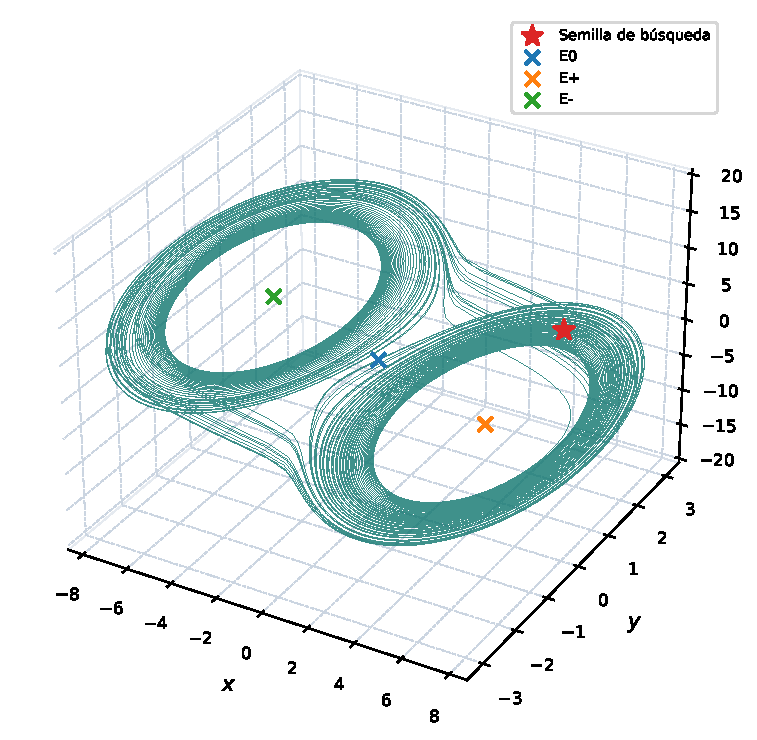
\includegraphics[width=0.94\linewidth,height=0.37\textheight,keepaspectratio]{figures/chua_master/chua_frac_arctan_c590_fig00_initial_seed.pdf}\\[-0.25em]
{\footnotesize Chua arctangente c590: condición inicial y trayectoria de arranque.}
\end{center}
\vfill
\begin{center}
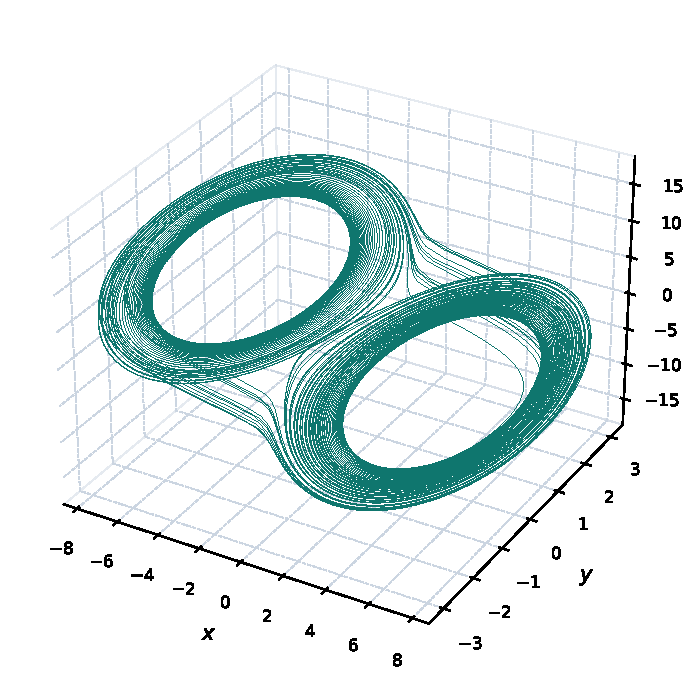
\includegraphics[width=0.94\linewidth,height=0.37\textheight,keepaspectratio]{figures/chua_master/chua_frac_arctan_c590_fig03_attractor.pdf}\\[-0.25em]
{\footnotesize Chua arctangente c590: trayectoria candidata en el espacio de estados.}
\end{center}
\clearpage
\begin{center}
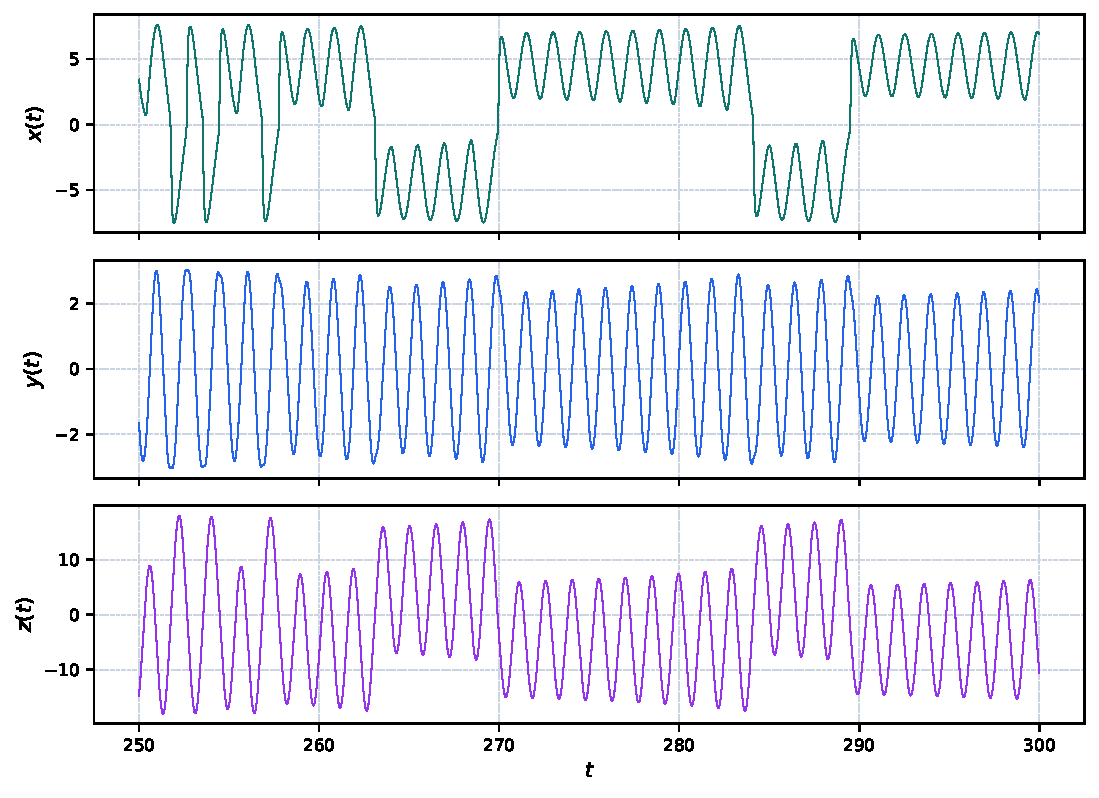
\includegraphics[width=0.94\linewidth,height=0.37\textheight,keepaspectratio]{figures/chua_master/chua_frac_arctan_c590_fig04_timeseries.pdf}\\[-0.25em]
{\footnotesize Chua arctangente c590: series temporales.}
\end{center}
\vfill
\begin{center}
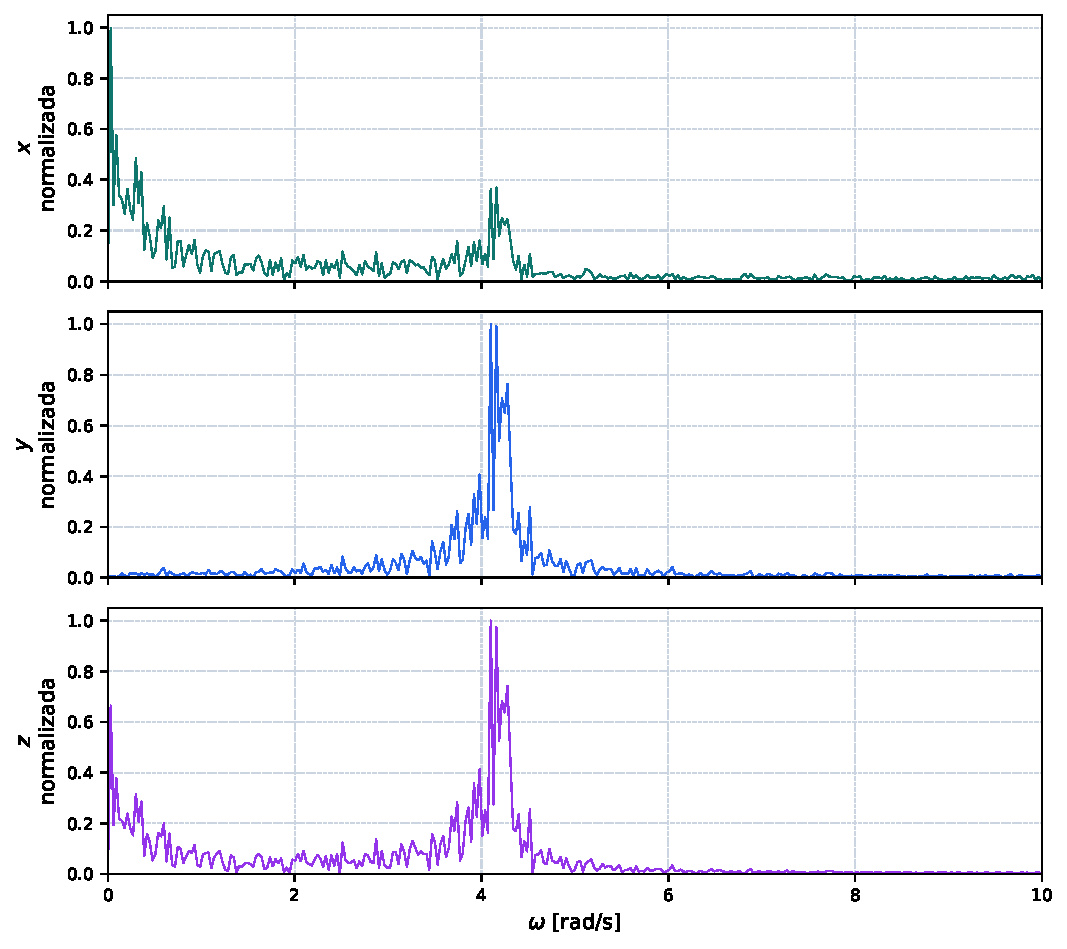
\includegraphics[width=0.94\linewidth,height=0.37\textheight,keepaspectratio]{figures/chua_master/chua_frac_arctan_c590_fig11_fft.pdf}\\[-0.25em]
{\footnotesize Chua arctangente c590: espectro de amplitud.}
\end{center}
\clearpage
\begin{center}
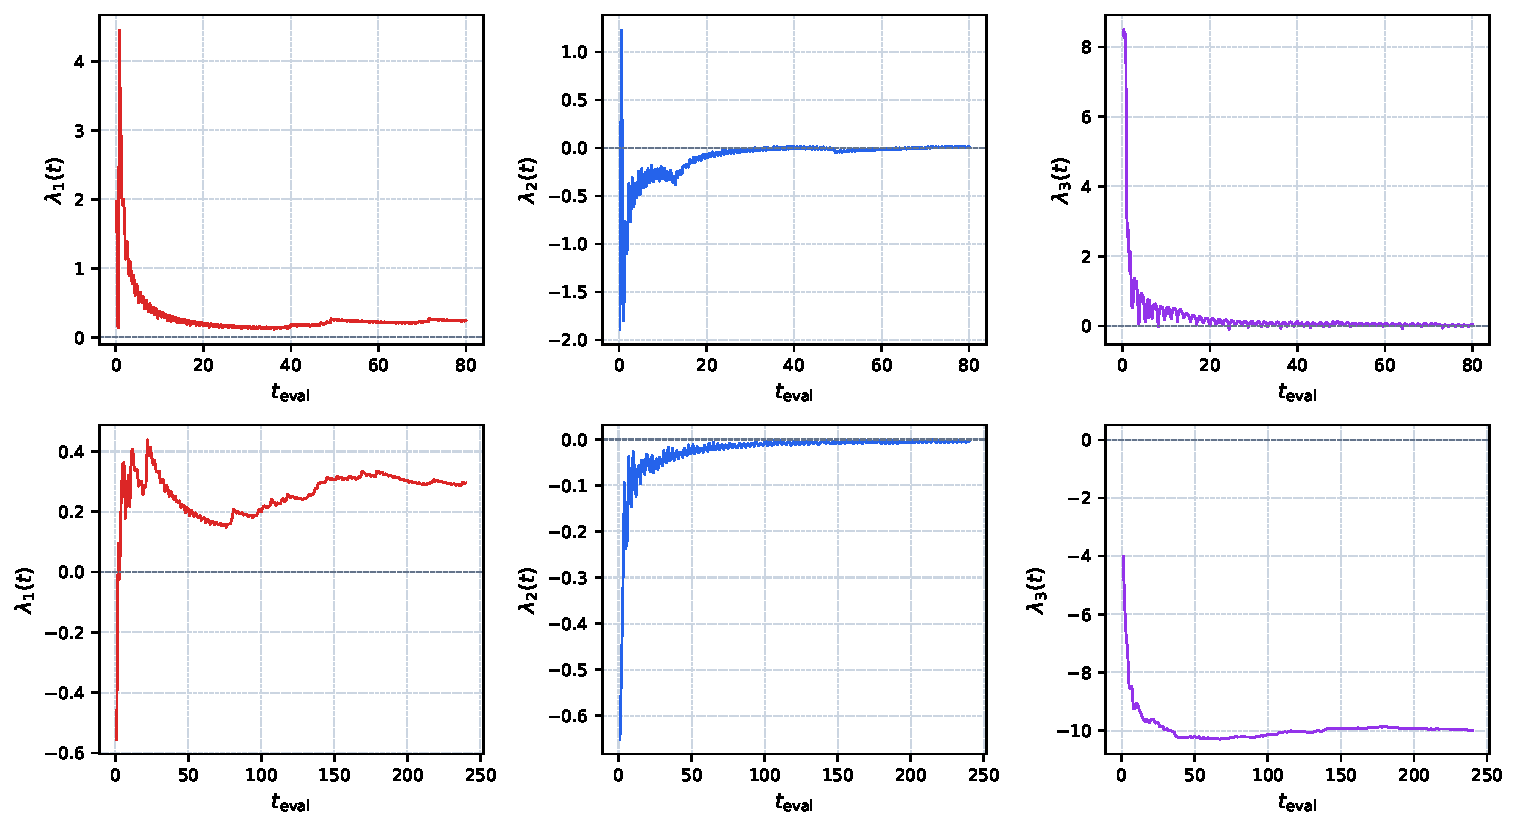
\includegraphics[width=0.94\linewidth,height=0.37\textheight,keepaspectratio]{figures/chua_master/chua_frac_arctan_c590_fig12_lyapunov_two_methods.pdf}\\[-0.25em]
{\footnotesize Chua arctangente c590: comparación de dos estimaciones de Lyapunov.}
\end{center}
\vfill
\begin{center}
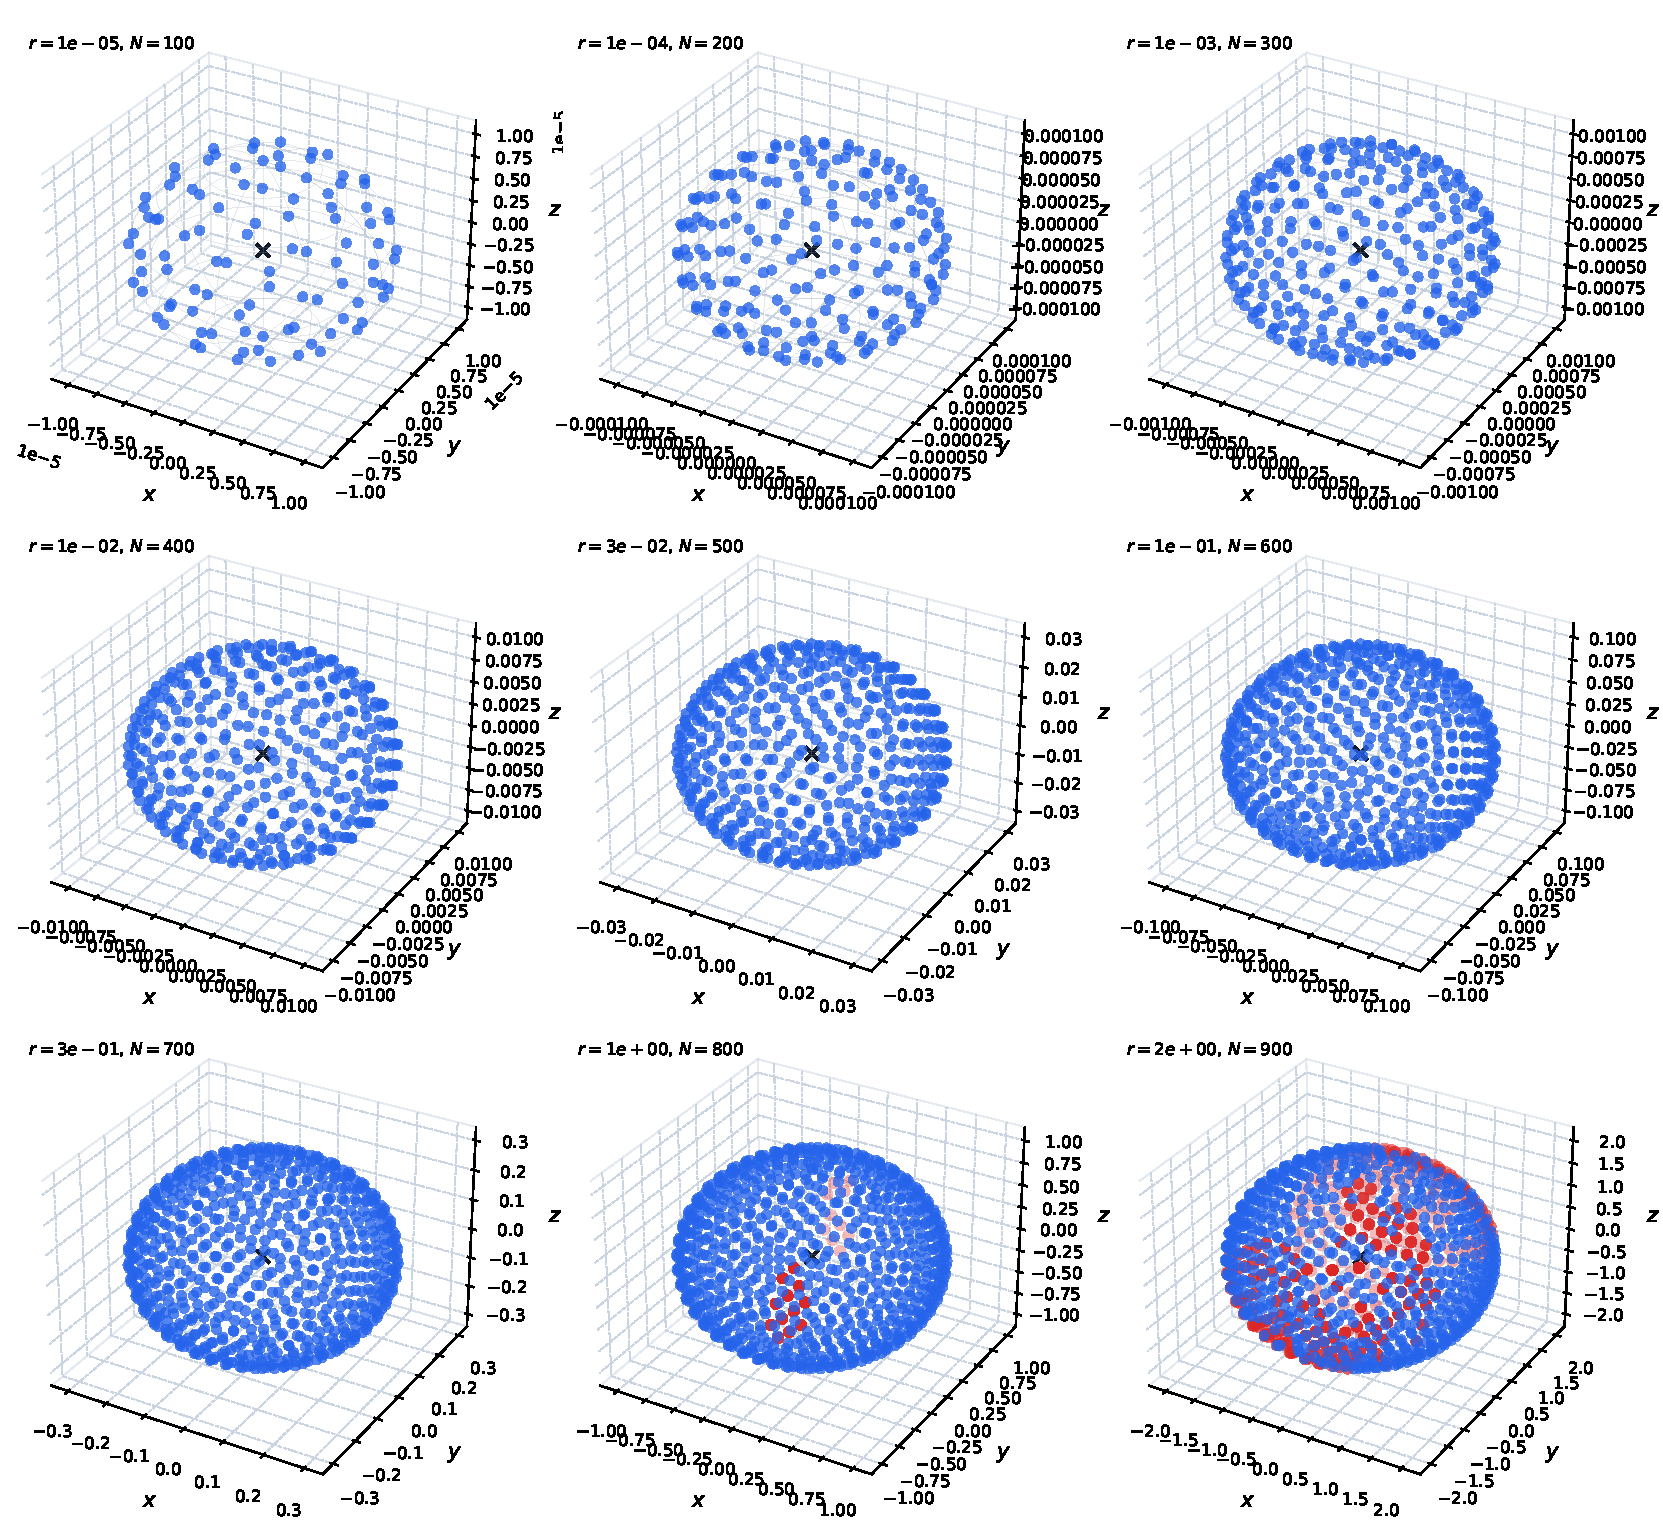
\includegraphics[width=0.94\linewidth,height=0.37\textheight,keepaspectratio]{figures/chua_master/chua_frac_arctan_c590_fig13_E0_hiddenness_spherical_3d.pdf}\\[-0.25em]
{\footnotesize Chua arctangente c590: sondeos esféricos próximos a \(E_0\).}
\end{center}
\clearpage
\begin{center}
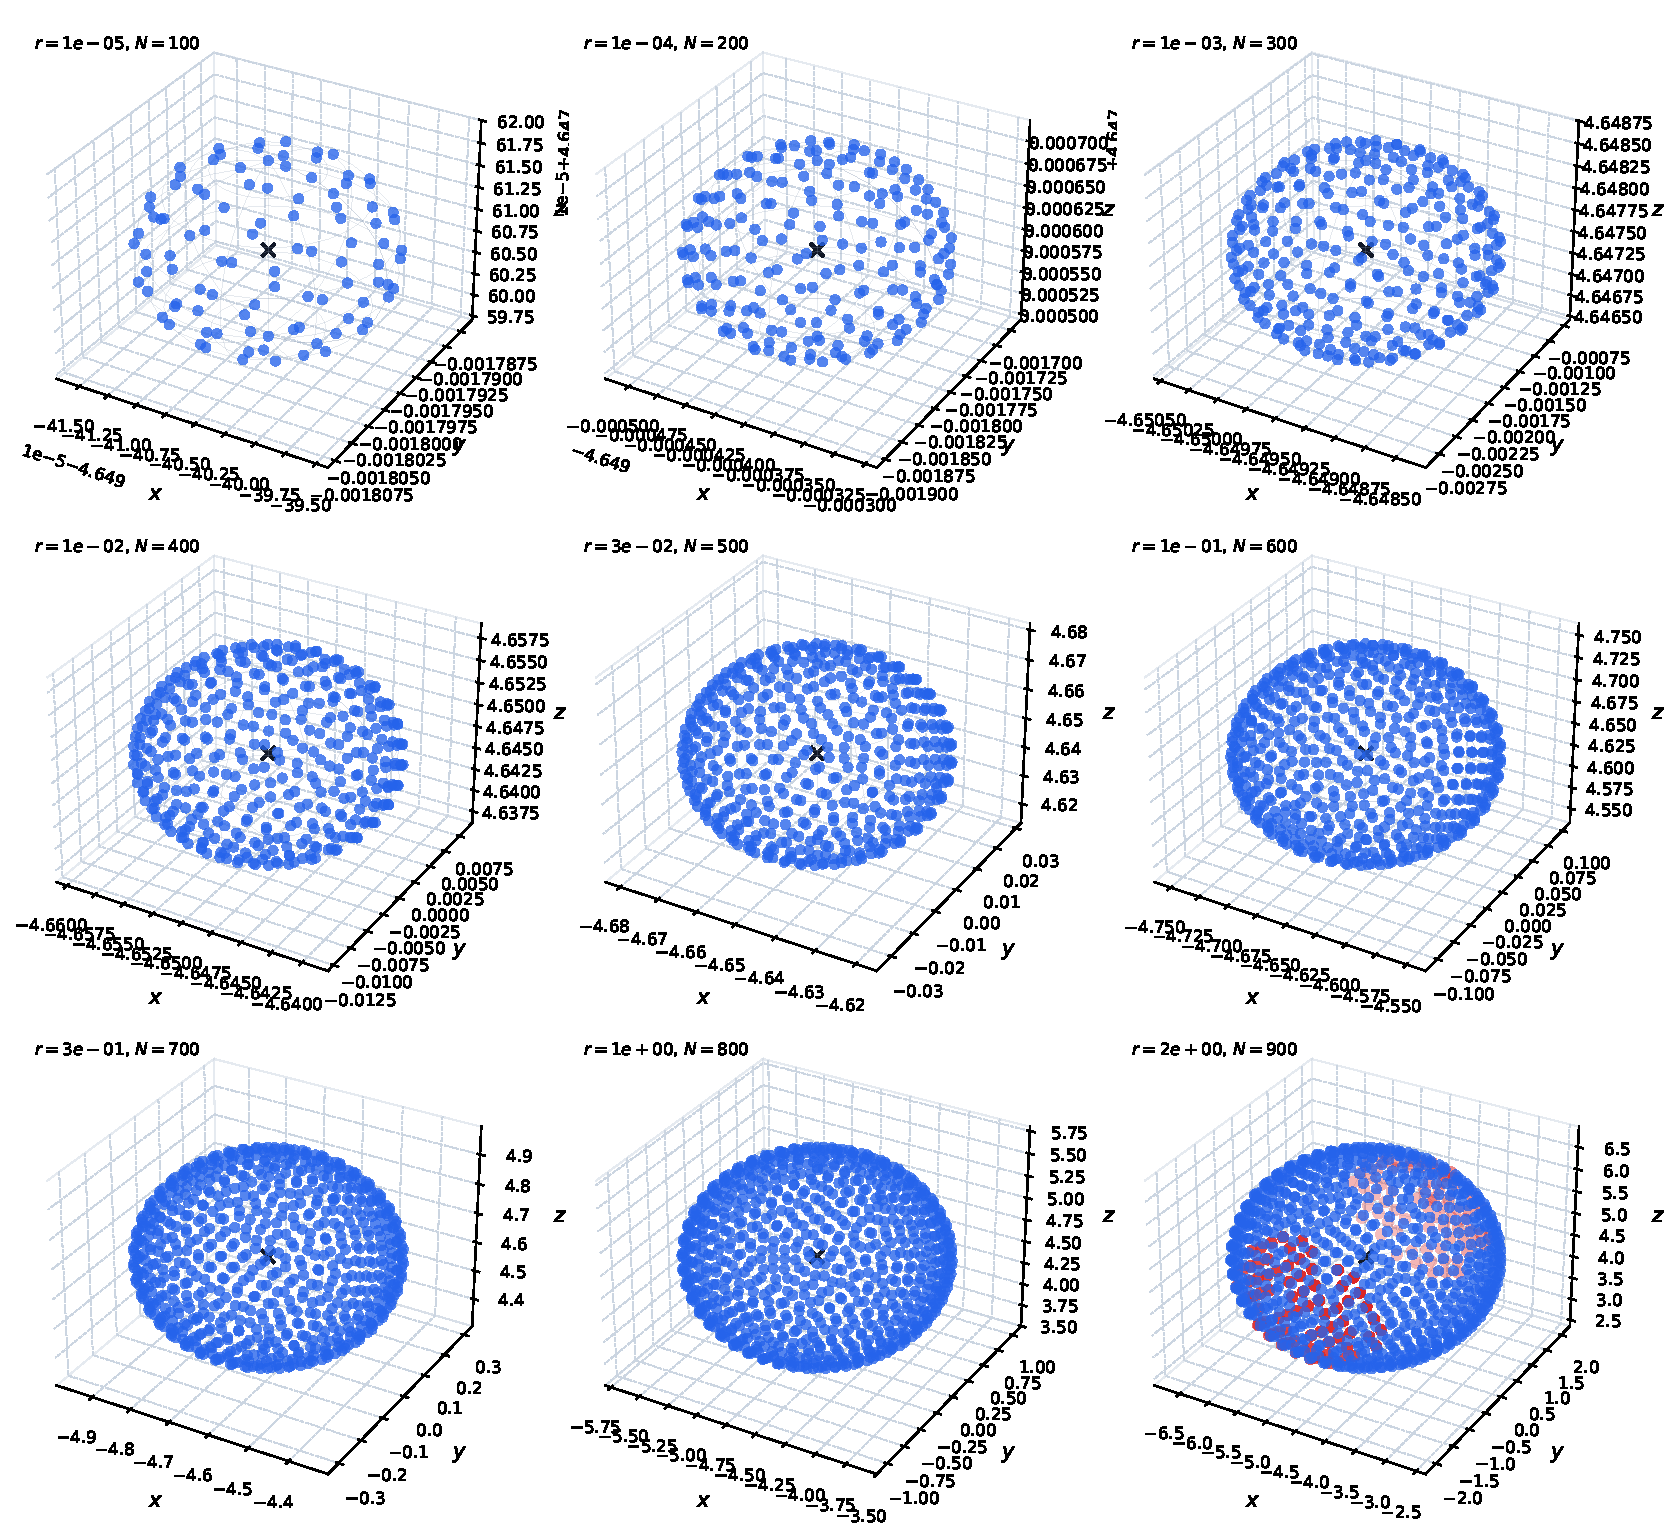
\includegraphics[width=0.94\linewidth,height=0.37\textheight,keepaspectratio]{figures/chua_master/chua_frac_arctan_c590_fig13_Em_hiddenness_spherical_3d.pdf}\\[-0.25em]
{\footnotesize Chua arctangente c590: sondeos esféricos próximos a \(E_-\).}
\end{center}
\vfill
\begin{center}
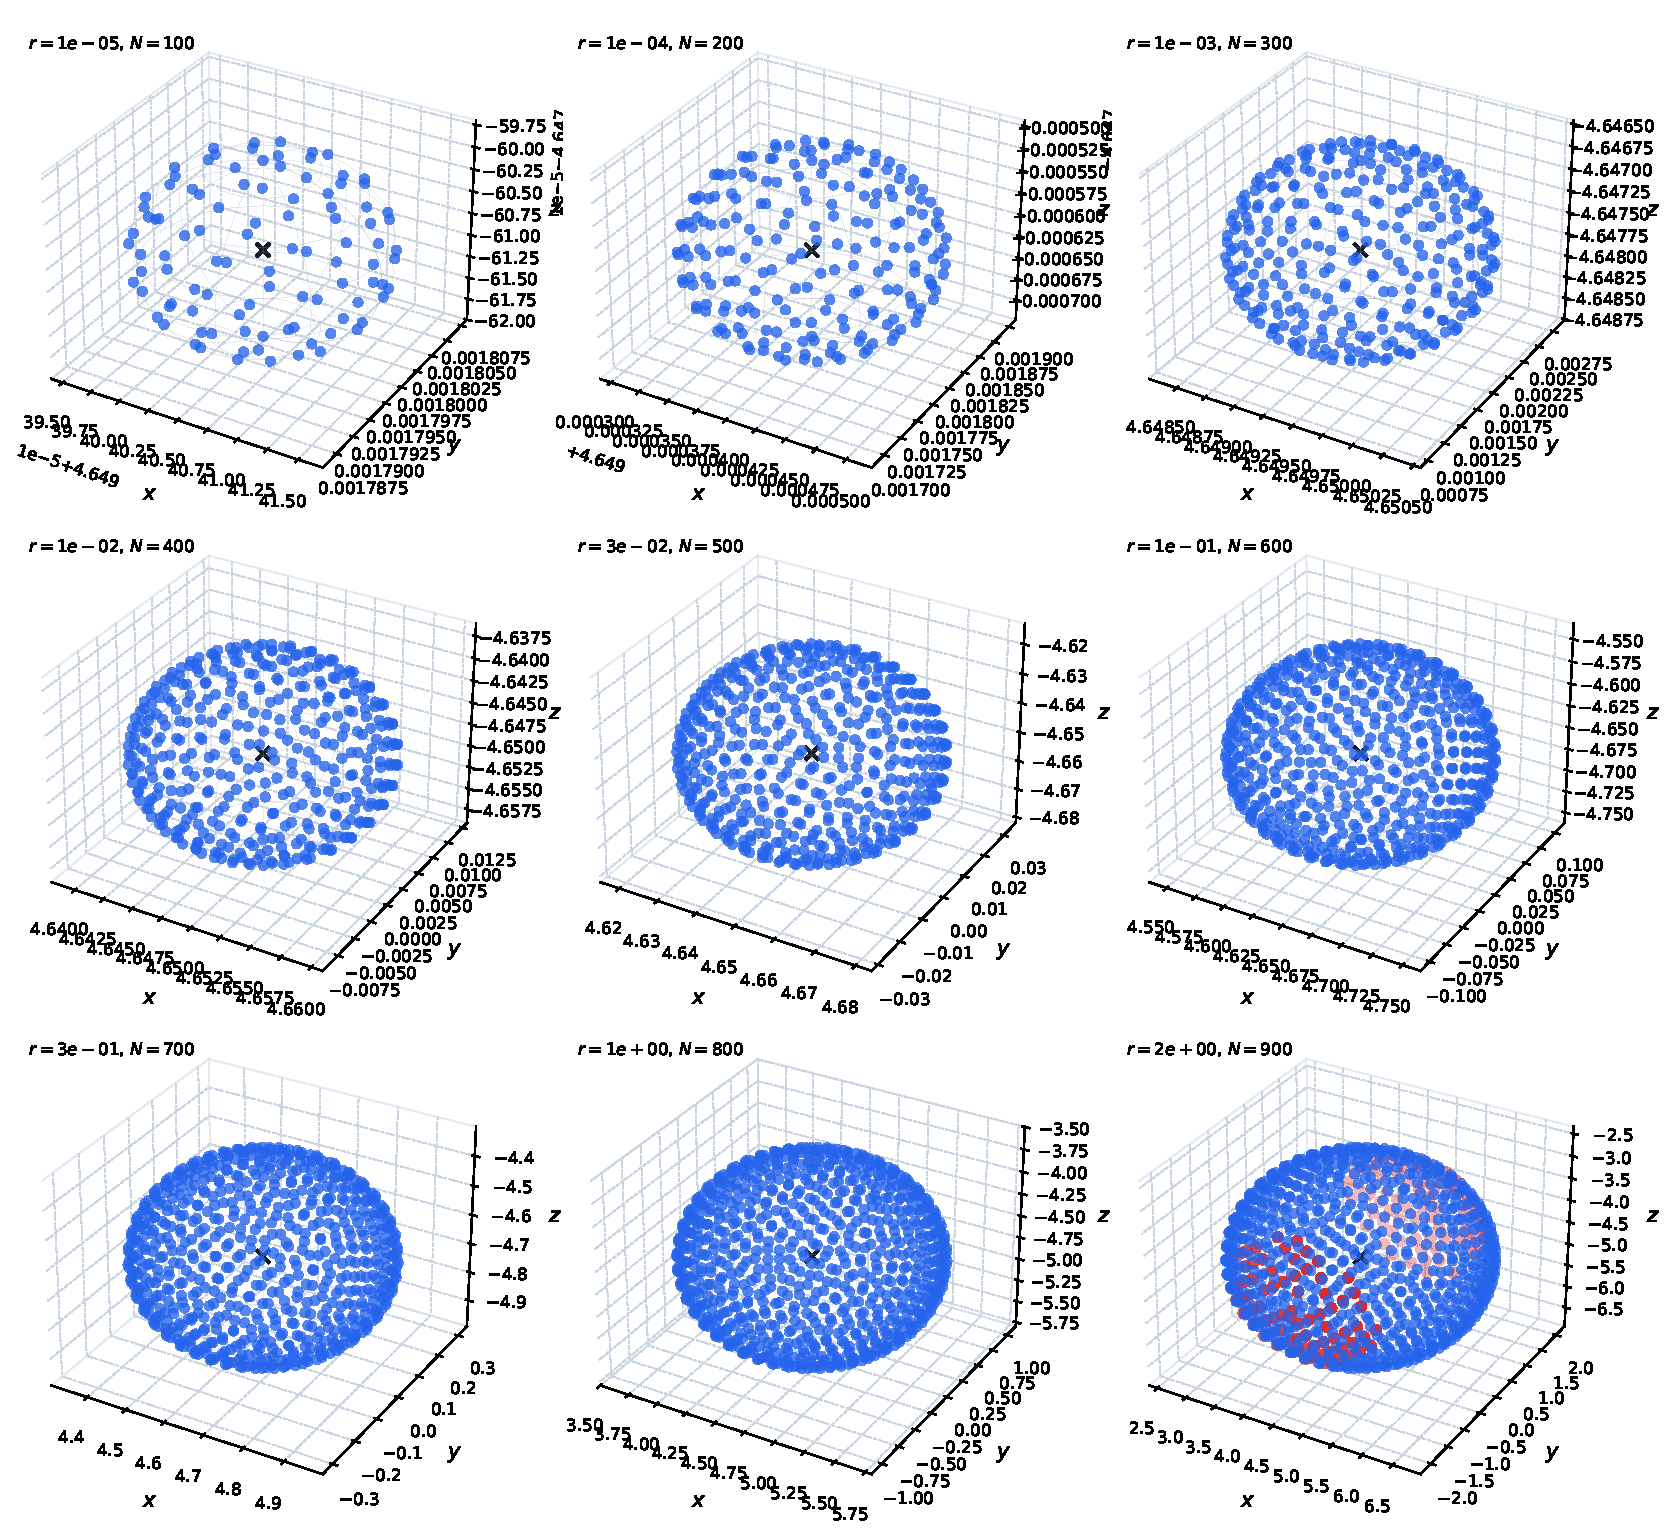
\includegraphics[width=0.94\linewidth,height=0.37\textheight,keepaspectratio]{figures/chua_master/chua_frac_arctan_c590_fig13_Ep_hiddenness_spherical_3d.pdf}\\[-0.25em]
{\footnotesize Chua arctangente c590: sondeos esféricos próximos a \(E_+\).}
\end{center}
\clearpage
\begin{center}
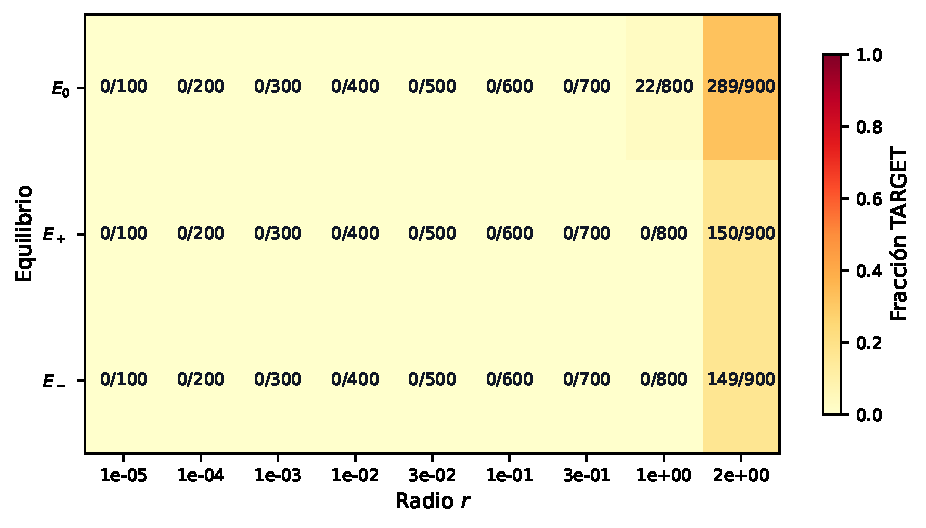
\includegraphics[width=0.94\linewidth,height=0.37\textheight,keepaspectratio]{figures/chua_master/chua_frac_arctan_c590_fig14_hiddenness_contact_heatmap.pdf}\\[-0.25em]
{\footnotesize Chua arctangente c590: frecuencia de contacto por radio y equilibrio.}
\end{center}
\vfill
\begin{center}

\includegraphics[width=0.94\linewidth,height=0.37\textheight,keepaspectratio]{figures/chua_master/chua_frac_ns_biased_fig01a_transfer_real.pdf}\\[-0.25em]
{\footnotesize Chua fraccionario PWL sesgado: parte real de la transferencia.}
\end{center}
\clearpage
\begin{center}

\includegraphics[width=0.94\linewidth,height=0.37\textheight,keepaspectratio]{figures/chua_master/chua_frac_ns_biased_fig01b_transfer_imag.pdf}\\[-0.25em]
{\footnotesize Chua fraccionario PWL sesgado: parte imaginaria de la transferencia.}
\end{center}
\vfill
\begin{center}

\includegraphics[width=0.94\linewidth,height=0.37\textheight,keepaspectratio]{figures/chua_master/chua_frac_ns_biased_fig02_continuation_story.pdf}\\[-0.25em]
{\footnotesize Chua fraccionario PWL sesgado: evolución de la trayectoria durante la continuación.}
\end{center}
\clearpage
\begin{center}
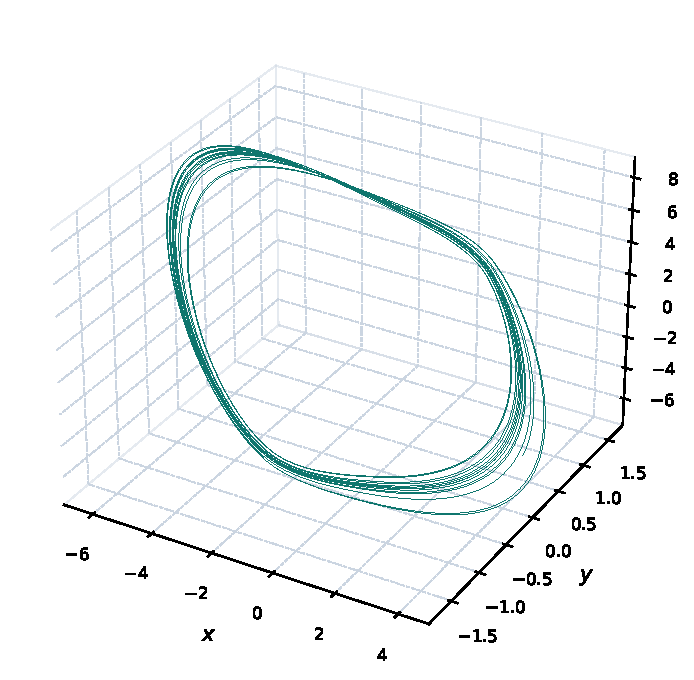
\includegraphics[width=0.94\linewidth,height=0.37\textheight,keepaspectratio]{figures/chua_master/chua_frac_ns_biased_fig03_attractor.pdf}\\[-0.25em]
{\footnotesize Chua fraccionario PWL sesgado: trayectoria candidata en el espacio de estados.}
\end{center}
\vfill
\begin{center}
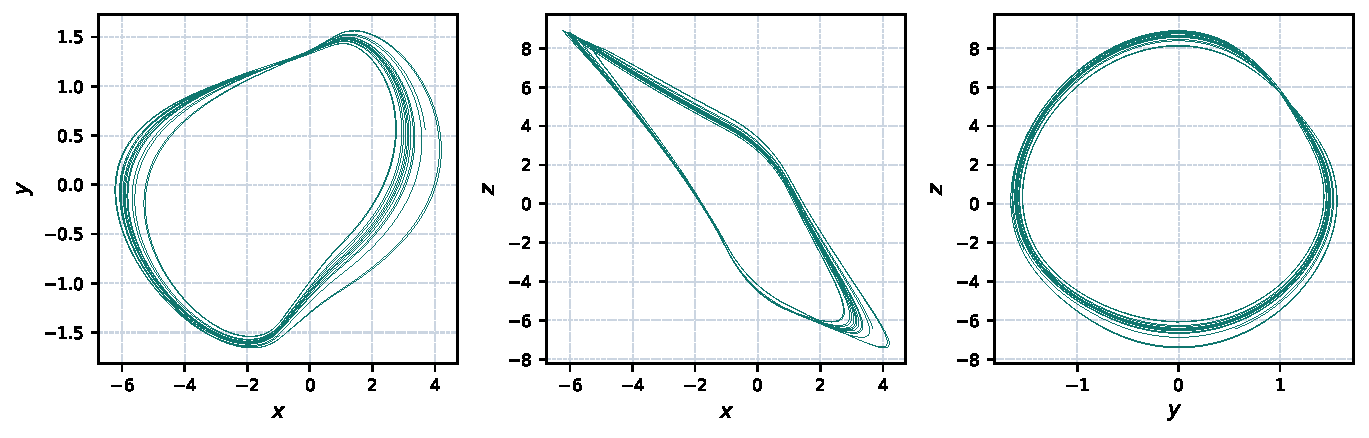
\includegraphics[width=0.94\linewidth,height=0.37\textheight,keepaspectratio]{figures/chua_master/chua_frac_ns_biased_fig04_projections.pdf}\\[-0.25em]
{\footnotesize Chua fraccionario PWL sesgado: proyecciones de la trayectoria candidata.}
\end{center}
\clearpage
\begin{center}
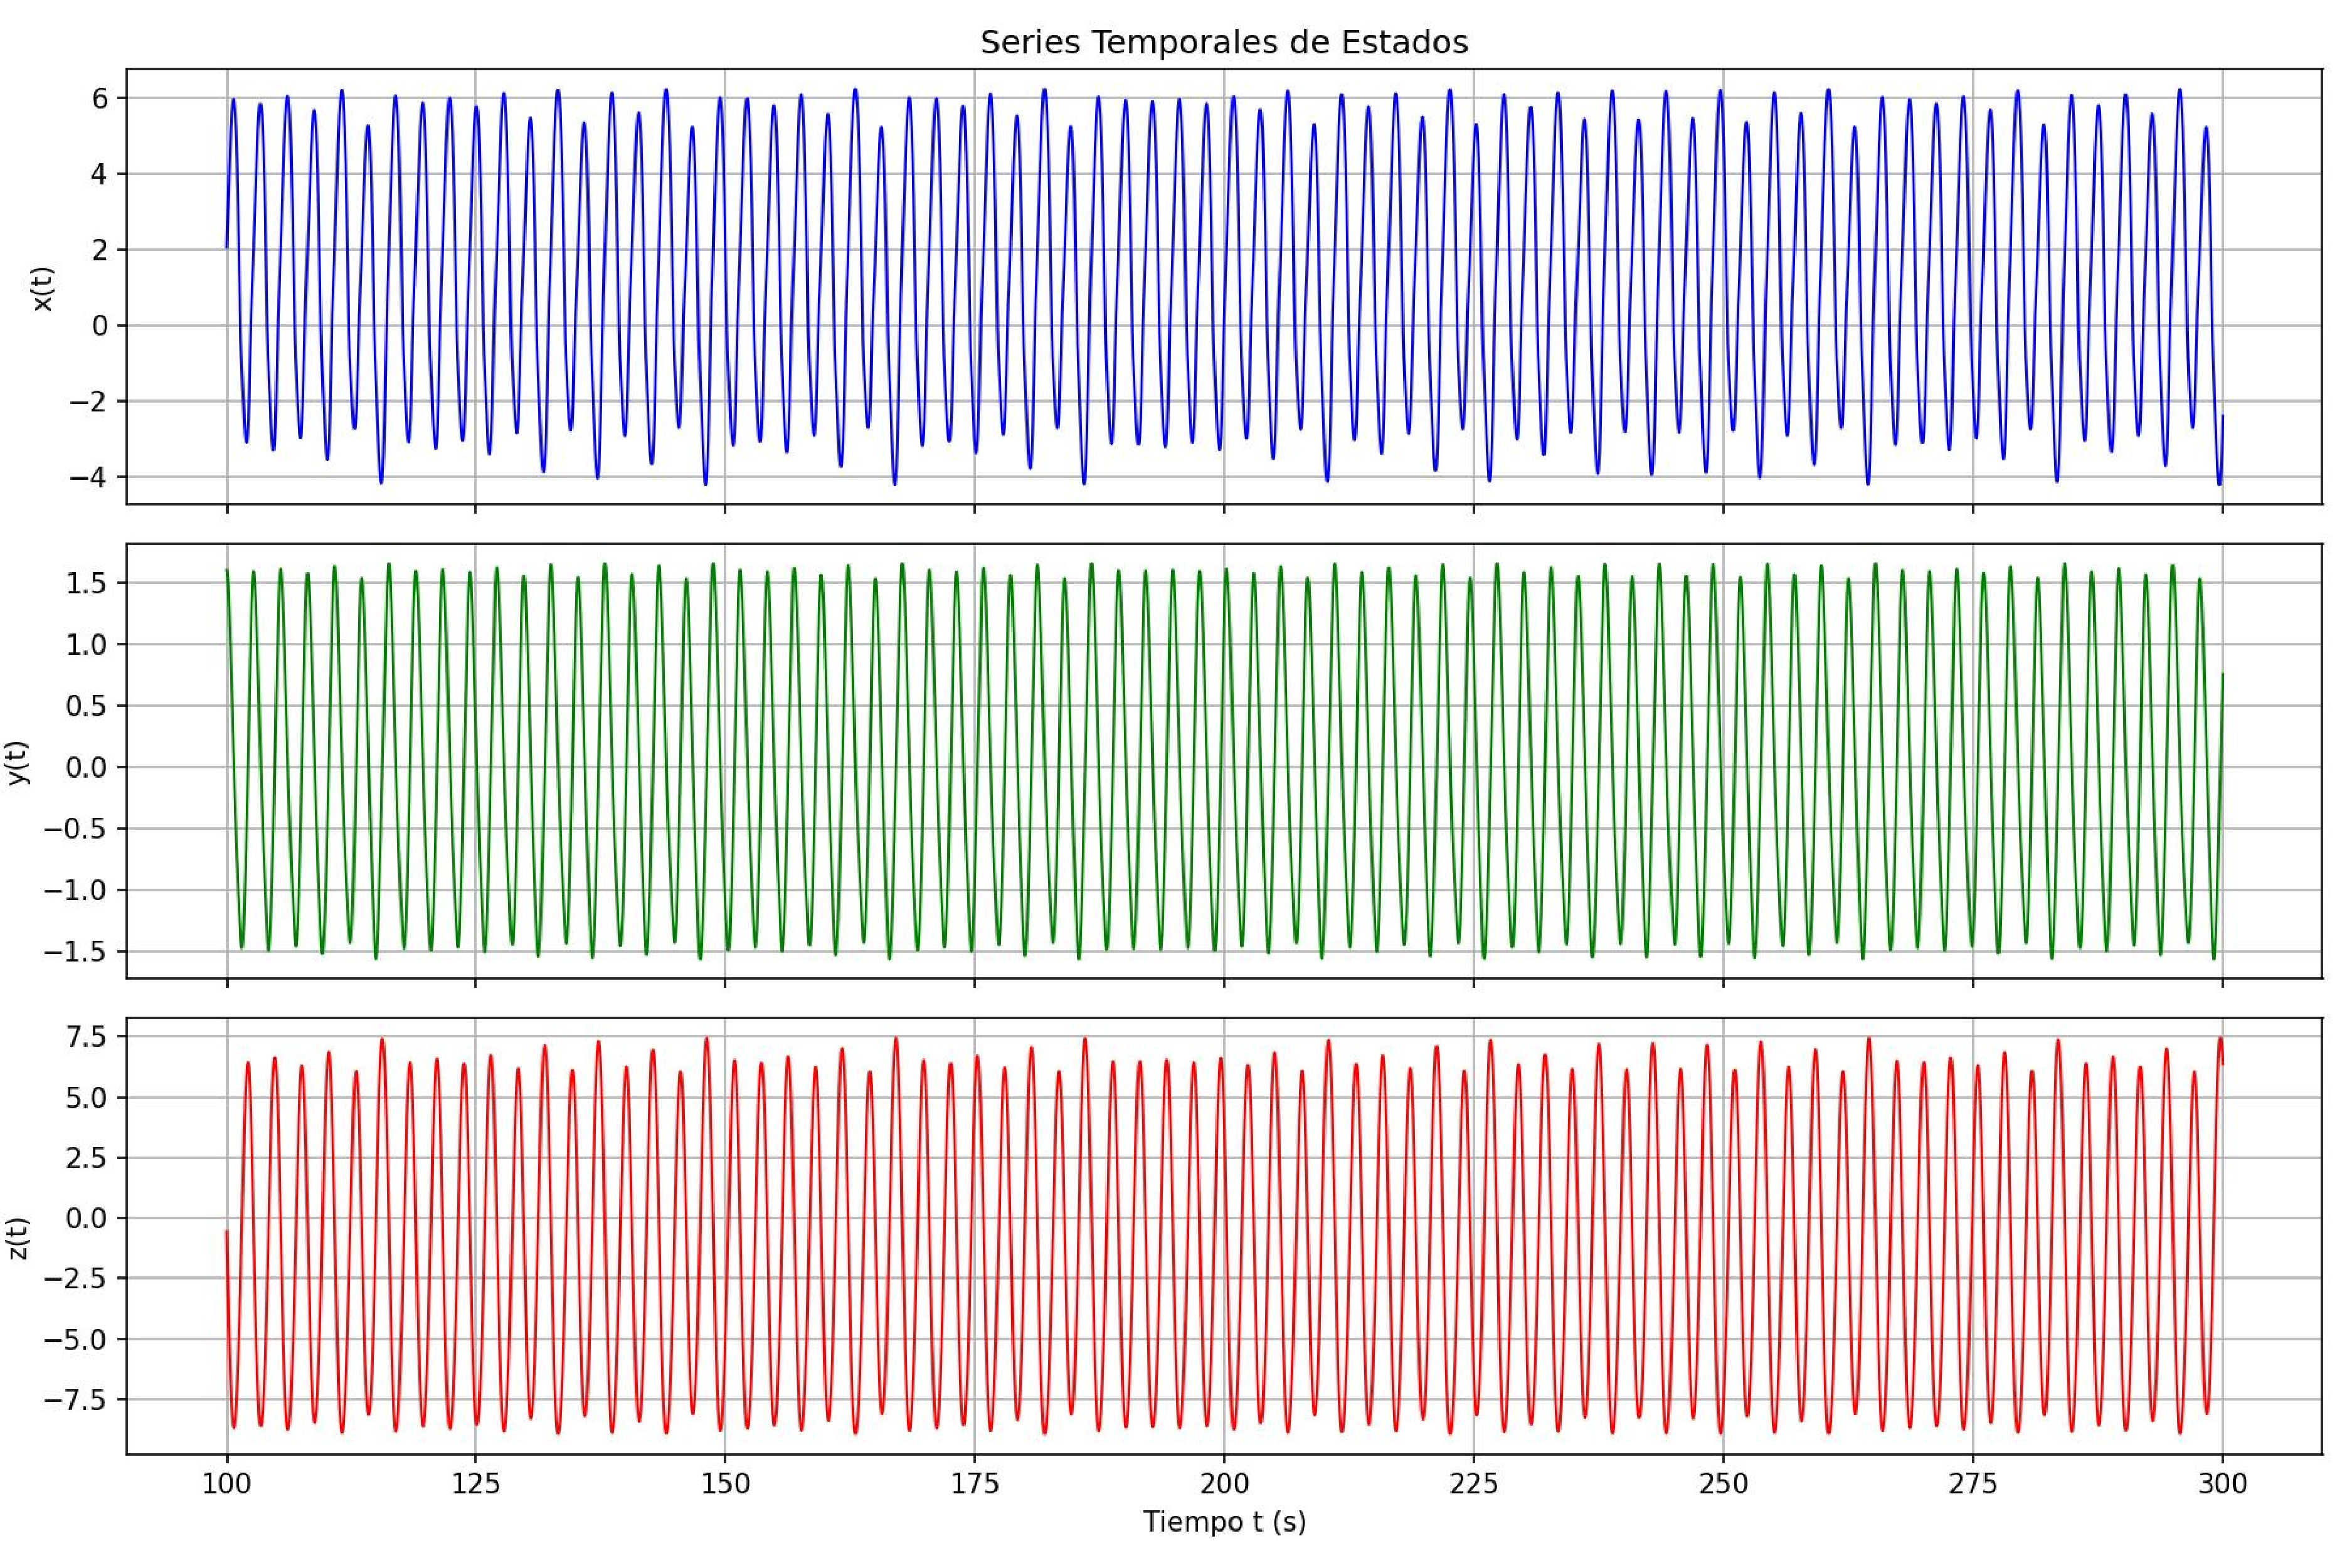
\includegraphics[width=0.94\linewidth,height=0.37\textheight,keepaspectratio]{figures/chua_master/chua_frac_ns_biased_fig04_timeseries.pdf}\\[-0.25em]
{\footnotesize Chua fraccionario PWL sesgado: series temporales.}
\end{center}
\vfill
\begin{center}

\includegraphics[width=0.94\linewidth,height=0.37\textheight,keepaspectratio]{figures/chua_master/chua_frac_ns_biased_fig11_fft.pdf}\\[-0.25em]
{\footnotesize Chua fraccionario PWL sesgado: espectro de amplitud.}
\end{center}
\clearpage
\begin{center}

\includegraphics[width=0.94\linewidth,height=0.37\textheight,keepaspectratio]{figures/chua_master/chua_frac_ns_biased_fig12_lyapunov.pdf}\\[-0.25em]
{\footnotesize Chua fraccionario PWL sesgado: evolución de las estimaciones de Lyapunov.}
\end{center}
\vfill
\begin{center}

\includegraphics[width=0.94\linewidth,height=0.37\textheight,keepaspectratio]{figures/chua_master/chua_frac_ns_biased_fig13_E0_hiddenness_spherical_3d.pdf}\\[-0.25em]
{\footnotesize Chua fraccionario PWL sesgado: sondeos esféricos próximos a \(E_0\).}
\end{center}
\clearpage
\begin{center}

\includegraphics[width=0.94\linewidth,height=0.37\textheight,keepaspectratio]{figures/chua_master/chua_frac_ns_biased_fig13_Em_hiddenness_spherical_3d.pdf}\\[-0.25em]
{\footnotesize Chua fraccionario PWL sesgado: sondeos esféricos próximos a \(E_-\).}
\end{center}
\vfill
\begin{center}

\includegraphics[width=0.94\linewidth,height=0.37\textheight,keepaspectratio]{figures/chua_master/chua_frac_ns_biased_fig13_Ep_hiddenness_spherical_3d.pdf}\\[-0.25em]
{\footnotesize Chua fraccionario PWL sesgado: sondeos esféricos próximos a \(E_+\).}
\end{center}
\clearpage
\begin{center}

\includegraphics[width=0.94\linewidth,height=0.37\textheight,keepaspectratio]{figures/chua_master/chua_frac_ns_biased_fig14_hiddenness_contact_heatmap.pdf}\\[-0.25em]
{\footnotesize Chua fraccionario PWL sesgado: frecuencia de contacto por radio y equilibrio.}
\end{center}
\vfill
\begin{center}
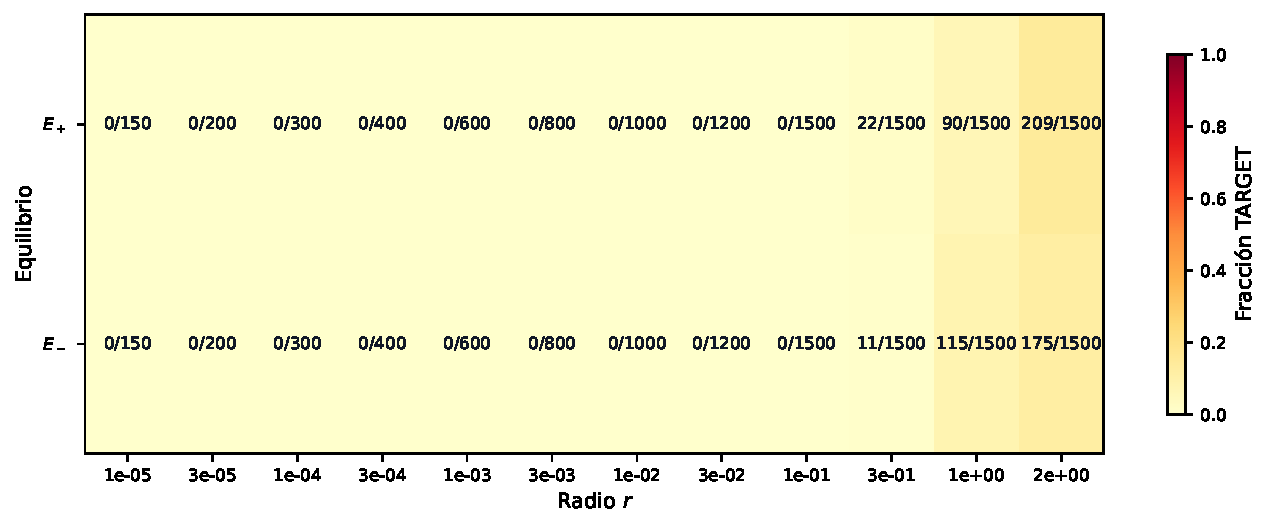
\includegraphics[width=0.94\linewidth,height=0.37\textheight,keepaspectratio]{figures/chua_master/chua_frac_ns_biased_fig15_extended_heatmap.pdf}\\[-0.25em]
{\footnotesize Chua fraccionario PWL sesgado: contactos a radios ampliados.}
\end{center}
\clearpage
\begin{center}

\includegraphics[width=0.94\linewidth,height=0.37\textheight,keepaspectratio]{figures/chua_master/chua_frac_ns_fig01a_transfer_real.pdf}\\[-0.25em]
{\footnotesize Chua fraccionario PWL, control cercano: parte real de la transferencia.}
\end{center}
\vfill
\begin{center}

\includegraphics[width=0.94\linewidth,height=0.37\textheight,keepaspectratio]{figures/chua_master/chua_frac_ns_fig01b_transfer_imag.pdf}\\[-0.25em]
{\footnotesize Chua fraccionario PWL, control cercano: parte imaginaria de la transferencia.}
\end{center}
\clearpage
\begin{center}

\includegraphics[width=0.94\linewidth,height=0.37\textheight,keepaspectratio]{figures/chua_master/chua_frac_ns_fig02_continuation_story.pdf}\\[-0.25em]
{\footnotesize Chua fraccionario PWL, control cercano: evolución de la trayectoria durante la continuación.}
\end{center}
\vfill
\begin{center}

\includegraphics[width=0.94\linewidth,height=0.37\textheight,keepaspectratio]{figures/chua_master/chua_frac_ns_fig03_final_attractor.pdf}\\[-0.25em]
{\footnotesize Chua fraccionario PWL, control cercano: trayectoria final de la continuación.}
\end{center}
\clearpage
\begin{center}

\includegraphics[width=0.94\linewidth,height=0.37\textheight,keepaspectratio]{figures/chua_master/chua_frac_ns_fig03abc_final_attractor_projections.pdf}\\[-0.25em]
{\footnotesize Chua fraccionario PWL, control cercano: proyecciones de la trayectoria final.}
\end{center}
\vfill
\begin{center}

\includegraphics[width=0.94\linewidth,height=0.37\textheight,keepaspectratio]{figures/chua_master/chua_frac_ns_fig04_time_series.pdf}\\[-0.25em]
{\footnotesize Chua fraccionario PWL, control cercano: series temporales.}
\end{center}
\clearpage
\begin{center}

\includegraphics[width=0.94\linewidth,height=0.37\textheight,keepaspectratio]{figures/chua_master/chua_frac_ns_fig11a_fft_x.pdf}\\[-0.25em]
{\footnotesize Chua fraccionario PWL, control cercano: espectro de amplitud de \(x\).}
\end{center}
\vfill
\begin{center}

\includegraphics[width=0.94\linewidth,height=0.37\textheight,keepaspectratio]{figures/chua_master/chua_frac_ns_fig12_lyapunov_two_methods.pdf}\\[-0.25em]
{\footnotesize Chua fraccionario PWL, control cercano: comparación de dos estimaciones de Lyapunov.}
\end{center}
\clearpage
\begin{center}

\includegraphics[width=0.94\linewidth,height=0.37\textheight,keepaspectratio]{figures/chua_master/chua_frac_ns_fig13_E0_hiddenness_spherical_3d.pdf}\\[-0.25em]
{\footnotesize Chua fraccionario PWL, control cercano: sondeos esféricos próximos a \(E_0\).}
\end{center}
\vfill
\begin{center}

\includegraphics[width=0.94\linewidth,height=0.37\textheight,keepaspectratio]{figures/chua_master/chua_frac_ns_fig13_Em_hiddenness_spherical_3d.pdf}\\[-0.25em]
{\footnotesize Chua fraccionario PWL, control cercano: sondeos esféricos próximos a \(E_-\).}
\end{center}
\clearpage
\begin{center}

\includegraphics[width=0.94\linewidth,height=0.37\textheight,keepaspectratio]{figures/chua_master/chua_frac_ns_fig13_Ep_hiddenness_spherical_3d.pdf}\\[-0.25em]
{\footnotesize Chua fraccionario PWL, control cercano: sondeos esféricos próximos a \(E_+\).}
\end{center}
\vfill
\begin{center}

\includegraphics[width=0.94\linewidth,height=0.37\textheight,keepaspectratio]{figures/chua_master/chua_frac_ns_fig14_hiddenness_contact_heatmap.pdf}\\[-0.25em]
{\footnotesize Chua fraccionario PWL, control cercano: frecuencia de contacto por radio y equilibrio.}
\end{center}
\clearpage
\begin{center}
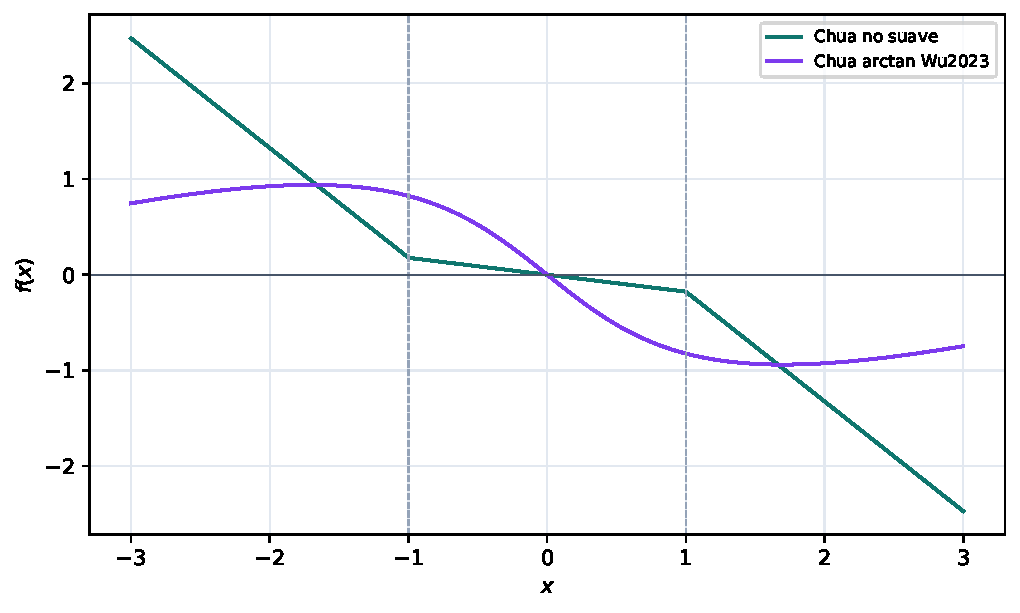
\includegraphics[width=0.94\linewidth,height=0.37\textheight,keepaspectratio]{figures/chua_master/chua_nonlinearity_piecewise_vs_arctan.pdf}\\[-0.25em]
{\footnotesize Comparación de las no linealidades PWL y arctangente.}
\end{center}
\vfill
\begin{center}
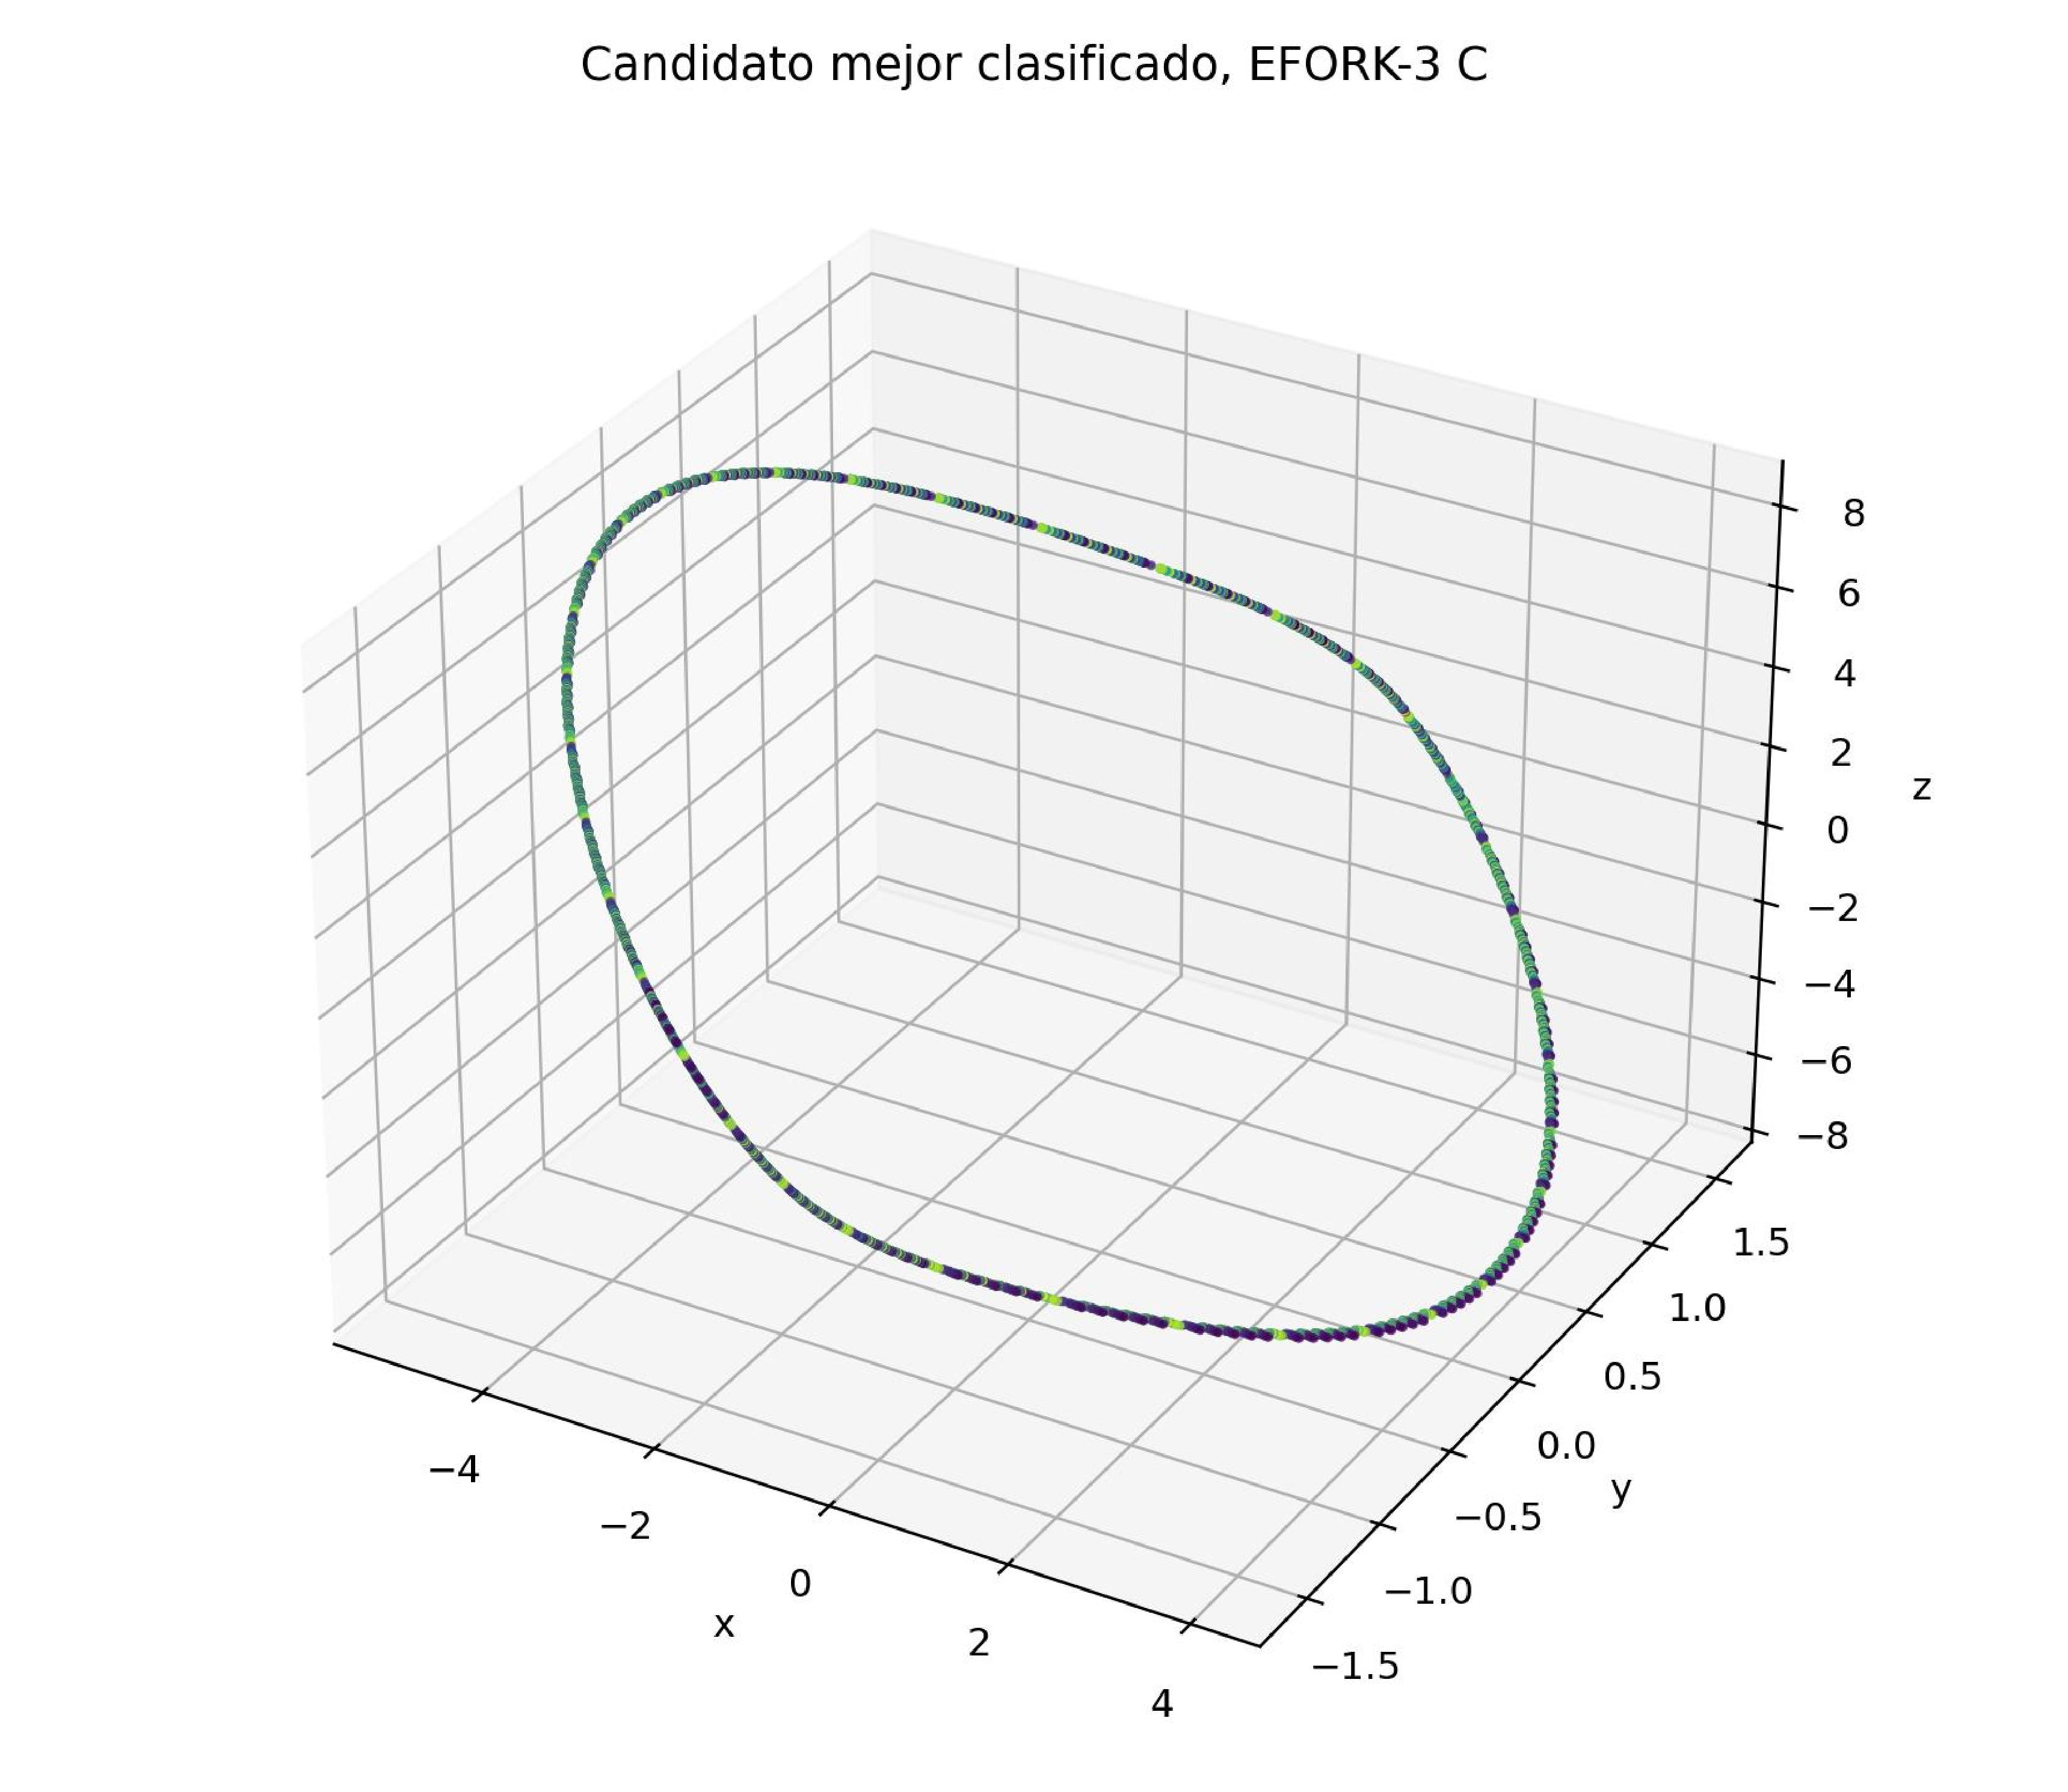
\includegraphics[width=0.94\linewidth,height=0.37\textheight,keepaspectratio]{figures/chua_master/danca_frac_phase_3d.pdf}\\[-0.25em]
{\footnotesize Chua fraccionario con parámetros de Danca: trayectoria en el espacio de estados.}
\end{center}
\clearpage
\begin{center}
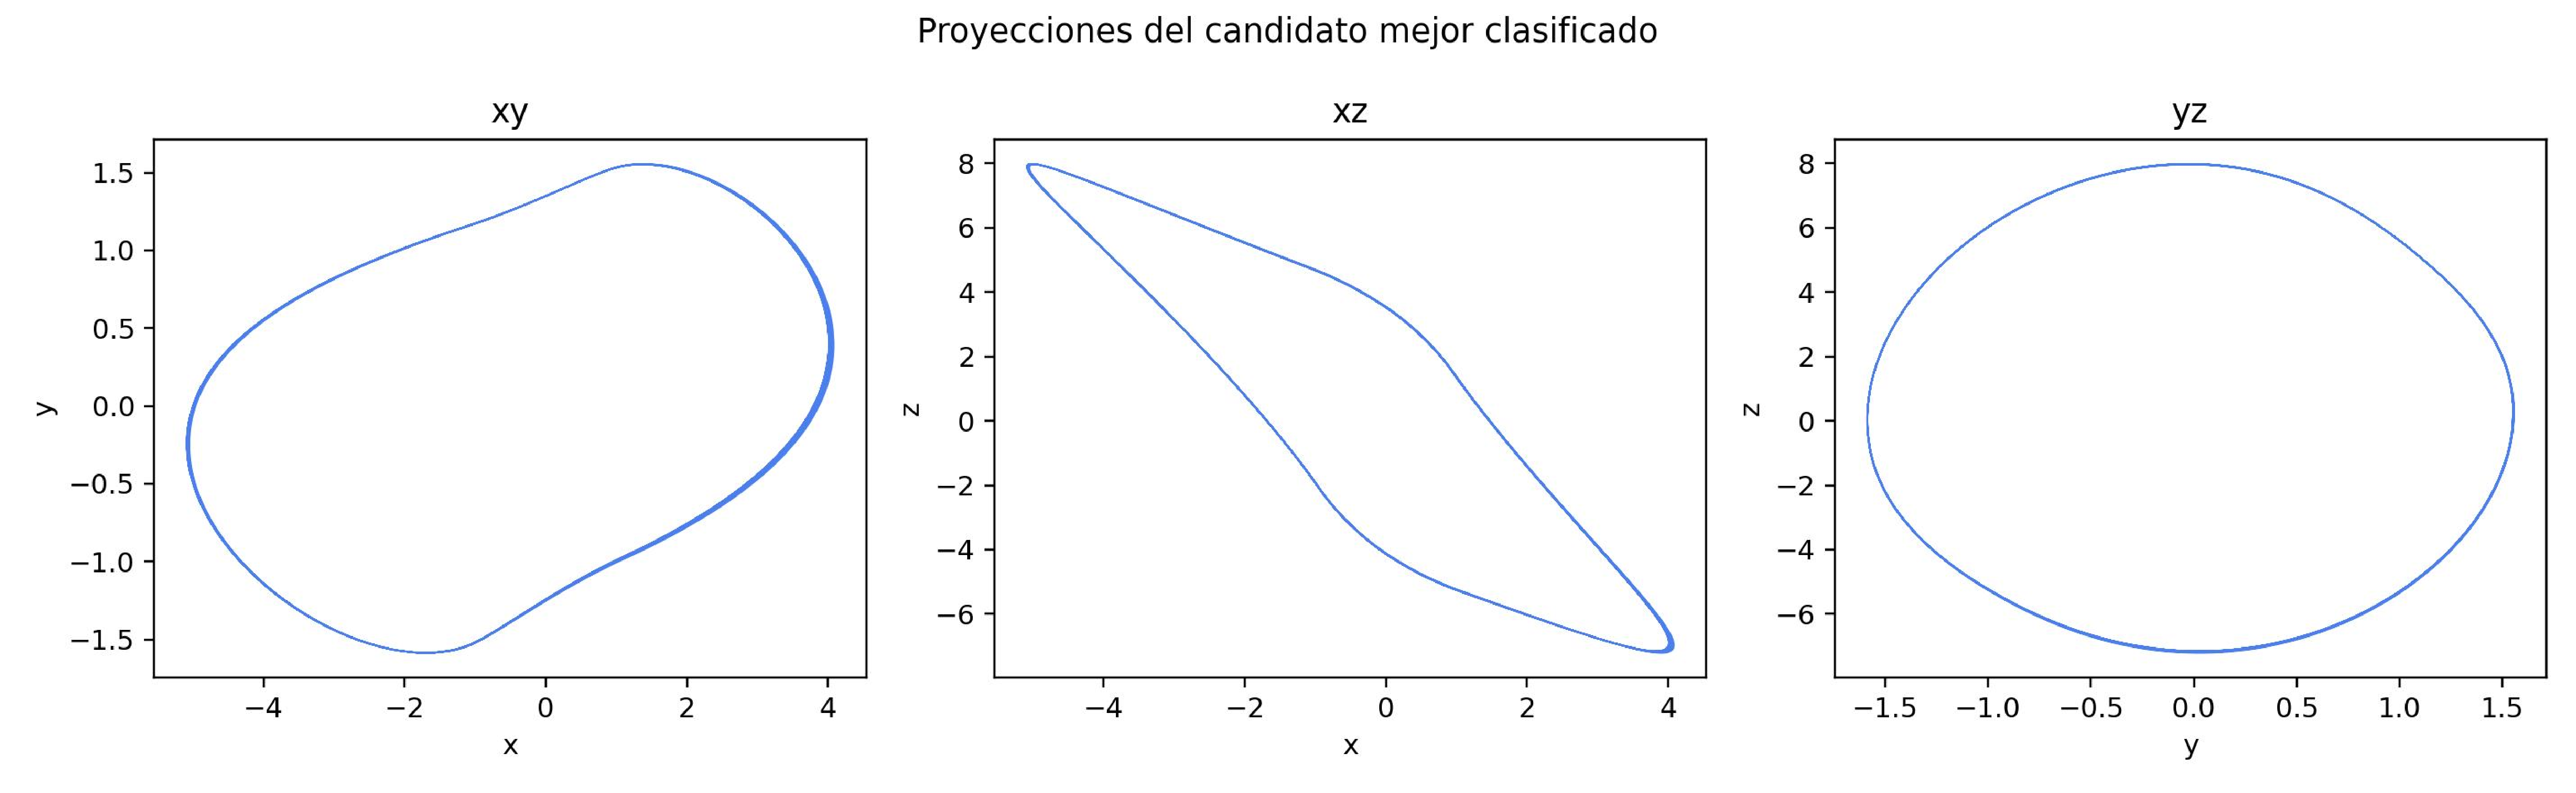
\includegraphics[width=0.94\linewidth,height=0.37\textheight,keepaspectratio]{figures/chua_master/danca_frac_projections.pdf}\\[-0.25em]
{\footnotesize Chua fraccionario con parámetros de Danca: proyecciones de la trayectoria.}
\end{center}
\vfill
\begin{center}
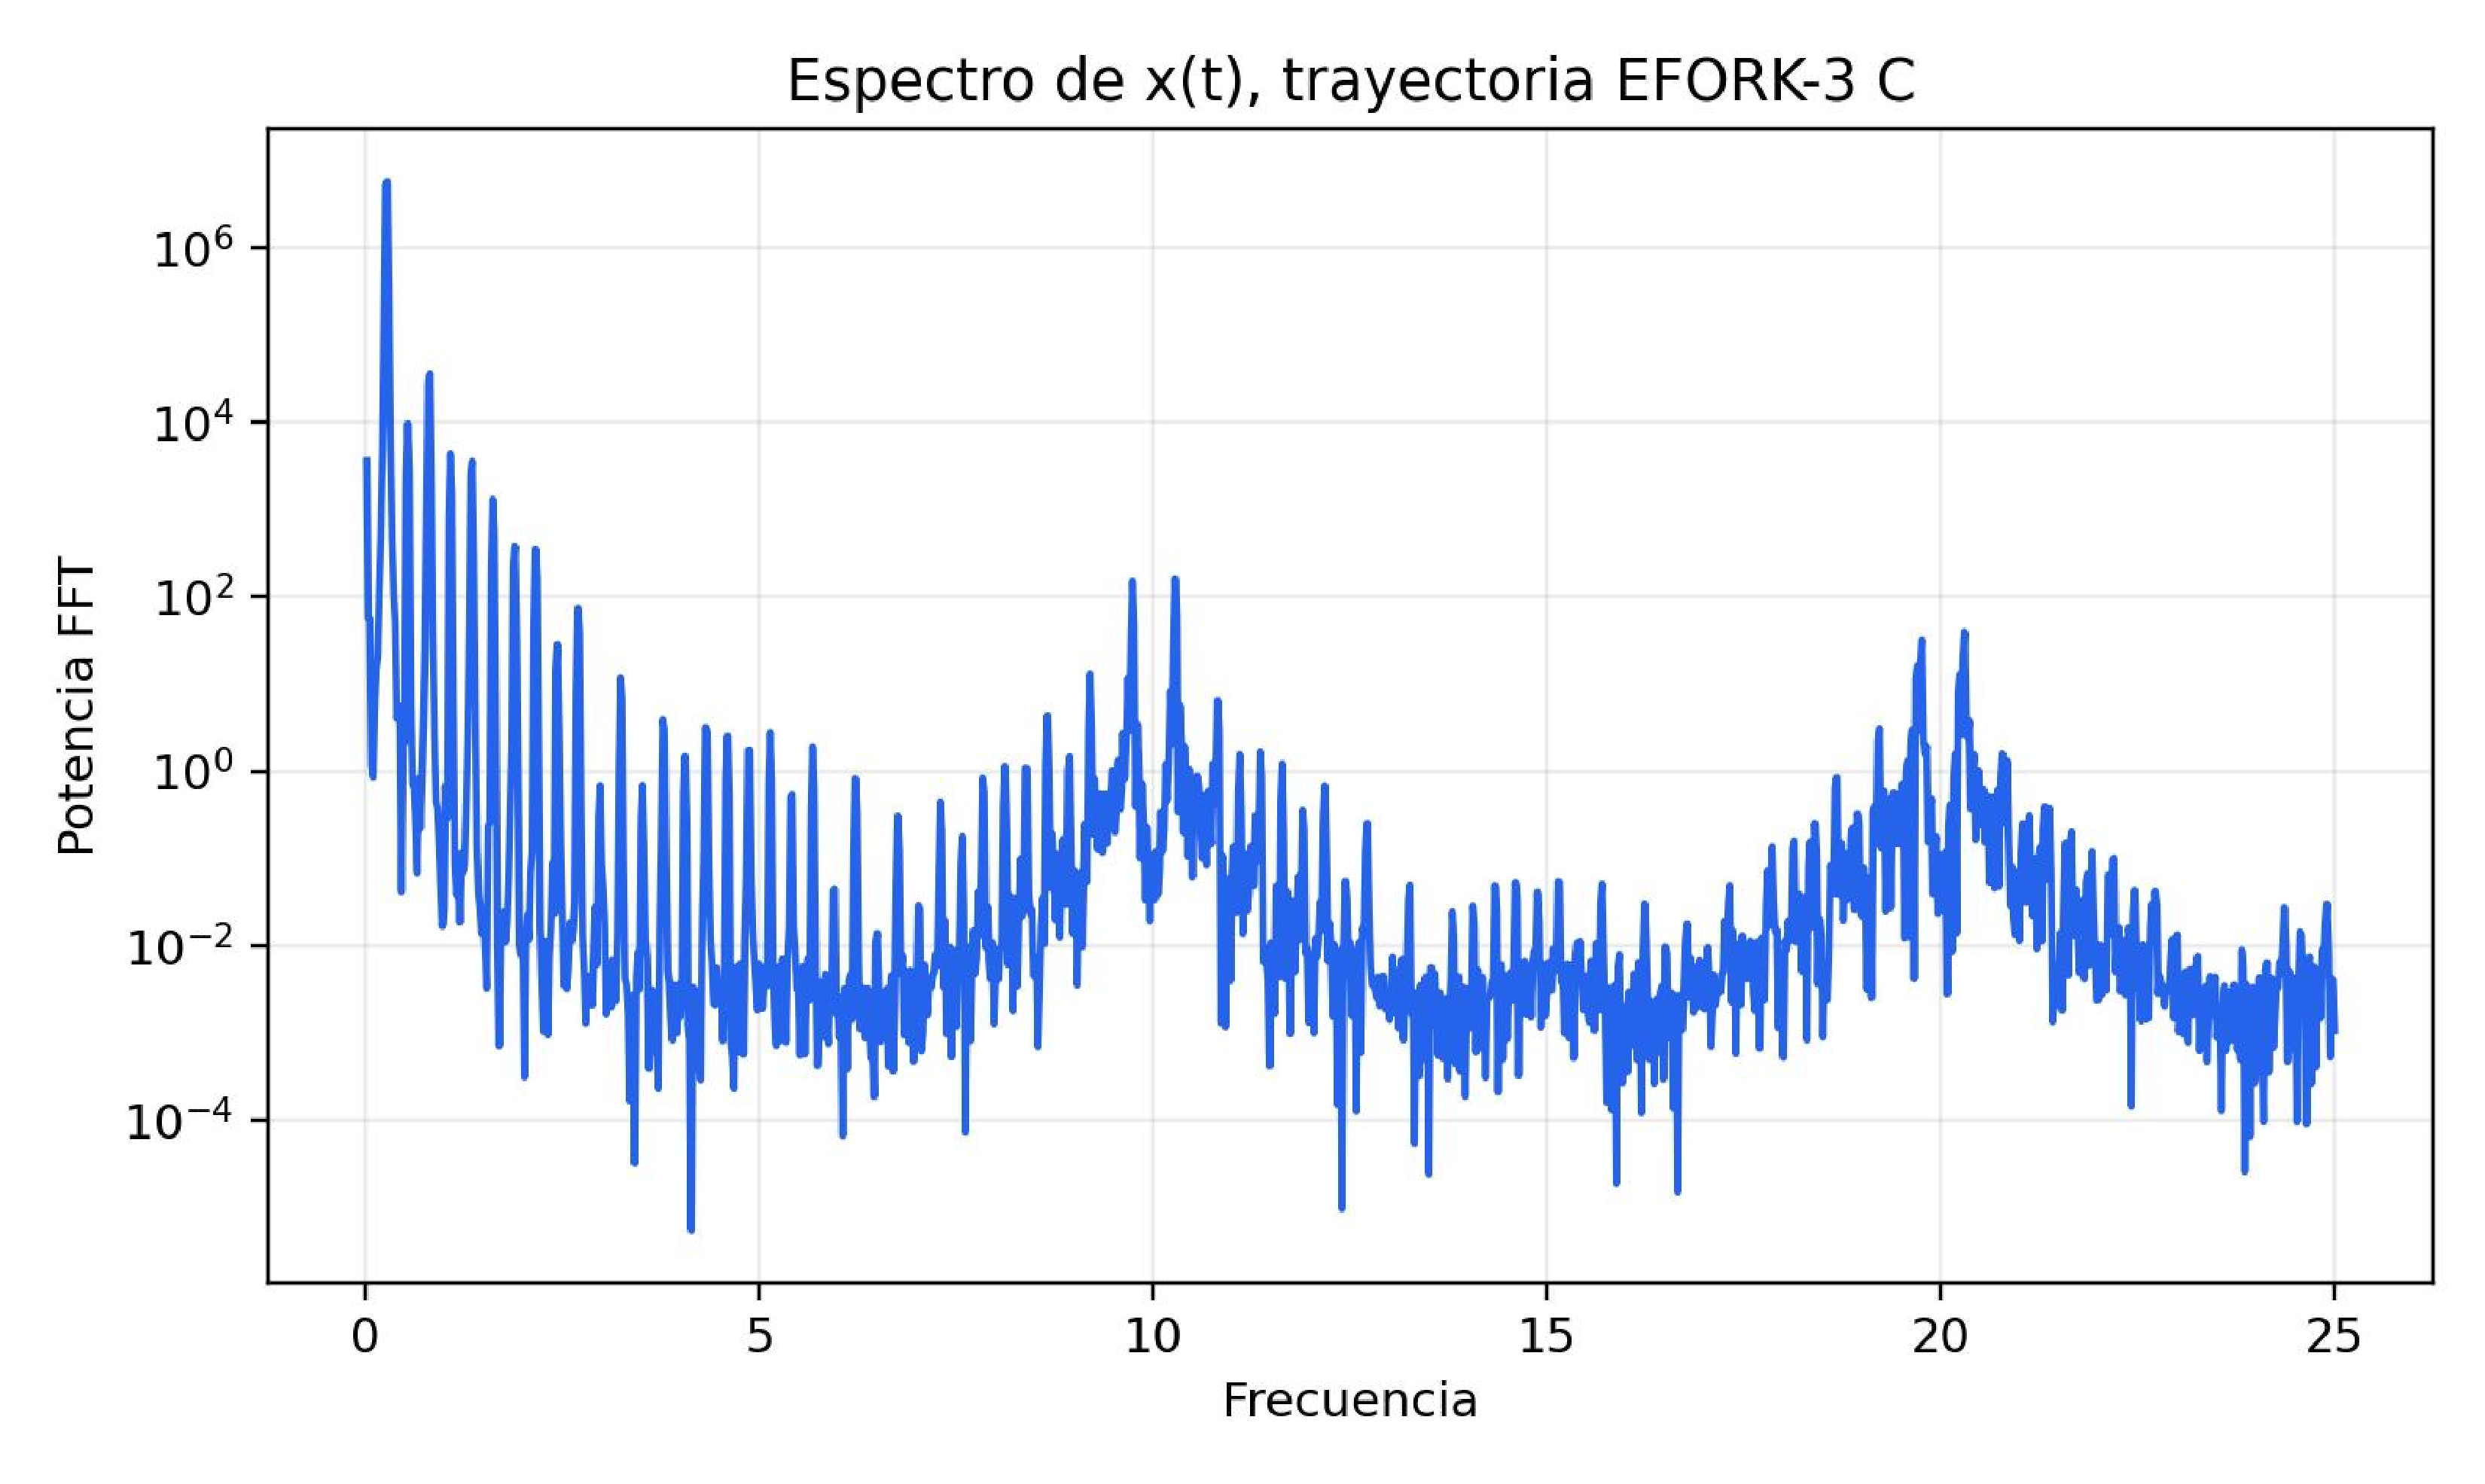
\includegraphics[width=0.94\linewidth,height=0.37\textheight,keepaspectratio]{figures/chua_master/danca_frac_spectrum_x.pdf}\\[-0.25em]
{\footnotesize Chua fraccionario con parámetros de Danca: espectro de la componente \(x\).}
\end{center}
\clearpage
\begin{center}
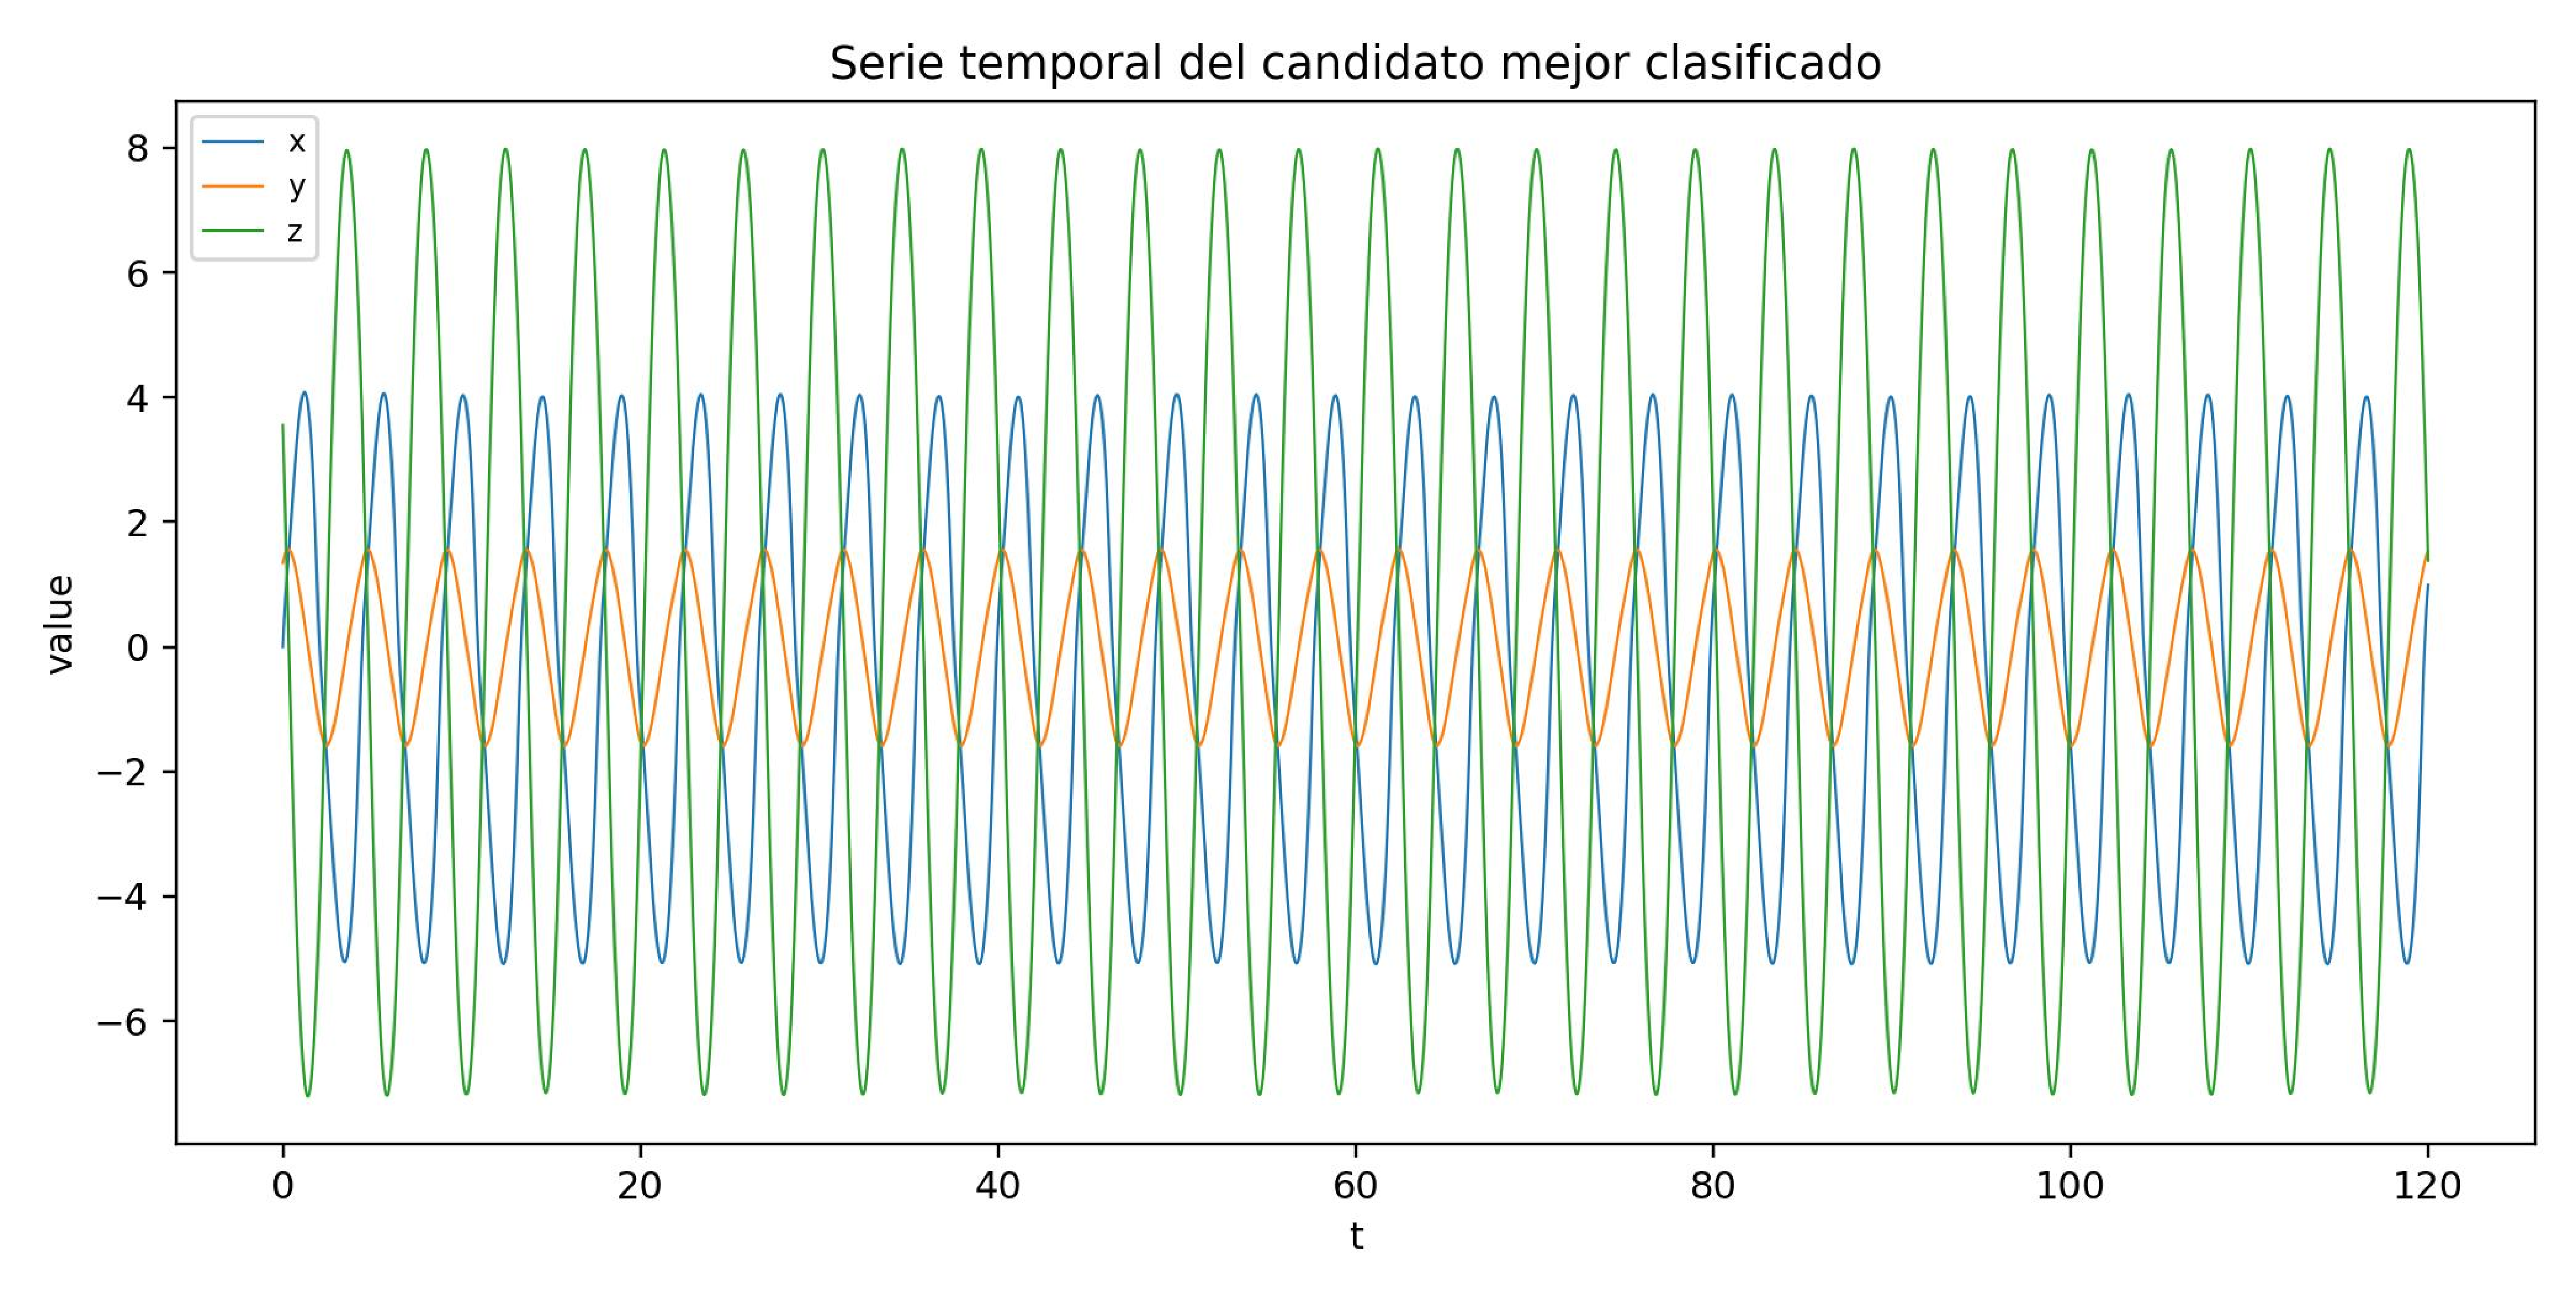
\includegraphics[width=0.94\linewidth,height=0.37\textheight,keepaspectratio]{figures/chua_master/danca_frac_time_series.pdf}\\[-0.25em]
{\footnotesize Chua fraccionario con parámetros de Danca: series temporales.}
\end{center}
\vfill
\begin{center}

\includegraphics[width=0.94\linewidth,height=0.37\textheight,keepaspectratio]{figures/chua_master/fig01_nyquist_df.pdf}\\[-0.25em]
{\footnotesize Chua entero: diagrama de Nyquist y función descriptiva.}
\end{center}
\clearpage
\begin{center}
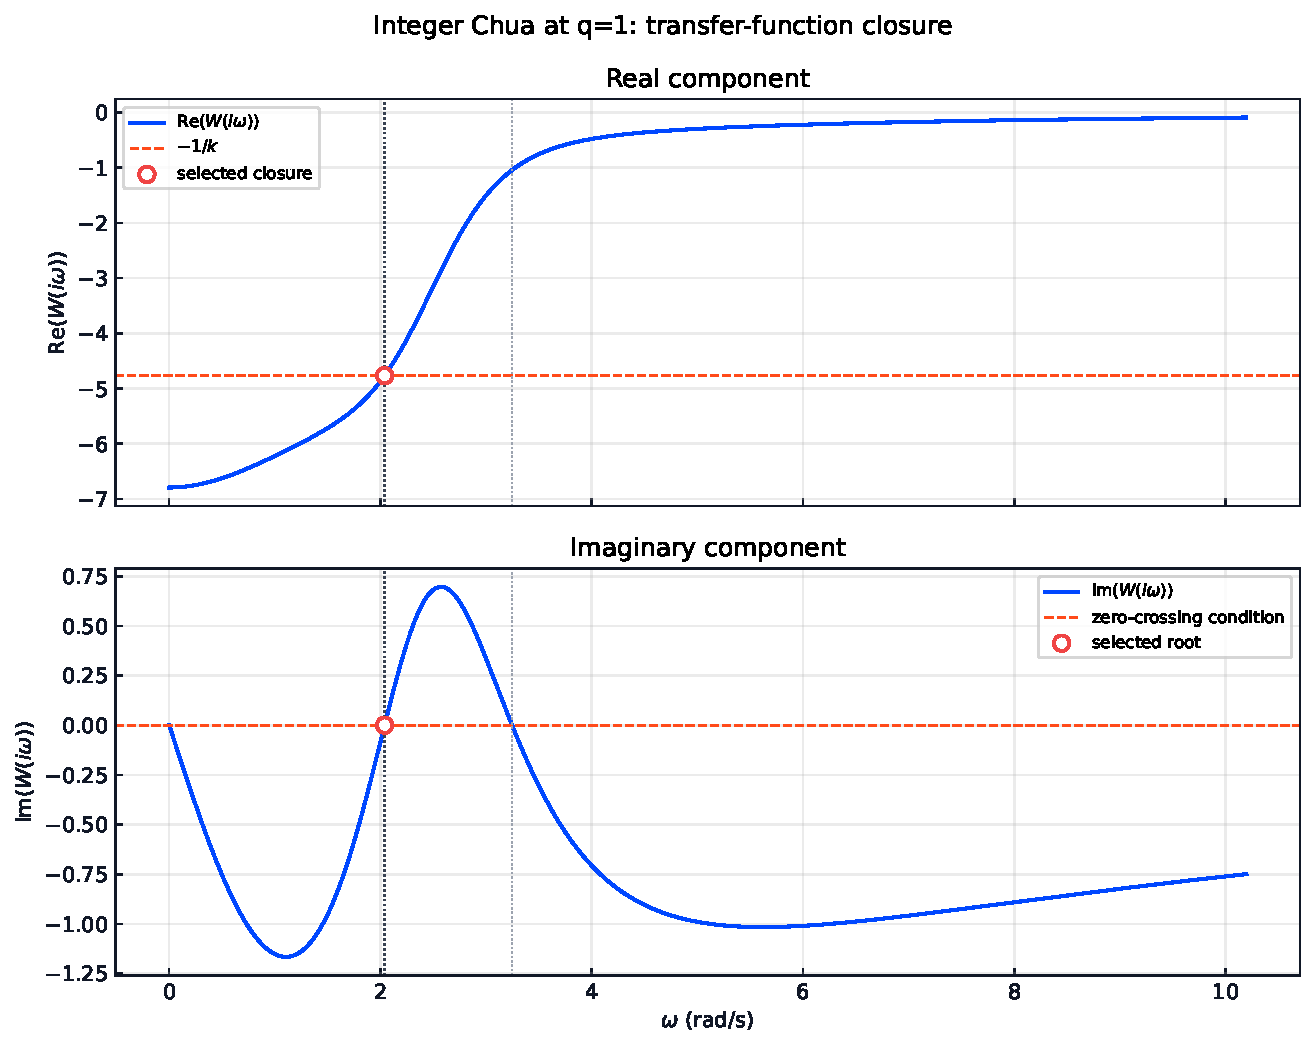
\includegraphics[width=0.94\linewidth,height=0.37\textheight,keepaspectratio]{figures/chua_master/fig01c_transfer_real_imag.pdf}\\[-0.25em]
{\footnotesize Chua entero: partes real e imaginaria de la transferencia.}
\end{center}
\vfill
\begin{center}
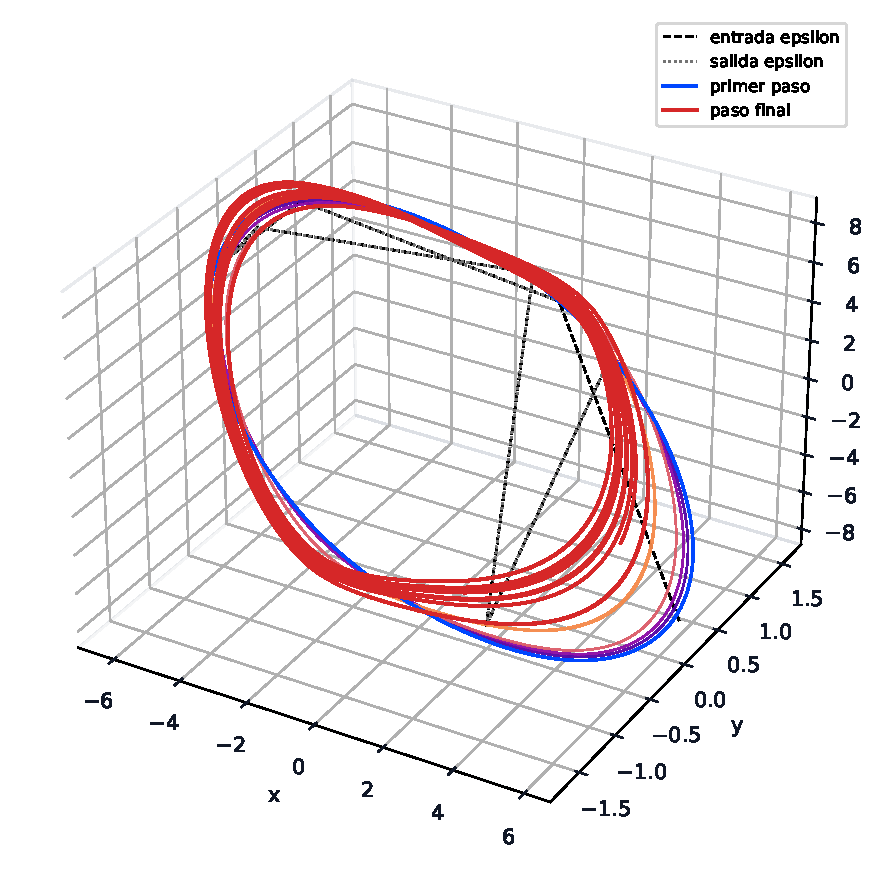
\includegraphics[width=0.94\linewidth,height=0.37\textheight,keepaspectratio]{figures/chua_master/fig02d_continuation_story.pdf}\\[-0.25em]
{\footnotesize Chua entero: evolución de la trayectoria durante la continuación.}
\end{center}
\clearpage
\begin{center}

\includegraphics[width=0.94\linewidth,height=0.37\textheight,keepaspectratio]{figures/chua_master/fig03_final_attractor.pdf}\\[-0.25em]
{\footnotesize Chua entero: trayectoria final de la continuación.}
\end{center}
\vfill
\begin{center}

\includegraphics[width=0.94\linewidth,height=0.37\textheight,keepaspectratio]{figures/chua_master/fig05b_hiddenness_overview.pdf}\\[-0.25em]
{\footnotesize Chua entero: destinos de los sondeos próximos a los equilibrios.}
\end{center}
\clearpage
\begin{center}
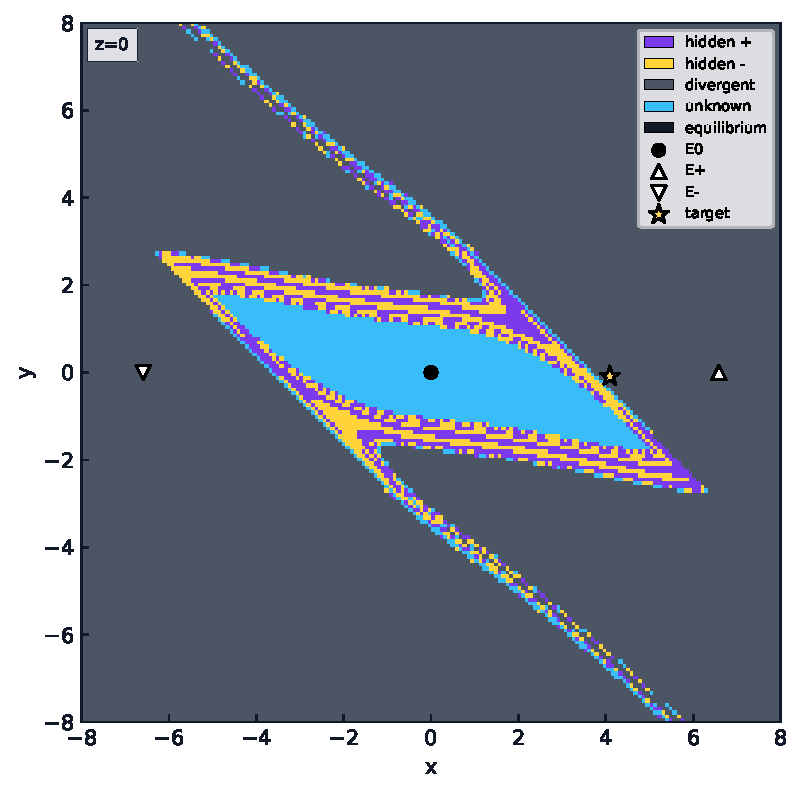
\includegraphics[width=0.94\linewidth,height=0.37\textheight,keepaspectratio]{figures/chua_master/fig06a_basin_overlay_z0.pdf}\\[-0.25em]
{\footnotesize Chua entero: regiones de destino sobre el plano \(z=0\).}
\end{center}
\vfill
\begin{center}
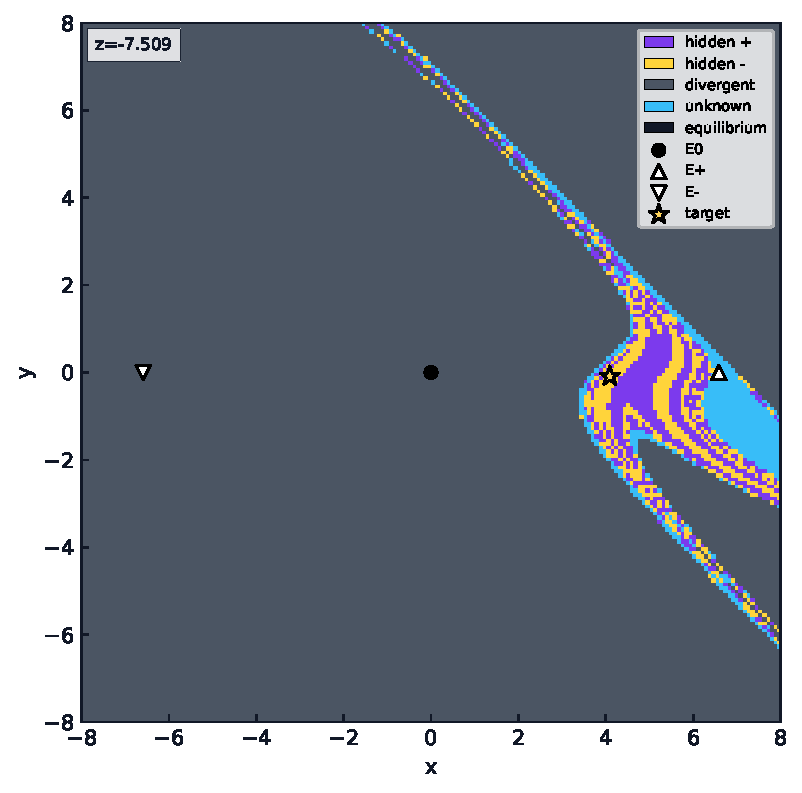
\includegraphics[width=0.94\linewidth,height=0.37\textheight,keepaspectratio]{figures/chua_master/fig06b_basin_overlay_zfinal.pdf}\\[-0.25em]
{\footnotesize Chua entero: regiones de destino sobre un plano transversal a la trayectoria final.}
\end{center}
\clearpage
\begin{center}
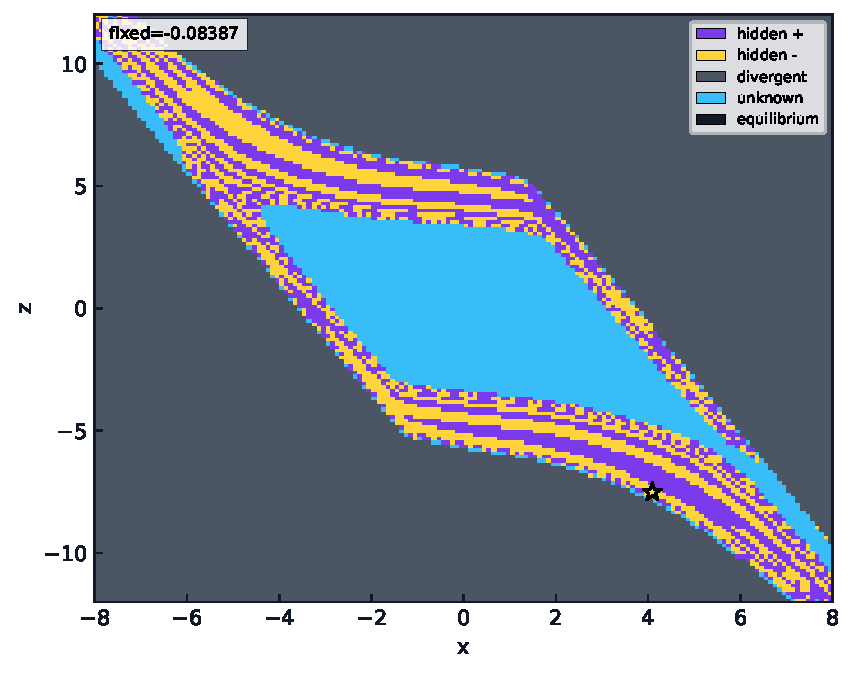
\includegraphics[width=0.94\linewidth,height=0.37\textheight,keepaspectratio]{figures/chua_master/fig10b_basin_xz_final_state.pdf}\\[-0.25em]
{\footnotesize Chua entero: regiones de destino en un corte \(xz\).}
\end{center}
\vfill
\begin{center}
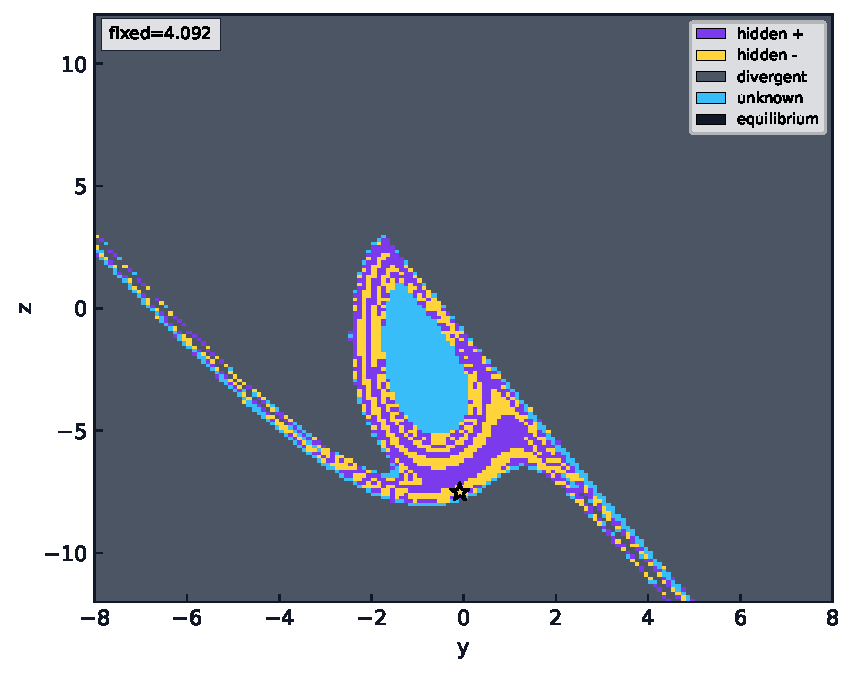
\includegraphics[width=0.94\linewidth,height=0.37\textheight,keepaspectratio]{figures/chua_master/fig10c_basin_yz_final_state.pdf}\\[-0.25em]
{\footnotesize Chua entero: regiones de destino en un corte \(yz\).}
\end{center}
\clearpage
\begin{center}

\includegraphics[width=0.94\linewidth,height=0.37\textheight,keepaspectratio]{figures/chua_master/fig11a_fft_x.pdf}\\[-0.25em]
{\footnotesize Chua entero: espectro de amplitud de \(x\).}
\end{center}
\vfill
\begin{center}
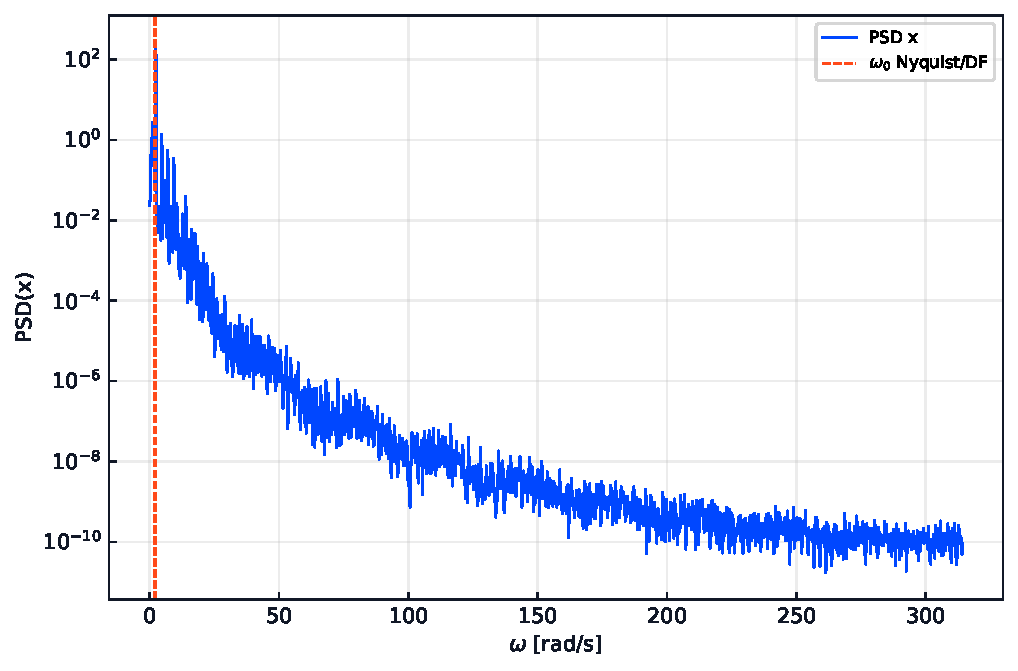
\includegraphics[width=0.94\linewidth,height=0.37\textheight,keepaspectratio]{figures/chua_master/fig11d_psd_x.pdf}\\[-0.25em]
{\footnotesize Chua entero: densidad espectral de potencia de \(x\).}
\end{center}
\clearpage
\begin{center}
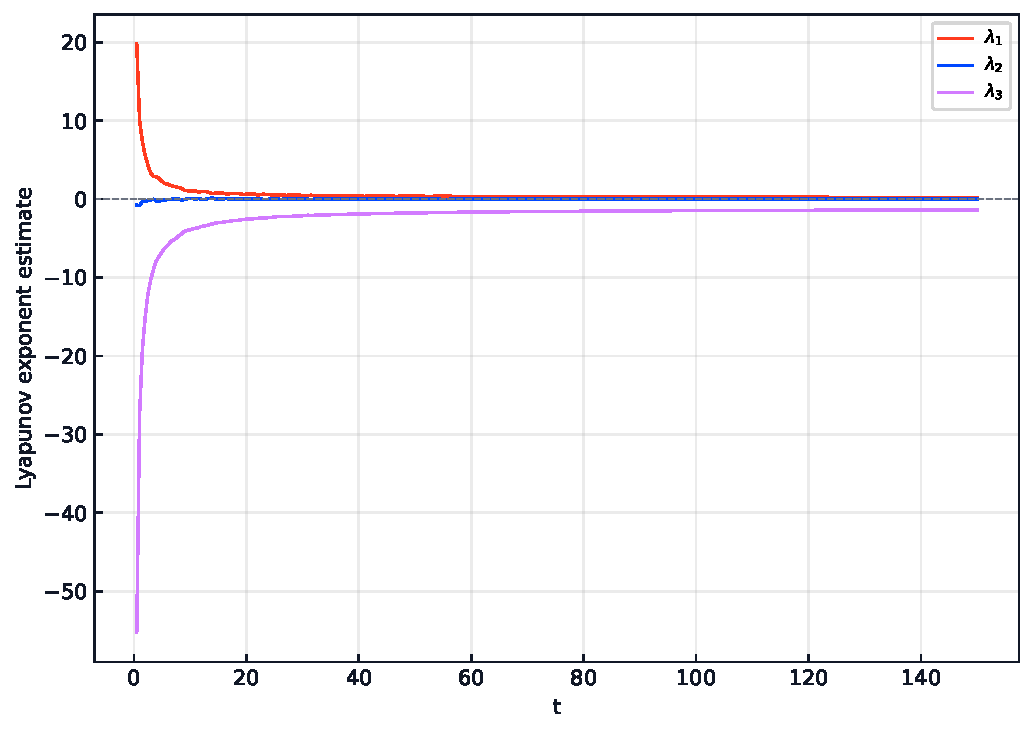
\includegraphics[width=0.94\linewidth,height=0.37\textheight,keepaspectratio]{figures/chua_master/fig13_lyapunov_convergence.pdf}\\[-0.25em]
{\footnotesize Chua entero: evolución de las estimaciones de Lyapunov.}
\end{center}
\vfill
\begin{center}
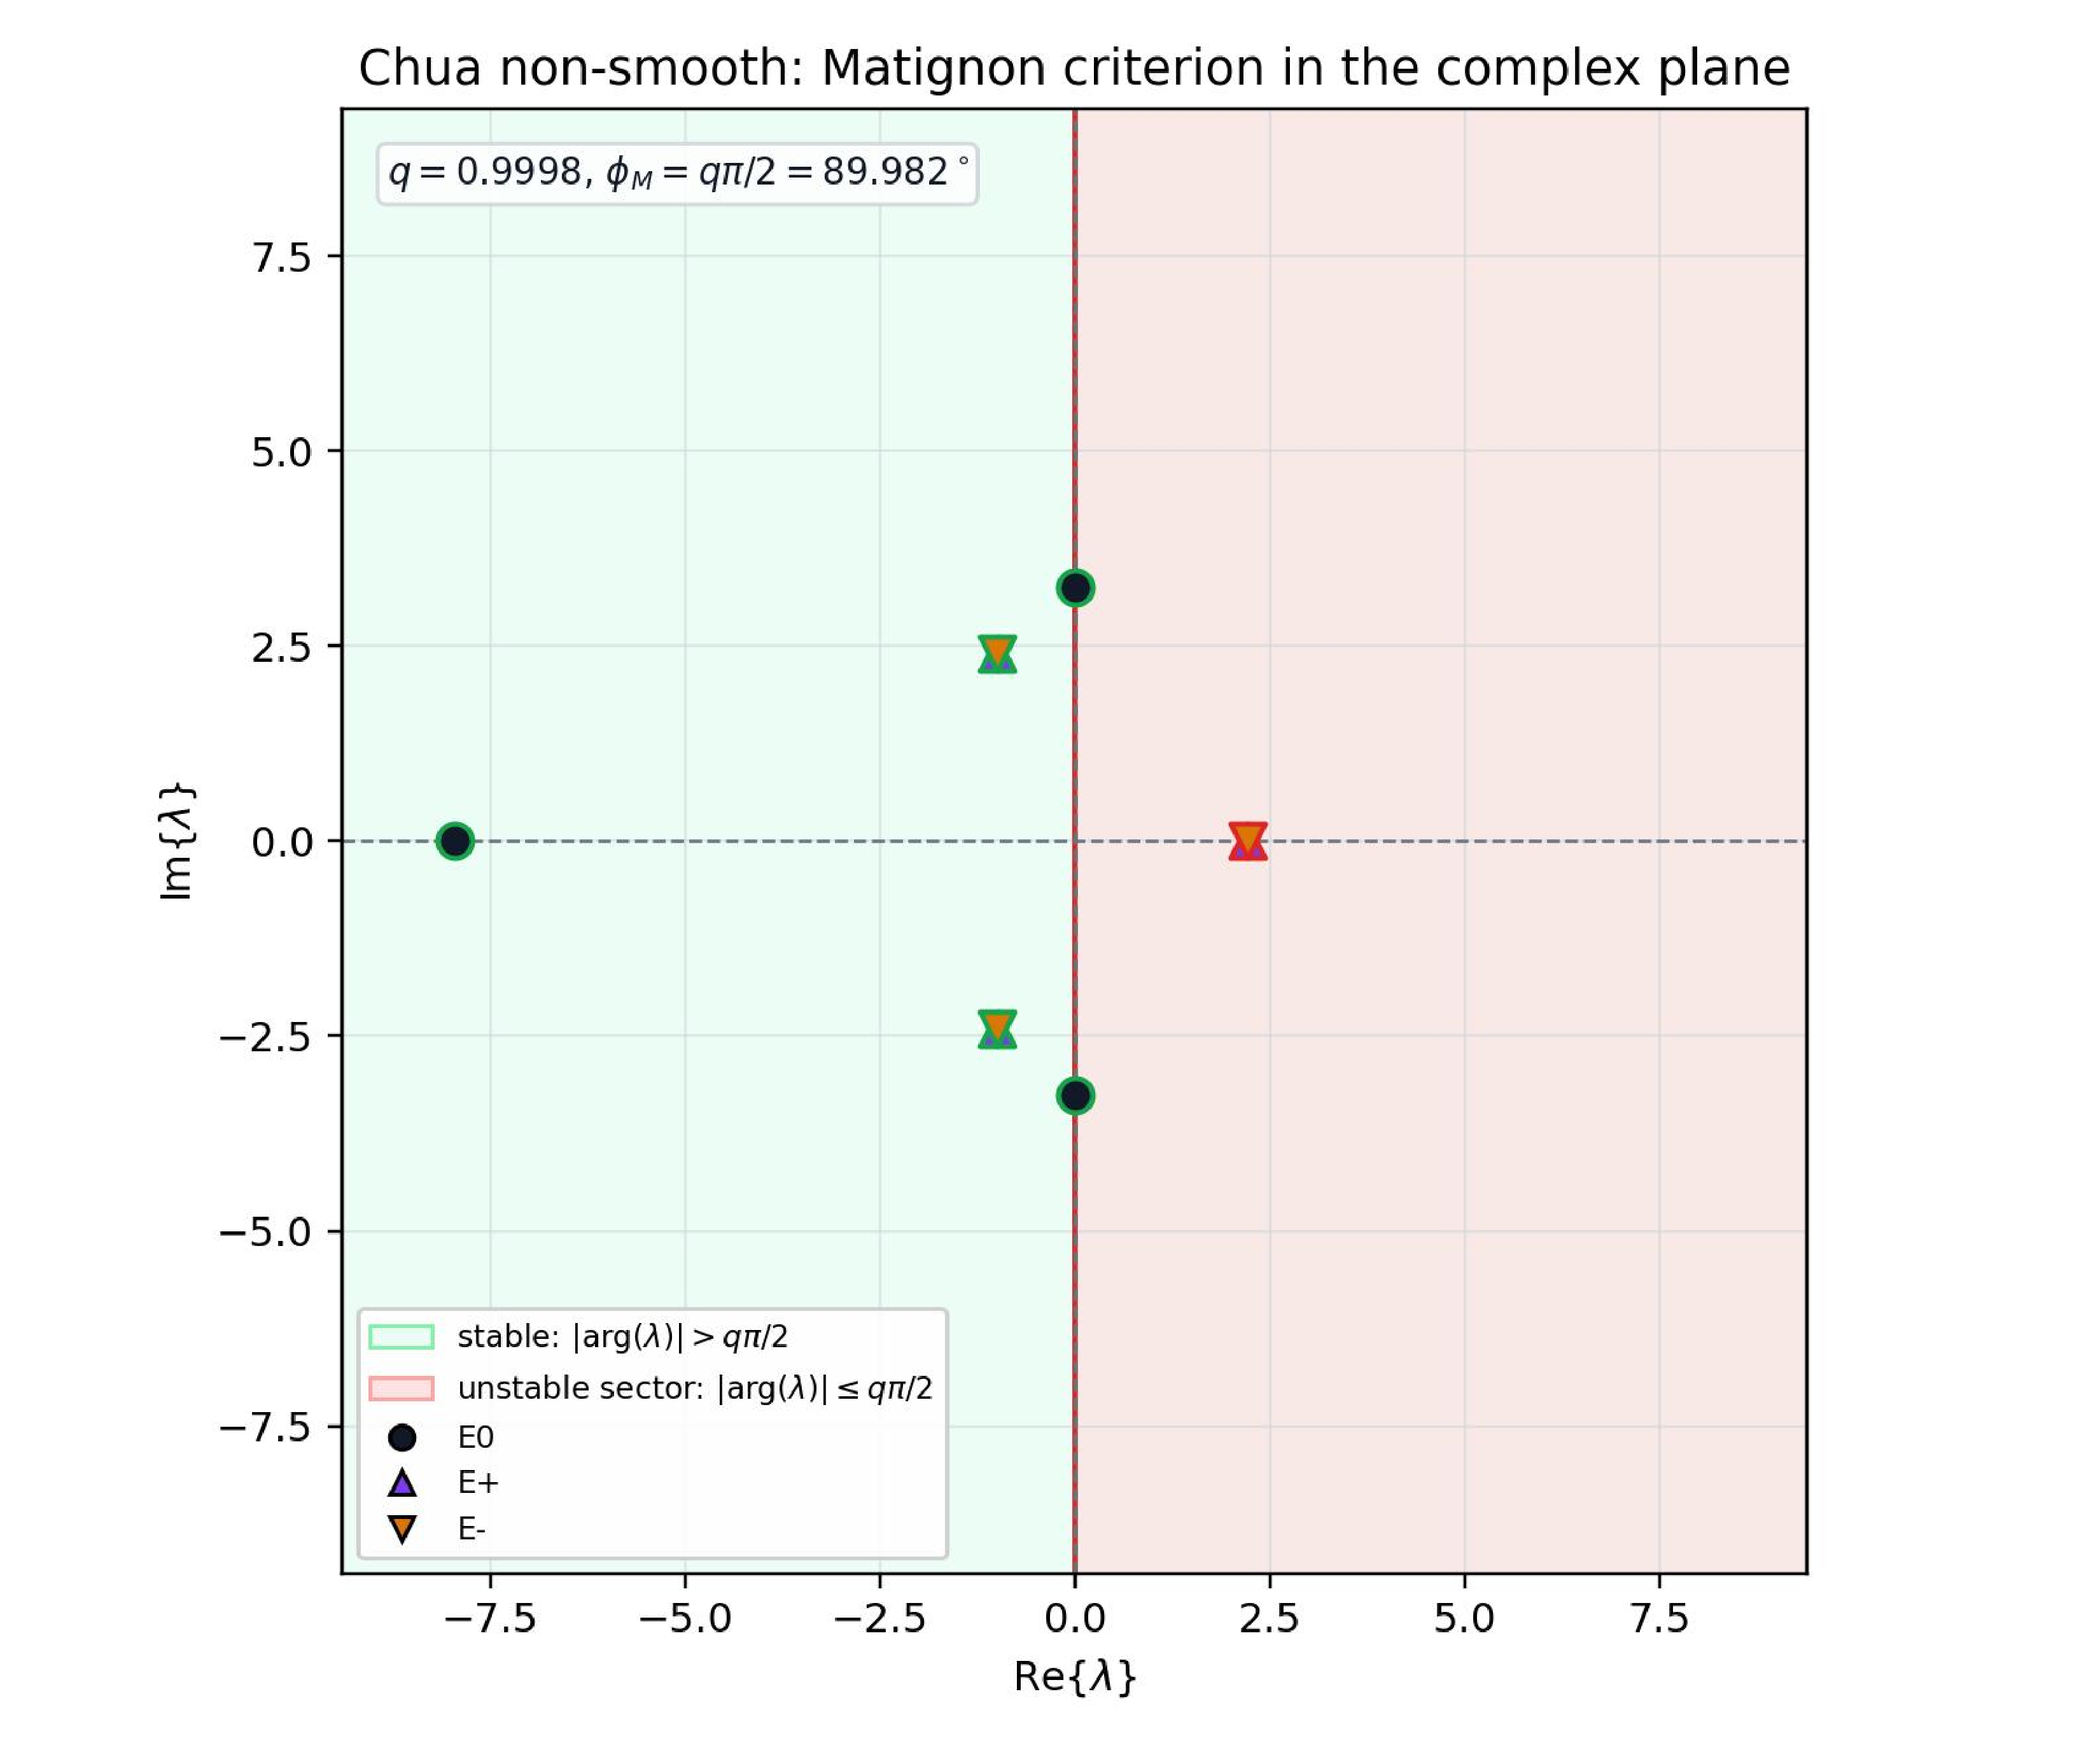
\includegraphics[width=0.94\linewidth,height=0.37\textheight,keepaspectratio]{figures/chua_master/matignon_complex_plane.pdf}\\[-0.25em]
{\footnotesize Valores propios y sector de estabilidad de Matignon.}
\end{center}
\clearpage
\begin{center}

\includegraphics[width=0.94\linewidth,height=0.37\textheight,keepaspectratio]{figures/chua_master/wu2023_chua_fractional_arctan_q099_x0_minus_phase3d.pdf}\\[-0.25em]
{\footnotesize Chua arctangente de Wu: trayectoria en el espacio de estados desde \(X_{0,-}\).}
\end{center}
\vfill
\begin{center}

\includegraphics[width=0.94\linewidth,height=0.37\textheight,keepaspectratio]{figures/chua_master/wu2023_chua_fractional_arctan_q099_x0_minus_projections.pdf}\\[-0.25em]
{\footnotesize Chua arctangente de Wu: proyecciones de la trayectoria desde \(X_{0,-}\).}
\end{center}
\clearpage
\begin{center}

\includegraphics[width=0.94\linewidth,height=0.37\textheight,keepaspectratio]{figures/chua_master/wu2023_chua_fractional_arctan_q099_x0_minus_timeseries.pdf}\\[-0.25em]
{\footnotesize Chua arctangente de Wu: series temporales desde \(X_{0,-}\).}
\end{center}
\vfill
\begin{center}

\includegraphics[width=0.94\linewidth,height=0.37\textheight,keepaspectratio]{figures/chua_master/wu2023_chua_fractional_arctan_q099_x0_plus_phase3d.pdf}\\[-0.25em]
{\footnotesize Chua arctangente de Wu: trayectoria en el espacio de estados desde \(X_{0,+}\).}
\end{center}
\clearpage
\begin{center}

\includegraphics[width=0.94\linewidth,height=0.37\textheight,keepaspectratio]{figures/chua_master/wu2023_chua_fractional_arctan_q099_x0_plus_projections.pdf}\\[-0.25em]
{\footnotesize Chua arctangente de Wu: proyecciones de la trayectoria desde \(X_{0,+}\).}
\end{center}
\vfill
\begin{center}

\includegraphics[width=0.94\linewidth,height=0.37\textheight,keepaspectratio]{figures/chua_master/wu2023_chua_fractional_arctan_q099_x0_plus_timeseries.pdf}\\[-0.25em]
{\footnotesize Chua arctangente de Wu: series temporales desde \(X_{0,+}\).}
\end{center}
\clearpage
\clearpage
\subsection{Kalman--Fitts entero}
Obstrucción directa, mapa de conmutación, continuación, ciclo, series, FFT, PSD de Welch, Lyapunov y controles locales.

\begin{center}
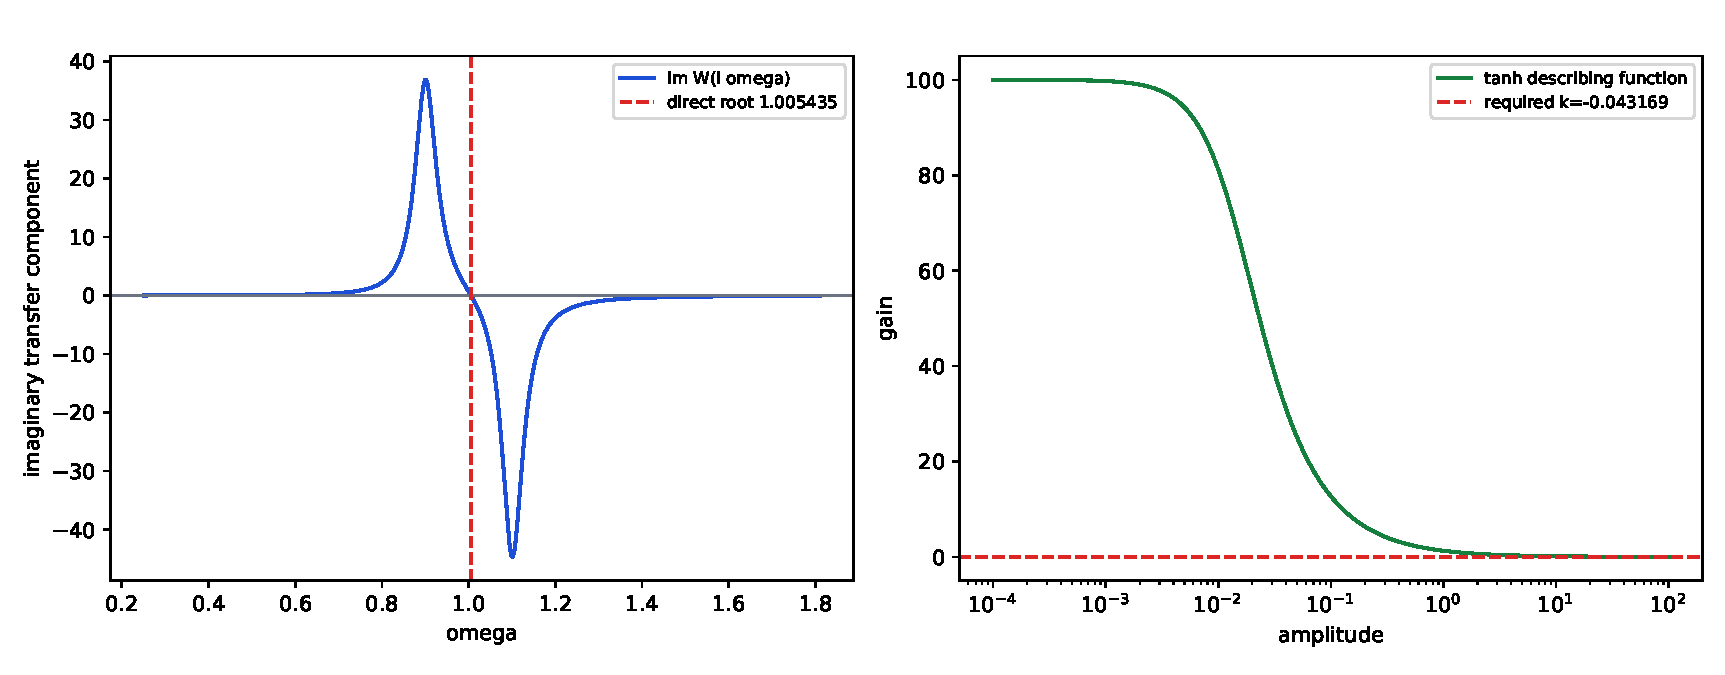
\includegraphics[width=0.94\linewidth,height=0.37\textheight,keepaspectratio]{figures/kalman_fitts/01_direct_route_incompatibility.pdf}\\[-0.25em]
{\footnotesize Kalman--Fitts: incompatibilidad del cierre armónico directo.}
\end{center}
\vfill
\begin{center}
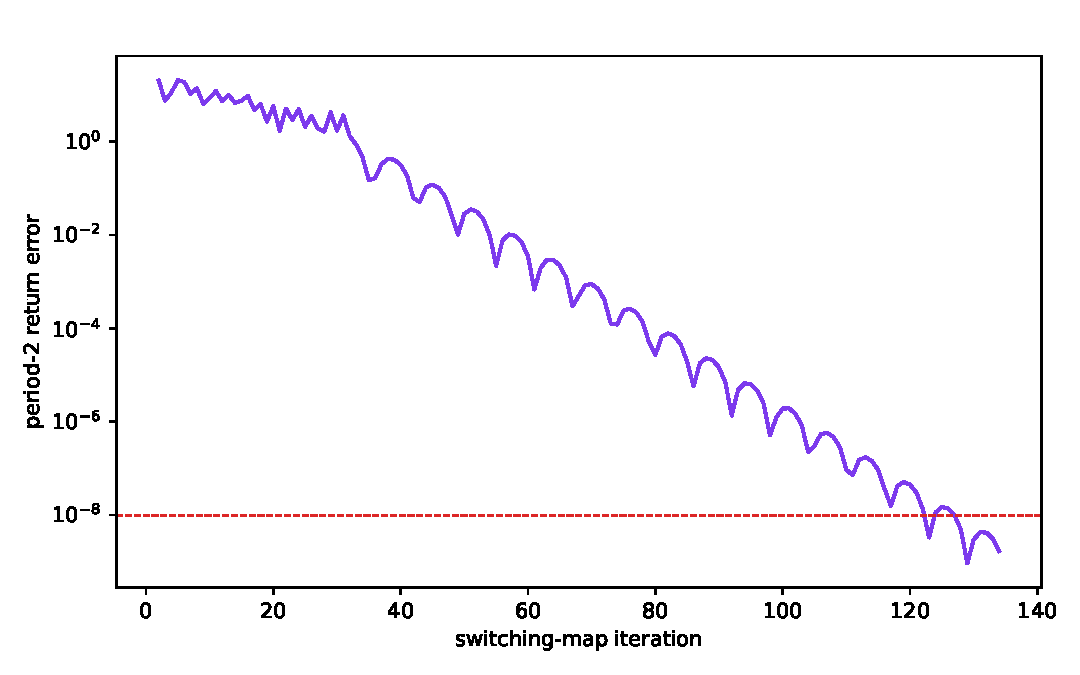
\includegraphics[width=0.94\linewidth,height=0.37\textheight,keepaspectratio]{figures/kalman_fitts/02_switching_map_convergence.pdf}\\[-0.25em]
{\footnotesize Kalman--Fitts: convergencia del mapa de conmutación.}
\end{center}
\clearpage
\begin{center}
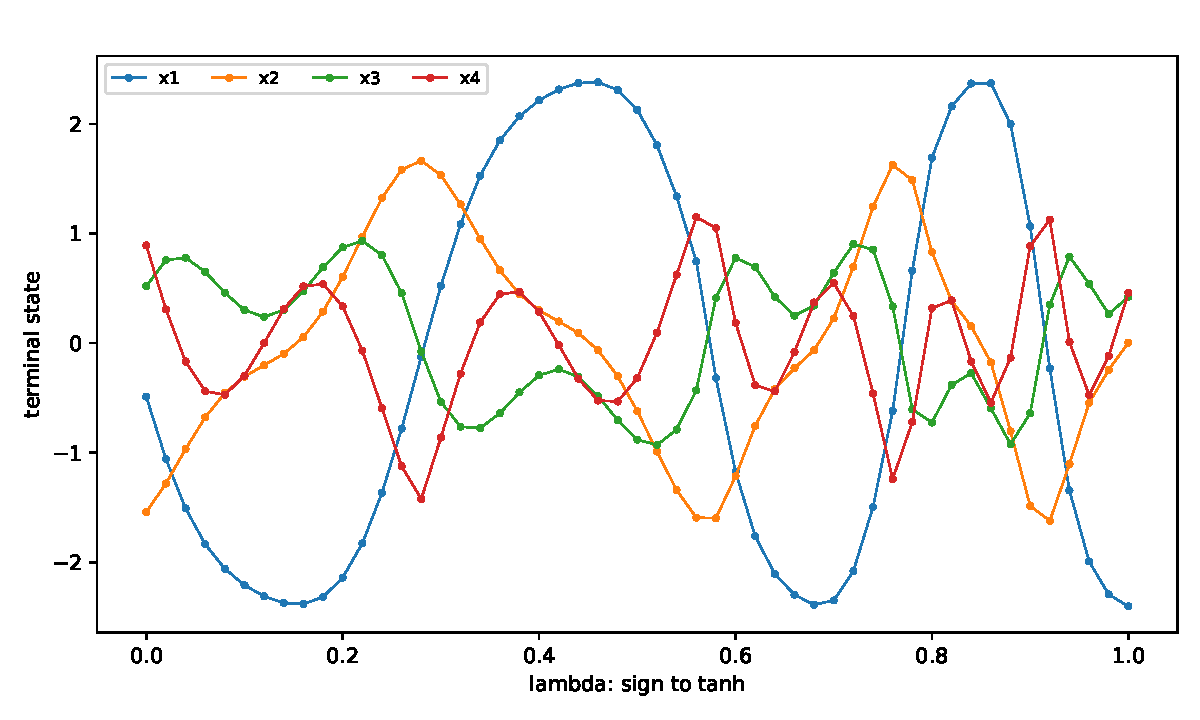
\includegraphics[width=0.94\linewidth,height=0.37\textheight,keepaspectratio]{figures/kalman_fitts/03_sign_to_tanh_continuation.pdf}\\[-0.25em]
{\footnotesize Kalman--Fitts: continuación de la no linealidad signo hacia la tangente hiperbólica.}
\end{center}
\vfill
\begin{center}
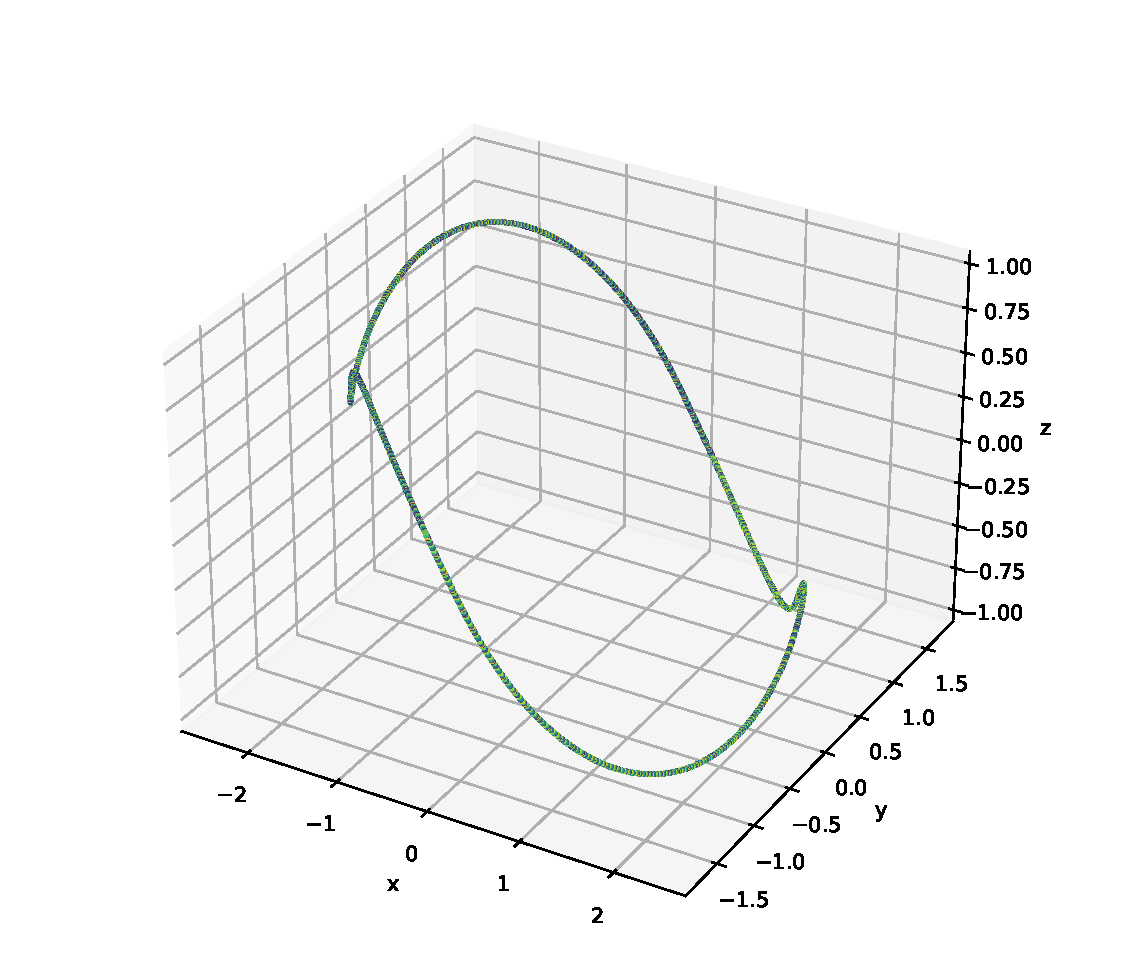
\includegraphics[width=0.94\linewidth,height=0.37\textheight,keepaspectratio]{figures/kalman_fitts/04_hidden_limit_cycle_3d.pdf}\\[-0.25em]
{\footnotesize Kalman--Fitts: trayectoria periódica candidata.}
\end{center}
\clearpage
\begin{center}
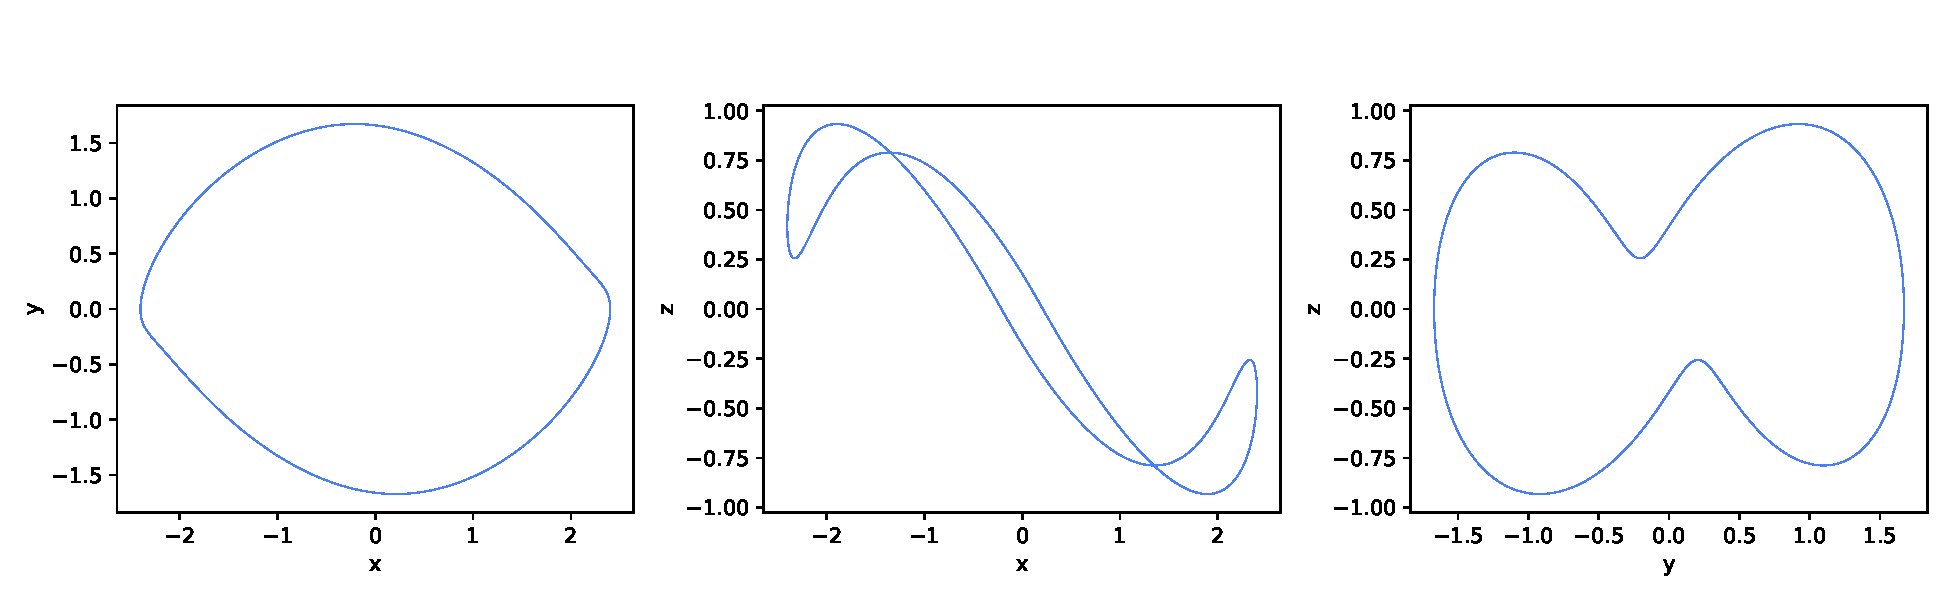
\includegraphics[width=0.94\linewidth,height=0.37\textheight,keepaspectratio]{figures/kalman_fitts/05_hidden_limit_cycle_projections.pdf}\\[-0.25em]
{\footnotesize Kalman--Fitts: proyecciones del ciclo candidato.}
\end{center}
\vfill
\begin{center}
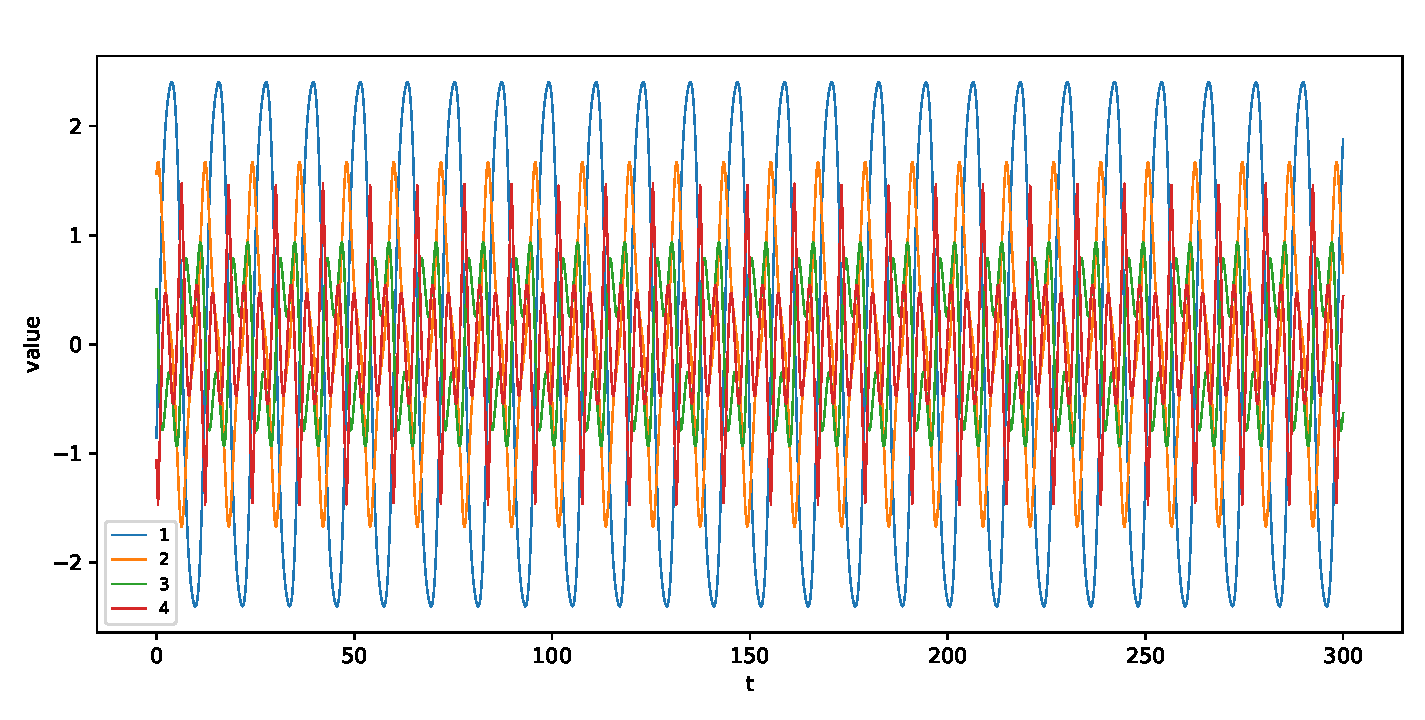
\includegraphics[width=0.94\linewidth,height=0.37\textheight,keepaspectratio]{figures/kalman_fitts/06_hidden_limit_cycle_timeseries.pdf}\\[-0.25em]
{\footnotesize Kalman--Fitts: series temporales del ciclo candidato.}
\end{center}
\clearpage
\begin{center}
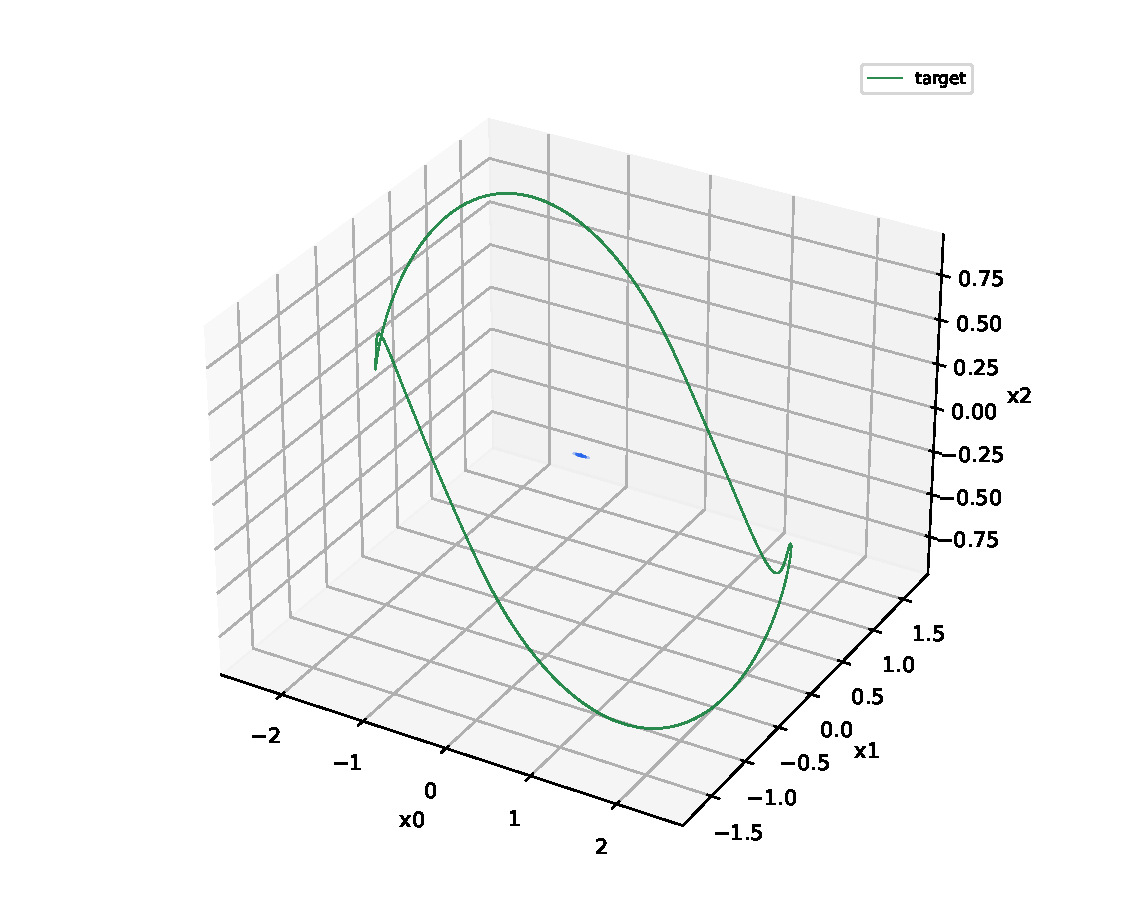
\includegraphics[width=0.94\linewidth,height=0.37\textheight,keepaspectratio]{figures/kalman_fitts/07_equilibrium_neighborhood_controls.pdf}\\[-0.25em]
{\footnotesize Kalman--Fitts: destinos de los sondeos próximos al equilibrio.}
\end{center}
\vfill
\begin{center}
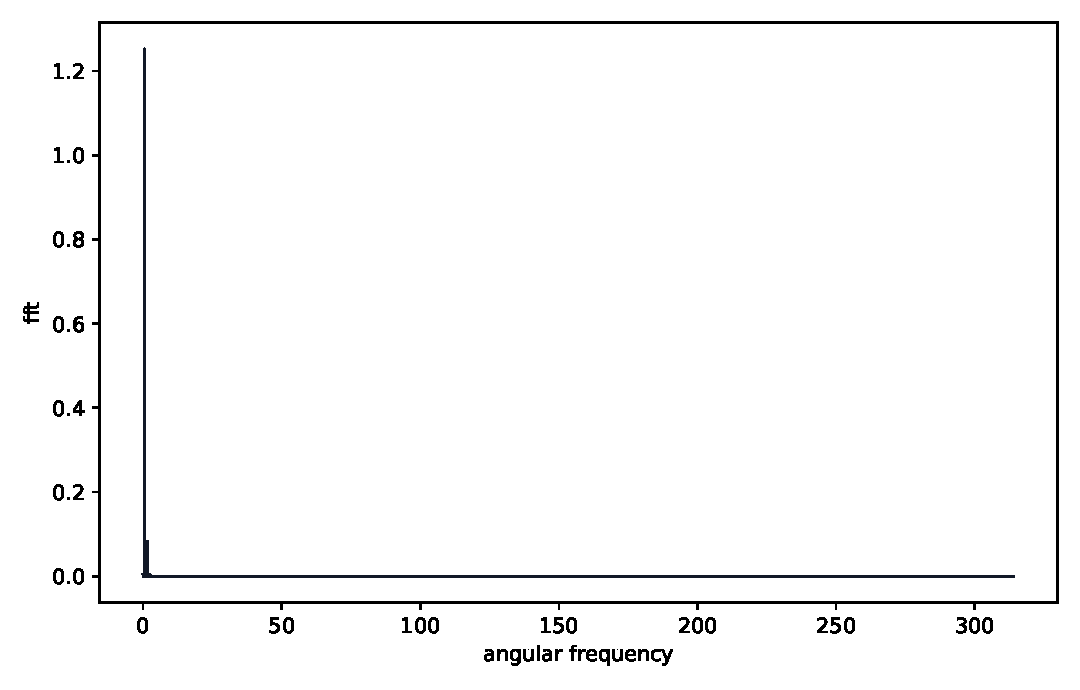
\includegraphics[width=0.94\linewidth,height=0.37\textheight,keepaspectratio]{figures/kalman_fitts/08_kalman_fitts_fft_component_0.pdf}\\[-0.25em]
{\footnotesize Kalman--Fitts: espectro de amplitud de la componente \(x_1\).}
\end{center}
\clearpage
\begin{center}
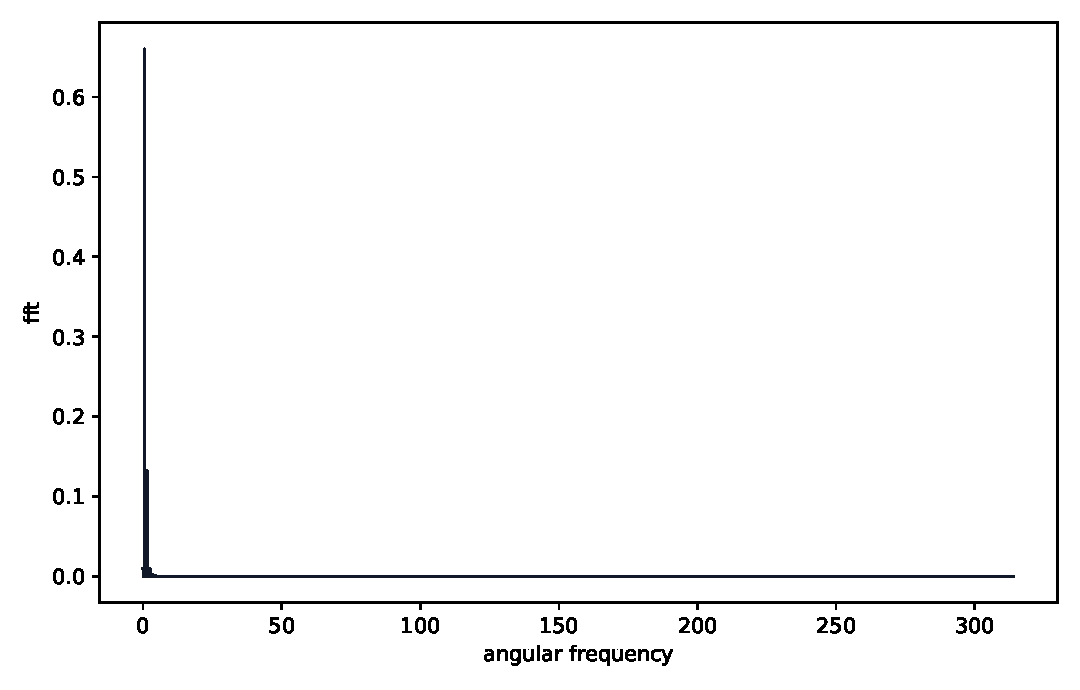
\includegraphics[width=0.94\linewidth,height=0.37\textheight,keepaspectratio]{figures/kalman_fitts/08_kalman_fitts_fft_component_1.pdf}\\[-0.25em]
{\footnotesize Kalman--Fitts: espectro de amplitud de la componente \(x_2\).}
\end{center}
\vfill
\begin{center}
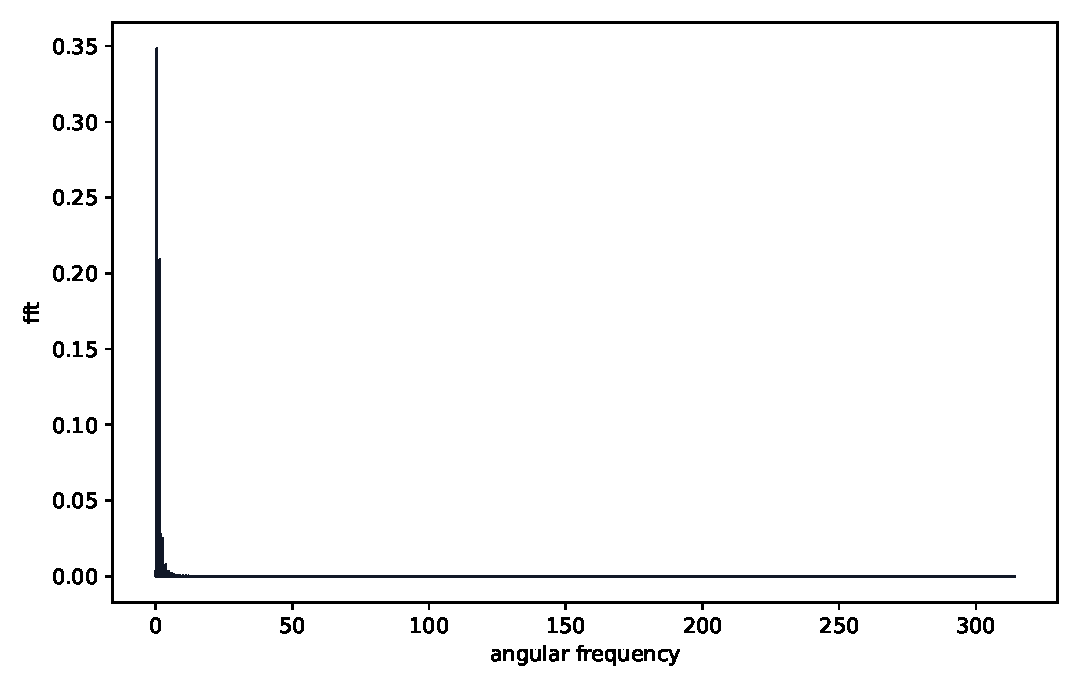
\includegraphics[width=0.94\linewidth,height=0.37\textheight,keepaspectratio]{figures/kalman_fitts/08_kalman_fitts_fft_component_2.pdf}\\[-0.25em]
{\footnotesize Kalman--Fitts: espectro de amplitud de la componente \(x_3\).}
\end{center}
\clearpage
\begin{center}
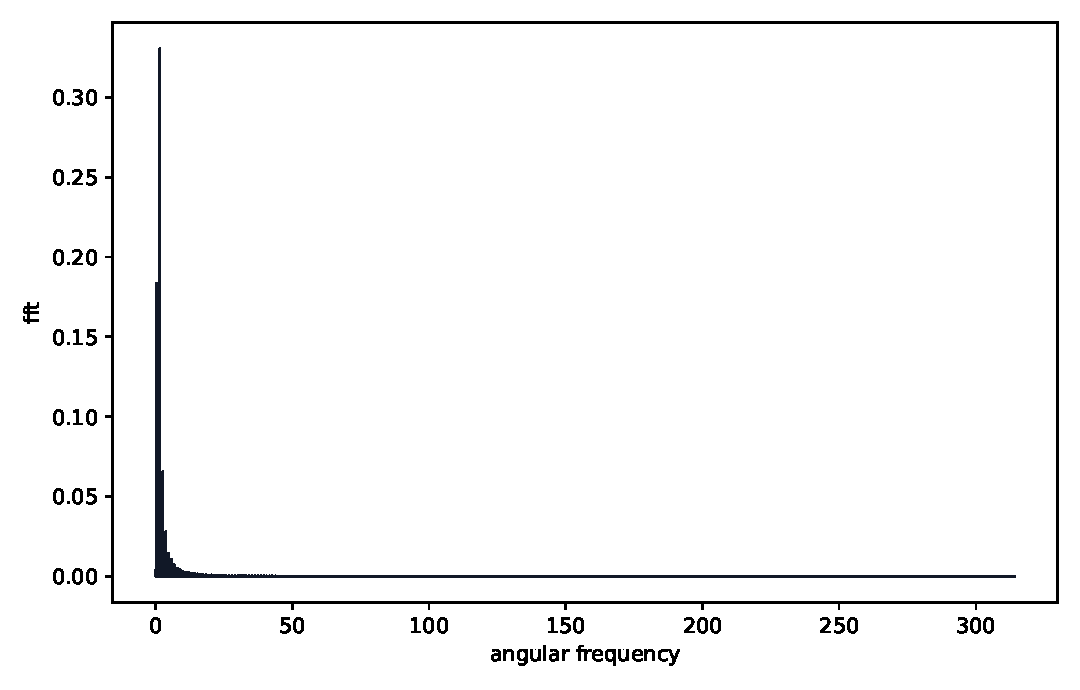
\includegraphics[width=0.94\linewidth,height=0.37\textheight,keepaspectratio]{figures/kalman_fitts/08_kalman_fitts_fft_component_3.pdf}\\[-0.25em]
{\footnotesize Kalman--Fitts: espectro de amplitud de la componente \(x_4\).}
\end{center}
\vfill
\begin{center}
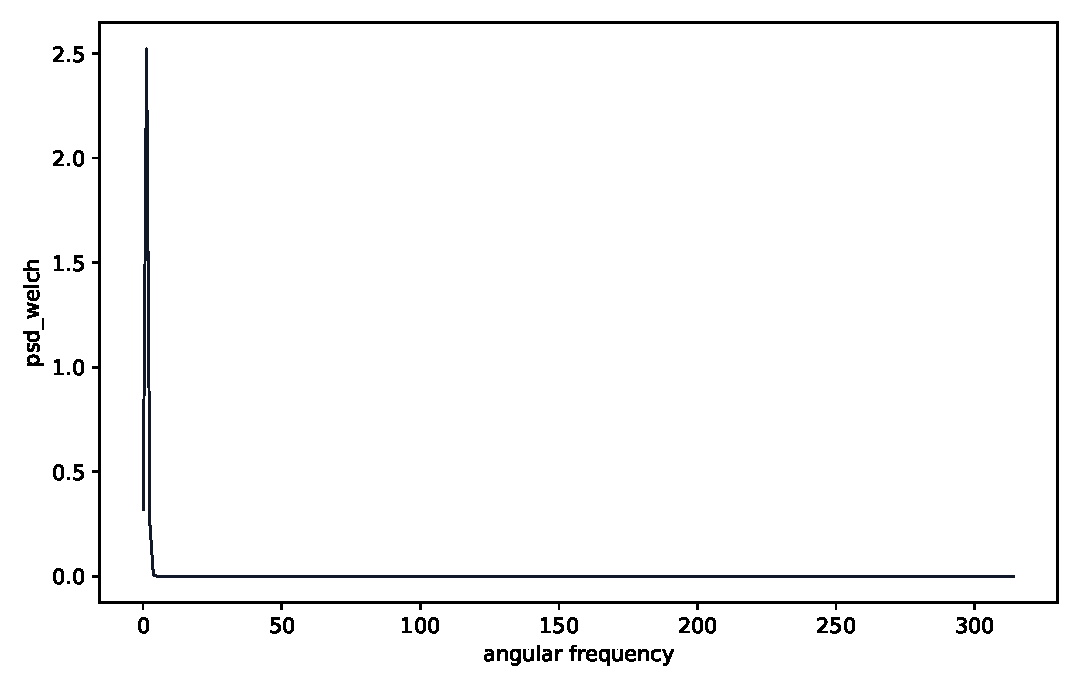
\includegraphics[width=0.94\linewidth,height=0.37\textheight,keepaspectratio]{figures/kalman_fitts/09_kalman_fitts_psd_component_0.pdf}\\[-0.25em]
{\footnotesize Kalman--Fitts: densidad espectral de potencia de la componente \(x_1\).}
\end{center}
\clearpage
\begin{center}
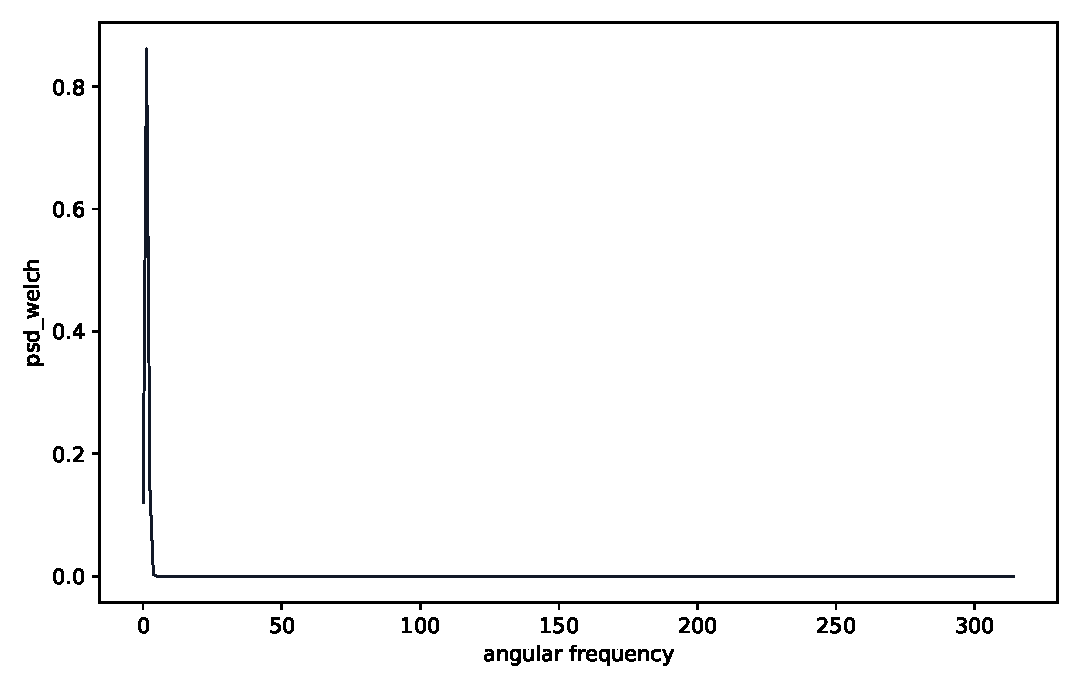
\includegraphics[width=0.94\linewidth,height=0.37\textheight,keepaspectratio]{figures/kalman_fitts/09_kalman_fitts_psd_component_1.pdf}\\[-0.25em]
{\footnotesize Kalman--Fitts: densidad espectral de potencia de la componente \(x_2\).}
\end{center}
\vfill
\begin{center}
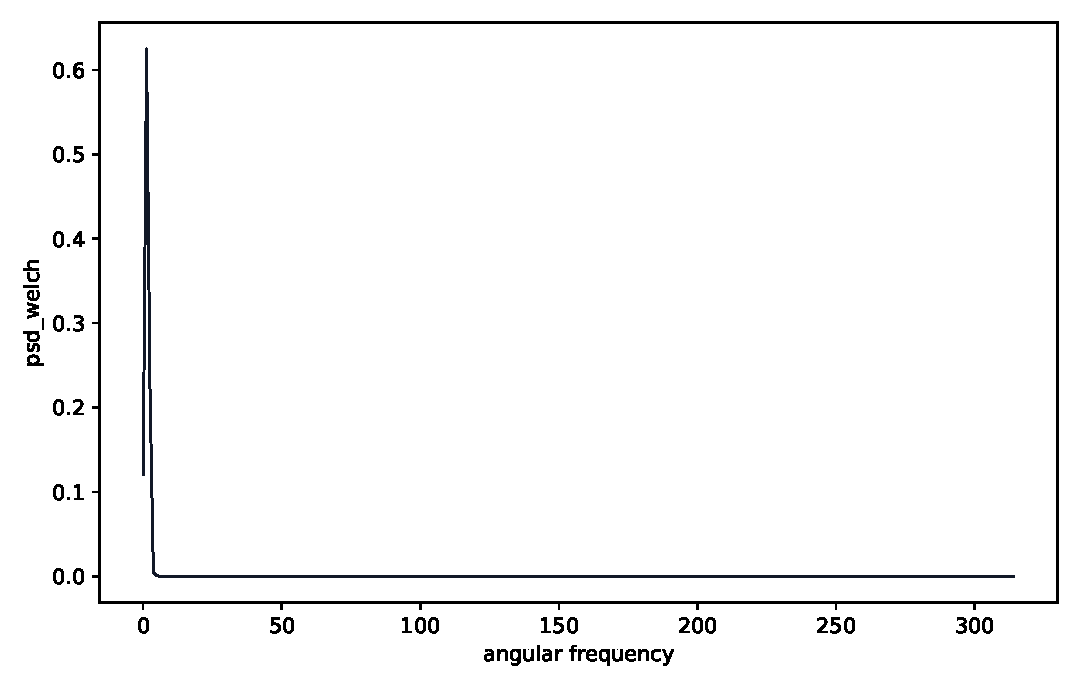
\includegraphics[width=0.94\linewidth,height=0.37\textheight,keepaspectratio]{figures/kalman_fitts/09_kalman_fitts_psd_component_2.pdf}\\[-0.25em]
{\footnotesize Kalman--Fitts: densidad espectral de potencia de la componente \(x_3\).}
\end{center}
\clearpage
\begin{center}
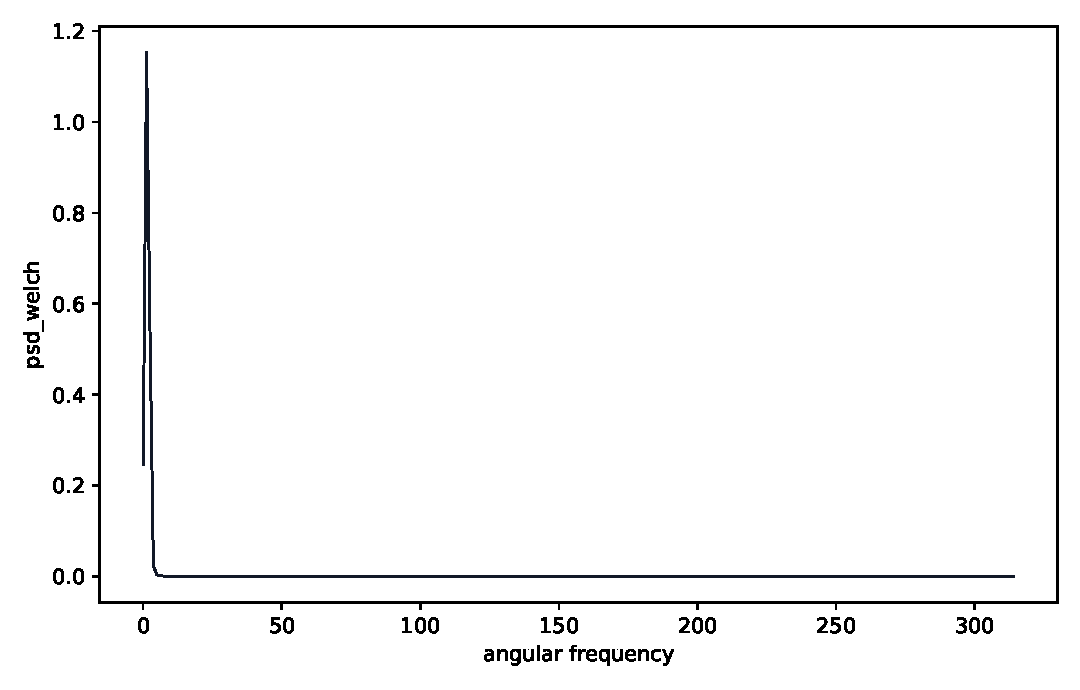
\includegraphics[width=0.94\linewidth,height=0.37\textheight,keepaspectratio]{figures/kalman_fitts/09_kalman_fitts_psd_component_3.pdf}\\[-0.25em]
{\footnotesize Kalman--Fitts: densidad espectral de potencia de la componente \(x_4\).}
\end{center}
\vfill
\begin{center}
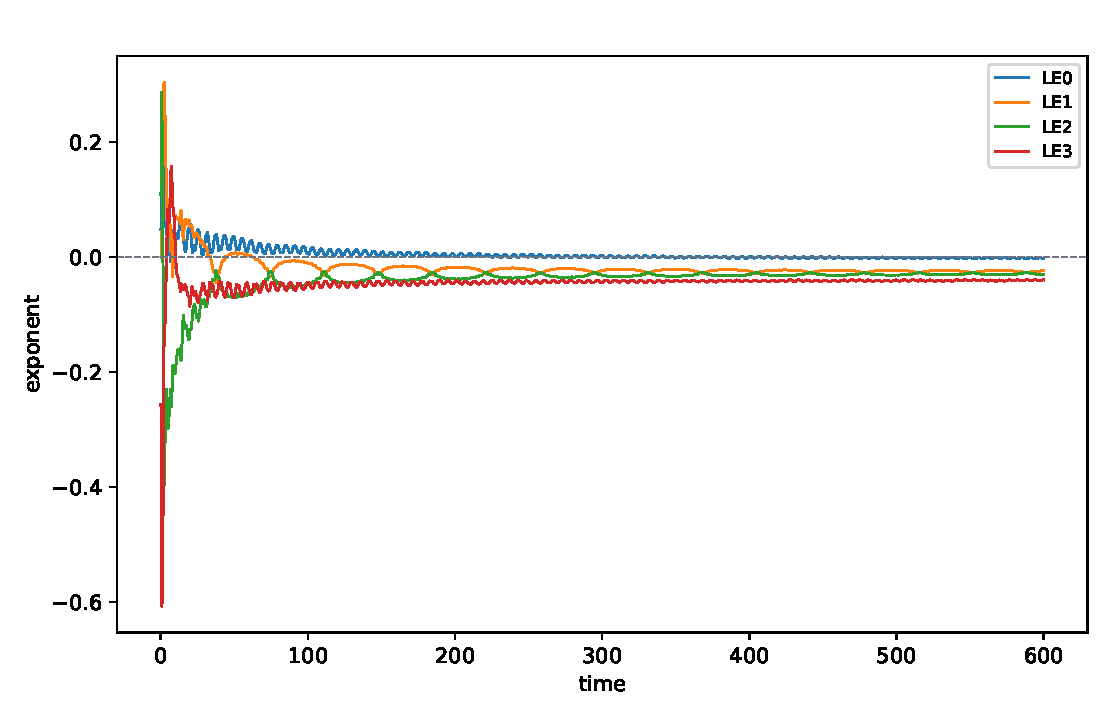
\includegraphics[width=0.94\linewidth,height=0.37\textheight,keepaspectratio]{figures/kalman_fitts/10_lyapunov_convergence.pdf}\\[-0.25em]
{\footnotesize Kalman--Fitts: evolución de las estimaciones de Lyapunov.}
\end{center}
\clearpage
\clearpage
\subsection{MAVPD entero: verificación de periodicidad y control negativo}
Ramas D0, continuación, candidato externo, series, amplitud espectral y comparación del control negativo.

\begin{center}
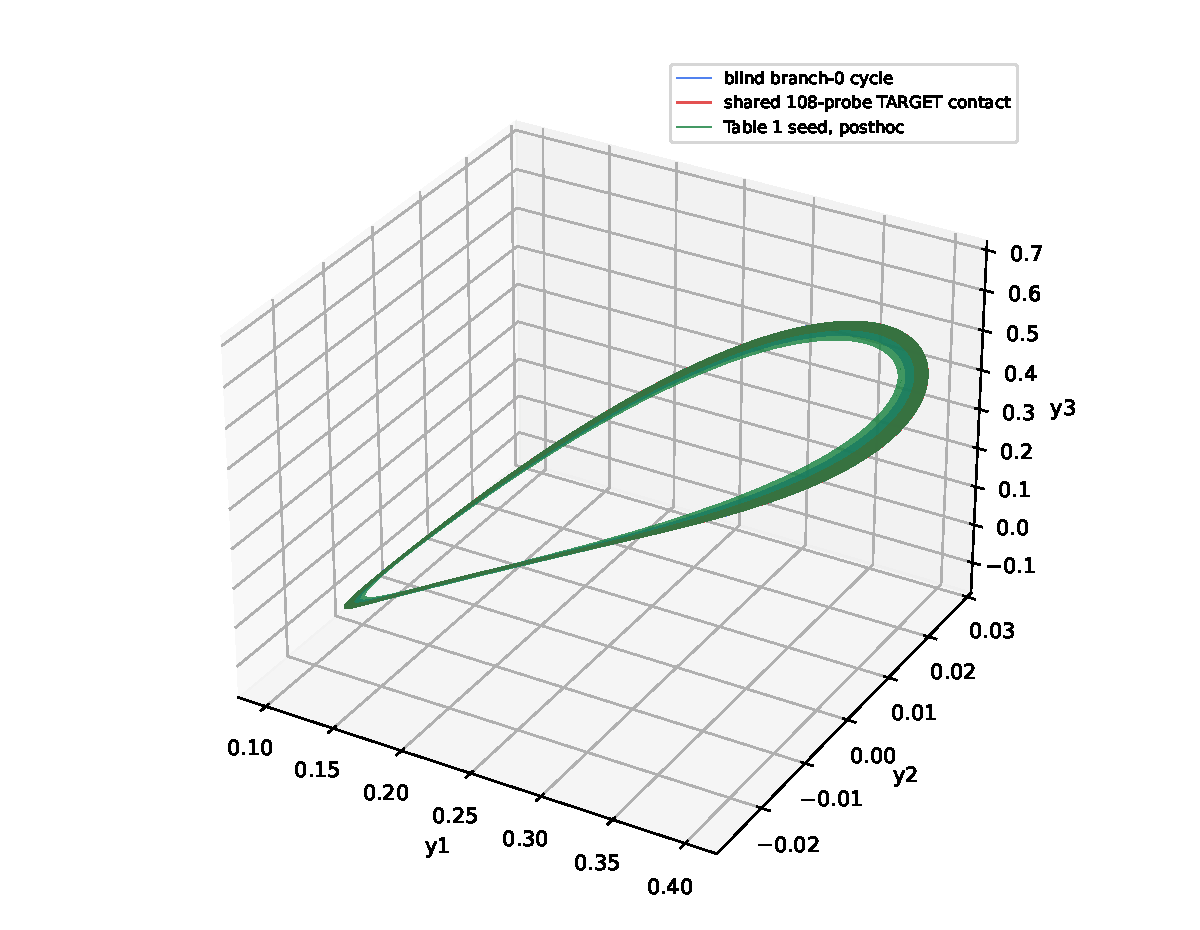
\includegraphics[width=0.94\linewidth,height=0.37\textheight,keepaspectratio]{figures/mavpd_audit/negative_xi3p5_comparison.pdf}\\[-0.25em]
{\footnotesize MAVPD: comparación con el control de contacto, \(\xi=3.5\).}
\end{center}
\vfill
\begin{center}
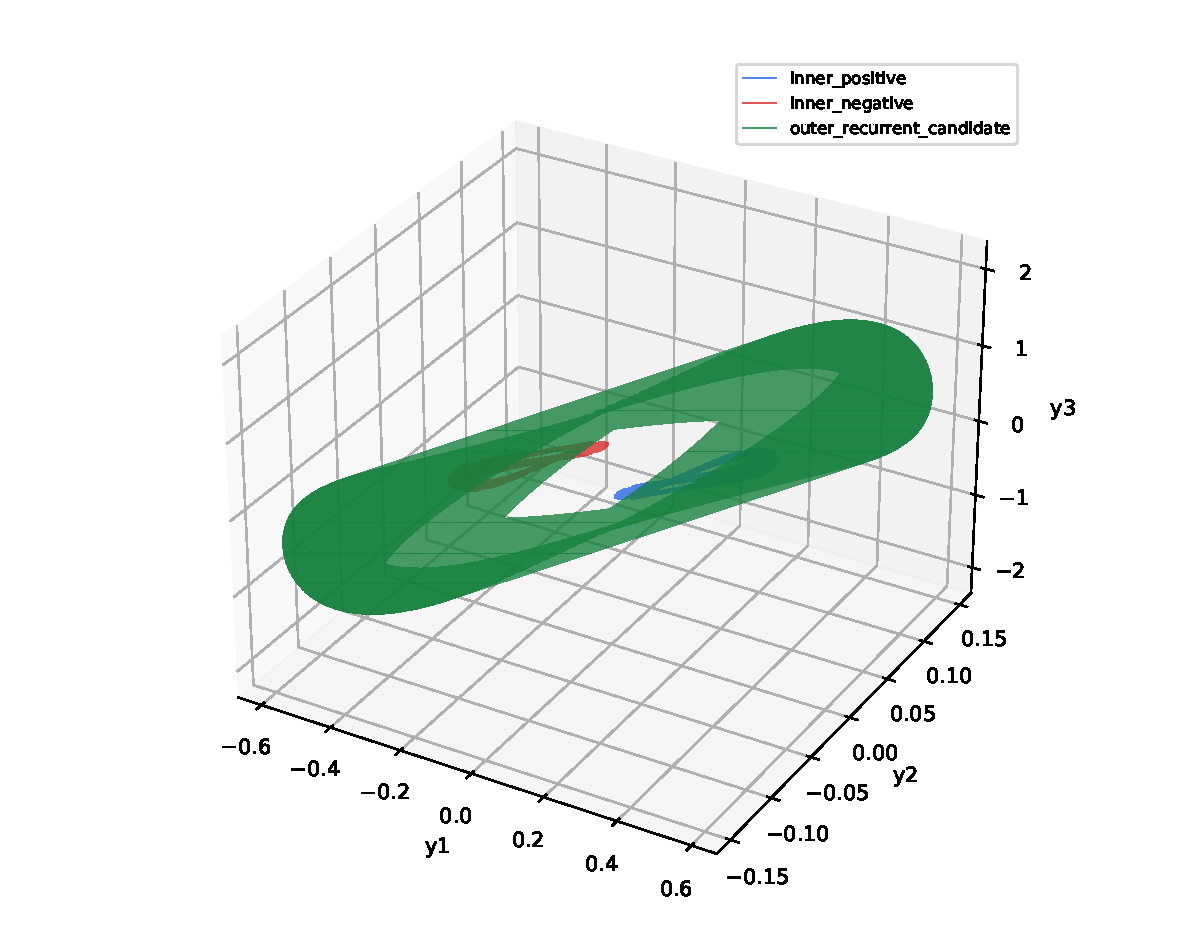
\includegraphics[width=0.94\linewidth,height=0.37\textheight,keepaspectratio]{figures/mavpd_audit/primary_blind_clusters.pdf}\\[-0.25em]
{\footnotesize MAVPD: agrupación de destinos de la búsqueda de condiciones iniciales.}
\end{center}
\clearpage
\begin{center}
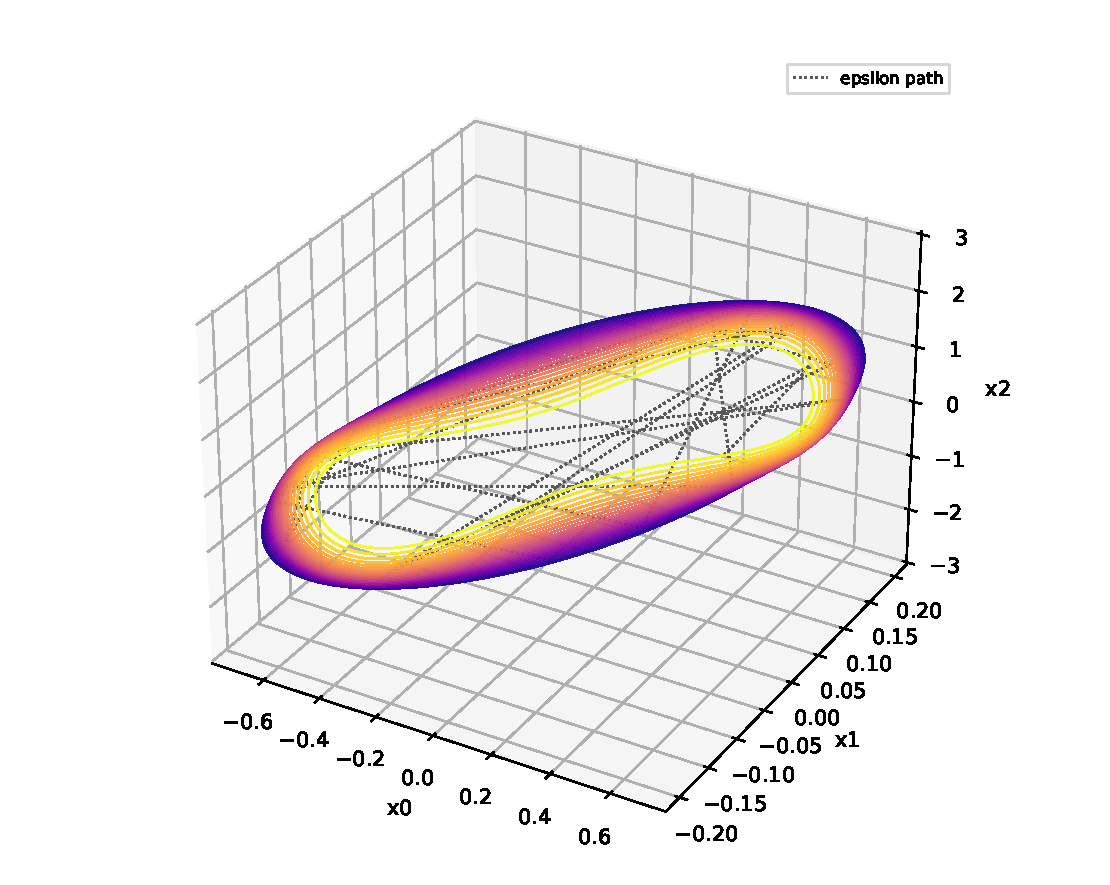
\includegraphics[width=0.94\linewidth,height=0.37\textheight,keepaspectratio]{figures/mavpd_audit/primary_lambda_continuation.pdf}\\[-0.25em]
{\footnotesize MAVPD: continuación del parámetro auxiliar.}
\end{center}
\vfill
\begin{center}
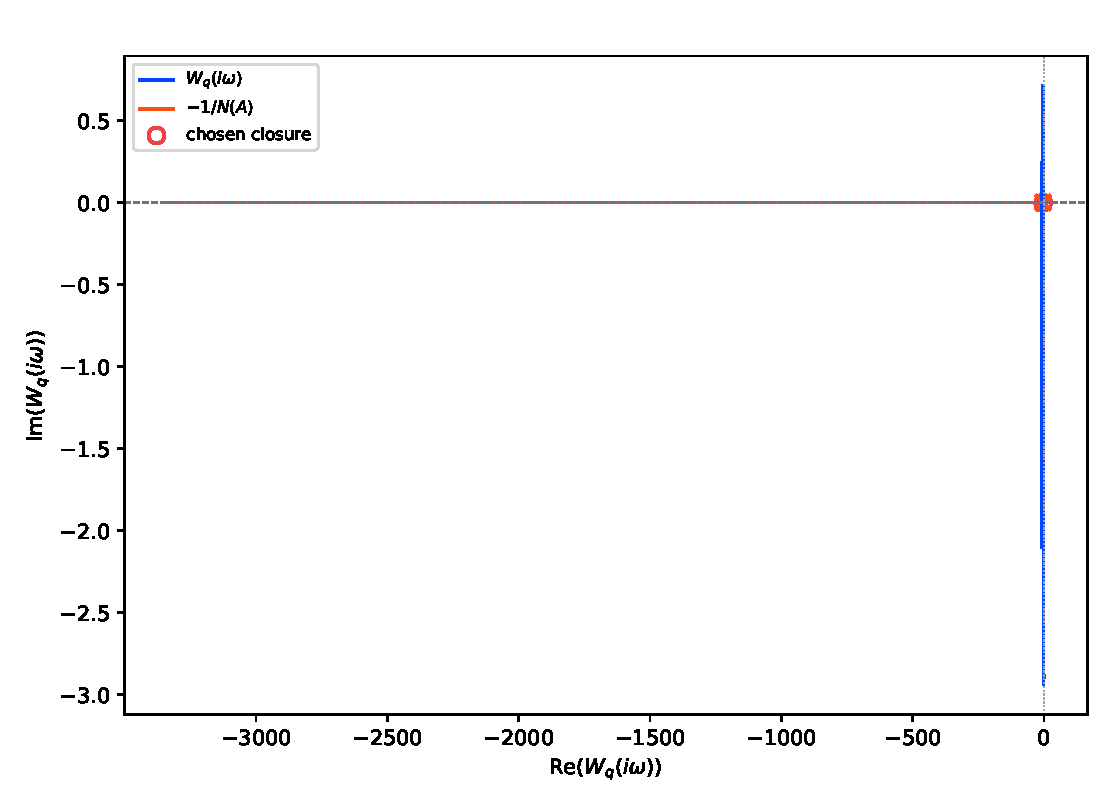
\includegraphics[width=0.94\linewidth,height=0.37\textheight,keepaspectratio]{figures/mavpd_audit/primary_nyquist_df.pdf}\\[-0.25em]
{\footnotesize MAVPD: diagrama de Nyquist y cierre de función descriptiva.}
\end{center}
\clearpage
\begin{center}
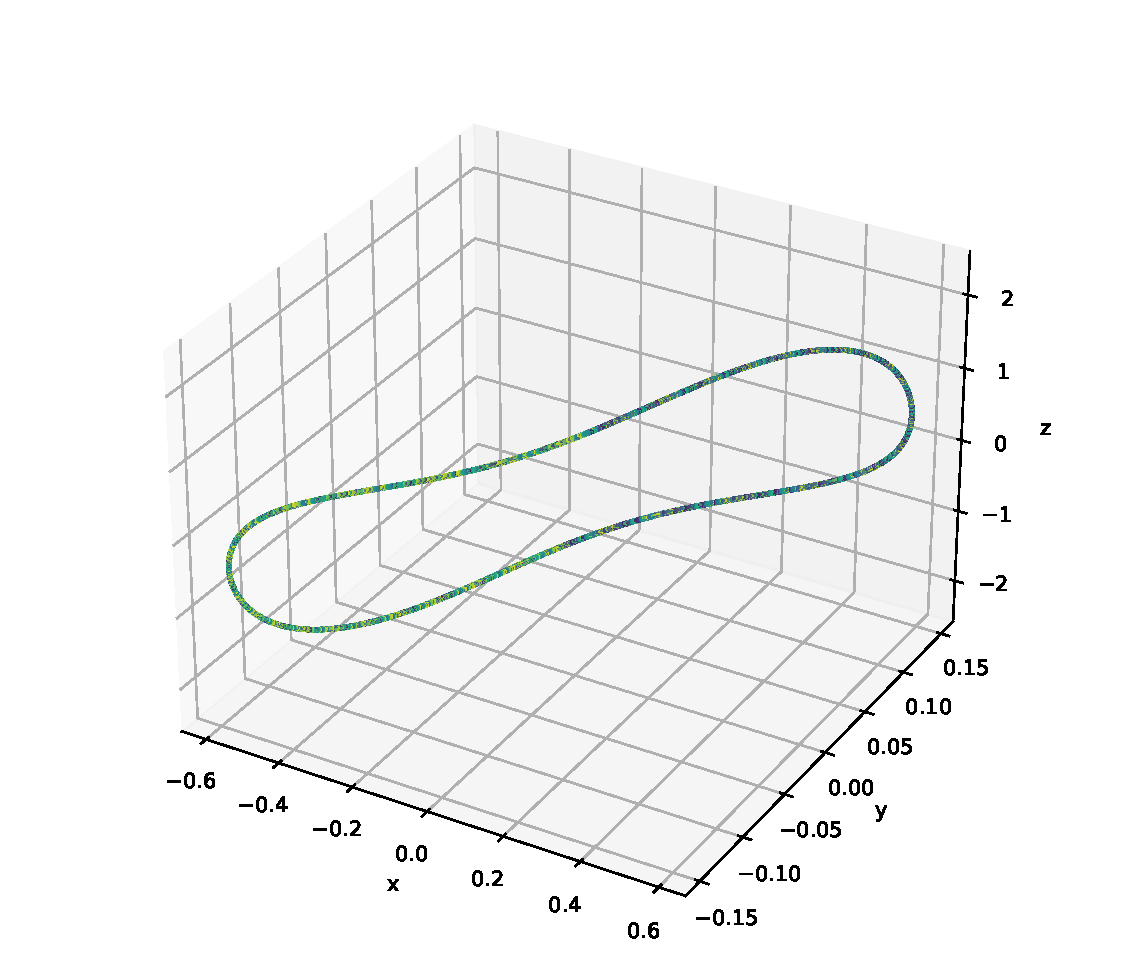
\includegraphics[width=0.94\linewidth,height=0.37\textheight,keepaspectratio]{figures/mavpd_audit/primary_outer_candidate.pdf}\\[-0.25em]
{\footnotesize MAVPD: trayectoria periódica externa candidata.}
\end{center}
\vfill
\begin{center}
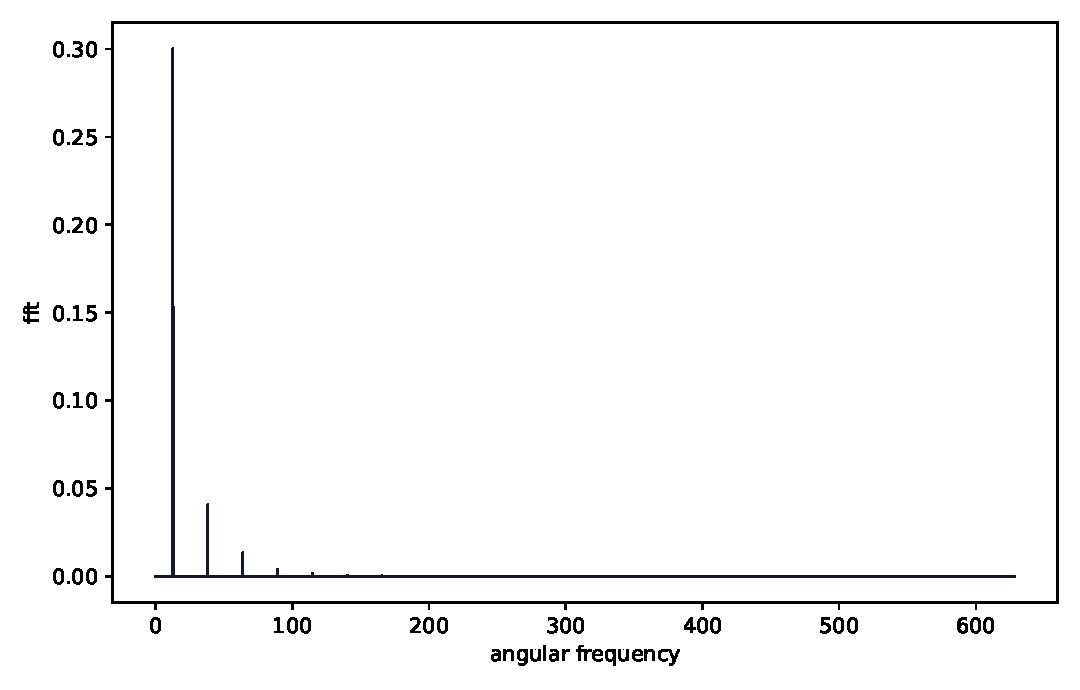
\includegraphics[width=0.94\linewidth,height=0.37\textheight,keepaspectratio]{figures/mavpd_audit/primary_outer_fft_component_0.pdf}\\[-0.25em]
{\footnotesize MAVPD: espectro de amplitud de la componente \(x_1\).}
\end{center}
\clearpage
\begin{center}
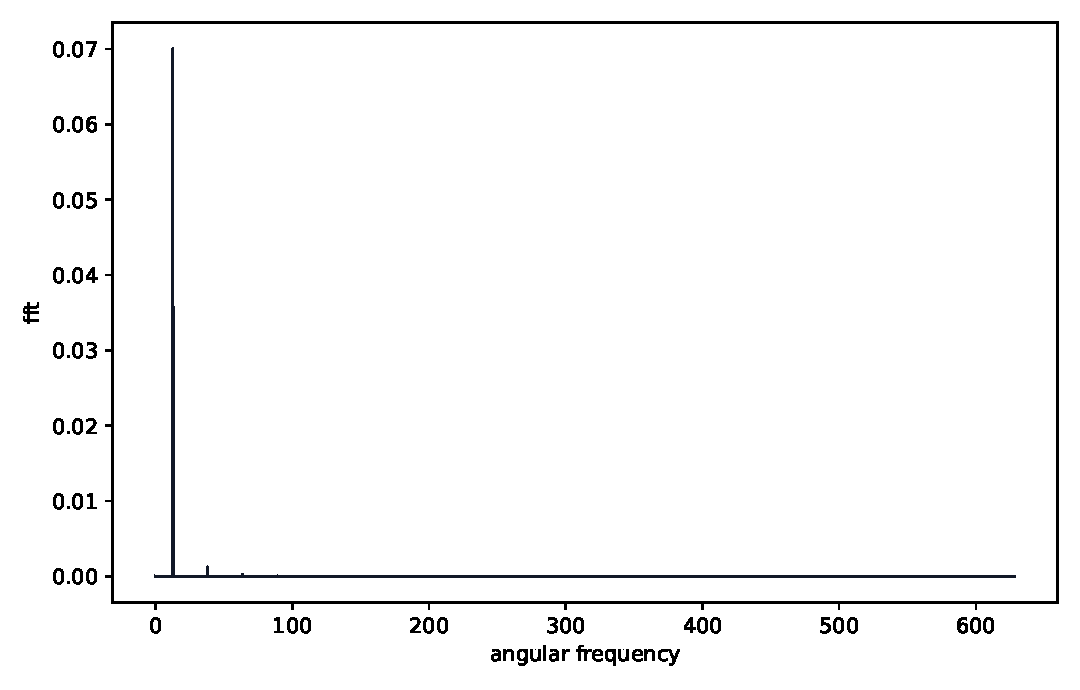
\includegraphics[width=0.94\linewidth,height=0.37\textheight,keepaspectratio]{figures/mavpd_audit/primary_outer_fft_component_1.pdf}\\[-0.25em]
{\footnotesize MAVPD: espectro de amplitud de la componente \(x_2\).}
\end{center}
\vfill
\begin{center}
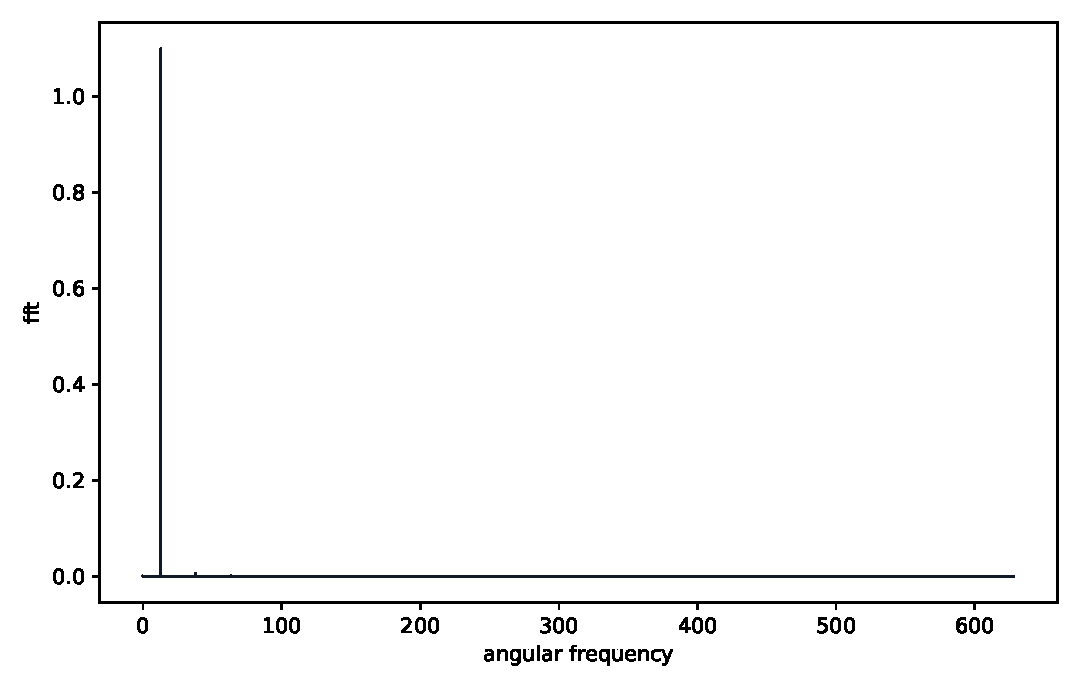
\includegraphics[width=0.94\linewidth,height=0.37\textheight,keepaspectratio]{figures/mavpd_audit/primary_outer_fft_component_2.pdf}\\[-0.25em]
{\footnotesize MAVPD: espectro de amplitud de la componente \(x_3\).}
\end{center}
\clearpage
\begin{center}
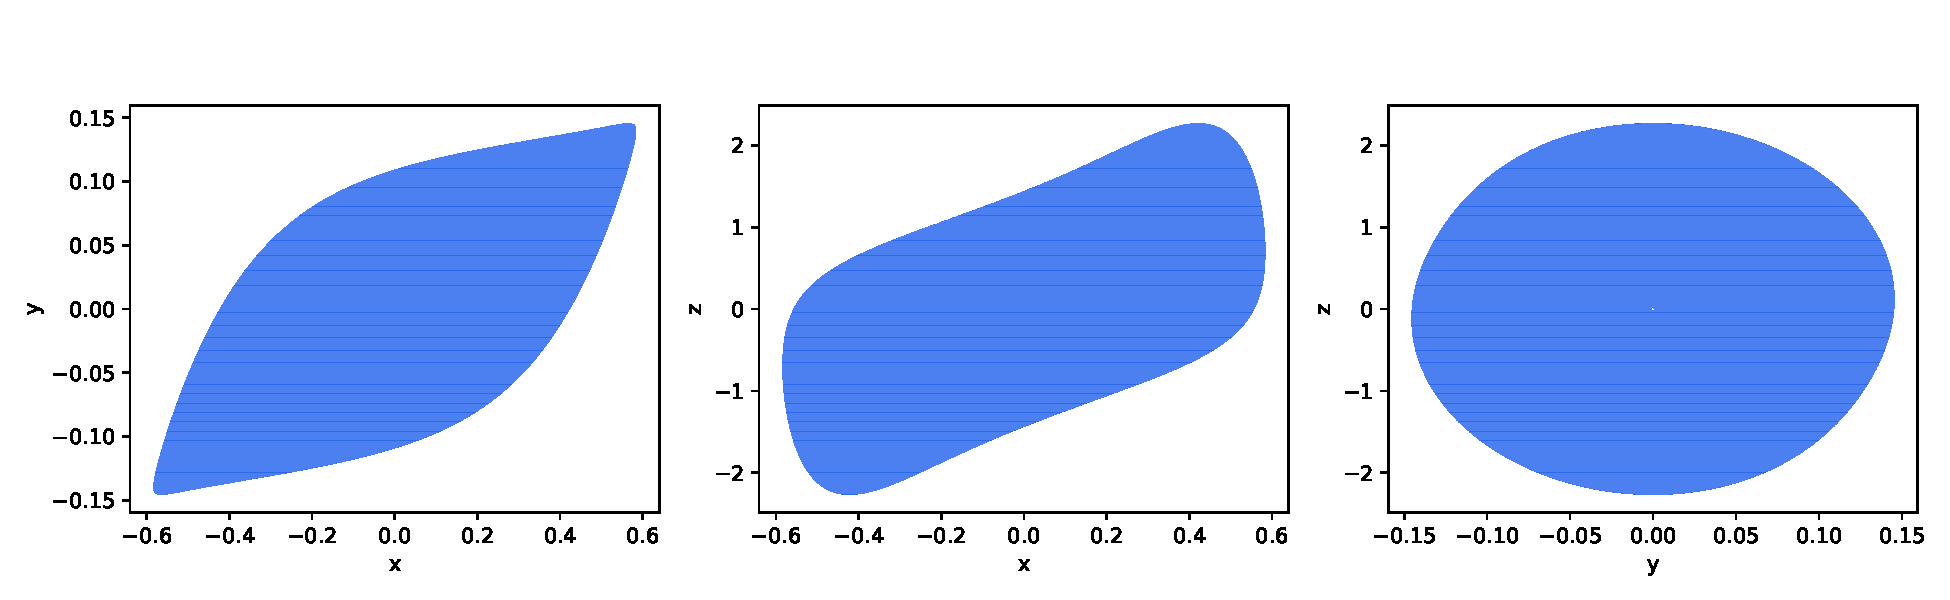
\includegraphics[width=0.94\linewidth,height=0.37\textheight,keepaspectratio]{figures/mavpd_audit/primary_outer_projections.pdf}\\[-0.25em]
{\footnotesize MAVPD: proyecciones de la trayectoria externa.}
\end{center}
\vfill
\begin{center}
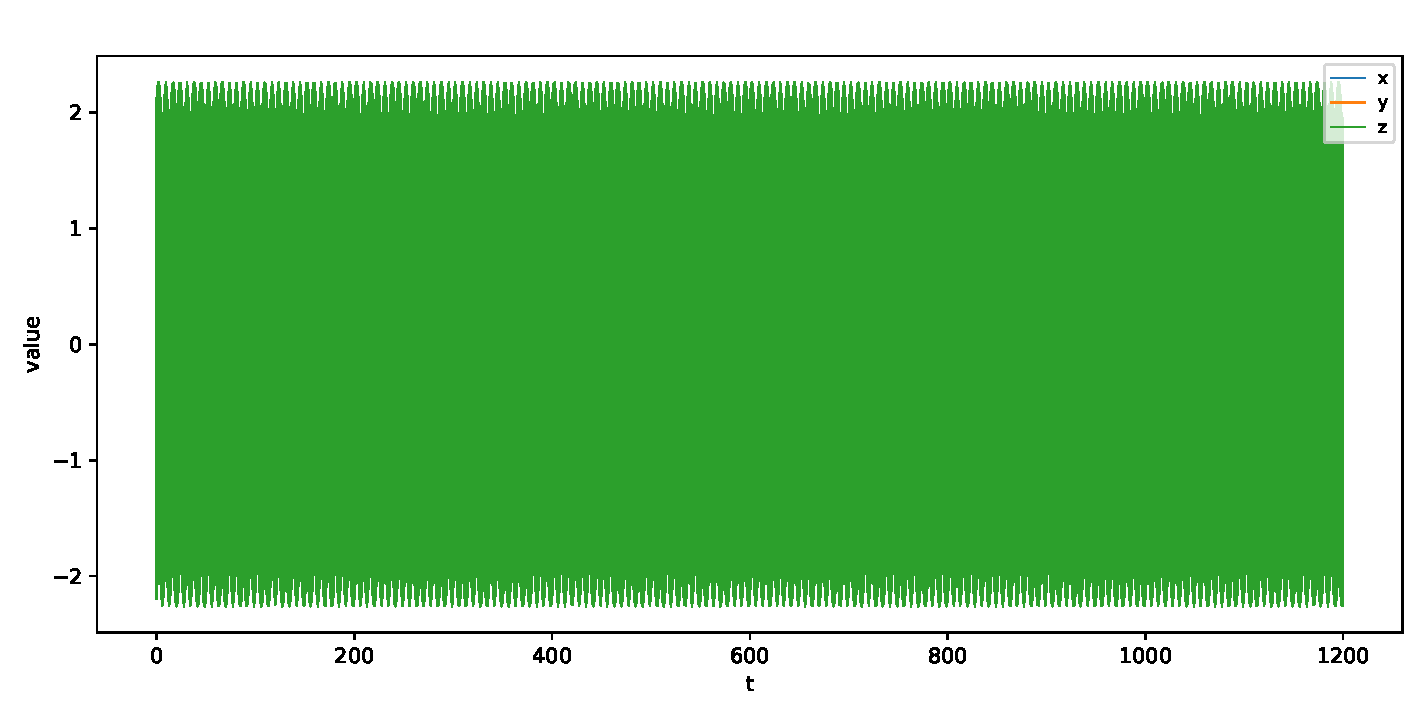
\includegraphics[width=0.94\linewidth,height=0.37\textheight,keepaspectratio]{figures/mavpd_audit/primary_outer_timeseries.pdf}\\[-0.25em]
{\footnotesize MAVPD: series temporales de la trayectoria externa.}
\end{center}
\clearpage
\begin{center}
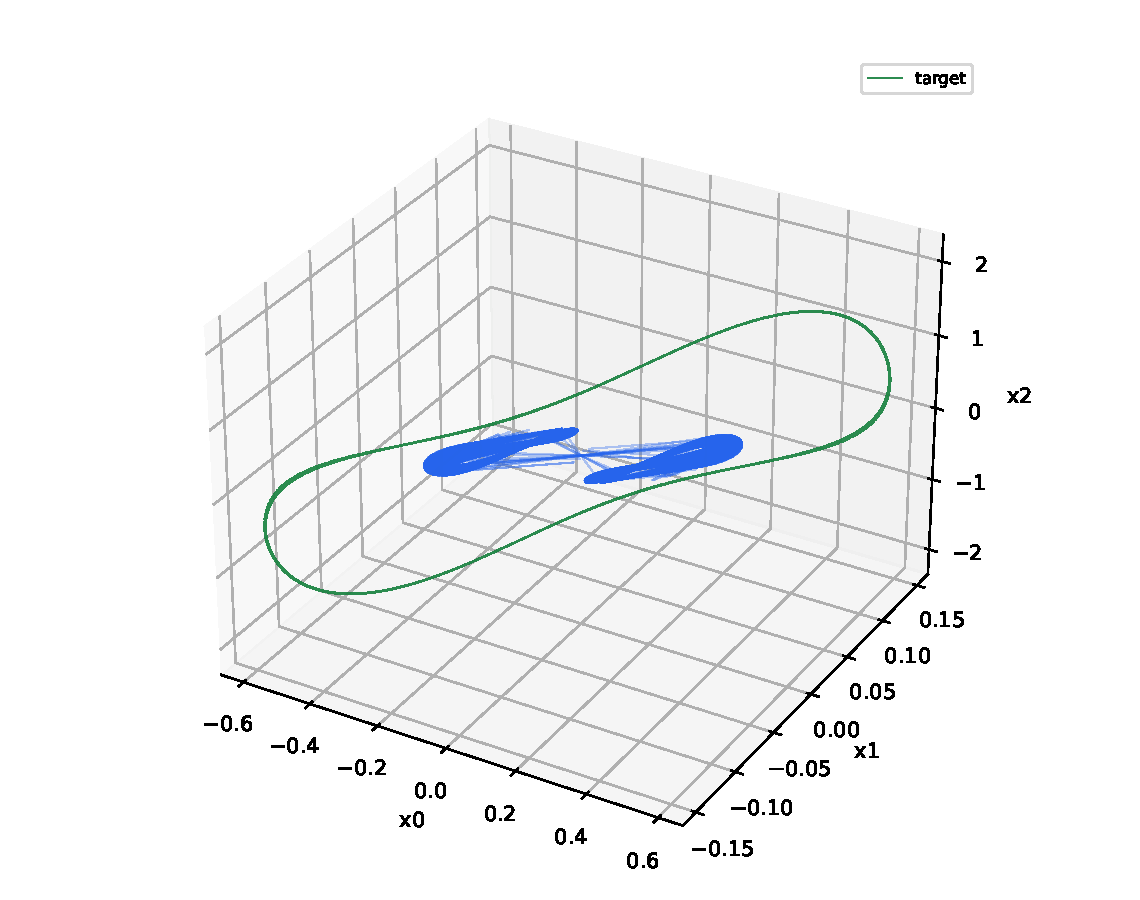
\includegraphics[width=0.94\linewidth,height=0.37\textheight,keepaspectratio]{figures/mavpd_audit/primary_shared_hiddenness_controls.pdf}\\[-0.25em]
{\footnotesize MAVPD: sondeos de cuenca próximos a los equilibrios.}
\end{center}
\vfill
\begin{center}
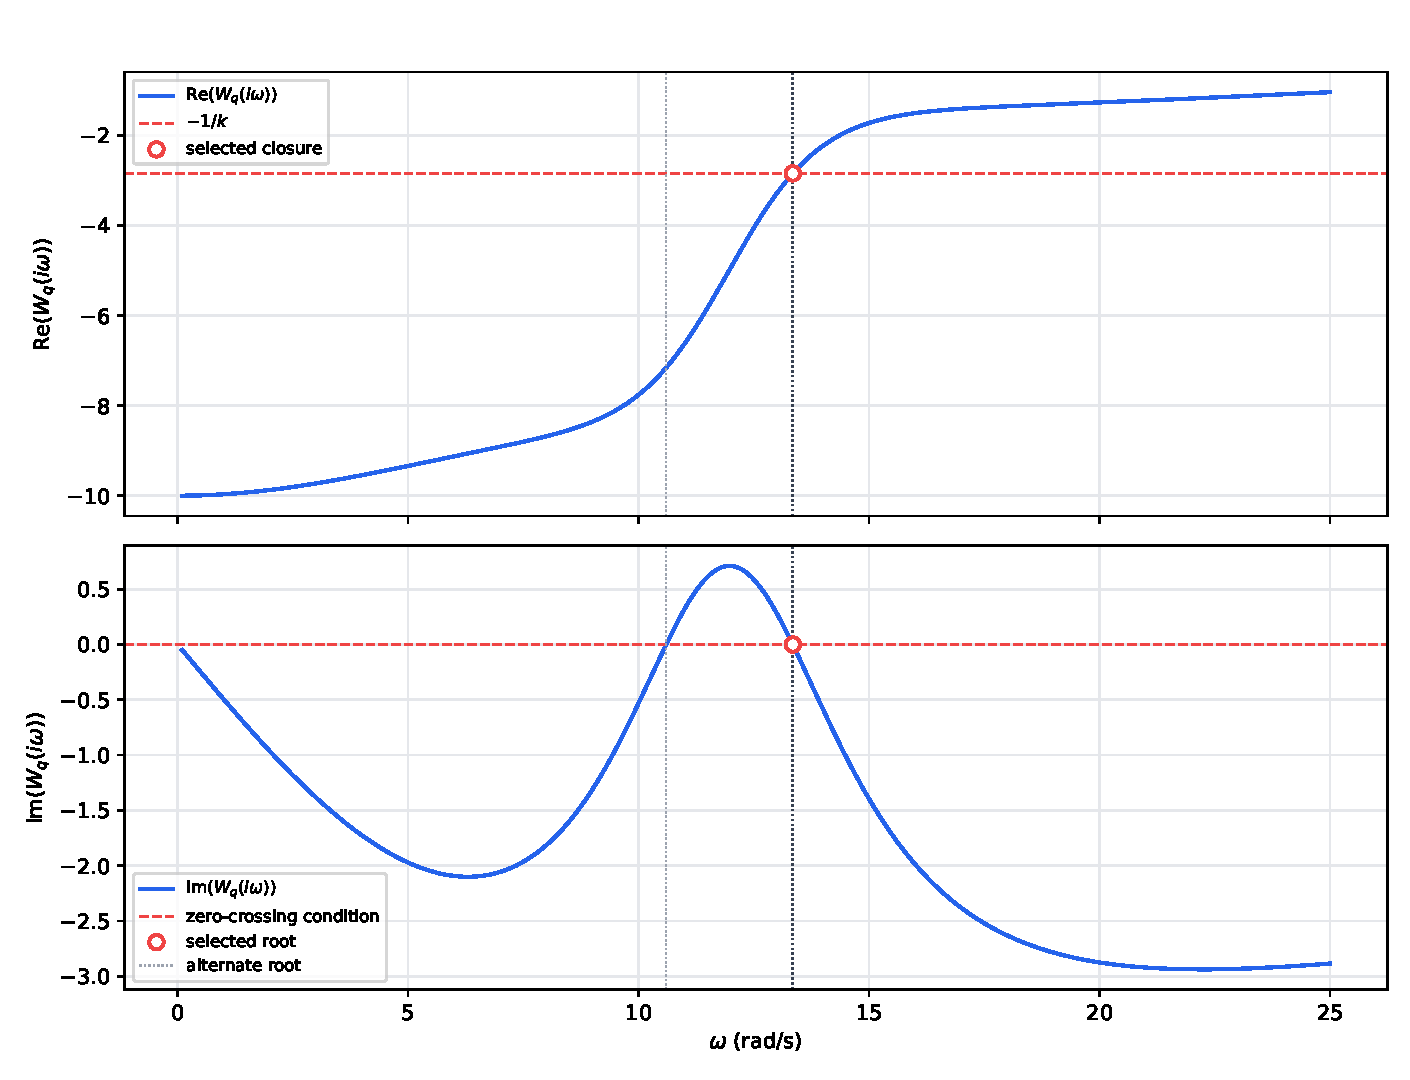
\includegraphics[width=0.94\linewidth,height=0.37\textheight,keepaspectratio]{figures/mavpd_audit/primary_transfer_components.pdf}\\[-0.25em]
{\footnotesize MAVPD: partes real e imaginaria de la transferencia.}
\end{center}
\clearpage
\clearpage
\subsection{MAVPD entero: candidato caótico local}
Cribado de continuación, retratos, series, Lyapunov, espectro normalizado, Poincaré y sondeos locales.

\begin{center}
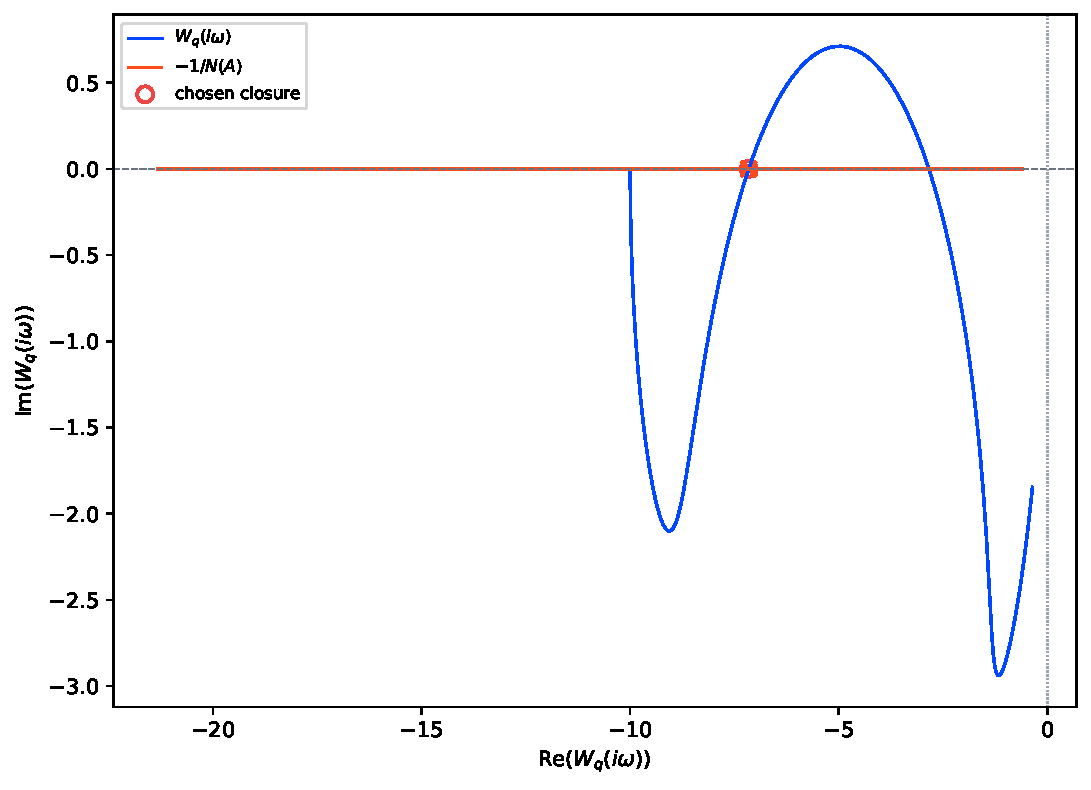
\includegraphics[width=0.94\linewidth,height=0.37\textheight,keepaspectratio]{figures/mavpd_chaos/00_nyquist_direct_seed.pdf}\\[-0.25em]
{\footnotesize MAVPD: Nyquist y construcción de la semilla del candidato caótico.}
\end{center}
\vfill
\begin{center}
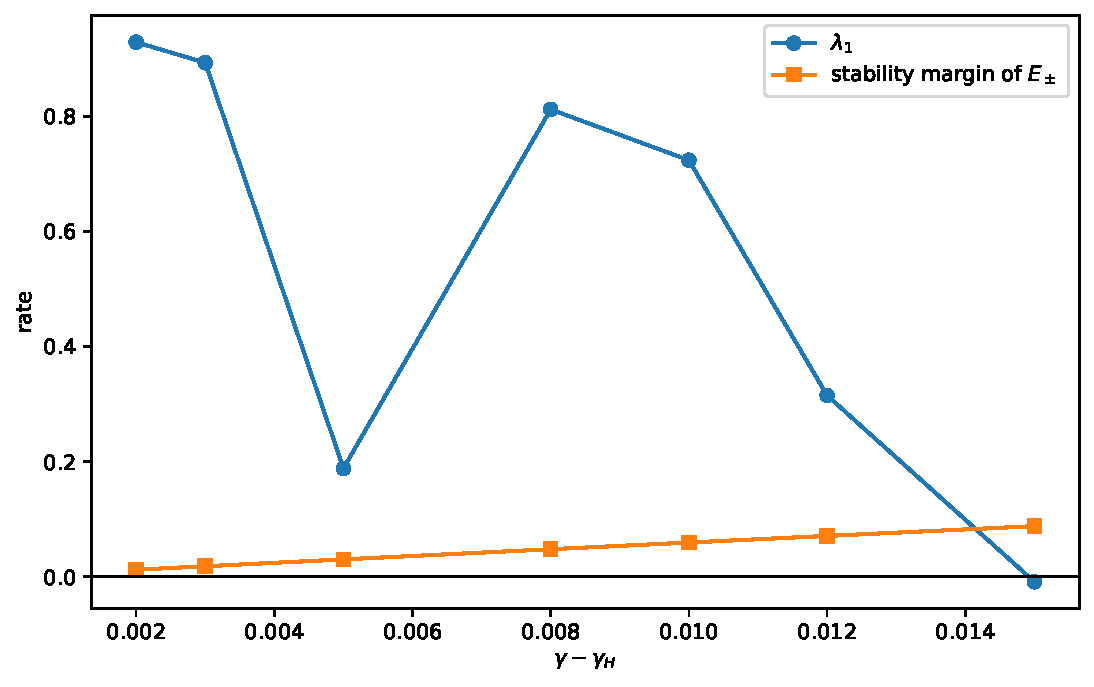
\includegraphics[width=0.94\linewidth,height=0.37\textheight,keepaspectratio]{figures/mavpd_chaos/03_continuation_screen.pdf}\\[-0.25em]
{\footnotesize MAVPD: respuesta durante la continuación del candidato caótico.}
\end{center}
\clearpage
\begin{center}
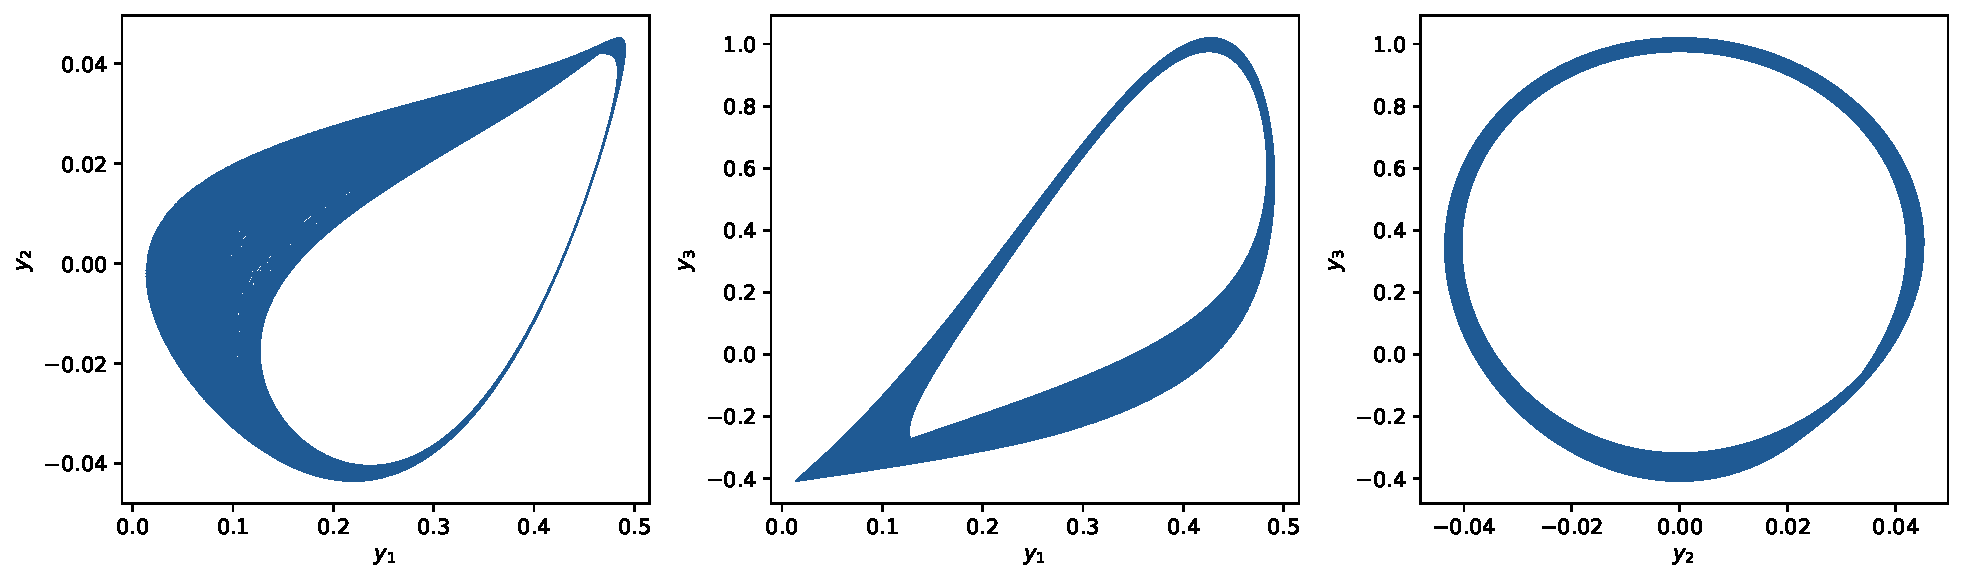
\includegraphics[width=0.94\linewidth,height=0.37\textheight,keepaspectratio]{figures/mavpd_chaos/04_candidate_phase_portraits.pdf}\\[-0.25em]
{\footnotesize MAVPD: proyecciones del candidato caótico.}
\end{center}
\vfill
\begin{center}
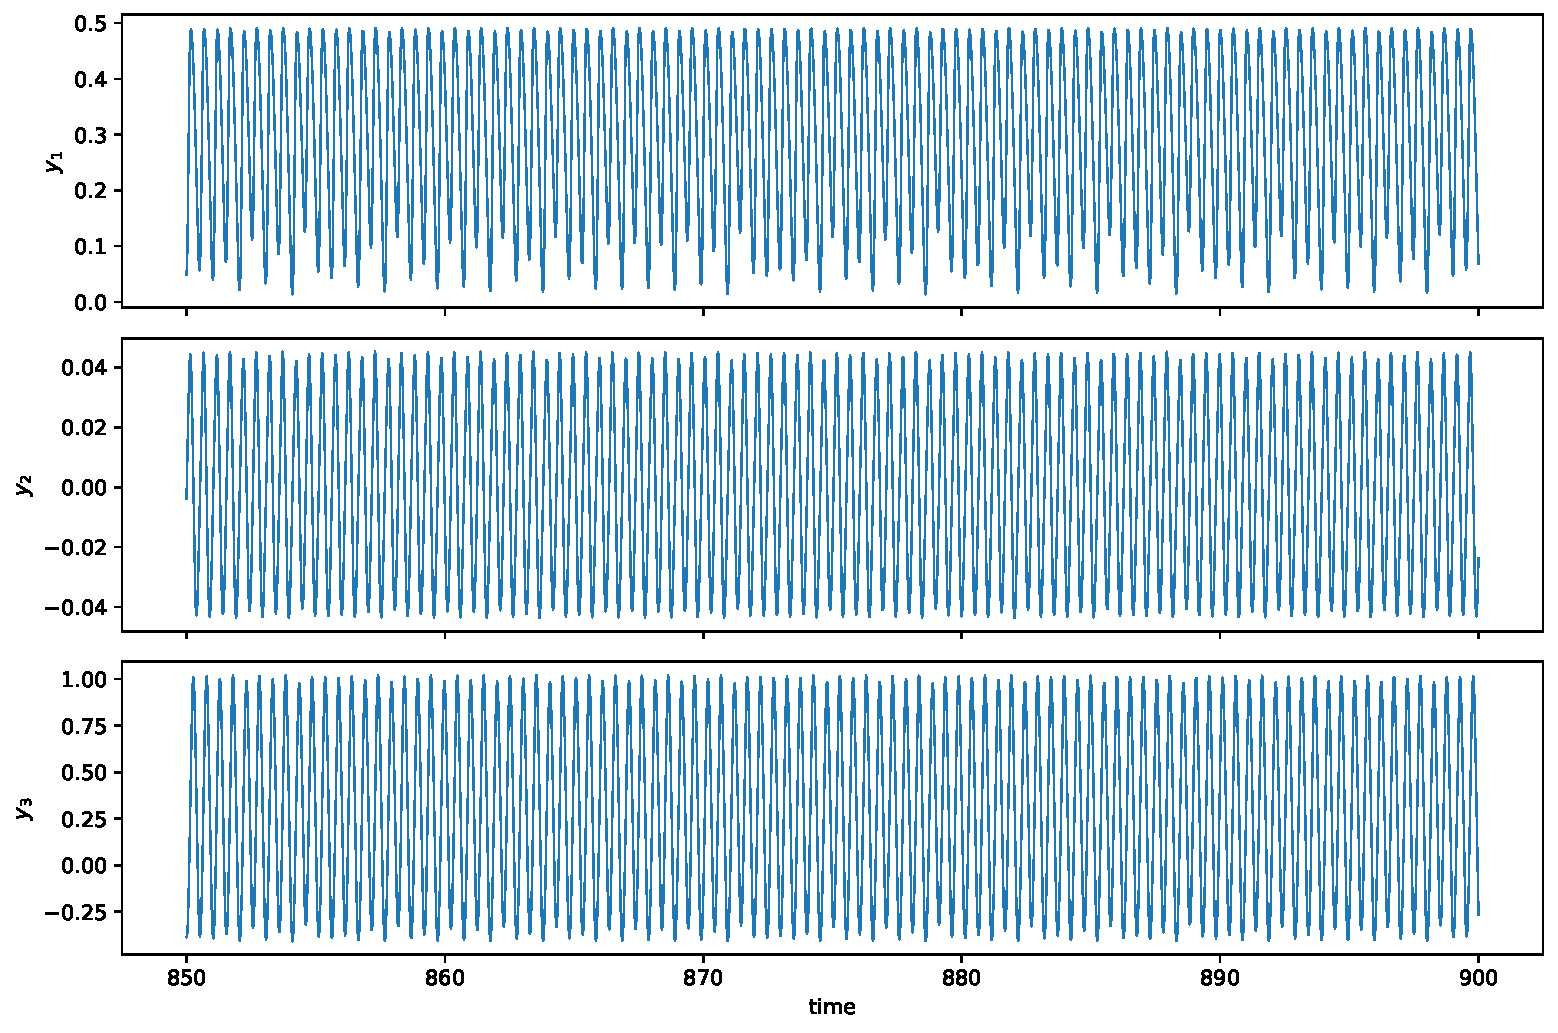
\includegraphics[width=0.94\linewidth,height=0.37\textheight,keepaspectratio]{figures/mavpd_chaos/04_candidate_time_series.pdf}\\[-0.25em]
{\footnotesize MAVPD: series temporales del candidato caótico.}
\end{center}
\clearpage
\begin{center}
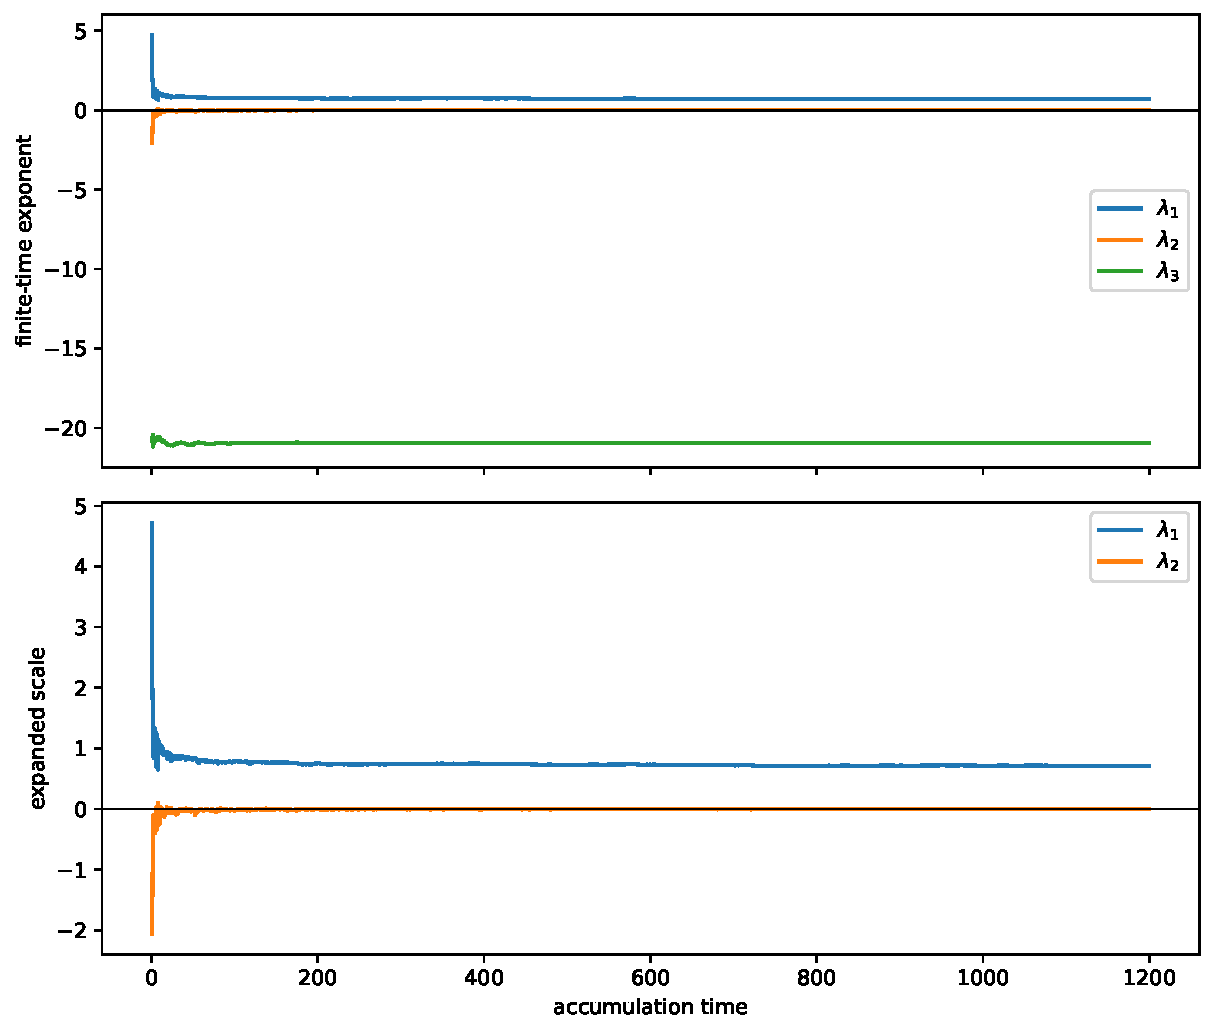
\includegraphics[width=0.94\linewidth,height=0.37\textheight,keepaspectratio]{figures/mavpd_chaos/05_lyapunov_convergence.pdf}\\[-0.25em]
{\footnotesize MAVPD: evolución de las estimaciones de Lyapunov.}
\end{center}
\vfill
\begin{center}
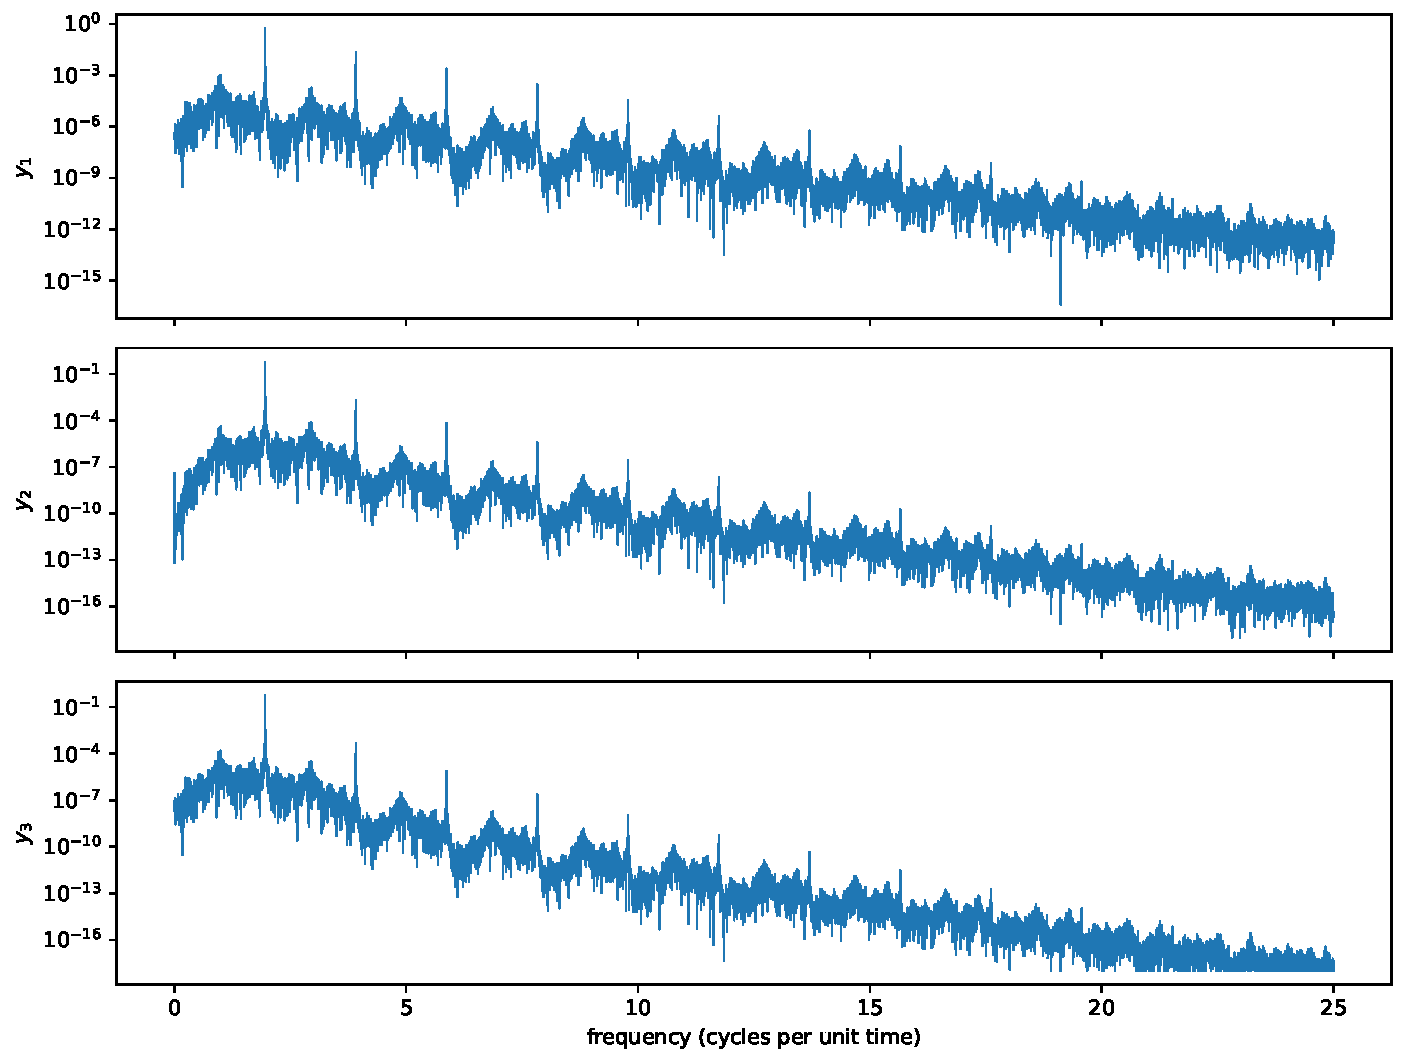
\includegraphics[width=0.94\linewidth,height=0.37\textheight,keepaspectratio]{figures/mavpd_chaos/05_normalized_fft_power.pdf}\\[-0.25em]
{\footnotesize MAVPD: espectro normalizado de la señal.}
\end{center}
\clearpage
\begin{center}
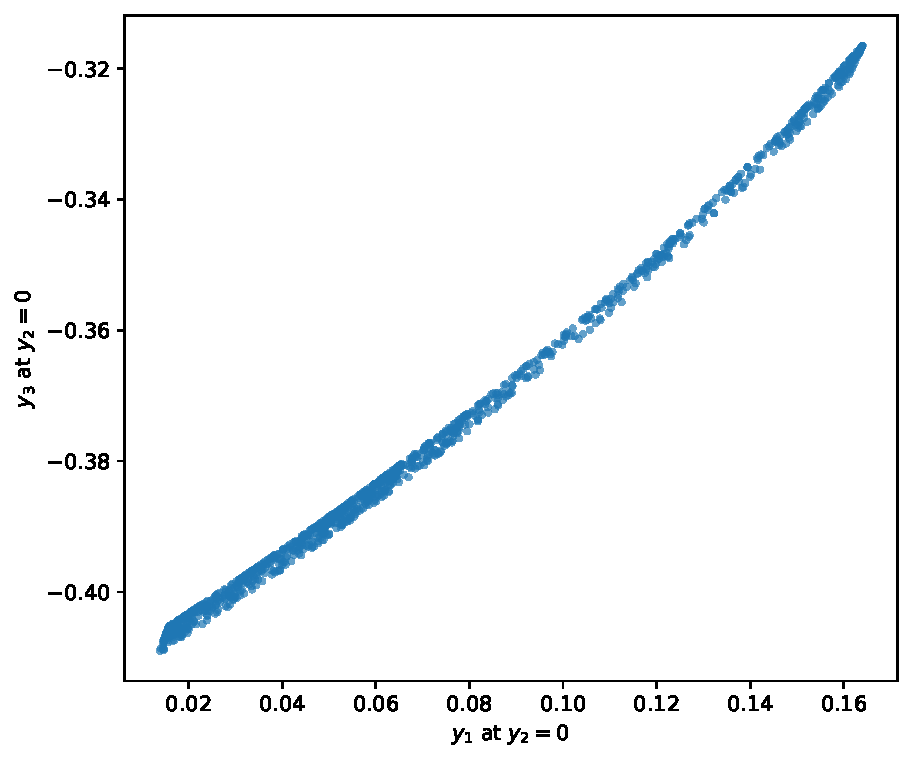
\includegraphics[width=0.94\linewidth,height=0.37\textheight,keepaspectratio]{figures/mavpd_chaos/05_poincare_section.pdf}\\[-0.25em]
{\footnotesize MAVPD: sección de Poincaré del candidato caótico.}
\end{center}
\vfill
\begin{center}
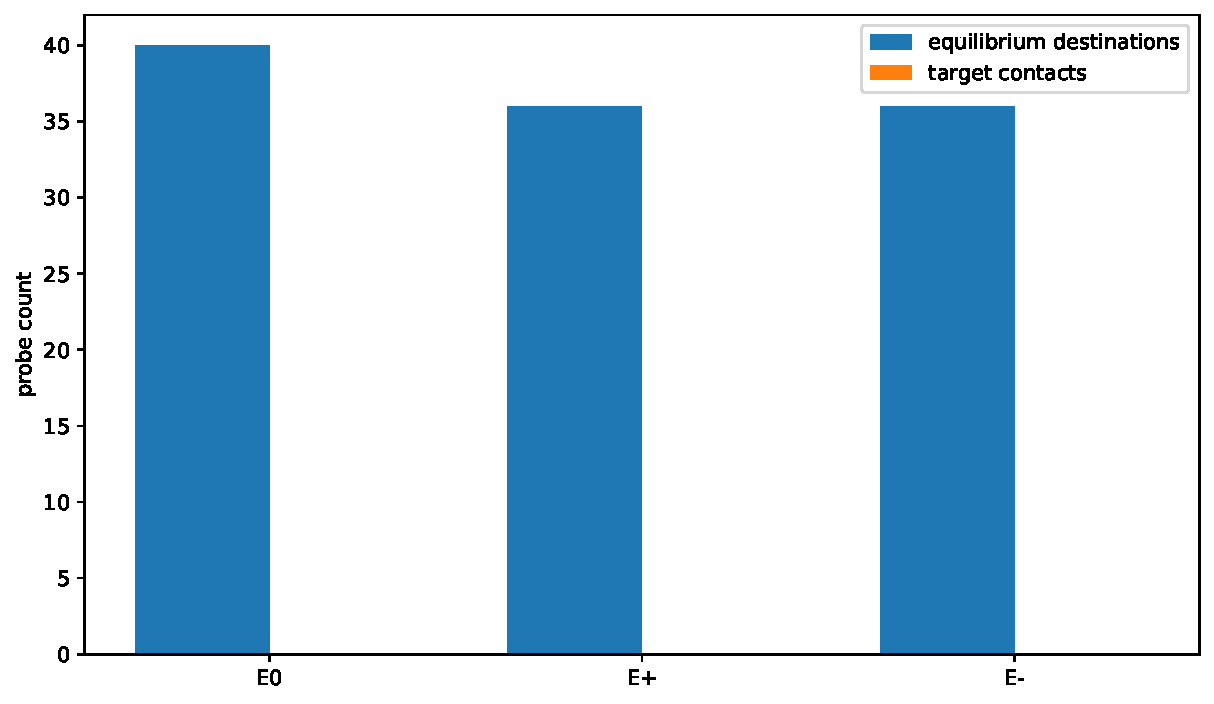
\includegraphics[width=0.94\linewidth,height=0.37\textheight,keepaspectratio]{figures/mavpd_chaos/07_hiddenness_outcomes.pdf}\\[-0.25em]
{\footnotesize MAVPD: destinos de los sondeos próximos a los equilibrios.}
\end{center}
\clearpage
\clearpage
\subsection{PLL lead--lag entero}
Obstrucción de transferencia, continuación en ganancia, ciclos sobre el cilindro y sondeos cilíndricos.

\begin{center}
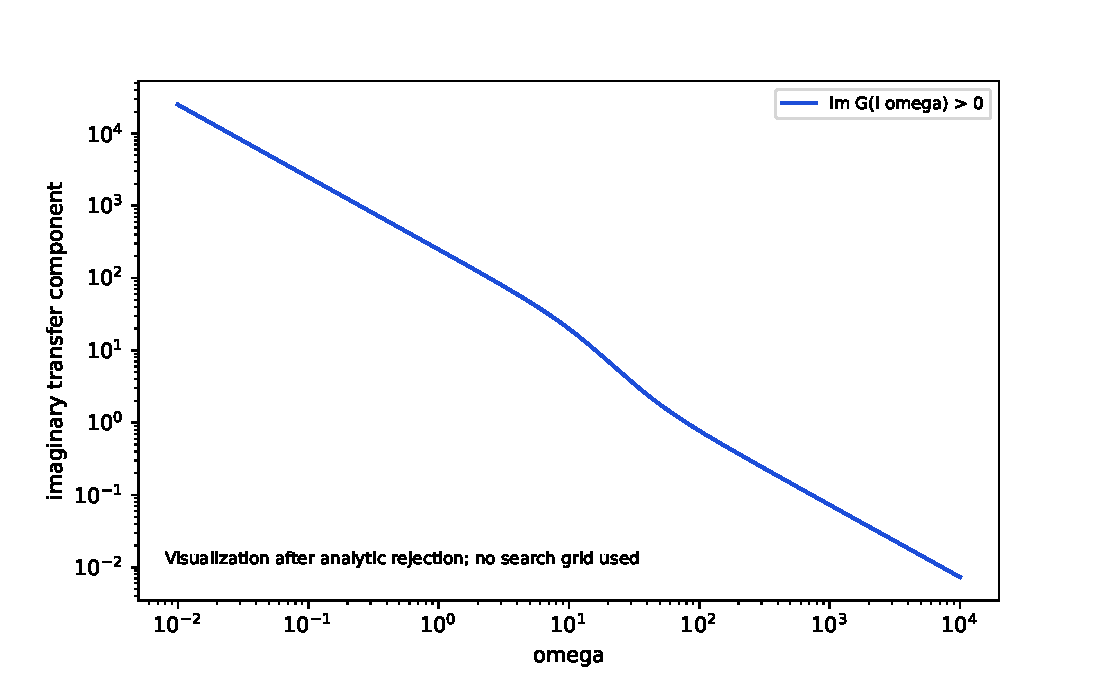
\includegraphics[width=0.94\linewidth,height=0.37\textheight,keepaspectratio]{figures/pll/01_direct_transfer_obstruction.pdf}\\[-0.25em]
{\footnotesize PLL: obstrucción del cierre de transferencia directo.}
\end{center}
\vfill
\begin{center}
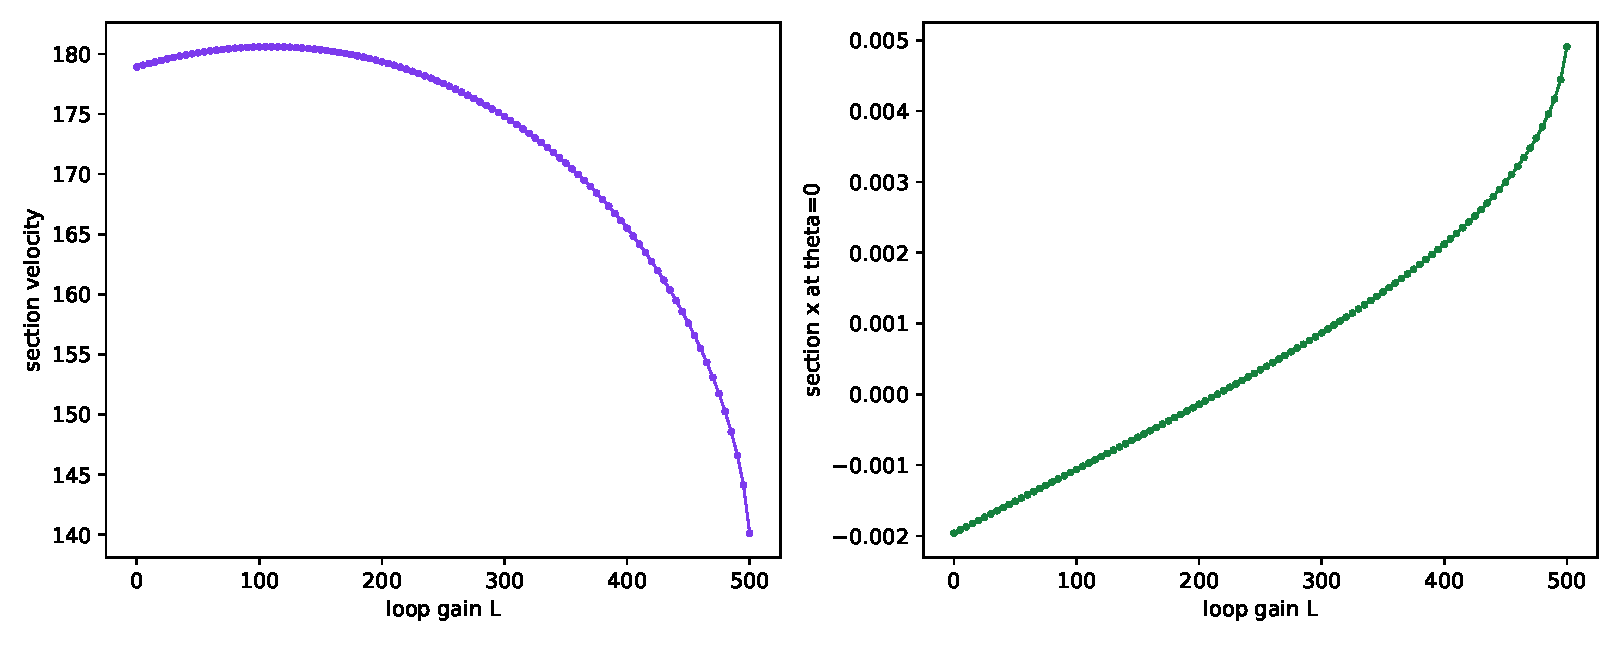
\includegraphics[width=0.94\linewidth,height=0.37\textheight,keepaspectratio]{figures/pll/02_loop_gain_continuation.pdf}\\[-0.25em]
{\footnotesize PLL: continuación de la ganancia de lazo.}
\end{center}
\clearpage
\begin{center}
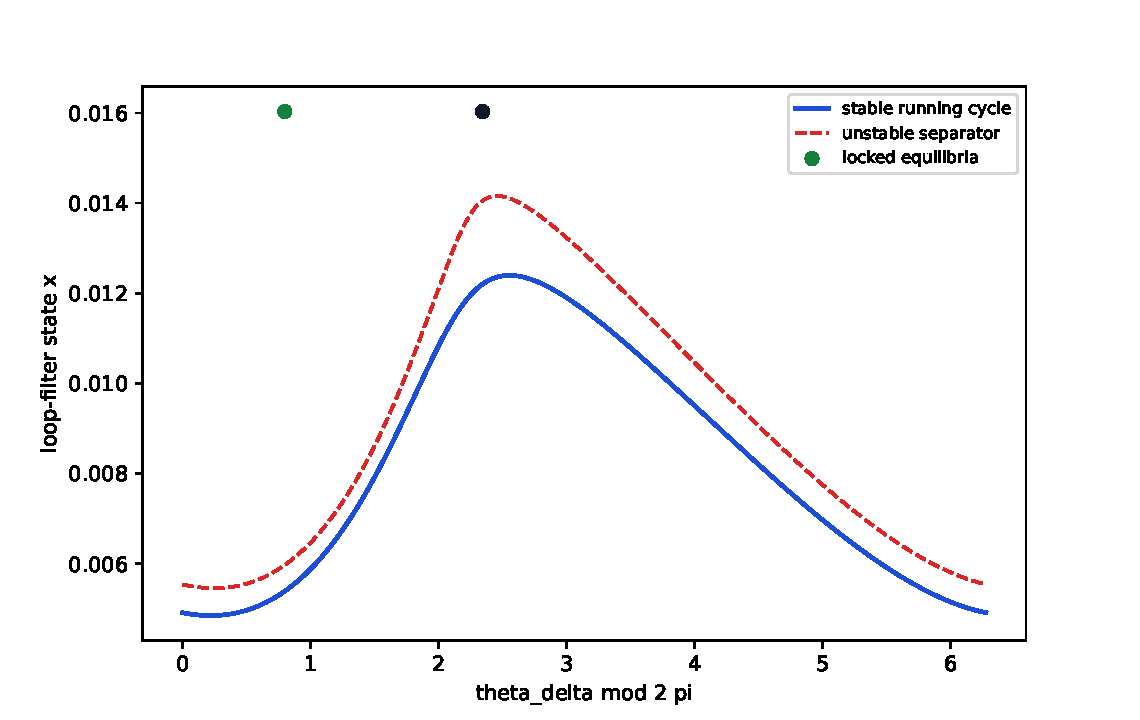
\includegraphics[width=0.94\linewidth,height=0.37\textheight,keepaspectratio]{figures/pll/03_phase_cylinder_cycles.pdf}\\[-0.25em]
{\footnotesize PLL: órbitas sobre el cilindro de fases.}
\end{center}
\vfill
\begin{center}
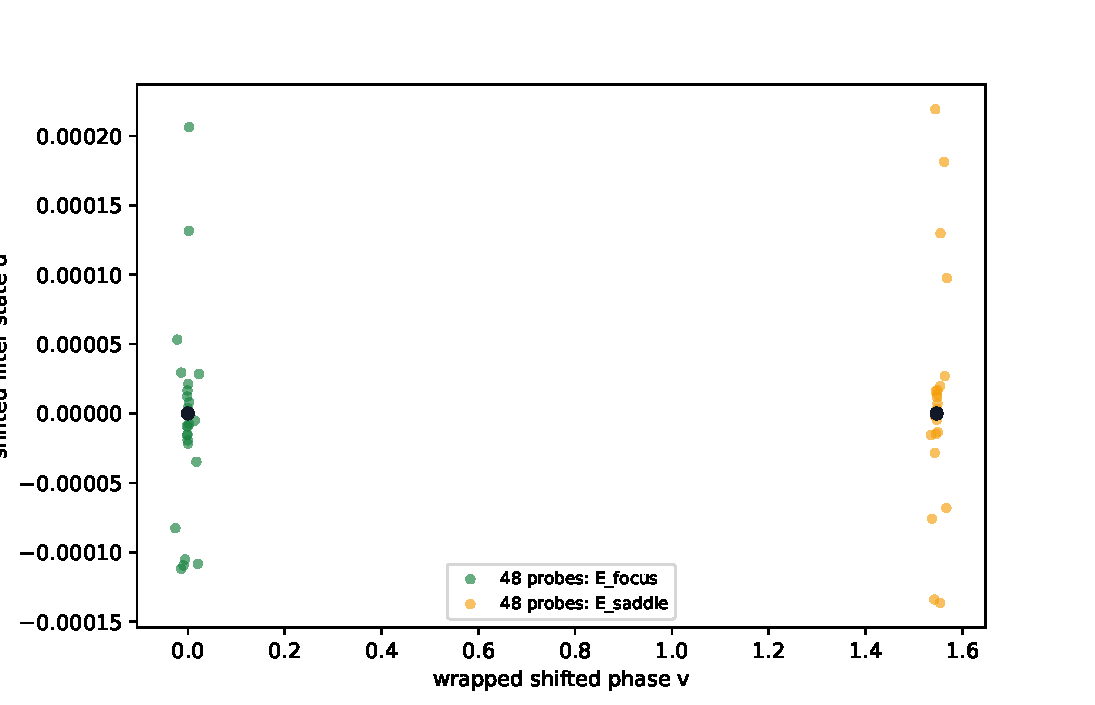
\includegraphics[width=0.94\linewidth,height=0.37\textheight,keepaspectratio]{figures/pll/04_cylindrical_hiddenness_probes.pdf}\\[-0.25em]
{\footnotesize PLL: sondeos de cuenca con distancia cilíndrica.}
\end{center}
\clearpage
\clearpage
\subsection{Chua arctangente c590: cortes adicionales de cuenca}
Los cinco cortes utilizan ABM--PECE con memoria completa, $q=0.9999$,
$h=0.005$, horizonte 180 y descarte de 90. La retícula visual de
$241\times241$ nodos por plano representa 62\,416 trayectorias integradas:
35\,941 de una malla de base y 26\,475 centros de celdas con clases
heterogéneas. Los demás nodos reciben relleno categórico; los 290\,405
nodos visibles no son integraciones independientes. El gris incluye
salidas detectadas y puntos omitidos en la malla de base, por lo que no
acredita una salida calculada en cada píxel.
Los colores distinguen contacto con $A_\pm$, proximidad a $E_0,E_\pm$,
otro destino acotado o salida según el clasificador finito. No determinan
por sí solos cuencas asintóticas ni fracciones de volumen.
Las estrellas marcan equilibrios contenidos en el plano y los círculos,
sus proyecciones desde otros planos.

\begin{center}
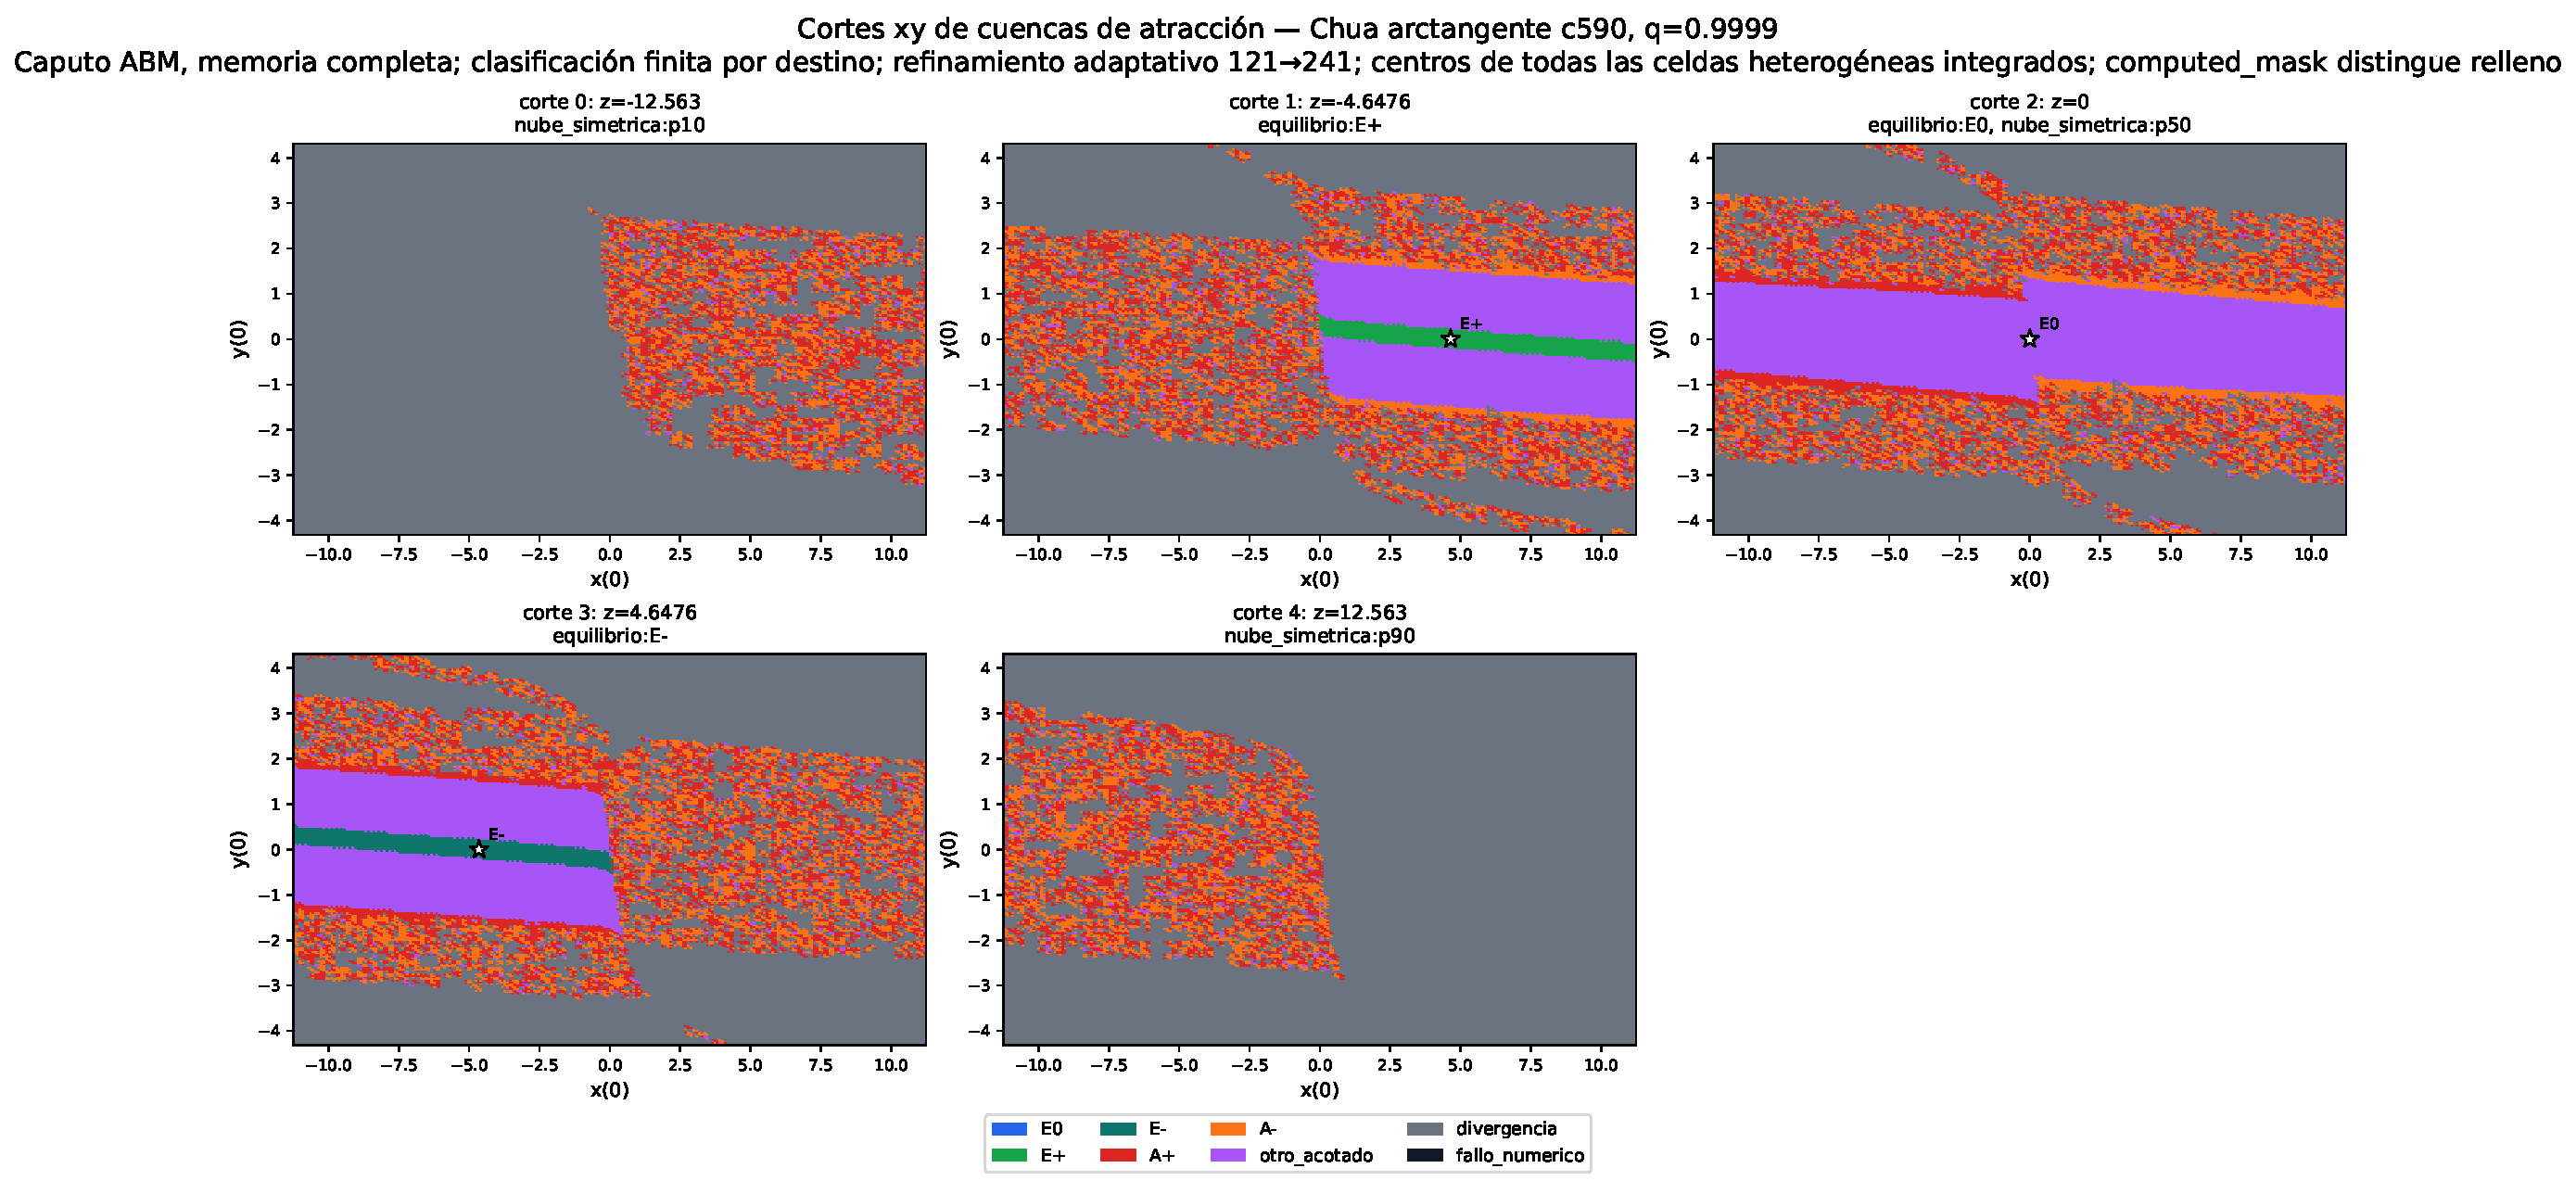
\includegraphics[width=0.94\linewidth,height=0.37\textheight,keepaspectratio]{figures/c590_basin/basin_multislice.pdf}\\[-0.25em]
{\footnotesize Cortes de las regiones de destino.}
\end{center}
\vfill
\begin{center}
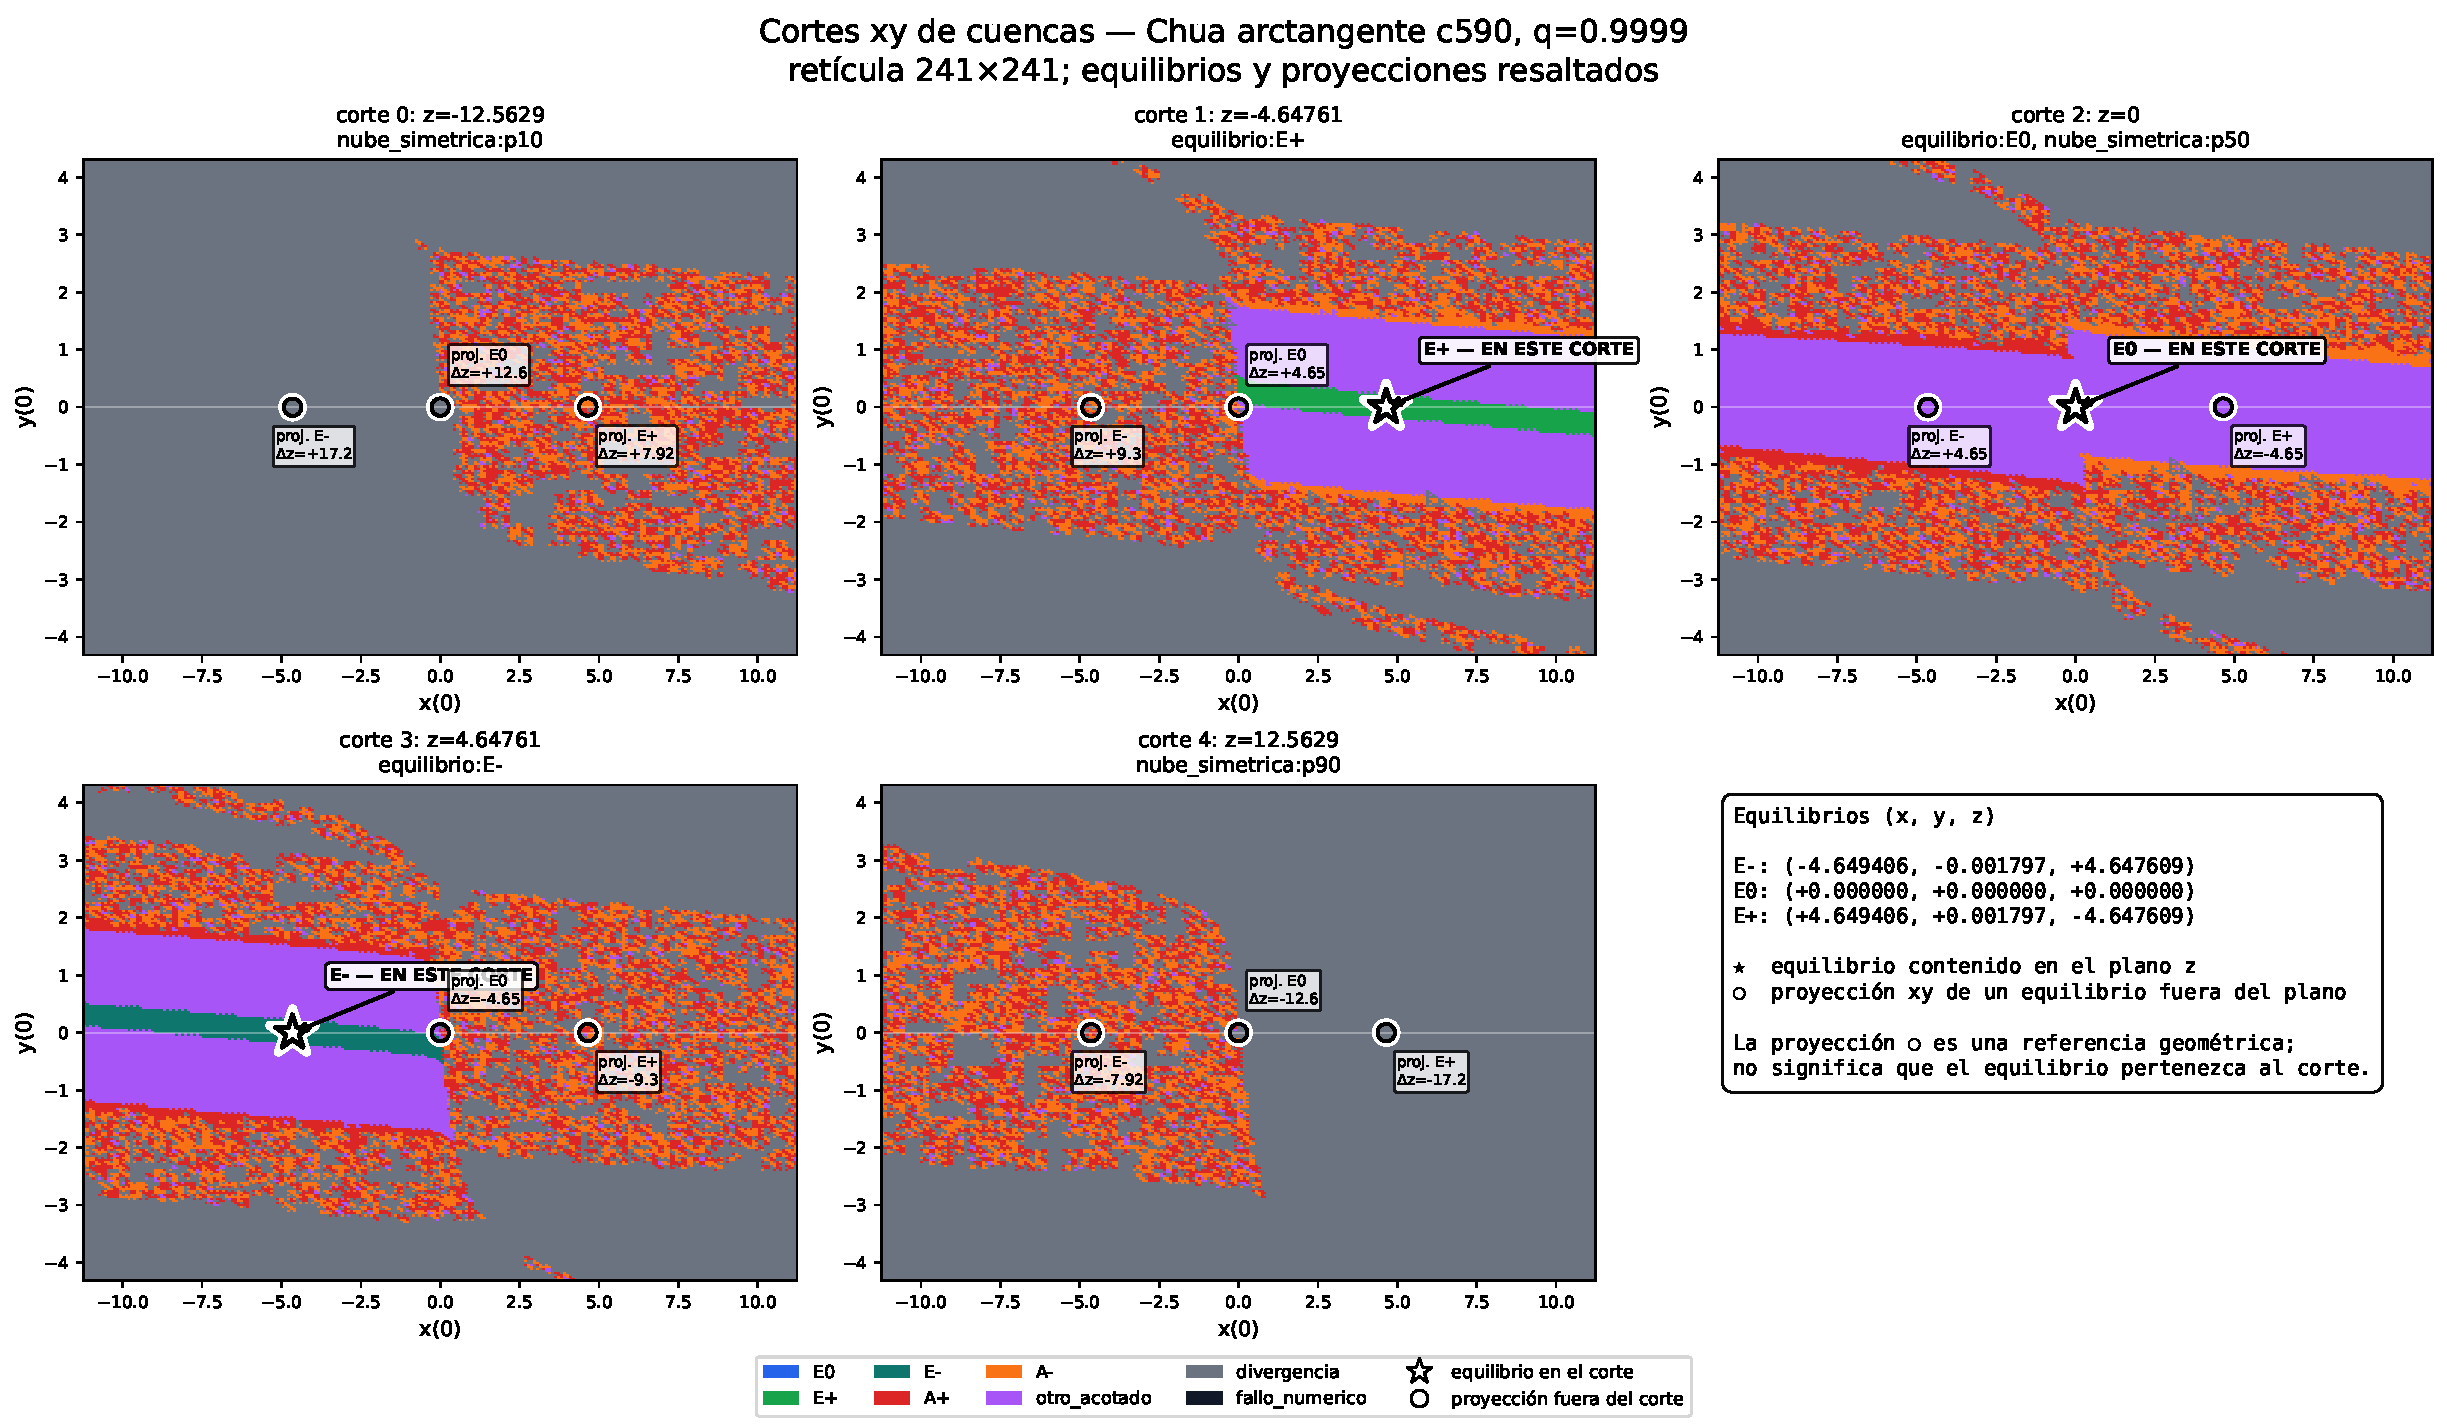
\includegraphics[width=0.94\linewidth,height=0.37\textheight,keepaspectratio]{figures/c590_basin/basin_multislice_equilibria.pdf}\\[-0.25em]
{\footnotesize Cortes de las regiones de destino y posición de los equilibrios.}
\end{center}
\clearpage
\begin{center}
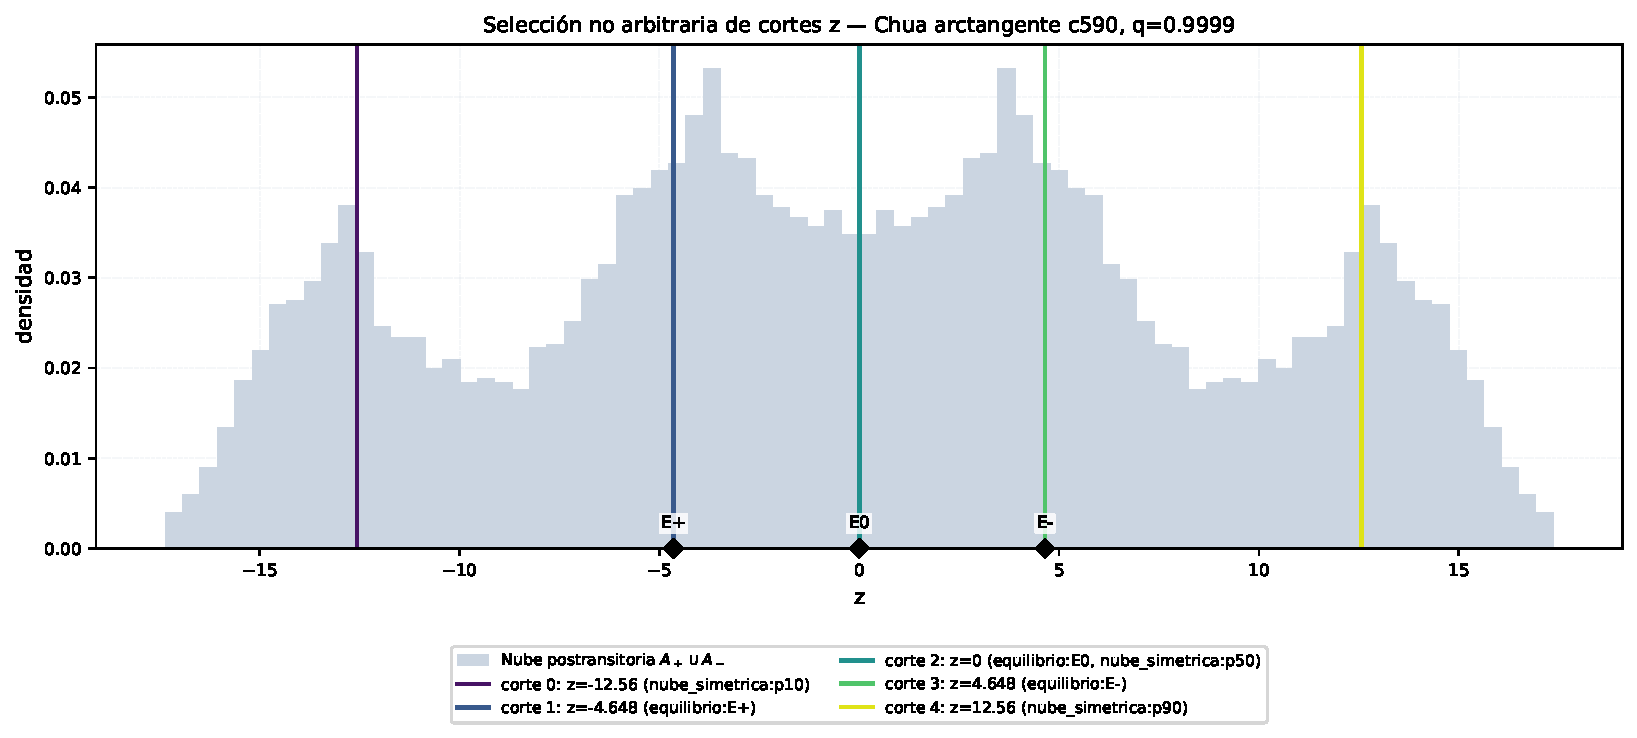
\includegraphics[width=0.94\linewidth,height=0.37\textheight,keepaspectratio]{figures/c590_basin/z_cut_selection.pdf}\\[-0.25em]
{\footnotesize Posición de los planos de corte de las regiones de destino.}
\end{center}
\vfill
\begin{center}
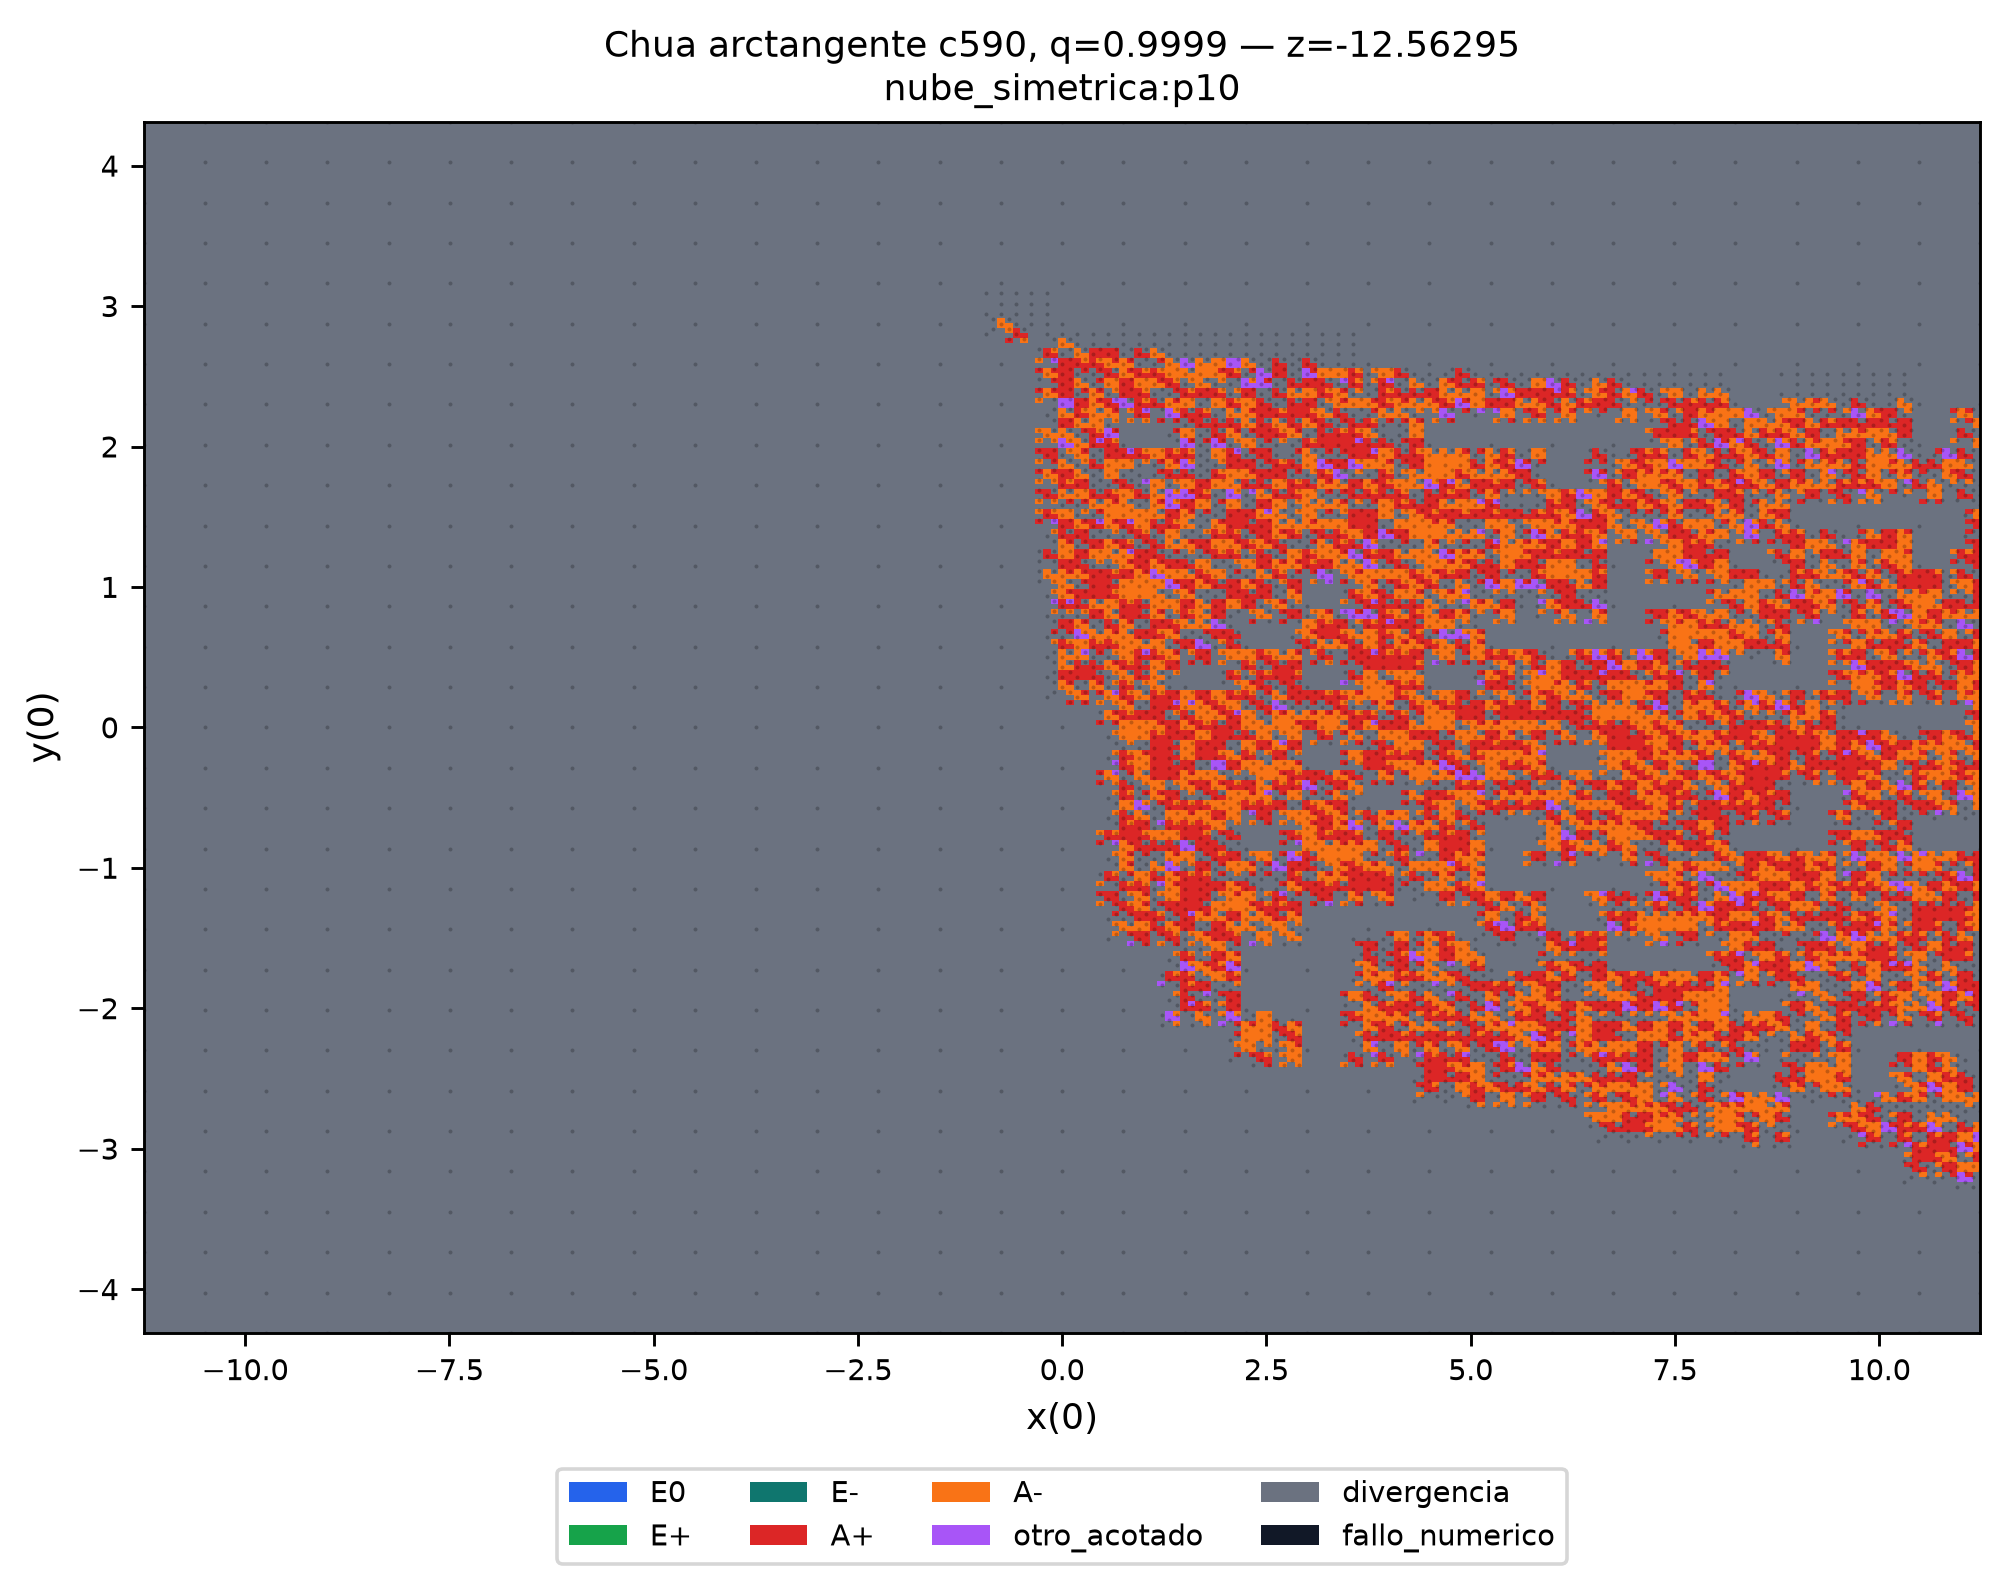
\includegraphics[width=0.94\linewidth,height=0.37\textheight,keepaspectratio]{figures/c590_basin/basin_cut_00.png}\\[-0.25em]
{\footnotesize Corte 1 de las regiones de destino.}
\end{center}
\clearpage
\begin{center}
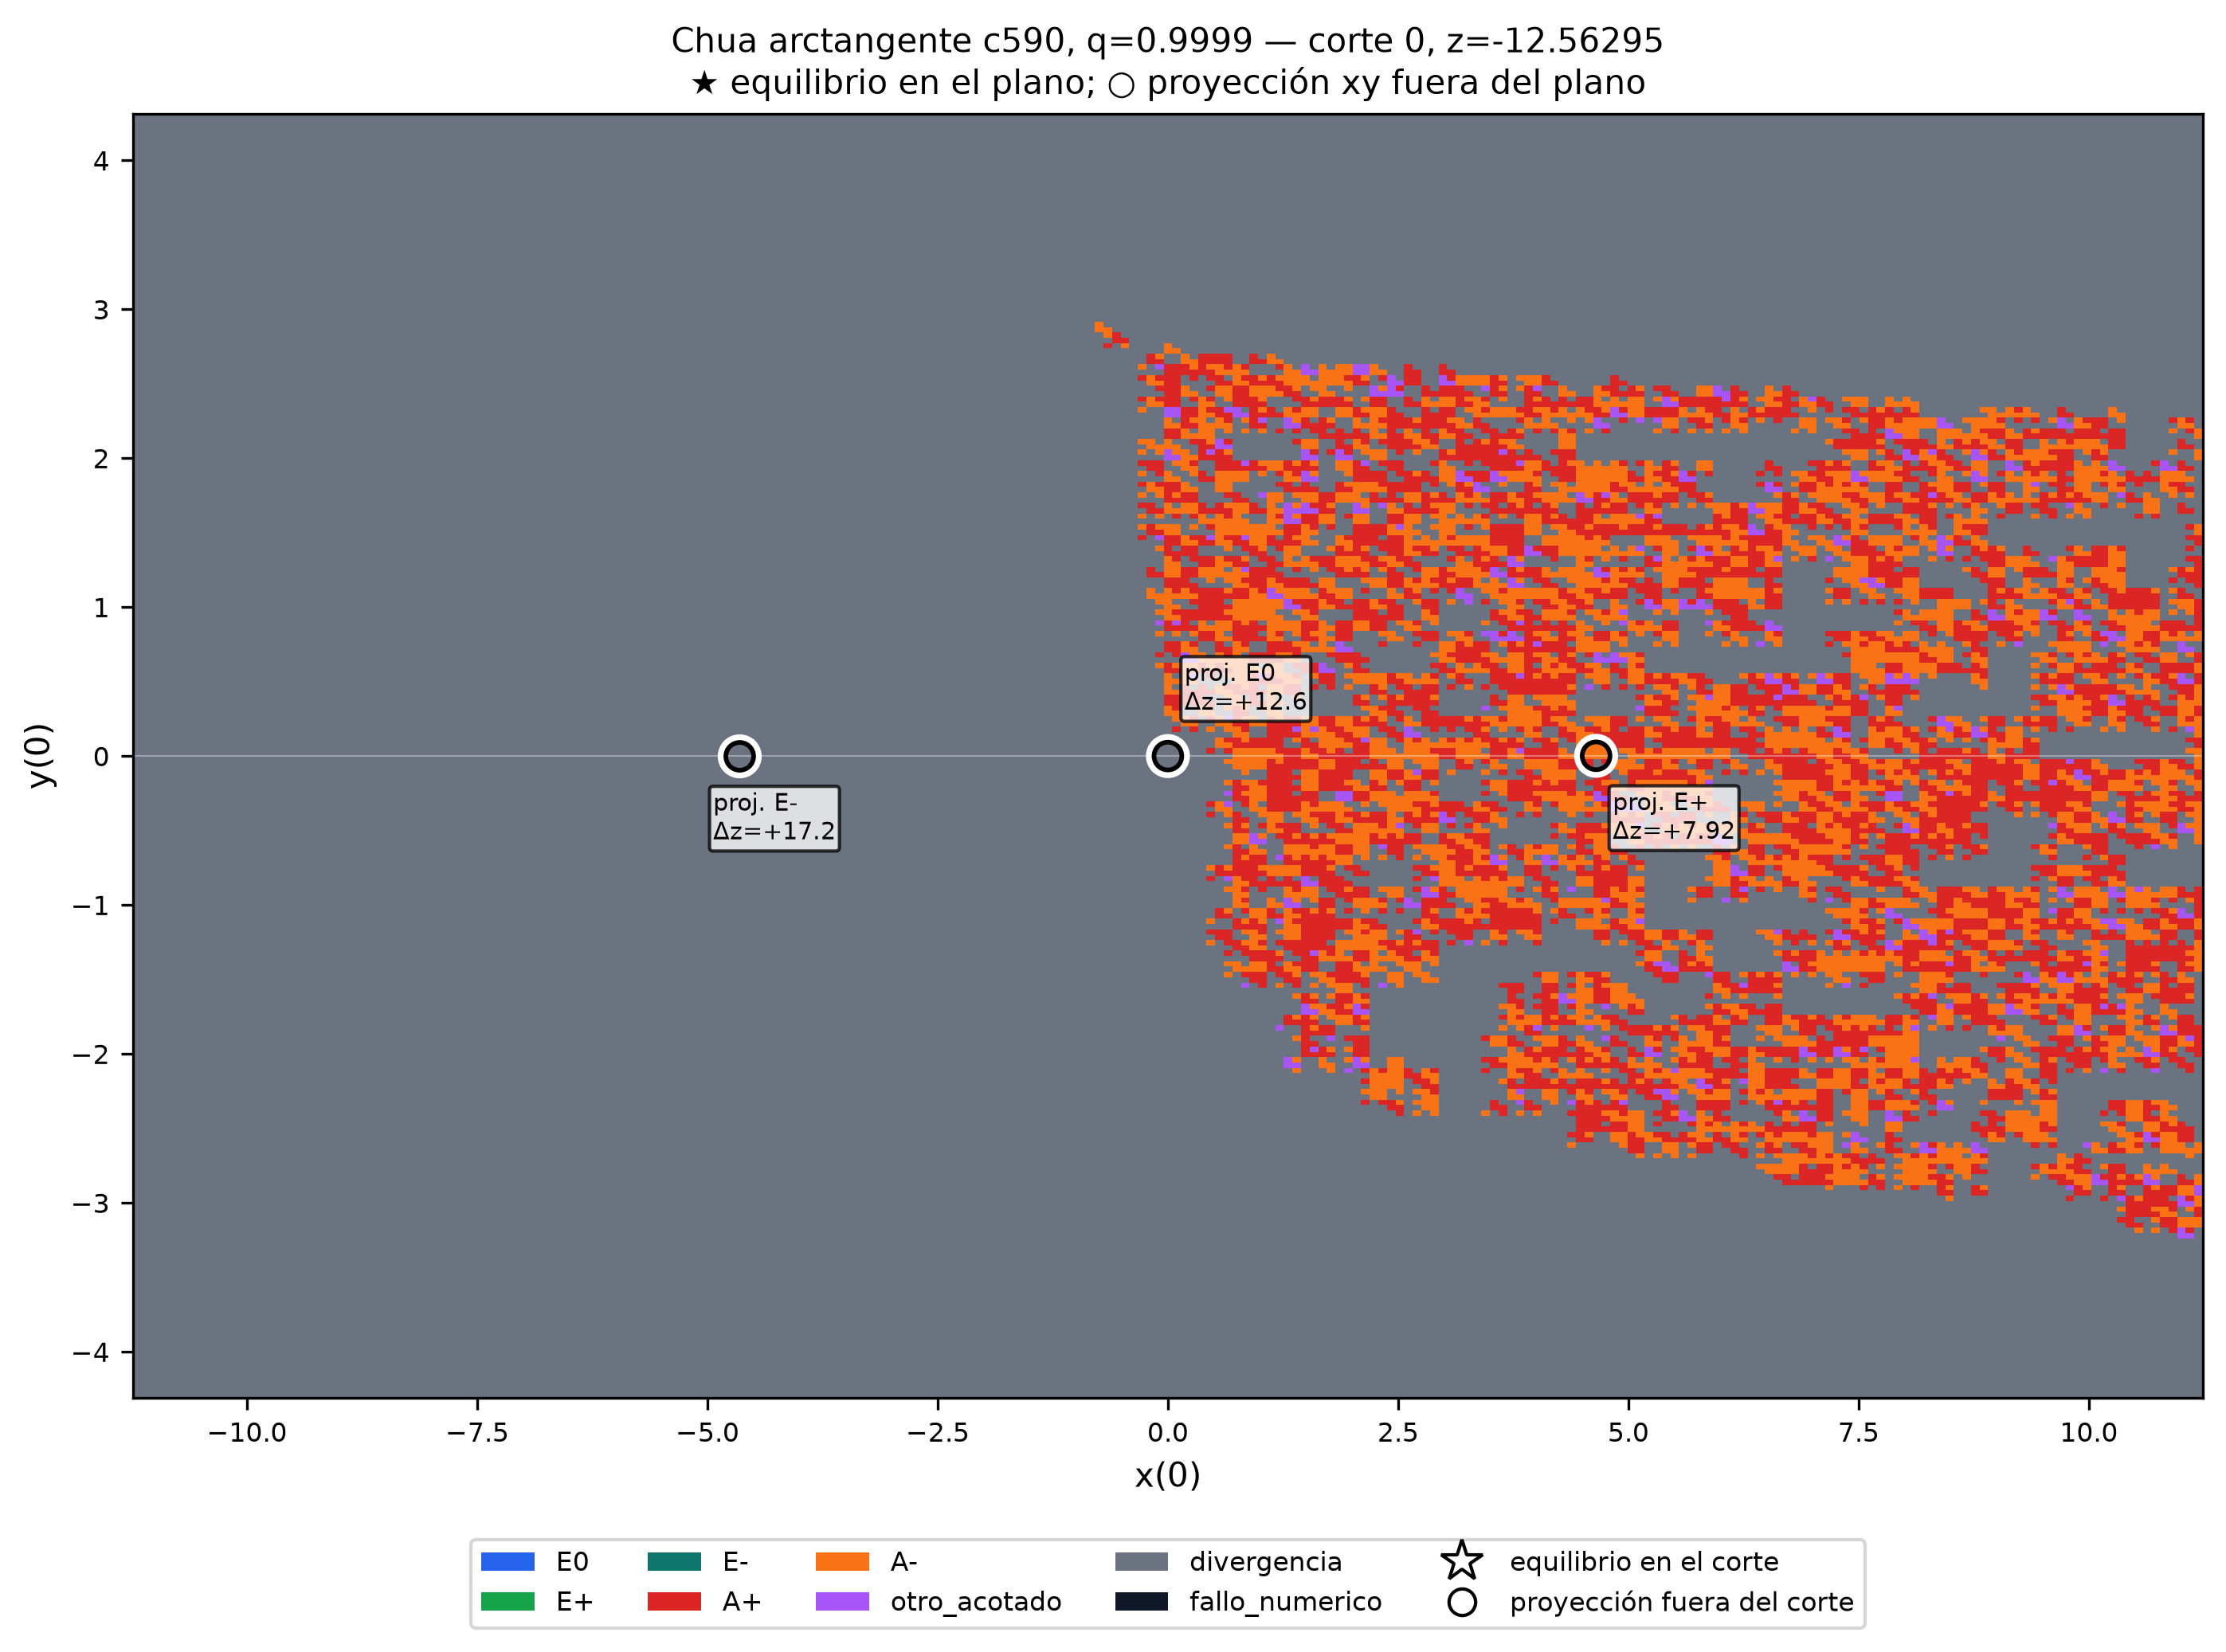
\includegraphics[width=0.94\linewidth,height=0.37\textheight,keepaspectratio]{figures/c590_basin/basin_cut_00_equilibria.png}\\[-0.25em]
{\footnotesize Corte 1 de las regiones de destino y posición de los equilibrios.}
\end{center}
\vfill
\begin{center}
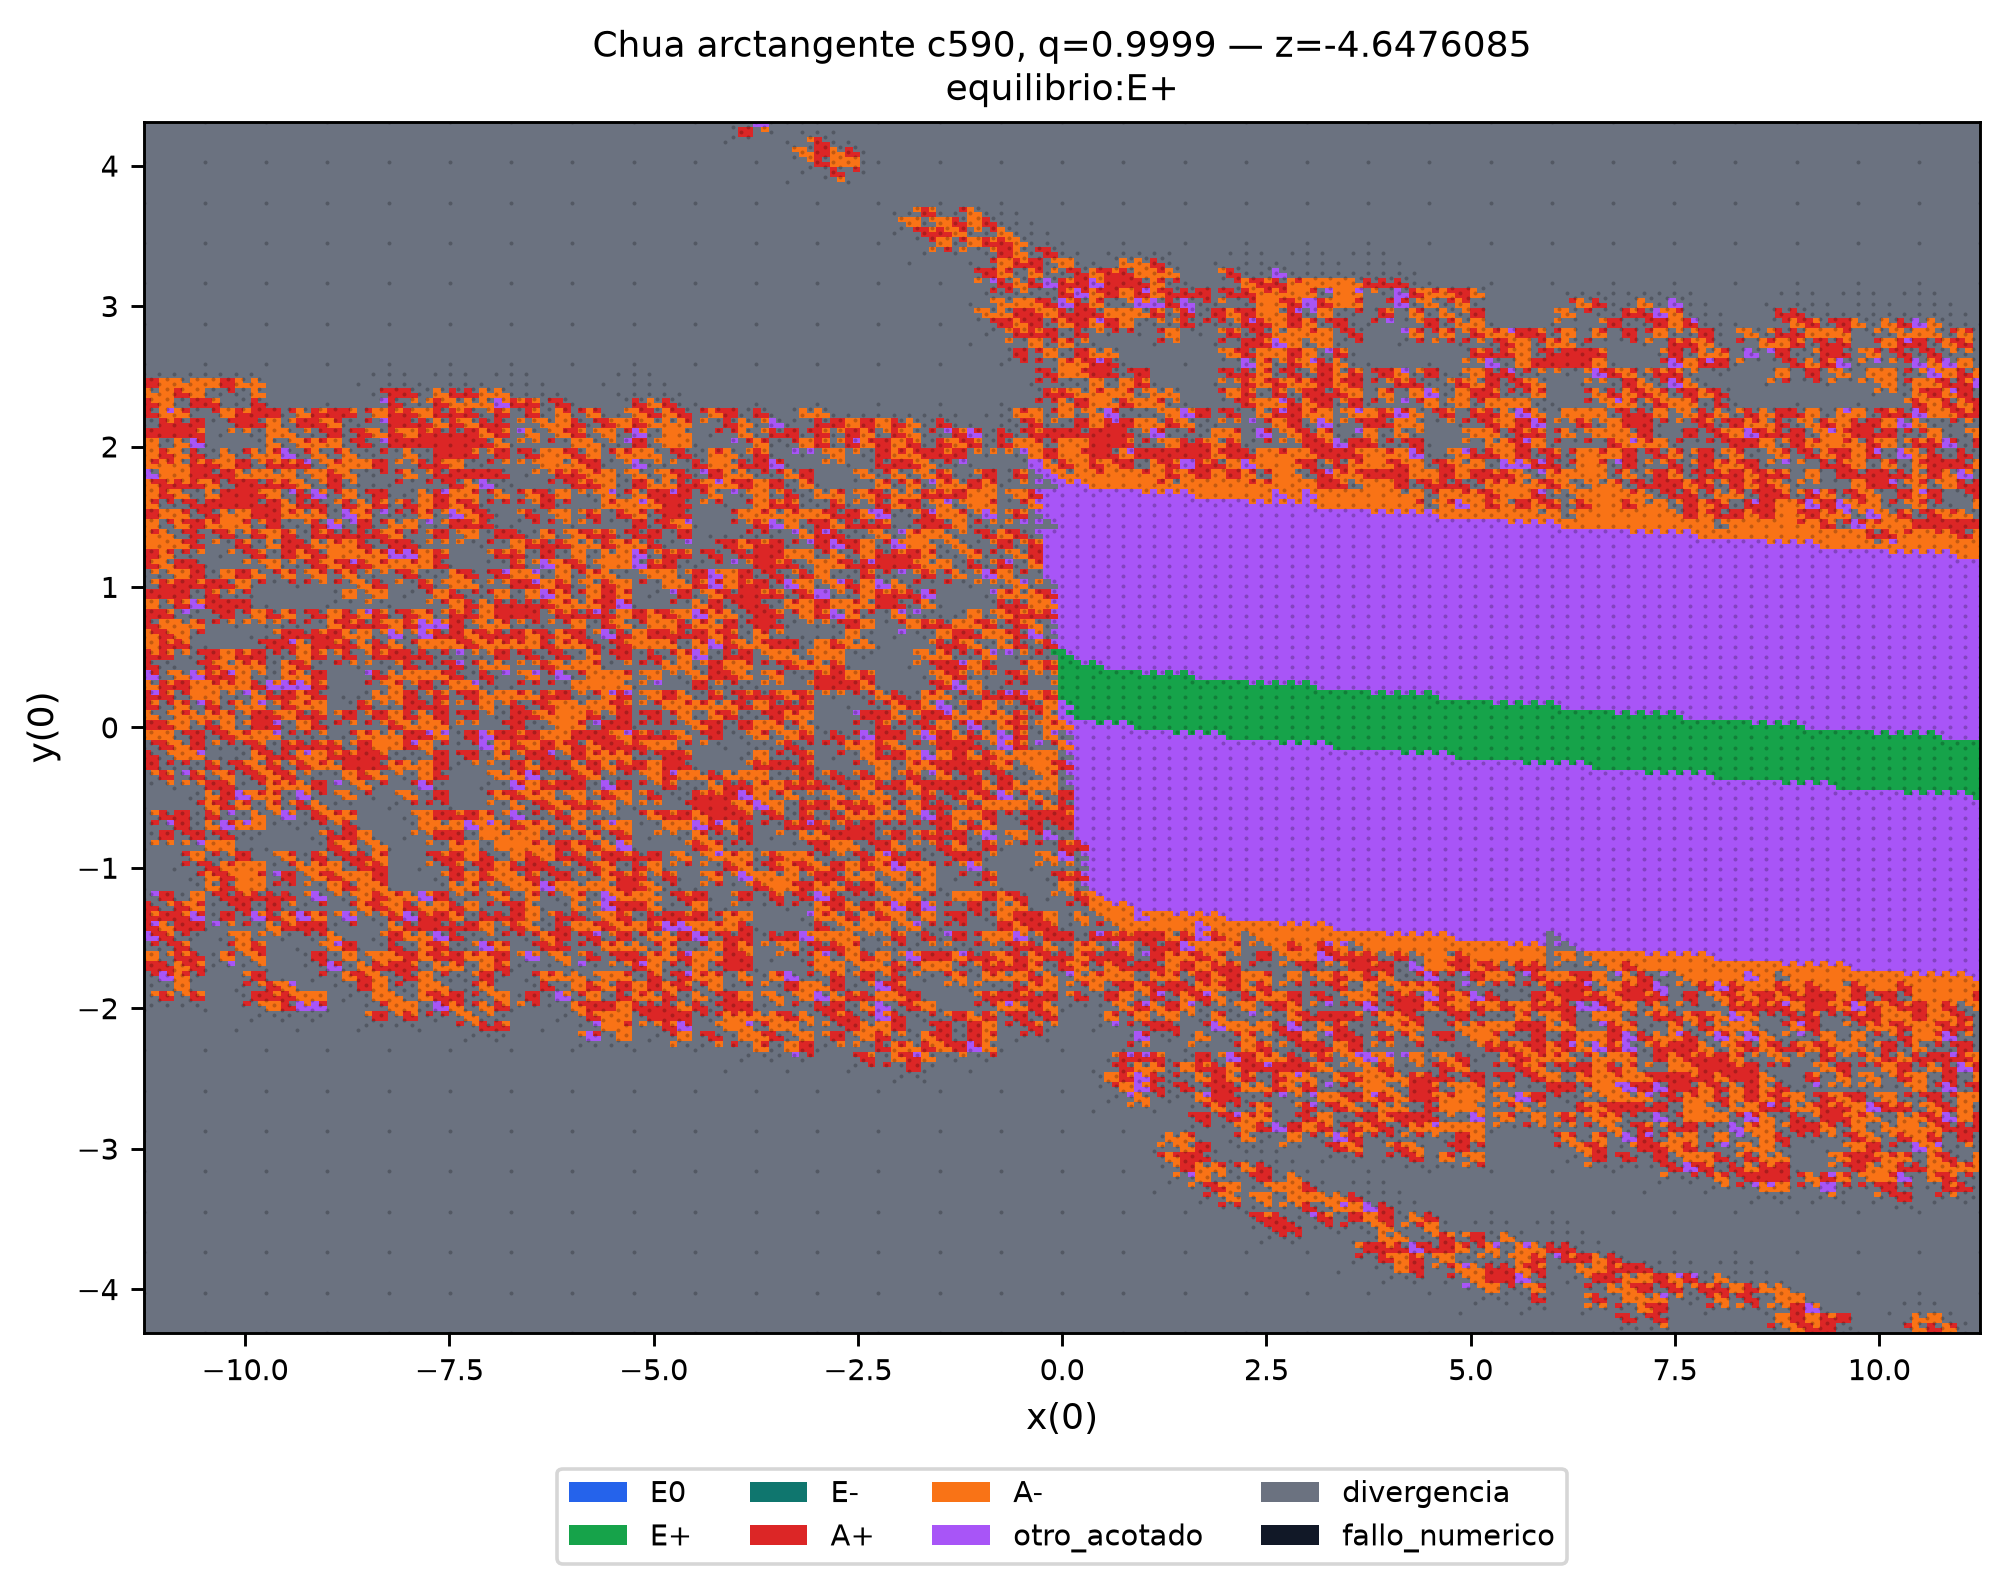
\includegraphics[width=0.94\linewidth,height=0.37\textheight,keepaspectratio]{figures/c590_basin/basin_cut_01.png}\\[-0.25em]
{\footnotesize Corte 2 de las regiones de destino.}
\end{center}
\clearpage
\begin{center}
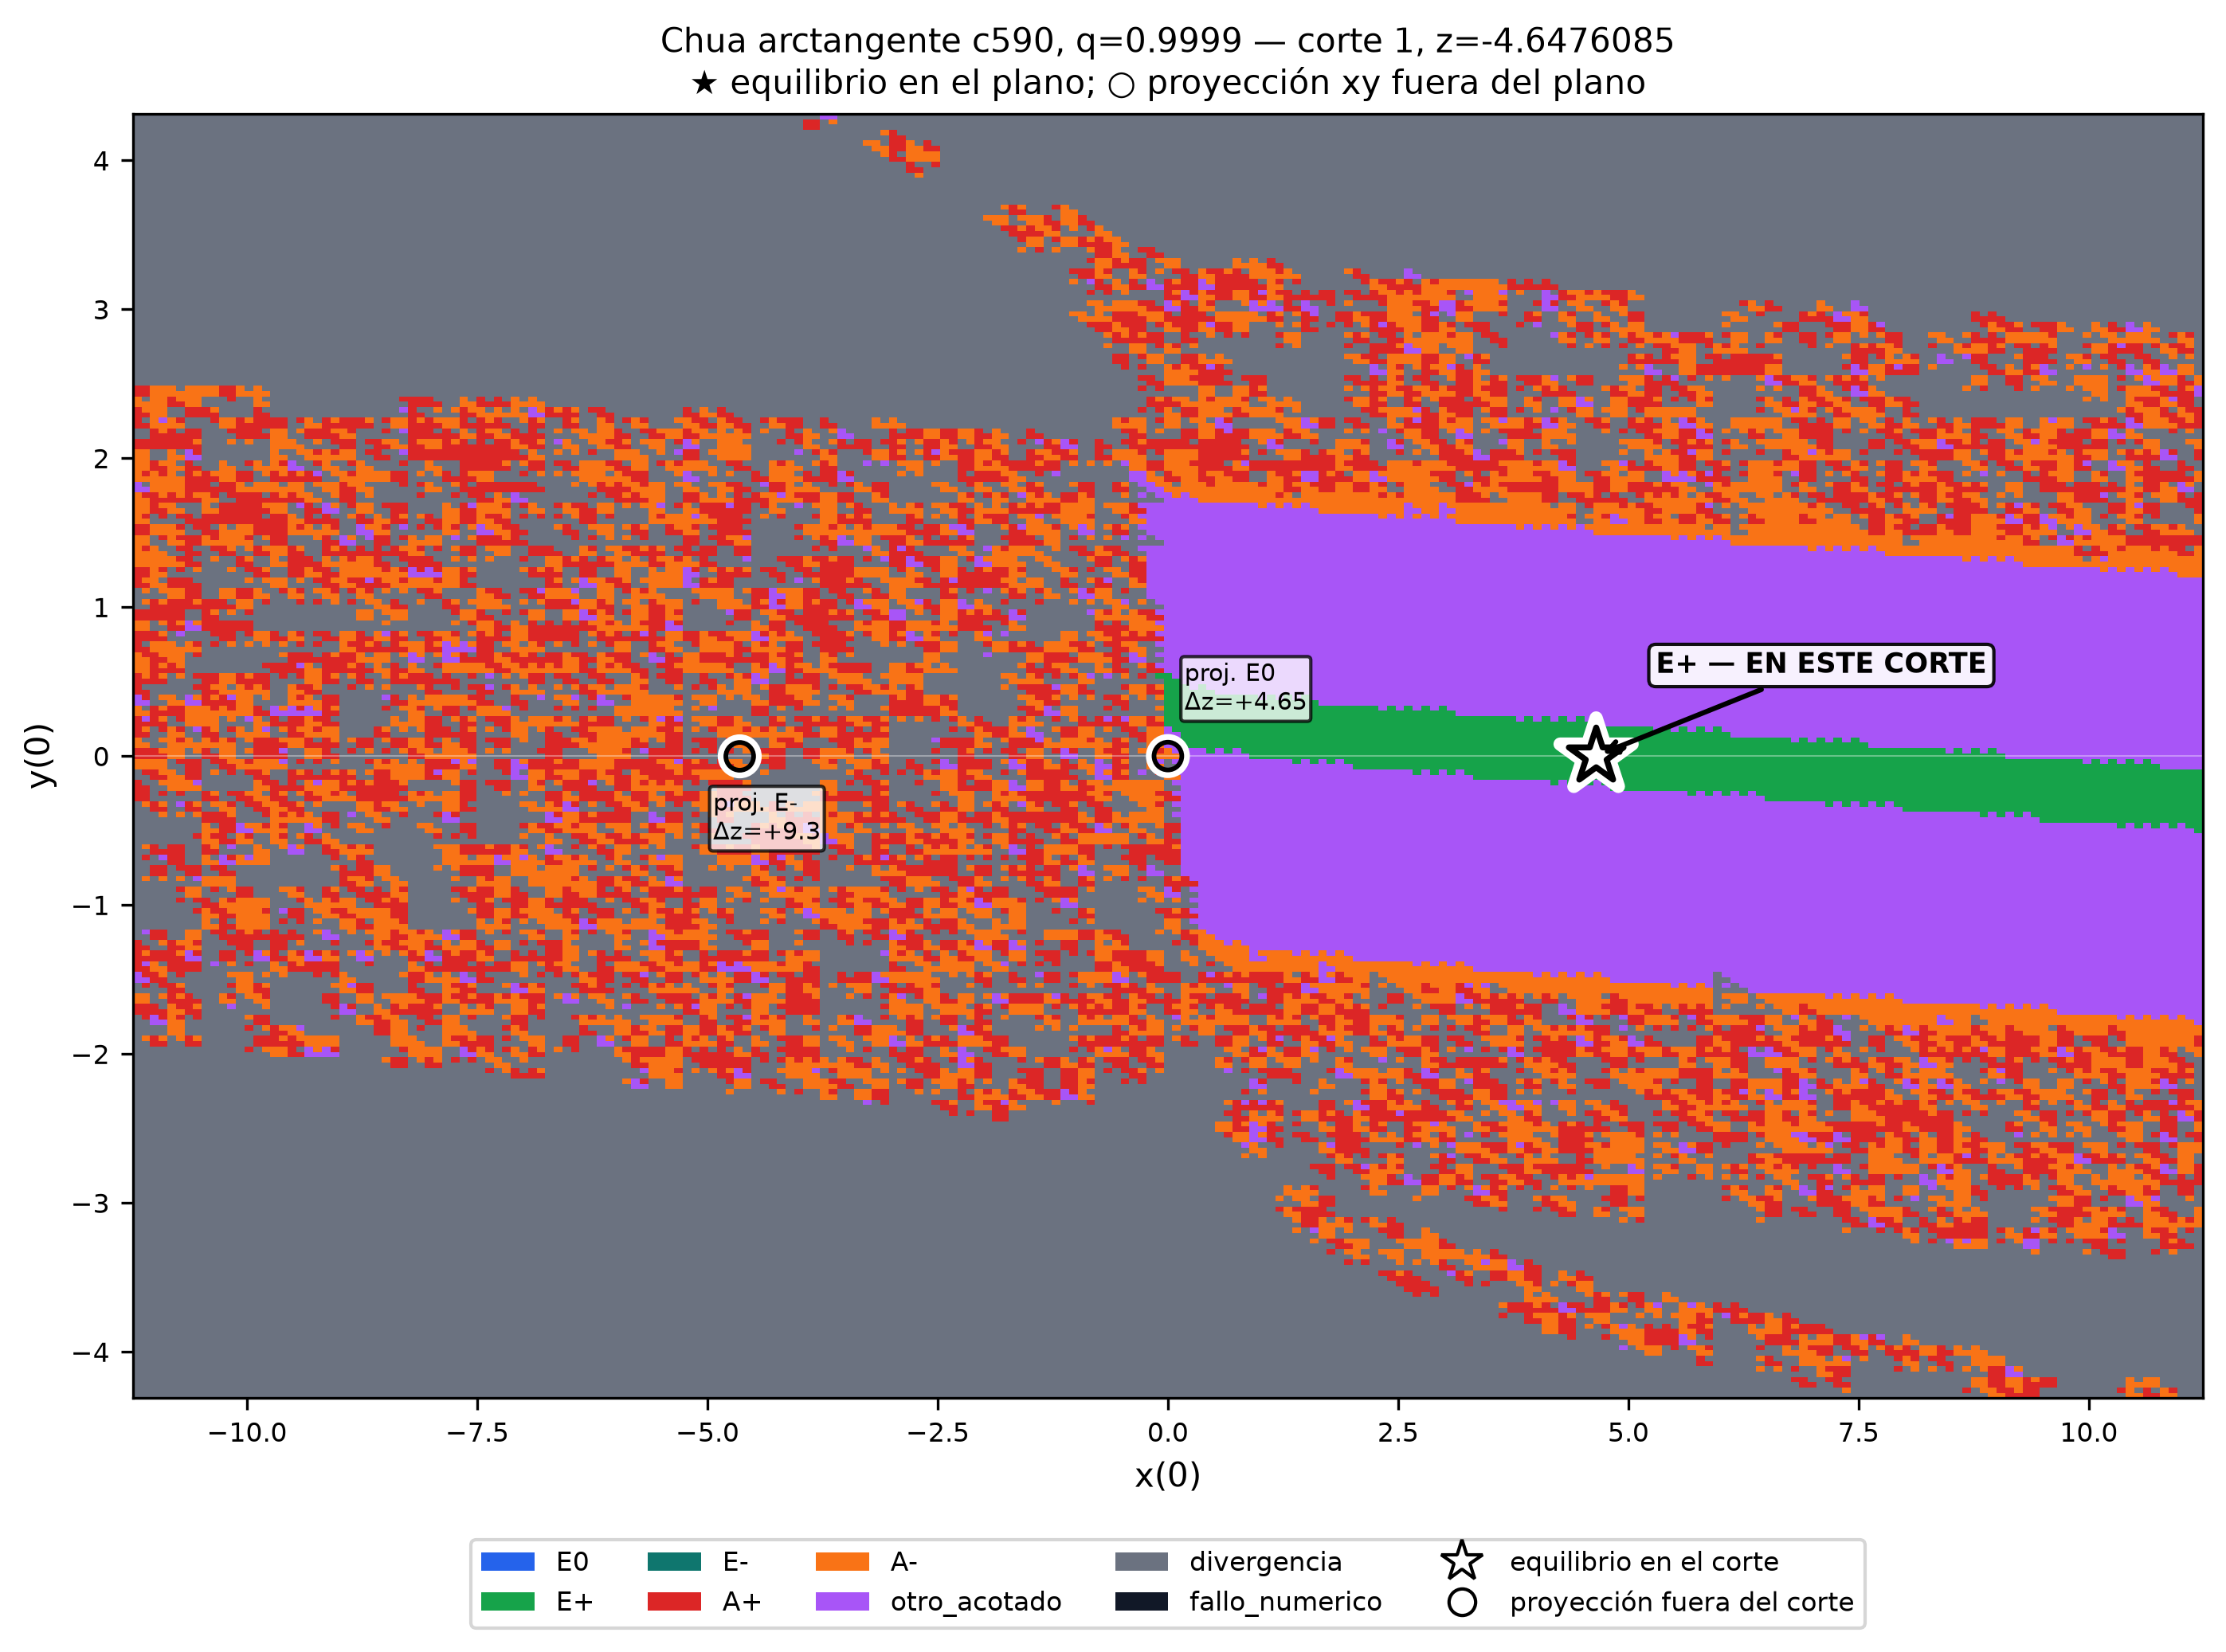
\includegraphics[width=0.94\linewidth,height=0.37\textheight,keepaspectratio]{figures/c590_basin/basin_cut_01_equilibria.png}\\[-0.25em]
{\footnotesize Corte 2 de las regiones de destino y posición de los equilibrios.}
\end{center}
\vfill
\begin{center}
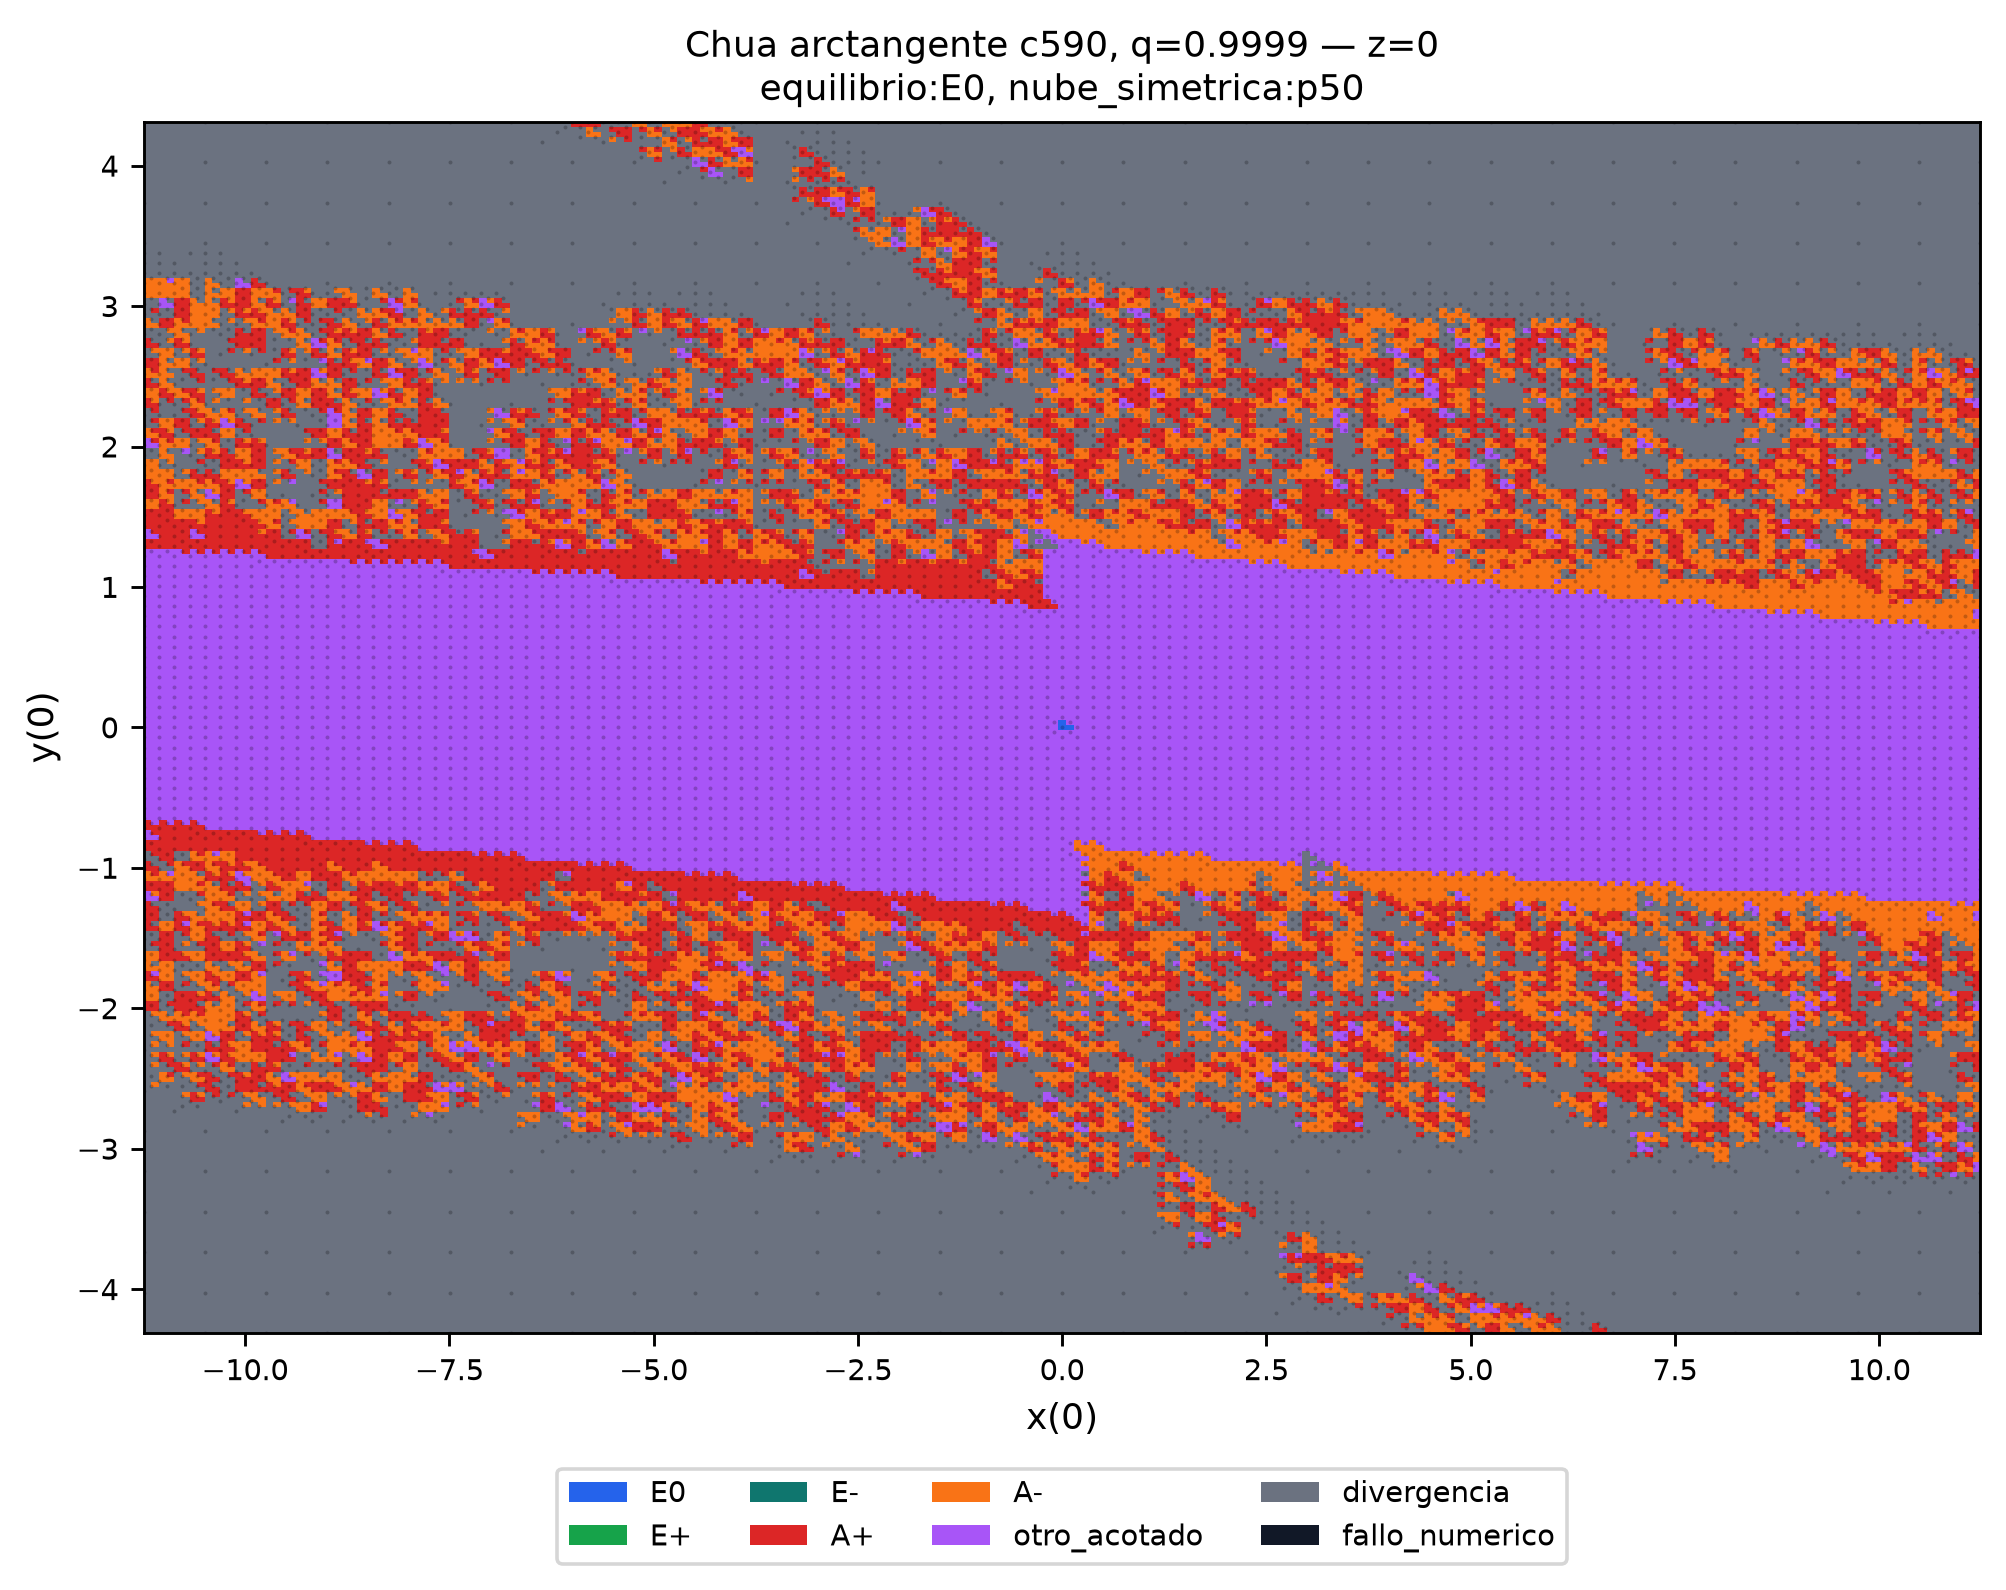
\includegraphics[width=0.94\linewidth,height=0.37\textheight,keepaspectratio]{figures/c590_basin/basin_cut_02.png}\\[-0.25em]
{\footnotesize Corte 3 de las regiones de destino.}
\end{center}
\clearpage
\begin{center}
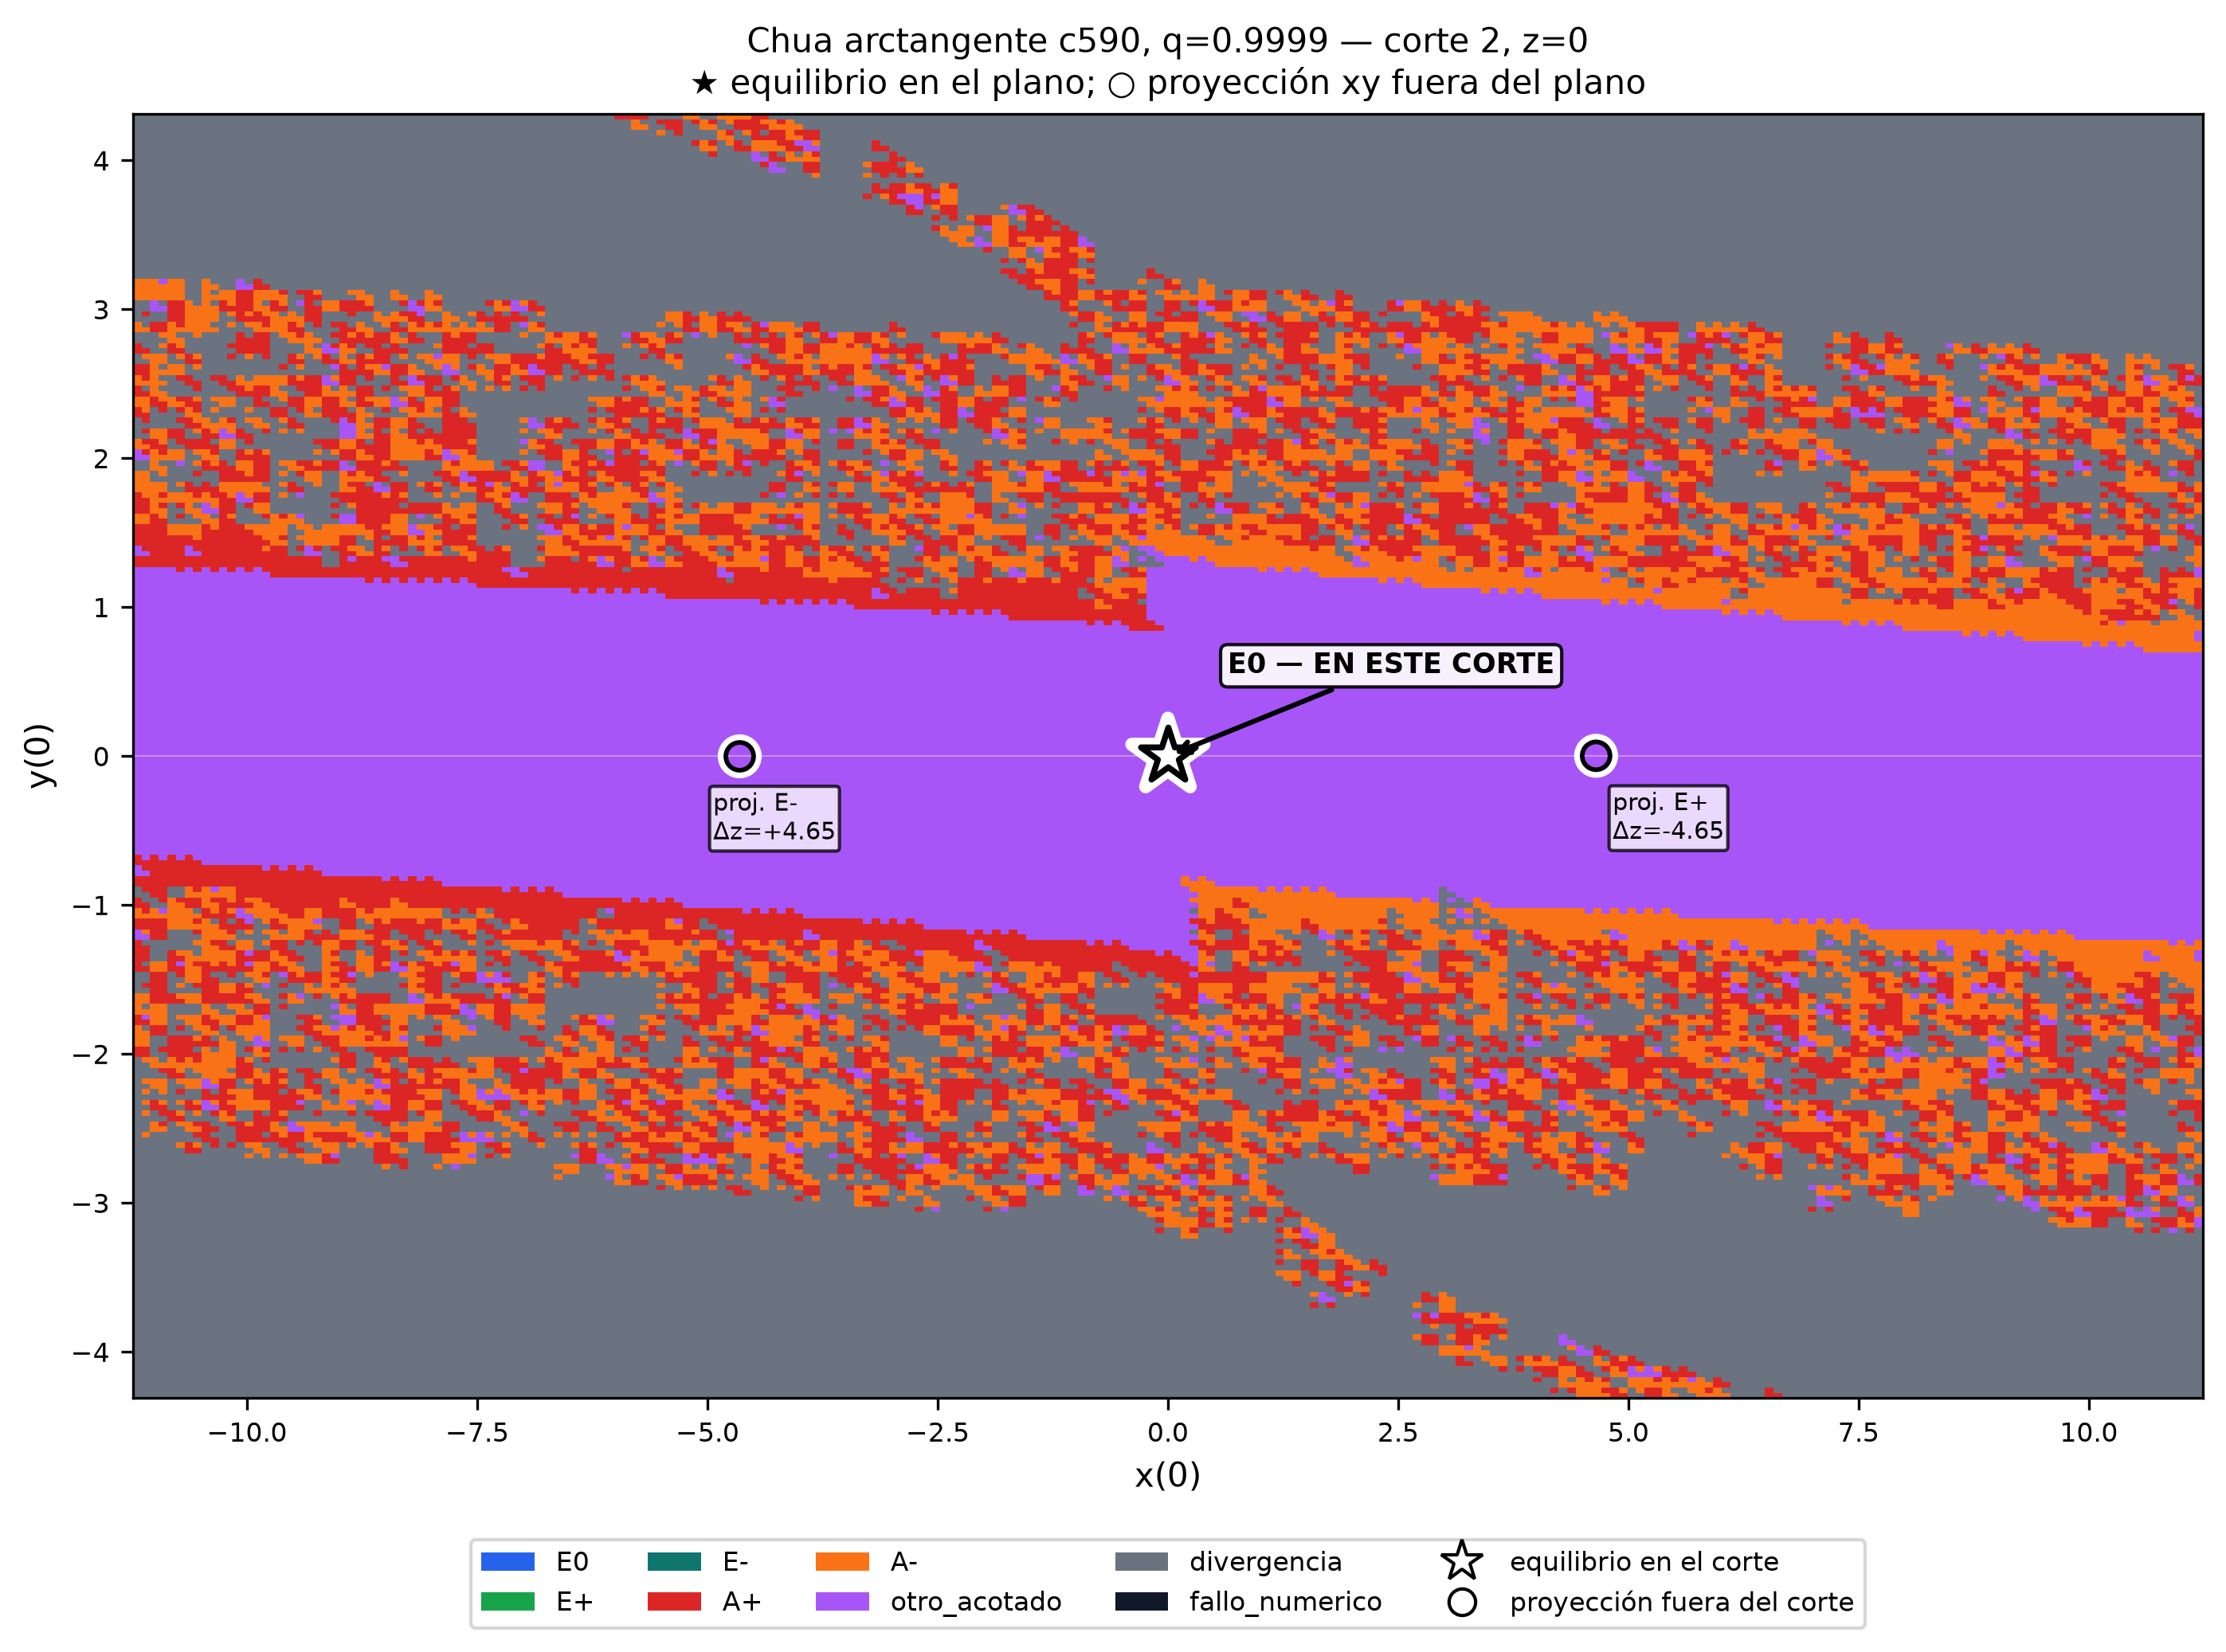
\includegraphics[width=0.94\linewidth,height=0.37\textheight,keepaspectratio]{figures/c590_basin/basin_cut_02_equilibria.png}\\[-0.25em]
{\footnotesize Corte 3 de las regiones de destino y posición de los equilibrios.}
\end{center}
\vfill
\begin{center}
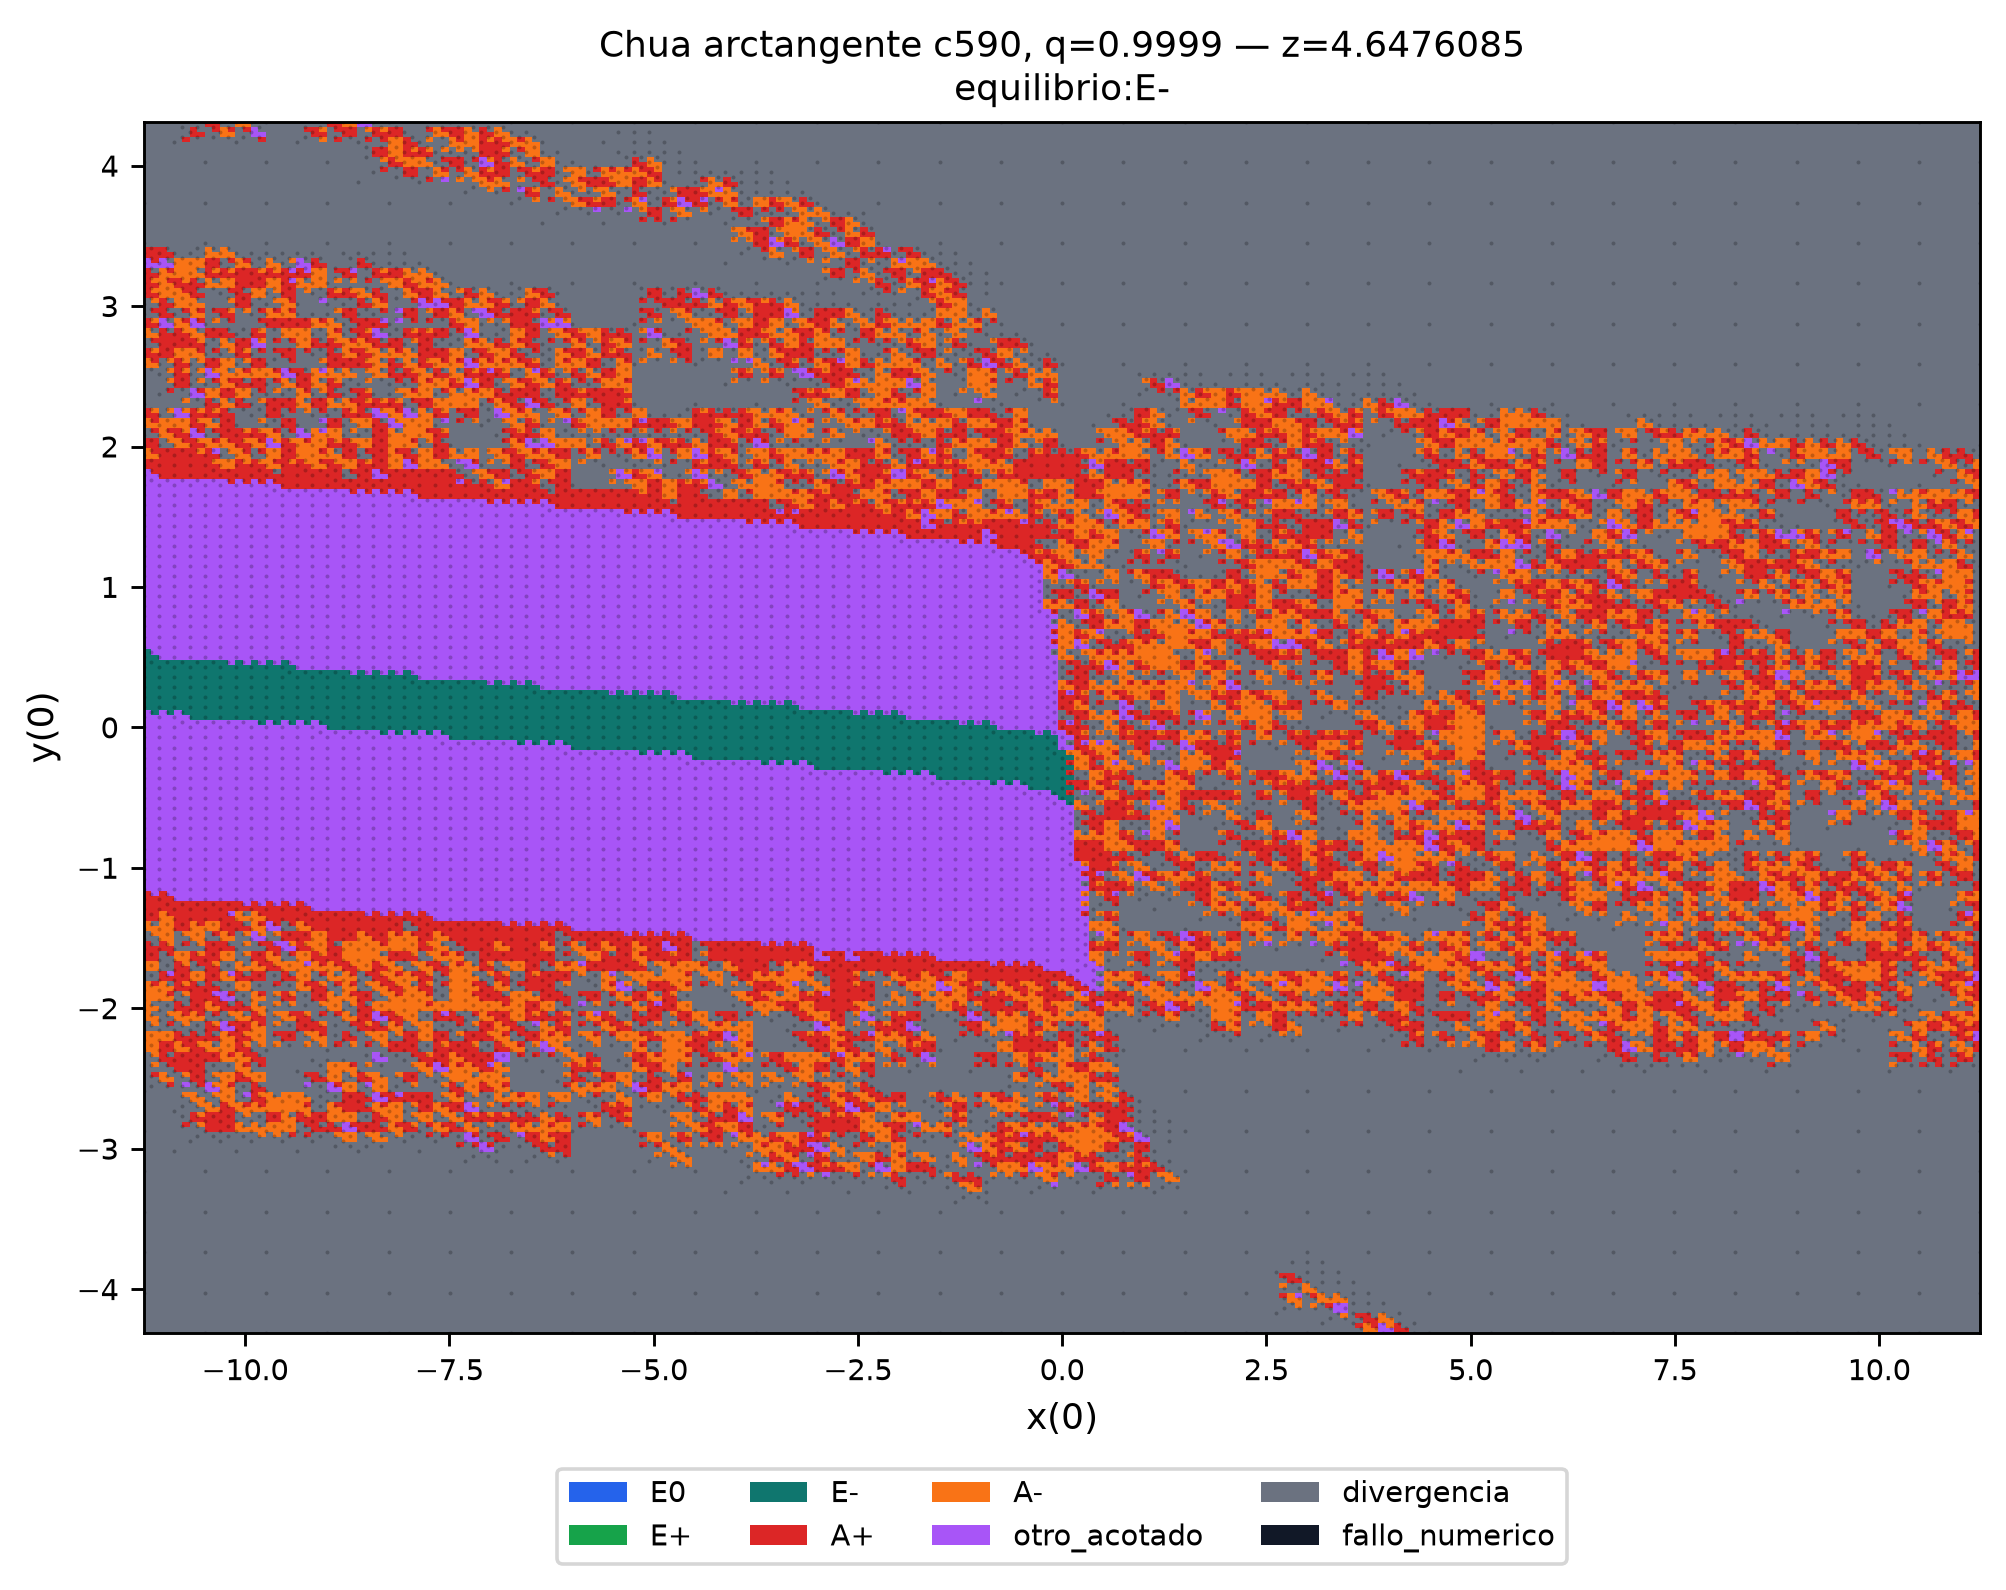
\includegraphics[width=0.94\linewidth,height=0.37\textheight,keepaspectratio]{figures/c590_basin/basin_cut_03.png}\\[-0.25em]
{\footnotesize Corte 4 de las regiones de destino.}
\end{center}
\clearpage
\begin{center}
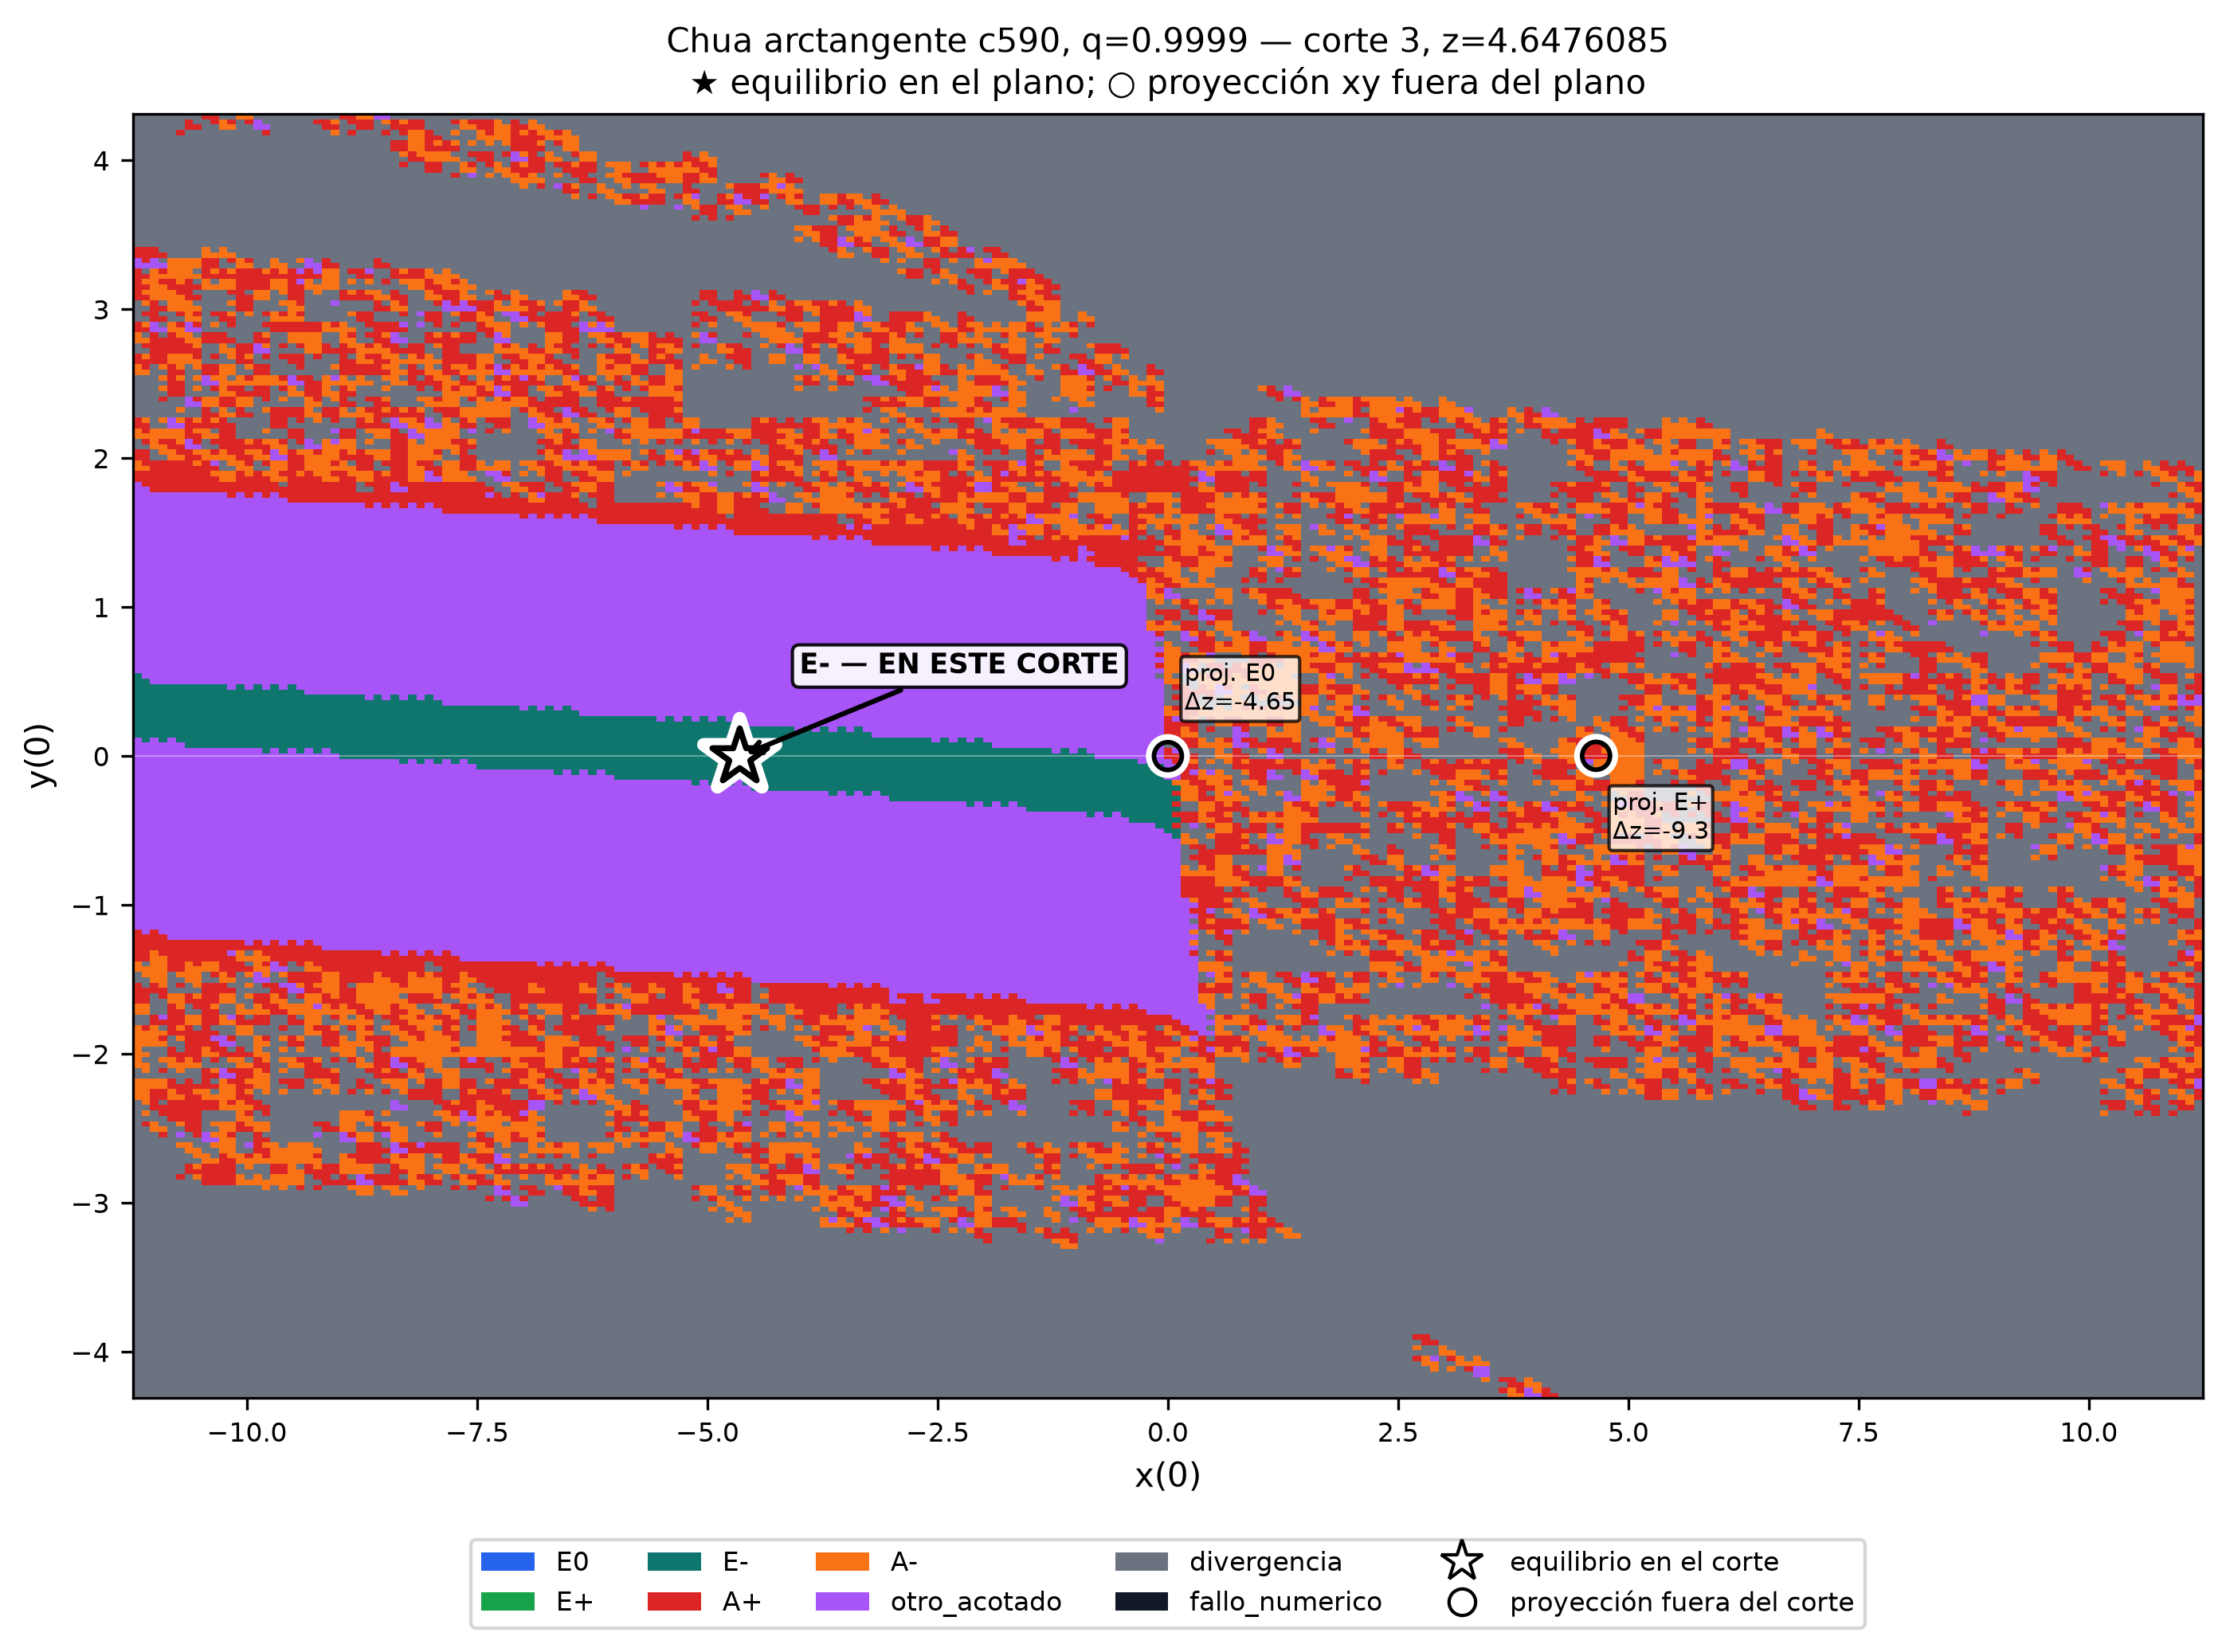
\includegraphics[width=0.94\linewidth,height=0.37\textheight,keepaspectratio]{figures/c590_basin/basin_cut_03_equilibria.png}\\[-0.25em]
{\footnotesize Corte 4 de las regiones de destino y posición de los equilibrios.}
\end{center}
\vfill
\begin{center}
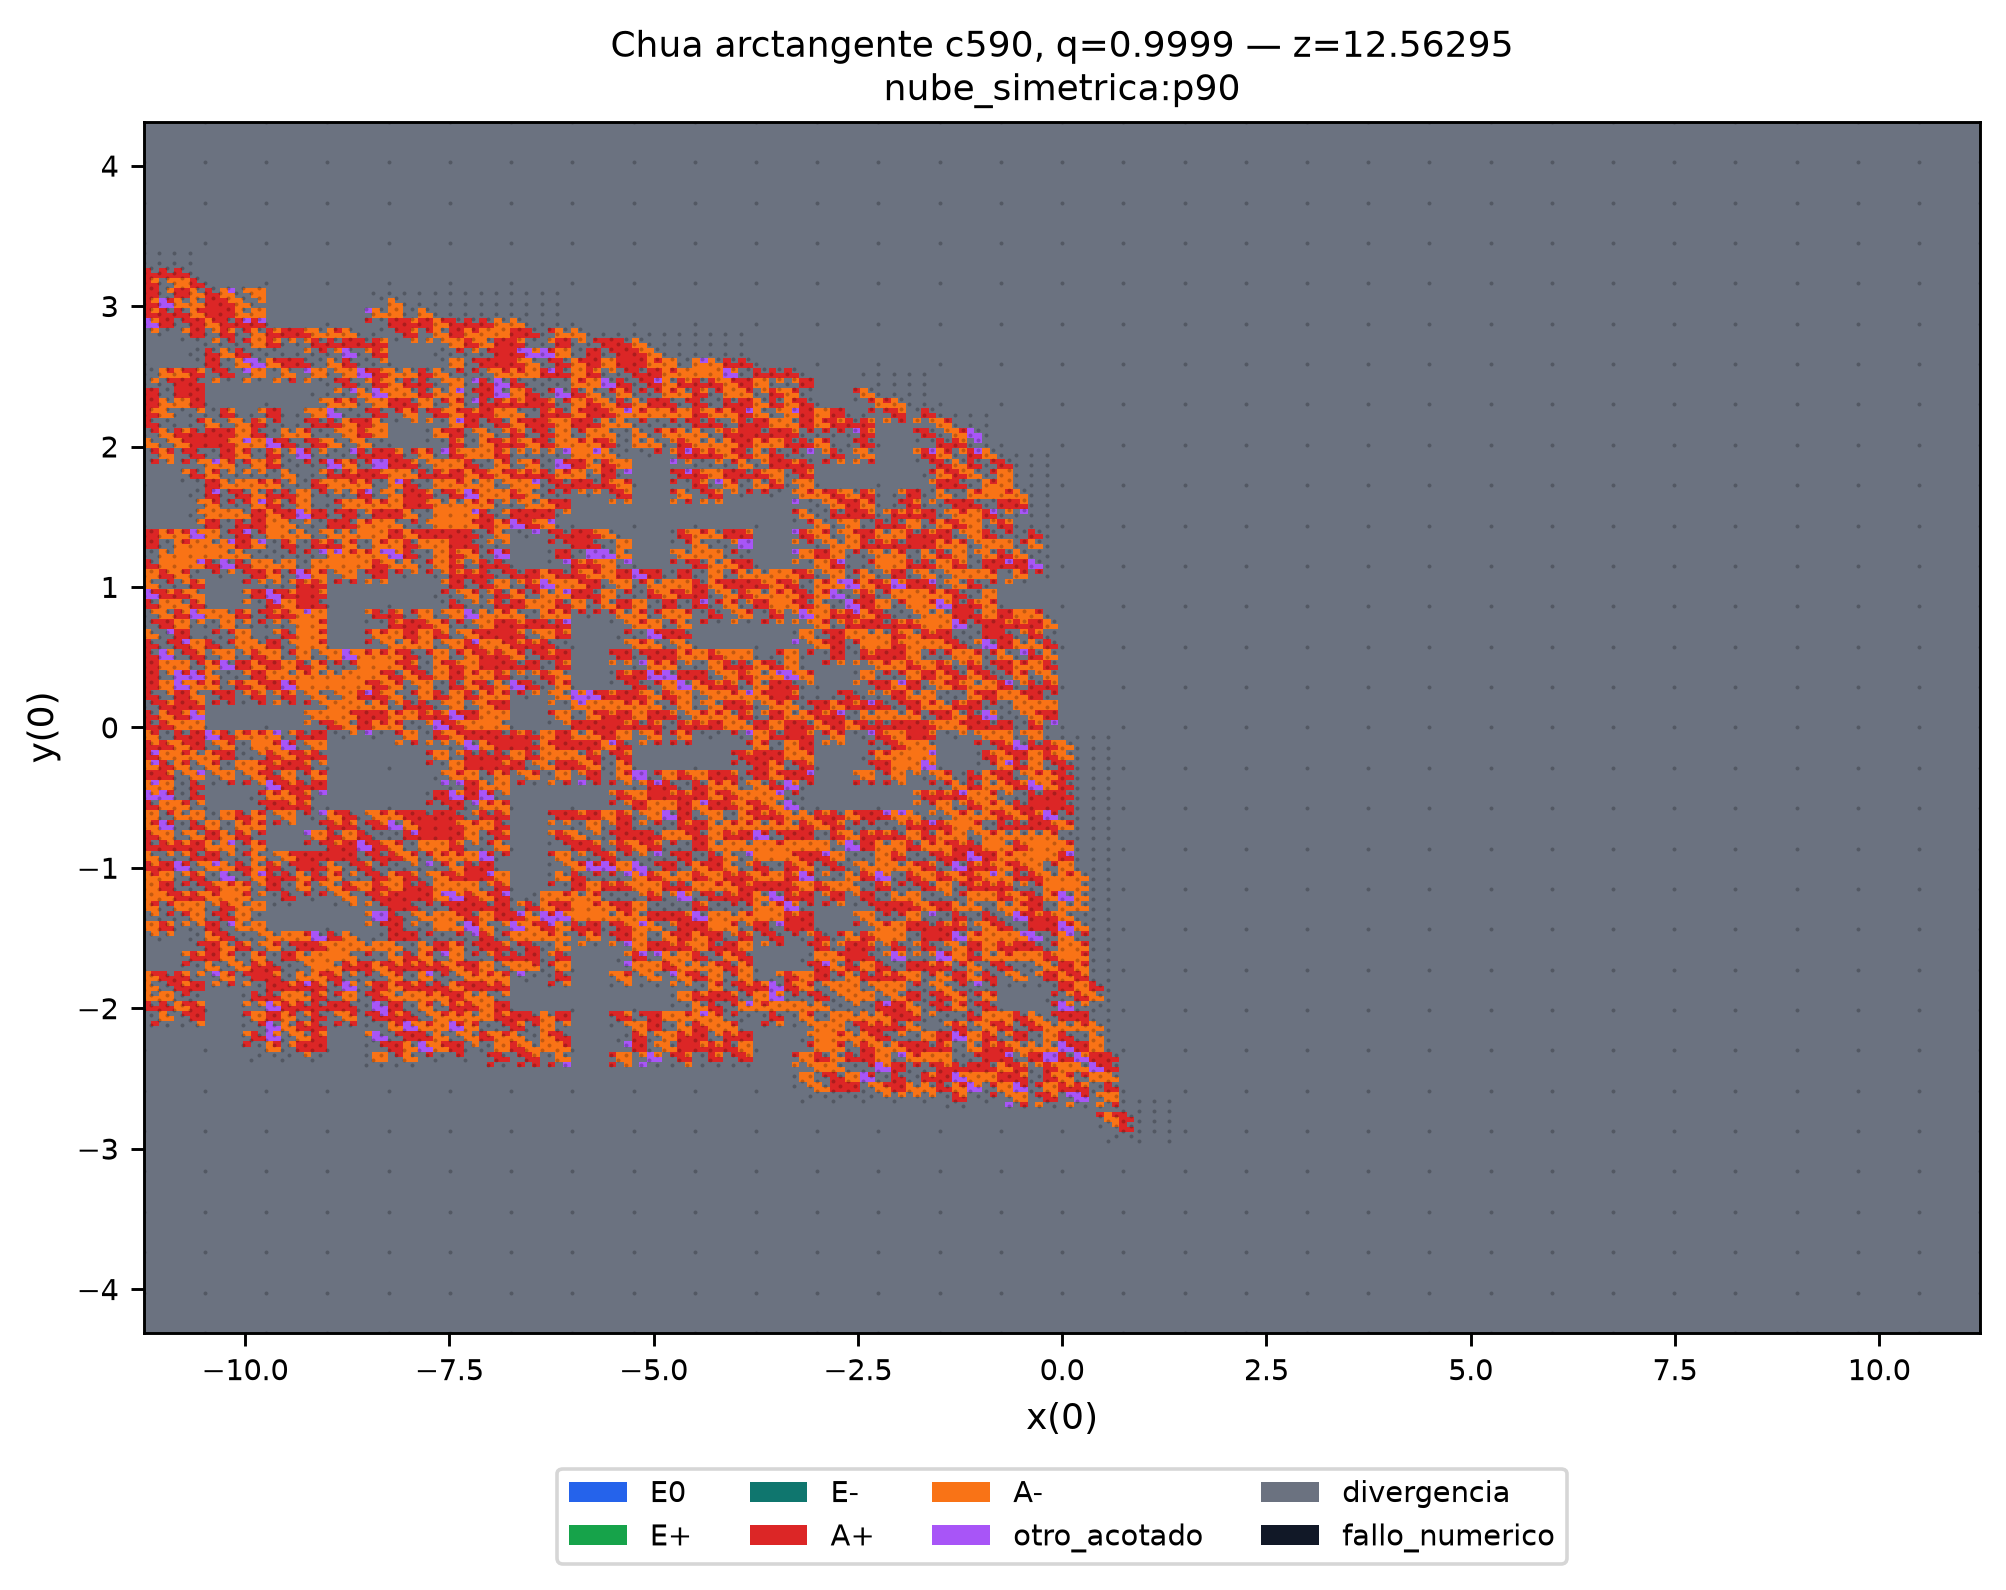
\includegraphics[width=0.94\linewidth,height=0.37\textheight,keepaspectratio]{figures/c590_basin/basin_cut_04.png}\\[-0.25em]
{\footnotesize Corte 5 de las regiones de destino.}
\end{center}
\clearpage
\begin{center}
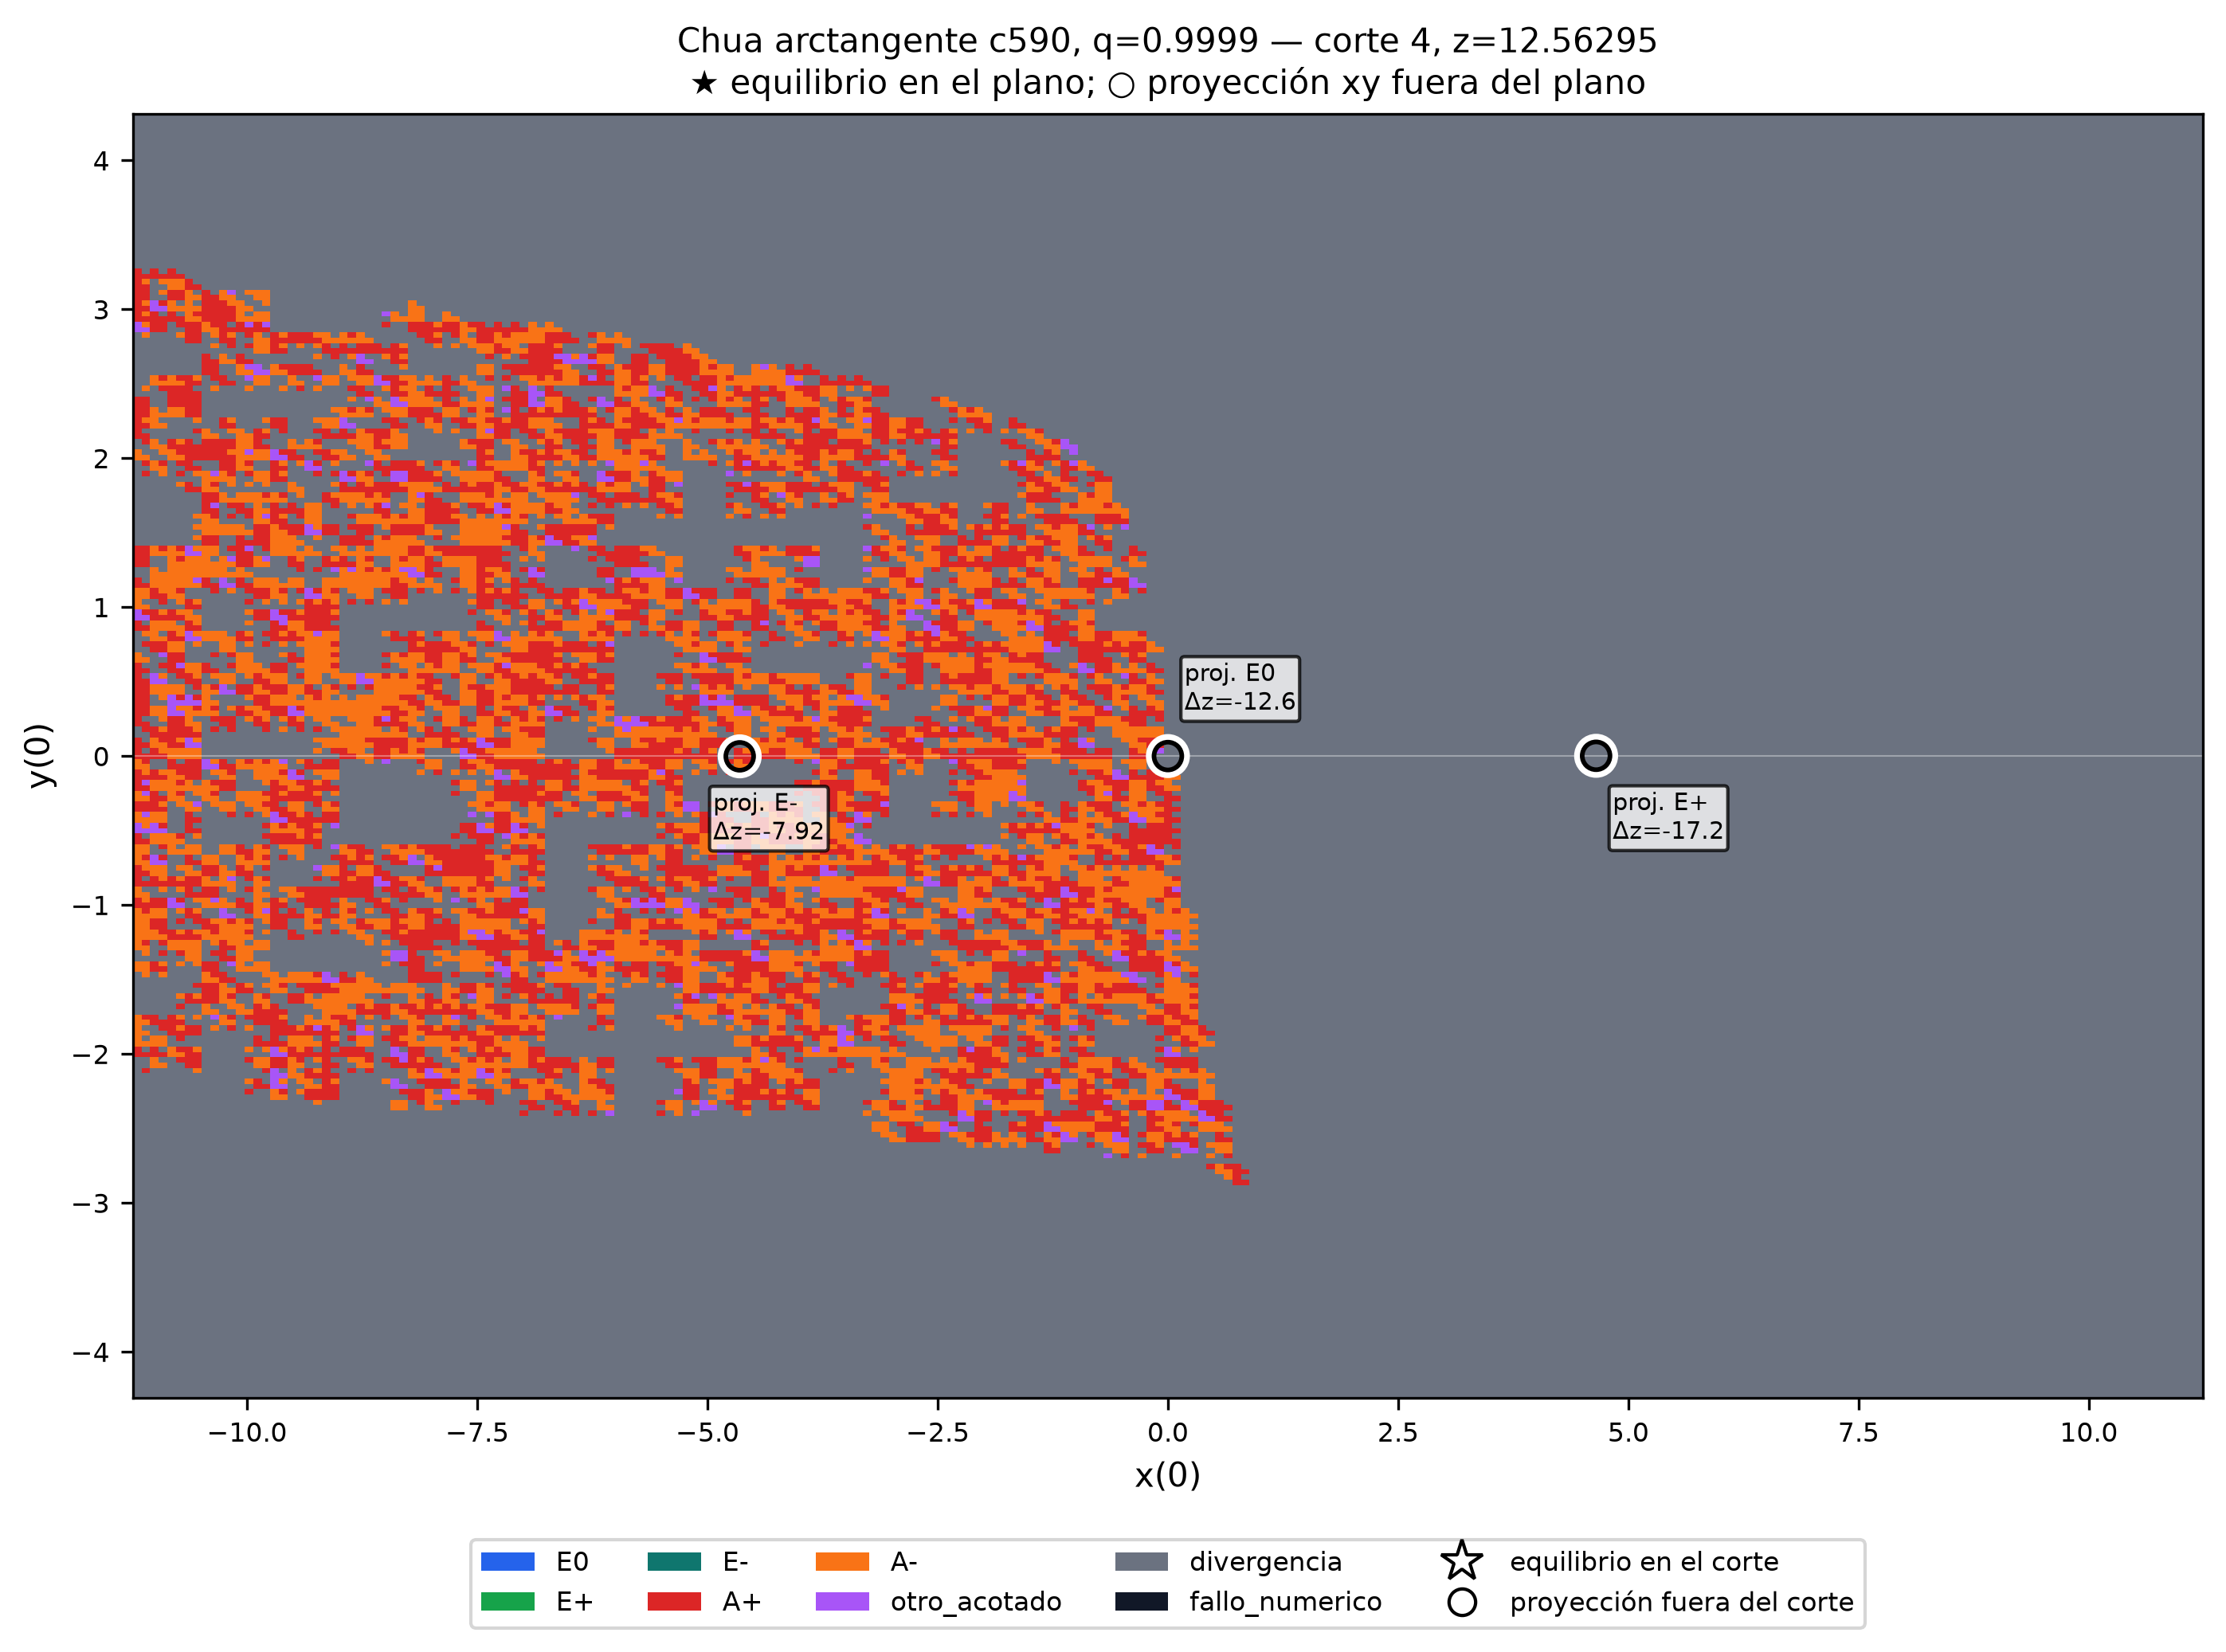
\includegraphics[width=0.94\linewidth,height=0.37\textheight,keepaspectratio]{figures/c590_basin/basin_cut_04_equilibria.png}\\[-0.25em]
{\footnotesize Corte 5 de las regiones de destino y posición de los equilibrios.}
\end{center}
\vfill
\clearpage
\fi

\fi

\begingroup
\footnotesize
\bibliographystyle{unsrt}
\bibliography{references}
\endgroup

\end{document}
